\documentclass[twoside]{book}

% Packages required by doxygen
\usepackage{fixltx2e}
\usepackage{calc}
\usepackage{doxygen}
\usepackage[export]{adjustbox} % also loads graphicx
\usepackage{graphicx}
\usepackage[utf8]{inputenc}
\usepackage{makeidx}
\usepackage{multicol}
\usepackage{multirow}
\PassOptionsToPackage{warn}{textcomp}
\usepackage{textcomp}
\usepackage[nointegrals]{wasysym}
\usepackage[table]{xcolor}

% Font selection
\usepackage[T1]{fontenc}
\usepackage[scaled=.90]{helvet}
\usepackage{courier}
\usepackage{amssymb}
\usepackage{sectsty}
\renewcommand{\familydefault}{\sfdefault}
\allsectionsfont{%
  \fontseries{bc}\selectfont%
  \color{darkgray}%
}
\renewcommand{\DoxyLabelFont}{%
  \fontseries{bc}\selectfont%
  \color{darkgray}%
}
\newcommand{\+}{\discretionary{\mbox{\scriptsize$\hookleftarrow$}}{}{}}

% Page & text layout
\usepackage{geometry}
\geometry{%
  a4paper,%
  top=2.5cm,%
  bottom=2.5cm,%
  left=2.5cm,%
  right=2.5cm%
}
\tolerance=750
\hfuzz=15pt
\hbadness=750
\setlength{\emergencystretch}{15pt}
\setlength{\parindent}{0cm}
\setlength{\parskip}{3ex plus 2ex minus 2ex}
\makeatletter
\renewcommand{\paragraph}{%
  \@startsection{paragraph}{4}{0ex}{-1.0ex}{1.0ex}{%
    \normalfont\normalsize\bfseries\SS@parafont%
  }%
}
\renewcommand{\subparagraph}{%
  \@startsection{subparagraph}{5}{0ex}{-1.0ex}{1.0ex}{%
    \normalfont\normalsize\bfseries\SS@subparafont%
  }%
}
\makeatother

% Headers & footers
\usepackage{fancyhdr}
\pagestyle{fancyplain}
\fancyhead[LE]{\fancyplain{}{\bfseries\thepage}}
\fancyhead[CE]{\fancyplain{}{}}
\fancyhead[RE]{\fancyplain{}{\bfseries\leftmark}}
\fancyhead[LO]{\fancyplain{}{\bfseries\rightmark}}
\fancyhead[CO]{\fancyplain{}{}}
\fancyhead[RO]{\fancyplain{}{\bfseries\thepage}}
\fancyfoot[LE]{\fancyplain{}{}}
\fancyfoot[CE]{\fancyplain{}{}}
\fancyfoot[RE]{\fancyplain{}{\bfseries\scriptsize Generated by Doxygen }}
\fancyfoot[LO]{\fancyplain{}{\bfseries\scriptsize Generated by Doxygen }}
\fancyfoot[CO]{\fancyplain{}{}}
\fancyfoot[RO]{\fancyplain{}{}}
\renewcommand{\footrulewidth}{0.4pt}
\renewcommand{\chaptermark}[1]{%
  \markboth{#1}{}%
}
\renewcommand{\sectionmark}[1]{%
  \markright{\thesection\ #1}%
}

% Indices & bibliography
\usepackage{natbib}
\usepackage[titles]{tocloft}
\setcounter{tocdepth}{3}
\setcounter{secnumdepth}{5}
\makeindex

% Hyperlinks (required, but should be loaded last)
\usepackage{ifpdf}
\ifpdf
  \usepackage[pdftex,pagebackref=true]{hyperref}
\else
  \usepackage[ps2pdf,pagebackref=true]{hyperref}
\fi
\hypersetup{%
  colorlinks=true,%
  linkcolor=blue,%
  citecolor=blue,%
  unicode%
}

% Custom commands
\newcommand{\clearemptydoublepage}{%
  \newpage{\pagestyle{empty}\cleardoublepage}%
}

\usepackage{caption}
\captionsetup{labelsep=space,justification=centering,font={bf},singlelinecheck=off,skip=4pt,position=top}

%===== C O N T E N T S =====

\begin{document}

% Titlepage & ToC
\hypersetup{pageanchor=false,
             bookmarksnumbered=true,
             pdfencoding=unicode
            }
\pagenumbering{alph}
\begin{titlepage}
\vspace*{7cm}
\begin{center}%
{\Large doxy }\\
\vspace*{1cm}
{\large Generated by Doxygen 1.8.14}\\
\end{center}
\end{titlepage}
\clearemptydoublepage
\pagenumbering{roman}
\tableofcontents
\clearemptydoublepage
\pagenumbering{arabic}
\hypersetup{pageanchor=true}

%--- Begin generated contents ---
\chapter{Developer documentation}
\label{index}\hypertarget{index}{}\hypertarget{index_intro_sec}{}\section{Introduction}\label{index_intro_sec}
This is the developer documentation of the reference client for an experimental new digital currency called Bitcoin (\href{https://www.bitcoin.org/}{\tt https\+://www.\+bitcoin.\+org/}), which enables instant payments to anyone, anywhere in the world. Bitcoin uses peer-\/to-\/peer technology to operate with no central authority\+: managing transactions and issuing money are carried out collectively by the network.

The software is a community-\/driven open source project, released under the M\+IT license.\hypertarget{index_Navigation}{}\section{Navigation}\label{index_Navigation}
Use the buttons {\ttfamily Namespaces}, {\ttfamily Classes} or {\ttfamily Files} at the top of the page to start navigating the code. 
\chapter{Namespace Index}
\section{Namespace List}
Here is a list of all namespaces with brief descriptions\+:\begin{DoxyCompactList}
\item\contentsline{section}{\mbox{\hyperlink{namespaceboost}{boost}} }{\pageref{namespaceboost}}{}
\item\contentsline{section}{\mbox{\hyperlink{namespaceboost_1_1program__options}{boost\+::program\+\_\+options}} }{\pageref{namespaceboost_1_1program__options}}{}
\item\contentsline{section}{\mbox{\hyperlink{namespace_checkpoints}{Checkpoints}} }{\pageref{namespace_checkpoints}}{}
\item\contentsline{section}{\mbox{\hyperlink{namespace_consensus}{Consensus}} }{\pageref{namespace_consensus}}{}
\item\contentsline{section}{\mbox{\hyperlink{namespacememusage}{memusage}} }{\pageref{namespacememusage}}{}
\item\contentsline{section}{\mbox{\hyperlink{namespace_net_msg_type}{Net\+Msg\+Type}} }{\pageref{namespace_net_msg_type}}{}
\item\contentsline{section}{\mbox{\hyperlink{namespace_r_p_c_server}{R\+P\+C\+Server}} }{\pageref{namespace_r_p_c_server}}{}
\item\contentsline{section}{\mbox{\hyperlink{namespacetinyformat}{tinyformat}} }{\pageref{namespacetinyformat}}{}
\item\contentsline{section}{\mbox{\hyperlink{namespacetinyformat_1_1detail}{tinyformat\+::detail}} }{\pageref{namespacetinyformat_1_1detail}}{}
\end{DoxyCompactList}

\chapter{Hierarchical Index}
\section{Class Hierarchy}
This inheritance list is sorted roughly, but not completely, alphabetically\+:\begin{DoxyCompactList}
\item \contentsline{section}{Abstract\+Threshold\+Condition\+Checker}{\pageref{class_abstract_threshold_condition_checker}}{}
\begin{DoxyCompactList}
\item \contentsline{section}{Warning\+Bits\+Condition\+Checker}{\pageref{class_warning_bits_condition_checker}}{}
\end{DoxyCompactList}
\item \contentsline{section}{Async\+R\+P\+C\+Operation}{\pageref{class_async_r_p_c_operation}}{}
\item \contentsline{section}{Async\+R\+P\+C\+Queue}{\pageref{class_async_r_p_c_queue}}{}
\item \contentsline{section}{Atomic\+Counter}{\pageref{struct_atomic_counter}}{}
\item \contentsline{section}{Atomic\+Timer}{\pageref{class_atomic_timer}}{}
\item \contentsline{section}{base\+\_\+blob$<$ B\+I\+TS $>$}{\pageref{classbase__blob}}{}
\item \contentsline{section}{base\+\_\+blob$<$ 160 $>$}{\pageref{classbase__blob}}{}
\begin{DoxyCompactList}
\item \contentsline{section}{uint160}{\pageref{classuint160}}{}
\begin{DoxyCompactList}
\item \contentsline{section}{C\+Key\+ID}{\pageref{class_c_key_i_d}}{}
\end{DoxyCompactList}
\end{DoxyCompactList}
\item \contentsline{section}{base\+\_\+blob$<$ 256 $>$}{\pageref{classbase__blob}}{}
\begin{DoxyCompactList}
\item \contentsline{section}{uint256}{\pageref{classuint256}}{}
\end{DoxyCompactList}
\item \contentsline{section}{base\+\_\+uint$<$ B\+I\+TS $>$}{\pageref{classbase__uint}}{}
\item \contentsline{section}{base\+\_\+uint$<$ 256 $>$}{\pageref{classbase__uint}}{}
\begin{DoxyCompactList}
\item \contentsline{section}{arith\+\_\+uint256}{\pageref{classarith__uint256}}{}
\end{DoxyCompactList}
\item \contentsline{section}{B\+I\+P9\+Deployment\+Info}{\pageref{struct_b_i_p9_deployment_info}}{}
\item \contentsline{section}{Block\+Hasher}{\pageref{struct_block_hasher}}{}
\item \contentsline{section}{C\+Active\+Masternode}{\pageref{class_c_active_masternode}}{}
\item \contentsline{section}{C\+Addr\+DB}{\pageref{class_c_addr_d_b}}{}
\item \contentsline{section}{C\+Address\+Index\+Iterator\+Height\+Key}{\pageref{struct_c_address_index_iterator_height_key}}{}
\item \contentsline{section}{C\+Address\+Index\+Iterator\+Key}{\pageref{struct_c_address_index_iterator_key}}{}
\item \contentsline{section}{C\+Address\+Index\+Key}{\pageref{struct_c_address_index_key}}{}
\item \contentsline{section}{C\+Address\+Unspent\+Key}{\pageref{struct_c_address_unspent_key}}{}
\item \contentsline{section}{C\+Address\+Unspent\+Value}{\pageref{struct_c_address_unspent_value}}{}
\item \contentsline{section}{C\+Addr\+Man}{\pageref{class_c_addr_man}}{}
\item \contentsline{section}{C\+Anchors\+Cache\+Entry}{\pageref{struct_c_anchors_cache_entry}}{}
\item \contentsline{section}{C\+Auto\+File}{\pageref{class_c_auto_file}}{}
\item \contentsline{section}{C\+Ban\+DB}{\pageref{class_c_ban_d_b}}{}
\item \contentsline{section}{C\+Ban\+Entry}{\pageref{class_c_ban_entry}}{}
\item \contentsline{section}{C\+Base58\+Data}{\pageref{class_c_base58_data}}{}
\begin{DoxyCompactList}
\item \contentsline{section}{C\+Bitcoin\+Address}{\pageref{class_c_bitcoin_address}}{}
\item \contentsline{section}{C\+Bitcoin\+Ext\+Key\+Base$<$ K, Size, Type $>$}{\pageref{class_c_bitcoin_ext_key_base}}{}
\item \contentsline{section}{C\+Bitcoin\+Secret}{\pageref{class_c_bitcoin_secret}}{}
\item \contentsline{section}{C\+Z\+C\+Payment\+Address}{\pageref{class_c_z_c_payment_address}}{}
\item \contentsline{section}{C\+Z\+C\+Spending\+Key}{\pageref{class_c_z_c_spending_key}}{}
\end{DoxyCompactList}
\item \contentsline{section}{C\+Base\+Chain\+Params}{\pageref{class_c_base_chain_params}}{}
\begin{DoxyCompactList}
\item \contentsline{section}{C\+Base\+Main\+Params}{\pageref{class_c_base_main_params}}{}
\begin{DoxyCompactList}
\item \contentsline{section}{C\+Base\+Test\+Net\+Params}{\pageref{class_c_base_test_net_params}}{}
\begin{DoxyCompactList}
\item \contentsline{section}{C\+Base\+Reg\+Test\+Params}{\pageref{class_c_base_reg_test_params}}{}
\end{DoxyCompactList}
\item \contentsline{section}{C\+Base\+Unit\+Test\+Params}{\pageref{class_c_base_unit_test_params}}{}
\end{DoxyCompactList}
\end{DoxyCompactList}
\item \contentsline{section}{C\+Base\+Data\+Stream$<$ Serialize\+Type $>$}{\pageref{class_c_base_data_stream}}{}
\item \contentsline{section}{C\+Base\+Data\+Stream$<$ C\+Serialize\+Data $>$}{\pageref{class_c_base_data_stream}}{}
\begin{DoxyCompactList}
\item \contentsline{section}{C\+Data\+Stream}{\pageref{class_c_data_stream}}{}
\end{DoxyCompactList}
\item \contentsline{section}{C\+Block\+File\+Info}{\pageref{class_c_block_file_info}}{}
\item \contentsline{section}{C\+Block\+Index}{\pageref{class_c_block_index}}{}
\begin{DoxyCompactList}
\item \contentsline{section}{C\+Disk\+Block\+Index}{\pageref{class_c_disk_block_index}}{}
\end{DoxyCompactList}
\item \contentsline{section}{C\+Block\+Template}{\pageref{struct_c_block_template}}{}
\item \contentsline{section}{C\+Block\+Undo}{\pageref{class_c_block_undo}}{}
\item \contentsline{section}{C\+Bloom\+Filter}{\pageref{class_c_bloom_filter}}{}
\item \contentsline{section}{C\+Buffered\+File}{\pageref{class_c_buffered_file}}{}
\item \contentsline{section}{C\+Chain}{\pageref{class_c_chain}}{}
\item \contentsline{section}{C\+Chain\+Params}{\pageref{class_c_chain_params}}{}
\begin{DoxyCompactList}
\item \contentsline{section}{C\+Main\+Params}{\pageref{class_c_main_params}}{}
\begin{DoxyCompactList}
\item \contentsline{section}{C\+Test\+Net\+Params}{\pageref{class_c_test_net_params}}{}
\begin{DoxyCompactList}
\item \contentsline{section}{C\+Reg\+Test\+Params}{\pageref{class_c_reg_test_params}}{}
\end{DoxyCompactList}
\end{DoxyCompactList}
\end{DoxyCompactList}
\item \contentsline{section}{Checkpoints\+:\+:C\+Checkpoint\+Data}{\pageref{struct_checkpoints_1_1_c_checkpoint_data}}{}
\item \contentsline{section}{C\+Check\+Queue$<$ T $>$}{\pageref{class_c_check_queue}}{}
\item \contentsline{section}{C\+Check\+Queue\+Control$<$ T $>$}{\pageref{class_c_check_queue_control}}{}
\item \contentsline{section}{C\+Client\+U\+I\+Interface}{\pageref{class_c_client_u_i_interface}}{}
\item \contentsline{section}{C\+Coin}{\pageref{struct_c_coin}}{}
\item \contentsline{section}{C\+Coin\+Control}{\pageref{class_c_coin_control}}{}
\item \contentsline{section}{C\+Coins}{\pageref{class_c_coins}}{}
\item \contentsline{section}{C\+Coins\+Cache\+Entry}{\pageref{struct_c_coins_cache_entry}}{}
\item \contentsline{section}{C\+Coins\+Key\+Hasher}{\pageref{class_c_coins_key_hasher}}{}
\item \contentsline{section}{C\+Coins\+Modifier}{\pageref{class_c_coins_modifier}}{}
\item \contentsline{section}{C\+Coins\+Stats}{\pageref{struct_c_coins_stats}}{}
\item \contentsline{section}{C\+Coins\+View}{\pageref{class_c_coins_view}}{}
\begin{DoxyCompactList}
\item \contentsline{section}{C\+Coins\+View\+Backed}{\pageref{class_c_coins_view_backed}}{}
\begin{DoxyCompactList}
\item \contentsline{section}{C\+Coins\+View\+Cache}{\pageref{class_c_coins_view_cache}}{}
\item \contentsline{section}{C\+Coins\+View\+Error\+Catcher}{\pageref{class_c_coins_view_error_catcher}}{}
\item \contentsline{section}{C\+Coins\+View\+Mem\+Pool}{\pageref{class_c_coins_view_mem_pool}}{}
\end{DoxyCompactList}
\item \contentsline{section}{C\+Coins\+View\+DB}{\pageref{class_c_coins_view_d_b}}{}
\begin{DoxyCompactList}
\item \contentsline{section}{Fake\+Coins\+View\+DB}{\pageref{class_fake_coins_view_d_b}}{}
\end{DoxyCompactList}
\end{DoxyCompactList}
\item \contentsline{section}{C\+Disk\+Block\+Pos}{\pageref{struct_c_disk_block_pos}}{}
\begin{DoxyCompactList}
\item \contentsline{section}{C\+Disk\+Tx\+Pos}{\pageref{struct_c_disk_tx_pos}}{}
\end{DoxyCompactList}
\item \contentsline{section}{C\+D\+N\+S\+Seed\+Data}{\pageref{struct_c_d_n_s_seed_data}}{}
\item \contentsline{section}{C\+Explicit\+Net\+Cleanup}{\pageref{class_c_explicit_net_cleanup}}{}
\item \contentsline{section}{C\+Ext\+Key}{\pageref{struct_c_ext_key}}{}
\item \contentsline{section}{C\+Ext\+Pub\+Key}{\pageref{struct_c_ext_pub_key}}{}
\item \contentsline{section}{C\+Fee\+Rate}{\pageref{class_c_fee_rate}}{}
\item \contentsline{section}{C\+Flat\+Data}{\pageref{class_c_flat_data}}{}
\item \contentsline{section}{C\+Hash160}{\pageref{class_c_hash160}}{}
\item \contentsline{section}{C\+Hash256}{\pageref{class_c_hash256}}{}
\item \contentsline{section}{C\+Hash\+Writer}{\pageref{class_c_hash_writer}}{}
\item \contentsline{section}{C\+Importing\+Now}{\pageref{struct_c_importing_now}}{}
\item \contentsline{section}{C\+Init}{\pageref{class_c_init}}{}
\item \contentsline{section}{C\+In\+Point}{\pageref{class_c_in_point}}{}
\item \contentsline{section}{C\+Inv}{\pageref{class_c_inv}}{}
\item \contentsline{section}{C\+Key}{\pageref{class_c_key}}{}
\item \contentsline{section}{C\+Key\+Store}{\pageref{class_c_key_store}}{}
\begin{DoxyCompactList}
\item \contentsline{section}{C\+Basic\+Key\+Store}{\pageref{class_c_basic_key_store}}{}
\end{DoxyCompactList}
\item \contentsline{section}{C\+Level\+D\+B\+Batch}{\pageref{class_c_level_d_b_batch}}{}
\item \contentsline{section}{C\+Level\+D\+B\+Wrapper}{\pageref{class_c_level_d_b_wrapper}}{}
\begin{DoxyCompactList}
\item \contentsline{section}{C\+Block\+Tree\+DB}{\pageref{class_c_block_tree_d_b}}{}
\end{DoxyCompactList}
\item \contentsline{section}{C\+Main\+Cleanup}{\pageref{class_c_main_cleanup}}{}
\item \contentsline{section}{C\+Main\+Signals}{\pageref{struct_c_main_signals}}{}
\item \contentsline{section}{C\+Masternode}{\pageref{class_c_masternode}}{}
\begin{DoxyCompactList}
\item \contentsline{section}{C\+Masternode\+Broadcast}{\pageref{class_c_masternode_broadcast}}{}
\end{DoxyCompactList}
\item \contentsline{section}{C\+Masternode\+Block\+Payees}{\pageref{class_c_masternode_block_payees}}{}
\item \contentsline{section}{C\+Masternode\+Config}{\pageref{class_c_masternode_config}}{}
\item \contentsline{section}{C\+Masternode\+Config\+:\+:C\+Masternode\+Entry}{\pageref{class_c_masternode_config_1_1_c_masternode_entry}}{}
\item \contentsline{section}{C\+Masternode\+Index}{\pageref{class_c_masternode_index}}{}
\item \contentsline{section}{C\+Masternode\+Man}{\pageref{class_c_masternode_man}}{}
\item \contentsline{section}{C\+Masternode\+Payee}{\pageref{class_c_masternode_payee}}{}
\item \contentsline{section}{C\+Masternode\+Payments}{\pageref{class_c_masternode_payments}}{}
\item \contentsline{section}{C\+Masternode\+Payment\+Vote}{\pageref{class_c_masternode_payment_vote}}{}
\item \contentsline{section}{C\+Masternode\+Ping}{\pageref{class_c_masternode_ping}}{}
\item \contentsline{section}{C\+Masternode\+Sync}{\pageref{class_c_masternode_sync}}{}
\item \contentsline{section}{C\+Masternode\+Verification}{\pageref{class_c_masternode_verification}}{}
\item \contentsline{section}{C\+Median\+Filter$<$ T $>$}{\pageref{class_c_median_filter}}{}
\item \contentsline{section}{C\+Merkle\+Block}{\pageref{class_c_merkle_block}}{}
\item \contentsline{section}{C\+Message\+Header}{\pageref{class_c_message_header}}{}
\item \contentsline{section}{C\+Mutex\+Lock$<$ Mutex $>$}{\pageref{class_c_mutex_lock}}{}
\item \contentsline{section}{C\+Net\+Addr}{\pageref{class_c_net_addr}}{}
\begin{DoxyCompactList}
\item \contentsline{section}{C\+Service}{\pageref{class_c_service}}{}
\begin{DoxyCompactList}
\item \contentsline{section}{C\+Address}{\pageref{class_c_address}}{}
\begin{DoxyCompactList}
\item \contentsline{section}{C\+Addr\+Info}{\pageref{class_c_addr_info}}{}
\end{DoxyCompactList}
\end{DoxyCompactList}
\end{DoxyCompactList}
\item \contentsline{section}{C\+Net\+Cleanup}{\pageref{class_c_net_cleanup}}{}
\item \contentsline{section}{C\+Net\+Fulfilled\+Request\+Manager}{\pageref{class_c_net_fulfilled_request_manager}}{}
\item \contentsline{section}{C\+Net\+Message}{\pageref{class_c_net_message}}{}
\item \contentsline{section}{C\+Node}{\pageref{class_c_node}}{}
\item \contentsline{section}{C\+Node\+Ref}{\pageref{class_c_node_ref}}{}
\item \contentsline{section}{C\+Node\+Signals}{\pageref{struct_c_node_signals}}{}
\item \contentsline{section}{C\+Node\+State\+Stats}{\pageref{struct_c_node_state_stats}}{}
\item \contentsline{section}{C\+Node\+Stats}{\pageref{class_c_node_stats}}{}
\item \contentsline{section}{C\+Nullifiers\+Cache\+Entry}{\pageref{struct_c_nullifiers_cache_entry}}{}
\item \contentsline{section}{Combiner\+All}{\pageref{struct_combiner_all}}{}
\item \contentsline{section}{Compare\+Blocks\+By\+Height}{\pageref{struct_compare_blocks_by_height}}{}
\item \contentsline{section}{Compare\+By\+Addr}{\pageref{struct_compare_by_addr}}{}
\item \contentsline{section}{Compare\+Last\+Paid\+Block}{\pageref{struct_compare_last_paid_block}}{}
\item \contentsline{section}{Compare\+Net\+Group\+Keyed}{\pageref{class_compare_net_group_keyed}}{}
\item \contentsline{section}{Compare\+Score\+MN}{\pageref{struct_compare_score_m_n}}{}
\item \contentsline{section}{prevector$<$ N, T, Size, Diff $>$\+:\+:const\+\_\+iterator}{\pageref{classprevector_1_1const__iterator}}{}
\item \contentsline{section}{prevector$<$ N, T, Size, Diff $>$\+:\+:const\+\_\+reverse\+\_\+iterator}{\pageref{classprevector_1_1const__reverse__iterator}}{}
\item \contentsline{section}{tinyformat\+:\+:detail\+:\+:convert\+To\+Int$<$ T, convertible $>$}{\pageref{structtinyformat_1_1detail_1_1convert_to_int}}{}
\item \contentsline{section}{tinyformat\+:\+:detail\+:\+:convert\+To\+Int$<$ T, true $>$}{\pageref{structtinyformat_1_1detail_1_1convert_to_int_3_01_t_00_01true_01_4}}{}
\item \contentsline{section}{C\+Orphan}{\pageref{class_c_orphan}}{}
\item \contentsline{section}{C\+Orphan\+Tx}{\pageref{struct_c_orphan_tx}}{}
\item \contentsline{section}{C\+Partial\+Merkle\+Tree}{\pageref{class_c_partial_merkle_tree}}{}
\item \contentsline{section}{C\+Pub\+Key}{\pageref{class_c_pub_key}}{}
\item \contentsline{section}{C\+Rolling\+Bloom\+Filter}{\pageref{class_c_rolling_bloom_filter}}{}
\item \contentsline{section}{C\+R\+P\+C\+Command}{\pageref{class_c_r_p_c_command}}{}
\item \contentsline{section}{C\+R\+P\+C\+Convert\+Param}{\pageref{class_c_r_p_c_convert_param}}{}
\item \contentsline{section}{C\+R\+P\+C\+Convert\+Table}{\pageref{class_c_r_p_c_convert_table}}{}
\item \contentsline{section}{C\+R\+P\+C\+Signals}{\pageref{struct_c_r_p_c_signals}}{}
\item \contentsline{section}{C\+R\+P\+C\+Table}{\pageref{class_c_r_p_c_table}}{}
\item \contentsline{section}{C\+Scheduler}{\pageref{class_c_scheduler}}{}
\item \contentsline{section}{C\+Script\+Check}{\pageref{class_c_script_check}}{}
\item \contentsline{section}{C\+Script\+Compressor}{\pageref{class_c_script_compressor}}{}
\item \contentsline{section}{C\+Semaphore}{\pageref{class_c_semaphore}}{}
\item \contentsline{section}{C\+Semaphore\+Grant}{\pageref{class_c_semaphore_grant}}{}
\item \contentsline{section}{C\+Ser\+Action\+Serialize}{\pageref{struct_c_ser_action_serialize}}{}
\item \contentsline{section}{C\+Ser\+Action\+Unserialize}{\pageref{struct_c_ser_action_unserialize}}{}
\item \contentsline{section}{C\+Size\+Computer}{\pageref{class_c_size_computer}}{}
\item \contentsline{section}{C\+Spent\+Index\+Key}{\pageref{struct_c_spent_index_key}}{}
\item \contentsline{section}{C\+Spent\+Index\+Key\+Compare}{\pageref{struct_c_spent_index_key_compare}}{}
\item \contentsline{section}{C\+Spent\+Index\+Value}{\pageref{struct_c_spent_index_value}}{}
\item \contentsline{section}{C\+Spork\+Manager}{\pageref{class_c_spork_manager}}{}
\item \contentsline{section}{C\+Spork\+Message}{\pageref{class_c_spork_message}}{}
\item \contentsline{section}{C\+Sub\+Net}{\pageref{class_c_sub_net}}{}
\item \contentsline{section}{C\+Timestamp\+Index\+Iterator\+Key}{\pageref{struct_c_timestamp_index_iterator_key}}{}
\item \contentsline{section}{C\+Timestamp\+Index\+Key}{\pageref{struct_c_timestamp_index_key}}{}
\item \contentsline{section}{C\+Translation\+Interface}{\pageref{class_c_translation_interface}}{}
\item \contentsline{section}{C\+Tx\+In\+Undo}{\pageref{class_c_tx_in_undo}}{}
\item \contentsline{section}{C\+Tx\+Mem\+Pool}{\pageref{class_c_tx_mem_pool}}{}
\item \contentsline{section}{C\+Tx\+Mem\+Pool\+Entry}{\pageref{class_c_tx_mem_pool_entry}}{}
\item \contentsline{section}{C\+Tx\+Out\+Compressor}{\pageref{class_c_tx_out_compressor}}{}
\item \contentsline{section}{C\+Tx\+Undo}{\pageref{class_c_tx_undo}}{}
\item \contentsline{section}{C\+Unsigned\+Alert}{\pageref{class_c_unsigned_alert}}{}
\begin{DoxyCompactList}
\item \contentsline{section}{C\+Alert}{\pageref{class_c_alert}}{}
\end{DoxyCompactList}
\item \contentsline{section}{C\+Validation\+Interface}{\pageref{class_c_validation_interface}}{}
\begin{DoxyCompactList}
\item \contentsline{section}{submitblock\+\_\+\+State\+Catcher}{\pageref{classsubmitblock___state_catcher}}{}
\end{DoxyCompactList}
\item \contentsline{section}{C\+Var\+Int$<$ I $>$}{\pageref{class_c_var_int}}{}
\item \contentsline{section}{C\+Verify\+DB}{\pageref{class_c_verify_d_b}}{}
\item \contentsline{section}{prevector$<$ N, T, Size, Diff $>$\+:\+:direct\+\_\+or\+\_\+indirect}{\pageref{unionprevector_1_1direct__or__indirect}}{}
\item \contentsline{section}{E\+C\+C\+Verify\+Handle}{\pageref{class_e_c_c_verify_handle}}{}
\item \contentsline{section}{tinyformat\+:\+:detail\+:\+:is\+\_\+convertible$<$ T1, T2 $>$\+:\+:fail}{\pageref{structtinyformat_1_1detail_1_1is__convertible_1_1fail}}{}
\item \contentsline{section}{tinyformat\+:\+:detail\+:\+:Format\+Arg}{\pageref{classtinyformat_1_1detail_1_1_format_arg}}{}
\item \contentsline{section}{tinyformat\+:\+:Format\+List}{\pageref{classtinyformat_1_1_format_list}}{}
\begin{DoxyCompactList}
\item \contentsline{section}{tinyformat\+:\+:detail\+:\+:Format\+ListN$<$ N $>$}{\pageref{classtinyformat_1_1detail_1_1_format_list_n}}{}
\item \contentsline{section}{tinyformat\+:\+:detail\+:\+:Format\+ListN$<$ 0 $>$}{\pageref{classtinyformat_1_1detail_1_1_format_list_n_3_010_01_4}}{}
\end{DoxyCompactList}
\item \contentsline{section}{tinyformat\+:\+:detail\+:\+:format\+Value\+As\+Type$<$ T, fmtT, convertible $>$}{\pageref{structtinyformat_1_1detail_1_1format_value_as_type}}{}
\item \contentsline{section}{tinyformat\+:\+:detail\+:\+:format\+Value\+As\+Type$<$ T, fmtT, true $>$}{\pageref{structtinyformat_1_1detail_1_1format_value_as_type_3_01_t_00_01fmt_t_00_01true_01_4}}{}
\item \contentsline{section}{H\+T\+T\+P\+Closure}{\pageref{class_h_t_t_p_closure}}{}
\begin{DoxyCompactList}
\item \contentsline{section}{H\+T\+T\+P\+Work\+Item}{\pageref{class_h_t_t_p_work_item}}{}
\end{DoxyCompactList}
\item \contentsline{section}{H\+T\+T\+P\+Event}{\pageref{class_h_t_t_p_event}}{}
\item \contentsline{section}{H\+T\+T\+P\+Path\+Handler}{\pageref{struct_h_t_t_p_path_handler}}{}
\item \contentsline{section}{H\+T\+T\+P\+Reply}{\pageref{struct_h_t_t_p_reply}}{}
\item \contentsline{section}{H\+T\+T\+P\+Request}{\pageref{class_h_t_t_p_request}}{}
\item \contentsline{section}{Insecure\+Rand}{\pageref{class_insecure_rand}}{}
\item \contentsline{section}{tinyformat\+:\+:detail\+:\+:is\+\_\+convertible$<$ T1, T2 $>$}{\pageref{structtinyformat_1_1detail_1_1is__convertible}}{}
\item \contentsline{section}{tinyformat\+:\+:detail\+:\+:is\+\_\+wchar$<$ T $>$}{\pageref{structtinyformat_1_1detail_1_1is__wchar}}{}
\item \contentsline{section}{tinyformat\+:\+:detail\+:\+:is\+\_\+wchar$<$ const wchar\+\_\+t $\ast$ $>$}{\pageref{structtinyformat_1_1detail_1_1is__wchar_3_01const_01wchar__t_01_5_01_4}}{}
\item \contentsline{section}{tinyformat\+:\+:detail\+:\+:is\+\_\+wchar$<$ const wchar\+\_\+t\mbox{[}n\mbox{]}$>$}{\pageref{structtinyformat_1_1detail_1_1is__wchar_3_01const_01wchar__t[n]_4}}{}
\item \contentsline{section}{tinyformat\+:\+:detail\+:\+:is\+\_\+wchar$<$ wchar\+\_\+t $\ast$ $>$}{\pageref{structtinyformat_1_1detail_1_1is__wchar_3_01wchar__t_01_5_01_4}}{}
\item \contentsline{section}{tinyformat\+:\+:detail\+:\+:is\+\_\+wchar$<$ wchar\+\_\+t\mbox{[}n\mbox{]}$>$}{\pageref{structtinyformat_1_1detail_1_1is__wchar_3_01wchar__t[n]_4}}{}
\item \contentsline{section}{prevector$<$ N, T, Size, Diff $>$\+:\+:iterator}{\pageref{classprevector_1_1iterator}}{}
\item \contentsline{section}{J\+S\+O\+N\+Request}{\pageref{class_j_s_o_n_request}}{}
\item \contentsline{section}{limitedmap$<$ K, V $>$}{\pageref{classlimitedmap}}{}
\item \contentsline{section}{Limited\+String$<$ Limit $>$}{\pageref{class_limited_string}}{}
\item \contentsline{section}{Local\+Service\+Info}{\pageref{struct_local_service_info}}{}
\item \contentsline{section}{masternode\+\_\+info\+\_\+t}{\pageref{structmasternode__info__t}}{}
\item \contentsline{section}{mruset$<$ T $>$}{\pageref{classmruset}}{}
\item \contentsline{section}{mruset$<$ C\+Inv $>$}{\pageref{classmruset}}{}
\item mutex\begin{DoxyCompactList}
\item \contentsline{section}{Annotated\+Mixin$<$ boost\+:\+:mutex $>$}{\pageref{class_annotated_mixin}}{}
\end{DoxyCompactList}
\item \contentsline{section}{prevector$<$ N, T, Size, Diff $>$}{\pageref{classprevector}}{}
\item \contentsline{section}{Proxy\+Credentials}{\pageref{struct_proxy_credentials}}{}
\item \contentsline{section}{proxy\+Type}{\pageref{classproxy_type}}{}
\item recursive\+\_\+mutex\begin{DoxyCompactList}
\item \contentsline{section}{Annotated\+Mixin$<$ boost\+:\+:recursive\+\_\+mutex $>$}{\pageref{class_annotated_mixin}}{}
\end{DoxyCompactList}
\item \contentsline{section}{prevector$<$ N, T, Size, Diff $>$\+:\+:reverse\+\_\+iterator}{\pageref{classprevector_1_1reverse__iterator}}{}
\item \contentsline{section}{reverse\+\_\+lock$<$ Lock $>$}{\pageref{classreverse__lock}}{}
\item \contentsline{section}{R\+P\+C\+Timer\+Base}{\pageref{class_r_p_c_timer_base}}{}
\begin{DoxyCompactList}
\item \contentsline{section}{H\+T\+T\+P\+R\+P\+C\+Timer}{\pageref{class_h_t_t_p_r_p_c_timer}}{}
\end{DoxyCompactList}
\item \contentsline{section}{R\+P\+C\+Timer\+Interface}{\pageref{class_r_p_c_timer_interface}}{}
\begin{DoxyCompactList}
\item \contentsline{section}{H\+T\+T\+P\+R\+P\+C\+Timer\+Interface}{\pageref{class_h_t_t_p_r_p_c_timer_interface}}{}
\end{DoxyCompactList}
\item runtime\+\_\+error\begin{DoxyCompactList}
\item \contentsline{section}{C\+Connection\+Failed}{\pageref{class_c_connection_failed}}{}
\item \contentsline{section}{leveldb\+\_\+error}{\pageref{classleveldb__error}}{}
\item \contentsline{section}{missing\+\_\+zcash\+\_\+conf}{\pageref{classmissing__zcash__conf}}{}
\item \contentsline{section}{uint\+\_\+error}{\pageref{classuint__error}}{}
\end{DoxyCompactList}
\item \contentsline{section}{Secp256k1\+Init}{\pageref{class_secp256k1_init}}{}
\item \contentsline{section}{Seed\+Spec6}{\pageref{struct_seed_spec6}}{}
\item \contentsline{section}{memusage\+:\+:stl\+\_\+tree\+\_\+node$<$ X $>$}{\pageref{structmemusage_1_1stl__tree__node}}{}
\item \contentsline{section}{tinyformat\+:\+:detail\+:\+:is\+\_\+convertible$<$ T1, T2 $>$\+:\+:succeed}{\pageref{structtinyformat_1_1detail_1_1is__convertible_1_1succeed}}{}
\item \contentsline{section}{Tor\+Control\+Connection}{\pageref{class_tor_control_connection}}{}
\item \contentsline{section}{Tor\+Controller}{\pageref{class_tor_controller}}{}
\item \contentsline{section}{Tor\+Control\+Reply}{\pageref{class_tor_control_reply}}{}
\item \contentsline{section}{Tx\+Priority\+Compare}{\pageref{class_tx_priority_compare}}{}
\item \contentsline{section}{uint252}{\pageref{classuint252}}{}
\item \contentsline{section}{Version\+Bits\+Cache}{\pageref{struct_version_bits_cache}}{}
\item \contentsline{section}{Work\+Queue$<$ Work\+Item $>$}{\pageref{class_work_queue}}{}
\item X\begin{DoxyCompactList}
\item \contentsline{section}{memusage\+:\+:boost\+\_\+unordered\+\_\+node$<$ X $>$}{\pageref{structmemusage_1_1boost__unordered__node}}{}
\end{DoxyCompactList}
\item P\+A\+R\+E\+NT\begin{DoxyCompactList}
\item \contentsline{section}{Annotated\+Mixin$<$ P\+A\+R\+E\+NT $>$}{\pageref{class_annotated_mixin}}{}
\end{DoxyCompactList}
\end{DoxyCompactList}

\chapter{Class Index}
\section{Class List}
Here are the classes, structs, unions and interfaces with brief descriptions\+:\begin{DoxyCompactList}
\item\contentsline{section}{\mbox{\hyperlink{class_abstract_threshold_condition_checker}{Abstract\+Threshold\+Condition\+Checker}} }{\pageref{class_abstract_threshold_condition_checker}}{}
\item\contentsline{section}{\mbox{\hyperlink{class_annotated_mixin}{Annotated\+Mixin$<$ P\+A\+R\+E\+N\+T $>$}} }{\pageref{class_annotated_mixin}}{}
\item\contentsline{section}{\mbox{\hyperlink{classarith__uint256}{arith\+\_\+uint256}} }{\pageref{classarith__uint256}}{}
\item\contentsline{section}{\mbox{\hyperlink{class_async_r_p_c_operation}{Async\+R\+P\+C\+Operation}} }{\pageref{class_async_r_p_c_operation}}{}
\item\contentsline{section}{\mbox{\hyperlink{class_async_r_p_c_queue}{Async\+R\+P\+C\+Queue}} }{\pageref{class_async_r_p_c_queue}}{}
\item\contentsline{section}{\mbox{\hyperlink{struct_atomic_counter}{Atomic\+Counter}} }{\pageref{struct_atomic_counter}}{}
\item\contentsline{section}{\mbox{\hyperlink{class_atomic_timer}{Atomic\+Timer}} }{\pageref{class_atomic_timer}}{}
\item\contentsline{section}{\mbox{\hyperlink{classbase__blob}{base\+\_\+blob$<$ B\+I\+T\+S $>$}} }{\pageref{classbase__blob}}{}
\item\contentsline{section}{\mbox{\hyperlink{classbase__uint}{base\+\_\+uint$<$ B\+I\+T\+S $>$}} }{\pageref{classbase__uint}}{}
\item\contentsline{section}{\mbox{\hyperlink{struct_b_i_p9_deployment_info}{B\+I\+P9\+Deployment\+Info}} }{\pageref{struct_b_i_p9_deployment_info}}{}
\item\contentsline{section}{\mbox{\hyperlink{struct_block_hasher}{Block\+Hasher}} }{\pageref{struct_block_hasher}}{}
\item\contentsline{section}{\mbox{\hyperlink{structmemusage_1_1boost__unordered__node}{memusage\+::boost\+\_\+unordered\+\_\+node$<$ X $>$}} }{\pageref{structmemusage_1_1boost__unordered__node}}{}
\item\contentsline{section}{\mbox{\hyperlink{class_c_active_masternode}{C\+Active\+Masternode}} }{\pageref{class_c_active_masternode}}{}
\item\contentsline{section}{\mbox{\hyperlink{class_c_addr_d_b}{C\+Addr\+DB}} }{\pageref{class_c_addr_d_b}}{}
\item\contentsline{section}{\mbox{\hyperlink{class_c_address}{C\+Address}} }{\pageref{class_c_address}}{}
\item\contentsline{section}{\mbox{\hyperlink{struct_c_address_index_iterator_height_key}{C\+Address\+Index\+Iterator\+Height\+Key}} }{\pageref{struct_c_address_index_iterator_height_key}}{}
\item\contentsline{section}{\mbox{\hyperlink{struct_c_address_index_iterator_key}{C\+Address\+Index\+Iterator\+Key}} }{\pageref{struct_c_address_index_iterator_key}}{}
\item\contentsline{section}{\mbox{\hyperlink{struct_c_address_index_key}{C\+Address\+Index\+Key}} }{\pageref{struct_c_address_index_key}}{}
\item\contentsline{section}{\mbox{\hyperlink{struct_c_address_unspent_key}{C\+Address\+Unspent\+Key}} }{\pageref{struct_c_address_unspent_key}}{}
\item\contentsline{section}{\mbox{\hyperlink{struct_c_address_unspent_value}{C\+Address\+Unspent\+Value}} }{\pageref{struct_c_address_unspent_value}}{}
\item\contentsline{section}{\mbox{\hyperlink{class_c_addr_info}{C\+Addr\+Info}} }{\pageref{class_c_addr_info}}{}
\item\contentsline{section}{\mbox{\hyperlink{class_c_addr_man}{C\+Addr\+Man}} }{\pageref{class_c_addr_man}}{}
\item\contentsline{section}{\mbox{\hyperlink{class_c_alert}{C\+Alert}} }{\pageref{class_c_alert}}{}
\item\contentsline{section}{\mbox{\hyperlink{struct_c_anchors_cache_entry}{C\+Anchors\+Cache\+Entry}} }{\pageref{struct_c_anchors_cache_entry}}{}
\item\contentsline{section}{\mbox{\hyperlink{class_c_auto_file}{C\+Auto\+File}} }{\pageref{class_c_auto_file}}{}
\item\contentsline{section}{\mbox{\hyperlink{class_c_ban_d_b}{C\+Ban\+DB}} }{\pageref{class_c_ban_d_b}}{}
\item\contentsline{section}{\mbox{\hyperlink{class_c_ban_entry}{C\+Ban\+Entry}} }{\pageref{class_c_ban_entry}}{}
\item\contentsline{section}{\mbox{\hyperlink{class_c_base58_data}{C\+Base58\+Data}} }{\pageref{class_c_base58_data}}{}
\item\contentsline{section}{\mbox{\hyperlink{class_c_base_chain_params}{C\+Base\+Chain\+Params}} }{\pageref{class_c_base_chain_params}}{}
\item\contentsline{section}{\mbox{\hyperlink{class_c_base_data_stream}{C\+Base\+Data\+Stream$<$ Serialize\+Type $>$}} }{\pageref{class_c_base_data_stream}}{}
\item\contentsline{section}{\mbox{\hyperlink{class_c_base_main_params}{C\+Base\+Main\+Params}} }{\pageref{class_c_base_main_params}}{}
\item\contentsline{section}{\mbox{\hyperlink{class_c_base_reg_test_params}{C\+Base\+Reg\+Test\+Params}} }{\pageref{class_c_base_reg_test_params}}{}
\item\contentsline{section}{\mbox{\hyperlink{class_c_base_test_net_params}{C\+Base\+Test\+Net\+Params}} }{\pageref{class_c_base_test_net_params}}{}
\item\contentsline{section}{\mbox{\hyperlink{class_c_base_unit_test_params}{C\+Base\+Unit\+Test\+Params}} }{\pageref{class_c_base_unit_test_params}}{}
\item\contentsline{section}{\mbox{\hyperlink{class_c_basic_key_store}{C\+Basic\+Key\+Store}} }{\pageref{class_c_basic_key_store}}{}
\item\contentsline{section}{\mbox{\hyperlink{class_c_bitcoin_address}{C\+Bitcoin\+Address}} }{\pageref{class_c_bitcoin_address}}{}
\item\contentsline{section}{\mbox{\hyperlink{class_c_bitcoin_ext_key_base}{C\+Bitcoin\+Ext\+Key\+Base$<$ K, Size, Type $>$}} }{\pageref{class_c_bitcoin_ext_key_base}}{}
\item\contentsline{section}{\mbox{\hyperlink{class_c_bitcoin_secret}{C\+Bitcoin\+Secret}} }{\pageref{class_c_bitcoin_secret}}{}
\item\contentsline{section}{\mbox{\hyperlink{class_c_block_file_info}{C\+Block\+File\+Info}} }{\pageref{class_c_block_file_info}}{}
\item\contentsline{section}{\mbox{\hyperlink{class_c_block_index}{C\+Block\+Index}} }{\pageref{class_c_block_index}}{}
\item\contentsline{section}{\mbox{\hyperlink{struct_c_block_template}{C\+Block\+Template}} }{\pageref{struct_c_block_template}}{}
\item\contentsline{section}{\mbox{\hyperlink{class_c_block_tree_d_b}{C\+Block\+Tree\+DB}} }{\pageref{class_c_block_tree_d_b}}{}
\item\contentsline{section}{\mbox{\hyperlink{class_c_block_undo}{C\+Block\+Undo}} }{\pageref{class_c_block_undo}}{}
\item\contentsline{section}{\mbox{\hyperlink{class_c_bloom_filter}{C\+Bloom\+Filter}} }{\pageref{class_c_bloom_filter}}{}
\item\contentsline{section}{\mbox{\hyperlink{class_c_buffered_file}{C\+Buffered\+File}} }{\pageref{class_c_buffered_file}}{}
\item\contentsline{section}{\mbox{\hyperlink{class_c_chain}{C\+Chain}} }{\pageref{class_c_chain}}{}
\item\contentsline{section}{\mbox{\hyperlink{class_c_chain_params}{C\+Chain\+Params}} }{\pageref{class_c_chain_params}}{}
\item\contentsline{section}{\mbox{\hyperlink{struct_checkpoints_1_1_c_checkpoint_data}{Checkpoints\+::\+C\+Checkpoint\+Data}} }{\pageref{struct_checkpoints_1_1_c_checkpoint_data}}{}
\item\contentsline{section}{\mbox{\hyperlink{class_c_check_queue}{C\+Check\+Queue$<$ T $>$}} }{\pageref{class_c_check_queue}}{}
\item\contentsline{section}{\mbox{\hyperlink{class_c_check_queue_control}{C\+Check\+Queue\+Control$<$ T $>$}} }{\pageref{class_c_check_queue_control}}{}
\item\contentsline{section}{\mbox{\hyperlink{class_c_client_u_i_interface}{C\+Client\+U\+I\+Interface}} }{\pageref{class_c_client_u_i_interface}}{}
\item\contentsline{section}{\mbox{\hyperlink{struct_c_coin}{C\+Coin}} }{\pageref{struct_c_coin}}{}
\item\contentsline{section}{\mbox{\hyperlink{class_c_coin_control}{C\+Coin\+Control}} }{\pageref{class_c_coin_control}}{}
\item\contentsline{section}{\mbox{\hyperlink{class_c_coins}{C\+Coins}} }{\pageref{class_c_coins}}{}
\item\contentsline{section}{\mbox{\hyperlink{struct_c_coins_cache_entry}{C\+Coins\+Cache\+Entry}} }{\pageref{struct_c_coins_cache_entry}}{}
\item\contentsline{section}{\mbox{\hyperlink{class_c_coins_key_hasher}{C\+Coins\+Key\+Hasher}} }{\pageref{class_c_coins_key_hasher}}{}
\item\contentsline{section}{\mbox{\hyperlink{class_c_coins_modifier}{C\+Coins\+Modifier}} }{\pageref{class_c_coins_modifier}}{}
\item\contentsline{section}{\mbox{\hyperlink{struct_c_coins_stats}{C\+Coins\+Stats}} }{\pageref{struct_c_coins_stats}}{}
\item\contentsline{section}{\mbox{\hyperlink{class_c_coins_view}{C\+Coins\+View}} }{\pageref{class_c_coins_view}}{}
\item\contentsline{section}{\mbox{\hyperlink{class_c_coins_view_backed}{C\+Coins\+View\+Backed}} }{\pageref{class_c_coins_view_backed}}{}
\item\contentsline{section}{\mbox{\hyperlink{class_c_coins_view_cache}{C\+Coins\+View\+Cache}} }{\pageref{class_c_coins_view_cache}}{}
\item\contentsline{section}{\mbox{\hyperlink{class_c_coins_view_d_b}{C\+Coins\+View\+DB}} }{\pageref{class_c_coins_view_d_b}}{}
\item\contentsline{section}{\mbox{\hyperlink{class_c_coins_view_error_catcher}{C\+Coins\+View\+Error\+Catcher}} }{\pageref{class_c_coins_view_error_catcher}}{}
\item\contentsline{section}{\mbox{\hyperlink{class_c_coins_view_mem_pool}{C\+Coins\+View\+Mem\+Pool}} }{\pageref{class_c_coins_view_mem_pool}}{}
\item\contentsline{section}{\mbox{\hyperlink{class_c_connection_failed}{C\+Connection\+Failed}} }{\pageref{class_c_connection_failed}}{}
\item\contentsline{section}{\mbox{\hyperlink{class_c_data_stream}{C\+Data\+Stream}} }{\pageref{class_c_data_stream}}{}
\item\contentsline{section}{\mbox{\hyperlink{class_c_disk_block_index}{C\+Disk\+Block\+Index}} }{\pageref{class_c_disk_block_index}}{}
\item\contentsline{section}{\mbox{\hyperlink{struct_c_disk_block_pos}{C\+Disk\+Block\+Pos}} }{\pageref{struct_c_disk_block_pos}}{}
\item\contentsline{section}{\mbox{\hyperlink{struct_c_disk_tx_pos}{C\+Disk\+Tx\+Pos}} }{\pageref{struct_c_disk_tx_pos}}{}
\item\contentsline{section}{\mbox{\hyperlink{struct_c_d_n_s_seed_data}{C\+D\+N\+S\+Seed\+Data}} }{\pageref{struct_c_d_n_s_seed_data}}{}
\item\contentsline{section}{\mbox{\hyperlink{class_c_explicit_net_cleanup}{C\+Explicit\+Net\+Cleanup}} }{\pageref{class_c_explicit_net_cleanup}}{}
\item\contentsline{section}{\mbox{\hyperlink{struct_c_ext_key}{C\+Ext\+Key}} }{\pageref{struct_c_ext_key}}{}
\item\contentsline{section}{\mbox{\hyperlink{struct_c_ext_pub_key}{C\+Ext\+Pub\+Key}} }{\pageref{struct_c_ext_pub_key}}{}
\item\contentsline{section}{\mbox{\hyperlink{class_c_fee_rate}{C\+Fee\+Rate}} }{\pageref{class_c_fee_rate}}{}
\item\contentsline{section}{\mbox{\hyperlink{class_c_flat_data}{C\+Flat\+Data}} }{\pageref{class_c_flat_data}}{}
\item\contentsline{section}{\mbox{\hyperlink{class_c_hash160}{C\+Hash160}} }{\pageref{class_c_hash160}}{}
\item\contentsline{section}{\mbox{\hyperlink{class_c_hash256}{C\+Hash256}} }{\pageref{class_c_hash256}}{}
\item\contentsline{section}{\mbox{\hyperlink{class_c_hash_writer}{C\+Hash\+Writer}} }{\pageref{class_c_hash_writer}}{}
\item\contentsline{section}{\mbox{\hyperlink{struct_c_importing_now}{C\+Importing\+Now}} }{\pageref{struct_c_importing_now}}{}
\item\contentsline{section}{\mbox{\hyperlink{class_c_init}{C\+Init}} }{\pageref{class_c_init}}{}
\item\contentsline{section}{\mbox{\hyperlink{class_c_in_point}{C\+In\+Point}} }{\pageref{class_c_in_point}}{}
\item\contentsline{section}{\mbox{\hyperlink{class_c_inv}{C\+Inv}} }{\pageref{class_c_inv}}{}
\item\contentsline{section}{\mbox{\hyperlink{class_c_key}{C\+Key}} }{\pageref{class_c_key}}{}
\item\contentsline{section}{\mbox{\hyperlink{class_c_key_i_d}{C\+Key\+ID}} }{\pageref{class_c_key_i_d}}{}
\item\contentsline{section}{\mbox{\hyperlink{class_c_key_store}{C\+Key\+Store}} }{\pageref{class_c_key_store}}{}
\item\contentsline{section}{\mbox{\hyperlink{class_c_level_d_b_batch}{C\+Level\+D\+B\+Batch}} }{\pageref{class_c_level_d_b_batch}}{}
\item\contentsline{section}{\mbox{\hyperlink{class_c_level_d_b_wrapper}{C\+Level\+D\+B\+Wrapper}} }{\pageref{class_c_level_d_b_wrapper}}{}
\item\contentsline{section}{\mbox{\hyperlink{class_c_main_cleanup}{C\+Main\+Cleanup}} }{\pageref{class_c_main_cleanup}}{}
\item\contentsline{section}{\mbox{\hyperlink{class_c_main_params}{C\+Main\+Params}} }{\pageref{class_c_main_params}}{}
\item\contentsline{section}{\mbox{\hyperlink{struct_c_main_signals}{C\+Main\+Signals}} }{\pageref{struct_c_main_signals}}{}
\item\contentsline{section}{\mbox{\hyperlink{class_c_masternode}{C\+Masternode}} }{\pageref{class_c_masternode}}{}
\item\contentsline{section}{\mbox{\hyperlink{class_c_masternode_block_payees}{C\+Masternode\+Block\+Payees}} }{\pageref{class_c_masternode_block_payees}}{}
\item\contentsline{section}{\mbox{\hyperlink{class_c_masternode_broadcast}{C\+Masternode\+Broadcast}} }{\pageref{class_c_masternode_broadcast}}{}
\item\contentsline{section}{\mbox{\hyperlink{class_c_masternode_config}{C\+Masternode\+Config}} }{\pageref{class_c_masternode_config}}{}
\item\contentsline{section}{\mbox{\hyperlink{class_c_masternode_config_1_1_c_masternode_entry}{C\+Masternode\+Config\+::\+C\+Masternode\+Entry}} }{\pageref{class_c_masternode_config_1_1_c_masternode_entry}}{}
\item\contentsline{section}{\mbox{\hyperlink{class_c_masternode_index}{C\+Masternode\+Index}} }{\pageref{class_c_masternode_index}}{}
\item\contentsline{section}{\mbox{\hyperlink{class_c_masternode_man}{C\+Masternode\+Man}} }{\pageref{class_c_masternode_man}}{}
\item\contentsline{section}{\mbox{\hyperlink{class_c_masternode_payee}{C\+Masternode\+Payee}} }{\pageref{class_c_masternode_payee}}{}
\item\contentsline{section}{\mbox{\hyperlink{class_c_masternode_payments}{C\+Masternode\+Payments}} }{\pageref{class_c_masternode_payments}}{}
\item\contentsline{section}{\mbox{\hyperlink{class_c_masternode_payment_vote}{C\+Masternode\+Payment\+Vote}} }{\pageref{class_c_masternode_payment_vote}}{}
\item\contentsline{section}{\mbox{\hyperlink{class_c_masternode_ping}{C\+Masternode\+Ping}} }{\pageref{class_c_masternode_ping}}{}
\item\contentsline{section}{\mbox{\hyperlink{class_c_masternode_sync}{C\+Masternode\+Sync}} }{\pageref{class_c_masternode_sync}}{}
\item\contentsline{section}{\mbox{\hyperlink{class_c_masternode_verification}{C\+Masternode\+Verification}} }{\pageref{class_c_masternode_verification}}{}
\item\contentsline{section}{\mbox{\hyperlink{class_c_median_filter}{C\+Median\+Filter$<$ T $>$}} }{\pageref{class_c_median_filter}}{}
\item\contentsline{section}{\mbox{\hyperlink{class_c_merkle_block}{C\+Merkle\+Block}} }{\pageref{class_c_merkle_block}}{}
\item\contentsline{section}{\mbox{\hyperlink{class_c_message_header}{C\+Message\+Header}} }{\pageref{class_c_message_header}}{}
\item\contentsline{section}{\mbox{\hyperlink{class_c_mutex_lock}{C\+Mutex\+Lock$<$ Mutex $>$}} }{\pageref{class_c_mutex_lock}}{}
\item\contentsline{section}{\mbox{\hyperlink{class_c_net_addr}{C\+Net\+Addr}} }{\pageref{class_c_net_addr}}{}
\item\contentsline{section}{\mbox{\hyperlink{class_c_net_cleanup}{C\+Net\+Cleanup}} }{\pageref{class_c_net_cleanup}}{}
\item\contentsline{section}{\mbox{\hyperlink{class_c_net_fulfilled_request_manager}{C\+Net\+Fulfilled\+Request\+Manager}} }{\pageref{class_c_net_fulfilled_request_manager}}{}
\item\contentsline{section}{\mbox{\hyperlink{class_c_net_message}{C\+Net\+Message}} }{\pageref{class_c_net_message}}{}
\item\contentsline{section}{\mbox{\hyperlink{class_c_node}{C\+Node}} }{\pageref{class_c_node}}{}
\item\contentsline{section}{\mbox{\hyperlink{class_c_node_ref}{C\+Node\+Ref}} }{\pageref{class_c_node_ref}}{}
\item\contentsline{section}{\mbox{\hyperlink{struct_c_node_signals}{C\+Node\+Signals}} }{\pageref{struct_c_node_signals}}{}
\item\contentsline{section}{\mbox{\hyperlink{struct_c_node_state_stats}{C\+Node\+State\+Stats}} }{\pageref{struct_c_node_state_stats}}{}
\item\contentsline{section}{\mbox{\hyperlink{class_c_node_stats}{C\+Node\+Stats}} }{\pageref{class_c_node_stats}}{}
\item\contentsline{section}{\mbox{\hyperlink{struct_c_nullifiers_cache_entry}{C\+Nullifiers\+Cache\+Entry}} }{\pageref{struct_c_nullifiers_cache_entry}}{}
\item\contentsline{section}{\mbox{\hyperlink{struct_combiner_all}{Combiner\+All}} }{\pageref{struct_combiner_all}}{}
\item\contentsline{section}{\mbox{\hyperlink{struct_compare_blocks_by_height}{Compare\+Blocks\+By\+Height}} }{\pageref{struct_compare_blocks_by_height}}{}
\item\contentsline{section}{\mbox{\hyperlink{struct_compare_by_addr}{Compare\+By\+Addr}} }{\pageref{struct_compare_by_addr}}{}
\item\contentsline{section}{\mbox{\hyperlink{struct_compare_last_paid_block}{Compare\+Last\+Paid\+Block}} }{\pageref{struct_compare_last_paid_block}}{}
\item\contentsline{section}{\mbox{\hyperlink{class_compare_net_group_keyed}{Compare\+Net\+Group\+Keyed}} }{\pageref{class_compare_net_group_keyed}}{}
\item\contentsline{section}{\mbox{\hyperlink{struct_compare_score_m_n}{Compare\+Score\+MN}} }{\pageref{struct_compare_score_m_n}}{}
\item\contentsline{section}{\mbox{\hyperlink{classprevector_1_1const__iterator}{prevector$<$ N, T, Size, Diff $>$\+::const\+\_\+iterator}} }{\pageref{classprevector_1_1const__iterator}}{}
\item\contentsline{section}{\mbox{\hyperlink{classprevector_1_1const__reverse__iterator}{prevector$<$ N, T, Size, Diff $>$\+::const\+\_\+reverse\+\_\+iterator}} }{\pageref{classprevector_1_1const__reverse__iterator}}{}
\item\contentsline{section}{\mbox{\hyperlink{structtinyformat_1_1detail_1_1convert_to_int}{tinyformat\+::detail\+::convert\+To\+Int$<$ T, convertible $>$}} }{\pageref{structtinyformat_1_1detail_1_1convert_to_int}}{}
\item\contentsline{section}{\mbox{\hyperlink{structtinyformat_1_1detail_1_1convert_to_int_3_01_t_00_01true_01_4}{tinyformat\+::detail\+::convert\+To\+Int$<$ T, true $>$}} }{\pageref{structtinyformat_1_1detail_1_1convert_to_int_3_01_t_00_01true_01_4}}{}
\item\contentsline{section}{\mbox{\hyperlink{class_c_orphan}{C\+Orphan}} }{\pageref{class_c_orphan}}{}
\item\contentsline{section}{\mbox{\hyperlink{struct_c_orphan_tx}{C\+Orphan\+Tx}} }{\pageref{struct_c_orphan_tx}}{}
\item\contentsline{section}{\mbox{\hyperlink{class_c_partial_merkle_tree}{C\+Partial\+Merkle\+Tree}} }{\pageref{class_c_partial_merkle_tree}}{}
\item\contentsline{section}{\mbox{\hyperlink{class_c_pub_key}{C\+Pub\+Key}} }{\pageref{class_c_pub_key}}{}
\item\contentsline{section}{\mbox{\hyperlink{class_c_reg_test_params}{C\+Reg\+Test\+Params}} }{\pageref{class_c_reg_test_params}}{}
\item\contentsline{section}{\mbox{\hyperlink{class_c_rolling_bloom_filter}{C\+Rolling\+Bloom\+Filter}} }{\pageref{class_c_rolling_bloom_filter}}{}
\item\contentsline{section}{\mbox{\hyperlink{class_c_r_p_c_command}{C\+R\+P\+C\+Command}} }{\pageref{class_c_r_p_c_command}}{}
\item\contentsline{section}{\mbox{\hyperlink{class_c_r_p_c_convert_param}{C\+R\+P\+C\+Convert\+Param}} }{\pageref{class_c_r_p_c_convert_param}}{}
\item\contentsline{section}{\mbox{\hyperlink{class_c_r_p_c_convert_table}{C\+R\+P\+C\+Convert\+Table}} }{\pageref{class_c_r_p_c_convert_table}}{}
\item\contentsline{section}{\mbox{\hyperlink{struct_c_r_p_c_signals}{C\+R\+P\+C\+Signals}} }{\pageref{struct_c_r_p_c_signals}}{}
\item\contentsline{section}{\mbox{\hyperlink{class_c_r_p_c_table}{C\+R\+P\+C\+Table}} }{\pageref{class_c_r_p_c_table}}{}
\item\contentsline{section}{\mbox{\hyperlink{class_c_scheduler}{C\+Scheduler}} }{\pageref{class_c_scheduler}}{}
\item\contentsline{section}{\mbox{\hyperlink{class_c_script_check}{C\+Script\+Check}} }{\pageref{class_c_script_check}}{}
\item\contentsline{section}{\mbox{\hyperlink{class_c_script_compressor}{C\+Script\+Compressor}} }{\pageref{class_c_script_compressor}}{}
\item\contentsline{section}{\mbox{\hyperlink{class_c_semaphore}{C\+Semaphore}} }{\pageref{class_c_semaphore}}{}
\item\contentsline{section}{\mbox{\hyperlink{class_c_semaphore_grant}{C\+Semaphore\+Grant}} }{\pageref{class_c_semaphore_grant}}{}
\item\contentsline{section}{\mbox{\hyperlink{struct_c_ser_action_serialize}{C\+Ser\+Action\+Serialize}} }{\pageref{struct_c_ser_action_serialize}}{}
\item\contentsline{section}{\mbox{\hyperlink{struct_c_ser_action_unserialize}{C\+Ser\+Action\+Unserialize}} }{\pageref{struct_c_ser_action_unserialize}}{}
\item\contentsline{section}{\mbox{\hyperlink{class_c_service}{C\+Service}} }{\pageref{class_c_service}}{}
\item\contentsline{section}{\mbox{\hyperlink{class_c_size_computer}{C\+Size\+Computer}} }{\pageref{class_c_size_computer}}{}
\item\contentsline{section}{\mbox{\hyperlink{struct_c_spent_index_key}{C\+Spent\+Index\+Key}} }{\pageref{struct_c_spent_index_key}}{}
\item\contentsline{section}{\mbox{\hyperlink{struct_c_spent_index_key_compare}{C\+Spent\+Index\+Key\+Compare}} }{\pageref{struct_c_spent_index_key_compare}}{}
\item\contentsline{section}{\mbox{\hyperlink{struct_c_spent_index_value}{C\+Spent\+Index\+Value}} }{\pageref{struct_c_spent_index_value}}{}
\item\contentsline{section}{\mbox{\hyperlink{class_c_spork_manager}{C\+Spork\+Manager}} }{\pageref{class_c_spork_manager}}{}
\item\contentsline{section}{\mbox{\hyperlink{class_c_spork_message}{C\+Spork\+Message}} }{\pageref{class_c_spork_message}}{}
\item\contentsline{section}{\mbox{\hyperlink{class_c_sub_net}{C\+Sub\+Net}} }{\pageref{class_c_sub_net}}{}
\item\contentsline{section}{\mbox{\hyperlink{class_c_test_net_params}{C\+Test\+Net\+Params}} }{\pageref{class_c_test_net_params}}{}
\item\contentsline{section}{\mbox{\hyperlink{struct_c_timestamp_index_iterator_key}{C\+Timestamp\+Index\+Iterator\+Key}} }{\pageref{struct_c_timestamp_index_iterator_key}}{}
\item\contentsline{section}{\mbox{\hyperlink{struct_c_timestamp_index_key}{C\+Timestamp\+Index\+Key}} }{\pageref{struct_c_timestamp_index_key}}{}
\item\contentsline{section}{\mbox{\hyperlink{class_c_translation_interface}{C\+Translation\+Interface}} }{\pageref{class_c_translation_interface}}{}
\item\contentsline{section}{\mbox{\hyperlink{class_c_tx_in_undo}{C\+Tx\+In\+Undo}} }{\pageref{class_c_tx_in_undo}}{}
\item\contentsline{section}{\mbox{\hyperlink{class_c_tx_mem_pool}{C\+Tx\+Mem\+Pool}} }{\pageref{class_c_tx_mem_pool}}{}
\item\contentsline{section}{\mbox{\hyperlink{class_c_tx_mem_pool_entry}{C\+Tx\+Mem\+Pool\+Entry}} }{\pageref{class_c_tx_mem_pool_entry}}{}
\item\contentsline{section}{\mbox{\hyperlink{class_c_tx_out_compressor}{C\+Tx\+Out\+Compressor}} }{\pageref{class_c_tx_out_compressor}}{}
\item\contentsline{section}{\mbox{\hyperlink{class_c_tx_undo}{C\+Tx\+Undo}} }{\pageref{class_c_tx_undo}}{}
\item\contentsline{section}{\mbox{\hyperlink{class_c_unsigned_alert}{C\+Unsigned\+Alert}} }{\pageref{class_c_unsigned_alert}}{}
\item\contentsline{section}{\mbox{\hyperlink{class_c_validation_interface}{C\+Validation\+Interface}} }{\pageref{class_c_validation_interface}}{}
\item\contentsline{section}{\mbox{\hyperlink{class_c_var_int}{C\+Var\+Int$<$ I $>$}} }{\pageref{class_c_var_int}}{}
\item\contentsline{section}{\mbox{\hyperlink{class_c_verify_d_b}{C\+Verify\+DB}} }{\pageref{class_c_verify_d_b}}{}
\item\contentsline{section}{\mbox{\hyperlink{class_c_z_c_payment_address}{C\+Z\+C\+Payment\+Address}} }{\pageref{class_c_z_c_payment_address}}{}
\item\contentsline{section}{\mbox{\hyperlink{class_c_z_c_spending_key}{C\+Z\+C\+Spending\+Key}} }{\pageref{class_c_z_c_spending_key}}{}
\item\contentsline{section}{\mbox{\hyperlink{unionprevector_1_1direct__or__indirect}{prevector$<$ N, T, Size, Diff $>$\+::direct\+\_\+or\+\_\+indirect}} }{\pageref{unionprevector_1_1direct__or__indirect}}{}
\item\contentsline{section}{\mbox{\hyperlink{class_e_c_c_verify_handle}{E\+C\+C\+Verify\+Handle}} }{\pageref{class_e_c_c_verify_handle}}{}
\item\contentsline{section}{\mbox{\hyperlink{structtinyformat_1_1detail_1_1is__convertible_1_1fail}{tinyformat\+::detail\+::is\+\_\+convertible$<$ T1, T2 $>$\+::fail}} }{\pageref{structtinyformat_1_1detail_1_1is__convertible_1_1fail}}{}
\item\contentsline{section}{\mbox{\hyperlink{class_fake_coins_view_d_b}{Fake\+Coins\+View\+DB}} }{\pageref{class_fake_coins_view_d_b}}{}
\item\contentsline{section}{\mbox{\hyperlink{classtinyformat_1_1detail_1_1_format_arg}{tinyformat\+::detail\+::\+Format\+Arg}} }{\pageref{classtinyformat_1_1detail_1_1_format_arg}}{}
\item\contentsline{section}{\mbox{\hyperlink{classtinyformat_1_1_format_list}{tinyformat\+::\+Format\+List}} }{\pageref{classtinyformat_1_1_format_list}}{}
\item\contentsline{section}{\mbox{\hyperlink{classtinyformat_1_1detail_1_1_format_list_n}{tinyformat\+::detail\+::\+Format\+List\+N$<$ N $>$}} }{\pageref{classtinyformat_1_1detail_1_1_format_list_n}}{}
\item\contentsline{section}{\mbox{\hyperlink{classtinyformat_1_1detail_1_1_format_list_n_3_010_01_4}{tinyformat\+::detail\+::\+Format\+List\+N$<$ 0 $>$}} }{\pageref{classtinyformat_1_1detail_1_1_format_list_n_3_010_01_4}}{}
\item\contentsline{section}{\mbox{\hyperlink{structtinyformat_1_1detail_1_1format_value_as_type}{tinyformat\+::detail\+::format\+Value\+As\+Type$<$ T, fmt\+T, convertible $>$}} }{\pageref{structtinyformat_1_1detail_1_1format_value_as_type}}{}
\item\contentsline{section}{\mbox{\hyperlink{structtinyformat_1_1detail_1_1format_value_as_type_3_01_t_00_01fmt_t_00_01true_01_4}{tinyformat\+::detail\+::format\+Value\+As\+Type$<$ T, fmt\+T, true $>$}} }{\pageref{structtinyformat_1_1detail_1_1format_value_as_type_3_01_t_00_01fmt_t_00_01true_01_4}}{}
\item\contentsline{section}{\mbox{\hyperlink{class_h_t_t_p_closure}{H\+T\+T\+P\+Closure}} }{\pageref{class_h_t_t_p_closure}}{}
\item\contentsline{section}{\mbox{\hyperlink{class_h_t_t_p_event}{H\+T\+T\+P\+Event}} }{\pageref{class_h_t_t_p_event}}{}
\item\contentsline{section}{\mbox{\hyperlink{struct_h_t_t_p_path_handler}{H\+T\+T\+P\+Path\+Handler}} }{\pageref{struct_h_t_t_p_path_handler}}{}
\item\contentsline{section}{\mbox{\hyperlink{struct_h_t_t_p_reply}{H\+T\+T\+P\+Reply}} }{\pageref{struct_h_t_t_p_reply}}{}
\item\contentsline{section}{\mbox{\hyperlink{class_h_t_t_p_request}{H\+T\+T\+P\+Request}} }{\pageref{class_h_t_t_p_request}}{}
\item\contentsline{section}{\mbox{\hyperlink{class_h_t_t_p_r_p_c_timer}{H\+T\+T\+P\+R\+P\+C\+Timer}} }{\pageref{class_h_t_t_p_r_p_c_timer}}{}
\item\contentsline{section}{\mbox{\hyperlink{class_h_t_t_p_r_p_c_timer_interface}{H\+T\+T\+P\+R\+P\+C\+Timer\+Interface}} }{\pageref{class_h_t_t_p_r_p_c_timer_interface}}{}
\item\contentsline{section}{\mbox{\hyperlink{class_h_t_t_p_work_item}{H\+T\+T\+P\+Work\+Item}} }{\pageref{class_h_t_t_p_work_item}}{}
\item\contentsline{section}{\mbox{\hyperlink{class_insecure_rand}{Insecure\+Rand}} }{\pageref{class_insecure_rand}}{}
\item\contentsline{section}{\mbox{\hyperlink{structtinyformat_1_1detail_1_1is__convertible}{tinyformat\+::detail\+::is\+\_\+convertible$<$ T1, T2 $>$}} }{\pageref{structtinyformat_1_1detail_1_1is__convertible}}{}
\item\contentsline{section}{\mbox{\hyperlink{structtinyformat_1_1detail_1_1is__wchar}{tinyformat\+::detail\+::is\+\_\+wchar$<$ T $>$}} }{\pageref{structtinyformat_1_1detail_1_1is__wchar}}{}
\item\contentsline{section}{\mbox{\hyperlink{structtinyformat_1_1detail_1_1is__wchar_3_01const_01wchar__t_01_5_01_4}{tinyformat\+::detail\+::is\+\_\+wchar$<$ const wchar\+\_\+t $\ast$ $>$}} }{\pageref{structtinyformat_1_1detail_1_1is__wchar_3_01const_01wchar__t_01_5_01_4}}{}
\item\contentsline{section}{\mbox{\hyperlink{structtinyformat_1_1detail_1_1is__wchar_3_01const_01wchar__t[n]_4}{tinyformat\+::detail\+::is\+\_\+wchar$<$ const wchar\+\_\+t\mbox{[}n\mbox{]}$>$}} }{\pageref{structtinyformat_1_1detail_1_1is__wchar_3_01const_01wchar__t[n]_4}}{}
\item\contentsline{section}{\mbox{\hyperlink{structtinyformat_1_1detail_1_1is__wchar_3_01wchar__t_01_5_01_4}{tinyformat\+::detail\+::is\+\_\+wchar$<$ wchar\+\_\+t $\ast$ $>$}} }{\pageref{structtinyformat_1_1detail_1_1is__wchar_3_01wchar__t_01_5_01_4}}{}
\item\contentsline{section}{\mbox{\hyperlink{structtinyformat_1_1detail_1_1is__wchar_3_01wchar__t[n]_4}{tinyformat\+::detail\+::is\+\_\+wchar$<$ wchar\+\_\+t\mbox{[}n\mbox{]}$>$}} }{\pageref{structtinyformat_1_1detail_1_1is__wchar_3_01wchar__t[n]_4}}{}
\item\contentsline{section}{\mbox{\hyperlink{classprevector_1_1iterator}{prevector$<$ N, T, Size, Diff $>$\+::iterator}} }{\pageref{classprevector_1_1iterator}}{}
\item\contentsline{section}{\mbox{\hyperlink{class_j_s_o_n_request}{J\+S\+O\+N\+Request}} }{\pageref{class_j_s_o_n_request}}{}
\item\contentsline{section}{\mbox{\hyperlink{classleveldb__error}{leveldb\+\_\+error}} }{\pageref{classleveldb__error}}{}
\item\contentsline{section}{\mbox{\hyperlink{classlimitedmap}{limitedmap$<$ K, V $>$}} }{\pageref{classlimitedmap}}{}
\item\contentsline{section}{\mbox{\hyperlink{class_limited_string}{Limited\+String$<$ Limit $>$}} }{\pageref{class_limited_string}}{}
\item\contentsline{section}{\mbox{\hyperlink{struct_local_service_info}{Local\+Service\+Info}} }{\pageref{struct_local_service_info}}{}
\item\contentsline{section}{\mbox{\hyperlink{structmasternode__info__t}{masternode\+\_\+info\+\_\+t}} }{\pageref{structmasternode__info__t}}{}
\item\contentsline{section}{\mbox{\hyperlink{classmissing__zcash__conf}{missing\+\_\+zcash\+\_\+conf}} }{\pageref{classmissing__zcash__conf}}{}
\item\contentsline{section}{\mbox{\hyperlink{classmruset}{mruset$<$ T $>$}} }{\pageref{classmruset}}{}
\item\contentsline{section}{\mbox{\hyperlink{classprevector}{prevector$<$ N, T, Size, Diff $>$}} }{\pageref{classprevector}}{}
\item\contentsline{section}{\mbox{\hyperlink{struct_proxy_credentials}{Proxy\+Credentials}} }{\pageref{struct_proxy_credentials}}{}
\item\contentsline{section}{\mbox{\hyperlink{classproxy_type}{proxy\+Type}} }{\pageref{classproxy_type}}{}
\item\contentsline{section}{\mbox{\hyperlink{classprevector_1_1reverse__iterator}{prevector$<$ N, T, Size, Diff $>$\+::reverse\+\_\+iterator}} }{\pageref{classprevector_1_1reverse__iterator}}{}
\item\contentsline{section}{\mbox{\hyperlink{classreverse__lock}{reverse\+\_\+lock$<$ Lock $>$}} }{\pageref{classreverse__lock}}{}
\item\contentsline{section}{\mbox{\hyperlink{class_r_p_c_timer_base}{R\+P\+C\+Timer\+Base}} }{\pageref{class_r_p_c_timer_base}}{}
\item\contentsline{section}{\mbox{\hyperlink{class_r_p_c_timer_interface}{R\+P\+C\+Timer\+Interface}} }{\pageref{class_r_p_c_timer_interface}}{}
\item\contentsline{section}{\mbox{\hyperlink{class_secp256k1_init}{Secp256k1\+Init}} }{\pageref{class_secp256k1_init}}{}
\item\contentsline{section}{\mbox{\hyperlink{struct_seed_spec6}{Seed\+Spec6}} }{\pageref{struct_seed_spec6}}{}
\item\contentsline{section}{\mbox{\hyperlink{structmemusage_1_1stl__tree__node}{memusage\+::stl\+\_\+tree\+\_\+node$<$ X $>$}} }{\pageref{structmemusage_1_1stl__tree__node}}{}
\item\contentsline{section}{\mbox{\hyperlink{classsubmitblock___state_catcher}{submitblock\+\_\+\+State\+Catcher}} }{\pageref{classsubmitblock___state_catcher}}{}
\item\contentsline{section}{\mbox{\hyperlink{structtinyformat_1_1detail_1_1is__convertible_1_1succeed}{tinyformat\+::detail\+::is\+\_\+convertible$<$ T1, T2 $>$\+::succeed}} }{\pageref{structtinyformat_1_1detail_1_1is__convertible_1_1succeed}}{}
\item\contentsline{section}{\mbox{\hyperlink{class_tor_control_connection}{Tor\+Control\+Connection}} }{\pageref{class_tor_control_connection}}{}
\item\contentsline{section}{\mbox{\hyperlink{class_tor_controller}{Tor\+Controller}} }{\pageref{class_tor_controller}}{}
\item\contentsline{section}{\mbox{\hyperlink{class_tor_control_reply}{Tor\+Control\+Reply}} }{\pageref{class_tor_control_reply}}{}
\item\contentsline{section}{\mbox{\hyperlink{class_tx_priority_compare}{Tx\+Priority\+Compare}} }{\pageref{class_tx_priority_compare}}{}
\item\contentsline{section}{\mbox{\hyperlink{classuint160}{uint160}} }{\pageref{classuint160}}{}
\item\contentsline{section}{\mbox{\hyperlink{classuint252}{uint252}} }{\pageref{classuint252}}{}
\item\contentsline{section}{\mbox{\hyperlink{classuint256}{uint256}} }{\pageref{classuint256}}{}
\item\contentsline{section}{\mbox{\hyperlink{classuint__error}{uint\+\_\+error}} }{\pageref{classuint__error}}{}
\item\contentsline{section}{\mbox{\hyperlink{struct_version_bits_cache}{Version\+Bits\+Cache}} }{\pageref{struct_version_bits_cache}}{}
\item\contentsline{section}{\mbox{\hyperlink{class_warning_bits_condition_checker}{Warning\+Bits\+Condition\+Checker}} }{\pageref{class_warning_bits_condition_checker}}{}
\item\contentsline{section}{\mbox{\hyperlink{class_work_queue}{Work\+Queue$<$ Work\+Item $>$}} }{\pageref{class_work_queue}}{}
\end{DoxyCompactList}

\chapter{File Index}
\section{File List}
Here is a list of all files with brief descriptions\+:\begin{DoxyCompactList}
\item\contentsline{section}{/\+Users/christopherarguello/\+Developer/anon/src/\mbox{\hyperlink{activemasternode_8cpp}{activemasternode.\+cpp}} }{\pageref{activemasternode_8cpp}}{}
\item\contentsline{section}{/\+Users/christopherarguello/\+Developer/anon/src/\mbox{\hyperlink{activemasternode_8h}{activemasternode.\+h}} }{\pageref{activemasternode_8h}}{}
\item\contentsline{section}{/\+Users/christopherarguello/\+Developer/anon/src/\mbox{\hyperlink{addrman_8cpp}{addrman.\+cpp}} }{\pageref{addrman_8cpp}}{}
\item\contentsline{section}{/\+Users/christopherarguello/\+Developer/anon/src/\mbox{\hyperlink{addrman_8h}{addrman.\+h}} }{\pageref{addrman_8h}}{}
\item\contentsline{section}{/\+Users/christopherarguello/\+Developer/anon/src/\mbox{\hyperlink{alert_8cpp}{alert.\+cpp}} }{\pageref{alert_8cpp}}{}
\item\contentsline{section}{/\+Users/christopherarguello/\+Developer/anon/src/\mbox{\hyperlink{alert_8h}{alert.\+h}} }{\pageref{alert_8h}}{}
\item\contentsline{section}{/\+Users/christopherarguello/\+Developer/anon/src/\mbox{\hyperlink{alertkeys_8h}{alertkeys.\+h}} }{\pageref{alertkeys_8h}}{}
\item\contentsline{section}{/\+Users/christopherarguello/\+Developer/anon/src/\mbox{\hyperlink{amount_8cpp}{amount.\+cpp}} }{\pageref{amount_8cpp}}{}
\item\contentsline{section}{/\+Users/christopherarguello/\+Developer/anon/src/\mbox{\hyperlink{amount_8h}{amount.\+h}} }{\pageref{amount_8h}}{}
\item\contentsline{section}{/\+Users/christopherarguello/\+Developer/anon/src/\mbox{\hyperlink{arith__uint256_8cpp}{arith\+\_\+uint256.\+cpp}} }{\pageref{arith__uint256_8cpp}}{}
\item\contentsline{section}{/\+Users/christopherarguello/\+Developer/anon/src/\mbox{\hyperlink{arith__uint256_8h}{arith\+\_\+uint256.\+h}} }{\pageref{arith__uint256_8h}}{}
\item\contentsline{section}{/\+Users/christopherarguello/\+Developer/anon/src/\mbox{\hyperlink{asyncrpcoperation_8cpp}{asyncrpcoperation.\+cpp}} }{\pageref{asyncrpcoperation_8cpp}}{}
\item\contentsline{section}{/\+Users/christopherarguello/\+Developer/anon/src/\mbox{\hyperlink{asyncrpcoperation_8h}{asyncrpcoperation.\+h}} }{\pageref{asyncrpcoperation_8h}}{}
\item\contentsline{section}{/\+Users/christopherarguello/\+Developer/anon/src/\mbox{\hyperlink{asyncrpcqueue_8cpp}{asyncrpcqueue.\+cpp}} }{\pageref{asyncrpcqueue_8cpp}}{}
\item\contentsline{section}{/\+Users/christopherarguello/\+Developer/anon/src/\mbox{\hyperlink{asyncrpcqueue_8h}{asyncrpcqueue.\+h}} }{\pageref{asyncrpcqueue_8h}}{}
\item\contentsline{section}{/\+Users/christopherarguello/\+Developer/anon/src/\mbox{\hyperlink{base58_8cpp}{base58.\+cpp}} }{\pageref{base58_8cpp}}{}
\item\contentsline{section}{/\+Users/christopherarguello/\+Developer/anon/src/\mbox{\hyperlink{base58_8h}{base58.\+h}} }{\pageref{base58_8h}}{}
\item\contentsline{section}{/\+Users/christopherarguello/\+Developer/anon/src/\mbox{\hyperlink{bitcoin-cli_8cpp}{bitcoin-\/cli.\+cpp}} }{\pageref{bitcoin-cli_8cpp}}{}
\item\contentsline{section}{/\+Users/christopherarguello/\+Developer/anon/src/\mbox{\hyperlink{bitcoin-tx_8cpp}{bitcoin-\/tx.\+cpp}} }{\pageref{bitcoin-tx_8cpp}}{}
\item\contentsline{section}{/\+Users/christopherarguello/\+Developer/anon/src/\mbox{\hyperlink{bitcoind_8cpp}{bitcoind.\+cpp}} }{\pageref{bitcoind_8cpp}}{}
\item\contentsline{section}{/\+Users/christopherarguello/\+Developer/anon/src/\mbox{\hyperlink{bloom_8cpp}{bloom.\+cpp}} }{\pageref{bloom_8cpp}}{}
\item\contentsline{section}{/\+Users/christopherarguello/\+Developer/anon/src/\mbox{\hyperlink{bloom_8h}{bloom.\+h}} }{\pageref{bloom_8h}}{}
\item\contentsline{section}{/\+Users/christopherarguello/\+Developer/anon/src/\mbox{\hyperlink{chain_8cpp}{chain.\+cpp}} }{\pageref{chain_8cpp}}{}
\item\contentsline{section}{/\+Users/christopherarguello/\+Developer/anon/src/\mbox{\hyperlink{chain_8h}{chain.\+h}} }{\pageref{chain_8h}}{}
\item\contentsline{section}{/\+Users/christopherarguello/\+Developer/anon/src/\mbox{\hyperlink{chainparams_8cpp}{chainparams.\+cpp}} }{\pageref{chainparams_8cpp}}{}
\item\contentsline{section}{/\+Users/christopherarguello/\+Developer/anon/src/\mbox{\hyperlink{chainparams_8h}{chainparams.\+h}} }{\pageref{chainparams_8h}}{}
\item\contentsline{section}{/\+Users/christopherarguello/\+Developer/anon/src/\mbox{\hyperlink{chainparamsbase_8cpp}{chainparamsbase.\+cpp}} }{\pageref{chainparamsbase_8cpp}}{}
\item\contentsline{section}{/\+Users/christopherarguello/\+Developer/anon/src/\mbox{\hyperlink{chainparamsbase_8h}{chainparamsbase.\+h}} }{\pageref{chainparamsbase_8h}}{}
\item\contentsline{section}{/\+Users/christopherarguello/\+Developer/anon/src/\mbox{\hyperlink{chainparamsseeds_8h}{chainparamsseeds.\+h}} }{\pageref{chainparamsseeds_8h}}{}
\item\contentsline{section}{/\+Users/christopherarguello/\+Developer/anon/src/\mbox{\hyperlink{checkpoints_8cpp}{checkpoints.\+cpp}} }{\pageref{checkpoints_8cpp}}{}
\item\contentsline{section}{/\+Users/christopherarguello/\+Developer/anon/src/\mbox{\hyperlink{checkpoints_8h}{checkpoints.\+h}} }{\pageref{checkpoints_8h}}{}
\item\contentsline{section}{/\+Users/christopherarguello/\+Developer/anon/src/\mbox{\hyperlink{checkqueue_8h}{checkqueue.\+h}} }{\pageref{checkqueue_8h}}{}
\item\contentsline{section}{/\+Users/christopherarguello/\+Developer/anon/src/\mbox{\hyperlink{clientversion_8cpp}{clientversion.\+cpp}} }{\pageref{clientversion_8cpp}}{}
\item\contentsline{section}{/\+Users/christopherarguello/\+Developer/anon/src/\mbox{\hyperlink{clientversion_8h}{clientversion.\+h}} }{\pageref{clientversion_8h}}{}
\item\contentsline{section}{/\+Users/christopherarguello/\+Developer/anon/src/\mbox{\hyperlink{coincontrol_8h}{coincontrol.\+h}} }{\pageref{coincontrol_8h}}{}
\item\contentsline{section}{/\+Users/christopherarguello/\+Developer/anon/src/\mbox{\hyperlink{coins_8cpp}{coins.\+cpp}} }{\pageref{coins_8cpp}}{}
\item\contentsline{section}{/\+Users/christopherarguello/\+Developer/anon/src/\mbox{\hyperlink{coins_8h}{coins.\+h}} }{\pageref{coins_8h}}{}
\item\contentsline{section}{/\+Users/christopherarguello/\+Developer/anon/src/\mbox{\hyperlink{compat_8h}{compat.\+h}} }{\pageref{compat_8h}}{}
\item\contentsline{section}{/\+Users/christopherarguello/\+Developer/anon/src/\mbox{\hyperlink{compressor_8cpp}{compressor.\+cpp}} }{\pageref{compressor_8cpp}}{}
\item\contentsline{section}{/\+Users/christopherarguello/\+Developer/anon/src/\mbox{\hyperlink{compressor_8h}{compressor.\+h}} }{\pageref{compressor_8h}}{}
\item\contentsline{section}{/\+Users/christopherarguello/\+Developer/anon/src/\mbox{\hyperlink{core__io_8h}{core\+\_\+io.\+h}} }{\pageref{core__io_8h}}{}
\item\contentsline{section}{/\+Users/christopherarguello/\+Developer/anon/src/\mbox{\hyperlink{core__memusage_8h}{core\+\_\+memusage.\+h}} }{\pageref{core__memusage_8h}}{}
\item\contentsline{section}{/\+Users/christopherarguello/\+Developer/anon/src/\mbox{\hyperlink{core__read_8cpp}{core\+\_\+read.\+cpp}} }{\pageref{core__read_8cpp}}{}
\item\contentsline{section}{/\+Users/christopherarguello/\+Developer/anon/src/\mbox{\hyperlink{core__write_8cpp}{core\+\_\+write.\+cpp}} }{\pageref{core__write_8cpp}}{}
\item\contentsline{section}{/\+Users/christopherarguello/\+Developer/anon/src/\mbox{\hyperlink{deprecation_8cpp}{deprecation.\+cpp}} }{\pageref{deprecation_8cpp}}{}
\item\contentsline{section}{/\+Users/christopherarguello/\+Developer/anon/src/\mbox{\hyperlink{deprecation_8h}{deprecation.\+h}} }{\pageref{deprecation_8h}}{}
\item\contentsline{section}{/\+Users/christopherarguello/\+Developer/anon/src/\mbox{\hyperlink{hash_8cpp}{hash.\+cpp}} }{\pageref{hash_8cpp}}{}
\item\contentsline{section}{/\+Users/christopherarguello/\+Developer/anon/src/\mbox{\hyperlink{hash_8h}{hash.\+h}} }{\pageref{hash_8h}}{}
\item\contentsline{section}{/\+Users/christopherarguello/\+Developer/anon/src/\mbox{\hyperlink{httprpc_8cpp}{httprpc.\+cpp}} }{\pageref{httprpc_8cpp}}{}
\item\contentsline{section}{/\+Users/christopherarguello/\+Developer/anon/src/\mbox{\hyperlink{httprpc_8h}{httprpc.\+h}} }{\pageref{httprpc_8h}}{}
\item\contentsline{section}{/\+Users/christopherarguello/\+Developer/anon/src/\mbox{\hyperlink{httpserver_8cpp}{httpserver.\+cpp}} }{\pageref{httpserver_8cpp}}{}
\item\contentsline{section}{/\+Users/christopherarguello/\+Developer/anon/src/\mbox{\hyperlink{httpserver_8h}{httpserver.\+h}} }{\pageref{httpserver_8h}}{}
\item\contentsline{section}{/\+Users/christopherarguello/\+Developer/anon/src/\mbox{\hyperlink{init_8cpp}{init.\+cpp}} }{\pageref{init_8cpp}}{}
\item\contentsline{section}{/\+Users/christopherarguello/\+Developer/anon/src/\mbox{\hyperlink{init_8h}{init.\+h}} }{\pageref{init_8h}}{}
\item\contentsline{section}{/\+Users/christopherarguello/\+Developer/anon/src/\mbox{\hyperlink{key_8cpp}{key.\+cpp}} }{\pageref{key_8cpp}}{}
\item\contentsline{section}{/\+Users/christopherarguello/\+Developer/anon/src/\mbox{\hyperlink{key_8h}{key.\+h}} }{\pageref{key_8h}}{}
\item\contentsline{section}{/\+Users/christopherarguello/\+Developer/anon/src/\mbox{\hyperlink{keystore_8cpp}{keystore.\+cpp}} }{\pageref{keystore_8cpp}}{}
\item\contentsline{section}{/\+Users/christopherarguello/\+Developer/anon/src/\mbox{\hyperlink{keystore_8h}{keystore.\+h}} }{\pageref{keystore_8h}}{}
\item\contentsline{section}{/\+Users/christopherarguello/\+Developer/anon/src/\mbox{\hyperlink{leveldbwrapper_8cpp}{leveldbwrapper.\+cpp}} }{\pageref{leveldbwrapper_8cpp}}{}
\item\contentsline{section}{/\+Users/christopherarguello/\+Developer/anon/src/\mbox{\hyperlink{leveldbwrapper_8h}{leveldbwrapper.\+h}} }{\pageref{leveldbwrapper_8h}}{}
\item\contentsline{section}{/\+Users/christopherarguello/\+Developer/anon/src/\mbox{\hyperlink{limitedmap_8h}{limitedmap.\+h}} }{\pageref{limitedmap_8h}}{}
\item\contentsline{section}{/\+Users/christopherarguello/\+Developer/anon/src/\mbox{\hyperlink{main_8cpp}{main.\+cpp}} }{\pageref{main_8cpp}}{}
\item\contentsline{section}{/\+Users/christopherarguello/\+Developer/anon/src/\mbox{\hyperlink{main_8h}{main.\+h}} }{\pageref{main_8h}}{}
\item\contentsline{section}{/\+Users/christopherarguello/\+Developer/anon/src/\mbox{\hyperlink{masternode-payments_8cpp}{masternode-\/payments.\+cpp}} }{\pageref{masternode-payments_8cpp}}{}
\item\contentsline{section}{/\+Users/christopherarguello/\+Developer/anon/src/\mbox{\hyperlink{masternode-payments_8h}{masternode-\/payments.\+h}} }{\pageref{masternode-payments_8h}}{}
\item\contentsline{section}{/\+Users/christopherarguello/\+Developer/anon/src/\mbox{\hyperlink{masternode-sync_8cpp}{masternode-\/sync.\+cpp}} }{\pageref{masternode-sync_8cpp}}{}
\item\contentsline{section}{/\+Users/christopherarguello/\+Developer/anon/src/\mbox{\hyperlink{masternode-sync_8h}{masternode-\/sync.\+h}} }{\pageref{masternode-sync_8h}}{}
\item\contentsline{section}{/\+Users/christopherarguello/\+Developer/anon/src/\mbox{\hyperlink{masternode_8cpp}{masternode.\+cpp}} }{\pageref{masternode_8cpp}}{}
\item\contentsline{section}{/\+Users/christopherarguello/\+Developer/anon/src/\mbox{\hyperlink{masternode_8h}{masternode.\+h}} }{\pageref{masternode_8h}}{}
\item\contentsline{section}{/\+Users/christopherarguello/\+Developer/anon/src/\mbox{\hyperlink{masternodeconfig_8cpp}{masternodeconfig.\+cpp}} }{\pageref{masternodeconfig_8cpp}}{}
\item\contentsline{section}{/\+Users/christopherarguello/\+Developer/anon/src/\mbox{\hyperlink{masternodeconfig_8h}{masternodeconfig.\+h}} }{\pageref{masternodeconfig_8h}}{}
\item\contentsline{section}{/\+Users/christopherarguello/\+Developer/anon/src/\mbox{\hyperlink{masternodeman_8cpp}{masternodeman.\+cpp}} }{\pageref{masternodeman_8cpp}}{}
\item\contentsline{section}{/\+Users/christopherarguello/\+Developer/anon/src/\mbox{\hyperlink{masternodeman_8h}{masternodeman.\+h}} }{\pageref{masternodeman_8h}}{}
\item\contentsline{section}{/\+Users/christopherarguello/\+Developer/anon/src/\mbox{\hyperlink{memusage_8h}{memusage.\+h}} }{\pageref{memusage_8h}}{}
\item\contentsline{section}{/\+Users/christopherarguello/\+Developer/anon/src/\mbox{\hyperlink{merkleblock_8cpp}{merkleblock.\+cpp}} }{\pageref{merkleblock_8cpp}}{}
\item\contentsline{section}{/\+Users/christopherarguello/\+Developer/anon/src/\mbox{\hyperlink{merkleblock_8h}{merkleblock.\+h}} }{\pageref{merkleblock_8h}}{}
\item\contentsline{section}{/\+Users/christopherarguello/\+Developer/anon/src/\mbox{\hyperlink{metrics_8cpp}{metrics.\+cpp}} }{\pageref{metrics_8cpp}}{}
\item\contentsline{section}{/\+Users/christopherarguello/\+Developer/anon/src/\mbox{\hyperlink{metrics_8h}{metrics.\+h}} }{\pageref{metrics_8h}}{}
\item\contentsline{section}{/\+Users/christopherarguello/\+Developer/anon/src/\mbox{\hyperlink{miner_8cpp}{miner.\+cpp}} }{\pageref{miner_8cpp}}{}
\item\contentsline{section}{/\+Users/christopherarguello/\+Developer/anon/src/\mbox{\hyperlink{miner_8h}{miner.\+h}} }{\pageref{miner_8h}}{}
\item\contentsline{section}{/\+Users/christopherarguello/\+Developer/anon/src/\mbox{\hyperlink{mruset_8h}{mruset.\+h}} }{\pageref{mruset_8h}}{}
\item\contentsline{section}{/\+Users/christopherarguello/\+Developer/anon/src/\mbox{\hyperlink{net_8cpp}{net.\+cpp}} }{\pageref{net_8cpp}}{}
\item\contentsline{section}{/\+Users/christopherarguello/\+Developer/anon/src/\mbox{\hyperlink{net_8h}{net.\+h}} }{\pageref{net_8h}}{}
\item\contentsline{section}{/\+Users/christopherarguello/\+Developer/anon/src/\mbox{\hyperlink{netbase_8cpp}{netbase.\+cpp}} }{\pageref{netbase_8cpp}}{}
\item\contentsline{section}{/\+Users/christopherarguello/\+Developer/anon/src/\mbox{\hyperlink{netbase_8h}{netbase.\+h}} }{\pageref{netbase_8h}}{}
\item\contentsline{section}{/\+Users/christopherarguello/\+Developer/anon/src/\mbox{\hyperlink{netfulfilledman_8h}{netfulfilledman.\+h}} }{\pageref{netfulfilledman_8h}}{}
\item\contentsline{section}{/\+Users/christopherarguello/\+Developer/anon/src/\mbox{\hyperlink{noui_8cpp}{noui.\+cpp}} }{\pageref{noui_8cpp}}{}
\item\contentsline{section}{/\+Users/christopherarguello/\+Developer/anon/src/\mbox{\hyperlink{noui_8h}{noui.\+h}} }{\pageref{noui_8h}}{}
\item\contentsline{section}{/\+Users/christopherarguello/\+Developer/anon/src/\mbox{\hyperlink{pow_8cpp}{pow.\+cpp}} }{\pageref{pow_8cpp}}{}
\item\contentsline{section}{/\+Users/christopherarguello/\+Developer/anon/src/\mbox{\hyperlink{pow_8h}{pow.\+h}} }{\pageref{pow_8h}}{}
\item\contentsline{section}{/\+Users/christopherarguello/\+Developer/anon/src/\mbox{\hyperlink{prevector_8h}{prevector.\+h}} }{\pageref{prevector_8h}}{}
\item\contentsline{section}{/\+Users/christopherarguello/\+Developer/anon/src/\mbox{\hyperlink{protocol_8cpp}{protocol.\+cpp}} }{\pageref{protocol_8cpp}}{}
\item\contentsline{section}{/\+Users/christopherarguello/\+Developer/anon/src/\mbox{\hyperlink{protocol_8h}{protocol.\+h}} }{\pageref{protocol_8h}}{}
\item\contentsline{section}{/\+Users/christopherarguello/\+Developer/anon/src/\mbox{\hyperlink{pubkey_8cpp}{pubkey.\+cpp}} }{\pageref{pubkey_8cpp}}{}
\item\contentsline{section}{/\+Users/christopherarguello/\+Developer/anon/src/\mbox{\hyperlink{pubkey_8h}{pubkey.\+h}} }{\pageref{pubkey_8h}}{}
\item\contentsline{section}{/\+Users/christopherarguello/\+Developer/anon/src/\mbox{\hyperlink{random_8cpp}{random.\+cpp}} }{\pageref{random_8cpp}}{}
\item\contentsline{section}{/\+Users/christopherarguello/\+Developer/anon/src/\mbox{\hyperlink{random_8h}{random.\+h}} }{\pageref{random_8h}}{}
\item\contentsline{section}{/\+Users/christopherarguello/\+Developer/anon/src/\mbox{\hyperlink{rest_8cpp}{rest.\+cpp}} }{\pageref{rest_8cpp}}{}
\item\contentsline{section}{/\+Users/christopherarguello/\+Developer/anon/src/\mbox{\hyperlink{reverselock_8h}{reverselock.\+h}} }{\pageref{reverselock_8h}}{}
\item\contentsline{section}{/\+Users/christopherarguello/\+Developer/anon/src/\mbox{\hyperlink{rpcblockchain_8cpp}{rpcblockchain.\+cpp}} }{\pageref{rpcblockchain_8cpp}}{}
\item\contentsline{section}{/\+Users/christopherarguello/\+Developer/anon/src/\mbox{\hyperlink{rpcclient_8cpp}{rpcclient.\+cpp}} }{\pageref{rpcclient_8cpp}}{}
\item\contentsline{section}{/\+Users/christopherarguello/\+Developer/anon/src/\mbox{\hyperlink{rpcclient_8h}{rpcclient.\+h}} }{\pageref{rpcclient_8h}}{}
\item\contentsline{section}{/\+Users/christopherarguello/\+Developer/anon/src/\mbox{\hyperlink{rpcmining_8cpp}{rpcmining.\+cpp}} }{\pageref{rpcmining_8cpp}}{}
\item\contentsline{section}{/\+Users/christopherarguello/\+Developer/anon/src/\mbox{\hyperlink{rpcmisc_8cpp}{rpcmisc.\+cpp}} }{\pageref{rpcmisc_8cpp}}{}
\item\contentsline{section}{/\+Users/christopherarguello/\+Developer/anon/src/\mbox{\hyperlink{rpcnet_8cpp}{rpcnet.\+cpp}} }{\pageref{rpcnet_8cpp}}{}
\item\contentsline{section}{/\+Users/christopherarguello/\+Developer/anon/src/\mbox{\hyperlink{rpcprotocol_8cpp}{rpcprotocol.\+cpp}} }{\pageref{rpcprotocol_8cpp}}{}
\item\contentsline{section}{/\+Users/christopherarguello/\+Developer/anon/src/\mbox{\hyperlink{rpcprotocol_8h}{rpcprotocol.\+h}} }{\pageref{rpcprotocol_8h}}{}
\item\contentsline{section}{/\+Users/christopherarguello/\+Developer/anon/src/\mbox{\hyperlink{rpcrawtransaction_8cpp}{rpcrawtransaction.\+cpp}} }{\pageref{rpcrawtransaction_8cpp}}{}
\item\contentsline{section}{/\+Users/christopherarguello/\+Developer/anon/src/\mbox{\hyperlink{rpcserver_8cpp}{rpcserver.\+cpp}} }{\pageref{rpcserver_8cpp}}{}
\item\contentsline{section}{/\+Users/christopherarguello/\+Developer/anon/src/\mbox{\hyperlink{rpcserver_8h}{rpcserver.\+h}} }{\pageref{rpcserver_8h}}{}
\item\contentsline{section}{/\+Users/christopherarguello/\+Developer/anon/src/\mbox{\hyperlink{scheduler_8cpp}{scheduler.\+cpp}} }{\pageref{scheduler_8cpp}}{}
\item\contentsline{section}{/\+Users/christopherarguello/\+Developer/anon/src/\mbox{\hyperlink{scheduler_8h}{scheduler.\+h}} }{\pageref{scheduler_8h}}{}
\item\contentsline{section}{/\+Users/christopherarguello/\+Developer/anon/src/\mbox{\hyperlink{sendalert_8cpp}{sendalert.\+cpp}} }{\pageref{sendalert_8cpp}}{}
\item\contentsline{section}{/\+Users/christopherarguello/\+Developer/anon/src/\mbox{\hyperlink{serialize_8h}{serialize.\+h}} }{\pageref{serialize_8h}}{}
\item\contentsline{section}{/\+Users/christopherarguello/\+Developer/anon/src/\mbox{\hyperlink{spentindex_8h}{spentindex.\+h}} }{\pageref{spentindex_8h}}{}
\item\contentsline{section}{/\+Users/christopherarguello/\+Developer/anon/src/\mbox{\hyperlink{spork_8h}{spork.\+h}} }{\pageref{spork_8h}}{}
\item\contentsline{section}{/\+Users/christopherarguello/\+Developer/anon/src/\mbox{\hyperlink{streams_8h}{streams.\+h}} }{\pageref{streams_8h}}{}
\item\contentsline{section}{/\+Users/christopherarguello/\+Developer/anon/src/\mbox{\hyperlink{sync_8cpp}{sync.\+cpp}} }{\pageref{sync_8cpp}}{}
\item\contentsline{section}{/\+Users/christopherarguello/\+Developer/anon/src/\mbox{\hyperlink{sync_8h}{sync.\+h}} }{\pageref{sync_8h}}{}
\item\contentsline{section}{/\+Users/christopherarguello/\+Developer/anon/src/\mbox{\hyperlink{threadsafety_8h}{threadsafety.\+h}} }{\pageref{threadsafety_8h}}{}
\item\contentsline{section}{/\+Users/christopherarguello/\+Developer/anon/src/\mbox{\hyperlink{timedata_8cpp}{timedata.\+cpp}} }{\pageref{timedata_8cpp}}{}
\item\contentsline{section}{/\+Users/christopherarguello/\+Developer/anon/src/\mbox{\hyperlink{timedata_8h}{timedata.\+h}} }{\pageref{timedata_8h}}{}
\item\contentsline{section}{/\+Users/christopherarguello/\+Developer/anon/src/\mbox{\hyperlink{tinyformat_8h}{tinyformat.\+h}} }{\pageref{tinyformat_8h}}{}
\item\contentsline{section}{/\+Users/christopherarguello/\+Developer/anon/src/\mbox{\hyperlink{torcontrol_8cpp}{torcontrol.\+cpp}} }{\pageref{torcontrol_8cpp}}{}
\item\contentsline{section}{/\+Users/christopherarguello/\+Developer/anon/src/\mbox{\hyperlink{torcontrol_8h}{torcontrol.\+h}} }{\pageref{torcontrol_8h}}{}
\item\contentsline{section}{/\+Users/christopherarguello/\+Developer/anon/src/\mbox{\hyperlink{txdb_8cpp}{txdb.\+cpp}} }{\pageref{txdb_8cpp}}{}
\item\contentsline{section}{/\+Users/christopherarguello/\+Developer/anon/src/\mbox{\hyperlink{txdb_8h}{txdb.\+h}} }{\pageref{txdb_8h}}{}
\item\contentsline{section}{/\+Users/christopherarguello/\+Developer/anon/src/\mbox{\hyperlink{txmempool_8cpp}{txmempool.\+cpp}} }{\pageref{txmempool_8cpp}}{}
\item\contentsline{section}{/\+Users/christopherarguello/\+Developer/anon/src/\mbox{\hyperlink{txmempool_8h}{txmempool.\+h}} }{\pageref{txmempool_8h}}{}
\item\contentsline{section}{/\+Users/christopherarguello/\+Developer/anon/src/\mbox{\hyperlink{ui__interface_8h}{ui\+\_\+interface.\+h}} }{\pageref{ui__interface_8h}}{}
\item\contentsline{section}{/\+Users/christopherarguello/\+Developer/anon/src/\mbox{\hyperlink{uint252_8h}{uint252.\+h}} }{\pageref{uint252_8h}}{}
\item\contentsline{section}{/\+Users/christopherarguello/\+Developer/anon/src/\mbox{\hyperlink{uint256_8cpp}{uint256.\+cpp}} }{\pageref{uint256_8cpp}}{}
\item\contentsline{section}{/\+Users/christopherarguello/\+Developer/anon/src/\mbox{\hyperlink{uint256_8h}{uint256.\+h}} }{\pageref{uint256_8h}}{}
\item\contentsline{section}{/\+Users/christopherarguello/\+Developer/anon/src/\mbox{\hyperlink{undo_8h}{undo.\+h}} }{\pageref{undo_8h}}{}
\item\contentsline{section}{/\+Users/christopherarguello/\+Developer/anon/src/\mbox{\hyperlink{util_8cpp}{util.\+cpp}} }{\pageref{util_8cpp}}{}
\item\contentsline{section}{/\+Users/christopherarguello/\+Developer/anon/src/\mbox{\hyperlink{util_8h}{util.\+h}} }{\pageref{util_8h}}{}
\item\contentsline{section}{/\+Users/christopherarguello/\+Developer/anon/src/\mbox{\hyperlink{utilmoneystr_8cpp}{utilmoneystr.\+cpp}} }{\pageref{utilmoneystr_8cpp}}{}
\item\contentsline{section}{/\+Users/christopherarguello/\+Developer/anon/src/\mbox{\hyperlink{utilmoneystr_8h}{utilmoneystr.\+h}} }{\pageref{utilmoneystr_8h}}{}
\item\contentsline{section}{/\+Users/christopherarguello/\+Developer/anon/src/\mbox{\hyperlink{utilstrencodings_8cpp}{utilstrencodings.\+cpp}} }{\pageref{utilstrencodings_8cpp}}{}
\item\contentsline{section}{/\+Users/christopherarguello/\+Developer/anon/src/\mbox{\hyperlink{utilstrencodings_8h}{utilstrencodings.\+h}} }{\pageref{utilstrencodings_8h}}{}
\item\contentsline{section}{/\+Users/christopherarguello/\+Developer/anon/src/\mbox{\hyperlink{utiltest_8cpp}{utiltest.\+cpp}} }{\pageref{utiltest_8cpp}}{}
\item\contentsline{section}{/\+Users/christopherarguello/\+Developer/anon/src/\mbox{\hyperlink{utiltest_8h}{utiltest.\+h}} }{\pageref{utiltest_8h}}{}
\item\contentsline{section}{/\+Users/christopherarguello/\+Developer/anon/src/\mbox{\hyperlink{utiltime_8cpp}{utiltime.\+cpp}} }{\pageref{utiltime_8cpp}}{}
\item\contentsline{section}{/\+Users/christopherarguello/\+Developer/anon/src/\mbox{\hyperlink{utiltime_8h}{utiltime.\+h}} }{\pageref{utiltime_8h}}{}
\item\contentsline{section}{/\+Users/christopherarguello/\+Developer/anon/src/\mbox{\hyperlink{validationinterface_8cpp}{validationinterface.\+cpp}} }{\pageref{validationinterface_8cpp}}{}
\item\contentsline{section}{/\+Users/christopherarguello/\+Developer/anon/src/\mbox{\hyperlink{validationinterface_8h}{validationinterface.\+h}} }{\pageref{validationinterface_8h}}{}
\item\contentsline{section}{/\+Users/christopherarguello/\+Developer/anon/src/\mbox{\hyperlink{version_8h}{version.\+h}} }{\pageref{version_8h}}{}
\item\contentsline{section}{/\+Users/christopherarguello/\+Developer/anon/src/\mbox{\hyperlink{versionbits_8cpp}{versionbits.\+cpp}} }{\pageref{versionbits_8cpp}}{}
\item\contentsline{section}{/\+Users/christopherarguello/\+Developer/anon/src/\mbox{\hyperlink{versionbits_8h}{versionbits.\+h}} }{\pageref{versionbits_8h}}{}
\item\contentsline{section}{/\+Users/christopherarguello/\+Developer/anon/src/\mbox{\hyperlink{zcbenchmarks_8cpp}{zcbenchmarks.\+cpp}} }{\pageref{zcbenchmarks_8cpp}}{}
\item\contentsline{section}{/\+Users/christopherarguello/\+Developer/anon/src/\mbox{\hyperlink{zcbenchmarks_8h}{zcbenchmarks.\+h}} }{\pageref{zcbenchmarks_8h}}{}
\end{DoxyCompactList}

\chapter{Namespace Documentation}
\hypertarget{namespaceboost}{}\section{boost Namespace Reference}
\label{namespaceboost}\index{boost@{boost}}
\subsection*{Namespaces}
\begin{DoxyCompactItemize}
\item 
 \mbox{\hyperlink{namespaceboost_1_1program__options}{program\+\_\+options}}
\end{DoxyCompactItemize}

\hypertarget{namespaceboost_1_1program__options}{}\section{boost\+:\+:program\+\_\+options Namespace Reference}
\label{namespaceboost_1_1program__options}\index{boost\+::program\+\_\+options@{boost\+::program\+\_\+options}}
\subsection*{Functions}
\begin{DoxyCompactItemize}
\item 
std\+::string \mbox{\hyperlink{namespaceboost_1_1program__options_a62ea8cef2a8959ba5d6220b5b61a5dcb}{to\+\_\+internal}} (const std\+::string \&)
\end{DoxyCompactItemize}


\subsection{Function Documentation}
\mbox{\Hypertarget{namespaceboost_1_1program__options_a62ea8cef2a8959ba5d6220b5b61a5dcb}\label{namespaceboost_1_1program__options_a62ea8cef2a8959ba5d6220b5b61a5dcb}} 
\index{boost\+::program\+\_\+options@{boost\+::program\+\_\+options}!to\+\_\+internal@{to\+\_\+internal}}
\index{to\+\_\+internal@{to\+\_\+internal}!boost\+::program\+\_\+options@{boost\+::program\+\_\+options}}
\subsubsection{\texorpdfstring{to\+\_\+internal()}{to\_internal()}}
{\footnotesize\ttfamily std\+::string boost\+::program\+\_\+options\+::to\+\_\+internal (\begin{DoxyParamCaption}\item[{const std\+::string \&}]{ }\end{DoxyParamCaption})}


\hypertarget{namespace_checkpoints}{}\section{Checkpoints Namespace Reference}
\label{namespace_checkpoints}\index{Checkpoints@{Checkpoints}}
\subsection*{Classes}
\begin{DoxyCompactItemize}
\item 
struct \mbox{\hyperlink{struct_checkpoints_1_1_c_checkpoint_data}{C\+Checkpoint\+Data}}
\end{DoxyCompactItemize}
\subsection*{Typedefs}
\begin{DoxyCompactItemize}
\item 
typedef std\+::map$<$ int, \mbox{\hyperlink{classuint256}{uint256}} $>$ \mbox{\hyperlink{namespace_checkpoints_a996cca530c4568a2eb4516e8f351b9a2}{Map\+Checkpoints}}
\end{DoxyCompactItemize}
\subsection*{Functions}
\begin{DoxyCompactItemize}
\item 
double \mbox{\hyperlink{namespace_checkpoints_aa2e60b5114a431ccaff32a6e1f418af1}{Guess\+Verification\+Progress}} (const \mbox{\hyperlink{struct_checkpoints_1_1_c_checkpoint_data}{C\+Checkpoint\+Data}} \&data, \mbox{\hyperlink{class_c_block_index}{C\+Block\+Index}} $\ast$pindex, bool f\+Sigchecks)
\begin{DoxyCompactList}\small\item\em Guess how far we are in the verification process at the given block index. \end{DoxyCompactList}\item 
int \mbox{\hyperlink{namespace_checkpoints_a9688af1d9779e0d79a3d1d29f7a816fb}{Get\+Total\+Blocks\+Estimate}} (const \mbox{\hyperlink{struct_checkpoints_1_1_c_checkpoint_data}{C\+Checkpoint\+Data}} \&data)
\begin{DoxyCompactList}\small\item\em Return conservative estimate of total number of blocks, 0 if unknown. \end{DoxyCompactList}\item 
\mbox{\hyperlink{class_c_block_index}{C\+Block\+Index}} $\ast$ \mbox{\hyperlink{namespace_checkpoints_afe6d974f9851567cd7f0c6066e0919b5}{Get\+Last\+Checkpoint}} (const \mbox{\hyperlink{struct_checkpoints_1_1_c_checkpoint_data}{C\+Checkpoint\+Data}} \&data)
\begin{DoxyCompactList}\small\item\em Returns last C\+Block\+Index$\ast$ in map\+Block\+Index that is a checkpoint. \end{DoxyCompactList}\end{DoxyCompactItemize}
\subsection*{Variables}
\begin{DoxyCompactItemize}
\item 
static const double \mbox{\hyperlink{namespace_checkpoints_a1ba658141a1d43d78b956b6952e0320c}{S\+I\+G\+C\+H\+E\+C\+K\+\_\+\+V\+E\+R\+I\+F\+I\+C\+A\+T\+I\+O\+N\+\_\+\+F\+A\+C\+T\+OR}} = 5.\+0
\end{DoxyCompactItemize}


\subsection{Detailed Description}
Block-\/chain checkpoints are compiled-\/in sanity checks. They are updated every release or three. 

\subsection{Typedef Documentation}
\mbox{\Hypertarget{namespace_checkpoints_a996cca530c4568a2eb4516e8f351b9a2}\label{namespace_checkpoints_a996cca530c4568a2eb4516e8f351b9a2}} 
\index{Checkpoints@{Checkpoints}!Map\+Checkpoints@{Map\+Checkpoints}}
\index{Map\+Checkpoints@{Map\+Checkpoints}!Checkpoints@{Checkpoints}}
\subsubsection{\texorpdfstring{Map\+Checkpoints}{MapCheckpoints}}
{\footnotesize\ttfamily typedef std\+::map$<$int, \mbox{\hyperlink{classuint256}{uint256}}$>$ \mbox{\hyperlink{namespace_checkpoints_a996cca530c4568a2eb4516e8f351b9a2}{Checkpoints\+::\+Map\+Checkpoints}}}



\subsection{Function Documentation}
\mbox{\Hypertarget{namespace_checkpoints_afe6d974f9851567cd7f0c6066e0919b5}\label{namespace_checkpoints_afe6d974f9851567cd7f0c6066e0919b5}} 
\index{Checkpoints@{Checkpoints}!Get\+Last\+Checkpoint@{Get\+Last\+Checkpoint}}
\index{Get\+Last\+Checkpoint@{Get\+Last\+Checkpoint}!Checkpoints@{Checkpoints}}
\subsubsection{\texorpdfstring{Get\+Last\+Checkpoint()}{GetLastCheckpoint()}}
{\footnotesize\ttfamily \mbox{\hyperlink{class_c_block_index}{C\+Block\+Index}} $\ast$ Checkpoints\+::\+Get\+Last\+Checkpoint (\begin{DoxyParamCaption}\item[{const \mbox{\hyperlink{struct_checkpoints_1_1_c_checkpoint_data}{C\+Checkpoint\+Data}} \&}]{data }\end{DoxyParamCaption})}



Returns last C\+Block\+Index$\ast$ in map\+Block\+Index that is a checkpoint. 

\mbox{\Hypertarget{namespace_checkpoints_a9688af1d9779e0d79a3d1d29f7a816fb}\label{namespace_checkpoints_a9688af1d9779e0d79a3d1d29f7a816fb}} 
\index{Checkpoints@{Checkpoints}!Get\+Total\+Blocks\+Estimate@{Get\+Total\+Blocks\+Estimate}}
\index{Get\+Total\+Blocks\+Estimate@{Get\+Total\+Blocks\+Estimate}!Checkpoints@{Checkpoints}}
\subsubsection{\texorpdfstring{Get\+Total\+Blocks\+Estimate()}{GetTotalBlocksEstimate()}}
{\footnotesize\ttfamily int Checkpoints\+::\+Get\+Total\+Blocks\+Estimate (\begin{DoxyParamCaption}\item[{const \mbox{\hyperlink{struct_checkpoints_1_1_c_checkpoint_data}{C\+Checkpoint\+Data}} \&}]{data }\end{DoxyParamCaption})}



Return conservative estimate of total number of blocks, 0 if unknown. 

\mbox{\Hypertarget{namespace_checkpoints_aa2e60b5114a431ccaff32a6e1f418af1}\label{namespace_checkpoints_aa2e60b5114a431ccaff32a6e1f418af1}} 
\index{Checkpoints@{Checkpoints}!Guess\+Verification\+Progress@{Guess\+Verification\+Progress}}
\index{Guess\+Verification\+Progress@{Guess\+Verification\+Progress}!Checkpoints@{Checkpoints}}
\subsubsection{\texorpdfstring{Guess\+Verification\+Progress()}{GuessVerificationProgress()}}
{\footnotesize\ttfamily double Checkpoints\+::\+Guess\+Verification\+Progress (\begin{DoxyParamCaption}\item[{const \mbox{\hyperlink{struct_checkpoints_1_1_c_checkpoint_data}{C\+Checkpoint\+Data}} \&}]{data,  }\item[{\mbox{\hyperlink{class_c_block_index}{C\+Block\+Index}} $\ast$}]{pindex,  }\item[{bool}]{f\+Sigchecks }\end{DoxyParamCaption})}



Guess how far we are in the verification process at the given block index. 



\subsection{Variable Documentation}
\mbox{\Hypertarget{namespace_checkpoints_a1ba658141a1d43d78b956b6952e0320c}\label{namespace_checkpoints_a1ba658141a1d43d78b956b6952e0320c}} 
\index{Checkpoints@{Checkpoints}!S\+I\+G\+C\+H\+E\+C\+K\+\_\+\+V\+E\+R\+I\+F\+I\+C\+A\+T\+I\+O\+N\+\_\+\+F\+A\+C\+T\+OR@{S\+I\+G\+C\+H\+E\+C\+K\+\_\+\+V\+E\+R\+I\+F\+I\+C\+A\+T\+I\+O\+N\+\_\+\+F\+A\+C\+T\+OR}}
\index{S\+I\+G\+C\+H\+E\+C\+K\+\_\+\+V\+E\+R\+I\+F\+I\+C\+A\+T\+I\+O\+N\+\_\+\+F\+A\+C\+T\+OR@{S\+I\+G\+C\+H\+E\+C\+K\+\_\+\+V\+E\+R\+I\+F\+I\+C\+A\+T\+I\+O\+N\+\_\+\+F\+A\+C\+T\+OR}!Checkpoints@{Checkpoints}}
\subsubsection{\texorpdfstring{S\+I\+G\+C\+H\+E\+C\+K\+\_\+\+V\+E\+R\+I\+F\+I\+C\+A\+T\+I\+O\+N\+\_\+\+F\+A\+C\+T\+OR}{SIGCHECK\_VERIFICATION\_FACTOR}}
{\footnotesize\ttfamily const double Checkpoints\+::\+S\+I\+G\+C\+H\+E\+C\+K\+\_\+\+V\+E\+R\+I\+F\+I\+C\+A\+T\+I\+O\+N\+\_\+\+F\+A\+C\+T\+OR = 5.\+0\hspace{0.3cm}{\ttfamily [static]}}

How many times slower we expect checking transactions after the last checkpoint to be (from checking signatures, which is skipped up to the last checkpoint). This number is a compromise, as it can\textquotesingle{}t be accurate for every system. When reindexing from a fast disk with a slow C\+PU, it can be up to 20, while when downloading from a slow network with a fast multicore C\+PU, it won\textquotesingle{}t be much higher than 1. 
\hypertarget{namespace_consensus}{}\section{Consensus Namespace Reference}
\label{namespace_consensus}\index{Consensus@{Consensus}}
\subsection*{Functions}
\begin{DoxyCompactItemize}
\item 
bool \mbox{\hyperlink{namespace_consensus_a863563906e78724578e25e92ad4eeeaf}{Check\+Tx\+Inputs}} (const C\+Transaction \&tx, C\+Validation\+State \&state, const \mbox{\hyperlink{class_c_coins_view_cache}{C\+Coins\+View\+Cache}} \&inputs, int n\+Spend\+Height, const \mbox{\hyperlink{chainparams_8h_a5e1ca1b35c3dd1a4e20f18445f28dd9c}{Consensus\+::\+Params}} \&consensus\+Params)
\end{DoxyCompactItemize}


\subsection{Function Documentation}
\mbox{\Hypertarget{namespace_consensus_a863563906e78724578e25e92ad4eeeaf}\label{namespace_consensus_a863563906e78724578e25e92ad4eeeaf}} 
\index{Consensus@{Consensus}!Check\+Tx\+Inputs@{Check\+Tx\+Inputs}}
\index{Check\+Tx\+Inputs@{Check\+Tx\+Inputs}!Consensus@{Consensus}}
\subsubsection{\texorpdfstring{Check\+Tx\+Inputs()}{CheckTxInputs()}}
{\footnotesize\ttfamily bool Consensus\+::\+Check\+Tx\+Inputs (\begin{DoxyParamCaption}\item[{const C\+Transaction \&}]{tx,  }\item[{C\+Validation\+State \&}]{state,  }\item[{const \mbox{\hyperlink{class_c_coins_view_cache}{C\+Coins\+View\+Cache}} \&}]{inputs,  }\item[{int}]{n\+Spend\+Height,  }\item[{const \mbox{\hyperlink{chainparams_8h_a5e1ca1b35c3dd1a4e20f18445f28dd9c}{Consensus\+::\+Params}} \&}]{consensus\+Params }\end{DoxyParamCaption})}


\hypertarget{namespacememusage}{}\section{memusage Namespace Reference}
\label{namespacememusage}\index{memusage@{memusage}}
\subsection*{Classes}
\begin{DoxyCompactItemize}
\item 
struct \mbox{\hyperlink{structmemusage_1_1boost__unordered__node}{boost\+\_\+unordered\+\_\+node}}
\item 
struct \mbox{\hyperlink{structmemusage_1_1stl__tree__node}{stl\+\_\+tree\+\_\+node}}
\end{DoxyCompactItemize}
\subsection*{Functions}
\begin{DoxyCompactItemize}
\item 
static size\+\_\+t \mbox{\hyperlink{namespacememusage_ae8ade104f83bf4c608c282adc365bf90}{Malloc\+Usage}} (size\+\_\+t alloc)
\item 
static size\+\_\+t \mbox{\hyperlink{namespacememusage_a24d4e7ba4b087b7c854e819c37e20ea0}{Dynamic\+Usage}} (const int8\+\_\+t \&v)
\item 
static size\+\_\+t \mbox{\hyperlink{namespacememusage_acf15bdba7e4327aa5d5d1fe71eca19a3}{Dynamic\+Usage}} (const uint8\+\_\+t \&v)
\item 
static size\+\_\+t \mbox{\hyperlink{namespacememusage_acdf1e4b51f6362bd060fb640da9f1992}{Dynamic\+Usage}} (const int16\+\_\+t \&v)
\item 
static size\+\_\+t \mbox{\hyperlink{namespacememusage_a401067c879de08c2db0cae8c91b70e9f}{Dynamic\+Usage}} (const uint16\+\_\+t \&v)
\item 
static size\+\_\+t \mbox{\hyperlink{namespacememusage_af7aa88a5ff4779ae179c244ef00e1921}{Dynamic\+Usage}} (const int32\+\_\+t \&v)
\item 
static size\+\_\+t \mbox{\hyperlink{namespacememusage_a0dc5b5e3dd169bc4e55cc7d74e08a46a}{Dynamic\+Usage}} (const uint32\+\_\+t \&v)
\item 
static size\+\_\+t \mbox{\hyperlink{namespacememusage_a3ca0c4527f3847272d6c61c5f1f6825a}{Dynamic\+Usage}} (const int64\+\_\+t \&v)
\item 
static size\+\_\+t \mbox{\hyperlink{namespacememusage_a920f8ca7a8fde31a5c02699b16a47183}{Dynamic\+Usage}} (const uint64\+\_\+t \&v)
\item 
static size\+\_\+t \mbox{\hyperlink{namespacememusage_a43d740dc101dc4ecb6368281f79e7e17}{Dynamic\+Usage}} (const float \&v)
\item 
static size\+\_\+t \mbox{\hyperlink{namespacememusage_a17336b4c23b938ac4a7bbd2d130a0bc3}{Dynamic\+Usage}} (const double \&v)
\item 
{\footnotesize template$<$typename X $>$ }\\static size\+\_\+t \mbox{\hyperlink{namespacememusage_a395d10b121d3d86b2211a46f017ca304}{Dynamic\+Usage}} (\mbox{\hyperlink{net_8cpp_a826edd40636cbaa44266b97c8c6a4fa3}{X}} $\ast$const \&v)
\item 
{\footnotesize template$<$typename X $>$ }\\static size\+\_\+t \mbox{\hyperlink{namespacememusage_ad9b1d01b0cba84932757c4fc1e35a267}{Dynamic\+Usage}} (const \mbox{\hyperlink{net_8cpp_a826edd40636cbaa44266b97c8c6a4fa3}{X}} $\ast$const \&v)
\item 
{\footnotesize template$<$typename X $>$ }\\static size\+\_\+t \mbox{\hyperlink{namespacememusage_a1a75fc98190774a5cfa16fc700275660}{Dynamic\+Usage}} (const std\+::vector$<$ \mbox{\hyperlink{net_8cpp_a826edd40636cbaa44266b97c8c6a4fa3}{X}} $>$ \&v)
\item 
{\footnotesize template$<$unsigned int N, typename X , typename S , typename D $>$ }\\static size\+\_\+t \mbox{\hyperlink{namespacememusage_af74ab663a1abdcb9fe3df1f3bbfe02ff}{Dynamic\+Usage}} (const \mbox{\hyperlink{classprevector}{prevector}}$<$ N, \mbox{\hyperlink{net_8cpp_a826edd40636cbaa44266b97c8c6a4fa3}{X}}, S, D $>$ \&v)
\item 
{\footnotesize template$<$typename X , typename Y $>$ }\\static size\+\_\+t \mbox{\hyperlink{namespacememusage_a3835f97197741f8d3fbc9aa59f96f288}{Dynamic\+Usage}} (const std\+::set$<$ \mbox{\hyperlink{net_8cpp_a826edd40636cbaa44266b97c8c6a4fa3}{X}}, Y $>$ \&s)
\item 
{\footnotesize template$<$typename X , typename Y $>$ }\\static size\+\_\+t \mbox{\hyperlink{namespacememusage_adb94a858deacb691d493a604f572a9a9}{Incremental\+Dynamic\+Usage}} (const std\+::set$<$ \mbox{\hyperlink{net_8cpp_a826edd40636cbaa44266b97c8c6a4fa3}{X}}, Y $>$ \&s)
\item 
{\footnotesize template$<$typename X , typename Y , typename Z $>$ }\\static size\+\_\+t \mbox{\hyperlink{namespacememusage_a345c786f94a5f4d423ba6240273a804f}{Dynamic\+Usage}} (const std\+::map$<$ \mbox{\hyperlink{net_8cpp_a826edd40636cbaa44266b97c8c6a4fa3}{X}}, Y, Z $>$ \&m)
\item 
{\footnotesize template$<$typename X , typename Y , typename Z $>$ }\\static size\+\_\+t \mbox{\hyperlink{namespacememusage_ac3378c097b343ce1539a862fa273b8da}{Incremental\+Dynamic\+Usage}} (const std\+::map$<$ \mbox{\hyperlink{net_8cpp_a826edd40636cbaa44266b97c8c6a4fa3}{X}}, Y, Z $>$ \&m)
\item 
{\footnotesize template$<$typename X , typename Y $>$ }\\static size\+\_\+t \mbox{\hyperlink{namespacememusage_a6551a2eb5c7c55534efd8715da244e83}{Dynamic\+Usage}} (const boost\+::unordered\+\_\+set$<$ \mbox{\hyperlink{net_8cpp_a826edd40636cbaa44266b97c8c6a4fa3}{X}}, Y $>$ \&s)
\item 
{\footnotesize template$<$typename X , typename Y , typename Z $>$ }\\static size\+\_\+t \mbox{\hyperlink{namespacememusage_a6ad91da241c7c9802976b38e60091967}{Dynamic\+Usage}} (const boost\+::unordered\+\_\+map$<$ \mbox{\hyperlink{net_8cpp_a826edd40636cbaa44266b97c8c6a4fa3}{X}}, Y, Z $>$ \&m)
\end{DoxyCompactItemize}


\subsection{Function Documentation}
\mbox{\Hypertarget{namespacememusage_a24d4e7ba4b087b7c854e819c37e20ea0}\label{namespacememusage_a24d4e7ba4b087b7c854e819c37e20ea0}} 
\index{memusage@{memusage}!Dynamic\+Usage@{Dynamic\+Usage}}
\index{Dynamic\+Usage@{Dynamic\+Usage}!memusage@{memusage}}
\subsubsection{\texorpdfstring{Dynamic\+Usage()}{DynamicUsage()}\hspace{0.1cm}{\footnotesize\ttfamily [1/18]}}
{\footnotesize\ttfamily static size\+\_\+t memusage\+::\+Dynamic\+Usage (\begin{DoxyParamCaption}\item[{const int8\+\_\+t \&}]{v }\end{DoxyParamCaption})\hspace{0.3cm}{\ttfamily [inline]}, {\ttfamily [static]}}

Dynamic memory usage for built-\/in types is zero. \mbox{\Hypertarget{namespacememusage_acf15bdba7e4327aa5d5d1fe71eca19a3}\label{namespacememusage_acf15bdba7e4327aa5d5d1fe71eca19a3}} 
\index{memusage@{memusage}!Dynamic\+Usage@{Dynamic\+Usage}}
\index{Dynamic\+Usage@{Dynamic\+Usage}!memusage@{memusage}}
\subsubsection{\texorpdfstring{Dynamic\+Usage()}{DynamicUsage()}\hspace{0.1cm}{\footnotesize\ttfamily [2/18]}}
{\footnotesize\ttfamily static size\+\_\+t memusage\+::\+Dynamic\+Usage (\begin{DoxyParamCaption}\item[{const uint8\+\_\+t \&}]{v }\end{DoxyParamCaption})\hspace{0.3cm}{\ttfamily [inline]}, {\ttfamily [static]}}

\mbox{\Hypertarget{namespacememusage_acdf1e4b51f6362bd060fb640da9f1992}\label{namespacememusage_acdf1e4b51f6362bd060fb640da9f1992}} 
\index{memusage@{memusage}!Dynamic\+Usage@{Dynamic\+Usage}}
\index{Dynamic\+Usage@{Dynamic\+Usage}!memusage@{memusage}}
\subsubsection{\texorpdfstring{Dynamic\+Usage()}{DynamicUsage()}\hspace{0.1cm}{\footnotesize\ttfamily [3/18]}}
{\footnotesize\ttfamily static size\+\_\+t memusage\+::\+Dynamic\+Usage (\begin{DoxyParamCaption}\item[{const int16\+\_\+t \&}]{v }\end{DoxyParamCaption})\hspace{0.3cm}{\ttfamily [inline]}, {\ttfamily [static]}}

\mbox{\Hypertarget{namespacememusage_a401067c879de08c2db0cae8c91b70e9f}\label{namespacememusage_a401067c879de08c2db0cae8c91b70e9f}} 
\index{memusage@{memusage}!Dynamic\+Usage@{Dynamic\+Usage}}
\index{Dynamic\+Usage@{Dynamic\+Usage}!memusage@{memusage}}
\subsubsection{\texorpdfstring{Dynamic\+Usage()}{DynamicUsage()}\hspace{0.1cm}{\footnotesize\ttfamily [4/18]}}
{\footnotesize\ttfamily static size\+\_\+t memusage\+::\+Dynamic\+Usage (\begin{DoxyParamCaption}\item[{const uint16\+\_\+t \&}]{v }\end{DoxyParamCaption})\hspace{0.3cm}{\ttfamily [inline]}, {\ttfamily [static]}}

\mbox{\Hypertarget{namespacememusage_af7aa88a5ff4779ae179c244ef00e1921}\label{namespacememusage_af7aa88a5ff4779ae179c244ef00e1921}} 
\index{memusage@{memusage}!Dynamic\+Usage@{Dynamic\+Usage}}
\index{Dynamic\+Usage@{Dynamic\+Usage}!memusage@{memusage}}
\subsubsection{\texorpdfstring{Dynamic\+Usage()}{DynamicUsage()}\hspace{0.1cm}{\footnotesize\ttfamily [5/18]}}
{\footnotesize\ttfamily static size\+\_\+t memusage\+::\+Dynamic\+Usage (\begin{DoxyParamCaption}\item[{const int32\+\_\+t \&}]{v }\end{DoxyParamCaption})\hspace{0.3cm}{\ttfamily [inline]}, {\ttfamily [static]}}

\mbox{\Hypertarget{namespacememusage_a0dc5b5e3dd169bc4e55cc7d74e08a46a}\label{namespacememusage_a0dc5b5e3dd169bc4e55cc7d74e08a46a}} 
\index{memusage@{memusage}!Dynamic\+Usage@{Dynamic\+Usage}}
\index{Dynamic\+Usage@{Dynamic\+Usage}!memusage@{memusage}}
\subsubsection{\texorpdfstring{Dynamic\+Usage()}{DynamicUsage()}\hspace{0.1cm}{\footnotesize\ttfamily [6/18]}}
{\footnotesize\ttfamily static size\+\_\+t memusage\+::\+Dynamic\+Usage (\begin{DoxyParamCaption}\item[{const uint32\+\_\+t \&}]{v }\end{DoxyParamCaption})\hspace{0.3cm}{\ttfamily [inline]}, {\ttfamily [static]}}

\mbox{\Hypertarget{namespacememusage_a3ca0c4527f3847272d6c61c5f1f6825a}\label{namespacememusage_a3ca0c4527f3847272d6c61c5f1f6825a}} 
\index{memusage@{memusage}!Dynamic\+Usage@{Dynamic\+Usage}}
\index{Dynamic\+Usage@{Dynamic\+Usage}!memusage@{memusage}}
\subsubsection{\texorpdfstring{Dynamic\+Usage()}{DynamicUsage()}\hspace{0.1cm}{\footnotesize\ttfamily [7/18]}}
{\footnotesize\ttfamily static size\+\_\+t memusage\+::\+Dynamic\+Usage (\begin{DoxyParamCaption}\item[{const int64\+\_\+t \&}]{v }\end{DoxyParamCaption})\hspace{0.3cm}{\ttfamily [inline]}, {\ttfamily [static]}}

\mbox{\Hypertarget{namespacememusage_a920f8ca7a8fde31a5c02699b16a47183}\label{namespacememusage_a920f8ca7a8fde31a5c02699b16a47183}} 
\index{memusage@{memusage}!Dynamic\+Usage@{Dynamic\+Usage}}
\index{Dynamic\+Usage@{Dynamic\+Usage}!memusage@{memusage}}
\subsubsection{\texorpdfstring{Dynamic\+Usage()}{DynamicUsage()}\hspace{0.1cm}{\footnotesize\ttfamily [8/18]}}
{\footnotesize\ttfamily static size\+\_\+t memusage\+::\+Dynamic\+Usage (\begin{DoxyParamCaption}\item[{const uint64\+\_\+t \&}]{v }\end{DoxyParamCaption})\hspace{0.3cm}{\ttfamily [inline]}, {\ttfamily [static]}}

\mbox{\Hypertarget{namespacememusage_a43d740dc101dc4ecb6368281f79e7e17}\label{namespacememusage_a43d740dc101dc4ecb6368281f79e7e17}} 
\index{memusage@{memusage}!Dynamic\+Usage@{Dynamic\+Usage}}
\index{Dynamic\+Usage@{Dynamic\+Usage}!memusage@{memusage}}
\subsubsection{\texorpdfstring{Dynamic\+Usage()}{DynamicUsage()}\hspace{0.1cm}{\footnotesize\ttfamily [9/18]}}
{\footnotesize\ttfamily static size\+\_\+t memusage\+::\+Dynamic\+Usage (\begin{DoxyParamCaption}\item[{const float \&}]{v }\end{DoxyParamCaption})\hspace{0.3cm}{\ttfamily [inline]}, {\ttfamily [static]}}

\mbox{\Hypertarget{namespacememusage_a17336b4c23b938ac4a7bbd2d130a0bc3}\label{namespacememusage_a17336b4c23b938ac4a7bbd2d130a0bc3}} 
\index{memusage@{memusage}!Dynamic\+Usage@{Dynamic\+Usage}}
\index{Dynamic\+Usage@{Dynamic\+Usage}!memusage@{memusage}}
\subsubsection{\texorpdfstring{Dynamic\+Usage()}{DynamicUsage()}\hspace{0.1cm}{\footnotesize\ttfamily [10/18]}}
{\footnotesize\ttfamily static size\+\_\+t memusage\+::\+Dynamic\+Usage (\begin{DoxyParamCaption}\item[{const double \&}]{v }\end{DoxyParamCaption})\hspace{0.3cm}{\ttfamily [inline]}, {\ttfamily [static]}}

\mbox{\Hypertarget{namespacememusage_a395d10b121d3d86b2211a46f017ca304}\label{namespacememusage_a395d10b121d3d86b2211a46f017ca304}} 
\index{memusage@{memusage}!Dynamic\+Usage@{Dynamic\+Usage}}
\index{Dynamic\+Usage@{Dynamic\+Usage}!memusage@{memusage}}
\subsubsection{\texorpdfstring{Dynamic\+Usage()}{DynamicUsage()}\hspace{0.1cm}{\footnotesize\ttfamily [11/18]}}
{\footnotesize\ttfamily template$<$typename X $>$ \\
static size\+\_\+t memusage\+::\+Dynamic\+Usage (\begin{DoxyParamCaption}\item[{\mbox{\hyperlink{net_8cpp_a826edd40636cbaa44266b97c8c6a4fa3}{X}} $\ast$const \&}]{v }\end{DoxyParamCaption})\hspace{0.3cm}{\ttfamily [inline]}, {\ttfamily [static]}}

\mbox{\Hypertarget{namespacememusage_ad9b1d01b0cba84932757c4fc1e35a267}\label{namespacememusage_ad9b1d01b0cba84932757c4fc1e35a267}} 
\index{memusage@{memusage}!Dynamic\+Usage@{Dynamic\+Usage}}
\index{Dynamic\+Usage@{Dynamic\+Usage}!memusage@{memusage}}
\subsubsection{\texorpdfstring{Dynamic\+Usage()}{DynamicUsage()}\hspace{0.1cm}{\footnotesize\ttfamily [12/18]}}
{\footnotesize\ttfamily template$<$typename X $>$ \\
static size\+\_\+t memusage\+::\+Dynamic\+Usage (\begin{DoxyParamCaption}\item[{const \mbox{\hyperlink{net_8cpp_a826edd40636cbaa44266b97c8c6a4fa3}{X}} $\ast$const \&}]{v }\end{DoxyParamCaption})\hspace{0.3cm}{\ttfamily [inline]}, {\ttfamily [static]}}

\mbox{\Hypertarget{namespacememusage_a1a75fc98190774a5cfa16fc700275660}\label{namespacememusage_a1a75fc98190774a5cfa16fc700275660}} 
\index{memusage@{memusage}!Dynamic\+Usage@{Dynamic\+Usage}}
\index{Dynamic\+Usage@{Dynamic\+Usage}!memusage@{memusage}}
\subsubsection{\texorpdfstring{Dynamic\+Usage()}{DynamicUsage()}\hspace{0.1cm}{\footnotesize\ttfamily [13/18]}}
{\footnotesize\ttfamily template$<$typename X $>$ \\
static size\+\_\+t memusage\+::\+Dynamic\+Usage (\begin{DoxyParamCaption}\item[{const std\+::vector$<$ \mbox{\hyperlink{net_8cpp_a826edd40636cbaa44266b97c8c6a4fa3}{X}} $>$ \&}]{v }\end{DoxyParamCaption})\hspace{0.3cm}{\ttfamily [inline]}, {\ttfamily [static]}}

\mbox{\Hypertarget{namespacememusage_af74ab663a1abdcb9fe3df1f3bbfe02ff}\label{namespacememusage_af74ab663a1abdcb9fe3df1f3bbfe02ff}} 
\index{memusage@{memusage}!Dynamic\+Usage@{Dynamic\+Usage}}
\index{Dynamic\+Usage@{Dynamic\+Usage}!memusage@{memusage}}
\subsubsection{\texorpdfstring{Dynamic\+Usage()}{DynamicUsage()}\hspace{0.1cm}{\footnotesize\ttfamily [14/18]}}
{\footnotesize\ttfamily template$<$unsigned int N, typename X , typename S , typename D $>$ \\
static size\+\_\+t memusage\+::\+Dynamic\+Usage (\begin{DoxyParamCaption}\item[{const \mbox{\hyperlink{classprevector}{prevector}}$<$ N, \mbox{\hyperlink{net_8cpp_a826edd40636cbaa44266b97c8c6a4fa3}{X}}, S, D $>$ \&}]{v }\end{DoxyParamCaption})\hspace{0.3cm}{\ttfamily [inline]}, {\ttfamily [static]}}

\mbox{\Hypertarget{namespacememusage_a3835f97197741f8d3fbc9aa59f96f288}\label{namespacememusage_a3835f97197741f8d3fbc9aa59f96f288}} 
\index{memusage@{memusage}!Dynamic\+Usage@{Dynamic\+Usage}}
\index{Dynamic\+Usage@{Dynamic\+Usage}!memusage@{memusage}}
\subsubsection{\texorpdfstring{Dynamic\+Usage()}{DynamicUsage()}\hspace{0.1cm}{\footnotesize\ttfamily [15/18]}}
{\footnotesize\ttfamily template$<$typename X , typename Y $>$ \\
static size\+\_\+t memusage\+::\+Dynamic\+Usage (\begin{DoxyParamCaption}\item[{const std\+::set$<$ \mbox{\hyperlink{net_8cpp_a826edd40636cbaa44266b97c8c6a4fa3}{X}}, Y $>$ \&}]{s }\end{DoxyParamCaption})\hspace{0.3cm}{\ttfamily [inline]}, {\ttfamily [static]}}

\mbox{\Hypertarget{namespacememusage_a345c786f94a5f4d423ba6240273a804f}\label{namespacememusage_a345c786f94a5f4d423ba6240273a804f}} 
\index{memusage@{memusage}!Dynamic\+Usage@{Dynamic\+Usage}}
\index{Dynamic\+Usage@{Dynamic\+Usage}!memusage@{memusage}}
\subsubsection{\texorpdfstring{Dynamic\+Usage()}{DynamicUsage()}\hspace{0.1cm}{\footnotesize\ttfamily [16/18]}}
{\footnotesize\ttfamily template$<$typename X , typename Y , typename Z $>$ \\
static size\+\_\+t memusage\+::\+Dynamic\+Usage (\begin{DoxyParamCaption}\item[{const std\+::map$<$ \mbox{\hyperlink{net_8cpp_a826edd40636cbaa44266b97c8c6a4fa3}{X}}, Y, Z $>$ \&}]{m }\end{DoxyParamCaption})\hspace{0.3cm}{\ttfamily [inline]}, {\ttfamily [static]}}

\mbox{\Hypertarget{namespacememusage_a6551a2eb5c7c55534efd8715da244e83}\label{namespacememusage_a6551a2eb5c7c55534efd8715da244e83}} 
\index{memusage@{memusage}!Dynamic\+Usage@{Dynamic\+Usage}}
\index{Dynamic\+Usage@{Dynamic\+Usage}!memusage@{memusage}}
\subsubsection{\texorpdfstring{Dynamic\+Usage()}{DynamicUsage()}\hspace{0.1cm}{\footnotesize\ttfamily [17/18]}}
{\footnotesize\ttfamily template$<$typename X , typename Y $>$ \\
static size\+\_\+t memusage\+::\+Dynamic\+Usage (\begin{DoxyParamCaption}\item[{const boost\+::unordered\+\_\+set$<$ \mbox{\hyperlink{net_8cpp_a826edd40636cbaa44266b97c8c6a4fa3}{X}}, Y $>$ \&}]{s }\end{DoxyParamCaption})\hspace{0.3cm}{\ttfamily [inline]}, {\ttfamily [static]}}

\mbox{\Hypertarget{namespacememusage_a6ad91da241c7c9802976b38e60091967}\label{namespacememusage_a6ad91da241c7c9802976b38e60091967}} 
\index{memusage@{memusage}!Dynamic\+Usage@{Dynamic\+Usage}}
\index{Dynamic\+Usage@{Dynamic\+Usage}!memusage@{memusage}}
\subsubsection{\texorpdfstring{Dynamic\+Usage()}{DynamicUsage()}\hspace{0.1cm}{\footnotesize\ttfamily [18/18]}}
{\footnotesize\ttfamily template$<$typename X , typename Y , typename Z $>$ \\
static size\+\_\+t memusage\+::\+Dynamic\+Usage (\begin{DoxyParamCaption}\item[{const boost\+::unordered\+\_\+map$<$ \mbox{\hyperlink{net_8cpp_a826edd40636cbaa44266b97c8c6a4fa3}{X}}, Y, Z $>$ \&}]{m }\end{DoxyParamCaption})\hspace{0.3cm}{\ttfamily [inline]}, {\ttfamily [static]}}

\mbox{\Hypertarget{namespacememusage_adb94a858deacb691d493a604f572a9a9}\label{namespacememusage_adb94a858deacb691d493a604f572a9a9}} 
\index{memusage@{memusage}!Incremental\+Dynamic\+Usage@{Incremental\+Dynamic\+Usage}}
\index{Incremental\+Dynamic\+Usage@{Incremental\+Dynamic\+Usage}!memusage@{memusage}}
\subsubsection{\texorpdfstring{Incremental\+Dynamic\+Usage()}{IncrementalDynamicUsage()}\hspace{0.1cm}{\footnotesize\ttfamily [1/2]}}
{\footnotesize\ttfamily template$<$typename X , typename Y $>$ \\
static size\+\_\+t memusage\+::\+Incremental\+Dynamic\+Usage (\begin{DoxyParamCaption}\item[{const std\+::set$<$ \mbox{\hyperlink{net_8cpp_a826edd40636cbaa44266b97c8c6a4fa3}{X}}, Y $>$ \&}]{s }\end{DoxyParamCaption})\hspace{0.3cm}{\ttfamily [inline]}, {\ttfamily [static]}}

\mbox{\Hypertarget{namespacememusage_ac3378c097b343ce1539a862fa273b8da}\label{namespacememusage_ac3378c097b343ce1539a862fa273b8da}} 
\index{memusage@{memusage}!Incremental\+Dynamic\+Usage@{Incremental\+Dynamic\+Usage}}
\index{Incremental\+Dynamic\+Usage@{Incremental\+Dynamic\+Usage}!memusage@{memusage}}
\subsubsection{\texorpdfstring{Incremental\+Dynamic\+Usage()}{IncrementalDynamicUsage()}\hspace{0.1cm}{\footnotesize\ttfamily [2/2]}}
{\footnotesize\ttfamily template$<$typename X , typename Y , typename Z $>$ \\
static size\+\_\+t memusage\+::\+Incremental\+Dynamic\+Usage (\begin{DoxyParamCaption}\item[{const std\+::map$<$ \mbox{\hyperlink{net_8cpp_a826edd40636cbaa44266b97c8c6a4fa3}{X}}, Y, Z $>$ \&}]{m }\end{DoxyParamCaption})\hspace{0.3cm}{\ttfamily [inline]}, {\ttfamily [static]}}

\mbox{\Hypertarget{namespacememusage_ae8ade104f83bf4c608c282adc365bf90}\label{namespacememusage_ae8ade104f83bf4c608c282adc365bf90}} 
\index{memusage@{memusage}!Malloc\+Usage@{Malloc\+Usage}}
\index{Malloc\+Usage@{Malloc\+Usage}!memusage@{memusage}}
\subsubsection{\texorpdfstring{Malloc\+Usage()}{MallocUsage()}}
{\footnotesize\ttfamily static size\+\_\+t memusage\+::\+Malloc\+Usage (\begin{DoxyParamCaption}\item[{size\+\_\+t}]{alloc }\end{DoxyParamCaption})\hspace{0.3cm}{\ttfamily [inline]}, {\ttfamily [static]}}

Compute the total memory used by allocating alloc bytes.

Compute the memory used for dynamically allocated but owned data structures. For generic data types, this is {\itshape not} recursive. Dynamic\+Usage(vector$<$vector$<$int$>$ $>$) will compute the memory used for the vector$<$int$>$\textquotesingle{}s, but not for the ints inside. This is for efficiency reasons, as these functions are intended to be fast. If application data structures require more accurate inner accounting, they should iterate themselves, or use more efficient caching + updating on modification. 
\hypertarget{namespace_net_msg_type}{}\section{Net\+Msg\+Type Namespace Reference}
\label{namespace_net_msg_type}\index{Net\+Msg\+Type@{Net\+Msg\+Type}}
\subsection*{Variables}
\begin{DoxyCompactItemize}
\item 
const char $\ast$ \mbox{\hyperlink{namespace_net_msg_type_a63563d95182b273387cd84a75c52832b}{V\+E\+R\+S\+I\+ON}}
\item 
const char $\ast$ \mbox{\hyperlink{namespace_net_msg_type_ae68c925ef721cf9251cf111f72b21c3f}{V\+E\+R\+A\+CK}}
\item 
const char $\ast$ \mbox{\hyperlink{namespace_net_msg_type_a6c096a13b94d05f4188e556f3d1bcfb0}{A\+D\+DR}}
\item 
const char $\ast$ \mbox{\hyperlink{namespace_net_msg_type_abc3232f64bb9898aae1b3d25f805f9a9}{I\+NV}}
\item 
const char $\ast$ \mbox{\hyperlink{namespace_net_msg_type_aab9eca9c73a0a211603dcc14e85474bf}{G\+E\+T\+D\+A\+TA}}
\item 
const char $\ast$ \mbox{\hyperlink{namespace_net_msg_type_a7c75f634586f1ffdcefd86961e41eb27}{M\+E\+R\+K\+L\+E\+B\+L\+O\+CK}}
\item 
const char $\ast$ \mbox{\hyperlink{namespace_net_msg_type_a339e2b6356faf1099abfcd0660119630}{G\+E\+T\+B\+L\+O\+C\+KS}}
\item 
const char $\ast$ \mbox{\hyperlink{namespace_net_msg_type_aca0674dd34a9d5a86b507ba60a5fa6a4}{G\+E\+T\+H\+E\+A\+D\+E\+RS}}
\item 
const char $\ast$ \mbox{\hyperlink{namespace_net_msg_type_a60f8316068456686ef69b0e07106d533}{TX}}
\item 
const char $\ast$ \mbox{\hyperlink{namespace_net_msg_type_a6bac0bfca86c6778b3fba4a3ade720fe}{H\+E\+A\+D\+E\+RS}}
\item 
const char $\ast$ \mbox{\hyperlink{namespace_net_msg_type_a1213f0378ce77802306a8a71837782b5}{B\+L\+O\+CK}}
\item 
const char $\ast$ \mbox{\hyperlink{namespace_net_msg_type_aa2bb70b7c194c1759f81d76471966386}{G\+E\+T\+A\+D\+DR}}
\item 
const char $\ast$ \mbox{\hyperlink{namespace_net_msg_type_aa518dae24cdc92edbc43011d15509ebf}{M\+E\+M\+P\+O\+OL}}
\item 
const char $\ast$ \mbox{\hyperlink{namespace_net_msg_type_abcbdc691fe213e3b506205238f6e49aa}{P\+I\+NG}}
\item 
const char $\ast$ \mbox{\hyperlink{namespace_net_msg_type_a0ab71853d397a97e7fb309fd1f718e71}{P\+O\+NG}}
\item 
const char $\ast$ \mbox{\hyperlink{namespace_net_msg_type_a7842a52c9591fef666bb8b02a2951c79}{A\+L\+E\+RT}}
\item 
const char $\ast$ \mbox{\hyperlink{namespace_net_msg_type_a266e360dbaed7a59bad1dd795b62b6d7}{N\+O\+T\+F\+O\+U\+ND}}
\item 
const char $\ast$ \mbox{\hyperlink{namespace_net_msg_type_ab6eeb510444f7d2344d4715ea710b2c4}{F\+I\+L\+T\+E\+R\+L\+O\+AD}}
\item 
const char $\ast$ \mbox{\hyperlink{namespace_net_msg_type_a76b0d59904e55b6389aa7491655a2ef0}{F\+I\+L\+T\+E\+R\+A\+DD}}
\item 
const char $\ast$ \mbox{\hyperlink{namespace_net_msg_type_adb4faffb24cda767d622b38fcd2c1a37}{F\+I\+L\+T\+E\+R\+C\+L\+E\+AR}}
\item 
const char $\ast$ \mbox{\hyperlink{namespace_net_msg_type_a409e4765ed30b351d8dd6229f6cb7aae}{R\+E\+J\+E\+CT}}
\item 
const char $\ast$ \mbox{\hyperlink{namespace_net_msg_type_a6d23d2360224f28cd3211a551ea2ca3b}{S\+E\+N\+D\+H\+E\+A\+D\+E\+RS}}
\item 
const char $\ast$ \mbox{\hyperlink{namespace_net_msg_type_afc8f3eaef85dec53f3c0b247a4caa7e6}{T\+X\+L\+O\+C\+K\+R\+E\+Q\+U\+E\+ST}}
\item 
const char $\ast$ \mbox{\hyperlink{namespace_net_msg_type_aae54808e52ee4282c67808da8f8ea5ec}{T\+X\+L\+O\+C\+K\+V\+O\+TE}}
\item 
const char $\ast$ \mbox{\hyperlink{namespace_net_msg_type_a6b65af6f0ed4fae98cf456e81656afed}{S\+P\+O\+RK}}
\item 
const char $\ast$ \mbox{\hyperlink{namespace_net_msg_type_a541f0df7bbda1b9beb91a07e1bcfba04}{G\+E\+T\+S\+P\+O\+R\+KS}}
\item 
const char $\ast$ \mbox{\hyperlink{namespace_net_msg_type_a511f19a937e55060895c83d4610e3dba}{M\+A\+S\+T\+E\+R\+N\+O\+D\+E\+P\+A\+Y\+M\+E\+N\+T\+V\+O\+TE}}
\item 
const char $\ast$ \mbox{\hyperlink{namespace_net_msg_type_a5e005cd7c5b084cc02f0a3003125fdc6}{M\+A\+S\+T\+E\+R\+N\+O\+D\+E\+P\+A\+Y\+M\+E\+N\+T\+S\+Y\+NC}}
\item 
const char $\ast$ \mbox{\hyperlink{namespace_net_msg_type_a2ca7bfe05d443f7a5d967d0fe3be95e5}{M\+N\+A\+N\+N\+O\+U\+N\+CE}}
\item 
const char $\ast$ \mbox{\hyperlink{namespace_net_msg_type_a33dfb305e62e9e341acedec7041a2cef}{M\+N\+P\+I\+NG}}
\item 
const char $\ast$ \mbox{\hyperlink{namespace_net_msg_type_a22c5a983f12c44cd55f25f813a1eae9b}{D\+S\+A\+C\+C\+E\+PT}}
\item 
const char $\ast$ \mbox{\hyperlink{namespace_net_msg_type_a981eb2dfaefdde1edde3f23a4cb4c837}{D\+S\+V\+IN}}
\item 
const char $\ast$ \mbox{\hyperlink{namespace_net_msg_type_aad3898435e2b77c9635f029786675726}{D\+S\+F\+I\+N\+A\+L\+TX}}
\item 
const char $\ast$ \mbox{\hyperlink{namespace_net_msg_type_a205e90b72d502f0812c625706742272b}{D\+S\+S\+I\+G\+N\+F\+I\+N\+A\+L\+TX}}
\item 
const char $\ast$ \mbox{\hyperlink{namespace_net_msg_type_a9c0be319f6866d2392481057b37ba327}{D\+S\+C\+O\+M\+P\+L\+E\+TE}}
\item 
const char $\ast$ \mbox{\hyperlink{namespace_net_msg_type_aa2c782968549bd7dd946f6808c0fbeed}{D\+S\+S\+T\+A\+T\+U\+S\+U\+P\+D\+A\+TE}}
\item 
const char $\ast$ \mbox{\hyperlink{namespace_net_msg_type_a940262380a3195bbfe817102f62a4528}{D\+S\+TX}}
\item 
const char $\ast$ \mbox{\hyperlink{namespace_net_msg_type_a3474497e15b54b092474b572fd03384c}{D\+S\+Q\+U\+E\+UE}}
\item 
const char $\ast$ \mbox{\hyperlink{namespace_net_msg_type_a91f128191d673e3402f77a25abfbcd77}{D\+S\+EG}}
\item 
const char $\ast$ \mbox{\hyperlink{namespace_net_msg_type_aa2a144d4ca4cdecaf85f932f91407da2}{S\+Y\+N\+C\+S\+T\+A\+T\+U\+S\+C\+O\+U\+NT}}
\item 
const char $\ast$ \mbox{\hyperlink{namespace_net_msg_type_a5e19691196322e6db503a5c345e395b4}{M\+N\+G\+O\+V\+E\+R\+N\+A\+N\+C\+E\+S\+Y\+NC}}
\item 
const char $\ast$ \mbox{\hyperlink{namespace_net_msg_type_a3bb1f3815f0c2c2debd89083346a2c40}{M\+N\+G\+O\+V\+E\+R\+N\+A\+N\+C\+E\+O\+B\+J\+E\+CT}}
\item 
const char $\ast$ \mbox{\hyperlink{namespace_net_msg_type_a52af0d40ced25124f155a99ab487b85c}{M\+N\+G\+O\+V\+E\+R\+N\+A\+N\+C\+E\+O\+B\+J\+E\+C\+T\+V\+O\+TE}}
\item 
const char $\ast$ \mbox{\hyperlink{namespace_net_msg_type_a11e457f3f6a084d5ec306a57432d4f56}{M\+N\+V\+E\+R\+I\+FY}}
\end{DoxyCompactItemize}


\subsection{Detailed Description}
Bitcoin protocol message types. When adding new message types, don\textquotesingle{}t forget to update all\+Net\+Message\+Types in \mbox{\hyperlink{protocol_8cpp}{protocol.\+cpp}}. 

\subsection{Variable Documentation}
\mbox{\Hypertarget{namespace_net_msg_type_a6c096a13b94d05f4188e556f3d1bcfb0}\label{namespace_net_msg_type_a6c096a13b94d05f4188e556f3d1bcfb0}} 
\index{Net\+Msg\+Type@{Net\+Msg\+Type}!A\+D\+DR@{A\+D\+DR}}
\index{A\+D\+DR@{A\+D\+DR}!Net\+Msg\+Type@{Net\+Msg\+Type}}
\subsubsection{\texorpdfstring{A\+D\+DR}{ADDR}}
{\footnotesize\ttfamily const char$\ast$ Net\+Msg\+Type\+::\+A\+D\+DR}

The addr (IP address) message relays connection information for peers on the network. \begin{DoxySeeAlso}{See also}
\href{https://bitcoin.org/en/developer-reference#addr}{\tt https\+://bitcoin.\+org/en/developer-\/reference\#addr} 
\end{DoxySeeAlso}
\mbox{\Hypertarget{namespace_net_msg_type_a7842a52c9591fef666bb8b02a2951c79}\label{namespace_net_msg_type_a7842a52c9591fef666bb8b02a2951c79}} 
\index{Net\+Msg\+Type@{Net\+Msg\+Type}!A\+L\+E\+RT@{A\+L\+E\+RT}}
\index{A\+L\+E\+RT@{A\+L\+E\+RT}!Net\+Msg\+Type@{Net\+Msg\+Type}}
\subsubsection{\texorpdfstring{A\+L\+E\+RT}{ALERT}}
{\footnotesize\ttfamily const char$\ast$ Net\+Msg\+Type\+::\+A\+L\+E\+RT}

The alert message warns nodes of problems that may affect them or the rest of the network. \begin{DoxySince}{Since}
protocol version 311. 
\end{DoxySince}
\begin{DoxySeeAlso}{See also}
\href{https://bitcoin.org/en/developer-reference#alert}{\tt https\+://bitcoin.\+org/en/developer-\/reference\#alert} 
\end{DoxySeeAlso}
\mbox{\Hypertarget{namespace_net_msg_type_a1213f0378ce77802306a8a71837782b5}\label{namespace_net_msg_type_a1213f0378ce77802306a8a71837782b5}} 
\index{Net\+Msg\+Type@{Net\+Msg\+Type}!B\+L\+O\+CK@{B\+L\+O\+CK}}
\index{B\+L\+O\+CK@{B\+L\+O\+CK}!Net\+Msg\+Type@{Net\+Msg\+Type}}
\subsubsection{\texorpdfstring{B\+L\+O\+CK}{BLOCK}}
{\footnotesize\ttfamily const char$\ast$ Net\+Msg\+Type\+::\+B\+L\+O\+CK}

The block message transmits a single serialized block. \begin{DoxySeeAlso}{See also}
\href{https://bitcoin.org/en/developer-reference#block}{\tt https\+://bitcoin.\+org/en/developer-\/reference\#block} 
\end{DoxySeeAlso}
\mbox{\Hypertarget{namespace_net_msg_type_a22c5a983f12c44cd55f25f813a1eae9b}\label{namespace_net_msg_type_a22c5a983f12c44cd55f25f813a1eae9b}} 
\index{Net\+Msg\+Type@{Net\+Msg\+Type}!D\+S\+A\+C\+C\+E\+PT@{D\+S\+A\+C\+C\+E\+PT}}
\index{D\+S\+A\+C\+C\+E\+PT@{D\+S\+A\+C\+C\+E\+PT}!Net\+Msg\+Type@{Net\+Msg\+Type}}
\subsubsection{\texorpdfstring{D\+S\+A\+C\+C\+E\+PT}{DSACCEPT}}
{\footnotesize\ttfamily const char$\ast$ Net\+Msg\+Type\+::\+D\+S\+A\+C\+C\+E\+PT}

\mbox{\Hypertarget{namespace_net_msg_type_a9c0be319f6866d2392481057b37ba327}\label{namespace_net_msg_type_a9c0be319f6866d2392481057b37ba327}} 
\index{Net\+Msg\+Type@{Net\+Msg\+Type}!D\+S\+C\+O\+M\+P\+L\+E\+TE@{D\+S\+C\+O\+M\+P\+L\+E\+TE}}
\index{D\+S\+C\+O\+M\+P\+L\+E\+TE@{D\+S\+C\+O\+M\+P\+L\+E\+TE}!Net\+Msg\+Type@{Net\+Msg\+Type}}
\subsubsection{\texorpdfstring{D\+S\+C\+O\+M\+P\+L\+E\+TE}{DSCOMPLETE}}
{\footnotesize\ttfamily const char$\ast$ Net\+Msg\+Type\+::\+D\+S\+C\+O\+M\+P\+L\+E\+TE}

\mbox{\Hypertarget{namespace_net_msg_type_a91f128191d673e3402f77a25abfbcd77}\label{namespace_net_msg_type_a91f128191d673e3402f77a25abfbcd77}} 
\index{Net\+Msg\+Type@{Net\+Msg\+Type}!D\+S\+EG@{D\+S\+EG}}
\index{D\+S\+EG@{D\+S\+EG}!Net\+Msg\+Type@{Net\+Msg\+Type}}
\subsubsection{\texorpdfstring{D\+S\+EG}{DSEG}}
{\footnotesize\ttfamily const char$\ast$ Net\+Msg\+Type\+::\+D\+S\+EG}

\mbox{\Hypertarget{namespace_net_msg_type_aad3898435e2b77c9635f029786675726}\label{namespace_net_msg_type_aad3898435e2b77c9635f029786675726}} 
\index{Net\+Msg\+Type@{Net\+Msg\+Type}!D\+S\+F\+I\+N\+A\+L\+TX@{D\+S\+F\+I\+N\+A\+L\+TX}}
\index{D\+S\+F\+I\+N\+A\+L\+TX@{D\+S\+F\+I\+N\+A\+L\+TX}!Net\+Msg\+Type@{Net\+Msg\+Type}}
\subsubsection{\texorpdfstring{D\+S\+F\+I\+N\+A\+L\+TX}{DSFINALTX}}
{\footnotesize\ttfamily const char$\ast$ Net\+Msg\+Type\+::\+D\+S\+F\+I\+N\+A\+L\+TX}

\mbox{\Hypertarget{namespace_net_msg_type_a3474497e15b54b092474b572fd03384c}\label{namespace_net_msg_type_a3474497e15b54b092474b572fd03384c}} 
\index{Net\+Msg\+Type@{Net\+Msg\+Type}!D\+S\+Q\+U\+E\+UE@{D\+S\+Q\+U\+E\+UE}}
\index{D\+S\+Q\+U\+E\+UE@{D\+S\+Q\+U\+E\+UE}!Net\+Msg\+Type@{Net\+Msg\+Type}}
\subsubsection{\texorpdfstring{D\+S\+Q\+U\+E\+UE}{DSQUEUE}}
{\footnotesize\ttfamily const char$\ast$ Net\+Msg\+Type\+::\+D\+S\+Q\+U\+E\+UE}

\mbox{\Hypertarget{namespace_net_msg_type_a205e90b72d502f0812c625706742272b}\label{namespace_net_msg_type_a205e90b72d502f0812c625706742272b}} 
\index{Net\+Msg\+Type@{Net\+Msg\+Type}!D\+S\+S\+I\+G\+N\+F\+I\+N\+A\+L\+TX@{D\+S\+S\+I\+G\+N\+F\+I\+N\+A\+L\+TX}}
\index{D\+S\+S\+I\+G\+N\+F\+I\+N\+A\+L\+TX@{D\+S\+S\+I\+G\+N\+F\+I\+N\+A\+L\+TX}!Net\+Msg\+Type@{Net\+Msg\+Type}}
\subsubsection{\texorpdfstring{D\+S\+S\+I\+G\+N\+F\+I\+N\+A\+L\+TX}{DSSIGNFINALTX}}
{\footnotesize\ttfamily const char$\ast$ Net\+Msg\+Type\+::\+D\+S\+S\+I\+G\+N\+F\+I\+N\+A\+L\+TX}

\mbox{\Hypertarget{namespace_net_msg_type_aa2c782968549bd7dd946f6808c0fbeed}\label{namespace_net_msg_type_aa2c782968549bd7dd946f6808c0fbeed}} 
\index{Net\+Msg\+Type@{Net\+Msg\+Type}!D\+S\+S\+T\+A\+T\+U\+S\+U\+P\+D\+A\+TE@{D\+S\+S\+T\+A\+T\+U\+S\+U\+P\+D\+A\+TE}}
\index{D\+S\+S\+T\+A\+T\+U\+S\+U\+P\+D\+A\+TE@{D\+S\+S\+T\+A\+T\+U\+S\+U\+P\+D\+A\+TE}!Net\+Msg\+Type@{Net\+Msg\+Type}}
\subsubsection{\texorpdfstring{D\+S\+S\+T\+A\+T\+U\+S\+U\+P\+D\+A\+TE}{DSSTATUSUPDATE}}
{\footnotesize\ttfamily const char$\ast$ Net\+Msg\+Type\+::\+D\+S\+S\+T\+A\+T\+U\+S\+U\+P\+D\+A\+TE}

\mbox{\Hypertarget{namespace_net_msg_type_a940262380a3195bbfe817102f62a4528}\label{namespace_net_msg_type_a940262380a3195bbfe817102f62a4528}} 
\index{Net\+Msg\+Type@{Net\+Msg\+Type}!D\+S\+TX@{D\+S\+TX}}
\index{D\+S\+TX@{D\+S\+TX}!Net\+Msg\+Type@{Net\+Msg\+Type}}
\subsubsection{\texorpdfstring{D\+S\+TX}{DSTX}}
{\footnotesize\ttfamily const char$\ast$ Net\+Msg\+Type\+::\+D\+S\+TX}

\mbox{\Hypertarget{namespace_net_msg_type_a981eb2dfaefdde1edde3f23a4cb4c837}\label{namespace_net_msg_type_a981eb2dfaefdde1edde3f23a4cb4c837}} 
\index{Net\+Msg\+Type@{Net\+Msg\+Type}!D\+S\+V\+IN@{D\+S\+V\+IN}}
\index{D\+S\+V\+IN@{D\+S\+V\+IN}!Net\+Msg\+Type@{Net\+Msg\+Type}}
\subsubsection{\texorpdfstring{D\+S\+V\+IN}{DSVIN}}
{\footnotesize\ttfamily const char$\ast$ Net\+Msg\+Type\+::\+D\+S\+V\+IN}

\mbox{\Hypertarget{namespace_net_msg_type_a76b0d59904e55b6389aa7491655a2ef0}\label{namespace_net_msg_type_a76b0d59904e55b6389aa7491655a2ef0}} 
\index{Net\+Msg\+Type@{Net\+Msg\+Type}!F\+I\+L\+T\+E\+R\+A\+DD@{F\+I\+L\+T\+E\+R\+A\+DD}}
\index{F\+I\+L\+T\+E\+R\+A\+DD@{F\+I\+L\+T\+E\+R\+A\+DD}!Net\+Msg\+Type@{Net\+Msg\+Type}}
\subsubsection{\texorpdfstring{F\+I\+L\+T\+E\+R\+A\+DD}{FILTERADD}}
{\footnotesize\ttfamily const char$\ast$ Net\+Msg\+Type\+::\+F\+I\+L\+T\+E\+R\+A\+DD}

The filteradd message tells the receiving peer to add a single element to a previously-\/set bloom filter, such as a new public key. \begin{DoxySince}{Since}
protocol version 70001 as described by B\+I\+P37. Only available with service bit N\+O\+D\+E\+\_\+\+B\+L\+O\+OM since protocol version 70011 as described by B\+I\+P111. 
\end{DoxySince}
\begin{DoxySeeAlso}{See also}
\href{https://bitcoin.org/en/developer-reference#filteradd}{\tt https\+://bitcoin.\+org/en/developer-\/reference\#filteradd} 
\end{DoxySeeAlso}
\mbox{\Hypertarget{namespace_net_msg_type_adb4faffb24cda767d622b38fcd2c1a37}\label{namespace_net_msg_type_adb4faffb24cda767d622b38fcd2c1a37}} 
\index{Net\+Msg\+Type@{Net\+Msg\+Type}!F\+I\+L\+T\+E\+R\+C\+L\+E\+AR@{F\+I\+L\+T\+E\+R\+C\+L\+E\+AR}}
\index{F\+I\+L\+T\+E\+R\+C\+L\+E\+AR@{F\+I\+L\+T\+E\+R\+C\+L\+E\+AR}!Net\+Msg\+Type@{Net\+Msg\+Type}}
\subsubsection{\texorpdfstring{F\+I\+L\+T\+E\+R\+C\+L\+E\+AR}{FILTERCLEAR}}
{\footnotesize\ttfamily const char$\ast$ Net\+Msg\+Type\+::\+F\+I\+L\+T\+E\+R\+C\+L\+E\+AR}

The filterclear message tells the receiving peer to remove a previously-\/set bloom filter. \begin{DoxySince}{Since}
protocol version 70001 as described by B\+I\+P37. Only available with service bit N\+O\+D\+E\+\_\+\+B\+L\+O\+OM since protocol version 70011 as described by B\+I\+P111. 
\end{DoxySince}
\begin{DoxySeeAlso}{See also}
\href{https://bitcoin.org/en/developer-reference#filterclear}{\tt https\+://bitcoin.\+org/en/developer-\/reference\#filterclear} 
\end{DoxySeeAlso}
\mbox{\Hypertarget{namespace_net_msg_type_ab6eeb510444f7d2344d4715ea710b2c4}\label{namespace_net_msg_type_ab6eeb510444f7d2344d4715ea710b2c4}} 
\index{Net\+Msg\+Type@{Net\+Msg\+Type}!F\+I\+L\+T\+E\+R\+L\+O\+AD@{F\+I\+L\+T\+E\+R\+L\+O\+AD}}
\index{F\+I\+L\+T\+E\+R\+L\+O\+AD@{F\+I\+L\+T\+E\+R\+L\+O\+AD}!Net\+Msg\+Type@{Net\+Msg\+Type}}
\subsubsection{\texorpdfstring{F\+I\+L\+T\+E\+R\+L\+O\+AD}{FILTERLOAD}}
{\footnotesize\ttfamily const char$\ast$ Net\+Msg\+Type\+::\+F\+I\+L\+T\+E\+R\+L\+O\+AD}

The filterload message tells the receiving peer to filter all relayed transactions and requested merkle blocks through the provided filter. \begin{DoxySince}{Since}
protocol version 70001 as described by B\+I\+P37. Only available with service bit N\+O\+D\+E\+\_\+\+B\+L\+O\+OM since protocol version 70011 as described by B\+I\+P111. 
\end{DoxySince}
\begin{DoxySeeAlso}{See also}
\href{https://bitcoin.org/en/developer-reference#filterload}{\tt https\+://bitcoin.\+org/en/developer-\/reference\#filterload} 
\end{DoxySeeAlso}
\mbox{\Hypertarget{namespace_net_msg_type_aa2bb70b7c194c1759f81d76471966386}\label{namespace_net_msg_type_aa2bb70b7c194c1759f81d76471966386}} 
\index{Net\+Msg\+Type@{Net\+Msg\+Type}!G\+E\+T\+A\+D\+DR@{G\+E\+T\+A\+D\+DR}}
\index{G\+E\+T\+A\+D\+DR@{G\+E\+T\+A\+D\+DR}!Net\+Msg\+Type@{Net\+Msg\+Type}}
\subsubsection{\texorpdfstring{G\+E\+T\+A\+D\+DR}{GETADDR}}
{\footnotesize\ttfamily const char$\ast$ Net\+Msg\+Type\+::\+G\+E\+T\+A\+D\+DR}

The getaddr message requests an addr message from the receiving node, preferably one with lots of IP addresses of other receiving nodes. \begin{DoxySeeAlso}{See also}
\href{https://bitcoin.org/en/developer-reference#getaddr}{\tt https\+://bitcoin.\+org/en/developer-\/reference\#getaddr} 
\end{DoxySeeAlso}
\mbox{\Hypertarget{namespace_net_msg_type_a339e2b6356faf1099abfcd0660119630}\label{namespace_net_msg_type_a339e2b6356faf1099abfcd0660119630}} 
\index{Net\+Msg\+Type@{Net\+Msg\+Type}!G\+E\+T\+B\+L\+O\+C\+KS@{G\+E\+T\+B\+L\+O\+C\+KS}}
\index{G\+E\+T\+B\+L\+O\+C\+KS@{G\+E\+T\+B\+L\+O\+C\+KS}!Net\+Msg\+Type@{Net\+Msg\+Type}}
\subsubsection{\texorpdfstring{G\+E\+T\+B\+L\+O\+C\+KS}{GETBLOCKS}}
{\footnotesize\ttfamily const char$\ast$ Net\+Msg\+Type\+::\+G\+E\+T\+B\+L\+O\+C\+KS}

The getblocks message requests an inv message that provides block header hashes starting from a particular point in the block chain. \begin{DoxySeeAlso}{See also}
\href{https://bitcoin.org/en/developer-reference#getblocks}{\tt https\+://bitcoin.\+org/en/developer-\/reference\#getblocks} 
\end{DoxySeeAlso}
\mbox{\Hypertarget{namespace_net_msg_type_aab9eca9c73a0a211603dcc14e85474bf}\label{namespace_net_msg_type_aab9eca9c73a0a211603dcc14e85474bf}} 
\index{Net\+Msg\+Type@{Net\+Msg\+Type}!G\+E\+T\+D\+A\+TA@{G\+E\+T\+D\+A\+TA}}
\index{G\+E\+T\+D\+A\+TA@{G\+E\+T\+D\+A\+TA}!Net\+Msg\+Type@{Net\+Msg\+Type}}
\subsubsection{\texorpdfstring{G\+E\+T\+D\+A\+TA}{GETDATA}}
{\footnotesize\ttfamily const char$\ast$ Net\+Msg\+Type\+::\+G\+E\+T\+D\+A\+TA}

The getdata message requests one or more data objects from another node. \begin{DoxySeeAlso}{See also}
\href{https://bitcoin.org/en/developer-reference#getdata}{\tt https\+://bitcoin.\+org/en/developer-\/reference\#getdata} 
\end{DoxySeeAlso}
\mbox{\Hypertarget{namespace_net_msg_type_aca0674dd34a9d5a86b507ba60a5fa6a4}\label{namespace_net_msg_type_aca0674dd34a9d5a86b507ba60a5fa6a4}} 
\index{Net\+Msg\+Type@{Net\+Msg\+Type}!G\+E\+T\+H\+E\+A\+D\+E\+RS@{G\+E\+T\+H\+E\+A\+D\+E\+RS}}
\index{G\+E\+T\+H\+E\+A\+D\+E\+RS@{G\+E\+T\+H\+E\+A\+D\+E\+RS}!Net\+Msg\+Type@{Net\+Msg\+Type}}
\subsubsection{\texorpdfstring{G\+E\+T\+H\+E\+A\+D\+E\+RS}{GETHEADERS}}
{\footnotesize\ttfamily const char$\ast$ Net\+Msg\+Type\+::\+G\+E\+T\+H\+E\+A\+D\+E\+RS}

The getheaders message requests a headers message that provides block headers starting from a particular point in the block chain. \begin{DoxySince}{Since}
protocol version 31800. 
\end{DoxySince}
\begin{DoxySeeAlso}{See also}
\href{https://bitcoin.org/en/developer-reference#getheaders}{\tt https\+://bitcoin.\+org/en/developer-\/reference\#getheaders} 
\end{DoxySeeAlso}
\mbox{\Hypertarget{namespace_net_msg_type_a541f0df7bbda1b9beb91a07e1bcfba04}\label{namespace_net_msg_type_a541f0df7bbda1b9beb91a07e1bcfba04}} 
\index{Net\+Msg\+Type@{Net\+Msg\+Type}!G\+E\+T\+S\+P\+O\+R\+KS@{G\+E\+T\+S\+P\+O\+R\+KS}}
\index{G\+E\+T\+S\+P\+O\+R\+KS@{G\+E\+T\+S\+P\+O\+R\+KS}!Net\+Msg\+Type@{Net\+Msg\+Type}}
\subsubsection{\texorpdfstring{G\+E\+T\+S\+P\+O\+R\+KS}{GETSPORKS}}
{\footnotesize\ttfamily const char$\ast$ Net\+Msg\+Type\+::\+G\+E\+T\+S\+P\+O\+R\+KS}

\mbox{\Hypertarget{namespace_net_msg_type_a6bac0bfca86c6778b3fba4a3ade720fe}\label{namespace_net_msg_type_a6bac0bfca86c6778b3fba4a3ade720fe}} 
\index{Net\+Msg\+Type@{Net\+Msg\+Type}!H\+E\+A\+D\+E\+RS@{H\+E\+A\+D\+E\+RS}}
\index{H\+E\+A\+D\+E\+RS@{H\+E\+A\+D\+E\+RS}!Net\+Msg\+Type@{Net\+Msg\+Type}}
\subsubsection{\texorpdfstring{H\+E\+A\+D\+E\+RS}{HEADERS}}
{\footnotesize\ttfamily const char$\ast$ Net\+Msg\+Type\+::\+H\+E\+A\+D\+E\+RS}

The headers message sends one or more block headers to a node which previously requested certain headers with a getheaders message. \begin{DoxySince}{Since}
protocol version 31800. 
\end{DoxySince}
\begin{DoxySeeAlso}{See also}
\href{https://bitcoin.org/en/developer-reference#headers}{\tt https\+://bitcoin.\+org/en/developer-\/reference\#headers} 
\end{DoxySeeAlso}
\mbox{\Hypertarget{namespace_net_msg_type_abc3232f64bb9898aae1b3d25f805f9a9}\label{namespace_net_msg_type_abc3232f64bb9898aae1b3d25f805f9a9}} 
\index{Net\+Msg\+Type@{Net\+Msg\+Type}!I\+NV@{I\+NV}}
\index{I\+NV@{I\+NV}!Net\+Msg\+Type@{Net\+Msg\+Type}}
\subsubsection{\texorpdfstring{I\+NV}{INV}}
{\footnotesize\ttfamily const char$\ast$ Net\+Msg\+Type\+::\+I\+NV}

The inv message (inventory message) transmits one or more inventories of objects known to the transmitting peer. \begin{DoxySeeAlso}{See also}
\href{https://bitcoin.org/en/developer-reference#inv}{\tt https\+://bitcoin.\+org/en/developer-\/reference\#inv} 
\end{DoxySeeAlso}
\mbox{\Hypertarget{namespace_net_msg_type_a5e005cd7c5b084cc02f0a3003125fdc6}\label{namespace_net_msg_type_a5e005cd7c5b084cc02f0a3003125fdc6}} 
\index{Net\+Msg\+Type@{Net\+Msg\+Type}!M\+A\+S\+T\+E\+R\+N\+O\+D\+E\+P\+A\+Y\+M\+E\+N\+T\+S\+Y\+NC@{M\+A\+S\+T\+E\+R\+N\+O\+D\+E\+P\+A\+Y\+M\+E\+N\+T\+S\+Y\+NC}}
\index{M\+A\+S\+T\+E\+R\+N\+O\+D\+E\+P\+A\+Y\+M\+E\+N\+T\+S\+Y\+NC@{M\+A\+S\+T\+E\+R\+N\+O\+D\+E\+P\+A\+Y\+M\+E\+N\+T\+S\+Y\+NC}!Net\+Msg\+Type@{Net\+Msg\+Type}}
\subsubsection{\texorpdfstring{M\+A\+S\+T\+E\+R\+N\+O\+D\+E\+P\+A\+Y\+M\+E\+N\+T\+S\+Y\+NC}{MASTERNODEPAYMENTSYNC}}
{\footnotesize\ttfamily const char$\ast$ Net\+Msg\+Type\+::\+M\+A\+S\+T\+E\+R\+N\+O\+D\+E\+P\+A\+Y\+M\+E\+N\+T\+S\+Y\+NC}

\mbox{\Hypertarget{namespace_net_msg_type_a511f19a937e55060895c83d4610e3dba}\label{namespace_net_msg_type_a511f19a937e55060895c83d4610e3dba}} 
\index{Net\+Msg\+Type@{Net\+Msg\+Type}!M\+A\+S\+T\+E\+R\+N\+O\+D\+E\+P\+A\+Y\+M\+E\+N\+T\+V\+O\+TE@{M\+A\+S\+T\+E\+R\+N\+O\+D\+E\+P\+A\+Y\+M\+E\+N\+T\+V\+O\+TE}}
\index{M\+A\+S\+T\+E\+R\+N\+O\+D\+E\+P\+A\+Y\+M\+E\+N\+T\+V\+O\+TE@{M\+A\+S\+T\+E\+R\+N\+O\+D\+E\+P\+A\+Y\+M\+E\+N\+T\+V\+O\+TE}!Net\+Msg\+Type@{Net\+Msg\+Type}}
\subsubsection{\texorpdfstring{M\+A\+S\+T\+E\+R\+N\+O\+D\+E\+P\+A\+Y\+M\+E\+N\+T\+V\+O\+TE}{MASTERNODEPAYMENTVOTE}}
{\footnotesize\ttfamily const char$\ast$ Net\+Msg\+Type\+::\+M\+A\+S\+T\+E\+R\+N\+O\+D\+E\+P\+A\+Y\+M\+E\+N\+T\+V\+O\+TE}

\mbox{\Hypertarget{namespace_net_msg_type_aa518dae24cdc92edbc43011d15509ebf}\label{namespace_net_msg_type_aa518dae24cdc92edbc43011d15509ebf}} 
\index{Net\+Msg\+Type@{Net\+Msg\+Type}!M\+E\+M\+P\+O\+OL@{M\+E\+M\+P\+O\+OL}}
\index{M\+E\+M\+P\+O\+OL@{M\+E\+M\+P\+O\+OL}!Net\+Msg\+Type@{Net\+Msg\+Type}}
\subsubsection{\texorpdfstring{M\+E\+M\+P\+O\+OL}{MEMPOOL}}
{\footnotesize\ttfamily const char$\ast$ Net\+Msg\+Type\+::\+M\+E\+M\+P\+O\+OL}

The mempool message requests the T\+X\+I\+Ds of transactions that the receiving node has verified as valid but which have not yet appeared in a block. \begin{DoxySince}{Since}
protocol version 60002. 
\end{DoxySince}
\begin{DoxySeeAlso}{See also}
\href{https://bitcoin.org/en/developer-reference#mempool}{\tt https\+://bitcoin.\+org/en/developer-\/reference\#mempool} 
\end{DoxySeeAlso}
\mbox{\Hypertarget{namespace_net_msg_type_a7c75f634586f1ffdcefd86961e41eb27}\label{namespace_net_msg_type_a7c75f634586f1ffdcefd86961e41eb27}} 
\index{Net\+Msg\+Type@{Net\+Msg\+Type}!M\+E\+R\+K\+L\+E\+B\+L\+O\+CK@{M\+E\+R\+K\+L\+E\+B\+L\+O\+CK}}
\index{M\+E\+R\+K\+L\+E\+B\+L\+O\+CK@{M\+E\+R\+K\+L\+E\+B\+L\+O\+CK}!Net\+Msg\+Type@{Net\+Msg\+Type}}
\subsubsection{\texorpdfstring{M\+E\+R\+K\+L\+E\+B\+L\+O\+CK}{MERKLEBLOCK}}
{\footnotesize\ttfamily const char$\ast$ Net\+Msg\+Type\+::\+M\+E\+R\+K\+L\+E\+B\+L\+O\+CK}

The merkleblock message is a reply to a getdata message which requested a block using the inventory type M\+S\+G\+\_\+\+M\+E\+R\+K\+L\+E\+B\+L\+O\+CK. \begin{DoxySince}{Since}
protocol version 70001 as described by B\+I\+P37. 
\end{DoxySince}
\begin{DoxySeeAlso}{See also}
\href{https://bitcoin.org/en/developer-reference#merkleblock}{\tt https\+://bitcoin.\+org/en/developer-\/reference\#merkleblock} 
\end{DoxySeeAlso}
\mbox{\Hypertarget{namespace_net_msg_type_a2ca7bfe05d443f7a5d967d0fe3be95e5}\label{namespace_net_msg_type_a2ca7bfe05d443f7a5d967d0fe3be95e5}} 
\index{Net\+Msg\+Type@{Net\+Msg\+Type}!M\+N\+A\+N\+N\+O\+U\+N\+CE@{M\+N\+A\+N\+N\+O\+U\+N\+CE}}
\index{M\+N\+A\+N\+N\+O\+U\+N\+CE@{M\+N\+A\+N\+N\+O\+U\+N\+CE}!Net\+Msg\+Type@{Net\+Msg\+Type}}
\subsubsection{\texorpdfstring{M\+N\+A\+N\+N\+O\+U\+N\+CE}{MNANNOUNCE}}
{\footnotesize\ttfamily const char$\ast$ Net\+Msg\+Type\+::\+M\+N\+A\+N\+N\+O\+U\+N\+CE}

\mbox{\Hypertarget{namespace_net_msg_type_a3bb1f3815f0c2c2debd89083346a2c40}\label{namespace_net_msg_type_a3bb1f3815f0c2c2debd89083346a2c40}} 
\index{Net\+Msg\+Type@{Net\+Msg\+Type}!M\+N\+G\+O\+V\+E\+R\+N\+A\+N\+C\+E\+O\+B\+J\+E\+CT@{M\+N\+G\+O\+V\+E\+R\+N\+A\+N\+C\+E\+O\+B\+J\+E\+CT}}
\index{M\+N\+G\+O\+V\+E\+R\+N\+A\+N\+C\+E\+O\+B\+J\+E\+CT@{M\+N\+G\+O\+V\+E\+R\+N\+A\+N\+C\+E\+O\+B\+J\+E\+CT}!Net\+Msg\+Type@{Net\+Msg\+Type}}
\subsubsection{\texorpdfstring{M\+N\+G\+O\+V\+E\+R\+N\+A\+N\+C\+E\+O\+B\+J\+E\+CT}{MNGOVERNANCEOBJECT}}
{\footnotesize\ttfamily const char$\ast$ Net\+Msg\+Type\+::\+M\+N\+G\+O\+V\+E\+R\+N\+A\+N\+C\+E\+O\+B\+J\+E\+CT}

\mbox{\Hypertarget{namespace_net_msg_type_a52af0d40ced25124f155a99ab487b85c}\label{namespace_net_msg_type_a52af0d40ced25124f155a99ab487b85c}} 
\index{Net\+Msg\+Type@{Net\+Msg\+Type}!M\+N\+G\+O\+V\+E\+R\+N\+A\+N\+C\+E\+O\+B\+J\+E\+C\+T\+V\+O\+TE@{M\+N\+G\+O\+V\+E\+R\+N\+A\+N\+C\+E\+O\+B\+J\+E\+C\+T\+V\+O\+TE}}
\index{M\+N\+G\+O\+V\+E\+R\+N\+A\+N\+C\+E\+O\+B\+J\+E\+C\+T\+V\+O\+TE@{M\+N\+G\+O\+V\+E\+R\+N\+A\+N\+C\+E\+O\+B\+J\+E\+C\+T\+V\+O\+TE}!Net\+Msg\+Type@{Net\+Msg\+Type}}
\subsubsection{\texorpdfstring{M\+N\+G\+O\+V\+E\+R\+N\+A\+N\+C\+E\+O\+B\+J\+E\+C\+T\+V\+O\+TE}{MNGOVERNANCEOBJECTVOTE}}
{\footnotesize\ttfamily const char$\ast$ Net\+Msg\+Type\+::\+M\+N\+G\+O\+V\+E\+R\+N\+A\+N\+C\+E\+O\+B\+J\+E\+C\+T\+V\+O\+TE}

\mbox{\Hypertarget{namespace_net_msg_type_a5e19691196322e6db503a5c345e395b4}\label{namespace_net_msg_type_a5e19691196322e6db503a5c345e395b4}} 
\index{Net\+Msg\+Type@{Net\+Msg\+Type}!M\+N\+G\+O\+V\+E\+R\+N\+A\+N\+C\+E\+S\+Y\+NC@{M\+N\+G\+O\+V\+E\+R\+N\+A\+N\+C\+E\+S\+Y\+NC}}
\index{M\+N\+G\+O\+V\+E\+R\+N\+A\+N\+C\+E\+S\+Y\+NC@{M\+N\+G\+O\+V\+E\+R\+N\+A\+N\+C\+E\+S\+Y\+NC}!Net\+Msg\+Type@{Net\+Msg\+Type}}
\subsubsection{\texorpdfstring{M\+N\+G\+O\+V\+E\+R\+N\+A\+N\+C\+E\+S\+Y\+NC}{MNGOVERNANCESYNC}}
{\footnotesize\ttfamily const char$\ast$ Net\+Msg\+Type\+::\+M\+N\+G\+O\+V\+E\+R\+N\+A\+N\+C\+E\+S\+Y\+NC}

\mbox{\Hypertarget{namespace_net_msg_type_a33dfb305e62e9e341acedec7041a2cef}\label{namespace_net_msg_type_a33dfb305e62e9e341acedec7041a2cef}} 
\index{Net\+Msg\+Type@{Net\+Msg\+Type}!M\+N\+P\+I\+NG@{M\+N\+P\+I\+NG}}
\index{M\+N\+P\+I\+NG@{M\+N\+P\+I\+NG}!Net\+Msg\+Type@{Net\+Msg\+Type}}
\subsubsection{\texorpdfstring{M\+N\+P\+I\+NG}{MNPING}}
{\footnotesize\ttfamily const char$\ast$ Net\+Msg\+Type\+::\+M\+N\+P\+I\+NG}

\mbox{\Hypertarget{namespace_net_msg_type_a11e457f3f6a084d5ec306a57432d4f56}\label{namespace_net_msg_type_a11e457f3f6a084d5ec306a57432d4f56}} 
\index{Net\+Msg\+Type@{Net\+Msg\+Type}!M\+N\+V\+E\+R\+I\+FY@{M\+N\+V\+E\+R\+I\+FY}}
\index{M\+N\+V\+E\+R\+I\+FY@{M\+N\+V\+E\+R\+I\+FY}!Net\+Msg\+Type@{Net\+Msg\+Type}}
\subsubsection{\texorpdfstring{M\+N\+V\+E\+R\+I\+FY}{MNVERIFY}}
{\footnotesize\ttfamily const char$\ast$ Net\+Msg\+Type\+::\+M\+N\+V\+E\+R\+I\+FY}

\mbox{\Hypertarget{namespace_net_msg_type_a266e360dbaed7a59bad1dd795b62b6d7}\label{namespace_net_msg_type_a266e360dbaed7a59bad1dd795b62b6d7}} 
\index{Net\+Msg\+Type@{Net\+Msg\+Type}!N\+O\+T\+F\+O\+U\+ND@{N\+O\+T\+F\+O\+U\+ND}}
\index{N\+O\+T\+F\+O\+U\+ND@{N\+O\+T\+F\+O\+U\+ND}!Net\+Msg\+Type@{Net\+Msg\+Type}}
\subsubsection{\texorpdfstring{N\+O\+T\+F\+O\+U\+ND}{NOTFOUND}}
{\footnotesize\ttfamily const char$\ast$ Net\+Msg\+Type\+::\+N\+O\+T\+F\+O\+U\+ND}

The notfound message is a reply to a getdata message which requested an object the receiving node does not have available for relay.  protocol version 70001. \begin{DoxySeeAlso}{See also}
\href{https://bitcoin.org/en/developer-reference#notfound}{\tt https\+://bitcoin.\+org/en/developer-\/reference\#notfound} 
\end{DoxySeeAlso}
\mbox{\Hypertarget{namespace_net_msg_type_abcbdc691fe213e3b506205238f6e49aa}\label{namespace_net_msg_type_abcbdc691fe213e3b506205238f6e49aa}} 
\index{Net\+Msg\+Type@{Net\+Msg\+Type}!P\+I\+NG@{P\+I\+NG}}
\index{P\+I\+NG@{P\+I\+NG}!Net\+Msg\+Type@{Net\+Msg\+Type}}
\subsubsection{\texorpdfstring{P\+I\+NG}{PING}}
{\footnotesize\ttfamily const char$\ast$ Net\+Msg\+Type\+::\+P\+I\+NG}

The ping message is sent periodically to help confirm that the receiving peer is still connected. \begin{DoxySeeAlso}{See also}
\href{https://bitcoin.org/en/developer-reference#ping}{\tt https\+://bitcoin.\+org/en/developer-\/reference\#ping} 
\end{DoxySeeAlso}
\mbox{\Hypertarget{namespace_net_msg_type_a0ab71853d397a97e7fb309fd1f718e71}\label{namespace_net_msg_type_a0ab71853d397a97e7fb309fd1f718e71}} 
\index{Net\+Msg\+Type@{Net\+Msg\+Type}!P\+O\+NG@{P\+O\+NG}}
\index{P\+O\+NG@{P\+O\+NG}!Net\+Msg\+Type@{Net\+Msg\+Type}}
\subsubsection{\texorpdfstring{P\+O\+NG}{PONG}}
{\footnotesize\ttfamily const char$\ast$ Net\+Msg\+Type\+::\+P\+O\+NG}

The pong message replies to a ping message, proving to the pinging node that the ponging node is still alive. \begin{DoxySince}{Since}
protocol version 60001 as described by B\+I\+P31. 
\end{DoxySince}
\begin{DoxySeeAlso}{See also}
\href{https://bitcoin.org/en/developer-reference#pong}{\tt https\+://bitcoin.\+org/en/developer-\/reference\#pong} 
\end{DoxySeeAlso}
\mbox{\Hypertarget{namespace_net_msg_type_a409e4765ed30b351d8dd6229f6cb7aae}\label{namespace_net_msg_type_a409e4765ed30b351d8dd6229f6cb7aae}} 
\index{Net\+Msg\+Type@{Net\+Msg\+Type}!R\+E\+J\+E\+CT@{R\+E\+J\+E\+CT}}
\index{R\+E\+J\+E\+CT@{R\+E\+J\+E\+CT}!Net\+Msg\+Type@{Net\+Msg\+Type}}
\subsubsection{\texorpdfstring{R\+E\+J\+E\+CT}{REJECT}}
{\footnotesize\ttfamily const char$\ast$ Net\+Msg\+Type\+::\+R\+E\+J\+E\+CT}

The reject message informs the receiving node that one of its previous messages has been rejected. \begin{DoxySince}{Since}
protocol version 70002 as described by B\+I\+P61. 
\end{DoxySince}
\begin{DoxySeeAlso}{See also}
\href{https://bitcoin.org/en/developer-reference#reject}{\tt https\+://bitcoin.\+org/en/developer-\/reference\#reject} 
\end{DoxySeeAlso}
\mbox{\Hypertarget{namespace_net_msg_type_a6d23d2360224f28cd3211a551ea2ca3b}\label{namespace_net_msg_type_a6d23d2360224f28cd3211a551ea2ca3b}} 
\index{Net\+Msg\+Type@{Net\+Msg\+Type}!S\+E\+N\+D\+H\+E\+A\+D\+E\+RS@{S\+E\+N\+D\+H\+E\+A\+D\+E\+RS}}
\index{S\+E\+N\+D\+H\+E\+A\+D\+E\+RS@{S\+E\+N\+D\+H\+E\+A\+D\+E\+RS}!Net\+Msg\+Type@{Net\+Msg\+Type}}
\subsubsection{\texorpdfstring{S\+E\+N\+D\+H\+E\+A\+D\+E\+RS}{SENDHEADERS}}
{\footnotesize\ttfamily const char$\ast$ Net\+Msg\+Type\+::\+S\+E\+N\+D\+H\+E\+A\+D\+E\+RS}

Indicates that a node prefers to receive new block announcements via a \char`\"{}headers\char`\"{} message rather than an \char`\"{}inv\char`\"{}. \begin{DoxySince}{Since}
protocol version 70012 as described by B\+I\+P130. 
\end{DoxySince}
\begin{DoxySeeAlso}{See also}
\href{https://bitcoin.org/en/developer-reference#sendheaders}{\tt https\+://bitcoin.\+org/en/developer-\/reference\#sendheaders} 
\end{DoxySeeAlso}
\mbox{\Hypertarget{namespace_net_msg_type_a6b65af6f0ed4fae98cf456e81656afed}\label{namespace_net_msg_type_a6b65af6f0ed4fae98cf456e81656afed}} 
\index{Net\+Msg\+Type@{Net\+Msg\+Type}!S\+P\+O\+RK@{S\+P\+O\+RK}}
\index{S\+P\+O\+RK@{S\+P\+O\+RK}!Net\+Msg\+Type@{Net\+Msg\+Type}}
\subsubsection{\texorpdfstring{S\+P\+O\+RK}{SPORK}}
{\footnotesize\ttfamily const char$\ast$ Net\+Msg\+Type\+::\+S\+P\+O\+RK}

\mbox{\Hypertarget{namespace_net_msg_type_aa2a144d4ca4cdecaf85f932f91407da2}\label{namespace_net_msg_type_aa2a144d4ca4cdecaf85f932f91407da2}} 
\index{Net\+Msg\+Type@{Net\+Msg\+Type}!S\+Y\+N\+C\+S\+T\+A\+T\+U\+S\+C\+O\+U\+NT@{S\+Y\+N\+C\+S\+T\+A\+T\+U\+S\+C\+O\+U\+NT}}
\index{S\+Y\+N\+C\+S\+T\+A\+T\+U\+S\+C\+O\+U\+NT@{S\+Y\+N\+C\+S\+T\+A\+T\+U\+S\+C\+O\+U\+NT}!Net\+Msg\+Type@{Net\+Msg\+Type}}
\subsubsection{\texorpdfstring{S\+Y\+N\+C\+S\+T\+A\+T\+U\+S\+C\+O\+U\+NT}{SYNCSTATUSCOUNT}}
{\footnotesize\ttfamily const char$\ast$ Net\+Msg\+Type\+::\+S\+Y\+N\+C\+S\+T\+A\+T\+U\+S\+C\+O\+U\+NT}

\mbox{\Hypertarget{namespace_net_msg_type_a60f8316068456686ef69b0e07106d533}\label{namespace_net_msg_type_a60f8316068456686ef69b0e07106d533}} 
\index{Net\+Msg\+Type@{Net\+Msg\+Type}!TX@{TX}}
\index{TX@{TX}!Net\+Msg\+Type@{Net\+Msg\+Type}}
\subsubsection{\texorpdfstring{TX}{TX}}
{\footnotesize\ttfamily const char$\ast$ Net\+Msg\+Type\+::\+TX}

The tx message transmits a single transaction. \begin{DoxySeeAlso}{See also}
\href{https://bitcoin.org/en/developer-reference#tx}{\tt https\+://bitcoin.\+org/en/developer-\/reference\#tx} 
\end{DoxySeeAlso}
\mbox{\Hypertarget{namespace_net_msg_type_afc8f3eaef85dec53f3c0b247a4caa7e6}\label{namespace_net_msg_type_afc8f3eaef85dec53f3c0b247a4caa7e6}} 
\index{Net\+Msg\+Type@{Net\+Msg\+Type}!T\+X\+L\+O\+C\+K\+R\+E\+Q\+U\+E\+ST@{T\+X\+L\+O\+C\+K\+R\+E\+Q\+U\+E\+ST}}
\index{T\+X\+L\+O\+C\+K\+R\+E\+Q\+U\+E\+ST@{T\+X\+L\+O\+C\+K\+R\+E\+Q\+U\+E\+ST}!Net\+Msg\+Type@{Net\+Msg\+Type}}
\subsubsection{\texorpdfstring{T\+X\+L\+O\+C\+K\+R\+E\+Q\+U\+E\+ST}{TXLOCKREQUEST}}
{\footnotesize\ttfamily const char$\ast$ Net\+Msg\+Type\+::\+T\+X\+L\+O\+C\+K\+R\+E\+Q\+U\+E\+ST}

\mbox{\Hypertarget{namespace_net_msg_type_aae54808e52ee4282c67808da8f8ea5ec}\label{namespace_net_msg_type_aae54808e52ee4282c67808da8f8ea5ec}} 
\index{Net\+Msg\+Type@{Net\+Msg\+Type}!T\+X\+L\+O\+C\+K\+V\+O\+TE@{T\+X\+L\+O\+C\+K\+V\+O\+TE}}
\index{T\+X\+L\+O\+C\+K\+V\+O\+TE@{T\+X\+L\+O\+C\+K\+V\+O\+TE}!Net\+Msg\+Type@{Net\+Msg\+Type}}
\subsubsection{\texorpdfstring{T\+X\+L\+O\+C\+K\+V\+O\+TE}{TXLOCKVOTE}}
{\footnotesize\ttfamily const char$\ast$ Net\+Msg\+Type\+::\+T\+X\+L\+O\+C\+K\+V\+O\+TE}

\mbox{\Hypertarget{namespace_net_msg_type_ae68c925ef721cf9251cf111f72b21c3f}\label{namespace_net_msg_type_ae68c925ef721cf9251cf111f72b21c3f}} 
\index{Net\+Msg\+Type@{Net\+Msg\+Type}!V\+E\+R\+A\+CK@{V\+E\+R\+A\+CK}}
\index{V\+E\+R\+A\+CK@{V\+E\+R\+A\+CK}!Net\+Msg\+Type@{Net\+Msg\+Type}}
\subsubsection{\texorpdfstring{V\+E\+R\+A\+CK}{VERACK}}
{\footnotesize\ttfamily const char$\ast$ Net\+Msg\+Type\+::\+V\+E\+R\+A\+CK}

The verack message acknowledges a previously-\/received version message, informing the connecting node that it can begin to send other messages. \begin{DoxySeeAlso}{See also}
\href{https://bitcoin.org/en/developer-reference#verack}{\tt https\+://bitcoin.\+org/en/developer-\/reference\#verack} 
\end{DoxySeeAlso}
\mbox{\Hypertarget{namespace_net_msg_type_a63563d95182b273387cd84a75c52832b}\label{namespace_net_msg_type_a63563d95182b273387cd84a75c52832b}} 
\index{Net\+Msg\+Type@{Net\+Msg\+Type}!V\+E\+R\+S\+I\+ON@{V\+E\+R\+S\+I\+ON}}
\index{V\+E\+R\+S\+I\+ON@{V\+E\+R\+S\+I\+ON}!Net\+Msg\+Type@{Net\+Msg\+Type}}
\subsubsection{\texorpdfstring{V\+E\+R\+S\+I\+ON}{VERSION}}
{\footnotesize\ttfamily const char$\ast$ Net\+Msg\+Type\+::\+V\+E\+R\+S\+I\+ON}

The version message provides information about the transmitting node to the receiving node at the beginning of a connection. \begin{DoxySeeAlso}{See also}
\href{https://bitcoin.org/en/developer-reference#version}{\tt https\+://bitcoin.\+org/en/developer-\/reference\#version} 
\end{DoxySeeAlso}

\hypertarget{namespace_r_p_c_server}{}\section{R\+P\+C\+Server Namespace Reference}
\label{namespace_r_p_c_server}\index{R\+P\+C\+Server@{R\+P\+C\+Server}}
\subsection*{Functions}
\begin{DoxyCompactItemize}
\item 
void \mbox{\hyperlink{namespace_r_p_c_server_a7c3a8e18df87039ee9c3ea4217b89b0c}{On\+Started}} (boost\+::function$<$ void()$>$ slot)
\item 
void \mbox{\hyperlink{namespace_r_p_c_server_a281edbc9eae581611c3f8d0278c9ab69}{On\+Stopped}} (boost\+::function$<$ void()$>$ slot)
\item 
void \mbox{\hyperlink{namespace_r_p_c_server_a6150327eb9a893eb202bd7f922e3529f}{On\+Pre\+Command}} (boost\+::function$<$ void(const \mbox{\hyperlink{class_c_r_p_c_command}{C\+R\+P\+C\+Command}} \&)$>$ slot)
\item 
void \mbox{\hyperlink{namespace_r_p_c_server_a6eb38e7ec2a577523d045502d5d750b2}{On\+Post\+Command}} (boost\+::function$<$ void(const \mbox{\hyperlink{class_c_r_p_c_command}{C\+R\+P\+C\+Command}} \&)$>$ slot)
\end{DoxyCompactItemize}


\subsection{Function Documentation}
\mbox{\Hypertarget{namespace_r_p_c_server_a6eb38e7ec2a577523d045502d5d750b2}\label{namespace_r_p_c_server_a6eb38e7ec2a577523d045502d5d750b2}} 
\index{R\+P\+C\+Server@{R\+P\+C\+Server}!On\+Post\+Command@{On\+Post\+Command}}
\index{On\+Post\+Command@{On\+Post\+Command}!R\+P\+C\+Server@{R\+P\+C\+Server}}
\subsubsection{\texorpdfstring{On\+Post\+Command()}{OnPostCommand()}}
{\footnotesize\ttfamily void R\+P\+C\+Server\+::\+On\+Post\+Command (\begin{DoxyParamCaption}\item[{boost\+::function$<$ void(const \mbox{\hyperlink{class_c_r_p_c_command}{C\+R\+P\+C\+Command}} \&)$>$}]{slot }\end{DoxyParamCaption})}

\mbox{\Hypertarget{namespace_r_p_c_server_a6150327eb9a893eb202bd7f922e3529f}\label{namespace_r_p_c_server_a6150327eb9a893eb202bd7f922e3529f}} 
\index{R\+P\+C\+Server@{R\+P\+C\+Server}!On\+Pre\+Command@{On\+Pre\+Command}}
\index{On\+Pre\+Command@{On\+Pre\+Command}!R\+P\+C\+Server@{R\+P\+C\+Server}}
\subsubsection{\texorpdfstring{On\+Pre\+Command()}{OnPreCommand()}}
{\footnotesize\ttfamily void R\+P\+C\+Server\+::\+On\+Pre\+Command (\begin{DoxyParamCaption}\item[{boost\+::function$<$ void(const \mbox{\hyperlink{class_c_r_p_c_command}{C\+R\+P\+C\+Command}} \&)$>$}]{slot }\end{DoxyParamCaption})}

\mbox{\Hypertarget{namespace_r_p_c_server_a7c3a8e18df87039ee9c3ea4217b89b0c}\label{namespace_r_p_c_server_a7c3a8e18df87039ee9c3ea4217b89b0c}} 
\index{R\+P\+C\+Server@{R\+P\+C\+Server}!On\+Started@{On\+Started}}
\index{On\+Started@{On\+Started}!R\+P\+C\+Server@{R\+P\+C\+Server}}
\subsubsection{\texorpdfstring{On\+Started()}{OnStarted()}}
{\footnotesize\ttfamily void R\+P\+C\+Server\+::\+On\+Started (\begin{DoxyParamCaption}\item[{boost\+::function$<$ void()$>$}]{slot }\end{DoxyParamCaption})}

\mbox{\Hypertarget{namespace_r_p_c_server_a281edbc9eae581611c3f8d0278c9ab69}\label{namespace_r_p_c_server_a281edbc9eae581611c3f8d0278c9ab69}} 
\index{R\+P\+C\+Server@{R\+P\+C\+Server}!On\+Stopped@{On\+Stopped}}
\index{On\+Stopped@{On\+Stopped}!R\+P\+C\+Server@{R\+P\+C\+Server}}
\subsubsection{\texorpdfstring{On\+Stopped()}{OnStopped()}}
{\footnotesize\ttfamily void R\+P\+C\+Server\+::\+On\+Stopped (\begin{DoxyParamCaption}\item[{boost\+::function$<$ void()$>$}]{slot }\end{DoxyParamCaption})}


\hypertarget{namespacetinyformat}{}\section{tinyformat Namespace Reference}
\label{namespacetinyformat}\index{tinyformat@{tinyformat}}
\subsection*{Namespaces}
\begin{DoxyCompactItemize}
\item 
 \mbox{\hyperlink{namespacetinyformat_1_1detail}{detail}}
\end{DoxyCompactItemize}
\subsection*{Classes}
\begin{DoxyCompactItemize}
\item 
class \mbox{\hyperlink{classtinyformat_1_1_format_list}{Format\+List}}
\end{DoxyCompactItemize}
\subsection*{Typedefs}
\begin{DoxyCompactItemize}
\item 
typedef const \mbox{\hyperlink{classtinyformat_1_1_format_list}{Format\+List}} \& \mbox{\hyperlink{namespacetinyformat_ac2ce88095d287d22004006ed25117e0e}{Format\+List\+Ref}}
\begin{DoxyCompactList}\small\item\em Reference to type-\/opaque format list for passing to \mbox{\hyperlink{namespacetinyformat_a86ed74eb3ed66a662e96220d877da964}{vformat()}} \end{DoxyCompactList}\end{DoxyCompactItemize}
\subsection*{Functions}
\begin{DoxyCompactItemize}
\item 
{\footnotesize template$<$typename T $>$ }\\void \mbox{\hyperlink{namespacetinyformat_a875b4e4f642b74394598804a1b012f9d}{format\+Value}} (std\+::ostream \&out, const char $\ast$, const char $\ast$fmt\+End, int ntrunc, const T \&value)
\item 
\mbox{\hyperlink{classtinyformat_1_1detail_1_1_format_list_n}{detail\+::\+Format\+ListN}}$<$ 0 $>$ \mbox{\hyperlink{namespacetinyformat_ab7b10973ec89e6601353675a85f99d61}{make\+Format\+List}} ()
\item 
void \mbox{\hyperlink{namespacetinyformat_a86ed74eb3ed66a662e96220d877da964}{vformat}} (std\+::ostream \&out, const char $\ast$fmt, \mbox{\hyperlink{namespacetinyformat_ac2ce88095d287d22004006ed25117e0e}{Format\+List\+Ref}} list)
\item 
void \mbox{\hyperlink{namespacetinyformat_adc3e74768f0e2204f9f9a726fc07ec61}{format}} (std\+::ostream \&out, const char $\ast$fmt)
\item 
std\+::string \mbox{\hyperlink{namespacetinyformat_ae1b86cf888437f4c64856a1da1f7447b}{format}} (const char $\ast$fmt)
\item 
void \mbox{\hyperlink{namespacetinyformat_a970fd8292e14eb74ba55bafb41017016}{printf}} (const char $\ast$fmt)
\item 
void \mbox{\hyperlink{namespacetinyformat_a97775445fea05ffaaa0690ab3bb1a920}{printfln}} (const char $\ast$fmt)
\item 
{\footnotesize template$<$typename... Args$>$ }\\std\+::string \mbox{\hyperlink{namespacetinyformat_a8cc0453726f12eef65695df89b872336}{format}} (const std\+::string \&fmt, const Args \&... args)
\end{DoxyCompactItemize}


\subsection{Typedef Documentation}
\mbox{\Hypertarget{namespacetinyformat_ac2ce88095d287d22004006ed25117e0e}\label{namespacetinyformat_ac2ce88095d287d22004006ed25117e0e}} 
\index{tinyformat@{tinyformat}!Format\+List\+Ref@{Format\+List\+Ref}}
\index{Format\+List\+Ref@{Format\+List\+Ref}!tinyformat@{tinyformat}}
\subsubsection{\texorpdfstring{Format\+List\+Ref}{FormatListRef}}
{\footnotesize\ttfamily typedef const \mbox{\hyperlink{classtinyformat_1_1_format_list}{Format\+List}}\& \mbox{\hyperlink{namespacetinyformat_ac2ce88095d287d22004006ed25117e0e}{tinyformat\+::\+Format\+List\+Ref}}}



Reference to type-\/opaque format list for passing to \mbox{\hyperlink{namespacetinyformat_a86ed74eb3ed66a662e96220d877da964}{vformat()}} 



\subsection{Function Documentation}
\mbox{\Hypertarget{namespacetinyformat_adc3e74768f0e2204f9f9a726fc07ec61}\label{namespacetinyformat_adc3e74768f0e2204f9f9a726fc07ec61}} 
\index{tinyformat@{tinyformat}!format@{format}}
\index{format@{format}!tinyformat@{tinyformat}}
\subsubsection{\texorpdfstring{format()}{format()}\hspace{0.1cm}{\footnotesize\ttfamily [1/3]}}
{\footnotesize\ttfamily void tinyformat\+::format (\begin{DoxyParamCaption}\item[{std\+::ostream \&}]{out,  }\item[{const char $\ast$}]{fmt }\end{DoxyParamCaption})\hspace{0.3cm}{\ttfamily [inline]}}

\mbox{\Hypertarget{namespacetinyformat_ae1b86cf888437f4c64856a1da1f7447b}\label{namespacetinyformat_ae1b86cf888437f4c64856a1da1f7447b}} 
\index{tinyformat@{tinyformat}!format@{format}}
\index{format@{format}!tinyformat@{tinyformat}}
\subsubsection{\texorpdfstring{format()}{format()}\hspace{0.1cm}{\footnotesize\ttfamily [2/3]}}
{\footnotesize\ttfamily std\+::string tinyformat\+::format (\begin{DoxyParamCaption}\item[{const char $\ast$}]{fmt }\end{DoxyParamCaption})\hspace{0.3cm}{\ttfamily [inline]}}

\mbox{\Hypertarget{namespacetinyformat_a8cc0453726f12eef65695df89b872336}\label{namespacetinyformat_a8cc0453726f12eef65695df89b872336}} 
\index{tinyformat@{tinyformat}!format@{format}}
\index{format@{format}!tinyformat@{tinyformat}}
\subsubsection{\texorpdfstring{format()}{format()}\hspace{0.1cm}{\footnotesize\ttfamily [3/3]}}
{\footnotesize\ttfamily template$<$typename... Args$>$ \\
std\+::string tinyformat\+::format (\begin{DoxyParamCaption}\item[{const std\+::string \&}]{fmt,  }\item[{const Args \&...}]{args }\end{DoxyParamCaption})}

\mbox{\Hypertarget{namespacetinyformat_a875b4e4f642b74394598804a1b012f9d}\label{namespacetinyformat_a875b4e4f642b74394598804a1b012f9d}} 
\index{tinyformat@{tinyformat}!format\+Value@{format\+Value}}
\index{format\+Value@{format\+Value}!tinyformat@{tinyformat}}
\subsubsection{\texorpdfstring{format\+Value()}{formatValue()}}
{\footnotesize\ttfamily template$<$typename T $>$ \\
void tinyformat\+::format\+Value (\begin{DoxyParamCaption}\item[{std\+::ostream \&}]{out,  }\item[{const char $\ast$}]{,  }\item[{const char $\ast$}]{fmt\+End,  }\item[{int}]{ntrunc,  }\item[{const T \&}]{value }\end{DoxyParamCaption})\hspace{0.3cm}{\ttfamily [inline]}}

Format a value into a stream, delegating to operator$<$$<$ by default.

Users may override this for their own types. When this function is called, the stream flags will have been modified according to the format string. The format specification is provided in the range \mbox{[}fmt\+Begin, fmt\+End). For truncating conversions, ntrunc is set to the desired maximum number of characters, for example \char`\"{}\%.\+7s\char`\"{} calls format\+Value with ntrunc = 7.

By default, \mbox{\hyperlink{namespacetinyformat_a875b4e4f642b74394598804a1b012f9d}{format\+Value()}} uses the usual stream insertion operator operator$<$$<$ to format the type T, with special cases for the c and p conversions. \mbox{\Hypertarget{namespacetinyformat_ab7b10973ec89e6601353675a85f99d61}\label{namespacetinyformat_ab7b10973ec89e6601353675a85f99d61}} 
\index{tinyformat@{tinyformat}!make\+Format\+List@{make\+Format\+List}}
\index{make\+Format\+List@{make\+Format\+List}!tinyformat@{tinyformat}}
\subsubsection{\texorpdfstring{make\+Format\+List()}{makeFormatList()}}
{\footnotesize\ttfamily \mbox{\hyperlink{classtinyformat_1_1detail_1_1_format_list_n}{detail\+::\+Format\+ListN}}$<$0$>$ tinyformat\+::make\+Format\+List (\begin{DoxyParamCaption}{ }\end{DoxyParamCaption})\hspace{0.3cm}{\ttfamily [inline]}}

\mbox{\Hypertarget{namespacetinyformat_a970fd8292e14eb74ba55bafb41017016}\label{namespacetinyformat_a970fd8292e14eb74ba55bafb41017016}} 
\index{tinyformat@{tinyformat}!printf@{printf}}
\index{printf@{printf}!tinyformat@{tinyformat}}
\subsubsection{\texorpdfstring{printf()}{printf()}}
{\footnotesize\ttfamily void tinyformat\+::printf (\begin{DoxyParamCaption}\item[{const char $\ast$}]{fmt }\end{DoxyParamCaption})\hspace{0.3cm}{\ttfamily [inline]}}

\mbox{\Hypertarget{namespacetinyformat_a97775445fea05ffaaa0690ab3bb1a920}\label{namespacetinyformat_a97775445fea05ffaaa0690ab3bb1a920}} 
\index{tinyformat@{tinyformat}!printfln@{printfln}}
\index{printfln@{printfln}!tinyformat@{tinyformat}}
\subsubsection{\texorpdfstring{printfln()}{printfln()}}
{\footnotesize\ttfamily void tinyformat\+::printfln (\begin{DoxyParamCaption}\item[{const char $\ast$}]{fmt }\end{DoxyParamCaption})\hspace{0.3cm}{\ttfamily [inline]}}

\mbox{\Hypertarget{namespacetinyformat_a86ed74eb3ed66a662e96220d877da964}\label{namespacetinyformat_a86ed74eb3ed66a662e96220d877da964}} 
\index{tinyformat@{tinyformat}!vformat@{vformat}}
\index{vformat@{vformat}!tinyformat@{tinyformat}}
\subsubsection{\texorpdfstring{vformat()}{vformat()}}
{\footnotesize\ttfamily void tinyformat\+::vformat (\begin{DoxyParamCaption}\item[{std\+::ostream \&}]{out,  }\item[{const char $\ast$}]{fmt,  }\item[{\mbox{\hyperlink{namespacetinyformat_ac2ce88095d287d22004006ed25117e0e}{Format\+List\+Ref}}}]{list }\end{DoxyParamCaption})\hspace{0.3cm}{\ttfamily [inline]}}

Format list of arguments to the stream according to the given format string.

The name \mbox{\hyperlink{namespacetinyformat_a86ed74eb3ed66a662e96220d877da964}{vformat()}} is chosen for the semantic similarity to vprintf()\+: the list of format arguments is held in a single function argument. 
\hypertarget{namespacetinyformat_1_1detail}{}\section{tinyformat\+:\+:detail Namespace Reference}
\label{namespacetinyformat_1_1detail}\index{tinyformat\+::detail@{tinyformat\+::detail}}
\subsection*{Classes}
\begin{DoxyCompactItemize}
\item 
struct \mbox{\hyperlink{structtinyformat_1_1detail_1_1convert_to_int}{convert\+To\+Int}}
\item 
struct \mbox{\hyperlink{structtinyformat_1_1detail_1_1convert_to_int_3_01_t_00_01true_01_4}{convert\+To\+Int$<$ T, true $>$}}
\item 
class \mbox{\hyperlink{classtinyformat_1_1detail_1_1_format_arg}{Format\+Arg}}
\item 
class \mbox{\hyperlink{classtinyformat_1_1detail_1_1_format_list_n}{Format\+ListN}}
\item 
class \mbox{\hyperlink{classtinyformat_1_1detail_1_1_format_list_n_3_010_01_4}{Format\+List\+N$<$ 0 $>$}}
\item 
struct \mbox{\hyperlink{structtinyformat_1_1detail_1_1format_value_as_type}{format\+Value\+As\+Type}}
\item 
struct \mbox{\hyperlink{structtinyformat_1_1detail_1_1format_value_as_type_3_01_t_00_01fmt_t_00_01true_01_4}{format\+Value\+As\+Type$<$ T, fmt\+T, true $>$}}
\item 
struct \mbox{\hyperlink{structtinyformat_1_1detail_1_1is__convertible}{is\+\_\+convertible}}
\item 
struct \mbox{\hyperlink{structtinyformat_1_1detail_1_1is__wchar}{is\+\_\+wchar}}
\item 
struct \mbox{\hyperlink{structtinyformat_1_1detail_1_1is__wchar_3_01const_01wchar__t_01_5_01_4}{is\+\_\+wchar$<$ const wchar\+\_\+t $\ast$ $>$}}
\item 
struct \mbox{\hyperlink{structtinyformat_1_1detail_1_1is__wchar_3_01const_01wchar__t[n]_4}{is\+\_\+wchar$<$ const wchar\+\_\+t\mbox{[}n\mbox{]}$>$}}
\item 
struct \mbox{\hyperlink{structtinyformat_1_1detail_1_1is__wchar_3_01wchar__t_01_5_01_4}{is\+\_\+wchar$<$ wchar\+\_\+t $\ast$ $>$}}
\item 
struct \mbox{\hyperlink{structtinyformat_1_1detail_1_1is__wchar_3_01wchar__t[n]_4}{is\+\_\+wchar$<$ wchar\+\_\+t\mbox{[}n\mbox{]}$>$}}
\end{DoxyCompactItemize}
\subsection*{Functions}
\begin{DoxyCompactItemize}
\item 
{\footnotesize template$<$typename T $>$ }\\void \mbox{\hyperlink{namespacetinyformat_1_1detail_a0a1c25572ad934e2db1c7baa69ae2856}{format\+Truncated}} (std\+::ostream \&out, const T \&value, int ntrunc)
\item 
int \mbox{\hyperlink{namespacetinyformat_1_1detail_a67285e0adb9f4164f9fc30a3eb11c771}{parse\+Int\+And\+Advance}} (const char $\ast$\&c)
\item 
const char $\ast$ \mbox{\hyperlink{namespacetinyformat_1_1detail_ad3d636b9f85202b515c8940b7fcb62a6}{print\+Format\+String\+Literal}} (std\+::ostream \&out, const char $\ast$fmt)
\item 
const char $\ast$ \mbox{\hyperlink{namespacetinyformat_1_1detail_a681e8ceb825485cc5e3b057c11e4b1b5}{stream\+State\+From\+Format}} (std\+::ostream \&out, bool \&space\+Pad\+Positive, int \&ntrunc, const char $\ast$fmt\+Start, const \mbox{\hyperlink{classtinyformat_1_1detail_1_1_format_arg}{detail\+::\+Format\+Arg}} $\ast$formatters, int \&arg\+Index, int num\+Formatters)
\item 
void \mbox{\hyperlink{namespacetinyformat_1_1detail_a079a316938c0e8693efbeb0183b1390d}{format\+Impl}} (std\+::ostream \&out, const char $\ast$fmt, const \mbox{\hyperlink{classtinyformat_1_1detail_1_1_format_arg}{detail\+::\+Format\+Arg}} $\ast$formatters, int num\+Formatters)
\end{DoxyCompactItemize}


\subsection{Function Documentation}
\mbox{\Hypertarget{namespacetinyformat_1_1detail_a079a316938c0e8693efbeb0183b1390d}\label{namespacetinyformat_1_1detail_a079a316938c0e8693efbeb0183b1390d}} 
\index{tinyformat\+::detail@{tinyformat\+::detail}!format\+Impl@{format\+Impl}}
\index{format\+Impl@{format\+Impl}!tinyformat\+::detail@{tinyformat\+::detail}}
\subsubsection{\texorpdfstring{format\+Impl()}{formatImpl()}}
{\footnotesize\ttfamily void tinyformat\+::detail\+::format\+Impl (\begin{DoxyParamCaption}\item[{std\+::ostream \&}]{out,  }\item[{const char $\ast$}]{fmt,  }\item[{const \mbox{\hyperlink{classtinyformat_1_1detail_1_1_format_arg}{detail\+::\+Format\+Arg}} $\ast$}]{formatters,  }\item[{int}]{num\+Formatters }\end{DoxyParamCaption})\hspace{0.3cm}{\ttfamily [inline]}}

\mbox{\Hypertarget{namespacetinyformat_1_1detail_a0a1c25572ad934e2db1c7baa69ae2856}\label{namespacetinyformat_1_1detail_a0a1c25572ad934e2db1c7baa69ae2856}} 
\index{tinyformat\+::detail@{tinyformat\+::detail}!format\+Truncated@{format\+Truncated}}
\index{format\+Truncated@{format\+Truncated}!tinyformat\+::detail@{tinyformat\+::detail}}
\subsubsection{\texorpdfstring{format\+Truncated()}{formatTruncated()}}
{\footnotesize\ttfamily template$<$typename T $>$ \\
void tinyformat\+::detail\+::format\+Truncated (\begin{DoxyParamCaption}\item[{std\+::ostream \&}]{out,  }\item[{const T \&}]{value,  }\item[{int}]{ntrunc }\end{DoxyParamCaption})\hspace{0.3cm}{\ttfamily [inline]}}

\mbox{\Hypertarget{namespacetinyformat_1_1detail_a67285e0adb9f4164f9fc30a3eb11c771}\label{namespacetinyformat_1_1detail_a67285e0adb9f4164f9fc30a3eb11c771}} 
\index{tinyformat\+::detail@{tinyformat\+::detail}!parse\+Int\+And\+Advance@{parse\+Int\+And\+Advance}}
\index{parse\+Int\+And\+Advance@{parse\+Int\+And\+Advance}!tinyformat\+::detail@{tinyformat\+::detail}}
\subsubsection{\texorpdfstring{parse\+Int\+And\+Advance()}{parseIntAndAdvance()}}
{\footnotesize\ttfamily int tinyformat\+::detail\+::parse\+Int\+And\+Advance (\begin{DoxyParamCaption}\item[{const char $\ast$\&}]{c }\end{DoxyParamCaption})\hspace{0.3cm}{\ttfamily [inline]}}

\mbox{\Hypertarget{namespacetinyformat_1_1detail_ad3d636b9f85202b515c8940b7fcb62a6}\label{namespacetinyformat_1_1detail_ad3d636b9f85202b515c8940b7fcb62a6}} 
\index{tinyformat\+::detail@{tinyformat\+::detail}!print\+Format\+String\+Literal@{print\+Format\+String\+Literal}}
\index{print\+Format\+String\+Literal@{print\+Format\+String\+Literal}!tinyformat\+::detail@{tinyformat\+::detail}}
\subsubsection{\texorpdfstring{print\+Format\+String\+Literal()}{printFormatStringLiteral()}}
{\footnotesize\ttfamily const char$\ast$ tinyformat\+::detail\+::print\+Format\+String\+Literal (\begin{DoxyParamCaption}\item[{std\+::ostream \&}]{out,  }\item[{const char $\ast$}]{fmt }\end{DoxyParamCaption})\hspace{0.3cm}{\ttfamily [inline]}}

\mbox{\Hypertarget{namespacetinyformat_1_1detail_a681e8ceb825485cc5e3b057c11e4b1b5}\label{namespacetinyformat_1_1detail_a681e8ceb825485cc5e3b057c11e4b1b5}} 
\index{tinyformat\+::detail@{tinyformat\+::detail}!stream\+State\+From\+Format@{stream\+State\+From\+Format}}
\index{stream\+State\+From\+Format@{stream\+State\+From\+Format}!tinyformat\+::detail@{tinyformat\+::detail}}
\subsubsection{\texorpdfstring{stream\+State\+From\+Format()}{streamStateFromFormat()}}
{\footnotesize\ttfamily const char$\ast$ tinyformat\+::detail\+::stream\+State\+From\+Format (\begin{DoxyParamCaption}\item[{std\+::ostream \&}]{out,  }\item[{bool \&}]{space\+Pad\+Positive,  }\item[{int \&}]{ntrunc,  }\item[{const char $\ast$}]{fmt\+Start,  }\item[{const \mbox{\hyperlink{classtinyformat_1_1detail_1_1_format_arg}{detail\+::\+Format\+Arg}} $\ast$}]{formatters,  }\item[{int \&}]{arg\+Index,  }\item[{int}]{num\+Formatters }\end{DoxyParamCaption})\hspace{0.3cm}{\ttfamily [inline]}}


\chapter{Class Documentation}
\hypertarget{class_abstract_threshold_condition_checker}{}\section{Abstract\+Threshold\+Condition\+Checker Class Reference}
\label{class_abstract_threshold_condition_checker}\index{Abstract\+Threshold\+Condition\+Checker@{Abstract\+Threshold\+Condition\+Checker}}


{\ttfamily \#include $<$versionbits.\+h$>$}

Inheritance diagram for Abstract\+Threshold\+Condition\+Checker\+:\begin{figure}[H]
\begin{center}
\leavevmode
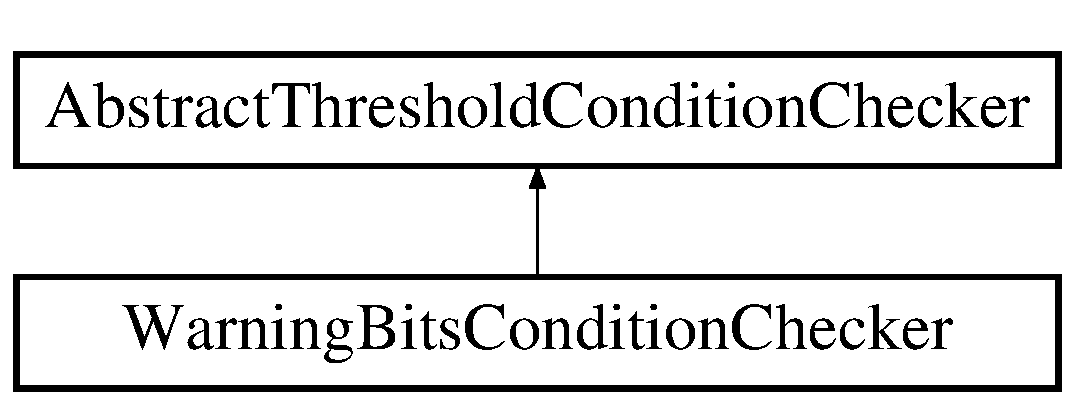
\includegraphics[height=2.000000cm]{class_abstract_threshold_condition_checker}
\end{center}
\end{figure}
\subsection*{Public Member Functions}
\begin{DoxyCompactItemize}
\item 
\mbox{\hyperlink{versionbits_8h_ae7f620361ae33b80687a42adb26fd7a4}{Threshold\+State}} \mbox{\hyperlink{class_abstract_threshold_condition_checker_a7986d06396d52f6961d7c983dc68b8f3}{Get\+State\+For}} (const \mbox{\hyperlink{class_c_block_index}{C\+Block\+Index}} $\ast$pindex\+Prev, const \mbox{\hyperlink{chainparams_8h_a5e1ca1b35c3dd1a4e20f18445f28dd9c}{Consensus\+::\+Params}} \&params, \mbox{\hyperlink{versionbits_8h_a06fae3f599b3fadc0ea127cd55c111ab}{Threshold\+Condition\+Cache}} \&cache) const
\end{DoxyCompactItemize}
\subsection*{Protected Member Functions}
\begin{DoxyCompactItemize}
\item 
virtual bool \mbox{\hyperlink{class_abstract_threshold_condition_checker_a242388d3046f69956904f0ea7a1e92ee}{Condition}} (const \mbox{\hyperlink{class_c_block_index}{C\+Block\+Index}} $\ast$pindex, const \mbox{\hyperlink{chainparams_8h_a5e1ca1b35c3dd1a4e20f18445f28dd9c}{Consensus\+::\+Params}} \&params) const =0
\item 
virtual int64\+\_\+t \mbox{\hyperlink{class_abstract_threshold_condition_checker_abd1169fade7a2934d605bc4fa53878c6}{Begin\+Time}} (const \mbox{\hyperlink{chainparams_8h_a5e1ca1b35c3dd1a4e20f18445f28dd9c}{Consensus\+::\+Params}} \&params) const =0
\item 
virtual int64\+\_\+t \mbox{\hyperlink{class_abstract_threshold_condition_checker_a798df83d41a24e8ca12c02fb25d07c1c}{End\+Time}} (const \mbox{\hyperlink{chainparams_8h_a5e1ca1b35c3dd1a4e20f18445f28dd9c}{Consensus\+::\+Params}} \&params) const =0
\item 
virtual int \mbox{\hyperlink{class_abstract_threshold_condition_checker_a34b66faf36426413918aedda5213d110}{Period}} (const \mbox{\hyperlink{chainparams_8h_a5e1ca1b35c3dd1a4e20f18445f28dd9c}{Consensus\+::\+Params}} \&params) const =0
\item 
virtual int \mbox{\hyperlink{class_abstract_threshold_condition_checker_ad01c87d6d551e9d801661d734a270a6c}{Threshold}} (const \mbox{\hyperlink{chainparams_8h_a5e1ca1b35c3dd1a4e20f18445f28dd9c}{Consensus\+::\+Params}} \&params) const =0
\end{DoxyCompactItemize}


\subsection{Detailed Description}
Abstract class that implements B\+I\+P9-\/style threshold logic, and caches results. 

\subsection{Member Function Documentation}
\mbox{\Hypertarget{class_abstract_threshold_condition_checker_abd1169fade7a2934d605bc4fa53878c6}\label{class_abstract_threshold_condition_checker_abd1169fade7a2934d605bc4fa53878c6}} 
\index{Abstract\+Threshold\+Condition\+Checker@{Abstract\+Threshold\+Condition\+Checker}!Begin\+Time@{Begin\+Time}}
\index{Begin\+Time@{Begin\+Time}!Abstract\+Threshold\+Condition\+Checker@{Abstract\+Threshold\+Condition\+Checker}}
\subsubsection{\texorpdfstring{Begin\+Time()}{BeginTime()}}
{\footnotesize\ttfamily virtual int64\+\_\+t Abstract\+Threshold\+Condition\+Checker\+::\+Begin\+Time (\begin{DoxyParamCaption}\item[{const \mbox{\hyperlink{chainparams_8h_a5e1ca1b35c3dd1a4e20f18445f28dd9c}{Consensus\+::\+Params}} \&}]{params }\end{DoxyParamCaption}) const\hspace{0.3cm}{\ttfamily [protected]}, {\ttfamily [pure virtual]}}



Implemented in \mbox{\hyperlink{class_warning_bits_condition_checker_ab0aff380fa3d04ad540ce178792dad53}{Warning\+Bits\+Condition\+Checker}}.

\mbox{\Hypertarget{class_abstract_threshold_condition_checker_a242388d3046f69956904f0ea7a1e92ee}\label{class_abstract_threshold_condition_checker_a242388d3046f69956904f0ea7a1e92ee}} 
\index{Abstract\+Threshold\+Condition\+Checker@{Abstract\+Threshold\+Condition\+Checker}!Condition@{Condition}}
\index{Condition@{Condition}!Abstract\+Threshold\+Condition\+Checker@{Abstract\+Threshold\+Condition\+Checker}}
\subsubsection{\texorpdfstring{Condition()}{Condition()}}
{\footnotesize\ttfamily virtual bool Abstract\+Threshold\+Condition\+Checker\+::\+Condition (\begin{DoxyParamCaption}\item[{const \mbox{\hyperlink{class_c_block_index}{C\+Block\+Index}} $\ast$}]{pindex,  }\item[{const \mbox{\hyperlink{chainparams_8h_a5e1ca1b35c3dd1a4e20f18445f28dd9c}{Consensus\+::\+Params}} \&}]{params }\end{DoxyParamCaption}) const\hspace{0.3cm}{\ttfamily [protected]}, {\ttfamily [pure virtual]}}



Implemented in \mbox{\hyperlink{class_warning_bits_condition_checker_aae2fc419d193b147e8fad8121fb5e579}{Warning\+Bits\+Condition\+Checker}}.

\mbox{\Hypertarget{class_abstract_threshold_condition_checker_a798df83d41a24e8ca12c02fb25d07c1c}\label{class_abstract_threshold_condition_checker_a798df83d41a24e8ca12c02fb25d07c1c}} 
\index{Abstract\+Threshold\+Condition\+Checker@{Abstract\+Threshold\+Condition\+Checker}!End\+Time@{End\+Time}}
\index{End\+Time@{End\+Time}!Abstract\+Threshold\+Condition\+Checker@{Abstract\+Threshold\+Condition\+Checker}}
\subsubsection{\texorpdfstring{End\+Time()}{EndTime()}}
{\footnotesize\ttfamily virtual int64\+\_\+t Abstract\+Threshold\+Condition\+Checker\+::\+End\+Time (\begin{DoxyParamCaption}\item[{const \mbox{\hyperlink{chainparams_8h_a5e1ca1b35c3dd1a4e20f18445f28dd9c}{Consensus\+::\+Params}} \&}]{params }\end{DoxyParamCaption}) const\hspace{0.3cm}{\ttfamily [protected]}, {\ttfamily [pure virtual]}}



Implemented in \mbox{\hyperlink{class_warning_bits_condition_checker_ace6c66438992ea0f798806f39eca83a7}{Warning\+Bits\+Condition\+Checker}}.

\mbox{\Hypertarget{class_abstract_threshold_condition_checker_a7986d06396d52f6961d7c983dc68b8f3}\label{class_abstract_threshold_condition_checker_a7986d06396d52f6961d7c983dc68b8f3}} 
\index{Abstract\+Threshold\+Condition\+Checker@{Abstract\+Threshold\+Condition\+Checker}!Get\+State\+For@{Get\+State\+For}}
\index{Get\+State\+For@{Get\+State\+For}!Abstract\+Threshold\+Condition\+Checker@{Abstract\+Threshold\+Condition\+Checker}}
\subsubsection{\texorpdfstring{Get\+State\+For()}{GetStateFor()}}
{\footnotesize\ttfamily \mbox{\hyperlink{versionbits_8h_ae7f620361ae33b80687a42adb26fd7a4}{Threshold\+State}} Abstract\+Threshold\+Condition\+Checker\+::\+Get\+State\+For (\begin{DoxyParamCaption}\item[{const \mbox{\hyperlink{class_c_block_index}{C\+Block\+Index}} $\ast$}]{pindex\+Prev,  }\item[{const \mbox{\hyperlink{chainparams_8h_a5e1ca1b35c3dd1a4e20f18445f28dd9c}{Consensus\+::\+Params}} \&}]{params,  }\item[{\mbox{\hyperlink{versionbits_8h_a06fae3f599b3fadc0ea127cd55c111ab}{Threshold\+Condition\+Cache}} \&}]{cache }\end{DoxyParamCaption}) const}

\mbox{\Hypertarget{class_abstract_threshold_condition_checker_a34b66faf36426413918aedda5213d110}\label{class_abstract_threshold_condition_checker_a34b66faf36426413918aedda5213d110}} 
\index{Abstract\+Threshold\+Condition\+Checker@{Abstract\+Threshold\+Condition\+Checker}!Period@{Period}}
\index{Period@{Period}!Abstract\+Threshold\+Condition\+Checker@{Abstract\+Threshold\+Condition\+Checker}}
\subsubsection{\texorpdfstring{Period()}{Period()}}
{\footnotesize\ttfamily virtual int Abstract\+Threshold\+Condition\+Checker\+::\+Period (\begin{DoxyParamCaption}\item[{const \mbox{\hyperlink{chainparams_8h_a5e1ca1b35c3dd1a4e20f18445f28dd9c}{Consensus\+::\+Params}} \&}]{params }\end{DoxyParamCaption}) const\hspace{0.3cm}{\ttfamily [protected]}, {\ttfamily [pure virtual]}}



Implemented in \mbox{\hyperlink{class_warning_bits_condition_checker_af6dd78109426020b259b70c07bc858d7}{Warning\+Bits\+Condition\+Checker}}.

\mbox{\Hypertarget{class_abstract_threshold_condition_checker_ad01c87d6d551e9d801661d734a270a6c}\label{class_abstract_threshold_condition_checker_ad01c87d6d551e9d801661d734a270a6c}} 
\index{Abstract\+Threshold\+Condition\+Checker@{Abstract\+Threshold\+Condition\+Checker}!Threshold@{Threshold}}
\index{Threshold@{Threshold}!Abstract\+Threshold\+Condition\+Checker@{Abstract\+Threshold\+Condition\+Checker}}
\subsubsection{\texorpdfstring{Threshold()}{Threshold()}}
{\footnotesize\ttfamily virtual int Abstract\+Threshold\+Condition\+Checker\+::\+Threshold (\begin{DoxyParamCaption}\item[{const \mbox{\hyperlink{chainparams_8h_a5e1ca1b35c3dd1a4e20f18445f28dd9c}{Consensus\+::\+Params}} \&}]{params }\end{DoxyParamCaption}) const\hspace{0.3cm}{\ttfamily [protected]}, {\ttfamily [pure virtual]}}



Implemented in \mbox{\hyperlink{class_warning_bits_condition_checker_af2de7b32547b0677594b1bfbdacd19ad}{Warning\+Bits\+Condition\+Checker}}.



The documentation for this class was generated from the following files\+:\begin{DoxyCompactItemize}
\item 
/\+Users/christopherarguello/\+Developer/anon/src/\mbox{\hyperlink{versionbits_8h}{versionbits.\+h}}\item 
/\+Users/christopherarguello/\+Developer/anon/src/\mbox{\hyperlink{versionbits_8cpp}{versionbits.\+cpp}}\end{DoxyCompactItemize}

\hypertarget{class_annotated_mixin}{}\section{Annotated\+Mixin$<$ P\+A\+R\+E\+NT $>$ Class Template Reference}
\label{class_annotated_mixin}\index{Annotated\+Mixin$<$ P\+A\+R\+E\+N\+T $>$@{Annotated\+Mixin$<$ P\+A\+R\+E\+N\+T $>$}}


{\ttfamily \#include $<$sync.\+h$>$}

Inheritance diagram for Annotated\+Mixin$<$ P\+A\+R\+E\+NT $>$\+:\begin{figure}[H]
\begin{center}
\leavevmode
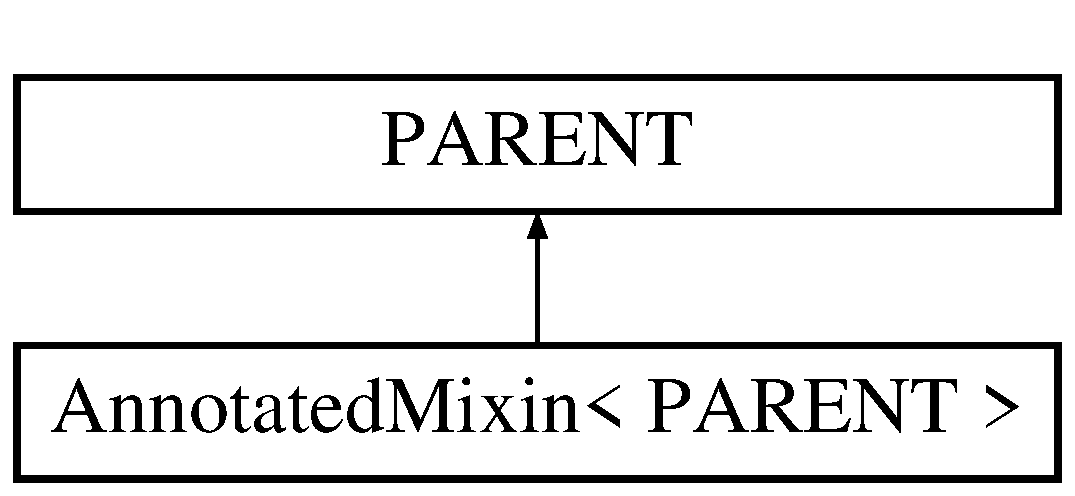
\includegraphics[height=2.000000cm]{class_annotated_mixin}
\end{center}
\end{figure}
\subsection*{Public Member Functions}
\begin{DoxyCompactItemize}
\item 
void \mbox{\hyperlink{class_annotated_mixin_ad1f35c6d1b8a8e980fff45e7e7cb46d3}{lock}} () \mbox{\hyperlink{threadsafety_8h_a77729163b7f6867da40ad5daa5f926f3}{E\+X\+C\+L\+U\+S\+I\+V\+E\+\_\+\+L\+O\+C\+K\+\_\+\+F\+U\+N\+C\+T\+I\+ON}}()
\item 
void \mbox{\hyperlink{class_annotated_mixin_acc2e3da37c2d9dd483b859572e32bc24}{unlock}} () \mbox{\hyperlink{threadsafety_8h_abd56e19f9b4781b1a5212a46951cf5c3}{U\+N\+L\+O\+C\+K\+\_\+\+F\+U\+N\+C\+T\+I\+ON}}()
\item 
bool \mbox{\hyperlink{class_annotated_mixin_a9a33deab2da56790d8b5d30b1fd8350d}{try\+\_\+lock}} () \mbox{\hyperlink{threadsafety_8h_a3c67d370ed1f55064d85e01076aad534}{E\+X\+C\+L\+U\+S\+I\+V\+E\+\_\+\+T\+R\+Y\+L\+O\+C\+K\+\_\+\+F\+U\+N\+C\+T\+I\+ON}}(true)
\end{DoxyCompactItemize}


\subsection{Detailed Description}
\subsubsection*{template$<$typename P\+A\+R\+E\+NT$>$\newline
class Annotated\+Mixin$<$ P\+A\+R\+E\+N\+T $>$}

Template mixin that adds -\/\+Wthread-\/safety locking annotations to a subset of the mutex A\+PI. 

\subsection{Member Function Documentation}
\mbox{\Hypertarget{class_annotated_mixin_ad1f35c6d1b8a8e980fff45e7e7cb46d3}\label{class_annotated_mixin_ad1f35c6d1b8a8e980fff45e7e7cb46d3}} 
\index{Annotated\+Mixin@{Annotated\+Mixin}!lock@{lock}}
\index{lock@{lock}!Annotated\+Mixin@{Annotated\+Mixin}}
\subsubsection{\texorpdfstring{lock()}{lock()}}
{\footnotesize\ttfamily template$<$typename P\+A\+R\+E\+NT$>$ \\
void \mbox{\hyperlink{class_annotated_mixin}{Annotated\+Mixin}}$<$ P\+A\+R\+E\+NT $>$\+::lock (\begin{DoxyParamCaption}{ }\end{DoxyParamCaption})\hspace{0.3cm}{\ttfamily [inline]}}

\mbox{\Hypertarget{class_annotated_mixin_a9a33deab2da56790d8b5d30b1fd8350d}\label{class_annotated_mixin_a9a33deab2da56790d8b5d30b1fd8350d}} 
\index{Annotated\+Mixin@{Annotated\+Mixin}!try\+\_\+lock@{try\+\_\+lock}}
\index{try\+\_\+lock@{try\+\_\+lock}!Annotated\+Mixin@{Annotated\+Mixin}}
\subsubsection{\texorpdfstring{try\+\_\+lock()}{try\_lock()}}
{\footnotesize\ttfamily template$<$typename P\+A\+R\+E\+NT$>$ \\
bool \mbox{\hyperlink{class_annotated_mixin}{Annotated\+Mixin}}$<$ P\+A\+R\+E\+NT $>$\+::try\+\_\+lock (\begin{DoxyParamCaption}{ }\end{DoxyParamCaption})\hspace{0.3cm}{\ttfamily [inline]}}

\mbox{\Hypertarget{class_annotated_mixin_acc2e3da37c2d9dd483b859572e32bc24}\label{class_annotated_mixin_acc2e3da37c2d9dd483b859572e32bc24}} 
\index{Annotated\+Mixin@{Annotated\+Mixin}!unlock@{unlock}}
\index{unlock@{unlock}!Annotated\+Mixin@{Annotated\+Mixin}}
\subsubsection{\texorpdfstring{unlock()}{unlock()}}
{\footnotesize\ttfamily template$<$typename P\+A\+R\+E\+NT$>$ \\
void \mbox{\hyperlink{class_annotated_mixin}{Annotated\+Mixin}}$<$ P\+A\+R\+E\+NT $>$\+::unlock (\begin{DoxyParamCaption}{ }\end{DoxyParamCaption})\hspace{0.3cm}{\ttfamily [inline]}}



The documentation for this class was generated from the following file\+:\begin{DoxyCompactItemize}
\item 
/\+Users/christopherarguello/\+Developer/anon/src/\mbox{\hyperlink{sync_8h}{sync.\+h}}\end{DoxyCompactItemize}

\hypertarget{classarith__uint256}{}\section{arith\+\_\+uint256 Class Reference}
\label{classarith__uint256}\index{arith\+\_\+uint256@{arith\+\_\+uint256}}


{\ttfamily \#include $<$arith\+\_\+uint256.\+h$>$}

Inheritance diagram for arith\+\_\+uint256\+:\begin{figure}[H]
\begin{center}
\leavevmode
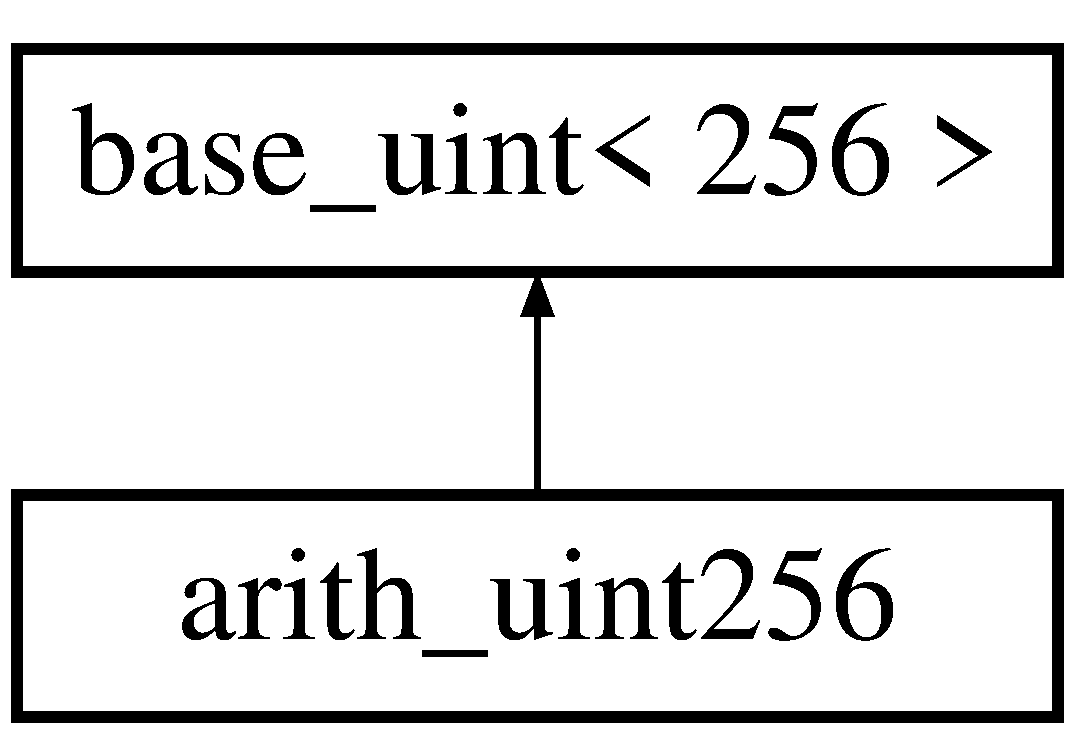
\includegraphics[height=2.000000cm]{classarith__uint256}
\end{center}
\end{figure}
\subsection*{Public Member Functions}
\begin{DoxyCompactItemize}
\item 
\mbox{\hyperlink{classarith__uint256_a1dae7481f3ebf5457f70aaf385d566dd}{arith\+\_\+uint256}} ()
\item 
\mbox{\hyperlink{classarith__uint256_a86c126d261e0edeea49e051e2f3b98a7}{arith\+\_\+uint256}} (const \mbox{\hyperlink{classbase__uint}{base\+\_\+uint}}$<$ 256 $>$ \&b)
\item 
\mbox{\hyperlink{classarith__uint256_a865adeb2767f24e0efc3abfb3d75170b}{arith\+\_\+uint256}} (uint64\+\_\+t b)
\item 
\mbox{\hyperlink{classarith__uint256_a0e8b76f74ffb7a251b15aff89b087fbf}{arith\+\_\+uint256}} (const std\+::string \&str)
\item 
\mbox{\hyperlink{classarith__uint256}{arith\+\_\+uint256}} \& \mbox{\hyperlink{classarith__uint256_a458133c9f123519646b07e6143f2164f}{Set\+Compact}} (uint32\+\_\+t n\+Compact, bool $\ast$pf\+Negative=N\+U\+LL, bool $\ast$pf\+Overflow=N\+U\+LL)
\item 
uint32\+\_\+t \mbox{\hyperlink{classarith__uint256_a0eeee9d8f29143ddf1bff2b1ffa8fdc1}{Get\+Compact}} (bool f\+Negative=false) const
\end{DoxyCompactItemize}
\subsection*{Friends}
\begin{DoxyCompactItemize}
\item 
\mbox{\hyperlink{classuint256}{uint256}} \mbox{\hyperlink{classarith__uint256_aef075fd8d1a7e5937e9775b8e82c8a1b}{Arith\+To\+Uint256}} (const \mbox{\hyperlink{classarith__uint256}{arith\+\_\+uint256}} \&)
\item 
\mbox{\hyperlink{classarith__uint256}{arith\+\_\+uint256}} \mbox{\hyperlink{classarith__uint256_a9c9f84c20851f10a8ca5082bec97666a}{Uint\+To\+Arith256}} (const \mbox{\hyperlink{classuint256}{uint256}} \&)
\end{DoxyCompactItemize}
\subsection*{Additional Inherited Members}


\subsection{Detailed Description}
256-\/bit unsigned big integer. 

\subsection{Constructor \& Destructor Documentation}
\mbox{\Hypertarget{classarith__uint256_a1dae7481f3ebf5457f70aaf385d566dd}\label{classarith__uint256_a1dae7481f3ebf5457f70aaf385d566dd}} 
\index{arith\+\_\+uint256@{arith\+\_\+uint256}!arith\+\_\+uint256@{arith\+\_\+uint256}}
\index{arith\+\_\+uint256@{arith\+\_\+uint256}!arith\+\_\+uint256@{arith\+\_\+uint256}}
\subsubsection{\texorpdfstring{arith\+\_\+uint256()}{arith\_uint256()}\hspace{0.1cm}{\footnotesize\ttfamily [1/4]}}
{\footnotesize\ttfamily arith\+\_\+uint256\+::arith\+\_\+uint256 (\begin{DoxyParamCaption}{ }\end{DoxyParamCaption})\hspace{0.3cm}{\ttfamily [inline]}}

\mbox{\Hypertarget{classarith__uint256_a86c126d261e0edeea49e051e2f3b98a7}\label{classarith__uint256_a86c126d261e0edeea49e051e2f3b98a7}} 
\index{arith\+\_\+uint256@{arith\+\_\+uint256}!arith\+\_\+uint256@{arith\+\_\+uint256}}
\index{arith\+\_\+uint256@{arith\+\_\+uint256}!arith\+\_\+uint256@{arith\+\_\+uint256}}
\subsubsection{\texorpdfstring{arith\+\_\+uint256()}{arith\_uint256()}\hspace{0.1cm}{\footnotesize\ttfamily [2/4]}}
{\footnotesize\ttfamily arith\+\_\+uint256\+::arith\+\_\+uint256 (\begin{DoxyParamCaption}\item[{const \mbox{\hyperlink{classbase__uint}{base\+\_\+uint}}$<$ 256 $>$ \&}]{b }\end{DoxyParamCaption})\hspace{0.3cm}{\ttfamily [inline]}}

\mbox{\Hypertarget{classarith__uint256_a865adeb2767f24e0efc3abfb3d75170b}\label{classarith__uint256_a865adeb2767f24e0efc3abfb3d75170b}} 
\index{arith\+\_\+uint256@{arith\+\_\+uint256}!arith\+\_\+uint256@{arith\+\_\+uint256}}
\index{arith\+\_\+uint256@{arith\+\_\+uint256}!arith\+\_\+uint256@{arith\+\_\+uint256}}
\subsubsection{\texorpdfstring{arith\+\_\+uint256()}{arith\_uint256()}\hspace{0.1cm}{\footnotesize\ttfamily [3/4]}}
{\footnotesize\ttfamily arith\+\_\+uint256\+::arith\+\_\+uint256 (\begin{DoxyParamCaption}\item[{uint64\+\_\+t}]{b }\end{DoxyParamCaption})\hspace{0.3cm}{\ttfamily [inline]}}

\mbox{\Hypertarget{classarith__uint256_a0e8b76f74ffb7a251b15aff89b087fbf}\label{classarith__uint256_a0e8b76f74ffb7a251b15aff89b087fbf}} 
\index{arith\+\_\+uint256@{arith\+\_\+uint256}!arith\+\_\+uint256@{arith\+\_\+uint256}}
\index{arith\+\_\+uint256@{arith\+\_\+uint256}!arith\+\_\+uint256@{arith\+\_\+uint256}}
\subsubsection{\texorpdfstring{arith\+\_\+uint256()}{arith\_uint256()}\hspace{0.1cm}{\footnotesize\ttfamily [4/4]}}
{\footnotesize\ttfamily arith\+\_\+uint256\+::arith\+\_\+uint256 (\begin{DoxyParamCaption}\item[{const std\+::string \&}]{str }\end{DoxyParamCaption})\hspace{0.3cm}{\ttfamily [inline]}, {\ttfamily [explicit]}}



\subsection{Member Function Documentation}
\mbox{\Hypertarget{classarith__uint256_a0eeee9d8f29143ddf1bff2b1ffa8fdc1}\label{classarith__uint256_a0eeee9d8f29143ddf1bff2b1ffa8fdc1}} 
\index{arith\+\_\+uint256@{arith\+\_\+uint256}!Get\+Compact@{Get\+Compact}}
\index{Get\+Compact@{Get\+Compact}!arith\+\_\+uint256@{arith\+\_\+uint256}}
\subsubsection{\texorpdfstring{Get\+Compact()}{GetCompact()}}
{\footnotesize\ttfamily uint32\+\_\+t arith\+\_\+uint256\+::\+Get\+Compact (\begin{DoxyParamCaption}\item[{bool}]{f\+Negative = {\ttfamily false} }\end{DoxyParamCaption}) const}

\mbox{\Hypertarget{classarith__uint256_a458133c9f123519646b07e6143f2164f}\label{classarith__uint256_a458133c9f123519646b07e6143f2164f}} 
\index{arith\+\_\+uint256@{arith\+\_\+uint256}!Set\+Compact@{Set\+Compact}}
\index{Set\+Compact@{Set\+Compact}!arith\+\_\+uint256@{arith\+\_\+uint256}}
\subsubsection{\texorpdfstring{Set\+Compact()}{SetCompact()}}
{\footnotesize\ttfamily \mbox{\hyperlink{classarith__uint256}{arith\+\_\+uint256}} \& arith\+\_\+uint256\+::\+Set\+Compact (\begin{DoxyParamCaption}\item[{uint32\+\_\+t}]{n\+Compact,  }\item[{bool $\ast$}]{pf\+Negative = {\ttfamily NULL},  }\item[{bool $\ast$}]{pf\+Overflow = {\ttfamily NULL} }\end{DoxyParamCaption})}

The \char`\"{}compact\char`\"{} format is a representation of a whole number N using an unsigned 32bit number similar to a floating point format. The most significant 8 bits are the unsigned exponent of base 256. This exponent can be thought of as \char`\"{}number of bytes of N\char`\"{}. The lower 23 bits are the mantissa. Bit number 24 (0x800000) represents the sign of N. N = (-\/1$^\wedge$sign) $\ast$ mantissa $\ast$ 256$^\wedge$(exponent-\/3)

Satoshi\textquotesingle{}s original implementation used B\+N\+\_\+bn2mpi() and B\+N\+\_\+mpi2bn(). M\+PI uses the most significant bit of the first byte as sign. Thus 0x1234560000 is compact (0x05123456) and 0xc0de000000 is compact (0x0600c0de)

Bitcoin only uses this \char`\"{}compact\char`\"{} format for encoding difficulty targets, which are unsigned 256bit quantities. Thus, all the complexities of the sign bit and using base 256 are probably an implementation accident. 

\subsection{Friends And Related Function Documentation}
\mbox{\Hypertarget{classarith__uint256_aef075fd8d1a7e5937e9775b8e82c8a1b}\label{classarith__uint256_aef075fd8d1a7e5937e9775b8e82c8a1b}} 
\index{arith\+\_\+uint256@{arith\+\_\+uint256}!Arith\+To\+Uint256@{Arith\+To\+Uint256}}
\index{Arith\+To\+Uint256@{Arith\+To\+Uint256}!arith\+\_\+uint256@{arith\+\_\+uint256}}
\subsubsection{\texorpdfstring{Arith\+To\+Uint256}{ArithToUint256}}
{\footnotesize\ttfamily \mbox{\hyperlink{classuint256}{uint256}} Arith\+To\+Uint256 (\begin{DoxyParamCaption}\item[{const \mbox{\hyperlink{classarith__uint256}{arith\+\_\+uint256}} \&}]{ }\end{DoxyParamCaption})\hspace{0.3cm}{\ttfamily [friend]}}

\mbox{\Hypertarget{classarith__uint256_a9c9f84c20851f10a8ca5082bec97666a}\label{classarith__uint256_a9c9f84c20851f10a8ca5082bec97666a}} 
\index{arith\+\_\+uint256@{arith\+\_\+uint256}!Uint\+To\+Arith256@{Uint\+To\+Arith256}}
\index{Uint\+To\+Arith256@{Uint\+To\+Arith256}!arith\+\_\+uint256@{arith\+\_\+uint256}}
\subsubsection{\texorpdfstring{Uint\+To\+Arith256}{UintToArith256}}
{\footnotesize\ttfamily \mbox{\hyperlink{classarith__uint256}{arith\+\_\+uint256}} Uint\+To\+Arith256 (\begin{DoxyParamCaption}\item[{const \mbox{\hyperlink{classuint256}{uint256}} \&}]{ }\end{DoxyParamCaption})\hspace{0.3cm}{\ttfamily [friend]}}



The documentation for this class was generated from the following files\+:\begin{DoxyCompactItemize}
\item 
/\+Users/christopherarguello/\+Developer/anon/src/\mbox{\hyperlink{arith__uint256_8h}{arith\+\_\+uint256.\+h}}\item 
/\+Users/christopherarguello/\+Developer/anon/src/\mbox{\hyperlink{arith__uint256_8cpp}{arith\+\_\+uint256.\+cpp}}\end{DoxyCompactItemize}

\hypertarget{class_async_r_p_c_operation}{}\section{Async\+R\+P\+C\+Operation Class Reference}
\label{class_async_r_p_c_operation}\index{Async\+R\+P\+C\+Operation@{Async\+R\+P\+C\+Operation}}


{\ttfamily \#include $<$asyncrpcoperation.\+h$>$}

\subsection*{Public Member Functions}
\begin{DoxyCompactItemize}
\item 
\mbox{\hyperlink{class_async_r_p_c_operation_a46579a5f8045b6301a4354d578877cc8}{Async\+R\+P\+C\+Operation}} ()
\item 
virtual \mbox{\hyperlink{class_async_r_p_c_operation_a5e5bc22f608ee116e5bd80aed36d77fd}{$\sim$\+Async\+R\+P\+C\+Operation}} ()
\item 
virtual void \mbox{\hyperlink{class_async_r_p_c_operation_a37b00fb2684a303d04109b7e9b95ed36}{main}} ()
\item 
void \mbox{\hyperlink{class_async_r_p_c_operation_ac381d872b2673a45c3cfeb35f6e008aa}{cancel}} ()
\item 
\mbox{\hyperlink{asyncrpcoperation_8h_ac36eba6558c325a3ae9853d551326ff6}{Operation\+Status}} \mbox{\hyperlink{class_async_r_p_c_operation_a5dc5eb2a358d01926b7c5c4f6cf29b3e}{get\+State}} () const
\item 
\mbox{\hyperlink{asyncrpcoperation_8h_a1fb3337bad8503e6f6823aa1bcd7191c}{Async\+R\+P\+C\+Operation\+Id}} \mbox{\hyperlink{class_async_r_p_c_operation_ab146889334b2c769abcae4227e51935a}{get\+Id}} () const
\item 
int64\+\_\+t \mbox{\hyperlink{class_async_r_p_c_operation_ae7baefce223a953ef027ac064c2889d9}{get\+Creation\+Time}} () const
\item 
virtual Uni\+Value \mbox{\hyperlink{class_async_r_p_c_operation_a5e448738dc1ee9504602cda249e992a9}{get\+Status}} () const
\item 
Uni\+Value \mbox{\hyperlink{class_async_r_p_c_operation_afa40d2c45199a150cd428ce9dddef2d6}{get\+Error}} () const
\item 
Uni\+Value \mbox{\hyperlink{class_async_r_p_c_operation_a9d55ed3338361eb7cec39c1a09dd7302}{get\+Result}} () const
\item 
std\+::string \mbox{\hyperlink{class_async_r_p_c_operation_a03b6422d357c20f8d635fb2ddcf05c7c}{get\+State\+As\+String}} () const
\item 
int \mbox{\hyperlink{class_async_r_p_c_operation_a74223c143382054f65675dceb4fab777}{get\+Error\+Code}} () const
\item 
std\+::string \mbox{\hyperlink{class_async_r_p_c_operation_a8027a9a3a7b6ebf54f20b4fb93b2e6fe}{get\+Error\+Message}} () const
\item 
bool \mbox{\hyperlink{class_async_r_p_c_operation_ac7b3093bed8fa04841cc618b3517babd}{is\+Cancelled}} () const
\item 
bool \mbox{\hyperlink{class_async_r_p_c_operation_a224b1e5ca0f71103f6a4f1c4344f4be1}{is\+Executing}} () const
\item 
bool \mbox{\hyperlink{class_async_r_p_c_operation_a0e403108f6da6e9a140e42a943586d95}{is\+Ready}} () const
\item 
bool \mbox{\hyperlink{class_async_r_p_c_operation_a236138cd93ff3e6c5869a789edee4b8a}{is\+Failed}} () const
\item 
bool \mbox{\hyperlink{class_async_r_p_c_operation_a657e5de4e0b4d36c5ead2ed225a04744}{is\+Success}} () const
\end{DoxyCompactItemize}
\subsection*{Protected Member Functions}
\begin{DoxyCompactItemize}
\item 
void \mbox{\hyperlink{class_async_r_p_c_operation_a97e645c3dd703f32562fa97a56e33cad}{start\+\_\+execution\+\_\+clock}} ()
\item 
void \mbox{\hyperlink{class_async_r_p_c_operation_a27ebf14d38c4c4c92e8f7718b0f37760}{stop\+\_\+execution\+\_\+clock}} ()
\item 
void \mbox{\hyperlink{class_async_r_p_c_operation_a9c2768bee813eb30ec243f798e95f184}{set\+\_\+state}} (\mbox{\hyperlink{asyncrpcoperation_8h_ac36eba6558c325a3ae9853d551326ff6}{Operation\+Status}} state)
\item 
void \mbox{\hyperlink{class_async_r_p_c_operation_a7744d10ad7a5908165c72a61f3e7de4a}{set\+\_\+error\+\_\+code}} (int error\+Code)
\item 
void \mbox{\hyperlink{class_async_r_p_c_operation_adc6f2696e8fcce11c63e2a0228192ab9}{set\+\_\+error\+\_\+message}} (std\+::string error\+Message)
\item 
void \mbox{\hyperlink{class_async_r_p_c_operation_aee516dfd5a83887995c72a9e0a75fbdd}{set\+\_\+result}} (Uni\+Value v)
\end{DoxyCompactItemize}
\subsection*{Protected Attributes}
\begin{DoxyCompactItemize}
\item 
std\+::mutex \mbox{\hyperlink{class_async_r_p_c_operation_a3b2c3593ad11003b628c95dffbbea6d1}{lock\+\_\+}}
\item 
Uni\+Value \mbox{\hyperlink{class_async_r_p_c_operation_abcb878365261b9f28b460d697b39cc12}{result\+\_\+}}
\item 
int \mbox{\hyperlink{class_async_r_p_c_operation_a15823397370b4893f7e0e7aa88efd89e}{error\+\_\+code\+\_\+}}
\item 
std\+::string \mbox{\hyperlink{class_async_r_p_c_operation_a07644a57fdaf6eeb83fcfbeba4f1b3e0}{error\+\_\+message\+\_\+}}
\item 
std\+::atomic$<$ \mbox{\hyperlink{asyncrpcoperation_8h_ac36eba6558c325a3ae9853d551326ff6}{Operation\+Status}} $>$ \mbox{\hyperlink{class_async_r_p_c_operation_a6f48909669cc4f503d448f14ed6f5da7}{state\+\_\+}}
\item 
std\+::chrono\+::time\+\_\+point$<$ std\+::chrono\+::system\+\_\+clock $>$ \mbox{\hyperlink{class_async_r_p_c_operation_a7ebcc576bfa71f5224b25c82d95a5790}{start\+\_\+time\+\_\+}}
\item 
std\+::chrono\+::time\+\_\+point$<$ std\+::chrono\+::system\+\_\+clock $>$ \mbox{\hyperlink{class_async_r_p_c_operation_aa1be6b3ef1c1d1ffcbbe0b55a45df5e1}{end\+\_\+time\+\_\+}}
\end{DoxyCompactItemize}
\subsection*{Private Member Functions}
\begin{DoxyCompactItemize}
\item 
\mbox{\hyperlink{class_async_r_p_c_operation_a82650746d52af73698ab10c2d0f7b53a}{Async\+R\+P\+C\+Operation}} (const \mbox{\hyperlink{class_async_r_p_c_operation}{Async\+R\+P\+C\+Operation}} \&orig)
\item 
\mbox{\hyperlink{class_async_r_p_c_operation}{Async\+R\+P\+C\+Operation}} \& \mbox{\hyperlink{class_async_r_p_c_operation_a2e741b291d755892418ef01506e28695}{operator=}} (const \mbox{\hyperlink{class_async_r_p_c_operation}{Async\+R\+P\+C\+Operation}} \&other)
\end{DoxyCompactItemize}
\subsection*{Private Attributes}
\begin{DoxyCompactItemize}
\item 
\mbox{\hyperlink{asyncrpcoperation_8h_a1fb3337bad8503e6f6823aa1bcd7191c}{Async\+R\+P\+C\+Operation\+Id}} \mbox{\hyperlink{class_async_r_p_c_operation_ac0e2c643b776bbf357643d091f3ee406}{id\+\_\+}}
\item 
int64\+\_\+t \mbox{\hyperlink{class_async_r_p_c_operation_a472604f84939dea568d04605cee634b9}{creation\+\_\+time\+\_\+}}
\end{DoxyCompactItemize}


\subsection{Constructor \& Destructor Documentation}
\mbox{\Hypertarget{class_async_r_p_c_operation_a46579a5f8045b6301a4354d578877cc8}\label{class_async_r_p_c_operation_a46579a5f8045b6301a4354d578877cc8}} 
\index{Async\+R\+P\+C\+Operation@{Async\+R\+P\+C\+Operation}!Async\+R\+P\+C\+Operation@{Async\+R\+P\+C\+Operation}}
\index{Async\+R\+P\+C\+Operation@{Async\+R\+P\+C\+Operation}!Async\+R\+P\+C\+Operation@{Async\+R\+P\+C\+Operation}}
\subsubsection{\texorpdfstring{Async\+R\+P\+C\+Operation()}{AsyncRPCOperation()}\hspace{0.1cm}{\footnotesize\ttfamily [1/2]}}
{\footnotesize\ttfamily Async\+R\+P\+C\+Operation\+::\+Async\+R\+P\+C\+Operation (\begin{DoxyParamCaption}{ }\end{DoxyParamCaption})}

Every operation instance should have a globally unique id \mbox{\Hypertarget{class_async_r_p_c_operation_a5e5bc22f608ee116e5bd80aed36d77fd}\label{class_async_r_p_c_operation_a5e5bc22f608ee116e5bd80aed36d77fd}} 
\index{Async\+R\+P\+C\+Operation@{Async\+R\+P\+C\+Operation}!````~Async\+R\+P\+C\+Operation@{$\sim$\+Async\+R\+P\+C\+Operation}}
\index{````~Async\+R\+P\+C\+Operation@{$\sim$\+Async\+R\+P\+C\+Operation}!Async\+R\+P\+C\+Operation@{Async\+R\+P\+C\+Operation}}
\subsubsection{\texorpdfstring{$\sim$\+Async\+R\+P\+C\+Operation()}{~AsyncRPCOperation()}}
{\footnotesize\ttfamily Async\+R\+P\+C\+Operation\+::$\sim$\+Async\+R\+P\+C\+Operation (\begin{DoxyParamCaption}{ }\end{DoxyParamCaption})\hspace{0.3cm}{\ttfamily [virtual]}}

\mbox{\Hypertarget{class_async_r_p_c_operation_a82650746d52af73698ab10c2d0f7b53a}\label{class_async_r_p_c_operation_a82650746d52af73698ab10c2d0f7b53a}} 
\index{Async\+R\+P\+C\+Operation@{Async\+R\+P\+C\+Operation}!Async\+R\+P\+C\+Operation@{Async\+R\+P\+C\+Operation}}
\index{Async\+R\+P\+C\+Operation@{Async\+R\+P\+C\+Operation}!Async\+R\+P\+C\+Operation@{Async\+R\+P\+C\+Operation}}
\subsubsection{\texorpdfstring{Async\+R\+P\+C\+Operation()}{AsyncRPCOperation()}\hspace{0.1cm}{\footnotesize\ttfamily [2/2]}}
{\footnotesize\ttfamily Async\+R\+P\+C\+Operation\+::\+Async\+R\+P\+C\+Operation (\begin{DoxyParamCaption}\item[{const \mbox{\hyperlink{class_async_r_p_c_operation}{Async\+R\+P\+C\+Operation}} \&}]{orig }\end{DoxyParamCaption})\hspace{0.3cm}{\ttfamily [private]}}



\subsection{Member Function Documentation}
\mbox{\Hypertarget{class_async_r_p_c_operation_ac381d872b2673a45c3cfeb35f6e008aa}\label{class_async_r_p_c_operation_ac381d872b2673a45c3cfeb35f6e008aa}} 
\index{Async\+R\+P\+C\+Operation@{Async\+R\+P\+C\+Operation}!cancel@{cancel}}
\index{cancel@{cancel}!Async\+R\+P\+C\+Operation@{Async\+R\+P\+C\+Operation}}
\subsubsection{\texorpdfstring{cancel()}{cancel()}}
{\footnotesize\ttfamily void Async\+R\+P\+C\+Operation\+::cancel (\begin{DoxyParamCaption}{ }\end{DoxyParamCaption})}

Override this \mbox{\hyperlink{class_async_r_p_c_operation_ac381d872b2673a45c3cfeb35f6e008aa}{cancel()}} method if you can interrupt \mbox{\hyperlink{class_async_r_p_c_operation_a37b00fb2684a303d04109b7e9b95ed36}{main()}} when executing. \mbox{\Hypertarget{class_async_r_p_c_operation_ae7baefce223a953ef027ac064c2889d9}\label{class_async_r_p_c_operation_ae7baefce223a953ef027ac064c2889d9}} 
\index{Async\+R\+P\+C\+Operation@{Async\+R\+P\+C\+Operation}!get\+Creation\+Time@{get\+Creation\+Time}}
\index{get\+Creation\+Time@{get\+Creation\+Time}!Async\+R\+P\+C\+Operation@{Async\+R\+P\+C\+Operation}}
\subsubsection{\texorpdfstring{get\+Creation\+Time()}{getCreationTime()}}
{\footnotesize\ttfamily int64\+\_\+t Async\+R\+P\+C\+Operation\+::get\+Creation\+Time (\begin{DoxyParamCaption}{ }\end{DoxyParamCaption}) const\hspace{0.3cm}{\ttfamily [inline]}}

\mbox{\Hypertarget{class_async_r_p_c_operation_afa40d2c45199a150cd428ce9dddef2d6}\label{class_async_r_p_c_operation_afa40d2c45199a150cd428ce9dddef2d6}} 
\index{Async\+R\+P\+C\+Operation@{Async\+R\+P\+C\+Operation}!get\+Error@{get\+Error}}
\index{get\+Error@{get\+Error}!Async\+R\+P\+C\+Operation@{Async\+R\+P\+C\+Operation}}
\subsubsection{\texorpdfstring{get\+Error()}{getError()}}
{\footnotesize\ttfamily Uni\+Value Async\+R\+P\+C\+Operation\+::get\+Error (\begin{DoxyParamCaption}{ }\end{DoxyParamCaption}) const}

Return the error of the completed operation as a Uni\+Value object. If there is no error, return null Uni\+Value. \mbox{\Hypertarget{class_async_r_p_c_operation_a74223c143382054f65675dceb4fab777}\label{class_async_r_p_c_operation_a74223c143382054f65675dceb4fab777}} 
\index{Async\+R\+P\+C\+Operation@{Async\+R\+P\+C\+Operation}!get\+Error\+Code@{get\+Error\+Code}}
\index{get\+Error\+Code@{get\+Error\+Code}!Async\+R\+P\+C\+Operation@{Async\+R\+P\+C\+Operation}}
\subsubsection{\texorpdfstring{get\+Error\+Code()}{getErrorCode()}}
{\footnotesize\ttfamily int Async\+R\+P\+C\+Operation\+::get\+Error\+Code (\begin{DoxyParamCaption}{ }\end{DoxyParamCaption}) const\hspace{0.3cm}{\ttfamily [inline]}}

\mbox{\Hypertarget{class_async_r_p_c_operation_a8027a9a3a7b6ebf54f20b4fb93b2e6fe}\label{class_async_r_p_c_operation_a8027a9a3a7b6ebf54f20b4fb93b2e6fe}} 
\index{Async\+R\+P\+C\+Operation@{Async\+R\+P\+C\+Operation}!get\+Error\+Message@{get\+Error\+Message}}
\index{get\+Error\+Message@{get\+Error\+Message}!Async\+R\+P\+C\+Operation@{Async\+R\+P\+C\+Operation}}
\subsubsection{\texorpdfstring{get\+Error\+Message()}{getErrorMessage()}}
{\footnotesize\ttfamily std\+::string Async\+R\+P\+C\+Operation\+::get\+Error\+Message (\begin{DoxyParamCaption}{ }\end{DoxyParamCaption}) const\hspace{0.3cm}{\ttfamily [inline]}}

\mbox{\Hypertarget{class_async_r_p_c_operation_ab146889334b2c769abcae4227e51935a}\label{class_async_r_p_c_operation_ab146889334b2c769abcae4227e51935a}} 
\index{Async\+R\+P\+C\+Operation@{Async\+R\+P\+C\+Operation}!get\+Id@{get\+Id}}
\index{get\+Id@{get\+Id}!Async\+R\+P\+C\+Operation@{Async\+R\+P\+C\+Operation}}
\subsubsection{\texorpdfstring{get\+Id()}{getId()}}
{\footnotesize\ttfamily \mbox{\hyperlink{asyncrpcoperation_8h_a1fb3337bad8503e6f6823aa1bcd7191c}{Async\+R\+P\+C\+Operation\+Id}} Async\+R\+P\+C\+Operation\+::get\+Id (\begin{DoxyParamCaption}{ }\end{DoxyParamCaption}) const\hspace{0.3cm}{\ttfamily [inline]}}

\mbox{\Hypertarget{class_async_r_p_c_operation_a9d55ed3338361eb7cec39c1a09dd7302}\label{class_async_r_p_c_operation_a9d55ed3338361eb7cec39c1a09dd7302}} 
\index{Async\+R\+P\+C\+Operation@{Async\+R\+P\+C\+Operation}!get\+Result@{get\+Result}}
\index{get\+Result@{get\+Result}!Async\+R\+P\+C\+Operation@{Async\+R\+P\+C\+Operation}}
\subsubsection{\texorpdfstring{get\+Result()}{getResult()}}
{\footnotesize\ttfamily Uni\+Value Async\+R\+P\+C\+Operation\+::get\+Result (\begin{DoxyParamCaption}{ }\end{DoxyParamCaption}) const}

Return the result of the completed operation as a Uni\+Value object. If the operation did not succeed, return null Uni\+Value. \mbox{\Hypertarget{class_async_r_p_c_operation_a5dc5eb2a358d01926b7c5c4f6cf29b3e}\label{class_async_r_p_c_operation_a5dc5eb2a358d01926b7c5c4f6cf29b3e}} 
\index{Async\+R\+P\+C\+Operation@{Async\+R\+P\+C\+Operation}!get\+State@{get\+State}}
\index{get\+State@{get\+State}!Async\+R\+P\+C\+Operation@{Async\+R\+P\+C\+Operation}}
\subsubsection{\texorpdfstring{get\+State()}{getState()}}
{\footnotesize\ttfamily \mbox{\hyperlink{asyncrpcoperation_8h_ac36eba6558c325a3ae9853d551326ff6}{Operation\+Status}} Async\+R\+P\+C\+Operation\+::get\+State (\begin{DoxyParamCaption}{ }\end{DoxyParamCaption}) const\hspace{0.3cm}{\ttfamily [inline]}}

\mbox{\Hypertarget{class_async_r_p_c_operation_a03b6422d357c20f8d635fb2ddcf05c7c}\label{class_async_r_p_c_operation_a03b6422d357c20f8d635fb2ddcf05c7c}} 
\index{Async\+R\+P\+C\+Operation@{Async\+R\+P\+C\+Operation}!get\+State\+As\+String@{get\+State\+As\+String}}
\index{get\+State\+As\+String@{get\+State\+As\+String}!Async\+R\+P\+C\+Operation@{Async\+R\+P\+C\+Operation}}
\subsubsection{\texorpdfstring{get\+State\+As\+String()}{getStateAsString()}}
{\footnotesize\ttfamily std\+::string Async\+R\+P\+C\+Operation\+::get\+State\+As\+String (\begin{DoxyParamCaption}{ }\end{DoxyParamCaption}) const}

Return the operation state in human readable form. \mbox{\Hypertarget{class_async_r_p_c_operation_a5e448738dc1ee9504602cda249e992a9}\label{class_async_r_p_c_operation_a5e448738dc1ee9504602cda249e992a9}} 
\index{Async\+R\+P\+C\+Operation@{Async\+R\+P\+C\+Operation}!get\+Status@{get\+Status}}
\index{get\+Status@{get\+Status}!Async\+R\+P\+C\+Operation@{Async\+R\+P\+C\+Operation}}
\subsubsection{\texorpdfstring{get\+Status()}{getStatus()}}
{\footnotesize\ttfamily Uni\+Value Async\+R\+P\+C\+Operation\+::get\+Status (\begin{DoxyParamCaption}{ }\end{DoxyParamCaption}) const\hspace{0.3cm}{\ttfamily [virtual]}}

Returns a status Uni\+Value object. If the operation has failed, it will include an error object. If the operation has succeeded, it will include the result value. If the operation was cancelled, there will be no error object or result value. \mbox{\Hypertarget{class_async_r_p_c_operation_ac7b3093bed8fa04841cc618b3517babd}\label{class_async_r_p_c_operation_ac7b3093bed8fa04841cc618b3517babd}} 
\index{Async\+R\+P\+C\+Operation@{Async\+R\+P\+C\+Operation}!is\+Cancelled@{is\+Cancelled}}
\index{is\+Cancelled@{is\+Cancelled}!Async\+R\+P\+C\+Operation@{Async\+R\+P\+C\+Operation}}
\subsubsection{\texorpdfstring{is\+Cancelled()}{isCancelled()}}
{\footnotesize\ttfamily bool Async\+R\+P\+C\+Operation\+::is\+Cancelled (\begin{DoxyParamCaption}{ }\end{DoxyParamCaption}) const\hspace{0.3cm}{\ttfamily [inline]}}

\mbox{\Hypertarget{class_async_r_p_c_operation_a224b1e5ca0f71103f6a4f1c4344f4be1}\label{class_async_r_p_c_operation_a224b1e5ca0f71103f6a4f1c4344f4be1}} 
\index{Async\+R\+P\+C\+Operation@{Async\+R\+P\+C\+Operation}!is\+Executing@{is\+Executing}}
\index{is\+Executing@{is\+Executing}!Async\+R\+P\+C\+Operation@{Async\+R\+P\+C\+Operation}}
\subsubsection{\texorpdfstring{is\+Executing()}{isExecuting()}}
{\footnotesize\ttfamily bool Async\+R\+P\+C\+Operation\+::is\+Executing (\begin{DoxyParamCaption}{ }\end{DoxyParamCaption}) const\hspace{0.3cm}{\ttfamily [inline]}}

\mbox{\Hypertarget{class_async_r_p_c_operation_a236138cd93ff3e6c5869a789edee4b8a}\label{class_async_r_p_c_operation_a236138cd93ff3e6c5869a789edee4b8a}} 
\index{Async\+R\+P\+C\+Operation@{Async\+R\+P\+C\+Operation}!is\+Failed@{is\+Failed}}
\index{is\+Failed@{is\+Failed}!Async\+R\+P\+C\+Operation@{Async\+R\+P\+C\+Operation}}
\subsubsection{\texorpdfstring{is\+Failed()}{isFailed()}}
{\footnotesize\ttfamily bool Async\+R\+P\+C\+Operation\+::is\+Failed (\begin{DoxyParamCaption}{ }\end{DoxyParamCaption}) const\hspace{0.3cm}{\ttfamily [inline]}}

\mbox{\Hypertarget{class_async_r_p_c_operation_a0e403108f6da6e9a140e42a943586d95}\label{class_async_r_p_c_operation_a0e403108f6da6e9a140e42a943586d95}} 
\index{Async\+R\+P\+C\+Operation@{Async\+R\+P\+C\+Operation}!is\+Ready@{is\+Ready}}
\index{is\+Ready@{is\+Ready}!Async\+R\+P\+C\+Operation@{Async\+R\+P\+C\+Operation}}
\subsubsection{\texorpdfstring{is\+Ready()}{isReady()}}
{\footnotesize\ttfamily bool Async\+R\+P\+C\+Operation\+::is\+Ready (\begin{DoxyParamCaption}{ }\end{DoxyParamCaption}) const\hspace{0.3cm}{\ttfamily [inline]}}

\mbox{\Hypertarget{class_async_r_p_c_operation_a657e5de4e0b4d36c5ead2ed225a04744}\label{class_async_r_p_c_operation_a657e5de4e0b4d36c5ead2ed225a04744}} 
\index{Async\+R\+P\+C\+Operation@{Async\+R\+P\+C\+Operation}!is\+Success@{is\+Success}}
\index{is\+Success@{is\+Success}!Async\+R\+P\+C\+Operation@{Async\+R\+P\+C\+Operation}}
\subsubsection{\texorpdfstring{is\+Success()}{isSuccess()}}
{\footnotesize\ttfamily bool Async\+R\+P\+C\+Operation\+::is\+Success (\begin{DoxyParamCaption}{ }\end{DoxyParamCaption}) const\hspace{0.3cm}{\ttfamily [inline]}}

\mbox{\Hypertarget{class_async_r_p_c_operation_a37b00fb2684a303d04109b7e9b95ed36}\label{class_async_r_p_c_operation_a37b00fb2684a303d04109b7e9b95ed36}} 
\index{Async\+R\+P\+C\+Operation@{Async\+R\+P\+C\+Operation}!main@{main}}
\index{main@{main}!Async\+R\+P\+C\+Operation@{Async\+R\+P\+C\+Operation}}
\subsubsection{\texorpdfstring{main()}{main()}}
{\footnotesize\ttfamily void Async\+R\+P\+C\+Operation\+::main (\begin{DoxyParamCaption}{ }\end{DoxyParamCaption})\hspace{0.3cm}{\ttfamily [virtual]}}

Implement this virtual method in any subclass. This is just an example implementation. \mbox{\Hypertarget{class_async_r_p_c_operation_a2e741b291d755892418ef01506e28695}\label{class_async_r_p_c_operation_a2e741b291d755892418ef01506e28695}} 
\index{Async\+R\+P\+C\+Operation@{Async\+R\+P\+C\+Operation}!operator=@{operator=}}
\index{operator=@{operator=}!Async\+R\+P\+C\+Operation@{Async\+R\+P\+C\+Operation}}
\subsubsection{\texorpdfstring{operator=()}{operator=()}}
{\footnotesize\ttfamily \mbox{\hyperlink{class_async_r_p_c_operation}{Async\+R\+P\+C\+Operation}} \& Async\+R\+P\+C\+Operation\+::operator= (\begin{DoxyParamCaption}\item[{const \mbox{\hyperlink{class_async_r_p_c_operation}{Async\+R\+P\+C\+Operation}} \&}]{other }\end{DoxyParamCaption})\hspace{0.3cm}{\ttfamily [private]}}

\mbox{\Hypertarget{class_async_r_p_c_operation_a7744d10ad7a5908165c72a61f3e7de4a}\label{class_async_r_p_c_operation_a7744d10ad7a5908165c72a61f3e7de4a}} 
\index{Async\+R\+P\+C\+Operation@{Async\+R\+P\+C\+Operation}!set\+\_\+error\+\_\+code@{set\+\_\+error\+\_\+code}}
\index{set\+\_\+error\+\_\+code@{set\+\_\+error\+\_\+code}!Async\+R\+P\+C\+Operation@{Async\+R\+P\+C\+Operation}}
\subsubsection{\texorpdfstring{set\+\_\+error\+\_\+code()}{set\_error\_code()}}
{\footnotesize\ttfamily void Async\+R\+P\+C\+Operation\+::set\+\_\+error\+\_\+code (\begin{DoxyParamCaption}\item[{int}]{error\+Code }\end{DoxyParamCaption})\hspace{0.3cm}{\ttfamily [inline]}, {\ttfamily [protected]}}

\mbox{\Hypertarget{class_async_r_p_c_operation_adc6f2696e8fcce11c63e2a0228192ab9}\label{class_async_r_p_c_operation_adc6f2696e8fcce11c63e2a0228192ab9}} 
\index{Async\+R\+P\+C\+Operation@{Async\+R\+P\+C\+Operation}!set\+\_\+error\+\_\+message@{set\+\_\+error\+\_\+message}}
\index{set\+\_\+error\+\_\+message@{set\+\_\+error\+\_\+message}!Async\+R\+P\+C\+Operation@{Async\+R\+P\+C\+Operation}}
\subsubsection{\texorpdfstring{set\+\_\+error\+\_\+message()}{set\_error\_message()}}
{\footnotesize\ttfamily void Async\+R\+P\+C\+Operation\+::set\+\_\+error\+\_\+message (\begin{DoxyParamCaption}\item[{std\+::string}]{error\+Message }\end{DoxyParamCaption})\hspace{0.3cm}{\ttfamily [inline]}, {\ttfamily [protected]}}

\mbox{\Hypertarget{class_async_r_p_c_operation_aee516dfd5a83887995c72a9e0a75fbdd}\label{class_async_r_p_c_operation_aee516dfd5a83887995c72a9e0a75fbdd}} 
\index{Async\+R\+P\+C\+Operation@{Async\+R\+P\+C\+Operation}!set\+\_\+result@{set\+\_\+result}}
\index{set\+\_\+result@{set\+\_\+result}!Async\+R\+P\+C\+Operation@{Async\+R\+P\+C\+Operation}}
\subsubsection{\texorpdfstring{set\+\_\+result()}{set\_result()}}
{\footnotesize\ttfamily void Async\+R\+P\+C\+Operation\+::set\+\_\+result (\begin{DoxyParamCaption}\item[{Uni\+Value}]{v }\end{DoxyParamCaption})\hspace{0.3cm}{\ttfamily [inline]}, {\ttfamily [protected]}}

\mbox{\Hypertarget{class_async_r_p_c_operation_a9c2768bee813eb30ec243f798e95f184}\label{class_async_r_p_c_operation_a9c2768bee813eb30ec243f798e95f184}} 
\index{Async\+R\+P\+C\+Operation@{Async\+R\+P\+C\+Operation}!set\+\_\+state@{set\+\_\+state}}
\index{set\+\_\+state@{set\+\_\+state}!Async\+R\+P\+C\+Operation@{Async\+R\+P\+C\+Operation}}
\subsubsection{\texorpdfstring{set\+\_\+state()}{set\_state()}}
{\footnotesize\ttfamily void Async\+R\+P\+C\+Operation\+::set\+\_\+state (\begin{DoxyParamCaption}\item[{\mbox{\hyperlink{asyncrpcoperation_8h_ac36eba6558c325a3ae9853d551326ff6}{Operation\+Status}}}]{state }\end{DoxyParamCaption})\hspace{0.3cm}{\ttfamily [inline]}, {\ttfamily [protected]}}

\mbox{\Hypertarget{class_async_r_p_c_operation_a97e645c3dd703f32562fa97a56e33cad}\label{class_async_r_p_c_operation_a97e645c3dd703f32562fa97a56e33cad}} 
\index{Async\+R\+P\+C\+Operation@{Async\+R\+P\+C\+Operation}!start\+\_\+execution\+\_\+clock@{start\+\_\+execution\+\_\+clock}}
\index{start\+\_\+execution\+\_\+clock@{start\+\_\+execution\+\_\+clock}!Async\+R\+P\+C\+Operation@{Async\+R\+P\+C\+Operation}}
\subsubsection{\texorpdfstring{start\+\_\+execution\+\_\+clock()}{start\_execution\_clock()}}
{\footnotesize\ttfamily void Async\+R\+P\+C\+Operation\+::start\+\_\+execution\+\_\+clock (\begin{DoxyParamCaption}{ }\end{DoxyParamCaption})\hspace{0.3cm}{\ttfamily [protected]}}

Start timing the execution run of the code you\textquotesingle{}re interested in \mbox{\Hypertarget{class_async_r_p_c_operation_a27ebf14d38c4c4c92e8f7718b0f37760}\label{class_async_r_p_c_operation_a27ebf14d38c4c4c92e8f7718b0f37760}} 
\index{Async\+R\+P\+C\+Operation@{Async\+R\+P\+C\+Operation}!stop\+\_\+execution\+\_\+clock@{stop\+\_\+execution\+\_\+clock}}
\index{stop\+\_\+execution\+\_\+clock@{stop\+\_\+execution\+\_\+clock}!Async\+R\+P\+C\+Operation@{Async\+R\+P\+C\+Operation}}
\subsubsection{\texorpdfstring{stop\+\_\+execution\+\_\+clock()}{stop\_execution\_clock()}}
{\footnotesize\ttfamily void Async\+R\+P\+C\+Operation\+::stop\+\_\+execution\+\_\+clock (\begin{DoxyParamCaption}{ }\end{DoxyParamCaption})\hspace{0.3cm}{\ttfamily [protected]}}

Stop timing the execution run 

\subsection{Member Data Documentation}
\mbox{\Hypertarget{class_async_r_p_c_operation_a472604f84939dea568d04605cee634b9}\label{class_async_r_p_c_operation_a472604f84939dea568d04605cee634b9}} 
\index{Async\+R\+P\+C\+Operation@{Async\+R\+P\+C\+Operation}!creation\+\_\+time\+\_\+@{creation\+\_\+time\+\_\+}}
\index{creation\+\_\+time\+\_\+@{creation\+\_\+time\+\_\+}!Async\+R\+P\+C\+Operation@{Async\+R\+P\+C\+Operation}}
\subsubsection{\texorpdfstring{creation\+\_\+time\+\_\+}{creation\_time\_}}
{\footnotesize\ttfamily int64\+\_\+t Async\+R\+P\+C\+Operation\+::creation\+\_\+time\+\_\+\hspace{0.3cm}{\ttfamily [private]}}

\mbox{\Hypertarget{class_async_r_p_c_operation_aa1be6b3ef1c1d1ffcbbe0b55a45df5e1}\label{class_async_r_p_c_operation_aa1be6b3ef1c1d1ffcbbe0b55a45df5e1}} 
\index{Async\+R\+P\+C\+Operation@{Async\+R\+P\+C\+Operation}!end\+\_\+time\+\_\+@{end\+\_\+time\+\_\+}}
\index{end\+\_\+time\+\_\+@{end\+\_\+time\+\_\+}!Async\+R\+P\+C\+Operation@{Async\+R\+P\+C\+Operation}}
\subsubsection{\texorpdfstring{end\+\_\+time\+\_\+}{end\_time\_}}
{\footnotesize\ttfamily std\+::chrono\+::time\+\_\+point$<$std\+::chrono\+::system\+\_\+clock$>$ Async\+R\+P\+C\+Operation\+::end\+\_\+time\+\_\+\hspace{0.3cm}{\ttfamily [protected]}}

\mbox{\Hypertarget{class_async_r_p_c_operation_a15823397370b4893f7e0e7aa88efd89e}\label{class_async_r_p_c_operation_a15823397370b4893f7e0e7aa88efd89e}} 
\index{Async\+R\+P\+C\+Operation@{Async\+R\+P\+C\+Operation}!error\+\_\+code\+\_\+@{error\+\_\+code\+\_\+}}
\index{error\+\_\+code\+\_\+@{error\+\_\+code\+\_\+}!Async\+R\+P\+C\+Operation@{Async\+R\+P\+C\+Operation}}
\subsubsection{\texorpdfstring{error\+\_\+code\+\_\+}{error\_code\_}}
{\footnotesize\ttfamily int Async\+R\+P\+C\+Operation\+::error\+\_\+code\+\_\+\hspace{0.3cm}{\ttfamily [protected]}}

\mbox{\Hypertarget{class_async_r_p_c_operation_a07644a57fdaf6eeb83fcfbeba4f1b3e0}\label{class_async_r_p_c_operation_a07644a57fdaf6eeb83fcfbeba4f1b3e0}} 
\index{Async\+R\+P\+C\+Operation@{Async\+R\+P\+C\+Operation}!error\+\_\+message\+\_\+@{error\+\_\+message\+\_\+}}
\index{error\+\_\+message\+\_\+@{error\+\_\+message\+\_\+}!Async\+R\+P\+C\+Operation@{Async\+R\+P\+C\+Operation}}
\subsubsection{\texorpdfstring{error\+\_\+message\+\_\+}{error\_message\_}}
{\footnotesize\ttfamily std\+::string Async\+R\+P\+C\+Operation\+::error\+\_\+message\+\_\+\hspace{0.3cm}{\ttfamily [protected]}}

\mbox{\Hypertarget{class_async_r_p_c_operation_ac0e2c643b776bbf357643d091f3ee406}\label{class_async_r_p_c_operation_ac0e2c643b776bbf357643d091f3ee406}} 
\index{Async\+R\+P\+C\+Operation@{Async\+R\+P\+C\+Operation}!id\+\_\+@{id\+\_\+}}
\index{id\+\_\+@{id\+\_\+}!Async\+R\+P\+C\+Operation@{Async\+R\+P\+C\+Operation}}
\subsubsection{\texorpdfstring{id\+\_\+}{id\_}}
{\footnotesize\ttfamily \mbox{\hyperlink{asyncrpcoperation_8h_a1fb3337bad8503e6f6823aa1bcd7191c}{Async\+R\+P\+C\+Operation\+Id}} Async\+R\+P\+C\+Operation\+::id\+\_\+\hspace{0.3cm}{\ttfamily [private]}}

\mbox{\Hypertarget{class_async_r_p_c_operation_a3b2c3593ad11003b628c95dffbbea6d1}\label{class_async_r_p_c_operation_a3b2c3593ad11003b628c95dffbbea6d1}} 
\index{Async\+R\+P\+C\+Operation@{Async\+R\+P\+C\+Operation}!lock\+\_\+@{lock\+\_\+}}
\index{lock\+\_\+@{lock\+\_\+}!Async\+R\+P\+C\+Operation@{Async\+R\+P\+C\+Operation}}
\subsubsection{\texorpdfstring{lock\+\_\+}{lock\_}}
{\footnotesize\ttfamily std\+::mutex Async\+R\+P\+C\+Operation\+::lock\+\_\+\hspace{0.3cm}{\ttfamily [mutable]}, {\ttfamily [protected]}}

\mbox{\Hypertarget{class_async_r_p_c_operation_abcb878365261b9f28b460d697b39cc12}\label{class_async_r_p_c_operation_abcb878365261b9f28b460d697b39cc12}} 
\index{Async\+R\+P\+C\+Operation@{Async\+R\+P\+C\+Operation}!result\+\_\+@{result\+\_\+}}
\index{result\+\_\+@{result\+\_\+}!Async\+R\+P\+C\+Operation@{Async\+R\+P\+C\+Operation}}
\subsubsection{\texorpdfstring{result\+\_\+}{result\_}}
{\footnotesize\ttfamily Uni\+Value Async\+R\+P\+C\+Operation\+::result\+\_\+\hspace{0.3cm}{\ttfamily [protected]}}

\mbox{\Hypertarget{class_async_r_p_c_operation_a7ebcc576bfa71f5224b25c82d95a5790}\label{class_async_r_p_c_operation_a7ebcc576bfa71f5224b25c82d95a5790}} 
\index{Async\+R\+P\+C\+Operation@{Async\+R\+P\+C\+Operation}!start\+\_\+time\+\_\+@{start\+\_\+time\+\_\+}}
\index{start\+\_\+time\+\_\+@{start\+\_\+time\+\_\+}!Async\+R\+P\+C\+Operation@{Async\+R\+P\+C\+Operation}}
\subsubsection{\texorpdfstring{start\+\_\+time\+\_\+}{start\_time\_}}
{\footnotesize\ttfamily std\+::chrono\+::time\+\_\+point$<$std\+::chrono\+::system\+\_\+clock$>$ Async\+R\+P\+C\+Operation\+::start\+\_\+time\+\_\+\hspace{0.3cm}{\ttfamily [protected]}}

\mbox{\Hypertarget{class_async_r_p_c_operation_a6f48909669cc4f503d448f14ed6f5da7}\label{class_async_r_p_c_operation_a6f48909669cc4f503d448f14ed6f5da7}} 
\index{Async\+R\+P\+C\+Operation@{Async\+R\+P\+C\+Operation}!state\+\_\+@{state\+\_\+}}
\index{state\+\_\+@{state\+\_\+}!Async\+R\+P\+C\+Operation@{Async\+R\+P\+C\+Operation}}
\subsubsection{\texorpdfstring{state\+\_\+}{state\_}}
{\footnotesize\ttfamily std\+::atomic$<$\mbox{\hyperlink{asyncrpcoperation_8h_ac36eba6558c325a3ae9853d551326ff6}{Operation\+Status}}$>$ Async\+R\+P\+C\+Operation\+::state\+\_\+\hspace{0.3cm}{\ttfamily [protected]}}



The documentation for this class was generated from the following files\+:\begin{DoxyCompactItemize}
\item 
/\+Users/christopherarguello/\+Developer/anon/src/\mbox{\hyperlink{asyncrpcoperation_8h}{asyncrpcoperation.\+h}}\item 
/\+Users/christopherarguello/\+Developer/anon/src/\mbox{\hyperlink{asyncrpcoperation_8cpp}{asyncrpcoperation.\+cpp}}\end{DoxyCompactItemize}

\hypertarget{class_async_r_p_c_queue}{}\section{Async\+R\+P\+C\+Queue Class Reference}
\label{class_async_r_p_c_queue}\index{Async\+R\+P\+C\+Queue@{Async\+R\+P\+C\+Queue}}


{\ttfamily \#include $<$asyncrpcqueue.\+h$>$}

\subsection*{Public Member Functions}
\begin{DoxyCompactItemize}
\item 
\mbox{\hyperlink{class_async_r_p_c_queue_a131571f208855382a03c22a98dfceb46}{Async\+R\+P\+C\+Queue}} ()
\item 
virtual \mbox{\hyperlink{class_async_r_p_c_queue_a5f5a7f5ed4135e12523863ae5c92f970}{$\sim$\+Async\+R\+P\+C\+Queue}} ()
\item 
\mbox{\hyperlink{class_async_r_p_c_queue_a47a6ce8effac4710a2691d855c9020d7}{Async\+R\+P\+C\+Queue}} (\mbox{\hyperlink{class_async_r_p_c_queue}{Async\+R\+P\+C\+Queue}} const \&)=delete
\item 
\mbox{\hyperlink{class_async_r_p_c_queue_a6f4360b02696e4e9f0a2d71d664b0663}{Async\+R\+P\+C\+Queue}} (\mbox{\hyperlink{class_async_r_p_c_queue}{Async\+R\+P\+C\+Queue}} \&\&)=delete
\item 
\mbox{\hyperlink{class_async_r_p_c_queue}{Async\+R\+P\+C\+Queue}} \& \mbox{\hyperlink{class_async_r_p_c_queue_a191ac9800b1ac534775a8b5bb0bf7972}{operator=}} (\mbox{\hyperlink{class_async_r_p_c_queue}{Async\+R\+P\+C\+Queue}} const \&)=delete
\item 
\mbox{\hyperlink{class_async_r_p_c_queue}{Async\+R\+P\+C\+Queue}} \& \mbox{\hyperlink{class_async_r_p_c_queue_a86c49425ecf86be42cfcbef1478c597f}{operator=}} (\mbox{\hyperlink{class_async_r_p_c_queue}{Async\+R\+P\+C\+Queue}} \&\&)=delete
\item 
void \mbox{\hyperlink{class_async_r_p_c_queue_a05370bb335972acfb00fd8c4e4f90db8}{add\+Worker}} ()
\item 
size\+\_\+t \mbox{\hyperlink{class_async_r_p_c_queue_a0ee8726139e10e2421bffa22509fa790}{get\+Number\+Of\+Workers}} () const
\item 
bool \mbox{\hyperlink{class_async_r_p_c_queue_aa9afd366a946e2b0a8dbb9438d3eee43}{is\+Closed}} () const
\item 
bool \mbox{\hyperlink{class_async_r_p_c_queue_a7efed3f584095c94ae2e594ed1555ec4}{is\+Finishing}} () const
\item 
void \mbox{\hyperlink{class_async_r_p_c_queue_a233be6530494331038507ad60f1d8428}{close}} ()
\item 
void \mbox{\hyperlink{class_async_r_p_c_queue_acc9201529321a452826979ea11697b21}{finish}} ()
\item 
void \mbox{\hyperlink{class_async_r_p_c_queue_a1744ae79a6f3ac3cb98404f8a1489cd4}{close\+And\+Wait}} ()
\item 
void \mbox{\hyperlink{class_async_r_p_c_queue_aaa0414a23dee050656280306b9cf1589}{finish\+And\+Wait}} ()
\item 
void \mbox{\hyperlink{class_async_r_p_c_queue_aa22de6b56261448ff6d468e27f630d7b}{cancel\+All\+Operations}} ()
\item 
size\+\_\+t \mbox{\hyperlink{class_async_r_p_c_queue_ab170c29699beeb0f95791953ce2c66d3}{get\+Operation\+Count}} () const
\item 
std\+::shared\+\_\+ptr$<$ \mbox{\hyperlink{class_async_r_p_c_operation}{Async\+R\+P\+C\+Operation}} $>$ \mbox{\hyperlink{class_async_r_p_c_queue_a4d8d32008c611e4cd7ba122a6dda28c6}{get\+Operation\+For\+Id}} (\mbox{\hyperlink{asyncrpcoperation_8h_a1fb3337bad8503e6f6823aa1bcd7191c}{Async\+R\+P\+C\+Operation\+Id}}) const
\item 
std\+::shared\+\_\+ptr$<$ \mbox{\hyperlink{class_async_r_p_c_operation}{Async\+R\+P\+C\+Operation}} $>$ \mbox{\hyperlink{class_async_r_p_c_queue_a716d9609df548d21d3bd3cca130aa811}{pop\+Operation\+For\+Id}} (\mbox{\hyperlink{asyncrpcoperation_8h_a1fb3337bad8503e6f6823aa1bcd7191c}{Async\+R\+P\+C\+Operation\+Id}})
\item 
void \mbox{\hyperlink{class_async_r_p_c_queue_a921166cf7a5f25723c13b2f01d35edaa}{add\+Operation}} (const std\+::shared\+\_\+ptr$<$ \mbox{\hyperlink{class_async_r_p_c_operation}{Async\+R\+P\+C\+Operation}} $>$ \&ptr\+Operation)
\item 
std\+::vector$<$ \mbox{\hyperlink{asyncrpcoperation_8h_a1fb3337bad8503e6f6823aa1bcd7191c}{Async\+R\+P\+C\+Operation\+Id}} $>$ \mbox{\hyperlink{class_async_r_p_c_queue_abca893fa7d90594a7807548c15aa1020}{get\+All\+Operation\+Ids}} () const
\end{DoxyCompactItemize}
\subsection*{Static Public Member Functions}
\begin{DoxyCompactItemize}
\item 
static shared\+\_\+ptr$<$ \mbox{\hyperlink{class_async_r_p_c_queue}{Async\+R\+P\+C\+Queue}} $>$ \mbox{\hyperlink{class_async_r_p_c_queue_a58fbaf8e8a9d3dfbc22dfc62651cd781}{shared\+Instance}} ()
\end{DoxyCompactItemize}
\subsection*{Private Member Functions}
\begin{DoxyCompactItemize}
\item 
void \mbox{\hyperlink{class_async_r_p_c_queue_ac3d5fdff7da17f6d3e7c431d5a73362f}{run}} (size\+\_\+t worker\+Id)
\item 
void \mbox{\hyperlink{class_async_r_p_c_queue_aa3c4318cddf22d01c67a6f681a631527}{wait\+\_\+for\+\_\+worker\+\_\+threads}} ()
\end{DoxyCompactItemize}
\subsection*{Private Attributes}
\begin{DoxyCompactItemize}
\item 
std\+::mutex \mbox{\hyperlink{class_async_r_p_c_queue_ada16823dc9cf27df1586aefe21202195}{lock\+\_\+}}
\item 
std\+::condition\+\_\+variable \mbox{\hyperlink{class_async_r_p_c_queue_a75c212e637553383b503c0a13f09a921}{condition\+\_\+}}
\item 
std\+::atomic$<$ bool $>$ \mbox{\hyperlink{class_async_r_p_c_queue_ace54c24f087e6738d57cad3581e715fc}{closed\+\_\+}}
\item 
std\+::atomic$<$ bool $>$ \mbox{\hyperlink{class_async_r_p_c_queue_a2f0bd5cb15375855cee1aa1b233669ac}{finish\+\_\+}}
\item 
\mbox{\hyperlink{asyncrpcqueue_8h_a292afad965e96f58aa19082ebf053c1f}{Async\+R\+P\+C\+Operation\+Map}} \mbox{\hyperlink{class_async_r_p_c_queue_a023d022a2e6b584b53e4a72221b5e8e3}{operation\+\_\+map\+\_\+}}
\item 
std\+::queue$<$ \mbox{\hyperlink{asyncrpcoperation_8h_a1fb3337bad8503e6f6823aa1bcd7191c}{Async\+R\+P\+C\+Operation\+Id}} $>$ \mbox{\hyperlink{class_async_r_p_c_queue_ac174a557657529fd20e5369333acc26d}{operation\+\_\+id\+\_\+queue\+\_\+}}
\item 
std\+::vector$<$ std\+::thread $>$ \mbox{\hyperlink{class_async_r_p_c_queue_aa77ac44f05a3b3b5b7a2d54c88248272}{workers\+\_\+}}
\end{DoxyCompactItemize}


\subsection{Constructor \& Destructor Documentation}
\mbox{\Hypertarget{class_async_r_p_c_queue_a131571f208855382a03c22a98dfceb46}\label{class_async_r_p_c_queue_a131571f208855382a03c22a98dfceb46}} 
\index{Async\+R\+P\+C\+Queue@{Async\+R\+P\+C\+Queue}!Async\+R\+P\+C\+Queue@{Async\+R\+P\+C\+Queue}}
\index{Async\+R\+P\+C\+Queue@{Async\+R\+P\+C\+Queue}!Async\+R\+P\+C\+Queue@{Async\+R\+P\+C\+Queue}}
\subsubsection{\texorpdfstring{Async\+R\+P\+C\+Queue()}{AsyncRPCQueue()}\hspace{0.1cm}{\footnotesize\ttfamily [1/3]}}
{\footnotesize\ttfamily Async\+R\+P\+C\+Queue\+::\+Async\+R\+P\+C\+Queue (\begin{DoxyParamCaption}{ }\end{DoxyParamCaption})}

\mbox{\Hypertarget{class_async_r_p_c_queue_a5f5a7f5ed4135e12523863ae5c92f970}\label{class_async_r_p_c_queue_a5f5a7f5ed4135e12523863ae5c92f970}} 
\index{Async\+R\+P\+C\+Queue@{Async\+R\+P\+C\+Queue}!````~Async\+R\+P\+C\+Queue@{$\sim$\+Async\+R\+P\+C\+Queue}}
\index{````~Async\+R\+P\+C\+Queue@{$\sim$\+Async\+R\+P\+C\+Queue}!Async\+R\+P\+C\+Queue@{Async\+R\+P\+C\+Queue}}
\subsubsection{\texorpdfstring{$\sim$\+Async\+R\+P\+C\+Queue()}{~AsyncRPCQueue()}}
{\footnotesize\ttfamily Async\+R\+P\+C\+Queue\+::$\sim$\+Async\+R\+P\+C\+Queue (\begin{DoxyParamCaption}{ }\end{DoxyParamCaption})\hspace{0.3cm}{\ttfamily [virtual]}}

\mbox{\Hypertarget{class_async_r_p_c_queue_a47a6ce8effac4710a2691d855c9020d7}\label{class_async_r_p_c_queue_a47a6ce8effac4710a2691d855c9020d7}} 
\index{Async\+R\+P\+C\+Queue@{Async\+R\+P\+C\+Queue}!Async\+R\+P\+C\+Queue@{Async\+R\+P\+C\+Queue}}
\index{Async\+R\+P\+C\+Queue@{Async\+R\+P\+C\+Queue}!Async\+R\+P\+C\+Queue@{Async\+R\+P\+C\+Queue}}
\subsubsection{\texorpdfstring{Async\+R\+P\+C\+Queue()}{AsyncRPCQueue()}\hspace{0.1cm}{\footnotesize\ttfamily [2/3]}}
{\footnotesize\ttfamily Async\+R\+P\+C\+Queue\+::\+Async\+R\+P\+C\+Queue (\begin{DoxyParamCaption}\item[{\mbox{\hyperlink{class_async_r_p_c_queue}{Async\+R\+P\+C\+Queue}} const \&}]{ }\end{DoxyParamCaption})\hspace{0.3cm}{\ttfamily [delete]}}

\mbox{\Hypertarget{class_async_r_p_c_queue_a6f4360b02696e4e9f0a2d71d664b0663}\label{class_async_r_p_c_queue_a6f4360b02696e4e9f0a2d71d664b0663}} 
\index{Async\+R\+P\+C\+Queue@{Async\+R\+P\+C\+Queue}!Async\+R\+P\+C\+Queue@{Async\+R\+P\+C\+Queue}}
\index{Async\+R\+P\+C\+Queue@{Async\+R\+P\+C\+Queue}!Async\+R\+P\+C\+Queue@{Async\+R\+P\+C\+Queue}}
\subsubsection{\texorpdfstring{Async\+R\+P\+C\+Queue()}{AsyncRPCQueue()}\hspace{0.1cm}{\footnotesize\ttfamily [3/3]}}
{\footnotesize\ttfamily Async\+R\+P\+C\+Queue\+::\+Async\+R\+P\+C\+Queue (\begin{DoxyParamCaption}\item[{\mbox{\hyperlink{class_async_r_p_c_queue}{Async\+R\+P\+C\+Queue}} \&\&}]{ }\end{DoxyParamCaption})\hspace{0.3cm}{\ttfamily [delete]}}



\subsection{Member Function Documentation}
\mbox{\Hypertarget{class_async_r_p_c_queue_a921166cf7a5f25723c13b2f01d35edaa}\label{class_async_r_p_c_queue_a921166cf7a5f25723c13b2f01d35edaa}} 
\index{Async\+R\+P\+C\+Queue@{Async\+R\+P\+C\+Queue}!add\+Operation@{add\+Operation}}
\index{add\+Operation@{add\+Operation}!Async\+R\+P\+C\+Queue@{Async\+R\+P\+C\+Queue}}
\subsubsection{\texorpdfstring{add\+Operation()}{addOperation()}}
{\footnotesize\ttfamily void Async\+R\+P\+C\+Queue\+::add\+Operation (\begin{DoxyParamCaption}\item[{const std\+::shared\+\_\+ptr$<$ \mbox{\hyperlink{class_async_r_p_c_operation}{Async\+R\+P\+C\+Operation}} $>$ \&}]{ptr\+Operation }\end{DoxyParamCaption})}

Add shared\+\_\+ptr to operation.

To retain polymorphic behaviour, i.\+e. \mbox{\hyperlink{bitcoin-cli_8cpp_a0ddf1224851353fc92bfbff6f499fa97}{main()}} method of derived classes is invoked, caller should create the shared\+\_\+ptr like this\+:

std\+::shared\+\_\+ptr$<$\+Async\+R\+P\+C\+Operation$>$ ptr(new My\+Custom\+Async\+R\+P\+C\+Operation(params));

Don\textquotesingle{}t use std\+::make\+\_\+shared$<$\+Async\+R\+P\+C\+Operation$>$(). \mbox{\Hypertarget{class_async_r_p_c_queue_a05370bb335972acfb00fd8c4e4f90db8}\label{class_async_r_p_c_queue_a05370bb335972acfb00fd8c4e4f90db8}} 
\index{Async\+R\+P\+C\+Queue@{Async\+R\+P\+C\+Queue}!add\+Worker@{add\+Worker}}
\index{add\+Worker@{add\+Worker}!Async\+R\+P\+C\+Queue@{Async\+R\+P\+C\+Queue}}
\subsubsection{\texorpdfstring{add\+Worker()}{addWorker()}}
{\footnotesize\ttfamily void Async\+R\+P\+C\+Queue\+::add\+Worker (\begin{DoxyParamCaption}{ }\end{DoxyParamCaption})}

Spawn a worker thread \mbox{\Hypertarget{class_async_r_p_c_queue_aa22de6b56261448ff6d468e27f630d7b}\label{class_async_r_p_c_queue_aa22de6b56261448ff6d468e27f630d7b}} 
\index{Async\+R\+P\+C\+Queue@{Async\+R\+P\+C\+Queue}!cancel\+All\+Operations@{cancel\+All\+Operations}}
\index{cancel\+All\+Operations@{cancel\+All\+Operations}!Async\+R\+P\+C\+Queue@{Async\+R\+P\+C\+Queue}}
\subsubsection{\texorpdfstring{cancel\+All\+Operations()}{cancelAllOperations()}}
{\footnotesize\ttfamily void Async\+R\+P\+C\+Queue\+::cancel\+All\+Operations (\begin{DoxyParamCaption}{ }\end{DoxyParamCaption})}

Call cancel() on all operations \mbox{\Hypertarget{class_async_r_p_c_queue_a233be6530494331038507ad60f1d8428}\label{class_async_r_p_c_queue_a233be6530494331038507ad60f1d8428}} 
\index{Async\+R\+P\+C\+Queue@{Async\+R\+P\+C\+Queue}!close@{close}}
\index{close@{close}!Async\+R\+P\+C\+Queue@{Async\+R\+P\+C\+Queue}}
\subsubsection{\texorpdfstring{close()}{close()}}
{\footnotesize\ttfamily void Async\+R\+P\+C\+Queue\+::close (\begin{DoxyParamCaption}{ }\end{DoxyParamCaption})}

Close the queue and cancel all existing operations \mbox{\Hypertarget{class_async_r_p_c_queue_a1744ae79a6f3ac3cb98404f8a1489cd4}\label{class_async_r_p_c_queue_a1744ae79a6f3ac3cb98404f8a1489cd4}} 
\index{Async\+R\+P\+C\+Queue@{Async\+R\+P\+C\+Queue}!close\+And\+Wait@{close\+And\+Wait}}
\index{close\+And\+Wait@{close\+And\+Wait}!Async\+R\+P\+C\+Queue@{Async\+R\+P\+C\+Queue}}
\subsubsection{\texorpdfstring{close\+And\+Wait()}{closeAndWait()}}
{\footnotesize\ttfamily void Async\+R\+P\+C\+Queue\+::close\+And\+Wait (\begin{DoxyParamCaption}{ }\end{DoxyParamCaption})}

Calling thread will close and wait for worker threads to join. \mbox{\Hypertarget{class_async_r_p_c_queue_acc9201529321a452826979ea11697b21}\label{class_async_r_p_c_queue_acc9201529321a452826979ea11697b21}} 
\index{Async\+R\+P\+C\+Queue@{Async\+R\+P\+C\+Queue}!finish@{finish}}
\index{finish@{finish}!Async\+R\+P\+C\+Queue@{Async\+R\+P\+C\+Queue}}
\subsubsection{\texorpdfstring{finish()}{finish()}}
{\footnotesize\ttfamily void Async\+R\+P\+C\+Queue\+::finish (\begin{DoxyParamCaption}{ }\end{DoxyParamCaption})}

Close the queue but finish existing operations. Do not accept new operations. \mbox{\Hypertarget{class_async_r_p_c_queue_aaa0414a23dee050656280306b9cf1589}\label{class_async_r_p_c_queue_aaa0414a23dee050656280306b9cf1589}} 
\index{Async\+R\+P\+C\+Queue@{Async\+R\+P\+C\+Queue}!finish\+And\+Wait@{finish\+And\+Wait}}
\index{finish\+And\+Wait@{finish\+And\+Wait}!Async\+R\+P\+C\+Queue@{Async\+R\+P\+C\+Queue}}
\subsubsection{\texorpdfstring{finish\+And\+Wait()}{finishAndWait()}}
{\footnotesize\ttfamily void Async\+R\+P\+C\+Queue\+::finish\+And\+Wait (\begin{DoxyParamCaption}{ }\end{DoxyParamCaption})}

Block current thread until all workers have finished their tasks. \mbox{\Hypertarget{class_async_r_p_c_queue_abca893fa7d90594a7807548c15aa1020}\label{class_async_r_p_c_queue_abca893fa7d90594a7807548c15aa1020}} 
\index{Async\+R\+P\+C\+Queue@{Async\+R\+P\+C\+Queue}!get\+All\+Operation\+Ids@{get\+All\+Operation\+Ids}}
\index{get\+All\+Operation\+Ids@{get\+All\+Operation\+Ids}!Async\+R\+P\+C\+Queue@{Async\+R\+P\+C\+Queue}}
\subsubsection{\texorpdfstring{get\+All\+Operation\+Ids()}{getAllOperationIds()}}
{\footnotesize\ttfamily std\+::vector$<$ \mbox{\hyperlink{asyncrpcoperation_8h_a1fb3337bad8503e6f6823aa1bcd7191c}{Async\+R\+P\+C\+Operation\+Id}} $>$ Async\+R\+P\+C\+Queue\+::get\+All\+Operation\+Ids (\begin{DoxyParamCaption}{ }\end{DoxyParamCaption}) const}

Return a list of all known operation ids found in internal storage. \mbox{\Hypertarget{class_async_r_p_c_queue_a0ee8726139e10e2421bffa22509fa790}\label{class_async_r_p_c_queue_a0ee8726139e10e2421bffa22509fa790}} 
\index{Async\+R\+P\+C\+Queue@{Async\+R\+P\+C\+Queue}!get\+Number\+Of\+Workers@{get\+Number\+Of\+Workers}}
\index{get\+Number\+Of\+Workers@{get\+Number\+Of\+Workers}!Async\+R\+P\+C\+Queue@{Async\+R\+P\+C\+Queue}}
\subsubsection{\texorpdfstring{get\+Number\+Of\+Workers()}{getNumberOfWorkers()}}
{\footnotesize\ttfamily size\+\_\+t Async\+R\+P\+C\+Queue\+::get\+Number\+Of\+Workers (\begin{DoxyParamCaption}{ }\end{DoxyParamCaption}) const}

Return the number of worker threads spawned by the queue \mbox{\Hypertarget{class_async_r_p_c_queue_ab170c29699beeb0f95791953ce2c66d3}\label{class_async_r_p_c_queue_ab170c29699beeb0f95791953ce2c66d3}} 
\index{Async\+R\+P\+C\+Queue@{Async\+R\+P\+C\+Queue}!get\+Operation\+Count@{get\+Operation\+Count}}
\index{get\+Operation\+Count@{get\+Operation\+Count}!Async\+R\+P\+C\+Queue@{Async\+R\+P\+C\+Queue}}
\subsubsection{\texorpdfstring{get\+Operation\+Count()}{getOperationCount()}}
{\footnotesize\ttfamily size\+\_\+t Async\+R\+P\+C\+Queue\+::get\+Operation\+Count (\begin{DoxyParamCaption}{ }\end{DoxyParamCaption}) const}

Return the number of operations in the queue \mbox{\Hypertarget{class_async_r_p_c_queue_a4d8d32008c611e4cd7ba122a6dda28c6}\label{class_async_r_p_c_queue_a4d8d32008c611e4cd7ba122a6dda28c6}} 
\index{Async\+R\+P\+C\+Queue@{Async\+R\+P\+C\+Queue}!get\+Operation\+For\+Id@{get\+Operation\+For\+Id}}
\index{get\+Operation\+For\+Id@{get\+Operation\+For\+Id}!Async\+R\+P\+C\+Queue@{Async\+R\+P\+C\+Queue}}
\subsubsection{\texorpdfstring{get\+Operation\+For\+Id()}{getOperationForId()}}
{\footnotesize\ttfamily std\+::shared\+\_\+ptr$<$ \mbox{\hyperlink{class_async_r_p_c_operation}{Async\+R\+P\+C\+Operation}} $>$ Async\+R\+P\+C\+Queue\+::get\+Operation\+For\+Id (\begin{DoxyParamCaption}\item[{\mbox{\hyperlink{asyncrpcoperation_8h_a1fb3337bad8503e6f6823aa1bcd7191c}{Async\+R\+P\+C\+Operation\+Id}}}]{id }\end{DoxyParamCaption}) const}

Return the operation for a given operation id. \mbox{\Hypertarget{class_async_r_p_c_queue_aa9afd366a946e2b0a8dbb9438d3eee43}\label{class_async_r_p_c_queue_aa9afd366a946e2b0a8dbb9438d3eee43}} 
\index{Async\+R\+P\+C\+Queue@{Async\+R\+P\+C\+Queue}!is\+Closed@{is\+Closed}}
\index{is\+Closed@{is\+Closed}!Async\+R\+P\+C\+Queue@{Async\+R\+P\+C\+Queue}}
\subsubsection{\texorpdfstring{is\+Closed()}{isClosed()}}
{\footnotesize\ttfamily bool Async\+R\+P\+C\+Queue\+::is\+Closed (\begin{DoxyParamCaption}{ }\end{DoxyParamCaption}) const}

Return true if the queue is closed to new operations. \mbox{\Hypertarget{class_async_r_p_c_queue_a7efed3f584095c94ae2e594ed1555ec4}\label{class_async_r_p_c_queue_a7efed3f584095c94ae2e594ed1555ec4}} 
\index{Async\+R\+P\+C\+Queue@{Async\+R\+P\+C\+Queue}!is\+Finishing@{is\+Finishing}}
\index{is\+Finishing@{is\+Finishing}!Async\+R\+P\+C\+Queue@{Async\+R\+P\+C\+Queue}}
\subsubsection{\texorpdfstring{is\+Finishing()}{isFinishing()}}
{\footnotesize\ttfamily bool Async\+R\+P\+C\+Queue\+::is\+Finishing (\begin{DoxyParamCaption}{ }\end{DoxyParamCaption}) const}

Return true if the queue is finishing up \mbox{\Hypertarget{class_async_r_p_c_queue_a191ac9800b1ac534775a8b5bb0bf7972}\label{class_async_r_p_c_queue_a191ac9800b1ac534775a8b5bb0bf7972}} 
\index{Async\+R\+P\+C\+Queue@{Async\+R\+P\+C\+Queue}!operator=@{operator=}}
\index{operator=@{operator=}!Async\+R\+P\+C\+Queue@{Async\+R\+P\+C\+Queue}}
\subsubsection{\texorpdfstring{operator=()}{operator=()}\hspace{0.1cm}{\footnotesize\ttfamily [1/2]}}
{\footnotesize\ttfamily \mbox{\hyperlink{class_async_r_p_c_queue}{Async\+R\+P\+C\+Queue}}\& Async\+R\+P\+C\+Queue\+::operator= (\begin{DoxyParamCaption}\item[{\mbox{\hyperlink{class_async_r_p_c_queue}{Async\+R\+P\+C\+Queue}} const \&}]{ }\end{DoxyParamCaption})\hspace{0.3cm}{\ttfamily [delete]}}

\mbox{\Hypertarget{class_async_r_p_c_queue_a86c49425ecf86be42cfcbef1478c597f}\label{class_async_r_p_c_queue_a86c49425ecf86be42cfcbef1478c597f}} 
\index{Async\+R\+P\+C\+Queue@{Async\+R\+P\+C\+Queue}!operator=@{operator=}}
\index{operator=@{operator=}!Async\+R\+P\+C\+Queue@{Async\+R\+P\+C\+Queue}}
\subsubsection{\texorpdfstring{operator=()}{operator=()}\hspace{0.1cm}{\footnotesize\ttfamily [2/2]}}
{\footnotesize\ttfamily \mbox{\hyperlink{class_async_r_p_c_queue}{Async\+R\+P\+C\+Queue}}\& Async\+R\+P\+C\+Queue\+::operator= (\begin{DoxyParamCaption}\item[{\mbox{\hyperlink{class_async_r_p_c_queue}{Async\+R\+P\+C\+Queue}} \&\&}]{ }\end{DoxyParamCaption})\hspace{0.3cm}{\ttfamily [delete]}}

\mbox{\Hypertarget{class_async_r_p_c_queue_a716d9609df548d21d3bd3cca130aa811}\label{class_async_r_p_c_queue_a716d9609df548d21d3bd3cca130aa811}} 
\index{Async\+R\+P\+C\+Queue@{Async\+R\+P\+C\+Queue}!pop\+Operation\+For\+Id@{pop\+Operation\+For\+Id}}
\index{pop\+Operation\+For\+Id@{pop\+Operation\+For\+Id}!Async\+R\+P\+C\+Queue@{Async\+R\+P\+C\+Queue}}
\subsubsection{\texorpdfstring{pop\+Operation\+For\+Id()}{popOperationForId()}}
{\footnotesize\ttfamily std\+::shared\+\_\+ptr$<$ \mbox{\hyperlink{class_async_r_p_c_operation}{Async\+R\+P\+C\+Operation}} $>$ Async\+R\+P\+C\+Queue\+::pop\+Operation\+For\+Id (\begin{DoxyParamCaption}\item[{\mbox{\hyperlink{asyncrpcoperation_8h_a1fb3337bad8503e6f6823aa1bcd7191c}{Async\+R\+P\+C\+Operation\+Id}}}]{id }\end{DoxyParamCaption})}

Return the operation for a given operation id and then remove the operation from internal storage. \mbox{\Hypertarget{class_async_r_p_c_queue_ac3d5fdff7da17f6d3e7c431d5a73362f}\label{class_async_r_p_c_queue_ac3d5fdff7da17f6d3e7c431d5a73362f}} 
\index{Async\+R\+P\+C\+Queue@{Async\+R\+P\+C\+Queue}!run@{run}}
\index{run@{run}!Async\+R\+P\+C\+Queue@{Async\+R\+P\+C\+Queue}}
\subsubsection{\texorpdfstring{run()}{run()}}
{\footnotesize\ttfamily void Async\+R\+P\+C\+Queue\+::run (\begin{DoxyParamCaption}\item[{size\+\_\+t}]{worker\+Id }\end{DoxyParamCaption})\hspace{0.3cm}{\ttfamily [private]}}

A worker will execute this method on a new thread \mbox{\Hypertarget{class_async_r_p_c_queue_a58fbaf8e8a9d3dfbc22dfc62651cd781}\label{class_async_r_p_c_queue_a58fbaf8e8a9d3dfbc22dfc62651cd781}} 
\index{Async\+R\+P\+C\+Queue@{Async\+R\+P\+C\+Queue}!shared\+Instance@{shared\+Instance}}
\index{shared\+Instance@{shared\+Instance}!Async\+R\+P\+C\+Queue@{Async\+R\+P\+C\+Queue}}
\subsubsection{\texorpdfstring{shared\+Instance()}{sharedInstance()}}
{\footnotesize\ttfamily shared\+\_\+ptr$<$ \mbox{\hyperlink{class_async_r_p_c_queue}{Async\+R\+P\+C\+Queue}} $>$ Async\+R\+P\+C\+Queue\+::shared\+Instance (\begin{DoxyParamCaption}{ }\end{DoxyParamCaption})\hspace{0.3cm}{\ttfamily [static]}}

Static method to return the shared/default queue. \mbox{\Hypertarget{class_async_r_p_c_queue_aa3c4318cddf22d01c67a6f681a631527}\label{class_async_r_p_c_queue_aa3c4318cddf22d01c67a6f681a631527}} 
\index{Async\+R\+P\+C\+Queue@{Async\+R\+P\+C\+Queue}!wait\+\_\+for\+\_\+worker\+\_\+threads@{wait\+\_\+for\+\_\+worker\+\_\+threads}}
\index{wait\+\_\+for\+\_\+worker\+\_\+threads@{wait\+\_\+for\+\_\+worker\+\_\+threads}!Async\+R\+P\+C\+Queue@{Async\+R\+P\+C\+Queue}}
\subsubsection{\texorpdfstring{wait\+\_\+for\+\_\+worker\+\_\+threads()}{wait\_for\_worker\_threads()}}
{\footnotesize\ttfamily void Async\+R\+P\+C\+Queue\+::wait\+\_\+for\+\_\+worker\+\_\+threads (\begin{DoxyParamCaption}{ }\end{DoxyParamCaption})\hspace{0.3cm}{\ttfamily [private]}}

Block current thread until all operations are finished or the queue has closed. 

\subsection{Member Data Documentation}
\mbox{\Hypertarget{class_async_r_p_c_queue_ace54c24f087e6738d57cad3581e715fc}\label{class_async_r_p_c_queue_ace54c24f087e6738d57cad3581e715fc}} 
\index{Async\+R\+P\+C\+Queue@{Async\+R\+P\+C\+Queue}!closed\+\_\+@{closed\+\_\+}}
\index{closed\+\_\+@{closed\+\_\+}!Async\+R\+P\+C\+Queue@{Async\+R\+P\+C\+Queue}}
\subsubsection{\texorpdfstring{closed\+\_\+}{closed\_}}
{\footnotesize\ttfamily std\+::atomic$<$bool$>$ Async\+R\+P\+C\+Queue\+::closed\+\_\+\hspace{0.3cm}{\ttfamily [private]}}

\mbox{\Hypertarget{class_async_r_p_c_queue_a75c212e637553383b503c0a13f09a921}\label{class_async_r_p_c_queue_a75c212e637553383b503c0a13f09a921}} 
\index{Async\+R\+P\+C\+Queue@{Async\+R\+P\+C\+Queue}!condition\+\_\+@{condition\+\_\+}}
\index{condition\+\_\+@{condition\+\_\+}!Async\+R\+P\+C\+Queue@{Async\+R\+P\+C\+Queue}}
\subsubsection{\texorpdfstring{condition\+\_\+}{condition\_}}
{\footnotesize\ttfamily std\+::condition\+\_\+variable Async\+R\+P\+C\+Queue\+::condition\+\_\+\hspace{0.3cm}{\ttfamily [private]}}

\mbox{\Hypertarget{class_async_r_p_c_queue_a2f0bd5cb15375855cee1aa1b233669ac}\label{class_async_r_p_c_queue_a2f0bd5cb15375855cee1aa1b233669ac}} 
\index{Async\+R\+P\+C\+Queue@{Async\+R\+P\+C\+Queue}!finish\+\_\+@{finish\+\_\+}}
\index{finish\+\_\+@{finish\+\_\+}!Async\+R\+P\+C\+Queue@{Async\+R\+P\+C\+Queue}}
\subsubsection{\texorpdfstring{finish\+\_\+}{finish\_}}
{\footnotesize\ttfamily std\+::atomic$<$bool$>$ Async\+R\+P\+C\+Queue\+::finish\+\_\+\hspace{0.3cm}{\ttfamily [private]}}

\mbox{\Hypertarget{class_async_r_p_c_queue_ada16823dc9cf27df1586aefe21202195}\label{class_async_r_p_c_queue_ada16823dc9cf27df1586aefe21202195}} 
\index{Async\+R\+P\+C\+Queue@{Async\+R\+P\+C\+Queue}!lock\+\_\+@{lock\+\_\+}}
\index{lock\+\_\+@{lock\+\_\+}!Async\+R\+P\+C\+Queue@{Async\+R\+P\+C\+Queue}}
\subsubsection{\texorpdfstring{lock\+\_\+}{lock\_}}
{\footnotesize\ttfamily std\+::mutex Async\+R\+P\+C\+Queue\+::lock\+\_\+\hspace{0.3cm}{\ttfamily [mutable]}, {\ttfamily [private]}}

\mbox{\Hypertarget{class_async_r_p_c_queue_ac174a557657529fd20e5369333acc26d}\label{class_async_r_p_c_queue_ac174a557657529fd20e5369333acc26d}} 
\index{Async\+R\+P\+C\+Queue@{Async\+R\+P\+C\+Queue}!operation\+\_\+id\+\_\+queue\+\_\+@{operation\+\_\+id\+\_\+queue\+\_\+}}
\index{operation\+\_\+id\+\_\+queue\+\_\+@{operation\+\_\+id\+\_\+queue\+\_\+}!Async\+R\+P\+C\+Queue@{Async\+R\+P\+C\+Queue}}
\subsubsection{\texorpdfstring{operation\+\_\+id\+\_\+queue\+\_\+}{operation\_id\_queue\_}}
{\footnotesize\ttfamily std\+::queue$<$\mbox{\hyperlink{asyncrpcoperation_8h_a1fb3337bad8503e6f6823aa1bcd7191c}{Async\+R\+P\+C\+Operation\+Id}}$>$ Async\+R\+P\+C\+Queue\+::operation\+\_\+id\+\_\+queue\+\_\+\hspace{0.3cm}{\ttfamily [private]}}

\mbox{\Hypertarget{class_async_r_p_c_queue_a023d022a2e6b584b53e4a72221b5e8e3}\label{class_async_r_p_c_queue_a023d022a2e6b584b53e4a72221b5e8e3}} 
\index{Async\+R\+P\+C\+Queue@{Async\+R\+P\+C\+Queue}!operation\+\_\+map\+\_\+@{operation\+\_\+map\+\_\+}}
\index{operation\+\_\+map\+\_\+@{operation\+\_\+map\+\_\+}!Async\+R\+P\+C\+Queue@{Async\+R\+P\+C\+Queue}}
\subsubsection{\texorpdfstring{operation\+\_\+map\+\_\+}{operation\_map\_}}
{\footnotesize\ttfamily \mbox{\hyperlink{asyncrpcqueue_8h_a292afad965e96f58aa19082ebf053c1f}{Async\+R\+P\+C\+Operation\+Map}} Async\+R\+P\+C\+Queue\+::operation\+\_\+map\+\_\+\hspace{0.3cm}{\ttfamily [private]}}

\mbox{\Hypertarget{class_async_r_p_c_queue_aa77ac44f05a3b3b5b7a2d54c88248272}\label{class_async_r_p_c_queue_aa77ac44f05a3b3b5b7a2d54c88248272}} 
\index{Async\+R\+P\+C\+Queue@{Async\+R\+P\+C\+Queue}!workers\+\_\+@{workers\+\_\+}}
\index{workers\+\_\+@{workers\+\_\+}!Async\+R\+P\+C\+Queue@{Async\+R\+P\+C\+Queue}}
\subsubsection{\texorpdfstring{workers\+\_\+}{workers\_}}
{\footnotesize\ttfamily std\+::vector$<$std\+::thread$>$ Async\+R\+P\+C\+Queue\+::workers\+\_\+\hspace{0.3cm}{\ttfamily [private]}}



The documentation for this class was generated from the following files\+:\begin{DoxyCompactItemize}
\item 
/\+Users/christopherarguello/\+Developer/anon/src/\mbox{\hyperlink{asyncrpcqueue_8h}{asyncrpcqueue.\+h}}\item 
/\+Users/christopherarguello/\+Developer/anon/src/\mbox{\hyperlink{asyncrpcqueue_8cpp}{asyncrpcqueue.\+cpp}}\end{DoxyCompactItemize}

\hypertarget{struct_atomic_counter}{}\section{Atomic\+Counter Struct Reference}
\label{struct_atomic_counter}\index{Atomic\+Counter@{Atomic\+Counter}}


{\ttfamily \#include $<$metrics.\+h$>$}

\subsection*{Public Member Functions}
\begin{DoxyCompactItemize}
\item 
\mbox{\hyperlink{struct_atomic_counter_ae9e4b35b5c15a127d83d12803fbfa9ce}{Atomic\+Counter}} ()
\item 
void \mbox{\hyperlink{struct_atomic_counter_a00533de14994ef96dcfbc3688e05df65}{increment}} ()
\item 
void \mbox{\hyperlink{struct_atomic_counter_a9ec1bdb7a082960b0d8e53f070275e4a}{decrement}} ()
\item 
int \mbox{\hyperlink{struct_atomic_counter_a9533a89dbcf50da59972e3abd09a29ef}{get}} () const
\end{DoxyCompactItemize}
\subsection*{Public Attributes}
\begin{DoxyCompactItemize}
\item 
std\+::atomic$<$ uint64\+\_\+t $>$ \mbox{\hyperlink{struct_atomic_counter_abf5b94fde7476b9090611238b24e9bf6}{value}}
\end{DoxyCompactItemize}


\subsection{Constructor \& Destructor Documentation}
\mbox{\Hypertarget{struct_atomic_counter_ae9e4b35b5c15a127d83d12803fbfa9ce}\label{struct_atomic_counter_ae9e4b35b5c15a127d83d12803fbfa9ce}} 
\index{Atomic\+Counter@{Atomic\+Counter}!Atomic\+Counter@{Atomic\+Counter}}
\index{Atomic\+Counter@{Atomic\+Counter}!Atomic\+Counter@{Atomic\+Counter}}
\subsubsection{\texorpdfstring{Atomic\+Counter()}{AtomicCounter()}}
{\footnotesize\ttfamily Atomic\+Counter\+::\+Atomic\+Counter (\begin{DoxyParamCaption}{ }\end{DoxyParamCaption})\hspace{0.3cm}{\ttfamily [inline]}}



\subsection{Member Function Documentation}
\mbox{\Hypertarget{struct_atomic_counter_a9ec1bdb7a082960b0d8e53f070275e4a}\label{struct_atomic_counter_a9ec1bdb7a082960b0d8e53f070275e4a}} 
\index{Atomic\+Counter@{Atomic\+Counter}!decrement@{decrement}}
\index{decrement@{decrement}!Atomic\+Counter@{Atomic\+Counter}}
\subsubsection{\texorpdfstring{decrement()}{decrement()}}
{\footnotesize\ttfamily void Atomic\+Counter\+::decrement (\begin{DoxyParamCaption}{ }\end{DoxyParamCaption})\hspace{0.3cm}{\ttfamily [inline]}}

\mbox{\Hypertarget{struct_atomic_counter_a9533a89dbcf50da59972e3abd09a29ef}\label{struct_atomic_counter_a9533a89dbcf50da59972e3abd09a29ef}} 
\index{Atomic\+Counter@{Atomic\+Counter}!get@{get}}
\index{get@{get}!Atomic\+Counter@{Atomic\+Counter}}
\subsubsection{\texorpdfstring{get()}{get()}}
{\footnotesize\ttfamily int Atomic\+Counter\+::get (\begin{DoxyParamCaption}{ }\end{DoxyParamCaption}) const\hspace{0.3cm}{\ttfamily [inline]}}

\mbox{\Hypertarget{struct_atomic_counter_a00533de14994ef96dcfbc3688e05df65}\label{struct_atomic_counter_a00533de14994ef96dcfbc3688e05df65}} 
\index{Atomic\+Counter@{Atomic\+Counter}!increment@{increment}}
\index{increment@{increment}!Atomic\+Counter@{Atomic\+Counter}}
\subsubsection{\texorpdfstring{increment()}{increment()}}
{\footnotesize\ttfamily void Atomic\+Counter\+::increment (\begin{DoxyParamCaption}{ }\end{DoxyParamCaption})\hspace{0.3cm}{\ttfamily [inline]}}



\subsection{Member Data Documentation}
\mbox{\Hypertarget{struct_atomic_counter_abf5b94fde7476b9090611238b24e9bf6}\label{struct_atomic_counter_abf5b94fde7476b9090611238b24e9bf6}} 
\index{Atomic\+Counter@{Atomic\+Counter}!value@{value}}
\index{value@{value}!Atomic\+Counter@{Atomic\+Counter}}
\subsubsection{\texorpdfstring{value}{value}}
{\footnotesize\ttfamily std\+::atomic$<$uint64\+\_\+t$>$ Atomic\+Counter\+::value}



The documentation for this struct was generated from the following file\+:\begin{DoxyCompactItemize}
\item 
/\+Users/christopherarguello/\+Developer/anon/src/\mbox{\hyperlink{metrics_8h}{metrics.\+h}}\end{DoxyCompactItemize}

\hypertarget{class_atomic_timer}{}\section{Atomic\+Timer Class Reference}
\label{class_atomic_timer}\index{Atomic\+Timer@{Atomic\+Timer}}


{\ttfamily \#include $<$metrics.\+h$>$}

\subsection*{Public Member Functions}
\begin{DoxyCompactItemize}
\item 
\mbox{\hyperlink{class_atomic_timer_acfc5f768c1e457e1f3f82c1cbd79d494}{Atomic\+Timer}} ()
\item 
void \mbox{\hyperlink{class_atomic_timer_ad3e5da55d9fafde1d848bf238ae5a8cd}{start}} ()
\item 
void \mbox{\hyperlink{class_atomic_timer_a1d561f0cf035fb0d4d2ec8bb6326fc02}{stop}} ()
\item 
bool \mbox{\hyperlink{class_atomic_timer_ad5f9e4d90df46febd93d142036ae5cc9}{running}} ()
\item 
uint64\+\_\+t \mbox{\hyperlink{class_atomic_timer_a3187c954dd818871ca79449264ec0b21}{thread\+Count}} ()
\item 
double \mbox{\hyperlink{class_atomic_timer_ae58f2ba3f8e959463fefa25f34598c1f}{rate}} (const \mbox{\hyperlink{struct_atomic_counter}{Atomic\+Counter}} \&count)
\end{DoxyCompactItemize}
\subsection*{Private Attributes}
\begin{DoxyCompactItemize}
\item 
std\+::mutex \mbox{\hyperlink{class_atomic_timer_a125e687b5e4c1ab65582d696d0434904}{mtx}}
\item 
uint64\+\_\+t \mbox{\hyperlink{class_atomic_timer_a44ad04b8f5504a6130650c259e52d34e}{threads}}
\item 
int64\+\_\+t \mbox{\hyperlink{class_atomic_timer_acc544ac3506486f3daf2369b6ad5bfb5}{start\+\_\+time}}
\item 
int64\+\_\+t \mbox{\hyperlink{class_atomic_timer_a1edae2559b03358ec2fe156f6042f9bd}{total\+\_\+time}}
\end{DoxyCompactItemize}


\subsection{Constructor \& Destructor Documentation}
\mbox{\Hypertarget{class_atomic_timer_acfc5f768c1e457e1f3f82c1cbd79d494}\label{class_atomic_timer_acfc5f768c1e457e1f3f82c1cbd79d494}} 
\index{Atomic\+Timer@{Atomic\+Timer}!Atomic\+Timer@{Atomic\+Timer}}
\index{Atomic\+Timer@{Atomic\+Timer}!Atomic\+Timer@{Atomic\+Timer}}
\subsubsection{\texorpdfstring{Atomic\+Timer()}{AtomicTimer()}}
{\footnotesize\ttfamily Atomic\+Timer\+::\+Atomic\+Timer (\begin{DoxyParamCaption}{ }\end{DoxyParamCaption})\hspace{0.3cm}{\ttfamily [inline]}}



\subsection{Member Function Documentation}
\mbox{\Hypertarget{class_atomic_timer_ae58f2ba3f8e959463fefa25f34598c1f}\label{class_atomic_timer_ae58f2ba3f8e959463fefa25f34598c1f}} 
\index{Atomic\+Timer@{Atomic\+Timer}!rate@{rate}}
\index{rate@{rate}!Atomic\+Timer@{Atomic\+Timer}}
\subsubsection{\texorpdfstring{rate()}{rate()}}
{\footnotesize\ttfamily double Atomic\+Timer\+::rate (\begin{DoxyParamCaption}\item[{const \mbox{\hyperlink{struct_atomic_counter}{Atomic\+Counter}} \&}]{count }\end{DoxyParamCaption})}

\mbox{\Hypertarget{class_atomic_timer_ad5f9e4d90df46febd93d142036ae5cc9}\label{class_atomic_timer_ad5f9e4d90df46febd93d142036ae5cc9}} 
\index{Atomic\+Timer@{Atomic\+Timer}!running@{running}}
\index{running@{running}!Atomic\+Timer@{Atomic\+Timer}}
\subsubsection{\texorpdfstring{running()}{running()}}
{\footnotesize\ttfamily bool Atomic\+Timer\+::running (\begin{DoxyParamCaption}{ }\end{DoxyParamCaption})}

\mbox{\Hypertarget{class_atomic_timer_ad3e5da55d9fafde1d848bf238ae5a8cd}\label{class_atomic_timer_ad3e5da55d9fafde1d848bf238ae5a8cd}} 
\index{Atomic\+Timer@{Atomic\+Timer}!start@{start}}
\index{start@{start}!Atomic\+Timer@{Atomic\+Timer}}
\subsubsection{\texorpdfstring{start()}{start()}}
{\footnotesize\ttfamily void Atomic\+Timer\+::start (\begin{DoxyParamCaption}{ }\end{DoxyParamCaption})}

Starts timing on first call, and counts the number of calls. \mbox{\Hypertarget{class_atomic_timer_a1d561f0cf035fb0d4d2ec8bb6326fc02}\label{class_atomic_timer_a1d561f0cf035fb0d4d2ec8bb6326fc02}} 
\index{Atomic\+Timer@{Atomic\+Timer}!stop@{stop}}
\index{stop@{stop}!Atomic\+Timer@{Atomic\+Timer}}
\subsubsection{\texorpdfstring{stop()}{stop()}}
{\footnotesize\ttfamily void Atomic\+Timer\+::stop (\begin{DoxyParamCaption}{ }\end{DoxyParamCaption})}

Counts number of calls, and stops timing after it has been called as many times as \mbox{\hyperlink{class_atomic_timer_ad3e5da55d9fafde1d848bf238ae5a8cd}{start()}}. \mbox{\Hypertarget{class_atomic_timer_a3187c954dd818871ca79449264ec0b21}\label{class_atomic_timer_a3187c954dd818871ca79449264ec0b21}} 
\index{Atomic\+Timer@{Atomic\+Timer}!thread\+Count@{thread\+Count}}
\index{thread\+Count@{thread\+Count}!Atomic\+Timer@{Atomic\+Timer}}
\subsubsection{\texorpdfstring{thread\+Count()}{threadCount()}}
{\footnotesize\ttfamily uint64\+\_\+t Atomic\+Timer\+::thread\+Count (\begin{DoxyParamCaption}{ }\end{DoxyParamCaption})}



\subsection{Member Data Documentation}
\mbox{\Hypertarget{class_atomic_timer_a125e687b5e4c1ab65582d696d0434904}\label{class_atomic_timer_a125e687b5e4c1ab65582d696d0434904}} 
\index{Atomic\+Timer@{Atomic\+Timer}!mtx@{mtx}}
\index{mtx@{mtx}!Atomic\+Timer@{Atomic\+Timer}}
\subsubsection{\texorpdfstring{mtx}{mtx}}
{\footnotesize\ttfamily std\+::mutex Atomic\+Timer\+::mtx\hspace{0.3cm}{\ttfamily [private]}}

\mbox{\Hypertarget{class_atomic_timer_acc544ac3506486f3daf2369b6ad5bfb5}\label{class_atomic_timer_acc544ac3506486f3daf2369b6ad5bfb5}} 
\index{Atomic\+Timer@{Atomic\+Timer}!start\+\_\+time@{start\+\_\+time}}
\index{start\+\_\+time@{start\+\_\+time}!Atomic\+Timer@{Atomic\+Timer}}
\subsubsection{\texorpdfstring{start\+\_\+time}{start\_time}}
{\footnotesize\ttfamily int64\+\_\+t Atomic\+Timer\+::start\+\_\+time\hspace{0.3cm}{\ttfamily [private]}}

\mbox{\Hypertarget{class_atomic_timer_a44ad04b8f5504a6130650c259e52d34e}\label{class_atomic_timer_a44ad04b8f5504a6130650c259e52d34e}} 
\index{Atomic\+Timer@{Atomic\+Timer}!threads@{threads}}
\index{threads@{threads}!Atomic\+Timer@{Atomic\+Timer}}
\subsubsection{\texorpdfstring{threads}{threads}}
{\footnotesize\ttfamily uint64\+\_\+t Atomic\+Timer\+::threads\hspace{0.3cm}{\ttfamily [private]}}

\mbox{\Hypertarget{class_atomic_timer_a1edae2559b03358ec2fe156f6042f9bd}\label{class_atomic_timer_a1edae2559b03358ec2fe156f6042f9bd}} 
\index{Atomic\+Timer@{Atomic\+Timer}!total\+\_\+time@{total\+\_\+time}}
\index{total\+\_\+time@{total\+\_\+time}!Atomic\+Timer@{Atomic\+Timer}}
\subsubsection{\texorpdfstring{total\+\_\+time}{total\_time}}
{\footnotesize\ttfamily int64\+\_\+t Atomic\+Timer\+::total\+\_\+time\hspace{0.3cm}{\ttfamily [private]}}



The documentation for this class was generated from the following files\+:\begin{DoxyCompactItemize}
\item 
/\+Users/christopherarguello/\+Developer/anon/src/\mbox{\hyperlink{metrics_8h}{metrics.\+h}}\item 
/\+Users/christopherarguello/\+Developer/anon/src/\mbox{\hyperlink{metrics_8cpp}{metrics.\+cpp}}\end{DoxyCompactItemize}

\hypertarget{classbase__blob}{}\section{base\+\_\+blob$<$ B\+I\+TS $>$ Class Template Reference}
\label{classbase__blob}\index{base\+\_\+blob$<$ B\+I\+T\+S $>$@{base\+\_\+blob$<$ B\+I\+T\+S $>$}}


{\ttfamily \#include $<$uint256.\+h$>$}

\subsection*{Public Member Functions}
\begin{DoxyCompactItemize}
\item 
\mbox{\hyperlink{classbase__blob_ada7be83089951dc9438f384c0587cf29}{base\+\_\+blob}} ()
\item 
\mbox{\hyperlink{classbase__blob_a874bc08d9039eb202fb2ab95dd9f49a0}{base\+\_\+blob}} (const std\+::vector$<$ unsigned char $>$ \&vch)
\item 
bool \mbox{\hyperlink{classbase__blob_aba89c6722866a5850882a509d27d7bbd}{Is\+Null}} () const
\item 
void \mbox{\hyperlink{classbase__blob_aa340be5328d911272eded433d03f30a3}{Set\+Null}} ()
\item 
std\+::string \mbox{\hyperlink{classbase__blob_ad7263503f949fb3c6c520ebb1f28e378}{Get\+Hex}} () const
\item 
void \mbox{\hyperlink{classbase__blob_a5ec1f681a2830f4e180fe664c0eb4dd0}{Set\+Hex}} (const char $\ast$psz)
\item 
void \mbox{\hyperlink{classbase__blob_a5df0a1d46bdf167b4e2dc7c7068ff53a}{Set\+Hex}} (const std\+::string \&str)
\item 
std\+::string \mbox{\hyperlink{classbase__blob_a7a0d25782830d8b087c4da839f3ccdeb}{To\+String}} () const
\item 
unsigned char $\ast$ \mbox{\hyperlink{classbase__blob_aeee68e00ceeacf49086e98b661e017ff}{begin}} ()
\item 
unsigned char $\ast$ \mbox{\hyperlink{classbase__blob_ab60d34d18e5b5f74d285480f7b3db00c}{end}} ()
\item 
const unsigned char $\ast$ \mbox{\hyperlink{classbase__blob_a7411db7de7bd5f396ff304de4e41a754}{begin}} () const
\item 
const unsigned char $\ast$ \mbox{\hyperlink{classbase__blob_aebe1b6351e492a8f488bffda9608b8ad}{end}} () const
\item 
unsigned int \mbox{\hyperlink{classbase__blob_a00e7426a5d1ada51c635debf85f5a810}{size}} () const
\item 
unsigned int \mbox{\hyperlink{classbase__blob_ac618a70a74f5428c84d8a7f2cf080037}{Get\+Serialize\+Size}} (int n\+Type, int n\+Version) const
\item 
{\footnotesize template$<$typename Stream $>$ }\\void \mbox{\hyperlink{classbase__blob_a139e37d05d7f40a39497485a4b8301dc}{Serialize}} (Stream \&s, int n\+Type, int n\+Version) const
\item 
{\footnotesize template$<$typename Stream $>$ }\\void \mbox{\hyperlink{classbase__blob_a3d3f418c65801267e8de23d9367532c0}{Unserialize}} (Stream \&s, int n\+Type, int n\+Version)
\end{DoxyCompactItemize}
\subsection*{Protected Types}
\begin{DoxyCompactItemize}
\item 
enum \{ \mbox{\hyperlink{classbase__blob_a712871e6425fe0509412c650c8a28262a3e53605ecb8eb4c497cb23476695f0c3}{W\+I\+D\+TH}} =B\+I\+T\+S/8
 \}
\end{DoxyCompactItemize}
\subsection*{Protected Attributes}
\begin{DoxyCompactItemize}
\item 
uint8\+\_\+t \mbox{\hyperlink{classbase__blob_a667a178269121efb4ec95bd59e6a9615}{data}} \mbox{[}\mbox{\hyperlink{classbase__blob_a712871e6425fe0509412c650c8a28262a3e53605ecb8eb4c497cb23476695f0c3}{W\+I\+D\+TH}}\mbox{]}
\end{DoxyCompactItemize}
\subsection*{Friends}
\begin{DoxyCompactItemize}
\item 
bool \mbox{\hyperlink{classbase__blob_abed369be2b14c869397bb2cccc066a13}{operator==}} (const \mbox{\hyperlink{classbase__blob}{base\+\_\+blob}} \&a, const \mbox{\hyperlink{classbase__blob}{base\+\_\+blob}} \&b)
\item 
bool \mbox{\hyperlink{classbase__blob_a7f04c806d3164a5c0417bcce70be4959}{operator!=}} (const \mbox{\hyperlink{classbase__blob}{base\+\_\+blob}} \&a, const \mbox{\hyperlink{classbase__blob}{base\+\_\+blob}} \&b)
\item 
bool \mbox{\hyperlink{classbase__blob_af1ef6aa747985902964e7a5d2f8dad05}{operator$<$}} (const \mbox{\hyperlink{classbase__blob}{base\+\_\+blob}} \&a, const \mbox{\hyperlink{classbase__blob}{base\+\_\+blob}} \&b)
\end{DoxyCompactItemize}


\subsection{Detailed Description}
\subsubsection*{template$<$unsigned int B\+I\+TS$>$\newline
class base\+\_\+blob$<$ B\+I\+T\+S $>$}

Template base class for fixed-\/sized opaque blobs. 

\subsection{Member Enumeration Documentation}
\mbox{\Hypertarget{classbase__blob_a712871e6425fe0509412c650c8a28262}\label{classbase__blob_a712871e6425fe0509412c650c8a28262}} 
\subsubsection{\texorpdfstring{anonymous enum}{anonymous enum}}
{\footnotesize\ttfamily template$<$unsigned int B\+I\+TS$>$ \\
anonymous enum\hspace{0.3cm}{\ttfamily [protected]}}

\begin{DoxyEnumFields}{Enumerator}
\raisebox{\heightof{T}}[0pt][0pt]{\index{W\+I\+D\+TH@{W\+I\+D\+TH}!base\+\_\+blob@{base\+\_\+blob}}\index{base\+\_\+blob@{base\+\_\+blob}!W\+I\+D\+TH@{W\+I\+D\+TH}}}\mbox{\Hypertarget{classbase__blob_a712871e6425fe0509412c650c8a28262a3e53605ecb8eb4c497cb23476695f0c3}\label{classbase__blob_a712871e6425fe0509412c650c8a28262a3e53605ecb8eb4c497cb23476695f0c3}} 
W\+I\+D\+TH&\\
\hline

\end{DoxyEnumFields}


\subsection{Constructor \& Destructor Documentation}
\mbox{\Hypertarget{classbase__blob_ada7be83089951dc9438f384c0587cf29}\label{classbase__blob_ada7be83089951dc9438f384c0587cf29}} 
\index{base\+\_\+blob@{base\+\_\+blob}!base\+\_\+blob@{base\+\_\+blob}}
\index{base\+\_\+blob@{base\+\_\+blob}!base\+\_\+blob@{base\+\_\+blob}}
\subsubsection{\texorpdfstring{base\+\_\+blob()}{base\_blob()}\hspace{0.1cm}{\footnotesize\ttfamily [1/2]}}
{\footnotesize\ttfamily template$<$unsigned int B\+I\+TS$>$ \\
\mbox{\hyperlink{classbase__blob}{base\+\_\+blob}}$<$ B\+I\+TS $>$\+::\mbox{\hyperlink{classbase__blob}{base\+\_\+blob}} (\begin{DoxyParamCaption}{ }\end{DoxyParamCaption})\hspace{0.3cm}{\ttfamily [inline]}}

\mbox{\Hypertarget{classbase__blob_a874bc08d9039eb202fb2ab95dd9f49a0}\label{classbase__blob_a874bc08d9039eb202fb2ab95dd9f49a0}} 
\index{base\+\_\+blob@{base\+\_\+blob}!base\+\_\+blob@{base\+\_\+blob}}
\index{base\+\_\+blob@{base\+\_\+blob}!base\+\_\+blob@{base\+\_\+blob}}
\subsubsection{\texorpdfstring{base\+\_\+blob()}{base\_blob()}\hspace{0.1cm}{\footnotesize\ttfamily [2/2]}}
{\footnotesize\ttfamily template$<$unsigned int B\+I\+TS$>$ \\
\mbox{\hyperlink{classbase__blob}{base\+\_\+blob}}$<$ B\+I\+TS $>$\+::\mbox{\hyperlink{classbase__blob}{base\+\_\+blob}} (\begin{DoxyParamCaption}\item[{const std\+::vector$<$ unsigned char $>$ \&}]{vch }\end{DoxyParamCaption})\hspace{0.3cm}{\ttfamily [explicit]}}



\subsection{Member Function Documentation}
\mbox{\Hypertarget{classbase__blob_aeee68e00ceeacf49086e98b661e017ff}\label{classbase__blob_aeee68e00ceeacf49086e98b661e017ff}} 
\index{base\+\_\+blob@{base\+\_\+blob}!begin@{begin}}
\index{begin@{begin}!base\+\_\+blob@{base\+\_\+blob}}
\subsubsection{\texorpdfstring{begin()}{begin()}\hspace{0.1cm}{\footnotesize\ttfamily [1/2]}}
{\footnotesize\ttfamily template$<$unsigned int B\+I\+TS$>$ \\
unsigned char$\ast$ \mbox{\hyperlink{classbase__blob}{base\+\_\+blob}}$<$ B\+I\+TS $>$\+::begin (\begin{DoxyParamCaption}{ }\end{DoxyParamCaption})\hspace{0.3cm}{\ttfamily [inline]}}

\mbox{\Hypertarget{classbase__blob_a7411db7de7bd5f396ff304de4e41a754}\label{classbase__blob_a7411db7de7bd5f396ff304de4e41a754}} 
\index{base\+\_\+blob@{base\+\_\+blob}!begin@{begin}}
\index{begin@{begin}!base\+\_\+blob@{base\+\_\+blob}}
\subsubsection{\texorpdfstring{begin()}{begin()}\hspace{0.1cm}{\footnotesize\ttfamily [2/2]}}
{\footnotesize\ttfamily template$<$unsigned int B\+I\+TS$>$ \\
const unsigned char$\ast$ \mbox{\hyperlink{classbase__blob}{base\+\_\+blob}}$<$ B\+I\+TS $>$\+::begin (\begin{DoxyParamCaption}{ }\end{DoxyParamCaption}) const\hspace{0.3cm}{\ttfamily [inline]}}

\mbox{\Hypertarget{classbase__blob_ab60d34d18e5b5f74d285480f7b3db00c}\label{classbase__blob_ab60d34d18e5b5f74d285480f7b3db00c}} 
\index{base\+\_\+blob@{base\+\_\+blob}!end@{end}}
\index{end@{end}!base\+\_\+blob@{base\+\_\+blob}}
\subsubsection{\texorpdfstring{end()}{end()}\hspace{0.1cm}{\footnotesize\ttfamily [1/2]}}
{\footnotesize\ttfamily template$<$unsigned int B\+I\+TS$>$ \\
unsigned char$\ast$ \mbox{\hyperlink{classbase__blob}{base\+\_\+blob}}$<$ B\+I\+TS $>$\+::end (\begin{DoxyParamCaption}{ }\end{DoxyParamCaption})\hspace{0.3cm}{\ttfamily [inline]}}

\mbox{\Hypertarget{classbase__blob_aebe1b6351e492a8f488bffda9608b8ad}\label{classbase__blob_aebe1b6351e492a8f488bffda9608b8ad}} 
\index{base\+\_\+blob@{base\+\_\+blob}!end@{end}}
\index{end@{end}!base\+\_\+blob@{base\+\_\+blob}}
\subsubsection{\texorpdfstring{end()}{end()}\hspace{0.1cm}{\footnotesize\ttfamily [2/2]}}
{\footnotesize\ttfamily template$<$unsigned int B\+I\+TS$>$ \\
const unsigned char$\ast$ \mbox{\hyperlink{classbase__blob}{base\+\_\+blob}}$<$ B\+I\+TS $>$\+::end (\begin{DoxyParamCaption}{ }\end{DoxyParamCaption}) const\hspace{0.3cm}{\ttfamily [inline]}}

\mbox{\Hypertarget{classbase__blob_ad7263503f949fb3c6c520ebb1f28e378}\label{classbase__blob_ad7263503f949fb3c6c520ebb1f28e378}} 
\index{base\+\_\+blob@{base\+\_\+blob}!Get\+Hex@{Get\+Hex}}
\index{Get\+Hex@{Get\+Hex}!base\+\_\+blob@{base\+\_\+blob}}
\subsubsection{\texorpdfstring{Get\+Hex()}{GetHex()}}
{\footnotesize\ttfamily template$<$unsigned int B\+I\+TS$>$ \\
std\+::string \mbox{\hyperlink{classbase__blob}{base\+\_\+blob}}$<$ B\+I\+TS $>$\+::Get\+Hex (\begin{DoxyParamCaption}{ }\end{DoxyParamCaption}) const}

\mbox{\Hypertarget{classbase__blob_ac618a70a74f5428c84d8a7f2cf080037}\label{classbase__blob_ac618a70a74f5428c84d8a7f2cf080037}} 
\index{base\+\_\+blob@{base\+\_\+blob}!Get\+Serialize\+Size@{Get\+Serialize\+Size}}
\index{Get\+Serialize\+Size@{Get\+Serialize\+Size}!base\+\_\+blob@{base\+\_\+blob}}
\subsubsection{\texorpdfstring{Get\+Serialize\+Size()}{GetSerializeSize()}}
{\footnotesize\ttfamily template$<$unsigned int B\+I\+TS$>$ \\
unsigned int \mbox{\hyperlink{classbase__blob}{base\+\_\+blob}}$<$ B\+I\+TS $>$\+::Get\+Serialize\+Size (\begin{DoxyParamCaption}\item[{int}]{n\+Type,  }\item[{int}]{n\+Version }\end{DoxyParamCaption}) const\hspace{0.3cm}{\ttfamily [inline]}}

\mbox{\Hypertarget{classbase__blob_aba89c6722866a5850882a509d27d7bbd}\label{classbase__blob_aba89c6722866a5850882a509d27d7bbd}} 
\index{base\+\_\+blob@{base\+\_\+blob}!Is\+Null@{Is\+Null}}
\index{Is\+Null@{Is\+Null}!base\+\_\+blob@{base\+\_\+blob}}
\subsubsection{\texorpdfstring{Is\+Null()}{IsNull()}}
{\footnotesize\ttfamily template$<$unsigned int B\+I\+TS$>$ \\
bool \mbox{\hyperlink{classbase__blob}{base\+\_\+blob}}$<$ B\+I\+TS $>$\+::Is\+Null (\begin{DoxyParamCaption}{ }\end{DoxyParamCaption}) const\hspace{0.3cm}{\ttfamily [inline]}}

\mbox{\Hypertarget{classbase__blob_a139e37d05d7f40a39497485a4b8301dc}\label{classbase__blob_a139e37d05d7f40a39497485a4b8301dc}} 
\index{base\+\_\+blob@{base\+\_\+blob}!Serialize@{Serialize}}
\index{Serialize@{Serialize}!base\+\_\+blob@{base\+\_\+blob}}
\subsubsection{\texorpdfstring{Serialize()}{Serialize()}}
{\footnotesize\ttfamily template$<$unsigned int B\+I\+TS$>$ \\
template$<$typename Stream $>$ \\
void \mbox{\hyperlink{classbase__blob}{base\+\_\+blob}}$<$ B\+I\+TS $>$\+::Serialize (\begin{DoxyParamCaption}\item[{Stream \&}]{s,  }\item[{int}]{n\+Type,  }\item[{int}]{n\+Version }\end{DoxyParamCaption}) const\hspace{0.3cm}{\ttfamily [inline]}}

\mbox{\Hypertarget{classbase__blob_a5ec1f681a2830f4e180fe664c0eb4dd0}\label{classbase__blob_a5ec1f681a2830f4e180fe664c0eb4dd0}} 
\index{base\+\_\+blob@{base\+\_\+blob}!Set\+Hex@{Set\+Hex}}
\index{Set\+Hex@{Set\+Hex}!base\+\_\+blob@{base\+\_\+blob}}
\subsubsection{\texorpdfstring{Set\+Hex()}{SetHex()}\hspace{0.1cm}{\footnotesize\ttfamily [1/2]}}
{\footnotesize\ttfamily template$<$unsigned int B\+I\+TS$>$ \\
void \mbox{\hyperlink{classbase__blob}{base\+\_\+blob}}$<$ B\+I\+TS $>$\+::Set\+Hex (\begin{DoxyParamCaption}\item[{const char $\ast$}]{psz }\end{DoxyParamCaption})}

\mbox{\Hypertarget{classbase__blob_a5df0a1d46bdf167b4e2dc7c7068ff53a}\label{classbase__blob_a5df0a1d46bdf167b4e2dc7c7068ff53a}} 
\index{base\+\_\+blob@{base\+\_\+blob}!Set\+Hex@{Set\+Hex}}
\index{Set\+Hex@{Set\+Hex}!base\+\_\+blob@{base\+\_\+blob}}
\subsubsection{\texorpdfstring{Set\+Hex()}{SetHex()}\hspace{0.1cm}{\footnotesize\ttfamily [2/2]}}
{\footnotesize\ttfamily template$<$unsigned int B\+I\+TS$>$ \\
void \mbox{\hyperlink{classbase__blob}{base\+\_\+blob}}$<$ B\+I\+TS $>$\+::Set\+Hex (\begin{DoxyParamCaption}\item[{const std\+::string \&}]{str }\end{DoxyParamCaption})}

\mbox{\Hypertarget{classbase__blob_aa340be5328d911272eded433d03f30a3}\label{classbase__blob_aa340be5328d911272eded433d03f30a3}} 
\index{base\+\_\+blob@{base\+\_\+blob}!Set\+Null@{Set\+Null}}
\index{Set\+Null@{Set\+Null}!base\+\_\+blob@{base\+\_\+blob}}
\subsubsection{\texorpdfstring{Set\+Null()}{SetNull()}}
{\footnotesize\ttfamily template$<$unsigned int B\+I\+TS$>$ \\
void \mbox{\hyperlink{classbase__blob}{base\+\_\+blob}}$<$ B\+I\+TS $>$\+::Set\+Null (\begin{DoxyParamCaption}{ }\end{DoxyParamCaption})\hspace{0.3cm}{\ttfamily [inline]}}

\mbox{\Hypertarget{classbase__blob_a00e7426a5d1ada51c635debf85f5a810}\label{classbase__blob_a00e7426a5d1ada51c635debf85f5a810}} 
\index{base\+\_\+blob@{base\+\_\+blob}!size@{size}}
\index{size@{size}!base\+\_\+blob@{base\+\_\+blob}}
\subsubsection{\texorpdfstring{size()}{size()}}
{\footnotesize\ttfamily template$<$unsigned int B\+I\+TS$>$ \\
unsigned int \mbox{\hyperlink{classbase__blob}{base\+\_\+blob}}$<$ B\+I\+TS $>$\+::size (\begin{DoxyParamCaption}{ }\end{DoxyParamCaption}) const\hspace{0.3cm}{\ttfamily [inline]}}

\mbox{\Hypertarget{classbase__blob_a7a0d25782830d8b087c4da839f3ccdeb}\label{classbase__blob_a7a0d25782830d8b087c4da839f3ccdeb}} 
\index{base\+\_\+blob@{base\+\_\+blob}!To\+String@{To\+String}}
\index{To\+String@{To\+String}!base\+\_\+blob@{base\+\_\+blob}}
\subsubsection{\texorpdfstring{To\+String()}{ToString()}}
{\footnotesize\ttfamily template$<$unsigned int B\+I\+TS$>$ \\
std\+::string \mbox{\hyperlink{classbase__blob}{base\+\_\+blob}}$<$ B\+I\+TS $>$\+::To\+String (\begin{DoxyParamCaption}{ }\end{DoxyParamCaption}) const}

\mbox{\Hypertarget{classbase__blob_a3d3f418c65801267e8de23d9367532c0}\label{classbase__blob_a3d3f418c65801267e8de23d9367532c0}} 
\index{base\+\_\+blob@{base\+\_\+blob}!Unserialize@{Unserialize}}
\index{Unserialize@{Unserialize}!base\+\_\+blob@{base\+\_\+blob}}
\subsubsection{\texorpdfstring{Unserialize()}{Unserialize()}}
{\footnotesize\ttfamily template$<$unsigned int B\+I\+TS$>$ \\
template$<$typename Stream $>$ \\
void \mbox{\hyperlink{classbase__blob}{base\+\_\+blob}}$<$ B\+I\+TS $>$\+::Unserialize (\begin{DoxyParamCaption}\item[{Stream \&}]{s,  }\item[{int}]{n\+Type,  }\item[{int}]{n\+Version }\end{DoxyParamCaption})\hspace{0.3cm}{\ttfamily [inline]}}



\subsection{Friends And Related Function Documentation}
\mbox{\Hypertarget{classbase__blob_a7f04c806d3164a5c0417bcce70be4959}\label{classbase__blob_a7f04c806d3164a5c0417bcce70be4959}} 
\index{base\+\_\+blob@{base\+\_\+blob}!operator"!=@{operator"!=}}
\index{operator"!=@{operator"!=}!base\+\_\+blob@{base\+\_\+blob}}
\subsubsection{\texorpdfstring{operator"!=}{operator!=}}
{\footnotesize\ttfamily template$<$unsigned int B\+I\+TS$>$ \\
bool operator!= (\begin{DoxyParamCaption}\item[{const \mbox{\hyperlink{classbase__blob}{base\+\_\+blob}}$<$ B\+I\+TS $>$ \&}]{a,  }\item[{const \mbox{\hyperlink{classbase__blob}{base\+\_\+blob}}$<$ B\+I\+TS $>$ \&}]{b }\end{DoxyParamCaption})\hspace{0.3cm}{\ttfamily [friend]}}

\mbox{\Hypertarget{classbase__blob_af1ef6aa747985902964e7a5d2f8dad05}\label{classbase__blob_af1ef6aa747985902964e7a5d2f8dad05}} 
\index{base\+\_\+blob@{base\+\_\+blob}!operator$<$@{operator$<$}}
\index{operator$<$@{operator$<$}!base\+\_\+blob@{base\+\_\+blob}}
\subsubsection{\texorpdfstring{operator$<$}{operator<}}
{\footnotesize\ttfamily template$<$unsigned int B\+I\+TS$>$ \\
bool operator$<$ (\begin{DoxyParamCaption}\item[{const \mbox{\hyperlink{classbase__blob}{base\+\_\+blob}}$<$ B\+I\+TS $>$ \&}]{a,  }\item[{const \mbox{\hyperlink{classbase__blob}{base\+\_\+blob}}$<$ B\+I\+TS $>$ \&}]{b }\end{DoxyParamCaption})\hspace{0.3cm}{\ttfamily [friend]}}

\mbox{\Hypertarget{classbase__blob_abed369be2b14c869397bb2cccc066a13}\label{classbase__blob_abed369be2b14c869397bb2cccc066a13}} 
\index{base\+\_\+blob@{base\+\_\+blob}!operator==@{operator==}}
\index{operator==@{operator==}!base\+\_\+blob@{base\+\_\+blob}}
\subsubsection{\texorpdfstring{operator==}{operator==}}
{\footnotesize\ttfamily template$<$unsigned int B\+I\+TS$>$ \\
bool operator== (\begin{DoxyParamCaption}\item[{const \mbox{\hyperlink{classbase__blob}{base\+\_\+blob}}$<$ B\+I\+TS $>$ \&}]{a,  }\item[{const \mbox{\hyperlink{classbase__blob}{base\+\_\+blob}}$<$ B\+I\+TS $>$ \&}]{b }\end{DoxyParamCaption})\hspace{0.3cm}{\ttfamily [friend]}}



\subsection{Member Data Documentation}
\mbox{\Hypertarget{classbase__blob_a667a178269121efb4ec95bd59e6a9615}\label{classbase__blob_a667a178269121efb4ec95bd59e6a9615}} 
\index{base\+\_\+blob@{base\+\_\+blob}!data@{data}}
\index{data@{data}!base\+\_\+blob@{base\+\_\+blob}}
\subsubsection{\texorpdfstring{data}{data}}
{\footnotesize\ttfamily template$<$unsigned int B\+I\+TS$>$ \\
uint8\+\_\+t \mbox{\hyperlink{classbase__blob}{base\+\_\+blob}}$<$ B\+I\+TS $>$\+::data\mbox{[}\mbox{\hyperlink{classbase__blob_a712871e6425fe0509412c650c8a28262a3e53605ecb8eb4c497cb23476695f0c3}{W\+I\+D\+TH}}\mbox{]}\hspace{0.3cm}{\ttfamily [protected]}}



The documentation for this class was generated from the following files\+:\begin{DoxyCompactItemize}
\item 
/\+Users/christopherarguello/\+Developer/anon/src/\mbox{\hyperlink{uint256_8h}{uint256.\+h}}\item 
/\+Users/christopherarguello/\+Developer/anon/src/\mbox{\hyperlink{uint256_8cpp}{uint256.\+cpp}}\end{DoxyCompactItemize}

\hypertarget{classbase__uint}{}\section{base\+\_\+uint$<$ B\+I\+TS $>$ Class Template Reference}
\label{classbase__uint}\index{base\+\_\+uint$<$ B\+I\+T\+S $>$@{base\+\_\+uint$<$ B\+I\+T\+S $>$}}


{\ttfamily \#include $<$arith\+\_\+uint256.\+h$>$}

\subsection*{Public Member Functions}
\begin{DoxyCompactItemize}
\item 
\mbox{\hyperlink{classbase__uint_aafd4418923a92b58a1c360e657fa7d83}{base\+\_\+uint}} ()
\item 
\mbox{\hyperlink{classbase__uint_a5d4e4c28c82c3a12b3689860081579c1}{base\+\_\+uint}} (const \mbox{\hyperlink{classbase__uint}{base\+\_\+uint}} \&b)
\item 
\mbox{\hyperlink{classbase__uint}{base\+\_\+uint}} \& \mbox{\hyperlink{classbase__uint_a0425a3c4d342b6fc9a68b1766cee9ede}{operator=}} (const \mbox{\hyperlink{classbase__uint}{base\+\_\+uint}} \&b)
\item 
\mbox{\hyperlink{classbase__uint_a217f9750f0ca9cdeefffb7bb1f1952d6}{base\+\_\+uint}} (uint64\+\_\+t b)
\item 
\mbox{\hyperlink{classbase__uint_aa1ebaba47302da3e120879d186355736}{base\+\_\+uint}} (const std\+::string \&str)
\item 
bool \mbox{\hyperlink{classbase__uint_afbcdb1cf849d37272b4e7d4fabf1192b}{operator!}} () const
\item 
const \mbox{\hyperlink{classbase__uint}{base\+\_\+uint}} \mbox{\hyperlink{classbase__uint_a2803d039b33d5570f47ac39d797bc9ea}{operator$\sim$}} () const
\item 
const \mbox{\hyperlink{classbase__uint}{base\+\_\+uint}} \mbox{\hyperlink{classbase__uint_a3b758876b828c6faffdc2a2880122595}{operator-\/}} () const
\item 
double \mbox{\hyperlink{classbase__uint_ac989d44cd0d60e6c510722a714b817fa}{getdouble}} () const
\item 
\mbox{\hyperlink{classbase__uint}{base\+\_\+uint}} \& \mbox{\hyperlink{classbase__uint_a115a5ddb2f2637e09703a25cfc580483}{operator=}} (uint64\+\_\+t b)
\item 
\mbox{\hyperlink{classbase__uint}{base\+\_\+uint}} \& \mbox{\hyperlink{classbase__uint_ad5ec10977ebeab115fe857637990e267}{operator$^\wedge$=}} (const \mbox{\hyperlink{classbase__uint}{base\+\_\+uint}} \&b)
\item 
\mbox{\hyperlink{classbase__uint}{base\+\_\+uint}} \& \mbox{\hyperlink{classbase__uint_ae2a17c19cd8f9f6dde651db0e0fc531a}{operator \&=}} (const \mbox{\hyperlink{classbase__uint}{base\+\_\+uint}} \&b)
\item 
\mbox{\hyperlink{classbase__uint}{base\+\_\+uint}} \& \mbox{\hyperlink{classbase__uint_ab116d89cbae68b32fbecf5d1de98bb2e}{operator$\vert$=}} (const \mbox{\hyperlink{classbase__uint}{base\+\_\+uint}} \&b)
\item 
\mbox{\hyperlink{classbase__uint}{base\+\_\+uint}} \& \mbox{\hyperlink{classbase__uint_a3d77324f5c5166e4dabadac360bea6e7}{operator$^\wedge$=}} (uint64\+\_\+t b)
\item 
\mbox{\hyperlink{classbase__uint}{base\+\_\+uint}} \& \mbox{\hyperlink{classbase__uint_ac8edb6e097d9eede21f8fa44e9184913}{operator$\vert$=}} (uint64\+\_\+t b)
\item 
\mbox{\hyperlink{classbase__uint}{base\+\_\+uint}} \& \mbox{\hyperlink{classbase__uint_acb449d2fcb5af767fa6b01890e836a4e}{operator$<$$<$=}} (unsigned int shift)
\item 
\mbox{\hyperlink{classbase__uint}{base\+\_\+uint}} \& \mbox{\hyperlink{classbase__uint_a4e0344432bbcce79525fd2c182173b3b}{operator$>$$>$=}} (unsigned int shift)
\item 
\mbox{\hyperlink{classbase__uint}{base\+\_\+uint}} \& \mbox{\hyperlink{classbase__uint_a8fb3109e7c46536bb66ac41242176246}{operator+=}} (const \mbox{\hyperlink{classbase__uint}{base\+\_\+uint}} \&b)
\item 
\mbox{\hyperlink{classbase__uint}{base\+\_\+uint}} \& \mbox{\hyperlink{classbase__uint_a89d8332840076ec102839b8a10dda9b4}{operator-\/=}} (const \mbox{\hyperlink{classbase__uint}{base\+\_\+uint}} \&b)
\item 
\mbox{\hyperlink{classbase__uint}{base\+\_\+uint}} \& \mbox{\hyperlink{classbase__uint_a14f2b12970b3198d65abafb2615207ca}{operator+=}} (uint64\+\_\+t b64)
\item 
\mbox{\hyperlink{classbase__uint}{base\+\_\+uint}} \& \mbox{\hyperlink{classbase__uint_ab64f7a7a87b9af5ea345e4678b4cc1e9}{operator-\/=}} (uint64\+\_\+t b64)
\item 
\mbox{\hyperlink{classbase__uint}{base\+\_\+uint}} \& \mbox{\hyperlink{classbase__uint_aa70b7d954258d2cd4bb77721e357fd40}{operator$\ast$=}} (uint32\+\_\+t b32)
\item 
\mbox{\hyperlink{classbase__uint}{base\+\_\+uint}} \& \mbox{\hyperlink{classbase__uint_a806b2ba843181e9dd4c824414fbcc13d}{operator$\ast$=}} (const \mbox{\hyperlink{classbase__uint}{base\+\_\+uint}} \&b)
\item 
\mbox{\hyperlink{classbase__uint}{base\+\_\+uint}} \& \mbox{\hyperlink{classbase__uint_ad6fa7e22ab995247c0bf298069732e1d}{operator/=}} (const \mbox{\hyperlink{classbase__uint}{base\+\_\+uint}} \&b)
\item 
\mbox{\hyperlink{classbase__uint}{base\+\_\+uint}} \& \mbox{\hyperlink{classbase__uint_a56b54869886808961092d3f764fadd9f}{operator++}} ()
\item 
const \mbox{\hyperlink{classbase__uint}{base\+\_\+uint}} \mbox{\hyperlink{classbase__uint_a2d5a123c856b2b31fae5f65891832486}{operator++}} (int)
\item 
\mbox{\hyperlink{classbase__uint}{base\+\_\+uint}} \& \mbox{\hyperlink{classbase__uint_a2cc581d32afac619acd12601ddea4180}{operator-\/-\/}} ()
\item 
const \mbox{\hyperlink{classbase__uint}{base\+\_\+uint}} \mbox{\hyperlink{classbase__uint_a78a8e46c434c0e61be86282fe9543587}{operator-\/-\/}} (int)
\item 
int \mbox{\hyperlink{classbase__uint_a1196e0ff823836958e45aec3a246b9d2}{Compare\+To}} (const \mbox{\hyperlink{classbase__uint}{base\+\_\+uint}} \&b) const
\item 
bool \mbox{\hyperlink{classbase__uint_aaba2c27863f6d5077ed21cd353766168}{Equal\+To}} (uint64\+\_\+t b) const
\item 
std\+::string \mbox{\hyperlink{classbase__uint_ae5e7b7481de91ebead20eebd5d685441}{Get\+Hex}} () const
\item 
void \mbox{\hyperlink{classbase__uint_ade1a897fac931f28f54998c92c797228}{Set\+Hex}} (const char $\ast$psz)
\item 
void \mbox{\hyperlink{classbase__uint_afe3600e6ae4e9f69e1c036581a2716c8}{Set\+Hex}} (const std\+::string \&str)
\item 
std\+::string \mbox{\hyperlink{classbase__uint_acccba4d9d51a0c36261718ca0cbb293b}{To\+String}} () const
\item 
unsigned int \mbox{\hyperlink{classbase__uint_a1f49b034e686269601ea89b0319b8004}{size}} () const
\item 
unsigned int \mbox{\hyperlink{classbase__uint_afe1eacc0b592cf184ac8ee0446997fbe}{bits}} () const
\item 
uint64\+\_\+t \mbox{\hyperlink{classbase__uint_ad8dbf3216dd15a64f1598344ad7a71ea}{Get\+Low64}} () const
\end{DoxyCompactItemize}
\subsection*{Protected Types}
\begin{DoxyCompactItemize}
\item 
enum \{ \mbox{\hyperlink{classbase__uint_afee51629f03ba95d823ab4ee94cf6c81adf579395d753e2d9607ecd61424f0853}{W\+I\+D\+TH}} =B\+I\+T\+S/32
 \}
\end{DoxyCompactItemize}
\subsection*{Protected Attributes}
\begin{DoxyCompactItemize}
\item 
uint32\+\_\+t \mbox{\hyperlink{classbase__uint_a0edb1465d540fadd92b21659f27083a2}{pn}} \mbox{[}\mbox{\hyperlink{classbase__uint_afee51629f03ba95d823ab4ee94cf6c81adf579395d753e2d9607ecd61424f0853}{W\+I\+D\+TH}}\mbox{]}
\end{DoxyCompactItemize}
\subsection*{Friends}
\begin{DoxyCompactItemize}
\item 
const \mbox{\hyperlink{classbase__uint}{base\+\_\+uint}} \mbox{\hyperlink{classbase__uint_ab46abc7a4c02bbbe6ee4d44db58f36fd}{operator+}} (const \mbox{\hyperlink{classbase__uint}{base\+\_\+uint}} \&a, const \mbox{\hyperlink{classbase__uint}{base\+\_\+uint}} \&b)
\item 
const \mbox{\hyperlink{classbase__uint}{base\+\_\+uint}} \mbox{\hyperlink{classbase__uint_a42603f675219a79c1087da39677dd6d3}{operator-\/}} (const \mbox{\hyperlink{classbase__uint}{base\+\_\+uint}} \&a, const \mbox{\hyperlink{classbase__uint}{base\+\_\+uint}} \&b)
\item 
const \mbox{\hyperlink{classbase__uint}{base\+\_\+uint}} \mbox{\hyperlink{classbase__uint_a7cc93af608b4d2b8e45f8a18bb085cf0}{operator$\ast$}} (const \mbox{\hyperlink{classbase__uint}{base\+\_\+uint}} \&a, const \mbox{\hyperlink{classbase__uint}{base\+\_\+uint}} \&b)
\item 
const \mbox{\hyperlink{classbase__uint}{base\+\_\+uint}} \mbox{\hyperlink{classbase__uint_a3027097ea3718db496e486d5c64a6bbd}{operator/}} (const \mbox{\hyperlink{classbase__uint}{base\+\_\+uint}} \&a, const \mbox{\hyperlink{classbase__uint}{base\+\_\+uint}} \&b)
\item 
const \mbox{\hyperlink{classbase__uint}{base\+\_\+uint}} \mbox{\hyperlink{classbase__uint_af11d7776598f6633c139636314f065d6}{operator$\vert$}} (const \mbox{\hyperlink{classbase__uint}{base\+\_\+uint}} \&a, const \mbox{\hyperlink{classbase__uint}{base\+\_\+uint}} \&b)
\item 
const \mbox{\hyperlink{classbase__uint}{base\+\_\+uint}} \mbox{\hyperlink{classbase__uint_aa75064c879a5c59352c31ce6884dbf83}{operator \&}} (const \mbox{\hyperlink{classbase__uint}{base\+\_\+uint}} \&a, const \mbox{\hyperlink{classbase__uint}{base\+\_\+uint}} \&b)
\item 
const \mbox{\hyperlink{classbase__uint}{base\+\_\+uint}} \mbox{\hyperlink{classbase__uint_aa9c66282ad78846e8310984aeb2df49d}{operator$^\wedge$}} (const \mbox{\hyperlink{classbase__uint}{base\+\_\+uint}} \&a, const \mbox{\hyperlink{classbase__uint}{base\+\_\+uint}} \&b)
\item 
const \mbox{\hyperlink{classbase__uint}{base\+\_\+uint}} \mbox{\hyperlink{classbase__uint_a9d619adcbf9ad5539f5e98f739edd15d}{operator$>$$>$}} (const \mbox{\hyperlink{classbase__uint}{base\+\_\+uint}} \&a, int shift)
\item 
const \mbox{\hyperlink{classbase__uint}{base\+\_\+uint}} \mbox{\hyperlink{classbase__uint_acee16d973ae59087cd962720773f53dd}{operator$<$$<$}} (const \mbox{\hyperlink{classbase__uint}{base\+\_\+uint}} \&a, int shift)
\item 
const \mbox{\hyperlink{classbase__uint}{base\+\_\+uint}} \mbox{\hyperlink{classbase__uint_a3490f0aef12712d434cda33f913b586f}{operator$\ast$}} (const \mbox{\hyperlink{classbase__uint}{base\+\_\+uint}} \&a, uint32\+\_\+t b)
\item 
bool \mbox{\hyperlink{classbase__uint_aafca305decdfd2ded4688213ab4a55fa}{operator==}} (const \mbox{\hyperlink{classbase__uint}{base\+\_\+uint}} \&a, const \mbox{\hyperlink{classbase__uint}{base\+\_\+uint}} \&b)
\item 
bool \mbox{\hyperlink{classbase__uint_a3cc3bccf252004fbbd2b96dc769378e7}{operator!=}} (const \mbox{\hyperlink{classbase__uint}{base\+\_\+uint}} \&a, const \mbox{\hyperlink{classbase__uint}{base\+\_\+uint}} \&b)
\item 
bool \mbox{\hyperlink{classbase__uint_ac59719bd052d5dc2afcc35ae4a8843ab}{operator$>$}} (const \mbox{\hyperlink{classbase__uint}{base\+\_\+uint}} \&a, const \mbox{\hyperlink{classbase__uint}{base\+\_\+uint}} \&b)
\item 
bool \mbox{\hyperlink{classbase__uint_a89272b5112f90ba683c0f066ba1426c1}{operator$<$}} (const \mbox{\hyperlink{classbase__uint}{base\+\_\+uint}} \&a, const \mbox{\hyperlink{classbase__uint}{base\+\_\+uint}} \&b)
\item 
bool \mbox{\hyperlink{classbase__uint_a9eb243df5a6dfa3d0cd326427d99bfa6}{operator$>$=}} (const \mbox{\hyperlink{classbase__uint}{base\+\_\+uint}} \&a, const \mbox{\hyperlink{classbase__uint}{base\+\_\+uint}} \&b)
\item 
bool \mbox{\hyperlink{classbase__uint_ac7f1bdba7208bd852f7b00f7c49624f8}{operator$<$=}} (const \mbox{\hyperlink{classbase__uint}{base\+\_\+uint}} \&a, const \mbox{\hyperlink{classbase__uint}{base\+\_\+uint}} \&b)
\item 
bool \mbox{\hyperlink{classbase__uint_a977dbbe7e78bbdcc2aea2dc16292d424}{operator==}} (const \mbox{\hyperlink{classbase__uint}{base\+\_\+uint}} \&a, uint64\+\_\+t b)
\item 
bool \mbox{\hyperlink{classbase__uint_ab7b366cc0883f25fa57fb09d4bc33807}{operator!=}} (const \mbox{\hyperlink{classbase__uint}{base\+\_\+uint}} \&a, uint64\+\_\+t b)
\end{DoxyCompactItemize}


\subsection{Detailed Description}
\subsubsection*{template$<$unsigned int B\+I\+TS$>$\newline
class base\+\_\+uint$<$ B\+I\+T\+S $>$}

Template base class for unsigned big integers. 

\subsection{Member Enumeration Documentation}
\mbox{\Hypertarget{classbase__uint_afee51629f03ba95d823ab4ee94cf6c81}\label{classbase__uint_afee51629f03ba95d823ab4ee94cf6c81}} 
\subsubsection{\texorpdfstring{anonymous enum}{anonymous enum}}
{\footnotesize\ttfamily template$<$unsigned int B\+I\+TS$>$ \\
anonymous enum\hspace{0.3cm}{\ttfamily [protected]}}

\begin{DoxyEnumFields}{Enumerator}
\raisebox{\heightof{T}}[0pt][0pt]{\index{W\+I\+D\+TH@{W\+I\+D\+TH}!base\+\_\+uint@{base\+\_\+uint}}\index{base\+\_\+uint@{base\+\_\+uint}!W\+I\+D\+TH@{W\+I\+D\+TH}}}\mbox{\Hypertarget{classbase__uint_afee51629f03ba95d823ab4ee94cf6c81adf579395d753e2d9607ecd61424f0853}\label{classbase__uint_afee51629f03ba95d823ab4ee94cf6c81adf579395d753e2d9607ecd61424f0853}} 
W\+I\+D\+TH&\\
\hline

\end{DoxyEnumFields}


\subsection{Constructor \& Destructor Documentation}
\mbox{\Hypertarget{classbase__uint_aafd4418923a92b58a1c360e657fa7d83}\label{classbase__uint_aafd4418923a92b58a1c360e657fa7d83}} 
\index{base\+\_\+uint@{base\+\_\+uint}!base\+\_\+uint@{base\+\_\+uint}}
\index{base\+\_\+uint@{base\+\_\+uint}!base\+\_\+uint@{base\+\_\+uint}}
\subsubsection{\texorpdfstring{base\+\_\+uint()}{base\_uint()}\hspace{0.1cm}{\footnotesize\ttfamily [1/4]}}
{\footnotesize\ttfamily template$<$unsigned int B\+I\+TS$>$ \\
\mbox{\hyperlink{classbase__uint}{base\+\_\+uint}}$<$ B\+I\+TS $>$\+::\mbox{\hyperlink{classbase__uint}{base\+\_\+uint}} (\begin{DoxyParamCaption}{ }\end{DoxyParamCaption})\hspace{0.3cm}{\ttfamily [inline]}}

\mbox{\Hypertarget{classbase__uint_a5d4e4c28c82c3a12b3689860081579c1}\label{classbase__uint_a5d4e4c28c82c3a12b3689860081579c1}} 
\index{base\+\_\+uint@{base\+\_\+uint}!base\+\_\+uint@{base\+\_\+uint}}
\index{base\+\_\+uint@{base\+\_\+uint}!base\+\_\+uint@{base\+\_\+uint}}
\subsubsection{\texorpdfstring{base\+\_\+uint()}{base\_uint()}\hspace{0.1cm}{\footnotesize\ttfamily [2/4]}}
{\footnotesize\ttfamily template$<$unsigned int B\+I\+TS$>$ \\
\mbox{\hyperlink{classbase__uint}{base\+\_\+uint}}$<$ B\+I\+TS $>$\+::\mbox{\hyperlink{classbase__uint}{base\+\_\+uint}} (\begin{DoxyParamCaption}\item[{const \mbox{\hyperlink{classbase__uint}{base\+\_\+uint}}$<$ B\+I\+TS $>$ \&}]{b }\end{DoxyParamCaption})\hspace{0.3cm}{\ttfamily [inline]}}

\mbox{\Hypertarget{classbase__uint_a217f9750f0ca9cdeefffb7bb1f1952d6}\label{classbase__uint_a217f9750f0ca9cdeefffb7bb1f1952d6}} 
\index{base\+\_\+uint@{base\+\_\+uint}!base\+\_\+uint@{base\+\_\+uint}}
\index{base\+\_\+uint@{base\+\_\+uint}!base\+\_\+uint@{base\+\_\+uint}}
\subsubsection{\texorpdfstring{base\+\_\+uint()}{base\_uint()}\hspace{0.1cm}{\footnotesize\ttfamily [3/4]}}
{\footnotesize\ttfamily template$<$unsigned int B\+I\+TS$>$ \\
\mbox{\hyperlink{classbase__uint}{base\+\_\+uint}}$<$ B\+I\+TS $>$\+::\mbox{\hyperlink{classbase__uint}{base\+\_\+uint}} (\begin{DoxyParamCaption}\item[{uint64\+\_\+t}]{b }\end{DoxyParamCaption})\hspace{0.3cm}{\ttfamily [inline]}}

\mbox{\Hypertarget{classbase__uint_aa1ebaba47302da3e120879d186355736}\label{classbase__uint_aa1ebaba47302da3e120879d186355736}} 
\index{base\+\_\+uint@{base\+\_\+uint}!base\+\_\+uint@{base\+\_\+uint}}
\index{base\+\_\+uint@{base\+\_\+uint}!base\+\_\+uint@{base\+\_\+uint}}
\subsubsection{\texorpdfstring{base\+\_\+uint()}{base\_uint()}\hspace{0.1cm}{\footnotesize\ttfamily [4/4]}}
{\footnotesize\ttfamily template$<$unsigned int B\+I\+TS$>$ \\
\mbox{\hyperlink{classbase__uint}{base\+\_\+uint}}$<$ B\+I\+TS $>$\+::\mbox{\hyperlink{classbase__uint}{base\+\_\+uint}} (\begin{DoxyParamCaption}\item[{const std\+::string \&}]{str }\end{DoxyParamCaption})\hspace{0.3cm}{\ttfamily [explicit]}}



\subsection{Member Function Documentation}
\mbox{\Hypertarget{classbase__uint_afe1eacc0b592cf184ac8ee0446997fbe}\label{classbase__uint_afe1eacc0b592cf184ac8ee0446997fbe}} 
\index{base\+\_\+uint@{base\+\_\+uint}!bits@{bits}}
\index{bits@{bits}!base\+\_\+uint@{base\+\_\+uint}}
\subsubsection{\texorpdfstring{bits()}{bits()}}
{\footnotesize\ttfamily template$<$unsigned int B\+I\+TS$>$ \\
unsigned int \mbox{\hyperlink{classbase__uint}{base\+\_\+uint}}$<$ B\+I\+TS $>$\+::bits (\begin{DoxyParamCaption}{ }\end{DoxyParamCaption}) const}

Returns the position of the highest bit set plus one, or zero if the value is zero. \mbox{\Hypertarget{classbase__uint_a1196e0ff823836958e45aec3a246b9d2}\label{classbase__uint_a1196e0ff823836958e45aec3a246b9d2}} 
\index{base\+\_\+uint@{base\+\_\+uint}!Compare\+To@{Compare\+To}}
\index{Compare\+To@{Compare\+To}!base\+\_\+uint@{base\+\_\+uint}}
\subsubsection{\texorpdfstring{Compare\+To()}{CompareTo()}}
{\footnotesize\ttfamily template$<$unsigned int B\+I\+TS$>$ \\
int \mbox{\hyperlink{classbase__uint}{base\+\_\+uint}}$<$ B\+I\+TS $>$\+::Compare\+To (\begin{DoxyParamCaption}\item[{const \mbox{\hyperlink{classbase__uint}{base\+\_\+uint}}$<$ B\+I\+TS $>$ \&}]{b }\end{DoxyParamCaption}) const}

\mbox{\Hypertarget{classbase__uint_aaba2c27863f6d5077ed21cd353766168}\label{classbase__uint_aaba2c27863f6d5077ed21cd353766168}} 
\index{base\+\_\+uint@{base\+\_\+uint}!Equal\+To@{Equal\+To}}
\index{Equal\+To@{Equal\+To}!base\+\_\+uint@{base\+\_\+uint}}
\subsubsection{\texorpdfstring{Equal\+To()}{EqualTo()}}
{\footnotesize\ttfamily template$<$unsigned int B\+I\+TS$>$ \\
bool \mbox{\hyperlink{classbase__uint}{base\+\_\+uint}}$<$ B\+I\+TS $>$\+::Equal\+To (\begin{DoxyParamCaption}\item[{uint64\+\_\+t}]{b }\end{DoxyParamCaption}) const}

\mbox{\Hypertarget{classbase__uint_ac989d44cd0d60e6c510722a714b817fa}\label{classbase__uint_ac989d44cd0d60e6c510722a714b817fa}} 
\index{base\+\_\+uint@{base\+\_\+uint}!getdouble@{getdouble}}
\index{getdouble@{getdouble}!base\+\_\+uint@{base\+\_\+uint}}
\subsubsection{\texorpdfstring{getdouble()}{getdouble()}}
{\footnotesize\ttfamily template$<$unsigned int B\+I\+TS$>$ \\
double \mbox{\hyperlink{classbase__uint}{base\+\_\+uint}}$<$ B\+I\+TS $>$\+::getdouble (\begin{DoxyParamCaption}{ }\end{DoxyParamCaption}) const}

\mbox{\Hypertarget{classbase__uint_ae5e7b7481de91ebead20eebd5d685441}\label{classbase__uint_ae5e7b7481de91ebead20eebd5d685441}} 
\index{base\+\_\+uint@{base\+\_\+uint}!Get\+Hex@{Get\+Hex}}
\index{Get\+Hex@{Get\+Hex}!base\+\_\+uint@{base\+\_\+uint}}
\subsubsection{\texorpdfstring{Get\+Hex()}{GetHex()}}
{\footnotesize\ttfamily template$<$unsigned int B\+I\+TS$>$ \\
std\+::string \mbox{\hyperlink{classbase__uint}{base\+\_\+uint}}$<$ B\+I\+TS $>$\+::Get\+Hex (\begin{DoxyParamCaption}{ }\end{DoxyParamCaption}) const}

\mbox{\Hypertarget{classbase__uint_ad8dbf3216dd15a64f1598344ad7a71ea}\label{classbase__uint_ad8dbf3216dd15a64f1598344ad7a71ea}} 
\index{base\+\_\+uint@{base\+\_\+uint}!Get\+Low64@{Get\+Low64}}
\index{Get\+Low64@{Get\+Low64}!base\+\_\+uint@{base\+\_\+uint}}
\subsubsection{\texorpdfstring{Get\+Low64()}{GetLow64()}}
{\footnotesize\ttfamily template$<$unsigned int B\+I\+TS$>$ \\
uint64\+\_\+t \mbox{\hyperlink{classbase__uint}{base\+\_\+uint}}$<$ B\+I\+TS $>$\+::Get\+Low64 (\begin{DoxyParamCaption}{ }\end{DoxyParamCaption}) const\hspace{0.3cm}{\ttfamily [inline]}}

\mbox{\Hypertarget{classbase__uint_ae2a17c19cd8f9f6dde651db0e0fc531a}\label{classbase__uint_ae2a17c19cd8f9f6dde651db0e0fc531a}} 
\index{base\+\_\+uint@{base\+\_\+uint}!operator \&=@{operator \&=}}
\index{operator \&=@{operator \&=}!base\+\_\+uint@{base\+\_\+uint}}
\subsubsection{\texorpdfstring{operator \&=()}{operator \&=()}}
{\footnotesize\ttfamily template$<$unsigned int B\+I\+TS$>$ \\
\mbox{\hyperlink{classbase__uint}{base\+\_\+uint}}\& \mbox{\hyperlink{classbase__uint}{base\+\_\+uint}}$<$ B\+I\+TS $>$\+::operator\&= (\begin{DoxyParamCaption}\item[{const \mbox{\hyperlink{classbase__uint}{base\+\_\+uint}}$<$ B\+I\+TS $>$ \&}]{b }\end{DoxyParamCaption})\hspace{0.3cm}{\ttfamily [inline]}}

\mbox{\Hypertarget{classbase__uint_afbcdb1cf849d37272b4e7d4fabf1192b}\label{classbase__uint_afbcdb1cf849d37272b4e7d4fabf1192b}} 
\index{base\+\_\+uint@{base\+\_\+uint}!operator"!@{operator"!}}
\index{operator"!@{operator"!}!base\+\_\+uint@{base\+\_\+uint}}
\subsubsection{\texorpdfstring{operator"!()}{operator!()}}
{\footnotesize\ttfamily template$<$unsigned int B\+I\+TS$>$ \\
bool \mbox{\hyperlink{classbase__uint}{base\+\_\+uint}}$<$ B\+I\+TS $>$\+::operator! (\begin{DoxyParamCaption}{ }\end{DoxyParamCaption}) const\hspace{0.3cm}{\ttfamily [inline]}}

\mbox{\Hypertarget{classbase__uint_aa70b7d954258d2cd4bb77721e357fd40}\label{classbase__uint_aa70b7d954258d2cd4bb77721e357fd40}} 
\index{base\+\_\+uint@{base\+\_\+uint}!operator$\ast$=@{operator$\ast$=}}
\index{operator$\ast$=@{operator$\ast$=}!base\+\_\+uint@{base\+\_\+uint}}
\subsubsection{\texorpdfstring{operator$\ast$=()}{operator*=()}\hspace{0.1cm}{\footnotesize\ttfamily [1/2]}}
{\footnotesize\ttfamily template$<$unsigned int B\+I\+TS$>$ \\
\mbox{\hyperlink{classbase__uint}{base\+\_\+uint}}$<$ B\+I\+TS $>$ \& \mbox{\hyperlink{classbase__uint}{base\+\_\+uint}}$<$ B\+I\+TS $>$\+::operator$\ast$= (\begin{DoxyParamCaption}\item[{uint32\+\_\+t}]{b32 }\end{DoxyParamCaption})}

\mbox{\Hypertarget{classbase__uint_a806b2ba843181e9dd4c824414fbcc13d}\label{classbase__uint_a806b2ba843181e9dd4c824414fbcc13d}} 
\index{base\+\_\+uint@{base\+\_\+uint}!operator$\ast$=@{operator$\ast$=}}
\index{operator$\ast$=@{operator$\ast$=}!base\+\_\+uint@{base\+\_\+uint}}
\subsubsection{\texorpdfstring{operator$\ast$=()}{operator*=()}\hspace{0.1cm}{\footnotesize\ttfamily [2/2]}}
{\footnotesize\ttfamily template$<$unsigned int B\+I\+TS$>$ \\
\mbox{\hyperlink{classbase__uint}{base\+\_\+uint}}$<$ B\+I\+TS $>$ \& \mbox{\hyperlink{classbase__uint}{base\+\_\+uint}}$<$ B\+I\+TS $>$\+::operator$\ast$= (\begin{DoxyParamCaption}\item[{const \mbox{\hyperlink{classbase__uint}{base\+\_\+uint}}$<$ B\+I\+TS $>$ \&}]{b }\end{DoxyParamCaption})}

\mbox{\Hypertarget{classbase__uint_a56b54869886808961092d3f764fadd9f}\label{classbase__uint_a56b54869886808961092d3f764fadd9f}} 
\index{base\+\_\+uint@{base\+\_\+uint}!operator++@{operator++}}
\index{operator++@{operator++}!base\+\_\+uint@{base\+\_\+uint}}
\subsubsection{\texorpdfstring{operator++()}{operator++()}\hspace{0.1cm}{\footnotesize\ttfamily [1/2]}}
{\footnotesize\ttfamily template$<$unsigned int B\+I\+TS$>$ \\
\mbox{\hyperlink{classbase__uint}{base\+\_\+uint}}\& \mbox{\hyperlink{classbase__uint}{base\+\_\+uint}}$<$ B\+I\+TS $>$\+::operator++ (\begin{DoxyParamCaption}{ }\end{DoxyParamCaption})\hspace{0.3cm}{\ttfamily [inline]}}

\mbox{\Hypertarget{classbase__uint_a2d5a123c856b2b31fae5f65891832486}\label{classbase__uint_a2d5a123c856b2b31fae5f65891832486}} 
\index{base\+\_\+uint@{base\+\_\+uint}!operator++@{operator++}}
\index{operator++@{operator++}!base\+\_\+uint@{base\+\_\+uint}}
\subsubsection{\texorpdfstring{operator++()}{operator++()}\hspace{0.1cm}{\footnotesize\ttfamily [2/2]}}
{\footnotesize\ttfamily template$<$unsigned int B\+I\+TS$>$ \\
const \mbox{\hyperlink{classbase__uint}{base\+\_\+uint}} \mbox{\hyperlink{classbase__uint}{base\+\_\+uint}}$<$ B\+I\+TS $>$\+::operator++ (\begin{DoxyParamCaption}\item[{int}]{ }\end{DoxyParamCaption})\hspace{0.3cm}{\ttfamily [inline]}}

\mbox{\Hypertarget{classbase__uint_a8fb3109e7c46536bb66ac41242176246}\label{classbase__uint_a8fb3109e7c46536bb66ac41242176246}} 
\index{base\+\_\+uint@{base\+\_\+uint}!operator+=@{operator+=}}
\index{operator+=@{operator+=}!base\+\_\+uint@{base\+\_\+uint}}
\subsubsection{\texorpdfstring{operator+=()}{operator+=()}\hspace{0.1cm}{\footnotesize\ttfamily [1/2]}}
{\footnotesize\ttfamily template$<$unsigned int B\+I\+TS$>$ \\
\mbox{\hyperlink{classbase__uint}{base\+\_\+uint}}\& \mbox{\hyperlink{classbase__uint}{base\+\_\+uint}}$<$ B\+I\+TS $>$\+::operator+= (\begin{DoxyParamCaption}\item[{const \mbox{\hyperlink{classbase__uint}{base\+\_\+uint}}$<$ B\+I\+TS $>$ \&}]{b }\end{DoxyParamCaption})\hspace{0.3cm}{\ttfamily [inline]}}

\mbox{\Hypertarget{classbase__uint_a14f2b12970b3198d65abafb2615207ca}\label{classbase__uint_a14f2b12970b3198d65abafb2615207ca}} 
\index{base\+\_\+uint@{base\+\_\+uint}!operator+=@{operator+=}}
\index{operator+=@{operator+=}!base\+\_\+uint@{base\+\_\+uint}}
\subsubsection{\texorpdfstring{operator+=()}{operator+=()}\hspace{0.1cm}{\footnotesize\ttfamily [2/2]}}
{\footnotesize\ttfamily template$<$unsigned int B\+I\+TS$>$ \\
\mbox{\hyperlink{classbase__uint}{base\+\_\+uint}}\& \mbox{\hyperlink{classbase__uint}{base\+\_\+uint}}$<$ B\+I\+TS $>$\+::operator+= (\begin{DoxyParamCaption}\item[{uint64\+\_\+t}]{b64 }\end{DoxyParamCaption})\hspace{0.3cm}{\ttfamily [inline]}}

\mbox{\Hypertarget{classbase__uint_a3b758876b828c6faffdc2a2880122595}\label{classbase__uint_a3b758876b828c6faffdc2a2880122595}} 
\index{base\+\_\+uint@{base\+\_\+uint}!operator-\/@{operator-\/}}
\index{operator-\/@{operator-\/}!base\+\_\+uint@{base\+\_\+uint}}
\subsubsection{\texorpdfstring{operator-\/()}{operator-()}}
{\footnotesize\ttfamily template$<$unsigned int B\+I\+TS$>$ \\
const \mbox{\hyperlink{classbase__uint}{base\+\_\+uint}} \mbox{\hyperlink{classbase__uint}{base\+\_\+uint}}$<$ B\+I\+TS $>$\+::operator-\/ (\begin{DoxyParamCaption}{ }\end{DoxyParamCaption}) const\hspace{0.3cm}{\ttfamily [inline]}}

\mbox{\Hypertarget{classbase__uint_a2cc581d32afac619acd12601ddea4180}\label{classbase__uint_a2cc581d32afac619acd12601ddea4180}} 
\index{base\+\_\+uint@{base\+\_\+uint}!operator-\/-\/@{operator-\/-\/}}
\index{operator-\/-\/@{operator-\/-\/}!base\+\_\+uint@{base\+\_\+uint}}
\subsubsection{\texorpdfstring{operator-\/-\/()}{operator--()}\hspace{0.1cm}{\footnotesize\ttfamily [1/2]}}
{\footnotesize\ttfamily template$<$unsigned int B\+I\+TS$>$ \\
\mbox{\hyperlink{classbase__uint}{base\+\_\+uint}}\& \mbox{\hyperlink{classbase__uint}{base\+\_\+uint}}$<$ B\+I\+TS $>$\+::operator-\/-\/ (\begin{DoxyParamCaption}{ }\end{DoxyParamCaption})\hspace{0.3cm}{\ttfamily [inline]}}

\mbox{\Hypertarget{classbase__uint_a78a8e46c434c0e61be86282fe9543587}\label{classbase__uint_a78a8e46c434c0e61be86282fe9543587}} 
\index{base\+\_\+uint@{base\+\_\+uint}!operator-\/-\/@{operator-\/-\/}}
\index{operator-\/-\/@{operator-\/-\/}!base\+\_\+uint@{base\+\_\+uint}}
\subsubsection{\texorpdfstring{operator-\/-\/()}{operator--()}\hspace{0.1cm}{\footnotesize\ttfamily [2/2]}}
{\footnotesize\ttfamily template$<$unsigned int B\+I\+TS$>$ \\
const \mbox{\hyperlink{classbase__uint}{base\+\_\+uint}} \mbox{\hyperlink{classbase__uint}{base\+\_\+uint}}$<$ B\+I\+TS $>$\+::operator-\/-\/ (\begin{DoxyParamCaption}\item[{int}]{ }\end{DoxyParamCaption})\hspace{0.3cm}{\ttfamily [inline]}}

\mbox{\Hypertarget{classbase__uint_a89d8332840076ec102839b8a10dda9b4}\label{classbase__uint_a89d8332840076ec102839b8a10dda9b4}} 
\index{base\+\_\+uint@{base\+\_\+uint}!operator-\/=@{operator-\/=}}
\index{operator-\/=@{operator-\/=}!base\+\_\+uint@{base\+\_\+uint}}
\subsubsection{\texorpdfstring{operator-\/=()}{operator-=()}\hspace{0.1cm}{\footnotesize\ttfamily [1/2]}}
{\footnotesize\ttfamily template$<$unsigned int B\+I\+TS$>$ \\
\mbox{\hyperlink{classbase__uint}{base\+\_\+uint}}\& \mbox{\hyperlink{classbase__uint}{base\+\_\+uint}}$<$ B\+I\+TS $>$\+::operator-\/= (\begin{DoxyParamCaption}\item[{const \mbox{\hyperlink{classbase__uint}{base\+\_\+uint}}$<$ B\+I\+TS $>$ \&}]{b }\end{DoxyParamCaption})\hspace{0.3cm}{\ttfamily [inline]}}

\mbox{\Hypertarget{classbase__uint_ab64f7a7a87b9af5ea345e4678b4cc1e9}\label{classbase__uint_ab64f7a7a87b9af5ea345e4678b4cc1e9}} 
\index{base\+\_\+uint@{base\+\_\+uint}!operator-\/=@{operator-\/=}}
\index{operator-\/=@{operator-\/=}!base\+\_\+uint@{base\+\_\+uint}}
\subsubsection{\texorpdfstring{operator-\/=()}{operator-=()}\hspace{0.1cm}{\footnotesize\ttfamily [2/2]}}
{\footnotesize\ttfamily template$<$unsigned int B\+I\+TS$>$ \\
\mbox{\hyperlink{classbase__uint}{base\+\_\+uint}}\& \mbox{\hyperlink{classbase__uint}{base\+\_\+uint}}$<$ B\+I\+TS $>$\+::operator-\/= (\begin{DoxyParamCaption}\item[{uint64\+\_\+t}]{b64 }\end{DoxyParamCaption})\hspace{0.3cm}{\ttfamily [inline]}}

\mbox{\Hypertarget{classbase__uint_ad6fa7e22ab995247c0bf298069732e1d}\label{classbase__uint_ad6fa7e22ab995247c0bf298069732e1d}} 
\index{base\+\_\+uint@{base\+\_\+uint}!operator/=@{operator/=}}
\index{operator/=@{operator/=}!base\+\_\+uint@{base\+\_\+uint}}
\subsubsection{\texorpdfstring{operator/=()}{operator/=()}}
{\footnotesize\ttfamily template$<$unsigned int B\+I\+TS$>$ \\
\mbox{\hyperlink{classbase__uint}{base\+\_\+uint}}$<$ B\+I\+TS $>$ \& \mbox{\hyperlink{classbase__uint}{base\+\_\+uint}}$<$ B\+I\+TS $>$\+::operator/= (\begin{DoxyParamCaption}\item[{const \mbox{\hyperlink{classbase__uint}{base\+\_\+uint}}$<$ B\+I\+TS $>$ \&}]{b }\end{DoxyParamCaption})}

\mbox{\Hypertarget{classbase__uint_acb449d2fcb5af767fa6b01890e836a4e}\label{classbase__uint_acb449d2fcb5af767fa6b01890e836a4e}} 
\index{base\+\_\+uint@{base\+\_\+uint}!operator$<$$<$=@{operator$<$$<$=}}
\index{operator$<$$<$=@{operator$<$$<$=}!base\+\_\+uint@{base\+\_\+uint}}
\subsubsection{\texorpdfstring{operator$<$$<$=()}{operator<<=()}}
{\footnotesize\ttfamily template$<$unsigned int B\+I\+TS$>$ \\
\mbox{\hyperlink{classbase__uint}{base\+\_\+uint}}$<$ B\+I\+TS $>$ \& \mbox{\hyperlink{classbase__uint}{base\+\_\+uint}}$<$ B\+I\+TS $>$\+::operator$<$$<$= (\begin{DoxyParamCaption}\item[{unsigned int}]{shift }\end{DoxyParamCaption})}

\mbox{\Hypertarget{classbase__uint_a0425a3c4d342b6fc9a68b1766cee9ede}\label{classbase__uint_a0425a3c4d342b6fc9a68b1766cee9ede}} 
\index{base\+\_\+uint@{base\+\_\+uint}!operator=@{operator=}}
\index{operator=@{operator=}!base\+\_\+uint@{base\+\_\+uint}}
\subsubsection{\texorpdfstring{operator=()}{operator=()}\hspace{0.1cm}{\footnotesize\ttfamily [1/2]}}
{\footnotesize\ttfamily template$<$unsigned int B\+I\+TS$>$ \\
\mbox{\hyperlink{classbase__uint}{base\+\_\+uint}}\& \mbox{\hyperlink{classbase__uint}{base\+\_\+uint}}$<$ B\+I\+TS $>$\+::operator= (\begin{DoxyParamCaption}\item[{const \mbox{\hyperlink{classbase__uint}{base\+\_\+uint}}$<$ B\+I\+TS $>$ \&}]{b }\end{DoxyParamCaption})\hspace{0.3cm}{\ttfamily [inline]}}

\mbox{\Hypertarget{classbase__uint_a115a5ddb2f2637e09703a25cfc580483}\label{classbase__uint_a115a5ddb2f2637e09703a25cfc580483}} 
\index{base\+\_\+uint@{base\+\_\+uint}!operator=@{operator=}}
\index{operator=@{operator=}!base\+\_\+uint@{base\+\_\+uint}}
\subsubsection{\texorpdfstring{operator=()}{operator=()}\hspace{0.1cm}{\footnotesize\ttfamily [2/2]}}
{\footnotesize\ttfamily template$<$unsigned int B\+I\+TS$>$ \\
\mbox{\hyperlink{classbase__uint}{base\+\_\+uint}}\& \mbox{\hyperlink{classbase__uint}{base\+\_\+uint}}$<$ B\+I\+TS $>$\+::operator= (\begin{DoxyParamCaption}\item[{uint64\+\_\+t}]{b }\end{DoxyParamCaption})\hspace{0.3cm}{\ttfamily [inline]}}

\mbox{\Hypertarget{classbase__uint_a4e0344432bbcce79525fd2c182173b3b}\label{classbase__uint_a4e0344432bbcce79525fd2c182173b3b}} 
\index{base\+\_\+uint@{base\+\_\+uint}!operator$>$$>$=@{operator$>$$>$=}}
\index{operator$>$$>$=@{operator$>$$>$=}!base\+\_\+uint@{base\+\_\+uint}}
\subsubsection{\texorpdfstring{operator$>$$>$=()}{operator>>=()}}
{\footnotesize\ttfamily template$<$unsigned int B\+I\+TS$>$ \\
\mbox{\hyperlink{classbase__uint}{base\+\_\+uint}}$<$ B\+I\+TS $>$ \& \mbox{\hyperlink{classbase__uint}{base\+\_\+uint}}$<$ B\+I\+TS $>$\+::operator$>$$>$= (\begin{DoxyParamCaption}\item[{unsigned int}]{shift }\end{DoxyParamCaption})}

\mbox{\Hypertarget{classbase__uint_ad5ec10977ebeab115fe857637990e267}\label{classbase__uint_ad5ec10977ebeab115fe857637990e267}} 
\index{base\+\_\+uint@{base\+\_\+uint}!operator$^\wedge$=@{operator$^\wedge$=}}
\index{operator$^\wedge$=@{operator$^\wedge$=}!base\+\_\+uint@{base\+\_\+uint}}
\subsubsection{\texorpdfstring{operator$^\wedge$=()}{operator^=()}\hspace{0.1cm}{\footnotesize\ttfamily [1/2]}}
{\footnotesize\ttfamily template$<$unsigned int B\+I\+TS$>$ \\
\mbox{\hyperlink{classbase__uint}{base\+\_\+uint}}\& \mbox{\hyperlink{classbase__uint}{base\+\_\+uint}}$<$ B\+I\+TS $>$\+::operator$^\wedge$= (\begin{DoxyParamCaption}\item[{const \mbox{\hyperlink{classbase__uint}{base\+\_\+uint}}$<$ B\+I\+TS $>$ \&}]{b }\end{DoxyParamCaption})\hspace{0.3cm}{\ttfamily [inline]}}

\mbox{\Hypertarget{classbase__uint_a3d77324f5c5166e4dabadac360bea6e7}\label{classbase__uint_a3d77324f5c5166e4dabadac360bea6e7}} 
\index{base\+\_\+uint@{base\+\_\+uint}!operator$^\wedge$=@{operator$^\wedge$=}}
\index{operator$^\wedge$=@{operator$^\wedge$=}!base\+\_\+uint@{base\+\_\+uint}}
\subsubsection{\texorpdfstring{operator$^\wedge$=()}{operator^=()}\hspace{0.1cm}{\footnotesize\ttfamily [2/2]}}
{\footnotesize\ttfamily template$<$unsigned int B\+I\+TS$>$ \\
\mbox{\hyperlink{classbase__uint}{base\+\_\+uint}}\& \mbox{\hyperlink{classbase__uint}{base\+\_\+uint}}$<$ B\+I\+TS $>$\+::operator$^\wedge$= (\begin{DoxyParamCaption}\item[{uint64\+\_\+t}]{b }\end{DoxyParamCaption})\hspace{0.3cm}{\ttfamily [inline]}}

\mbox{\Hypertarget{classbase__uint_ab116d89cbae68b32fbecf5d1de98bb2e}\label{classbase__uint_ab116d89cbae68b32fbecf5d1de98bb2e}} 
\index{base\+\_\+uint@{base\+\_\+uint}!operator\texttt{"|}=@{operator\texttt{"|}=}}
\index{operator\texttt{"|}=@{operator\texttt{"|}=}!base\+\_\+uint@{base\+\_\+uint}}
\subsubsection{\texorpdfstring{operator\texttt{"|}=()}{operator|=()}\hspace{0.1cm}{\footnotesize\ttfamily [1/2]}}
{\footnotesize\ttfamily template$<$unsigned int B\+I\+TS$>$ \\
\mbox{\hyperlink{classbase__uint}{base\+\_\+uint}}\& \mbox{\hyperlink{classbase__uint}{base\+\_\+uint}}$<$ B\+I\+TS $>$\+::operator$\vert$= (\begin{DoxyParamCaption}\item[{const \mbox{\hyperlink{classbase__uint}{base\+\_\+uint}}$<$ B\+I\+TS $>$ \&}]{b }\end{DoxyParamCaption})\hspace{0.3cm}{\ttfamily [inline]}}

\mbox{\Hypertarget{classbase__uint_ac8edb6e097d9eede21f8fa44e9184913}\label{classbase__uint_ac8edb6e097d9eede21f8fa44e9184913}} 
\index{base\+\_\+uint@{base\+\_\+uint}!operator\texttt{"|}=@{operator\texttt{"|}=}}
\index{operator\texttt{"|}=@{operator\texttt{"|}=}!base\+\_\+uint@{base\+\_\+uint}}
\subsubsection{\texorpdfstring{operator\texttt{"|}=()}{operator|=()}\hspace{0.1cm}{\footnotesize\ttfamily [2/2]}}
{\footnotesize\ttfamily template$<$unsigned int B\+I\+TS$>$ \\
\mbox{\hyperlink{classbase__uint}{base\+\_\+uint}}\& \mbox{\hyperlink{classbase__uint}{base\+\_\+uint}}$<$ B\+I\+TS $>$\+::operator$\vert$= (\begin{DoxyParamCaption}\item[{uint64\+\_\+t}]{b }\end{DoxyParamCaption})\hspace{0.3cm}{\ttfamily [inline]}}

\mbox{\Hypertarget{classbase__uint_a2803d039b33d5570f47ac39d797bc9ea}\label{classbase__uint_a2803d039b33d5570f47ac39d797bc9ea}} 
\index{base\+\_\+uint@{base\+\_\+uint}!operator$\sim$@{operator$\sim$}}
\index{operator$\sim$@{operator$\sim$}!base\+\_\+uint@{base\+\_\+uint}}
\subsubsection{\texorpdfstring{operator$\sim$()}{operator~()}}
{\footnotesize\ttfamily template$<$unsigned int B\+I\+TS$>$ \\
const \mbox{\hyperlink{classbase__uint}{base\+\_\+uint}} \mbox{\hyperlink{classbase__uint}{base\+\_\+uint}}$<$ B\+I\+TS $>$\+::operator$\sim$ (\begin{DoxyParamCaption}{ }\end{DoxyParamCaption}) const\hspace{0.3cm}{\ttfamily [inline]}}

\mbox{\Hypertarget{classbase__uint_ade1a897fac931f28f54998c92c797228}\label{classbase__uint_ade1a897fac931f28f54998c92c797228}} 
\index{base\+\_\+uint@{base\+\_\+uint}!Set\+Hex@{Set\+Hex}}
\index{Set\+Hex@{Set\+Hex}!base\+\_\+uint@{base\+\_\+uint}}
\subsubsection{\texorpdfstring{Set\+Hex()}{SetHex()}\hspace{0.1cm}{\footnotesize\ttfamily [1/2]}}
{\footnotesize\ttfamily template$<$unsigned int B\+I\+TS$>$ \\
void \mbox{\hyperlink{classbase__uint}{base\+\_\+uint}}$<$ B\+I\+TS $>$\+::Set\+Hex (\begin{DoxyParamCaption}\item[{const char $\ast$}]{psz }\end{DoxyParamCaption})}

\mbox{\Hypertarget{classbase__uint_afe3600e6ae4e9f69e1c036581a2716c8}\label{classbase__uint_afe3600e6ae4e9f69e1c036581a2716c8}} 
\index{base\+\_\+uint@{base\+\_\+uint}!Set\+Hex@{Set\+Hex}}
\index{Set\+Hex@{Set\+Hex}!base\+\_\+uint@{base\+\_\+uint}}
\subsubsection{\texorpdfstring{Set\+Hex()}{SetHex()}\hspace{0.1cm}{\footnotesize\ttfamily [2/2]}}
{\footnotesize\ttfamily template$<$unsigned int B\+I\+TS$>$ \\
void \mbox{\hyperlink{classbase__uint}{base\+\_\+uint}}$<$ B\+I\+TS $>$\+::Set\+Hex (\begin{DoxyParamCaption}\item[{const std\+::string \&}]{str }\end{DoxyParamCaption})}

\mbox{\Hypertarget{classbase__uint_a1f49b034e686269601ea89b0319b8004}\label{classbase__uint_a1f49b034e686269601ea89b0319b8004}} 
\index{base\+\_\+uint@{base\+\_\+uint}!size@{size}}
\index{size@{size}!base\+\_\+uint@{base\+\_\+uint}}
\subsubsection{\texorpdfstring{size()}{size()}}
{\footnotesize\ttfamily template$<$unsigned int B\+I\+TS$>$ \\
unsigned int \mbox{\hyperlink{classbase__uint}{base\+\_\+uint}}$<$ B\+I\+TS $>$\+::size (\begin{DoxyParamCaption}{ }\end{DoxyParamCaption}) const\hspace{0.3cm}{\ttfamily [inline]}}

\mbox{\Hypertarget{classbase__uint_acccba4d9d51a0c36261718ca0cbb293b}\label{classbase__uint_acccba4d9d51a0c36261718ca0cbb293b}} 
\index{base\+\_\+uint@{base\+\_\+uint}!To\+String@{To\+String}}
\index{To\+String@{To\+String}!base\+\_\+uint@{base\+\_\+uint}}
\subsubsection{\texorpdfstring{To\+String()}{ToString()}}
{\footnotesize\ttfamily template$<$unsigned int B\+I\+TS$>$ \\
std\+::string \mbox{\hyperlink{classbase__uint}{base\+\_\+uint}}$<$ B\+I\+TS $>$\+::To\+String (\begin{DoxyParamCaption}{ }\end{DoxyParamCaption}) const}



\subsection{Friends And Related Function Documentation}
\mbox{\Hypertarget{classbase__uint_aa75064c879a5c59352c31ce6884dbf83}\label{classbase__uint_aa75064c879a5c59352c31ce6884dbf83}} 
\index{base\+\_\+uint@{base\+\_\+uint}!operator \&@{operator \&}}
\index{operator \&@{operator \&}!base\+\_\+uint@{base\+\_\+uint}}
\subsubsection{\texorpdfstring{operator \&}{operator \&}}
{\footnotesize\ttfamily template$<$unsigned int B\+I\+TS$>$ \\
const \mbox{\hyperlink{classbase__uint}{base\+\_\+uint}} operator\& (\begin{DoxyParamCaption}\item[{const \mbox{\hyperlink{classbase__uint}{base\+\_\+uint}}$<$ B\+I\+TS $>$ \&}]{a,  }\item[{const \mbox{\hyperlink{classbase__uint}{base\+\_\+uint}}$<$ B\+I\+TS $>$ \&}]{b }\end{DoxyParamCaption})\hspace{0.3cm}{\ttfamily [friend]}}

\mbox{\Hypertarget{classbase__uint_a3cc3bccf252004fbbd2b96dc769378e7}\label{classbase__uint_a3cc3bccf252004fbbd2b96dc769378e7}} 
\index{base\+\_\+uint@{base\+\_\+uint}!operator"!=@{operator"!=}}
\index{operator"!=@{operator"!=}!base\+\_\+uint@{base\+\_\+uint}}
\subsubsection{\texorpdfstring{operator"!=}{operator!=}\hspace{0.1cm}{\footnotesize\ttfamily [1/2]}}
{\footnotesize\ttfamily template$<$unsigned int B\+I\+TS$>$ \\
bool \mbox{\hyperlink{classbase__uint_afbcdb1cf849d37272b4e7d4fabf1192b}{operator!}}= (\begin{DoxyParamCaption}\item[{const \mbox{\hyperlink{classbase__uint}{base\+\_\+uint}}$<$ B\+I\+TS $>$ \&}]{a,  }\item[{const \mbox{\hyperlink{classbase__uint}{base\+\_\+uint}}$<$ B\+I\+TS $>$ \&}]{b }\end{DoxyParamCaption})\hspace{0.3cm}{\ttfamily [friend]}}

\mbox{\Hypertarget{classbase__uint_ab7b366cc0883f25fa57fb09d4bc33807}\label{classbase__uint_ab7b366cc0883f25fa57fb09d4bc33807}} 
\index{base\+\_\+uint@{base\+\_\+uint}!operator"!=@{operator"!=}}
\index{operator"!=@{operator"!=}!base\+\_\+uint@{base\+\_\+uint}}
\subsubsection{\texorpdfstring{operator"!=}{operator!=}\hspace{0.1cm}{\footnotesize\ttfamily [2/2]}}
{\footnotesize\ttfamily template$<$unsigned int B\+I\+TS$>$ \\
bool \mbox{\hyperlink{classbase__uint_afbcdb1cf849d37272b4e7d4fabf1192b}{operator!}}= (\begin{DoxyParamCaption}\item[{const \mbox{\hyperlink{classbase__uint}{base\+\_\+uint}}$<$ B\+I\+TS $>$ \&}]{a,  }\item[{uint64\+\_\+t}]{b }\end{DoxyParamCaption})\hspace{0.3cm}{\ttfamily [friend]}}

\mbox{\Hypertarget{classbase__uint_a7cc93af608b4d2b8e45f8a18bb085cf0}\label{classbase__uint_a7cc93af608b4d2b8e45f8a18bb085cf0}} 
\index{base\+\_\+uint@{base\+\_\+uint}!operator$\ast$@{operator$\ast$}}
\index{operator$\ast$@{operator$\ast$}!base\+\_\+uint@{base\+\_\+uint}}
\subsubsection{\texorpdfstring{operator$\ast$}{operator*}\hspace{0.1cm}{\footnotesize\ttfamily [1/2]}}
{\footnotesize\ttfamily template$<$unsigned int B\+I\+TS$>$ \\
const \mbox{\hyperlink{classbase__uint}{base\+\_\+uint}} operator$\ast$ (\begin{DoxyParamCaption}\item[{const \mbox{\hyperlink{classbase__uint}{base\+\_\+uint}}$<$ B\+I\+TS $>$ \&}]{a,  }\item[{const \mbox{\hyperlink{classbase__uint}{base\+\_\+uint}}$<$ B\+I\+TS $>$ \&}]{b }\end{DoxyParamCaption})\hspace{0.3cm}{\ttfamily [friend]}}

\mbox{\Hypertarget{classbase__uint_a3490f0aef12712d434cda33f913b586f}\label{classbase__uint_a3490f0aef12712d434cda33f913b586f}} 
\index{base\+\_\+uint@{base\+\_\+uint}!operator$\ast$@{operator$\ast$}}
\index{operator$\ast$@{operator$\ast$}!base\+\_\+uint@{base\+\_\+uint}}
\subsubsection{\texorpdfstring{operator$\ast$}{operator*}\hspace{0.1cm}{\footnotesize\ttfamily [2/2]}}
{\footnotesize\ttfamily template$<$unsigned int B\+I\+TS$>$ \\
const \mbox{\hyperlink{classbase__uint}{base\+\_\+uint}} operator$\ast$ (\begin{DoxyParamCaption}\item[{const \mbox{\hyperlink{classbase__uint}{base\+\_\+uint}}$<$ B\+I\+TS $>$ \&}]{a,  }\item[{uint32\+\_\+t}]{b }\end{DoxyParamCaption})\hspace{0.3cm}{\ttfamily [friend]}}

\mbox{\Hypertarget{classbase__uint_ab46abc7a4c02bbbe6ee4d44db58f36fd}\label{classbase__uint_ab46abc7a4c02bbbe6ee4d44db58f36fd}} 
\index{base\+\_\+uint@{base\+\_\+uint}!operator+@{operator+}}
\index{operator+@{operator+}!base\+\_\+uint@{base\+\_\+uint}}
\subsubsection{\texorpdfstring{operator+}{operator+}}
{\footnotesize\ttfamily template$<$unsigned int B\+I\+TS$>$ \\
const \mbox{\hyperlink{classbase__uint}{base\+\_\+uint}} operator+ (\begin{DoxyParamCaption}\item[{const \mbox{\hyperlink{classbase__uint}{base\+\_\+uint}}$<$ B\+I\+TS $>$ \&}]{a,  }\item[{const \mbox{\hyperlink{classbase__uint}{base\+\_\+uint}}$<$ B\+I\+TS $>$ \&}]{b }\end{DoxyParamCaption})\hspace{0.3cm}{\ttfamily [friend]}}

\mbox{\Hypertarget{classbase__uint_a42603f675219a79c1087da39677dd6d3}\label{classbase__uint_a42603f675219a79c1087da39677dd6d3}} 
\index{base\+\_\+uint@{base\+\_\+uint}!operator-\/@{operator-\/}}
\index{operator-\/@{operator-\/}!base\+\_\+uint@{base\+\_\+uint}}
\subsubsection{\texorpdfstring{operator-\/}{operator-}}
{\footnotesize\ttfamily template$<$unsigned int B\+I\+TS$>$ \\
const \mbox{\hyperlink{classbase__uint}{base\+\_\+uint}} operator-\/ (\begin{DoxyParamCaption}\item[{const \mbox{\hyperlink{classbase__uint}{base\+\_\+uint}}$<$ B\+I\+TS $>$ \&}]{a,  }\item[{const \mbox{\hyperlink{classbase__uint}{base\+\_\+uint}}$<$ B\+I\+TS $>$ \&}]{b }\end{DoxyParamCaption})\hspace{0.3cm}{\ttfamily [friend]}}

\mbox{\Hypertarget{classbase__uint_a3027097ea3718db496e486d5c64a6bbd}\label{classbase__uint_a3027097ea3718db496e486d5c64a6bbd}} 
\index{base\+\_\+uint@{base\+\_\+uint}!operator/@{operator/}}
\index{operator/@{operator/}!base\+\_\+uint@{base\+\_\+uint}}
\subsubsection{\texorpdfstring{operator/}{operator/}}
{\footnotesize\ttfamily template$<$unsigned int B\+I\+TS$>$ \\
const \mbox{\hyperlink{classbase__uint}{base\+\_\+uint}} operator/ (\begin{DoxyParamCaption}\item[{const \mbox{\hyperlink{classbase__uint}{base\+\_\+uint}}$<$ B\+I\+TS $>$ \&}]{a,  }\item[{const \mbox{\hyperlink{classbase__uint}{base\+\_\+uint}}$<$ B\+I\+TS $>$ \&}]{b }\end{DoxyParamCaption})\hspace{0.3cm}{\ttfamily [friend]}}

\mbox{\Hypertarget{classbase__uint_a89272b5112f90ba683c0f066ba1426c1}\label{classbase__uint_a89272b5112f90ba683c0f066ba1426c1}} 
\index{base\+\_\+uint@{base\+\_\+uint}!operator$<$@{operator$<$}}
\index{operator$<$@{operator$<$}!base\+\_\+uint@{base\+\_\+uint}}
\subsubsection{\texorpdfstring{operator$<$}{operator<}}
{\footnotesize\ttfamily template$<$unsigned int B\+I\+TS$>$ \\
bool operator$<$ (\begin{DoxyParamCaption}\item[{const \mbox{\hyperlink{classbase__uint}{base\+\_\+uint}}$<$ B\+I\+TS $>$ \&}]{a,  }\item[{const \mbox{\hyperlink{classbase__uint}{base\+\_\+uint}}$<$ B\+I\+TS $>$ \&}]{b }\end{DoxyParamCaption})\hspace{0.3cm}{\ttfamily [friend]}}

\mbox{\Hypertarget{classbase__uint_acee16d973ae59087cd962720773f53dd}\label{classbase__uint_acee16d973ae59087cd962720773f53dd}} 
\index{base\+\_\+uint@{base\+\_\+uint}!operator$<$$<$@{operator$<$$<$}}
\index{operator$<$$<$@{operator$<$$<$}!base\+\_\+uint@{base\+\_\+uint}}
\subsubsection{\texorpdfstring{operator$<$$<$}{operator<<}}
{\footnotesize\ttfamily template$<$unsigned int B\+I\+TS$>$ \\
const \mbox{\hyperlink{classbase__uint}{base\+\_\+uint}} operator$<$$<$ (\begin{DoxyParamCaption}\item[{const \mbox{\hyperlink{classbase__uint}{base\+\_\+uint}}$<$ B\+I\+TS $>$ \&}]{a,  }\item[{int}]{shift }\end{DoxyParamCaption})\hspace{0.3cm}{\ttfamily [friend]}}

\mbox{\Hypertarget{classbase__uint_ac7f1bdba7208bd852f7b00f7c49624f8}\label{classbase__uint_ac7f1bdba7208bd852f7b00f7c49624f8}} 
\index{base\+\_\+uint@{base\+\_\+uint}!operator$<$=@{operator$<$=}}
\index{operator$<$=@{operator$<$=}!base\+\_\+uint@{base\+\_\+uint}}
\subsubsection{\texorpdfstring{operator$<$=}{operator<=}}
{\footnotesize\ttfamily template$<$unsigned int B\+I\+TS$>$ \\
bool operator$<$= (\begin{DoxyParamCaption}\item[{const \mbox{\hyperlink{classbase__uint}{base\+\_\+uint}}$<$ B\+I\+TS $>$ \&}]{a,  }\item[{const \mbox{\hyperlink{classbase__uint}{base\+\_\+uint}}$<$ B\+I\+TS $>$ \&}]{b }\end{DoxyParamCaption})\hspace{0.3cm}{\ttfamily [friend]}}

\mbox{\Hypertarget{classbase__uint_aafca305decdfd2ded4688213ab4a55fa}\label{classbase__uint_aafca305decdfd2ded4688213ab4a55fa}} 
\index{base\+\_\+uint@{base\+\_\+uint}!operator==@{operator==}}
\index{operator==@{operator==}!base\+\_\+uint@{base\+\_\+uint}}
\subsubsection{\texorpdfstring{operator==}{operator==}\hspace{0.1cm}{\footnotesize\ttfamily [1/2]}}
{\footnotesize\ttfamily template$<$unsigned int B\+I\+TS$>$ \\
bool operator== (\begin{DoxyParamCaption}\item[{const \mbox{\hyperlink{classbase__uint}{base\+\_\+uint}}$<$ B\+I\+TS $>$ \&}]{a,  }\item[{const \mbox{\hyperlink{classbase__uint}{base\+\_\+uint}}$<$ B\+I\+TS $>$ \&}]{b }\end{DoxyParamCaption})\hspace{0.3cm}{\ttfamily [friend]}}

\mbox{\Hypertarget{classbase__uint_a977dbbe7e78bbdcc2aea2dc16292d424}\label{classbase__uint_a977dbbe7e78bbdcc2aea2dc16292d424}} 
\index{base\+\_\+uint@{base\+\_\+uint}!operator==@{operator==}}
\index{operator==@{operator==}!base\+\_\+uint@{base\+\_\+uint}}
\subsubsection{\texorpdfstring{operator==}{operator==}\hspace{0.1cm}{\footnotesize\ttfamily [2/2]}}
{\footnotesize\ttfamily template$<$unsigned int B\+I\+TS$>$ \\
bool operator== (\begin{DoxyParamCaption}\item[{const \mbox{\hyperlink{classbase__uint}{base\+\_\+uint}}$<$ B\+I\+TS $>$ \&}]{a,  }\item[{uint64\+\_\+t}]{b }\end{DoxyParamCaption})\hspace{0.3cm}{\ttfamily [friend]}}

\mbox{\Hypertarget{classbase__uint_ac59719bd052d5dc2afcc35ae4a8843ab}\label{classbase__uint_ac59719bd052d5dc2afcc35ae4a8843ab}} 
\index{base\+\_\+uint@{base\+\_\+uint}!operator$>$@{operator$>$}}
\index{operator$>$@{operator$>$}!base\+\_\+uint@{base\+\_\+uint}}
\subsubsection{\texorpdfstring{operator$>$}{operator>}}
{\footnotesize\ttfamily template$<$unsigned int B\+I\+TS$>$ \\
bool operator$>$ (\begin{DoxyParamCaption}\item[{const \mbox{\hyperlink{classbase__uint}{base\+\_\+uint}}$<$ B\+I\+TS $>$ \&}]{a,  }\item[{const \mbox{\hyperlink{classbase__uint}{base\+\_\+uint}}$<$ B\+I\+TS $>$ \&}]{b }\end{DoxyParamCaption})\hspace{0.3cm}{\ttfamily [friend]}}

\mbox{\Hypertarget{classbase__uint_a9eb243df5a6dfa3d0cd326427d99bfa6}\label{classbase__uint_a9eb243df5a6dfa3d0cd326427d99bfa6}} 
\index{base\+\_\+uint@{base\+\_\+uint}!operator$>$=@{operator$>$=}}
\index{operator$>$=@{operator$>$=}!base\+\_\+uint@{base\+\_\+uint}}
\subsubsection{\texorpdfstring{operator$>$=}{operator>=}}
{\footnotesize\ttfamily template$<$unsigned int B\+I\+TS$>$ \\
bool operator$>$= (\begin{DoxyParamCaption}\item[{const \mbox{\hyperlink{classbase__uint}{base\+\_\+uint}}$<$ B\+I\+TS $>$ \&}]{a,  }\item[{const \mbox{\hyperlink{classbase__uint}{base\+\_\+uint}}$<$ B\+I\+TS $>$ \&}]{b }\end{DoxyParamCaption})\hspace{0.3cm}{\ttfamily [friend]}}

\mbox{\Hypertarget{classbase__uint_a9d619adcbf9ad5539f5e98f739edd15d}\label{classbase__uint_a9d619adcbf9ad5539f5e98f739edd15d}} 
\index{base\+\_\+uint@{base\+\_\+uint}!operator$>$$>$@{operator$>$$>$}}
\index{operator$>$$>$@{operator$>$$>$}!base\+\_\+uint@{base\+\_\+uint}}
\subsubsection{\texorpdfstring{operator$>$$>$}{operator>>}}
{\footnotesize\ttfamily template$<$unsigned int B\+I\+TS$>$ \\
const \mbox{\hyperlink{classbase__uint}{base\+\_\+uint}} operator$>$$>$ (\begin{DoxyParamCaption}\item[{const \mbox{\hyperlink{classbase__uint}{base\+\_\+uint}}$<$ B\+I\+TS $>$ \&}]{a,  }\item[{int}]{shift }\end{DoxyParamCaption})\hspace{0.3cm}{\ttfamily [friend]}}

\mbox{\Hypertarget{classbase__uint_aa9c66282ad78846e8310984aeb2df49d}\label{classbase__uint_aa9c66282ad78846e8310984aeb2df49d}} 
\index{base\+\_\+uint@{base\+\_\+uint}!operator$^\wedge$@{operator$^\wedge$}}
\index{operator$^\wedge$@{operator$^\wedge$}!base\+\_\+uint@{base\+\_\+uint}}
\subsubsection{\texorpdfstring{operator$^\wedge$}{operator^}}
{\footnotesize\ttfamily template$<$unsigned int B\+I\+TS$>$ \\
const \mbox{\hyperlink{classbase__uint}{base\+\_\+uint}} operator$^\wedge$ (\begin{DoxyParamCaption}\item[{const \mbox{\hyperlink{classbase__uint}{base\+\_\+uint}}$<$ B\+I\+TS $>$ \&}]{a,  }\item[{const \mbox{\hyperlink{classbase__uint}{base\+\_\+uint}}$<$ B\+I\+TS $>$ \&}]{b }\end{DoxyParamCaption})\hspace{0.3cm}{\ttfamily [friend]}}

\mbox{\Hypertarget{classbase__uint_af11d7776598f6633c139636314f065d6}\label{classbase__uint_af11d7776598f6633c139636314f065d6}} 
\index{base\+\_\+uint@{base\+\_\+uint}!operator\texttt{"|}@{operator\texttt{"|}}}
\index{operator\texttt{"|}@{operator\texttt{"|}}!base\+\_\+uint@{base\+\_\+uint}}
\subsubsection{\texorpdfstring{operator\texttt{"|}}{operator|}}
{\footnotesize\ttfamily template$<$unsigned int B\+I\+TS$>$ \\
const \mbox{\hyperlink{classbase__uint}{base\+\_\+uint}} operator$\vert$ (\begin{DoxyParamCaption}\item[{const \mbox{\hyperlink{classbase__uint}{base\+\_\+uint}}$<$ B\+I\+TS $>$ \&}]{a,  }\item[{const \mbox{\hyperlink{classbase__uint}{base\+\_\+uint}}$<$ B\+I\+TS $>$ \&}]{b }\end{DoxyParamCaption})\hspace{0.3cm}{\ttfamily [friend]}}



\subsection{Member Data Documentation}
\mbox{\Hypertarget{classbase__uint_a0edb1465d540fadd92b21659f27083a2}\label{classbase__uint_a0edb1465d540fadd92b21659f27083a2}} 
\index{base\+\_\+uint@{base\+\_\+uint}!pn@{pn}}
\index{pn@{pn}!base\+\_\+uint@{base\+\_\+uint}}
\subsubsection{\texorpdfstring{pn}{pn}}
{\footnotesize\ttfamily template$<$unsigned int B\+I\+TS$>$ \\
uint32\+\_\+t \mbox{\hyperlink{classbase__uint}{base\+\_\+uint}}$<$ B\+I\+TS $>$\+::pn\mbox{[}\mbox{\hyperlink{classbase__uint_afee51629f03ba95d823ab4ee94cf6c81adf579395d753e2d9607ecd61424f0853}{W\+I\+D\+TH}}\mbox{]}\hspace{0.3cm}{\ttfamily [protected]}}



The documentation for this class was generated from the following files\+:\begin{DoxyCompactItemize}
\item 
/\+Users/christopherarguello/\+Developer/anon/src/\mbox{\hyperlink{arith__uint256_8h}{arith\+\_\+uint256.\+h}}\item 
/\+Users/christopherarguello/\+Developer/anon/src/\mbox{\hyperlink{arith__uint256_8cpp}{arith\+\_\+uint256.\+cpp}}\end{DoxyCompactItemize}

\hypertarget{struct_b_i_p9_deployment_info}{}\section{B\+I\+P9\+Deployment\+Info Struct Reference}
\label{struct_b_i_p9_deployment_info}\index{B\+I\+P9\+Deployment\+Info@{B\+I\+P9\+Deployment\+Info}}


{\ttfamily \#include $<$versionbits.\+h$>$}

\subsection*{Public Attributes}
\begin{DoxyCompactItemize}
\item 
const char $\ast$ \mbox{\hyperlink{struct_b_i_p9_deployment_info_a7878228bb4850d21502a8206fb74ba39}{name}}
\item 
bool \mbox{\hyperlink{struct_b_i_p9_deployment_info_ae3b03f5571b6ac2ea577192d6782391c}{gbt\+\_\+force}}
\end{DoxyCompactItemize}


\subsection{Member Data Documentation}
\mbox{\Hypertarget{struct_b_i_p9_deployment_info_ae3b03f5571b6ac2ea577192d6782391c}\label{struct_b_i_p9_deployment_info_ae3b03f5571b6ac2ea577192d6782391c}} 
\index{B\+I\+P9\+Deployment\+Info@{B\+I\+P9\+Deployment\+Info}!gbt\+\_\+force@{gbt\+\_\+force}}
\index{gbt\+\_\+force@{gbt\+\_\+force}!B\+I\+P9\+Deployment\+Info@{B\+I\+P9\+Deployment\+Info}}
\subsubsection{\texorpdfstring{gbt\+\_\+force}{gbt\_force}}
{\footnotesize\ttfamily bool B\+I\+P9\+Deployment\+Info\+::gbt\+\_\+force}

Whether G\+BT clients can safely ignore this rule in simplified usage \mbox{\Hypertarget{struct_b_i_p9_deployment_info_a7878228bb4850d21502a8206fb74ba39}\label{struct_b_i_p9_deployment_info_a7878228bb4850d21502a8206fb74ba39}} 
\index{B\+I\+P9\+Deployment\+Info@{B\+I\+P9\+Deployment\+Info}!name@{name}}
\index{name@{name}!B\+I\+P9\+Deployment\+Info@{B\+I\+P9\+Deployment\+Info}}
\subsubsection{\texorpdfstring{name}{name}}
{\footnotesize\ttfamily const char$\ast$ B\+I\+P9\+Deployment\+Info\+::name}

Deployment name 

The documentation for this struct was generated from the following file\+:\begin{DoxyCompactItemize}
\item 
/\+Users/christopherarguello/\+Developer/anon/src/\mbox{\hyperlink{versionbits_8h}{versionbits.\+h}}\end{DoxyCompactItemize}

\hypertarget{struct_block_hasher}{}\section{Block\+Hasher Struct Reference}
\label{struct_block_hasher}\index{Block\+Hasher@{Block\+Hasher}}


{\ttfamily \#include $<$main.\+h$>$}

\subsection*{Public Member Functions}
\begin{DoxyCompactItemize}
\item 
size\+\_\+t \mbox{\hyperlink{struct_block_hasher_a10db0b419e8c9d86e848655a13b83490}{operator()}} (const \mbox{\hyperlink{classuint256}{uint256}} \&hash) const
\end{DoxyCompactItemize}


\subsection{Member Function Documentation}
\mbox{\Hypertarget{struct_block_hasher_a10db0b419e8c9d86e848655a13b83490}\label{struct_block_hasher_a10db0b419e8c9d86e848655a13b83490}} 
\index{Block\+Hasher@{Block\+Hasher}!operator()@{operator()}}
\index{operator()@{operator()}!Block\+Hasher@{Block\+Hasher}}
\subsubsection{\texorpdfstring{operator()()}{operator()()}}
{\footnotesize\ttfamily size\+\_\+t Block\+Hasher\+::operator() (\begin{DoxyParamCaption}\item[{const \mbox{\hyperlink{classuint256}{uint256}} \&}]{hash }\end{DoxyParamCaption}) const\hspace{0.3cm}{\ttfamily [inline]}}



The documentation for this struct was generated from the following file\+:\begin{DoxyCompactItemize}
\item 
/\+Users/christopherarguello/\+Developer/anon/src/\mbox{\hyperlink{main_8h}{main.\+h}}\end{DoxyCompactItemize}

\hypertarget{structmemusage_1_1boost__unordered__node}{}\section{memusage\+:\+:boost\+\_\+unordered\+\_\+node$<$ X $>$ Struct Template Reference}
\label{structmemusage_1_1boost__unordered__node}\index{memusage\+::boost\+\_\+unordered\+\_\+node$<$ X $>$@{memusage\+::boost\+\_\+unordered\+\_\+node$<$ X $>$}}


{\ttfamily \#include $<$memusage.\+h$>$}

Inheritance diagram for memusage\+:\+:boost\+\_\+unordered\+\_\+node$<$ X $>$\+:\begin{figure}[H]
\begin{center}
\leavevmode
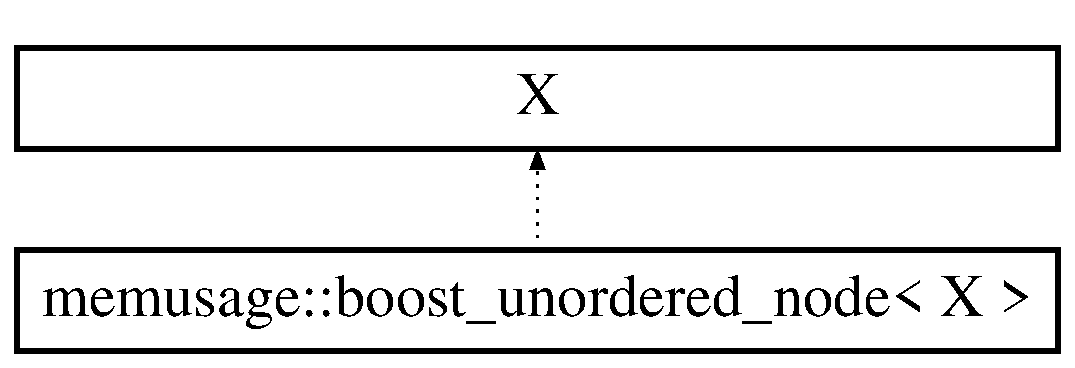
\includegraphics[height=2.000000cm]{structmemusage_1_1boost__unordered__node}
\end{center}
\end{figure}
\subsection*{Private Attributes}
\begin{DoxyCompactItemize}
\item 
void $\ast$ \mbox{\hyperlink{structmemusage_1_1boost__unordered__node_a6331d9429d8f7d815bcd6ccdb0a6f536}{ptr}}
\end{DoxyCompactItemize}


\subsection{Member Data Documentation}
\mbox{\Hypertarget{structmemusage_1_1boost__unordered__node_a6331d9429d8f7d815bcd6ccdb0a6f536}\label{structmemusage_1_1boost__unordered__node_a6331d9429d8f7d815bcd6ccdb0a6f536}} 
\index{memusage\+::boost\+\_\+unordered\+\_\+node@{memusage\+::boost\+\_\+unordered\+\_\+node}!ptr@{ptr}}
\index{ptr@{ptr}!memusage\+::boost\+\_\+unordered\+\_\+node@{memusage\+::boost\+\_\+unordered\+\_\+node}}
\subsubsection{\texorpdfstring{ptr}{ptr}}
{\footnotesize\ttfamily template$<$typename X $>$ \\
void$\ast$ \mbox{\hyperlink{structmemusage_1_1boost__unordered__node}{memusage\+::boost\+\_\+unordered\+\_\+node}}$<$ \mbox{\hyperlink{net_8cpp_a826edd40636cbaa44266b97c8c6a4fa3}{X}} $>$\+::ptr\hspace{0.3cm}{\ttfamily [private]}}



The documentation for this struct was generated from the following file\+:\begin{DoxyCompactItemize}
\item 
/\+Users/christopherarguello/\+Developer/anon/src/\mbox{\hyperlink{memusage_8h}{memusage.\+h}}\end{DoxyCompactItemize}

\hypertarget{class_c_active_masternode}{}\section{C\+Active\+Masternode Class Reference}
\label{class_c_active_masternode}\index{C\+Active\+Masternode@{C\+Active\+Masternode}}


{\ttfamily \#include $<$activemasternode.\+h$>$}

\subsection*{Public Types}
\begin{DoxyCompactItemize}
\item 
enum \mbox{\hyperlink{class_c_active_masternode_a5fe600c379008561204e609316427bb4}{masternode\+\_\+type\+\_\+enum\+\_\+t}} \{ \mbox{\hyperlink{class_c_active_masternode_a5fe600c379008561204e609316427bb4ab4ebeeb59995d51e3e2496f6641368c1}{M\+A\+S\+T\+E\+R\+N\+O\+D\+E\+\_\+\+U\+N\+K\+N\+O\+WN}} = 0, 
\mbox{\hyperlink{class_c_active_masternode_a5fe600c379008561204e609316427bb4a6900162a70bc2be4012ec755701ec373}{M\+A\+S\+T\+E\+R\+N\+O\+D\+E\+\_\+\+R\+E\+M\+O\+TE}} = 1, 
\mbox{\hyperlink{class_c_active_masternode_a5fe600c379008561204e609316427bb4a481e09274e6ffc3c0d4ebd06e805ad30}{M\+A\+S\+T\+E\+R\+N\+O\+D\+E\+\_\+\+L\+O\+C\+AL}} = 2
 \}
\end{DoxyCompactItemize}
\subsection*{Public Member Functions}
\begin{DoxyCompactItemize}
\item 
\mbox{\hyperlink{class_c_active_masternode_a7ffb946d1b2aad0054d3b3efce8c0543}{C\+Active\+Masternode}} ()
\item 
void \mbox{\hyperlink{class_c_active_masternode_aaca6cb8f27b89840b929e286405e5861}{Manage\+State}} ()
\begin{DoxyCompactList}\small\item\em Manage state of active Masternode. \end{DoxyCompactList}\item 
std\+::string \mbox{\hyperlink{class_c_active_masternode_ae213eaf967846069315726ea30120948}{Get\+State\+String}} () const
\item 
std\+::string \mbox{\hyperlink{class_c_active_masternode_affe6a1e6ba472a5d368072411e332476}{Get\+Status}} () const
\item 
std\+::string \mbox{\hyperlink{class_c_active_masternode_a0cdacf7245f997fd68dfcc8f789cdf97}{Get\+Type\+String}} () const
\end{DoxyCompactItemize}
\subsection*{Public Attributes}
\begin{DoxyCompactItemize}
\item 
\mbox{\hyperlink{class_c_pub_key}{C\+Pub\+Key}} \mbox{\hyperlink{class_c_active_masternode_a005f6d9c1e40efd38ab5ceddcb56628b}{pub\+Key\+Masternode}}
\item 
\mbox{\hyperlink{class_c_key}{C\+Key}} \mbox{\hyperlink{class_c_active_masternode_ae5b082fbd8a6ba601f438935bd805c47}{key\+Masternode}}
\item 
C\+Tx\+In \mbox{\hyperlink{class_c_active_masternode_a0fe32edc638ebd2866dda14fd490d78e}{vin}}
\item 
\mbox{\hyperlink{class_c_service}{C\+Service}} \mbox{\hyperlink{class_c_active_masternode_a5b990857c9dc1005d0c134c608474c8f}{service}}
\item 
int \mbox{\hyperlink{class_c_active_masternode_acb6d8a990391957177788dfac0378453}{n\+State}}
\item 
std\+::string \mbox{\hyperlink{class_c_active_masternode_a80a068fb0e4fc1a77dabe501a806e460}{str\+Not\+Capable\+Reason}}
\end{DoxyCompactItemize}
\subsection*{Private Member Functions}
\begin{DoxyCompactItemize}
\item 
bool \mbox{\hyperlink{class_c_active_masternode_ad6f0db3dd4f896f2697601c9713f4434}{Send\+Masternode\+Ping}} ()
\begin{DoxyCompactList}\small\item\em Ping Masternode. \end{DoxyCompactList}\item 
void \mbox{\hyperlink{class_c_active_masternode_a02d5896f56c03a65f712796bd7b598e6}{Manage\+State\+Initial}} ()
\item 
void \mbox{\hyperlink{class_c_active_masternode_aefd004895e9c2ddff987a5d1b027b134}{Manage\+State\+Remote}} ()
\item 
void \mbox{\hyperlink{class_c_active_masternode_aec51e7862f3d6acfff08974f0063786a}{Manage\+State\+Local}} ()
\end{DoxyCompactItemize}
\subsection*{Private Attributes}
\begin{DoxyCompactItemize}
\item 
\mbox{\hyperlink{sync_8h_a37a4692b2d517f2843655ca11af7668a}{C\+Critical\+Section}} \mbox{\hyperlink{class_c_active_masternode_adfab8da076db5b2826fee5ee7d3b3ee0}{cs}}
\item 
\mbox{\hyperlink{class_c_active_masternode_a5fe600c379008561204e609316427bb4}{masternode\+\_\+type\+\_\+enum\+\_\+t}} \mbox{\hyperlink{class_c_active_masternode_a4f641510c0dda9185e86847511816a95}{e\+Type}}
\item 
bool \mbox{\hyperlink{class_c_active_masternode_a5af230132390559891f804f62c0de808}{f\+Pinger\+Enabled}}
\end{DoxyCompactItemize}


\subsection{Member Enumeration Documentation}
\mbox{\Hypertarget{class_c_active_masternode_a5fe600c379008561204e609316427bb4}\label{class_c_active_masternode_a5fe600c379008561204e609316427bb4}} 
\index{C\+Active\+Masternode@{C\+Active\+Masternode}!masternode\+\_\+type\+\_\+enum\+\_\+t@{masternode\+\_\+type\+\_\+enum\+\_\+t}}
\index{masternode\+\_\+type\+\_\+enum\+\_\+t@{masternode\+\_\+type\+\_\+enum\+\_\+t}!C\+Active\+Masternode@{C\+Active\+Masternode}}
\subsubsection{\texorpdfstring{masternode\+\_\+type\+\_\+enum\+\_\+t}{masternode\_type\_enum\_t}}
{\footnotesize\ttfamily enum \mbox{\hyperlink{class_c_active_masternode_a5fe600c379008561204e609316427bb4}{C\+Active\+Masternode\+::masternode\+\_\+type\+\_\+enum\+\_\+t}}}

\begin{DoxyEnumFields}{Enumerator}
\raisebox{\heightof{T}}[0pt][0pt]{\index{M\+A\+S\+T\+E\+R\+N\+O\+D\+E\+\_\+\+U\+N\+K\+N\+O\+WN@{M\+A\+S\+T\+E\+R\+N\+O\+D\+E\+\_\+\+U\+N\+K\+N\+O\+WN}!C\+Active\+Masternode@{C\+Active\+Masternode}}\index{C\+Active\+Masternode@{C\+Active\+Masternode}!M\+A\+S\+T\+E\+R\+N\+O\+D\+E\+\_\+\+U\+N\+K\+N\+O\+WN@{M\+A\+S\+T\+E\+R\+N\+O\+D\+E\+\_\+\+U\+N\+K\+N\+O\+WN}}}\mbox{\Hypertarget{class_c_active_masternode_a5fe600c379008561204e609316427bb4ab4ebeeb59995d51e3e2496f6641368c1}\label{class_c_active_masternode_a5fe600c379008561204e609316427bb4ab4ebeeb59995d51e3e2496f6641368c1}} 
M\+A\+S\+T\+E\+R\+N\+O\+D\+E\+\_\+\+U\+N\+K\+N\+O\+WN&\\
\hline

\raisebox{\heightof{T}}[0pt][0pt]{\index{M\+A\+S\+T\+E\+R\+N\+O\+D\+E\+\_\+\+R\+E\+M\+O\+TE@{M\+A\+S\+T\+E\+R\+N\+O\+D\+E\+\_\+\+R\+E\+M\+O\+TE}!C\+Active\+Masternode@{C\+Active\+Masternode}}\index{C\+Active\+Masternode@{C\+Active\+Masternode}!M\+A\+S\+T\+E\+R\+N\+O\+D\+E\+\_\+\+R\+E\+M\+O\+TE@{M\+A\+S\+T\+E\+R\+N\+O\+D\+E\+\_\+\+R\+E\+M\+O\+TE}}}\mbox{\Hypertarget{class_c_active_masternode_a5fe600c379008561204e609316427bb4a6900162a70bc2be4012ec755701ec373}\label{class_c_active_masternode_a5fe600c379008561204e609316427bb4a6900162a70bc2be4012ec755701ec373}} 
M\+A\+S\+T\+E\+R\+N\+O\+D\+E\+\_\+\+R\+E\+M\+O\+TE&\\
\hline

\raisebox{\heightof{T}}[0pt][0pt]{\index{M\+A\+S\+T\+E\+R\+N\+O\+D\+E\+\_\+\+L\+O\+C\+AL@{M\+A\+S\+T\+E\+R\+N\+O\+D\+E\+\_\+\+L\+O\+C\+AL}!C\+Active\+Masternode@{C\+Active\+Masternode}}\index{C\+Active\+Masternode@{C\+Active\+Masternode}!M\+A\+S\+T\+E\+R\+N\+O\+D\+E\+\_\+\+L\+O\+C\+AL@{M\+A\+S\+T\+E\+R\+N\+O\+D\+E\+\_\+\+L\+O\+C\+AL}}}\mbox{\Hypertarget{class_c_active_masternode_a5fe600c379008561204e609316427bb4a481e09274e6ffc3c0d4ebd06e805ad30}\label{class_c_active_masternode_a5fe600c379008561204e609316427bb4a481e09274e6ffc3c0d4ebd06e805ad30}} 
M\+A\+S\+T\+E\+R\+N\+O\+D\+E\+\_\+\+L\+O\+C\+AL&\\
\hline

\end{DoxyEnumFields}


\subsection{Constructor \& Destructor Documentation}
\mbox{\Hypertarget{class_c_active_masternode_a7ffb946d1b2aad0054d3b3efce8c0543}\label{class_c_active_masternode_a7ffb946d1b2aad0054d3b3efce8c0543}} 
\index{C\+Active\+Masternode@{C\+Active\+Masternode}!C\+Active\+Masternode@{C\+Active\+Masternode}}
\index{C\+Active\+Masternode@{C\+Active\+Masternode}!C\+Active\+Masternode@{C\+Active\+Masternode}}
\subsubsection{\texorpdfstring{C\+Active\+Masternode()}{CActiveMasternode()}}
{\footnotesize\ttfamily C\+Active\+Masternode\+::\+C\+Active\+Masternode (\begin{DoxyParamCaption}{ }\end{DoxyParamCaption})\hspace{0.3cm}{\ttfamily [inline]}}



\subsection{Member Function Documentation}
\mbox{\Hypertarget{class_c_active_masternode_ae213eaf967846069315726ea30120948}\label{class_c_active_masternode_ae213eaf967846069315726ea30120948}} 
\index{C\+Active\+Masternode@{C\+Active\+Masternode}!Get\+State\+String@{Get\+State\+String}}
\index{Get\+State\+String@{Get\+State\+String}!C\+Active\+Masternode@{C\+Active\+Masternode}}
\subsubsection{\texorpdfstring{Get\+State\+String()}{GetStateString()}}
{\footnotesize\ttfamily std\+::string C\+Active\+Masternode\+::\+Get\+State\+String (\begin{DoxyParamCaption}{ }\end{DoxyParamCaption}) const}

\mbox{\Hypertarget{class_c_active_masternode_affe6a1e6ba472a5d368072411e332476}\label{class_c_active_masternode_affe6a1e6ba472a5d368072411e332476}} 
\index{C\+Active\+Masternode@{C\+Active\+Masternode}!Get\+Status@{Get\+Status}}
\index{Get\+Status@{Get\+Status}!C\+Active\+Masternode@{C\+Active\+Masternode}}
\subsubsection{\texorpdfstring{Get\+Status()}{GetStatus()}}
{\footnotesize\ttfamily std\+::string C\+Active\+Masternode\+::\+Get\+Status (\begin{DoxyParamCaption}{ }\end{DoxyParamCaption}) const}

\mbox{\Hypertarget{class_c_active_masternode_a0cdacf7245f997fd68dfcc8f789cdf97}\label{class_c_active_masternode_a0cdacf7245f997fd68dfcc8f789cdf97}} 
\index{C\+Active\+Masternode@{C\+Active\+Masternode}!Get\+Type\+String@{Get\+Type\+String}}
\index{Get\+Type\+String@{Get\+Type\+String}!C\+Active\+Masternode@{C\+Active\+Masternode}}
\subsubsection{\texorpdfstring{Get\+Type\+String()}{GetTypeString()}}
{\footnotesize\ttfamily std\+::string C\+Active\+Masternode\+::\+Get\+Type\+String (\begin{DoxyParamCaption}{ }\end{DoxyParamCaption}) const}

\mbox{\Hypertarget{class_c_active_masternode_aaca6cb8f27b89840b929e286405e5861}\label{class_c_active_masternode_aaca6cb8f27b89840b929e286405e5861}} 
\index{C\+Active\+Masternode@{C\+Active\+Masternode}!Manage\+State@{Manage\+State}}
\index{Manage\+State@{Manage\+State}!C\+Active\+Masternode@{C\+Active\+Masternode}}
\subsubsection{\texorpdfstring{Manage\+State()}{ManageState()}}
{\footnotesize\ttfamily void C\+Active\+Masternode\+::\+Manage\+State (\begin{DoxyParamCaption}{ }\end{DoxyParamCaption})}



Manage state of active Masternode. 

\mbox{\Hypertarget{class_c_active_masternode_a02d5896f56c03a65f712796bd7b598e6}\label{class_c_active_masternode_a02d5896f56c03a65f712796bd7b598e6}} 
\index{C\+Active\+Masternode@{C\+Active\+Masternode}!Manage\+State\+Initial@{Manage\+State\+Initial}}
\index{Manage\+State\+Initial@{Manage\+State\+Initial}!C\+Active\+Masternode@{C\+Active\+Masternode}}
\subsubsection{\texorpdfstring{Manage\+State\+Initial()}{ManageStateInitial()}}
{\footnotesize\ttfamily void C\+Active\+Masternode\+::\+Manage\+State\+Initial (\begin{DoxyParamCaption}{ }\end{DoxyParamCaption})\hspace{0.3cm}{\ttfamily [private]}}

\mbox{\Hypertarget{class_c_active_masternode_aec51e7862f3d6acfff08974f0063786a}\label{class_c_active_masternode_aec51e7862f3d6acfff08974f0063786a}} 
\index{C\+Active\+Masternode@{C\+Active\+Masternode}!Manage\+State\+Local@{Manage\+State\+Local}}
\index{Manage\+State\+Local@{Manage\+State\+Local}!C\+Active\+Masternode@{C\+Active\+Masternode}}
\subsubsection{\texorpdfstring{Manage\+State\+Local()}{ManageStateLocal()}}
{\footnotesize\ttfamily void C\+Active\+Masternode\+::\+Manage\+State\+Local (\begin{DoxyParamCaption}{ }\end{DoxyParamCaption})\hspace{0.3cm}{\ttfamily [private]}}

\mbox{\Hypertarget{class_c_active_masternode_aefd004895e9c2ddff987a5d1b027b134}\label{class_c_active_masternode_aefd004895e9c2ddff987a5d1b027b134}} 
\index{C\+Active\+Masternode@{C\+Active\+Masternode}!Manage\+State\+Remote@{Manage\+State\+Remote}}
\index{Manage\+State\+Remote@{Manage\+State\+Remote}!C\+Active\+Masternode@{C\+Active\+Masternode}}
\subsubsection{\texorpdfstring{Manage\+State\+Remote()}{ManageStateRemote()}}
{\footnotesize\ttfamily void C\+Active\+Masternode\+::\+Manage\+State\+Remote (\begin{DoxyParamCaption}{ }\end{DoxyParamCaption})\hspace{0.3cm}{\ttfamily [private]}}

\mbox{\Hypertarget{class_c_active_masternode_ad6f0db3dd4f896f2697601c9713f4434}\label{class_c_active_masternode_ad6f0db3dd4f896f2697601c9713f4434}} 
\index{C\+Active\+Masternode@{C\+Active\+Masternode}!Send\+Masternode\+Ping@{Send\+Masternode\+Ping}}
\index{Send\+Masternode\+Ping@{Send\+Masternode\+Ping}!C\+Active\+Masternode@{C\+Active\+Masternode}}
\subsubsection{\texorpdfstring{Send\+Masternode\+Ping()}{SendMasternodePing()}}
{\footnotesize\ttfamily bool C\+Active\+Masternode\+::\+Send\+Masternode\+Ping (\begin{DoxyParamCaption}{ }\end{DoxyParamCaption})\hspace{0.3cm}{\ttfamily [private]}}



Ping Masternode. 



\subsection{Member Data Documentation}
\mbox{\Hypertarget{class_c_active_masternode_adfab8da076db5b2826fee5ee7d3b3ee0}\label{class_c_active_masternode_adfab8da076db5b2826fee5ee7d3b3ee0}} 
\index{C\+Active\+Masternode@{C\+Active\+Masternode}!cs@{cs}}
\index{cs@{cs}!C\+Active\+Masternode@{C\+Active\+Masternode}}
\subsubsection{\texorpdfstring{cs}{cs}}
{\footnotesize\ttfamily \mbox{\hyperlink{sync_8h_a37a4692b2d517f2843655ca11af7668a}{C\+Critical\+Section}} C\+Active\+Masternode\+::cs\hspace{0.3cm}{\ttfamily [mutable]}, {\ttfamily [private]}}

\mbox{\Hypertarget{class_c_active_masternode_a4f641510c0dda9185e86847511816a95}\label{class_c_active_masternode_a4f641510c0dda9185e86847511816a95}} 
\index{C\+Active\+Masternode@{C\+Active\+Masternode}!e\+Type@{e\+Type}}
\index{e\+Type@{e\+Type}!C\+Active\+Masternode@{C\+Active\+Masternode}}
\subsubsection{\texorpdfstring{e\+Type}{eType}}
{\footnotesize\ttfamily \mbox{\hyperlink{class_c_active_masternode_a5fe600c379008561204e609316427bb4}{masternode\+\_\+type\+\_\+enum\+\_\+t}} C\+Active\+Masternode\+::e\+Type\hspace{0.3cm}{\ttfamily [private]}}

\mbox{\Hypertarget{class_c_active_masternode_a5af230132390559891f804f62c0de808}\label{class_c_active_masternode_a5af230132390559891f804f62c0de808}} 
\index{C\+Active\+Masternode@{C\+Active\+Masternode}!f\+Pinger\+Enabled@{f\+Pinger\+Enabled}}
\index{f\+Pinger\+Enabled@{f\+Pinger\+Enabled}!C\+Active\+Masternode@{C\+Active\+Masternode}}
\subsubsection{\texorpdfstring{f\+Pinger\+Enabled}{fPingerEnabled}}
{\footnotesize\ttfamily bool C\+Active\+Masternode\+::f\+Pinger\+Enabled\hspace{0.3cm}{\ttfamily [private]}}

\mbox{\Hypertarget{class_c_active_masternode_ae5b082fbd8a6ba601f438935bd805c47}\label{class_c_active_masternode_ae5b082fbd8a6ba601f438935bd805c47}} 
\index{C\+Active\+Masternode@{C\+Active\+Masternode}!key\+Masternode@{key\+Masternode}}
\index{key\+Masternode@{key\+Masternode}!C\+Active\+Masternode@{C\+Active\+Masternode}}
\subsubsection{\texorpdfstring{key\+Masternode}{keyMasternode}}
{\footnotesize\ttfamily \mbox{\hyperlink{class_c_key}{C\+Key}} C\+Active\+Masternode\+::key\+Masternode}

\mbox{\Hypertarget{class_c_active_masternode_acb6d8a990391957177788dfac0378453}\label{class_c_active_masternode_acb6d8a990391957177788dfac0378453}} 
\index{C\+Active\+Masternode@{C\+Active\+Masternode}!n\+State@{n\+State}}
\index{n\+State@{n\+State}!C\+Active\+Masternode@{C\+Active\+Masternode}}
\subsubsection{\texorpdfstring{n\+State}{nState}}
{\footnotesize\ttfamily int C\+Active\+Masternode\+::n\+State}

\mbox{\Hypertarget{class_c_active_masternode_a005f6d9c1e40efd38ab5ceddcb56628b}\label{class_c_active_masternode_a005f6d9c1e40efd38ab5ceddcb56628b}} 
\index{C\+Active\+Masternode@{C\+Active\+Masternode}!pub\+Key\+Masternode@{pub\+Key\+Masternode}}
\index{pub\+Key\+Masternode@{pub\+Key\+Masternode}!C\+Active\+Masternode@{C\+Active\+Masternode}}
\subsubsection{\texorpdfstring{pub\+Key\+Masternode}{pubKeyMasternode}}
{\footnotesize\ttfamily \mbox{\hyperlink{class_c_pub_key}{C\+Pub\+Key}} C\+Active\+Masternode\+::pub\+Key\+Masternode}

\mbox{\Hypertarget{class_c_active_masternode_a5b990857c9dc1005d0c134c608474c8f}\label{class_c_active_masternode_a5b990857c9dc1005d0c134c608474c8f}} 
\index{C\+Active\+Masternode@{C\+Active\+Masternode}!service@{service}}
\index{service@{service}!C\+Active\+Masternode@{C\+Active\+Masternode}}
\subsubsection{\texorpdfstring{service}{service}}
{\footnotesize\ttfamily \mbox{\hyperlink{class_c_service}{C\+Service}} C\+Active\+Masternode\+::service}

\mbox{\Hypertarget{class_c_active_masternode_a80a068fb0e4fc1a77dabe501a806e460}\label{class_c_active_masternode_a80a068fb0e4fc1a77dabe501a806e460}} 
\index{C\+Active\+Masternode@{C\+Active\+Masternode}!str\+Not\+Capable\+Reason@{str\+Not\+Capable\+Reason}}
\index{str\+Not\+Capable\+Reason@{str\+Not\+Capable\+Reason}!C\+Active\+Masternode@{C\+Active\+Masternode}}
\subsubsection{\texorpdfstring{str\+Not\+Capable\+Reason}{strNotCapableReason}}
{\footnotesize\ttfamily std\+::string C\+Active\+Masternode\+::str\+Not\+Capable\+Reason}

\mbox{\Hypertarget{class_c_active_masternode_a0fe32edc638ebd2866dda14fd490d78e}\label{class_c_active_masternode_a0fe32edc638ebd2866dda14fd490d78e}} 
\index{C\+Active\+Masternode@{C\+Active\+Masternode}!vin@{vin}}
\index{vin@{vin}!C\+Active\+Masternode@{C\+Active\+Masternode}}
\subsubsection{\texorpdfstring{vin}{vin}}
{\footnotesize\ttfamily C\+Tx\+In C\+Active\+Masternode\+::vin}



The documentation for this class was generated from the following files\+:\begin{DoxyCompactItemize}
\item 
/\+Users/christopherarguello/\+Developer/anon/src/\mbox{\hyperlink{activemasternode_8h}{activemasternode.\+h}}\item 
/\+Users/christopherarguello/\+Developer/anon/src/\mbox{\hyperlink{activemasternode_8cpp}{activemasternode.\+cpp}}\end{DoxyCompactItemize}

\hypertarget{class_c_addr_d_b}{}\section{C\+Addr\+DB Class Reference}
\label{class_c_addr_d_b}\index{C\+Addr\+DB@{C\+Addr\+DB}}


{\ttfamily \#include $<$net.\+h$>$}

\subsection*{Public Member Functions}
\begin{DoxyCompactItemize}
\item 
\mbox{\hyperlink{class_c_addr_d_b_af8c039f1904b1892c5a14e484a5b31a7}{C\+Addr\+DB}} ()
\item 
bool \mbox{\hyperlink{class_c_addr_d_b_aaec90dba59cd69a2f25bc5630a1dde39}{Write}} (const \mbox{\hyperlink{class_c_addr_man}{C\+Addr\+Man}} \&addr)
\item 
bool \mbox{\hyperlink{class_c_addr_d_b_aed4b567fb7c2dd15b2856e7c769967b7}{Read}} (\mbox{\hyperlink{class_c_addr_man}{C\+Addr\+Man}} \&addr)
\end{DoxyCompactItemize}
\subsection*{Private Attributes}
\begin{DoxyCompactItemize}
\item 
boost\+::filesystem\+::path \mbox{\hyperlink{class_c_addr_d_b_afeba63488deb50f5aac678a890d41a0d}{path\+Addr}}
\end{DoxyCompactItemize}


\subsection{Detailed Description}
Access to the (IP) address database (peers.\+dat) 

\subsection{Constructor \& Destructor Documentation}
\mbox{\Hypertarget{class_c_addr_d_b_af8c039f1904b1892c5a14e484a5b31a7}\label{class_c_addr_d_b_af8c039f1904b1892c5a14e484a5b31a7}} 
\index{C\+Addr\+DB@{C\+Addr\+DB}!C\+Addr\+DB@{C\+Addr\+DB}}
\index{C\+Addr\+DB@{C\+Addr\+DB}!C\+Addr\+DB@{C\+Addr\+DB}}
\subsubsection{\texorpdfstring{C\+Addr\+D\+B()}{CAddrDB()}}
{\footnotesize\ttfamily C\+Addr\+D\+B\+::\+C\+Addr\+DB (\begin{DoxyParamCaption}{ }\end{DoxyParamCaption})}



\subsection{Member Function Documentation}
\mbox{\Hypertarget{class_c_addr_d_b_aed4b567fb7c2dd15b2856e7c769967b7}\label{class_c_addr_d_b_aed4b567fb7c2dd15b2856e7c769967b7}} 
\index{C\+Addr\+DB@{C\+Addr\+DB}!Read@{Read}}
\index{Read@{Read}!C\+Addr\+DB@{C\+Addr\+DB}}
\subsubsection{\texorpdfstring{Read()}{Read()}}
{\footnotesize\ttfamily bool C\+Addr\+D\+B\+::\+Read (\begin{DoxyParamCaption}\item[{\mbox{\hyperlink{class_c_addr_man}{C\+Addr\+Man}} \&}]{addr }\end{DoxyParamCaption})}

\mbox{\Hypertarget{class_c_addr_d_b_aaec90dba59cd69a2f25bc5630a1dde39}\label{class_c_addr_d_b_aaec90dba59cd69a2f25bc5630a1dde39}} 
\index{C\+Addr\+DB@{C\+Addr\+DB}!Write@{Write}}
\index{Write@{Write}!C\+Addr\+DB@{C\+Addr\+DB}}
\subsubsection{\texorpdfstring{Write()}{Write()}}
{\footnotesize\ttfamily bool C\+Addr\+D\+B\+::\+Write (\begin{DoxyParamCaption}\item[{const \mbox{\hyperlink{class_c_addr_man}{C\+Addr\+Man}} \&}]{addr }\end{DoxyParamCaption})}



\subsection{Member Data Documentation}
\mbox{\Hypertarget{class_c_addr_d_b_afeba63488deb50f5aac678a890d41a0d}\label{class_c_addr_d_b_afeba63488deb50f5aac678a890d41a0d}} 
\index{C\+Addr\+DB@{C\+Addr\+DB}!path\+Addr@{path\+Addr}}
\index{path\+Addr@{path\+Addr}!C\+Addr\+DB@{C\+Addr\+DB}}
\subsubsection{\texorpdfstring{path\+Addr}{pathAddr}}
{\footnotesize\ttfamily boost\+::filesystem\+::path C\+Addr\+D\+B\+::path\+Addr\hspace{0.3cm}{\ttfamily [private]}}



The documentation for this class was generated from the following files\+:\begin{DoxyCompactItemize}
\item 
/\+Users/christopherarguello/\+Developer/anon/src/\mbox{\hyperlink{net_8h}{net.\+h}}\item 
/\+Users/christopherarguello/\+Developer/anon/src/\mbox{\hyperlink{net_8cpp}{net.\+cpp}}\end{DoxyCompactItemize}

\hypertarget{class_c_address}{}\section{C\+Address Class Reference}
\label{class_c_address}\index{C\+Address@{C\+Address}}


{\ttfamily \#include $<$protocol.\+h$>$}

Inheritance diagram for C\+Address\+:\begin{figure}[H]
\begin{center}
\leavevmode
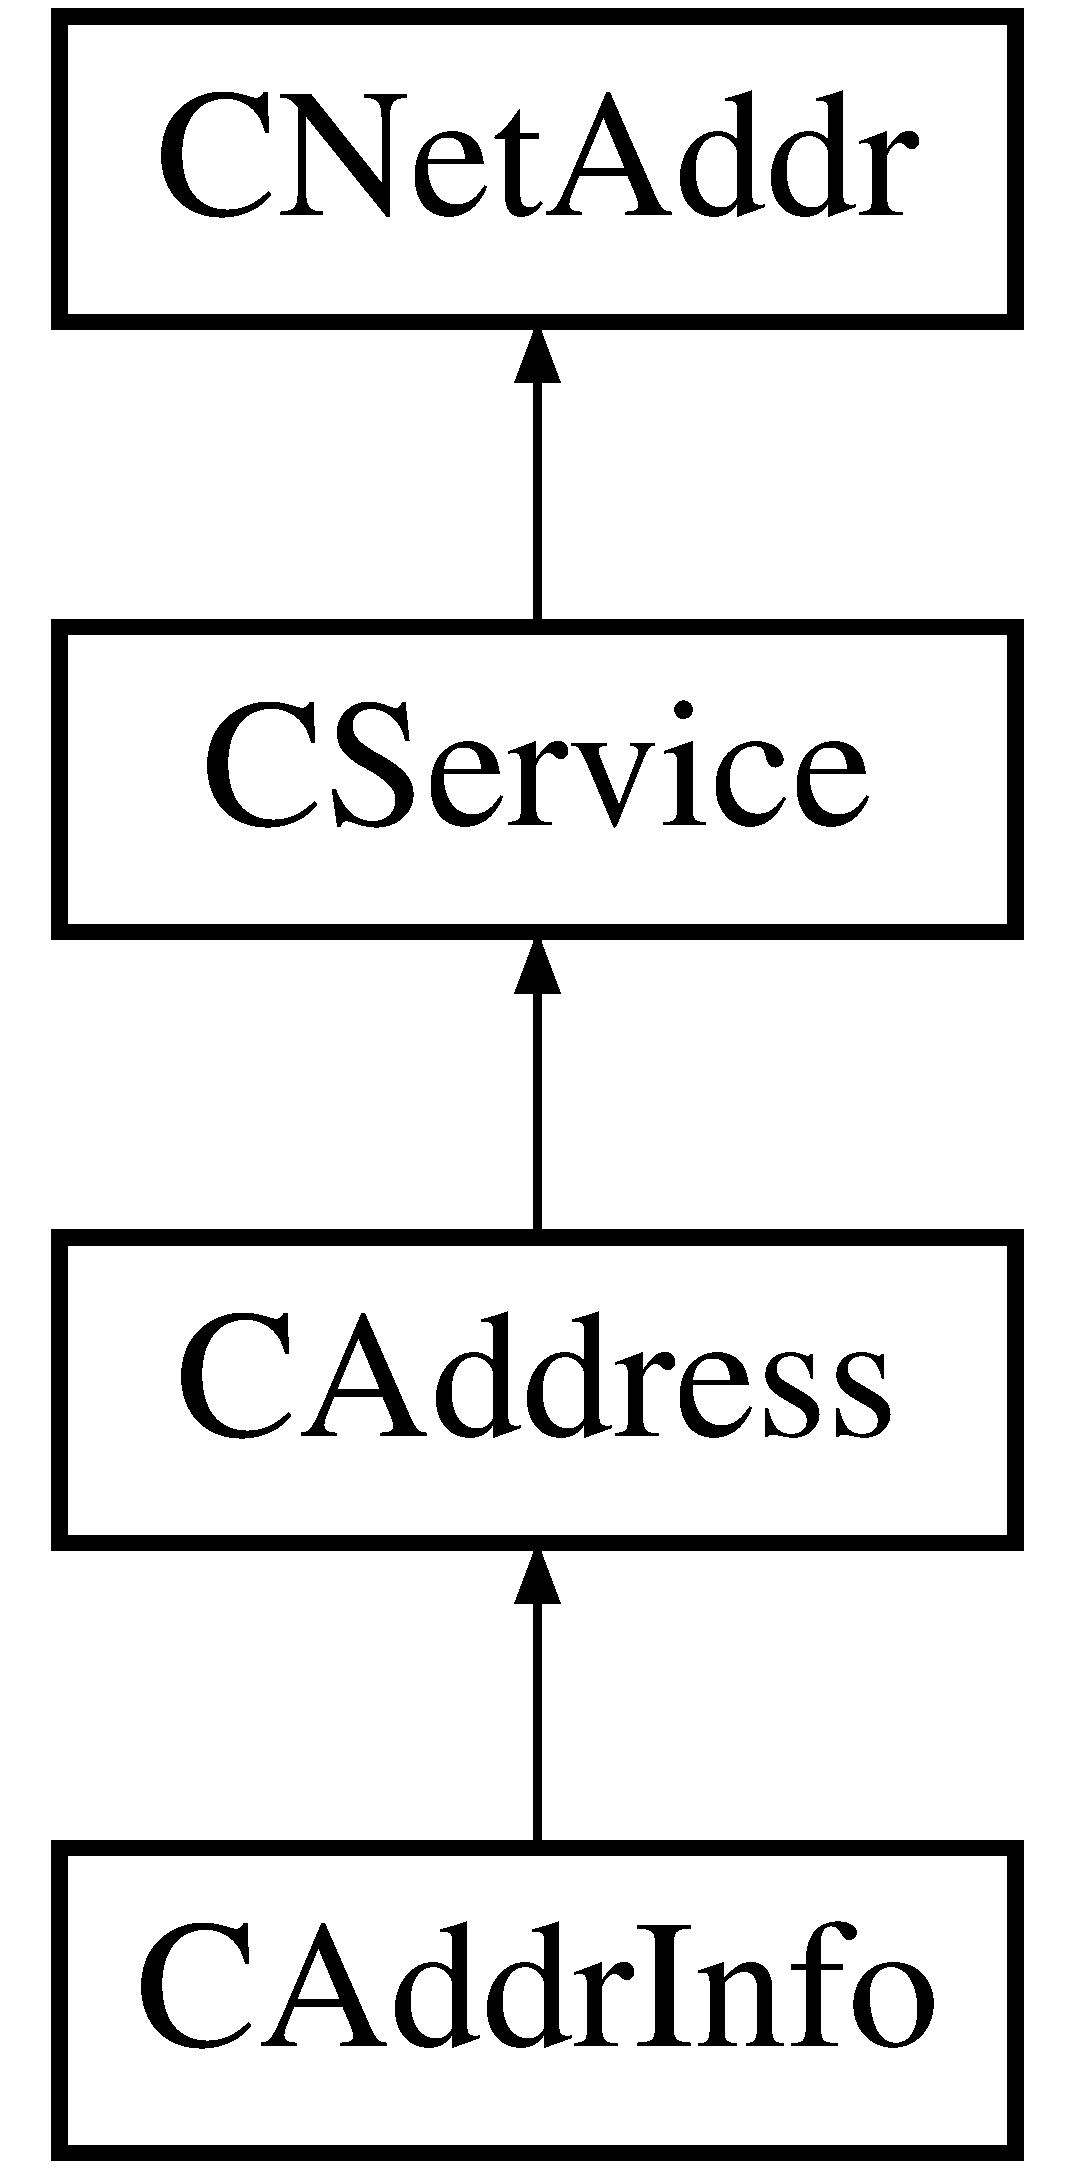
\includegraphics[height=4.000000cm]{class_c_address}
\end{center}
\end{figure}
\subsection*{Public Member Functions}
\begin{DoxyCompactItemize}
\item 
\mbox{\hyperlink{class_c_address_a84cd336180580ab69b8888a4339ccc37}{C\+Address}} ()
\item 
\mbox{\hyperlink{class_c_address_a806e75f363ec49bfab92a686a8774ac3}{C\+Address}} (\mbox{\hyperlink{class_c_service}{C\+Service}} ip\+In, uint64\+\_\+t n\+Services\+In=\mbox{\hyperlink{protocol_8h_a726ca809ffd3d67ab4b8476646f26635a9d1154f0e7e56f183a5c8373abe2e86c}{N\+O\+D\+E\+\_\+\+N\+E\+T\+W\+O\+RK}})
\item 
void \mbox{\hyperlink{class_c_address_ac060c84dcf47b8ccfae0142c9b29a243}{Init}} ()
\item 
{\footnotesize template$<$typename Stream , typename Operation $>$ }\\void \mbox{\hyperlink{class_c_address_aec10c7075404eefbcf6f7a4c5671be02}{Serialization\+Op}} (Stream \&s, Operation ser\+\_\+action, int n\+Type, int n\+Version)
\end{DoxyCompactItemize}
\subsection*{Public Attributes}
\begin{DoxyCompactItemize}
\item 
\mbox{\hyperlink{class_c_address_a9582fc22433b2ed275d4b65fb72551e7}{A\+D\+D\+\_\+\+S\+E\+R\+I\+A\+L\+I\+Z\+E\+\_\+\+M\+E\+T\+H\+O\+DS}}
\item 
uint64\+\_\+t \mbox{\hyperlink{class_c_address_a6a4a6aa020d0d558f238c7d04dd986c3}{n\+Services}}
\item 
unsigned int \mbox{\hyperlink{class_c_address_ac1c44aac968b11f90ce529b133ae4e9b}{n\+Time}}
\end{DoxyCompactItemize}
\subsection*{Additional Inherited Members}


\subsection{Detailed Description}
A \mbox{\hyperlink{class_c_service}{C\+Service}} with information about it as peer 

\subsection{Constructor \& Destructor Documentation}
\mbox{\Hypertarget{class_c_address_a84cd336180580ab69b8888a4339ccc37}\label{class_c_address_a84cd336180580ab69b8888a4339ccc37}} 
\index{C\+Address@{C\+Address}!C\+Address@{C\+Address}}
\index{C\+Address@{C\+Address}!C\+Address@{C\+Address}}
\subsubsection{\texorpdfstring{C\+Address()}{CAddress()}\hspace{0.1cm}{\footnotesize\ttfamily [1/2]}}
{\footnotesize\ttfamily C\+Address\+::\+C\+Address (\begin{DoxyParamCaption}{ }\end{DoxyParamCaption})}

\mbox{\Hypertarget{class_c_address_a806e75f363ec49bfab92a686a8774ac3}\label{class_c_address_a806e75f363ec49bfab92a686a8774ac3}} 
\index{C\+Address@{C\+Address}!C\+Address@{C\+Address}}
\index{C\+Address@{C\+Address}!C\+Address@{C\+Address}}
\subsubsection{\texorpdfstring{C\+Address()}{CAddress()}\hspace{0.1cm}{\footnotesize\ttfamily [2/2]}}
{\footnotesize\ttfamily C\+Address\+::\+C\+Address (\begin{DoxyParamCaption}\item[{\mbox{\hyperlink{class_c_service}{C\+Service}}}]{ip\+In,  }\item[{uint64\+\_\+t}]{n\+Services\+In = {\ttfamily \mbox{\hyperlink{protocol_8h_a726ca809ffd3d67ab4b8476646f26635a9d1154f0e7e56f183a5c8373abe2e86c}{N\+O\+D\+E\+\_\+\+N\+E\+T\+W\+O\+RK}}} }\end{DoxyParamCaption})\hspace{0.3cm}{\ttfamily [explicit]}}



\subsection{Member Function Documentation}
\mbox{\Hypertarget{class_c_address_ac060c84dcf47b8ccfae0142c9b29a243}\label{class_c_address_ac060c84dcf47b8ccfae0142c9b29a243}} 
\index{C\+Address@{C\+Address}!Init@{Init}}
\index{Init@{Init}!C\+Address@{C\+Address}}
\subsubsection{\texorpdfstring{Init()}{Init()}}
{\footnotesize\ttfamily void C\+Address\+::\+Init (\begin{DoxyParamCaption}{ }\end{DoxyParamCaption})}

\mbox{\Hypertarget{class_c_address_aec10c7075404eefbcf6f7a4c5671be02}\label{class_c_address_aec10c7075404eefbcf6f7a4c5671be02}} 
\index{C\+Address@{C\+Address}!Serialization\+Op@{Serialization\+Op}}
\index{Serialization\+Op@{Serialization\+Op}!C\+Address@{C\+Address}}
\subsubsection{\texorpdfstring{Serialization\+Op()}{SerializationOp()}}
{\footnotesize\ttfamily template$<$typename Stream , typename Operation $>$ \\
void C\+Address\+::\+Serialization\+Op (\begin{DoxyParamCaption}\item[{Stream \&}]{s,  }\item[{Operation}]{ser\+\_\+action,  }\item[{int}]{n\+Type,  }\item[{int}]{n\+Version }\end{DoxyParamCaption})\hspace{0.3cm}{\ttfamily [inline]}}



\subsection{Member Data Documentation}
\mbox{\Hypertarget{class_c_address_a9582fc22433b2ed275d4b65fb72551e7}\label{class_c_address_a9582fc22433b2ed275d4b65fb72551e7}} 
\index{C\+Address@{C\+Address}!A\+D\+D\+\_\+\+S\+E\+R\+I\+A\+L\+I\+Z\+E\+\_\+\+M\+E\+T\+H\+O\+DS@{A\+D\+D\+\_\+\+S\+E\+R\+I\+A\+L\+I\+Z\+E\+\_\+\+M\+E\+T\+H\+O\+DS}}
\index{A\+D\+D\+\_\+\+S\+E\+R\+I\+A\+L\+I\+Z\+E\+\_\+\+M\+E\+T\+H\+O\+DS@{A\+D\+D\+\_\+\+S\+E\+R\+I\+A\+L\+I\+Z\+E\+\_\+\+M\+E\+T\+H\+O\+DS}!C\+Address@{C\+Address}}
\subsubsection{\texorpdfstring{A\+D\+D\+\_\+\+S\+E\+R\+I\+A\+L\+I\+Z\+E\+\_\+\+M\+E\+T\+H\+O\+DS}{ADD\_SERIALIZE\_METHODS}}
{\footnotesize\ttfamily C\+Address\+::\+A\+D\+D\+\_\+\+S\+E\+R\+I\+A\+L\+I\+Z\+E\+\_\+\+M\+E\+T\+H\+O\+DS}

\mbox{\Hypertarget{class_c_address_a6a4a6aa020d0d558f238c7d04dd986c3}\label{class_c_address_a6a4a6aa020d0d558f238c7d04dd986c3}} 
\index{C\+Address@{C\+Address}!n\+Services@{n\+Services}}
\index{n\+Services@{n\+Services}!C\+Address@{C\+Address}}
\subsubsection{\texorpdfstring{n\+Services}{nServices}}
{\footnotesize\ttfamily uint64\+\_\+t C\+Address\+::n\+Services}

\mbox{\Hypertarget{class_c_address_ac1c44aac968b11f90ce529b133ae4e9b}\label{class_c_address_ac1c44aac968b11f90ce529b133ae4e9b}} 
\index{C\+Address@{C\+Address}!n\+Time@{n\+Time}}
\index{n\+Time@{n\+Time}!C\+Address@{C\+Address}}
\subsubsection{\texorpdfstring{n\+Time}{nTime}}
{\footnotesize\ttfamily unsigned int C\+Address\+::n\+Time}



The documentation for this class was generated from the following files\+:\begin{DoxyCompactItemize}
\item 
/\+Users/christopherarguello/\+Developer/anon/src/\mbox{\hyperlink{protocol_8h}{protocol.\+h}}\item 
/\+Users/christopherarguello/\+Developer/anon/src/\mbox{\hyperlink{protocol_8cpp}{protocol.\+cpp}}\end{DoxyCompactItemize}

\hypertarget{struct_c_address_index_iterator_height_key}{}\section{C\+Address\+Index\+Iterator\+Height\+Key Struct Reference}
\label{struct_c_address_index_iterator_height_key}\index{C\+Address\+Index\+Iterator\+Height\+Key@{C\+Address\+Index\+Iterator\+Height\+Key}}


{\ttfamily \#include $<$main.\+h$>$}

\subsection*{Public Member Functions}
\begin{DoxyCompactItemize}
\item 
size\+\_\+t \mbox{\hyperlink{struct_c_address_index_iterator_height_key_a63f4371f6e24cfc0410c71fde0395901}{Get\+Serialize\+Size}} (int n\+Type, int n\+Version) const
\item 
{\footnotesize template$<$typename Stream $>$ }\\void \mbox{\hyperlink{struct_c_address_index_iterator_height_key_aa7c5a9682fc40e16943a0ec0a020bf8b}{Serialize}} (Stream \&s, int n\+Type, int n\+Version) const
\item 
{\footnotesize template$<$typename Stream $>$ }\\void \mbox{\hyperlink{struct_c_address_index_iterator_height_key_ac30c8b043ec7e773120e47346fb15ac4}{Unserialize}} (Stream \&s, int n\+Type, int n\+Version)
\item 
\mbox{\hyperlink{struct_c_address_index_iterator_height_key_a9b9b5c2de6b49c3f4e0505dcf62e3ced}{C\+Address\+Index\+Iterator\+Height\+Key}} (unsigned int address\+Type, \mbox{\hyperlink{classuint160}{uint160}} address\+Hash, int height)
\item 
\mbox{\hyperlink{struct_c_address_index_iterator_height_key_ae7cdd7f2d435b1aa3d9dc1a8f8b88ebc}{C\+Address\+Index\+Iterator\+Height\+Key}} ()
\item 
void \mbox{\hyperlink{struct_c_address_index_iterator_height_key_aff779cc8c0aafe1fda522822de996cf1}{Set\+Null}} ()
\end{DoxyCompactItemize}
\subsection*{Public Attributes}
\begin{DoxyCompactItemize}
\item 
unsigned int \mbox{\hyperlink{struct_c_address_index_iterator_height_key_a3aeef3918aebc23da830715dc3b4a247}{type}}
\item 
\mbox{\hyperlink{classuint160}{uint160}} \mbox{\hyperlink{struct_c_address_index_iterator_height_key_a581fde27d32792608fbda14ed1c7285a}{hash\+Bytes}}
\item 
int \mbox{\hyperlink{struct_c_address_index_iterator_height_key_ae6eaaff49b9c3e3c99a32c4741b500db}{block\+Height}}
\end{DoxyCompactItemize}


\subsection{Constructor \& Destructor Documentation}
\mbox{\Hypertarget{struct_c_address_index_iterator_height_key_a9b9b5c2de6b49c3f4e0505dcf62e3ced}\label{struct_c_address_index_iterator_height_key_a9b9b5c2de6b49c3f4e0505dcf62e3ced}} 
\index{C\+Address\+Index\+Iterator\+Height\+Key@{C\+Address\+Index\+Iterator\+Height\+Key}!C\+Address\+Index\+Iterator\+Height\+Key@{C\+Address\+Index\+Iterator\+Height\+Key}}
\index{C\+Address\+Index\+Iterator\+Height\+Key@{C\+Address\+Index\+Iterator\+Height\+Key}!C\+Address\+Index\+Iterator\+Height\+Key@{C\+Address\+Index\+Iterator\+Height\+Key}}
\subsubsection{\texorpdfstring{C\+Address\+Index\+Iterator\+Height\+Key()}{CAddressIndexIteratorHeightKey()}\hspace{0.1cm}{\footnotesize\ttfamily [1/2]}}
{\footnotesize\ttfamily C\+Address\+Index\+Iterator\+Height\+Key\+::\+C\+Address\+Index\+Iterator\+Height\+Key (\begin{DoxyParamCaption}\item[{unsigned int}]{address\+Type,  }\item[{\mbox{\hyperlink{classuint160}{uint160}}}]{address\+Hash,  }\item[{int}]{height }\end{DoxyParamCaption})\hspace{0.3cm}{\ttfamily [inline]}}

\mbox{\Hypertarget{struct_c_address_index_iterator_height_key_ae7cdd7f2d435b1aa3d9dc1a8f8b88ebc}\label{struct_c_address_index_iterator_height_key_ae7cdd7f2d435b1aa3d9dc1a8f8b88ebc}} 
\index{C\+Address\+Index\+Iterator\+Height\+Key@{C\+Address\+Index\+Iterator\+Height\+Key}!C\+Address\+Index\+Iterator\+Height\+Key@{C\+Address\+Index\+Iterator\+Height\+Key}}
\index{C\+Address\+Index\+Iterator\+Height\+Key@{C\+Address\+Index\+Iterator\+Height\+Key}!C\+Address\+Index\+Iterator\+Height\+Key@{C\+Address\+Index\+Iterator\+Height\+Key}}
\subsubsection{\texorpdfstring{C\+Address\+Index\+Iterator\+Height\+Key()}{CAddressIndexIteratorHeightKey()}\hspace{0.1cm}{\footnotesize\ttfamily [2/2]}}
{\footnotesize\ttfamily C\+Address\+Index\+Iterator\+Height\+Key\+::\+C\+Address\+Index\+Iterator\+Height\+Key (\begin{DoxyParamCaption}{ }\end{DoxyParamCaption})\hspace{0.3cm}{\ttfamily [inline]}}



\subsection{Member Function Documentation}
\mbox{\Hypertarget{struct_c_address_index_iterator_height_key_a63f4371f6e24cfc0410c71fde0395901}\label{struct_c_address_index_iterator_height_key_a63f4371f6e24cfc0410c71fde0395901}} 
\index{C\+Address\+Index\+Iterator\+Height\+Key@{C\+Address\+Index\+Iterator\+Height\+Key}!Get\+Serialize\+Size@{Get\+Serialize\+Size}}
\index{Get\+Serialize\+Size@{Get\+Serialize\+Size}!C\+Address\+Index\+Iterator\+Height\+Key@{C\+Address\+Index\+Iterator\+Height\+Key}}
\subsubsection{\texorpdfstring{Get\+Serialize\+Size()}{GetSerializeSize()}}
{\footnotesize\ttfamily size\+\_\+t C\+Address\+Index\+Iterator\+Height\+Key\+::\+Get\+Serialize\+Size (\begin{DoxyParamCaption}\item[{int}]{n\+Type,  }\item[{int}]{n\+Version }\end{DoxyParamCaption}) const\hspace{0.3cm}{\ttfamily [inline]}}

\mbox{\Hypertarget{struct_c_address_index_iterator_height_key_aa7c5a9682fc40e16943a0ec0a020bf8b}\label{struct_c_address_index_iterator_height_key_aa7c5a9682fc40e16943a0ec0a020bf8b}} 
\index{C\+Address\+Index\+Iterator\+Height\+Key@{C\+Address\+Index\+Iterator\+Height\+Key}!Serialize@{Serialize}}
\index{Serialize@{Serialize}!C\+Address\+Index\+Iterator\+Height\+Key@{C\+Address\+Index\+Iterator\+Height\+Key}}
\subsubsection{\texorpdfstring{Serialize()}{Serialize()}}
{\footnotesize\ttfamily template$<$typename Stream $>$ \\
void C\+Address\+Index\+Iterator\+Height\+Key\+::\+Serialize (\begin{DoxyParamCaption}\item[{Stream \&}]{s,  }\item[{int}]{n\+Type,  }\item[{int}]{n\+Version }\end{DoxyParamCaption}) const\hspace{0.3cm}{\ttfamily [inline]}}

\mbox{\Hypertarget{struct_c_address_index_iterator_height_key_aff779cc8c0aafe1fda522822de996cf1}\label{struct_c_address_index_iterator_height_key_aff779cc8c0aafe1fda522822de996cf1}} 
\index{C\+Address\+Index\+Iterator\+Height\+Key@{C\+Address\+Index\+Iterator\+Height\+Key}!Set\+Null@{Set\+Null}}
\index{Set\+Null@{Set\+Null}!C\+Address\+Index\+Iterator\+Height\+Key@{C\+Address\+Index\+Iterator\+Height\+Key}}
\subsubsection{\texorpdfstring{Set\+Null()}{SetNull()}}
{\footnotesize\ttfamily void C\+Address\+Index\+Iterator\+Height\+Key\+::\+Set\+Null (\begin{DoxyParamCaption}{ }\end{DoxyParamCaption})\hspace{0.3cm}{\ttfamily [inline]}}

\mbox{\Hypertarget{struct_c_address_index_iterator_height_key_ac30c8b043ec7e773120e47346fb15ac4}\label{struct_c_address_index_iterator_height_key_ac30c8b043ec7e773120e47346fb15ac4}} 
\index{C\+Address\+Index\+Iterator\+Height\+Key@{C\+Address\+Index\+Iterator\+Height\+Key}!Unserialize@{Unserialize}}
\index{Unserialize@{Unserialize}!C\+Address\+Index\+Iterator\+Height\+Key@{C\+Address\+Index\+Iterator\+Height\+Key}}
\subsubsection{\texorpdfstring{Unserialize()}{Unserialize()}}
{\footnotesize\ttfamily template$<$typename Stream $>$ \\
void C\+Address\+Index\+Iterator\+Height\+Key\+::\+Unserialize (\begin{DoxyParamCaption}\item[{Stream \&}]{s,  }\item[{int}]{n\+Type,  }\item[{int}]{n\+Version }\end{DoxyParamCaption})\hspace{0.3cm}{\ttfamily [inline]}}



\subsection{Member Data Documentation}
\mbox{\Hypertarget{struct_c_address_index_iterator_height_key_ae6eaaff49b9c3e3c99a32c4741b500db}\label{struct_c_address_index_iterator_height_key_ae6eaaff49b9c3e3c99a32c4741b500db}} 
\index{C\+Address\+Index\+Iterator\+Height\+Key@{C\+Address\+Index\+Iterator\+Height\+Key}!block\+Height@{block\+Height}}
\index{block\+Height@{block\+Height}!C\+Address\+Index\+Iterator\+Height\+Key@{C\+Address\+Index\+Iterator\+Height\+Key}}
\subsubsection{\texorpdfstring{block\+Height}{blockHeight}}
{\footnotesize\ttfamily int C\+Address\+Index\+Iterator\+Height\+Key\+::block\+Height}

\mbox{\Hypertarget{struct_c_address_index_iterator_height_key_a581fde27d32792608fbda14ed1c7285a}\label{struct_c_address_index_iterator_height_key_a581fde27d32792608fbda14ed1c7285a}} 
\index{C\+Address\+Index\+Iterator\+Height\+Key@{C\+Address\+Index\+Iterator\+Height\+Key}!hash\+Bytes@{hash\+Bytes}}
\index{hash\+Bytes@{hash\+Bytes}!C\+Address\+Index\+Iterator\+Height\+Key@{C\+Address\+Index\+Iterator\+Height\+Key}}
\subsubsection{\texorpdfstring{hash\+Bytes}{hashBytes}}
{\footnotesize\ttfamily \mbox{\hyperlink{classuint160}{uint160}} C\+Address\+Index\+Iterator\+Height\+Key\+::hash\+Bytes}

\mbox{\Hypertarget{struct_c_address_index_iterator_height_key_a3aeef3918aebc23da830715dc3b4a247}\label{struct_c_address_index_iterator_height_key_a3aeef3918aebc23da830715dc3b4a247}} 
\index{C\+Address\+Index\+Iterator\+Height\+Key@{C\+Address\+Index\+Iterator\+Height\+Key}!type@{type}}
\index{type@{type}!C\+Address\+Index\+Iterator\+Height\+Key@{C\+Address\+Index\+Iterator\+Height\+Key}}
\subsubsection{\texorpdfstring{type}{type}}
{\footnotesize\ttfamily unsigned int C\+Address\+Index\+Iterator\+Height\+Key\+::type}



The documentation for this struct was generated from the following file\+:\begin{DoxyCompactItemize}
\item 
/\+Users/christopherarguello/\+Developer/anon/src/\mbox{\hyperlink{main_8h}{main.\+h}}\end{DoxyCompactItemize}

\hypertarget{struct_c_address_index_iterator_key}{}\section{C\+Address\+Index\+Iterator\+Key Struct Reference}
\label{struct_c_address_index_iterator_key}\index{C\+Address\+Index\+Iterator\+Key@{C\+Address\+Index\+Iterator\+Key}}


{\ttfamily \#include $<$main.\+h$>$}

\subsection*{Public Member Functions}
\begin{DoxyCompactItemize}
\item 
size\+\_\+t \mbox{\hyperlink{struct_c_address_index_iterator_key_a23384b0e7ea8a49351ff2cc8edf05e74}{Get\+Serialize\+Size}} (int n\+Type, int n\+Version) const
\item 
{\footnotesize template$<$typename Stream $>$ }\\void \mbox{\hyperlink{struct_c_address_index_iterator_key_afaf32e972faab532e967f6014a52b36a}{Serialize}} (Stream \&s, int n\+Type, int n\+Version) const
\item 
{\footnotesize template$<$typename Stream $>$ }\\void \mbox{\hyperlink{struct_c_address_index_iterator_key_a84d1014fb8b3d80e1a3f10f400a11342}{Unserialize}} (Stream \&s, int n\+Type, int n\+Version)
\item 
\mbox{\hyperlink{struct_c_address_index_iterator_key_a9d4cf4cfc5f18e0f64b32712f74295eb}{C\+Address\+Index\+Iterator\+Key}} (unsigned int address\+Type, \mbox{\hyperlink{classuint160}{uint160}} address\+Hash)
\item 
\mbox{\hyperlink{struct_c_address_index_iterator_key_aa3a82dee2b5dc382f1a913907fa95c91}{C\+Address\+Index\+Iterator\+Key}} ()
\item 
void \mbox{\hyperlink{struct_c_address_index_iterator_key_a3e6b1016da4915e6fdb50d501ff4f628}{Set\+Null}} ()
\end{DoxyCompactItemize}
\subsection*{Public Attributes}
\begin{DoxyCompactItemize}
\item 
unsigned int \mbox{\hyperlink{struct_c_address_index_iterator_key_af1a84c54d507561b6bc658ed82118714}{type}}
\item 
\mbox{\hyperlink{classuint160}{uint160}} \mbox{\hyperlink{struct_c_address_index_iterator_key_aab6510251daddd53107bd00bd97f7021}{hash\+Bytes}}
\end{DoxyCompactItemize}


\subsection{Constructor \& Destructor Documentation}
\mbox{\Hypertarget{struct_c_address_index_iterator_key_a9d4cf4cfc5f18e0f64b32712f74295eb}\label{struct_c_address_index_iterator_key_a9d4cf4cfc5f18e0f64b32712f74295eb}} 
\index{C\+Address\+Index\+Iterator\+Key@{C\+Address\+Index\+Iterator\+Key}!C\+Address\+Index\+Iterator\+Key@{C\+Address\+Index\+Iterator\+Key}}
\index{C\+Address\+Index\+Iterator\+Key@{C\+Address\+Index\+Iterator\+Key}!C\+Address\+Index\+Iterator\+Key@{C\+Address\+Index\+Iterator\+Key}}
\subsubsection{\texorpdfstring{C\+Address\+Index\+Iterator\+Key()}{CAddressIndexIteratorKey()}\hspace{0.1cm}{\footnotesize\ttfamily [1/2]}}
{\footnotesize\ttfamily C\+Address\+Index\+Iterator\+Key\+::\+C\+Address\+Index\+Iterator\+Key (\begin{DoxyParamCaption}\item[{unsigned int}]{address\+Type,  }\item[{\mbox{\hyperlink{classuint160}{uint160}}}]{address\+Hash }\end{DoxyParamCaption})\hspace{0.3cm}{\ttfamily [inline]}}

\mbox{\Hypertarget{struct_c_address_index_iterator_key_aa3a82dee2b5dc382f1a913907fa95c91}\label{struct_c_address_index_iterator_key_aa3a82dee2b5dc382f1a913907fa95c91}} 
\index{C\+Address\+Index\+Iterator\+Key@{C\+Address\+Index\+Iterator\+Key}!C\+Address\+Index\+Iterator\+Key@{C\+Address\+Index\+Iterator\+Key}}
\index{C\+Address\+Index\+Iterator\+Key@{C\+Address\+Index\+Iterator\+Key}!C\+Address\+Index\+Iterator\+Key@{C\+Address\+Index\+Iterator\+Key}}
\subsubsection{\texorpdfstring{C\+Address\+Index\+Iterator\+Key()}{CAddressIndexIteratorKey()}\hspace{0.1cm}{\footnotesize\ttfamily [2/2]}}
{\footnotesize\ttfamily C\+Address\+Index\+Iterator\+Key\+::\+C\+Address\+Index\+Iterator\+Key (\begin{DoxyParamCaption}{ }\end{DoxyParamCaption})\hspace{0.3cm}{\ttfamily [inline]}}



\subsection{Member Function Documentation}
\mbox{\Hypertarget{struct_c_address_index_iterator_key_a23384b0e7ea8a49351ff2cc8edf05e74}\label{struct_c_address_index_iterator_key_a23384b0e7ea8a49351ff2cc8edf05e74}} 
\index{C\+Address\+Index\+Iterator\+Key@{C\+Address\+Index\+Iterator\+Key}!Get\+Serialize\+Size@{Get\+Serialize\+Size}}
\index{Get\+Serialize\+Size@{Get\+Serialize\+Size}!C\+Address\+Index\+Iterator\+Key@{C\+Address\+Index\+Iterator\+Key}}
\subsubsection{\texorpdfstring{Get\+Serialize\+Size()}{GetSerializeSize()}}
{\footnotesize\ttfamily size\+\_\+t C\+Address\+Index\+Iterator\+Key\+::\+Get\+Serialize\+Size (\begin{DoxyParamCaption}\item[{int}]{n\+Type,  }\item[{int}]{n\+Version }\end{DoxyParamCaption}) const\hspace{0.3cm}{\ttfamily [inline]}}

\mbox{\Hypertarget{struct_c_address_index_iterator_key_afaf32e972faab532e967f6014a52b36a}\label{struct_c_address_index_iterator_key_afaf32e972faab532e967f6014a52b36a}} 
\index{C\+Address\+Index\+Iterator\+Key@{C\+Address\+Index\+Iterator\+Key}!Serialize@{Serialize}}
\index{Serialize@{Serialize}!C\+Address\+Index\+Iterator\+Key@{C\+Address\+Index\+Iterator\+Key}}
\subsubsection{\texorpdfstring{Serialize()}{Serialize()}}
{\footnotesize\ttfamily template$<$typename Stream $>$ \\
void C\+Address\+Index\+Iterator\+Key\+::\+Serialize (\begin{DoxyParamCaption}\item[{Stream \&}]{s,  }\item[{int}]{n\+Type,  }\item[{int}]{n\+Version }\end{DoxyParamCaption}) const\hspace{0.3cm}{\ttfamily [inline]}}

\mbox{\Hypertarget{struct_c_address_index_iterator_key_a3e6b1016da4915e6fdb50d501ff4f628}\label{struct_c_address_index_iterator_key_a3e6b1016da4915e6fdb50d501ff4f628}} 
\index{C\+Address\+Index\+Iterator\+Key@{C\+Address\+Index\+Iterator\+Key}!Set\+Null@{Set\+Null}}
\index{Set\+Null@{Set\+Null}!C\+Address\+Index\+Iterator\+Key@{C\+Address\+Index\+Iterator\+Key}}
\subsubsection{\texorpdfstring{Set\+Null()}{SetNull()}}
{\footnotesize\ttfamily void C\+Address\+Index\+Iterator\+Key\+::\+Set\+Null (\begin{DoxyParamCaption}{ }\end{DoxyParamCaption})\hspace{0.3cm}{\ttfamily [inline]}}

\mbox{\Hypertarget{struct_c_address_index_iterator_key_a84d1014fb8b3d80e1a3f10f400a11342}\label{struct_c_address_index_iterator_key_a84d1014fb8b3d80e1a3f10f400a11342}} 
\index{C\+Address\+Index\+Iterator\+Key@{C\+Address\+Index\+Iterator\+Key}!Unserialize@{Unserialize}}
\index{Unserialize@{Unserialize}!C\+Address\+Index\+Iterator\+Key@{C\+Address\+Index\+Iterator\+Key}}
\subsubsection{\texorpdfstring{Unserialize()}{Unserialize()}}
{\footnotesize\ttfamily template$<$typename Stream $>$ \\
void C\+Address\+Index\+Iterator\+Key\+::\+Unserialize (\begin{DoxyParamCaption}\item[{Stream \&}]{s,  }\item[{int}]{n\+Type,  }\item[{int}]{n\+Version }\end{DoxyParamCaption})\hspace{0.3cm}{\ttfamily [inline]}}



\subsection{Member Data Documentation}
\mbox{\Hypertarget{struct_c_address_index_iterator_key_aab6510251daddd53107bd00bd97f7021}\label{struct_c_address_index_iterator_key_aab6510251daddd53107bd00bd97f7021}} 
\index{C\+Address\+Index\+Iterator\+Key@{C\+Address\+Index\+Iterator\+Key}!hash\+Bytes@{hash\+Bytes}}
\index{hash\+Bytes@{hash\+Bytes}!C\+Address\+Index\+Iterator\+Key@{C\+Address\+Index\+Iterator\+Key}}
\subsubsection{\texorpdfstring{hash\+Bytes}{hashBytes}}
{\footnotesize\ttfamily \mbox{\hyperlink{classuint160}{uint160}} C\+Address\+Index\+Iterator\+Key\+::hash\+Bytes}

\mbox{\Hypertarget{struct_c_address_index_iterator_key_af1a84c54d507561b6bc658ed82118714}\label{struct_c_address_index_iterator_key_af1a84c54d507561b6bc658ed82118714}} 
\index{C\+Address\+Index\+Iterator\+Key@{C\+Address\+Index\+Iterator\+Key}!type@{type}}
\index{type@{type}!C\+Address\+Index\+Iterator\+Key@{C\+Address\+Index\+Iterator\+Key}}
\subsubsection{\texorpdfstring{type}{type}}
{\footnotesize\ttfamily unsigned int C\+Address\+Index\+Iterator\+Key\+::type}



The documentation for this struct was generated from the following file\+:\begin{DoxyCompactItemize}
\item 
/\+Users/christopherarguello/\+Developer/anon/src/\mbox{\hyperlink{main_8h}{main.\+h}}\end{DoxyCompactItemize}

\hypertarget{struct_c_address_index_key}{}\section{C\+Address\+Index\+Key Struct Reference}
\label{struct_c_address_index_key}\index{C\+Address\+Index\+Key@{C\+Address\+Index\+Key}}


{\ttfamily \#include $<$main.\+h$>$}

\subsection*{Public Member Functions}
\begin{DoxyCompactItemize}
\item 
size\+\_\+t \mbox{\hyperlink{struct_c_address_index_key_ad410ab3488d1392d4678e508cc2cf68f}{Get\+Serialize\+Size}} (int n\+Type, int n\+Version) const
\item 
{\footnotesize template$<$typename Stream $>$ }\\void \mbox{\hyperlink{struct_c_address_index_key_ac793cb952780abc902edaf061dd185b2}{Serialize}} (Stream \&s, int n\+Type, int n\+Version) const
\item 
{\footnotesize template$<$typename Stream $>$ }\\void \mbox{\hyperlink{struct_c_address_index_key_a31da9e393f8c79a697357e117ad02c40}{Unserialize}} (Stream \&s, int n\+Type, int n\+Version)
\item 
\mbox{\hyperlink{struct_c_address_index_key_a2bea7cb1a2c2c82968e1868dbb748f01}{C\+Address\+Index\+Key}} (unsigned int address\+Type, \mbox{\hyperlink{classuint160}{uint160}} address\+Hash, int height, int blockindex, \mbox{\hyperlink{classuint256}{uint256}} txid, size\+\_\+t index\+Value, bool is\+Spending)
\item 
\mbox{\hyperlink{struct_c_address_index_key_a23e505dcc72997d168e0d40acaf21023}{C\+Address\+Index\+Key}} ()
\item 
void \mbox{\hyperlink{struct_c_address_index_key_abb825d2c63b741ab3c7c280511f6cd13}{Set\+Null}} ()
\end{DoxyCompactItemize}
\subsection*{Public Attributes}
\begin{DoxyCompactItemize}
\item 
unsigned int \mbox{\hyperlink{struct_c_address_index_key_a4334d32bb8e25f06a66c1468278fa661}{type}}
\item 
\mbox{\hyperlink{classuint160}{uint160}} \mbox{\hyperlink{struct_c_address_index_key_a373b7ccb312da3b25c57a56ee92ac150}{hash\+Bytes}}
\item 
int \mbox{\hyperlink{struct_c_address_index_key_a0fd581d2055e6d0a3ffb2b57ad99fd92}{block\+Height}}
\item 
unsigned int \mbox{\hyperlink{struct_c_address_index_key_ac95b9f75bf63e62eb2018f20caac3b72}{txindex}}
\item 
\mbox{\hyperlink{classuint256}{uint256}} \mbox{\hyperlink{struct_c_address_index_key_aa54b421311b483ac6e3ee6581346854c}{txhash}}
\item 
size\+\_\+t \mbox{\hyperlink{struct_c_address_index_key_a520be02622fbc68070543d05b3f6e867}{index}}
\item 
bool \mbox{\hyperlink{struct_c_address_index_key_a7538f16defec54ae64064a500f47a55a}{spending}}
\end{DoxyCompactItemize}


\subsection{Constructor \& Destructor Documentation}
\mbox{\Hypertarget{struct_c_address_index_key_a2bea7cb1a2c2c82968e1868dbb748f01}\label{struct_c_address_index_key_a2bea7cb1a2c2c82968e1868dbb748f01}} 
\index{C\+Address\+Index\+Key@{C\+Address\+Index\+Key}!C\+Address\+Index\+Key@{C\+Address\+Index\+Key}}
\index{C\+Address\+Index\+Key@{C\+Address\+Index\+Key}!C\+Address\+Index\+Key@{C\+Address\+Index\+Key}}
\subsubsection{\texorpdfstring{C\+Address\+Index\+Key()}{CAddressIndexKey()}\hspace{0.1cm}{\footnotesize\ttfamily [1/2]}}
{\footnotesize\ttfamily C\+Address\+Index\+Key\+::\+C\+Address\+Index\+Key (\begin{DoxyParamCaption}\item[{unsigned int}]{address\+Type,  }\item[{\mbox{\hyperlink{classuint160}{uint160}}}]{address\+Hash,  }\item[{int}]{height,  }\item[{int}]{blockindex,  }\item[{\mbox{\hyperlink{classuint256}{uint256}}}]{txid,  }\item[{size\+\_\+t}]{index\+Value,  }\item[{bool}]{is\+Spending }\end{DoxyParamCaption})\hspace{0.3cm}{\ttfamily [inline]}}

\mbox{\Hypertarget{struct_c_address_index_key_a23e505dcc72997d168e0d40acaf21023}\label{struct_c_address_index_key_a23e505dcc72997d168e0d40acaf21023}} 
\index{C\+Address\+Index\+Key@{C\+Address\+Index\+Key}!C\+Address\+Index\+Key@{C\+Address\+Index\+Key}}
\index{C\+Address\+Index\+Key@{C\+Address\+Index\+Key}!C\+Address\+Index\+Key@{C\+Address\+Index\+Key}}
\subsubsection{\texorpdfstring{C\+Address\+Index\+Key()}{CAddressIndexKey()}\hspace{0.1cm}{\footnotesize\ttfamily [2/2]}}
{\footnotesize\ttfamily C\+Address\+Index\+Key\+::\+C\+Address\+Index\+Key (\begin{DoxyParamCaption}{ }\end{DoxyParamCaption})\hspace{0.3cm}{\ttfamily [inline]}}



\subsection{Member Function Documentation}
\mbox{\Hypertarget{struct_c_address_index_key_ad410ab3488d1392d4678e508cc2cf68f}\label{struct_c_address_index_key_ad410ab3488d1392d4678e508cc2cf68f}} 
\index{C\+Address\+Index\+Key@{C\+Address\+Index\+Key}!Get\+Serialize\+Size@{Get\+Serialize\+Size}}
\index{Get\+Serialize\+Size@{Get\+Serialize\+Size}!C\+Address\+Index\+Key@{C\+Address\+Index\+Key}}
\subsubsection{\texorpdfstring{Get\+Serialize\+Size()}{GetSerializeSize()}}
{\footnotesize\ttfamily size\+\_\+t C\+Address\+Index\+Key\+::\+Get\+Serialize\+Size (\begin{DoxyParamCaption}\item[{int}]{n\+Type,  }\item[{int}]{n\+Version }\end{DoxyParamCaption}) const\hspace{0.3cm}{\ttfamily [inline]}}

\mbox{\Hypertarget{struct_c_address_index_key_ac793cb952780abc902edaf061dd185b2}\label{struct_c_address_index_key_ac793cb952780abc902edaf061dd185b2}} 
\index{C\+Address\+Index\+Key@{C\+Address\+Index\+Key}!Serialize@{Serialize}}
\index{Serialize@{Serialize}!C\+Address\+Index\+Key@{C\+Address\+Index\+Key}}
\subsubsection{\texorpdfstring{Serialize()}{Serialize()}}
{\footnotesize\ttfamily template$<$typename Stream $>$ \\
void C\+Address\+Index\+Key\+::\+Serialize (\begin{DoxyParamCaption}\item[{Stream \&}]{s,  }\item[{int}]{n\+Type,  }\item[{int}]{n\+Version }\end{DoxyParamCaption}) const\hspace{0.3cm}{\ttfamily [inline]}}

\mbox{\Hypertarget{struct_c_address_index_key_abb825d2c63b741ab3c7c280511f6cd13}\label{struct_c_address_index_key_abb825d2c63b741ab3c7c280511f6cd13}} 
\index{C\+Address\+Index\+Key@{C\+Address\+Index\+Key}!Set\+Null@{Set\+Null}}
\index{Set\+Null@{Set\+Null}!C\+Address\+Index\+Key@{C\+Address\+Index\+Key}}
\subsubsection{\texorpdfstring{Set\+Null()}{SetNull()}}
{\footnotesize\ttfamily void C\+Address\+Index\+Key\+::\+Set\+Null (\begin{DoxyParamCaption}{ }\end{DoxyParamCaption})\hspace{0.3cm}{\ttfamily [inline]}}

\mbox{\Hypertarget{struct_c_address_index_key_a31da9e393f8c79a697357e117ad02c40}\label{struct_c_address_index_key_a31da9e393f8c79a697357e117ad02c40}} 
\index{C\+Address\+Index\+Key@{C\+Address\+Index\+Key}!Unserialize@{Unserialize}}
\index{Unserialize@{Unserialize}!C\+Address\+Index\+Key@{C\+Address\+Index\+Key}}
\subsubsection{\texorpdfstring{Unserialize()}{Unserialize()}}
{\footnotesize\ttfamily template$<$typename Stream $>$ \\
void C\+Address\+Index\+Key\+::\+Unserialize (\begin{DoxyParamCaption}\item[{Stream \&}]{s,  }\item[{int}]{n\+Type,  }\item[{int}]{n\+Version }\end{DoxyParamCaption})\hspace{0.3cm}{\ttfamily [inline]}}



\subsection{Member Data Documentation}
\mbox{\Hypertarget{struct_c_address_index_key_a0fd581d2055e6d0a3ffb2b57ad99fd92}\label{struct_c_address_index_key_a0fd581d2055e6d0a3ffb2b57ad99fd92}} 
\index{C\+Address\+Index\+Key@{C\+Address\+Index\+Key}!block\+Height@{block\+Height}}
\index{block\+Height@{block\+Height}!C\+Address\+Index\+Key@{C\+Address\+Index\+Key}}
\subsubsection{\texorpdfstring{block\+Height}{blockHeight}}
{\footnotesize\ttfamily int C\+Address\+Index\+Key\+::block\+Height}

\mbox{\Hypertarget{struct_c_address_index_key_a373b7ccb312da3b25c57a56ee92ac150}\label{struct_c_address_index_key_a373b7ccb312da3b25c57a56ee92ac150}} 
\index{C\+Address\+Index\+Key@{C\+Address\+Index\+Key}!hash\+Bytes@{hash\+Bytes}}
\index{hash\+Bytes@{hash\+Bytes}!C\+Address\+Index\+Key@{C\+Address\+Index\+Key}}
\subsubsection{\texorpdfstring{hash\+Bytes}{hashBytes}}
{\footnotesize\ttfamily \mbox{\hyperlink{classuint160}{uint160}} C\+Address\+Index\+Key\+::hash\+Bytes}

\mbox{\Hypertarget{struct_c_address_index_key_a520be02622fbc68070543d05b3f6e867}\label{struct_c_address_index_key_a520be02622fbc68070543d05b3f6e867}} 
\index{C\+Address\+Index\+Key@{C\+Address\+Index\+Key}!index@{index}}
\index{index@{index}!C\+Address\+Index\+Key@{C\+Address\+Index\+Key}}
\subsubsection{\texorpdfstring{index}{index}}
{\footnotesize\ttfamily size\+\_\+t C\+Address\+Index\+Key\+::index}

\mbox{\Hypertarget{struct_c_address_index_key_a7538f16defec54ae64064a500f47a55a}\label{struct_c_address_index_key_a7538f16defec54ae64064a500f47a55a}} 
\index{C\+Address\+Index\+Key@{C\+Address\+Index\+Key}!spending@{spending}}
\index{spending@{spending}!C\+Address\+Index\+Key@{C\+Address\+Index\+Key}}
\subsubsection{\texorpdfstring{spending}{spending}}
{\footnotesize\ttfamily bool C\+Address\+Index\+Key\+::spending}

\mbox{\Hypertarget{struct_c_address_index_key_aa54b421311b483ac6e3ee6581346854c}\label{struct_c_address_index_key_aa54b421311b483ac6e3ee6581346854c}} 
\index{C\+Address\+Index\+Key@{C\+Address\+Index\+Key}!txhash@{txhash}}
\index{txhash@{txhash}!C\+Address\+Index\+Key@{C\+Address\+Index\+Key}}
\subsubsection{\texorpdfstring{txhash}{txhash}}
{\footnotesize\ttfamily \mbox{\hyperlink{classuint256}{uint256}} C\+Address\+Index\+Key\+::txhash}

\mbox{\Hypertarget{struct_c_address_index_key_ac95b9f75bf63e62eb2018f20caac3b72}\label{struct_c_address_index_key_ac95b9f75bf63e62eb2018f20caac3b72}} 
\index{C\+Address\+Index\+Key@{C\+Address\+Index\+Key}!txindex@{txindex}}
\index{txindex@{txindex}!C\+Address\+Index\+Key@{C\+Address\+Index\+Key}}
\subsubsection{\texorpdfstring{txindex}{txindex}}
{\footnotesize\ttfamily unsigned int C\+Address\+Index\+Key\+::txindex}

\mbox{\Hypertarget{struct_c_address_index_key_a4334d32bb8e25f06a66c1468278fa661}\label{struct_c_address_index_key_a4334d32bb8e25f06a66c1468278fa661}} 
\index{C\+Address\+Index\+Key@{C\+Address\+Index\+Key}!type@{type}}
\index{type@{type}!C\+Address\+Index\+Key@{C\+Address\+Index\+Key}}
\subsubsection{\texorpdfstring{type}{type}}
{\footnotesize\ttfamily unsigned int C\+Address\+Index\+Key\+::type}



The documentation for this struct was generated from the following file\+:\begin{DoxyCompactItemize}
\item 
/\+Users/christopherarguello/\+Developer/anon/src/\mbox{\hyperlink{main_8h}{main.\+h}}\end{DoxyCompactItemize}

\hypertarget{struct_c_address_unspent_key}{}\section{C\+Address\+Unspent\+Key Struct Reference}
\label{struct_c_address_unspent_key}\index{C\+Address\+Unspent\+Key@{C\+Address\+Unspent\+Key}}


{\ttfamily \#include $<$main.\+h$>$}

\subsection*{Public Member Functions}
\begin{DoxyCompactItemize}
\item 
size\+\_\+t \mbox{\hyperlink{struct_c_address_unspent_key_a7316c9619d6ee1b23e47640c75d543ac}{Get\+Serialize\+Size}} (int n\+Type, int n\+Version) const
\item 
{\footnotesize template$<$typename Stream $>$ }\\void \mbox{\hyperlink{struct_c_address_unspent_key_a59c7a0de19ed642dce3720d118a7c978}{Serialize}} (Stream \&s, int n\+Type, int n\+Version) const
\item 
{\footnotesize template$<$typename Stream $>$ }\\void \mbox{\hyperlink{struct_c_address_unspent_key_ac2560c733399f738c33ad11a53ef9b75}{Unserialize}} (Stream \&s, int n\+Type, int n\+Version)
\item 
\mbox{\hyperlink{struct_c_address_unspent_key_af6201be0b95ce32088d3caa3f9882216}{C\+Address\+Unspent\+Key}} (unsigned int address\+Type, \mbox{\hyperlink{classuint160}{uint160}} address\+Hash, \mbox{\hyperlink{classuint256}{uint256}} txid, size\+\_\+t index\+Value)
\item 
\mbox{\hyperlink{struct_c_address_unspent_key_a4214fcda8c15ed1dba7adb23921a2dfb}{C\+Address\+Unspent\+Key}} ()
\item 
void \mbox{\hyperlink{struct_c_address_unspent_key_a0960f9a707b13deb87151cfdbcaaf9f0}{Set\+Null}} ()
\end{DoxyCompactItemize}
\subsection*{Public Attributes}
\begin{DoxyCompactItemize}
\item 
unsigned int \mbox{\hyperlink{struct_c_address_unspent_key_ad4a70a320b93ab806f2605e7dbb75548}{type}}
\item 
\mbox{\hyperlink{classuint160}{uint160}} \mbox{\hyperlink{struct_c_address_unspent_key_a9137a7113ed72553cc8950ea37edb501}{hash\+Bytes}}
\item 
\mbox{\hyperlink{classuint256}{uint256}} \mbox{\hyperlink{struct_c_address_unspent_key_afc2862de02247c4f2538aa8a43c574a4}{txhash}}
\item 
size\+\_\+t \mbox{\hyperlink{struct_c_address_unspent_key_a9c9eb2228b990dd31574df8137e9d242}{index}}
\end{DoxyCompactItemize}


\subsection{Constructor \& Destructor Documentation}
\mbox{\Hypertarget{struct_c_address_unspent_key_af6201be0b95ce32088d3caa3f9882216}\label{struct_c_address_unspent_key_af6201be0b95ce32088d3caa3f9882216}} 
\index{C\+Address\+Unspent\+Key@{C\+Address\+Unspent\+Key}!C\+Address\+Unspent\+Key@{C\+Address\+Unspent\+Key}}
\index{C\+Address\+Unspent\+Key@{C\+Address\+Unspent\+Key}!C\+Address\+Unspent\+Key@{C\+Address\+Unspent\+Key}}
\subsubsection{\texorpdfstring{C\+Address\+Unspent\+Key()}{CAddressUnspentKey()}\hspace{0.1cm}{\footnotesize\ttfamily [1/2]}}
{\footnotesize\ttfamily C\+Address\+Unspent\+Key\+::\+C\+Address\+Unspent\+Key (\begin{DoxyParamCaption}\item[{unsigned int}]{address\+Type,  }\item[{\mbox{\hyperlink{classuint160}{uint160}}}]{address\+Hash,  }\item[{\mbox{\hyperlink{classuint256}{uint256}}}]{txid,  }\item[{size\+\_\+t}]{index\+Value }\end{DoxyParamCaption})\hspace{0.3cm}{\ttfamily [inline]}}

\mbox{\Hypertarget{struct_c_address_unspent_key_a4214fcda8c15ed1dba7adb23921a2dfb}\label{struct_c_address_unspent_key_a4214fcda8c15ed1dba7adb23921a2dfb}} 
\index{C\+Address\+Unspent\+Key@{C\+Address\+Unspent\+Key}!C\+Address\+Unspent\+Key@{C\+Address\+Unspent\+Key}}
\index{C\+Address\+Unspent\+Key@{C\+Address\+Unspent\+Key}!C\+Address\+Unspent\+Key@{C\+Address\+Unspent\+Key}}
\subsubsection{\texorpdfstring{C\+Address\+Unspent\+Key()}{CAddressUnspentKey()}\hspace{0.1cm}{\footnotesize\ttfamily [2/2]}}
{\footnotesize\ttfamily C\+Address\+Unspent\+Key\+::\+C\+Address\+Unspent\+Key (\begin{DoxyParamCaption}{ }\end{DoxyParamCaption})\hspace{0.3cm}{\ttfamily [inline]}}



\subsection{Member Function Documentation}
\mbox{\Hypertarget{struct_c_address_unspent_key_a7316c9619d6ee1b23e47640c75d543ac}\label{struct_c_address_unspent_key_a7316c9619d6ee1b23e47640c75d543ac}} 
\index{C\+Address\+Unspent\+Key@{C\+Address\+Unspent\+Key}!Get\+Serialize\+Size@{Get\+Serialize\+Size}}
\index{Get\+Serialize\+Size@{Get\+Serialize\+Size}!C\+Address\+Unspent\+Key@{C\+Address\+Unspent\+Key}}
\subsubsection{\texorpdfstring{Get\+Serialize\+Size()}{GetSerializeSize()}}
{\footnotesize\ttfamily size\+\_\+t C\+Address\+Unspent\+Key\+::\+Get\+Serialize\+Size (\begin{DoxyParamCaption}\item[{int}]{n\+Type,  }\item[{int}]{n\+Version }\end{DoxyParamCaption}) const\hspace{0.3cm}{\ttfamily [inline]}}

\mbox{\Hypertarget{struct_c_address_unspent_key_a59c7a0de19ed642dce3720d118a7c978}\label{struct_c_address_unspent_key_a59c7a0de19ed642dce3720d118a7c978}} 
\index{C\+Address\+Unspent\+Key@{C\+Address\+Unspent\+Key}!Serialize@{Serialize}}
\index{Serialize@{Serialize}!C\+Address\+Unspent\+Key@{C\+Address\+Unspent\+Key}}
\subsubsection{\texorpdfstring{Serialize()}{Serialize()}}
{\footnotesize\ttfamily template$<$typename Stream $>$ \\
void C\+Address\+Unspent\+Key\+::\+Serialize (\begin{DoxyParamCaption}\item[{Stream \&}]{s,  }\item[{int}]{n\+Type,  }\item[{int}]{n\+Version }\end{DoxyParamCaption}) const\hspace{0.3cm}{\ttfamily [inline]}}

\mbox{\Hypertarget{struct_c_address_unspent_key_a0960f9a707b13deb87151cfdbcaaf9f0}\label{struct_c_address_unspent_key_a0960f9a707b13deb87151cfdbcaaf9f0}} 
\index{C\+Address\+Unspent\+Key@{C\+Address\+Unspent\+Key}!Set\+Null@{Set\+Null}}
\index{Set\+Null@{Set\+Null}!C\+Address\+Unspent\+Key@{C\+Address\+Unspent\+Key}}
\subsubsection{\texorpdfstring{Set\+Null()}{SetNull()}}
{\footnotesize\ttfamily void C\+Address\+Unspent\+Key\+::\+Set\+Null (\begin{DoxyParamCaption}{ }\end{DoxyParamCaption})\hspace{0.3cm}{\ttfamily [inline]}}

\mbox{\Hypertarget{struct_c_address_unspent_key_ac2560c733399f738c33ad11a53ef9b75}\label{struct_c_address_unspent_key_ac2560c733399f738c33ad11a53ef9b75}} 
\index{C\+Address\+Unspent\+Key@{C\+Address\+Unspent\+Key}!Unserialize@{Unserialize}}
\index{Unserialize@{Unserialize}!C\+Address\+Unspent\+Key@{C\+Address\+Unspent\+Key}}
\subsubsection{\texorpdfstring{Unserialize()}{Unserialize()}}
{\footnotesize\ttfamily template$<$typename Stream $>$ \\
void C\+Address\+Unspent\+Key\+::\+Unserialize (\begin{DoxyParamCaption}\item[{Stream \&}]{s,  }\item[{int}]{n\+Type,  }\item[{int}]{n\+Version }\end{DoxyParamCaption})\hspace{0.3cm}{\ttfamily [inline]}}



\subsection{Member Data Documentation}
\mbox{\Hypertarget{struct_c_address_unspent_key_a9137a7113ed72553cc8950ea37edb501}\label{struct_c_address_unspent_key_a9137a7113ed72553cc8950ea37edb501}} 
\index{C\+Address\+Unspent\+Key@{C\+Address\+Unspent\+Key}!hash\+Bytes@{hash\+Bytes}}
\index{hash\+Bytes@{hash\+Bytes}!C\+Address\+Unspent\+Key@{C\+Address\+Unspent\+Key}}
\subsubsection{\texorpdfstring{hash\+Bytes}{hashBytes}}
{\footnotesize\ttfamily \mbox{\hyperlink{classuint160}{uint160}} C\+Address\+Unspent\+Key\+::hash\+Bytes}

\mbox{\Hypertarget{struct_c_address_unspent_key_a9c9eb2228b990dd31574df8137e9d242}\label{struct_c_address_unspent_key_a9c9eb2228b990dd31574df8137e9d242}} 
\index{C\+Address\+Unspent\+Key@{C\+Address\+Unspent\+Key}!index@{index}}
\index{index@{index}!C\+Address\+Unspent\+Key@{C\+Address\+Unspent\+Key}}
\subsubsection{\texorpdfstring{index}{index}}
{\footnotesize\ttfamily size\+\_\+t C\+Address\+Unspent\+Key\+::index}

\mbox{\Hypertarget{struct_c_address_unspent_key_afc2862de02247c4f2538aa8a43c574a4}\label{struct_c_address_unspent_key_afc2862de02247c4f2538aa8a43c574a4}} 
\index{C\+Address\+Unspent\+Key@{C\+Address\+Unspent\+Key}!txhash@{txhash}}
\index{txhash@{txhash}!C\+Address\+Unspent\+Key@{C\+Address\+Unspent\+Key}}
\subsubsection{\texorpdfstring{txhash}{txhash}}
{\footnotesize\ttfamily \mbox{\hyperlink{classuint256}{uint256}} C\+Address\+Unspent\+Key\+::txhash}

\mbox{\Hypertarget{struct_c_address_unspent_key_ad4a70a320b93ab806f2605e7dbb75548}\label{struct_c_address_unspent_key_ad4a70a320b93ab806f2605e7dbb75548}} 
\index{C\+Address\+Unspent\+Key@{C\+Address\+Unspent\+Key}!type@{type}}
\index{type@{type}!C\+Address\+Unspent\+Key@{C\+Address\+Unspent\+Key}}
\subsubsection{\texorpdfstring{type}{type}}
{\footnotesize\ttfamily unsigned int C\+Address\+Unspent\+Key\+::type}



The documentation for this struct was generated from the following file\+:\begin{DoxyCompactItemize}
\item 
/\+Users/christopherarguello/\+Developer/anon/src/\mbox{\hyperlink{main_8h}{main.\+h}}\end{DoxyCompactItemize}

\hypertarget{struct_c_address_unspent_value}{}\section{C\+Address\+Unspent\+Value Struct Reference}
\label{struct_c_address_unspent_value}\index{C\+Address\+Unspent\+Value@{C\+Address\+Unspent\+Value}}


{\ttfamily \#include $<$main.\+h$>$}

\subsection*{Public Member Functions}
\begin{DoxyCompactItemize}
\item 
{\footnotesize template$<$typename Stream , typename Operation $>$ }\\void \mbox{\hyperlink{struct_c_address_unspent_value_a370b5519a7bb4044b86c6b8f20a70fc8}{Serialization\+Op}} (Stream \&s, Operation ser\+\_\+action, int n\+Type, int n\+Version)
\item 
\mbox{\hyperlink{struct_c_address_unspent_value_a9096c964d38bdc8bc479feec29d0529e}{C\+Address\+Unspent\+Value}} (\mbox{\hyperlink{amount_8h_a4eaf3a5239714d8c45b851527f7cb564}{C\+Amount}} sats, C\+Script script\+Pub\+Key, int height)
\item 
\mbox{\hyperlink{struct_c_address_unspent_value_aaf389144f1cd076222554e74a4712be5}{C\+Address\+Unspent\+Value}} ()
\item 
void \mbox{\hyperlink{struct_c_address_unspent_value_af6f23f223f1952180d3c43a15c60b030}{Set\+Null}} ()
\item 
bool \mbox{\hyperlink{struct_c_address_unspent_value_a8b4914864eda380737ba3d7fe8219367}{Is\+Null}} () const
\end{DoxyCompactItemize}
\subsection*{Public Attributes}
\begin{DoxyCompactItemize}
\item 
\mbox{\hyperlink{amount_8h_a4eaf3a5239714d8c45b851527f7cb564}{C\+Amount}} \mbox{\hyperlink{struct_c_address_unspent_value_ac3bf4ba471ae1cf0d598e549a795209a}{satoshis}}
\item 
C\+Script \mbox{\hyperlink{struct_c_address_unspent_value_a0e3d5ce980dffae8eab06546dd69d869}{script}}
\item 
int \mbox{\hyperlink{struct_c_address_unspent_value_a9450106935649cd974daddb224eb886e}{block\+Height}}
\item 
\mbox{\hyperlink{struct_c_address_unspent_value_a4a6e5c849fef969046bf31a14ad9e13d}{A\+D\+D\+\_\+\+S\+E\+R\+I\+A\+L\+I\+Z\+E\+\_\+\+M\+E\+T\+H\+O\+DS}}
\end{DoxyCompactItemize}


\subsection{Constructor \& Destructor Documentation}
\mbox{\Hypertarget{struct_c_address_unspent_value_a9096c964d38bdc8bc479feec29d0529e}\label{struct_c_address_unspent_value_a9096c964d38bdc8bc479feec29d0529e}} 
\index{C\+Address\+Unspent\+Value@{C\+Address\+Unspent\+Value}!C\+Address\+Unspent\+Value@{C\+Address\+Unspent\+Value}}
\index{C\+Address\+Unspent\+Value@{C\+Address\+Unspent\+Value}!C\+Address\+Unspent\+Value@{C\+Address\+Unspent\+Value}}
\subsubsection{\texorpdfstring{C\+Address\+Unspent\+Value()}{CAddressUnspentValue()}\hspace{0.1cm}{\footnotesize\ttfamily [1/2]}}
{\footnotesize\ttfamily C\+Address\+Unspent\+Value\+::\+C\+Address\+Unspent\+Value (\begin{DoxyParamCaption}\item[{\mbox{\hyperlink{amount_8h_a4eaf3a5239714d8c45b851527f7cb564}{C\+Amount}}}]{sats,  }\item[{C\+Script}]{script\+Pub\+Key,  }\item[{int}]{height }\end{DoxyParamCaption})\hspace{0.3cm}{\ttfamily [inline]}}

\mbox{\Hypertarget{struct_c_address_unspent_value_aaf389144f1cd076222554e74a4712be5}\label{struct_c_address_unspent_value_aaf389144f1cd076222554e74a4712be5}} 
\index{C\+Address\+Unspent\+Value@{C\+Address\+Unspent\+Value}!C\+Address\+Unspent\+Value@{C\+Address\+Unspent\+Value}}
\index{C\+Address\+Unspent\+Value@{C\+Address\+Unspent\+Value}!C\+Address\+Unspent\+Value@{C\+Address\+Unspent\+Value}}
\subsubsection{\texorpdfstring{C\+Address\+Unspent\+Value()}{CAddressUnspentValue()}\hspace{0.1cm}{\footnotesize\ttfamily [2/2]}}
{\footnotesize\ttfamily C\+Address\+Unspent\+Value\+::\+C\+Address\+Unspent\+Value (\begin{DoxyParamCaption}{ }\end{DoxyParamCaption})\hspace{0.3cm}{\ttfamily [inline]}}



\subsection{Member Function Documentation}
\mbox{\Hypertarget{struct_c_address_unspent_value_a8b4914864eda380737ba3d7fe8219367}\label{struct_c_address_unspent_value_a8b4914864eda380737ba3d7fe8219367}} 
\index{C\+Address\+Unspent\+Value@{C\+Address\+Unspent\+Value}!Is\+Null@{Is\+Null}}
\index{Is\+Null@{Is\+Null}!C\+Address\+Unspent\+Value@{C\+Address\+Unspent\+Value}}
\subsubsection{\texorpdfstring{Is\+Null()}{IsNull()}}
{\footnotesize\ttfamily bool C\+Address\+Unspent\+Value\+::\+Is\+Null (\begin{DoxyParamCaption}{ }\end{DoxyParamCaption}) const\hspace{0.3cm}{\ttfamily [inline]}}

\mbox{\Hypertarget{struct_c_address_unspent_value_a370b5519a7bb4044b86c6b8f20a70fc8}\label{struct_c_address_unspent_value_a370b5519a7bb4044b86c6b8f20a70fc8}} 
\index{C\+Address\+Unspent\+Value@{C\+Address\+Unspent\+Value}!Serialization\+Op@{Serialization\+Op}}
\index{Serialization\+Op@{Serialization\+Op}!C\+Address\+Unspent\+Value@{C\+Address\+Unspent\+Value}}
\subsubsection{\texorpdfstring{Serialization\+Op()}{SerializationOp()}}
{\footnotesize\ttfamily template$<$typename Stream , typename Operation $>$ \\
void C\+Address\+Unspent\+Value\+::\+Serialization\+Op (\begin{DoxyParamCaption}\item[{Stream \&}]{s,  }\item[{Operation}]{ser\+\_\+action,  }\item[{int}]{n\+Type,  }\item[{int}]{n\+Version }\end{DoxyParamCaption})\hspace{0.3cm}{\ttfamily [inline]}}

\mbox{\Hypertarget{struct_c_address_unspent_value_af6f23f223f1952180d3c43a15c60b030}\label{struct_c_address_unspent_value_af6f23f223f1952180d3c43a15c60b030}} 
\index{C\+Address\+Unspent\+Value@{C\+Address\+Unspent\+Value}!Set\+Null@{Set\+Null}}
\index{Set\+Null@{Set\+Null}!C\+Address\+Unspent\+Value@{C\+Address\+Unspent\+Value}}
\subsubsection{\texorpdfstring{Set\+Null()}{SetNull()}}
{\footnotesize\ttfamily void C\+Address\+Unspent\+Value\+::\+Set\+Null (\begin{DoxyParamCaption}{ }\end{DoxyParamCaption})\hspace{0.3cm}{\ttfamily [inline]}}



\subsection{Member Data Documentation}
\mbox{\Hypertarget{struct_c_address_unspent_value_a4a6e5c849fef969046bf31a14ad9e13d}\label{struct_c_address_unspent_value_a4a6e5c849fef969046bf31a14ad9e13d}} 
\index{C\+Address\+Unspent\+Value@{C\+Address\+Unspent\+Value}!A\+D\+D\+\_\+\+S\+E\+R\+I\+A\+L\+I\+Z\+E\+\_\+\+M\+E\+T\+H\+O\+DS@{A\+D\+D\+\_\+\+S\+E\+R\+I\+A\+L\+I\+Z\+E\+\_\+\+M\+E\+T\+H\+O\+DS}}
\index{A\+D\+D\+\_\+\+S\+E\+R\+I\+A\+L\+I\+Z\+E\+\_\+\+M\+E\+T\+H\+O\+DS@{A\+D\+D\+\_\+\+S\+E\+R\+I\+A\+L\+I\+Z\+E\+\_\+\+M\+E\+T\+H\+O\+DS}!C\+Address\+Unspent\+Value@{C\+Address\+Unspent\+Value}}
\subsubsection{\texorpdfstring{A\+D\+D\+\_\+\+S\+E\+R\+I\+A\+L\+I\+Z\+E\+\_\+\+M\+E\+T\+H\+O\+DS}{ADD\_SERIALIZE\_METHODS}}
{\footnotesize\ttfamily C\+Address\+Unspent\+Value\+::\+A\+D\+D\+\_\+\+S\+E\+R\+I\+A\+L\+I\+Z\+E\+\_\+\+M\+E\+T\+H\+O\+DS}

\mbox{\Hypertarget{struct_c_address_unspent_value_a9450106935649cd974daddb224eb886e}\label{struct_c_address_unspent_value_a9450106935649cd974daddb224eb886e}} 
\index{C\+Address\+Unspent\+Value@{C\+Address\+Unspent\+Value}!block\+Height@{block\+Height}}
\index{block\+Height@{block\+Height}!C\+Address\+Unspent\+Value@{C\+Address\+Unspent\+Value}}
\subsubsection{\texorpdfstring{block\+Height}{blockHeight}}
{\footnotesize\ttfamily int C\+Address\+Unspent\+Value\+::block\+Height}

\mbox{\Hypertarget{struct_c_address_unspent_value_ac3bf4ba471ae1cf0d598e549a795209a}\label{struct_c_address_unspent_value_ac3bf4ba471ae1cf0d598e549a795209a}} 
\index{C\+Address\+Unspent\+Value@{C\+Address\+Unspent\+Value}!satoshis@{satoshis}}
\index{satoshis@{satoshis}!C\+Address\+Unspent\+Value@{C\+Address\+Unspent\+Value}}
\subsubsection{\texorpdfstring{satoshis}{satoshis}}
{\footnotesize\ttfamily \mbox{\hyperlink{amount_8h_a4eaf3a5239714d8c45b851527f7cb564}{C\+Amount}} C\+Address\+Unspent\+Value\+::satoshis}

\mbox{\Hypertarget{struct_c_address_unspent_value_a0e3d5ce980dffae8eab06546dd69d869}\label{struct_c_address_unspent_value_a0e3d5ce980dffae8eab06546dd69d869}} 
\index{C\+Address\+Unspent\+Value@{C\+Address\+Unspent\+Value}!script@{script}}
\index{script@{script}!C\+Address\+Unspent\+Value@{C\+Address\+Unspent\+Value}}
\subsubsection{\texorpdfstring{script}{script}}
{\footnotesize\ttfamily C\+Script C\+Address\+Unspent\+Value\+::script}



The documentation for this struct was generated from the following file\+:\begin{DoxyCompactItemize}
\item 
/\+Users/christopherarguello/\+Developer/anon/src/\mbox{\hyperlink{main_8h}{main.\+h}}\end{DoxyCompactItemize}

\hypertarget{class_c_addr_info}{}\section{C\+Addr\+Info Class Reference}
\label{class_c_addr_info}\index{C\+Addr\+Info@{C\+Addr\+Info}}


{\ttfamily \#include $<$addrman.\+h$>$}

Inheritance diagram for C\+Addr\+Info\+:\begin{figure}[H]
\begin{center}
\leavevmode
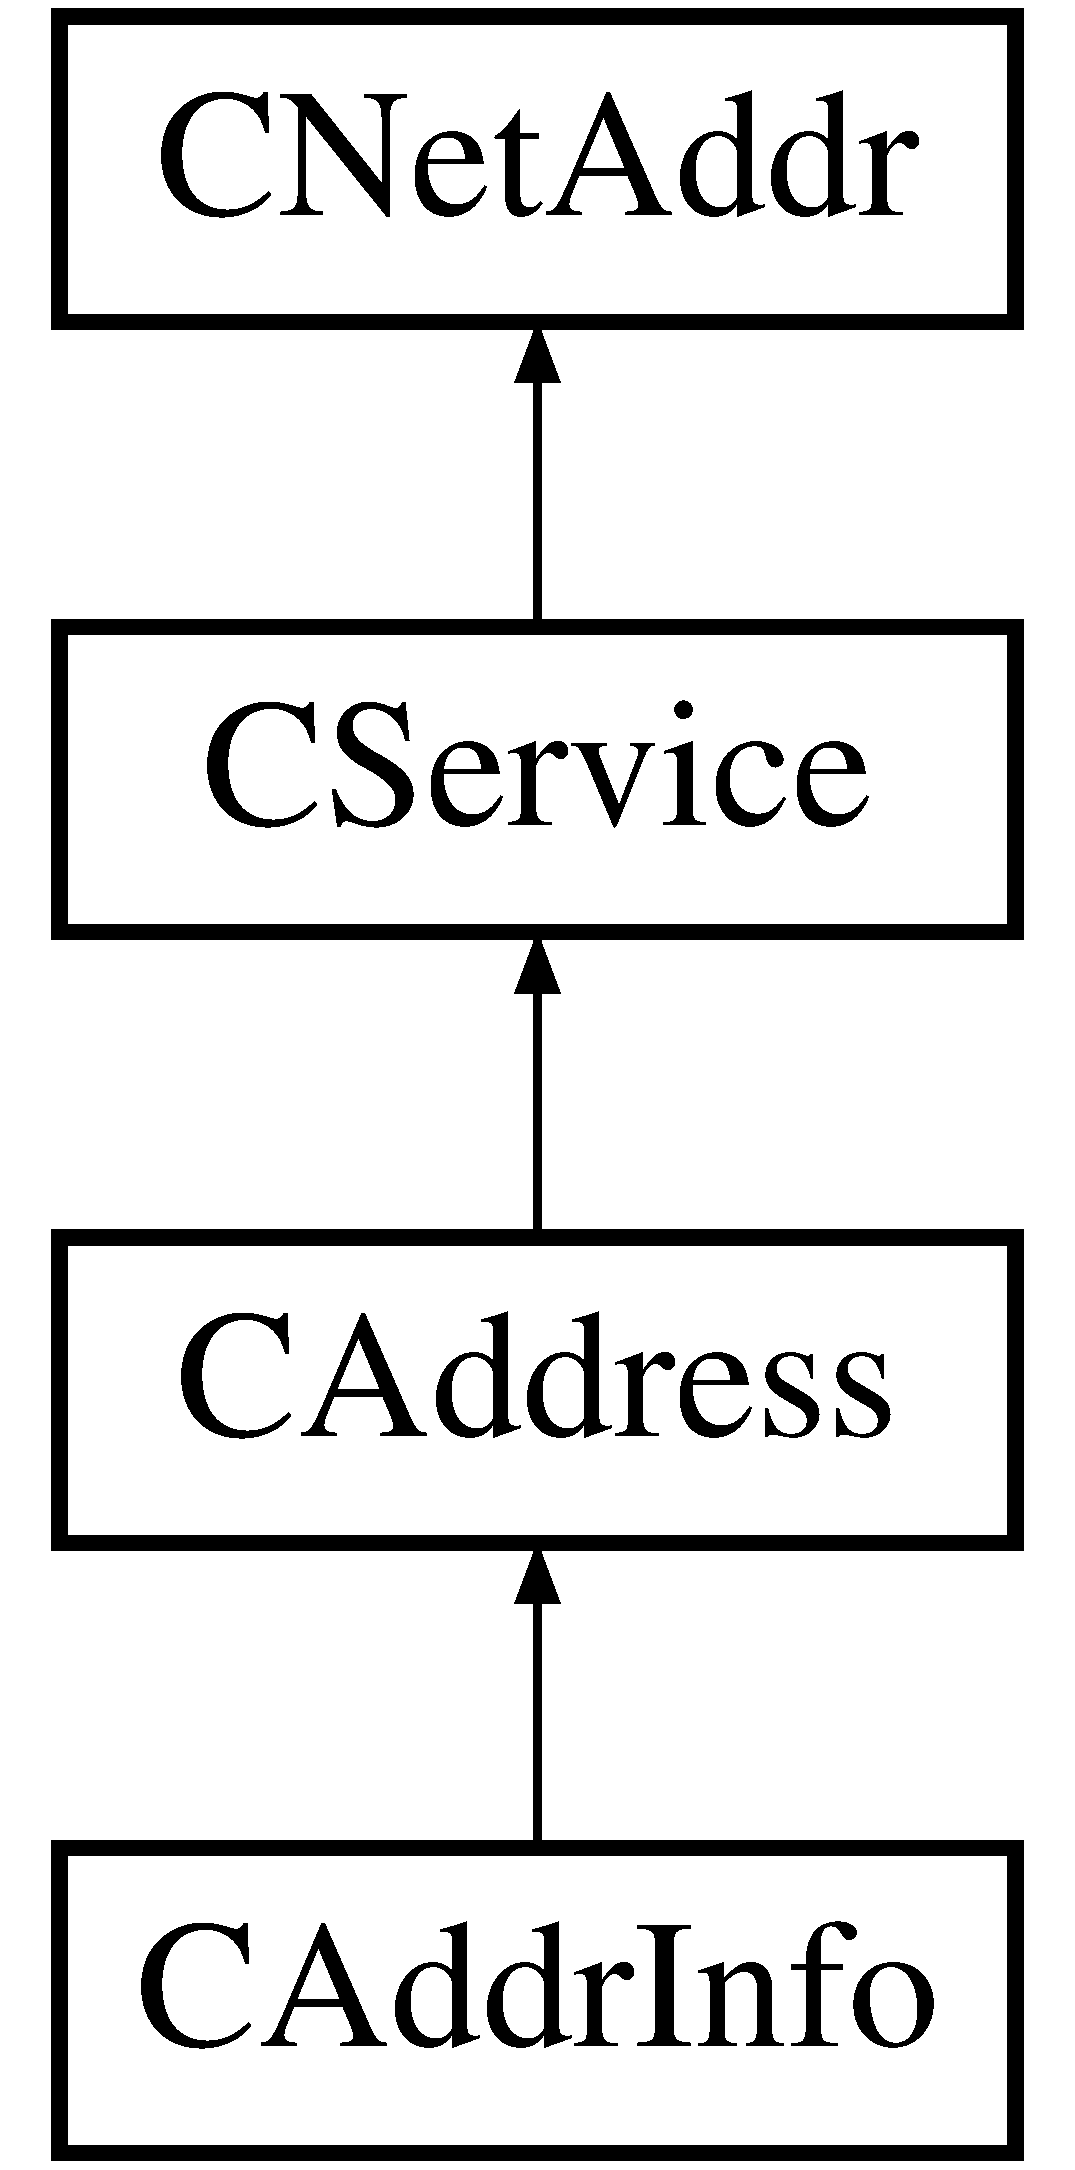
\includegraphics[height=4.000000cm]{class_c_addr_info}
\end{center}
\end{figure}
\subsection*{Public Member Functions}
\begin{DoxyCompactItemize}
\item 
{\footnotesize template$<$typename Stream , typename Operation $>$ }\\void \mbox{\hyperlink{class_c_addr_info_ae80fdec7d3b48278033ea2280f66e68b}{Serialization\+Op}} (Stream \&s, Operation ser\+\_\+action, int n\+Type, int n\+Version)
\item 
void \mbox{\hyperlink{class_c_addr_info_af1df1f12bc71ed7f3debae61058b9b9f}{Init}} ()
\item 
\mbox{\hyperlink{class_c_addr_info_a27e773233e8d7e7d183f138d24cc40ef}{C\+Addr\+Info}} (const \mbox{\hyperlink{class_c_address}{C\+Address}} \&addr\+In, const \mbox{\hyperlink{class_c_net_addr}{C\+Net\+Addr}} \&addr\+Source)
\item 
\mbox{\hyperlink{class_c_addr_info_ae14c3a91bb669e5580be1d3767264187}{C\+Addr\+Info}} ()
\item 
int \mbox{\hyperlink{class_c_addr_info_a11e2712f11c0d92c75976e90f2c5003e}{Get\+Tried\+Bucket}} (const \mbox{\hyperlink{classuint256}{uint256}} \&n\+Key) const
\begin{DoxyCompactList}\small\item\em Calculate in which \char`\"{}tried\char`\"{} bucket this entry belongs. \end{DoxyCompactList}\item 
int \mbox{\hyperlink{class_c_addr_info_ae4459cd7719834bbcf77874757c6875e}{Get\+New\+Bucket}} (const \mbox{\hyperlink{classuint256}{uint256}} \&n\+Key, const \mbox{\hyperlink{class_c_net_addr}{C\+Net\+Addr}} \&src) const
\begin{DoxyCompactList}\small\item\em Calculate in which \char`\"{}new\char`\"{} bucket this entry belongs, given a certain source. \end{DoxyCompactList}\item 
int \mbox{\hyperlink{class_c_addr_info_a04ac79764971242edce1e82aefb2aea0}{Get\+New\+Bucket}} (const \mbox{\hyperlink{classuint256}{uint256}} \&n\+Key) const
\begin{DoxyCompactList}\small\item\em Calculate in which \char`\"{}new\char`\"{} bucket this entry belongs, using its default source. \end{DoxyCompactList}\item 
int \mbox{\hyperlink{class_c_addr_info_a3a133ffb3fbf67cbeb5f4bc683fa9126}{Get\+Bucket\+Position}} (const \mbox{\hyperlink{classuint256}{uint256}} \&n\+Key, bool f\+New, int n\+Bucket) const
\begin{DoxyCompactList}\small\item\em Calculate in which position of a bucket to store this entry. \end{DoxyCompactList}\item 
bool \mbox{\hyperlink{class_c_addr_info_a600725db90b879aee92128a3409af8aa}{Is\+Terrible}} (int64\+\_\+t n\+Now=\mbox{\hyperlink{timedata_8h_a09f81b9c7650f898cf3cf305b87547e6}{Get\+Adjusted\+Time}}()) const
\begin{DoxyCompactList}\small\item\em Determine whether the statistics about this entry are bad enough so that it can just be deleted. \end{DoxyCompactList}\item 
double \mbox{\hyperlink{class_c_addr_info_af6788fe5a5364e63896ab9dedb8e5d40}{Get\+Chance}} (int64\+\_\+t n\+Now=\mbox{\hyperlink{timedata_8h_a09f81b9c7650f898cf3cf305b87547e6}{Get\+Adjusted\+Time}}()) const
\begin{DoxyCompactList}\small\item\em Calculate the relative chance this entry should be given when selecting nodes to connect to. \end{DoxyCompactList}\end{DoxyCompactItemize}
\subsection*{Public Attributes}
\begin{DoxyCompactItemize}
\item 
int64\+\_\+t \mbox{\hyperlink{class_c_addr_info_a4569955918c204d2edd073456108ddfd}{n\+Last\+Try}}
\begin{DoxyCompactList}\small\item\em last try whatsoever by us (memory only) \end{DoxyCompactList}\item 
\mbox{\hyperlink{class_c_addr_info_a9d5e0b95fa494171e4bffb900094fe2e}{A\+D\+D\+\_\+\+S\+E\+R\+I\+A\+L\+I\+Z\+E\+\_\+\+M\+E\+T\+H\+O\+DS}}
\end{DoxyCompactItemize}
\subsection*{Private Attributes}
\begin{DoxyCompactItemize}
\item 
\mbox{\hyperlink{class_c_net_addr}{C\+Net\+Addr}} \mbox{\hyperlink{class_c_addr_info_adf38b9b84f6e9ec5f16bc265c5fcd2dd}{source}}
\begin{DoxyCompactList}\small\item\em where knowledge about this address first came from \end{DoxyCompactList}\item 
int64\+\_\+t \mbox{\hyperlink{class_c_addr_info_a2d064dfb61b2c0ac1e220c8b11962efb}{n\+Last\+Success}}
\begin{DoxyCompactList}\small\item\em last successful connection by us \end{DoxyCompactList}\item 
int \mbox{\hyperlink{class_c_addr_info_a29f143837182a06bccbca363130d8e78}{n\+Attempts}}
\begin{DoxyCompactList}\small\item\em connection attempts since last successful attempt \end{DoxyCompactList}\item 
int \mbox{\hyperlink{class_c_addr_info_ada2f8362fe6ed379a6fdaa3aef682e45}{n\+Ref\+Count}}
\begin{DoxyCompactList}\small\item\em reference count in new sets (memory only) \end{DoxyCompactList}\item 
bool \mbox{\hyperlink{class_c_addr_info_a7fe19a664819fa36ef549c06a5fe0fda}{f\+In\+Tried}}
\begin{DoxyCompactList}\small\item\em in tried set? (memory only) \end{DoxyCompactList}\item 
int \mbox{\hyperlink{class_c_addr_info_a72a78ef782aae72a5a58fd4422cd8066}{n\+Random\+Pos}}
\begin{DoxyCompactList}\small\item\em position in v\+Random \end{DoxyCompactList}\end{DoxyCompactItemize}
\subsection*{Friends}
\begin{DoxyCompactItemize}
\item 
class \mbox{\hyperlink{class_c_addr_info_a17ec4e9e560da58786d2ca36092bf83d}{C\+Addr\+Man}}
\end{DoxyCompactItemize}
\subsection*{Additional Inherited Members}


\subsection{Detailed Description}
Extended statistics about a \mbox{\hyperlink{class_c_address}{C\+Address}} 

\subsection{Constructor \& Destructor Documentation}
\mbox{\Hypertarget{class_c_addr_info_a27e773233e8d7e7d183f138d24cc40ef}\label{class_c_addr_info_a27e773233e8d7e7d183f138d24cc40ef}} 
\index{C\+Addr\+Info@{C\+Addr\+Info}!C\+Addr\+Info@{C\+Addr\+Info}}
\index{C\+Addr\+Info@{C\+Addr\+Info}!C\+Addr\+Info@{C\+Addr\+Info}}
\subsubsection{\texorpdfstring{C\+Addr\+Info()}{CAddrInfo()}\hspace{0.1cm}{\footnotesize\ttfamily [1/2]}}
{\footnotesize\ttfamily C\+Addr\+Info\+::\+C\+Addr\+Info (\begin{DoxyParamCaption}\item[{const \mbox{\hyperlink{class_c_address}{C\+Address}} \&}]{addr\+In,  }\item[{const \mbox{\hyperlink{class_c_net_addr}{C\+Net\+Addr}} \&}]{addr\+Source }\end{DoxyParamCaption})\hspace{0.3cm}{\ttfamily [inline]}}

\mbox{\Hypertarget{class_c_addr_info_ae14c3a91bb669e5580be1d3767264187}\label{class_c_addr_info_ae14c3a91bb669e5580be1d3767264187}} 
\index{C\+Addr\+Info@{C\+Addr\+Info}!C\+Addr\+Info@{C\+Addr\+Info}}
\index{C\+Addr\+Info@{C\+Addr\+Info}!C\+Addr\+Info@{C\+Addr\+Info}}
\subsubsection{\texorpdfstring{C\+Addr\+Info()}{CAddrInfo()}\hspace{0.1cm}{\footnotesize\ttfamily [2/2]}}
{\footnotesize\ttfamily C\+Addr\+Info\+::\+C\+Addr\+Info (\begin{DoxyParamCaption}{ }\end{DoxyParamCaption})\hspace{0.3cm}{\ttfamily [inline]}}



\subsection{Member Function Documentation}
\mbox{\Hypertarget{class_c_addr_info_a3a133ffb3fbf67cbeb5f4bc683fa9126}\label{class_c_addr_info_a3a133ffb3fbf67cbeb5f4bc683fa9126}} 
\index{C\+Addr\+Info@{C\+Addr\+Info}!Get\+Bucket\+Position@{Get\+Bucket\+Position}}
\index{Get\+Bucket\+Position@{Get\+Bucket\+Position}!C\+Addr\+Info@{C\+Addr\+Info}}
\subsubsection{\texorpdfstring{Get\+Bucket\+Position()}{GetBucketPosition()}}
{\footnotesize\ttfamily int C\+Addr\+Info\+::\+Get\+Bucket\+Position (\begin{DoxyParamCaption}\item[{const \mbox{\hyperlink{classuint256}{uint256}} \&}]{n\+Key,  }\item[{bool}]{f\+New,  }\item[{int}]{n\+Bucket }\end{DoxyParamCaption}) const}



Calculate in which position of a bucket to store this entry. 

\mbox{\Hypertarget{class_c_addr_info_af6788fe5a5364e63896ab9dedb8e5d40}\label{class_c_addr_info_af6788fe5a5364e63896ab9dedb8e5d40}} 
\index{C\+Addr\+Info@{C\+Addr\+Info}!Get\+Chance@{Get\+Chance}}
\index{Get\+Chance@{Get\+Chance}!C\+Addr\+Info@{C\+Addr\+Info}}
\subsubsection{\texorpdfstring{Get\+Chance()}{GetChance()}}
{\footnotesize\ttfamily double C\+Addr\+Info\+::\+Get\+Chance (\begin{DoxyParamCaption}\item[{int64\+\_\+t}]{n\+Now = {\ttfamily \mbox{\hyperlink{timedata_8h_a09f81b9c7650f898cf3cf305b87547e6}{Get\+Adjusted\+Time}}()} }\end{DoxyParamCaption}) const}



Calculate the relative chance this entry should be given when selecting nodes to connect to. 

\mbox{\Hypertarget{class_c_addr_info_ae4459cd7719834bbcf77874757c6875e}\label{class_c_addr_info_ae4459cd7719834bbcf77874757c6875e}} 
\index{C\+Addr\+Info@{C\+Addr\+Info}!Get\+New\+Bucket@{Get\+New\+Bucket}}
\index{Get\+New\+Bucket@{Get\+New\+Bucket}!C\+Addr\+Info@{C\+Addr\+Info}}
\subsubsection{\texorpdfstring{Get\+New\+Bucket()}{GetNewBucket()}\hspace{0.1cm}{\footnotesize\ttfamily [1/2]}}
{\footnotesize\ttfamily int C\+Addr\+Info\+::\+Get\+New\+Bucket (\begin{DoxyParamCaption}\item[{const \mbox{\hyperlink{classuint256}{uint256}} \&}]{n\+Key,  }\item[{const \mbox{\hyperlink{class_c_net_addr}{C\+Net\+Addr}} \&}]{src }\end{DoxyParamCaption}) const}



Calculate in which \char`\"{}new\char`\"{} bucket this entry belongs, given a certain source. 

\mbox{\Hypertarget{class_c_addr_info_a04ac79764971242edce1e82aefb2aea0}\label{class_c_addr_info_a04ac79764971242edce1e82aefb2aea0}} 
\index{C\+Addr\+Info@{C\+Addr\+Info}!Get\+New\+Bucket@{Get\+New\+Bucket}}
\index{Get\+New\+Bucket@{Get\+New\+Bucket}!C\+Addr\+Info@{C\+Addr\+Info}}
\subsubsection{\texorpdfstring{Get\+New\+Bucket()}{GetNewBucket()}\hspace{0.1cm}{\footnotesize\ttfamily [2/2]}}
{\footnotesize\ttfamily int C\+Addr\+Info\+::\+Get\+New\+Bucket (\begin{DoxyParamCaption}\item[{const \mbox{\hyperlink{classuint256}{uint256}} \&}]{n\+Key }\end{DoxyParamCaption}) const\hspace{0.3cm}{\ttfamily [inline]}}



Calculate in which \char`\"{}new\char`\"{} bucket this entry belongs, using its default source. 

\mbox{\Hypertarget{class_c_addr_info_a11e2712f11c0d92c75976e90f2c5003e}\label{class_c_addr_info_a11e2712f11c0d92c75976e90f2c5003e}} 
\index{C\+Addr\+Info@{C\+Addr\+Info}!Get\+Tried\+Bucket@{Get\+Tried\+Bucket}}
\index{Get\+Tried\+Bucket@{Get\+Tried\+Bucket}!C\+Addr\+Info@{C\+Addr\+Info}}
\subsubsection{\texorpdfstring{Get\+Tried\+Bucket()}{GetTriedBucket()}}
{\footnotesize\ttfamily int C\+Addr\+Info\+::\+Get\+Tried\+Bucket (\begin{DoxyParamCaption}\item[{const \mbox{\hyperlink{classuint256}{uint256}} \&}]{n\+Key }\end{DoxyParamCaption}) const}



Calculate in which \char`\"{}tried\char`\"{} bucket this entry belongs. 

\mbox{\Hypertarget{class_c_addr_info_af1df1f12bc71ed7f3debae61058b9b9f}\label{class_c_addr_info_af1df1f12bc71ed7f3debae61058b9b9f}} 
\index{C\+Addr\+Info@{C\+Addr\+Info}!Init@{Init}}
\index{Init@{Init}!C\+Addr\+Info@{C\+Addr\+Info}}
\subsubsection{\texorpdfstring{Init()}{Init()}}
{\footnotesize\ttfamily void C\+Addr\+Info\+::\+Init (\begin{DoxyParamCaption}{ }\end{DoxyParamCaption})\hspace{0.3cm}{\ttfamily [inline]}}

\mbox{\Hypertarget{class_c_addr_info_a600725db90b879aee92128a3409af8aa}\label{class_c_addr_info_a600725db90b879aee92128a3409af8aa}} 
\index{C\+Addr\+Info@{C\+Addr\+Info}!Is\+Terrible@{Is\+Terrible}}
\index{Is\+Terrible@{Is\+Terrible}!C\+Addr\+Info@{C\+Addr\+Info}}
\subsubsection{\texorpdfstring{Is\+Terrible()}{IsTerrible()}}
{\footnotesize\ttfamily bool C\+Addr\+Info\+::\+Is\+Terrible (\begin{DoxyParamCaption}\item[{int64\+\_\+t}]{n\+Now = {\ttfamily \mbox{\hyperlink{timedata_8h_a09f81b9c7650f898cf3cf305b87547e6}{Get\+Adjusted\+Time}}()} }\end{DoxyParamCaption}) const}



Determine whether the statistics about this entry are bad enough so that it can just be deleted. 

\mbox{\Hypertarget{class_c_addr_info_ae80fdec7d3b48278033ea2280f66e68b}\label{class_c_addr_info_ae80fdec7d3b48278033ea2280f66e68b}} 
\index{C\+Addr\+Info@{C\+Addr\+Info}!Serialization\+Op@{Serialization\+Op}}
\index{Serialization\+Op@{Serialization\+Op}!C\+Addr\+Info@{C\+Addr\+Info}}
\subsubsection{\texorpdfstring{Serialization\+Op()}{SerializationOp()}}
{\footnotesize\ttfamily template$<$typename Stream , typename Operation $>$ \\
void C\+Addr\+Info\+::\+Serialization\+Op (\begin{DoxyParamCaption}\item[{Stream \&}]{s,  }\item[{Operation}]{ser\+\_\+action,  }\item[{int}]{n\+Type,  }\item[{int}]{n\+Version }\end{DoxyParamCaption})\hspace{0.3cm}{\ttfamily [inline]}}



\subsection{Friends And Related Function Documentation}
\mbox{\Hypertarget{class_c_addr_info_a17ec4e9e560da58786d2ca36092bf83d}\label{class_c_addr_info_a17ec4e9e560da58786d2ca36092bf83d}} 
\index{C\+Addr\+Info@{C\+Addr\+Info}!C\+Addr\+Man@{C\+Addr\+Man}}
\index{C\+Addr\+Man@{C\+Addr\+Man}!C\+Addr\+Info@{C\+Addr\+Info}}
\subsubsection{\texorpdfstring{C\+Addr\+Man}{CAddrMan}}
{\footnotesize\ttfamily friend class \mbox{\hyperlink{class_c_addr_man}{C\+Addr\+Man}}\hspace{0.3cm}{\ttfamily [friend]}}



\subsection{Member Data Documentation}
\mbox{\Hypertarget{class_c_addr_info_a9d5e0b95fa494171e4bffb900094fe2e}\label{class_c_addr_info_a9d5e0b95fa494171e4bffb900094fe2e}} 
\index{C\+Addr\+Info@{C\+Addr\+Info}!A\+D\+D\+\_\+\+S\+E\+R\+I\+A\+L\+I\+Z\+E\+\_\+\+M\+E\+T\+H\+O\+DS@{A\+D\+D\+\_\+\+S\+E\+R\+I\+A\+L\+I\+Z\+E\+\_\+\+M\+E\+T\+H\+O\+DS}}
\index{A\+D\+D\+\_\+\+S\+E\+R\+I\+A\+L\+I\+Z\+E\+\_\+\+M\+E\+T\+H\+O\+DS@{A\+D\+D\+\_\+\+S\+E\+R\+I\+A\+L\+I\+Z\+E\+\_\+\+M\+E\+T\+H\+O\+DS}!C\+Addr\+Info@{C\+Addr\+Info}}
\subsubsection{\texorpdfstring{A\+D\+D\+\_\+\+S\+E\+R\+I\+A\+L\+I\+Z\+E\+\_\+\+M\+E\+T\+H\+O\+DS}{ADD\_SERIALIZE\_METHODS}}
{\footnotesize\ttfamily C\+Addr\+Info\+::\+A\+D\+D\+\_\+\+S\+E\+R\+I\+A\+L\+I\+Z\+E\+\_\+\+M\+E\+T\+H\+O\+DS}

\mbox{\Hypertarget{class_c_addr_info_a7fe19a664819fa36ef549c06a5fe0fda}\label{class_c_addr_info_a7fe19a664819fa36ef549c06a5fe0fda}} 
\index{C\+Addr\+Info@{C\+Addr\+Info}!f\+In\+Tried@{f\+In\+Tried}}
\index{f\+In\+Tried@{f\+In\+Tried}!C\+Addr\+Info@{C\+Addr\+Info}}
\subsubsection{\texorpdfstring{f\+In\+Tried}{fInTried}}
{\footnotesize\ttfamily bool C\+Addr\+Info\+::f\+In\+Tried\hspace{0.3cm}{\ttfamily [private]}}



in tried set? (memory only) 

\mbox{\Hypertarget{class_c_addr_info_a29f143837182a06bccbca363130d8e78}\label{class_c_addr_info_a29f143837182a06bccbca363130d8e78}} 
\index{C\+Addr\+Info@{C\+Addr\+Info}!n\+Attempts@{n\+Attempts}}
\index{n\+Attempts@{n\+Attempts}!C\+Addr\+Info@{C\+Addr\+Info}}
\subsubsection{\texorpdfstring{n\+Attempts}{nAttempts}}
{\footnotesize\ttfamily int C\+Addr\+Info\+::n\+Attempts\hspace{0.3cm}{\ttfamily [private]}}



connection attempts since last successful attempt 

\mbox{\Hypertarget{class_c_addr_info_a2d064dfb61b2c0ac1e220c8b11962efb}\label{class_c_addr_info_a2d064dfb61b2c0ac1e220c8b11962efb}} 
\index{C\+Addr\+Info@{C\+Addr\+Info}!n\+Last\+Success@{n\+Last\+Success}}
\index{n\+Last\+Success@{n\+Last\+Success}!C\+Addr\+Info@{C\+Addr\+Info}}
\subsubsection{\texorpdfstring{n\+Last\+Success}{nLastSuccess}}
{\footnotesize\ttfamily int64\+\_\+t C\+Addr\+Info\+::n\+Last\+Success\hspace{0.3cm}{\ttfamily [private]}}



last successful connection by us 

\mbox{\Hypertarget{class_c_addr_info_a4569955918c204d2edd073456108ddfd}\label{class_c_addr_info_a4569955918c204d2edd073456108ddfd}} 
\index{C\+Addr\+Info@{C\+Addr\+Info}!n\+Last\+Try@{n\+Last\+Try}}
\index{n\+Last\+Try@{n\+Last\+Try}!C\+Addr\+Info@{C\+Addr\+Info}}
\subsubsection{\texorpdfstring{n\+Last\+Try}{nLastTry}}
{\footnotesize\ttfamily int64\+\_\+t C\+Addr\+Info\+::n\+Last\+Try}



last try whatsoever by us (memory only) 

\mbox{\Hypertarget{class_c_addr_info_a72a78ef782aae72a5a58fd4422cd8066}\label{class_c_addr_info_a72a78ef782aae72a5a58fd4422cd8066}} 
\index{C\+Addr\+Info@{C\+Addr\+Info}!n\+Random\+Pos@{n\+Random\+Pos}}
\index{n\+Random\+Pos@{n\+Random\+Pos}!C\+Addr\+Info@{C\+Addr\+Info}}
\subsubsection{\texorpdfstring{n\+Random\+Pos}{nRandomPos}}
{\footnotesize\ttfamily int C\+Addr\+Info\+::n\+Random\+Pos\hspace{0.3cm}{\ttfamily [private]}}



position in v\+Random 

\mbox{\Hypertarget{class_c_addr_info_ada2f8362fe6ed379a6fdaa3aef682e45}\label{class_c_addr_info_ada2f8362fe6ed379a6fdaa3aef682e45}} 
\index{C\+Addr\+Info@{C\+Addr\+Info}!n\+Ref\+Count@{n\+Ref\+Count}}
\index{n\+Ref\+Count@{n\+Ref\+Count}!C\+Addr\+Info@{C\+Addr\+Info}}
\subsubsection{\texorpdfstring{n\+Ref\+Count}{nRefCount}}
{\footnotesize\ttfamily int C\+Addr\+Info\+::n\+Ref\+Count\hspace{0.3cm}{\ttfamily [private]}}



reference count in new sets (memory only) 

\mbox{\Hypertarget{class_c_addr_info_adf38b9b84f6e9ec5f16bc265c5fcd2dd}\label{class_c_addr_info_adf38b9b84f6e9ec5f16bc265c5fcd2dd}} 
\index{C\+Addr\+Info@{C\+Addr\+Info}!source@{source}}
\index{source@{source}!C\+Addr\+Info@{C\+Addr\+Info}}
\subsubsection{\texorpdfstring{source}{source}}
{\footnotesize\ttfamily \mbox{\hyperlink{class_c_net_addr}{C\+Net\+Addr}} C\+Addr\+Info\+::source\hspace{0.3cm}{\ttfamily [private]}}



where knowledge about this address first came from 



The documentation for this class was generated from the following files\+:\begin{DoxyCompactItemize}
\item 
/\+Users/christopherarguello/\+Developer/anon/src/\mbox{\hyperlink{addrman_8h}{addrman.\+h}}\item 
/\+Users/christopherarguello/\+Developer/anon/src/\mbox{\hyperlink{addrman_8cpp}{addrman.\+cpp}}\end{DoxyCompactItemize}

\hypertarget{class_c_addr_man}{}\section{C\+Addr\+Man Class Reference}
\label{class_c_addr_man}\index{C\+Addr\+Man@{C\+Addr\+Man}}


{\ttfamily \#include $<$addrman.\+h$>$}

\subsection*{Public Member Functions}
\begin{DoxyCompactItemize}
\item 
{\footnotesize template$<$typename Stream $>$ }\\void \mbox{\hyperlink{class_c_addr_man_a08668d8cf435750a80316b4708bbc9eb}{Serialize}} (Stream \&s, int n\+Type, int n\+Version\+Dummy) const
\item 
{\footnotesize template$<$typename Stream $>$ }\\void \mbox{\hyperlink{class_c_addr_man_a68eaf1797ecb8bff380aa7f9fc452e14}{Unserialize}} (Stream \&s, int n\+Type, int n\+Version\+Dummy)
\item 
unsigned int \mbox{\hyperlink{class_c_addr_man_a958c50de16b0d7fa068cce22a4cd8cb9}{Get\+Serialize\+Size}} (int n\+Type, int n\+Version) const
\item 
void \mbox{\hyperlink{class_c_addr_man_a53c27520b7f8c6fa817c2fa869dd4e25}{Clear}} ()
\item 
\mbox{\hyperlink{class_c_addr_man_ad9179d1c36c2ea3492e221576f340d33}{C\+Addr\+Man}} ()
\item 
\mbox{\hyperlink{class_c_addr_man_ae1b1838e4de4effbc1fbc888126a9352}{$\sim$\+C\+Addr\+Man}} ()
\item 
size\+\_\+t \mbox{\hyperlink{class_c_addr_man_a244508e8463c4fdfd8b085fcb3b5a225}{size}} () const
\begin{DoxyCompactList}\small\item\em Return the number of (unique) addresses in all tables. \end{DoxyCompactList}\item 
void \mbox{\hyperlink{class_c_addr_man_a0c2677ae50ce0d680f0105b285d1f5d0}{Check}} ()
\begin{DoxyCompactList}\small\item\em Consistency check. \end{DoxyCompactList}\item 
bool \mbox{\hyperlink{class_c_addr_man_a03fcc7109b5f014760dc50a81f68c5ec}{Add}} (const \mbox{\hyperlink{class_c_address}{C\+Address}} \&addr, const \mbox{\hyperlink{class_c_net_addr}{C\+Net\+Addr}} \&source, int64\+\_\+t n\+Time\+Penalty=0)
\begin{DoxyCompactList}\small\item\em Add a single address. \end{DoxyCompactList}\item 
bool \mbox{\hyperlink{class_c_addr_man_aa2ae2abdf710b2d81fa37f072bab028e}{Add}} (const std\+::vector$<$ \mbox{\hyperlink{class_c_address}{C\+Address}} $>$ \&v\+Addr, const \mbox{\hyperlink{class_c_net_addr}{C\+Net\+Addr}} \&source, int64\+\_\+t n\+Time\+Penalty=0)
\begin{DoxyCompactList}\small\item\em Add multiple addresses. \end{DoxyCompactList}\item 
void \mbox{\hyperlink{class_c_addr_man_a993e80e74701d7bc6bb49880c387b847}{Good}} (const \mbox{\hyperlink{class_c_service}{C\+Service}} \&addr, int64\+\_\+t n\+Time=\mbox{\hyperlink{timedata_8h_a09f81b9c7650f898cf3cf305b87547e6}{Get\+Adjusted\+Time}}())
\begin{DoxyCompactList}\small\item\em Mark an entry as accessible. \end{DoxyCompactList}\item 
void \mbox{\hyperlink{class_c_addr_man_afcddc2573121065177dc981cea710789}{Attempt}} (const \mbox{\hyperlink{class_c_service}{C\+Service}} \&addr, int64\+\_\+t n\+Time=\mbox{\hyperlink{timedata_8h_a09f81b9c7650f898cf3cf305b87547e6}{Get\+Adjusted\+Time}}())
\begin{DoxyCompactList}\small\item\em Mark an entry as connection attempted to. \end{DoxyCompactList}\item 
\mbox{\hyperlink{class_c_addr_info}{C\+Addr\+Info}} \mbox{\hyperlink{class_c_addr_man_a6279e9fdd1b78378c016087daf09a439}{Select}} (bool new\+Only=false)
\item 
std\+::vector$<$ \mbox{\hyperlink{class_c_address}{C\+Address}} $>$ \mbox{\hyperlink{class_c_addr_man_a69cc6138e696cf88de60925d26023bf2}{Get\+Addr}} ()
\begin{DoxyCompactList}\small\item\em Return a bunch of addresses, selected at random. \end{DoxyCompactList}\item 
void \mbox{\hyperlink{class_c_addr_man_a7aba66d9e9527522fed974567d34c322}{Connected}} (const \mbox{\hyperlink{class_c_service}{C\+Service}} \&addr, int64\+\_\+t n\+Time=\mbox{\hyperlink{timedata_8h_a09f81b9c7650f898cf3cf305b87547e6}{Get\+Adjusted\+Time}}())
\begin{DoxyCompactList}\small\item\em Mark an entry as currently-\/connected-\/to. \end{DoxyCompactList}\item 
void \mbox{\hyperlink{class_c_addr_man_a242690c5f4d2c14738da47edc5e8275c}{Make\+Deterministic}} ()
\begin{DoxyCompactList}\small\item\em Ensure that bucket placement is always the same for testing purposes. \end{DoxyCompactList}\end{DoxyCompactItemize}
\subsection*{Protected Member Functions}
\begin{DoxyCompactItemize}
\item 
\mbox{\hyperlink{class_c_addr_info}{C\+Addr\+Info}} $\ast$ \mbox{\hyperlink{class_c_addr_man_ac961ead1a1afde144fc486b6d7c7369d}{Find}} (const \mbox{\hyperlink{class_c_net_addr}{C\+Net\+Addr}} \&addr, int $\ast$pn\+Id=N\+U\+LL)
\begin{DoxyCompactList}\small\item\em Find an entry. \end{DoxyCompactList}\item 
\mbox{\hyperlink{class_c_addr_info}{C\+Addr\+Info}} $\ast$ \mbox{\hyperlink{class_c_addr_man_aac93f51c0580e38a950a0f63b053bedb}{Create}} (const \mbox{\hyperlink{class_c_address}{C\+Address}} \&addr, const \mbox{\hyperlink{class_c_net_addr}{C\+Net\+Addr}} \&addr\+Source, int $\ast$pn\+Id=N\+U\+LL)
\item 
void \mbox{\hyperlink{class_c_addr_man_a3074bc8e3dcfb5348054613f575dc38e}{Swap\+Random}} (unsigned int n\+Random\+Pos1, unsigned int n\+Random\+Pos2)
\begin{DoxyCompactList}\small\item\em Swap two elements in v\+Random. \end{DoxyCompactList}\item 
void \mbox{\hyperlink{class_c_addr_man_a98e8383efb48b7c2932795438f35a10a}{Make\+Tried}} (\mbox{\hyperlink{class_c_addr_info}{C\+Addr\+Info}} \&info, int n\+Id)
\begin{DoxyCompactList}\small\item\em Move an entry from the \char`\"{}new\char`\"{} table(s) to the \char`\"{}tried\char`\"{} table. \end{DoxyCompactList}\item 
void \mbox{\hyperlink{class_c_addr_man_af488eac123030538770dbc4e3b16eb74}{Delete}} (int n\+Id)
\begin{DoxyCompactList}\small\item\em Delete an entry. It must not be in tried, and have refcount 0. \end{DoxyCompactList}\item 
void \mbox{\hyperlink{class_c_addr_man_ab283de3e750f006c85573976bd40da81}{Clear\+New}} (int n\+U\+Bucket, int n\+U\+Bucket\+Pos)
\begin{DoxyCompactList}\small\item\em Clear a position in a \char`\"{}new\char`\"{} table. This is the only place where entries are actually deleted. \end{DoxyCompactList}\item 
void \mbox{\hyperlink{class_c_addr_man_a33ec6a4584cf4b17af821e6e35216459}{Good\+\_\+}} (const \mbox{\hyperlink{class_c_service}{C\+Service}} \&addr, int64\+\_\+t n\+Time)
\begin{DoxyCompactList}\small\item\em Mark an entry \char`\"{}good\char`\"{}, possibly moving it from \char`\"{}new\char`\"{} to \char`\"{}tried\char`\"{}. \end{DoxyCompactList}\item 
bool \mbox{\hyperlink{class_c_addr_man_a9dd6df8b1904548a86054d19d4a90724}{Add\+\_\+}} (const \mbox{\hyperlink{class_c_address}{C\+Address}} \&addr, const \mbox{\hyperlink{class_c_net_addr}{C\+Net\+Addr}} \&source, int64\+\_\+t n\+Time\+Penalty)
\begin{DoxyCompactList}\small\item\em Add an entry to the \char`\"{}new\char`\"{} table. \end{DoxyCompactList}\item 
void \mbox{\hyperlink{class_c_addr_man_ab1a1bfa8b435ef139570c88de1a5245f}{Attempt\+\_\+}} (const \mbox{\hyperlink{class_c_service}{C\+Service}} \&addr, int64\+\_\+t n\+Time)
\begin{DoxyCompactList}\small\item\em Mark an entry as attempted to connect. \end{DoxyCompactList}\item 
\mbox{\hyperlink{class_c_addr_info}{C\+Addr\+Info}} \mbox{\hyperlink{class_c_addr_man_a27e51ef4fe86db1ff5a5e45caefc1ef4}{Select\+\_\+}} (bool new\+Only)
\begin{DoxyCompactList}\small\item\em Select an address to connect to, if new\+Only is set to true, only the new table is selected from. \end{DoxyCompactList}\item 
virtual int \mbox{\hyperlink{class_c_addr_man_a4bf12611bd89c5e524396e50bf8f3846}{Random\+Int}} (int n\+Max)
\begin{DoxyCompactList}\small\item\em Wraps Get\+Rand\+Int to allow tests to override Random\+Int and make it determinismistic. \end{DoxyCompactList}\item 
void \mbox{\hyperlink{class_c_addr_man_aff86d04dc7c0e0afae3ff5998417db17}{Get\+Addr\+\_\+}} (std\+::vector$<$ \mbox{\hyperlink{class_c_address}{C\+Address}} $>$ \&v\+Addr)
\begin{DoxyCompactList}\small\item\em Select several addresses at once. \end{DoxyCompactList}\item 
void \mbox{\hyperlink{class_c_addr_man_a1ae72643c51293f3f3345e74ce0368ca}{Connected\+\_\+}} (const \mbox{\hyperlink{class_c_service}{C\+Service}} \&addr, int64\+\_\+t n\+Time)
\begin{DoxyCompactList}\small\item\em Mark an entry as currently-\/connected-\/to. \end{DoxyCompactList}\end{DoxyCompactItemize}
\subsection*{Protected Attributes}
\begin{DoxyCompactItemize}
\item 
\mbox{\hyperlink{classuint256}{uint256}} \mbox{\hyperlink{class_c_addr_man_adcb5b2b86ea5739730b111c89e84e965}{n\+Key}}
\begin{DoxyCompactList}\small\item\em secret key to randomize bucket select with \end{DoxyCompactList}\end{DoxyCompactItemize}
\subsection*{Private Attributes}
\begin{DoxyCompactItemize}
\item 
\mbox{\hyperlink{sync_8h_a37a4692b2d517f2843655ca11af7668a}{C\+Critical\+Section}} \mbox{\hyperlink{class_c_addr_man_aa4519d05a02e493046e5ece1ce87c084}{cs}}
\begin{DoxyCompactList}\small\item\em critical section to protect the inner data structures \end{DoxyCompactList}\item 
int \mbox{\hyperlink{class_c_addr_man_a77ff8bd51009324f2be012bd759b37d0}{n\+Id\+Count}}
\begin{DoxyCompactList}\small\item\em last used n\+Id \end{DoxyCompactList}\item 
std\+::map$<$ int, \mbox{\hyperlink{class_c_addr_info}{C\+Addr\+Info}} $>$ \mbox{\hyperlink{class_c_addr_man_a1232db343240bf03c45eaea7bcec550b}{map\+Info}}
\begin{DoxyCompactList}\small\item\em table with information about all n\+Ids \end{DoxyCompactList}\item 
std\+::map$<$ \mbox{\hyperlink{class_c_net_addr}{C\+Net\+Addr}}, int $>$ \mbox{\hyperlink{class_c_addr_man_a5c387857d8553818a56a4faac33fb691}{map\+Addr}}
\begin{DoxyCompactList}\small\item\em find an n\+Id based on its network address \end{DoxyCompactList}\item 
std\+::vector$<$ int $>$ \mbox{\hyperlink{class_c_addr_man_af9c2199d29d7a1a7c6c5c1e3abec4102}{v\+Random}}
\begin{DoxyCompactList}\small\item\em randomly-\/ordered vector of all n\+Ids \end{DoxyCompactList}\item 
int \mbox{\hyperlink{class_c_addr_man_ae8566be810e6429012f1c2c1609b4540}{n\+Tried}}
\item 
int \mbox{\hyperlink{class_c_addr_man_a3d0e798757be2620f76a5ee02d3b321e}{vv\+Tried}} \mbox{[}\mbox{\hyperlink{addrman_8h_ab09df186aa818ce7b9e7c86446511cf1}{A\+D\+D\+R\+M\+A\+N\+\_\+\+T\+R\+I\+E\+D\+\_\+\+B\+U\+C\+K\+E\+T\+\_\+\+C\+O\+U\+NT}}\mbox{]}\mbox{[}\mbox{\hyperlink{addrman_8h_a3499731a6c89e164cf74b68be2be0a84}{A\+D\+D\+R\+M\+A\+N\+\_\+\+B\+U\+C\+K\+E\+T\+\_\+\+S\+I\+ZE}}\mbox{]}
\begin{DoxyCompactList}\small\item\em list of \char`\"{}tried\char`\"{} buckets \end{DoxyCompactList}\item 
int \mbox{\hyperlink{class_c_addr_man_a469f5f8e9ac527812338d7894b784986}{n\+New}}
\begin{DoxyCompactList}\small\item\em number of (unique) \char`\"{}new\char`\"{} entries \end{DoxyCompactList}\item 
int \mbox{\hyperlink{class_c_addr_man_afb2dcfcd27aedab01f5259980f322fa8}{vv\+New}} \mbox{[}\mbox{\hyperlink{addrman_8h_a74a626eb1dbb8e307a413e86493cd510}{A\+D\+D\+R\+M\+A\+N\+\_\+\+N\+E\+W\+\_\+\+B\+U\+C\+K\+E\+T\+\_\+\+C\+O\+U\+NT}}\mbox{]}\mbox{[}\mbox{\hyperlink{addrman_8h_a3499731a6c89e164cf74b68be2be0a84}{A\+D\+D\+R\+M\+A\+N\+\_\+\+B\+U\+C\+K\+E\+T\+\_\+\+S\+I\+ZE}}\mbox{]}
\begin{DoxyCompactList}\small\item\em list of \char`\"{}new\char`\"{} buckets \end{DoxyCompactList}\end{DoxyCompactItemize}


\subsection{Detailed Description}
Stochastical (IP) address manager 

\subsection{Constructor \& Destructor Documentation}
\mbox{\Hypertarget{class_c_addr_man_ad9179d1c36c2ea3492e221576f340d33}\label{class_c_addr_man_ad9179d1c36c2ea3492e221576f340d33}} 
\index{C\+Addr\+Man@{C\+Addr\+Man}!C\+Addr\+Man@{C\+Addr\+Man}}
\index{C\+Addr\+Man@{C\+Addr\+Man}!C\+Addr\+Man@{C\+Addr\+Man}}
\subsubsection{\texorpdfstring{C\+Addr\+Man()}{CAddrMan()}}
{\footnotesize\ttfamily C\+Addr\+Man\+::\+C\+Addr\+Man (\begin{DoxyParamCaption}{ }\end{DoxyParamCaption})\hspace{0.3cm}{\ttfamily [inline]}}

\mbox{\Hypertarget{class_c_addr_man_ae1b1838e4de4effbc1fbc888126a9352}\label{class_c_addr_man_ae1b1838e4de4effbc1fbc888126a9352}} 
\index{C\+Addr\+Man@{C\+Addr\+Man}!````~C\+Addr\+Man@{$\sim$\+C\+Addr\+Man}}
\index{````~C\+Addr\+Man@{$\sim$\+C\+Addr\+Man}!C\+Addr\+Man@{C\+Addr\+Man}}
\subsubsection{\texorpdfstring{$\sim$\+C\+Addr\+Man()}{~CAddrMan()}}
{\footnotesize\ttfamily C\+Addr\+Man\+::$\sim$\+C\+Addr\+Man (\begin{DoxyParamCaption}{ }\end{DoxyParamCaption})\hspace{0.3cm}{\ttfamily [inline]}}



\subsection{Member Function Documentation}
\mbox{\Hypertarget{class_c_addr_man_a03fcc7109b5f014760dc50a81f68c5ec}\label{class_c_addr_man_a03fcc7109b5f014760dc50a81f68c5ec}} 
\index{C\+Addr\+Man@{C\+Addr\+Man}!Add@{Add}}
\index{Add@{Add}!C\+Addr\+Man@{C\+Addr\+Man}}
\subsubsection{\texorpdfstring{Add()}{Add()}\hspace{0.1cm}{\footnotesize\ttfamily [1/2]}}
{\footnotesize\ttfamily bool C\+Addr\+Man\+::\+Add (\begin{DoxyParamCaption}\item[{const \mbox{\hyperlink{class_c_address}{C\+Address}} \&}]{addr,  }\item[{const \mbox{\hyperlink{class_c_net_addr}{C\+Net\+Addr}} \&}]{source,  }\item[{int64\+\_\+t}]{n\+Time\+Penalty = {\ttfamily 0} }\end{DoxyParamCaption})\hspace{0.3cm}{\ttfamily [inline]}}



Add a single address. 

\mbox{\Hypertarget{class_c_addr_man_aa2ae2abdf710b2d81fa37f072bab028e}\label{class_c_addr_man_aa2ae2abdf710b2d81fa37f072bab028e}} 
\index{C\+Addr\+Man@{C\+Addr\+Man}!Add@{Add}}
\index{Add@{Add}!C\+Addr\+Man@{C\+Addr\+Man}}
\subsubsection{\texorpdfstring{Add()}{Add()}\hspace{0.1cm}{\footnotesize\ttfamily [2/2]}}
{\footnotesize\ttfamily bool C\+Addr\+Man\+::\+Add (\begin{DoxyParamCaption}\item[{const std\+::vector$<$ \mbox{\hyperlink{class_c_address}{C\+Address}} $>$ \&}]{v\+Addr,  }\item[{const \mbox{\hyperlink{class_c_net_addr}{C\+Net\+Addr}} \&}]{source,  }\item[{int64\+\_\+t}]{n\+Time\+Penalty = {\ttfamily 0} }\end{DoxyParamCaption})\hspace{0.3cm}{\ttfamily [inline]}}



Add multiple addresses. 

\mbox{\Hypertarget{class_c_addr_man_a9dd6df8b1904548a86054d19d4a90724}\label{class_c_addr_man_a9dd6df8b1904548a86054d19d4a90724}} 
\index{C\+Addr\+Man@{C\+Addr\+Man}!Add\+\_\+@{Add\+\_\+}}
\index{Add\+\_\+@{Add\+\_\+}!C\+Addr\+Man@{C\+Addr\+Man}}
\subsubsection{\texorpdfstring{Add\+\_\+()}{Add\_()}}
{\footnotesize\ttfamily bool C\+Addr\+Man\+::\+Add\+\_\+ (\begin{DoxyParamCaption}\item[{const \mbox{\hyperlink{class_c_address}{C\+Address}} \&}]{addr,  }\item[{const \mbox{\hyperlink{class_c_net_addr}{C\+Net\+Addr}} \&}]{source,  }\item[{int64\+\_\+t}]{n\+Time\+Penalty }\end{DoxyParamCaption})\hspace{0.3cm}{\ttfamily [protected]}}



Add an entry to the \char`\"{}new\char`\"{} table. 

\mbox{\Hypertarget{class_c_addr_man_afcddc2573121065177dc981cea710789}\label{class_c_addr_man_afcddc2573121065177dc981cea710789}} 
\index{C\+Addr\+Man@{C\+Addr\+Man}!Attempt@{Attempt}}
\index{Attempt@{Attempt}!C\+Addr\+Man@{C\+Addr\+Man}}
\subsubsection{\texorpdfstring{Attempt()}{Attempt()}}
{\footnotesize\ttfamily void C\+Addr\+Man\+::\+Attempt (\begin{DoxyParamCaption}\item[{const \mbox{\hyperlink{class_c_service}{C\+Service}} \&}]{addr,  }\item[{int64\+\_\+t}]{n\+Time = {\ttfamily \mbox{\hyperlink{timedata_8h_a09f81b9c7650f898cf3cf305b87547e6}{Get\+Adjusted\+Time}}()} }\end{DoxyParamCaption})\hspace{0.3cm}{\ttfamily [inline]}}



Mark an entry as connection attempted to. 

\mbox{\Hypertarget{class_c_addr_man_ab1a1bfa8b435ef139570c88de1a5245f}\label{class_c_addr_man_ab1a1bfa8b435ef139570c88de1a5245f}} 
\index{C\+Addr\+Man@{C\+Addr\+Man}!Attempt\+\_\+@{Attempt\+\_\+}}
\index{Attempt\+\_\+@{Attempt\+\_\+}!C\+Addr\+Man@{C\+Addr\+Man}}
\subsubsection{\texorpdfstring{Attempt\+\_\+()}{Attempt\_()}}
{\footnotesize\ttfamily void C\+Addr\+Man\+::\+Attempt\+\_\+ (\begin{DoxyParamCaption}\item[{const \mbox{\hyperlink{class_c_service}{C\+Service}} \&}]{addr,  }\item[{int64\+\_\+t}]{n\+Time }\end{DoxyParamCaption})\hspace{0.3cm}{\ttfamily [protected]}}



Mark an entry as attempted to connect. 

\mbox{\Hypertarget{class_c_addr_man_a0c2677ae50ce0d680f0105b285d1f5d0}\label{class_c_addr_man_a0c2677ae50ce0d680f0105b285d1f5d0}} 
\index{C\+Addr\+Man@{C\+Addr\+Man}!Check@{Check}}
\index{Check@{Check}!C\+Addr\+Man@{C\+Addr\+Man}}
\subsubsection{\texorpdfstring{Check()}{Check()}}
{\footnotesize\ttfamily void C\+Addr\+Man\+::\+Check (\begin{DoxyParamCaption}{ }\end{DoxyParamCaption})\hspace{0.3cm}{\ttfamily [inline]}}



Consistency check. 

\mbox{\Hypertarget{class_c_addr_man_a53c27520b7f8c6fa817c2fa869dd4e25}\label{class_c_addr_man_a53c27520b7f8c6fa817c2fa869dd4e25}} 
\index{C\+Addr\+Man@{C\+Addr\+Man}!Clear@{Clear}}
\index{Clear@{Clear}!C\+Addr\+Man@{C\+Addr\+Man}}
\subsubsection{\texorpdfstring{Clear()}{Clear()}}
{\footnotesize\ttfamily void C\+Addr\+Man\+::\+Clear (\begin{DoxyParamCaption}{ }\end{DoxyParamCaption})\hspace{0.3cm}{\ttfamily [inline]}}

\mbox{\Hypertarget{class_c_addr_man_ab283de3e750f006c85573976bd40da81}\label{class_c_addr_man_ab283de3e750f006c85573976bd40da81}} 
\index{C\+Addr\+Man@{C\+Addr\+Man}!Clear\+New@{Clear\+New}}
\index{Clear\+New@{Clear\+New}!C\+Addr\+Man@{C\+Addr\+Man}}
\subsubsection{\texorpdfstring{Clear\+New()}{ClearNew()}}
{\footnotesize\ttfamily void C\+Addr\+Man\+::\+Clear\+New (\begin{DoxyParamCaption}\item[{int}]{n\+U\+Bucket,  }\item[{int}]{n\+U\+Bucket\+Pos }\end{DoxyParamCaption})\hspace{0.3cm}{\ttfamily [protected]}}



Clear a position in a \char`\"{}new\char`\"{} table. This is the only place where entries are actually deleted. 

\mbox{\Hypertarget{class_c_addr_man_a7aba66d9e9527522fed974567d34c322}\label{class_c_addr_man_a7aba66d9e9527522fed974567d34c322}} 
\index{C\+Addr\+Man@{C\+Addr\+Man}!Connected@{Connected}}
\index{Connected@{Connected}!C\+Addr\+Man@{C\+Addr\+Man}}
\subsubsection{\texorpdfstring{Connected()}{Connected()}}
{\footnotesize\ttfamily void C\+Addr\+Man\+::\+Connected (\begin{DoxyParamCaption}\item[{const \mbox{\hyperlink{class_c_service}{C\+Service}} \&}]{addr,  }\item[{int64\+\_\+t}]{n\+Time = {\ttfamily \mbox{\hyperlink{timedata_8h_a09f81b9c7650f898cf3cf305b87547e6}{Get\+Adjusted\+Time}}()} }\end{DoxyParamCaption})\hspace{0.3cm}{\ttfamily [inline]}}



Mark an entry as currently-\/connected-\/to. 

\mbox{\Hypertarget{class_c_addr_man_a1ae72643c51293f3f3345e74ce0368ca}\label{class_c_addr_man_a1ae72643c51293f3f3345e74ce0368ca}} 
\index{C\+Addr\+Man@{C\+Addr\+Man}!Connected\+\_\+@{Connected\+\_\+}}
\index{Connected\+\_\+@{Connected\+\_\+}!C\+Addr\+Man@{C\+Addr\+Man}}
\subsubsection{\texorpdfstring{Connected\+\_\+()}{Connected\_()}}
{\footnotesize\ttfamily void C\+Addr\+Man\+::\+Connected\+\_\+ (\begin{DoxyParamCaption}\item[{const \mbox{\hyperlink{class_c_service}{C\+Service}} \&}]{addr,  }\item[{int64\+\_\+t}]{n\+Time }\end{DoxyParamCaption})\hspace{0.3cm}{\ttfamily [protected]}}



Mark an entry as currently-\/connected-\/to. 

\mbox{\Hypertarget{class_c_addr_man_aac93f51c0580e38a950a0f63b053bedb}\label{class_c_addr_man_aac93f51c0580e38a950a0f63b053bedb}} 
\index{C\+Addr\+Man@{C\+Addr\+Man}!Create@{Create}}
\index{Create@{Create}!C\+Addr\+Man@{C\+Addr\+Man}}
\subsubsection{\texorpdfstring{Create()}{Create()}}
{\footnotesize\ttfamily \mbox{\hyperlink{class_c_addr_info}{C\+Addr\+Info}} $\ast$ C\+Addr\+Man\+::\+Create (\begin{DoxyParamCaption}\item[{const \mbox{\hyperlink{class_c_address}{C\+Address}} \&}]{addr,  }\item[{const \mbox{\hyperlink{class_c_net_addr}{C\+Net\+Addr}} \&}]{addr\+Source,  }\item[{int $\ast$}]{pn\+Id = {\ttfamily NULL} }\end{DoxyParamCaption})\hspace{0.3cm}{\ttfamily [protected]}}

find an entry, creating it if necessary. n\+Time and n\+Services of the found node are updated, if necessary. \mbox{\Hypertarget{class_c_addr_man_af488eac123030538770dbc4e3b16eb74}\label{class_c_addr_man_af488eac123030538770dbc4e3b16eb74}} 
\index{C\+Addr\+Man@{C\+Addr\+Man}!Delete@{Delete}}
\index{Delete@{Delete}!C\+Addr\+Man@{C\+Addr\+Man}}
\subsubsection{\texorpdfstring{Delete()}{Delete()}}
{\footnotesize\ttfamily void C\+Addr\+Man\+::\+Delete (\begin{DoxyParamCaption}\item[{int}]{n\+Id }\end{DoxyParamCaption})\hspace{0.3cm}{\ttfamily [protected]}}



Delete an entry. It must not be in tried, and have refcount 0. 

\mbox{\Hypertarget{class_c_addr_man_ac961ead1a1afde144fc486b6d7c7369d}\label{class_c_addr_man_ac961ead1a1afde144fc486b6d7c7369d}} 
\index{C\+Addr\+Man@{C\+Addr\+Man}!Find@{Find}}
\index{Find@{Find}!C\+Addr\+Man@{C\+Addr\+Man}}
\subsubsection{\texorpdfstring{Find()}{Find()}}
{\footnotesize\ttfamily \mbox{\hyperlink{class_c_addr_info}{C\+Addr\+Info}} $\ast$ C\+Addr\+Man\+::\+Find (\begin{DoxyParamCaption}\item[{const \mbox{\hyperlink{class_c_net_addr}{C\+Net\+Addr}} \&}]{addr,  }\item[{int $\ast$}]{pn\+Id = {\ttfamily NULL} }\end{DoxyParamCaption})\hspace{0.3cm}{\ttfamily [protected]}}



Find an entry. 

\mbox{\Hypertarget{class_c_addr_man_a69cc6138e696cf88de60925d26023bf2}\label{class_c_addr_man_a69cc6138e696cf88de60925d26023bf2}} 
\index{C\+Addr\+Man@{C\+Addr\+Man}!Get\+Addr@{Get\+Addr}}
\index{Get\+Addr@{Get\+Addr}!C\+Addr\+Man@{C\+Addr\+Man}}
\subsubsection{\texorpdfstring{Get\+Addr()}{GetAddr()}}
{\footnotesize\ttfamily std\+::vector$<$\mbox{\hyperlink{class_c_address}{C\+Address}}$>$ C\+Addr\+Man\+::\+Get\+Addr (\begin{DoxyParamCaption}{ }\end{DoxyParamCaption})\hspace{0.3cm}{\ttfamily [inline]}}



Return a bunch of addresses, selected at random. 

\mbox{\Hypertarget{class_c_addr_man_aff86d04dc7c0e0afae3ff5998417db17}\label{class_c_addr_man_aff86d04dc7c0e0afae3ff5998417db17}} 
\index{C\+Addr\+Man@{C\+Addr\+Man}!Get\+Addr\+\_\+@{Get\+Addr\+\_\+}}
\index{Get\+Addr\+\_\+@{Get\+Addr\+\_\+}!C\+Addr\+Man@{C\+Addr\+Man}}
\subsubsection{\texorpdfstring{Get\+Addr\+\_\+()}{GetAddr\_()}}
{\footnotesize\ttfamily void C\+Addr\+Man\+::\+Get\+Addr\+\_\+ (\begin{DoxyParamCaption}\item[{std\+::vector$<$ \mbox{\hyperlink{class_c_address}{C\+Address}} $>$ \&}]{v\+Addr }\end{DoxyParamCaption})\hspace{0.3cm}{\ttfamily [protected]}}



Select several addresses at once. 

\mbox{\Hypertarget{class_c_addr_man_a958c50de16b0d7fa068cce22a4cd8cb9}\label{class_c_addr_man_a958c50de16b0d7fa068cce22a4cd8cb9}} 
\index{C\+Addr\+Man@{C\+Addr\+Man}!Get\+Serialize\+Size@{Get\+Serialize\+Size}}
\index{Get\+Serialize\+Size@{Get\+Serialize\+Size}!C\+Addr\+Man@{C\+Addr\+Man}}
\subsubsection{\texorpdfstring{Get\+Serialize\+Size()}{GetSerializeSize()}}
{\footnotesize\ttfamily unsigned int C\+Addr\+Man\+::\+Get\+Serialize\+Size (\begin{DoxyParamCaption}\item[{int}]{n\+Type,  }\item[{int}]{n\+Version }\end{DoxyParamCaption}) const\hspace{0.3cm}{\ttfamily [inline]}}

\mbox{\Hypertarget{class_c_addr_man_a993e80e74701d7bc6bb49880c387b847}\label{class_c_addr_man_a993e80e74701d7bc6bb49880c387b847}} 
\index{C\+Addr\+Man@{C\+Addr\+Man}!Good@{Good}}
\index{Good@{Good}!C\+Addr\+Man@{C\+Addr\+Man}}
\subsubsection{\texorpdfstring{Good()}{Good()}}
{\footnotesize\ttfamily void C\+Addr\+Man\+::\+Good (\begin{DoxyParamCaption}\item[{const \mbox{\hyperlink{class_c_service}{C\+Service}} \&}]{addr,  }\item[{int64\+\_\+t}]{n\+Time = {\ttfamily \mbox{\hyperlink{timedata_8h_a09f81b9c7650f898cf3cf305b87547e6}{Get\+Adjusted\+Time}}()} }\end{DoxyParamCaption})\hspace{0.3cm}{\ttfamily [inline]}}



Mark an entry as accessible. 

\mbox{\Hypertarget{class_c_addr_man_a33ec6a4584cf4b17af821e6e35216459}\label{class_c_addr_man_a33ec6a4584cf4b17af821e6e35216459}} 
\index{C\+Addr\+Man@{C\+Addr\+Man}!Good\+\_\+@{Good\+\_\+}}
\index{Good\+\_\+@{Good\+\_\+}!C\+Addr\+Man@{C\+Addr\+Man}}
\subsubsection{\texorpdfstring{Good\+\_\+()}{Good\_()}}
{\footnotesize\ttfamily void C\+Addr\+Man\+::\+Good\+\_\+ (\begin{DoxyParamCaption}\item[{const \mbox{\hyperlink{class_c_service}{C\+Service}} \&}]{addr,  }\item[{int64\+\_\+t}]{n\+Time }\end{DoxyParamCaption})\hspace{0.3cm}{\ttfamily [protected]}}



Mark an entry \char`\"{}good\char`\"{}, possibly moving it from \char`\"{}new\char`\"{} to \char`\"{}tried\char`\"{}. 

\mbox{\Hypertarget{class_c_addr_man_a242690c5f4d2c14738da47edc5e8275c}\label{class_c_addr_man_a242690c5f4d2c14738da47edc5e8275c}} 
\index{C\+Addr\+Man@{C\+Addr\+Man}!Make\+Deterministic@{Make\+Deterministic}}
\index{Make\+Deterministic@{Make\+Deterministic}!C\+Addr\+Man@{C\+Addr\+Man}}
\subsubsection{\texorpdfstring{Make\+Deterministic()}{MakeDeterministic()}}
{\footnotesize\ttfamily void C\+Addr\+Man\+::\+Make\+Deterministic (\begin{DoxyParamCaption}{ }\end{DoxyParamCaption})\hspace{0.3cm}{\ttfamily [inline]}}



Ensure that bucket placement is always the same for testing purposes. 

\mbox{\Hypertarget{class_c_addr_man_a98e8383efb48b7c2932795438f35a10a}\label{class_c_addr_man_a98e8383efb48b7c2932795438f35a10a}} 
\index{C\+Addr\+Man@{C\+Addr\+Man}!Make\+Tried@{Make\+Tried}}
\index{Make\+Tried@{Make\+Tried}!C\+Addr\+Man@{C\+Addr\+Man}}
\subsubsection{\texorpdfstring{Make\+Tried()}{MakeTried()}}
{\footnotesize\ttfamily void C\+Addr\+Man\+::\+Make\+Tried (\begin{DoxyParamCaption}\item[{\mbox{\hyperlink{class_c_addr_info}{C\+Addr\+Info}} \&}]{info,  }\item[{int}]{n\+Id }\end{DoxyParamCaption})\hspace{0.3cm}{\ttfamily [protected]}}



Move an entry from the \char`\"{}new\char`\"{} table(s) to the \char`\"{}tried\char`\"{} table. 

\mbox{\Hypertarget{class_c_addr_man_a4bf12611bd89c5e524396e50bf8f3846}\label{class_c_addr_man_a4bf12611bd89c5e524396e50bf8f3846}} 
\index{C\+Addr\+Man@{C\+Addr\+Man}!Random\+Int@{Random\+Int}}
\index{Random\+Int@{Random\+Int}!C\+Addr\+Man@{C\+Addr\+Man}}
\subsubsection{\texorpdfstring{Random\+Int()}{RandomInt()}}
{\footnotesize\ttfamily int C\+Addr\+Man\+::\+Random\+Int (\begin{DoxyParamCaption}\item[{int}]{n\+Max }\end{DoxyParamCaption})\hspace{0.3cm}{\ttfamily [protected]}, {\ttfamily [virtual]}}



Wraps Get\+Rand\+Int to allow tests to override Random\+Int and make it determinismistic. 

\mbox{\Hypertarget{class_c_addr_man_a6279e9fdd1b78378c016087daf09a439}\label{class_c_addr_man_a6279e9fdd1b78378c016087daf09a439}} 
\index{C\+Addr\+Man@{C\+Addr\+Man}!Select@{Select}}
\index{Select@{Select}!C\+Addr\+Man@{C\+Addr\+Man}}
\subsubsection{\texorpdfstring{Select()}{Select()}}
{\footnotesize\ttfamily \mbox{\hyperlink{class_c_addr_info}{C\+Addr\+Info}} C\+Addr\+Man\+::\+Select (\begin{DoxyParamCaption}\item[{bool}]{new\+Only = {\ttfamily false} }\end{DoxyParamCaption})\hspace{0.3cm}{\ttfamily [inline]}}

Choose an address to connect to. \mbox{\Hypertarget{class_c_addr_man_a27e51ef4fe86db1ff5a5e45caefc1ef4}\label{class_c_addr_man_a27e51ef4fe86db1ff5a5e45caefc1ef4}} 
\index{C\+Addr\+Man@{C\+Addr\+Man}!Select\+\_\+@{Select\+\_\+}}
\index{Select\+\_\+@{Select\+\_\+}!C\+Addr\+Man@{C\+Addr\+Man}}
\subsubsection{\texorpdfstring{Select\+\_\+()}{Select\_()}}
{\footnotesize\ttfamily \mbox{\hyperlink{class_c_addr_info}{C\+Addr\+Info}} C\+Addr\+Man\+::\+Select\+\_\+ (\begin{DoxyParamCaption}\item[{bool}]{new\+Only }\end{DoxyParamCaption})\hspace{0.3cm}{\ttfamily [protected]}}



Select an address to connect to, if new\+Only is set to true, only the new table is selected from. 

\mbox{\Hypertarget{class_c_addr_man_a08668d8cf435750a80316b4708bbc9eb}\label{class_c_addr_man_a08668d8cf435750a80316b4708bbc9eb}} 
\index{C\+Addr\+Man@{C\+Addr\+Man}!Serialize@{Serialize}}
\index{Serialize@{Serialize}!C\+Addr\+Man@{C\+Addr\+Man}}
\subsubsection{\texorpdfstring{Serialize()}{Serialize()}}
{\footnotesize\ttfamily template$<$typename Stream $>$ \\
void C\+Addr\+Man\+::\+Serialize (\begin{DoxyParamCaption}\item[{Stream \&}]{s,  }\item[{int}]{n\+Type,  }\item[{int}]{n\+Version\+Dummy }\end{DoxyParamCaption}) const\hspace{0.3cm}{\ttfamily [inline]}}

serialized format\+:
\begin{DoxyItemize}
\item version byte (currently 1)
\item 0x20 + n\+Key (serialized as if it were a vector, for backward compatibility)
\item n\+New
\item n\+Tried
\item number of \char`\"{}new\char`\"{} buckets X\+OR 2$\ast$$\ast$30
\item all n\+New addrinfos in vv\+New
\item all n\+Tried addrinfos in vv\+Tried
\item for each bucket\+:
\begin{DoxyItemize}
\item number of elements
\item for each element\+: index
\end{DoxyItemize}
\end{DoxyItemize}

2$\ast$$\ast$30 is xorred with the number of buckets to make addrman deserializer v0 detect it as incompatible. This is necessary because it did not check the version number on deserialization.

Notice that vv\+Tried, map\+Addr and v\+Vector are never encoded explicitly; they are instead reconstructed from the other information.

vv\+New is serialized, but only used if A\+D\+D\+R\+M\+A\+N\+\_\+\+U\+N\+K\+N\+O\+W\+N\+\_\+\+B\+U\+C\+K\+E\+T\+\_\+\+C\+O\+U\+NT didn\textquotesingle{}t change, otherwise it is reconstructed as well.

This format is more complex, but significantly smaller (at most 1.\+5 MiB), and supports changes to the A\+D\+D\+R\+M\+A\+N\+\_\+ parameters without breaking the on-\/disk structure.

We don\textquotesingle{}t use A\+D\+D\+\_\+\+S\+E\+R\+I\+A\+L\+I\+Z\+E\+\_\+\+M\+E\+T\+H\+O\+DS since the serialization and deserialization code has very little in common. \mbox{\Hypertarget{class_c_addr_man_a244508e8463c4fdfd8b085fcb3b5a225}\label{class_c_addr_man_a244508e8463c4fdfd8b085fcb3b5a225}} 
\index{C\+Addr\+Man@{C\+Addr\+Man}!size@{size}}
\index{size@{size}!C\+Addr\+Man@{C\+Addr\+Man}}
\subsubsection{\texorpdfstring{size()}{size()}}
{\footnotesize\ttfamily size\+\_\+t C\+Addr\+Man\+::size (\begin{DoxyParamCaption}{ }\end{DoxyParamCaption}) const\hspace{0.3cm}{\ttfamily [inline]}}



Return the number of (unique) addresses in all tables. 

\mbox{\Hypertarget{class_c_addr_man_a3074bc8e3dcfb5348054613f575dc38e}\label{class_c_addr_man_a3074bc8e3dcfb5348054613f575dc38e}} 
\index{C\+Addr\+Man@{C\+Addr\+Man}!Swap\+Random@{Swap\+Random}}
\index{Swap\+Random@{Swap\+Random}!C\+Addr\+Man@{C\+Addr\+Man}}
\subsubsection{\texorpdfstring{Swap\+Random()}{SwapRandom()}}
{\footnotesize\ttfamily void C\+Addr\+Man\+::\+Swap\+Random (\begin{DoxyParamCaption}\item[{unsigned int}]{n\+Random\+Pos1,  }\item[{unsigned int}]{n\+Random\+Pos2 }\end{DoxyParamCaption})\hspace{0.3cm}{\ttfamily [protected]}}



Swap two elements in v\+Random. 

\mbox{\Hypertarget{class_c_addr_man_a68eaf1797ecb8bff380aa7f9fc452e14}\label{class_c_addr_man_a68eaf1797ecb8bff380aa7f9fc452e14}} 
\index{C\+Addr\+Man@{C\+Addr\+Man}!Unserialize@{Unserialize}}
\index{Unserialize@{Unserialize}!C\+Addr\+Man@{C\+Addr\+Man}}
\subsubsection{\texorpdfstring{Unserialize()}{Unserialize()}}
{\footnotesize\ttfamily template$<$typename Stream $>$ \\
void C\+Addr\+Man\+::\+Unserialize (\begin{DoxyParamCaption}\item[{Stream \&}]{s,  }\item[{int}]{n\+Type,  }\item[{int}]{n\+Version\+Dummy }\end{DoxyParamCaption})\hspace{0.3cm}{\ttfamily [inline]}}



\subsection{Member Data Documentation}
\mbox{\Hypertarget{class_c_addr_man_aa4519d05a02e493046e5ece1ce87c084}\label{class_c_addr_man_aa4519d05a02e493046e5ece1ce87c084}} 
\index{C\+Addr\+Man@{C\+Addr\+Man}!cs@{cs}}
\index{cs@{cs}!C\+Addr\+Man@{C\+Addr\+Man}}
\subsubsection{\texorpdfstring{cs}{cs}}
{\footnotesize\ttfamily \mbox{\hyperlink{sync_8h_a37a4692b2d517f2843655ca11af7668a}{C\+Critical\+Section}} C\+Addr\+Man\+::cs\hspace{0.3cm}{\ttfamily [mutable]}, {\ttfamily [private]}}



critical section to protect the inner data structures 

\mbox{\Hypertarget{class_c_addr_man_a5c387857d8553818a56a4faac33fb691}\label{class_c_addr_man_a5c387857d8553818a56a4faac33fb691}} 
\index{C\+Addr\+Man@{C\+Addr\+Man}!map\+Addr@{map\+Addr}}
\index{map\+Addr@{map\+Addr}!C\+Addr\+Man@{C\+Addr\+Man}}
\subsubsection{\texorpdfstring{map\+Addr}{mapAddr}}
{\footnotesize\ttfamily std\+::map$<$\mbox{\hyperlink{class_c_net_addr}{C\+Net\+Addr}}, int$>$ C\+Addr\+Man\+::map\+Addr\hspace{0.3cm}{\ttfamily [private]}}



find an n\+Id based on its network address 

\mbox{\Hypertarget{class_c_addr_man_a1232db343240bf03c45eaea7bcec550b}\label{class_c_addr_man_a1232db343240bf03c45eaea7bcec550b}} 
\index{C\+Addr\+Man@{C\+Addr\+Man}!map\+Info@{map\+Info}}
\index{map\+Info@{map\+Info}!C\+Addr\+Man@{C\+Addr\+Man}}
\subsubsection{\texorpdfstring{map\+Info}{mapInfo}}
{\footnotesize\ttfamily std\+::map$<$int, \mbox{\hyperlink{class_c_addr_info}{C\+Addr\+Info}}$>$ C\+Addr\+Man\+::map\+Info\hspace{0.3cm}{\ttfamily [private]}}



table with information about all n\+Ids 

\mbox{\Hypertarget{class_c_addr_man_a77ff8bd51009324f2be012bd759b37d0}\label{class_c_addr_man_a77ff8bd51009324f2be012bd759b37d0}} 
\index{C\+Addr\+Man@{C\+Addr\+Man}!n\+Id\+Count@{n\+Id\+Count}}
\index{n\+Id\+Count@{n\+Id\+Count}!C\+Addr\+Man@{C\+Addr\+Man}}
\subsubsection{\texorpdfstring{n\+Id\+Count}{nIdCount}}
{\footnotesize\ttfamily int C\+Addr\+Man\+::n\+Id\+Count\hspace{0.3cm}{\ttfamily [private]}}



last used n\+Id 

\mbox{\Hypertarget{class_c_addr_man_adcb5b2b86ea5739730b111c89e84e965}\label{class_c_addr_man_adcb5b2b86ea5739730b111c89e84e965}} 
\index{C\+Addr\+Man@{C\+Addr\+Man}!n\+Key@{n\+Key}}
\index{n\+Key@{n\+Key}!C\+Addr\+Man@{C\+Addr\+Man}}
\subsubsection{\texorpdfstring{n\+Key}{nKey}}
{\footnotesize\ttfamily \mbox{\hyperlink{classuint256}{uint256}} C\+Addr\+Man\+::n\+Key\hspace{0.3cm}{\ttfamily [protected]}}



secret key to randomize bucket select with 

\mbox{\Hypertarget{class_c_addr_man_a469f5f8e9ac527812338d7894b784986}\label{class_c_addr_man_a469f5f8e9ac527812338d7894b784986}} 
\index{C\+Addr\+Man@{C\+Addr\+Man}!n\+New@{n\+New}}
\index{n\+New@{n\+New}!C\+Addr\+Man@{C\+Addr\+Man}}
\subsubsection{\texorpdfstring{n\+New}{nNew}}
{\footnotesize\ttfamily int C\+Addr\+Man\+::n\+New\hspace{0.3cm}{\ttfamily [private]}}



number of (unique) \char`\"{}new\char`\"{} entries 

\mbox{\Hypertarget{class_c_addr_man_ae8566be810e6429012f1c2c1609b4540}\label{class_c_addr_man_ae8566be810e6429012f1c2c1609b4540}} 
\index{C\+Addr\+Man@{C\+Addr\+Man}!n\+Tried@{n\+Tried}}
\index{n\+Tried@{n\+Tried}!C\+Addr\+Man@{C\+Addr\+Man}}
\subsubsection{\texorpdfstring{n\+Tried}{nTried}}
{\footnotesize\ttfamily int C\+Addr\+Man\+::n\+Tried\hspace{0.3cm}{\ttfamily [private]}}

\mbox{\Hypertarget{class_c_addr_man_af9c2199d29d7a1a7c6c5c1e3abec4102}\label{class_c_addr_man_af9c2199d29d7a1a7c6c5c1e3abec4102}} 
\index{C\+Addr\+Man@{C\+Addr\+Man}!v\+Random@{v\+Random}}
\index{v\+Random@{v\+Random}!C\+Addr\+Man@{C\+Addr\+Man}}
\subsubsection{\texorpdfstring{v\+Random}{vRandom}}
{\footnotesize\ttfamily std\+::vector$<$int$>$ C\+Addr\+Man\+::v\+Random\hspace{0.3cm}{\ttfamily [private]}}



randomly-\/ordered vector of all n\+Ids 

\mbox{\Hypertarget{class_c_addr_man_afb2dcfcd27aedab01f5259980f322fa8}\label{class_c_addr_man_afb2dcfcd27aedab01f5259980f322fa8}} 
\index{C\+Addr\+Man@{C\+Addr\+Man}!vv\+New@{vv\+New}}
\index{vv\+New@{vv\+New}!C\+Addr\+Man@{C\+Addr\+Man}}
\subsubsection{\texorpdfstring{vv\+New}{vvNew}}
{\footnotesize\ttfamily int C\+Addr\+Man\+::vv\+New\mbox{[}\mbox{\hyperlink{addrman_8h_a74a626eb1dbb8e307a413e86493cd510}{A\+D\+D\+R\+M\+A\+N\+\_\+\+N\+E\+W\+\_\+\+B\+U\+C\+K\+E\+T\+\_\+\+C\+O\+U\+NT}}\mbox{]}\mbox{[}\mbox{\hyperlink{addrman_8h_a3499731a6c89e164cf74b68be2be0a84}{A\+D\+D\+R\+M\+A\+N\+\_\+\+B\+U\+C\+K\+E\+T\+\_\+\+S\+I\+ZE}}\mbox{]}\hspace{0.3cm}{\ttfamily [private]}}



list of \char`\"{}new\char`\"{} buckets 

\mbox{\Hypertarget{class_c_addr_man_a3d0e798757be2620f76a5ee02d3b321e}\label{class_c_addr_man_a3d0e798757be2620f76a5ee02d3b321e}} 
\index{C\+Addr\+Man@{C\+Addr\+Man}!vv\+Tried@{vv\+Tried}}
\index{vv\+Tried@{vv\+Tried}!C\+Addr\+Man@{C\+Addr\+Man}}
\subsubsection{\texorpdfstring{vv\+Tried}{vvTried}}
{\footnotesize\ttfamily int C\+Addr\+Man\+::vv\+Tried\mbox{[}\mbox{\hyperlink{addrman_8h_ab09df186aa818ce7b9e7c86446511cf1}{A\+D\+D\+R\+M\+A\+N\+\_\+\+T\+R\+I\+E\+D\+\_\+\+B\+U\+C\+K\+E\+T\+\_\+\+C\+O\+U\+NT}}\mbox{]}\mbox{[}\mbox{\hyperlink{addrman_8h_a3499731a6c89e164cf74b68be2be0a84}{A\+D\+D\+R\+M\+A\+N\+\_\+\+B\+U\+C\+K\+E\+T\+\_\+\+S\+I\+ZE}}\mbox{]}\hspace{0.3cm}{\ttfamily [private]}}



list of \char`\"{}tried\char`\"{} buckets 



The documentation for this class was generated from the following files\+:\begin{DoxyCompactItemize}
\item 
/\+Users/christopherarguello/\+Developer/anon/src/\mbox{\hyperlink{addrman_8h}{addrman.\+h}}\item 
/\+Users/christopherarguello/\+Developer/anon/src/\mbox{\hyperlink{addrman_8cpp}{addrman.\+cpp}}\end{DoxyCompactItemize}

\hypertarget{class_c_alert}{}\section{C\+Alert Class Reference}
\label{class_c_alert}\index{C\+Alert@{C\+Alert}}


{\ttfamily \#include $<$alert.\+h$>$}

Inheritance diagram for C\+Alert\+:\begin{figure}[H]
\begin{center}
\leavevmode
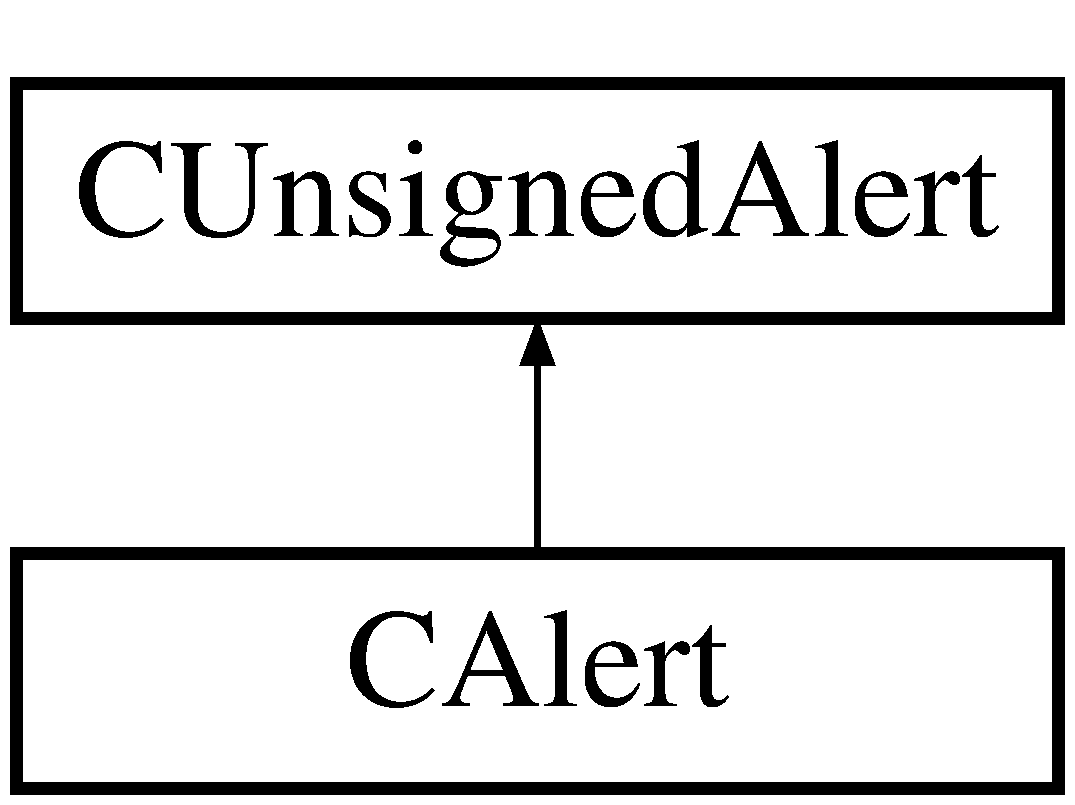
\includegraphics[height=2.000000cm]{class_c_alert}
\end{center}
\end{figure}
\subsection*{Public Member Functions}
\begin{DoxyCompactItemize}
\item 
\mbox{\hyperlink{class_c_alert_a116117e2318b9468a5ca80472c0b5157}{C\+Alert}} ()
\item 
{\footnotesize template$<$typename Stream , typename Operation $>$ }\\void \mbox{\hyperlink{class_c_alert_a51d73ab316bb42e65b87ec14ac536b14}{Serialization\+Op}} (Stream \&s, Operation ser\+\_\+action, int n\+Type, int \mbox{\hyperlink{class_c_unsigned_alert_ad8fad8e8f62caaf8162fad19170de2cf}{n\+Version}})
\item 
void \mbox{\hyperlink{class_c_alert_a93fd881c55ab448213787f49e316eb99}{Set\+Null}} ()
\item 
bool \mbox{\hyperlink{class_c_alert_a9c728b7fe91e74c51116a23b07d6978a}{Is\+Null}} () const
\item 
\mbox{\hyperlink{classuint256}{uint256}} \mbox{\hyperlink{class_c_alert_a059c136c9556e5e59a1a4dc39a97366d}{Get\+Hash}} () const
\item 
bool \mbox{\hyperlink{class_c_alert_a018da40779a5c095c38bf10f4256cee6}{Is\+In\+Effect}} () const
\item 
bool \mbox{\hyperlink{class_c_alert_a75777afd3418c6cd74f7e9e4caed3472}{Cancels}} (const \mbox{\hyperlink{class_c_alert}{C\+Alert}} \&alert) const
\item 
bool \mbox{\hyperlink{class_c_alert_a9e6ab19be3dc74242c2f535c3803ca96}{Applies\+To}} (int \mbox{\hyperlink{class_c_unsigned_alert_ad8fad8e8f62caaf8162fad19170de2cf}{n\+Version}}, const std\+::string \&str\+Sub\+Ver\+In) const
\item 
bool \mbox{\hyperlink{class_c_alert_aba79cc9e957446fe93f05cb18f12b24b}{Applies\+To\+Me}} () const
\item 
bool \mbox{\hyperlink{class_c_alert_a21a801f1a5978889722771d4eb13bf37}{Relay\+To}} (\mbox{\hyperlink{class_c_node}{C\+Node}} $\ast$pnode) const
\item 
bool \mbox{\hyperlink{class_c_alert_a07fea34252a3ef5b291237641caa7203}{Check\+Signature}} (const std\+::vector$<$ unsigned char $>$ \&alert\+Key) const
\item 
bool \mbox{\hyperlink{class_c_alert_af63a26aab450c2bc4781717e30ede67b}{Process\+Alert}} (const std\+::vector$<$ unsigned char $>$ \&alert\+Key, bool f\+Thread=true)
\end{DoxyCompactItemize}
\subsection*{Static Public Member Functions}
\begin{DoxyCompactItemize}
\item 
static void \mbox{\hyperlink{class_c_alert_a3da23857c8ed275621ee032a703c04a1}{Notify}} (const std\+::string \&str\+Message, bool f\+Thread)
\item 
static \mbox{\hyperlink{class_c_alert}{C\+Alert}} \mbox{\hyperlink{class_c_alert_aa37df9d177a6841ec5fa1e611c42b968}{get\+Alert\+By\+Hash}} (const \mbox{\hyperlink{classuint256}{uint256}} \&hash)
\end{DoxyCompactItemize}
\subsection*{Public Attributes}
\begin{DoxyCompactItemize}
\item 
std\+::vector$<$ unsigned char $>$ \mbox{\hyperlink{class_c_alert_abfcb3b339d052cd3dd6670b03286758a}{vch\+Msg}}
\item 
std\+::vector$<$ unsigned char $>$ \mbox{\hyperlink{class_c_alert_a541b49670ebf387a5f8b7de59277fed0}{vch\+Sig}}
\item 
\mbox{\hyperlink{class_c_alert_aca9310112e67fb38ef88f385a4ac6fc0}{A\+D\+D\+\_\+\+S\+E\+R\+I\+A\+L\+I\+Z\+E\+\_\+\+M\+E\+T\+H\+O\+DS}}
\end{DoxyCompactItemize}


\subsection{Detailed Description}
An alert is a combination of a serialized \mbox{\hyperlink{class_c_unsigned_alert}{C\+Unsigned\+Alert}} and a signature. 

\subsection{Constructor \& Destructor Documentation}
\mbox{\Hypertarget{class_c_alert_a116117e2318b9468a5ca80472c0b5157}\label{class_c_alert_a116117e2318b9468a5ca80472c0b5157}} 
\index{C\+Alert@{C\+Alert}!C\+Alert@{C\+Alert}}
\index{C\+Alert@{C\+Alert}!C\+Alert@{C\+Alert}}
\subsubsection{\texorpdfstring{C\+Alert()}{CAlert()}}
{\footnotesize\ttfamily C\+Alert\+::\+C\+Alert (\begin{DoxyParamCaption}{ }\end{DoxyParamCaption})\hspace{0.3cm}{\ttfamily [inline]}}



\subsection{Member Function Documentation}
\mbox{\Hypertarget{class_c_alert_a9e6ab19be3dc74242c2f535c3803ca96}\label{class_c_alert_a9e6ab19be3dc74242c2f535c3803ca96}} 
\index{C\+Alert@{C\+Alert}!Applies\+To@{Applies\+To}}
\index{Applies\+To@{Applies\+To}!C\+Alert@{C\+Alert}}
\subsubsection{\texorpdfstring{Applies\+To()}{AppliesTo()}}
{\footnotesize\ttfamily bool C\+Alert\+::\+Applies\+To (\begin{DoxyParamCaption}\item[{int}]{n\+Version,  }\item[{const std\+::string \&}]{str\+Sub\+Ver\+In }\end{DoxyParamCaption}) const}

\mbox{\Hypertarget{class_c_alert_aba79cc9e957446fe93f05cb18f12b24b}\label{class_c_alert_aba79cc9e957446fe93f05cb18f12b24b}} 
\index{C\+Alert@{C\+Alert}!Applies\+To\+Me@{Applies\+To\+Me}}
\index{Applies\+To\+Me@{Applies\+To\+Me}!C\+Alert@{C\+Alert}}
\subsubsection{\texorpdfstring{Applies\+To\+Me()}{AppliesToMe()}}
{\footnotesize\ttfamily bool C\+Alert\+::\+Applies\+To\+Me (\begin{DoxyParamCaption}{ }\end{DoxyParamCaption}) const}

\mbox{\Hypertarget{class_c_alert_a75777afd3418c6cd74f7e9e4caed3472}\label{class_c_alert_a75777afd3418c6cd74f7e9e4caed3472}} 
\index{C\+Alert@{C\+Alert}!Cancels@{Cancels}}
\index{Cancels@{Cancels}!C\+Alert@{C\+Alert}}
\subsubsection{\texorpdfstring{Cancels()}{Cancels()}}
{\footnotesize\ttfamily bool C\+Alert\+::\+Cancels (\begin{DoxyParamCaption}\item[{const \mbox{\hyperlink{class_c_alert}{C\+Alert}} \&}]{alert }\end{DoxyParamCaption}) const}

\mbox{\Hypertarget{class_c_alert_a07fea34252a3ef5b291237641caa7203}\label{class_c_alert_a07fea34252a3ef5b291237641caa7203}} 
\index{C\+Alert@{C\+Alert}!Check\+Signature@{Check\+Signature}}
\index{Check\+Signature@{Check\+Signature}!C\+Alert@{C\+Alert}}
\subsubsection{\texorpdfstring{Check\+Signature()}{CheckSignature()}}
{\footnotesize\ttfamily bool C\+Alert\+::\+Check\+Signature (\begin{DoxyParamCaption}\item[{const std\+::vector$<$ unsigned char $>$ \&}]{alert\+Key }\end{DoxyParamCaption}) const}

\mbox{\Hypertarget{class_c_alert_aa37df9d177a6841ec5fa1e611c42b968}\label{class_c_alert_aa37df9d177a6841ec5fa1e611c42b968}} 
\index{C\+Alert@{C\+Alert}!get\+Alert\+By\+Hash@{get\+Alert\+By\+Hash}}
\index{get\+Alert\+By\+Hash@{get\+Alert\+By\+Hash}!C\+Alert@{C\+Alert}}
\subsubsection{\texorpdfstring{get\+Alert\+By\+Hash()}{getAlertByHash()}}
{\footnotesize\ttfamily \mbox{\hyperlink{class_c_alert}{C\+Alert}} C\+Alert\+::get\+Alert\+By\+Hash (\begin{DoxyParamCaption}\item[{const \mbox{\hyperlink{classuint256}{uint256}} \&}]{hash }\end{DoxyParamCaption})\hspace{0.3cm}{\ttfamily [static]}}

\mbox{\Hypertarget{class_c_alert_a059c136c9556e5e59a1a4dc39a97366d}\label{class_c_alert_a059c136c9556e5e59a1a4dc39a97366d}} 
\index{C\+Alert@{C\+Alert}!Get\+Hash@{Get\+Hash}}
\index{Get\+Hash@{Get\+Hash}!C\+Alert@{C\+Alert}}
\subsubsection{\texorpdfstring{Get\+Hash()}{GetHash()}}
{\footnotesize\ttfamily \mbox{\hyperlink{classuint256}{uint256}} C\+Alert\+::\+Get\+Hash (\begin{DoxyParamCaption}{ }\end{DoxyParamCaption}) const}

\mbox{\Hypertarget{class_c_alert_a018da40779a5c095c38bf10f4256cee6}\label{class_c_alert_a018da40779a5c095c38bf10f4256cee6}} 
\index{C\+Alert@{C\+Alert}!Is\+In\+Effect@{Is\+In\+Effect}}
\index{Is\+In\+Effect@{Is\+In\+Effect}!C\+Alert@{C\+Alert}}
\subsubsection{\texorpdfstring{Is\+In\+Effect()}{IsInEffect()}}
{\footnotesize\ttfamily bool C\+Alert\+::\+Is\+In\+Effect (\begin{DoxyParamCaption}{ }\end{DoxyParamCaption}) const}

\mbox{\Hypertarget{class_c_alert_a9c728b7fe91e74c51116a23b07d6978a}\label{class_c_alert_a9c728b7fe91e74c51116a23b07d6978a}} 
\index{C\+Alert@{C\+Alert}!Is\+Null@{Is\+Null}}
\index{Is\+Null@{Is\+Null}!C\+Alert@{C\+Alert}}
\subsubsection{\texorpdfstring{Is\+Null()}{IsNull()}}
{\footnotesize\ttfamily bool C\+Alert\+::\+Is\+Null (\begin{DoxyParamCaption}{ }\end{DoxyParamCaption}) const}

\mbox{\Hypertarget{class_c_alert_a3da23857c8ed275621ee032a703c04a1}\label{class_c_alert_a3da23857c8ed275621ee032a703c04a1}} 
\index{C\+Alert@{C\+Alert}!Notify@{Notify}}
\index{Notify@{Notify}!C\+Alert@{C\+Alert}}
\subsubsection{\texorpdfstring{Notify()}{Notify()}}
{\footnotesize\ttfamily void C\+Alert\+::\+Notify (\begin{DoxyParamCaption}\item[{const std\+::string \&}]{str\+Message,  }\item[{bool}]{f\+Thread }\end{DoxyParamCaption})\hspace{0.3cm}{\ttfamily [static]}}

\mbox{\Hypertarget{class_c_alert_af63a26aab450c2bc4781717e30ede67b}\label{class_c_alert_af63a26aab450c2bc4781717e30ede67b}} 
\index{C\+Alert@{C\+Alert}!Process\+Alert@{Process\+Alert}}
\index{Process\+Alert@{Process\+Alert}!C\+Alert@{C\+Alert}}
\subsubsection{\texorpdfstring{Process\+Alert()}{ProcessAlert()}}
{\footnotesize\ttfamily bool C\+Alert\+::\+Process\+Alert (\begin{DoxyParamCaption}\item[{const std\+::vector$<$ unsigned char $>$ \&}]{alert\+Key,  }\item[{bool}]{f\+Thread = {\ttfamily true} }\end{DoxyParamCaption})}

\mbox{\Hypertarget{class_c_alert_a21a801f1a5978889722771d4eb13bf37}\label{class_c_alert_a21a801f1a5978889722771d4eb13bf37}} 
\index{C\+Alert@{C\+Alert}!Relay\+To@{Relay\+To}}
\index{Relay\+To@{Relay\+To}!C\+Alert@{C\+Alert}}
\subsubsection{\texorpdfstring{Relay\+To()}{RelayTo()}}
{\footnotesize\ttfamily bool C\+Alert\+::\+Relay\+To (\begin{DoxyParamCaption}\item[{\mbox{\hyperlink{class_c_node}{C\+Node}} $\ast$}]{pnode }\end{DoxyParamCaption}) const}

\mbox{\Hypertarget{class_c_alert_a51d73ab316bb42e65b87ec14ac536b14}\label{class_c_alert_a51d73ab316bb42e65b87ec14ac536b14}} 
\index{C\+Alert@{C\+Alert}!Serialization\+Op@{Serialization\+Op}}
\index{Serialization\+Op@{Serialization\+Op}!C\+Alert@{C\+Alert}}
\subsubsection{\texorpdfstring{Serialization\+Op()}{SerializationOp()}}
{\footnotesize\ttfamily template$<$typename Stream , typename Operation $>$ \\
void C\+Alert\+::\+Serialization\+Op (\begin{DoxyParamCaption}\item[{Stream \&}]{s,  }\item[{Operation}]{ser\+\_\+action,  }\item[{int}]{n\+Type,  }\item[{int}]{n\+Version }\end{DoxyParamCaption})\hspace{0.3cm}{\ttfamily [inline]}}

\mbox{\Hypertarget{class_c_alert_a93fd881c55ab448213787f49e316eb99}\label{class_c_alert_a93fd881c55ab448213787f49e316eb99}} 
\index{C\+Alert@{C\+Alert}!Set\+Null@{Set\+Null}}
\index{Set\+Null@{Set\+Null}!C\+Alert@{C\+Alert}}
\subsubsection{\texorpdfstring{Set\+Null()}{SetNull()}}
{\footnotesize\ttfamily void C\+Alert\+::\+Set\+Null (\begin{DoxyParamCaption}{ }\end{DoxyParamCaption})}



\subsection{Member Data Documentation}
\mbox{\Hypertarget{class_c_alert_aca9310112e67fb38ef88f385a4ac6fc0}\label{class_c_alert_aca9310112e67fb38ef88f385a4ac6fc0}} 
\index{C\+Alert@{C\+Alert}!A\+D\+D\+\_\+\+S\+E\+R\+I\+A\+L\+I\+Z\+E\+\_\+\+M\+E\+T\+H\+O\+DS@{A\+D\+D\+\_\+\+S\+E\+R\+I\+A\+L\+I\+Z\+E\+\_\+\+M\+E\+T\+H\+O\+DS}}
\index{A\+D\+D\+\_\+\+S\+E\+R\+I\+A\+L\+I\+Z\+E\+\_\+\+M\+E\+T\+H\+O\+DS@{A\+D\+D\+\_\+\+S\+E\+R\+I\+A\+L\+I\+Z\+E\+\_\+\+M\+E\+T\+H\+O\+DS}!C\+Alert@{C\+Alert}}
\subsubsection{\texorpdfstring{A\+D\+D\+\_\+\+S\+E\+R\+I\+A\+L\+I\+Z\+E\+\_\+\+M\+E\+T\+H\+O\+DS}{ADD\_SERIALIZE\_METHODS}}
{\footnotesize\ttfamily C\+Alert\+::\+A\+D\+D\+\_\+\+S\+E\+R\+I\+A\+L\+I\+Z\+E\+\_\+\+M\+E\+T\+H\+O\+DS}

\mbox{\Hypertarget{class_c_alert_abfcb3b339d052cd3dd6670b03286758a}\label{class_c_alert_abfcb3b339d052cd3dd6670b03286758a}} 
\index{C\+Alert@{C\+Alert}!vch\+Msg@{vch\+Msg}}
\index{vch\+Msg@{vch\+Msg}!C\+Alert@{C\+Alert}}
\subsubsection{\texorpdfstring{vch\+Msg}{vchMsg}}
{\footnotesize\ttfamily std\+::vector$<$unsigned char$>$ C\+Alert\+::vch\+Msg}

\mbox{\Hypertarget{class_c_alert_a541b49670ebf387a5f8b7de59277fed0}\label{class_c_alert_a541b49670ebf387a5f8b7de59277fed0}} 
\index{C\+Alert@{C\+Alert}!vch\+Sig@{vch\+Sig}}
\index{vch\+Sig@{vch\+Sig}!C\+Alert@{C\+Alert}}
\subsubsection{\texorpdfstring{vch\+Sig}{vchSig}}
{\footnotesize\ttfamily std\+::vector$<$unsigned char$>$ C\+Alert\+::vch\+Sig}



The documentation for this class was generated from the following files\+:\begin{DoxyCompactItemize}
\item 
/\+Users/christopherarguello/\+Developer/anon/src/\mbox{\hyperlink{alert_8h}{alert.\+h}}\item 
/\+Users/christopherarguello/\+Developer/anon/src/\mbox{\hyperlink{alert_8cpp}{alert.\+cpp}}\end{DoxyCompactItemize}

\hypertarget{struct_c_anchors_cache_entry}{}\section{C\+Anchors\+Cache\+Entry Struct Reference}
\label{struct_c_anchors_cache_entry}\index{C\+Anchors\+Cache\+Entry@{C\+Anchors\+Cache\+Entry}}


{\ttfamily \#include $<$coins.\+h$>$}

\subsection*{Public Types}
\begin{DoxyCompactItemize}
\item 
enum \mbox{\hyperlink{struct_c_anchors_cache_entry_aaf2aa4f4663f8bdd074097c1850be878}{Flags}} \{ \mbox{\hyperlink{struct_c_anchors_cache_entry_aaf2aa4f4663f8bdd074097c1850be878aae0255f04162d6f09aaaeac34ecaedbd}{D\+I\+R\+TY}} = (1 $<$$<$ 0)
 \}
\end{DoxyCompactItemize}
\subsection*{Public Member Functions}
\begin{DoxyCompactItemize}
\item 
\mbox{\hyperlink{struct_c_anchors_cache_entry_a878e921414637acb2c1bb937616d9ed9}{C\+Anchors\+Cache\+Entry}} ()
\end{DoxyCompactItemize}
\subsection*{Public Attributes}
\begin{DoxyCompactItemize}
\item 
bool \mbox{\hyperlink{struct_c_anchors_cache_entry_a8f7bb74fd03bad6d4492a1d6528531e5}{entered}}
\item 
Z\+C\+Incremental\+Merkle\+Tree \mbox{\hyperlink{struct_c_anchors_cache_entry_a226001cb91886f33a603d449b39f28a0}{tree}}
\item 
unsigned char \mbox{\hyperlink{struct_c_anchors_cache_entry_a9d421b72885a038bb1586b5fb07fd660}{flags}}
\end{DoxyCompactItemize}


\subsection{Member Enumeration Documentation}
\mbox{\Hypertarget{struct_c_anchors_cache_entry_aaf2aa4f4663f8bdd074097c1850be878}\label{struct_c_anchors_cache_entry_aaf2aa4f4663f8bdd074097c1850be878}} 
\index{C\+Anchors\+Cache\+Entry@{C\+Anchors\+Cache\+Entry}!Flags@{Flags}}
\index{Flags@{Flags}!C\+Anchors\+Cache\+Entry@{C\+Anchors\+Cache\+Entry}}
\subsubsection{\texorpdfstring{Flags}{Flags}}
{\footnotesize\ttfamily enum \mbox{\hyperlink{struct_c_anchors_cache_entry_aaf2aa4f4663f8bdd074097c1850be878}{C\+Anchors\+Cache\+Entry\+::\+Flags}}}

\begin{DoxyEnumFields}{Enumerator}
\raisebox{\heightof{T}}[0pt][0pt]{\index{D\+I\+R\+TY@{D\+I\+R\+TY}!C\+Anchors\+Cache\+Entry@{C\+Anchors\+Cache\+Entry}}\index{C\+Anchors\+Cache\+Entry@{C\+Anchors\+Cache\+Entry}!D\+I\+R\+TY@{D\+I\+R\+TY}}}\mbox{\Hypertarget{struct_c_anchors_cache_entry_aaf2aa4f4663f8bdd074097c1850be878aae0255f04162d6f09aaaeac34ecaedbd}\label{struct_c_anchors_cache_entry_aaf2aa4f4663f8bdd074097c1850be878aae0255f04162d6f09aaaeac34ecaedbd}} 
D\+I\+R\+TY&\\
\hline

\end{DoxyEnumFields}


\subsection{Constructor \& Destructor Documentation}
\mbox{\Hypertarget{struct_c_anchors_cache_entry_a878e921414637acb2c1bb937616d9ed9}\label{struct_c_anchors_cache_entry_a878e921414637acb2c1bb937616d9ed9}} 
\index{C\+Anchors\+Cache\+Entry@{C\+Anchors\+Cache\+Entry}!C\+Anchors\+Cache\+Entry@{C\+Anchors\+Cache\+Entry}}
\index{C\+Anchors\+Cache\+Entry@{C\+Anchors\+Cache\+Entry}!C\+Anchors\+Cache\+Entry@{C\+Anchors\+Cache\+Entry}}
\subsubsection{\texorpdfstring{C\+Anchors\+Cache\+Entry()}{CAnchorsCacheEntry()}}
{\footnotesize\ttfamily C\+Anchors\+Cache\+Entry\+::\+C\+Anchors\+Cache\+Entry (\begin{DoxyParamCaption}{ }\end{DoxyParamCaption})\hspace{0.3cm}{\ttfamily [inline]}}



\subsection{Member Data Documentation}
\mbox{\Hypertarget{struct_c_anchors_cache_entry_a8f7bb74fd03bad6d4492a1d6528531e5}\label{struct_c_anchors_cache_entry_a8f7bb74fd03bad6d4492a1d6528531e5}} 
\index{C\+Anchors\+Cache\+Entry@{C\+Anchors\+Cache\+Entry}!entered@{entered}}
\index{entered@{entered}!C\+Anchors\+Cache\+Entry@{C\+Anchors\+Cache\+Entry}}
\subsubsection{\texorpdfstring{entered}{entered}}
{\footnotesize\ttfamily bool C\+Anchors\+Cache\+Entry\+::entered}

\mbox{\Hypertarget{struct_c_anchors_cache_entry_a9d421b72885a038bb1586b5fb07fd660}\label{struct_c_anchors_cache_entry_a9d421b72885a038bb1586b5fb07fd660}} 
\index{C\+Anchors\+Cache\+Entry@{C\+Anchors\+Cache\+Entry}!flags@{flags}}
\index{flags@{flags}!C\+Anchors\+Cache\+Entry@{C\+Anchors\+Cache\+Entry}}
\subsubsection{\texorpdfstring{flags}{flags}}
{\footnotesize\ttfamily unsigned char C\+Anchors\+Cache\+Entry\+::flags}

\mbox{\Hypertarget{struct_c_anchors_cache_entry_a226001cb91886f33a603d449b39f28a0}\label{struct_c_anchors_cache_entry_a226001cb91886f33a603d449b39f28a0}} 
\index{C\+Anchors\+Cache\+Entry@{C\+Anchors\+Cache\+Entry}!tree@{tree}}
\index{tree@{tree}!C\+Anchors\+Cache\+Entry@{C\+Anchors\+Cache\+Entry}}
\subsubsection{\texorpdfstring{tree}{tree}}
{\footnotesize\ttfamily Z\+C\+Incremental\+Merkle\+Tree C\+Anchors\+Cache\+Entry\+::tree}



The documentation for this struct was generated from the following file\+:\begin{DoxyCompactItemize}
\item 
/\+Users/christopherarguello/\+Developer/anon/src/\mbox{\hyperlink{coins_8h}{coins.\+h}}\end{DoxyCompactItemize}

\hypertarget{class_c_auto_file}{}\section{C\+Auto\+File Class Reference}
\label{class_c_auto_file}\index{C\+Auto\+File@{C\+Auto\+File}}


{\ttfamily \#include $<$streams.\+h$>$}

\subsection*{Public Member Functions}
\begin{DoxyCompactItemize}
\item 
\mbox{\hyperlink{class_c_auto_file_a52613083aaeab4c9238c649ae471783f}{C\+Auto\+File}} (F\+I\+LE $\ast$filenew, int n\+Type\+In, int n\+Version\+In)
\item 
\mbox{\hyperlink{class_c_auto_file_ab1362f4cb52c819c25cff4598e0f28da}{$\sim$\+C\+Auto\+File}} ()
\item 
void \mbox{\hyperlink{class_c_auto_file_abcbafe943bfe392c09363078fa8a4e77}{fclose}} ()
\item 
F\+I\+LE $\ast$ \mbox{\hyperlink{class_c_auto_file_a25b51d94dc85c4140da0b15494ac9f8a}{release}} ()
\item 
F\+I\+LE $\ast$ \mbox{\hyperlink{class_c_auto_file_a2c1ad2d25562fea82a54bdef2793a0dd}{Get}} () const
\item 
bool \mbox{\hyperlink{class_c_auto_file_a7fd47268b6d85a89acafdb73559f8e78}{Is\+Null}} () const
\item 
void \mbox{\hyperlink{class_c_auto_file_ac1a3986f191fe81384f58fc5fa073820}{Set\+Type}} (int n)
\item 
int \mbox{\hyperlink{class_c_auto_file_a774f2aad2c462d4ff47125ceec2ebab0}{Get\+Type}} ()
\item 
void \mbox{\hyperlink{class_c_auto_file_a51f805bc470a95c9948250503b587aec}{Set\+Version}} (int n)
\item 
int \mbox{\hyperlink{class_c_auto_file_a976ab8e5477aedd3a531fc49b01153ce}{Get\+Version}} ()
\item 
void \mbox{\hyperlink{class_c_auto_file_a9511060b5c971cff532faeab60c7d88b}{Read\+Version}} ()
\item 
void \mbox{\hyperlink{class_c_auto_file_a23d6f22c3aff80be7665bfc5a77a01ff}{Write\+Version}} ()
\item 
\mbox{\hyperlink{class_c_auto_file}{C\+Auto\+File}} \& \mbox{\hyperlink{class_c_auto_file_a87e670f3dd03055264c05b25335babb4}{read}} (char $\ast$pch, size\+\_\+t n\+Size)
\item 
\mbox{\hyperlink{class_c_auto_file}{C\+Auto\+File}} \& \mbox{\hyperlink{class_c_auto_file_a0159b896d7ed2574cc32663987bfc0ce}{ignore}} (size\+\_\+t n\+Size)
\item 
\mbox{\hyperlink{class_c_auto_file}{C\+Auto\+File}} \& \mbox{\hyperlink{class_c_auto_file_a7b2852b345b75835f883be3732cf826a}{write}} (const char $\ast$pch, size\+\_\+t n\+Size)
\item 
{\footnotesize template$<$typename T $>$ }\\unsigned int \mbox{\hyperlink{class_c_auto_file_a883a261f0d7d0320f72152ff2167fd24}{Get\+Serialize\+Size}} (const T \&obj)
\item 
{\footnotesize template$<$typename T $>$ }\\\mbox{\hyperlink{class_c_auto_file}{C\+Auto\+File}} \& \mbox{\hyperlink{class_c_auto_file_a8e194596d1f8f64059247724b25df82c}{operator$<$$<$}} (const T \&obj)
\item 
{\footnotesize template$<$typename T $>$ }\\\mbox{\hyperlink{class_c_auto_file}{C\+Auto\+File}} \& \mbox{\hyperlink{class_c_auto_file_ae6826219322626d2ac8229e022c41dd7}{operator$>$$>$}} (T \&obj)
\end{DoxyCompactItemize}
\subsection*{Private Member Functions}
\begin{DoxyCompactItemize}
\item 
\mbox{\hyperlink{class_c_auto_file_a2d7c38154632735962c24d472c01608c}{C\+Auto\+File}} (const \mbox{\hyperlink{class_c_auto_file}{C\+Auto\+File}} \&)
\item 
\mbox{\hyperlink{class_c_auto_file}{C\+Auto\+File}} \& \mbox{\hyperlink{class_c_auto_file_a5937561da10e79c2da4bb47c0fc57d96}{operator=}} (const \mbox{\hyperlink{class_c_auto_file}{C\+Auto\+File}} \&)
\end{DoxyCompactItemize}
\subsection*{Private Attributes}
\begin{DoxyCompactItemize}
\item 
int \mbox{\hyperlink{class_c_auto_file_a39ca705ff45e36a05acd5df3c4114aef}{n\+Type}}
\item 
int \mbox{\hyperlink{class_c_auto_file_a23fb456ee23003aebc3c58ab3fd683c1}{n\+Version}}
\item 
F\+I\+LE $\ast$ \mbox{\hyperlink{class_c_auto_file_a04ae666616ebc5d873c636fe6d2998ff}{file}}
\end{DoxyCompactItemize}


\subsection{Detailed Description}
Non-\/refcounted R\+A\+II wrapper for F\+I\+L\+E$\ast$

Will automatically close the file when it goes out of scope if not null. If you\textquotesingle{}re returning the file pointer, return file.\+release(). If you need to close the file early, use file.\+fclose() instead of fclose(file). 

\subsection{Constructor \& Destructor Documentation}
\mbox{\Hypertarget{class_c_auto_file_a2d7c38154632735962c24d472c01608c}\label{class_c_auto_file_a2d7c38154632735962c24d472c01608c}} 
\index{C\+Auto\+File@{C\+Auto\+File}!C\+Auto\+File@{C\+Auto\+File}}
\index{C\+Auto\+File@{C\+Auto\+File}!C\+Auto\+File@{C\+Auto\+File}}
\subsubsection{\texorpdfstring{C\+Auto\+File()}{CAutoFile()}\hspace{0.1cm}{\footnotesize\ttfamily [1/2]}}
{\footnotesize\ttfamily C\+Auto\+File\+::\+C\+Auto\+File (\begin{DoxyParamCaption}\item[{const \mbox{\hyperlink{class_c_auto_file}{C\+Auto\+File}} \&}]{ }\end{DoxyParamCaption})\hspace{0.3cm}{\ttfamily [private]}}

\mbox{\Hypertarget{class_c_auto_file_a52613083aaeab4c9238c649ae471783f}\label{class_c_auto_file_a52613083aaeab4c9238c649ae471783f}} 
\index{C\+Auto\+File@{C\+Auto\+File}!C\+Auto\+File@{C\+Auto\+File}}
\index{C\+Auto\+File@{C\+Auto\+File}!C\+Auto\+File@{C\+Auto\+File}}
\subsubsection{\texorpdfstring{C\+Auto\+File()}{CAutoFile()}\hspace{0.1cm}{\footnotesize\ttfamily [2/2]}}
{\footnotesize\ttfamily C\+Auto\+File\+::\+C\+Auto\+File (\begin{DoxyParamCaption}\item[{F\+I\+LE $\ast$}]{filenew,  }\item[{int}]{n\+Type\+In,  }\item[{int}]{n\+Version\+In }\end{DoxyParamCaption})\hspace{0.3cm}{\ttfamily [inline]}}

\mbox{\Hypertarget{class_c_auto_file_ab1362f4cb52c819c25cff4598e0f28da}\label{class_c_auto_file_ab1362f4cb52c819c25cff4598e0f28da}} 
\index{C\+Auto\+File@{C\+Auto\+File}!````~C\+Auto\+File@{$\sim$\+C\+Auto\+File}}
\index{````~C\+Auto\+File@{$\sim$\+C\+Auto\+File}!C\+Auto\+File@{C\+Auto\+File}}
\subsubsection{\texorpdfstring{$\sim$\+C\+Auto\+File()}{~CAutoFile()}}
{\footnotesize\ttfamily C\+Auto\+File\+::$\sim$\+C\+Auto\+File (\begin{DoxyParamCaption}{ }\end{DoxyParamCaption})\hspace{0.3cm}{\ttfamily [inline]}}



\subsection{Member Function Documentation}
\mbox{\Hypertarget{class_c_auto_file_abcbafe943bfe392c09363078fa8a4e77}\label{class_c_auto_file_abcbafe943bfe392c09363078fa8a4e77}} 
\index{C\+Auto\+File@{C\+Auto\+File}!fclose@{fclose}}
\index{fclose@{fclose}!C\+Auto\+File@{C\+Auto\+File}}
\subsubsection{\texorpdfstring{fclose()}{fclose()}}
{\footnotesize\ttfamily void C\+Auto\+File\+::fclose (\begin{DoxyParamCaption}{ }\end{DoxyParamCaption})\hspace{0.3cm}{\ttfamily [inline]}}

\mbox{\Hypertarget{class_c_auto_file_a2c1ad2d25562fea82a54bdef2793a0dd}\label{class_c_auto_file_a2c1ad2d25562fea82a54bdef2793a0dd}} 
\index{C\+Auto\+File@{C\+Auto\+File}!Get@{Get}}
\index{Get@{Get}!C\+Auto\+File@{C\+Auto\+File}}
\subsubsection{\texorpdfstring{Get()}{Get()}}
{\footnotesize\ttfamily F\+I\+LE$\ast$ C\+Auto\+File\+::\+Get (\begin{DoxyParamCaption}{ }\end{DoxyParamCaption}) const\hspace{0.3cm}{\ttfamily [inline]}}

Get wrapped F\+I\+L\+E$\ast$ without transfer of ownership. \begin{DoxyNote}{Note}
Ownership of the F\+I\+L\+E$\ast$ will remain with this class. Use this only if the scope of the \mbox{\hyperlink{class_c_auto_file}{C\+Auto\+File}} outlives use of the passed pointer. 
\end{DoxyNote}
\mbox{\Hypertarget{class_c_auto_file_a883a261f0d7d0320f72152ff2167fd24}\label{class_c_auto_file_a883a261f0d7d0320f72152ff2167fd24}} 
\index{C\+Auto\+File@{C\+Auto\+File}!Get\+Serialize\+Size@{Get\+Serialize\+Size}}
\index{Get\+Serialize\+Size@{Get\+Serialize\+Size}!C\+Auto\+File@{C\+Auto\+File}}
\subsubsection{\texorpdfstring{Get\+Serialize\+Size()}{GetSerializeSize()}}
{\footnotesize\ttfamily template$<$typename T $>$ \\
unsigned int C\+Auto\+File\+::\+Get\+Serialize\+Size (\begin{DoxyParamCaption}\item[{const T \&}]{obj }\end{DoxyParamCaption})\hspace{0.3cm}{\ttfamily [inline]}}

\mbox{\Hypertarget{class_c_auto_file_a774f2aad2c462d4ff47125ceec2ebab0}\label{class_c_auto_file_a774f2aad2c462d4ff47125ceec2ebab0}} 
\index{C\+Auto\+File@{C\+Auto\+File}!Get\+Type@{Get\+Type}}
\index{Get\+Type@{Get\+Type}!C\+Auto\+File@{C\+Auto\+File}}
\subsubsection{\texorpdfstring{Get\+Type()}{GetType()}}
{\footnotesize\ttfamily int C\+Auto\+File\+::\+Get\+Type (\begin{DoxyParamCaption}{ }\end{DoxyParamCaption})\hspace{0.3cm}{\ttfamily [inline]}}

\mbox{\Hypertarget{class_c_auto_file_a976ab8e5477aedd3a531fc49b01153ce}\label{class_c_auto_file_a976ab8e5477aedd3a531fc49b01153ce}} 
\index{C\+Auto\+File@{C\+Auto\+File}!Get\+Version@{Get\+Version}}
\index{Get\+Version@{Get\+Version}!C\+Auto\+File@{C\+Auto\+File}}
\subsubsection{\texorpdfstring{Get\+Version()}{GetVersion()}}
{\footnotesize\ttfamily int C\+Auto\+File\+::\+Get\+Version (\begin{DoxyParamCaption}{ }\end{DoxyParamCaption})\hspace{0.3cm}{\ttfamily [inline]}}

\mbox{\Hypertarget{class_c_auto_file_a0159b896d7ed2574cc32663987bfc0ce}\label{class_c_auto_file_a0159b896d7ed2574cc32663987bfc0ce}} 
\index{C\+Auto\+File@{C\+Auto\+File}!ignore@{ignore}}
\index{ignore@{ignore}!C\+Auto\+File@{C\+Auto\+File}}
\subsubsection{\texorpdfstring{ignore()}{ignore()}}
{\footnotesize\ttfamily \mbox{\hyperlink{class_c_auto_file}{C\+Auto\+File}}\& C\+Auto\+File\+::ignore (\begin{DoxyParamCaption}\item[{size\+\_\+t}]{n\+Size }\end{DoxyParamCaption})\hspace{0.3cm}{\ttfamily [inline]}}

\mbox{\Hypertarget{class_c_auto_file_a7fd47268b6d85a89acafdb73559f8e78}\label{class_c_auto_file_a7fd47268b6d85a89acafdb73559f8e78}} 
\index{C\+Auto\+File@{C\+Auto\+File}!Is\+Null@{Is\+Null}}
\index{Is\+Null@{Is\+Null}!C\+Auto\+File@{C\+Auto\+File}}
\subsubsection{\texorpdfstring{Is\+Null()}{IsNull()}}
{\footnotesize\ttfamily bool C\+Auto\+File\+::\+Is\+Null (\begin{DoxyParamCaption}{ }\end{DoxyParamCaption}) const\hspace{0.3cm}{\ttfamily [inline]}}

Return true if the wrapped F\+I\+L\+E$\ast$ is N\+U\+LL, false otherwise. \mbox{\Hypertarget{class_c_auto_file_a8e194596d1f8f64059247724b25df82c}\label{class_c_auto_file_a8e194596d1f8f64059247724b25df82c}} 
\index{C\+Auto\+File@{C\+Auto\+File}!operator$<$$<$@{operator$<$$<$}}
\index{operator$<$$<$@{operator$<$$<$}!C\+Auto\+File@{C\+Auto\+File}}
\subsubsection{\texorpdfstring{operator$<$$<$()}{operator<<()}}
{\footnotesize\ttfamily template$<$typename T $>$ \\
\mbox{\hyperlink{class_c_auto_file}{C\+Auto\+File}}\& C\+Auto\+File\+::operator$<$$<$ (\begin{DoxyParamCaption}\item[{const T \&}]{obj }\end{DoxyParamCaption})\hspace{0.3cm}{\ttfamily [inline]}}

\mbox{\Hypertarget{class_c_auto_file_a5937561da10e79c2da4bb47c0fc57d96}\label{class_c_auto_file_a5937561da10e79c2da4bb47c0fc57d96}} 
\index{C\+Auto\+File@{C\+Auto\+File}!operator=@{operator=}}
\index{operator=@{operator=}!C\+Auto\+File@{C\+Auto\+File}}
\subsubsection{\texorpdfstring{operator=()}{operator=()}}
{\footnotesize\ttfamily \mbox{\hyperlink{class_c_auto_file}{C\+Auto\+File}}\& C\+Auto\+File\+::operator= (\begin{DoxyParamCaption}\item[{const \mbox{\hyperlink{class_c_auto_file}{C\+Auto\+File}} \&}]{ }\end{DoxyParamCaption})\hspace{0.3cm}{\ttfamily [private]}}

\mbox{\Hypertarget{class_c_auto_file_ae6826219322626d2ac8229e022c41dd7}\label{class_c_auto_file_ae6826219322626d2ac8229e022c41dd7}} 
\index{C\+Auto\+File@{C\+Auto\+File}!operator$>$$>$@{operator$>$$>$}}
\index{operator$>$$>$@{operator$>$$>$}!C\+Auto\+File@{C\+Auto\+File}}
\subsubsection{\texorpdfstring{operator$>$$>$()}{operator>>()}}
{\footnotesize\ttfamily template$<$typename T $>$ \\
\mbox{\hyperlink{class_c_auto_file}{C\+Auto\+File}}\& C\+Auto\+File\+::operator$>$$>$ (\begin{DoxyParamCaption}\item[{T \&}]{obj }\end{DoxyParamCaption})\hspace{0.3cm}{\ttfamily [inline]}}

\mbox{\Hypertarget{class_c_auto_file_a87e670f3dd03055264c05b25335babb4}\label{class_c_auto_file_a87e670f3dd03055264c05b25335babb4}} 
\index{C\+Auto\+File@{C\+Auto\+File}!read@{read}}
\index{read@{read}!C\+Auto\+File@{C\+Auto\+File}}
\subsubsection{\texorpdfstring{read()}{read()}}
{\footnotesize\ttfamily \mbox{\hyperlink{class_c_auto_file}{C\+Auto\+File}}\& C\+Auto\+File\+::read (\begin{DoxyParamCaption}\item[{char $\ast$}]{pch,  }\item[{size\+\_\+t}]{n\+Size }\end{DoxyParamCaption})\hspace{0.3cm}{\ttfamily [inline]}}

\mbox{\Hypertarget{class_c_auto_file_a9511060b5c971cff532faeab60c7d88b}\label{class_c_auto_file_a9511060b5c971cff532faeab60c7d88b}} 
\index{C\+Auto\+File@{C\+Auto\+File}!Read\+Version@{Read\+Version}}
\index{Read\+Version@{Read\+Version}!C\+Auto\+File@{C\+Auto\+File}}
\subsubsection{\texorpdfstring{Read\+Version()}{ReadVersion()}}
{\footnotesize\ttfamily void C\+Auto\+File\+::\+Read\+Version (\begin{DoxyParamCaption}{ }\end{DoxyParamCaption})\hspace{0.3cm}{\ttfamily [inline]}}

\mbox{\Hypertarget{class_c_auto_file_a25b51d94dc85c4140da0b15494ac9f8a}\label{class_c_auto_file_a25b51d94dc85c4140da0b15494ac9f8a}} 
\index{C\+Auto\+File@{C\+Auto\+File}!release@{release}}
\index{release@{release}!C\+Auto\+File@{C\+Auto\+File}}
\subsubsection{\texorpdfstring{release()}{release()}}
{\footnotesize\ttfamily F\+I\+LE$\ast$ C\+Auto\+File\+::release (\begin{DoxyParamCaption}{ }\end{DoxyParamCaption})\hspace{0.3cm}{\ttfamily [inline]}}

Get wrapped F\+I\+L\+E$\ast$ with transfer of ownership. \begin{DoxyNote}{Note}
This will invalidate the \mbox{\hyperlink{class_c_auto_file}{C\+Auto\+File}} object, and makes it the responsibility of the caller of this function to clean up the returned F\+I\+L\+E$\ast$. 
\end{DoxyNote}
\mbox{\Hypertarget{class_c_auto_file_ac1a3986f191fe81384f58fc5fa073820}\label{class_c_auto_file_ac1a3986f191fe81384f58fc5fa073820}} 
\index{C\+Auto\+File@{C\+Auto\+File}!Set\+Type@{Set\+Type}}
\index{Set\+Type@{Set\+Type}!C\+Auto\+File@{C\+Auto\+File}}
\subsubsection{\texorpdfstring{Set\+Type()}{SetType()}}
{\footnotesize\ttfamily void C\+Auto\+File\+::\+Set\+Type (\begin{DoxyParamCaption}\item[{int}]{n }\end{DoxyParamCaption})\hspace{0.3cm}{\ttfamily [inline]}}

\mbox{\Hypertarget{class_c_auto_file_a51f805bc470a95c9948250503b587aec}\label{class_c_auto_file_a51f805bc470a95c9948250503b587aec}} 
\index{C\+Auto\+File@{C\+Auto\+File}!Set\+Version@{Set\+Version}}
\index{Set\+Version@{Set\+Version}!C\+Auto\+File@{C\+Auto\+File}}
\subsubsection{\texorpdfstring{Set\+Version()}{SetVersion()}}
{\footnotesize\ttfamily void C\+Auto\+File\+::\+Set\+Version (\begin{DoxyParamCaption}\item[{int}]{n }\end{DoxyParamCaption})\hspace{0.3cm}{\ttfamily [inline]}}

\mbox{\Hypertarget{class_c_auto_file_a7b2852b345b75835f883be3732cf826a}\label{class_c_auto_file_a7b2852b345b75835f883be3732cf826a}} 
\index{C\+Auto\+File@{C\+Auto\+File}!write@{write}}
\index{write@{write}!C\+Auto\+File@{C\+Auto\+File}}
\subsubsection{\texorpdfstring{write()}{write()}}
{\footnotesize\ttfamily \mbox{\hyperlink{class_c_auto_file}{C\+Auto\+File}}\& C\+Auto\+File\+::write (\begin{DoxyParamCaption}\item[{const char $\ast$}]{pch,  }\item[{size\+\_\+t}]{n\+Size }\end{DoxyParamCaption})\hspace{0.3cm}{\ttfamily [inline]}}

\mbox{\Hypertarget{class_c_auto_file_a23d6f22c3aff80be7665bfc5a77a01ff}\label{class_c_auto_file_a23d6f22c3aff80be7665bfc5a77a01ff}} 
\index{C\+Auto\+File@{C\+Auto\+File}!Write\+Version@{Write\+Version}}
\index{Write\+Version@{Write\+Version}!C\+Auto\+File@{C\+Auto\+File}}
\subsubsection{\texorpdfstring{Write\+Version()}{WriteVersion()}}
{\footnotesize\ttfamily void C\+Auto\+File\+::\+Write\+Version (\begin{DoxyParamCaption}{ }\end{DoxyParamCaption})\hspace{0.3cm}{\ttfamily [inline]}}



\subsection{Member Data Documentation}
\mbox{\Hypertarget{class_c_auto_file_a04ae666616ebc5d873c636fe6d2998ff}\label{class_c_auto_file_a04ae666616ebc5d873c636fe6d2998ff}} 
\index{C\+Auto\+File@{C\+Auto\+File}!file@{file}}
\index{file@{file}!C\+Auto\+File@{C\+Auto\+File}}
\subsubsection{\texorpdfstring{file}{file}}
{\footnotesize\ttfamily F\+I\+LE$\ast$ C\+Auto\+File\+::file\hspace{0.3cm}{\ttfamily [private]}}

\mbox{\Hypertarget{class_c_auto_file_a39ca705ff45e36a05acd5df3c4114aef}\label{class_c_auto_file_a39ca705ff45e36a05acd5df3c4114aef}} 
\index{C\+Auto\+File@{C\+Auto\+File}!n\+Type@{n\+Type}}
\index{n\+Type@{n\+Type}!C\+Auto\+File@{C\+Auto\+File}}
\subsubsection{\texorpdfstring{n\+Type}{nType}}
{\footnotesize\ttfamily int C\+Auto\+File\+::n\+Type\hspace{0.3cm}{\ttfamily [private]}}

\mbox{\Hypertarget{class_c_auto_file_a23fb456ee23003aebc3c58ab3fd683c1}\label{class_c_auto_file_a23fb456ee23003aebc3c58ab3fd683c1}} 
\index{C\+Auto\+File@{C\+Auto\+File}!n\+Version@{n\+Version}}
\index{n\+Version@{n\+Version}!C\+Auto\+File@{C\+Auto\+File}}
\subsubsection{\texorpdfstring{n\+Version}{nVersion}}
{\footnotesize\ttfamily int C\+Auto\+File\+::n\+Version\hspace{0.3cm}{\ttfamily [private]}}



The documentation for this class was generated from the following file\+:\begin{DoxyCompactItemize}
\item 
/\+Users/christopherarguello/\+Developer/anon/src/\mbox{\hyperlink{streams_8h}{streams.\+h}}\end{DoxyCompactItemize}

\hypertarget{class_c_ban_d_b}{}\section{C\+Ban\+DB Class Reference}
\label{class_c_ban_d_b}\index{C\+Ban\+DB@{C\+Ban\+DB}}


{\ttfamily \#include $<$net.\+h$>$}

\subsection*{Public Member Functions}
\begin{DoxyCompactItemize}
\item 
\mbox{\hyperlink{class_c_ban_d_b_aaa72a14ee1c95a75cd5be52ffac0386b}{C\+Ban\+DB}} ()
\item 
bool \mbox{\hyperlink{class_c_ban_d_b_a0550a06c6b5987869f557467fe7f9896}{Write}} (const \mbox{\hyperlink{net_8h_af9675d81650e48d20ae495adf73da102}{banmap\+\_\+t}} \&ban\+Set)
\item 
bool \mbox{\hyperlink{class_c_ban_d_b_aa3bb0e398409c933bf79a9af56c807f2}{Read}} (\mbox{\hyperlink{net_8h_af9675d81650e48d20ae495adf73da102}{banmap\+\_\+t}} \&ban\+Set)
\end{DoxyCompactItemize}
\subsection*{Private Attributes}
\begin{DoxyCompactItemize}
\item 
boost\+::filesystem\+::path \mbox{\hyperlink{class_c_ban_d_b_a0e1a5a91308ec65cbbff8e3f5dd98431}{path\+Banlist}}
\end{DoxyCompactItemize}


\subsection{Detailed Description}
Access to the banlist database (banlist.\+dat) 

\subsection{Constructor \& Destructor Documentation}
\mbox{\Hypertarget{class_c_ban_d_b_aaa72a14ee1c95a75cd5be52ffac0386b}\label{class_c_ban_d_b_aaa72a14ee1c95a75cd5be52ffac0386b}} 
\index{C\+Ban\+DB@{C\+Ban\+DB}!C\+Ban\+DB@{C\+Ban\+DB}}
\index{C\+Ban\+DB@{C\+Ban\+DB}!C\+Ban\+DB@{C\+Ban\+DB}}
\subsubsection{\texorpdfstring{C\+Ban\+D\+B()}{CBanDB()}}
{\footnotesize\ttfamily C\+Ban\+D\+B\+::\+C\+Ban\+DB (\begin{DoxyParamCaption}{ }\end{DoxyParamCaption})}



\subsection{Member Function Documentation}
\mbox{\Hypertarget{class_c_ban_d_b_aa3bb0e398409c933bf79a9af56c807f2}\label{class_c_ban_d_b_aa3bb0e398409c933bf79a9af56c807f2}} 
\index{C\+Ban\+DB@{C\+Ban\+DB}!Read@{Read}}
\index{Read@{Read}!C\+Ban\+DB@{C\+Ban\+DB}}
\subsubsection{\texorpdfstring{Read()}{Read()}}
{\footnotesize\ttfamily bool C\+Ban\+D\+B\+::\+Read (\begin{DoxyParamCaption}\item[{\mbox{\hyperlink{net_8h_af9675d81650e48d20ae495adf73da102}{banmap\+\_\+t}} \&}]{ban\+Set }\end{DoxyParamCaption})}

\mbox{\Hypertarget{class_c_ban_d_b_a0550a06c6b5987869f557467fe7f9896}\label{class_c_ban_d_b_a0550a06c6b5987869f557467fe7f9896}} 
\index{C\+Ban\+DB@{C\+Ban\+DB}!Write@{Write}}
\index{Write@{Write}!C\+Ban\+DB@{C\+Ban\+DB}}
\subsubsection{\texorpdfstring{Write()}{Write()}}
{\footnotesize\ttfamily bool C\+Ban\+D\+B\+::\+Write (\begin{DoxyParamCaption}\item[{const \mbox{\hyperlink{net_8h_af9675d81650e48d20ae495adf73da102}{banmap\+\_\+t}} \&}]{ban\+Set }\end{DoxyParamCaption})}



\subsection{Member Data Documentation}
\mbox{\Hypertarget{class_c_ban_d_b_a0e1a5a91308ec65cbbff8e3f5dd98431}\label{class_c_ban_d_b_a0e1a5a91308ec65cbbff8e3f5dd98431}} 
\index{C\+Ban\+DB@{C\+Ban\+DB}!path\+Banlist@{path\+Banlist}}
\index{path\+Banlist@{path\+Banlist}!C\+Ban\+DB@{C\+Ban\+DB}}
\subsubsection{\texorpdfstring{path\+Banlist}{pathBanlist}}
{\footnotesize\ttfamily boost\+::filesystem\+::path C\+Ban\+D\+B\+::path\+Banlist\hspace{0.3cm}{\ttfamily [private]}}



The documentation for this class was generated from the following file\+:\begin{DoxyCompactItemize}
\item 
/\+Users/christopherarguello/\+Developer/anon/src/\mbox{\hyperlink{net_8h}{net.\+h}}\end{DoxyCompactItemize}

\hypertarget{class_c_ban_entry}{}\section{C\+Ban\+Entry Class Reference}
\label{class_c_ban_entry}\index{C\+Ban\+Entry@{C\+Ban\+Entry}}


{\ttfamily \#include $<$net.\+h$>$}

\subsection*{Public Member Functions}
\begin{DoxyCompactItemize}
\item 
\mbox{\hyperlink{class_c_ban_entry_a669048b5cb38027b18ba179a1027211b}{C\+Ban\+Entry}} ()
\item 
\mbox{\hyperlink{class_c_ban_entry_a6b787cdf29a5ce8688845e15f5153a64}{C\+Ban\+Entry}} (int64\+\_\+t n\+Create\+Time\+In)
\item 
{\footnotesize template$<$typename Stream , typename Operation $>$ }\\void \mbox{\hyperlink{class_c_ban_entry_aba9cee585ab7313f54a9397e6c449732}{Serialization\+Op}} (Stream \&s, Operation ser\+\_\+action, int n\+Type, int \mbox{\hyperlink{class_c_ban_entry_acfe8c22d99805d72b0144cbb525a58f1}{n\+Version}})
\item 
void \mbox{\hyperlink{class_c_ban_entry_a7c2cd7c6ef6a7507c384697e46a23b2e}{Set\+Null}} ()
\item 
std\+::string \mbox{\hyperlink{class_c_ban_entry_ada434bfaaa0ba57a7ad4c62cf5cbcda5}{ban\+Reason\+To\+String}} ()
\end{DoxyCompactItemize}
\subsection*{Public Attributes}
\begin{DoxyCompactItemize}
\item 
int \mbox{\hyperlink{class_c_ban_entry_acfe8c22d99805d72b0144cbb525a58f1}{n\+Version}}
\item 
int64\+\_\+t \mbox{\hyperlink{class_c_ban_entry_a646408bd4046c05a14fb4aa8fbc1541a}{n\+Create\+Time}}
\item 
int64\+\_\+t \mbox{\hyperlink{class_c_ban_entry_ad055d0792f71b5da238c668ef0a27109}{n\+Ban\+Until}}
\item 
uint8\+\_\+t \mbox{\hyperlink{class_c_ban_entry_a70899703ea4dcfe6056f4db8b7f77126}{ban\+Reason}}
\item 
\mbox{\hyperlink{class_c_ban_entry_a1bcaf68df27f2c194d91fb56630ed6ac}{A\+D\+D\+\_\+\+S\+E\+R\+I\+A\+L\+I\+Z\+E\+\_\+\+M\+E\+T\+H\+O\+DS}}
\end{DoxyCompactItemize}
\subsection*{Static Public Attributes}
\begin{DoxyCompactItemize}
\item 
static const int \mbox{\hyperlink{class_c_ban_entry_a5cea0be04742cec8903b4f3a558bcdf9}{C\+U\+R\+R\+E\+N\+T\+\_\+\+V\+E\+R\+S\+I\+ON}} = 1
\end{DoxyCompactItemize}


\subsection{Constructor \& Destructor Documentation}
\mbox{\Hypertarget{class_c_ban_entry_a669048b5cb38027b18ba179a1027211b}\label{class_c_ban_entry_a669048b5cb38027b18ba179a1027211b}} 
\index{C\+Ban\+Entry@{C\+Ban\+Entry}!C\+Ban\+Entry@{C\+Ban\+Entry}}
\index{C\+Ban\+Entry@{C\+Ban\+Entry}!C\+Ban\+Entry@{C\+Ban\+Entry}}
\subsubsection{\texorpdfstring{C\+Ban\+Entry()}{CBanEntry()}\hspace{0.1cm}{\footnotesize\ttfamily [1/2]}}
{\footnotesize\ttfamily C\+Ban\+Entry\+::\+C\+Ban\+Entry (\begin{DoxyParamCaption}{ }\end{DoxyParamCaption})\hspace{0.3cm}{\ttfamily [inline]}}

\mbox{\Hypertarget{class_c_ban_entry_a6b787cdf29a5ce8688845e15f5153a64}\label{class_c_ban_entry_a6b787cdf29a5ce8688845e15f5153a64}} 
\index{C\+Ban\+Entry@{C\+Ban\+Entry}!C\+Ban\+Entry@{C\+Ban\+Entry}}
\index{C\+Ban\+Entry@{C\+Ban\+Entry}!C\+Ban\+Entry@{C\+Ban\+Entry}}
\subsubsection{\texorpdfstring{C\+Ban\+Entry()}{CBanEntry()}\hspace{0.1cm}{\footnotesize\ttfamily [2/2]}}
{\footnotesize\ttfamily C\+Ban\+Entry\+::\+C\+Ban\+Entry (\begin{DoxyParamCaption}\item[{int64\+\_\+t}]{n\+Create\+Time\+In }\end{DoxyParamCaption})\hspace{0.3cm}{\ttfamily [inline]}}



\subsection{Member Function Documentation}
\mbox{\Hypertarget{class_c_ban_entry_ada434bfaaa0ba57a7ad4c62cf5cbcda5}\label{class_c_ban_entry_ada434bfaaa0ba57a7ad4c62cf5cbcda5}} 
\index{C\+Ban\+Entry@{C\+Ban\+Entry}!ban\+Reason\+To\+String@{ban\+Reason\+To\+String}}
\index{ban\+Reason\+To\+String@{ban\+Reason\+To\+String}!C\+Ban\+Entry@{C\+Ban\+Entry}}
\subsubsection{\texorpdfstring{ban\+Reason\+To\+String()}{banReasonToString()}}
{\footnotesize\ttfamily std\+::string C\+Ban\+Entry\+::ban\+Reason\+To\+String (\begin{DoxyParamCaption}{ }\end{DoxyParamCaption})\hspace{0.3cm}{\ttfamily [inline]}}

\mbox{\Hypertarget{class_c_ban_entry_aba9cee585ab7313f54a9397e6c449732}\label{class_c_ban_entry_aba9cee585ab7313f54a9397e6c449732}} 
\index{C\+Ban\+Entry@{C\+Ban\+Entry}!Serialization\+Op@{Serialization\+Op}}
\index{Serialization\+Op@{Serialization\+Op}!C\+Ban\+Entry@{C\+Ban\+Entry}}
\subsubsection{\texorpdfstring{Serialization\+Op()}{SerializationOp()}}
{\footnotesize\ttfamily template$<$typename Stream , typename Operation $>$ \\
void C\+Ban\+Entry\+::\+Serialization\+Op (\begin{DoxyParamCaption}\item[{Stream \&}]{s,  }\item[{Operation}]{ser\+\_\+action,  }\item[{int}]{n\+Type,  }\item[{int}]{n\+Version }\end{DoxyParamCaption})\hspace{0.3cm}{\ttfamily [inline]}}

\mbox{\Hypertarget{class_c_ban_entry_a7c2cd7c6ef6a7507c384697e46a23b2e}\label{class_c_ban_entry_a7c2cd7c6ef6a7507c384697e46a23b2e}} 
\index{C\+Ban\+Entry@{C\+Ban\+Entry}!Set\+Null@{Set\+Null}}
\index{Set\+Null@{Set\+Null}!C\+Ban\+Entry@{C\+Ban\+Entry}}
\subsubsection{\texorpdfstring{Set\+Null()}{SetNull()}}
{\footnotesize\ttfamily void C\+Ban\+Entry\+::\+Set\+Null (\begin{DoxyParamCaption}{ }\end{DoxyParamCaption})\hspace{0.3cm}{\ttfamily [inline]}}



\subsection{Member Data Documentation}
\mbox{\Hypertarget{class_c_ban_entry_a1bcaf68df27f2c194d91fb56630ed6ac}\label{class_c_ban_entry_a1bcaf68df27f2c194d91fb56630ed6ac}} 
\index{C\+Ban\+Entry@{C\+Ban\+Entry}!A\+D\+D\+\_\+\+S\+E\+R\+I\+A\+L\+I\+Z\+E\+\_\+\+M\+E\+T\+H\+O\+DS@{A\+D\+D\+\_\+\+S\+E\+R\+I\+A\+L\+I\+Z\+E\+\_\+\+M\+E\+T\+H\+O\+DS}}
\index{A\+D\+D\+\_\+\+S\+E\+R\+I\+A\+L\+I\+Z\+E\+\_\+\+M\+E\+T\+H\+O\+DS@{A\+D\+D\+\_\+\+S\+E\+R\+I\+A\+L\+I\+Z\+E\+\_\+\+M\+E\+T\+H\+O\+DS}!C\+Ban\+Entry@{C\+Ban\+Entry}}
\subsubsection{\texorpdfstring{A\+D\+D\+\_\+\+S\+E\+R\+I\+A\+L\+I\+Z\+E\+\_\+\+M\+E\+T\+H\+O\+DS}{ADD\_SERIALIZE\_METHODS}}
{\footnotesize\ttfamily C\+Ban\+Entry\+::\+A\+D\+D\+\_\+\+S\+E\+R\+I\+A\+L\+I\+Z\+E\+\_\+\+M\+E\+T\+H\+O\+DS}

\mbox{\Hypertarget{class_c_ban_entry_a70899703ea4dcfe6056f4db8b7f77126}\label{class_c_ban_entry_a70899703ea4dcfe6056f4db8b7f77126}} 
\index{C\+Ban\+Entry@{C\+Ban\+Entry}!ban\+Reason@{ban\+Reason}}
\index{ban\+Reason@{ban\+Reason}!C\+Ban\+Entry@{C\+Ban\+Entry}}
\subsubsection{\texorpdfstring{ban\+Reason}{banReason}}
{\footnotesize\ttfamily uint8\+\_\+t C\+Ban\+Entry\+::ban\+Reason}

\mbox{\Hypertarget{class_c_ban_entry_a5cea0be04742cec8903b4f3a558bcdf9}\label{class_c_ban_entry_a5cea0be04742cec8903b4f3a558bcdf9}} 
\index{C\+Ban\+Entry@{C\+Ban\+Entry}!C\+U\+R\+R\+E\+N\+T\+\_\+\+V\+E\+R\+S\+I\+ON@{C\+U\+R\+R\+E\+N\+T\+\_\+\+V\+E\+R\+S\+I\+ON}}
\index{C\+U\+R\+R\+E\+N\+T\+\_\+\+V\+E\+R\+S\+I\+ON@{C\+U\+R\+R\+E\+N\+T\+\_\+\+V\+E\+R\+S\+I\+ON}!C\+Ban\+Entry@{C\+Ban\+Entry}}
\subsubsection{\texorpdfstring{C\+U\+R\+R\+E\+N\+T\+\_\+\+V\+E\+R\+S\+I\+ON}{CURRENT\_VERSION}}
{\footnotesize\ttfamily const int C\+Ban\+Entry\+::\+C\+U\+R\+R\+E\+N\+T\+\_\+\+V\+E\+R\+S\+I\+ON = 1\hspace{0.3cm}{\ttfamily [static]}}

\mbox{\Hypertarget{class_c_ban_entry_ad055d0792f71b5da238c668ef0a27109}\label{class_c_ban_entry_ad055d0792f71b5da238c668ef0a27109}} 
\index{C\+Ban\+Entry@{C\+Ban\+Entry}!n\+Ban\+Until@{n\+Ban\+Until}}
\index{n\+Ban\+Until@{n\+Ban\+Until}!C\+Ban\+Entry@{C\+Ban\+Entry}}
\subsubsection{\texorpdfstring{n\+Ban\+Until}{nBanUntil}}
{\footnotesize\ttfamily int64\+\_\+t C\+Ban\+Entry\+::n\+Ban\+Until}

\mbox{\Hypertarget{class_c_ban_entry_a646408bd4046c05a14fb4aa8fbc1541a}\label{class_c_ban_entry_a646408bd4046c05a14fb4aa8fbc1541a}} 
\index{C\+Ban\+Entry@{C\+Ban\+Entry}!n\+Create\+Time@{n\+Create\+Time}}
\index{n\+Create\+Time@{n\+Create\+Time}!C\+Ban\+Entry@{C\+Ban\+Entry}}
\subsubsection{\texorpdfstring{n\+Create\+Time}{nCreateTime}}
{\footnotesize\ttfamily int64\+\_\+t C\+Ban\+Entry\+::n\+Create\+Time}

\mbox{\Hypertarget{class_c_ban_entry_acfe8c22d99805d72b0144cbb525a58f1}\label{class_c_ban_entry_acfe8c22d99805d72b0144cbb525a58f1}} 
\index{C\+Ban\+Entry@{C\+Ban\+Entry}!n\+Version@{n\+Version}}
\index{n\+Version@{n\+Version}!C\+Ban\+Entry@{C\+Ban\+Entry}}
\subsubsection{\texorpdfstring{n\+Version}{nVersion}}
{\footnotesize\ttfamily int C\+Ban\+Entry\+::n\+Version}



The documentation for this class was generated from the following file\+:\begin{DoxyCompactItemize}
\item 
/\+Users/christopherarguello/\+Developer/anon/src/\mbox{\hyperlink{net_8h}{net.\+h}}\end{DoxyCompactItemize}

\hypertarget{class_c_base58_data}{}\section{C\+Base58\+Data Class Reference}
\label{class_c_base58_data}\index{C\+Base58\+Data@{C\+Base58\+Data}}


{\ttfamily \#include $<$base58.\+h$>$}

Inheritance diagram for C\+Base58\+Data\+:\begin{figure}[H]
\begin{center}
\leavevmode
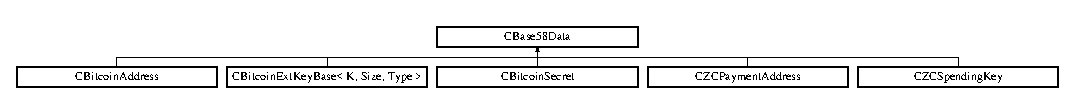
\includegraphics[height=0.949153cm]{class_c_base58_data}
\end{center}
\end{figure}
\subsection*{Public Member Functions}
\begin{DoxyCompactItemize}
\item 
bool \mbox{\hyperlink{class_c_base58_data_ae4aa0c0eca8c691ab9516a1596cb9a0a}{Set\+String}} (const char $\ast$psz, unsigned int n\+Version\+Bytes)
\item 
bool \mbox{\hyperlink{class_c_base58_data_a495bf25426b4d24712828f5c9e9dda53}{Set\+String}} (const std\+::string \&str, unsigned int n\+Version\+Bytes)
\item 
std\+::string \mbox{\hyperlink{class_c_base58_data_a7dc91af403ca02694b3247b15604e220}{To\+String}} () const
\item 
int \mbox{\hyperlink{class_c_base58_data_ad89d6bd7afa8d831dffce12803c5f58d}{Compare\+To}} (const \mbox{\hyperlink{class_c_base58_data}{C\+Base58\+Data}} \&b58) const
\item 
bool \mbox{\hyperlink{class_c_base58_data_a2e7a634c3a008adf3f74d72ed9dbd68c}{operator==}} (const \mbox{\hyperlink{class_c_base58_data}{C\+Base58\+Data}} \&b58) const
\item 
bool \mbox{\hyperlink{class_c_base58_data_a1d99c2d0a82cbe648ba2a99e41386486}{operator$<$=}} (const \mbox{\hyperlink{class_c_base58_data}{C\+Base58\+Data}} \&b58) const
\item 
bool \mbox{\hyperlink{class_c_base58_data_a0cac1805398e2b09a498ba884c7a0057}{operator$>$=}} (const \mbox{\hyperlink{class_c_base58_data}{C\+Base58\+Data}} \&b58) const
\item 
bool \mbox{\hyperlink{class_c_base58_data_a7377c5628c43551ca22af1c0dfbaebae}{operator$<$}} (const \mbox{\hyperlink{class_c_base58_data}{C\+Base58\+Data}} \&b58) const
\item 
bool \mbox{\hyperlink{class_c_base58_data_a7d8052eacc8de55a0f4ec91306dfbec3}{operator$>$}} (const \mbox{\hyperlink{class_c_base58_data}{C\+Base58\+Data}} \&b58) const
\end{DoxyCompactItemize}
\subsection*{Protected Types}
\begin{DoxyCompactItemize}
\item 
typedef std\+::vector$<$ unsigned char, zero\+\_\+after\+\_\+free\+\_\+allocator$<$ unsigned char $>$ $>$ \mbox{\hyperlink{class_c_base58_data_a193d64487a0b4f6df24f8bd380956ec1}{vector\+\_\+uchar}}
\begin{DoxyCompactList}\small\item\em the actually encoded data \end{DoxyCompactList}\end{DoxyCompactItemize}
\subsection*{Protected Member Functions}
\begin{DoxyCompactItemize}
\item 
\mbox{\hyperlink{class_c_base58_data_ae4f4ff42010299bc6fb228e21d6b2a15}{C\+Base58\+Data}} ()
\item 
void \mbox{\hyperlink{class_c_base58_data_afab1c06a0a4f631fd889434a2bc48c27}{Set\+Data}} (const std\+::vector$<$ unsigned char $>$ \&vch\+Version\+In, const void $\ast$pdata, size\+\_\+t n\+Size)
\item 
void \mbox{\hyperlink{class_c_base58_data_a8314b00685e590b4005be5cdfd36aeb9}{Set\+Data}} (const std\+::vector$<$ unsigned char $>$ \&vch\+Version\+In, const unsigned char $\ast$pbegin, const unsigned char $\ast$pend)
\end{DoxyCompactItemize}
\subsection*{Protected Attributes}
\begin{DoxyCompactItemize}
\item 
std\+::vector$<$ unsigned char $>$ \mbox{\hyperlink{class_c_base58_data_a110c1008f399053098a1bdf63408e923}{vch\+Version}}
\begin{DoxyCompactList}\small\item\em the version byte(s) \end{DoxyCompactList}\item 
\mbox{\hyperlink{class_c_base58_data_a193d64487a0b4f6df24f8bd380956ec1}{vector\+\_\+uchar}} \mbox{\hyperlink{class_c_base58_data_ae7ef7dfb93683aa4aaee8b74da5abb9c}{vch\+Data}}
\end{DoxyCompactItemize}


\subsection{Detailed Description}
Base class for all base58-\/encoded data 

\subsection{Member Typedef Documentation}
\mbox{\Hypertarget{class_c_base58_data_a193d64487a0b4f6df24f8bd380956ec1}\label{class_c_base58_data_a193d64487a0b4f6df24f8bd380956ec1}} 
\index{C\+Base58\+Data@{C\+Base58\+Data}!vector\+\_\+uchar@{vector\+\_\+uchar}}
\index{vector\+\_\+uchar@{vector\+\_\+uchar}!C\+Base58\+Data@{C\+Base58\+Data}}
\subsubsection{\texorpdfstring{vector\+\_\+uchar}{vector\_uchar}}
{\footnotesize\ttfamily typedef std\+::vector$<$unsigned char, zero\+\_\+after\+\_\+free\+\_\+allocator$<$unsigned char$>$ $>$ \mbox{\hyperlink{class_c_base58_data_a193d64487a0b4f6df24f8bd380956ec1}{C\+Base58\+Data\+::vector\+\_\+uchar}}\hspace{0.3cm}{\ttfamily [protected]}}



the actually encoded data 



\subsection{Constructor \& Destructor Documentation}
\mbox{\Hypertarget{class_c_base58_data_ae4f4ff42010299bc6fb228e21d6b2a15}\label{class_c_base58_data_ae4f4ff42010299bc6fb228e21d6b2a15}} 
\index{C\+Base58\+Data@{C\+Base58\+Data}!C\+Base58\+Data@{C\+Base58\+Data}}
\index{C\+Base58\+Data@{C\+Base58\+Data}!C\+Base58\+Data@{C\+Base58\+Data}}
\subsubsection{\texorpdfstring{C\+Base58\+Data()}{CBase58Data()}}
{\footnotesize\ttfamily C\+Base58\+Data\+::\+C\+Base58\+Data (\begin{DoxyParamCaption}{ }\end{DoxyParamCaption})\hspace{0.3cm}{\ttfamily [protected]}}



\subsection{Member Function Documentation}
\mbox{\Hypertarget{class_c_base58_data_ad89d6bd7afa8d831dffce12803c5f58d}\label{class_c_base58_data_ad89d6bd7afa8d831dffce12803c5f58d}} 
\index{C\+Base58\+Data@{C\+Base58\+Data}!Compare\+To@{Compare\+To}}
\index{Compare\+To@{Compare\+To}!C\+Base58\+Data@{C\+Base58\+Data}}
\subsubsection{\texorpdfstring{Compare\+To()}{CompareTo()}}
{\footnotesize\ttfamily int C\+Base58\+Data\+::\+Compare\+To (\begin{DoxyParamCaption}\item[{const \mbox{\hyperlink{class_c_base58_data}{C\+Base58\+Data}} \&}]{b58 }\end{DoxyParamCaption}) const}

\mbox{\Hypertarget{class_c_base58_data_a7377c5628c43551ca22af1c0dfbaebae}\label{class_c_base58_data_a7377c5628c43551ca22af1c0dfbaebae}} 
\index{C\+Base58\+Data@{C\+Base58\+Data}!operator$<$@{operator$<$}}
\index{operator$<$@{operator$<$}!C\+Base58\+Data@{C\+Base58\+Data}}
\subsubsection{\texorpdfstring{operator$<$()}{operator<()}}
{\footnotesize\ttfamily bool C\+Base58\+Data\+::operator$<$ (\begin{DoxyParamCaption}\item[{const \mbox{\hyperlink{class_c_base58_data}{C\+Base58\+Data}} \&}]{b58 }\end{DoxyParamCaption}) const\hspace{0.3cm}{\ttfamily [inline]}}

\mbox{\Hypertarget{class_c_base58_data_a1d99c2d0a82cbe648ba2a99e41386486}\label{class_c_base58_data_a1d99c2d0a82cbe648ba2a99e41386486}} 
\index{C\+Base58\+Data@{C\+Base58\+Data}!operator$<$=@{operator$<$=}}
\index{operator$<$=@{operator$<$=}!C\+Base58\+Data@{C\+Base58\+Data}}
\subsubsection{\texorpdfstring{operator$<$=()}{operator<=()}}
{\footnotesize\ttfamily bool C\+Base58\+Data\+::operator$<$= (\begin{DoxyParamCaption}\item[{const \mbox{\hyperlink{class_c_base58_data}{C\+Base58\+Data}} \&}]{b58 }\end{DoxyParamCaption}) const\hspace{0.3cm}{\ttfamily [inline]}}

\mbox{\Hypertarget{class_c_base58_data_a2e7a634c3a008adf3f74d72ed9dbd68c}\label{class_c_base58_data_a2e7a634c3a008adf3f74d72ed9dbd68c}} 
\index{C\+Base58\+Data@{C\+Base58\+Data}!operator==@{operator==}}
\index{operator==@{operator==}!C\+Base58\+Data@{C\+Base58\+Data}}
\subsubsection{\texorpdfstring{operator==()}{operator==()}}
{\footnotesize\ttfamily bool C\+Base58\+Data\+::operator== (\begin{DoxyParamCaption}\item[{const \mbox{\hyperlink{class_c_base58_data}{C\+Base58\+Data}} \&}]{b58 }\end{DoxyParamCaption}) const\hspace{0.3cm}{\ttfamily [inline]}}

\mbox{\Hypertarget{class_c_base58_data_a7d8052eacc8de55a0f4ec91306dfbec3}\label{class_c_base58_data_a7d8052eacc8de55a0f4ec91306dfbec3}} 
\index{C\+Base58\+Data@{C\+Base58\+Data}!operator$>$@{operator$>$}}
\index{operator$>$@{operator$>$}!C\+Base58\+Data@{C\+Base58\+Data}}
\subsubsection{\texorpdfstring{operator$>$()}{operator>()}}
{\footnotesize\ttfamily bool C\+Base58\+Data\+::operator$>$ (\begin{DoxyParamCaption}\item[{const \mbox{\hyperlink{class_c_base58_data}{C\+Base58\+Data}} \&}]{b58 }\end{DoxyParamCaption}) const\hspace{0.3cm}{\ttfamily [inline]}}

\mbox{\Hypertarget{class_c_base58_data_a0cac1805398e2b09a498ba884c7a0057}\label{class_c_base58_data_a0cac1805398e2b09a498ba884c7a0057}} 
\index{C\+Base58\+Data@{C\+Base58\+Data}!operator$>$=@{operator$>$=}}
\index{operator$>$=@{operator$>$=}!C\+Base58\+Data@{C\+Base58\+Data}}
\subsubsection{\texorpdfstring{operator$>$=()}{operator>=()}}
{\footnotesize\ttfamily bool C\+Base58\+Data\+::operator$>$= (\begin{DoxyParamCaption}\item[{const \mbox{\hyperlink{class_c_base58_data}{C\+Base58\+Data}} \&}]{b58 }\end{DoxyParamCaption}) const\hspace{0.3cm}{\ttfamily [inline]}}

\mbox{\Hypertarget{class_c_base58_data_afab1c06a0a4f631fd889434a2bc48c27}\label{class_c_base58_data_afab1c06a0a4f631fd889434a2bc48c27}} 
\index{C\+Base58\+Data@{C\+Base58\+Data}!Set\+Data@{Set\+Data}}
\index{Set\+Data@{Set\+Data}!C\+Base58\+Data@{C\+Base58\+Data}}
\subsubsection{\texorpdfstring{Set\+Data()}{SetData()}\hspace{0.1cm}{\footnotesize\ttfamily [1/2]}}
{\footnotesize\ttfamily void C\+Base58\+Data\+::\+Set\+Data (\begin{DoxyParamCaption}\item[{const std\+::vector$<$ unsigned char $>$ \&}]{vch\+Version\+In,  }\item[{const void $\ast$}]{pdata,  }\item[{size\+\_\+t}]{n\+Size }\end{DoxyParamCaption})\hspace{0.3cm}{\ttfamily [protected]}}

\mbox{\Hypertarget{class_c_base58_data_a8314b00685e590b4005be5cdfd36aeb9}\label{class_c_base58_data_a8314b00685e590b4005be5cdfd36aeb9}} 
\index{C\+Base58\+Data@{C\+Base58\+Data}!Set\+Data@{Set\+Data}}
\index{Set\+Data@{Set\+Data}!C\+Base58\+Data@{C\+Base58\+Data}}
\subsubsection{\texorpdfstring{Set\+Data()}{SetData()}\hspace{0.1cm}{\footnotesize\ttfamily [2/2]}}
{\footnotesize\ttfamily void C\+Base58\+Data\+::\+Set\+Data (\begin{DoxyParamCaption}\item[{const std\+::vector$<$ unsigned char $>$ \&}]{vch\+Version\+In,  }\item[{const unsigned char $\ast$}]{pbegin,  }\item[{const unsigned char $\ast$}]{pend }\end{DoxyParamCaption})\hspace{0.3cm}{\ttfamily [protected]}}

\mbox{\Hypertarget{class_c_base58_data_ae4aa0c0eca8c691ab9516a1596cb9a0a}\label{class_c_base58_data_ae4aa0c0eca8c691ab9516a1596cb9a0a}} 
\index{C\+Base58\+Data@{C\+Base58\+Data}!Set\+String@{Set\+String}}
\index{Set\+String@{Set\+String}!C\+Base58\+Data@{C\+Base58\+Data}}
\subsubsection{\texorpdfstring{Set\+String()}{SetString()}\hspace{0.1cm}{\footnotesize\ttfamily [1/2]}}
{\footnotesize\ttfamily bool C\+Base58\+Data\+::\+Set\+String (\begin{DoxyParamCaption}\item[{const char $\ast$}]{psz,  }\item[{unsigned int}]{n\+Version\+Bytes }\end{DoxyParamCaption})}

\mbox{\Hypertarget{class_c_base58_data_a495bf25426b4d24712828f5c9e9dda53}\label{class_c_base58_data_a495bf25426b4d24712828f5c9e9dda53}} 
\index{C\+Base58\+Data@{C\+Base58\+Data}!Set\+String@{Set\+String}}
\index{Set\+String@{Set\+String}!C\+Base58\+Data@{C\+Base58\+Data}}
\subsubsection{\texorpdfstring{Set\+String()}{SetString()}\hspace{0.1cm}{\footnotesize\ttfamily [2/2]}}
{\footnotesize\ttfamily bool C\+Base58\+Data\+::\+Set\+String (\begin{DoxyParamCaption}\item[{const std\+::string \&}]{str,  }\item[{unsigned int}]{n\+Version\+Bytes }\end{DoxyParamCaption})}

\mbox{\Hypertarget{class_c_base58_data_a7dc91af403ca02694b3247b15604e220}\label{class_c_base58_data_a7dc91af403ca02694b3247b15604e220}} 
\index{C\+Base58\+Data@{C\+Base58\+Data}!To\+String@{To\+String}}
\index{To\+String@{To\+String}!C\+Base58\+Data@{C\+Base58\+Data}}
\subsubsection{\texorpdfstring{To\+String()}{ToString()}}
{\footnotesize\ttfamily std\+::string C\+Base58\+Data\+::\+To\+String (\begin{DoxyParamCaption}{ }\end{DoxyParamCaption}) const}



\subsection{Member Data Documentation}
\mbox{\Hypertarget{class_c_base58_data_ae7ef7dfb93683aa4aaee8b74da5abb9c}\label{class_c_base58_data_ae7ef7dfb93683aa4aaee8b74da5abb9c}} 
\index{C\+Base58\+Data@{C\+Base58\+Data}!vch\+Data@{vch\+Data}}
\index{vch\+Data@{vch\+Data}!C\+Base58\+Data@{C\+Base58\+Data}}
\subsubsection{\texorpdfstring{vch\+Data}{vchData}}
{\footnotesize\ttfamily \mbox{\hyperlink{class_c_base58_data_a193d64487a0b4f6df24f8bd380956ec1}{vector\+\_\+uchar}} C\+Base58\+Data\+::vch\+Data\hspace{0.3cm}{\ttfamily [protected]}}

\mbox{\Hypertarget{class_c_base58_data_a110c1008f399053098a1bdf63408e923}\label{class_c_base58_data_a110c1008f399053098a1bdf63408e923}} 
\index{C\+Base58\+Data@{C\+Base58\+Data}!vch\+Version@{vch\+Version}}
\index{vch\+Version@{vch\+Version}!C\+Base58\+Data@{C\+Base58\+Data}}
\subsubsection{\texorpdfstring{vch\+Version}{vchVersion}}
{\footnotesize\ttfamily std\+::vector$<$unsigned char$>$ C\+Base58\+Data\+::vch\+Version\hspace{0.3cm}{\ttfamily [protected]}}



the version byte(s) 



The documentation for this class was generated from the following files\+:\begin{DoxyCompactItemize}
\item 
/\+Users/christopherarguello/\+Developer/anon/src/\mbox{\hyperlink{base58_8h}{base58.\+h}}\item 
/\+Users/christopherarguello/\+Developer/anon/src/\mbox{\hyperlink{base58_8cpp}{base58.\+cpp}}\end{DoxyCompactItemize}

\hypertarget{class_c_base_chain_params}{}\section{C\+Base\+Chain\+Params Class Reference}
\label{class_c_base_chain_params}\index{C\+Base\+Chain\+Params@{C\+Base\+Chain\+Params}}


{\ttfamily \#include $<$chainparamsbase.\+h$>$}

Inheritance diagram for C\+Base\+Chain\+Params\+:\begin{figure}[H]
\begin{center}
\leavevmode
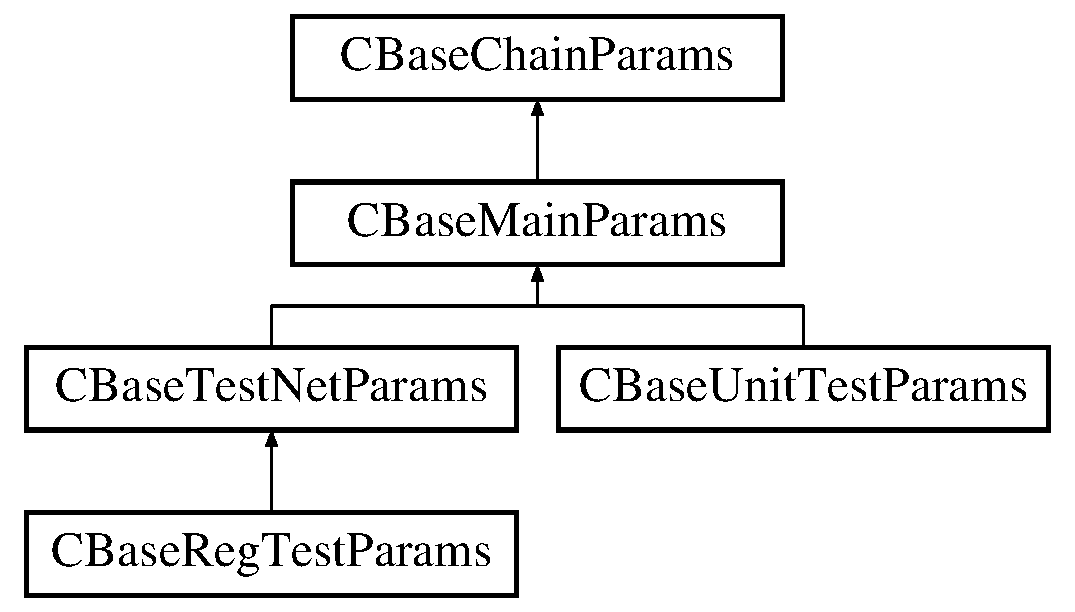
\includegraphics[height=4.000000cm]{class_c_base_chain_params}
\end{center}
\end{figure}
\subsection*{Public Types}
\begin{DoxyCompactItemize}
\item 
enum \mbox{\hyperlink{class_c_base_chain_params_a19fb46b499c21801c0ff3c8607a0994e}{Network}} \{ \mbox{\hyperlink{class_c_base_chain_params_a19fb46b499c21801c0ff3c8607a0994ea17aedaa2a3181d12f0d32afc70a6c68c}{M\+A\+IN}}, 
\mbox{\hyperlink{class_c_base_chain_params_a19fb46b499c21801c0ff3c8607a0994ea0a9c4e42da932cdd126777f7f4dd0e22}{T\+E\+S\+T\+N\+ET}}, 
\mbox{\hyperlink{class_c_base_chain_params_a19fb46b499c21801c0ff3c8607a0994eace36282edb786b098dbdd48f98ddb793}{R\+E\+G\+T\+E\+ST}}, 
\mbox{\hyperlink{class_c_base_chain_params_a19fb46b499c21801c0ff3c8607a0994eaf4a96679adc48f01c489d1b4d740deb5}{M\+A\+X\+\_\+\+N\+E\+T\+W\+O\+R\+K\+\_\+\+T\+Y\+P\+ES}}
 \}
\end{DoxyCompactItemize}
\subsection*{Public Member Functions}
\begin{DoxyCompactItemize}
\item 
const std\+::string \& \mbox{\hyperlink{class_c_base_chain_params_a4b142e94ae27f860522dd5efef41fb67}{Data\+Dir}} () const
\item 
int \mbox{\hyperlink{class_c_base_chain_params_a790801bda78d70db56da89ca43934a63}{R\+P\+C\+Port}} () const
\end{DoxyCompactItemize}
\subsection*{Protected Member Functions}
\begin{DoxyCompactItemize}
\item 
\mbox{\hyperlink{class_c_base_chain_params_a4c0e84608b2fa636be3a3683653d9533}{C\+Base\+Chain\+Params}} ()
\end{DoxyCompactItemize}
\subsection*{Protected Attributes}
\begin{DoxyCompactItemize}
\item 
int \mbox{\hyperlink{class_c_base_chain_params_ae020d8f669175bcac3ab44f9c095c977}{n\+R\+P\+C\+Port}} = 0
\item 
std\+::string \mbox{\hyperlink{class_c_base_chain_params_af5868778f8c6c676aabc9fb2366d2447}{str\+Data\+Dir}}
\end{DoxyCompactItemize}


\subsection{Detailed Description}
\mbox{\hyperlink{class_c_base_chain_params}{C\+Base\+Chain\+Params}} defines the base parameters (shared between bitcoin-\/cli and bitcoind) of a given instance of the Bitcoin system. 

\subsection{Member Enumeration Documentation}
\mbox{\Hypertarget{class_c_base_chain_params_a19fb46b499c21801c0ff3c8607a0994e}\label{class_c_base_chain_params_a19fb46b499c21801c0ff3c8607a0994e}} 
\index{C\+Base\+Chain\+Params@{C\+Base\+Chain\+Params}!Network@{Network}}
\index{Network@{Network}!C\+Base\+Chain\+Params@{C\+Base\+Chain\+Params}}
\subsubsection{\texorpdfstring{Network}{Network}}
{\footnotesize\ttfamily enum \mbox{\hyperlink{class_c_base_chain_params_a19fb46b499c21801c0ff3c8607a0994e}{C\+Base\+Chain\+Params\+::\+Network}}}

\begin{DoxyEnumFields}{Enumerator}
\raisebox{\heightof{T}}[0pt][0pt]{\index{M\+A\+IN@{M\+A\+IN}!C\+Base\+Chain\+Params@{C\+Base\+Chain\+Params}}\index{C\+Base\+Chain\+Params@{C\+Base\+Chain\+Params}!M\+A\+IN@{M\+A\+IN}}}\mbox{\Hypertarget{class_c_base_chain_params_a19fb46b499c21801c0ff3c8607a0994ea17aedaa2a3181d12f0d32afc70a6c68c}\label{class_c_base_chain_params_a19fb46b499c21801c0ff3c8607a0994ea17aedaa2a3181d12f0d32afc70a6c68c}} 
M\+A\+IN&\\
\hline

\raisebox{\heightof{T}}[0pt][0pt]{\index{T\+E\+S\+T\+N\+ET@{T\+E\+S\+T\+N\+ET}!C\+Base\+Chain\+Params@{C\+Base\+Chain\+Params}}\index{C\+Base\+Chain\+Params@{C\+Base\+Chain\+Params}!T\+E\+S\+T\+N\+ET@{T\+E\+S\+T\+N\+ET}}}\mbox{\Hypertarget{class_c_base_chain_params_a19fb46b499c21801c0ff3c8607a0994ea0a9c4e42da932cdd126777f7f4dd0e22}\label{class_c_base_chain_params_a19fb46b499c21801c0ff3c8607a0994ea0a9c4e42da932cdd126777f7f4dd0e22}} 
T\+E\+S\+T\+N\+ET&\\
\hline

\raisebox{\heightof{T}}[0pt][0pt]{\index{R\+E\+G\+T\+E\+ST@{R\+E\+G\+T\+E\+ST}!C\+Base\+Chain\+Params@{C\+Base\+Chain\+Params}}\index{C\+Base\+Chain\+Params@{C\+Base\+Chain\+Params}!R\+E\+G\+T\+E\+ST@{R\+E\+G\+T\+E\+ST}}}\mbox{\Hypertarget{class_c_base_chain_params_a19fb46b499c21801c0ff3c8607a0994eace36282edb786b098dbdd48f98ddb793}\label{class_c_base_chain_params_a19fb46b499c21801c0ff3c8607a0994eace36282edb786b098dbdd48f98ddb793}} 
R\+E\+G\+T\+E\+ST&\\
\hline

\raisebox{\heightof{T}}[0pt][0pt]{\index{M\+A\+X\+\_\+\+N\+E\+T\+W\+O\+R\+K\+\_\+\+T\+Y\+P\+ES@{M\+A\+X\+\_\+\+N\+E\+T\+W\+O\+R\+K\+\_\+\+T\+Y\+P\+ES}!C\+Base\+Chain\+Params@{C\+Base\+Chain\+Params}}\index{C\+Base\+Chain\+Params@{C\+Base\+Chain\+Params}!M\+A\+X\+\_\+\+N\+E\+T\+W\+O\+R\+K\+\_\+\+T\+Y\+P\+ES@{M\+A\+X\+\_\+\+N\+E\+T\+W\+O\+R\+K\+\_\+\+T\+Y\+P\+ES}}}\mbox{\Hypertarget{class_c_base_chain_params_a19fb46b499c21801c0ff3c8607a0994eaf4a96679adc48f01c489d1b4d740deb5}\label{class_c_base_chain_params_a19fb46b499c21801c0ff3c8607a0994eaf4a96679adc48f01c489d1b4d740deb5}} 
M\+A\+X\+\_\+\+N\+E\+T\+W\+O\+R\+K\+\_\+\+T\+Y\+P\+ES&\\
\hline

\end{DoxyEnumFields}


\subsection{Constructor \& Destructor Documentation}
\mbox{\Hypertarget{class_c_base_chain_params_a4c0e84608b2fa636be3a3683653d9533}\label{class_c_base_chain_params_a4c0e84608b2fa636be3a3683653d9533}} 
\index{C\+Base\+Chain\+Params@{C\+Base\+Chain\+Params}!C\+Base\+Chain\+Params@{C\+Base\+Chain\+Params}}
\index{C\+Base\+Chain\+Params@{C\+Base\+Chain\+Params}!C\+Base\+Chain\+Params@{C\+Base\+Chain\+Params}}
\subsubsection{\texorpdfstring{C\+Base\+Chain\+Params()}{CBaseChainParams()}}
{\footnotesize\ttfamily C\+Base\+Chain\+Params\+::\+C\+Base\+Chain\+Params (\begin{DoxyParamCaption}{ }\end{DoxyParamCaption})\hspace{0.3cm}{\ttfamily [inline]}, {\ttfamily [protected]}}



\subsection{Member Function Documentation}
\mbox{\Hypertarget{class_c_base_chain_params_a4b142e94ae27f860522dd5efef41fb67}\label{class_c_base_chain_params_a4b142e94ae27f860522dd5efef41fb67}} 
\index{C\+Base\+Chain\+Params@{C\+Base\+Chain\+Params}!Data\+Dir@{Data\+Dir}}
\index{Data\+Dir@{Data\+Dir}!C\+Base\+Chain\+Params@{C\+Base\+Chain\+Params}}
\subsubsection{\texorpdfstring{Data\+Dir()}{DataDir()}}
{\footnotesize\ttfamily const std\+::string\& C\+Base\+Chain\+Params\+::\+Data\+Dir (\begin{DoxyParamCaption}{ }\end{DoxyParamCaption}) const\hspace{0.3cm}{\ttfamily [inline]}}

\mbox{\Hypertarget{class_c_base_chain_params_a790801bda78d70db56da89ca43934a63}\label{class_c_base_chain_params_a790801bda78d70db56da89ca43934a63}} 
\index{C\+Base\+Chain\+Params@{C\+Base\+Chain\+Params}!R\+P\+C\+Port@{R\+P\+C\+Port}}
\index{R\+P\+C\+Port@{R\+P\+C\+Port}!C\+Base\+Chain\+Params@{C\+Base\+Chain\+Params}}
\subsubsection{\texorpdfstring{R\+P\+C\+Port()}{RPCPort()}}
{\footnotesize\ttfamily int C\+Base\+Chain\+Params\+::\+R\+P\+C\+Port (\begin{DoxyParamCaption}{ }\end{DoxyParamCaption}) const\hspace{0.3cm}{\ttfamily [inline]}}



\subsection{Member Data Documentation}
\mbox{\Hypertarget{class_c_base_chain_params_ae020d8f669175bcac3ab44f9c095c977}\label{class_c_base_chain_params_ae020d8f669175bcac3ab44f9c095c977}} 
\index{C\+Base\+Chain\+Params@{C\+Base\+Chain\+Params}!n\+R\+P\+C\+Port@{n\+R\+P\+C\+Port}}
\index{n\+R\+P\+C\+Port@{n\+R\+P\+C\+Port}!C\+Base\+Chain\+Params@{C\+Base\+Chain\+Params}}
\subsubsection{\texorpdfstring{n\+R\+P\+C\+Port}{nRPCPort}}
{\footnotesize\ttfamily int C\+Base\+Chain\+Params\+::n\+R\+P\+C\+Port = 0\hspace{0.3cm}{\ttfamily [protected]}}

\mbox{\Hypertarget{class_c_base_chain_params_af5868778f8c6c676aabc9fb2366d2447}\label{class_c_base_chain_params_af5868778f8c6c676aabc9fb2366d2447}} 
\index{C\+Base\+Chain\+Params@{C\+Base\+Chain\+Params}!str\+Data\+Dir@{str\+Data\+Dir}}
\index{str\+Data\+Dir@{str\+Data\+Dir}!C\+Base\+Chain\+Params@{C\+Base\+Chain\+Params}}
\subsubsection{\texorpdfstring{str\+Data\+Dir}{strDataDir}}
{\footnotesize\ttfamily std\+::string C\+Base\+Chain\+Params\+::str\+Data\+Dir\hspace{0.3cm}{\ttfamily [protected]}}



The documentation for this class was generated from the following file\+:\begin{DoxyCompactItemize}
\item 
/\+Users/christopherarguello/\+Developer/anon/src/\mbox{\hyperlink{chainparamsbase_8h}{chainparamsbase.\+h}}\end{DoxyCompactItemize}

\hypertarget{class_c_base_data_stream}{}\section{C\+Base\+Data\+Stream$<$ Serialize\+Type $>$ Class Template Reference}
\label{class_c_base_data_stream}\index{C\+Base\+Data\+Stream$<$ Serialize\+Type $>$@{C\+Base\+Data\+Stream$<$ Serialize\+Type $>$}}


{\ttfamily \#include $<$streams.\+h$>$}

\subsection*{Public Types}
\begin{DoxyCompactItemize}
\item 
typedef vector\+\_\+type\+::allocator\+\_\+type \mbox{\hyperlink{class_c_base_data_stream_ae303e09f19f77d2d95ac99feabbeb6c3}{allocator\+\_\+type}}
\item 
typedef vector\+\_\+type\+::size\+\_\+type \mbox{\hyperlink{class_c_base_data_stream_ad042ddea628c43357b9b13be89c71964}{size\+\_\+type}}
\item 
typedef vector\+\_\+type\+::difference\+\_\+type \mbox{\hyperlink{class_c_base_data_stream_a85d79377e715b717baa8cb68cf753bd0}{difference\+\_\+type}}
\item 
typedef vector\+\_\+type\+::reference \mbox{\hyperlink{class_c_base_data_stream_a74ec577e6f675c786880b39700b8f317}{reference}}
\item 
typedef vector\+\_\+type\+::const\+\_\+reference \mbox{\hyperlink{class_c_base_data_stream_aabfd39998036383d2ee384029f221aab}{const\+\_\+reference}}
\item 
typedef vector\+\_\+type\+::value\+\_\+type \mbox{\hyperlink{class_c_base_data_stream_a92957c776eb4c9a7668dd9cd82f7dbdd}{value\+\_\+type}}
\item 
typedef vector\+\_\+type\+::iterator \mbox{\hyperlink{class_c_base_data_stream_a23e0e0af1c68dd36c27162036b6d048d}{iterator}}
\item 
typedef vector\+\_\+type\+::const\+\_\+iterator \mbox{\hyperlink{class_c_base_data_stream_a9cf3080c5a75c94568980a59d3aab3ad}{const\+\_\+iterator}}
\item 
typedef vector\+\_\+type\+::reverse\+\_\+iterator \mbox{\hyperlink{class_c_base_data_stream_aecb04ae414c994e0c43aa0ed423b8824}{reverse\+\_\+iterator}}
\end{DoxyCompactItemize}
\subsection*{Public Member Functions}
\begin{DoxyCompactItemize}
\item 
\mbox{\hyperlink{class_c_base_data_stream_a2713ae60ccb209e599777252209e770b}{C\+Base\+Data\+Stream}} (int n\+Type\+In, int n\+Version\+In)
\item 
\mbox{\hyperlink{class_c_base_data_stream_ad53847bb8cdede2cdf271f14eb651ba6}{C\+Base\+Data\+Stream}} (\mbox{\hyperlink{class_c_base_data_stream_a9cf3080c5a75c94568980a59d3aab3ad}{const\+\_\+iterator}} pbegin, \mbox{\hyperlink{class_c_base_data_stream_a9cf3080c5a75c94568980a59d3aab3ad}{const\+\_\+iterator}} pend, int n\+Type\+In, int n\+Version\+In)
\item 
\mbox{\hyperlink{class_c_base_data_stream_a2433bc0a7b7b112cf38b81af0ef898c8}{C\+Base\+Data\+Stream}} (const char $\ast$pbegin, const char $\ast$pend, int n\+Type\+In, int n\+Version\+In)
\item 
\mbox{\hyperlink{class_c_base_data_stream_a113389383acd7b7e48a4a54c6b713551}{C\+Base\+Data\+Stream}} (const \mbox{\hyperlink{class_c_base_data_stream_a035e97a3e024a8cfa4690eaca1e5e290}{vector\+\_\+type}} \&vch\+In, int n\+Type\+In, int n\+Version\+In)
\item 
\mbox{\hyperlink{class_c_base_data_stream_a9f49c3d8343a6b9bb9b16e21dc304321}{C\+Base\+Data\+Stream}} (const std\+::vector$<$ char $>$ \&vch\+In, int n\+Type\+In, int n\+Version\+In)
\item 
\mbox{\hyperlink{class_c_base_data_stream_a7dd6b67c520b5d2ad7a39d94632ebd19}{C\+Base\+Data\+Stream}} (const std\+::vector$<$ unsigned char $>$ \&vch\+In, int n\+Type\+In, int n\+Version\+In)
\item 
void \mbox{\hyperlink{class_c_base_data_stream_a2d828ad342dacde5b5feae046702fb53}{Init}} (int n\+Type\+In, int n\+Version\+In)
\item 
\mbox{\hyperlink{class_c_base_data_stream}{C\+Base\+Data\+Stream}} \& \mbox{\hyperlink{class_c_base_data_stream_abf8f25622242ad01ddb049ee4260e7ab}{operator+=}} (const \mbox{\hyperlink{class_c_base_data_stream}{C\+Base\+Data\+Stream}} \&b)
\item 
std\+::string \mbox{\hyperlink{class_c_base_data_stream_ad7e170426e8f8bc2794b2391f27c0fd1}{str}} () const
\item 
\mbox{\hyperlink{class_c_base_data_stream_a9cf3080c5a75c94568980a59d3aab3ad}{const\+\_\+iterator}} \mbox{\hyperlink{class_c_base_data_stream_abed61420f8a28a0c7ea0baeaa87b925b}{begin}} () const
\item 
\mbox{\hyperlink{class_c_base_data_stream_a23e0e0af1c68dd36c27162036b6d048d}{iterator}} \mbox{\hyperlink{class_c_base_data_stream_a6b26f6547fc8d86bee0d9158805bb1ac}{begin}} ()
\item 
\mbox{\hyperlink{class_c_base_data_stream_a9cf3080c5a75c94568980a59d3aab3ad}{const\+\_\+iterator}} \mbox{\hyperlink{class_c_base_data_stream_a7d083ceebeb6f4ea63d2434f8b11a292}{end}} () const
\item 
\mbox{\hyperlink{class_c_base_data_stream_a23e0e0af1c68dd36c27162036b6d048d}{iterator}} \mbox{\hyperlink{class_c_base_data_stream_ac511b088f239c8e086322d50bcc762fe}{end}} ()
\item 
\mbox{\hyperlink{class_c_base_data_stream_ad042ddea628c43357b9b13be89c71964}{size\+\_\+type}} \mbox{\hyperlink{class_c_base_data_stream_aea822d9dff7d0f3e4adb96dba79126a5}{size}} () const
\item 
bool \mbox{\hyperlink{class_c_base_data_stream_ac2a82d5383c034f844b70a67ed580806}{empty}} () const
\item 
void \mbox{\hyperlink{class_c_base_data_stream_a620febffdbbcabbd4a21fcd67e6d1154}{resize}} (\mbox{\hyperlink{class_c_base_data_stream_ad042ddea628c43357b9b13be89c71964}{size\+\_\+type}} n, \mbox{\hyperlink{class_c_base_data_stream_a92957c776eb4c9a7668dd9cd82f7dbdd}{value\+\_\+type}} c=0)
\item 
void \mbox{\hyperlink{class_c_base_data_stream_aeff66bbf5f2494240e3f8106540ff676}{reserve}} (\mbox{\hyperlink{class_c_base_data_stream_ad042ddea628c43357b9b13be89c71964}{size\+\_\+type}} n)
\item 
\mbox{\hyperlink{class_c_base_data_stream_aabfd39998036383d2ee384029f221aab}{const\+\_\+reference}} \mbox{\hyperlink{class_c_base_data_stream_a0cfc7c327973830d505a6ca59beddae6}{operator\mbox{[}$\,$\mbox{]}}} (\mbox{\hyperlink{class_c_base_data_stream_ad042ddea628c43357b9b13be89c71964}{size\+\_\+type}} pos) const
\item 
\mbox{\hyperlink{class_c_base_data_stream_a74ec577e6f675c786880b39700b8f317}{reference}} \mbox{\hyperlink{class_c_base_data_stream_aa56015ceb6b79db5cfc08695d68310bf}{operator\mbox{[}$\,$\mbox{]}}} (\mbox{\hyperlink{class_c_base_data_stream_ad042ddea628c43357b9b13be89c71964}{size\+\_\+type}} pos)
\item 
void \mbox{\hyperlink{class_c_base_data_stream_af453f4e42cd6ba6b76d925c4c137786e}{clear}} ()
\item 
\mbox{\hyperlink{class_c_base_data_stream_a23e0e0af1c68dd36c27162036b6d048d}{iterator}} \mbox{\hyperlink{class_c_base_data_stream_aab96f99c03e7cb36e8345701e49707c9}{insert}} (\mbox{\hyperlink{class_c_base_data_stream_a23e0e0af1c68dd36c27162036b6d048d}{iterator}} it, const char \&x=char())
\item 
void \mbox{\hyperlink{class_c_base_data_stream_a8f3b322d3e3a7e254f4a1a08cf3db187}{insert}} (\mbox{\hyperlink{class_c_base_data_stream_a23e0e0af1c68dd36c27162036b6d048d}{iterator}} it, \mbox{\hyperlink{class_c_base_data_stream_ad042ddea628c43357b9b13be89c71964}{size\+\_\+type}} n, const char \&x)
\item 
void \mbox{\hyperlink{class_c_base_data_stream_a57dd36b154277cc2997d9405bf514c3e}{insert}} (\mbox{\hyperlink{class_c_base_data_stream_a23e0e0af1c68dd36c27162036b6d048d}{iterator}} it, std\+::vector$<$ char $>$\+::\mbox{\hyperlink{class_c_base_data_stream_a9cf3080c5a75c94568980a59d3aab3ad}{const\+\_\+iterator}} first, std\+::vector$<$ char $>$\+::\mbox{\hyperlink{class_c_base_data_stream_a9cf3080c5a75c94568980a59d3aab3ad}{const\+\_\+iterator}} last)
\item 
void \mbox{\hyperlink{class_c_base_data_stream_a3e1588dfb94fb9845d56e1b0668e1ee4}{insert}} (\mbox{\hyperlink{class_c_base_data_stream_a23e0e0af1c68dd36c27162036b6d048d}{iterator}} it, const char $\ast$first, const char $\ast$last)
\item 
\mbox{\hyperlink{class_c_base_data_stream_a23e0e0af1c68dd36c27162036b6d048d}{iterator}} \mbox{\hyperlink{class_c_base_data_stream_ae381ee24932de8d08ebe13b4e1078e39}{erase}} (\mbox{\hyperlink{class_c_base_data_stream_a23e0e0af1c68dd36c27162036b6d048d}{iterator}} it)
\item 
\mbox{\hyperlink{class_c_base_data_stream_a23e0e0af1c68dd36c27162036b6d048d}{iterator}} \mbox{\hyperlink{class_c_base_data_stream_a0fb5434f391056c30493ccc39f7eeb24}{erase}} (\mbox{\hyperlink{class_c_base_data_stream_a23e0e0af1c68dd36c27162036b6d048d}{iterator}} first, \mbox{\hyperlink{class_c_base_data_stream_a23e0e0af1c68dd36c27162036b6d048d}{iterator}} last)
\item 
void \mbox{\hyperlink{class_c_base_data_stream_ab52dd7b6e1dce1fd90e1c9f9ad729ee6}{Compact}} ()
\item 
bool \mbox{\hyperlink{class_c_base_data_stream_ae93a5c7aa33f204030fd0a796a3b5f0f}{Rewind}} (\mbox{\hyperlink{class_c_base_data_stream_ad042ddea628c43357b9b13be89c71964}{size\+\_\+type}} n)
\item 
bool \mbox{\hyperlink{class_c_base_data_stream_a6501eb90892ec457cd99d48e5e658cfd}{eof}} () const
\item 
\mbox{\hyperlink{class_c_base_data_stream}{C\+Base\+Data\+Stream}} $\ast$ \mbox{\hyperlink{class_c_base_data_stream_a3ab78204837cf4f59a0a01bb22a6f043}{rdbuf}} ()
\item 
int \mbox{\hyperlink{class_c_base_data_stream_af7c7582f5f38997b0f22b2c44c391f11}{in\+\_\+avail}} ()
\item 
void \mbox{\hyperlink{class_c_base_data_stream_a02c042f25f960b7c974db3c30ee056a5}{Set\+Type}} (int n)
\item 
int \mbox{\hyperlink{class_c_base_data_stream_a758ee870d0c9bf3bb347b584cd02c53f}{Get\+Type}} ()
\item 
void \mbox{\hyperlink{class_c_base_data_stream_a536e45089156e085c0759aaf27aa7c4c}{Set\+Version}} (int n)
\item 
int \mbox{\hyperlink{class_c_base_data_stream_a75a64b190fc029cb1938c6d832748057}{Get\+Version}} ()
\item 
void \mbox{\hyperlink{class_c_base_data_stream_ada664c82a99a1147deeb084df1dab41c}{Read\+Version}} ()
\item 
void \mbox{\hyperlink{class_c_base_data_stream_a5ecdb53462dbc5dbf976b12482852223}{Write\+Version}} ()
\item 
\mbox{\hyperlink{class_c_base_data_stream}{C\+Base\+Data\+Stream}} \& \mbox{\hyperlink{class_c_base_data_stream_a46f9e59af924d509662166af4d232320}{read}} (char $\ast$pch, size\+\_\+t n\+Size)
\item 
\mbox{\hyperlink{class_c_base_data_stream}{C\+Base\+Data\+Stream}} \& \mbox{\hyperlink{class_c_base_data_stream_aa16c563ce4b72146ac67ea6a3278bc3f}{ignore}} (int n\+Size)
\item 
\mbox{\hyperlink{class_c_base_data_stream}{C\+Base\+Data\+Stream}} \& \mbox{\hyperlink{class_c_base_data_stream_a82d8850aa10720a065628ca72d12801b}{write}} (const char $\ast$pch, size\+\_\+t n\+Size)
\item 
{\footnotesize template$<$typename Stream $>$ }\\void \mbox{\hyperlink{class_c_base_data_stream_af83455eaa7f251031dd20f7075637701}{Serialize}} (Stream \&s, int \mbox{\hyperlink{class_c_base_data_stream_acd93d8bc03d65130819f2ff79be43234}{n\+Type}}, int \mbox{\hyperlink{class_c_base_data_stream_a9a6ab5bb4c659f3ee03dca351c9de88e}{n\+Version}}) const
\item 
{\footnotesize template$<$typename T $>$ }\\unsigned int \mbox{\hyperlink{class_c_base_data_stream_aeb38b7dcee457f0d0c5679cf88724c9f}{Get\+Serialize\+Size}} (const T \&obj)
\item 
{\footnotesize template$<$typename T $>$ }\\\mbox{\hyperlink{class_c_base_data_stream}{C\+Base\+Data\+Stream}} \& \mbox{\hyperlink{class_c_base_data_stream_a453748ece985685b2d561fcf2028cff8}{operator$<$$<$}} (const T \&obj)
\item 
{\footnotesize template$<$typename T $>$ }\\\mbox{\hyperlink{class_c_base_data_stream}{C\+Base\+Data\+Stream}} \& \mbox{\hyperlink{class_c_base_data_stream_aa2733313d5d254eaa7950a480dd6b280}{operator$>$$>$}} (T \&obj)
\item 
void \mbox{\hyperlink{class_c_base_data_stream_aaec8aaffcfceb2d4c5f04558c5034ed9}{Get\+And\+Clear}} (C\+Serialize\+Data \&d)
\end{DoxyCompactItemize}
\subsection*{Public Attributes}
\begin{DoxyCompactItemize}
\item 
int \mbox{\hyperlink{class_c_base_data_stream_acd93d8bc03d65130819f2ff79be43234}{n\+Type}}
\item 
int \mbox{\hyperlink{class_c_base_data_stream_a9a6ab5bb4c659f3ee03dca351c9de88e}{n\+Version}}
\end{DoxyCompactItemize}
\subsection*{Protected Types}
\begin{DoxyCompactItemize}
\item 
typedef Serialize\+Type \mbox{\hyperlink{class_c_base_data_stream_a035e97a3e024a8cfa4690eaca1e5e290}{vector\+\_\+type}}
\end{DoxyCompactItemize}
\subsection*{Protected Attributes}
\begin{DoxyCompactItemize}
\item 
\mbox{\hyperlink{class_c_base_data_stream_a035e97a3e024a8cfa4690eaca1e5e290}{vector\+\_\+type}} \mbox{\hyperlink{class_c_base_data_stream_a2316d80610702632a74252c4db156990}{vch}}
\item 
unsigned int \mbox{\hyperlink{class_c_base_data_stream_abcabb286ff13fbe8819e7713d06f8d58}{n\+Read\+Pos}}
\end{DoxyCompactItemize}
\subsection*{Friends}
\begin{DoxyCompactItemize}
\item 
\mbox{\hyperlink{class_c_base_data_stream}{C\+Base\+Data\+Stream}} \mbox{\hyperlink{class_c_base_data_stream_af7942137a7d02a674bc7bedb0190cb1d}{operator+}} (const \mbox{\hyperlink{class_c_base_data_stream}{C\+Base\+Data\+Stream}} \&a, const \mbox{\hyperlink{class_c_base_data_stream}{C\+Base\+Data\+Stream}} \&b)
\end{DoxyCompactItemize}


\subsection{Detailed Description}
\subsubsection*{template$<$typename Serialize\+Type$>$\newline
class C\+Base\+Data\+Stream$<$ Serialize\+Type $>$}

Double ended buffer combining vector and stream-\/like interfaces.

\begin{quote}
\begin{quote}
and $<$$<$ read and write unformatted data using the above serialization templates. \end{quote}
\end{quote}
Fills with data in linear time; some stringstream implementations take N$^\wedge$2 time. 

\subsection{Member Typedef Documentation}
\mbox{\Hypertarget{class_c_base_data_stream_ae303e09f19f77d2d95ac99feabbeb6c3}\label{class_c_base_data_stream_ae303e09f19f77d2d95ac99feabbeb6c3}} 
\index{C\+Base\+Data\+Stream@{C\+Base\+Data\+Stream}!allocator\+\_\+type@{allocator\+\_\+type}}
\index{allocator\+\_\+type@{allocator\+\_\+type}!C\+Base\+Data\+Stream@{C\+Base\+Data\+Stream}}
\subsubsection{\texorpdfstring{allocator\+\_\+type}{allocator\_type}}
{\footnotesize\ttfamily template$<$typename Serialize\+Type$>$ \\
typedef vector\+\_\+type\+::allocator\+\_\+type \mbox{\hyperlink{class_c_base_data_stream}{C\+Base\+Data\+Stream}}$<$ Serialize\+Type $>$\+::\mbox{\hyperlink{class_c_base_data_stream_ae303e09f19f77d2d95ac99feabbeb6c3}{allocator\+\_\+type}}}

\mbox{\Hypertarget{class_c_base_data_stream_a9cf3080c5a75c94568980a59d3aab3ad}\label{class_c_base_data_stream_a9cf3080c5a75c94568980a59d3aab3ad}} 
\index{C\+Base\+Data\+Stream@{C\+Base\+Data\+Stream}!const\+\_\+iterator@{const\+\_\+iterator}}
\index{const\+\_\+iterator@{const\+\_\+iterator}!C\+Base\+Data\+Stream@{C\+Base\+Data\+Stream}}
\subsubsection{\texorpdfstring{const\+\_\+iterator}{const\_iterator}}
{\footnotesize\ttfamily template$<$typename Serialize\+Type$>$ \\
typedef vector\+\_\+type\+::const\+\_\+iterator \mbox{\hyperlink{class_c_base_data_stream}{C\+Base\+Data\+Stream}}$<$ Serialize\+Type $>$\+::\mbox{\hyperlink{class_c_base_data_stream_a9cf3080c5a75c94568980a59d3aab3ad}{const\+\_\+iterator}}}

\mbox{\Hypertarget{class_c_base_data_stream_aabfd39998036383d2ee384029f221aab}\label{class_c_base_data_stream_aabfd39998036383d2ee384029f221aab}} 
\index{C\+Base\+Data\+Stream@{C\+Base\+Data\+Stream}!const\+\_\+reference@{const\+\_\+reference}}
\index{const\+\_\+reference@{const\+\_\+reference}!C\+Base\+Data\+Stream@{C\+Base\+Data\+Stream}}
\subsubsection{\texorpdfstring{const\+\_\+reference}{const\_reference}}
{\footnotesize\ttfamily template$<$typename Serialize\+Type$>$ \\
typedef vector\+\_\+type\+::const\+\_\+reference \mbox{\hyperlink{class_c_base_data_stream}{C\+Base\+Data\+Stream}}$<$ Serialize\+Type $>$\+::\mbox{\hyperlink{class_c_base_data_stream_aabfd39998036383d2ee384029f221aab}{const\+\_\+reference}}}

\mbox{\Hypertarget{class_c_base_data_stream_a85d79377e715b717baa8cb68cf753bd0}\label{class_c_base_data_stream_a85d79377e715b717baa8cb68cf753bd0}} 
\index{C\+Base\+Data\+Stream@{C\+Base\+Data\+Stream}!difference\+\_\+type@{difference\+\_\+type}}
\index{difference\+\_\+type@{difference\+\_\+type}!C\+Base\+Data\+Stream@{C\+Base\+Data\+Stream}}
\subsubsection{\texorpdfstring{difference\+\_\+type}{difference\_type}}
{\footnotesize\ttfamily template$<$typename Serialize\+Type$>$ \\
typedef vector\+\_\+type\+::difference\+\_\+type \mbox{\hyperlink{class_c_base_data_stream}{C\+Base\+Data\+Stream}}$<$ Serialize\+Type $>$\+::\mbox{\hyperlink{class_c_base_data_stream_a85d79377e715b717baa8cb68cf753bd0}{difference\+\_\+type}}}

\mbox{\Hypertarget{class_c_base_data_stream_a23e0e0af1c68dd36c27162036b6d048d}\label{class_c_base_data_stream_a23e0e0af1c68dd36c27162036b6d048d}} 
\index{C\+Base\+Data\+Stream@{C\+Base\+Data\+Stream}!iterator@{iterator}}
\index{iterator@{iterator}!C\+Base\+Data\+Stream@{C\+Base\+Data\+Stream}}
\subsubsection{\texorpdfstring{iterator}{iterator}}
{\footnotesize\ttfamily template$<$typename Serialize\+Type$>$ \\
typedef vector\+\_\+type\+::iterator \mbox{\hyperlink{class_c_base_data_stream}{C\+Base\+Data\+Stream}}$<$ Serialize\+Type $>$\+::\mbox{\hyperlink{class_c_base_data_stream_a23e0e0af1c68dd36c27162036b6d048d}{iterator}}}

\mbox{\Hypertarget{class_c_base_data_stream_a74ec577e6f675c786880b39700b8f317}\label{class_c_base_data_stream_a74ec577e6f675c786880b39700b8f317}} 
\index{C\+Base\+Data\+Stream@{C\+Base\+Data\+Stream}!reference@{reference}}
\index{reference@{reference}!C\+Base\+Data\+Stream@{C\+Base\+Data\+Stream}}
\subsubsection{\texorpdfstring{reference}{reference}}
{\footnotesize\ttfamily template$<$typename Serialize\+Type$>$ \\
typedef vector\+\_\+type\+::reference \mbox{\hyperlink{class_c_base_data_stream}{C\+Base\+Data\+Stream}}$<$ Serialize\+Type $>$\+::\mbox{\hyperlink{class_c_base_data_stream_a74ec577e6f675c786880b39700b8f317}{reference}}}

\mbox{\Hypertarget{class_c_base_data_stream_aecb04ae414c994e0c43aa0ed423b8824}\label{class_c_base_data_stream_aecb04ae414c994e0c43aa0ed423b8824}} 
\index{C\+Base\+Data\+Stream@{C\+Base\+Data\+Stream}!reverse\+\_\+iterator@{reverse\+\_\+iterator}}
\index{reverse\+\_\+iterator@{reverse\+\_\+iterator}!C\+Base\+Data\+Stream@{C\+Base\+Data\+Stream}}
\subsubsection{\texorpdfstring{reverse\+\_\+iterator}{reverse\_iterator}}
{\footnotesize\ttfamily template$<$typename Serialize\+Type$>$ \\
typedef vector\+\_\+type\+::reverse\+\_\+iterator \mbox{\hyperlink{class_c_base_data_stream}{C\+Base\+Data\+Stream}}$<$ Serialize\+Type $>$\+::\mbox{\hyperlink{class_c_base_data_stream_aecb04ae414c994e0c43aa0ed423b8824}{reverse\+\_\+iterator}}}

\mbox{\Hypertarget{class_c_base_data_stream_ad042ddea628c43357b9b13be89c71964}\label{class_c_base_data_stream_ad042ddea628c43357b9b13be89c71964}} 
\index{C\+Base\+Data\+Stream@{C\+Base\+Data\+Stream}!size\+\_\+type@{size\+\_\+type}}
\index{size\+\_\+type@{size\+\_\+type}!C\+Base\+Data\+Stream@{C\+Base\+Data\+Stream}}
\subsubsection{\texorpdfstring{size\+\_\+type}{size\_type}}
{\footnotesize\ttfamily template$<$typename Serialize\+Type$>$ \\
typedef vector\+\_\+type\+::size\+\_\+type \mbox{\hyperlink{class_c_base_data_stream}{C\+Base\+Data\+Stream}}$<$ Serialize\+Type $>$\+::\mbox{\hyperlink{class_c_base_data_stream_ad042ddea628c43357b9b13be89c71964}{size\+\_\+type}}}

\mbox{\Hypertarget{class_c_base_data_stream_a92957c776eb4c9a7668dd9cd82f7dbdd}\label{class_c_base_data_stream_a92957c776eb4c9a7668dd9cd82f7dbdd}} 
\index{C\+Base\+Data\+Stream@{C\+Base\+Data\+Stream}!value\+\_\+type@{value\+\_\+type}}
\index{value\+\_\+type@{value\+\_\+type}!C\+Base\+Data\+Stream@{C\+Base\+Data\+Stream}}
\subsubsection{\texorpdfstring{value\+\_\+type}{value\_type}}
{\footnotesize\ttfamily template$<$typename Serialize\+Type$>$ \\
typedef vector\+\_\+type\+::value\+\_\+type \mbox{\hyperlink{class_c_base_data_stream}{C\+Base\+Data\+Stream}}$<$ Serialize\+Type $>$\+::\mbox{\hyperlink{class_c_base_data_stream_a92957c776eb4c9a7668dd9cd82f7dbdd}{value\+\_\+type}}}

\mbox{\Hypertarget{class_c_base_data_stream_a035e97a3e024a8cfa4690eaca1e5e290}\label{class_c_base_data_stream_a035e97a3e024a8cfa4690eaca1e5e290}} 
\index{C\+Base\+Data\+Stream@{C\+Base\+Data\+Stream}!vector\+\_\+type@{vector\+\_\+type}}
\index{vector\+\_\+type@{vector\+\_\+type}!C\+Base\+Data\+Stream@{C\+Base\+Data\+Stream}}
\subsubsection{\texorpdfstring{vector\+\_\+type}{vector\_type}}
{\footnotesize\ttfamily template$<$typename Serialize\+Type$>$ \\
typedef Serialize\+Type \mbox{\hyperlink{class_c_base_data_stream}{C\+Base\+Data\+Stream}}$<$ Serialize\+Type $>$\+::\mbox{\hyperlink{class_c_base_data_stream_a035e97a3e024a8cfa4690eaca1e5e290}{vector\+\_\+type}}\hspace{0.3cm}{\ttfamily [protected]}}



\subsection{Constructor \& Destructor Documentation}
\mbox{\Hypertarget{class_c_base_data_stream_a2713ae60ccb209e599777252209e770b}\label{class_c_base_data_stream_a2713ae60ccb209e599777252209e770b}} 
\index{C\+Base\+Data\+Stream@{C\+Base\+Data\+Stream}!C\+Base\+Data\+Stream@{C\+Base\+Data\+Stream}}
\index{C\+Base\+Data\+Stream@{C\+Base\+Data\+Stream}!C\+Base\+Data\+Stream@{C\+Base\+Data\+Stream}}
\subsubsection{\texorpdfstring{C\+Base\+Data\+Stream()}{CBaseDataStream()}\hspace{0.1cm}{\footnotesize\ttfamily [1/6]}}
{\footnotesize\ttfamily template$<$typename Serialize\+Type$>$ \\
\mbox{\hyperlink{class_c_base_data_stream}{C\+Base\+Data\+Stream}}$<$ Serialize\+Type $>$\+::\mbox{\hyperlink{class_c_base_data_stream}{C\+Base\+Data\+Stream}} (\begin{DoxyParamCaption}\item[{int}]{n\+Type\+In,  }\item[{int}]{n\+Version\+In }\end{DoxyParamCaption})\hspace{0.3cm}{\ttfamily [inline]}, {\ttfamily [explicit]}}

\mbox{\Hypertarget{class_c_base_data_stream_ad53847bb8cdede2cdf271f14eb651ba6}\label{class_c_base_data_stream_ad53847bb8cdede2cdf271f14eb651ba6}} 
\index{C\+Base\+Data\+Stream@{C\+Base\+Data\+Stream}!C\+Base\+Data\+Stream@{C\+Base\+Data\+Stream}}
\index{C\+Base\+Data\+Stream@{C\+Base\+Data\+Stream}!C\+Base\+Data\+Stream@{C\+Base\+Data\+Stream}}
\subsubsection{\texorpdfstring{C\+Base\+Data\+Stream()}{CBaseDataStream()}\hspace{0.1cm}{\footnotesize\ttfamily [2/6]}}
{\footnotesize\ttfamily template$<$typename Serialize\+Type$>$ \\
\mbox{\hyperlink{class_c_base_data_stream}{C\+Base\+Data\+Stream}}$<$ Serialize\+Type $>$\+::\mbox{\hyperlink{class_c_base_data_stream}{C\+Base\+Data\+Stream}} (\begin{DoxyParamCaption}\item[{\mbox{\hyperlink{class_c_base_data_stream_a9cf3080c5a75c94568980a59d3aab3ad}{const\+\_\+iterator}}}]{pbegin,  }\item[{\mbox{\hyperlink{class_c_base_data_stream_a9cf3080c5a75c94568980a59d3aab3ad}{const\+\_\+iterator}}}]{pend,  }\item[{int}]{n\+Type\+In,  }\item[{int}]{n\+Version\+In }\end{DoxyParamCaption})\hspace{0.3cm}{\ttfamily [inline]}}

\mbox{\Hypertarget{class_c_base_data_stream_a2433bc0a7b7b112cf38b81af0ef898c8}\label{class_c_base_data_stream_a2433bc0a7b7b112cf38b81af0ef898c8}} 
\index{C\+Base\+Data\+Stream@{C\+Base\+Data\+Stream}!C\+Base\+Data\+Stream@{C\+Base\+Data\+Stream}}
\index{C\+Base\+Data\+Stream@{C\+Base\+Data\+Stream}!C\+Base\+Data\+Stream@{C\+Base\+Data\+Stream}}
\subsubsection{\texorpdfstring{C\+Base\+Data\+Stream()}{CBaseDataStream()}\hspace{0.1cm}{\footnotesize\ttfamily [3/6]}}
{\footnotesize\ttfamily template$<$typename Serialize\+Type$>$ \\
\mbox{\hyperlink{class_c_base_data_stream}{C\+Base\+Data\+Stream}}$<$ Serialize\+Type $>$\+::\mbox{\hyperlink{class_c_base_data_stream}{C\+Base\+Data\+Stream}} (\begin{DoxyParamCaption}\item[{const char $\ast$}]{pbegin,  }\item[{const char $\ast$}]{pend,  }\item[{int}]{n\+Type\+In,  }\item[{int}]{n\+Version\+In }\end{DoxyParamCaption})\hspace{0.3cm}{\ttfamily [inline]}}

\mbox{\Hypertarget{class_c_base_data_stream_a113389383acd7b7e48a4a54c6b713551}\label{class_c_base_data_stream_a113389383acd7b7e48a4a54c6b713551}} 
\index{C\+Base\+Data\+Stream@{C\+Base\+Data\+Stream}!C\+Base\+Data\+Stream@{C\+Base\+Data\+Stream}}
\index{C\+Base\+Data\+Stream@{C\+Base\+Data\+Stream}!C\+Base\+Data\+Stream@{C\+Base\+Data\+Stream}}
\subsubsection{\texorpdfstring{C\+Base\+Data\+Stream()}{CBaseDataStream()}\hspace{0.1cm}{\footnotesize\ttfamily [4/6]}}
{\footnotesize\ttfamily template$<$typename Serialize\+Type$>$ \\
\mbox{\hyperlink{class_c_base_data_stream}{C\+Base\+Data\+Stream}}$<$ Serialize\+Type $>$\+::\mbox{\hyperlink{class_c_base_data_stream}{C\+Base\+Data\+Stream}} (\begin{DoxyParamCaption}\item[{const \mbox{\hyperlink{class_c_base_data_stream_a035e97a3e024a8cfa4690eaca1e5e290}{vector\+\_\+type}} \&}]{vch\+In,  }\item[{int}]{n\+Type\+In,  }\item[{int}]{n\+Version\+In }\end{DoxyParamCaption})\hspace{0.3cm}{\ttfamily [inline]}}

\mbox{\Hypertarget{class_c_base_data_stream_a9f49c3d8343a6b9bb9b16e21dc304321}\label{class_c_base_data_stream_a9f49c3d8343a6b9bb9b16e21dc304321}} 
\index{C\+Base\+Data\+Stream@{C\+Base\+Data\+Stream}!C\+Base\+Data\+Stream@{C\+Base\+Data\+Stream}}
\index{C\+Base\+Data\+Stream@{C\+Base\+Data\+Stream}!C\+Base\+Data\+Stream@{C\+Base\+Data\+Stream}}
\subsubsection{\texorpdfstring{C\+Base\+Data\+Stream()}{CBaseDataStream()}\hspace{0.1cm}{\footnotesize\ttfamily [5/6]}}
{\footnotesize\ttfamily template$<$typename Serialize\+Type$>$ \\
\mbox{\hyperlink{class_c_base_data_stream}{C\+Base\+Data\+Stream}}$<$ Serialize\+Type $>$\+::\mbox{\hyperlink{class_c_base_data_stream}{C\+Base\+Data\+Stream}} (\begin{DoxyParamCaption}\item[{const std\+::vector$<$ char $>$ \&}]{vch\+In,  }\item[{int}]{n\+Type\+In,  }\item[{int}]{n\+Version\+In }\end{DoxyParamCaption})\hspace{0.3cm}{\ttfamily [inline]}}

\mbox{\Hypertarget{class_c_base_data_stream_a7dd6b67c520b5d2ad7a39d94632ebd19}\label{class_c_base_data_stream_a7dd6b67c520b5d2ad7a39d94632ebd19}} 
\index{C\+Base\+Data\+Stream@{C\+Base\+Data\+Stream}!C\+Base\+Data\+Stream@{C\+Base\+Data\+Stream}}
\index{C\+Base\+Data\+Stream@{C\+Base\+Data\+Stream}!C\+Base\+Data\+Stream@{C\+Base\+Data\+Stream}}
\subsubsection{\texorpdfstring{C\+Base\+Data\+Stream()}{CBaseDataStream()}\hspace{0.1cm}{\footnotesize\ttfamily [6/6]}}
{\footnotesize\ttfamily template$<$typename Serialize\+Type$>$ \\
\mbox{\hyperlink{class_c_base_data_stream}{C\+Base\+Data\+Stream}}$<$ Serialize\+Type $>$\+::\mbox{\hyperlink{class_c_base_data_stream}{C\+Base\+Data\+Stream}} (\begin{DoxyParamCaption}\item[{const std\+::vector$<$ unsigned char $>$ \&}]{vch\+In,  }\item[{int}]{n\+Type\+In,  }\item[{int}]{n\+Version\+In }\end{DoxyParamCaption})\hspace{0.3cm}{\ttfamily [inline]}}



\subsection{Member Function Documentation}
\mbox{\Hypertarget{class_c_base_data_stream_abed61420f8a28a0c7ea0baeaa87b925b}\label{class_c_base_data_stream_abed61420f8a28a0c7ea0baeaa87b925b}} 
\index{C\+Base\+Data\+Stream@{C\+Base\+Data\+Stream}!begin@{begin}}
\index{begin@{begin}!C\+Base\+Data\+Stream@{C\+Base\+Data\+Stream}}
\subsubsection{\texorpdfstring{begin()}{begin()}\hspace{0.1cm}{\footnotesize\ttfamily [1/2]}}
{\footnotesize\ttfamily template$<$typename Serialize\+Type$>$ \\
\mbox{\hyperlink{class_c_base_data_stream_a9cf3080c5a75c94568980a59d3aab3ad}{const\+\_\+iterator}} \mbox{\hyperlink{class_c_base_data_stream}{C\+Base\+Data\+Stream}}$<$ Serialize\+Type $>$\+::begin (\begin{DoxyParamCaption}{ }\end{DoxyParamCaption}) const\hspace{0.3cm}{\ttfamily [inline]}}

\mbox{\Hypertarget{class_c_base_data_stream_a6b26f6547fc8d86bee0d9158805bb1ac}\label{class_c_base_data_stream_a6b26f6547fc8d86bee0d9158805bb1ac}} 
\index{C\+Base\+Data\+Stream@{C\+Base\+Data\+Stream}!begin@{begin}}
\index{begin@{begin}!C\+Base\+Data\+Stream@{C\+Base\+Data\+Stream}}
\subsubsection{\texorpdfstring{begin()}{begin()}\hspace{0.1cm}{\footnotesize\ttfamily [2/2]}}
{\footnotesize\ttfamily template$<$typename Serialize\+Type$>$ \\
\mbox{\hyperlink{class_c_base_data_stream_a23e0e0af1c68dd36c27162036b6d048d}{iterator}} \mbox{\hyperlink{class_c_base_data_stream}{C\+Base\+Data\+Stream}}$<$ Serialize\+Type $>$\+::begin (\begin{DoxyParamCaption}{ }\end{DoxyParamCaption})\hspace{0.3cm}{\ttfamily [inline]}}

\mbox{\Hypertarget{class_c_base_data_stream_af453f4e42cd6ba6b76d925c4c137786e}\label{class_c_base_data_stream_af453f4e42cd6ba6b76d925c4c137786e}} 
\index{C\+Base\+Data\+Stream@{C\+Base\+Data\+Stream}!clear@{clear}}
\index{clear@{clear}!C\+Base\+Data\+Stream@{C\+Base\+Data\+Stream}}
\subsubsection{\texorpdfstring{clear()}{clear()}}
{\footnotesize\ttfamily template$<$typename Serialize\+Type$>$ \\
void \mbox{\hyperlink{class_c_base_data_stream}{C\+Base\+Data\+Stream}}$<$ Serialize\+Type $>$\+::clear (\begin{DoxyParamCaption}{ }\end{DoxyParamCaption})\hspace{0.3cm}{\ttfamily [inline]}}

\mbox{\Hypertarget{class_c_base_data_stream_ab52dd7b6e1dce1fd90e1c9f9ad729ee6}\label{class_c_base_data_stream_ab52dd7b6e1dce1fd90e1c9f9ad729ee6}} 
\index{C\+Base\+Data\+Stream@{C\+Base\+Data\+Stream}!Compact@{Compact}}
\index{Compact@{Compact}!C\+Base\+Data\+Stream@{C\+Base\+Data\+Stream}}
\subsubsection{\texorpdfstring{Compact()}{Compact()}}
{\footnotesize\ttfamily template$<$typename Serialize\+Type$>$ \\
void \mbox{\hyperlink{class_c_base_data_stream}{C\+Base\+Data\+Stream}}$<$ Serialize\+Type $>$\+::Compact (\begin{DoxyParamCaption}{ }\end{DoxyParamCaption})\hspace{0.3cm}{\ttfamily [inline]}}

\mbox{\Hypertarget{class_c_base_data_stream_ac2a82d5383c034f844b70a67ed580806}\label{class_c_base_data_stream_ac2a82d5383c034f844b70a67ed580806}} 
\index{C\+Base\+Data\+Stream@{C\+Base\+Data\+Stream}!empty@{empty}}
\index{empty@{empty}!C\+Base\+Data\+Stream@{C\+Base\+Data\+Stream}}
\subsubsection{\texorpdfstring{empty()}{empty()}}
{\footnotesize\ttfamily template$<$typename Serialize\+Type$>$ \\
bool \mbox{\hyperlink{class_c_base_data_stream}{C\+Base\+Data\+Stream}}$<$ Serialize\+Type $>$\+::empty (\begin{DoxyParamCaption}{ }\end{DoxyParamCaption}) const\hspace{0.3cm}{\ttfamily [inline]}}

\mbox{\Hypertarget{class_c_base_data_stream_a7d083ceebeb6f4ea63d2434f8b11a292}\label{class_c_base_data_stream_a7d083ceebeb6f4ea63d2434f8b11a292}} 
\index{C\+Base\+Data\+Stream@{C\+Base\+Data\+Stream}!end@{end}}
\index{end@{end}!C\+Base\+Data\+Stream@{C\+Base\+Data\+Stream}}
\subsubsection{\texorpdfstring{end()}{end()}\hspace{0.1cm}{\footnotesize\ttfamily [1/2]}}
{\footnotesize\ttfamily template$<$typename Serialize\+Type$>$ \\
\mbox{\hyperlink{class_c_base_data_stream_a9cf3080c5a75c94568980a59d3aab3ad}{const\+\_\+iterator}} \mbox{\hyperlink{class_c_base_data_stream}{C\+Base\+Data\+Stream}}$<$ Serialize\+Type $>$\+::end (\begin{DoxyParamCaption}{ }\end{DoxyParamCaption}) const\hspace{0.3cm}{\ttfamily [inline]}}

\mbox{\Hypertarget{class_c_base_data_stream_ac511b088f239c8e086322d50bcc762fe}\label{class_c_base_data_stream_ac511b088f239c8e086322d50bcc762fe}} 
\index{C\+Base\+Data\+Stream@{C\+Base\+Data\+Stream}!end@{end}}
\index{end@{end}!C\+Base\+Data\+Stream@{C\+Base\+Data\+Stream}}
\subsubsection{\texorpdfstring{end()}{end()}\hspace{0.1cm}{\footnotesize\ttfamily [2/2]}}
{\footnotesize\ttfamily template$<$typename Serialize\+Type$>$ \\
\mbox{\hyperlink{class_c_base_data_stream_a23e0e0af1c68dd36c27162036b6d048d}{iterator}} \mbox{\hyperlink{class_c_base_data_stream}{C\+Base\+Data\+Stream}}$<$ Serialize\+Type $>$\+::end (\begin{DoxyParamCaption}{ }\end{DoxyParamCaption})\hspace{0.3cm}{\ttfamily [inline]}}

\mbox{\Hypertarget{class_c_base_data_stream_a6501eb90892ec457cd99d48e5e658cfd}\label{class_c_base_data_stream_a6501eb90892ec457cd99d48e5e658cfd}} 
\index{C\+Base\+Data\+Stream@{C\+Base\+Data\+Stream}!eof@{eof}}
\index{eof@{eof}!C\+Base\+Data\+Stream@{C\+Base\+Data\+Stream}}
\subsubsection{\texorpdfstring{eof()}{eof()}}
{\footnotesize\ttfamily template$<$typename Serialize\+Type$>$ \\
bool \mbox{\hyperlink{class_c_base_data_stream}{C\+Base\+Data\+Stream}}$<$ Serialize\+Type $>$\+::eof (\begin{DoxyParamCaption}{ }\end{DoxyParamCaption}) const\hspace{0.3cm}{\ttfamily [inline]}}

\mbox{\Hypertarget{class_c_base_data_stream_ae381ee24932de8d08ebe13b4e1078e39}\label{class_c_base_data_stream_ae381ee24932de8d08ebe13b4e1078e39}} 
\index{C\+Base\+Data\+Stream@{C\+Base\+Data\+Stream}!erase@{erase}}
\index{erase@{erase}!C\+Base\+Data\+Stream@{C\+Base\+Data\+Stream}}
\subsubsection{\texorpdfstring{erase()}{erase()}\hspace{0.1cm}{\footnotesize\ttfamily [1/2]}}
{\footnotesize\ttfamily template$<$typename Serialize\+Type$>$ \\
\mbox{\hyperlink{class_c_base_data_stream_a23e0e0af1c68dd36c27162036b6d048d}{iterator}} \mbox{\hyperlink{class_c_base_data_stream}{C\+Base\+Data\+Stream}}$<$ Serialize\+Type $>$\+::erase (\begin{DoxyParamCaption}\item[{\mbox{\hyperlink{class_c_base_data_stream_a23e0e0af1c68dd36c27162036b6d048d}{iterator}}}]{it }\end{DoxyParamCaption})\hspace{0.3cm}{\ttfamily [inline]}}

\mbox{\Hypertarget{class_c_base_data_stream_a0fb5434f391056c30493ccc39f7eeb24}\label{class_c_base_data_stream_a0fb5434f391056c30493ccc39f7eeb24}} 
\index{C\+Base\+Data\+Stream@{C\+Base\+Data\+Stream}!erase@{erase}}
\index{erase@{erase}!C\+Base\+Data\+Stream@{C\+Base\+Data\+Stream}}
\subsubsection{\texorpdfstring{erase()}{erase()}\hspace{0.1cm}{\footnotesize\ttfamily [2/2]}}
{\footnotesize\ttfamily template$<$typename Serialize\+Type$>$ \\
\mbox{\hyperlink{class_c_base_data_stream_a23e0e0af1c68dd36c27162036b6d048d}{iterator}} \mbox{\hyperlink{class_c_base_data_stream}{C\+Base\+Data\+Stream}}$<$ Serialize\+Type $>$\+::erase (\begin{DoxyParamCaption}\item[{\mbox{\hyperlink{class_c_base_data_stream_a23e0e0af1c68dd36c27162036b6d048d}{iterator}}}]{first,  }\item[{\mbox{\hyperlink{class_c_base_data_stream_a23e0e0af1c68dd36c27162036b6d048d}{iterator}}}]{last }\end{DoxyParamCaption})\hspace{0.3cm}{\ttfamily [inline]}}

\mbox{\Hypertarget{class_c_base_data_stream_aaec8aaffcfceb2d4c5f04558c5034ed9}\label{class_c_base_data_stream_aaec8aaffcfceb2d4c5f04558c5034ed9}} 
\index{C\+Base\+Data\+Stream@{C\+Base\+Data\+Stream}!Get\+And\+Clear@{Get\+And\+Clear}}
\index{Get\+And\+Clear@{Get\+And\+Clear}!C\+Base\+Data\+Stream@{C\+Base\+Data\+Stream}}
\subsubsection{\texorpdfstring{Get\+And\+Clear()}{GetAndClear()}}
{\footnotesize\ttfamily template$<$typename Serialize\+Type$>$ \\
void \mbox{\hyperlink{class_c_base_data_stream}{C\+Base\+Data\+Stream}}$<$ Serialize\+Type $>$\+::Get\+And\+Clear (\begin{DoxyParamCaption}\item[{C\+Serialize\+Data \&}]{d }\end{DoxyParamCaption})\hspace{0.3cm}{\ttfamily [inline]}}

\mbox{\Hypertarget{class_c_base_data_stream_aeb38b7dcee457f0d0c5679cf88724c9f}\label{class_c_base_data_stream_aeb38b7dcee457f0d0c5679cf88724c9f}} 
\index{C\+Base\+Data\+Stream@{C\+Base\+Data\+Stream}!Get\+Serialize\+Size@{Get\+Serialize\+Size}}
\index{Get\+Serialize\+Size@{Get\+Serialize\+Size}!C\+Base\+Data\+Stream@{C\+Base\+Data\+Stream}}
\subsubsection{\texorpdfstring{Get\+Serialize\+Size()}{GetSerializeSize()}}
{\footnotesize\ttfamily template$<$typename Serialize\+Type$>$ \\
template$<$typename T $>$ \\
unsigned int \mbox{\hyperlink{class_c_base_data_stream}{C\+Base\+Data\+Stream}}$<$ Serialize\+Type $>$\+::Get\+Serialize\+Size (\begin{DoxyParamCaption}\item[{const T \&}]{obj }\end{DoxyParamCaption})\hspace{0.3cm}{\ttfamily [inline]}}

\mbox{\Hypertarget{class_c_base_data_stream_a758ee870d0c9bf3bb347b584cd02c53f}\label{class_c_base_data_stream_a758ee870d0c9bf3bb347b584cd02c53f}} 
\index{C\+Base\+Data\+Stream@{C\+Base\+Data\+Stream}!Get\+Type@{Get\+Type}}
\index{Get\+Type@{Get\+Type}!C\+Base\+Data\+Stream@{C\+Base\+Data\+Stream}}
\subsubsection{\texorpdfstring{Get\+Type()}{GetType()}}
{\footnotesize\ttfamily template$<$typename Serialize\+Type$>$ \\
int \mbox{\hyperlink{class_c_base_data_stream}{C\+Base\+Data\+Stream}}$<$ Serialize\+Type $>$\+::Get\+Type (\begin{DoxyParamCaption}{ }\end{DoxyParamCaption})\hspace{0.3cm}{\ttfamily [inline]}}

\mbox{\Hypertarget{class_c_base_data_stream_a75a64b190fc029cb1938c6d832748057}\label{class_c_base_data_stream_a75a64b190fc029cb1938c6d832748057}} 
\index{C\+Base\+Data\+Stream@{C\+Base\+Data\+Stream}!Get\+Version@{Get\+Version}}
\index{Get\+Version@{Get\+Version}!C\+Base\+Data\+Stream@{C\+Base\+Data\+Stream}}
\subsubsection{\texorpdfstring{Get\+Version()}{GetVersion()}}
{\footnotesize\ttfamily template$<$typename Serialize\+Type$>$ \\
int \mbox{\hyperlink{class_c_base_data_stream}{C\+Base\+Data\+Stream}}$<$ Serialize\+Type $>$\+::Get\+Version (\begin{DoxyParamCaption}{ }\end{DoxyParamCaption})\hspace{0.3cm}{\ttfamily [inline]}}

\mbox{\Hypertarget{class_c_base_data_stream_aa16c563ce4b72146ac67ea6a3278bc3f}\label{class_c_base_data_stream_aa16c563ce4b72146ac67ea6a3278bc3f}} 
\index{C\+Base\+Data\+Stream@{C\+Base\+Data\+Stream}!ignore@{ignore}}
\index{ignore@{ignore}!C\+Base\+Data\+Stream@{C\+Base\+Data\+Stream}}
\subsubsection{\texorpdfstring{ignore()}{ignore()}}
{\footnotesize\ttfamily template$<$typename Serialize\+Type$>$ \\
\mbox{\hyperlink{class_c_base_data_stream}{C\+Base\+Data\+Stream}}\& \mbox{\hyperlink{class_c_base_data_stream}{C\+Base\+Data\+Stream}}$<$ Serialize\+Type $>$\+::ignore (\begin{DoxyParamCaption}\item[{int}]{n\+Size }\end{DoxyParamCaption})\hspace{0.3cm}{\ttfamily [inline]}}

\mbox{\Hypertarget{class_c_base_data_stream_af7c7582f5f38997b0f22b2c44c391f11}\label{class_c_base_data_stream_af7c7582f5f38997b0f22b2c44c391f11}} 
\index{C\+Base\+Data\+Stream@{C\+Base\+Data\+Stream}!in\+\_\+avail@{in\+\_\+avail}}
\index{in\+\_\+avail@{in\+\_\+avail}!C\+Base\+Data\+Stream@{C\+Base\+Data\+Stream}}
\subsubsection{\texorpdfstring{in\+\_\+avail()}{in\_avail()}}
{\footnotesize\ttfamily template$<$typename Serialize\+Type$>$ \\
int \mbox{\hyperlink{class_c_base_data_stream}{C\+Base\+Data\+Stream}}$<$ Serialize\+Type $>$\+::in\+\_\+avail (\begin{DoxyParamCaption}{ }\end{DoxyParamCaption})\hspace{0.3cm}{\ttfamily [inline]}}

\mbox{\Hypertarget{class_c_base_data_stream_a2d828ad342dacde5b5feae046702fb53}\label{class_c_base_data_stream_a2d828ad342dacde5b5feae046702fb53}} 
\index{C\+Base\+Data\+Stream@{C\+Base\+Data\+Stream}!Init@{Init}}
\index{Init@{Init}!C\+Base\+Data\+Stream@{C\+Base\+Data\+Stream}}
\subsubsection{\texorpdfstring{Init()}{Init()}}
{\footnotesize\ttfamily template$<$typename Serialize\+Type$>$ \\
void \mbox{\hyperlink{class_c_base_data_stream}{C\+Base\+Data\+Stream}}$<$ Serialize\+Type $>$\+::Init (\begin{DoxyParamCaption}\item[{int}]{n\+Type\+In,  }\item[{int}]{n\+Version\+In }\end{DoxyParamCaption})\hspace{0.3cm}{\ttfamily [inline]}}

\mbox{\Hypertarget{class_c_base_data_stream_aab96f99c03e7cb36e8345701e49707c9}\label{class_c_base_data_stream_aab96f99c03e7cb36e8345701e49707c9}} 
\index{C\+Base\+Data\+Stream@{C\+Base\+Data\+Stream}!insert@{insert}}
\index{insert@{insert}!C\+Base\+Data\+Stream@{C\+Base\+Data\+Stream}}
\subsubsection{\texorpdfstring{insert()}{insert()}\hspace{0.1cm}{\footnotesize\ttfamily [1/4]}}
{\footnotesize\ttfamily template$<$typename Serialize\+Type$>$ \\
\mbox{\hyperlink{class_c_base_data_stream_a23e0e0af1c68dd36c27162036b6d048d}{iterator}} \mbox{\hyperlink{class_c_base_data_stream}{C\+Base\+Data\+Stream}}$<$ Serialize\+Type $>$\+::insert (\begin{DoxyParamCaption}\item[{\mbox{\hyperlink{class_c_base_data_stream_a23e0e0af1c68dd36c27162036b6d048d}{iterator}}}]{it,  }\item[{const char \&}]{x = {\ttfamily char()} }\end{DoxyParamCaption})\hspace{0.3cm}{\ttfamily [inline]}}

\mbox{\Hypertarget{class_c_base_data_stream_a8f3b322d3e3a7e254f4a1a08cf3db187}\label{class_c_base_data_stream_a8f3b322d3e3a7e254f4a1a08cf3db187}} 
\index{C\+Base\+Data\+Stream@{C\+Base\+Data\+Stream}!insert@{insert}}
\index{insert@{insert}!C\+Base\+Data\+Stream@{C\+Base\+Data\+Stream}}
\subsubsection{\texorpdfstring{insert()}{insert()}\hspace{0.1cm}{\footnotesize\ttfamily [2/4]}}
{\footnotesize\ttfamily template$<$typename Serialize\+Type$>$ \\
void \mbox{\hyperlink{class_c_base_data_stream}{C\+Base\+Data\+Stream}}$<$ Serialize\+Type $>$\+::insert (\begin{DoxyParamCaption}\item[{\mbox{\hyperlink{class_c_base_data_stream_a23e0e0af1c68dd36c27162036b6d048d}{iterator}}}]{it,  }\item[{\mbox{\hyperlink{class_c_base_data_stream_ad042ddea628c43357b9b13be89c71964}{size\+\_\+type}}}]{n,  }\item[{const char \&}]{x }\end{DoxyParamCaption})\hspace{0.3cm}{\ttfamily [inline]}}

\mbox{\Hypertarget{class_c_base_data_stream_a57dd36b154277cc2997d9405bf514c3e}\label{class_c_base_data_stream_a57dd36b154277cc2997d9405bf514c3e}} 
\index{C\+Base\+Data\+Stream@{C\+Base\+Data\+Stream}!insert@{insert}}
\index{insert@{insert}!C\+Base\+Data\+Stream@{C\+Base\+Data\+Stream}}
\subsubsection{\texorpdfstring{insert()}{insert()}\hspace{0.1cm}{\footnotesize\ttfamily [3/4]}}
{\footnotesize\ttfamily template$<$typename Serialize\+Type$>$ \\
void \mbox{\hyperlink{class_c_base_data_stream}{C\+Base\+Data\+Stream}}$<$ Serialize\+Type $>$\+::insert (\begin{DoxyParamCaption}\item[{\mbox{\hyperlink{class_c_base_data_stream_a23e0e0af1c68dd36c27162036b6d048d}{iterator}}}]{it,  }\item[{std\+::vector$<$ char $>$\+::\mbox{\hyperlink{class_c_base_data_stream_a9cf3080c5a75c94568980a59d3aab3ad}{const\+\_\+iterator}}}]{first,  }\item[{std\+::vector$<$ char $>$\+::\mbox{\hyperlink{class_c_base_data_stream_a9cf3080c5a75c94568980a59d3aab3ad}{const\+\_\+iterator}}}]{last }\end{DoxyParamCaption})\hspace{0.3cm}{\ttfamily [inline]}}

\mbox{\Hypertarget{class_c_base_data_stream_a3e1588dfb94fb9845d56e1b0668e1ee4}\label{class_c_base_data_stream_a3e1588dfb94fb9845d56e1b0668e1ee4}} 
\index{C\+Base\+Data\+Stream@{C\+Base\+Data\+Stream}!insert@{insert}}
\index{insert@{insert}!C\+Base\+Data\+Stream@{C\+Base\+Data\+Stream}}
\subsubsection{\texorpdfstring{insert()}{insert()}\hspace{0.1cm}{\footnotesize\ttfamily [4/4]}}
{\footnotesize\ttfamily template$<$typename Serialize\+Type$>$ \\
void \mbox{\hyperlink{class_c_base_data_stream}{C\+Base\+Data\+Stream}}$<$ Serialize\+Type $>$\+::insert (\begin{DoxyParamCaption}\item[{\mbox{\hyperlink{class_c_base_data_stream_a23e0e0af1c68dd36c27162036b6d048d}{iterator}}}]{it,  }\item[{const char $\ast$}]{first,  }\item[{const char $\ast$}]{last }\end{DoxyParamCaption})\hspace{0.3cm}{\ttfamily [inline]}}

\mbox{\Hypertarget{class_c_base_data_stream_abf8f25622242ad01ddb049ee4260e7ab}\label{class_c_base_data_stream_abf8f25622242ad01ddb049ee4260e7ab}} 
\index{C\+Base\+Data\+Stream@{C\+Base\+Data\+Stream}!operator+=@{operator+=}}
\index{operator+=@{operator+=}!C\+Base\+Data\+Stream@{C\+Base\+Data\+Stream}}
\subsubsection{\texorpdfstring{operator+=()}{operator+=()}}
{\footnotesize\ttfamily template$<$typename Serialize\+Type$>$ \\
\mbox{\hyperlink{class_c_base_data_stream}{C\+Base\+Data\+Stream}}\& \mbox{\hyperlink{class_c_base_data_stream}{C\+Base\+Data\+Stream}}$<$ Serialize\+Type $>$\+::operator+= (\begin{DoxyParamCaption}\item[{const \mbox{\hyperlink{class_c_base_data_stream}{C\+Base\+Data\+Stream}}$<$ Serialize\+Type $>$ \&}]{b }\end{DoxyParamCaption})\hspace{0.3cm}{\ttfamily [inline]}}

\mbox{\Hypertarget{class_c_base_data_stream_a453748ece985685b2d561fcf2028cff8}\label{class_c_base_data_stream_a453748ece985685b2d561fcf2028cff8}} 
\index{C\+Base\+Data\+Stream@{C\+Base\+Data\+Stream}!operator$<$$<$@{operator$<$$<$}}
\index{operator$<$$<$@{operator$<$$<$}!C\+Base\+Data\+Stream@{C\+Base\+Data\+Stream}}
\subsubsection{\texorpdfstring{operator$<$$<$()}{operator<<()}}
{\footnotesize\ttfamily template$<$typename Serialize\+Type$>$ \\
template$<$typename T $>$ \\
\mbox{\hyperlink{class_c_base_data_stream}{C\+Base\+Data\+Stream}}\& \mbox{\hyperlink{class_c_base_data_stream}{C\+Base\+Data\+Stream}}$<$ Serialize\+Type $>$\+::operator$<$$<$ (\begin{DoxyParamCaption}\item[{const T \&}]{obj }\end{DoxyParamCaption})\hspace{0.3cm}{\ttfamily [inline]}}

\mbox{\Hypertarget{class_c_base_data_stream_aa2733313d5d254eaa7950a480dd6b280}\label{class_c_base_data_stream_aa2733313d5d254eaa7950a480dd6b280}} 
\index{C\+Base\+Data\+Stream@{C\+Base\+Data\+Stream}!operator$>$$>$@{operator$>$$>$}}
\index{operator$>$$>$@{operator$>$$>$}!C\+Base\+Data\+Stream@{C\+Base\+Data\+Stream}}
\subsubsection{\texorpdfstring{operator$>$$>$()}{operator>>()}}
{\footnotesize\ttfamily template$<$typename Serialize\+Type$>$ \\
template$<$typename T $>$ \\
\mbox{\hyperlink{class_c_base_data_stream}{C\+Base\+Data\+Stream}}\& \mbox{\hyperlink{class_c_base_data_stream}{C\+Base\+Data\+Stream}}$<$ Serialize\+Type $>$\+::operator$>$$>$ (\begin{DoxyParamCaption}\item[{T \&}]{obj }\end{DoxyParamCaption})\hspace{0.3cm}{\ttfamily [inline]}}

\mbox{\Hypertarget{class_c_base_data_stream_a0cfc7c327973830d505a6ca59beddae6}\label{class_c_base_data_stream_a0cfc7c327973830d505a6ca59beddae6}} 
\index{C\+Base\+Data\+Stream@{C\+Base\+Data\+Stream}!operator\mbox{[}\mbox{]}@{operator[]}}
\index{operator\mbox{[}\mbox{]}@{operator[]}!C\+Base\+Data\+Stream@{C\+Base\+Data\+Stream}}
\subsubsection{\texorpdfstring{operator[]()}{operator[]()}\hspace{0.1cm}{\footnotesize\ttfamily [1/2]}}
{\footnotesize\ttfamily template$<$typename Serialize\+Type$>$ \\
\mbox{\hyperlink{class_c_base_data_stream_aabfd39998036383d2ee384029f221aab}{const\+\_\+reference}} \mbox{\hyperlink{class_c_base_data_stream}{C\+Base\+Data\+Stream}}$<$ Serialize\+Type $>$\+::operator\mbox{[}$\,$\mbox{]} (\begin{DoxyParamCaption}\item[{\mbox{\hyperlink{class_c_base_data_stream_ad042ddea628c43357b9b13be89c71964}{size\+\_\+type}}}]{pos }\end{DoxyParamCaption}) const\hspace{0.3cm}{\ttfamily [inline]}}

\mbox{\Hypertarget{class_c_base_data_stream_aa56015ceb6b79db5cfc08695d68310bf}\label{class_c_base_data_stream_aa56015ceb6b79db5cfc08695d68310bf}} 
\index{C\+Base\+Data\+Stream@{C\+Base\+Data\+Stream}!operator\mbox{[}\mbox{]}@{operator[]}}
\index{operator\mbox{[}\mbox{]}@{operator[]}!C\+Base\+Data\+Stream@{C\+Base\+Data\+Stream}}
\subsubsection{\texorpdfstring{operator[]()}{operator[]()}\hspace{0.1cm}{\footnotesize\ttfamily [2/2]}}
{\footnotesize\ttfamily template$<$typename Serialize\+Type$>$ \\
\mbox{\hyperlink{class_c_base_data_stream_a74ec577e6f675c786880b39700b8f317}{reference}} \mbox{\hyperlink{class_c_base_data_stream}{C\+Base\+Data\+Stream}}$<$ Serialize\+Type $>$\+::operator\mbox{[}$\,$\mbox{]} (\begin{DoxyParamCaption}\item[{\mbox{\hyperlink{class_c_base_data_stream_ad042ddea628c43357b9b13be89c71964}{size\+\_\+type}}}]{pos }\end{DoxyParamCaption})\hspace{0.3cm}{\ttfamily [inline]}}

\mbox{\Hypertarget{class_c_base_data_stream_a3ab78204837cf4f59a0a01bb22a6f043}\label{class_c_base_data_stream_a3ab78204837cf4f59a0a01bb22a6f043}} 
\index{C\+Base\+Data\+Stream@{C\+Base\+Data\+Stream}!rdbuf@{rdbuf}}
\index{rdbuf@{rdbuf}!C\+Base\+Data\+Stream@{C\+Base\+Data\+Stream}}
\subsubsection{\texorpdfstring{rdbuf()}{rdbuf()}}
{\footnotesize\ttfamily template$<$typename Serialize\+Type$>$ \\
\mbox{\hyperlink{class_c_base_data_stream}{C\+Base\+Data\+Stream}}$\ast$ \mbox{\hyperlink{class_c_base_data_stream}{C\+Base\+Data\+Stream}}$<$ Serialize\+Type $>$\+::rdbuf (\begin{DoxyParamCaption}{ }\end{DoxyParamCaption})\hspace{0.3cm}{\ttfamily [inline]}}

\mbox{\Hypertarget{class_c_base_data_stream_a46f9e59af924d509662166af4d232320}\label{class_c_base_data_stream_a46f9e59af924d509662166af4d232320}} 
\index{C\+Base\+Data\+Stream@{C\+Base\+Data\+Stream}!read@{read}}
\index{read@{read}!C\+Base\+Data\+Stream@{C\+Base\+Data\+Stream}}
\subsubsection{\texorpdfstring{read()}{read()}}
{\footnotesize\ttfamily template$<$typename Serialize\+Type$>$ \\
\mbox{\hyperlink{class_c_base_data_stream}{C\+Base\+Data\+Stream}}\& \mbox{\hyperlink{class_c_base_data_stream}{C\+Base\+Data\+Stream}}$<$ Serialize\+Type $>$\+::read (\begin{DoxyParamCaption}\item[{char $\ast$}]{pch,  }\item[{size\+\_\+t}]{n\+Size }\end{DoxyParamCaption})\hspace{0.3cm}{\ttfamily [inline]}}

\mbox{\Hypertarget{class_c_base_data_stream_ada664c82a99a1147deeb084df1dab41c}\label{class_c_base_data_stream_ada664c82a99a1147deeb084df1dab41c}} 
\index{C\+Base\+Data\+Stream@{C\+Base\+Data\+Stream}!Read\+Version@{Read\+Version}}
\index{Read\+Version@{Read\+Version}!C\+Base\+Data\+Stream@{C\+Base\+Data\+Stream}}
\subsubsection{\texorpdfstring{Read\+Version()}{ReadVersion()}}
{\footnotesize\ttfamily template$<$typename Serialize\+Type$>$ \\
void \mbox{\hyperlink{class_c_base_data_stream}{C\+Base\+Data\+Stream}}$<$ Serialize\+Type $>$\+::Read\+Version (\begin{DoxyParamCaption}{ }\end{DoxyParamCaption})\hspace{0.3cm}{\ttfamily [inline]}}

\mbox{\Hypertarget{class_c_base_data_stream_aeff66bbf5f2494240e3f8106540ff676}\label{class_c_base_data_stream_aeff66bbf5f2494240e3f8106540ff676}} 
\index{C\+Base\+Data\+Stream@{C\+Base\+Data\+Stream}!reserve@{reserve}}
\index{reserve@{reserve}!C\+Base\+Data\+Stream@{C\+Base\+Data\+Stream}}
\subsubsection{\texorpdfstring{reserve()}{reserve()}}
{\footnotesize\ttfamily template$<$typename Serialize\+Type$>$ \\
void \mbox{\hyperlink{class_c_base_data_stream}{C\+Base\+Data\+Stream}}$<$ Serialize\+Type $>$\+::reserve (\begin{DoxyParamCaption}\item[{\mbox{\hyperlink{class_c_base_data_stream_ad042ddea628c43357b9b13be89c71964}{size\+\_\+type}}}]{n }\end{DoxyParamCaption})\hspace{0.3cm}{\ttfamily [inline]}}

\mbox{\Hypertarget{class_c_base_data_stream_a620febffdbbcabbd4a21fcd67e6d1154}\label{class_c_base_data_stream_a620febffdbbcabbd4a21fcd67e6d1154}} 
\index{C\+Base\+Data\+Stream@{C\+Base\+Data\+Stream}!resize@{resize}}
\index{resize@{resize}!C\+Base\+Data\+Stream@{C\+Base\+Data\+Stream}}
\subsubsection{\texorpdfstring{resize()}{resize()}}
{\footnotesize\ttfamily template$<$typename Serialize\+Type$>$ \\
void \mbox{\hyperlink{class_c_base_data_stream}{C\+Base\+Data\+Stream}}$<$ Serialize\+Type $>$\+::resize (\begin{DoxyParamCaption}\item[{\mbox{\hyperlink{class_c_base_data_stream_ad042ddea628c43357b9b13be89c71964}{size\+\_\+type}}}]{n,  }\item[{\mbox{\hyperlink{class_c_base_data_stream_a92957c776eb4c9a7668dd9cd82f7dbdd}{value\+\_\+type}}}]{c = {\ttfamily 0} }\end{DoxyParamCaption})\hspace{0.3cm}{\ttfamily [inline]}}

\mbox{\Hypertarget{class_c_base_data_stream_ae93a5c7aa33f204030fd0a796a3b5f0f}\label{class_c_base_data_stream_ae93a5c7aa33f204030fd0a796a3b5f0f}} 
\index{C\+Base\+Data\+Stream@{C\+Base\+Data\+Stream}!Rewind@{Rewind}}
\index{Rewind@{Rewind}!C\+Base\+Data\+Stream@{C\+Base\+Data\+Stream}}
\subsubsection{\texorpdfstring{Rewind()}{Rewind()}}
{\footnotesize\ttfamily template$<$typename Serialize\+Type$>$ \\
bool \mbox{\hyperlink{class_c_base_data_stream}{C\+Base\+Data\+Stream}}$<$ Serialize\+Type $>$\+::Rewind (\begin{DoxyParamCaption}\item[{\mbox{\hyperlink{class_c_base_data_stream_ad042ddea628c43357b9b13be89c71964}{size\+\_\+type}}}]{n }\end{DoxyParamCaption})\hspace{0.3cm}{\ttfamily [inline]}}

\mbox{\Hypertarget{class_c_base_data_stream_af83455eaa7f251031dd20f7075637701}\label{class_c_base_data_stream_af83455eaa7f251031dd20f7075637701}} 
\index{C\+Base\+Data\+Stream@{C\+Base\+Data\+Stream}!Serialize@{Serialize}}
\index{Serialize@{Serialize}!C\+Base\+Data\+Stream@{C\+Base\+Data\+Stream}}
\subsubsection{\texorpdfstring{Serialize()}{Serialize()}}
{\footnotesize\ttfamily template$<$typename Serialize\+Type$>$ \\
template$<$typename Stream $>$ \\
void \mbox{\hyperlink{class_c_base_data_stream}{C\+Base\+Data\+Stream}}$<$ Serialize\+Type $>$\+::Serialize (\begin{DoxyParamCaption}\item[{Stream \&}]{s,  }\item[{int}]{n\+Type,  }\item[{int}]{n\+Version }\end{DoxyParamCaption}) const\hspace{0.3cm}{\ttfamily [inline]}}

\mbox{\Hypertarget{class_c_base_data_stream_a02c042f25f960b7c974db3c30ee056a5}\label{class_c_base_data_stream_a02c042f25f960b7c974db3c30ee056a5}} 
\index{C\+Base\+Data\+Stream@{C\+Base\+Data\+Stream}!Set\+Type@{Set\+Type}}
\index{Set\+Type@{Set\+Type}!C\+Base\+Data\+Stream@{C\+Base\+Data\+Stream}}
\subsubsection{\texorpdfstring{Set\+Type()}{SetType()}}
{\footnotesize\ttfamily template$<$typename Serialize\+Type$>$ \\
void \mbox{\hyperlink{class_c_base_data_stream}{C\+Base\+Data\+Stream}}$<$ Serialize\+Type $>$\+::Set\+Type (\begin{DoxyParamCaption}\item[{int}]{n }\end{DoxyParamCaption})\hspace{0.3cm}{\ttfamily [inline]}}

\mbox{\Hypertarget{class_c_base_data_stream_a536e45089156e085c0759aaf27aa7c4c}\label{class_c_base_data_stream_a536e45089156e085c0759aaf27aa7c4c}} 
\index{C\+Base\+Data\+Stream@{C\+Base\+Data\+Stream}!Set\+Version@{Set\+Version}}
\index{Set\+Version@{Set\+Version}!C\+Base\+Data\+Stream@{C\+Base\+Data\+Stream}}
\subsubsection{\texorpdfstring{Set\+Version()}{SetVersion()}}
{\footnotesize\ttfamily template$<$typename Serialize\+Type$>$ \\
void \mbox{\hyperlink{class_c_base_data_stream}{C\+Base\+Data\+Stream}}$<$ Serialize\+Type $>$\+::Set\+Version (\begin{DoxyParamCaption}\item[{int}]{n }\end{DoxyParamCaption})\hspace{0.3cm}{\ttfamily [inline]}}

\mbox{\Hypertarget{class_c_base_data_stream_aea822d9dff7d0f3e4adb96dba79126a5}\label{class_c_base_data_stream_aea822d9dff7d0f3e4adb96dba79126a5}} 
\index{C\+Base\+Data\+Stream@{C\+Base\+Data\+Stream}!size@{size}}
\index{size@{size}!C\+Base\+Data\+Stream@{C\+Base\+Data\+Stream}}
\subsubsection{\texorpdfstring{size()}{size()}}
{\footnotesize\ttfamily template$<$typename Serialize\+Type$>$ \\
\mbox{\hyperlink{class_c_base_data_stream_ad042ddea628c43357b9b13be89c71964}{size\+\_\+type}} \mbox{\hyperlink{class_c_base_data_stream}{C\+Base\+Data\+Stream}}$<$ Serialize\+Type $>$\+::size (\begin{DoxyParamCaption}{ }\end{DoxyParamCaption}) const\hspace{0.3cm}{\ttfamily [inline]}}

\mbox{\Hypertarget{class_c_base_data_stream_ad7e170426e8f8bc2794b2391f27c0fd1}\label{class_c_base_data_stream_ad7e170426e8f8bc2794b2391f27c0fd1}} 
\index{C\+Base\+Data\+Stream@{C\+Base\+Data\+Stream}!str@{str}}
\index{str@{str}!C\+Base\+Data\+Stream@{C\+Base\+Data\+Stream}}
\subsubsection{\texorpdfstring{str()}{str()}}
{\footnotesize\ttfamily template$<$typename Serialize\+Type$>$ \\
std\+::string \mbox{\hyperlink{class_c_base_data_stream}{C\+Base\+Data\+Stream}}$<$ Serialize\+Type $>$\+::str (\begin{DoxyParamCaption}{ }\end{DoxyParamCaption}) const\hspace{0.3cm}{\ttfamily [inline]}}

\mbox{\Hypertarget{class_c_base_data_stream_a82d8850aa10720a065628ca72d12801b}\label{class_c_base_data_stream_a82d8850aa10720a065628ca72d12801b}} 
\index{C\+Base\+Data\+Stream@{C\+Base\+Data\+Stream}!write@{write}}
\index{write@{write}!C\+Base\+Data\+Stream@{C\+Base\+Data\+Stream}}
\subsubsection{\texorpdfstring{write()}{write()}}
{\footnotesize\ttfamily template$<$typename Serialize\+Type$>$ \\
\mbox{\hyperlink{class_c_base_data_stream}{C\+Base\+Data\+Stream}}\& \mbox{\hyperlink{class_c_base_data_stream}{C\+Base\+Data\+Stream}}$<$ Serialize\+Type $>$\+::write (\begin{DoxyParamCaption}\item[{const char $\ast$}]{pch,  }\item[{size\+\_\+t}]{n\+Size }\end{DoxyParamCaption})\hspace{0.3cm}{\ttfamily [inline]}}

\mbox{\Hypertarget{class_c_base_data_stream_a5ecdb53462dbc5dbf976b12482852223}\label{class_c_base_data_stream_a5ecdb53462dbc5dbf976b12482852223}} 
\index{C\+Base\+Data\+Stream@{C\+Base\+Data\+Stream}!Write\+Version@{Write\+Version}}
\index{Write\+Version@{Write\+Version}!C\+Base\+Data\+Stream@{C\+Base\+Data\+Stream}}
\subsubsection{\texorpdfstring{Write\+Version()}{WriteVersion()}}
{\footnotesize\ttfamily template$<$typename Serialize\+Type$>$ \\
void \mbox{\hyperlink{class_c_base_data_stream}{C\+Base\+Data\+Stream}}$<$ Serialize\+Type $>$\+::Write\+Version (\begin{DoxyParamCaption}{ }\end{DoxyParamCaption})\hspace{0.3cm}{\ttfamily [inline]}}



\subsection{Friends And Related Function Documentation}
\mbox{\Hypertarget{class_c_base_data_stream_af7942137a7d02a674bc7bedb0190cb1d}\label{class_c_base_data_stream_af7942137a7d02a674bc7bedb0190cb1d}} 
\index{C\+Base\+Data\+Stream@{C\+Base\+Data\+Stream}!operator+@{operator+}}
\index{operator+@{operator+}!C\+Base\+Data\+Stream@{C\+Base\+Data\+Stream}}
\subsubsection{\texorpdfstring{operator+}{operator+}}
{\footnotesize\ttfamily template$<$typename Serialize\+Type$>$ \\
\mbox{\hyperlink{class_c_base_data_stream}{C\+Base\+Data\+Stream}} operator+ (\begin{DoxyParamCaption}\item[{const \mbox{\hyperlink{class_c_base_data_stream}{C\+Base\+Data\+Stream}}$<$ Serialize\+Type $>$ \&}]{a,  }\item[{const \mbox{\hyperlink{class_c_base_data_stream}{C\+Base\+Data\+Stream}}$<$ Serialize\+Type $>$ \&}]{b }\end{DoxyParamCaption})\hspace{0.3cm}{\ttfamily [friend]}}



\subsection{Member Data Documentation}
\mbox{\Hypertarget{class_c_base_data_stream_abcabb286ff13fbe8819e7713d06f8d58}\label{class_c_base_data_stream_abcabb286ff13fbe8819e7713d06f8d58}} 
\index{C\+Base\+Data\+Stream@{C\+Base\+Data\+Stream}!n\+Read\+Pos@{n\+Read\+Pos}}
\index{n\+Read\+Pos@{n\+Read\+Pos}!C\+Base\+Data\+Stream@{C\+Base\+Data\+Stream}}
\subsubsection{\texorpdfstring{n\+Read\+Pos}{nReadPos}}
{\footnotesize\ttfamily template$<$typename Serialize\+Type$>$ \\
unsigned int \mbox{\hyperlink{class_c_base_data_stream}{C\+Base\+Data\+Stream}}$<$ Serialize\+Type $>$\+::n\+Read\+Pos\hspace{0.3cm}{\ttfamily [protected]}}

\mbox{\Hypertarget{class_c_base_data_stream_acd93d8bc03d65130819f2ff79be43234}\label{class_c_base_data_stream_acd93d8bc03d65130819f2ff79be43234}} 
\index{C\+Base\+Data\+Stream@{C\+Base\+Data\+Stream}!n\+Type@{n\+Type}}
\index{n\+Type@{n\+Type}!C\+Base\+Data\+Stream@{C\+Base\+Data\+Stream}}
\subsubsection{\texorpdfstring{n\+Type}{nType}}
{\footnotesize\ttfamily template$<$typename Serialize\+Type$>$ \\
int \mbox{\hyperlink{class_c_base_data_stream}{C\+Base\+Data\+Stream}}$<$ Serialize\+Type $>$\+::n\+Type}

\mbox{\Hypertarget{class_c_base_data_stream_a9a6ab5bb4c659f3ee03dca351c9de88e}\label{class_c_base_data_stream_a9a6ab5bb4c659f3ee03dca351c9de88e}} 
\index{C\+Base\+Data\+Stream@{C\+Base\+Data\+Stream}!n\+Version@{n\+Version}}
\index{n\+Version@{n\+Version}!C\+Base\+Data\+Stream@{C\+Base\+Data\+Stream}}
\subsubsection{\texorpdfstring{n\+Version}{nVersion}}
{\footnotesize\ttfamily template$<$typename Serialize\+Type$>$ \\
int \mbox{\hyperlink{class_c_base_data_stream}{C\+Base\+Data\+Stream}}$<$ Serialize\+Type $>$\+::n\+Version}

\mbox{\Hypertarget{class_c_base_data_stream_a2316d80610702632a74252c4db156990}\label{class_c_base_data_stream_a2316d80610702632a74252c4db156990}} 
\index{C\+Base\+Data\+Stream@{C\+Base\+Data\+Stream}!vch@{vch}}
\index{vch@{vch}!C\+Base\+Data\+Stream@{C\+Base\+Data\+Stream}}
\subsubsection{\texorpdfstring{vch}{vch}}
{\footnotesize\ttfamily template$<$typename Serialize\+Type$>$ \\
\mbox{\hyperlink{class_c_base_data_stream_a035e97a3e024a8cfa4690eaca1e5e290}{vector\+\_\+type}} \mbox{\hyperlink{class_c_base_data_stream}{C\+Base\+Data\+Stream}}$<$ Serialize\+Type $>$\+::vch\hspace{0.3cm}{\ttfamily [protected]}}



The documentation for this class was generated from the following file\+:\begin{DoxyCompactItemize}
\item 
/\+Users/christopherarguello/\+Developer/anon/src/\mbox{\hyperlink{streams_8h}{streams.\+h}}\end{DoxyCompactItemize}

\hypertarget{class_c_base_main_params}{}\section{C\+Base\+Main\+Params Class Reference}
\label{class_c_base_main_params}\index{C\+Base\+Main\+Params@{C\+Base\+Main\+Params}}
Inheritance diagram for C\+Base\+Main\+Params\+:\begin{figure}[H]
\begin{center}
\leavevmode
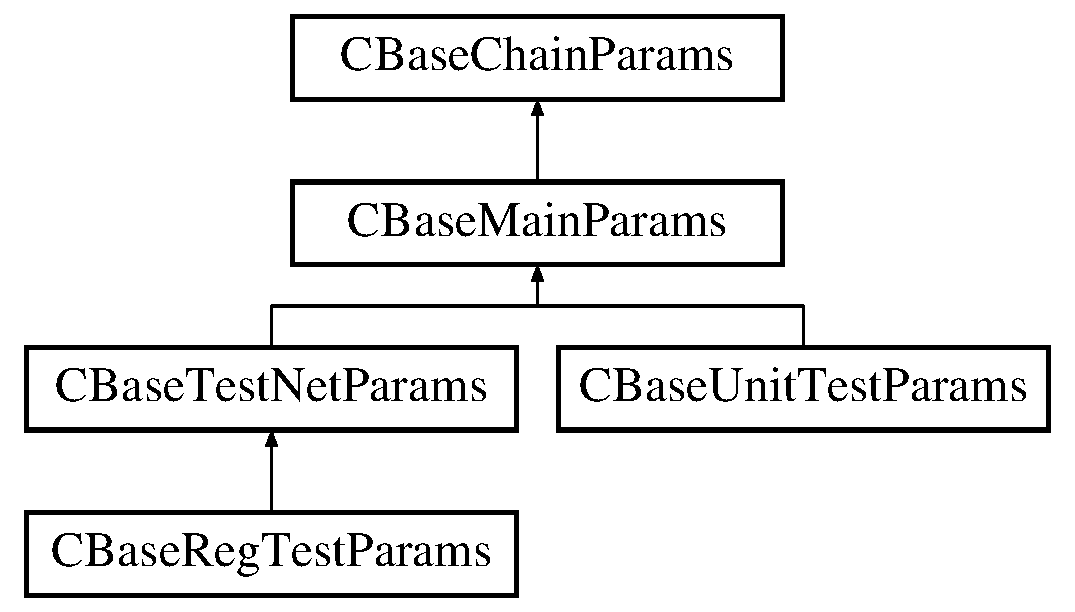
\includegraphics[height=4.000000cm]{class_c_base_main_params}
\end{center}
\end{figure}
\subsection*{Public Member Functions}
\begin{DoxyCompactItemize}
\item 
\mbox{\hyperlink{class_c_base_main_params_a547dabd3f634a23b8cd5478242e101e1}{C\+Base\+Main\+Params}} ()
\end{DoxyCompactItemize}
\subsection*{Additional Inherited Members}


\subsection{Detailed Description}
Main network 

\subsection{Constructor \& Destructor Documentation}
\mbox{\Hypertarget{class_c_base_main_params_a547dabd3f634a23b8cd5478242e101e1}\label{class_c_base_main_params_a547dabd3f634a23b8cd5478242e101e1}} 
\index{C\+Base\+Main\+Params@{C\+Base\+Main\+Params}!C\+Base\+Main\+Params@{C\+Base\+Main\+Params}}
\index{C\+Base\+Main\+Params@{C\+Base\+Main\+Params}!C\+Base\+Main\+Params@{C\+Base\+Main\+Params}}
\subsubsection{\texorpdfstring{C\+Base\+Main\+Params()}{CBaseMainParams()}}
{\footnotesize\ttfamily C\+Base\+Main\+Params\+::\+C\+Base\+Main\+Params (\begin{DoxyParamCaption}{ }\end{DoxyParamCaption})\hspace{0.3cm}{\ttfamily [inline]}}



The documentation for this class was generated from the following file\+:\begin{DoxyCompactItemize}
\item 
/\+Users/christopherarguello/\+Developer/anon/src/\mbox{\hyperlink{chainparamsbase_8cpp}{chainparamsbase.\+cpp}}\end{DoxyCompactItemize}

\hypertarget{class_c_base_reg_test_params}{}\section{C\+Base\+Reg\+Test\+Params Class Reference}
\label{class_c_base_reg_test_params}\index{C\+Base\+Reg\+Test\+Params@{C\+Base\+Reg\+Test\+Params}}
Inheritance diagram for C\+Base\+Reg\+Test\+Params\+:\begin{figure}[H]
\begin{center}
\leavevmode
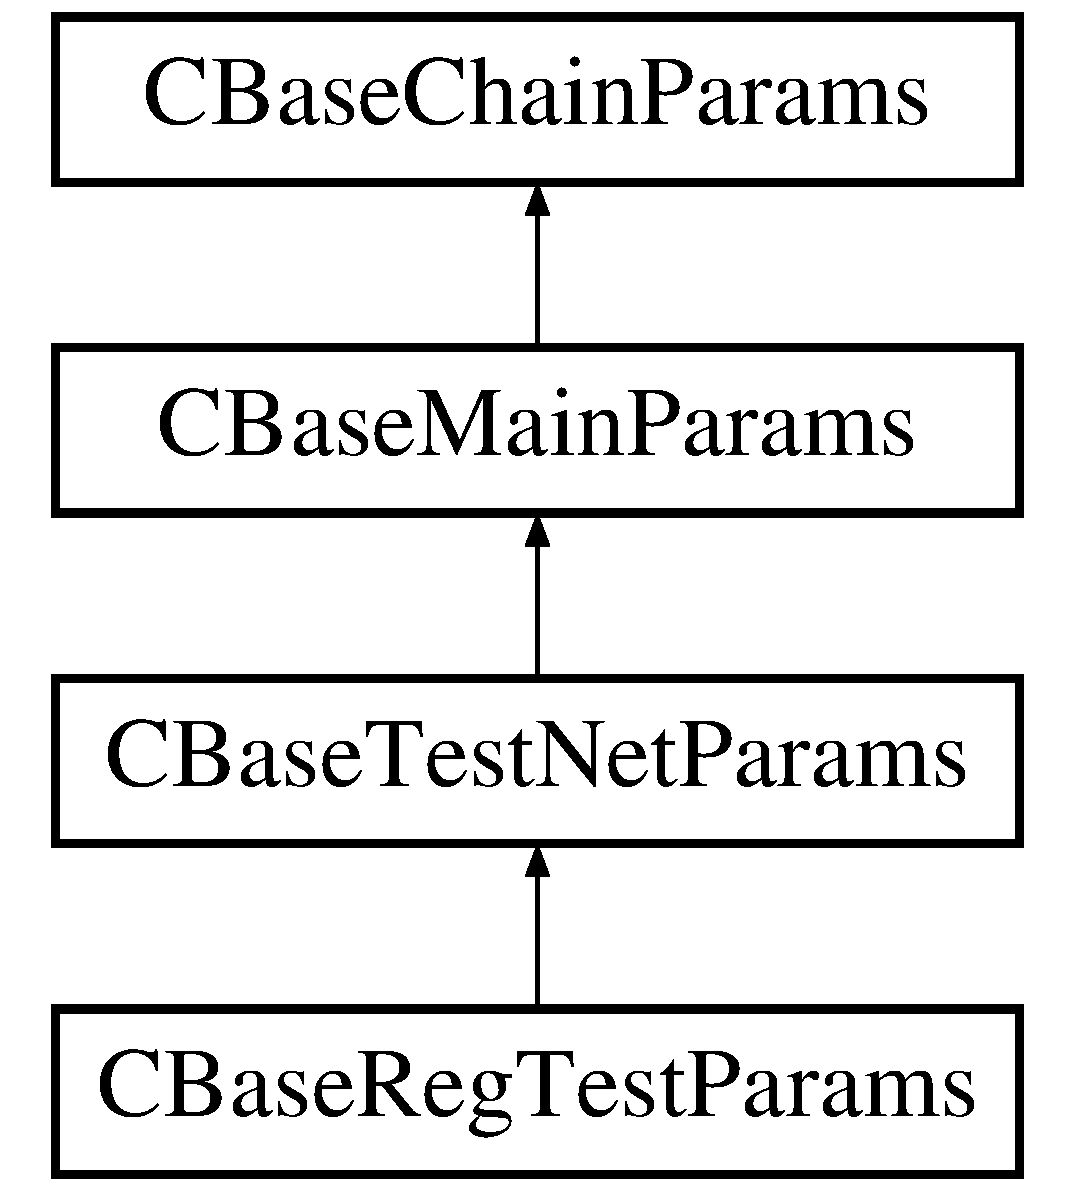
\includegraphics[height=4.000000cm]{class_c_base_reg_test_params}
\end{center}
\end{figure}
\subsection*{Public Member Functions}
\begin{DoxyCompactItemize}
\item 
\mbox{\hyperlink{class_c_base_reg_test_params_af32910af3003663d0ea5ee6406ce3b50}{C\+Base\+Reg\+Test\+Params}} ()
\end{DoxyCompactItemize}
\subsection*{Additional Inherited Members}


\subsection{Constructor \& Destructor Documentation}
\mbox{\Hypertarget{class_c_base_reg_test_params_af32910af3003663d0ea5ee6406ce3b50}\label{class_c_base_reg_test_params_af32910af3003663d0ea5ee6406ce3b50}} 
\index{C\+Base\+Reg\+Test\+Params@{C\+Base\+Reg\+Test\+Params}!C\+Base\+Reg\+Test\+Params@{C\+Base\+Reg\+Test\+Params}}
\index{C\+Base\+Reg\+Test\+Params@{C\+Base\+Reg\+Test\+Params}!C\+Base\+Reg\+Test\+Params@{C\+Base\+Reg\+Test\+Params}}
\subsubsection{\texorpdfstring{C\+Base\+Reg\+Test\+Params()}{CBaseRegTestParams()}}
{\footnotesize\ttfamily C\+Base\+Reg\+Test\+Params\+::\+C\+Base\+Reg\+Test\+Params (\begin{DoxyParamCaption}{ }\end{DoxyParamCaption})\hspace{0.3cm}{\ttfamily [inline]}}



The documentation for this class was generated from the following file\+:\begin{DoxyCompactItemize}
\item 
/\+Users/christopherarguello/\+Developer/anon/src/\mbox{\hyperlink{chainparamsbase_8cpp}{chainparamsbase.\+cpp}}\end{DoxyCompactItemize}

\hypertarget{class_c_base_test_net_params}{}\section{C\+Base\+Test\+Net\+Params Class Reference}
\label{class_c_base_test_net_params}\index{C\+Base\+Test\+Net\+Params@{C\+Base\+Test\+Net\+Params}}
Inheritance diagram for C\+Base\+Test\+Net\+Params\+:\begin{figure}[H]
\begin{center}
\leavevmode
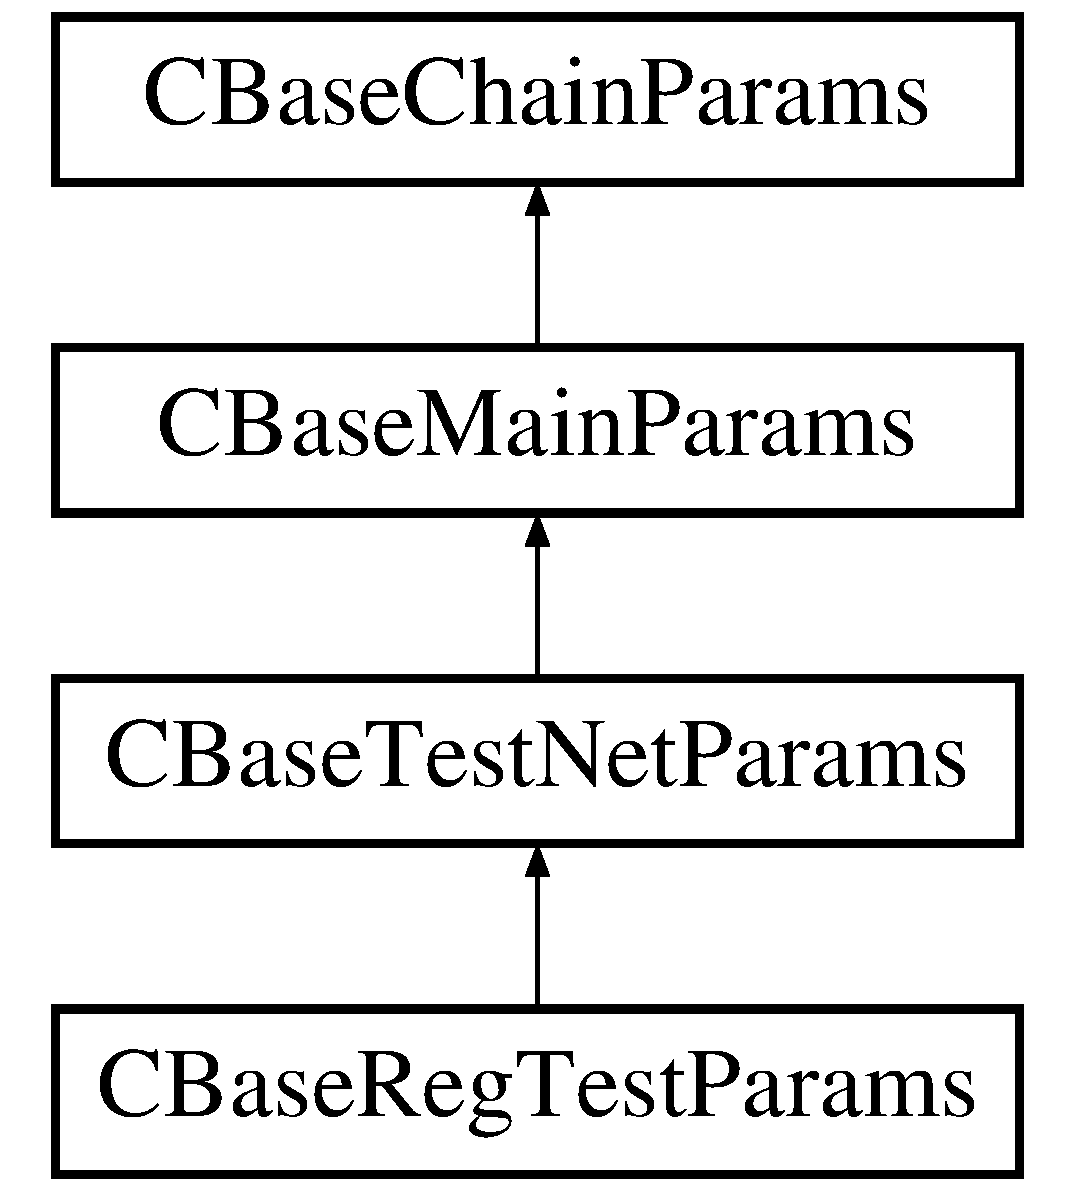
\includegraphics[height=4.000000cm]{class_c_base_test_net_params}
\end{center}
\end{figure}
\subsection*{Public Member Functions}
\begin{DoxyCompactItemize}
\item 
\mbox{\hyperlink{class_c_base_test_net_params_ae95167a7de928f49ce78840c1569ce16}{C\+Base\+Test\+Net\+Params}} ()
\end{DoxyCompactItemize}
\subsection*{Additional Inherited Members}


\subsection{Detailed Description}
Testnet (v3) 

\subsection{Constructor \& Destructor Documentation}
\mbox{\Hypertarget{class_c_base_test_net_params_ae95167a7de928f49ce78840c1569ce16}\label{class_c_base_test_net_params_ae95167a7de928f49ce78840c1569ce16}} 
\index{C\+Base\+Test\+Net\+Params@{C\+Base\+Test\+Net\+Params}!C\+Base\+Test\+Net\+Params@{C\+Base\+Test\+Net\+Params}}
\index{C\+Base\+Test\+Net\+Params@{C\+Base\+Test\+Net\+Params}!C\+Base\+Test\+Net\+Params@{C\+Base\+Test\+Net\+Params}}
\subsubsection{\texorpdfstring{C\+Base\+Test\+Net\+Params()}{CBaseTestNetParams()}}
{\footnotesize\ttfamily C\+Base\+Test\+Net\+Params\+::\+C\+Base\+Test\+Net\+Params (\begin{DoxyParamCaption}{ }\end{DoxyParamCaption})\hspace{0.3cm}{\ttfamily [inline]}}



The documentation for this class was generated from the following file\+:\begin{DoxyCompactItemize}
\item 
/\+Users/christopherarguello/\+Developer/anon/src/\mbox{\hyperlink{chainparamsbase_8cpp}{chainparamsbase.\+cpp}}\end{DoxyCompactItemize}

\hypertarget{class_c_base_unit_test_params}{}\section{C\+Base\+Unit\+Test\+Params Class Reference}
\label{class_c_base_unit_test_params}\index{C\+Base\+Unit\+Test\+Params@{C\+Base\+Unit\+Test\+Params}}
Inheritance diagram for C\+Base\+Unit\+Test\+Params\+:\begin{figure}[H]
\begin{center}
\leavevmode
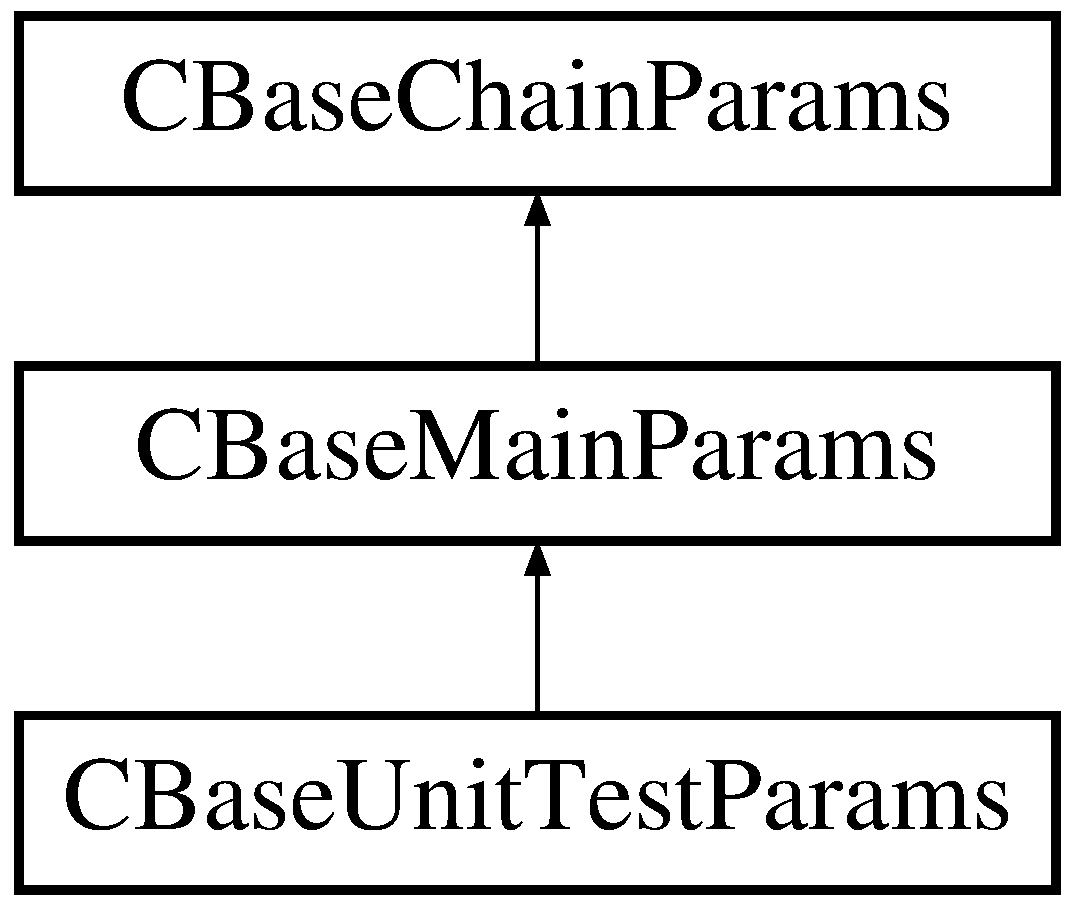
\includegraphics[height=3.000000cm]{class_c_base_unit_test_params}
\end{center}
\end{figure}
\subsection*{Public Member Functions}
\begin{DoxyCompactItemize}
\item 
\mbox{\hyperlink{class_c_base_unit_test_params_a5adade9edcf1ebefc89ff198d0d52ff5}{C\+Base\+Unit\+Test\+Params}} ()
\end{DoxyCompactItemize}
\subsection*{Additional Inherited Members}


\subsection{Constructor \& Destructor Documentation}
\mbox{\Hypertarget{class_c_base_unit_test_params_a5adade9edcf1ebefc89ff198d0d52ff5}\label{class_c_base_unit_test_params_a5adade9edcf1ebefc89ff198d0d52ff5}} 
\index{C\+Base\+Unit\+Test\+Params@{C\+Base\+Unit\+Test\+Params}!C\+Base\+Unit\+Test\+Params@{C\+Base\+Unit\+Test\+Params}}
\index{C\+Base\+Unit\+Test\+Params@{C\+Base\+Unit\+Test\+Params}!C\+Base\+Unit\+Test\+Params@{C\+Base\+Unit\+Test\+Params}}
\subsubsection{\texorpdfstring{C\+Base\+Unit\+Test\+Params()}{CBaseUnitTestParams()}}
{\footnotesize\ttfamily C\+Base\+Unit\+Test\+Params\+::\+C\+Base\+Unit\+Test\+Params (\begin{DoxyParamCaption}{ }\end{DoxyParamCaption})\hspace{0.3cm}{\ttfamily [inline]}}



The documentation for this class was generated from the following file\+:\begin{DoxyCompactItemize}
\item 
/\+Users/christopherarguello/\+Developer/anon/src/\mbox{\hyperlink{chainparamsbase_8cpp}{chainparamsbase.\+cpp}}\end{DoxyCompactItemize}

\hypertarget{class_c_basic_key_store}{}\section{C\+Basic\+Key\+Store Class Reference}
\label{class_c_basic_key_store}\index{C\+Basic\+Key\+Store@{C\+Basic\+Key\+Store}}


{\ttfamily \#include $<$keystore.\+h$>$}

Inheritance diagram for C\+Basic\+Key\+Store\+:\begin{figure}[H]
\begin{center}
\leavevmode
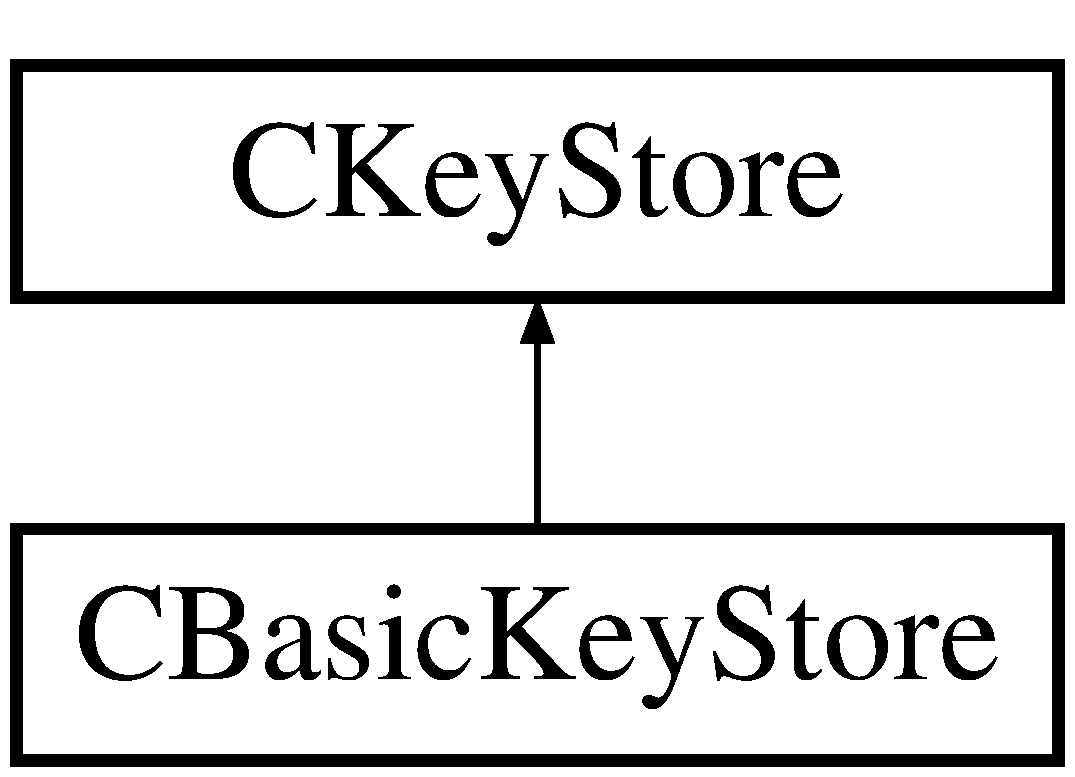
\includegraphics[height=2.000000cm]{class_c_basic_key_store}
\end{center}
\end{figure}
\subsection*{Public Member Functions}
\begin{DoxyCompactItemize}
\item 
bool \mbox{\hyperlink{class_c_basic_key_store_acc2e33f319de88e88f86b0dc79bdcb65}{Add\+Key\+Pub\+Key}} (const \mbox{\hyperlink{class_c_key}{C\+Key}} \&key, const \mbox{\hyperlink{class_c_pub_key}{C\+Pub\+Key}} \&pubkey)
\begin{DoxyCompactList}\small\item\em Add a key to the store. \end{DoxyCompactList}\item 
bool \mbox{\hyperlink{class_c_basic_key_store_afc99762e3e58f93e198d85ecfdf5804a}{Have\+Key}} (const \mbox{\hyperlink{class_c_key_i_d}{C\+Key\+ID}} \&address) const
\begin{DoxyCompactList}\small\item\em Check whether a key corresponding to a given address is present in the store. \end{DoxyCompactList}\item 
void \mbox{\hyperlink{class_c_basic_key_store_a41f3895021dae008582ceb55a98b0891}{Get\+Keys}} (std\+::set$<$ \mbox{\hyperlink{class_c_key_i_d}{C\+Key\+ID}} $>$ \&set\+Address) const
\item 
bool \mbox{\hyperlink{class_c_basic_key_store_a69328ee642e4234922356f59876e956d}{Get\+Key}} (const \mbox{\hyperlink{class_c_key_i_d}{C\+Key\+ID}} \&address, \mbox{\hyperlink{class_c_key}{C\+Key}} \&key\+Out) const
\item 
virtual bool \mbox{\hyperlink{class_c_basic_key_store_a56249ce3540398999cd397eeb662e836}{Add\+C\+Script}} (const C\+Script \&redeem\+Script)
\begin{DoxyCompactList}\small\item\em Support for B\+IP 0013 \+: see \href{https://github.com/bitcoin/bips/blob/master/bip-0013.mediawiki}{\tt https\+://github.\+com/bitcoin/bips/blob/master/bip-\/0013.\+mediawiki}. \end{DoxyCompactList}\item 
virtual bool \mbox{\hyperlink{class_c_basic_key_store_a499e0a1d117b43e3200883d88a400bf6}{Have\+C\+Script}} (const C\+Script\+ID \&hash) const
\item 
virtual bool \mbox{\hyperlink{class_c_basic_key_store_a975abe0f2efa3e0e2270d3714d73010a}{Get\+C\+Script}} (const C\+Script\+ID \&hash, C\+Script \&redeem\+Script\+Out) const
\item 
virtual bool \mbox{\hyperlink{class_c_basic_key_store_a2417d0ae4e654c88cf47a1ba5f71b5a3}{Add\+Watch\+Only}} (const C\+Script \&dest)
\begin{DoxyCompactList}\small\item\em Support for Watch-\/only addresses. \end{DoxyCompactList}\item 
virtual bool \mbox{\hyperlink{class_c_basic_key_store_a20c0eccf943d6d16e24c6e2fb63fb527}{Remove\+Watch\+Only}} (const C\+Script \&dest)
\item 
virtual bool \mbox{\hyperlink{class_c_basic_key_store_a3ce143be2a1d3e752972614cf7fb7efb}{Have\+Watch\+Only}} (const C\+Script \&dest) const
\item 
virtual bool \mbox{\hyperlink{class_c_basic_key_store_aa6686d4477a180096436e7d491142f10}{Have\+Watch\+Only}} () const
\item 
bool \mbox{\hyperlink{class_c_basic_key_store_aa2d2d623fe80e75fe1718a15755ee1f1}{Add\+Spending\+Key}} (const libzcash\+::\+Spending\+Key \&sk)
\begin{DoxyCompactList}\small\item\em Add a spending key to the store. \end{DoxyCompactList}\item 
bool \mbox{\hyperlink{class_c_basic_key_store_a513367bd0a576e088e3f577686fa1ef5}{Have\+Spending\+Key}} (const libzcash\+::\+Payment\+Address \&address) const
\begin{DoxyCompactList}\small\item\em Check whether a spending key corresponding to a given payment address is present in the store. \end{DoxyCompactList}\item 
bool \mbox{\hyperlink{class_c_basic_key_store_a0c7997c0413eaa7ec76ec5bef0b40a2a}{Get\+Spending\+Key}} (const libzcash\+::\+Payment\+Address \&address, libzcash\+::\+Spending\+Key \&sk\+Out) const
\item 
bool \mbox{\hyperlink{class_c_basic_key_store_a588967be388dfc70f0449b576eea420a}{Get\+Note\+Decryptor}} (const libzcash\+::\+Payment\+Address \&address, Z\+C\+Note\+Decryption \&dec\+Out) const
\item 
void \mbox{\hyperlink{class_c_basic_key_store_af02668c3bef8b5a56231505f900a0314}{Get\+Payment\+Addresses}} (std\+::set$<$ libzcash\+::\+Payment\+Address $>$ \&set\+Address) const
\end{DoxyCompactItemize}
\subsection*{Protected Attributes}
\begin{DoxyCompactItemize}
\item 
\mbox{\hyperlink{keystore_8h_a4dc9f57afc8615aef701e40cf20d024f}{Key\+Map}} \mbox{\hyperlink{class_c_basic_key_store_ac520003e5c3d863bf71fde247c6e0672}{map\+Keys}}
\item 
\mbox{\hyperlink{keystore_8h_afb22a3e7e10e8048d2fb3fb72fe38345}{Script\+Map}} \mbox{\hyperlink{class_c_basic_key_store_a8e9fa81382129c1535a0ee7b0d9c8f3b}{map\+Scripts}}
\item 
\mbox{\hyperlink{keystore_8h_a501c3a7b9932bbc7168dc7b3fc5d149e}{Watch\+Only\+Set}} \mbox{\hyperlink{class_c_basic_key_store_ac3391cb491e315403ad9af6afd1313da}{set\+Watch\+Only}}
\item 
\mbox{\hyperlink{keystore_8h_a15f25b2302a5fa99fc89afa51401bf12}{Spending\+Key\+Map}} \mbox{\hyperlink{class_c_basic_key_store_a96ef08a1453e56a9a147d9b3add03813}{map\+Spending\+Keys}}
\item 
\mbox{\hyperlink{keystore_8h_abe42b6c1b0529af8aa631494acef112a}{Note\+Decryptor\+Map}} \mbox{\hyperlink{class_c_basic_key_store_a4f2a294a146a9bb2d20cc3bca094d9eb}{map\+Note\+Decryptors}}
\end{DoxyCompactItemize}


\subsection{Detailed Description}
Basic key store, that keeps keys in an address-\/$>$secret map 

\subsection{Member Function Documentation}
\mbox{\Hypertarget{class_c_basic_key_store_a56249ce3540398999cd397eeb662e836}\label{class_c_basic_key_store_a56249ce3540398999cd397eeb662e836}} 
\index{C\+Basic\+Key\+Store@{C\+Basic\+Key\+Store}!Add\+C\+Script@{Add\+C\+Script}}
\index{Add\+C\+Script@{Add\+C\+Script}!C\+Basic\+Key\+Store@{C\+Basic\+Key\+Store}}
\subsubsection{\texorpdfstring{Add\+C\+Script()}{AddCScript()}}
{\footnotesize\ttfamily bool C\+Basic\+Key\+Store\+::\+Add\+C\+Script (\begin{DoxyParamCaption}\item[{const C\+Script \&}]{redeem\+Script }\end{DoxyParamCaption})\hspace{0.3cm}{\ttfamily [virtual]}}



Support for B\+IP 0013 \+: see \href{https://github.com/bitcoin/bips/blob/master/bip-0013.mediawiki}{\tt https\+://github.\+com/bitcoin/bips/blob/master/bip-\/0013.\+mediawiki}. 



Implements \mbox{\hyperlink{class_c_key_store_a2fb2e02e8cdc364607efd5ebb14b8064}{C\+Key\+Store}}.

\mbox{\Hypertarget{class_c_basic_key_store_acc2e33f319de88e88f86b0dc79bdcb65}\label{class_c_basic_key_store_acc2e33f319de88e88f86b0dc79bdcb65}} 
\index{C\+Basic\+Key\+Store@{C\+Basic\+Key\+Store}!Add\+Key\+Pub\+Key@{Add\+Key\+Pub\+Key}}
\index{Add\+Key\+Pub\+Key@{Add\+Key\+Pub\+Key}!C\+Basic\+Key\+Store@{C\+Basic\+Key\+Store}}
\subsubsection{\texorpdfstring{Add\+Key\+Pub\+Key()}{AddKeyPubKey()}}
{\footnotesize\ttfamily bool C\+Basic\+Key\+Store\+::\+Add\+Key\+Pub\+Key (\begin{DoxyParamCaption}\item[{const \mbox{\hyperlink{class_c_key}{C\+Key}} \&}]{key,  }\item[{const \mbox{\hyperlink{class_c_pub_key}{C\+Pub\+Key}} \&}]{pubkey }\end{DoxyParamCaption})\hspace{0.3cm}{\ttfamily [virtual]}}



Add a key to the store. 



Implements \mbox{\hyperlink{class_c_key_store_a1956e4f5860ded321d6f697047d8236a}{C\+Key\+Store}}.

\mbox{\Hypertarget{class_c_basic_key_store_aa2d2d623fe80e75fe1718a15755ee1f1}\label{class_c_basic_key_store_aa2d2d623fe80e75fe1718a15755ee1f1}} 
\index{C\+Basic\+Key\+Store@{C\+Basic\+Key\+Store}!Add\+Spending\+Key@{Add\+Spending\+Key}}
\index{Add\+Spending\+Key@{Add\+Spending\+Key}!C\+Basic\+Key\+Store@{C\+Basic\+Key\+Store}}
\subsubsection{\texorpdfstring{Add\+Spending\+Key()}{AddSpendingKey()}}
{\footnotesize\ttfamily bool C\+Basic\+Key\+Store\+::\+Add\+Spending\+Key (\begin{DoxyParamCaption}\item[{const libzcash\+::\+Spending\+Key \&}]{sk }\end{DoxyParamCaption})\hspace{0.3cm}{\ttfamily [virtual]}}



Add a spending key to the store. 



Implements \mbox{\hyperlink{class_c_key_store_aa78189cb8f342a33570c2ac6d4a0ffcf}{C\+Key\+Store}}.

\mbox{\Hypertarget{class_c_basic_key_store_a2417d0ae4e654c88cf47a1ba5f71b5a3}\label{class_c_basic_key_store_a2417d0ae4e654c88cf47a1ba5f71b5a3}} 
\index{C\+Basic\+Key\+Store@{C\+Basic\+Key\+Store}!Add\+Watch\+Only@{Add\+Watch\+Only}}
\index{Add\+Watch\+Only@{Add\+Watch\+Only}!C\+Basic\+Key\+Store@{C\+Basic\+Key\+Store}}
\subsubsection{\texorpdfstring{Add\+Watch\+Only()}{AddWatchOnly()}}
{\footnotesize\ttfamily bool C\+Basic\+Key\+Store\+::\+Add\+Watch\+Only (\begin{DoxyParamCaption}\item[{const C\+Script \&}]{dest }\end{DoxyParamCaption})\hspace{0.3cm}{\ttfamily [virtual]}}



Support for Watch-\/only addresses. 



Implements \mbox{\hyperlink{class_c_key_store_a12cd4eaa01bd4f4231c0bf68425a44af}{C\+Key\+Store}}.

\mbox{\Hypertarget{class_c_basic_key_store_a975abe0f2efa3e0e2270d3714d73010a}\label{class_c_basic_key_store_a975abe0f2efa3e0e2270d3714d73010a}} 
\index{C\+Basic\+Key\+Store@{C\+Basic\+Key\+Store}!Get\+C\+Script@{Get\+C\+Script}}
\index{Get\+C\+Script@{Get\+C\+Script}!C\+Basic\+Key\+Store@{C\+Basic\+Key\+Store}}
\subsubsection{\texorpdfstring{Get\+C\+Script()}{GetCScript()}}
{\footnotesize\ttfamily bool C\+Basic\+Key\+Store\+::\+Get\+C\+Script (\begin{DoxyParamCaption}\item[{const C\+Script\+ID \&}]{hash,  }\item[{C\+Script \&}]{redeem\+Script\+Out }\end{DoxyParamCaption}) const\hspace{0.3cm}{\ttfamily [virtual]}}



Implements \mbox{\hyperlink{class_c_key_store_ae6bf4dbeb0705e199250e48aa5d34264}{C\+Key\+Store}}.

\mbox{\Hypertarget{class_c_basic_key_store_a69328ee642e4234922356f59876e956d}\label{class_c_basic_key_store_a69328ee642e4234922356f59876e956d}} 
\index{C\+Basic\+Key\+Store@{C\+Basic\+Key\+Store}!Get\+Key@{Get\+Key}}
\index{Get\+Key@{Get\+Key}!C\+Basic\+Key\+Store@{C\+Basic\+Key\+Store}}
\subsubsection{\texorpdfstring{Get\+Key()}{GetKey()}}
{\footnotesize\ttfamily bool C\+Basic\+Key\+Store\+::\+Get\+Key (\begin{DoxyParamCaption}\item[{const \mbox{\hyperlink{class_c_key_i_d}{C\+Key\+ID}} \&}]{address,  }\item[{\mbox{\hyperlink{class_c_key}{C\+Key}} \&}]{key\+Out }\end{DoxyParamCaption}) const\hspace{0.3cm}{\ttfamily [inline]}, {\ttfamily [virtual]}}



Implements \mbox{\hyperlink{class_c_key_store_a2dffca468fef2e5da2e42a7c983d968a}{C\+Key\+Store}}.

\mbox{\Hypertarget{class_c_basic_key_store_a41f3895021dae008582ceb55a98b0891}\label{class_c_basic_key_store_a41f3895021dae008582ceb55a98b0891}} 
\index{C\+Basic\+Key\+Store@{C\+Basic\+Key\+Store}!Get\+Keys@{Get\+Keys}}
\index{Get\+Keys@{Get\+Keys}!C\+Basic\+Key\+Store@{C\+Basic\+Key\+Store}}
\subsubsection{\texorpdfstring{Get\+Keys()}{GetKeys()}}
{\footnotesize\ttfamily void C\+Basic\+Key\+Store\+::\+Get\+Keys (\begin{DoxyParamCaption}\item[{std\+::set$<$ \mbox{\hyperlink{class_c_key_i_d}{C\+Key\+ID}} $>$ \&}]{set\+Address }\end{DoxyParamCaption}) const\hspace{0.3cm}{\ttfamily [inline]}, {\ttfamily [virtual]}}



Implements \mbox{\hyperlink{class_c_key_store_aca5044014720308f191113e7ba297d13}{C\+Key\+Store}}.

\mbox{\Hypertarget{class_c_basic_key_store_a588967be388dfc70f0449b576eea420a}\label{class_c_basic_key_store_a588967be388dfc70f0449b576eea420a}} 
\index{C\+Basic\+Key\+Store@{C\+Basic\+Key\+Store}!Get\+Note\+Decryptor@{Get\+Note\+Decryptor}}
\index{Get\+Note\+Decryptor@{Get\+Note\+Decryptor}!C\+Basic\+Key\+Store@{C\+Basic\+Key\+Store}}
\subsubsection{\texorpdfstring{Get\+Note\+Decryptor()}{GetNoteDecryptor()}}
{\footnotesize\ttfamily bool C\+Basic\+Key\+Store\+::\+Get\+Note\+Decryptor (\begin{DoxyParamCaption}\item[{const libzcash\+::\+Payment\+Address \&}]{address,  }\item[{Z\+C\+Note\+Decryption \&}]{dec\+Out }\end{DoxyParamCaption}) const\hspace{0.3cm}{\ttfamily [inline]}}

\mbox{\Hypertarget{class_c_basic_key_store_af02668c3bef8b5a56231505f900a0314}\label{class_c_basic_key_store_af02668c3bef8b5a56231505f900a0314}} 
\index{C\+Basic\+Key\+Store@{C\+Basic\+Key\+Store}!Get\+Payment\+Addresses@{Get\+Payment\+Addresses}}
\index{Get\+Payment\+Addresses@{Get\+Payment\+Addresses}!C\+Basic\+Key\+Store@{C\+Basic\+Key\+Store}}
\subsubsection{\texorpdfstring{Get\+Payment\+Addresses()}{GetPaymentAddresses()}}
{\footnotesize\ttfamily void C\+Basic\+Key\+Store\+::\+Get\+Payment\+Addresses (\begin{DoxyParamCaption}\item[{std\+::set$<$ libzcash\+::\+Payment\+Address $>$ \&}]{set\+Address }\end{DoxyParamCaption}) const\hspace{0.3cm}{\ttfamily [inline]}, {\ttfamily [virtual]}}



Implements \mbox{\hyperlink{class_c_key_store_a6186d83956656316f3fe679b4f907866}{C\+Key\+Store}}.

\mbox{\Hypertarget{class_c_basic_key_store_a0c7997c0413eaa7ec76ec5bef0b40a2a}\label{class_c_basic_key_store_a0c7997c0413eaa7ec76ec5bef0b40a2a}} 
\index{C\+Basic\+Key\+Store@{C\+Basic\+Key\+Store}!Get\+Spending\+Key@{Get\+Spending\+Key}}
\index{Get\+Spending\+Key@{Get\+Spending\+Key}!C\+Basic\+Key\+Store@{C\+Basic\+Key\+Store}}
\subsubsection{\texorpdfstring{Get\+Spending\+Key()}{GetSpendingKey()}}
{\footnotesize\ttfamily bool C\+Basic\+Key\+Store\+::\+Get\+Spending\+Key (\begin{DoxyParamCaption}\item[{const libzcash\+::\+Payment\+Address \&}]{address,  }\item[{libzcash\+::\+Spending\+Key \&}]{sk\+Out }\end{DoxyParamCaption}) const\hspace{0.3cm}{\ttfamily [inline]}, {\ttfamily [virtual]}}



Implements \mbox{\hyperlink{class_c_key_store_a812534268d0324370c53ba3e7a295b95}{C\+Key\+Store}}.

\mbox{\Hypertarget{class_c_basic_key_store_a499e0a1d117b43e3200883d88a400bf6}\label{class_c_basic_key_store_a499e0a1d117b43e3200883d88a400bf6}} 
\index{C\+Basic\+Key\+Store@{C\+Basic\+Key\+Store}!Have\+C\+Script@{Have\+C\+Script}}
\index{Have\+C\+Script@{Have\+C\+Script}!C\+Basic\+Key\+Store@{C\+Basic\+Key\+Store}}
\subsubsection{\texorpdfstring{Have\+C\+Script()}{HaveCScript()}}
{\footnotesize\ttfamily bool C\+Basic\+Key\+Store\+::\+Have\+C\+Script (\begin{DoxyParamCaption}\item[{const C\+Script\+ID \&}]{hash }\end{DoxyParamCaption}) const\hspace{0.3cm}{\ttfamily [virtual]}}



Implements \mbox{\hyperlink{class_c_key_store_a51c9fc86b2c3fece10d86146231fa58d}{C\+Key\+Store}}.

\mbox{\Hypertarget{class_c_basic_key_store_afc99762e3e58f93e198d85ecfdf5804a}\label{class_c_basic_key_store_afc99762e3e58f93e198d85ecfdf5804a}} 
\index{C\+Basic\+Key\+Store@{C\+Basic\+Key\+Store}!Have\+Key@{Have\+Key}}
\index{Have\+Key@{Have\+Key}!C\+Basic\+Key\+Store@{C\+Basic\+Key\+Store}}
\subsubsection{\texorpdfstring{Have\+Key()}{HaveKey()}}
{\footnotesize\ttfamily bool C\+Basic\+Key\+Store\+::\+Have\+Key (\begin{DoxyParamCaption}\item[{const \mbox{\hyperlink{class_c_key_i_d}{C\+Key\+ID}} \&}]{address }\end{DoxyParamCaption}) const\hspace{0.3cm}{\ttfamily [inline]}, {\ttfamily [virtual]}}



Check whether a key corresponding to a given address is present in the store. 



Implements \mbox{\hyperlink{class_c_key_store_a9398451d4270fae27b29f686a9d43a65}{C\+Key\+Store}}.

\mbox{\Hypertarget{class_c_basic_key_store_a513367bd0a576e088e3f577686fa1ef5}\label{class_c_basic_key_store_a513367bd0a576e088e3f577686fa1ef5}} 
\index{C\+Basic\+Key\+Store@{C\+Basic\+Key\+Store}!Have\+Spending\+Key@{Have\+Spending\+Key}}
\index{Have\+Spending\+Key@{Have\+Spending\+Key}!C\+Basic\+Key\+Store@{C\+Basic\+Key\+Store}}
\subsubsection{\texorpdfstring{Have\+Spending\+Key()}{HaveSpendingKey()}}
{\footnotesize\ttfamily bool C\+Basic\+Key\+Store\+::\+Have\+Spending\+Key (\begin{DoxyParamCaption}\item[{const libzcash\+::\+Payment\+Address \&}]{address }\end{DoxyParamCaption}) const\hspace{0.3cm}{\ttfamily [inline]}, {\ttfamily [virtual]}}



Check whether a spending key corresponding to a given payment address is present in the store. 



Implements \mbox{\hyperlink{class_c_key_store_a15590101690f5a691b04a5498453b66a}{C\+Key\+Store}}.

\mbox{\Hypertarget{class_c_basic_key_store_a3ce143be2a1d3e752972614cf7fb7efb}\label{class_c_basic_key_store_a3ce143be2a1d3e752972614cf7fb7efb}} 
\index{C\+Basic\+Key\+Store@{C\+Basic\+Key\+Store}!Have\+Watch\+Only@{Have\+Watch\+Only}}
\index{Have\+Watch\+Only@{Have\+Watch\+Only}!C\+Basic\+Key\+Store@{C\+Basic\+Key\+Store}}
\subsubsection{\texorpdfstring{Have\+Watch\+Only()}{HaveWatchOnly()}\hspace{0.1cm}{\footnotesize\ttfamily [1/2]}}
{\footnotesize\ttfamily bool C\+Basic\+Key\+Store\+::\+Have\+Watch\+Only (\begin{DoxyParamCaption}\item[{const C\+Script \&}]{dest }\end{DoxyParamCaption}) const\hspace{0.3cm}{\ttfamily [virtual]}}



Implements \mbox{\hyperlink{class_c_key_store_a15066cfd57feaffe0b9f4103c9311109}{C\+Key\+Store}}.

\mbox{\Hypertarget{class_c_basic_key_store_aa6686d4477a180096436e7d491142f10}\label{class_c_basic_key_store_aa6686d4477a180096436e7d491142f10}} 
\index{C\+Basic\+Key\+Store@{C\+Basic\+Key\+Store}!Have\+Watch\+Only@{Have\+Watch\+Only}}
\index{Have\+Watch\+Only@{Have\+Watch\+Only}!C\+Basic\+Key\+Store@{C\+Basic\+Key\+Store}}
\subsubsection{\texorpdfstring{Have\+Watch\+Only()}{HaveWatchOnly()}\hspace{0.1cm}{\footnotesize\ttfamily [2/2]}}
{\footnotesize\ttfamily bool C\+Basic\+Key\+Store\+::\+Have\+Watch\+Only (\begin{DoxyParamCaption}{ }\end{DoxyParamCaption}) const\hspace{0.3cm}{\ttfamily [virtual]}}



Implements \mbox{\hyperlink{class_c_key_store_a9169351f4acf62d299afb824174cbfa8}{C\+Key\+Store}}.

\mbox{\Hypertarget{class_c_basic_key_store_a20c0eccf943d6d16e24c6e2fb63fb527}\label{class_c_basic_key_store_a20c0eccf943d6d16e24c6e2fb63fb527}} 
\index{C\+Basic\+Key\+Store@{C\+Basic\+Key\+Store}!Remove\+Watch\+Only@{Remove\+Watch\+Only}}
\index{Remove\+Watch\+Only@{Remove\+Watch\+Only}!C\+Basic\+Key\+Store@{C\+Basic\+Key\+Store}}
\subsubsection{\texorpdfstring{Remove\+Watch\+Only()}{RemoveWatchOnly()}}
{\footnotesize\ttfamily bool C\+Basic\+Key\+Store\+::\+Remove\+Watch\+Only (\begin{DoxyParamCaption}\item[{const C\+Script \&}]{dest }\end{DoxyParamCaption})\hspace{0.3cm}{\ttfamily [virtual]}}



Implements \mbox{\hyperlink{class_c_key_store_ad510747f28d129123a5200e4df8f7f61}{C\+Key\+Store}}.



\subsection{Member Data Documentation}
\mbox{\Hypertarget{class_c_basic_key_store_ac520003e5c3d863bf71fde247c6e0672}\label{class_c_basic_key_store_ac520003e5c3d863bf71fde247c6e0672}} 
\index{C\+Basic\+Key\+Store@{C\+Basic\+Key\+Store}!map\+Keys@{map\+Keys}}
\index{map\+Keys@{map\+Keys}!C\+Basic\+Key\+Store@{C\+Basic\+Key\+Store}}
\subsubsection{\texorpdfstring{map\+Keys}{mapKeys}}
{\footnotesize\ttfamily \mbox{\hyperlink{keystore_8h_a4dc9f57afc8615aef701e40cf20d024f}{Key\+Map}} C\+Basic\+Key\+Store\+::map\+Keys\hspace{0.3cm}{\ttfamily [protected]}}

\mbox{\Hypertarget{class_c_basic_key_store_a4f2a294a146a9bb2d20cc3bca094d9eb}\label{class_c_basic_key_store_a4f2a294a146a9bb2d20cc3bca094d9eb}} 
\index{C\+Basic\+Key\+Store@{C\+Basic\+Key\+Store}!map\+Note\+Decryptors@{map\+Note\+Decryptors}}
\index{map\+Note\+Decryptors@{map\+Note\+Decryptors}!C\+Basic\+Key\+Store@{C\+Basic\+Key\+Store}}
\subsubsection{\texorpdfstring{map\+Note\+Decryptors}{mapNoteDecryptors}}
{\footnotesize\ttfamily \mbox{\hyperlink{keystore_8h_abe42b6c1b0529af8aa631494acef112a}{Note\+Decryptor\+Map}} C\+Basic\+Key\+Store\+::map\+Note\+Decryptors\hspace{0.3cm}{\ttfamily [protected]}}

\mbox{\Hypertarget{class_c_basic_key_store_a8e9fa81382129c1535a0ee7b0d9c8f3b}\label{class_c_basic_key_store_a8e9fa81382129c1535a0ee7b0d9c8f3b}} 
\index{C\+Basic\+Key\+Store@{C\+Basic\+Key\+Store}!map\+Scripts@{map\+Scripts}}
\index{map\+Scripts@{map\+Scripts}!C\+Basic\+Key\+Store@{C\+Basic\+Key\+Store}}
\subsubsection{\texorpdfstring{map\+Scripts}{mapScripts}}
{\footnotesize\ttfamily \mbox{\hyperlink{keystore_8h_afb22a3e7e10e8048d2fb3fb72fe38345}{Script\+Map}} C\+Basic\+Key\+Store\+::map\+Scripts\hspace{0.3cm}{\ttfamily [protected]}}

\mbox{\Hypertarget{class_c_basic_key_store_a96ef08a1453e56a9a147d9b3add03813}\label{class_c_basic_key_store_a96ef08a1453e56a9a147d9b3add03813}} 
\index{C\+Basic\+Key\+Store@{C\+Basic\+Key\+Store}!map\+Spending\+Keys@{map\+Spending\+Keys}}
\index{map\+Spending\+Keys@{map\+Spending\+Keys}!C\+Basic\+Key\+Store@{C\+Basic\+Key\+Store}}
\subsubsection{\texorpdfstring{map\+Spending\+Keys}{mapSpendingKeys}}
{\footnotesize\ttfamily \mbox{\hyperlink{keystore_8h_a15f25b2302a5fa99fc89afa51401bf12}{Spending\+Key\+Map}} C\+Basic\+Key\+Store\+::map\+Spending\+Keys\hspace{0.3cm}{\ttfamily [protected]}}

\mbox{\Hypertarget{class_c_basic_key_store_ac3391cb491e315403ad9af6afd1313da}\label{class_c_basic_key_store_ac3391cb491e315403ad9af6afd1313da}} 
\index{C\+Basic\+Key\+Store@{C\+Basic\+Key\+Store}!set\+Watch\+Only@{set\+Watch\+Only}}
\index{set\+Watch\+Only@{set\+Watch\+Only}!C\+Basic\+Key\+Store@{C\+Basic\+Key\+Store}}
\subsubsection{\texorpdfstring{set\+Watch\+Only}{setWatchOnly}}
{\footnotesize\ttfamily \mbox{\hyperlink{keystore_8h_a501c3a7b9932bbc7168dc7b3fc5d149e}{Watch\+Only\+Set}} C\+Basic\+Key\+Store\+::set\+Watch\+Only\hspace{0.3cm}{\ttfamily [protected]}}



The documentation for this class was generated from the following files\+:\begin{DoxyCompactItemize}
\item 
/\+Users/christopherarguello/\+Developer/anon/src/\mbox{\hyperlink{keystore_8h}{keystore.\+h}}\item 
/\+Users/christopherarguello/\+Developer/anon/src/\mbox{\hyperlink{keystore_8cpp}{keystore.\+cpp}}\end{DoxyCompactItemize}

\hypertarget{class_c_bitcoin_address}{}\section{C\+Bitcoin\+Address Class Reference}
\label{class_c_bitcoin_address}\index{C\+Bitcoin\+Address@{C\+Bitcoin\+Address}}


{\ttfamily \#include $<$base58.\+h$>$}

Inheritance diagram for C\+Bitcoin\+Address\+:\begin{figure}[H]
\begin{center}
\leavevmode
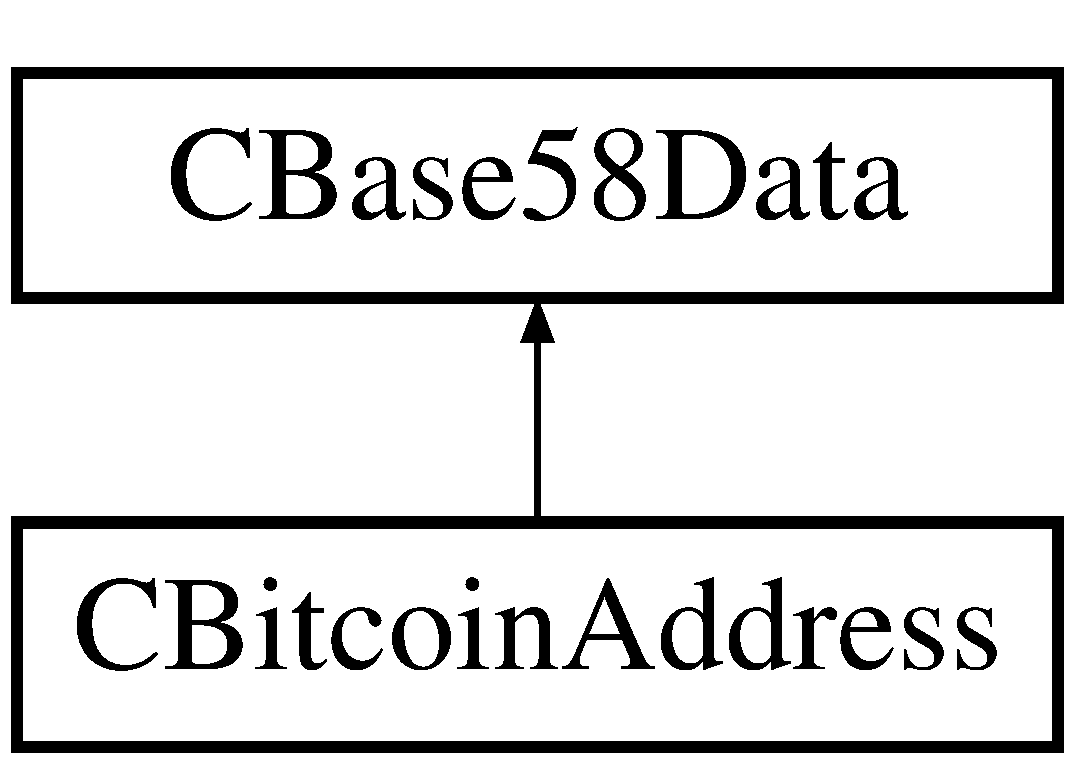
\includegraphics[height=2.000000cm]{class_c_bitcoin_address}
\end{center}
\end{figure}
\subsection*{Public Member Functions}
\begin{DoxyCompactItemize}
\item 
bool \mbox{\hyperlink{class_c_bitcoin_address_abe1614f9ecd143ae69256d65c5edbcab}{Set}} (const \mbox{\hyperlink{class_c_key_i_d}{C\+Key\+ID}} \&id)
\item 
bool \mbox{\hyperlink{class_c_bitcoin_address_abb974c40304444b0f14a005ddb7dac03}{Set}} (const C\+Script\+ID \&id)
\item 
bool \mbox{\hyperlink{class_c_bitcoin_address_a819dfc6a4866832e2cd2e51c1a245d80}{Set}} (const C\+Tx\+Destination \&dest)
\item 
bool \mbox{\hyperlink{class_c_bitcoin_address_a75482d6da08f0140ef677128f2300f8c}{Set}} (const Witness\+V0\+Key\+Hash \&w)
\item 
bool \mbox{\hyperlink{class_c_bitcoin_address_ae02c04381afaf58cdd8abbb6e6c9fb0e}{Set}} (const Witness\+V0\+Script\+Hash \&w)
\item 
bool \mbox{\hyperlink{class_c_bitcoin_address_ab39907ce6895062a8f8bf585270ef13b}{Is\+Valid}} () const
\item 
bool \mbox{\hyperlink{class_c_bitcoin_address_a0c6030891dae71881944f93774fa907e}{Is\+Valid}} (const \mbox{\hyperlink{class_c_chain_params}{C\+Chain\+Params}} \&params) const
\item 
bool \mbox{\hyperlink{class_c_bitcoin_address_a7ade462b7aff9b533c9886245471fec6}{Set\+String}} (const char $\ast$psz\+Secret)
\item 
bool \mbox{\hyperlink{class_c_bitcoin_address_a2a4b506cd579e075a954336d56db818f}{Set\+String}} (const std\+::string \&str\+Secret)
\item 
\mbox{\hyperlink{class_c_bitcoin_address_ae1870e2f346a1f9968a201864fbdf010}{C\+Bitcoin\+Address}} ()
\item 
\mbox{\hyperlink{class_c_bitcoin_address_a4c9c03791561557b8a1926567456712e}{C\+Bitcoin\+Address}} (const C\+Tx\+Destination \&dest)
\item 
\mbox{\hyperlink{class_c_bitcoin_address_a23f7116fe3a89ab9a551f1d8c29469da}{C\+Bitcoin\+Address}} (const std\+::string \&str\+Address)
\item 
\mbox{\hyperlink{class_c_bitcoin_address_ac0fd8d46f815948d471a8896997a3211}{C\+Bitcoin\+Address}} (const char $\ast$psz\+Address)
\item 
C\+Tx\+Destination \mbox{\hyperlink{class_c_bitcoin_address_a1e44de10dfc84d1fd2e15150f1e22b8e}{Get}} () const
\item 
bool \mbox{\hyperlink{class_c_bitcoin_address_af3d7c4547803b09144fc040320f687dd}{Get\+Key\+ID}} (\mbox{\hyperlink{class_c_key_i_d}{C\+Key\+ID}} \&key\+ID) const
\item 
bool \mbox{\hyperlink{class_c_bitcoin_address_a9547fc1ef7cfc2288904e7eedab57a10}{Is\+Script}} () const
\end{DoxyCompactItemize}
\subsection*{Additional Inherited Members}


\subsection{Detailed Description}
base58-\/encoded Bitcoin addresses. Public-\/key-\/hash-\/addresses have version 0 (or 111 testnet). The data vector contains R\+I\+P\+E\+M\+D160(\+S\+H\+A256(pubkey)), where pubkey is the serialized public key. Script-\/hash-\/addresses have version 5 (or 196 testnet). The data vector contains R\+I\+P\+E\+M\+D160(\+S\+H\+A256(cscript)), where cscript is the serialized redemption script. 

\subsection{Constructor \& Destructor Documentation}
\mbox{\Hypertarget{class_c_bitcoin_address_ae1870e2f346a1f9968a201864fbdf010}\label{class_c_bitcoin_address_ae1870e2f346a1f9968a201864fbdf010}} 
\index{C\+Bitcoin\+Address@{C\+Bitcoin\+Address}!C\+Bitcoin\+Address@{C\+Bitcoin\+Address}}
\index{C\+Bitcoin\+Address@{C\+Bitcoin\+Address}!C\+Bitcoin\+Address@{C\+Bitcoin\+Address}}
\subsubsection{\texorpdfstring{C\+Bitcoin\+Address()}{CBitcoinAddress()}\hspace{0.1cm}{\footnotesize\ttfamily [1/4]}}
{\footnotesize\ttfamily C\+Bitcoin\+Address\+::\+C\+Bitcoin\+Address (\begin{DoxyParamCaption}{ }\end{DoxyParamCaption})\hspace{0.3cm}{\ttfamily [inline]}}

\mbox{\Hypertarget{class_c_bitcoin_address_a4c9c03791561557b8a1926567456712e}\label{class_c_bitcoin_address_a4c9c03791561557b8a1926567456712e}} 
\index{C\+Bitcoin\+Address@{C\+Bitcoin\+Address}!C\+Bitcoin\+Address@{C\+Bitcoin\+Address}}
\index{C\+Bitcoin\+Address@{C\+Bitcoin\+Address}!C\+Bitcoin\+Address@{C\+Bitcoin\+Address}}
\subsubsection{\texorpdfstring{C\+Bitcoin\+Address()}{CBitcoinAddress()}\hspace{0.1cm}{\footnotesize\ttfamily [2/4]}}
{\footnotesize\ttfamily C\+Bitcoin\+Address\+::\+C\+Bitcoin\+Address (\begin{DoxyParamCaption}\item[{const C\+Tx\+Destination \&}]{dest }\end{DoxyParamCaption})\hspace{0.3cm}{\ttfamily [inline]}}

\mbox{\Hypertarget{class_c_bitcoin_address_a23f7116fe3a89ab9a551f1d8c29469da}\label{class_c_bitcoin_address_a23f7116fe3a89ab9a551f1d8c29469da}} 
\index{C\+Bitcoin\+Address@{C\+Bitcoin\+Address}!C\+Bitcoin\+Address@{C\+Bitcoin\+Address}}
\index{C\+Bitcoin\+Address@{C\+Bitcoin\+Address}!C\+Bitcoin\+Address@{C\+Bitcoin\+Address}}
\subsubsection{\texorpdfstring{C\+Bitcoin\+Address()}{CBitcoinAddress()}\hspace{0.1cm}{\footnotesize\ttfamily [3/4]}}
{\footnotesize\ttfamily C\+Bitcoin\+Address\+::\+C\+Bitcoin\+Address (\begin{DoxyParamCaption}\item[{const std\+::string \&}]{str\+Address }\end{DoxyParamCaption})\hspace{0.3cm}{\ttfamily [inline]}}

\mbox{\Hypertarget{class_c_bitcoin_address_ac0fd8d46f815948d471a8896997a3211}\label{class_c_bitcoin_address_ac0fd8d46f815948d471a8896997a3211}} 
\index{C\+Bitcoin\+Address@{C\+Bitcoin\+Address}!C\+Bitcoin\+Address@{C\+Bitcoin\+Address}}
\index{C\+Bitcoin\+Address@{C\+Bitcoin\+Address}!C\+Bitcoin\+Address@{C\+Bitcoin\+Address}}
\subsubsection{\texorpdfstring{C\+Bitcoin\+Address()}{CBitcoinAddress()}\hspace{0.1cm}{\footnotesize\ttfamily [4/4]}}
{\footnotesize\ttfamily C\+Bitcoin\+Address\+::\+C\+Bitcoin\+Address (\begin{DoxyParamCaption}\item[{const char $\ast$}]{psz\+Address }\end{DoxyParamCaption})\hspace{0.3cm}{\ttfamily [inline]}}



\subsection{Member Function Documentation}
\mbox{\Hypertarget{class_c_bitcoin_address_a1e44de10dfc84d1fd2e15150f1e22b8e}\label{class_c_bitcoin_address_a1e44de10dfc84d1fd2e15150f1e22b8e}} 
\index{C\+Bitcoin\+Address@{C\+Bitcoin\+Address}!Get@{Get}}
\index{Get@{Get}!C\+Bitcoin\+Address@{C\+Bitcoin\+Address}}
\subsubsection{\texorpdfstring{Get()}{Get()}}
{\footnotesize\ttfamily C\+Tx\+Destination C\+Bitcoin\+Address\+::\+Get (\begin{DoxyParamCaption}{ }\end{DoxyParamCaption}) const}

\mbox{\Hypertarget{class_c_bitcoin_address_af3d7c4547803b09144fc040320f687dd}\label{class_c_bitcoin_address_af3d7c4547803b09144fc040320f687dd}} 
\index{C\+Bitcoin\+Address@{C\+Bitcoin\+Address}!Get\+Key\+ID@{Get\+Key\+ID}}
\index{Get\+Key\+ID@{Get\+Key\+ID}!C\+Bitcoin\+Address@{C\+Bitcoin\+Address}}
\subsubsection{\texorpdfstring{Get\+Key\+I\+D()}{GetKeyID()}}
{\footnotesize\ttfamily bool C\+Bitcoin\+Address\+::\+Get\+Key\+ID (\begin{DoxyParamCaption}\item[{\mbox{\hyperlink{class_c_key_i_d}{C\+Key\+ID}} \&}]{key\+ID }\end{DoxyParamCaption}) const}

\mbox{\Hypertarget{class_c_bitcoin_address_a9547fc1ef7cfc2288904e7eedab57a10}\label{class_c_bitcoin_address_a9547fc1ef7cfc2288904e7eedab57a10}} 
\index{C\+Bitcoin\+Address@{C\+Bitcoin\+Address}!Is\+Script@{Is\+Script}}
\index{Is\+Script@{Is\+Script}!C\+Bitcoin\+Address@{C\+Bitcoin\+Address}}
\subsubsection{\texorpdfstring{Is\+Script()}{IsScript()}}
{\footnotesize\ttfamily bool C\+Bitcoin\+Address\+::\+Is\+Script (\begin{DoxyParamCaption}{ }\end{DoxyParamCaption}) const}

\mbox{\Hypertarget{class_c_bitcoin_address_ab39907ce6895062a8f8bf585270ef13b}\label{class_c_bitcoin_address_ab39907ce6895062a8f8bf585270ef13b}} 
\index{C\+Bitcoin\+Address@{C\+Bitcoin\+Address}!Is\+Valid@{Is\+Valid}}
\index{Is\+Valid@{Is\+Valid}!C\+Bitcoin\+Address@{C\+Bitcoin\+Address}}
\subsubsection{\texorpdfstring{Is\+Valid()}{IsValid()}\hspace{0.1cm}{\footnotesize\ttfamily [1/2]}}
{\footnotesize\ttfamily bool C\+Bitcoin\+Address\+::\+Is\+Valid (\begin{DoxyParamCaption}{ }\end{DoxyParamCaption}) const}

\mbox{\Hypertarget{class_c_bitcoin_address_a0c6030891dae71881944f93774fa907e}\label{class_c_bitcoin_address_a0c6030891dae71881944f93774fa907e}} 
\index{C\+Bitcoin\+Address@{C\+Bitcoin\+Address}!Is\+Valid@{Is\+Valid}}
\index{Is\+Valid@{Is\+Valid}!C\+Bitcoin\+Address@{C\+Bitcoin\+Address}}
\subsubsection{\texorpdfstring{Is\+Valid()}{IsValid()}\hspace{0.1cm}{\footnotesize\ttfamily [2/2]}}
{\footnotesize\ttfamily bool C\+Bitcoin\+Address\+::\+Is\+Valid (\begin{DoxyParamCaption}\item[{const \mbox{\hyperlink{class_c_chain_params}{C\+Chain\+Params}} \&}]{params }\end{DoxyParamCaption}) const}

\mbox{\Hypertarget{class_c_bitcoin_address_abe1614f9ecd143ae69256d65c5edbcab}\label{class_c_bitcoin_address_abe1614f9ecd143ae69256d65c5edbcab}} 
\index{C\+Bitcoin\+Address@{C\+Bitcoin\+Address}!Set@{Set}}
\index{Set@{Set}!C\+Bitcoin\+Address@{C\+Bitcoin\+Address}}
\subsubsection{\texorpdfstring{Set()}{Set()}\hspace{0.1cm}{\footnotesize\ttfamily [1/5]}}
{\footnotesize\ttfamily bool C\+Bitcoin\+Address\+::\+Set (\begin{DoxyParamCaption}\item[{const \mbox{\hyperlink{class_c_key_i_d}{C\+Key\+ID}} \&}]{id }\end{DoxyParamCaption})}

\mbox{\Hypertarget{class_c_bitcoin_address_abb974c40304444b0f14a005ddb7dac03}\label{class_c_bitcoin_address_abb974c40304444b0f14a005ddb7dac03}} 
\index{C\+Bitcoin\+Address@{C\+Bitcoin\+Address}!Set@{Set}}
\index{Set@{Set}!C\+Bitcoin\+Address@{C\+Bitcoin\+Address}}
\subsubsection{\texorpdfstring{Set()}{Set()}\hspace{0.1cm}{\footnotesize\ttfamily [2/5]}}
{\footnotesize\ttfamily bool C\+Bitcoin\+Address\+::\+Set (\begin{DoxyParamCaption}\item[{const C\+Script\+ID \&}]{id }\end{DoxyParamCaption})}

\mbox{\Hypertarget{class_c_bitcoin_address_a819dfc6a4866832e2cd2e51c1a245d80}\label{class_c_bitcoin_address_a819dfc6a4866832e2cd2e51c1a245d80}} 
\index{C\+Bitcoin\+Address@{C\+Bitcoin\+Address}!Set@{Set}}
\index{Set@{Set}!C\+Bitcoin\+Address@{C\+Bitcoin\+Address}}
\subsubsection{\texorpdfstring{Set()}{Set()}\hspace{0.1cm}{\footnotesize\ttfamily [3/5]}}
{\footnotesize\ttfamily bool C\+Bitcoin\+Address\+::\+Set (\begin{DoxyParamCaption}\item[{const C\+Tx\+Destination \&}]{dest }\end{DoxyParamCaption})}

\mbox{\Hypertarget{class_c_bitcoin_address_a75482d6da08f0140ef677128f2300f8c}\label{class_c_bitcoin_address_a75482d6da08f0140ef677128f2300f8c}} 
\index{C\+Bitcoin\+Address@{C\+Bitcoin\+Address}!Set@{Set}}
\index{Set@{Set}!C\+Bitcoin\+Address@{C\+Bitcoin\+Address}}
\subsubsection{\texorpdfstring{Set()}{Set()}\hspace{0.1cm}{\footnotesize\ttfamily [4/5]}}
{\footnotesize\ttfamily bool C\+Bitcoin\+Address\+::\+Set (\begin{DoxyParamCaption}\item[{const Witness\+V0\+Key\+Hash \&}]{w }\end{DoxyParamCaption})}

\mbox{\Hypertarget{class_c_bitcoin_address_ae02c04381afaf58cdd8abbb6e6c9fb0e}\label{class_c_bitcoin_address_ae02c04381afaf58cdd8abbb6e6c9fb0e}} 
\index{C\+Bitcoin\+Address@{C\+Bitcoin\+Address}!Set@{Set}}
\index{Set@{Set}!C\+Bitcoin\+Address@{C\+Bitcoin\+Address}}
\subsubsection{\texorpdfstring{Set()}{Set()}\hspace{0.1cm}{\footnotesize\ttfamily [5/5]}}
{\footnotesize\ttfamily bool C\+Bitcoin\+Address\+::\+Set (\begin{DoxyParamCaption}\item[{const Witness\+V0\+Script\+Hash \&}]{w }\end{DoxyParamCaption})}

\mbox{\Hypertarget{class_c_bitcoin_address_a7ade462b7aff9b533c9886245471fec6}\label{class_c_bitcoin_address_a7ade462b7aff9b533c9886245471fec6}} 
\index{C\+Bitcoin\+Address@{C\+Bitcoin\+Address}!Set\+String@{Set\+String}}
\index{Set\+String@{Set\+String}!C\+Bitcoin\+Address@{C\+Bitcoin\+Address}}
\subsubsection{\texorpdfstring{Set\+String()}{SetString()}\hspace{0.1cm}{\footnotesize\ttfamily [1/2]}}
{\footnotesize\ttfamily bool C\+Bitcoin\+Address\+::\+Set\+String (\begin{DoxyParamCaption}\item[{const char $\ast$}]{psz\+Secret }\end{DoxyParamCaption})}

\mbox{\Hypertarget{class_c_bitcoin_address_a2a4b506cd579e075a954336d56db818f}\label{class_c_bitcoin_address_a2a4b506cd579e075a954336d56db818f}} 
\index{C\+Bitcoin\+Address@{C\+Bitcoin\+Address}!Set\+String@{Set\+String}}
\index{Set\+String@{Set\+String}!C\+Bitcoin\+Address@{C\+Bitcoin\+Address}}
\subsubsection{\texorpdfstring{Set\+String()}{SetString()}\hspace{0.1cm}{\footnotesize\ttfamily [2/2]}}
{\footnotesize\ttfamily bool C\+Bitcoin\+Address\+::\+Set\+String (\begin{DoxyParamCaption}\item[{const std\+::string \&}]{str\+Secret }\end{DoxyParamCaption})}



The documentation for this class was generated from the following files\+:\begin{DoxyCompactItemize}
\item 
/\+Users/christopherarguello/\+Developer/anon/src/\mbox{\hyperlink{base58_8h}{base58.\+h}}\item 
/\+Users/christopherarguello/\+Developer/anon/src/\mbox{\hyperlink{base58_8cpp}{base58.\+cpp}}\end{DoxyCompactItemize}

\hypertarget{class_c_bitcoin_ext_key_base}{}\section{C\+Bitcoin\+Ext\+Key\+Base$<$ K, Size, Type $>$ Class Template Reference}
\label{class_c_bitcoin_ext_key_base}\index{C\+Bitcoin\+Ext\+Key\+Base$<$ K, Size, Type $>$@{C\+Bitcoin\+Ext\+Key\+Base$<$ K, Size, Type $>$}}


{\ttfamily \#include $<$base58.\+h$>$}

Inheritance diagram for C\+Bitcoin\+Ext\+Key\+Base$<$ K, Size, Type $>$\+:\begin{figure}[H]
\begin{center}
\leavevmode
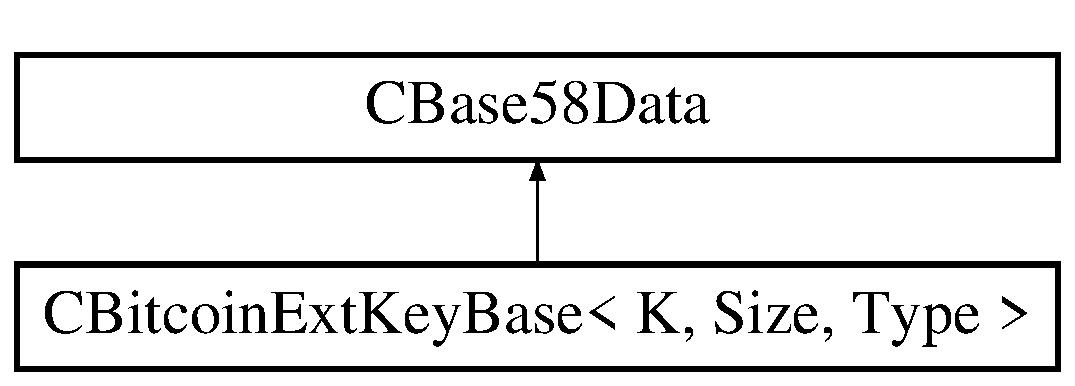
\includegraphics[height=2.000000cm]{class_c_bitcoin_ext_key_base}
\end{center}
\end{figure}
\subsection*{Public Member Functions}
\begin{DoxyCompactItemize}
\item 
void \mbox{\hyperlink{class_c_bitcoin_ext_key_base_aa6041045bb68b3f24d92f5e3b96aeef6}{Set\+Key}} (const K \&key)
\item 
K \mbox{\hyperlink{class_c_bitcoin_ext_key_base_a528399b89529212a44a08250c5f29d68}{Get\+Key}} ()
\item 
\mbox{\hyperlink{class_c_bitcoin_ext_key_base_a61b09dabc0849ba24520a78c5996096a}{C\+Bitcoin\+Ext\+Key\+Base}} (const K \&key)
\item 
\mbox{\hyperlink{class_c_bitcoin_ext_key_base_af377a86f3463504c0237546b777716ce}{C\+Bitcoin\+Ext\+Key\+Base}} (const std\+::string \&str\+Base58c)
\item 
\mbox{\hyperlink{class_c_bitcoin_ext_key_base_a0f4d52b23db0a0740c4519644e537565}{C\+Bitcoin\+Ext\+Key\+Base}} ()
\end{DoxyCompactItemize}
\subsection*{Additional Inherited Members}


\subsection{Constructor \& Destructor Documentation}
\mbox{\Hypertarget{class_c_bitcoin_ext_key_base_a61b09dabc0849ba24520a78c5996096a}\label{class_c_bitcoin_ext_key_base_a61b09dabc0849ba24520a78c5996096a}} 
\index{C\+Bitcoin\+Ext\+Key\+Base@{C\+Bitcoin\+Ext\+Key\+Base}!C\+Bitcoin\+Ext\+Key\+Base@{C\+Bitcoin\+Ext\+Key\+Base}}
\index{C\+Bitcoin\+Ext\+Key\+Base@{C\+Bitcoin\+Ext\+Key\+Base}!C\+Bitcoin\+Ext\+Key\+Base@{C\+Bitcoin\+Ext\+Key\+Base}}
\subsubsection{\texorpdfstring{C\+Bitcoin\+Ext\+Key\+Base()}{CBitcoinExtKeyBase()}\hspace{0.1cm}{\footnotesize\ttfamily [1/3]}}
{\footnotesize\ttfamily template$<$typename K , int Size, C\+Chain\+Params\+::\+Base58\+Type Type$>$ \\
\mbox{\hyperlink{class_c_bitcoin_ext_key_base}{C\+Bitcoin\+Ext\+Key\+Base}}$<$ K, Size, Type $>$\+::\mbox{\hyperlink{class_c_bitcoin_ext_key_base}{C\+Bitcoin\+Ext\+Key\+Base}} (\begin{DoxyParamCaption}\item[{const K \&}]{key }\end{DoxyParamCaption})\hspace{0.3cm}{\ttfamily [inline]}}

\mbox{\Hypertarget{class_c_bitcoin_ext_key_base_af377a86f3463504c0237546b777716ce}\label{class_c_bitcoin_ext_key_base_af377a86f3463504c0237546b777716ce}} 
\index{C\+Bitcoin\+Ext\+Key\+Base@{C\+Bitcoin\+Ext\+Key\+Base}!C\+Bitcoin\+Ext\+Key\+Base@{C\+Bitcoin\+Ext\+Key\+Base}}
\index{C\+Bitcoin\+Ext\+Key\+Base@{C\+Bitcoin\+Ext\+Key\+Base}!C\+Bitcoin\+Ext\+Key\+Base@{C\+Bitcoin\+Ext\+Key\+Base}}
\subsubsection{\texorpdfstring{C\+Bitcoin\+Ext\+Key\+Base()}{CBitcoinExtKeyBase()}\hspace{0.1cm}{\footnotesize\ttfamily [2/3]}}
{\footnotesize\ttfamily template$<$typename K , int Size, C\+Chain\+Params\+::\+Base58\+Type Type$>$ \\
\mbox{\hyperlink{class_c_bitcoin_ext_key_base}{C\+Bitcoin\+Ext\+Key\+Base}}$<$ K, Size, Type $>$\+::\mbox{\hyperlink{class_c_bitcoin_ext_key_base}{C\+Bitcoin\+Ext\+Key\+Base}} (\begin{DoxyParamCaption}\item[{const std\+::string \&}]{str\+Base58c }\end{DoxyParamCaption})\hspace{0.3cm}{\ttfamily [inline]}}

\mbox{\Hypertarget{class_c_bitcoin_ext_key_base_a0f4d52b23db0a0740c4519644e537565}\label{class_c_bitcoin_ext_key_base_a0f4d52b23db0a0740c4519644e537565}} 
\index{C\+Bitcoin\+Ext\+Key\+Base@{C\+Bitcoin\+Ext\+Key\+Base}!C\+Bitcoin\+Ext\+Key\+Base@{C\+Bitcoin\+Ext\+Key\+Base}}
\index{C\+Bitcoin\+Ext\+Key\+Base@{C\+Bitcoin\+Ext\+Key\+Base}!C\+Bitcoin\+Ext\+Key\+Base@{C\+Bitcoin\+Ext\+Key\+Base}}
\subsubsection{\texorpdfstring{C\+Bitcoin\+Ext\+Key\+Base()}{CBitcoinExtKeyBase()}\hspace{0.1cm}{\footnotesize\ttfamily [3/3]}}
{\footnotesize\ttfamily template$<$typename K , int Size, C\+Chain\+Params\+::\+Base58\+Type Type$>$ \\
\mbox{\hyperlink{class_c_bitcoin_ext_key_base}{C\+Bitcoin\+Ext\+Key\+Base}}$<$ K, Size, Type $>$\+::\mbox{\hyperlink{class_c_bitcoin_ext_key_base}{C\+Bitcoin\+Ext\+Key\+Base}} (\begin{DoxyParamCaption}{ }\end{DoxyParamCaption})\hspace{0.3cm}{\ttfamily [inline]}}



\subsection{Member Function Documentation}
\mbox{\Hypertarget{class_c_bitcoin_ext_key_base_a528399b89529212a44a08250c5f29d68}\label{class_c_bitcoin_ext_key_base_a528399b89529212a44a08250c5f29d68}} 
\index{C\+Bitcoin\+Ext\+Key\+Base@{C\+Bitcoin\+Ext\+Key\+Base}!Get\+Key@{Get\+Key}}
\index{Get\+Key@{Get\+Key}!C\+Bitcoin\+Ext\+Key\+Base@{C\+Bitcoin\+Ext\+Key\+Base}}
\subsubsection{\texorpdfstring{Get\+Key()}{GetKey()}}
{\footnotesize\ttfamily template$<$typename K , int Size, C\+Chain\+Params\+::\+Base58\+Type Type$>$ \\
K \mbox{\hyperlink{class_c_bitcoin_ext_key_base}{C\+Bitcoin\+Ext\+Key\+Base}}$<$ K, Size, Type $>$\+::Get\+Key (\begin{DoxyParamCaption}{ }\end{DoxyParamCaption})\hspace{0.3cm}{\ttfamily [inline]}}

\mbox{\Hypertarget{class_c_bitcoin_ext_key_base_aa6041045bb68b3f24d92f5e3b96aeef6}\label{class_c_bitcoin_ext_key_base_aa6041045bb68b3f24d92f5e3b96aeef6}} 
\index{C\+Bitcoin\+Ext\+Key\+Base@{C\+Bitcoin\+Ext\+Key\+Base}!Set\+Key@{Set\+Key}}
\index{Set\+Key@{Set\+Key}!C\+Bitcoin\+Ext\+Key\+Base@{C\+Bitcoin\+Ext\+Key\+Base}}
\subsubsection{\texorpdfstring{Set\+Key()}{SetKey()}}
{\footnotesize\ttfamily template$<$typename K , int Size, C\+Chain\+Params\+::\+Base58\+Type Type$>$ \\
void \mbox{\hyperlink{class_c_bitcoin_ext_key_base}{C\+Bitcoin\+Ext\+Key\+Base}}$<$ K, Size, Type $>$\+::Set\+Key (\begin{DoxyParamCaption}\item[{const K \&}]{key }\end{DoxyParamCaption})\hspace{0.3cm}{\ttfamily [inline]}}



The documentation for this class was generated from the following file\+:\begin{DoxyCompactItemize}
\item 
/\+Users/christopherarguello/\+Developer/anon/src/\mbox{\hyperlink{base58_8h}{base58.\+h}}\end{DoxyCompactItemize}

\hypertarget{class_c_bitcoin_secret}{}\section{C\+Bitcoin\+Secret Class Reference}
\label{class_c_bitcoin_secret}\index{C\+Bitcoin\+Secret@{C\+Bitcoin\+Secret}}


{\ttfamily \#include $<$base58.\+h$>$}

Inheritance diagram for C\+Bitcoin\+Secret\+:\begin{figure}[H]
\begin{center}
\leavevmode
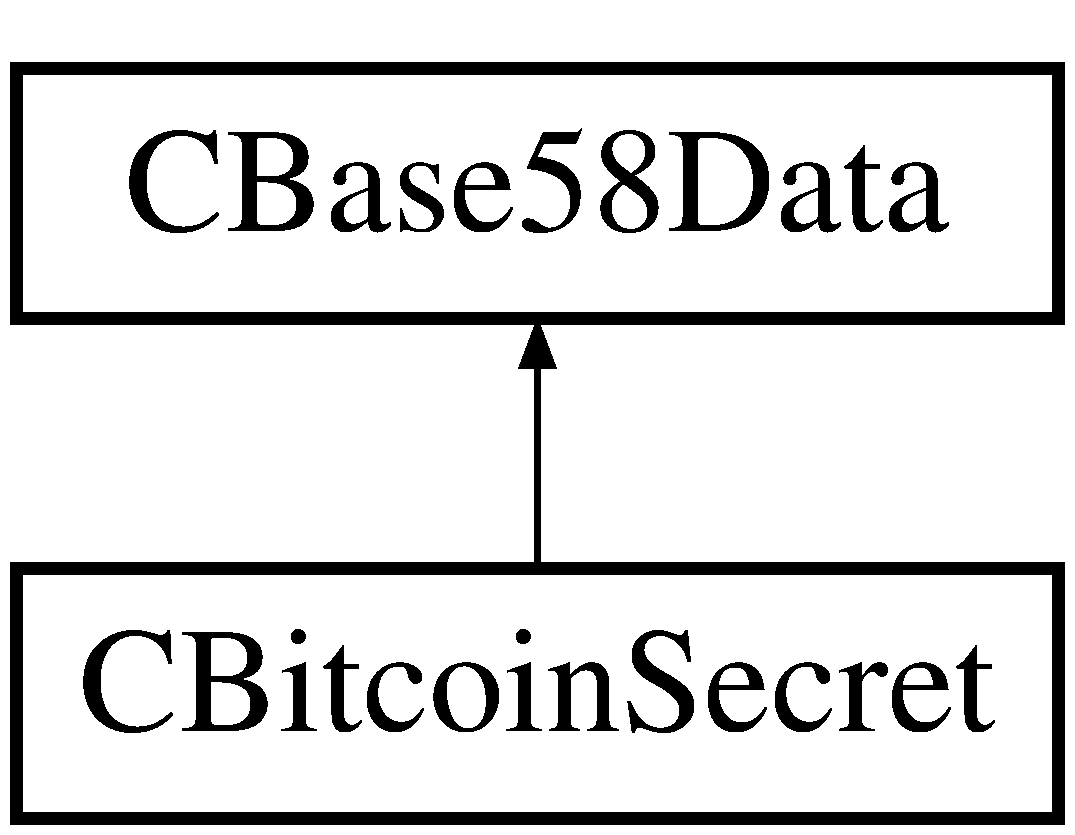
\includegraphics[height=2.000000cm]{class_c_bitcoin_secret}
\end{center}
\end{figure}
\subsection*{Public Member Functions}
\begin{DoxyCompactItemize}
\item 
void \mbox{\hyperlink{class_c_bitcoin_secret_a3629c0fce320664c3c07cb082939d6ec}{Set\+Key}} (const \mbox{\hyperlink{class_c_key}{C\+Key}} \&vch\+Secret)
\item 
\mbox{\hyperlink{class_c_key}{C\+Key}} \mbox{\hyperlink{class_c_bitcoin_secret_a4d6bf559d092e6d47f8001c7171096df}{Get\+Key}} ()
\item 
bool \mbox{\hyperlink{class_c_bitcoin_secret_a2a93fa8a09826ff63498cb3e4370c154}{Is\+Valid}} () const
\item 
bool \mbox{\hyperlink{class_c_bitcoin_secret_a6a8aff02f66099f33f573ad3e6375bb1}{Set\+String}} (const char $\ast$psz\+Secret)
\item 
bool \mbox{\hyperlink{class_c_bitcoin_secret_a83cfc3b34aac494efdd6e316cd08626d}{Set\+String}} (const std\+::string \&str\+Secret)
\item 
\mbox{\hyperlink{class_c_bitcoin_secret_a0358baa459a1f22661b601d9d83eacf8}{C\+Bitcoin\+Secret}} (const \mbox{\hyperlink{class_c_key}{C\+Key}} \&vch\+Secret)
\item 
\mbox{\hyperlink{class_c_bitcoin_secret_a3b6168eef2ab8c44d60272e62162fd5b}{C\+Bitcoin\+Secret}} ()
\end{DoxyCompactItemize}
\subsection*{Additional Inherited Members}


\subsection{Detailed Description}
A base58-\/encoded secret key 

\subsection{Constructor \& Destructor Documentation}
\mbox{\Hypertarget{class_c_bitcoin_secret_a0358baa459a1f22661b601d9d83eacf8}\label{class_c_bitcoin_secret_a0358baa459a1f22661b601d9d83eacf8}} 
\index{C\+Bitcoin\+Secret@{C\+Bitcoin\+Secret}!C\+Bitcoin\+Secret@{C\+Bitcoin\+Secret}}
\index{C\+Bitcoin\+Secret@{C\+Bitcoin\+Secret}!C\+Bitcoin\+Secret@{C\+Bitcoin\+Secret}}
\subsubsection{\texorpdfstring{C\+Bitcoin\+Secret()}{CBitcoinSecret()}\hspace{0.1cm}{\footnotesize\ttfamily [1/2]}}
{\footnotesize\ttfamily C\+Bitcoin\+Secret\+::\+C\+Bitcoin\+Secret (\begin{DoxyParamCaption}\item[{const \mbox{\hyperlink{class_c_key}{C\+Key}} \&}]{vch\+Secret }\end{DoxyParamCaption})\hspace{0.3cm}{\ttfamily [inline]}}

\mbox{\Hypertarget{class_c_bitcoin_secret_a3b6168eef2ab8c44d60272e62162fd5b}\label{class_c_bitcoin_secret_a3b6168eef2ab8c44d60272e62162fd5b}} 
\index{C\+Bitcoin\+Secret@{C\+Bitcoin\+Secret}!C\+Bitcoin\+Secret@{C\+Bitcoin\+Secret}}
\index{C\+Bitcoin\+Secret@{C\+Bitcoin\+Secret}!C\+Bitcoin\+Secret@{C\+Bitcoin\+Secret}}
\subsubsection{\texorpdfstring{C\+Bitcoin\+Secret()}{CBitcoinSecret()}\hspace{0.1cm}{\footnotesize\ttfamily [2/2]}}
{\footnotesize\ttfamily C\+Bitcoin\+Secret\+::\+C\+Bitcoin\+Secret (\begin{DoxyParamCaption}{ }\end{DoxyParamCaption})\hspace{0.3cm}{\ttfamily [inline]}}



\subsection{Member Function Documentation}
\mbox{\Hypertarget{class_c_bitcoin_secret_a4d6bf559d092e6d47f8001c7171096df}\label{class_c_bitcoin_secret_a4d6bf559d092e6d47f8001c7171096df}} 
\index{C\+Bitcoin\+Secret@{C\+Bitcoin\+Secret}!Get\+Key@{Get\+Key}}
\index{Get\+Key@{Get\+Key}!C\+Bitcoin\+Secret@{C\+Bitcoin\+Secret}}
\subsubsection{\texorpdfstring{Get\+Key()}{GetKey()}}
{\footnotesize\ttfamily \mbox{\hyperlink{class_c_key}{C\+Key}} C\+Bitcoin\+Secret\+::\+Get\+Key (\begin{DoxyParamCaption}{ }\end{DoxyParamCaption})}

\mbox{\Hypertarget{class_c_bitcoin_secret_a2a93fa8a09826ff63498cb3e4370c154}\label{class_c_bitcoin_secret_a2a93fa8a09826ff63498cb3e4370c154}} 
\index{C\+Bitcoin\+Secret@{C\+Bitcoin\+Secret}!Is\+Valid@{Is\+Valid}}
\index{Is\+Valid@{Is\+Valid}!C\+Bitcoin\+Secret@{C\+Bitcoin\+Secret}}
\subsubsection{\texorpdfstring{Is\+Valid()}{IsValid()}}
{\footnotesize\ttfamily bool C\+Bitcoin\+Secret\+::\+Is\+Valid (\begin{DoxyParamCaption}{ }\end{DoxyParamCaption}) const}

\mbox{\Hypertarget{class_c_bitcoin_secret_a3629c0fce320664c3c07cb082939d6ec}\label{class_c_bitcoin_secret_a3629c0fce320664c3c07cb082939d6ec}} 
\index{C\+Bitcoin\+Secret@{C\+Bitcoin\+Secret}!Set\+Key@{Set\+Key}}
\index{Set\+Key@{Set\+Key}!C\+Bitcoin\+Secret@{C\+Bitcoin\+Secret}}
\subsubsection{\texorpdfstring{Set\+Key()}{SetKey()}}
{\footnotesize\ttfamily void C\+Bitcoin\+Secret\+::\+Set\+Key (\begin{DoxyParamCaption}\item[{const \mbox{\hyperlink{class_c_key}{C\+Key}} \&}]{vch\+Secret }\end{DoxyParamCaption})}

\mbox{\Hypertarget{class_c_bitcoin_secret_a6a8aff02f66099f33f573ad3e6375bb1}\label{class_c_bitcoin_secret_a6a8aff02f66099f33f573ad3e6375bb1}} 
\index{C\+Bitcoin\+Secret@{C\+Bitcoin\+Secret}!Set\+String@{Set\+String}}
\index{Set\+String@{Set\+String}!C\+Bitcoin\+Secret@{C\+Bitcoin\+Secret}}
\subsubsection{\texorpdfstring{Set\+String()}{SetString()}\hspace{0.1cm}{\footnotesize\ttfamily [1/2]}}
{\footnotesize\ttfamily bool C\+Bitcoin\+Secret\+::\+Set\+String (\begin{DoxyParamCaption}\item[{const char $\ast$}]{psz\+Secret }\end{DoxyParamCaption})}

\mbox{\Hypertarget{class_c_bitcoin_secret_a83cfc3b34aac494efdd6e316cd08626d}\label{class_c_bitcoin_secret_a83cfc3b34aac494efdd6e316cd08626d}} 
\index{C\+Bitcoin\+Secret@{C\+Bitcoin\+Secret}!Set\+String@{Set\+String}}
\index{Set\+String@{Set\+String}!C\+Bitcoin\+Secret@{C\+Bitcoin\+Secret}}
\subsubsection{\texorpdfstring{Set\+String()}{SetString()}\hspace{0.1cm}{\footnotesize\ttfamily [2/2]}}
{\footnotesize\ttfamily bool C\+Bitcoin\+Secret\+::\+Set\+String (\begin{DoxyParamCaption}\item[{const std\+::string \&}]{str\+Secret }\end{DoxyParamCaption})}



The documentation for this class was generated from the following files\+:\begin{DoxyCompactItemize}
\item 
/\+Users/christopherarguello/\+Developer/anon/src/\mbox{\hyperlink{base58_8h}{base58.\+h}}\item 
/\+Users/christopherarguello/\+Developer/anon/src/\mbox{\hyperlink{base58_8cpp}{base58.\+cpp}}\end{DoxyCompactItemize}

\hypertarget{class_c_block_file_info}{}\section{C\+Block\+File\+Info Class Reference}
\label{class_c_block_file_info}\index{C\+Block\+File\+Info@{C\+Block\+File\+Info}}


{\ttfamily \#include $<$main.\+h$>$}

\subsection*{Public Member Functions}
\begin{DoxyCompactItemize}
\item 
{\footnotesize template$<$typename Stream , typename Operation $>$ }\\void \mbox{\hyperlink{class_c_block_file_info_a5d48a4fe1f8b3903131d121fc14a5a6f}{Serialization\+Op}} (Stream \&s, Operation ser\+\_\+action, int n\+Type, int n\+Version)
\item 
void \mbox{\hyperlink{class_c_block_file_info_a21bd4f8e92c47646737fc57446a86cc2}{Set\+Null}} ()
\item 
\mbox{\hyperlink{class_c_block_file_info_a4d08bfcfc45a16b40266255f8597c949}{C\+Block\+File\+Info}} ()
\item 
std\+::string \mbox{\hyperlink{class_c_block_file_info_a2754dd93534e2fda8674ffc5d007611e}{To\+String}} () const
\item 
void \mbox{\hyperlink{class_c_block_file_info_a66867569ffe06068b8c6eb1139934fbf}{Add\+Block}} (unsigned int n\+Height\+In, uint64\+\_\+t n\+Time\+In)
\end{DoxyCompactItemize}
\subsection*{Public Attributes}
\begin{DoxyCompactItemize}
\item 
unsigned int \mbox{\hyperlink{class_c_block_file_info_adf2de4bb4d8a0a8f2116ed90f0770d03}{n\+Blocks}}
\item 
unsigned int \mbox{\hyperlink{class_c_block_file_info_afb13102ba49548c24812a4236851c3a9}{n\+Size}}
\begin{DoxyCompactList}\small\item\em number of blocks stored in file \end{DoxyCompactList}\item 
unsigned int \mbox{\hyperlink{class_c_block_file_info_ad3e555fd733ef8f38430554c2db5e9d1}{n\+Undo\+Size}}
\begin{DoxyCompactList}\small\item\em number of used bytes of block file \end{DoxyCompactList}\item 
unsigned int \mbox{\hyperlink{class_c_block_file_info_a66d258b11b1aec30cbacdc6130c271a8}{n\+Height\+First}}
\begin{DoxyCompactList}\small\item\em number of used bytes in the undo file \end{DoxyCompactList}\item 
unsigned int \mbox{\hyperlink{class_c_block_file_info_aabbcf808931e7eaf2278b3d7172fad3a}{n\+Height\+Last}}
\begin{DoxyCompactList}\small\item\em lowest height of block in file \end{DoxyCompactList}\item 
uint64\+\_\+t \mbox{\hyperlink{class_c_block_file_info_a0e928257d1f003ede485ce49e8cf9189}{n\+Time\+First}}
\begin{DoxyCompactList}\small\item\em highest height of block in file \end{DoxyCompactList}\item 
uint64\+\_\+t \mbox{\hyperlink{class_c_block_file_info_a1d12e4202474bb2f299d18d7d1f28c78}{n\+Time\+Last}}
\begin{DoxyCompactList}\small\item\em earliest time of block in file \end{DoxyCompactList}\item 
\mbox{\hyperlink{class_c_block_file_info_ab4daf4df00f90dee15e3a7d2cdb7a273}{A\+D\+D\+\_\+\+S\+E\+R\+I\+A\+L\+I\+Z\+E\+\_\+\+M\+E\+T\+H\+O\+DS}}
\begin{DoxyCompactList}\small\item\em latest time of block in file \end{DoxyCompactList}\end{DoxyCompactItemize}


\subsection{Constructor \& Destructor Documentation}
\mbox{\Hypertarget{class_c_block_file_info_a4d08bfcfc45a16b40266255f8597c949}\label{class_c_block_file_info_a4d08bfcfc45a16b40266255f8597c949}} 
\index{C\+Block\+File\+Info@{C\+Block\+File\+Info}!C\+Block\+File\+Info@{C\+Block\+File\+Info}}
\index{C\+Block\+File\+Info@{C\+Block\+File\+Info}!C\+Block\+File\+Info@{C\+Block\+File\+Info}}
\subsubsection{\texorpdfstring{C\+Block\+File\+Info()}{CBlockFileInfo()}}
{\footnotesize\ttfamily C\+Block\+File\+Info\+::\+C\+Block\+File\+Info (\begin{DoxyParamCaption}{ }\end{DoxyParamCaption})\hspace{0.3cm}{\ttfamily [inline]}}



\subsection{Member Function Documentation}
\mbox{\Hypertarget{class_c_block_file_info_a66867569ffe06068b8c6eb1139934fbf}\label{class_c_block_file_info_a66867569ffe06068b8c6eb1139934fbf}} 
\index{C\+Block\+File\+Info@{C\+Block\+File\+Info}!Add\+Block@{Add\+Block}}
\index{Add\+Block@{Add\+Block}!C\+Block\+File\+Info@{C\+Block\+File\+Info}}
\subsubsection{\texorpdfstring{Add\+Block()}{AddBlock()}}
{\footnotesize\ttfamily void C\+Block\+File\+Info\+::\+Add\+Block (\begin{DoxyParamCaption}\item[{unsigned int}]{n\+Height\+In,  }\item[{uint64\+\_\+t}]{n\+Time\+In }\end{DoxyParamCaption})\hspace{0.3cm}{\ttfamily [inline]}}

update statistics (does not update n\+Size) \mbox{\Hypertarget{class_c_block_file_info_a5d48a4fe1f8b3903131d121fc14a5a6f}\label{class_c_block_file_info_a5d48a4fe1f8b3903131d121fc14a5a6f}} 
\index{C\+Block\+File\+Info@{C\+Block\+File\+Info}!Serialization\+Op@{Serialization\+Op}}
\index{Serialization\+Op@{Serialization\+Op}!C\+Block\+File\+Info@{C\+Block\+File\+Info}}
\subsubsection{\texorpdfstring{Serialization\+Op()}{SerializationOp()}}
{\footnotesize\ttfamily template$<$typename Stream , typename Operation $>$ \\
void C\+Block\+File\+Info\+::\+Serialization\+Op (\begin{DoxyParamCaption}\item[{Stream \&}]{s,  }\item[{Operation}]{ser\+\_\+action,  }\item[{int}]{n\+Type,  }\item[{int}]{n\+Version }\end{DoxyParamCaption})\hspace{0.3cm}{\ttfamily [inline]}}

\mbox{\Hypertarget{class_c_block_file_info_a21bd4f8e92c47646737fc57446a86cc2}\label{class_c_block_file_info_a21bd4f8e92c47646737fc57446a86cc2}} 
\index{C\+Block\+File\+Info@{C\+Block\+File\+Info}!Set\+Null@{Set\+Null}}
\index{Set\+Null@{Set\+Null}!C\+Block\+File\+Info@{C\+Block\+File\+Info}}
\subsubsection{\texorpdfstring{Set\+Null()}{SetNull()}}
{\footnotesize\ttfamily void C\+Block\+File\+Info\+::\+Set\+Null (\begin{DoxyParamCaption}{ }\end{DoxyParamCaption})\hspace{0.3cm}{\ttfamily [inline]}}

\mbox{\Hypertarget{class_c_block_file_info_a2754dd93534e2fda8674ffc5d007611e}\label{class_c_block_file_info_a2754dd93534e2fda8674ffc5d007611e}} 
\index{C\+Block\+File\+Info@{C\+Block\+File\+Info}!To\+String@{To\+String}}
\index{To\+String@{To\+String}!C\+Block\+File\+Info@{C\+Block\+File\+Info}}
\subsubsection{\texorpdfstring{To\+String()}{ToString()}}
{\footnotesize\ttfamily std\+::string C\+Block\+File\+Info\+::\+To\+String (\begin{DoxyParamCaption}{ }\end{DoxyParamCaption}) const}



\subsection{Member Data Documentation}
\mbox{\Hypertarget{class_c_block_file_info_ab4daf4df00f90dee15e3a7d2cdb7a273}\label{class_c_block_file_info_ab4daf4df00f90dee15e3a7d2cdb7a273}} 
\index{C\+Block\+File\+Info@{C\+Block\+File\+Info}!A\+D\+D\+\_\+\+S\+E\+R\+I\+A\+L\+I\+Z\+E\+\_\+\+M\+E\+T\+H\+O\+DS@{A\+D\+D\+\_\+\+S\+E\+R\+I\+A\+L\+I\+Z\+E\+\_\+\+M\+E\+T\+H\+O\+DS}}
\index{A\+D\+D\+\_\+\+S\+E\+R\+I\+A\+L\+I\+Z\+E\+\_\+\+M\+E\+T\+H\+O\+DS@{A\+D\+D\+\_\+\+S\+E\+R\+I\+A\+L\+I\+Z\+E\+\_\+\+M\+E\+T\+H\+O\+DS}!C\+Block\+File\+Info@{C\+Block\+File\+Info}}
\subsubsection{\texorpdfstring{A\+D\+D\+\_\+\+S\+E\+R\+I\+A\+L\+I\+Z\+E\+\_\+\+M\+E\+T\+H\+O\+DS}{ADD\_SERIALIZE\_METHODS}}
{\footnotesize\ttfamily C\+Block\+File\+Info\+::\+A\+D\+D\+\_\+\+S\+E\+R\+I\+A\+L\+I\+Z\+E\+\_\+\+M\+E\+T\+H\+O\+DS}



latest time of block in file 

\mbox{\Hypertarget{class_c_block_file_info_adf2de4bb4d8a0a8f2116ed90f0770d03}\label{class_c_block_file_info_adf2de4bb4d8a0a8f2116ed90f0770d03}} 
\index{C\+Block\+File\+Info@{C\+Block\+File\+Info}!n\+Blocks@{n\+Blocks}}
\index{n\+Blocks@{n\+Blocks}!C\+Block\+File\+Info@{C\+Block\+File\+Info}}
\subsubsection{\texorpdfstring{n\+Blocks}{nBlocks}}
{\footnotesize\ttfamily unsigned int C\+Block\+File\+Info\+::n\+Blocks}

\mbox{\Hypertarget{class_c_block_file_info_a66d258b11b1aec30cbacdc6130c271a8}\label{class_c_block_file_info_a66d258b11b1aec30cbacdc6130c271a8}} 
\index{C\+Block\+File\+Info@{C\+Block\+File\+Info}!n\+Height\+First@{n\+Height\+First}}
\index{n\+Height\+First@{n\+Height\+First}!C\+Block\+File\+Info@{C\+Block\+File\+Info}}
\subsubsection{\texorpdfstring{n\+Height\+First}{nHeightFirst}}
{\footnotesize\ttfamily unsigned int C\+Block\+File\+Info\+::n\+Height\+First}



number of used bytes in the undo file 

\mbox{\Hypertarget{class_c_block_file_info_aabbcf808931e7eaf2278b3d7172fad3a}\label{class_c_block_file_info_aabbcf808931e7eaf2278b3d7172fad3a}} 
\index{C\+Block\+File\+Info@{C\+Block\+File\+Info}!n\+Height\+Last@{n\+Height\+Last}}
\index{n\+Height\+Last@{n\+Height\+Last}!C\+Block\+File\+Info@{C\+Block\+File\+Info}}
\subsubsection{\texorpdfstring{n\+Height\+Last}{nHeightLast}}
{\footnotesize\ttfamily unsigned int C\+Block\+File\+Info\+::n\+Height\+Last}



lowest height of block in file 

\mbox{\Hypertarget{class_c_block_file_info_afb13102ba49548c24812a4236851c3a9}\label{class_c_block_file_info_afb13102ba49548c24812a4236851c3a9}} 
\index{C\+Block\+File\+Info@{C\+Block\+File\+Info}!n\+Size@{n\+Size}}
\index{n\+Size@{n\+Size}!C\+Block\+File\+Info@{C\+Block\+File\+Info}}
\subsubsection{\texorpdfstring{n\+Size}{nSize}}
{\footnotesize\ttfamily unsigned int C\+Block\+File\+Info\+::n\+Size}



number of blocks stored in file 

\mbox{\Hypertarget{class_c_block_file_info_a0e928257d1f003ede485ce49e8cf9189}\label{class_c_block_file_info_a0e928257d1f003ede485ce49e8cf9189}} 
\index{C\+Block\+File\+Info@{C\+Block\+File\+Info}!n\+Time\+First@{n\+Time\+First}}
\index{n\+Time\+First@{n\+Time\+First}!C\+Block\+File\+Info@{C\+Block\+File\+Info}}
\subsubsection{\texorpdfstring{n\+Time\+First}{nTimeFirst}}
{\footnotesize\ttfamily uint64\+\_\+t C\+Block\+File\+Info\+::n\+Time\+First}



highest height of block in file 

\mbox{\Hypertarget{class_c_block_file_info_a1d12e4202474bb2f299d18d7d1f28c78}\label{class_c_block_file_info_a1d12e4202474bb2f299d18d7d1f28c78}} 
\index{C\+Block\+File\+Info@{C\+Block\+File\+Info}!n\+Time\+Last@{n\+Time\+Last}}
\index{n\+Time\+Last@{n\+Time\+Last}!C\+Block\+File\+Info@{C\+Block\+File\+Info}}
\subsubsection{\texorpdfstring{n\+Time\+Last}{nTimeLast}}
{\footnotesize\ttfamily uint64\+\_\+t C\+Block\+File\+Info\+::n\+Time\+Last}



earliest time of block in file 

\mbox{\Hypertarget{class_c_block_file_info_ad3e555fd733ef8f38430554c2db5e9d1}\label{class_c_block_file_info_ad3e555fd733ef8f38430554c2db5e9d1}} 
\index{C\+Block\+File\+Info@{C\+Block\+File\+Info}!n\+Undo\+Size@{n\+Undo\+Size}}
\index{n\+Undo\+Size@{n\+Undo\+Size}!C\+Block\+File\+Info@{C\+Block\+File\+Info}}
\subsubsection{\texorpdfstring{n\+Undo\+Size}{nUndoSize}}
{\footnotesize\ttfamily unsigned int C\+Block\+File\+Info\+::n\+Undo\+Size}



number of used bytes of block file 



The documentation for this class was generated from the following files\+:\begin{DoxyCompactItemize}
\item 
/\+Users/christopherarguello/\+Developer/anon/src/\mbox{\hyperlink{main_8h}{main.\+h}}\item 
/\+Users/christopherarguello/\+Developer/anon/src/\mbox{\hyperlink{main_8cpp}{main.\+cpp}}\end{DoxyCompactItemize}

\hypertarget{class_c_block_index}{}\section{C\+Block\+Index Class Reference}
\label{class_c_block_index}\index{C\+Block\+Index@{C\+Block\+Index}}


{\ttfamily \#include $<$chain.\+h$>$}

Inheritance diagram for C\+Block\+Index\+:\begin{figure}[H]
\begin{center}
\leavevmode
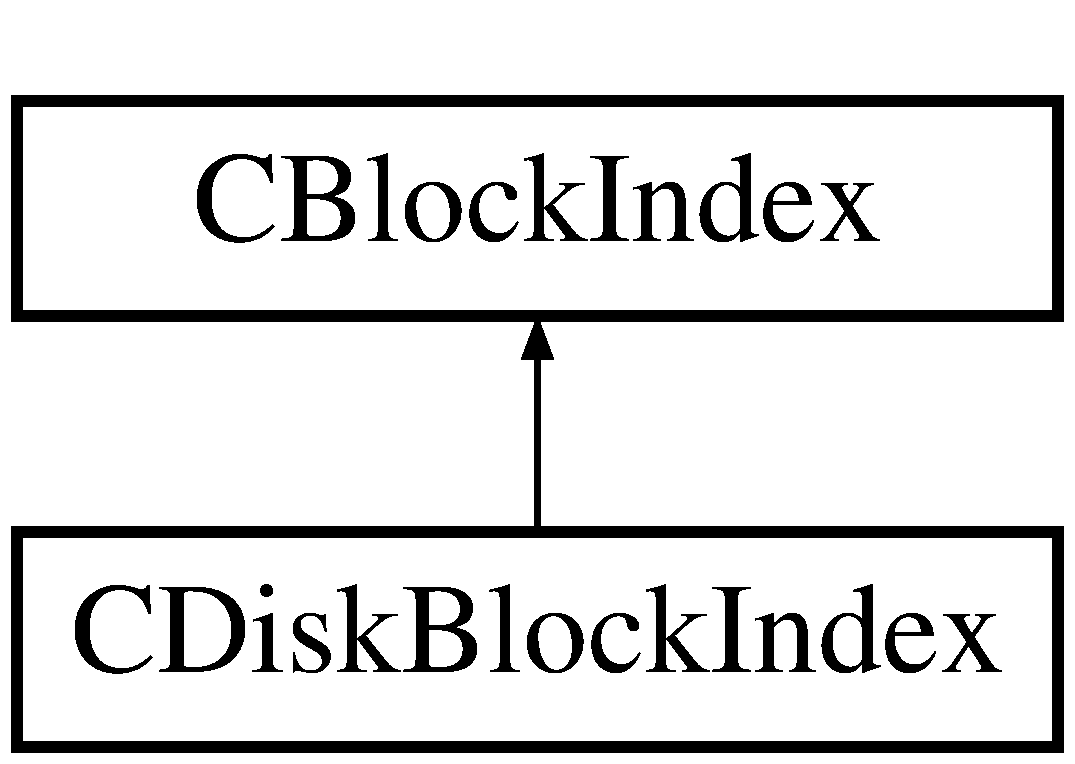
\includegraphics[height=2.000000cm]{class_c_block_index}
\end{center}
\end{figure}
\subsection*{Public Types}
\begin{DoxyCompactItemize}
\item 
enum \{ \mbox{\hyperlink{class_c_block_index_acefc16035e60d7bd52ed2c9bb1aa838eaa2b8ad73c4fe37a8de8748d949c334d4}{n\+Median\+Time\+Span}} = 11
 \}
\end{DoxyCompactItemize}
\subsection*{Public Member Functions}
\begin{DoxyCompactItemize}
\item 
void \mbox{\hyperlink{class_c_block_index_a6139e9e2cfceaef3694631cb7c330ff0}{Set\+Null}} ()
\item 
\mbox{\hyperlink{class_c_block_index_a0eff34cbfb4470885020734581dc1555}{C\+Block\+Index}} ()
\item 
\mbox{\hyperlink{class_c_block_index_acaf83989071b40966072161c513a17a7}{C\+Block\+Index}} (const C\+Block\+Header \&block)
\item 
\mbox{\hyperlink{struct_c_disk_block_pos}{C\+Disk\+Block\+Pos}} \mbox{\hyperlink{class_c_block_index_ad0d95bf8524a1e94bc6cfb92adea0c63}{Get\+Block\+Pos}} () const
\item 
\mbox{\hyperlink{struct_c_disk_block_pos}{C\+Disk\+Block\+Pos}} \mbox{\hyperlink{class_c_block_index_aa06679e5dd3f2425a1b667f6804b1a94}{Get\+Undo\+Pos}} () const
\item 
C\+Block\+Header \mbox{\hyperlink{class_c_block_index_a29df6a3c3195ff87c650348a27959fa2}{Get\+Block\+Header}} () const
\item 
\mbox{\hyperlink{classuint256}{uint256}} \mbox{\hyperlink{class_c_block_index_a98490a2788c65cdd6ae9002b004dd74c}{Get\+Block\+Hash}} () const
\item 
int64\+\_\+t \mbox{\hyperlink{class_c_block_index_a9fe0d4463c07c466f66252e8eec25f5c}{Get\+Block\+Time}} () const
\item 
int64\+\_\+t \mbox{\hyperlink{class_c_block_index_aa9bd0ab02cf8b9c866618cee3a5a0583}{Get\+Median\+Time\+Past}} () const
\item 
std\+::string \mbox{\hyperlink{class_c_block_index_a18258e956a4bc77dcccdb0db8f91effe}{To\+String}} () const
\item 
bool \mbox{\hyperlink{class_c_block_index_ad8b5a6560e7c0d4222066e2922178683}{Is\+Valid}} (enum \mbox{\hyperlink{chain_8h_a0d8c285f70a59a32f4f6ab41b78f93ad}{Block\+Status}} n\+Up\+To=\mbox{\hyperlink{chain_8h_a0d8c285f70a59a32f4f6ab41b78f93ada3eef30f876594ac79b888b7d1ff6c66c}{B\+L\+O\+C\+K\+\_\+\+V\+A\+L\+I\+D\+\_\+\+T\+R\+A\+N\+S\+A\+C\+T\+I\+O\+NS}}) const
\begin{DoxyCompactList}\small\item\em Check whether this block index entry is valid up to the passed validity level. \end{DoxyCompactList}\item 
bool \mbox{\hyperlink{class_c_block_index_a076aff906933e9d75a37aa9b81c01384}{Raise\+Validity}} (enum \mbox{\hyperlink{chain_8h_a0d8c285f70a59a32f4f6ab41b78f93ad}{Block\+Status}} n\+Up\+To)
\item 
void \mbox{\hyperlink{class_c_block_index_a21209a71e50daf10e283bd4049e46f64}{Build\+Skip}} ()
\begin{DoxyCompactList}\small\item\em Build the skiplist pointer for this entry. \end{DoxyCompactList}\item 
\mbox{\hyperlink{class_c_block_index}{C\+Block\+Index}} $\ast$ \mbox{\hyperlink{class_c_block_index_ae1f702384690c6b8302e026a84172ef3}{Get\+Ancestor}} (int height)
\begin{DoxyCompactList}\small\item\em Efficiently find an ancestor of this block. \end{DoxyCompactList}\item 
const \mbox{\hyperlink{class_c_block_index}{C\+Block\+Index}} $\ast$ \mbox{\hyperlink{class_c_block_index_a7a58b33d64fde3df36c6e61371d031cc}{Get\+Ancestor}} (int height) const
\end{DoxyCompactItemize}
\subsection*{Public Attributes}
\begin{DoxyCompactItemize}
\item 
const \mbox{\hyperlink{classuint256}{uint256}} $\ast$ \mbox{\hyperlink{class_c_block_index_afac8099e03ffda463c7153ca82d37b66}{phash\+Block}}
\begin{DoxyCompactList}\small\item\em pointer to the hash of the block, if any. Memory is owned by this \mbox{\hyperlink{class_c_block_index}{C\+Block\+Index}} \end{DoxyCompactList}\item 
\mbox{\hyperlink{class_c_block_index}{C\+Block\+Index}} $\ast$ \mbox{\hyperlink{class_c_block_index_a1ef11137155df1dd5c81491630cece39}{pprev}}
\begin{DoxyCompactList}\small\item\em pointer to the index of the predecessor of this block \end{DoxyCompactList}\item 
\mbox{\hyperlink{class_c_block_index}{C\+Block\+Index}} $\ast$ \mbox{\hyperlink{class_c_block_index_ab6242bb77bc01617f5b402d14e6a3883}{pskip}}
\begin{DoxyCompactList}\small\item\em pointer to the index of some further predecessor of this block \end{DoxyCompactList}\item 
int \mbox{\hyperlink{class_c_block_index_aebfc8d6b95852546760e742553d7bfd5}{n\+Height}}
\begin{DoxyCompactList}\small\item\em height of the entry in the chain. The genesis block has height 0 \end{DoxyCompactList}\item 
int \mbox{\hyperlink{class_c_block_index_a3653cb1e1bc3fa3fcdf1ed50ff93b50a}{n\+File}}
\begin{DoxyCompactList}\small\item\em Which \# file this block is stored in (blk?????.dat) \end{DoxyCompactList}\item 
unsigned int \mbox{\hyperlink{class_c_block_index_af164283dfb2d62ac44be8d10446bce4a}{n\+Data\+Pos}}
\begin{DoxyCompactList}\small\item\em Byte offset within blk?????.dat where this block\textquotesingle{}s data is stored. \end{DoxyCompactList}\item 
unsigned int \mbox{\hyperlink{class_c_block_index_a865ddd56406c23e98cdc61511a61eb64}{n\+Undo\+Pos}}
\begin{DoxyCompactList}\small\item\em Byte offset within rev?????.dat where this block\textquotesingle{}s undo data is stored. \end{DoxyCompactList}\item 
\mbox{\hyperlink{classarith__uint256}{arith\+\_\+uint256}} \mbox{\hyperlink{class_c_block_index_a31e65c1f491d438dfdcd8d92bdfa73a1}{n\+Chain\+Work}}
\begin{DoxyCompactList}\small\item\em (memory only) Total amount of work (expected number of hashes) in the chain up to and including this block \end{DoxyCompactList}\item 
unsigned int \mbox{\hyperlink{class_c_block_index_ac8e219a377839d2f9133a4387f46e44e}{n\+Tx}}
\item 
unsigned int \mbox{\hyperlink{class_c_block_index_af3c6d6dd8a7579e5ce516d94b98d2db5}{n\+Chain\+Tx}}
\item 
unsigned int \mbox{\hyperlink{class_c_block_index_ac5a336b45ca70e3ed2fc090bf2ee3011}{n\+Status}}
\begin{DoxyCompactList}\small\item\em Verification status of this block. See enum Block\+Status. \end{DoxyCompactList}\item 
\mbox{\hyperlink{classuint256}{uint256}} \mbox{\hyperlink{class_c_block_index_a12e1a49faeb94cc8eedd7895a034540c}{hash\+Anchor}}
\begin{DoxyCompactList}\small\item\em The anchor for the tree state up to the start of this block. \end{DoxyCompactList}\item 
\mbox{\hyperlink{classuint256}{uint256}} \mbox{\hyperlink{class_c_block_index_ad1ad1271dbf7360a3a5ce219ad32ee1b}{hash\+Anchor\+End}}
\begin{DoxyCompactList}\small\item\em (memory only) The anchor for the tree state up to the end of this block \end{DoxyCompactList}\item 
int \mbox{\hyperlink{class_c_block_index_a45126301a0a6e26010527a7bbfc1ef58}{n\+Version}}
\begin{DoxyCompactList}\small\item\em block header \end{DoxyCompactList}\item 
\mbox{\hyperlink{classuint256}{uint256}} \mbox{\hyperlink{class_c_block_index_a0601b6b2bd6eaedfbc283c00d045a21c}{hash\+Merkle\+Root}}
\item 
\mbox{\hyperlink{classuint256}{uint256}} \mbox{\hyperlink{class_c_block_index_a5e7cea2f350f0f6272cfc291de91cd6b}{hash\+Reserved}}
\item 
unsigned int \mbox{\hyperlink{class_c_block_index_a4b687a226e9e166b0f91c1b616b543a6}{n\+Time}}
\item 
unsigned int \mbox{\hyperlink{class_c_block_index_a3324894e6af612d1bd76f89378435713}{n\+Bits}}
\item 
\mbox{\hyperlink{classuint256}{uint256}} \mbox{\hyperlink{class_c_block_index_a6cd6b15ad3a4cc502aeebfab8ec9e4d6}{n\+Nonce}}
\item 
std\+::vector$<$ unsigned char $>$ \mbox{\hyperlink{class_c_block_index_afc393de336d759ed0e1fafd48470f437}{n\+Solution}}
\item 
uint32\+\_\+t \mbox{\hyperlink{class_c_block_index_a4a679af5f7924cc594b8131371b21e54}{n\+Sequence\+Id}}
\begin{DoxyCompactList}\small\item\em (memory only) Sequential id assigned to distinguish order in which blocks are received. \end{DoxyCompactList}\end{DoxyCompactItemize}


\subsection{Detailed Description}
The block chain is a tree shaped structure starting with the genesis block at the root, with each block potentially having multiple candidates to be the next block. A blockindex may have multiple pprev pointing to it, but at most one of them can be part of the currently active branch. 

\subsection{Member Enumeration Documentation}
\mbox{\Hypertarget{class_c_block_index_acefc16035e60d7bd52ed2c9bb1aa838e}\label{class_c_block_index_acefc16035e60d7bd52ed2c9bb1aa838e}} 
\subsubsection{\texorpdfstring{anonymous enum}{anonymous enum}}
{\footnotesize\ttfamily anonymous enum}

\begin{DoxyEnumFields}{Enumerator}
\raisebox{\heightof{T}}[0pt][0pt]{\index{n\+Median\+Time\+Span@{n\+Median\+Time\+Span}!C\+Block\+Index@{C\+Block\+Index}}\index{C\+Block\+Index@{C\+Block\+Index}!n\+Median\+Time\+Span@{n\+Median\+Time\+Span}}}\mbox{\Hypertarget{class_c_block_index_acefc16035e60d7bd52ed2c9bb1aa838eaa2b8ad73c4fe37a8de8748d949c334d4}\label{class_c_block_index_acefc16035e60d7bd52ed2c9bb1aa838eaa2b8ad73c4fe37a8de8748d949c334d4}} 
n\+Median\+Time\+Span&\\
\hline

\end{DoxyEnumFields}


\subsection{Constructor \& Destructor Documentation}
\mbox{\Hypertarget{class_c_block_index_a0eff34cbfb4470885020734581dc1555}\label{class_c_block_index_a0eff34cbfb4470885020734581dc1555}} 
\index{C\+Block\+Index@{C\+Block\+Index}!C\+Block\+Index@{C\+Block\+Index}}
\index{C\+Block\+Index@{C\+Block\+Index}!C\+Block\+Index@{C\+Block\+Index}}
\subsubsection{\texorpdfstring{C\+Block\+Index()}{CBlockIndex()}\hspace{0.1cm}{\footnotesize\ttfamily [1/2]}}
{\footnotesize\ttfamily C\+Block\+Index\+::\+C\+Block\+Index (\begin{DoxyParamCaption}{ }\end{DoxyParamCaption})\hspace{0.3cm}{\ttfamily [inline]}}

\mbox{\Hypertarget{class_c_block_index_acaf83989071b40966072161c513a17a7}\label{class_c_block_index_acaf83989071b40966072161c513a17a7}} 
\index{C\+Block\+Index@{C\+Block\+Index}!C\+Block\+Index@{C\+Block\+Index}}
\index{C\+Block\+Index@{C\+Block\+Index}!C\+Block\+Index@{C\+Block\+Index}}
\subsubsection{\texorpdfstring{C\+Block\+Index()}{CBlockIndex()}\hspace{0.1cm}{\footnotesize\ttfamily [2/2]}}
{\footnotesize\ttfamily C\+Block\+Index\+::\+C\+Block\+Index (\begin{DoxyParamCaption}\item[{const C\+Block\+Header \&}]{block }\end{DoxyParamCaption})\hspace{0.3cm}{\ttfamily [inline]}}



\subsection{Member Function Documentation}
\mbox{\Hypertarget{class_c_block_index_a21209a71e50daf10e283bd4049e46f64}\label{class_c_block_index_a21209a71e50daf10e283bd4049e46f64}} 
\index{C\+Block\+Index@{C\+Block\+Index}!Build\+Skip@{Build\+Skip}}
\index{Build\+Skip@{Build\+Skip}!C\+Block\+Index@{C\+Block\+Index}}
\subsubsection{\texorpdfstring{Build\+Skip()}{BuildSkip()}}
{\footnotesize\ttfamily void C\+Block\+Index\+::\+Build\+Skip (\begin{DoxyParamCaption}{ }\end{DoxyParamCaption})}



Build the skiplist pointer for this entry. 

\mbox{\Hypertarget{class_c_block_index_ae1f702384690c6b8302e026a84172ef3}\label{class_c_block_index_ae1f702384690c6b8302e026a84172ef3}} 
\index{C\+Block\+Index@{C\+Block\+Index}!Get\+Ancestor@{Get\+Ancestor}}
\index{Get\+Ancestor@{Get\+Ancestor}!C\+Block\+Index@{C\+Block\+Index}}
\subsubsection{\texorpdfstring{Get\+Ancestor()}{GetAncestor()}\hspace{0.1cm}{\footnotesize\ttfamily [1/2]}}
{\footnotesize\ttfamily \mbox{\hyperlink{class_c_block_index}{C\+Block\+Index}} $\ast$ C\+Block\+Index\+::\+Get\+Ancestor (\begin{DoxyParamCaption}\item[{int}]{height }\end{DoxyParamCaption})}



Efficiently find an ancestor of this block. 

\mbox{\Hypertarget{class_c_block_index_a7a58b33d64fde3df36c6e61371d031cc}\label{class_c_block_index_a7a58b33d64fde3df36c6e61371d031cc}} 
\index{C\+Block\+Index@{C\+Block\+Index}!Get\+Ancestor@{Get\+Ancestor}}
\index{Get\+Ancestor@{Get\+Ancestor}!C\+Block\+Index@{C\+Block\+Index}}
\subsubsection{\texorpdfstring{Get\+Ancestor()}{GetAncestor()}\hspace{0.1cm}{\footnotesize\ttfamily [2/2]}}
{\footnotesize\ttfamily const \mbox{\hyperlink{class_c_block_index}{C\+Block\+Index}} $\ast$ C\+Block\+Index\+::\+Get\+Ancestor (\begin{DoxyParamCaption}\item[{int}]{height }\end{DoxyParamCaption}) const}

\mbox{\Hypertarget{class_c_block_index_a98490a2788c65cdd6ae9002b004dd74c}\label{class_c_block_index_a98490a2788c65cdd6ae9002b004dd74c}} 
\index{C\+Block\+Index@{C\+Block\+Index}!Get\+Block\+Hash@{Get\+Block\+Hash}}
\index{Get\+Block\+Hash@{Get\+Block\+Hash}!C\+Block\+Index@{C\+Block\+Index}}
\subsubsection{\texorpdfstring{Get\+Block\+Hash()}{GetBlockHash()}}
{\footnotesize\ttfamily \mbox{\hyperlink{classuint256}{uint256}} C\+Block\+Index\+::\+Get\+Block\+Hash (\begin{DoxyParamCaption}{ }\end{DoxyParamCaption}) const\hspace{0.3cm}{\ttfamily [inline]}}

\mbox{\Hypertarget{class_c_block_index_a29df6a3c3195ff87c650348a27959fa2}\label{class_c_block_index_a29df6a3c3195ff87c650348a27959fa2}} 
\index{C\+Block\+Index@{C\+Block\+Index}!Get\+Block\+Header@{Get\+Block\+Header}}
\index{Get\+Block\+Header@{Get\+Block\+Header}!C\+Block\+Index@{C\+Block\+Index}}
\subsubsection{\texorpdfstring{Get\+Block\+Header()}{GetBlockHeader()}}
{\footnotesize\ttfamily C\+Block\+Header C\+Block\+Index\+::\+Get\+Block\+Header (\begin{DoxyParamCaption}{ }\end{DoxyParamCaption}) const\hspace{0.3cm}{\ttfamily [inline]}}

\mbox{\Hypertarget{class_c_block_index_ad0d95bf8524a1e94bc6cfb92adea0c63}\label{class_c_block_index_ad0d95bf8524a1e94bc6cfb92adea0c63}} 
\index{C\+Block\+Index@{C\+Block\+Index}!Get\+Block\+Pos@{Get\+Block\+Pos}}
\index{Get\+Block\+Pos@{Get\+Block\+Pos}!C\+Block\+Index@{C\+Block\+Index}}
\subsubsection{\texorpdfstring{Get\+Block\+Pos()}{GetBlockPos()}}
{\footnotesize\ttfamily \mbox{\hyperlink{struct_c_disk_block_pos}{C\+Disk\+Block\+Pos}} C\+Block\+Index\+::\+Get\+Block\+Pos (\begin{DoxyParamCaption}{ }\end{DoxyParamCaption}) const\hspace{0.3cm}{\ttfamily [inline]}}

\mbox{\Hypertarget{class_c_block_index_a9fe0d4463c07c466f66252e8eec25f5c}\label{class_c_block_index_a9fe0d4463c07c466f66252e8eec25f5c}} 
\index{C\+Block\+Index@{C\+Block\+Index}!Get\+Block\+Time@{Get\+Block\+Time}}
\index{Get\+Block\+Time@{Get\+Block\+Time}!C\+Block\+Index@{C\+Block\+Index}}
\subsubsection{\texorpdfstring{Get\+Block\+Time()}{GetBlockTime()}}
{\footnotesize\ttfamily int64\+\_\+t C\+Block\+Index\+::\+Get\+Block\+Time (\begin{DoxyParamCaption}{ }\end{DoxyParamCaption}) const\hspace{0.3cm}{\ttfamily [inline]}}

\mbox{\Hypertarget{class_c_block_index_aa9bd0ab02cf8b9c866618cee3a5a0583}\label{class_c_block_index_aa9bd0ab02cf8b9c866618cee3a5a0583}} 
\index{C\+Block\+Index@{C\+Block\+Index}!Get\+Median\+Time\+Past@{Get\+Median\+Time\+Past}}
\index{Get\+Median\+Time\+Past@{Get\+Median\+Time\+Past}!C\+Block\+Index@{C\+Block\+Index}}
\subsubsection{\texorpdfstring{Get\+Median\+Time\+Past()}{GetMedianTimePast()}}
{\footnotesize\ttfamily int64\+\_\+t C\+Block\+Index\+::\+Get\+Median\+Time\+Past (\begin{DoxyParamCaption}{ }\end{DoxyParamCaption}) const\hspace{0.3cm}{\ttfamily [inline]}}

\mbox{\Hypertarget{class_c_block_index_aa06679e5dd3f2425a1b667f6804b1a94}\label{class_c_block_index_aa06679e5dd3f2425a1b667f6804b1a94}} 
\index{C\+Block\+Index@{C\+Block\+Index}!Get\+Undo\+Pos@{Get\+Undo\+Pos}}
\index{Get\+Undo\+Pos@{Get\+Undo\+Pos}!C\+Block\+Index@{C\+Block\+Index}}
\subsubsection{\texorpdfstring{Get\+Undo\+Pos()}{GetUndoPos()}}
{\footnotesize\ttfamily \mbox{\hyperlink{struct_c_disk_block_pos}{C\+Disk\+Block\+Pos}} C\+Block\+Index\+::\+Get\+Undo\+Pos (\begin{DoxyParamCaption}{ }\end{DoxyParamCaption}) const\hspace{0.3cm}{\ttfamily [inline]}}

\mbox{\Hypertarget{class_c_block_index_ad8b5a6560e7c0d4222066e2922178683}\label{class_c_block_index_ad8b5a6560e7c0d4222066e2922178683}} 
\index{C\+Block\+Index@{C\+Block\+Index}!Is\+Valid@{Is\+Valid}}
\index{Is\+Valid@{Is\+Valid}!C\+Block\+Index@{C\+Block\+Index}}
\subsubsection{\texorpdfstring{Is\+Valid()}{IsValid()}}
{\footnotesize\ttfamily bool C\+Block\+Index\+::\+Is\+Valid (\begin{DoxyParamCaption}\item[{enum \mbox{\hyperlink{chain_8h_a0d8c285f70a59a32f4f6ab41b78f93ad}{Block\+Status}}}]{n\+Up\+To = {\ttfamily \mbox{\hyperlink{chain_8h_a0d8c285f70a59a32f4f6ab41b78f93ada3eef30f876594ac79b888b7d1ff6c66c}{B\+L\+O\+C\+K\+\_\+\+V\+A\+L\+I\+D\+\_\+\+T\+R\+A\+N\+S\+A\+C\+T\+I\+O\+NS}}} }\end{DoxyParamCaption}) const\hspace{0.3cm}{\ttfamily [inline]}}



Check whether this block index entry is valid up to the passed validity level. 

\mbox{\Hypertarget{class_c_block_index_a076aff906933e9d75a37aa9b81c01384}\label{class_c_block_index_a076aff906933e9d75a37aa9b81c01384}} 
\index{C\+Block\+Index@{C\+Block\+Index}!Raise\+Validity@{Raise\+Validity}}
\index{Raise\+Validity@{Raise\+Validity}!C\+Block\+Index@{C\+Block\+Index}}
\subsubsection{\texorpdfstring{Raise\+Validity()}{RaiseValidity()}}
{\footnotesize\ttfamily bool C\+Block\+Index\+::\+Raise\+Validity (\begin{DoxyParamCaption}\item[{enum \mbox{\hyperlink{chain_8h_a0d8c285f70a59a32f4f6ab41b78f93ad}{Block\+Status}}}]{n\+Up\+To }\end{DoxyParamCaption})\hspace{0.3cm}{\ttfamily [inline]}}

Raise the validity level of this block index entry. Returns true if the validity was changed. \mbox{\Hypertarget{class_c_block_index_a6139e9e2cfceaef3694631cb7c330ff0}\label{class_c_block_index_a6139e9e2cfceaef3694631cb7c330ff0}} 
\index{C\+Block\+Index@{C\+Block\+Index}!Set\+Null@{Set\+Null}}
\index{Set\+Null@{Set\+Null}!C\+Block\+Index@{C\+Block\+Index}}
\subsubsection{\texorpdfstring{Set\+Null()}{SetNull()}}
{\footnotesize\ttfamily void C\+Block\+Index\+::\+Set\+Null (\begin{DoxyParamCaption}{ }\end{DoxyParamCaption})\hspace{0.3cm}{\ttfamily [inline]}}

\mbox{\Hypertarget{class_c_block_index_a18258e956a4bc77dcccdb0db8f91effe}\label{class_c_block_index_a18258e956a4bc77dcccdb0db8f91effe}} 
\index{C\+Block\+Index@{C\+Block\+Index}!To\+String@{To\+String}}
\index{To\+String@{To\+String}!C\+Block\+Index@{C\+Block\+Index}}
\subsubsection{\texorpdfstring{To\+String()}{ToString()}}
{\footnotesize\ttfamily std\+::string C\+Block\+Index\+::\+To\+String (\begin{DoxyParamCaption}{ }\end{DoxyParamCaption}) const\hspace{0.3cm}{\ttfamily [inline]}}



\subsection{Member Data Documentation}
\mbox{\Hypertarget{class_c_block_index_a12e1a49faeb94cc8eedd7895a034540c}\label{class_c_block_index_a12e1a49faeb94cc8eedd7895a034540c}} 
\index{C\+Block\+Index@{C\+Block\+Index}!hash\+Anchor@{hash\+Anchor}}
\index{hash\+Anchor@{hash\+Anchor}!C\+Block\+Index@{C\+Block\+Index}}
\subsubsection{\texorpdfstring{hash\+Anchor}{hashAnchor}}
{\footnotesize\ttfamily \mbox{\hyperlink{classuint256}{uint256}} C\+Block\+Index\+::hash\+Anchor}



The anchor for the tree state up to the start of this block. 

\mbox{\Hypertarget{class_c_block_index_ad1ad1271dbf7360a3a5ce219ad32ee1b}\label{class_c_block_index_ad1ad1271dbf7360a3a5ce219ad32ee1b}} 
\index{C\+Block\+Index@{C\+Block\+Index}!hash\+Anchor\+End@{hash\+Anchor\+End}}
\index{hash\+Anchor\+End@{hash\+Anchor\+End}!C\+Block\+Index@{C\+Block\+Index}}
\subsubsection{\texorpdfstring{hash\+Anchor\+End}{hashAnchorEnd}}
{\footnotesize\ttfamily \mbox{\hyperlink{classuint256}{uint256}} C\+Block\+Index\+::hash\+Anchor\+End}



(memory only) The anchor for the tree state up to the end of this block 

\mbox{\Hypertarget{class_c_block_index_a0601b6b2bd6eaedfbc283c00d045a21c}\label{class_c_block_index_a0601b6b2bd6eaedfbc283c00d045a21c}} 
\index{C\+Block\+Index@{C\+Block\+Index}!hash\+Merkle\+Root@{hash\+Merkle\+Root}}
\index{hash\+Merkle\+Root@{hash\+Merkle\+Root}!C\+Block\+Index@{C\+Block\+Index}}
\subsubsection{\texorpdfstring{hash\+Merkle\+Root}{hashMerkleRoot}}
{\footnotesize\ttfamily \mbox{\hyperlink{classuint256}{uint256}} C\+Block\+Index\+::hash\+Merkle\+Root}

\mbox{\Hypertarget{class_c_block_index_a5e7cea2f350f0f6272cfc291de91cd6b}\label{class_c_block_index_a5e7cea2f350f0f6272cfc291de91cd6b}} 
\index{C\+Block\+Index@{C\+Block\+Index}!hash\+Reserved@{hash\+Reserved}}
\index{hash\+Reserved@{hash\+Reserved}!C\+Block\+Index@{C\+Block\+Index}}
\subsubsection{\texorpdfstring{hash\+Reserved}{hashReserved}}
{\footnotesize\ttfamily \mbox{\hyperlink{classuint256}{uint256}} C\+Block\+Index\+::hash\+Reserved}

\mbox{\Hypertarget{class_c_block_index_a3324894e6af612d1bd76f89378435713}\label{class_c_block_index_a3324894e6af612d1bd76f89378435713}} 
\index{C\+Block\+Index@{C\+Block\+Index}!n\+Bits@{n\+Bits}}
\index{n\+Bits@{n\+Bits}!C\+Block\+Index@{C\+Block\+Index}}
\subsubsection{\texorpdfstring{n\+Bits}{nBits}}
{\footnotesize\ttfamily unsigned int C\+Block\+Index\+::n\+Bits}

\mbox{\Hypertarget{class_c_block_index_af3c6d6dd8a7579e5ce516d94b98d2db5}\label{class_c_block_index_af3c6d6dd8a7579e5ce516d94b98d2db5}} 
\index{C\+Block\+Index@{C\+Block\+Index}!n\+Chain\+Tx@{n\+Chain\+Tx}}
\index{n\+Chain\+Tx@{n\+Chain\+Tx}!C\+Block\+Index@{C\+Block\+Index}}
\subsubsection{\texorpdfstring{n\+Chain\+Tx}{nChainTx}}
{\footnotesize\ttfamily unsigned int C\+Block\+Index\+::n\+Chain\+Tx}

(memory only) Number of transactions in the chain up to and including this block. This value will be non-\/zero only if and only if transactions for this block and all its parents are available. Change to 64-\/bit type when necessary; won\textquotesingle{}t happen before 2030 \mbox{\Hypertarget{class_c_block_index_a31e65c1f491d438dfdcd8d92bdfa73a1}\label{class_c_block_index_a31e65c1f491d438dfdcd8d92bdfa73a1}} 
\index{C\+Block\+Index@{C\+Block\+Index}!n\+Chain\+Work@{n\+Chain\+Work}}
\index{n\+Chain\+Work@{n\+Chain\+Work}!C\+Block\+Index@{C\+Block\+Index}}
\subsubsection{\texorpdfstring{n\+Chain\+Work}{nChainWork}}
{\footnotesize\ttfamily \mbox{\hyperlink{classarith__uint256}{arith\+\_\+uint256}} C\+Block\+Index\+::n\+Chain\+Work}



(memory only) Total amount of work (expected number of hashes) in the chain up to and including this block 

\mbox{\Hypertarget{class_c_block_index_af164283dfb2d62ac44be8d10446bce4a}\label{class_c_block_index_af164283dfb2d62ac44be8d10446bce4a}} 
\index{C\+Block\+Index@{C\+Block\+Index}!n\+Data\+Pos@{n\+Data\+Pos}}
\index{n\+Data\+Pos@{n\+Data\+Pos}!C\+Block\+Index@{C\+Block\+Index}}
\subsubsection{\texorpdfstring{n\+Data\+Pos}{nDataPos}}
{\footnotesize\ttfamily unsigned int C\+Block\+Index\+::n\+Data\+Pos}



Byte offset within blk?????.dat where this block\textquotesingle{}s data is stored. 

\mbox{\Hypertarget{class_c_block_index_a3653cb1e1bc3fa3fcdf1ed50ff93b50a}\label{class_c_block_index_a3653cb1e1bc3fa3fcdf1ed50ff93b50a}} 
\index{C\+Block\+Index@{C\+Block\+Index}!n\+File@{n\+File}}
\index{n\+File@{n\+File}!C\+Block\+Index@{C\+Block\+Index}}
\subsubsection{\texorpdfstring{n\+File}{nFile}}
{\footnotesize\ttfamily int C\+Block\+Index\+::n\+File}



Which \# file this block is stored in (blk?????.dat) 

\mbox{\Hypertarget{class_c_block_index_aebfc8d6b95852546760e742553d7bfd5}\label{class_c_block_index_aebfc8d6b95852546760e742553d7bfd5}} 
\index{C\+Block\+Index@{C\+Block\+Index}!n\+Height@{n\+Height}}
\index{n\+Height@{n\+Height}!C\+Block\+Index@{C\+Block\+Index}}
\subsubsection{\texorpdfstring{n\+Height}{nHeight}}
{\footnotesize\ttfamily int C\+Block\+Index\+::n\+Height}



height of the entry in the chain. The genesis block has height 0 

\mbox{\Hypertarget{class_c_block_index_a6cd6b15ad3a4cc502aeebfab8ec9e4d6}\label{class_c_block_index_a6cd6b15ad3a4cc502aeebfab8ec9e4d6}} 
\index{C\+Block\+Index@{C\+Block\+Index}!n\+Nonce@{n\+Nonce}}
\index{n\+Nonce@{n\+Nonce}!C\+Block\+Index@{C\+Block\+Index}}
\subsubsection{\texorpdfstring{n\+Nonce}{nNonce}}
{\footnotesize\ttfamily \mbox{\hyperlink{classuint256}{uint256}} C\+Block\+Index\+::n\+Nonce}

\mbox{\Hypertarget{class_c_block_index_a4a679af5f7924cc594b8131371b21e54}\label{class_c_block_index_a4a679af5f7924cc594b8131371b21e54}} 
\index{C\+Block\+Index@{C\+Block\+Index}!n\+Sequence\+Id@{n\+Sequence\+Id}}
\index{n\+Sequence\+Id@{n\+Sequence\+Id}!C\+Block\+Index@{C\+Block\+Index}}
\subsubsection{\texorpdfstring{n\+Sequence\+Id}{nSequenceId}}
{\footnotesize\ttfamily uint32\+\_\+t C\+Block\+Index\+::n\+Sequence\+Id}



(memory only) Sequential id assigned to distinguish order in which blocks are received. 

\mbox{\Hypertarget{class_c_block_index_afc393de336d759ed0e1fafd48470f437}\label{class_c_block_index_afc393de336d759ed0e1fafd48470f437}} 
\index{C\+Block\+Index@{C\+Block\+Index}!n\+Solution@{n\+Solution}}
\index{n\+Solution@{n\+Solution}!C\+Block\+Index@{C\+Block\+Index}}
\subsubsection{\texorpdfstring{n\+Solution}{nSolution}}
{\footnotesize\ttfamily std\+::vector$<$unsigned char$>$ C\+Block\+Index\+::n\+Solution}

\mbox{\Hypertarget{class_c_block_index_ac5a336b45ca70e3ed2fc090bf2ee3011}\label{class_c_block_index_ac5a336b45ca70e3ed2fc090bf2ee3011}} 
\index{C\+Block\+Index@{C\+Block\+Index}!n\+Status@{n\+Status}}
\index{n\+Status@{n\+Status}!C\+Block\+Index@{C\+Block\+Index}}
\subsubsection{\texorpdfstring{n\+Status}{nStatus}}
{\footnotesize\ttfamily unsigned int C\+Block\+Index\+::n\+Status}



Verification status of this block. See enum Block\+Status. 

\mbox{\Hypertarget{class_c_block_index_a4b687a226e9e166b0f91c1b616b543a6}\label{class_c_block_index_a4b687a226e9e166b0f91c1b616b543a6}} 
\index{C\+Block\+Index@{C\+Block\+Index}!n\+Time@{n\+Time}}
\index{n\+Time@{n\+Time}!C\+Block\+Index@{C\+Block\+Index}}
\subsubsection{\texorpdfstring{n\+Time}{nTime}}
{\footnotesize\ttfamily unsigned int C\+Block\+Index\+::n\+Time}

\mbox{\Hypertarget{class_c_block_index_ac8e219a377839d2f9133a4387f46e44e}\label{class_c_block_index_ac8e219a377839d2f9133a4387f46e44e}} 
\index{C\+Block\+Index@{C\+Block\+Index}!n\+Tx@{n\+Tx}}
\index{n\+Tx@{n\+Tx}!C\+Block\+Index@{C\+Block\+Index}}
\subsubsection{\texorpdfstring{n\+Tx}{nTx}}
{\footnotesize\ttfamily unsigned int C\+Block\+Index\+::n\+Tx}

Number of transactions in this block. Note\+: in a potential headers-\/first mode, this number cannot be relied upon \mbox{\Hypertarget{class_c_block_index_a865ddd56406c23e98cdc61511a61eb64}\label{class_c_block_index_a865ddd56406c23e98cdc61511a61eb64}} 
\index{C\+Block\+Index@{C\+Block\+Index}!n\+Undo\+Pos@{n\+Undo\+Pos}}
\index{n\+Undo\+Pos@{n\+Undo\+Pos}!C\+Block\+Index@{C\+Block\+Index}}
\subsubsection{\texorpdfstring{n\+Undo\+Pos}{nUndoPos}}
{\footnotesize\ttfamily unsigned int C\+Block\+Index\+::n\+Undo\+Pos}



Byte offset within rev?????.dat where this block\textquotesingle{}s undo data is stored. 

\mbox{\Hypertarget{class_c_block_index_a45126301a0a6e26010527a7bbfc1ef58}\label{class_c_block_index_a45126301a0a6e26010527a7bbfc1ef58}} 
\index{C\+Block\+Index@{C\+Block\+Index}!n\+Version@{n\+Version}}
\index{n\+Version@{n\+Version}!C\+Block\+Index@{C\+Block\+Index}}
\subsubsection{\texorpdfstring{n\+Version}{nVersion}}
{\footnotesize\ttfamily int C\+Block\+Index\+::n\+Version}



block header 

\mbox{\Hypertarget{class_c_block_index_afac8099e03ffda463c7153ca82d37b66}\label{class_c_block_index_afac8099e03ffda463c7153ca82d37b66}} 
\index{C\+Block\+Index@{C\+Block\+Index}!phash\+Block@{phash\+Block}}
\index{phash\+Block@{phash\+Block}!C\+Block\+Index@{C\+Block\+Index}}
\subsubsection{\texorpdfstring{phash\+Block}{phashBlock}}
{\footnotesize\ttfamily const \mbox{\hyperlink{classuint256}{uint256}}$\ast$ C\+Block\+Index\+::phash\+Block}



pointer to the hash of the block, if any. Memory is owned by this \mbox{\hyperlink{class_c_block_index}{C\+Block\+Index}} 

\mbox{\Hypertarget{class_c_block_index_a1ef11137155df1dd5c81491630cece39}\label{class_c_block_index_a1ef11137155df1dd5c81491630cece39}} 
\index{C\+Block\+Index@{C\+Block\+Index}!pprev@{pprev}}
\index{pprev@{pprev}!C\+Block\+Index@{C\+Block\+Index}}
\subsubsection{\texorpdfstring{pprev}{pprev}}
{\footnotesize\ttfamily \mbox{\hyperlink{class_c_block_index}{C\+Block\+Index}}$\ast$ C\+Block\+Index\+::pprev}



pointer to the index of the predecessor of this block 

\mbox{\Hypertarget{class_c_block_index_ab6242bb77bc01617f5b402d14e6a3883}\label{class_c_block_index_ab6242bb77bc01617f5b402d14e6a3883}} 
\index{C\+Block\+Index@{C\+Block\+Index}!pskip@{pskip}}
\index{pskip@{pskip}!C\+Block\+Index@{C\+Block\+Index}}
\subsubsection{\texorpdfstring{pskip}{pskip}}
{\footnotesize\ttfamily \mbox{\hyperlink{class_c_block_index}{C\+Block\+Index}}$\ast$ C\+Block\+Index\+::pskip}



pointer to the index of some further predecessor of this block 



The documentation for this class was generated from the following files\+:\begin{DoxyCompactItemize}
\item 
/\+Users/christopherarguello/\+Developer/anon/src/\mbox{\hyperlink{chain_8h}{chain.\+h}}\item 
/\+Users/christopherarguello/\+Developer/anon/src/\mbox{\hyperlink{chain_8cpp}{chain.\+cpp}}\end{DoxyCompactItemize}

\hypertarget{struct_c_block_template}{}\section{C\+Block\+Template Struct Reference}
\label{struct_c_block_template}\index{C\+Block\+Template@{C\+Block\+Template}}


{\ttfamily \#include $<$miner.\+h$>$}

\subsection*{Public Attributes}
\begin{DoxyCompactItemize}
\item 
C\+Block \mbox{\hyperlink{struct_c_block_template_a13261cbac4dc94f996d1b3ff78e41139}{block}}
\item 
std\+::vector$<$ \mbox{\hyperlink{amount_8h_a4eaf3a5239714d8c45b851527f7cb564}{C\+Amount}} $>$ \mbox{\hyperlink{struct_c_block_template_a66287bde795cc8e8c8cb59c4e2302d49}{v\+Tx\+Fees}}
\item 
std\+::vector$<$ int64\+\_\+t $>$ \mbox{\hyperlink{struct_c_block_template_a13326eb92a7d2fc073d9f5660dfcdde5}{v\+Tx\+Sig\+Ops}}
\end{DoxyCompactItemize}


\subsection{Member Data Documentation}
\mbox{\Hypertarget{struct_c_block_template_a13261cbac4dc94f996d1b3ff78e41139}\label{struct_c_block_template_a13261cbac4dc94f996d1b3ff78e41139}} 
\index{C\+Block\+Template@{C\+Block\+Template}!block@{block}}
\index{block@{block}!C\+Block\+Template@{C\+Block\+Template}}
\subsubsection{\texorpdfstring{block}{block}}
{\footnotesize\ttfamily C\+Block C\+Block\+Template\+::block}

\mbox{\Hypertarget{struct_c_block_template_a66287bde795cc8e8c8cb59c4e2302d49}\label{struct_c_block_template_a66287bde795cc8e8c8cb59c4e2302d49}} 
\index{C\+Block\+Template@{C\+Block\+Template}!v\+Tx\+Fees@{v\+Tx\+Fees}}
\index{v\+Tx\+Fees@{v\+Tx\+Fees}!C\+Block\+Template@{C\+Block\+Template}}
\subsubsection{\texorpdfstring{v\+Tx\+Fees}{vTxFees}}
{\footnotesize\ttfamily std\+::vector$<$\mbox{\hyperlink{amount_8h_a4eaf3a5239714d8c45b851527f7cb564}{C\+Amount}}$>$ C\+Block\+Template\+::v\+Tx\+Fees}

\mbox{\Hypertarget{struct_c_block_template_a13326eb92a7d2fc073d9f5660dfcdde5}\label{struct_c_block_template_a13326eb92a7d2fc073d9f5660dfcdde5}} 
\index{C\+Block\+Template@{C\+Block\+Template}!v\+Tx\+Sig\+Ops@{v\+Tx\+Sig\+Ops}}
\index{v\+Tx\+Sig\+Ops@{v\+Tx\+Sig\+Ops}!C\+Block\+Template@{C\+Block\+Template}}
\subsubsection{\texorpdfstring{v\+Tx\+Sig\+Ops}{vTxSigOps}}
{\footnotesize\ttfamily std\+::vector$<$int64\+\_\+t$>$ C\+Block\+Template\+::v\+Tx\+Sig\+Ops}



The documentation for this struct was generated from the following file\+:\begin{DoxyCompactItemize}
\item 
/\+Users/christopherarguello/\+Developer/anon/src/\mbox{\hyperlink{miner_8h}{miner.\+h}}\end{DoxyCompactItemize}

\hypertarget{class_c_block_tree_d_b}{}\section{C\+Block\+Tree\+DB Class Reference}
\label{class_c_block_tree_d_b}\index{C\+Block\+Tree\+DB@{C\+Block\+Tree\+DB}}


{\ttfamily \#include $<$txdb.\+h$>$}

Inheritance diagram for C\+Block\+Tree\+DB\+:\begin{figure}[H]
\begin{center}
\leavevmode
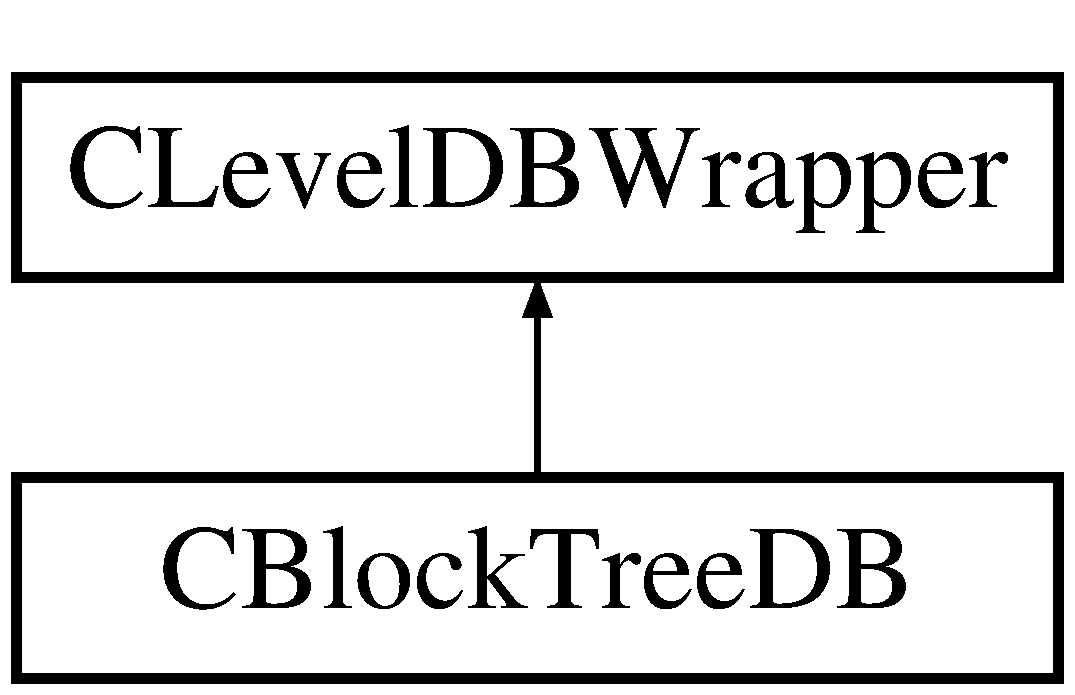
\includegraphics[height=2.000000cm]{class_c_block_tree_d_b}
\end{center}
\end{figure}
\subsection*{Public Member Functions}
\begin{DoxyCompactItemize}
\item 
\mbox{\hyperlink{class_c_block_tree_d_b_a52fd1b1dc02c2a4e977099e2c2c50424}{C\+Block\+Tree\+DB}} (size\+\_\+t n\+Cache\+Size, bool f\+Memory=false, bool f\+Wipe=false)
\item 
bool \mbox{\hyperlink{class_c_block_tree_d_b_af5509ed62ce84023882fe243e4cd21ba}{Write\+Batch\+Sync}} (const std\+::vector$<$ std\+::pair$<$ int, const \mbox{\hyperlink{class_c_block_file_info}{C\+Block\+File\+Info}} $\ast$$>$ $>$ \&file\+Info, int n\+Last\+File, const std\+::vector$<$ const \mbox{\hyperlink{class_c_block_index}{C\+Block\+Index}} $\ast$$>$ \&blockinfo)
\item 
bool \mbox{\hyperlink{class_c_block_tree_d_b_a6f951198dc53fbe9194626ff82638656}{Read\+Block\+File\+Info}} (int n\+File, \mbox{\hyperlink{class_c_block_file_info}{C\+Block\+File\+Info}} \&fileinfo)
\item 
bool \mbox{\hyperlink{class_c_block_tree_d_b_adb1276fe2f0e0c4c106660948c581711}{Read\+Last\+Block\+File}} (int \&n\+File)
\item 
bool \mbox{\hyperlink{class_c_block_tree_d_b_a8fa5d150b98f4fd1aa8cf503eddfccef}{Write\+Reindexing}} (bool \mbox{\hyperlink{main_8h_a8e0eca589b2d4254a65f04c5d91888b2}{f\+Reindex}})
\item 
bool \mbox{\hyperlink{class_c_block_tree_d_b_a1abf6fc392048428aa24a12b7942824b}{Read\+Reindexing}} (bool \&\mbox{\hyperlink{main_8h_a8e0eca589b2d4254a65f04c5d91888b2}{f\+Reindex}})
\item 
bool \mbox{\hyperlink{class_c_block_tree_d_b_a74383427266d627e84c2d0c8e21e03c7}{Read\+Tx\+Index}} (const \mbox{\hyperlink{classuint256}{uint256}} \&txid, \mbox{\hyperlink{struct_c_disk_tx_pos}{C\+Disk\+Tx\+Pos}} \&pos)
\item 
bool \mbox{\hyperlink{class_c_block_tree_d_b_a1e03745f9675ad352a1483a0aa7ef308}{Write\+Tx\+Index}} (const std\+::vector$<$ std\+::pair$<$ \mbox{\hyperlink{classuint256}{uint256}}, \mbox{\hyperlink{struct_c_disk_tx_pos}{C\+Disk\+Tx\+Pos}} $>$ $>$ \&list)
\item 
bool \mbox{\hyperlink{class_c_block_tree_d_b_af2f65b70ac5d8a198d4f29a7e909c08a}{Write\+Flag}} (const std\+::string \&\mbox{\hyperlink{rest_8cpp_a8f8f80d37794cde9472343e4487ba3eb}{name}}, bool f\+Value)
\item 
bool \mbox{\hyperlink{class_c_block_tree_d_b_acd779c4653fd9a87fffe95d53ce7c6d3}{Read\+Flag}} (const std\+::string \&\mbox{\hyperlink{rest_8cpp_a8f8f80d37794cde9472343e4487ba3eb}{name}}, bool \&f\+Value)
\item 
bool \mbox{\hyperlink{class_c_block_tree_d_b_a12be19bb1d7253eeb40e1aa88b032346}{Load\+Block\+Index\+Guts}} ()
\end{DoxyCompactItemize}
\subsection*{Private Member Functions}
\begin{DoxyCompactItemize}
\item 
\mbox{\hyperlink{class_c_block_tree_d_b_a7e3d4632e9374e652bc008163bb9e2b1}{C\+Block\+Tree\+DB}} (const \mbox{\hyperlink{class_c_block_tree_d_b}{C\+Block\+Tree\+DB}} \&)
\item 
void \mbox{\hyperlink{class_c_block_tree_d_b_a93fa0b87d518a1142f3fbfe65ab07cd2}{operator=}} (const \mbox{\hyperlink{class_c_block_tree_d_b}{C\+Block\+Tree\+DB}} \&)
\end{DoxyCompactItemize}


\subsection{Detailed Description}
Access to the block database (blocks/index/) 

\subsection{Constructor \& Destructor Documentation}
\mbox{\Hypertarget{class_c_block_tree_d_b_a52fd1b1dc02c2a4e977099e2c2c50424}\label{class_c_block_tree_d_b_a52fd1b1dc02c2a4e977099e2c2c50424}} 
\index{C\+Block\+Tree\+DB@{C\+Block\+Tree\+DB}!C\+Block\+Tree\+DB@{C\+Block\+Tree\+DB}}
\index{C\+Block\+Tree\+DB@{C\+Block\+Tree\+DB}!C\+Block\+Tree\+DB@{C\+Block\+Tree\+DB}}
\subsubsection{\texorpdfstring{C\+Block\+Tree\+D\+B()}{CBlockTreeDB()}\hspace{0.1cm}{\footnotesize\ttfamily [1/2]}}
{\footnotesize\ttfamily C\+Block\+Tree\+D\+B\+::\+C\+Block\+Tree\+DB (\begin{DoxyParamCaption}\item[{size\+\_\+t}]{n\+Cache\+Size,  }\item[{bool}]{f\+Memory = {\ttfamily false},  }\item[{bool}]{f\+Wipe = {\ttfamily false} }\end{DoxyParamCaption})}

\mbox{\Hypertarget{class_c_block_tree_d_b_a7e3d4632e9374e652bc008163bb9e2b1}\label{class_c_block_tree_d_b_a7e3d4632e9374e652bc008163bb9e2b1}} 
\index{C\+Block\+Tree\+DB@{C\+Block\+Tree\+DB}!C\+Block\+Tree\+DB@{C\+Block\+Tree\+DB}}
\index{C\+Block\+Tree\+DB@{C\+Block\+Tree\+DB}!C\+Block\+Tree\+DB@{C\+Block\+Tree\+DB}}
\subsubsection{\texorpdfstring{C\+Block\+Tree\+D\+B()}{CBlockTreeDB()}\hspace{0.1cm}{\footnotesize\ttfamily [2/2]}}
{\footnotesize\ttfamily C\+Block\+Tree\+D\+B\+::\+C\+Block\+Tree\+DB (\begin{DoxyParamCaption}\item[{const \mbox{\hyperlink{class_c_block_tree_d_b}{C\+Block\+Tree\+DB}} \&}]{ }\end{DoxyParamCaption})\hspace{0.3cm}{\ttfamily [private]}}



\subsection{Member Function Documentation}
\mbox{\Hypertarget{class_c_block_tree_d_b_a12be19bb1d7253eeb40e1aa88b032346}\label{class_c_block_tree_d_b_a12be19bb1d7253eeb40e1aa88b032346}} 
\index{C\+Block\+Tree\+DB@{C\+Block\+Tree\+DB}!Load\+Block\+Index\+Guts@{Load\+Block\+Index\+Guts}}
\index{Load\+Block\+Index\+Guts@{Load\+Block\+Index\+Guts}!C\+Block\+Tree\+DB@{C\+Block\+Tree\+DB}}
\subsubsection{\texorpdfstring{Load\+Block\+Index\+Guts()}{LoadBlockIndexGuts()}}
{\footnotesize\ttfamily bool C\+Block\+Tree\+D\+B\+::\+Load\+Block\+Index\+Guts (\begin{DoxyParamCaption}{ }\end{DoxyParamCaption})}

\mbox{\Hypertarget{class_c_block_tree_d_b_a93fa0b87d518a1142f3fbfe65ab07cd2}\label{class_c_block_tree_d_b_a93fa0b87d518a1142f3fbfe65ab07cd2}} 
\index{C\+Block\+Tree\+DB@{C\+Block\+Tree\+DB}!operator=@{operator=}}
\index{operator=@{operator=}!C\+Block\+Tree\+DB@{C\+Block\+Tree\+DB}}
\subsubsection{\texorpdfstring{operator=()}{operator=()}}
{\footnotesize\ttfamily void C\+Block\+Tree\+D\+B\+::operator= (\begin{DoxyParamCaption}\item[{const \mbox{\hyperlink{class_c_block_tree_d_b}{C\+Block\+Tree\+DB}} \&}]{ }\end{DoxyParamCaption})\hspace{0.3cm}{\ttfamily [private]}}

\mbox{\Hypertarget{class_c_block_tree_d_b_a6f951198dc53fbe9194626ff82638656}\label{class_c_block_tree_d_b_a6f951198dc53fbe9194626ff82638656}} 
\index{C\+Block\+Tree\+DB@{C\+Block\+Tree\+DB}!Read\+Block\+File\+Info@{Read\+Block\+File\+Info}}
\index{Read\+Block\+File\+Info@{Read\+Block\+File\+Info}!C\+Block\+Tree\+DB@{C\+Block\+Tree\+DB}}
\subsubsection{\texorpdfstring{Read\+Block\+File\+Info()}{ReadBlockFileInfo()}}
{\footnotesize\ttfamily bool C\+Block\+Tree\+D\+B\+::\+Read\+Block\+File\+Info (\begin{DoxyParamCaption}\item[{int}]{n\+File,  }\item[{\mbox{\hyperlink{class_c_block_file_info}{C\+Block\+File\+Info}} \&}]{fileinfo }\end{DoxyParamCaption})}

\mbox{\Hypertarget{class_c_block_tree_d_b_acd779c4653fd9a87fffe95d53ce7c6d3}\label{class_c_block_tree_d_b_acd779c4653fd9a87fffe95d53ce7c6d3}} 
\index{C\+Block\+Tree\+DB@{C\+Block\+Tree\+DB}!Read\+Flag@{Read\+Flag}}
\index{Read\+Flag@{Read\+Flag}!C\+Block\+Tree\+DB@{C\+Block\+Tree\+DB}}
\subsubsection{\texorpdfstring{Read\+Flag()}{ReadFlag()}}
{\footnotesize\ttfamily bool C\+Block\+Tree\+D\+B\+::\+Read\+Flag (\begin{DoxyParamCaption}\item[{const std\+::string \&}]{name,  }\item[{bool \&}]{f\+Value }\end{DoxyParamCaption})}

\mbox{\Hypertarget{class_c_block_tree_d_b_adb1276fe2f0e0c4c106660948c581711}\label{class_c_block_tree_d_b_adb1276fe2f0e0c4c106660948c581711}} 
\index{C\+Block\+Tree\+DB@{C\+Block\+Tree\+DB}!Read\+Last\+Block\+File@{Read\+Last\+Block\+File}}
\index{Read\+Last\+Block\+File@{Read\+Last\+Block\+File}!C\+Block\+Tree\+DB@{C\+Block\+Tree\+DB}}
\subsubsection{\texorpdfstring{Read\+Last\+Block\+File()}{ReadLastBlockFile()}}
{\footnotesize\ttfamily bool C\+Block\+Tree\+D\+B\+::\+Read\+Last\+Block\+File (\begin{DoxyParamCaption}\item[{int \&}]{n\+File }\end{DoxyParamCaption})}

\mbox{\Hypertarget{class_c_block_tree_d_b_a1abf6fc392048428aa24a12b7942824b}\label{class_c_block_tree_d_b_a1abf6fc392048428aa24a12b7942824b}} 
\index{C\+Block\+Tree\+DB@{C\+Block\+Tree\+DB}!Read\+Reindexing@{Read\+Reindexing}}
\index{Read\+Reindexing@{Read\+Reindexing}!C\+Block\+Tree\+DB@{C\+Block\+Tree\+DB}}
\subsubsection{\texorpdfstring{Read\+Reindexing()}{ReadReindexing()}}
{\footnotesize\ttfamily bool C\+Block\+Tree\+D\+B\+::\+Read\+Reindexing (\begin{DoxyParamCaption}\item[{bool \&}]{f\+Reindex }\end{DoxyParamCaption})}

\mbox{\Hypertarget{class_c_block_tree_d_b_a74383427266d627e84c2d0c8e21e03c7}\label{class_c_block_tree_d_b_a74383427266d627e84c2d0c8e21e03c7}} 
\index{C\+Block\+Tree\+DB@{C\+Block\+Tree\+DB}!Read\+Tx\+Index@{Read\+Tx\+Index}}
\index{Read\+Tx\+Index@{Read\+Tx\+Index}!C\+Block\+Tree\+DB@{C\+Block\+Tree\+DB}}
\subsubsection{\texorpdfstring{Read\+Tx\+Index()}{ReadTxIndex()}}
{\footnotesize\ttfamily bool C\+Block\+Tree\+D\+B\+::\+Read\+Tx\+Index (\begin{DoxyParamCaption}\item[{const \mbox{\hyperlink{classuint256}{uint256}} \&}]{txid,  }\item[{\mbox{\hyperlink{struct_c_disk_tx_pos}{C\+Disk\+Tx\+Pos}} \&}]{pos }\end{DoxyParamCaption})}

\mbox{\Hypertarget{class_c_block_tree_d_b_af5509ed62ce84023882fe243e4cd21ba}\label{class_c_block_tree_d_b_af5509ed62ce84023882fe243e4cd21ba}} 
\index{C\+Block\+Tree\+DB@{C\+Block\+Tree\+DB}!Write\+Batch\+Sync@{Write\+Batch\+Sync}}
\index{Write\+Batch\+Sync@{Write\+Batch\+Sync}!C\+Block\+Tree\+DB@{C\+Block\+Tree\+DB}}
\subsubsection{\texorpdfstring{Write\+Batch\+Sync()}{WriteBatchSync()}}
{\footnotesize\ttfamily bool C\+Block\+Tree\+D\+B\+::\+Write\+Batch\+Sync (\begin{DoxyParamCaption}\item[{const std\+::vector$<$ std\+::pair$<$ int, const \mbox{\hyperlink{class_c_block_file_info}{C\+Block\+File\+Info}} $\ast$$>$ $>$ \&}]{file\+Info,  }\item[{int}]{n\+Last\+File,  }\item[{const std\+::vector$<$ const \mbox{\hyperlink{class_c_block_index}{C\+Block\+Index}} $\ast$$>$ \&}]{blockinfo }\end{DoxyParamCaption})}

\mbox{\Hypertarget{class_c_block_tree_d_b_af2f65b70ac5d8a198d4f29a7e909c08a}\label{class_c_block_tree_d_b_af2f65b70ac5d8a198d4f29a7e909c08a}} 
\index{C\+Block\+Tree\+DB@{C\+Block\+Tree\+DB}!Write\+Flag@{Write\+Flag}}
\index{Write\+Flag@{Write\+Flag}!C\+Block\+Tree\+DB@{C\+Block\+Tree\+DB}}
\subsubsection{\texorpdfstring{Write\+Flag()}{WriteFlag()}}
{\footnotesize\ttfamily bool C\+Block\+Tree\+D\+B\+::\+Write\+Flag (\begin{DoxyParamCaption}\item[{const std\+::string \&}]{name,  }\item[{bool}]{f\+Value }\end{DoxyParamCaption})}

\mbox{\Hypertarget{class_c_block_tree_d_b_a8fa5d150b98f4fd1aa8cf503eddfccef}\label{class_c_block_tree_d_b_a8fa5d150b98f4fd1aa8cf503eddfccef}} 
\index{C\+Block\+Tree\+DB@{C\+Block\+Tree\+DB}!Write\+Reindexing@{Write\+Reindexing}}
\index{Write\+Reindexing@{Write\+Reindexing}!C\+Block\+Tree\+DB@{C\+Block\+Tree\+DB}}
\subsubsection{\texorpdfstring{Write\+Reindexing()}{WriteReindexing()}}
{\footnotesize\ttfamily bool C\+Block\+Tree\+D\+B\+::\+Write\+Reindexing (\begin{DoxyParamCaption}\item[{bool}]{f\+Reindex }\end{DoxyParamCaption})}

\mbox{\Hypertarget{class_c_block_tree_d_b_a1e03745f9675ad352a1483a0aa7ef308}\label{class_c_block_tree_d_b_a1e03745f9675ad352a1483a0aa7ef308}} 
\index{C\+Block\+Tree\+DB@{C\+Block\+Tree\+DB}!Write\+Tx\+Index@{Write\+Tx\+Index}}
\index{Write\+Tx\+Index@{Write\+Tx\+Index}!C\+Block\+Tree\+DB@{C\+Block\+Tree\+DB}}
\subsubsection{\texorpdfstring{Write\+Tx\+Index()}{WriteTxIndex()}}
{\footnotesize\ttfamily bool C\+Block\+Tree\+D\+B\+::\+Write\+Tx\+Index (\begin{DoxyParamCaption}\item[{const std\+::vector$<$ std\+::pair$<$ \mbox{\hyperlink{classuint256}{uint256}}, \mbox{\hyperlink{struct_c_disk_tx_pos}{C\+Disk\+Tx\+Pos}} $>$ $>$ \&}]{list }\end{DoxyParamCaption})}



The documentation for this class was generated from the following files\+:\begin{DoxyCompactItemize}
\item 
/\+Users/christopherarguello/\+Developer/anon/src/\mbox{\hyperlink{txdb_8h}{txdb.\+h}}\item 
/\+Users/christopherarguello/\+Developer/anon/src/\mbox{\hyperlink{txdb_8cpp}{txdb.\+cpp}}\end{DoxyCompactItemize}

\hypertarget{class_c_block_undo}{}\section{C\+Block\+Undo Class Reference}
\label{class_c_block_undo}\index{C\+Block\+Undo@{C\+Block\+Undo}}


{\ttfamily \#include $<$undo.\+h$>$}

\subsection*{Public Member Functions}
\begin{DoxyCompactItemize}
\item 
{\footnotesize template$<$typename Stream , typename Operation $>$ }\\void \mbox{\hyperlink{class_c_block_undo_ad4d50e2b34e291dbe2d15fbe3ae3670b}{Serialization\+Op}} (Stream \&s, Operation ser\+\_\+action, int n\+Type, int n\+Version)
\end{DoxyCompactItemize}
\subsection*{Public Attributes}
\begin{DoxyCompactItemize}
\item 
std\+::vector$<$ \mbox{\hyperlink{class_c_tx_undo}{C\+Tx\+Undo}} $>$ \mbox{\hyperlink{class_c_block_undo_ad0baf7a4d3634b27b4affac2e7cf75c9}{vtxundo}}
\item 
\mbox{\hyperlink{classuint256}{uint256}} \mbox{\hyperlink{class_c_block_undo_ae4097ec58b3c6b7c0d6c574207ff0f2e}{old\+\_\+tree\+\_\+root}}
\item 
\mbox{\hyperlink{class_c_block_undo_a4fecc9723902f51e25b57e2e2d45334a}{A\+D\+D\+\_\+\+S\+E\+R\+I\+A\+L\+I\+Z\+E\+\_\+\+M\+E\+T\+H\+O\+DS}}
\end{DoxyCompactItemize}


\subsection{Detailed Description}
Undo information for a C\+Block 

\subsection{Member Function Documentation}
\mbox{\Hypertarget{class_c_block_undo_ad4d50e2b34e291dbe2d15fbe3ae3670b}\label{class_c_block_undo_ad4d50e2b34e291dbe2d15fbe3ae3670b}} 
\index{C\+Block\+Undo@{C\+Block\+Undo}!Serialization\+Op@{Serialization\+Op}}
\index{Serialization\+Op@{Serialization\+Op}!C\+Block\+Undo@{C\+Block\+Undo}}
\subsubsection{\texorpdfstring{Serialization\+Op()}{SerializationOp()}}
{\footnotesize\ttfamily template$<$typename Stream , typename Operation $>$ \\
void C\+Block\+Undo\+::\+Serialization\+Op (\begin{DoxyParamCaption}\item[{Stream \&}]{s,  }\item[{Operation}]{ser\+\_\+action,  }\item[{int}]{n\+Type,  }\item[{int}]{n\+Version }\end{DoxyParamCaption})\hspace{0.3cm}{\ttfamily [inline]}}



\subsection{Member Data Documentation}
\mbox{\Hypertarget{class_c_block_undo_a4fecc9723902f51e25b57e2e2d45334a}\label{class_c_block_undo_a4fecc9723902f51e25b57e2e2d45334a}} 
\index{C\+Block\+Undo@{C\+Block\+Undo}!A\+D\+D\+\_\+\+S\+E\+R\+I\+A\+L\+I\+Z\+E\+\_\+\+M\+E\+T\+H\+O\+DS@{A\+D\+D\+\_\+\+S\+E\+R\+I\+A\+L\+I\+Z\+E\+\_\+\+M\+E\+T\+H\+O\+DS}}
\index{A\+D\+D\+\_\+\+S\+E\+R\+I\+A\+L\+I\+Z\+E\+\_\+\+M\+E\+T\+H\+O\+DS@{A\+D\+D\+\_\+\+S\+E\+R\+I\+A\+L\+I\+Z\+E\+\_\+\+M\+E\+T\+H\+O\+DS}!C\+Block\+Undo@{C\+Block\+Undo}}
\subsubsection{\texorpdfstring{A\+D\+D\+\_\+\+S\+E\+R\+I\+A\+L\+I\+Z\+E\+\_\+\+M\+E\+T\+H\+O\+DS}{ADD\_SERIALIZE\_METHODS}}
{\footnotesize\ttfamily C\+Block\+Undo\+::\+A\+D\+D\+\_\+\+S\+E\+R\+I\+A\+L\+I\+Z\+E\+\_\+\+M\+E\+T\+H\+O\+DS}

\mbox{\Hypertarget{class_c_block_undo_ae4097ec58b3c6b7c0d6c574207ff0f2e}\label{class_c_block_undo_ae4097ec58b3c6b7c0d6c574207ff0f2e}} 
\index{C\+Block\+Undo@{C\+Block\+Undo}!old\+\_\+tree\+\_\+root@{old\+\_\+tree\+\_\+root}}
\index{old\+\_\+tree\+\_\+root@{old\+\_\+tree\+\_\+root}!C\+Block\+Undo@{C\+Block\+Undo}}
\subsubsection{\texorpdfstring{old\+\_\+tree\+\_\+root}{old\_tree\_root}}
{\footnotesize\ttfamily \mbox{\hyperlink{classuint256}{uint256}} C\+Block\+Undo\+::old\+\_\+tree\+\_\+root}

\mbox{\Hypertarget{class_c_block_undo_ad0baf7a4d3634b27b4affac2e7cf75c9}\label{class_c_block_undo_ad0baf7a4d3634b27b4affac2e7cf75c9}} 
\index{C\+Block\+Undo@{C\+Block\+Undo}!vtxundo@{vtxundo}}
\index{vtxundo@{vtxundo}!C\+Block\+Undo@{C\+Block\+Undo}}
\subsubsection{\texorpdfstring{vtxundo}{vtxundo}}
{\footnotesize\ttfamily std\+::vector$<$\mbox{\hyperlink{class_c_tx_undo}{C\+Tx\+Undo}}$>$ C\+Block\+Undo\+::vtxundo}



The documentation for this class was generated from the following file\+:\begin{DoxyCompactItemize}
\item 
/\+Users/christopherarguello/\+Developer/anon/src/\mbox{\hyperlink{undo_8h}{undo.\+h}}\end{DoxyCompactItemize}

\hypertarget{class_c_bloom_filter}{}\section{C\+Bloom\+Filter Class Reference}
\label{class_c_bloom_filter}\index{C\+Bloom\+Filter@{C\+Bloom\+Filter}}


{\ttfamily \#include $<$bloom.\+h$>$}

\subsection*{Public Member Functions}
\begin{DoxyCompactItemize}
\item 
\mbox{\hyperlink{class_c_bloom_filter_a6395cfcb278ed9cf4ae873549c996f83}{C\+Bloom\+Filter}} (unsigned int n\+Elements, double n\+F\+P\+Rate, unsigned int \mbox{\hyperlink{class_c_bloom_filter_af372d9a72fd69dc5e9f31e38ab84bf29}{n\+Tweak}}, unsigned char n\+Flags\+In)
\item 
\mbox{\hyperlink{class_c_bloom_filter_ab38a984b1020bc4afd85c06e90353b28}{C\+Bloom\+Filter}} ()
\item 
{\footnotesize template$<$typename Stream , typename Operation $>$ }\\void \mbox{\hyperlink{class_c_bloom_filter_a2d12234d7febc6197a7349d609733cca}{Serialization\+Op}} (Stream \&s, Operation ser\+\_\+action, int n\+Type, int n\+Version)
\item 
void \mbox{\hyperlink{class_c_bloom_filter_abba52843c7c691ef7deb07d9a645dcc2}{insert}} (const std\+::vector$<$ unsigned char $>$ \&v\+Key)
\item 
void \mbox{\hyperlink{class_c_bloom_filter_aa77e023fc94fd17a0532bf17906e2146}{insert}} (const C\+Out\+Point \&outpoint)
\item 
void \mbox{\hyperlink{class_c_bloom_filter_ac86479ac4ac157a7f0188baaa93202cb}{insert}} (const \mbox{\hyperlink{classuint256}{uint256}} \&hash)
\item 
bool \mbox{\hyperlink{class_c_bloom_filter_afe62e10a4c4cf64e18a2a659d0bcc31b}{contains}} (const std\+::vector$<$ unsigned char $>$ \&v\+Key) const
\item 
bool \mbox{\hyperlink{class_c_bloom_filter_af4557c3253f218eaf13e6d7da53e20e9}{contains}} (const C\+Out\+Point \&outpoint) const
\item 
bool \mbox{\hyperlink{class_c_bloom_filter_a4c26810781cdc0fd34443f32612ac83b}{contains}} (const \mbox{\hyperlink{classuint256}{uint256}} \&hash) const
\item 
void \mbox{\hyperlink{class_c_bloom_filter_abf30228c0b24c57530f6b6734cd40252}{clear}} ()
\item 
void \mbox{\hyperlink{class_c_bloom_filter_a2af19739385bad826cfec9f236b65533}{reset}} (unsigned int n\+New\+Tweak)
\item 
bool \mbox{\hyperlink{class_c_bloom_filter_a06f2094da8e7d9c6ad4ea426858e32de}{Is\+Within\+Size\+Constraints}} () const
\item 
bool \mbox{\hyperlink{class_c_bloom_filter_aec420a9b66ab133090c2b4b8ed286f79}{Is\+Relevant\+And\+Update}} (const C\+Transaction \&tx)
\begin{DoxyCompactList}\small\item\em Also adds any outputs which match the filter to the filter (to match their spending txes) \end{DoxyCompactList}\item 
void \mbox{\hyperlink{class_c_bloom_filter_af98b43e91c82a1e4afc7454e8c5672c2}{Update\+Empty\+Full}} ()
\begin{DoxyCompactList}\small\item\em Checks for empty and full filters to avoid wasting cpu. \end{DoxyCompactList}\end{DoxyCompactItemize}
\subsection*{Public Attributes}
\begin{DoxyCompactItemize}
\item 
\mbox{\hyperlink{class_c_bloom_filter_aac1b6a065059e07177ec836929190ad0}{A\+D\+D\+\_\+\+S\+E\+R\+I\+A\+L\+I\+Z\+E\+\_\+\+M\+E\+T\+H\+O\+DS}}
\end{DoxyCompactItemize}
\subsection*{Private Member Functions}
\begin{DoxyCompactItemize}
\item 
unsigned int \mbox{\hyperlink{class_c_bloom_filter_a19031bd85ec49cb6f6d2cd8aa3414c75}{Hash}} (unsigned int n\+Hash\+Num, const std\+::vector$<$ unsigned char $>$ \&v\+Data\+To\+Hash) const
\item 
\mbox{\hyperlink{class_c_bloom_filter_a5ef6ddc09c07e6b921934a84cd770395}{C\+Bloom\+Filter}} (unsigned int n\+Elements, double n\+F\+P\+Rate, unsigned int \mbox{\hyperlink{class_c_bloom_filter_af372d9a72fd69dc5e9f31e38ab84bf29}{n\+Tweak}})
\end{DoxyCompactItemize}
\subsection*{Private Attributes}
\begin{DoxyCompactItemize}
\item 
std\+::vector$<$ unsigned char $>$ \mbox{\hyperlink{class_c_bloom_filter_a494abe120d62978951cc0f0db916f50e}{v\+Data}}
\item 
bool \mbox{\hyperlink{class_c_bloom_filter_a4ded8502360023ed194686c0b8df635d}{is\+Full}}
\item 
bool \mbox{\hyperlink{class_c_bloom_filter_a3db306b7ea8e7dc6281b36de9ca6750a}{is\+Empty}}
\item 
unsigned int \mbox{\hyperlink{class_c_bloom_filter_a5538222a099be8261258526204b1f1dd}{n\+Hash\+Funcs}}
\item 
unsigned int \mbox{\hyperlink{class_c_bloom_filter_af372d9a72fd69dc5e9f31e38ab84bf29}{n\+Tweak}}
\item 
unsigned char \mbox{\hyperlink{class_c_bloom_filter_a3368a76443d81e0349debe514a524dfb}{n\+Flags}}
\end{DoxyCompactItemize}
\subsection*{Friends}
\begin{DoxyCompactItemize}
\item 
class \mbox{\hyperlink{class_c_bloom_filter_a07025fbd4f30c098b492afea8e004cd8}{C\+Rolling\+Bloom\+Filter}}
\end{DoxyCompactItemize}


\subsection{Detailed Description}
Bloom\+Filter is a probabilistic filter which S\+PV clients provide so that we can filter the transactions we send them.

This allows for significantly more efficient transaction and block downloads.

Because bloom filters are probabilistic, a S\+PV node can increase the false-\/ positive rate, making us send it transactions which aren\textquotesingle{}t actually its, allowing clients to trade more bandwidth for more privacy by obfuscating which keys are controlled by them. 

\subsection{Constructor \& Destructor Documentation}
\mbox{\Hypertarget{class_c_bloom_filter_a5ef6ddc09c07e6b921934a84cd770395}\label{class_c_bloom_filter_a5ef6ddc09c07e6b921934a84cd770395}} 
\index{C\+Bloom\+Filter@{C\+Bloom\+Filter}!C\+Bloom\+Filter@{C\+Bloom\+Filter}}
\index{C\+Bloom\+Filter@{C\+Bloom\+Filter}!C\+Bloom\+Filter@{C\+Bloom\+Filter}}
\subsubsection{\texorpdfstring{C\+Bloom\+Filter()}{CBloomFilter()}\hspace{0.1cm}{\footnotesize\ttfamily [1/3]}}
{\footnotesize\ttfamily C\+Bloom\+Filter\+::\+C\+Bloom\+Filter (\begin{DoxyParamCaption}\item[{unsigned int}]{n\+Elements,  }\item[{double}]{n\+F\+P\+Rate,  }\item[{unsigned int}]{n\+Tweak }\end{DoxyParamCaption})\hspace{0.3cm}{\ttfamily [private]}}

\mbox{\Hypertarget{class_c_bloom_filter_a6395cfcb278ed9cf4ae873549c996f83}\label{class_c_bloom_filter_a6395cfcb278ed9cf4ae873549c996f83}} 
\index{C\+Bloom\+Filter@{C\+Bloom\+Filter}!C\+Bloom\+Filter@{C\+Bloom\+Filter}}
\index{C\+Bloom\+Filter@{C\+Bloom\+Filter}!C\+Bloom\+Filter@{C\+Bloom\+Filter}}
\subsubsection{\texorpdfstring{C\+Bloom\+Filter()}{CBloomFilter()}\hspace{0.1cm}{\footnotesize\ttfamily [2/3]}}
{\footnotesize\ttfamily C\+Bloom\+Filter\+::\+C\+Bloom\+Filter (\begin{DoxyParamCaption}\item[{unsigned int}]{n\+Elements,  }\item[{double}]{n\+F\+P\+Rate,  }\item[{unsigned int}]{n\+Tweak\+In,  }\item[{unsigned char}]{n\+Flags\+In }\end{DoxyParamCaption})}

Creates a new bloom filter which will provide the given fp rate when filled with the given number of elements Note that if the given parameters will result in a filter outside the bounds of the protocol limits, the filter created will be as close to the given parameters as possible within the protocol limits. This will apply if n\+F\+P\+Rate is very low or n\+Elements is unreasonably high. n\+Tweak is a constant which is added to the seed value passed to the hash function It should generally always be a random value (and is largely only exposed for unit testing) n\+Flags should be one of the B\+L\+O\+O\+M\+\_\+\+U\+P\+D\+A\+T\+E\+\_\+$\ast$ enums (not \+\_\+\+M\+A\+SK)

The ideal size for a bloom filter with a given number of elements and false positive rate is\+:
\begin{DoxyItemize}
\item n\+Elements $\ast$ log(fp rate) / ln(2)$^\wedge$2 We ignore filter parameters which will create a bloom filter larger than the protocol limits The ideal number of hash functions is filter size $\ast$ ln(2) / number of elements Again, we ignore filter parameters which will create a bloom filter with more hash functions than the protocol limits See \href{https://en.wikipedia.org/wiki/Bloom_filter}{\tt https\+://en.\+wikipedia.\+org/wiki/\+Bloom\+\_\+filter} for an explanation of these formulas 
\end{DoxyItemize}\mbox{\Hypertarget{class_c_bloom_filter_ab38a984b1020bc4afd85c06e90353b28}\label{class_c_bloom_filter_ab38a984b1020bc4afd85c06e90353b28}} 
\index{C\+Bloom\+Filter@{C\+Bloom\+Filter}!C\+Bloom\+Filter@{C\+Bloom\+Filter}}
\index{C\+Bloom\+Filter@{C\+Bloom\+Filter}!C\+Bloom\+Filter@{C\+Bloom\+Filter}}
\subsubsection{\texorpdfstring{C\+Bloom\+Filter()}{CBloomFilter()}\hspace{0.1cm}{\footnotesize\ttfamily [3/3]}}
{\footnotesize\ttfamily C\+Bloom\+Filter\+::\+C\+Bloom\+Filter (\begin{DoxyParamCaption}{ }\end{DoxyParamCaption})\hspace{0.3cm}{\ttfamily [inline]}}



\subsection{Member Function Documentation}
\mbox{\Hypertarget{class_c_bloom_filter_abf30228c0b24c57530f6b6734cd40252}\label{class_c_bloom_filter_abf30228c0b24c57530f6b6734cd40252}} 
\index{C\+Bloom\+Filter@{C\+Bloom\+Filter}!clear@{clear}}
\index{clear@{clear}!C\+Bloom\+Filter@{C\+Bloom\+Filter}}
\subsubsection{\texorpdfstring{clear()}{clear()}}
{\footnotesize\ttfamily void C\+Bloom\+Filter\+::clear (\begin{DoxyParamCaption}{ }\end{DoxyParamCaption})}

\mbox{\Hypertarget{class_c_bloom_filter_afe62e10a4c4cf64e18a2a659d0bcc31b}\label{class_c_bloom_filter_afe62e10a4c4cf64e18a2a659d0bcc31b}} 
\index{C\+Bloom\+Filter@{C\+Bloom\+Filter}!contains@{contains}}
\index{contains@{contains}!C\+Bloom\+Filter@{C\+Bloom\+Filter}}
\subsubsection{\texorpdfstring{contains()}{contains()}\hspace{0.1cm}{\footnotesize\ttfamily [1/3]}}
{\footnotesize\ttfamily bool C\+Bloom\+Filter\+::contains (\begin{DoxyParamCaption}\item[{const std\+::vector$<$ unsigned char $>$ \&}]{v\+Key }\end{DoxyParamCaption}) const}

\mbox{\Hypertarget{class_c_bloom_filter_af4557c3253f218eaf13e6d7da53e20e9}\label{class_c_bloom_filter_af4557c3253f218eaf13e6d7da53e20e9}} 
\index{C\+Bloom\+Filter@{C\+Bloom\+Filter}!contains@{contains}}
\index{contains@{contains}!C\+Bloom\+Filter@{C\+Bloom\+Filter}}
\subsubsection{\texorpdfstring{contains()}{contains()}\hspace{0.1cm}{\footnotesize\ttfamily [2/3]}}
{\footnotesize\ttfamily bool C\+Bloom\+Filter\+::contains (\begin{DoxyParamCaption}\item[{const C\+Out\+Point \&}]{outpoint }\end{DoxyParamCaption}) const}

\mbox{\Hypertarget{class_c_bloom_filter_a4c26810781cdc0fd34443f32612ac83b}\label{class_c_bloom_filter_a4c26810781cdc0fd34443f32612ac83b}} 
\index{C\+Bloom\+Filter@{C\+Bloom\+Filter}!contains@{contains}}
\index{contains@{contains}!C\+Bloom\+Filter@{C\+Bloom\+Filter}}
\subsubsection{\texorpdfstring{contains()}{contains()}\hspace{0.1cm}{\footnotesize\ttfamily [3/3]}}
{\footnotesize\ttfamily bool C\+Bloom\+Filter\+::contains (\begin{DoxyParamCaption}\item[{const \mbox{\hyperlink{classuint256}{uint256}} \&}]{hash }\end{DoxyParamCaption}) const}

\mbox{\Hypertarget{class_c_bloom_filter_a19031bd85ec49cb6f6d2cd8aa3414c75}\label{class_c_bloom_filter_a19031bd85ec49cb6f6d2cd8aa3414c75}} 
\index{C\+Bloom\+Filter@{C\+Bloom\+Filter}!Hash@{Hash}}
\index{Hash@{Hash}!C\+Bloom\+Filter@{C\+Bloom\+Filter}}
\subsubsection{\texorpdfstring{Hash()}{Hash()}}
{\footnotesize\ttfamily unsigned int C\+Bloom\+Filter\+::\+Hash (\begin{DoxyParamCaption}\item[{unsigned int}]{n\+Hash\+Num,  }\item[{const std\+::vector$<$ unsigned char $>$ \&}]{v\+Data\+To\+Hash }\end{DoxyParamCaption}) const\hspace{0.3cm}{\ttfamily [inline]}, {\ttfamily [private]}}

\mbox{\Hypertarget{class_c_bloom_filter_abba52843c7c691ef7deb07d9a645dcc2}\label{class_c_bloom_filter_abba52843c7c691ef7deb07d9a645dcc2}} 
\index{C\+Bloom\+Filter@{C\+Bloom\+Filter}!insert@{insert}}
\index{insert@{insert}!C\+Bloom\+Filter@{C\+Bloom\+Filter}}
\subsubsection{\texorpdfstring{insert()}{insert()}\hspace{0.1cm}{\footnotesize\ttfamily [1/3]}}
{\footnotesize\ttfamily void C\+Bloom\+Filter\+::insert (\begin{DoxyParamCaption}\item[{const std\+::vector$<$ unsigned char $>$ \&}]{v\+Key }\end{DoxyParamCaption})}

\mbox{\Hypertarget{class_c_bloom_filter_aa77e023fc94fd17a0532bf17906e2146}\label{class_c_bloom_filter_aa77e023fc94fd17a0532bf17906e2146}} 
\index{C\+Bloom\+Filter@{C\+Bloom\+Filter}!insert@{insert}}
\index{insert@{insert}!C\+Bloom\+Filter@{C\+Bloom\+Filter}}
\subsubsection{\texorpdfstring{insert()}{insert()}\hspace{0.1cm}{\footnotesize\ttfamily [2/3]}}
{\footnotesize\ttfamily void C\+Bloom\+Filter\+::insert (\begin{DoxyParamCaption}\item[{const C\+Out\+Point \&}]{outpoint }\end{DoxyParamCaption})}

\mbox{\Hypertarget{class_c_bloom_filter_ac86479ac4ac157a7f0188baaa93202cb}\label{class_c_bloom_filter_ac86479ac4ac157a7f0188baaa93202cb}} 
\index{C\+Bloom\+Filter@{C\+Bloom\+Filter}!insert@{insert}}
\index{insert@{insert}!C\+Bloom\+Filter@{C\+Bloom\+Filter}}
\subsubsection{\texorpdfstring{insert()}{insert()}\hspace{0.1cm}{\footnotesize\ttfamily [3/3]}}
{\footnotesize\ttfamily void C\+Bloom\+Filter\+::insert (\begin{DoxyParamCaption}\item[{const \mbox{\hyperlink{classuint256}{uint256}} \&}]{hash }\end{DoxyParamCaption})}

\mbox{\Hypertarget{class_c_bloom_filter_aec420a9b66ab133090c2b4b8ed286f79}\label{class_c_bloom_filter_aec420a9b66ab133090c2b4b8ed286f79}} 
\index{C\+Bloom\+Filter@{C\+Bloom\+Filter}!Is\+Relevant\+And\+Update@{Is\+Relevant\+And\+Update}}
\index{Is\+Relevant\+And\+Update@{Is\+Relevant\+And\+Update}!C\+Bloom\+Filter@{C\+Bloom\+Filter}}
\subsubsection{\texorpdfstring{Is\+Relevant\+And\+Update()}{IsRelevantAndUpdate()}}
{\footnotesize\ttfamily bool C\+Bloom\+Filter\+::\+Is\+Relevant\+And\+Update (\begin{DoxyParamCaption}\item[{const C\+Transaction \&}]{tx }\end{DoxyParamCaption})}



Also adds any outputs which match the filter to the filter (to match their spending txes) 

\mbox{\Hypertarget{class_c_bloom_filter_a06f2094da8e7d9c6ad4ea426858e32de}\label{class_c_bloom_filter_a06f2094da8e7d9c6ad4ea426858e32de}} 
\index{C\+Bloom\+Filter@{C\+Bloom\+Filter}!Is\+Within\+Size\+Constraints@{Is\+Within\+Size\+Constraints}}
\index{Is\+Within\+Size\+Constraints@{Is\+Within\+Size\+Constraints}!C\+Bloom\+Filter@{C\+Bloom\+Filter}}
\subsubsection{\texorpdfstring{Is\+Within\+Size\+Constraints()}{IsWithinSizeConstraints()}}
{\footnotesize\ttfamily bool C\+Bloom\+Filter\+::\+Is\+Within\+Size\+Constraints (\begin{DoxyParamCaption}{ }\end{DoxyParamCaption}) const}

True if the size is $<$= M\+A\+X\+\_\+\+B\+L\+O\+O\+M\+\_\+\+F\+I\+L\+T\+E\+R\+\_\+\+S\+I\+ZE and the number of hash functions is $<$= M\+A\+X\+\_\+\+H\+A\+S\+H\+\_\+\+F\+U\+N\+CS (catch a filter which was just deserialized which was too big) \mbox{\Hypertarget{class_c_bloom_filter_a2af19739385bad826cfec9f236b65533}\label{class_c_bloom_filter_a2af19739385bad826cfec9f236b65533}} 
\index{C\+Bloom\+Filter@{C\+Bloom\+Filter}!reset@{reset}}
\index{reset@{reset}!C\+Bloom\+Filter@{C\+Bloom\+Filter}}
\subsubsection{\texorpdfstring{reset()}{reset()}}
{\footnotesize\ttfamily void C\+Bloom\+Filter\+::reset (\begin{DoxyParamCaption}\item[{unsigned int}]{n\+New\+Tweak }\end{DoxyParamCaption})}

\mbox{\Hypertarget{class_c_bloom_filter_a2d12234d7febc6197a7349d609733cca}\label{class_c_bloom_filter_a2d12234d7febc6197a7349d609733cca}} 
\index{C\+Bloom\+Filter@{C\+Bloom\+Filter}!Serialization\+Op@{Serialization\+Op}}
\index{Serialization\+Op@{Serialization\+Op}!C\+Bloom\+Filter@{C\+Bloom\+Filter}}
\subsubsection{\texorpdfstring{Serialization\+Op()}{SerializationOp()}}
{\footnotesize\ttfamily template$<$typename Stream , typename Operation $>$ \\
void C\+Bloom\+Filter\+::\+Serialization\+Op (\begin{DoxyParamCaption}\item[{Stream \&}]{s,  }\item[{Operation}]{ser\+\_\+action,  }\item[{int}]{n\+Type,  }\item[{int}]{n\+Version }\end{DoxyParamCaption})\hspace{0.3cm}{\ttfamily [inline]}}

\mbox{\Hypertarget{class_c_bloom_filter_af98b43e91c82a1e4afc7454e8c5672c2}\label{class_c_bloom_filter_af98b43e91c82a1e4afc7454e8c5672c2}} 
\index{C\+Bloom\+Filter@{C\+Bloom\+Filter}!Update\+Empty\+Full@{Update\+Empty\+Full}}
\index{Update\+Empty\+Full@{Update\+Empty\+Full}!C\+Bloom\+Filter@{C\+Bloom\+Filter}}
\subsubsection{\texorpdfstring{Update\+Empty\+Full()}{UpdateEmptyFull()}}
{\footnotesize\ttfamily void C\+Bloom\+Filter\+::\+Update\+Empty\+Full (\begin{DoxyParamCaption}{ }\end{DoxyParamCaption})}



Checks for empty and full filters to avoid wasting cpu. 



\subsection{Friends And Related Function Documentation}
\mbox{\Hypertarget{class_c_bloom_filter_a07025fbd4f30c098b492afea8e004cd8}\label{class_c_bloom_filter_a07025fbd4f30c098b492afea8e004cd8}} 
\index{C\+Bloom\+Filter@{C\+Bloom\+Filter}!C\+Rolling\+Bloom\+Filter@{C\+Rolling\+Bloom\+Filter}}
\index{C\+Rolling\+Bloom\+Filter@{C\+Rolling\+Bloom\+Filter}!C\+Bloom\+Filter@{C\+Bloom\+Filter}}
\subsubsection{\texorpdfstring{C\+Rolling\+Bloom\+Filter}{CRollingBloomFilter}}
{\footnotesize\ttfamily friend class \mbox{\hyperlink{class_c_rolling_bloom_filter}{C\+Rolling\+Bloom\+Filter}}\hspace{0.3cm}{\ttfamily [friend]}}



\subsection{Member Data Documentation}
\mbox{\Hypertarget{class_c_bloom_filter_aac1b6a065059e07177ec836929190ad0}\label{class_c_bloom_filter_aac1b6a065059e07177ec836929190ad0}} 
\index{C\+Bloom\+Filter@{C\+Bloom\+Filter}!A\+D\+D\+\_\+\+S\+E\+R\+I\+A\+L\+I\+Z\+E\+\_\+\+M\+E\+T\+H\+O\+DS@{A\+D\+D\+\_\+\+S\+E\+R\+I\+A\+L\+I\+Z\+E\+\_\+\+M\+E\+T\+H\+O\+DS}}
\index{A\+D\+D\+\_\+\+S\+E\+R\+I\+A\+L\+I\+Z\+E\+\_\+\+M\+E\+T\+H\+O\+DS@{A\+D\+D\+\_\+\+S\+E\+R\+I\+A\+L\+I\+Z\+E\+\_\+\+M\+E\+T\+H\+O\+DS}!C\+Bloom\+Filter@{C\+Bloom\+Filter}}
\subsubsection{\texorpdfstring{A\+D\+D\+\_\+\+S\+E\+R\+I\+A\+L\+I\+Z\+E\+\_\+\+M\+E\+T\+H\+O\+DS}{ADD\_SERIALIZE\_METHODS}}
{\footnotesize\ttfamily C\+Bloom\+Filter\+::\+A\+D\+D\+\_\+\+S\+E\+R\+I\+A\+L\+I\+Z\+E\+\_\+\+M\+E\+T\+H\+O\+DS}

\mbox{\Hypertarget{class_c_bloom_filter_a3db306b7ea8e7dc6281b36de9ca6750a}\label{class_c_bloom_filter_a3db306b7ea8e7dc6281b36de9ca6750a}} 
\index{C\+Bloom\+Filter@{C\+Bloom\+Filter}!is\+Empty@{is\+Empty}}
\index{is\+Empty@{is\+Empty}!C\+Bloom\+Filter@{C\+Bloom\+Filter}}
\subsubsection{\texorpdfstring{is\+Empty}{isEmpty}}
{\footnotesize\ttfamily bool C\+Bloom\+Filter\+::is\+Empty\hspace{0.3cm}{\ttfamily [private]}}

\mbox{\Hypertarget{class_c_bloom_filter_a4ded8502360023ed194686c0b8df635d}\label{class_c_bloom_filter_a4ded8502360023ed194686c0b8df635d}} 
\index{C\+Bloom\+Filter@{C\+Bloom\+Filter}!is\+Full@{is\+Full}}
\index{is\+Full@{is\+Full}!C\+Bloom\+Filter@{C\+Bloom\+Filter}}
\subsubsection{\texorpdfstring{is\+Full}{isFull}}
{\footnotesize\ttfamily bool C\+Bloom\+Filter\+::is\+Full\hspace{0.3cm}{\ttfamily [private]}}

\mbox{\Hypertarget{class_c_bloom_filter_a3368a76443d81e0349debe514a524dfb}\label{class_c_bloom_filter_a3368a76443d81e0349debe514a524dfb}} 
\index{C\+Bloom\+Filter@{C\+Bloom\+Filter}!n\+Flags@{n\+Flags}}
\index{n\+Flags@{n\+Flags}!C\+Bloom\+Filter@{C\+Bloom\+Filter}}
\subsubsection{\texorpdfstring{n\+Flags}{nFlags}}
{\footnotesize\ttfamily unsigned char C\+Bloom\+Filter\+::n\+Flags\hspace{0.3cm}{\ttfamily [private]}}

\mbox{\Hypertarget{class_c_bloom_filter_a5538222a099be8261258526204b1f1dd}\label{class_c_bloom_filter_a5538222a099be8261258526204b1f1dd}} 
\index{C\+Bloom\+Filter@{C\+Bloom\+Filter}!n\+Hash\+Funcs@{n\+Hash\+Funcs}}
\index{n\+Hash\+Funcs@{n\+Hash\+Funcs}!C\+Bloom\+Filter@{C\+Bloom\+Filter}}
\subsubsection{\texorpdfstring{n\+Hash\+Funcs}{nHashFuncs}}
{\footnotesize\ttfamily unsigned int C\+Bloom\+Filter\+::n\+Hash\+Funcs\hspace{0.3cm}{\ttfamily [private]}}

\mbox{\Hypertarget{class_c_bloom_filter_af372d9a72fd69dc5e9f31e38ab84bf29}\label{class_c_bloom_filter_af372d9a72fd69dc5e9f31e38ab84bf29}} 
\index{C\+Bloom\+Filter@{C\+Bloom\+Filter}!n\+Tweak@{n\+Tweak}}
\index{n\+Tweak@{n\+Tweak}!C\+Bloom\+Filter@{C\+Bloom\+Filter}}
\subsubsection{\texorpdfstring{n\+Tweak}{nTweak}}
{\footnotesize\ttfamily unsigned int C\+Bloom\+Filter\+::n\+Tweak\hspace{0.3cm}{\ttfamily [private]}}

\mbox{\Hypertarget{class_c_bloom_filter_a494abe120d62978951cc0f0db916f50e}\label{class_c_bloom_filter_a494abe120d62978951cc0f0db916f50e}} 
\index{C\+Bloom\+Filter@{C\+Bloom\+Filter}!v\+Data@{v\+Data}}
\index{v\+Data@{v\+Data}!C\+Bloom\+Filter@{C\+Bloom\+Filter}}
\subsubsection{\texorpdfstring{v\+Data}{vData}}
{\footnotesize\ttfamily std\+::vector$<$unsigned char$>$ C\+Bloom\+Filter\+::v\+Data\hspace{0.3cm}{\ttfamily [private]}}



The documentation for this class was generated from the following files\+:\begin{DoxyCompactItemize}
\item 
/\+Users/christopherarguello/\+Developer/anon/src/\mbox{\hyperlink{bloom_8h}{bloom.\+h}}\item 
/\+Users/christopherarguello/\+Developer/anon/src/\mbox{\hyperlink{bloom_8cpp}{bloom.\+cpp}}\end{DoxyCompactItemize}

\hypertarget{class_c_buffered_file}{}\section{C\+Buffered\+File Class Reference}
\label{class_c_buffered_file}\index{C\+Buffered\+File@{C\+Buffered\+File}}


{\ttfamily \#include $<$streams.\+h$>$}

\subsection*{Public Member Functions}
\begin{DoxyCompactItemize}
\item 
\mbox{\hyperlink{class_c_buffered_file_a30ad96a8d09bed60355d1fadda7dabdc}{C\+Buffered\+File}} (F\+I\+LE $\ast$file\+In, uint64\+\_\+t n\+Buf\+Size, uint64\+\_\+t n\+Rewind\+In, int n\+Type\+In, int n\+Version\+In)
\item 
\mbox{\hyperlink{class_c_buffered_file_a8804f689b27d3298cd5d63fbcddb97d1}{$\sim$\+C\+Buffered\+File}} ()
\item 
void \mbox{\hyperlink{class_c_buffered_file_aef8c993fe3eb0fa423d09d095f40dcf6}{fclose}} ()
\item 
bool \mbox{\hyperlink{class_c_buffered_file_af0ff112a5fd46ba3e8f2f1f4f36d5566}{eof}} () const
\item 
\mbox{\hyperlink{class_c_buffered_file}{C\+Buffered\+File}} \& \mbox{\hyperlink{class_c_buffered_file_a20c6d2a4dbc69a8e5c7ba766d04b3d85}{read}} (char $\ast$pch, size\+\_\+t n\+Size)
\item 
uint64\+\_\+t \mbox{\hyperlink{class_c_buffered_file_af9e7226e682ede9c1c141fb2972afd7b}{Get\+Pos}} ()
\item 
bool \mbox{\hyperlink{class_c_buffered_file_aac4029a9aade127cc8a1fbbcc1549599}{Set\+Pos}} (uint64\+\_\+t n\+Pos)
\item 
bool \mbox{\hyperlink{class_c_buffered_file_afbf9abcc70f24824661aec96a4310a63}{Seek}} (uint64\+\_\+t n\+Pos)
\item 
bool \mbox{\hyperlink{class_c_buffered_file_adfcf370a41be0454e0f6b3dc358e415c}{Set\+Limit}} (uint64\+\_\+t n\+Pos=(uint64\+\_\+t)(-\/1))
\item 
{\footnotesize template$<$typename T $>$ }\\\mbox{\hyperlink{class_c_buffered_file}{C\+Buffered\+File}} \& \mbox{\hyperlink{class_c_buffered_file_ab570d5f1a173a41100e7b42b4aacbbc5}{operator$>$$>$}} (T \&obj)
\item 
void \mbox{\hyperlink{class_c_buffered_file_a15ce0683ba5925939d33f098a948236b}{Find\+Byte}} (char ch)
\end{DoxyCompactItemize}
\subsection*{Protected Member Functions}
\begin{DoxyCompactItemize}
\item 
bool \mbox{\hyperlink{class_c_buffered_file_a2c93fc60c4460bd1ccf90922646b19b8}{Fill}} ()
\end{DoxyCompactItemize}
\subsection*{Private Member Functions}
\begin{DoxyCompactItemize}
\item 
\mbox{\hyperlink{class_c_buffered_file_a9d6a1d43da82fe5fb30500cd56032134}{C\+Buffered\+File}} (const \mbox{\hyperlink{class_c_buffered_file}{C\+Buffered\+File}} \&)
\item 
\mbox{\hyperlink{class_c_buffered_file}{C\+Buffered\+File}} \& \mbox{\hyperlink{class_c_buffered_file_a7b7b4419c88fb710eab6c9ccce3d3414}{operator=}} (const \mbox{\hyperlink{class_c_buffered_file}{C\+Buffered\+File}} \&)
\end{DoxyCompactItemize}
\subsection*{Private Attributes}
\begin{DoxyCompactItemize}
\item 
int \mbox{\hyperlink{class_c_buffered_file_a121e3ede0af49d4711dc4934d252f842}{n\+Type}}
\item 
int \mbox{\hyperlink{class_c_buffered_file_afdfff4bdd212f72580b1c7c02bef554a}{n\+Version}}
\item 
F\+I\+LE $\ast$ \mbox{\hyperlink{class_c_buffered_file_a85ed820b4e1a4c2d1ca983749044f172}{src}}
\item 
uint64\+\_\+t \mbox{\hyperlink{class_c_buffered_file_a9c12254ffa498eef11a41e3a5a02c313}{n\+Src\+Pos}}
\item 
uint64\+\_\+t \mbox{\hyperlink{class_c_buffered_file_ab8fd6b1adfed6b2364a97984d6dc336b}{n\+Read\+Pos}}
\item 
uint64\+\_\+t \mbox{\hyperlink{class_c_buffered_file_a14409b620943fcc88a114dcbe417f77c}{n\+Read\+Limit}}
\item 
uint64\+\_\+t \mbox{\hyperlink{class_c_buffered_file_a3352d0e0d6a5758961f2fafc950fb37d}{n\+Rewind}}
\item 
std\+::vector$<$ char $>$ \mbox{\hyperlink{class_c_buffered_file_a50fde609bd4dfeeb7c2ecf4f0d75e789}{vch\+Buf}}
\end{DoxyCompactItemize}


\subsection{Detailed Description}
Non-\/refcounted R\+A\+II wrapper around a F\+I\+L\+E$\ast$ that implements a ring buffer to deserialize from. It guarantees the ability to rewind a given number of bytes.

Will automatically close the file when it goes out of scope if not null. If you need to close the file early, use file.\+fclose() instead of fclose(file). 

\subsection{Constructor \& Destructor Documentation}
\mbox{\Hypertarget{class_c_buffered_file_a9d6a1d43da82fe5fb30500cd56032134}\label{class_c_buffered_file_a9d6a1d43da82fe5fb30500cd56032134}} 
\index{C\+Buffered\+File@{C\+Buffered\+File}!C\+Buffered\+File@{C\+Buffered\+File}}
\index{C\+Buffered\+File@{C\+Buffered\+File}!C\+Buffered\+File@{C\+Buffered\+File}}
\subsubsection{\texorpdfstring{C\+Buffered\+File()}{CBufferedFile()}\hspace{0.1cm}{\footnotesize\ttfamily [1/2]}}
{\footnotesize\ttfamily C\+Buffered\+File\+::\+C\+Buffered\+File (\begin{DoxyParamCaption}\item[{const \mbox{\hyperlink{class_c_buffered_file}{C\+Buffered\+File}} \&}]{ }\end{DoxyParamCaption})\hspace{0.3cm}{\ttfamily [private]}}

\mbox{\Hypertarget{class_c_buffered_file_a30ad96a8d09bed60355d1fadda7dabdc}\label{class_c_buffered_file_a30ad96a8d09bed60355d1fadda7dabdc}} 
\index{C\+Buffered\+File@{C\+Buffered\+File}!C\+Buffered\+File@{C\+Buffered\+File}}
\index{C\+Buffered\+File@{C\+Buffered\+File}!C\+Buffered\+File@{C\+Buffered\+File}}
\subsubsection{\texorpdfstring{C\+Buffered\+File()}{CBufferedFile()}\hspace{0.1cm}{\footnotesize\ttfamily [2/2]}}
{\footnotesize\ttfamily C\+Buffered\+File\+::\+C\+Buffered\+File (\begin{DoxyParamCaption}\item[{F\+I\+LE $\ast$}]{file\+In,  }\item[{uint64\+\_\+t}]{n\+Buf\+Size,  }\item[{uint64\+\_\+t}]{n\+Rewind\+In,  }\item[{int}]{n\+Type\+In,  }\item[{int}]{n\+Version\+In }\end{DoxyParamCaption})\hspace{0.3cm}{\ttfamily [inline]}}

\mbox{\Hypertarget{class_c_buffered_file_a8804f689b27d3298cd5d63fbcddb97d1}\label{class_c_buffered_file_a8804f689b27d3298cd5d63fbcddb97d1}} 
\index{C\+Buffered\+File@{C\+Buffered\+File}!````~C\+Buffered\+File@{$\sim$\+C\+Buffered\+File}}
\index{````~C\+Buffered\+File@{$\sim$\+C\+Buffered\+File}!C\+Buffered\+File@{C\+Buffered\+File}}
\subsubsection{\texorpdfstring{$\sim$\+C\+Buffered\+File()}{~CBufferedFile()}}
{\footnotesize\ttfamily C\+Buffered\+File\+::$\sim$\+C\+Buffered\+File (\begin{DoxyParamCaption}{ }\end{DoxyParamCaption})\hspace{0.3cm}{\ttfamily [inline]}}



\subsection{Member Function Documentation}
\mbox{\Hypertarget{class_c_buffered_file_af0ff112a5fd46ba3e8f2f1f4f36d5566}\label{class_c_buffered_file_af0ff112a5fd46ba3e8f2f1f4f36d5566}} 
\index{C\+Buffered\+File@{C\+Buffered\+File}!eof@{eof}}
\index{eof@{eof}!C\+Buffered\+File@{C\+Buffered\+File}}
\subsubsection{\texorpdfstring{eof()}{eof()}}
{\footnotesize\ttfamily bool C\+Buffered\+File\+::eof (\begin{DoxyParamCaption}{ }\end{DoxyParamCaption}) const\hspace{0.3cm}{\ttfamily [inline]}}

\mbox{\Hypertarget{class_c_buffered_file_aef8c993fe3eb0fa423d09d095f40dcf6}\label{class_c_buffered_file_aef8c993fe3eb0fa423d09d095f40dcf6}} 
\index{C\+Buffered\+File@{C\+Buffered\+File}!fclose@{fclose}}
\index{fclose@{fclose}!C\+Buffered\+File@{C\+Buffered\+File}}
\subsubsection{\texorpdfstring{fclose()}{fclose()}}
{\footnotesize\ttfamily void C\+Buffered\+File\+::fclose (\begin{DoxyParamCaption}{ }\end{DoxyParamCaption})\hspace{0.3cm}{\ttfamily [inline]}}

\mbox{\Hypertarget{class_c_buffered_file_a2c93fc60c4460bd1ccf90922646b19b8}\label{class_c_buffered_file_a2c93fc60c4460bd1ccf90922646b19b8}} 
\index{C\+Buffered\+File@{C\+Buffered\+File}!Fill@{Fill}}
\index{Fill@{Fill}!C\+Buffered\+File@{C\+Buffered\+File}}
\subsubsection{\texorpdfstring{Fill()}{Fill()}}
{\footnotesize\ttfamily bool C\+Buffered\+File\+::\+Fill (\begin{DoxyParamCaption}{ }\end{DoxyParamCaption})\hspace{0.3cm}{\ttfamily [inline]}, {\ttfamily [protected]}}

\mbox{\Hypertarget{class_c_buffered_file_a15ce0683ba5925939d33f098a948236b}\label{class_c_buffered_file_a15ce0683ba5925939d33f098a948236b}} 
\index{C\+Buffered\+File@{C\+Buffered\+File}!Find\+Byte@{Find\+Byte}}
\index{Find\+Byte@{Find\+Byte}!C\+Buffered\+File@{C\+Buffered\+File}}
\subsubsection{\texorpdfstring{Find\+Byte()}{FindByte()}}
{\footnotesize\ttfamily void C\+Buffered\+File\+::\+Find\+Byte (\begin{DoxyParamCaption}\item[{char}]{ch }\end{DoxyParamCaption})\hspace{0.3cm}{\ttfamily [inline]}}

\mbox{\Hypertarget{class_c_buffered_file_af9e7226e682ede9c1c141fb2972afd7b}\label{class_c_buffered_file_af9e7226e682ede9c1c141fb2972afd7b}} 
\index{C\+Buffered\+File@{C\+Buffered\+File}!Get\+Pos@{Get\+Pos}}
\index{Get\+Pos@{Get\+Pos}!C\+Buffered\+File@{C\+Buffered\+File}}
\subsubsection{\texorpdfstring{Get\+Pos()}{GetPos()}}
{\footnotesize\ttfamily uint64\+\_\+t C\+Buffered\+File\+::\+Get\+Pos (\begin{DoxyParamCaption}{ }\end{DoxyParamCaption})\hspace{0.3cm}{\ttfamily [inline]}}

\mbox{\Hypertarget{class_c_buffered_file_a7b7b4419c88fb710eab6c9ccce3d3414}\label{class_c_buffered_file_a7b7b4419c88fb710eab6c9ccce3d3414}} 
\index{C\+Buffered\+File@{C\+Buffered\+File}!operator=@{operator=}}
\index{operator=@{operator=}!C\+Buffered\+File@{C\+Buffered\+File}}
\subsubsection{\texorpdfstring{operator=()}{operator=()}}
{\footnotesize\ttfamily \mbox{\hyperlink{class_c_buffered_file}{C\+Buffered\+File}}\& C\+Buffered\+File\+::operator= (\begin{DoxyParamCaption}\item[{const \mbox{\hyperlink{class_c_buffered_file}{C\+Buffered\+File}} \&}]{ }\end{DoxyParamCaption})\hspace{0.3cm}{\ttfamily [private]}}

\mbox{\Hypertarget{class_c_buffered_file_ab570d5f1a173a41100e7b42b4aacbbc5}\label{class_c_buffered_file_ab570d5f1a173a41100e7b42b4aacbbc5}} 
\index{C\+Buffered\+File@{C\+Buffered\+File}!operator$>$$>$@{operator$>$$>$}}
\index{operator$>$$>$@{operator$>$$>$}!C\+Buffered\+File@{C\+Buffered\+File}}
\subsubsection{\texorpdfstring{operator$>$$>$()}{operator>>()}}
{\footnotesize\ttfamily template$<$typename T $>$ \\
\mbox{\hyperlink{class_c_buffered_file}{C\+Buffered\+File}}\& C\+Buffered\+File\+::operator$>$$>$ (\begin{DoxyParamCaption}\item[{T \&}]{obj }\end{DoxyParamCaption})\hspace{0.3cm}{\ttfamily [inline]}}

\mbox{\Hypertarget{class_c_buffered_file_a20c6d2a4dbc69a8e5c7ba766d04b3d85}\label{class_c_buffered_file_a20c6d2a4dbc69a8e5c7ba766d04b3d85}} 
\index{C\+Buffered\+File@{C\+Buffered\+File}!read@{read}}
\index{read@{read}!C\+Buffered\+File@{C\+Buffered\+File}}
\subsubsection{\texorpdfstring{read()}{read()}}
{\footnotesize\ttfamily \mbox{\hyperlink{class_c_buffered_file}{C\+Buffered\+File}}\& C\+Buffered\+File\+::read (\begin{DoxyParamCaption}\item[{char $\ast$}]{pch,  }\item[{size\+\_\+t}]{n\+Size }\end{DoxyParamCaption})\hspace{0.3cm}{\ttfamily [inline]}}

\mbox{\Hypertarget{class_c_buffered_file_afbf9abcc70f24824661aec96a4310a63}\label{class_c_buffered_file_afbf9abcc70f24824661aec96a4310a63}} 
\index{C\+Buffered\+File@{C\+Buffered\+File}!Seek@{Seek}}
\index{Seek@{Seek}!C\+Buffered\+File@{C\+Buffered\+File}}
\subsubsection{\texorpdfstring{Seek()}{Seek()}}
{\footnotesize\ttfamily bool C\+Buffered\+File\+::\+Seek (\begin{DoxyParamCaption}\item[{uint64\+\_\+t}]{n\+Pos }\end{DoxyParamCaption})\hspace{0.3cm}{\ttfamily [inline]}}

\mbox{\Hypertarget{class_c_buffered_file_adfcf370a41be0454e0f6b3dc358e415c}\label{class_c_buffered_file_adfcf370a41be0454e0f6b3dc358e415c}} 
\index{C\+Buffered\+File@{C\+Buffered\+File}!Set\+Limit@{Set\+Limit}}
\index{Set\+Limit@{Set\+Limit}!C\+Buffered\+File@{C\+Buffered\+File}}
\subsubsection{\texorpdfstring{Set\+Limit()}{SetLimit()}}
{\footnotesize\ttfamily bool C\+Buffered\+File\+::\+Set\+Limit (\begin{DoxyParamCaption}\item[{uint64\+\_\+t}]{n\+Pos = {\ttfamily (uint64\+\_\+t)(-\/1)} }\end{DoxyParamCaption})\hspace{0.3cm}{\ttfamily [inline]}}

\mbox{\Hypertarget{class_c_buffered_file_aac4029a9aade127cc8a1fbbcc1549599}\label{class_c_buffered_file_aac4029a9aade127cc8a1fbbcc1549599}} 
\index{C\+Buffered\+File@{C\+Buffered\+File}!Set\+Pos@{Set\+Pos}}
\index{Set\+Pos@{Set\+Pos}!C\+Buffered\+File@{C\+Buffered\+File}}
\subsubsection{\texorpdfstring{Set\+Pos()}{SetPos()}}
{\footnotesize\ttfamily bool C\+Buffered\+File\+::\+Set\+Pos (\begin{DoxyParamCaption}\item[{uint64\+\_\+t}]{n\+Pos }\end{DoxyParamCaption})\hspace{0.3cm}{\ttfamily [inline]}}



\subsection{Member Data Documentation}
\mbox{\Hypertarget{class_c_buffered_file_a14409b620943fcc88a114dcbe417f77c}\label{class_c_buffered_file_a14409b620943fcc88a114dcbe417f77c}} 
\index{C\+Buffered\+File@{C\+Buffered\+File}!n\+Read\+Limit@{n\+Read\+Limit}}
\index{n\+Read\+Limit@{n\+Read\+Limit}!C\+Buffered\+File@{C\+Buffered\+File}}
\subsubsection{\texorpdfstring{n\+Read\+Limit}{nReadLimit}}
{\footnotesize\ttfamily uint64\+\_\+t C\+Buffered\+File\+::n\+Read\+Limit\hspace{0.3cm}{\ttfamily [private]}}

\mbox{\Hypertarget{class_c_buffered_file_ab8fd6b1adfed6b2364a97984d6dc336b}\label{class_c_buffered_file_ab8fd6b1adfed6b2364a97984d6dc336b}} 
\index{C\+Buffered\+File@{C\+Buffered\+File}!n\+Read\+Pos@{n\+Read\+Pos}}
\index{n\+Read\+Pos@{n\+Read\+Pos}!C\+Buffered\+File@{C\+Buffered\+File}}
\subsubsection{\texorpdfstring{n\+Read\+Pos}{nReadPos}}
{\footnotesize\ttfamily uint64\+\_\+t C\+Buffered\+File\+::n\+Read\+Pos\hspace{0.3cm}{\ttfamily [private]}}

\mbox{\Hypertarget{class_c_buffered_file_a3352d0e0d6a5758961f2fafc950fb37d}\label{class_c_buffered_file_a3352d0e0d6a5758961f2fafc950fb37d}} 
\index{C\+Buffered\+File@{C\+Buffered\+File}!n\+Rewind@{n\+Rewind}}
\index{n\+Rewind@{n\+Rewind}!C\+Buffered\+File@{C\+Buffered\+File}}
\subsubsection{\texorpdfstring{n\+Rewind}{nRewind}}
{\footnotesize\ttfamily uint64\+\_\+t C\+Buffered\+File\+::n\+Rewind\hspace{0.3cm}{\ttfamily [private]}}

\mbox{\Hypertarget{class_c_buffered_file_a9c12254ffa498eef11a41e3a5a02c313}\label{class_c_buffered_file_a9c12254ffa498eef11a41e3a5a02c313}} 
\index{C\+Buffered\+File@{C\+Buffered\+File}!n\+Src\+Pos@{n\+Src\+Pos}}
\index{n\+Src\+Pos@{n\+Src\+Pos}!C\+Buffered\+File@{C\+Buffered\+File}}
\subsubsection{\texorpdfstring{n\+Src\+Pos}{nSrcPos}}
{\footnotesize\ttfamily uint64\+\_\+t C\+Buffered\+File\+::n\+Src\+Pos\hspace{0.3cm}{\ttfamily [private]}}

\mbox{\Hypertarget{class_c_buffered_file_a121e3ede0af49d4711dc4934d252f842}\label{class_c_buffered_file_a121e3ede0af49d4711dc4934d252f842}} 
\index{C\+Buffered\+File@{C\+Buffered\+File}!n\+Type@{n\+Type}}
\index{n\+Type@{n\+Type}!C\+Buffered\+File@{C\+Buffered\+File}}
\subsubsection{\texorpdfstring{n\+Type}{nType}}
{\footnotesize\ttfamily int C\+Buffered\+File\+::n\+Type\hspace{0.3cm}{\ttfamily [private]}}

\mbox{\Hypertarget{class_c_buffered_file_afdfff4bdd212f72580b1c7c02bef554a}\label{class_c_buffered_file_afdfff4bdd212f72580b1c7c02bef554a}} 
\index{C\+Buffered\+File@{C\+Buffered\+File}!n\+Version@{n\+Version}}
\index{n\+Version@{n\+Version}!C\+Buffered\+File@{C\+Buffered\+File}}
\subsubsection{\texorpdfstring{n\+Version}{nVersion}}
{\footnotesize\ttfamily int C\+Buffered\+File\+::n\+Version\hspace{0.3cm}{\ttfamily [private]}}

\mbox{\Hypertarget{class_c_buffered_file_a85ed820b4e1a4c2d1ca983749044f172}\label{class_c_buffered_file_a85ed820b4e1a4c2d1ca983749044f172}} 
\index{C\+Buffered\+File@{C\+Buffered\+File}!src@{src}}
\index{src@{src}!C\+Buffered\+File@{C\+Buffered\+File}}
\subsubsection{\texorpdfstring{src}{src}}
{\footnotesize\ttfamily F\+I\+LE$\ast$ C\+Buffered\+File\+::src\hspace{0.3cm}{\ttfamily [private]}}

\mbox{\Hypertarget{class_c_buffered_file_a50fde609bd4dfeeb7c2ecf4f0d75e789}\label{class_c_buffered_file_a50fde609bd4dfeeb7c2ecf4f0d75e789}} 
\index{C\+Buffered\+File@{C\+Buffered\+File}!vch\+Buf@{vch\+Buf}}
\index{vch\+Buf@{vch\+Buf}!C\+Buffered\+File@{C\+Buffered\+File}}
\subsubsection{\texorpdfstring{vch\+Buf}{vchBuf}}
{\footnotesize\ttfamily std\+::vector$<$char$>$ C\+Buffered\+File\+::vch\+Buf\hspace{0.3cm}{\ttfamily [private]}}



The documentation for this class was generated from the following file\+:\begin{DoxyCompactItemize}
\item 
/\+Users/christopherarguello/\+Developer/anon/src/\mbox{\hyperlink{streams_8h}{streams.\+h}}\end{DoxyCompactItemize}

\hypertarget{class_c_chain}{}\section{C\+Chain Class Reference}
\label{class_c_chain}\index{C\+Chain@{C\+Chain}}


{\ttfamily \#include $<$chain.\+h$>$}

\subsection*{Public Member Functions}
\begin{DoxyCompactItemize}
\item 
\mbox{\hyperlink{class_c_block_index}{C\+Block\+Index}} $\ast$ \mbox{\hyperlink{class_c_chain_a0af94042e68f7dbc86260d3a54f08a3f}{Genesis}} () const
\item 
\mbox{\hyperlink{class_c_block_index}{C\+Block\+Index}} $\ast$ \mbox{\hyperlink{class_c_chain_a578545bde95163bee37b1be28e7b2755}{Tip}} () const
\item 
\mbox{\hyperlink{class_c_block_index}{C\+Block\+Index}} $\ast$ \mbox{\hyperlink{class_c_chain_a13c4493c833ffb8d1725fde05e42b28a}{operator\mbox{[}$\,$\mbox{]}}} (int n\+Height) const
\item 
bool \mbox{\hyperlink{class_c_chain_af1786dc229c215dea7f727c11df2c8dc}{Contains}} (const \mbox{\hyperlink{class_c_block_index}{C\+Block\+Index}} $\ast$pindex) const
\item 
\mbox{\hyperlink{class_c_block_index}{C\+Block\+Index}} $\ast$ \mbox{\hyperlink{class_c_chain_a3077e83c87e8a974765fa76a57fd040b}{Next}} (const \mbox{\hyperlink{class_c_block_index}{C\+Block\+Index}} $\ast$pindex) const
\item 
int \mbox{\hyperlink{class_c_chain_ad4758bc8872ce065a9579f77c3171d40}{Height}} () const
\item 
void \mbox{\hyperlink{class_c_chain_aeb563751f7362d4308c7c2cb35b834a5}{Set\+Tip}} (\mbox{\hyperlink{class_c_block_index}{C\+Block\+Index}} $\ast$pindex)
\item 
C\+Block\+Locator \mbox{\hyperlink{class_c_chain_a03e98bebe804bfba219b4e6a2b858d9f}{Get\+Locator}} (const \mbox{\hyperlink{class_c_block_index}{C\+Block\+Index}} $\ast$pindex=N\+U\+LL) const
\item 
const \mbox{\hyperlink{class_c_block_index}{C\+Block\+Index}} $\ast$ \mbox{\hyperlink{class_c_chain_adb9ec01329511e869bba95e3c143da71}{Find\+Fork}} (const \mbox{\hyperlink{class_c_block_index}{C\+Block\+Index}} $\ast$pindex) const
\end{DoxyCompactItemize}
\subsection*{Private Attributes}
\begin{DoxyCompactItemize}
\item 
std\+::vector$<$ \mbox{\hyperlink{class_c_block_index}{C\+Block\+Index}} $\ast$ $>$ \mbox{\hyperlink{class_c_chain_adc8fa3eb698fb5985c7b39daf6bbf708}{v\+Chain}}
\end{DoxyCompactItemize}
\subsection*{Friends}
\begin{DoxyCompactItemize}
\item 
bool \mbox{\hyperlink{class_c_chain_a0e46ed4192afeafb8d420b2d6d9bb24c}{operator==}} (const \mbox{\hyperlink{class_c_chain}{C\+Chain}} \&a, const \mbox{\hyperlink{class_c_chain}{C\+Chain}} \&b)
\end{DoxyCompactItemize}


\subsection{Detailed Description}
An in-\/memory indexed chain of blocks. 

\subsection{Member Function Documentation}
\mbox{\Hypertarget{class_c_chain_af1786dc229c215dea7f727c11df2c8dc}\label{class_c_chain_af1786dc229c215dea7f727c11df2c8dc}} 
\index{C\+Chain@{C\+Chain}!Contains@{Contains}}
\index{Contains@{Contains}!C\+Chain@{C\+Chain}}
\subsubsection{\texorpdfstring{Contains()}{Contains()}}
{\footnotesize\ttfamily bool C\+Chain\+::\+Contains (\begin{DoxyParamCaption}\item[{const \mbox{\hyperlink{class_c_block_index}{C\+Block\+Index}} $\ast$}]{pindex }\end{DoxyParamCaption}) const\hspace{0.3cm}{\ttfamily [inline]}}

Efficiently check whether a block is present in this chain. \mbox{\Hypertarget{class_c_chain_adb9ec01329511e869bba95e3c143da71}\label{class_c_chain_adb9ec01329511e869bba95e3c143da71}} 
\index{C\+Chain@{C\+Chain}!Find\+Fork@{Find\+Fork}}
\index{Find\+Fork@{Find\+Fork}!C\+Chain@{C\+Chain}}
\subsubsection{\texorpdfstring{Find\+Fork()}{FindFork()}}
{\footnotesize\ttfamily const \mbox{\hyperlink{class_c_block_index}{C\+Block\+Index}} $\ast$ C\+Chain\+::\+Find\+Fork (\begin{DoxyParamCaption}\item[{const \mbox{\hyperlink{class_c_block_index}{C\+Block\+Index}} $\ast$}]{pindex }\end{DoxyParamCaption}) const}

Find the last common block between this chain and a block index entry. \mbox{\Hypertarget{class_c_chain_a0af94042e68f7dbc86260d3a54f08a3f}\label{class_c_chain_a0af94042e68f7dbc86260d3a54f08a3f}} 
\index{C\+Chain@{C\+Chain}!Genesis@{Genesis}}
\index{Genesis@{Genesis}!C\+Chain@{C\+Chain}}
\subsubsection{\texorpdfstring{Genesis()}{Genesis()}}
{\footnotesize\ttfamily \mbox{\hyperlink{class_c_block_index}{C\+Block\+Index}}$\ast$ C\+Chain\+::\+Genesis (\begin{DoxyParamCaption}{ }\end{DoxyParamCaption}) const\hspace{0.3cm}{\ttfamily [inline]}}

Returns the index entry for the genesis block of this chain, or N\+U\+LL if none. \mbox{\Hypertarget{class_c_chain_a03e98bebe804bfba219b4e6a2b858d9f}\label{class_c_chain_a03e98bebe804bfba219b4e6a2b858d9f}} 
\index{C\+Chain@{C\+Chain}!Get\+Locator@{Get\+Locator}}
\index{Get\+Locator@{Get\+Locator}!C\+Chain@{C\+Chain}}
\subsubsection{\texorpdfstring{Get\+Locator()}{GetLocator()}}
{\footnotesize\ttfamily C\+Block\+Locator C\+Chain\+::\+Get\+Locator (\begin{DoxyParamCaption}\item[{const \mbox{\hyperlink{class_c_block_index}{C\+Block\+Index}} $\ast$}]{pindex = {\ttfamily NULL} }\end{DoxyParamCaption}) const}

Return a C\+Block\+Locator that refers to a block in this chain (by default the tip). \mbox{\Hypertarget{class_c_chain_ad4758bc8872ce065a9579f77c3171d40}\label{class_c_chain_ad4758bc8872ce065a9579f77c3171d40}} 
\index{C\+Chain@{C\+Chain}!Height@{Height}}
\index{Height@{Height}!C\+Chain@{C\+Chain}}
\subsubsection{\texorpdfstring{Height()}{Height()}}
{\footnotesize\ttfamily int C\+Chain\+::\+Height (\begin{DoxyParamCaption}{ }\end{DoxyParamCaption}) const\hspace{0.3cm}{\ttfamily [inline]}}

Return the maximal height in the chain. Is equal to chain.\+Tip() ? chain.\+Tip()-\/$>$n\+Height \+: -\/1. \mbox{\Hypertarget{class_c_chain_a3077e83c87e8a974765fa76a57fd040b}\label{class_c_chain_a3077e83c87e8a974765fa76a57fd040b}} 
\index{C\+Chain@{C\+Chain}!Next@{Next}}
\index{Next@{Next}!C\+Chain@{C\+Chain}}
\subsubsection{\texorpdfstring{Next()}{Next()}}
{\footnotesize\ttfamily \mbox{\hyperlink{class_c_block_index}{C\+Block\+Index}}$\ast$ C\+Chain\+::\+Next (\begin{DoxyParamCaption}\item[{const \mbox{\hyperlink{class_c_block_index}{C\+Block\+Index}} $\ast$}]{pindex }\end{DoxyParamCaption}) const\hspace{0.3cm}{\ttfamily [inline]}}

Find the successor of a block in this chain, or N\+U\+LL if the given index is not found or is the tip. \mbox{\Hypertarget{class_c_chain_a13c4493c833ffb8d1725fde05e42b28a}\label{class_c_chain_a13c4493c833ffb8d1725fde05e42b28a}} 
\index{C\+Chain@{C\+Chain}!operator\mbox{[}\mbox{]}@{operator[]}}
\index{operator\mbox{[}\mbox{]}@{operator[]}!C\+Chain@{C\+Chain}}
\subsubsection{\texorpdfstring{operator[]()}{operator[]()}}
{\footnotesize\ttfamily \mbox{\hyperlink{class_c_block_index}{C\+Block\+Index}}$\ast$ C\+Chain\+::operator\mbox{[}$\,$\mbox{]} (\begin{DoxyParamCaption}\item[{int}]{n\+Height }\end{DoxyParamCaption}) const\hspace{0.3cm}{\ttfamily [inline]}}

Returns the index entry at a particular height in this chain, or N\+U\+LL if no such height exists. \mbox{\Hypertarget{class_c_chain_aeb563751f7362d4308c7c2cb35b834a5}\label{class_c_chain_aeb563751f7362d4308c7c2cb35b834a5}} 
\index{C\+Chain@{C\+Chain}!Set\+Tip@{Set\+Tip}}
\index{Set\+Tip@{Set\+Tip}!C\+Chain@{C\+Chain}}
\subsubsection{\texorpdfstring{Set\+Tip()}{SetTip()}}
{\footnotesize\ttfamily void C\+Chain\+::\+Set\+Tip (\begin{DoxyParamCaption}\item[{\mbox{\hyperlink{class_c_block_index}{C\+Block\+Index}} $\ast$}]{pindex }\end{DoxyParamCaption})}

Set/initialize a chain with a given tip.

\mbox{\hyperlink{class_c_chain}{C\+Chain}} implementation \mbox{\Hypertarget{class_c_chain_a578545bde95163bee37b1be28e7b2755}\label{class_c_chain_a578545bde95163bee37b1be28e7b2755}} 
\index{C\+Chain@{C\+Chain}!Tip@{Tip}}
\index{Tip@{Tip}!C\+Chain@{C\+Chain}}
\subsubsection{\texorpdfstring{Tip()}{Tip()}}
{\footnotesize\ttfamily \mbox{\hyperlink{class_c_block_index}{C\+Block\+Index}}$\ast$ C\+Chain\+::\+Tip (\begin{DoxyParamCaption}{ }\end{DoxyParamCaption}) const\hspace{0.3cm}{\ttfamily [inline]}}

Returns the index entry for the tip of this chain, or N\+U\+LL if none. 

\subsection{Friends And Related Function Documentation}
\mbox{\Hypertarget{class_c_chain_a0e46ed4192afeafb8d420b2d6d9bb24c}\label{class_c_chain_a0e46ed4192afeafb8d420b2d6d9bb24c}} 
\index{C\+Chain@{C\+Chain}!operator==@{operator==}}
\index{operator==@{operator==}!C\+Chain@{C\+Chain}}
\subsubsection{\texorpdfstring{operator==}{operator==}}
{\footnotesize\ttfamily bool operator== (\begin{DoxyParamCaption}\item[{const \mbox{\hyperlink{class_c_chain}{C\+Chain}} \&}]{a,  }\item[{const \mbox{\hyperlink{class_c_chain}{C\+Chain}} \&}]{b }\end{DoxyParamCaption})\hspace{0.3cm}{\ttfamily [friend]}}

Compare two chains efficiently. 

\subsection{Member Data Documentation}
\mbox{\Hypertarget{class_c_chain_adc8fa3eb698fb5985c7b39daf6bbf708}\label{class_c_chain_adc8fa3eb698fb5985c7b39daf6bbf708}} 
\index{C\+Chain@{C\+Chain}!v\+Chain@{v\+Chain}}
\index{v\+Chain@{v\+Chain}!C\+Chain@{C\+Chain}}
\subsubsection{\texorpdfstring{v\+Chain}{vChain}}
{\footnotesize\ttfamily std\+::vector$<$\mbox{\hyperlink{class_c_block_index}{C\+Block\+Index}}$\ast$$>$ C\+Chain\+::v\+Chain\hspace{0.3cm}{\ttfamily [private]}}



The documentation for this class was generated from the following files\+:\begin{DoxyCompactItemize}
\item 
/\+Users/christopherarguello/\+Developer/anon/src/\mbox{\hyperlink{chain_8h}{chain.\+h}}\item 
/\+Users/christopherarguello/\+Developer/anon/src/\mbox{\hyperlink{chain_8cpp}{chain.\+cpp}}\end{DoxyCompactItemize}

\hypertarget{class_c_chain_params}{}\section{C\+Chain\+Params Class Reference}
\label{class_c_chain_params}\index{C\+Chain\+Params@{C\+Chain\+Params}}


{\ttfamily \#include $<$chainparams.\+h$>$}

Inheritance diagram for C\+Chain\+Params\+:\begin{figure}[H]
\begin{center}
\leavevmode
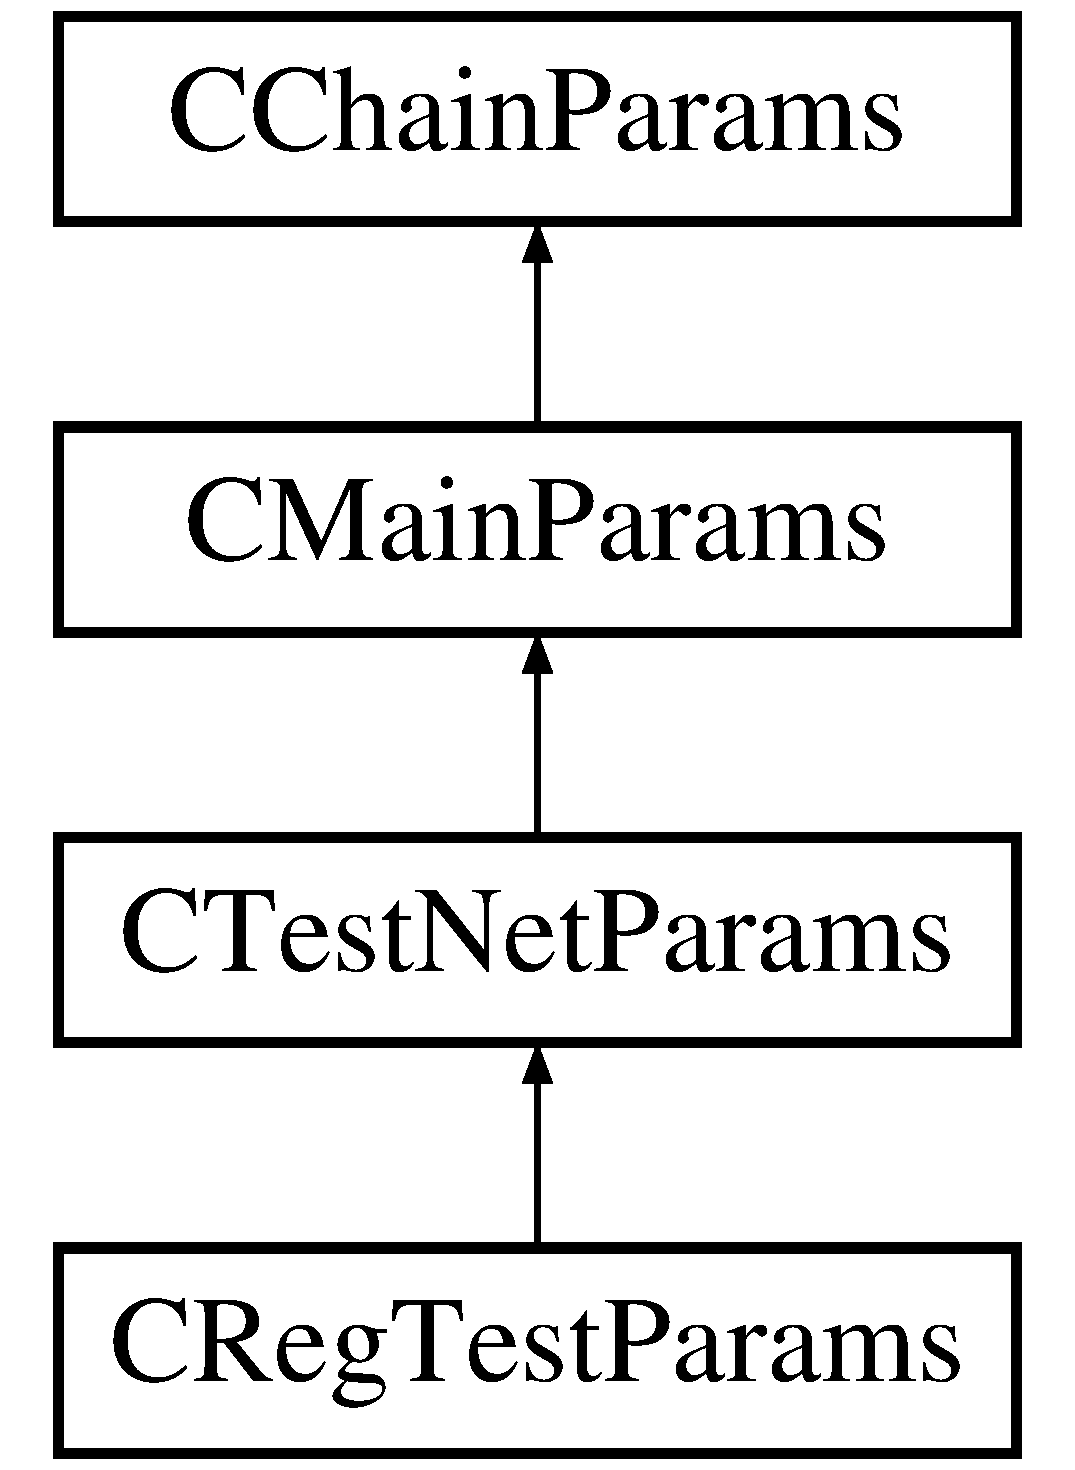
\includegraphics[height=4.000000cm]{class_c_chain_params}
\end{center}
\end{figure}
\subsection*{Public Types}
\begin{DoxyCompactItemize}
\item 
enum \mbox{\hyperlink{class_c_chain_params_aa294058ec2e3586bd8d03d6c39667058}{Base58\+Type}} \{ \newline
\mbox{\hyperlink{class_c_chain_params_aa294058ec2e3586bd8d03d6c39667058af088724f20c49c73e548f94d8f1808dd}{P\+U\+B\+K\+E\+Y\+\_\+\+A\+D\+D\+R\+E\+SS}}, 
\mbox{\hyperlink{class_c_chain_params_aa294058ec2e3586bd8d03d6c39667058adf0172df56140eb2f6fb7a59df0bb76a}{S\+C\+R\+I\+P\+T\+\_\+\+A\+D\+D\+R\+E\+SS}}, 
\mbox{\hyperlink{class_c_chain_params_aa294058ec2e3586bd8d03d6c39667058aacf95cbb9b5f51445295c704540adb18}{S\+E\+C\+R\+E\+T\+\_\+\+K\+EY}}, 
\mbox{\hyperlink{class_c_chain_params_aa294058ec2e3586bd8d03d6c39667058a1259eb07831c689e393e5008d7bd0085}{E\+X\+T\+\_\+\+P\+U\+B\+L\+I\+C\+\_\+\+K\+EY}}, 
\newline
\mbox{\hyperlink{class_c_chain_params_aa294058ec2e3586bd8d03d6c39667058ab5636e60152f35f6595fe413eae430b0}{E\+X\+T\+\_\+\+S\+E\+C\+R\+E\+T\+\_\+\+K\+EY}}, 
\mbox{\hyperlink{class_c_chain_params_aa294058ec2e3586bd8d03d6c39667058abeb8eb84b47b2483fbe4f13605bd1ccf}{Z\+C\+P\+A\+Y\+M\+E\+N\+T\+\_\+\+A\+D\+D\+R\+R\+E\+SS}}, 
\mbox{\hyperlink{class_c_chain_params_aa294058ec2e3586bd8d03d6c39667058af77179f15bba300f536da7f3198cf6e5}{Z\+C\+S\+P\+E\+N\+D\+I\+N\+G\+\_\+\+K\+EY}}, 
\mbox{\hyperlink{class_c_chain_params_aa294058ec2e3586bd8d03d6c39667058a6b21a525c7fab64a5df656e708f71a98}{M\+A\+X\+\_\+\+B\+A\+S\+E58\+\_\+\+T\+Y\+P\+ES}}
 \}
\end{DoxyCompactItemize}
\subsection*{Public Member Functions}
\begin{DoxyCompactItemize}
\item 
const \mbox{\hyperlink{chainparams_8h_a5e1ca1b35c3dd1a4e20f18445f28dd9c}{Consensus\+::\+Params}} \& \mbox{\hyperlink{class_c_chain_params_aa366d4f63c8d16d625336dca61ca65e5}{Get\+Consensus}} () const
\item 
const \mbox{\hyperlink{class_c_message_header_a0d0eeb540cbf4087973f6652ad61878f}{C\+Message\+Header\+::\+Message\+Start\+Chars}} \& \mbox{\hyperlink{class_c_chain_params_a42f81df0a4f3494e3fc83ab53049fdd9}{Message\+Start}} () const
\item 
const std\+::vector$<$ unsigned char $>$ \& \mbox{\hyperlink{class_c_chain_params_a8ca8fe289d1c3d5851d6aebaf28db22f}{Alert\+Key}} () const
\item 
int \mbox{\hyperlink{class_c_chain_params_a2e796bba356e7ce2040f545ea466754f}{Get\+Default\+Port}} () const
\item 
const C\+Block \& \mbox{\hyperlink{class_c_chain_params_aebd6cb9d986eeb2e6c228c04b3c39b42}{Genesis\+Block}} () const
\item 
bool \mbox{\hyperlink{class_c_chain_params_a066ad4166984a31bdc0836193a6341ee}{Mining\+Requires\+Peers}} () const
\item 
bool \mbox{\hyperlink{class_c_chain_params_a1d12f9b4b1ea7d7a0416cb6045496342}{Default\+Consistency\+Checks}} () const
\item 
bool \mbox{\hyperlink{class_c_chain_params_a30c1b60e515537b01810e175844d852f}{Require\+Standard}} () const
\item 
int64\+\_\+t \mbox{\hyperlink{class_c_chain_params_a5d18d7cfb1f2313740d6555da9a707a7}{Max\+Tip\+Age}} () const
\item 
int64\+\_\+t \mbox{\hyperlink{class_c_chain_params_abca14fce5f7e9681a73a13281672a059}{Prune\+After\+Height}} () const
\item 
unsigned int \mbox{\hyperlink{class_c_chain_params_aa6ba38ecceba49d7087d4efb92f01991}{EquihashN}} () const
\item 
unsigned int \mbox{\hyperlink{class_c_chain_params_a0cd2786a2b4f06201b94570ebc863a43}{EquihashK}} () const
\item 
std\+::string \mbox{\hyperlink{class_c_chain_params_a3a925294bd23ce6a3765fdbd768632e4}{Currency\+Units}} () const
\item 
bool \mbox{\hyperlink{class_c_chain_params_a96be31ff3d8525c9d5458b7d07ada6bb}{Mine\+Blocks\+On\+Demand}} () const
\item 
bool \mbox{\hyperlink{class_c_chain_params_a1552cea0636112ef84069cd6b7858b8e}{Testnet\+To\+Be\+Deprecated\+Field\+R\+PC}} () const
\item 
std\+::string \mbox{\hyperlink{class_c_chain_params_a2c02cc73f7fe9369cee9a39a0fd5b710}{Network\+I\+D\+String}} () const
\item 
const std\+::vector$<$ \mbox{\hyperlink{struct_c_d_n_s_seed_data}{C\+D\+N\+S\+Seed\+Data}} $>$ \& \mbox{\hyperlink{class_c_chain_params_a402b8df138b265619217ddf934bbc67a}{D\+N\+S\+Seeds}} () const
\item 
const std\+::vector$<$ unsigned char $>$ \& \mbox{\hyperlink{class_c_chain_params_a103c58eca4a26a71201882b3ed6c4cb4}{Base58\+Prefix}} (\mbox{\hyperlink{class_c_chain_params_aa294058ec2e3586bd8d03d6c39667058}{Base58\+Type}} type) const
\item 
const std\+::vector$<$ \mbox{\hyperlink{struct_seed_spec6}{Seed\+Spec6}} $>$ \& \mbox{\hyperlink{class_c_chain_params_ade5bb2aba047b54a032c356b6a09540e}{Fixed\+Seeds}} () const
\item 
const \mbox{\hyperlink{struct_checkpoints_1_1_c_checkpoint_data}{Checkpoints\+::\+C\+Checkpoint\+Data}} \& \mbox{\hyperlink{class_c_chain_params_a818a37d616330e5246a9be4cf8a40813}{Checkpoints}} () const
\item 
void \mbox{\hyperlink{class_c_chain_params_ad7ff3fccf6a11373cb1ecf7d753483d4}{Set\+Reg\+Test\+Coinbase\+Must\+Be\+Protected}} ()
\item 
uint64\+\_\+t \mbox{\hyperlink{class_c_chain_params_a3512eb1ef7869e7b47f88aaa0ae687b3}{Fork\+Start\+Height}} () const
\item 
uint64\+\_\+t \mbox{\hyperlink{class_c_chain_params_a77d1bf8012359cf91159b67906cbadea}{Fork\+Height\+Range}} () const
\end{DoxyCompactItemize}
\subsection*{Protected Member Functions}
\begin{DoxyCompactItemize}
\item 
\mbox{\hyperlink{class_c_chain_params_a8d07fce73d4160244459c5aaae8fb966}{C\+Chain\+Params}} ()
\end{DoxyCompactItemize}
\subsection*{Protected Attributes}
\begin{DoxyCompactItemize}
\item 
\mbox{\hyperlink{chainparams_8h_a5e1ca1b35c3dd1a4e20f18445f28dd9c}{Consensus\+::\+Params}} \mbox{\hyperlink{class_c_chain_params_a9eddbbd84a87109643d670766683aae2}{consensus}}
\item 
\mbox{\hyperlink{class_c_message_header_a0d0eeb540cbf4087973f6652ad61878f}{C\+Message\+Header\+::\+Message\+Start\+Chars}} \mbox{\hyperlink{class_c_chain_params_ae403e6b6d36b8f8c4d9d494cf686658c}{pch\+Message\+Start}}
\item 
std\+::vector$<$ unsigned char $>$ \mbox{\hyperlink{class_c_chain_params_adf435bdf2d9cd00936d7da0fb4237921}{v\+Alert\+Pub\+Key}}
\begin{DoxyCompactList}\small\item\em Raw pub key bytes for the broadcast alert signing key. \end{DoxyCompactList}\item 
int \mbox{\hyperlink{class_c_chain_params_a76d9a8dc59e179ca94b6b9e04a93e5f4}{n\+Default\+Port}} = 0
\item 
long \mbox{\hyperlink{class_c_chain_params_af0503b711c4544b49bd8051e31307264}{n\+Max\+Tip\+Age}} = 0
\item 
uint64\+\_\+t \mbox{\hyperlink{class_c_chain_params_aee6b9132f0ce8dcbfc242c3d2e1293e6}{n\+Prune\+After\+Height}} = 0
\item 
unsigned int \mbox{\hyperlink{class_c_chain_params_a6bed7d29dc273f097a9574286041803a}{n\+EquihashN}} = 0
\item 
unsigned int \mbox{\hyperlink{class_c_chain_params_a07ec113c3eb578647253a8ac3b2e33f8}{n\+EquihashK}} = 0
\item 
std\+::vector$<$ \mbox{\hyperlink{struct_c_d_n_s_seed_data}{C\+D\+N\+S\+Seed\+Data}} $>$ \mbox{\hyperlink{class_c_chain_params_a9ce50b4162fb2ebf5bd72ad4045aa70c}{v\+Seeds}}
\item 
std\+::vector$<$ unsigned char $>$ \mbox{\hyperlink{class_c_chain_params_a923d956c5d3891d0c682b7ef5410ed8f}{base58\+Prefixes}} \mbox{[}\mbox{\hyperlink{class_c_chain_params_aa294058ec2e3586bd8d03d6c39667058a6b21a525c7fab64a5df656e708f71a98}{M\+A\+X\+\_\+\+B\+A\+S\+E58\+\_\+\+T\+Y\+P\+ES}}\mbox{]}
\item 
std\+::string \mbox{\hyperlink{class_c_chain_params_a8542ce21d5b9bdc2eadad8702fdd584a}{str\+Network\+ID}}
\item 
std\+::string \mbox{\hyperlink{class_c_chain_params_aa6720c0b8eec741d343c9ee0c3c095b3}{str\+Currency\+Units}}
\item 
C\+Block \mbox{\hyperlink{class_c_chain_params_a2e4119fa75f6ea0c64ba8809dab5c4f8}{genesis}}
\item 
std\+::vector$<$ \mbox{\hyperlink{struct_seed_spec6}{Seed\+Spec6}} $>$ \mbox{\hyperlink{class_c_chain_params_a6853ff4c88ca3df1d864a8d72153614d}{v\+Fixed\+Seeds}}
\item 
bool \mbox{\hyperlink{class_c_chain_params_abe9980263561e3f26b6352daa64092da}{f\+Mining\+Requires\+Peers}} = false
\item 
bool \mbox{\hyperlink{class_c_chain_params_a630f023ae4a95a8b420bad0a08b4428c}{f\+Default\+Consistency\+Checks}} = false
\item 
bool \mbox{\hyperlink{class_c_chain_params_abc615d2750d847e1eac0ecb7fc8d2da8}{f\+Require\+Standard}} = false
\item 
bool \mbox{\hyperlink{class_c_chain_params_ad640045ea40c569df7b826551872e1bd}{f\+Mine\+Blocks\+On\+Demand}} = false
\item 
bool \mbox{\hyperlink{class_c_chain_params_a4f62f1b7070f83b48aa86564628a2e7d}{f\+Testnet\+To\+Be\+Deprecated\+Field\+R\+PC}} = false
\item 
\mbox{\hyperlink{struct_checkpoints_1_1_c_checkpoint_data}{Checkpoints\+::\+C\+Checkpoint\+Data}} \mbox{\hyperlink{class_c_chain_params_ac66ed599d7795bd17a504539a960f9de}{checkpoint\+Data}}
\item 
std\+::vector$<$ std\+::string $>$ \mbox{\hyperlink{class_c_chain_params_a54c46bc5f678eda307507f3c4310361b}{v\+Founders\+Reward\+Address}}
\item 
uint64\+\_\+t \mbox{\hyperlink{class_c_chain_params_ae06e698dde75edddbe9b0fef0a97102c}{n\+Fork\+Start\+Height}}
\item 
uint64\+\_\+t \mbox{\hyperlink{class_c_chain_params_a12ee49b1c7b52913c0937dbccb93bd4e}{n\+Fork\+Height\+Range}}
\end{DoxyCompactItemize}


\subsection{Detailed Description}
\mbox{\hyperlink{class_c_chain_params}{C\+Chain\+Params}} defines various tweakable parameters of a given instance of the Bitcoin system. There are three\+: the main network on which people trade goods and services, the public test network which gets reset from time to time and a regression test mode which is intended for private networks only. It has minimal difficulty to ensure that blocks can be found instantly. 

\subsection{Member Enumeration Documentation}
\mbox{\Hypertarget{class_c_chain_params_aa294058ec2e3586bd8d03d6c39667058}\label{class_c_chain_params_aa294058ec2e3586bd8d03d6c39667058}} 
\index{C\+Chain\+Params@{C\+Chain\+Params}!Base58\+Type@{Base58\+Type}}
\index{Base58\+Type@{Base58\+Type}!C\+Chain\+Params@{C\+Chain\+Params}}
\subsubsection{\texorpdfstring{Base58\+Type}{Base58Type}}
{\footnotesize\ttfamily enum \mbox{\hyperlink{class_c_chain_params_aa294058ec2e3586bd8d03d6c39667058}{C\+Chain\+Params\+::\+Base58\+Type}}}

\begin{DoxyEnumFields}{Enumerator}
\raisebox{\heightof{T}}[0pt][0pt]{\index{P\+U\+B\+K\+E\+Y\+\_\+\+A\+D\+D\+R\+E\+SS@{P\+U\+B\+K\+E\+Y\+\_\+\+A\+D\+D\+R\+E\+SS}!C\+Chain\+Params@{C\+Chain\+Params}}\index{C\+Chain\+Params@{C\+Chain\+Params}!P\+U\+B\+K\+E\+Y\+\_\+\+A\+D\+D\+R\+E\+SS@{P\+U\+B\+K\+E\+Y\+\_\+\+A\+D\+D\+R\+E\+SS}}}\mbox{\Hypertarget{class_c_chain_params_aa294058ec2e3586bd8d03d6c39667058af088724f20c49c73e548f94d8f1808dd}\label{class_c_chain_params_aa294058ec2e3586bd8d03d6c39667058af088724f20c49c73e548f94d8f1808dd}} 
P\+U\+B\+K\+E\+Y\+\_\+\+A\+D\+D\+R\+E\+SS&\\
\hline

\raisebox{\heightof{T}}[0pt][0pt]{\index{S\+C\+R\+I\+P\+T\+\_\+\+A\+D\+D\+R\+E\+SS@{S\+C\+R\+I\+P\+T\+\_\+\+A\+D\+D\+R\+E\+SS}!C\+Chain\+Params@{C\+Chain\+Params}}\index{C\+Chain\+Params@{C\+Chain\+Params}!S\+C\+R\+I\+P\+T\+\_\+\+A\+D\+D\+R\+E\+SS@{S\+C\+R\+I\+P\+T\+\_\+\+A\+D\+D\+R\+E\+SS}}}\mbox{\Hypertarget{class_c_chain_params_aa294058ec2e3586bd8d03d6c39667058adf0172df56140eb2f6fb7a59df0bb76a}\label{class_c_chain_params_aa294058ec2e3586bd8d03d6c39667058adf0172df56140eb2f6fb7a59df0bb76a}} 
S\+C\+R\+I\+P\+T\+\_\+\+A\+D\+D\+R\+E\+SS&\\
\hline

\raisebox{\heightof{T}}[0pt][0pt]{\index{S\+E\+C\+R\+E\+T\+\_\+\+K\+EY@{S\+E\+C\+R\+E\+T\+\_\+\+K\+EY}!C\+Chain\+Params@{C\+Chain\+Params}}\index{C\+Chain\+Params@{C\+Chain\+Params}!S\+E\+C\+R\+E\+T\+\_\+\+K\+EY@{S\+E\+C\+R\+E\+T\+\_\+\+K\+EY}}}\mbox{\Hypertarget{class_c_chain_params_aa294058ec2e3586bd8d03d6c39667058aacf95cbb9b5f51445295c704540adb18}\label{class_c_chain_params_aa294058ec2e3586bd8d03d6c39667058aacf95cbb9b5f51445295c704540adb18}} 
S\+E\+C\+R\+E\+T\+\_\+\+K\+EY&\\
\hline

\raisebox{\heightof{T}}[0pt][0pt]{\index{E\+X\+T\+\_\+\+P\+U\+B\+L\+I\+C\+\_\+\+K\+EY@{E\+X\+T\+\_\+\+P\+U\+B\+L\+I\+C\+\_\+\+K\+EY}!C\+Chain\+Params@{C\+Chain\+Params}}\index{C\+Chain\+Params@{C\+Chain\+Params}!E\+X\+T\+\_\+\+P\+U\+B\+L\+I\+C\+\_\+\+K\+EY@{E\+X\+T\+\_\+\+P\+U\+B\+L\+I\+C\+\_\+\+K\+EY}}}\mbox{\Hypertarget{class_c_chain_params_aa294058ec2e3586bd8d03d6c39667058a1259eb07831c689e393e5008d7bd0085}\label{class_c_chain_params_aa294058ec2e3586bd8d03d6c39667058a1259eb07831c689e393e5008d7bd0085}} 
E\+X\+T\+\_\+\+P\+U\+B\+L\+I\+C\+\_\+\+K\+EY&\\
\hline

\raisebox{\heightof{T}}[0pt][0pt]{\index{E\+X\+T\+\_\+\+S\+E\+C\+R\+E\+T\+\_\+\+K\+EY@{E\+X\+T\+\_\+\+S\+E\+C\+R\+E\+T\+\_\+\+K\+EY}!C\+Chain\+Params@{C\+Chain\+Params}}\index{C\+Chain\+Params@{C\+Chain\+Params}!E\+X\+T\+\_\+\+S\+E\+C\+R\+E\+T\+\_\+\+K\+EY@{E\+X\+T\+\_\+\+S\+E\+C\+R\+E\+T\+\_\+\+K\+EY}}}\mbox{\Hypertarget{class_c_chain_params_aa294058ec2e3586bd8d03d6c39667058ab5636e60152f35f6595fe413eae430b0}\label{class_c_chain_params_aa294058ec2e3586bd8d03d6c39667058ab5636e60152f35f6595fe413eae430b0}} 
E\+X\+T\+\_\+\+S\+E\+C\+R\+E\+T\+\_\+\+K\+EY&\\
\hline

\raisebox{\heightof{T}}[0pt][0pt]{\index{Z\+C\+P\+A\+Y\+M\+E\+N\+T\+\_\+\+A\+D\+D\+R\+R\+E\+SS@{Z\+C\+P\+A\+Y\+M\+E\+N\+T\+\_\+\+A\+D\+D\+R\+R\+E\+SS}!C\+Chain\+Params@{C\+Chain\+Params}}\index{C\+Chain\+Params@{C\+Chain\+Params}!Z\+C\+P\+A\+Y\+M\+E\+N\+T\+\_\+\+A\+D\+D\+R\+R\+E\+SS@{Z\+C\+P\+A\+Y\+M\+E\+N\+T\+\_\+\+A\+D\+D\+R\+R\+E\+SS}}}\mbox{\Hypertarget{class_c_chain_params_aa294058ec2e3586bd8d03d6c39667058abeb8eb84b47b2483fbe4f13605bd1ccf}\label{class_c_chain_params_aa294058ec2e3586bd8d03d6c39667058abeb8eb84b47b2483fbe4f13605bd1ccf}} 
Z\+C\+P\+A\+Y\+M\+E\+N\+T\+\_\+\+A\+D\+D\+R\+R\+E\+SS&\\
\hline

\raisebox{\heightof{T}}[0pt][0pt]{\index{Z\+C\+S\+P\+E\+N\+D\+I\+N\+G\+\_\+\+K\+EY@{Z\+C\+S\+P\+E\+N\+D\+I\+N\+G\+\_\+\+K\+EY}!C\+Chain\+Params@{C\+Chain\+Params}}\index{C\+Chain\+Params@{C\+Chain\+Params}!Z\+C\+S\+P\+E\+N\+D\+I\+N\+G\+\_\+\+K\+EY@{Z\+C\+S\+P\+E\+N\+D\+I\+N\+G\+\_\+\+K\+EY}}}\mbox{\Hypertarget{class_c_chain_params_aa294058ec2e3586bd8d03d6c39667058af77179f15bba300f536da7f3198cf6e5}\label{class_c_chain_params_aa294058ec2e3586bd8d03d6c39667058af77179f15bba300f536da7f3198cf6e5}} 
Z\+C\+S\+P\+E\+N\+D\+I\+N\+G\+\_\+\+K\+EY&\\
\hline

\raisebox{\heightof{T}}[0pt][0pt]{\index{M\+A\+X\+\_\+\+B\+A\+S\+E58\+\_\+\+T\+Y\+P\+ES@{M\+A\+X\+\_\+\+B\+A\+S\+E58\+\_\+\+T\+Y\+P\+ES}!C\+Chain\+Params@{C\+Chain\+Params}}\index{C\+Chain\+Params@{C\+Chain\+Params}!M\+A\+X\+\_\+\+B\+A\+S\+E58\+\_\+\+T\+Y\+P\+ES@{M\+A\+X\+\_\+\+B\+A\+S\+E58\+\_\+\+T\+Y\+P\+ES}}}\mbox{\Hypertarget{class_c_chain_params_aa294058ec2e3586bd8d03d6c39667058a6b21a525c7fab64a5df656e708f71a98}\label{class_c_chain_params_aa294058ec2e3586bd8d03d6c39667058a6b21a525c7fab64a5df656e708f71a98}} 
M\+A\+X\+\_\+\+B\+A\+S\+E58\+\_\+\+T\+Y\+P\+ES&\\
\hline

\end{DoxyEnumFields}


\subsection{Constructor \& Destructor Documentation}
\mbox{\Hypertarget{class_c_chain_params_a8d07fce73d4160244459c5aaae8fb966}\label{class_c_chain_params_a8d07fce73d4160244459c5aaae8fb966}} 
\index{C\+Chain\+Params@{C\+Chain\+Params}!C\+Chain\+Params@{C\+Chain\+Params}}
\index{C\+Chain\+Params@{C\+Chain\+Params}!C\+Chain\+Params@{C\+Chain\+Params}}
\subsubsection{\texorpdfstring{C\+Chain\+Params()}{CChainParams()}}
{\footnotesize\ttfamily C\+Chain\+Params\+::\+C\+Chain\+Params (\begin{DoxyParamCaption}{ }\end{DoxyParamCaption})\hspace{0.3cm}{\ttfamily [inline]}, {\ttfamily [protected]}}



\subsection{Member Function Documentation}
\mbox{\Hypertarget{class_c_chain_params_a8ca8fe289d1c3d5851d6aebaf28db22f}\label{class_c_chain_params_a8ca8fe289d1c3d5851d6aebaf28db22f}} 
\index{C\+Chain\+Params@{C\+Chain\+Params}!Alert\+Key@{Alert\+Key}}
\index{Alert\+Key@{Alert\+Key}!C\+Chain\+Params@{C\+Chain\+Params}}
\subsubsection{\texorpdfstring{Alert\+Key()}{AlertKey()}}
{\footnotesize\ttfamily const std\+::vector$<$unsigned char$>$\& C\+Chain\+Params\+::\+Alert\+Key (\begin{DoxyParamCaption}{ }\end{DoxyParamCaption}) const\hspace{0.3cm}{\ttfamily [inline]}}

\mbox{\Hypertarget{class_c_chain_params_a103c58eca4a26a71201882b3ed6c4cb4}\label{class_c_chain_params_a103c58eca4a26a71201882b3ed6c4cb4}} 
\index{C\+Chain\+Params@{C\+Chain\+Params}!Base58\+Prefix@{Base58\+Prefix}}
\index{Base58\+Prefix@{Base58\+Prefix}!C\+Chain\+Params@{C\+Chain\+Params}}
\subsubsection{\texorpdfstring{Base58\+Prefix()}{Base58Prefix()}}
{\footnotesize\ttfamily const std\+::vector$<$unsigned char$>$\& C\+Chain\+Params\+::\+Base58\+Prefix (\begin{DoxyParamCaption}\item[{\mbox{\hyperlink{class_c_chain_params_aa294058ec2e3586bd8d03d6c39667058}{Base58\+Type}}}]{type }\end{DoxyParamCaption}) const\hspace{0.3cm}{\ttfamily [inline]}}

\mbox{\Hypertarget{class_c_chain_params_a818a37d616330e5246a9be4cf8a40813}\label{class_c_chain_params_a818a37d616330e5246a9be4cf8a40813}} 
\index{C\+Chain\+Params@{C\+Chain\+Params}!Checkpoints@{Checkpoints}}
\index{Checkpoints@{Checkpoints}!C\+Chain\+Params@{C\+Chain\+Params}}
\subsubsection{\texorpdfstring{Checkpoints()}{Checkpoints()}}
{\footnotesize\ttfamily const \mbox{\hyperlink{struct_checkpoints_1_1_c_checkpoint_data}{Checkpoints\+::\+C\+Checkpoint\+Data}}\& C\+Chain\+Params\+::\+Checkpoints (\begin{DoxyParamCaption}{ }\end{DoxyParamCaption}) const\hspace{0.3cm}{\ttfamily [inline]}}

\mbox{\Hypertarget{class_c_chain_params_a3a925294bd23ce6a3765fdbd768632e4}\label{class_c_chain_params_a3a925294bd23ce6a3765fdbd768632e4}} 
\index{C\+Chain\+Params@{C\+Chain\+Params}!Currency\+Units@{Currency\+Units}}
\index{Currency\+Units@{Currency\+Units}!C\+Chain\+Params@{C\+Chain\+Params}}
\subsubsection{\texorpdfstring{Currency\+Units()}{CurrencyUnits()}}
{\footnotesize\ttfamily std\+::string C\+Chain\+Params\+::\+Currency\+Units (\begin{DoxyParamCaption}{ }\end{DoxyParamCaption}) const\hspace{0.3cm}{\ttfamily [inline]}}

\mbox{\Hypertarget{class_c_chain_params_a1d12f9b4b1ea7d7a0416cb6045496342}\label{class_c_chain_params_a1d12f9b4b1ea7d7a0416cb6045496342}} 
\index{C\+Chain\+Params@{C\+Chain\+Params}!Default\+Consistency\+Checks@{Default\+Consistency\+Checks}}
\index{Default\+Consistency\+Checks@{Default\+Consistency\+Checks}!C\+Chain\+Params@{C\+Chain\+Params}}
\subsubsection{\texorpdfstring{Default\+Consistency\+Checks()}{DefaultConsistencyChecks()}}
{\footnotesize\ttfamily bool C\+Chain\+Params\+::\+Default\+Consistency\+Checks (\begin{DoxyParamCaption}{ }\end{DoxyParamCaption}) const\hspace{0.3cm}{\ttfamily [inline]}}

Default value for -\/checkmempool and -\/checkblockindex argument \mbox{\Hypertarget{class_c_chain_params_a402b8df138b265619217ddf934bbc67a}\label{class_c_chain_params_a402b8df138b265619217ddf934bbc67a}} 
\index{C\+Chain\+Params@{C\+Chain\+Params}!D\+N\+S\+Seeds@{D\+N\+S\+Seeds}}
\index{D\+N\+S\+Seeds@{D\+N\+S\+Seeds}!C\+Chain\+Params@{C\+Chain\+Params}}
\subsubsection{\texorpdfstring{D\+N\+S\+Seeds()}{DNSSeeds()}}
{\footnotesize\ttfamily const std\+::vector$<$\mbox{\hyperlink{struct_c_d_n_s_seed_data}{C\+D\+N\+S\+Seed\+Data}}$>$\& C\+Chain\+Params\+::\+D\+N\+S\+Seeds (\begin{DoxyParamCaption}{ }\end{DoxyParamCaption}) const\hspace{0.3cm}{\ttfamily [inline]}}

\mbox{\Hypertarget{class_c_chain_params_a0cd2786a2b4f06201b94570ebc863a43}\label{class_c_chain_params_a0cd2786a2b4f06201b94570ebc863a43}} 
\index{C\+Chain\+Params@{C\+Chain\+Params}!EquihashK@{EquihashK}}
\index{EquihashK@{EquihashK}!C\+Chain\+Params@{C\+Chain\+Params}}
\subsubsection{\texorpdfstring{Equihash\+K()}{EquihashK()}}
{\footnotesize\ttfamily unsigned int C\+Chain\+Params\+::\+EquihashK (\begin{DoxyParamCaption}{ }\end{DoxyParamCaption}) const\hspace{0.3cm}{\ttfamily [inline]}}

\mbox{\Hypertarget{class_c_chain_params_aa6ba38ecceba49d7087d4efb92f01991}\label{class_c_chain_params_aa6ba38ecceba49d7087d4efb92f01991}} 
\index{C\+Chain\+Params@{C\+Chain\+Params}!EquihashN@{EquihashN}}
\index{EquihashN@{EquihashN}!C\+Chain\+Params@{C\+Chain\+Params}}
\subsubsection{\texorpdfstring{Equihash\+N()}{EquihashN()}}
{\footnotesize\ttfamily unsigned int C\+Chain\+Params\+::\+EquihashN (\begin{DoxyParamCaption}{ }\end{DoxyParamCaption}) const\hspace{0.3cm}{\ttfamily [inline]}}

\mbox{\Hypertarget{class_c_chain_params_ade5bb2aba047b54a032c356b6a09540e}\label{class_c_chain_params_ade5bb2aba047b54a032c356b6a09540e}} 
\index{C\+Chain\+Params@{C\+Chain\+Params}!Fixed\+Seeds@{Fixed\+Seeds}}
\index{Fixed\+Seeds@{Fixed\+Seeds}!C\+Chain\+Params@{C\+Chain\+Params}}
\subsubsection{\texorpdfstring{Fixed\+Seeds()}{FixedSeeds()}}
{\footnotesize\ttfamily const std\+::vector$<$\mbox{\hyperlink{struct_seed_spec6}{Seed\+Spec6}}$>$\& C\+Chain\+Params\+::\+Fixed\+Seeds (\begin{DoxyParamCaption}{ }\end{DoxyParamCaption}) const\hspace{0.3cm}{\ttfamily [inline]}}

\mbox{\Hypertarget{class_c_chain_params_a77d1bf8012359cf91159b67906cbadea}\label{class_c_chain_params_a77d1bf8012359cf91159b67906cbadea}} 
\index{C\+Chain\+Params@{C\+Chain\+Params}!Fork\+Height\+Range@{Fork\+Height\+Range}}
\index{Fork\+Height\+Range@{Fork\+Height\+Range}!C\+Chain\+Params@{C\+Chain\+Params}}
\subsubsection{\texorpdfstring{Fork\+Height\+Range()}{ForkHeightRange()}}
{\footnotesize\ttfamily uint64\+\_\+t C\+Chain\+Params\+::\+Fork\+Height\+Range (\begin{DoxyParamCaption}{ }\end{DoxyParamCaption}) const\hspace{0.3cm}{\ttfamily [inline]}}

\mbox{\Hypertarget{class_c_chain_params_a3512eb1ef7869e7b47f88aaa0ae687b3}\label{class_c_chain_params_a3512eb1ef7869e7b47f88aaa0ae687b3}} 
\index{C\+Chain\+Params@{C\+Chain\+Params}!Fork\+Start\+Height@{Fork\+Start\+Height}}
\index{Fork\+Start\+Height@{Fork\+Start\+Height}!C\+Chain\+Params@{C\+Chain\+Params}}
\subsubsection{\texorpdfstring{Fork\+Start\+Height()}{ForkStartHeight()}}
{\footnotesize\ttfamily uint64\+\_\+t C\+Chain\+Params\+::\+Fork\+Start\+Height (\begin{DoxyParamCaption}{ }\end{DoxyParamCaption}) const\hspace{0.3cm}{\ttfamily [inline]}}

\mbox{\Hypertarget{class_c_chain_params_aebd6cb9d986eeb2e6c228c04b3c39b42}\label{class_c_chain_params_aebd6cb9d986eeb2e6c228c04b3c39b42}} 
\index{C\+Chain\+Params@{C\+Chain\+Params}!Genesis\+Block@{Genesis\+Block}}
\index{Genesis\+Block@{Genesis\+Block}!C\+Chain\+Params@{C\+Chain\+Params}}
\subsubsection{\texorpdfstring{Genesis\+Block()}{GenesisBlock()}}
{\footnotesize\ttfamily const C\+Block\& C\+Chain\+Params\+::\+Genesis\+Block (\begin{DoxyParamCaption}{ }\end{DoxyParamCaption}) const\hspace{0.3cm}{\ttfamily [inline]}}

\mbox{\Hypertarget{class_c_chain_params_aa366d4f63c8d16d625336dca61ca65e5}\label{class_c_chain_params_aa366d4f63c8d16d625336dca61ca65e5}} 
\index{C\+Chain\+Params@{C\+Chain\+Params}!Get\+Consensus@{Get\+Consensus}}
\index{Get\+Consensus@{Get\+Consensus}!C\+Chain\+Params@{C\+Chain\+Params}}
\subsubsection{\texorpdfstring{Get\+Consensus()}{GetConsensus()}}
{\footnotesize\ttfamily const \mbox{\hyperlink{chainparams_8h_a5e1ca1b35c3dd1a4e20f18445f28dd9c}{Consensus\+::\+Params}}\& C\+Chain\+Params\+::\+Get\+Consensus (\begin{DoxyParamCaption}{ }\end{DoxyParamCaption}) const\hspace{0.3cm}{\ttfamily [inline]}}

\mbox{\Hypertarget{class_c_chain_params_a2e796bba356e7ce2040f545ea466754f}\label{class_c_chain_params_a2e796bba356e7ce2040f545ea466754f}} 
\index{C\+Chain\+Params@{C\+Chain\+Params}!Get\+Default\+Port@{Get\+Default\+Port}}
\index{Get\+Default\+Port@{Get\+Default\+Port}!C\+Chain\+Params@{C\+Chain\+Params}}
\subsubsection{\texorpdfstring{Get\+Default\+Port()}{GetDefaultPort()}}
{\footnotesize\ttfamily int C\+Chain\+Params\+::\+Get\+Default\+Port (\begin{DoxyParamCaption}{ }\end{DoxyParamCaption}) const\hspace{0.3cm}{\ttfamily [inline]}}

\mbox{\Hypertarget{class_c_chain_params_a5d18d7cfb1f2313740d6555da9a707a7}\label{class_c_chain_params_a5d18d7cfb1f2313740d6555da9a707a7}} 
\index{C\+Chain\+Params@{C\+Chain\+Params}!Max\+Tip\+Age@{Max\+Tip\+Age}}
\index{Max\+Tip\+Age@{Max\+Tip\+Age}!C\+Chain\+Params@{C\+Chain\+Params}}
\subsubsection{\texorpdfstring{Max\+Tip\+Age()}{MaxTipAge()}}
{\footnotesize\ttfamily int64\+\_\+t C\+Chain\+Params\+::\+Max\+Tip\+Age (\begin{DoxyParamCaption}{ }\end{DoxyParamCaption}) const\hspace{0.3cm}{\ttfamily [inline]}}

\mbox{\Hypertarget{class_c_chain_params_a42f81df0a4f3494e3fc83ab53049fdd9}\label{class_c_chain_params_a42f81df0a4f3494e3fc83ab53049fdd9}} 
\index{C\+Chain\+Params@{C\+Chain\+Params}!Message\+Start@{Message\+Start}}
\index{Message\+Start@{Message\+Start}!C\+Chain\+Params@{C\+Chain\+Params}}
\subsubsection{\texorpdfstring{Message\+Start()}{MessageStart()}}
{\footnotesize\ttfamily const \mbox{\hyperlink{class_c_message_header_a0d0eeb540cbf4087973f6652ad61878f}{C\+Message\+Header\+::\+Message\+Start\+Chars}}\& C\+Chain\+Params\+::\+Message\+Start (\begin{DoxyParamCaption}{ }\end{DoxyParamCaption}) const\hspace{0.3cm}{\ttfamily [inline]}}

\mbox{\Hypertarget{class_c_chain_params_a96be31ff3d8525c9d5458b7d07ada6bb}\label{class_c_chain_params_a96be31ff3d8525c9d5458b7d07ada6bb}} 
\index{C\+Chain\+Params@{C\+Chain\+Params}!Mine\+Blocks\+On\+Demand@{Mine\+Blocks\+On\+Demand}}
\index{Mine\+Blocks\+On\+Demand@{Mine\+Blocks\+On\+Demand}!C\+Chain\+Params@{C\+Chain\+Params}}
\subsubsection{\texorpdfstring{Mine\+Blocks\+On\+Demand()}{MineBlocksOnDemand()}}
{\footnotesize\ttfamily bool C\+Chain\+Params\+::\+Mine\+Blocks\+On\+Demand (\begin{DoxyParamCaption}{ }\end{DoxyParamCaption}) const\hspace{0.3cm}{\ttfamily [inline]}}

Make miner stop after a block is found. In R\+PC, don\textquotesingle{}t return until n\+Gen\+Proc\+Limit blocks are generated \mbox{\Hypertarget{class_c_chain_params_a066ad4166984a31bdc0836193a6341ee}\label{class_c_chain_params_a066ad4166984a31bdc0836193a6341ee}} 
\index{C\+Chain\+Params@{C\+Chain\+Params}!Mining\+Requires\+Peers@{Mining\+Requires\+Peers}}
\index{Mining\+Requires\+Peers@{Mining\+Requires\+Peers}!C\+Chain\+Params@{C\+Chain\+Params}}
\subsubsection{\texorpdfstring{Mining\+Requires\+Peers()}{MiningRequiresPeers()}}
{\footnotesize\ttfamily bool C\+Chain\+Params\+::\+Mining\+Requires\+Peers (\begin{DoxyParamCaption}{ }\end{DoxyParamCaption}) const\hspace{0.3cm}{\ttfamily [inline]}}

Make miner wait to have peers to avoid wasting work \mbox{\Hypertarget{class_c_chain_params_a2c02cc73f7fe9369cee9a39a0fd5b710}\label{class_c_chain_params_a2c02cc73f7fe9369cee9a39a0fd5b710}} 
\index{C\+Chain\+Params@{C\+Chain\+Params}!Network\+I\+D\+String@{Network\+I\+D\+String}}
\index{Network\+I\+D\+String@{Network\+I\+D\+String}!C\+Chain\+Params@{C\+Chain\+Params}}
\subsubsection{\texorpdfstring{Network\+I\+D\+String()}{NetworkIDString()}}
{\footnotesize\ttfamily std\+::string C\+Chain\+Params\+::\+Network\+I\+D\+String (\begin{DoxyParamCaption}{ }\end{DoxyParamCaption}) const\hspace{0.3cm}{\ttfamily [inline]}}

Return the B\+I\+P70 network string (main, test or regtest) \mbox{\Hypertarget{class_c_chain_params_abca14fce5f7e9681a73a13281672a059}\label{class_c_chain_params_abca14fce5f7e9681a73a13281672a059}} 
\index{C\+Chain\+Params@{C\+Chain\+Params}!Prune\+After\+Height@{Prune\+After\+Height}}
\index{Prune\+After\+Height@{Prune\+After\+Height}!C\+Chain\+Params@{C\+Chain\+Params}}
\subsubsection{\texorpdfstring{Prune\+After\+Height()}{PruneAfterHeight()}}
{\footnotesize\ttfamily int64\+\_\+t C\+Chain\+Params\+::\+Prune\+After\+Height (\begin{DoxyParamCaption}{ }\end{DoxyParamCaption}) const\hspace{0.3cm}{\ttfamily [inline]}}

\mbox{\Hypertarget{class_c_chain_params_a30c1b60e515537b01810e175844d852f}\label{class_c_chain_params_a30c1b60e515537b01810e175844d852f}} 
\index{C\+Chain\+Params@{C\+Chain\+Params}!Require\+Standard@{Require\+Standard}}
\index{Require\+Standard@{Require\+Standard}!C\+Chain\+Params@{C\+Chain\+Params}}
\subsubsection{\texorpdfstring{Require\+Standard()}{RequireStandard()}}
{\footnotesize\ttfamily bool C\+Chain\+Params\+::\+Require\+Standard (\begin{DoxyParamCaption}{ }\end{DoxyParamCaption}) const\hspace{0.3cm}{\ttfamily [inline]}}

Policy\+: Filter transactions that do not match well-\/defined patterns \mbox{\Hypertarget{class_c_chain_params_ad7ff3fccf6a11373cb1ecf7d753483d4}\label{class_c_chain_params_ad7ff3fccf6a11373cb1ecf7d753483d4}} 
\index{C\+Chain\+Params@{C\+Chain\+Params}!Set\+Reg\+Test\+Coinbase\+Must\+Be\+Protected@{Set\+Reg\+Test\+Coinbase\+Must\+Be\+Protected}}
\index{Set\+Reg\+Test\+Coinbase\+Must\+Be\+Protected@{Set\+Reg\+Test\+Coinbase\+Must\+Be\+Protected}!C\+Chain\+Params@{C\+Chain\+Params}}
\subsubsection{\texorpdfstring{Set\+Reg\+Test\+Coinbase\+Must\+Be\+Protected()}{SetRegTestCoinbaseMustBeProtected()}}
{\footnotesize\ttfamily void C\+Chain\+Params\+::\+Set\+Reg\+Test\+Coinbase\+Must\+Be\+Protected (\begin{DoxyParamCaption}{ }\end{DoxyParamCaption})\hspace{0.3cm}{\ttfamily [inline]}}

Enforce coinbase consensus rule in regtest mode \mbox{\Hypertarget{class_c_chain_params_a1552cea0636112ef84069cd6b7858b8e}\label{class_c_chain_params_a1552cea0636112ef84069cd6b7858b8e}} 
\index{C\+Chain\+Params@{C\+Chain\+Params}!Testnet\+To\+Be\+Deprecated\+Field\+R\+PC@{Testnet\+To\+Be\+Deprecated\+Field\+R\+PC}}
\index{Testnet\+To\+Be\+Deprecated\+Field\+R\+PC@{Testnet\+To\+Be\+Deprecated\+Field\+R\+PC}!C\+Chain\+Params@{C\+Chain\+Params}}
\subsubsection{\texorpdfstring{Testnet\+To\+Be\+Deprecated\+Field\+R\+P\+C()}{TestnetToBeDeprecatedFieldRPC()}}
{\footnotesize\ttfamily bool C\+Chain\+Params\+::\+Testnet\+To\+Be\+Deprecated\+Field\+R\+PC (\begin{DoxyParamCaption}{ }\end{DoxyParamCaption}) const\hspace{0.3cm}{\ttfamily [inline]}}

In the future use \mbox{\hyperlink{class_c_chain_params_a2c02cc73f7fe9369cee9a39a0fd5b710}{Network\+I\+D\+String()}} for R\+PC fields 

\subsection{Member Data Documentation}
\mbox{\Hypertarget{class_c_chain_params_a923d956c5d3891d0c682b7ef5410ed8f}\label{class_c_chain_params_a923d956c5d3891d0c682b7ef5410ed8f}} 
\index{C\+Chain\+Params@{C\+Chain\+Params}!base58\+Prefixes@{base58\+Prefixes}}
\index{base58\+Prefixes@{base58\+Prefixes}!C\+Chain\+Params@{C\+Chain\+Params}}
\subsubsection{\texorpdfstring{base58\+Prefixes}{base58Prefixes}}
{\footnotesize\ttfamily std\+::vector$<$unsigned char$>$ C\+Chain\+Params\+::base58\+Prefixes\mbox{[}\mbox{\hyperlink{class_c_chain_params_aa294058ec2e3586bd8d03d6c39667058a6b21a525c7fab64a5df656e708f71a98}{M\+A\+X\+\_\+\+B\+A\+S\+E58\+\_\+\+T\+Y\+P\+ES}}\mbox{]}\hspace{0.3cm}{\ttfamily [protected]}}

\mbox{\Hypertarget{class_c_chain_params_ac66ed599d7795bd17a504539a960f9de}\label{class_c_chain_params_ac66ed599d7795bd17a504539a960f9de}} 
\index{C\+Chain\+Params@{C\+Chain\+Params}!checkpoint\+Data@{checkpoint\+Data}}
\index{checkpoint\+Data@{checkpoint\+Data}!C\+Chain\+Params@{C\+Chain\+Params}}
\subsubsection{\texorpdfstring{checkpoint\+Data}{checkpointData}}
{\footnotesize\ttfamily \mbox{\hyperlink{struct_checkpoints_1_1_c_checkpoint_data}{Checkpoints\+::\+C\+Checkpoint\+Data}} C\+Chain\+Params\+::checkpoint\+Data\hspace{0.3cm}{\ttfamily [protected]}}

\mbox{\Hypertarget{class_c_chain_params_a9eddbbd84a87109643d670766683aae2}\label{class_c_chain_params_a9eddbbd84a87109643d670766683aae2}} 
\index{C\+Chain\+Params@{C\+Chain\+Params}!consensus@{consensus}}
\index{consensus@{consensus}!C\+Chain\+Params@{C\+Chain\+Params}}
\subsubsection{\texorpdfstring{consensus}{consensus}}
{\footnotesize\ttfamily \mbox{\hyperlink{chainparams_8h_a5e1ca1b35c3dd1a4e20f18445f28dd9c}{Consensus\+::\+Params}} C\+Chain\+Params\+::consensus\hspace{0.3cm}{\ttfamily [protected]}}

\mbox{\Hypertarget{class_c_chain_params_a630f023ae4a95a8b420bad0a08b4428c}\label{class_c_chain_params_a630f023ae4a95a8b420bad0a08b4428c}} 
\index{C\+Chain\+Params@{C\+Chain\+Params}!f\+Default\+Consistency\+Checks@{f\+Default\+Consistency\+Checks}}
\index{f\+Default\+Consistency\+Checks@{f\+Default\+Consistency\+Checks}!C\+Chain\+Params@{C\+Chain\+Params}}
\subsubsection{\texorpdfstring{f\+Default\+Consistency\+Checks}{fDefaultConsistencyChecks}}
{\footnotesize\ttfamily bool C\+Chain\+Params\+::f\+Default\+Consistency\+Checks = false\hspace{0.3cm}{\ttfamily [protected]}}

\mbox{\Hypertarget{class_c_chain_params_ad640045ea40c569df7b826551872e1bd}\label{class_c_chain_params_ad640045ea40c569df7b826551872e1bd}} 
\index{C\+Chain\+Params@{C\+Chain\+Params}!f\+Mine\+Blocks\+On\+Demand@{f\+Mine\+Blocks\+On\+Demand}}
\index{f\+Mine\+Blocks\+On\+Demand@{f\+Mine\+Blocks\+On\+Demand}!C\+Chain\+Params@{C\+Chain\+Params}}
\subsubsection{\texorpdfstring{f\+Mine\+Blocks\+On\+Demand}{fMineBlocksOnDemand}}
{\footnotesize\ttfamily bool C\+Chain\+Params\+::f\+Mine\+Blocks\+On\+Demand = false\hspace{0.3cm}{\ttfamily [protected]}}

\mbox{\Hypertarget{class_c_chain_params_abe9980263561e3f26b6352daa64092da}\label{class_c_chain_params_abe9980263561e3f26b6352daa64092da}} 
\index{C\+Chain\+Params@{C\+Chain\+Params}!f\+Mining\+Requires\+Peers@{f\+Mining\+Requires\+Peers}}
\index{f\+Mining\+Requires\+Peers@{f\+Mining\+Requires\+Peers}!C\+Chain\+Params@{C\+Chain\+Params}}
\subsubsection{\texorpdfstring{f\+Mining\+Requires\+Peers}{fMiningRequiresPeers}}
{\footnotesize\ttfamily bool C\+Chain\+Params\+::f\+Mining\+Requires\+Peers = false\hspace{0.3cm}{\ttfamily [protected]}}

\mbox{\Hypertarget{class_c_chain_params_abc615d2750d847e1eac0ecb7fc8d2da8}\label{class_c_chain_params_abc615d2750d847e1eac0ecb7fc8d2da8}} 
\index{C\+Chain\+Params@{C\+Chain\+Params}!f\+Require\+Standard@{f\+Require\+Standard}}
\index{f\+Require\+Standard@{f\+Require\+Standard}!C\+Chain\+Params@{C\+Chain\+Params}}
\subsubsection{\texorpdfstring{f\+Require\+Standard}{fRequireStandard}}
{\footnotesize\ttfamily bool C\+Chain\+Params\+::f\+Require\+Standard = false\hspace{0.3cm}{\ttfamily [protected]}}

\mbox{\Hypertarget{class_c_chain_params_a4f62f1b7070f83b48aa86564628a2e7d}\label{class_c_chain_params_a4f62f1b7070f83b48aa86564628a2e7d}} 
\index{C\+Chain\+Params@{C\+Chain\+Params}!f\+Testnet\+To\+Be\+Deprecated\+Field\+R\+PC@{f\+Testnet\+To\+Be\+Deprecated\+Field\+R\+PC}}
\index{f\+Testnet\+To\+Be\+Deprecated\+Field\+R\+PC@{f\+Testnet\+To\+Be\+Deprecated\+Field\+R\+PC}!C\+Chain\+Params@{C\+Chain\+Params}}
\subsubsection{\texorpdfstring{f\+Testnet\+To\+Be\+Deprecated\+Field\+R\+PC}{fTestnetToBeDeprecatedFieldRPC}}
{\footnotesize\ttfamily bool C\+Chain\+Params\+::f\+Testnet\+To\+Be\+Deprecated\+Field\+R\+PC = false\hspace{0.3cm}{\ttfamily [protected]}}

\mbox{\Hypertarget{class_c_chain_params_a2e4119fa75f6ea0c64ba8809dab5c4f8}\label{class_c_chain_params_a2e4119fa75f6ea0c64ba8809dab5c4f8}} 
\index{C\+Chain\+Params@{C\+Chain\+Params}!genesis@{genesis}}
\index{genesis@{genesis}!C\+Chain\+Params@{C\+Chain\+Params}}
\subsubsection{\texorpdfstring{genesis}{genesis}}
{\footnotesize\ttfamily C\+Block C\+Chain\+Params\+::genesis\hspace{0.3cm}{\ttfamily [protected]}}

\mbox{\Hypertarget{class_c_chain_params_a76d9a8dc59e179ca94b6b9e04a93e5f4}\label{class_c_chain_params_a76d9a8dc59e179ca94b6b9e04a93e5f4}} 
\index{C\+Chain\+Params@{C\+Chain\+Params}!n\+Default\+Port@{n\+Default\+Port}}
\index{n\+Default\+Port@{n\+Default\+Port}!C\+Chain\+Params@{C\+Chain\+Params}}
\subsubsection{\texorpdfstring{n\+Default\+Port}{nDefaultPort}}
{\footnotesize\ttfamily int C\+Chain\+Params\+::n\+Default\+Port = 0\hspace{0.3cm}{\ttfamily [protected]}}

\mbox{\Hypertarget{class_c_chain_params_a07ec113c3eb578647253a8ac3b2e33f8}\label{class_c_chain_params_a07ec113c3eb578647253a8ac3b2e33f8}} 
\index{C\+Chain\+Params@{C\+Chain\+Params}!n\+EquihashK@{n\+EquihashK}}
\index{n\+EquihashK@{n\+EquihashK}!C\+Chain\+Params@{C\+Chain\+Params}}
\subsubsection{\texorpdfstring{n\+EquihashK}{nEquihashK}}
{\footnotesize\ttfamily unsigned int C\+Chain\+Params\+::n\+EquihashK = 0\hspace{0.3cm}{\ttfamily [protected]}}

\mbox{\Hypertarget{class_c_chain_params_a6bed7d29dc273f097a9574286041803a}\label{class_c_chain_params_a6bed7d29dc273f097a9574286041803a}} 
\index{C\+Chain\+Params@{C\+Chain\+Params}!n\+EquihashN@{n\+EquihashN}}
\index{n\+EquihashN@{n\+EquihashN}!C\+Chain\+Params@{C\+Chain\+Params}}
\subsubsection{\texorpdfstring{n\+EquihashN}{nEquihashN}}
{\footnotesize\ttfamily unsigned int C\+Chain\+Params\+::n\+EquihashN = 0\hspace{0.3cm}{\ttfamily [protected]}}

\mbox{\Hypertarget{class_c_chain_params_a12ee49b1c7b52913c0937dbccb93bd4e}\label{class_c_chain_params_a12ee49b1c7b52913c0937dbccb93bd4e}} 
\index{C\+Chain\+Params@{C\+Chain\+Params}!n\+Fork\+Height\+Range@{n\+Fork\+Height\+Range}}
\index{n\+Fork\+Height\+Range@{n\+Fork\+Height\+Range}!C\+Chain\+Params@{C\+Chain\+Params}}
\subsubsection{\texorpdfstring{n\+Fork\+Height\+Range}{nForkHeightRange}}
{\footnotesize\ttfamily uint64\+\_\+t C\+Chain\+Params\+::n\+Fork\+Height\+Range\hspace{0.3cm}{\ttfamily [protected]}}

\mbox{\Hypertarget{class_c_chain_params_ae06e698dde75edddbe9b0fef0a97102c}\label{class_c_chain_params_ae06e698dde75edddbe9b0fef0a97102c}} 
\index{C\+Chain\+Params@{C\+Chain\+Params}!n\+Fork\+Start\+Height@{n\+Fork\+Start\+Height}}
\index{n\+Fork\+Start\+Height@{n\+Fork\+Start\+Height}!C\+Chain\+Params@{C\+Chain\+Params}}
\subsubsection{\texorpdfstring{n\+Fork\+Start\+Height}{nForkStartHeight}}
{\footnotesize\ttfamily uint64\+\_\+t C\+Chain\+Params\+::n\+Fork\+Start\+Height\hspace{0.3cm}{\ttfamily [protected]}}

\mbox{\Hypertarget{class_c_chain_params_af0503b711c4544b49bd8051e31307264}\label{class_c_chain_params_af0503b711c4544b49bd8051e31307264}} 
\index{C\+Chain\+Params@{C\+Chain\+Params}!n\+Max\+Tip\+Age@{n\+Max\+Tip\+Age}}
\index{n\+Max\+Tip\+Age@{n\+Max\+Tip\+Age}!C\+Chain\+Params@{C\+Chain\+Params}}
\subsubsection{\texorpdfstring{n\+Max\+Tip\+Age}{nMaxTipAge}}
{\footnotesize\ttfamily long C\+Chain\+Params\+::n\+Max\+Tip\+Age = 0\hspace{0.3cm}{\ttfamily [protected]}}

\mbox{\Hypertarget{class_c_chain_params_aee6b9132f0ce8dcbfc242c3d2e1293e6}\label{class_c_chain_params_aee6b9132f0ce8dcbfc242c3d2e1293e6}} 
\index{C\+Chain\+Params@{C\+Chain\+Params}!n\+Prune\+After\+Height@{n\+Prune\+After\+Height}}
\index{n\+Prune\+After\+Height@{n\+Prune\+After\+Height}!C\+Chain\+Params@{C\+Chain\+Params}}
\subsubsection{\texorpdfstring{n\+Prune\+After\+Height}{nPruneAfterHeight}}
{\footnotesize\ttfamily uint64\+\_\+t C\+Chain\+Params\+::n\+Prune\+After\+Height = 0\hspace{0.3cm}{\ttfamily [protected]}}

\mbox{\Hypertarget{class_c_chain_params_ae403e6b6d36b8f8c4d9d494cf686658c}\label{class_c_chain_params_ae403e6b6d36b8f8c4d9d494cf686658c}} 
\index{C\+Chain\+Params@{C\+Chain\+Params}!pch\+Message\+Start@{pch\+Message\+Start}}
\index{pch\+Message\+Start@{pch\+Message\+Start}!C\+Chain\+Params@{C\+Chain\+Params}}
\subsubsection{\texorpdfstring{pch\+Message\+Start}{pchMessageStart}}
{\footnotesize\ttfamily \mbox{\hyperlink{class_c_message_header_a0d0eeb540cbf4087973f6652ad61878f}{C\+Message\+Header\+::\+Message\+Start\+Chars}} C\+Chain\+Params\+::pch\+Message\+Start\hspace{0.3cm}{\ttfamily [protected]}}

\mbox{\Hypertarget{class_c_chain_params_aa6720c0b8eec741d343c9ee0c3c095b3}\label{class_c_chain_params_aa6720c0b8eec741d343c9ee0c3c095b3}} 
\index{C\+Chain\+Params@{C\+Chain\+Params}!str\+Currency\+Units@{str\+Currency\+Units}}
\index{str\+Currency\+Units@{str\+Currency\+Units}!C\+Chain\+Params@{C\+Chain\+Params}}
\subsubsection{\texorpdfstring{str\+Currency\+Units}{strCurrencyUnits}}
{\footnotesize\ttfamily std\+::string C\+Chain\+Params\+::str\+Currency\+Units\hspace{0.3cm}{\ttfamily [protected]}}

\mbox{\Hypertarget{class_c_chain_params_a8542ce21d5b9bdc2eadad8702fdd584a}\label{class_c_chain_params_a8542ce21d5b9bdc2eadad8702fdd584a}} 
\index{C\+Chain\+Params@{C\+Chain\+Params}!str\+Network\+ID@{str\+Network\+ID}}
\index{str\+Network\+ID@{str\+Network\+ID}!C\+Chain\+Params@{C\+Chain\+Params}}
\subsubsection{\texorpdfstring{str\+Network\+ID}{strNetworkID}}
{\footnotesize\ttfamily std\+::string C\+Chain\+Params\+::str\+Network\+ID\hspace{0.3cm}{\ttfamily [protected]}}

\mbox{\Hypertarget{class_c_chain_params_adf435bdf2d9cd00936d7da0fb4237921}\label{class_c_chain_params_adf435bdf2d9cd00936d7da0fb4237921}} 
\index{C\+Chain\+Params@{C\+Chain\+Params}!v\+Alert\+Pub\+Key@{v\+Alert\+Pub\+Key}}
\index{v\+Alert\+Pub\+Key@{v\+Alert\+Pub\+Key}!C\+Chain\+Params@{C\+Chain\+Params}}
\subsubsection{\texorpdfstring{v\+Alert\+Pub\+Key}{vAlertPubKey}}
{\footnotesize\ttfamily std\+::vector$<$unsigned char$>$ C\+Chain\+Params\+::v\+Alert\+Pub\+Key\hspace{0.3cm}{\ttfamily [protected]}}



Raw pub key bytes for the broadcast alert signing key. 

\mbox{\Hypertarget{class_c_chain_params_a6853ff4c88ca3df1d864a8d72153614d}\label{class_c_chain_params_a6853ff4c88ca3df1d864a8d72153614d}} 
\index{C\+Chain\+Params@{C\+Chain\+Params}!v\+Fixed\+Seeds@{v\+Fixed\+Seeds}}
\index{v\+Fixed\+Seeds@{v\+Fixed\+Seeds}!C\+Chain\+Params@{C\+Chain\+Params}}
\subsubsection{\texorpdfstring{v\+Fixed\+Seeds}{vFixedSeeds}}
{\footnotesize\ttfamily std\+::vector$<$\mbox{\hyperlink{struct_seed_spec6}{Seed\+Spec6}}$>$ C\+Chain\+Params\+::v\+Fixed\+Seeds\hspace{0.3cm}{\ttfamily [protected]}}

\mbox{\Hypertarget{class_c_chain_params_a54c46bc5f678eda307507f3c4310361b}\label{class_c_chain_params_a54c46bc5f678eda307507f3c4310361b}} 
\index{C\+Chain\+Params@{C\+Chain\+Params}!v\+Founders\+Reward\+Address@{v\+Founders\+Reward\+Address}}
\index{v\+Founders\+Reward\+Address@{v\+Founders\+Reward\+Address}!C\+Chain\+Params@{C\+Chain\+Params}}
\subsubsection{\texorpdfstring{v\+Founders\+Reward\+Address}{vFoundersRewardAddress}}
{\footnotesize\ttfamily std\+::vector$<$std\+::string$>$ C\+Chain\+Params\+::v\+Founders\+Reward\+Address\hspace{0.3cm}{\ttfamily [protected]}}

\mbox{\Hypertarget{class_c_chain_params_a9ce50b4162fb2ebf5bd72ad4045aa70c}\label{class_c_chain_params_a9ce50b4162fb2ebf5bd72ad4045aa70c}} 
\index{C\+Chain\+Params@{C\+Chain\+Params}!v\+Seeds@{v\+Seeds}}
\index{v\+Seeds@{v\+Seeds}!C\+Chain\+Params@{C\+Chain\+Params}}
\subsubsection{\texorpdfstring{v\+Seeds}{vSeeds}}
{\footnotesize\ttfamily std\+::vector$<$\mbox{\hyperlink{struct_c_d_n_s_seed_data}{C\+D\+N\+S\+Seed\+Data}}$>$ C\+Chain\+Params\+::v\+Seeds\hspace{0.3cm}{\ttfamily [protected]}}



The documentation for this class was generated from the following file\+:\begin{DoxyCompactItemize}
\item 
/\+Users/christopherarguello/\+Developer/anon/src/\mbox{\hyperlink{chainparams_8h}{chainparams.\+h}}\end{DoxyCompactItemize}

\hypertarget{struct_checkpoints_1_1_c_checkpoint_data}{}\section{Checkpoints\+:\+:C\+Checkpoint\+Data Struct Reference}
\label{struct_checkpoints_1_1_c_checkpoint_data}\index{Checkpoints\+::\+C\+Checkpoint\+Data@{Checkpoints\+::\+C\+Checkpoint\+Data}}


{\ttfamily \#include $<$checkpoints.\+h$>$}

\subsection*{Public Attributes}
\begin{DoxyCompactItemize}
\item 
\mbox{\hyperlink{namespace_checkpoints_a996cca530c4568a2eb4516e8f351b9a2}{Map\+Checkpoints}} \mbox{\hyperlink{struct_checkpoints_1_1_c_checkpoint_data_a95ec9ac2bcb83c6cfa21097477dcc51e}{map\+Checkpoints}}
\item 
int64\+\_\+t \mbox{\hyperlink{struct_checkpoints_1_1_c_checkpoint_data_a49124425a3f9ccddba8bce3dd67ad3b3}{n\+Time\+Last\+Checkpoint}}
\item 
int64\+\_\+t \mbox{\hyperlink{struct_checkpoints_1_1_c_checkpoint_data_ad659d70f627b0c4529fc0e71f568de70}{n\+Transactions\+Last\+Checkpoint}}
\item 
double \mbox{\hyperlink{struct_checkpoints_1_1_c_checkpoint_data_a9119b43d2bc8e47df84f14c230a1762d}{f\+Transactions\+Per\+Day}}
\end{DoxyCompactItemize}


\subsection{Member Data Documentation}
\mbox{\Hypertarget{struct_checkpoints_1_1_c_checkpoint_data_a9119b43d2bc8e47df84f14c230a1762d}\label{struct_checkpoints_1_1_c_checkpoint_data_a9119b43d2bc8e47df84f14c230a1762d}} 
\index{Checkpoints\+::\+C\+Checkpoint\+Data@{Checkpoints\+::\+C\+Checkpoint\+Data}!f\+Transactions\+Per\+Day@{f\+Transactions\+Per\+Day}}
\index{f\+Transactions\+Per\+Day@{f\+Transactions\+Per\+Day}!Checkpoints\+::\+C\+Checkpoint\+Data@{Checkpoints\+::\+C\+Checkpoint\+Data}}
\subsubsection{\texorpdfstring{f\+Transactions\+Per\+Day}{fTransactionsPerDay}}
{\footnotesize\ttfamily double Checkpoints\+::\+C\+Checkpoint\+Data\+::f\+Transactions\+Per\+Day}

\mbox{\Hypertarget{struct_checkpoints_1_1_c_checkpoint_data_a95ec9ac2bcb83c6cfa21097477dcc51e}\label{struct_checkpoints_1_1_c_checkpoint_data_a95ec9ac2bcb83c6cfa21097477dcc51e}} 
\index{Checkpoints\+::\+C\+Checkpoint\+Data@{Checkpoints\+::\+C\+Checkpoint\+Data}!map\+Checkpoints@{map\+Checkpoints}}
\index{map\+Checkpoints@{map\+Checkpoints}!Checkpoints\+::\+C\+Checkpoint\+Data@{Checkpoints\+::\+C\+Checkpoint\+Data}}
\subsubsection{\texorpdfstring{map\+Checkpoints}{mapCheckpoints}}
{\footnotesize\ttfamily \mbox{\hyperlink{namespace_checkpoints_a996cca530c4568a2eb4516e8f351b9a2}{Map\+Checkpoints}} Checkpoints\+::\+C\+Checkpoint\+Data\+::map\+Checkpoints}

\mbox{\Hypertarget{struct_checkpoints_1_1_c_checkpoint_data_a49124425a3f9ccddba8bce3dd67ad3b3}\label{struct_checkpoints_1_1_c_checkpoint_data_a49124425a3f9ccddba8bce3dd67ad3b3}} 
\index{Checkpoints\+::\+C\+Checkpoint\+Data@{Checkpoints\+::\+C\+Checkpoint\+Data}!n\+Time\+Last\+Checkpoint@{n\+Time\+Last\+Checkpoint}}
\index{n\+Time\+Last\+Checkpoint@{n\+Time\+Last\+Checkpoint}!Checkpoints\+::\+C\+Checkpoint\+Data@{Checkpoints\+::\+C\+Checkpoint\+Data}}
\subsubsection{\texorpdfstring{n\+Time\+Last\+Checkpoint}{nTimeLastCheckpoint}}
{\footnotesize\ttfamily int64\+\_\+t Checkpoints\+::\+C\+Checkpoint\+Data\+::n\+Time\+Last\+Checkpoint}

\mbox{\Hypertarget{struct_checkpoints_1_1_c_checkpoint_data_ad659d70f627b0c4529fc0e71f568de70}\label{struct_checkpoints_1_1_c_checkpoint_data_ad659d70f627b0c4529fc0e71f568de70}} 
\index{Checkpoints\+::\+C\+Checkpoint\+Data@{Checkpoints\+::\+C\+Checkpoint\+Data}!n\+Transactions\+Last\+Checkpoint@{n\+Transactions\+Last\+Checkpoint}}
\index{n\+Transactions\+Last\+Checkpoint@{n\+Transactions\+Last\+Checkpoint}!Checkpoints\+::\+C\+Checkpoint\+Data@{Checkpoints\+::\+C\+Checkpoint\+Data}}
\subsubsection{\texorpdfstring{n\+Transactions\+Last\+Checkpoint}{nTransactionsLastCheckpoint}}
{\footnotesize\ttfamily int64\+\_\+t Checkpoints\+::\+C\+Checkpoint\+Data\+::n\+Transactions\+Last\+Checkpoint}



The documentation for this struct was generated from the following file\+:\begin{DoxyCompactItemize}
\item 
/\+Users/christopherarguello/\+Developer/anon/src/\mbox{\hyperlink{checkpoints_8h}{checkpoints.\+h}}\end{DoxyCompactItemize}

\hypertarget{class_c_check_queue}{}\section{C\+Check\+Queue$<$ T $>$ Class Template Reference}
\label{class_c_check_queue}\index{C\+Check\+Queue$<$ T $>$@{C\+Check\+Queue$<$ T $>$}}


{\ttfamily \#include $<$checkqueue.\+h$>$}

\subsection*{Public Member Functions}
\begin{DoxyCompactItemize}
\item 
\mbox{\hyperlink{class_c_check_queue_ad0e6a979f8433c05770350bc6b90a849}{C\+Check\+Queue}} (unsigned int n\+Batch\+Size\+In)
\begin{DoxyCompactList}\small\item\em Create a new check queue. \end{DoxyCompactList}\item 
void \mbox{\hyperlink{class_c_check_queue_ad3602cd305b07612e634363b31c1d46c}{Thread}} ()
\begin{DoxyCompactList}\small\item\em Worker thread. \end{DoxyCompactList}\item 
bool \mbox{\hyperlink{class_c_check_queue_a4ff3e0e8241491efa1803eeb3a53e7fa}{Wait}} ()
\begin{DoxyCompactList}\small\item\em Wait until execution finishes, and return whether all evaluations were successful. \end{DoxyCompactList}\item 
void \mbox{\hyperlink{class_c_check_queue_aee8e83bcdeef17740937e6c1dc84c478}{Add}} (std\+::vector$<$ T $>$ \&v\+Checks)
\begin{DoxyCompactList}\small\item\em Add a batch of checks to the queue. \end{DoxyCompactList}\item 
\mbox{\hyperlink{class_c_check_queue_a05820838bd337f6e882ad21ac590d524}{$\sim$\+C\+Check\+Queue}} ()
\item 
bool \mbox{\hyperlink{class_c_check_queue_a3c091928859b0936331341edeb977325}{Is\+Idle}} ()
\end{DoxyCompactItemize}
\subsection*{Private Member Functions}
\begin{DoxyCompactItemize}
\item 
bool \mbox{\hyperlink{class_c_check_queue_a20cdd097d93da6deeca6e5721a758165}{Loop}} (bool f\+Master=false)
\end{DoxyCompactItemize}
\subsection*{Private Attributes}
\begin{DoxyCompactItemize}
\item 
boost\+::mutex \mbox{\hyperlink{class_c_check_queue_ae5f85fa9477f4b235186caed13fdb0bd}{mutex}}
\begin{DoxyCompactList}\small\item\em Mutex to protect the inner state. \end{DoxyCompactList}\item 
boost\+::condition\+\_\+variable \mbox{\hyperlink{class_c_check_queue_ac13d399e7ba30792618978ef5cc35aaf}{cond\+Worker}}
\begin{DoxyCompactList}\small\item\em Worker threads block on this when out of work. \end{DoxyCompactList}\item 
boost\+::condition\+\_\+variable \mbox{\hyperlink{class_c_check_queue_aa0227186df5be5eaa7d1477a8c8b7f1f}{cond\+Master}}
\begin{DoxyCompactList}\small\item\em Master thread blocks on this when out of work. \end{DoxyCompactList}\item 
std\+::vector$<$ T $>$ \mbox{\hyperlink{class_c_check_queue_a378dfa046218f16efbb9ac6974346db5}{queue}}
\item 
int \mbox{\hyperlink{class_c_check_queue_a1fe215c60f972ee5e69501d8d1acbe0d}{n\+Idle}}
\begin{DoxyCompactList}\small\item\em The number of workers (including the master) that are idle. \end{DoxyCompactList}\item 
int \mbox{\hyperlink{class_c_check_queue_ab1bc74ce62477926a24bd4dd03ea5c39}{n\+Total}}
\begin{DoxyCompactList}\small\item\em The total number of workers (including the master). \end{DoxyCompactList}\item 
bool \mbox{\hyperlink{class_c_check_queue_a0f8ef0bce2f6c6ee71c85215a90ed41e}{f\+All\+Ok}}
\begin{DoxyCompactList}\small\item\em The temporary evaluation result. \end{DoxyCompactList}\item 
unsigned int \mbox{\hyperlink{class_c_check_queue_a07acb246ed2003ae8083f2d0bda903da}{n\+Todo}}
\item 
bool \mbox{\hyperlink{class_c_check_queue_a46ea155382762d0f556cdfa3433f04c6}{f\+Quit}}
\begin{DoxyCompactList}\small\item\em Whether we\textquotesingle{}re shutting down. \end{DoxyCompactList}\item 
unsigned int \mbox{\hyperlink{class_c_check_queue_ae5d2df2dfa32a0b7f514bcd5debc52da}{n\+Batch\+Size}}
\begin{DoxyCompactList}\small\item\em The maximum number of elements to be processed in one batch. \end{DoxyCompactList}\end{DoxyCompactItemize}


\subsection{Detailed Description}
\subsubsection*{template$<$typename T$>$\newline
class C\+Check\+Queue$<$ T $>$}

Queue for verifications that have to be performed. The verifications are represented by a type T, which must provide an operator(), returning a bool.

One thread (the master) is assumed to push batches of verifications onto the queue, where they are processed by N-\/1 worker threads. When the master is done adding work, it temporarily joins the worker pool as an N\textquotesingle{}th worker, until all jobs are done. 

\subsection{Constructor \& Destructor Documentation}
\mbox{\Hypertarget{class_c_check_queue_ad0e6a979f8433c05770350bc6b90a849}\label{class_c_check_queue_ad0e6a979f8433c05770350bc6b90a849}} 
\index{C\+Check\+Queue@{C\+Check\+Queue}!C\+Check\+Queue@{C\+Check\+Queue}}
\index{C\+Check\+Queue@{C\+Check\+Queue}!C\+Check\+Queue@{C\+Check\+Queue}}
\subsubsection{\texorpdfstring{C\+Check\+Queue()}{CCheckQueue()}}
{\footnotesize\ttfamily template$<$typename T$>$ \\
\mbox{\hyperlink{class_c_check_queue}{C\+Check\+Queue}}$<$ T $>$\+::\mbox{\hyperlink{class_c_check_queue}{C\+Check\+Queue}} (\begin{DoxyParamCaption}\item[{unsigned int}]{n\+Batch\+Size\+In }\end{DoxyParamCaption})\hspace{0.3cm}{\ttfamily [inline]}}



Create a new check queue. 

\mbox{\Hypertarget{class_c_check_queue_a05820838bd337f6e882ad21ac590d524}\label{class_c_check_queue_a05820838bd337f6e882ad21ac590d524}} 
\index{C\+Check\+Queue@{C\+Check\+Queue}!````~C\+Check\+Queue@{$\sim$\+C\+Check\+Queue}}
\index{````~C\+Check\+Queue@{$\sim$\+C\+Check\+Queue}!C\+Check\+Queue@{C\+Check\+Queue}}
\subsubsection{\texorpdfstring{$\sim$\+C\+Check\+Queue()}{~CCheckQueue()}}
{\footnotesize\ttfamily template$<$typename T$>$ \\
\mbox{\hyperlink{class_c_check_queue}{C\+Check\+Queue}}$<$ T $>$\+::$\sim$\mbox{\hyperlink{class_c_check_queue}{C\+Check\+Queue}} (\begin{DoxyParamCaption}{ }\end{DoxyParamCaption})\hspace{0.3cm}{\ttfamily [inline]}}



\subsection{Member Function Documentation}
\mbox{\Hypertarget{class_c_check_queue_aee8e83bcdeef17740937e6c1dc84c478}\label{class_c_check_queue_aee8e83bcdeef17740937e6c1dc84c478}} 
\index{C\+Check\+Queue@{C\+Check\+Queue}!Add@{Add}}
\index{Add@{Add}!C\+Check\+Queue@{C\+Check\+Queue}}
\subsubsection{\texorpdfstring{Add()}{Add()}}
{\footnotesize\ttfamily template$<$typename T$>$ \\
void \mbox{\hyperlink{class_c_check_queue}{C\+Check\+Queue}}$<$ T $>$\+::Add (\begin{DoxyParamCaption}\item[{std\+::vector$<$ T $>$ \&}]{v\+Checks }\end{DoxyParamCaption})\hspace{0.3cm}{\ttfamily [inline]}}



Add a batch of checks to the queue. 

\mbox{\Hypertarget{class_c_check_queue_a3c091928859b0936331341edeb977325}\label{class_c_check_queue_a3c091928859b0936331341edeb977325}} 
\index{C\+Check\+Queue@{C\+Check\+Queue}!Is\+Idle@{Is\+Idle}}
\index{Is\+Idle@{Is\+Idle}!C\+Check\+Queue@{C\+Check\+Queue}}
\subsubsection{\texorpdfstring{Is\+Idle()}{IsIdle()}}
{\footnotesize\ttfamily template$<$typename T$>$ \\
bool \mbox{\hyperlink{class_c_check_queue}{C\+Check\+Queue}}$<$ T $>$\+::Is\+Idle (\begin{DoxyParamCaption}{ }\end{DoxyParamCaption})\hspace{0.3cm}{\ttfamily [inline]}}

\mbox{\Hypertarget{class_c_check_queue_a20cdd097d93da6deeca6e5721a758165}\label{class_c_check_queue_a20cdd097d93da6deeca6e5721a758165}} 
\index{C\+Check\+Queue@{C\+Check\+Queue}!Loop@{Loop}}
\index{Loop@{Loop}!C\+Check\+Queue@{C\+Check\+Queue}}
\subsubsection{\texorpdfstring{Loop()}{Loop()}}
{\footnotesize\ttfamily template$<$typename T$>$ \\
bool \mbox{\hyperlink{class_c_check_queue}{C\+Check\+Queue}}$<$ T $>$\+::Loop (\begin{DoxyParamCaption}\item[{bool}]{f\+Master = {\ttfamily false} }\end{DoxyParamCaption})\hspace{0.3cm}{\ttfamily [inline]}, {\ttfamily [private]}}

Internal function that does bulk of the verification work. \mbox{\Hypertarget{class_c_check_queue_ad3602cd305b07612e634363b31c1d46c}\label{class_c_check_queue_ad3602cd305b07612e634363b31c1d46c}} 
\index{C\+Check\+Queue@{C\+Check\+Queue}!Thread@{Thread}}
\index{Thread@{Thread}!C\+Check\+Queue@{C\+Check\+Queue}}
\subsubsection{\texorpdfstring{Thread()}{Thread()}}
{\footnotesize\ttfamily template$<$typename T$>$ \\
void \mbox{\hyperlink{class_c_check_queue}{C\+Check\+Queue}}$<$ T $>$\+::Thread (\begin{DoxyParamCaption}{ }\end{DoxyParamCaption})\hspace{0.3cm}{\ttfamily [inline]}}



Worker thread. 

\mbox{\Hypertarget{class_c_check_queue_a4ff3e0e8241491efa1803eeb3a53e7fa}\label{class_c_check_queue_a4ff3e0e8241491efa1803eeb3a53e7fa}} 
\index{C\+Check\+Queue@{C\+Check\+Queue}!Wait@{Wait}}
\index{Wait@{Wait}!C\+Check\+Queue@{C\+Check\+Queue}}
\subsubsection{\texorpdfstring{Wait()}{Wait()}}
{\footnotesize\ttfamily template$<$typename T$>$ \\
bool \mbox{\hyperlink{class_c_check_queue}{C\+Check\+Queue}}$<$ T $>$\+::Wait (\begin{DoxyParamCaption}{ }\end{DoxyParamCaption})\hspace{0.3cm}{\ttfamily [inline]}}



Wait until execution finishes, and return whether all evaluations were successful. 



\subsection{Member Data Documentation}
\mbox{\Hypertarget{class_c_check_queue_aa0227186df5be5eaa7d1477a8c8b7f1f}\label{class_c_check_queue_aa0227186df5be5eaa7d1477a8c8b7f1f}} 
\index{C\+Check\+Queue@{C\+Check\+Queue}!cond\+Master@{cond\+Master}}
\index{cond\+Master@{cond\+Master}!C\+Check\+Queue@{C\+Check\+Queue}}
\subsubsection{\texorpdfstring{cond\+Master}{condMaster}}
{\footnotesize\ttfamily template$<$typename T$>$ \\
boost\+::condition\+\_\+variable \mbox{\hyperlink{class_c_check_queue}{C\+Check\+Queue}}$<$ T $>$\+::cond\+Master\hspace{0.3cm}{\ttfamily [private]}}



Master thread blocks on this when out of work. 

\mbox{\Hypertarget{class_c_check_queue_ac13d399e7ba30792618978ef5cc35aaf}\label{class_c_check_queue_ac13d399e7ba30792618978ef5cc35aaf}} 
\index{C\+Check\+Queue@{C\+Check\+Queue}!cond\+Worker@{cond\+Worker}}
\index{cond\+Worker@{cond\+Worker}!C\+Check\+Queue@{C\+Check\+Queue}}
\subsubsection{\texorpdfstring{cond\+Worker}{condWorker}}
{\footnotesize\ttfamily template$<$typename T$>$ \\
boost\+::condition\+\_\+variable \mbox{\hyperlink{class_c_check_queue}{C\+Check\+Queue}}$<$ T $>$\+::cond\+Worker\hspace{0.3cm}{\ttfamily [private]}}



Worker threads block on this when out of work. 

\mbox{\Hypertarget{class_c_check_queue_a0f8ef0bce2f6c6ee71c85215a90ed41e}\label{class_c_check_queue_a0f8ef0bce2f6c6ee71c85215a90ed41e}} 
\index{C\+Check\+Queue@{C\+Check\+Queue}!f\+All\+Ok@{f\+All\+Ok}}
\index{f\+All\+Ok@{f\+All\+Ok}!C\+Check\+Queue@{C\+Check\+Queue}}
\subsubsection{\texorpdfstring{f\+All\+Ok}{fAllOk}}
{\footnotesize\ttfamily template$<$typename T$>$ \\
bool \mbox{\hyperlink{class_c_check_queue}{C\+Check\+Queue}}$<$ T $>$\+::f\+All\+Ok\hspace{0.3cm}{\ttfamily [private]}}



The temporary evaluation result. 

\mbox{\Hypertarget{class_c_check_queue_a46ea155382762d0f556cdfa3433f04c6}\label{class_c_check_queue_a46ea155382762d0f556cdfa3433f04c6}} 
\index{C\+Check\+Queue@{C\+Check\+Queue}!f\+Quit@{f\+Quit}}
\index{f\+Quit@{f\+Quit}!C\+Check\+Queue@{C\+Check\+Queue}}
\subsubsection{\texorpdfstring{f\+Quit}{fQuit}}
{\footnotesize\ttfamily template$<$typename T$>$ \\
bool \mbox{\hyperlink{class_c_check_queue}{C\+Check\+Queue}}$<$ T $>$\+::f\+Quit\hspace{0.3cm}{\ttfamily [private]}}



Whether we\textquotesingle{}re shutting down. 

\mbox{\Hypertarget{class_c_check_queue_ae5f85fa9477f4b235186caed13fdb0bd}\label{class_c_check_queue_ae5f85fa9477f4b235186caed13fdb0bd}} 
\index{C\+Check\+Queue@{C\+Check\+Queue}!mutex@{mutex}}
\index{mutex@{mutex}!C\+Check\+Queue@{C\+Check\+Queue}}
\subsubsection{\texorpdfstring{mutex}{mutex}}
{\footnotesize\ttfamily template$<$typename T$>$ \\
boost\+::mutex \mbox{\hyperlink{class_c_check_queue}{C\+Check\+Queue}}$<$ T $>$\+::mutex\hspace{0.3cm}{\ttfamily [private]}}



Mutex to protect the inner state. 

\mbox{\Hypertarget{class_c_check_queue_ae5d2df2dfa32a0b7f514bcd5debc52da}\label{class_c_check_queue_ae5d2df2dfa32a0b7f514bcd5debc52da}} 
\index{C\+Check\+Queue@{C\+Check\+Queue}!n\+Batch\+Size@{n\+Batch\+Size}}
\index{n\+Batch\+Size@{n\+Batch\+Size}!C\+Check\+Queue@{C\+Check\+Queue}}
\subsubsection{\texorpdfstring{n\+Batch\+Size}{nBatchSize}}
{\footnotesize\ttfamily template$<$typename T$>$ \\
unsigned int \mbox{\hyperlink{class_c_check_queue}{C\+Check\+Queue}}$<$ T $>$\+::n\+Batch\+Size\hspace{0.3cm}{\ttfamily [private]}}



The maximum number of elements to be processed in one batch. 

\mbox{\Hypertarget{class_c_check_queue_a1fe215c60f972ee5e69501d8d1acbe0d}\label{class_c_check_queue_a1fe215c60f972ee5e69501d8d1acbe0d}} 
\index{C\+Check\+Queue@{C\+Check\+Queue}!n\+Idle@{n\+Idle}}
\index{n\+Idle@{n\+Idle}!C\+Check\+Queue@{C\+Check\+Queue}}
\subsubsection{\texorpdfstring{n\+Idle}{nIdle}}
{\footnotesize\ttfamily template$<$typename T$>$ \\
int \mbox{\hyperlink{class_c_check_queue}{C\+Check\+Queue}}$<$ T $>$\+::n\+Idle\hspace{0.3cm}{\ttfamily [private]}}



The number of workers (including the master) that are idle. 

\mbox{\Hypertarget{class_c_check_queue_a07acb246ed2003ae8083f2d0bda903da}\label{class_c_check_queue_a07acb246ed2003ae8083f2d0bda903da}} 
\index{C\+Check\+Queue@{C\+Check\+Queue}!n\+Todo@{n\+Todo}}
\index{n\+Todo@{n\+Todo}!C\+Check\+Queue@{C\+Check\+Queue}}
\subsubsection{\texorpdfstring{n\+Todo}{nTodo}}
{\footnotesize\ttfamily template$<$typename T$>$ \\
unsigned int \mbox{\hyperlink{class_c_check_queue}{C\+Check\+Queue}}$<$ T $>$\+::n\+Todo\hspace{0.3cm}{\ttfamily [private]}}

Number of verifications that haven\textquotesingle{}t completed yet. This includes elements that are no longer queued, but still in the worker\textquotesingle{}s own batches. \mbox{\Hypertarget{class_c_check_queue_ab1bc74ce62477926a24bd4dd03ea5c39}\label{class_c_check_queue_ab1bc74ce62477926a24bd4dd03ea5c39}} 
\index{C\+Check\+Queue@{C\+Check\+Queue}!n\+Total@{n\+Total}}
\index{n\+Total@{n\+Total}!C\+Check\+Queue@{C\+Check\+Queue}}
\subsubsection{\texorpdfstring{n\+Total}{nTotal}}
{\footnotesize\ttfamily template$<$typename T$>$ \\
int \mbox{\hyperlink{class_c_check_queue}{C\+Check\+Queue}}$<$ T $>$\+::n\+Total\hspace{0.3cm}{\ttfamily [private]}}



The total number of workers (including the master). 

\mbox{\Hypertarget{class_c_check_queue_a378dfa046218f16efbb9ac6974346db5}\label{class_c_check_queue_a378dfa046218f16efbb9ac6974346db5}} 
\index{C\+Check\+Queue@{C\+Check\+Queue}!queue@{queue}}
\index{queue@{queue}!C\+Check\+Queue@{C\+Check\+Queue}}
\subsubsection{\texorpdfstring{queue}{queue}}
{\footnotesize\ttfamily template$<$typename T$>$ \\
std\+::vector$<$T$>$ \mbox{\hyperlink{class_c_check_queue}{C\+Check\+Queue}}$<$ T $>$\+::queue\hspace{0.3cm}{\ttfamily [private]}}

The queue of elements to be processed. As the order of booleans doesn\textquotesingle{}t matter, it is used as a L\+I\+FO (stack) 

The documentation for this class was generated from the following file\+:\begin{DoxyCompactItemize}
\item 
/\+Users/christopherarguello/\+Developer/anon/src/\mbox{\hyperlink{checkqueue_8h}{checkqueue.\+h}}\end{DoxyCompactItemize}

\hypertarget{class_c_check_queue_control}{}\section{C\+Check\+Queue\+Control$<$ T $>$ Class Template Reference}
\label{class_c_check_queue_control}\index{C\+Check\+Queue\+Control$<$ T $>$@{C\+Check\+Queue\+Control$<$ T $>$}}


{\ttfamily \#include $<$checkqueue.\+h$>$}

\subsection*{Public Member Functions}
\begin{DoxyCompactItemize}
\item 
\mbox{\hyperlink{class_c_check_queue_control_ae690afca20574a7c98e0c5e82011c606}{C\+Check\+Queue\+Control}} (\mbox{\hyperlink{class_c_check_queue}{C\+Check\+Queue}}$<$ T $>$ $\ast$pqueue\+In)
\item 
bool \mbox{\hyperlink{class_c_check_queue_control_ab31d809a76b876d21608c0c5d0e3baf0}{Wait}} ()
\item 
void \mbox{\hyperlink{class_c_check_queue_control_aa11e8248c91b0758b39132db4090ff8d}{Add}} (std\+::vector$<$ T $>$ \&v\+Checks)
\item 
\mbox{\hyperlink{class_c_check_queue_control_afc8a9f044b4559a04ff3569cff5d2f94}{$\sim$\+C\+Check\+Queue\+Control}} ()
\end{DoxyCompactItemize}
\subsection*{Private Attributes}
\begin{DoxyCompactItemize}
\item 
\mbox{\hyperlink{class_c_check_queue}{C\+Check\+Queue}}$<$ T $>$ $\ast$ \mbox{\hyperlink{class_c_check_queue_control_a5ac89e097f74678003bbc66f412dbe70}{pqueue}}
\item 
bool \mbox{\hyperlink{class_c_check_queue_control_aa0ad068367707596c7fcb710fc095845}{f\+Done}}
\end{DoxyCompactItemize}


\subsection{Detailed Description}
\subsubsection*{template$<$typename T$>$\newline
class C\+Check\+Queue\+Control$<$ T $>$}

R\+A\+I\+I-\/style controller object for a \mbox{\hyperlink{class_c_check_queue}{C\+Check\+Queue}} that guarantees the passed queue is finished before continuing. 

\subsection{Constructor \& Destructor Documentation}
\mbox{\Hypertarget{class_c_check_queue_control_ae690afca20574a7c98e0c5e82011c606}\label{class_c_check_queue_control_ae690afca20574a7c98e0c5e82011c606}} 
\index{C\+Check\+Queue\+Control@{C\+Check\+Queue\+Control}!C\+Check\+Queue\+Control@{C\+Check\+Queue\+Control}}
\index{C\+Check\+Queue\+Control@{C\+Check\+Queue\+Control}!C\+Check\+Queue\+Control@{C\+Check\+Queue\+Control}}
\subsubsection{\texorpdfstring{C\+Check\+Queue\+Control()}{CCheckQueueControl()}}
{\footnotesize\ttfamily template$<$typename T $>$ \\
\mbox{\hyperlink{class_c_check_queue_control}{C\+Check\+Queue\+Control}}$<$ T $>$\+::\mbox{\hyperlink{class_c_check_queue_control}{C\+Check\+Queue\+Control}} (\begin{DoxyParamCaption}\item[{\mbox{\hyperlink{class_c_check_queue}{C\+Check\+Queue}}$<$ T $>$ $\ast$}]{pqueue\+In }\end{DoxyParamCaption})\hspace{0.3cm}{\ttfamily [inline]}}

\mbox{\Hypertarget{class_c_check_queue_control_afc8a9f044b4559a04ff3569cff5d2f94}\label{class_c_check_queue_control_afc8a9f044b4559a04ff3569cff5d2f94}} 
\index{C\+Check\+Queue\+Control@{C\+Check\+Queue\+Control}!````~C\+Check\+Queue\+Control@{$\sim$\+C\+Check\+Queue\+Control}}
\index{````~C\+Check\+Queue\+Control@{$\sim$\+C\+Check\+Queue\+Control}!C\+Check\+Queue\+Control@{C\+Check\+Queue\+Control}}
\subsubsection{\texorpdfstring{$\sim$\+C\+Check\+Queue\+Control()}{~CCheckQueueControl()}}
{\footnotesize\ttfamily template$<$typename T $>$ \\
\mbox{\hyperlink{class_c_check_queue_control}{C\+Check\+Queue\+Control}}$<$ T $>$\+::$\sim$\mbox{\hyperlink{class_c_check_queue_control}{C\+Check\+Queue\+Control}} (\begin{DoxyParamCaption}{ }\end{DoxyParamCaption})\hspace{0.3cm}{\ttfamily [inline]}}



\subsection{Member Function Documentation}
\mbox{\Hypertarget{class_c_check_queue_control_aa11e8248c91b0758b39132db4090ff8d}\label{class_c_check_queue_control_aa11e8248c91b0758b39132db4090ff8d}} 
\index{C\+Check\+Queue\+Control@{C\+Check\+Queue\+Control}!Add@{Add}}
\index{Add@{Add}!C\+Check\+Queue\+Control@{C\+Check\+Queue\+Control}}
\subsubsection{\texorpdfstring{Add()}{Add()}}
{\footnotesize\ttfamily template$<$typename T $>$ \\
void \mbox{\hyperlink{class_c_check_queue_control}{C\+Check\+Queue\+Control}}$<$ T $>$\+::Add (\begin{DoxyParamCaption}\item[{std\+::vector$<$ T $>$ \&}]{v\+Checks }\end{DoxyParamCaption})\hspace{0.3cm}{\ttfamily [inline]}}

\mbox{\Hypertarget{class_c_check_queue_control_ab31d809a76b876d21608c0c5d0e3baf0}\label{class_c_check_queue_control_ab31d809a76b876d21608c0c5d0e3baf0}} 
\index{C\+Check\+Queue\+Control@{C\+Check\+Queue\+Control}!Wait@{Wait}}
\index{Wait@{Wait}!C\+Check\+Queue\+Control@{C\+Check\+Queue\+Control}}
\subsubsection{\texorpdfstring{Wait()}{Wait()}}
{\footnotesize\ttfamily template$<$typename T $>$ \\
bool \mbox{\hyperlink{class_c_check_queue_control}{C\+Check\+Queue\+Control}}$<$ T $>$\+::Wait (\begin{DoxyParamCaption}{ }\end{DoxyParamCaption})\hspace{0.3cm}{\ttfamily [inline]}}



\subsection{Member Data Documentation}
\mbox{\Hypertarget{class_c_check_queue_control_aa0ad068367707596c7fcb710fc095845}\label{class_c_check_queue_control_aa0ad068367707596c7fcb710fc095845}} 
\index{C\+Check\+Queue\+Control@{C\+Check\+Queue\+Control}!f\+Done@{f\+Done}}
\index{f\+Done@{f\+Done}!C\+Check\+Queue\+Control@{C\+Check\+Queue\+Control}}
\subsubsection{\texorpdfstring{f\+Done}{fDone}}
{\footnotesize\ttfamily template$<$typename T $>$ \\
bool \mbox{\hyperlink{class_c_check_queue_control}{C\+Check\+Queue\+Control}}$<$ T $>$\+::f\+Done\hspace{0.3cm}{\ttfamily [private]}}

\mbox{\Hypertarget{class_c_check_queue_control_a5ac89e097f74678003bbc66f412dbe70}\label{class_c_check_queue_control_a5ac89e097f74678003bbc66f412dbe70}} 
\index{C\+Check\+Queue\+Control@{C\+Check\+Queue\+Control}!pqueue@{pqueue}}
\index{pqueue@{pqueue}!C\+Check\+Queue\+Control@{C\+Check\+Queue\+Control}}
\subsubsection{\texorpdfstring{pqueue}{pqueue}}
{\footnotesize\ttfamily template$<$typename T $>$ \\
\mbox{\hyperlink{class_c_check_queue}{C\+Check\+Queue}}$<$T$>$$\ast$ \mbox{\hyperlink{class_c_check_queue_control}{C\+Check\+Queue\+Control}}$<$ T $>$\+::pqueue\hspace{0.3cm}{\ttfamily [private]}}



The documentation for this class was generated from the following file\+:\begin{DoxyCompactItemize}
\item 
/\+Users/christopherarguello/\+Developer/anon/src/\mbox{\hyperlink{checkqueue_8h}{checkqueue.\+h}}\end{DoxyCompactItemize}

\hypertarget{class_c_client_u_i_interface}{}\section{C\+Client\+U\+I\+Interface Class Reference}
\label{class_c_client_u_i_interface}\index{C\+Client\+U\+I\+Interface@{C\+Client\+U\+I\+Interface}}


{\ttfamily \#include $<$ui\+\_\+interface.\+h$>$}

\subsection*{Public Types}
\begin{DoxyCompactItemize}
\item 
enum \mbox{\hyperlink{class_c_client_u_i_interface_a568cf07ecac3fac224d63b42a32e8bc1}{Message\+Box\+Flags}} \{ \newline
\mbox{\hyperlink{class_c_client_u_i_interface_a568cf07ecac3fac224d63b42a32e8bc1a9c1da08e2b3366c89ecf434061c2bf92}{I\+C\+O\+N\+\_\+\+I\+N\+F\+O\+R\+M\+A\+T\+I\+ON}} = 0, 
\mbox{\hyperlink{class_c_client_u_i_interface_a568cf07ecac3fac224d63b42a32e8bc1a399d1f571bc91d1eb1abb78c7e9a8426}{I\+C\+O\+N\+\_\+\+W\+A\+R\+N\+I\+NG}} = (1U $<$$<$ 0), 
\mbox{\hyperlink{class_c_client_u_i_interface_a568cf07ecac3fac224d63b42a32e8bc1a54415d26bda61103f9a08367ff6a2675}{I\+C\+O\+N\+\_\+\+E\+R\+R\+OR}} = (1U $<$$<$ 1), 
\mbox{\hyperlink{class_c_client_u_i_interface_a568cf07ecac3fac224d63b42a32e8bc1a74ba4315826bb22d61da9aa413894052}{I\+C\+O\+N\+\_\+\+M\+A\+SK}} = (I\+C\+O\+N\+\_\+\+I\+N\+F\+O\+R\+M\+A\+T\+I\+ON $\vert$ I\+C\+O\+N\+\_\+\+W\+A\+R\+N\+I\+NG $\vert$ I\+C\+O\+N\+\_\+\+E\+R\+R\+OR), 
\newline
\mbox{\hyperlink{class_c_client_u_i_interface_a568cf07ecac3fac224d63b42a32e8bc1a9874dd49edc70d5c347196ad8a631141}{B\+T\+N\+\_\+\+OK}} = 0x00000400U, 
\mbox{\hyperlink{class_c_client_u_i_interface_a568cf07ecac3fac224d63b42a32e8bc1a65395b59b20c2bec28beff89cf1ea7b3}{B\+T\+N\+\_\+\+Y\+ES}} = 0x00004000U, 
\mbox{\hyperlink{class_c_client_u_i_interface_a568cf07ecac3fac224d63b42a32e8bc1abc6f3d18af663a338d9a3a89dd65acaa}{B\+T\+N\+\_\+\+NO}} = 0x00010000U, 
\mbox{\hyperlink{class_c_client_u_i_interface_a568cf07ecac3fac224d63b42a32e8bc1a111f038c73aecac1e6772fe84ab102f3}{B\+T\+N\+\_\+\+A\+B\+O\+RT}} = 0x00040000U, 
\newline
\mbox{\hyperlink{class_c_client_u_i_interface_a568cf07ecac3fac224d63b42a32e8bc1af45dfc06c4320e666df48862af00ce8e}{B\+T\+N\+\_\+\+R\+E\+T\+RY}} = 0x00080000U, 
\mbox{\hyperlink{class_c_client_u_i_interface_a568cf07ecac3fac224d63b42a32e8bc1a759627c22b14d82cab2c4c66b208865a}{B\+T\+N\+\_\+\+I\+G\+N\+O\+RE}} = 0x00100000U, 
\mbox{\hyperlink{class_c_client_u_i_interface_a568cf07ecac3fac224d63b42a32e8bc1a957491d8ef1742163159e3a0e7a47997}{B\+T\+N\+\_\+\+C\+L\+O\+SE}} = 0x00200000U, 
\mbox{\hyperlink{class_c_client_u_i_interface_a568cf07ecac3fac224d63b42a32e8bc1adb2eb0543a2517b2d01c56d95b5b62db}{B\+T\+N\+\_\+\+C\+A\+N\+C\+EL}} = 0x00400000U, 
\newline
\mbox{\hyperlink{class_c_client_u_i_interface_a568cf07ecac3fac224d63b42a32e8bc1a234b444123b0501c459cb488d6ddd7aa}{B\+T\+N\+\_\+\+D\+I\+S\+C\+A\+RD}} = 0x00800000U, 
\mbox{\hyperlink{class_c_client_u_i_interface_a568cf07ecac3fac224d63b42a32e8bc1a7577f9affa9c9da8c8c09fa765c7c8a6}{B\+T\+N\+\_\+\+H\+E\+LP}} = 0x01000000U, 
\mbox{\hyperlink{class_c_client_u_i_interface_a568cf07ecac3fac224d63b42a32e8bc1a937d50453abf11c9d2467b349dddfe3a}{B\+T\+N\+\_\+\+A\+P\+P\+LY}} = 0x02000000U, 
\mbox{\hyperlink{class_c_client_u_i_interface_a568cf07ecac3fac224d63b42a32e8bc1a85a5b49edf0d32d5748d36cda8bec712}{B\+T\+N\+\_\+\+R\+E\+S\+ET}} = 0x04000000U, 
\newline
\mbox{\hyperlink{class_c_client_u_i_interface_a568cf07ecac3fac224d63b42a32e8bc1a76de9bd8c805f928e7085bf925617076}{B\+T\+N\+\_\+\+M\+A\+SK}}, 
\mbox{\hyperlink{class_c_client_u_i_interface_a568cf07ecac3fac224d63b42a32e8bc1ab03a110663fb005d666b74954a741304}{M\+O\+D\+AL}} = 0x10000000U, 
\mbox{\hyperlink{class_c_client_u_i_interface_a568cf07ecac3fac224d63b42a32e8bc1af90760e28d736dcf6da59169ea69cc88}{S\+E\+C\+U\+RE}} = 0x40000000U, 
\mbox{\hyperlink{class_c_client_u_i_interface_a568cf07ecac3fac224d63b42a32e8bc1aa19b607c0480fe7c25879f1f8fc54727}{M\+S\+G\+\_\+\+I\+N\+F\+O\+R\+M\+A\+T\+I\+ON}} = I\+C\+O\+N\+\_\+\+I\+N\+F\+O\+R\+M\+A\+T\+I\+ON, 
\newline
\mbox{\hyperlink{class_c_client_u_i_interface_a568cf07ecac3fac224d63b42a32e8bc1a72b206c5d6304b4e2257281a5ca551eb}{M\+S\+G\+\_\+\+W\+A\+R\+N\+I\+NG}} = (I\+C\+O\+N\+\_\+\+W\+A\+R\+N\+I\+NG $\vert$ B\+T\+N\+\_\+\+OK $\vert$ M\+O\+D\+AL), 
\mbox{\hyperlink{class_c_client_u_i_interface_a568cf07ecac3fac224d63b42a32e8bc1a0551e67c07eb6a81edf6e43fed89759f}{M\+S\+G\+\_\+\+E\+R\+R\+OR}} = (I\+C\+O\+N\+\_\+\+E\+R\+R\+OR $\vert$ B\+T\+N\+\_\+\+OK $\vert$ M\+O\+D\+AL)
 \}
\end{DoxyCompactItemize}
\subsection*{Public Attributes}
\begin{DoxyCompactItemize}
\item 
boost\+::signals2\+::signal$<$ bool(const std\+::string \&message, const std\+::string \&caption, unsigned int style), boost\+::signals2\+::last\+\_\+value$<$ bool $>$ $>$ \mbox{\hyperlink{class_c_client_u_i_interface_a9d328cc06777490e90e8c6a9cb31335f}{Thread\+Safe\+Message\+Box}}
\item 
boost\+::signals2\+::signal$<$ bool(const std\+::string \&message, const std\+::string \&noninteractive\+\_\+message, const std\+::string \&caption, unsigned int style), boost\+::signals2\+::last\+\_\+value$<$ bool $>$ $>$ \mbox{\hyperlink{class_c_client_u_i_interface_aa4db099ecd0f43e4524b9be0ec922b61}{Thread\+Safe\+Question}}
\item 
boost\+::signals2\+::signal$<$ void(const std\+::string \&message)$>$ \mbox{\hyperlink{class_c_client_u_i_interface_abc63cc3f3e5e15632f713d859dbc6bc2}{Init\+Message}}
\item 
boost\+::signals2\+::signal$<$ void(int new\+Num\+Connections)$>$ \mbox{\hyperlink{class_c_client_u_i_interface_a496995d44db8dc3e3ef84d345e25967d}{Notify\+Num\+Connections\+Changed}}
\item 
boost\+::signals2\+::signal$<$ void(const \mbox{\hyperlink{classuint256}{uint256}} \&hash, \mbox{\hyperlink{ui__interface_8h_a293ba931937e469a6327b8d6b4872969}{Change\+Type}} status)$>$ \mbox{\hyperlink{class_c_client_u_i_interface_a2c42ebdda06512513445cd86881b157a}{Notify\+Alert\+Changed}}
\item 
boost\+::signals2\+::signal$<$ void(C\+Wallet $\ast$wallet)$>$ \mbox{\hyperlink{class_c_client_u_i_interface_a32a8930a5b69dd92e25fa474bd6e5420}{Load\+Wallet}}
\item 
boost\+::signals2\+::signal$<$ void(const std\+::string \&title, int n\+Progress)$>$ \mbox{\hyperlink{class_c_client_u_i_interface_a64e516e507dd74f3639c51dffa645af2}{Show\+Progress}}
\item 
boost\+::signals2\+::signal$<$ void(const \mbox{\hyperlink{classuint256}{uint256}} \&hash)$>$ \mbox{\hyperlink{class_c_client_u_i_interface_a4bfd5841b9471733b40568ca21eaf010}{Notify\+Block\+Tip}}
\end{DoxyCompactItemize}


\subsection{Detailed Description}
Signals for UI communication. 

\subsection{Member Enumeration Documentation}
\mbox{\Hypertarget{class_c_client_u_i_interface_a568cf07ecac3fac224d63b42a32e8bc1}\label{class_c_client_u_i_interface_a568cf07ecac3fac224d63b42a32e8bc1}} 
\index{C\+Client\+U\+I\+Interface@{C\+Client\+U\+I\+Interface}!Message\+Box\+Flags@{Message\+Box\+Flags}}
\index{Message\+Box\+Flags@{Message\+Box\+Flags}!C\+Client\+U\+I\+Interface@{C\+Client\+U\+I\+Interface}}
\subsubsection{\texorpdfstring{Message\+Box\+Flags}{MessageBoxFlags}}
{\footnotesize\ttfamily enum \mbox{\hyperlink{class_c_client_u_i_interface_a568cf07ecac3fac224d63b42a32e8bc1}{C\+Client\+U\+I\+Interface\+::\+Message\+Box\+Flags}}}

Flags for \mbox{\hyperlink{class_c_client_u_i_interface_a9d328cc06777490e90e8c6a9cb31335f}{C\+Client\+U\+I\+Interface\+::\+Thread\+Safe\+Message\+Box}} \begin{DoxyEnumFields}{Enumerator}
\raisebox{\heightof{T}}[0pt][0pt]{\index{I\+C\+O\+N\+\_\+\+I\+N\+F\+O\+R\+M\+A\+T\+I\+ON@{I\+C\+O\+N\+\_\+\+I\+N\+F\+O\+R\+M\+A\+T\+I\+ON}!C\+Client\+U\+I\+Interface@{C\+Client\+U\+I\+Interface}}\index{C\+Client\+U\+I\+Interface@{C\+Client\+U\+I\+Interface}!I\+C\+O\+N\+\_\+\+I\+N\+F\+O\+R\+M\+A\+T\+I\+ON@{I\+C\+O\+N\+\_\+\+I\+N\+F\+O\+R\+M\+A\+T\+I\+ON}}}\mbox{\Hypertarget{class_c_client_u_i_interface_a568cf07ecac3fac224d63b42a32e8bc1a9c1da08e2b3366c89ecf434061c2bf92}\label{class_c_client_u_i_interface_a568cf07ecac3fac224d63b42a32e8bc1a9c1da08e2b3366c89ecf434061c2bf92}} 
I\+C\+O\+N\+\_\+\+I\+N\+F\+O\+R\+M\+A\+T\+I\+ON&\\
\hline

\raisebox{\heightof{T}}[0pt][0pt]{\index{I\+C\+O\+N\+\_\+\+W\+A\+R\+N\+I\+NG@{I\+C\+O\+N\+\_\+\+W\+A\+R\+N\+I\+NG}!C\+Client\+U\+I\+Interface@{C\+Client\+U\+I\+Interface}}\index{C\+Client\+U\+I\+Interface@{C\+Client\+U\+I\+Interface}!I\+C\+O\+N\+\_\+\+W\+A\+R\+N\+I\+NG@{I\+C\+O\+N\+\_\+\+W\+A\+R\+N\+I\+NG}}}\mbox{\Hypertarget{class_c_client_u_i_interface_a568cf07ecac3fac224d63b42a32e8bc1a399d1f571bc91d1eb1abb78c7e9a8426}\label{class_c_client_u_i_interface_a568cf07ecac3fac224d63b42a32e8bc1a399d1f571bc91d1eb1abb78c7e9a8426}} 
I\+C\+O\+N\+\_\+\+W\+A\+R\+N\+I\+NG&\\
\hline

\raisebox{\heightof{T}}[0pt][0pt]{\index{I\+C\+O\+N\+\_\+\+E\+R\+R\+OR@{I\+C\+O\+N\+\_\+\+E\+R\+R\+OR}!C\+Client\+U\+I\+Interface@{C\+Client\+U\+I\+Interface}}\index{C\+Client\+U\+I\+Interface@{C\+Client\+U\+I\+Interface}!I\+C\+O\+N\+\_\+\+E\+R\+R\+OR@{I\+C\+O\+N\+\_\+\+E\+R\+R\+OR}}}\mbox{\Hypertarget{class_c_client_u_i_interface_a568cf07ecac3fac224d63b42a32e8bc1a54415d26bda61103f9a08367ff6a2675}\label{class_c_client_u_i_interface_a568cf07ecac3fac224d63b42a32e8bc1a54415d26bda61103f9a08367ff6a2675}} 
I\+C\+O\+N\+\_\+\+E\+R\+R\+OR&\\
\hline

\raisebox{\heightof{T}}[0pt][0pt]{\index{I\+C\+O\+N\+\_\+\+M\+A\+SK@{I\+C\+O\+N\+\_\+\+M\+A\+SK}!C\+Client\+U\+I\+Interface@{C\+Client\+U\+I\+Interface}}\index{C\+Client\+U\+I\+Interface@{C\+Client\+U\+I\+Interface}!I\+C\+O\+N\+\_\+\+M\+A\+SK@{I\+C\+O\+N\+\_\+\+M\+A\+SK}}}\mbox{\Hypertarget{class_c_client_u_i_interface_a568cf07ecac3fac224d63b42a32e8bc1a74ba4315826bb22d61da9aa413894052}\label{class_c_client_u_i_interface_a568cf07ecac3fac224d63b42a32e8bc1a74ba4315826bb22d61da9aa413894052}} 
I\+C\+O\+N\+\_\+\+M\+A\+SK&Mask of all available icons in \mbox{\hyperlink{class_c_client_u_i_interface_a568cf07ecac3fac224d63b42a32e8bc1}{C\+Client\+U\+I\+Interface\+::\+Message\+Box\+Flags}} This needs to be updated, when icons are changed there! \\
\hline

\raisebox{\heightof{T}}[0pt][0pt]{\index{B\+T\+N\+\_\+\+OK@{B\+T\+N\+\_\+\+OK}!C\+Client\+U\+I\+Interface@{C\+Client\+U\+I\+Interface}}\index{C\+Client\+U\+I\+Interface@{C\+Client\+U\+I\+Interface}!B\+T\+N\+\_\+\+OK@{B\+T\+N\+\_\+\+OK}}}\mbox{\Hypertarget{class_c_client_u_i_interface_a568cf07ecac3fac224d63b42a32e8bc1a9874dd49edc70d5c347196ad8a631141}\label{class_c_client_u_i_interface_a568cf07ecac3fac224d63b42a32e8bc1a9874dd49edc70d5c347196ad8a631141}} 
B\+T\+N\+\_\+\+OK&These values are taken from qmessagebox.\+h \char`\"{}enum Standard\+Button\char`\"{} to be directly usable \\
\hline

\raisebox{\heightof{T}}[0pt][0pt]{\index{B\+T\+N\+\_\+\+Y\+ES@{B\+T\+N\+\_\+\+Y\+ES}!C\+Client\+U\+I\+Interface@{C\+Client\+U\+I\+Interface}}\index{C\+Client\+U\+I\+Interface@{C\+Client\+U\+I\+Interface}!B\+T\+N\+\_\+\+Y\+ES@{B\+T\+N\+\_\+\+Y\+ES}}}\mbox{\Hypertarget{class_c_client_u_i_interface_a568cf07ecac3fac224d63b42a32e8bc1a65395b59b20c2bec28beff89cf1ea7b3}\label{class_c_client_u_i_interface_a568cf07ecac3fac224d63b42a32e8bc1a65395b59b20c2bec28beff89cf1ea7b3}} 
B\+T\+N\+\_\+\+Y\+ES&\\
\hline

\raisebox{\heightof{T}}[0pt][0pt]{\index{B\+T\+N\+\_\+\+NO@{B\+T\+N\+\_\+\+NO}!C\+Client\+U\+I\+Interface@{C\+Client\+U\+I\+Interface}}\index{C\+Client\+U\+I\+Interface@{C\+Client\+U\+I\+Interface}!B\+T\+N\+\_\+\+NO@{B\+T\+N\+\_\+\+NO}}}\mbox{\Hypertarget{class_c_client_u_i_interface_a568cf07ecac3fac224d63b42a32e8bc1abc6f3d18af663a338d9a3a89dd65acaa}\label{class_c_client_u_i_interface_a568cf07ecac3fac224d63b42a32e8bc1abc6f3d18af663a338d9a3a89dd65acaa}} 
B\+T\+N\+\_\+\+NO&\\
\hline

\raisebox{\heightof{T}}[0pt][0pt]{\index{B\+T\+N\+\_\+\+A\+B\+O\+RT@{B\+T\+N\+\_\+\+A\+B\+O\+RT}!C\+Client\+U\+I\+Interface@{C\+Client\+U\+I\+Interface}}\index{C\+Client\+U\+I\+Interface@{C\+Client\+U\+I\+Interface}!B\+T\+N\+\_\+\+A\+B\+O\+RT@{B\+T\+N\+\_\+\+A\+B\+O\+RT}}}\mbox{\Hypertarget{class_c_client_u_i_interface_a568cf07ecac3fac224d63b42a32e8bc1a111f038c73aecac1e6772fe84ab102f3}\label{class_c_client_u_i_interface_a568cf07ecac3fac224d63b42a32e8bc1a111f038c73aecac1e6772fe84ab102f3}} 
B\+T\+N\+\_\+\+A\+B\+O\+RT&\\
\hline

\raisebox{\heightof{T}}[0pt][0pt]{\index{B\+T\+N\+\_\+\+R\+E\+T\+RY@{B\+T\+N\+\_\+\+R\+E\+T\+RY}!C\+Client\+U\+I\+Interface@{C\+Client\+U\+I\+Interface}}\index{C\+Client\+U\+I\+Interface@{C\+Client\+U\+I\+Interface}!B\+T\+N\+\_\+\+R\+E\+T\+RY@{B\+T\+N\+\_\+\+R\+E\+T\+RY}}}\mbox{\Hypertarget{class_c_client_u_i_interface_a568cf07ecac3fac224d63b42a32e8bc1af45dfc06c4320e666df48862af00ce8e}\label{class_c_client_u_i_interface_a568cf07ecac3fac224d63b42a32e8bc1af45dfc06c4320e666df48862af00ce8e}} 
B\+T\+N\+\_\+\+R\+E\+T\+RY&\\
\hline

\raisebox{\heightof{T}}[0pt][0pt]{\index{B\+T\+N\+\_\+\+I\+G\+N\+O\+RE@{B\+T\+N\+\_\+\+I\+G\+N\+O\+RE}!C\+Client\+U\+I\+Interface@{C\+Client\+U\+I\+Interface}}\index{C\+Client\+U\+I\+Interface@{C\+Client\+U\+I\+Interface}!B\+T\+N\+\_\+\+I\+G\+N\+O\+RE@{B\+T\+N\+\_\+\+I\+G\+N\+O\+RE}}}\mbox{\Hypertarget{class_c_client_u_i_interface_a568cf07ecac3fac224d63b42a32e8bc1a759627c22b14d82cab2c4c66b208865a}\label{class_c_client_u_i_interface_a568cf07ecac3fac224d63b42a32e8bc1a759627c22b14d82cab2c4c66b208865a}} 
B\+T\+N\+\_\+\+I\+G\+N\+O\+RE&\\
\hline

\raisebox{\heightof{T}}[0pt][0pt]{\index{B\+T\+N\+\_\+\+C\+L\+O\+SE@{B\+T\+N\+\_\+\+C\+L\+O\+SE}!C\+Client\+U\+I\+Interface@{C\+Client\+U\+I\+Interface}}\index{C\+Client\+U\+I\+Interface@{C\+Client\+U\+I\+Interface}!B\+T\+N\+\_\+\+C\+L\+O\+SE@{B\+T\+N\+\_\+\+C\+L\+O\+SE}}}\mbox{\Hypertarget{class_c_client_u_i_interface_a568cf07ecac3fac224d63b42a32e8bc1a957491d8ef1742163159e3a0e7a47997}\label{class_c_client_u_i_interface_a568cf07ecac3fac224d63b42a32e8bc1a957491d8ef1742163159e3a0e7a47997}} 
B\+T\+N\+\_\+\+C\+L\+O\+SE&\\
\hline

\raisebox{\heightof{T}}[0pt][0pt]{\index{B\+T\+N\+\_\+\+C\+A\+N\+C\+EL@{B\+T\+N\+\_\+\+C\+A\+N\+C\+EL}!C\+Client\+U\+I\+Interface@{C\+Client\+U\+I\+Interface}}\index{C\+Client\+U\+I\+Interface@{C\+Client\+U\+I\+Interface}!B\+T\+N\+\_\+\+C\+A\+N\+C\+EL@{B\+T\+N\+\_\+\+C\+A\+N\+C\+EL}}}\mbox{\Hypertarget{class_c_client_u_i_interface_a568cf07ecac3fac224d63b42a32e8bc1adb2eb0543a2517b2d01c56d95b5b62db}\label{class_c_client_u_i_interface_a568cf07ecac3fac224d63b42a32e8bc1adb2eb0543a2517b2d01c56d95b5b62db}} 
B\+T\+N\+\_\+\+C\+A\+N\+C\+EL&\\
\hline

\raisebox{\heightof{T}}[0pt][0pt]{\index{B\+T\+N\+\_\+\+D\+I\+S\+C\+A\+RD@{B\+T\+N\+\_\+\+D\+I\+S\+C\+A\+RD}!C\+Client\+U\+I\+Interface@{C\+Client\+U\+I\+Interface}}\index{C\+Client\+U\+I\+Interface@{C\+Client\+U\+I\+Interface}!B\+T\+N\+\_\+\+D\+I\+S\+C\+A\+RD@{B\+T\+N\+\_\+\+D\+I\+S\+C\+A\+RD}}}\mbox{\Hypertarget{class_c_client_u_i_interface_a568cf07ecac3fac224d63b42a32e8bc1a234b444123b0501c459cb488d6ddd7aa}\label{class_c_client_u_i_interface_a568cf07ecac3fac224d63b42a32e8bc1a234b444123b0501c459cb488d6ddd7aa}} 
B\+T\+N\+\_\+\+D\+I\+S\+C\+A\+RD&\\
\hline

\raisebox{\heightof{T}}[0pt][0pt]{\index{B\+T\+N\+\_\+\+H\+E\+LP@{B\+T\+N\+\_\+\+H\+E\+LP}!C\+Client\+U\+I\+Interface@{C\+Client\+U\+I\+Interface}}\index{C\+Client\+U\+I\+Interface@{C\+Client\+U\+I\+Interface}!B\+T\+N\+\_\+\+H\+E\+LP@{B\+T\+N\+\_\+\+H\+E\+LP}}}\mbox{\Hypertarget{class_c_client_u_i_interface_a568cf07ecac3fac224d63b42a32e8bc1a7577f9affa9c9da8c8c09fa765c7c8a6}\label{class_c_client_u_i_interface_a568cf07ecac3fac224d63b42a32e8bc1a7577f9affa9c9da8c8c09fa765c7c8a6}} 
B\+T\+N\+\_\+\+H\+E\+LP&\\
\hline

\raisebox{\heightof{T}}[0pt][0pt]{\index{B\+T\+N\+\_\+\+A\+P\+P\+LY@{B\+T\+N\+\_\+\+A\+P\+P\+LY}!C\+Client\+U\+I\+Interface@{C\+Client\+U\+I\+Interface}}\index{C\+Client\+U\+I\+Interface@{C\+Client\+U\+I\+Interface}!B\+T\+N\+\_\+\+A\+P\+P\+LY@{B\+T\+N\+\_\+\+A\+P\+P\+LY}}}\mbox{\Hypertarget{class_c_client_u_i_interface_a568cf07ecac3fac224d63b42a32e8bc1a937d50453abf11c9d2467b349dddfe3a}\label{class_c_client_u_i_interface_a568cf07ecac3fac224d63b42a32e8bc1a937d50453abf11c9d2467b349dddfe3a}} 
B\+T\+N\+\_\+\+A\+P\+P\+LY&\\
\hline

\raisebox{\heightof{T}}[0pt][0pt]{\index{B\+T\+N\+\_\+\+R\+E\+S\+ET@{B\+T\+N\+\_\+\+R\+E\+S\+ET}!C\+Client\+U\+I\+Interface@{C\+Client\+U\+I\+Interface}}\index{C\+Client\+U\+I\+Interface@{C\+Client\+U\+I\+Interface}!B\+T\+N\+\_\+\+R\+E\+S\+ET@{B\+T\+N\+\_\+\+R\+E\+S\+ET}}}\mbox{\Hypertarget{class_c_client_u_i_interface_a568cf07ecac3fac224d63b42a32e8bc1a85a5b49edf0d32d5748d36cda8bec712}\label{class_c_client_u_i_interface_a568cf07ecac3fac224d63b42a32e8bc1a85a5b49edf0d32d5748d36cda8bec712}} 
B\+T\+N\+\_\+\+R\+E\+S\+ET&\\
\hline

\raisebox{\heightof{T}}[0pt][0pt]{\index{B\+T\+N\+\_\+\+M\+A\+SK@{B\+T\+N\+\_\+\+M\+A\+SK}!C\+Client\+U\+I\+Interface@{C\+Client\+U\+I\+Interface}}\index{C\+Client\+U\+I\+Interface@{C\+Client\+U\+I\+Interface}!B\+T\+N\+\_\+\+M\+A\+SK@{B\+T\+N\+\_\+\+M\+A\+SK}}}\mbox{\Hypertarget{class_c_client_u_i_interface_a568cf07ecac3fac224d63b42a32e8bc1a76de9bd8c805f928e7085bf925617076}\label{class_c_client_u_i_interface_a568cf07ecac3fac224d63b42a32e8bc1a76de9bd8c805f928e7085bf925617076}} 
B\+T\+N\+\_\+\+M\+A\+SK&Mask of all available buttons in \mbox{\hyperlink{class_c_client_u_i_interface_a568cf07ecac3fac224d63b42a32e8bc1}{C\+Client\+U\+I\+Interface\+::\+Message\+Box\+Flags}} This needs to be updated, when buttons are changed there! \\
\hline

\raisebox{\heightof{T}}[0pt][0pt]{\index{M\+O\+D\+AL@{M\+O\+D\+AL}!C\+Client\+U\+I\+Interface@{C\+Client\+U\+I\+Interface}}\index{C\+Client\+U\+I\+Interface@{C\+Client\+U\+I\+Interface}!M\+O\+D\+AL@{M\+O\+D\+AL}}}\mbox{\Hypertarget{class_c_client_u_i_interface_a568cf07ecac3fac224d63b42a32e8bc1ab03a110663fb005d666b74954a741304}\label{class_c_client_u_i_interface_a568cf07ecac3fac224d63b42a32e8bc1ab03a110663fb005d666b74954a741304}} 
M\+O\+D\+AL&Force blocking, modal message box dialog (not just OS notification) \\
\hline

\raisebox{\heightof{T}}[0pt][0pt]{\index{S\+E\+C\+U\+RE@{S\+E\+C\+U\+RE}!C\+Client\+U\+I\+Interface@{C\+Client\+U\+I\+Interface}}\index{C\+Client\+U\+I\+Interface@{C\+Client\+U\+I\+Interface}!S\+E\+C\+U\+RE@{S\+E\+C\+U\+RE}}}\mbox{\Hypertarget{class_c_client_u_i_interface_a568cf07ecac3fac224d63b42a32e8bc1af90760e28d736dcf6da59169ea69cc88}\label{class_c_client_u_i_interface_a568cf07ecac3fac224d63b42a32e8bc1af90760e28d736dcf6da59169ea69cc88}} 
S\+E\+C\+U\+RE&Do not print contents of message to debug log \\
\hline

\raisebox{\heightof{T}}[0pt][0pt]{\index{M\+S\+G\+\_\+\+I\+N\+F\+O\+R\+M\+A\+T\+I\+ON@{M\+S\+G\+\_\+\+I\+N\+F\+O\+R\+M\+A\+T\+I\+ON}!C\+Client\+U\+I\+Interface@{C\+Client\+U\+I\+Interface}}\index{C\+Client\+U\+I\+Interface@{C\+Client\+U\+I\+Interface}!M\+S\+G\+\_\+\+I\+N\+F\+O\+R\+M\+A\+T\+I\+ON@{M\+S\+G\+\_\+\+I\+N\+F\+O\+R\+M\+A\+T\+I\+ON}}}\mbox{\Hypertarget{class_c_client_u_i_interface_a568cf07ecac3fac224d63b42a32e8bc1aa19b607c0480fe7c25879f1f8fc54727}\label{class_c_client_u_i_interface_a568cf07ecac3fac224d63b42a32e8bc1aa19b607c0480fe7c25879f1f8fc54727}} 
M\+S\+G\+\_\+\+I\+N\+F\+O\+R\+M\+A\+T\+I\+ON&Predefined combinations for certain default usage cases \\
\hline

\raisebox{\heightof{T}}[0pt][0pt]{\index{M\+S\+G\+\_\+\+W\+A\+R\+N\+I\+NG@{M\+S\+G\+\_\+\+W\+A\+R\+N\+I\+NG}!C\+Client\+U\+I\+Interface@{C\+Client\+U\+I\+Interface}}\index{C\+Client\+U\+I\+Interface@{C\+Client\+U\+I\+Interface}!M\+S\+G\+\_\+\+W\+A\+R\+N\+I\+NG@{M\+S\+G\+\_\+\+W\+A\+R\+N\+I\+NG}}}\mbox{\Hypertarget{class_c_client_u_i_interface_a568cf07ecac3fac224d63b42a32e8bc1a72b206c5d6304b4e2257281a5ca551eb}\label{class_c_client_u_i_interface_a568cf07ecac3fac224d63b42a32e8bc1a72b206c5d6304b4e2257281a5ca551eb}} 
M\+S\+G\+\_\+\+W\+A\+R\+N\+I\+NG&\\
\hline

\raisebox{\heightof{T}}[0pt][0pt]{\index{M\+S\+G\+\_\+\+E\+R\+R\+OR@{M\+S\+G\+\_\+\+E\+R\+R\+OR}!C\+Client\+U\+I\+Interface@{C\+Client\+U\+I\+Interface}}\index{C\+Client\+U\+I\+Interface@{C\+Client\+U\+I\+Interface}!M\+S\+G\+\_\+\+E\+R\+R\+OR@{M\+S\+G\+\_\+\+E\+R\+R\+OR}}}\mbox{\Hypertarget{class_c_client_u_i_interface_a568cf07ecac3fac224d63b42a32e8bc1a0551e67c07eb6a81edf6e43fed89759f}\label{class_c_client_u_i_interface_a568cf07ecac3fac224d63b42a32e8bc1a0551e67c07eb6a81edf6e43fed89759f}} 
M\+S\+G\+\_\+\+E\+R\+R\+OR&\\
\hline

\end{DoxyEnumFields}


\subsection{Member Data Documentation}
\mbox{\Hypertarget{class_c_client_u_i_interface_abc63cc3f3e5e15632f713d859dbc6bc2}\label{class_c_client_u_i_interface_abc63cc3f3e5e15632f713d859dbc6bc2}} 
\index{C\+Client\+U\+I\+Interface@{C\+Client\+U\+I\+Interface}!Init\+Message@{Init\+Message}}
\index{Init\+Message@{Init\+Message}!C\+Client\+U\+I\+Interface@{C\+Client\+U\+I\+Interface}}
\subsubsection{\texorpdfstring{Init\+Message}{InitMessage}}
{\footnotesize\ttfamily boost\+::signals2\+::signal$<$void (const std\+::string \&message)$>$ C\+Client\+U\+I\+Interface\+::\+Init\+Message}

Progress message during initialization. \mbox{\Hypertarget{class_c_client_u_i_interface_a32a8930a5b69dd92e25fa474bd6e5420}\label{class_c_client_u_i_interface_a32a8930a5b69dd92e25fa474bd6e5420}} 
\index{C\+Client\+U\+I\+Interface@{C\+Client\+U\+I\+Interface}!Load\+Wallet@{Load\+Wallet}}
\index{Load\+Wallet@{Load\+Wallet}!C\+Client\+U\+I\+Interface@{C\+Client\+U\+I\+Interface}}
\subsubsection{\texorpdfstring{Load\+Wallet}{LoadWallet}}
{\footnotesize\ttfamily boost\+::signals2\+::signal$<$void (C\+Wallet$\ast$ wallet)$>$ C\+Client\+U\+I\+Interface\+::\+Load\+Wallet}

A wallet has been loaded. \mbox{\Hypertarget{class_c_client_u_i_interface_a2c42ebdda06512513445cd86881b157a}\label{class_c_client_u_i_interface_a2c42ebdda06512513445cd86881b157a}} 
\index{C\+Client\+U\+I\+Interface@{C\+Client\+U\+I\+Interface}!Notify\+Alert\+Changed@{Notify\+Alert\+Changed}}
\index{Notify\+Alert\+Changed@{Notify\+Alert\+Changed}!C\+Client\+U\+I\+Interface@{C\+Client\+U\+I\+Interface}}
\subsubsection{\texorpdfstring{Notify\+Alert\+Changed}{NotifyAlertChanged}}
{\footnotesize\ttfamily boost\+::signals2\+::signal$<$void (const \mbox{\hyperlink{classuint256}{uint256}} \&hash, \mbox{\hyperlink{ui__interface_8h_a293ba931937e469a6327b8d6b4872969}{Change\+Type}} status)$>$ C\+Client\+U\+I\+Interface\+::\+Notify\+Alert\+Changed}

New, updated or cancelled alert. \begin{DoxyNote}{Note}
called with lock cs\+\_\+map\+Alerts held. 
\end{DoxyNote}
\mbox{\Hypertarget{class_c_client_u_i_interface_a4bfd5841b9471733b40568ca21eaf010}\label{class_c_client_u_i_interface_a4bfd5841b9471733b40568ca21eaf010}} 
\index{C\+Client\+U\+I\+Interface@{C\+Client\+U\+I\+Interface}!Notify\+Block\+Tip@{Notify\+Block\+Tip}}
\index{Notify\+Block\+Tip@{Notify\+Block\+Tip}!C\+Client\+U\+I\+Interface@{C\+Client\+U\+I\+Interface}}
\subsubsection{\texorpdfstring{Notify\+Block\+Tip}{NotifyBlockTip}}
{\footnotesize\ttfamily boost\+::signals2\+::signal$<$void (const \mbox{\hyperlink{classuint256}{uint256}}\& hash)$>$ C\+Client\+U\+I\+Interface\+::\+Notify\+Block\+Tip}

New block has been accepted \mbox{\Hypertarget{class_c_client_u_i_interface_a496995d44db8dc3e3ef84d345e25967d}\label{class_c_client_u_i_interface_a496995d44db8dc3e3ef84d345e25967d}} 
\index{C\+Client\+U\+I\+Interface@{C\+Client\+U\+I\+Interface}!Notify\+Num\+Connections\+Changed@{Notify\+Num\+Connections\+Changed}}
\index{Notify\+Num\+Connections\+Changed@{Notify\+Num\+Connections\+Changed}!C\+Client\+U\+I\+Interface@{C\+Client\+U\+I\+Interface}}
\subsubsection{\texorpdfstring{Notify\+Num\+Connections\+Changed}{NotifyNumConnectionsChanged}}
{\footnotesize\ttfamily boost\+::signals2\+::signal$<$void (int new\+Num\+Connections)$>$ C\+Client\+U\+I\+Interface\+::\+Notify\+Num\+Connections\+Changed}

Number of network connections changed. \mbox{\Hypertarget{class_c_client_u_i_interface_a64e516e507dd74f3639c51dffa645af2}\label{class_c_client_u_i_interface_a64e516e507dd74f3639c51dffa645af2}} 
\index{C\+Client\+U\+I\+Interface@{C\+Client\+U\+I\+Interface}!Show\+Progress@{Show\+Progress}}
\index{Show\+Progress@{Show\+Progress}!C\+Client\+U\+I\+Interface@{C\+Client\+U\+I\+Interface}}
\subsubsection{\texorpdfstring{Show\+Progress}{ShowProgress}}
{\footnotesize\ttfamily boost\+::signals2\+::signal$<$void (const std\+::string \&title, int n\+Progress)$>$ C\+Client\+U\+I\+Interface\+::\+Show\+Progress}

Show progress e.\+g. for verifychain \mbox{\Hypertarget{class_c_client_u_i_interface_a9d328cc06777490e90e8c6a9cb31335f}\label{class_c_client_u_i_interface_a9d328cc06777490e90e8c6a9cb31335f}} 
\index{C\+Client\+U\+I\+Interface@{C\+Client\+U\+I\+Interface}!Thread\+Safe\+Message\+Box@{Thread\+Safe\+Message\+Box}}
\index{Thread\+Safe\+Message\+Box@{Thread\+Safe\+Message\+Box}!C\+Client\+U\+I\+Interface@{C\+Client\+U\+I\+Interface}}
\subsubsection{\texorpdfstring{Thread\+Safe\+Message\+Box}{ThreadSafeMessageBox}}
{\footnotesize\ttfamily boost\+::signals2\+::signal$<$bool (const std\+::string\& message, const std\+::string\& caption, unsigned int style), boost\+::signals2\+::last\+\_\+value$<$bool$>$ $>$ C\+Client\+U\+I\+Interface\+::\+Thread\+Safe\+Message\+Box}

Show message box. \mbox{\Hypertarget{class_c_client_u_i_interface_aa4db099ecd0f43e4524b9be0ec922b61}\label{class_c_client_u_i_interface_aa4db099ecd0f43e4524b9be0ec922b61}} 
\index{C\+Client\+U\+I\+Interface@{C\+Client\+U\+I\+Interface}!Thread\+Safe\+Question@{Thread\+Safe\+Question}}
\index{Thread\+Safe\+Question@{Thread\+Safe\+Question}!C\+Client\+U\+I\+Interface@{C\+Client\+U\+I\+Interface}}
\subsubsection{\texorpdfstring{Thread\+Safe\+Question}{ThreadSafeQuestion}}
{\footnotesize\ttfamily boost\+::signals2\+::signal$<$bool (const std\+::string\& message, const std\+::string\& noninteractive\+\_\+message, const std\+::string\& caption, unsigned int style), boost\+::signals2\+::last\+\_\+value$<$bool$>$ $>$ C\+Client\+U\+I\+Interface\+::\+Thread\+Safe\+Question}

If possible, ask the user a question. If not, falls back to Thread\+Safe\+Message\+Box(noninteractive\+\_\+message, caption, style) and returns false. 

The documentation for this class was generated from the following file\+:\begin{DoxyCompactItemize}
\item 
/\+Users/christopherarguello/\+Developer/anon/src/\mbox{\hyperlink{ui__interface_8h}{ui\+\_\+interface.\+h}}\end{DoxyCompactItemize}

\hypertarget{struct_c_coin}{}\section{C\+Coin Struct Reference}
\label{struct_c_coin}\index{C\+Coin@{C\+Coin}}
\subsection*{Public Member Functions}
\begin{DoxyCompactItemize}
\item 
{\footnotesize template$<$typename Stream , typename Operation $>$ }\\void \mbox{\hyperlink{struct_c_coin_a374076e3c11d34ca84213d49f5d29cb7}{Serialization\+Op}} (Stream \&s, Operation ser\+\_\+action, int n\+Type, int n\+Version)
\end{DoxyCompactItemize}
\subsection*{Public Attributes}
\begin{DoxyCompactItemize}
\item 
uint32\+\_\+t \mbox{\hyperlink{struct_c_coin_a15fff0a242b693debd526affc73fd146}{n\+Tx\+Ver}}
\item 
uint32\+\_\+t \mbox{\hyperlink{struct_c_coin_aaec259d22f0c76fa7716f03587d3407b}{n\+Height}}
\item 
C\+Tx\+Out \mbox{\hyperlink{struct_c_coin_a15c9b12a37610f0295326529fee9afea}{out}}
\item 
\mbox{\hyperlink{struct_c_coin_aa537b3f37a44008828036e8a9b866cd2}{A\+D\+D\+\_\+\+S\+E\+R\+I\+A\+L\+I\+Z\+E\+\_\+\+M\+E\+T\+H\+O\+DS}}
\end{DoxyCompactItemize}


\subsection{Member Function Documentation}
\mbox{\Hypertarget{struct_c_coin_a374076e3c11d34ca84213d49f5d29cb7}\label{struct_c_coin_a374076e3c11d34ca84213d49f5d29cb7}} 
\index{C\+Coin@{C\+Coin}!Serialization\+Op@{Serialization\+Op}}
\index{Serialization\+Op@{Serialization\+Op}!C\+Coin@{C\+Coin}}
\subsubsection{\texorpdfstring{Serialization\+Op()}{SerializationOp()}}
{\footnotesize\ttfamily template$<$typename Stream , typename Operation $>$ \\
void C\+Coin\+::\+Serialization\+Op (\begin{DoxyParamCaption}\item[{Stream \&}]{s,  }\item[{Operation}]{ser\+\_\+action,  }\item[{int}]{n\+Type,  }\item[{int}]{n\+Version }\end{DoxyParamCaption})\hspace{0.3cm}{\ttfamily [inline]}}



\subsection{Member Data Documentation}
\mbox{\Hypertarget{struct_c_coin_aa537b3f37a44008828036e8a9b866cd2}\label{struct_c_coin_aa537b3f37a44008828036e8a9b866cd2}} 
\index{C\+Coin@{C\+Coin}!A\+D\+D\+\_\+\+S\+E\+R\+I\+A\+L\+I\+Z\+E\+\_\+\+M\+E\+T\+H\+O\+DS@{A\+D\+D\+\_\+\+S\+E\+R\+I\+A\+L\+I\+Z\+E\+\_\+\+M\+E\+T\+H\+O\+DS}}
\index{A\+D\+D\+\_\+\+S\+E\+R\+I\+A\+L\+I\+Z\+E\+\_\+\+M\+E\+T\+H\+O\+DS@{A\+D\+D\+\_\+\+S\+E\+R\+I\+A\+L\+I\+Z\+E\+\_\+\+M\+E\+T\+H\+O\+DS}!C\+Coin@{C\+Coin}}
\subsubsection{\texorpdfstring{A\+D\+D\+\_\+\+S\+E\+R\+I\+A\+L\+I\+Z\+E\+\_\+\+M\+E\+T\+H\+O\+DS}{ADD\_SERIALIZE\_METHODS}}
{\footnotesize\ttfamily C\+Coin\+::\+A\+D\+D\+\_\+\+S\+E\+R\+I\+A\+L\+I\+Z\+E\+\_\+\+M\+E\+T\+H\+O\+DS}

\mbox{\Hypertarget{struct_c_coin_aaec259d22f0c76fa7716f03587d3407b}\label{struct_c_coin_aaec259d22f0c76fa7716f03587d3407b}} 
\index{C\+Coin@{C\+Coin}!n\+Height@{n\+Height}}
\index{n\+Height@{n\+Height}!C\+Coin@{C\+Coin}}
\subsubsection{\texorpdfstring{n\+Height}{nHeight}}
{\footnotesize\ttfamily uint32\+\_\+t C\+Coin\+::n\+Height}

\mbox{\Hypertarget{struct_c_coin_a15fff0a242b693debd526affc73fd146}\label{struct_c_coin_a15fff0a242b693debd526affc73fd146}} 
\index{C\+Coin@{C\+Coin}!n\+Tx\+Ver@{n\+Tx\+Ver}}
\index{n\+Tx\+Ver@{n\+Tx\+Ver}!C\+Coin@{C\+Coin}}
\subsubsection{\texorpdfstring{n\+Tx\+Ver}{nTxVer}}
{\footnotesize\ttfamily uint32\+\_\+t C\+Coin\+::n\+Tx\+Ver}

\mbox{\Hypertarget{struct_c_coin_a15c9b12a37610f0295326529fee9afea}\label{struct_c_coin_a15c9b12a37610f0295326529fee9afea}} 
\index{C\+Coin@{C\+Coin}!out@{out}}
\index{out@{out}!C\+Coin@{C\+Coin}}
\subsubsection{\texorpdfstring{out}{out}}
{\footnotesize\ttfamily C\+Tx\+Out C\+Coin\+::out}



The documentation for this struct was generated from the following file\+:\begin{DoxyCompactItemize}
\item 
/\+Users/christopherarguello/\+Developer/anon/src/\mbox{\hyperlink{rest_8cpp}{rest.\+cpp}}\end{DoxyCompactItemize}

\hypertarget{class_c_coin_control}{}\section{C\+Coin\+Control Class Reference}
\label{class_c_coin_control}\index{C\+Coin\+Control@{C\+Coin\+Control}}


{\ttfamily \#include $<$coincontrol.\+h$>$}

\subsection*{Public Member Functions}
\begin{DoxyCompactItemize}
\item 
\mbox{\hyperlink{class_c_coin_control_a76b6d0cfff21c4d74a4c4aebfc7f697d}{C\+Coin\+Control}} ()
\item 
void \mbox{\hyperlink{class_c_coin_control_aadca0a9e82e1e6d84dff4649e1d29d31}{Set\+Null}} ()
\item 
bool \mbox{\hyperlink{class_c_coin_control_a20b259681a7c62b2119256a4862091ac}{Has\+Selected}} () const
\item 
bool \mbox{\hyperlink{class_c_coin_control_adcd674d510015f3212e489ab6bd74067}{Is\+Selected}} (const \mbox{\hyperlink{classuint256}{uint256}} \&hash, unsigned int n) const
\item 
void \mbox{\hyperlink{class_c_coin_control_a7903e85623ba9b21583bd4018d17546c}{Select}} (const C\+Out\+Point \&output)
\item 
void \mbox{\hyperlink{class_c_coin_control_a7f9b8135840df5907bc49a4c5cb19ba4}{Un\+Select}} (const C\+Out\+Point \&output)
\item 
void \mbox{\hyperlink{class_c_coin_control_a78bc21b1698e6ae5e6c2fef9758db39c}{Un\+Select\+All}} ()
\item 
void \mbox{\hyperlink{class_c_coin_control_ad2022117a10ff787973af3d7aa62df6f}{List\+Selected}} (std\+::vector$<$ C\+Out\+Point $>$ \&v\+Outpoints) const
\end{DoxyCompactItemize}
\subsection*{Public Attributes}
\begin{DoxyCompactItemize}
\item 
C\+Tx\+Destination \mbox{\hyperlink{class_c_coin_control_aa991ffd830267f6c2103fa7e03213f41}{dest\+Change}}
\item 
bool \mbox{\hyperlink{class_c_coin_control_acd3e8686c8d78535153ed9fd734ef029}{f\+Allow\+Other\+Inputs}}
\begin{DoxyCompactList}\small\item\em If false, allows unselected inputs, but requires all selected inputs be used. \end{DoxyCompactList}\end{DoxyCompactItemize}
\subsection*{Private Attributes}
\begin{DoxyCompactItemize}
\item 
std\+::set$<$ C\+Out\+Point $>$ \mbox{\hyperlink{class_c_coin_control_ad8f80901aa608a4073cb9138f07d3e4e}{set\+Selected}}
\end{DoxyCompactItemize}


\subsection{Detailed Description}
Coin Control Features. 

\subsection{Constructor \& Destructor Documentation}
\mbox{\Hypertarget{class_c_coin_control_a76b6d0cfff21c4d74a4c4aebfc7f697d}\label{class_c_coin_control_a76b6d0cfff21c4d74a4c4aebfc7f697d}} 
\index{C\+Coin\+Control@{C\+Coin\+Control}!C\+Coin\+Control@{C\+Coin\+Control}}
\index{C\+Coin\+Control@{C\+Coin\+Control}!C\+Coin\+Control@{C\+Coin\+Control}}
\subsubsection{\texorpdfstring{C\+Coin\+Control()}{CCoinControl()}}
{\footnotesize\ttfamily C\+Coin\+Control\+::\+C\+Coin\+Control (\begin{DoxyParamCaption}{ }\end{DoxyParamCaption})\hspace{0.3cm}{\ttfamily [inline]}}



\subsection{Member Function Documentation}
\mbox{\Hypertarget{class_c_coin_control_a20b259681a7c62b2119256a4862091ac}\label{class_c_coin_control_a20b259681a7c62b2119256a4862091ac}} 
\index{C\+Coin\+Control@{C\+Coin\+Control}!Has\+Selected@{Has\+Selected}}
\index{Has\+Selected@{Has\+Selected}!C\+Coin\+Control@{C\+Coin\+Control}}
\subsubsection{\texorpdfstring{Has\+Selected()}{HasSelected()}}
{\footnotesize\ttfamily bool C\+Coin\+Control\+::\+Has\+Selected (\begin{DoxyParamCaption}{ }\end{DoxyParamCaption}) const\hspace{0.3cm}{\ttfamily [inline]}}

\mbox{\Hypertarget{class_c_coin_control_adcd674d510015f3212e489ab6bd74067}\label{class_c_coin_control_adcd674d510015f3212e489ab6bd74067}} 
\index{C\+Coin\+Control@{C\+Coin\+Control}!Is\+Selected@{Is\+Selected}}
\index{Is\+Selected@{Is\+Selected}!C\+Coin\+Control@{C\+Coin\+Control}}
\subsubsection{\texorpdfstring{Is\+Selected()}{IsSelected()}}
{\footnotesize\ttfamily bool C\+Coin\+Control\+::\+Is\+Selected (\begin{DoxyParamCaption}\item[{const \mbox{\hyperlink{classuint256}{uint256}} \&}]{hash,  }\item[{unsigned int}]{n }\end{DoxyParamCaption}) const\hspace{0.3cm}{\ttfamily [inline]}}

\mbox{\Hypertarget{class_c_coin_control_ad2022117a10ff787973af3d7aa62df6f}\label{class_c_coin_control_ad2022117a10ff787973af3d7aa62df6f}} 
\index{C\+Coin\+Control@{C\+Coin\+Control}!List\+Selected@{List\+Selected}}
\index{List\+Selected@{List\+Selected}!C\+Coin\+Control@{C\+Coin\+Control}}
\subsubsection{\texorpdfstring{List\+Selected()}{ListSelected()}}
{\footnotesize\ttfamily void C\+Coin\+Control\+::\+List\+Selected (\begin{DoxyParamCaption}\item[{std\+::vector$<$ C\+Out\+Point $>$ \&}]{v\+Outpoints }\end{DoxyParamCaption}) const\hspace{0.3cm}{\ttfamily [inline]}}

\mbox{\Hypertarget{class_c_coin_control_a7903e85623ba9b21583bd4018d17546c}\label{class_c_coin_control_a7903e85623ba9b21583bd4018d17546c}} 
\index{C\+Coin\+Control@{C\+Coin\+Control}!Select@{Select}}
\index{Select@{Select}!C\+Coin\+Control@{C\+Coin\+Control}}
\subsubsection{\texorpdfstring{Select()}{Select()}}
{\footnotesize\ttfamily void C\+Coin\+Control\+::\+Select (\begin{DoxyParamCaption}\item[{const C\+Out\+Point \&}]{output }\end{DoxyParamCaption})\hspace{0.3cm}{\ttfamily [inline]}}

\mbox{\Hypertarget{class_c_coin_control_aadca0a9e82e1e6d84dff4649e1d29d31}\label{class_c_coin_control_aadca0a9e82e1e6d84dff4649e1d29d31}} 
\index{C\+Coin\+Control@{C\+Coin\+Control}!Set\+Null@{Set\+Null}}
\index{Set\+Null@{Set\+Null}!C\+Coin\+Control@{C\+Coin\+Control}}
\subsubsection{\texorpdfstring{Set\+Null()}{SetNull()}}
{\footnotesize\ttfamily void C\+Coin\+Control\+::\+Set\+Null (\begin{DoxyParamCaption}{ }\end{DoxyParamCaption})\hspace{0.3cm}{\ttfamily [inline]}}

\mbox{\Hypertarget{class_c_coin_control_a7f9b8135840df5907bc49a4c5cb19ba4}\label{class_c_coin_control_a7f9b8135840df5907bc49a4c5cb19ba4}} 
\index{C\+Coin\+Control@{C\+Coin\+Control}!Un\+Select@{Un\+Select}}
\index{Un\+Select@{Un\+Select}!C\+Coin\+Control@{C\+Coin\+Control}}
\subsubsection{\texorpdfstring{Un\+Select()}{UnSelect()}}
{\footnotesize\ttfamily void C\+Coin\+Control\+::\+Un\+Select (\begin{DoxyParamCaption}\item[{const C\+Out\+Point \&}]{output }\end{DoxyParamCaption})\hspace{0.3cm}{\ttfamily [inline]}}

\mbox{\Hypertarget{class_c_coin_control_a78bc21b1698e6ae5e6c2fef9758db39c}\label{class_c_coin_control_a78bc21b1698e6ae5e6c2fef9758db39c}} 
\index{C\+Coin\+Control@{C\+Coin\+Control}!Un\+Select\+All@{Un\+Select\+All}}
\index{Un\+Select\+All@{Un\+Select\+All}!C\+Coin\+Control@{C\+Coin\+Control}}
\subsubsection{\texorpdfstring{Un\+Select\+All()}{UnSelectAll()}}
{\footnotesize\ttfamily void C\+Coin\+Control\+::\+Un\+Select\+All (\begin{DoxyParamCaption}{ }\end{DoxyParamCaption})\hspace{0.3cm}{\ttfamily [inline]}}



\subsection{Member Data Documentation}
\mbox{\Hypertarget{class_c_coin_control_aa991ffd830267f6c2103fa7e03213f41}\label{class_c_coin_control_aa991ffd830267f6c2103fa7e03213f41}} 
\index{C\+Coin\+Control@{C\+Coin\+Control}!dest\+Change@{dest\+Change}}
\index{dest\+Change@{dest\+Change}!C\+Coin\+Control@{C\+Coin\+Control}}
\subsubsection{\texorpdfstring{dest\+Change}{destChange}}
{\footnotesize\ttfamily C\+Tx\+Destination C\+Coin\+Control\+::dest\+Change}

\mbox{\Hypertarget{class_c_coin_control_acd3e8686c8d78535153ed9fd734ef029}\label{class_c_coin_control_acd3e8686c8d78535153ed9fd734ef029}} 
\index{C\+Coin\+Control@{C\+Coin\+Control}!f\+Allow\+Other\+Inputs@{f\+Allow\+Other\+Inputs}}
\index{f\+Allow\+Other\+Inputs@{f\+Allow\+Other\+Inputs}!C\+Coin\+Control@{C\+Coin\+Control}}
\subsubsection{\texorpdfstring{f\+Allow\+Other\+Inputs}{fAllowOtherInputs}}
{\footnotesize\ttfamily bool C\+Coin\+Control\+::f\+Allow\+Other\+Inputs}



If false, allows unselected inputs, but requires all selected inputs be used. 

\mbox{\Hypertarget{class_c_coin_control_ad8f80901aa608a4073cb9138f07d3e4e}\label{class_c_coin_control_ad8f80901aa608a4073cb9138f07d3e4e}} 
\index{C\+Coin\+Control@{C\+Coin\+Control}!set\+Selected@{set\+Selected}}
\index{set\+Selected@{set\+Selected}!C\+Coin\+Control@{C\+Coin\+Control}}
\subsubsection{\texorpdfstring{set\+Selected}{setSelected}}
{\footnotesize\ttfamily std\+::set$<$C\+Out\+Point$>$ C\+Coin\+Control\+::set\+Selected\hspace{0.3cm}{\ttfamily [private]}}



The documentation for this class was generated from the following file\+:\begin{DoxyCompactItemize}
\item 
/\+Users/christopherarguello/\+Developer/anon/src/\mbox{\hyperlink{coincontrol_8h}{coincontrol.\+h}}\end{DoxyCompactItemize}

\hypertarget{class_c_coins}{}\section{C\+Coins Class Reference}
\label{class_c_coins}\index{C\+Coins@{C\+Coins}}


{\ttfamily \#include $<$coins.\+h$>$}

\subsection*{Public Member Functions}
\begin{DoxyCompactItemize}
\item 
void \mbox{\hyperlink{class_c_coins_abf67e501a1d207c892c1f52dd383956e}{From\+Tx}} (const C\+Transaction \&tx, int n\+Height\+In)
\item 
\mbox{\hyperlink{class_c_coins_a303f3b245c339c11a1ea4318b01ec290}{C\+Coins}} (const C\+Transaction \&tx, int n\+Height\+In)
\begin{DoxyCompactList}\small\item\em construct a \mbox{\hyperlink{class_c_coins}{C\+Coins}} from a C\+Transaction, at a given height \end{DoxyCompactList}\item 
void \mbox{\hyperlink{class_c_coins_a4d4197688436b752234bea95f0230b82}{Clear}} ()
\item 
\mbox{\hyperlink{class_c_coins_a543757065d6c77d23953a33eecb31a46}{C\+Coins}} ()
\begin{DoxyCompactList}\small\item\em empty constructor \end{DoxyCompactList}\item 
void \mbox{\hyperlink{class_c_coins_a7cfa2efc07f4d35785c9c75caa8bddcb}{Cleanup}} ()
\begin{DoxyCompactList}\small\item\em remove spent outputs at the end of vout \end{DoxyCompactList}\item 
void \mbox{\hyperlink{class_c_coins_ad8b649abb32bdba255adec6dcfd57fc5}{Clear\+Unspendable}} ()
\item 
void \mbox{\hyperlink{class_c_coins_a9581324a74e9500b3d2cad472c0a830f}{swap}} (\mbox{\hyperlink{class_c_coins}{C\+Coins}} \&to)
\item 
void \mbox{\hyperlink{class_c_coins_a7fc7a42f2b5d7cf7476bfe3e10141e18}{Calc\+Mask\+Size}} (unsigned int \&n\+Bytes, unsigned int \&n\+Nonzero\+Bytes) const
\item 
bool \mbox{\hyperlink{class_c_coins_a976c1374c3398e1ee23b1110f1663895}{Is\+Coin\+Base}} () const
\item 
unsigned int \mbox{\hyperlink{class_c_coins_a63916fcdb2305c47e6360cf533c27438}{Get\+Serialize\+Size}} (int n\+Type, int \mbox{\hyperlink{class_c_coins_a96fea4ee8841e9ce32f60c2e7e3cf6b6}{n\+Version}}) const
\item 
{\footnotesize template$<$typename Stream $>$ }\\void \mbox{\hyperlink{class_c_coins_a7adea91f27b75755e8cfbc7c46fe3848}{Serialize}} (Stream \&s, int n\+Type, int \mbox{\hyperlink{class_c_coins_a96fea4ee8841e9ce32f60c2e7e3cf6b6}{n\+Version}}) const
\item 
{\footnotesize template$<$typename Stream $>$ }\\void \mbox{\hyperlink{class_c_coins_adaa98cb6d8da3a4d573cd799ddd11051}{Unserialize}} (Stream \&s, int n\+Type, int \mbox{\hyperlink{class_c_coins_a96fea4ee8841e9ce32f60c2e7e3cf6b6}{n\+Version}})
\item 
bool \mbox{\hyperlink{class_c_coins_a0acc5f3849c1c41386d9450a3ee3a3c8}{Spend}} (uint32\+\_\+t n\+Pos)
\begin{DoxyCompactList}\small\item\em mark a vout spent \end{DoxyCompactList}\item 
bool \mbox{\hyperlink{class_c_coins_aa645bc3d18f74e91430ac178a9d28ee4}{Is\+Available}} (unsigned int n\+Pos) const
\begin{DoxyCompactList}\small\item\em check whether a particular output is still available \end{DoxyCompactList}\item 
bool \mbox{\hyperlink{class_c_coins_a597a7cb8830fc29565918ce1823b2244}{Is\+Pruned}} () const
\item 
size\+\_\+t \mbox{\hyperlink{class_c_coins_a8fe3cbe74c622a41d97a19741aa046b5}{Dynamic\+Memory\+Usage}} () const
\end{DoxyCompactItemize}
\subsection*{Public Attributes}
\begin{DoxyCompactItemize}
\item 
bool \mbox{\hyperlink{class_c_coins_adeedfaef84ba39b6e295d5d1fb9d8f0b}{f\+Coin\+Base}}
\begin{DoxyCompactList}\small\item\em whether transaction is a coinbase \end{DoxyCompactList}\item 
std\+::vector$<$ C\+Tx\+Out $>$ \mbox{\hyperlink{class_c_coins_a1dcea1a6da9b25642337e286f9f59b03}{vout}}
\begin{DoxyCompactList}\small\item\em unspent transaction outputs; spent outputs are .Is\+Null(); spent outputs at the end of the array are dropped \end{DoxyCompactList}\item 
int \mbox{\hyperlink{class_c_coins_af7396dfad71367de46f21cf92e2c70ab}{n\+Height}}
\begin{DoxyCompactList}\small\item\em at which height this transaction was included in the active block chain \end{DoxyCompactList}\item 
int \mbox{\hyperlink{class_c_coins_a96fea4ee8841e9ce32f60c2e7e3cf6b6}{n\+Version}}
\end{DoxyCompactItemize}
\subsection*{Friends}
\begin{DoxyCompactItemize}
\item 
bool \mbox{\hyperlink{class_c_coins_a77593e3db3e4b369c21a91aad2afcc05}{operator==}} (const \mbox{\hyperlink{class_c_coins}{C\+Coins}} \&a, const \mbox{\hyperlink{class_c_coins}{C\+Coins}} \&b)
\begin{DoxyCompactList}\small\item\em equality test \end{DoxyCompactList}\item 
bool \mbox{\hyperlink{class_c_coins_a42ef9fcc8ca59916b5fb69904db1c9bd}{operator!=}} (const \mbox{\hyperlink{class_c_coins}{C\+Coins}} \&a, const \mbox{\hyperlink{class_c_coins}{C\+Coins}} \&b)
\end{DoxyCompactItemize}


\subsection{Detailed Description}
Pruned version of C\+Transaction\+: only retains metadata and unspent transaction outputs

Serialized format\+:
\begin{DoxyItemize}
\item \mbox{\hyperlink{serialize_8h_a1383f2a4c22ffaeba9b2924d90459f76}{V\+A\+R\+I\+N\+T(n\+Version)}}
\item \mbox{\hyperlink{serialize_8h_a1383f2a4c22ffaeba9b2924d90459f76}{V\+A\+R\+I\+N\+T(n\+Code)}}
\item unspentness bitvector, for vout\mbox{[}2\mbox{]} and further; least significant byte first
\item the non-\/spent C\+Tx\+Outs (via \mbox{\hyperlink{class_c_tx_out_compressor}{C\+Tx\+Out\+Compressor}})
\item \mbox{\hyperlink{serialize_8h_a1383f2a4c22ffaeba9b2924d90459f76}{V\+A\+R\+I\+N\+T(n\+Height)}}
\end{DoxyItemize}

The n\+Code value consists of\+:
\begin{DoxyItemize}
\item bit 1\+: \mbox{\hyperlink{class_c_coins_a976c1374c3398e1ee23b1110f1663895}{Is\+Coin\+Base()}}
\item bit 2\+: vout\mbox{[}0\mbox{]} is not spent
\item bit 4\+: vout\mbox{[}1\mbox{]} is not spent
\item The higher bits encode N, the number of non-\/zero bytes in the following bitvector.
\begin{DoxyItemize}
\item In case both bit 2 and bit 4 are unset, they encode N-\/1, as there must be at least one non-\/spent output).
\end{DoxyItemize}
\end{DoxyItemize}

Example\+: 0104835800816115944e077fe7c803cfa57f29b36bf87c1d358bb85e $<$$>$$<$$>$$<$-\/-\/-\/-\/-\/-\/-\/-\/-\/-\/-\/-\/-\/-\/-\/-\/-\/-\/-\/-\/-\/-\/-\/-\/-\/-\/-\/-\/-\/-\/-\/-\/-\/-\/-\/-\/-\/-\/-\/-\/-\/---$>$$<$-\/---$>$ $\vert$ \textbackslash{} $\vert$ / version code vout\mbox{[}1\mbox{]} height


\begin{DoxyItemize}
\item version = 1
\item code = 4 (vout\mbox{[}1\mbox{]} is not spent, and 0 non-\/zero bytes of bitvector follow)
\item unspentness bitvector\+: as 0 non-\/zero bytes follow, it has length 0
\item vout\mbox{[}1\mbox{]}\+: 835800816115944e077fe7c803cfa57f29b36bf87c1d35
\begin{DoxyItemize}
\item 8358\+: compact amount representation for 60000000000 (600 B\+TC)
\item 00\+: special txout type pay-\/to-\/pubkey-\/hash
\item 816115944e077fe7c803cfa57f29b36bf87c1d35\+: address \mbox{\hyperlink{classuint160}{uint160}}
\end{DoxyItemize}
\item height = 203998
\end{DoxyItemize}

Example\+: 0109044086ef97d5790061b01caab50f1b8e9c50a5057eb43c2d9563a4eebbd123008c988f1a4a4de2161e0f50aac7f17e7f9555caa486af3b $<$$>$$<$$>$$<$--$>$$<$-\/-\/-\/-\/-\/-\/-\/-\/-\/-\/-\/-\/-\/-\/-\/-\/-\/-\/-\/-\/-\/-\/-\/-\/-\/-\/-\/-\/-\/-\/-\/-\/-\/-\/-\/-\/-\/-\/-\/-\/-\/-\/-\/-\/-\/-\/-\/---$>$$<$-\/-\/-\/-\/-\/-\/-\/-\/-\/-\/-\/-\/-\/-\/-\/-\/-\/-\/-\/-\/-\/-\/-\/-\/-\/-\/-\/-\/-\/-\/-\/-\/-\/-\/-\/-\/-\/-\/-\/-\/-\/-\/-\/---$>$$<$-\/---$>$ / \textbackslash{} \textbackslash{} $\vert$ $\vert$ / version code unspentness vout\mbox{[}4\mbox{]} vout\mbox{[}16\mbox{]} height


\begin{DoxyItemize}
\item version = 1
\item code = 9 (coinbase, neither vout\mbox{[}0\mbox{]} or vout\mbox{[}1\mbox{]} are unspent, 2 (1, +1 because both bit 2 and bit 4 are unset) non-\/zero bitvector bytes follow)
\item unspentness bitvector\+: bits 2 (0x04) and 14 (0x4000) are set, so vout\mbox{[}2+2\mbox{]} and vout\mbox{[}14+2\mbox{]} are unspent
\item vout\mbox{[}4\mbox{]}\+: 86ef97d5790061b01caab50f1b8e9c50a5057eb43c2d9563a4ee
\begin{DoxyItemize}
\item 86ef97d579\+: compact amount representation for 234925952 (2.\+35 B\+TC)
\item 00\+: special txout type pay-\/to-\/pubkey-\/hash
\item 61b01caab50f1b8e9c50a5057eb43c2d9563a4ee\+: address \mbox{\hyperlink{classuint160}{uint160}}
\end{DoxyItemize}
\item vout\mbox{[}16\mbox{]}\+: bbd123008c988f1a4a4de2161e0f50aac7f17e7f9555caa4
\begin{DoxyItemize}
\item bbd123\+: compact amount representation for 110397 (0.\+001 B\+TC)
\item 00\+: special txout type pay-\/to-\/pubkey-\/hash
\item 8c988f1a4a4de2161e0f50aac7f17e7f9555caa4\+: address \mbox{\hyperlink{classuint160}{uint160}}
\end{DoxyItemize}
\item height = 120891 
\end{DoxyItemize}

\subsection{Constructor \& Destructor Documentation}
\mbox{\Hypertarget{class_c_coins_a303f3b245c339c11a1ea4318b01ec290}\label{class_c_coins_a303f3b245c339c11a1ea4318b01ec290}} 
\index{C\+Coins@{C\+Coins}!C\+Coins@{C\+Coins}}
\index{C\+Coins@{C\+Coins}!C\+Coins@{C\+Coins}}
\subsubsection{\texorpdfstring{C\+Coins()}{CCoins()}\hspace{0.1cm}{\footnotesize\ttfamily [1/2]}}
{\footnotesize\ttfamily C\+Coins\+::\+C\+Coins (\begin{DoxyParamCaption}\item[{const C\+Transaction \&}]{tx,  }\item[{int}]{n\+Height\+In }\end{DoxyParamCaption})\hspace{0.3cm}{\ttfamily [inline]}}



construct a \mbox{\hyperlink{class_c_coins}{C\+Coins}} from a C\+Transaction, at a given height 

\mbox{\Hypertarget{class_c_coins_a543757065d6c77d23953a33eecb31a46}\label{class_c_coins_a543757065d6c77d23953a33eecb31a46}} 
\index{C\+Coins@{C\+Coins}!C\+Coins@{C\+Coins}}
\index{C\+Coins@{C\+Coins}!C\+Coins@{C\+Coins}}
\subsubsection{\texorpdfstring{C\+Coins()}{CCoins()}\hspace{0.1cm}{\footnotesize\ttfamily [2/2]}}
{\footnotesize\ttfamily C\+Coins\+::\+C\+Coins (\begin{DoxyParamCaption}{ }\end{DoxyParamCaption})\hspace{0.3cm}{\ttfamily [inline]}}



empty constructor 



\subsection{Member Function Documentation}
\mbox{\Hypertarget{class_c_coins_a7fc7a42f2b5d7cf7476bfe3e10141e18}\label{class_c_coins_a7fc7a42f2b5d7cf7476bfe3e10141e18}} 
\index{C\+Coins@{C\+Coins}!Calc\+Mask\+Size@{Calc\+Mask\+Size}}
\index{Calc\+Mask\+Size@{Calc\+Mask\+Size}!C\+Coins@{C\+Coins}}
\subsubsection{\texorpdfstring{Calc\+Mask\+Size()}{CalcMaskSize()}}
{\footnotesize\ttfamily void C\+Coins\+::\+Calc\+Mask\+Size (\begin{DoxyParamCaption}\item[{unsigned int \&}]{n\+Bytes,  }\item[{unsigned int \&}]{n\+Nonzero\+Bytes }\end{DoxyParamCaption}) const}

calculate number of bytes for the bitmask, and its number of non-\/zero bytes each bit in the bitmask represents the availability of one output, but the availabilities of the first two outputs are encoded separately \mbox{\Hypertarget{class_c_coins_a7cfa2efc07f4d35785c9c75caa8bddcb}\label{class_c_coins_a7cfa2efc07f4d35785c9c75caa8bddcb}} 
\index{C\+Coins@{C\+Coins}!Cleanup@{Cleanup}}
\index{Cleanup@{Cleanup}!C\+Coins@{C\+Coins}}
\subsubsection{\texorpdfstring{Cleanup()}{Cleanup()}}
{\footnotesize\ttfamily void C\+Coins\+::\+Cleanup (\begin{DoxyParamCaption}{ }\end{DoxyParamCaption})\hspace{0.3cm}{\ttfamily [inline]}}



remove spent outputs at the end of vout 

\mbox{\Hypertarget{class_c_coins_a4d4197688436b752234bea95f0230b82}\label{class_c_coins_a4d4197688436b752234bea95f0230b82}} 
\index{C\+Coins@{C\+Coins}!Clear@{Clear}}
\index{Clear@{Clear}!C\+Coins@{C\+Coins}}
\subsubsection{\texorpdfstring{Clear()}{Clear()}}
{\footnotesize\ttfamily void C\+Coins\+::\+Clear (\begin{DoxyParamCaption}{ }\end{DoxyParamCaption})\hspace{0.3cm}{\ttfamily [inline]}}

\mbox{\Hypertarget{class_c_coins_ad8b649abb32bdba255adec6dcfd57fc5}\label{class_c_coins_ad8b649abb32bdba255adec6dcfd57fc5}} 
\index{C\+Coins@{C\+Coins}!Clear\+Unspendable@{Clear\+Unspendable}}
\index{Clear\+Unspendable@{Clear\+Unspendable}!C\+Coins@{C\+Coins}}
\subsubsection{\texorpdfstring{Clear\+Unspendable()}{ClearUnspendable()}}
{\footnotesize\ttfamily void C\+Coins\+::\+Clear\+Unspendable (\begin{DoxyParamCaption}{ }\end{DoxyParamCaption})\hspace{0.3cm}{\ttfamily [inline]}}

\mbox{\Hypertarget{class_c_coins_a8fe3cbe74c622a41d97a19741aa046b5}\label{class_c_coins_a8fe3cbe74c622a41d97a19741aa046b5}} 
\index{C\+Coins@{C\+Coins}!Dynamic\+Memory\+Usage@{Dynamic\+Memory\+Usage}}
\index{Dynamic\+Memory\+Usage@{Dynamic\+Memory\+Usage}!C\+Coins@{C\+Coins}}
\subsubsection{\texorpdfstring{Dynamic\+Memory\+Usage()}{DynamicMemoryUsage()}}
{\footnotesize\ttfamily size\+\_\+t C\+Coins\+::\+Dynamic\+Memory\+Usage (\begin{DoxyParamCaption}{ }\end{DoxyParamCaption}) const\hspace{0.3cm}{\ttfamily [inline]}}

\mbox{\Hypertarget{class_c_coins_abf67e501a1d207c892c1f52dd383956e}\label{class_c_coins_abf67e501a1d207c892c1f52dd383956e}} 
\index{C\+Coins@{C\+Coins}!From\+Tx@{From\+Tx}}
\index{From\+Tx@{From\+Tx}!C\+Coins@{C\+Coins}}
\subsubsection{\texorpdfstring{From\+Tx()}{FromTx()}}
{\footnotesize\ttfamily void C\+Coins\+::\+From\+Tx (\begin{DoxyParamCaption}\item[{const C\+Transaction \&}]{tx,  }\item[{int}]{n\+Height\+In }\end{DoxyParamCaption})\hspace{0.3cm}{\ttfamily [inline]}}

\mbox{\Hypertarget{class_c_coins_a63916fcdb2305c47e6360cf533c27438}\label{class_c_coins_a63916fcdb2305c47e6360cf533c27438}} 
\index{C\+Coins@{C\+Coins}!Get\+Serialize\+Size@{Get\+Serialize\+Size}}
\index{Get\+Serialize\+Size@{Get\+Serialize\+Size}!C\+Coins@{C\+Coins}}
\subsubsection{\texorpdfstring{Get\+Serialize\+Size()}{GetSerializeSize()}}
{\footnotesize\ttfamily unsigned int C\+Coins\+::\+Get\+Serialize\+Size (\begin{DoxyParamCaption}\item[{int}]{n\+Type,  }\item[{int}]{n\+Version }\end{DoxyParamCaption}) const\hspace{0.3cm}{\ttfamily [inline]}}

\mbox{\Hypertarget{class_c_coins_aa645bc3d18f74e91430ac178a9d28ee4}\label{class_c_coins_aa645bc3d18f74e91430ac178a9d28ee4}} 
\index{C\+Coins@{C\+Coins}!Is\+Available@{Is\+Available}}
\index{Is\+Available@{Is\+Available}!C\+Coins@{C\+Coins}}
\subsubsection{\texorpdfstring{Is\+Available()}{IsAvailable()}}
{\footnotesize\ttfamily bool C\+Coins\+::\+Is\+Available (\begin{DoxyParamCaption}\item[{unsigned int}]{n\+Pos }\end{DoxyParamCaption}) const\hspace{0.3cm}{\ttfamily [inline]}}



check whether a particular output is still available 

\mbox{\Hypertarget{class_c_coins_a976c1374c3398e1ee23b1110f1663895}\label{class_c_coins_a976c1374c3398e1ee23b1110f1663895}} 
\index{C\+Coins@{C\+Coins}!Is\+Coin\+Base@{Is\+Coin\+Base}}
\index{Is\+Coin\+Base@{Is\+Coin\+Base}!C\+Coins@{C\+Coins}}
\subsubsection{\texorpdfstring{Is\+Coin\+Base()}{IsCoinBase()}}
{\footnotesize\ttfamily bool C\+Coins\+::\+Is\+Coin\+Base (\begin{DoxyParamCaption}{ }\end{DoxyParamCaption}) const\hspace{0.3cm}{\ttfamily [inline]}}

\mbox{\Hypertarget{class_c_coins_a597a7cb8830fc29565918ce1823b2244}\label{class_c_coins_a597a7cb8830fc29565918ce1823b2244}} 
\index{C\+Coins@{C\+Coins}!Is\+Pruned@{Is\+Pruned}}
\index{Is\+Pruned@{Is\+Pruned}!C\+Coins@{C\+Coins}}
\subsubsection{\texorpdfstring{Is\+Pruned()}{IsPruned()}}
{\footnotesize\ttfamily bool C\+Coins\+::\+Is\+Pruned (\begin{DoxyParamCaption}{ }\end{DoxyParamCaption}) const\hspace{0.3cm}{\ttfamily [inline]}}

check whether the entire \mbox{\hyperlink{class_c_coins}{C\+Coins}} is spent note that only !\+Is\+Pruned() \mbox{\hyperlink{class_c_coins}{C\+Coins}} can be serialized \mbox{\Hypertarget{class_c_coins_a7adea91f27b75755e8cfbc7c46fe3848}\label{class_c_coins_a7adea91f27b75755e8cfbc7c46fe3848}} 
\index{C\+Coins@{C\+Coins}!Serialize@{Serialize}}
\index{Serialize@{Serialize}!C\+Coins@{C\+Coins}}
\subsubsection{\texorpdfstring{Serialize()}{Serialize()}}
{\footnotesize\ttfamily template$<$typename Stream $>$ \\
void C\+Coins\+::\+Serialize (\begin{DoxyParamCaption}\item[{Stream \&}]{s,  }\item[{int}]{n\+Type,  }\item[{int}]{n\+Version }\end{DoxyParamCaption}) const\hspace{0.3cm}{\ttfamily [inline]}}

\mbox{\Hypertarget{class_c_coins_a0acc5f3849c1c41386d9450a3ee3a3c8}\label{class_c_coins_a0acc5f3849c1c41386d9450a3ee3a3c8}} 
\index{C\+Coins@{C\+Coins}!Spend@{Spend}}
\index{Spend@{Spend}!C\+Coins@{C\+Coins}}
\subsubsection{\texorpdfstring{Spend()}{Spend()}}
{\footnotesize\ttfamily bool C\+Coins\+::\+Spend (\begin{DoxyParamCaption}\item[{uint32\+\_\+t}]{n\+Pos }\end{DoxyParamCaption})}



mark a vout spent 

\mbox{\Hypertarget{class_c_coins_a9581324a74e9500b3d2cad472c0a830f}\label{class_c_coins_a9581324a74e9500b3d2cad472c0a830f}} 
\index{C\+Coins@{C\+Coins}!swap@{swap}}
\index{swap@{swap}!C\+Coins@{C\+Coins}}
\subsubsection{\texorpdfstring{swap()}{swap()}}
{\footnotesize\ttfamily void C\+Coins\+::swap (\begin{DoxyParamCaption}\item[{\mbox{\hyperlink{class_c_coins}{C\+Coins}} \&}]{to }\end{DoxyParamCaption})\hspace{0.3cm}{\ttfamily [inline]}}

\mbox{\Hypertarget{class_c_coins_adaa98cb6d8da3a4d573cd799ddd11051}\label{class_c_coins_adaa98cb6d8da3a4d573cd799ddd11051}} 
\index{C\+Coins@{C\+Coins}!Unserialize@{Unserialize}}
\index{Unserialize@{Unserialize}!C\+Coins@{C\+Coins}}
\subsubsection{\texorpdfstring{Unserialize()}{Unserialize()}}
{\footnotesize\ttfamily template$<$typename Stream $>$ \\
void C\+Coins\+::\+Unserialize (\begin{DoxyParamCaption}\item[{Stream \&}]{s,  }\item[{int}]{n\+Type,  }\item[{int}]{n\+Version }\end{DoxyParamCaption})\hspace{0.3cm}{\ttfamily [inline]}}



\subsection{Friends And Related Function Documentation}
\mbox{\Hypertarget{class_c_coins_a42ef9fcc8ca59916b5fb69904db1c9bd}\label{class_c_coins_a42ef9fcc8ca59916b5fb69904db1c9bd}} 
\index{C\+Coins@{C\+Coins}!operator"!=@{operator"!=}}
\index{operator"!=@{operator"!=}!C\+Coins@{C\+Coins}}
\subsubsection{\texorpdfstring{operator"!=}{operator!=}}
{\footnotesize\ttfamily bool operator!= (\begin{DoxyParamCaption}\item[{const \mbox{\hyperlink{class_c_coins}{C\+Coins}} \&}]{a,  }\item[{const \mbox{\hyperlink{class_c_coins}{C\+Coins}} \&}]{b }\end{DoxyParamCaption})\hspace{0.3cm}{\ttfamily [friend]}}

\mbox{\Hypertarget{class_c_coins_a77593e3db3e4b369c21a91aad2afcc05}\label{class_c_coins_a77593e3db3e4b369c21a91aad2afcc05}} 
\index{C\+Coins@{C\+Coins}!operator==@{operator==}}
\index{operator==@{operator==}!C\+Coins@{C\+Coins}}
\subsubsection{\texorpdfstring{operator==}{operator==}}
{\footnotesize\ttfamily bool operator== (\begin{DoxyParamCaption}\item[{const \mbox{\hyperlink{class_c_coins}{C\+Coins}} \&}]{a,  }\item[{const \mbox{\hyperlink{class_c_coins}{C\+Coins}} \&}]{b }\end{DoxyParamCaption})\hspace{0.3cm}{\ttfamily [friend]}}



equality test 



\subsection{Member Data Documentation}
\mbox{\Hypertarget{class_c_coins_adeedfaef84ba39b6e295d5d1fb9d8f0b}\label{class_c_coins_adeedfaef84ba39b6e295d5d1fb9d8f0b}} 
\index{C\+Coins@{C\+Coins}!f\+Coin\+Base@{f\+Coin\+Base}}
\index{f\+Coin\+Base@{f\+Coin\+Base}!C\+Coins@{C\+Coins}}
\subsubsection{\texorpdfstring{f\+Coin\+Base}{fCoinBase}}
{\footnotesize\ttfamily bool C\+Coins\+::f\+Coin\+Base}



whether transaction is a coinbase 

\mbox{\Hypertarget{class_c_coins_af7396dfad71367de46f21cf92e2c70ab}\label{class_c_coins_af7396dfad71367de46f21cf92e2c70ab}} 
\index{C\+Coins@{C\+Coins}!n\+Height@{n\+Height}}
\index{n\+Height@{n\+Height}!C\+Coins@{C\+Coins}}
\subsubsection{\texorpdfstring{n\+Height}{nHeight}}
{\footnotesize\ttfamily int C\+Coins\+::n\+Height}



at which height this transaction was included in the active block chain 

\mbox{\Hypertarget{class_c_coins_a96fea4ee8841e9ce32f60c2e7e3cf6b6}\label{class_c_coins_a96fea4ee8841e9ce32f60c2e7e3cf6b6}} 
\index{C\+Coins@{C\+Coins}!n\+Version@{n\+Version}}
\index{n\+Version@{n\+Version}!C\+Coins@{C\+Coins}}
\subsubsection{\texorpdfstring{n\+Version}{nVersion}}
{\footnotesize\ttfamily int C\+Coins\+::n\+Version}

version of the C\+Transaction; accesses to this value should probably check for n\+Height as well, as new tx version will probably only be introduced at certain heights \mbox{\Hypertarget{class_c_coins_a1dcea1a6da9b25642337e286f9f59b03}\label{class_c_coins_a1dcea1a6da9b25642337e286f9f59b03}} 
\index{C\+Coins@{C\+Coins}!vout@{vout}}
\index{vout@{vout}!C\+Coins@{C\+Coins}}
\subsubsection{\texorpdfstring{vout}{vout}}
{\footnotesize\ttfamily std\+::vector$<$C\+Tx\+Out$>$ C\+Coins\+::vout}



unspent transaction outputs; spent outputs are .Is\+Null(); spent outputs at the end of the array are dropped 



The documentation for this class was generated from the following files\+:\begin{DoxyCompactItemize}
\item 
/\+Users/christopherarguello/\+Developer/anon/src/\mbox{\hyperlink{coins_8h}{coins.\+h}}\item 
/\+Users/christopherarguello/\+Developer/anon/src/\mbox{\hyperlink{coins_8cpp}{coins.\+cpp}}\end{DoxyCompactItemize}

\hypertarget{struct_c_coins_cache_entry}{}\section{C\+Coins\+Cache\+Entry Struct Reference}
\label{struct_c_coins_cache_entry}\index{C\+Coins\+Cache\+Entry@{C\+Coins\+Cache\+Entry}}


{\ttfamily \#include $<$coins.\+h$>$}

\subsection*{Public Types}
\begin{DoxyCompactItemize}
\item 
enum \mbox{\hyperlink{struct_c_coins_cache_entry_a1d5ac74da0f6ff5ab056e47ce79753c7}{Flags}} \{ \mbox{\hyperlink{struct_c_coins_cache_entry_a1d5ac74da0f6ff5ab056e47ce79753c7ac8cbd1b21d937e8618f9fecdf2c7223e}{D\+I\+R\+TY}} = (1 $<$$<$ 0), 
\mbox{\hyperlink{struct_c_coins_cache_entry_a1d5ac74da0f6ff5ab056e47ce79753c7aae43958b088ff7b6e4f0daaafff00816}{F\+R\+E\+SH}} = (1 $<$$<$ 1)
 \}
\end{DoxyCompactItemize}
\subsection*{Public Member Functions}
\begin{DoxyCompactItemize}
\item 
\mbox{\hyperlink{struct_c_coins_cache_entry_ad241b5b23552ba45c0372b71f73d0f25}{C\+Coins\+Cache\+Entry}} ()
\end{DoxyCompactItemize}
\subsection*{Public Attributes}
\begin{DoxyCompactItemize}
\item 
\mbox{\hyperlink{class_c_coins}{C\+Coins}} \mbox{\hyperlink{struct_c_coins_cache_entry_a343585f1fcb810f9c21fc25ae42a1eba}{coins}}
\item 
unsigned char \mbox{\hyperlink{struct_c_coins_cache_entry_a05225c349f51777385e3a1c9b0eeaaed}{flags}}
\end{DoxyCompactItemize}


\subsection{Member Enumeration Documentation}
\mbox{\Hypertarget{struct_c_coins_cache_entry_a1d5ac74da0f6ff5ab056e47ce79753c7}\label{struct_c_coins_cache_entry_a1d5ac74da0f6ff5ab056e47ce79753c7}} 
\index{C\+Coins\+Cache\+Entry@{C\+Coins\+Cache\+Entry}!Flags@{Flags}}
\index{Flags@{Flags}!C\+Coins\+Cache\+Entry@{C\+Coins\+Cache\+Entry}}
\subsubsection{\texorpdfstring{Flags}{Flags}}
{\footnotesize\ttfamily enum \mbox{\hyperlink{struct_c_coins_cache_entry_a1d5ac74da0f6ff5ab056e47ce79753c7}{C\+Coins\+Cache\+Entry\+::\+Flags}}}

\begin{DoxyEnumFields}{Enumerator}
\raisebox{\heightof{T}}[0pt][0pt]{\index{D\+I\+R\+TY@{D\+I\+R\+TY}!C\+Coins\+Cache\+Entry@{C\+Coins\+Cache\+Entry}}\index{C\+Coins\+Cache\+Entry@{C\+Coins\+Cache\+Entry}!D\+I\+R\+TY@{D\+I\+R\+TY}}}\mbox{\Hypertarget{struct_c_coins_cache_entry_a1d5ac74da0f6ff5ab056e47ce79753c7ac8cbd1b21d937e8618f9fecdf2c7223e}\label{struct_c_coins_cache_entry_a1d5ac74da0f6ff5ab056e47ce79753c7ac8cbd1b21d937e8618f9fecdf2c7223e}} 
D\+I\+R\+TY&\\
\hline

\raisebox{\heightof{T}}[0pt][0pt]{\index{F\+R\+E\+SH@{F\+R\+E\+SH}!C\+Coins\+Cache\+Entry@{C\+Coins\+Cache\+Entry}}\index{C\+Coins\+Cache\+Entry@{C\+Coins\+Cache\+Entry}!F\+R\+E\+SH@{F\+R\+E\+SH}}}\mbox{\Hypertarget{struct_c_coins_cache_entry_a1d5ac74da0f6ff5ab056e47ce79753c7aae43958b088ff7b6e4f0daaafff00816}\label{struct_c_coins_cache_entry_a1d5ac74da0f6ff5ab056e47ce79753c7aae43958b088ff7b6e4f0daaafff00816}} 
F\+R\+E\+SH&\\
\hline

\end{DoxyEnumFields}


\subsection{Constructor \& Destructor Documentation}
\mbox{\Hypertarget{struct_c_coins_cache_entry_ad241b5b23552ba45c0372b71f73d0f25}\label{struct_c_coins_cache_entry_ad241b5b23552ba45c0372b71f73d0f25}} 
\index{C\+Coins\+Cache\+Entry@{C\+Coins\+Cache\+Entry}!C\+Coins\+Cache\+Entry@{C\+Coins\+Cache\+Entry}}
\index{C\+Coins\+Cache\+Entry@{C\+Coins\+Cache\+Entry}!C\+Coins\+Cache\+Entry@{C\+Coins\+Cache\+Entry}}
\subsubsection{\texorpdfstring{C\+Coins\+Cache\+Entry()}{CCoinsCacheEntry()}}
{\footnotesize\ttfamily C\+Coins\+Cache\+Entry\+::\+C\+Coins\+Cache\+Entry (\begin{DoxyParamCaption}{ }\end{DoxyParamCaption})\hspace{0.3cm}{\ttfamily [inline]}}



\subsection{Member Data Documentation}
\mbox{\Hypertarget{struct_c_coins_cache_entry_a343585f1fcb810f9c21fc25ae42a1eba}\label{struct_c_coins_cache_entry_a343585f1fcb810f9c21fc25ae42a1eba}} 
\index{C\+Coins\+Cache\+Entry@{C\+Coins\+Cache\+Entry}!coins@{coins}}
\index{coins@{coins}!C\+Coins\+Cache\+Entry@{C\+Coins\+Cache\+Entry}}
\subsubsection{\texorpdfstring{coins}{coins}}
{\footnotesize\ttfamily \mbox{\hyperlink{class_c_coins}{C\+Coins}} C\+Coins\+Cache\+Entry\+::coins}

\mbox{\Hypertarget{struct_c_coins_cache_entry_a05225c349f51777385e3a1c9b0eeaaed}\label{struct_c_coins_cache_entry_a05225c349f51777385e3a1c9b0eeaaed}} 
\index{C\+Coins\+Cache\+Entry@{C\+Coins\+Cache\+Entry}!flags@{flags}}
\index{flags@{flags}!C\+Coins\+Cache\+Entry@{C\+Coins\+Cache\+Entry}}
\subsubsection{\texorpdfstring{flags}{flags}}
{\footnotesize\ttfamily unsigned char C\+Coins\+Cache\+Entry\+::flags}



The documentation for this struct was generated from the following file\+:\begin{DoxyCompactItemize}
\item 
/\+Users/christopherarguello/\+Developer/anon/src/\mbox{\hyperlink{coins_8h}{coins.\+h}}\end{DoxyCompactItemize}

\hypertarget{class_c_coins_key_hasher}{}\section{C\+Coins\+Key\+Hasher Class Reference}
\label{class_c_coins_key_hasher}\index{C\+Coins\+Key\+Hasher@{C\+Coins\+Key\+Hasher}}


{\ttfamily \#include $<$coins.\+h$>$}

\subsection*{Public Member Functions}
\begin{DoxyCompactItemize}
\item 
\mbox{\hyperlink{class_c_coins_key_hasher_a2c2495e2dffdcbda511ed232cc47a575}{C\+Coins\+Key\+Hasher}} ()
\item 
size\+\_\+t \mbox{\hyperlink{class_c_coins_key_hasher_abf805e5472a1a3c9c29f8f3f1dd013b3}{operator()}} (const \mbox{\hyperlink{classuint256}{uint256}} \&key) const
\end{DoxyCompactItemize}
\subsection*{Private Attributes}
\begin{DoxyCompactItemize}
\item 
\mbox{\hyperlink{classuint256}{uint256}} \mbox{\hyperlink{class_c_coins_key_hasher_a142ac561b457a4d2df4506f5695a9adb}{salt}}
\end{DoxyCompactItemize}


\subsection{Constructor \& Destructor Documentation}
\mbox{\Hypertarget{class_c_coins_key_hasher_a2c2495e2dffdcbda511ed232cc47a575}\label{class_c_coins_key_hasher_a2c2495e2dffdcbda511ed232cc47a575}} 
\index{C\+Coins\+Key\+Hasher@{C\+Coins\+Key\+Hasher}!C\+Coins\+Key\+Hasher@{C\+Coins\+Key\+Hasher}}
\index{C\+Coins\+Key\+Hasher@{C\+Coins\+Key\+Hasher}!C\+Coins\+Key\+Hasher@{C\+Coins\+Key\+Hasher}}
\subsubsection{\texorpdfstring{C\+Coins\+Key\+Hasher()}{CCoinsKeyHasher()}}
{\footnotesize\ttfamily C\+Coins\+Key\+Hasher\+::\+C\+Coins\+Key\+Hasher (\begin{DoxyParamCaption}{ }\end{DoxyParamCaption})}



\subsection{Member Function Documentation}
\mbox{\Hypertarget{class_c_coins_key_hasher_abf805e5472a1a3c9c29f8f3f1dd013b3}\label{class_c_coins_key_hasher_abf805e5472a1a3c9c29f8f3f1dd013b3}} 
\index{C\+Coins\+Key\+Hasher@{C\+Coins\+Key\+Hasher}!operator()@{operator()}}
\index{operator()@{operator()}!C\+Coins\+Key\+Hasher@{C\+Coins\+Key\+Hasher}}
\subsubsection{\texorpdfstring{operator()()}{operator()()}}
{\footnotesize\ttfamily size\+\_\+t C\+Coins\+Key\+Hasher\+::operator() (\begin{DoxyParamCaption}\item[{const \mbox{\hyperlink{classuint256}{uint256}} \&}]{key }\end{DoxyParamCaption}) const\hspace{0.3cm}{\ttfamily [inline]}}

This {\itshape must} return size\+\_\+t. With Boost 1.\+46 on 32-\/bit systems the unordered\+\_\+map will behave unpredictably if the custom hasher returns a uint64\+\_\+t, resulting in failures when syncing the chain (\#4634). 

\subsection{Member Data Documentation}
\mbox{\Hypertarget{class_c_coins_key_hasher_a142ac561b457a4d2df4506f5695a9adb}\label{class_c_coins_key_hasher_a142ac561b457a4d2df4506f5695a9adb}} 
\index{C\+Coins\+Key\+Hasher@{C\+Coins\+Key\+Hasher}!salt@{salt}}
\index{salt@{salt}!C\+Coins\+Key\+Hasher@{C\+Coins\+Key\+Hasher}}
\subsubsection{\texorpdfstring{salt}{salt}}
{\footnotesize\ttfamily \mbox{\hyperlink{classuint256}{uint256}} C\+Coins\+Key\+Hasher\+::salt\hspace{0.3cm}{\ttfamily [private]}}



The documentation for this class was generated from the following files\+:\begin{DoxyCompactItemize}
\item 
/\+Users/christopherarguello/\+Developer/anon/src/\mbox{\hyperlink{coins_8h}{coins.\+h}}\item 
/\+Users/christopherarguello/\+Developer/anon/src/\mbox{\hyperlink{coins_8cpp}{coins.\+cpp}}\end{DoxyCompactItemize}

\hypertarget{class_c_coins_modifier}{}\section{C\+Coins\+Modifier Class Reference}
\label{class_c_coins_modifier}\index{C\+Coins\+Modifier@{C\+Coins\+Modifier}}


{\ttfamily \#include $<$coins.\+h$>$}

\subsection*{Public Member Functions}
\begin{DoxyCompactItemize}
\item 
\mbox{\hyperlink{class_c_coins}{C\+Coins}} $\ast$ \mbox{\hyperlink{class_c_coins_modifier_a5831f586921460e6ec26635cb92c12f6}{operator-\/$>$}} ()
\item 
\mbox{\hyperlink{class_c_coins}{C\+Coins}} \& \mbox{\hyperlink{class_c_coins_modifier_a403cd7eb708f8c744598ad890bcce1b5}{operator$\ast$}} ()
\item 
\mbox{\hyperlink{class_c_coins_modifier_aacb75869fd2cabec97645eb46f42e98b}{$\sim$\+C\+Coins\+Modifier}} ()
\end{DoxyCompactItemize}
\subsection*{Private Member Functions}
\begin{DoxyCompactItemize}
\item 
\mbox{\hyperlink{class_c_coins_modifier_af4b52a789d194cf57497a36d1e5287d3}{C\+Coins\+Modifier}} (\mbox{\hyperlink{class_c_coins_view_cache}{C\+Coins\+View\+Cache}} \&cache\+\_\+, C\+Coins\+Map\+::iterator it\+\_\+, size\+\_\+t usage)
\end{DoxyCompactItemize}
\subsection*{Private Attributes}
\begin{DoxyCompactItemize}
\item 
\mbox{\hyperlink{class_c_coins_view_cache}{C\+Coins\+View\+Cache}} \& \mbox{\hyperlink{class_c_coins_modifier_a3f01272c4b88d2051e0845fa6282c67b}{cache}}
\item 
C\+Coins\+Map\+::iterator \mbox{\hyperlink{class_c_coins_modifier_a0c524598ef4c00f3eb958946c620683a}{it}}
\item 
size\+\_\+t \mbox{\hyperlink{class_c_coins_modifier_a7b392fa8adb2545b950256c57e04cda2}{cached\+Coin\+Usage}}
\end{DoxyCompactItemize}
\subsection*{Friends}
\begin{DoxyCompactItemize}
\item 
class \mbox{\hyperlink{class_c_coins_modifier_a1a8530a17e2e3f56e97217784400ee46}{C\+Coins\+View\+Cache}}
\end{DoxyCompactItemize}


\subsection{Detailed Description}
A reference to a mutable cache entry. Encapsulating it allows us to run cleanup code after the modification is finished, and keeping track of concurrent modifications. 

\subsection{Constructor \& Destructor Documentation}
\mbox{\Hypertarget{class_c_coins_modifier_af4b52a789d194cf57497a36d1e5287d3}\label{class_c_coins_modifier_af4b52a789d194cf57497a36d1e5287d3}} 
\index{C\+Coins\+Modifier@{C\+Coins\+Modifier}!C\+Coins\+Modifier@{C\+Coins\+Modifier}}
\index{C\+Coins\+Modifier@{C\+Coins\+Modifier}!C\+Coins\+Modifier@{C\+Coins\+Modifier}}
\subsubsection{\texorpdfstring{C\+Coins\+Modifier()}{CCoinsModifier()}}
{\footnotesize\ttfamily C\+Coins\+Modifier\+::\+C\+Coins\+Modifier (\begin{DoxyParamCaption}\item[{\mbox{\hyperlink{class_c_coins_view_cache}{C\+Coins\+View\+Cache}} \&}]{cache\+\_\+,  }\item[{C\+Coins\+Map\+::iterator}]{it\+\_\+,  }\item[{size\+\_\+t}]{usage }\end{DoxyParamCaption})\hspace{0.3cm}{\ttfamily [private]}}

\mbox{\Hypertarget{class_c_coins_modifier_aacb75869fd2cabec97645eb46f42e98b}\label{class_c_coins_modifier_aacb75869fd2cabec97645eb46f42e98b}} 
\index{C\+Coins\+Modifier@{C\+Coins\+Modifier}!````~C\+Coins\+Modifier@{$\sim$\+C\+Coins\+Modifier}}
\index{````~C\+Coins\+Modifier@{$\sim$\+C\+Coins\+Modifier}!C\+Coins\+Modifier@{C\+Coins\+Modifier}}
\subsubsection{\texorpdfstring{$\sim$\+C\+Coins\+Modifier()}{~CCoinsModifier()}}
{\footnotesize\ttfamily C\+Coins\+Modifier\+::$\sim$\+C\+Coins\+Modifier (\begin{DoxyParamCaption}{ }\end{DoxyParamCaption})}



\subsection{Member Function Documentation}
\mbox{\Hypertarget{class_c_coins_modifier_a403cd7eb708f8c744598ad890bcce1b5}\label{class_c_coins_modifier_a403cd7eb708f8c744598ad890bcce1b5}} 
\index{C\+Coins\+Modifier@{C\+Coins\+Modifier}!operator$\ast$@{operator$\ast$}}
\index{operator$\ast$@{operator$\ast$}!C\+Coins\+Modifier@{C\+Coins\+Modifier}}
\subsubsection{\texorpdfstring{operator$\ast$()}{operator*()}}
{\footnotesize\ttfamily \mbox{\hyperlink{class_c_coins}{C\+Coins}}\& C\+Coins\+Modifier\+::operator$\ast$ (\begin{DoxyParamCaption}{ }\end{DoxyParamCaption})\hspace{0.3cm}{\ttfamily [inline]}}

\mbox{\Hypertarget{class_c_coins_modifier_a5831f586921460e6ec26635cb92c12f6}\label{class_c_coins_modifier_a5831f586921460e6ec26635cb92c12f6}} 
\index{C\+Coins\+Modifier@{C\+Coins\+Modifier}!operator-\/$>$@{operator-\/$>$}}
\index{operator-\/$>$@{operator-\/$>$}!C\+Coins\+Modifier@{C\+Coins\+Modifier}}
\subsubsection{\texorpdfstring{operator-\/$>$()}{operator->()}}
{\footnotesize\ttfamily \mbox{\hyperlink{class_c_coins}{C\+Coins}}$\ast$ C\+Coins\+Modifier\+::operator-\/$>$ (\begin{DoxyParamCaption}{ }\end{DoxyParamCaption})\hspace{0.3cm}{\ttfamily [inline]}}



\subsection{Friends And Related Function Documentation}
\mbox{\Hypertarget{class_c_coins_modifier_a1a8530a17e2e3f56e97217784400ee46}\label{class_c_coins_modifier_a1a8530a17e2e3f56e97217784400ee46}} 
\index{C\+Coins\+Modifier@{C\+Coins\+Modifier}!C\+Coins\+View\+Cache@{C\+Coins\+View\+Cache}}
\index{C\+Coins\+View\+Cache@{C\+Coins\+View\+Cache}!C\+Coins\+Modifier@{C\+Coins\+Modifier}}
\subsubsection{\texorpdfstring{C\+Coins\+View\+Cache}{CCoinsViewCache}}
{\footnotesize\ttfamily friend class \mbox{\hyperlink{class_c_coins_view_cache}{C\+Coins\+View\+Cache}}\hspace{0.3cm}{\ttfamily [friend]}}



\subsection{Member Data Documentation}
\mbox{\Hypertarget{class_c_coins_modifier_a3f01272c4b88d2051e0845fa6282c67b}\label{class_c_coins_modifier_a3f01272c4b88d2051e0845fa6282c67b}} 
\index{C\+Coins\+Modifier@{C\+Coins\+Modifier}!cache@{cache}}
\index{cache@{cache}!C\+Coins\+Modifier@{C\+Coins\+Modifier}}
\subsubsection{\texorpdfstring{cache}{cache}}
{\footnotesize\ttfamily \mbox{\hyperlink{class_c_coins_view_cache}{C\+Coins\+View\+Cache}}\& C\+Coins\+Modifier\+::cache\hspace{0.3cm}{\ttfamily [private]}}

\mbox{\Hypertarget{class_c_coins_modifier_a7b392fa8adb2545b950256c57e04cda2}\label{class_c_coins_modifier_a7b392fa8adb2545b950256c57e04cda2}} 
\index{C\+Coins\+Modifier@{C\+Coins\+Modifier}!cached\+Coin\+Usage@{cached\+Coin\+Usage}}
\index{cached\+Coin\+Usage@{cached\+Coin\+Usage}!C\+Coins\+Modifier@{C\+Coins\+Modifier}}
\subsubsection{\texorpdfstring{cached\+Coin\+Usage}{cachedCoinUsage}}
{\footnotesize\ttfamily size\+\_\+t C\+Coins\+Modifier\+::cached\+Coin\+Usage\hspace{0.3cm}{\ttfamily [private]}}

\mbox{\Hypertarget{class_c_coins_modifier_a0c524598ef4c00f3eb958946c620683a}\label{class_c_coins_modifier_a0c524598ef4c00f3eb958946c620683a}} 
\index{C\+Coins\+Modifier@{C\+Coins\+Modifier}!it@{it}}
\index{it@{it}!C\+Coins\+Modifier@{C\+Coins\+Modifier}}
\subsubsection{\texorpdfstring{it}{it}}
{\footnotesize\ttfamily C\+Coins\+Map\+::iterator C\+Coins\+Modifier\+::it\hspace{0.3cm}{\ttfamily [private]}}



The documentation for this class was generated from the following files\+:\begin{DoxyCompactItemize}
\item 
/\+Users/christopherarguello/\+Developer/anon/src/\mbox{\hyperlink{coins_8h}{coins.\+h}}\item 
/\+Users/christopherarguello/\+Developer/anon/src/\mbox{\hyperlink{coins_8cpp}{coins.\+cpp}}\end{DoxyCompactItemize}

\hypertarget{struct_c_coins_stats}{}\section{C\+Coins\+Stats Struct Reference}
\label{struct_c_coins_stats}\index{C\+Coins\+Stats@{C\+Coins\+Stats}}


{\ttfamily \#include $<$coins.\+h$>$}

\subsection*{Public Member Functions}
\begin{DoxyCompactItemize}
\item 
\mbox{\hyperlink{struct_c_coins_stats_a3f68ce1f423e40599c8d3c4bf2d97aa9}{C\+Coins\+Stats}} ()
\end{DoxyCompactItemize}
\subsection*{Public Attributes}
\begin{DoxyCompactItemize}
\item 
int \mbox{\hyperlink{struct_c_coins_stats_a5972700c4733ce02e12530d758e95d8c}{n\+Height}}
\item 
\mbox{\hyperlink{classuint256}{uint256}} \mbox{\hyperlink{struct_c_coins_stats_a75b32757ea85b8df6453490e1acc4607}{hash\+Block}}
\item 
uint64\+\_\+t \mbox{\hyperlink{struct_c_coins_stats_a0b04da159443c350e9b9e8a39c6a82db}{n\+Transactions}}
\item 
uint64\+\_\+t \mbox{\hyperlink{struct_c_coins_stats_a02612be210ba7c628d04ddedd83b9ff0}{n\+Transaction\+Outputs}}
\item 
uint64\+\_\+t \mbox{\hyperlink{struct_c_coins_stats_ac4302ffc2f8be6e62dbc5655f77e4202}{n\+Serialized\+Size}}
\item 
\mbox{\hyperlink{classuint256}{uint256}} \mbox{\hyperlink{struct_c_coins_stats_a0ce8e745d7a62e4ae41f943333c81d7c}{hash\+Serialized}}
\item 
\mbox{\hyperlink{amount_8h_a4eaf3a5239714d8c45b851527f7cb564}{C\+Amount}} \mbox{\hyperlink{struct_c_coins_stats_a97c76344c650e55377d5f9246a906cc4}{n\+Total\+Amount}}
\end{DoxyCompactItemize}


\subsection{Constructor \& Destructor Documentation}
\mbox{\Hypertarget{struct_c_coins_stats_a3f68ce1f423e40599c8d3c4bf2d97aa9}\label{struct_c_coins_stats_a3f68ce1f423e40599c8d3c4bf2d97aa9}} 
\index{C\+Coins\+Stats@{C\+Coins\+Stats}!C\+Coins\+Stats@{C\+Coins\+Stats}}
\index{C\+Coins\+Stats@{C\+Coins\+Stats}!C\+Coins\+Stats@{C\+Coins\+Stats}}
\subsubsection{\texorpdfstring{C\+Coins\+Stats()}{CCoinsStats()}}
{\footnotesize\ttfamily C\+Coins\+Stats\+::\+C\+Coins\+Stats (\begin{DoxyParamCaption}{ }\end{DoxyParamCaption})\hspace{0.3cm}{\ttfamily [inline]}}



\subsection{Member Data Documentation}
\mbox{\Hypertarget{struct_c_coins_stats_a75b32757ea85b8df6453490e1acc4607}\label{struct_c_coins_stats_a75b32757ea85b8df6453490e1acc4607}} 
\index{C\+Coins\+Stats@{C\+Coins\+Stats}!hash\+Block@{hash\+Block}}
\index{hash\+Block@{hash\+Block}!C\+Coins\+Stats@{C\+Coins\+Stats}}
\subsubsection{\texorpdfstring{hash\+Block}{hashBlock}}
{\footnotesize\ttfamily \mbox{\hyperlink{classuint256}{uint256}} C\+Coins\+Stats\+::hash\+Block}

\mbox{\Hypertarget{struct_c_coins_stats_a0ce8e745d7a62e4ae41f943333c81d7c}\label{struct_c_coins_stats_a0ce8e745d7a62e4ae41f943333c81d7c}} 
\index{C\+Coins\+Stats@{C\+Coins\+Stats}!hash\+Serialized@{hash\+Serialized}}
\index{hash\+Serialized@{hash\+Serialized}!C\+Coins\+Stats@{C\+Coins\+Stats}}
\subsubsection{\texorpdfstring{hash\+Serialized}{hashSerialized}}
{\footnotesize\ttfamily \mbox{\hyperlink{classuint256}{uint256}} C\+Coins\+Stats\+::hash\+Serialized}

\mbox{\Hypertarget{struct_c_coins_stats_a5972700c4733ce02e12530d758e95d8c}\label{struct_c_coins_stats_a5972700c4733ce02e12530d758e95d8c}} 
\index{C\+Coins\+Stats@{C\+Coins\+Stats}!n\+Height@{n\+Height}}
\index{n\+Height@{n\+Height}!C\+Coins\+Stats@{C\+Coins\+Stats}}
\subsubsection{\texorpdfstring{n\+Height}{nHeight}}
{\footnotesize\ttfamily int C\+Coins\+Stats\+::n\+Height}

\mbox{\Hypertarget{struct_c_coins_stats_ac4302ffc2f8be6e62dbc5655f77e4202}\label{struct_c_coins_stats_ac4302ffc2f8be6e62dbc5655f77e4202}} 
\index{C\+Coins\+Stats@{C\+Coins\+Stats}!n\+Serialized\+Size@{n\+Serialized\+Size}}
\index{n\+Serialized\+Size@{n\+Serialized\+Size}!C\+Coins\+Stats@{C\+Coins\+Stats}}
\subsubsection{\texorpdfstring{n\+Serialized\+Size}{nSerializedSize}}
{\footnotesize\ttfamily uint64\+\_\+t C\+Coins\+Stats\+::n\+Serialized\+Size}

\mbox{\Hypertarget{struct_c_coins_stats_a97c76344c650e55377d5f9246a906cc4}\label{struct_c_coins_stats_a97c76344c650e55377d5f9246a906cc4}} 
\index{C\+Coins\+Stats@{C\+Coins\+Stats}!n\+Total\+Amount@{n\+Total\+Amount}}
\index{n\+Total\+Amount@{n\+Total\+Amount}!C\+Coins\+Stats@{C\+Coins\+Stats}}
\subsubsection{\texorpdfstring{n\+Total\+Amount}{nTotalAmount}}
{\footnotesize\ttfamily \mbox{\hyperlink{amount_8h_a4eaf3a5239714d8c45b851527f7cb564}{C\+Amount}} C\+Coins\+Stats\+::n\+Total\+Amount}

\mbox{\Hypertarget{struct_c_coins_stats_a02612be210ba7c628d04ddedd83b9ff0}\label{struct_c_coins_stats_a02612be210ba7c628d04ddedd83b9ff0}} 
\index{C\+Coins\+Stats@{C\+Coins\+Stats}!n\+Transaction\+Outputs@{n\+Transaction\+Outputs}}
\index{n\+Transaction\+Outputs@{n\+Transaction\+Outputs}!C\+Coins\+Stats@{C\+Coins\+Stats}}
\subsubsection{\texorpdfstring{n\+Transaction\+Outputs}{nTransactionOutputs}}
{\footnotesize\ttfamily uint64\+\_\+t C\+Coins\+Stats\+::n\+Transaction\+Outputs}

\mbox{\Hypertarget{struct_c_coins_stats_a0b04da159443c350e9b9e8a39c6a82db}\label{struct_c_coins_stats_a0b04da159443c350e9b9e8a39c6a82db}} 
\index{C\+Coins\+Stats@{C\+Coins\+Stats}!n\+Transactions@{n\+Transactions}}
\index{n\+Transactions@{n\+Transactions}!C\+Coins\+Stats@{C\+Coins\+Stats}}
\subsubsection{\texorpdfstring{n\+Transactions}{nTransactions}}
{\footnotesize\ttfamily uint64\+\_\+t C\+Coins\+Stats\+::n\+Transactions}



The documentation for this struct was generated from the following file\+:\begin{DoxyCompactItemize}
\item 
/\+Users/christopherarguello/\+Developer/anon/src/\mbox{\hyperlink{coins_8h}{coins.\+h}}\end{DoxyCompactItemize}

\hypertarget{class_c_coins_view}{}\section{C\+Coins\+View Class Reference}
\label{class_c_coins_view}\index{C\+Coins\+View@{C\+Coins\+View}}


{\ttfamily \#include $<$coins.\+h$>$}

Inheritance diagram for C\+Coins\+View\+:\begin{figure}[H]
\begin{center}
\leavevmode
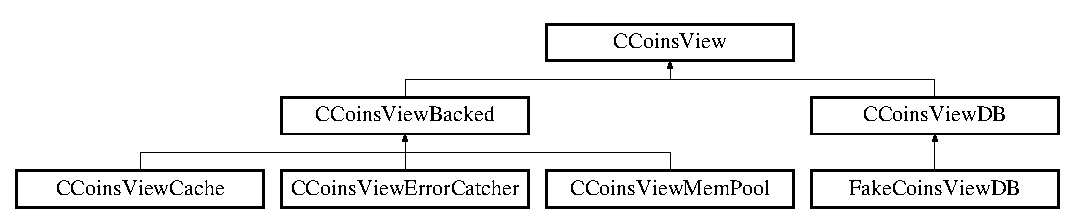
\includegraphics[height=2.560976cm]{class_c_coins_view}
\end{center}
\end{figure}
\subsection*{Public Member Functions}
\begin{DoxyCompactItemize}
\item 
virtual bool \mbox{\hyperlink{class_c_coins_view_a2fcf3f99111eef1c41243f54f94d3be8}{Get\+Anchor\+At}} (const \mbox{\hyperlink{classuint256}{uint256}} \&rt, Z\+C\+Incremental\+Merkle\+Tree \&tree) const
\begin{DoxyCompactList}\small\item\em Retrieve the tree at a particular anchored root in the chain. \end{DoxyCompactList}\item 
virtual bool \mbox{\hyperlink{class_c_coins_view_a45a7abe02d0d9d1b61a09dec70a3311f}{Get\+Nullifier}} (const \mbox{\hyperlink{classuint256}{uint256}} \&nullifier) const
\begin{DoxyCompactList}\small\item\em Determine whether a nullifier is spent or not. \end{DoxyCompactList}\item 
virtual bool \mbox{\hyperlink{class_c_coins_view_a67d865358127bef1f0011a23d5158a9f}{Get\+Coins}} (const \mbox{\hyperlink{classuint256}{uint256}} \&txid, \mbox{\hyperlink{class_c_coins}{C\+Coins}} \&coins) const
\begin{DoxyCompactList}\small\item\em Retrieve the \mbox{\hyperlink{class_c_coins}{C\+Coins}} (unspent transaction outputs) for a given txid. \end{DoxyCompactList}\item 
virtual bool \mbox{\hyperlink{class_c_coins_view_ade3a65fc3f1b02baf7bebce630e4eba3}{Have\+Coins}} (const \mbox{\hyperlink{classuint256}{uint256}} \&txid) const
\item 
virtual \mbox{\hyperlink{classuint256}{uint256}} \mbox{\hyperlink{class_c_coins_view_af81f2907d360a2548d59a61388e5e5cb}{Get\+Best\+Block}} () const
\begin{DoxyCompactList}\small\item\em Retrieve the block hash whose state this \mbox{\hyperlink{class_c_coins_view}{C\+Coins\+View}} currently represents. \end{DoxyCompactList}\item 
virtual \mbox{\hyperlink{classuint256}{uint256}} \mbox{\hyperlink{class_c_coins_view_a4d51ab1de57e76a174b5ca874c601b52}{Get\+Best\+Anchor}} () const
\begin{DoxyCompactList}\small\item\em Get the current \char`\"{}tip\char`\"{} or the latest anchored tree root in the chain. \end{DoxyCompactList}\item 
virtual bool \mbox{\hyperlink{class_c_coins_view_a6e0ef2f996f5bf9f15c4fcae89333c7d}{Batch\+Write}} (\mbox{\hyperlink{coins_8h_a2886ba2fd0428bae777e1cbcabc02834}{C\+Coins\+Map}} \&map\+Coins, const \mbox{\hyperlink{classuint256}{uint256}} \&hash\+Block, const \mbox{\hyperlink{classuint256}{uint256}} \&hash\+Anchor, \mbox{\hyperlink{coins_8h_a070827cc9d21a91b8f4f4f52a6f7c848}{C\+Anchors\+Map}} \&map\+Anchors, \mbox{\hyperlink{coins_8h_ab651cc287e9594190ef77d2fca2b14c7}{C\+Nullifiers\+Map}} \&map\+Nullifiers)
\item 
virtual bool \mbox{\hyperlink{class_c_coins_view_adbd7f73ba071c6e441dd88d95b8f2c0d}{Get\+Stats}} (\mbox{\hyperlink{struct_c_coins_stats}{C\+Coins\+Stats}} \&stats) const
\begin{DoxyCompactList}\small\item\em Calculate statistics about the unspent transaction output set. \end{DoxyCompactList}\item 
virtual \mbox{\hyperlink{class_c_coins_view_a7ffb4218bf991ddff47339e44c8710da}{$\sim$\+C\+Coins\+View}} ()
\begin{DoxyCompactList}\small\item\em As we use C\+Coins\+Views polymorphically, have a virtual destructor. \end{DoxyCompactList}\end{DoxyCompactItemize}


\subsection{Detailed Description}
Abstract view on the open txout dataset. 

\subsection{Constructor \& Destructor Documentation}
\mbox{\Hypertarget{class_c_coins_view_a7ffb4218bf991ddff47339e44c8710da}\label{class_c_coins_view_a7ffb4218bf991ddff47339e44c8710da}} 
\index{C\+Coins\+View@{C\+Coins\+View}!````~C\+Coins\+View@{$\sim$\+C\+Coins\+View}}
\index{````~C\+Coins\+View@{$\sim$\+C\+Coins\+View}!C\+Coins\+View@{C\+Coins\+View}}
\subsubsection{\texorpdfstring{$\sim$\+C\+Coins\+View()}{~CCoinsView()}}
{\footnotesize\ttfamily virtual C\+Coins\+View\+::$\sim$\+C\+Coins\+View (\begin{DoxyParamCaption}{ }\end{DoxyParamCaption})\hspace{0.3cm}{\ttfamily [inline]}, {\ttfamily [virtual]}}



As we use C\+Coins\+Views polymorphically, have a virtual destructor. 



\subsection{Member Function Documentation}
\mbox{\Hypertarget{class_c_coins_view_a6e0ef2f996f5bf9f15c4fcae89333c7d}\label{class_c_coins_view_a6e0ef2f996f5bf9f15c4fcae89333c7d}} 
\index{C\+Coins\+View@{C\+Coins\+View}!Batch\+Write@{Batch\+Write}}
\index{Batch\+Write@{Batch\+Write}!C\+Coins\+View@{C\+Coins\+View}}
\subsubsection{\texorpdfstring{Batch\+Write()}{BatchWrite()}}
{\footnotesize\ttfamily bool C\+Coins\+View\+::\+Batch\+Write (\begin{DoxyParamCaption}\item[{\mbox{\hyperlink{coins_8h_a2886ba2fd0428bae777e1cbcabc02834}{C\+Coins\+Map}} \&}]{map\+Coins,  }\item[{const \mbox{\hyperlink{classuint256}{uint256}} \&}]{hash\+Block,  }\item[{const \mbox{\hyperlink{classuint256}{uint256}} \&}]{hash\+Anchor,  }\item[{\mbox{\hyperlink{coins_8h_a070827cc9d21a91b8f4f4f52a6f7c848}{C\+Anchors\+Map}} \&}]{map\+Anchors,  }\item[{\mbox{\hyperlink{coins_8h_ab651cc287e9594190ef77d2fca2b14c7}{C\+Nullifiers\+Map}} \&}]{map\+Nullifiers }\end{DoxyParamCaption})\hspace{0.3cm}{\ttfamily [virtual]}}

Do a bulk modification (multiple \mbox{\hyperlink{class_c_coins}{C\+Coins}} changes + Best\+Block change). The passed map\+Coins can be modified. 

Reimplemented in \mbox{\hyperlink{class_c_coins_view_cache_a3d661381b7eb233a8a13ea11ec5dac51}{C\+Coins\+View\+Cache}}, \mbox{\hyperlink{class_c_coins_view_backed_ae0f10af7d1cd7706f57628c38426c75c}{C\+Coins\+View\+Backed}}, \mbox{\hyperlink{class_fake_coins_view_d_b_a1108b45f9d165344c7378051e061147b}{Fake\+Coins\+View\+DB}}, and \mbox{\hyperlink{class_c_coins_view_d_b_ab617e4b898f06cec79a2a26fdca9efbd}{C\+Coins\+View\+DB}}.

\mbox{\Hypertarget{class_c_coins_view_a2fcf3f99111eef1c41243f54f94d3be8}\label{class_c_coins_view_a2fcf3f99111eef1c41243f54f94d3be8}} 
\index{C\+Coins\+View@{C\+Coins\+View}!Get\+Anchor\+At@{Get\+Anchor\+At}}
\index{Get\+Anchor\+At@{Get\+Anchor\+At}!C\+Coins\+View@{C\+Coins\+View}}
\subsubsection{\texorpdfstring{Get\+Anchor\+At()}{GetAnchorAt()}}
{\footnotesize\ttfamily bool C\+Coins\+View\+::\+Get\+Anchor\+At (\begin{DoxyParamCaption}\item[{const \mbox{\hyperlink{classuint256}{uint256}} \&}]{rt,  }\item[{Z\+C\+Incremental\+Merkle\+Tree \&}]{tree }\end{DoxyParamCaption}) const\hspace{0.3cm}{\ttfamily [virtual]}}



Retrieve the tree at a particular anchored root in the chain. 



Reimplemented in \mbox{\hyperlink{class_c_coins_view_cache_a97401da3be42b24b16fc202cdce34419}{C\+Coins\+View\+Cache}}, \mbox{\hyperlink{class_c_coins_view_backed_a85e573aed0a7e713dc5d6a0478649435}{C\+Coins\+View\+Backed}}, \mbox{\hyperlink{class_fake_coins_view_d_b_ae52d0073bef3eb64bd64b325e821c52b}{Fake\+Coins\+View\+DB}}, and \mbox{\hyperlink{class_c_coins_view_d_b_aeaab3bc4b363dbbc9d9a77930209e299}{C\+Coins\+View\+DB}}.

\mbox{\Hypertarget{class_c_coins_view_a4d51ab1de57e76a174b5ca874c601b52}\label{class_c_coins_view_a4d51ab1de57e76a174b5ca874c601b52}} 
\index{C\+Coins\+View@{C\+Coins\+View}!Get\+Best\+Anchor@{Get\+Best\+Anchor}}
\index{Get\+Best\+Anchor@{Get\+Best\+Anchor}!C\+Coins\+View@{C\+Coins\+View}}
\subsubsection{\texorpdfstring{Get\+Best\+Anchor()}{GetBestAnchor()}}
{\footnotesize\ttfamily \mbox{\hyperlink{classuint256}{uint256}} C\+Coins\+View\+::\+Get\+Best\+Anchor (\begin{DoxyParamCaption}{ }\end{DoxyParamCaption}) const\hspace{0.3cm}{\ttfamily [virtual]}}



Get the current \char`\"{}tip\char`\"{} or the latest anchored tree root in the chain. 



Reimplemented in \mbox{\hyperlink{class_c_coins_view_cache_a8f1e864bff1617bae243bd0c7b29d2ed}{C\+Coins\+View\+Cache}}, \mbox{\hyperlink{class_c_coins_view_backed_a2bac0f246916a004e9773f03c37f2c82}{C\+Coins\+View\+Backed}}, \mbox{\hyperlink{class_fake_coins_view_d_b_af7870faf849e59188344273a03c9a1b0}{Fake\+Coins\+View\+DB}}, and \mbox{\hyperlink{class_c_coins_view_d_b_a2bb7d73a96472def92e332a4563a689c}{C\+Coins\+View\+DB}}.

\mbox{\Hypertarget{class_c_coins_view_af81f2907d360a2548d59a61388e5e5cb}\label{class_c_coins_view_af81f2907d360a2548d59a61388e5e5cb}} 
\index{C\+Coins\+View@{C\+Coins\+View}!Get\+Best\+Block@{Get\+Best\+Block}}
\index{Get\+Best\+Block@{Get\+Best\+Block}!C\+Coins\+View@{C\+Coins\+View}}
\subsubsection{\texorpdfstring{Get\+Best\+Block()}{GetBestBlock()}}
{\footnotesize\ttfamily \mbox{\hyperlink{classuint256}{uint256}} C\+Coins\+View\+::\+Get\+Best\+Block (\begin{DoxyParamCaption}{ }\end{DoxyParamCaption}) const\hspace{0.3cm}{\ttfamily [virtual]}}



Retrieve the block hash whose state this \mbox{\hyperlink{class_c_coins_view}{C\+Coins\+View}} currently represents. 



Reimplemented in \mbox{\hyperlink{class_c_coins_view_cache_a1190c94a943c067d13211179ef06470b}{C\+Coins\+View\+Cache}}, \mbox{\hyperlink{class_c_coins_view_backed_a39bca41ae922d0ce7f40e8aeab289280}{C\+Coins\+View\+Backed}}, \mbox{\hyperlink{class_fake_coins_view_d_b_a36231d924114fbe51a830c9c235c50ad}{Fake\+Coins\+View\+DB}}, and \mbox{\hyperlink{class_c_coins_view_d_b_ac9c513a34b9e58d942fdbeafd9e5bbce}{C\+Coins\+View\+DB}}.

\mbox{\Hypertarget{class_c_coins_view_a67d865358127bef1f0011a23d5158a9f}\label{class_c_coins_view_a67d865358127bef1f0011a23d5158a9f}} 
\index{C\+Coins\+View@{C\+Coins\+View}!Get\+Coins@{Get\+Coins}}
\index{Get\+Coins@{Get\+Coins}!C\+Coins\+View@{C\+Coins\+View}}
\subsubsection{\texorpdfstring{Get\+Coins()}{GetCoins()}}
{\footnotesize\ttfamily bool C\+Coins\+View\+::\+Get\+Coins (\begin{DoxyParamCaption}\item[{const \mbox{\hyperlink{classuint256}{uint256}} \&}]{txid,  }\item[{\mbox{\hyperlink{class_c_coins}{C\+Coins}} \&}]{coins }\end{DoxyParamCaption}) const\hspace{0.3cm}{\ttfamily [virtual]}}



Retrieve the \mbox{\hyperlink{class_c_coins}{C\+Coins}} (unspent transaction outputs) for a given txid. 



Reimplemented in \mbox{\hyperlink{class_c_coins_view_cache_a1b62444593fdb580bfa4bd6fab41fafa}{C\+Coins\+View\+Cache}}, \mbox{\hyperlink{class_c_coins_view_backed_a456f9e85817556329a959c120998df5b}{C\+Coins\+View\+Backed}}, \mbox{\hyperlink{class_c_coins_view_mem_pool_a1a4a556821b1680ff4b73758c8a1e471}{C\+Coins\+View\+Mem\+Pool}}, \mbox{\hyperlink{class_c_coins_view_error_catcher_a909f7b9e364b6f06bfea955209aa015d}{C\+Coins\+View\+Error\+Catcher}}, and \mbox{\hyperlink{class_c_coins_view_d_b_ac35a80d1115ec697101d382e71db5b31}{C\+Coins\+View\+DB}}.

\mbox{\Hypertarget{class_c_coins_view_a45a7abe02d0d9d1b61a09dec70a3311f}\label{class_c_coins_view_a45a7abe02d0d9d1b61a09dec70a3311f}} 
\index{C\+Coins\+View@{C\+Coins\+View}!Get\+Nullifier@{Get\+Nullifier}}
\index{Get\+Nullifier@{Get\+Nullifier}!C\+Coins\+View@{C\+Coins\+View}}
\subsubsection{\texorpdfstring{Get\+Nullifier()}{GetNullifier()}}
{\footnotesize\ttfamily bool C\+Coins\+View\+::\+Get\+Nullifier (\begin{DoxyParamCaption}\item[{const \mbox{\hyperlink{classuint256}{uint256}} \&}]{nullifier }\end{DoxyParamCaption}) const\hspace{0.3cm}{\ttfamily [virtual]}}



Determine whether a nullifier is spent or not. 



Reimplemented in \mbox{\hyperlink{class_c_coins_view_cache_a72dd0d15434f85d518f23a278e813a03}{C\+Coins\+View\+Cache}}, \mbox{\hyperlink{class_c_coins_view_backed_afbfee79b18b475d67cd757a7dc4f5955}{C\+Coins\+View\+Backed}}, \mbox{\hyperlink{class_fake_coins_view_d_b_af7d0ce4926fb03ee632148c5fde66c05}{Fake\+Coins\+View\+DB}}, \mbox{\hyperlink{class_c_coins_view_mem_pool_ac76524f89eb1a8c25e3c6c3201d3662a}{C\+Coins\+View\+Mem\+Pool}}, and \mbox{\hyperlink{class_c_coins_view_d_b_ac9724829164f5a06b6d7c610da03a730}{C\+Coins\+View\+DB}}.

\mbox{\Hypertarget{class_c_coins_view_adbd7f73ba071c6e441dd88d95b8f2c0d}\label{class_c_coins_view_adbd7f73ba071c6e441dd88d95b8f2c0d}} 
\index{C\+Coins\+View@{C\+Coins\+View}!Get\+Stats@{Get\+Stats}}
\index{Get\+Stats@{Get\+Stats}!C\+Coins\+View@{C\+Coins\+View}}
\subsubsection{\texorpdfstring{Get\+Stats()}{GetStats()}}
{\footnotesize\ttfamily bool C\+Coins\+View\+::\+Get\+Stats (\begin{DoxyParamCaption}\item[{\mbox{\hyperlink{struct_c_coins_stats}{C\+Coins\+Stats}} \&}]{stats }\end{DoxyParamCaption}) const\hspace{0.3cm}{\ttfamily [virtual]}}



Calculate statistics about the unspent transaction output set. 



Reimplemented in \mbox{\hyperlink{class_c_coins_view_backed_aa787da5760afa843d32764b70420b2d6}{C\+Coins\+View\+Backed}}, \mbox{\hyperlink{class_fake_coins_view_d_b_ad1deefbe955925e274e5d50d289275e9}{Fake\+Coins\+View\+DB}}, and \mbox{\hyperlink{class_c_coins_view_d_b_a227bf56f8801921f12e56c6839104fce}{C\+Coins\+View\+DB}}.

\mbox{\Hypertarget{class_c_coins_view_ade3a65fc3f1b02baf7bebce630e4eba3}\label{class_c_coins_view_ade3a65fc3f1b02baf7bebce630e4eba3}} 
\index{C\+Coins\+View@{C\+Coins\+View}!Have\+Coins@{Have\+Coins}}
\index{Have\+Coins@{Have\+Coins}!C\+Coins\+View@{C\+Coins\+View}}
\subsubsection{\texorpdfstring{Have\+Coins()}{HaveCoins()}}
{\footnotesize\ttfamily bool C\+Coins\+View\+::\+Have\+Coins (\begin{DoxyParamCaption}\item[{const \mbox{\hyperlink{classuint256}{uint256}} \&}]{txid }\end{DoxyParamCaption}) const\hspace{0.3cm}{\ttfamily [virtual]}}

Just check whether we have data for a given txid. This may (but cannot always) return true for fully spent transactions 

Reimplemented in \mbox{\hyperlink{class_c_coins_view_cache_aa8f0c55b6fc207d2188948a565125ab7}{C\+Coins\+View\+Cache}}, \mbox{\hyperlink{class_c_coins_view_backed_ad49041658bdec807d556e080476e6543}{C\+Coins\+View\+Backed}}, \mbox{\hyperlink{class_c_coins_view_mem_pool_a2c5900448dc5570053060686ad1f014b}{C\+Coins\+View\+Mem\+Pool}}, and \mbox{\hyperlink{class_c_coins_view_d_b_af55f35faadeb74b5406559fe3ed20114}{C\+Coins\+View\+DB}}.



The documentation for this class was generated from the following files\+:\begin{DoxyCompactItemize}
\item 
/\+Users/christopherarguello/\+Developer/anon/src/\mbox{\hyperlink{coins_8h}{coins.\+h}}\item 
/\+Users/christopherarguello/\+Developer/anon/src/\mbox{\hyperlink{coins_8cpp}{coins.\+cpp}}\end{DoxyCompactItemize}

\hypertarget{class_c_coins_view_backed}{}\section{C\+Coins\+View\+Backed Class Reference}
\label{class_c_coins_view_backed}\index{C\+Coins\+View\+Backed@{C\+Coins\+View\+Backed}}


{\ttfamily \#include $<$coins.\+h$>$}

Inheritance diagram for C\+Coins\+View\+Backed\+:\begin{figure}[H]
\begin{center}
\leavevmode
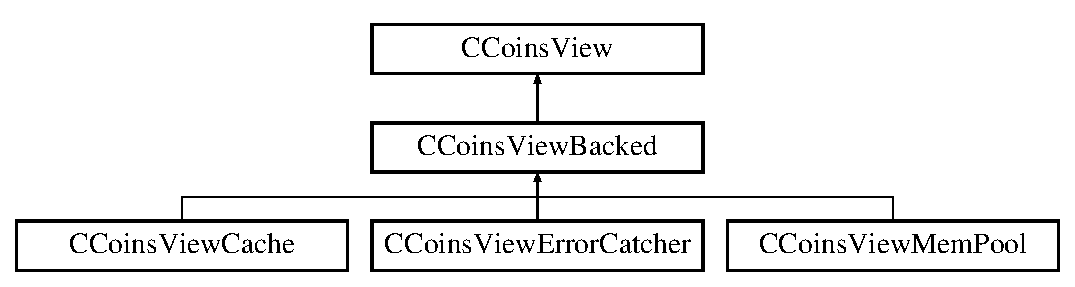
\includegraphics[height=3.000000cm]{class_c_coins_view_backed}
\end{center}
\end{figure}
\subsection*{Public Member Functions}
\begin{DoxyCompactItemize}
\item 
\mbox{\hyperlink{class_c_coins_view_backed_af86a3b07433e8d84678772411791125e}{C\+Coins\+View\+Backed}} (\mbox{\hyperlink{class_c_coins_view}{C\+Coins\+View}} $\ast$view\+In)
\item 
bool \mbox{\hyperlink{class_c_coins_view_backed_a85e573aed0a7e713dc5d6a0478649435}{Get\+Anchor\+At}} (const \mbox{\hyperlink{classuint256}{uint256}} \&rt, Z\+C\+Incremental\+Merkle\+Tree \&tree) const
\begin{DoxyCompactList}\small\item\em Retrieve the tree at a particular anchored root in the chain. \end{DoxyCompactList}\item 
bool \mbox{\hyperlink{class_c_coins_view_backed_afbfee79b18b475d67cd757a7dc4f5955}{Get\+Nullifier}} (const \mbox{\hyperlink{classuint256}{uint256}} \&nullifier) const
\begin{DoxyCompactList}\small\item\em Determine whether a nullifier is spent or not. \end{DoxyCompactList}\item 
bool \mbox{\hyperlink{class_c_coins_view_backed_a456f9e85817556329a959c120998df5b}{Get\+Coins}} (const \mbox{\hyperlink{classuint256}{uint256}} \&txid, \mbox{\hyperlink{class_c_coins}{C\+Coins}} \&coins) const
\begin{DoxyCompactList}\small\item\em Retrieve the \mbox{\hyperlink{class_c_coins}{C\+Coins}} (unspent transaction outputs) for a given txid. \end{DoxyCompactList}\item 
bool \mbox{\hyperlink{class_c_coins_view_backed_ad49041658bdec807d556e080476e6543}{Have\+Coins}} (const \mbox{\hyperlink{classuint256}{uint256}} \&txid) const
\item 
\mbox{\hyperlink{classuint256}{uint256}} \mbox{\hyperlink{class_c_coins_view_backed_a39bca41ae922d0ce7f40e8aeab289280}{Get\+Best\+Block}} () const
\begin{DoxyCompactList}\small\item\em Retrieve the block hash whose state this \mbox{\hyperlink{class_c_coins_view}{C\+Coins\+View}} currently represents. \end{DoxyCompactList}\item 
\mbox{\hyperlink{classuint256}{uint256}} \mbox{\hyperlink{class_c_coins_view_backed_a2bac0f246916a004e9773f03c37f2c82}{Get\+Best\+Anchor}} () const
\begin{DoxyCompactList}\small\item\em Get the current \char`\"{}tip\char`\"{} or the latest anchored tree root in the chain. \end{DoxyCompactList}\item 
void \mbox{\hyperlink{class_c_coins_view_backed_a7eaddfbfd401a95c2fda2a8d8feaaf73}{Set\+Backend}} (\mbox{\hyperlink{class_c_coins_view}{C\+Coins\+View}} \&view\+In)
\item 
bool \mbox{\hyperlink{class_c_coins_view_backed_ae0f10af7d1cd7706f57628c38426c75c}{Batch\+Write}} (\mbox{\hyperlink{coins_8h_a2886ba2fd0428bae777e1cbcabc02834}{C\+Coins\+Map}} \&map\+Coins, const \mbox{\hyperlink{classuint256}{uint256}} \&hash\+Block, const \mbox{\hyperlink{classuint256}{uint256}} \&hash\+Anchor, \mbox{\hyperlink{coins_8h_a070827cc9d21a91b8f4f4f52a6f7c848}{C\+Anchors\+Map}} \&map\+Anchors, \mbox{\hyperlink{coins_8h_ab651cc287e9594190ef77d2fca2b14c7}{C\+Nullifiers\+Map}} \&map\+Nullifiers)
\item 
bool \mbox{\hyperlink{class_c_coins_view_backed_aa787da5760afa843d32764b70420b2d6}{Get\+Stats}} (\mbox{\hyperlink{struct_c_coins_stats}{C\+Coins\+Stats}} \&stats) const
\begin{DoxyCompactList}\small\item\em Calculate statistics about the unspent transaction output set. \end{DoxyCompactList}\end{DoxyCompactItemize}
\subsection*{Protected Attributes}
\begin{DoxyCompactItemize}
\item 
\mbox{\hyperlink{class_c_coins_view}{C\+Coins\+View}} $\ast$ \mbox{\hyperlink{class_c_coins_view_backed_a901472317114adc4c104efd61dcf6203}{base}}
\end{DoxyCompactItemize}


\subsection{Detailed Description}
\mbox{\hyperlink{class_c_coins_view}{C\+Coins\+View}} backed by another \mbox{\hyperlink{class_c_coins_view}{C\+Coins\+View}} 

\subsection{Constructor \& Destructor Documentation}
\mbox{\Hypertarget{class_c_coins_view_backed_af86a3b07433e8d84678772411791125e}\label{class_c_coins_view_backed_af86a3b07433e8d84678772411791125e}} 
\index{C\+Coins\+View\+Backed@{C\+Coins\+View\+Backed}!C\+Coins\+View\+Backed@{C\+Coins\+View\+Backed}}
\index{C\+Coins\+View\+Backed@{C\+Coins\+View\+Backed}!C\+Coins\+View\+Backed@{C\+Coins\+View\+Backed}}
\subsubsection{\texorpdfstring{C\+Coins\+View\+Backed()}{CCoinsViewBacked()}}
{\footnotesize\ttfamily C\+Coins\+View\+Backed\+::\+C\+Coins\+View\+Backed (\begin{DoxyParamCaption}\item[{\mbox{\hyperlink{class_c_coins_view}{C\+Coins\+View}} $\ast$}]{view\+In }\end{DoxyParamCaption})}



\subsection{Member Function Documentation}
\mbox{\Hypertarget{class_c_coins_view_backed_ae0f10af7d1cd7706f57628c38426c75c}\label{class_c_coins_view_backed_ae0f10af7d1cd7706f57628c38426c75c}} 
\index{C\+Coins\+View\+Backed@{C\+Coins\+View\+Backed}!Batch\+Write@{Batch\+Write}}
\index{Batch\+Write@{Batch\+Write}!C\+Coins\+View\+Backed@{C\+Coins\+View\+Backed}}
\subsubsection{\texorpdfstring{Batch\+Write()}{BatchWrite()}}
{\footnotesize\ttfamily bool C\+Coins\+View\+Backed\+::\+Batch\+Write (\begin{DoxyParamCaption}\item[{\mbox{\hyperlink{coins_8h_a2886ba2fd0428bae777e1cbcabc02834}{C\+Coins\+Map}} \&}]{map\+Coins,  }\item[{const \mbox{\hyperlink{classuint256}{uint256}} \&}]{hash\+Block,  }\item[{const \mbox{\hyperlink{classuint256}{uint256}} \&}]{hash\+Anchor,  }\item[{\mbox{\hyperlink{coins_8h_a070827cc9d21a91b8f4f4f52a6f7c848}{C\+Anchors\+Map}} \&}]{map\+Anchors,  }\item[{\mbox{\hyperlink{coins_8h_ab651cc287e9594190ef77d2fca2b14c7}{C\+Nullifiers\+Map}} \&}]{map\+Nullifiers }\end{DoxyParamCaption})\hspace{0.3cm}{\ttfamily [virtual]}}

Do a bulk modification (multiple \mbox{\hyperlink{class_c_coins}{C\+Coins}} changes + Best\+Block change). The passed map\+Coins can be modified. 

Reimplemented from \mbox{\hyperlink{class_c_coins_view_a6e0ef2f996f5bf9f15c4fcae89333c7d}{C\+Coins\+View}}.



Reimplemented in \mbox{\hyperlink{class_c_coins_view_cache_a3d661381b7eb233a8a13ea11ec5dac51}{C\+Coins\+View\+Cache}}.

\mbox{\Hypertarget{class_c_coins_view_backed_a85e573aed0a7e713dc5d6a0478649435}\label{class_c_coins_view_backed_a85e573aed0a7e713dc5d6a0478649435}} 
\index{C\+Coins\+View\+Backed@{C\+Coins\+View\+Backed}!Get\+Anchor\+At@{Get\+Anchor\+At}}
\index{Get\+Anchor\+At@{Get\+Anchor\+At}!C\+Coins\+View\+Backed@{C\+Coins\+View\+Backed}}
\subsubsection{\texorpdfstring{Get\+Anchor\+At()}{GetAnchorAt()}}
{\footnotesize\ttfamily bool C\+Coins\+View\+Backed\+::\+Get\+Anchor\+At (\begin{DoxyParamCaption}\item[{const \mbox{\hyperlink{classuint256}{uint256}} \&}]{rt,  }\item[{Z\+C\+Incremental\+Merkle\+Tree \&}]{tree }\end{DoxyParamCaption}) const\hspace{0.3cm}{\ttfamily [virtual]}}



Retrieve the tree at a particular anchored root in the chain. 



Reimplemented from \mbox{\hyperlink{class_c_coins_view_a2fcf3f99111eef1c41243f54f94d3be8}{C\+Coins\+View}}.



Reimplemented in \mbox{\hyperlink{class_c_coins_view_cache_a97401da3be42b24b16fc202cdce34419}{C\+Coins\+View\+Cache}}.

\mbox{\Hypertarget{class_c_coins_view_backed_a2bac0f246916a004e9773f03c37f2c82}\label{class_c_coins_view_backed_a2bac0f246916a004e9773f03c37f2c82}} 
\index{C\+Coins\+View\+Backed@{C\+Coins\+View\+Backed}!Get\+Best\+Anchor@{Get\+Best\+Anchor}}
\index{Get\+Best\+Anchor@{Get\+Best\+Anchor}!C\+Coins\+View\+Backed@{C\+Coins\+View\+Backed}}
\subsubsection{\texorpdfstring{Get\+Best\+Anchor()}{GetBestAnchor()}}
{\footnotesize\ttfamily \mbox{\hyperlink{classuint256}{uint256}} C\+Coins\+View\+Backed\+::\+Get\+Best\+Anchor (\begin{DoxyParamCaption}{ }\end{DoxyParamCaption}) const\hspace{0.3cm}{\ttfamily [virtual]}}



Get the current \char`\"{}tip\char`\"{} or the latest anchored tree root in the chain. 



Reimplemented from \mbox{\hyperlink{class_c_coins_view_a4d51ab1de57e76a174b5ca874c601b52}{C\+Coins\+View}}.



Reimplemented in \mbox{\hyperlink{class_c_coins_view_cache_a8f1e864bff1617bae243bd0c7b29d2ed}{C\+Coins\+View\+Cache}}.

\mbox{\Hypertarget{class_c_coins_view_backed_a39bca41ae922d0ce7f40e8aeab289280}\label{class_c_coins_view_backed_a39bca41ae922d0ce7f40e8aeab289280}} 
\index{C\+Coins\+View\+Backed@{C\+Coins\+View\+Backed}!Get\+Best\+Block@{Get\+Best\+Block}}
\index{Get\+Best\+Block@{Get\+Best\+Block}!C\+Coins\+View\+Backed@{C\+Coins\+View\+Backed}}
\subsubsection{\texorpdfstring{Get\+Best\+Block()}{GetBestBlock()}}
{\footnotesize\ttfamily \mbox{\hyperlink{classuint256}{uint256}} C\+Coins\+View\+Backed\+::\+Get\+Best\+Block (\begin{DoxyParamCaption}{ }\end{DoxyParamCaption}) const\hspace{0.3cm}{\ttfamily [virtual]}}



Retrieve the block hash whose state this \mbox{\hyperlink{class_c_coins_view}{C\+Coins\+View}} currently represents. 



Reimplemented from \mbox{\hyperlink{class_c_coins_view_af81f2907d360a2548d59a61388e5e5cb}{C\+Coins\+View}}.



Reimplemented in \mbox{\hyperlink{class_c_coins_view_cache_a1190c94a943c067d13211179ef06470b}{C\+Coins\+View\+Cache}}.

\mbox{\Hypertarget{class_c_coins_view_backed_a456f9e85817556329a959c120998df5b}\label{class_c_coins_view_backed_a456f9e85817556329a959c120998df5b}} 
\index{C\+Coins\+View\+Backed@{C\+Coins\+View\+Backed}!Get\+Coins@{Get\+Coins}}
\index{Get\+Coins@{Get\+Coins}!C\+Coins\+View\+Backed@{C\+Coins\+View\+Backed}}
\subsubsection{\texorpdfstring{Get\+Coins()}{GetCoins()}}
{\footnotesize\ttfamily bool C\+Coins\+View\+Backed\+::\+Get\+Coins (\begin{DoxyParamCaption}\item[{const \mbox{\hyperlink{classuint256}{uint256}} \&}]{txid,  }\item[{\mbox{\hyperlink{class_c_coins}{C\+Coins}} \&}]{coins }\end{DoxyParamCaption}) const\hspace{0.3cm}{\ttfamily [virtual]}}



Retrieve the \mbox{\hyperlink{class_c_coins}{C\+Coins}} (unspent transaction outputs) for a given txid. 



Reimplemented from \mbox{\hyperlink{class_c_coins_view_a67d865358127bef1f0011a23d5158a9f}{C\+Coins\+View}}.



Reimplemented in \mbox{\hyperlink{class_c_coins_view_cache_a1b62444593fdb580bfa4bd6fab41fafa}{C\+Coins\+View\+Cache}}, \mbox{\hyperlink{class_c_coins_view_mem_pool_a1a4a556821b1680ff4b73758c8a1e471}{C\+Coins\+View\+Mem\+Pool}}, and \mbox{\hyperlink{class_c_coins_view_error_catcher_a909f7b9e364b6f06bfea955209aa015d}{C\+Coins\+View\+Error\+Catcher}}.

\mbox{\Hypertarget{class_c_coins_view_backed_afbfee79b18b475d67cd757a7dc4f5955}\label{class_c_coins_view_backed_afbfee79b18b475d67cd757a7dc4f5955}} 
\index{C\+Coins\+View\+Backed@{C\+Coins\+View\+Backed}!Get\+Nullifier@{Get\+Nullifier}}
\index{Get\+Nullifier@{Get\+Nullifier}!C\+Coins\+View\+Backed@{C\+Coins\+View\+Backed}}
\subsubsection{\texorpdfstring{Get\+Nullifier()}{GetNullifier()}}
{\footnotesize\ttfamily bool C\+Coins\+View\+Backed\+::\+Get\+Nullifier (\begin{DoxyParamCaption}\item[{const \mbox{\hyperlink{classuint256}{uint256}} \&}]{nullifier }\end{DoxyParamCaption}) const\hspace{0.3cm}{\ttfamily [virtual]}}



Determine whether a nullifier is spent or not. 



Reimplemented from \mbox{\hyperlink{class_c_coins_view_a45a7abe02d0d9d1b61a09dec70a3311f}{C\+Coins\+View}}.



Reimplemented in \mbox{\hyperlink{class_c_coins_view_cache_a72dd0d15434f85d518f23a278e813a03}{C\+Coins\+View\+Cache}}, and \mbox{\hyperlink{class_c_coins_view_mem_pool_ac76524f89eb1a8c25e3c6c3201d3662a}{C\+Coins\+View\+Mem\+Pool}}.

\mbox{\Hypertarget{class_c_coins_view_backed_aa787da5760afa843d32764b70420b2d6}\label{class_c_coins_view_backed_aa787da5760afa843d32764b70420b2d6}} 
\index{C\+Coins\+View\+Backed@{C\+Coins\+View\+Backed}!Get\+Stats@{Get\+Stats}}
\index{Get\+Stats@{Get\+Stats}!C\+Coins\+View\+Backed@{C\+Coins\+View\+Backed}}
\subsubsection{\texorpdfstring{Get\+Stats()}{GetStats()}}
{\footnotesize\ttfamily bool C\+Coins\+View\+Backed\+::\+Get\+Stats (\begin{DoxyParamCaption}\item[{\mbox{\hyperlink{struct_c_coins_stats}{C\+Coins\+Stats}} \&}]{stats }\end{DoxyParamCaption}) const\hspace{0.3cm}{\ttfamily [virtual]}}



Calculate statistics about the unspent transaction output set. 



Reimplemented from \mbox{\hyperlink{class_c_coins_view_adbd7f73ba071c6e441dd88d95b8f2c0d}{C\+Coins\+View}}.

\mbox{\Hypertarget{class_c_coins_view_backed_ad49041658bdec807d556e080476e6543}\label{class_c_coins_view_backed_ad49041658bdec807d556e080476e6543}} 
\index{C\+Coins\+View\+Backed@{C\+Coins\+View\+Backed}!Have\+Coins@{Have\+Coins}}
\index{Have\+Coins@{Have\+Coins}!C\+Coins\+View\+Backed@{C\+Coins\+View\+Backed}}
\subsubsection{\texorpdfstring{Have\+Coins()}{HaveCoins()}}
{\footnotesize\ttfamily bool C\+Coins\+View\+Backed\+::\+Have\+Coins (\begin{DoxyParamCaption}\item[{const \mbox{\hyperlink{classuint256}{uint256}} \&}]{txid }\end{DoxyParamCaption}) const\hspace{0.3cm}{\ttfamily [virtual]}}

Just check whether we have data for a given txid. This may (but cannot always) return true for fully spent transactions 

Reimplemented from \mbox{\hyperlink{class_c_coins_view_ade3a65fc3f1b02baf7bebce630e4eba3}{C\+Coins\+View}}.



Reimplemented in \mbox{\hyperlink{class_c_coins_view_cache_aa8f0c55b6fc207d2188948a565125ab7}{C\+Coins\+View\+Cache}}, and \mbox{\hyperlink{class_c_coins_view_mem_pool_a2c5900448dc5570053060686ad1f014b}{C\+Coins\+View\+Mem\+Pool}}.

\mbox{\Hypertarget{class_c_coins_view_backed_a7eaddfbfd401a95c2fda2a8d8feaaf73}\label{class_c_coins_view_backed_a7eaddfbfd401a95c2fda2a8d8feaaf73}} 
\index{C\+Coins\+View\+Backed@{C\+Coins\+View\+Backed}!Set\+Backend@{Set\+Backend}}
\index{Set\+Backend@{Set\+Backend}!C\+Coins\+View\+Backed@{C\+Coins\+View\+Backed}}
\subsubsection{\texorpdfstring{Set\+Backend()}{SetBackend()}}
{\footnotesize\ttfamily void C\+Coins\+View\+Backed\+::\+Set\+Backend (\begin{DoxyParamCaption}\item[{\mbox{\hyperlink{class_c_coins_view}{C\+Coins\+View}} \&}]{view\+In }\end{DoxyParamCaption})}



\subsection{Member Data Documentation}
\mbox{\Hypertarget{class_c_coins_view_backed_a901472317114adc4c104efd61dcf6203}\label{class_c_coins_view_backed_a901472317114adc4c104efd61dcf6203}} 
\index{C\+Coins\+View\+Backed@{C\+Coins\+View\+Backed}!base@{base}}
\index{base@{base}!C\+Coins\+View\+Backed@{C\+Coins\+View\+Backed}}
\subsubsection{\texorpdfstring{base}{base}}
{\footnotesize\ttfamily \mbox{\hyperlink{class_c_coins_view}{C\+Coins\+View}}$\ast$ C\+Coins\+View\+Backed\+::base\hspace{0.3cm}{\ttfamily [protected]}}



The documentation for this class was generated from the following files\+:\begin{DoxyCompactItemize}
\item 
/\+Users/christopherarguello/\+Developer/anon/src/\mbox{\hyperlink{coins_8h}{coins.\+h}}\item 
/\+Users/christopherarguello/\+Developer/anon/src/\mbox{\hyperlink{coins_8cpp}{coins.\+cpp}}\end{DoxyCompactItemize}

\hypertarget{class_c_coins_view_cache}{}\section{C\+Coins\+View\+Cache Class Reference}
\label{class_c_coins_view_cache}\index{C\+Coins\+View\+Cache@{C\+Coins\+View\+Cache}}


{\ttfamily \#include $<$coins.\+h$>$}

Inheritance diagram for C\+Coins\+View\+Cache\+:\begin{figure}[H]
\begin{center}
\leavevmode
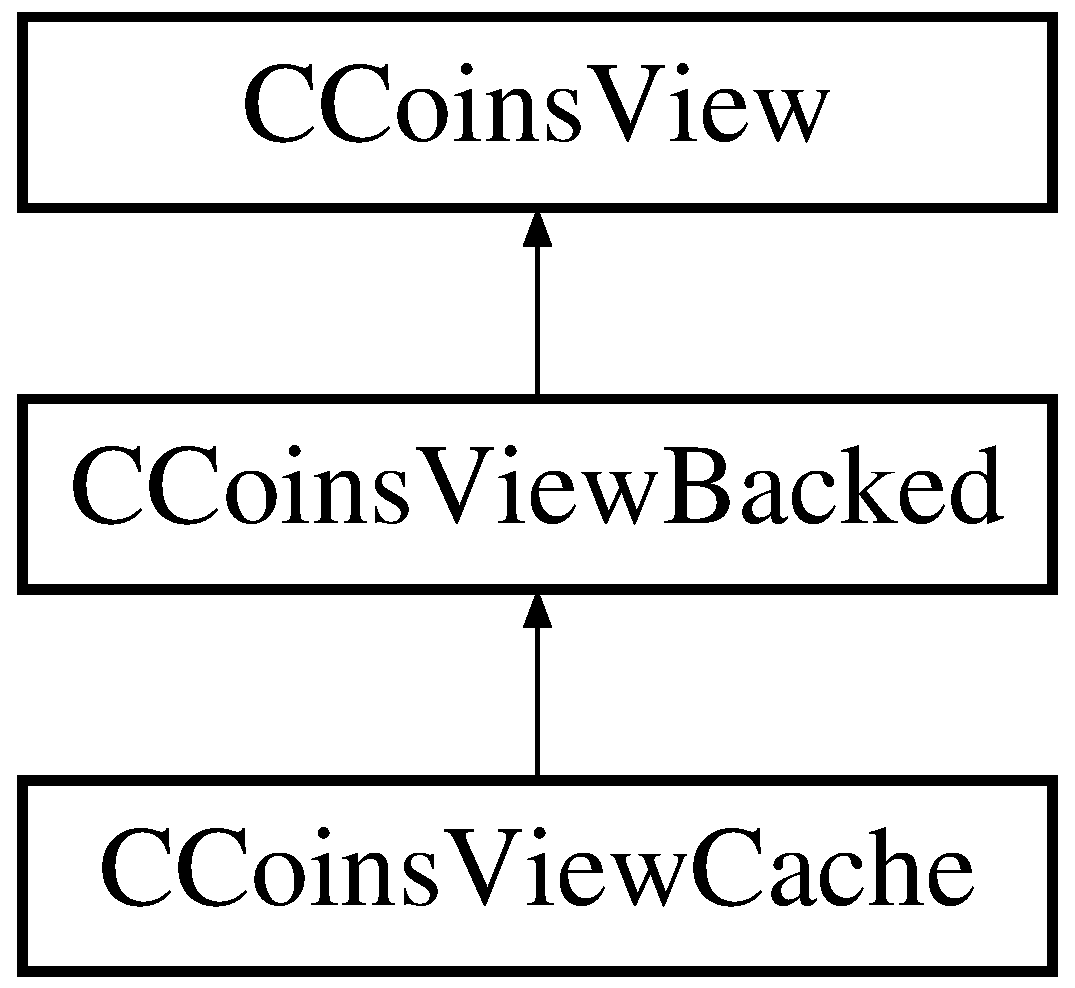
\includegraphics[height=3.000000cm]{class_c_coins_view_cache}
\end{center}
\end{figure}
\subsection*{Public Member Functions}
\begin{DoxyCompactItemize}
\item 
\mbox{\hyperlink{class_c_coins_view_cache_a515a6f259af607fb3394b560d9c063c9}{C\+Coins\+View\+Cache}} (\mbox{\hyperlink{class_c_coins_view}{C\+Coins\+View}} $\ast$base\+In)
\item 
\mbox{\hyperlink{class_c_coins_view_cache_a6148421cb7605fb434f6c8622f39430b}{$\sim$\+C\+Coins\+View\+Cache}} ()
\item 
bool \mbox{\hyperlink{class_c_coins_view_cache_a97401da3be42b24b16fc202cdce34419}{Get\+Anchor\+At}} (const \mbox{\hyperlink{classuint256}{uint256}} \&rt, Z\+C\+Incremental\+Merkle\+Tree \&tree) const
\begin{DoxyCompactList}\small\item\em Retrieve the tree at a particular anchored root in the chain. \end{DoxyCompactList}\item 
bool \mbox{\hyperlink{class_c_coins_view_cache_a72dd0d15434f85d518f23a278e813a03}{Get\+Nullifier}} (const \mbox{\hyperlink{classuint256}{uint256}} \&nullifier) const
\begin{DoxyCompactList}\small\item\em Determine whether a nullifier is spent or not. \end{DoxyCompactList}\item 
bool \mbox{\hyperlink{class_c_coins_view_cache_a1b62444593fdb580bfa4bd6fab41fafa}{Get\+Coins}} (const \mbox{\hyperlink{classuint256}{uint256}} \&txid, \mbox{\hyperlink{class_c_coins}{C\+Coins}} \&coins) const
\begin{DoxyCompactList}\small\item\em Retrieve the \mbox{\hyperlink{class_c_coins}{C\+Coins}} (unspent transaction outputs) for a given txid. \end{DoxyCompactList}\item 
bool \mbox{\hyperlink{class_c_coins_view_cache_aa8f0c55b6fc207d2188948a565125ab7}{Have\+Coins}} (const \mbox{\hyperlink{classuint256}{uint256}} \&txid) const
\item 
\mbox{\hyperlink{classuint256}{uint256}} \mbox{\hyperlink{class_c_coins_view_cache_a1190c94a943c067d13211179ef06470b}{Get\+Best\+Block}} () const
\begin{DoxyCompactList}\small\item\em Retrieve the block hash whose state this \mbox{\hyperlink{class_c_coins_view}{C\+Coins\+View}} currently represents. \end{DoxyCompactList}\item 
\mbox{\hyperlink{classuint256}{uint256}} \mbox{\hyperlink{class_c_coins_view_cache_a8f1e864bff1617bae243bd0c7b29d2ed}{Get\+Best\+Anchor}} () const
\begin{DoxyCompactList}\small\item\em Get the current \char`\"{}tip\char`\"{} or the latest anchored tree root in the chain. \end{DoxyCompactList}\item 
void \mbox{\hyperlink{class_c_coins_view_cache_aa3f787f77b123f0fd340fbe4e458b4ad}{Set\+Best\+Block}} (const \mbox{\hyperlink{classuint256}{uint256}} \&\mbox{\hyperlink{class_c_coins_view_cache_a229dddddbc5501edc250209a2ce5df8b}{hash\+Block}})
\item 
bool \mbox{\hyperlink{class_c_coins_view_cache_a3d661381b7eb233a8a13ea11ec5dac51}{Batch\+Write}} (\mbox{\hyperlink{coins_8h_a2886ba2fd0428bae777e1cbcabc02834}{C\+Coins\+Map}} \&map\+Coins, const \mbox{\hyperlink{classuint256}{uint256}} \&\mbox{\hyperlink{class_c_coins_view_cache_a229dddddbc5501edc250209a2ce5df8b}{hash\+Block}}, const \mbox{\hyperlink{classuint256}{uint256}} \&\mbox{\hyperlink{class_c_coins_view_cache_a72a4c55f52127b5e1b3e3a744a2b1cc3}{hash\+Anchor}}, \mbox{\hyperlink{coins_8h_a070827cc9d21a91b8f4f4f52a6f7c848}{C\+Anchors\+Map}} \&map\+Anchors, \mbox{\hyperlink{coins_8h_ab651cc287e9594190ef77d2fca2b14c7}{C\+Nullifiers\+Map}} \&map\+Nullifiers)
\item 
void \mbox{\hyperlink{class_c_coins_view_cache_a1e11b4aeaefd1a6ed6a98c8786465e95}{Push\+Anchor}} (const Z\+C\+Incremental\+Merkle\+Tree \&tree)
\item 
void \mbox{\hyperlink{class_c_coins_view_cache_a7e0b29874a39b165648fd3862035ca33}{Pop\+Anchor}} (const \mbox{\hyperlink{classuint256}{uint256}} \&rt)
\item 
void \mbox{\hyperlink{class_c_coins_view_cache_a820d28a0bb6c5cf4e6e41e2655d0e1fa}{Set\+Nullifier}} (const \mbox{\hyperlink{classuint256}{uint256}} \&nullifier, bool spent)
\item 
const \mbox{\hyperlink{class_c_coins}{C\+Coins}} $\ast$ \mbox{\hyperlink{class_c_coins_view_cache_a8e5341e8b01233949d6170dd4d1fd75d}{Access\+Coins}} (const \mbox{\hyperlink{classuint256}{uint256}} \&txid) const
\item 
\mbox{\hyperlink{class_c_coins_modifier}{C\+Coins\+Modifier}} \mbox{\hyperlink{class_c_coins_view_cache_ab67c0d489873ed735c4fc52aa66f0830}{Modify\+Coins}} (const \mbox{\hyperlink{classuint256}{uint256}} \&txid)
\item 
bool \mbox{\hyperlink{class_c_coins_view_cache_ac9888d4feaa46666d03871cd7cd1c01d}{Flush}} ()
\item 
unsigned int \mbox{\hyperlink{class_c_coins_view_cache_a937e30d96fd43e403c862b193cf5b942}{Get\+Cache\+Size}} () const
\begin{DoxyCompactList}\small\item\em Calculate the size of the cache (in number of transactions) \end{DoxyCompactList}\item 
size\+\_\+t \mbox{\hyperlink{class_c_coins_view_cache_adc01927480b99814280a4388e738d8b9}{Dynamic\+Memory\+Usage}} () const
\begin{DoxyCompactList}\small\item\em Calculate the size of the cache (in bytes) \end{DoxyCompactList}\item 
\mbox{\hyperlink{amount_8h_a4eaf3a5239714d8c45b851527f7cb564}{C\+Amount}} \mbox{\hyperlink{class_c_coins_view_cache_a1a8cd6069fba96939ffcb1bd36ffb921}{Get\+Value\+In}} (const C\+Transaction \&tx) const
\item 
bool \mbox{\hyperlink{class_c_coins_view_cache_a5b1abd71c95dc7be2523b9c28839ec29}{Have\+Inputs}} (const C\+Transaction \&tx) const
\begin{DoxyCompactList}\small\item\em Check whether all prevouts of the transaction are present in the U\+T\+XO set represented by this view. \end{DoxyCompactList}\item 
bool \mbox{\hyperlink{class_c_coins_view_cache_ae4d444ac347873a2c372ac86ca676d50}{Have\+Join\+Split\+Requirements}} (const C\+Transaction \&tx) const
\begin{DoxyCompactList}\small\item\em Check whether all joinsplit requirements (anchors/nullifiers) are satisfied. \end{DoxyCompactList}\item 
double \mbox{\hyperlink{class_c_coins_view_cache_a111d5a94709eaccd57bafe6ab1d938af}{Get\+Priority}} (const C\+Transaction \&tx, int n\+Height) const
\begin{DoxyCompactList}\small\item\em Return priority of tx at height n\+Height. \end{DoxyCompactList}\item 
const C\+Tx\+Out \& \mbox{\hyperlink{class_c_coins_view_cache_a54a0de51586fa92d83cfa321fb8936c5}{Get\+Output\+For}} (const C\+Tx\+In \&input) const
\end{DoxyCompactItemize}
\subsection*{Protected Attributes}
\begin{DoxyCompactItemize}
\item 
bool \mbox{\hyperlink{class_c_coins_view_cache_a363e27234d36bb0fc533d60cd64d1bc3}{has\+Modifier}}
\item 
\mbox{\hyperlink{classuint256}{uint256}} \mbox{\hyperlink{class_c_coins_view_cache_a229dddddbc5501edc250209a2ce5df8b}{hash\+Block}}
\item 
\mbox{\hyperlink{coins_8h_a2886ba2fd0428bae777e1cbcabc02834}{C\+Coins\+Map}} \mbox{\hyperlink{class_c_coins_view_cache_af33cc2c6d38af65ac833d4d13c8e3764}{cache\+Coins}}
\item 
\mbox{\hyperlink{classuint256}{uint256}} \mbox{\hyperlink{class_c_coins_view_cache_a72a4c55f52127b5e1b3e3a744a2b1cc3}{hash\+Anchor}}
\item 
\mbox{\hyperlink{coins_8h_a070827cc9d21a91b8f4f4f52a6f7c848}{C\+Anchors\+Map}} \mbox{\hyperlink{class_c_coins_view_cache_a45c975af9db57816d1e526af3f503a47}{cache\+Anchors}}
\item 
\mbox{\hyperlink{coins_8h_ab651cc287e9594190ef77d2fca2b14c7}{C\+Nullifiers\+Map}} \mbox{\hyperlink{class_c_coins_view_cache_a0d428d1dc56a4a069af0abe8956c9ed4}{cache\+Nullifiers}}
\item 
size\+\_\+t \mbox{\hyperlink{class_c_coins_view_cache_a980e94152512be71f2aa51e600132ef9}{cached\+Coins\+Usage}}
\end{DoxyCompactItemize}
\subsection*{Private Member Functions}
\begin{DoxyCompactItemize}
\item 
C\+Coins\+Map\+::iterator \mbox{\hyperlink{class_c_coins_view_cache_a7d385628b7d821d2d5b6c5aaf1734616}{Fetch\+Coins}} (const \mbox{\hyperlink{classuint256}{uint256}} \&txid)
\item 
C\+Coins\+Map\+::const\+\_\+iterator \mbox{\hyperlink{class_c_coins_view_cache_a964e8bc4a5f8131eab430d356a25fc6d}{Fetch\+Coins}} (const \mbox{\hyperlink{classuint256}{uint256}} \&txid) const
\item 
\mbox{\hyperlink{class_c_coins_view_cache_ae984d8a03ff13d03abf11874c227eaf1}{C\+Coins\+View\+Cache}} (const \mbox{\hyperlink{class_c_coins_view_cache}{C\+Coins\+View\+Cache}} \&)
\end{DoxyCompactItemize}
\subsection*{Friends}
\begin{DoxyCompactItemize}
\item 
class \mbox{\hyperlink{class_c_coins_view_cache_ae6ce8219acb79950bced74cb108acacf}{C\+Coins\+Modifier}}
\end{DoxyCompactItemize}


\subsection{Detailed Description}
\mbox{\hyperlink{class_c_coins_view}{C\+Coins\+View}} that adds a memory cache for transactions to another \mbox{\hyperlink{class_c_coins_view}{C\+Coins\+View}} 

\subsection{Constructor \& Destructor Documentation}
\mbox{\Hypertarget{class_c_coins_view_cache_a515a6f259af607fb3394b560d9c063c9}\label{class_c_coins_view_cache_a515a6f259af607fb3394b560d9c063c9}} 
\index{C\+Coins\+View\+Cache@{C\+Coins\+View\+Cache}!C\+Coins\+View\+Cache@{C\+Coins\+View\+Cache}}
\index{C\+Coins\+View\+Cache@{C\+Coins\+View\+Cache}!C\+Coins\+View\+Cache@{C\+Coins\+View\+Cache}}
\subsubsection{\texorpdfstring{C\+Coins\+View\+Cache()}{CCoinsViewCache()}\hspace{0.1cm}{\footnotesize\ttfamily [1/2]}}
{\footnotesize\ttfamily C\+Coins\+View\+Cache\+::\+C\+Coins\+View\+Cache (\begin{DoxyParamCaption}\item[{\mbox{\hyperlink{class_c_coins_view}{C\+Coins\+View}} $\ast$}]{base\+In }\end{DoxyParamCaption})}

\mbox{\Hypertarget{class_c_coins_view_cache_a6148421cb7605fb434f6c8622f39430b}\label{class_c_coins_view_cache_a6148421cb7605fb434f6c8622f39430b}} 
\index{C\+Coins\+View\+Cache@{C\+Coins\+View\+Cache}!````~C\+Coins\+View\+Cache@{$\sim$\+C\+Coins\+View\+Cache}}
\index{````~C\+Coins\+View\+Cache@{$\sim$\+C\+Coins\+View\+Cache}!C\+Coins\+View\+Cache@{C\+Coins\+View\+Cache}}
\subsubsection{\texorpdfstring{$\sim$\+C\+Coins\+View\+Cache()}{~CCoinsViewCache()}}
{\footnotesize\ttfamily C\+Coins\+View\+Cache\+::$\sim$\+C\+Coins\+View\+Cache (\begin{DoxyParamCaption}{ }\end{DoxyParamCaption})}

\mbox{\Hypertarget{class_c_coins_view_cache_ae984d8a03ff13d03abf11874c227eaf1}\label{class_c_coins_view_cache_ae984d8a03ff13d03abf11874c227eaf1}} 
\index{C\+Coins\+View\+Cache@{C\+Coins\+View\+Cache}!C\+Coins\+View\+Cache@{C\+Coins\+View\+Cache}}
\index{C\+Coins\+View\+Cache@{C\+Coins\+View\+Cache}!C\+Coins\+View\+Cache@{C\+Coins\+View\+Cache}}
\subsubsection{\texorpdfstring{C\+Coins\+View\+Cache()}{CCoinsViewCache()}\hspace{0.1cm}{\footnotesize\ttfamily [2/2]}}
{\footnotesize\ttfamily C\+Coins\+View\+Cache\+::\+C\+Coins\+View\+Cache (\begin{DoxyParamCaption}\item[{const \mbox{\hyperlink{class_c_coins_view_cache}{C\+Coins\+View\+Cache}} \&}]{ }\end{DoxyParamCaption})\hspace{0.3cm}{\ttfamily [private]}}

By making the copy constructor private, we prevent accidentally using it when one intends to create a cache on top of a base cache. 

\subsection{Member Function Documentation}
\mbox{\Hypertarget{class_c_coins_view_cache_a8e5341e8b01233949d6170dd4d1fd75d}\label{class_c_coins_view_cache_a8e5341e8b01233949d6170dd4d1fd75d}} 
\index{C\+Coins\+View\+Cache@{C\+Coins\+View\+Cache}!Access\+Coins@{Access\+Coins}}
\index{Access\+Coins@{Access\+Coins}!C\+Coins\+View\+Cache@{C\+Coins\+View\+Cache}}
\subsubsection{\texorpdfstring{Access\+Coins()}{AccessCoins()}}
{\footnotesize\ttfamily const \mbox{\hyperlink{class_c_coins}{C\+Coins}} $\ast$ C\+Coins\+View\+Cache\+::\+Access\+Coins (\begin{DoxyParamCaption}\item[{const \mbox{\hyperlink{classuint256}{uint256}} \&}]{txid }\end{DoxyParamCaption}) const}

Return a pointer to \mbox{\hyperlink{class_c_coins}{C\+Coins}} in the cache, or N\+U\+LL if not found. This is more efficient than Get\+Coins. Modifications to other cache entries are allowed while accessing the returned pointer. \mbox{\Hypertarget{class_c_coins_view_cache_a3d661381b7eb233a8a13ea11ec5dac51}\label{class_c_coins_view_cache_a3d661381b7eb233a8a13ea11ec5dac51}} 
\index{C\+Coins\+View\+Cache@{C\+Coins\+View\+Cache}!Batch\+Write@{Batch\+Write}}
\index{Batch\+Write@{Batch\+Write}!C\+Coins\+View\+Cache@{C\+Coins\+View\+Cache}}
\subsubsection{\texorpdfstring{Batch\+Write()}{BatchWrite()}}
{\footnotesize\ttfamily bool C\+Coins\+View\+Cache\+::\+Batch\+Write (\begin{DoxyParamCaption}\item[{\mbox{\hyperlink{coins_8h_a2886ba2fd0428bae777e1cbcabc02834}{C\+Coins\+Map}} \&}]{map\+Coins,  }\item[{const \mbox{\hyperlink{classuint256}{uint256}} \&}]{hash\+Block,  }\item[{const \mbox{\hyperlink{classuint256}{uint256}} \&}]{hash\+Anchor,  }\item[{\mbox{\hyperlink{coins_8h_a070827cc9d21a91b8f4f4f52a6f7c848}{C\+Anchors\+Map}} \&}]{map\+Anchors,  }\item[{\mbox{\hyperlink{coins_8h_ab651cc287e9594190ef77d2fca2b14c7}{C\+Nullifiers\+Map}} \&}]{map\+Nullifiers }\end{DoxyParamCaption})\hspace{0.3cm}{\ttfamily [virtual]}}

Do a bulk modification (multiple \mbox{\hyperlink{class_c_coins}{C\+Coins}} changes + Best\+Block change). The passed map\+Coins can be modified. 

Reimplemented from \mbox{\hyperlink{class_c_coins_view_backed_ae0f10af7d1cd7706f57628c38426c75c}{C\+Coins\+View\+Backed}}.

\mbox{\Hypertarget{class_c_coins_view_cache_adc01927480b99814280a4388e738d8b9}\label{class_c_coins_view_cache_adc01927480b99814280a4388e738d8b9}} 
\index{C\+Coins\+View\+Cache@{C\+Coins\+View\+Cache}!Dynamic\+Memory\+Usage@{Dynamic\+Memory\+Usage}}
\index{Dynamic\+Memory\+Usage@{Dynamic\+Memory\+Usage}!C\+Coins\+View\+Cache@{C\+Coins\+View\+Cache}}
\subsubsection{\texorpdfstring{Dynamic\+Memory\+Usage()}{DynamicMemoryUsage()}}
{\footnotesize\ttfamily size\+\_\+t C\+Coins\+View\+Cache\+::\+Dynamic\+Memory\+Usage (\begin{DoxyParamCaption}{ }\end{DoxyParamCaption}) const}



Calculate the size of the cache (in bytes) 

\mbox{\Hypertarget{class_c_coins_view_cache_a7d385628b7d821d2d5b6c5aaf1734616}\label{class_c_coins_view_cache_a7d385628b7d821d2d5b6c5aaf1734616}} 
\index{C\+Coins\+View\+Cache@{C\+Coins\+View\+Cache}!Fetch\+Coins@{Fetch\+Coins}}
\index{Fetch\+Coins@{Fetch\+Coins}!C\+Coins\+View\+Cache@{C\+Coins\+View\+Cache}}
\subsubsection{\texorpdfstring{Fetch\+Coins()}{FetchCoins()}\hspace{0.1cm}{\footnotesize\ttfamily [1/2]}}
{\footnotesize\ttfamily C\+Coins\+Map\+::iterator C\+Coins\+View\+Cache\+::\+Fetch\+Coins (\begin{DoxyParamCaption}\item[{const \mbox{\hyperlink{classuint256}{uint256}} \&}]{txid }\end{DoxyParamCaption})\hspace{0.3cm}{\ttfamily [private]}}

\mbox{\Hypertarget{class_c_coins_view_cache_a964e8bc4a5f8131eab430d356a25fc6d}\label{class_c_coins_view_cache_a964e8bc4a5f8131eab430d356a25fc6d}} 
\index{C\+Coins\+View\+Cache@{C\+Coins\+View\+Cache}!Fetch\+Coins@{Fetch\+Coins}}
\index{Fetch\+Coins@{Fetch\+Coins}!C\+Coins\+View\+Cache@{C\+Coins\+View\+Cache}}
\subsubsection{\texorpdfstring{Fetch\+Coins()}{FetchCoins()}\hspace{0.1cm}{\footnotesize\ttfamily [2/2]}}
{\footnotesize\ttfamily C\+Coins\+Map\+::const\+\_\+iterator C\+Coins\+View\+Cache\+::\+Fetch\+Coins (\begin{DoxyParamCaption}\item[{const \mbox{\hyperlink{classuint256}{uint256}} \&}]{txid }\end{DoxyParamCaption}) const\hspace{0.3cm}{\ttfamily [private]}}

\mbox{\Hypertarget{class_c_coins_view_cache_ac9888d4feaa46666d03871cd7cd1c01d}\label{class_c_coins_view_cache_ac9888d4feaa46666d03871cd7cd1c01d}} 
\index{C\+Coins\+View\+Cache@{C\+Coins\+View\+Cache}!Flush@{Flush}}
\index{Flush@{Flush}!C\+Coins\+View\+Cache@{C\+Coins\+View\+Cache}}
\subsubsection{\texorpdfstring{Flush()}{Flush()}}
{\footnotesize\ttfamily bool C\+Coins\+View\+Cache\+::\+Flush (\begin{DoxyParamCaption}{ }\end{DoxyParamCaption})}

Push the modifications applied to this cache to its base. Failure to call this method before destruction will cause the changes to be forgotten. If false is returned, the state of this cache (and its backing view) will be undefined. \mbox{\Hypertarget{class_c_coins_view_cache_a97401da3be42b24b16fc202cdce34419}\label{class_c_coins_view_cache_a97401da3be42b24b16fc202cdce34419}} 
\index{C\+Coins\+View\+Cache@{C\+Coins\+View\+Cache}!Get\+Anchor\+At@{Get\+Anchor\+At}}
\index{Get\+Anchor\+At@{Get\+Anchor\+At}!C\+Coins\+View\+Cache@{C\+Coins\+View\+Cache}}
\subsubsection{\texorpdfstring{Get\+Anchor\+At()}{GetAnchorAt()}}
{\footnotesize\ttfamily bool C\+Coins\+View\+Cache\+::\+Get\+Anchor\+At (\begin{DoxyParamCaption}\item[{const \mbox{\hyperlink{classuint256}{uint256}} \&}]{rt,  }\item[{Z\+C\+Incremental\+Merkle\+Tree \&}]{tree }\end{DoxyParamCaption}) const\hspace{0.3cm}{\ttfamily [virtual]}}



Retrieve the tree at a particular anchored root in the chain. 



Reimplemented from \mbox{\hyperlink{class_c_coins_view_backed_a85e573aed0a7e713dc5d6a0478649435}{C\+Coins\+View\+Backed}}.

\mbox{\Hypertarget{class_c_coins_view_cache_a8f1e864bff1617bae243bd0c7b29d2ed}\label{class_c_coins_view_cache_a8f1e864bff1617bae243bd0c7b29d2ed}} 
\index{C\+Coins\+View\+Cache@{C\+Coins\+View\+Cache}!Get\+Best\+Anchor@{Get\+Best\+Anchor}}
\index{Get\+Best\+Anchor@{Get\+Best\+Anchor}!C\+Coins\+View\+Cache@{C\+Coins\+View\+Cache}}
\subsubsection{\texorpdfstring{Get\+Best\+Anchor()}{GetBestAnchor()}}
{\footnotesize\ttfamily \mbox{\hyperlink{classuint256}{uint256}} C\+Coins\+View\+Cache\+::\+Get\+Best\+Anchor (\begin{DoxyParamCaption}{ }\end{DoxyParamCaption}) const\hspace{0.3cm}{\ttfamily [virtual]}}



Get the current \char`\"{}tip\char`\"{} or the latest anchored tree root in the chain. 



Reimplemented from \mbox{\hyperlink{class_c_coins_view_backed_a2bac0f246916a004e9773f03c37f2c82}{C\+Coins\+View\+Backed}}.

\mbox{\Hypertarget{class_c_coins_view_cache_a1190c94a943c067d13211179ef06470b}\label{class_c_coins_view_cache_a1190c94a943c067d13211179ef06470b}} 
\index{C\+Coins\+View\+Cache@{C\+Coins\+View\+Cache}!Get\+Best\+Block@{Get\+Best\+Block}}
\index{Get\+Best\+Block@{Get\+Best\+Block}!C\+Coins\+View\+Cache@{C\+Coins\+View\+Cache}}
\subsubsection{\texorpdfstring{Get\+Best\+Block()}{GetBestBlock()}}
{\footnotesize\ttfamily \mbox{\hyperlink{classuint256}{uint256}} C\+Coins\+View\+Cache\+::\+Get\+Best\+Block (\begin{DoxyParamCaption}{ }\end{DoxyParamCaption}) const\hspace{0.3cm}{\ttfamily [virtual]}}



Retrieve the block hash whose state this \mbox{\hyperlink{class_c_coins_view}{C\+Coins\+View}} currently represents. 



Reimplemented from \mbox{\hyperlink{class_c_coins_view_backed_a39bca41ae922d0ce7f40e8aeab289280}{C\+Coins\+View\+Backed}}.

\mbox{\Hypertarget{class_c_coins_view_cache_a937e30d96fd43e403c862b193cf5b942}\label{class_c_coins_view_cache_a937e30d96fd43e403c862b193cf5b942}} 
\index{C\+Coins\+View\+Cache@{C\+Coins\+View\+Cache}!Get\+Cache\+Size@{Get\+Cache\+Size}}
\index{Get\+Cache\+Size@{Get\+Cache\+Size}!C\+Coins\+View\+Cache@{C\+Coins\+View\+Cache}}
\subsubsection{\texorpdfstring{Get\+Cache\+Size()}{GetCacheSize()}}
{\footnotesize\ttfamily unsigned int C\+Coins\+View\+Cache\+::\+Get\+Cache\+Size (\begin{DoxyParamCaption}{ }\end{DoxyParamCaption}) const}



Calculate the size of the cache (in number of transactions) 

\mbox{\Hypertarget{class_c_coins_view_cache_a1b62444593fdb580bfa4bd6fab41fafa}\label{class_c_coins_view_cache_a1b62444593fdb580bfa4bd6fab41fafa}} 
\index{C\+Coins\+View\+Cache@{C\+Coins\+View\+Cache}!Get\+Coins@{Get\+Coins}}
\index{Get\+Coins@{Get\+Coins}!C\+Coins\+View\+Cache@{C\+Coins\+View\+Cache}}
\subsubsection{\texorpdfstring{Get\+Coins()}{GetCoins()}}
{\footnotesize\ttfamily bool C\+Coins\+View\+Cache\+::\+Get\+Coins (\begin{DoxyParamCaption}\item[{const \mbox{\hyperlink{classuint256}{uint256}} \&}]{txid,  }\item[{\mbox{\hyperlink{class_c_coins}{C\+Coins}} \&}]{coins }\end{DoxyParamCaption}) const\hspace{0.3cm}{\ttfamily [virtual]}}



Retrieve the \mbox{\hyperlink{class_c_coins}{C\+Coins}} (unspent transaction outputs) for a given txid. 



Reimplemented from \mbox{\hyperlink{class_c_coins_view_backed_a456f9e85817556329a959c120998df5b}{C\+Coins\+View\+Backed}}.

\mbox{\Hypertarget{class_c_coins_view_cache_a72dd0d15434f85d518f23a278e813a03}\label{class_c_coins_view_cache_a72dd0d15434f85d518f23a278e813a03}} 
\index{C\+Coins\+View\+Cache@{C\+Coins\+View\+Cache}!Get\+Nullifier@{Get\+Nullifier}}
\index{Get\+Nullifier@{Get\+Nullifier}!C\+Coins\+View\+Cache@{C\+Coins\+View\+Cache}}
\subsubsection{\texorpdfstring{Get\+Nullifier()}{GetNullifier()}}
{\footnotesize\ttfamily bool C\+Coins\+View\+Cache\+::\+Get\+Nullifier (\begin{DoxyParamCaption}\item[{const \mbox{\hyperlink{classuint256}{uint256}} \&}]{nullifier }\end{DoxyParamCaption}) const\hspace{0.3cm}{\ttfamily [virtual]}}



Determine whether a nullifier is spent or not. 



Reimplemented from \mbox{\hyperlink{class_c_coins_view_backed_afbfee79b18b475d67cd757a7dc4f5955}{C\+Coins\+View\+Backed}}.

\mbox{\Hypertarget{class_c_coins_view_cache_a54a0de51586fa92d83cfa321fb8936c5}\label{class_c_coins_view_cache_a54a0de51586fa92d83cfa321fb8936c5}} 
\index{C\+Coins\+View\+Cache@{C\+Coins\+View\+Cache}!Get\+Output\+For@{Get\+Output\+For}}
\index{Get\+Output\+For@{Get\+Output\+For}!C\+Coins\+View\+Cache@{C\+Coins\+View\+Cache}}
\subsubsection{\texorpdfstring{Get\+Output\+For()}{GetOutputFor()}}
{\footnotesize\ttfamily const C\+Tx\+Out \& C\+Coins\+View\+Cache\+::\+Get\+Output\+For (\begin{DoxyParamCaption}\item[{const C\+Tx\+In \&}]{input }\end{DoxyParamCaption}) const}

\mbox{\Hypertarget{class_c_coins_view_cache_a111d5a94709eaccd57bafe6ab1d938af}\label{class_c_coins_view_cache_a111d5a94709eaccd57bafe6ab1d938af}} 
\index{C\+Coins\+View\+Cache@{C\+Coins\+View\+Cache}!Get\+Priority@{Get\+Priority}}
\index{Get\+Priority@{Get\+Priority}!C\+Coins\+View\+Cache@{C\+Coins\+View\+Cache}}
\subsubsection{\texorpdfstring{Get\+Priority()}{GetPriority()}}
{\footnotesize\ttfamily double C\+Coins\+View\+Cache\+::\+Get\+Priority (\begin{DoxyParamCaption}\item[{const C\+Transaction \&}]{tx,  }\item[{int}]{n\+Height }\end{DoxyParamCaption}) const}



Return priority of tx at height n\+Height. 

\mbox{\Hypertarget{class_c_coins_view_cache_a1a8cd6069fba96939ffcb1bd36ffb921}\label{class_c_coins_view_cache_a1a8cd6069fba96939ffcb1bd36ffb921}} 
\index{C\+Coins\+View\+Cache@{C\+Coins\+View\+Cache}!Get\+Value\+In@{Get\+Value\+In}}
\index{Get\+Value\+In@{Get\+Value\+In}!C\+Coins\+View\+Cache@{C\+Coins\+View\+Cache}}
\subsubsection{\texorpdfstring{Get\+Value\+In()}{GetValueIn()}}
{\footnotesize\ttfamily \mbox{\hyperlink{amount_8h_a4eaf3a5239714d8c45b851527f7cb564}{C\+Amount}} C\+Coins\+View\+Cache\+::\+Get\+Value\+In (\begin{DoxyParamCaption}\item[{const C\+Transaction \&}]{tx }\end{DoxyParamCaption}) const}

Amount of bitcoins coming in to a transaction Note that lightweight clients may not know anything besides the hash of previous transactions, so may not be able to calculate this.


\begin{DoxyParams}[1]{Parameters}
\mbox{\tt in}  & {\em tx} & transaction for which we are checking input total \\
\hline
\end{DoxyParams}
\begin{DoxyReturn}{Returns}
Sum of value of all inputs (script\+Sigs) 
\end{DoxyReturn}
\mbox{\Hypertarget{class_c_coins_view_cache_aa8f0c55b6fc207d2188948a565125ab7}\label{class_c_coins_view_cache_aa8f0c55b6fc207d2188948a565125ab7}} 
\index{C\+Coins\+View\+Cache@{C\+Coins\+View\+Cache}!Have\+Coins@{Have\+Coins}}
\index{Have\+Coins@{Have\+Coins}!C\+Coins\+View\+Cache@{C\+Coins\+View\+Cache}}
\subsubsection{\texorpdfstring{Have\+Coins()}{HaveCoins()}}
{\footnotesize\ttfamily bool C\+Coins\+View\+Cache\+::\+Have\+Coins (\begin{DoxyParamCaption}\item[{const \mbox{\hyperlink{classuint256}{uint256}} \&}]{txid }\end{DoxyParamCaption}) const\hspace{0.3cm}{\ttfamily [virtual]}}

Just check whether we have data for a given txid. This may (but cannot always) return true for fully spent transactions 

Reimplemented from \mbox{\hyperlink{class_c_coins_view_backed_ad49041658bdec807d556e080476e6543}{C\+Coins\+View\+Backed}}.

\mbox{\Hypertarget{class_c_coins_view_cache_a5b1abd71c95dc7be2523b9c28839ec29}\label{class_c_coins_view_cache_a5b1abd71c95dc7be2523b9c28839ec29}} 
\index{C\+Coins\+View\+Cache@{C\+Coins\+View\+Cache}!Have\+Inputs@{Have\+Inputs}}
\index{Have\+Inputs@{Have\+Inputs}!C\+Coins\+View\+Cache@{C\+Coins\+View\+Cache}}
\subsubsection{\texorpdfstring{Have\+Inputs()}{HaveInputs()}}
{\footnotesize\ttfamily bool C\+Coins\+View\+Cache\+::\+Have\+Inputs (\begin{DoxyParamCaption}\item[{const C\+Transaction \&}]{tx }\end{DoxyParamCaption}) const}



Check whether all prevouts of the transaction are present in the U\+T\+XO set represented by this view. 

\mbox{\Hypertarget{class_c_coins_view_cache_ae4d444ac347873a2c372ac86ca676d50}\label{class_c_coins_view_cache_ae4d444ac347873a2c372ac86ca676d50}} 
\index{C\+Coins\+View\+Cache@{C\+Coins\+View\+Cache}!Have\+Join\+Split\+Requirements@{Have\+Join\+Split\+Requirements}}
\index{Have\+Join\+Split\+Requirements@{Have\+Join\+Split\+Requirements}!C\+Coins\+View\+Cache@{C\+Coins\+View\+Cache}}
\subsubsection{\texorpdfstring{Have\+Join\+Split\+Requirements()}{HaveJoinSplitRequirements()}}
{\footnotesize\ttfamily bool C\+Coins\+View\+Cache\+::\+Have\+Join\+Split\+Requirements (\begin{DoxyParamCaption}\item[{const C\+Transaction \&}]{tx }\end{DoxyParamCaption}) const}



Check whether all joinsplit requirements (anchors/nullifiers) are satisfied. 

\mbox{\Hypertarget{class_c_coins_view_cache_ab67c0d489873ed735c4fc52aa66f0830}\label{class_c_coins_view_cache_ab67c0d489873ed735c4fc52aa66f0830}} 
\index{C\+Coins\+View\+Cache@{C\+Coins\+View\+Cache}!Modify\+Coins@{Modify\+Coins}}
\index{Modify\+Coins@{Modify\+Coins}!C\+Coins\+View\+Cache@{C\+Coins\+View\+Cache}}
\subsubsection{\texorpdfstring{Modify\+Coins()}{ModifyCoins()}}
{\footnotesize\ttfamily \mbox{\hyperlink{class_c_coins_modifier}{C\+Coins\+Modifier}} C\+Coins\+View\+Cache\+::\+Modify\+Coins (\begin{DoxyParamCaption}\item[{const \mbox{\hyperlink{classuint256}{uint256}} \&}]{txid }\end{DoxyParamCaption})}

Return a modifiable reference to a \mbox{\hyperlink{class_c_coins}{C\+Coins}}. If no entry with the given txid exists, a new one is created. Simultaneous modifications are not allowed. \mbox{\Hypertarget{class_c_coins_view_cache_a7e0b29874a39b165648fd3862035ca33}\label{class_c_coins_view_cache_a7e0b29874a39b165648fd3862035ca33}} 
\index{C\+Coins\+View\+Cache@{C\+Coins\+View\+Cache}!Pop\+Anchor@{Pop\+Anchor}}
\index{Pop\+Anchor@{Pop\+Anchor}!C\+Coins\+View\+Cache@{C\+Coins\+View\+Cache}}
\subsubsection{\texorpdfstring{Pop\+Anchor()}{PopAnchor()}}
{\footnotesize\ttfamily void C\+Coins\+View\+Cache\+::\+Pop\+Anchor (\begin{DoxyParamCaption}\item[{const \mbox{\hyperlink{classuint256}{uint256}} \&}]{rt }\end{DoxyParamCaption})}

\mbox{\Hypertarget{class_c_coins_view_cache_a1e11b4aeaefd1a6ed6a98c8786465e95}\label{class_c_coins_view_cache_a1e11b4aeaefd1a6ed6a98c8786465e95}} 
\index{C\+Coins\+View\+Cache@{C\+Coins\+View\+Cache}!Push\+Anchor@{Push\+Anchor}}
\index{Push\+Anchor@{Push\+Anchor}!C\+Coins\+View\+Cache@{C\+Coins\+View\+Cache}}
\subsubsection{\texorpdfstring{Push\+Anchor()}{PushAnchor()}}
{\footnotesize\ttfamily void C\+Coins\+View\+Cache\+::\+Push\+Anchor (\begin{DoxyParamCaption}\item[{const Z\+C\+Incremental\+Merkle\+Tree \&}]{tree }\end{DoxyParamCaption})}

\mbox{\Hypertarget{class_c_coins_view_cache_aa3f787f77b123f0fd340fbe4e458b4ad}\label{class_c_coins_view_cache_aa3f787f77b123f0fd340fbe4e458b4ad}} 
\index{C\+Coins\+View\+Cache@{C\+Coins\+View\+Cache}!Set\+Best\+Block@{Set\+Best\+Block}}
\index{Set\+Best\+Block@{Set\+Best\+Block}!C\+Coins\+View\+Cache@{C\+Coins\+View\+Cache}}
\subsubsection{\texorpdfstring{Set\+Best\+Block()}{SetBestBlock()}}
{\footnotesize\ttfamily void C\+Coins\+View\+Cache\+::\+Set\+Best\+Block (\begin{DoxyParamCaption}\item[{const \mbox{\hyperlink{classuint256}{uint256}} \&}]{hash\+Block }\end{DoxyParamCaption})}

\mbox{\Hypertarget{class_c_coins_view_cache_a820d28a0bb6c5cf4e6e41e2655d0e1fa}\label{class_c_coins_view_cache_a820d28a0bb6c5cf4e6e41e2655d0e1fa}} 
\index{C\+Coins\+View\+Cache@{C\+Coins\+View\+Cache}!Set\+Nullifier@{Set\+Nullifier}}
\index{Set\+Nullifier@{Set\+Nullifier}!C\+Coins\+View\+Cache@{C\+Coins\+View\+Cache}}
\subsubsection{\texorpdfstring{Set\+Nullifier()}{SetNullifier()}}
{\footnotesize\ttfamily void C\+Coins\+View\+Cache\+::\+Set\+Nullifier (\begin{DoxyParamCaption}\item[{const \mbox{\hyperlink{classuint256}{uint256}} \&}]{nullifier,  }\item[{bool}]{spent }\end{DoxyParamCaption})}



\subsection{Friends And Related Function Documentation}
\mbox{\Hypertarget{class_c_coins_view_cache_ae6ce8219acb79950bced74cb108acacf}\label{class_c_coins_view_cache_ae6ce8219acb79950bced74cb108acacf}} 
\index{C\+Coins\+View\+Cache@{C\+Coins\+View\+Cache}!C\+Coins\+Modifier@{C\+Coins\+Modifier}}
\index{C\+Coins\+Modifier@{C\+Coins\+Modifier}!C\+Coins\+View\+Cache@{C\+Coins\+View\+Cache}}
\subsubsection{\texorpdfstring{C\+Coins\+Modifier}{CCoinsModifier}}
{\footnotesize\ttfamily friend class \mbox{\hyperlink{class_c_coins_modifier}{C\+Coins\+Modifier}}\hspace{0.3cm}{\ttfamily [friend]}}



\subsection{Member Data Documentation}
\mbox{\Hypertarget{class_c_coins_view_cache_a45c975af9db57816d1e526af3f503a47}\label{class_c_coins_view_cache_a45c975af9db57816d1e526af3f503a47}} 
\index{C\+Coins\+View\+Cache@{C\+Coins\+View\+Cache}!cache\+Anchors@{cache\+Anchors}}
\index{cache\+Anchors@{cache\+Anchors}!C\+Coins\+View\+Cache@{C\+Coins\+View\+Cache}}
\subsubsection{\texorpdfstring{cache\+Anchors}{cacheAnchors}}
{\footnotesize\ttfamily \mbox{\hyperlink{coins_8h_a070827cc9d21a91b8f4f4f52a6f7c848}{C\+Anchors\+Map}} C\+Coins\+View\+Cache\+::cache\+Anchors\hspace{0.3cm}{\ttfamily [mutable]}, {\ttfamily [protected]}}

\mbox{\Hypertarget{class_c_coins_view_cache_af33cc2c6d38af65ac833d4d13c8e3764}\label{class_c_coins_view_cache_af33cc2c6d38af65ac833d4d13c8e3764}} 
\index{C\+Coins\+View\+Cache@{C\+Coins\+View\+Cache}!cache\+Coins@{cache\+Coins}}
\index{cache\+Coins@{cache\+Coins}!C\+Coins\+View\+Cache@{C\+Coins\+View\+Cache}}
\subsubsection{\texorpdfstring{cache\+Coins}{cacheCoins}}
{\footnotesize\ttfamily \mbox{\hyperlink{coins_8h_a2886ba2fd0428bae777e1cbcabc02834}{C\+Coins\+Map}} C\+Coins\+View\+Cache\+::cache\+Coins\hspace{0.3cm}{\ttfamily [mutable]}, {\ttfamily [protected]}}

\mbox{\Hypertarget{class_c_coins_view_cache_a980e94152512be71f2aa51e600132ef9}\label{class_c_coins_view_cache_a980e94152512be71f2aa51e600132ef9}} 
\index{C\+Coins\+View\+Cache@{C\+Coins\+View\+Cache}!cached\+Coins\+Usage@{cached\+Coins\+Usage}}
\index{cached\+Coins\+Usage@{cached\+Coins\+Usage}!C\+Coins\+View\+Cache@{C\+Coins\+View\+Cache}}
\subsubsection{\texorpdfstring{cached\+Coins\+Usage}{cachedCoinsUsage}}
{\footnotesize\ttfamily size\+\_\+t C\+Coins\+View\+Cache\+::cached\+Coins\+Usage\hspace{0.3cm}{\ttfamily [mutable]}, {\ttfamily [protected]}}

\mbox{\Hypertarget{class_c_coins_view_cache_a0d428d1dc56a4a069af0abe8956c9ed4}\label{class_c_coins_view_cache_a0d428d1dc56a4a069af0abe8956c9ed4}} 
\index{C\+Coins\+View\+Cache@{C\+Coins\+View\+Cache}!cache\+Nullifiers@{cache\+Nullifiers}}
\index{cache\+Nullifiers@{cache\+Nullifiers}!C\+Coins\+View\+Cache@{C\+Coins\+View\+Cache}}
\subsubsection{\texorpdfstring{cache\+Nullifiers}{cacheNullifiers}}
{\footnotesize\ttfamily \mbox{\hyperlink{coins_8h_ab651cc287e9594190ef77d2fca2b14c7}{C\+Nullifiers\+Map}} C\+Coins\+View\+Cache\+::cache\+Nullifiers\hspace{0.3cm}{\ttfamily [mutable]}, {\ttfamily [protected]}}

\mbox{\Hypertarget{class_c_coins_view_cache_a72a4c55f52127b5e1b3e3a744a2b1cc3}\label{class_c_coins_view_cache_a72a4c55f52127b5e1b3e3a744a2b1cc3}} 
\index{C\+Coins\+View\+Cache@{C\+Coins\+View\+Cache}!hash\+Anchor@{hash\+Anchor}}
\index{hash\+Anchor@{hash\+Anchor}!C\+Coins\+View\+Cache@{C\+Coins\+View\+Cache}}
\subsubsection{\texorpdfstring{hash\+Anchor}{hashAnchor}}
{\footnotesize\ttfamily \mbox{\hyperlink{classuint256}{uint256}} C\+Coins\+View\+Cache\+::hash\+Anchor\hspace{0.3cm}{\ttfamily [mutable]}, {\ttfamily [protected]}}

\mbox{\Hypertarget{class_c_coins_view_cache_a229dddddbc5501edc250209a2ce5df8b}\label{class_c_coins_view_cache_a229dddddbc5501edc250209a2ce5df8b}} 
\index{C\+Coins\+View\+Cache@{C\+Coins\+View\+Cache}!hash\+Block@{hash\+Block}}
\index{hash\+Block@{hash\+Block}!C\+Coins\+View\+Cache@{C\+Coins\+View\+Cache}}
\subsubsection{\texorpdfstring{hash\+Block}{hashBlock}}
{\footnotesize\ttfamily \mbox{\hyperlink{classuint256}{uint256}} C\+Coins\+View\+Cache\+::hash\+Block\hspace{0.3cm}{\ttfamily [mutable]}, {\ttfamily [protected]}}

Make mutable so that we can \char`\"{}fill the cache\char`\"{} even from Get-\/methods declared as \char`\"{}const\char`\"{}. \mbox{\Hypertarget{class_c_coins_view_cache_a363e27234d36bb0fc533d60cd64d1bc3}\label{class_c_coins_view_cache_a363e27234d36bb0fc533d60cd64d1bc3}} 
\index{C\+Coins\+View\+Cache@{C\+Coins\+View\+Cache}!has\+Modifier@{has\+Modifier}}
\index{has\+Modifier@{has\+Modifier}!C\+Coins\+View\+Cache@{C\+Coins\+View\+Cache}}
\subsubsection{\texorpdfstring{has\+Modifier}{hasModifier}}
{\footnotesize\ttfamily bool C\+Coins\+View\+Cache\+::has\+Modifier\hspace{0.3cm}{\ttfamily [protected]}}



The documentation for this class was generated from the following files\+:\begin{DoxyCompactItemize}
\item 
/\+Users/christopherarguello/\+Developer/anon/src/\mbox{\hyperlink{coins_8h}{coins.\+h}}\item 
/\+Users/christopherarguello/\+Developer/anon/src/\mbox{\hyperlink{coins_8cpp}{coins.\+cpp}}\end{DoxyCompactItemize}

\hypertarget{class_c_coins_view_d_b}{}\section{C\+Coins\+View\+DB Class Reference}
\label{class_c_coins_view_d_b}\index{C\+Coins\+View\+DB@{C\+Coins\+View\+DB}}


{\ttfamily \#include $<$txdb.\+h$>$}

Inheritance diagram for C\+Coins\+View\+DB\+:\begin{figure}[H]
\begin{center}
\leavevmode
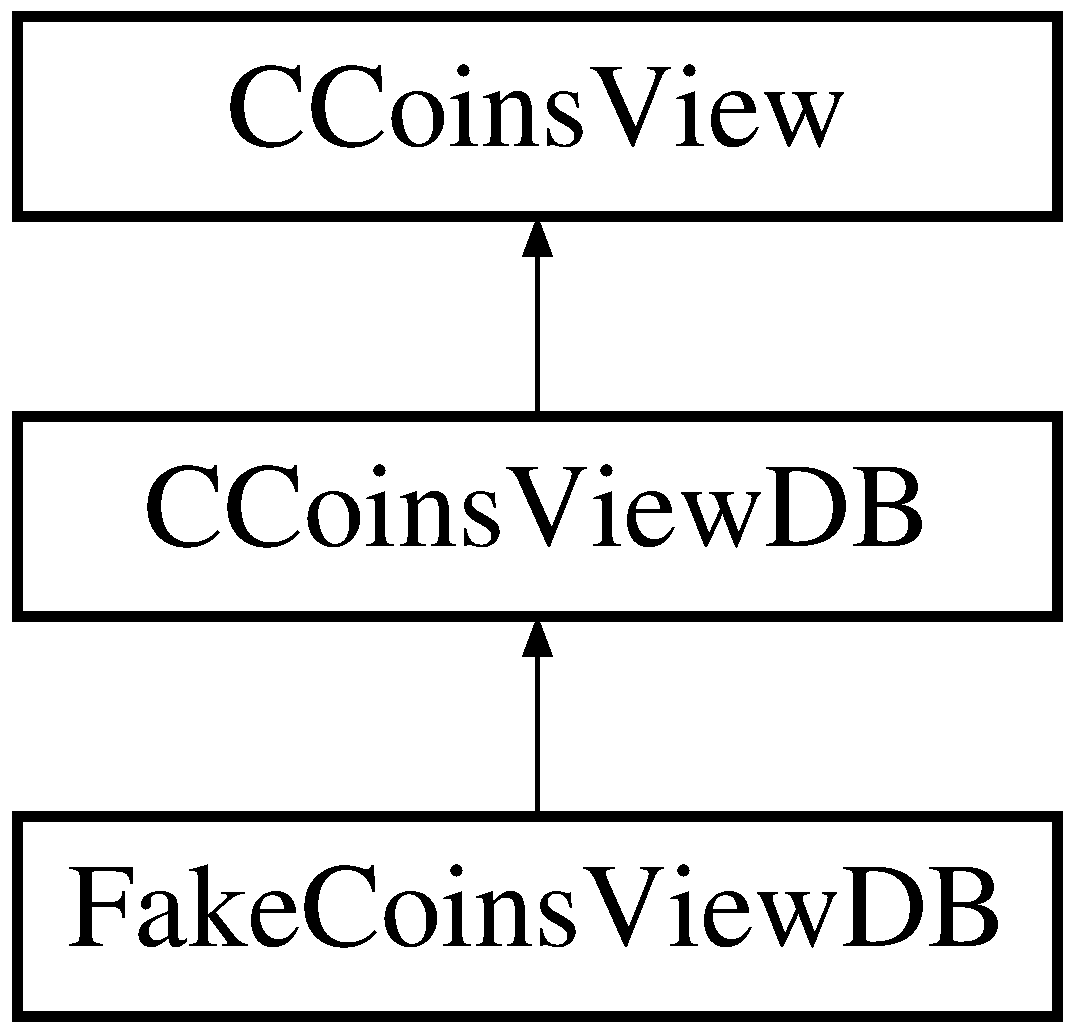
\includegraphics[height=3.000000cm]{class_c_coins_view_d_b}
\end{center}
\end{figure}
\subsection*{Public Member Functions}
\begin{DoxyCompactItemize}
\item 
\mbox{\hyperlink{class_c_coins_view_d_b_a209841b241febcccb2ec584b886ad374}{C\+Coins\+View\+DB}} (size\+\_\+t n\+Cache\+Size, bool f\+Memory=false, bool f\+Wipe=false)
\item 
bool \mbox{\hyperlink{class_c_coins_view_d_b_aeaab3bc4b363dbbc9d9a77930209e299}{Get\+Anchor\+At}} (const \mbox{\hyperlink{classuint256}{uint256}} \&rt, Z\+C\+Incremental\+Merkle\+Tree \&tree) const
\begin{DoxyCompactList}\small\item\em Retrieve the tree at a particular anchored root in the chain. \end{DoxyCompactList}\item 
bool \mbox{\hyperlink{class_c_coins_view_d_b_ac9724829164f5a06b6d7c610da03a730}{Get\+Nullifier}} (const \mbox{\hyperlink{classuint256}{uint256}} \&nf) const
\begin{DoxyCompactList}\small\item\em Determine whether a nullifier is spent or not. \end{DoxyCompactList}\item 
bool \mbox{\hyperlink{class_c_coins_view_d_b_ac35a80d1115ec697101d382e71db5b31}{Get\+Coins}} (const \mbox{\hyperlink{classuint256}{uint256}} \&txid, \mbox{\hyperlink{class_c_coins}{C\+Coins}} \&coins) const
\begin{DoxyCompactList}\small\item\em Retrieve the \mbox{\hyperlink{class_c_coins}{C\+Coins}} (unspent transaction outputs) for a given txid. \end{DoxyCompactList}\item 
bool \mbox{\hyperlink{class_c_coins_view_d_b_af55f35faadeb74b5406559fe3ed20114}{Have\+Coins}} (const \mbox{\hyperlink{classuint256}{uint256}} \&txid) const
\item 
\mbox{\hyperlink{classuint256}{uint256}} \mbox{\hyperlink{class_c_coins_view_d_b_ac9c513a34b9e58d942fdbeafd9e5bbce}{Get\+Best\+Block}} () const
\begin{DoxyCompactList}\small\item\em Retrieve the block hash whose state this \mbox{\hyperlink{class_c_coins_view}{C\+Coins\+View}} currently represents. \end{DoxyCompactList}\item 
\mbox{\hyperlink{classuint256}{uint256}} \mbox{\hyperlink{class_c_coins_view_d_b_a2bb7d73a96472def92e332a4563a689c}{Get\+Best\+Anchor}} () const
\begin{DoxyCompactList}\small\item\em Get the current \char`\"{}tip\char`\"{} or the latest anchored tree root in the chain. \end{DoxyCompactList}\item 
bool \mbox{\hyperlink{class_c_coins_view_d_b_ab617e4b898f06cec79a2a26fdca9efbd}{Batch\+Write}} (\mbox{\hyperlink{coins_8h_a2886ba2fd0428bae777e1cbcabc02834}{C\+Coins\+Map}} \&map\+Coins, const \mbox{\hyperlink{classuint256}{uint256}} \&hash\+Block, const \mbox{\hyperlink{classuint256}{uint256}} \&hash\+Anchor, \mbox{\hyperlink{coins_8h_a070827cc9d21a91b8f4f4f52a6f7c848}{C\+Anchors\+Map}} \&map\+Anchors, \mbox{\hyperlink{coins_8h_ab651cc287e9594190ef77d2fca2b14c7}{C\+Nullifiers\+Map}} \&map\+Nullifiers)
\item 
bool \mbox{\hyperlink{class_c_coins_view_d_b_a227bf56f8801921f12e56c6839104fce}{Get\+Stats}} (\mbox{\hyperlink{struct_c_coins_stats}{C\+Coins\+Stats}} \&stats) const
\begin{DoxyCompactList}\small\item\em Calculate statistics about the unspent transaction output set. \end{DoxyCompactList}\end{DoxyCompactItemize}
\subsection*{Protected Member Functions}
\begin{DoxyCompactItemize}
\item 
\mbox{\hyperlink{class_c_coins_view_d_b_a77de349a6beacdf07f0e4aab1bbdecbc}{C\+Coins\+View\+DB}} (std\+::string db\+Name, size\+\_\+t n\+Cache\+Size, bool f\+Memory=false, bool f\+Wipe=false)
\end{DoxyCompactItemize}
\subsection*{Protected Attributes}
\begin{DoxyCompactItemize}
\item 
\mbox{\hyperlink{class_c_level_d_b_wrapper}{C\+Level\+D\+B\+Wrapper}} \mbox{\hyperlink{class_c_coins_view_d_b_aba0a7b26fe82c1a2e80ca060d12fb66a}{db}}
\end{DoxyCompactItemize}


\subsection{Detailed Description}
\mbox{\hyperlink{class_c_coins_view}{C\+Coins\+View}} backed by the Level\+DB coin database (chainstate/) 

\subsection{Constructor \& Destructor Documentation}
\mbox{\Hypertarget{class_c_coins_view_d_b_a77de349a6beacdf07f0e4aab1bbdecbc}\label{class_c_coins_view_d_b_a77de349a6beacdf07f0e4aab1bbdecbc}} 
\index{C\+Coins\+View\+DB@{C\+Coins\+View\+DB}!C\+Coins\+View\+DB@{C\+Coins\+View\+DB}}
\index{C\+Coins\+View\+DB@{C\+Coins\+View\+DB}!C\+Coins\+View\+DB@{C\+Coins\+View\+DB}}
\subsubsection{\texorpdfstring{C\+Coins\+View\+D\+B()}{CCoinsViewDB()}\hspace{0.1cm}{\footnotesize\ttfamily [1/2]}}
{\footnotesize\ttfamily C\+Coins\+View\+D\+B\+::\+C\+Coins\+View\+DB (\begin{DoxyParamCaption}\item[{std\+::string}]{db\+Name,  }\item[{size\+\_\+t}]{n\+Cache\+Size,  }\item[{bool}]{f\+Memory = {\ttfamily false},  }\item[{bool}]{f\+Wipe = {\ttfamily false} }\end{DoxyParamCaption})\hspace{0.3cm}{\ttfamily [protected]}}

\mbox{\Hypertarget{class_c_coins_view_d_b_a209841b241febcccb2ec584b886ad374}\label{class_c_coins_view_d_b_a209841b241febcccb2ec584b886ad374}} 
\index{C\+Coins\+View\+DB@{C\+Coins\+View\+DB}!C\+Coins\+View\+DB@{C\+Coins\+View\+DB}}
\index{C\+Coins\+View\+DB@{C\+Coins\+View\+DB}!C\+Coins\+View\+DB@{C\+Coins\+View\+DB}}
\subsubsection{\texorpdfstring{C\+Coins\+View\+D\+B()}{CCoinsViewDB()}\hspace{0.1cm}{\footnotesize\ttfamily [2/2]}}
{\footnotesize\ttfamily C\+Coins\+View\+D\+B\+::\+C\+Coins\+View\+DB (\begin{DoxyParamCaption}\item[{size\+\_\+t}]{n\+Cache\+Size,  }\item[{bool}]{f\+Memory = {\ttfamily false},  }\item[{bool}]{f\+Wipe = {\ttfamily false} }\end{DoxyParamCaption})}



\subsection{Member Function Documentation}
\mbox{\Hypertarget{class_c_coins_view_d_b_ab617e4b898f06cec79a2a26fdca9efbd}\label{class_c_coins_view_d_b_ab617e4b898f06cec79a2a26fdca9efbd}} 
\index{C\+Coins\+View\+DB@{C\+Coins\+View\+DB}!Batch\+Write@{Batch\+Write}}
\index{Batch\+Write@{Batch\+Write}!C\+Coins\+View\+DB@{C\+Coins\+View\+DB}}
\subsubsection{\texorpdfstring{Batch\+Write()}{BatchWrite()}}
{\footnotesize\ttfamily bool C\+Coins\+View\+D\+B\+::\+Batch\+Write (\begin{DoxyParamCaption}\item[{\mbox{\hyperlink{coins_8h_a2886ba2fd0428bae777e1cbcabc02834}{C\+Coins\+Map}} \&}]{map\+Coins,  }\item[{const \mbox{\hyperlink{classuint256}{uint256}} \&}]{hash\+Block,  }\item[{const \mbox{\hyperlink{classuint256}{uint256}} \&}]{hash\+Anchor,  }\item[{\mbox{\hyperlink{coins_8h_a070827cc9d21a91b8f4f4f52a6f7c848}{C\+Anchors\+Map}} \&}]{map\+Anchors,  }\item[{\mbox{\hyperlink{coins_8h_ab651cc287e9594190ef77d2fca2b14c7}{C\+Nullifiers\+Map}} \&}]{map\+Nullifiers }\end{DoxyParamCaption})\hspace{0.3cm}{\ttfamily [virtual]}}

Do a bulk modification (multiple \mbox{\hyperlink{class_c_coins}{C\+Coins}} changes + Best\+Block change). The passed map\+Coins can be modified. 

Reimplemented from \mbox{\hyperlink{class_c_coins_view_a6e0ef2f996f5bf9f15c4fcae89333c7d}{C\+Coins\+View}}.



Reimplemented in \mbox{\hyperlink{class_fake_coins_view_d_b_a1108b45f9d165344c7378051e061147b}{Fake\+Coins\+View\+DB}}.

\mbox{\Hypertarget{class_c_coins_view_d_b_aeaab3bc4b363dbbc9d9a77930209e299}\label{class_c_coins_view_d_b_aeaab3bc4b363dbbc9d9a77930209e299}} 
\index{C\+Coins\+View\+DB@{C\+Coins\+View\+DB}!Get\+Anchor\+At@{Get\+Anchor\+At}}
\index{Get\+Anchor\+At@{Get\+Anchor\+At}!C\+Coins\+View\+DB@{C\+Coins\+View\+DB}}
\subsubsection{\texorpdfstring{Get\+Anchor\+At()}{GetAnchorAt()}}
{\footnotesize\ttfamily bool C\+Coins\+View\+D\+B\+::\+Get\+Anchor\+At (\begin{DoxyParamCaption}\item[{const \mbox{\hyperlink{classuint256}{uint256}} \&}]{rt,  }\item[{Z\+C\+Incremental\+Merkle\+Tree \&}]{tree }\end{DoxyParamCaption}) const\hspace{0.3cm}{\ttfamily [virtual]}}



Retrieve the tree at a particular anchored root in the chain. 



Reimplemented from \mbox{\hyperlink{class_c_coins_view_a2fcf3f99111eef1c41243f54f94d3be8}{C\+Coins\+View}}.



Reimplemented in \mbox{\hyperlink{class_fake_coins_view_d_b_ae52d0073bef3eb64bd64b325e821c52b}{Fake\+Coins\+View\+DB}}.

\mbox{\Hypertarget{class_c_coins_view_d_b_a2bb7d73a96472def92e332a4563a689c}\label{class_c_coins_view_d_b_a2bb7d73a96472def92e332a4563a689c}} 
\index{C\+Coins\+View\+DB@{C\+Coins\+View\+DB}!Get\+Best\+Anchor@{Get\+Best\+Anchor}}
\index{Get\+Best\+Anchor@{Get\+Best\+Anchor}!C\+Coins\+View\+DB@{C\+Coins\+View\+DB}}
\subsubsection{\texorpdfstring{Get\+Best\+Anchor()}{GetBestAnchor()}}
{\footnotesize\ttfamily \mbox{\hyperlink{classuint256}{uint256}} C\+Coins\+View\+D\+B\+::\+Get\+Best\+Anchor (\begin{DoxyParamCaption}{ }\end{DoxyParamCaption}) const\hspace{0.3cm}{\ttfamily [virtual]}}



Get the current \char`\"{}tip\char`\"{} or the latest anchored tree root in the chain. 



Reimplemented from \mbox{\hyperlink{class_c_coins_view_a4d51ab1de57e76a174b5ca874c601b52}{C\+Coins\+View}}.



Reimplemented in \mbox{\hyperlink{class_fake_coins_view_d_b_af7870faf849e59188344273a03c9a1b0}{Fake\+Coins\+View\+DB}}.

\mbox{\Hypertarget{class_c_coins_view_d_b_ac9c513a34b9e58d942fdbeafd9e5bbce}\label{class_c_coins_view_d_b_ac9c513a34b9e58d942fdbeafd9e5bbce}} 
\index{C\+Coins\+View\+DB@{C\+Coins\+View\+DB}!Get\+Best\+Block@{Get\+Best\+Block}}
\index{Get\+Best\+Block@{Get\+Best\+Block}!C\+Coins\+View\+DB@{C\+Coins\+View\+DB}}
\subsubsection{\texorpdfstring{Get\+Best\+Block()}{GetBestBlock()}}
{\footnotesize\ttfamily \mbox{\hyperlink{classuint256}{uint256}} C\+Coins\+View\+D\+B\+::\+Get\+Best\+Block (\begin{DoxyParamCaption}{ }\end{DoxyParamCaption}) const\hspace{0.3cm}{\ttfamily [virtual]}}



Retrieve the block hash whose state this \mbox{\hyperlink{class_c_coins_view}{C\+Coins\+View}} currently represents. 



Reimplemented from \mbox{\hyperlink{class_c_coins_view_af81f2907d360a2548d59a61388e5e5cb}{C\+Coins\+View}}.



Reimplemented in \mbox{\hyperlink{class_fake_coins_view_d_b_a36231d924114fbe51a830c9c235c50ad}{Fake\+Coins\+View\+DB}}.

\mbox{\Hypertarget{class_c_coins_view_d_b_ac35a80d1115ec697101d382e71db5b31}\label{class_c_coins_view_d_b_ac35a80d1115ec697101d382e71db5b31}} 
\index{C\+Coins\+View\+DB@{C\+Coins\+View\+DB}!Get\+Coins@{Get\+Coins}}
\index{Get\+Coins@{Get\+Coins}!C\+Coins\+View\+DB@{C\+Coins\+View\+DB}}
\subsubsection{\texorpdfstring{Get\+Coins()}{GetCoins()}}
{\footnotesize\ttfamily bool C\+Coins\+View\+D\+B\+::\+Get\+Coins (\begin{DoxyParamCaption}\item[{const \mbox{\hyperlink{classuint256}{uint256}} \&}]{txid,  }\item[{\mbox{\hyperlink{class_c_coins}{C\+Coins}} \&}]{coins }\end{DoxyParamCaption}) const\hspace{0.3cm}{\ttfamily [virtual]}}



Retrieve the \mbox{\hyperlink{class_c_coins}{C\+Coins}} (unspent transaction outputs) for a given txid. 



Reimplemented from \mbox{\hyperlink{class_c_coins_view_a67d865358127bef1f0011a23d5158a9f}{C\+Coins\+View}}.

\mbox{\Hypertarget{class_c_coins_view_d_b_ac9724829164f5a06b6d7c610da03a730}\label{class_c_coins_view_d_b_ac9724829164f5a06b6d7c610da03a730}} 
\index{C\+Coins\+View\+DB@{C\+Coins\+View\+DB}!Get\+Nullifier@{Get\+Nullifier}}
\index{Get\+Nullifier@{Get\+Nullifier}!C\+Coins\+View\+DB@{C\+Coins\+View\+DB}}
\subsubsection{\texorpdfstring{Get\+Nullifier()}{GetNullifier()}}
{\footnotesize\ttfamily bool C\+Coins\+View\+D\+B\+::\+Get\+Nullifier (\begin{DoxyParamCaption}\item[{const \mbox{\hyperlink{classuint256}{uint256}} \&}]{nullifier }\end{DoxyParamCaption}) const\hspace{0.3cm}{\ttfamily [virtual]}}



Determine whether a nullifier is spent or not. 



Reimplemented from \mbox{\hyperlink{class_c_coins_view_a45a7abe02d0d9d1b61a09dec70a3311f}{C\+Coins\+View}}.



Reimplemented in \mbox{\hyperlink{class_fake_coins_view_d_b_af7d0ce4926fb03ee632148c5fde66c05}{Fake\+Coins\+View\+DB}}.

\mbox{\Hypertarget{class_c_coins_view_d_b_a227bf56f8801921f12e56c6839104fce}\label{class_c_coins_view_d_b_a227bf56f8801921f12e56c6839104fce}} 
\index{C\+Coins\+View\+DB@{C\+Coins\+View\+DB}!Get\+Stats@{Get\+Stats}}
\index{Get\+Stats@{Get\+Stats}!C\+Coins\+View\+DB@{C\+Coins\+View\+DB}}
\subsubsection{\texorpdfstring{Get\+Stats()}{GetStats()}}
{\footnotesize\ttfamily bool C\+Coins\+View\+D\+B\+::\+Get\+Stats (\begin{DoxyParamCaption}\item[{\mbox{\hyperlink{struct_c_coins_stats}{C\+Coins\+Stats}} \&}]{stats }\end{DoxyParamCaption}) const\hspace{0.3cm}{\ttfamily [virtual]}}



Calculate statistics about the unspent transaction output set. 



Reimplemented from \mbox{\hyperlink{class_c_coins_view_adbd7f73ba071c6e441dd88d95b8f2c0d}{C\+Coins\+View}}.



Reimplemented in \mbox{\hyperlink{class_fake_coins_view_d_b_ad1deefbe955925e274e5d50d289275e9}{Fake\+Coins\+View\+DB}}.

\mbox{\Hypertarget{class_c_coins_view_d_b_af55f35faadeb74b5406559fe3ed20114}\label{class_c_coins_view_d_b_af55f35faadeb74b5406559fe3ed20114}} 
\index{C\+Coins\+View\+DB@{C\+Coins\+View\+DB}!Have\+Coins@{Have\+Coins}}
\index{Have\+Coins@{Have\+Coins}!C\+Coins\+View\+DB@{C\+Coins\+View\+DB}}
\subsubsection{\texorpdfstring{Have\+Coins()}{HaveCoins()}}
{\footnotesize\ttfamily bool C\+Coins\+View\+D\+B\+::\+Have\+Coins (\begin{DoxyParamCaption}\item[{const \mbox{\hyperlink{classuint256}{uint256}} \&}]{txid }\end{DoxyParamCaption}) const\hspace{0.3cm}{\ttfamily [virtual]}}

Just check whether we have data for a given txid. This may (but cannot always) return true for fully spent transactions 

Reimplemented from \mbox{\hyperlink{class_c_coins_view_ade3a65fc3f1b02baf7bebce630e4eba3}{C\+Coins\+View}}.



\subsection{Member Data Documentation}
\mbox{\Hypertarget{class_c_coins_view_d_b_aba0a7b26fe82c1a2e80ca060d12fb66a}\label{class_c_coins_view_d_b_aba0a7b26fe82c1a2e80ca060d12fb66a}} 
\index{C\+Coins\+View\+DB@{C\+Coins\+View\+DB}!db@{db}}
\index{db@{db}!C\+Coins\+View\+DB@{C\+Coins\+View\+DB}}
\subsubsection{\texorpdfstring{db}{db}}
{\footnotesize\ttfamily \mbox{\hyperlink{class_c_level_d_b_wrapper}{C\+Level\+D\+B\+Wrapper}} C\+Coins\+View\+D\+B\+::db\hspace{0.3cm}{\ttfamily [protected]}}



The documentation for this class was generated from the following files\+:\begin{DoxyCompactItemize}
\item 
/\+Users/christopherarguello/\+Developer/anon/src/\mbox{\hyperlink{txdb_8h}{txdb.\+h}}\item 
/\+Users/christopherarguello/\+Developer/anon/src/\mbox{\hyperlink{txdb_8cpp}{txdb.\+cpp}}\end{DoxyCompactItemize}

\hypertarget{class_c_coins_view_error_catcher}{}\section{C\+Coins\+View\+Error\+Catcher Class Reference}
\label{class_c_coins_view_error_catcher}\index{C\+Coins\+View\+Error\+Catcher@{C\+Coins\+View\+Error\+Catcher}}
Inheritance diagram for C\+Coins\+View\+Error\+Catcher\+:\begin{figure}[H]
\begin{center}
\leavevmode
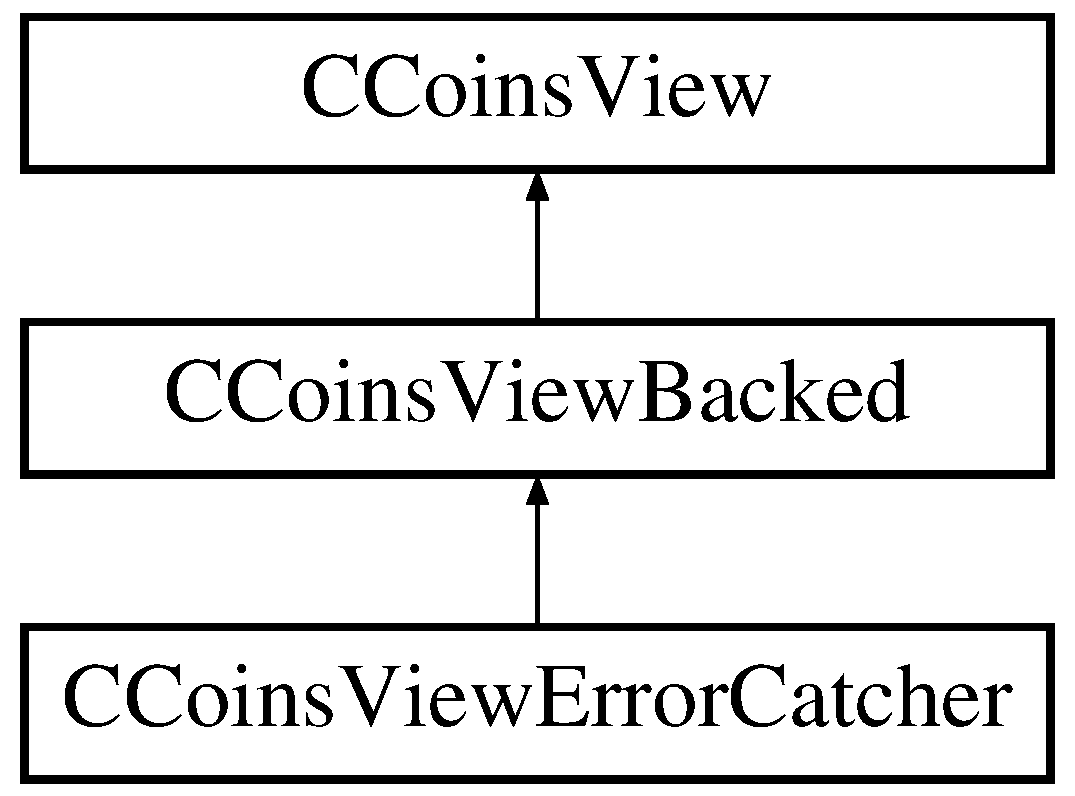
\includegraphics[height=3.000000cm]{class_c_coins_view_error_catcher}
\end{center}
\end{figure}
\subsection*{Public Member Functions}
\begin{DoxyCompactItemize}
\item 
\mbox{\hyperlink{class_c_coins_view_error_catcher_aa8295e2f5ce5ad9880c5bd86d52e014c}{C\+Coins\+View\+Error\+Catcher}} (\mbox{\hyperlink{class_c_coins_view}{C\+Coins\+View}} $\ast$view)
\item 
bool \mbox{\hyperlink{class_c_coins_view_error_catcher_a909f7b9e364b6f06bfea955209aa015d}{Get\+Coins}} (const \mbox{\hyperlink{classuint256}{uint256}} \&txid, \mbox{\hyperlink{class_c_coins}{C\+Coins}} \&coins) const
\begin{DoxyCompactList}\small\item\em Retrieve the \mbox{\hyperlink{class_c_coins}{C\+Coins}} (unspent transaction outputs) for a given txid. \end{DoxyCompactList}\end{DoxyCompactItemize}
\subsection*{Additional Inherited Members}


\subsection{Constructor \& Destructor Documentation}
\mbox{\Hypertarget{class_c_coins_view_error_catcher_aa8295e2f5ce5ad9880c5bd86d52e014c}\label{class_c_coins_view_error_catcher_aa8295e2f5ce5ad9880c5bd86d52e014c}} 
\index{C\+Coins\+View\+Error\+Catcher@{C\+Coins\+View\+Error\+Catcher}!C\+Coins\+View\+Error\+Catcher@{C\+Coins\+View\+Error\+Catcher}}
\index{C\+Coins\+View\+Error\+Catcher@{C\+Coins\+View\+Error\+Catcher}!C\+Coins\+View\+Error\+Catcher@{C\+Coins\+View\+Error\+Catcher}}
\subsubsection{\texorpdfstring{C\+Coins\+View\+Error\+Catcher()}{CCoinsViewErrorCatcher()}}
{\footnotesize\ttfamily C\+Coins\+View\+Error\+Catcher\+::\+C\+Coins\+View\+Error\+Catcher (\begin{DoxyParamCaption}\item[{\mbox{\hyperlink{class_c_coins_view}{C\+Coins\+View}} $\ast$}]{view }\end{DoxyParamCaption})\hspace{0.3cm}{\ttfamily [inline]}}



\subsection{Member Function Documentation}
\mbox{\Hypertarget{class_c_coins_view_error_catcher_a909f7b9e364b6f06bfea955209aa015d}\label{class_c_coins_view_error_catcher_a909f7b9e364b6f06bfea955209aa015d}} 
\index{C\+Coins\+View\+Error\+Catcher@{C\+Coins\+View\+Error\+Catcher}!Get\+Coins@{Get\+Coins}}
\index{Get\+Coins@{Get\+Coins}!C\+Coins\+View\+Error\+Catcher@{C\+Coins\+View\+Error\+Catcher}}
\subsubsection{\texorpdfstring{Get\+Coins()}{GetCoins()}}
{\footnotesize\ttfamily bool C\+Coins\+View\+Error\+Catcher\+::\+Get\+Coins (\begin{DoxyParamCaption}\item[{const \mbox{\hyperlink{classuint256}{uint256}} \&}]{txid,  }\item[{\mbox{\hyperlink{class_c_coins}{C\+Coins}} \&}]{coins }\end{DoxyParamCaption}) const\hspace{0.3cm}{\ttfamily [inline]}, {\ttfamily [virtual]}}



Retrieve the \mbox{\hyperlink{class_c_coins}{C\+Coins}} (unspent transaction outputs) for a given txid. 



Reimplemented from \mbox{\hyperlink{class_c_coins_view_backed_a456f9e85817556329a959c120998df5b}{C\+Coins\+View\+Backed}}.



The documentation for this class was generated from the following file\+:\begin{DoxyCompactItemize}
\item 
/\+Users/christopherarguello/\+Developer/anon/src/\mbox{\hyperlink{init_8cpp}{init.\+cpp}}\end{DoxyCompactItemize}

\hypertarget{class_c_coins_view_mem_pool}{}\section{C\+Coins\+View\+Mem\+Pool Class Reference}
\label{class_c_coins_view_mem_pool}\index{C\+Coins\+View\+Mem\+Pool@{C\+Coins\+View\+Mem\+Pool}}


{\ttfamily \#include $<$txmempool.\+h$>$}

Inheritance diagram for C\+Coins\+View\+Mem\+Pool\+:\begin{figure}[H]
\begin{center}
\leavevmode
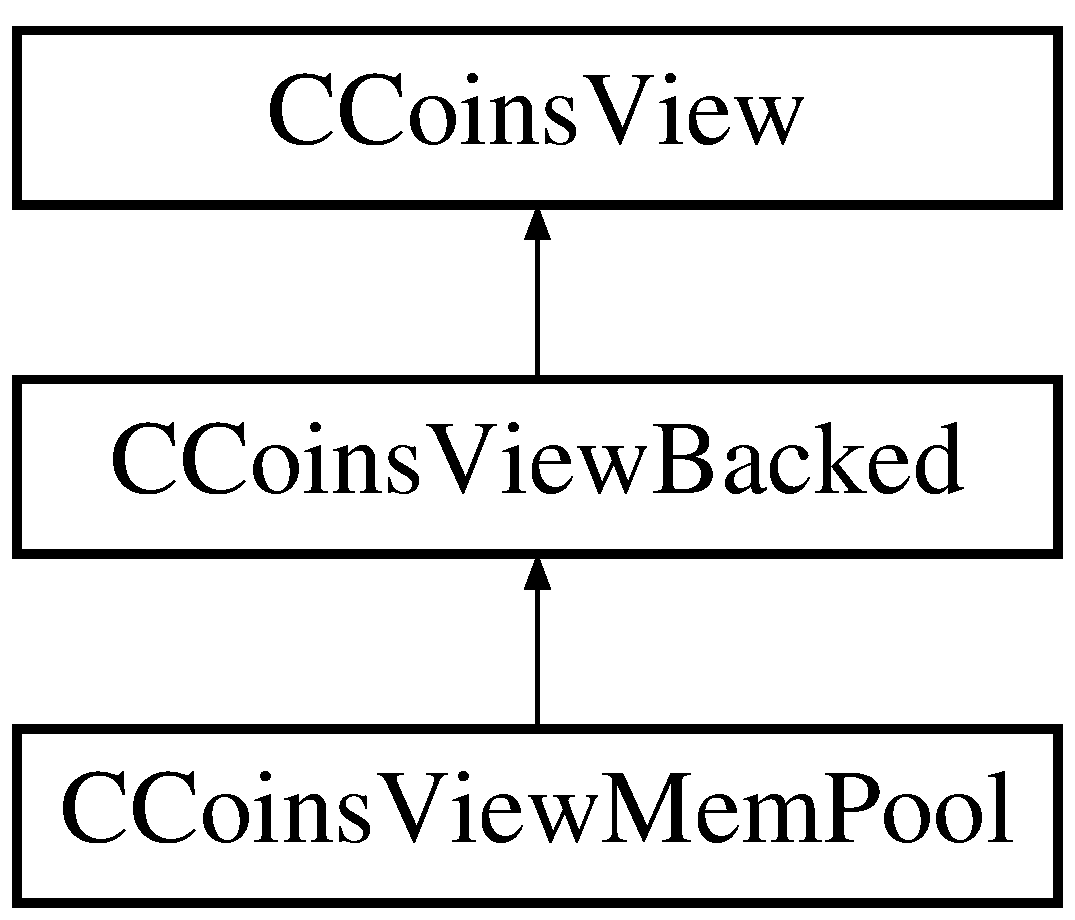
\includegraphics[height=3.000000cm]{class_c_coins_view_mem_pool}
\end{center}
\end{figure}
\subsection*{Public Member Functions}
\begin{DoxyCompactItemize}
\item 
\mbox{\hyperlink{class_c_coins_view_mem_pool_aab9a206c304acec322fddf646c7bafb9}{C\+Coins\+View\+Mem\+Pool}} (\mbox{\hyperlink{class_c_coins_view}{C\+Coins\+View}} $\ast$base\+In, \mbox{\hyperlink{class_c_tx_mem_pool}{C\+Tx\+Mem\+Pool}} \&mempool\+In)
\item 
bool \mbox{\hyperlink{class_c_coins_view_mem_pool_ac76524f89eb1a8c25e3c6c3201d3662a}{Get\+Nullifier}} (const \mbox{\hyperlink{classuint256}{uint256}} \&txid) const
\begin{DoxyCompactList}\small\item\em Determine whether a nullifier is spent or not. \end{DoxyCompactList}\item 
bool \mbox{\hyperlink{class_c_coins_view_mem_pool_a1a4a556821b1680ff4b73758c8a1e471}{Get\+Coins}} (const \mbox{\hyperlink{classuint256}{uint256}} \&txid, \mbox{\hyperlink{class_c_coins}{C\+Coins}} \&coins) const
\begin{DoxyCompactList}\small\item\em Retrieve the \mbox{\hyperlink{class_c_coins}{C\+Coins}} (unspent transaction outputs) for a given txid. \end{DoxyCompactList}\item 
bool \mbox{\hyperlink{class_c_coins_view_mem_pool_a2c5900448dc5570053060686ad1f014b}{Have\+Coins}} (const \mbox{\hyperlink{classuint256}{uint256}} \&txid) const
\end{DoxyCompactItemize}
\subsection*{Protected Attributes}
\begin{DoxyCompactItemize}
\item 
\mbox{\hyperlink{class_c_tx_mem_pool}{C\+Tx\+Mem\+Pool}} \& \mbox{\hyperlink{class_c_coins_view_mem_pool_a7a3870fc65376cb311a0b3abb28fec10}{mempool}}
\end{DoxyCompactItemize}


\subsection{Detailed Description}
\mbox{\hyperlink{class_c_coins_view}{C\+Coins\+View}} that brings transactions from a memorypool into view. It does not check for spendings by memory pool transactions. 

\subsection{Constructor \& Destructor Documentation}
\mbox{\Hypertarget{class_c_coins_view_mem_pool_aab9a206c304acec322fddf646c7bafb9}\label{class_c_coins_view_mem_pool_aab9a206c304acec322fddf646c7bafb9}} 
\index{C\+Coins\+View\+Mem\+Pool@{C\+Coins\+View\+Mem\+Pool}!C\+Coins\+View\+Mem\+Pool@{C\+Coins\+View\+Mem\+Pool}}
\index{C\+Coins\+View\+Mem\+Pool@{C\+Coins\+View\+Mem\+Pool}!C\+Coins\+View\+Mem\+Pool@{C\+Coins\+View\+Mem\+Pool}}
\subsubsection{\texorpdfstring{C\+Coins\+View\+Mem\+Pool()}{CCoinsViewMemPool()}}
{\footnotesize\ttfamily C\+Coins\+View\+Mem\+Pool\+::\+C\+Coins\+View\+Mem\+Pool (\begin{DoxyParamCaption}\item[{\mbox{\hyperlink{class_c_coins_view}{C\+Coins\+View}} $\ast$}]{base\+In,  }\item[{\mbox{\hyperlink{class_c_tx_mem_pool}{C\+Tx\+Mem\+Pool}} \&}]{mempool\+In }\end{DoxyParamCaption})}



\subsection{Member Function Documentation}
\mbox{\Hypertarget{class_c_coins_view_mem_pool_a1a4a556821b1680ff4b73758c8a1e471}\label{class_c_coins_view_mem_pool_a1a4a556821b1680ff4b73758c8a1e471}} 
\index{C\+Coins\+View\+Mem\+Pool@{C\+Coins\+View\+Mem\+Pool}!Get\+Coins@{Get\+Coins}}
\index{Get\+Coins@{Get\+Coins}!C\+Coins\+View\+Mem\+Pool@{C\+Coins\+View\+Mem\+Pool}}
\subsubsection{\texorpdfstring{Get\+Coins()}{GetCoins()}}
{\footnotesize\ttfamily bool C\+Coins\+View\+Mem\+Pool\+::\+Get\+Coins (\begin{DoxyParamCaption}\item[{const \mbox{\hyperlink{classuint256}{uint256}} \&}]{txid,  }\item[{\mbox{\hyperlink{class_c_coins}{C\+Coins}} \&}]{coins }\end{DoxyParamCaption}) const\hspace{0.3cm}{\ttfamily [virtual]}}



Retrieve the \mbox{\hyperlink{class_c_coins}{C\+Coins}} (unspent transaction outputs) for a given txid. 



Reimplemented from \mbox{\hyperlink{class_c_coins_view_backed_a456f9e85817556329a959c120998df5b}{C\+Coins\+View\+Backed}}.

\mbox{\Hypertarget{class_c_coins_view_mem_pool_ac76524f89eb1a8c25e3c6c3201d3662a}\label{class_c_coins_view_mem_pool_ac76524f89eb1a8c25e3c6c3201d3662a}} 
\index{C\+Coins\+View\+Mem\+Pool@{C\+Coins\+View\+Mem\+Pool}!Get\+Nullifier@{Get\+Nullifier}}
\index{Get\+Nullifier@{Get\+Nullifier}!C\+Coins\+View\+Mem\+Pool@{C\+Coins\+View\+Mem\+Pool}}
\subsubsection{\texorpdfstring{Get\+Nullifier()}{GetNullifier()}}
{\footnotesize\ttfamily bool C\+Coins\+View\+Mem\+Pool\+::\+Get\+Nullifier (\begin{DoxyParamCaption}\item[{const \mbox{\hyperlink{classuint256}{uint256}} \&}]{nullifier }\end{DoxyParamCaption}) const\hspace{0.3cm}{\ttfamily [virtual]}}



Determine whether a nullifier is spent or not. 



Reimplemented from \mbox{\hyperlink{class_c_coins_view_backed_afbfee79b18b475d67cd757a7dc4f5955}{C\+Coins\+View\+Backed}}.

\mbox{\Hypertarget{class_c_coins_view_mem_pool_a2c5900448dc5570053060686ad1f014b}\label{class_c_coins_view_mem_pool_a2c5900448dc5570053060686ad1f014b}} 
\index{C\+Coins\+View\+Mem\+Pool@{C\+Coins\+View\+Mem\+Pool}!Have\+Coins@{Have\+Coins}}
\index{Have\+Coins@{Have\+Coins}!C\+Coins\+View\+Mem\+Pool@{C\+Coins\+View\+Mem\+Pool}}
\subsubsection{\texorpdfstring{Have\+Coins()}{HaveCoins()}}
{\footnotesize\ttfamily bool C\+Coins\+View\+Mem\+Pool\+::\+Have\+Coins (\begin{DoxyParamCaption}\item[{const \mbox{\hyperlink{classuint256}{uint256}} \&}]{txid }\end{DoxyParamCaption}) const\hspace{0.3cm}{\ttfamily [virtual]}}

Just check whether we have data for a given txid. This may (but cannot always) return true for fully spent transactions 

Reimplemented from \mbox{\hyperlink{class_c_coins_view_backed_ad49041658bdec807d556e080476e6543}{C\+Coins\+View\+Backed}}.



\subsection{Member Data Documentation}
\mbox{\Hypertarget{class_c_coins_view_mem_pool_a7a3870fc65376cb311a0b3abb28fec10}\label{class_c_coins_view_mem_pool_a7a3870fc65376cb311a0b3abb28fec10}} 
\index{C\+Coins\+View\+Mem\+Pool@{C\+Coins\+View\+Mem\+Pool}!mempool@{mempool}}
\index{mempool@{mempool}!C\+Coins\+View\+Mem\+Pool@{C\+Coins\+View\+Mem\+Pool}}
\subsubsection{\texorpdfstring{mempool}{mempool}}
{\footnotesize\ttfamily \mbox{\hyperlink{class_c_tx_mem_pool}{C\+Tx\+Mem\+Pool}}\& C\+Coins\+View\+Mem\+Pool\+::mempool\hspace{0.3cm}{\ttfamily [protected]}}



The documentation for this class was generated from the following files\+:\begin{DoxyCompactItemize}
\item 
/\+Users/christopherarguello/\+Developer/anon/src/\mbox{\hyperlink{txmempool_8h}{txmempool.\+h}}\item 
/\+Users/christopherarguello/\+Developer/anon/src/\mbox{\hyperlink{txmempool_8cpp}{txmempool.\+cpp}}\end{DoxyCompactItemize}

\hypertarget{class_c_connection_failed}{}\section{C\+Connection\+Failed Class Reference}
\label{class_c_connection_failed}\index{C\+Connection\+Failed@{C\+Connection\+Failed}}
Inheritance diagram for C\+Connection\+Failed\+:\begin{figure}[H]
\begin{center}
\leavevmode
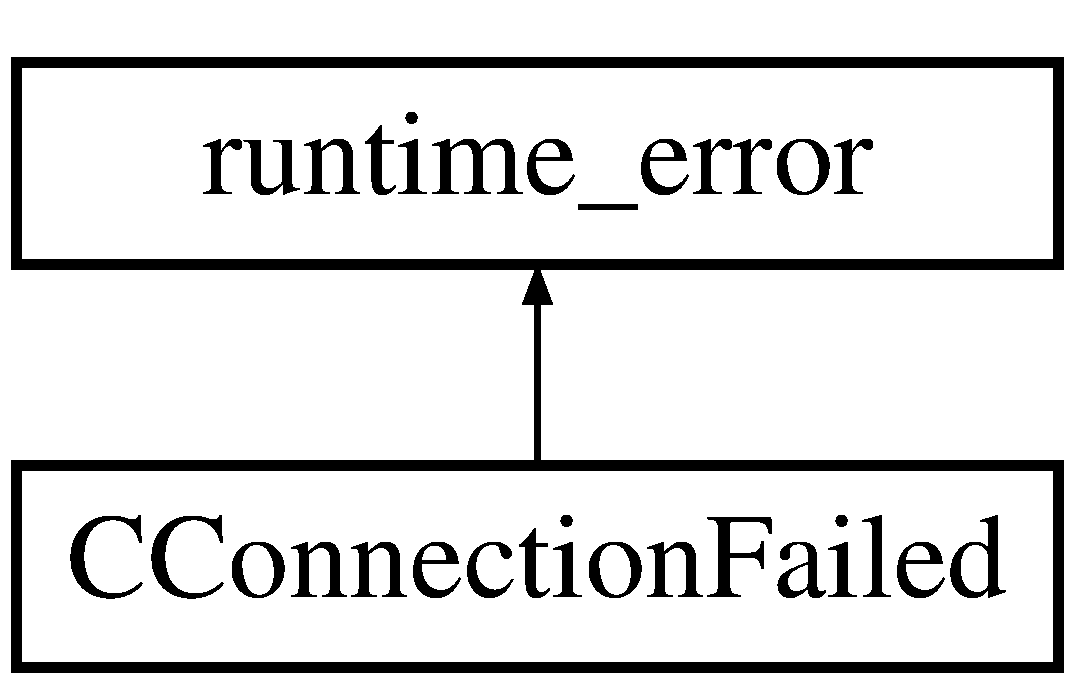
\includegraphics[height=2.000000cm]{class_c_connection_failed}
\end{center}
\end{figure}
\subsection*{Public Member Functions}
\begin{DoxyCompactItemize}
\item 
\mbox{\hyperlink{class_c_connection_failed_abcc9db4386ec901f5159c44d939c82c5}{C\+Connection\+Failed}} (const std\+::string \&msg)
\end{DoxyCompactItemize}


\subsection{Constructor \& Destructor Documentation}
\mbox{\Hypertarget{class_c_connection_failed_abcc9db4386ec901f5159c44d939c82c5}\label{class_c_connection_failed_abcc9db4386ec901f5159c44d939c82c5}} 
\index{C\+Connection\+Failed@{C\+Connection\+Failed}!C\+Connection\+Failed@{C\+Connection\+Failed}}
\index{C\+Connection\+Failed@{C\+Connection\+Failed}!C\+Connection\+Failed@{C\+Connection\+Failed}}
\subsubsection{\texorpdfstring{C\+Connection\+Failed()}{CConnectionFailed()}}
{\footnotesize\ttfamily C\+Connection\+Failed\+::\+C\+Connection\+Failed (\begin{DoxyParamCaption}\item[{const std\+::string \&}]{msg }\end{DoxyParamCaption})\hspace{0.3cm}{\ttfamily [inline]}, {\ttfamily [explicit]}}



The documentation for this class was generated from the following file\+:\begin{DoxyCompactItemize}
\item 
/\+Users/christopherarguello/\+Developer/anon/src/\mbox{\hyperlink{bitcoin-cli_8cpp}{bitcoin-\/cli.\+cpp}}\end{DoxyCompactItemize}

\hypertarget{class_c_data_stream}{}\section{C\+Data\+Stream Class Reference}
\label{class_c_data_stream}\index{C\+Data\+Stream@{C\+Data\+Stream}}


{\ttfamily \#include $<$streams.\+h$>$}

Inheritance diagram for C\+Data\+Stream\+:\begin{figure}[H]
\begin{center}
\leavevmode
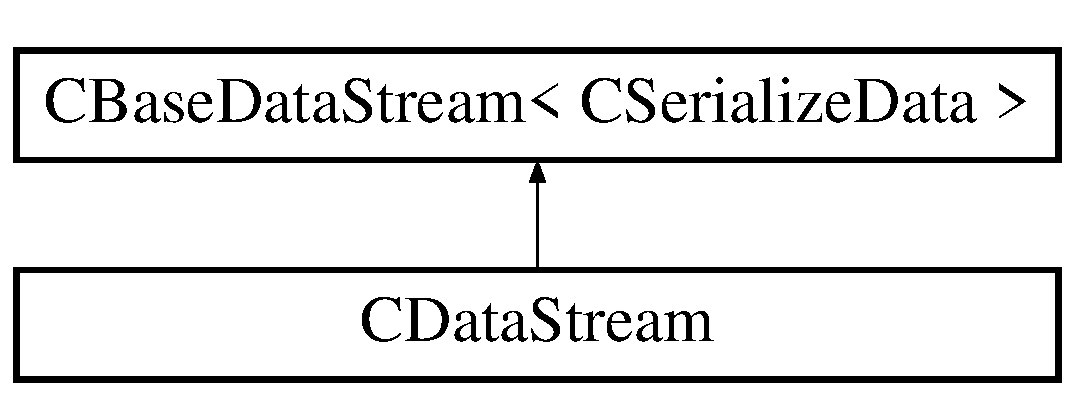
\includegraphics[height=2.000000cm]{class_c_data_stream}
\end{center}
\end{figure}
\subsection*{Public Member Functions}
\begin{DoxyCompactItemize}
\item 
\mbox{\hyperlink{class_c_data_stream_a38f4d7d2ae59566a0500523a1b1a49d4}{C\+Data\+Stream}} (int n\+Type\+In, int n\+Version\+In)
\item 
\mbox{\hyperlink{class_c_data_stream_a00d23d0ef651cb4ea54cb37009bdf8f2}{C\+Data\+Stream}} (\mbox{\hyperlink{class_c_base_data_stream_a9cf3080c5a75c94568980a59d3aab3ad}{const\+\_\+iterator}} pbegin, \mbox{\hyperlink{class_c_base_data_stream_a9cf3080c5a75c94568980a59d3aab3ad}{const\+\_\+iterator}} pend, int n\+Type\+In, int n\+Version\+In)
\item 
\mbox{\hyperlink{class_c_data_stream_ab345d2edd7bef6c6c140a46621e49eee}{C\+Data\+Stream}} (const char $\ast$pbegin, const char $\ast$pend, int n\+Type\+In, int n\+Version\+In)
\item 
\mbox{\hyperlink{class_c_data_stream_a38a51fefce23374963516b3af03638fc}{C\+Data\+Stream}} (const \mbox{\hyperlink{class_c_base_data_stream_a035e97a3e024a8cfa4690eaca1e5e290}{vector\+\_\+type}} \&vch\+In, int n\+Type\+In, int n\+Version\+In)
\item 
\mbox{\hyperlink{class_c_data_stream_a46219676397ae7b3cbc0c676f74ba1e7}{C\+Data\+Stream}} (const std\+::vector$<$ char $>$ \&vch\+In, int n\+Type\+In, int n\+Version\+In)
\item 
\mbox{\hyperlink{class_c_data_stream_ac63bd3d0ecce0edc2aa66cc80b633b6f}{C\+Data\+Stream}} (const std\+::vector$<$ unsigned char $>$ \&vch\+In, int n\+Type\+In, int n\+Version\+In)
\end{DoxyCompactItemize}
\subsection*{Additional Inherited Members}


\subsection{Constructor \& Destructor Documentation}
\mbox{\Hypertarget{class_c_data_stream_a38f4d7d2ae59566a0500523a1b1a49d4}\label{class_c_data_stream_a38f4d7d2ae59566a0500523a1b1a49d4}} 
\index{C\+Data\+Stream@{C\+Data\+Stream}!C\+Data\+Stream@{C\+Data\+Stream}}
\index{C\+Data\+Stream@{C\+Data\+Stream}!C\+Data\+Stream@{C\+Data\+Stream}}
\subsubsection{\texorpdfstring{C\+Data\+Stream()}{CDataStream()}\hspace{0.1cm}{\footnotesize\ttfamily [1/6]}}
{\footnotesize\ttfamily C\+Data\+Stream\+::\+C\+Data\+Stream (\begin{DoxyParamCaption}\item[{int}]{n\+Type\+In,  }\item[{int}]{n\+Version\+In }\end{DoxyParamCaption})\hspace{0.3cm}{\ttfamily [inline]}, {\ttfamily [explicit]}}

\mbox{\Hypertarget{class_c_data_stream_a00d23d0ef651cb4ea54cb37009bdf8f2}\label{class_c_data_stream_a00d23d0ef651cb4ea54cb37009bdf8f2}} 
\index{C\+Data\+Stream@{C\+Data\+Stream}!C\+Data\+Stream@{C\+Data\+Stream}}
\index{C\+Data\+Stream@{C\+Data\+Stream}!C\+Data\+Stream@{C\+Data\+Stream}}
\subsubsection{\texorpdfstring{C\+Data\+Stream()}{CDataStream()}\hspace{0.1cm}{\footnotesize\ttfamily [2/6]}}
{\footnotesize\ttfamily C\+Data\+Stream\+::\+C\+Data\+Stream (\begin{DoxyParamCaption}\item[{\mbox{\hyperlink{class_c_base_data_stream_a9cf3080c5a75c94568980a59d3aab3ad}{const\+\_\+iterator}}}]{pbegin,  }\item[{\mbox{\hyperlink{class_c_base_data_stream_a9cf3080c5a75c94568980a59d3aab3ad}{const\+\_\+iterator}}}]{pend,  }\item[{int}]{n\+Type\+In,  }\item[{int}]{n\+Version\+In }\end{DoxyParamCaption})\hspace{0.3cm}{\ttfamily [inline]}}

\mbox{\Hypertarget{class_c_data_stream_ab345d2edd7bef6c6c140a46621e49eee}\label{class_c_data_stream_ab345d2edd7bef6c6c140a46621e49eee}} 
\index{C\+Data\+Stream@{C\+Data\+Stream}!C\+Data\+Stream@{C\+Data\+Stream}}
\index{C\+Data\+Stream@{C\+Data\+Stream}!C\+Data\+Stream@{C\+Data\+Stream}}
\subsubsection{\texorpdfstring{C\+Data\+Stream()}{CDataStream()}\hspace{0.1cm}{\footnotesize\ttfamily [3/6]}}
{\footnotesize\ttfamily C\+Data\+Stream\+::\+C\+Data\+Stream (\begin{DoxyParamCaption}\item[{const char $\ast$}]{pbegin,  }\item[{const char $\ast$}]{pend,  }\item[{int}]{n\+Type\+In,  }\item[{int}]{n\+Version\+In }\end{DoxyParamCaption})\hspace{0.3cm}{\ttfamily [inline]}}

\mbox{\Hypertarget{class_c_data_stream_a38a51fefce23374963516b3af03638fc}\label{class_c_data_stream_a38a51fefce23374963516b3af03638fc}} 
\index{C\+Data\+Stream@{C\+Data\+Stream}!C\+Data\+Stream@{C\+Data\+Stream}}
\index{C\+Data\+Stream@{C\+Data\+Stream}!C\+Data\+Stream@{C\+Data\+Stream}}
\subsubsection{\texorpdfstring{C\+Data\+Stream()}{CDataStream()}\hspace{0.1cm}{\footnotesize\ttfamily [4/6]}}
{\footnotesize\ttfamily C\+Data\+Stream\+::\+C\+Data\+Stream (\begin{DoxyParamCaption}\item[{const \mbox{\hyperlink{class_c_base_data_stream_a035e97a3e024a8cfa4690eaca1e5e290}{vector\+\_\+type}} \&}]{vch\+In,  }\item[{int}]{n\+Type\+In,  }\item[{int}]{n\+Version\+In }\end{DoxyParamCaption})\hspace{0.3cm}{\ttfamily [inline]}}

\mbox{\Hypertarget{class_c_data_stream_a46219676397ae7b3cbc0c676f74ba1e7}\label{class_c_data_stream_a46219676397ae7b3cbc0c676f74ba1e7}} 
\index{C\+Data\+Stream@{C\+Data\+Stream}!C\+Data\+Stream@{C\+Data\+Stream}}
\index{C\+Data\+Stream@{C\+Data\+Stream}!C\+Data\+Stream@{C\+Data\+Stream}}
\subsubsection{\texorpdfstring{C\+Data\+Stream()}{CDataStream()}\hspace{0.1cm}{\footnotesize\ttfamily [5/6]}}
{\footnotesize\ttfamily C\+Data\+Stream\+::\+C\+Data\+Stream (\begin{DoxyParamCaption}\item[{const std\+::vector$<$ char $>$ \&}]{vch\+In,  }\item[{int}]{n\+Type\+In,  }\item[{int}]{n\+Version\+In }\end{DoxyParamCaption})\hspace{0.3cm}{\ttfamily [inline]}}

\mbox{\Hypertarget{class_c_data_stream_ac63bd3d0ecce0edc2aa66cc80b633b6f}\label{class_c_data_stream_ac63bd3d0ecce0edc2aa66cc80b633b6f}} 
\index{C\+Data\+Stream@{C\+Data\+Stream}!C\+Data\+Stream@{C\+Data\+Stream}}
\index{C\+Data\+Stream@{C\+Data\+Stream}!C\+Data\+Stream@{C\+Data\+Stream}}
\subsubsection{\texorpdfstring{C\+Data\+Stream()}{CDataStream()}\hspace{0.1cm}{\footnotesize\ttfamily [6/6]}}
{\footnotesize\ttfamily C\+Data\+Stream\+::\+C\+Data\+Stream (\begin{DoxyParamCaption}\item[{const std\+::vector$<$ unsigned char $>$ \&}]{vch\+In,  }\item[{int}]{n\+Type\+In,  }\item[{int}]{n\+Version\+In }\end{DoxyParamCaption})\hspace{0.3cm}{\ttfamily [inline]}}



The documentation for this class was generated from the following file\+:\begin{DoxyCompactItemize}
\item 
/\+Users/christopherarguello/\+Developer/anon/src/\mbox{\hyperlink{streams_8h}{streams.\+h}}\end{DoxyCompactItemize}

\hypertarget{class_c_disk_block_index}{}\section{C\+Disk\+Block\+Index Class Reference}
\label{class_c_disk_block_index}\index{C\+Disk\+Block\+Index@{C\+Disk\+Block\+Index}}


{\ttfamily \#include $<$chain.\+h$>$}

Inheritance diagram for C\+Disk\+Block\+Index\+:\begin{figure}[H]
\begin{center}
\leavevmode
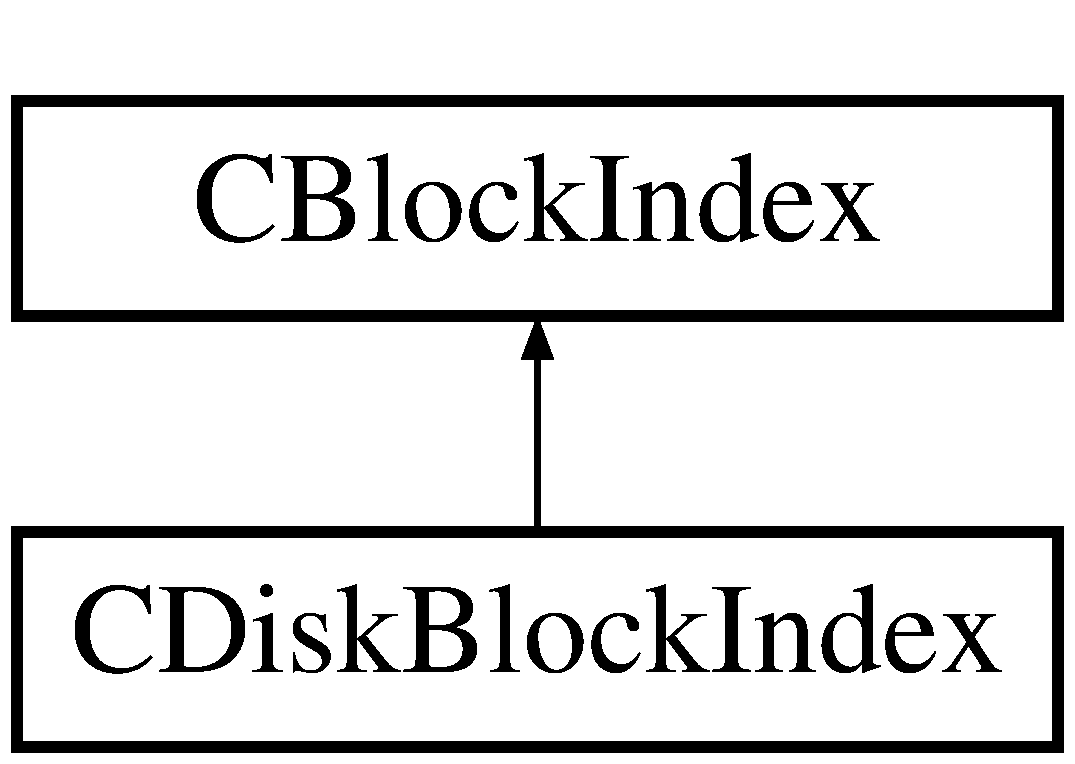
\includegraphics[height=2.000000cm]{class_c_disk_block_index}
\end{center}
\end{figure}
\subsection*{Public Member Functions}
\begin{DoxyCompactItemize}
\item 
\mbox{\hyperlink{class_c_disk_block_index_a8c460c63b799964ef55e2dbbb74b5ad6}{C\+Disk\+Block\+Index}} ()
\item 
\mbox{\hyperlink{class_c_disk_block_index_a8d76af0058fa72d3d8ff688d27d2a5c9}{C\+Disk\+Block\+Index}} (const \mbox{\hyperlink{class_c_block_index}{C\+Block\+Index}} $\ast$pindex)
\item 
{\footnotesize template$<$typename Stream , typename Operation $>$ }\\void \mbox{\hyperlink{class_c_disk_block_index_a2ef7b51f2777fcc1b9625a0ee000f9b5}{Serialization\+Op}} (Stream \&s, Operation ser\+\_\+action, int n\+Type, int \mbox{\hyperlink{class_c_block_index_a45126301a0a6e26010527a7bbfc1ef58}{n\+Version}})
\item 
\mbox{\hyperlink{classuint256}{uint256}} \mbox{\hyperlink{class_c_disk_block_index_acc607a9082c558d7301077631b66122b}{Get\+Block\+Hash}} () const
\item 
std\+::string \mbox{\hyperlink{class_c_disk_block_index_a347eafa0667f8641f73062b48c217d61}{To\+String}} () const
\end{DoxyCompactItemize}
\subsection*{Public Attributes}
\begin{DoxyCompactItemize}
\item 
\mbox{\hyperlink{classuint256}{uint256}} \mbox{\hyperlink{class_c_disk_block_index_a1c4a32dec25c474353aa3286de318224}{hash}}
\item 
\mbox{\hyperlink{classuint256}{uint256}} \mbox{\hyperlink{class_c_disk_block_index_a3a1730201a8523fb947c4d4f632a4212}{hash\+Prev}}
\item 
\mbox{\hyperlink{class_c_disk_block_index_adfa97e82f2e6db827fc6b8b5e351a1f9}{A\+D\+D\+\_\+\+S\+E\+R\+I\+A\+L\+I\+Z\+E\+\_\+\+M\+E\+T\+H\+O\+DS}}
\end{DoxyCompactItemize}
\subsection*{Additional Inherited Members}


\subsection{Detailed Description}
Used to marshal pointers into hashes for db storage. 

\subsection{Constructor \& Destructor Documentation}
\mbox{\Hypertarget{class_c_disk_block_index_a8c460c63b799964ef55e2dbbb74b5ad6}\label{class_c_disk_block_index_a8c460c63b799964ef55e2dbbb74b5ad6}} 
\index{C\+Disk\+Block\+Index@{C\+Disk\+Block\+Index}!C\+Disk\+Block\+Index@{C\+Disk\+Block\+Index}}
\index{C\+Disk\+Block\+Index@{C\+Disk\+Block\+Index}!C\+Disk\+Block\+Index@{C\+Disk\+Block\+Index}}
\subsubsection{\texorpdfstring{C\+Disk\+Block\+Index()}{CDiskBlockIndex()}\hspace{0.1cm}{\footnotesize\ttfamily [1/2]}}
{\footnotesize\ttfamily C\+Disk\+Block\+Index\+::\+C\+Disk\+Block\+Index (\begin{DoxyParamCaption}{ }\end{DoxyParamCaption})\hspace{0.3cm}{\ttfamily [inline]}}

\mbox{\Hypertarget{class_c_disk_block_index_a8d76af0058fa72d3d8ff688d27d2a5c9}\label{class_c_disk_block_index_a8d76af0058fa72d3d8ff688d27d2a5c9}} 
\index{C\+Disk\+Block\+Index@{C\+Disk\+Block\+Index}!C\+Disk\+Block\+Index@{C\+Disk\+Block\+Index}}
\index{C\+Disk\+Block\+Index@{C\+Disk\+Block\+Index}!C\+Disk\+Block\+Index@{C\+Disk\+Block\+Index}}
\subsubsection{\texorpdfstring{C\+Disk\+Block\+Index()}{CDiskBlockIndex()}\hspace{0.1cm}{\footnotesize\ttfamily [2/2]}}
{\footnotesize\ttfamily C\+Disk\+Block\+Index\+::\+C\+Disk\+Block\+Index (\begin{DoxyParamCaption}\item[{const \mbox{\hyperlink{class_c_block_index}{C\+Block\+Index}} $\ast$}]{pindex }\end{DoxyParamCaption})\hspace{0.3cm}{\ttfamily [inline]}, {\ttfamily [explicit]}}



\subsection{Member Function Documentation}
\mbox{\Hypertarget{class_c_disk_block_index_acc607a9082c558d7301077631b66122b}\label{class_c_disk_block_index_acc607a9082c558d7301077631b66122b}} 
\index{C\+Disk\+Block\+Index@{C\+Disk\+Block\+Index}!Get\+Block\+Hash@{Get\+Block\+Hash}}
\index{Get\+Block\+Hash@{Get\+Block\+Hash}!C\+Disk\+Block\+Index@{C\+Disk\+Block\+Index}}
\subsubsection{\texorpdfstring{Get\+Block\+Hash()}{GetBlockHash()}}
{\footnotesize\ttfamily \mbox{\hyperlink{classuint256}{uint256}} C\+Disk\+Block\+Index\+::\+Get\+Block\+Hash (\begin{DoxyParamCaption}{ }\end{DoxyParamCaption}) const\hspace{0.3cm}{\ttfamily [inline]}}

\mbox{\Hypertarget{class_c_disk_block_index_a2ef7b51f2777fcc1b9625a0ee000f9b5}\label{class_c_disk_block_index_a2ef7b51f2777fcc1b9625a0ee000f9b5}} 
\index{C\+Disk\+Block\+Index@{C\+Disk\+Block\+Index}!Serialization\+Op@{Serialization\+Op}}
\index{Serialization\+Op@{Serialization\+Op}!C\+Disk\+Block\+Index@{C\+Disk\+Block\+Index}}
\subsubsection{\texorpdfstring{Serialization\+Op()}{SerializationOp()}}
{\footnotesize\ttfamily template$<$typename Stream , typename Operation $>$ \\
void C\+Disk\+Block\+Index\+::\+Serialization\+Op (\begin{DoxyParamCaption}\item[{Stream \&}]{s,  }\item[{Operation}]{ser\+\_\+action,  }\item[{int}]{n\+Type,  }\item[{int}]{n\+Version }\end{DoxyParamCaption})\hspace{0.3cm}{\ttfamily [inline]}}

\mbox{\Hypertarget{class_c_disk_block_index_a347eafa0667f8641f73062b48c217d61}\label{class_c_disk_block_index_a347eafa0667f8641f73062b48c217d61}} 
\index{C\+Disk\+Block\+Index@{C\+Disk\+Block\+Index}!To\+String@{To\+String}}
\index{To\+String@{To\+String}!C\+Disk\+Block\+Index@{C\+Disk\+Block\+Index}}
\subsubsection{\texorpdfstring{To\+String()}{ToString()}}
{\footnotesize\ttfamily std\+::string C\+Disk\+Block\+Index\+::\+To\+String (\begin{DoxyParamCaption}{ }\end{DoxyParamCaption}) const\hspace{0.3cm}{\ttfamily [inline]}}



\subsection{Member Data Documentation}
\mbox{\Hypertarget{class_c_disk_block_index_adfa97e82f2e6db827fc6b8b5e351a1f9}\label{class_c_disk_block_index_adfa97e82f2e6db827fc6b8b5e351a1f9}} 
\index{C\+Disk\+Block\+Index@{C\+Disk\+Block\+Index}!A\+D\+D\+\_\+\+S\+E\+R\+I\+A\+L\+I\+Z\+E\+\_\+\+M\+E\+T\+H\+O\+DS@{A\+D\+D\+\_\+\+S\+E\+R\+I\+A\+L\+I\+Z\+E\+\_\+\+M\+E\+T\+H\+O\+DS}}
\index{A\+D\+D\+\_\+\+S\+E\+R\+I\+A\+L\+I\+Z\+E\+\_\+\+M\+E\+T\+H\+O\+DS@{A\+D\+D\+\_\+\+S\+E\+R\+I\+A\+L\+I\+Z\+E\+\_\+\+M\+E\+T\+H\+O\+DS}!C\+Disk\+Block\+Index@{C\+Disk\+Block\+Index}}
\subsubsection{\texorpdfstring{A\+D\+D\+\_\+\+S\+E\+R\+I\+A\+L\+I\+Z\+E\+\_\+\+M\+E\+T\+H\+O\+DS}{ADD\_SERIALIZE\_METHODS}}
{\footnotesize\ttfamily C\+Disk\+Block\+Index\+::\+A\+D\+D\+\_\+\+S\+E\+R\+I\+A\+L\+I\+Z\+E\+\_\+\+M\+E\+T\+H\+O\+DS}

\mbox{\Hypertarget{class_c_disk_block_index_a1c4a32dec25c474353aa3286de318224}\label{class_c_disk_block_index_a1c4a32dec25c474353aa3286de318224}} 
\index{C\+Disk\+Block\+Index@{C\+Disk\+Block\+Index}!hash@{hash}}
\index{hash@{hash}!C\+Disk\+Block\+Index@{C\+Disk\+Block\+Index}}
\subsubsection{\texorpdfstring{hash}{hash}}
{\footnotesize\ttfamily \mbox{\hyperlink{classuint256}{uint256}} C\+Disk\+Block\+Index\+::hash}

\mbox{\Hypertarget{class_c_disk_block_index_a3a1730201a8523fb947c4d4f632a4212}\label{class_c_disk_block_index_a3a1730201a8523fb947c4d4f632a4212}} 
\index{C\+Disk\+Block\+Index@{C\+Disk\+Block\+Index}!hash\+Prev@{hash\+Prev}}
\index{hash\+Prev@{hash\+Prev}!C\+Disk\+Block\+Index@{C\+Disk\+Block\+Index}}
\subsubsection{\texorpdfstring{hash\+Prev}{hashPrev}}
{\footnotesize\ttfamily \mbox{\hyperlink{classuint256}{uint256}} C\+Disk\+Block\+Index\+::hash\+Prev}



The documentation for this class was generated from the following file\+:\begin{DoxyCompactItemize}
\item 
/\+Users/christopherarguello/\+Developer/anon/src/\mbox{\hyperlink{chain_8h}{chain.\+h}}\end{DoxyCompactItemize}

\hypertarget{struct_c_disk_block_pos}{}\section{C\+Disk\+Block\+Pos Struct Reference}
\label{struct_c_disk_block_pos}\index{C\+Disk\+Block\+Pos@{C\+Disk\+Block\+Pos}}


{\ttfamily \#include $<$chain.\+h$>$}

Inheritance diagram for C\+Disk\+Block\+Pos\+:\begin{figure}[H]
\begin{center}
\leavevmode
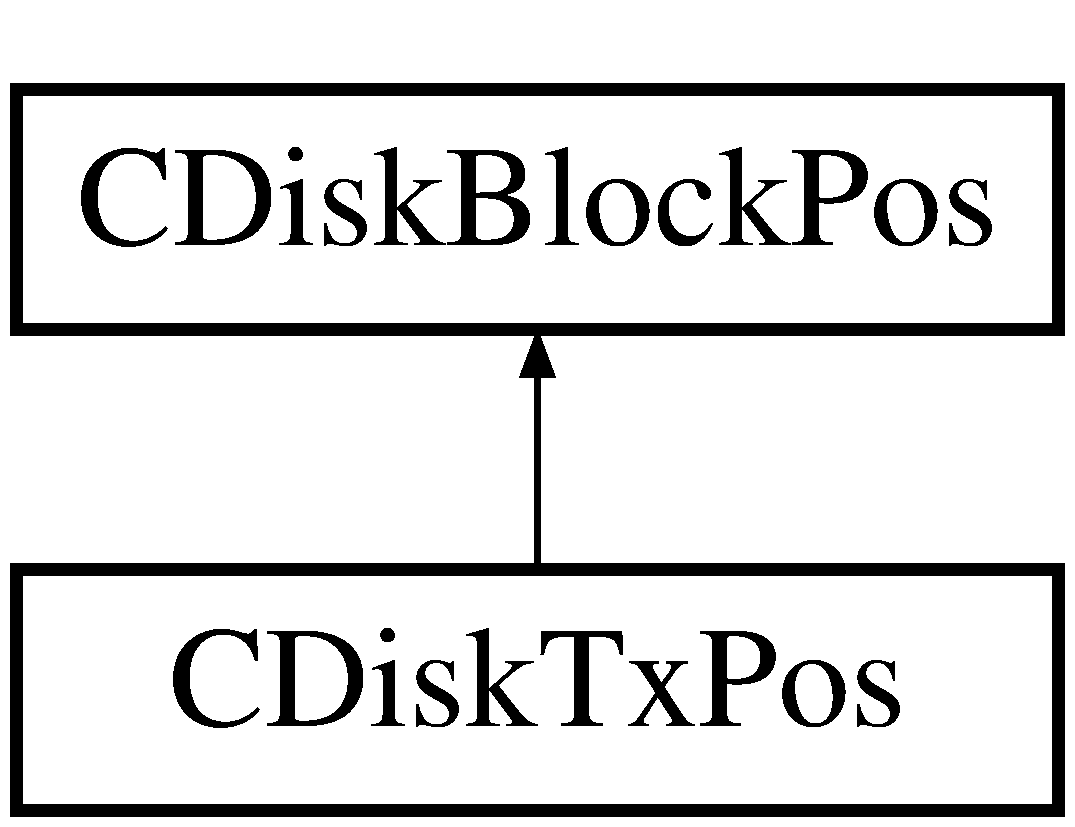
\includegraphics[height=2.000000cm]{struct_c_disk_block_pos}
\end{center}
\end{figure}
\subsection*{Public Member Functions}
\begin{DoxyCompactItemize}
\item 
{\footnotesize template$<$typename Stream , typename Operation $>$ }\\void \mbox{\hyperlink{struct_c_disk_block_pos_a821bb4eebc99ae39c20133d80244325f}{Serialization\+Op}} (Stream \&s, Operation ser\+\_\+action, int n\+Type, int n\+Version)
\item 
\mbox{\hyperlink{struct_c_disk_block_pos_ac34e46c8bf3256b3eca09f54911cf8bd}{C\+Disk\+Block\+Pos}} ()
\item 
\mbox{\hyperlink{struct_c_disk_block_pos_a0c96947d09bb4aaf28ab2d7866d20918}{C\+Disk\+Block\+Pos}} (int n\+File\+In, unsigned int n\+Pos\+In)
\item 
void \mbox{\hyperlink{struct_c_disk_block_pos_a0a6ba113219a456472081ee6d6b20a72}{Set\+Null}} ()
\item 
bool \mbox{\hyperlink{struct_c_disk_block_pos_a7dd98fe3f5372d358df61db31899b0af}{Is\+Null}} () const
\item 
std\+::string \mbox{\hyperlink{struct_c_disk_block_pos_aec119689268c0dc9c2f1e3b25fd859ad}{To\+String}} () const
\end{DoxyCompactItemize}
\subsection*{Public Attributes}
\begin{DoxyCompactItemize}
\item 
int \mbox{\hyperlink{struct_c_disk_block_pos_a09f30dab5c02fbdea8a17f9bcee5aac8}{n\+File}}
\item 
unsigned int \mbox{\hyperlink{struct_c_disk_block_pos_a9b4b5e149b655ac5c22d05883b5bca0e}{n\+Pos}}
\item 
\mbox{\hyperlink{struct_c_disk_block_pos_a958cd730b290bbb0153d514c56517590}{A\+D\+D\+\_\+\+S\+E\+R\+I\+A\+L\+I\+Z\+E\+\_\+\+M\+E\+T\+H\+O\+DS}}
\end{DoxyCompactItemize}
\subsection*{Friends}
\begin{DoxyCompactItemize}
\item 
bool \mbox{\hyperlink{struct_c_disk_block_pos_a04787eb60da48b80e0f7fb402c6896fe}{operator==}} (const \mbox{\hyperlink{struct_c_disk_block_pos}{C\+Disk\+Block\+Pos}} \&a, const \mbox{\hyperlink{struct_c_disk_block_pos}{C\+Disk\+Block\+Pos}} \&b)
\item 
bool \mbox{\hyperlink{struct_c_disk_block_pos_af77481af6cf1d32788ba67c29cc061b5}{operator!=}} (const \mbox{\hyperlink{struct_c_disk_block_pos}{C\+Disk\+Block\+Pos}} \&a, const \mbox{\hyperlink{struct_c_disk_block_pos}{C\+Disk\+Block\+Pos}} \&b)
\end{DoxyCompactItemize}


\subsection{Constructor \& Destructor Documentation}
\mbox{\Hypertarget{struct_c_disk_block_pos_ac34e46c8bf3256b3eca09f54911cf8bd}\label{struct_c_disk_block_pos_ac34e46c8bf3256b3eca09f54911cf8bd}} 
\index{C\+Disk\+Block\+Pos@{C\+Disk\+Block\+Pos}!C\+Disk\+Block\+Pos@{C\+Disk\+Block\+Pos}}
\index{C\+Disk\+Block\+Pos@{C\+Disk\+Block\+Pos}!C\+Disk\+Block\+Pos@{C\+Disk\+Block\+Pos}}
\subsubsection{\texorpdfstring{C\+Disk\+Block\+Pos()}{CDiskBlockPos()}\hspace{0.1cm}{\footnotesize\ttfamily [1/2]}}
{\footnotesize\ttfamily C\+Disk\+Block\+Pos\+::\+C\+Disk\+Block\+Pos (\begin{DoxyParamCaption}{ }\end{DoxyParamCaption})\hspace{0.3cm}{\ttfamily [inline]}}

\mbox{\Hypertarget{struct_c_disk_block_pos_a0c96947d09bb4aaf28ab2d7866d20918}\label{struct_c_disk_block_pos_a0c96947d09bb4aaf28ab2d7866d20918}} 
\index{C\+Disk\+Block\+Pos@{C\+Disk\+Block\+Pos}!C\+Disk\+Block\+Pos@{C\+Disk\+Block\+Pos}}
\index{C\+Disk\+Block\+Pos@{C\+Disk\+Block\+Pos}!C\+Disk\+Block\+Pos@{C\+Disk\+Block\+Pos}}
\subsubsection{\texorpdfstring{C\+Disk\+Block\+Pos()}{CDiskBlockPos()}\hspace{0.1cm}{\footnotesize\ttfamily [2/2]}}
{\footnotesize\ttfamily C\+Disk\+Block\+Pos\+::\+C\+Disk\+Block\+Pos (\begin{DoxyParamCaption}\item[{int}]{n\+File\+In,  }\item[{unsigned int}]{n\+Pos\+In }\end{DoxyParamCaption})\hspace{0.3cm}{\ttfamily [inline]}}



\subsection{Member Function Documentation}
\mbox{\Hypertarget{struct_c_disk_block_pos_a7dd98fe3f5372d358df61db31899b0af}\label{struct_c_disk_block_pos_a7dd98fe3f5372d358df61db31899b0af}} 
\index{C\+Disk\+Block\+Pos@{C\+Disk\+Block\+Pos}!Is\+Null@{Is\+Null}}
\index{Is\+Null@{Is\+Null}!C\+Disk\+Block\+Pos@{C\+Disk\+Block\+Pos}}
\subsubsection{\texorpdfstring{Is\+Null()}{IsNull()}}
{\footnotesize\ttfamily bool C\+Disk\+Block\+Pos\+::\+Is\+Null (\begin{DoxyParamCaption}{ }\end{DoxyParamCaption}) const\hspace{0.3cm}{\ttfamily [inline]}}

\mbox{\Hypertarget{struct_c_disk_block_pos_a821bb4eebc99ae39c20133d80244325f}\label{struct_c_disk_block_pos_a821bb4eebc99ae39c20133d80244325f}} 
\index{C\+Disk\+Block\+Pos@{C\+Disk\+Block\+Pos}!Serialization\+Op@{Serialization\+Op}}
\index{Serialization\+Op@{Serialization\+Op}!C\+Disk\+Block\+Pos@{C\+Disk\+Block\+Pos}}
\subsubsection{\texorpdfstring{Serialization\+Op()}{SerializationOp()}}
{\footnotesize\ttfamily template$<$typename Stream , typename Operation $>$ \\
void C\+Disk\+Block\+Pos\+::\+Serialization\+Op (\begin{DoxyParamCaption}\item[{Stream \&}]{s,  }\item[{Operation}]{ser\+\_\+action,  }\item[{int}]{n\+Type,  }\item[{int}]{n\+Version }\end{DoxyParamCaption})\hspace{0.3cm}{\ttfamily [inline]}}

\mbox{\Hypertarget{struct_c_disk_block_pos_a0a6ba113219a456472081ee6d6b20a72}\label{struct_c_disk_block_pos_a0a6ba113219a456472081ee6d6b20a72}} 
\index{C\+Disk\+Block\+Pos@{C\+Disk\+Block\+Pos}!Set\+Null@{Set\+Null}}
\index{Set\+Null@{Set\+Null}!C\+Disk\+Block\+Pos@{C\+Disk\+Block\+Pos}}
\subsubsection{\texorpdfstring{Set\+Null()}{SetNull()}}
{\footnotesize\ttfamily void C\+Disk\+Block\+Pos\+::\+Set\+Null (\begin{DoxyParamCaption}{ }\end{DoxyParamCaption})\hspace{0.3cm}{\ttfamily [inline]}}

\mbox{\Hypertarget{struct_c_disk_block_pos_aec119689268c0dc9c2f1e3b25fd859ad}\label{struct_c_disk_block_pos_aec119689268c0dc9c2f1e3b25fd859ad}} 
\index{C\+Disk\+Block\+Pos@{C\+Disk\+Block\+Pos}!To\+String@{To\+String}}
\index{To\+String@{To\+String}!C\+Disk\+Block\+Pos@{C\+Disk\+Block\+Pos}}
\subsubsection{\texorpdfstring{To\+String()}{ToString()}}
{\footnotesize\ttfamily std\+::string C\+Disk\+Block\+Pos\+::\+To\+String (\begin{DoxyParamCaption}{ }\end{DoxyParamCaption}) const\hspace{0.3cm}{\ttfamily [inline]}}



\subsection{Friends And Related Function Documentation}
\mbox{\Hypertarget{struct_c_disk_block_pos_af77481af6cf1d32788ba67c29cc061b5}\label{struct_c_disk_block_pos_af77481af6cf1d32788ba67c29cc061b5}} 
\index{C\+Disk\+Block\+Pos@{C\+Disk\+Block\+Pos}!operator"!=@{operator"!=}}
\index{operator"!=@{operator"!=}!C\+Disk\+Block\+Pos@{C\+Disk\+Block\+Pos}}
\subsubsection{\texorpdfstring{operator"!=}{operator!=}}
{\footnotesize\ttfamily bool operator!= (\begin{DoxyParamCaption}\item[{const \mbox{\hyperlink{struct_c_disk_block_pos}{C\+Disk\+Block\+Pos}} \&}]{a,  }\item[{const \mbox{\hyperlink{struct_c_disk_block_pos}{C\+Disk\+Block\+Pos}} \&}]{b }\end{DoxyParamCaption})\hspace{0.3cm}{\ttfamily [friend]}}

\mbox{\Hypertarget{struct_c_disk_block_pos_a04787eb60da48b80e0f7fb402c6896fe}\label{struct_c_disk_block_pos_a04787eb60da48b80e0f7fb402c6896fe}} 
\index{C\+Disk\+Block\+Pos@{C\+Disk\+Block\+Pos}!operator==@{operator==}}
\index{operator==@{operator==}!C\+Disk\+Block\+Pos@{C\+Disk\+Block\+Pos}}
\subsubsection{\texorpdfstring{operator==}{operator==}}
{\footnotesize\ttfamily bool operator== (\begin{DoxyParamCaption}\item[{const \mbox{\hyperlink{struct_c_disk_block_pos}{C\+Disk\+Block\+Pos}} \&}]{a,  }\item[{const \mbox{\hyperlink{struct_c_disk_block_pos}{C\+Disk\+Block\+Pos}} \&}]{b }\end{DoxyParamCaption})\hspace{0.3cm}{\ttfamily [friend]}}



\subsection{Member Data Documentation}
\mbox{\Hypertarget{struct_c_disk_block_pos_a958cd730b290bbb0153d514c56517590}\label{struct_c_disk_block_pos_a958cd730b290bbb0153d514c56517590}} 
\index{C\+Disk\+Block\+Pos@{C\+Disk\+Block\+Pos}!A\+D\+D\+\_\+\+S\+E\+R\+I\+A\+L\+I\+Z\+E\+\_\+\+M\+E\+T\+H\+O\+DS@{A\+D\+D\+\_\+\+S\+E\+R\+I\+A\+L\+I\+Z\+E\+\_\+\+M\+E\+T\+H\+O\+DS}}
\index{A\+D\+D\+\_\+\+S\+E\+R\+I\+A\+L\+I\+Z\+E\+\_\+\+M\+E\+T\+H\+O\+DS@{A\+D\+D\+\_\+\+S\+E\+R\+I\+A\+L\+I\+Z\+E\+\_\+\+M\+E\+T\+H\+O\+DS}!C\+Disk\+Block\+Pos@{C\+Disk\+Block\+Pos}}
\subsubsection{\texorpdfstring{A\+D\+D\+\_\+\+S\+E\+R\+I\+A\+L\+I\+Z\+E\+\_\+\+M\+E\+T\+H\+O\+DS}{ADD\_SERIALIZE\_METHODS}}
{\footnotesize\ttfamily C\+Disk\+Block\+Pos\+::\+A\+D\+D\+\_\+\+S\+E\+R\+I\+A\+L\+I\+Z\+E\+\_\+\+M\+E\+T\+H\+O\+DS}

\mbox{\Hypertarget{struct_c_disk_block_pos_a09f30dab5c02fbdea8a17f9bcee5aac8}\label{struct_c_disk_block_pos_a09f30dab5c02fbdea8a17f9bcee5aac8}} 
\index{C\+Disk\+Block\+Pos@{C\+Disk\+Block\+Pos}!n\+File@{n\+File}}
\index{n\+File@{n\+File}!C\+Disk\+Block\+Pos@{C\+Disk\+Block\+Pos}}
\subsubsection{\texorpdfstring{n\+File}{nFile}}
{\footnotesize\ttfamily int C\+Disk\+Block\+Pos\+::n\+File}

\mbox{\Hypertarget{struct_c_disk_block_pos_a9b4b5e149b655ac5c22d05883b5bca0e}\label{struct_c_disk_block_pos_a9b4b5e149b655ac5c22d05883b5bca0e}} 
\index{C\+Disk\+Block\+Pos@{C\+Disk\+Block\+Pos}!n\+Pos@{n\+Pos}}
\index{n\+Pos@{n\+Pos}!C\+Disk\+Block\+Pos@{C\+Disk\+Block\+Pos}}
\subsubsection{\texorpdfstring{n\+Pos}{nPos}}
{\footnotesize\ttfamily unsigned int C\+Disk\+Block\+Pos\+::n\+Pos}



The documentation for this struct was generated from the following file\+:\begin{DoxyCompactItemize}
\item 
/\+Users/christopherarguello/\+Developer/anon/src/\mbox{\hyperlink{chain_8h}{chain.\+h}}\end{DoxyCompactItemize}

\hypertarget{struct_c_disk_tx_pos}{}\section{C\+Disk\+Tx\+Pos Struct Reference}
\label{struct_c_disk_tx_pos}\index{C\+Disk\+Tx\+Pos@{C\+Disk\+Tx\+Pos}}


{\ttfamily \#include $<$main.\+h$>$}

Inheritance diagram for C\+Disk\+Tx\+Pos\+:\begin{figure}[H]
\begin{center}
\leavevmode
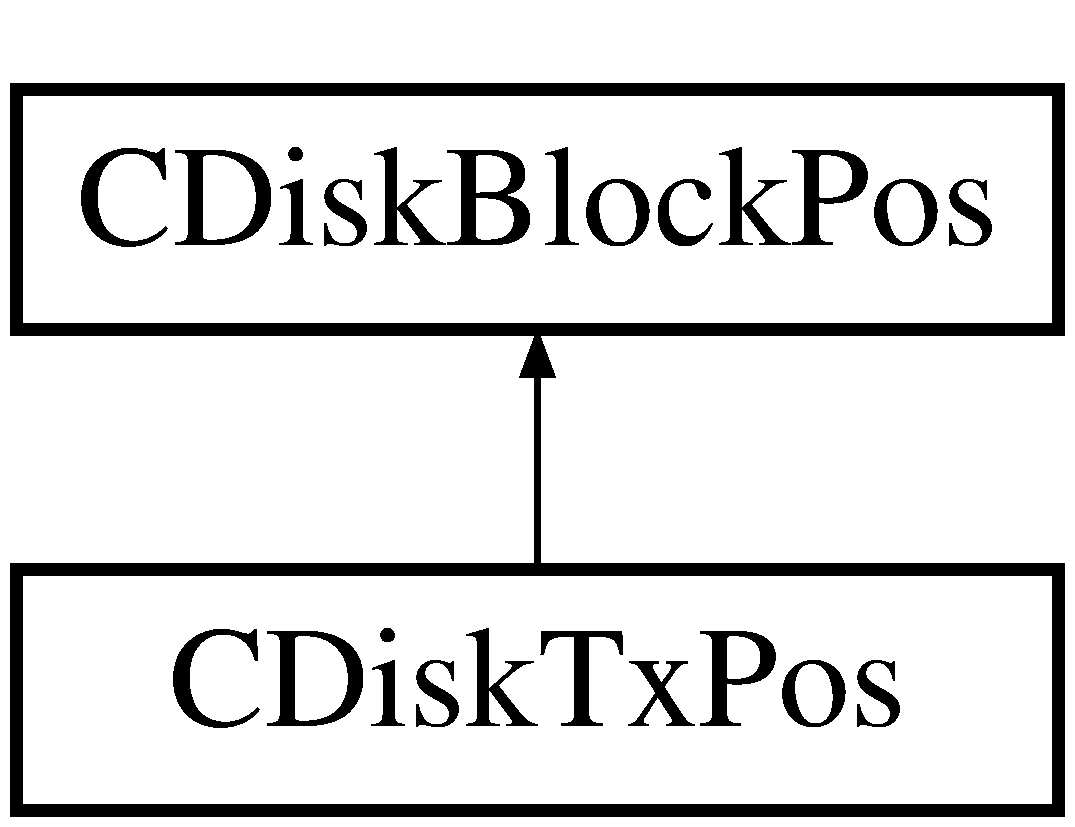
\includegraphics[height=2.000000cm]{struct_c_disk_tx_pos}
\end{center}
\end{figure}
\subsection*{Public Member Functions}
\begin{DoxyCompactItemize}
\item 
{\footnotesize template$<$typename Stream , typename Operation $>$ }\\void \mbox{\hyperlink{struct_c_disk_tx_pos_a1a68f1de894f0791a7ad64e3e6ea6fd6}{Serialization\+Op}} (Stream \&s, Operation ser\+\_\+action, int n\+Type, int n\+Version)
\item 
\mbox{\hyperlink{struct_c_disk_tx_pos_ab823a4c83ec90c8223544051f11e65fd}{C\+Disk\+Tx\+Pos}} (const \mbox{\hyperlink{struct_c_disk_block_pos}{C\+Disk\+Block\+Pos}} \&block\+In, unsigned int n\+Tx\+Offset\+In)
\item 
\mbox{\hyperlink{struct_c_disk_tx_pos_a2026598d28ffcadfd40452f702bcac46}{C\+Disk\+Tx\+Pos}} ()
\item 
void \mbox{\hyperlink{struct_c_disk_tx_pos_a22eb47d077f9c355373772eb42853fcf}{Set\+Null}} ()
\end{DoxyCompactItemize}
\subsection*{Public Attributes}
\begin{DoxyCompactItemize}
\item 
unsigned int \mbox{\hyperlink{struct_c_disk_tx_pos_af19fa085a69ba3bac7b52413a37adf23}{n\+Tx\+Offset}}
\item 
\mbox{\hyperlink{struct_c_disk_tx_pos_a2990c083fbbd0fb5f5aa4115e540cd21}{A\+D\+D\+\_\+\+S\+E\+R\+I\+A\+L\+I\+Z\+E\+\_\+\+M\+E\+T\+H\+O\+DS}}
\end{DoxyCompactItemize}


\subsection{Constructor \& Destructor Documentation}
\mbox{\Hypertarget{struct_c_disk_tx_pos_ab823a4c83ec90c8223544051f11e65fd}\label{struct_c_disk_tx_pos_ab823a4c83ec90c8223544051f11e65fd}} 
\index{C\+Disk\+Tx\+Pos@{C\+Disk\+Tx\+Pos}!C\+Disk\+Tx\+Pos@{C\+Disk\+Tx\+Pos}}
\index{C\+Disk\+Tx\+Pos@{C\+Disk\+Tx\+Pos}!C\+Disk\+Tx\+Pos@{C\+Disk\+Tx\+Pos}}
\subsubsection{\texorpdfstring{C\+Disk\+Tx\+Pos()}{CDiskTxPos()}\hspace{0.1cm}{\footnotesize\ttfamily [1/2]}}
{\footnotesize\ttfamily C\+Disk\+Tx\+Pos\+::\+C\+Disk\+Tx\+Pos (\begin{DoxyParamCaption}\item[{const \mbox{\hyperlink{struct_c_disk_block_pos}{C\+Disk\+Block\+Pos}} \&}]{block\+In,  }\item[{unsigned int}]{n\+Tx\+Offset\+In }\end{DoxyParamCaption})\hspace{0.3cm}{\ttfamily [inline]}}

\mbox{\Hypertarget{struct_c_disk_tx_pos_a2026598d28ffcadfd40452f702bcac46}\label{struct_c_disk_tx_pos_a2026598d28ffcadfd40452f702bcac46}} 
\index{C\+Disk\+Tx\+Pos@{C\+Disk\+Tx\+Pos}!C\+Disk\+Tx\+Pos@{C\+Disk\+Tx\+Pos}}
\index{C\+Disk\+Tx\+Pos@{C\+Disk\+Tx\+Pos}!C\+Disk\+Tx\+Pos@{C\+Disk\+Tx\+Pos}}
\subsubsection{\texorpdfstring{C\+Disk\+Tx\+Pos()}{CDiskTxPos()}\hspace{0.1cm}{\footnotesize\ttfamily [2/2]}}
{\footnotesize\ttfamily C\+Disk\+Tx\+Pos\+::\+C\+Disk\+Tx\+Pos (\begin{DoxyParamCaption}{ }\end{DoxyParamCaption})\hspace{0.3cm}{\ttfamily [inline]}}



\subsection{Member Function Documentation}
\mbox{\Hypertarget{struct_c_disk_tx_pos_a1a68f1de894f0791a7ad64e3e6ea6fd6}\label{struct_c_disk_tx_pos_a1a68f1de894f0791a7ad64e3e6ea6fd6}} 
\index{C\+Disk\+Tx\+Pos@{C\+Disk\+Tx\+Pos}!Serialization\+Op@{Serialization\+Op}}
\index{Serialization\+Op@{Serialization\+Op}!C\+Disk\+Tx\+Pos@{C\+Disk\+Tx\+Pos}}
\subsubsection{\texorpdfstring{Serialization\+Op()}{SerializationOp()}}
{\footnotesize\ttfamily template$<$typename Stream , typename Operation $>$ \\
void C\+Disk\+Tx\+Pos\+::\+Serialization\+Op (\begin{DoxyParamCaption}\item[{Stream \&}]{s,  }\item[{Operation}]{ser\+\_\+action,  }\item[{int}]{n\+Type,  }\item[{int}]{n\+Version }\end{DoxyParamCaption})\hspace{0.3cm}{\ttfamily [inline]}}

\mbox{\Hypertarget{struct_c_disk_tx_pos_a22eb47d077f9c355373772eb42853fcf}\label{struct_c_disk_tx_pos_a22eb47d077f9c355373772eb42853fcf}} 
\index{C\+Disk\+Tx\+Pos@{C\+Disk\+Tx\+Pos}!Set\+Null@{Set\+Null}}
\index{Set\+Null@{Set\+Null}!C\+Disk\+Tx\+Pos@{C\+Disk\+Tx\+Pos}}
\subsubsection{\texorpdfstring{Set\+Null()}{SetNull()}}
{\footnotesize\ttfamily void C\+Disk\+Tx\+Pos\+::\+Set\+Null (\begin{DoxyParamCaption}{ }\end{DoxyParamCaption})\hspace{0.3cm}{\ttfamily [inline]}}



\subsection{Member Data Documentation}
\mbox{\Hypertarget{struct_c_disk_tx_pos_a2990c083fbbd0fb5f5aa4115e540cd21}\label{struct_c_disk_tx_pos_a2990c083fbbd0fb5f5aa4115e540cd21}} 
\index{C\+Disk\+Tx\+Pos@{C\+Disk\+Tx\+Pos}!A\+D\+D\+\_\+\+S\+E\+R\+I\+A\+L\+I\+Z\+E\+\_\+\+M\+E\+T\+H\+O\+DS@{A\+D\+D\+\_\+\+S\+E\+R\+I\+A\+L\+I\+Z\+E\+\_\+\+M\+E\+T\+H\+O\+DS}}
\index{A\+D\+D\+\_\+\+S\+E\+R\+I\+A\+L\+I\+Z\+E\+\_\+\+M\+E\+T\+H\+O\+DS@{A\+D\+D\+\_\+\+S\+E\+R\+I\+A\+L\+I\+Z\+E\+\_\+\+M\+E\+T\+H\+O\+DS}!C\+Disk\+Tx\+Pos@{C\+Disk\+Tx\+Pos}}
\subsubsection{\texorpdfstring{A\+D\+D\+\_\+\+S\+E\+R\+I\+A\+L\+I\+Z\+E\+\_\+\+M\+E\+T\+H\+O\+DS}{ADD\_SERIALIZE\_METHODS}}
{\footnotesize\ttfamily C\+Disk\+Tx\+Pos\+::\+A\+D\+D\+\_\+\+S\+E\+R\+I\+A\+L\+I\+Z\+E\+\_\+\+M\+E\+T\+H\+O\+DS}

\mbox{\Hypertarget{struct_c_disk_tx_pos_af19fa085a69ba3bac7b52413a37adf23}\label{struct_c_disk_tx_pos_af19fa085a69ba3bac7b52413a37adf23}} 
\index{C\+Disk\+Tx\+Pos@{C\+Disk\+Tx\+Pos}!n\+Tx\+Offset@{n\+Tx\+Offset}}
\index{n\+Tx\+Offset@{n\+Tx\+Offset}!C\+Disk\+Tx\+Pos@{C\+Disk\+Tx\+Pos}}
\subsubsection{\texorpdfstring{n\+Tx\+Offset}{nTxOffset}}
{\footnotesize\ttfamily unsigned int C\+Disk\+Tx\+Pos\+::n\+Tx\+Offset}



The documentation for this struct was generated from the following file\+:\begin{DoxyCompactItemize}
\item 
/\+Users/christopherarguello/\+Developer/anon/src/\mbox{\hyperlink{main_8h}{main.\+h}}\end{DoxyCompactItemize}

\hypertarget{struct_c_d_n_s_seed_data}{}\section{C\+D\+N\+S\+Seed\+Data Struct Reference}
\label{struct_c_d_n_s_seed_data}\index{C\+D\+N\+S\+Seed\+Data@{C\+D\+N\+S\+Seed\+Data}}


{\ttfamily \#include $<$chainparams.\+h$>$}

\subsection*{Public Member Functions}
\begin{DoxyCompactItemize}
\item 
\mbox{\hyperlink{struct_c_d_n_s_seed_data_a4152b594beb9800fb7611e3c47f03499}{C\+D\+N\+S\+Seed\+Data}} (const std\+::string \&str\+Name, const std\+::string \&str\+Host)
\end{DoxyCompactItemize}
\subsection*{Public Attributes}
\begin{DoxyCompactItemize}
\item 
std\+::string \mbox{\hyperlink{struct_c_d_n_s_seed_data_a2cf084b163340bd62b67e765799f1fdd}{name}}
\item 
std\+::string \mbox{\hyperlink{struct_c_d_n_s_seed_data_a70f5da8568016651cfb7ec7dbf01b3f0}{host}}
\end{DoxyCompactItemize}


\subsection{Constructor \& Destructor Documentation}
\mbox{\Hypertarget{struct_c_d_n_s_seed_data_a4152b594beb9800fb7611e3c47f03499}\label{struct_c_d_n_s_seed_data_a4152b594beb9800fb7611e3c47f03499}} 
\index{C\+D\+N\+S\+Seed\+Data@{C\+D\+N\+S\+Seed\+Data}!C\+D\+N\+S\+Seed\+Data@{C\+D\+N\+S\+Seed\+Data}}
\index{C\+D\+N\+S\+Seed\+Data@{C\+D\+N\+S\+Seed\+Data}!C\+D\+N\+S\+Seed\+Data@{C\+D\+N\+S\+Seed\+Data}}
\subsubsection{\texorpdfstring{C\+D\+N\+S\+Seed\+Data()}{CDNSSeedData()}}
{\footnotesize\ttfamily C\+D\+N\+S\+Seed\+Data\+::\+C\+D\+N\+S\+Seed\+Data (\begin{DoxyParamCaption}\item[{const std\+::string \&}]{str\+Name,  }\item[{const std\+::string \&}]{str\+Host }\end{DoxyParamCaption})\hspace{0.3cm}{\ttfamily [inline]}}



\subsection{Member Data Documentation}
\mbox{\Hypertarget{struct_c_d_n_s_seed_data_a70f5da8568016651cfb7ec7dbf01b3f0}\label{struct_c_d_n_s_seed_data_a70f5da8568016651cfb7ec7dbf01b3f0}} 
\index{C\+D\+N\+S\+Seed\+Data@{C\+D\+N\+S\+Seed\+Data}!host@{host}}
\index{host@{host}!C\+D\+N\+S\+Seed\+Data@{C\+D\+N\+S\+Seed\+Data}}
\subsubsection{\texorpdfstring{host}{host}}
{\footnotesize\ttfamily std\+::string C\+D\+N\+S\+Seed\+Data\+::host}

\mbox{\Hypertarget{struct_c_d_n_s_seed_data_a2cf084b163340bd62b67e765799f1fdd}\label{struct_c_d_n_s_seed_data_a2cf084b163340bd62b67e765799f1fdd}} 
\index{C\+D\+N\+S\+Seed\+Data@{C\+D\+N\+S\+Seed\+Data}!name@{name}}
\index{name@{name}!C\+D\+N\+S\+Seed\+Data@{C\+D\+N\+S\+Seed\+Data}}
\subsubsection{\texorpdfstring{name}{name}}
{\footnotesize\ttfamily std\+::string C\+D\+N\+S\+Seed\+Data\+::name}



The documentation for this struct was generated from the following file\+:\begin{DoxyCompactItemize}
\item 
/\+Users/christopherarguello/\+Developer/anon/src/\mbox{\hyperlink{chainparams_8h}{chainparams.\+h}}\end{DoxyCompactItemize}

\hypertarget{class_c_explicit_net_cleanup}{}\section{C\+Explicit\+Net\+Cleanup Class Reference}
\label{class_c_explicit_net_cleanup}\index{C\+Explicit\+Net\+Cleanup@{C\+Explicit\+Net\+Cleanup}}


{\ttfamily \#include $<$net.\+h$>$}

\subsection*{Static Public Member Functions}
\begin{DoxyCompactItemize}
\item 
static void \mbox{\hyperlink{class_c_explicit_net_cleanup_ab17ed87c32880d754cb7bfe2b4797c55}{call\+Cleanup}} ()
\end{DoxyCompactItemize}


\subsection{Member Function Documentation}
\mbox{\Hypertarget{class_c_explicit_net_cleanup_ab17ed87c32880d754cb7bfe2b4797c55}\label{class_c_explicit_net_cleanup_ab17ed87c32880d754cb7bfe2b4797c55}} 
\index{C\+Explicit\+Net\+Cleanup@{C\+Explicit\+Net\+Cleanup}!call\+Cleanup@{call\+Cleanup}}
\index{call\+Cleanup@{call\+Cleanup}!C\+Explicit\+Net\+Cleanup@{C\+Explicit\+Net\+Cleanup}}
\subsubsection{\texorpdfstring{call\+Cleanup()}{callCleanup()}}
{\footnotesize\ttfamily static void C\+Explicit\+Net\+Cleanup\+::call\+Cleanup (\begin{DoxyParamCaption}{ }\end{DoxyParamCaption})\hspace{0.3cm}{\ttfamily [static]}}



The documentation for this class was generated from the following file\+:\begin{DoxyCompactItemize}
\item 
/\+Users/christopherarguello/\+Developer/anon/src/\mbox{\hyperlink{net_8h}{net.\+h}}\end{DoxyCompactItemize}

\hypertarget{struct_c_ext_key}{}\section{C\+Ext\+Key Struct Reference}
\label{struct_c_ext_key}\index{C\+Ext\+Key@{C\+Ext\+Key}}


{\ttfamily \#include $<$key.\+h$>$}

\subsection*{Public Member Functions}
\begin{DoxyCompactItemize}
\item 
void \mbox{\hyperlink{struct_c_ext_key_a4f68dfccef42685d954d3fb22fd6c67c}{Encode}} (unsigned char code\mbox{[}74\mbox{]}) const
\item 
void \mbox{\hyperlink{struct_c_ext_key_a9720e119745472336b6729e19f0819dd}{Decode}} (const unsigned char code\mbox{[}74\mbox{]})
\item 
bool \mbox{\hyperlink{struct_c_ext_key_a589df63664c6d12bfe071b747a245b1d}{Derive}} (\mbox{\hyperlink{struct_c_ext_key}{C\+Ext\+Key}} \&out, unsigned int \mbox{\hyperlink{struct_c_ext_key_ad15cb7ab68b59495eec71f6586803048}{n\+Child}}) const
\item 
\mbox{\hyperlink{struct_c_ext_pub_key}{C\+Ext\+Pub\+Key}} \mbox{\hyperlink{struct_c_ext_key_a4ea6bbc6c9bda4f8d77cade114155569}{Neuter}} () const
\item 
void \mbox{\hyperlink{struct_c_ext_key_a8cd6ecafdd649082601d7eebbec79688}{Set\+Master}} (const unsigned char $\ast$seed, unsigned int n\+Seed\+Len)
\end{DoxyCompactItemize}
\subsection*{Public Attributes}
\begin{DoxyCompactItemize}
\item 
unsigned char \mbox{\hyperlink{struct_c_ext_key_ab197a253f41646975405b4ead8027b55}{n\+Depth}}
\item 
unsigned char \mbox{\hyperlink{struct_c_ext_key_a22efb3f5dfb26cd8d88d2ab5db885978}{vch\+Fingerprint}} \mbox{[}4\mbox{]}
\item 
unsigned int \mbox{\hyperlink{struct_c_ext_key_ad15cb7ab68b59495eec71f6586803048}{n\+Child}}
\item 
\mbox{\hyperlink{hash_8h_aa201a9867f780a040c7af908e0a85db3}{Chain\+Code}} \mbox{\hyperlink{struct_c_ext_key_ab963200521bcc38d0f68c2d062b5da72}{chaincode}}
\item 
\mbox{\hyperlink{class_c_key}{C\+Key}} \mbox{\hyperlink{struct_c_ext_key_a93cd93ef3311d9dbcf475282a5f80fb2}{key}}
\end{DoxyCompactItemize}
\subsection*{Friends}
\begin{DoxyCompactItemize}
\item 
bool \mbox{\hyperlink{struct_c_ext_key_abd1d7fa4544c5a730a0d2a21d06fd3b3}{operator==}} (const \mbox{\hyperlink{struct_c_ext_key}{C\+Ext\+Key}} \&a, const \mbox{\hyperlink{struct_c_ext_key}{C\+Ext\+Key}} \&b)
\end{DoxyCompactItemize}


\subsection{Member Function Documentation}
\mbox{\Hypertarget{struct_c_ext_key_a9720e119745472336b6729e19f0819dd}\label{struct_c_ext_key_a9720e119745472336b6729e19f0819dd}} 
\index{C\+Ext\+Key@{C\+Ext\+Key}!Decode@{Decode}}
\index{Decode@{Decode}!C\+Ext\+Key@{C\+Ext\+Key}}
\subsubsection{\texorpdfstring{Decode()}{Decode()}}
{\footnotesize\ttfamily void C\+Ext\+Key\+::\+Decode (\begin{DoxyParamCaption}\item[{const unsigned char}]{code\mbox{[}74\mbox{]} }\end{DoxyParamCaption})}

\mbox{\Hypertarget{struct_c_ext_key_a589df63664c6d12bfe071b747a245b1d}\label{struct_c_ext_key_a589df63664c6d12bfe071b747a245b1d}} 
\index{C\+Ext\+Key@{C\+Ext\+Key}!Derive@{Derive}}
\index{Derive@{Derive}!C\+Ext\+Key@{C\+Ext\+Key}}
\subsubsection{\texorpdfstring{Derive()}{Derive()}}
{\footnotesize\ttfamily bool C\+Ext\+Key\+::\+Derive (\begin{DoxyParamCaption}\item[{\mbox{\hyperlink{struct_c_ext_key}{C\+Ext\+Key}} \&}]{out,  }\item[{unsigned int}]{n\+Child }\end{DoxyParamCaption}) const}

\mbox{\Hypertarget{struct_c_ext_key_a4f68dfccef42685d954d3fb22fd6c67c}\label{struct_c_ext_key_a4f68dfccef42685d954d3fb22fd6c67c}} 
\index{C\+Ext\+Key@{C\+Ext\+Key}!Encode@{Encode}}
\index{Encode@{Encode}!C\+Ext\+Key@{C\+Ext\+Key}}
\subsubsection{\texorpdfstring{Encode()}{Encode()}}
{\footnotesize\ttfamily void C\+Ext\+Key\+::\+Encode (\begin{DoxyParamCaption}\item[{unsigned char}]{code\mbox{[}74\mbox{]} }\end{DoxyParamCaption}) const}

\mbox{\Hypertarget{struct_c_ext_key_a4ea6bbc6c9bda4f8d77cade114155569}\label{struct_c_ext_key_a4ea6bbc6c9bda4f8d77cade114155569}} 
\index{C\+Ext\+Key@{C\+Ext\+Key}!Neuter@{Neuter}}
\index{Neuter@{Neuter}!C\+Ext\+Key@{C\+Ext\+Key}}
\subsubsection{\texorpdfstring{Neuter()}{Neuter()}}
{\footnotesize\ttfamily \mbox{\hyperlink{struct_c_ext_pub_key}{C\+Ext\+Pub\+Key}} C\+Ext\+Key\+::\+Neuter (\begin{DoxyParamCaption}{ }\end{DoxyParamCaption}) const}

\mbox{\Hypertarget{struct_c_ext_key_a8cd6ecafdd649082601d7eebbec79688}\label{struct_c_ext_key_a8cd6ecafdd649082601d7eebbec79688}} 
\index{C\+Ext\+Key@{C\+Ext\+Key}!Set\+Master@{Set\+Master}}
\index{Set\+Master@{Set\+Master}!C\+Ext\+Key@{C\+Ext\+Key}}
\subsubsection{\texorpdfstring{Set\+Master()}{SetMaster()}}
{\footnotesize\ttfamily void C\+Ext\+Key\+::\+Set\+Master (\begin{DoxyParamCaption}\item[{const unsigned char $\ast$}]{seed,  }\item[{unsigned int}]{n\+Seed\+Len }\end{DoxyParamCaption})}



\subsection{Friends And Related Function Documentation}
\mbox{\Hypertarget{struct_c_ext_key_abd1d7fa4544c5a730a0d2a21d06fd3b3}\label{struct_c_ext_key_abd1d7fa4544c5a730a0d2a21d06fd3b3}} 
\index{C\+Ext\+Key@{C\+Ext\+Key}!operator==@{operator==}}
\index{operator==@{operator==}!C\+Ext\+Key@{C\+Ext\+Key}}
\subsubsection{\texorpdfstring{operator==}{operator==}}
{\footnotesize\ttfamily bool operator== (\begin{DoxyParamCaption}\item[{const \mbox{\hyperlink{struct_c_ext_key}{C\+Ext\+Key}} \&}]{a,  }\item[{const \mbox{\hyperlink{struct_c_ext_key}{C\+Ext\+Key}} \&}]{b }\end{DoxyParamCaption})\hspace{0.3cm}{\ttfamily [friend]}}



\subsection{Member Data Documentation}
\mbox{\Hypertarget{struct_c_ext_key_ab963200521bcc38d0f68c2d062b5da72}\label{struct_c_ext_key_ab963200521bcc38d0f68c2d062b5da72}} 
\index{C\+Ext\+Key@{C\+Ext\+Key}!chaincode@{chaincode}}
\index{chaincode@{chaincode}!C\+Ext\+Key@{C\+Ext\+Key}}
\subsubsection{\texorpdfstring{chaincode}{chaincode}}
{\footnotesize\ttfamily \mbox{\hyperlink{hash_8h_aa201a9867f780a040c7af908e0a85db3}{Chain\+Code}} C\+Ext\+Key\+::chaincode}

\mbox{\Hypertarget{struct_c_ext_key_a93cd93ef3311d9dbcf475282a5f80fb2}\label{struct_c_ext_key_a93cd93ef3311d9dbcf475282a5f80fb2}} 
\index{C\+Ext\+Key@{C\+Ext\+Key}!key@{key}}
\index{key@{key}!C\+Ext\+Key@{C\+Ext\+Key}}
\subsubsection{\texorpdfstring{key}{key}}
{\footnotesize\ttfamily \mbox{\hyperlink{class_c_key}{C\+Key}} C\+Ext\+Key\+::key}

\mbox{\Hypertarget{struct_c_ext_key_ad15cb7ab68b59495eec71f6586803048}\label{struct_c_ext_key_ad15cb7ab68b59495eec71f6586803048}} 
\index{C\+Ext\+Key@{C\+Ext\+Key}!n\+Child@{n\+Child}}
\index{n\+Child@{n\+Child}!C\+Ext\+Key@{C\+Ext\+Key}}
\subsubsection{\texorpdfstring{n\+Child}{nChild}}
{\footnotesize\ttfamily unsigned int C\+Ext\+Key\+::n\+Child}

\mbox{\Hypertarget{struct_c_ext_key_ab197a253f41646975405b4ead8027b55}\label{struct_c_ext_key_ab197a253f41646975405b4ead8027b55}} 
\index{C\+Ext\+Key@{C\+Ext\+Key}!n\+Depth@{n\+Depth}}
\index{n\+Depth@{n\+Depth}!C\+Ext\+Key@{C\+Ext\+Key}}
\subsubsection{\texorpdfstring{n\+Depth}{nDepth}}
{\footnotesize\ttfamily unsigned char C\+Ext\+Key\+::n\+Depth}

\mbox{\Hypertarget{struct_c_ext_key_a22efb3f5dfb26cd8d88d2ab5db885978}\label{struct_c_ext_key_a22efb3f5dfb26cd8d88d2ab5db885978}} 
\index{C\+Ext\+Key@{C\+Ext\+Key}!vch\+Fingerprint@{vch\+Fingerprint}}
\index{vch\+Fingerprint@{vch\+Fingerprint}!C\+Ext\+Key@{C\+Ext\+Key}}
\subsubsection{\texorpdfstring{vch\+Fingerprint}{vchFingerprint}}
{\footnotesize\ttfamily unsigned char C\+Ext\+Key\+::vch\+Fingerprint\mbox{[}4\mbox{]}}



The documentation for this struct was generated from the following files\+:\begin{DoxyCompactItemize}
\item 
/\+Users/christopherarguello/\+Developer/anon/src/\mbox{\hyperlink{key_8h}{key.\+h}}\item 
/\+Users/christopherarguello/\+Developer/anon/src/\mbox{\hyperlink{key_8cpp}{key.\+cpp}}\end{DoxyCompactItemize}

\hypertarget{struct_c_ext_pub_key}{}\section{C\+Ext\+Pub\+Key Struct Reference}
\label{struct_c_ext_pub_key}\index{C\+Ext\+Pub\+Key@{C\+Ext\+Pub\+Key}}


{\ttfamily \#include $<$pubkey.\+h$>$}

\subsection*{Public Member Functions}
\begin{DoxyCompactItemize}
\item 
void \mbox{\hyperlink{struct_c_ext_pub_key_a3a2ca2ede05e4b709e0a9a1bcee4de1e}{Encode}} (unsigned char code\mbox{[}74\mbox{]}) const
\item 
void \mbox{\hyperlink{struct_c_ext_pub_key_aa3ca44410ecfa765962d3b97aef61ab5}{Decode}} (const unsigned char code\mbox{[}74\mbox{]})
\item 
bool \mbox{\hyperlink{struct_c_ext_pub_key_a2dae8fcc00b9617589dd0b1444f95ec8}{Derive}} (\mbox{\hyperlink{struct_c_ext_pub_key}{C\+Ext\+Pub\+Key}} \&out, unsigned int \mbox{\hyperlink{struct_c_ext_pub_key_af816bc2798e9d9aaa94f56af4775d9bf}{n\+Child}}) const
\end{DoxyCompactItemize}
\subsection*{Public Attributes}
\begin{DoxyCompactItemize}
\item 
unsigned char \mbox{\hyperlink{struct_c_ext_pub_key_a58a0724855654eab688cdb00738e3dba}{n\+Depth}}
\item 
unsigned char \mbox{\hyperlink{struct_c_ext_pub_key_a57101a84d16d7897bcec224e488143d9}{vch\+Fingerprint}} \mbox{[}4\mbox{]}
\item 
unsigned int \mbox{\hyperlink{struct_c_ext_pub_key_af816bc2798e9d9aaa94f56af4775d9bf}{n\+Child}}
\item 
\mbox{\hyperlink{hash_8h_aa201a9867f780a040c7af908e0a85db3}{Chain\+Code}} \mbox{\hyperlink{struct_c_ext_pub_key_a2a61ccbe1bc8ddc0e5f7bf5972907760}{chaincode}}
\item 
\mbox{\hyperlink{class_c_pub_key}{C\+Pub\+Key}} \mbox{\hyperlink{struct_c_ext_pub_key_ab18c8520919d20bbfd068565ae566ea8}{pubkey}}
\end{DoxyCompactItemize}
\subsection*{Friends}
\begin{DoxyCompactItemize}
\item 
bool \mbox{\hyperlink{struct_c_ext_pub_key_a21fdc5351d6df62ce501f57bc1e1c9e6}{operator==}} (const \mbox{\hyperlink{struct_c_ext_pub_key}{C\+Ext\+Pub\+Key}} \&a, const \mbox{\hyperlink{struct_c_ext_pub_key}{C\+Ext\+Pub\+Key}} \&b)
\end{DoxyCompactItemize}


\subsection{Member Function Documentation}
\mbox{\Hypertarget{struct_c_ext_pub_key_aa3ca44410ecfa765962d3b97aef61ab5}\label{struct_c_ext_pub_key_aa3ca44410ecfa765962d3b97aef61ab5}} 
\index{C\+Ext\+Pub\+Key@{C\+Ext\+Pub\+Key}!Decode@{Decode}}
\index{Decode@{Decode}!C\+Ext\+Pub\+Key@{C\+Ext\+Pub\+Key}}
\subsubsection{\texorpdfstring{Decode()}{Decode()}}
{\footnotesize\ttfamily void C\+Ext\+Pub\+Key\+::\+Decode (\begin{DoxyParamCaption}\item[{const unsigned char}]{code\mbox{[}74\mbox{]} }\end{DoxyParamCaption})}

\mbox{\Hypertarget{struct_c_ext_pub_key_a2dae8fcc00b9617589dd0b1444f95ec8}\label{struct_c_ext_pub_key_a2dae8fcc00b9617589dd0b1444f95ec8}} 
\index{C\+Ext\+Pub\+Key@{C\+Ext\+Pub\+Key}!Derive@{Derive}}
\index{Derive@{Derive}!C\+Ext\+Pub\+Key@{C\+Ext\+Pub\+Key}}
\subsubsection{\texorpdfstring{Derive()}{Derive()}}
{\footnotesize\ttfamily bool C\+Ext\+Pub\+Key\+::\+Derive (\begin{DoxyParamCaption}\item[{\mbox{\hyperlink{struct_c_ext_pub_key}{C\+Ext\+Pub\+Key}} \&}]{out,  }\item[{unsigned int}]{n\+Child }\end{DoxyParamCaption}) const}

\mbox{\Hypertarget{struct_c_ext_pub_key_a3a2ca2ede05e4b709e0a9a1bcee4de1e}\label{struct_c_ext_pub_key_a3a2ca2ede05e4b709e0a9a1bcee4de1e}} 
\index{C\+Ext\+Pub\+Key@{C\+Ext\+Pub\+Key}!Encode@{Encode}}
\index{Encode@{Encode}!C\+Ext\+Pub\+Key@{C\+Ext\+Pub\+Key}}
\subsubsection{\texorpdfstring{Encode()}{Encode()}}
{\footnotesize\ttfamily void C\+Ext\+Pub\+Key\+::\+Encode (\begin{DoxyParamCaption}\item[{unsigned char}]{code\mbox{[}74\mbox{]} }\end{DoxyParamCaption}) const}



\subsection{Friends And Related Function Documentation}
\mbox{\Hypertarget{struct_c_ext_pub_key_a21fdc5351d6df62ce501f57bc1e1c9e6}\label{struct_c_ext_pub_key_a21fdc5351d6df62ce501f57bc1e1c9e6}} 
\index{C\+Ext\+Pub\+Key@{C\+Ext\+Pub\+Key}!operator==@{operator==}}
\index{operator==@{operator==}!C\+Ext\+Pub\+Key@{C\+Ext\+Pub\+Key}}
\subsubsection{\texorpdfstring{operator==}{operator==}}
{\footnotesize\ttfamily bool operator== (\begin{DoxyParamCaption}\item[{const \mbox{\hyperlink{struct_c_ext_pub_key}{C\+Ext\+Pub\+Key}} \&}]{a,  }\item[{const \mbox{\hyperlink{struct_c_ext_pub_key}{C\+Ext\+Pub\+Key}} \&}]{b }\end{DoxyParamCaption})\hspace{0.3cm}{\ttfamily [friend]}}



\subsection{Member Data Documentation}
\mbox{\Hypertarget{struct_c_ext_pub_key_a2a61ccbe1bc8ddc0e5f7bf5972907760}\label{struct_c_ext_pub_key_a2a61ccbe1bc8ddc0e5f7bf5972907760}} 
\index{C\+Ext\+Pub\+Key@{C\+Ext\+Pub\+Key}!chaincode@{chaincode}}
\index{chaincode@{chaincode}!C\+Ext\+Pub\+Key@{C\+Ext\+Pub\+Key}}
\subsubsection{\texorpdfstring{chaincode}{chaincode}}
{\footnotesize\ttfamily \mbox{\hyperlink{hash_8h_aa201a9867f780a040c7af908e0a85db3}{Chain\+Code}} C\+Ext\+Pub\+Key\+::chaincode}

\mbox{\Hypertarget{struct_c_ext_pub_key_af816bc2798e9d9aaa94f56af4775d9bf}\label{struct_c_ext_pub_key_af816bc2798e9d9aaa94f56af4775d9bf}} 
\index{C\+Ext\+Pub\+Key@{C\+Ext\+Pub\+Key}!n\+Child@{n\+Child}}
\index{n\+Child@{n\+Child}!C\+Ext\+Pub\+Key@{C\+Ext\+Pub\+Key}}
\subsubsection{\texorpdfstring{n\+Child}{nChild}}
{\footnotesize\ttfamily unsigned int C\+Ext\+Pub\+Key\+::n\+Child}

\mbox{\Hypertarget{struct_c_ext_pub_key_a58a0724855654eab688cdb00738e3dba}\label{struct_c_ext_pub_key_a58a0724855654eab688cdb00738e3dba}} 
\index{C\+Ext\+Pub\+Key@{C\+Ext\+Pub\+Key}!n\+Depth@{n\+Depth}}
\index{n\+Depth@{n\+Depth}!C\+Ext\+Pub\+Key@{C\+Ext\+Pub\+Key}}
\subsubsection{\texorpdfstring{n\+Depth}{nDepth}}
{\footnotesize\ttfamily unsigned char C\+Ext\+Pub\+Key\+::n\+Depth}

\mbox{\Hypertarget{struct_c_ext_pub_key_ab18c8520919d20bbfd068565ae566ea8}\label{struct_c_ext_pub_key_ab18c8520919d20bbfd068565ae566ea8}} 
\index{C\+Ext\+Pub\+Key@{C\+Ext\+Pub\+Key}!pubkey@{pubkey}}
\index{pubkey@{pubkey}!C\+Ext\+Pub\+Key@{C\+Ext\+Pub\+Key}}
\subsubsection{\texorpdfstring{pubkey}{pubkey}}
{\footnotesize\ttfamily \mbox{\hyperlink{class_c_pub_key}{C\+Pub\+Key}} C\+Ext\+Pub\+Key\+::pubkey}

\mbox{\Hypertarget{struct_c_ext_pub_key_a57101a84d16d7897bcec224e488143d9}\label{struct_c_ext_pub_key_a57101a84d16d7897bcec224e488143d9}} 
\index{C\+Ext\+Pub\+Key@{C\+Ext\+Pub\+Key}!vch\+Fingerprint@{vch\+Fingerprint}}
\index{vch\+Fingerprint@{vch\+Fingerprint}!C\+Ext\+Pub\+Key@{C\+Ext\+Pub\+Key}}
\subsubsection{\texorpdfstring{vch\+Fingerprint}{vchFingerprint}}
{\footnotesize\ttfamily unsigned char C\+Ext\+Pub\+Key\+::vch\+Fingerprint\mbox{[}4\mbox{]}}



The documentation for this struct was generated from the following files\+:\begin{DoxyCompactItemize}
\item 
/\+Users/christopherarguello/\+Developer/anon/src/\mbox{\hyperlink{pubkey_8h}{pubkey.\+h}}\item 
/\+Users/christopherarguello/\+Developer/anon/src/\mbox{\hyperlink{pubkey_8cpp}{pubkey.\+cpp}}\end{DoxyCompactItemize}

\hypertarget{class_c_fee_rate}{}\section{C\+Fee\+Rate Class Reference}
\label{class_c_fee_rate}\index{C\+Fee\+Rate@{C\+Fee\+Rate}}


{\ttfamily \#include $<$amount.\+h$>$}

\subsection*{Public Member Functions}
\begin{DoxyCompactItemize}
\item 
\mbox{\hyperlink{class_c_fee_rate_aed181aa12213c646c8a4632280444412}{C\+Fee\+Rate}} ()
\item 
\mbox{\hyperlink{class_c_fee_rate_abee4364fc0d83612feda7c9f5425a7cc}{C\+Fee\+Rate}} (const \mbox{\hyperlink{amount_8h_a4eaf3a5239714d8c45b851527f7cb564}{C\+Amount}} \&\+\_\+n\+Satoshis\+PerK)
\item 
\mbox{\hyperlink{class_c_fee_rate_ad92ea084b8fa9495cbfe0da9cfd1cd69}{C\+Fee\+Rate}} (const \mbox{\hyperlink{amount_8h_a4eaf3a5239714d8c45b851527f7cb564}{C\+Amount}} \&n\+Fee\+Paid, size\+\_\+t n\+Size)
\item 
\mbox{\hyperlink{class_c_fee_rate_aa82ca8ba290a1c02ed522aacfb5105ef}{C\+Fee\+Rate}} (const \mbox{\hyperlink{class_c_fee_rate}{C\+Fee\+Rate}} \&other)
\item 
\mbox{\hyperlink{amount_8h_a4eaf3a5239714d8c45b851527f7cb564}{C\+Amount}} \mbox{\hyperlink{class_c_fee_rate_a6a3aef64120ef51ac921318282404b0e}{Get\+Fee}} (size\+\_\+t size) const
\item 
\mbox{\hyperlink{amount_8h_a4eaf3a5239714d8c45b851527f7cb564}{C\+Amount}} \mbox{\hyperlink{class_c_fee_rate_ac772be79983433d442d6b871d2fb6e11}{Get\+Fee\+PerK}} () const
\item 
std\+::string \mbox{\hyperlink{class_c_fee_rate_a67a2711583d588edd3dfa2dba682f4ce}{To\+String}} () const
\item 
{\footnotesize template$<$typename Stream , typename Operation $>$ }\\void \mbox{\hyperlink{class_c_fee_rate_aface850a2c1af316cedf87d24f04fda3}{Serialization\+Op}} (Stream \&s, Operation ser\+\_\+action, int n\+Type, int n\+Version)
\end{DoxyCompactItemize}
\subsection*{Public Attributes}
\begin{DoxyCompactItemize}
\item 
\mbox{\hyperlink{class_c_fee_rate_ab1030f8a059eb5ccade1e3803bd727b3}{A\+D\+D\+\_\+\+S\+E\+R\+I\+A\+L\+I\+Z\+E\+\_\+\+M\+E\+T\+H\+O\+DS}}
\end{DoxyCompactItemize}
\subsection*{Private Attributes}
\begin{DoxyCompactItemize}
\item 
\mbox{\hyperlink{amount_8h_a4eaf3a5239714d8c45b851527f7cb564}{C\+Amount}} \mbox{\hyperlink{class_c_fee_rate_a80e7dc7192bd5ef6ef9eede89d406ac1}{n\+Satoshis\+PerK}}
\end{DoxyCompactItemize}
\subsection*{Friends}
\begin{DoxyCompactItemize}
\item 
bool \mbox{\hyperlink{class_c_fee_rate_ac6171d01f1032c0f08e804f2b19e84e8}{operator$<$}} (const \mbox{\hyperlink{class_c_fee_rate}{C\+Fee\+Rate}} \&a, const \mbox{\hyperlink{class_c_fee_rate}{C\+Fee\+Rate}} \&b)
\item 
bool \mbox{\hyperlink{class_c_fee_rate_ab69eafe1cbb126cc0549bc5936422a2c}{operator$>$}} (const \mbox{\hyperlink{class_c_fee_rate}{C\+Fee\+Rate}} \&a, const \mbox{\hyperlink{class_c_fee_rate}{C\+Fee\+Rate}} \&b)
\item 
bool \mbox{\hyperlink{class_c_fee_rate_a90b4daf7a7d840f47c453b9ba51744cf}{operator==}} (const \mbox{\hyperlink{class_c_fee_rate}{C\+Fee\+Rate}} \&a, const \mbox{\hyperlink{class_c_fee_rate}{C\+Fee\+Rate}} \&b)
\item 
bool \mbox{\hyperlink{class_c_fee_rate_af580c9e0a2509b79a497cee50116bfcc}{operator$<$=}} (const \mbox{\hyperlink{class_c_fee_rate}{C\+Fee\+Rate}} \&a, const \mbox{\hyperlink{class_c_fee_rate}{C\+Fee\+Rate}} \&b)
\item 
bool \mbox{\hyperlink{class_c_fee_rate_a3eebd7ed699091974194e47cfb2a571c}{operator$>$=}} (const \mbox{\hyperlink{class_c_fee_rate}{C\+Fee\+Rate}} \&a, const \mbox{\hyperlink{class_c_fee_rate}{C\+Fee\+Rate}} \&b)
\end{DoxyCompactItemize}


\subsection{Detailed Description}
Type-\/safe wrapper class to for fee rates (how much to pay based on transaction size) 

\subsection{Constructor \& Destructor Documentation}
\mbox{\Hypertarget{class_c_fee_rate_aed181aa12213c646c8a4632280444412}\label{class_c_fee_rate_aed181aa12213c646c8a4632280444412}} 
\index{C\+Fee\+Rate@{C\+Fee\+Rate}!C\+Fee\+Rate@{C\+Fee\+Rate}}
\index{C\+Fee\+Rate@{C\+Fee\+Rate}!C\+Fee\+Rate@{C\+Fee\+Rate}}
\subsubsection{\texorpdfstring{C\+Fee\+Rate()}{CFeeRate()}\hspace{0.1cm}{\footnotesize\ttfamily [1/4]}}
{\footnotesize\ttfamily C\+Fee\+Rate\+::\+C\+Fee\+Rate (\begin{DoxyParamCaption}{ }\end{DoxyParamCaption})\hspace{0.3cm}{\ttfamily [inline]}}

\mbox{\Hypertarget{class_c_fee_rate_abee4364fc0d83612feda7c9f5425a7cc}\label{class_c_fee_rate_abee4364fc0d83612feda7c9f5425a7cc}} 
\index{C\+Fee\+Rate@{C\+Fee\+Rate}!C\+Fee\+Rate@{C\+Fee\+Rate}}
\index{C\+Fee\+Rate@{C\+Fee\+Rate}!C\+Fee\+Rate@{C\+Fee\+Rate}}
\subsubsection{\texorpdfstring{C\+Fee\+Rate()}{CFeeRate()}\hspace{0.1cm}{\footnotesize\ttfamily [2/4]}}
{\footnotesize\ttfamily C\+Fee\+Rate\+::\+C\+Fee\+Rate (\begin{DoxyParamCaption}\item[{const \mbox{\hyperlink{amount_8h_a4eaf3a5239714d8c45b851527f7cb564}{C\+Amount}} \&}]{\+\_\+n\+Satoshis\+PerK }\end{DoxyParamCaption})\hspace{0.3cm}{\ttfamily [inline]}, {\ttfamily [explicit]}}

\mbox{\Hypertarget{class_c_fee_rate_ad92ea084b8fa9495cbfe0da9cfd1cd69}\label{class_c_fee_rate_ad92ea084b8fa9495cbfe0da9cfd1cd69}} 
\index{C\+Fee\+Rate@{C\+Fee\+Rate}!C\+Fee\+Rate@{C\+Fee\+Rate}}
\index{C\+Fee\+Rate@{C\+Fee\+Rate}!C\+Fee\+Rate@{C\+Fee\+Rate}}
\subsubsection{\texorpdfstring{C\+Fee\+Rate()}{CFeeRate()}\hspace{0.1cm}{\footnotesize\ttfamily [3/4]}}
{\footnotesize\ttfamily C\+Fee\+Rate\+::\+C\+Fee\+Rate (\begin{DoxyParamCaption}\item[{const \mbox{\hyperlink{amount_8h_a4eaf3a5239714d8c45b851527f7cb564}{C\+Amount}} \&}]{n\+Fee\+Paid,  }\item[{size\+\_\+t}]{n\+Size }\end{DoxyParamCaption})}

\mbox{\Hypertarget{class_c_fee_rate_aa82ca8ba290a1c02ed522aacfb5105ef}\label{class_c_fee_rate_aa82ca8ba290a1c02ed522aacfb5105ef}} 
\index{C\+Fee\+Rate@{C\+Fee\+Rate}!C\+Fee\+Rate@{C\+Fee\+Rate}}
\index{C\+Fee\+Rate@{C\+Fee\+Rate}!C\+Fee\+Rate@{C\+Fee\+Rate}}
\subsubsection{\texorpdfstring{C\+Fee\+Rate()}{CFeeRate()}\hspace{0.1cm}{\footnotesize\ttfamily [4/4]}}
{\footnotesize\ttfamily C\+Fee\+Rate\+::\+C\+Fee\+Rate (\begin{DoxyParamCaption}\item[{const \mbox{\hyperlink{class_c_fee_rate}{C\+Fee\+Rate}} \&}]{other }\end{DoxyParamCaption})\hspace{0.3cm}{\ttfamily [inline]}}



\subsection{Member Function Documentation}
\mbox{\Hypertarget{class_c_fee_rate_a6a3aef64120ef51ac921318282404b0e}\label{class_c_fee_rate_a6a3aef64120ef51ac921318282404b0e}} 
\index{C\+Fee\+Rate@{C\+Fee\+Rate}!Get\+Fee@{Get\+Fee}}
\index{Get\+Fee@{Get\+Fee}!C\+Fee\+Rate@{C\+Fee\+Rate}}
\subsubsection{\texorpdfstring{Get\+Fee()}{GetFee()}}
{\footnotesize\ttfamily \mbox{\hyperlink{amount_8h_a4eaf3a5239714d8c45b851527f7cb564}{C\+Amount}} C\+Fee\+Rate\+::\+Get\+Fee (\begin{DoxyParamCaption}\item[{size\+\_\+t}]{size }\end{DoxyParamCaption}) const}

\mbox{\Hypertarget{class_c_fee_rate_ac772be79983433d442d6b871d2fb6e11}\label{class_c_fee_rate_ac772be79983433d442d6b871d2fb6e11}} 
\index{C\+Fee\+Rate@{C\+Fee\+Rate}!Get\+Fee\+PerK@{Get\+Fee\+PerK}}
\index{Get\+Fee\+PerK@{Get\+Fee\+PerK}!C\+Fee\+Rate@{C\+Fee\+Rate}}
\subsubsection{\texorpdfstring{Get\+Fee\+Per\+K()}{GetFeePerK()}}
{\footnotesize\ttfamily \mbox{\hyperlink{amount_8h_a4eaf3a5239714d8c45b851527f7cb564}{C\+Amount}} C\+Fee\+Rate\+::\+Get\+Fee\+PerK (\begin{DoxyParamCaption}{ }\end{DoxyParamCaption}) const\hspace{0.3cm}{\ttfamily [inline]}}

\mbox{\Hypertarget{class_c_fee_rate_aface850a2c1af316cedf87d24f04fda3}\label{class_c_fee_rate_aface850a2c1af316cedf87d24f04fda3}} 
\index{C\+Fee\+Rate@{C\+Fee\+Rate}!Serialization\+Op@{Serialization\+Op}}
\index{Serialization\+Op@{Serialization\+Op}!C\+Fee\+Rate@{C\+Fee\+Rate}}
\subsubsection{\texorpdfstring{Serialization\+Op()}{SerializationOp()}}
{\footnotesize\ttfamily template$<$typename Stream , typename Operation $>$ \\
void C\+Fee\+Rate\+::\+Serialization\+Op (\begin{DoxyParamCaption}\item[{Stream \&}]{s,  }\item[{Operation}]{ser\+\_\+action,  }\item[{int}]{n\+Type,  }\item[{int}]{n\+Version }\end{DoxyParamCaption})\hspace{0.3cm}{\ttfamily [inline]}}

\mbox{\Hypertarget{class_c_fee_rate_a67a2711583d588edd3dfa2dba682f4ce}\label{class_c_fee_rate_a67a2711583d588edd3dfa2dba682f4ce}} 
\index{C\+Fee\+Rate@{C\+Fee\+Rate}!To\+String@{To\+String}}
\index{To\+String@{To\+String}!C\+Fee\+Rate@{C\+Fee\+Rate}}
\subsubsection{\texorpdfstring{To\+String()}{ToString()}}
{\footnotesize\ttfamily std\+::string C\+Fee\+Rate\+::\+To\+String (\begin{DoxyParamCaption}{ }\end{DoxyParamCaption}) const}



\subsection{Friends And Related Function Documentation}
\mbox{\Hypertarget{class_c_fee_rate_ac6171d01f1032c0f08e804f2b19e84e8}\label{class_c_fee_rate_ac6171d01f1032c0f08e804f2b19e84e8}} 
\index{C\+Fee\+Rate@{C\+Fee\+Rate}!operator$<$@{operator$<$}}
\index{operator$<$@{operator$<$}!C\+Fee\+Rate@{C\+Fee\+Rate}}
\subsubsection{\texorpdfstring{operator$<$}{operator<}}
{\footnotesize\ttfamily bool operator$<$ (\begin{DoxyParamCaption}\item[{const \mbox{\hyperlink{class_c_fee_rate}{C\+Fee\+Rate}} \&}]{a,  }\item[{const \mbox{\hyperlink{class_c_fee_rate}{C\+Fee\+Rate}} \&}]{b }\end{DoxyParamCaption})\hspace{0.3cm}{\ttfamily [friend]}}

\mbox{\Hypertarget{class_c_fee_rate_af580c9e0a2509b79a497cee50116bfcc}\label{class_c_fee_rate_af580c9e0a2509b79a497cee50116bfcc}} 
\index{C\+Fee\+Rate@{C\+Fee\+Rate}!operator$<$=@{operator$<$=}}
\index{operator$<$=@{operator$<$=}!C\+Fee\+Rate@{C\+Fee\+Rate}}
\subsubsection{\texorpdfstring{operator$<$=}{operator<=}}
{\footnotesize\ttfamily bool operator$<$= (\begin{DoxyParamCaption}\item[{const \mbox{\hyperlink{class_c_fee_rate}{C\+Fee\+Rate}} \&}]{a,  }\item[{const \mbox{\hyperlink{class_c_fee_rate}{C\+Fee\+Rate}} \&}]{b }\end{DoxyParamCaption})\hspace{0.3cm}{\ttfamily [friend]}}

\mbox{\Hypertarget{class_c_fee_rate_a90b4daf7a7d840f47c453b9ba51744cf}\label{class_c_fee_rate_a90b4daf7a7d840f47c453b9ba51744cf}} 
\index{C\+Fee\+Rate@{C\+Fee\+Rate}!operator==@{operator==}}
\index{operator==@{operator==}!C\+Fee\+Rate@{C\+Fee\+Rate}}
\subsubsection{\texorpdfstring{operator==}{operator==}}
{\footnotesize\ttfamily bool operator== (\begin{DoxyParamCaption}\item[{const \mbox{\hyperlink{class_c_fee_rate}{C\+Fee\+Rate}} \&}]{a,  }\item[{const \mbox{\hyperlink{class_c_fee_rate}{C\+Fee\+Rate}} \&}]{b }\end{DoxyParamCaption})\hspace{0.3cm}{\ttfamily [friend]}}

\mbox{\Hypertarget{class_c_fee_rate_ab69eafe1cbb126cc0549bc5936422a2c}\label{class_c_fee_rate_ab69eafe1cbb126cc0549bc5936422a2c}} 
\index{C\+Fee\+Rate@{C\+Fee\+Rate}!operator$>$@{operator$>$}}
\index{operator$>$@{operator$>$}!C\+Fee\+Rate@{C\+Fee\+Rate}}
\subsubsection{\texorpdfstring{operator$>$}{operator>}}
{\footnotesize\ttfamily bool operator$>$ (\begin{DoxyParamCaption}\item[{const \mbox{\hyperlink{class_c_fee_rate}{C\+Fee\+Rate}} \&}]{a,  }\item[{const \mbox{\hyperlink{class_c_fee_rate}{C\+Fee\+Rate}} \&}]{b }\end{DoxyParamCaption})\hspace{0.3cm}{\ttfamily [friend]}}

\mbox{\Hypertarget{class_c_fee_rate_a3eebd7ed699091974194e47cfb2a571c}\label{class_c_fee_rate_a3eebd7ed699091974194e47cfb2a571c}} 
\index{C\+Fee\+Rate@{C\+Fee\+Rate}!operator$>$=@{operator$>$=}}
\index{operator$>$=@{operator$>$=}!C\+Fee\+Rate@{C\+Fee\+Rate}}
\subsubsection{\texorpdfstring{operator$>$=}{operator>=}}
{\footnotesize\ttfamily bool operator$>$= (\begin{DoxyParamCaption}\item[{const \mbox{\hyperlink{class_c_fee_rate}{C\+Fee\+Rate}} \&}]{a,  }\item[{const \mbox{\hyperlink{class_c_fee_rate}{C\+Fee\+Rate}} \&}]{b }\end{DoxyParamCaption})\hspace{0.3cm}{\ttfamily [friend]}}



\subsection{Member Data Documentation}
\mbox{\Hypertarget{class_c_fee_rate_ab1030f8a059eb5ccade1e3803bd727b3}\label{class_c_fee_rate_ab1030f8a059eb5ccade1e3803bd727b3}} 
\index{C\+Fee\+Rate@{C\+Fee\+Rate}!A\+D\+D\+\_\+\+S\+E\+R\+I\+A\+L\+I\+Z\+E\+\_\+\+M\+E\+T\+H\+O\+DS@{A\+D\+D\+\_\+\+S\+E\+R\+I\+A\+L\+I\+Z\+E\+\_\+\+M\+E\+T\+H\+O\+DS}}
\index{A\+D\+D\+\_\+\+S\+E\+R\+I\+A\+L\+I\+Z\+E\+\_\+\+M\+E\+T\+H\+O\+DS@{A\+D\+D\+\_\+\+S\+E\+R\+I\+A\+L\+I\+Z\+E\+\_\+\+M\+E\+T\+H\+O\+DS}!C\+Fee\+Rate@{C\+Fee\+Rate}}
\subsubsection{\texorpdfstring{A\+D\+D\+\_\+\+S\+E\+R\+I\+A\+L\+I\+Z\+E\+\_\+\+M\+E\+T\+H\+O\+DS}{ADD\_SERIALIZE\_METHODS}}
{\footnotesize\ttfamily C\+Fee\+Rate\+::\+A\+D\+D\+\_\+\+S\+E\+R\+I\+A\+L\+I\+Z\+E\+\_\+\+M\+E\+T\+H\+O\+DS}

\mbox{\Hypertarget{class_c_fee_rate_a80e7dc7192bd5ef6ef9eede89d406ac1}\label{class_c_fee_rate_a80e7dc7192bd5ef6ef9eede89d406ac1}} 
\index{C\+Fee\+Rate@{C\+Fee\+Rate}!n\+Satoshis\+PerK@{n\+Satoshis\+PerK}}
\index{n\+Satoshis\+PerK@{n\+Satoshis\+PerK}!C\+Fee\+Rate@{C\+Fee\+Rate}}
\subsubsection{\texorpdfstring{n\+Satoshis\+PerK}{nSatoshisPerK}}
{\footnotesize\ttfamily \mbox{\hyperlink{amount_8h_a4eaf3a5239714d8c45b851527f7cb564}{C\+Amount}} C\+Fee\+Rate\+::n\+Satoshis\+PerK\hspace{0.3cm}{\ttfamily [private]}}



The documentation for this class was generated from the following files\+:\begin{DoxyCompactItemize}
\item 
/\+Users/christopherarguello/\+Developer/anon/src/\mbox{\hyperlink{amount_8h}{amount.\+h}}\item 
/\+Users/christopherarguello/\+Developer/anon/src/\mbox{\hyperlink{amount_8cpp}{amount.\+cpp}}\end{DoxyCompactItemize}

\hypertarget{class_c_flat_data}{}\section{C\+Flat\+Data Class Reference}
\label{class_c_flat_data}\index{C\+Flat\+Data@{C\+Flat\+Data}}


{\ttfamily \#include $<$serialize.\+h$>$}

\subsection*{Public Member Functions}
\begin{DoxyCompactItemize}
\item 
\mbox{\hyperlink{class_c_flat_data_afd4036c45c69e6b080f57d793e1bdf57}{C\+Flat\+Data}} (void $\ast$pbegin\+In, void $\ast$pend\+In)
\item 
{\footnotesize template$<$class T , class T\+Al $>$ }\\\mbox{\hyperlink{class_c_flat_data_aa536a3fe59b6cde08cf7ed57ecebedfb}{C\+Flat\+Data}} (std\+::vector$<$ T, T\+Al $>$ \&v)
\item 
{\footnotesize template$<$unsigned int N, typename T , typename S , typename D $>$ }\\\mbox{\hyperlink{class_c_flat_data_a050219ab3d7035ab56cf1de842eb74c6}{C\+Flat\+Data}} (\mbox{\hyperlink{classprevector}{prevector}}$<$ N, T, S, D $>$ \&v)
\item 
char $\ast$ \mbox{\hyperlink{class_c_flat_data_ac8131cc3aec84905d7786fb19ff8953d}{begin}} ()
\item 
const char $\ast$ \mbox{\hyperlink{class_c_flat_data_a0c771a8143c468a9f7add8b3d9736212}{begin}} () const
\item 
char $\ast$ \mbox{\hyperlink{class_c_flat_data_ae88ae9f4121ff18aa8e29a3a40d7ee67}{end}} ()
\item 
const char $\ast$ \mbox{\hyperlink{class_c_flat_data_af5c2476dcbc0ec0d4f9051df3cdb756d}{end}} () const
\item 
unsigned int \mbox{\hyperlink{class_c_flat_data_ae47ed62d67cc6d923d6c8f9dde7a940c}{Get\+Serialize\+Size}} (int, int=0) const
\item 
{\footnotesize template$<$typename Stream $>$ }\\void \mbox{\hyperlink{class_c_flat_data_a97449211175d7fbbb88830cbba808132}{Serialize}} (Stream \&s, int, int=0) const
\item 
{\footnotesize template$<$typename Stream $>$ }\\void \mbox{\hyperlink{class_c_flat_data_a3da79327bf2937113de502182ee227b9}{Unserialize}} (Stream \&s, int, int=0)
\end{DoxyCompactItemize}
\subsection*{Protected Attributes}
\begin{DoxyCompactItemize}
\item 
char $\ast$ \mbox{\hyperlink{class_c_flat_data_ad5f93a9d4e1cc71eb5fc94e9c9d4d89d}{pbegin}}
\item 
char $\ast$ \mbox{\hyperlink{class_c_flat_data_add53aa6440254a30392bcf660f3f8057}{pend}}
\end{DoxyCompactItemize}


\subsection{Detailed Description}
Wrapper for serializing arrays and P\+OD. 

\subsection{Constructor \& Destructor Documentation}
\mbox{\Hypertarget{class_c_flat_data_afd4036c45c69e6b080f57d793e1bdf57}\label{class_c_flat_data_afd4036c45c69e6b080f57d793e1bdf57}} 
\index{C\+Flat\+Data@{C\+Flat\+Data}!C\+Flat\+Data@{C\+Flat\+Data}}
\index{C\+Flat\+Data@{C\+Flat\+Data}!C\+Flat\+Data@{C\+Flat\+Data}}
\subsubsection{\texorpdfstring{C\+Flat\+Data()}{CFlatData()}\hspace{0.1cm}{\footnotesize\ttfamily [1/3]}}
{\footnotesize\ttfamily C\+Flat\+Data\+::\+C\+Flat\+Data (\begin{DoxyParamCaption}\item[{void $\ast$}]{pbegin\+In,  }\item[{void $\ast$}]{pend\+In }\end{DoxyParamCaption})\hspace{0.3cm}{\ttfamily [inline]}}

\mbox{\Hypertarget{class_c_flat_data_aa536a3fe59b6cde08cf7ed57ecebedfb}\label{class_c_flat_data_aa536a3fe59b6cde08cf7ed57ecebedfb}} 
\index{C\+Flat\+Data@{C\+Flat\+Data}!C\+Flat\+Data@{C\+Flat\+Data}}
\index{C\+Flat\+Data@{C\+Flat\+Data}!C\+Flat\+Data@{C\+Flat\+Data}}
\subsubsection{\texorpdfstring{C\+Flat\+Data()}{CFlatData()}\hspace{0.1cm}{\footnotesize\ttfamily [2/3]}}
{\footnotesize\ttfamily template$<$class T , class T\+Al $>$ \\
C\+Flat\+Data\+::\+C\+Flat\+Data (\begin{DoxyParamCaption}\item[{std\+::vector$<$ T, T\+Al $>$ \&}]{v }\end{DoxyParamCaption})\hspace{0.3cm}{\ttfamily [inline]}, {\ttfamily [explicit]}}

\mbox{\Hypertarget{class_c_flat_data_a050219ab3d7035ab56cf1de842eb74c6}\label{class_c_flat_data_a050219ab3d7035ab56cf1de842eb74c6}} 
\index{C\+Flat\+Data@{C\+Flat\+Data}!C\+Flat\+Data@{C\+Flat\+Data}}
\index{C\+Flat\+Data@{C\+Flat\+Data}!C\+Flat\+Data@{C\+Flat\+Data}}
\subsubsection{\texorpdfstring{C\+Flat\+Data()}{CFlatData()}\hspace{0.1cm}{\footnotesize\ttfamily [3/3]}}
{\footnotesize\ttfamily template$<$unsigned int N, typename T , typename S , typename D $>$ \\
C\+Flat\+Data\+::\+C\+Flat\+Data (\begin{DoxyParamCaption}\item[{\mbox{\hyperlink{classprevector}{prevector}}$<$ N, T, S, D $>$ \&}]{v }\end{DoxyParamCaption})\hspace{0.3cm}{\ttfamily [inline]}, {\ttfamily [explicit]}}



\subsection{Member Function Documentation}
\mbox{\Hypertarget{class_c_flat_data_ac8131cc3aec84905d7786fb19ff8953d}\label{class_c_flat_data_ac8131cc3aec84905d7786fb19ff8953d}} 
\index{C\+Flat\+Data@{C\+Flat\+Data}!begin@{begin}}
\index{begin@{begin}!C\+Flat\+Data@{C\+Flat\+Data}}
\subsubsection{\texorpdfstring{begin()}{begin()}\hspace{0.1cm}{\footnotesize\ttfamily [1/2]}}
{\footnotesize\ttfamily char$\ast$ C\+Flat\+Data\+::begin (\begin{DoxyParamCaption}{ }\end{DoxyParamCaption})\hspace{0.3cm}{\ttfamily [inline]}}

\mbox{\Hypertarget{class_c_flat_data_a0c771a8143c468a9f7add8b3d9736212}\label{class_c_flat_data_a0c771a8143c468a9f7add8b3d9736212}} 
\index{C\+Flat\+Data@{C\+Flat\+Data}!begin@{begin}}
\index{begin@{begin}!C\+Flat\+Data@{C\+Flat\+Data}}
\subsubsection{\texorpdfstring{begin()}{begin()}\hspace{0.1cm}{\footnotesize\ttfamily [2/2]}}
{\footnotesize\ttfamily const char$\ast$ C\+Flat\+Data\+::begin (\begin{DoxyParamCaption}{ }\end{DoxyParamCaption}) const\hspace{0.3cm}{\ttfamily [inline]}}

\mbox{\Hypertarget{class_c_flat_data_ae88ae9f4121ff18aa8e29a3a40d7ee67}\label{class_c_flat_data_ae88ae9f4121ff18aa8e29a3a40d7ee67}} 
\index{C\+Flat\+Data@{C\+Flat\+Data}!end@{end}}
\index{end@{end}!C\+Flat\+Data@{C\+Flat\+Data}}
\subsubsection{\texorpdfstring{end()}{end()}\hspace{0.1cm}{\footnotesize\ttfamily [1/2]}}
{\footnotesize\ttfamily char$\ast$ C\+Flat\+Data\+::end (\begin{DoxyParamCaption}{ }\end{DoxyParamCaption})\hspace{0.3cm}{\ttfamily [inline]}}

\mbox{\Hypertarget{class_c_flat_data_af5c2476dcbc0ec0d4f9051df3cdb756d}\label{class_c_flat_data_af5c2476dcbc0ec0d4f9051df3cdb756d}} 
\index{C\+Flat\+Data@{C\+Flat\+Data}!end@{end}}
\index{end@{end}!C\+Flat\+Data@{C\+Flat\+Data}}
\subsubsection{\texorpdfstring{end()}{end()}\hspace{0.1cm}{\footnotesize\ttfamily [2/2]}}
{\footnotesize\ttfamily const char$\ast$ C\+Flat\+Data\+::end (\begin{DoxyParamCaption}{ }\end{DoxyParamCaption}) const\hspace{0.3cm}{\ttfamily [inline]}}

\mbox{\Hypertarget{class_c_flat_data_ae47ed62d67cc6d923d6c8f9dde7a940c}\label{class_c_flat_data_ae47ed62d67cc6d923d6c8f9dde7a940c}} 
\index{C\+Flat\+Data@{C\+Flat\+Data}!Get\+Serialize\+Size@{Get\+Serialize\+Size}}
\index{Get\+Serialize\+Size@{Get\+Serialize\+Size}!C\+Flat\+Data@{C\+Flat\+Data}}
\subsubsection{\texorpdfstring{Get\+Serialize\+Size()}{GetSerializeSize()}}
{\footnotesize\ttfamily unsigned int C\+Flat\+Data\+::\+Get\+Serialize\+Size (\begin{DoxyParamCaption}\item[{int}]{,  }\item[{int}]{ = {\ttfamily 0} }\end{DoxyParamCaption}) const\hspace{0.3cm}{\ttfamily [inline]}}

\mbox{\Hypertarget{class_c_flat_data_a97449211175d7fbbb88830cbba808132}\label{class_c_flat_data_a97449211175d7fbbb88830cbba808132}} 
\index{C\+Flat\+Data@{C\+Flat\+Data}!Serialize@{Serialize}}
\index{Serialize@{Serialize}!C\+Flat\+Data@{C\+Flat\+Data}}
\subsubsection{\texorpdfstring{Serialize()}{Serialize()}}
{\footnotesize\ttfamily template$<$typename Stream $>$ \\
void C\+Flat\+Data\+::\+Serialize (\begin{DoxyParamCaption}\item[{Stream \&}]{s,  }\item[{int}]{,  }\item[{int}]{ = {\ttfamily 0} }\end{DoxyParamCaption}) const\hspace{0.3cm}{\ttfamily [inline]}}

\mbox{\Hypertarget{class_c_flat_data_a3da79327bf2937113de502182ee227b9}\label{class_c_flat_data_a3da79327bf2937113de502182ee227b9}} 
\index{C\+Flat\+Data@{C\+Flat\+Data}!Unserialize@{Unserialize}}
\index{Unserialize@{Unserialize}!C\+Flat\+Data@{C\+Flat\+Data}}
\subsubsection{\texorpdfstring{Unserialize()}{Unserialize()}}
{\footnotesize\ttfamily template$<$typename Stream $>$ \\
void C\+Flat\+Data\+::\+Unserialize (\begin{DoxyParamCaption}\item[{Stream \&}]{s,  }\item[{int}]{,  }\item[{int}]{ = {\ttfamily 0} }\end{DoxyParamCaption})\hspace{0.3cm}{\ttfamily [inline]}}



\subsection{Member Data Documentation}
\mbox{\Hypertarget{class_c_flat_data_ad5f93a9d4e1cc71eb5fc94e9c9d4d89d}\label{class_c_flat_data_ad5f93a9d4e1cc71eb5fc94e9c9d4d89d}} 
\index{C\+Flat\+Data@{C\+Flat\+Data}!pbegin@{pbegin}}
\index{pbegin@{pbegin}!C\+Flat\+Data@{C\+Flat\+Data}}
\subsubsection{\texorpdfstring{pbegin}{pbegin}}
{\footnotesize\ttfamily char$\ast$ C\+Flat\+Data\+::pbegin\hspace{0.3cm}{\ttfamily [protected]}}

\mbox{\Hypertarget{class_c_flat_data_add53aa6440254a30392bcf660f3f8057}\label{class_c_flat_data_add53aa6440254a30392bcf660f3f8057}} 
\index{C\+Flat\+Data@{C\+Flat\+Data}!pend@{pend}}
\index{pend@{pend}!C\+Flat\+Data@{C\+Flat\+Data}}
\subsubsection{\texorpdfstring{pend}{pend}}
{\footnotesize\ttfamily char$\ast$ C\+Flat\+Data\+::pend\hspace{0.3cm}{\ttfamily [protected]}}



The documentation for this class was generated from the following file\+:\begin{DoxyCompactItemize}
\item 
/\+Users/christopherarguello/\+Developer/anon/src/\mbox{\hyperlink{serialize_8h}{serialize.\+h}}\end{DoxyCompactItemize}

\hypertarget{class_c_hash160}{}\section{C\+Hash160 Class Reference}
\label{class_c_hash160}\index{C\+Hash160@{C\+Hash160}}


{\ttfamily \#include $<$hash.\+h$>$}

\subsection*{Public Member Functions}
\begin{DoxyCompactItemize}
\item 
void \mbox{\hyperlink{class_c_hash160_a9bb08e1772002ae1a5d85017ba7952ee}{Finalize}} (unsigned char hash\mbox{[}\mbox{\hyperlink{class_c_hash160_a1a5618e17d91ea96e86d779f575211eb}{O\+U\+T\+P\+U\+T\+\_\+\+S\+I\+ZE}}\mbox{]})
\item 
\mbox{\hyperlink{class_c_hash160}{C\+Hash160}} \& \mbox{\hyperlink{class_c_hash160_af56cdd9443013eb68b246aa8450217f2}{Write}} (const unsigned char $\ast$data, size\+\_\+t len)
\item 
\mbox{\hyperlink{class_c_hash160}{C\+Hash160}} \& \mbox{\hyperlink{class_c_hash160_a971a8d59073455b1ef0ac0f65e964772}{Reset}} ()
\end{DoxyCompactItemize}
\subsection*{Static Public Attributes}
\begin{DoxyCompactItemize}
\item 
static const size\+\_\+t \mbox{\hyperlink{class_c_hash160_a1a5618e17d91ea96e86d779f575211eb}{O\+U\+T\+P\+U\+T\+\_\+\+S\+I\+ZE}} = C\+R\+I\+P\+E\+M\+D160\+::\+O\+U\+T\+P\+U\+T\+\_\+\+S\+I\+ZE
\end{DoxyCompactItemize}
\subsection*{Private Attributes}
\begin{DoxyCompactItemize}
\item 
C\+S\+H\+A256 \mbox{\hyperlink{class_c_hash160_a5b104e31076a06ece47c1134bbed0a81}{sha}}
\end{DoxyCompactItemize}


\subsection{Detailed Description}
A hasher class for Bitcoin\textquotesingle{}s 160-\/bit hash (S\+H\+A-\/256 + R\+I\+P\+E\+M\+D-\/160). 

\subsection{Member Function Documentation}
\mbox{\Hypertarget{class_c_hash160_a9bb08e1772002ae1a5d85017ba7952ee}\label{class_c_hash160_a9bb08e1772002ae1a5d85017ba7952ee}} 
\index{C\+Hash160@{C\+Hash160}!Finalize@{Finalize}}
\index{Finalize@{Finalize}!C\+Hash160@{C\+Hash160}}
\subsubsection{\texorpdfstring{Finalize()}{Finalize()}}
{\footnotesize\ttfamily void C\+Hash160\+::\+Finalize (\begin{DoxyParamCaption}\item[{unsigned char}]{hash\mbox{[}\+O\+U\+T\+P\+U\+T\+\_\+\+S\+I\+Z\+E\mbox{]} }\end{DoxyParamCaption})\hspace{0.3cm}{\ttfamily [inline]}}

\mbox{\Hypertarget{class_c_hash160_a971a8d59073455b1ef0ac0f65e964772}\label{class_c_hash160_a971a8d59073455b1ef0ac0f65e964772}} 
\index{C\+Hash160@{C\+Hash160}!Reset@{Reset}}
\index{Reset@{Reset}!C\+Hash160@{C\+Hash160}}
\subsubsection{\texorpdfstring{Reset()}{Reset()}}
{\footnotesize\ttfamily \mbox{\hyperlink{class_c_hash160}{C\+Hash160}}\& C\+Hash160\+::\+Reset (\begin{DoxyParamCaption}{ }\end{DoxyParamCaption})\hspace{0.3cm}{\ttfamily [inline]}}

\mbox{\Hypertarget{class_c_hash160_af56cdd9443013eb68b246aa8450217f2}\label{class_c_hash160_af56cdd9443013eb68b246aa8450217f2}} 
\index{C\+Hash160@{C\+Hash160}!Write@{Write}}
\index{Write@{Write}!C\+Hash160@{C\+Hash160}}
\subsubsection{\texorpdfstring{Write()}{Write()}}
{\footnotesize\ttfamily \mbox{\hyperlink{class_c_hash160}{C\+Hash160}}\& C\+Hash160\+::\+Write (\begin{DoxyParamCaption}\item[{const unsigned char $\ast$}]{data,  }\item[{size\+\_\+t}]{len }\end{DoxyParamCaption})\hspace{0.3cm}{\ttfamily [inline]}}



\subsection{Member Data Documentation}
\mbox{\Hypertarget{class_c_hash160_a1a5618e17d91ea96e86d779f575211eb}\label{class_c_hash160_a1a5618e17d91ea96e86d779f575211eb}} 
\index{C\+Hash160@{C\+Hash160}!O\+U\+T\+P\+U\+T\+\_\+\+S\+I\+ZE@{O\+U\+T\+P\+U\+T\+\_\+\+S\+I\+ZE}}
\index{O\+U\+T\+P\+U\+T\+\_\+\+S\+I\+ZE@{O\+U\+T\+P\+U\+T\+\_\+\+S\+I\+ZE}!C\+Hash160@{C\+Hash160}}
\subsubsection{\texorpdfstring{O\+U\+T\+P\+U\+T\+\_\+\+S\+I\+ZE}{OUTPUT\_SIZE}}
{\footnotesize\ttfamily const size\+\_\+t C\+Hash160\+::\+O\+U\+T\+P\+U\+T\+\_\+\+S\+I\+ZE = C\+R\+I\+P\+E\+M\+D160\+::\+O\+U\+T\+P\+U\+T\+\_\+\+S\+I\+ZE\hspace{0.3cm}{\ttfamily [static]}}

\mbox{\Hypertarget{class_c_hash160_a5b104e31076a06ece47c1134bbed0a81}\label{class_c_hash160_a5b104e31076a06ece47c1134bbed0a81}} 
\index{C\+Hash160@{C\+Hash160}!sha@{sha}}
\index{sha@{sha}!C\+Hash160@{C\+Hash160}}
\subsubsection{\texorpdfstring{sha}{sha}}
{\footnotesize\ttfamily C\+S\+H\+A256 C\+Hash160\+::sha\hspace{0.3cm}{\ttfamily [private]}}



The documentation for this class was generated from the following file\+:\begin{DoxyCompactItemize}
\item 
/\+Users/christopherarguello/\+Developer/anon/src/\mbox{\hyperlink{hash_8h}{hash.\+h}}\end{DoxyCompactItemize}

\hypertarget{class_c_hash256}{}\section{C\+Hash256 Class Reference}
\label{class_c_hash256}\index{C\+Hash256@{C\+Hash256}}


{\ttfamily \#include $<$hash.\+h$>$}

\subsection*{Public Member Functions}
\begin{DoxyCompactItemize}
\item 
void \mbox{\hyperlink{class_c_hash256_aa8a70c1b7cf24ce7d00240a1131cf4e7}{Finalize}} (unsigned char hash\mbox{[}\mbox{\hyperlink{class_c_hash256_a6812a40441acb1c3b7f10c7e38c7d467}{O\+U\+T\+P\+U\+T\+\_\+\+S\+I\+ZE}}\mbox{]})
\item 
\mbox{\hyperlink{class_c_hash256}{C\+Hash256}} \& \mbox{\hyperlink{class_c_hash256_a9cc25033c6435cb28e2e8e377c949a7a}{Write}} (const unsigned char $\ast$data, size\+\_\+t len)
\item 
\mbox{\hyperlink{class_c_hash256}{C\+Hash256}} \& \mbox{\hyperlink{class_c_hash256_ab25b00e4cda7e209173f2ce90475953d}{Reset}} ()
\end{DoxyCompactItemize}
\subsection*{Static Public Attributes}
\begin{DoxyCompactItemize}
\item 
static const size\+\_\+t \mbox{\hyperlink{class_c_hash256_a6812a40441acb1c3b7f10c7e38c7d467}{O\+U\+T\+P\+U\+T\+\_\+\+S\+I\+ZE}} = C\+S\+H\+A256\+::\+O\+U\+T\+P\+U\+T\+\_\+\+S\+I\+ZE
\end{DoxyCompactItemize}
\subsection*{Private Attributes}
\begin{DoxyCompactItemize}
\item 
C\+S\+H\+A256 \mbox{\hyperlink{class_c_hash256_af06b992e00e1bd7290388aed522a535f}{sha}}
\end{DoxyCompactItemize}


\subsection{Detailed Description}
A hasher class for Bitcoin\textquotesingle{}s 256-\/bit hash (double S\+H\+A-\/256). 

\subsection{Member Function Documentation}
\mbox{\Hypertarget{class_c_hash256_aa8a70c1b7cf24ce7d00240a1131cf4e7}\label{class_c_hash256_aa8a70c1b7cf24ce7d00240a1131cf4e7}} 
\index{C\+Hash256@{C\+Hash256}!Finalize@{Finalize}}
\index{Finalize@{Finalize}!C\+Hash256@{C\+Hash256}}
\subsubsection{\texorpdfstring{Finalize()}{Finalize()}}
{\footnotesize\ttfamily void C\+Hash256\+::\+Finalize (\begin{DoxyParamCaption}\item[{unsigned char}]{hash\mbox{[}\+O\+U\+T\+P\+U\+T\+\_\+\+S\+I\+Z\+E\mbox{]} }\end{DoxyParamCaption})\hspace{0.3cm}{\ttfamily [inline]}}

\mbox{\Hypertarget{class_c_hash256_ab25b00e4cda7e209173f2ce90475953d}\label{class_c_hash256_ab25b00e4cda7e209173f2ce90475953d}} 
\index{C\+Hash256@{C\+Hash256}!Reset@{Reset}}
\index{Reset@{Reset}!C\+Hash256@{C\+Hash256}}
\subsubsection{\texorpdfstring{Reset()}{Reset()}}
{\footnotesize\ttfamily \mbox{\hyperlink{class_c_hash256}{C\+Hash256}}\& C\+Hash256\+::\+Reset (\begin{DoxyParamCaption}{ }\end{DoxyParamCaption})\hspace{0.3cm}{\ttfamily [inline]}}

\mbox{\Hypertarget{class_c_hash256_a9cc25033c6435cb28e2e8e377c949a7a}\label{class_c_hash256_a9cc25033c6435cb28e2e8e377c949a7a}} 
\index{C\+Hash256@{C\+Hash256}!Write@{Write}}
\index{Write@{Write}!C\+Hash256@{C\+Hash256}}
\subsubsection{\texorpdfstring{Write()}{Write()}}
{\footnotesize\ttfamily \mbox{\hyperlink{class_c_hash256}{C\+Hash256}}\& C\+Hash256\+::\+Write (\begin{DoxyParamCaption}\item[{const unsigned char $\ast$}]{data,  }\item[{size\+\_\+t}]{len }\end{DoxyParamCaption})\hspace{0.3cm}{\ttfamily [inline]}}



\subsection{Member Data Documentation}
\mbox{\Hypertarget{class_c_hash256_a6812a40441acb1c3b7f10c7e38c7d467}\label{class_c_hash256_a6812a40441acb1c3b7f10c7e38c7d467}} 
\index{C\+Hash256@{C\+Hash256}!O\+U\+T\+P\+U\+T\+\_\+\+S\+I\+ZE@{O\+U\+T\+P\+U\+T\+\_\+\+S\+I\+ZE}}
\index{O\+U\+T\+P\+U\+T\+\_\+\+S\+I\+ZE@{O\+U\+T\+P\+U\+T\+\_\+\+S\+I\+ZE}!C\+Hash256@{C\+Hash256}}
\subsubsection{\texorpdfstring{O\+U\+T\+P\+U\+T\+\_\+\+S\+I\+ZE}{OUTPUT\_SIZE}}
{\footnotesize\ttfamily const size\+\_\+t C\+Hash256\+::\+O\+U\+T\+P\+U\+T\+\_\+\+S\+I\+ZE = C\+S\+H\+A256\+::\+O\+U\+T\+P\+U\+T\+\_\+\+S\+I\+ZE\hspace{0.3cm}{\ttfamily [static]}}

\mbox{\Hypertarget{class_c_hash256_af06b992e00e1bd7290388aed522a535f}\label{class_c_hash256_af06b992e00e1bd7290388aed522a535f}} 
\index{C\+Hash256@{C\+Hash256}!sha@{sha}}
\index{sha@{sha}!C\+Hash256@{C\+Hash256}}
\subsubsection{\texorpdfstring{sha}{sha}}
{\footnotesize\ttfamily C\+S\+H\+A256 C\+Hash256\+::sha\hspace{0.3cm}{\ttfamily [private]}}



The documentation for this class was generated from the following file\+:\begin{DoxyCompactItemize}
\item 
/\+Users/christopherarguello/\+Developer/anon/src/\mbox{\hyperlink{hash_8h}{hash.\+h}}\end{DoxyCompactItemize}

\hypertarget{class_c_hash_writer}{}\section{C\+Hash\+Writer Class Reference}
\label{class_c_hash_writer}\index{C\+Hash\+Writer@{C\+Hash\+Writer}}


{\ttfamily \#include $<$hash.\+h$>$}

\subsection*{Public Member Functions}
\begin{DoxyCompactItemize}
\item 
\mbox{\hyperlink{class_c_hash_writer_a81ce9a497a72fcb6b2612efdc20efbc9}{C\+Hash\+Writer}} (int n\+Type\+In, int n\+Version\+In)
\item 
\mbox{\hyperlink{class_c_hash_writer}{C\+Hash\+Writer}} \& \mbox{\hyperlink{class_c_hash_writer_a779360281eeeb4cc7485c8acae649bc9}{write}} (const char $\ast$pch, size\+\_\+t size)
\item 
\mbox{\hyperlink{classuint256}{uint256}} \mbox{\hyperlink{class_c_hash_writer_ae94a937211502eabf19477630090093a}{Get\+Hash}} ()
\item 
{\footnotesize template$<$typename T $>$ }\\\mbox{\hyperlink{class_c_hash_writer}{C\+Hash\+Writer}} \& \mbox{\hyperlink{class_c_hash_writer_a6551aed7315be5ba750680df18562f3a}{operator$<$$<$}} (const T \&obj)
\end{DoxyCompactItemize}
\subsection*{Public Attributes}
\begin{DoxyCompactItemize}
\item 
int \mbox{\hyperlink{class_c_hash_writer_ae8fe02b05db26a2647a7aeee035f022f}{n\+Type}}
\item 
int \mbox{\hyperlink{class_c_hash_writer_ad7d3642addab58385476dc0f9d55fa58}{n\+Version}}
\end{DoxyCompactItemize}
\subsection*{Private Attributes}
\begin{DoxyCompactItemize}
\item 
\mbox{\hyperlink{class_c_hash256}{C\+Hash256}} \mbox{\hyperlink{class_c_hash_writer_aafd99704f526fce95d0f39714a081b54}{ctx}}
\end{DoxyCompactItemize}


\subsection{Detailed Description}
A writer stream (for serialization) that computes a 256-\/bit hash. 

\subsection{Constructor \& Destructor Documentation}
\mbox{\Hypertarget{class_c_hash_writer_a81ce9a497a72fcb6b2612efdc20efbc9}\label{class_c_hash_writer_a81ce9a497a72fcb6b2612efdc20efbc9}} 
\index{C\+Hash\+Writer@{C\+Hash\+Writer}!C\+Hash\+Writer@{C\+Hash\+Writer}}
\index{C\+Hash\+Writer@{C\+Hash\+Writer}!C\+Hash\+Writer@{C\+Hash\+Writer}}
\subsubsection{\texorpdfstring{C\+Hash\+Writer()}{CHashWriter()}}
{\footnotesize\ttfamily C\+Hash\+Writer\+::\+C\+Hash\+Writer (\begin{DoxyParamCaption}\item[{int}]{n\+Type\+In,  }\item[{int}]{n\+Version\+In }\end{DoxyParamCaption})\hspace{0.3cm}{\ttfamily [inline]}}



\subsection{Member Function Documentation}
\mbox{\Hypertarget{class_c_hash_writer_ae94a937211502eabf19477630090093a}\label{class_c_hash_writer_ae94a937211502eabf19477630090093a}} 
\index{C\+Hash\+Writer@{C\+Hash\+Writer}!Get\+Hash@{Get\+Hash}}
\index{Get\+Hash@{Get\+Hash}!C\+Hash\+Writer@{C\+Hash\+Writer}}
\subsubsection{\texorpdfstring{Get\+Hash()}{GetHash()}}
{\footnotesize\ttfamily \mbox{\hyperlink{classuint256}{uint256}} C\+Hash\+Writer\+::\+Get\+Hash (\begin{DoxyParamCaption}{ }\end{DoxyParamCaption})\hspace{0.3cm}{\ttfamily [inline]}}

\mbox{\Hypertarget{class_c_hash_writer_a6551aed7315be5ba750680df18562f3a}\label{class_c_hash_writer_a6551aed7315be5ba750680df18562f3a}} 
\index{C\+Hash\+Writer@{C\+Hash\+Writer}!operator$<$$<$@{operator$<$$<$}}
\index{operator$<$$<$@{operator$<$$<$}!C\+Hash\+Writer@{C\+Hash\+Writer}}
\subsubsection{\texorpdfstring{operator$<$$<$()}{operator<<()}}
{\footnotesize\ttfamily template$<$typename T $>$ \\
\mbox{\hyperlink{class_c_hash_writer}{C\+Hash\+Writer}}\& C\+Hash\+Writer\+::operator$<$$<$ (\begin{DoxyParamCaption}\item[{const T \&}]{obj }\end{DoxyParamCaption})\hspace{0.3cm}{\ttfamily [inline]}}

\mbox{\Hypertarget{class_c_hash_writer_a779360281eeeb4cc7485c8acae649bc9}\label{class_c_hash_writer_a779360281eeeb4cc7485c8acae649bc9}} 
\index{C\+Hash\+Writer@{C\+Hash\+Writer}!write@{write}}
\index{write@{write}!C\+Hash\+Writer@{C\+Hash\+Writer}}
\subsubsection{\texorpdfstring{write()}{write()}}
{\footnotesize\ttfamily \mbox{\hyperlink{class_c_hash_writer}{C\+Hash\+Writer}}\& C\+Hash\+Writer\+::write (\begin{DoxyParamCaption}\item[{const char $\ast$}]{pch,  }\item[{size\+\_\+t}]{size }\end{DoxyParamCaption})\hspace{0.3cm}{\ttfamily [inline]}}



\subsection{Member Data Documentation}
\mbox{\Hypertarget{class_c_hash_writer_aafd99704f526fce95d0f39714a081b54}\label{class_c_hash_writer_aafd99704f526fce95d0f39714a081b54}} 
\index{C\+Hash\+Writer@{C\+Hash\+Writer}!ctx@{ctx}}
\index{ctx@{ctx}!C\+Hash\+Writer@{C\+Hash\+Writer}}
\subsubsection{\texorpdfstring{ctx}{ctx}}
{\footnotesize\ttfamily \mbox{\hyperlink{class_c_hash256}{C\+Hash256}} C\+Hash\+Writer\+::ctx\hspace{0.3cm}{\ttfamily [private]}}

\mbox{\Hypertarget{class_c_hash_writer_ae8fe02b05db26a2647a7aeee035f022f}\label{class_c_hash_writer_ae8fe02b05db26a2647a7aeee035f022f}} 
\index{C\+Hash\+Writer@{C\+Hash\+Writer}!n\+Type@{n\+Type}}
\index{n\+Type@{n\+Type}!C\+Hash\+Writer@{C\+Hash\+Writer}}
\subsubsection{\texorpdfstring{n\+Type}{nType}}
{\footnotesize\ttfamily int C\+Hash\+Writer\+::n\+Type}

\mbox{\Hypertarget{class_c_hash_writer_ad7d3642addab58385476dc0f9d55fa58}\label{class_c_hash_writer_ad7d3642addab58385476dc0f9d55fa58}} 
\index{C\+Hash\+Writer@{C\+Hash\+Writer}!n\+Version@{n\+Version}}
\index{n\+Version@{n\+Version}!C\+Hash\+Writer@{C\+Hash\+Writer}}
\subsubsection{\texorpdfstring{n\+Version}{nVersion}}
{\footnotesize\ttfamily int C\+Hash\+Writer\+::n\+Version}



The documentation for this class was generated from the following file\+:\begin{DoxyCompactItemize}
\item 
/\+Users/christopherarguello/\+Developer/anon/src/\mbox{\hyperlink{hash_8h}{hash.\+h}}\end{DoxyCompactItemize}

\hypertarget{struct_c_importing_now}{}\section{C\+Importing\+Now Struct Reference}
\label{struct_c_importing_now}\index{C\+Importing\+Now@{C\+Importing\+Now}}
\subsection*{Public Member Functions}
\begin{DoxyCompactItemize}
\item 
\mbox{\hyperlink{struct_c_importing_now_a435755fb20c95b11feaa407210f1630a}{C\+Importing\+Now}} ()
\item 
\mbox{\hyperlink{struct_c_importing_now_a0e449b23ac612ff3ff491d989fd08a18}{$\sim$\+C\+Importing\+Now}} ()
\end{DoxyCompactItemize}


\subsection{Constructor \& Destructor Documentation}
\mbox{\Hypertarget{struct_c_importing_now_a435755fb20c95b11feaa407210f1630a}\label{struct_c_importing_now_a435755fb20c95b11feaa407210f1630a}} 
\index{C\+Importing\+Now@{C\+Importing\+Now}!C\+Importing\+Now@{C\+Importing\+Now}}
\index{C\+Importing\+Now@{C\+Importing\+Now}!C\+Importing\+Now@{C\+Importing\+Now}}
\subsubsection{\texorpdfstring{C\+Importing\+Now()}{CImportingNow()}}
{\footnotesize\ttfamily C\+Importing\+Now\+::\+C\+Importing\+Now (\begin{DoxyParamCaption}{ }\end{DoxyParamCaption})\hspace{0.3cm}{\ttfamily [inline]}}

\mbox{\Hypertarget{struct_c_importing_now_a0e449b23ac612ff3ff491d989fd08a18}\label{struct_c_importing_now_a0e449b23ac612ff3ff491d989fd08a18}} 
\index{C\+Importing\+Now@{C\+Importing\+Now}!````~C\+Importing\+Now@{$\sim$\+C\+Importing\+Now}}
\index{````~C\+Importing\+Now@{$\sim$\+C\+Importing\+Now}!C\+Importing\+Now@{C\+Importing\+Now}}
\subsubsection{\texorpdfstring{$\sim$\+C\+Importing\+Now()}{~CImportingNow()}}
{\footnotesize\ttfamily C\+Importing\+Now\+::$\sim$\+C\+Importing\+Now (\begin{DoxyParamCaption}{ }\end{DoxyParamCaption})\hspace{0.3cm}{\ttfamily [inline]}}



The documentation for this struct was generated from the following file\+:\begin{DoxyCompactItemize}
\item 
/\+Users/christopherarguello/\+Developer/anon/src/\mbox{\hyperlink{init_8cpp}{init.\+cpp}}\end{DoxyCompactItemize}

\hypertarget{class_c_init}{}\section{C\+Init Class Reference}
\label{class_c_init}\index{C\+Init@{C\+Init}}
\subsection*{Public Member Functions}
\begin{DoxyCompactItemize}
\item 
\mbox{\hyperlink{class_c_init_a4be18861132e828f5f0101880d04b706}{C\+Init}} ()
\item 
\mbox{\hyperlink{class_c_init_aa3e8928241211e08a42749f4f49a9c3e}{$\sim$\+C\+Init}} ()
\end{DoxyCompactItemize}


\subsection{Constructor \& Destructor Documentation}
\mbox{\Hypertarget{class_c_init_a4be18861132e828f5f0101880d04b706}\label{class_c_init_a4be18861132e828f5f0101880d04b706}} 
\index{C\+Init@{C\+Init}!C\+Init@{C\+Init}}
\index{C\+Init@{C\+Init}!C\+Init@{C\+Init}}
\subsubsection{\texorpdfstring{C\+Init()}{CInit()}}
{\footnotesize\ttfamily C\+Init\+::\+C\+Init (\begin{DoxyParamCaption}{ }\end{DoxyParamCaption})\hspace{0.3cm}{\ttfamily [inline]}}

\mbox{\Hypertarget{class_c_init_aa3e8928241211e08a42749f4f49a9c3e}\label{class_c_init_aa3e8928241211e08a42749f4f49a9c3e}} 
\index{C\+Init@{C\+Init}!````~C\+Init@{$\sim$\+C\+Init}}
\index{````~C\+Init@{$\sim$\+C\+Init}!C\+Init@{C\+Init}}
\subsubsection{\texorpdfstring{$\sim$\+C\+Init()}{~CInit()}}
{\footnotesize\ttfamily C\+Init\+::$\sim$\+C\+Init (\begin{DoxyParamCaption}{ }\end{DoxyParamCaption})\hspace{0.3cm}{\ttfamily [inline]}}



The documentation for this class was generated from the following file\+:\begin{DoxyCompactItemize}
\item 
/\+Users/christopherarguello/\+Developer/anon/src/\mbox{\hyperlink{util_8cpp}{util.\+cpp}}\end{DoxyCompactItemize}

\hypertarget{class_c_in_point}{}\section{C\+In\+Point Class Reference}
\label{class_c_in_point}\index{C\+In\+Point@{C\+In\+Point}}


{\ttfamily \#include $<$txmempool.\+h$>$}

\subsection*{Public Member Functions}
\begin{DoxyCompactItemize}
\item 
\mbox{\hyperlink{class_c_in_point_ad44d4164a178cd7b0ddca6dd9f862d50}{C\+In\+Point}} ()
\item 
\mbox{\hyperlink{class_c_in_point_aa1aafd0f20137bcf79302bdb51ea2a0a}{C\+In\+Point}} (const C\+Transaction $\ast$ptx\+In, uint32\+\_\+t n\+In)
\item 
void \mbox{\hyperlink{class_c_in_point_af92945e76098bd920049f9f85a730e22}{Set\+Null}} ()
\item 
bool \mbox{\hyperlink{class_c_in_point_a959a51348c217c82773bbedee016af76}{Is\+Null}} () const
\item 
size\+\_\+t \mbox{\hyperlink{class_c_in_point_ab1c6e4bf3f021c4c8d0eca901dca732f}{Dynamic\+Memory\+Usage}} () const
\end{DoxyCompactItemize}
\subsection*{Public Attributes}
\begin{DoxyCompactItemize}
\item 
const C\+Transaction $\ast$ \mbox{\hyperlink{class_c_in_point_a76bf1c9b14d4ba95ff3e260cd47a9ce4}{ptx}}
\item 
uint32\+\_\+t \mbox{\hyperlink{class_c_in_point_a456e18a182bfa70cbf63d28561c3ae1c}{n}}
\end{DoxyCompactItemize}


\subsection{Detailed Description}
An inpoint -\/ a combination of a transaction and an index n into its vin 

\subsection{Constructor \& Destructor Documentation}
\mbox{\Hypertarget{class_c_in_point_ad44d4164a178cd7b0ddca6dd9f862d50}\label{class_c_in_point_ad44d4164a178cd7b0ddca6dd9f862d50}} 
\index{C\+In\+Point@{C\+In\+Point}!C\+In\+Point@{C\+In\+Point}}
\index{C\+In\+Point@{C\+In\+Point}!C\+In\+Point@{C\+In\+Point}}
\subsubsection{\texorpdfstring{C\+In\+Point()}{CInPoint()}\hspace{0.1cm}{\footnotesize\ttfamily [1/2]}}
{\footnotesize\ttfamily C\+In\+Point\+::\+C\+In\+Point (\begin{DoxyParamCaption}{ }\end{DoxyParamCaption})\hspace{0.3cm}{\ttfamily [inline]}}

\mbox{\Hypertarget{class_c_in_point_aa1aafd0f20137bcf79302bdb51ea2a0a}\label{class_c_in_point_aa1aafd0f20137bcf79302bdb51ea2a0a}} 
\index{C\+In\+Point@{C\+In\+Point}!C\+In\+Point@{C\+In\+Point}}
\index{C\+In\+Point@{C\+In\+Point}!C\+In\+Point@{C\+In\+Point}}
\subsubsection{\texorpdfstring{C\+In\+Point()}{CInPoint()}\hspace{0.1cm}{\footnotesize\ttfamily [2/2]}}
{\footnotesize\ttfamily C\+In\+Point\+::\+C\+In\+Point (\begin{DoxyParamCaption}\item[{const C\+Transaction $\ast$}]{ptx\+In,  }\item[{uint32\+\_\+t}]{n\+In }\end{DoxyParamCaption})\hspace{0.3cm}{\ttfamily [inline]}}



\subsection{Member Function Documentation}
\mbox{\Hypertarget{class_c_in_point_ab1c6e4bf3f021c4c8d0eca901dca732f}\label{class_c_in_point_ab1c6e4bf3f021c4c8d0eca901dca732f}} 
\index{C\+In\+Point@{C\+In\+Point}!Dynamic\+Memory\+Usage@{Dynamic\+Memory\+Usage}}
\index{Dynamic\+Memory\+Usage@{Dynamic\+Memory\+Usage}!C\+In\+Point@{C\+In\+Point}}
\subsubsection{\texorpdfstring{Dynamic\+Memory\+Usage()}{DynamicMemoryUsage()}}
{\footnotesize\ttfamily size\+\_\+t C\+In\+Point\+::\+Dynamic\+Memory\+Usage (\begin{DoxyParamCaption}{ }\end{DoxyParamCaption}) const\hspace{0.3cm}{\ttfamily [inline]}}

\mbox{\Hypertarget{class_c_in_point_a959a51348c217c82773bbedee016af76}\label{class_c_in_point_a959a51348c217c82773bbedee016af76}} 
\index{C\+In\+Point@{C\+In\+Point}!Is\+Null@{Is\+Null}}
\index{Is\+Null@{Is\+Null}!C\+In\+Point@{C\+In\+Point}}
\subsubsection{\texorpdfstring{Is\+Null()}{IsNull()}}
{\footnotesize\ttfamily bool C\+In\+Point\+::\+Is\+Null (\begin{DoxyParamCaption}{ }\end{DoxyParamCaption}) const\hspace{0.3cm}{\ttfamily [inline]}}

\mbox{\Hypertarget{class_c_in_point_af92945e76098bd920049f9f85a730e22}\label{class_c_in_point_af92945e76098bd920049f9f85a730e22}} 
\index{C\+In\+Point@{C\+In\+Point}!Set\+Null@{Set\+Null}}
\index{Set\+Null@{Set\+Null}!C\+In\+Point@{C\+In\+Point}}
\subsubsection{\texorpdfstring{Set\+Null()}{SetNull()}}
{\footnotesize\ttfamily void C\+In\+Point\+::\+Set\+Null (\begin{DoxyParamCaption}{ }\end{DoxyParamCaption})\hspace{0.3cm}{\ttfamily [inline]}}



\subsection{Member Data Documentation}
\mbox{\Hypertarget{class_c_in_point_a456e18a182bfa70cbf63d28561c3ae1c}\label{class_c_in_point_a456e18a182bfa70cbf63d28561c3ae1c}} 
\index{C\+In\+Point@{C\+In\+Point}!n@{n}}
\index{n@{n}!C\+In\+Point@{C\+In\+Point}}
\subsubsection{\texorpdfstring{n}{n}}
{\footnotesize\ttfamily uint32\+\_\+t C\+In\+Point\+::n}

\mbox{\Hypertarget{class_c_in_point_a76bf1c9b14d4ba95ff3e260cd47a9ce4}\label{class_c_in_point_a76bf1c9b14d4ba95ff3e260cd47a9ce4}} 
\index{C\+In\+Point@{C\+In\+Point}!ptx@{ptx}}
\index{ptx@{ptx}!C\+In\+Point@{C\+In\+Point}}
\subsubsection{\texorpdfstring{ptx}{ptx}}
{\footnotesize\ttfamily const C\+Transaction$\ast$ C\+In\+Point\+::ptx}



The documentation for this class was generated from the following file\+:\begin{DoxyCompactItemize}
\item 
/\+Users/christopherarguello/\+Developer/anon/src/\mbox{\hyperlink{txmempool_8h}{txmempool.\+h}}\end{DoxyCompactItemize}

\hypertarget{class_c_inv}{}\section{C\+Inv Class Reference}
\label{class_c_inv}\index{C\+Inv@{C\+Inv}}


{\ttfamily \#include $<$protocol.\+h$>$}

\subsection*{Public Member Functions}
\begin{DoxyCompactItemize}
\item 
\mbox{\hyperlink{class_c_inv_a831d208e5e1b142e36a89999b81c2298}{C\+Inv}} ()
\item 
\mbox{\hyperlink{class_c_inv_a4c6e02df7b10378f876ecc76c6b50301}{C\+Inv}} (int type\+In, const \mbox{\hyperlink{classuint256}{uint256}} \&hash\+In)
\item 
\mbox{\hyperlink{class_c_inv_a412cb8fdd0bfe185f770fec91a3e13c4}{C\+Inv}} (const std\+::string \&str\+Type, const \mbox{\hyperlink{classuint256}{uint256}} \&hash\+In)
\item 
{\footnotesize template$<$typename Stream , typename Operation $>$ }\\void \mbox{\hyperlink{class_c_inv_a7f56c1696e6c5c7ca36c1637f94dd1a0}{Serialization\+Op}} (Stream \&s, Operation ser\+\_\+action, int n\+Type, int n\+Version)
\item 
bool \mbox{\hyperlink{class_c_inv_a3da7d96ce51443a1bfe8ce5342d0afbe}{Is\+Known\+Type}} () const
\item 
const char $\ast$ \mbox{\hyperlink{class_c_inv_a29020c06b49edebfe9993adee93cf65a}{Get\+Command}} () const
\item 
std\+::string \mbox{\hyperlink{class_c_inv_a5bf13e9595035d2155b04cceb848c37d}{To\+String}} () const
\end{DoxyCompactItemize}
\subsection*{Public Attributes}
\begin{DoxyCompactItemize}
\item 
\mbox{\hyperlink{class_c_inv_a3dc91b40ff6fe8c2c8879c81de67e209}{A\+D\+D\+\_\+\+S\+E\+R\+I\+A\+L\+I\+Z\+E\+\_\+\+M\+E\+T\+H\+O\+DS}}
\item 
int \mbox{\hyperlink{class_c_inv_a2da8a26c6b8824011e3144459d278c75}{type}}
\item 
\mbox{\hyperlink{classuint256}{uint256}} \mbox{\hyperlink{class_c_inv_abfa04c38e9c0def9a2b09a9c43929744}{hash}}
\end{DoxyCompactItemize}
\subsection*{Friends}
\begin{DoxyCompactItemize}
\item 
bool \mbox{\hyperlink{class_c_inv_a2684809000d3a0523769ad7585ace197}{operator$<$}} (const \mbox{\hyperlink{class_c_inv}{C\+Inv}} \&a, const \mbox{\hyperlink{class_c_inv}{C\+Inv}} \&b)
\end{DoxyCompactItemize}


\subsection{Detailed Description}
inv message data 

\subsection{Constructor \& Destructor Documentation}
\mbox{\Hypertarget{class_c_inv_a831d208e5e1b142e36a89999b81c2298}\label{class_c_inv_a831d208e5e1b142e36a89999b81c2298}} 
\index{C\+Inv@{C\+Inv}!C\+Inv@{C\+Inv}}
\index{C\+Inv@{C\+Inv}!C\+Inv@{C\+Inv}}
\subsubsection{\texorpdfstring{C\+Inv()}{CInv()}\hspace{0.1cm}{\footnotesize\ttfamily [1/3]}}
{\footnotesize\ttfamily C\+Inv\+::\+C\+Inv (\begin{DoxyParamCaption}{ }\end{DoxyParamCaption})}

\mbox{\Hypertarget{class_c_inv_a4c6e02df7b10378f876ecc76c6b50301}\label{class_c_inv_a4c6e02df7b10378f876ecc76c6b50301}} 
\index{C\+Inv@{C\+Inv}!C\+Inv@{C\+Inv}}
\index{C\+Inv@{C\+Inv}!C\+Inv@{C\+Inv}}
\subsubsection{\texorpdfstring{C\+Inv()}{CInv()}\hspace{0.1cm}{\footnotesize\ttfamily [2/3]}}
{\footnotesize\ttfamily C\+Inv\+::\+C\+Inv (\begin{DoxyParamCaption}\item[{int}]{type\+In,  }\item[{const \mbox{\hyperlink{classuint256}{uint256}} \&}]{hash\+In }\end{DoxyParamCaption})}

\mbox{\Hypertarget{class_c_inv_a412cb8fdd0bfe185f770fec91a3e13c4}\label{class_c_inv_a412cb8fdd0bfe185f770fec91a3e13c4}} 
\index{C\+Inv@{C\+Inv}!C\+Inv@{C\+Inv}}
\index{C\+Inv@{C\+Inv}!C\+Inv@{C\+Inv}}
\subsubsection{\texorpdfstring{C\+Inv()}{CInv()}\hspace{0.1cm}{\footnotesize\ttfamily [3/3]}}
{\footnotesize\ttfamily C\+Inv\+::\+C\+Inv (\begin{DoxyParamCaption}\item[{const std\+::string \&}]{str\+Type,  }\item[{const \mbox{\hyperlink{classuint256}{uint256}} \&}]{hash\+In }\end{DoxyParamCaption})}



\subsection{Member Function Documentation}
\mbox{\Hypertarget{class_c_inv_a29020c06b49edebfe9993adee93cf65a}\label{class_c_inv_a29020c06b49edebfe9993adee93cf65a}} 
\index{C\+Inv@{C\+Inv}!Get\+Command@{Get\+Command}}
\index{Get\+Command@{Get\+Command}!C\+Inv@{C\+Inv}}
\subsubsection{\texorpdfstring{Get\+Command()}{GetCommand()}}
{\footnotesize\ttfamily const char $\ast$ C\+Inv\+::\+Get\+Command (\begin{DoxyParamCaption}{ }\end{DoxyParamCaption}) const}

\mbox{\Hypertarget{class_c_inv_a3da7d96ce51443a1bfe8ce5342d0afbe}\label{class_c_inv_a3da7d96ce51443a1bfe8ce5342d0afbe}} 
\index{C\+Inv@{C\+Inv}!Is\+Known\+Type@{Is\+Known\+Type}}
\index{Is\+Known\+Type@{Is\+Known\+Type}!C\+Inv@{C\+Inv}}
\subsubsection{\texorpdfstring{Is\+Known\+Type()}{IsKnownType()}}
{\footnotesize\ttfamily bool C\+Inv\+::\+Is\+Known\+Type (\begin{DoxyParamCaption}{ }\end{DoxyParamCaption}) const}

\mbox{\Hypertarget{class_c_inv_a7f56c1696e6c5c7ca36c1637f94dd1a0}\label{class_c_inv_a7f56c1696e6c5c7ca36c1637f94dd1a0}} 
\index{C\+Inv@{C\+Inv}!Serialization\+Op@{Serialization\+Op}}
\index{Serialization\+Op@{Serialization\+Op}!C\+Inv@{C\+Inv}}
\subsubsection{\texorpdfstring{Serialization\+Op()}{SerializationOp()}}
{\footnotesize\ttfamily template$<$typename Stream , typename Operation $>$ \\
void C\+Inv\+::\+Serialization\+Op (\begin{DoxyParamCaption}\item[{Stream \&}]{s,  }\item[{Operation}]{ser\+\_\+action,  }\item[{int}]{n\+Type,  }\item[{int}]{n\+Version }\end{DoxyParamCaption})\hspace{0.3cm}{\ttfamily [inline]}}

\mbox{\Hypertarget{class_c_inv_a5bf13e9595035d2155b04cceb848c37d}\label{class_c_inv_a5bf13e9595035d2155b04cceb848c37d}} 
\index{C\+Inv@{C\+Inv}!To\+String@{To\+String}}
\index{To\+String@{To\+String}!C\+Inv@{C\+Inv}}
\subsubsection{\texorpdfstring{To\+String()}{ToString()}}
{\footnotesize\ttfamily std\+::string C\+Inv\+::\+To\+String (\begin{DoxyParamCaption}{ }\end{DoxyParamCaption}) const}



\subsection{Friends And Related Function Documentation}
\mbox{\Hypertarget{class_c_inv_a2684809000d3a0523769ad7585ace197}\label{class_c_inv_a2684809000d3a0523769ad7585ace197}} 
\index{C\+Inv@{C\+Inv}!operator$<$@{operator$<$}}
\index{operator$<$@{operator$<$}!C\+Inv@{C\+Inv}}
\subsubsection{\texorpdfstring{operator$<$}{operator<}}
{\footnotesize\ttfamily bool operator$<$ (\begin{DoxyParamCaption}\item[{const \mbox{\hyperlink{class_c_inv}{C\+Inv}} \&}]{a,  }\item[{const \mbox{\hyperlink{class_c_inv}{C\+Inv}} \&}]{b }\end{DoxyParamCaption})\hspace{0.3cm}{\ttfamily [friend]}}



\subsection{Member Data Documentation}
\mbox{\Hypertarget{class_c_inv_a3dc91b40ff6fe8c2c8879c81de67e209}\label{class_c_inv_a3dc91b40ff6fe8c2c8879c81de67e209}} 
\index{C\+Inv@{C\+Inv}!A\+D\+D\+\_\+\+S\+E\+R\+I\+A\+L\+I\+Z\+E\+\_\+\+M\+E\+T\+H\+O\+DS@{A\+D\+D\+\_\+\+S\+E\+R\+I\+A\+L\+I\+Z\+E\+\_\+\+M\+E\+T\+H\+O\+DS}}
\index{A\+D\+D\+\_\+\+S\+E\+R\+I\+A\+L\+I\+Z\+E\+\_\+\+M\+E\+T\+H\+O\+DS@{A\+D\+D\+\_\+\+S\+E\+R\+I\+A\+L\+I\+Z\+E\+\_\+\+M\+E\+T\+H\+O\+DS}!C\+Inv@{C\+Inv}}
\subsubsection{\texorpdfstring{A\+D\+D\+\_\+\+S\+E\+R\+I\+A\+L\+I\+Z\+E\+\_\+\+M\+E\+T\+H\+O\+DS}{ADD\_SERIALIZE\_METHODS}}
{\footnotesize\ttfamily C\+Inv\+::\+A\+D\+D\+\_\+\+S\+E\+R\+I\+A\+L\+I\+Z\+E\+\_\+\+M\+E\+T\+H\+O\+DS}

\mbox{\Hypertarget{class_c_inv_abfa04c38e9c0def9a2b09a9c43929744}\label{class_c_inv_abfa04c38e9c0def9a2b09a9c43929744}} 
\index{C\+Inv@{C\+Inv}!hash@{hash}}
\index{hash@{hash}!C\+Inv@{C\+Inv}}
\subsubsection{\texorpdfstring{hash}{hash}}
{\footnotesize\ttfamily \mbox{\hyperlink{classuint256}{uint256}} C\+Inv\+::hash}

\mbox{\Hypertarget{class_c_inv_a2da8a26c6b8824011e3144459d278c75}\label{class_c_inv_a2da8a26c6b8824011e3144459d278c75}} 
\index{C\+Inv@{C\+Inv}!type@{type}}
\index{type@{type}!C\+Inv@{C\+Inv}}
\subsubsection{\texorpdfstring{type}{type}}
{\footnotesize\ttfamily int C\+Inv\+::type}



The documentation for this class was generated from the following files\+:\begin{DoxyCompactItemize}
\item 
/\+Users/christopherarguello/\+Developer/anon/src/\mbox{\hyperlink{protocol_8h}{protocol.\+h}}\item 
/\+Users/christopherarguello/\+Developer/anon/src/\mbox{\hyperlink{protocol_8cpp}{protocol.\+cpp}}\end{DoxyCompactItemize}

\hypertarget{class_c_key}{}\section{C\+Key Class Reference}
\label{class_c_key}\index{C\+Key@{C\+Key}}


{\ttfamily \#include $<$key.\+h$>$}

\subsection*{Public Member Functions}
\begin{DoxyCompactItemize}
\item 
\mbox{\hyperlink{class_c_key_a8f4ca910c7b7e729a3f2a5c59d060d3d}{C\+Key}} ()
\begin{DoxyCompactList}\small\item\em Construct an invalid private key. \end{DoxyCompactList}\item 
\mbox{\hyperlink{class_c_key_afcea34cefd25675f4cf9b03eaa4bb7d9}{C\+Key}} (const \mbox{\hyperlink{class_c_key}{C\+Key}} \&secret)
\begin{DoxyCompactList}\small\item\em Copy constructor. This is necessary because of memlocking. \end{DoxyCompactList}\item 
\mbox{\hyperlink{class_c_key_a57d5b254748cef054c40f99c1c339147}{$\sim$\+C\+Key}} ()
\begin{DoxyCompactList}\small\item\em Destructor (again necessary because of memlocking). \end{DoxyCompactList}\item 
{\footnotesize template$<$typename T $>$ }\\void \mbox{\hyperlink{class_c_key_aaa13d5f08456bba094210c5eeabf64c8}{Set}} (const T pbegin, const T pend, bool f\+Compressed\+In)
\begin{DoxyCompactList}\small\item\em Initialize using begin and end iterators to byte data. \end{DoxyCompactList}\item 
unsigned int \mbox{\hyperlink{class_c_key_a468a9a8cd148ab4a43e7d76bbdc78abe}{size}} () const
\begin{DoxyCompactList}\small\item\em Simple read-\/only vector-\/like interface. \end{DoxyCompactList}\item 
const unsigned char $\ast$ \mbox{\hyperlink{class_c_key_ab8dee0ad9d933304a22284ee40040847}{begin}} () const
\item 
const unsigned char $\ast$ \mbox{\hyperlink{class_c_key_a41c700c4a732672e4b7cc60d811dbf41}{end}} () const
\item 
bool \mbox{\hyperlink{class_c_key_a56e06c48d504a1a65e244e5fc35cdecc}{Is\+Valid}} () const
\begin{DoxyCompactList}\small\item\em Check whether this private key is valid. \end{DoxyCompactList}\item 
bool \mbox{\hyperlink{class_c_key_a96b017433a65335775cf3807d73f85ce}{Is\+Compressed}} () const
\begin{DoxyCompactList}\small\item\em Check whether the public key corresponding to this private key is (to be) compressed. \end{DoxyCompactList}\item 
bool \mbox{\hyperlink{class_c_key_aa62c082c9037565fce02b457cc335e7b}{Set\+Priv\+Key}} (const \mbox{\hyperlink{key_8h_a1da569b8b6e5b3fa1196cc1b877e7f54}{C\+Priv\+Key}} \&vch\+Priv\+Key, bool \mbox{\hyperlink{class_c_key_a9e5f8cac8811466c735d7af6f17a0dfe}{f\+Compressed}})
\begin{DoxyCompactList}\small\item\em Initialize from a C\+Priv\+Key (serialized Open\+S\+SL private key data). \end{DoxyCompactList}\item 
void \mbox{\hyperlink{class_c_key_a9d12ed9d297e4286250fd7ea6b59e1a5}{Make\+New\+Key}} (bool \mbox{\hyperlink{class_c_key_a9e5f8cac8811466c735d7af6f17a0dfe}{f\+Compressed}})
\begin{DoxyCompactList}\small\item\em Generate a new private key using a cryptographic P\+R\+NG. \end{DoxyCompactList}\item 
\mbox{\hyperlink{key_8h_a1da569b8b6e5b3fa1196cc1b877e7f54}{C\+Priv\+Key}} \mbox{\hyperlink{class_c_key_a91b6ecf71cc16e0b05ce79ec9276e729}{Get\+Priv\+Key}} () const
\item 
\mbox{\hyperlink{class_c_pub_key}{C\+Pub\+Key}} \mbox{\hyperlink{class_c_key_aa1085c59603a62db6ec776300f250337}{Get\+Pub\+Key}} () const
\item 
bool \mbox{\hyperlink{class_c_key_aa9b184a4a71d3e1a40aab360cf68e86c}{Sign}} (const \mbox{\hyperlink{classuint256}{uint256}} \&hash, std\+::vector$<$ unsigned char $>$ \&vch\+Sig, uint32\+\_\+t test\+\_\+case=0) const
\item 
bool \mbox{\hyperlink{class_c_key_afe77d80889aa68e92e6882e75424cfb8}{Sign\+Compact}} (const \mbox{\hyperlink{classuint256}{uint256}} \&hash, std\+::vector$<$ unsigned char $>$ \&vch\+Sig) const
\item 
bool \mbox{\hyperlink{class_c_key_ae79008cec2eb799a2efd37e010996acf}{Derive}} (\mbox{\hyperlink{class_c_key}{C\+Key}} \&key\+Child, \mbox{\hyperlink{hash_8h_aa201a9867f780a040c7af908e0a85db3}{Chain\+Code}} \&cc\+Child, unsigned int n\+Child, const \mbox{\hyperlink{hash_8h_aa201a9867f780a040c7af908e0a85db3}{Chain\+Code}} \&cc) const
\begin{DoxyCompactList}\small\item\em Derive B\+I\+P32 child key. \end{DoxyCompactList}\item 
bool \mbox{\hyperlink{class_c_key_ac53425b8d0f89067bce781c485101b20}{Verify\+Pub\+Key}} (const \mbox{\hyperlink{class_c_pub_key}{C\+Pub\+Key}} \&vch\+Pub\+Key) const
\item 
bool \mbox{\hyperlink{class_c_key_a141751588f8bfe5f1b6fc27f4e64b63f}{Load}} (\mbox{\hyperlink{key_8h_a1da569b8b6e5b3fa1196cc1b877e7f54}{C\+Priv\+Key}} \&privkey, \mbox{\hyperlink{class_c_pub_key}{C\+Pub\+Key}} \&vch\+Pub\+Key, bool f\+Skip\+Check)
\begin{DoxyCompactList}\small\item\em Load private key and check that public key matches. \end{DoxyCompactList}\end{DoxyCompactItemize}
\subsection*{Static Public Member Functions}
\begin{DoxyCompactItemize}
\item 
static bool \mbox{\hyperlink{class_c_key_a625c363d9adfbd4dda22f3a67a898cf4}{Check\+Signature\+Element}} (const unsigned char $\ast$\mbox{\hyperlink{class_c_key_a07f9e2b043670dfbaa9b7b4e782ed116}{vch}}, int len, bool half)
\begin{DoxyCompactList}\small\item\em Check whether an element of a signature (r or s) is valid. \end{DoxyCompactList}\end{DoxyCompactItemize}
\subsection*{Static Private Member Functions}
\begin{DoxyCompactItemize}
\item 
static bool \mbox{\hyperlink{class_c_key_acec869bc75fa8f4d619ab025d367a97c}{Check}} (const unsigned char $\ast$\mbox{\hyperlink{class_c_key_a07f9e2b043670dfbaa9b7b4e782ed116}{vch}})
\begin{DoxyCompactList}\small\item\em Check whether the 32-\/byte array pointed to be vch is valid keydata. \end{DoxyCompactList}\end{DoxyCompactItemize}
\subsection*{Private Attributes}
\begin{DoxyCompactItemize}
\item 
bool \mbox{\hyperlink{class_c_key_a78cdd7f831519b5167f6c801f49fa977}{f\+Valid}}
\item 
bool \mbox{\hyperlink{class_c_key_a9e5f8cac8811466c735d7af6f17a0dfe}{f\+Compressed}}
\begin{DoxyCompactList}\small\item\em Whether the public key corresponding to this private key is (to be) compressed. \end{DoxyCompactList}\item 
unsigned char \mbox{\hyperlink{class_c_key_a07f9e2b043670dfbaa9b7b4e782ed116}{vch}} \mbox{[}32\mbox{]}
\begin{DoxyCompactList}\small\item\em The actual byte data. \end{DoxyCompactList}\end{DoxyCompactItemize}
\subsection*{Friends}
\begin{DoxyCompactItemize}
\item 
bool \mbox{\hyperlink{class_c_key_a381efd9184dc467e73e690329c70371d}{operator==}} (const \mbox{\hyperlink{class_c_key}{C\+Key}} \&a, const \mbox{\hyperlink{class_c_key}{C\+Key}} \&b)
\end{DoxyCompactItemize}


\subsection{Detailed Description}
An encapsulated private key. 

\subsection{Constructor \& Destructor Documentation}
\mbox{\Hypertarget{class_c_key_a8f4ca910c7b7e729a3f2a5c59d060d3d}\label{class_c_key_a8f4ca910c7b7e729a3f2a5c59d060d3d}} 
\index{C\+Key@{C\+Key}!C\+Key@{C\+Key}}
\index{C\+Key@{C\+Key}!C\+Key@{C\+Key}}
\subsubsection{\texorpdfstring{C\+Key()}{CKey()}\hspace{0.1cm}{\footnotesize\ttfamily [1/2]}}
{\footnotesize\ttfamily C\+Key\+::\+C\+Key (\begin{DoxyParamCaption}{ }\end{DoxyParamCaption})\hspace{0.3cm}{\ttfamily [inline]}}



Construct an invalid private key. 

\mbox{\Hypertarget{class_c_key_afcea34cefd25675f4cf9b03eaa4bb7d9}\label{class_c_key_afcea34cefd25675f4cf9b03eaa4bb7d9}} 
\index{C\+Key@{C\+Key}!C\+Key@{C\+Key}}
\index{C\+Key@{C\+Key}!C\+Key@{C\+Key}}
\subsubsection{\texorpdfstring{C\+Key()}{CKey()}\hspace{0.1cm}{\footnotesize\ttfamily [2/2]}}
{\footnotesize\ttfamily C\+Key\+::\+C\+Key (\begin{DoxyParamCaption}\item[{const \mbox{\hyperlink{class_c_key}{C\+Key}} \&}]{secret }\end{DoxyParamCaption})\hspace{0.3cm}{\ttfamily [inline]}}



Copy constructor. This is necessary because of memlocking. 

\mbox{\Hypertarget{class_c_key_a57d5b254748cef054c40f99c1c339147}\label{class_c_key_a57d5b254748cef054c40f99c1c339147}} 
\index{C\+Key@{C\+Key}!````~C\+Key@{$\sim$\+C\+Key}}
\index{````~C\+Key@{$\sim$\+C\+Key}!C\+Key@{C\+Key}}
\subsubsection{\texorpdfstring{$\sim$\+C\+Key()}{~CKey()}}
{\footnotesize\ttfamily C\+Key\+::$\sim$\+C\+Key (\begin{DoxyParamCaption}{ }\end{DoxyParamCaption})\hspace{0.3cm}{\ttfamily [inline]}}



Destructor (again necessary because of memlocking). 



\subsection{Member Function Documentation}
\mbox{\Hypertarget{class_c_key_ab8dee0ad9d933304a22284ee40040847}\label{class_c_key_ab8dee0ad9d933304a22284ee40040847}} 
\index{C\+Key@{C\+Key}!begin@{begin}}
\index{begin@{begin}!C\+Key@{C\+Key}}
\subsubsection{\texorpdfstring{begin()}{begin()}}
{\footnotesize\ttfamily const unsigned char$\ast$ C\+Key\+::begin (\begin{DoxyParamCaption}{ }\end{DoxyParamCaption}) const\hspace{0.3cm}{\ttfamily [inline]}}

\mbox{\Hypertarget{class_c_key_acec869bc75fa8f4d619ab025d367a97c}\label{class_c_key_acec869bc75fa8f4d619ab025d367a97c}} 
\index{C\+Key@{C\+Key}!Check@{Check}}
\index{Check@{Check}!C\+Key@{C\+Key}}
\subsubsection{\texorpdfstring{Check()}{Check()}}
{\footnotesize\ttfamily bool C\+Key\+::\+Check (\begin{DoxyParamCaption}\item[{const unsigned char $\ast$}]{vch }\end{DoxyParamCaption})\hspace{0.3cm}{\ttfamily [static]}, {\ttfamily [private]}}



Check whether the 32-\/byte array pointed to be vch is valid keydata. 

\mbox{\Hypertarget{class_c_key_a625c363d9adfbd4dda22f3a67a898cf4}\label{class_c_key_a625c363d9adfbd4dda22f3a67a898cf4}} 
\index{C\+Key@{C\+Key}!Check\+Signature\+Element@{Check\+Signature\+Element}}
\index{Check\+Signature\+Element@{Check\+Signature\+Element}!C\+Key@{C\+Key}}
\subsubsection{\texorpdfstring{Check\+Signature\+Element()}{CheckSignatureElement()}}
{\footnotesize\ttfamily static bool C\+Key\+::\+Check\+Signature\+Element (\begin{DoxyParamCaption}\item[{const unsigned char $\ast$}]{vch,  }\item[{int}]{len,  }\item[{bool}]{half }\end{DoxyParamCaption})\hspace{0.3cm}{\ttfamily [static]}}



Check whether an element of a signature (r or s) is valid. 

\mbox{\Hypertarget{class_c_key_ae79008cec2eb799a2efd37e010996acf}\label{class_c_key_ae79008cec2eb799a2efd37e010996acf}} 
\index{C\+Key@{C\+Key}!Derive@{Derive}}
\index{Derive@{Derive}!C\+Key@{C\+Key}}
\subsubsection{\texorpdfstring{Derive()}{Derive()}}
{\footnotesize\ttfamily bool C\+Key\+::\+Derive (\begin{DoxyParamCaption}\item[{\mbox{\hyperlink{class_c_key}{C\+Key}} \&}]{key\+Child,  }\item[{\mbox{\hyperlink{hash_8h_aa201a9867f780a040c7af908e0a85db3}{Chain\+Code}} \&}]{cc\+Child,  }\item[{unsigned int}]{n\+Child,  }\item[{const \mbox{\hyperlink{hash_8h_aa201a9867f780a040c7af908e0a85db3}{Chain\+Code}} \&}]{cc }\end{DoxyParamCaption}) const}



Derive B\+I\+P32 child key. 

\mbox{\Hypertarget{class_c_key_a41c700c4a732672e4b7cc60d811dbf41}\label{class_c_key_a41c700c4a732672e4b7cc60d811dbf41}} 
\index{C\+Key@{C\+Key}!end@{end}}
\index{end@{end}!C\+Key@{C\+Key}}
\subsubsection{\texorpdfstring{end()}{end()}}
{\footnotesize\ttfamily const unsigned char$\ast$ C\+Key\+::end (\begin{DoxyParamCaption}{ }\end{DoxyParamCaption}) const\hspace{0.3cm}{\ttfamily [inline]}}

\mbox{\Hypertarget{class_c_key_a91b6ecf71cc16e0b05ce79ec9276e729}\label{class_c_key_a91b6ecf71cc16e0b05ce79ec9276e729}} 
\index{C\+Key@{C\+Key}!Get\+Priv\+Key@{Get\+Priv\+Key}}
\index{Get\+Priv\+Key@{Get\+Priv\+Key}!C\+Key@{C\+Key}}
\subsubsection{\texorpdfstring{Get\+Priv\+Key()}{GetPrivKey()}}
{\footnotesize\ttfamily \mbox{\hyperlink{key_8h_a1da569b8b6e5b3fa1196cc1b877e7f54}{C\+Priv\+Key}} C\+Key\+::\+Get\+Priv\+Key (\begin{DoxyParamCaption}{ }\end{DoxyParamCaption}) const}

Convert the private key to a C\+Priv\+Key (serialized Open\+S\+SL private key data). This is expensive. \mbox{\Hypertarget{class_c_key_aa1085c59603a62db6ec776300f250337}\label{class_c_key_aa1085c59603a62db6ec776300f250337}} 
\index{C\+Key@{C\+Key}!Get\+Pub\+Key@{Get\+Pub\+Key}}
\index{Get\+Pub\+Key@{Get\+Pub\+Key}!C\+Key@{C\+Key}}
\subsubsection{\texorpdfstring{Get\+Pub\+Key()}{GetPubKey()}}
{\footnotesize\ttfamily \mbox{\hyperlink{class_c_pub_key}{C\+Pub\+Key}} C\+Key\+::\+Get\+Pub\+Key (\begin{DoxyParamCaption}{ }\end{DoxyParamCaption}) const}

Compute the public key from a private key. This is expensive. \mbox{\Hypertarget{class_c_key_a96b017433a65335775cf3807d73f85ce}\label{class_c_key_a96b017433a65335775cf3807d73f85ce}} 
\index{C\+Key@{C\+Key}!Is\+Compressed@{Is\+Compressed}}
\index{Is\+Compressed@{Is\+Compressed}!C\+Key@{C\+Key}}
\subsubsection{\texorpdfstring{Is\+Compressed()}{IsCompressed()}}
{\footnotesize\ttfamily bool C\+Key\+::\+Is\+Compressed (\begin{DoxyParamCaption}{ }\end{DoxyParamCaption}) const\hspace{0.3cm}{\ttfamily [inline]}}



Check whether the public key corresponding to this private key is (to be) compressed. 

\mbox{\Hypertarget{class_c_key_a56e06c48d504a1a65e244e5fc35cdecc}\label{class_c_key_a56e06c48d504a1a65e244e5fc35cdecc}} 
\index{C\+Key@{C\+Key}!Is\+Valid@{Is\+Valid}}
\index{Is\+Valid@{Is\+Valid}!C\+Key@{C\+Key}}
\subsubsection{\texorpdfstring{Is\+Valid()}{IsValid()}}
{\footnotesize\ttfamily bool C\+Key\+::\+Is\+Valid (\begin{DoxyParamCaption}{ }\end{DoxyParamCaption}) const\hspace{0.3cm}{\ttfamily [inline]}}



Check whether this private key is valid. 

\mbox{\Hypertarget{class_c_key_a141751588f8bfe5f1b6fc27f4e64b63f}\label{class_c_key_a141751588f8bfe5f1b6fc27f4e64b63f}} 
\index{C\+Key@{C\+Key}!Load@{Load}}
\index{Load@{Load}!C\+Key@{C\+Key}}
\subsubsection{\texorpdfstring{Load()}{Load()}}
{\footnotesize\ttfamily bool C\+Key\+::\+Load (\begin{DoxyParamCaption}\item[{\mbox{\hyperlink{key_8h_a1da569b8b6e5b3fa1196cc1b877e7f54}{C\+Priv\+Key}} \&}]{privkey,  }\item[{\mbox{\hyperlink{class_c_pub_key}{C\+Pub\+Key}} \&}]{vch\+Pub\+Key,  }\item[{bool}]{f\+Skip\+Check = {\ttfamily false} }\end{DoxyParamCaption})}



Load private key and check that public key matches. 

\mbox{\Hypertarget{class_c_key_a9d12ed9d297e4286250fd7ea6b59e1a5}\label{class_c_key_a9d12ed9d297e4286250fd7ea6b59e1a5}} 
\index{C\+Key@{C\+Key}!Make\+New\+Key@{Make\+New\+Key}}
\index{Make\+New\+Key@{Make\+New\+Key}!C\+Key@{C\+Key}}
\subsubsection{\texorpdfstring{Make\+New\+Key()}{MakeNewKey()}}
{\footnotesize\ttfamily void C\+Key\+::\+Make\+New\+Key (\begin{DoxyParamCaption}\item[{bool}]{f\+Compressed }\end{DoxyParamCaption})}



Generate a new private key using a cryptographic P\+R\+NG. 

\mbox{\Hypertarget{class_c_key_aaa13d5f08456bba094210c5eeabf64c8}\label{class_c_key_aaa13d5f08456bba094210c5eeabf64c8}} 
\index{C\+Key@{C\+Key}!Set@{Set}}
\index{Set@{Set}!C\+Key@{C\+Key}}
\subsubsection{\texorpdfstring{Set()}{Set()}}
{\footnotesize\ttfamily template$<$typename T $>$ \\
void C\+Key\+::\+Set (\begin{DoxyParamCaption}\item[{const T}]{pbegin,  }\item[{const T}]{pend,  }\item[{bool}]{f\+Compressed\+In }\end{DoxyParamCaption})\hspace{0.3cm}{\ttfamily [inline]}}



Initialize using begin and end iterators to byte data. 

\mbox{\Hypertarget{class_c_key_aa62c082c9037565fce02b457cc335e7b}\label{class_c_key_aa62c082c9037565fce02b457cc335e7b}} 
\index{C\+Key@{C\+Key}!Set\+Priv\+Key@{Set\+Priv\+Key}}
\index{Set\+Priv\+Key@{Set\+Priv\+Key}!C\+Key@{C\+Key}}
\subsubsection{\texorpdfstring{Set\+Priv\+Key()}{SetPrivKey()}}
{\footnotesize\ttfamily bool C\+Key\+::\+Set\+Priv\+Key (\begin{DoxyParamCaption}\item[{const \mbox{\hyperlink{key_8h_a1da569b8b6e5b3fa1196cc1b877e7f54}{C\+Priv\+Key}} \&}]{vch\+Priv\+Key,  }\item[{bool}]{f\+Compressed }\end{DoxyParamCaption})}



Initialize from a C\+Priv\+Key (serialized Open\+S\+SL private key data). 

\mbox{\Hypertarget{class_c_key_aa9b184a4a71d3e1a40aab360cf68e86c}\label{class_c_key_aa9b184a4a71d3e1a40aab360cf68e86c}} 
\index{C\+Key@{C\+Key}!Sign@{Sign}}
\index{Sign@{Sign}!C\+Key@{C\+Key}}
\subsubsection{\texorpdfstring{Sign()}{Sign()}}
{\footnotesize\ttfamily bool C\+Key\+::\+Sign (\begin{DoxyParamCaption}\item[{const \mbox{\hyperlink{classuint256}{uint256}} \&}]{hash,  }\item[{std\+::vector$<$ unsigned char $>$ \&}]{vch\+Sig,  }\item[{uint32\+\_\+t}]{test\+\_\+case = {\ttfamily 0} }\end{DoxyParamCaption}) const}

Create a D\+E\+R-\/serialized signature. The test\+\_\+case parameter tweaks the deterministic nonce. \mbox{\Hypertarget{class_c_key_afe77d80889aa68e92e6882e75424cfb8}\label{class_c_key_afe77d80889aa68e92e6882e75424cfb8}} 
\index{C\+Key@{C\+Key}!Sign\+Compact@{Sign\+Compact}}
\index{Sign\+Compact@{Sign\+Compact}!C\+Key@{C\+Key}}
\subsubsection{\texorpdfstring{Sign\+Compact()}{SignCompact()}}
{\footnotesize\ttfamily bool C\+Key\+::\+Sign\+Compact (\begin{DoxyParamCaption}\item[{const \mbox{\hyperlink{classuint256}{uint256}} \&}]{hash,  }\item[{std\+::vector$<$ unsigned char $>$ \&}]{vch\+Sig }\end{DoxyParamCaption}) const}

Create a compact signature (65 bytes), which allows reconstructing the used public key. The format is one header byte, followed by two times 32 bytes for the serialized r and s values. The header byte\+: 0x1B = first key with even y, 0x1C = first key with odd y, 0x1D = second key with even y, 0x1E = second key with odd y, add 0x04 for compressed keys. \mbox{\Hypertarget{class_c_key_a468a9a8cd148ab4a43e7d76bbdc78abe}\label{class_c_key_a468a9a8cd148ab4a43e7d76bbdc78abe}} 
\index{C\+Key@{C\+Key}!size@{size}}
\index{size@{size}!C\+Key@{C\+Key}}
\subsubsection{\texorpdfstring{size()}{size()}}
{\footnotesize\ttfamily unsigned int C\+Key\+::size (\begin{DoxyParamCaption}{ }\end{DoxyParamCaption}) const\hspace{0.3cm}{\ttfamily [inline]}}



Simple read-\/only vector-\/like interface. 

\mbox{\Hypertarget{class_c_key_ac53425b8d0f89067bce781c485101b20}\label{class_c_key_ac53425b8d0f89067bce781c485101b20}} 
\index{C\+Key@{C\+Key}!Verify\+Pub\+Key@{Verify\+Pub\+Key}}
\index{Verify\+Pub\+Key@{Verify\+Pub\+Key}!C\+Key@{C\+Key}}
\subsubsection{\texorpdfstring{Verify\+Pub\+Key()}{VerifyPubKey()}}
{\footnotesize\ttfamily bool C\+Key\+::\+Verify\+Pub\+Key (\begin{DoxyParamCaption}\item[{const \mbox{\hyperlink{class_c_pub_key}{C\+Pub\+Key}} \&}]{vch\+Pub\+Key }\end{DoxyParamCaption}) const}

Verify thoroughly whether a private key and a public key match. This is done using a different mechanism than just regenerating it. 

\subsection{Friends And Related Function Documentation}
\mbox{\Hypertarget{class_c_key_a381efd9184dc467e73e690329c70371d}\label{class_c_key_a381efd9184dc467e73e690329c70371d}} 
\index{C\+Key@{C\+Key}!operator==@{operator==}}
\index{operator==@{operator==}!C\+Key@{C\+Key}}
\subsubsection{\texorpdfstring{operator==}{operator==}}
{\footnotesize\ttfamily bool operator== (\begin{DoxyParamCaption}\item[{const \mbox{\hyperlink{class_c_key}{C\+Key}} \&}]{a,  }\item[{const \mbox{\hyperlink{class_c_key}{C\+Key}} \&}]{b }\end{DoxyParamCaption})\hspace{0.3cm}{\ttfamily [friend]}}



\subsection{Member Data Documentation}
\mbox{\Hypertarget{class_c_key_a9e5f8cac8811466c735d7af6f17a0dfe}\label{class_c_key_a9e5f8cac8811466c735d7af6f17a0dfe}} 
\index{C\+Key@{C\+Key}!f\+Compressed@{f\+Compressed}}
\index{f\+Compressed@{f\+Compressed}!C\+Key@{C\+Key}}
\subsubsection{\texorpdfstring{f\+Compressed}{fCompressed}}
{\footnotesize\ttfamily bool C\+Key\+::f\+Compressed\hspace{0.3cm}{\ttfamily [private]}}



Whether the public key corresponding to this private key is (to be) compressed. 

\mbox{\Hypertarget{class_c_key_a78cdd7f831519b5167f6c801f49fa977}\label{class_c_key_a78cdd7f831519b5167f6c801f49fa977}} 
\index{C\+Key@{C\+Key}!f\+Valid@{f\+Valid}}
\index{f\+Valid@{f\+Valid}!C\+Key@{C\+Key}}
\subsubsection{\texorpdfstring{f\+Valid}{fValid}}
{\footnotesize\ttfamily bool C\+Key\+::f\+Valid\hspace{0.3cm}{\ttfamily [private]}}

Whether this private key is valid. We check for correctness when modifying the key data, so f\+Valid should always correspond to the actual state. \mbox{\Hypertarget{class_c_key_a07f9e2b043670dfbaa9b7b4e782ed116}\label{class_c_key_a07f9e2b043670dfbaa9b7b4e782ed116}} 
\index{C\+Key@{C\+Key}!vch@{vch}}
\index{vch@{vch}!C\+Key@{C\+Key}}
\subsubsection{\texorpdfstring{vch}{vch}}
{\footnotesize\ttfamily unsigned char C\+Key\+::vch\mbox{[}32\mbox{]}\hspace{0.3cm}{\ttfamily [private]}}



The actual byte data. 



The documentation for this class was generated from the following files\+:\begin{DoxyCompactItemize}
\item 
/\+Users/christopherarguello/\+Developer/anon/src/\mbox{\hyperlink{key_8h}{key.\+h}}\item 
/\+Users/christopherarguello/\+Developer/anon/src/\mbox{\hyperlink{key_8cpp}{key.\+cpp}}\end{DoxyCompactItemize}

\hypertarget{class_c_key_i_d}{}\section{C\+Key\+ID Class Reference}
\label{class_c_key_i_d}\index{C\+Key\+ID@{C\+Key\+ID}}


{\ttfamily \#include $<$pubkey.\+h$>$}

Inheritance diagram for C\+Key\+ID\+:\begin{figure}[H]
\begin{center}
\leavevmode
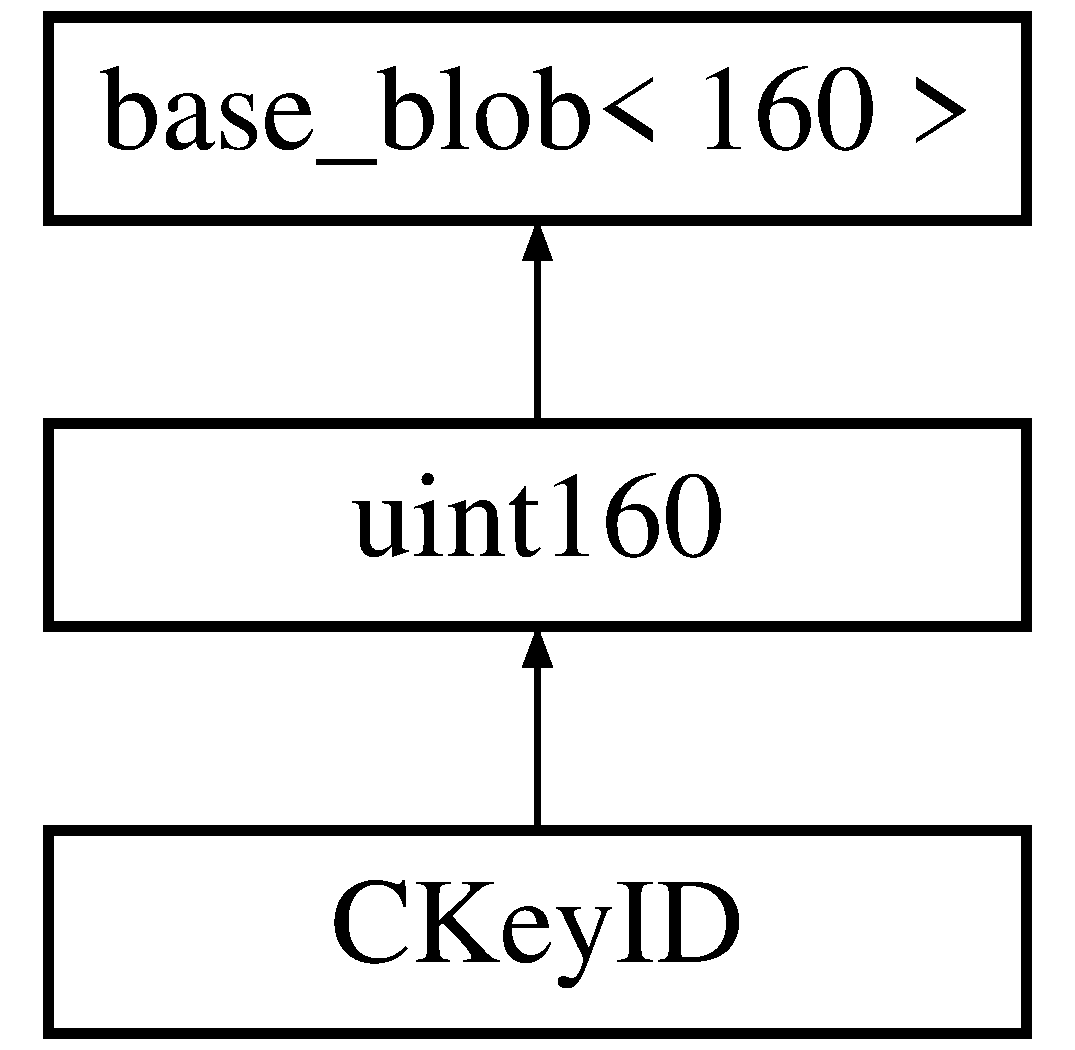
\includegraphics[height=3.000000cm]{class_c_key_i_d}
\end{center}
\end{figure}
\subsection*{Public Member Functions}
\begin{DoxyCompactItemize}
\item 
\mbox{\hyperlink{class_c_key_i_d_a01dbd3c37820a2ffe89d106c6a7cf53d}{C\+Key\+ID}} ()
\item 
\mbox{\hyperlink{class_c_key_i_d_a695f373e11730318f9103100fa006a7e}{C\+Key\+ID}} (const \mbox{\hyperlink{classuint160}{uint160}} \&in)
\end{DoxyCompactItemize}
\subsection*{Additional Inherited Members}


\subsection{Detailed Description}
see www.\+keylength.\+com script supports up to 75 for single byte pushA reference to a \mbox{\hyperlink{class_c_key}{C\+Key}}\+: the Hash160 of its serialized public key 

\subsection{Constructor \& Destructor Documentation}
\mbox{\Hypertarget{class_c_key_i_d_a01dbd3c37820a2ffe89d106c6a7cf53d}\label{class_c_key_i_d_a01dbd3c37820a2ffe89d106c6a7cf53d}} 
\index{C\+Key\+ID@{C\+Key\+ID}!C\+Key\+ID@{C\+Key\+ID}}
\index{C\+Key\+ID@{C\+Key\+ID}!C\+Key\+ID@{C\+Key\+ID}}
\subsubsection{\texorpdfstring{C\+Key\+I\+D()}{CKeyID()}\hspace{0.1cm}{\footnotesize\ttfamily [1/2]}}
{\footnotesize\ttfamily C\+Key\+I\+D\+::\+C\+Key\+ID (\begin{DoxyParamCaption}{ }\end{DoxyParamCaption})\hspace{0.3cm}{\ttfamily [inline]}}

\mbox{\Hypertarget{class_c_key_i_d_a695f373e11730318f9103100fa006a7e}\label{class_c_key_i_d_a695f373e11730318f9103100fa006a7e}} 
\index{C\+Key\+ID@{C\+Key\+ID}!C\+Key\+ID@{C\+Key\+ID}}
\index{C\+Key\+ID@{C\+Key\+ID}!C\+Key\+ID@{C\+Key\+ID}}
\subsubsection{\texorpdfstring{C\+Key\+I\+D()}{CKeyID()}\hspace{0.1cm}{\footnotesize\ttfamily [2/2]}}
{\footnotesize\ttfamily C\+Key\+I\+D\+::\+C\+Key\+ID (\begin{DoxyParamCaption}\item[{const \mbox{\hyperlink{classuint160}{uint160}} \&}]{in }\end{DoxyParamCaption})\hspace{0.3cm}{\ttfamily [inline]}}



The documentation for this class was generated from the following file\+:\begin{DoxyCompactItemize}
\item 
/\+Users/christopherarguello/\+Developer/anon/src/\mbox{\hyperlink{pubkey_8h}{pubkey.\+h}}\end{DoxyCompactItemize}

\hypertarget{class_c_key_store}{}\section{C\+Key\+Store Class Reference}
\label{class_c_key_store}\index{C\+Key\+Store@{C\+Key\+Store}}


{\ttfamily \#include $<$keystore.\+h$>$}

Inheritance diagram for C\+Key\+Store\+:\begin{figure}[H]
\begin{center}
\leavevmode
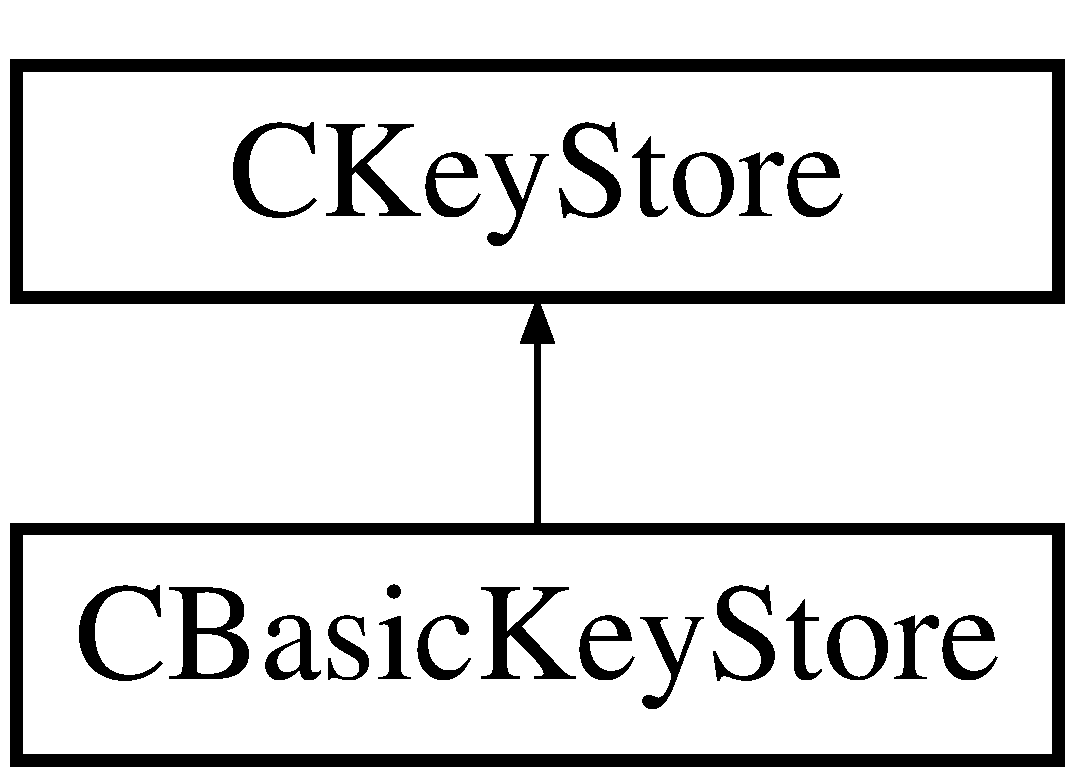
\includegraphics[height=2.000000cm]{class_c_key_store}
\end{center}
\end{figure}
\subsection*{Public Member Functions}
\begin{DoxyCompactItemize}
\item 
virtual \mbox{\hyperlink{class_c_key_store_a9bfaef2bcd6effc467a96043f44044a0}{$\sim$\+C\+Key\+Store}} ()
\item 
virtual bool \mbox{\hyperlink{class_c_key_store_a1956e4f5860ded321d6f697047d8236a}{Add\+Key\+Pub\+Key}} (const \mbox{\hyperlink{class_c_key}{C\+Key}} \&key, const \mbox{\hyperlink{class_c_pub_key}{C\+Pub\+Key}} \&pubkey)=0
\begin{DoxyCompactList}\small\item\em Add a key to the store. \end{DoxyCompactList}\item 
virtual bool \mbox{\hyperlink{class_c_key_store_a0b4ca43724cfcc6e2ea70c0baa192750}{Add\+Key}} (const \mbox{\hyperlink{class_c_key}{C\+Key}} \&key)
\item 
virtual bool \mbox{\hyperlink{class_c_key_store_a9398451d4270fae27b29f686a9d43a65}{Have\+Key}} (const \mbox{\hyperlink{class_c_key_i_d}{C\+Key\+ID}} \&address) const =0
\begin{DoxyCompactList}\small\item\em Check whether a key corresponding to a given address is present in the store. \end{DoxyCompactList}\item 
virtual bool \mbox{\hyperlink{class_c_key_store_a2dffca468fef2e5da2e42a7c983d968a}{Get\+Key}} (const \mbox{\hyperlink{class_c_key_i_d}{C\+Key\+ID}} \&address, \mbox{\hyperlink{class_c_key}{C\+Key}} \&key\+Out) const =0
\item 
virtual void \mbox{\hyperlink{class_c_key_store_aca5044014720308f191113e7ba297d13}{Get\+Keys}} (std\+::set$<$ \mbox{\hyperlink{class_c_key_i_d}{C\+Key\+ID}} $>$ \&set\+Address) const =0
\item 
virtual bool \mbox{\hyperlink{class_c_key_store_ab83687ea4c9df138b21f6ec3e9809f42}{Get\+Pub\+Key}} (const \mbox{\hyperlink{class_c_key_i_d}{C\+Key\+ID}} \&address, \mbox{\hyperlink{class_c_pub_key}{C\+Pub\+Key}} \&vch\+Pub\+Key\+Out) const
\item 
virtual bool \mbox{\hyperlink{class_c_key_store_a2fb2e02e8cdc364607efd5ebb14b8064}{Add\+C\+Script}} (const C\+Script \&redeem\+Script)=0
\begin{DoxyCompactList}\small\item\em Support for B\+IP 0013 \+: see \href{https://github.com/bitcoin/bips/blob/master/bip-0013.mediawiki}{\tt https\+://github.\+com/bitcoin/bips/blob/master/bip-\/0013.\+mediawiki}. \end{DoxyCompactList}\item 
virtual bool \mbox{\hyperlink{class_c_key_store_a51c9fc86b2c3fece10d86146231fa58d}{Have\+C\+Script}} (const C\+Script\+ID \&hash) const =0
\item 
virtual bool \mbox{\hyperlink{class_c_key_store_ae6bf4dbeb0705e199250e48aa5d34264}{Get\+C\+Script}} (const C\+Script\+ID \&hash, C\+Script \&redeem\+Script\+Out) const =0
\item 
virtual bool \mbox{\hyperlink{class_c_key_store_a12cd4eaa01bd4f4231c0bf68425a44af}{Add\+Watch\+Only}} (const C\+Script \&dest)=0
\begin{DoxyCompactList}\small\item\em Support for Watch-\/only addresses. \end{DoxyCompactList}\item 
virtual bool \mbox{\hyperlink{class_c_key_store_ad510747f28d129123a5200e4df8f7f61}{Remove\+Watch\+Only}} (const C\+Script \&dest)=0
\item 
virtual bool \mbox{\hyperlink{class_c_key_store_a15066cfd57feaffe0b9f4103c9311109}{Have\+Watch\+Only}} (const C\+Script \&dest) const =0
\item 
virtual bool \mbox{\hyperlink{class_c_key_store_a9169351f4acf62d299afb824174cbfa8}{Have\+Watch\+Only}} () const =0
\item 
virtual bool \mbox{\hyperlink{class_c_key_store_aa78189cb8f342a33570c2ac6d4a0ffcf}{Add\+Spending\+Key}} (const libzcash\+::\+Spending\+Key \&sk)=0
\begin{DoxyCompactList}\small\item\em Add a spending key to the store. \end{DoxyCompactList}\item 
virtual bool \mbox{\hyperlink{class_c_key_store_a15590101690f5a691b04a5498453b66a}{Have\+Spending\+Key}} (const libzcash\+::\+Payment\+Address \&address) const =0
\begin{DoxyCompactList}\small\item\em Check whether a spending key corresponding to a given payment address is present in the store. \end{DoxyCompactList}\item 
virtual bool \mbox{\hyperlink{class_c_key_store_a812534268d0324370c53ba3e7a295b95}{Get\+Spending\+Key}} (const libzcash\+::\+Payment\+Address \&address, libzcash\+::\+Spending\+Key \&sk\+Out) const =0
\item 
virtual void \mbox{\hyperlink{class_c_key_store_a6186d83956656316f3fe679b4f907866}{Get\+Payment\+Addresses}} (std\+::set$<$ libzcash\+::\+Payment\+Address $>$ \&set\+Address) const =0
\end{DoxyCompactItemize}
\subsection*{Protected Attributes}
\begin{DoxyCompactItemize}
\item 
\mbox{\hyperlink{sync_8h_a37a4692b2d517f2843655ca11af7668a}{C\+Critical\+Section}} \mbox{\hyperlink{class_c_key_store_a386524ff4a00959b81c195cb39fe307d}{cs\+\_\+\+Key\+Store}}
\item 
\mbox{\hyperlink{sync_8h_a37a4692b2d517f2843655ca11af7668a}{C\+Critical\+Section}} \mbox{\hyperlink{class_c_key_store_ac81106dc4a3f71d6c1781bfd10fb6589}{cs\+\_\+\+Spending\+Key\+Store}}
\end{DoxyCompactItemize}


\subsection{Detailed Description}
A virtual base class for key stores 

\subsection{Constructor \& Destructor Documentation}
\mbox{\Hypertarget{class_c_key_store_a9bfaef2bcd6effc467a96043f44044a0}\label{class_c_key_store_a9bfaef2bcd6effc467a96043f44044a0}} 
\index{C\+Key\+Store@{C\+Key\+Store}!````~C\+Key\+Store@{$\sim$\+C\+Key\+Store}}
\index{````~C\+Key\+Store@{$\sim$\+C\+Key\+Store}!C\+Key\+Store@{C\+Key\+Store}}
\subsubsection{\texorpdfstring{$\sim$\+C\+Key\+Store()}{~CKeyStore()}}
{\footnotesize\ttfamily virtual C\+Key\+Store\+::$\sim$\+C\+Key\+Store (\begin{DoxyParamCaption}{ }\end{DoxyParamCaption})\hspace{0.3cm}{\ttfamily [inline]}, {\ttfamily [virtual]}}



\subsection{Member Function Documentation}
\mbox{\Hypertarget{class_c_key_store_a2fb2e02e8cdc364607efd5ebb14b8064}\label{class_c_key_store_a2fb2e02e8cdc364607efd5ebb14b8064}} 
\index{C\+Key\+Store@{C\+Key\+Store}!Add\+C\+Script@{Add\+C\+Script}}
\index{Add\+C\+Script@{Add\+C\+Script}!C\+Key\+Store@{C\+Key\+Store}}
\subsubsection{\texorpdfstring{Add\+C\+Script()}{AddCScript()}}
{\footnotesize\ttfamily virtual bool C\+Key\+Store\+::\+Add\+C\+Script (\begin{DoxyParamCaption}\item[{const C\+Script \&}]{redeem\+Script }\end{DoxyParamCaption})\hspace{0.3cm}{\ttfamily [pure virtual]}}



Support for B\+IP 0013 \+: see \href{https://github.com/bitcoin/bips/blob/master/bip-0013.mediawiki}{\tt https\+://github.\+com/bitcoin/bips/blob/master/bip-\/0013.\+mediawiki}. 



Implemented in \mbox{\hyperlink{class_c_basic_key_store_a56249ce3540398999cd397eeb662e836}{C\+Basic\+Key\+Store}}.

\mbox{\Hypertarget{class_c_key_store_a0b4ca43724cfcc6e2ea70c0baa192750}\label{class_c_key_store_a0b4ca43724cfcc6e2ea70c0baa192750}} 
\index{C\+Key\+Store@{C\+Key\+Store}!Add\+Key@{Add\+Key}}
\index{Add\+Key@{Add\+Key}!C\+Key\+Store@{C\+Key\+Store}}
\subsubsection{\texorpdfstring{Add\+Key()}{AddKey()}}
{\footnotesize\ttfamily bool C\+Key\+Store\+::\+Add\+Key (\begin{DoxyParamCaption}\item[{const \mbox{\hyperlink{class_c_key}{C\+Key}} \&}]{key }\end{DoxyParamCaption})\hspace{0.3cm}{\ttfamily [virtual]}}

\mbox{\Hypertarget{class_c_key_store_a1956e4f5860ded321d6f697047d8236a}\label{class_c_key_store_a1956e4f5860ded321d6f697047d8236a}} 
\index{C\+Key\+Store@{C\+Key\+Store}!Add\+Key\+Pub\+Key@{Add\+Key\+Pub\+Key}}
\index{Add\+Key\+Pub\+Key@{Add\+Key\+Pub\+Key}!C\+Key\+Store@{C\+Key\+Store}}
\subsubsection{\texorpdfstring{Add\+Key\+Pub\+Key()}{AddKeyPubKey()}}
{\footnotesize\ttfamily virtual bool C\+Key\+Store\+::\+Add\+Key\+Pub\+Key (\begin{DoxyParamCaption}\item[{const \mbox{\hyperlink{class_c_key}{C\+Key}} \&}]{key,  }\item[{const \mbox{\hyperlink{class_c_pub_key}{C\+Pub\+Key}} \&}]{pubkey }\end{DoxyParamCaption})\hspace{0.3cm}{\ttfamily [pure virtual]}}



Add a key to the store. 



Implemented in \mbox{\hyperlink{class_c_basic_key_store_acc2e33f319de88e88f86b0dc79bdcb65}{C\+Basic\+Key\+Store}}.

\mbox{\Hypertarget{class_c_key_store_aa78189cb8f342a33570c2ac6d4a0ffcf}\label{class_c_key_store_aa78189cb8f342a33570c2ac6d4a0ffcf}} 
\index{C\+Key\+Store@{C\+Key\+Store}!Add\+Spending\+Key@{Add\+Spending\+Key}}
\index{Add\+Spending\+Key@{Add\+Spending\+Key}!C\+Key\+Store@{C\+Key\+Store}}
\subsubsection{\texorpdfstring{Add\+Spending\+Key()}{AddSpendingKey()}}
{\footnotesize\ttfamily virtual bool C\+Key\+Store\+::\+Add\+Spending\+Key (\begin{DoxyParamCaption}\item[{const libzcash\+::\+Spending\+Key \&}]{sk }\end{DoxyParamCaption})\hspace{0.3cm}{\ttfamily [pure virtual]}}



Add a spending key to the store. 



Implemented in \mbox{\hyperlink{class_c_basic_key_store_aa2d2d623fe80e75fe1718a15755ee1f1}{C\+Basic\+Key\+Store}}.

\mbox{\Hypertarget{class_c_key_store_a12cd4eaa01bd4f4231c0bf68425a44af}\label{class_c_key_store_a12cd4eaa01bd4f4231c0bf68425a44af}} 
\index{C\+Key\+Store@{C\+Key\+Store}!Add\+Watch\+Only@{Add\+Watch\+Only}}
\index{Add\+Watch\+Only@{Add\+Watch\+Only}!C\+Key\+Store@{C\+Key\+Store}}
\subsubsection{\texorpdfstring{Add\+Watch\+Only()}{AddWatchOnly()}}
{\footnotesize\ttfamily virtual bool C\+Key\+Store\+::\+Add\+Watch\+Only (\begin{DoxyParamCaption}\item[{const C\+Script \&}]{dest }\end{DoxyParamCaption})\hspace{0.3cm}{\ttfamily [pure virtual]}}



Support for Watch-\/only addresses. 



Implemented in \mbox{\hyperlink{class_c_basic_key_store_a2417d0ae4e654c88cf47a1ba5f71b5a3}{C\+Basic\+Key\+Store}}.

\mbox{\Hypertarget{class_c_key_store_ae6bf4dbeb0705e199250e48aa5d34264}\label{class_c_key_store_ae6bf4dbeb0705e199250e48aa5d34264}} 
\index{C\+Key\+Store@{C\+Key\+Store}!Get\+C\+Script@{Get\+C\+Script}}
\index{Get\+C\+Script@{Get\+C\+Script}!C\+Key\+Store@{C\+Key\+Store}}
\subsubsection{\texorpdfstring{Get\+C\+Script()}{GetCScript()}}
{\footnotesize\ttfamily virtual bool C\+Key\+Store\+::\+Get\+C\+Script (\begin{DoxyParamCaption}\item[{const C\+Script\+ID \&}]{hash,  }\item[{C\+Script \&}]{redeem\+Script\+Out }\end{DoxyParamCaption}) const\hspace{0.3cm}{\ttfamily [pure virtual]}}



Implemented in \mbox{\hyperlink{class_c_basic_key_store_a975abe0f2efa3e0e2270d3714d73010a}{C\+Basic\+Key\+Store}}.

\mbox{\Hypertarget{class_c_key_store_a2dffca468fef2e5da2e42a7c983d968a}\label{class_c_key_store_a2dffca468fef2e5da2e42a7c983d968a}} 
\index{C\+Key\+Store@{C\+Key\+Store}!Get\+Key@{Get\+Key}}
\index{Get\+Key@{Get\+Key}!C\+Key\+Store@{C\+Key\+Store}}
\subsubsection{\texorpdfstring{Get\+Key()}{GetKey()}}
{\footnotesize\ttfamily virtual bool C\+Key\+Store\+::\+Get\+Key (\begin{DoxyParamCaption}\item[{const \mbox{\hyperlink{class_c_key_i_d}{C\+Key\+ID}} \&}]{address,  }\item[{\mbox{\hyperlink{class_c_key}{C\+Key}} \&}]{key\+Out }\end{DoxyParamCaption}) const\hspace{0.3cm}{\ttfamily [pure virtual]}}



Implemented in \mbox{\hyperlink{class_c_basic_key_store_a69328ee642e4234922356f59876e956d}{C\+Basic\+Key\+Store}}.

\mbox{\Hypertarget{class_c_key_store_aca5044014720308f191113e7ba297d13}\label{class_c_key_store_aca5044014720308f191113e7ba297d13}} 
\index{C\+Key\+Store@{C\+Key\+Store}!Get\+Keys@{Get\+Keys}}
\index{Get\+Keys@{Get\+Keys}!C\+Key\+Store@{C\+Key\+Store}}
\subsubsection{\texorpdfstring{Get\+Keys()}{GetKeys()}}
{\footnotesize\ttfamily virtual void C\+Key\+Store\+::\+Get\+Keys (\begin{DoxyParamCaption}\item[{std\+::set$<$ \mbox{\hyperlink{class_c_key_i_d}{C\+Key\+ID}} $>$ \&}]{set\+Address }\end{DoxyParamCaption}) const\hspace{0.3cm}{\ttfamily [pure virtual]}}



Implemented in \mbox{\hyperlink{class_c_basic_key_store_a41f3895021dae008582ceb55a98b0891}{C\+Basic\+Key\+Store}}.

\mbox{\Hypertarget{class_c_key_store_a6186d83956656316f3fe679b4f907866}\label{class_c_key_store_a6186d83956656316f3fe679b4f907866}} 
\index{C\+Key\+Store@{C\+Key\+Store}!Get\+Payment\+Addresses@{Get\+Payment\+Addresses}}
\index{Get\+Payment\+Addresses@{Get\+Payment\+Addresses}!C\+Key\+Store@{C\+Key\+Store}}
\subsubsection{\texorpdfstring{Get\+Payment\+Addresses()}{GetPaymentAddresses()}}
{\footnotesize\ttfamily virtual void C\+Key\+Store\+::\+Get\+Payment\+Addresses (\begin{DoxyParamCaption}\item[{std\+::set$<$ libzcash\+::\+Payment\+Address $>$ \&}]{set\+Address }\end{DoxyParamCaption}) const\hspace{0.3cm}{\ttfamily [pure virtual]}}



Implemented in \mbox{\hyperlink{class_c_basic_key_store_af02668c3bef8b5a56231505f900a0314}{C\+Basic\+Key\+Store}}.

\mbox{\Hypertarget{class_c_key_store_ab83687ea4c9df138b21f6ec3e9809f42}\label{class_c_key_store_ab83687ea4c9df138b21f6ec3e9809f42}} 
\index{C\+Key\+Store@{C\+Key\+Store}!Get\+Pub\+Key@{Get\+Pub\+Key}}
\index{Get\+Pub\+Key@{Get\+Pub\+Key}!C\+Key\+Store@{C\+Key\+Store}}
\subsubsection{\texorpdfstring{Get\+Pub\+Key()}{GetPubKey()}}
{\footnotesize\ttfamily bool C\+Key\+Store\+::\+Get\+Pub\+Key (\begin{DoxyParamCaption}\item[{const \mbox{\hyperlink{class_c_key_i_d}{C\+Key\+ID}} \&}]{address,  }\item[{\mbox{\hyperlink{class_c_pub_key}{C\+Pub\+Key}} \&}]{vch\+Pub\+Key\+Out }\end{DoxyParamCaption}) const\hspace{0.3cm}{\ttfamily [virtual]}}

\mbox{\Hypertarget{class_c_key_store_a812534268d0324370c53ba3e7a295b95}\label{class_c_key_store_a812534268d0324370c53ba3e7a295b95}} 
\index{C\+Key\+Store@{C\+Key\+Store}!Get\+Spending\+Key@{Get\+Spending\+Key}}
\index{Get\+Spending\+Key@{Get\+Spending\+Key}!C\+Key\+Store@{C\+Key\+Store}}
\subsubsection{\texorpdfstring{Get\+Spending\+Key()}{GetSpendingKey()}}
{\footnotesize\ttfamily virtual bool C\+Key\+Store\+::\+Get\+Spending\+Key (\begin{DoxyParamCaption}\item[{const libzcash\+::\+Payment\+Address \&}]{address,  }\item[{libzcash\+::\+Spending\+Key \&}]{sk\+Out }\end{DoxyParamCaption}) const\hspace{0.3cm}{\ttfamily [pure virtual]}}



Implemented in \mbox{\hyperlink{class_c_basic_key_store_a0c7997c0413eaa7ec76ec5bef0b40a2a}{C\+Basic\+Key\+Store}}.

\mbox{\Hypertarget{class_c_key_store_a51c9fc86b2c3fece10d86146231fa58d}\label{class_c_key_store_a51c9fc86b2c3fece10d86146231fa58d}} 
\index{C\+Key\+Store@{C\+Key\+Store}!Have\+C\+Script@{Have\+C\+Script}}
\index{Have\+C\+Script@{Have\+C\+Script}!C\+Key\+Store@{C\+Key\+Store}}
\subsubsection{\texorpdfstring{Have\+C\+Script()}{HaveCScript()}}
{\footnotesize\ttfamily virtual bool C\+Key\+Store\+::\+Have\+C\+Script (\begin{DoxyParamCaption}\item[{const C\+Script\+ID \&}]{hash }\end{DoxyParamCaption}) const\hspace{0.3cm}{\ttfamily [pure virtual]}}



Implemented in \mbox{\hyperlink{class_c_basic_key_store_a499e0a1d117b43e3200883d88a400bf6}{C\+Basic\+Key\+Store}}.

\mbox{\Hypertarget{class_c_key_store_a9398451d4270fae27b29f686a9d43a65}\label{class_c_key_store_a9398451d4270fae27b29f686a9d43a65}} 
\index{C\+Key\+Store@{C\+Key\+Store}!Have\+Key@{Have\+Key}}
\index{Have\+Key@{Have\+Key}!C\+Key\+Store@{C\+Key\+Store}}
\subsubsection{\texorpdfstring{Have\+Key()}{HaveKey()}}
{\footnotesize\ttfamily virtual bool C\+Key\+Store\+::\+Have\+Key (\begin{DoxyParamCaption}\item[{const \mbox{\hyperlink{class_c_key_i_d}{C\+Key\+ID}} \&}]{address }\end{DoxyParamCaption}) const\hspace{0.3cm}{\ttfamily [pure virtual]}}



Check whether a key corresponding to a given address is present in the store. 



Implemented in \mbox{\hyperlink{class_c_basic_key_store_afc99762e3e58f93e198d85ecfdf5804a}{C\+Basic\+Key\+Store}}.

\mbox{\Hypertarget{class_c_key_store_a15590101690f5a691b04a5498453b66a}\label{class_c_key_store_a15590101690f5a691b04a5498453b66a}} 
\index{C\+Key\+Store@{C\+Key\+Store}!Have\+Spending\+Key@{Have\+Spending\+Key}}
\index{Have\+Spending\+Key@{Have\+Spending\+Key}!C\+Key\+Store@{C\+Key\+Store}}
\subsubsection{\texorpdfstring{Have\+Spending\+Key()}{HaveSpendingKey()}}
{\footnotesize\ttfamily virtual bool C\+Key\+Store\+::\+Have\+Spending\+Key (\begin{DoxyParamCaption}\item[{const libzcash\+::\+Payment\+Address \&}]{address }\end{DoxyParamCaption}) const\hspace{0.3cm}{\ttfamily [pure virtual]}}



Check whether a spending key corresponding to a given payment address is present in the store. 



Implemented in \mbox{\hyperlink{class_c_basic_key_store_a513367bd0a576e088e3f577686fa1ef5}{C\+Basic\+Key\+Store}}.

\mbox{\Hypertarget{class_c_key_store_a15066cfd57feaffe0b9f4103c9311109}\label{class_c_key_store_a15066cfd57feaffe0b9f4103c9311109}} 
\index{C\+Key\+Store@{C\+Key\+Store}!Have\+Watch\+Only@{Have\+Watch\+Only}}
\index{Have\+Watch\+Only@{Have\+Watch\+Only}!C\+Key\+Store@{C\+Key\+Store}}
\subsubsection{\texorpdfstring{Have\+Watch\+Only()}{HaveWatchOnly()}\hspace{0.1cm}{\footnotesize\ttfamily [1/2]}}
{\footnotesize\ttfamily virtual bool C\+Key\+Store\+::\+Have\+Watch\+Only (\begin{DoxyParamCaption}\item[{const C\+Script \&}]{dest }\end{DoxyParamCaption}) const\hspace{0.3cm}{\ttfamily [pure virtual]}}



Implemented in \mbox{\hyperlink{class_c_basic_key_store_a3ce143be2a1d3e752972614cf7fb7efb}{C\+Basic\+Key\+Store}}.

\mbox{\Hypertarget{class_c_key_store_a9169351f4acf62d299afb824174cbfa8}\label{class_c_key_store_a9169351f4acf62d299afb824174cbfa8}} 
\index{C\+Key\+Store@{C\+Key\+Store}!Have\+Watch\+Only@{Have\+Watch\+Only}}
\index{Have\+Watch\+Only@{Have\+Watch\+Only}!C\+Key\+Store@{C\+Key\+Store}}
\subsubsection{\texorpdfstring{Have\+Watch\+Only()}{HaveWatchOnly()}\hspace{0.1cm}{\footnotesize\ttfamily [2/2]}}
{\footnotesize\ttfamily virtual bool C\+Key\+Store\+::\+Have\+Watch\+Only (\begin{DoxyParamCaption}{ }\end{DoxyParamCaption}) const\hspace{0.3cm}{\ttfamily [pure virtual]}}



Implemented in \mbox{\hyperlink{class_c_basic_key_store_aa6686d4477a180096436e7d491142f10}{C\+Basic\+Key\+Store}}.

\mbox{\Hypertarget{class_c_key_store_ad510747f28d129123a5200e4df8f7f61}\label{class_c_key_store_ad510747f28d129123a5200e4df8f7f61}} 
\index{C\+Key\+Store@{C\+Key\+Store}!Remove\+Watch\+Only@{Remove\+Watch\+Only}}
\index{Remove\+Watch\+Only@{Remove\+Watch\+Only}!C\+Key\+Store@{C\+Key\+Store}}
\subsubsection{\texorpdfstring{Remove\+Watch\+Only()}{RemoveWatchOnly()}}
{\footnotesize\ttfamily virtual bool C\+Key\+Store\+::\+Remove\+Watch\+Only (\begin{DoxyParamCaption}\item[{const C\+Script \&}]{dest }\end{DoxyParamCaption})\hspace{0.3cm}{\ttfamily [pure virtual]}}



Implemented in \mbox{\hyperlink{class_c_basic_key_store_a20c0eccf943d6d16e24c6e2fb63fb527}{C\+Basic\+Key\+Store}}.



\subsection{Member Data Documentation}
\mbox{\Hypertarget{class_c_key_store_a386524ff4a00959b81c195cb39fe307d}\label{class_c_key_store_a386524ff4a00959b81c195cb39fe307d}} 
\index{C\+Key\+Store@{C\+Key\+Store}!cs\+\_\+\+Key\+Store@{cs\+\_\+\+Key\+Store}}
\index{cs\+\_\+\+Key\+Store@{cs\+\_\+\+Key\+Store}!C\+Key\+Store@{C\+Key\+Store}}
\subsubsection{\texorpdfstring{cs\+\_\+\+Key\+Store}{cs\_KeyStore}}
{\footnotesize\ttfamily \mbox{\hyperlink{sync_8h_a37a4692b2d517f2843655ca11af7668a}{C\+Critical\+Section}} C\+Key\+Store\+::cs\+\_\+\+Key\+Store\hspace{0.3cm}{\ttfamily [mutable]}, {\ttfamily [protected]}}

\mbox{\Hypertarget{class_c_key_store_ac81106dc4a3f71d6c1781bfd10fb6589}\label{class_c_key_store_ac81106dc4a3f71d6c1781bfd10fb6589}} 
\index{C\+Key\+Store@{C\+Key\+Store}!cs\+\_\+\+Spending\+Key\+Store@{cs\+\_\+\+Spending\+Key\+Store}}
\index{cs\+\_\+\+Spending\+Key\+Store@{cs\+\_\+\+Spending\+Key\+Store}!C\+Key\+Store@{C\+Key\+Store}}
\subsubsection{\texorpdfstring{cs\+\_\+\+Spending\+Key\+Store}{cs\_SpendingKeyStore}}
{\footnotesize\ttfamily \mbox{\hyperlink{sync_8h_a37a4692b2d517f2843655ca11af7668a}{C\+Critical\+Section}} C\+Key\+Store\+::cs\+\_\+\+Spending\+Key\+Store\hspace{0.3cm}{\ttfamily [mutable]}, {\ttfamily [protected]}}



The documentation for this class was generated from the following files\+:\begin{DoxyCompactItemize}
\item 
/\+Users/christopherarguello/\+Developer/anon/src/\mbox{\hyperlink{keystore_8h}{keystore.\+h}}\item 
/\+Users/christopherarguello/\+Developer/anon/src/\mbox{\hyperlink{keystore_8cpp}{keystore.\+cpp}}\end{DoxyCompactItemize}

\hypertarget{class_c_level_d_b_batch}{}\section{C\+Level\+D\+B\+Batch Class Reference}
\label{class_c_level_d_b_batch}\index{C\+Level\+D\+B\+Batch@{C\+Level\+D\+B\+Batch}}


{\ttfamily \#include $<$leveldbwrapper.\+h$>$}

\subsection*{Public Member Functions}
\begin{DoxyCompactItemize}
\item 
{\footnotesize template$<$typename K , typename V $>$ }\\void \mbox{\hyperlink{class_c_level_d_b_batch_ab459da1abafa27e834de9a4cc25b6f2d}{Write}} (const K \&key, const V \&value)
\item 
{\footnotesize template$<$typename K $>$ }\\void \mbox{\hyperlink{class_c_level_d_b_batch_a22bf093d560b4ce3333e8f4a947faa7f}{Erase}} (const K \&key)
\end{DoxyCompactItemize}
\subsection*{Private Attributes}
\begin{DoxyCompactItemize}
\item 
leveldb\+::\+Write\+Batch \mbox{\hyperlink{class_c_level_d_b_batch_af404cb1abfb4d62781eb6d22d408cd5d}{batch}}
\end{DoxyCompactItemize}
\subsection*{Friends}
\begin{DoxyCompactItemize}
\item 
class \mbox{\hyperlink{class_c_level_d_b_batch_acbe5e6be88c5bccb0ec229ebc91dde82}{C\+Level\+D\+B\+Wrapper}}
\end{DoxyCompactItemize}


\subsection{Detailed Description}
Batch of changes queued to be written to a \mbox{\hyperlink{class_c_level_d_b_wrapper}{C\+Level\+D\+B\+Wrapper}} 

\subsection{Member Function Documentation}
\mbox{\Hypertarget{class_c_level_d_b_batch_a22bf093d560b4ce3333e8f4a947faa7f}\label{class_c_level_d_b_batch_a22bf093d560b4ce3333e8f4a947faa7f}} 
\index{C\+Level\+D\+B\+Batch@{C\+Level\+D\+B\+Batch}!Erase@{Erase}}
\index{Erase@{Erase}!C\+Level\+D\+B\+Batch@{C\+Level\+D\+B\+Batch}}
\subsubsection{\texorpdfstring{Erase()}{Erase()}}
{\footnotesize\ttfamily template$<$typename K $>$ \\
void C\+Level\+D\+B\+Batch\+::\+Erase (\begin{DoxyParamCaption}\item[{const K \&}]{key }\end{DoxyParamCaption})\hspace{0.3cm}{\ttfamily [inline]}}

\mbox{\Hypertarget{class_c_level_d_b_batch_ab459da1abafa27e834de9a4cc25b6f2d}\label{class_c_level_d_b_batch_ab459da1abafa27e834de9a4cc25b6f2d}} 
\index{C\+Level\+D\+B\+Batch@{C\+Level\+D\+B\+Batch}!Write@{Write}}
\index{Write@{Write}!C\+Level\+D\+B\+Batch@{C\+Level\+D\+B\+Batch}}
\subsubsection{\texorpdfstring{Write()}{Write()}}
{\footnotesize\ttfamily template$<$typename K , typename V $>$ \\
void C\+Level\+D\+B\+Batch\+::\+Write (\begin{DoxyParamCaption}\item[{const K \&}]{key,  }\item[{const V \&}]{value }\end{DoxyParamCaption})\hspace{0.3cm}{\ttfamily [inline]}}



\subsection{Friends And Related Function Documentation}
\mbox{\Hypertarget{class_c_level_d_b_batch_acbe5e6be88c5bccb0ec229ebc91dde82}\label{class_c_level_d_b_batch_acbe5e6be88c5bccb0ec229ebc91dde82}} 
\index{C\+Level\+D\+B\+Batch@{C\+Level\+D\+B\+Batch}!C\+Level\+D\+B\+Wrapper@{C\+Level\+D\+B\+Wrapper}}
\index{C\+Level\+D\+B\+Wrapper@{C\+Level\+D\+B\+Wrapper}!C\+Level\+D\+B\+Batch@{C\+Level\+D\+B\+Batch}}
\subsubsection{\texorpdfstring{C\+Level\+D\+B\+Wrapper}{CLevelDBWrapper}}
{\footnotesize\ttfamily friend class \mbox{\hyperlink{class_c_level_d_b_wrapper}{C\+Level\+D\+B\+Wrapper}}\hspace{0.3cm}{\ttfamily [friend]}}



\subsection{Member Data Documentation}
\mbox{\Hypertarget{class_c_level_d_b_batch_af404cb1abfb4d62781eb6d22d408cd5d}\label{class_c_level_d_b_batch_af404cb1abfb4d62781eb6d22d408cd5d}} 
\index{C\+Level\+D\+B\+Batch@{C\+Level\+D\+B\+Batch}!batch@{batch}}
\index{batch@{batch}!C\+Level\+D\+B\+Batch@{C\+Level\+D\+B\+Batch}}
\subsubsection{\texorpdfstring{batch}{batch}}
{\footnotesize\ttfamily leveldb\+::\+Write\+Batch C\+Level\+D\+B\+Batch\+::batch\hspace{0.3cm}{\ttfamily [private]}}



The documentation for this class was generated from the following file\+:\begin{DoxyCompactItemize}
\item 
/\+Users/christopherarguello/\+Developer/anon/src/\mbox{\hyperlink{leveldbwrapper_8h}{leveldbwrapper.\+h}}\end{DoxyCompactItemize}

\hypertarget{class_c_level_d_b_wrapper}{}\section{C\+Level\+D\+B\+Wrapper Class Reference}
\label{class_c_level_d_b_wrapper}\index{C\+Level\+D\+B\+Wrapper@{C\+Level\+D\+B\+Wrapper}}


{\ttfamily \#include $<$leveldbwrapper.\+h$>$}

Inheritance diagram for C\+Level\+D\+B\+Wrapper\+:\begin{figure}[H]
\begin{center}
\leavevmode
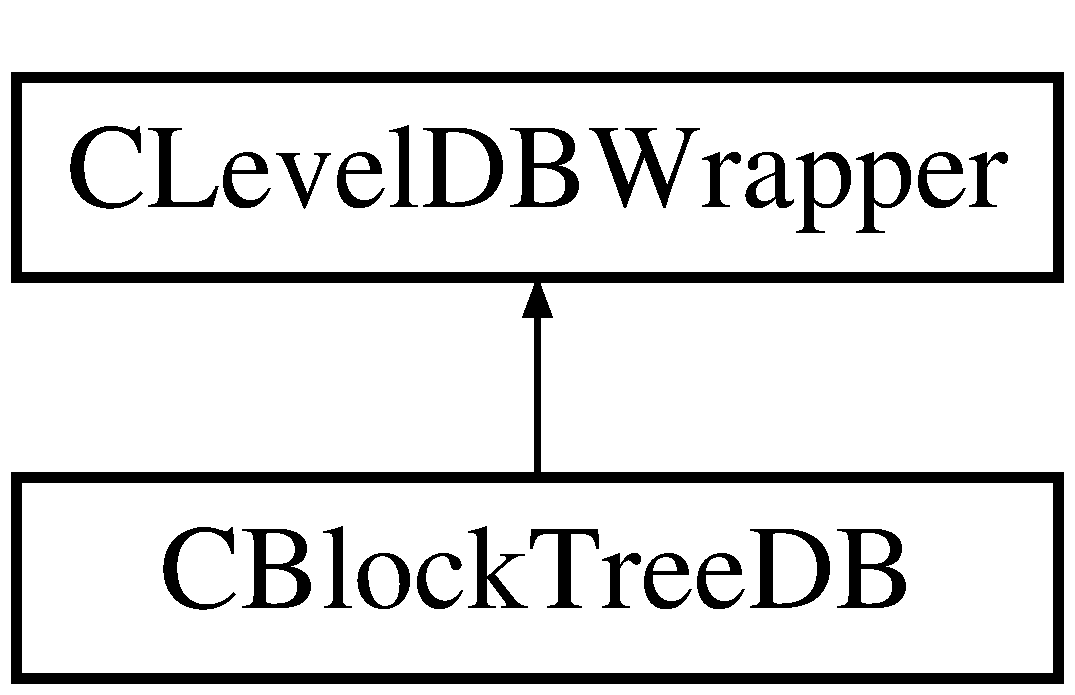
\includegraphics[height=2.000000cm]{class_c_level_d_b_wrapper}
\end{center}
\end{figure}
\subsection*{Public Member Functions}
\begin{DoxyCompactItemize}
\item 
\mbox{\hyperlink{class_c_level_d_b_wrapper_ae796b1190c072df6275e0ada4d187943}{C\+Level\+D\+B\+Wrapper}} (const boost\+::filesystem\+::path \&path, size\+\_\+t n\+Cache\+Size, bool f\+Memory=false, bool f\+Wipe=false)
\item 
\mbox{\hyperlink{class_c_level_d_b_wrapper_a7ffe7edeadfcf521d32509216e95403b}{$\sim$\+C\+Level\+D\+B\+Wrapper}} ()
\item 
{\footnotesize template$<$typename K , typename V $>$ }\\bool \mbox{\hyperlink{class_c_level_d_b_wrapper_a0cb51d3b8f042641b2d0aa76c3185527}{Read}} (const K \&key, V \&value) const
\item 
{\footnotesize template$<$typename K , typename V $>$ }\\bool \mbox{\hyperlink{class_c_level_d_b_wrapper_a740caa1aefbafc888838ea7f70dc31f4}{Write}} (const K \&key, const V \&value, bool f\+Sync=false)
\item 
{\footnotesize template$<$typename K $>$ }\\bool \mbox{\hyperlink{class_c_level_d_b_wrapper_a43c427da8e32af87a09d3cb60353ef0e}{Exists}} (const K \&key) const
\item 
{\footnotesize template$<$typename K $>$ }\\bool \mbox{\hyperlink{class_c_level_d_b_wrapper_a9f67e2880ba191fdc9439ba34e315d72}{Erase}} (const K \&key, bool f\+Sync=false)
\item 
bool \mbox{\hyperlink{class_c_level_d_b_wrapper_a820484c9e427f9e3400396e750acf4b8}{Write\+Batch}} (\mbox{\hyperlink{class_c_level_d_b_batch}{C\+Level\+D\+B\+Batch}} \&batch, bool f\+Sync=false)
\item 
bool \mbox{\hyperlink{class_c_level_d_b_wrapper_a639fbfd6652941a1ab570c202197a32a}{Flush}} ()
\item 
bool \mbox{\hyperlink{class_c_level_d_b_wrapper_abd05e914893cd610e8444871f829d8c9}{Sync}} ()
\item 
leveldb\+::\+Iterator $\ast$ \mbox{\hyperlink{class_c_level_d_b_wrapper_a5f43d01a8a6b26464b875d190e002d74}{New\+Iterator}} ()
\end{DoxyCompactItemize}
\subsection*{Private Attributes}
\begin{DoxyCompactItemize}
\item 
leveldb\+::\+Env $\ast$ \mbox{\hyperlink{class_c_level_d_b_wrapper_a77cb10f4311b2e0d9cf9860d5928e793}{penv}}
\begin{DoxyCompactList}\small\item\em custom environment this database is using (may be N\+U\+LL in case of default environment) \end{DoxyCompactList}\item 
leveldb\+::\+Options \mbox{\hyperlink{class_c_level_d_b_wrapper_a338bb92acad2521bc17ecf5e80862efd}{options}}
\begin{DoxyCompactList}\small\item\em database options used \end{DoxyCompactList}\item 
leveldb\+::\+Read\+Options \mbox{\hyperlink{class_c_level_d_b_wrapper_ada6b5ac987e1e4e9765696a9c059454c}{readoptions}}
\begin{DoxyCompactList}\small\item\em options used when reading from the database \end{DoxyCompactList}\item 
leveldb\+::\+Read\+Options \mbox{\hyperlink{class_c_level_d_b_wrapper_a284f69f5c017c0537d51ba373291f195}{iteroptions}}
\begin{DoxyCompactList}\small\item\em options used when iterating over values of the database \end{DoxyCompactList}\item 
leveldb\+::\+Write\+Options \mbox{\hyperlink{class_c_level_d_b_wrapper_a2761173f9be7d16c7306f5a3565068ca}{writeoptions}}
\begin{DoxyCompactList}\small\item\em options used when writing to the database \end{DoxyCompactList}\item 
leveldb\+::\+Write\+Options \mbox{\hyperlink{class_c_level_d_b_wrapper_a0929ea3b9ae8cdd1fbdeba0caaba6869}{syncoptions}}
\begin{DoxyCompactList}\small\item\em options used when sync writing to the database \end{DoxyCompactList}\item 
leveldb\+::\+DB $\ast$ \mbox{\hyperlink{class_c_level_d_b_wrapper_ad3d3c82253cf83457c2df10f63962b76}{pdb}}
\begin{DoxyCompactList}\small\item\em the database itself \end{DoxyCompactList}\end{DoxyCompactItemize}


\subsection{Constructor \& Destructor Documentation}
\mbox{\Hypertarget{class_c_level_d_b_wrapper_ae796b1190c072df6275e0ada4d187943}\label{class_c_level_d_b_wrapper_ae796b1190c072df6275e0ada4d187943}} 
\index{C\+Level\+D\+B\+Wrapper@{C\+Level\+D\+B\+Wrapper}!C\+Level\+D\+B\+Wrapper@{C\+Level\+D\+B\+Wrapper}}
\index{C\+Level\+D\+B\+Wrapper@{C\+Level\+D\+B\+Wrapper}!C\+Level\+D\+B\+Wrapper@{C\+Level\+D\+B\+Wrapper}}
\subsubsection{\texorpdfstring{C\+Level\+D\+B\+Wrapper()}{CLevelDBWrapper()}}
{\footnotesize\ttfamily C\+Level\+D\+B\+Wrapper\+::\+C\+Level\+D\+B\+Wrapper (\begin{DoxyParamCaption}\item[{const boost\+::filesystem\+::path \&}]{path,  }\item[{size\+\_\+t}]{n\+Cache\+Size,  }\item[{bool}]{f\+Memory = {\ttfamily false},  }\item[{bool}]{f\+Wipe = {\ttfamily false} }\end{DoxyParamCaption})}

\mbox{\Hypertarget{class_c_level_d_b_wrapper_a7ffe7edeadfcf521d32509216e95403b}\label{class_c_level_d_b_wrapper_a7ffe7edeadfcf521d32509216e95403b}} 
\index{C\+Level\+D\+B\+Wrapper@{C\+Level\+D\+B\+Wrapper}!````~C\+Level\+D\+B\+Wrapper@{$\sim$\+C\+Level\+D\+B\+Wrapper}}
\index{````~C\+Level\+D\+B\+Wrapper@{$\sim$\+C\+Level\+D\+B\+Wrapper}!C\+Level\+D\+B\+Wrapper@{C\+Level\+D\+B\+Wrapper}}
\subsubsection{\texorpdfstring{$\sim$\+C\+Level\+D\+B\+Wrapper()}{~CLevelDBWrapper()}}
{\footnotesize\ttfamily C\+Level\+D\+B\+Wrapper\+::$\sim$\+C\+Level\+D\+B\+Wrapper (\begin{DoxyParamCaption}{ }\end{DoxyParamCaption})}



\subsection{Member Function Documentation}
\mbox{\Hypertarget{class_c_level_d_b_wrapper_a9f67e2880ba191fdc9439ba34e315d72}\label{class_c_level_d_b_wrapper_a9f67e2880ba191fdc9439ba34e315d72}} 
\index{C\+Level\+D\+B\+Wrapper@{C\+Level\+D\+B\+Wrapper}!Erase@{Erase}}
\index{Erase@{Erase}!C\+Level\+D\+B\+Wrapper@{C\+Level\+D\+B\+Wrapper}}
\subsubsection{\texorpdfstring{Erase()}{Erase()}}
{\footnotesize\ttfamily template$<$typename K $>$ \\
bool C\+Level\+D\+B\+Wrapper\+::\+Erase (\begin{DoxyParamCaption}\item[{const K \&}]{key,  }\item[{bool}]{f\+Sync = {\ttfamily false} }\end{DoxyParamCaption})\hspace{0.3cm}{\ttfamily [inline]}}

\mbox{\Hypertarget{class_c_level_d_b_wrapper_a43c427da8e32af87a09d3cb60353ef0e}\label{class_c_level_d_b_wrapper_a43c427da8e32af87a09d3cb60353ef0e}} 
\index{C\+Level\+D\+B\+Wrapper@{C\+Level\+D\+B\+Wrapper}!Exists@{Exists}}
\index{Exists@{Exists}!C\+Level\+D\+B\+Wrapper@{C\+Level\+D\+B\+Wrapper}}
\subsubsection{\texorpdfstring{Exists()}{Exists()}}
{\footnotesize\ttfamily template$<$typename K $>$ \\
bool C\+Level\+D\+B\+Wrapper\+::\+Exists (\begin{DoxyParamCaption}\item[{const K \&}]{key }\end{DoxyParamCaption}) const\hspace{0.3cm}{\ttfamily [inline]}}

\mbox{\Hypertarget{class_c_level_d_b_wrapper_a639fbfd6652941a1ab570c202197a32a}\label{class_c_level_d_b_wrapper_a639fbfd6652941a1ab570c202197a32a}} 
\index{C\+Level\+D\+B\+Wrapper@{C\+Level\+D\+B\+Wrapper}!Flush@{Flush}}
\index{Flush@{Flush}!C\+Level\+D\+B\+Wrapper@{C\+Level\+D\+B\+Wrapper}}
\subsubsection{\texorpdfstring{Flush()}{Flush()}}
{\footnotesize\ttfamily bool C\+Level\+D\+B\+Wrapper\+::\+Flush (\begin{DoxyParamCaption}{ }\end{DoxyParamCaption})\hspace{0.3cm}{\ttfamily [inline]}}

\mbox{\Hypertarget{class_c_level_d_b_wrapper_a5f43d01a8a6b26464b875d190e002d74}\label{class_c_level_d_b_wrapper_a5f43d01a8a6b26464b875d190e002d74}} 
\index{C\+Level\+D\+B\+Wrapper@{C\+Level\+D\+B\+Wrapper}!New\+Iterator@{New\+Iterator}}
\index{New\+Iterator@{New\+Iterator}!C\+Level\+D\+B\+Wrapper@{C\+Level\+D\+B\+Wrapper}}
\subsubsection{\texorpdfstring{New\+Iterator()}{NewIterator()}}
{\footnotesize\ttfamily leveldb\+::\+Iterator$\ast$ C\+Level\+D\+B\+Wrapper\+::\+New\+Iterator (\begin{DoxyParamCaption}{ }\end{DoxyParamCaption})\hspace{0.3cm}{\ttfamily [inline]}}

\mbox{\Hypertarget{class_c_level_d_b_wrapper_a0cb51d3b8f042641b2d0aa76c3185527}\label{class_c_level_d_b_wrapper_a0cb51d3b8f042641b2d0aa76c3185527}} 
\index{C\+Level\+D\+B\+Wrapper@{C\+Level\+D\+B\+Wrapper}!Read@{Read}}
\index{Read@{Read}!C\+Level\+D\+B\+Wrapper@{C\+Level\+D\+B\+Wrapper}}
\subsubsection{\texorpdfstring{Read()}{Read()}}
{\footnotesize\ttfamily template$<$typename K , typename V $>$ \\
bool C\+Level\+D\+B\+Wrapper\+::\+Read (\begin{DoxyParamCaption}\item[{const K \&}]{key,  }\item[{V \&}]{value }\end{DoxyParamCaption}) const\hspace{0.3cm}{\ttfamily [inline]}}

\mbox{\Hypertarget{class_c_level_d_b_wrapper_abd05e914893cd610e8444871f829d8c9}\label{class_c_level_d_b_wrapper_abd05e914893cd610e8444871f829d8c9}} 
\index{C\+Level\+D\+B\+Wrapper@{C\+Level\+D\+B\+Wrapper}!Sync@{Sync}}
\index{Sync@{Sync}!C\+Level\+D\+B\+Wrapper@{C\+Level\+D\+B\+Wrapper}}
\subsubsection{\texorpdfstring{Sync()}{Sync()}}
{\footnotesize\ttfamily bool C\+Level\+D\+B\+Wrapper\+::\+Sync (\begin{DoxyParamCaption}{ }\end{DoxyParamCaption})\hspace{0.3cm}{\ttfamily [inline]}}

\mbox{\Hypertarget{class_c_level_d_b_wrapper_a740caa1aefbafc888838ea7f70dc31f4}\label{class_c_level_d_b_wrapper_a740caa1aefbafc888838ea7f70dc31f4}} 
\index{C\+Level\+D\+B\+Wrapper@{C\+Level\+D\+B\+Wrapper}!Write@{Write}}
\index{Write@{Write}!C\+Level\+D\+B\+Wrapper@{C\+Level\+D\+B\+Wrapper}}
\subsubsection{\texorpdfstring{Write()}{Write()}}
{\footnotesize\ttfamily template$<$typename K , typename V $>$ \\
bool C\+Level\+D\+B\+Wrapper\+::\+Write (\begin{DoxyParamCaption}\item[{const K \&}]{key,  }\item[{const V \&}]{value,  }\item[{bool}]{f\+Sync = {\ttfamily false} }\end{DoxyParamCaption})\hspace{0.3cm}{\ttfamily [inline]}}

\mbox{\Hypertarget{class_c_level_d_b_wrapper_a820484c9e427f9e3400396e750acf4b8}\label{class_c_level_d_b_wrapper_a820484c9e427f9e3400396e750acf4b8}} 
\index{C\+Level\+D\+B\+Wrapper@{C\+Level\+D\+B\+Wrapper}!Write\+Batch@{Write\+Batch}}
\index{Write\+Batch@{Write\+Batch}!C\+Level\+D\+B\+Wrapper@{C\+Level\+D\+B\+Wrapper}}
\subsubsection{\texorpdfstring{Write\+Batch()}{WriteBatch()}}
{\footnotesize\ttfamily bool C\+Level\+D\+B\+Wrapper\+::\+Write\+Batch (\begin{DoxyParamCaption}\item[{\mbox{\hyperlink{class_c_level_d_b_batch}{C\+Level\+D\+B\+Batch}} \&}]{batch,  }\item[{bool}]{f\+Sync = {\ttfamily false} }\end{DoxyParamCaption})}



\subsection{Member Data Documentation}
\mbox{\Hypertarget{class_c_level_d_b_wrapper_a284f69f5c017c0537d51ba373291f195}\label{class_c_level_d_b_wrapper_a284f69f5c017c0537d51ba373291f195}} 
\index{C\+Level\+D\+B\+Wrapper@{C\+Level\+D\+B\+Wrapper}!iteroptions@{iteroptions}}
\index{iteroptions@{iteroptions}!C\+Level\+D\+B\+Wrapper@{C\+Level\+D\+B\+Wrapper}}
\subsubsection{\texorpdfstring{iteroptions}{iteroptions}}
{\footnotesize\ttfamily leveldb\+::\+Read\+Options C\+Level\+D\+B\+Wrapper\+::iteroptions\hspace{0.3cm}{\ttfamily [private]}}



options used when iterating over values of the database 

\mbox{\Hypertarget{class_c_level_d_b_wrapper_a338bb92acad2521bc17ecf5e80862efd}\label{class_c_level_d_b_wrapper_a338bb92acad2521bc17ecf5e80862efd}} 
\index{C\+Level\+D\+B\+Wrapper@{C\+Level\+D\+B\+Wrapper}!options@{options}}
\index{options@{options}!C\+Level\+D\+B\+Wrapper@{C\+Level\+D\+B\+Wrapper}}
\subsubsection{\texorpdfstring{options}{options}}
{\footnotesize\ttfamily leveldb\+::\+Options C\+Level\+D\+B\+Wrapper\+::options\hspace{0.3cm}{\ttfamily [private]}}



database options used 

\mbox{\Hypertarget{class_c_level_d_b_wrapper_ad3d3c82253cf83457c2df10f63962b76}\label{class_c_level_d_b_wrapper_ad3d3c82253cf83457c2df10f63962b76}} 
\index{C\+Level\+D\+B\+Wrapper@{C\+Level\+D\+B\+Wrapper}!pdb@{pdb}}
\index{pdb@{pdb}!C\+Level\+D\+B\+Wrapper@{C\+Level\+D\+B\+Wrapper}}
\subsubsection{\texorpdfstring{pdb}{pdb}}
{\footnotesize\ttfamily leveldb\+::\+DB$\ast$ C\+Level\+D\+B\+Wrapper\+::pdb\hspace{0.3cm}{\ttfamily [private]}}



the database itself 

\mbox{\Hypertarget{class_c_level_d_b_wrapper_a77cb10f4311b2e0d9cf9860d5928e793}\label{class_c_level_d_b_wrapper_a77cb10f4311b2e0d9cf9860d5928e793}} 
\index{C\+Level\+D\+B\+Wrapper@{C\+Level\+D\+B\+Wrapper}!penv@{penv}}
\index{penv@{penv}!C\+Level\+D\+B\+Wrapper@{C\+Level\+D\+B\+Wrapper}}
\subsubsection{\texorpdfstring{penv}{penv}}
{\footnotesize\ttfamily leveldb\+::\+Env$\ast$ C\+Level\+D\+B\+Wrapper\+::penv\hspace{0.3cm}{\ttfamily [private]}}



custom environment this database is using (may be N\+U\+LL in case of default environment) 

\mbox{\Hypertarget{class_c_level_d_b_wrapper_ada6b5ac987e1e4e9765696a9c059454c}\label{class_c_level_d_b_wrapper_ada6b5ac987e1e4e9765696a9c059454c}} 
\index{C\+Level\+D\+B\+Wrapper@{C\+Level\+D\+B\+Wrapper}!readoptions@{readoptions}}
\index{readoptions@{readoptions}!C\+Level\+D\+B\+Wrapper@{C\+Level\+D\+B\+Wrapper}}
\subsubsection{\texorpdfstring{readoptions}{readoptions}}
{\footnotesize\ttfamily leveldb\+::\+Read\+Options C\+Level\+D\+B\+Wrapper\+::readoptions\hspace{0.3cm}{\ttfamily [private]}}



options used when reading from the database 

\mbox{\Hypertarget{class_c_level_d_b_wrapper_a0929ea3b9ae8cdd1fbdeba0caaba6869}\label{class_c_level_d_b_wrapper_a0929ea3b9ae8cdd1fbdeba0caaba6869}} 
\index{C\+Level\+D\+B\+Wrapper@{C\+Level\+D\+B\+Wrapper}!syncoptions@{syncoptions}}
\index{syncoptions@{syncoptions}!C\+Level\+D\+B\+Wrapper@{C\+Level\+D\+B\+Wrapper}}
\subsubsection{\texorpdfstring{syncoptions}{syncoptions}}
{\footnotesize\ttfamily leveldb\+::\+Write\+Options C\+Level\+D\+B\+Wrapper\+::syncoptions\hspace{0.3cm}{\ttfamily [private]}}



options used when sync writing to the database 

\mbox{\Hypertarget{class_c_level_d_b_wrapper_a2761173f9be7d16c7306f5a3565068ca}\label{class_c_level_d_b_wrapper_a2761173f9be7d16c7306f5a3565068ca}} 
\index{C\+Level\+D\+B\+Wrapper@{C\+Level\+D\+B\+Wrapper}!writeoptions@{writeoptions}}
\index{writeoptions@{writeoptions}!C\+Level\+D\+B\+Wrapper@{C\+Level\+D\+B\+Wrapper}}
\subsubsection{\texorpdfstring{writeoptions}{writeoptions}}
{\footnotesize\ttfamily leveldb\+::\+Write\+Options C\+Level\+D\+B\+Wrapper\+::writeoptions\hspace{0.3cm}{\ttfamily [private]}}



options used when writing to the database 



The documentation for this class was generated from the following files\+:\begin{DoxyCompactItemize}
\item 
/\+Users/christopherarguello/\+Developer/anon/src/\mbox{\hyperlink{leveldbwrapper_8h}{leveldbwrapper.\+h}}\item 
/\+Users/christopherarguello/\+Developer/anon/src/\mbox{\hyperlink{leveldbwrapper_8cpp}{leveldbwrapper.\+cpp}}\end{DoxyCompactItemize}

\hypertarget{class_c_main_cleanup}{}\section{C\+Main\+Cleanup Class Reference}
\label{class_c_main_cleanup}\index{C\+Main\+Cleanup@{C\+Main\+Cleanup}}
\subsection*{Public Member Functions}
\begin{DoxyCompactItemize}
\item 
\mbox{\hyperlink{class_c_main_cleanup_a2cc109dba5ab39dff1e8271a84577095}{C\+Main\+Cleanup}} ()
\item 
\mbox{\hyperlink{class_c_main_cleanup_a4459afc736eabd6e8c4aaa75f31e33f2}{$\sim$\+C\+Main\+Cleanup}} ()
\end{DoxyCompactItemize}


\subsection{Constructor \& Destructor Documentation}
\mbox{\Hypertarget{class_c_main_cleanup_a2cc109dba5ab39dff1e8271a84577095}\label{class_c_main_cleanup_a2cc109dba5ab39dff1e8271a84577095}} 
\index{C\+Main\+Cleanup@{C\+Main\+Cleanup}!C\+Main\+Cleanup@{C\+Main\+Cleanup}}
\index{C\+Main\+Cleanup@{C\+Main\+Cleanup}!C\+Main\+Cleanup@{C\+Main\+Cleanup}}
\subsubsection{\texorpdfstring{C\+Main\+Cleanup()}{CMainCleanup()}}
{\footnotesize\ttfamily C\+Main\+Cleanup\+::\+C\+Main\+Cleanup (\begin{DoxyParamCaption}{ }\end{DoxyParamCaption})\hspace{0.3cm}{\ttfamily [inline]}}

\mbox{\Hypertarget{class_c_main_cleanup_a4459afc736eabd6e8c4aaa75f31e33f2}\label{class_c_main_cleanup_a4459afc736eabd6e8c4aaa75f31e33f2}} 
\index{C\+Main\+Cleanup@{C\+Main\+Cleanup}!````~C\+Main\+Cleanup@{$\sim$\+C\+Main\+Cleanup}}
\index{````~C\+Main\+Cleanup@{$\sim$\+C\+Main\+Cleanup}!C\+Main\+Cleanup@{C\+Main\+Cleanup}}
\subsubsection{\texorpdfstring{$\sim$\+C\+Main\+Cleanup()}{~CMainCleanup()}}
{\footnotesize\ttfamily C\+Main\+Cleanup\+::$\sim$\+C\+Main\+Cleanup (\begin{DoxyParamCaption}{ }\end{DoxyParamCaption})\hspace{0.3cm}{\ttfamily [inline]}}



The documentation for this class was generated from the following file\+:\begin{DoxyCompactItemize}
\item 
/\+Users/christopherarguello/\+Developer/anon/src/\mbox{\hyperlink{main_8cpp}{main.\+cpp}}\end{DoxyCompactItemize}

\hypertarget{class_c_main_params}{}\section{C\+Main\+Params Class Reference}
\label{class_c_main_params}\index{C\+Main\+Params@{C\+Main\+Params}}
Inheritance diagram for C\+Main\+Params\+:\begin{figure}[H]
\begin{center}
\leavevmode
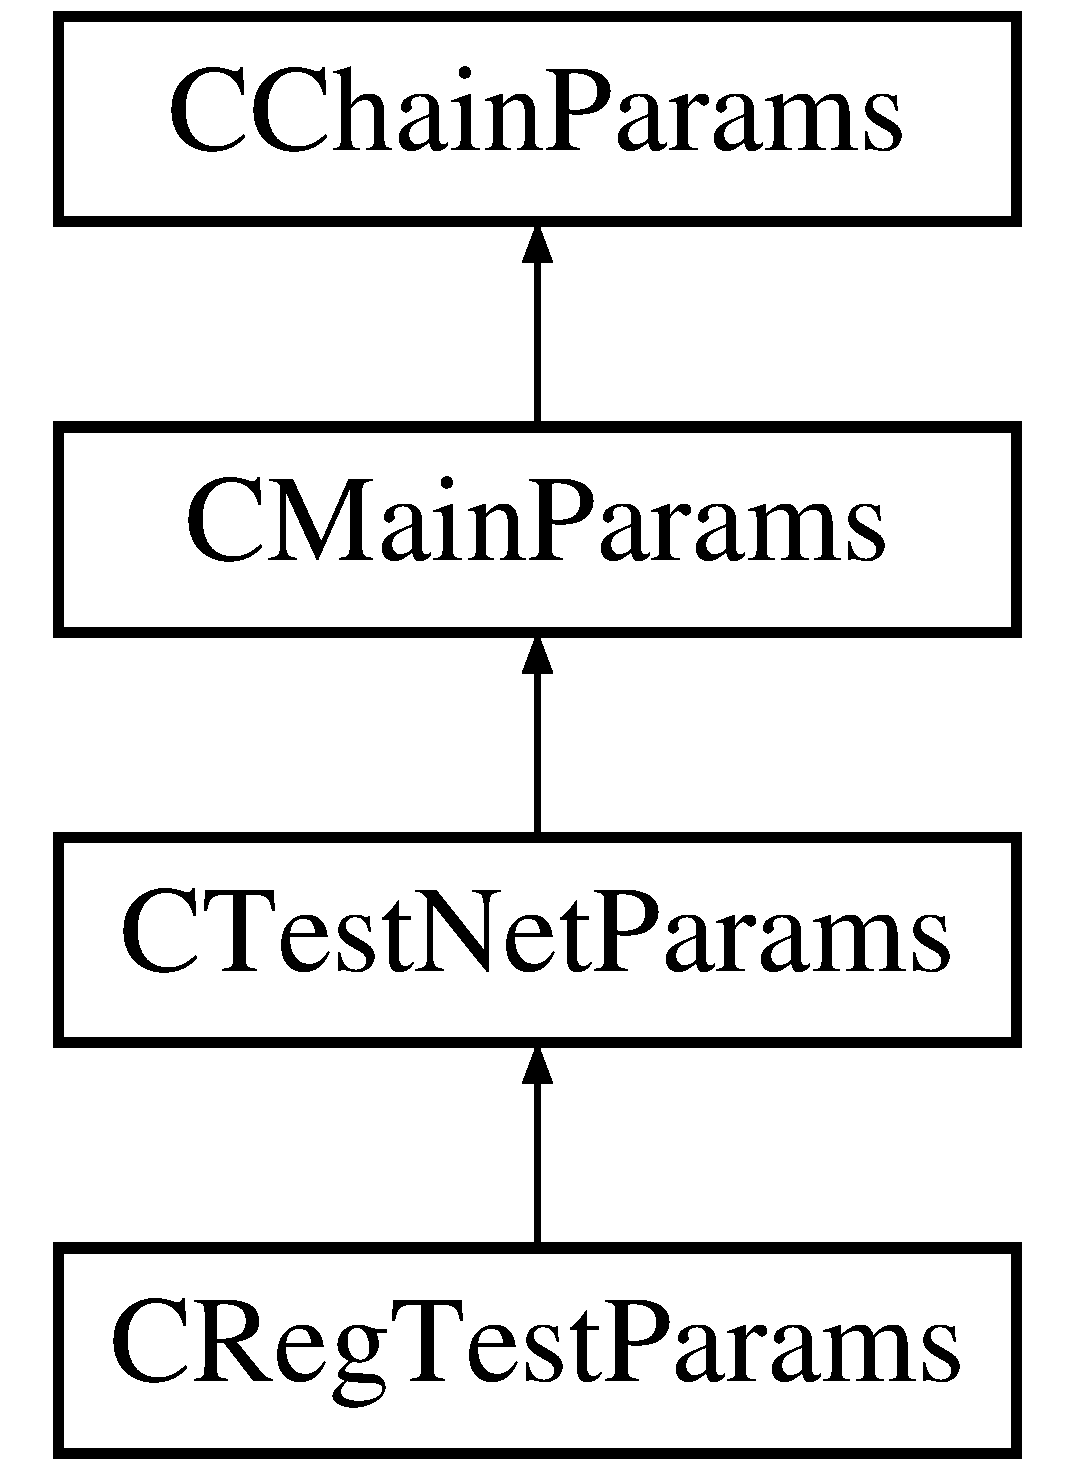
\includegraphics[height=4.000000cm]{class_c_main_params}
\end{center}
\end{figure}
\subsection*{Public Member Functions}
\begin{DoxyCompactItemize}
\item 
\mbox{\hyperlink{class_c_main_params_ab7dfebf3c4dd5cc0ebdfabe1111056d6}{C\+Main\+Params}} ()
\end{DoxyCompactItemize}
\subsection*{Additional Inherited Members}


\subsection{Constructor \& Destructor Documentation}
\mbox{\Hypertarget{class_c_main_params_ab7dfebf3c4dd5cc0ebdfabe1111056d6}\label{class_c_main_params_ab7dfebf3c4dd5cc0ebdfabe1111056d6}} 
\index{C\+Main\+Params@{C\+Main\+Params}!C\+Main\+Params@{C\+Main\+Params}}
\index{C\+Main\+Params@{C\+Main\+Params}!C\+Main\+Params@{C\+Main\+Params}}
\subsubsection{\texorpdfstring{C\+Main\+Params()}{CMainParams()}}
{\footnotesize\ttfamily C\+Main\+Params\+::\+C\+Main\+Params (\begin{DoxyParamCaption}{ }\end{DoxyParamCaption})\hspace{0.3cm}{\ttfamily [inline]}}

Build the genesis block. Note that the output of its generation transaction cannot be spent since it did not originally exist in the database (and is in any case of zero value).

\begin{quote}
\begin{quote}
\begin{quote}
from pyblake2 import blake2s \textquotesingle{}Zclassic\textquotesingle{} + blake2s(b\textquotesingle{}No taxation without representation. B\+TC \#437541 -\/ 00000000000000000397f175a94dd3f530b957182eb2a9f7b79a44a94a5e0450\textquotesingle{}).hexdigest() \end{quote}
\end{quote}
\end{quote}


The documentation for this class was generated from the following file\+:\begin{DoxyCompactItemize}
\item 
/\+Users/christopherarguello/\+Developer/anon/src/\mbox{\hyperlink{chainparams_8cpp}{chainparams.\+cpp}}\end{DoxyCompactItemize}

\hypertarget{struct_c_main_signals}{}\section{C\+Main\+Signals Struct Reference}
\label{struct_c_main_signals}\index{C\+Main\+Signals@{C\+Main\+Signals}}


{\ttfamily \#include $<$validationinterface.\+h$>$}

\subsection*{Public Attributes}
\begin{DoxyCompactItemize}
\item 
boost\+::signals2\+::signal$<$ void(const \mbox{\hyperlink{class_c_block_index}{C\+Block\+Index}} $\ast$)$>$ \mbox{\hyperlink{struct_c_main_signals_a0380ea185992a8ee3572b5cf2aaa7677}{Updated\+Block\+Tip}}
\item 
boost\+::signals2\+::signal$<$ void(const C\+Transaction \&, const C\+Block $\ast$)$>$ \mbox{\hyperlink{struct_c_main_signals_a7ced7f332ed90d57110a78ad50d5a60f}{Sync\+Transaction}}
\item 
boost\+::signals2\+::signal$<$ void(const \mbox{\hyperlink{classuint256}{uint256}} \&)$>$ \mbox{\hyperlink{struct_c_main_signals_a1bb8e6808c2086e4045ecd8f356a12e4}{Erase\+Transaction}}
\item 
boost\+::signals2\+::signal$<$ void(const \mbox{\hyperlink{classuint256}{uint256}} \&)$>$ \mbox{\hyperlink{struct_c_main_signals_a460e5e468e8e4a9493fe1685b77c57e0}{Updated\+Transaction}}
\item 
boost\+::signals2\+::signal$<$ void(const \mbox{\hyperlink{class_c_block_index}{C\+Block\+Index}} $\ast$, const C\+Block $\ast$, Z\+C\+Incremental\+Merkle\+Tree, bool)$>$ \mbox{\hyperlink{struct_c_main_signals_abaf6911904d514ad1d9f2c81a4faa08b}{Chain\+Tip}}
\item 
boost\+::signals2\+::signal$<$ void(const C\+Block\+Locator \&)$>$ \mbox{\hyperlink{struct_c_main_signals_a11f2f18522ff7aa672eb5cc8c1f397b2}{Set\+Best\+Chain}}
\item 
boost\+::signals2\+::signal$<$ void(const \mbox{\hyperlink{classuint256}{uint256}} \&)$>$ \mbox{\hyperlink{struct_c_main_signals_a2f8f94d91265dc946e97614042698a7b}{Inventory}}
\item 
boost\+::signals2\+::signal$<$ void(int64\+\_\+t n\+Best\+Block\+Time)$>$ \mbox{\hyperlink{struct_c_main_signals_a57ba54e641838bc03d0bbda30796c0c9}{Broadcast}}
\item 
boost\+::signals2\+::signal$<$ void(const C\+Block \&, const C\+Validation\+State \&)$>$ \mbox{\hyperlink{struct_c_main_signals_a9419bb09211f46bdc7f214e9d94f1bd7}{Block\+Checked}}
\end{DoxyCompactItemize}


\subsection{Member Data Documentation}
\mbox{\Hypertarget{struct_c_main_signals_a9419bb09211f46bdc7f214e9d94f1bd7}\label{struct_c_main_signals_a9419bb09211f46bdc7f214e9d94f1bd7}} 
\index{C\+Main\+Signals@{C\+Main\+Signals}!Block\+Checked@{Block\+Checked}}
\index{Block\+Checked@{Block\+Checked}!C\+Main\+Signals@{C\+Main\+Signals}}
\subsubsection{\texorpdfstring{Block\+Checked}{BlockChecked}}
{\footnotesize\ttfamily boost\+::signals2\+::signal$<$void (const C\+Block\&, const C\+Validation\+State\&)$>$ C\+Main\+Signals\+::\+Block\+Checked}

Notifies listeners of a block validation result \mbox{\Hypertarget{struct_c_main_signals_a57ba54e641838bc03d0bbda30796c0c9}\label{struct_c_main_signals_a57ba54e641838bc03d0bbda30796c0c9}} 
\index{C\+Main\+Signals@{C\+Main\+Signals}!Broadcast@{Broadcast}}
\index{Broadcast@{Broadcast}!C\+Main\+Signals@{C\+Main\+Signals}}
\subsubsection{\texorpdfstring{Broadcast}{Broadcast}}
{\footnotesize\ttfamily boost\+::signals2\+::signal$<$void (int64\+\_\+t n\+Best\+Block\+Time)$>$ C\+Main\+Signals\+::\+Broadcast}

Tells listeners to broadcast their data. \mbox{\Hypertarget{struct_c_main_signals_abaf6911904d514ad1d9f2c81a4faa08b}\label{struct_c_main_signals_abaf6911904d514ad1d9f2c81a4faa08b}} 
\index{C\+Main\+Signals@{C\+Main\+Signals}!Chain\+Tip@{Chain\+Tip}}
\index{Chain\+Tip@{Chain\+Tip}!C\+Main\+Signals@{C\+Main\+Signals}}
\subsubsection{\texorpdfstring{Chain\+Tip}{ChainTip}}
{\footnotesize\ttfamily boost\+::signals2\+::signal$<$void (const \mbox{\hyperlink{class_c_block_index}{C\+Block\+Index}} $\ast$, const C\+Block $\ast$, Z\+C\+Incremental\+Merkle\+Tree, bool)$>$ C\+Main\+Signals\+::\+Chain\+Tip}

Notifies listeners of a change to the tip of the active block chain. \mbox{\Hypertarget{struct_c_main_signals_a1bb8e6808c2086e4045ecd8f356a12e4}\label{struct_c_main_signals_a1bb8e6808c2086e4045ecd8f356a12e4}} 
\index{C\+Main\+Signals@{C\+Main\+Signals}!Erase\+Transaction@{Erase\+Transaction}}
\index{Erase\+Transaction@{Erase\+Transaction}!C\+Main\+Signals@{C\+Main\+Signals}}
\subsubsection{\texorpdfstring{Erase\+Transaction}{EraseTransaction}}
{\footnotesize\ttfamily boost\+::signals2\+::signal$<$void (const \mbox{\hyperlink{classuint256}{uint256}} \&)$>$ C\+Main\+Signals\+::\+Erase\+Transaction}

Notifies listeners of an erased transaction (currently disabled, requires transaction replacement). \mbox{\Hypertarget{struct_c_main_signals_a2f8f94d91265dc946e97614042698a7b}\label{struct_c_main_signals_a2f8f94d91265dc946e97614042698a7b}} 
\index{C\+Main\+Signals@{C\+Main\+Signals}!Inventory@{Inventory}}
\index{Inventory@{Inventory}!C\+Main\+Signals@{C\+Main\+Signals}}
\subsubsection{\texorpdfstring{Inventory}{Inventory}}
{\footnotesize\ttfamily boost\+::signals2\+::signal$<$void (const \mbox{\hyperlink{classuint256}{uint256}} \&)$>$ C\+Main\+Signals\+::\+Inventory}

Notifies listeners about an inventory item being seen on the network. \mbox{\Hypertarget{struct_c_main_signals_a11f2f18522ff7aa672eb5cc8c1f397b2}\label{struct_c_main_signals_a11f2f18522ff7aa672eb5cc8c1f397b2}} 
\index{C\+Main\+Signals@{C\+Main\+Signals}!Set\+Best\+Chain@{Set\+Best\+Chain}}
\index{Set\+Best\+Chain@{Set\+Best\+Chain}!C\+Main\+Signals@{C\+Main\+Signals}}
\subsubsection{\texorpdfstring{Set\+Best\+Chain}{SetBestChain}}
{\footnotesize\ttfamily boost\+::signals2\+::signal$<$void (const C\+Block\+Locator \&)$>$ C\+Main\+Signals\+::\+Set\+Best\+Chain}

Notifies listeners of a new active block chain. \mbox{\Hypertarget{struct_c_main_signals_a7ced7f332ed90d57110a78ad50d5a60f}\label{struct_c_main_signals_a7ced7f332ed90d57110a78ad50d5a60f}} 
\index{C\+Main\+Signals@{C\+Main\+Signals}!Sync\+Transaction@{Sync\+Transaction}}
\index{Sync\+Transaction@{Sync\+Transaction}!C\+Main\+Signals@{C\+Main\+Signals}}
\subsubsection{\texorpdfstring{Sync\+Transaction}{SyncTransaction}}
{\footnotesize\ttfamily boost\+::signals2\+::signal$<$void (const C\+Transaction \&, const C\+Block $\ast$)$>$ C\+Main\+Signals\+::\+Sync\+Transaction}

Notifies listeners of updated transaction data (transaction, and optionally the block it is found in. \mbox{\Hypertarget{struct_c_main_signals_a0380ea185992a8ee3572b5cf2aaa7677}\label{struct_c_main_signals_a0380ea185992a8ee3572b5cf2aaa7677}} 
\index{C\+Main\+Signals@{C\+Main\+Signals}!Updated\+Block\+Tip@{Updated\+Block\+Tip}}
\index{Updated\+Block\+Tip@{Updated\+Block\+Tip}!C\+Main\+Signals@{C\+Main\+Signals}}
\subsubsection{\texorpdfstring{Updated\+Block\+Tip}{UpdatedBlockTip}}
{\footnotesize\ttfamily boost\+::signals2\+::signal$<$void (const \mbox{\hyperlink{class_c_block_index}{C\+Block\+Index}} $\ast$)$>$ C\+Main\+Signals\+::\+Updated\+Block\+Tip}

Notifies listeners of updated block chain tip \mbox{\Hypertarget{struct_c_main_signals_a460e5e468e8e4a9493fe1685b77c57e0}\label{struct_c_main_signals_a460e5e468e8e4a9493fe1685b77c57e0}} 
\index{C\+Main\+Signals@{C\+Main\+Signals}!Updated\+Transaction@{Updated\+Transaction}}
\index{Updated\+Transaction@{Updated\+Transaction}!C\+Main\+Signals@{C\+Main\+Signals}}
\subsubsection{\texorpdfstring{Updated\+Transaction}{UpdatedTransaction}}
{\footnotesize\ttfamily boost\+::signals2\+::signal$<$void (const \mbox{\hyperlink{classuint256}{uint256}} \&)$>$ C\+Main\+Signals\+::\+Updated\+Transaction}

Notifies listeners of an updated transaction without new data (for now\+: a coinbase potentially becoming visible). 

The documentation for this struct was generated from the following file\+:\begin{DoxyCompactItemize}
\item 
/\+Users/christopherarguello/\+Developer/anon/src/\mbox{\hyperlink{validationinterface_8h}{validationinterface.\+h}}\end{DoxyCompactItemize}

\hypertarget{class_c_masternode}{}\section{C\+Masternode Class Reference}
\label{class_c_masternode}\index{C\+Masternode@{C\+Masternode}}


{\ttfamily \#include $<$masternode.\+h$>$}

Inheritance diagram for C\+Masternode\+:\begin{figure}[H]
\begin{center}
\leavevmode
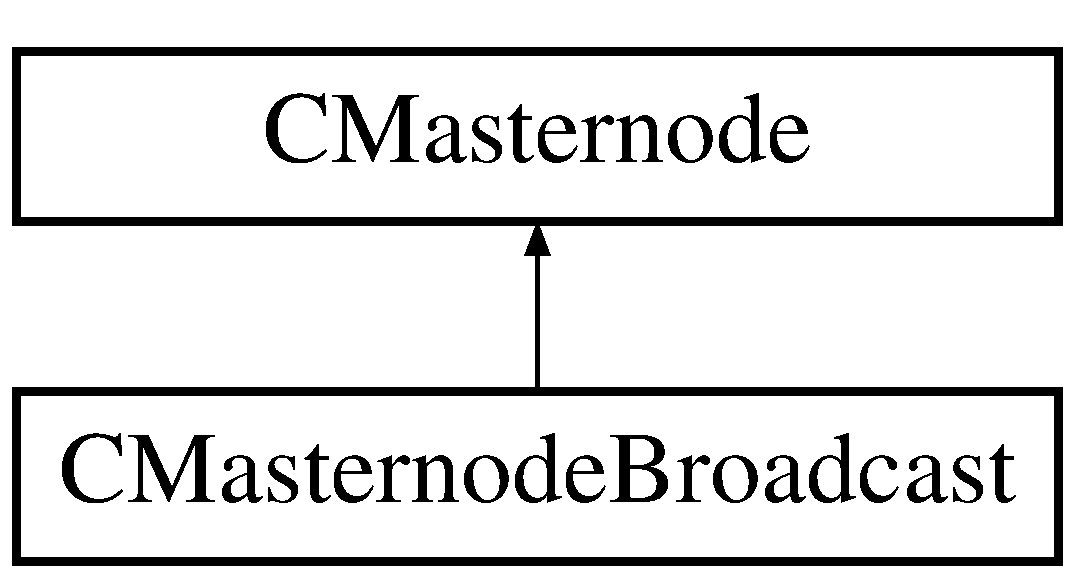
\includegraphics[height=2.000000cm]{class_c_masternode}
\end{center}
\end{figure}
\subsection*{Public Types}
\begin{DoxyCompactItemize}
\item 
enum \mbox{\hyperlink{class_c_masternode_a958e9e8587729e417d1a529c81bf2eb0}{state}} \{ \newline
\mbox{\hyperlink{class_c_masternode_a958e9e8587729e417d1a529c81bf2eb0adde1d71baaca5fa61feeaae92d551cdc}{M\+A\+S\+T\+E\+R\+N\+O\+D\+E\+\_\+\+P\+R\+E\+\_\+\+E\+N\+A\+B\+L\+ED}}, 
\mbox{\hyperlink{class_c_masternode_a958e9e8587729e417d1a529c81bf2eb0a479f2643df0b7f7e70c9389ec4b42923}{M\+A\+S\+T\+E\+R\+N\+O\+D\+E\+\_\+\+E\+N\+A\+B\+L\+ED}}, 
\mbox{\hyperlink{class_c_masternode_a958e9e8587729e417d1a529c81bf2eb0aaa88be848b79bb399e3538c452d7fd87}{M\+A\+S\+T\+E\+R\+N\+O\+D\+E\+\_\+\+E\+X\+P\+I\+R\+ED}}, 
\mbox{\hyperlink{class_c_masternode_a958e9e8587729e417d1a529c81bf2eb0af148b4257f0c54f510c41e91ce4bfc86}{M\+A\+S\+T\+E\+R\+N\+O\+D\+E\+\_\+\+O\+U\+T\+P\+O\+I\+N\+T\+\_\+\+S\+P\+E\+NT}}, 
\newline
\mbox{\hyperlink{class_c_masternode_a958e9e8587729e417d1a529c81bf2eb0a401280591a2cec57f97c76fb5e53c049}{M\+A\+S\+T\+E\+R\+N\+O\+D\+E\+\_\+\+U\+P\+D\+A\+T\+E\+\_\+\+R\+E\+Q\+U\+I\+R\+ED}}, 
\mbox{\hyperlink{class_c_masternode_a958e9e8587729e417d1a529c81bf2eb0ae8a2f54cef8d465971f930e26ad0cbbb}{M\+A\+S\+T\+E\+R\+N\+O\+D\+E\+\_\+\+W\+A\+T\+C\+H\+D\+O\+G\+\_\+\+E\+X\+P\+I\+R\+ED}}, 
\mbox{\hyperlink{class_c_masternode_a958e9e8587729e417d1a529c81bf2eb0a4e4ec255452c84058752500b7d5096da}{M\+A\+S\+T\+E\+R\+N\+O\+D\+E\+\_\+\+N\+E\+W\+\_\+\+S\+T\+A\+R\+T\+\_\+\+R\+E\+Q\+U\+I\+R\+ED}}, 
\mbox{\hyperlink{class_c_masternode_a958e9e8587729e417d1a529c81bf2eb0ac9f064d96812c163750fee8d1de26d74}{M\+A\+S\+T\+E\+R\+N\+O\+D\+E\+\_\+\+P\+O\+S\+E\+\_\+\+B\+AN}}
 \}
\end{DoxyCompactItemize}
\subsection*{Public Member Functions}
\begin{DoxyCompactItemize}
\item 
\mbox{\hyperlink{class_c_masternode_a9783a33543d5d7b5f7101f3196562276}{C\+Masternode}} ()
\item 
\mbox{\hyperlink{class_c_masternode_a45ddf472ea17b5393060b648a1e25291}{C\+Masternode}} (const \mbox{\hyperlink{class_c_masternode}{C\+Masternode}} \&other)
\item 
\mbox{\hyperlink{class_c_masternode_a627dbc7dfeaa9a996bcf7fac3665933b}{C\+Masternode}} (const \mbox{\hyperlink{class_c_masternode_broadcast}{C\+Masternode\+Broadcast}} \&mnb)
\item 
\mbox{\hyperlink{class_c_masternode_ae11e8917ed00c7cee11dc5fdb211ecb1}{C\+Masternode}} (\mbox{\hyperlink{class_c_service}{C\+Service}} addr\+New, C\+Tx\+In vin\+New, \mbox{\hyperlink{class_c_pub_key}{C\+Pub\+Key}} pub\+Key\+Collateral\+Address\+New, \mbox{\hyperlink{class_c_pub_key}{C\+Pub\+Key}} pub\+Key\+Masternode\+New, int n\+Protocol\+Version\+In)
\item 
{\footnotesize template$<$typename Stream , typename Operation $>$ }\\void \mbox{\hyperlink{class_c_masternode_ac3514c93cc494ae196dc217df847950d}{Serialization\+Op}} (Stream \&s, Operation ser\+\_\+action, int n\+Type, int n\+Version)
\item 
void \mbox{\hyperlink{class_c_masternode_a8cad9a9fa0b7afe75ba20254d7790b61}{swap}} (\mbox{\hyperlink{class_c_masternode}{C\+Masternode}} \&first, \mbox{\hyperlink{class_c_masternode}{C\+Masternode}} \&second)
\item 
\mbox{\hyperlink{classarith__uint256}{arith\+\_\+uint256}} \mbox{\hyperlink{class_c_masternode_abfee4bc30fa436d9a5f8b5f15a078081}{Calculate\+Score}} (const \mbox{\hyperlink{classuint256}{uint256}} \&block\+Hash)
\item 
bool \mbox{\hyperlink{class_c_masternode_a96da6f523ec3a160239c966bf0dcf876}{Update\+From\+New\+Broadcast}} (\mbox{\hyperlink{class_c_masternode_broadcast}{C\+Masternode\+Broadcast}} \&mnb)
\item 
void \mbox{\hyperlink{class_c_masternode_ac00056a0de9176ec7922d88795a6988f}{Check}} (bool f\+Force=false)
\item 
bool \mbox{\hyperlink{class_c_masternode_aa9aecc4762dcb9f6a5a5fb359e5aa9e1}{Is\+Broadcasted\+Within}} (int n\+Seconds)
\item 
bool \mbox{\hyperlink{class_c_masternode_a454e41f5850cb1307c66de0ac82b16a3}{Is\+Pinged\+Within}} (int n\+Seconds, int64\+\_\+t n\+Time\+To\+Check\+At=-\/1)
\item 
bool \mbox{\hyperlink{class_c_masternode_a08782379f6ba10e9087b39f0cef19bce}{Is\+Enabled}} ()
\item 
bool \mbox{\hyperlink{class_c_masternode_a28f41bd6e252b191c4a8536fdac24e40}{Is\+Pre\+Enabled}} ()
\item 
bool \mbox{\hyperlink{class_c_masternode_a76f6fefcb586fef33c2ed3a72d8b56e2}{Is\+Po\+Se\+Banned}} ()
\item 
bool \mbox{\hyperlink{class_c_masternode_aa2b0fe59f7c687cfa072f9bcd5efeda7}{Is\+Po\+Se\+Verified}} ()
\item 
bool \mbox{\hyperlink{class_c_masternode_a15c8c3351d7a91b7cce67a07b27a37b0}{Is\+Expired}} ()
\item 
bool \mbox{\hyperlink{class_c_masternode_aed1070b99fd2948d7d914ee14f138466}{Is\+Outpoint\+Spent}} ()
\item 
bool \mbox{\hyperlink{class_c_masternode_a1b66eca7ab7dafe127beb09d9380d692}{Is\+Update\+Required}} ()
\item 
bool \mbox{\hyperlink{class_c_masternode_a0426da4b6e2c87a738b5473deef2fc0c}{Is\+Watchdog\+Expired}} ()
\item 
bool \mbox{\hyperlink{class_c_masternode_a992b914fa9ffdecc626320ef0923f0a3}{Is\+New\+Start\+Required}} ()
\item 
bool \mbox{\hyperlink{class_c_masternode_adee8a89597ac5746d85e021f0bee209d}{Is\+Valid\+For\+Payment}} ()
\item 
bool \mbox{\hyperlink{class_c_masternode_a70f120b4964fdd802a6975bfb9017a23}{Is\+Valid\+Net\+Addr}} ()
\item 
void \mbox{\hyperlink{class_c_masternode_a43e72f4eaaaf69429304d35a0bd172d8}{Increase\+Po\+Se\+Ban\+Score}} ()
\item 
void \mbox{\hyperlink{class_c_masternode_ae0de8b6e894d03f297ff274f3c107892}{Decrease\+Po\+Se\+Ban\+Score}} ()
\item 
\mbox{\hyperlink{structmasternode__info__t}{masternode\+\_\+info\+\_\+t}} \mbox{\hyperlink{class_c_masternode_a9b6912ac2d8ee011aba8837cb85ada63}{Get\+Info}} ()
\item 
std\+::string \mbox{\hyperlink{class_c_masternode_a24785b00a72b9c3c43e21bf2ef84b456}{Get\+State\+String}} () const
\item 
std\+::string \mbox{\hyperlink{class_c_masternode_ac9983ac170cb085c6f826e5fcd9a9a5b}{Get\+Status}} () const
\item 
int \mbox{\hyperlink{class_c_masternode_a39de7f9e7c2485dd341f7b7bcaa5def6}{Get\+Collateral\+Age}} ()
\item 
int \mbox{\hyperlink{class_c_masternode_a422620894cf5f9acfac5f44db526cc0d}{Get\+Last\+Paid\+Time}} ()
\item 
int \mbox{\hyperlink{class_c_masternode_ad848b2f168fca83dbc50c4fb07d12868}{Get\+Last\+Paid\+Block}} ()
\item 
void \mbox{\hyperlink{class_c_masternode_ade5a3726f6da526f616045f58a7b5857}{Update\+Last\+Paid}} (const \mbox{\hyperlink{class_c_block_index}{C\+Block\+Index}} $\ast$pindex, int n\+Max\+Blocks\+To\+Scan\+Back)
\item 
void \mbox{\hyperlink{class_c_masternode_a24919d0a7c97271ac4fd4e8f8ae0a42c}{Add\+Governance\+Vote}} (\mbox{\hyperlink{classuint256}{uint256}} n\+Governance\+Object\+Hash)
\item 
void \mbox{\hyperlink{class_c_masternode_a947af1fa2df5f8179a69de8d12511894}{Flag\+Governance\+Items\+As\+Dirty}} ()
\item 
void \mbox{\hyperlink{class_c_masternode_ab8751705e6fa01ebb18dae7162d70b63}{Remove\+Governance\+Object}} (\mbox{\hyperlink{classuint256}{uint256}} n\+Governance\+Object\+Hash)
\item 
void \mbox{\hyperlink{class_c_masternode_a8ef654deadd035f7e4cf786bd38369bb}{Update\+Watchdog\+Vote\+Time}} ()
\item 
\mbox{\hyperlink{class_c_masternode}{C\+Masternode}} \& \mbox{\hyperlink{class_c_masternode_a914fcf71ebc13a0680bb61e173b206f4}{operator=}} (\mbox{\hyperlink{class_c_masternode}{C\+Masternode}} from)
\end{DoxyCompactItemize}
\subsection*{Static Public Member Functions}
\begin{DoxyCompactItemize}
\item 
static bool \mbox{\hyperlink{class_c_masternode_ae509fc0a2f845695fd9f894433c9534f}{Is\+Valid\+State\+For\+Auto\+Start}} (int n\+Active\+State\+In)
\item 
static bool \mbox{\hyperlink{class_c_masternode_a8e2f73e4c9d366b688c088e861534cfd}{Is\+Valid\+Net\+Addr}} (\mbox{\hyperlink{class_c_service}{C\+Service}} addr\+In)
\item 
static std\+::string \mbox{\hyperlink{class_c_masternode_a379321e692aaabfce4ebffc1e54e0d39}{State\+To\+String}} (int n\+State\+In)
\end{DoxyCompactItemize}
\subsection*{Public Attributes}
\begin{DoxyCompactItemize}
\item 
C\+Tx\+In \mbox{\hyperlink{class_c_masternode_a485b26778bb8b006152aaa64168afe6b}{vin}}
\item 
\mbox{\hyperlink{class_c_service}{C\+Service}} \mbox{\hyperlink{class_c_masternode_a259ea116c54b904cf238a3e9c0cf1e0b}{addr}}
\item 
\mbox{\hyperlink{class_c_pub_key}{C\+Pub\+Key}} \mbox{\hyperlink{class_c_masternode_ada049bf0e9f9e43b7ac1fd3e9af27a0d}{pub\+Key\+Collateral\+Address}}
\item 
\mbox{\hyperlink{class_c_pub_key}{C\+Pub\+Key}} \mbox{\hyperlink{class_c_masternode_a6120b4345c618f7a252a44f4dd828708}{pub\+Key\+Masternode}}
\item 
\mbox{\hyperlink{class_c_masternode_ping}{C\+Masternode\+Ping}} \mbox{\hyperlink{class_c_masternode_a114a0ba01b5dfa4d785380007edd31f3}{last\+Ping}}
\item 
std\+::vector$<$ unsigned char $>$ \mbox{\hyperlink{class_c_masternode_a880d00984546ced35c26924d5d80dedc}{vch\+Sig}}
\item 
int64\+\_\+t \mbox{\hyperlink{class_c_masternode_a89fca1a40dbccbe67b173d76fac399ea}{sig\+Time}}
\item 
int64\+\_\+t \mbox{\hyperlink{class_c_masternode_ab9d3bfad4bfc61f9113b3adbc792bbe2}{n\+Last\+Dsq}}
\item 
int64\+\_\+t \mbox{\hyperlink{class_c_masternode_ae4e7095e01c08c1c50150dc62fedc7af}{n\+Time\+Last\+Checked}}
\item 
int64\+\_\+t \mbox{\hyperlink{class_c_masternode_ab1e04527f86d9a12c5a1157829bca828}{n\+Time\+Last\+Paid}}
\item 
int64\+\_\+t \mbox{\hyperlink{class_c_masternode_adf082caa4d554ca270692b47014ba6bb}{n\+Time\+Last\+Watchdog\+Vote}}
\item 
int \mbox{\hyperlink{class_c_masternode_a41efbc881997e3df19dcf0e430c76d82}{n\+Active\+State}}
\item 
int \mbox{\hyperlink{class_c_masternode_a00ec475167455ad481db6c459d7fb96c}{n\+Cache\+Collateral\+Block}}
\item 
int \mbox{\hyperlink{class_c_masternode_a469895ce53fb69d5ec5218fa8ce93dad}{n\+Block\+Last\+Paid}}
\item 
int \mbox{\hyperlink{class_c_masternode_a03c6c954bc7391668c89434cf6c87fa3}{n\+Protocol\+Version}}
\item 
int \mbox{\hyperlink{class_c_masternode_aa0a7406aa8ea8a159af7ff719bfc1f8c}{n\+Po\+Se\+Ban\+Score}}
\item 
int \mbox{\hyperlink{class_c_masternode_aaab93ec5854e042fae8804d4bf50e35d}{n\+Po\+Se\+Ban\+Height}}
\item 
bool \mbox{\hyperlink{class_c_masternode_aec0ac0226c4e0d6ee3f9a084a8e311ea}{f\+Allow\+Mixing\+Tx}}
\item 
bool \mbox{\hyperlink{class_c_masternode_a8a35685b1e8220a45d8c148753a51572}{f\+Unit\+Test}}
\item 
std\+::map$<$ \mbox{\hyperlink{classuint256}{uint256}}, int $>$ \mbox{\hyperlink{class_c_masternode_a3b0131c0ee2ba77e5c67dd0445b202bf}{map\+Governance\+Objects\+Voted\+On}}
\item 
\mbox{\hyperlink{class_c_masternode_adbd6c5c459a6450cd724f88d62b5948f}{A\+D\+D\+\_\+\+S\+E\+R\+I\+A\+L\+I\+Z\+E\+\_\+\+M\+E\+T\+H\+O\+DS}}
\end{DoxyCompactItemize}
\subsection*{Private Attributes}
\begin{DoxyCompactItemize}
\item 
\mbox{\hyperlink{sync_8h_a37a4692b2d517f2843655ca11af7668a}{C\+Critical\+Section}} \mbox{\hyperlink{class_c_masternode_a0b67bc1bebc7dfeb29dc545cb12d286f}{cs}}
\end{DoxyCompactItemize}
\subsection*{Friends}
\begin{DoxyCompactItemize}
\item 
bool \mbox{\hyperlink{class_c_masternode_ac3549be50afdc1acd8be9a763cb7b355}{operator==}} (const \mbox{\hyperlink{class_c_masternode}{C\+Masternode}} \&a, const \mbox{\hyperlink{class_c_masternode}{C\+Masternode}} \&b)
\item 
bool \mbox{\hyperlink{class_c_masternode_ab717eb8dbdf0438855bd30eb922fe73a}{operator!=}} (const \mbox{\hyperlink{class_c_masternode}{C\+Masternode}} \&a, const \mbox{\hyperlink{class_c_masternode}{C\+Masternode}} \&b)
\end{DoxyCompactItemize}


\subsection{Member Enumeration Documentation}
\mbox{\Hypertarget{class_c_masternode_a958e9e8587729e417d1a529c81bf2eb0}\label{class_c_masternode_a958e9e8587729e417d1a529c81bf2eb0}} 
\index{C\+Masternode@{C\+Masternode}!state@{state}}
\index{state@{state}!C\+Masternode@{C\+Masternode}}
\subsubsection{\texorpdfstring{state}{state}}
{\footnotesize\ttfamily enum \mbox{\hyperlink{class_c_masternode_a958e9e8587729e417d1a529c81bf2eb0}{C\+Masternode\+::state}}}

\begin{DoxyEnumFields}{Enumerator}
\raisebox{\heightof{T}}[0pt][0pt]{\index{M\+A\+S\+T\+E\+R\+N\+O\+D\+E\+\_\+\+P\+R\+E\+\_\+\+E\+N\+A\+B\+L\+ED@{M\+A\+S\+T\+E\+R\+N\+O\+D\+E\+\_\+\+P\+R\+E\+\_\+\+E\+N\+A\+B\+L\+ED}!C\+Masternode@{C\+Masternode}}\index{C\+Masternode@{C\+Masternode}!M\+A\+S\+T\+E\+R\+N\+O\+D\+E\+\_\+\+P\+R\+E\+\_\+\+E\+N\+A\+B\+L\+ED@{M\+A\+S\+T\+E\+R\+N\+O\+D\+E\+\_\+\+P\+R\+E\+\_\+\+E\+N\+A\+B\+L\+ED}}}\mbox{\Hypertarget{class_c_masternode_a958e9e8587729e417d1a529c81bf2eb0adde1d71baaca5fa61feeaae92d551cdc}\label{class_c_masternode_a958e9e8587729e417d1a529c81bf2eb0adde1d71baaca5fa61feeaae92d551cdc}} 
M\+A\+S\+T\+E\+R\+N\+O\+D\+E\+\_\+\+P\+R\+E\+\_\+\+E\+N\+A\+B\+L\+ED&\\
\hline

\raisebox{\heightof{T}}[0pt][0pt]{\index{M\+A\+S\+T\+E\+R\+N\+O\+D\+E\+\_\+\+E\+N\+A\+B\+L\+ED@{M\+A\+S\+T\+E\+R\+N\+O\+D\+E\+\_\+\+E\+N\+A\+B\+L\+ED}!C\+Masternode@{C\+Masternode}}\index{C\+Masternode@{C\+Masternode}!M\+A\+S\+T\+E\+R\+N\+O\+D\+E\+\_\+\+E\+N\+A\+B\+L\+ED@{M\+A\+S\+T\+E\+R\+N\+O\+D\+E\+\_\+\+E\+N\+A\+B\+L\+ED}}}\mbox{\Hypertarget{class_c_masternode_a958e9e8587729e417d1a529c81bf2eb0a479f2643df0b7f7e70c9389ec4b42923}\label{class_c_masternode_a958e9e8587729e417d1a529c81bf2eb0a479f2643df0b7f7e70c9389ec4b42923}} 
M\+A\+S\+T\+E\+R\+N\+O\+D\+E\+\_\+\+E\+N\+A\+B\+L\+ED&\\
\hline

\raisebox{\heightof{T}}[0pt][0pt]{\index{M\+A\+S\+T\+E\+R\+N\+O\+D\+E\+\_\+\+E\+X\+P\+I\+R\+ED@{M\+A\+S\+T\+E\+R\+N\+O\+D\+E\+\_\+\+E\+X\+P\+I\+R\+ED}!C\+Masternode@{C\+Masternode}}\index{C\+Masternode@{C\+Masternode}!M\+A\+S\+T\+E\+R\+N\+O\+D\+E\+\_\+\+E\+X\+P\+I\+R\+ED@{M\+A\+S\+T\+E\+R\+N\+O\+D\+E\+\_\+\+E\+X\+P\+I\+R\+ED}}}\mbox{\Hypertarget{class_c_masternode_a958e9e8587729e417d1a529c81bf2eb0aaa88be848b79bb399e3538c452d7fd87}\label{class_c_masternode_a958e9e8587729e417d1a529c81bf2eb0aaa88be848b79bb399e3538c452d7fd87}} 
M\+A\+S\+T\+E\+R\+N\+O\+D\+E\+\_\+\+E\+X\+P\+I\+R\+ED&\\
\hline

\raisebox{\heightof{T}}[0pt][0pt]{\index{M\+A\+S\+T\+E\+R\+N\+O\+D\+E\+\_\+\+O\+U\+T\+P\+O\+I\+N\+T\+\_\+\+S\+P\+E\+NT@{M\+A\+S\+T\+E\+R\+N\+O\+D\+E\+\_\+\+O\+U\+T\+P\+O\+I\+N\+T\+\_\+\+S\+P\+E\+NT}!C\+Masternode@{C\+Masternode}}\index{C\+Masternode@{C\+Masternode}!M\+A\+S\+T\+E\+R\+N\+O\+D\+E\+\_\+\+O\+U\+T\+P\+O\+I\+N\+T\+\_\+\+S\+P\+E\+NT@{M\+A\+S\+T\+E\+R\+N\+O\+D\+E\+\_\+\+O\+U\+T\+P\+O\+I\+N\+T\+\_\+\+S\+P\+E\+NT}}}\mbox{\Hypertarget{class_c_masternode_a958e9e8587729e417d1a529c81bf2eb0af148b4257f0c54f510c41e91ce4bfc86}\label{class_c_masternode_a958e9e8587729e417d1a529c81bf2eb0af148b4257f0c54f510c41e91ce4bfc86}} 
M\+A\+S\+T\+E\+R\+N\+O\+D\+E\+\_\+\+O\+U\+T\+P\+O\+I\+N\+T\+\_\+\+S\+P\+E\+NT&\\
\hline

\raisebox{\heightof{T}}[0pt][0pt]{\index{M\+A\+S\+T\+E\+R\+N\+O\+D\+E\+\_\+\+U\+P\+D\+A\+T\+E\+\_\+\+R\+E\+Q\+U\+I\+R\+ED@{M\+A\+S\+T\+E\+R\+N\+O\+D\+E\+\_\+\+U\+P\+D\+A\+T\+E\+\_\+\+R\+E\+Q\+U\+I\+R\+ED}!C\+Masternode@{C\+Masternode}}\index{C\+Masternode@{C\+Masternode}!M\+A\+S\+T\+E\+R\+N\+O\+D\+E\+\_\+\+U\+P\+D\+A\+T\+E\+\_\+\+R\+E\+Q\+U\+I\+R\+ED@{M\+A\+S\+T\+E\+R\+N\+O\+D\+E\+\_\+\+U\+P\+D\+A\+T\+E\+\_\+\+R\+E\+Q\+U\+I\+R\+ED}}}\mbox{\Hypertarget{class_c_masternode_a958e9e8587729e417d1a529c81bf2eb0a401280591a2cec57f97c76fb5e53c049}\label{class_c_masternode_a958e9e8587729e417d1a529c81bf2eb0a401280591a2cec57f97c76fb5e53c049}} 
M\+A\+S\+T\+E\+R\+N\+O\+D\+E\+\_\+\+U\+P\+D\+A\+T\+E\+\_\+\+R\+E\+Q\+U\+I\+R\+ED&\\
\hline

\raisebox{\heightof{T}}[0pt][0pt]{\index{M\+A\+S\+T\+E\+R\+N\+O\+D\+E\+\_\+\+W\+A\+T\+C\+H\+D\+O\+G\+\_\+\+E\+X\+P\+I\+R\+ED@{M\+A\+S\+T\+E\+R\+N\+O\+D\+E\+\_\+\+W\+A\+T\+C\+H\+D\+O\+G\+\_\+\+E\+X\+P\+I\+R\+ED}!C\+Masternode@{C\+Masternode}}\index{C\+Masternode@{C\+Masternode}!M\+A\+S\+T\+E\+R\+N\+O\+D\+E\+\_\+\+W\+A\+T\+C\+H\+D\+O\+G\+\_\+\+E\+X\+P\+I\+R\+ED@{M\+A\+S\+T\+E\+R\+N\+O\+D\+E\+\_\+\+W\+A\+T\+C\+H\+D\+O\+G\+\_\+\+E\+X\+P\+I\+R\+ED}}}\mbox{\Hypertarget{class_c_masternode_a958e9e8587729e417d1a529c81bf2eb0ae8a2f54cef8d465971f930e26ad0cbbb}\label{class_c_masternode_a958e9e8587729e417d1a529c81bf2eb0ae8a2f54cef8d465971f930e26ad0cbbb}} 
M\+A\+S\+T\+E\+R\+N\+O\+D\+E\+\_\+\+W\+A\+T\+C\+H\+D\+O\+G\+\_\+\+E\+X\+P\+I\+R\+ED&\\
\hline

\raisebox{\heightof{T}}[0pt][0pt]{\index{M\+A\+S\+T\+E\+R\+N\+O\+D\+E\+\_\+\+N\+E\+W\+\_\+\+S\+T\+A\+R\+T\+\_\+\+R\+E\+Q\+U\+I\+R\+ED@{M\+A\+S\+T\+E\+R\+N\+O\+D\+E\+\_\+\+N\+E\+W\+\_\+\+S\+T\+A\+R\+T\+\_\+\+R\+E\+Q\+U\+I\+R\+ED}!C\+Masternode@{C\+Masternode}}\index{C\+Masternode@{C\+Masternode}!M\+A\+S\+T\+E\+R\+N\+O\+D\+E\+\_\+\+N\+E\+W\+\_\+\+S\+T\+A\+R\+T\+\_\+\+R\+E\+Q\+U\+I\+R\+ED@{M\+A\+S\+T\+E\+R\+N\+O\+D\+E\+\_\+\+N\+E\+W\+\_\+\+S\+T\+A\+R\+T\+\_\+\+R\+E\+Q\+U\+I\+R\+ED}}}\mbox{\Hypertarget{class_c_masternode_a958e9e8587729e417d1a529c81bf2eb0a4e4ec255452c84058752500b7d5096da}\label{class_c_masternode_a958e9e8587729e417d1a529c81bf2eb0a4e4ec255452c84058752500b7d5096da}} 
M\+A\+S\+T\+E\+R\+N\+O\+D\+E\+\_\+\+N\+E\+W\+\_\+\+S\+T\+A\+R\+T\+\_\+\+R\+E\+Q\+U\+I\+R\+ED&\\
\hline

\raisebox{\heightof{T}}[0pt][0pt]{\index{M\+A\+S\+T\+E\+R\+N\+O\+D\+E\+\_\+\+P\+O\+S\+E\+\_\+\+B\+AN@{M\+A\+S\+T\+E\+R\+N\+O\+D\+E\+\_\+\+P\+O\+S\+E\+\_\+\+B\+AN}!C\+Masternode@{C\+Masternode}}\index{C\+Masternode@{C\+Masternode}!M\+A\+S\+T\+E\+R\+N\+O\+D\+E\+\_\+\+P\+O\+S\+E\+\_\+\+B\+AN@{M\+A\+S\+T\+E\+R\+N\+O\+D\+E\+\_\+\+P\+O\+S\+E\+\_\+\+B\+AN}}}\mbox{\Hypertarget{class_c_masternode_a958e9e8587729e417d1a529c81bf2eb0ac9f064d96812c163750fee8d1de26d74}\label{class_c_masternode_a958e9e8587729e417d1a529c81bf2eb0ac9f064d96812c163750fee8d1de26d74}} 
M\+A\+S\+T\+E\+R\+N\+O\+D\+E\+\_\+\+P\+O\+S\+E\+\_\+\+B\+AN&\\
\hline

\end{DoxyEnumFields}


\subsection{Constructor \& Destructor Documentation}
\mbox{\Hypertarget{class_c_masternode_a9783a33543d5d7b5f7101f3196562276}\label{class_c_masternode_a9783a33543d5d7b5f7101f3196562276}} 
\index{C\+Masternode@{C\+Masternode}!C\+Masternode@{C\+Masternode}}
\index{C\+Masternode@{C\+Masternode}!C\+Masternode@{C\+Masternode}}
\subsubsection{\texorpdfstring{C\+Masternode()}{CMasternode()}\hspace{0.1cm}{\footnotesize\ttfamily [1/4]}}
{\footnotesize\ttfamily C\+Masternode\+::\+C\+Masternode (\begin{DoxyParamCaption}{ }\end{DoxyParamCaption})}

\mbox{\Hypertarget{class_c_masternode_a45ddf472ea17b5393060b648a1e25291}\label{class_c_masternode_a45ddf472ea17b5393060b648a1e25291}} 
\index{C\+Masternode@{C\+Masternode}!C\+Masternode@{C\+Masternode}}
\index{C\+Masternode@{C\+Masternode}!C\+Masternode@{C\+Masternode}}
\subsubsection{\texorpdfstring{C\+Masternode()}{CMasternode()}\hspace{0.1cm}{\footnotesize\ttfamily [2/4]}}
{\footnotesize\ttfamily C\+Masternode\+::\+C\+Masternode (\begin{DoxyParamCaption}\item[{const \mbox{\hyperlink{class_c_masternode}{C\+Masternode}} \&}]{other }\end{DoxyParamCaption})}

\mbox{\Hypertarget{class_c_masternode_a627dbc7dfeaa9a996bcf7fac3665933b}\label{class_c_masternode_a627dbc7dfeaa9a996bcf7fac3665933b}} 
\index{C\+Masternode@{C\+Masternode}!C\+Masternode@{C\+Masternode}}
\index{C\+Masternode@{C\+Masternode}!C\+Masternode@{C\+Masternode}}
\subsubsection{\texorpdfstring{C\+Masternode()}{CMasternode()}\hspace{0.1cm}{\footnotesize\ttfamily [3/4]}}
{\footnotesize\ttfamily C\+Masternode\+::\+C\+Masternode (\begin{DoxyParamCaption}\item[{const \mbox{\hyperlink{class_c_masternode_broadcast}{C\+Masternode\+Broadcast}} \&}]{mnb }\end{DoxyParamCaption})}

\mbox{\Hypertarget{class_c_masternode_ae11e8917ed00c7cee11dc5fdb211ecb1}\label{class_c_masternode_ae11e8917ed00c7cee11dc5fdb211ecb1}} 
\index{C\+Masternode@{C\+Masternode}!C\+Masternode@{C\+Masternode}}
\index{C\+Masternode@{C\+Masternode}!C\+Masternode@{C\+Masternode}}
\subsubsection{\texorpdfstring{C\+Masternode()}{CMasternode()}\hspace{0.1cm}{\footnotesize\ttfamily [4/4]}}
{\footnotesize\ttfamily C\+Masternode\+::\+C\+Masternode (\begin{DoxyParamCaption}\item[{\mbox{\hyperlink{class_c_service}{C\+Service}}}]{addr\+New,  }\item[{C\+Tx\+In}]{vin\+New,  }\item[{\mbox{\hyperlink{class_c_pub_key}{C\+Pub\+Key}}}]{pub\+Key\+Collateral\+Address\+New,  }\item[{\mbox{\hyperlink{class_c_pub_key}{C\+Pub\+Key}}}]{pub\+Key\+Masternode\+New,  }\item[{int}]{n\+Protocol\+Version\+In }\end{DoxyParamCaption})}



\subsection{Member Function Documentation}
\mbox{\Hypertarget{class_c_masternode_a24919d0a7c97271ac4fd4e8f8ae0a42c}\label{class_c_masternode_a24919d0a7c97271ac4fd4e8f8ae0a42c}} 
\index{C\+Masternode@{C\+Masternode}!Add\+Governance\+Vote@{Add\+Governance\+Vote}}
\index{Add\+Governance\+Vote@{Add\+Governance\+Vote}!C\+Masternode@{C\+Masternode}}
\subsubsection{\texorpdfstring{Add\+Governance\+Vote()}{AddGovernanceVote()}}
{\footnotesize\ttfamily void C\+Masternode\+::\+Add\+Governance\+Vote (\begin{DoxyParamCaption}\item[{\mbox{\hyperlink{classuint256}{uint256}}}]{n\+Governance\+Object\+Hash }\end{DoxyParamCaption})}

\mbox{\Hypertarget{class_c_masternode_abfee4bc30fa436d9a5f8b5f15a078081}\label{class_c_masternode_abfee4bc30fa436d9a5f8b5f15a078081}} 
\index{C\+Masternode@{C\+Masternode}!Calculate\+Score@{Calculate\+Score}}
\index{Calculate\+Score@{Calculate\+Score}!C\+Masternode@{C\+Masternode}}
\subsubsection{\texorpdfstring{Calculate\+Score()}{CalculateScore()}}
{\footnotesize\ttfamily \mbox{\hyperlink{classarith__uint256}{arith\+\_\+uint256}} C\+Masternode\+::\+Calculate\+Score (\begin{DoxyParamCaption}\item[{const \mbox{\hyperlink{classuint256}{uint256}} \&}]{block\+Hash }\end{DoxyParamCaption})}

\mbox{\Hypertarget{class_c_masternode_ac00056a0de9176ec7922d88795a6988f}\label{class_c_masternode_ac00056a0de9176ec7922d88795a6988f}} 
\index{C\+Masternode@{C\+Masternode}!Check@{Check}}
\index{Check@{Check}!C\+Masternode@{C\+Masternode}}
\subsubsection{\texorpdfstring{Check()}{Check()}}
{\footnotesize\ttfamily void C\+Masternode\+::\+Check (\begin{DoxyParamCaption}\item[{bool}]{f\+Force = {\ttfamily false} }\end{DoxyParamCaption})}

\mbox{\Hypertarget{class_c_masternode_ae0de8b6e894d03f297ff274f3c107892}\label{class_c_masternode_ae0de8b6e894d03f297ff274f3c107892}} 
\index{C\+Masternode@{C\+Masternode}!Decrease\+Po\+Se\+Ban\+Score@{Decrease\+Po\+Se\+Ban\+Score}}
\index{Decrease\+Po\+Se\+Ban\+Score@{Decrease\+Po\+Se\+Ban\+Score}!C\+Masternode@{C\+Masternode}}
\subsubsection{\texorpdfstring{Decrease\+Po\+Se\+Ban\+Score()}{DecreasePoSeBanScore()}}
{\footnotesize\ttfamily void C\+Masternode\+::\+Decrease\+Po\+Se\+Ban\+Score (\begin{DoxyParamCaption}{ }\end{DoxyParamCaption})\hspace{0.3cm}{\ttfamily [inline]}}

\mbox{\Hypertarget{class_c_masternode_a947af1fa2df5f8179a69de8d12511894}\label{class_c_masternode_a947af1fa2df5f8179a69de8d12511894}} 
\index{C\+Masternode@{C\+Masternode}!Flag\+Governance\+Items\+As\+Dirty@{Flag\+Governance\+Items\+As\+Dirty}}
\index{Flag\+Governance\+Items\+As\+Dirty@{Flag\+Governance\+Items\+As\+Dirty}!C\+Masternode@{C\+Masternode}}
\subsubsection{\texorpdfstring{Flag\+Governance\+Items\+As\+Dirty()}{FlagGovernanceItemsAsDirty()}}
{\footnotesize\ttfamily void C\+Masternode\+::\+Flag\+Governance\+Items\+As\+Dirty (\begin{DoxyParamCaption}{ }\end{DoxyParamCaption})}

F\+L\+AG G\+O\+V\+E\+R\+N\+A\+N\+CE I\+T\+E\+MS AS D\+I\+R\+TY


\begin{DoxyItemize}
\item When masternode come and go on the network, we must flag the items they voted on to recalc it\textquotesingle{}s cached flags 
\end{DoxyItemize}\mbox{\Hypertarget{class_c_masternode_a39de7f9e7c2485dd341f7b7bcaa5def6}\label{class_c_masternode_a39de7f9e7c2485dd341f7b7bcaa5def6}} 
\index{C\+Masternode@{C\+Masternode}!Get\+Collateral\+Age@{Get\+Collateral\+Age}}
\index{Get\+Collateral\+Age@{Get\+Collateral\+Age}!C\+Masternode@{C\+Masternode}}
\subsubsection{\texorpdfstring{Get\+Collateral\+Age()}{GetCollateralAge()}}
{\footnotesize\ttfamily int C\+Masternode\+::\+Get\+Collateral\+Age (\begin{DoxyParamCaption}{ }\end{DoxyParamCaption})}

\mbox{\Hypertarget{class_c_masternode_a9b6912ac2d8ee011aba8837cb85ada63}\label{class_c_masternode_a9b6912ac2d8ee011aba8837cb85ada63}} 
\index{C\+Masternode@{C\+Masternode}!Get\+Info@{Get\+Info}}
\index{Get\+Info@{Get\+Info}!C\+Masternode@{C\+Masternode}}
\subsubsection{\texorpdfstring{Get\+Info()}{GetInfo()}}
{\footnotesize\ttfamily \mbox{\hyperlink{structmasternode__info__t}{masternode\+\_\+info\+\_\+t}} C\+Masternode\+::\+Get\+Info (\begin{DoxyParamCaption}{ }\end{DoxyParamCaption})}

\mbox{\Hypertarget{class_c_masternode_ad848b2f168fca83dbc50c4fb07d12868}\label{class_c_masternode_ad848b2f168fca83dbc50c4fb07d12868}} 
\index{C\+Masternode@{C\+Masternode}!Get\+Last\+Paid\+Block@{Get\+Last\+Paid\+Block}}
\index{Get\+Last\+Paid\+Block@{Get\+Last\+Paid\+Block}!C\+Masternode@{C\+Masternode}}
\subsubsection{\texorpdfstring{Get\+Last\+Paid\+Block()}{GetLastPaidBlock()}}
{\footnotesize\ttfamily int C\+Masternode\+::\+Get\+Last\+Paid\+Block (\begin{DoxyParamCaption}{ }\end{DoxyParamCaption})\hspace{0.3cm}{\ttfamily [inline]}}

\mbox{\Hypertarget{class_c_masternode_a422620894cf5f9acfac5f44db526cc0d}\label{class_c_masternode_a422620894cf5f9acfac5f44db526cc0d}} 
\index{C\+Masternode@{C\+Masternode}!Get\+Last\+Paid\+Time@{Get\+Last\+Paid\+Time}}
\index{Get\+Last\+Paid\+Time@{Get\+Last\+Paid\+Time}!C\+Masternode@{C\+Masternode}}
\subsubsection{\texorpdfstring{Get\+Last\+Paid\+Time()}{GetLastPaidTime()}}
{\footnotesize\ttfamily int C\+Masternode\+::\+Get\+Last\+Paid\+Time (\begin{DoxyParamCaption}{ }\end{DoxyParamCaption})\hspace{0.3cm}{\ttfamily [inline]}}

\mbox{\Hypertarget{class_c_masternode_a24785b00a72b9c3c43e21bf2ef84b456}\label{class_c_masternode_a24785b00a72b9c3c43e21bf2ef84b456}} 
\index{C\+Masternode@{C\+Masternode}!Get\+State\+String@{Get\+State\+String}}
\index{Get\+State\+String@{Get\+State\+String}!C\+Masternode@{C\+Masternode}}
\subsubsection{\texorpdfstring{Get\+State\+String()}{GetStateString()}}
{\footnotesize\ttfamily std\+::string C\+Masternode\+::\+Get\+State\+String (\begin{DoxyParamCaption}{ }\end{DoxyParamCaption}) const}

\mbox{\Hypertarget{class_c_masternode_ac9983ac170cb085c6f826e5fcd9a9a5b}\label{class_c_masternode_ac9983ac170cb085c6f826e5fcd9a9a5b}} 
\index{C\+Masternode@{C\+Masternode}!Get\+Status@{Get\+Status}}
\index{Get\+Status@{Get\+Status}!C\+Masternode@{C\+Masternode}}
\subsubsection{\texorpdfstring{Get\+Status()}{GetStatus()}}
{\footnotesize\ttfamily std\+::string C\+Masternode\+::\+Get\+Status (\begin{DoxyParamCaption}{ }\end{DoxyParamCaption}) const}

\mbox{\Hypertarget{class_c_masternode_a43e72f4eaaaf69429304d35a0bd172d8}\label{class_c_masternode_a43e72f4eaaaf69429304d35a0bd172d8}} 
\index{C\+Masternode@{C\+Masternode}!Increase\+Po\+Se\+Ban\+Score@{Increase\+Po\+Se\+Ban\+Score}}
\index{Increase\+Po\+Se\+Ban\+Score@{Increase\+Po\+Se\+Ban\+Score}!C\+Masternode@{C\+Masternode}}
\subsubsection{\texorpdfstring{Increase\+Po\+Se\+Ban\+Score()}{IncreasePoSeBanScore()}}
{\footnotesize\ttfamily void C\+Masternode\+::\+Increase\+Po\+Se\+Ban\+Score (\begin{DoxyParamCaption}{ }\end{DoxyParamCaption})\hspace{0.3cm}{\ttfamily [inline]}}

\mbox{\Hypertarget{class_c_masternode_aa9aecc4762dcb9f6a5a5fb359e5aa9e1}\label{class_c_masternode_aa9aecc4762dcb9f6a5a5fb359e5aa9e1}} 
\index{C\+Masternode@{C\+Masternode}!Is\+Broadcasted\+Within@{Is\+Broadcasted\+Within}}
\index{Is\+Broadcasted\+Within@{Is\+Broadcasted\+Within}!C\+Masternode@{C\+Masternode}}
\subsubsection{\texorpdfstring{Is\+Broadcasted\+Within()}{IsBroadcastedWithin()}}
{\footnotesize\ttfamily bool C\+Masternode\+::\+Is\+Broadcasted\+Within (\begin{DoxyParamCaption}\item[{int}]{n\+Seconds }\end{DoxyParamCaption})\hspace{0.3cm}{\ttfamily [inline]}}

\mbox{\Hypertarget{class_c_masternode_a08782379f6ba10e9087b39f0cef19bce}\label{class_c_masternode_a08782379f6ba10e9087b39f0cef19bce}} 
\index{C\+Masternode@{C\+Masternode}!Is\+Enabled@{Is\+Enabled}}
\index{Is\+Enabled@{Is\+Enabled}!C\+Masternode@{C\+Masternode}}
\subsubsection{\texorpdfstring{Is\+Enabled()}{IsEnabled()}}
{\footnotesize\ttfamily bool C\+Masternode\+::\+Is\+Enabled (\begin{DoxyParamCaption}{ }\end{DoxyParamCaption})\hspace{0.3cm}{\ttfamily [inline]}}

\mbox{\Hypertarget{class_c_masternode_a15c8c3351d7a91b7cce67a07b27a37b0}\label{class_c_masternode_a15c8c3351d7a91b7cce67a07b27a37b0}} 
\index{C\+Masternode@{C\+Masternode}!Is\+Expired@{Is\+Expired}}
\index{Is\+Expired@{Is\+Expired}!C\+Masternode@{C\+Masternode}}
\subsubsection{\texorpdfstring{Is\+Expired()}{IsExpired()}}
{\footnotesize\ttfamily bool C\+Masternode\+::\+Is\+Expired (\begin{DoxyParamCaption}{ }\end{DoxyParamCaption})\hspace{0.3cm}{\ttfamily [inline]}}

\mbox{\Hypertarget{class_c_masternode_a992b914fa9ffdecc626320ef0923f0a3}\label{class_c_masternode_a992b914fa9ffdecc626320ef0923f0a3}} 
\index{C\+Masternode@{C\+Masternode}!Is\+New\+Start\+Required@{Is\+New\+Start\+Required}}
\index{Is\+New\+Start\+Required@{Is\+New\+Start\+Required}!C\+Masternode@{C\+Masternode}}
\subsubsection{\texorpdfstring{Is\+New\+Start\+Required()}{IsNewStartRequired()}}
{\footnotesize\ttfamily bool C\+Masternode\+::\+Is\+New\+Start\+Required (\begin{DoxyParamCaption}{ }\end{DoxyParamCaption})\hspace{0.3cm}{\ttfamily [inline]}}

\mbox{\Hypertarget{class_c_masternode_aed1070b99fd2948d7d914ee14f138466}\label{class_c_masternode_aed1070b99fd2948d7d914ee14f138466}} 
\index{C\+Masternode@{C\+Masternode}!Is\+Outpoint\+Spent@{Is\+Outpoint\+Spent}}
\index{Is\+Outpoint\+Spent@{Is\+Outpoint\+Spent}!C\+Masternode@{C\+Masternode}}
\subsubsection{\texorpdfstring{Is\+Outpoint\+Spent()}{IsOutpointSpent()}}
{\footnotesize\ttfamily bool C\+Masternode\+::\+Is\+Outpoint\+Spent (\begin{DoxyParamCaption}{ }\end{DoxyParamCaption})\hspace{0.3cm}{\ttfamily [inline]}}

\mbox{\Hypertarget{class_c_masternode_a454e41f5850cb1307c66de0ac82b16a3}\label{class_c_masternode_a454e41f5850cb1307c66de0ac82b16a3}} 
\index{C\+Masternode@{C\+Masternode}!Is\+Pinged\+Within@{Is\+Pinged\+Within}}
\index{Is\+Pinged\+Within@{Is\+Pinged\+Within}!C\+Masternode@{C\+Masternode}}
\subsubsection{\texorpdfstring{Is\+Pinged\+Within()}{IsPingedWithin()}}
{\footnotesize\ttfamily bool C\+Masternode\+::\+Is\+Pinged\+Within (\begin{DoxyParamCaption}\item[{int}]{n\+Seconds,  }\item[{int64\+\_\+t}]{n\+Time\+To\+Check\+At = {\ttfamily -\/1} }\end{DoxyParamCaption})\hspace{0.3cm}{\ttfamily [inline]}}

\mbox{\Hypertarget{class_c_masternode_a76f6fefcb586fef33c2ed3a72d8b56e2}\label{class_c_masternode_a76f6fefcb586fef33c2ed3a72d8b56e2}} 
\index{C\+Masternode@{C\+Masternode}!Is\+Po\+Se\+Banned@{Is\+Po\+Se\+Banned}}
\index{Is\+Po\+Se\+Banned@{Is\+Po\+Se\+Banned}!C\+Masternode@{C\+Masternode}}
\subsubsection{\texorpdfstring{Is\+Po\+Se\+Banned()}{IsPoSeBanned()}}
{\footnotesize\ttfamily bool C\+Masternode\+::\+Is\+Po\+Se\+Banned (\begin{DoxyParamCaption}{ }\end{DoxyParamCaption})\hspace{0.3cm}{\ttfamily [inline]}}

\mbox{\Hypertarget{class_c_masternode_aa2b0fe59f7c687cfa072f9bcd5efeda7}\label{class_c_masternode_aa2b0fe59f7c687cfa072f9bcd5efeda7}} 
\index{C\+Masternode@{C\+Masternode}!Is\+Po\+Se\+Verified@{Is\+Po\+Se\+Verified}}
\index{Is\+Po\+Se\+Verified@{Is\+Po\+Se\+Verified}!C\+Masternode@{C\+Masternode}}
\subsubsection{\texorpdfstring{Is\+Po\+Se\+Verified()}{IsPoSeVerified()}}
{\footnotesize\ttfamily bool C\+Masternode\+::\+Is\+Po\+Se\+Verified (\begin{DoxyParamCaption}{ }\end{DoxyParamCaption})\hspace{0.3cm}{\ttfamily [inline]}}

\mbox{\Hypertarget{class_c_masternode_a28f41bd6e252b191c4a8536fdac24e40}\label{class_c_masternode_a28f41bd6e252b191c4a8536fdac24e40}} 
\index{C\+Masternode@{C\+Masternode}!Is\+Pre\+Enabled@{Is\+Pre\+Enabled}}
\index{Is\+Pre\+Enabled@{Is\+Pre\+Enabled}!C\+Masternode@{C\+Masternode}}
\subsubsection{\texorpdfstring{Is\+Pre\+Enabled()}{IsPreEnabled()}}
{\footnotesize\ttfamily bool C\+Masternode\+::\+Is\+Pre\+Enabled (\begin{DoxyParamCaption}{ }\end{DoxyParamCaption})\hspace{0.3cm}{\ttfamily [inline]}}

\mbox{\Hypertarget{class_c_masternode_a1b66eca7ab7dafe127beb09d9380d692}\label{class_c_masternode_a1b66eca7ab7dafe127beb09d9380d692}} 
\index{C\+Masternode@{C\+Masternode}!Is\+Update\+Required@{Is\+Update\+Required}}
\index{Is\+Update\+Required@{Is\+Update\+Required}!C\+Masternode@{C\+Masternode}}
\subsubsection{\texorpdfstring{Is\+Update\+Required()}{IsUpdateRequired()}}
{\footnotesize\ttfamily bool C\+Masternode\+::\+Is\+Update\+Required (\begin{DoxyParamCaption}{ }\end{DoxyParamCaption})\hspace{0.3cm}{\ttfamily [inline]}}

\mbox{\Hypertarget{class_c_masternode_adee8a89597ac5746d85e021f0bee209d}\label{class_c_masternode_adee8a89597ac5746d85e021f0bee209d}} 
\index{C\+Masternode@{C\+Masternode}!Is\+Valid\+For\+Payment@{Is\+Valid\+For\+Payment}}
\index{Is\+Valid\+For\+Payment@{Is\+Valid\+For\+Payment}!C\+Masternode@{C\+Masternode}}
\subsubsection{\texorpdfstring{Is\+Valid\+For\+Payment()}{IsValidForPayment()}}
{\footnotesize\ttfamily bool C\+Masternode\+::\+Is\+Valid\+For\+Payment (\begin{DoxyParamCaption}{ }\end{DoxyParamCaption})\hspace{0.3cm}{\ttfamily [inline]}}

\mbox{\Hypertarget{class_c_masternode_a70f120b4964fdd802a6975bfb9017a23}\label{class_c_masternode_a70f120b4964fdd802a6975bfb9017a23}} 
\index{C\+Masternode@{C\+Masternode}!Is\+Valid\+Net\+Addr@{Is\+Valid\+Net\+Addr}}
\index{Is\+Valid\+Net\+Addr@{Is\+Valid\+Net\+Addr}!C\+Masternode@{C\+Masternode}}
\subsubsection{\texorpdfstring{Is\+Valid\+Net\+Addr()}{IsValidNetAddr()}\hspace{0.1cm}{\footnotesize\ttfamily [1/2]}}
{\footnotesize\ttfamily bool C\+Masternode\+::\+Is\+Valid\+Net\+Addr (\begin{DoxyParamCaption}{ }\end{DoxyParamCaption})}

\mbox{\Hypertarget{class_c_masternode_a8e2f73e4c9d366b688c088e861534cfd}\label{class_c_masternode_a8e2f73e4c9d366b688c088e861534cfd}} 
\index{C\+Masternode@{C\+Masternode}!Is\+Valid\+Net\+Addr@{Is\+Valid\+Net\+Addr}}
\index{Is\+Valid\+Net\+Addr@{Is\+Valid\+Net\+Addr}!C\+Masternode@{C\+Masternode}}
\subsubsection{\texorpdfstring{Is\+Valid\+Net\+Addr()}{IsValidNetAddr()}\hspace{0.1cm}{\footnotesize\ttfamily [2/2]}}
{\footnotesize\ttfamily bool C\+Masternode\+::\+Is\+Valid\+Net\+Addr (\begin{DoxyParamCaption}\item[{\mbox{\hyperlink{class_c_service}{C\+Service}}}]{addr\+In }\end{DoxyParamCaption})\hspace{0.3cm}{\ttfamily [static]}}

\mbox{\Hypertarget{class_c_masternode_ae509fc0a2f845695fd9f894433c9534f}\label{class_c_masternode_ae509fc0a2f845695fd9f894433c9534f}} 
\index{C\+Masternode@{C\+Masternode}!Is\+Valid\+State\+For\+Auto\+Start@{Is\+Valid\+State\+For\+Auto\+Start}}
\index{Is\+Valid\+State\+For\+Auto\+Start@{Is\+Valid\+State\+For\+Auto\+Start}!C\+Masternode@{C\+Masternode}}
\subsubsection{\texorpdfstring{Is\+Valid\+State\+For\+Auto\+Start()}{IsValidStateForAutoStart()}}
{\footnotesize\ttfamily static bool C\+Masternode\+::\+Is\+Valid\+State\+For\+Auto\+Start (\begin{DoxyParamCaption}\item[{int}]{n\+Active\+State\+In }\end{DoxyParamCaption})\hspace{0.3cm}{\ttfamily [inline]}, {\ttfamily [static]}}

\mbox{\Hypertarget{class_c_masternode_a0426da4b6e2c87a738b5473deef2fc0c}\label{class_c_masternode_a0426da4b6e2c87a738b5473deef2fc0c}} 
\index{C\+Masternode@{C\+Masternode}!Is\+Watchdog\+Expired@{Is\+Watchdog\+Expired}}
\index{Is\+Watchdog\+Expired@{Is\+Watchdog\+Expired}!C\+Masternode@{C\+Masternode}}
\subsubsection{\texorpdfstring{Is\+Watchdog\+Expired()}{IsWatchdogExpired()}}
{\footnotesize\ttfamily bool C\+Masternode\+::\+Is\+Watchdog\+Expired (\begin{DoxyParamCaption}{ }\end{DoxyParamCaption})\hspace{0.3cm}{\ttfamily [inline]}}

\mbox{\Hypertarget{class_c_masternode_a914fcf71ebc13a0680bb61e173b206f4}\label{class_c_masternode_a914fcf71ebc13a0680bb61e173b206f4}} 
\index{C\+Masternode@{C\+Masternode}!operator=@{operator=}}
\index{operator=@{operator=}!C\+Masternode@{C\+Masternode}}
\subsubsection{\texorpdfstring{operator=()}{operator=()}}
{\footnotesize\ttfamily \mbox{\hyperlink{class_c_masternode}{C\+Masternode}}\& C\+Masternode\+::operator= (\begin{DoxyParamCaption}\item[{\mbox{\hyperlink{class_c_masternode}{C\+Masternode}}}]{from }\end{DoxyParamCaption})\hspace{0.3cm}{\ttfamily [inline]}}

\mbox{\Hypertarget{class_c_masternode_ab8751705e6fa01ebb18dae7162d70b63}\label{class_c_masternode_ab8751705e6fa01ebb18dae7162d70b63}} 
\index{C\+Masternode@{C\+Masternode}!Remove\+Governance\+Object@{Remove\+Governance\+Object}}
\index{Remove\+Governance\+Object@{Remove\+Governance\+Object}!C\+Masternode@{C\+Masternode}}
\subsubsection{\texorpdfstring{Remove\+Governance\+Object()}{RemoveGovernanceObject()}}
{\footnotesize\ttfamily void C\+Masternode\+::\+Remove\+Governance\+Object (\begin{DoxyParamCaption}\item[{\mbox{\hyperlink{classuint256}{uint256}}}]{n\+Governance\+Object\+Hash }\end{DoxyParamCaption})}

\mbox{\Hypertarget{class_c_masternode_ac3514c93cc494ae196dc217df847950d}\label{class_c_masternode_ac3514c93cc494ae196dc217df847950d}} 
\index{C\+Masternode@{C\+Masternode}!Serialization\+Op@{Serialization\+Op}}
\index{Serialization\+Op@{Serialization\+Op}!C\+Masternode@{C\+Masternode}}
\subsubsection{\texorpdfstring{Serialization\+Op()}{SerializationOp()}}
{\footnotesize\ttfamily template$<$typename Stream , typename Operation $>$ \\
void C\+Masternode\+::\+Serialization\+Op (\begin{DoxyParamCaption}\item[{Stream \&}]{s,  }\item[{Operation}]{ser\+\_\+action,  }\item[{int}]{n\+Type,  }\item[{int}]{n\+Version }\end{DoxyParamCaption})\hspace{0.3cm}{\ttfamily [inline]}}

\mbox{\Hypertarget{class_c_masternode_a379321e692aaabfce4ebffc1e54e0d39}\label{class_c_masternode_a379321e692aaabfce4ebffc1e54e0d39}} 
\index{C\+Masternode@{C\+Masternode}!State\+To\+String@{State\+To\+String}}
\index{State\+To\+String@{State\+To\+String}!C\+Masternode@{C\+Masternode}}
\subsubsection{\texorpdfstring{State\+To\+String()}{StateToString()}}
{\footnotesize\ttfamily std\+::string C\+Masternode\+::\+State\+To\+String (\begin{DoxyParamCaption}\item[{int}]{n\+State\+In }\end{DoxyParamCaption})\hspace{0.3cm}{\ttfamily [static]}}

\mbox{\Hypertarget{class_c_masternode_a8cad9a9fa0b7afe75ba20254d7790b61}\label{class_c_masternode_a8cad9a9fa0b7afe75ba20254d7790b61}} 
\index{C\+Masternode@{C\+Masternode}!swap@{swap}}
\index{swap@{swap}!C\+Masternode@{C\+Masternode}}
\subsubsection{\texorpdfstring{swap()}{swap()}}
{\footnotesize\ttfamily void C\+Masternode\+::swap (\begin{DoxyParamCaption}\item[{\mbox{\hyperlink{class_c_masternode}{C\+Masternode}} \&}]{first,  }\item[{\mbox{\hyperlink{class_c_masternode}{C\+Masternode}} \&}]{second }\end{DoxyParamCaption})\hspace{0.3cm}{\ttfamily [inline]}}

\mbox{\Hypertarget{class_c_masternode_a96da6f523ec3a160239c966bf0dcf876}\label{class_c_masternode_a96da6f523ec3a160239c966bf0dcf876}} 
\index{C\+Masternode@{C\+Masternode}!Update\+From\+New\+Broadcast@{Update\+From\+New\+Broadcast}}
\index{Update\+From\+New\+Broadcast@{Update\+From\+New\+Broadcast}!C\+Masternode@{C\+Masternode}}
\subsubsection{\texorpdfstring{Update\+From\+New\+Broadcast()}{UpdateFromNewBroadcast()}}
{\footnotesize\ttfamily bool C\+Masternode\+::\+Update\+From\+New\+Broadcast (\begin{DoxyParamCaption}\item[{\mbox{\hyperlink{class_c_masternode_broadcast}{C\+Masternode\+Broadcast}} \&}]{mnb }\end{DoxyParamCaption})}

\mbox{\Hypertarget{class_c_masternode_ade5a3726f6da526f616045f58a7b5857}\label{class_c_masternode_ade5a3726f6da526f616045f58a7b5857}} 
\index{C\+Masternode@{C\+Masternode}!Update\+Last\+Paid@{Update\+Last\+Paid}}
\index{Update\+Last\+Paid@{Update\+Last\+Paid}!C\+Masternode@{C\+Masternode}}
\subsubsection{\texorpdfstring{Update\+Last\+Paid()}{UpdateLastPaid()}}
{\footnotesize\ttfamily void C\+Masternode\+::\+Update\+Last\+Paid (\begin{DoxyParamCaption}\item[{const \mbox{\hyperlink{class_c_block_index}{C\+Block\+Index}} $\ast$}]{pindex,  }\item[{int}]{n\+Max\+Blocks\+To\+Scan\+Back }\end{DoxyParamCaption})}

\mbox{\Hypertarget{class_c_masternode_a8ef654deadd035f7e4cf786bd38369bb}\label{class_c_masternode_a8ef654deadd035f7e4cf786bd38369bb}} 
\index{C\+Masternode@{C\+Masternode}!Update\+Watchdog\+Vote\+Time@{Update\+Watchdog\+Vote\+Time}}
\index{Update\+Watchdog\+Vote\+Time@{Update\+Watchdog\+Vote\+Time}!C\+Masternode@{C\+Masternode}}
\subsubsection{\texorpdfstring{Update\+Watchdog\+Vote\+Time()}{UpdateWatchdogVoteTime()}}
{\footnotesize\ttfamily void C\+Masternode\+::\+Update\+Watchdog\+Vote\+Time (\begin{DoxyParamCaption}{ }\end{DoxyParamCaption})}



\subsection{Friends And Related Function Documentation}
\mbox{\Hypertarget{class_c_masternode_ab717eb8dbdf0438855bd30eb922fe73a}\label{class_c_masternode_ab717eb8dbdf0438855bd30eb922fe73a}} 
\index{C\+Masternode@{C\+Masternode}!operator"!=@{operator"!=}}
\index{operator"!=@{operator"!=}!C\+Masternode@{C\+Masternode}}
\subsubsection{\texorpdfstring{operator"!=}{operator!=}}
{\footnotesize\ttfamily bool operator!= (\begin{DoxyParamCaption}\item[{const \mbox{\hyperlink{class_c_masternode}{C\+Masternode}} \&}]{a,  }\item[{const \mbox{\hyperlink{class_c_masternode}{C\+Masternode}} \&}]{b }\end{DoxyParamCaption})\hspace{0.3cm}{\ttfamily [friend]}}

\mbox{\Hypertarget{class_c_masternode_ac3549be50afdc1acd8be9a763cb7b355}\label{class_c_masternode_ac3549be50afdc1acd8be9a763cb7b355}} 
\index{C\+Masternode@{C\+Masternode}!operator==@{operator==}}
\index{operator==@{operator==}!C\+Masternode@{C\+Masternode}}
\subsubsection{\texorpdfstring{operator==}{operator==}}
{\footnotesize\ttfamily bool operator== (\begin{DoxyParamCaption}\item[{const \mbox{\hyperlink{class_c_masternode}{C\+Masternode}} \&}]{a,  }\item[{const \mbox{\hyperlink{class_c_masternode}{C\+Masternode}} \&}]{b }\end{DoxyParamCaption})\hspace{0.3cm}{\ttfamily [friend]}}



\subsection{Member Data Documentation}
\mbox{\Hypertarget{class_c_masternode_adbd6c5c459a6450cd724f88d62b5948f}\label{class_c_masternode_adbd6c5c459a6450cd724f88d62b5948f}} 
\index{C\+Masternode@{C\+Masternode}!A\+D\+D\+\_\+\+S\+E\+R\+I\+A\+L\+I\+Z\+E\+\_\+\+M\+E\+T\+H\+O\+DS@{A\+D\+D\+\_\+\+S\+E\+R\+I\+A\+L\+I\+Z\+E\+\_\+\+M\+E\+T\+H\+O\+DS}}
\index{A\+D\+D\+\_\+\+S\+E\+R\+I\+A\+L\+I\+Z\+E\+\_\+\+M\+E\+T\+H\+O\+DS@{A\+D\+D\+\_\+\+S\+E\+R\+I\+A\+L\+I\+Z\+E\+\_\+\+M\+E\+T\+H\+O\+DS}!C\+Masternode@{C\+Masternode}}
\subsubsection{\texorpdfstring{A\+D\+D\+\_\+\+S\+E\+R\+I\+A\+L\+I\+Z\+E\+\_\+\+M\+E\+T\+H\+O\+DS}{ADD\_SERIALIZE\_METHODS}}
{\footnotesize\ttfamily C\+Masternode\+::\+A\+D\+D\+\_\+\+S\+E\+R\+I\+A\+L\+I\+Z\+E\+\_\+\+M\+E\+T\+H\+O\+DS}

\mbox{\Hypertarget{class_c_masternode_a259ea116c54b904cf238a3e9c0cf1e0b}\label{class_c_masternode_a259ea116c54b904cf238a3e9c0cf1e0b}} 
\index{C\+Masternode@{C\+Masternode}!addr@{addr}}
\index{addr@{addr}!C\+Masternode@{C\+Masternode}}
\subsubsection{\texorpdfstring{addr}{addr}}
{\footnotesize\ttfamily \mbox{\hyperlink{class_c_service}{C\+Service}} C\+Masternode\+::addr}

\mbox{\Hypertarget{class_c_masternode_a0b67bc1bebc7dfeb29dc545cb12d286f}\label{class_c_masternode_a0b67bc1bebc7dfeb29dc545cb12d286f}} 
\index{C\+Masternode@{C\+Masternode}!cs@{cs}}
\index{cs@{cs}!C\+Masternode@{C\+Masternode}}
\subsubsection{\texorpdfstring{cs}{cs}}
{\footnotesize\ttfamily \mbox{\hyperlink{sync_8h_a37a4692b2d517f2843655ca11af7668a}{C\+Critical\+Section}} C\+Masternode\+::cs\hspace{0.3cm}{\ttfamily [mutable]}, {\ttfamily [private]}}

\mbox{\Hypertarget{class_c_masternode_aec0ac0226c4e0d6ee3f9a084a8e311ea}\label{class_c_masternode_aec0ac0226c4e0d6ee3f9a084a8e311ea}} 
\index{C\+Masternode@{C\+Masternode}!f\+Allow\+Mixing\+Tx@{f\+Allow\+Mixing\+Tx}}
\index{f\+Allow\+Mixing\+Tx@{f\+Allow\+Mixing\+Tx}!C\+Masternode@{C\+Masternode}}
\subsubsection{\texorpdfstring{f\+Allow\+Mixing\+Tx}{fAllowMixingTx}}
{\footnotesize\ttfamily bool C\+Masternode\+::f\+Allow\+Mixing\+Tx}

\mbox{\Hypertarget{class_c_masternode_a8a35685b1e8220a45d8c148753a51572}\label{class_c_masternode_a8a35685b1e8220a45d8c148753a51572}} 
\index{C\+Masternode@{C\+Masternode}!f\+Unit\+Test@{f\+Unit\+Test}}
\index{f\+Unit\+Test@{f\+Unit\+Test}!C\+Masternode@{C\+Masternode}}
\subsubsection{\texorpdfstring{f\+Unit\+Test}{fUnitTest}}
{\footnotesize\ttfamily bool C\+Masternode\+::f\+Unit\+Test}

\mbox{\Hypertarget{class_c_masternode_a114a0ba01b5dfa4d785380007edd31f3}\label{class_c_masternode_a114a0ba01b5dfa4d785380007edd31f3}} 
\index{C\+Masternode@{C\+Masternode}!last\+Ping@{last\+Ping}}
\index{last\+Ping@{last\+Ping}!C\+Masternode@{C\+Masternode}}
\subsubsection{\texorpdfstring{last\+Ping}{lastPing}}
{\footnotesize\ttfamily \mbox{\hyperlink{class_c_masternode_ping}{C\+Masternode\+Ping}} C\+Masternode\+::last\+Ping}

\mbox{\Hypertarget{class_c_masternode_a3b0131c0ee2ba77e5c67dd0445b202bf}\label{class_c_masternode_a3b0131c0ee2ba77e5c67dd0445b202bf}} 
\index{C\+Masternode@{C\+Masternode}!map\+Governance\+Objects\+Voted\+On@{map\+Governance\+Objects\+Voted\+On}}
\index{map\+Governance\+Objects\+Voted\+On@{map\+Governance\+Objects\+Voted\+On}!C\+Masternode@{C\+Masternode}}
\subsubsection{\texorpdfstring{map\+Governance\+Objects\+Voted\+On}{mapGovernanceObjectsVotedOn}}
{\footnotesize\ttfamily std\+::map$<$\mbox{\hyperlink{classuint256}{uint256}}, int$>$ C\+Masternode\+::map\+Governance\+Objects\+Voted\+On}

\mbox{\Hypertarget{class_c_masternode_a41efbc881997e3df19dcf0e430c76d82}\label{class_c_masternode_a41efbc881997e3df19dcf0e430c76d82}} 
\index{C\+Masternode@{C\+Masternode}!n\+Active\+State@{n\+Active\+State}}
\index{n\+Active\+State@{n\+Active\+State}!C\+Masternode@{C\+Masternode}}
\subsubsection{\texorpdfstring{n\+Active\+State}{nActiveState}}
{\footnotesize\ttfamily int C\+Masternode\+::n\+Active\+State}

\mbox{\Hypertarget{class_c_masternode_a469895ce53fb69d5ec5218fa8ce93dad}\label{class_c_masternode_a469895ce53fb69d5ec5218fa8ce93dad}} 
\index{C\+Masternode@{C\+Masternode}!n\+Block\+Last\+Paid@{n\+Block\+Last\+Paid}}
\index{n\+Block\+Last\+Paid@{n\+Block\+Last\+Paid}!C\+Masternode@{C\+Masternode}}
\subsubsection{\texorpdfstring{n\+Block\+Last\+Paid}{nBlockLastPaid}}
{\footnotesize\ttfamily int C\+Masternode\+::n\+Block\+Last\+Paid}

\mbox{\Hypertarget{class_c_masternode_a00ec475167455ad481db6c459d7fb96c}\label{class_c_masternode_a00ec475167455ad481db6c459d7fb96c}} 
\index{C\+Masternode@{C\+Masternode}!n\+Cache\+Collateral\+Block@{n\+Cache\+Collateral\+Block}}
\index{n\+Cache\+Collateral\+Block@{n\+Cache\+Collateral\+Block}!C\+Masternode@{C\+Masternode}}
\subsubsection{\texorpdfstring{n\+Cache\+Collateral\+Block}{nCacheCollateralBlock}}
{\footnotesize\ttfamily int C\+Masternode\+::n\+Cache\+Collateral\+Block}

\mbox{\Hypertarget{class_c_masternode_ab9d3bfad4bfc61f9113b3adbc792bbe2}\label{class_c_masternode_ab9d3bfad4bfc61f9113b3adbc792bbe2}} 
\index{C\+Masternode@{C\+Masternode}!n\+Last\+Dsq@{n\+Last\+Dsq}}
\index{n\+Last\+Dsq@{n\+Last\+Dsq}!C\+Masternode@{C\+Masternode}}
\subsubsection{\texorpdfstring{n\+Last\+Dsq}{nLastDsq}}
{\footnotesize\ttfamily int64\+\_\+t C\+Masternode\+::n\+Last\+Dsq}

\mbox{\Hypertarget{class_c_masternode_aaab93ec5854e042fae8804d4bf50e35d}\label{class_c_masternode_aaab93ec5854e042fae8804d4bf50e35d}} 
\index{C\+Masternode@{C\+Masternode}!n\+Po\+Se\+Ban\+Height@{n\+Po\+Se\+Ban\+Height}}
\index{n\+Po\+Se\+Ban\+Height@{n\+Po\+Se\+Ban\+Height}!C\+Masternode@{C\+Masternode}}
\subsubsection{\texorpdfstring{n\+Po\+Se\+Ban\+Height}{nPoSeBanHeight}}
{\footnotesize\ttfamily int C\+Masternode\+::n\+Po\+Se\+Ban\+Height}

\mbox{\Hypertarget{class_c_masternode_aa0a7406aa8ea8a159af7ff719bfc1f8c}\label{class_c_masternode_aa0a7406aa8ea8a159af7ff719bfc1f8c}} 
\index{C\+Masternode@{C\+Masternode}!n\+Po\+Se\+Ban\+Score@{n\+Po\+Se\+Ban\+Score}}
\index{n\+Po\+Se\+Ban\+Score@{n\+Po\+Se\+Ban\+Score}!C\+Masternode@{C\+Masternode}}
\subsubsection{\texorpdfstring{n\+Po\+Se\+Ban\+Score}{nPoSeBanScore}}
{\footnotesize\ttfamily int C\+Masternode\+::n\+Po\+Se\+Ban\+Score}

\mbox{\Hypertarget{class_c_masternode_a03c6c954bc7391668c89434cf6c87fa3}\label{class_c_masternode_a03c6c954bc7391668c89434cf6c87fa3}} 
\index{C\+Masternode@{C\+Masternode}!n\+Protocol\+Version@{n\+Protocol\+Version}}
\index{n\+Protocol\+Version@{n\+Protocol\+Version}!C\+Masternode@{C\+Masternode}}
\subsubsection{\texorpdfstring{n\+Protocol\+Version}{nProtocolVersion}}
{\footnotesize\ttfamily int C\+Masternode\+::n\+Protocol\+Version}

\mbox{\Hypertarget{class_c_masternode_ae4e7095e01c08c1c50150dc62fedc7af}\label{class_c_masternode_ae4e7095e01c08c1c50150dc62fedc7af}} 
\index{C\+Masternode@{C\+Masternode}!n\+Time\+Last\+Checked@{n\+Time\+Last\+Checked}}
\index{n\+Time\+Last\+Checked@{n\+Time\+Last\+Checked}!C\+Masternode@{C\+Masternode}}
\subsubsection{\texorpdfstring{n\+Time\+Last\+Checked}{nTimeLastChecked}}
{\footnotesize\ttfamily int64\+\_\+t C\+Masternode\+::n\+Time\+Last\+Checked}

\mbox{\Hypertarget{class_c_masternode_ab1e04527f86d9a12c5a1157829bca828}\label{class_c_masternode_ab1e04527f86d9a12c5a1157829bca828}} 
\index{C\+Masternode@{C\+Masternode}!n\+Time\+Last\+Paid@{n\+Time\+Last\+Paid}}
\index{n\+Time\+Last\+Paid@{n\+Time\+Last\+Paid}!C\+Masternode@{C\+Masternode}}
\subsubsection{\texorpdfstring{n\+Time\+Last\+Paid}{nTimeLastPaid}}
{\footnotesize\ttfamily int64\+\_\+t C\+Masternode\+::n\+Time\+Last\+Paid}

\mbox{\Hypertarget{class_c_masternode_adf082caa4d554ca270692b47014ba6bb}\label{class_c_masternode_adf082caa4d554ca270692b47014ba6bb}} 
\index{C\+Masternode@{C\+Masternode}!n\+Time\+Last\+Watchdog\+Vote@{n\+Time\+Last\+Watchdog\+Vote}}
\index{n\+Time\+Last\+Watchdog\+Vote@{n\+Time\+Last\+Watchdog\+Vote}!C\+Masternode@{C\+Masternode}}
\subsubsection{\texorpdfstring{n\+Time\+Last\+Watchdog\+Vote}{nTimeLastWatchdogVote}}
{\footnotesize\ttfamily int64\+\_\+t C\+Masternode\+::n\+Time\+Last\+Watchdog\+Vote}

\mbox{\Hypertarget{class_c_masternode_ada049bf0e9f9e43b7ac1fd3e9af27a0d}\label{class_c_masternode_ada049bf0e9f9e43b7ac1fd3e9af27a0d}} 
\index{C\+Masternode@{C\+Masternode}!pub\+Key\+Collateral\+Address@{pub\+Key\+Collateral\+Address}}
\index{pub\+Key\+Collateral\+Address@{pub\+Key\+Collateral\+Address}!C\+Masternode@{C\+Masternode}}
\subsubsection{\texorpdfstring{pub\+Key\+Collateral\+Address}{pubKeyCollateralAddress}}
{\footnotesize\ttfamily \mbox{\hyperlink{class_c_pub_key}{C\+Pub\+Key}} C\+Masternode\+::pub\+Key\+Collateral\+Address}

\mbox{\Hypertarget{class_c_masternode_a6120b4345c618f7a252a44f4dd828708}\label{class_c_masternode_a6120b4345c618f7a252a44f4dd828708}} 
\index{C\+Masternode@{C\+Masternode}!pub\+Key\+Masternode@{pub\+Key\+Masternode}}
\index{pub\+Key\+Masternode@{pub\+Key\+Masternode}!C\+Masternode@{C\+Masternode}}
\subsubsection{\texorpdfstring{pub\+Key\+Masternode}{pubKeyMasternode}}
{\footnotesize\ttfamily \mbox{\hyperlink{class_c_pub_key}{C\+Pub\+Key}} C\+Masternode\+::pub\+Key\+Masternode}

\mbox{\Hypertarget{class_c_masternode_a89fca1a40dbccbe67b173d76fac399ea}\label{class_c_masternode_a89fca1a40dbccbe67b173d76fac399ea}} 
\index{C\+Masternode@{C\+Masternode}!sig\+Time@{sig\+Time}}
\index{sig\+Time@{sig\+Time}!C\+Masternode@{C\+Masternode}}
\subsubsection{\texorpdfstring{sig\+Time}{sigTime}}
{\footnotesize\ttfamily int64\+\_\+t C\+Masternode\+::sig\+Time}

\mbox{\Hypertarget{class_c_masternode_a880d00984546ced35c26924d5d80dedc}\label{class_c_masternode_a880d00984546ced35c26924d5d80dedc}} 
\index{C\+Masternode@{C\+Masternode}!vch\+Sig@{vch\+Sig}}
\index{vch\+Sig@{vch\+Sig}!C\+Masternode@{C\+Masternode}}
\subsubsection{\texorpdfstring{vch\+Sig}{vchSig}}
{\footnotesize\ttfamily std\+::vector$<$unsigned char$>$ C\+Masternode\+::vch\+Sig}

\mbox{\Hypertarget{class_c_masternode_a485b26778bb8b006152aaa64168afe6b}\label{class_c_masternode_a485b26778bb8b006152aaa64168afe6b}} 
\index{C\+Masternode@{C\+Masternode}!vin@{vin}}
\index{vin@{vin}!C\+Masternode@{C\+Masternode}}
\subsubsection{\texorpdfstring{vin}{vin}}
{\footnotesize\ttfamily C\+Tx\+In C\+Masternode\+::vin}



The documentation for this class was generated from the following files\+:\begin{DoxyCompactItemize}
\item 
/\+Users/christopherarguello/\+Developer/anon/src/\mbox{\hyperlink{masternode_8h}{masternode.\+h}}\item 
/\+Users/christopherarguello/\+Developer/anon/src/\mbox{\hyperlink{masternode_8cpp}{masternode.\+cpp}}\end{DoxyCompactItemize}

\hypertarget{class_c_masternode_block_payees}{}\section{C\+Masternode\+Block\+Payees Class Reference}
\label{class_c_masternode_block_payees}\index{C\+Masternode\+Block\+Payees@{C\+Masternode\+Block\+Payees}}


{\ttfamily \#include $<$masternode-\/payments.\+h$>$}

\subsection*{Public Member Functions}
\begin{DoxyCompactItemize}
\item 
\mbox{\hyperlink{class_c_masternode_block_payees_a57cf1c21d11f8bda7da5282632b9528c}{C\+Masternode\+Block\+Payees}} ()
\item 
\mbox{\hyperlink{class_c_masternode_block_payees_a0b181e78ae9b160c146bc9e8d12d44b5}{C\+Masternode\+Block\+Payees}} (int n\+Block\+Height\+In)
\item 
{\footnotesize template$<$typename Stream , typename Operation $>$ }\\void \mbox{\hyperlink{class_c_masternode_block_payees_a482b77d8b758b21b4e6b0c8a0ef7a09f}{Serialization\+Op}} (Stream \&s, Operation ser\+\_\+action, int n\+Type, int n\+Version)
\item 
void \mbox{\hyperlink{class_c_masternode_block_payees_abce1347dcf4dc53a329f2dc338a77dc3}{Add\+Payee}} (const \mbox{\hyperlink{class_c_masternode_payment_vote}{C\+Masternode\+Payment\+Vote}} \&vote)
\item 
bool \mbox{\hyperlink{class_c_masternode_block_payees_a1b7d7842fa0102e17aaf4637b5815d04}{Get\+Best\+Payee}} (C\+Script \&payee\+Ret)
\item 
bool \mbox{\hyperlink{class_c_masternode_block_payees_a8e4492a6eb4154bd05a5a0d7b9fc5101}{Has\+Payee\+With\+Votes}} (C\+Script payee\+In, int n\+Votes\+Req)
\item 
bool \mbox{\hyperlink{class_c_masternode_block_payees_a6721f357d17e653ceb93c28ffd3ae528}{Is\+Transaction\+Valid}} (const C\+Transaction \&tx\+New)
\item 
std\+::string \mbox{\hyperlink{class_c_masternode_block_payees_a1026e555a9484567ea6cbfe8f90b428e}{Get\+Required\+Payments\+String}} ()
\end{DoxyCompactItemize}
\subsection*{Public Attributes}
\begin{DoxyCompactItemize}
\item 
int \mbox{\hyperlink{class_c_masternode_block_payees_ae7eae4dd466c444d7c41debcbcc402f1}{n\+Block\+Height}}
\item 
std\+::vector$<$ \mbox{\hyperlink{class_c_masternode_payee}{C\+Masternode\+Payee}} $>$ \mbox{\hyperlink{class_c_masternode_block_payees_a61f566bf72c56e12ccf1b3159c867c9d}{vec\+Payees}}
\item 
\mbox{\hyperlink{class_c_masternode_block_payees_ab596470ea981333cb3a905422c64eec1}{A\+D\+D\+\_\+\+S\+E\+R\+I\+A\+L\+I\+Z\+E\+\_\+\+M\+E\+T\+H\+O\+DS}}
\end{DoxyCompactItemize}


\subsection{Constructor \& Destructor Documentation}
\mbox{\Hypertarget{class_c_masternode_block_payees_a57cf1c21d11f8bda7da5282632b9528c}\label{class_c_masternode_block_payees_a57cf1c21d11f8bda7da5282632b9528c}} 
\index{C\+Masternode\+Block\+Payees@{C\+Masternode\+Block\+Payees}!C\+Masternode\+Block\+Payees@{C\+Masternode\+Block\+Payees}}
\index{C\+Masternode\+Block\+Payees@{C\+Masternode\+Block\+Payees}!C\+Masternode\+Block\+Payees@{C\+Masternode\+Block\+Payees}}
\subsubsection{\texorpdfstring{C\+Masternode\+Block\+Payees()}{CMasternodeBlockPayees()}\hspace{0.1cm}{\footnotesize\ttfamily [1/2]}}
{\footnotesize\ttfamily C\+Masternode\+Block\+Payees\+::\+C\+Masternode\+Block\+Payees (\begin{DoxyParamCaption}{ }\end{DoxyParamCaption})\hspace{0.3cm}{\ttfamily [inline]}}

\mbox{\Hypertarget{class_c_masternode_block_payees_a0b181e78ae9b160c146bc9e8d12d44b5}\label{class_c_masternode_block_payees_a0b181e78ae9b160c146bc9e8d12d44b5}} 
\index{C\+Masternode\+Block\+Payees@{C\+Masternode\+Block\+Payees}!C\+Masternode\+Block\+Payees@{C\+Masternode\+Block\+Payees}}
\index{C\+Masternode\+Block\+Payees@{C\+Masternode\+Block\+Payees}!C\+Masternode\+Block\+Payees@{C\+Masternode\+Block\+Payees}}
\subsubsection{\texorpdfstring{C\+Masternode\+Block\+Payees()}{CMasternodeBlockPayees()}\hspace{0.1cm}{\footnotesize\ttfamily [2/2]}}
{\footnotesize\ttfamily C\+Masternode\+Block\+Payees\+::\+C\+Masternode\+Block\+Payees (\begin{DoxyParamCaption}\item[{int}]{n\+Block\+Height\+In }\end{DoxyParamCaption})\hspace{0.3cm}{\ttfamily [inline]}}



\subsection{Member Function Documentation}
\mbox{\Hypertarget{class_c_masternode_block_payees_abce1347dcf4dc53a329f2dc338a77dc3}\label{class_c_masternode_block_payees_abce1347dcf4dc53a329f2dc338a77dc3}} 
\index{C\+Masternode\+Block\+Payees@{C\+Masternode\+Block\+Payees}!Add\+Payee@{Add\+Payee}}
\index{Add\+Payee@{Add\+Payee}!C\+Masternode\+Block\+Payees@{C\+Masternode\+Block\+Payees}}
\subsubsection{\texorpdfstring{Add\+Payee()}{AddPayee()}}
{\footnotesize\ttfamily void C\+Masternode\+Block\+Payees\+::\+Add\+Payee (\begin{DoxyParamCaption}\item[{const \mbox{\hyperlink{class_c_masternode_payment_vote}{C\+Masternode\+Payment\+Vote}} \&}]{vote }\end{DoxyParamCaption})}

\mbox{\Hypertarget{class_c_masternode_block_payees_a1b7d7842fa0102e17aaf4637b5815d04}\label{class_c_masternode_block_payees_a1b7d7842fa0102e17aaf4637b5815d04}} 
\index{C\+Masternode\+Block\+Payees@{C\+Masternode\+Block\+Payees}!Get\+Best\+Payee@{Get\+Best\+Payee}}
\index{Get\+Best\+Payee@{Get\+Best\+Payee}!C\+Masternode\+Block\+Payees@{C\+Masternode\+Block\+Payees}}
\subsubsection{\texorpdfstring{Get\+Best\+Payee()}{GetBestPayee()}}
{\footnotesize\ttfamily bool C\+Masternode\+Block\+Payees\+::\+Get\+Best\+Payee (\begin{DoxyParamCaption}\item[{C\+Script \&}]{payee\+Ret }\end{DoxyParamCaption})}

\mbox{\Hypertarget{class_c_masternode_block_payees_a1026e555a9484567ea6cbfe8f90b428e}\label{class_c_masternode_block_payees_a1026e555a9484567ea6cbfe8f90b428e}} 
\index{C\+Masternode\+Block\+Payees@{C\+Masternode\+Block\+Payees}!Get\+Required\+Payments\+String@{Get\+Required\+Payments\+String}}
\index{Get\+Required\+Payments\+String@{Get\+Required\+Payments\+String}!C\+Masternode\+Block\+Payees@{C\+Masternode\+Block\+Payees}}
\subsubsection{\texorpdfstring{Get\+Required\+Payments\+String()}{GetRequiredPaymentsString()}}
{\footnotesize\ttfamily std\+::string C\+Masternode\+Block\+Payees\+::\+Get\+Required\+Payments\+String (\begin{DoxyParamCaption}{ }\end{DoxyParamCaption})}

\mbox{\Hypertarget{class_c_masternode_block_payees_a8e4492a6eb4154bd05a5a0d7b9fc5101}\label{class_c_masternode_block_payees_a8e4492a6eb4154bd05a5a0d7b9fc5101}} 
\index{C\+Masternode\+Block\+Payees@{C\+Masternode\+Block\+Payees}!Has\+Payee\+With\+Votes@{Has\+Payee\+With\+Votes}}
\index{Has\+Payee\+With\+Votes@{Has\+Payee\+With\+Votes}!C\+Masternode\+Block\+Payees@{C\+Masternode\+Block\+Payees}}
\subsubsection{\texorpdfstring{Has\+Payee\+With\+Votes()}{HasPayeeWithVotes()}}
{\footnotesize\ttfamily bool C\+Masternode\+Block\+Payees\+::\+Has\+Payee\+With\+Votes (\begin{DoxyParamCaption}\item[{C\+Script}]{payee\+In,  }\item[{int}]{n\+Votes\+Req }\end{DoxyParamCaption})}

\mbox{\Hypertarget{class_c_masternode_block_payees_a6721f357d17e653ceb93c28ffd3ae528}\label{class_c_masternode_block_payees_a6721f357d17e653ceb93c28ffd3ae528}} 
\index{C\+Masternode\+Block\+Payees@{C\+Masternode\+Block\+Payees}!Is\+Transaction\+Valid@{Is\+Transaction\+Valid}}
\index{Is\+Transaction\+Valid@{Is\+Transaction\+Valid}!C\+Masternode\+Block\+Payees@{C\+Masternode\+Block\+Payees}}
\subsubsection{\texorpdfstring{Is\+Transaction\+Valid()}{IsTransactionValid()}}
{\footnotesize\ttfamily bool C\+Masternode\+Block\+Payees\+::\+Is\+Transaction\+Valid (\begin{DoxyParamCaption}\item[{const C\+Transaction \&}]{tx\+New }\end{DoxyParamCaption})}

\mbox{\Hypertarget{class_c_masternode_block_payees_a482b77d8b758b21b4e6b0c8a0ef7a09f}\label{class_c_masternode_block_payees_a482b77d8b758b21b4e6b0c8a0ef7a09f}} 
\index{C\+Masternode\+Block\+Payees@{C\+Masternode\+Block\+Payees}!Serialization\+Op@{Serialization\+Op}}
\index{Serialization\+Op@{Serialization\+Op}!C\+Masternode\+Block\+Payees@{C\+Masternode\+Block\+Payees}}
\subsubsection{\texorpdfstring{Serialization\+Op()}{SerializationOp()}}
{\footnotesize\ttfamily template$<$typename Stream , typename Operation $>$ \\
void C\+Masternode\+Block\+Payees\+::\+Serialization\+Op (\begin{DoxyParamCaption}\item[{Stream \&}]{s,  }\item[{Operation}]{ser\+\_\+action,  }\item[{int}]{n\+Type,  }\item[{int}]{n\+Version }\end{DoxyParamCaption})\hspace{0.3cm}{\ttfamily [inline]}}



\subsection{Member Data Documentation}
\mbox{\Hypertarget{class_c_masternode_block_payees_ab596470ea981333cb3a905422c64eec1}\label{class_c_masternode_block_payees_ab596470ea981333cb3a905422c64eec1}} 
\index{C\+Masternode\+Block\+Payees@{C\+Masternode\+Block\+Payees}!A\+D\+D\+\_\+\+S\+E\+R\+I\+A\+L\+I\+Z\+E\+\_\+\+M\+E\+T\+H\+O\+DS@{A\+D\+D\+\_\+\+S\+E\+R\+I\+A\+L\+I\+Z\+E\+\_\+\+M\+E\+T\+H\+O\+DS}}
\index{A\+D\+D\+\_\+\+S\+E\+R\+I\+A\+L\+I\+Z\+E\+\_\+\+M\+E\+T\+H\+O\+DS@{A\+D\+D\+\_\+\+S\+E\+R\+I\+A\+L\+I\+Z\+E\+\_\+\+M\+E\+T\+H\+O\+DS}!C\+Masternode\+Block\+Payees@{C\+Masternode\+Block\+Payees}}
\subsubsection{\texorpdfstring{A\+D\+D\+\_\+\+S\+E\+R\+I\+A\+L\+I\+Z\+E\+\_\+\+M\+E\+T\+H\+O\+DS}{ADD\_SERIALIZE\_METHODS}}
{\footnotesize\ttfamily C\+Masternode\+Block\+Payees\+::\+A\+D\+D\+\_\+\+S\+E\+R\+I\+A\+L\+I\+Z\+E\+\_\+\+M\+E\+T\+H\+O\+DS}

\mbox{\Hypertarget{class_c_masternode_block_payees_ae7eae4dd466c444d7c41debcbcc402f1}\label{class_c_masternode_block_payees_ae7eae4dd466c444d7c41debcbcc402f1}} 
\index{C\+Masternode\+Block\+Payees@{C\+Masternode\+Block\+Payees}!n\+Block\+Height@{n\+Block\+Height}}
\index{n\+Block\+Height@{n\+Block\+Height}!C\+Masternode\+Block\+Payees@{C\+Masternode\+Block\+Payees}}
\subsubsection{\texorpdfstring{n\+Block\+Height}{nBlockHeight}}
{\footnotesize\ttfamily int C\+Masternode\+Block\+Payees\+::n\+Block\+Height}

\mbox{\Hypertarget{class_c_masternode_block_payees_a61f566bf72c56e12ccf1b3159c867c9d}\label{class_c_masternode_block_payees_a61f566bf72c56e12ccf1b3159c867c9d}} 
\index{C\+Masternode\+Block\+Payees@{C\+Masternode\+Block\+Payees}!vec\+Payees@{vec\+Payees}}
\index{vec\+Payees@{vec\+Payees}!C\+Masternode\+Block\+Payees@{C\+Masternode\+Block\+Payees}}
\subsubsection{\texorpdfstring{vec\+Payees}{vecPayees}}
{\footnotesize\ttfamily std\+::vector$<$\mbox{\hyperlink{class_c_masternode_payee}{C\+Masternode\+Payee}}$>$ C\+Masternode\+Block\+Payees\+::vec\+Payees}



The documentation for this class was generated from the following files\+:\begin{DoxyCompactItemize}
\item 
/\+Users/christopherarguello/\+Developer/anon/src/\mbox{\hyperlink{masternode-payments_8h}{masternode-\/payments.\+h}}\item 
/\+Users/christopherarguello/\+Developer/anon/src/\mbox{\hyperlink{masternode-payments_8cpp}{masternode-\/payments.\+cpp}}\end{DoxyCompactItemize}

\hypertarget{class_c_masternode_broadcast}{}\section{C\+Masternode\+Broadcast Class Reference}
\label{class_c_masternode_broadcast}\index{C\+Masternode\+Broadcast@{C\+Masternode\+Broadcast}}


{\ttfamily \#include $<$masternode.\+h$>$}

Inheritance diagram for C\+Masternode\+Broadcast\+:\begin{figure}[H]
\begin{center}
\leavevmode
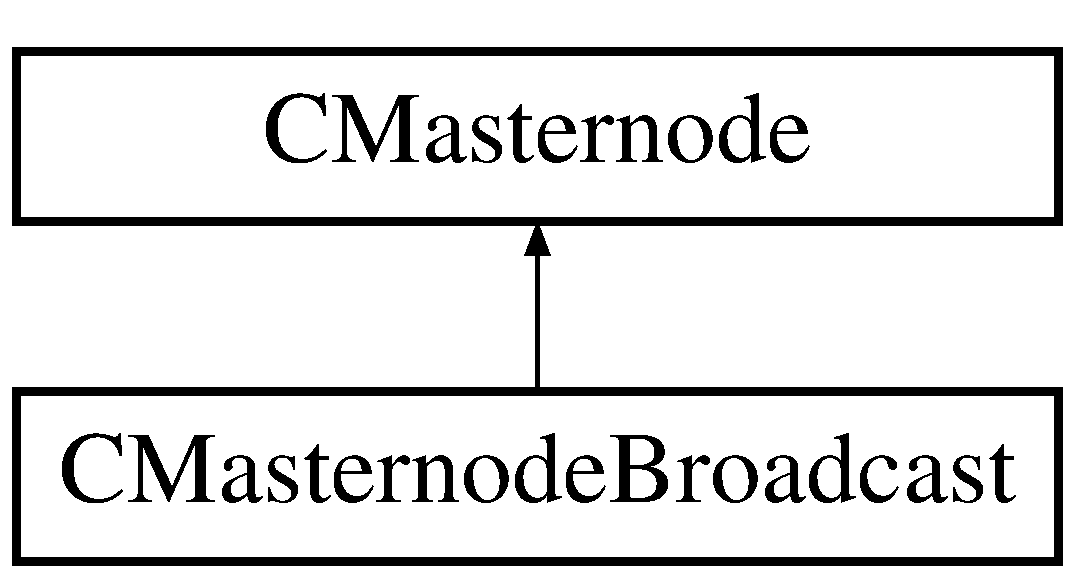
\includegraphics[height=2.000000cm]{class_c_masternode_broadcast}
\end{center}
\end{figure}
\subsection*{Public Member Functions}
\begin{DoxyCompactItemize}
\item 
\mbox{\hyperlink{class_c_masternode_broadcast_a9d1ccae926af3714163d26b6b02223c5}{C\+Masternode\+Broadcast}} ()
\item 
\mbox{\hyperlink{class_c_masternode_broadcast_ad85a19b0a20ea5ad6a65bc98fcd40cea}{C\+Masternode\+Broadcast}} (const \mbox{\hyperlink{class_c_masternode}{C\+Masternode}} \&mn)
\item 
\mbox{\hyperlink{class_c_masternode_broadcast_aa8727d7ae24dc875e8c74948127ebd4e}{C\+Masternode\+Broadcast}} (\mbox{\hyperlink{class_c_service}{C\+Service}} addr\+New, C\+Tx\+In vin\+New, \mbox{\hyperlink{class_c_pub_key}{C\+Pub\+Key}} pub\+Key\+Collateral\+Address\+New, \mbox{\hyperlink{class_c_pub_key}{C\+Pub\+Key}} pub\+Key\+Masternode\+New, int n\+Protocol\+Version\+In)
\item 
{\footnotesize template$<$typename Stream , typename Operation $>$ }\\void \mbox{\hyperlink{class_c_masternode_broadcast_a6e697696503e9416437067cb33edc084}{Serialization\+Op}} (Stream \&s, Operation ser\+\_\+action, int n\+Type, int n\+Version)
\item 
\mbox{\hyperlink{classuint256}{uint256}} \mbox{\hyperlink{class_c_masternode_broadcast_a402adbbedd893b31ae21eeb436f2afb1}{Get\+Hash}} () const
\item 
bool \mbox{\hyperlink{class_c_masternode_broadcast_a614b26e3fa8e0151889ce4fc0bebd88e}{Simple\+Check}} (int \&n\+Dos)
\item 
bool \mbox{\hyperlink{class_c_masternode_broadcast_a7aa301dbc2d846092c3090734d4622cf}{Update}} (\mbox{\hyperlink{class_c_masternode}{C\+Masternode}} $\ast$pmn, int \&n\+Dos)
\item 
bool \mbox{\hyperlink{class_c_masternode_broadcast_ad3e6be4a6f0206e5d8e6dcb427d169ce}{Check\+Outpoint}} (int \&n\+Dos)
\item 
bool \mbox{\hyperlink{class_c_masternode_broadcast_a60496c36bcb74c3f5516faac1a08b376}{Sign}} (\mbox{\hyperlink{class_c_key}{C\+Key}} \&key\+Collateral\+Address)
\item 
bool \mbox{\hyperlink{class_c_masternode_broadcast_a12769e5247ac34008e887ba6bb04496a}{Check\+Signature}} (int \&n\+Dos)
\item 
void \mbox{\hyperlink{class_c_masternode_broadcast_a54fc9e822e1524bee8852a0bf6d82736}{Relay}} ()
\end{DoxyCompactItemize}
\subsection*{Static Public Member Functions}
\begin{DoxyCompactItemize}
\item 
static bool \mbox{\hyperlink{class_c_masternode_broadcast_a3b331bac6aa4ab8ece112b62243f7498}{Create}} (C\+Tx\+In \mbox{\hyperlink{class_c_masternode_a485b26778bb8b006152aaa64168afe6b}{vin}}, \mbox{\hyperlink{class_c_service}{C\+Service}} service, \mbox{\hyperlink{class_c_key}{C\+Key}} key\+Collateral\+Address\+New, \mbox{\hyperlink{class_c_pub_key}{C\+Pub\+Key}} pub\+Key\+Collateral\+Address\+New, \mbox{\hyperlink{class_c_key}{C\+Key}} key\+Masternode\+New, \mbox{\hyperlink{class_c_pub_key}{C\+Pub\+Key}} pub\+Key\+Masternode\+New, std\+::string \&str\+Error\+Ret, \mbox{\hyperlink{class_c_masternode_broadcast}{C\+Masternode\+Broadcast}} \&mnb\+Ret)
\begin{DoxyCompactList}\small\item\em Create Masternode broadcast, needs to be relayed manually after that. \end{DoxyCompactList}\item 
static bool \mbox{\hyperlink{class_c_masternode_broadcast_a5b999adcbdb1de059cb226f3367771b0}{Create}} (std\+::string str\+Service, std\+::string str\+Key, std\+::string str\+Tx\+Hash, std\+::string str\+Output\+Index, std\+::string \&str\+Error\+Ret, \mbox{\hyperlink{class_c_masternode_broadcast}{C\+Masternode\+Broadcast}} \&mnb\+Ret, bool f\+Offline=false)
\end{DoxyCompactItemize}
\subsection*{Public Attributes}
\begin{DoxyCompactItemize}
\item 
bool \mbox{\hyperlink{class_c_masternode_broadcast_a7a10ab15299638456c0be9b63821cb36}{f\+Recovery}}
\item 
\mbox{\hyperlink{class_c_masternode_broadcast_a3b423bd09c06dbb8b75dc06d3d34a4b0}{A\+D\+D\+\_\+\+S\+E\+R\+I\+A\+L\+I\+Z\+E\+\_\+\+M\+E\+T\+H\+O\+DS}}
\end{DoxyCompactItemize}
\subsection*{Additional Inherited Members}


\subsection{Constructor \& Destructor Documentation}
\mbox{\Hypertarget{class_c_masternode_broadcast_a9d1ccae926af3714163d26b6b02223c5}\label{class_c_masternode_broadcast_a9d1ccae926af3714163d26b6b02223c5}} 
\index{C\+Masternode\+Broadcast@{C\+Masternode\+Broadcast}!C\+Masternode\+Broadcast@{C\+Masternode\+Broadcast}}
\index{C\+Masternode\+Broadcast@{C\+Masternode\+Broadcast}!C\+Masternode\+Broadcast@{C\+Masternode\+Broadcast}}
\subsubsection{\texorpdfstring{C\+Masternode\+Broadcast()}{CMasternodeBroadcast()}\hspace{0.1cm}{\footnotesize\ttfamily [1/3]}}
{\footnotesize\ttfamily C\+Masternode\+Broadcast\+::\+C\+Masternode\+Broadcast (\begin{DoxyParamCaption}{ }\end{DoxyParamCaption})\hspace{0.3cm}{\ttfamily [inline]}}

\mbox{\Hypertarget{class_c_masternode_broadcast_ad85a19b0a20ea5ad6a65bc98fcd40cea}\label{class_c_masternode_broadcast_ad85a19b0a20ea5ad6a65bc98fcd40cea}} 
\index{C\+Masternode\+Broadcast@{C\+Masternode\+Broadcast}!C\+Masternode\+Broadcast@{C\+Masternode\+Broadcast}}
\index{C\+Masternode\+Broadcast@{C\+Masternode\+Broadcast}!C\+Masternode\+Broadcast@{C\+Masternode\+Broadcast}}
\subsubsection{\texorpdfstring{C\+Masternode\+Broadcast()}{CMasternodeBroadcast()}\hspace{0.1cm}{\footnotesize\ttfamily [2/3]}}
{\footnotesize\ttfamily C\+Masternode\+Broadcast\+::\+C\+Masternode\+Broadcast (\begin{DoxyParamCaption}\item[{const \mbox{\hyperlink{class_c_masternode}{C\+Masternode}} \&}]{mn }\end{DoxyParamCaption})\hspace{0.3cm}{\ttfamily [inline]}}

\mbox{\Hypertarget{class_c_masternode_broadcast_aa8727d7ae24dc875e8c74948127ebd4e}\label{class_c_masternode_broadcast_aa8727d7ae24dc875e8c74948127ebd4e}} 
\index{C\+Masternode\+Broadcast@{C\+Masternode\+Broadcast}!C\+Masternode\+Broadcast@{C\+Masternode\+Broadcast}}
\index{C\+Masternode\+Broadcast@{C\+Masternode\+Broadcast}!C\+Masternode\+Broadcast@{C\+Masternode\+Broadcast}}
\subsubsection{\texorpdfstring{C\+Masternode\+Broadcast()}{CMasternodeBroadcast()}\hspace{0.1cm}{\footnotesize\ttfamily [3/3]}}
{\footnotesize\ttfamily C\+Masternode\+Broadcast\+::\+C\+Masternode\+Broadcast (\begin{DoxyParamCaption}\item[{\mbox{\hyperlink{class_c_service}{C\+Service}}}]{addr\+New,  }\item[{C\+Tx\+In}]{vin\+New,  }\item[{\mbox{\hyperlink{class_c_pub_key}{C\+Pub\+Key}}}]{pub\+Key\+Collateral\+Address\+New,  }\item[{\mbox{\hyperlink{class_c_pub_key}{C\+Pub\+Key}}}]{pub\+Key\+Masternode\+New,  }\item[{int}]{n\+Protocol\+Version\+In }\end{DoxyParamCaption})\hspace{0.3cm}{\ttfamily [inline]}}



\subsection{Member Function Documentation}
\mbox{\Hypertarget{class_c_masternode_broadcast_ad3e6be4a6f0206e5d8e6dcb427d169ce}\label{class_c_masternode_broadcast_ad3e6be4a6f0206e5d8e6dcb427d169ce}} 
\index{C\+Masternode\+Broadcast@{C\+Masternode\+Broadcast}!Check\+Outpoint@{Check\+Outpoint}}
\index{Check\+Outpoint@{Check\+Outpoint}!C\+Masternode\+Broadcast@{C\+Masternode\+Broadcast}}
\subsubsection{\texorpdfstring{Check\+Outpoint()}{CheckOutpoint()}}
{\footnotesize\ttfamily bool C\+Masternode\+Broadcast\+::\+Check\+Outpoint (\begin{DoxyParamCaption}\item[{int \&}]{n\+Dos }\end{DoxyParamCaption})}

\mbox{\Hypertarget{class_c_masternode_broadcast_a12769e5247ac34008e887ba6bb04496a}\label{class_c_masternode_broadcast_a12769e5247ac34008e887ba6bb04496a}} 
\index{C\+Masternode\+Broadcast@{C\+Masternode\+Broadcast}!Check\+Signature@{Check\+Signature}}
\index{Check\+Signature@{Check\+Signature}!C\+Masternode\+Broadcast@{C\+Masternode\+Broadcast}}
\subsubsection{\texorpdfstring{Check\+Signature()}{CheckSignature()}}
{\footnotesize\ttfamily bool C\+Masternode\+Broadcast\+::\+Check\+Signature (\begin{DoxyParamCaption}\item[{int \&}]{n\+Dos }\end{DoxyParamCaption})}

\mbox{\Hypertarget{class_c_masternode_broadcast_a3b331bac6aa4ab8ece112b62243f7498}\label{class_c_masternode_broadcast_a3b331bac6aa4ab8ece112b62243f7498}} 
\index{C\+Masternode\+Broadcast@{C\+Masternode\+Broadcast}!Create@{Create}}
\index{Create@{Create}!C\+Masternode\+Broadcast@{C\+Masternode\+Broadcast}}
\subsubsection{\texorpdfstring{Create()}{Create()}\hspace{0.1cm}{\footnotesize\ttfamily [1/2]}}
{\footnotesize\ttfamily bool C\+Masternode\+Broadcast\+::\+Create (\begin{DoxyParamCaption}\item[{C\+Tx\+In}]{vin,  }\item[{\mbox{\hyperlink{class_c_service}{C\+Service}}}]{service,  }\item[{\mbox{\hyperlink{class_c_key}{C\+Key}}}]{key\+Collateral\+Address\+New,  }\item[{\mbox{\hyperlink{class_c_pub_key}{C\+Pub\+Key}}}]{pub\+Key\+Collateral\+Address\+New,  }\item[{\mbox{\hyperlink{class_c_key}{C\+Key}}}]{key\+Masternode\+New,  }\item[{\mbox{\hyperlink{class_c_pub_key}{C\+Pub\+Key}}}]{pub\+Key\+Masternode\+New,  }\item[{std\+::string \&}]{str\+Error\+Ret,  }\item[{\mbox{\hyperlink{class_c_masternode_broadcast}{C\+Masternode\+Broadcast}} \&}]{mnb\+Ret }\end{DoxyParamCaption})\hspace{0.3cm}{\ttfamily [static]}}



Create Masternode broadcast, needs to be relayed manually after that. 

\mbox{\Hypertarget{class_c_masternode_broadcast_a5b999adcbdb1de059cb226f3367771b0}\label{class_c_masternode_broadcast_a5b999adcbdb1de059cb226f3367771b0}} 
\index{C\+Masternode\+Broadcast@{C\+Masternode\+Broadcast}!Create@{Create}}
\index{Create@{Create}!C\+Masternode\+Broadcast@{C\+Masternode\+Broadcast}}
\subsubsection{\texorpdfstring{Create()}{Create()}\hspace{0.1cm}{\footnotesize\ttfamily [2/2]}}
{\footnotesize\ttfamily bool C\+Masternode\+Broadcast\+::\+Create (\begin{DoxyParamCaption}\item[{std\+::string}]{str\+Service,  }\item[{std\+::string}]{str\+Key,  }\item[{std\+::string}]{str\+Tx\+Hash,  }\item[{std\+::string}]{str\+Output\+Index,  }\item[{std\+::string \&}]{str\+Error\+Ret,  }\item[{\mbox{\hyperlink{class_c_masternode_broadcast}{C\+Masternode\+Broadcast}} \&}]{mnb\+Ret,  }\item[{bool}]{f\+Offline = {\ttfamily false} }\end{DoxyParamCaption})\hspace{0.3cm}{\ttfamily [static]}}

\mbox{\Hypertarget{class_c_masternode_broadcast_a402adbbedd893b31ae21eeb436f2afb1}\label{class_c_masternode_broadcast_a402adbbedd893b31ae21eeb436f2afb1}} 
\index{C\+Masternode\+Broadcast@{C\+Masternode\+Broadcast}!Get\+Hash@{Get\+Hash}}
\index{Get\+Hash@{Get\+Hash}!C\+Masternode\+Broadcast@{C\+Masternode\+Broadcast}}
\subsubsection{\texorpdfstring{Get\+Hash()}{GetHash()}}
{\footnotesize\ttfamily \mbox{\hyperlink{classuint256}{uint256}} C\+Masternode\+Broadcast\+::\+Get\+Hash (\begin{DoxyParamCaption}{ }\end{DoxyParamCaption}) const\hspace{0.3cm}{\ttfamily [inline]}}

\mbox{\Hypertarget{class_c_masternode_broadcast_a54fc9e822e1524bee8852a0bf6d82736}\label{class_c_masternode_broadcast_a54fc9e822e1524bee8852a0bf6d82736}} 
\index{C\+Masternode\+Broadcast@{C\+Masternode\+Broadcast}!Relay@{Relay}}
\index{Relay@{Relay}!C\+Masternode\+Broadcast@{C\+Masternode\+Broadcast}}
\subsubsection{\texorpdfstring{Relay()}{Relay()}}
{\footnotesize\ttfamily void C\+Masternode\+Broadcast\+::\+Relay (\begin{DoxyParamCaption}{ }\end{DoxyParamCaption})}

\mbox{\Hypertarget{class_c_masternode_broadcast_a6e697696503e9416437067cb33edc084}\label{class_c_masternode_broadcast_a6e697696503e9416437067cb33edc084}} 
\index{C\+Masternode\+Broadcast@{C\+Masternode\+Broadcast}!Serialization\+Op@{Serialization\+Op}}
\index{Serialization\+Op@{Serialization\+Op}!C\+Masternode\+Broadcast@{C\+Masternode\+Broadcast}}
\subsubsection{\texorpdfstring{Serialization\+Op()}{SerializationOp()}}
{\footnotesize\ttfamily template$<$typename Stream , typename Operation $>$ \\
void C\+Masternode\+Broadcast\+::\+Serialization\+Op (\begin{DoxyParamCaption}\item[{Stream \&}]{s,  }\item[{Operation}]{ser\+\_\+action,  }\item[{int}]{n\+Type,  }\item[{int}]{n\+Version }\end{DoxyParamCaption})\hspace{0.3cm}{\ttfamily [inline]}}

\mbox{\Hypertarget{class_c_masternode_broadcast_a60496c36bcb74c3f5516faac1a08b376}\label{class_c_masternode_broadcast_a60496c36bcb74c3f5516faac1a08b376}} 
\index{C\+Masternode\+Broadcast@{C\+Masternode\+Broadcast}!Sign@{Sign}}
\index{Sign@{Sign}!C\+Masternode\+Broadcast@{C\+Masternode\+Broadcast}}
\subsubsection{\texorpdfstring{Sign()}{Sign()}}
{\footnotesize\ttfamily bool C\+Masternode\+Broadcast\+::\+Sign (\begin{DoxyParamCaption}\item[{\mbox{\hyperlink{class_c_key}{C\+Key}} \&}]{key\+Collateral\+Address }\end{DoxyParamCaption})}

\mbox{\Hypertarget{class_c_masternode_broadcast_a614b26e3fa8e0151889ce4fc0bebd88e}\label{class_c_masternode_broadcast_a614b26e3fa8e0151889ce4fc0bebd88e}} 
\index{C\+Masternode\+Broadcast@{C\+Masternode\+Broadcast}!Simple\+Check@{Simple\+Check}}
\index{Simple\+Check@{Simple\+Check}!C\+Masternode\+Broadcast@{C\+Masternode\+Broadcast}}
\subsubsection{\texorpdfstring{Simple\+Check()}{SimpleCheck()}}
{\footnotesize\ttfamily bool C\+Masternode\+Broadcast\+::\+Simple\+Check (\begin{DoxyParamCaption}\item[{int \&}]{n\+Dos }\end{DoxyParamCaption})}

\mbox{\Hypertarget{class_c_masternode_broadcast_a7aa301dbc2d846092c3090734d4622cf}\label{class_c_masternode_broadcast_a7aa301dbc2d846092c3090734d4622cf}} 
\index{C\+Masternode\+Broadcast@{C\+Masternode\+Broadcast}!Update@{Update}}
\index{Update@{Update}!C\+Masternode\+Broadcast@{C\+Masternode\+Broadcast}}
\subsubsection{\texorpdfstring{Update()}{Update()}}
{\footnotesize\ttfamily bool C\+Masternode\+Broadcast\+::\+Update (\begin{DoxyParamCaption}\item[{\mbox{\hyperlink{class_c_masternode}{C\+Masternode}} $\ast$}]{pmn,  }\item[{int \&}]{n\+Dos }\end{DoxyParamCaption})}



\subsection{Member Data Documentation}
\mbox{\Hypertarget{class_c_masternode_broadcast_a3b423bd09c06dbb8b75dc06d3d34a4b0}\label{class_c_masternode_broadcast_a3b423bd09c06dbb8b75dc06d3d34a4b0}} 
\index{C\+Masternode\+Broadcast@{C\+Masternode\+Broadcast}!A\+D\+D\+\_\+\+S\+E\+R\+I\+A\+L\+I\+Z\+E\+\_\+\+M\+E\+T\+H\+O\+DS@{A\+D\+D\+\_\+\+S\+E\+R\+I\+A\+L\+I\+Z\+E\+\_\+\+M\+E\+T\+H\+O\+DS}}
\index{A\+D\+D\+\_\+\+S\+E\+R\+I\+A\+L\+I\+Z\+E\+\_\+\+M\+E\+T\+H\+O\+DS@{A\+D\+D\+\_\+\+S\+E\+R\+I\+A\+L\+I\+Z\+E\+\_\+\+M\+E\+T\+H\+O\+DS}!C\+Masternode\+Broadcast@{C\+Masternode\+Broadcast}}
\subsubsection{\texorpdfstring{A\+D\+D\+\_\+\+S\+E\+R\+I\+A\+L\+I\+Z\+E\+\_\+\+M\+E\+T\+H\+O\+DS}{ADD\_SERIALIZE\_METHODS}}
{\footnotesize\ttfamily C\+Masternode\+Broadcast\+::\+A\+D\+D\+\_\+\+S\+E\+R\+I\+A\+L\+I\+Z\+E\+\_\+\+M\+E\+T\+H\+O\+DS}

\mbox{\Hypertarget{class_c_masternode_broadcast_a7a10ab15299638456c0be9b63821cb36}\label{class_c_masternode_broadcast_a7a10ab15299638456c0be9b63821cb36}} 
\index{C\+Masternode\+Broadcast@{C\+Masternode\+Broadcast}!f\+Recovery@{f\+Recovery}}
\index{f\+Recovery@{f\+Recovery}!C\+Masternode\+Broadcast@{C\+Masternode\+Broadcast}}
\subsubsection{\texorpdfstring{f\+Recovery}{fRecovery}}
{\footnotesize\ttfamily bool C\+Masternode\+Broadcast\+::f\+Recovery}



The documentation for this class was generated from the following files\+:\begin{DoxyCompactItemize}
\item 
/\+Users/christopherarguello/\+Developer/anon/src/\mbox{\hyperlink{masternode_8h}{masternode.\+h}}\item 
/\+Users/christopherarguello/\+Developer/anon/src/\mbox{\hyperlink{masternode_8cpp}{masternode.\+cpp}}\end{DoxyCompactItemize}

\hypertarget{class_c_masternode_config}{}\section{C\+Masternode\+Config Class Reference}
\label{class_c_masternode_config}\index{C\+Masternode\+Config@{C\+Masternode\+Config}}


{\ttfamily \#include $<$masternodeconfig.\+h$>$}

\subsection*{Classes}
\begin{DoxyCompactItemize}
\item 
class \mbox{\hyperlink{class_c_masternode_config_1_1_c_masternode_entry}{C\+Masternode\+Entry}}
\end{DoxyCompactItemize}
\subsection*{Public Member Functions}
\begin{DoxyCompactItemize}
\item 
\mbox{\hyperlink{class_c_masternode_config_acb7bc70387a57bdc9983ba4c668e77ac}{C\+Masternode\+Config}} ()
\item 
void \mbox{\hyperlink{class_c_masternode_config_af6dab86b7e6b5bf0df9392fc7daedc3f}{clear}} ()
\item 
bool \mbox{\hyperlink{class_c_masternode_config_a028d769bc39a23177cf81a3e433b6e86}{read}} (std\+::string \&str\+Err)
\item 
void \mbox{\hyperlink{class_c_masternode_config_a578068fd91293257e3f302c002c6ba43}{add}} (std\+::string alias, std\+::string ip, std\+::string priv\+Key, std\+::string tx\+Hash, std\+::string output\+Index)
\item 
std\+::vector$<$ \mbox{\hyperlink{class_c_masternode_config_1_1_c_masternode_entry}{C\+Masternode\+Entry}} $>$ \& \mbox{\hyperlink{class_c_masternode_config_a21fb5f410e3dcd55429f256d4efe4e61}{get\+Entries}} ()
\item 
int \mbox{\hyperlink{class_c_masternode_config_ab67434f7d279d4837f4999f10265cd2f}{get\+Count}} ()
\end{DoxyCompactItemize}
\subsection*{Private Attributes}
\begin{DoxyCompactItemize}
\item 
std\+::vector$<$ \mbox{\hyperlink{class_c_masternode_config_1_1_c_masternode_entry}{C\+Masternode\+Entry}} $>$ \mbox{\hyperlink{class_c_masternode_config_a6e8060eb502559efef8444ca2b19ac9a}{entries}}
\end{DoxyCompactItemize}


\subsection{Constructor \& Destructor Documentation}
\mbox{\Hypertarget{class_c_masternode_config_acb7bc70387a57bdc9983ba4c668e77ac}\label{class_c_masternode_config_acb7bc70387a57bdc9983ba4c668e77ac}} 
\index{C\+Masternode\+Config@{C\+Masternode\+Config}!C\+Masternode\+Config@{C\+Masternode\+Config}}
\index{C\+Masternode\+Config@{C\+Masternode\+Config}!C\+Masternode\+Config@{C\+Masternode\+Config}}
\subsubsection{\texorpdfstring{C\+Masternode\+Config()}{CMasternodeConfig()}}
{\footnotesize\ttfamily C\+Masternode\+Config\+::\+C\+Masternode\+Config (\begin{DoxyParamCaption}{ }\end{DoxyParamCaption})\hspace{0.3cm}{\ttfamily [inline]}}



\subsection{Member Function Documentation}
\mbox{\Hypertarget{class_c_masternode_config_a578068fd91293257e3f302c002c6ba43}\label{class_c_masternode_config_a578068fd91293257e3f302c002c6ba43}} 
\index{C\+Masternode\+Config@{C\+Masternode\+Config}!add@{add}}
\index{add@{add}!C\+Masternode\+Config@{C\+Masternode\+Config}}
\subsubsection{\texorpdfstring{add()}{add()}}
{\footnotesize\ttfamily void C\+Masternode\+Config\+::add (\begin{DoxyParamCaption}\item[{std\+::string}]{alias,  }\item[{std\+::string}]{ip,  }\item[{std\+::string}]{priv\+Key,  }\item[{std\+::string}]{tx\+Hash,  }\item[{std\+::string}]{output\+Index }\end{DoxyParamCaption})}

\mbox{\Hypertarget{class_c_masternode_config_af6dab86b7e6b5bf0df9392fc7daedc3f}\label{class_c_masternode_config_af6dab86b7e6b5bf0df9392fc7daedc3f}} 
\index{C\+Masternode\+Config@{C\+Masternode\+Config}!clear@{clear}}
\index{clear@{clear}!C\+Masternode\+Config@{C\+Masternode\+Config}}
\subsubsection{\texorpdfstring{clear()}{clear()}}
{\footnotesize\ttfamily void C\+Masternode\+Config\+::clear (\begin{DoxyParamCaption}{ }\end{DoxyParamCaption})}

\mbox{\Hypertarget{class_c_masternode_config_ab67434f7d279d4837f4999f10265cd2f}\label{class_c_masternode_config_ab67434f7d279d4837f4999f10265cd2f}} 
\index{C\+Masternode\+Config@{C\+Masternode\+Config}!get\+Count@{get\+Count}}
\index{get\+Count@{get\+Count}!C\+Masternode\+Config@{C\+Masternode\+Config}}
\subsubsection{\texorpdfstring{get\+Count()}{getCount()}}
{\footnotesize\ttfamily int C\+Masternode\+Config\+::get\+Count (\begin{DoxyParamCaption}{ }\end{DoxyParamCaption})\hspace{0.3cm}{\ttfamily [inline]}}

\mbox{\Hypertarget{class_c_masternode_config_a21fb5f410e3dcd55429f256d4efe4e61}\label{class_c_masternode_config_a21fb5f410e3dcd55429f256d4efe4e61}} 
\index{C\+Masternode\+Config@{C\+Masternode\+Config}!get\+Entries@{get\+Entries}}
\index{get\+Entries@{get\+Entries}!C\+Masternode\+Config@{C\+Masternode\+Config}}
\subsubsection{\texorpdfstring{get\+Entries()}{getEntries()}}
{\footnotesize\ttfamily std\+::vector$<$\mbox{\hyperlink{class_c_masternode_config_1_1_c_masternode_entry}{C\+Masternode\+Entry}}$>$\& C\+Masternode\+Config\+::get\+Entries (\begin{DoxyParamCaption}{ }\end{DoxyParamCaption})\hspace{0.3cm}{\ttfamily [inline]}}

\mbox{\Hypertarget{class_c_masternode_config_a028d769bc39a23177cf81a3e433b6e86}\label{class_c_masternode_config_a028d769bc39a23177cf81a3e433b6e86}} 
\index{C\+Masternode\+Config@{C\+Masternode\+Config}!read@{read}}
\index{read@{read}!C\+Masternode\+Config@{C\+Masternode\+Config}}
\subsubsection{\texorpdfstring{read()}{read()}}
{\footnotesize\ttfamily bool C\+Masternode\+Config\+::read (\begin{DoxyParamCaption}\item[{std\+::string \&}]{str\+Err }\end{DoxyParamCaption})}



\subsection{Member Data Documentation}
\mbox{\Hypertarget{class_c_masternode_config_a6e8060eb502559efef8444ca2b19ac9a}\label{class_c_masternode_config_a6e8060eb502559efef8444ca2b19ac9a}} 
\index{C\+Masternode\+Config@{C\+Masternode\+Config}!entries@{entries}}
\index{entries@{entries}!C\+Masternode\+Config@{C\+Masternode\+Config}}
\subsubsection{\texorpdfstring{entries}{entries}}
{\footnotesize\ttfamily std\+::vector$<$\mbox{\hyperlink{class_c_masternode_config_1_1_c_masternode_entry}{C\+Masternode\+Entry}}$>$ C\+Masternode\+Config\+::entries\hspace{0.3cm}{\ttfamily [private]}}



The documentation for this class was generated from the following files\+:\begin{DoxyCompactItemize}
\item 
/\+Users/christopherarguello/\+Developer/anon/src/\mbox{\hyperlink{masternodeconfig_8h}{masternodeconfig.\+h}}\item 
/\+Users/christopherarguello/\+Developer/anon/src/\mbox{\hyperlink{masternodeconfig_8cpp}{masternodeconfig.\+cpp}}\end{DoxyCompactItemize}

\hypertarget{class_c_masternode_config_1_1_c_masternode_entry}{}\section{C\+Masternode\+Config\+:\+:C\+Masternode\+Entry Class Reference}
\label{class_c_masternode_config_1_1_c_masternode_entry}\index{C\+Masternode\+Config\+::\+C\+Masternode\+Entry@{C\+Masternode\+Config\+::\+C\+Masternode\+Entry}}


{\ttfamily \#include $<$masternodeconfig.\+h$>$}

\subsection*{Public Member Functions}
\begin{DoxyCompactItemize}
\item 
\mbox{\hyperlink{class_c_masternode_config_1_1_c_masternode_entry_aa393b13586ba87b366559052980bf884}{C\+Masternode\+Entry}} (std\+::string \mbox{\hyperlink{class_c_masternode_config_1_1_c_masternode_entry_a0e584c7d4597037d0a3af60c2c53bbd7}{alias}}, std\+::string \mbox{\hyperlink{class_c_masternode_config_1_1_c_masternode_entry_a16021f21d3621c37eb163dbe0d79fd35}{ip}}, std\+::string \mbox{\hyperlink{class_c_masternode_config_1_1_c_masternode_entry_a431935e8b07bd671ea2ec6bbfb81b689}{priv\+Key}}, std\+::string \mbox{\hyperlink{class_c_masternode_config_1_1_c_masternode_entry_ac739b69566915fe25fd54bafd3129282}{tx\+Hash}}, std\+::string \mbox{\hyperlink{class_c_masternode_config_1_1_c_masternode_entry_ac6eef3b3c5009cd124deba0ce81c6951}{output\+Index}})
\item 
const std\+::string \& \mbox{\hyperlink{class_c_masternode_config_1_1_c_masternode_entry_abf242505d9955e37da0628a35d26677e}{get\+Alias}} () const
\item 
void \mbox{\hyperlink{class_c_masternode_config_1_1_c_masternode_entry_aa74db50dc25069a288266e22867b4537}{set\+Alias}} (const std\+::string \&\mbox{\hyperlink{class_c_masternode_config_1_1_c_masternode_entry_a0e584c7d4597037d0a3af60c2c53bbd7}{alias}})
\item 
const std\+::string \& \mbox{\hyperlink{class_c_masternode_config_1_1_c_masternode_entry_a4aff6625aebbc697706d13fdf044cafa}{get\+Output\+Index}} () const
\item 
void \mbox{\hyperlink{class_c_masternode_config_1_1_c_masternode_entry_a0f4523fe58c95398c9b4cac773a5f39c}{set\+Output\+Index}} (const std\+::string \&\mbox{\hyperlink{class_c_masternode_config_1_1_c_masternode_entry_ac6eef3b3c5009cd124deba0ce81c6951}{output\+Index}})
\item 
const std\+::string \& \mbox{\hyperlink{class_c_masternode_config_1_1_c_masternode_entry_ab0e21a945e43940b659bf289f9280552}{get\+Priv\+Key}} () const
\item 
void \mbox{\hyperlink{class_c_masternode_config_1_1_c_masternode_entry_a991176f5739043dab17d262a42e7061b}{set\+Priv\+Key}} (const std\+::string \&\mbox{\hyperlink{class_c_masternode_config_1_1_c_masternode_entry_a431935e8b07bd671ea2ec6bbfb81b689}{priv\+Key}})
\item 
const std\+::string \& \mbox{\hyperlink{class_c_masternode_config_1_1_c_masternode_entry_a08039c5a3271a278c64a706c4b53d29b}{get\+Tx\+Hash}} () const
\item 
void \mbox{\hyperlink{class_c_masternode_config_1_1_c_masternode_entry_a32224c906982e19d8b231ed7bc8d27bd}{set\+Tx\+Hash}} (const std\+::string \&\mbox{\hyperlink{class_c_masternode_config_1_1_c_masternode_entry_ac739b69566915fe25fd54bafd3129282}{tx\+Hash}})
\item 
const std\+::string \& \mbox{\hyperlink{class_c_masternode_config_1_1_c_masternode_entry_a50b3672f986b569c83bf29e08f8165c8}{get\+Ip}} () const
\item 
void \mbox{\hyperlink{class_c_masternode_config_1_1_c_masternode_entry_a6dfa8be6875c2718ce05f701158cbbfd}{set\+Ip}} (const std\+::string \&\mbox{\hyperlink{class_c_masternode_config_1_1_c_masternode_entry_a16021f21d3621c37eb163dbe0d79fd35}{ip}})
\end{DoxyCompactItemize}
\subsection*{Private Attributes}
\begin{DoxyCompactItemize}
\item 
std\+::string \mbox{\hyperlink{class_c_masternode_config_1_1_c_masternode_entry_a0e584c7d4597037d0a3af60c2c53bbd7}{alias}}
\item 
std\+::string \mbox{\hyperlink{class_c_masternode_config_1_1_c_masternode_entry_a16021f21d3621c37eb163dbe0d79fd35}{ip}}
\item 
std\+::string \mbox{\hyperlink{class_c_masternode_config_1_1_c_masternode_entry_a431935e8b07bd671ea2ec6bbfb81b689}{priv\+Key}}
\item 
std\+::string \mbox{\hyperlink{class_c_masternode_config_1_1_c_masternode_entry_ac739b69566915fe25fd54bafd3129282}{tx\+Hash}}
\item 
std\+::string \mbox{\hyperlink{class_c_masternode_config_1_1_c_masternode_entry_ac6eef3b3c5009cd124deba0ce81c6951}{output\+Index}}
\end{DoxyCompactItemize}


\subsection{Constructor \& Destructor Documentation}
\mbox{\Hypertarget{class_c_masternode_config_1_1_c_masternode_entry_aa393b13586ba87b366559052980bf884}\label{class_c_masternode_config_1_1_c_masternode_entry_aa393b13586ba87b366559052980bf884}} 
\index{C\+Masternode\+Config\+::\+C\+Masternode\+Entry@{C\+Masternode\+Config\+::\+C\+Masternode\+Entry}!C\+Masternode\+Entry@{C\+Masternode\+Entry}}
\index{C\+Masternode\+Entry@{C\+Masternode\+Entry}!C\+Masternode\+Config\+::\+C\+Masternode\+Entry@{C\+Masternode\+Config\+::\+C\+Masternode\+Entry}}
\subsubsection{\texorpdfstring{C\+Masternode\+Entry()}{CMasternodeEntry()}}
{\footnotesize\ttfamily C\+Masternode\+Config\+::\+C\+Masternode\+Entry\+::\+C\+Masternode\+Entry (\begin{DoxyParamCaption}\item[{std\+::string}]{alias,  }\item[{std\+::string}]{ip,  }\item[{std\+::string}]{priv\+Key,  }\item[{std\+::string}]{tx\+Hash,  }\item[{std\+::string}]{output\+Index }\end{DoxyParamCaption})\hspace{0.3cm}{\ttfamily [inline]}}



\subsection{Member Function Documentation}
\mbox{\Hypertarget{class_c_masternode_config_1_1_c_masternode_entry_abf242505d9955e37da0628a35d26677e}\label{class_c_masternode_config_1_1_c_masternode_entry_abf242505d9955e37da0628a35d26677e}} 
\index{C\+Masternode\+Config\+::\+C\+Masternode\+Entry@{C\+Masternode\+Config\+::\+C\+Masternode\+Entry}!get\+Alias@{get\+Alias}}
\index{get\+Alias@{get\+Alias}!C\+Masternode\+Config\+::\+C\+Masternode\+Entry@{C\+Masternode\+Config\+::\+C\+Masternode\+Entry}}
\subsubsection{\texorpdfstring{get\+Alias()}{getAlias()}}
{\footnotesize\ttfamily const std\+::string\& C\+Masternode\+Config\+::\+C\+Masternode\+Entry\+::get\+Alias (\begin{DoxyParamCaption}{ }\end{DoxyParamCaption}) const\hspace{0.3cm}{\ttfamily [inline]}}

\mbox{\Hypertarget{class_c_masternode_config_1_1_c_masternode_entry_a50b3672f986b569c83bf29e08f8165c8}\label{class_c_masternode_config_1_1_c_masternode_entry_a50b3672f986b569c83bf29e08f8165c8}} 
\index{C\+Masternode\+Config\+::\+C\+Masternode\+Entry@{C\+Masternode\+Config\+::\+C\+Masternode\+Entry}!get\+Ip@{get\+Ip}}
\index{get\+Ip@{get\+Ip}!C\+Masternode\+Config\+::\+C\+Masternode\+Entry@{C\+Masternode\+Config\+::\+C\+Masternode\+Entry}}
\subsubsection{\texorpdfstring{get\+Ip()}{getIp()}}
{\footnotesize\ttfamily const std\+::string\& C\+Masternode\+Config\+::\+C\+Masternode\+Entry\+::get\+Ip (\begin{DoxyParamCaption}{ }\end{DoxyParamCaption}) const\hspace{0.3cm}{\ttfamily [inline]}}

\mbox{\Hypertarget{class_c_masternode_config_1_1_c_masternode_entry_a4aff6625aebbc697706d13fdf044cafa}\label{class_c_masternode_config_1_1_c_masternode_entry_a4aff6625aebbc697706d13fdf044cafa}} 
\index{C\+Masternode\+Config\+::\+C\+Masternode\+Entry@{C\+Masternode\+Config\+::\+C\+Masternode\+Entry}!get\+Output\+Index@{get\+Output\+Index}}
\index{get\+Output\+Index@{get\+Output\+Index}!C\+Masternode\+Config\+::\+C\+Masternode\+Entry@{C\+Masternode\+Config\+::\+C\+Masternode\+Entry}}
\subsubsection{\texorpdfstring{get\+Output\+Index()}{getOutputIndex()}}
{\footnotesize\ttfamily const std\+::string\& C\+Masternode\+Config\+::\+C\+Masternode\+Entry\+::get\+Output\+Index (\begin{DoxyParamCaption}{ }\end{DoxyParamCaption}) const\hspace{0.3cm}{\ttfamily [inline]}}

\mbox{\Hypertarget{class_c_masternode_config_1_1_c_masternode_entry_ab0e21a945e43940b659bf289f9280552}\label{class_c_masternode_config_1_1_c_masternode_entry_ab0e21a945e43940b659bf289f9280552}} 
\index{C\+Masternode\+Config\+::\+C\+Masternode\+Entry@{C\+Masternode\+Config\+::\+C\+Masternode\+Entry}!get\+Priv\+Key@{get\+Priv\+Key}}
\index{get\+Priv\+Key@{get\+Priv\+Key}!C\+Masternode\+Config\+::\+C\+Masternode\+Entry@{C\+Masternode\+Config\+::\+C\+Masternode\+Entry}}
\subsubsection{\texorpdfstring{get\+Priv\+Key()}{getPrivKey()}}
{\footnotesize\ttfamily const std\+::string\& C\+Masternode\+Config\+::\+C\+Masternode\+Entry\+::get\+Priv\+Key (\begin{DoxyParamCaption}{ }\end{DoxyParamCaption}) const\hspace{0.3cm}{\ttfamily [inline]}}

\mbox{\Hypertarget{class_c_masternode_config_1_1_c_masternode_entry_a08039c5a3271a278c64a706c4b53d29b}\label{class_c_masternode_config_1_1_c_masternode_entry_a08039c5a3271a278c64a706c4b53d29b}} 
\index{C\+Masternode\+Config\+::\+C\+Masternode\+Entry@{C\+Masternode\+Config\+::\+C\+Masternode\+Entry}!get\+Tx\+Hash@{get\+Tx\+Hash}}
\index{get\+Tx\+Hash@{get\+Tx\+Hash}!C\+Masternode\+Config\+::\+C\+Masternode\+Entry@{C\+Masternode\+Config\+::\+C\+Masternode\+Entry}}
\subsubsection{\texorpdfstring{get\+Tx\+Hash()}{getTxHash()}}
{\footnotesize\ttfamily const std\+::string\& C\+Masternode\+Config\+::\+C\+Masternode\+Entry\+::get\+Tx\+Hash (\begin{DoxyParamCaption}{ }\end{DoxyParamCaption}) const\hspace{0.3cm}{\ttfamily [inline]}}

\mbox{\Hypertarget{class_c_masternode_config_1_1_c_masternode_entry_aa74db50dc25069a288266e22867b4537}\label{class_c_masternode_config_1_1_c_masternode_entry_aa74db50dc25069a288266e22867b4537}} 
\index{C\+Masternode\+Config\+::\+C\+Masternode\+Entry@{C\+Masternode\+Config\+::\+C\+Masternode\+Entry}!set\+Alias@{set\+Alias}}
\index{set\+Alias@{set\+Alias}!C\+Masternode\+Config\+::\+C\+Masternode\+Entry@{C\+Masternode\+Config\+::\+C\+Masternode\+Entry}}
\subsubsection{\texorpdfstring{set\+Alias()}{setAlias()}}
{\footnotesize\ttfamily void C\+Masternode\+Config\+::\+C\+Masternode\+Entry\+::set\+Alias (\begin{DoxyParamCaption}\item[{const std\+::string \&}]{alias }\end{DoxyParamCaption})\hspace{0.3cm}{\ttfamily [inline]}}

\mbox{\Hypertarget{class_c_masternode_config_1_1_c_masternode_entry_a6dfa8be6875c2718ce05f701158cbbfd}\label{class_c_masternode_config_1_1_c_masternode_entry_a6dfa8be6875c2718ce05f701158cbbfd}} 
\index{C\+Masternode\+Config\+::\+C\+Masternode\+Entry@{C\+Masternode\+Config\+::\+C\+Masternode\+Entry}!set\+Ip@{set\+Ip}}
\index{set\+Ip@{set\+Ip}!C\+Masternode\+Config\+::\+C\+Masternode\+Entry@{C\+Masternode\+Config\+::\+C\+Masternode\+Entry}}
\subsubsection{\texorpdfstring{set\+Ip()}{setIp()}}
{\footnotesize\ttfamily void C\+Masternode\+Config\+::\+C\+Masternode\+Entry\+::set\+Ip (\begin{DoxyParamCaption}\item[{const std\+::string \&}]{ip }\end{DoxyParamCaption})\hspace{0.3cm}{\ttfamily [inline]}}

\mbox{\Hypertarget{class_c_masternode_config_1_1_c_masternode_entry_a0f4523fe58c95398c9b4cac773a5f39c}\label{class_c_masternode_config_1_1_c_masternode_entry_a0f4523fe58c95398c9b4cac773a5f39c}} 
\index{C\+Masternode\+Config\+::\+C\+Masternode\+Entry@{C\+Masternode\+Config\+::\+C\+Masternode\+Entry}!set\+Output\+Index@{set\+Output\+Index}}
\index{set\+Output\+Index@{set\+Output\+Index}!C\+Masternode\+Config\+::\+C\+Masternode\+Entry@{C\+Masternode\+Config\+::\+C\+Masternode\+Entry}}
\subsubsection{\texorpdfstring{set\+Output\+Index()}{setOutputIndex()}}
{\footnotesize\ttfamily void C\+Masternode\+Config\+::\+C\+Masternode\+Entry\+::set\+Output\+Index (\begin{DoxyParamCaption}\item[{const std\+::string \&}]{output\+Index }\end{DoxyParamCaption})\hspace{0.3cm}{\ttfamily [inline]}}

\mbox{\Hypertarget{class_c_masternode_config_1_1_c_masternode_entry_a991176f5739043dab17d262a42e7061b}\label{class_c_masternode_config_1_1_c_masternode_entry_a991176f5739043dab17d262a42e7061b}} 
\index{C\+Masternode\+Config\+::\+C\+Masternode\+Entry@{C\+Masternode\+Config\+::\+C\+Masternode\+Entry}!set\+Priv\+Key@{set\+Priv\+Key}}
\index{set\+Priv\+Key@{set\+Priv\+Key}!C\+Masternode\+Config\+::\+C\+Masternode\+Entry@{C\+Masternode\+Config\+::\+C\+Masternode\+Entry}}
\subsubsection{\texorpdfstring{set\+Priv\+Key()}{setPrivKey()}}
{\footnotesize\ttfamily void C\+Masternode\+Config\+::\+C\+Masternode\+Entry\+::set\+Priv\+Key (\begin{DoxyParamCaption}\item[{const std\+::string \&}]{priv\+Key }\end{DoxyParamCaption})\hspace{0.3cm}{\ttfamily [inline]}}

\mbox{\Hypertarget{class_c_masternode_config_1_1_c_masternode_entry_a32224c906982e19d8b231ed7bc8d27bd}\label{class_c_masternode_config_1_1_c_masternode_entry_a32224c906982e19d8b231ed7bc8d27bd}} 
\index{C\+Masternode\+Config\+::\+C\+Masternode\+Entry@{C\+Masternode\+Config\+::\+C\+Masternode\+Entry}!set\+Tx\+Hash@{set\+Tx\+Hash}}
\index{set\+Tx\+Hash@{set\+Tx\+Hash}!C\+Masternode\+Config\+::\+C\+Masternode\+Entry@{C\+Masternode\+Config\+::\+C\+Masternode\+Entry}}
\subsubsection{\texorpdfstring{set\+Tx\+Hash()}{setTxHash()}}
{\footnotesize\ttfamily void C\+Masternode\+Config\+::\+C\+Masternode\+Entry\+::set\+Tx\+Hash (\begin{DoxyParamCaption}\item[{const std\+::string \&}]{tx\+Hash }\end{DoxyParamCaption})\hspace{0.3cm}{\ttfamily [inline]}}



\subsection{Member Data Documentation}
\mbox{\Hypertarget{class_c_masternode_config_1_1_c_masternode_entry_a0e584c7d4597037d0a3af60c2c53bbd7}\label{class_c_masternode_config_1_1_c_masternode_entry_a0e584c7d4597037d0a3af60c2c53bbd7}} 
\index{C\+Masternode\+Config\+::\+C\+Masternode\+Entry@{C\+Masternode\+Config\+::\+C\+Masternode\+Entry}!alias@{alias}}
\index{alias@{alias}!C\+Masternode\+Config\+::\+C\+Masternode\+Entry@{C\+Masternode\+Config\+::\+C\+Masternode\+Entry}}
\subsubsection{\texorpdfstring{alias}{alias}}
{\footnotesize\ttfamily std\+::string C\+Masternode\+Config\+::\+C\+Masternode\+Entry\+::alias\hspace{0.3cm}{\ttfamily [private]}}

\mbox{\Hypertarget{class_c_masternode_config_1_1_c_masternode_entry_a16021f21d3621c37eb163dbe0d79fd35}\label{class_c_masternode_config_1_1_c_masternode_entry_a16021f21d3621c37eb163dbe0d79fd35}} 
\index{C\+Masternode\+Config\+::\+C\+Masternode\+Entry@{C\+Masternode\+Config\+::\+C\+Masternode\+Entry}!ip@{ip}}
\index{ip@{ip}!C\+Masternode\+Config\+::\+C\+Masternode\+Entry@{C\+Masternode\+Config\+::\+C\+Masternode\+Entry}}
\subsubsection{\texorpdfstring{ip}{ip}}
{\footnotesize\ttfamily std\+::string C\+Masternode\+Config\+::\+C\+Masternode\+Entry\+::ip\hspace{0.3cm}{\ttfamily [private]}}

\mbox{\Hypertarget{class_c_masternode_config_1_1_c_masternode_entry_ac6eef3b3c5009cd124deba0ce81c6951}\label{class_c_masternode_config_1_1_c_masternode_entry_ac6eef3b3c5009cd124deba0ce81c6951}} 
\index{C\+Masternode\+Config\+::\+C\+Masternode\+Entry@{C\+Masternode\+Config\+::\+C\+Masternode\+Entry}!output\+Index@{output\+Index}}
\index{output\+Index@{output\+Index}!C\+Masternode\+Config\+::\+C\+Masternode\+Entry@{C\+Masternode\+Config\+::\+C\+Masternode\+Entry}}
\subsubsection{\texorpdfstring{output\+Index}{outputIndex}}
{\footnotesize\ttfamily std\+::string C\+Masternode\+Config\+::\+C\+Masternode\+Entry\+::output\+Index\hspace{0.3cm}{\ttfamily [private]}}

\mbox{\Hypertarget{class_c_masternode_config_1_1_c_masternode_entry_a431935e8b07bd671ea2ec6bbfb81b689}\label{class_c_masternode_config_1_1_c_masternode_entry_a431935e8b07bd671ea2ec6bbfb81b689}} 
\index{C\+Masternode\+Config\+::\+C\+Masternode\+Entry@{C\+Masternode\+Config\+::\+C\+Masternode\+Entry}!priv\+Key@{priv\+Key}}
\index{priv\+Key@{priv\+Key}!C\+Masternode\+Config\+::\+C\+Masternode\+Entry@{C\+Masternode\+Config\+::\+C\+Masternode\+Entry}}
\subsubsection{\texorpdfstring{priv\+Key}{privKey}}
{\footnotesize\ttfamily std\+::string C\+Masternode\+Config\+::\+C\+Masternode\+Entry\+::priv\+Key\hspace{0.3cm}{\ttfamily [private]}}

\mbox{\Hypertarget{class_c_masternode_config_1_1_c_masternode_entry_ac739b69566915fe25fd54bafd3129282}\label{class_c_masternode_config_1_1_c_masternode_entry_ac739b69566915fe25fd54bafd3129282}} 
\index{C\+Masternode\+Config\+::\+C\+Masternode\+Entry@{C\+Masternode\+Config\+::\+C\+Masternode\+Entry}!tx\+Hash@{tx\+Hash}}
\index{tx\+Hash@{tx\+Hash}!C\+Masternode\+Config\+::\+C\+Masternode\+Entry@{C\+Masternode\+Config\+::\+C\+Masternode\+Entry}}
\subsubsection{\texorpdfstring{tx\+Hash}{txHash}}
{\footnotesize\ttfamily std\+::string C\+Masternode\+Config\+::\+C\+Masternode\+Entry\+::tx\+Hash\hspace{0.3cm}{\ttfamily [private]}}



The documentation for this class was generated from the following file\+:\begin{DoxyCompactItemize}
\item 
/\+Users/christopherarguello/\+Developer/anon/src/\mbox{\hyperlink{masternodeconfig_8h}{masternodeconfig.\+h}}\end{DoxyCompactItemize}

\hypertarget{class_c_masternode_index}{}\section{C\+Masternode\+Index Class Reference}
\label{class_c_masternode_index}\index{C\+Masternode\+Index@{C\+Masternode\+Index}}


{\ttfamily \#include $<$masternodeman.\+h$>$}

\subsection*{Public Types}
\begin{DoxyCompactItemize}
\item 
typedef std\+::map$<$ C\+Tx\+In, int $>$ \mbox{\hyperlink{class_c_masternode_index_a78c666dcc663fceff46cd86f4eb1870c}{index\+\_\+m\+\_\+t}}
\item 
typedef index\+\_\+m\+\_\+t\+::iterator \mbox{\hyperlink{class_c_masternode_index_a5a09121c16d5c51ab422b2d2f02a2d6b}{index\+\_\+m\+\_\+it}}
\item 
typedef index\+\_\+m\+\_\+t\+::const\+\_\+iterator \mbox{\hyperlink{class_c_masternode_index_a012060326cfe73f675a791131b6fd91a}{index\+\_\+m\+\_\+cit}}
\item 
typedef std\+::map$<$ int, C\+Tx\+In $>$ \mbox{\hyperlink{class_c_masternode_index_ad04aa24155d452c5c222562c0f3c3e21}{rindex\+\_\+m\+\_\+t}}
\item 
typedef rindex\+\_\+m\+\_\+t\+::iterator \mbox{\hyperlink{class_c_masternode_index_a40bf06eaf7389e6017bf87c488ea9aea}{rindex\+\_\+m\+\_\+it}}
\item 
typedef rindex\+\_\+m\+\_\+t\+::const\+\_\+iterator \mbox{\hyperlink{class_c_masternode_index_ac24d75bd8a5832de19ba5ae8f37e9e90}{rindex\+\_\+m\+\_\+cit}}
\end{DoxyCompactItemize}
\subsection*{Public Member Functions}
\begin{DoxyCompactItemize}
\item 
\mbox{\hyperlink{class_c_masternode_index_a5741b7c418d1d2b545399ce3d13ad65b}{C\+Masternode\+Index}} ()
\item 
int \mbox{\hyperlink{class_c_masternode_index_accf7ccda46096811469e216910f4608f}{Get\+Size}} () const
\item 
bool \mbox{\hyperlink{class_c_masternode_index_a85022155c9093fcb1ea5bb1deb7dd2b0}{Get}} (int n\+Index, C\+Tx\+In \&vin\+Masternode) const
\begin{DoxyCompactList}\small\item\em Retrieve masternode vin by index. \end{DoxyCompactList}\item 
int \mbox{\hyperlink{class_c_masternode_index_a87af53e12ba73eaeecb4d28bb98813d1}{Get\+Masternode\+Index}} (const C\+Tx\+In \&vin\+Masternode) const
\begin{DoxyCompactList}\small\item\em Get index of a masternode vin. \end{DoxyCompactList}\item 
void \mbox{\hyperlink{class_c_masternode_index_ad62fa26d65c04335b00463c29cd766f7}{Add\+Masternode\+V\+IN}} (const C\+Tx\+In \&vin\+Masternode)
\item 
void \mbox{\hyperlink{class_c_masternode_index_a6d191c879a7029e41be2f36a5e14af0a}{Clear}} ()
\item 
{\footnotesize template$<$typename Stream , typename Operation $>$ }\\void \mbox{\hyperlink{class_c_masternode_index_a11fe7d7c87902287b5a6fc5b46953628}{Serialization\+Op}} (Stream \&s, Operation ser\+\_\+action, int n\+Type, int n\+Version)
\end{DoxyCompactItemize}
\subsection*{Public Attributes}
\begin{DoxyCompactItemize}
\item 
\mbox{\hyperlink{class_c_masternode_index_a49d9d48a596c5f3a92cc812a09762930}{A\+D\+D\+\_\+\+S\+E\+R\+I\+A\+L\+I\+Z\+E\+\_\+\+M\+E\+T\+H\+O\+DS}}
\end{DoxyCompactItemize}
\subsection*{Private Member Functions}
\begin{DoxyCompactItemize}
\item 
void \mbox{\hyperlink{class_c_masternode_index_a09611499b61d6c8be249e66df0ac1390}{Rebuild\+Index}} ()
\end{DoxyCompactItemize}
\subsection*{Private Attributes}
\begin{DoxyCompactItemize}
\item 
int \mbox{\hyperlink{class_c_masternode_index_a4df94f8851340cea142139c8490e9a1e}{n\+Size}}
\item 
\mbox{\hyperlink{class_c_masternode_index_a78c666dcc663fceff46cd86f4eb1870c}{index\+\_\+m\+\_\+t}} \mbox{\hyperlink{class_c_masternode_index_a3c1da93ff0beea2a21feac2d59bca694}{map\+Index}}
\item 
\mbox{\hyperlink{class_c_masternode_index_ad04aa24155d452c5c222562c0f3c3e21}{rindex\+\_\+m\+\_\+t}} \mbox{\hyperlink{class_c_masternode_index_af395a77efe7661aed5460ea1d478c6fd}{map\+Reverse\+Index}}
\end{DoxyCompactItemize}


\subsection{Detailed Description}
Provides a forward and reverse index between MN vin\textquotesingle{}s and integers.

This mapping is normally add-\/only and is expected to be permanent It is only rebuilt if the size of the index exceeds the expected maximum number of MN\textquotesingle{}s and the current number of known MN\textquotesingle{}s.

The external interface to this index is provided via delegation by \mbox{\hyperlink{class_c_masternode_man}{C\+Masternode\+Man}} 

\subsection{Member Typedef Documentation}
\mbox{\Hypertarget{class_c_masternode_index_a012060326cfe73f675a791131b6fd91a}\label{class_c_masternode_index_a012060326cfe73f675a791131b6fd91a}} 
\index{C\+Masternode\+Index@{C\+Masternode\+Index}!index\+\_\+m\+\_\+cit@{index\+\_\+m\+\_\+cit}}
\index{index\+\_\+m\+\_\+cit@{index\+\_\+m\+\_\+cit}!C\+Masternode\+Index@{C\+Masternode\+Index}}
\subsubsection{\texorpdfstring{index\+\_\+m\+\_\+cit}{index\_m\_cit}}
{\footnotesize\ttfamily typedef index\+\_\+m\+\_\+t\+::const\+\_\+iterator \mbox{\hyperlink{class_c_masternode_index_a012060326cfe73f675a791131b6fd91a}{C\+Masternode\+Index\+::index\+\_\+m\+\_\+cit}}}

\mbox{\Hypertarget{class_c_masternode_index_a5a09121c16d5c51ab422b2d2f02a2d6b}\label{class_c_masternode_index_a5a09121c16d5c51ab422b2d2f02a2d6b}} 
\index{C\+Masternode\+Index@{C\+Masternode\+Index}!index\+\_\+m\+\_\+it@{index\+\_\+m\+\_\+it}}
\index{index\+\_\+m\+\_\+it@{index\+\_\+m\+\_\+it}!C\+Masternode\+Index@{C\+Masternode\+Index}}
\subsubsection{\texorpdfstring{index\+\_\+m\+\_\+it}{index\_m\_it}}
{\footnotesize\ttfamily typedef index\+\_\+m\+\_\+t\+::iterator \mbox{\hyperlink{class_c_masternode_index_a5a09121c16d5c51ab422b2d2f02a2d6b}{C\+Masternode\+Index\+::index\+\_\+m\+\_\+it}}}

\mbox{\Hypertarget{class_c_masternode_index_a78c666dcc663fceff46cd86f4eb1870c}\label{class_c_masternode_index_a78c666dcc663fceff46cd86f4eb1870c}} 
\index{C\+Masternode\+Index@{C\+Masternode\+Index}!index\+\_\+m\+\_\+t@{index\+\_\+m\+\_\+t}}
\index{index\+\_\+m\+\_\+t@{index\+\_\+m\+\_\+t}!C\+Masternode\+Index@{C\+Masternode\+Index}}
\subsubsection{\texorpdfstring{index\+\_\+m\+\_\+t}{index\_m\_t}}
{\footnotesize\ttfamily typedef std\+::map$<$C\+Tx\+In, int$>$ \mbox{\hyperlink{class_c_masternode_index_a78c666dcc663fceff46cd86f4eb1870c}{C\+Masternode\+Index\+::index\+\_\+m\+\_\+t}}}

\mbox{\Hypertarget{class_c_masternode_index_ac24d75bd8a5832de19ba5ae8f37e9e90}\label{class_c_masternode_index_ac24d75bd8a5832de19ba5ae8f37e9e90}} 
\index{C\+Masternode\+Index@{C\+Masternode\+Index}!rindex\+\_\+m\+\_\+cit@{rindex\+\_\+m\+\_\+cit}}
\index{rindex\+\_\+m\+\_\+cit@{rindex\+\_\+m\+\_\+cit}!C\+Masternode\+Index@{C\+Masternode\+Index}}
\subsubsection{\texorpdfstring{rindex\+\_\+m\+\_\+cit}{rindex\_m\_cit}}
{\footnotesize\ttfamily typedef rindex\+\_\+m\+\_\+t\+::const\+\_\+iterator \mbox{\hyperlink{class_c_masternode_index_ac24d75bd8a5832de19ba5ae8f37e9e90}{C\+Masternode\+Index\+::rindex\+\_\+m\+\_\+cit}}}

\mbox{\Hypertarget{class_c_masternode_index_a40bf06eaf7389e6017bf87c488ea9aea}\label{class_c_masternode_index_a40bf06eaf7389e6017bf87c488ea9aea}} 
\index{C\+Masternode\+Index@{C\+Masternode\+Index}!rindex\+\_\+m\+\_\+it@{rindex\+\_\+m\+\_\+it}}
\index{rindex\+\_\+m\+\_\+it@{rindex\+\_\+m\+\_\+it}!C\+Masternode\+Index@{C\+Masternode\+Index}}
\subsubsection{\texorpdfstring{rindex\+\_\+m\+\_\+it}{rindex\_m\_it}}
{\footnotesize\ttfamily typedef rindex\+\_\+m\+\_\+t\+::iterator \mbox{\hyperlink{class_c_masternode_index_a40bf06eaf7389e6017bf87c488ea9aea}{C\+Masternode\+Index\+::rindex\+\_\+m\+\_\+it}}}

\mbox{\Hypertarget{class_c_masternode_index_ad04aa24155d452c5c222562c0f3c3e21}\label{class_c_masternode_index_ad04aa24155d452c5c222562c0f3c3e21}} 
\index{C\+Masternode\+Index@{C\+Masternode\+Index}!rindex\+\_\+m\+\_\+t@{rindex\+\_\+m\+\_\+t}}
\index{rindex\+\_\+m\+\_\+t@{rindex\+\_\+m\+\_\+t}!C\+Masternode\+Index@{C\+Masternode\+Index}}
\subsubsection{\texorpdfstring{rindex\+\_\+m\+\_\+t}{rindex\_m\_t}}
{\footnotesize\ttfamily typedef std\+::map$<$int, C\+Tx\+In$>$ \mbox{\hyperlink{class_c_masternode_index_ad04aa24155d452c5c222562c0f3c3e21}{C\+Masternode\+Index\+::rindex\+\_\+m\+\_\+t}}}



\subsection{Constructor \& Destructor Documentation}
\mbox{\Hypertarget{class_c_masternode_index_a5741b7c418d1d2b545399ce3d13ad65b}\label{class_c_masternode_index_a5741b7c418d1d2b545399ce3d13ad65b}} 
\index{C\+Masternode\+Index@{C\+Masternode\+Index}!C\+Masternode\+Index@{C\+Masternode\+Index}}
\index{C\+Masternode\+Index@{C\+Masternode\+Index}!C\+Masternode\+Index@{C\+Masternode\+Index}}
\subsubsection{\texorpdfstring{C\+Masternode\+Index()}{CMasternodeIndex()}}
{\footnotesize\ttfamily C\+Masternode\+Index\+::\+C\+Masternode\+Index (\begin{DoxyParamCaption}{ }\end{DoxyParamCaption})}



\subsection{Member Function Documentation}
\mbox{\Hypertarget{class_c_masternode_index_ad62fa26d65c04335b00463c29cd766f7}\label{class_c_masternode_index_ad62fa26d65c04335b00463c29cd766f7}} 
\index{C\+Masternode\+Index@{C\+Masternode\+Index}!Add\+Masternode\+V\+IN@{Add\+Masternode\+V\+IN}}
\index{Add\+Masternode\+V\+IN@{Add\+Masternode\+V\+IN}!C\+Masternode\+Index@{C\+Masternode\+Index}}
\subsubsection{\texorpdfstring{Add\+Masternode\+V\+I\+N()}{AddMasternodeVIN()}}
{\footnotesize\ttfamily void C\+Masternode\+Index\+::\+Add\+Masternode\+V\+IN (\begin{DoxyParamCaption}\item[{const C\+Tx\+In \&}]{vin\+Masternode }\end{DoxyParamCaption})}

\mbox{\Hypertarget{class_c_masternode_index_a6d191c879a7029e41be2f36a5e14af0a}\label{class_c_masternode_index_a6d191c879a7029e41be2f36a5e14af0a}} 
\index{C\+Masternode\+Index@{C\+Masternode\+Index}!Clear@{Clear}}
\index{Clear@{Clear}!C\+Masternode\+Index@{C\+Masternode\+Index}}
\subsubsection{\texorpdfstring{Clear()}{Clear()}}
{\footnotesize\ttfamily void C\+Masternode\+Index\+::\+Clear (\begin{DoxyParamCaption}{ }\end{DoxyParamCaption})}

\mbox{\Hypertarget{class_c_masternode_index_a85022155c9093fcb1ea5bb1deb7dd2b0}\label{class_c_masternode_index_a85022155c9093fcb1ea5bb1deb7dd2b0}} 
\index{C\+Masternode\+Index@{C\+Masternode\+Index}!Get@{Get}}
\index{Get@{Get}!C\+Masternode\+Index@{C\+Masternode\+Index}}
\subsubsection{\texorpdfstring{Get()}{Get()}}
{\footnotesize\ttfamily bool C\+Masternode\+Index\+::\+Get (\begin{DoxyParamCaption}\item[{int}]{n\+Index,  }\item[{C\+Tx\+In \&}]{vin\+Masternode }\end{DoxyParamCaption}) const}



Retrieve masternode vin by index. 

\mbox{\Hypertarget{class_c_masternode_index_a87af53e12ba73eaeecb4d28bb98813d1}\label{class_c_masternode_index_a87af53e12ba73eaeecb4d28bb98813d1}} 
\index{C\+Masternode\+Index@{C\+Masternode\+Index}!Get\+Masternode\+Index@{Get\+Masternode\+Index}}
\index{Get\+Masternode\+Index@{Get\+Masternode\+Index}!C\+Masternode\+Index@{C\+Masternode\+Index}}
\subsubsection{\texorpdfstring{Get\+Masternode\+Index()}{GetMasternodeIndex()}}
{\footnotesize\ttfamily int C\+Masternode\+Index\+::\+Get\+Masternode\+Index (\begin{DoxyParamCaption}\item[{const C\+Tx\+In \&}]{vin\+Masternode }\end{DoxyParamCaption}) const}



Get index of a masternode vin. 

\mbox{\Hypertarget{class_c_masternode_index_accf7ccda46096811469e216910f4608f}\label{class_c_masternode_index_accf7ccda46096811469e216910f4608f}} 
\index{C\+Masternode\+Index@{C\+Masternode\+Index}!Get\+Size@{Get\+Size}}
\index{Get\+Size@{Get\+Size}!C\+Masternode\+Index@{C\+Masternode\+Index}}
\subsubsection{\texorpdfstring{Get\+Size()}{GetSize()}}
{\footnotesize\ttfamily int C\+Masternode\+Index\+::\+Get\+Size (\begin{DoxyParamCaption}{ }\end{DoxyParamCaption}) const\hspace{0.3cm}{\ttfamily [inline]}}

\mbox{\Hypertarget{class_c_masternode_index_a09611499b61d6c8be249e66df0ac1390}\label{class_c_masternode_index_a09611499b61d6c8be249e66df0ac1390}} 
\index{C\+Masternode\+Index@{C\+Masternode\+Index}!Rebuild\+Index@{Rebuild\+Index}}
\index{Rebuild\+Index@{Rebuild\+Index}!C\+Masternode\+Index@{C\+Masternode\+Index}}
\subsubsection{\texorpdfstring{Rebuild\+Index()}{RebuildIndex()}}
{\footnotesize\ttfamily void C\+Masternode\+Index\+::\+Rebuild\+Index (\begin{DoxyParamCaption}{ }\end{DoxyParamCaption})\hspace{0.3cm}{\ttfamily [private]}}

\mbox{\Hypertarget{class_c_masternode_index_a11fe7d7c87902287b5a6fc5b46953628}\label{class_c_masternode_index_a11fe7d7c87902287b5a6fc5b46953628}} 
\index{C\+Masternode\+Index@{C\+Masternode\+Index}!Serialization\+Op@{Serialization\+Op}}
\index{Serialization\+Op@{Serialization\+Op}!C\+Masternode\+Index@{C\+Masternode\+Index}}
\subsubsection{\texorpdfstring{Serialization\+Op()}{SerializationOp()}}
{\footnotesize\ttfamily template$<$typename Stream , typename Operation $>$ \\
void C\+Masternode\+Index\+::\+Serialization\+Op (\begin{DoxyParamCaption}\item[{Stream \&}]{s,  }\item[{Operation}]{ser\+\_\+action,  }\item[{int}]{n\+Type,  }\item[{int}]{n\+Version }\end{DoxyParamCaption})\hspace{0.3cm}{\ttfamily [inline]}}



\subsection{Member Data Documentation}
\mbox{\Hypertarget{class_c_masternode_index_a49d9d48a596c5f3a92cc812a09762930}\label{class_c_masternode_index_a49d9d48a596c5f3a92cc812a09762930}} 
\index{C\+Masternode\+Index@{C\+Masternode\+Index}!A\+D\+D\+\_\+\+S\+E\+R\+I\+A\+L\+I\+Z\+E\+\_\+\+M\+E\+T\+H\+O\+DS@{A\+D\+D\+\_\+\+S\+E\+R\+I\+A\+L\+I\+Z\+E\+\_\+\+M\+E\+T\+H\+O\+DS}}
\index{A\+D\+D\+\_\+\+S\+E\+R\+I\+A\+L\+I\+Z\+E\+\_\+\+M\+E\+T\+H\+O\+DS@{A\+D\+D\+\_\+\+S\+E\+R\+I\+A\+L\+I\+Z\+E\+\_\+\+M\+E\+T\+H\+O\+DS}!C\+Masternode\+Index@{C\+Masternode\+Index}}
\subsubsection{\texorpdfstring{A\+D\+D\+\_\+\+S\+E\+R\+I\+A\+L\+I\+Z\+E\+\_\+\+M\+E\+T\+H\+O\+DS}{ADD\_SERIALIZE\_METHODS}}
{\footnotesize\ttfamily C\+Masternode\+Index\+::\+A\+D\+D\+\_\+\+S\+E\+R\+I\+A\+L\+I\+Z\+E\+\_\+\+M\+E\+T\+H\+O\+DS}

\mbox{\Hypertarget{class_c_masternode_index_a3c1da93ff0beea2a21feac2d59bca694}\label{class_c_masternode_index_a3c1da93ff0beea2a21feac2d59bca694}} 
\index{C\+Masternode\+Index@{C\+Masternode\+Index}!map\+Index@{map\+Index}}
\index{map\+Index@{map\+Index}!C\+Masternode\+Index@{C\+Masternode\+Index}}
\subsubsection{\texorpdfstring{map\+Index}{mapIndex}}
{\footnotesize\ttfamily \mbox{\hyperlink{class_c_masternode_index_a78c666dcc663fceff46cd86f4eb1870c}{index\+\_\+m\+\_\+t}} C\+Masternode\+Index\+::map\+Index\hspace{0.3cm}{\ttfamily [private]}}

\mbox{\Hypertarget{class_c_masternode_index_af395a77efe7661aed5460ea1d478c6fd}\label{class_c_masternode_index_af395a77efe7661aed5460ea1d478c6fd}} 
\index{C\+Masternode\+Index@{C\+Masternode\+Index}!map\+Reverse\+Index@{map\+Reverse\+Index}}
\index{map\+Reverse\+Index@{map\+Reverse\+Index}!C\+Masternode\+Index@{C\+Masternode\+Index}}
\subsubsection{\texorpdfstring{map\+Reverse\+Index}{mapReverseIndex}}
{\footnotesize\ttfamily \mbox{\hyperlink{class_c_masternode_index_ad04aa24155d452c5c222562c0f3c3e21}{rindex\+\_\+m\+\_\+t}} C\+Masternode\+Index\+::map\+Reverse\+Index\hspace{0.3cm}{\ttfamily [private]}}

\mbox{\Hypertarget{class_c_masternode_index_a4df94f8851340cea142139c8490e9a1e}\label{class_c_masternode_index_a4df94f8851340cea142139c8490e9a1e}} 
\index{C\+Masternode\+Index@{C\+Masternode\+Index}!n\+Size@{n\+Size}}
\index{n\+Size@{n\+Size}!C\+Masternode\+Index@{C\+Masternode\+Index}}
\subsubsection{\texorpdfstring{n\+Size}{nSize}}
{\footnotesize\ttfamily int C\+Masternode\+Index\+::n\+Size\hspace{0.3cm}{\ttfamily [private]}}



The documentation for this class was generated from the following files\+:\begin{DoxyCompactItemize}
\item 
/\+Users/christopherarguello/\+Developer/anon/src/\mbox{\hyperlink{masternodeman_8h}{masternodeman.\+h}}\item 
/\+Users/christopherarguello/\+Developer/anon/src/\mbox{\hyperlink{masternodeman_8cpp}{masternodeman.\+cpp}}\end{DoxyCompactItemize}

\hypertarget{class_c_masternode_man}{}\section{C\+Masternode\+Man Class Reference}
\label{class_c_masternode_man}\index{C\+Masternode\+Man@{C\+Masternode\+Man}}


{\ttfamily \#include $<$masternodeman.\+h$>$}

\subsection*{Public Types}
\begin{DoxyCompactItemize}
\item 
typedef std\+::map$<$ C\+Tx\+In, int $>$ \mbox{\hyperlink{class_c_masternode_man_aa8e5e60e3743c6d3e05a1f5d79e889de}{index\+\_\+m\+\_\+t}}
\item 
typedef index\+\_\+m\+\_\+t\+::iterator \mbox{\hyperlink{class_c_masternode_man_a3eb6485ee143b7b95b2765f185b8170e}{index\+\_\+m\+\_\+it}}
\item 
typedef index\+\_\+m\+\_\+t\+::const\+\_\+iterator \mbox{\hyperlink{class_c_masternode_man_aaea1e2a29229c34a6330f36c071b56da}{index\+\_\+m\+\_\+cit}}
\end{DoxyCompactItemize}
\subsection*{Public Member Functions}
\begin{DoxyCompactItemize}
\item 
{\footnotesize template$<$typename Stream , typename Operation $>$ }\\void \mbox{\hyperlink{class_c_masternode_man_ab8cf7d821cda80603d10fb47f626d514}{Serialization\+Op}} (Stream \&s, Operation ser\+\_\+action, int n\+Type, int n\+Version)
\item 
\mbox{\hyperlink{class_c_masternode_man_a6bc39eb089225397b2d4dd5c1d291868}{C\+Masternode\+Man}} ()
\item 
bool \mbox{\hyperlink{class_c_masternode_man_a8e648f7e96931e683b3fd6c98a4c4715}{Add}} (\mbox{\hyperlink{class_c_masternode}{C\+Masternode}} \&mn)
\begin{DoxyCompactList}\small\item\em Add an entry. \end{DoxyCompactList}\item 
void \mbox{\hyperlink{class_c_masternode_man_a4399c66e350203fa10348367ff8a78d1}{Ask\+For\+MN}} (\mbox{\hyperlink{class_c_node}{C\+Node}} $\ast$pnode, const C\+Tx\+In \&vin)
\begin{DoxyCompactList}\small\item\em Ask (source) node for mnb. \end{DoxyCompactList}\item 
void \mbox{\hyperlink{class_c_masternode_man_aa900ccb8dc8ce296adda49b9b9fb7020}{Ask\+For\+Mnb}} (\mbox{\hyperlink{class_c_node}{C\+Node}} $\ast$pnode, const \mbox{\hyperlink{classuint256}{uint256}} \&hash)
\item 
void \mbox{\hyperlink{class_c_masternode_man_a746a5bed8674a37f69f8987a2bd9bcd1}{Check}} ()
\begin{DoxyCompactList}\small\item\em Check all Masternodes. \end{DoxyCompactList}\item 
void \mbox{\hyperlink{class_c_masternode_man_a80d8c81259d9b7ae0d337c93d1291550}{Check\+And\+Remove}} ()
\begin{DoxyCompactList}\small\item\em Check all Masternodes and remove inactive. \end{DoxyCompactList}\item 
void \mbox{\hyperlink{class_c_masternode_man_ab18e991ea61209e6282aee80121724dd}{Clear}} ()
\begin{DoxyCompactList}\small\item\em Clear Masternode vector. \end{DoxyCompactList}\item 
int \mbox{\hyperlink{class_c_masternode_man_a5c78b438e09a102ce2a2aaf6964e89b0}{Count\+Masternodes}} (int n\+Protocol\+Version=-\/1)
\item 
int \mbox{\hyperlink{class_c_masternode_man_a0088c44c990f88340c2fcc66829734a2}{Count\+Enabled}} (int n\+Protocol\+Version=-\/1)
\item 
void \mbox{\hyperlink{class_c_masternode_man_a5aa389cb63e70edf9fd9e2eb7fe90750}{Dseg\+Update}} (\mbox{\hyperlink{class_c_node}{C\+Node}} $\ast$pnode)
\begin{DoxyCompactList}\small\item\em Count Masternodes by network type -\/ N\+E\+T\+\_\+\+I\+P\+V4, N\+E\+T\+\_\+\+I\+P\+V6, N\+E\+T\+\_\+\+T\+OR. \end{DoxyCompactList}\item 
\mbox{\hyperlink{class_c_masternode}{C\+Masternode}} $\ast$ \mbox{\hyperlink{class_c_masternode_man_a3d34836c6992d29c485ba94a0c1e0ae6}{Find}} (const C\+Script \&payee)
\begin{DoxyCompactList}\small\item\em Find an entry. \end{DoxyCompactList}\item 
\mbox{\hyperlink{class_c_masternode}{C\+Masternode}} $\ast$ \mbox{\hyperlink{class_c_masternode_man_aade63e2fbea916e7051819015ef31dc5}{Find}} (const C\+Tx\+In \&vin)
\item 
\mbox{\hyperlink{class_c_masternode}{C\+Masternode}} $\ast$ \mbox{\hyperlink{class_c_masternode_man_a2dddce0ba7602d92e5a7b18e28147d3c}{Find}} (const \mbox{\hyperlink{class_c_pub_key}{C\+Pub\+Key}} \&pub\+Key\+Masternode)
\item 
bool \mbox{\hyperlink{class_c_masternode_man_a041219927e10752e5669a93568103c97}{Get}} (const \mbox{\hyperlink{class_c_pub_key}{C\+Pub\+Key}} \&pub\+Key\+Masternode, \mbox{\hyperlink{class_c_masternode}{C\+Masternode}} \&masternode)
\begin{DoxyCompactList}\small\item\em Versions of Find that are safe to use from outside the class. \end{DoxyCompactList}\item 
bool \mbox{\hyperlink{class_c_masternode_man_ada3c5493b0b52ff5d8fbb041705a9ec8}{Get}} (const C\+Tx\+In \&vin, \mbox{\hyperlink{class_c_masternode}{C\+Masternode}} \&masternode)
\item 
bool \mbox{\hyperlink{class_c_masternode_man_a492f859f9d5ab1bde26cb258781f8f96}{Get}} (int n\+Index, C\+Tx\+In \&vin\+Masternode, bool \&f\+Index\+Rebuilt\+Out)
\begin{DoxyCompactList}\small\item\em Retrieve masternode vin by index. \end{DoxyCompactList}\item 
bool \mbox{\hyperlink{class_c_masternode_man_af0516e3a6701393d758cf01b1599e6de}{Get\+Index\+Rebuilt\+Flag}} ()
\item 
int \mbox{\hyperlink{class_c_masternode_man_a18ee0a01d9be439ca05491a6065e616f}{Get\+Masternode\+Index}} (const C\+Tx\+In \&vin\+Masternode)
\begin{DoxyCompactList}\small\item\em Get index of a masternode vin. \end{DoxyCompactList}\item 
int \mbox{\hyperlink{class_c_masternode_man_a3948fb72b3334a69329f2f91cdf46df0}{Get\+Masternode\+Index\+Old}} (const C\+Tx\+In \&vin\+Masternode)
\begin{DoxyCompactList}\small\item\em Get old index of a masternode vin. \end{DoxyCompactList}\item 
bool \mbox{\hyperlink{class_c_masternode_man_ac5bcdd6a903e8c0f59d4eb9956037f83}{Get\+Masternode\+Vin\+For\+Index\+Old}} (int n\+Masternode\+Index, C\+Tx\+In \&vin\+Masternode\+Out)
\begin{DoxyCompactList}\small\item\em Get masternode V\+IN for an old index value. \end{DoxyCompactList}\item 
int \mbox{\hyperlink{class_c_masternode_man_a5749bd87e0713bac82777e0041ca5104}{Get\+Masternode\+Index}} (const C\+Tx\+In \&vin\+Masternode, bool \&f\+Index\+Rebuilt\+Out)
\begin{DoxyCompactList}\small\item\em Get index of a masternode vin, returning rebuild flag. \end{DoxyCompactList}\item 
void \mbox{\hyperlink{class_c_masternode_man_a3d8022f0810b446e1e06b9474b724a15}{Clear\+Old\+Masternode\+Index}} ()
\item 
bool \mbox{\hyperlink{class_c_masternode_man_ae0a0e09afbf8c3935b85c1d0a141c23d}{Has}} (const C\+Tx\+In \&vin)
\item 
\mbox{\hyperlink{structmasternode__info__t}{masternode\+\_\+info\+\_\+t}} \mbox{\hyperlink{class_c_masternode_man_a7623608ee2bd62f3ef63d7c0f503e881}{Get\+Masternode\+Info}} (const C\+Tx\+In \&vin)
\item 
\mbox{\hyperlink{structmasternode__info__t}{masternode\+\_\+info\+\_\+t}} \mbox{\hyperlink{class_c_masternode_man_a46247936554d84ce942c384c80f74e35}{Get\+Masternode\+Info}} (const \mbox{\hyperlink{class_c_pub_key}{C\+Pub\+Key}} \&pub\+Key\+Masternode)
\item 
\mbox{\hyperlink{class_c_masternode}{C\+Masternode}} $\ast$ \mbox{\hyperlink{class_c_masternode_man_af90f3376d7f264536207b08e2fc395d8}{Get\+Next\+Masternode\+In\+Queue\+For\+Payment}} (int n\+Block\+Height, bool f\+Filter\+Sig\+Time, int \&n\+Count)
\begin{DoxyCompactList}\small\item\em Find an entry in the masternode list that is next to be paid. \end{DoxyCompactList}\item 
\mbox{\hyperlink{class_c_masternode}{C\+Masternode}} $\ast$ \mbox{\hyperlink{class_c_masternode_man_ae1426198b7debf7f22d228e6fe9edbc3}{Get\+Next\+Masternode\+In\+Queue\+For\+Payment}} (bool f\+Filter\+Sig\+Time, int \&n\+Count)
\begin{DoxyCompactList}\small\item\em Same as above but use current block height. \end{DoxyCompactList}\item 
\mbox{\hyperlink{class_c_masternode}{C\+Masternode}} $\ast$ \mbox{\hyperlink{class_c_masternode_man_ab09f6565943d5c40492d260af29100cd}{Find\+Random\+Not\+In\+Vec}} (const std\+::vector$<$ C\+Tx\+In $>$ \&vec\+To\+Exclude, int n\+Protocol\+Version=-\/1)
\begin{DoxyCompactList}\small\item\em Find a random entry. \end{DoxyCompactList}\item 
std\+::vector$<$ \mbox{\hyperlink{class_c_masternode}{C\+Masternode}} $>$ \mbox{\hyperlink{class_c_masternode_man_ab39e213a7601e1bef2eba1d5d63206f5}{Get\+Full\+Masternode\+Vector}} ()
\item 
std\+::vector$<$ std\+::pair$<$ int, \mbox{\hyperlink{class_c_masternode}{C\+Masternode}} $>$ $>$ \mbox{\hyperlink{class_c_masternode_man_adb8c916326fe125f9749c8f68bcd9a17}{Get\+Masternode\+Ranks}} (int n\+Block\+Height=-\/1, int n\+Min\+Protocol=0)
\item 
int \mbox{\hyperlink{class_c_masternode_man_ae1dae6a840e09fa1dd05a0fe92f8a037}{Get\+Masternode\+Rank}} (const C\+Tx\+In \&vin, int n\+Block\+Height, int n\+Min\+Protocol=0, bool f\+Only\+Active=true)
\item 
\mbox{\hyperlink{class_c_masternode}{C\+Masternode}} $\ast$ \mbox{\hyperlink{class_c_masternode_man_a7cdee6daa692c9f74c08f98a8eebd5ba}{Get\+Masternode\+By\+Rank}} (int n\+Rank, int n\+Block\+Height, int n\+Min\+Protocol=0, bool f\+Only\+Active=true)
\item 
void \mbox{\hyperlink{class_c_masternode_man_ad8a9994f53e2d6385b8caba4cd5ee4b9}{Process\+Masternode\+Connections}} ()
\item 
std\+::pair$<$ \mbox{\hyperlink{class_c_service}{C\+Service}}, std\+::set$<$ \mbox{\hyperlink{classuint256}{uint256}} $>$ $>$ \mbox{\hyperlink{class_c_masternode_man_ac3691f1c70af48026fc9c3bbb69197ee}{Pop\+Scheduled\+Mnb\+Request\+Connection}} ()
\item 
void \mbox{\hyperlink{class_c_masternode_man_ae3e5d263cebdcd932eca49caeadce9aa}{Process\+Message}} (\mbox{\hyperlink{class_c_node}{C\+Node}} $\ast$pfrom, std\+::string \&str\+Command, \mbox{\hyperlink{class_c_data_stream}{C\+Data\+Stream}} \&v\+Recv)
\item 
void \mbox{\hyperlink{class_c_masternode_man_a676320abc2fe30a7b8d9466ae7b6dee5}{Do\+Full\+Verification\+Step}} ()
\item 
void \mbox{\hyperlink{class_c_masternode_man_a51d9db5f0c37a9994f1249800db13a78}{Check\+Same\+Addr}} ()
\item 
bool \mbox{\hyperlink{class_c_masternode_man_ab879231aa8d9aeceefe9931a44b95789}{Send\+Verify\+Request}} (const \mbox{\hyperlink{class_c_address}{C\+Address}} \&addr, const std\+::vector$<$ \mbox{\hyperlink{class_c_masternode}{C\+Masternode}} $\ast$$>$ \&v\+Sorted\+By\+Addr)
\item 
void \mbox{\hyperlink{class_c_masternode_man_a57016f150d9977cb22c08ba5cfa3f190}{Send\+Verify\+Reply}} (\mbox{\hyperlink{class_c_node}{C\+Node}} $\ast$pnode, \mbox{\hyperlink{class_c_masternode_verification}{C\+Masternode\+Verification}} \&mnv)
\item 
void \mbox{\hyperlink{class_c_masternode_man_a9a96a97210dd939754ef496efdf7fe70}{Process\+Verify\+Reply}} (\mbox{\hyperlink{class_c_node}{C\+Node}} $\ast$pnode, \mbox{\hyperlink{class_c_masternode_verification}{C\+Masternode\+Verification}} \&mnv)
\item 
void \mbox{\hyperlink{class_c_masternode_man_a0731112eab2636186ca00f01bedd723e}{Process\+Verify\+Broadcast}} (\mbox{\hyperlink{class_c_node}{C\+Node}} $\ast$pnode, const \mbox{\hyperlink{class_c_masternode_verification}{C\+Masternode\+Verification}} \&mnv)
\item 
int \mbox{\hyperlink{class_c_masternode_man_a794ebfab7b09b51619a14d07306d817e}{size}} ()
\begin{DoxyCompactList}\small\item\em Return the number of (unique) Masternodes. \end{DoxyCompactList}\item 
std\+::string \mbox{\hyperlink{class_c_masternode_man_a7308c49a95bf9313a71a0b988256cfb4}{To\+String}} () const
\item 
void \mbox{\hyperlink{class_c_masternode_man_aed8b4c3eec39239a4c63c2cda5e7588c}{Update\+Masternode\+List}} (\mbox{\hyperlink{class_c_masternode_broadcast}{C\+Masternode\+Broadcast}} mnb)
\begin{DoxyCompactList}\small\item\em Update masternode list and maps using provided \mbox{\hyperlink{class_c_masternode_broadcast}{C\+Masternode\+Broadcast}}. \end{DoxyCompactList}\item 
bool \mbox{\hyperlink{class_c_masternode_man_a6d40251e7744d181f2731d88a45b613c}{Check\+Mnb\+And\+Update\+Masternode\+List}} (\mbox{\hyperlink{class_c_node}{C\+Node}} $\ast$pfrom, \mbox{\hyperlink{class_c_masternode_broadcast}{C\+Masternode\+Broadcast}} mnb, int \&n\+Dos)
\begin{DoxyCompactList}\small\item\em Perform complete check and only then update list and maps. \end{DoxyCompactList}\item 
bool \mbox{\hyperlink{class_c_masternode_man_a52f953e116c5b4196b12831354fd0a4d}{Is\+Mnb\+Recovery\+Requested}} (const \mbox{\hyperlink{classuint256}{uint256}} \&hash)
\item 
void \mbox{\hyperlink{class_c_masternode_man_acc3eced357099a5ed8d2585a9f0b3e67}{Update\+Last\+Paid}} ()
\item 
void \mbox{\hyperlink{class_c_masternode_man_aad6cca1ad50b0a62b0429aaab76f6f5c}{Check\+And\+Rebuild\+Masternode\+Index}} ()
\item 
void \mbox{\hyperlink{class_c_masternode_man_a185fa0c0e29f0be3bb95d8ed65aea51b}{Add\+Dirty\+Governance\+Object\+Hash}} (const \mbox{\hyperlink{classuint256}{uint256}} \&n\+Hash)
\item 
std\+::vector$<$ \mbox{\hyperlink{classuint256}{uint256}} $>$ \mbox{\hyperlink{class_c_masternode_man_aac50d92c2e58d658df889ff3079c75fe}{Get\+And\+Clear\+Dirty\+Governance\+Object\+Hashes}} ()
\item 
bool \mbox{\hyperlink{class_c_masternode_man_a4c21658a2440fdae9f25fe09c384537d}{Is\+Watchdog\+Active}} ()
\item 
void \mbox{\hyperlink{class_c_masternode_man_a7bdb7da4bf4b3580f90436e61d3f677d}{Update\+Watchdog\+Vote\+Time}} (const C\+Tx\+In \&vin)
\item 
bool \mbox{\hyperlink{class_c_masternode_man_a973ed6c168d9838d1251132650c2446b}{Add\+Governance\+Vote}} (const C\+Tx\+In \&vin, \mbox{\hyperlink{classuint256}{uint256}} n\+Governance\+Object\+Hash)
\item 
void \mbox{\hyperlink{class_c_masternode_man_acdebe963fb623af5a757dd1e42156afe}{Remove\+Governance\+Object}} (\mbox{\hyperlink{classuint256}{uint256}} n\+Governance\+Object\+Hash)
\item 
void \mbox{\hyperlink{class_c_masternode_man_ae0b7dbc0450c1c002b84ceb21ad25c02}{Check\+Masternode}} (const C\+Tx\+In \&vin, bool f\+Force=false)
\item 
void \mbox{\hyperlink{class_c_masternode_man_a7e9f3751ef662fa90a2623f7d3d87b21}{Check\+Masternode}} (const \mbox{\hyperlink{class_c_pub_key}{C\+Pub\+Key}} \&pub\+Key\+Masternode, bool f\+Force=false)
\item 
int \mbox{\hyperlink{class_c_masternode_man_ae027eb0ffa0561fbb08166f8277de63f}{Get\+Masternode\+State}} (const C\+Tx\+In \&vin)
\item 
int \mbox{\hyperlink{class_c_masternode_man_a3857087f2c2481039c463c4d5cf683ea}{Get\+Masternode\+State}} (const \mbox{\hyperlink{class_c_pub_key}{C\+Pub\+Key}} \&pub\+Key\+Masternode)
\item 
bool \mbox{\hyperlink{class_c_masternode_man_af13ac323d324a06f704c1fde3c97e2e2}{Is\+Masternode\+Pinged\+Within}} (const C\+Tx\+In \&vin, int n\+Seconds, int64\+\_\+t n\+Time\+To\+Check\+At=-\/1)
\item 
void \mbox{\hyperlink{class_c_masternode_man_a4e4a5a7a35fb0e2df903396b6e810bb0}{Set\+Masternode\+Last\+Ping}} (const C\+Tx\+In \&vin, const \mbox{\hyperlink{class_c_masternode_ping}{C\+Masternode\+Ping}} \&mnp)
\item 
void \mbox{\hyperlink{class_c_masternode_man_a6625124a853d695c11d05218abad2910}{Updated\+Block\+Tip}} (const \mbox{\hyperlink{class_c_block_index}{C\+Block\+Index}} $\ast$pindex)
\item 
void \mbox{\hyperlink{class_c_masternode_man_a3c832df5227f690dd8461aecb73a52b0}{Notify\+Masternode\+Updates}} ()
\end{DoxyCompactItemize}
\subsection*{Public Attributes}
\begin{DoxyCompactItemize}
\item 
std\+::map$<$ \mbox{\hyperlink{classuint256}{uint256}}, std\+::pair$<$ int64\+\_\+t, \mbox{\hyperlink{class_c_masternode_broadcast}{C\+Masternode\+Broadcast}} $>$ $>$ \mbox{\hyperlink{class_c_masternode_man_ac5a23d1da696b20b0cd74930d6752e8e}{map\+Seen\+Masternode\+Broadcast}}
\item 
std\+::map$<$ \mbox{\hyperlink{classuint256}{uint256}}, \mbox{\hyperlink{class_c_masternode_ping}{C\+Masternode\+Ping}} $>$ \mbox{\hyperlink{class_c_masternode_man_acdaf36c846ff68fcdc94785d70237141}{map\+Seen\+Masternode\+Ping}}
\item 
std\+::map$<$ \mbox{\hyperlink{classuint256}{uint256}}, \mbox{\hyperlink{class_c_masternode_verification}{C\+Masternode\+Verification}} $>$ \mbox{\hyperlink{class_c_masternode_man_a18a7b718a7d7a7fbb22f8701b0a0b9df}{map\+Seen\+Masternode\+Verification}}
\item 
int64\+\_\+t \mbox{\hyperlink{class_c_masternode_man_a8527c447711c3909cf1bdefec1a7e9be}{n\+Dsq\+Count}}
\item 
\mbox{\hyperlink{class_c_masternode_man_ae39ed8b30469e9fdc42aa09d175e1f78}{A\+D\+D\+\_\+\+S\+E\+R\+I\+A\+L\+I\+Z\+E\+\_\+\+M\+E\+T\+H\+O\+DS}}
\end{DoxyCompactItemize}
\subsection*{Private Attributes}
\begin{DoxyCompactItemize}
\item 
\mbox{\hyperlink{sync_8h_a37a4692b2d517f2843655ca11af7668a}{C\+Critical\+Section}} \mbox{\hyperlink{class_c_masternode_man_aba950f06d6e446ee01277d54aab64916}{cs}}
\item 
const \mbox{\hyperlink{class_c_block_index}{C\+Block\+Index}} $\ast$ \mbox{\hyperlink{class_c_masternode_man_ac50dc874a07bacdaa8d0945e52e8e9c6}{p\+Current\+Block\+Index}}
\item 
std\+::vector$<$ \mbox{\hyperlink{class_c_masternode}{C\+Masternode}} $>$ \mbox{\hyperlink{class_c_masternode_man_a59413613b16eca496f9ae35697932b9b}{v\+Masternodes}}
\item 
std\+::map$<$ \mbox{\hyperlink{class_c_net_addr}{C\+Net\+Addr}}, int64\+\_\+t $>$ \mbox{\hyperlink{class_c_masternode_man_a082f017595596b9009c81b7ab9eed1a1}{m\+Asked\+Us\+For\+Masternode\+List}}
\item 
std\+::map$<$ \mbox{\hyperlink{class_c_net_addr}{C\+Net\+Addr}}, int64\+\_\+t $>$ \mbox{\hyperlink{class_c_masternode_man_a108400cad1547f0c8b1ff52f43ae0b85}{m\+We\+Asked\+For\+Masternode\+List}}
\item 
std\+::map$<$ C\+Out\+Point, std\+::map$<$ \mbox{\hyperlink{class_c_net_addr}{C\+Net\+Addr}}, int64\+\_\+t $>$ $>$ \mbox{\hyperlink{class_c_masternode_man_af718cdbbe2b7bc7b7a637d5a3b7cb9f4}{m\+We\+Asked\+For\+Masternode\+List\+Entry}}
\item 
std\+::map$<$ \mbox{\hyperlink{class_c_net_addr}{C\+Net\+Addr}}, \mbox{\hyperlink{class_c_masternode_verification}{C\+Masternode\+Verification}} $>$ \mbox{\hyperlink{class_c_masternode_man_a6cb19628477bc0cfca024195ca35ffa0}{m\+We\+Asked\+For\+Verification}}
\item 
std\+::map$<$ \mbox{\hyperlink{classuint256}{uint256}}, std\+::pair$<$ int64\+\_\+t, std\+::set$<$ \mbox{\hyperlink{class_c_net_addr}{C\+Net\+Addr}} $>$ $>$ $>$ \mbox{\hyperlink{class_c_masternode_man_a74e0c8ef0ce00ba6f43eff69b83bce13}{m\+Mnb\+Recovery\+Requests}}
\item 
std\+::map$<$ \mbox{\hyperlink{classuint256}{uint256}}, std\+::vector$<$ \mbox{\hyperlink{class_c_masternode_broadcast}{C\+Masternode\+Broadcast}} $>$ $>$ \mbox{\hyperlink{class_c_masternode_man_aaa4b7e50515782080b897444b1d7f439}{m\+Mnb\+Recovery\+Good\+Replies}}
\item 
std\+::list$<$ std\+::pair$<$ \mbox{\hyperlink{class_c_service}{C\+Service}}, \mbox{\hyperlink{classuint256}{uint256}} $>$ $>$ \mbox{\hyperlink{class_c_masternode_man_a438c1c33aca2a2d8597db969b4fdea04}{list\+Scheduled\+Mnb\+Request\+Connections}}
\item 
int64\+\_\+t \mbox{\hyperlink{class_c_masternode_man_a55ec9cadfad430731ad091dd4a462e36}{n\+Last\+Index\+Rebuild\+Time}}
\item 
\mbox{\hyperlink{class_c_masternode_index}{C\+Masternode\+Index}} \mbox{\hyperlink{class_c_masternode_man_ae631c540d9b38d33e04a349b72da5b91}{index\+Masternodes}}
\item 
\mbox{\hyperlink{class_c_masternode_index}{C\+Masternode\+Index}} \mbox{\hyperlink{class_c_masternode_man_aaadd2d48b9047ff8ee1d18551c06513a}{index\+Masternodes\+Old}}
\item 
bool \mbox{\hyperlink{class_c_masternode_man_a31f2425cef3cd28f39b94f0f79216deb}{f\+Index\+Rebuilt}}
\begin{DoxyCompactList}\small\item\em Set when index has been rebuilt, clear when read. \end{DoxyCompactList}\item 
bool \mbox{\hyperlink{class_c_masternode_man_a716ac28779663d77f09c61d1c9e3dff1}{f\+Masternodes\+Added}}
\begin{DoxyCompactList}\small\item\em Set when masternodes are added, cleared when C\+Governance\+Manager is notified. \end{DoxyCompactList}\item 
bool \mbox{\hyperlink{class_c_masternode_man_a7c0b463838f95b49203e8265de497f59}{f\+Masternodes\+Removed}}
\begin{DoxyCompactList}\small\item\em Set when masternodes are removed, cleared when C\+Governance\+Manager is notified. \end{DoxyCompactList}\item 
std\+::vector$<$ \mbox{\hyperlink{classuint256}{uint256}} $>$ \mbox{\hyperlink{class_c_masternode_man_a384881653ca378b6c5c1e9258af00373}{vec\+Dirty\+Governance\+Object\+Hashes}}
\item 
int64\+\_\+t \mbox{\hyperlink{class_c_masternode_man_a7920d943f9bb94fec0724f95218c37b9}{n\+Last\+Watchdog\+Vote\+Time}}
\end{DoxyCompactItemize}
\subsection*{Static Private Attributes}
\begin{DoxyCompactItemize}
\item 
static const int \mbox{\hyperlink{class_c_masternode_man_a0df5b1425bc466f1c631b22f50db14d6}{M\+A\+X\+\_\+\+E\+X\+P\+E\+C\+T\+E\+D\+\_\+\+I\+N\+D\+E\+X\+\_\+\+S\+I\+ZE}} = 30000
\item 
static const int64\+\_\+t \mbox{\hyperlink{class_c_masternode_man_acb06073cb09128c2f8597b6aec79b081}{M\+I\+N\+\_\+\+I\+N\+D\+E\+X\+\_\+\+R\+E\+B\+U\+I\+L\+D\+\_\+\+T\+I\+ME}} = 3600
\begin{DoxyCompactList}\small\item\em Only allow 1 index rebuild per hour. \end{DoxyCompactList}\item 
static const std\+::string \mbox{\hyperlink{class_c_masternode_man_ab2c06baaaff8b9f4fafcc4481e42ca2e}{S\+E\+R\+I\+A\+L\+I\+Z\+A\+T\+I\+O\+N\+\_\+\+V\+E\+R\+S\+I\+O\+N\+\_\+\+S\+T\+R\+I\+NG}} = \char`\"{}C\+Masternode\+Man-\/Version-\/4\char`\"{}
\item 
static const int \mbox{\hyperlink{class_c_masternode_man_a680676de0a99bd90fc82d42059a1f96d}{D\+S\+E\+G\+\_\+\+U\+P\+D\+A\+T\+E\+\_\+\+S\+E\+C\+O\+N\+DS}} = 3 $\ast$ 60 $\ast$ 60
\item 
static const int \mbox{\hyperlink{class_c_masternode_man_ad9dfa88df8f64f47fc7f88a6ff9f2f6e}{L\+A\+S\+T\+\_\+\+P\+A\+I\+D\+\_\+\+S\+C\+A\+N\+\_\+\+B\+L\+O\+C\+KS}} = 100
\item 
static const int \mbox{\hyperlink{class_c_masternode_man_a741a476f939ae10ac5bd5358f4d5e0e2}{M\+I\+N\+\_\+\+P\+O\+S\+E\+\_\+\+P\+R\+O\+T\+O\+\_\+\+V\+E\+R\+S\+I\+ON}} = 70203
\item 
static const int \mbox{\hyperlink{class_c_masternode_man_af0091eee2a4d9d29a1e979ea30d81730}{M\+A\+X\+\_\+\+P\+O\+S\+E\+\_\+\+C\+O\+N\+N\+E\+C\+T\+I\+O\+NS}} = 10
\item 
static const int \mbox{\hyperlink{class_c_masternode_man_a5c6882ce05a78edb128dcfabebc5ea27}{M\+A\+X\+\_\+\+P\+O\+S\+E\+\_\+\+R\+A\+NK}} = 10
\item 
static const int \mbox{\hyperlink{class_c_masternode_man_aeaf7b7270813b257adead2183d7b0318}{M\+A\+X\+\_\+\+P\+O\+S\+E\+\_\+\+B\+L\+O\+C\+KS}} = 10
\item 
static const int \mbox{\hyperlink{class_c_masternode_man_a4803b8a7ea940b409949cb1593ebb822}{M\+N\+B\+\_\+\+R\+E\+C\+O\+V\+E\+R\+Y\+\_\+\+Q\+U\+O\+R\+U\+M\+\_\+\+T\+O\+T\+AL}} = 10
\item 
static const int \mbox{\hyperlink{class_c_masternode_man_ac5c2c09dcb443aaa1e9cb110e6a9a0c7}{M\+N\+B\+\_\+\+R\+E\+C\+O\+V\+E\+R\+Y\+\_\+\+Q\+U\+O\+R\+U\+M\+\_\+\+R\+E\+Q\+U\+I\+R\+ED}} = 6
\item 
static const int \mbox{\hyperlink{class_c_masternode_man_a69e937317e5b5f46741dcd8e875ec120}{M\+N\+B\+\_\+\+R\+E\+C\+O\+V\+E\+R\+Y\+\_\+\+M\+A\+X\+\_\+\+A\+S\+K\+\_\+\+E\+N\+T\+R\+I\+ES}} = 10
\item 
static const int \mbox{\hyperlink{class_c_masternode_man_a11bd3f19f5732a780e8eb6b2b0fa9914}{M\+N\+B\+\_\+\+R\+E\+C\+O\+V\+E\+R\+Y\+\_\+\+W\+A\+I\+T\+\_\+\+S\+E\+C\+O\+N\+DS}} = 60
\item 
static const int \mbox{\hyperlink{class_c_masternode_man_ab8ec23531031fa16183b71f154d420d9}{M\+N\+B\+\_\+\+R\+E\+C\+O\+V\+E\+R\+Y\+\_\+\+R\+E\+T\+R\+Y\+\_\+\+S\+E\+C\+O\+N\+DS}} = 3 $\ast$ 60 $\ast$ 60
\end{DoxyCompactItemize}
\subsection*{Friends}
\begin{DoxyCompactItemize}
\item 
class \mbox{\hyperlink{class_c_masternode_man_a715fd682c3b54153bd27eebd6ca045cc}{C\+Masternode\+Sync}}
\end{DoxyCompactItemize}


\subsection{Member Typedef Documentation}
\mbox{\Hypertarget{class_c_masternode_man_aaea1e2a29229c34a6330f36c071b56da}\label{class_c_masternode_man_aaea1e2a29229c34a6330f36c071b56da}} 
\index{C\+Masternode\+Man@{C\+Masternode\+Man}!index\+\_\+m\+\_\+cit@{index\+\_\+m\+\_\+cit}}
\index{index\+\_\+m\+\_\+cit@{index\+\_\+m\+\_\+cit}!C\+Masternode\+Man@{C\+Masternode\+Man}}
\subsubsection{\texorpdfstring{index\+\_\+m\+\_\+cit}{index\_m\_cit}}
{\footnotesize\ttfamily typedef index\+\_\+m\+\_\+t\+::const\+\_\+iterator \mbox{\hyperlink{class_c_masternode_man_aaea1e2a29229c34a6330f36c071b56da}{C\+Masternode\+Man\+::index\+\_\+m\+\_\+cit}}}

\mbox{\Hypertarget{class_c_masternode_man_a3eb6485ee143b7b95b2765f185b8170e}\label{class_c_masternode_man_a3eb6485ee143b7b95b2765f185b8170e}} 
\index{C\+Masternode\+Man@{C\+Masternode\+Man}!index\+\_\+m\+\_\+it@{index\+\_\+m\+\_\+it}}
\index{index\+\_\+m\+\_\+it@{index\+\_\+m\+\_\+it}!C\+Masternode\+Man@{C\+Masternode\+Man}}
\subsubsection{\texorpdfstring{index\+\_\+m\+\_\+it}{index\_m\_it}}
{\footnotesize\ttfamily typedef index\+\_\+m\+\_\+t\+::iterator \mbox{\hyperlink{class_c_masternode_man_a3eb6485ee143b7b95b2765f185b8170e}{C\+Masternode\+Man\+::index\+\_\+m\+\_\+it}}}

\mbox{\Hypertarget{class_c_masternode_man_aa8e5e60e3743c6d3e05a1f5d79e889de}\label{class_c_masternode_man_aa8e5e60e3743c6d3e05a1f5d79e889de}} 
\index{C\+Masternode\+Man@{C\+Masternode\+Man}!index\+\_\+m\+\_\+t@{index\+\_\+m\+\_\+t}}
\index{index\+\_\+m\+\_\+t@{index\+\_\+m\+\_\+t}!C\+Masternode\+Man@{C\+Masternode\+Man}}
\subsubsection{\texorpdfstring{index\+\_\+m\+\_\+t}{index\_m\_t}}
{\footnotesize\ttfamily typedef std\+::map$<$C\+Tx\+In, int$>$ \mbox{\hyperlink{class_c_masternode_man_aa8e5e60e3743c6d3e05a1f5d79e889de}{C\+Masternode\+Man\+::index\+\_\+m\+\_\+t}}}



\subsection{Constructor \& Destructor Documentation}
\mbox{\Hypertarget{class_c_masternode_man_a6bc39eb089225397b2d4dd5c1d291868}\label{class_c_masternode_man_a6bc39eb089225397b2d4dd5c1d291868}} 
\index{C\+Masternode\+Man@{C\+Masternode\+Man}!C\+Masternode\+Man@{C\+Masternode\+Man}}
\index{C\+Masternode\+Man@{C\+Masternode\+Man}!C\+Masternode\+Man@{C\+Masternode\+Man}}
\subsubsection{\texorpdfstring{C\+Masternode\+Man()}{CMasternodeMan()}}
{\footnotesize\ttfamily C\+Masternode\+Man\+::\+C\+Masternode\+Man (\begin{DoxyParamCaption}{ }\end{DoxyParamCaption})}



\subsection{Member Function Documentation}
\mbox{\Hypertarget{class_c_masternode_man_a8e648f7e96931e683b3fd6c98a4c4715}\label{class_c_masternode_man_a8e648f7e96931e683b3fd6c98a4c4715}} 
\index{C\+Masternode\+Man@{C\+Masternode\+Man}!Add@{Add}}
\index{Add@{Add}!C\+Masternode\+Man@{C\+Masternode\+Man}}
\subsubsection{\texorpdfstring{Add()}{Add()}}
{\footnotesize\ttfamily bool C\+Masternode\+Man\+::\+Add (\begin{DoxyParamCaption}\item[{\mbox{\hyperlink{class_c_masternode}{C\+Masternode}} \&}]{mn }\end{DoxyParamCaption})}



Add an entry. 

\mbox{\Hypertarget{class_c_masternode_man_a185fa0c0e29f0be3bb95d8ed65aea51b}\label{class_c_masternode_man_a185fa0c0e29f0be3bb95d8ed65aea51b}} 
\index{C\+Masternode\+Man@{C\+Masternode\+Man}!Add\+Dirty\+Governance\+Object\+Hash@{Add\+Dirty\+Governance\+Object\+Hash}}
\index{Add\+Dirty\+Governance\+Object\+Hash@{Add\+Dirty\+Governance\+Object\+Hash}!C\+Masternode\+Man@{C\+Masternode\+Man}}
\subsubsection{\texorpdfstring{Add\+Dirty\+Governance\+Object\+Hash()}{AddDirtyGovernanceObjectHash()}}
{\footnotesize\ttfamily void C\+Masternode\+Man\+::\+Add\+Dirty\+Governance\+Object\+Hash (\begin{DoxyParamCaption}\item[{const \mbox{\hyperlink{classuint256}{uint256}} \&}]{n\+Hash }\end{DoxyParamCaption})\hspace{0.3cm}{\ttfamily [inline]}}

\mbox{\Hypertarget{class_c_masternode_man_a973ed6c168d9838d1251132650c2446b}\label{class_c_masternode_man_a973ed6c168d9838d1251132650c2446b}} 
\index{C\+Masternode\+Man@{C\+Masternode\+Man}!Add\+Governance\+Vote@{Add\+Governance\+Vote}}
\index{Add\+Governance\+Vote@{Add\+Governance\+Vote}!C\+Masternode\+Man@{C\+Masternode\+Man}}
\subsubsection{\texorpdfstring{Add\+Governance\+Vote()}{AddGovernanceVote()}}
{\footnotesize\ttfamily bool C\+Masternode\+Man\+::\+Add\+Governance\+Vote (\begin{DoxyParamCaption}\item[{const C\+Tx\+In \&}]{vin,  }\item[{\mbox{\hyperlink{classuint256}{uint256}}}]{n\+Governance\+Object\+Hash }\end{DoxyParamCaption})}

\mbox{\Hypertarget{class_c_masternode_man_a4399c66e350203fa10348367ff8a78d1}\label{class_c_masternode_man_a4399c66e350203fa10348367ff8a78d1}} 
\index{C\+Masternode\+Man@{C\+Masternode\+Man}!Ask\+For\+MN@{Ask\+For\+MN}}
\index{Ask\+For\+MN@{Ask\+For\+MN}!C\+Masternode\+Man@{C\+Masternode\+Man}}
\subsubsection{\texorpdfstring{Ask\+For\+M\+N()}{AskForMN()}}
{\footnotesize\ttfamily void C\+Masternode\+Man\+::\+Ask\+For\+MN (\begin{DoxyParamCaption}\item[{\mbox{\hyperlink{class_c_node}{C\+Node}} $\ast$}]{pnode,  }\item[{const C\+Tx\+In \&}]{vin }\end{DoxyParamCaption})}



Ask (source) node for mnb. 

\mbox{\Hypertarget{class_c_masternode_man_aa900ccb8dc8ce296adda49b9b9fb7020}\label{class_c_masternode_man_aa900ccb8dc8ce296adda49b9b9fb7020}} 
\index{C\+Masternode\+Man@{C\+Masternode\+Man}!Ask\+For\+Mnb@{Ask\+For\+Mnb}}
\index{Ask\+For\+Mnb@{Ask\+For\+Mnb}!C\+Masternode\+Man@{C\+Masternode\+Man}}
\subsubsection{\texorpdfstring{Ask\+For\+Mnb()}{AskForMnb()}}
{\footnotesize\ttfamily void C\+Masternode\+Man\+::\+Ask\+For\+Mnb (\begin{DoxyParamCaption}\item[{\mbox{\hyperlink{class_c_node}{C\+Node}} $\ast$}]{pnode,  }\item[{const \mbox{\hyperlink{classuint256}{uint256}} \&}]{hash }\end{DoxyParamCaption})}

\mbox{\Hypertarget{class_c_masternode_man_a746a5bed8674a37f69f8987a2bd9bcd1}\label{class_c_masternode_man_a746a5bed8674a37f69f8987a2bd9bcd1}} 
\index{C\+Masternode\+Man@{C\+Masternode\+Man}!Check@{Check}}
\index{Check@{Check}!C\+Masternode\+Man@{C\+Masternode\+Man}}
\subsubsection{\texorpdfstring{Check()}{Check()}}
{\footnotesize\ttfamily void C\+Masternode\+Man\+::\+Check (\begin{DoxyParamCaption}{ }\end{DoxyParamCaption})}



Check all Masternodes. 

\mbox{\Hypertarget{class_c_masternode_man_aad6cca1ad50b0a62b0429aaab76f6f5c}\label{class_c_masternode_man_aad6cca1ad50b0a62b0429aaab76f6f5c}} 
\index{C\+Masternode\+Man@{C\+Masternode\+Man}!Check\+And\+Rebuild\+Masternode\+Index@{Check\+And\+Rebuild\+Masternode\+Index}}
\index{Check\+And\+Rebuild\+Masternode\+Index@{Check\+And\+Rebuild\+Masternode\+Index}!C\+Masternode\+Man@{C\+Masternode\+Man}}
\subsubsection{\texorpdfstring{Check\+And\+Rebuild\+Masternode\+Index()}{CheckAndRebuildMasternodeIndex()}}
{\footnotesize\ttfamily void C\+Masternode\+Man\+::\+Check\+And\+Rebuild\+Masternode\+Index (\begin{DoxyParamCaption}{ }\end{DoxyParamCaption})}

\mbox{\Hypertarget{class_c_masternode_man_a80d8c81259d9b7ae0d337c93d1291550}\label{class_c_masternode_man_a80d8c81259d9b7ae0d337c93d1291550}} 
\index{C\+Masternode\+Man@{C\+Masternode\+Man}!Check\+And\+Remove@{Check\+And\+Remove}}
\index{Check\+And\+Remove@{Check\+And\+Remove}!C\+Masternode\+Man@{C\+Masternode\+Man}}
\subsubsection{\texorpdfstring{Check\+And\+Remove()}{CheckAndRemove()}}
{\footnotesize\ttfamily void C\+Masternode\+Man\+::\+Check\+And\+Remove (\begin{DoxyParamCaption}{ }\end{DoxyParamCaption})}



Check all Masternodes and remove inactive. 

\mbox{\Hypertarget{class_c_masternode_man_ae0b7dbc0450c1c002b84ceb21ad25c02}\label{class_c_masternode_man_ae0b7dbc0450c1c002b84ceb21ad25c02}} 
\index{C\+Masternode\+Man@{C\+Masternode\+Man}!Check\+Masternode@{Check\+Masternode}}
\index{Check\+Masternode@{Check\+Masternode}!C\+Masternode\+Man@{C\+Masternode\+Man}}
\subsubsection{\texorpdfstring{Check\+Masternode()}{CheckMasternode()}\hspace{0.1cm}{\footnotesize\ttfamily [1/2]}}
{\footnotesize\ttfamily void C\+Masternode\+Man\+::\+Check\+Masternode (\begin{DoxyParamCaption}\item[{const C\+Tx\+In \&}]{vin,  }\item[{bool}]{f\+Force = {\ttfamily false} }\end{DoxyParamCaption})}

\mbox{\Hypertarget{class_c_masternode_man_a7e9f3751ef662fa90a2623f7d3d87b21}\label{class_c_masternode_man_a7e9f3751ef662fa90a2623f7d3d87b21}} 
\index{C\+Masternode\+Man@{C\+Masternode\+Man}!Check\+Masternode@{Check\+Masternode}}
\index{Check\+Masternode@{Check\+Masternode}!C\+Masternode\+Man@{C\+Masternode\+Man}}
\subsubsection{\texorpdfstring{Check\+Masternode()}{CheckMasternode()}\hspace{0.1cm}{\footnotesize\ttfamily [2/2]}}
{\footnotesize\ttfamily void C\+Masternode\+Man\+::\+Check\+Masternode (\begin{DoxyParamCaption}\item[{const \mbox{\hyperlink{class_c_pub_key}{C\+Pub\+Key}} \&}]{pub\+Key\+Masternode,  }\item[{bool}]{f\+Force = {\ttfamily false} }\end{DoxyParamCaption})}

\mbox{\Hypertarget{class_c_masternode_man_a6d40251e7744d181f2731d88a45b613c}\label{class_c_masternode_man_a6d40251e7744d181f2731d88a45b613c}} 
\index{C\+Masternode\+Man@{C\+Masternode\+Man}!Check\+Mnb\+And\+Update\+Masternode\+List@{Check\+Mnb\+And\+Update\+Masternode\+List}}
\index{Check\+Mnb\+And\+Update\+Masternode\+List@{Check\+Mnb\+And\+Update\+Masternode\+List}!C\+Masternode\+Man@{C\+Masternode\+Man}}
\subsubsection{\texorpdfstring{Check\+Mnb\+And\+Update\+Masternode\+List()}{CheckMnbAndUpdateMasternodeList()}}
{\footnotesize\ttfamily bool C\+Masternode\+Man\+::\+Check\+Mnb\+And\+Update\+Masternode\+List (\begin{DoxyParamCaption}\item[{\mbox{\hyperlink{class_c_node}{C\+Node}} $\ast$}]{pfrom,  }\item[{\mbox{\hyperlink{class_c_masternode_broadcast}{C\+Masternode\+Broadcast}}}]{mnb,  }\item[{int \&}]{n\+Dos }\end{DoxyParamCaption})}



Perform complete check and only then update list and maps. 

\mbox{\Hypertarget{class_c_masternode_man_a51d9db5f0c37a9994f1249800db13a78}\label{class_c_masternode_man_a51d9db5f0c37a9994f1249800db13a78}} 
\index{C\+Masternode\+Man@{C\+Masternode\+Man}!Check\+Same\+Addr@{Check\+Same\+Addr}}
\index{Check\+Same\+Addr@{Check\+Same\+Addr}!C\+Masternode\+Man@{C\+Masternode\+Man}}
\subsubsection{\texorpdfstring{Check\+Same\+Addr()}{CheckSameAddr()}}
{\footnotesize\ttfamily void C\+Masternode\+Man\+::\+Check\+Same\+Addr (\begin{DoxyParamCaption}{ }\end{DoxyParamCaption})}

\mbox{\Hypertarget{class_c_masternode_man_ab18e991ea61209e6282aee80121724dd}\label{class_c_masternode_man_ab18e991ea61209e6282aee80121724dd}} 
\index{C\+Masternode\+Man@{C\+Masternode\+Man}!Clear@{Clear}}
\index{Clear@{Clear}!C\+Masternode\+Man@{C\+Masternode\+Man}}
\subsubsection{\texorpdfstring{Clear()}{Clear()}}
{\footnotesize\ttfamily void C\+Masternode\+Man\+::\+Clear (\begin{DoxyParamCaption}{ }\end{DoxyParamCaption})}



Clear Masternode vector. 

\mbox{\Hypertarget{class_c_masternode_man_a3d8022f0810b446e1e06b9474b724a15}\label{class_c_masternode_man_a3d8022f0810b446e1e06b9474b724a15}} 
\index{C\+Masternode\+Man@{C\+Masternode\+Man}!Clear\+Old\+Masternode\+Index@{Clear\+Old\+Masternode\+Index}}
\index{Clear\+Old\+Masternode\+Index@{Clear\+Old\+Masternode\+Index}!C\+Masternode\+Man@{C\+Masternode\+Man}}
\subsubsection{\texorpdfstring{Clear\+Old\+Masternode\+Index()}{ClearOldMasternodeIndex()}}
{\footnotesize\ttfamily void C\+Masternode\+Man\+::\+Clear\+Old\+Masternode\+Index (\begin{DoxyParamCaption}{ }\end{DoxyParamCaption})\hspace{0.3cm}{\ttfamily [inline]}}

\mbox{\Hypertarget{class_c_masternode_man_a0088c44c990f88340c2fcc66829734a2}\label{class_c_masternode_man_a0088c44c990f88340c2fcc66829734a2}} 
\index{C\+Masternode\+Man@{C\+Masternode\+Man}!Count\+Enabled@{Count\+Enabled}}
\index{Count\+Enabled@{Count\+Enabled}!C\+Masternode\+Man@{C\+Masternode\+Man}}
\subsubsection{\texorpdfstring{Count\+Enabled()}{CountEnabled()}}
{\footnotesize\ttfamily int C\+Masternode\+Man\+::\+Count\+Enabled (\begin{DoxyParamCaption}\item[{int}]{n\+Protocol\+Version = {\ttfamily -\/1} }\end{DoxyParamCaption})}

Count enabled Masternodes filtered by n\+Protocol\+Version. Masternode n\+Protocol\+Version should match or be above the one specified in param here. \mbox{\Hypertarget{class_c_masternode_man_a5c78b438e09a102ce2a2aaf6964e89b0}\label{class_c_masternode_man_a5c78b438e09a102ce2a2aaf6964e89b0}} 
\index{C\+Masternode\+Man@{C\+Masternode\+Man}!Count\+Masternodes@{Count\+Masternodes}}
\index{Count\+Masternodes@{Count\+Masternodes}!C\+Masternode\+Man@{C\+Masternode\+Man}}
\subsubsection{\texorpdfstring{Count\+Masternodes()}{CountMasternodes()}}
{\footnotesize\ttfamily int C\+Masternode\+Man\+::\+Count\+Masternodes (\begin{DoxyParamCaption}\item[{int}]{n\+Protocol\+Version = {\ttfamily -\/1} }\end{DoxyParamCaption})}

Count Masternodes filtered by n\+Protocol\+Version. Masternode n\+Protocol\+Version should match or be above the one specified in param here. \mbox{\Hypertarget{class_c_masternode_man_a676320abc2fe30a7b8d9466ae7b6dee5}\label{class_c_masternode_man_a676320abc2fe30a7b8d9466ae7b6dee5}} 
\index{C\+Masternode\+Man@{C\+Masternode\+Man}!Do\+Full\+Verification\+Step@{Do\+Full\+Verification\+Step}}
\index{Do\+Full\+Verification\+Step@{Do\+Full\+Verification\+Step}!C\+Masternode\+Man@{C\+Masternode\+Man}}
\subsubsection{\texorpdfstring{Do\+Full\+Verification\+Step()}{DoFullVerificationStep()}}
{\footnotesize\ttfamily void C\+Masternode\+Man\+::\+Do\+Full\+Verification\+Step (\begin{DoxyParamCaption}{ }\end{DoxyParamCaption})}

\mbox{\Hypertarget{class_c_masternode_man_a5aa389cb63e70edf9fd9e2eb7fe90750}\label{class_c_masternode_man_a5aa389cb63e70edf9fd9e2eb7fe90750}} 
\index{C\+Masternode\+Man@{C\+Masternode\+Man}!Dseg\+Update@{Dseg\+Update}}
\index{Dseg\+Update@{Dseg\+Update}!C\+Masternode\+Man@{C\+Masternode\+Man}}
\subsubsection{\texorpdfstring{Dseg\+Update()}{DsegUpdate()}}
{\footnotesize\ttfamily void C\+Masternode\+Man\+::\+Dseg\+Update (\begin{DoxyParamCaption}\item[{\mbox{\hyperlink{class_c_node}{C\+Node}} $\ast$}]{pnode }\end{DoxyParamCaption})}



Count Masternodes by network type -\/ N\+E\+T\+\_\+\+I\+P\+V4, N\+E\+T\+\_\+\+I\+P\+V6, N\+E\+T\+\_\+\+T\+OR. 

\mbox{\Hypertarget{class_c_masternode_man_a3d34836c6992d29c485ba94a0c1e0ae6}\label{class_c_masternode_man_a3d34836c6992d29c485ba94a0c1e0ae6}} 
\index{C\+Masternode\+Man@{C\+Masternode\+Man}!Find@{Find}}
\index{Find@{Find}!C\+Masternode\+Man@{C\+Masternode\+Man}}
\subsubsection{\texorpdfstring{Find()}{Find()}\hspace{0.1cm}{\footnotesize\ttfamily [1/3]}}
{\footnotesize\ttfamily \mbox{\hyperlink{class_c_masternode}{C\+Masternode}} $\ast$ C\+Masternode\+Man\+::\+Find (\begin{DoxyParamCaption}\item[{const C\+Script \&}]{payee }\end{DoxyParamCaption})}



Find an entry. 

\mbox{\Hypertarget{class_c_masternode_man_aade63e2fbea916e7051819015ef31dc5}\label{class_c_masternode_man_aade63e2fbea916e7051819015ef31dc5}} 
\index{C\+Masternode\+Man@{C\+Masternode\+Man}!Find@{Find}}
\index{Find@{Find}!C\+Masternode\+Man@{C\+Masternode\+Man}}
\subsubsection{\texorpdfstring{Find()}{Find()}\hspace{0.1cm}{\footnotesize\ttfamily [2/3]}}
{\footnotesize\ttfamily \mbox{\hyperlink{class_c_masternode}{C\+Masternode}} $\ast$ C\+Masternode\+Man\+::\+Find (\begin{DoxyParamCaption}\item[{const C\+Tx\+In \&}]{vin }\end{DoxyParamCaption})}

\mbox{\Hypertarget{class_c_masternode_man_a2dddce0ba7602d92e5a7b18e28147d3c}\label{class_c_masternode_man_a2dddce0ba7602d92e5a7b18e28147d3c}} 
\index{C\+Masternode\+Man@{C\+Masternode\+Man}!Find@{Find}}
\index{Find@{Find}!C\+Masternode\+Man@{C\+Masternode\+Man}}
\subsubsection{\texorpdfstring{Find()}{Find()}\hspace{0.1cm}{\footnotesize\ttfamily [3/3]}}
{\footnotesize\ttfamily \mbox{\hyperlink{class_c_masternode}{C\+Masternode}} $\ast$ C\+Masternode\+Man\+::\+Find (\begin{DoxyParamCaption}\item[{const \mbox{\hyperlink{class_c_pub_key}{C\+Pub\+Key}} \&}]{pub\+Key\+Masternode }\end{DoxyParamCaption})}

\mbox{\Hypertarget{class_c_masternode_man_ab09f6565943d5c40492d260af29100cd}\label{class_c_masternode_man_ab09f6565943d5c40492d260af29100cd}} 
\index{C\+Masternode\+Man@{C\+Masternode\+Man}!Find\+Random\+Not\+In\+Vec@{Find\+Random\+Not\+In\+Vec}}
\index{Find\+Random\+Not\+In\+Vec@{Find\+Random\+Not\+In\+Vec}!C\+Masternode\+Man@{C\+Masternode\+Man}}
\subsubsection{\texorpdfstring{Find\+Random\+Not\+In\+Vec()}{FindRandomNotInVec()}}
{\footnotesize\ttfamily \mbox{\hyperlink{class_c_masternode}{C\+Masternode}} $\ast$ C\+Masternode\+Man\+::\+Find\+Random\+Not\+In\+Vec (\begin{DoxyParamCaption}\item[{const std\+::vector$<$ C\+Tx\+In $>$ \&}]{vec\+To\+Exclude,  }\item[{int}]{n\+Protocol\+Version = {\ttfamily -\/1} }\end{DoxyParamCaption})}



Find a random entry. 

\mbox{\Hypertarget{class_c_masternode_man_a041219927e10752e5669a93568103c97}\label{class_c_masternode_man_a041219927e10752e5669a93568103c97}} 
\index{C\+Masternode\+Man@{C\+Masternode\+Man}!Get@{Get}}
\index{Get@{Get}!C\+Masternode\+Man@{C\+Masternode\+Man}}
\subsubsection{\texorpdfstring{Get()}{Get()}\hspace{0.1cm}{\footnotesize\ttfamily [1/3]}}
{\footnotesize\ttfamily bool C\+Masternode\+Man\+::\+Get (\begin{DoxyParamCaption}\item[{const \mbox{\hyperlink{class_c_pub_key}{C\+Pub\+Key}} \&}]{pub\+Key\+Masternode,  }\item[{\mbox{\hyperlink{class_c_masternode}{C\+Masternode}} \&}]{masternode }\end{DoxyParamCaption})}



Versions of Find that are safe to use from outside the class. 

\mbox{\Hypertarget{class_c_masternode_man_ada3c5493b0b52ff5d8fbb041705a9ec8}\label{class_c_masternode_man_ada3c5493b0b52ff5d8fbb041705a9ec8}} 
\index{C\+Masternode\+Man@{C\+Masternode\+Man}!Get@{Get}}
\index{Get@{Get}!C\+Masternode\+Man@{C\+Masternode\+Man}}
\subsubsection{\texorpdfstring{Get()}{Get()}\hspace{0.1cm}{\footnotesize\ttfamily [2/3]}}
{\footnotesize\ttfamily bool C\+Masternode\+Man\+::\+Get (\begin{DoxyParamCaption}\item[{const C\+Tx\+In \&}]{vin,  }\item[{\mbox{\hyperlink{class_c_masternode}{C\+Masternode}} \&}]{masternode }\end{DoxyParamCaption})}

\mbox{\Hypertarget{class_c_masternode_man_a492f859f9d5ab1bde26cb258781f8f96}\label{class_c_masternode_man_a492f859f9d5ab1bde26cb258781f8f96}} 
\index{C\+Masternode\+Man@{C\+Masternode\+Man}!Get@{Get}}
\index{Get@{Get}!C\+Masternode\+Man@{C\+Masternode\+Man}}
\subsubsection{\texorpdfstring{Get()}{Get()}\hspace{0.1cm}{\footnotesize\ttfamily [3/3]}}
{\footnotesize\ttfamily bool C\+Masternode\+Man\+::\+Get (\begin{DoxyParamCaption}\item[{int}]{n\+Index,  }\item[{C\+Tx\+In \&}]{vin\+Masternode,  }\item[{bool \&}]{f\+Index\+Rebuilt\+Out }\end{DoxyParamCaption})\hspace{0.3cm}{\ttfamily [inline]}}



Retrieve masternode vin by index. 

\mbox{\Hypertarget{class_c_masternode_man_aac50d92c2e58d658df889ff3079c75fe}\label{class_c_masternode_man_aac50d92c2e58d658df889ff3079c75fe}} 
\index{C\+Masternode\+Man@{C\+Masternode\+Man}!Get\+And\+Clear\+Dirty\+Governance\+Object\+Hashes@{Get\+And\+Clear\+Dirty\+Governance\+Object\+Hashes}}
\index{Get\+And\+Clear\+Dirty\+Governance\+Object\+Hashes@{Get\+And\+Clear\+Dirty\+Governance\+Object\+Hashes}!C\+Masternode\+Man@{C\+Masternode\+Man}}
\subsubsection{\texorpdfstring{Get\+And\+Clear\+Dirty\+Governance\+Object\+Hashes()}{GetAndClearDirtyGovernanceObjectHashes()}}
{\footnotesize\ttfamily std\+::vector$<$\mbox{\hyperlink{classuint256}{uint256}}$>$ C\+Masternode\+Man\+::\+Get\+And\+Clear\+Dirty\+Governance\+Object\+Hashes (\begin{DoxyParamCaption}{ }\end{DoxyParamCaption})\hspace{0.3cm}{\ttfamily [inline]}}

\mbox{\Hypertarget{class_c_masternode_man_ab39e213a7601e1bef2eba1d5d63206f5}\label{class_c_masternode_man_ab39e213a7601e1bef2eba1d5d63206f5}} 
\index{C\+Masternode\+Man@{C\+Masternode\+Man}!Get\+Full\+Masternode\+Vector@{Get\+Full\+Masternode\+Vector}}
\index{Get\+Full\+Masternode\+Vector@{Get\+Full\+Masternode\+Vector}!C\+Masternode\+Man@{C\+Masternode\+Man}}
\subsubsection{\texorpdfstring{Get\+Full\+Masternode\+Vector()}{GetFullMasternodeVector()}}
{\footnotesize\ttfamily std\+::vector$<$\mbox{\hyperlink{class_c_masternode}{C\+Masternode}}$>$ C\+Masternode\+Man\+::\+Get\+Full\+Masternode\+Vector (\begin{DoxyParamCaption}{ }\end{DoxyParamCaption})\hspace{0.3cm}{\ttfamily [inline]}}

\mbox{\Hypertarget{class_c_masternode_man_af0516e3a6701393d758cf01b1599e6de}\label{class_c_masternode_man_af0516e3a6701393d758cf01b1599e6de}} 
\index{C\+Masternode\+Man@{C\+Masternode\+Man}!Get\+Index\+Rebuilt\+Flag@{Get\+Index\+Rebuilt\+Flag}}
\index{Get\+Index\+Rebuilt\+Flag@{Get\+Index\+Rebuilt\+Flag}!C\+Masternode\+Man@{C\+Masternode\+Man}}
\subsubsection{\texorpdfstring{Get\+Index\+Rebuilt\+Flag()}{GetIndexRebuiltFlag()}}
{\footnotesize\ttfamily bool C\+Masternode\+Man\+::\+Get\+Index\+Rebuilt\+Flag (\begin{DoxyParamCaption}{ }\end{DoxyParamCaption})\hspace{0.3cm}{\ttfamily [inline]}}

\mbox{\Hypertarget{class_c_masternode_man_a7cdee6daa692c9f74c08f98a8eebd5ba}\label{class_c_masternode_man_a7cdee6daa692c9f74c08f98a8eebd5ba}} 
\index{C\+Masternode\+Man@{C\+Masternode\+Man}!Get\+Masternode\+By\+Rank@{Get\+Masternode\+By\+Rank}}
\index{Get\+Masternode\+By\+Rank@{Get\+Masternode\+By\+Rank}!C\+Masternode\+Man@{C\+Masternode\+Man}}
\subsubsection{\texorpdfstring{Get\+Masternode\+By\+Rank()}{GetMasternodeByRank()}}
{\footnotesize\ttfamily \mbox{\hyperlink{class_c_masternode}{C\+Masternode}} $\ast$ C\+Masternode\+Man\+::\+Get\+Masternode\+By\+Rank (\begin{DoxyParamCaption}\item[{int}]{n\+Rank,  }\item[{int}]{n\+Block\+Height,  }\item[{int}]{n\+Min\+Protocol = {\ttfamily 0},  }\item[{bool}]{f\+Only\+Active = {\ttfamily true} }\end{DoxyParamCaption})}

\mbox{\Hypertarget{class_c_masternode_man_a18ee0a01d9be439ca05491a6065e616f}\label{class_c_masternode_man_a18ee0a01d9be439ca05491a6065e616f}} 
\index{C\+Masternode\+Man@{C\+Masternode\+Man}!Get\+Masternode\+Index@{Get\+Masternode\+Index}}
\index{Get\+Masternode\+Index@{Get\+Masternode\+Index}!C\+Masternode\+Man@{C\+Masternode\+Man}}
\subsubsection{\texorpdfstring{Get\+Masternode\+Index()}{GetMasternodeIndex()}\hspace{0.1cm}{\footnotesize\ttfamily [1/2]}}
{\footnotesize\ttfamily int C\+Masternode\+Man\+::\+Get\+Masternode\+Index (\begin{DoxyParamCaption}\item[{const C\+Tx\+In \&}]{vin\+Masternode }\end{DoxyParamCaption})\hspace{0.3cm}{\ttfamily [inline]}}



Get index of a masternode vin. 

\mbox{\Hypertarget{class_c_masternode_man_a5749bd87e0713bac82777e0041ca5104}\label{class_c_masternode_man_a5749bd87e0713bac82777e0041ca5104}} 
\index{C\+Masternode\+Man@{C\+Masternode\+Man}!Get\+Masternode\+Index@{Get\+Masternode\+Index}}
\index{Get\+Masternode\+Index@{Get\+Masternode\+Index}!C\+Masternode\+Man@{C\+Masternode\+Man}}
\subsubsection{\texorpdfstring{Get\+Masternode\+Index()}{GetMasternodeIndex()}\hspace{0.1cm}{\footnotesize\ttfamily [2/2]}}
{\footnotesize\ttfamily int C\+Masternode\+Man\+::\+Get\+Masternode\+Index (\begin{DoxyParamCaption}\item[{const C\+Tx\+In \&}]{vin\+Masternode,  }\item[{bool \&}]{f\+Index\+Rebuilt\+Out }\end{DoxyParamCaption})\hspace{0.3cm}{\ttfamily [inline]}}



Get index of a masternode vin, returning rebuild flag. 

\mbox{\Hypertarget{class_c_masternode_man_a3948fb72b3334a69329f2f91cdf46df0}\label{class_c_masternode_man_a3948fb72b3334a69329f2f91cdf46df0}} 
\index{C\+Masternode\+Man@{C\+Masternode\+Man}!Get\+Masternode\+Index\+Old@{Get\+Masternode\+Index\+Old}}
\index{Get\+Masternode\+Index\+Old@{Get\+Masternode\+Index\+Old}!C\+Masternode\+Man@{C\+Masternode\+Man}}
\subsubsection{\texorpdfstring{Get\+Masternode\+Index\+Old()}{GetMasternodeIndexOld()}}
{\footnotesize\ttfamily int C\+Masternode\+Man\+::\+Get\+Masternode\+Index\+Old (\begin{DoxyParamCaption}\item[{const C\+Tx\+In \&}]{vin\+Masternode }\end{DoxyParamCaption})\hspace{0.3cm}{\ttfamily [inline]}}



Get old index of a masternode vin. 

\mbox{\Hypertarget{class_c_masternode_man_a7623608ee2bd62f3ef63d7c0f503e881}\label{class_c_masternode_man_a7623608ee2bd62f3ef63d7c0f503e881}} 
\index{C\+Masternode\+Man@{C\+Masternode\+Man}!Get\+Masternode\+Info@{Get\+Masternode\+Info}}
\index{Get\+Masternode\+Info@{Get\+Masternode\+Info}!C\+Masternode\+Man@{C\+Masternode\+Man}}
\subsubsection{\texorpdfstring{Get\+Masternode\+Info()}{GetMasternodeInfo()}\hspace{0.1cm}{\footnotesize\ttfamily [1/2]}}
{\footnotesize\ttfamily \mbox{\hyperlink{structmasternode__info__t}{masternode\+\_\+info\+\_\+t}} C\+Masternode\+Man\+::\+Get\+Masternode\+Info (\begin{DoxyParamCaption}\item[{const C\+Tx\+In \&}]{vin }\end{DoxyParamCaption})}

\mbox{\Hypertarget{class_c_masternode_man_a46247936554d84ce942c384c80f74e35}\label{class_c_masternode_man_a46247936554d84ce942c384c80f74e35}} 
\index{C\+Masternode\+Man@{C\+Masternode\+Man}!Get\+Masternode\+Info@{Get\+Masternode\+Info}}
\index{Get\+Masternode\+Info@{Get\+Masternode\+Info}!C\+Masternode\+Man@{C\+Masternode\+Man}}
\subsubsection{\texorpdfstring{Get\+Masternode\+Info()}{GetMasternodeInfo()}\hspace{0.1cm}{\footnotesize\ttfamily [2/2]}}
{\footnotesize\ttfamily \mbox{\hyperlink{structmasternode__info__t}{masternode\+\_\+info\+\_\+t}} C\+Masternode\+Man\+::\+Get\+Masternode\+Info (\begin{DoxyParamCaption}\item[{const \mbox{\hyperlink{class_c_pub_key}{C\+Pub\+Key}} \&}]{pub\+Key\+Masternode }\end{DoxyParamCaption})}

\mbox{\Hypertarget{class_c_masternode_man_ae1dae6a840e09fa1dd05a0fe92f8a037}\label{class_c_masternode_man_ae1dae6a840e09fa1dd05a0fe92f8a037}} 
\index{C\+Masternode\+Man@{C\+Masternode\+Man}!Get\+Masternode\+Rank@{Get\+Masternode\+Rank}}
\index{Get\+Masternode\+Rank@{Get\+Masternode\+Rank}!C\+Masternode\+Man@{C\+Masternode\+Man}}
\subsubsection{\texorpdfstring{Get\+Masternode\+Rank()}{GetMasternodeRank()}}
{\footnotesize\ttfamily int C\+Masternode\+Man\+::\+Get\+Masternode\+Rank (\begin{DoxyParamCaption}\item[{const C\+Tx\+In \&}]{vin,  }\item[{int}]{n\+Block\+Height,  }\item[{int}]{n\+Min\+Protocol = {\ttfamily 0},  }\item[{bool}]{f\+Only\+Active = {\ttfamily true} }\end{DoxyParamCaption})}

\mbox{\Hypertarget{class_c_masternode_man_adb8c916326fe125f9749c8f68bcd9a17}\label{class_c_masternode_man_adb8c916326fe125f9749c8f68bcd9a17}} 
\index{C\+Masternode\+Man@{C\+Masternode\+Man}!Get\+Masternode\+Ranks@{Get\+Masternode\+Ranks}}
\index{Get\+Masternode\+Ranks@{Get\+Masternode\+Ranks}!C\+Masternode\+Man@{C\+Masternode\+Man}}
\subsubsection{\texorpdfstring{Get\+Masternode\+Ranks()}{GetMasternodeRanks()}}
{\footnotesize\ttfamily std\+::vector$<$ std\+::pair$<$ int, \mbox{\hyperlink{class_c_masternode}{C\+Masternode}} $>$ $>$ C\+Masternode\+Man\+::\+Get\+Masternode\+Ranks (\begin{DoxyParamCaption}\item[{int}]{n\+Block\+Height = {\ttfamily -\/1},  }\item[{int}]{n\+Min\+Protocol = {\ttfamily 0} }\end{DoxyParamCaption})}

\mbox{\Hypertarget{class_c_masternode_man_ae027eb0ffa0561fbb08166f8277de63f}\label{class_c_masternode_man_ae027eb0ffa0561fbb08166f8277de63f}} 
\index{C\+Masternode\+Man@{C\+Masternode\+Man}!Get\+Masternode\+State@{Get\+Masternode\+State}}
\index{Get\+Masternode\+State@{Get\+Masternode\+State}!C\+Masternode\+Man@{C\+Masternode\+Man}}
\subsubsection{\texorpdfstring{Get\+Masternode\+State()}{GetMasternodeState()}\hspace{0.1cm}{\footnotesize\ttfamily [1/2]}}
{\footnotesize\ttfamily int C\+Masternode\+Man\+::\+Get\+Masternode\+State (\begin{DoxyParamCaption}\item[{const C\+Tx\+In \&}]{vin }\end{DoxyParamCaption})}

\mbox{\Hypertarget{class_c_masternode_man_a3857087f2c2481039c463c4d5cf683ea}\label{class_c_masternode_man_a3857087f2c2481039c463c4d5cf683ea}} 
\index{C\+Masternode\+Man@{C\+Masternode\+Man}!Get\+Masternode\+State@{Get\+Masternode\+State}}
\index{Get\+Masternode\+State@{Get\+Masternode\+State}!C\+Masternode\+Man@{C\+Masternode\+Man}}
\subsubsection{\texorpdfstring{Get\+Masternode\+State()}{GetMasternodeState()}\hspace{0.1cm}{\footnotesize\ttfamily [2/2]}}
{\footnotesize\ttfamily int C\+Masternode\+Man\+::\+Get\+Masternode\+State (\begin{DoxyParamCaption}\item[{const \mbox{\hyperlink{class_c_pub_key}{C\+Pub\+Key}} \&}]{pub\+Key\+Masternode }\end{DoxyParamCaption})}

\mbox{\Hypertarget{class_c_masternode_man_ac5bcdd6a903e8c0f59d4eb9956037f83}\label{class_c_masternode_man_ac5bcdd6a903e8c0f59d4eb9956037f83}} 
\index{C\+Masternode\+Man@{C\+Masternode\+Man}!Get\+Masternode\+Vin\+For\+Index\+Old@{Get\+Masternode\+Vin\+For\+Index\+Old}}
\index{Get\+Masternode\+Vin\+For\+Index\+Old@{Get\+Masternode\+Vin\+For\+Index\+Old}!C\+Masternode\+Man@{C\+Masternode\+Man}}
\subsubsection{\texorpdfstring{Get\+Masternode\+Vin\+For\+Index\+Old()}{GetMasternodeVinForIndexOld()}}
{\footnotesize\ttfamily bool C\+Masternode\+Man\+::\+Get\+Masternode\+Vin\+For\+Index\+Old (\begin{DoxyParamCaption}\item[{int}]{n\+Masternode\+Index,  }\item[{C\+Tx\+In \&}]{vin\+Masternode\+Out }\end{DoxyParamCaption})\hspace{0.3cm}{\ttfamily [inline]}}



Get masternode V\+IN for an old index value. 

\mbox{\Hypertarget{class_c_masternode_man_af90f3376d7f264536207b08e2fc395d8}\label{class_c_masternode_man_af90f3376d7f264536207b08e2fc395d8}} 
\index{C\+Masternode\+Man@{C\+Masternode\+Man}!Get\+Next\+Masternode\+In\+Queue\+For\+Payment@{Get\+Next\+Masternode\+In\+Queue\+For\+Payment}}
\index{Get\+Next\+Masternode\+In\+Queue\+For\+Payment@{Get\+Next\+Masternode\+In\+Queue\+For\+Payment}!C\+Masternode\+Man@{C\+Masternode\+Man}}
\subsubsection{\texorpdfstring{Get\+Next\+Masternode\+In\+Queue\+For\+Payment()}{GetNextMasternodeInQueueForPayment()}\hspace{0.1cm}{\footnotesize\ttfamily [1/2]}}
{\footnotesize\ttfamily \mbox{\hyperlink{class_c_masternode}{C\+Masternode}} $\ast$ C\+Masternode\+Man\+::\+Get\+Next\+Masternode\+In\+Queue\+For\+Payment (\begin{DoxyParamCaption}\item[{int}]{n\+Block\+Height,  }\item[{bool}]{f\+Filter\+Sig\+Time,  }\item[{int \&}]{n\+Count }\end{DoxyParamCaption})}



Find an entry in the masternode list that is next to be paid. 

\mbox{\Hypertarget{class_c_masternode_man_ae1426198b7debf7f22d228e6fe9edbc3}\label{class_c_masternode_man_ae1426198b7debf7f22d228e6fe9edbc3}} 
\index{C\+Masternode\+Man@{C\+Masternode\+Man}!Get\+Next\+Masternode\+In\+Queue\+For\+Payment@{Get\+Next\+Masternode\+In\+Queue\+For\+Payment}}
\index{Get\+Next\+Masternode\+In\+Queue\+For\+Payment@{Get\+Next\+Masternode\+In\+Queue\+For\+Payment}!C\+Masternode\+Man@{C\+Masternode\+Man}}
\subsubsection{\texorpdfstring{Get\+Next\+Masternode\+In\+Queue\+For\+Payment()}{GetNextMasternodeInQueueForPayment()}\hspace{0.1cm}{\footnotesize\ttfamily [2/2]}}
{\footnotesize\ttfamily \mbox{\hyperlink{class_c_masternode}{C\+Masternode}} $\ast$ C\+Masternode\+Man\+::\+Get\+Next\+Masternode\+In\+Queue\+For\+Payment (\begin{DoxyParamCaption}\item[{bool}]{f\+Filter\+Sig\+Time,  }\item[{int \&}]{n\+Count }\end{DoxyParamCaption})}



Same as above but use current block height. 

\mbox{\Hypertarget{class_c_masternode_man_ae0a0e09afbf8c3935b85c1d0a141c23d}\label{class_c_masternode_man_ae0a0e09afbf8c3935b85c1d0a141c23d}} 
\index{C\+Masternode\+Man@{C\+Masternode\+Man}!Has@{Has}}
\index{Has@{Has}!C\+Masternode\+Man@{C\+Masternode\+Man}}
\subsubsection{\texorpdfstring{Has()}{Has()}}
{\footnotesize\ttfamily bool C\+Masternode\+Man\+::\+Has (\begin{DoxyParamCaption}\item[{const C\+Tx\+In \&}]{vin }\end{DoxyParamCaption})}

\mbox{\Hypertarget{class_c_masternode_man_af13ac323d324a06f704c1fde3c97e2e2}\label{class_c_masternode_man_af13ac323d324a06f704c1fde3c97e2e2}} 
\index{C\+Masternode\+Man@{C\+Masternode\+Man}!Is\+Masternode\+Pinged\+Within@{Is\+Masternode\+Pinged\+Within}}
\index{Is\+Masternode\+Pinged\+Within@{Is\+Masternode\+Pinged\+Within}!C\+Masternode\+Man@{C\+Masternode\+Man}}
\subsubsection{\texorpdfstring{Is\+Masternode\+Pinged\+Within()}{IsMasternodePingedWithin()}}
{\footnotesize\ttfamily bool C\+Masternode\+Man\+::\+Is\+Masternode\+Pinged\+Within (\begin{DoxyParamCaption}\item[{const C\+Tx\+In \&}]{vin,  }\item[{int}]{n\+Seconds,  }\item[{int64\+\_\+t}]{n\+Time\+To\+Check\+At = {\ttfamily -\/1} }\end{DoxyParamCaption})}

\mbox{\Hypertarget{class_c_masternode_man_a52f953e116c5b4196b12831354fd0a4d}\label{class_c_masternode_man_a52f953e116c5b4196b12831354fd0a4d}} 
\index{C\+Masternode\+Man@{C\+Masternode\+Man}!Is\+Mnb\+Recovery\+Requested@{Is\+Mnb\+Recovery\+Requested}}
\index{Is\+Mnb\+Recovery\+Requested@{Is\+Mnb\+Recovery\+Requested}!C\+Masternode\+Man@{C\+Masternode\+Man}}
\subsubsection{\texorpdfstring{Is\+Mnb\+Recovery\+Requested()}{IsMnbRecoveryRequested()}}
{\footnotesize\ttfamily bool C\+Masternode\+Man\+::\+Is\+Mnb\+Recovery\+Requested (\begin{DoxyParamCaption}\item[{const \mbox{\hyperlink{classuint256}{uint256}} \&}]{hash }\end{DoxyParamCaption})\hspace{0.3cm}{\ttfamily [inline]}}

\mbox{\Hypertarget{class_c_masternode_man_a4c21658a2440fdae9f25fe09c384537d}\label{class_c_masternode_man_a4c21658a2440fdae9f25fe09c384537d}} 
\index{C\+Masternode\+Man@{C\+Masternode\+Man}!Is\+Watchdog\+Active@{Is\+Watchdog\+Active}}
\index{Is\+Watchdog\+Active@{Is\+Watchdog\+Active}!C\+Masternode\+Man@{C\+Masternode\+Man}}
\subsubsection{\texorpdfstring{Is\+Watchdog\+Active()}{IsWatchdogActive()}}
{\footnotesize\ttfamily bool C\+Masternode\+Man\+::\+Is\+Watchdog\+Active (\begin{DoxyParamCaption}{ }\end{DoxyParamCaption})}

\mbox{\Hypertarget{class_c_masternode_man_a3c832df5227f690dd8461aecb73a52b0}\label{class_c_masternode_man_a3c832df5227f690dd8461aecb73a52b0}} 
\index{C\+Masternode\+Man@{C\+Masternode\+Man}!Notify\+Masternode\+Updates@{Notify\+Masternode\+Updates}}
\index{Notify\+Masternode\+Updates@{Notify\+Masternode\+Updates}!C\+Masternode\+Man@{C\+Masternode\+Man}}
\subsubsection{\texorpdfstring{Notify\+Masternode\+Updates()}{NotifyMasternodeUpdates()}}
{\footnotesize\ttfamily void C\+Masternode\+Man\+::\+Notify\+Masternode\+Updates (\begin{DoxyParamCaption}{ }\end{DoxyParamCaption})}

Called to notify C\+Governance\+Manager that the masternode index has been updated. Must be called while not holding the \mbox{\hyperlink{class_c_masternode_man_aba950f06d6e446ee01277d54aab64916}{C\+Masternode\+Man\+::cs}} mutex \mbox{\Hypertarget{class_c_masternode_man_ac3691f1c70af48026fc9c3bbb69197ee}\label{class_c_masternode_man_ac3691f1c70af48026fc9c3bbb69197ee}} 
\index{C\+Masternode\+Man@{C\+Masternode\+Man}!Pop\+Scheduled\+Mnb\+Request\+Connection@{Pop\+Scheduled\+Mnb\+Request\+Connection}}
\index{Pop\+Scheduled\+Mnb\+Request\+Connection@{Pop\+Scheduled\+Mnb\+Request\+Connection}!C\+Masternode\+Man@{C\+Masternode\+Man}}
\subsubsection{\texorpdfstring{Pop\+Scheduled\+Mnb\+Request\+Connection()}{PopScheduledMnbRequestConnection()}}
{\footnotesize\ttfamily std\+::pair$<$ \mbox{\hyperlink{class_c_service}{C\+Service}}, std\+::set$<$ \mbox{\hyperlink{classuint256}{uint256}} $>$ $>$ C\+Masternode\+Man\+::\+Pop\+Scheduled\+Mnb\+Request\+Connection (\begin{DoxyParamCaption}{ }\end{DoxyParamCaption})}

\mbox{\Hypertarget{class_c_masternode_man_ad8a9994f53e2d6385b8caba4cd5ee4b9}\label{class_c_masternode_man_ad8a9994f53e2d6385b8caba4cd5ee4b9}} 
\index{C\+Masternode\+Man@{C\+Masternode\+Man}!Process\+Masternode\+Connections@{Process\+Masternode\+Connections}}
\index{Process\+Masternode\+Connections@{Process\+Masternode\+Connections}!C\+Masternode\+Man@{C\+Masternode\+Man}}
\subsubsection{\texorpdfstring{Process\+Masternode\+Connections()}{ProcessMasternodeConnections()}}
{\footnotesize\ttfamily void C\+Masternode\+Man\+::\+Process\+Masternode\+Connections (\begin{DoxyParamCaption}{ }\end{DoxyParamCaption})}

\mbox{\Hypertarget{class_c_masternode_man_ae3e5d263cebdcd932eca49caeadce9aa}\label{class_c_masternode_man_ae3e5d263cebdcd932eca49caeadce9aa}} 
\index{C\+Masternode\+Man@{C\+Masternode\+Man}!Process\+Message@{Process\+Message}}
\index{Process\+Message@{Process\+Message}!C\+Masternode\+Man@{C\+Masternode\+Man}}
\subsubsection{\texorpdfstring{Process\+Message()}{ProcessMessage()}}
{\footnotesize\ttfamily void C\+Masternode\+Man\+::\+Process\+Message (\begin{DoxyParamCaption}\item[{\mbox{\hyperlink{class_c_node}{C\+Node}} $\ast$}]{pfrom,  }\item[{std\+::string \&}]{str\+Command,  }\item[{\mbox{\hyperlink{class_c_data_stream}{C\+Data\+Stream}} \&}]{v\+Recv }\end{DoxyParamCaption})}

\mbox{\Hypertarget{class_c_masternode_man_a0731112eab2636186ca00f01bedd723e}\label{class_c_masternode_man_a0731112eab2636186ca00f01bedd723e}} 
\index{C\+Masternode\+Man@{C\+Masternode\+Man}!Process\+Verify\+Broadcast@{Process\+Verify\+Broadcast}}
\index{Process\+Verify\+Broadcast@{Process\+Verify\+Broadcast}!C\+Masternode\+Man@{C\+Masternode\+Man}}
\subsubsection{\texorpdfstring{Process\+Verify\+Broadcast()}{ProcessVerifyBroadcast()}}
{\footnotesize\ttfamily void C\+Masternode\+Man\+::\+Process\+Verify\+Broadcast (\begin{DoxyParamCaption}\item[{\mbox{\hyperlink{class_c_node}{C\+Node}} $\ast$}]{pnode,  }\item[{const \mbox{\hyperlink{class_c_masternode_verification}{C\+Masternode\+Verification}} \&}]{mnv }\end{DoxyParamCaption})}

\mbox{\Hypertarget{class_c_masternode_man_a9a96a97210dd939754ef496efdf7fe70}\label{class_c_masternode_man_a9a96a97210dd939754ef496efdf7fe70}} 
\index{C\+Masternode\+Man@{C\+Masternode\+Man}!Process\+Verify\+Reply@{Process\+Verify\+Reply}}
\index{Process\+Verify\+Reply@{Process\+Verify\+Reply}!C\+Masternode\+Man@{C\+Masternode\+Man}}
\subsubsection{\texorpdfstring{Process\+Verify\+Reply()}{ProcessVerifyReply()}}
{\footnotesize\ttfamily void C\+Masternode\+Man\+::\+Process\+Verify\+Reply (\begin{DoxyParamCaption}\item[{\mbox{\hyperlink{class_c_node}{C\+Node}} $\ast$}]{pnode,  }\item[{\mbox{\hyperlink{class_c_masternode_verification}{C\+Masternode\+Verification}} \&}]{mnv }\end{DoxyParamCaption})}

\mbox{\Hypertarget{class_c_masternode_man_acdebe963fb623af5a757dd1e42156afe}\label{class_c_masternode_man_acdebe963fb623af5a757dd1e42156afe}} 
\index{C\+Masternode\+Man@{C\+Masternode\+Man}!Remove\+Governance\+Object@{Remove\+Governance\+Object}}
\index{Remove\+Governance\+Object@{Remove\+Governance\+Object}!C\+Masternode\+Man@{C\+Masternode\+Man}}
\subsubsection{\texorpdfstring{Remove\+Governance\+Object()}{RemoveGovernanceObject()}}
{\footnotesize\ttfamily void C\+Masternode\+Man\+::\+Remove\+Governance\+Object (\begin{DoxyParamCaption}\item[{\mbox{\hyperlink{classuint256}{uint256}}}]{n\+Governance\+Object\+Hash }\end{DoxyParamCaption})}

\mbox{\Hypertarget{class_c_masternode_man_a57016f150d9977cb22c08ba5cfa3f190}\label{class_c_masternode_man_a57016f150d9977cb22c08ba5cfa3f190}} 
\index{C\+Masternode\+Man@{C\+Masternode\+Man}!Send\+Verify\+Reply@{Send\+Verify\+Reply}}
\index{Send\+Verify\+Reply@{Send\+Verify\+Reply}!C\+Masternode\+Man@{C\+Masternode\+Man}}
\subsubsection{\texorpdfstring{Send\+Verify\+Reply()}{SendVerifyReply()}}
{\footnotesize\ttfamily void C\+Masternode\+Man\+::\+Send\+Verify\+Reply (\begin{DoxyParamCaption}\item[{\mbox{\hyperlink{class_c_node}{C\+Node}} $\ast$}]{pnode,  }\item[{\mbox{\hyperlink{class_c_masternode_verification}{C\+Masternode\+Verification}} \&}]{mnv }\end{DoxyParamCaption})}

\mbox{\Hypertarget{class_c_masternode_man_ab879231aa8d9aeceefe9931a44b95789}\label{class_c_masternode_man_ab879231aa8d9aeceefe9931a44b95789}} 
\index{C\+Masternode\+Man@{C\+Masternode\+Man}!Send\+Verify\+Request@{Send\+Verify\+Request}}
\index{Send\+Verify\+Request@{Send\+Verify\+Request}!C\+Masternode\+Man@{C\+Masternode\+Man}}
\subsubsection{\texorpdfstring{Send\+Verify\+Request()}{SendVerifyRequest()}}
{\footnotesize\ttfamily bool C\+Masternode\+Man\+::\+Send\+Verify\+Request (\begin{DoxyParamCaption}\item[{const \mbox{\hyperlink{class_c_address}{C\+Address}} \&}]{addr,  }\item[{const std\+::vector$<$ \mbox{\hyperlink{class_c_masternode}{C\+Masternode}} $\ast$$>$ \&}]{v\+Sorted\+By\+Addr }\end{DoxyParamCaption})}

\mbox{\Hypertarget{class_c_masternode_man_ab8cf7d821cda80603d10fb47f626d514}\label{class_c_masternode_man_ab8cf7d821cda80603d10fb47f626d514}} 
\index{C\+Masternode\+Man@{C\+Masternode\+Man}!Serialization\+Op@{Serialization\+Op}}
\index{Serialization\+Op@{Serialization\+Op}!C\+Masternode\+Man@{C\+Masternode\+Man}}
\subsubsection{\texorpdfstring{Serialization\+Op()}{SerializationOp()}}
{\footnotesize\ttfamily template$<$typename Stream , typename Operation $>$ \\
void C\+Masternode\+Man\+::\+Serialization\+Op (\begin{DoxyParamCaption}\item[{Stream \&}]{s,  }\item[{Operation}]{ser\+\_\+action,  }\item[{int}]{n\+Type,  }\item[{int}]{n\+Version }\end{DoxyParamCaption})\hspace{0.3cm}{\ttfamily [inline]}}

\mbox{\Hypertarget{class_c_masternode_man_a4e4a5a7a35fb0e2df903396b6e810bb0}\label{class_c_masternode_man_a4e4a5a7a35fb0e2df903396b6e810bb0}} 
\index{C\+Masternode\+Man@{C\+Masternode\+Man}!Set\+Masternode\+Last\+Ping@{Set\+Masternode\+Last\+Ping}}
\index{Set\+Masternode\+Last\+Ping@{Set\+Masternode\+Last\+Ping}!C\+Masternode\+Man@{C\+Masternode\+Man}}
\subsubsection{\texorpdfstring{Set\+Masternode\+Last\+Ping()}{SetMasternodeLastPing()}}
{\footnotesize\ttfamily void C\+Masternode\+Man\+::\+Set\+Masternode\+Last\+Ping (\begin{DoxyParamCaption}\item[{const C\+Tx\+In \&}]{vin,  }\item[{const \mbox{\hyperlink{class_c_masternode_ping}{C\+Masternode\+Ping}} \&}]{mnp }\end{DoxyParamCaption})}

\mbox{\Hypertarget{class_c_masternode_man_a794ebfab7b09b51619a14d07306d817e}\label{class_c_masternode_man_a794ebfab7b09b51619a14d07306d817e}} 
\index{C\+Masternode\+Man@{C\+Masternode\+Man}!size@{size}}
\index{size@{size}!C\+Masternode\+Man@{C\+Masternode\+Man}}
\subsubsection{\texorpdfstring{size()}{size()}}
{\footnotesize\ttfamily int C\+Masternode\+Man\+::size (\begin{DoxyParamCaption}{ }\end{DoxyParamCaption})\hspace{0.3cm}{\ttfamily [inline]}}



Return the number of (unique) Masternodes. 

\mbox{\Hypertarget{class_c_masternode_man_a7308c49a95bf9313a71a0b988256cfb4}\label{class_c_masternode_man_a7308c49a95bf9313a71a0b988256cfb4}} 
\index{C\+Masternode\+Man@{C\+Masternode\+Man}!To\+String@{To\+String}}
\index{To\+String@{To\+String}!C\+Masternode\+Man@{C\+Masternode\+Man}}
\subsubsection{\texorpdfstring{To\+String()}{ToString()}}
{\footnotesize\ttfamily std\+::string C\+Masternode\+Man\+::\+To\+String (\begin{DoxyParamCaption}{ }\end{DoxyParamCaption}) const}

\mbox{\Hypertarget{class_c_masternode_man_a6625124a853d695c11d05218abad2910}\label{class_c_masternode_man_a6625124a853d695c11d05218abad2910}} 
\index{C\+Masternode\+Man@{C\+Masternode\+Man}!Updated\+Block\+Tip@{Updated\+Block\+Tip}}
\index{Updated\+Block\+Tip@{Updated\+Block\+Tip}!C\+Masternode\+Man@{C\+Masternode\+Man}}
\subsubsection{\texorpdfstring{Updated\+Block\+Tip()}{UpdatedBlockTip()}}
{\footnotesize\ttfamily void C\+Masternode\+Man\+::\+Updated\+Block\+Tip (\begin{DoxyParamCaption}\item[{const \mbox{\hyperlink{class_c_block_index}{C\+Block\+Index}} $\ast$}]{pindex }\end{DoxyParamCaption})}

\mbox{\Hypertarget{class_c_masternode_man_acc3eced357099a5ed8d2585a9f0b3e67}\label{class_c_masternode_man_acc3eced357099a5ed8d2585a9f0b3e67}} 
\index{C\+Masternode\+Man@{C\+Masternode\+Man}!Update\+Last\+Paid@{Update\+Last\+Paid}}
\index{Update\+Last\+Paid@{Update\+Last\+Paid}!C\+Masternode\+Man@{C\+Masternode\+Man}}
\subsubsection{\texorpdfstring{Update\+Last\+Paid()}{UpdateLastPaid()}}
{\footnotesize\ttfamily void C\+Masternode\+Man\+::\+Update\+Last\+Paid (\begin{DoxyParamCaption}{ }\end{DoxyParamCaption})}

\mbox{\Hypertarget{class_c_masternode_man_aed8b4c3eec39239a4c63c2cda5e7588c}\label{class_c_masternode_man_aed8b4c3eec39239a4c63c2cda5e7588c}} 
\index{C\+Masternode\+Man@{C\+Masternode\+Man}!Update\+Masternode\+List@{Update\+Masternode\+List}}
\index{Update\+Masternode\+List@{Update\+Masternode\+List}!C\+Masternode\+Man@{C\+Masternode\+Man}}
\subsubsection{\texorpdfstring{Update\+Masternode\+List()}{UpdateMasternodeList()}}
{\footnotesize\ttfamily void C\+Masternode\+Man\+::\+Update\+Masternode\+List (\begin{DoxyParamCaption}\item[{\mbox{\hyperlink{class_c_masternode_broadcast}{C\+Masternode\+Broadcast}}}]{mnb }\end{DoxyParamCaption})}



Update masternode list and maps using provided \mbox{\hyperlink{class_c_masternode_broadcast}{C\+Masternode\+Broadcast}}. 

\mbox{\Hypertarget{class_c_masternode_man_a7bdb7da4bf4b3580f90436e61d3f677d}\label{class_c_masternode_man_a7bdb7da4bf4b3580f90436e61d3f677d}} 
\index{C\+Masternode\+Man@{C\+Masternode\+Man}!Update\+Watchdog\+Vote\+Time@{Update\+Watchdog\+Vote\+Time}}
\index{Update\+Watchdog\+Vote\+Time@{Update\+Watchdog\+Vote\+Time}!C\+Masternode\+Man@{C\+Masternode\+Man}}
\subsubsection{\texorpdfstring{Update\+Watchdog\+Vote\+Time()}{UpdateWatchdogVoteTime()}}
{\footnotesize\ttfamily void C\+Masternode\+Man\+::\+Update\+Watchdog\+Vote\+Time (\begin{DoxyParamCaption}\item[{const C\+Tx\+In \&}]{vin }\end{DoxyParamCaption})}



\subsection{Friends And Related Function Documentation}
\mbox{\Hypertarget{class_c_masternode_man_a715fd682c3b54153bd27eebd6ca045cc}\label{class_c_masternode_man_a715fd682c3b54153bd27eebd6ca045cc}} 
\index{C\+Masternode\+Man@{C\+Masternode\+Man}!C\+Masternode\+Sync@{C\+Masternode\+Sync}}
\index{C\+Masternode\+Sync@{C\+Masternode\+Sync}!C\+Masternode\+Man@{C\+Masternode\+Man}}
\subsubsection{\texorpdfstring{C\+Masternode\+Sync}{CMasternodeSync}}
{\footnotesize\ttfamily friend class \mbox{\hyperlink{class_c_masternode_sync}{C\+Masternode\+Sync}}\hspace{0.3cm}{\ttfamily [friend]}}



\subsection{Member Data Documentation}
\mbox{\Hypertarget{class_c_masternode_man_ae39ed8b30469e9fdc42aa09d175e1f78}\label{class_c_masternode_man_ae39ed8b30469e9fdc42aa09d175e1f78}} 
\index{C\+Masternode\+Man@{C\+Masternode\+Man}!A\+D\+D\+\_\+\+S\+E\+R\+I\+A\+L\+I\+Z\+E\+\_\+\+M\+E\+T\+H\+O\+DS@{A\+D\+D\+\_\+\+S\+E\+R\+I\+A\+L\+I\+Z\+E\+\_\+\+M\+E\+T\+H\+O\+DS}}
\index{A\+D\+D\+\_\+\+S\+E\+R\+I\+A\+L\+I\+Z\+E\+\_\+\+M\+E\+T\+H\+O\+DS@{A\+D\+D\+\_\+\+S\+E\+R\+I\+A\+L\+I\+Z\+E\+\_\+\+M\+E\+T\+H\+O\+DS}!C\+Masternode\+Man@{C\+Masternode\+Man}}
\subsubsection{\texorpdfstring{A\+D\+D\+\_\+\+S\+E\+R\+I\+A\+L\+I\+Z\+E\+\_\+\+M\+E\+T\+H\+O\+DS}{ADD\_SERIALIZE\_METHODS}}
{\footnotesize\ttfamily C\+Masternode\+Man\+::\+A\+D\+D\+\_\+\+S\+E\+R\+I\+A\+L\+I\+Z\+E\+\_\+\+M\+E\+T\+H\+O\+DS}

\mbox{\Hypertarget{class_c_masternode_man_aba950f06d6e446ee01277d54aab64916}\label{class_c_masternode_man_aba950f06d6e446ee01277d54aab64916}} 
\index{C\+Masternode\+Man@{C\+Masternode\+Man}!cs@{cs}}
\index{cs@{cs}!C\+Masternode\+Man@{C\+Masternode\+Man}}
\subsubsection{\texorpdfstring{cs}{cs}}
{\footnotesize\ttfamily \mbox{\hyperlink{sync_8h_a37a4692b2d517f2843655ca11af7668a}{C\+Critical\+Section}} C\+Masternode\+Man\+::cs\hspace{0.3cm}{\ttfamily [mutable]}, {\ttfamily [private]}}

\mbox{\Hypertarget{class_c_masternode_man_a680676de0a99bd90fc82d42059a1f96d}\label{class_c_masternode_man_a680676de0a99bd90fc82d42059a1f96d}} 
\index{C\+Masternode\+Man@{C\+Masternode\+Man}!D\+S\+E\+G\+\_\+\+U\+P\+D\+A\+T\+E\+\_\+\+S\+E\+C\+O\+N\+DS@{D\+S\+E\+G\+\_\+\+U\+P\+D\+A\+T\+E\+\_\+\+S\+E\+C\+O\+N\+DS}}
\index{D\+S\+E\+G\+\_\+\+U\+P\+D\+A\+T\+E\+\_\+\+S\+E\+C\+O\+N\+DS@{D\+S\+E\+G\+\_\+\+U\+P\+D\+A\+T\+E\+\_\+\+S\+E\+C\+O\+N\+DS}!C\+Masternode\+Man@{C\+Masternode\+Man}}
\subsubsection{\texorpdfstring{D\+S\+E\+G\+\_\+\+U\+P\+D\+A\+T\+E\+\_\+\+S\+E\+C\+O\+N\+DS}{DSEG\_UPDATE\_SECONDS}}
{\footnotesize\ttfamily const int C\+Masternode\+Man\+::\+D\+S\+E\+G\+\_\+\+U\+P\+D\+A\+T\+E\+\_\+\+S\+E\+C\+O\+N\+DS = 3 $\ast$ 60 $\ast$ 60\hspace{0.3cm}{\ttfamily [static]}, {\ttfamily [private]}}

\mbox{\Hypertarget{class_c_masternode_man_a31f2425cef3cd28f39b94f0f79216deb}\label{class_c_masternode_man_a31f2425cef3cd28f39b94f0f79216deb}} 
\index{C\+Masternode\+Man@{C\+Masternode\+Man}!f\+Index\+Rebuilt@{f\+Index\+Rebuilt}}
\index{f\+Index\+Rebuilt@{f\+Index\+Rebuilt}!C\+Masternode\+Man@{C\+Masternode\+Man}}
\subsubsection{\texorpdfstring{f\+Index\+Rebuilt}{fIndexRebuilt}}
{\footnotesize\ttfamily bool C\+Masternode\+Man\+::f\+Index\+Rebuilt\hspace{0.3cm}{\ttfamily [private]}}



Set when index has been rebuilt, clear when read. 

\mbox{\Hypertarget{class_c_masternode_man_a716ac28779663d77f09c61d1c9e3dff1}\label{class_c_masternode_man_a716ac28779663d77f09c61d1c9e3dff1}} 
\index{C\+Masternode\+Man@{C\+Masternode\+Man}!f\+Masternodes\+Added@{f\+Masternodes\+Added}}
\index{f\+Masternodes\+Added@{f\+Masternodes\+Added}!C\+Masternode\+Man@{C\+Masternode\+Man}}
\subsubsection{\texorpdfstring{f\+Masternodes\+Added}{fMasternodesAdded}}
{\footnotesize\ttfamily bool C\+Masternode\+Man\+::f\+Masternodes\+Added\hspace{0.3cm}{\ttfamily [private]}}



Set when masternodes are added, cleared when C\+Governance\+Manager is notified. 

\mbox{\Hypertarget{class_c_masternode_man_a7c0b463838f95b49203e8265de497f59}\label{class_c_masternode_man_a7c0b463838f95b49203e8265de497f59}} 
\index{C\+Masternode\+Man@{C\+Masternode\+Man}!f\+Masternodes\+Removed@{f\+Masternodes\+Removed}}
\index{f\+Masternodes\+Removed@{f\+Masternodes\+Removed}!C\+Masternode\+Man@{C\+Masternode\+Man}}
\subsubsection{\texorpdfstring{f\+Masternodes\+Removed}{fMasternodesRemoved}}
{\footnotesize\ttfamily bool C\+Masternode\+Man\+::f\+Masternodes\+Removed\hspace{0.3cm}{\ttfamily [private]}}



Set when masternodes are removed, cleared when C\+Governance\+Manager is notified. 

\mbox{\Hypertarget{class_c_masternode_man_ae631c540d9b38d33e04a349b72da5b91}\label{class_c_masternode_man_ae631c540d9b38d33e04a349b72da5b91}} 
\index{C\+Masternode\+Man@{C\+Masternode\+Man}!index\+Masternodes@{index\+Masternodes}}
\index{index\+Masternodes@{index\+Masternodes}!C\+Masternode\+Man@{C\+Masternode\+Man}}
\subsubsection{\texorpdfstring{index\+Masternodes}{indexMasternodes}}
{\footnotesize\ttfamily \mbox{\hyperlink{class_c_masternode_index}{C\+Masternode\+Index}} C\+Masternode\+Man\+::index\+Masternodes\hspace{0.3cm}{\ttfamily [private]}}

\mbox{\Hypertarget{class_c_masternode_man_aaadd2d48b9047ff8ee1d18551c06513a}\label{class_c_masternode_man_aaadd2d48b9047ff8ee1d18551c06513a}} 
\index{C\+Masternode\+Man@{C\+Masternode\+Man}!index\+Masternodes\+Old@{index\+Masternodes\+Old}}
\index{index\+Masternodes\+Old@{index\+Masternodes\+Old}!C\+Masternode\+Man@{C\+Masternode\+Man}}
\subsubsection{\texorpdfstring{index\+Masternodes\+Old}{indexMasternodesOld}}
{\footnotesize\ttfamily \mbox{\hyperlink{class_c_masternode_index}{C\+Masternode\+Index}} C\+Masternode\+Man\+::index\+Masternodes\+Old\hspace{0.3cm}{\ttfamily [private]}}

\mbox{\Hypertarget{class_c_masternode_man_ad9dfa88df8f64f47fc7f88a6ff9f2f6e}\label{class_c_masternode_man_ad9dfa88df8f64f47fc7f88a6ff9f2f6e}} 
\index{C\+Masternode\+Man@{C\+Masternode\+Man}!L\+A\+S\+T\+\_\+\+P\+A\+I\+D\+\_\+\+S\+C\+A\+N\+\_\+\+B\+L\+O\+C\+KS@{L\+A\+S\+T\+\_\+\+P\+A\+I\+D\+\_\+\+S\+C\+A\+N\+\_\+\+B\+L\+O\+C\+KS}}
\index{L\+A\+S\+T\+\_\+\+P\+A\+I\+D\+\_\+\+S\+C\+A\+N\+\_\+\+B\+L\+O\+C\+KS@{L\+A\+S\+T\+\_\+\+P\+A\+I\+D\+\_\+\+S\+C\+A\+N\+\_\+\+B\+L\+O\+C\+KS}!C\+Masternode\+Man@{C\+Masternode\+Man}}
\subsubsection{\texorpdfstring{L\+A\+S\+T\+\_\+\+P\+A\+I\+D\+\_\+\+S\+C\+A\+N\+\_\+\+B\+L\+O\+C\+KS}{LAST\_PAID\_SCAN\_BLOCKS}}
{\footnotesize\ttfamily const int C\+Masternode\+Man\+::\+L\+A\+S\+T\+\_\+\+P\+A\+I\+D\+\_\+\+S\+C\+A\+N\+\_\+\+B\+L\+O\+C\+KS = 100\hspace{0.3cm}{\ttfamily [static]}, {\ttfamily [private]}}

\mbox{\Hypertarget{class_c_masternode_man_a438c1c33aca2a2d8597db969b4fdea04}\label{class_c_masternode_man_a438c1c33aca2a2d8597db969b4fdea04}} 
\index{C\+Masternode\+Man@{C\+Masternode\+Man}!list\+Scheduled\+Mnb\+Request\+Connections@{list\+Scheduled\+Mnb\+Request\+Connections}}
\index{list\+Scheduled\+Mnb\+Request\+Connections@{list\+Scheduled\+Mnb\+Request\+Connections}!C\+Masternode\+Man@{C\+Masternode\+Man}}
\subsubsection{\texorpdfstring{list\+Scheduled\+Mnb\+Request\+Connections}{listScheduledMnbRequestConnections}}
{\footnotesize\ttfamily std\+::list$<$std\+::pair$<$\mbox{\hyperlink{class_c_service}{C\+Service}}, \mbox{\hyperlink{classuint256}{uint256}}$>$ $>$ C\+Masternode\+Man\+::list\+Scheduled\+Mnb\+Request\+Connections\hspace{0.3cm}{\ttfamily [private]}}

\mbox{\Hypertarget{class_c_masternode_man_ac5a23d1da696b20b0cd74930d6752e8e}\label{class_c_masternode_man_ac5a23d1da696b20b0cd74930d6752e8e}} 
\index{C\+Masternode\+Man@{C\+Masternode\+Man}!map\+Seen\+Masternode\+Broadcast@{map\+Seen\+Masternode\+Broadcast}}
\index{map\+Seen\+Masternode\+Broadcast@{map\+Seen\+Masternode\+Broadcast}!C\+Masternode\+Man@{C\+Masternode\+Man}}
\subsubsection{\texorpdfstring{map\+Seen\+Masternode\+Broadcast}{mapSeenMasternodeBroadcast}}
{\footnotesize\ttfamily std\+::map$<$\mbox{\hyperlink{classuint256}{uint256}}, std\+::pair$<$int64\+\_\+t, \mbox{\hyperlink{class_c_masternode_broadcast}{C\+Masternode\+Broadcast}}$>$ $>$ C\+Masternode\+Man\+::map\+Seen\+Masternode\+Broadcast}

\mbox{\Hypertarget{class_c_masternode_man_acdaf36c846ff68fcdc94785d70237141}\label{class_c_masternode_man_acdaf36c846ff68fcdc94785d70237141}} 
\index{C\+Masternode\+Man@{C\+Masternode\+Man}!map\+Seen\+Masternode\+Ping@{map\+Seen\+Masternode\+Ping}}
\index{map\+Seen\+Masternode\+Ping@{map\+Seen\+Masternode\+Ping}!C\+Masternode\+Man@{C\+Masternode\+Man}}
\subsubsection{\texorpdfstring{map\+Seen\+Masternode\+Ping}{mapSeenMasternodePing}}
{\footnotesize\ttfamily std\+::map$<$\mbox{\hyperlink{classuint256}{uint256}}, \mbox{\hyperlink{class_c_masternode_ping}{C\+Masternode\+Ping}}$>$ C\+Masternode\+Man\+::map\+Seen\+Masternode\+Ping}

\mbox{\Hypertarget{class_c_masternode_man_a18a7b718a7d7a7fbb22f8701b0a0b9df}\label{class_c_masternode_man_a18a7b718a7d7a7fbb22f8701b0a0b9df}} 
\index{C\+Masternode\+Man@{C\+Masternode\+Man}!map\+Seen\+Masternode\+Verification@{map\+Seen\+Masternode\+Verification}}
\index{map\+Seen\+Masternode\+Verification@{map\+Seen\+Masternode\+Verification}!C\+Masternode\+Man@{C\+Masternode\+Man}}
\subsubsection{\texorpdfstring{map\+Seen\+Masternode\+Verification}{mapSeenMasternodeVerification}}
{\footnotesize\ttfamily std\+::map$<$\mbox{\hyperlink{classuint256}{uint256}}, \mbox{\hyperlink{class_c_masternode_verification}{C\+Masternode\+Verification}}$>$ C\+Masternode\+Man\+::map\+Seen\+Masternode\+Verification}

\mbox{\Hypertarget{class_c_masternode_man_a082f017595596b9009c81b7ab9eed1a1}\label{class_c_masternode_man_a082f017595596b9009c81b7ab9eed1a1}} 
\index{C\+Masternode\+Man@{C\+Masternode\+Man}!m\+Asked\+Us\+For\+Masternode\+List@{m\+Asked\+Us\+For\+Masternode\+List}}
\index{m\+Asked\+Us\+For\+Masternode\+List@{m\+Asked\+Us\+For\+Masternode\+List}!C\+Masternode\+Man@{C\+Masternode\+Man}}
\subsubsection{\texorpdfstring{m\+Asked\+Us\+For\+Masternode\+List}{mAskedUsForMasternodeList}}
{\footnotesize\ttfamily std\+::map$<$\mbox{\hyperlink{class_c_net_addr}{C\+Net\+Addr}}, int64\+\_\+t$>$ C\+Masternode\+Man\+::m\+Asked\+Us\+For\+Masternode\+List\hspace{0.3cm}{\ttfamily [private]}}

\mbox{\Hypertarget{class_c_masternode_man_a0df5b1425bc466f1c631b22f50db14d6}\label{class_c_masternode_man_a0df5b1425bc466f1c631b22f50db14d6}} 
\index{C\+Masternode\+Man@{C\+Masternode\+Man}!M\+A\+X\+\_\+\+E\+X\+P\+E\+C\+T\+E\+D\+\_\+\+I\+N\+D\+E\+X\+\_\+\+S\+I\+ZE@{M\+A\+X\+\_\+\+E\+X\+P\+E\+C\+T\+E\+D\+\_\+\+I\+N\+D\+E\+X\+\_\+\+S\+I\+ZE}}
\index{M\+A\+X\+\_\+\+E\+X\+P\+E\+C\+T\+E\+D\+\_\+\+I\+N\+D\+E\+X\+\_\+\+S\+I\+ZE@{M\+A\+X\+\_\+\+E\+X\+P\+E\+C\+T\+E\+D\+\_\+\+I\+N\+D\+E\+X\+\_\+\+S\+I\+ZE}!C\+Masternode\+Man@{C\+Masternode\+Man}}
\subsubsection{\texorpdfstring{M\+A\+X\+\_\+\+E\+X\+P\+E\+C\+T\+E\+D\+\_\+\+I\+N\+D\+E\+X\+\_\+\+S\+I\+ZE}{MAX\_EXPECTED\_INDEX\_SIZE}}
{\footnotesize\ttfamily const int C\+Masternode\+Man\+::\+M\+A\+X\+\_\+\+E\+X\+P\+E\+C\+T\+E\+D\+\_\+\+I\+N\+D\+E\+X\+\_\+\+S\+I\+ZE = 30000\hspace{0.3cm}{\ttfamily [static]}, {\ttfamily [private]}}

\mbox{\Hypertarget{class_c_masternode_man_aeaf7b7270813b257adead2183d7b0318}\label{class_c_masternode_man_aeaf7b7270813b257adead2183d7b0318}} 
\index{C\+Masternode\+Man@{C\+Masternode\+Man}!M\+A\+X\+\_\+\+P\+O\+S\+E\+\_\+\+B\+L\+O\+C\+KS@{M\+A\+X\+\_\+\+P\+O\+S\+E\+\_\+\+B\+L\+O\+C\+KS}}
\index{M\+A\+X\+\_\+\+P\+O\+S\+E\+\_\+\+B\+L\+O\+C\+KS@{M\+A\+X\+\_\+\+P\+O\+S\+E\+\_\+\+B\+L\+O\+C\+KS}!C\+Masternode\+Man@{C\+Masternode\+Man}}
\subsubsection{\texorpdfstring{M\+A\+X\+\_\+\+P\+O\+S\+E\+\_\+\+B\+L\+O\+C\+KS}{MAX\_POSE\_BLOCKS}}
{\footnotesize\ttfamily const int C\+Masternode\+Man\+::\+M\+A\+X\+\_\+\+P\+O\+S\+E\+\_\+\+B\+L\+O\+C\+KS = 10\hspace{0.3cm}{\ttfamily [static]}, {\ttfamily [private]}}

\mbox{\Hypertarget{class_c_masternode_man_af0091eee2a4d9d29a1e979ea30d81730}\label{class_c_masternode_man_af0091eee2a4d9d29a1e979ea30d81730}} 
\index{C\+Masternode\+Man@{C\+Masternode\+Man}!M\+A\+X\+\_\+\+P\+O\+S\+E\+\_\+\+C\+O\+N\+N\+E\+C\+T\+I\+O\+NS@{M\+A\+X\+\_\+\+P\+O\+S\+E\+\_\+\+C\+O\+N\+N\+E\+C\+T\+I\+O\+NS}}
\index{M\+A\+X\+\_\+\+P\+O\+S\+E\+\_\+\+C\+O\+N\+N\+E\+C\+T\+I\+O\+NS@{M\+A\+X\+\_\+\+P\+O\+S\+E\+\_\+\+C\+O\+N\+N\+E\+C\+T\+I\+O\+NS}!C\+Masternode\+Man@{C\+Masternode\+Man}}
\subsubsection{\texorpdfstring{M\+A\+X\+\_\+\+P\+O\+S\+E\+\_\+\+C\+O\+N\+N\+E\+C\+T\+I\+O\+NS}{MAX\_POSE\_CONNECTIONS}}
{\footnotesize\ttfamily const int C\+Masternode\+Man\+::\+M\+A\+X\+\_\+\+P\+O\+S\+E\+\_\+\+C\+O\+N\+N\+E\+C\+T\+I\+O\+NS = 10\hspace{0.3cm}{\ttfamily [static]}, {\ttfamily [private]}}

\mbox{\Hypertarget{class_c_masternode_man_a5c6882ce05a78edb128dcfabebc5ea27}\label{class_c_masternode_man_a5c6882ce05a78edb128dcfabebc5ea27}} 
\index{C\+Masternode\+Man@{C\+Masternode\+Man}!M\+A\+X\+\_\+\+P\+O\+S\+E\+\_\+\+R\+A\+NK@{M\+A\+X\+\_\+\+P\+O\+S\+E\+\_\+\+R\+A\+NK}}
\index{M\+A\+X\+\_\+\+P\+O\+S\+E\+\_\+\+R\+A\+NK@{M\+A\+X\+\_\+\+P\+O\+S\+E\+\_\+\+R\+A\+NK}!C\+Masternode\+Man@{C\+Masternode\+Man}}
\subsubsection{\texorpdfstring{M\+A\+X\+\_\+\+P\+O\+S\+E\+\_\+\+R\+A\+NK}{MAX\_POSE\_RANK}}
{\footnotesize\ttfamily const int C\+Masternode\+Man\+::\+M\+A\+X\+\_\+\+P\+O\+S\+E\+\_\+\+R\+A\+NK = 10\hspace{0.3cm}{\ttfamily [static]}, {\ttfamily [private]}}

\mbox{\Hypertarget{class_c_masternode_man_acb06073cb09128c2f8597b6aec79b081}\label{class_c_masternode_man_acb06073cb09128c2f8597b6aec79b081}} 
\index{C\+Masternode\+Man@{C\+Masternode\+Man}!M\+I\+N\+\_\+\+I\+N\+D\+E\+X\+\_\+\+R\+E\+B\+U\+I\+L\+D\+\_\+\+T\+I\+ME@{M\+I\+N\+\_\+\+I\+N\+D\+E\+X\+\_\+\+R\+E\+B\+U\+I\+L\+D\+\_\+\+T\+I\+ME}}
\index{M\+I\+N\+\_\+\+I\+N\+D\+E\+X\+\_\+\+R\+E\+B\+U\+I\+L\+D\+\_\+\+T\+I\+ME@{M\+I\+N\+\_\+\+I\+N\+D\+E\+X\+\_\+\+R\+E\+B\+U\+I\+L\+D\+\_\+\+T\+I\+ME}!C\+Masternode\+Man@{C\+Masternode\+Man}}
\subsubsection{\texorpdfstring{M\+I\+N\+\_\+\+I\+N\+D\+E\+X\+\_\+\+R\+E\+B\+U\+I\+L\+D\+\_\+\+T\+I\+ME}{MIN\_INDEX\_REBUILD\_TIME}}
{\footnotesize\ttfamily const int64\+\_\+t C\+Masternode\+Man\+::\+M\+I\+N\+\_\+\+I\+N\+D\+E\+X\+\_\+\+R\+E\+B\+U\+I\+L\+D\+\_\+\+T\+I\+ME = 3600\hspace{0.3cm}{\ttfamily [static]}, {\ttfamily [private]}}



Only allow 1 index rebuild per hour. 

\mbox{\Hypertarget{class_c_masternode_man_a741a476f939ae10ac5bd5358f4d5e0e2}\label{class_c_masternode_man_a741a476f939ae10ac5bd5358f4d5e0e2}} 
\index{C\+Masternode\+Man@{C\+Masternode\+Man}!M\+I\+N\+\_\+\+P\+O\+S\+E\+\_\+\+P\+R\+O\+T\+O\+\_\+\+V\+E\+R\+S\+I\+ON@{M\+I\+N\+\_\+\+P\+O\+S\+E\+\_\+\+P\+R\+O\+T\+O\+\_\+\+V\+E\+R\+S\+I\+ON}}
\index{M\+I\+N\+\_\+\+P\+O\+S\+E\+\_\+\+P\+R\+O\+T\+O\+\_\+\+V\+E\+R\+S\+I\+ON@{M\+I\+N\+\_\+\+P\+O\+S\+E\+\_\+\+P\+R\+O\+T\+O\+\_\+\+V\+E\+R\+S\+I\+ON}!C\+Masternode\+Man@{C\+Masternode\+Man}}
\subsubsection{\texorpdfstring{M\+I\+N\+\_\+\+P\+O\+S\+E\+\_\+\+P\+R\+O\+T\+O\+\_\+\+V\+E\+R\+S\+I\+ON}{MIN\_POSE\_PROTO\_VERSION}}
{\footnotesize\ttfamily const int C\+Masternode\+Man\+::\+M\+I\+N\+\_\+\+P\+O\+S\+E\+\_\+\+P\+R\+O\+T\+O\+\_\+\+V\+E\+R\+S\+I\+ON = 70203\hspace{0.3cm}{\ttfamily [static]}, {\ttfamily [private]}}

\mbox{\Hypertarget{class_c_masternode_man_aaa4b7e50515782080b897444b1d7f439}\label{class_c_masternode_man_aaa4b7e50515782080b897444b1d7f439}} 
\index{C\+Masternode\+Man@{C\+Masternode\+Man}!m\+Mnb\+Recovery\+Good\+Replies@{m\+Mnb\+Recovery\+Good\+Replies}}
\index{m\+Mnb\+Recovery\+Good\+Replies@{m\+Mnb\+Recovery\+Good\+Replies}!C\+Masternode\+Man@{C\+Masternode\+Man}}
\subsubsection{\texorpdfstring{m\+Mnb\+Recovery\+Good\+Replies}{mMnbRecoveryGoodReplies}}
{\footnotesize\ttfamily std\+::map$<$\mbox{\hyperlink{classuint256}{uint256}}, std\+::vector$<$\mbox{\hyperlink{class_c_masternode_broadcast}{C\+Masternode\+Broadcast}}$>$ $>$ C\+Masternode\+Man\+::m\+Mnb\+Recovery\+Good\+Replies\hspace{0.3cm}{\ttfamily [private]}}

\mbox{\Hypertarget{class_c_masternode_man_a74e0c8ef0ce00ba6f43eff69b83bce13}\label{class_c_masternode_man_a74e0c8ef0ce00ba6f43eff69b83bce13}} 
\index{C\+Masternode\+Man@{C\+Masternode\+Man}!m\+Mnb\+Recovery\+Requests@{m\+Mnb\+Recovery\+Requests}}
\index{m\+Mnb\+Recovery\+Requests@{m\+Mnb\+Recovery\+Requests}!C\+Masternode\+Man@{C\+Masternode\+Man}}
\subsubsection{\texorpdfstring{m\+Mnb\+Recovery\+Requests}{mMnbRecoveryRequests}}
{\footnotesize\ttfamily std\+::map$<$\mbox{\hyperlink{classuint256}{uint256}}, std\+::pair$<$int64\+\_\+t, std\+::set$<$\mbox{\hyperlink{class_c_net_addr}{C\+Net\+Addr}}$>$ $>$ $>$ C\+Masternode\+Man\+::m\+Mnb\+Recovery\+Requests\hspace{0.3cm}{\ttfamily [private]}}

\mbox{\Hypertarget{class_c_masternode_man_a69e937317e5b5f46741dcd8e875ec120}\label{class_c_masternode_man_a69e937317e5b5f46741dcd8e875ec120}} 
\index{C\+Masternode\+Man@{C\+Masternode\+Man}!M\+N\+B\+\_\+\+R\+E\+C\+O\+V\+E\+R\+Y\+\_\+\+M\+A\+X\+\_\+\+A\+S\+K\+\_\+\+E\+N\+T\+R\+I\+ES@{M\+N\+B\+\_\+\+R\+E\+C\+O\+V\+E\+R\+Y\+\_\+\+M\+A\+X\+\_\+\+A\+S\+K\+\_\+\+E\+N\+T\+R\+I\+ES}}
\index{M\+N\+B\+\_\+\+R\+E\+C\+O\+V\+E\+R\+Y\+\_\+\+M\+A\+X\+\_\+\+A\+S\+K\+\_\+\+E\+N\+T\+R\+I\+ES@{M\+N\+B\+\_\+\+R\+E\+C\+O\+V\+E\+R\+Y\+\_\+\+M\+A\+X\+\_\+\+A\+S\+K\+\_\+\+E\+N\+T\+R\+I\+ES}!C\+Masternode\+Man@{C\+Masternode\+Man}}
\subsubsection{\texorpdfstring{M\+N\+B\+\_\+\+R\+E\+C\+O\+V\+E\+R\+Y\+\_\+\+M\+A\+X\+\_\+\+A\+S\+K\+\_\+\+E\+N\+T\+R\+I\+ES}{MNB\_RECOVERY\_MAX\_ASK\_ENTRIES}}
{\footnotesize\ttfamily const int C\+Masternode\+Man\+::\+M\+N\+B\+\_\+\+R\+E\+C\+O\+V\+E\+R\+Y\+\_\+\+M\+A\+X\+\_\+\+A\+S\+K\+\_\+\+E\+N\+T\+R\+I\+ES = 10\hspace{0.3cm}{\ttfamily [static]}, {\ttfamily [private]}}

\mbox{\Hypertarget{class_c_masternode_man_ac5c2c09dcb443aaa1e9cb110e6a9a0c7}\label{class_c_masternode_man_ac5c2c09dcb443aaa1e9cb110e6a9a0c7}} 
\index{C\+Masternode\+Man@{C\+Masternode\+Man}!M\+N\+B\+\_\+\+R\+E\+C\+O\+V\+E\+R\+Y\+\_\+\+Q\+U\+O\+R\+U\+M\+\_\+\+R\+E\+Q\+U\+I\+R\+ED@{M\+N\+B\+\_\+\+R\+E\+C\+O\+V\+E\+R\+Y\+\_\+\+Q\+U\+O\+R\+U\+M\+\_\+\+R\+E\+Q\+U\+I\+R\+ED}}
\index{M\+N\+B\+\_\+\+R\+E\+C\+O\+V\+E\+R\+Y\+\_\+\+Q\+U\+O\+R\+U\+M\+\_\+\+R\+E\+Q\+U\+I\+R\+ED@{M\+N\+B\+\_\+\+R\+E\+C\+O\+V\+E\+R\+Y\+\_\+\+Q\+U\+O\+R\+U\+M\+\_\+\+R\+E\+Q\+U\+I\+R\+ED}!C\+Masternode\+Man@{C\+Masternode\+Man}}
\subsubsection{\texorpdfstring{M\+N\+B\+\_\+\+R\+E\+C\+O\+V\+E\+R\+Y\+\_\+\+Q\+U\+O\+R\+U\+M\+\_\+\+R\+E\+Q\+U\+I\+R\+ED}{MNB\_RECOVERY\_QUORUM\_REQUIRED}}
{\footnotesize\ttfamily const int C\+Masternode\+Man\+::\+M\+N\+B\+\_\+\+R\+E\+C\+O\+V\+E\+R\+Y\+\_\+\+Q\+U\+O\+R\+U\+M\+\_\+\+R\+E\+Q\+U\+I\+R\+ED = 6\hspace{0.3cm}{\ttfamily [static]}, {\ttfamily [private]}}

\mbox{\Hypertarget{class_c_masternode_man_a4803b8a7ea940b409949cb1593ebb822}\label{class_c_masternode_man_a4803b8a7ea940b409949cb1593ebb822}} 
\index{C\+Masternode\+Man@{C\+Masternode\+Man}!M\+N\+B\+\_\+\+R\+E\+C\+O\+V\+E\+R\+Y\+\_\+\+Q\+U\+O\+R\+U\+M\+\_\+\+T\+O\+T\+AL@{M\+N\+B\+\_\+\+R\+E\+C\+O\+V\+E\+R\+Y\+\_\+\+Q\+U\+O\+R\+U\+M\+\_\+\+T\+O\+T\+AL}}
\index{M\+N\+B\+\_\+\+R\+E\+C\+O\+V\+E\+R\+Y\+\_\+\+Q\+U\+O\+R\+U\+M\+\_\+\+T\+O\+T\+AL@{M\+N\+B\+\_\+\+R\+E\+C\+O\+V\+E\+R\+Y\+\_\+\+Q\+U\+O\+R\+U\+M\+\_\+\+T\+O\+T\+AL}!C\+Masternode\+Man@{C\+Masternode\+Man}}
\subsubsection{\texorpdfstring{M\+N\+B\+\_\+\+R\+E\+C\+O\+V\+E\+R\+Y\+\_\+\+Q\+U\+O\+R\+U\+M\+\_\+\+T\+O\+T\+AL}{MNB\_RECOVERY\_QUORUM\_TOTAL}}
{\footnotesize\ttfamily const int C\+Masternode\+Man\+::\+M\+N\+B\+\_\+\+R\+E\+C\+O\+V\+E\+R\+Y\+\_\+\+Q\+U\+O\+R\+U\+M\+\_\+\+T\+O\+T\+AL = 10\hspace{0.3cm}{\ttfamily [static]}, {\ttfamily [private]}}

\mbox{\Hypertarget{class_c_masternode_man_ab8ec23531031fa16183b71f154d420d9}\label{class_c_masternode_man_ab8ec23531031fa16183b71f154d420d9}} 
\index{C\+Masternode\+Man@{C\+Masternode\+Man}!M\+N\+B\+\_\+\+R\+E\+C\+O\+V\+E\+R\+Y\+\_\+\+R\+E\+T\+R\+Y\+\_\+\+S\+E\+C\+O\+N\+DS@{M\+N\+B\+\_\+\+R\+E\+C\+O\+V\+E\+R\+Y\+\_\+\+R\+E\+T\+R\+Y\+\_\+\+S\+E\+C\+O\+N\+DS}}
\index{M\+N\+B\+\_\+\+R\+E\+C\+O\+V\+E\+R\+Y\+\_\+\+R\+E\+T\+R\+Y\+\_\+\+S\+E\+C\+O\+N\+DS@{M\+N\+B\+\_\+\+R\+E\+C\+O\+V\+E\+R\+Y\+\_\+\+R\+E\+T\+R\+Y\+\_\+\+S\+E\+C\+O\+N\+DS}!C\+Masternode\+Man@{C\+Masternode\+Man}}
\subsubsection{\texorpdfstring{M\+N\+B\+\_\+\+R\+E\+C\+O\+V\+E\+R\+Y\+\_\+\+R\+E\+T\+R\+Y\+\_\+\+S\+E\+C\+O\+N\+DS}{MNB\_RECOVERY\_RETRY\_SECONDS}}
{\footnotesize\ttfamily const int C\+Masternode\+Man\+::\+M\+N\+B\+\_\+\+R\+E\+C\+O\+V\+E\+R\+Y\+\_\+\+R\+E\+T\+R\+Y\+\_\+\+S\+E\+C\+O\+N\+DS = 3 $\ast$ 60 $\ast$ 60\hspace{0.3cm}{\ttfamily [static]}, {\ttfamily [private]}}

\mbox{\Hypertarget{class_c_masternode_man_a11bd3f19f5732a780e8eb6b2b0fa9914}\label{class_c_masternode_man_a11bd3f19f5732a780e8eb6b2b0fa9914}} 
\index{C\+Masternode\+Man@{C\+Masternode\+Man}!M\+N\+B\+\_\+\+R\+E\+C\+O\+V\+E\+R\+Y\+\_\+\+W\+A\+I\+T\+\_\+\+S\+E\+C\+O\+N\+DS@{M\+N\+B\+\_\+\+R\+E\+C\+O\+V\+E\+R\+Y\+\_\+\+W\+A\+I\+T\+\_\+\+S\+E\+C\+O\+N\+DS}}
\index{M\+N\+B\+\_\+\+R\+E\+C\+O\+V\+E\+R\+Y\+\_\+\+W\+A\+I\+T\+\_\+\+S\+E\+C\+O\+N\+DS@{M\+N\+B\+\_\+\+R\+E\+C\+O\+V\+E\+R\+Y\+\_\+\+W\+A\+I\+T\+\_\+\+S\+E\+C\+O\+N\+DS}!C\+Masternode\+Man@{C\+Masternode\+Man}}
\subsubsection{\texorpdfstring{M\+N\+B\+\_\+\+R\+E\+C\+O\+V\+E\+R\+Y\+\_\+\+W\+A\+I\+T\+\_\+\+S\+E\+C\+O\+N\+DS}{MNB\_RECOVERY\_WAIT\_SECONDS}}
{\footnotesize\ttfamily const int C\+Masternode\+Man\+::\+M\+N\+B\+\_\+\+R\+E\+C\+O\+V\+E\+R\+Y\+\_\+\+W\+A\+I\+T\+\_\+\+S\+E\+C\+O\+N\+DS = 60\hspace{0.3cm}{\ttfamily [static]}, {\ttfamily [private]}}

\mbox{\Hypertarget{class_c_masternode_man_a108400cad1547f0c8b1ff52f43ae0b85}\label{class_c_masternode_man_a108400cad1547f0c8b1ff52f43ae0b85}} 
\index{C\+Masternode\+Man@{C\+Masternode\+Man}!m\+We\+Asked\+For\+Masternode\+List@{m\+We\+Asked\+For\+Masternode\+List}}
\index{m\+We\+Asked\+For\+Masternode\+List@{m\+We\+Asked\+For\+Masternode\+List}!C\+Masternode\+Man@{C\+Masternode\+Man}}
\subsubsection{\texorpdfstring{m\+We\+Asked\+For\+Masternode\+List}{mWeAskedForMasternodeList}}
{\footnotesize\ttfamily std\+::map$<$\mbox{\hyperlink{class_c_net_addr}{C\+Net\+Addr}}, int64\+\_\+t$>$ C\+Masternode\+Man\+::m\+We\+Asked\+For\+Masternode\+List\hspace{0.3cm}{\ttfamily [private]}}

\mbox{\Hypertarget{class_c_masternode_man_af718cdbbe2b7bc7b7a637d5a3b7cb9f4}\label{class_c_masternode_man_af718cdbbe2b7bc7b7a637d5a3b7cb9f4}} 
\index{C\+Masternode\+Man@{C\+Masternode\+Man}!m\+We\+Asked\+For\+Masternode\+List\+Entry@{m\+We\+Asked\+For\+Masternode\+List\+Entry}}
\index{m\+We\+Asked\+For\+Masternode\+List\+Entry@{m\+We\+Asked\+For\+Masternode\+List\+Entry}!C\+Masternode\+Man@{C\+Masternode\+Man}}
\subsubsection{\texorpdfstring{m\+We\+Asked\+For\+Masternode\+List\+Entry}{mWeAskedForMasternodeListEntry}}
{\footnotesize\ttfamily std\+::map$<$C\+Out\+Point, std\+::map$<$\mbox{\hyperlink{class_c_net_addr}{C\+Net\+Addr}}, int64\+\_\+t$>$ $>$ C\+Masternode\+Man\+::m\+We\+Asked\+For\+Masternode\+List\+Entry\hspace{0.3cm}{\ttfamily [private]}}

\mbox{\Hypertarget{class_c_masternode_man_a6cb19628477bc0cfca024195ca35ffa0}\label{class_c_masternode_man_a6cb19628477bc0cfca024195ca35ffa0}} 
\index{C\+Masternode\+Man@{C\+Masternode\+Man}!m\+We\+Asked\+For\+Verification@{m\+We\+Asked\+For\+Verification}}
\index{m\+We\+Asked\+For\+Verification@{m\+We\+Asked\+For\+Verification}!C\+Masternode\+Man@{C\+Masternode\+Man}}
\subsubsection{\texorpdfstring{m\+We\+Asked\+For\+Verification}{mWeAskedForVerification}}
{\footnotesize\ttfamily std\+::map$<$\mbox{\hyperlink{class_c_net_addr}{C\+Net\+Addr}}, \mbox{\hyperlink{class_c_masternode_verification}{C\+Masternode\+Verification}}$>$ C\+Masternode\+Man\+::m\+We\+Asked\+For\+Verification\hspace{0.3cm}{\ttfamily [private]}}

\mbox{\Hypertarget{class_c_masternode_man_a8527c447711c3909cf1bdefec1a7e9be}\label{class_c_masternode_man_a8527c447711c3909cf1bdefec1a7e9be}} 
\index{C\+Masternode\+Man@{C\+Masternode\+Man}!n\+Dsq\+Count@{n\+Dsq\+Count}}
\index{n\+Dsq\+Count@{n\+Dsq\+Count}!C\+Masternode\+Man@{C\+Masternode\+Man}}
\subsubsection{\texorpdfstring{n\+Dsq\+Count}{nDsqCount}}
{\footnotesize\ttfamily int64\+\_\+t C\+Masternode\+Man\+::n\+Dsq\+Count}

\mbox{\Hypertarget{class_c_masternode_man_a55ec9cadfad430731ad091dd4a462e36}\label{class_c_masternode_man_a55ec9cadfad430731ad091dd4a462e36}} 
\index{C\+Masternode\+Man@{C\+Masternode\+Man}!n\+Last\+Index\+Rebuild\+Time@{n\+Last\+Index\+Rebuild\+Time}}
\index{n\+Last\+Index\+Rebuild\+Time@{n\+Last\+Index\+Rebuild\+Time}!C\+Masternode\+Man@{C\+Masternode\+Man}}
\subsubsection{\texorpdfstring{n\+Last\+Index\+Rebuild\+Time}{nLastIndexRebuildTime}}
{\footnotesize\ttfamily int64\+\_\+t C\+Masternode\+Man\+::n\+Last\+Index\+Rebuild\+Time\hspace{0.3cm}{\ttfamily [private]}}

\mbox{\Hypertarget{class_c_masternode_man_a7920d943f9bb94fec0724f95218c37b9}\label{class_c_masternode_man_a7920d943f9bb94fec0724f95218c37b9}} 
\index{C\+Masternode\+Man@{C\+Masternode\+Man}!n\+Last\+Watchdog\+Vote\+Time@{n\+Last\+Watchdog\+Vote\+Time}}
\index{n\+Last\+Watchdog\+Vote\+Time@{n\+Last\+Watchdog\+Vote\+Time}!C\+Masternode\+Man@{C\+Masternode\+Man}}
\subsubsection{\texorpdfstring{n\+Last\+Watchdog\+Vote\+Time}{nLastWatchdogVoteTime}}
{\footnotesize\ttfamily int64\+\_\+t C\+Masternode\+Man\+::n\+Last\+Watchdog\+Vote\+Time\hspace{0.3cm}{\ttfamily [private]}}

\mbox{\Hypertarget{class_c_masternode_man_ac50dc874a07bacdaa8d0945e52e8e9c6}\label{class_c_masternode_man_ac50dc874a07bacdaa8d0945e52e8e9c6}} 
\index{C\+Masternode\+Man@{C\+Masternode\+Man}!p\+Current\+Block\+Index@{p\+Current\+Block\+Index}}
\index{p\+Current\+Block\+Index@{p\+Current\+Block\+Index}!C\+Masternode\+Man@{C\+Masternode\+Man}}
\subsubsection{\texorpdfstring{p\+Current\+Block\+Index}{pCurrentBlockIndex}}
{\footnotesize\ttfamily const \mbox{\hyperlink{class_c_block_index}{C\+Block\+Index}}$\ast$ C\+Masternode\+Man\+::p\+Current\+Block\+Index\hspace{0.3cm}{\ttfamily [private]}}

\mbox{\Hypertarget{class_c_masternode_man_ab2c06baaaff8b9f4fafcc4481e42ca2e}\label{class_c_masternode_man_ab2c06baaaff8b9f4fafcc4481e42ca2e}} 
\index{C\+Masternode\+Man@{C\+Masternode\+Man}!S\+E\+R\+I\+A\+L\+I\+Z\+A\+T\+I\+O\+N\+\_\+\+V\+E\+R\+S\+I\+O\+N\+\_\+\+S\+T\+R\+I\+NG@{S\+E\+R\+I\+A\+L\+I\+Z\+A\+T\+I\+O\+N\+\_\+\+V\+E\+R\+S\+I\+O\+N\+\_\+\+S\+T\+R\+I\+NG}}
\index{S\+E\+R\+I\+A\+L\+I\+Z\+A\+T\+I\+O\+N\+\_\+\+V\+E\+R\+S\+I\+O\+N\+\_\+\+S\+T\+R\+I\+NG@{S\+E\+R\+I\+A\+L\+I\+Z\+A\+T\+I\+O\+N\+\_\+\+V\+E\+R\+S\+I\+O\+N\+\_\+\+S\+T\+R\+I\+NG}!C\+Masternode\+Man@{C\+Masternode\+Man}}
\subsubsection{\texorpdfstring{S\+E\+R\+I\+A\+L\+I\+Z\+A\+T\+I\+O\+N\+\_\+\+V\+E\+R\+S\+I\+O\+N\+\_\+\+S\+T\+R\+I\+NG}{SERIALIZATION\_VERSION\_STRING}}
{\footnotesize\ttfamily const std\+::string C\+Masternode\+Man\+::\+S\+E\+R\+I\+A\+L\+I\+Z\+A\+T\+I\+O\+N\+\_\+\+V\+E\+R\+S\+I\+O\+N\+\_\+\+S\+T\+R\+I\+NG = \char`\"{}C\+Masternode\+Man-\/Version-\/4\char`\"{}\hspace{0.3cm}{\ttfamily [static]}, {\ttfamily [private]}}

\mbox{\Hypertarget{class_c_masternode_man_a384881653ca378b6c5c1e9258af00373}\label{class_c_masternode_man_a384881653ca378b6c5c1e9258af00373}} 
\index{C\+Masternode\+Man@{C\+Masternode\+Man}!vec\+Dirty\+Governance\+Object\+Hashes@{vec\+Dirty\+Governance\+Object\+Hashes}}
\index{vec\+Dirty\+Governance\+Object\+Hashes@{vec\+Dirty\+Governance\+Object\+Hashes}!C\+Masternode\+Man@{C\+Masternode\+Man}}
\subsubsection{\texorpdfstring{vec\+Dirty\+Governance\+Object\+Hashes}{vecDirtyGovernanceObjectHashes}}
{\footnotesize\ttfamily std\+::vector$<$\mbox{\hyperlink{classuint256}{uint256}}$>$ C\+Masternode\+Man\+::vec\+Dirty\+Governance\+Object\+Hashes\hspace{0.3cm}{\ttfamily [private]}}

\mbox{\Hypertarget{class_c_masternode_man_a59413613b16eca496f9ae35697932b9b}\label{class_c_masternode_man_a59413613b16eca496f9ae35697932b9b}} 
\index{C\+Masternode\+Man@{C\+Masternode\+Man}!v\+Masternodes@{v\+Masternodes}}
\index{v\+Masternodes@{v\+Masternodes}!C\+Masternode\+Man@{C\+Masternode\+Man}}
\subsubsection{\texorpdfstring{v\+Masternodes}{vMasternodes}}
{\footnotesize\ttfamily std\+::vector$<$\mbox{\hyperlink{class_c_masternode}{C\+Masternode}}$>$ C\+Masternode\+Man\+::v\+Masternodes\hspace{0.3cm}{\ttfamily [private]}}



The documentation for this class was generated from the following files\+:\begin{DoxyCompactItemize}
\item 
/\+Users/christopherarguello/\+Developer/anon/src/\mbox{\hyperlink{masternodeman_8h}{masternodeman.\+h}}\item 
/\+Users/christopherarguello/\+Developer/anon/src/\mbox{\hyperlink{masternodeman_8cpp}{masternodeman.\+cpp}}\end{DoxyCompactItemize}

\hypertarget{class_c_masternode_payee}{}\section{C\+Masternode\+Payee Class Reference}
\label{class_c_masternode_payee}\index{C\+Masternode\+Payee@{C\+Masternode\+Payee}}


{\ttfamily \#include $<$masternode-\/payments.\+h$>$}

\subsection*{Public Member Functions}
\begin{DoxyCompactItemize}
\item 
\mbox{\hyperlink{class_c_masternode_payee_ad2280163b5e84e48061851c42e7bc5fa}{C\+Masternode\+Payee}} ()
\item 
\mbox{\hyperlink{class_c_masternode_payee_ab55ebed87bf241d648d4ad4f806d8538}{C\+Masternode\+Payee}} (C\+Script payee, \mbox{\hyperlink{classuint256}{uint256}} hash\+In)
\item 
{\footnotesize template$<$typename Stream , typename Operation $>$ }\\void \mbox{\hyperlink{class_c_masternode_payee_a43f62a2409a02ccb16b4b43b00442888}{Serialization\+Op}} (Stream \&s, Operation ser\+\_\+action, int n\+Type, int n\+Version)
\item 
C\+Script \mbox{\hyperlink{class_c_masternode_payee_ab172befa55a1d1c5f96f2cdfc0ca2ede}{Get\+Payee}} ()
\item 
void \mbox{\hyperlink{class_c_masternode_payee_a32d4afac5ac8cfd6740d7fd4c7ad026e}{Add\+Vote\+Hash}} (\mbox{\hyperlink{classuint256}{uint256}} hash\+In)
\item 
std\+::vector$<$ \mbox{\hyperlink{classuint256}{uint256}} $>$ \mbox{\hyperlink{class_c_masternode_payee_a0a528122e2a1d52cd56259c4bf70a263}{Get\+Vote\+Hashes}} ()
\item 
int \mbox{\hyperlink{class_c_masternode_payee_a8d009230992f87adbac046f5d7df8ce5}{Get\+Vote\+Count}} ()
\end{DoxyCompactItemize}
\subsection*{Public Attributes}
\begin{DoxyCompactItemize}
\item 
\mbox{\hyperlink{class_c_masternode_payee_a601ce07af776d21f02a76878c6de16e8}{A\+D\+D\+\_\+\+S\+E\+R\+I\+A\+L\+I\+Z\+E\+\_\+\+M\+E\+T\+H\+O\+DS}}
\end{DoxyCompactItemize}
\subsection*{Private Attributes}
\begin{DoxyCompactItemize}
\item 
C\+Script \mbox{\hyperlink{class_c_masternode_payee_ab7f8d7f7108b556c92edd00ddd190e63}{script\+Pub\+Key}}
\item 
std\+::vector$<$ \mbox{\hyperlink{classuint256}{uint256}} $>$ \mbox{\hyperlink{class_c_masternode_payee_a1c2d5658d7f9d0e80421d674a89427fc}{vec\+Vote\+Hashes}}
\end{DoxyCompactItemize}


\subsection{Constructor \& Destructor Documentation}
\mbox{\Hypertarget{class_c_masternode_payee_ad2280163b5e84e48061851c42e7bc5fa}\label{class_c_masternode_payee_ad2280163b5e84e48061851c42e7bc5fa}} 
\index{C\+Masternode\+Payee@{C\+Masternode\+Payee}!C\+Masternode\+Payee@{C\+Masternode\+Payee}}
\index{C\+Masternode\+Payee@{C\+Masternode\+Payee}!C\+Masternode\+Payee@{C\+Masternode\+Payee}}
\subsubsection{\texorpdfstring{C\+Masternode\+Payee()}{CMasternodePayee()}\hspace{0.1cm}{\footnotesize\ttfamily [1/2]}}
{\footnotesize\ttfamily C\+Masternode\+Payee\+::\+C\+Masternode\+Payee (\begin{DoxyParamCaption}{ }\end{DoxyParamCaption})\hspace{0.3cm}{\ttfamily [inline]}}

\mbox{\Hypertarget{class_c_masternode_payee_ab55ebed87bf241d648d4ad4f806d8538}\label{class_c_masternode_payee_ab55ebed87bf241d648d4ad4f806d8538}} 
\index{C\+Masternode\+Payee@{C\+Masternode\+Payee}!C\+Masternode\+Payee@{C\+Masternode\+Payee}}
\index{C\+Masternode\+Payee@{C\+Masternode\+Payee}!C\+Masternode\+Payee@{C\+Masternode\+Payee}}
\subsubsection{\texorpdfstring{C\+Masternode\+Payee()}{CMasternodePayee()}\hspace{0.1cm}{\footnotesize\ttfamily [2/2]}}
{\footnotesize\ttfamily C\+Masternode\+Payee\+::\+C\+Masternode\+Payee (\begin{DoxyParamCaption}\item[{C\+Script}]{payee,  }\item[{\mbox{\hyperlink{classuint256}{uint256}}}]{hash\+In }\end{DoxyParamCaption})\hspace{0.3cm}{\ttfamily [inline]}}



\subsection{Member Function Documentation}
\mbox{\Hypertarget{class_c_masternode_payee_a32d4afac5ac8cfd6740d7fd4c7ad026e}\label{class_c_masternode_payee_a32d4afac5ac8cfd6740d7fd4c7ad026e}} 
\index{C\+Masternode\+Payee@{C\+Masternode\+Payee}!Add\+Vote\+Hash@{Add\+Vote\+Hash}}
\index{Add\+Vote\+Hash@{Add\+Vote\+Hash}!C\+Masternode\+Payee@{C\+Masternode\+Payee}}
\subsubsection{\texorpdfstring{Add\+Vote\+Hash()}{AddVoteHash()}}
{\footnotesize\ttfamily void C\+Masternode\+Payee\+::\+Add\+Vote\+Hash (\begin{DoxyParamCaption}\item[{\mbox{\hyperlink{classuint256}{uint256}}}]{hash\+In }\end{DoxyParamCaption})\hspace{0.3cm}{\ttfamily [inline]}}

\mbox{\Hypertarget{class_c_masternode_payee_ab172befa55a1d1c5f96f2cdfc0ca2ede}\label{class_c_masternode_payee_ab172befa55a1d1c5f96f2cdfc0ca2ede}} 
\index{C\+Masternode\+Payee@{C\+Masternode\+Payee}!Get\+Payee@{Get\+Payee}}
\index{Get\+Payee@{Get\+Payee}!C\+Masternode\+Payee@{C\+Masternode\+Payee}}
\subsubsection{\texorpdfstring{Get\+Payee()}{GetPayee()}}
{\footnotesize\ttfamily C\+Script C\+Masternode\+Payee\+::\+Get\+Payee (\begin{DoxyParamCaption}{ }\end{DoxyParamCaption})\hspace{0.3cm}{\ttfamily [inline]}}

\mbox{\Hypertarget{class_c_masternode_payee_a8d009230992f87adbac046f5d7df8ce5}\label{class_c_masternode_payee_a8d009230992f87adbac046f5d7df8ce5}} 
\index{C\+Masternode\+Payee@{C\+Masternode\+Payee}!Get\+Vote\+Count@{Get\+Vote\+Count}}
\index{Get\+Vote\+Count@{Get\+Vote\+Count}!C\+Masternode\+Payee@{C\+Masternode\+Payee}}
\subsubsection{\texorpdfstring{Get\+Vote\+Count()}{GetVoteCount()}}
{\footnotesize\ttfamily int C\+Masternode\+Payee\+::\+Get\+Vote\+Count (\begin{DoxyParamCaption}{ }\end{DoxyParamCaption})\hspace{0.3cm}{\ttfamily [inline]}}

\mbox{\Hypertarget{class_c_masternode_payee_a0a528122e2a1d52cd56259c4bf70a263}\label{class_c_masternode_payee_a0a528122e2a1d52cd56259c4bf70a263}} 
\index{C\+Masternode\+Payee@{C\+Masternode\+Payee}!Get\+Vote\+Hashes@{Get\+Vote\+Hashes}}
\index{Get\+Vote\+Hashes@{Get\+Vote\+Hashes}!C\+Masternode\+Payee@{C\+Masternode\+Payee}}
\subsubsection{\texorpdfstring{Get\+Vote\+Hashes()}{GetVoteHashes()}}
{\footnotesize\ttfamily std\+::vector$<$\mbox{\hyperlink{classuint256}{uint256}}$>$ C\+Masternode\+Payee\+::\+Get\+Vote\+Hashes (\begin{DoxyParamCaption}{ }\end{DoxyParamCaption})\hspace{0.3cm}{\ttfamily [inline]}}

\mbox{\Hypertarget{class_c_masternode_payee_a43f62a2409a02ccb16b4b43b00442888}\label{class_c_masternode_payee_a43f62a2409a02ccb16b4b43b00442888}} 
\index{C\+Masternode\+Payee@{C\+Masternode\+Payee}!Serialization\+Op@{Serialization\+Op}}
\index{Serialization\+Op@{Serialization\+Op}!C\+Masternode\+Payee@{C\+Masternode\+Payee}}
\subsubsection{\texorpdfstring{Serialization\+Op()}{SerializationOp()}}
{\footnotesize\ttfamily template$<$typename Stream , typename Operation $>$ \\
void C\+Masternode\+Payee\+::\+Serialization\+Op (\begin{DoxyParamCaption}\item[{Stream \&}]{s,  }\item[{Operation}]{ser\+\_\+action,  }\item[{int}]{n\+Type,  }\item[{int}]{n\+Version }\end{DoxyParamCaption})\hspace{0.3cm}{\ttfamily [inline]}}



\subsection{Member Data Documentation}
\mbox{\Hypertarget{class_c_masternode_payee_a601ce07af776d21f02a76878c6de16e8}\label{class_c_masternode_payee_a601ce07af776d21f02a76878c6de16e8}} 
\index{C\+Masternode\+Payee@{C\+Masternode\+Payee}!A\+D\+D\+\_\+\+S\+E\+R\+I\+A\+L\+I\+Z\+E\+\_\+\+M\+E\+T\+H\+O\+DS@{A\+D\+D\+\_\+\+S\+E\+R\+I\+A\+L\+I\+Z\+E\+\_\+\+M\+E\+T\+H\+O\+DS}}
\index{A\+D\+D\+\_\+\+S\+E\+R\+I\+A\+L\+I\+Z\+E\+\_\+\+M\+E\+T\+H\+O\+DS@{A\+D\+D\+\_\+\+S\+E\+R\+I\+A\+L\+I\+Z\+E\+\_\+\+M\+E\+T\+H\+O\+DS}!C\+Masternode\+Payee@{C\+Masternode\+Payee}}
\subsubsection{\texorpdfstring{A\+D\+D\+\_\+\+S\+E\+R\+I\+A\+L\+I\+Z\+E\+\_\+\+M\+E\+T\+H\+O\+DS}{ADD\_SERIALIZE\_METHODS}}
{\footnotesize\ttfamily C\+Masternode\+Payee\+::\+A\+D\+D\+\_\+\+S\+E\+R\+I\+A\+L\+I\+Z\+E\+\_\+\+M\+E\+T\+H\+O\+DS}

\mbox{\Hypertarget{class_c_masternode_payee_ab7f8d7f7108b556c92edd00ddd190e63}\label{class_c_masternode_payee_ab7f8d7f7108b556c92edd00ddd190e63}} 
\index{C\+Masternode\+Payee@{C\+Masternode\+Payee}!script\+Pub\+Key@{script\+Pub\+Key}}
\index{script\+Pub\+Key@{script\+Pub\+Key}!C\+Masternode\+Payee@{C\+Masternode\+Payee}}
\subsubsection{\texorpdfstring{script\+Pub\+Key}{scriptPubKey}}
{\footnotesize\ttfamily C\+Script C\+Masternode\+Payee\+::script\+Pub\+Key\hspace{0.3cm}{\ttfamily [private]}}

\mbox{\Hypertarget{class_c_masternode_payee_a1c2d5658d7f9d0e80421d674a89427fc}\label{class_c_masternode_payee_a1c2d5658d7f9d0e80421d674a89427fc}} 
\index{C\+Masternode\+Payee@{C\+Masternode\+Payee}!vec\+Vote\+Hashes@{vec\+Vote\+Hashes}}
\index{vec\+Vote\+Hashes@{vec\+Vote\+Hashes}!C\+Masternode\+Payee@{C\+Masternode\+Payee}}
\subsubsection{\texorpdfstring{vec\+Vote\+Hashes}{vecVoteHashes}}
{\footnotesize\ttfamily std\+::vector$<$\mbox{\hyperlink{classuint256}{uint256}}$>$ C\+Masternode\+Payee\+::vec\+Vote\+Hashes\hspace{0.3cm}{\ttfamily [private]}}



The documentation for this class was generated from the following file\+:\begin{DoxyCompactItemize}
\item 
/\+Users/christopherarguello/\+Developer/anon/src/\mbox{\hyperlink{masternode-payments_8h}{masternode-\/payments.\+h}}\end{DoxyCompactItemize}

\hypertarget{class_c_masternode_payments}{}\section{C\+Masternode\+Payments Class Reference}
\label{class_c_masternode_payments}\index{C\+Masternode\+Payments@{C\+Masternode\+Payments}}


{\ttfamily \#include $<$masternode-\/payments.\+h$>$}

\subsection*{Public Member Functions}
\begin{DoxyCompactItemize}
\item 
\mbox{\hyperlink{class_c_masternode_payments_a4b9454f265a927528c881716e7649973}{C\+Masternode\+Payments}} ()
\item 
{\footnotesize template$<$typename Stream , typename Operation $>$ }\\void \mbox{\hyperlink{class_c_masternode_payments_a94644b08b8e3d359794457a0871f95cc}{Serialization\+Op}} (Stream \&s, Operation ser\+\_\+action, int n\+Type, int n\+Version)
\item 
void \mbox{\hyperlink{class_c_masternode_payments_ace5711bd6c2b17cd1e35e0924aae4268}{Clear}} ()
\item 
bool \mbox{\hyperlink{class_c_masternode_payments_a90c4db8f9eaf3749ecbed6a0840333bb}{Add\+Payment\+Vote}} (const \mbox{\hyperlink{class_c_masternode_payment_vote}{C\+Masternode\+Payment\+Vote}} \&vote)
\item 
bool \mbox{\hyperlink{class_c_masternode_payments_a3b0eff1d9f454e6451f2a290e6677b3a}{Has\+Verified\+Payment\+Vote}} (\mbox{\hyperlink{classuint256}{uint256}} hash\+In)
\item 
bool \mbox{\hyperlink{class_c_masternode_payments_aa23dfbc148f10f601e9771bfcffea441}{Process\+Block}} (int n\+Block\+Height)
\item 
void \mbox{\hyperlink{class_c_masternode_payments_adb635a5a7682a19cf235be300cd88680}{Sync}} (\mbox{\hyperlink{class_c_node}{C\+Node}} $\ast$node)
\item 
void \mbox{\hyperlink{class_c_masternode_payments_a5906c55a8c2cfa39adf14decfec87f67}{Request\+Low\+Data\+Payment\+Blocks}} (\mbox{\hyperlink{class_c_node}{C\+Node}} $\ast$pnode)
\item 
void \mbox{\hyperlink{class_c_masternode_payments_a33e0570c7554fa461f407649fb6bbbcd}{Check\+And\+Remove}} ()
\item 
bool \mbox{\hyperlink{class_c_masternode_payments_a23ced53f72a503a71bbe6be8d472ecfd}{Get\+Block\+Payee}} (int n\+Block\+Height, C\+Script \&payee)
\item 
bool \mbox{\hyperlink{class_c_masternode_payments_aa1376c50210f892f65ad7ee6408c02f9}{Is\+Transaction\+Valid}} (const C\+Transaction \&tx\+New, int n\+Block\+Height)
\item 
bool \mbox{\hyperlink{class_c_masternode_payments_ae7b481b02b86b14946497bb21e375f1a}{Is\+Scheduled}} (\mbox{\hyperlink{class_c_masternode}{C\+Masternode}} \&mn, int n\+Not\+Block\+Height)
\item 
bool \mbox{\hyperlink{class_c_masternode_payments_ad0891106128d392e1cb4206061b4aec4}{Can\+Vote}} (C\+Out\+Point out\+Masternode, int n\+Block\+Height)
\item 
int \mbox{\hyperlink{class_c_masternode_payments_adb98cc9f21cf8746c0b6ac3131b85dfb}{Get\+Min\+Masternode\+Payments\+Proto}} ()
\item 
void \mbox{\hyperlink{class_c_masternode_payments_ab81d81b3bd4358f343f98d5b2ad4336a}{Process\+Message}} (\mbox{\hyperlink{class_c_node}{C\+Node}} $\ast$pfrom, std\+::string \&str\+Command, \mbox{\hyperlink{class_c_data_stream}{C\+Data\+Stream}} \&v\+Recv)
\item 
std\+::string \mbox{\hyperlink{class_c_masternode_payments_a5527c8d625c8e32ea27cf645453365cc}{Get\+Required\+Payments\+String}} (int n\+Block\+Height)
\item 
void \mbox{\hyperlink{class_c_masternode_payments_a6c323905008eeba029283b2467463b9e}{Fill\+Block\+Payee}} (C\+Mutable\+Transaction \&tx\+New, int n\+Block\+Height, \mbox{\hyperlink{amount_8h_a4eaf3a5239714d8c45b851527f7cb564}{C\+Amount}} block\+Reward, C\+Tx\+Out \&txout\+Masternode\+Ret)
\item 
std\+::string \mbox{\hyperlink{class_c_masternode_payments_ac020d2b42771a003a271d4ddb014272a}{To\+String}} () const
\item 
int \mbox{\hyperlink{class_c_masternode_payments_ab7679d3a59bcccefe00eeff3e18a8e77}{Get\+Block\+Count}} ()
\item 
int \mbox{\hyperlink{class_c_masternode_payments_a5bef017573f7ecee7e1a15a4b1c43017}{Get\+Vote\+Count}} ()
\item 
bool \mbox{\hyperlink{class_c_masternode_payments_a3136ca03b99f310b24416df6ed6daea7}{Is\+Enough\+Data}} ()
\item 
int \mbox{\hyperlink{class_c_masternode_payments_a7dc5c44ba12a6f3c7c502cd046ce3000}{Get\+Storage\+Limit}} ()
\item 
void \mbox{\hyperlink{class_c_masternode_payments_a553956af74bd1b03c7090b98841d61fb}{Updated\+Block\+Tip}} (const \mbox{\hyperlink{class_c_block_index}{C\+Block\+Index}} $\ast$pindex)
\end{DoxyCompactItemize}
\subsection*{Public Attributes}
\begin{DoxyCompactItemize}
\item 
std\+::map$<$ \mbox{\hyperlink{classuint256}{uint256}}, \mbox{\hyperlink{class_c_masternode_payment_vote}{C\+Masternode\+Payment\+Vote}} $>$ \mbox{\hyperlink{class_c_masternode_payments_a830408cb2635a3e3b4a1c48d1deefb85}{map\+Masternode\+Payment\+Votes}}
\item 
std\+::map$<$ int, \mbox{\hyperlink{class_c_masternode_block_payees}{C\+Masternode\+Block\+Payees}} $>$ \mbox{\hyperlink{class_c_masternode_payments_a6feb2c94183cd649ede84dc38d3ae442}{map\+Masternode\+Blocks}}
\item 
std\+::map$<$ C\+Out\+Point, int $>$ \mbox{\hyperlink{class_c_masternode_payments_a8922cb51ac6a8aeb4e590d5e18b5bd1a}{map\+Masternodes\+Last\+Vote}}
\item 
\mbox{\hyperlink{class_c_masternode_payments_a0f90877d276308aa16314dcaa84f332c}{A\+D\+D\+\_\+\+S\+E\+R\+I\+A\+L\+I\+Z\+E\+\_\+\+M\+E\+T\+H\+O\+DS}}
\end{DoxyCompactItemize}
\subsection*{Private Attributes}
\begin{DoxyCompactItemize}
\item 
const float \mbox{\hyperlink{class_c_masternode_payments_a849874b6a32a2efafb4b19f53551cefc}{n\+Storage\+Coeff}}
\item 
const int \mbox{\hyperlink{class_c_masternode_payments_aab34cb80ed48506ef3bdc231f41425b4}{n\+Min\+Blocks\+To\+Store}}
\item 
const \mbox{\hyperlink{class_c_block_index}{C\+Block\+Index}} $\ast$ \mbox{\hyperlink{class_c_masternode_payments_ac0198d421f1ce64bc8da825f08b60b30}{p\+Current\+Block\+Index}}
\end{DoxyCompactItemize}


\subsection{Constructor \& Destructor Documentation}
\mbox{\Hypertarget{class_c_masternode_payments_a4b9454f265a927528c881716e7649973}\label{class_c_masternode_payments_a4b9454f265a927528c881716e7649973}} 
\index{C\+Masternode\+Payments@{C\+Masternode\+Payments}!C\+Masternode\+Payments@{C\+Masternode\+Payments}}
\index{C\+Masternode\+Payments@{C\+Masternode\+Payments}!C\+Masternode\+Payments@{C\+Masternode\+Payments}}
\subsubsection{\texorpdfstring{C\+Masternode\+Payments()}{CMasternodePayments()}}
{\footnotesize\ttfamily C\+Masternode\+Payments\+::\+C\+Masternode\+Payments (\begin{DoxyParamCaption}{ }\end{DoxyParamCaption})\hspace{0.3cm}{\ttfamily [inline]}}



\subsection{Member Function Documentation}
\mbox{\Hypertarget{class_c_masternode_payments_a90c4db8f9eaf3749ecbed6a0840333bb}\label{class_c_masternode_payments_a90c4db8f9eaf3749ecbed6a0840333bb}} 
\index{C\+Masternode\+Payments@{C\+Masternode\+Payments}!Add\+Payment\+Vote@{Add\+Payment\+Vote}}
\index{Add\+Payment\+Vote@{Add\+Payment\+Vote}!C\+Masternode\+Payments@{C\+Masternode\+Payments}}
\subsubsection{\texorpdfstring{Add\+Payment\+Vote()}{AddPaymentVote()}}
{\footnotesize\ttfamily bool C\+Masternode\+Payments\+::\+Add\+Payment\+Vote (\begin{DoxyParamCaption}\item[{const \mbox{\hyperlink{class_c_masternode_payment_vote}{C\+Masternode\+Payment\+Vote}} \&}]{vote }\end{DoxyParamCaption})}

\mbox{\Hypertarget{class_c_masternode_payments_ad0891106128d392e1cb4206061b4aec4}\label{class_c_masternode_payments_ad0891106128d392e1cb4206061b4aec4}} 
\index{C\+Masternode\+Payments@{C\+Masternode\+Payments}!Can\+Vote@{Can\+Vote}}
\index{Can\+Vote@{Can\+Vote}!C\+Masternode\+Payments@{C\+Masternode\+Payments}}
\subsubsection{\texorpdfstring{Can\+Vote()}{CanVote()}}
{\footnotesize\ttfamily bool C\+Masternode\+Payments\+::\+Can\+Vote (\begin{DoxyParamCaption}\item[{C\+Out\+Point}]{out\+Masternode,  }\item[{int}]{n\+Block\+Height }\end{DoxyParamCaption})}

\mbox{\Hypertarget{class_c_masternode_payments_a33e0570c7554fa461f407649fb6bbbcd}\label{class_c_masternode_payments_a33e0570c7554fa461f407649fb6bbbcd}} 
\index{C\+Masternode\+Payments@{C\+Masternode\+Payments}!Check\+And\+Remove@{Check\+And\+Remove}}
\index{Check\+And\+Remove@{Check\+And\+Remove}!C\+Masternode\+Payments@{C\+Masternode\+Payments}}
\subsubsection{\texorpdfstring{Check\+And\+Remove()}{CheckAndRemove()}}
{\footnotesize\ttfamily void C\+Masternode\+Payments\+::\+Check\+And\+Remove (\begin{DoxyParamCaption}{ }\end{DoxyParamCaption})}

\mbox{\Hypertarget{class_c_masternode_payments_ace5711bd6c2b17cd1e35e0924aae4268}\label{class_c_masternode_payments_ace5711bd6c2b17cd1e35e0924aae4268}} 
\index{C\+Masternode\+Payments@{C\+Masternode\+Payments}!Clear@{Clear}}
\index{Clear@{Clear}!C\+Masternode\+Payments@{C\+Masternode\+Payments}}
\subsubsection{\texorpdfstring{Clear()}{Clear()}}
{\footnotesize\ttfamily void C\+Masternode\+Payments\+::\+Clear (\begin{DoxyParamCaption}{ }\end{DoxyParamCaption})}

Is\+Block\+Value\+Valid

Determine if coinbase outgoing created money is the correct value

Why is this needed?
\begin{DoxyItemize}
\item In Dash some blocks are superblocks, which output much higher amounts of coins
\item Otherblocks are 10\% lower in outgoing value, so in total, no extra coins are created
\item When non-\/superblocks are detected, the normal schedule should be maintained 
\end{DoxyItemize}\mbox{\Hypertarget{class_c_masternode_payments_a6c323905008eeba029283b2467463b9e}\label{class_c_masternode_payments_a6c323905008eeba029283b2467463b9e}} 
\index{C\+Masternode\+Payments@{C\+Masternode\+Payments}!Fill\+Block\+Payee@{Fill\+Block\+Payee}}
\index{Fill\+Block\+Payee@{Fill\+Block\+Payee}!C\+Masternode\+Payments@{C\+Masternode\+Payments}}
\subsubsection{\texorpdfstring{Fill\+Block\+Payee()}{FillBlockPayee()}}
{\footnotesize\ttfamily void C\+Masternode\+Payments\+::\+Fill\+Block\+Payee (\begin{DoxyParamCaption}\item[{C\+Mutable\+Transaction \&}]{tx\+New,  }\item[{int}]{n\+Block\+Height,  }\item[{\mbox{\hyperlink{amount_8h_a4eaf3a5239714d8c45b851527f7cb564}{C\+Amount}}}]{block\+Reward,  }\item[{C\+Tx\+Out \&}]{txout\+Masternode\+Ret }\end{DoxyParamCaption})}

Fill\+Block\+Payee

Fill Masternode O\+N\+LY payment block \mbox{\Hypertarget{class_c_masternode_payments_ab7679d3a59bcccefe00eeff3e18a8e77}\label{class_c_masternode_payments_ab7679d3a59bcccefe00eeff3e18a8e77}} 
\index{C\+Masternode\+Payments@{C\+Masternode\+Payments}!Get\+Block\+Count@{Get\+Block\+Count}}
\index{Get\+Block\+Count@{Get\+Block\+Count}!C\+Masternode\+Payments@{C\+Masternode\+Payments}}
\subsubsection{\texorpdfstring{Get\+Block\+Count()}{GetBlockCount()}}
{\footnotesize\ttfamily int C\+Masternode\+Payments\+::\+Get\+Block\+Count (\begin{DoxyParamCaption}{ }\end{DoxyParamCaption})\hspace{0.3cm}{\ttfamily [inline]}}

\mbox{\Hypertarget{class_c_masternode_payments_a23ced53f72a503a71bbe6be8d472ecfd}\label{class_c_masternode_payments_a23ced53f72a503a71bbe6be8d472ecfd}} 
\index{C\+Masternode\+Payments@{C\+Masternode\+Payments}!Get\+Block\+Payee@{Get\+Block\+Payee}}
\index{Get\+Block\+Payee@{Get\+Block\+Payee}!C\+Masternode\+Payments@{C\+Masternode\+Payments}}
\subsubsection{\texorpdfstring{Get\+Block\+Payee()}{GetBlockPayee()}}
{\footnotesize\ttfamily bool C\+Masternode\+Payments\+::\+Get\+Block\+Payee (\begin{DoxyParamCaption}\item[{int}]{n\+Block\+Height,  }\item[{C\+Script \&}]{payee }\end{DoxyParamCaption})}

\mbox{\Hypertarget{class_c_masternode_payments_adb98cc9f21cf8746c0b6ac3131b85dfb}\label{class_c_masternode_payments_adb98cc9f21cf8746c0b6ac3131b85dfb}} 
\index{C\+Masternode\+Payments@{C\+Masternode\+Payments}!Get\+Min\+Masternode\+Payments\+Proto@{Get\+Min\+Masternode\+Payments\+Proto}}
\index{Get\+Min\+Masternode\+Payments\+Proto@{Get\+Min\+Masternode\+Payments\+Proto}!C\+Masternode\+Payments@{C\+Masternode\+Payments}}
\subsubsection{\texorpdfstring{Get\+Min\+Masternode\+Payments\+Proto()}{GetMinMasternodePaymentsProto()}}
{\footnotesize\ttfamily int C\+Masternode\+Payments\+::\+Get\+Min\+Masternode\+Payments\+Proto (\begin{DoxyParamCaption}{ }\end{DoxyParamCaption})}

\mbox{\Hypertarget{class_c_masternode_payments_a5527c8d625c8e32ea27cf645453365cc}\label{class_c_masternode_payments_a5527c8d625c8e32ea27cf645453365cc}} 
\index{C\+Masternode\+Payments@{C\+Masternode\+Payments}!Get\+Required\+Payments\+String@{Get\+Required\+Payments\+String}}
\index{Get\+Required\+Payments\+String@{Get\+Required\+Payments\+String}!C\+Masternode\+Payments@{C\+Masternode\+Payments}}
\subsubsection{\texorpdfstring{Get\+Required\+Payments\+String()}{GetRequiredPaymentsString()}}
{\footnotesize\ttfamily std\+::string C\+Masternode\+Payments\+::\+Get\+Required\+Payments\+String (\begin{DoxyParamCaption}\item[{int}]{n\+Block\+Height }\end{DoxyParamCaption})}

\mbox{\Hypertarget{class_c_masternode_payments_a7dc5c44ba12a6f3c7c502cd046ce3000}\label{class_c_masternode_payments_a7dc5c44ba12a6f3c7c502cd046ce3000}} 
\index{C\+Masternode\+Payments@{C\+Masternode\+Payments}!Get\+Storage\+Limit@{Get\+Storage\+Limit}}
\index{Get\+Storage\+Limit@{Get\+Storage\+Limit}!C\+Masternode\+Payments@{C\+Masternode\+Payments}}
\subsubsection{\texorpdfstring{Get\+Storage\+Limit()}{GetStorageLimit()}}
{\footnotesize\ttfamily int C\+Masternode\+Payments\+::\+Get\+Storage\+Limit (\begin{DoxyParamCaption}{ }\end{DoxyParamCaption})}

\mbox{\Hypertarget{class_c_masternode_payments_a5bef017573f7ecee7e1a15a4b1c43017}\label{class_c_masternode_payments_a5bef017573f7ecee7e1a15a4b1c43017}} 
\index{C\+Masternode\+Payments@{C\+Masternode\+Payments}!Get\+Vote\+Count@{Get\+Vote\+Count}}
\index{Get\+Vote\+Count@{Get\+Vote\+Count}!C\+Masternode\+Payments@{C\+Masternode\+Payments}}
\subsubsection{\texorpdfstring{Get\+Vote\+Count()}{GetVoteCount()}}
{\footnotesize\ttfamily int C\+Masternode\+Payments\+::\+Get\+Vote\+Count (\begin{DoxyParamCaption}{ }\end{DoxyParamCaption})\hspace{0.3cm}{\ttfamily [inline]}}

\mbox{\Hypertarget{class_c_masternode_payments_a3b0eff1d9f454e6451f2a290e6677b3a}\label{class_c_masternode_payments_a3b0eff1d9f454e6451f2a290e6677b3a}} 
\index{C\+Masternode\+Payments@{C\+Masternode\+Payments}!Has\+Verified\+Payment\+Vote@{Has\+Verified\+Payment\+Vote}}
\index{Has\+Verified\+Payment\+Vote@{Has\+Verified\+Payment\+Vote}!C\+Masternode\+Payments@{C\+Masternode\+Payments}}
\subsubsection{\texorpdfstring{Has\+Verified\+Payment\+Vote()}{HasVerifiedPaymentVote()}}
{\footnotesize\ttfamily bool C\+Masternode\+Payments\+::\+Has\+Verified\+Payment\+Vote (\begin{DoxyParamCaption}\item[{\mbox{\hyperlink{classuint256}{uint256}}}]{hash\+In }\end{DoxyParamCaption})}

\mbox{\Hypertarget{class_c_masternode_payments_a3136ca03b99f310b24416df6ed6daea7}\label{class_c_masternode_payments_a3136ca03b99f310b24416df6ed6daea7}} 
\index{C\+Masternode\+Payments@{C\+Masternode\+Payments}!Is\+Enough\+Data@{Is\+Enough\+Data}}
\index{Is\+Enough\+Data@{Is\+Enough\+Data}!C\+Masternode\+Payments@{C\+Masternode\+Payments}}
\subsubsection{\texorpdfstring{Is\+Enough\+Data()}{IsEnoughData()}}
{\footnotesize\ttfamily bool C\+Masternode\+Payments\+::\+Is\+Enough\+Data (\begin{DoxyParamCaption}{ }\end{DoxyParamCaption})}

\mbox{\Hypertarget{class_c_masternode_payments_ae7b481b02b86b14946497bb21e375f1a}\label{class_c_masternode_payments_ae7b481b02b86b14946497bb21e375f1a}} 
\index{C\+Masternode\+Payments@{C\+Masternode\+Payments}!Is\+Scheduled@{Is\+Scheduled}}
\index{Is\+Scheduled@{Is\+Scheduled}!C\+Masternode\+Payments@{C\+Masternode\+Payments}}
\subsubsection{\texorpdfstring{Is\+Scheduled()}{IsScheduled()}}
{\footnotesize\ttfamily bool C\+Masternode\+Payments\+::\+Is\+Scheduled (\begin{DoxyParamCaption}\item[{\mbox{\hyperlink{class_c_masternode}{C\+Masternode}} \&}]{mn,  }\item[{int}]{n\+Not\+Block\+Height }\end{DoxyParamCaption})}

\mbox{\Hypertarget{class_c_masternode_payments_aa1376c50210f892f65ad7ee6408c02f9}\label{class_c_masternode_payments_aa1376c50210f892f65ad7ee6408c02f9}} 
\index{C\+Masternode\+Payments@{C\+Masternode\+Payments}!Is\+Transaction\+Valid@{Is\+Transaction\+Valid}}
\index{Is\+Transaction\+Valid@{Is\+Transaction\+Valid}!C\+Masternode\+Payments@{C\+Masternode\+Payments}}
\subsubsection{\texorpdfstring{Is\+Transaction\+Valid()}{IsTransactionValid()}}
{\footnotesize\ttfamily bool C\+Masternode\+Payments\+::\+Is\+Transaction\+Valid (\begin{DoxyParamCaption}\item[{const C\+Transaction \&}]{tx\+New,  }\item[{int}]{n\+Block\+Height }\end{DoxyParamCaption})}

\mbox{\Hypertarget{class_c_masternode_payments_aa23dfbc148f10f601e9771bfcffea441}\label{class_c_masternode_payments_aa23dfbc148f10f601e9771bfcffea441}} 
\index{C\+Masternode\+Payments@{C\+Masternode\+Payments}!Process\+Block@{Process\+Block}}
\index{Process\+Block@{Process\+Block}!C\+Masternode\+Payments@{C\+Masternode\+Payments}}
\subsubsection{\texorpdfstring{Process\+Block()}{ProcessBlock()}}
{\footnotesize\ttfamily bool C\+Masternode\+Payments\+::\+Process\+Block (\begin{DoxyParamCaption}\item[{int}]{n\+Block\+Height }\end{DoxyParamCaption})}

\mbox{\Hypertarget{class_c_masternode_payments_ab81d81b3bd4358f343f98d5b2ad4336a}\label{class_c_masternode_payments_ab81d81b3bd4358f343f98d5b2ad4336a}} 
\index{C\+Masternode\+Payments@{C\+Masternode\+Payments}!Process\+Message@{Process\+Message}}
\index{Process\+Message@{Process\+Message}!C\+Masternode\+Payments@{C\+Masternode\+Payments}}
\subsubsection{\texorpdfstring{Process\+Message()}{ProcessMessage()}}
{\footnotesize\ttfamily void C\+Masternode\+Payments\+::\+Process\+Message (\begin{DoxyParamCaption}\item[{\mbox{\hyperlink{class_c_node}{C\+Node}} $\ast$}]{pfrom,  }\item[{std\+::string \&}]{str\+Command,  }\item[{\mbox{\hyperlink{class_c_data_stream}{C\+Data\+Stream}} \&}]{v\+Recv }\end{DoxyParamCaption})}

\mbox{\Hypertarget{class_c_masternode_payments_a5906c55a8c2cfa39adf14decfec87f67}\label{class_c_masternode_payments_a5906c55a8c2cfa39adf14decfec87f67}} 
\index{C\+Masternode\+Payments@{C\+Masternode\+Payments}!Request\+Low\+Data\+Payment\+Blocks@{Request\+Low\+Data\+Payment\+Blocks}}
\index{Request\+Low\+Data\+Payment\+Blocks@{Request\+Low\+Data\+Payment\+Blocks}!C\+Masternode\+Payments@{C\+Masternode\+Payments}}
\subsubsection{\texorpdfstring{Request\+Low\+Data\+Payment\+Blocks()}{RequestLowDataPaymentBlocks()}}
{\footnotesize\ttfamily void C\+Masternode\+Payments\+::\+Request\+Low\+Data\+Payment\+Blocks (\begin{DoxyParamCaption}\item[{\mbox{\hyperlink{class_c_node}{C\+Node}} $\ast$}]{pnode }\end{DoxyParamCaption})}

\mbox{\Hypertarget{class_c_masternode_payments_a94644b08b8e3d359794457a0871f95cc}\label{class_c_masternode_payments_a94644b08b8e3d359794457a0871f95cc}} 
\index{C\+Masternode\+Payments@{C\+Masternode\+Payments}!Serialization\+Op@{Serialization\+Op}}
\index{Serialization\+Op@{Serialization\+Op}!C\+Masternode\+Payments@{C\+Masternode\+Payments}}
\subsubsection{\texorpdfstring{Serialization\+Op()}{SerializationOp()}}
{\footnotesize\ttfamily template$<$typename Stream , typename Operation $>$ \\
void C\+Masternode\+Payments\+::\+Serialization\+Op (\begin{DoxyParamCaption}\item[{Stream \&}]{s,  }\item[{Operation}]{ser\+\_\+action,  }\item[{int}]{n\+Type,  }\item[{int}]{n\+Version }\end{DoxyParamCaption})\hspace{0.3cm}{\ttfamily [inline]}}

\mbox{\Hypertarget{class_c_masternode_payments_adb635a5a7682a19cf235be300cd88680}\label{class_c_masternode_payments_adb635a5a7682a19cf235be300cd88680}} 
\index{C\+Masternode\+Payments@{C\+Masternode\+Payments}!Sync@{Sync}}
\index{Sync@{Sync}!C\+Masternode\+Payments@{C\+Masternode\+Payments}}
\subsubsection{\texorpdfstring{Sync()}{Sync()}}
{\footnotesize\ttfamily void C\+Masternode\+Payments\+::\+Sync (\begin{DoxyParamCaption}\item[{\mbox{\hyperlink{class_c_node}{C\+Node}} $\ast$}]{node }\end{DoxyParamCaption})}

\mbox{\Hypertarget{class_c_masternode_payments_ac020d2b42771a003a271d4ddb014272a}\label{class_c_masternode_payments_ac020d2b42771a003a271d4ddb014272a}} 
\index{C\+Masternode\+Payments@{C\+Masternode\+Payments}!To\+String@{To\+String}}
\index{To\+String@{To\+String}!C\+Masternode\+Payments@{C\+Masternode\+Payments}}
\subsubsection{\texorpdfstring{To\+String()}{ToString()}}
{\footnotesize\ttfamily std\+::string C\+Masternode\+Payments\+::\+To\+String (\begin{DoxyParamCaption}{ }\end{DoxyParamCaption}) const}

\mbox{\Hypertarget{class_c_masternode_payments_a553956af74bd1b03c7090b98841d61fb}\label{class_c_masternode_payments_a553956af74bd1b03c7090b98841d61fb}} 
\index{C\+Masternode\+Payments@{C\+Masternode\+Payments}!Updated\+Block\+Tip@{Updated\+Block\+Tip}}
\index{Updated\+Block\+Tip@{Updated\+Block\+Tip}!C\+Masternode\+Payments@{C\+Masternode\+Payments}}
\subsubsection{\texorpdfstring{Updated\+Block\+Tip()}{UpdatedBlockTip()}}
{\footnotesize\ttfamily void C\+Masternode\+Payments\+::\+Updated\+Block\+Tip (\begin{DoxyParamCaption}\item[{const \mbox{\hyperlink{class_c_block_index}{C\+Block\+Index}} $\ast$}]{pindex }\end{DoxyParamCaption})}



\subsection{Member Data Documentation}
\mbox{\Hypertarget{class_c_masternode_payments_a0f90877d276308aa16314dcaa84f332c}\label{class_c_masternode_payments_a0f90877d276308aa16314dcaa84f332c}} 
\index{C\+Masternode\+Payments@{C\+Masternode\+Payments}!A\+D\+D\+\_\+\+S\+E\+R\+I\+A\+L\+I\+Z\+E\+\_\+\+M\+E\+T\+H\+O\+DS@{A\+D\+D\+\_\+\+S\+E\+R\+I\+A\+L\+I\+Z\+E\+\_\+\+M\+E\+T\+H\+O\+DS}}
\index{A\+D\+D\+\_\+\+S\+E\+R\+I\+A\+L\+I\+Z\+E\+\_\+\+M\+E\+T\+H\+O\+DS@{A\+D\+D\+\_\+\+S\+E\+R\+I\+A\+L\+I\+Z\+E\+\_\+\+M\+E\+T\+H\+O\+DS}!C\+Masternode\+Payments@{C\+Masternode\+Payments}}
\subsubsection{\texorpdfstring{A\+D\+D\+\_\+\+S\+E\+R\+I\+A\+L\+I\+Z\+E\+\_\+\+M\+E\+T\+H\+O\+DS}{ADD\_SERIALIZE\_METHODS}}
{\footnotesize\ttfamily C\+Masternode\+Payments\+::\+A\+D\+D\+\_\+\+S\+E\+R\+I\+A\+L\+I\+Z\+E\+\_\+\+M\+E\+T\+H\+O\+DS}

\mbox{\Hypertarget{class_c_masternode_payments_a6feb2c94183cd649ede84dc38d3ae442}\label{class_c_masternode_payments_a6feb2c94183cd649ede84dc38d3ae442}} 
\index{C\+Masternode\+Payments@{C\+Masternode\+Payments}!map\+Masternode\+Blocks@{map\+Masternode\+Blocks}}
\index{map\+Masternode\+Blocks@{map\+Masternode\+Blocks}!C\+Masternode\+Payments@{C\+Masternode\+Payments}}
\subsubsection{\texorpdfstring{map\+Masternode\+Blocks}{mapMasternodeBlocks}}
{\footnotesize\ttfamily std\+::map$<$int, \mbox{\hyperlink{class_c_masternode_block_payees}{C\+Masternode\+Block\+Payees}}$>$ C\+Masternode\+Payments\+::map\+Masternode\+Blocks}

\mbox{\Hypertarget{class_c_masternode_payments_a830408cb2635a3e3b4a1c48d1deefb85}\label{class_c_masternode_payments_a830408cb2635a3e3b4a1c48d1deefb85}} 
\index{C\+Masternode\+Payments@{C\+Masternode\+Payments}!map\+Masternode\+Payment\+Votes@{map\+Masternode\+Payment\+Votes}}
\index{map\+Masternode\+Payment\+Votes@{map\+Masternode\+Payment\+Votes}!C\+Masternode\+Payments@{C\+Masternode\+Payments}}
\subsubsection{\texorpdfstring{map\+Masternode\+Payment\+Votes}{mapMasternodePaymentVotes}}
{\footnotesize\ttfamily std\+::map$<$\mbox{\hyperlink{classuint256}{uint256}}, \mbox{\hyperlink{class_c_masternode_payment_vote}{C\+Masternode\+Payment\+Vote}}$>$ C\+Masternode\+Payments\+::map\+Masternode\+Payment\+Votes}

\mbox{\Hypertarget{class_c_masternode_payments_a8922cb51ac6a8aeb4e590d5e18b5bd1a}\label{class_c_masternode_payments_a8922cb51ac6a8aeb4e590d5e18b5bd1a}} 
\index{C\+Masternode\+Payments@{C\+Masternode\+Payments}!map\+Masternodes\+Last\+Vote@{map\+Masternodes\+Last\+Vote}}
\index{map\+Masternodes\+Last\+Vote@{map\+Masternodes\+Last\+Vote}!C\+Masternode\+Payments@{C\+Masternode\+Payments}}
\subsubsection{\texorpdfstring{map\+Masternodes\+Last\+Vote}{mapMasternodesLastVote}}
{\footnotesize\ttfamily std\+::map$<$C\+Out\+Point, int$>$ C\+Masternode\+Payments\+::map\+Masternodes\+Last\+Vote}

\mbox{\Hypertarget{class_c_masternode_payments_aab34cb80ed48506ef3bdc231f41425b4}\label{class_c_masternode_payments_aab34cb80ed48506ef3bdc231f41425b4}} 
\index{C\+Masternode\+Payments@{C\+Masternode\+Payments}!n\+Min\+Blocks\+To\+Store@{n\+Min\+Blocks\+To\+Store}}
\index{n\+Min\+Blocks\+To\+Store@{n\+Min\+Blocks\+To\+Store}!C\+Masternode\+Payments@{C\+Masternode\+Payments}}
\subsubsection{\texorpdfstring{n\+Min\+Blocks\+To\+Store}{nMinBlocksToStore}}
{\footnotesize\ttfamily const int C\+Masternode\+Payments\+::n\+Min\+Blocks\+To\+Store\hspace{0.3cm}{\ttfamily [private]}}

\mbox{\Hypertarget{class_c_masternode_payments_a849874b6a32a2efafb4b19f53551cefc}\label{class_c_masternode_payments_a849874b6a32a2efafb4b19f53551cefc}} 
\index{C\+Masternode\+Payments@{C\+Masternode\+Payments}!n\+Storage\+Coeff@{n\+Storage\+Coeff}}
\index{n\+Storage\+Coeff@{n\+Storage\+Coeff}!C\+Masternode\+Payments@{C\+Masternode\+Payments}}
\subsubsection{\texorpdfstring{n\+Storage\+Coeff}{nStorageCoeff}}
{\footnotesize\ttfamily const float C\+Masternode\+Payments\+::n\+Storage\+Coeff\hspace{0.3cm}{\ttfamily [private]}}

\mbox{\Hypertarget{class_c_masternode_payments_ac0198d421f1ce64bc8da825f08b60b30}\label{class_c_masternode_payments_ac0198d421f1ce64bc8da825f08b60b30}} 
\index{C\+Masternode\+Payments@{C\+Masternode\+Payments}!p\+Current\+Block\+Index@{p\+Current\+Block\+Index}}
\index{p\+Current\+Block\+Index@{p\+Current\+Block\+Index}!C\+Masternode\+Payments@{C\+Masternode\+Payments}}
\subsubsection{\texorpdfstring{p\+Current\+Block\+Index}{pCurrentBlockIndex}}
{\footnotesize\ttfamily const \mbox{\hyperlink{class_c_block_index}{C\+Block\+Index}}$\ast$ C\+Masternode\+Payments\+::p\+Current\+Block\+Index\hspace{0.3cm}{\ttfamily [private]}}



The documentation for this class was generated from the following files\+:\begin{DoxyCompactItemize}
\item 
/\+Users/christopherarguello/\+Developer/anon/src/\mbox{\hyperlink{masternode-payments_8h}{masternode-\/payments.\+h}}\item 
/\+Users/christopherarguello/\+Developer/anon/src/\mbox{\hyperlink{masternode-payments_8cpp}{masternode-\/payments.\+cpp}}\end{DoxyCompactItemize}

\hypertarget{class_c_masternode_payment_vote}{}\section{C\+Masternode\+Payment\+Vote Class Reference}
\label{class_c_masternode_payment_vote}\index{C\+Masternode\+Payment\+Vote@{C\+Masternode\+Payment\+Vote}}


{\ttfamily \#include $<$masternode-\/payments.\+h$>$}

\subsection*{Public Member Functions}
\begin{DoxyCompactItemize}
\item 
\mbox{\hyperlink{class_c_masternode_payment_vote_a91fe054a7e2c78e22bc4d9f3bc4651d1}{C\+Masternode\+Payment\+Vote}} ()
\item 
\mbox{\hyperlink{class_c_masternode_payment_vote_ab86247ae754fd4447d721786c3234049}{C\+Masternode\+Payment\+Vote}} (C\+Tx\+In \mbox{\hyperlink{class_c_masternode_payment_vote_a1a07779b769a2ca2b10267d61553df94}{vin\+Masternode}}, int \mbox{\hyperlink{class_c_masternode_payment_vote_ad75d093e53aa3e727a81aea841f4e26d}{n\+Block\+Height}}, C\+Script \mbox{\hyperlink{class_c_masternode_payment_vote_ab68f835feb0b7130296c642f526ce48b}{payee}})
\item 
{\footnotesize template$<$typename Stream , typename Operation $>$ }\\void \mbox{\hyperlink{class_c_masternode_payment_vote_a21c61547161e4de3a29b8ea80917926d}{Serialization\+Op}} (Stream \&s, Operation ser\+\_\+action, int n\+Type, int n\+Version)
\item 
\mbox{\hyperlink{classuint256}{uint256}} \mbox{\hyperlink{class_c_masternode_payment_vote_ac9dc15bcd8554151de83079ca0b65696}{Get\+Hash}} () const
\item 
bool \mbox{\hyperlink{class_c_masternode_payment_vote_a7e3cb1b9bbd3c03500facbea2a66de5d}{Sign}} ()
\item 
bool \mbox{\hyperlink{class_c_masternode_payment_vote_a07da3b083404cef1b60ed8b1305e4f0c}{Check\+Signature}} (const \mbox{\hyperlink{class_c_pub_key}{C\+Pub\+Key}} \&pub\+Key\+Masternode, int n\+Validation\+Height, int \&n\+Dos)
\item 
bool \mbox{\hyperlink{class_c_masternode_payment_vote_a3c03c7bb22e0e964deec6630d9e4086f}{Is\+Valid}} (\mbox{\hyperlink{class_c_node}{C\+Node}} $\ast$pnode, int n\+Validation\+Height, std\+::string \&str\+Error)
\item 
void \mbox{\hyperlink{class_c_masternode_payment_vote_a43f9f6fdf305480e2f35159348d6ff1d}{Relay}} ()
\item 
bool \mbox{\hyperlink{class_c_masternode_payment_vote_a4f228e9faf3d4a61fffb201bfb8007e5}{Is\+Verified}} ()
\item 
void \mbox{\hyperlink{class_c_masternode_payment_vote_a4b25b5a393ea2dc1cbc63e50a73eef56}{Mark\+As\+Not\+Verified}} ()
\item 
std\+::string \mbox{\hyperlink{class_c_masternode_payment_vote_a6b80e1a526e23a5745e3dc5f0dbbbdc5}{To\+String}} () const
\end{DoxyCompactItemize}
\subsection*{Public Attributes}
\begin{DoxyCompactItemize}
\item 
C\+Tx\+In \mbox{\hyperlink{class_c_masternode_payment_vote_a1a07779b769a2ca2b10267d61553df94}{vin\+Masternode}}
\item 
int \mbox{\hyperlink{class_c_masternode_payment_vote_ad75d093e53aa3e727a81aea841f4e26d}{n\+Block\+Height}}
\item 
C\+Script \mbox{\hyperlink{class_c_masternode_payment_vote_ab68f835feb0b7130296c642f526ce48b}{payee}}
\item 
std\+::vector$<$ unsigned char $>$ \mbox{\hyperlink{class_c_masternode_payment_vote_ad2c427fe8708689ad611b687d0bc89e0}{vch\+Sig}}
\item 
\mbox{\hyperlink{class_c_masternode_payment_vote_a4e198526440fedc60e0cfae574341c53}{A\+D\+D\+\_\+\+S\+E\+R\+I\+A\+L\+I\+Z\+E\+\_\+\+M\+E\+T\+H\+O\+DS}}
\end{DoxyCompactItemize}


\subsection{Constructor \& Destructor Documentation}
\mbox{\Hypertarget{class_c_masternode_payment_vote_a91fe054a7e2c78e22bc4d9f3bc4651d1}\label{class_c_masternode_payment_vote_a91fe054a7e2c78e22bc4d9f3bc4651d1}} 
\index{C\+Masternode\+Payment\+Vote@{C\+Masternode\+Payment\+Vote}!C\+Masternode\+Payment\+Vote@{C\+Masternode\+Payment\+Vote}}
\index{C\+Masternode\+Payment\+Vote@{C\+Masternode\+Payment\+Vote}!C\+Masternode\+Payment\+Vote@{C\+Masternode\+Payment\+Vote}}
\subsubsection{\texorpdfstring{C\+Masternode\+Payment\+Vote()}{CMasternodePaymentVote()}\hspace{0.1cm}{\footnotesize\ttfamily [1/2]}}
{\footnotesize\ttfamily C\+Masternode\+Payment\+Vote\+::\+C\+Masternode\+Payment\+Vote (\begin{DoxyParamCaption}{ }\end{DoxyParamCaption})\hspace{0.3cm}{\ttfamily [inline]}}

\mbox{\Hypertarget{class_c_masternode_payment_vote_ab86247ae754fd4447d721786c3234049}\label{class_c_masternode_payment_vote_ab86247ae754fd4447d721786c3234049}} 
\index{C\+Masternode\+Payment\+Vote@{C\+Masternode\+Payment\+Vote}!C\+Masternode\+Payment\+Vote@{C\+Masternode\+Payment\+Vote}}
\index{C\+Masternode\+Payment\+Vote@{C\+Masternode\+Payment\+Vote}!C\+Masternode\+Payment\+Vote@{C\+Masternode\+Payment\+Vote}}
\subsubsection{\texorpdfstring{C\+Masternode\+Payment\+Vote()}{CMasternodePaymentVote()}\hspace{0.1cm}{\footnotesize\ttfamily [2/2]}}
{\footnotesize\ttfamily C\+Masternode\+Payment\+Vote\+::\+C\+Masternode\+Payment\+Vote (\begin{DoxyParamCaption}\item[{C\+Tx\+In}]{vin\+Masternode,  }\item[{int}]{n\+Block\+Height,  }\item[{C\+Script}]{payee }\end{DoxyParamCaption})\hspace{0.3cm}{\ttfamily [inline]}}



\subsection{Member Function Documentation}
\mbox{\Hypertarget{class_c_masternode_payment_vote_a07da3b083404cef1b60ed8b1305e4f0c}\label{class_c_masternode_payment_vote_a07da3b083404cef1b60ed8b1305e4f0c}} 
\index{C\+Masternode\+Payment\+Vote@{C\+Masternode\+Payment\+Vote}!Check\+Signature@{Check\+Signature}}
\index{Check\+Signature@{Check\+Signature}!C\+Masternode\+Payment\+Vote@{C\+Masternode\+Payment\+Vote}}
\subsubsection{\texorpdfstring{Check\+Signature()}{CheckSignature()}}
{\footnotesize\ttfamily bool C\+Masternode\+Payment\+Vote\+::\+Check\+Signature (\begin{DoxyParamCaption}\item[{const \mbox{\hyperlink{class_c_pub_key}{C\+Pub\+Key}} \&}]{pub\+Key\+Masternode,  }\item[{int}]{n\+Validation\+Height,  }\item[{int \&}]{n\+Dos }\end{DoxyParamCaption})}

\mbox{\Hypertarget{class_c_masternode_payment_vote_ac9dc15bcd8554151de83079ca0b65696}\label{class_c_masternode_payment_vote_ac9dc15bcd8554151de83079ca0b65696}} 
\index{C\+Masternode\+Payment\+Vote@{C\+Masternode\+Payment\+Vote}!Get\+Hash@{Get\+Hash}}
\index{Get\+Hash@{Get\+Hash}!C\+Masternode\+Payment\+Vote@{C\+Masternode\+Payment\+Vote}}
\subsubsection{\texorpdfstring{Get\+Hash()}{GetHash()}}
{\footnotesize\ttfamily \mbox{\hyperlink{classuint256}{uint256}} C\+Masternode\+Payment\+Vote\+::\+Get\+Hash (\begin{DoxyParamCaption}{ }\end{DoxyParamCaption}) const\hspace{0.3cm}{\ttfamily [inline]}}

\mbox{\Hypertarget{class_c_masternode_payment_vote_a3c03c7bb22e0e964deec6630d9e4086f}\label{class_c_masternode_payment_vote_a3c03c7bb22e0e964deec6630d9e4086f}} 
\index{C\+Masternode\+Payment\+Vote@{C\+Masternode\+Payment\+Vote}!Is\+Valid@{Is\+Valid}}
\index{Is\+Valid@{Is\+Valid}!C\+Masternode\+Payment\+Vote@{C\+Masternode\+Payment\+Vote}}
\subsubsection{\texorpdfstring{Is\+Valid()}{IsValid()}}
{\footnotesize\ttfamily bool C\+Masternode\+Payment\+Vote\+::\+Is\+Valid (\begin{DoxyParamCaption}\item[{\mbox{\hyperlink{class_c_node}{C\+Node}} $\ast$}]{pnode,  }\item[{int}]{n\+Validation\+Height,  }\item[{std\+::string \&}]{str\+Error }\end{DoxyParamCaption})}

\mbox{\Hypertarget{class_c_masternode_payment_vote_a4f228e9faf3d4a61fffb201bfb8007e5}\label{class_c_masternode_payment_vote_a4f228e9faf3d4a61fffb201bfb8007e5}} 
\index{C\+Masternode\+Payment\+Vote@{C\+Masternode\+Payment\+Vote}!Is\+Verified@{Is\+Verified}}
\index{Is\+Verified@{Is\+Verified}!C\+Masternode\+Payment\+Vote@{C\+Masternode\+Payment\+Vote}}
\subsubsection{\texorpdfstring{Is\+Verified()}{IsVerified()}}
{\footnotesize\ttfamily bool C\+Masternode\+Payment\+Vote\+::\+Is\+Verified (\begin{DoxyParamCaption}{ }\end{DoxyParamCaption})\hspace{0.3cm}{\ttfamily [inline]}}

\mbox{\Hypertarget{class_c_masternode_payment_vote_a4b25b5a393ea2dc1cbc63e50a73eef56}\label{class_c_masternode_payment_vote_a4b25b5a393ea2dc1cbc63e50a73eef56}} 
\index{C\+Masternode\+Payment\+Vote@{C\+Masternode\+Payment\+Vote}!Mark\+As\+Not\+Verified@{Mark\+As\+Not\+Verified}}
\index{Mark\+As\+Not\+Verified@{Mark\+As\+Not\+Verified}!C\+Masternode\+Payment\+Vote@{C\+Masternode\+Payment\+Vote}}
\subsubsection{\texorpdfstring{Mark\+As\+Not\+Verified()}{MarkAsNotVerified()}}
{\footnotesize\ttfamily void C\+Masternode\+Payment\+Vote\+::\+Mark\+As\+Not\+Verified (\begin{DoxyParamCaption}{ }\end{DoxyParamCaption})\hspace{0.3cm}{\ttfamily [inline]}}

\mbox{\Hypertarget{class_c_masternode_payment_vote_a43f9f6fdf305480e2f35159348d6ff1d}\label{class_c_masternode_payment_vote_a43f9f6fdf305480e2f35159348d6ff1d}} 
\index{C\+Masternode\+Payment\+Vote@{C\+Masternode\+Payment\+Vote}!Relay@{Relay}}
\index{Relay@{Relay}!C\+Masternode\+Payment\+Vote@{C\+Masternode\+Payment\+Vote}}
\subsubsection{\texorpdfstring{Relay()}{Relay()}}
{\footnotesize\ttfamily void C\+Masternode\+Payment\+Vote\+::\+Relay (\begin{DoxyParamCaption}{ }\end{DoxyParamCaption})}

\mbox{\Hypertarget{class_c_masternode_payment_vote_a21c61547161e4de3a29b8ea80917926d}\label{class_c_masternode_payment_vote_a21c61547161e4de3a29b8ea80917926d}} 
\index{C\+Masternode\+Payment\+Vote@{C\+Masternode\+Payment\+Vote}!Serialization\+Op@{Serialization\+Op}}
\index{Serialization\+Op@{Serialization\+Op}!C\+Masternode\+Payment\+Vote@{C\+Masternode\+Payment\+Vote}}
\subsubsection{\texorpdfstring{Serialization\+Op()}{SerializationOp()}}
{\footnotesize\ttfamily template$<$typename Stream , typename Operation $>$ \\
void C\+Masternode\+Payment\+Vote\+::\+Serialization\+Op (\begin{DoxyParamCaption}\item[{Stream \&}]{s,  }\item[{Operation}]{ser\+\_\+action,  }\item[{int}]{n\+Type,  }\item[{int}]{n\+Version }\end{DoxyParamCaption})\hspace{0.3cm}{\ttfamily [inline]}}

\mbox{\Hypertarget{class_c_masternode_payment_vote_a7e3cb1b9bbd3c03500facbea2a66de5d}\label{class_c_masternode_payment_vote_a7e3cb1b9bbd3c03500facbea2a66de5d}} 
\index{C\+Masternode\+Payment\+Vote@{C\+Masternode\+Payment\+Vote}!Sign@{Sign}}
\index{Sign@{Sign}!C\+Masternode\+Payment\+Vote@{C\+Masternode\+Payment\+Vote}}
\subsubsection{\texorpdfstring{Sign()}{Sign()}}
{\footnotesize\ttfamily bool C\+Masternode\+Payment\+Vote\+::\+Sign (\begin{DoxyParamCaption}{ }\end{DoxyParamCaption})}

\mbox{\Hypertarget{class_c_masternode_payment_vote_a6b80e1a526e23a5745e3dc5f0dbbbdc5}\label{class_c_masternode_payment_vote_a6b80e1a526e23a5745e3dc5f0dbbbdc5}} 
\index{C\+Masternode\+Payment\+Vote@{C\+Masternode\+Payment\+Vote}!To\+String@{To\+String}}
\index{To\+String@{To\+String}!C\+Masternode\+Payment\+Vote@{C\+Masternode\+Payment\+Vote}}
\subsubsection{\texorpdfstring{To\+String()}{ToString()}}
{\footnotesize\ttfamily std\+::string C\+Masternode\+Payment\+Vote\+::\+To\+String (\begin{DoxyParamCaption}{ }\end{DoxyParamCaption}) const}



\subsection{Member Data Documentation}
\mbox{\Hypertarget{class_c_masternode_payment_vote_a4e198526440fedc60e0cfae574341c53}\label{class_c_masternode_payment_vote_a4e198526440fedc60e0cfae574341c53}} 
\index{C\+Masternode\+Payment\+Vote@{C\+Masternode\+Payment\+Vote}!A\+D\+D\+\_\+\+S\+E\+R\+I\+A\+L\+I\+Z\+E\+\_\+\+M\+E\+T\+H\+O\+DS@{A\+D\+D\+\_\+\+S\+E\+R\+I\+A\+L\+I\+Z\+E\+\_\+\+M\+E\+T\+H\+O\+DS}}
\index{A\+D\+D\+\_\+\+S\+E\+R\+I\+A\+L\+I\+Z\+E\+\_\+\+M\+E\+T\+H\+O\+DS@{A\+D\+D\+\_\+\+S\+E\+R\+I\+A\+L\+I\+Z\+E\+\_\+\+M\+E\+T\+H\+O\+DS}!C\+Masternode\+Payment\+Vote@{C\+Masternode\+Payment\+Vote}}
\subsubsection{\texorpdfstring{A\+D\+D\+\_\+\+S\+E\+R\+I\+A\+L\+I\+Z\+E\+\_\+\+M\+E\+T\+H\+O\+DS}{ADD\_SERIALIZE\_METHODS}}
{\footnotesize\ttfamily C\+Masternode\+Payment\+Vote\+::\+A\+D\+D\+\_\+\+S\+E\+R\+I\+A\+L\+I\+Z\+E\+\_\+\+M\+E\+T\+H\+O\+DS}

\mbox{\Hypertarget{class_c_masternode_payment_vote_ad75d093e53aa3e727a81aea841f4e26d}\label{class_c_masternode_payment_vote_ad75d093e53aa3e727a81aea841f4e26d}} 
\index{C\+Masternode\+Payment\+Vote@{C\+Masternode\+Payment\+Vote}!n\+Block\+Height@{n\+Block\+Height}}
\index{n\+Block\+Height@{n\+Block\+Height}!C\+Masternode\+Payment\+Vote@{C\+Masternode\+Payment\+Vote}}
\subsubsection{\texorpdfstring{n\+Block\+Height}{nBlockHeight}}
{\footnotesize\ttfamily int C\+Masternode\+Payment\+Vote\+::n\+Block\+Height}

\mbox{\Hypertarget{class_c_masternode_payment_vote_ab68f835feb0b7130296c642f526ce48b}\label{class_c_masternode_payment_vote_ab68f835feb0b7130296c642f526ce48b}} 
\index{C\+Masternode\+Payment\+Vote@{C\+Masternode\+Payment\+Vote}!payee@{payee}}
\index{payee@{payee}!C\+Masternode\+Payment\+Vote@{C\+Masternode\+Payment\+Vote}}
\subsubsection{\texorpdfstring{payee}{payee}}
{\footnotesize\ttfamily C\+Script C\+Masternode\+Payment\+Vote\+::payee}

\mbox{\Hypertarget{class_c_masternode_payment_vote_ad2c427fe8708689ad611b687d0bc89e0}\label{class_c_masternode_payment_vote_ad2c427fe8708689ad611b687d0bc89e0}} 
\index{C\+Masternode\+Payment\+Vote@{C\+Masternode\+Payment\+Vote}!vch\+Sig@{vch\+Sig}}
\index{vch\+Sig@{vch\+Sig}!C\+Masternode\+Payment\+Vote@{C\+Masternode\+Payment\+Vote}}
\subsubsection{\texorpdfstring{vch\+Sig}{vchSig}}
{\footnotesize\ttfamily std\+::vector$<$unsigned char$>$ C\+Masternode\+Payment\+Vote\+::vch\+Sig}

\mbox{\Hypertarget{class_c_masternode_payment_vote_a1a07779b769a2ca2b10267d61553df94}\label{class_c_masternode_payment_vote_a1a07779b769a2ca2b10267d61553df94}} 
\index{C\+Masternode\+Payment\+Vote@{C\+Masternode\+Payment\+Vote}!vin\+Masternode@{vin\+Masternode}}
\index{vin\+Masternode@{vin\+Masternode}!C\+Masternode\+Payment\+Vote@{C\+Masternode\+Payment\+Vote}}
\subsubsection{\texorpdfstring{vin\+Masternode}{vinMasternode}}
{\footnotesize\ttfamily C\+Tx\+In C\+Masternode\+Payment\+Vote\+::vin\+Masternode}



The documentation for this class was generated from the following file\+:\begin{DoxyCompactItemize}
\item 
/\+Users/christopherarguello/\+Developer/anon/src/\mbox{\hyperlink{masternode-payments_8h}{masternode-\/payments.\+h}}\end{DoxyCompactItemize}

\hypertarget{class_c_masternode_ping}{}\section{C\+Masternode\+Ping Class Reference}
\label{class_c_masternode_ping}\index{C\+Masternode\+Ping@{C\+Masternode\+Ping}}


{\ttfamily \#include $<$masternode.\+h$>$}

\subsection*{Public Member Functions}
\begin{DoxyCompactItemize}
\item 
\mbox{\hyperlink{class_c_masternode_ping_a52dbadac47e4e65cba0735ef7fd1e6e0}{C\+Masternode\+Ping}} ()
\item 
\mbox{\hyperlink{class_c_masternode_ping_ac8a5d95897b478e07f9b193e8f73ffc9}{C\+Masternode\+Ping}} (C\+Tx\+In \&vin\+New)
\item 
{\footnotesize template$<$typename Stream , typename Operation $>$ }\\void \mbox{\hyperlink{class_c_masternode_ping_a5d9d08a66b63c278d0dc18e733bdc636}{Serialization\+Op}} (Stream \&s, Operation ser\+\_\+action, int n\+Type, int n\+Version)
\item 
void \mbox{\hyperlink{class_c_masternode_ping_afa95b89b426ef3b83ccc5b3f30faa3bd}{swap}} (\mbox{\hyperlink{class_c_masternode_ping}{C\+Masternode\+Ping}} \&first, \mbox{\hyperlink{class_c_masternode_ping}{C\+Masternode\+Ping}} \&second)
\item 
\mbox{\hyperlink{classuint256}{uint256}} \mbox{\hyperlink{class_c_masternode_ping_a7bbc57a875a5b9783442510aba0bf939}{Get\+Hash}} () const
\item 
bool \mbox{\hyperlink{class_c_masternode_ping_aa0727265617e87c2de770bbe7aa2c193}{Is\+Expired}} ()
\item 
bool \mbox{\hyperlink{class_c_masternode_ping_afa3eb82ae9457cc135089d83ae7719ea}{Sign}} (\mbox{\hyperlink{class_c_key}{C\+Key}} \&key\+Masternode, \mbox{\hyperlink{class_c_pub_key}{C\+Pub\+Key}} \&pub\+Key\+Masternode)
\item 
bool \mbox{\hyperlink{class_c_masternode_ping_abceb3c43f2596257fec39fa8a4669f93}{Check\+Signature}} (\mbox{\hyperlink{class_c_pub_key}{C\+Pub\+Key}} \&pub\+Key\+Masternode, int \&n\+Dos)
\item 
bool \mbox{\hyperlink{class_c_masternode_ping_a6a3869dbd3431cb5f4243726e3103f4e}{Simple\+Check}} (int \&n\+Dos)
\item 
bool \mbox{\hyperlink{class_c_masternode_ping_aea819a2b1c729374143f60b3d42e003d}{Check\+And\+Update}} (\mbox{\hyperlink{class_c_masternode}{C\+Masternode}} $\ast$pmn, bool f\+From\+New\+Broadcast, int \&n\+Dos)
\item 
void \mbox{\hyperlink{class_c_masternode_ping_a52f9892350ab8e94a63e9483f9a3b21d}{Relay}} ()
\item 
\mbox{\hyperlink{class_c_masternode_ping}{C\+Masternode\+Ping}} \& \mbox{\hyperlink{class_c_masternode_ping_aa74630c2a9d7037bd2287d8076ad621f}{operator=}} (\mbox{\hyperlink{class_c_masternode_ping}{C\+Masternode\+Ping}} from)
\end{DoxyCompactItemize}
\subsection*{Public Attributes}
\begin{DoxyCompactItemize}
\item 
C\+Tx\+In \mbox{\hyperlink{class_c_masternode_ping_a571b8eea88a8e3a0875780e1652db23a}{vin}}
\item 
\mbox{\hyperlink{classuint256}{uint256}} \mbox{\hyperlink{class_c_masternode_ping_a79701d12b8043278f5054ac2bbdc1634}{block\+Hash}}
\item 
int64\+\_\+t \mbox{\hyperlink{class_c_masternode_ping_a6f34bac31f77da61a9584a09b3af7b9e}{sig\+Time}}
\item 
std\+::vector$<$ unsigned char $>$ \mbox{\hyperlink{class_c_masternode_ping_a37901b2eeef5ee740e55f3c038b35a15}{vch\+Sig}}
\item 
\mbox{\hyperlink{class_c_masternode_ping_acc0c4885f3e128b03d5638b077dbd864}{A\+D\+D\+\_\+\+S\+E\+R\+I\+A\+L\+I\+Z\+E\+\_\+\+M\+E\+T\+H\+O\+DS}}
\end{DoxyCompactItemize}
\subsection*{Friends}
\begin{DoxyCompactItemize}
\item 
bool \mbox{\hyperlink{class_c_masternode_ping_aabbc8547aea2e228bf850e91ddaa8cc9}{operator==}} (const \mbox{\hyperlink{class_c_masternode_ping}{C\+Masternode\+Ping}} \&a, const \mbox{\hyperlink{class_c_masternode_ping}{C\+Masternode\+Ping}} \&b)
\item 
bool \mbox{\hyperlink{class_c_masternode_ping_ad2ecef1cf1f957d3002842b396652028}{operator!=}} (const \mbox{\hyperlink{class_c_masternode_ping}{C\+Masternode\+Ping}} \&a, const \mbox{\hyperlink{class_c_masternode_ping}{C\+Masternode\+Ping}} \&b)
\end{DoxyCompactItemize}


\subsection{Constructor \& Destructor Documentation}
\mbox{\Hypertarget{class_c_masternode_ping_a52dbadac47e4e65cba0735ef7fd1e6e0}\label{class_c_masternode_ping_a52dbadac47e4e65cba0735ef7fd1e6e0}} 
\index{C\+Masternode\+Ping@{C\+Masternode\+Ping}!C\+Masternode\+Ping@{C\+Masternode\+Ping}}
\index{C\+Masternode\+Ping@{C\+Masternode\+Ping}!C\+Masternode\+Ping@{C\+Masternode\+Ping}}
\subsubsection{\texorpdfstring{C\+Masternode\+Ping()}{CMasternodePing()}\hspace{0.1cm}{\footnotesize\ttfamily [1/2]}}
{\footnotesize\ttfamily C\+Masternode\+Ping\+::\+C\+Masternode\+Ping (\begin{DoxyParamCaption}{ }\end{DoxyParamCaption})\hspace{0.3cm}{\ttfamily [inline]}}

\mbox{\Hypertarget{class_c_masternode_ping_ac8a5d95897b478e07f9b193e8f73ffc9}\label{class_c_masternode_ping_ac8a5d95897b478e07f9b193e8f73ffc9}} 
\index{C\+Masternode\+Ping@{C\+Masternode\+Ping}!C\+Masternode\+Ping@{C\+Masternode\+Ping}}
\index{C\+Masternode\+Ping@{C\+Masternode\+Ping}!C\+Masternode\+Ping@{C\+Masternode\+Ping}}
\subsubsection{\texorpdfstring{C\+Masternode\+Ping()}{CMasternodePing()}\hspace{0.1cm}{\footnotesize\ttfamily [2/2]}}
{\footnotesize\ttfamily C\+Masternode\+Ping\+::\+C\+Masternode\+Ping (\begin{DoxyParamCaption}\item[{C\+Tx\+In \&}]{vin\+New }\end{DoxyParamCaption})}



\subsection{Member Function Documentation}
\mbox{\Hypertarget{class_c_masternode_ping_aea819a2b1c729374143f60b3d42e003d}\label{class_c_masternode_ping_aea819a2b1c729374143f60b3d42e003d}} 
\index{C\+Masternode\+Ping@{C\+Masternode\+Ping}!Check\+And\+Update@{Check\+And\+Update}}
\index{Check\+And\+Update@{Check\+And\+Update}!C\+Masternode\+Ping@{C\+Masternode\+Ping}}
\subsubsection{\texorpdfstring{Check\+And\+Update()}{CheckAndUpdate()}}
{\footnotesize\ttfamily bool C\+Masternode\+Ping\+::\+Check\+And\+Update (\begin{DoxyParamCaption}\item[{\mbox{\hyperlink{class_c_masternode}{C\+Masternode}} $\ast$}]{pmn,  }\item[{bool}]{f\+From\+New\+Broadcast,  }\item[{int \&}]{n\+Dos }\end{DoxyParamCaption})}

\mbox{\Hypertarget{class_c_masternode_ping_abceb3c43f2596257fec39fa8a4669f93}\label{class_c_masternode_ping_abceb3c43f2596257fec39fa8a4669f93}} 
\index{C\+Masternode\+Ping@{C\+Masternode\+Ping}!Check\+Signature@{Check\+Signature}}
\index{Check\+Signature@{Check\+Signature}!C\+Masternode\+Ping@{C\+Masternode\+Ping}}
\subsubsection{\texorpdfstring{Check\+Signature()}{CheckSignature()}}
{\footnotesize\ttfamily bool C\+Masternode\+Ping\+::\+Check\+Signature (\begin{DoxyParamCaption}\item[{\mbox{\hyperlink{class_c_pub_key}{C\+Pub\+Key}} \&}]{pub\+Key\+Masternode,  }\item[{int \&}]{n\+Dos }\end{DoxyParamCaption})}

\mbox{\Hypertarget{class_c_masternode_ping_a7bbc57a875a5b9783442510aba0bf939}\label{class_c_masternode_ping_a7bbc57a875a5b9783442510aba0bf939}} 
\index{C\+Masternode\+Ping@{C\+Masternode\+Ping}!Get\+Hash@{Get\+Hash}}
\index{Get\+Hash@{Get\+Hash}!C\+Masternode\+Ping@{C\+Masternode\+Ping}}
\subsubsection{\texorpdfstring{Get\+Hash()}{GetHash()}}
{\footnotesize\ttfamily \mbox{\hyperlink{classuint256}{uint256}} C\+Masternode\+Ping\+::\+Get\+Hash (\begin{DoxyParamCaption}{ }\end{DoxyParamCaption}) const\hspace{0.3cm}{\ttfamily [inline]}}

\mbox{\Hypertarget{class_c_masternode_ping_aa0727265617e87c2de770bbe7aa2c193}\label{class_c_masternode_ping_aa0727265617e87c2de770bbe7aa2c193}} 
\index{C\+Masternode\+Ping@{C\+Masternode\+Ping}!Is\+Expired@{Is\+Expired}}
\index{Is\+Expired@{Is\+Expired}!C\+Masternode\+Ping@{C\+Masternode\+Ping}}
\subsubsection{\texorpdfstring{Is\+Expired()}{IsExpired()}}
{\footnotesize\ttfamily bool C\+Masternode\+Ping\+::\+Is\+Expired (\begin{DoxyParamCaption}{ }\end{DoxyParamCaption})\hspace{0.3cm}{\ttfamily [inline]}}

\mbox{\Hypertarget{class_c_masternode_ping_aa74630c2a9d7037bd2287d8076ad621f}\label{class_c_masternode_ping_aa74630c2a9d7037bd2287d8076ad621f}} 
\index{C\+Masternode\+Ping@{C\+Masternode\+Ping}!operator=@{operator=}}
\index{operator=@{operator=}!C\+Masternode\+Ping@{C\+Masternode\+Ping}}
\subsubsection{\texorpdfstring{operator=()}{operator=()}}
{\footnotesize\ttfamily \mbox{\hyperlink{class_c_masternode_ping}{C\+Masternode\+Ping}}\& C\+Masternode\+Ping\+::operator= (\begin{DoxyParamCaption}\item[{\mbox{\hyperlink{class_c_masternode_ping}{C\+Masternode\+Ping}}}]{from }\end{DoxyParamCaption})\hspace{0.3cm}{\ttfamily [inline]}}

\mbox{\Hypertarget{class_c_masternode_ping_a52f9892350ab8e94a63e9483f9a3b21d}\label{class_c_masternode_ping_a52f9892350ab8e94a63e9483f9a3b21d}} 
\index{C\+Masternode\+Ping@{C\+Masternode\+Ping}!Relay@{Relay}}
\index{Relay@{Relay}!C\+Masternode\+Ping@{C\+Masternode\+Ping}}
\subsubsection{\texorpdfstring{Relay()}{Relay()}}
{\footnotesize\ttfamily void C\+Masternode\+Ping\+::\+Relay (\begin{DoxyParamCaption}{ }\end{DoxyParamCaption})}

\mbox{\Hypertarget{class_c_masternode_ping_a5d9d08a66b63c278d0dc18e733bdc636}\label{class_c_masternode_ping_a5d9d08a66b63c278d0dc18e733bdc636}} 
\index{C\+Masternode\+Ping@{C\+Masternode\+Ping}!Serialization\+Op@{Serialization\+Op}}
\index{Serialization\+Op@{Serialization\+Op}!C\+Masternode\+Ping@{C\+Masternode\+Ping}}
\subsubsection{\texorpdfstring{Serialization\+Op()}{SerializationOp()}}
{\footnotesize\ttfamily template$<$typename Stream , typename Operation $>$ \\
void C\+Masternode\+Ping\+::\+Serialization\+Op (\begin{DoxyParamCaption}\item[{Stream \&}]{s,  }\item[{Operation}]{ser\+\_\+action,  }\item[{int}]{n\+Type,  }\item[{int}]{n\+Version }\end{DoxyParamCaption})\hspace{0.3cm}{\ttfamily [inline]}}

\mbox{\Hypertarget{class_c_masternode_ping_afa3eb82ae9457cc135089d83ae7719ea}\label{class_c_masternode_ping_afa3eb82ae9457cc135089d83ae7719ea}} 
\index{C\+Masternode\+Ping@{C\+Masternode\+Ping}!Sign@{Sign}}
\index{Sign@{Sign}!C\+Masternode\+Ping@{C\+Masternode\+Ping}}
\subsubsection{\texorpdfstring{Sign()}{Sign()}}
{\footnotesize\ttfamily bool C\+Masternode\+Ping\+::\+Sign (\begin{DoxyParamCaption}\item[{\mbox{\hyperlink{class_c_key}{C\+Key}} \&}]{key\+Masternode,  }\item[{\mbox{\hyperlink{class_c_pub_key}{C\+Pub\+Key}} \&}]{pub\+Key\+Masternode }\end{DoxyParamCaption})}

\mbox{\Hypertarget{class_c_masternode_ping_a6a3869dbd3431cb5f4243726e3103f4e}\label{class_c_masternode_ping_a6a3869dbd3431cb5f4243726e3103f4e}} 
\index{C\+Masternode\+Ping@{C\+Masternode\+Ping}!Simple\+Check@{Simple\+Check}}
\index{Simple\+Check@{Simple\+Check}!C\+Masternode\+Ping@{C\+Masternode\+Ping}}
\subsubsection{\texorpdfstring{Simple\+Check()}{SimpleCheck()}}
{\footnotesize\ttfamily bool C\+Masternode\+Ping\+::\+Simple\+Check (\begin{DoxyParamCaption}\item[{int \&}]{n\+Dos }\end{DoxyParamCaption})}

\mbox{\Hypertarget{class_c_masternode_ping_afa95b89b426ef3b83ccc5b3f30faa3bd}\label{class_c_masternode_ping_afa95b89b426ef3b83ccc5b3f30faa3bd}} 
\index{C\+Masternode\+Ping@{C\+Masternode\+Ping}!swap@{swap}}
\index{swap@{swap}!C\+Masternode\+Ping@{C\+Masternode\+Ping}}
\subsubsection{\texorpdfstring{swap()}{swap()}}
{\footnotesize\ttfamily void C\+Masternode\+Ping\+::swap (\begin{DoxyParamCaption}\item[{\mbox{\hyperlink{class_c_masternode_ping}{C\+Masternode\+Ping}} \&}]{first,  }\item[{\mbox{\hyperlink{class_c_masternode_ping}{C\+Masternode\+Ping}} \&}]{second }\end{DoxyParamCaption})\hspace{0.3cm}{\ttfamily [inline]}}



\subsection{Friends And Related Function Documentation}
\mbox{\Hypertarget{class_c_masternode_ping_ad2ecef1cf1f957d3002842b396652028}\label{class_c_masternode_ping_ad2ecef1cf1f957d3002842b396652028}} 
\index{C\+Masternode\+Ping@{C\+Masternode\+Ping}!operator"!=@{operator"!=}}
\index{operator"!=@{operator"!=}!C\+Masternode\+Ping@{C\+Masternode\+Ping}}
\subsubsection{\texorpdfstring{operator"!=}{operator!=}}
{\footnotesize\ttfamily bool operator!= (\begin{DoxyParamCaption}\item[{const \mbox{\hyperlink{class_c_masternode_ping}{C\+Masternode\+Ping}} \&}]{a,  }\item[{const \mbox{\hyperlink{class_c_masternode_ping}{C\+Masternode\+Ping}} \&}]{b }\end{DoxyParamCaption})\hspace{0.3cm}{\ttfamily [friend]}}

\mbox{\Hypertarget{class_c_masternode_ping_aabbc8547aea2e228bf850e91ddaa8cc9}\label{class_c_masternode_ping_aabbc8547aea2e228bf850e91ddaa8cc9}} 
\index{C\+Masternode\+Ping@{C\+Masternode\+Ping}!operator==@{operator==}}
\index{operator==@{operator==}!C\+Masternode\+Ping@{C\+Masternode\+Ping}}
\subsubsection{\texorpdfstring{operator==}{operator==}}
{\footnotesize\ttfamily bool operator== (\begin{DoxyParamCaption}\item[{const \mbox{\hyperlink{class_c_masternode_ping}{C\+Masternode\+Ping}} \&}]{a,  }\item[{const \mbox{\hyperlink{class_c_masternode_ping}{C\+Masternode\+Ping}} \&}]{b }\end{DoxyParamCaption})\hspace{0.3cm}{\ttfamily [friend]}}



\subsection{Member Data Documentation}
\mbox{\Hypertarget{class_c_masternode_ping_acc0c4885f3e128b03d5638b077dbd864}\label{class_c_masternode_ping_acc0c4885f3e128b03d5638b077dbd864}} 
\index{C\+Masternode\+Ping@{C\+Masternode\+Ping}!A\+D\+D\+\_\+\+S\+E\+R\+I\+A\+L\+I\+Z\+E\+\_\+\+M\+E\+T\+H\+O\+DS@{A\+D\+D\+\_\+\+S\+E\+R\+I\+A\+L\+I\+Z\+E\+\_\+\+M\+E\+T\+H\+O\+DS}}
\index{A\+D\+D\+\_\+\+S\+E\+R\+I\+A\+L\+I\+Z\+E\+\_\+\+M\+E\+T\+H\+O\+DS@{A\+D\+D\+\_\+\+S\+E\+R\+I\+A\+L\+I\+Z\+E\+\_\+\+M\+E\+T\+H\+O\+DS}!C\+Masternode\+Ping@{C\+Masternode\+Ping}}
\subsubsection{\texorpdfstring{A\+D\+D\+\_\+\+S\+E\+R\+I\+A\+L\+I\+Z\+E\+\_\+\+M\+E\+T\+H\+O\+DS}{ADD\_SERIALIZE\_METHODS}}
{\footnotesize\ttfamily C\+Masternode\+Ping\+::\+A\+D\+D\+\_\+\+S\+E\+R\+I\+A\+L\+I\+Z\+E\+\_\+\+M\+E\+T\+H\+O\+DS}

\mbox{\Hypertarget{class_c_masternode_ping_a79701d12b8043278f5054ac2bbdc1634}\label{class_c_masternode_ping_a79701d12b8043278f5054ac2bbdc1634}} 
\index{C\+Masternode\+Ping@{C\+Masternode\+Ping}!block\+Hash@{block\+Hash}}
\index{block\+Hash@{block\+Hash}!C\+Masternode\+Ping@{C\+Masternode\+Ping}}
\subsubsection{\texorpdfstring{block\+Hash}{blockHash}}
{\footnotesize\ttfamily \mbox{\hyperlink{classuint256}{uint256}} C\+Masternode\+Ping\+::block\+Hash}

\mbox{\Hypertarget{class_c_masternode_ping_a6f34bac31f77da61a9584a09b3af7b9e}\label{class_c_masternode_ping_a6f34bac31f77da61a9584a09b3af7b9e}} 
\index{C\+Masternode\+Ping@{C\+Masternode\+Ping}!sig\+Time@{sig\+Time}}
\index{sig\+Time@{sig\+Time}!C\+Masternode\+Ping@{C\+Masternode\+Ping}}
\subsubsection{\texorpdfstring{sig\+Time}{sigTime}}
{\footnotesize\ttfamily int64\+\_\+t C\+Masternode\+Ping\+::sig\+Time}

\mbox{\Hypertarget{class_c_masternode_ping_a37901b2eeef5ee740e55f3c038b35a15}\label{class_c_masternode_ping_a37901b2eeef5ee740e55f3c038b35a15}} 
\index{C\+Masternode\+Ping@{C\+Masternode\+Ping}!vch\+Sig@{vch\+Sig}}
\index{vch\+Sig@{vch\+Sig}!C\+Masternode\+Ping@{C\+Masternode\+Ping}}
\subsubsection{\texorpdfstring{vch\+Sig}{vchSig}}
{\footnotesize\ttfamily std\+::vector$<$unsigned char$>$ C\+Masternode\+Ping\+::vch\+Sig}

\mbox{\Hypertarget{class_c_masternode_ping_a571b8eea88a8e3a0875780e1652db23a}\label{class_c_masternode_ping_a571b8eea88a8e3a0875780e1652db23a}} 
\index{C\+Masternode\+Ping@{C\+Masternode\+Ping}!vin@{vin}}
\index{vin@{vin}!C\+Masternode\+Ping@{C\+Masternode\+Ping}}
\subsubsection{\texorpdfstring{vin}{vin}}
{\footnotesize\ttfamily C\+Tx\+In C\+Masternode\+Ping\+::vin}



The documentation for this class was generated from the following files\+:\begin{DoxyCompactItemize}
\item 
/\+Users/christopherarguello/\+Developer/anon/src/\mbox{\hyperlink{masternode_8h}{masternode.\+h}}\item 
/\+Users/christopherarguello/\+Developer/anon/src/\mbox{\hyperlink{masternode_8cpp}{masternode.\+cpp}}\end{DoxyCompactItemize}

\hypertarget{class_c_masternode_sync}{}\section{C\+Masternode\+Sync Class Reference}
\label{class_c_masternode_sync}\index{C\+Masternode\+Sync@{C\+Masternode\+Sync}}


{\ttfamily \#include $<$masternode-\/sync.\+h$>$}

\subsection*{Public Member Functions}
\begin{DoxyCompactItemize}
\item 
\mbox{\hyperlink{class_c_masternode_sync_aca4714d280b60a9c242d66d055704b43}{C\+Masternode\+Sync}} ()
\item 
void \mbox{\hyperlink{class_c_masternode_sync_a2be4e340948d14759d8ff5d425121dfc}{Added\+Masternode\+List}} ()
\item 
void \mbox{\hyperlink{class_c_masternode_sync_a4277d770f5e204d8283abbf445fa1176}{Added\+Payment\+Vote}} ()
\item 
void \mbox{\hyperlink{class_c_masternode_sync_a4ca0dae22c7fcd5646c47278882f8a84}{Added\+Governance\+Item}} ()
\item 
void \mbox{\hyperlink{class_c_masternode_sync_a2a49c0b49a53084c4e9607a6da541df9}{Send\+Governance\+Sync\+Request}} (\mbox{\hyperlink{class_c_node}{C\+Node}} $\ast$pnode)
\item 
bool \mbox{\hyperlink{class_c_masternode_sync_ac3d7c48a45ff1f330f2333c5a2744c18}{Is\+Failed}} ()
\item 
bool \mbox{\hyperlink{class_c_masternode_sync_a6d1e79d4c07f7ee5d901a0aeb7b73ef9}{Is\+Blockchain\+Synced}} (bool f\+Block\+Accepted=false)
\item 
bool \mbox{\hyperlink{class_c_masternode_sync_ace95eb98d7097c2ccd6ab5ef4e8d1e8f}{Is\+Masternode\+List\+Synced}} ()
\item 
bool \mbox{\hyperlink{class_c_masternode_sync_a744ec19e710b34673475592987615725}{Is\+Winners\+List\+Synced}} ()
\item 
bool \mbox{\hyperlink{class_c_masternode_sync_ab1f58bda356a30a15ae1733e238f188f}{Is\+Synced}} ()
\item 
int \mbox{\hyperlink{class_c_masternode_sync_ab9daeeff90a91ad21205363e26be5b9f}{Get\+Asset\+ID}} ()
\item 
int \mbox{\hyperlink{class_c_masternode_sync_a4114103db21b7a96eb9b3af3fea9c89f}{Get\+Attempt}} ()
\item 
std\+::string \mbox{\hyperlink{class_c_masternode_sync_a28b553349ba9d61d1521cbd38d98fa92}{Get\+Asset\+Name}} ()
\item 
std\+::string \mbox{\hyperlink{class_c_masternode_sync_ac95f70e4b942ac8533a064f3fdc45ba4}{Get\+Sync\+Status}} ()
\item 
void \mbox{\hyperlink{class_c_masternode_sync_a10c27866eb1d20c317a34fbde3fe1ef3}{Reset}} ()
\item 
void \mbox{\hyperlink{class_c_masternode_sync_acc55d29b02fdd2def68d67d7ccaae741}{Switch\+To\+Next\+Asset}} ()
\item 
void \mbox{\hyperlink{class_c_masternode_sync_a06209bd466ed87b191d8d9883fce984f}{Process\+Message}} (\mbox{\hyperlink{class_c_node}{C\+Node}} $\ast$pfrom, std\+::string \&str\+Command, \mbox{\hyperlink{class_c_data_stream}{C\+Data\+Stream}} \&v\+Recv)
\item 
void \mbox{\hyperlink{class_c_masternode_sync_a6a26e27525f1c0460e6f52a758f49737}{Process\+Tick}} ()
\item 
void \mbox{\hyperlink{class_c_masternode_sync_a6d9d82c24c73d6675e7947523875f120}{Updated\+Block\+Tip}} (const \mbox{\hyperlink{class_c_block_index}{C\+Block\+Index}} $\ast$pindex)
\end{DoxyCompactItemize}
\subsection*{Private Member Functions}
\begin{DoxyCompactItemize}
\item 
bool \mbox{\hyperlink{class_c_masternode_sync_affeb3e2dec2421b91801cea5f4be1a7a}{Check\+Node\+Height}} (\mbox{\hyperlink{class_c_node}{C\+Node}} $\ast$pnode, bool f\+Disconnect\+Stuck\+Nodes=false)
\item 
void \mbox{\hyperlink{class_c_masternode_sync_a56a833e71fb387066d5e03f8ca7d0479}{Fail}} ()
\item 
void \mbox{\hyperlink{class_c_masternode_sync_a02b1bd4e5dda8f8673612208040ec082}{Clear\+Fulfilled\+Requests}} ()
\end{DoxyCompactItemize}
\subsection*{Private Attributes}
\begin{DoxyCompactItemize}
\item 
int \mbox{\hyperlink{class_c_masternode_sync_abeae7e176fb73625e7063637198fbd1e}{n\+Requested\+Masternode\+Assets}}
\item 
int \mbox{\hyperlink{class_c_masternode_sync_ac04521e8296f3ac17522a974e51ae372}{n\+Requested\+Masternode\+Attempt}}
\item 
int64\+\_\+t \mbox{\hyperlink{class_c_masternode_sync_a73b90925df4d3e5e5c4a835b9f66d395}{n\+Time\+Asset\+Sync\+Started}}
\item 
int64\+\_\+t \mbox{\hyperlink{class_c_masternode_sync_ae56e7e83b732bb253fb2ae36a78673c9}{n\+Time\+Last\+Masternode\+List}}
\item 
int64\+\_\+t \mbox{\hyperlink{class_c_masternode_sync_a40f5c532b874fdc0e88497c28562c03e}{n\+Time\+Last\+Payment\+Vote}}
\item 
int64\+\_\+t \mbox{\hyperlink{class_c_masternode_sync_a132b4362365f9a721acfb93040b09af8}{n\+Time\+Last\+Governance\+Item}}
\item 
int64\+\_\+t \mbox{\hyperlink{class_c_masternode_sync_a7be6c57346924242435b0edbdb8da1b0}{n\+Time\+Last\+Failure}}
\item 
int \mbox{\hyperlink{class_c_masternode_sync_ae7bd255bf24c027baadd4c653695ea6b}{n\+Count\+Failures}}
\item 
const \mbox{\hyperlink{class_c_block_index}{C\+Block\+Index}} $\ast$ \mbox{\hyperlink{class_c_masternode_sync_aec044ce461d065cf9eab5677a5ba8fae}{p\+Current\+Block\+Index}}
\end{DoxyCompactItemize}


\subsection{Constructor \& Destructor Documentation}
\mbox{\Hypertarget{class_c_masternode_sync_aca4714d280b60a9c242d66d055704b43}\label{class_c_masternode_sync_aca4714d280b60a9c242d66d055704b43}} 
\index{C\+Masternode\+Sync@{C\+Masternode\+Sync}!C\+Masternode\+Sync@{C\+Masternode\+Sync}}
\index{C\+Masternode\+Sync@{C\+Masternode\+Sync}!C\+Masternode\+Sync@{C\+Masternode\+Sync}}
\subsubsection{\texorpdfstring{C\+Masternode\+Sync()}{CMasternodeSync()}}
{\footnotesize\ttfamily C\+Masternode\+Sync\+::\+C\+Masternode\+Sync (\begin{DoxyParamCaption}{ }\end{DoxyParamCaption})\hspace{0.3cm}{\ttfamily [inline]}}



\subsection{Member Function Documentation}
\mbox{\Hypertarget{class_c_masternode_sync_a4ca0dae22c7fcd5646c47278882f8a84}\label{class_c_masternode_sync_a4ca0dae22c7fcd5646c47278882f8a84}} 
\index{C\+Masternode\+Sync@{C\+Masternode\+Sync}!Added\+Governance\+Item@{Added\+Governance\+Item}}
\index{Added\+Governance\+Item@{Added\+Governance\+Item}!C\+Masternode\+Sync@{C\+Masternode\+Sync}}
\subsubsection{\texorpdfstring{Added\+Governance\+Item()}{AddedGovernanceItem()}}
{\footnotesize\ttfamily void C\+Masternode\+Sync\+::\+Added\+Governance\+Item (\begin{DoxyParamCaption}{ }\end{DoxyParamCaption})\hspace{0.3cm}{\ttfamily [inline]}}

\mbox{\Hypertarget{class_c_masternode_sync_a2be4e340948d14759d8ff5d425121dfc}\label{class_c_masternode_sync_a2be4e340948d14759d8ff5d425121dfc}} 
\index{C\+Masternode\+Sync@{C\+Masternode\+Sync}!Added\+Masternode\+List@{Added\+Masternode\+List}}
\index{Added\+Masternode\+List@{Added\+Masternode\+List}!C\+Masternode\+Sync@{C\+Masternode\+Sync}}
\subsubsection{\texorpdfstring{Added\+Masternode\+List()}{AddedMasternodeList()}}
{\footnotesize\ttfamily void C\+Masternode\+Sync\+::\+Added\+Masternode\+List (\begin{DoxyParamCaption}{ }\end{DoxyParamCaption})\hspace{0.3cm}{\ttfamily [inline]}}

\mbox{\Hypertarget{class_c_masternode_sync_a4277d770f5e204d8283abbf445fa1176}\label{class_c_masternode_sync_a4277d770f5e204d8283abbf445fa1176}} 
\index{C\+Masternode\+Sync@{C\+Masternode\+Sync}!Added\+Payment\+Vote@{Added\+Payment\+Vote}}
\index{Added\+Payment\+Vote@{Added\+Payment\+Vote}!C\+Masternode\+Sync@{C\+Masternode\+Sync}}
\subsubsection{\texorpdfstring{Added\+Payment\+Vote()}{AddedPaymentVote()}}
{\footnotesize\ttfamily void C\+Masternode\+Sync\+::\+Added\+Payment\+Vote (\begin{DoxyParamCaption}{ }\end{DoxyParamCaption})\hspace{0.3cm}{\ttfamily [inline]}}

\mbox{\Hypertarget{class_c_masternode_sync_affeb3e2dec2421b91801cea5f4be1a7a}\label{class_c_masternode_sync_affeb3e2dec2421b91801cea5f4be1a7a}} 
\index{C\+Masternode\+Sync@{C\+Masternode\+Sync}!Check\+Node\+Height@{Check\+Node\+Height}}
\index{Check\+Node\+Height@{Check\+Node\+Height}!C\+Masternode\+Sync@{C\+Masternode\+Sync}}
\subsubsection{\texorpdfstring{Check\+Node\+Height()}{CheckNodeHeight()}}
{\footnotesize\ttfamily bool C\+Masternode\+Sync\+::\+Check\+Node\+Height (\begin{DoxyParamCaption}\item[{\mbox{\hyperlink{class_c_node}{C\+Node}} $\ast$}]{pnode,  }\item[{bool}]{f\+Disconnect\+Stuck\+Nodes = {\ttfamily false} }\end{DoxyParamCaption})\hspace{0.3cm}{\ttfamily [private]}}

\mbox{\Hypertarget{class_c_masternode_sync_a02b1bd4e5dda8f8673612208040ec082}\label{class_c_masternode_sync_a02b1bd4e5dda8f8673612208040ec082}} 
\index{C\+Masternode\+Sync@{C\+Masternode\+Sync}!Clear\+Fulfilled\+Requests@{Clear\+Fulfilled\+Requests}}
\index{Clear\+Fulfilled\+Requests@{Clear\+Fulfilled\+Requests}!C\+Masternode\+Sync@{C\+Masternode\+Sync}}
\subsubsection{\texorpdfstring{Clear\+Fulfilled\+Requests()}{ClearFulfilledRequests()}}
{\footnotesize\ttfamily void C\+Masternode\+Sync\+::\+Clear\+Fulfilled\+Requests (\begin{DoxyParamCaption}{ }\end{DoxyParamCaption})\hspace{0.3cm}{\ttfamily [private]}}

\mbox{\Hypertarget{class_c_masternode_sync_a56a833e71fb387066d5e03f8ca7d0479}\label{class_c_masternode_sync_a56a833e71fb387066d5e03f8ca7d0479}} 
\index{C\+Masternode\+Sync@{C\+Masternode\+Sync}!Fail@{Fail}}
\index{Fail@{Fail}!C\+Masternode\+Sync@{C\+Masternode\+Sync}}
\subsubsection{\texorpdfstring{Fail()}{Fail()}}
{\footnotesize\ttfamily void C\+Masternode\+Sync\+::\+Fail (\begin{DoxyParamCaption}{ }\end{DoxyParamCaption})\hspace{0.3cm}{\ttfamily [private]}}

\mbox{\Hypertarget{class_c_masternode_sync_ab9daeeff90a91ad21205363e26be5b9f}\label{class_c_masternode_sync_ab9daeeff90a91ad21205363e26be5b9f}} 
\index{C\+Masternode\+Sync@{C\+Masternode\+Sync}!Get\+Asset\+ID@{Get\+Asset\+ID}}
\index{Get\+Asset\+ID@{Get\+Asset\+ID}!C\+Masternode\+Sync@{C\+Masternode\+Sync}}
\subsubsection{\texorpdfstring{Get\+Asset\+I\+D()}{GetAssetID()}}
{\footnotesize\ttfamily int C\+Masternode\+Sync\+::\+Get\+Asset\+ID (\begin{DoxyParamCaption}{ }\end{DoxyParamCaption})\hspace{0.3cm}{\ttfamily [inline]}}

\mbox{\Hypertarget{class_c_masternode_sync_a28b553349ba9d61d1521cbd38d98fa92}\label{class_c_masternode_sync_a28b553349ba9d61d1521cbd38d98fa92}} 
\index{C\+Masternode\+Sync@{C\+Masternode\+Sync}!Get\+Asset\+Name@{Get\+Asset\+Name}}
\index{Get\+Asset\+Name@{Get\+Asset\+Name}!C\+Masternode\+Sync@{C\+Masternode\+Sync}}
\subsubsection{\texorpdfstring{Get\+Asset\+Name()}{GetAssetName()}}
{\footnotesize\ttfamily std\+::string C\+Masternode\+Sync\+::\+Get\+Asset\+Name (\begin{DoxyParamCaption}{ }\end{DoxyParamCaption})}

\mbox{\Hypertarget{class_c_masternode_sync_a4114103db21b7a96eb9b3af3fea9c89f}\label{class_c_masternode_sync_a4114103db21b7a96eb9b3af3fea9c89f}} 
\index{C\+Masternode\+Sync@{C\+Masternode\+Sync}!Get\+Attempt@{Get\+Attempt}}
\index{Get\+Attempt@{Get\+Attempt}!C\+Masternode\+Sync@{C\+Masternode\+Sync}}
\subsubsection{\texorpdfstring{Get\+Attempt()}{GetAttempt()}}
{\footnotesize\ttfamily int C\+Masternode\+Sync\+::\+Get\+Attempt (\begin{DoxyParamCaption}{ }\end{DoxyParamCaption})\hspace{0.3cm}{\ttfamily [inline]}}

\mbox{\Hypertarget{class_c_masternode_sync_ac95f70e4b942ac8533a064f3fdc45ba4}\label{class_c_masternode_sync_ac95f70e4b942ac8533a064f3fdc45ba4}} 
\index{C\+Masternode\+Sync@{C\+Masternode\+Sync}!Get\+Sync\+Status@{Get\+Sync\+Status}}
\index{Get\+Sync\+Status@{Get\+Sync\+Status}!C\+Masternode\+Sync@{C\+Masternode\+Sync}}
\subsubsection{\texorpdfstring{Get\+Sync\+Status()}{GetSyncStatus()}}
{\footnotesize\ttfamily std\+::string C\+Masternode\+Sync\+::\+Get\+Sync\+Status (\begin{DoxyParamCaption}{ }\end{DoxyParamCaption})}

\mbox{\Hypertarget{class_c_masternode_sync_a6d1e79d4c07f7ee5d901a0aeb7b73ef9}\label{class_c_masternode_sync_a6d1e79d4c07f7ee5d901a0aeb7b73ef9}} 
\index{C\+Masternode\+Sync@{C\+Masternode\+Sync}!Is\+Blockchain\+Synced@{Is\+Blockchain\+Synced}}
\index{Is\+Blockchain\+Synced@{Is\+Blockchain\+Synced}!C\+Masternode\+Sync@{C\+Masternode\+Sync}}
\subsubsection{\texorpdfstring{Is\+Blockchain\+Synced()}{IsBlockchainSynced()}}
{\footnotesize\ttfamily bool C\+Masternode\+Sync\+::\+Is\+Blockchain\+Synced (\begin{DoxyParamCaption}\item[{bool}]{f\+Block\+Accepted = {\ttfamily false} }\end{DoxyParamCaption})}

\mbox{\Hypertarget{class_c_masternode_sync_ac3d7c48a45ff1f330f2333c5a2744c18}\label{class_c_masternode_sync_ac3d7c48a45ff1f330f2333c5a2744c18}} 
\index{C\+Masternode\+Sync@{C\+Masternode\+Sync}!Is\+Failed@{Is\+Failed}}
\index{Is\+Failed@{Is\+Failed}!C\+Masternode\+Sync@{C\+Masternode\+Sync}}
\subsubsection{\texorpdfstring{Is\+Failed()}{IsFailed()}}
{\footnotesize\ttfamily bool C\+Masternode\+Sync\+::\+Is\+Failed (\begin{DoxyParamCaption}{ }\end{DoxyParamCaption})\hspace{0.3cm}{\ttfamily [inline]}}

\mbox{\Hypertarget{class_c_masternode_sync_ace95eb98d7097c2ccd6ab5ef4e8d1e8f}\label{class_c_masternode_sync_ace95eb98d7097c2ccd6ab5ef4e8d1e8f}} 
\index{C\+Masternode\+Sync@{C\+Masternode\+Sync}!Is\+Masternode\+List\+Synced@{Is\+Masternode\+List\+Synced}}
\index{Is\+Masternode\+List\+Synced@{Is\+Masternode\+List\+Synced}!C\+Masternode\+Sync@{C\+Masternode\+Sync}}
\subsubsection{\texorpdfstring{Is\+Masternode\+List\+Synced()}{IsMasternodeListSynced()}}
{\footnotesize\ttfamily bool C\+Masternode\+Sync\+::\+Is\+Masternode\+List\+Synced (\begin{DoxyParamCaption}{ }\end{DoxyParamCaption})\hspace{0.3cm}{\ttfamily [inline]}}

\mbox{\Hypertarget{class_c_masternode_sync_ab1f58bda356a30a15ae1733e238f188f}\label{class_c_masternode_sync_ab1f58bda356a30a15ae1733e238f188f}} 
\index{C\+Masternode\+Sync@{C\+Masternode\+Sync}!Is\+Synced@{Is\+Synced}}
\index{Is\+Synced@{Is\+Synced}!C\+Masternode\+Sync@{C\+Masternode\+Sync}}
\subsubsection{\texorpdfstring{Is\+Synced()}{IsSynced()}}
{\footnotesize\ttfamily bool C\+Masternode\+Sync\+::\+Is\+Synced (\begin{DoxyParamCaption}{ }\end{DoxyParamCaption})\hspace{0.3cm}{\ttfamily [inline]}}

\mbox{\Hypertarget{class_c_masternode_sync_a744ec19e710b34673475592987615725}\label{class_c_masternode_sync_a744ec19e710b34673475592987615725}} 
\index{C\+Masternode\+Sync@{C\+Masternode\+Sync}!Is\+Winners\+List\+Synced@{Is\+Winners\+List\+Synced}}
\index{Is\+Winners\+List\+Synced@{Is\+Winners\+List\+Synced}!C\+Masternode\+Sync@{C\+Masternode\+Sync}}
\subsubsection{\texorpdfstring{Is\+Winners\+List\+Synced()}{IsWinnersListSynced()}}
{\footnotesize\ttfamily bool C\+Masternode\+Sync\+::\+Is\+Winners\+List\+Synced (\begin{DoxyParamCaption}{ }\end{DoxyParamCaption})\hspace{0.3cm}{\ttfamily [inline]}}

\mbox{\Hypertarget{class_c_masternode_sync_a06209bd466ed87b191d8d9883fce984f}\label{class_c_masternode_sync_a06209bd466ed87b191d8d9883fce984f}} 
\index{C\+Masternode\+Sync@{C\+Masternode\+Sync}!Process\+Message@{Process\+Message}}
\index{Process\+Message@{Process\+Message}!C\+Masternode\+Sync@{C\+Masternode\+Sync}}
\subsubsection{\texorpdfstring{Process\+Message()}{ProcessMessage()}}
{\footnotesize\ttfamily void C\+Masternode\+Sync\+::\+Process\+Message (\begin{DoxyParamCaption}\item[{\mbox{\hyperlink{class_c_node}{C\+Node}} $\ast$}]{pfrom,  }\item[{std\+::string \&}]{str\+Command,  }\item[{\mbox{\hyperlink{class_c_data_stream}{C\+Data\+Stream}} \&}]{v\+Recv }\end{DoxyParamCaption})}

\mbox{\Hypertarget{class_c_masternode_sync_a6a26e27525f1c0460e6f52a758f49737}\label{class_c_masternode_sync_a6a26e27525f1c0460e6f52a758f49737}} 
\index{C\+Masternode\+Sync@{C\+Masternode\+Sync}!Process\+Tick@{Process\+Tick}}
\index{Process\+Tick@{Process\+Tick}!C\+Masternode\+Sync@{C\+Masternode\+Sync}}
\subsubsection{\texorpdfstring{Process\+Tick()}{ProcessTick()}}
{\footnotesize\ttfamily void C\+Masternode\+Sync\+::\+Process\+Tick (\begin{DoxyParamCaption}{ }\end{DoxyParamCaption})}

\mbox{\Hypertarget{class_c_masternode_sync_a10c27866eb1d20c317a34fbde3fe1ef3}\label{class_c_masternode_sync_a10c27866eb1d20c317a34fbde3fe1ef3}} 
\index{C\+Masternode\+Sync@{C\+Masternode\+Sync}!Reset@{Reset}}
\index{Reset@{Reset}!C\+Masternode\+Sync@{C\+Masternode\+Sync}}
\subsubsection{\texorpdfstring{Reset()}{Reset()}}
{\footnotesize\ttfamily void C\+Masternode\+Sync\+::\+Reset (\begin{DoxyParamCaption}{ }\end{DoxyParamCaption})}

\mbox{\Hypertarget{class_c_masternode_sync_a2a49c0b49a53084c4e9607a6da541df9}\label{class_c_masternode_sync_a2a49c0b49a53084c4e9607a6da541df9}} 
\index{C\+Masternode\+Sync@{C\+Masternode\+Sync}!Send\+Governance\+Sync\+Request@{Send\+Governance\+Sync\+Request}}
\index{Send\+Governance\+Sync\+Request@{Send\+Governance\+Sync\+Request}!C\+Masternode\+Sync@{C\+Masternode\+Sync}}
\subsubsection{\texorpdfstring{Send\+Governance\+Sync\+Request()}{SendGovernanceSyncRequest()}}
{\footnotesize\ttfamily void C\+Masternode\+Sync\+::\+Send\+Governance\+Sync\+Request (\begin{DoxyParamCaption}\item[{\mbox{\hyperlink{class_c_node}{C\+Node}} $\ast$}]{pnode }\end{DoxyParamCaption})}

\mbox{\Hypertarget{class_c_masternode_sync_acc55d29b02fdd2def68d67d7ccaae741}\label{class_c_masternode_sync_acc55d29b02fdd2def68d67d7ccaae741}} 
\index{C\+Masternode\+Sync@{C\+Masternode\+Sync}!Switch\+To\+Next\+Asset@{Switch\+To\+Next\+Asset}}
\index{Switch\+To\+Next\+Asset@{Switch\+To\+Next\+Asset}!C\+Masternode\+Sync@{C\+Masternode\+Sync}}
\subsubsection{\texorpdfstring{Switch\+To\+Next\+Asset()}{SwitchToNextAsset()}}
{\footnotesize\ttfamily void C\+Masternode\+Sync\+::\+Switch\+To\+Next\+Asset (\begin{DoxyParamCaption}{ }\end{DoxyParamCaption})}

\mbox{\Hypertarget{class_c_masternode_sync_a6d9d82c24c73d6675e7947523875f120}\label{class_c_masternode_sync_a6d9d82c24c73d6675e7947523875f120}} 
\index{C\+Masternode\+Sync@{C\+Masternode\+Sync}!Updated\+Block\+Tip@{Updated\+Block\+Tip}}
\index{Updated\+Block\+Tip@{Updated\+Block\+Tip}!C\+Masternode\+Sync@{C\+Masternode\+Sync}}
\subsubsection{\texorpdfstring{Updated\+Block\+Tip()}{UpdatedBlockTip()}}
{\footnotesize\ttfamily void C\+Masternode\+Sync\+::\+Updated\+Block\+Tip (\begin{DoxyParamCaption}\item[{const \mbox{\hyperlink{class_c_block_index}{C\+Block\+Index}} $\ast$}]{pindex }\end{DoxyParamCaption})}



\subsection{Member Data Documentation}
\mbox{\Hypertarget{class_c_masternode_sync_ae7bd255bf24c027baadd4c653695ea6b}\label{class_c_masternode_sync_ae7bd255bf24c027baadd4c653695ea6b}} 
\index{C\+Masternode\+Sync@{C\+Masternode\+Sync}!n\+Count\+Failures@{n\+Count\+Failures}}
\index{n\+Count\+Failures@{n\+Count\+Failures}!C\+Masternode\+Sync@{C\+Masternode\+Sync}}
\subsubsection{\texorpdfstring{n\+Count\+Failures}{nCountFailures}}
{\footnotesize\ttfamily int C\+Masternode\+Sync\+::n\+Count\+Failures\hspace{0.3cm}{\ttfamily [private]}}

\mbox{\Hypertarget{class_c_masternode_sync_abeae7e176fb73625e7063637198fbd1e}\label{class_c_masternode_sync_abeae7e176fb73625e7063637198fbd1e}} 
\index{C\+Masternode\+Sync@{C\+Masternode\+Sync}!n\+Requested\+Masternode\+Assets@{n\+Requested\+Masternode\+Assets}}
\index{n\+Requested\+Masternode\+Assets@{n\+Requested\+Masternode\+Assets}!C\+Masternode\+Sync@{C\+Masternode\+Sync}}
\subsubsection{\texorpdfstring{n\+Requested\+Masternode\+Assets}{nRequestedMasternodeAssets}}
{\footnotesize\ttfamily int C\+Masternode\+Sync\+::n\+Requested\+Masternode\+Assets\hspace{0.3cm}{\ttfamily [private]}}

\mbox{\Hypertarget{class_c_masternode_sync_ac04521e8296f3ac17522a974e51ae372}\label{class_c_masternode_sync_ac04521e8296f3ac17522a974e51ae372}} 
\index{C\+Masternode\+Sync@{C\+Masternode\+Sync}!n\+Requested\+Masternode\+Attempt@{n\+Requested\+Masternode\+Attempt}}
\index{n\+Requested\+Masternode\+Attempt@{n\+Requested\+Masternode\+Attempt}!C\+Masternode\+Sync@{C\+Masternode\+Sync}}
\subsubsection{\texorpdfstring{n\+Requested\+Masternode\+Attempt}{nRequestedMasternodeAttempt}}
{\footnotesize\ttfamily int C\+Masternode\+Sync\+::n\+Requested\+Masternode\+Attempt\hspace{0.3cm}{\ttfamily [private]}}

\mbox{\Hypertarget{class_c_masternode_sync_a73b90925df4d3e5e5c4a835b9f66d395}\label{class_c_masternode_sync_a73b90925df4d3e5e5c4a835b9f66d395}} 
\index{C\+Masternode\+Sync@{C\+Masternode\+Sync}!n\+Time\+Asset\+Sync\+Started@{n\+Time\+Asset\+Sync\+Started}}
\index{n\+Time\+Asset\+Sync\+Started@{n\+Time\+Asset\+Sync\+Started}!C\+Masternode\+Sync@{C\+Masternode\+Sync}}
\subsubsection{\texorpdfstring{n\+Time\+Asset\+Sync\+Started}{nTimeAssetSyncStarted}}
{\footnotesize\ttfamily int64\+\_\+t C\+Masternode\+Sync\+::n\+Time\+Asset\+Sync\+Started\hspace{0.3cm}{\ttfamily [private]}}

\mbox{\Hypertarget{class_c_masternode_sync_a7be6c57346924242435b0edbdb8da1b0}\label{class_c_masternode_sync_a7be6c57346924242435b0edbdb8da1b0}} 
\index{C\+Masternode\+Sync@{C\+Masternode\+Sync}!n\+Time\+Last\+Failure@{n\+Time\+Last\+Failure}}
\index{n\+Time\+Last\+Failure@{n\+Time\+Last\+Failure}!C\+Masternode\+Sync@{C\+Masternode\+Sync}}
\subsubsection{\texorpdfstring{n\+Time\+Last\+Failure}{nTimeLastFailure}}
{\footnotesize\ttfamily int64\+\_\+t C\+Masternode\+Sync\+::n\+Time\+Last\+Failure\hspace{0.3cm}{\ttfamily [private]}}

\mbox{\Hypertarget{class_c_masternode_sync_a132b4362365f9a721acfb93040b09af8}\label{class_c_masternode_sync_a132b4362365f9a721acfb93040b09af8}} 
\index{C\+Masternode\+Sync@{C\+Masternode\+Sync}!n\+Time\+Last\+Governance\+Item@{n\+Time\+Last\+Governance\+Item}}
\index{n\+Time\+Last\+Governance\+Item@{n\+Time\+Last\+Governance\+Item}!C\+Masternode\+Sync@{C\+Masternode\+Sync}}
\subsubsection{\texorpdfstring{n\+Time\+Last\+Governance\+Item}{nTimeLastGovernanceItem}}
{\footnotesize\ttfamily int64\+\_\+t C\+Masternode\+Sync\+::n\+Time\+Last\+Governance\+Item\hspace{0.3cm}{\ttfamily [private]}}

\mbox{\Hypertarget{class_c_masternode_sync_ae56e7e83b732bb253fb2ae36a78673c9}\label{class_c_masternode_sync_ae56e7e83b732bb253fb2ae36a78673c9}} 
\index{C\+Masternode\+Sync@{C\+Masternode\+Sync}!n\+Time\+Last\+Masternode\+List@{n\+Time\+Last\+Masternode\+List}}
\index{n\+Time\+Last\+Masternode\+List@{n\+Time\+Last\+Masternode\+List}!C\+Masternode\+Sync@{C\+Masternode\+Sync}}
\subsubsection{\texorpdfstring{n\+Time\+Last\+Masternode\+List}{nTimeLastMasternodeList}}
{\footnotesize\ttfamily int64\+\_\+t C\+Masternode\+Sync\+::n\+Time\+Last\+Masternode\+List\hspace{0.3cm}{\ttfamily [private]}}

\mbox{\Hypertarget{class_c_masternode_sync_a40f5c532b874fdc0e88497c28562c03e}\label{class_c_masternode_sync_a40f5c532b874fdc0e88497c28562c03e}} 
\index{C\+Masternode\+Sync@{C\+Masternode\+Sync}!n\+Time\+Last\+Payment\+Vote@{n\+Time\+Last\+Payment\+Vote}}
\index{n\+Time\+Last\+Payment\+Vote@{n\+Time\+Last\+Payment\+Vote}!C\+Masternode\+Sync@{C\+Masternode\+Sync}}
\subsubsection{\texorpdfstring{n\+Time\+Last\+Payment\+Vote}{nTimeLastPaymentVote}}
{\footnotesize\ttfamily int64\+\_\+t C\+Masternode\+Sync\+::n\+Time\+Last\+Payment\+Vote\hspace{0.3cm}{\ttfamily [private]}}

\mbox{\Hypertarget{class_c_masternode_sync_aec044ce461d065cf9eab5677a5ba8fae}\label{class_c_masternode_sync_aec044ce461d065cf9eab5677a5ba8fae}} 
\index{C\+Masternode\+Sync@{C\+Masternode\+Sync}!p\+Current\+Block\+Index@{p\+Current\+Block\+Index}}
\index{p\+Current\+Block\+Index@{p\+Current\+Block\+Index}!C\+Masternode\+Sync@{C\+Masternode\+Sync}}
\subsubsection{\texorpdfstring{p\+Current\+Block\+Index}{pCurrentBlockIndex}}
{\footnotesize\ttfamily const \mbox{\hyperlink{class_c_block_index}{C\+Block\+Index}}$\ast$ C\+Masternode\+Sync\+::p\+Current\+Block\+Index\hspace{0.3cm}{\ttfamily [private]}}



The documentation for this class was generated from the following files\+:\begin{DoxyCompactItemize}
\item 
/\+Users/christopherarguello/\+Developer/anon/src/\mbox{\hyperlink{masternode-sync_8h}{masternode-\/sync.\+h}}\item 
/\+Users/christopherarguello/\+Developer/anon/src/\mbox{\hyperlink{masternode-sync_8cpp}{masternode-\/sync.\+cpp}}\end{DoxyCompactItemize}

\hypertarget{class_c_masternode_verification}{}\section{C\+Masternode\+Verification Class Reference}
\label{class_c_masternode_verification}\index{C\+Masternode\+Verification@{C\+Masternode\+Verification}}


{\ttfamily \#include $<$masternode.\+h$>$}

\subsection*{Public Member Functions}
\begin{DoxyCompactItemize}
\item 
\mbox{\hyperlink{class_c_masternode_verification_ad1c2e6c5d86261eba390510e2f2ac172}{C\+Masternode\+Verification}} ()
\item 
\mbox{\hyperlink{class_c_masternode_verification_ad7aaee6df1709d52e61db04b1c5ccd55}{C\+Masternode\+Verification}} (\mbox{\hyperlink{class_c_service}{C\+Service}} \mbox{\hyperlink{class_c_masternode_verification_a3f59cf0f86faf879b98da2e40650c2c1}{addr}}, int \mbox{\hyperlink{class_c_masternode_verification_a68da56cfde3a649d9df4398584199713}{nonce}}, int \mbox{\hyperlink{class_c_masternode_verification_abcdce5525c4a618976ef33c01893eced}{n\+Block\+Height}})
\item 
{\footnotesize template$<$typename Stream , typename Operation $>$ }\\void \mbox{\hyperlink{class_c_masternode_verification_aee23a429aef05352bbbb24f12bb9d7bf}{Serialization\+Op}} (Stream \&s, Operation ser\+\_\+action, int n\+Type, int n\+Version)
\item 
\mbox{\hyperlink{classuint256}{uint256}} \mbox{\hyperlink{class_c_masternode_verification_a2e62468c0eef4cc0969657fc95d31fb3}{Get\+Hash}} () const
\item 
void \mbox{\hyperlink{class_c_masternode_verification_a66ce53bba99e770bdf47a5391a243c8c}{Relay}} () const
\end{DoxyCompactItemize}
\subsection*{Public Attributes}
\begin{DoxyCompactItemize}
\item 
C\+Tx\+In \mbox{\hyperlink{class_c_masternode_verification_acc23b066c0499f95f551ef623260a8af}{vin1}}
\item 
C\+Tx\+In \mbox{\hyperlink{class_c_masternode_verification_a0f64c4ac055701ee05946e0a6d3675fa}{vin2}}
\item 
\mbox{\hyperlink{class_c_service}{C\+Service}} \mbox{\hyperlink{class_c_masternode_verification_a3f59cf0f86faf879b98da2e40650c2c1}{addr}}
\item 
int \mbox{\hyperlink{class_c_masternode_verification_a68da56cfde3a649d9df4398584199713}{nonce}}
\item 
int \mbox{\hyperlink{class_c_masternode_verification_abcdce5525c4a618976ef33c01893eced}{n\+Block\+Height}}
\item 
std\+::vector$<$ unsigned char $>$ \mbox{\hyperlink{class_c_masternode_verification_a2faaeb76c5c9e387ebfb1ef8cce37798}{vch\+Sig1}}
\item 
std\+::vector$<$ unsigned char $>$ \mbox{\hyperlink{class_c_masternode_verification_a74ee12a431a4a86c50150c91e766650a}{vch\+Sig2}}
\item 
\mbox{\hyperlink{class_c_masternode_verification_a984864f7623fd45df73dd60f7266ec2e}{A\+D\+D\+\_\+\+S\+E\+R\+I\+A\+L\+I\+Z\+E\+\_\+\+M\+E\+T\+H\+O\+DS}}
\end{DoxyCompactItemize}


\subsection{Constructor \& Destructor Documentation}
\mbox{\Hypertarget{class_c_masternode_verification_ad1c2e6c5d86261eba390510e2f2ac172}\label{class_c_masternode_verification_ad1c2e6c5d86261eba390510e2f2ac172}} 
\index{C\+Masternode\+Verification@{C\+Masternode\+Verification}!C\+Masternode\+Verification@{C\+Masternode\+Verification}}
\index{C\+Masternode\+Verification@{C\+Masternode\+Verification}!C\+Masternode\+Verification@{C\+Masternode\+Verification}}
\subsubsection{\texorpdfstring{C\+Masternode\+Verification()}{CMasternodeVerification()}\hspace{0.1cm}{\footnotesize\ttfamily [1/2]}}
{\footnotesize\ttfamily C\+Masternode\+Verification\+::\+C\+Masternode\+Verification (\begin{DoxyParamCaption}{ }\end{DoxyParamCaption})\hspace{0.3cm}{\ttfamily [inline]}}

\mbox{\Hypertarget{class_c_masternode_verification_ad7aaee6df1709d52e61db04b1c5ccd55}\label{class_c_masternode_verification_ad7aaee6df1709d52e61db04b1c5ccd55}} 
\index{C\+Masternode\+Verification@{C\+Masternode\+Verification}!C\+Masternode\+Verification@{C\+Masternode\+Verification}}
\index{C\+Masternode\+Verification@{C\+Masternode\+Verification}!C\+Masternode\+Verification@{C\+Masternode\+Verification}}
\subsubsection{\texorpdfstring{C\+Masternode\+Verification()}{CMasternodeVerification()}\hspace{0.1cm}{\footnotesize\ttfamily [2/2]}}
{\footnotesize\ttfamily C\+Masternode\+Verification\+::\+C\+Masternode\+Verification (\begin{DoxyParamCaption}\item[{\mbox{\hyperlink{class_c_service}{C\+Service}}}]{addr,  }\item[{int}]{nonce,  }\item[{int}]{n\+Block\+Height }\end{DoxyParamCaption})\hspace{0.3cm}{\ttfamily [inline]}}



\subsection{Member Function Documentation}
\mbox{\Hypertarget{class_c_masternode_verification_a2e62468c0eef4cc0969657fc95d31fb3}\label{class_c_masternode_verification_a2e62468c0eef4cc0969657fc95d31fb3}} 
\index{C\+Masternode\+Verification@{C\+Masternode\+Verification}!Get\+Hash@{Get\+Hash}}
\index{Get\+Hash@{Get\+Hash}!C\+Masternode\+Verification@{C\+Masternode\+Verification}}
\subsubsection{\texorpdfstring{Get\+Hash()}{GetHash()}}
{\footnotesize\ttfamily \mbox{\hyperlink{classuint256}{uint256}} C\+Masternode\+Verification\+::\+Get\+Hash (\begin{DoxyParamCaption}{ }\end{DoxyParamCaption}) const\hspace{0.3cm}{\ttfamily [inline]}}

\mbox{\Hypertarget{class_c_masternode_verification_a66ce53bba99e770bdf47a5391a243c8c}\label{class_c_masternode_verification_a66ce53bba99e770bdf47a5391a243c8c}} 
\index{C\+Masternode\+Verification@{C\+Masternode\+Verification}!Relay@{Relay}}
\index{Relay@{Relay}!C\+Masternode\+Verification@{C\+Masternode\+Verification}}
\subsubsection{\texorpdfstring{Relay()}{Relay()}}
{\footnotesize\ttfamily void C\+Masternode\+Verification\+::\+Relay (\begin{DoxyParamCaption}{ }\end{DoxyParamCaption}) const\hspace{0.3cm}{\ttfamily [inline]}}

\mbox{\Hypertarget{class_c_masternode_verification_aee23a429aef05352bbbb24f12bb9d7bf}\label{class_c_masternode_verification_aee23a429aef05352bbbb24f12bb9d7bf}} 
\index{C\+Masternode\+Verification@{C\+Masternode\+Verification}!Serialization\+Op@{Serialization\+Op}}
\index{Serialization\+Op@{Serialization\+Op}!C\+Masternode\+Verification@{C\+Masternode\+Verification}}
\subsubsection{\texorpdfstring{Serialization\+Op()}{SerializationOp()}}
{\footnotesize\ttfamily template$<$typename Stream , typename Operation $>$ \\
void C\+Masternode\+Verification\+::\+Serialization\+Op (\begin{DoxyParamCaption}\item[{Stream \&}]{s,  }\item[{Operation}]{ser\+\_\+action,  }\item[{int}]{n\+Type,  }\item[{int}]{n\+Version }\end{DoxyParamCaption})\hspace{0.3cm}{\ttfamily [inline]}}



\subsection{Member Data Documentation}
\mbox{\Hypertarget{class_c_masternode_verification_a984864f7623fd45df73dd60f7266ec2e}\label{class_c_masternode_verification_a984864f7623fd45df73dd60f7266ec2e}} 
\index{C\+Masternode\+Verification@{C\+Masternode\+Verification}!A\+D\+D\+\_\+\+S\+E\+R\+I\+A\+L\+I\+Z\+E\+\_\+\+M\+E\+T\+H\+O\+DS@{A\+D\+D\+\_\+\+S\+E\+R\+I\+A\+L\+I\+Z\+E\+\_\+\+M\+E\+T\+H\+O\+DS}}
\index{A\+D\+D\+\_\+\+S\+E\+R\+I\+A\+L\+I\+Z\+E\+\_\+\+M\+E\+T\+H\+O\+DS@{A\+D\+D\+\_\+\+S\+E\+R\+I\+A\+L\+I\+Z\+E\+\_\+\+M\+E\+T\+H\+O\+DS}!C\+Masternode\+Verification@{C\+Masternode\+Verification}}
\subsubsection{\texorpdfstring{A\+D\+D\+\_\+\+S\+E\+R\+I\+A\+L\+I\+Z\+E\+\_\+\+M\+E\+T\+H\+O\+DS}{ADD\_SERIALIZE\_METHODS}}
{\footnotesize\ttfamily C\+Masternode\+Verification\+::\+A\+D\+D\+\_\+\+S\+E\+R\+I\+A\+L\+I\+Z\+E\+\_\+\+M\+E\+T\+H\+O\+DS}

\mbox{\Hypertarget{class_c_masternode_verification_a3f59cf0f86faf879b98da2e40650c2c1}\label{class_c_masternode_verification_a3f59cf0f86faf879b98da2e40650c2c1}} 
\index{C\+Masternode\+Verification@{C\+Masternode\+Verification}!addr@{addr}}
\index{addr@{addr}!C\+Masternode\+Verification@{C\+Masternode\+Verification}}
\subsubsection{\texorpdfstring{addr}{addr}}
{\footnotesize\ttfamily \mbox{\hyperlink{class_c_service}{C\+Service}} C\+Masternode\+Verification\+::addr}

\mbox{\Hypertarget{class_c_masternode_verification_abcdce5525c4a618976ef33c01893eced}\label{class_c_masternode_verification_abcdce5525c4a618976ef33c01893eced}} 
\index{C\+Masternode\+Verification@{C\+Masternode\+Verification}!n\+Block\+Height@{n\+Block\+Height}}
\index{n\+Block\+Height@{n\+Block\+Height}!C\+Masternode\+Verification@{C\+Masternode\+Verification}}
\subsubsection{\texorpdfstring{n\+Block\+Height}{nBlockHeight}}
{\footnotesize\ttfamily int C\+Masternode\+Verification\+::n\+Block\+Height}

\mbox{\Hypertarget{class_c_masternode_verification_a68da56cfde3a649d9df4398584199713}\label{class_c_masternode_verification_a68da56cfde3a649d9df4398584199713}} 
\index{C\+Masternode\+Verification@{C\+Masternode\+Verification}!nonce@{nonce}}
\index{nonce@{nonce}!C\+Masternode\+Verification@{C\+Masternode\+Verification}}
\subsubsection{\texorpdfstring{nonce}{nonce}}
{\footnotesize\ttfamily int C\+Masternode\+Verification\+::nonce}

\mbox{\Hypertarget{class_c_masternode_verification_a2faaeb76c5c9e387ebfb1ef8cce37798}\label{class_c_masternode_verification_a2faaeb76c5c9e387ebfb1ef8cce37798}} 
\index{C\+Masternode\+Verification@{C\+Masternode\+Verification}!vch\+Sig1@{vch\+Sig1}}
\index{vch\+Sig1@{vch\+Sig1}!C\+Masternode\+Verification@{C\+Masternode\+Verification}}
\subsubsection{\texorpdfstring{vch\+Sig1}{vchSig1}}
{\footnotesize\ttfamily std\+::vector$<$unsigned char$>$ C\+Masternode\+Verification\+::vch\+Sig1}

\mbox{\Hypertarget{class_c_masternode_verification_a74ee12a431a4a86c50150c91e766650a}\label{class_c_masternode_verification_a74ee12a431a4a86c50150c91e766650a}} 
\index{C\+Masternode\+Verification@{C\+Masternode\+Verification}!vch\+Sig2@{vch\+Sig2}}
\index{vch\+Sig2@{vch\+Sig2}!C\+Masternode\+Verification@{C\+Masternode\+Verification}}
\subsubsection{\texorpdfstring{vch\+Sig2}{vchSig2}}
{\footnotesize\ttfamily std\+::vector$<$unsigned char$>$ C\+Masternode\+Verification\+::vch\+Sig2}

\mbox{\Hypertarget{class_c_masternode_verification_acc23b066c0499f95f551ef623260a8af}\label{class_c_masternode_verification_acc23b066c0499f95f551ef623260a8af}} 
\index{C\+Masternode\+Verification@{C\+Masternode\+Verification}!vin1@{vin1}}
\index{vin1@{vin1}!C\+Masternode\+Verification@{C\+Masternode\+Verification}}
\subsubsection{\texorpdfstring{vin1}{vin1}}
{\footnotesize\ttfamily C\+Tx\+In C\+Masternode\+Verification\+::vin1}

\mbox{\Hypertarget{class_c_masternode_verification_a0f64c4ac055701ee05946e0a6d3675fa}\label{class_c_masternode_verification_a0f64c4ac055701ee05946e0a6d3675fa}} 
\index{C\+Masternode\+Verification@{C\+Masternode\+Verification}!vin2@{vin2}}
\index{vin2@{vin2}!C\+Masternode\+Verification@{C\+Masternode\+Verification}}
\subsubsection{\texorpdfstring{vin2}{vin2}}
{\footnotesize\ttfamily C\+Tx\+In C\+Masternode\+Verification\+::vin2}



The documentation for this class was generated from the following file\+:\begin{DoxyCompactItemize}
\item 
/\+Users/christopherarguello/\+Developer/anon/src/\mbox{\hyperlink{masternode_8h}{masternode.\+h}}\end{DoxyCompactItemize}

\hypertarget{class_c_median_filter}{}\section{C\+Median\+Filter$<$ T $>$ Class Template Reference}
\label{class_c_median_filter}\index{C\+Median\+Filter$<$ T $>$@{C\+Median\+Filter$<$ T $>$}}


{\ttfamily \#include $<$timedata.\+h$>$}

\subsection*{Public Member Functions}
\begin{DoxyCompactItemize}
\item 
\mbox{\hyperlink{class_c_median_filter_a181463ed081ece10fd437875243d9cad}{C\+Median\+Filter}} (unsigned int \mbox{\hyperlink{class_c_median_filter_a618073c8aa8504670182d40d7084501c}{size}}, T initial\+\_\+value)
\item 
void \mbox{\hyperlink{class_c_median_filter_ae10cde98866b034ec73c530be4c60874}{input}} (T value)
\item 
T \mbox{\hyperlink{class_c_median_filter_ade078740cdd0555adc2e52468d090c42}{median}} () const
\item 
int \mbox{\hyperlink{class_c_median_filter_a618073c8aa8504670182d40d7084501c}{size}} () const
\item 
std\+::vector$<$ T $>$ \mbox{\hyperlink{class_c_median_filter_a2ec3e6107c12dc2564f0323d39ecca1e}{sorted}} () const
\end{DoxyCompactItemize}
\subsection*{Private Attributes}
\begin{DoxyCompactItemize}
\item 
std\+::vector$<$ T $>$ \mbox{\hyperlink{class_c_median_filter_ae20afe1640996de11db4e97f4c3103fa}{v\+Values}}
\item 
std\+::vector$<$ T $>$ \mbox{\hyperlink{class_c_median_filter_a8290248907e4c1e89db51abb107b83a9}{v\+Sorted}}
\item 
unsigned int \mbox{\hyperlink{class_c_median_filter_a65ac3eedb12b1f782d1237dceefa8a4c}{n\+Size}}
\end{DoxyCompactItemize}


\subsection{Detailed Description}
\subsubsection*{template$<$typename T$>$\newline
class C\+Median\+Filter$<$ T $>$}

Median filter over a stream of values. Returns the median of the last N numbers 

\subsection{Constructor \& Destructor Documentation}
\mbox{\Hypertarget{class_c_median_filter_a181463ed081ece10fd437875243d9cad}\label{class_c_median_filter_a181463ed081ece10fd437875243d9cad}} 
\index{C\+Median\+Filter@{C\+Median\+Filter}!C\+Median\+Filter@{C\+Median\+Filter}}
\index{C\+Median\+Filter@{C\+Median\+Filter}!C\+Median\+Filter@{C\+Median\+Filter}}
\subsubsection{\texorpdfstring{C\+Median\+Filter()}{CMedianFilter()}}
{\footnotesize\ttfamily template$<$typename T $>$ \\
\mbox{\hyperlink{class_c_median_filter}{C\+Median\+Filter}}$<$ T $>$\+::\mbox{\hyperlink{class_c_median_filter}{C\+Median\+Filter}} (\begin{DoxyParamCaption}\item[{unsigned int}]{size,  }\item[{T}]{initial\+\_\+value }\end{DoxyParamCaption})\hspace{0.3cm}{\ttfamily [inline]}}



\subsection{Member Function Documentation}
\mbox{\Hypertarget{class_c_median_filter_ae10cde98866b034ec73c530be4c60874}\label{class_c_median_filter_ae10cde98866b034ec73c530be4c60874}} 
\index{C\+Median\+Filter@{C\+Median\+Filter}!input@{input}}
\index{input@{input}!C\+Median\+Filter@{C\+Median\+Filter}}
\subsubsection{\texorpdfstring{input()}{input()}}
{\footnotesize\ttfamily template$<$typename T $>$ \\
void \mbox{\hyperlink{class_c_median_filter}{C\+Median\+Filter}}$<$ T $>$\+::input (\begin{DoxyParamCaption}\item[{T}]{value }\end{DoxyParamCaption})\hspace{0.3cm}{\ttfamily [inline]}}

\mbox{\Hypertarget{class_c_median_filter_ade078740cdd0555adc2e52468d090c42}\label{class_c_median_filter_ade078740cdd0555adc2e52468d090c42}} 
\index{C\+Median\+Filter@{C\+Median\+Filter}!median@{median}}
\index{median@{median}!C\+Median\+Filter@{C\+Median\+Filter}}
\subsubsection{\texorpdfstring{median()}{median()}}
{\footnotesize\ttfamily template$<$typename T $>$ \\
T \mbox{\hyperlink{class_c_median_filter}{C\+Median\+Filter}}$<$ T $>$\+::median (\begin{DoxyParamCaption}{ }\end{DoxyParamCaption}) const\hspace{0.3cm}{\ttfamily [inline]}}

\mbox{\Hypertarget{class_c_median_filter_a618073c8aa8504670182d40d7084501c}\label{class_c_median_filter_a618073c8aa8504670182d40d7084501c}} 
\index{C\+Median\+Filter@{C\+Median\+Filter}!size@{size}}
\index{size@{size}!C\+Median\+Filter@{C\+Median\+Filter}}
\subsubsection{\texorpdfstring{size()}{size()}}
{\footnotesize\ttfamily template$<$typename T $>$ \\
int \mbox{\hyperlink{class_c_median_filter}{C\+Median\+Filter}}$<$ T $>$\+::size (\begin{DoxyParamCaption}{ }\end{DoxyParamCaption}) const\hspace{0.3cm}{\ttfamily [inline]}}

\mbox{\Hypertarget{class_c_median_filter_a2ec3e6107c12dc2564f0323d39ecca1e}\label{class_c_median_filter_a2ec3e6107c12dc2564f0323d39ecca1e}} 
\index{C\+Median\+Filter@{C\+Median\+Filter}!sorted@{sorted}}
\index{sorted@{sorted}!C\+Median\+Filter@{C\+Median\+Filter}}
\subsubsection{\texorpdfstring{sorted()}{sorted()}}
{\footnotesize\ttfamily template$<$typename T $>$ \\
std\+::vector$<$T$>$ \mbox{\hyperlink{class_c_median_filter}{C\+Median\+Filter}}$<$ T $>$\+::sorted (\begin{DoxyParamCaption}{ }\end{DoxyParamCaption}) const\hspace{0.3cm}{\ttfamily [inline]}}



\subsection{Member Data Documentation}
\mbox{\Hypertarget{class_c_median_filter_a65ac3eedb12b1f782d1237dceefa8a4c}\label{class_c_median_filter_a65ac3eedb12b1f782d1237dceefa8a4c}} 
\index{C\+Median\+Filter@{C\+Median\+Filter}!n\+Size@{n\+Size}}
\index{n\+Size@{n\+Size}!C\+Median\+Filter@{C\+Median\+Filter}}
\subsubsection{\texorpdfstring{n\+Size}{nSize}}
{\footnotesize\ttfamily template$<$typename T $>$ \\
unsigned int \mbox{\hyperlink{class_c_median_filter}{C\+Median\+Filter}}$<$ T $>$\+::n\+Size\hspace{0.3cm}{\ttfamily [private]}}

\mbox{\Hypertarget{class_c_median_filter_a8290248907e4c1e89db51abb107b83a9}\label{class_c_median_filter_a8290248907e4c1e89db51abb107b83a9}} 
\index{C\+Median\+Filter@{C\+Median\+Filter}!v\+Sorted@{v\+Sorted}}
\index{v\+Sorted@{v\+Sorted}!C\+Median\+Filter@{C\+Median\+Filter}}
\subsubsection{\texorpdfstring{v\+Sorted}{vSorted}}
{\footnotesize\ttfamily template$<$typename T $>$ \\
std\+::vector$<$T$>$ \mbox{\hyperlink{class_c_median_filter}{C\+Median\+Filter}}$<$ T $>$\+::v\+Sorted\hspace{0.3cm}{\ttfamily [private]}}

\mbox{\Hypertarget{class_c_median_filter_ae20afe1640996de11db4e97f4c3103fa}\label{class_c_median_filter_ae20afe1640996de11db4e97f4c3103fa}} 
\index{C\+Median\+Filter@{C\+Median\+Filter}!v\+Values@{v\+Values}}
\index{v\+Values@{v\+Values}!C\+Median\+Filter@{C\+Median\+Filter}}
\subsubsection{\texorpdfstring{v\+Values}{vValues}}
{\footnotesize\ttfamily template$<$typename T $>$ \\
std\+::vector$<$T$>$ \mbox{\hyperlink{class_c_median_filter}{C\+Median\+Filter}}$<$ T $>$\+::v\+Values\hspace{0.3cm}{\ttfamily [private]}}



The documentation for this class was generated from the following file\+:\begin{DoxyCompactItemize}
\item 
/\+Users/christopherarguello/\+Developer/anon/src/\mbox{\hyperlink{timedata_8h}{timedata.\+h}}\end{DoxyCompactItemize}

\hypertarget{class_c_merkle_block}{}\section{C\+Merkle\+Block Class Reference}
\label{class_c_merkle_block}\index{C\+Merkle\+Block@{C\+Merkle\+Block}}


{\ttfamily \#include $<$merkleblock.\+h$>$}

\subsection*{Public Member Functions}
\begin{DoxyCompactItemize}
\item 
\mbox{\hyperlink{class_c_merkle_block_a5d08ce7034216ca25b0f9eab6bf8c389}{C\+Merkle\+Block}} (const C\+Block \&block, \mbox{\hyperlink{class_c_bloom_filter}{C\+Bloom\+Filter}} \&filter)
\item 
\mbox{\hyperlink{class_c_merkle_block_a720f9e78e80b415cf6b607b189eec31b}{C\+Merkle\+Block}} (const C\+Block \&block, const std\+::set$<$ \mbox{\hyperlink{classuint256}{uint256}} $>$ \&txids)
\item 
\mbox{\hyperlink{class_c_merkle_block_a0f02da9fc9fda85f7f292f2c2874ed39}{C\+Merkle\+Block}} ()
\item 
{\footnotesize template$<$typename Stream , typename Operation $>$ }\\void \mbox{\hyperlink{class_c_merkle_block_ab803bbe1d359d6b377adf75dc526da92}{Serialization\+Op}} (Stream \&s, Operation ser\+\_\+action, int n\+Type, int n\+Version)
\end{DoxyCompactItemize}
\subsection*{Public Attributes}
\begin{DoxyCompactItemize}
\item 
C\+Block\+Header \mbox{\hyperlink{class_c_merkle_block_a3c1fcef77eee1b476b3f3fd52055748a}{header}}
\item 
\mbox{\hyperlink{class_c_partial_merkle_tree}{C\+Partial\+Merkle\+Tree}} \mbox{\hyperlink{class_c_merkle_block_ac2174e9e8ea6e429328deb5a69a05558}{txn}}
\item 
std\+::vector$<$ std\+::pair$<$ unsigned int, \mbox{\hyperlink{classuint256}{uint256}} $>$ $>$ \mbox{\hyperlink{class_c_merkle_block_a73bbbdcb5d83588b15461c02d0228999}{v\+Matched\+Txn}}
\item 
\mbox{\hyperlink{class_c_merkle_block_aa57b1f8bfa7d3adb65dc71e479889194}{A\+D\+D\+\_\+\+S\+E\+R\+I\+A\+L\+I\+Z\+E\+\_\+\+M\+E\+T\+H\+O\+DS}}
\end{DoxyCompactItemize}


\subsection{Detailed Description}
Used to relay blocks as header + vector$<$merkle branch$>$ to filtered nodes. 

\subsection{Constructor \& Destructor Documentation}
\mbox{\Hypertarget{class_c_merkle_block_a5d08ce7034216ca25b0f9eab6bf8c389}\label{class_c_merkle_block_a5d08ce7034216ca25b0f9eab6bf8c389}} 
\index{C\+Merkle\+Block@{C\+Merkle\+Block}!C\+Merkle\+Block@{C\+Merkle\+Block}}
\index{C\+Merkle\+Block@{C\+Merkle\+Block}!C\+Merkle\+Block@{C\+Merkle\+Block}}
\subsubsection{\texorpdfstring{C\+Merkle\+Block()}{CMerkleBlock()}\hspace{0.1cm}{\footnotesize\ttfamily [1/3]}}
{\footnotesize\ttfamily C\+Merkle\+Block\+::\+C\+Merkle\+Block (\begin{DoxyParamCaption}\item[{const C\+Block \&}]{block,  }\item[{\mbox{\hyperlink{class_c_bloom_filter}{C\+Bloom\+Filter}} \&}]{filter }\end{DoxyParamCaption})}

Create from a C\+Block, filtering transactions according to filter Note that this will call Is\+Relevant\+And\+Update on the filter for each transaction, thus the filter will likely be modified. \mbox{\Hypertarget{class_c_merkle_block_a720f9e78e80b415cf6b607b189eec31b}\label{class_c_merkle_block_a720f9e78e80b415cf6b607b189eec31b}} 
\index{C\+Merkle\+Block@{C\+Merkle\+Block}!C\+Merkle\+Block@{C\+Merkle\+Block}}
\index{C\+Merkle\+Block@{C\+Merkle\+Block}!C\+Merkle\+Block@{C\+Merkle\+Block}}
\subsubsection{\texorpdfstring{C\+Merkle\+Block()}{CMerkleBlock()}\hspace{0.1cm}{\footnotesize\ttfamily [2/3]}}
{\footnotesize\ttfamily C\+Merkle\+Block\+::\+C\+Merkle\+Block (\begin{DoxyParamCaption}\item[{const C\+Block \&}]{block,  }\item[{const std\+::set$<$ \mbox{\hyperlink{classuint256}{uint256}} $>$ \&}]{txids }\end{DoxyParamCaption})}

\mbox{\Hypertarget{class_c_merkle_block_a0f02da9fc9fda85f7f292f2c2874ed39}\label{class_c_merkle_block_a0f02da9fc9fda85f7f292f2c2874ed39}} 
\index{C\+Merkle\+Block@{C\+Merkle\+Block}!C\+Merkle\+Block@{C\+Merkle\+Block}}
\index{C\+Merkle\+Block@{C\+Merkle\+Block}!C\+Merkle\+Block@{C\+Merkle\+Block}}
\subsubsection{\texorpdfstring{C\+Merkle\+Block()}{CMerkleBlock()}\hspace{0.1cm}{\footnotesize\ttfamily [3/3]}}
{\footnotesize\ttfamily C\+Merkle\+Block\+::\+C\+Merkle\+Block (\begin{DoxyParamCaption}{ }\end{DoxyParamCaption})\hspace{0.3cm}{\ttfamily [inline]}}



\subsection{Member Function Documentation}
\mbox{\Hypertarget{class_c_merkle_block_ab803bbe1d359d6b377adf75dc526da92}\label{class_c_merkle_block_ab803bbe1d359d6b377adf75dc526da92}} 
\index{C\+Merkle\+Block@{C\+Merkle\+Block}!Serialization\+Op@{Serialization\+Op}}
\index{Serialization\+Op@{Serialization\+Op}!C\+Merkle\+Block@{C\+Merkle\+Block}}
\subsubsection{\texorpdfstring{Serialization\+Op()}{SerializationOp()}}
{\footnotesize\ttfamily template$<$typename Stream , typename Operation $>$ \\
void C\+Merkle\+Block\+::\+Serialization\+Op (\begin{DoxyParamCaption}\item[{Stream \&}]{s,  }\item[{Operation}]{ser\+\_\+action,  }\item[{int}]{n\+Type,  }\item[{int}]{n\+Version }\end{DoxyParamCaption})\hspace{0.3cm}{\ttfamily [inline]}}



\subsection{Member Data Documentation}
\mbox{\Hypertarget{class_c_merkle_block_aa57b1f8bfa7d3adb65dc71e479889194}\label{class_c_merkle_block_aa57b1f8bfa7d3adb65dc71e479889194}} 
\index{C\+Merkle\+Block@{C\+Merkle\+Block}!A\+D\+D\+\_\+\+S\+E\+R\+I\+A\+L\+I\+Z\+E\+\_\+\+M\+E\+T\+H\+O\+DS@{A\+D\+D\+\_\+\+S\+E\+R\+I\+A\+L\+I\+Z\+E\+\_\+\+M\+E\+T\+H\+O\+DS}}
\index{A\+D\+D\+\_\+\+S\+E\+R\+I\+A\+L\+I\+Z\+E\+\_\+\+M\+E\+T\+H\+O\+DS@{A\+D\+D\+\_\+\+S\+E\+R\+I\+A\+L\+I\+Z\+E\+\_\+\+M\+E\+T\+H\+O\+DS}!C\+Merkle\+Block@{C\+Merkle\+Block}}
\subsubsection{\texorpdfstring{A\+D\+D\+\_\+\+S\+E\+R\+I\+A\+L\+I\+Z\+E\+\_\+\+M\+E\+T\+H\+O\+DS}{ADD\_SERIALIZE\_METHODS}}
{\footnotesize\ttfamily C\+Merkle\+Block\+::\+A\+D\+D\+\_\+\+S\+E\+R\+I\+A\+L\+I\+Z\+E\+\_\+\+M\+E\+T\+H\+O\+DS}

\mbox{\Hypertarget{class_c_merkle_block_a3c1fcef77eee1b476b3f3fd52055748a}\label{class_c_merkle_block_a3c1fcef77eee1b476b3f3fd52055748a}} 
\index{C\+Merkle\+Block@{C\+Merkle\+Block}!header@{header}}
\index{header@{header}!C\+Merkle\+Block@{C\+Merkle\+Block}}
\subsubsection{\texorpdfstring{header}{header}}
{\footnotesize\ttfamily C\+Block\+Header C\+Merkle\+Block\+::header}

Public only for unit testing \mbox{\Hypertarget{class_c_merkle_block_ac2174e9e8ea6e429328deb5a69a05558}\label{class_c_merkle_block_ac2174e9e8ea6e429328deb5a69a05558}} 
\index{C\+Merkle\+Block@{C\+Merkle\+Block}!txn@{txn}}
\index{txn@{txn}!C\+Merkle\+Block@{C\+Merkle\+Block}}
\subsubsection{\texorpdfstring{txn}{txn}}
{\footnotesize\ttfamily \mbox{\hyperlink{class_c_partial_merkle_tree}{C\+Partial\+Merkle\+Tree}} C\+Merkle\+Block\+::txn}

\mbox{\Hypertarget{class_c_merkle_block_a73bbbdcb5d83588b15461c02d0228999}\label{class_c_merkle_block_a73bbbdcb5d83588b15461c02d0228999}} 
\index{C\+Merkle\+Block@{C\+Merkle\+Block}!v\+Matched\+Txn@{v\+Matched\+Txn}}
\index{v\+Matched\+Txn@{v\+Matched\+Txn}!C\+Merkle\+Block@{C\+Merkle\+Block}}
\subsubsection{\texorpdfstring{v\+Matched\+Txn}{vMatchedTxn}}
{\footnotesize\ttfamily std\+::vector$<$std\+::pair$<$unsigned int, \mbox{\hyperlink{classuint256}{uint256}}$>$ $>$ C\+Merkle\+Block\+::v\+Matched\+Txn}

Public only for unit testing and relay testing (not relayed) 

The documentation for this class was generated from the following files\+:\begin{DoxyCompactItemize}
\item 
/\+Users/christopherarguello/\+Developer/anon/src/\mbox{\hyperlink{merkleblock_8h}{merkleblock.\+h}}\item 
/\+Users/christopherarguello/\+Developer/anon/src/\mbox{\hyperlink{merkleblock_8cpp}{merkleblock.\+cpp}}\end{DoxyCompactItemize}

\hypertarget{class_c_message_header}{}\section{C\+Message\+Header Class Reference}
\label{class_c_message_header}\index{C\+Message\+Header@{C\+Message\+Header}}


{\ttfamily \#include $<$protocol.\+h$>$}

\subsection*{Public Types}
\begin{DoxyCompactItemize}
\item 
enum \{ \newline
\mbox{\hyperlink{class_c_message_header_a44037297cb6e6b432e2386c351ce05dda8c1bfc0fa6a63c8b73abef30555a5e54}{C\+O\+M\+M\+A\+N\+D\+\_\+\+S\+I\+ZE}} = 12, 
\mbox{\hyperlink{class_c_message_header_a44037297cb6e6b432e2386c351ce05dda223ee9c2e0e31d0afe31c713b41400d2}{M\+E\+S\+S\+A\+G\+E\+\_\+\+S\+I\+Z\+E\+\_\+\+S\+I\+ZE}} = sizeof(int), 
\mbox{\hyperlink{class_c_message_header_a44037297cb6e6b432e2386c351ce05ddac92b66287a05d5c96bf494ff5a48e726}{C\+H\+E\+C\+K\+S\+U\+M\+\_\+\+S\+I\+ZE}} = sizeof(int), 
\mbox{\hyperlink{class_c_message_header_a44037297cb6e6b432e2386c351ce05dda73cc507b1a2c32fba10305201e40f2b3}{M\+E\+S\+S\+A\+G\+E\+\_\+\+S\+I\+Z\+E\+\_\+\+O\+F\+F\+S\+ET}} = M\+E\+S\+S\+A\+G\+E\+\_\+\+S\+T\+A\+R\+T\+\_\+\+S\+I\+ZE + C\+O\+M\+M\+A\+N\+D\+\_\+\+S\+I\+ZE, 
\newline
\mbox{\hyperlink{class_c_message_header_a44037297cb6e6b432e2386c351ce05ddad4e76479ab116367800a146dbb299393}{C\+H\+E\+C\+K\+S\+U\+M\+\_\+\+O\+F\+F\+S\+ET}} = M\+E\+S\+S\+A\+G\+E\+\_\+\+S\+I\+Z\+E\+\_\+\+O\+F\+F\+S\+ET + M\+E\+S\+S\+A\+G\+E\+\_\+\+S\+I\+Z\+E\+\_\+\+S\+I\+ZE, 
\mbox{\hyperlink{class_c_message_header_a44037297cb6e6b432e2386c351ce05ddadd8582d526addef583c978e5261dfec1}{H\+E\+A\+D\+E\+R\+\_\+\+S\+I\+ZE}} = M\+E\+S\+S\+A\+G\+E\+\_\+\+S\+T\+A\+R\+T\+\_\+\+S\+I\+ZE + C\+O\+M\+M\+A\+N\+D\+\_\+\+S\+I\+ZE + M\+E\+S\+S\+A\+G\+E\+\_\+\+S\+I\+Z\+E\+\_\+\+S\+I\+ZE + C\+H\+E\+C\+K\+S\+U\+M\+\_\+\+S\+I\+ZE
 \}
\item 
typedef unsigned char \mbox{\hyperlink{class_c_message_header_a0d0eeb540cbf4087973f6652ad61878f}{Message\+Start\+Chars}}\mbox{[}\mbox{\hyperlink{protocol_8h_a6bcadada595cc3da13e6a04be1715917}{M\+E\+S\+S\+A\+G\+E\+\_\+\+S\+T\+A\+R\+T\+\_\+\+S\+I\+ZE}}\mbox{]}
\end{DoxyCompactItemize}
\subsection*{Public Member Functions}
\begin{DoxyCompactItemize}
\item 
\mbox{\hyperlink{class_c_message_header_af2b7b2dbd21363099e3da99699d93d59}{C\+Message\+Header}} (const \mbox{\hyperlink{class_c_message_header_a0d0eeb540cbf4087973f6652ad61878f}{Message\+Start\+Chars}} \&pch\+Message\+Start\+In)
\item 
\mbox{\hyperlink{class_c_message_header_a169f178657c1e3621f16adeeae44bc3a}{C\+Message\+Header}} (const \mbox{\hyperlink{class_c_message_header_a0d0eeb540cbf4087973f6652ad61878f}{Message\+Start\+Chars}} \&pch\+Message\+Start\+In, const char $\ast$psz\+Command, unsigned int n\+Message\+Size\+In)
\item 
std\+::string \mbox{\hyperlink{class_c_message_header_ab5b3807481d4b918527b86523f1efee2}{Get\+Command}} () const
\item 
bool \mbox{\hyperlink{class_c_message_header_a759db7100358ba4a44bf6dee757ffe51}{Is\+Valid}} (const \mbox{\hyperlink{class_c_message_header_a0d0eeb540cbf4087973f6652ad61878f}{Message\+Start\+Chars}} \&message\+Start) const
\item 
{\footnotesize template$<$typename Stream , typename Operation $>$ }\\void \mbox{\hyperlink{class_c_message_header_a3881923a93297c3a7a8e413ab3730408}{Serialization\+Op}} (Stream \&s, Operation ser\+\_\+action, int n\+Type, int n\+Version)
\end{DoxyCompactItemize}
\subsection*{Public Attributes}
\begin{DoxyCompactItemize}
\item 
\mbox{\hyperlink{class_c_message_header_a447044c3fbf9d5e98dcc4121ac808d2f}{A\+D\+D\+\_\+\+S\+E\+R\+I\+A\+L\+I\+Z\+E\+\_\+\+M\+E\+T\+H\+O\+DS}}
\item 
char \mbox{\hyperlink{class_c_message_header_a4284bf1d2fd792af89e1c93b7e6e274e}{pch\+Message\+Start}} \mbox{[}\mbox{\hyperlink{protocol_8h_a6bcadada595cc3da13e6a04be1715917}{M\+E\+S\+S\+A\+G\+E\+\_\+\+S\+T\+A\+R\+T\+\_\+\+S\+I\+ZE}}\mbox{]}
\item 
char \mbox{\hyperlink{class_c_message_header_a87d62b0d9afb3889f318991700a34431}{pch\+Command}} \mbox{[}\mbox{\hyperlink{class_c_message_header_a44037297cb6e6b432e2386c351ce05dda8c1bfc0fa6a63c8b73abef30555a5e54}{C\+O\+M\+M\+A\+N\+D\+\_\+\+S\+I\+ZE}}\mbox{]}
\item 
unsigned int \mbox{\hyperlink{class_c_message_header_a67ccb9f1f23af69e309a8d6c8bfff751}{n\+Message\+Size}}
\item 
unsigned int \mbox{\hyperlink{class_c_message_header_ab9c6bec3694e2c110b4f358af9e55984}{n\+Checksum}}
\end{DoxyCompactItemize}


\subsection{Detailed Description}
Message header. (4) message start. (12) command. (4) size. (4) checksum. 

\subsection{Member Typedef Documentation}
\mbox{\Hypertarget{class_c_message_header_a0d0eeb540cbf4087973f6652ad61878f}\label{class_c_message_header_a0d0eeb540cbf4087973f6652ad61878f}} 
\index{C\+Message\+Header@{C\+Message\+Header}!Message\+Start\+Chars@{Message\+Start\+Chars}}
\index{Message\+Start\+Chars@{Message\+Start\+Chars}!C\+Message\+Header@{C\+Message\+Header}}
\subsubsection{\texorpdfstring{Message\+Start\+Chars}{MessageStartChars}}
{\footnotesize\ttfamily typedef unsigned char C\+Message\+Header\+::\+Message\+Start\+Chars\mbox{[}\mbox{\hyperlink{protocol_8h_a6bcadada595cc3da13e6a04be1715917}{M\+E\+S\+S\+A\+G\+E\+\_\+\+S\+T\+A\+R\+T\+\_\+\+S\+I\+ZE}}\mbox{]}}



\subsection{Member Enumeration Documentation}
\mbox{\Hypertarget{class_c_message_header_a44037297cb6e6b432e2386c351ce05dd}\label{class_c_message_header_a44037297cb6e6b432e2386c351ce05dd}} 
\subsubsection{\texorpdfstring{anonymous enum}{anonymous enum}}
{\footnotesize\ttfamily anonymous enum}

\begin{DoxyEnumFields}{Enumerator}
\raisebox{\heightof{T}}[0pt][0pt]{\index{C\+O\+M\+M\+A\+N\+D\+\_\+\+S\+I\+ZE@{C\+O\+M\+M\+A\+N\+D\+\_\+\+S\+I\+ZE}!C\+Message\+Header@{C\+Message\+Header}}\index{C\+Message\+Header@{C\+Message\+Header}!C\+O\+M\+M\+A\+N\+D\+\_\+\+S\+I\+ZE@{C\+O\+M\+M\+A\+N\+D\+\_\+\+S\+I\+ZE}}}\mbox{\Hypertarget{class_c_message_header_a44037297cb6e6b432e2386c351ce05dda8c1bfc0fa6a63c8b73abef30555a5e54}\label{class_c_message_header_a44037297cb6e6b432e2386c351ce05dda8c1bfc0fa6a63c8b73abef30555a5e54}} 
C\+O\+M\+M\+A\+N\+D\+\_\+\+S\+I\+ZE&\\
\hline

\raisebox{\heightof{T}}[0pt][0pt]{\index{M\+E\+S\+S\+A\+G\+E\+\_\+\+S\+I\+Z\+E\+\_\+\+S\+I\+ZE@{M\+E\+S\+S\+A\+G\+E\+\_\+\+S\+I\+Z\+E\+\_\+\+S\+I\+ZE}!C\+Message\+Header@{C\+Message\+Header}}\index{C\+Message\+Header@{C\+Message\+Header}!M\+E\+S\+S\+A\+G\+E\+\_\+\+S\+I\+Z\+E\+\_\+\+S\+I\+ZE@{M\+E\+S\+S\+A\+G\+E\+\_\+\+S\+I\+Z\+E\+\_\+\+S\+I\+ZE}}}\mbox{\Hypertarget{class_c_message_header_a44037297cb6e6b432e2386c351ce05dda223ee9c2e0e31d0afe31c713b41400d2}\label{class_c_message_header_a44037297cb6e6b432e2386c351ce05dda223ee9c2e0e31d0afe31c713b41400d2}} 
M\+E\+S\+S\+A\+G\+E\+\_\+\+S\+I\+Z\+E\+\_\+\+S\+I\+ZE&\\
\hline

\raisebox{\heightof{T}}[0pt][0pt]{\index{C\+H\+E\+C\+K\+S\+U\+M\+\_\+\+S\+I\+ZE@{C\+H\+E\+C\+K\+S\+U\+M\+\_\+\+S\+I\+ZE}!C\+Message\+Header@{C\+Message\+Header}}\index{C\+Message\+Header@{C\+Message\+Header}!C\+H\+E\+C\+K\+S\+U\+M\+\_\+\+S\+I\+ZE@{C\+H\+E\+C\+K\+S\+U\+M\+\_\+\+S\+I\+ZE}}}\mbox{\Hypertarget{class_c_message_header_a44037297cb6e6b432e2386c351ce05ddac92b66287a05d5c96bf494ff5a48e726}\label{class_c_message_header_a44037297cb6e6b432e2386c351ce05ddac92b66287a05d5c96bf494ff5a48e726}} 
C\+H\+E\+C\+K\+S\+U\+M\+\_\+\+S\+I\+ZE&\\
\hline

\raisebox{\heightof{T}}[0pt][0pt]{\index{M\+E\+S\+S\+A\+G\+E\+\_\+\+S\+I\+Z\+E\+\_\+\+O\+F\+F\+S\+ET@{M\+E\+S\+S\+A\+G\+E\+\_\+\+S\+I\+Z\+E\+\_\+\+O\+F\+F\+S\+ET}!C\+Message\+Header@{C\+Message\+Header}}\index{C\+Message\+Header@{C\+Message\+Header}!M\+E\+S\+S\+A\+G\+E\+\_\+\+S\+I\+Z\+E\+\_\+\+O\+F\+F\+S\+ET@{M\+E\+S\+S\+A\+G\+E\+\_\+\+S\+I\+Z\+E\+\_\+\+O\+F\+F\+S\+ET}}}\mbox{\Hypertarget{class_c_message_header_a44037297cb6e6b432e2386c351ce05dda73cc507b1a2c32fba10305201e40f2b3}\label{class_c_message_header_a44037297cb6e6b432e2386c351ce05dda73cc507b1a2c32fba10305201e40f2b3}} 
M\+E\+S\+S\+A\+G\+E\+\_\+\+S\+I\+Z\+E\+\_\+\+O\+F\+F\+S\+ET&\\
\hline

\raisebox{\heightof{T}}[0pt][0pt]{\index{C\+H\+E\+C\+K\+S\+U\+M\+\_\+\+O\+F\+F\+S\+ET@{C\+H\+E\+C\+K\+S\+U\+M\+\_\+\+O\+F\+F\+S\+ET}!C\+Message\+Header@{C\+Message\+Header}}\index{C\+Message\+Header@{C\+Message\+Header}!C\+H\+E\+C\+K\+S\+U\+M\+\_\+\+O\+F\+F\+S\+ET@{C\+H\+E\+C\+K\+S\+U\+M\+\_\+\+O\+F\+F\+S\+ET}}}\mbox{\Hypertarget{class_c_message_header_a44037297cb6e6b432e2386c351ce05ddad4e76479ab116367800a146dbb299393}\label{class_c_message_header_a44037297cb6e6b432e2386c351ce05ddad4e76479ab116367800a146dbb299393}} 
C\+H\+E\+C\+K\+S\+U\+M\+\_\+\+O\+F\+F\+S\+ET&\\
\hline

\raisebox{\heightof{T}}[0pt][0pt]{\index{H\+E\+A\+D\+E\+R\+\_\+\+S\+I\+ZE@{H\+E\+A\+D\+E\+R\+\_\+\+S\+I\+ZE}!C\+Message\+Header@{C\+Message\+Header}}\index{C\+Message\+Header@{C\+Message\+Header}!H\+E\+A\+D\+E\+R\+\_\+\+S\+I\+ZE@{H\+E\+A\+D\+E\+R\+\_\+\+S\+I\+ZE}}}\mbox{\Hypertarget{class_c_message_header_a44037297cb6e6b432e2386c351ce05ddadd8582d526addef583c978e5261dfec1}\label{class_c_message_header_a44037297cb6e6b432e2386c351ce05ddadd8582d526addef583c978e5261dfec1}} 
H\+E\+A\+D\+E\+R\+\_\+\+S\+I\+ZE&\\
\hline

\end{DoxyEnumFields}


\subsection{Constructor \& Destructor Documentation}
\mbox{\Hypertarget{class_c_message_header_af2b7b2dbd21363099e3da99699d93d59}\label{class_c_message_header_af2b7b2dbd21363099e3da99699d93d59}} 
\index{C\+Message\+Header@{C\+Message\+Header}!C\+Message\+Header@{C\+Message\+Header}}
\index{C\+Message\+Header@{C\+Message\+Header}!C\+Message\+Header@{C\+Message\+Header}}
\subsubsection{\texorpdfstring{C\+Message\+Header()}{CMessageHeader()}\hspace{0.1cm}{\footnotesize\ttfamily [1/2]}}
{\footnotesize\ttfamily C\+Message\+Header\+::\+C\+Message\+Header (\begin{DoxyParamCaption}\item[{const \mbox{\hyperlink{class_c_message_header_a0d0eeb540cbf4087973f6652ad61878f}{Message\+Start\+Chars}} \&}]{pch\+Message\+Start\+In }\end{DoxyParamCaption})}

\mbox{\Hypertarget{class_c_message_header_a169f178657c1e3621f16adeeae44bc3a}\label{class_c_message_header_a169f178657c1e3621f16adeeae44bc3a}} 
\index{C\+Message\+Header@{C\+Message\+Header}!C\+Message\+Header@{C\+Message\+Header}}
\index{C\+Message\+Header@{C\+Message\+Header}!C\+Message\+Header@{C\+Message\+Header}}
\subsubsection{\texorpdfstring{C\+Message\+Header()}{CMessageHeader()}\hspace{0.1cm}{\footnotesize\ttfamily [2/2]}}
{\footnotesize\ttfamily C\+Message\+Header\+::\+C\+Message\+Header (\begin{DoxyParamCaption}\item[{const \mbox{\hyperlink{class_c_message_header_a0d0eeb540cbf4087973f6652ad61878f}{Message\+Start\+Chars}} \&}]{pch\+Message\+Start\+In,  }\item[{const char $\ast$}]{psz\+Command,  }\item[{unsigned int}]{n\+Message\+Size\+In }\end{DoxyParamCaption})}



\subsection{Member Function Documentation}
\mbox{\Hypertarget{class_c_message_header_ab5b3807481d4b918527b86523f1efee2}\label{class_c_message_header_ab5b3807481d4b918527b86523f1efee2}} 
\index{C\+Message\+Header@{C\+Message\+Header}!Get\+Command@{Get\+Command}}
\index{Get\+Command@{Get\+Command}!C\+Message\+Header@{C\+Message\+Header}}
\subsubsection{\texorpdfstring{Get\+Command()}{GetCommand()}}
{\footnotesize\ttfamily std\+::string C\+Message\+Header\+::\+Get\+Command (\begin{DoxyParamCaption}{ }\end{DoxyParamCaption}) const}

\mbox{\Hypertarget{class_c_message_header_a759db7100358ba4a44bf6dee757ffe51}\label{class_c_message_header_a759db7100358ba4a44bf6dee757ffe51}} 
\index{C\+Message\+Header@{C\+Message\+Header}!Is\+Valid@{Is\+Valid}}
\index{Is\+Valid@{Is\+Valid}!C\+Message\+Header@{C\+Message\+Header}}
\subsubsection{\texorpdfstring{Is\+Valid()}{IsValid()}}
{\footnotesize\ttfamily bool C\+Message\+Header\+::\+Is\+Valid (\begin{DoxyParamCaption}\item[{const \mbox{\hyperlink{class_c_message_header_a0d0eeb540cbf4087973f6652ad61878f}{Message\+Start\+Chars}} \&}]{message\+Start }\end{DoxyParamCaption}) const}

\mbox{\Hypertarget{class_c_message_header_a3881923a93297c3a7a8e413ab3730408}\label{class_c_message_header_a3881923a93297c3a7a8e413ab3730408}} 
\index{C\+Message\+Header@{C\+Message\+Header}!Serialization\+Op@{Serialization\+Op}}
\index{Serialization\+Op@{Serialization\+Op}!C\+Message\+Header@{C\+Message\+Header}}
\subsubsection{\texorpdfstring{Serialization\+Op()}{SerializationOp()}}
{\footnotesize\ttfamily template$<$typename Stream , typename Operation $>$ \\
void C\+Message\+Header\+::\+Serialization\+Op (\begin{DoxyParamCaption}\item[{Stream \&}]{s,  }\item[{Operation}]{ser\+\_\+action,  }\item[{int}]{n\+Type,  }\item[{int}]{n\+Version }\end{DoxyParamCaption})\hspace{0.3cm}{\ttfamily [inline]}}



\subsection{Member Data Documentation}
\mbox{\Hypertarget{class_c_message_header_a447044c3fbf9d5e98dcc4121ac808d2f}\label{class_c_message_header_a447044c3fbf9d5e98dcc4121ac808d2f}} 
\index{C\+Message\+Header@{C\+Message\+Header}!A\+D\+D\+\_\+\+S\+E\+R\+I\+A\+L\+I\+Z\+E\+\_\+\+M\+E\+T\+H\+O\+DS@{A\+D\+D\+\_\+\+S\+E\+R\+I\+A\+L\+I\+Z\+E\+\_\+\+M\+E\+T\+H\+O\+DS}}
\index{A\+D\+D\+\_\+\+S\+E\+R\+I\+A\+L\+I\+Z\+E\+\_\+\+M\+E\+T\+H\+O\+DS@{A\+D\+D\+\_\+\+S\+E\+R\+I\+A\+L\+I\+Z\+E\+\_\+\+M\+E\+T\+H\+O\+DS}!C\+Message\+Header@{C\+Message\+Header}}
\subsubsection{\texorpdfstring{A\+D\+D\+\_\+\+S\+E\+R\+I\+A\+L\+I\+Z\+E\+\_\+\+M\+E\+T\+H\+O\+DS}{ADD\_SERIALIZE\_METHODS}}
{\footnotesize\ttfamily C\+Message\+Header\+::\+A\+D\+D\+\_\+\+S\+E\+R\+I\+A\+L\+I\+Z\+E\+\_\+\+M\+E\+T\+H\+O\+DS}

\mbox{\Hypertarget{class_c_message_header_ab9c6bec3694e2c110b4f358af9e55984}\label{class_c_message_header_ab9c6bec3694e2c110b4f358af9e55984}} 
\index{C\+Message\+Header@{C\+Message\+Header}!n\+Checksum@{n\+Checksum}}
\index{n\+Checksum@{n\+Checksum}!C\+Message\+Header@{C\+Message\+Header}}
\subsubsection{\texorpdfstring{n\+Checksum}{nChecksum}}
{\footnotesize\ttfamily unsigned int C\+Message\+Header\+::n\+Checksum}

\mbox{\Hypertarget{class_c_message_header_a67ccb9f1f23af69e309a8d6c8bfff751}\label{class_c_message_header_a67ccb9f1f23af69e309a8d6c8bfff751}} 
\index{C\+Message\+Header@{C\+Message\+Header}!n\+Message\+Size@{n\+Message\+Size}}
\index{n\+Message\+Size@{n\+Message\+Size}!C\+Message\+Header@{C\+Message\+Header}}
\subsubsection{\texorpdfstring{n\+Message\+Size}{nMessageSize}}
{\footnotesize\ttfamily unsigned int C\+Message\+Header\+::n\+Message\+Size}

\mbox{\Hypertarget{class_c_message_header_a87d62b0d9afb3889f318991700a34431}\label{class_c_message_header_a87d62b0d9afb3889f318991700a34431}} 
\index{C\+Message\+Header@{C\+Message\+Header}!pch\+Command@{pch\+Command}}
\index{pch\+Command@{pch\+Command}!C\+Message\+Header@{C\+Message\+Header}}
\subsubsection{\texorpdfstring{pch\+Command}{pchCommand}}
{\footnotesize\ttfamily char C\+Message\+Header\+::pch\+Command\mbox{[}\mbox{\hyperlink{class_c_message_header_a44037297cb6e6b432e2386c351ce05dda8c1bfc0fa6a63c8b73abef30555a5e54}{C\+O\+M\+M\+A\+N\+D\+\_\+\+S\+I\+ZE}}\mbox{]}}

\mbox{\Hypertarget{class_c_message_header_a4284bf1d2fd792af89e1c93b7e6e274e}\label{class_c_message_header_a4284bf1d2fd792af89e1c93b7e6e274e}} 
\index{C\+Message\+Header@{C\+Message\+Header}!pch\+Message\+Start@{pch\+Message\+Start}}
\index{pch\+Message\+Start@{pch\+Message\+Start}!C\+Message\+Header@{C\+Message\+Header}}
\subsubsection{\texorpdfstring{pch\+Message\+Start}{pchMessageStart}}
{\footnotesize\ttfamily char C\+Message\+Header\+::pch\+Message\+Start\mbox{[}\mbox{\hyperlink{protocol_8h_a6bcadada595cc3da13e6a04be1715917}{M\+E\+S\+S\+A\+G\+E\+\_\+\+S\+T\+A\+R\+T\+\_\+\+S\+I\+ZE}}\mbox{]}}



The documentation for this class was generated from the following files\+:\begin{DoxyCompactItemize}
\item 
/\+Users/christopherarguello/\+Developer/anon/src/\mbox{\hyperlink{protocol_8h}{protocol.\+h}}\item 
/\+Users/christopherarguello/\+Developer/anon/src/\mbox{\hyperlink{protocol_8cpp}{protocol.\+cpp}}\end{DoxyCompactItemize}

\hypertarget{class_c_mutex_lock}{}\section{C\+Mutex\+Lock$<$ Mutex $>$ Class Template Reference}
\label{class_c_mutex_lock}\index{C\+Mutex\+Lock$<$ Mutex $>$@{C\+Mutex\+Lock$<$ Mutex $>$}}


{\ttfamily \#include $<$sync.\+h$>$}

\subsection*{Public Member Functions}
\begin{DoxyCompactItemize}
\item 
\mbox{\hyperlink{class_c_mutex_lock_a5de553653dbbcc1432d07658fa9b0e8b}{C\+Mutex\+Lock}} (Mutex \&mutex\+In, const char $\ast$psz\+Name, const char $\ast$psz\+File, int n\+Line, bool f\+Try=false) \mbox{\hyperlink{threadsafety_8h_a77729163b7f6867da40ad5daa5f926f3}{E\+X\+C\+L\+U\+S\+I\+V\+E\+\_\+\+L\+O\+C\+K\+\_\+\+F\+U\+N\+C\+T\+I\+ON}}(mutex\+In)
\item 
\mbox{\hyperlink{class_c_mutex_lock_a4725b7154d87d0e0eb47c62d299963be}{C\+Mutex\+Lock}} (Mutex $\ast$pmutex\+In, const char $\ast$psz\+Name, const char $\ast$psz\+File, int n\+Line, bool f\+Try=false) \mbox{\hyperlink{threadsafety_8h_a77729163b7f6867da40ad5daa5f926f3}{E\+X\+C\+L\+U\+S\+I\+V\+E\+\_\+\+L\+O\+C\+K\+\_\+\+F\+U\+N\+C\+T\+I\+ON}}(pmutex\+In)
\item 
\mbox{\hyperlink{class_c_mutex_lock_af475e374b70ac03db516d00f65b723b7}{$\sim$\+C\+Mutex\+Lock}} () \mbox{\hyperlink{threadsafety_8h_abd56e19f9b4781b1a5212a46951cf5c3}{U\+N\+L\+O\+C\+K\+\_\+\+F\+U\+N\+C\+T\+I\+ON}}()
\item 
\mbox{\hyperlink{class_c_mutex_lock_a4358803c87a873252abebdd1b625d293}{operator bool}} ()
\end{DoxyCompactItemize}
\subsection*{Private Member Functions}
\begin{DoxyCompactItemize}
\item 
void \mbox{\hyperlink{class_c_mutex_lock_a8a9f734c76f1b766445bec41b91393dd}{Enter}} (const char $\ast$psz\+Name, const char $\ast$psz\+File, int n\+Line)
\item 
bool \mbox{\hyperlink{class_c_mutex_lock_a9ba3770fa3e256a183b0ee52ebf048c4}{Try\+Enter}} (const char $\ast$psz\+Name, const char $\ast$psz\+File, int n\+Line)
\end{DoxyCompactItemize}
\subsection*{Private Attributes}
\begin{DoxyCompactItemize}
\item 
boost\+::unique\+\_\+lock$<$ Mutex $>$ \mbox{\hyperlink{class_c_mutex_lock_a2f3b4666271388be42da0198ba717744}{lock}}
\end{DoxyCompactItemize}


\subsection{Detailed Description}
\subsubsection*{template$<$typename Mutex$>$\newline
class C\+Mutex\+Lock$<$ Mutex $>$}

Wrapper around boost\+::unique\+\_\+lock$<$\+Mutex$>$ 

\subsection{Constructor \& Destructor Documentation}
\mbox{\Hypertarget{class_c_mutex_lock_a5de553653dbbcc1432d07658fa9b0e8b}\label{class_c_mutex_lock_a5de553653dbbcc1432d07658fa9b0e8b}} 
\index{C\+Mutex\+Lock@{C\+Mutex\+Lock}!C\+Mutex\+Lock@{C\+Mutex\+Lock}}
\index{C\+Mutex\+Lock@{C\+Mutex\+Lock}!C\+Mutex\+Lock@{C\+Mutex\+Lock}}
\subsubsection{\texorpdfstring{C\+Mutex\+Lock()}{CMutexLock()}\hspace{0.1cm}{\footnotesize\ttfamily [1/2]}}
{\footnotesize\ttfamily template$<$typename Mutex $>$ \\
\mbox{\hyperlink{class_c_mutex_lock}{C\+Mutex\+Lock}}$<$ Mutex $>$\+::\mbox{\hyperlink{class_c_mutex_lock}{C\+Mutex\+Lock}} (\begin{DoxyParamCaption}\item[{Mutex \&}]{mutex\+In,  }\item[{const char $\ast$}]{psz\+Name,  }\item[{const char $\ast$}]{psz\+File,  }\item[{int}]{n\+Line,  }\item[{bool}]{f\+Try = {\ttfamily false} }\end{DoxyParamCaption})\hspace{0.3cm}{\ttfamily [inline]}}

\mbox{\Hypertarget{class_c_mutex_lock_a4725b7154d87d0e0eb47c62d299963be}\label{class_c_mutex_lock_a4725b7154d87d0e0eb47c62d299963be}} 
\index{C\+Mutex\+Lock@{C\+Mutex\+Lock}!C\+Mutex\+Lock@{C\+Mutex\+Lock}}
\index{C\+Mutex\+Lock@{C\+Mutex\+Lock}!C\+Mutex\+Lock@{C\+Mutex\+Lock}}
\subsubsection{\texorpdfstring{C\+Mutex\+Lock()}{CMutexLock()}\hspace{0.1cm}{\footnotesize\ttfamily [2/2]}}
{\footnotesize\ttfamily template$<$typename Mutex $>$ \\
\mbox{\hyperlink{class_c_mutex_lock}{C\+Mutex\+Lock}}$<$ Mutex $>$\+::\mbox{\hyperlink{class_c_mutex_lock}{C\+Mutex\+Lock}} (\begin{DoxyParamCaption}\item[{Mutex $\ast$}]{pmutex\+In,  }\item[{const char $\ast$}]{psz\+Name,  }\item[{const char $\ast$}]{psz\+File,  }\item[{int}]{n\+Line,  }\item[{bool}]{f\+Try = {\ttfamily false} }\end{DoxyParamCaption})\hspace{0.3cm}{\ttfamily [inline]}}

\mbox{\Hypertarget{class_c_mutex_lock_af475e374b70ac03db516d00f65b723b7}\label{class_c_mutex_lock_af475e374b70ac03db516d00f65b723b7}} 
\index{C\+Mutex\+Lock@{C\+Mutex\+Lock}!````~C\+Mutex\+Lock@{$\sim$\+C\+Mutex\+Lock}}
\index{````~C\+Mutex\+Lock@{$\sim$\+C\+Mutex\+Lock}!C\+Mutex\+Lock@{C\+Mutex\+Lock}}
\subsubsection{\texorpdfstring{$\sim$\+C\+Mutex\+Lock()}{~CMutexLock()}}
{\footnotesize\ttfamily template$<$typename Mutex $>$ \\
\mbox{\hyperlink{class_c_mutex_lock}{C\+Mutex\+Lock}}$<$ Mutex $>$\+::$\sim$\mbox{\hyperlink{class_c_mutex_lock}{C\+Mutex\+Lock}} (\begin{DoxyParamCaption}{ }\end{DoxyParamCaption})\hspace{0.3cm}{\ttfamily [inline]}}



\subsection{Member Function Documentation}
\mbox{\Hypertarget{class_c_mutex_lock_a8a9f734c76f1b766445bec41b91393dd}\label{class_c_mutex_lock_a8a9f734c76f1b766445bec41b91393dd}} 
\index{C\+Mutex\+Lock@{C\+Mutex\+Lock}!Enter@{Enter}}
\index{Enter@{Enter}!C\+Mutex\+Lock@{C\+Mutex\+Lock}}
\subsubsection{\texorpdfstring{Enter()}{Enter()}}
{\footnotesize\ttfamily template$<$typename Mutex $>$ \\
void \mbox{\hyperlink{class_c_mutex_lock}{C\+Mutex\+Lock}}$<$ Mutex $>$\+::Enter (\begin{DoxyParamCaption}\item[{const char $\ast$}]{psz\+Name,  }\item[{const char $\ast$}]{psz\+File,  }\item[{int}]{n\+Line }\end{DoxyParamCaption})\hspace{0.3cm}{\ttfamily [inline]}, {\ttfamily [private]}}

\mbox{\Hypertarget{class_c_mutex_lock_a4358803c87a873252abebdd1b625d293}\label{class_c_mutex_lock_a4358803c87a873252abebdd1b625d293}} 
\index{C\+Mutex\+Lock@{C\+Mutex\+Lock}!operator bool@{operator bool}}
\index{operator bool@{operator bool}!C\+Mutex\+Lock@{C\+Mutex\+Lock}}
\subsubsection{\texorpdfstring{operator bool()}{operator bool()}}
{\footnotesize\ttfamily template$<$typename Mutex $>$ \\
\mbox{\hyperlink{class_c_mutex_lock}{C\+Mutex\+Lock}}$<$ Mutex $>$\+::operator bool (\begin{DoxyParamCaption}{ }\end{DoxyParamCaption})\hspace{0.3cm}{\ttfamily [inline]}}

\mbox{\Hypertarget{class_c_mutex_lock_a9ba3770fa3e256a183b0ee52ebf048c4}\label{class_c_mutex_lock_a9ba3770fa3e256a183b0ee52ebf048c4}} 
\index{C\+Mutex\+Lock@{C\+Mutex\+Lock}!Try\+Enter@{Try\+Enter}}
\index{Try\+Enter@{Try\+Enter}!C\+Mutex\+Lock@{C\+Mutex\+Lock}}
\subsubsection{\texorpdfstring{Try\+Enter()}{TryEnter()}}
{\footnotesize\ttfamily template$<$typename Mutex $>$ \\
bool \mbox{\hyperlink{class_c_mutex_lock}{C\+Mutex\+Lock}}$<$ Mutex $>$\+::Try\+Enter (\begin{DoxyParamCaption}\item[{const char $\ast$}]{psz\+Name,  }\item[{const char $\ast$}]{psz\+File,  }\item[{int}]{n\+Line }\end{DoxyParamCaption})\hspace{0.3cm}{\ttfamily [inline]}, {\ttfamily [private]}}



\subsection{Member Data Documentation}
\mbox{\Hypertarget{class_c_mutex_lock_a2f3b4666271388be42da0198ba717744}\label{class_c_mutex_lock_a2f3b4666271388be42da0198ba717744}} 
\index{C\+Mutex\+Lock@{C\+Mutex\+Lock}!lock@{lock}}
\index{lock@{lock}!C\+Mutex\+Lock@{C\+Mutex\+Lock}}
\subsubsection{\texorpdfstring{lock}{lock}}
{\footnotesize\ttfamily template$<$typename Mutex $>$ \\
boost\+::unique\+\_\+lock$<$Mutex$>$ \mbox{\hyperlink{class_c_mutex_lock}{C\+Mutex\+Lock}}$<$ Mutex $>$\+::lock\hspace{0.3cm}{\ttfamily [private]}}



The documentation for this class was generated from the following file\+:\begin{DoxyCompactItemize}
\item 
/\+Users/christopherarguello/\+Developer/anon/src/\mbox{\hyperlink{sync_8h}{sync.\+h}}\end{DoxyCompactItemize}

\hypertarget{class_c_net_addr}{}\section{C\+Net\+Addr Class Reference}
\label{class_c_net_addr}\index{C\+Net\+Addr@{C\+Net\+Addr}}


{\ttfamily \#include $<$netbase.\+h$>$}

Inheritance diagram for C\+Net\+Addr\+:\begin{figure}[H]
\begin{center}
\leavevmode
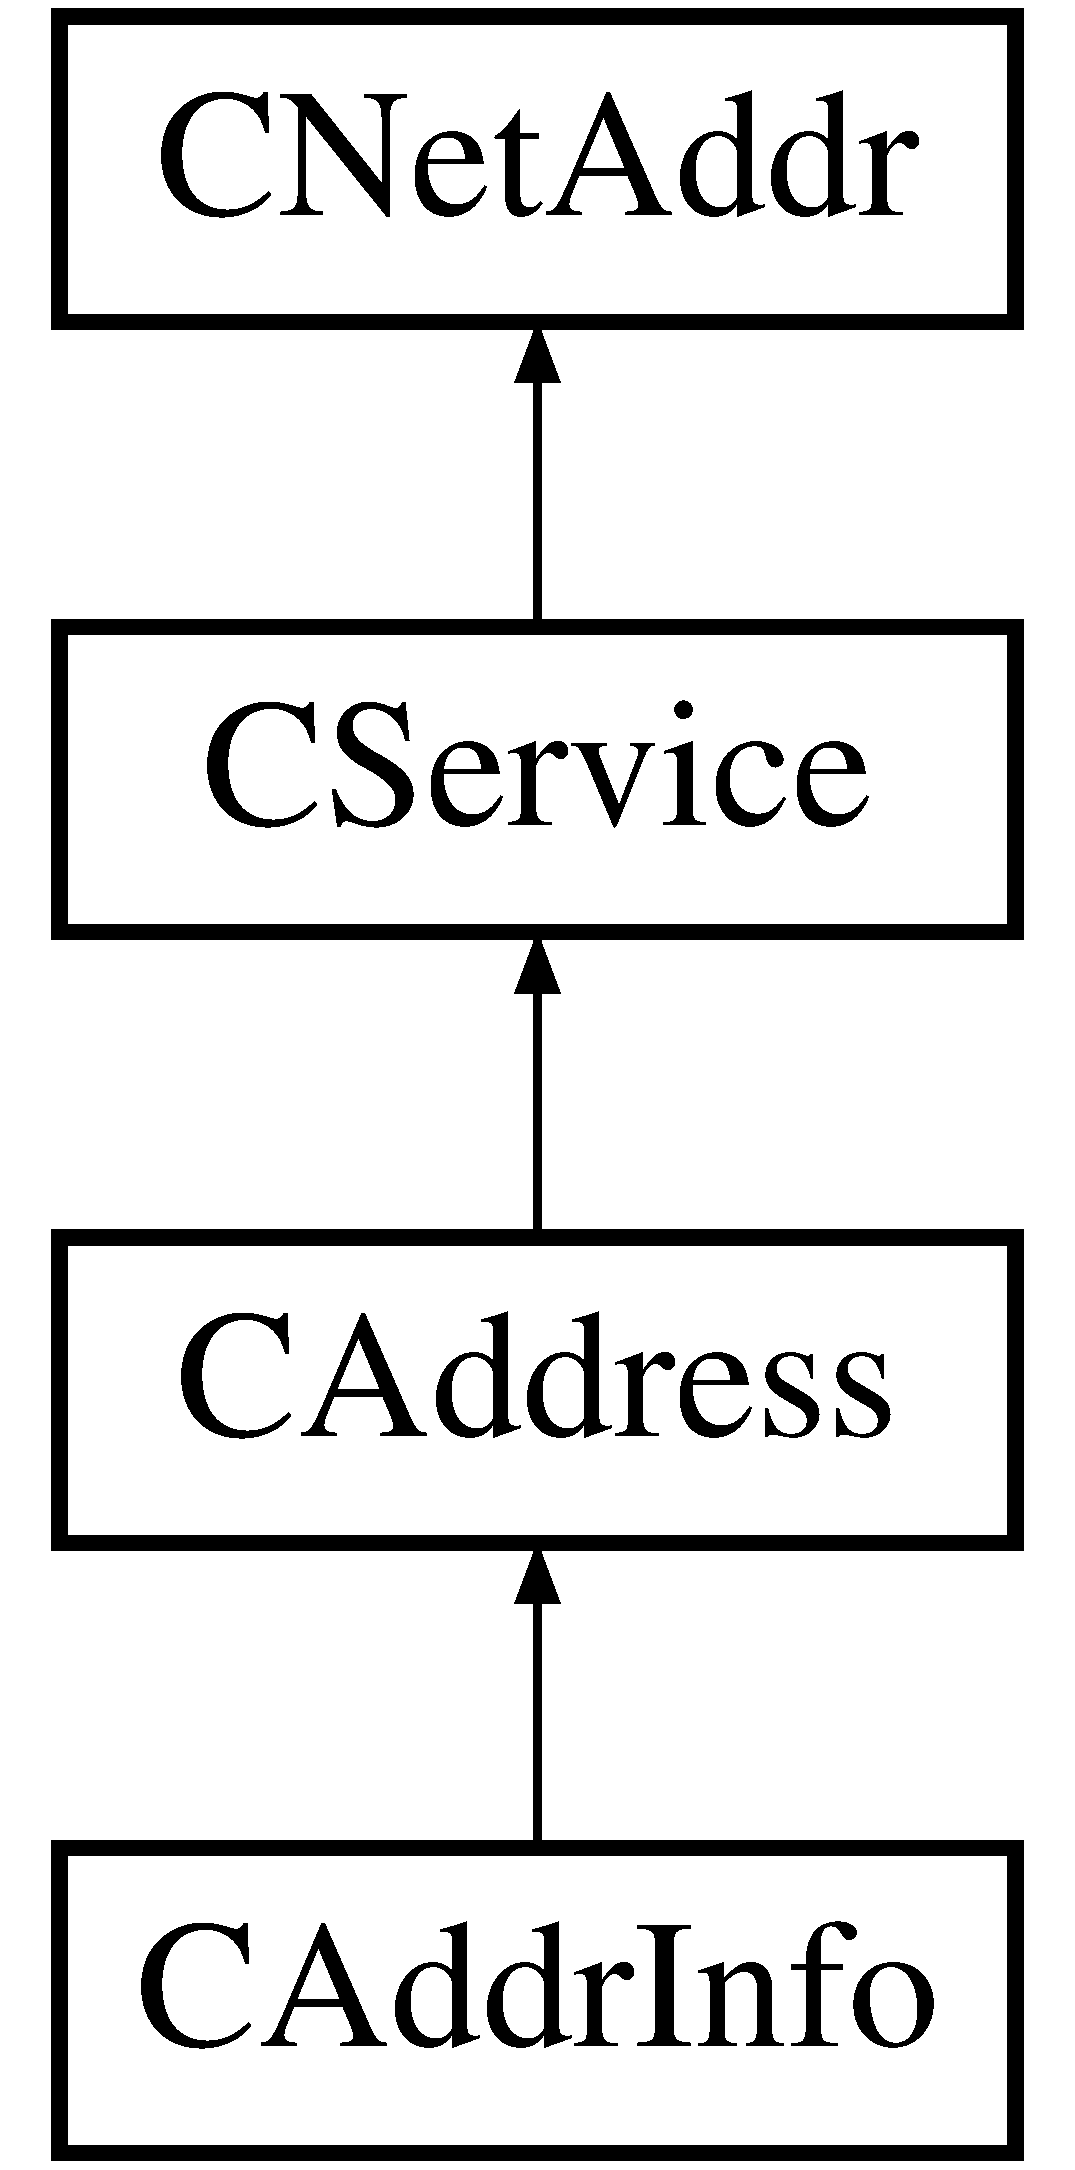
\includegraphics[height=4.000000cm]{class_c_net_addr}
\end{center}
\end{figure}
\subsection*{Public Member Functions}
\begin{DoxyCompactItemize}
\item 
\mbox{\hyperlink{class_c_net_addr_ad997a7ab057fbeab1dd6601135f8e02d}{C\+Net\+Addr}} ()
\item 
\mbox{\hyperlink{class_c_net_addr_a0af492cd8aca9bbaa3392cdbfbb55681}{C\+Net\+Addr}} (const struct in\+\_\+addr \&ipv4\+Addr)
\item 
\mbox{\hyperlink{class_c_net_addr_a3549332f92d95ccadf262bdce9f4eacf}{C\+Net\+Addr}} (const char $\ast$psz\+Ip, bool f\+Allow\+Lookup=false)
\item 
\mbox{\hyperlink{class_c_net_addr_ae237602be0e4bce6ff31061270371144}{C\+Net\+Addr}} (const std\+::string \&str\+Ip, bool f\+Allow\+Lookup=false)
\item 
void \mbox{\hyperlink{class_c_net_addr_adab412fbc5a9203bea90ae173996ab10}{Init}} ()
\item 
void \mbox{\hyperlink{class_c_net_addr_a1c6087345e5ca07a151451cd6deb974f}{Set\+IP}} (const \mbox{\hyperlink{class_c_net_addr}{C\+Net\+Addr}} \&\mbox{\hyperlink{class_c_net_addr_acff7ce68f33f8dfbfe6d79d80928d417}{ip}})
\item 
void \mbox{\hyperlink{class_c_net_addr_a1f0b23aca4ca78c11735d13f3583b7ad}{Set\+Raw}} (\mbox{\hyperlink{netbase_8h_acc9a38c714afe79b5035cb36f560dac3}{Network}} network, const uint8\+\_\+t $\ast$data)
\item 
bool \mbox{\hyperlink{class_c_net_addr_aa3e44dfd064d9d8da1cb48cdcb7dd231}{Set\+Special}} (const std\+::string \&str\+Name)
\item 
bool \mbox{\hyperlink{class_c_net_addr_a7021b79e9a33c342b68db09dbb6c2293}{Is\+I\+Pv4}} () const
\item 
bool \mbox{\hyperlink{class_c_net_addr_aad5f7a372c56ccf4d773f728b6b46e18}{Is\+I\+Pv6}} () const
\item 
bool \mbox{\hyperlink{class_c_net_addr_a6c6d7376d8d0ae4c7cb0893add58069f}{Is\+R\+F\+C1918}} () const
\item 
bool \mbox{\hyperlink{class_c_net_addr_acd1138ebc48eb28055a49e5ffe8ebc31}{Is\+R\+F\+C2544}} () const
\item 
bool \mbox{\hyperlink{class_c_net_addr_a6a9595f10a7cb4518d9d577075eee57f}{Is\+R\+F\+C6598}} () const
\item 
bool \mbox{\hyperlink{class_c_net_addr_a5a3b09eb486dede48cb9427a9a0ed2e2}{Is\+R\+F\+C5737}} () const
\item 
bool \mbox{\hyperlink{class_c_net_addr_a7bf8bc283323c0cd9be42f921469c90f}{Is\+R\+F\+C3849}} () const
\item 
bool \mbox{\hyperlink{class_c_net_addr_af75408b0ae05d1e7d3931b80b65a70c4}{Is\+R\+F\+C3927}} () const
\item 
bool \mbox{\hyperlink{class_c_net_addr_ae0fcf758a607567f06cb966426289cd6}{Is\+R\+F\+C3964}} () const
\item 
bool \mbox{\hyperlink{class_c_net_addr_ac2eb12a3f11d9f54fa7c5072bf065d1c}{Is\+R\+F\+C4193}} () const
\item 
bool \mbox{\hyperlink{class_c_net_addr_aec91b10228b37eb9bd67dec322730492}{Is\+R\+F\+C4380}} () const
\item 
bool \mbox{\hyperlink{class_c_net_addr_af9286890842869ccc5f6fb82ce316ede}{Is\+R\+F\+C4843}} () const
\item 
bool \mbox{\hyperlink{class_c_net_addr_af8e0bb6b81be814e528143471b2fb482}{Is\+R\+F\+C4862}} () const
\item 
bool \mbox{\hyperlink{class_c_net_addr_a15b47f1fa3ded708f0e02e842482ee60}{Is\+R\+F\+C6052}} () const
\item 
bool \mbox{\hyperlink{class_c_net_addr_ad134823c7f268f29653d135d33f879aa}{Is\+R\+F\+C6145}} () const
\item 
bool \mbox{\hyperlink{class_c_net_addr_a4db37b4997ff3b8c57959f2aa915a9a3}{Is\+Tor}} () const
\item 
bool \mbox{\hyperlink{class_c_net_addr_a857bfcf95814b7d6ef4db309c84f179d}{Is\+Local}} () const
\item 
bool \mbox{\hyperlink{class_c_net_addr_a4e3b2fea2a6151c76684b3812df4a5c3}{Is\+Routable}} () const
\item 
bool \mbox{\hyperlink{class_c_net_addr_a6fe20b8da9701ca5dc2af078e2e8ac25}{Is\+Valid}} () const
\item 
bool \mbox{\hyperlink{class_c_net_addr_aabd54a329f70953f7895b56bcd000473}{Is\+Multicast}} () const
\item 
enum \mbox{\hyperlink{netbase_8h_acc9a38c714afe79b5035cb36f560dac3}{Network}} \mbox{\hyperlink{class_c_net_addr_ad0162f2629f552a65acf934e1629c1db}{Get\+Network}} () const
\item 
std\+::string \mbox{\hyperlink{class_c_net_addr_a474ea3874554fe3b79f607fdef97c243}{To\+String}} () const
\item 
std\+::string \mbox{\hyperlink{class_c_net_addr_a0c8d9b5ed3824546ff4dccca3b28b073}{To\+String\+IP}} () const
\item 
unsigned int \mbox{\hyperlink{class_c_net_addr_acfd51ebf2030b01fa5ac133176512475}{Get\+Byte}} (int n) const
\item 
uint64\+\_\+t \mbox{\hyperlink{class_c_net_addr_a8fae7d32e83e9fbb9ce0216f896133c9}{Get\+Hash}} () const
\item 
bool \mbox{\hyperlink{class_c_net_addr_a4f73432c55d4acb6b9e4c54833eefea6}{Get\+In\+Addr}} (struct in\+\_\+addr $\ast$pipv4\+Addr) const
\item 
std\+::vector$<$ unsigned char $>$ \mbox{\hyperlink{class_c_net_addr_a6f8211515f809f6972ce327433d41458}{Get\+Group}} () const
\item 
int \mbox{\hyperlink{class_c_net_addr_aa68c7d6112b22759dcd280ddad30808f}{Get\+Reachability\+From}} (const \mbox{\hyperlink{class_c_net_addr}{C\+Net\+Addr}} $\ast$paddr\+Partner=N\+U\+LL) const
\item 
\mbox{\hyperlink{class_c_net_addr_a9eae4232457f7659a157467274d1b444}{C\+Net\+Addr}} (const struct in6\+\_\+addr \&pipv6\+Addr)
\item 
bool \mbox{\hyperlink{class_c_net_addr_a3616012f94b27148e5b8e27d943d4884}{Get\+In6\+Addr}} (struct in6\+\_\+addr $\ast$pipv6\+Addr) const
\item 
{\footnotesize template$<$typename Stream , typename Operation $>$ }\\void \mbox{\hyperlink{class_c_net_addr_a7c914d155a533f64f8aa0d2f9bfff8a7}{Serialization\+Op}} (Stream \&s, Operation ser\+\_\+action, int n\+Type, int n\+Version)
\end{DoxyCompactItemize}
\subsection*{Public Attributes}
\begin{DoxyCompactItemize}
\item 
\mbox{\hyperlink{class_c_net_addr_ab08e22719f96b42c61e998158a895e5f}{A\+D\+D\+\_\+\+S\+E\+R\+I\+A\+L\+I\+Z\+E\+\_\+\+M\+E\+T\+H\+O\+DS}}
\end{DoxyCompactItemize}
\subsection*{Protected Attributes}
\begin{DoxyCompactItemize}
\item 
unsigned char \mbox{\hyperlink{class_c_net_addr_acff7ce68f33f8dfbfe6d79d80928d417}{ip}} \mbox{[}16\mbox{]}
\end{DoxyCompactItemize}
\subsection*{Friends}
\begin{DoxyCompactItemize}
\item 
class \mbox{\hyperlink{class_c_net_addr_a1c694dd7d8a349bd3a1816a2634d7d2a}{C\+Sub\+Net}}
\item 
bool \mbox{\hyperlink{class_c_net_addr_a6cc88956853ab8dc9586d55cda059934}{operator==}} (const \mbox{\hyperlink{class_c_net_addr}{C\+Net\+Addr}} \&a, const \mbox{\hyperlink{class_c_net_addr}{C\+Net\+Addr}} \&b)
\item 
bool \mbox{\hyperlink{class_c_net_addr_ac361eb83c41464359dfb1dfc296c3a4c}{operator!=}} (const \mbox{\hyperlink{class_c_net_addr}{C\+Net\+Addr}} \&a, const \mbox{\hyperlink{class_c_net_addr}{C\+Net\+Addr}} \&b)
\item 
bool \mbox{\hyperlink{class_c_net_addr_af220590d55a24354e2ba2e547e34fd77}{operator$<$}} (const \mbox{\hyperlink{class_c_net_addr}{C\+Net\+Addr}} \&a, const \mbox{\hyperlink{class_c_net_addr}{C\+Net\+Addr}} \&b)
\end{DoxyCompactItemize}


\subsection{Detailed Description}
IP address (I\+Pv6, or I\+Pv4 using mapped I\+Pv6 range (\+::\+F\+F\+FF\+:0\+:0/96)) 

\subsection{Constructor \& Destructor Documentation}
\mbox{\Hypertarget{class_c_net_addr_ad997a7ab057fbeab1dd6601135f8e02d}\label{class_c_net_addr_ad997a7ab057fbeab1dd6601135f8e02d}} 
\index{C\+Net\+Addr@{C\+Net\+Addr}!C\+Net\+Addr@{C\+Net\+Addr}}
\index{C\+Net\+Addr@{C\+Net\+Addr}!C\+Net\+Addr@{C\+Net\+Addr}}
\subsubsection{\texorpdfstring{C\+Net\+Addr()}{CNetAddr()}\hspace{0.1cm}{\footnotesize\ttfamily [1/5]}}
{\footnotesize\ttfamily C\+Net\+Addr\+::\+C\+Net\+Addr (\begin{DoxyParamCaption}{ }\end{DoxyParamCaption})}

\mbox{\Hypertarget{class_c_net_addr_a0af492cd8aca9bbaa3392cdbfbb55681}\label{class_c_net_addr_a0af492cd8aca9bbaa3392cdbfbb55681}} 
\index{C\+Net\+Addr@{C\+Net\+Addr}!C\+Net\+Addr@{C\+Net\+Addr}}
\index{C\+Net\+Addr@{C\+Net\+Addr}!C\+Net\+Addr@{C\+Net\+Addr}}
\subsubsection{\texorpdfstring{C\+Net\+Addr()}{CNetAddr()}\hspace{0.1cm}{\footnotesize\ttfamily [2/5]}}
{\footnotesize\ttfamily C\+Net\+Addr\+::\+C\+Net\+Addr (\begin{DoxyParamCaption}\item[{const struct in\+\_\+addr \&}]{ipv4\+Addr }\end{DoxyParamCaption})}

\mbox{\Hypertarget{class_c_net_addr_a3549332f92d95ccadf262bdce9f4eacf}\label{class_c_net_addr_a3549332f92d95ccadf262bdce9f4eacf}} 
\index{C\+Net\+Addr@{C\+Net\+Addr}!C\+Net\+Addr@{C\+Net\+Addr}}
\index{C\+Net\+Addr@{C\+Net\+Addr}!C\+Net\+Addr@{C\+Net\+Addr}}
\subsubsection{\texorpdfstring{C\+Net\+Addr()}{CNetAddr()}\hspace{0.1cm}{\footnotesize\ttfamily [3/5]}}
{\footnotesize\ttfamily C\+Net\+Addr\+::\+C\+Net\+Addr (\begin{DoxyParamCaption}\item[{const char $\ast$}]{psz\+Ip,  }\item[{bool}]{f\+Allow\+Lookup = {\ttfamily false} }\end{DoxyParamCaption})\hspace{0.3cm}{\ttfamily [explicit]}}

\mbox{\Hypertarget{class_c_net_addr_ae237602be0e4bce6ff31061270371144}\label{class_c_net_addr_ae237602be0e4bce6ff31061270371144}} 
\index{C\+Net\+Addr@{C\+Net\+Addr}!C\+Net\+Addr@{C\+Net\+Addr}}
\index{C\+Net\+Addr@{C\+Net\+Addr}!C\+Net\+Addr@{C\+Net\+Addr}}
\subsubsection{\texorpdfstring{C\+Net\+Addr()}{CNetAddr()}\hspace{0.1cm}{\footnotesize\ttfamily [4/5]}}
{\footnotesize\ttfamily C\+Net\+Addr\+::\+C\+Net\+Addr (\begin{DoxyParamCaption}\item[{const std\+::string \&}]{str\+Ip,  }\item[{bool}]{f\+Allow\+Lookup = {\ttfamily false} }\end{DoxyParamCaption})\hspace{0.3cm}{\ttfamily [explicit]}}

\mbox{\Hypertarget{class_c_net_addr_a9eae4232457f7659a157467274d1b444}\label{class_c_net_addr_a9eae4232457f7659a157467274d1b444}} 
\index{C\+Net\+Addr@{C\+Net\+Addr}!C\+Net\+Addr@{C\+Net\+Addr}}
\index{C\+Net\+Addr@{C\+Net\+Addr}!C\+Net\+Addr@{C\+Net\+Addr}}
\subsubsection{\texorpdfstring{C\+Net\+Addr()}{CNetAddr()}\hspace{0.1cm}{\footnotesize\ttfamily [5/5]}}
{\footnotesize\ttfamily C\+Net\+Addr\+::\+C\+Net\+Addr (\begin{DoxyParamCaption}\item[{const struct in6\+\_\+addr \&}]{pipv6\+Addr }\end{DoxyParamCaption})}



\subsection{Member Function Documentation}
\mbox{\Hypertarget{class_c_net_addr_acfd51ebf2030b01fa5ac133176512475}\label{class_c_net_addr_acfd51ebf2030b01fa5ac133176512475}} 
\index{C\+Net\+Addr@{C\+Net\+Addr}!Get\+Byte@{Get\+Byte}}
\index{Get\+Byte@{Get\+Byte}!C\+Net\+Addr@{C\+Net\+Addr}}
\subsubsection{\texorpdfstring{Get\+Byte()}{GetByte()}}
{\footnotesize\ttfamily unsigned int C\+Net\+Addr\+::\+Get\+Byte (\begin{DoxyParamCaption}\item[{int}]{n }\end{DoxyParamCaption}) const}

\mbox{\Hypertarget{class_c_net_addr_a6f8211515f809f6972ce327433d41458}\label{class_c_net_addr_a6f8211515f809f6972ce327433d41458}} 
\index{C\+Net\+Addr@{C\+Net\+Addr}!Get\+Group@{Get\+Group}}
\index{Get\+Group@{Get\+Group}!C\+Net\+Addr@{C\+Net\+Addr}}
\subsubsection{\texorpdfstring{Get\+Group()}{GetGroup()}}
{\footnotesize\ttfamily std\+::vector$<$ unsigned char $>$ C\+Net\+Addr\+::\+Get\+Group (\begin{DoxyParamCaption}{ }\end{DoxyParamCaption}) const}

\mbox{\Hypertarget{class_c_net_addr_a8fae7d32e83e9fbb9ce0216f896133c9}\label{class_c_net_addr_a8fae7d32e83e9fbb9ce0216f896133c9}} 
\index{C\+Net\+Addr@{C\+Net\+Addr}!Get\+Hash@{Get\+Hash}}
\index{Get\+Hash@{Get\+Hash}!C\+Net\+Addr@{C\+Net\+Addr}}
\subsubsection{\texorpdfstring{Get\+Hash()}{GetHash()}}
{\footnotesize\ttfamily uint64\+\_\+t C\+Net\+Addr\+::\+Get\+Hash (\begin{DoxyParamCaption}{ }\end{DoxyParamCaption}) const}

\mbox{\Hypertarget{class_c_net_addr_a3616012f94b27148e5b8e27d943d4884}\label{class_c_net_addr_a3616012f94b27148e5b8e27d943d4884}} 
\index{C\+Net\+Addr@{C\+Net\+Addr}!Get\+In6\+Addr@{Get\+In6\+Addr}}
\index{Get\+In6\+Addr@{Get\+In6\+Addr}!C\+Net\+Addr@{C\+Net\+Addr}}
\subsubsection{\texorpdfstring{Get\+In6\+Addr()}{GetIn6Addr()}}
{\footnotesize\ttfamily bool C\+Net\+Addr\+::\+Get\+In6\+Addr (\begin{DoxyParamCaption}\item[{struct in6\+\_\+addr $\ast$}]{pipv6\+Addr }\end{DoxyParamCaption}) const}

\mbox{\Hypertarget{class_c_net_addr_a4f73432c55d4acb6b9e4c54833eefea6}\label{class_c_net_addr_a4f73432c55d4acb6b9e4c54833eefea6}} 
\index{C\+Net\+Addr@{C\+Net\+Addr}!Get\+In\+Addr@{Get\+In\+Addr}}
\index{Get\+In\+Addr@{Get\+In\+Addr}!C\+Net\+Addr@{C\+Net\+Addr}}
\subsubsection{\texorpdfstring{Get\+In\+Addr()}{GetInAddr()}}
{\footnotesize\ttfamily bool C\+Net\+Addr\+::\+Get\+In\+Addr (\begin{DoxyParamCaption}\item[{struct in\+\_\+addr $\ast$}]{pipv4\+Addr }\end{DoxyParamCaption}) const}

\mbox{\Hypertarget{class_c_net_addr_ad0162f2629f552a65acf934e1629c1db}\label{class_c_net_addr_ad0162f2629f552a65acf934e1629c1db}} 
\index{C\+Net\+Addr@{C\+Net\+Addr}!Get\+Network@{Get\+Network}}
\index{Get\+Network@{Get\+Network}!C\+Net\+Addr@{C\+Net\+Addr}}
\subsubsection{\texorpdfstring{Get\+Network()}{GetNetwork()}}
{\footnotesize\ttfamily enum \mbox{\hyperlink{netbase_8h_acc9a38c714afe79b5035cb36f560dac3}{Network}} C\+Net\+Addr\+::\+Get\+Network (\begin{DoxyParamCaption}{ }\end{DoxyParamCaption}) const}

\mbox{\Hypertarget{class_c_net_addr_aa68c7d6112b22759dcd280ddad30808f}\label{class_c_net_addr_aa68c7d6112b22759dcd280ddad30808f}} 
\index{C\+Net\+Addr@{C\+Net\+Addr}!Get\+Reachability\+From@{Get\+Reachability\+From}}
\index{Get\+Reachability\+From@{Get\+Reachability\+From}!C\+Net\+Addr@{C\+Net\+Addr}}
\subsubsection{\texorpdfstring{Get\+Reachability\+From()}{GetReachabilityFrom()}}
{\footnotesize\ttfamily int C\+Net\+Addr\+::\+Get\+Reachability\+From (\begin{DoxyParamCaption}\item[{const \mbox{\hyperlink{class_c_net_addr}{C\+Net\+Addr}} $\ast$}]{paddr\+Partner = {\ttfamily NULL} }\end{DoxyParamCaption}) const}

Calculates a metric for how reachable ($\ast$this) is from a given partner \mbox{\Hypertarget{class_c_net_addr_adab412fbc5a9203bea90ae173996ab10}\label{class_c_net_addr_adab412fbc5a9203bea90ae173996ab10}} 
\index{C\+Net\+Addr@{C\+Net\+Addr}!Init@{Init}}
\index{Init@{Init}!C\+Net\+Addr@{C\+Net\+Addr}}
\subsubsection{\texorpdfstring{Init()}{Init()}}
{\footnotesize\ttfamily void C\+Net\+Addr\+::\+Init (\begin{DoxyParamCaption}{ }\end{DoxyParamCaption})}

\mbox{\Hypertarget{class_c_net_addr_a7021b79e9a33c342b68db09dbb6c2293}\label{class_c_net_addr_a7021b79e9a33c342b68db09dbb6c2293}} 
\index{C\+Net\+Addr@{C\+Net\+Addr}!Is\+I\+Pv4@{Is\+I\+Pv4}}
\index{Is\+I\+Pv4@{Is\+I\+Pv4}!C\+Net\+Addr@{C\+Net\+Addr}}
\subsubsection{\texorpdfstring{Is\+I\+Pv4()}{IsIPv4()}}
{\footnotesize\ttfamily bool C\+Net\+Addr\+::\+Is\+I\+Pv4 (\begin{DoxyParamCaption}{ }\end{DoxyParamCaption}) const}

\mbox{\Hypertarget{class_c_net_addr_aad5f7a372c56ccf4d773f728b6b46e18}\label{class_c_net_addr_aad5f7a372c56ccf4d773f728b6b46e18}} 
\index{C\+Net\+Addr@{C\+Net\+Addr}!Is\+I\+Pv6@{Is\+I\+Pv6}}
\index{Is\+I\+Pv6@{Is\+I\+Pv6}!C\+Net\+Addr@{C\+Net\+Addr}}
\subsubsection{\texorpdfstring{Is\+I\+Pv6()}{IsIPv6()}}
{\footnotesize\ttfamily bool C\+Net\+Addr\+::\+Is\+I\+Pv6 (\begin{DoxyParamCaption}{ }\end{DoxyParamCaption}) const}

\mbox{\Hypertarget{class_c_net_addr_a857bfcf95814b7d6ef4db309c84f179d}\label{class_c_net_addr_a857bfcf95814b7d6ef4db309c84f179d}} 
\index{C\+Net\+Addr@{C\+Net\+Addr}!Is\+Local@{Is\+Local}}
\index{Is\+Local@{Is\+Local}!C\+Net\+Addr@{C\+Net\+Addr}}
\subsubsection{\texorpdfstring{Is\+Local()}{IsLocal()}}
{\footnotesize\ttfamily bool C\+Net\+Addr\+::\+Is\+Local (\begin{DoxyParamCaption}{ }\end{DoxyParamCaption}) const}

\mbox{\Hypertarget{class_c_net_addr_aabd54a329f70953f7895b56bcd000473}\label{class_c_net_addr_aabd54a329f70953f7895b56bcd000473}} 
\index{C\+Net\+Addr@{C\+Net\+Addr}!Is\+Multicast@{Is\+Multicast}}
\index{Is\+Multicast@{Is\+Multicast}!C\+Net\+Addr@{C\+Net\+Addr}}
\subsubsection{\texorpdfstring{Is\+Multicast()}{IsMulticast()}}
{\footnotesize\ttfamily bool C\+Net\+Addr\+::\+Is\+Multicast (\begin{DoxyParamCaption}{ }\end{DoxyParamCaption}) const}

\mbox{\Hypertarget{class_c_net_addr_a6c6d7376d8d0ae4c7cb0893add58069f}\label{class_c_net_addr_a6c6d7376d8d0ae4c7cb0893add58069f}} 
\index{C\+Net\+Addr@{C\+Net\+Addr}!Is\+R\+F\+C1918@{Is\+R\+F\+C1918}}
\index{Is\+R\+F\+C1918@{Is\+R\+F\+C1918}!C\+Net\+Addr@{C\+Net\+Addr}}
\subsubsection{\texorpdfstring{Is\+R\+F\+C1918()}{IsRFC1918()}}
{\footnotesize\ttfamily bool C\+Net\+Addr\+::\+Is\+R\+F\+C1918 (\begin{DoxyParamCaption}{ }\end{DoxyParamCaption}) const}

\mbox{\Hypertarget{class_c_net_addr_acd1138ebc48eb28055a49e5ffe8ebc31}\label{class_c_net_addr_acd1138ebc48eb28055a49e5ffe8ebc31}} 
\index{C\+Net\+Addr@{C\+Net\+Addr}!Is\+R\+F\+C2544@{Is\+R\+F\+C2544}}
\index{Is\+R\+F\+C2544@{Is\+R\+F\+C2544}!C\+Net\+Addr@{C\+Net\+Addr}}
\subsubsection{\texorpdfstring{Is\+R\+F\+C2544()}{IsRFC2544()}}
{\footnotesize\ttfamily bool C\+Net\+Addr\+::\+Is\+R\+F\+C2544 (\begin{DoxyParamCaption}{ }\end{DoxyParamCaption}) const}

\mbox{\Hypertarget{class_c_net_addr_a7bf8bc283323c0cd9be42f921469c90f}\label{class_c_net_addr_a7bf8bc283323c0cd9be42f921469c90f}} 
\index{C\+Net\+Addr@{C\+Net\+Addr}!Is\+R\+F\+C3849@{Is\+R\+F\+C3849}}
\index{Is\+R\+F\+C3849@{Is\+R\+F\+C3849}!C\+Net\+Addr@{C\+Net\+Addr}}
\subsubsection{\texorpdfstring{Is\+R\+F\+C3849()}{IsRFC3849()}}
{\footnotesize\ttfamily bool C\+Net\+Addr\+::\+Is\+R\+F\+C3849 (\begin{DoxyParamCaption}{ }\end{DoxyParamCaption}) const}

\mbox{\Hypertarget{class_c_net_addr_af75408b0ae05d1e7d3931b80b65a70c4}\label{class_c_net_addr_af75408b0ae05d1e7d3931b80b65a70c4}} 
\index{C\+Net\+Addr@{C\+Net\+Addr}!Is\+R\+F\+C3927@{Is\+R\+F\+C3927}}
\index{Is\+R\+F\+C3927@{Is\+R\+F\+C3927}!C\+Net\+Addr@{C\+Net\+Addr}}
\subsubsection{\texorpdfstring{Is\+R\+F\+C3927()}{IsRFC3927()}}
{\footnotesize\ttfamily bool C\+Net\+Addr\+::\+Is\+R\+F\+C3927 (\begin{DoxyParamCaption}{ }\end{DoxyParamCaption}) const}

\mbox{\Hypertarget{class_c_net_addr_ae0fcf758a607567f06cb966426289cd6}\label{class_c_net_addr_ae0fcf758a607567f06cb966426289cd6}} 
\index{C\+Net\+Addr@{C\+Net\+Addr}!Is\+R\+F\+C3964@{Is\+R\+F\+C3964}}
\index{Is\+R\+F\+C3964@{Is\+R\+F\+C3964}!C\+Net\+Addr@{C\+Net\+Addr}}
\subsubsection{\texorpdfstring{Is\+R\+F\+C3964()}{IsRFC3964()}}
{\footnotesize\ttfamily bool C\+Net\+Addr\+::\+Is\+R\+F\+C3964 (\begin{DoxyParamCaption}{ }\end{DoxyParamCaption}) const}

\mbox{\Hypertarget{class_c_net_addr_ac2eb12a3f11d9f54fa7c5072bf065d1c}\label{class_c_net_addr_ac2eb12a3f11d9f54fa7c5072bf065d1c}} 
\index{C\+Net\+Addr@{C\+Net\+Addr}!Is\+R\+F\+C4193@{Is\+R\+F\+C4193}}
\index{Is\+R\+F\+C4193@{Is\+R\+F\+C4193}!C\+Net\+Addr@{C\+Net\+Addr}}
\subsubsection{\texorpdfstring{Is\+R\+F\+C4193()}{IsRFC4193()}}
{\footnotesize\ttfamily bool C\+Net\+Addr\+::\+Is\+R\+F\+C4193 (\begin{DoxyParamCaption}{ }\end{DoxyParamCaption}) const}

\mbox{\Hypertarget{class_c_net_addr_aec91b10228b37eb9bd67dec322730492}\label{class_c_net_addr_aec91b10228b37eb9bd67dec322730492}} 
\index{C\+Net\+Addr@{C\+Net\+Addr}!Is\+R\+F\+C4380@{Is\+R\+F\+C4380}}
\index{Is\+R\+F\+C4380@{Is\+R\+F\+C4380}!C\+Net\+Addr@{C\+Net\+Addr}}
\subsubsection{\texorpdfstring{Is\+R\+F\+C4380()}{IsRFC4380()}}
{\footnotesize\ttfamily bool C\+Net\+Addr\+::\+Is\+R\+F\+C4380 (\begin{DoxyParamCaption}{ }\end{DoxyParamCaption}) const}

\mbox{\Hypertarget{class_c_net_addr_af9286890842869ccc5f6fb82ce316ede}\label{class_c_net_addr_af9286890842869ccc5f6fb82ce316ede}} 
\index{C\+Net\+Addr@{C\+Net\+Addr}!Is\+R\+F\+C4843@{Is\+R\+F\+C4843}}
\index{Is\+R\+F\+C4843@{Is\+R\+F\+C4843}!C\+Net\+Addr@{C\+Net\+Addr}}
\subsubsection{\texorpdfstring{Is\+R\+F\+C4843()}{IsRFC4843()}}
{\footnotesize\ttfamily bool C\+Net\+Addr\+::\+Is\+R\+F\+C4843 (\begin{DoxyParamCaption}{ }\end{DoxyParamCaption}) const}

\mbox{\Hypertarget{class_c_net_addr_af8e0bb6b81be814e528143471b2fb482}\label{class_c_net_addr_af8e0bb6b81be814e528143471b2fb482}} 
\index{C\+Net\+Addr@{C\+Net\+Addr}!Is\+R\+F\+C4862@{Is\+R\+F\+C4862}}
\index{Is\+R\+F\+C4862@{Is\+R\+F\+C4862}!C\+Net\+Addr@{C\+Net\+Addr}}
\subsubsection{\texorpdfstring{Is\+R\+F\+C4862()}{IsRFC4862()}}
{\footnotesize\ttfamily bool C\+Net\+Addr\+::\+Is\+R\+F\+C4862 (\begin{DoxyParamCaption}{ }\end{DoxyParamCaption}) const}

\mbox{\Hypertarget{class_c_net_addr_a5a3b09eb486dede48cb9427a9a0ed2e2}\label{class_c_net_addr_a5a3b09eb486dede48cb9427a9a0ed2e2}} 
\index{C\+Net\+Addr@{C\+Net\+Addr}!Is\+R\+F\+C5737@{Is\+R\+F\+C5737}}
\index{Is\+R\+F\+C5737@{Is\+R\+F\+C5737}!C\+Net\+Addr@{C\+Net\+Addr}}
\subsubsection{\texorpdfstring{Is\+R\+F\+C5737()}{IsRFC5737()}}
{\footnotesize\ttfamily bool C\+Net\+Addr\+::\+Is\+R\+F\+C5737 (\begin{DoxyParamCaption}{ }\end{DoxyParamCaption}) const}

\mbox{\Hypertarget{class_c_net_addr_a15b47f1fa3ded708f0e02e842482ee60}\label{class_c_net_addr_a15b47f1fa3ded708f0e02e842482ee60}} 
\index{C\+Net\+Addr@{C\+Net\+Addr}!Is\+R\+F\+C6052@{Is\+R\+F\+C6052}}
\index{Is\+R\+F\+C6052@{Is\+R\+F\+C6052}!C\+Net\+Addr@{C\+Net\+Addr}}
\subsubsection{\texorpdfstring{Is\+R\+F\+C6052()}{IsRFC6052()}}
{\footnotesize\ttfamily bool C\+Net\+Addr\+::\+Is\+R\+F\+C6052 (\begin{DoxyParamCaption}{ }\end{DoxyParamCaption}) const}

\mbox{\Hypertarget{class_c_net_addr_ad134823c7f268f29653d135d33f879aa}\label{class_c_net_addr_ad134823c7f268f29653d135d33f879aa}} 
\index{C\+Net\+Addr@{C\+Net\+Addr}!Is\+R\+F\+C6145@{Is\+R\+F\+C6145}}
\index{Is\+R\+F\+C6145@{Is\+R\+F\+C6145}!C\+Net\+Addr@{C\+Net\+Addr}}
\subsubsection{\texorpdfstring{Is\+R\+F\+C6145()}{IsRFC6145()}}
{\footnotesize\ttfamily bool C\+Net\+Addr\+::\+Is\+R\+F\+C6145 (\begin{DoxyParamCaption}{ }\end{DoxyParamCaption}) const}

\mbox{\Hypertarget{class_c_net_addr_a6a9595f10a7cb4518d9d577075eee57f}\label{class_c_net_addr_a6a9595f10a7cb4518d9d577075eee57f}} 
\index{C\+Net\+Addr@{C\+Net\+Addr}!Is\+R\+F\+C6598@{Is\+R\+F\+C6598}}
\index{Is\+R\+F\+C6598@{Is\+R\+F\+C6598}!C\+Net\+Addr@{C\+Net\+Addr}}
\subsubsection{\texorpdfstring{Is\+R\+F\+C6598()}{IsRFC6598()}}
{\footnotesize\ttfamily bool C\+Net\+Addr\+::\+Is\+R\+F\+C6598 (\begin{DoxyParamCaption}{ }\end{DoxyParamCaption}) const}

\mbox{\Hypertarget{class_c_net_addr_a4e3b2fea2a6151c76684b3812df4a5c3}\label{class_c_net_addr_a4e3b2fea2a6151c76684b3812df4a5c3}} 
\index{C\+Net\+Addr@{C\+Net\+Addr}!Is\+Routable@{Is\+Routable}}
\index{Is\+Routable@{Is\+Routable}!C\+Net\+Addr@{C\+Net\+Addr}}
\subsubsection{\texorpdfstring{Is\+Routable()}{IsRoutable()}}
{\footnotesize\ttfamily bool C\+Net\+Addr\+::\+Is\+Routable (\begin{DoxyParamCaption}{ }\end{DoxyParamCaption}) const}

\mbox{\Hypertarget{class_c_net_addr_a4db37b4997ff3b8c57959f2aa915a9a3}\label{class_c_net_addr_a4db37b4997ff3b8c57959f2aa915a9a3}} 
\index{C\+Net\+Addr@{C\+Net\+Addr}!Is\+Tor@{Is\+Tor}}
\index{Is\+Tor@{Is\+Tor}!C\+Net\+Addr@{C\+Net\+Addr}}
\subsubsection{\texorpdfstring{Is\+Tor()}{IsTor()}}
{\footnotesize\ttfamily bool C\+Net\+Addr\+::\+Is\+Tor (\begin{DoxyParamCaption}{ }\end{DoxyParamCaption}) const}

\mbox{\Hypertarget{class_c_net_addr_a6fe20b8da9701ca5dc2af078e2e8ac25}\label{class_c_net_addr_a6fe20b8da9701ca5dc2af078e2e8ac25}} 
\index{C\+Net\+Addr@{C\+Net\+Addr}!Is\+Valid@{Is\+Valid}}
\index{Is\+Valid@{Is\+Valid}!C\+Net\+Addr@{C\+Net\+Addr}}
\subsubsection{\texorpdfstring{Is\+Valid()}{IsValid()}}
{\footnotesize\ttfamily bool C\+Net\+Addr\+::\+Is\+Valid (\begin{DoxyParamCaption}{ }\end{DoxyParamCaption}) const}

\mbox{\Hypertarget{class_c_net_addr_a7c914d155a533f64f8aa0d2f9bfff8a7}\label{class_c_net_addr_a7c914d155a533f64f8aa0d2f9bfff8a7}} 
\index{C\+Net\+Addr@{C\+Net\+Addr}!Serialization\+Op@{Serialization\+Op}}
\index{Serialization\+Op@{Serialization\+Op}!C\+Net\+Addr@{C\+Net\+Addr}}
\subsubsection{\texorpdfstring{Serialization\+Op()}{SerializationOp()}}
{\footnotesize\ttfamily template$<$typename Stream , typename Operation $>$ \\
void C\+Net\+Addr\+::\+Serialization\+Op (\begin{DoxyParamCaption}\item[{Stream \&}]{s,  }\item[{Operation}]{ser\+\_\+action,  }\item[{int}]{n\+Type,  }\item[{int}]{n\+Version }\end{DoxyParamCaption})\hspace{0.3cm}{\ttfamily [inline]}}

\mbox{\Hypertarget{class_c_net_addr_a1c6087345e5ca07a151451cd6deb974f}\label{class_c_net_addr_a1c6087345e5ca07a151451cd6deb974f}} 
\index{C\+Net\+Addr@{C\+Net\+Addr}!Set\+IP@{Set\+IP}}
\index{Set\+IP@{Set\+IP}!C\+Net\+Addr@{C\+Net\+Addr}}
\subsubsection{\texorpdfstring{Set\+I\+P()}{SetIP()}}
{\footnotesize\ttfamily void C\+Net\+Addr\+::\+Set\+IP (\begin{DoxyParamCaption}\item[{const \mbox{\hyperlink{class_c_net_addr}{C\+Net\+Addr}} \&}]{ip }\end{DoxyParamCaption})}

\mbox{\Hypertarget{class_c_net_addr_a1f0b23aca4ca78c11735d13f3583b7ad}\label{class_c_net_addr_a1f0b23aca4ca78c11735d13f3583b7ad}} 
\index{C\+Net\+Addr@{C\+Net\+Addr}!Set\+Raw@{Set\+Raw}}
\index{Set\+Raw@{Set\+Raw}!C\+Net\+Addr@{C\+Net\+Addr}}
\subsubsection{\texorpdfstring{Set\+Raw()}{SetRaw()}}
{\footnotesize\ttfamily void C\+Net\+Addr\+::\+Set\+Raw (\begin{DoxyParamCaption}\item[{\mbox{\hyperlink{netbase_8h_acc9a38c714afe79b5035cb36f560dac3}{Network}}}]{network,  }\item[{const uint8\+\_\+t $\ast$}]{data }\end{DoxyParamCaption})}

Set raw I\+Pv4 or I\+Pv6 address (in network byte order) \begin{DoxyNote}{Note}
Only N\+E\+T\+\_\+\+I\+P\+V4 and N\+E\+T\+\_\+\+I\+P\+V6 are allowed for network. 
\end{DoxyNote}
\mbox{\Hypertarget{class_c_net_addr_aa3e44dfd064d9d8da1cb48cdcb7dd231}\label{class_c_net_addr_aa3e44dfd064d9d8da1cb48cdcb7dd231}} 
\index{C\+Net\+Addr@{C\+Net\+Addr}!Set\+Special@{Set\+Special}}
\index{Set\+Special@{Set\+Special}!C\+Net\+Addr@{C\+Net\+Addr}}
\subsubsection{\texorpdfstring{Set\+Special()}{SetSpecial()}}
{\footnotesize\ttfamily bool C\+Net\+Addr\+::\+Set\+Special (\begin{DoxyParamCaption}\item[{const std\+::string \&}]{str\+Name }\end{DoxyParamCaption})}

\mbox{\Hypertarget{class_c_net_addr_a474ea3874554fe3b79f607fdef97c243}\label{class_c_net_addr_a474ea3874554fe3b79f607fdef97c243}} 
\index{C\+Net\+Addr@{C\+Net\+Addr}!To\+String@{To\+String}}
\index{To\+String@{To\+String}!C\+Net\+Addr@{C\+Net\+Addr}}
\subsubsection{\texorpdfstring{To\+String()}{ToString()}}
{\footnotesize\ttfamily std\+::string C\+Net\+Addr\+::\+To\+String (\begin{DoxyParamCaption}{ }\end{DoxyParamCaption}) const}

\mbox{\Hypertarget{class_c_net_addr_a0c8d9b5ed3824546ff4dccca3b28b073}\label{class_c_net_addr_a0c8d9b5ed3824546ff4dccca3b28b073}} 
\index{C\+Net\+Addr@{C\+Net\+Addr}!To\+String\+IP@{To\+String\+IP}}
\index{To\+String\+IP@{To\+String\+IP}!C\+Net\+Addr@{C\+Net\+Addr}}
\subsubsection{\texorpdfstring{To\+String\+I\+P()}{ToStringIP()}}
{\footnotesize\ttfamily std\+::string C\+Net\+Addr\+::\+To\+String\+IP (\begin{DoxyParamCaption}{ }\end{DoxyParamCaption}) const}



\subsection{Friends And Related Function Documentation}
\mbox{\Hypertarget{class_c_net_addr_a1c694dd7d8a349bd3a1816a2634d7d2a}\label{class_c_net_addr_a1c694dd7d8a349bd3a1816a2634d7d2a}} 
\index{C\+Net\+Addr@{C\+Net\+Addr}!C\+Sub\+Net@{C\+Sub\+Net}}
\index{C\+Sub\+Net@{C\+Sub\+Net}!C\+Net\+Addr@{C\+Net\+Addr}}
\subsubsection{\texorpdfstring{C\+Sub\+Net}{CSubNet}}
{\footnotesize\ttfamily friend class \mbox{\hyperlink{class_c_sub_net}{C\+Sub\+Net}}\hspace{0.3cm}{\ttfamily [friend]}}

\mbox{\Hypertarget{class_c_net_addr_ac361eb83c41464359dfb1dfc296c3a4c}\label{class_c_net_addr_ac361eb83c41464359dfb1dfc296c3a4c}} 
\index{C\+Net\+Addr@{C\+Net\+Addr}!operator"!=@{operator"!=}}
\index{operator"!=@{operator"!=}!C\+Net\+Addr@{C\+Net\+Addr}}
\subsubsection{\texorpdfstring{operator"!=}{operator!=}}
{\footnotesize\ttfamily bool operator!= (\begin{DoxyParamCaption}\item[{const \mbox{\hyperlink{class_c_net_addr}{C\+Net\+Addr}} \&}]{a,  }\item[{const \mbox{\hyperlink{class_c_net_addr}{C\+Net\+Addr}} \&}]{b }\end{DoxyParamCaption})\hspace{0.3cm}{\ttfamily [friend]}}

\mbox{\Hypertarget{class_c_net_addr_af220590d55a24354e2ba2e547e34fd77}\label{class_c_net_addr_af220590d55a24354e2ba2e547e34fd77}} 
\index{C\+Net\+Addr@{C\+Net\+Addr}!operator$<$@{operator$<$}}
\index{operator$<$@{operator$<$}!C\+Net\+Addr@{C\+Net\+Addr}}
\subsubsection{\texorpdfstring{operator$<$}{operator<}}
{\footnotesize\ttfamily bool operator$<$ (\begin{DoxyParamCaption}\item[{const \mbox{\hyperlink{class_c_net_addr}{C\+Net\+Addr}} \&}]{a,  }\item[{const \mbox{\hyperlink{class_c_net_addr}{C\+Net\+Addr}} \&}]{b }\end{DoxyParamCaption})\hspace{0.3cm}{\ttfamily [friend]}}

\mbox{\Hypertarget{class_c_net_addr_a6cc88956853ab8dc9586d55cda059934}\label{class_c_net_addr_a6cc88956853ab8dc9586d55cda059934}} 
\index{C\+Net\+Addr@{C\+Net\+Addr}!operator==@{operator==}}
\index{operator==@{operator==}!C\+Net\+Addr@{C\+Net\+Addr}}
\subsubsection{\texorpdfstring{operator==}{operator==}}
{\footnotesize\ttfamily bool operator== (\begin{DoxyParamCaption}\item[{const \mbox{\hyperlink{class_c_net_addr}{C\+Net\+Addr}} \&}]{a,  }\item[{const \mbox{\hyperlink{class_c_net_addr}{C\+Net\+Addr}} \&}]{b }\end{DoxyParamCaption})\hspace{0.3cm}{\ttfamily [friend]}}



\subsection{Member Data Documentation}
\mbox{\Hypertarget{class_c_net_addr_ab08e22719f96b42c61e998158a895e5f}\label{class_c_net_addr_ab08e22719f96b42c61e998158a895e5f}} 
\index{C\+Net\+Addr@{C\+Net\+Addr}!A\+D\+D\+\_\+\+S\+E\+R\+I\+A\+L\+I\+Z\+E\+\_\+\+M\+E\+T\+H\+O\+DS@{A\+D\+D\+\_\+\+S\+E\+R\+I\+A\+L\+I\+Z\+E\+\_\+\+M\+E\+T\+H\+O\+DS}}
\index{A\+D\+D\+\_\+\+S\+E\+R\+I\+A\+L\+I\+Z\+E\+\_\+\+M\+E\+T\+H\+O\+DS@{A\+D\+D\+\_\+\+S\+E\+R\+I\+A\+L\+I\+Z\+E\+\_\+\+M\+E\+T\+H\+O\+DS}!C\+Net\+Addr@{C\+Net\+Addr}}
\subsubsection{\texorpdfstring{A\+D\+D\+\_\+\+S\+E\+R\+I\+A\+L\+I\+Z\+E\+\_\+\+M\+E\+T\+H\+O\+DS}{ADD\_SERIALIZE\_METHODS}}
{\footnotesize\ttfamily C\+Net\+Addr\+::\+A\+D\+D\+\_\+\+S\+E\+R\+I\+A\+L\+I\+Z\+E\+\_\+\+M\+E\+T\+H\+O\+DS}

\mbox{\Hypertarget{class_c_net_addr_acff7ce68f33f8dfbfe6d79d80928d417}\label{class_c_net_addr_acff7ce68f33f8dfbfe6d79d80928d417}} 
\index{C\+Net\+Addr@{C\+Net\+Addr}!ip@{ip}}
\index{ip@{ip}!C\+Net\+Addr@{C\+Net\+Addr}}
\subsubsection{\texorpdfstring{ip}{ip}}
{\footnotesize\ttfamily unsigned char C\+Net\+Addr\+::ip\mbox{[}16\mbox{]}\hspace{0.3cm}{\ttfamily [protected]}}



The documentation for this class was generated from the following files\+:\begin{DoxyCompactItemize}
\item 
/\+Users/christopherarguello/\+Developer/anon/src/\mbox{\hyperlink{netbase_8h}{netbase.\+h}}\item 
/\+Users/christopherarguello/\+Developer/anon/src/\mbox{\hyperlink{netbase_8cpp}{netbase.\+cpp}}\end{DoxyCompactItemize}

\hypertarget{class_c_net_cleanup}{}\section{C\+Net\+Cleanup Class Reference}
\label{class_c_net_cleanup}\index{C\+Net\+Cleanup@{C\+Net\+Cleanup}}
\subsection*{Public Member Functions}
\begin{DoxyCompactItemize}
\item 
\mbox{\hyperlink{class_c_net_cleanup_a928d536c21f6190defda6d6ea2726347}{C\+Net\+Cleanup}} ()
\item 
\mbox{\hyperlink{class_c_net_cleanup_a29b59094c7697b45ca6d13424012506b}{$\sim$\+C\+Net\+Cleanup}} ()
\end{DoxyCompactItemize}


\subsection{Constructor \& Destructor Documentation}
\mbox{\Hypertarget{class_c_net_cleanup_a928d536c21f6190defda6d6ea2726347}\label{class_c_net_cleanup_a928d536c21f6190defda6d6ea2726347}} 
\index{C\+Net\+Cleanup@{C\+Net\+Cleanup}!C\+Net\+Cleanup@{C\+Net\+Cleanup}}
\index{C\+Net\+Cleanup@{C\+Net\+Cleanup}!C\+Net\+Cleanup@{C\+Net\+Cleanup}}
\subsubsection{\texorpdfstring{C\+Net\+Cleanup()}{CNetCleanup()}}
{\footnotesize\ttfamily C\+Net\+Cleanup\+::\+C\+Net\+Cleanup (\begin{DoxyParamCaption}{ }\end{DoxyParamCaption})\hspace{0.3cm}{\ttfamily [inline]}}

\mbox{\Hypertarget{class_c_net_cleanup_a29b59094c7697b45ca6d13424012506b}\label{class_c_net_cleanup_a29b59094c7697b45ca6d13424012506b}} 
\index{C\+Net\+Cleanup@{C\+Net\+Cleanup}!````~C\+Net\+Cleanup@{$\sim$\+C\+Net\+Cleanup}}
\index{````~C\+Net\+Cleanup@{$\sim$\+C\+Net\+Cleanup}!C\+Net\+Cleanup@{C\+Net\+Cleanup}}
\subsubsection{\texorpdfstring{$\sim$\+C\+Net\+Cleanup()}{~CNetCleanup()}}
{\footnotesize\ttfamily C\+Net\+Cleanup\+::$\sim$\+C\+Net\+Cleanup (\begin{DoxyParamCaption}{ }\end{DoxyParamCaption})\hspace{0.3cm}{\ttfamily [inline]}}



The documentation for this class was generated from the following file\+:\begin{DoxyCompactItemize}
\item 
/\+Users/christopherarguello/\+Developer/anon/src/\mbox{\hyperlink{net_8cpp}{net.\+cpp}}\end{DoxyCompactItemize}

\hypertarget{class_c_net_fulfilled_request_manager}{}\section{C\+Net\+Fulfilled\+Request\+Manager Class Reference}
\label{class_c_net_fulfilled_request_manager}\index{C\+Net\+Fulfilled\+Request\+Manager@{C\+Net\+Fulfilled\+Request\+Manager}}


{\ttfamily \#include $<$netfulfilledman.\+h$>$}

\subsection*{Public Member Functions}
\begin{DoxyCompactItemize}
\item 
\mbox{\hyperlink{class_c_net_fulfilled_request_manager_a74df64fc0168917f6b4189180174494d}{C\+Net\+Fulfilled\+Request\+Manager}} ()
\item 
{\footnotesize template$<$typename Stream , typename Operation $>$ }\\void \mbox{\hyperlink{class_c_net_fulfilled_request_manager_a09fcf2b2201fa14e4ffa202847850122}{Serialization\+Op}} (Stream \&s, Operation ser\+\_\+action, int n\+Type, int n\+Version)
\item 
void \mbox{\hyperlink{class_c_net_fulfilled_request_manager_a5dfcf200b5837fef5bb83b51c58bba61}{Add\+Fulfilled\+Request}} (\mbox{\hyperlink{class_c_address}{C\+Address}} addr, std\+::string str\+Request)
\item 
bool \mbox{\hyperlink{class_c_net_fulfilled_request_manager_a1e4b7cdeb0f4fae6113c6714cf3b54bf}{Has\+Fulfilled\+Request}} (\mbox{\hyperlink{class_c_address}{C\+Address}} addr, std\+::string str\+Request)
\item 
void \mbox{\hyperlink{class_c_net_fulfilled_request_manager_a3f4fdff1f1d5df96c13769d5e4bd9fe1}{Remove\+Fulfilled\+Request}} (\mbox{\hyperlink{class_c_address}{C\+Address}} addr, std\+::string str\+Request)
\item 
void \mbox{\hyperlink{class_c_net_fulfilled_request_manager_a2fe3a1dbb8b0361213c7c45c91e1156f}{Check\+And\+Remove}} ()
\item 
void \mbox{\hyperlink{class_c_net_fulfilled_request_manager_aa44f731ac39618bf8748e552203ba59f}{Clear}} ()
\item 
std\+::string \mbox{\hyperlink{class_c_net_fulfilled_request_manager_a7d0459ba78d3e51701f16efa23ac50c4}{To\+String}} () const
\end{DoxyCompactItemize}
\subsection*{Public Attributes}
\begin{DoxyCompactItemize}
\item 
\mbox{\hyperlink{class_c_net_fulfilled_request_manager_a252b6b3f7606d6a8de6e9506c1d09621}{A\+D\+D\+\_\+\+S\+E\+R\+I\+A\+L\+I\+Z\+E\+\_\+\+M\+E\+T\+H\+O\+DS}}
\end{DoxyCompactItemize}
\subsection*{Private Types}
\begin{DoxyCompactItemize}
\item 
typedef std\+::map$<$ std\+::string, int64\+\_\+t $>$ \mbox{\hyperlink{class_c_net_fulfilled_request_manager_abd91edcf71a75eb9459f0e5997d39570}{fulfilledreqmapentry\+\_\+t}}
\item 
typedef std\+::map$<$ \mbox{\hyperlink{class_c_net_addr}{C\+Net\+Addr}}, \mbox{\hyperlink{class_c_net_fulfilled_request_manager_abd91edcf71a75eb9459f0e5997d39570}{fulfilledreqmapentry\+\_\+t}} $>$ \mbox{\hyperlink{class_c_net_fulfilled_request_manager_a08e49de0fb5f459a2238c98720b1b420}{fulfilledreqmap\+\_\+t}}
\end{DoxyCompactItemize}
\subsection*{Private Attributes}
\begin{DoxyCompactItemize}
\item 
\mbox{\hyperlink{class_c_net_fulfilled_request_manager_a08e49de0fb5f459a2238c98720b1b420}{fulfilledreqmap\+\_\+t}} \mbox{\hyperlink{class_c_net_fulfilled_request_manager_af0ebb4a55c60aca33d85295caa611ecf}{map\+Fulfilled\+Requests}}
\item 
\mbox{\hyperlink{sync_8h_a37a4692b2d517f2843655ca11af7668a}{C\+Critical\+Section}} \mbox{\hyperlink{class_c_net_fulfilled_request_manager_a0bdc65b6b9e522c95cec8fe21f04cc72}{cs\+\_\+map\+Fulfilled\+Requests}}
\end{DoxyCompactItemize}


\subsection{Member Typedef Documentation}
\mbox{\Hypertarget{class_c_net_fulfilled_request_manager_a08e49de0fb5f459a2238c98720b1b420}\label{class_c_net_fulfilled_request_manager_a08e49de0fb5f459a2238c98720b1b420}} 
\index{C\+Net\+Fulfilled\+Request\+Manager@{C\+Net\+Fulfilled\+Request\+Manager}!fulfilledreqmap\+\_\+t@{fulfilledreqmap\+\_\+t}}
\index{fulfilledreqmap\+\_\+t@{fulfilledreqmap\+\_\+t}!C\+Net\+Fulfilled\+Request\+Manager@{C\+Net\+Fulfilled\+Request\+Manager}}
\subsubsection{\texorpdfstring{fulfilledreqmap\+\_\+t}{fulfilledreqmap\_t}}
{\footnotesize\ttfamily typedef std\+::map$<$\mbox{\hyperlink{class_c_net_addr}{C\+Net\+Addr}}, \mbox{\hyperlink{class_c_net_fulfilled_request_manager_abd91edcf71a75eb9459f0e5997d39570}{fulfilledreqmapentry\+\_\+t}}$>$ \mbox{\hyperlink{class_c_net_fulfilled_request_manager_a08e49de0fb5f459a2238c98720b1b420}{C\+Net\+Fulfilled\+Request\+Manager\+::fulfilledreqmap\+\_\+t}}\hspace{0.3cm}{\ttfamily [private]}}

\mbox{\Hypertarget{class_c_net_fulfilled_request_manager_abd91edcf71a75eb9459f0e5997d39570}\label{class_c_net_fulfilled_request_manager_abd91edcf71a75eb9459f0e5997d39570}} 
\index{C\+Net\+Fulfilled\+Request\+Manager@{C\+Net\+Fulfilled\+Request\+Manager}!fulfilledreqmapentry\+\_\+t@{fulfilledreqmapentry\+\_\+t}}
\index{fulfilledreqmapentry\+\_\+t@{fulfilledreqmapentry\+\_\+t}!C\+Net\+Fulfilled\+Request\+Manager@{C\+Net\+Fulfilled\+Request\+Manager}}
\subsubsection{\texorpdfstring{fulfilledreqmapentry\+\_\+t}{fulfilledreqmapentry\_t}}
{\footnotesize\ttfamily typedef std\+::map$<$std\+::string, int64\+\_\+t$>$ \mbox{\hyperlink{class_c_net_fulfilled_request_manager_abd91edcf71a75eb9459f0e5997d39570}{C\+Net\+Fulfilled\+Request\+Manager\+::fulfilledreqmapentry\+\_\+t}}\hspace{0.3cm}{\ttfamily [private]}}



\subsection{Constructor \& Destructor Documentation}
\mbox{\Hypertarget{class_c_net_fulfilled_request_manager_a74df64fc0168917f6b4189180174494d}\label{class_c_net_fulfilled_request_manager_a74df64fc0168917f6b4189180174494d}} 
\index{C\+Net\+Fulfilled\+Request\+Manager@{C\+Net\+Fulfilled\+Request\+Manager}!C\+Net\+Fulfilled\+Request\+Manager@{C\+Net\+Fulfilled\+Request\+Manager}}
\index{C\+Net\+Fulfilled\+Request\+Manager@{C\+Net\+Fulfilled\+Request\+Manager}!C\+Net\+Fulfilled\+Request\+Manager@{C\+Net\+Fulfilled\+Request\+Manager}}
\subsubsection{\texorpdfstring{C\+Net\+Fulfilled\+Request\+Manager()}{CNetFulfilledRequestManager()}}
{\footnotesize\ttfamily C\+Net\+Fulfilled\+Request\+Manager\+::\+C\+Net\+Fulfilled\+Request\+Manager (\begin{DoxyParamCaption}{ }\end{DoxyParamCaption})\hspace{0.3cm}{\ttfamily [inline]}}



\subsection{Member Function Documentation}
\mbox{\Hypertarget{class_c_net_fulfilled_request_manager_a5dfcf200b5837fef5bb83b51c58bba61}\label{class_c_net_fulfilled_request_manager_a5dfcf200b5837fef5bb83b51c58bba61}} 
\index{C\+Net\+Fulfilled\+Request\+Manager@{C\+Net\+Fulfilled\+Request\+Manager}!Add\+Fulfilled\+Request@{Add\+Fulfilled\+Request}}
\index{Add\+Fulfilled\+Request@{Add\+Fulfilled\+Request}!C\+Net\+Fulfilled\+Request\+Manager@{C\+Net\+Fulfilled\+Request\+Manager}}
\subsubsection{\texorpdfstring{Add\+Fulfilled\+Request()}{AddFulfilledRequest()}}
{\footnotesize\ttfamily void C\+Net\+Fulfilled\+Request\+Manager\+::\+Add\+Fulfilled\+Request (\begin{DoxyParamCaption}\item[{\mbox{\hyperlink{class_c_address}{C\+Address}}}]{addr,  }\item[{std\+::string}]{str\+Request }\end{DoxyParamCaption})}

\mbox{\Hypertarget{class_c_net_fulfilled_request_manager_a2fe3a1dbb8b0361213c7c45c91e1156f}\label{class_c_net_fulfilled_request_manager_a2fe3a1dbb8b0361213c7c45c91e1156f}} 
\index{C\+Net\+Fulfilled\+Request\+Manager@{C\+Net\+Fulfilled\+Request\+Manager}!Check\+And\+Remove@{Check\+And\+Remove}}
\index{Check\+And\+Remove@{Check\+And\+Remove}!C\+Net\+Fulfilled\+Request\+Manager@{C\+Net\+Fulfilled\+Request\+Manager}}
\subsubsection{\texorpdfstring{Check\+And\+Remove()}{CheckAndRemove()}}
{\footnotesize\ttfamily void C\+Net\+Fulfilled\+Request\+Manager\+::\+Check\+And\+Remove (\begin{DoxyParamCaption}{ }\end{DoxyParamCaption})}

\mbox{\Hypertarget{class_c_net_fulfilled_request_manager_aa44f731ac39618bf8748e552203ba59f}\label{class_c_net_fulfilled_request_manager_aa44f731ac39618bf8748e552203ba59f}} 
\index{C\+Net\+Fulfilled\+Request\+Manager@{C\+Net\+Fulfilled\+Request\+Manager}!Clear@{Clear}}
\index{Clear@{Clear}!C\+Net\+Fulfilled\+Request\+Manager@{C\+Net\+Fulfilled\+Request\+Manager}}
\subsubsection{\texorpdfstring{Clear()}{Clear()}}
{\footnotesize\ttfamily void C\+Net\+Fulfilled\+Request\+Manager\+::\+Clear (\begin{DoxyParamCaption}{ }\end{DoxyParamCaption})}

\mbox{\Hypertarget{class_c_net_fulfilled_request_manager_a1e4b7cdeb0f4fae6113c6714cf3b54bf}\label{class_c_net_fulfilled_request_manager_a1e4b7cdeb0f4fae6113c6714cf3b54bf}} 
\index{C\+Net\+Fulfilled\+Request\+Manager@{C\+Net\+Fulfilled\+Request\+Manager}!Has\+Fulfilled\+Request@{Has\+Fulfilled\+Request}}
\index{Has\+Fulfilled\+Request@{Has\+Fulfilled\+Request}!C\+Net\+Fulfilled\+Request\+Manager@{C\+Net\+Fulfilled\+Request\+Manager}}
\subsubsection{\texorpdfstring{Has\+Fulfilled\+Request()}{HasFulfilledRequest()}}
{\footnotesize\ttfamily bool C\+Net\+Fulfilled\+Request\+Manager\+::\+Has\+Fulfilled\+Request (\begin{DoxyParamCaption}\item[{\mbox{\hyperlink{class_c_address}{C\+Address}}}]{addr,  }\item[{std\+::string}]{str\+Request }\end{DoxyParamCaption})}

\mbox{\Hypertarget{class_c_net_fulfilled_request_manager_a3f4fdff1f1d5df96c13769d5e4bd9fe1}\label{class_c_net_fulfilled_request_manager_a3f4fdff1f1d5df96c13769d5e4bd9fe1}} 
\index{C\+Net\+Fulfilled\+Request\+Manager@{C\+Net\+Fulfilled\+Request\+Manager}!Remove\+Fulfilled\+Request@{Remove\+Fulfilled\+Request}}
\index{Remove\+Fulfilled\+Request@{Remove\+Fulfilled\+Request}!C\+Net\+Fulfilled\+Request\+Manager@{C\+Net\+Fulfilled\+Request\+Manager}}
\subsubsection{\texorpdfstring{Remove\+Fulfilled\+Request()}{RemoveFulfilledRequest()}}
{\footnotesize\ttfamily void C\+Net\+Fulfilled\+Request\+Manager\+::\+Remove\+Fulfilled\+Request (\begin{DoxyParamCaption}\item[{\mbox{\hyperlink{class_c_address}{C\+Address}}}]{addr,  }\item[{std\+::string}]{str\+Request }\end{DoxyParamCaption})}

\mbox{\Hypertarget{class_c_net_fulfilled_request_manager_a09fcf2b2201fa14e4ffa202847850122}\label{class_c_net_fulfilled_request_manager_a09fcf2b2201fa14e4ffa202847850122}} 
\index{C\+Net\+Fulfilled\+Request\+Manager@{C\+Net\+Fulfilled\+Request\+Manager}!Serialization\+Op@{Serialization\+Op}}
\index{Serialization\+Op@{Serialization\+Op}!C\+Net\+Fulfilled\+Request\+Manager@{C\+Net\+Fulfilled\+Request\+Manager}}
\subsubsection{\texorpdfstring{Serialization\+Op()}{SerializationOp()}}
{\footnotesize\ttfamily template$<$typename Stream , typename Operation $>$ \\
void C\+Net\+Fulfilled\+Request\+Manager\+::\+Serialization\+Op (\begin{DoxyParamCaption}\item[{Stream \&}]{s,  }\item[{Operation}]{ser\+\_\+action,  }\item[{int}]{n\+Type,  }\item[{int}]{n\+Version }\end{DoxyParamCaption})\hspace{0.3cm}{\ttfamily [inline]}}

\mbox{\Hypertarget{class_c_net_fulfilled_request_manager_a7d0459ba78d3e51701f16efa23ac50c4}\label{class_c_net_fulfilled_request_manager_a7d0459ba78d3e51701f16efa23ac50c4}} 
\index{C\+Net\+Fulfilled\+Request\+Manager@{C\+Net\+Fulfilled\+Request\+Manager}!To\+String@{To\+String}}
\index{To\+String@{To\+String}!C\+Net\+Fulfilled\+Request\+Manager@{C\+Net\+Fulfilled\+Request\+Manager}}
\subsubsection{\texorpdfstring{To\+String()}{ToString()}}
{\footnotesize\ttfamily std\+::string C\+Net\+Fulfilled\+Request\+Manager\+::\+To\+String (\begin{DoxyParamCaption}{ }\end{DoxyParamCaption}) const}



\subsection{Member Data Documentation}
\mbox{\Hypertarget{class_c_net_fulfilled_request_manager_a252b6b3f7606d6a8de6e9506c1d09621}\label{class_c_net_fulfilled_request_manager_a252b6b3f7606d6a8de6e9506c1d09621}} 
\index{C\+Net\+Fulfilled\+Request\+Manager@{C\+Net\+Fulfilled\+Request\+Manager}!A\+D\+D\+\_\+\+S\+E\+R\+I\+A\+L\+I\+Z\+E\+\_\+\+M\+E\+T\+H\+O\+DS@{A\+D\+D\+\_\+\+S\+E\+R\+I\+A\+L\+I\+Z\+E\+\_\+\+M\+E\+T\+H\+O\+DS}}
\index{A\+D\+D\+\_\+\+S\+E\+R\+I\+A\+L\+I\+Z\+E\+\_\+\+M\+E\+T\+H\+O\+DS@{A\+D\+D\+\_\+\+S\+E\+R\+I\+A\+L\+I\+Z\+E\+\_\+\+M\+E\+T\+H\+O\+DS}!C\+Net\+Fulfilled\+Request\+Manager@{C\+Net\+Fulfilled\+Request\+Manager}}
\subsubsection{\texorpdfstring{A\+D\+D\+\_\+\+S\+E\+R\+I\+A\+L\+I\+Z\+E\+\_\+\+M\+E\+T\+H\+O\+DS}{ADD\_SERIALIZE\_METHODS}}
{\footnotesize\ttfamily C\+Net\+Fulfilled\+Request\+Manager\+::\+A\+D\+D\+\_\+\+S\+E\+R\+I\+A\+L\+I\+Z\+E\+\_\+\+M\+E\+T\+H\+O\+DS}

\mbox{\Hypertarget{class_c_net_fulfilled_request_manager_a0bdc65b6b9e522c95cec8fe21f04cc72}\label{class_c_net_fulfilled_request_manager_a0bdc65b6b9e522c95cec8fe21f04cc72}} 
\index{C\+Net\+Fulfilled\+Request\+Manager@{C\+Net\+Fulfilled\+Request\+Manager}!cs\+\_\+map\+Fulfilled\+Requests@{cs\+\_\+map\+Fulfilled\+Requests}}
\index{cs\+\_\+map\+Fulfilled\+Requests@{cs\+\_\+map\+Fulfilled\+Requests}!C\+Net\+Fulfilled\+Request\+Manager@{C\+Net\+Fulfilled\+Request\+Manager}}
\subsubsection{\texorpdfstring{cs\+\_\+map\+Fulfilled\+Requests}{cs\_mapFulfilledRequests}}
{\footnotesize\ttfamily \mbox{\hyperlink{sync_8h_a37a4692b2d517f2843655ca11af7668a}{C\+Critical\+Section}} C\+Net\+Fulfilled\+Request\+Manager\+::cs\+\_\+map\+Fulfilled\+Requests\hspace{0.3cm}{\ttfamily [private]}}

\mbox{\Hypertarget{class_c_net_fulfilled_request_manager_af0ebb4a55c60aca33d85295caa611ecf}\label{class_c_net_fulfilled_request_manager_af0ebb4a55c60aca33d85295caa611ecf}} 
\index{C\+Net\+Fulfilled\+Request\+Manager@{C\+Net\+Fulfilled\+Request\+Manager}!map\+Fulfilled\+Requests@{map\+Fulfilled\+Requests}}
\index{map\+Fulfilled\+Requests@{map\+Fulfilled\+Requests}!C\+Net\+Fulfilled\+Request\+Manager@{C\+Net\+Fulfilled\+Request\+Manager}}
\subsubsection{\texorpdfstring{map\+Fulfilled\+Requests}{mapFulfilledRequests}}
{\footnotesize\ttfamily \mbox{\hyperlink{class_c_net_fulfilled_request_manager_a08e49de0fb5f459a2238c98720b1b420}{fulfilledreqmap\+\_\+t}} C\+Net\+Fulfilled\+Request\+Manager\+::map\+Fulfilled\+Requests\hspace{0.3cm}{\ttfamily [private]}}



The documentation for this class was generated from the following file\+:\begin{DoxyCompactItemize}
\item 
/\+Users/christopherarguello/\+Developer/anon/src/\mbox{\hyperlink{netfulfilledman_8h}{netfulfilledman.\+h}}\end{DoxyCompactItemize}

\hypertarget{class_c_net_message}{}\section{C\+Net\+Message Class Reference}
\label{class_c_net_message}\index{C\+Net\+Message@{C\+Net\+Message}}


{\ttfamily \#include $<$net.\+h$>$}

\subsection*{Public Member Functions}
\begin{DoxyCompactItemize}
\item 
\mbox{\hyperlink{class_c_net_message_a19f23086d183f2f62d0371960b48c105}{C\+Net\+Message}} (const \mbox{\hyperlink{class_c_message_header_a0d0eeb540cbf4087973f6652ad61878f}{C\+Message\+Header\+::\+Message\+Start\+Chars}} \&pch\+Message\+Start\+In, int n\+Type\+In, int n\+Version\+In)
\item 
bool \mbox{\hyperlink{class_c_net_message_ae3b5f6110ae9a3c06397894cd46ab224}{complete}} () const
\item 
void \mbox{\hyperlink{class_c_net_message_a63b9f2351d5e92126cacacd51d9e16b6}{Set\+Version}} (int n\+Version\+In)
\item 
int \mbox{\hyperlink{class_c_net_message_a3e58f5f29b23d1377f8fd15fc75c78ac}{read\+Header}} (const char $\ast$pch, unsigned int n\+Bytes)
\item 
int \mbox{\hyperlink{class_c_net_message_adbc1669a56462daea5f37e5e99117f8c}{read\+Data}} (const char $\ast$pch, unsigned int n\+Bytes)
\end{DoxyCompactItemize}
\subsection*{Public Attributes}
\begin{DoxyCompactItemize}
\item 
bool \mbox{\hyperlink{class_c_net_message_a8f399ad7225f980bdab3ede17b1b23af}{in\+\_\+data}}
\item 
\mbox{\hyperlink{class_c_data_stream}{C\+Data\+Stream}} \mbox{\hyperlink{class_c_net_message_a80a6f95f0c187aa97788118248cbf452}{hdrbuf}}
\item 
\mbox{\hyperlink{class_c_message_header}{C\+Message\+Header}} \mbox{\hyperlink{class_c_net_message_ae7215dca62862a3688f7eeb94646c377}{hdr}}
\item 
unsigned int \mbox{\hyperlink{class_c_net_message_a1a500121037490eec4b238906f3a23ad}{n\+Hdr\+Pos}}
\item 
\mbox{\hyperlink{class_c_data_stream}{C\+Data\+Stream}} \mbox{\hyperlink{class_c_net_message_a1a25c16099d01362e1663390a2e06d1a}{v\+Recv}}
\item 
unsigned int \mbox{\hyperlink{class_c_net_message_a418f59287d1805dda6959f27a170c855}{n\+Data\+Pos}}
\item 
int64\+\_\+t \mbox{\hyperlink{class_c_net_message_a99d5bbca862ac4b7a88b71a7b679decc}{n\+Time}}
\end{DoxyCompactItemize}


\subsection{Constructor \& Destructor Documentation}
\mbox{\Hypertarget{class_c_net_message_a19f23086d183f2f62d0371960b48c105}\label{class_c_net_message_a19f23086d183f2f62d0371960b48c105}} 
\index{C\+Net\+Message@{C\+Net\+Message}!C\+Net\+Message@{C\+Net\+Message}}
\index{C\+Net\+Message@{C\+Net\+Message}!C\+Net\+Message@{C\+Net\+Message}}
\subsubsection{\texorpdfstring{C\+Net\+Message()}{CNetMessage()}}
{\footnotesize\ttfamily C\+Net\+Message\+::\+C\+Net\+Message (\begin{DoxyParamCaption}\item[{const \mbox{\hyperlink{class_c_message_header_a0d0eeb540cbf4087973f6652ad61878f}{C\+Message\+Header\+::\+Message\+Start\+Chars}} \&}]{pch\+Message\+Start\+In,  }\item[{int}]{n\+Type\+In,  }\item[{int}]{n\+Version\+In }\end{DoxyParamCaption})\hspace{0.3cm}{\ttfamily [inline]}}



\subsection{Member Function Documentation}
\mbox{\Hypertarget{class_c_net_message_ae3b5f6110ae9a3c06397894cd46ab224}\label{class_c_net_message_ae3b5f6110ae9a3c06397894cd46ab224}} 
\index{C\+Net\+Message@{C\+Net\+Message}!complete@{complete}}
\index{complete@{complete}!C\+Net\+Message@{C\+Net\+Message}}
\subsubsection{\texorpdfstring{complete()}{complete()}}
{\footnotesize\ttfamily bool C\+Net\+Message\+::complete (\begin{DoxyParamCaption}{ }\end{DoxyParamCaption}) const\hspace{0.3cm}{\ttfamily [inline]}}

\mbox{\Hypertarget{class_c_net_message_adbc1669a56462daea5f37e5e99117f8c}\label{class_c_net_message_adbc1669a56462daea5f37e5e99117f8c}} 
\index{C\+Net\+Message@{C\+Net\+Message}!read\+Data@{read\+Data}}
\index{read\+Data@{read\+Data}!C\+Net\+Message@{C\+Net\+Message}}
\subsubsection{\texorpdfstring{read\+Data()}{readData()}}
{\footnotesize\ttfamily int C\+Net\+Message\+::read\+Data (\begin{DoxyParamCaption}\item[{const char $\ast$}]{pch,  }\item[{unsigned int}]{n\+Bytes }\end{DoxyParamCaption})}

\mbox{\Hypertarget{class_c_net_message_a3e58f5f29b23d1377f8fd15fc75c78ac}\label{class_c_net_message_a3e58f5f29b23d1377f8fd15fc75c78ac}} 
\index{C\+Net\+Message@{C\+Net\+Message}!read\+Header@{read\+Header}}
\index{read\+Header@{read\+Header}!C\+Net\+Message@{C\+Net\+Message}}
\subsubsection{\texorpdfstring{read\+Header()}{readHeader()}}
{\footnotesize\ttfamily int C\+Net\+Message\+::read\+Header (\begin{DoxyParamCaption}\item[{const char $\ast$}]{pch,  }\item[{unsigned int}]{n\+Bytes }\end{DoxyParamCaption})}

\mbox{\Hypertarget{class_c_net_message_a63b9f2351d5e92126cacacd51d9e16b6}\label{class_c_net_message_a63b9f2351d5e92126cacacd51d9e16b6}} 
\index{C\+Net\+Message@{C\+Net\+Message}!Set\+Version@{Set\+Version}}
\index{Set\+Version@{Set\+Version}!C\+Net\+Message@{C\+Net\+Message}}
\subsubsection{\texorpdfstring{Set\+Version()}{SetVersion()}}
{\footnotesize\ttfamily void C\+Net\+Message\+::\+Set\+Version (\begin{DoxyParamCaption}\item[{int}]{n\+Version\+In }\end{DoxyParamCaption})\hspace{0.3cm}{\ttfamily [inline]}}



\subsection{Member Data Documentation}
\mbox{\Hypertarget{class_c_net_message_ae7215dca62862a3688f7eeb94646c377}\label{class_c_net_message_ae7215dca62862a3688f7eeb94646c377}} 
\index{C\+Net\+Message@{C\+Net\+Message}!hdr@{hdr}}
\index{hdr@{hdr}!C\+Net\+Message@{C\+Net\+Message}}
\subsubsection{\texorpdfstring{hdr}{hdr}}
{\footnotesize\ttfamily \mbox{\hyperlink{class_c_message_header}{C\+Message\+Header}} C\+Net\+Message\+::hdr}

\mbox{\Hypertarget{class_c_net_message_a80a6f95f0c187aa97788118248cbf452}\label{class_c_net_message_a80a6f95f0c187aa97788118248cbf452}} 
\index{C\+Net\+Message@{C\+Net\+Message}!hdrbuf@{hdrbuf}}
\index{hdrbuf@{hdrbuf}!C\+Net\+Message@{C\+Net\+Message}}
\subsubsection{\texorpdfstring{hdrbuf}{hdrbuf}}
{\footnotesize\ttfamily \mbox{\hyperlink{class_c_data_stream}{C\+Data\+Stream}} C\+Net\+Message\+::hdrbuf}

\mbox{\Hypertarget{class_c_net_message_a8f399ad7225f980bdab3ede17b1b23af}\label{class_c_net_message_a8f399ad7225f980bdab3ede17b1b23af}} 
\index{C\+Net\+Message@{C\+Net\+Message}!in\+\_\+data@{in\+\_\+data}}
\index{in\+\_\+data@{in\+\_\+data}!C\+Net\+Message@{C\+Net\+Message}}
\subsubsection{\texorpdfstring{in\+\_\+data}{in\_data}}
{\footnotesize\ttfamily bool C\+Net\+Message\+::in\+\_\+data}

\mbox{\Hypertarget{class_c_net_message_a418f59287d1805dda6959f27a170c855}\label{class_c_net_message_a418f59287d1805dda6959f27a170c855}} 
\index{C\+Net\+Message@{C\+Net\+Message}!n\+Data\+Pos@{n\+Data\+Pos}}
\index{n\+Data\+Pos@{n\+Data\+Pos}!C\+Net\+Message@{C\+Net\+Message}}
\subsubsection{\texorpdfstring{n\+Data\+Pos}{nDataPos}}
{\footnotesize\ttfamily unsigned int C\+Net\+Message\+::n\+Data\+Pos}

\mbox{\Hypertarget{class_c_net_message_a1a500121037490eec4b238906f3a23ad}\label{class_c_net_message_a1a500121037490eec4b238906f3a23ad}} 
\index{C\+Net\+Message@{C\+Net\+Message}!n\+Hdr\+Pos@{n\+Hdr\+Pos}}
\index{n\+Hdr\+Pos@{n\+Hdr\+Pos}!C\+Net\+Message@{C\+Net\+Message}}
\subsubsection{\texorpdfstring{n\+Hdr\+Pos}{nHdrPos}}
{\footnotesize\ttfamily unsigned int C\+Net\+Message\+::n\+Hdr\+Pos}

\mbox{\Hypertarget{class_c_net_message_a99d5bbca862ac4b7a88b71a7b679decc}\label{class_c_net_message_a99d5bbca862ac4b7a88b71a7b679decc}} 
\index{C\+Net\+Message@{C\+Net\+Message}!n\+Time@{n\+Time}}
\index{n\+Time@{n\+Time}!C\+Net\+Message@{C\+Net\+Message}}
\subsubsection{\texorpdfstring{n\+Time}{nTime}}
{\footnotesize\ttfamily int64\+\_\+t C\+Net\+Message\+::n\+Time}

\mbox{\Hypertarget{class_c_net_message_a1a25c16099d01362e1663390a2e06d1a}\label{class_c_net_message_a1a25c16099d01362e1663390a2e06d1a}} 
\index{C\+Net\+Message@{C\+Net\+Message}!v\+Recv@{v\+Recv}}
\index{v\+Recv@{v\+Recv}!C\+Net\+Message@{C\+Net\+Message}}
\subsubsection{\texorpdfstring{v\+Recv}{vRecv}}
{\footnotesize\ttfamily \mbox{\hyperlink{class_c_data_stream}{C\+Data\+Stream}} C\+Net\+Message\+::v\+Recv}



The documentation for this class was generated from the following files\+:\begin{DoxyCompactItemize}
\item 
/\+Users/christopherarguello/\+Developer/anon/src/\mbox{\hyperlink{net_8h}{net.\+h}}\item 
/\+Users/christopherarguello/\+Developer/anon/src/\mbox{\hyperlink{net_8cpp}{net.\+cpp}}\end{DoxyCompactItemize}

\hypertarget{class_c_node}{}\section{C\+Node Class Reference}
\label{class_c_node}\index{C\+Node@{C\+Node}}


{\ttfamily \#include $<$net.\+h$>$}

\subsection*{Public Member Functions}
\begin{DoxyCompactItemize}
\item 
\mbox{\hyperlink{class_c_node_abcec47da0b91ebbff6f0f123dbf2dba5}{C\+Node}} (\mbox{\hyperlink{compat_8h_a26ef1173e2f2c0d3db27eca28397d723}{S\+O\+C\+K\+ET}} h\+Socket\+In, const \mbox{\hyperlink{class_c_address}{C\+Address}} \&addr\+In, const std\+::string \&addr\+Name\+In=\char`\"{}\char`\"{}, bool f\+Inbound\+In=false, bool f\+Network\+Node\+In=false)
\item 
\mbox{\hyperlink{class_c_node_ac9b30cb93e91a48dacc58821abfc44f0}{$\sim$\+C\+Node}} ()
\item 
\mbox{\hyperlink{net_8h_a954d746a58632565552615fd0a4ee660}{Node\+Id}} \mbox{\hyperlink{class_c_node_a157903f7830c0dfbf6a93852066f0b8f}{Get\+Id}} () const
\item 
int \mbox{\hyperlink{class_c_node_a72211aaf51af2e981e6b8a1deb73c836}{Get\+Ref\+Count}} ()
\item 
unsigned int \mbox{\hyperlink{class_c_node_a2cff79a034258ba032257e993fc42e62}{Get\+Total\+Recv\+Size}} ()
\item 
bool \mbox{\hyperlink{class_c_node_a84a10eb3aec7fdddafeb354527b50b75}{Receive\+Msg\+Bytes}} (const char $\ast$pch, unsigned int n\+Bytes)
\item 
void \mbox{\hyperlink{class_c_node_a94438c6285d1635c62ccff10593780e6}{Set\+Recv\+Version}} (int n\+Version\+In)
\item 
\mbox{\hyperlink{class_c_node}{C\+Node}} $\ast$ \mbox{\hyperlink{class_c_node_afb65ed679f7bda59aab89e0f5afae292}{Add\+Ref}} ()
\item 
void \mbox{\hyperlink{class_c_node_af804bf7c7f9794e80a3b916e1befece9}{Release}} ()
\item 
void \mbox{\hyperlink{class_c_node_a1d2cecdd03c9da642d292f6a81ac6ed8}{Add\+Address\+Known}} (const \mbox{\hyperlink{class_c_address}{C\+Address}} \&\mbox{\hyperlink{class_c_node_a3993ecb1de2a2135a3cf0904346a6f88}{addr}})
\item 
void \mbox{\hyperlink{class_c_node_a06950a5ce265a1d4df1aad7f28e6fde8}{Push\+Address}} (const \mbox{\hyperlink{class_c_address}{C\+Address}} \&\mbox{\hyperlink{class_c_node_a3993ecb1de2a2135a3cf0904346a6f88}{addr}})
\item 
void \mbox{\hyperlink{class_c_node_ac3054eb6ade84e8968f032ce3e700f6a}{Add\+Inventory\+Known}} (const \mbox{\hyperlink{class_c_inv}{C\+Inv}} \&inv)
\item 
void \mbox{\hyperlink{class_c_node_a7cef2333aa8776127a7e7fcab659eb6a}{Push\+Inventory}} (const \mbox{\hyperlink{class_c_inv}{C\+Inv}} \&inv)
\item 
void \mbox{\hyperlink{class_c_node_aa3315bf026b3c2e27f222b5540c6d472}{Push\+Block\+Hash}} (const \mbox{\hyperlink{classuint256}{uint256}} \&hash)
\item 
void \mbox{\hyperlink{class_c_node_ae0def1498409407d1612833a7d38c875}{Ask\+For}} (const \mbox{\hyperlink{class_c_inv}{C\+Inv}} \&inv)
\item 
void \mbox{\hyperlink{class_c_node_af76d193027757002321d0d674290b955}{Begin\+Message}} (const char $\ast$psz\+Command) \mbox{\hyperlink{threadsafety_8h_a77729163b7f6867da40ad5daa5f926f3}{E\+X\+C\+L\+U\+S\+I\+V\+E\+\_\+\+L\+O\+C\+K\+\_\+\+F\+U\+N\+C\+T\+I\+ON}}(\mbox{\hyperlink{class_c_node_a79edcac83fc5067567c7b41c26fcc56f}{cs\+\_\+v\+Send}})
\item 
void \mbox{\hyperlink{class_c_node_aae0fdfe555001a60bab8f216c3bc3978}{Abort\+Message}} () \mbox{\hyperlink{threadsafety_8h_abd56e19f9b4781b1a5212a46951cf5c3}{U\+N\+L\+O\+C\+K\+\_\+\+F\+U\+N\+C\+T\+I\+ON}}(\mbox{\hyperlink{class_c_node_a79edcac83fc5067567c7b41c26fcc56f}{cs\+\_\+v\+Send}})
\item 
void \mbox{\hyperlink{class_c_node_af8d4b8c0f883afffcb62d906c31b2cdf}{End\+Message}} () \mbox{\hyperlink{threadsafety_8h_abd56e19f9b4781b1a5212a46951cf5c3}{U\+N\+L\+O\+C\+K\+\_\+\+F\+U\+N\+C\+T\+I\+ON}}(\mbox{\hyperlink{class_c_node_a79edcac83fc5067567c7b41c26fcc56f}{cs\+\_\+v\+Send}})
\item 
void \mbox{\hyperlink{class_c_node_a4dbfe4f6c1fd162aaa905e4bd201d536}{Push\+Version}} ()
\item 
void \mbox{\hyperlink{class_c_node_a204fda3d33404cb37698c085b1583ab2}{Push\+Message}} (const char $\ast$psz\+Command)
\item 
{\footnotesize template$<$typename T1 $>$ }\\void \mbox{\hyperlink{class_c_node_a07f897794e362a214a1d4d2aa3d68939}{Push\+Message}} (const char $\ast$psz\+Command, const T1 \&a1)
\item 
{\footnotesize template$<$typename T1 , typename T2 $>$ }\\void \mbox{\hyperlink{class_c_node_a67b985781651b8806d7f9976f6fb85a9}{Push\+Message}} (const char $\ast$psz\+Command, const T1 \&a1, const T2 \&a2)
\item 
{\footnotesize template$<$typename T1 , typename T2 , typename T3 $>$ }\\void \mbox{\hyperlink{class_c_node_a79355956a00c38d855b986a34e7ba444}{Push\+Message}} (const char $\ast$psz\+Command, const T1 \&a1, const T2 \&a2, const T3 \&a3)
\item 
{\footnotesize template$<$typename T1 , typename T2 , typename T3 , typename T4 $>$ }\\void \mbox{\hyperlink{class_c_node_a2958ee10e2c96ef647787bce80196079}{Push\+Message}} (const char $\ast$psz\+Command, const T1 \&a1, const T2 \&a2, const T3 \&a3, const T4 \&a4)
\item 
{\footnotesize template$<$typename T1 , typename T2 , typename T3 , typename T4 , typename T5 $>$ }\\void \mbox{\hyperlink{class_c_node_a1f58deeed29baf57c49dae177f8be826}{Push\+Message}} (const char $\ast$psz\+Command, const T1 \&a1, const T2 \&a2, const T3 \&a3, const T4 \&a4, const T5 \&a5)
\item 
{\footnotesize template$<$typename T1 , typename T2 , typename T3 , typename T4 , typename T5 , typename T6 $>$ }\\void \mbox{\hyperlink{class_c_node_a4addbff355c502fb2f8c10451e76373d}{Push\+Message}} (const char $\ast$psz\+Command, const T1 \&a1, const T2 \&a2, const T3 \&a3, const T4 \&a4, const T5 \&a5, const T6 \&a6)
\item 
{\footnotesize template$<$typename T1 , typename T2 , typename T3 , typename T4 , typename T5 , typename T6 , typename T7 $>$ }\\void \mbox{\hyperlink{class_c_node_ab3611cdb08d5f25a4da05fe140e48625}{Push\+Message}} (const char $\ast$psz\+Command, const T1 \&a1, const T2 \&a2, const T3 \&a3, const T4 \&a4, const T5 \&a5, const T6 \&a6, const T7 \&a7)
\item 
{\footnotesize template$<$typename T1 , typename T2 , typename T3 , typename T4 , typename T5 , typename T6 , typename T7 , typename T8 $>$ }\\void \mbox{\hyperlink{class_c_node_af91d09012aa7e879be4b488b0bba903d}{Push\+Message}} (const char $\ast$psz\+Command, const T1 \&a1, const T2 \&a2, const T3 \&a3, const T4 \&a4, const T5 \&a5, const T6 \&a6, const T7 \&a7, const T8 \&a8)
\item 
{\footnotesize template$<$typename T1 , typename T2 , typename T3 , typename T4 , typename T5 , typename T6 , typename T7 , typename T8 , typename T9 $>$ }\\void \mbox{\hyperlink{class_c_node_a1af04d8219e8e6aafe5b6446000cd9ff}{Push\+Message}} (const char $\ast$psz\+Command, const T1 \&a1, const T2 \&a2, const T3 \&a3, const T4 \&a4, const T5 \&a5, const T6 \&a6, const T7 \&a7, const T8 \&a8, const T9 \&a9)
\item 
{\footnotesize template$<$typename T1 , typename T2 , typename T3 , typename T4 , typename T5 , typename T6 , typename T7 , typename T8 , typename T9 , typename T10 $>$ }\\void \mbox{\hyperlink{class_c_node_a64f2ffdff9a32458d6fede8324dfd59f}{Push\+Message}} (const char $\ast$psz\+Command, const T1 \&a1, const T2 \&a2, const T3 \&a3, const T4 \&a4, const T5 \&a5, const T6 \&a6, const T7 \&a7, const T8 \&a8, const T9 \&a9, const T10 \&a10)
\item 
{\footnotesize template$<$typename T1 , typename T2 , typename T3 , typename T4 , typename T5 , typename T6 , typename T7 , typename T8 , typename T9 , typename T10 , typename T11 $>$ }\\void \mbox{\hyperlink{class_c_node_afeef78359562e34d7e62cbea4bc628fd}{Push\+Message}} (const char $\ast$psz\+Command, const T1 \&a1, const T2 \&a2, const T3 \&a3, const T4 \&a4, const T5 \&a5, const T6 \&a6, const T7 \&a7, const T8 \&a8, const T9 \&a9, const T10 \&a10, const T11 \&a11)
\item 
{\footnotesize template$<$typename T1 , typename T2 , typename T3 , typename T4 , typename T5 , typename T6 , typename T7 , typename T8 , typename T9 , typename T10 , typename T11 , typename T12 $>$ }\\void \mbox{\hyperlink{class_c_node_a9e9e15c8ba33b19041cbf2c2ffdbe9ab}{Push\+Message}} (const char $\ast$psz\+Command, const T1 \&a1, const T2 \&a2, const T3 \&a3, const T4 \&a4, const T5 \&a5, const T6 \&a6, const T7 \&a7, const T8 \&a8, const T9 \&a9, const T10 \&a10, const T11 \&a11, const T12 \&a12)
\item 
void \mbox{\hyperlink{class_c_node_a63a6091a0b0fc0987d9436e1ec708423}{Close\+Socket\+Disconnect}} ()
\item 
void \mbox{\hyperlink{class_c_node_aaa77188d9df85b80e3f8a30292acf6a9}{copy\+Stats}} (\mbox{\hyperlink{class_c_node_stats}{C\+Node\+Stats}} \&stats)
\end{DoxyCompactItemize}
\subsection*{Static Public Member Functions}
\begin{DoxyCompactItemize}
\item 
static void \mbox{\hyperlink{class_c_node_ad75b43ab81213b74446163211c24246a}{Clear\+Banned}} ()
\item 
static bool \mbox{\hyperlink{class_c_node_aefa8b81afa53b4c6635dc4c6c024211a}{Is\+Banned}} (\mbox{\hyperlink{class_c_net_addr}{C\+Net\+Addr}} ip)
\item 
static bool \mbox{\hyperlink{class_c_node_ad83383fc3ac2c77ce05fa153c65c8f55}{Is\+Banned}} (\mbox{\hyperlink{class_c_sub_net}{C\+Sub\+Net}} subnet)
\item 
static void \mbox{\hyperlink{class_c_node_a6afc79c9c4190f6c8eda1722e86c923d}{Ban}} (const \mbox{\hyperlink{class_c_net_addr}{C\+Net\+Addr}} \&ip, int64\+\_\+t bantimeoffset=0, bool since\+Unix\+Epoch=false)
\item 
static void \mbox{\hyperlink{class_c_node_afc1f11ecdd142e458c7dcb9aa2b2e2db}{Ban}} (const \mbox{\hyperlink{class_c_sub_net}{C\+Sub\+Net}} \&sub\+Net, int64\+\_\+t bantimeoffset=0, bool since\+Unix\+Epoch=false)
\item 
static bool \mbox{\hyperlink{class_c_node_ad182be70ca3fb1acfd50a0a7f04f2960}{Unban}} (const \mbox{\hyperlink{class_c_net_addr}{C\+Net\+Addr}} \&ip)
\item 
static bool \mbox{\hyperlink{class_c_node_ab14e0dfd252421528a303aaad698e700}{Unban}} (const \mbox{\hyperlink{class_c_sub_net}{C\+Sub\+Net}} \&ip)
\item 
static void \mbox{\hyperlink{class_c_node_ac7dc25e8d4c24df89befe4dcc2060372}{Get\+Banned}} (\mbox{\hyperlink{net_8h_af9675d81650e48d20ae495adf73da102}{banmap\+\_\+t}} \&banmap)
\item 
static void \mbox{\hyperlink{class_c_node_a359a988c6d809cf7a4644c263be04d2e}{Set\+Banned}} (const \mbox{\hyperlink{net_8h_af9675d81650e48d20ae495adf73da102}{banmap\+\_\+t}} \&banmap)
\item 
static bool \mbox{\hyperlink{class_c_node_a7c5a22808121ee7a57e46a73eff317c5}{Banned\+Set\+Is\+Dirty}} ()
\begin{DoxyCompactList}\small\item\em check is the banlist has unwritten changes \end{DoxyCompactList}\item 
static void \mbox{\hyperlink{class_c_node_a8937c6802f7f41547a24ac6cecea25b4}{Set\+Banned\+Set\+Dirty}} (bool dirty=true)
\begin{DoxyCompactList}\small\item\em set the \char`\"{}dirty\char`\"{} flag for the banlist \end{DoxyCompactList}\item 
static void \mbox{\hyperlink{class_c_node_a2a65fc9928a735e79f7790f78a2eba02}{Sweep\+Banned}} ()
\begin{DoxyCompactList}\small\item\em clean unused entries (if bantime has expired) \end{DoxyCompactList}\item 
static bool \mbox{\hyperlink{class_c_node_ad2ccd5d22994f338c9b55ebe7528ea55}{Is\+Whitelisted\+Range}} (const \mbox{\hyperlink{class_c_net_addr}{C\+Net\+Addr}} \&ip)
\item 
static void \mbox{\hyperlink{class_c_node_ad2c1f955ec23851bd87a6bb144d85d03}{Add\+Whitelisted\+Range}} (const \mbox{\hyperlink{class_c_sub_net}{C\+Sub\+Net}} \&subnet)
\item 
static void \mbox{\hyperlink{class_c_node_af72b4b6e454c743af071896019ae1c69}{Record\+Bytes\+Recv}} (uint64\+\_\+t bytes)
\item 
static void \mbox{\hyperlink{class_c_node_a945c993a84eaa9d6bca18284befaccbe}{Record\+Bytes\+Sent}} (uint64\+\_\+t bytes)
\item 
static uint64\+\_\+t \mbox{\hyperlink{class_c_node_a1988b63b48fdc9b72014bdf9588b0168}{Get\+Total\+Bytes\+Recv}} ()
\item 
static uint64\+\_\+t \mbox{\hyperlink{class_c_node_af318a64e7ddad50d1e1b6fc123a5f0b9}{Get\+Total\+Bytes\+Sent}} ()
\item 
static void \mbox{\hyperlink{class_c_node_ad906c5639c15089c36c1f1e5820ef070}{Set\+Max\+Outbound\+Target}} (uint64\+\_\+t limit)
\begin{DoxyCompactList}\small\item\em set the max outbound target in bytes \end{DoxyCompactList}\item 
static uint64\+\_\+t \mbox{\hyperlink{class_c_node_a7f776273b0da9d6b904c3771659bf4f9}{Get\+Max\+Outbound\+Target}} ()
\item 
static void \mbox{\hyperlink{class_c_node_a5964ebb10e847c2f3c8066c9cb09263b}{Set\+Max\+Outbound\+Timeframe}} (uint64\+\_\+t timeframe)
\begin{DoxyCompactList}\small\item\em set the timeframe for the max outbound target \end{DoxyCompactList}\item 
static uint64\+\_\+t \mbox{\hyperlink{class_c_node_a61d4fc10d57810ebcd66a6dd6cf48027}{Get\+Max\+Outbound\+Timeframe}} ()
\item 
static bool \mbox{\hyperlink{class_c_node_a42fedfb2a9e7a61fc9662ac91d8f8e06}{Outbound\+Target\+Reached}} (bool historical\+Block\+Serving\+Limit)
\begin{DoxyCompactList}\small\item\em check if the outbound target is reached \end{DoxyCompactList}\item 
static uint64\+\_\+t \mbox{\hyperlink{class_c_node_a4f248ec86baffc7c4d97946b4887b193}{Get\+Outbound\+Target\+Bytes\+Left}} ()
\begin{DoxyCompactList}\small\item\em response the bytes left in the current max outbound cycle \end{DoxyCompactList}\item 
static uint64\+\_\+t \mbox{\hyperlink{class_c_node_a2354702a34b4f8d269732c37ae89b03f}{Get\+Max\+Outbound\+Time\+Left\+In\+Cycle}} ()
\begin{DoxyCompactList}\small\item\em response the time in second left in the current max outbound cycle \end{DoxyCompactList}\item 
static std\+::vector$<$ unsigned char $>$ \mbox{\hyperlink{class_c_node_ac3c38e33662ffa6fe861839baecf1b29}{Calculate\+Keyed\+Net\+Group}} (\mbox{\hyperlink{class_c_address}{C\+Address}} \&address)
\end{DoxyCompactItemize}
\subsection*{Public Attributes}
\begin{DoxyCompactItemize}
\item 
uint64\+\_\+t \mbox{\hyperlink{class_c_node_a8259db81211f6837585c6f82f89414ff}{n\+Services}}
\item 
\mbox{\hyperlink{compat_8h_a26ef1173e2f2c0d3db27eca28397d723}{S\+O\+C\+K\+ET}} \mbox{\hyperlink{class_c_node_a7cda6efa6a9ef9db3eebe70fc3bdd45a}{h\+Socket}}
\item 
\mbox{\hyperlink{class_c_data_stream}{C\+Data\+Stream}} \mbox{\hyperlink{class_c_node_a6174b5a3d8d8f6a2daf02be3cf04dc63}{ss\+Send}}
\item 
size\+\_\+t \mbox{\hyperlink{class_c_node_a3c99b7e2b0e53feb58f6859453456f74}{n\+Send\+Size}}
\item 
size\+\_\+t \mbox{\hyperlink{class_c_node_a090bda86de6b84c3db83e1f029d4f453}{n\+Send\+Offset}}
\item 
uint64\+\_\+t \mbox{\hyperlink{class_c_node_a33e24a9544df3c60f9e1ec05b5e91051}{n\+Send\+Bytes}}
\item 
std\+::deque$<$ C\+Serialize\+Data $>$ \mbox{\hyperlink{class_c_node_a68e5fb1a80fe4247aa577a3c9a74b399}{v\+Send\+Msg}}
\item 
\mbox{\hyperlink{sync_8h_a37a4692b2d517f2843655ca11af7668a}{C\+Critical\+Section}} \mbox{\hyperlink{class_c_node_a79edcac83fc5067567c7b41c26fcc56f}{cs\+\_\+v\+Send}}
\item 
std\+::deque$<$ \mbox{\hyperlink{class_c_inv}{C\+Inv}} $>$ \mbox{\hyperlink{class_c_node_a9649c1f27ff0d8f0ba89eb1ea5bee139}{v\+Recv\+Get\+Data}}
\item 
std\+::deque$<$ \mbox{\hyperlink{class_c_net_message}{C\+Net\+Message}} $>$ \mbox{\hyperlink{class_c_node_a015361812daa5b6ebb9a5692ddf67a54}{v\+Recv\+Msg}}
\item 
\mbox{\hyperlink{sync_8h_a37a4692b2d517f2843655ca11af7668a}{C\+Critical\+Section}} \mbox{\hyperlink{class_c_node_abaebfaf8fff7e2e99366ae2bc69af6cd}{cs\+\_\+v\+Recv\+Msg}}
\item 
uint64\+\_\+t \mbox{\hyperlink{class_c_node_a8bbe2a7052476d62acf7f0a5a9c5981b}{n\+Recv\+Bytes}}
\item 
int \mbox{\hyperlink{class_c_node_ab7494353448b922accfb645bd26ac271}{n\+Recv\+Version}}
\item 
int64\+\_\+t \mbox{\hyperlink{class_c_node_af39253ad525733ca64ab3fc785dfc4eb}{n\+Last\+Send}}
\item 
int64\+\_\+t \mbox{\hyperlink{class_c_node_afb40f43a51ba686de93256727351af07}{n\+Last\+Recv}}
\item 
int64\+\_\+t \mbox{\hyperlink{class_c_node_abb39393ef08cb5668ded6cb14cdbc147}{n\+Time\+Connected}}
\item 
int64\+\_\+t \mbox{\hyperlink{class_c_node_a3079fadef397abbf7e8d444f4426ebe7}{n\+Time\+Offset}}
\item 
int64\+\_\+t \mbox{\hyperlink{class_c_node_a5ab6745f890f7d018b8ab278a4aaf039}{n\+Last\+Warning\+Time}}
\item 
\mbox{\hyperlink{class_c_address}{C\+Address}} \mbox{\hyperlink{class_c_node_a3993ecb1de2a2135a3cf0904346a6f88}{addr}}
\item 
std\+::string \mbox{\hyperlink{class_c_node_a3155cd313d85ec3ff691f8259a5f5345}{addr\+Name}}
\item 
\mbox{\hyperlink{class_c_service}{C\+Service}} \mbox{\hyperlink{class_c_node_a1b6517682efa0709f44780a95384c4ec}{addr\+Local}}
\item 
int \mbox{\hyperlink{class_c_node_a97a9784cba9ad06fd9444d940f5c011c}{n\+Num\+Warnings\+Skipped}}
\item 
int \mbox{\hyperlink{class_c_node_a99173eb3cef17e699ba21a5249ac33d2}{n\+Version}}
\item 
std\+::string \mbox{\hyperlink{class_c_node_afb24fb33019af5c4085412fe3898cf01}{str\+Sub\+Ver}}
\item 
std\+::string \mbox{\hyperlink{class_c_node_a05f0401427c5ffebd1ca404848e83ff7}{clean\+Sub\+Ver}}
\item 
bool \mbox{\hyperlink{class_c_node_ad3096c14b54aa39a02edb63a4a734c3e}{f\+Whitelisted}}
\item 
bool \mbox{\hyperlink{class_c_node_a2bb91c9968a9f855c05b1121100a8797}{f\+One\+Shot}}
\item 
bool \mbox{\hyperlink{class_c_node_a721e2470c2c961b7599768a14be68781}{f\+Client}}
\item 
bool \mbox{\hyperlink{class_c_node_a64b2550ec558b6106ebc122d450ad35b}{f\+Inbound}}
\item 
bool \mbox{\hyperlink{class_c_node_a933adb2b192939545a01d602b1d7b53a}{f\+Network\+Node}}
\item 
bool \mbox{\hyperlink{class_c_node_ab58c1772b2698e348d86002f34254119}{f\+Successfully\+Connected}}
\item 
bool \mbox{\hyperlink{class_c_node_af2f7ea958313974e8a948292f060922e}{f\+Disconnect}}
\item 
bool \mbox{\hyperlink{class_c_node_ab387bb0c4ffd42e3f0aea233dca0e301}{f\+Relay\+Txes}}
\item 
bool \mbox{\hyperlink{class_c_node_aa8d520199b103410958ba9ce4412cf61}{f\+Sent\+Addr}}
\item 
bool \mbox{\hyperlink{class_c_node_a119824dcaebcd3c8e272a68f19a60c43}{f\+Masternode}}
\item 
\mbox{\hyperlink{class_c_semaphore_grant}{C\+Semaphore\+Grant}} \mbox{\hyperlink{class_c_node_a4bb25f8bdeeaff5e8cb08abc97bbc44d}{grant\+Outbound}}
\item 
\mbox{\hyperlink{class_c_semaphore_grant}{C\+Semaphore\+Grant}} \mbox{\hyperlink{class_c_node_a604bf0cdcd13ec51a2d81976ec33c531}{grant\+Masternode\+Outbound}}
\item 
\mbox{\hyperlink{sync_8h_a37a4692b2d517f2843655ca11af7668a}{C\+Critical\+Section}} \mbox{\hyperlink{class_c_node_a66aeed3b6534635d031dff3eee9538de}{cs\+\_\+filter}}
\item 
\mbox{\hyperlink{class_c_bloom_filter}{C\+Bloom\+Filter}} $\ast$ \mbox{\hyperlink{class_c_node_a2e28bf088e56fc9d30e99e9de6587743}{pfilter}}
\item 
int \mbox{\hyperlink{class_c_node_a01f8cac776bef676651f9b8f3f80ae98}{n\+Ref\+Count}}
\item 
\mbox{\hyperlink{net_8h_a954d746a58632565552615fd0a4ee660}{Node\+Id}} \mbox{\hyperlink{class_c_node_af99591c635f495fc1e6c14745a2a4203}{id}}
\item 
\mbox{\hyperlink{classuint256}{uint256}} \mbox{\hyperlink{class_c_node_a1a1c0d94de0197c5c4abf5a8d13364f3}{hash\+Continue}}
\item 
int \mbox{\hyperlink{class_c_node_a597b41bd64e2ac9391b7211e65aeb52a}{n\+Starting\+Height}}
\item 
std\+::vector$<$ \mbox{\hyperlink{class_c_address}{C\+Address}} $>$ \mbox{\hyperlink{class_c_node_a9b2d9b9182ff111c79f704594c4aa2e1}{v\+Addr\+To\+Send}}
\item 
\mbox{\hyperlink{class_c_rolling_bloom_filter}{C\+Rolling\+Bloom\+Filter}} \mbox{\hyperlink{class_c_node_a3f3a08b1a2c85b1c6cf975b2bdb53171}{addr\+Known}}
\item 
bool \mbox{\hyperlink{class_c_node_a3da9c559959e182aff8439cd004ff624}{f\+Get\+Addr}}
\item 
std\+::set$<$ \mbox{\hyperlink{classuint256}{uint256}} $>$ \mbox{\hyperlink{class_c_node_ab1b30fa8e48005752f6b0bcf43eca478}{set\+Known}}
\item 
int64\+\_\+t \mbox{\hyperlink{class_c_node_aff4b68eeeee9bf1e27e14f2436a07556}{n\+Next\+Addr\+Send}}
\item 
int64\+\_\+t \mbox{\hyperlink{class_c_node_af627cc9fe0654487aed7b4224d78ad24}{n\+Next\+Local\+Addr\+Send}}
\item 
\mbox{\hyperlink{classmruset}{mruset}}$<$ \mbox{\hyperlink{class_c_inv}{C\+Inv}} $>$ \mbox{\hyperlink{class_c_node_ae15aa9a971040800c26bc87b1250220f}{set\+Inventory\+Known}}
\item 
\mbox{\hyperlink{class_c_rolling_bloom_filter}{C\+Rolling\+Bloom\+Filter}} \mbox{\hyperlink{class_c_node_a09fbd8c77f6be2b8d4b309c703ce2e13}{filter\+Inventory\+Known}}
\item 
std\+::vector$<$ \mbox{\hyperlink{class_c_inv}{C\+Inv}} $>$ \mbox{\hyperlink{class_c_node_abcd24c9478bc1ab5ba6de6b369080cec}{v\+Inventory\+To\+Send}}
\item 
\mbox{\hyperlink{sync_8h_a37a4692b2d517f2843655ca11af7668a}{C\+Critical\+Section}} \mbox{\hyperlink{class_c_node_a1e8b0784cc82f33edc2dc4e2834d1ff0}{cs\+\_\+inventory}}
\item 
std\+::set$<$ \mbox{\hyperlink{classuint256}{uint256}} $>$ \mbox{\hyperlink{class_c_node_a9c8fd0d0ef6e26896c53380e6d6bf331}{set\+Ask\+For}}
\item 
std\+::multimap$<$ int64\+\_\+t, \mbox{\hyperlink{class_c_inv}{C\+Inv}} $>$ \mbox{\hyperlink{class_c_node_a7593dfbd76c34a81169e3fb2aa0e0cf7}{map\+Ask\+For}}
\item 
int64\+\_\+t \mbox{\hyperlink{class_c_node_a89226be680d821f4eef8fa391f4b4b6a}{n\+Next\+Inv\+Send}}
\item 
std\+::vector$<$ \mbox{\hyperlink{classuint256}{uint256}} $>$ \mbox{\hyperlink{class_c_node_ad47e8171d8a114592e90d7d83ee62875}{v\+Block\+Hashes\+To\+Announce}}
\item 
uint64\+\_\+t \mbox{\hyperlink{class_c_node_a9a077fbd09ddee1d81f027bc01a4ec68}{n\+Ping\+Nonce\+Sent}}
\item 
int64\+\_\+t \mbox{\hyperlink{class_c_node_a8352aa332af726ff117fb890c4dd3869}{n\+Ping\+Usec\+Start}}
\item 
int64\+\_\+t \mbox{\hyperlink{class_c_node_ada34ffe1700a5dafb57de7c4d2491844}{n\+Ping\+Usec\+Time}}
\item 
int64\+\_\+t \mbox{\hyperlink{class_c_node_a4d077afd5c600b9e3241abce4df60722}{n\+Min\+Ping\+Usec\+Time}}
\item 
bool \mbox{\hyperlink{class_c_node_aa1e9c1dc1d5cf806b9be0af155c0bf90}{f\+Ping\+Queued}}
\item 
std\+::vector$<$ unsigned char $>$ \mbox{\hyperlink{class_c_node_a656cd9e578e6e1ee07c8b7064302f789}{vch\+Keyed\+Net\+Group}}
\end{DoxyCompactItemize}
\subsection*{Protected Member Functions}
\begin{DoxyCompactItemize}
\item 
void \mbox{\hyperlink{class_c_node_a39512c4e2c788fb7a09e629b79a69e47}{Fuzz}} (int n\+Chance)
\end{DoxyCompactItemize}
\subsection*{Static Protected Attributes}
\begin{DoxyCompactItemize}
\item 
static std\+::map$<$ \mbox{\hyperlink{class_c_sub_net}{C\+Sub\+Net}}, int64\+\_\+t $>$ \mbox{\hyperlink{class_c_node_a8f8bfe073dc98f0facd20969cf31add1}{set\+Banned}}
\item 
static \mbox{\hyperlink{sync_8h_a37a4692b2d517f2843655ca11af7668a}{C\+Critical\+Section}} \mbox{\hyperlink{class_c_node_a9ff9a6f07a280aa07d77713ae43d383a}{cs\+\_\+set\+Banned}}
\item 
static bool \mbox{\hyperlink{class_c_node_af9a307a7a95d50c600301ed506204794}{set\+Banned\+Is\+Dirty}}
\item 
static std\+::vector$<$ \mbox{\hyperlink{class_c_sub_net}{C\+Sub\+Net}} $>$ \mbox{\hyperlink{class_c_node_afaac354c1226990e4e9407ba2ee4cbf9}{v\+Whitelisted\+Range}}
\item 
static \mbox{\hyperlink{sync_8h_a37a4692b2d517f2843655ca11af7668a}{C\+Critical\+Section}} \mbox{\hyperlink{class_c_node_a4a79c02f5024b57ca9e6a1f8d103f363}{cs\+\_\+v\+Whitelisted\+Range}}
\end{DoxyCompactItemize}
\subsection*{Private Member Functions}
\begin{DoxyCompactItemize}
\item 
\mbox{\hyperlink{class_c_node_abd071f2747ad0e0e693df1828e9b8ea3}{C\+Node}} (const \mbox{\hyperlink{class_c_node}{C\+Node}} \&)
\item 
void \mbox{\hyperlink{class_c_node_a91d186dc3a8a8f45ddd1ac2cc96dc803}{operator=}} (const \mbox{\hyperlink{class_c_node}{C\+Node}} \&)
\end{DoxyCompactItemize}
\subsection*{Private Attributes}
\begin{DoxyCompactItemize}
\item 
\mbox{\hyperlink{sync_8h_a37a4692b2d517f2843655ca11af7668a}{C\+Critical\+Section}} \mbox{\hyperlink{class_c_node_a03946197bacd9b1fe2b698bd85b18dd3}{cs\+\_\+n\+Ref\+Count}}
\end{DoxyCompactItemize}
\subsection*{Static Private Attributes}
\begin{DoxyCompactItemize}
\item 
static \mbox{\hyperlink{sync_8h_a37a4692b2d517f2843655ca11af7668a}{C\+Critical\+Section}} \mbox{\hyperlink{class_c_node_aeb01a001309560cdb85dc11b79afc353}{cs\+\_\+total\+Bytes\+Recv}}
\item 
static \mbox{\hyperlink{sync_8h_a37a4692b2d517f2843655ca11af7668a}{C\+Critical\+Section}} \mbox{\hyperlink{class_c_node_af5c55c4e76ec7f51569c07d8a39f37c6}{cs\+\_\+total\+Bytes\+Sent}}
\item 
static uint64\+\_\+t \mbox{\hyperlink{class_c_node_a06a81030d19c4be63d34a86074a00525}{n\+Total\+Bytes\+Recv}} = 0
\item 
static uint64\+\_\+t \mbox{\hyperlink{class_c_node_a9e512a5ae6ee721148cac7f10e3da95a}{n\+Total\+Bytes\+Sent}} = 0
\item 
static uint64\+\_\+t \mbox{\hyperlink{class_c_node_ac342da35cfc4816e19084b7ffa0b1e65}{n\+Max\+Outbound\+Total\+Bytes\+Sent\+In\+Cycle}}
\item 
static uint64\+\_\+t \mbox{\hyperlink{class_c_node_a23ae309020aa57a9938735cb18ea9962}{n\+Max\+Outbound\+Cycle\+Start\+Time}}
\item 
static uint64\+\_\+t \mbox{\hyperlink{class_c_node_a1685b3cdac760f9293ed9ea2daa5445e}{n\+Max\+Outbound\+Limit}}
\item 
static uint64\+\_\+t \mbox{\hyperlink{class_c_node_ae1df9c7700082b0968bff5f6baae023b}{n\+Max\+Outbound\+Timeframe}}
\item 
static std\+::vector$<$ unsigned char $>$ \mbox{\hyperlink{class_c_node_aa272d1c4ece395f04c01bdf3734900ab}{vch\+Secret\+Key}}
\end{DoxyCompactItemize}


\subsection{Detailed Description}
Information about a peer 

\subsection{Constructor \& Destructor Documentation}
\mbox{\Hypertarget{class_c_node_abcec47da0b91ebbff6f0f123dbf2dba5}\label{class_c_node_abcec47da0b91ebbff6f0f123dbf2dba5}} 
\index{C\+Node@{C\+Node}!C\+Node@{C\+Node}}
\index{C\+Node@{C\+Node}!C\+Node@{C\+Node}}
\subsubsection{\texorpdfstring{C\+Node()}{CNode()}\hspace{0.1cm}{\footnotesize\ttfamily [1/2]}}
{\footnotesize\ttfamily C\+Node\+::\+C\+Node (\begin{DoxyParamCaption}\item[{\mbox{\hyperlink{compat_8h_a26ef1173e2f2c0d3db27eca28397d723}{S\+O\+C\+K\+ET}}}]{h\+Socket\+In,  }\item[{const \mbox{\hyperlink{class_c_address}{C\+Address}} \&}]{addr\+In,  }\item[{const std\+::string \&}]{addr\+Name\+In = {\ttfamily \char`\"{}\char`\"{}},  }\item[{bool}]{f\+Inbound\+In = {\ttfamily false},  }\item[{bool}]{f\+Network\+Node\+In = {\ttfamily false} }\end{DoxyParamCaption})}

\mbox{\Hypertarget{class_c_node_ac9b30cb93e91a48dacc58821abfc44f0}\label{class_c_node_ac9b30cb93e91a48dacc58821abfc44f0}} 
\index{C\+Node@{C\+Node}!````~C\+Node@{$\sim$\+C\+Node}}
\index{````~C\+Node@{$\sim$\+C\+Node}!C\+Node@{C\+Node}}
\subsubsection{\texorpdfstring{$\sim$\+C\+Node()}{~CNode()}}
{\footnotesize\ttfamily C\+Node\+::$\sim$\+C\+Node (\begin{DoxyParamCaption}{ }\end{DoxyParamCaption})}

\mbox{\Hypertarget{class_c_node_abd071f2747ad0e0e693df1828e9b8ea3}\label{class_c_node_abd071f2747ad0e0e693df1828e9b8ea3}} 
\index{C\+Node@{C\+Node}!C\+Node@{C\+Node}}
\index{C\+Node@{C\+Node}!C\+Node@{C\+Node}}
\subsubsection{\texorpdfstring{C\+Node()}{CNode()}\hspace{0.1cm}{\footnotesize\ttfamily [2/2]}}
{\footnotesize\ttfamily C\+Node\+::\+C\+Node (\begin{DoxyParamCaption}\item[{const \mbox{\hyperlink{class_c_node}{C\+Node}} \&}]{ }\end{DoxyParamCaption})\hspace{0.3cm}{\ttfamily [private]}}



\subsection{Member Function Documentation}
\mbox{\Hypertarget{class_c_node_aae0fdfe555001a60bab8f216c3bc3978}\label{class_c_node_aae0fdfe555001a60bab8f216c3bc3978}} 
\index{C\+Node@{C\+Node}!Abort\+Message@{Abort\+Message}}
\index{Abort\+Message@{Abort\+Message}!C\+Node@{C\+Node}}
\subsubsection{\texorpdfstring{Abort\+Message()}{AbortMessage()}}
{\footnotesize\ttfamily void C\+Node\+::\+Abort\+Message (\begin{DoxyParamCaption}{ }\end{DoxyParamCaption})}

\mbox{\Hypertarget{class_c_node_a1d2cecdd03c9da642d292f6a81ac6ed8}\label{class_c_node_a1d2cecdd03c9da642d292f6a81ac6ed8}} 
\index{C\+Node@{C\+Node}!Add\+Address\+Known@{Add\+Address\+Known}}
\index{Add\+Address\+Known@{Add\+Address\+Known}!C\+Node@{C\+Node}}
\subsubsection{\texorpdfstring{Add\+Address\+Known()}{AddAddressKnown()}}
{\footnotesize\ttfamily void C\+Node\+::\+Add\+Address\+Known (\begin{DoxyParamCaption}\item[{const \mbox{\hyperlink{class_c_address}{C\+Address}} \&}]{addr }\end{DoxyParamCaption})\hspace{0.3cm}{\ttfamily [inline]}}

\mbox{\Hypertarget{class_c_node_ac3054eb6ade84e8968f032ce3e700f6a}\label{class_c_node_ac3054eb6ade84e8968f032ce3e700f6a}} 
\index{C\+Node@{C\+Node}!Add\+Inventory\+Known@{Add\+Inventory\+Known}}
\index{Add\+Inventory\+Known@{Add\+Inventory\+Known}!C\+Node@{C\+Node}}
\subsubsection{\texorpdfstring{Add\+Inventory\+Known()}{AddInventoryKnown()}}
{\footnotesize\ttfamily void C\+Node\+::\+Add\+Inventory\+Known (\begin{DoxyParamCaption}\item[{const \mbox{\hyperlink{class_c_inv}{C\+Inv}} \&}]{inv }\end{DoxyParamCaption})\hspace{0.3cm}{\ttfamily [inline]}}

\mbox{\Hypertarget{class_c_node_afb65ed679f7bda59aab89e0f5afae292}\label{class_c_node_afb65ed679f7bda59aab89e0f5afae292}} 
\index{C\+Node@{C\+Node}!Add\+Ref@{Add\+Ref}}
\index{Add\+Ref@{Add\+Ref}!C\+Node@{C\+Node}}
\subsubsection{\texorpdfstring{Add\+Ref()}{AddRef()}}
{\footnotesize\ttfamily \mbox{\hyperlink{class_c_node}{C\+Node}}$\ast$ C\+Node\+::\+Add\+Ref (\begin{DoxyParamCaption}{ }\end{DoxyParamCaption})\hspace{0.3cm}{\ttfamily [inline]}}

\mbox{\Hypertarget{class_c_node_ad2c1f955ec23851bd87a6bb144d85d03}\label{class_c_node_ad2c1f955ec23851bd87a6bb144d85d03}} 
\index{C\+Node@{C\+Node}!Add\+Whitelisted\+Range@{Add\+Whitelisted\+Range}}
\index{Add\+Whitelisted\+Range@{Add\+Whitelisted\+Range}!C\+Node@{C\+Node}}
\subsubsection{\texorpdfstring{Add\+Whitelisted\+Range()}{AddWhitelistedRange()}}
{\footnotesize\ttfamily void C\+Node\+::\+Add\+Whitelisted\+Range (\begin{DoxyParamCaption}\item[{const \mbox{\hyperlink{class_c_sub_net}{C\+Sub\+Net}} \&}]{subnet }\end{DoxyParamCaption})\hspace{0.3cm}{\ttfamily [static]}}

\mbox{\Hypertarget{class_c_node_ae0def1498409407d1612833a7d38c875}\label{class_c_node_ae0def1498409407d1612833a7d38c875}} 
\index{C\+Node@{C\+Node}!Ask\+For@{Ask\+For}}
\index{Ask\+For@{Ask\+For}!C\+Node@{C\+Node}}
\subsubsection{\texorpdfstring{Ask\+For()}{AskFor()}}
{\footnotesize\ttfamily void C\+Node\+::\+Ask\+For (\begin{DoxyParamCaption}\item[{const \mbox{\hyperlink{class_c_inv}{C\+Inv}} \&}]{inv }\end{DoxyParamCaption})}

\mbox{\Hypertarget{class_c_node_a6afc79c9c4190f6c8eda1722e86c923d}\label{class_c_node_a6afc79c9c4190f6c8eda1722e86c923d}} 
\index{C\+Node@{C\+Node}!Ban@{Ban}}
\index{Ban@{Ban}!C\+Node@{C\+Node}}
\subsubsection{\texorpdfstring{Ban()}{Ban()}\hspace{0.1cm}{\footnotesize\ttfamily [1/2]}}
{\footnotesize\ttfamily void C\+Node\+::\+Ban (\begin{DoxyParamCaption}\item[{const \mbox{\hyperlink{class_c_net_addr}{C\+Net\+Addr}} \&}]{ip,  }\item[{int64\+\_\+t}]{bantimeoffset = {\ttfamily 0},  }\item[{bool}]{since\+Unix\+Epoch = {\ttfamily false} }\end{DoxyParamCaption})\hspace{0.3cm}{\ttfamily [static]}}

\mbox{\Hypertarget{class_c_node_afc1f11ecdd142e458c7dcb9aa2b2e2db}\label{class_c_node_afc1f11ecdd142e458c7dcb9aa2b2e2db}} 
\index{C\+Node@{C\+Node}!Ban@{Ban}}
\index{Ban@{Ban}!C\+Node@{C\+Node}}
\subsubsection{\texorpdfstring{Ban()}{Ban()}\hspace{0.1cm}{\footnotesize\ttfamily [2/2]}}
{\footnotesize\ttfamily void C\+Node\+::\+Ban (\begin{DoxyParamCaption}\item[{const \mbox{\hyperlink{class_c_sub_net}{C\+Sub\+Net}} \&}]{sub\+Net,  }\item[{int64\+\_\+t}]{bantimeoffset = {\ttfamily 0},  }\item[{bool}]{since\+Unix\+Epoch = {\ttfamily false} }\end{DoxyParamCaption})\hspace{0.3cm}{\ttfamily [static]}}

\mbox{\Hypertarget{class_c_node_a7c5a22808121ee7a57e46a73eff317c5}\label{class_c_node_a7c5a22808121ee7a57e46a73eff317c5}} 
\index{C\+Node@{C\+Node}!Banned\+Set\+Is\+Dirty@{Banned\+Set\+Is\+Dirty}}
\index{Banned\+Set\+Is\+Dirty@{Banned\+Set\+Is\+Dirty}!C\+Node@{C\+Node}}
\subsubsection{\texorpdfstring{Banned\+Set\+Is\+Dirty()}{BannedSetIsDirty()}}
{\footnotesize\ttfamily static bool C\+Node\+::\+Banned\+Set\+Is\+Dirty (\begin{DoxyParamCaption}{ }\end{DoxyParamCaption})\hspace{0.3cm}{\ttfamily [static]}}



check is the banlist has unwritten changes 

\mbox{\Hypertarget{class_c_node_af76d193027757002321d0d674290b955}\label{class_c_node_af76d193027757002321d0d674290b955}} 
\index{C\+Node@{C\+Node}!Begin\+Message@{Begin\+Message}}
\index{Begin\+Message@{Begin\+Message}!C\+Node@{C\+Node}}
\subsubsection{\texorpdfstring{Begin\+Message()}{BeginMessage()}}
{\footnotesize\ttfamily void C\+Node\+::\+Begin\+Message (\begin{DoxyParamCaption}\item[{const char $\ast$}]{psz\+Command }\end{DoxyParamCaption})}

\mbox{\Hypertarget{class_c_node_ac3c38e33662ffa6fe861839baecf1b29}\label{class_c_node_ac3c38e33662ffa6fe861839baecf1b29}} 
\index{C\+Node@{C\+Node}!Calculate\+Keyed\+Net\+Group@{Calculate\+Keyed\+Net\+Group}}
\index{Calculate\+Keyed\+Net\+Group@{Calculate\+Keyed\+Net\+Group}!C\+Node@{C\+Node}}
\subsubsection{\texorpdfstring{Calculate\+Keyed\+Net\+Group()}{CalculateKeyedNetGroup()}}
{\footnotesize\ttfamily static std\+::vector$<$unsigned char$>$ C\+Node\+::\+Calculate\+Keyed\+Net\+Group (\begin{DoxyParamCaption}\item[{\mbox{\hyperlink{class_c_address}{C\+Address}} \&}]{address }\end{DoxyParamCaption})\hspace{0.3cm}{\ttfamily [static]}}

\mbox{\Hypertarget{class_c_node_ad75b43ab81213b74446163211c24246a}\label{class_c_node_ad75b43ab81213b74446163211c24246a}} 
\index{C\+Node@{C\+Node}!Clear\+Banned@{Clear\+Banned}}
\index{Clear\+Banned@{Clear\+Banned}!C\+Node@{C\+Node}}
\subsubsection{\texorpdfstring{Clear\+Banned()}{ClearBanned()}}
{\footnotesize\ttfamily void C\+Node\+::\+Clear\+Banned (\begin{DoxyParamCaption}{ }\end{DoxyParamCaption})\hspace{0.3cm}{\ttfamily [static]}}

\mbox{\Hypertarget{class_c_node_a63a6091a0b0fc0987d9436e1ec708423}\label{class_c_node_a63a6091a0b0fc0987d9436e1ec708423}} 
\index{C\+Node@{C\+Node}!Close\+Socket\+Disconnect@{Close\+Socket\+Disconnect}}
\index{Close\+Socket\+Disconnect@{Close\+Socket\+Disconnect}!C\+Node@{C\+Node}}
\subsubsection{\texorpdfstring{Close\+Socket\+Disconnect()}{CloseSocketDisconnect()}}
{\footnotesize\ttfamily void C\+Node\+::\+Close\+Socket\+Disconnect (\begin{DoxyParamCaption}{ }\end{DoxyParamCaption})}

\mbox{\Hypertarget{class_c_node_aaa77188d9df85b80e3f8a30292acf6a9}\label{class_c_node_aaa77188d9df85b80e3f8a30292acf6a9}} 
\index{C\+Node@{C\+Node}!copy\+Stats@{copy\+Stats}}
\index{copy\+Stats@{copy\+Stats}!C\+Node@{C\+Node}}
\subsubsection{\texorpdfstring{copy\+Stats()}{copyStats()}}
{\footnotesize\ttfamily void C\+Node\+::copy\+Stats (\begin{DoxyParamCaption}\item[{\mbox{\hyperlink{class_c_node_stats}{C\+Node\+Stats}} \&}]{stats }\end{DoxyParamCaption})}

\mbox{\Hypertarget{class_c_node_af8d4b8c0f883afffcb62d906c31b2cdf}\label{class_c_node_af8d4b8c0f883afffcb62d906c31b2cdf}} 
\index{C\+Node@{C\+Node}!End\+Message@{End\+Message}}
\index{End\+Message@{End\+Message}!C\+Node@{C\+Node}}
\subsubsection{\texorpdfstring{End\+Message()}{EndMessage()}}
{\footnotesize\ttfamily void C\+Node\+::\+End\+Message (\begin{DoxyParamCaption}{ }\end{DoxyParamCaption})}

\mbox{\Hypertarget{class_c_node_a39512c4e2c788fb7a09e629b79a69e47}\label{class_c_node_a39512c4e2c788fb7a09e629b79a69e47}} 
\index{C\+Node@{C\+Node}!Fuzz@{Fuzz}}
\index{Fuzz@{Fuzz}!C\+Node@{C\+Node}}
\subsubsection{\texorpdfstring{Fuzz()}{Fuzz()}}
{\footnotesize\ttfamily void C\+Node\+::\+Fuzz (\begin{DoxyParamCaption}\item[{int}]{n\+Chance }\end{DoxyParamCaption})\hspace{0.3cm}{\ttfamily [protected]}}

\mbox{\Hypertarget{class_c_node_ac7dc25e8d4c24df89befe4dcc2060372}\label{class_c_node_ac7dc25e8d4c24df89befe4dcc2060372}} 
\index{C\+Node@{C\+Node}!Get\+Banned@{Get\+Banned}}
\index{Get\+Banned@{Get\+Banned}!C\+Node@{C\+Node}}
\subsubsection{\texorpdfstring{Get\+Banned()}{GetBanned()}}
{\footnotesize\ttfamily void C\+Node\+::\+Get\+Banned (\begin{DoxyParamCaption}\item[{\mbox{\hyperlink{net_8h_af9675d81650e48d20ae495adf73da102}{banmap\+\_\+t}} \&}]{banmap }\end{DoxyParamCaption})\hspace{0.3cm}{\ttfamily [static]}}

\mbox{\Hypertarget{class_c_node_a157903f7830c0dfbf6a93852066f0b8f}\label{class_c_node_a157903f7830c0dfbf6a93852066f0b8f}} 
\index{C\+Node@{C\+Node}!Get\+Id@{Get\+Id}}
\index{Get\+Id@{Get\+Id}!C\+Node@{C\+Node}}
\subsubsection{\texorpdfstring{Get\+Id()}{GetId()}}
{\footnotesize\ttfamily \mbox{\hyperlink{net_8h_a954d746a58632565552615fd0a4ee660}{Node\+Id}} C\+Node\+::\+Get\+Id (\begin{DoxyParamCaption}{ }\end{DoxyParamCaption}) const\hspace{0.3cm}{\ttfamily [inline]}}

\mbox{\Hypertarget{class_c_node_a7f776273b0da9d6b904c3771659bf4f9}\label{class_c_node_a7f776273b0da9d6b904c3771659bf4f9}} 
\index{C\+Node@{C\+Node}!Get\+Max\+Outbound\+Target@{Get\+Max\+Outbound\+Target}}
\index{Get\+Max\+Outbound\+Target@{Get\+Max\+Outbound\+Target}!C\+Node@{C\+Node}}
\subsubsection{\texorpdfstring{Get\+Max\+Outbound\+Target()}{GetMaxOutboundTarget()}}
{\footnotesize\ttfamily static uint64\+\_\+t C\+Node\+::\+Get\+Max\+Outbound\+Target (\begin{DoxyParamCaption}{ }\end{DoxyParamCaption})\hspace{0.3cm}{\ttfamily [static]}}

\mbox{\Hypertarget{class_c_node_a61d4fc10d57810ebcd66a6dd6cf48027}\label{class_c_node_a61d4fc10d57810ebcd66a6dd6cf48027}} 
\index{C\+Node@{C\+Node}!Get\+Max\+Outbound\+Timeframe@{Get\+Max\+Outbound\+Timeframe}}
\index{Get\+Max\+Outbound\+Timeframe@{Get\+Max\+Outbound\+Timeframe}!C\+Node@{C\+Node}}
\subsubsection{\texorpdfstring{Get\+Max\+Outbound\+Timeframe()}{GetMaxOutboundTimeframe()}}
{\footnotesize\ttfamily static uint64\+\_\+t C\+Node\+::\+Get\+Max\+Outbound\+Timeframe (\begin{DoxyParamCaption}{ }\end{DoxyParamCaption})\hspace{0.3cm}{\ttfamily [static]}}

\mbox{\Hypertarget{class_c_node_a2354702a34b4f8d269732c37ae89b03f}\label{class_c_node_a2354702a34b4f8d269732c37ae89b03f}} 
\index{C\+Node@{C\+Node}!Get\+Max\+Outbound\+Time\+Left\+In\+Cycle@{Get\+Max\+Outbound\+Time\+Left\+In\+Cycle}}
\index{Get\+Max\+Outbound\+Time\+Left\+In\+Cycle@{Get\+Max\+Outbound\+Time\+Left\+In\+Cycle}!C\+Node@{C\+Node}}
\subsubsection{\texorpdfstring{Get\+Max\+Outbound\+Time\+Left\+In\+Cycle()}{GetMaxOutboundTimeLeftInCycle()}}
{\footnotesize\ttfamily static uint64\+\_\+t C\+Node\+::\+Get\+Max\+Outbound\+Time\+Left\+In\+Cycle (\begin{DoxyParamCaption}{ }\end{DoxyParamCaption})\hspace{0.3cm}{\ttfamily [static]}}



response the time in second left in the current max outbound cycle 

\mbox{\Hypertarget{class_c_node_a4f248ec86baffc7c4d97946b4887b193}\label{class_c_node_a4f248ec86baffc7c4d97946b4887b193}} 
\index{C\+Node@{C\+Node}!Get\+Outbound\+Target\+Bytes\+Left@{Get\+Outbound\+Target\+Bytes\+Left}}
\index{Get\+Outbound\+Target\+Bytes\+Left@{Get\+Outbound\+Target\+Bytes\+Left}!C\+Node@{C\+Node}}
\subsubsection{\texorpdfstring{Get\+Outbound\+Target\+Bytes\+Left()}{GetOutboundTargetBytesLeft()}}
{\footnotesize\ttfamily static uint64\+\_\+t C\+Node\+::\+Get\+Outbound\+Target\+Bytes\+Left (\begin{DoxyParamCaption}{ }\end{DoxyParamCaption})\hspace{0.3cm}{\ttfamily [static]}}



response the bytes left in the current max outbound cycle 

\mbox{\Hypertarget{class_c_node_a72211aaf51af2e981e6b8a1deb73c836}\label{class_c_node_a72211aaf51af2e981e6b8a1deb73c836}} 
\index{C\+Node@{C\+Node}!Get\+Ref\+Count@{Get\+Ref\+Count}}
\index{Get\+Ref\+Count@{Get\+Ref\+Count}!C\+Node@{C\+Node}}
\subsubsection{\texorpdfstring{Get\+Ref\+Count()}{GetRefCount()}}
{\footnotesize\ttfamily int C\+Node\+::\+Get\+Ref\+Count (\begin{DoxyParamCaption}{ }\end{DoxyParamCaption})\hspace{0.3cm}{\ttfamily [inline]}}

\mbox{\Hypertarget{class_c_node_a1988b63b48fdc9b72014bdf9588b0168}\label{class_c_node_a1988b63b48fdc9b72014bdf9588b0168}} 
\index{C\+Node@{C\+Node}!Get\+Total\+Bytes\+Recv@{Get\+Total\+Bytes\+Recv}}
\index{Get\+Total\+Bytes\+Recv@{Get\+Total\+Bytes\+Recv}!C\+Node@{C\+Node}}
\subsubsection{\texorpdfstring{Get\+Total\+Bytes\+Recv()}{GetTotalBytesRecv()}}
{\footnotesize\ttfamily uint64\+\_\+t C\+Node\+::\+Get\+Total\+Bytes\+Recv (\begin{DoxyParamCaption}{ }\end{DoxyParamCaption})\hspace{0.3cm}{\ttfamily [static]}}

\mbox{\Hypertarget{class_c_node_af318a64e7ddad50d1e1b6fc123a5f0b9}\label{class_c_node_af318a64e7ddad50d1e1b6fc123a5f0b9}} 
\index{C\+Node@{C\+Node}!Get\+Total\+Bytes\+Sent@{Get\+Total\+Bytes\+Sent}}
\index{Get\+Total\+Bytes\+Sent@{Get\+Total\+Bytes\+Sent}!C\+Node@{C\+Node}}
\subsubsection{\texorpdfstring{Get\+Total\+Bytes\+Sent()}{GetTotalBytesSent()}}
{\footnotesize\ttfamily uint64\+\_\+t C\+Node\+::\+Get\+Total\+Bytes\+Sent (\begin{DoxyParamCaption}{ }\end{DoxyParamCaption})\hspace{0.3cm}{\ttfamily [static]}}

\mbox{\Hypertarget{class_c_node_a2cff79a034258ba032257e993fc42e62}\label{class_c_node_a2cff79a034258ba032257e993fc42e62}} 
\index{C\+Node@{C\+Node}!Get\+Total\+Recv\+Size@{Get\+Total\+Recv\+Size}}
\index{Get\+Total\+Recv\+Size@{Get\+Total\+Recv\+Size}!C\+Node@{C\+Node}}
\subsubsection{\texorpdfstring{Get\+Total\+Recv\+Size()}{GetTotalRecvSize()}}
{\footnotesize\ttfamily unsigned int C\+Node\+::\+Get\+Total\+Recv\+Size (\begin{DoxyParamCaption}{ }\end{DoxyParamCaption})\hspace{0.3cm}{\ttfamily [inline]}}

\mbox{\Hypertarget{class_c_node_aefa8b81afa53b4c6635dc4c6c024211a}\label{class_c_node_aefa8b81afa53b4c6635dc4c6c024211a}} 
\index{C\+Node@{C\+Node}!Is\+Banned@{Is\+Banned}}
\index{Is\+Banned@{Is\+Banned}!C\+Node@{C\+Node}}
\subsubsection{\texorpdfstring{Is\+Banned()}{IsBanned()}\hspace{0.1cm}{\footnotesize\ttfamily [1/2]}}
{\footnotesize\ttfamily bool C\+Node\+::\+Is\+Banned (\begin{DoxyParamCaption}\item[{\mbox{\hyperlink{class_c_net_addr}{C\+Net\+Addr}}}]{ip }\end{DoxyParamCaption})\hspace{0.3cm}{\ttfamily [static]}}

\mbox{\Hypertarget{class_c_node_ad83383fc3ac2c77ce05fa153c65c8f55}\label{class_c_node_ad83383fc3ac2c77ce05fa153c65c8f55}} 
\index{C\+Node@{C\+Node}!Is\+Banned@{Is\+Banned}}
\index{Is\+Banned@{Is\+Banned}!C\+Node@{C\+Node}}
\subsubsection{\texorpdfstring{Is\+Banned()}{IsBanned()}\hspace{0.1cm}{\footnotesize\ttfamily [2/2]}}
{\footnotesize\ttfamily bool C\+Node\+::\+Is\+Banned (\begin{DoxyParamCaption}\item[{\mbox{\hyperlink{class_c_sub_net}{C\+Sub\+Net}}}]{subnet }\end{DoxyParamCaption})\hspace{0.3cm}{\ttfamily [static]}}

\mbox{\Hypertarget{class_c_node_ad2ccd5d22994f338c9b55ebe7528ea55}\label{class_c_node_ad2ccd5d22994f338c9b55ebe7528ea55}} 
\index{C\+Node@{C\+Node}!Is\+Whitelisted\+Range@{Is\+Whitelisted\+Range}}
\index{Is\+Whitelisted\+Range@{Is\+Whitelisted\+Range}!C\+Node@{C\+Node}}
\subsubsection{\texorpdfstring{Is\+Whitelisted\+Range()}{IsWhitelistedRange()}}
{\footnotesize\ttfamily bool C\+Node\+::\+Is\+Whitelisted\+Range (\begin{DoxyParamCaption}\item[{const \mbox{\hyperlink{class_c_net_addr}{C\+Net\+Addr}} \&}]{ip }\end{DoxyParamCaption})\hspace{0.3cm}{\ttfamily [static]}}

\mbox{\Hypertarget{class_c_node_a91d186dc3a8a8f45ddd1ac2cc96dc803}\label{class_c_node_a91d186dc3a8a8f45ddd1ac2cc96dc803}} 
\index{C\+Node@{C\+Node}!operator=@{operator=}}
\index{operator=@{operator=}!C\+Node@{C\+Node}}
\subsubsection{\texorpdfstring{operator=()}{operator=()}}
{\footnotesize\ttfamily void C\+Node\+::operator= (\begin{DoxyParamCaption}\item[{const \mbox{\hyperlink{class_c_node}{C\+Node}} \&}]{ }\end{DoxyParamCaption})\hspace{0.3cm}{\ttfamily [private]}}

\mbox{\Hypertarget{class_c_node_a42fedfb2a9e7a61fc9662ac91d8f8e06}\label{class_c_node_a42fedfb2a9e7a61fc9662ac91d8f8e06}} 
\index{C\+Node@{C\+Node}!Outbound\+Target\+Reached@{Outbound\+Target\+Reached}}
\index{Outbound\+Target\+Reached@{Outbound\+Target\+Reached}!C\+Node@{C\+Node}}
\subsubsection{\texorpdfstring{Outbound\+Target\+Reached()}{OutboundTargetReached()}}
{\footnotesize\ttfamily static bool C\+Node\+::\+Outbound\+Target\+Reached (\begin{DoxyParamCaption}\item[{bool}]{historical\+Block\+Serving\+Limit }\end{DoxyParamCaption})\hspace{0.3cm}{\ttfamily [static]}}



check if the outbound target is reached 

\mbox{\Hypertarget{class_c_node_a06950a5ce265a1d4df1aad7f28e6fde8}\label{class_c_node_a06950a5ce265a1d4df1aad7f28e6fde8}} 
\index{C\+Node@{C\+Node}!Push\+Address@{Push\+Address}}
\index{Push\+Address@{Push\+Address}!C\+Node@{C\+Node}}
\subsubsection{\texorpdfstring{Push\+Address()}{PushAddress()}}
{\footnotesize\ttfamily void C\+Node\+::\+Push\+Address (\begin{DoxyParamCaption}\item[{const \mbox{\hyperlink{class_c_address}{C\+Address}} \&}]{addr }\end{DoxyParamCaption})\hspace{0.3cm}{\ttfamily [inline]}}

\mbox{\Hypertarget{class_c_node_aa3315bf026b3c2e27f222b5540c6d472}\label{class_c_node_aa3315bf026b3c2e27f222b5540c6d472}} 
\index{C\+Node@{C\+Node}!Push\+Block\+Hash@{Push\+Block\+Hash}}
\index{Push\+Block\+Hash@{Push\+Block\+Hash}!C\+Node@{C\+Node}}
\subsubsection{\texorpdfstring{Push\+Block\+Hash()}{PushBlockHash()}}
{\footnotesize\ttfamily void C\+Node\+::\+Push\+Block\+Hash (\begin{DoxyParamCaption}\item[{const \mbox{\hyperlink{classuint256}{uint256}} \&}]{hash }\end{DoxyParamCaption})\hspace{0.3cm}{\ttfamily [inline]}}

\mbox{\Hypertarget{class_c_node_a7cef2333aa8776127a7e7fcab659eb6a}\label{class_c_node_a7cef2333aa8776127a7e7fcab659eb6a}} 
\index{C\+Node@{C\+Node}!Push\+Inventory@{Push\+Inventory}}
\index{Push\+Inventory@{Push\+Inventory}!C\+Node@{C\+Node}}
\subsubsection{\texorpdfstring{Push\+Inventory()}{PushInventory()}}
{\footnotesize\ttfamily void C\+Node\+::\+Push\+Inventory (\begin{DoxyParamCaption}\item[{const \mbox{\hyperlink{class_c_inv}{C\+Inv}} \&}]{inv }\end{DoxyParamCaption})\hspace{0.3cm}{\ttfamily [inline]}}

\mbox{\Hypertarget{class_c_node_a204fda3d33404cb37698c085b1583ab2}\label{class_c_node_a204fda3d33404cb37698c085b1583ab2}} 
\index{C\+Node@{C\+Node}!Push\+Message@{Push\+Message}}
\index{Push\+Message@{Push\+Message}!C\+Node@{C\+Node}}
\subsubsection{\texorpdfstring{Push\+Message()}{PushMessage()}\hspace{0.1cm}{\footnotesize\ttfamily [1/13]}}
{\footnotesize\ttfamily void C\+Node\+::\+Push\+Message (\begin{DoxyParamCaption}\item[{const char $\ast$}]{psz\+Command }\end{DoxyParamCaption})\hspace{0.3cm}{\ttfamily [inline]}}

\mbox{\Hypertarget{class_c_node_a07f897794e362a214a1d4d2aa3d68939}\label{class_c_node_a07f897794e362a214a1d4d2aa3d68939}} 
\index{C\+Node@{C\+Node}!Push\+Message@{Push\+Message}}
\index{Push\+Message@{Push\+Message}!C\+Node@{C\+Node}}
\subsubsection{\texorpdfstring{Push\+Message()}{PushMessage()}\hspace{0.1cm}{\footnotesize\ttfamily [2/13]}}
{\footnotesize\ttfamily template$<$typename T1 $>$ \\
void C\+Node\+::\+Push\+Message (\begin{DoxyParamCaption}\item[{const char $\ast$}]{psz\+Command,  }\item[{const T1 \&}]{a1 }\end{DoxyParamCaption})\hspace{0.3cm}{\ttfamily [inline]}}

\mbox{\Hypertarget{class_c_node_a67b985781651b8806d7f9976f6fb85a9}\label{class_c_node_a67b985781651b8806d7f9976f6fb85a9}} 
\index{C\+Node@{C\+Node}!Push\+Message@{Push\+Message}}
\index{Push\+Message@{Push\+Message}!C\+Node@{C\+Node}}
\subsubsection{\texorpdfstring{Push\+Message()}{PushMessage()}\hspace{0.1cm}{\footnotesize\ttfamily [3/13]}}
{\footnotesize\ttfamily template$<$typename T1 , typename T2 $>$ \\
void C\+Node\+::\+Push\+Message (\begin{DoxyParamCaption}\item[{const char $\ast$}]{psz\+Command,  }\item[{const T1 \&}]{a1,  }\item[{const T2 \&}]{a2 }\end{DoxyParamCaption})\hspace{0.3cm}{\ttfamily [inline]}}

\mbox{\Hypertarget{class_c_node_a79355956a00c38d855b986a34e7ba444}\label{class_c_node_a79355956a00c38d855b986a34e7ba444}} 
\index{C\+Node@{C\+Node}!Push\+Message@{Push\+Message}}
\index{Push\+Message@{Push\+Message}!C\+Node@{C\+Node}}
\subsubsection{\texorpdfstring{Push\+Message()}{PushMessage()}\hspace{0.1cm}{\footnotesize\ttfamily [4/13]}}
{\footnotesize\ttfamily template$<$typename T1 , typename T2 , typename T3 $>$ \\
void C\+Node\+::\+Push\+Message (\begin{DoxyParamCaption}\item[{const char $\ast$}]{psz\+Command,  }\item[{const T1 \&}]{a1,  }\item[{const T2 \&}]{a2,  }\item[{const T3 \&}]{a3 }\end{DoxyParamCaption})\hspace{0.3cm}{\ttfamily [inline]}}

\mbox{\Hypertarget{class_c_node_a2958ee10e2c96ef647787bce80196079}\label{class_c_node_a2958ee10e2c96ef647787bce80196079}} 
\index{C\+Node@{C\+Node}!Push\+Message@{Push\+Message}}
\index{Push\+Message@{Push\+Message}!C\+Node@{C\+Node}}
\subsubsection{\texorpdfstring{Push\+Message()}{PushMessage()}\hspace{0.1cm}{\footnotesize\ttfamily [5/13]}}
{\footnotesize\ttfamily template$<$typename T1 , typename T2 , typename T3 , typename T4 $>$ \\
void C\+Node\+::\+Push\+Message (\begin{DoxyParamCaption}\item[{const char $\ast$}]{psz\+Command,  }\item[{const T1 \&}]{a1,  }\item[{const T2 \&}]{a2,  }\item[{const T3 \&}]{a3,  }\item[{const T4 \&}]{a4 }\end{DoxyParamCaption})\hspace{0.3cm}{\ttfamily [inline]}}

\mbox{\Hypertarget{class_c_node_a1f58deeed29baf57c49dae177f8be826}\label{class_c_node_a1f58deeed29baf57c49dae177f8be826}} 
\index{C\+Node@{C\+Node}!Push\+Message@{Push\+Message}}
\index{Push\+Message@{Push\+Message}!C\+Node@{C\+Node}}
\subsubsection{\texorpdfstring{Push\+Message()}{PushMessage()}\hspace{0.1cm}{\footnotesize\ttfamily [6/13]}}
{\footnotesize\ttfamily template$<$typename T1 , typename T2 , typename T3 , typename T4 , typename T5 $>$ \\
void C\+Node\+::\+Push\+Message (\begin{DoxyParamCaption}\item[{const char $\ast$}]{psz\+Command,  }\item[{const T1 \&}]{a1,  }\item[{const T2 \&}]{a2,  }\item[{const T3 \&}]{a3,  }\item[{const T4 \&}]{a4,  }\item[{const T5 \&}]{a5 }\end{DoxyParamCaption})\hspace{0.3cm}{\ttfamily [inline]}}

\mbox{\Hypertarget{class_c_node_a4addbff355c502fb2f8c10451e76373d}\label{class_c_node_a4addbff355c502fb2f8c10451e76373d}} 
\index{C\+Node@{C\+Node}!Push\+Message@{Push\+Message}}
\index{Push\+Message@{Push\+Message}!C\+Node@{C\+Node}}
\subsubsection{\texorpdfstring{Push\+Message()}{PushMessage()}\hspace{0.1cm}{\footnotesize\ttfamily [7/13]}}
{\footnotesize\ttfamily template$<$typename T1 , typename T2 , typename T3 , typename T4 , typename T5 , typename T6 $>$ \\
void C\+Node\+::\+Push\+Message (\begin{DoxyParamCaption}\item[{const char $\ast$}]{psz\+Command,  }\item[{const T1 \&}]{a1,  }\item[{const T2 \&}]{a2,  }\item[{const T3 \&}]{a3,  }\item[{const T4 \&}]{a4,  }\item[{const T5 \&}]{a5,  }\item[{const T6 \&}]{a6 }\end{DoxyParamCaption})\hspace{0.3cm}{\ttfamily [inline]}}

\mbox{\Hypertarget{class_c_node_ab3611cdb08d5f25a4da05fe140e48625}\label{class_c_node_ab3611cdb08d5f25a4da05fe140e48625}} 
\index{C\+Node@{C\+Node}!Push\+Message@{Push\+Message}}
\index{Push\+Message@{Push\+Message}!C\+Node@{C\+Node}}
\subsubsection{\texorpdfstring{Push\+Message()}{PushMessage()}\hspace{0.1cm}{\footnotesize\ttfamily [8/13]}}
{\footnotesize\ttfamily template$<$typename T1 , typename T2 , typename T3 , typename T4 , typename T5 , typename T6 , typename T7 $>$ \\
void C\+Node\+::\+Push\+Message (\begin{DoxyParamCaption}\item[{const char $\ast$}]{psz\+Command,  }\item[{const T1 \&}]{a1,  }\item[{const T2 \&}]{a2,  }\item[{const T3 \&}]{a3,  }\item[{const T4 \&}]{a4,  }\item[{const T5 \&}]{a5,  }\item[{const T6 \&}]{a6,  }\item[{const T7 \&}]{a7 }\end{DoxyParamCaption})\hspace{0.3cm}{\ttfamily [inline]}}

\mbox{\Hypertarget{class_c_node_af91d09012aa7e879be4b488b0bba903d}\label{class_c_node_af91d09012aa7e879be4b488b0bba903d}} 
\index{C\+Node@{C\+Node}!Push\+Message@{Push\+Message}}
\index{Push\+Message@{Push\+Message}!C\+Node@{C\+Node}}
\subsubsection{\texorpdfstring{Push\+Message()}{PushMessage()}\hspace{0.1cm}{\footnotesize\ttfamily [9/13]}}
{\footnotesize\ttfamily template$<$typename T1 , typename T2 , typename T3 , typename T4 , typename T5 , typename T6 , typename T7 , typename T8 $>$ \\
void C\+Node\+::\+Push\+Message (\begin{DoxyParamCaption}\item[{const char $\ast$}]{psz\+Command,  }\item[{const T1 \&}]{a1,  }\item[{const T2 \&}]{a2,  }\item[{const T3 \&}]{a3,  }\item[{const T4 \&}]{a4,  }\item[{const T5 \&}]{a5,  }\item[{const T6 \&}]{a6,  }\item[{const T7 \&}]{a7,  }\item[{const T8 \&}]{a8 }\end{DoxyParamCaption})\hspace{0.3cm}{\ttfamily [inline]}}

\mbox{\Hypertarget{class_c_node_a1af04d8219e8e6aafe5b6446000cd9ff}\label{class_c_node_a1af04d8219e8e6aafe5b6446000cd9ff}} 
\index{C\+Node@{C\+Node}!Push\+Message@{Push\+Message}}
\index{Push\+Message@{Push\+Message}!C\+Node@{C\+Node}}
\subsubsection{\texorpdfstring{Push\+Message()}{PushMessage()}\hspace{0.1cm}{\footnotesize\ttfamily [10/13]}}
{\footnotesize\ttfamily template$<$typename T1 , typename T2 , typename T3 , typename T4 , typename T5 , typename T6 , typename T7 , typename T8 , typename T9 $>$ \\
void C\+Node\+::\+Push\+Message (\begin{DoxyParamCaption}\item[{const char $\ast$}]{psz\+Command,  }\item[{const T1 \&}]{a1,  }\item[{const T2 \&}]{a2,  }\item[{const T3 \&}]{a3,  }\item[{const T4 \&}]{a4,  }\item[{const T5 \&}]{a5,  }\item[{const T6 \&}]{a6,  }\item[{const T7 \&}]{a7,  }\item[{const T8 \&}]{a8,  }\item[{const T9 \&}]{a9 }\end{DoxyParamCaption})\hspace{0.3cm}{\ttfamily [inline]}}

\mbox{\Hypertarget{class_c_node_a64f2ffdff9a32458d6fede8324dfd59f}\label{class_c_node_a64f2ffdff9a32458d6fede8324dfd59f}} 
\index{C\+Node@{C\+Node}!Push\+Message@{Push\+Message}}
\index{Push\+Message@{Push\+Message}!C\+Node@{C\+Node}}
\subsubsection{\texorpdfstring{Push\+Message()}{PushMessage()}\hspace{0.1cm}{\footnotesize\ttfamily [11/13]}}
{\footnotesize\ttfamily template$<$typename T1 , typename T2 , typename T3 , typename T4 , typename T5 , typename T6 , typename T7 , typename T8 , typename T9 , typename T10 $>$ \\
void C\+Node\+::\+Push\+Message (\begin{DoxyParamCaption}\item[{const char $\ast$}]{psz\+Command,  }\item[{const T1 \&}]{a1,  }\item[{const T2 \&}]{a2,  }\item[{const T3 \&}]{a3,  }\item[{const T4 \&}]{a4,  }\item[{const T5 \&}]{a5,  }\item[{const T6 \&}]{a6,  }\item[{const T7 \&}]{a7,  }\item[{const T8 \&}]{a8,  }\item[{const T9 \&}]{a9,  }\item[{const T10 \&}]{a10 }\end{DoxyParamCaption})\hspace{0.3cm}{\ttfamily [inline]}}

\mbox{\Hypertarget{class_c_node_afeef78359562e34d7e62cbea4bc628fd}\label{class_c_node_afeef78359562e34d7e62cbea4bc628fd}} 
\index{C\+Node@{C\+Node}!Push\+Message@{Push\+Message}}
\index{Push\+Message@{Push\+Message}!C\+Node@{C\+Node}}
\subsubsection{\texorpdfstring{Push\+Message()}{PushMessage()}\hspace{0.1cm}{\footnotesize\ttfamily [12/13]}}
{\footnotesize\ttfamily template$<$typename T1 , typename T2 , typename T3 , typename T4 , typename T5 , typename T6 , typename T7 , typename T8 , typename T9 , typename T10 , typename T11 $>$ \\
void C\+Node\+::\+Push\+Message (\begin{DoxyParamCaption}\item[{const char $\ast$}]{psz\+Command,  }\item[{const T1 \&}]{a1,  }\item[{const T2 \&}]{a2,  }\item[{const T3 \&}]{a3,  }\item[{const T4 \&}]{a4,  }\item[{const T5 \&}]{a5,  }\item[{const T6 \&}]{a6,  }\item[{const T7 \&}]{a7,  }\item[{const T8 \&}]{a8,  }\item[{const T9 \&}]{a9,  }\item[{const T10 \&}]{a10,  }\item[{const T11 \&}]{a11 }\end{DoxyParamCaption})\hspace{0.3cm}{\ttfamily [inline]}}

\mbox{\Hypertarget{class_c_node_a9e9e15c8ba33b19041cbf2c2ffdbe9ab}\label{class_c_node_a9e9e15c8ba33b19041cbf2c2ffdbe9ab}} 
\index{C\+Node@{C\+Node}!Push\+Message@{Push\+Message}}
\index{Push\+Message@{Push\+Message}!C\+Node@{C\+Node}}
\subsubsection{\texorpdfstring{Push\+Message()}{PushMessage()}\hspace{0.1cm}{\footnotesize\ttfamily [13/13]}}
{\footnotesize\ttfamily template$<$typename T1 , typename T2 , typename T3 , typename T4 , typename T5 , typename T6 , typename T7 , typename T8 , typename T9 , typename T10 , typename T11 , typename T12 $>$ \\
void C\+Node\+::\+Push\+Message (\begin{DoxyParamCaption}\item[{const char $\ast$}]{psz\+Command,  }\item[{const T1 \&}]{a1,  }\item[{const T2 \&}]{a2,  }\item[{const T3 \&}]{a3,  }\item[{const T4 \&}]{a4,  }\item[{const T5 \&}]{a5,  }\item[{const T6 \&}]{a6,  }\item[{const T7 \&}]{a7,  }\item[{const T8 \&}]{a8,  }\item[{const T9 \&}]{a9,  }\item[{const T10 \&}]{a10,  }\item[{const T11 \&}]{a11,  }\item[{const T12 \&}]{a12 }\end{DoxyParamCaption})\hspace{0.3cm}{\ttfamily [inline]}}

\mbox{\Hypertarget{class_c_node_a4dbfe4f6c1fd162aaa905e4bd201d536}\label{class_c_node_a4dbfe4f6c1fd162aaa905e4bd201d536}} 
\index{C\+Node@{C\+Node}!Push\+Version@{Push\+Version}}
\index{Push\+Version@{Push\+Version}!C\+Node@{C\+Node}}
\subsubsection{\texorpdfstring{Push\+Version()}{PushVersion()}}
{\footnotesize\ttfamily void C\+Node\+::\+Push\+Version (\begin{DoxyParamCaption}{ }\end{DoxyParamCaption})}

\mbox{\Hypertarget{class_c_node_a84a10eb3aec7fdddafeb354527b50b75}\label{class_c_node_a84a10eb3aec7fdddafeb354527b50b75}} 
\index{C\+Node@{C\+Node}!Receive\+Msg\+Bytes@{Receive\+Msg\+Bytes}}
\index{Receive\+Msg\+Bytes@{Receive\+Msg\+Bytes}!C\+Node@{C\+Node}}
\subsubsection{\texorpdfstring{Receive\+Msg\+Bytes()}{ReceiveMsgBytes()}}
{\footnotesize\ttfamily bool C\+Node\+::\+Receive\+Msg\+Bytes (\begin{DoxyParamCaption}\item[{const char $\ast$}]{pch,  }\item[{unsigned int}]{n\+Bytes }\end{DoxyParamCaption})}

\mbox{\Hypertarget{class_c_node_af72b4b6e454c743af071896019ae1c69}\label{class_c_node_af72b4b6e454c743af071896019ae1c69}} 
\index{C\+Node@{C\+Node}!Record\+Bytes\+Recv@{Record\+Bytes\+Recv}}
\index{Record\+Bytes\+Recv@{Record\+Bytes\+Recv}!C\+Node@{C\+Node}}
\subsubsection{\texorpdfstring{Record\+Bytes\+Recv()}{RecordBytesRecv()}}
{\footnotesize\ttfamily void C\+Node\+::\+Record\+Bytes\+Recv (\begin{DoxyParamCaption}\item[{uint64\+\_\+t}]{bytes }\end{DoxyParamCaption})\hspace{0.3cm}{\ttfamily [static]}}

\mbox{\Hypertarget{class_c_node_a945c993a84eaa9d6bca18284befaccbe}\label{class_c_node_a945c993a84eaa9d6bca18284befaccbe}} 
\index{C\+Node@{C\+Node}!Record\+Bytes\+Sent@{Record\+Bytes\+Sent}}
\index{Record\+Bytes\+Sent@{Record\+Bytes\+Sent}!C\+Node@{C\+Node}}
\subsubsection{\texorpdfstring{Record\+Bytes\+Sent()}{RecordBytesSent()}}
{\footnotesize\ttfamily void C\+Node\+::\+Record\+Bytes\+Sent (\begin{DoxyParamCaption}\item[{uint64\+\_\+t}]{bytes }\end{DoxyParamCaption})\hspace{0.3cm}{\ttfamily [static]}}

\mbox{\Hypertarget{class_c_node_af804bf7c7f9794e80a3b916e1befece9}\label{class_c_node_af804bf7c7f9794e80a3b916e1befece9}} 
\index{C\+Node@{C\+Node}!Release@{Release}}
\index{Release@{Release}!C\+Node@{C\+Node}}
\subsubsection{\texorpdfstring{Release()}{Release()}}
{\footnotesize\ttfamily void C\+Node\+::\+Release (\begin{DoxyParamCaption}{ }\end{DoxyParamCaption})\hspace{0.3cm}{\ttfamily [inline]}}

\mbox{\Hypertarget{class_c_node_a359a988c6d809cf7a4644c263be04d2e}\label{class_c_node_a359a988c6d809cf7a4644c263be04d2e}} 
\index{C\+Node@{C\+Node}!Set\+Banned@{Set\+Banned}}
\index{Set\+Banned@{Set\+Banned}!C\+Node@{C\+Node}}
\subsubsection{\texorpdfstring{Set\+Banned()}{SetBanned()}}
{\footnotesize\ttfamily static void C\+Node\+::\+Set\+Banned (\begin{DoxyParamCaption}\item[{const \mbox{\hyperlink{net_8h_af9675d81650e48d20ae495adf73da102}{banmap\+\_\+t}} \&}]{banmap }\end{DoxyParamCaption})\hspace{0.3cm}{\ttfamily [static]}}

\mbox{\Hypertarget{class_c_node_a8937c6802f7f41547a24ac6cecea25b4}\label{class_c_node_a8937c6802f7f41547a24ac6cecea25b4}} 
\index{C\+Node@{C\+Node}!Set\+Banned\+Set\+Dirty@{Set\+Banned\+Set\+Dirty}}
\index{Set\+Banned\+Set\+Dirty@{Set\+Banned\+Set\+Dirty}!C\+Node@{C\+Node}}
\subsubsection{\texorpdfstring{Set\+Banned\+Set\+Dirty()}{SetBannedSetDirty()}}
{\footnotesize\ttfamily static void C\+Node\+::\+Set\+Banned\+Set\+Dirty (\begin{DoxyParamCaption}\item[{bool}]{dirty = {\ttfamily true} }\end{DoxyParamCaption})\hspace{0.3cm}{\ttfamily [static]}}



set the \char`\"{}dirty\char`\"{} flag for the banlist 

\mbox{\Hypertarget{class_c_node_ad906c5639c15089c36c1f1e5820ef070}\label{class_c_node_ad906c5639c15089c36c1f1e5820ef070}} 
\index{C\+Node@{C\+Node}!Set\+Max\+Outbound\+Target@{Set\+Max\+Outbound\+Target}}
\index{Set\+Max\+Outbound\+Target@{Set\+Max\+Outbound\+Target}!C\+Node@{C\+Node}}
\subsubsection{\texorpdfstring{Set\+Max\+Outbound\+Target()}{SetMaxOutboundTarget()}}
{\footnotesize\ttfamily static void C\+Node\+::\+Set\+Max\+Outbound\+Target (\begin{DoxyParamCaption}\item[{uint64\+\_\+t}]{limit }\end{DoxyParamCaption})\hspace{0.3cm}{\ttfamily [static]}}



set the max outbound target in bytes 

\mbox{\Hypertarget{class_c_node_a5964ebb10e847c2f3c8066c9cb09263b}\label{class_c_node_a5964ebb10e847c2f3c8066c9cb09263b}} 
\index{C\+Node@{C\+Node}!Set\+Max\+Outbound\+Timeframe@{Set\+Max\+Outbound\+Timeframe}}
\index{Set\+Max\+Outbound\+Timeframe@{Set\+Max\+Outbound\+Timeframe}!C\+Node@{C\+Node}}
\subsubsection{\texorpdfstring{Set\+Max\+Outbound\+Timeframe()}{SetMaxOutboundTimeframe()}}
{\footnotesize\ttfamily static void C\+Node\+::\+Set\+Max\+Outbound\+Timeframe (\begin{DoxyParamCaption}\item[{uint64\+\_\+t}]{timeframe }\end{DoxyParamCaption})\hspace{0.3cm}{\ttfamily [static]}}



set the timeframe for the max outbound target 

\mbox{\Hypertarget{class_c_node_a94438c6285d1635c62ccff10593780e6}\label{class_c_node_a94438c6285d1635c62ccff10593780e6}} 
\index{C\+Node@{C\+Node}!Set\+Recv\+Version@{Set\+Recv\+Version}}
\index{Set\+Recv\+Version@{Set\+Recv\+Version}!C\+Node@{C\+Node}}
\subsubsection{\texorpdfstring{Set\+Recv\+Version()}{SetRecvVersion()}}
{\footnotesize\ttfamily void C\+Node\+::\+Set\+Recv\+Version (\begin{DoxyParamCaption}\item[{int}]{n\+Version\+In }\end{DoxyParamCaption})\hspace{0.3cm}{\ttfamily [inline]}}

\mbox{\Hypertarget{class_c_node_a2a65fc9928a735e79f7790f78a2eba02}\label{class_c_node_a2a65fc9928a735e79f7790f78a2eba02}} 
\index{C\+Node@{C\+Node}!Sweep\+Banned@{Sweep\+Banned}}
\index{Sweep\+Banned@{Sweep\+Banned}!C\+Node@{C\+Node}}
\subsubsection{\texorpdfstring{Sweep\+Banned()}{SweepBanned()}}
{\footnotesize\ttfamily static void C\+Node\+::\+Sweep\+Banned (\begin{DoxyParamCaption}{ }\end{DoxyParamCaption})\hspace{0.3cm}{\ttfamily [static]}}



clean unused entries (if bantime has expired) 

\mbox{\Hypertarget{class_c_node_ad182be70ca3fb1acfd50a0a7f04f2960}\label{class_c_node_ad182be70ca3fb1acfd50a0a7f04f2960}} 
\index{C\+Node@{C\+Node}!Unban@{Unban}}
\index{Unban@{Unban}!C\+Node@{C\+Node}}
\subsubsection{\texorpdfstring{Unban()}{Unban()}\hspace{0.1cm}{\footnotesize\ttfamily [1/2]}}
{\footnotesize\ttfamily bool C\+Node\+::\+Unban (\begin{DoxyParamCaption}\item[{const \mbox{\hyperlink{class_c_net_addr}{C\+Net\+Addr}} \&}]{ip }\end{DoxyParamCaption})\hspace{0.3cm}{\ttfamily [static]}}

\mbox{\Hypertarget{class_c_node_ab14e0dfd252421528a303aaad698e700}\label{class_c_node_ab14e0dfd252421528a303aaad698e700}} 
\index{C\+Node@{C\+Node}!Unban@{Unban}}
\index{Unban@{Unban}!C\+Node@{C\+Node}}
\subsubsection{\texorpdfstring{Unban()}{Unban()}\hspace{0.1cm}{\footnotesize\ttfamily [2/2]}}
{\footnotesize\ttfamily bool C\+Node\+::\+Unban (\begin{DoxyParamCaption}\item[{const \mbox{\hyperlink{class_c_sub_net}{C\+Sub\+Net}} \&}]{ip }\end{DoxyParamCaption})\hspace{0.3cm}{\ttfamily [static]}}



\subsection{Member Data Documentation}
\mbox{\Hypertarget{class_c_node_a3993ecb1de2a2135a3cf0904346a6f88}\label{class_c_node_a3993ecb1de2a2135a3cf0904346a6f88}} 
\index{C\+Node@{C\+Node}!addr@{addr}}
\index{addr@{addr}!C\+Node@{C\+Node}}
\subsubsection{\texorpdfstring{addr}{addr}}
{\footnotesize\ttfamily \mbox{\hyperlink{class_c_address}{C\+Address}} C\+Node\+::addr}

\mbox{\Hypertarget{class_c_node_a3f3a08b1a2c85b1c6cf975b2bdb53171}\label{class_c_node_a3f3a08b1a2c85b1c6cf975b2bdb53171}} 
\index{C\+Node@{C\+Node}!addr\+Known@{addr\+Known}}
\index{addr\+Known@{addr\+Known}!C\+Node@{C\+Node}}
\subsubsection{\texorpdfstring{addr\+Known}{addrKnown}}
{\footnotesize\ttfamily \mbox{\hyperlink{class_c_rolling_bloom_filter}{C\+Rolling\+Bloom\+Filter}} C\+Node\+::addr\+Known}

\mbox{\Hypertarget{class_c_node_a1b6517682efa0709f44780a95384c4ec}\label{class_c_node_a1b6517682efa0709f44780a95384c4ec}} 
\index{C\+Node@{C\+Node}!addr\+Local@{addr\+Local}}
\index{addr\+Local@{addr\+Local}!C\+Node@{C\+Node}}
\subsubsection{\texorpdfstring{addr\+Local}{addrLocal}}
{\footnotesize\ttfamily \mbox{\hyperlink{class_c_service}{C\+Service}} C\+Node\+::addr\+Local}

\mbox{\Hypertarget{class_c_node_a3155cd313d85ec3ff691f8259a5f5345}\label{class_c_node_a3155cd313d85ec3ff691f8259a5f5345}} 
\index{C\+Node@{C\+Node}!addr\+Name@{addr\+Name}}
\index{addr\+Name@{addr\+Name}!C\+Node@{C\+Node}}
\subsubsection{\texorpdfstring{addr\+Name}{addrName}}
{\footnotesize\ttfamily std\+::string C\+Node\+::addr\+Name}

\mbox{\Hypertarget{class_c_node_a05f0401427c5ffebd1ca404848e83ff7}\label{class_c_node_a05f0401427c5ffebd1ca404848e83ff7}} 
\index{C\+Node@{C\+Node}!clean\+Sub\+Ver@{clean\+Sub\+Ver}}
\index{clean\+Sub\+Ver@{clean\+Sub\+Ver}!C\+Node@{C\+Node}}
\subsubsection{\texorpdfstring{clean\+Sub\+Ver}{cleanSubVer}}
{\footnotesize\ttfamily std\+::string C\+Node\+::clean\+Sub\+Ver}

\mbox{\Hypertarget{class_c_node_a66aeed3b6534635d031dff3eee9538de}\label{class_c_node_a66aeed3b6534635d031dff3eee9538de}} 
\index{C\+Node@{C\+Node}!cs\+\_\+filter@{cs\+\_\+filter}}
\index{cs\+\_\+filter@{cs\+\_\+filter}!C\+Node@{C\+Node}}
\subsubsection{\texorpdfstring{cs\+\_\+filter}{cs\_filter}}
{\footnotesize\ttfamily \mbox{\hyperlink{sync_8h_a37a4692b2d517f2843655ca11af7668a}{C\+Critical\+Section}} C\+Node\+::cs\+\_\+filter}

\mbox{\Hypertarget{class_c_node_a1e8b0784cc82f33edc2dc4e2834d1ff0}\label{class_c_node_a1e8b0784cc82f33edc2dc4e2834d1ff0}} 
\index{C\+Node@{C\+Node}!cs\+\_\+inventory@{cs\+\_\+inventory}}
\index{cs\+\_\+inventory@{cs\+\_\+inventory}!C\+Node@{C\+Node}}
\subsubsection{\texorpdfstring{cs\+\_\+inventory}{cs\_inventory}}
{\footnotesize\ttfamily \mbox{\hyperlink{sync_8h_a37a4692b2d517f2843655ca11af7668a}{C\+Critical\+Section}} C\+Node\+::cs\+\_\+inventory}

\mbox{\Hypertarget{class_c_node_a03946197bacd9b1fe2b698bd85b18dd3}\label{class_c_node_a03946197bacd9b1fe2b698bd85b18dd3}} 
\index{C\+Node@{C\+Node}!cs\+\_\+n\+Ref\+Count@{cs\+\_\+n\+Ref\+Count}}
\index{cs\+\_\+n\+Ref\+Count@{cs\+\_\+n\+Ref\+Count}!C\+Node@{C\+Node}}
\subsubsection{\texorpdfstring{cs\+\_\+n\+Ref\+Count}{cs\_nRefCount}}
{\footnotesize\ttfamily \mbox{\hyperlink{sync_8h_a37a4692b2d517f2843655ca11af7668a}{C\+Critical\+Section}} C\+Node\+::cs\+\_\+n\+Ref\+Count\hspace{0.3cm}{\ttfamily [private]}}

\mbox{\Hypertarget{class_c_node_a9ff9a6f07a280aa07d77713ae43d383a}\label{class_c_node_a9ff9a6f07a280aa07d77713ae43d383a}} 
\index{C\+Node@{C\+Node}!cs\+\_\+set\+Banned@{cs\+\_\+set\+Banned}}
\index{cs\+\_\+set\+Banned@{cs\+\_\+set\+Banned}!C\+Node@{C\+Node}}
\subsubsection{\texorpdfstring{cs\+\_\+set\+Banned}{cs\_setBanned}}
{\footnotesize\ttfamily \mbox{\hyperlink{sync_8h_a37a4692b2d517f2843655ca11af7668a}{C\+Critical\+Section}} C\+Node\+::cs\+\_\+set\+Banned\hspace{0.3cm}{\ttfamily [static]}, {\ttfamily [protected]}}

\mbox{\Hypertarget{class_c_node_aeb01a001309560cdb85dc11b79afc353}\label{class_c_node_aeb01a001309560cdb85dc11b79afc353}} 
\index{C\+Node@{C\+Node}!cs\+\_\+total\+Bytes\+Recv@{cs\+\_\+total\+Bytes\+Recv}}
\index{cs\+\_\+total\+Bytes\+Recv@{cs\+\_\+total\+Bytes\+Recv}!C\+Node@{C\+Node}}
\subsubsection{\texorpdfstring{cs\+\_\+total\+Bytes\+Recv}{cs\_totalBytesRecv}}
{\footnotesize\ttfamily \mbox{\hyperlink{sync_8h_a37a4692b2d517f2843655ca11af7668a}{C\+Critical\+Section}} C\+Node\+::cs\+\_\+total\+Bytes\+Recv\hspace{0.3cm}{\ttfamily [static]}, {\ttfamily [private]}}

\mbox{\Hypertarget{class_c_node_af5c55c4e76ec7f51569c07d8a39f37c6}\label{class_c_node_af5c55c4e76ec7f51569c07d8a39f37c6}} 
\index{C\+Node@{C\+Node}!cs\+\_\+total\+Bytes\+Sent@{cs\+\_\+total\+Bytes\+Sent}}
\index{cs\+\_\+total\+Bytes\+Sent@{cs\+\_\+total\+Bytes\+Sent}!C\+Node@{C\+Node}}
\subsubsection{\texorpdfstring{cs\+\_\+total\+Bytes\+Sent}{cs\_totalBytesSent}}
{\footnotesize\ttfamily \mbox{\hyperlink{sync_8h_a37a4692b2d517f2843655ca11af7668a}{C\+Critical\+Section}} C\+Node\+::cs\+\_\+total\+Bytes\+Sent\hspace{0.3cm}{\ttfamily [static]}, {\ttfamily [private]}}

\mbox{\Hypertarget{class_c_node_abaebfaf8fff7e2e99366ae2bc69af6cd}\label{class_c_node_abaebfaf8fff7e2e99366ae2bc69af6cd}} 
\index{C\+Node@{C\+Node}!cs\+\_\+v\+Recv\+Msg@{cs\+\_\+v\+Recv\+Msg}}
\index{cs\+\_\+v\+Recv\+Msg@{cs\+\_\+v\+Recv\+Msg}!C\+Node@{C\+Node}}
\subsubsection{\texorpdfstring{cs\+\_\+v\+Recv\+Msg}{cs\_vRecvMsg}}
{\footnotesize\ttfamily \mbox{\hyperlink{sync_8h_a37a4692b2d517f2843655ca11af7668a}{C\+Critical\+Section}} C\+Node\+::cs\+\_\+v\+Recv\+Msg}

\mbox{\Hypertarget{class_c_node_a79edcac83fc5067567c7b41c26fcc56f}\label{class_c_node_a79edcac83fc5067567c7b41c26fcc56f}} 
\index{C\+Node@{C\+Node}!cs\+\_\+v\+Send@{cs\+\_\+v\+Send}}
\index{cs\+\_\+v\+Send@{cs\+\_\+v\+Send}!C\+Node@{C\+Node}}
\subsubsection{\texorpdfstring{cs\+\_\+v\+Send}{cs\_vSend}}
{\footnotesize\ttfamily \mbox{\hyperlink{sync_8h_a37a4692b2d517f2843655ca11af7668a}{C\+Critical\+Section}} C\+Node\+::cs\+\_\+v\+Send}

\mbox{\Hypertarget{class_c_node_a4a79c02f5024b57ca9e6a1f8d103f363}\label{class_c_node_a4a79c02f5024b57ca9e6a1f8d103f363}} 
\index{C\+Node@{C\+Node}!cs\+\_\+v\+Whitelisted\+Range@{cs\+\_\+v\+Whitelisted\+Range}}
\index{cs\+\_\+v\+Whitelisted\+Range@{cs\+\_\+v\+Whitelisted\+Range}!C\+Node@{C\+Node}}
\subsubsection{\texorpdfstring{cs\+\_\+v\+Whitelisted\+Range}{cs\_vWhitelistedRange}}
{\footnotesize\ttfamily \mbox{\hyperlink{sync_8h_a37a4692b2d517f2843655ca11af7668a}{C\+Critical\+Section}} C\+Node\+::cs\+\_\+v\+Whitelisted\+Range\hspace{0.3cm}{\ttfamily [static]}, {\ttfamily [protected]}}

\mbox{\Hypertarget{class_c_node_a721e2470c2c961b7599768a14be68781}\label{class_c_node_a721e2470c2c961b7599768a14be68781}} 
\index{C\+Node@{C\+Node}!f\+Client@{f\+Client}}
\index{f\+Client@{f\+Client}!C\+Node@{C\+Node}}
\subsubsection{\texorpdfstring{f\+Client}{fClient}}
{\footnotesize\ttfamily bool C\+Node\+::f\+Client}

\mbox{\Hypertarget{class_c_node_af2f7ea958313974e8a948292f060922e}\label{class_c_node_af2f7ea958313974e8a948292f060922e}} 
\index{C\+Node@{C\+Node}!f\+Disconnect@{f\+Disconnect}}
\index{f\+Disconnect@{f\+Disconnect}!C\+Node@{C\+Node}}
\subsubsection{\texorpdfstring{f\+Disconnect}{fDisconnect}}
{\footnotesize\ttfamily bool C\+Node\+::f\+Disconnect}

\mbox{\Hypertarget{class_c_node_a3da9c559959e182aff8439cd004ff624}\label{class_c_node_a3da9c559959e182aff8439cd004ff624}} 
\index{C\+Node@{C\+Node}!f\+Get\+Addr@{f\+Get\+Addr}}
\index{f\+Get\+Addr@{f\+Get\+Addr}!C\+Node@{C\+Node}}
\subsubsection{\texorpdfstring{f\+Get\+Addr}{fGetAddr}}
{\footnotesize\ttfamily bool C\+Node\+::f\+Get\+Addr}

\mbox{\Hypertarget{class_c_node_a09fbd8c77f6be2b8d4b309c703ce2e13}\label{class_c_node_a09fbd8c77f6be2b8d4b309c703ce2e13}} 
\index{C\+Node@{C\+Node}!filter\+Inventory\+Known@{filter\+Inventory\+Known}}
\index{filter\+Inventory\+Known@{filter\+Inventory\+Known}!C\+Node@{C\+Node}}
\subsubsection{\texorpdfstring{filter\+Inventory\+Known}{filterInventoryKnown}}
{\footnotesize\ttfamily \mbox{\hyperlink{class_c_rolling_bloom_filter}{C\+Rolling\+Bloom\+Filter}} C\+Node\+::filter\+Inventory\+Known}

\mbox{\Hypertarget{class_c_node_a64b2550ec558b6106ebc122d450ad35b}\label{class_c_node_a64b2550ec558b6106ebc122d450ad35b}} 
\index{C\+Node@{C\+Node}!f\+Inbound@{f\+Inbound}}
\index{f\+Inbound@{f\+Inbound}!C\+Node@{C\+Node}}
\subsubsection{\texorpdfstring{f\+Inbound}{fInbound}}
{\footnotesize\ttfamily bool C\+Node\+::f\+Inbound}

\mbox{\Hypertarget{class_c_node_a119824dcaebcd3c8e272a68f19a60c43}\label{class_c_node_a119824dcaebcd3c8e272a68f19a60c43}} 
\index{C\+Node@{C\+Node}!f\+Masternode@{f\+Masternode}}
\index{f\+Masternode@{f\+Masternode}!C\+Node@{C\+Node}}
\subsubsection{\texorpdfstring{f\+Masternode}{fMasternode}}
{\footnotesize\ttfamily bool C\+Node\+::f\+Masternode}

\mbox{\Hypertarget{class_c_node_a933adb2b192939545a01d602b1d7b53a}\label{class_c_node_a933adb2b192939545a01d602b1d7b53a}} 
\index{C\+Node@{C\+Node}!f\+Network\+Node@{f\+Network\+Node}}
\index{f\+Network\+Node@{f\+Network\+Node}!C\+Node@{C\+Node}}
\subsubsection{\texorpdfstring{f\+Network\+Node}{fNetworkNode}}
{\footnotesize\ttfamily bool C\+Node\+::f\+Network\+Node}

\mbox{\Hypertarget{class_c_node_a2bb91c9968a9f855c05b1121100a8797}\label{class_c_node_a2bb91c9968a9f855c05b1121100a8797}} 
\index{C\+Node@{C\+Node}!f\+One\+Shot@{f\+One\+Shot}}
\index{f\+One\+Shot@{f\+One\+Shot}!C\+Node@{C\+Node}}
\subsubsection{\texorpdfstring{f\+One\+Shot}{fOneShot}}
{\footnotesize\ttfamily bool C\+Node\+::f\+One\+Shot}

\mbox{\Hypertarget{class_c_node_aa1e9c1dc1d5cf806b9be0af155c0bf90}\label{class_c_node_aa1e9c1dc1d5cf806b9be0af155c0bf90}} 
\index{C\+Node@{C\+Node}!f\+Ping\+Queued@{f\+Ping\+Queued}}
\index{f\+Ping\+Queued@{f\+Ping\+Queued}!C\+Node@{C\+Node}}
\subsubsection{\texorpdfstring{f\+Ping\+Queued}{fPingQueued}}
{\footnotesize\ttfamily bool C\+Node\+::f\+Ping\+Queued}

\mbox{\Hypertarget{class_c_node_ab387bb0c4ffd42e3f0aea233dca0e301}\label{class_c_node_ab387bb0c4ffd42e3f0aea233dca0e301}} 
\index{C\+Node@{C\+Node}!f\+Relay\+Txes@{f\+Relay\+Txes}}
\index{f\+Relay\+Txes@{f\+Relay\+Txes}!C\+Node@{C\+Node}}
\subsubsection{\texorpdfstring{f\+Relay\+Txes}{fRelayTxes}}
{\footnotesize\ttfamily bool C\+Node\+::f\+Relay\+Txes}

\mbox{\Hypertarget{class_c_node_aa8d520199b103410958ba9ce4412cf61}\label{class_c_node_aa8d520199b103410958ba9ce4412cf61}} 
\index{C\+Node@{C\+Node}!f\+Sent\+Addr@{f\+Sent\+Addr}}
\index{f\+Sent\+Addr@{f\+Sent\+Addr}!C\+Node@{C\+Node}}
\subsubsection{\texorpdfstring{f\+Sent\+Addr}{fSentAddr}}
{\footnotesize\ttfamily bool C\+Node\+::f\+Sent\+Addr}

\mbox{\Hypertarget{class_c_node_ab58c1772b2698e348d86002f34254119}\label{class_c_node_ab58c1772b2698e348d86002f34254119}} 
\index{C\+Node@{C\+Node}!f\+Successfully\+Connected@{f\+Successfully\+Connected}}
\index{f\+Successfully\+Connected@{f\+Successfully\+Connected}!C\+Node@{C\+Node}}
\subsubsection{\texorpdfstring{f\+Successfully\+Connected}{fSuccessfullyConnected}}
{\footnotesize\ttfamily bool C\+Node\+::f\+Successfully\+Connected}

\mbox{\Hypertarget{class_c_node_ad3096c14b54aa39a02edb63a4a734c3e}\label{class_c_node_ad3096c14b54aa39a02edb63a4a734c3e}} 
\index{C\+Node@{C\+Node}!f\+Whitelisted@{f\+Whitelisted}}
\index{f\+Whitelisted@{f\+Whitelisted}!C\+Node@{C\+Node}}
\subsubsection{\texorpdfstring{f\+Whitelisted}{fWhitelisted}}
{\footnotesize\ttfamily bool C\+Node\+::f\+Whitelisted}

\mbox{\Hypertarget{class_c_node_a604bf0cdcd13ec51a2d81976ec33c531}\label{class_c_node_a604bf0cdcd13ec51a2d81976ec33c531}} 
\index{C\+Node@{C\+Node}!grant\+Masternode\+Outbound@{grant\+Masternode\+Outbound}}
\index{grant\+Masternode\+Outbound@{grant\+Masternode\+Outbound}!C\+Node@{C\+Node}}
\subsubsection{\texorpdfstring{grant\+Masternode\+Outbound}{grantMasternodeOutbound}}
{\footnotesize\ttfamily \mbox{\hyperlink{class_c_semaphore_grant}{C\+Semaphore\+Grant}} C\+Node\+::grant\+Masternode\+Outbound}

\mbox{\Hypertarget{class_c_node_a4bb25f8bdeeaff5e8cb08abc97bbc44d}\label{class_c_node_a4bb25f8bdeeaff5e8cb08abc97bbc44d}} 
\index{C\+Node@{C\+Node}!grant\+Outbound@{grant\+Outbound}}
\index{grant\+Outbound@{grant\+Outbound}!C\+Node@{C\+Node}}
\subsubsection{\texorpdfstring{grant\+Outbound}{grantOutbound}}
{\footnotesize\ttfamily \mbox{\hyperlink{class_c_semaphore_grant}{C\+Semaphore\+Grant}} C\+Node\+::grant\+Outbound}

\mbox{\Hypertarget{class_c_node_a1a1c0d94de0197c5c4abf5a8d13364f3}\label{class_c_node_a1a1c0d94de0197c5c4abf5a8d13364f3}} 
\index{C\+Node@{C\+Node}!hash\+Continue@{hash\+Continue}}
\index{hash\+Continue@{hash\+Continue}!C\+Node@{C\+Node}}
\subsubsection{\texorpdfstring{hash\+Continue}{hashContinue}}
{\footnotesize\ttfamily \mbox{\hyperlink{classuint256}{uint256}} C\+Node\+::hash\+Continue}

\mbox{\Hypertarget{class_c_node_a7cda6efa6a9ef9db3eebe70fc3bdd45a}\label{class_c_node_a7cda6efa6a9ef9db3eebe70fc3bdd45a}} 
\index{C\+Node@{C\+Node}!h\+Socket@{h\+Socket}}
\index{h\+Socket@{h\+Socket}!C\+Node@{C\+Node}}
\subsubsection{\texorpdfstring{h\+Socket}{hSocket}}
{\footnotesize\ttfamily \mbox{\hyperlink{compat_8h_a26ef1173e2f2c0d3db27eca28397d723}{S\+O\+C\+K\+ET}} C\+Node\+::h\+Socket}

\mbox{\Hypertarget{class_c_node_af99591c635f495fc1e6c14745a2a4203}\label{class_c_node_af99591c635f495fc1e6c14745a2a4203}} 
\index{C\+Node@{C\+Node}!id@{id}}
\index{id@{id}!C\+Node@{C\+Node}}
\subsubsection{\texorpdfstring{id}{id}}
{\footnotesize\ttfamily \mbox{\hyperlink{net_8h_a954d746a58632565552615fd0a4ee660}{Node\+Id}} C\+Node\+::id}

\mbox{\Hypertarget{class_c_node_a7593dfbd76c34a81169e3fb2aa0e0cf7}\label{class_c_node_a7593dfbd76c34a81169e3fb2aa0e0cf7}} 
\index{C\+Node@{C\+Node}!map\+Ask\+For@{map\+Ask\+For}}
\index{map\+Ask\+For@{map\+Ask\+For}!C\+Node@{C\+Node}}
\subsubsection{\texorpdfstring{map\+Ask\+For}{mapAskFor}}
{\footnotesize\ttfamily std\+::multimap$<$int64\+\_\+t, \mbox{\hyperlink{class_c_inv}{C\+Inv}}$>$ C\+Node\+::map\+Ask\+For}

\mbox{\Hypertarget{class_c_node_afb40f43a51ba686de93256727351af07}\label{class_c_node_afb40f43a51ba686de93256727351af07}} 
\index{C\+Node@{C\+Node}!n\+Last\+Recv@{n\+Last\+Recv}}
\index{n\+Last\+Recv@{n\+Last\+Recv}!C\+Node@{C\+Node}}
\subsubsection{\texorpdfstring{n\+Last\+Recv}{nLastRecv}}
{\footnotesize\ttfamily int64\+\_\+t C\+Node\+::n\+Last\+Recv}

\mbox{\Hypertarget{class_c_node_af39253ad525733ca64ab3fc785dfc4eb}\label{class_c_node_af39253ad525733ca64ab3fc785dfc4eb}} 
\index{C\+Node@{C\+Node}!n\+Last\+Send@{n\+Last\+Send}}
\index{n\+Last\+Send@{n\+Last\+Send}!C\+Node@{C\+Node}}
\subsubsection{\texorpdfstring{n\+Last\+Send}{nLastSend}}
{\footnotesize\ttfamily int64\+\_\+t C\+Node\+::n\+Last\+Send}

\mbox{\Hypertarget{class_c_node_a5ab6745f890f7d018b8ab278a4aaf039}\label{class_c_node_a5ab6745f890f7d018b8ab278a4aaf039}} 
\index{C\+Node@{C\+Node}!n\+Last\+Warning\+Time@{n\+Last\+Warning\+Time}}
\index{n\+Last\+Warning\+Time@{n\+Last\+Warning\+Time}!C\+Node@{C\+Node}}
\subsubsection{\texorpdfstring{n\+Last\+Warning\+Time}{nLastWarningTime}}
{\footnotesize\ttfamily int64\+\_\+t C\+Node\+::n\+Last\+Warning\+Time}

\mbox{\Hypertarget{class_c_node_a23ae309020aa57a9938735cb18ea9962}\label{class_c_node_a23ae309020aa57a9938735cb18ea9962}} 
\index{C\+Node@{C\+Node}!n\+Max\+Outbound\+Cycle\+Start\+Time@{n\+Max\+Outbound\+Cycle\+Start\+Time}}
\index{n\+Max\+Outbound\+Cycle\+Start\+Time@{n\+Max\+Outbound\+Cycle\+Start\+Time}!C\+Node@{C\+Node}}
\subsubsection{\texorpdfstring{n\+Max\+Outbound\+Cycle\+Start\+Time}{nMaxOutboundCycleStartTime}}
{\footnotesize\ttfamily uint64\+\_\+t C\+Node\+::n\+Max\+Outbound\+Cycle\+Start\+Time\hspace{0.3cm}{\ttfamily [static]}, {\ttfamily [private]}}

\mbox{\Hypertarget{class_c_node_a1685b3cdac760f9293ed9ea2daa5445e}\label{class_c_node_a1685b3cdac760f9293ed9ea2daa5445e}} 
\index{C\+Node@{C\+Node}!n\+Max\+Outbound\+Limit@{n\+Max\+Outbound\+Limit}}
\index{n\+Max\+Outbound\+Limit@{n\+Max\+Outbound\+Limit}!C\+Node@{C\+Node}}
\subsubsection{\texorpdfstring{n\+Max\+Outbound\+Limit}{nMaxOutboundLimit}}
{\footnotesize\ttfamily uint64\+\_\+t C\+Node\+::n\+Max\+Outbound\+Limit\hspace{0.3cm}{\ttfamily [static]}, {\ttfamily [private]}}

\mbox{\Hypertarget{class_c_node_ae1df9c7700082b0968bff5f6baae023b}\label{class_c_node_ae1df9c7700082b0968bff5f6baae023b}} 
\index{C\+Node@{C\+Node}!n\+Max\+Outbound\+Timeframe@{n\+Max\+Outbound\+Timeframe}}
\index{n\+Max\+Outbound\+Timeframe@{n\+Max\+Outbound\+Timeframe}!C\+Node@{C\+Node}}
\subsubsection{\texorpdfstring{n\+Max\+Outbound\+Timeframe}{nMaxOutboundTimeframe}}
{\footnotesize\ttfamily uint64\+\_\+t C\+Node\+::n\+Max\+Outbound\+Timeframe\hspace{0.3cm}{\ttfamily [static]}, {\ttfamily [private]}}

\mbox{\Hypertarget{class_c_node_ac342da35cfc4816e19084b7ffa0b1e65}\label{class_c_node_ac342da35cfc4816e19084b7ffa0b1e65}} 
\index{C\+Node@{C\+Node}!n\+Max\+Outbound\+Total\+Bytes\+Sent\+In\+Cycle@{n\+Max\+Outbound\+Total\+Bytes\+Sent\+In\+Cycle}}
\index{n\+Max\+Outbound\+Total\+Bytes\+Sent\+In\+Cycle@{n\+Max\+Outbound\+Total\+Bytes\+Sent\+In\+Cycle}!C\+Node@{C\+Node}}
\subsubsection{\texorpdfstring{n\+Max\+Outbound\+Total\+Bytes\+Sent\+In\+Cycle}{nMaxOutboundTotalBytesSentInCycle}}
{\footnotesize\ttfamily uint64\+\_\+t C\+Node\+::n\+Max\+Outbound\+Total\+Bytes\+Sent\+In\+Cycle\hspace{0.3cm}{\ttfamily [static]}, {\ttfamily [private]}}

\mbox{\Hypertarget{class_c_node_a4d077afd5c600b9e3241abce4df60722}\label{class_c_node_a4d077afd5c600b9e3241abce4df60722}} 
\index{C\+Node@{C\+Node}!n\+Min\+Ping\+Usec\+Time@{n\+Min\+Ping\+Usec\+Time}}
\index{n\+Min\+Ping\+Usec\+Time@{n\+Min\+Ping\+Usec\+Time}!C\+Node@{C\+Node}}
\subsubsection{\texorpdfstring{n\+Min\+Ping\+Usec\+Time}{nMinPingUsecTime}}
{\footnotesize\ttfamily int64\+\_\+t C\+Node\+::n\+Min\+Ping\+Usec\+Time}

\mbox{\Hypertarget{class_c_node_aff4b68eeeee9bf1e27e14f2436a07556}\label{class_c_node_aff4b68eeeee9bf1e27e14f2436a07556}} 
\index{C\+Node@{C\+Node}!n\+Next\+Addr\+Send@{n\+Next\+Addr\+Send}}
\index{n\+Next\+Addr\+Send@{n\+Next\+Addr\+Send}!C\+Node@{C\+Node}}
\subsubsection{\texorpdfstring{n\+Next\+Addr\+Send}{nNextAddrSend}}
{\footnotesize\ttfamily int64\+\_\+t C\+Node\+::n\+Next\+Addr\+Send}

\mbox{\Hypertarget{class_c_node_a89226be680d821f4eef8fa391f4b4b6a}\label{class_c_node_a89226be680d821f4eef8fa391f4b4b6a}} 
\index{C\+Node@{C\+Node}!n\+Next\+Inv\+Send@{n\+Next\+Inv\+Send}}
\index{n\+Next\+Inv\+Send@{n\+Next\+Inv\+Send}!C\+Node@{C\+Node}}
\subsubsection{\texorpdfstring{n\+Next\+Inv\+Send}{nNextInvSend}}
{\footnotesize\ttfamily int64\+\_\+t C\+Node\+::n\+Next\+Inv\+Send}

\mbox{\Hypertarget{class_c_node_af627cc9fe0654487aed7b4224d78ad24}\label{class_c_node_af627cc9fe0654487aed7b4224d78ad24}} 
\index{C\+Node@{C\+Node}!n\+Next\+Local\+Addr\+Send@{n\+Next\+Local\+Addr\+Send}}
\index{n\+Next\+Local\+Addr\+Send@{n\+Next\+Local\+Addr\+Send}!C\+Node@{C\+Node}}
\subsubsection{\texorpdfstring{n\+Next\+Local\+Addr\+Send}{nNextLocalAddrSend}}
{\footnotesize\ttfamily int64\+\_\+t C\+Node\+::n\+Next\+Local\+Addr\+Send}

\mbox{\Hypertarget{class_c_node_a97a9784cba9ad06fd9444d940f5c011c}\label{class_c_node_a97a9784cba9ad06fd9444d940f5c011c}} 
\index{C\+Node@{C\+Node}!n\+Num\+Warnings\+Skipped@{n\+Num\+Warnings\+Skipped}}
\index{n\+Num\+Warnings\+Skipped@{n\+Num\+Warnings\+Skipped}!C\+Node@{C\+Node}}
\subsubsection{\texorpdfstring{n\+Num\+Warnings\+Skipped}{nNumWarningsSkipped}}
{\footnotesize\ttfamily int C\+Node\+::n\+Num\+Warnings\+Skipped}

\mbox{\Hypertarget{class_c_node_a9a077fbd09ddee1d81f027bc01a4ec68}\label{class_c_node_a9a077fbd09ddee1d81f027bc01a4ec68}} 
\index{C\+Node@{C\+Node}!n\+Ping\+Nonce\+Sent@{n\+Ping\+Nonce\+Sent}}
\index{n\+Ping\+Nonce\+Sent@{n\+Ping\+Nonce\+Sent}!C\+Node@{C\+Node}}
\subsubsection{\texorpdfstring{n\+Ping\+Nonce\+Sent}{nPingNonceSent}}
{\footnotesize\ttfamily uint64\+\_\+t C\+Node\+::n\+Ping\+Nonce\+Sent}

\mbox{\Hypertarget{class_c_node_a8352aa332af726ff117fb890c4dd3869}\label{class_c_node_a8352aa332af726ff117fb890c4dd3869}} 
\index{C\+Node@{C\+Node}!n\+Ping\+Usec\+Start@{n\+Ping\+Usec\+Start}}
\index{n\+Ping\+Usec\+Start@{n\+Ping\+Usec\+Start}!C\+Node@{C\+Node}}
\subsubsection{\texorpdfstring{n\+Ping\+Usec\+Start}{nPingUsecStart}}
{\footnotesize\ttfamily int64\+\_\+t C\+Node\+::n\+Ping\+Usec\+Start}

\mbox{\Hypertarget{class_c_node_ada34ffe1700a5dafb57de7c4d2491844}\label{class_c_node_ada34ffe1700a5dafb57de7c4d2491844}} 
\index{C\+Node@{C\+Node}!n\+Ping\+Usec\+Time@{n\+Ping\+Usec\+Time}}
\index{n\+Ping\+Usec\+Time@{n\+Ping\+Usec\+Time}!C\+Node@{C\+Node}}
\subsubsection{\texorpdfstring{n\+Ping\+Usec\+Time}{nPingUsecTime}}
{\footnotesize\ttfamily int64\+\_\+t C\+Node\+::n\+Ping\+Usec\+Time}

\mbox{\Hypertarget{class_c_node_a8bbe2a7052476d62acf7f0a5a9c5981b}\label{class_c_node_a8bbe2a7052476d62acf7f0a5a9c5981b}} 
\index{C\+Node@{C\+Node}!n\+Recv\+Bytes@{n\+Recv\+Bytes}}
\index{n\+Recv\+Bytes@{n\+Recv\+Bytes}!C\+Node@{C\+Node}}
\subsubsection{\texorpdfstring{n\+Recv\+Bytes}{nRecvBytes}}
{\footnotesize\ttfamily uint64\+\_\+t C\+Node\+::n\+Recv\+Bytes}

\mbox{\Hypertarget{class_c_node_ab7494353448b922accfb645bd26ac271}\label{class_c_node_ab7494353448b922accfb645bd26ac271}} 
\index{C\+Node@{C\+Node}!n\+Recv\+Version@{n\+Recv\+Version}}
\index{n\+Recv\+Version@{n\+Recv\+Version}!C\+Node@{C\+Node}}
\subsubsection{\texorpdfstring{n\+Recv\+Version}{nRecvVersion}}
{\footnotesize\ttfamily int C\+Node\+::n\+Recv\+Version}

\mbox{\Hypertarget{class_c_node_a01f8cac776bef676651f9b8f3f80ae98}\label{class_c_node_a01f8cac776bef676651f9b8f3f80ae98}} 
\index{C\+Node@{C\+Node}!n\+Ref\+Count@{n\+Ref\+Count}}
\index{n\+Ref\+Count@{n\+Ref\+Count}!C\+Node@{C\+Node}}
\subsubsection{\texorpdfstring{n\+Ref\+Count}{nRefCount}}
{\footnotesize\ttfamily int C\+Node\+::n\+Ref\+Count}

\mbox{\Hypertarget{class_c_node_a33e24a9544df3c60f9e1ec05b5e91051}\label{class_c_node_a33e24a9544df3c60f9e1ec05b5e91051}} 
\index{C\+Node@{C\+Node}!n\+Send\+Bytes@{n\+Send\+Bytes}}
\index{n\+Send\+Bytes@{n\+Send\+Bytes}!C\+Node@{C\+Node}}
\subsubsection{\texorpdfstring{n\+Send\+Bytes}{nSendBytes}}
{\footnotesize\ttfamily uint64\+\_\+t C\+Node\+::n\+Send\+Bytes}

\mbox{\Hypertarget{class_c_node_a090bda86de6b84c3db83e1f029d4f453}\label{class_c_node_a090bda86de6b84c3db83e1f029d4f453}} 
\index{C\+Node@{C\+Node}!n\+Send\+Offset@{n\+Send\+Offset}}
\index{n\+Send\+Offset@{n\+Send\+Offset}!C\+Node@{C\+Node}}
\subsubsection{\texorpdfstring{n\+Send\+Offset}{nSendOffset}}
{\footnotesize\ttfamily size\+\_\+t C\+Node\+::n\+Send\+Offset}

\mbox{\Hypertarget{class_c_node_a3c99b7e2b0e53feb58f6859453456f74}\label{class_c_node_a3c99b7e2b0e53feb58f6859453456f74}} 
\index{C\+Node@{C\+Node}!n\+Send\+Size@{n\+Send\+Size}}
\index{n\+Send\+Size@{n\+Send\+Size}!C\+Node@{C\+Node}}
\subsubsection{\texorpdfstring{n\+Send\+Size}{nSendSize}}
{\footnotesize\ttfamily size\+\_\+t C\+Node\+::n\+Send\+Size}

\mbox{\Hypertarget{class_c_node_a8259db81211f6837585c6f82f89414ff}\label{class_c_node_a8259db81211f6837585c6f82f89414ff}} 
\index{C\+Node@{C\+Node}!n\+Services@{n\+Services}}
\index{n\+Services@{n\+Services}!C\+Node@{C\+Node}}
\subsubsection{\texorpdfstring{n\+Services}{nServices}}
{\footnotesize\ttfamily uint64\+\_\+t C\+Node\+::n\+Services}

\mbox{\Hypertarget{class_c_node_a597b41bd64e2ac9391b7211e65aeb52a}\label{class_c_node_a597b41bd64e2ac9391b7211e65aeb52a}} 
\index{C\+Node@{C\+Node}!n\+Starting\+Height@{n\+Starting\+Height}}
\index{n\+Starting\+Height@{n\+Starting\+Height}!C\+Node@{C\+Node}}
\subsubsection{\texorpdfstring{n\+Starting\+Height}{nStartingHeight}}
{\footnotesize\ttfamily int C\+Node\+::n\+Starting\+Height}

\mbox{\Hypertarget{class_c_node_abb39393ef08cb5668ded6cb14cdbc147}\label{class_c_node_abb39393ef08cb5668ded6cb14cdbc147}} 
\index{C\+Node@{C\+Node}!n\+Time\+Connected@{n\+Time\+Connected}}
\index{n\+Time\+Connected@{n\+Time\+Connected}!C\+Node@{C\+Node}}
\subsubsection{\texorpdfstring{n\+Time\+Connected}{nTimeConnected}}
{\footnotesize\ttfamily int64\+\_\+t C\+Node\+::n\+Time\+Connected}

\mbox{\Hypertarget{class_c_node_a3079fadef397abbf7e8d444f4426ebe7}\label{class_c_node_a3079fadef397abbf7e8d444f4426ebe7}} 
\index{C\+Node@{C\+Node}!n\+Time\+Offset@{n\+Time\+Offset}}
\index{n\+Time\+Offset@{n\+Time\+Offset}!C\+Node@{C\+Node}}
\subsubsection{\texorpdfstring{n\+Time\+Offset}{nTimeOffset}}
{\footnotesize\ttfamily int64\+\_\+t C\+Node\+::n\+Time\+Offset}

\mbox{\Hypertarget{class_c_node_a06a81030d19c4be63d34a86074a00525}\label{class_c_node_a06a81030d19c4be63d34a86074a00525}} 
\index{C\+Node@{C\+Node}!n\+Total\+Bytes\+Recv@{n\+Total\+Bytes\+Recv}}
\index{n\+Total\+Bytes\+Recv@{n\+Total\+Bytes\+Recv}!C\+Node@{C\+Node}}
\subsubsection{\texorpdfstring{n\+Total\+Bytes\+Recv}{nTotalBytesRecv}}
{\footnotesize\ttfamily uint64\+\_\+t C\+Node\+::n\+Total\+Bytes\+Recv = 0\hspace{0.3cm}{\ttfamily [static]}, {\ttfamily [private]}}

\mbox{\Hypertarget{class_c_node_a9e512a5ae6ee721148cac7f10e3da95a}\label{class_c_node_a9e512a5ae6ee721148cac7f10e3da95a}} 
\index{C\+Node@{C\+Node}!n\+Total\+Bytes\+Sent@{n\+Total\+Bytes\+Sent}}
\index{n\+Total\+Bytes\+Sent@{n\+Total\+Bytes\+Sent}!C\+Node@{C\+Node}}
\subsubsection{\texorpdfstring{n\+Total\+Bytes\+Sent}{nTotalBytesSent}}
{\footnotesize\ttfamily uint64\+\_\+t C\+Node\+::n\+Total\+Bytes\+Sent = 0\hspace{0.3cm}{\ttfamily [static]}, {\ttfamily [private]}}

\mbox{\Hypertarget{class_c_node_a99173eb3cef17e699ba21a5249ac33d2}\label{class_c_node_a99173eb3cef17e699ba21a5249ac33d2}} 
\index{C\+Node@{C\+Node}!n\+Version@{n\+Version}}
\index{n\+Version@{n\+Version}!C\+Node@{C\+Node}}
\subsubsection{\texorpdfstring{n\+Version}{nVersion}}
{\footnotesize\ttfamily int C\+Node\+::n\+Version}

\mbox{\Hypertarget{class_c_node_a2e28bf088e56fc9d30e99e9de6587743}\label{class_c_node_a2e28bf088e56fc9d30e99e9de6587743}} 
\index{C\+Node@{C\+Node}!pfilter@{pfilter}}
\index{pfilter@{pfilter}!C\+Node@{C\+Node}}
\subsubsection{\texorpdfstring{pfilter}{pfilter}}
{\footnotesize\ttfamily \mbox{\hyperlink{class_c_bloom_filter}{C\+Bloom\+Filter}}$\ast$ C\+Node\+::pfilter}

\mbox{\Hypertarget{class_c_node_a9c8fd0d0ef6e26896c53380e6d6bf331}\label{class_c_node_a9c8fd0d0ef6e26896c53380e6d6bf331}} 
\index{C\+Node@{C\+Node}!set\+Ask\+For@{set\+Ask\+For}}
\index{set\+Ask\+For@{set\+Ask\+For}!C\+Node@{C\+Node}}
\subsubsection{\texorpdfstring{set\+Ask\+For}{setAskFor}}
{\footnotesize\ttfamily std\+::set$<$\mbox{\hyperlink{classuint256}{uint256}}$>$ C\+Node\+::set\+Ask\+For}

\mbox{\Hypertarget{class_c_node_a8f8bfe073dc98f0facd20969cf31add1}\label{class_c_node_a8f8bfe073dc98f0facd20969cf31add1}} 
\index{C\+Node@{C\+Node}!set\+Banned@{set\+Banned}}
\index{set\+Banned@{set\+Banned}!C\+Node@{C\+Node}}
\subsubsection{\texorpdfstring{set\+Banned}{setBanned}}
{\footnotesize\ttfamily std\+::map$<$ \mbox{\hyperlink{class_c_sub_net}{C\+Sub\+Net}}, int64\+\_\+t $>$ C\+Node\+::set\+Banned\hspace{0.3cm}{\ttfamily [static]}, {\ttfamily [protected]}}

\mbox{\Hypertarget{class_c_node_af9a307a7a95d50c600301ed506204794}\label{class_c_node_af9a307a7a95d50c600301ed506204794}} 
\index{C\+Node@{C\+Node}!set\+Banned\+Is\+Dirty@{set\+Banned\+Is\+Dirty}}
\index{set\+Banned\+Is\+Dirty@{set\+Banned\+Is\+Dirty}!C\+Node@{C\+Node}}
\subsubsection{\texorpdfstring{set\+Banned\+Is\+Dirty}{setBannedIsDirty}}
{\footnotesize\ttfamily bool C\+Node\+::set\+Banned\+Is\+Dirty\hspace{0.3cm}{\ttfamily [static]}, {\ttfamily [protected]}}

\mbox{\Hypertarget{class_c_node_ae15aa9a971040800c26bc87b1250220f}\label{class_c_node_ae15aa9a971040800c26bc87b1250220f}} 
\index{C\+Node@{C\+Node}!set\+Inventory\+Known@{set\+Inventory\+Known}}
\index{set\+Inventory\+Known@{set\+Inventory\+Known}!C\+Node@{C\+Node}}
\subsubsection{\texorpdfstring{set\+Inventory\+Known}{setInventoryKnown}}
{\footnotesize\ttfamily \mbox{\hyperlink{classmruset}{mruset}}$<$\mbox{\hyperlink{class_c_inv}{C\+Inv}}$>$ C\+Node\+::set\+Inventory\+Known}

\mbox{\Hypertarget{class_c_node_ab1b30fa8e48005752f6b0bcf43eca478}\label{class_c_node_ab1b30fa8e48005752f6b0bcf43eca478}} 
\index{C\+Node@{C\+Node}!set\+Known@{set\+Known}}
\index{set\+Known@{set\+Known}!C\+Node@{C\+Node}}
\subsubsection{\texorpdfstring{set\+Known}{setKnown}}
{\footnotesize\ttfamily std\+::set$<$\mbox{\hyperlink{classuint256}{uint256}}$>$ C\+Node\+::set\+Known}

\mbox{\Hypertarget{class_c_node_a6174b5a3d8d8f6a2daf02be3cf04dc63}\label{class_c_node_a6174b5a3d8d8f6a2daf02be3cf04dc63}} 
\index{C\+Node@{C\+Node}!ss\+Send@{ss\+Send}}
\index{ss\+Send@{ss\+Send}!C\+Node@{C\+Node}}
\subsubsection{\texorpdfstring{ss\+Send}{ssSend}}
{\footnotesize\ttfamily \mbox{\hyperlink{class_c_data_stream}{C\+Data\+Stream}} C\+Node\+::ss\+Send}

\mbox{\Hypertarget{class_c_node_afb24fb33019af5c4085412fe3898cf01}\label{class_c_node_afb24fb33019af5c4085412fe3898cf01}} 
\index{C\+Node@{C\+Node}!str\+Sub\+Ver@{str\+Sub\+Ver}}
\index{str\+Sub\+Ver@{str\+Sub\+Ver}!C\+Node@{C\+Node}}
\subsubsection{\texorpdfstring{str\+Sub\+Ver}{strSubVer}}
{\footnotesize\ttfamily std\+::string C\+Node\+::str\+Sub\+Ver}

\mbox{\Hypertarget{class_c_node_a9b2d9b9182ff111c79f704594c4aa2e1}\label{class_c_node_a9b2d9b9182ff111c79f704594c4aa2e1}} 
\index{C\+Node@{C\+Node}!v\+Addr\+To\+Send@{v\+Addr\+To\+Send}}
\index{v\+Addr\+To\+Send@{v\+Addr\+To\+Send}!C\+Node@{C\+Node}}
\subsubsection{\texorpdfstring{v\+Addr\+To\+Send}{vAddrToSend}}
{\footnotesize\ttfamily std\+::vector$<$\mbox{\hyperlink{class_c_address}{C\+Address}}$>$ C\+Node\+::v\+Addr\+To\+Send}

\mbox{\Hypertarget{class_c_node_ad47e8171d8a114592e90d7d83ee62875}\label{class_c_node_ad47e8171d8a114592e90d7d83ee62875}} 
\index{C\+Node@{C\+Node}!v\+Block\+Hashes\+To\+Announce@{v\+Block\+Hashes\+To\+Announce}}
\index{v\+Block\+Hashes\+To\+Announce@{v\+Block\+Hashes\+To\+Announce}!C\+Node@{C\+Node}}
\subsubsection{\texorpdfstring{v\+Block\+Hashes\+To\+Announce}{vBlockHashesToAnnounce}}
{\footnotesize\ttfamily std\+::vector$<$\mbox{\hyperlink{classuint256}{uint256}}$>$ C\+Node\+::v\+Block\+Hashes\+To\+Announce}

\mbox{\Hypertarget{class_c_node_a656cd9e578e6e1ee07c8b7064302f789}\label{class_c_node_a656cd9e578e6e1ee07c8b7064302f789}} 
\index{C\+Node@{C\+Node}!vch\+Keyed\+Net\+Group@{vch\+Keyed\+Net\+Group}}
\index{vch\+Keyed\+Net\+Group@{vch\+Keyed\+Net\+Group}!C\+Node@{C\+Node}}
\subsubsection{\texorpdfstring{vch\+Keyed\+Net\+Group}{vchKeyedNetGroup}}
{\footnotesize\ttfamily std\+::vector$<$unsigned char$>$ C\+Node\+::vch\+Keyed\+Net\+Group}

\mbox{\Hypertarget{class_c_node_aa272d1c4ece395f04c01bdf3734900ab}\label{class_c_node_aa272d1c4ece395f04c01bdf3734900ab}} 
\index{C\+Node@{C\+Node}!vch\+Secret\+Key@{vch\+Secret\+Key}}
\index{vch\+Secret\+Key@{vch\+Secret\+Key}!C\+Node@{C\+Node}}
\subsubsection{\texorpdfstring{vch\+Secret\+Key}{vchSecretKey}}
{\footnotesize\ttfamily std\+::vector$<$unsigned char$>$ C\+Node\+::vch\+Secret\+Key\hspace{0.3cm}{\ttfamily [static]}, {\ttfamily [private]}}

\mbox{\Hypertarget{class_c_node_abcd24c9478bc1ab5ba6de6b369080cec}\label{class_c_node_abcd24c9478bc1ab5ba6de6b369080cec}} 
\index{C\+Node@{C\+Node}!v\+Inventory\+To\+Send@{v\+Inventory\+To\+Send}}
\index{v\+Inventory\+To\+Send@{v\+Inventory\+To\+Send}!C\+Node@{C\+Node}}
\subsubsection{\texorpdfstring{v\+Inventory\+To\+Send}{vInventoryToSend}}
{\footnotesize\ttfamily std\+::vector$<$\mbox{\hyperlink{class_c_inv}{C\+Inv}}$>$ C\+Node\+::v\+Inventory\+To\+Send}

\mbox{\Hypertarget{class_c_node_a9649c1f27ff0d8f0ba89eb1ea5bee139}\label{class_c_node_a9649c1f27ff0d8f0ba89eb1ea5bee139}} 
\index{C\+Node@{C\+Node}!v\+Recv\+Get\+Data@{v\+Recv\+Get\+Data}}
\index{v\+Recv\+Get\+Data@{v\+Recv\+Get\+Data}!C\+Node@{C\+Node}}
\subsubsection{\texorpdfstring{v\+Recv\+Get\+Data}{vRecvGetData}}
{\footnotesize\ttfamily std\+::deque$<$\mbox{\hyperlink{class_c_inv}{C\+Inv}}$>$ C\+Node\+::v\+Recv\+Get\+Data}

\mbox{\Hypertarget{class_c_node_a015361812daa5b6ebb9a5692ddf67a54}\label{class_c_node_a015361812daa5b6ebb9a5692ddf67a54}} 
\index{C\+Node@{C\+Node}!v\+Recv\+Msg@{v\+Recv\+Msg}}
\index{v\+Recv\+Msg@{v\+Recv\+Msg}!C\+Node@{C\+Node}}
\subsubsection{\texorpdfstring{v\+Recv\+Msg}{vRecvMsg}}
{\footnotesize\ttfamily std\+::deque$<$\mbox{\hyperlink{class_c_net_message}{C\+Net\+Message}}$>$ C\+Node\+::v\+Recv\+Msg}

\mbox{\Hypertarget{class_c_node_a68e5fb1a80fe4247aa577a3c9a74b399}\label{class_c_node_a68e5fb1a80fe4247aa577a3c9a74b399}} 
\index{C\+Node@{C\+Node}!v\+Send\+Msg@{v\+Send\+Msg}}
\index{v\+Send\+Msg@{v\+Send\+Msg}!C\+Node@{C\+Node}}
\subsubsection{\texorpdfstring{v\+Send\+Msg}{vSendMsg}}
{\footnotesize\ttfamily std\+::deque$<$C\+Serialize\+Data$>$ C\+Node\+::v\+Send\+Msg}

\mbox{\Hypertarget{class_c_node_afaac354c1226990e4e9407ba2ee4cbf9}\label{class_c_node_afaac354c1226990e4e9407ba2ee4cbf9}} 
\index{C\+Node@{C\+Node}!v\+Whitelisted\+Range@{v\+Whitelisted\+Range}}
\index{v\+Whitelisted\+Range@{v\+Whitelisted\+Range}!C\+Node@{C\+Node}}
\subsubsection{\texorpdfstring{v\+Whitelisted\+Range}{vWhitelistedRange}}
{\footnotesize\ttfamily std\+::vector$<$ \mbox{\hyperlink{class_c_sub_net}{C\+Sub\+Net}} $>$ C\+Node\+::v\+Whitelisted\+Range\hspace{0.3cm}{\ttfamily [static]}, {\ttfamily [protected]}}



The documentation for this class was generated from the following files\+:\begin{DoxyCompactItemize}
\item 
/\+Users/christopherarguello/\+Developer/anon/src/\mbox{\hyperlink{net_8h}{net.\+h}}\item 
/\+Users/christopherarguello/\+Developer/anon/src/\mbox{\hyperlink{net_8cpp}{net.\+cpp}}\end{DoxyCompactItemize}

\hypertarget{class_c_node_ref}{}\section{C\+Node\+Ref Class Reference}
\label{class_c_node_ref}\index{C\+Node\+Ref@{C\+Node\+Ref}}
\subsection*{Public Member Functions}
\begin{DoxyCompactItemize}
\item 
\mbox{\hyperlink{class_c_node_ref_ad22e7973b7525f45fa32ebd8416371b8}{C\+Node\+Ref}} (\mbox{\hyperlink{class_c_node}{C\+Node}} $\ast$pnode)
\item 
\mbox{\hyperlink{class_c_node_ref_accccc3e1c6fe461d4a74fb03588e15ad}{$\sim$\+C\+Node\+Ref}} ()
\item 
\mbox{\hyperlink{class_c_node}{C\+Node}} \& \mbox{\hyperlink{class_c_node_ref_a047417ee2d4c333d02877d196e3e93e0}{operator$\ast$}} () const
\item 
\mbox{\hyperlink{class_c_node}{C\+Node}} $\ast$ \mbox{\hyperlink{class_c_node_ref_a632d60ec3c8f5067175495f7e16792e4}{operator-\/$>$}} () const
\item 
\mbox{\hyperlink{class_c_node_ref}{C\+Node\+Ref}} \& \mbox{\hyperlink{class_c_node_ref_a317447d0593bd0257b7dedbd179031fb}{operator=}} (const \mbox{\hyperlink{class_c_node_ref}{C\+Node\+Ref}} \&other)
\item 
\mbox{\hyperlink{class_c_node_ref_a64fe9c5f4eb0c13548099cdaf8901819}{C\+Node\+Ref}} (const \mbox{\hyperlink{class_c_node_ref}{C\+Node\+Ref}} \&other)
\end{DoxyCompactItemize}
\subsection*{Private Attributes}
\begin{DoxyCompactItemize}
\item 
\mbox{\hyperlink{class_c_node}{C\+Node}} $\ast$ \mbox{\hyperlink{class_c_node_ref_a61a5998bc18a3aecd159d9786464480c}{\+\_\+pnode}}
\end{DoxyCompactItemize}


\subsection{Constructor \& Destructor Documentation}
\mbox{\Hypertarget{class_c_node_ref_ad22e7973b7525f45fa32ebd8416371b8}\label{class_c_node_ref_ad22e7973b7525f45fa32ebd8416371b8}} 
\index{C\+Node\+Ref@{C\+Node\+Ref}!C\+Node\+Ref@{C\+Node\+Ref}}
\index{C\+Node\+Ref@{C\+Node\+Ref}!C\+Node\+Ref@{C\+Node\+Ref}}
\subsubsection{\texorpdfstring{C\+Node\+Ref()}{CNodeRef()}\hspace{0.1cm}{\footnotesize\ttfamily [1/2]}}
{\footnotesize\ttfamily C\+Node\+Ref\+::\+C\+Node\+Ref (\begin{DoxyParamCaption}\item[{\mbox{\hyperlink{class_c_node}{C\+Node}} $\ast$}]{pnode }\end{DoxyParamCaption})\hspace{0.3cm}{\ttfamily [inline]}}

\mbox{\Hypertarget{class_c_node_ref_accccc3e1c6fe461d4a74fb03588e15ad}\label{class_c_node_ref_accccc3e1c6fe461d4a74fb03588e15ad}} 
\index{C\+Node\+Ref@{C\+Node\+Ref}!````~C\+Node\+Ref@{$\sim$\+C\+Node\+Ref}}
\index{````~C\+Node\+Ref@{$\sim$\+C\+Node\+Ref}!C\+Node\+Ref@{C\+Node\+Ref}}
\subsubsection{\texorpdfstring{$\sim$\+C\+Node\+Ref()}{~CNodeRef()}}
{\footnotesize\ttfamily C\+Node\+Ref\+::$\sim$\+C\+Node\+Ref (\begin{DoxyParamCaption}{ }\end{DoxyParamCaption})\hspace{0.3cm}{\ttfamily [inline]}}

\mbox{\Hypertarget{class_c_node_ref_a64fe9c5f4eb0c13548099cdaf8901819}\label{class_c_node_ref_a64fe9c5f4eb0c13548099cdaf8901819}} 
\index{C\+Node\+Ref@{C\+Node\+Ref}!C\+Node\+Ref@{C\+Node\+Ref}}
\index{C\+Node\+Ref@{C\+Node\+Ref}!C\+Node\+Ref@{C\+Node\+Ref}}
\subsubsection{\texorpdfstring{C\+Node\+Ref()}{CNodeRef()}\hspace{0.1cm}{\footnotesize\ttfamily [2/2]}}
{\footnotesize\ttfamily C\+Node\+Ref\+::\+C\+Node\+Ref (\begin{DoxyParamCaption}\item[{const \mbox{\hyperlink{class_c_node_ref}{C\+Node\+Ref}} \&}]{other }\end{DoxyParamCaption})\hspace{0.3cm}{\ttfamily [inline]}}



\subsection{Member Function Documentation}
\mbox{\Hypertarget{class_c_node_ref_a047417ee2d4c333d02877d196e3e93e0}\label{class_c_node_ref_a047417ee2d4c333d02877d196e3e93e0}} 
\index{C\+Node\+Ref@{C\+Node\+Ref}!operator$\ast$@{operator$\ast$}}
\index{operator$\ast$@{operator$\ast$}!C\+Node\+Ref@{C\+Node\+Ref}}
\subsubsection{\texorpdfstring{operator$\ast$()}{operator*()}}
{\footnotesize\ttfamily \mbox{\hyperlink{class_c_node}{C\+Node}}\& C\+Node\+Ref\+::operator$\ast$ (\begin{DoxyParamCaption}{ }\end{DoxyParamCaption}) const\hspace{0.3cm}{\ttfamily [inline]}}

\mbox{\Hypertarget{class_c_node_ref_a632d60ec3c8f5067175495f7e16792e4}\label{class_c_node_ref_a632d60ec3c8f5067175495f7e16792e4}} 
\index{C\+Node\+Ref@{C\+Node\+Ref}!operator-\/$>$@{operator-\/$>$}}
\index{operator-\/$>$@{operator-\/$>$}!C\+Node\+Ref@{C\+Node\+Ref}}
\subsubsection{\texorpdfstring{operator-\/$>$()}{operator->()}}
{\footnotesize\ttfamily \mbox{\hyperlink{class_c_node}{C\+Node}}$\ast$ C\+Node\+Ref\+::operator-\/$>$ (\begin{DoxyParamCaption}{ }\end{DoxyParamCaption}) const\hspace{0.3cm}{\ttfamily [inline]}}

\mbox{\Hypertarget{class_c_node_ref_a317447d0593bd0257b7dedbd179031fb}\label{class_c_node_ref_a317447d0593bd0257b7dedbd179031fb}} 
\index{C\+Node\+Ref@{C\+Node\+Ref}!operator=@{operator=}}
\index{operator=@{operator=}!C\+Node\+Ref@{C\+Node\+Ref}}
\subsubsection{\texorpdfstring{operator=()}{operator=()}}
{\footnotesize\ttfamily \mbox{\hyperlink{class_c_node_ref}{C\+Node\+Ref}}\& C\+Node\+Ref\+::operator= (\begin{DoxyParamCaption}\item[{const \mbox{\hyperlink{class_c_node_ref}{C\+Node\+Ref}} \&}]{other }\end{DoxyParamCaption})\hspace{0.3cm}{\ttfamily [inline]}}



\subsection{Member Data Documentation}
\mbox{\Hypertarget{class_c_node_ref_a61a5998bc18a3aecd159d9786464480c}\label{class_c_node_ref_a61a5998bc18a3aecd159d9786464480c}} 
\index{C\+Node\+Ref@{C\+Node\+Ref}!\+\_\+pnode@{\+\_\+pnode}}
\index{\+\_\+pnode@{\+\_\+pnode}!C\+Node\+Ref@{C\+Node\+Ref}}
\subsubsection{\texorpdfstring{\+\_\+pnode}{\_pnode}}
{\footnotesize\ttfamily \mbox{\hyperlink{class_c_node}{C\+Node}}$\ast$ C\+Node\+Ref\+::\+\_\+pnode\hspace{0.3cm}{\ttfamily [private]}}



The documentation for this class was generated from the following file\+:\begin{DoxyCompactItemize}
\item 
/\+Users/christopherarguello/\+Developer/anon/src/\mbox{\hyperlink{net_8cpp}{net.\+cpp}}\end{DoxyCompactItemize}

\hypertarget{struct_c_node_signals}{}\section{C\+Node\+Signals Struct Reference}
\label{struct_c_node_signals}\index{C\+Node\+Signals@{C\+Node\+Signals}}


{\ttfamily \#include $<$net.\+h$>$}

\subsection*{Public Attributes}
\begin{DoxyCompactItemize}
\item 
boost\+::signals2\+::signal$<$ int()$>$ \mbox{\hyperlink{struct_c_node_signals_aa9f8b7c213d6c40be77242e8cbcf46e9}{Get\+Height}}
\item 
boost\+::signals2\+::signal$<$ bool(\mbox{\hyperlink{class_c_node}{C\+Node}} $\ast$), \mbox{\hyperlink{struct_combiner_all}{Combiner\+All}} $>$ \mbox{\hyperlink{struct_c_node_signals_add09b68af12ffb51821a3b8b3d6a197a}{Process\+Messages}}
\item 
boost\+::signals2\+::signal$<$ bool(\mbox{\hyperlink{class_c_node}{C\+Node}} $\ast$), \mbox{\hyperlink{struct_combiner_all}{Combiner\+All}} $>$ \mbox{\hyperlink{struct_c_node_signals_a1799e65509fde2afb090d00ee6f1ab3b}{Send\+Messages}}
\item 
boost\+::signals2\+::signal$<$ void(\mbox{\hyperlink{net_8h_a954d746a58632565552615fd0a4ee660}{Node\+Id}}, const \mbox{\hyperlink{class_c_node}{C\+Node}} $\ast$)$>$ \mbox{\hyperlink{struct_c_node_signals_a137e1854c9fea8a56e5f30be76da8b86}{Initialize\+Node}}
\item 
boost\+::signals2\+::signal$<$ void(\mbox{\hyperlink{net_8h_a954d746a58632565552615fd0a4ee660}{Node\+Id}})$>$ \mbox{\hyperlink{struct_c_node_signals_a4fb2ed0335cbfa8daf5f43a0b42ec481}{Finalize\+Node}}
\end{DoxyCompactItemize}


\subsection{Member Data Documentation}
\mbox{\Hypertarget{struct_c_node_signals_a4fb2ed0335cbfa8daf5f43a0b42ec481}\label{struct_c_node_signals_a4fb2ed0335cbfa8daf5f43a0b42ec481}} 
\index{C\+Node\+Signals@{C\+Node\+Signals}!Finalize\+Node@{Finalize\+Node}}
\index{Finalize\+Node@{Finalize\+Node}!C\+Node\+Signals@{C\+Node\+Signals}}
\subsubsection{\texorpdfstring{Finalize\+Node}{FinalizeNode}}
{\footnotesize\ttfamily boost\+::signals2\+::signal$<$void (\mbox{\hyperlink{net_8h_a954d746a58632565552615fd0a4ee660}{Node\+Id}})$>$ C\+Node\+Signals\+::\+Finalize\+Node}

\mbox{\Hypertarget{struct_c_node_signals_aa9f8b7c213d6c40be77242e8cbcf46e9}\label{struct_c_node_signals_aa9f8b7c213d6c40be77242e8cbcf46e9}} 
\index{C\+Node\+Signals@{C\+Node\+Signals}!Get\+Height@{Get\+Height}}
\index{Get\+Height@{Get\+Height}!C\+Node\+Signals@{C\+Node\+Signals}}
\subsubsection{\texorpdfstring{Get\+Height}{GetHeight}}
{\footnotesize\ttfamily boost\+::signals2\+::signal$<$int ()$>$ C\+Node\+Signals\+::\+Get\+Height}

\mbox{\Hypertarget{struct_c_node_signals_a137e1854c9fea8a56e5f30be76da8b86}\label{struct_c_node_signals_a137e1854c9fea8a56e5f30be76da8b86}} 
\index{C\+Node\+Signals@{C\+Node\+Signals}!Initialize\+Node@{Initialize\+Node}}
\index{Initialize\+Node@{Initialize\+Node}!C\+Node\+Signals@{C\+Node\+Signals}}
\subsubsection{\texorpdfstring{Initialize\+Node}{InitializeNode}}
{\footnotesize\ttfamily boost\+::signals2\+::signal$<$void (\mbox{\hyperlink{net_8h_a954d746a58632565552615fd0a4ee660}{Node\+Id}}, const \mbox{\hyperlink{class_c_node}{C\+Node}}$\ast$)$>$ C\+Node\+Signals\+::\+Initialize\+Node}

\mbox{\Hypertarget{struct_c_node_signals_add09b68af12ffb51821a3b8b3d6a197a}\label{struct_c_node_signals_add09b68af12ffb51821a3b8b3d6a197a}} 
\index{C\+Node\+Signals@{C\+Node\+Signals}!Process\+Messages@{Process\+Messages}}
\index{Process\+Messages@{Process\+Messages}!C\+Node\+Signals@{C\+Node\+Signals}}
\subsubsection{\texorpdfstring{Process\+Messages}{ProcessMessages}}
{\footnotesize\ttfamily boost\+::signals2\+::signal$<$bool (\mbox{\hyperlink{class_c_node}{C\+Node}}$\ast$), \mbox{\hyperlink{struct_combiner_all}{Combiner\+All}}$>$ C\+Node\+Signals\+::\+Process\+Messages}

\mbox{\Hypertarget{struct_c_node_signals_a1799e65509fde2afb090d00ee6f1ab3b}\label{struct_c_node_signals_a1799e65509fde2afb090d00ee6f1ab3b}} 
\index{C\+Node\+Signals@{C\+Node\+Signals}!Send\+Messages@{Send\+Messages}}
\index{Send\+Messages@{Send\+Messages}!C\+Node\+Signals@{C\+Node\+Signals}}
\subsubsection{\texorpdfstring{Send\+Messages}{SendMessages}}
{\footnotesize\ttfamily boost\+::signals2\+::signal$<$bool (\mbox{\hyperlink{class_c_node}{C\+Node}}$\ast$), \mbox{\hyperlink{struct_combiner_all}{Combiner\+All}}$>$ C\+Node\+Signals\+::\+Send\+Messages}



The documentation for this struct was generated from the following file\+:\begin{DoxyCompactItemize}
\item 
/\+Users/christopherarguello/\+Developer/anon/src/\mbox{\hyperlink{net_8h}{net.\+h}}\end{DoxyCompactItemize}

\hypertarget{struct_c_node_state_stats}{}\section{C\+Node\+State\+Stats Struct Reference}
\label{struct_c_node_state_stats}\index{C\+Node\+State\+Stats@{C\+Node\+State\+Stats}}


{\ttfamily \#include $<$main.\+h$>$}

\subsection*{Public Attributes}
\begin{DoxyCompactItemize}
\item 
int \mbox{\hyperlink{struct_c_node_state_stats_a62c2243d09166c1daaad84519700da3c}{n\+Misbehavior}}
\item 
int \mbox{\hyperlink{struct_c_node_state_stats_a7646deac801098e973a5bc50202f92cd}{n\+Sync\+Height}}
\item 
int \mbox{\hyperlink{struct_c_node_state_stats_a67c910a57285a63bbf0bb88ea7a9ca05}{n\+Common\+Height}}
\item 
std\+::vector$<$ int $>$ \mbox{\hyperlink{struct_c_node_state_stats_a4b03fd8ecaa9268f7eca836e5e79c35a}{v\+Height\+In\+Flight}}
\end{DoxyCompactItemize}


\subsection{Member Data Documentation}
\mbox{\Hypertarget{struct_c_node_state_stats_a67c910a57285a63bbf0bb88ea7a9ca05}\label{struct_c_node_state_stats_a67c910a57285a63bbf0bb88ea7a9ca05}} 
\index{C\+Node\+State\+Stats@{C\+Node\+State\+Stats}!n\+Common\+Height@{n\+Common\+Height}}
\index{n\+Common\+Height@{n\+Common\+Height}!C\+Node\+State\+Stats@{C\+Node\+State\+Stats}}
\subsubsection{\texorpdfstring{n\+Common\+Height}{nCommonHeight}}
{\footnotesize\ttfamily int C\+Node\+State\+Stats\+::n\+Common\+Height}

\mbox{\Hypertarget{struct_c_node_state_stats_a62c2243d09166c1daaad84519700da3c}\label{struct_c_node_state_stats_a62c2243d09166c1daaad84519700da3c}} 
\index{C\+Node\+State\+Stats@{C\+Node\+State\+Stats}!n\+Misbehavior@{n\+Misbehavior}}
\index{n\+Misbehavior@{n\+Misbehavior}!C\+Node\+State\+Stats@{C\+Node\+State\+Stats}}
\subsubsection{\texorpdfstring{n\+Misbehavior}{nMisbehavior}}
{\footnotesize\ttfamily int C\+Node\+State\+Stats\+::n\+Misbehavior}

\mbox{\Hypertarget{struct_c_node_state_stats_a7646deac801098e973a5bc50202f92cd}\label{struct_c_node_state_stats_a7646deac801098e973a5bc50202f92cd}} 
\index{C\+Node\+State\+Stats@{C\+Node\+State\+Stats}!n\+Sync\+Height@{n\+Sync\+Height}}
\index{n\+Sync\+Height@{n\+Sync\+Height}!C\+Node\+State\+Stats@{C\+Node\+State\+Stats}}
\subsubsection{\texorpdfstring{n\+Sync\+Height}{nSyncHeight}}
{\footnotesize\ttfamily int C\+Node\+State\+Stats\+::n\+Sync\+Height}

\mbox{\Hypertarget{struct_c_node_state_stats_a4b03fd8ecaa9268f7eca836e5e79c35a}\label{struct_c_node_state_stats_a4b03fd8ecaa9268f7eca836e5e79c35a}} 
\index{C\+Node\+State\+Stats@{C\+Node\+State\+Stats}!v\+Height\+In\+Flight@{v\+Height\+In\+Flight}}
\index{v\+Height\+In\+Flight@{v\+Height\+In\+Flight}!C\+Node\+State\+Stats@{C\+Node\+State\+Stats}}
\subsubsection{\texorpdfstring{v\+Height\+In\+Flight}{vHeightInFlight}}
{\footnotesize\ttfamily std\+::vector$<$int$>$ C\+Node\+State\+Stats\+::v\+Height\+In\+Flight}



The documentation for this struct was generated from the following file\+:\begin{DoxyCompactItemize}
\item 
/\+Users/christopherarguello/\+Developer/anon/src/\mbox{\hyperlink{main_8h}{main.\+h}}\end{DoxyCompactItemize}

\hypertarget{class_c_node_stats}{}\section{C\+Node\+Stats Class Reference}
\label{class_c_node_stats}\index{C\+Node\+Stats@{C\+Node\+Stats}}


{\ttfamily \#include $<$net.\+h$>$}

\subsection*{Public Attributes}
\begin{DoxyCompactItemize}
\item 
\mbox{\hyperlink{net_8h_a954d746a58632565552615fd0a4ee660}{Node\+Id}} \mbox{\hyperlink{class_c_node_stats_ad2bceab1a335d59f42af37178b72fee7}{nodeid}}
\item 
uint64\+\_\+t \mbox{\hyperlink{class_c_node_stats_a3c56fe96daccb9339314953d249dfa15}{n\+Services}}
\item 
int64\+\_\+t \mbox{\hyperlink{class_c_node_stats_adc88b64389f26227db58ed86058d2e1a}{n\+Last\+Send}}
\item 
bool \mbox{\hyperlink{class_c_node_stats_a2a5592713ed3de8d19057b0c86632af2}{f\+Relay\+Txes}}
\item 
int64\+\_\+t \mbox{\hyperlink{class_c_node_stats_a67b3cd5817ad20bfb2d9eb1583f1deb5}{n\+Last\+Recv}}
\item 
int64\+\_\+t \mbox{\hyperlink{class_c_node_stats_a3d5133369e51db3c45839c8a68c662d1}{n\+Time\+Connected}}
\item 
int64\+\_\+t \mbox{\hyperlink{class_c_node_stats_a905b33fdcf0443f25fa19ea4d10e8e59}{n\+Time\+Offset}}
\item 
std\+::string \mbox{\hyperlink{class_c_node_stats_a3299ecdae870c367fe657f3f59b27e43}{addr\+Name}}
\item 
int \mbox{\hyperlink{class_c_node_stats_ac8892d29d7c246e34e78fbc15ae77276}{n\+Version}}
\item 
std\+::string \mbox{\hyperlink{class_c_node_stats_ad733b840ac9a16a7eb6166ea4984d8a8}{clean\+Sub\+Ver}}
\item 
bool \mbox{\hyperlink{class_c_node_stats_a34627c46cac7bc2bfb3406c954522b49}{f\+Inbound}}
\item 
int \mbox{\hyperlink{class_c_node_stats_a86ff627e31f8ab881a8e11bb3acf4f19}{n\+Starting\+Height}}
\item 
uint64\+\_\+t \mbox{\hyperlink{class_c_node_stats_a3c70b0862e9ddd682380114016196137}{n\+Send\+Bytes}}
\item 
uint64\+\_\+t \mbox{\hyperlink{class_c_node_stats_a1aaec0f47a95487cbd709caf15889663}{n\+Recv\+Bytes}}
\item 
bool \mbox{\hyperlink{class_c_node_stats_a39afa3b5edc1747678667aae5acab3ec}{f\+Whitelisted}}
\item 
double \mbox{\hyperlink{class_c_node_stats_a535c198cbe3af112d4538f535e6618cd}{d\+Ping\+Time}}
\item 
double \mbox{\hyperlink{class_c_node_stats_a03a38f87940d04b321b9fb3102d0368d}{d\+Ping\+Wait}}
\item 
double \mbox{\hyperlink{class_c_node_stats_a42111c41fb3ace057bd32d59f2f774e1}{d\+Ping\+Min}}
\item 
std\+::string \mbox{\hyperlink{class_c_node_stats_a027a5445a0c40e6489875e653be9c758}{addr\+Local}}
\end{DoxyCompactItemize}


\subsection{Member Data Documentation}
\mbox{\Hypertarget{class_c_node_stats_a027a5445a0c40e6489875e653be9c758}\label{class_c_node_stats_a027a5445a0c40e6489875e653be9c758}} 
\index{C\+Node\+Stats@{C\+Node\+Stats}!addr\+Local@{addr\+Local}}
\index{addr\+Local@{addr\+Local}!C\+Node\+Stats@{C\+Node\+Stats}}
\subsubsection{\texorpdfstring{addr\+Local}{addrLocal}}
{\footnotesize\ttfamily std\+::string C\+Node\+Stats\+::addr\+Local}

\mbox{\Hypertarget{class_c_node_stats_a3299ecdae870c367fe657f3f59b27e43}\label{class_c_node_stats_a3299ecdae870c367fe657f3f59b27e43}} 
\index{C\+Node\+Stats@{C\+Node\+Stats}!addr\+Name@{addr\+Name}}
\index{addr\+Name@{addr\+Name}!C\+Node\+Stats@{C\+Node\+Stats}}
\subsubsection{\texorpdfstring{addr\+Name}{addrName}}
{\footnotesize\ttfamily std\+::string C\+Node\+Stats\+::addr\+Name}

\mbox{\Hypertarget{class_c_node_stats_ad733b840ac9a16a7eb6166ea4984d8a8}\label{class_c_node_stats_ad733b840ac9a16a7eb6166ea4984d8a8}} 
\index{C\+Node\+Stats@{C\+Node\+Stats}!clean\+Sub\+Ver@{clean\+Sub\+Ver}}
\index{clean\+Sub\+Ver@{clean\+Sub\+Ver}!C\+Node\+Stats@{C\+Node\+Stats}}
\subsubsection{\texorpdfstring{clean\+Sub\+Ver}{cleanSubVer}}
{\footnotesize\ttfamily std\+::string C\+Node\+Stats\+::clean\+Sub\+Ver}

\mbox{\Hypertarget{class_c_node_stats_a42111c41fb3ace057bd32d59f2f774e1}\label{class_c_node_stats_a42111c41fb3ace057bd32d59f2f774e1}} 
\index{C\+Node\+Stats@{C\+Node\+Stats}!d\+Ping\+Min@{d\+Ping\+Min}}
\index{d\+Ping\+Min@{d\+Ping\+Min}!C\+Node\+Stats@{C\+Node\+Stats}}
\subsubsection{\texorpdfstring{d\+Ping\+Min}{dPingMin}}
{\footnotesize\ttfamily double C\+Node\+Stats\+::d\+Ping\+Min}

\mbox{\Hypertarget{class_c_node_stats_a535c198cbe3af112d4538f535e6618cd}\label{class_c_node_stats_a535c198cbe3af112d4538f535e6618cd}} 
\index{C\+Node\+Stats@{C\+Node\+Stats}!d\+Ping\+Time@{d\+Ping\+Time}}
\index{d\+Ping\+Time@{d\+Ping\+Time}!C\+Node\+Stats@{C\+Node\+Stats}}
\subsubsection{\texorpdfstring{d\+Ping\+Time}{dPingTime}}
{\footnotesize\ttfamily double C\+Node\+Stats\+::d\+Ping\+Time}

\mbox{\Hypertarget{class_c_node_stats_a03a38f87940d04b321b9fb3102d0368d}\label{class_c_node_stats_a03a38f87940d04b321b9fb3102d0368d}} 
\index{C\+Node\+Stats@{C\+Node\+Stats}!d\+Ping\+Wait@{d\+Ping\+Wait}}
\index{d\+Ping\+Wait@{d\+Ping\+Wait}!C\+Node\+Stats@{C\+Node\+Stats}}
\subsubsection{\texorpdfstring{d\+Ping\+Wait}{dPingWait}}
{\footnotesize\ttfamily double C\+Node\+Stats\+::d\+Ping\+Wait}

\mbox{\Hypertarget{class_c_node_stats_a34627c46cac7bc2bfb3406c954522b49}\label{class_c_node_stats_a34627c46cac7bc2bfb3406c954522b49}} 
\index{C\+Node\+Stats@{C\+Node\+Stats}!f\+Inbound@{f\+Inbound}}
\index{f\+Inbound@{f\+Inbound}!C\+Node\+Stats@{C\+Node\+Stats}}
\subsubsection{\texorpdfstring{f\+Inbound}{fInbound}}
{\footnotesize\ttfamily bool C\+Node\+Stats\+::f\+Inbound}

\mbox{\Hypertarget{class_c_node_stats_a2a5592713ed3de8d19057b0c86632af2}\label{class_c_node_stats_a2a5592713ed3de8d19057b0c86632af2}} 
\index{C\+Node\+Stats@{C\+Node\+Stats}!f\+Relay\+Txes@{f\+Relay\+Txes}}
\index{f\+Relay\+Txes@{f\+Relay\+Txes}!C\+Node\+Stats@{C\+Node\+Stats}}
\subsubsection{\texorpdfstring{f\+Relay\+Txes}{fRelayTxes}}
{\footnotesize\ttfamily bool C\+Node\+Stats\+::f\+Relay\+Txes}

\mbox{\Hypertarget{class_c_node_stats_a39afa3b5edc1747678667aae5acab3ec}\label{class_c_node_stats_a39afa3b5edc1747678667aae5acab3ec}} 
\index{C\+Node\+Stats@{C\+Node\+Stats}!f\+Whitelisted@{f\+Whitelisted}}
\index{f\+Whitelisted@{f\+Whitelisted}!C\+Node\+Stats@{C\+Node\+Stats}}
\subsubsection{\texorpdfstring{f\+Whitelisted}{fWhitelisted}}
{\footnotesize\ttfamily bool C\+Node\+Stats\+::f\+Whitelisted}

\mbox{\Hypertarget{class_c_node_stats_a67b3cd5817ad20bfb2d9eb1583f1deb5}\label{class_c_node_stats_a67b3cd5817ad20bfb2d9eb1583f1deb5}} 
\index{C\+Node\+Stats@{C\+Node\+Stats}!n\+Last\+Recv@{n\+Last\+Recv}}
\index{n\+Last\+Recv@{n\+Last\+Recv}!C\+Node\+Stats@{C\+Node\+Stats}}
\subsubsection{\texorpdfstring{n\+Last\+Recv}{nLastRecv}}
{\footnotesize\ttfamily int64\+\_\+t C\+Node\+Stats\+::n\+Last\+Recv}

\mbox{\Hypertarget{class_c_node_stats_adc88b64389f26227db58ed86058d2e1a}\label{class_c_node_stats_adc88b64389f26227db58ed86058d2e1a}} 
\index{C\+Node\+Stats@{C\+Node\+Stats}!n\+Last\+Send@{n\+Last\+Send}}
\index{n\+Last\+Send@{n\+Last\+Send}!C\+Node\+Stats@{C\+Node\+Stats}}
\subsubsection{\texorpdfstring{n\+Last\+Send}{nLastSend}}
{\footnotesize\ttfamily int64\+\_\+t C\+Node\+Stats\+::n\+Last\+Send}

\mbox{\Hypertarget{class_c_node_stats_ad2bceab1a335d59f42af37178b72fee7}\label{class_c_node_stats_ad2bceab1a335d59f42af37178b72fee7}} 
\index{C\+Node\+Stats@{C\+Node\+Stats}!nodeid@{nodeid}}
\index{nodeid@{nodeid}!C\+Node\+Stats@{C\+Node\+Stats}}
\subsubsection{\texorpdfstring{nodeid}{nodeid}}
{\footnotesize\ttfamily \mbox{\hyperlink{net_8h_a954d746a58632565552615fd0a4ee660}{Node\+Id}} C\+Node\+Stats\+::nodeid}

\mbox{\Hypertarget{class_c_node_stats_a1aaec0f47a95487cbd709caf15889663}\label{class_c_node_stats_a1aaec0f47a95487cbd709caf15889663}} 
\index{C\+Node\+Stats@{C\+Node\+Stats}!n\+Recv\+Bytes@{n\+Recv\+Bytes}}
\index{n\+Recv\+Bytes@{n\+Recv\+Bytes}!C\+Node\+Stats@{C\+Node\+Stats}}
\subsubsection{\texorpdfstring{n\+Recv\+Bytes}{nRecvBytes}}
{\footnotesize\ttfamily uint64\+\_\+t C\+Node\+Stats\+::n\+Recv\+Bytes}

\mbox{\Hypertarget{class_c_node_stats_a3c70b0862e9ddd682380114016196137}\label{class_c_node_stats_a3c70b0862e9ddd682380114016196137}} 
\index{C\+Node\+Stats@{C\+Node\+Stats}!n\+Send\+Bytes@{n\+Send\+Bytes}}
\index{n\+Send\+Bytes@{n\+Send\+Bytes}!C\+Node\+Stats@{C\+Node\+Stats}}
\subsubsection{\texorpdfstring{n\+Send\+Bytes}{nSendBytes}}
{\footnotesize\ttfamily uint64\+\_\+t C\+Node\+Stats\+::n\+Send\+Bytes}

\mbox{\Hypertarget{class_c_node_stats_a3c56fe96daccb9339314953d249dfa15}\label{class_c_node_stats_a3c56fe96daccb9339314953d249dfa15}} 
\index{C\+Node\+Stats@{C\+Node\+Stats}!n\+Services@{n\+Services}}
\index{n\+Services@{n\+Services}!C\+Node\+Stats@{C\+Node\+Stats}}
\subsubsection{\texorpdfstring{n\+Services}{nServices}}
{\footnotesize\ttfamily uint64\+\_\+t C\+Node\+Stats\+::n\+Services}

\mbox{\Hypertarget{class_c_node_stats_a86ff627e31f8ab881a8e11bb3acf4f19}\label{class_c_node_stats_a86ff627e31f8ab881a8e11bb3acf4f19}} 
\index{C\+Node\+Stats@{C\+Node\+Stats}!n\+Starting\+Height@{n\+Starting\+Height}}
\index{n\+Starting\+Height@{n\+Starting\+Height}!C\+Node\+Stats@{C\+Node\+Stats}}
\subsubsection{\texorpdfstring{n\+Starting\+Height}{nStartingHeight}}
{\footnotesize\ttfamily int C\+Node\+Stats\+::n\+Starting\+Height}

\mbox{\Hypertarget{class_c_node_stats_a3d5133369e51db3c45839c8a68c662d1}\label{class_c_node_stats_a3d5133369e51db3c45839c8a68c662d1}} 
\index{C\+Node\+Stats@{C\+Node\+Stats}!n\+Time\+Connected@{n\+Time\+Connected}}
\index{n\+Time\+Connected@{n\+Time\+Connected}!C\+Node\+Stats@{C\+Node\+Stats}}
\subsubsection{\texorpdfstring{n\+Time\+Connected}{nTimeConnected}}
{\footnotesize\ttfamily int64\+\_\+t C\+Node\+Stats\+::n\+Time\+Connected}

\mbox{\Hypertarget{class_c_node_stats_a905b33fdcf0443f25fa19ea4d10e8e59}\label{class_c_node_stats_a905b33fdcf0443f25fa19ea4d10e8e59}} 
\index{C\+Node\+Stats@{C\+Node\+Stats}!n\+Time\+Offset@{n\+Time\+Offset}}
\index{n\+Time\+Offset@{n\+Time\+Offset}!C\+Node\+Stats@{C\+Node\+Stats}}
\subsubsection{\texorpdfstring{n\+Time\+Offset}{nTimeOffset}}
{\footnotesize\ttfamily int64\+\_\+t C\+Node\+Stats\+::n\+Time\+Offset}

\mbox{\Hypertarget{class_c_node_stats_ac8892d29d7c246e34e78fbc15ae77276}\label{class_c_node_stats_ac8892d29d7c246e34e78fbc15ae77276}} 
\index{C\+Node\+Stats@{C\+Node\+Stats}!n\+Version@{n\+Version}}
\index{n\+Version@{n\+Version}!C\+Node\+Stats@{C\+Node\+Stats}}
\subsubsection{\texorpdfstring{n\+Version}{nVersion}}
{\footnotesize\ttfamily int C\+Node\+Stats\+::n\+Version}



The documentation for this class was generated from the following file\+:\begin{DoxyCompactItemize}
\item 
/\+Users/christopherarguello/\+Developer/anon/src/\mbox{\hyperlink{net_8h}{net.\+h}}\end{DoxyCompactItemize}

\hypertarget{struct_c_nullifiers_cache_entry}{}\section{C\+Nullifiers\+Cache\+Entry Struct Reference}
\label{struct_c_nullifiers_cache_entry}\index{C\+Nullifiers\+Cache\+Entry@{C\+Nullifiers\+Cache\+Entry}}


{\ttfamily \#include $<$coins.\+h$>$}

\subsection*{Public Types}
\begin{DoxyCompactItemize}
\item 
enum \mbox{\hyperlink{struct_c_nullifiers_cache_entry_abab8ccaf690113cc858e65bf06a0bb52}{Flags}} \{ \mbox{\hyperlink{struct_c_nullifiers_cache_entry_abab8ccaf690113cc858e65bf06a0bb52a8327a6b2ebe35e3324225d9bde0f8086}{D\+I\+R\+TY}} = (1 $<$$<$ 0)
 \}
\end{DoxyCompactItemize}
\subsection*{Public Member Functions}
\begin{DoxyCompactItemize}
\item 
\mbox{\hyperlink{struct_c_nullifiers_cache_entry_a9c20ec987581b8312e047a91c4d816e8}{C\+Nullifiers\+Cache\+Entry}} ()
\end{DoxyCompactItemize}
\subsection*{Public Attributes}
\begin{DoxyCompactItemize}
\item 
bool \mbox{\hyperlink{struct_c_nullifiers_cache_entry_a48e3ed309af746afff099ff009029376}{entered}}
\item 
unsigned char \mbox{\hyperlink{struct_c_nullifiers_cache_entry_a16a0caf56cd410c811b0e4ac50e4feb9}{flags}}
\end{DoxyCompactItemize}


\subsection{Member Enumeration Documentation}
\mbox{\Hypertarget{struct_c_nullifiers_cache_entry_abab8ccaf690113cc858e65bf06a0bb52}\label{struct_c_nullifiers_cache_entry_abab8ccaf690113cc858e65bf06a0bb52}} 
\index{C\+Nullifiers\+Cache\+Entry@{C\+Nullifiers\+Cache\+Entry}!Flags@{Flags}}
\index{Flags@{Flags}!C\+Nullifiers\+Cache\+Entry@{C\+Nullifiers\+Cache\+Entry}}
\subsubsection{\texorpdfstring{Flags}{Flags}}
{\footnotesize\ttfamily enum \mbox{\hyperlink{struct_c_nullifiers_cache_entry_abab8ccaf690113cc858e65bf06a0bb52}{C\+Nullifiers\+Cache\+Entry\+::\+Flags}}}

\begin{DoxyEnumFields}{Enumerator}
\raisebox{\heightof{T}}[0pt][0pt]{\index{D\+I\+R\+TY@{D\+I\+R\+TY}!C\+Nullifiers\+Cache\+Entry@{C\+Nullifiers\+Cache\+Entry}}\index{C\+Nullifiers\+Cache\+Entry@{C\+Nullifiers\+Cache\+Entry}!D\+I\+R\+TY@{D\+I\+R\+TY}}}\mbox{\Hypertarget{struct_c_nullifiers_cache_entry_abab8ccaf690113cc858e65bf06a0bb52a8327a6b2ebe35e3324225d9bde0f8086}\label{struct_c_nullifiers_cache_entry_abab8ccaf690113cc858e65bf06a0bb52a8327a6b2ebe35e3324225d9bde0f8086}} 
D\+I\+R\+TY&\\
\hline

\end{DoxyEnumFields}


\subsection{Constructor \& Destructor Documentation}
\mbox{\Hypertarget{struct_c_nullifiers_cache_entry_a9c20ec987581b8312e047a91c4d816e8}\label{struct_c_nullifiers_cache_entry_a9c20ec987581b8312e047a91c4d816e8}} 
\index{C\+Nullifiers\+Cache\+Entry@{C\+Nullifiers\+Cache\+Entry}!C\+Nullifiers\+Cache\+Entry@{C\+Nullifiers\+Cache\+Entry}}
\index{C\+Nullifiers\+Cache\+Entry@{C\+Nullifiers\+Cache\+Entry}!C\+Nullifiers\+Cache\+Entry@{C\+Nullifiers\+Cache\+Entry}}
\subsubsection{\texorpdfstring{C\+Nullifiers\+Cache\+Entry()}{CNullifiersCacheEntry()}}
{\footnotesize\ttfamily C\+Nullifiers\+Cache\+Entry\+::\+C\+Nullifiers\+Cache\+Entry (\begin{DoxyParamCaption}{ }\end{DoxyParamCaption})\hspace{0.3cm}{\ttfamily [inline]}}



\subsection{Member Data Documentation}
\mbox{\Hypertarget{struct_c_nullifiers_cache_entry_a48e3ed309af746afff099ff009029376}\label{struct_c_nullifiers_cache_entry_a48e3ed309af746afff099ff009029376}} 
\index{C\+Nullifiers\+Cache\+Entry@{C\+Nullifiers\+Cache\+Entry}!entered@{entered}}
\index{entered@{entered}!C\+Nullifiers\+Cache\+Entry@{C\+Nullifiers\+Cache\+Entry}}
\subsubsection{\texorpdfstring{entered}{entered}}
{\footnotesize\ttfamily bool C\+Nullifiers\+Cache\+Entry\+::entered}

\mbox{\Hypertarget{struct_c_nullifiers_cache_entry_a16a0caf56cd410c811b0e4ac50e4feb9}\label{struct_c_nullifiers_cache_entry_a16a0caf56cd410c811b0e4ac50e4feb9}} 
\index{C\+Nullifiers\+Cache\+Entry@{C\+Nullifiers\+Cache\+Entry}!flags@{flags}}
\index{flags@{flags}!C\+Nullifiers\+Cache\+Entry@{C\+Nullifiers\+Cache\+Entry}}
\subsubsection{\texorpdfstring{flags}{flags}}
{\footnotesize\ttfamily unsigned char C\+Nullifiers\+Cache\+Entry\+::flags}



The documentation for this struct was generated from the following file\+:\begin{DoxyCompactItemize}
\item 
/\+Users/christopherarguello/\+Developer/anon/src/\mbox{\hyperlink{coins_8h}{coins.\+h}}\end{DoxyCompactItemize}

\hypertarget{struct_combiner_all}{}\section{Combiner\+All Struct Reference}
\label{struct_combiner_all}\index{Combiner\+All@{Combiner\+All}}


{\ttfamily \#include $<$net.\+h$>$}

\subsection*{Public Types}
\begin{DoxyCompactItemize}
\item 
typedef bool \mbox{\hyperlink{struct_combiner_all_ae9075371bfb6f2b47eee3bb86eded765}{result\+\_\+type}}
\end{DoxyCompactItemize}
\subsection*{Public Member Functions}
\begin{DoxyCompactItemize}
\item 
{\footnotesize template$<$typename I $>$ }\\bool \mbox{\hyperlink{struct_combiner_all_a5e00e6e750c3c080fef5c697a0bca1a0}{operator()}} (I first, I last) const
\end{DoxyCompactItemize}


\subsection{Member Typedef Documentation}
\mbox{\Hypertarget{struct_combiner_all_ae9075371bfb6f2b47eee3bb86eded765}\label{struct_combiner_all_ae9075371bfb6f2b47eee3bb86eded765}} 
\index{Combiner\+All@{Combiner\+All}!result\+\_\+type@{result\+\_\+type}}
\index{result\+\_\+type@{result\+\_\+type}!Combiner\+All@{Combiner\+All}}
\subsubsection{\texorpdfstring{result\+\_\+type}{result\_type}}
{\footnotesize\ttfamily typedef bool \mbox{\hyperlink{struct_combiner_all_ae9075371bfb6f2b47eee3bb86eded765}{Combiner\+All\+::result\+\_\+type}}}



\subsection{Member Function Documentation}
\mbox{\Hypertarget{struct_combiner_all_a5e00e6e750c3c080fef5c697a0bca1a0}\label{struct_combiner_all_a5e00e6e750c3c080fef5c697a0bca1a0}} 
\index{Combiner\+All@{Combiner\+All}!operator()@{operator()}}
\index{operator()@{operator()}!Combiner\+All@{Combiner\+All}}
\subsubsection{\texorpdfstring{operator()()}{operator()()}}
{\footnotesize\ttfamily template$<$typename I $>$ \\
bool Combiner\+All\+::operator() (\begin{DoxyParamCaption}\item[{I}]{first,  }\item[{I}]{last }\end{DoxyParamCaption}) const\hspace{0.3cm}{\ttfamily [inline]}}



The documentation for this struct was generated from the following file\+:\begin{DoxyCompactItemize}
\item 
/\+Users/christopherarguello/\+Developer/anon/src/\mbox{\hyperlink{net_8h}{net.\+h}}\end{DoxyCompactItemize}

\hypertarget{struct_compare_blocks_by_height}{}\section{Compare\+Blocks\+By\+Height Struct Reference}
\label{struct_compare_blocks_by_height}\index{Compare\+Blocks\+By\+Height@{Compare\+Blocks\+By\+Height}}
\subsection*{Public Member Functions}
\begin{DoxyCompactItemize}
\item 
bool \mbox{\hyperlink{struct_compare_blocks_by_height_a613b9fc9c04de22e8e521f908c932454}{operator()}} (const \mbox{\hyperlink{class_c_block_index}{C\+Block\+Index}} $\ast$a, const \mbox{\hyperlink{class_c_block_index}{C\+Block\+Index}} $\ast$b) const
\end{DoxyCompactItemize}


\subsection{Detailed Description}
Comparison function for sorting the getchaintips heads. 

\subsection{Member Function Documentation}
\mbox{\Hypertarget{struct_compare_blocks_by_height_a613b9fc9c04de22e8e521f908c932454}\label{struct_compare_blocks_by_height_a613b9fc9c04de22e8e521f908c932454}} 
\index{Compare\+Blocks\+By\+Height@{Compare\+Blocks\+By\+Height}!operator()@{operator()}}
\index{operator()@{operator()}!Compare\+Blocks\+By\+Height@{Compare\+Blocks\+By\+Height}}
\subsubsection{\texorpdfstring{operator()()}{operator()()}}
{\footnotesize\ttfamily bool Compare\+Blocks\+By\+Height\+::operator() (\begin{DoxyParamCaption}\item[{const \mbox{\hyperlink{class_c_block_index}{C\+Block\+Index}} $\ast$}]{a,  }\item[{const \mbox{\hyperlink{class_c_block_index}{C\+Block\+Index}} $\ast$}]{b }\end{DoxyParamCaption}) const\hspace{0.3cm}{\ttfamily [inline]}}



The documentation for this struct was generated from the following file\+:\begin{DoxyCompactItemize}
\item 
/\+Users/christopherarguello/\+Developer/anon/src/\mbox{\hyperlink{rpcblockchain_8cpp}{rpcblockchain.\+cpp}}\end{DoxyCompactItemize}

\hypertarget{struct_compare_by_addr}{}\section{Compare\+By\+Addr Struct Reference}
\label{struct_compare_by_addr}\index{Compare\+By\+Addr@{Compare\+By\+Addr}}
\subsection*{Public Member Functions}
\begin{DoxyCompactItemize}
\item 
bool \mbox{\hyperlink{struct_compare_by_addr_aabb1eb0e32f4e95336e091807dc17822}{operator()}} (const \mbox{\hyperlink{class_c_masternode}{C\+Masternode}} $\ast$t1, const \mbox{\hyperlink{class_c_masternode}{C\+Masternode}} $\ast$t2) const
\end{DoxyCompactItemize}


\subsection{Member Function Documentation}
\mbox{\Hypertarget{struct_compare_by_addr_aabb1eb0e32f4e95336e091807dc17822}\label{struct_compare_by_addr_aabb1eb0e32f4e95336e091807dc17822}} 
\index{Compare\+By\+Addr@{Compare\+By\+Addr}!operator()@{operator()}}
\index{operator()@{operator()}!Compare\+By\+Addr@{Compare\+By\+Addr}}
\subsubsection{\texorpdfstring{operator()()}{operator()()}}
{\footnotesize\ttfamily bool Compare\+By\+Addr\+::operator() (\begin{DoxyParamCaption}\item[{const \mbox{\hyperlink{class_c_masternode}{C\+Masternode}} $\ast$}]{t1,  }\item[{const \mbox{\hyperlink{class_c_masternode}{C\+Masternode}} $\ast$}]{t2 }\end{DoxyParamCaption}) const\hspace{0.3cm}{\ttfamily [inline]}}



The documentation for this struct was generated from the following file\+:\begin{DoxyCompactItemize}
\item 
/\+Users/christopherarguello/\+Developer/anon/src/\mbox{\hyperlink{masternodeman_8cpp}{masternodeman.\+cpp}}\end{DoxyCompactItemize}

\hypertarget{struct_compare_last_paid_block}{}\section{Compare\+Last\+Paid\+Block Struct Reference}
\label{struct_compare_last_paid_block}\index{Compare\+Last\+Paid\+Block@{Compare\+Last\+Paid\+Block}}
\subsection*{Public Member Functions}
\begin{DoxyCompactItemize}
\item 
bool \mbox{\hyperlink{struct_compare_last_paid_block_af8a7c47ed74e1ca7bdfbd303d96a3e8e}{operator()}} (const std\+::pair$<$ int, \mbox{\hyperlink{class_c_masternode}{C\+Masternode}} $\ast$$>$ \&t1, const std\+::pair$<$ int, \mbox{\hyperlink{class_c_masternode}{C\+Masternode}} $\ast$$>$ \&t2) const
\end{DoxyCompactItemize}


\subsection{Member Function Documentation}
\mbox{\Hypertarget{struct_compare_last_paid_block_af8a7c47ed74e1ca7bdfbd303d96a3e8e}\label{struct_compare_last_paid_block_af8a7c47ed74e1ca7bdfbd303d96a3e8e}} 
\index{Compare\+Last\+Paid\+Block@{Compare\+Last\+Paid\+Block}!operator()@{operator()}}
\index{operator()@{operator()}!Compare\+Last\+Paid\+Block@{Compare\+Last\+Paid\+Block}}
\subsubsection{\texorpdfstring{operator()()}{operator()()}}
{\footnotesize\ttfamily bool Compare\+Last\+Paid\+Block\+::operator() (\begin{DoxyParamCaption}\item[{const std\+::pair$<$ int, \mbox{\hyperlink{class_c_masternode}{C\+Masternode}} $\ast$$>$ \&}]{t1,  }\item[{const std\+::pair$<$ int, \mbox{\hyperlink{class_c_masternode}{C\+Masternode}} $\ast$$>$ \&}]{t2 }\end{DoxyParamCaption}) const\hspace{0.3cm}{\ttfamily [inline]}}



The documentation for this struct was generated from the following file\+:\begin{DoxyCompactItemize}
\item 
/\+Users/christopherarguello/\+Developer/anon/src/\mbox{\hyperlink{masternodeman_8cpp}{masternodeman.\+cpp}}\end{DoxyCompactItemize}

\hypertarget{class_compare_net_group_keyed}{}\section{Compare\+Net\+Group\+Keyed Class Reference}
\label{class_compare_net_group_keyed}\index{Compare\+Net\+Group\+Keyed@{Compare\+Net\+Group\+Keyed}}
\subsection*{Public Member Functions}
\begin{DoxyCompactItemize}
\item 
\mbox{\hyperlink{class_compare_net_group_keyed_ac3b6433ab6f27670d044ca97ca63b933}{Compare\+Net\+Group\+Keyed}} ()
\item 
bool \mbox{\hyperlink{class_compare_net_group_keyed_ae9569566c7a6db87cc38a58476cbfc40}{operator()}} (const \mbox{\hyperlink{class_c_node_ref}{C\+Node\+Ref}} \&a, const \mbox{\hyperlink{class_c_node_ref}{C\+Node\+Ref}} \&b)
\end{DoxyCompactItemize}
\subsection*{Private Attributes}
\begin{DoxyCompactItemize}
\item 
std\+::vector$<$ unsigned char $>$ \mbox{\hyperlink{class_compare_net_group_keyed_ad20bf41a9eeec19a8357dc640fd70199}{vch\+Secret\+Key}}
\end{DoxyCompactItemize}


\subsection{Constructor \& Destructor Documentation}
\mbox{\Hypertarget{class_compare_net_group_keyed_ac3b6433ab6f27670d044ca97ca63b933}\label{class_compare_net_group_keyed_ac3b6433ab6f27670d044ca97ca63b933}} 
\index{Compare\+Net\+Group\+Keyed@{Compare\+Net\+Group\+Keyed}!Compare\+Net\+Group\+Keyed@{Compare\+Net\+Group\+Keyed}}
\index{Compare\+Net\+Group\+Keyed@{Compare\+Net\+Group\+Keyed}!Compare\+Net\+Group\+Keyed@{Compare\+Net\+Group\+Keyed}}
\subsubsection{\texorpdfstring{Compare\+Net\+Group\+Keyed()}{CompareNetGroupKeyed()}}
{\footnotesize\ttfamily Compare\+Net\+Group\+Keyed\+::\+Compare\+Net\+Group\+Keyed (\begin{DoxyParamCaption}{ }\end{DoxyParamCaption})\hspace{0.3cm}{\ttfamily [inline]}}



\subsection{Member Function Documentation}
\mbox{\Hypertarget{class_compare_net_group_keyed_ae9569566c7a6db87cc38a58476cbfc40}\label{class_compare_net_group_keyed_ae9569566c7a6db87cc38a58476cbfc40}} 
\index{Compare\+Net\+Group\+Keyed@{Compare\+Net\+Group\+Keyed}!operator()@{operator()}}
\index{operator()@{operator()}!Compare\+Net\+Group\+Keyed@{Compare\+Net\+Group\+Keyed}}
\subsubsection{\texorpdfstring{operator()()}{operator()()}}
{\footnotesize\ttfamily bool Compare\+Net\+Group\+Keyed\+::operator() (\begin{DoxyParamCaption}\item[{const \mbox{\hyperlink{class_c_node_ref}{C\+Node\+Ref}} \&}]{a,  }\item[{const \mbox{\hyperlink{class_c_node_ref}{C\+Node\+Ref}} \&}]{b }\end{DoxyParamCaption})\hspace{0.3cm}{\ttfamily [inline]}}



\subsection{Member Data Documentation}
\mbox{\Hypertarget{class_compare_net_group_keyed_ad20bf41a9eeec19a8357dc640fd70199}\label{class_compare_net_group_keyed_ad20bf41a9eeec19a8357dc640fd70199}} 
\index{Compare\+Net\+Group\+Keyed@{Compare\+Net\+Group\+Keyed}!vch\+Secret\+Key@{vch\+Secret\+Key}}
\index{vch\+Secret\+Key@{vch\+Secret\+Key}!Compare\+Net\+Group\+Keyed@{Compare\+Net\+Group\+Keyed}}
\subsubsection{\texorpdfstring{vch\+Secret\+Key}{vchSecretKey}}
{\footnotesize\ttfamily std\+::vector$<$unsigned char$>$ Compare\+Net\+Group\+Keyed\+::vch\+Secret\+Key\hspace{0.3cm}{\ttfamily [private]}}



The documentation for this class was generated from the following file\+:\begin{DoxyCompactItemize}
\item 
/\+Users/christopherarguello/\+Developer/anon/src/\mbox{\hyperlink{net_8cpp}{net.\+cpp}}\end{DoxyCompactItemize}

\hypertarget{struct_compare_score_m_n}{}\section{Compare\+Score\+MN Struct Reference}
\label{struct_compare_score_m_n}\index{Compare\+Score\+MN@{Compare\+Score\+MN}}
\subsection*{Public Member Functions}
\begin{DoxyCompactItemize}
\item 
bool \mbox{\hyperlink{struct_compare_score_m_n_aaf59a57f61e5deae2d15361dae62cd4a}{operator()}} (const std\+::pair$<$ int64\+\_\+t, \mbox{\hyperlink{class_c_masternode}{C\+Masternode}} $\ast$$>$ \&t1, const std\+::pair$<$ int64\+\_\+t, \mbox{\hyperlink{class_c_masternode}{C\+Masternode}} $\ast$$>$ \&t2) const
\end{DoxyCompactItemize}


\subsection{Member Function Documentation}
\mbox{\Hypertarget{struct_compare_score_m_n_aaf59a57f61e5deae2d15361dae62cd4a}\label{struct_compare_score_m_n_aaf59a57f61e5deae2d15361dae62cd4a}} 
\index{Compare\+Score\+MN@{Compare\+Score\+MN}!operator()@{operator()}}
\index{operator()@{operator()}!Compare\+Score\+MN@{Compare\+Score\+MN}}
\subsubsection{\texorpdfstring{operator()()}{operator()()}}
{\footnotesize\ttfamily bool Compare\+Score\+M\+N\+::operator() (\begin{DoxyParamCaption}\item[{const std\+::pair$<$ int64\+\_\+t, \mbox{\hyperlink{class_c_masternode}{C\+Masternode}} $\ast$$>$ \&}]{t1,  }\item[{const std\+::pair$<$ int64\+\_\+t, \mbox{\hyperlink{class_c_masternode}{C\+Masternode}} $\ast$$>$ \&}]{t2 }\end{DoxyParamCaption}) const\hspace{0.3cm}{\ttfamily [inline]}}



The documentation for this struct was generated from the following file\+:\begin{DoxyCompactItemize}
\item 
/\+Users/christopherarguello/\+Developer/anon/src/\mbox{\hyperlink{masternodeman_8cpp}{masternodeman.\+cpp}}\end{DoxyCompactItemize}

\hypertarget{classprevector_1_1const__iterator}{}\section{prevector$<$ N, T, Size, Diff $>$\+:\+:const\+\_\+iterator Class Reference}
\label{classprevector_1_1const__iterator}\index{prevector$<$ N, T, Size, Diff $>$\+::const\+\_\+iterator@{prevector$<$ N, T, Size, Diff $>$\+::const\+\_\+iterator}}


{\ttfamily \#include $<$prevector.\+h$>$}

\subsection*{Public Types}
\begin{DoxyCompactItemize}
\item 
typedef Diff \mbox{\hyperlink{classprevector_1_1const__iterator_a8c3d9b22578d2b87f14513d523b151e9}{difference\+\_\+type}}
\item 
typedef const T \mbox{\hyperlink{classprevector_1_1const__iterator_a5eb2ebba5993718446f0439d79b7157d}{value\+\_\+type}}
\item 
typedef const T $\ast$ \mbox{\hyperlink{classprevector_1_1const__iterator_a66b8b55134c8336e8beccf4669c6a32c}{pointer}}
\item 
typedef const T \& \mbox{\hyperlink{classprevector_1_1const__iterator_a0e0ec121eb938f268419ab5945fcda33}{reference}}
\item 
typedef std\+::random\+\_\+access\+\_\+iterator\+\_\+tag \mbox{\hyperlink{classprevector_1_1const__iterator_a378da53ceeb29f7e1c9370fe99f0df50}{iterator\+\_\+category}}
\end{DoxyCompactItemize}
\subsection*{Public Member Functions}
\begin{DoxyCompactItemize}
\item 
\mbox{\hyperlink{classprevector_1_1const__iterator_a5a7f492e60f6ee79e7c9b0f16c7d4654}{const\+\_\+iterator}} (const T $\ast$ptr\+\_\+)
\item 
\mbox{\hyperlink{classprevector_1_1const__iterator_af91d6360990673012611eda7e167414c}{const\+\_\+iterator}} (\mbox{\hyperlink{classprevector_1_1iterator}{iterator}} x)
\item 
const T \& \mbox{\hyperlink{classprevector_1_1const__iterator_abb156920ba8f36757925eb258be080d4}{operator$\ast$}} () const
\item 
const T $\ast$ \mbox{\hyperlink{classprevector_1_1const__iterator_ae3f7014dba7dfa630b1f094bb53074ac}{operator-\/$>$}} () const
\item 
const T \& \mbox{\hyperlink{classprevector_1_1const__iterator_ac15fe13f4a08c2c76fc1ee45ec73db51}{operator\mbox{[}$\,$\mbox{]}}} (\mbox{\hyperlink{classprevector_a7e0da95e6d1c878f6eeb572f4fc12524}{size\+\_\+type}} pos) const
\item 
\mbox{\hyperlink{classprevector_1_1const__iterator}{const\+\_\+iterator}} \& \mbox{\hyperlink{classprevector_1_1const__iterator_a4f634cfafc2c49e52172dafcb470db27}{operator++}} ()
\item 
\mbox{\hyperlink{classprevector_1_1const__iterator}{const\+\_\+iterator}} \& \mbox{\hyperlink{classprevector_1_1const__iterator_a5809a0ea5a3536795de20e617247d060}{operator-\/-\/}} ()
\item 
\mbox{\hyperlink{classprevector_1_1const__iterator}{const\+\_\+iterator}} \mbox{\hyperlink{classprevector_1_1const__iterator_a52a778f9a0f3556eab278698a1c97683}{operator++}} (int)
\item 
\mbox{\hyperlink{classprevector_1_1const__iterator}{const\+\_\+iterator}} \mbox{\hyperlink{classprevector_1_1const__iterator_a37d0e4597843c23ba8e31e5526851728}{operator-\/-\/}} (int)
\item 
\mbox{\hyperlink{classprevector_1_1const__iterator_a8c3d9b22578d2b87f14513d523b151e9}{difference\+\_\+type}} friend \mbox{\hyperlink{classprevector_1_1const__iterator_a73e83a22f94bc5b9c48f25ef0bd27ce3}{operator-\/}} (\mbox{\hyperlink{classprevector_1_1const__iterator}{const\+\_\+iterator}} a, \mbox{\hyperlink{classprevector_1_1const__iterator}{const\+\_\+iterator}} b)
\item 
\mbox{\hyperlink{classprevector_1_1const__iterator}{const\+\_\+iterator}} \mbox{\hyperlink{classprevector_1_1const__iterator_a807200cb187f66698d62f6514e1511e4}{operator+}} (\mbox{\hyperlink{classprevector_a7e0da95e6d1c878f6eeb572f4fc12524}{size\+\_\+type}} n)
\item 
\mbox{\hyperlink{classprevector_1_1const__iterator}{const\+\_\+iterator}} \& \mbox{\hyperlink{classprevector_1_1const__iterator_aca88910a8198d46d24bea84d39a6f07f}{operator+=}} (\mbox{\hyperlink{classprevector_a7e0da95e6d1c878f6eeb572f4fc12524}{size\+\_\+type}} n)
\item 
\mbox{\hyperlink{classprevector_1_1const__iterator}{const\+\_\+iterator}} \mbox{\hyperlink{classprevector_1_1const__iterator_ab053b2e3b60b800249ae81c0e3cb6583}{operator-\/}} (\mbox{\hyperlink{classprevector_a7e0da95e6d1c878f6eeb572f4fc12524}{size\+\_\+type}} n)
\item 
\mbox{\hyperlink{classprevector_1_1const__iterator}{const\+\_\+iterator}} \& \mbox{\hyperlink{classprevector_1_1const__iterator_a81c8256a4d09d3e7577a76906428ce3c}{operator-\/=}} (\mbox{\hyperlink{classprevector_a7e0da95e6d1c878f6eeb572f4fc12524}{size\+\_\+type}} n)
\item 
bool \mbox{\hyperlink{classprevector_1_1const__iterator_a01bdd619167613fae83f13ab6c414b7c}{operator==}} (\mbox{\hyperlink{classprevector_1_1const__iterator}{const\+\_\+iterator}} x) const
\item 
bool \mbox{\hyperlink{classprevector_1_1const__iterator_a7a7ecd92dd3a235299d794f41dcdbfb3}{operator!=}} (\mbox{\hyperlink{classprevector_1_1const__iterator}{const\+\_\+iterator}} x) const
\item 
bool \mbox{\hyperlink{classprevector_1_1const__iterator_a9312691e9a5a8097034ffb23b6b6745c}{operator$>$=}} (\mbox{\hyperlink{classprevector_1_1const__iterator}{const\+\_\+iterator}} x) const
\item 
bool \mbox{\hyperlink{classprevector_1_1const__iterator_a4ceaac998a4face78b7a2041023281f1}{operator$<$=}} (\mbox{\hyperlink{classprevector_1_1const__iterator}{const\+\_\+iterator}} x) const
\item 
bool \mbox{\hyperlink{classprevector_1_1const__iterator_aed6699768819221696f4e2b6db2b9a0f}{operator$>$}} (\mbox{\hyperlink{classprevector_1_1const__iterator}{const\+\_\+iterator}} x) const
\item 
bool \mbox{\hyperlink{classprevector_1_1const__iterator_a2cdb51fc23c60a20dc5e954f6cc2a127}{operator$<$}} (\mbox{\hyperlink{classprevector_1_1const__iterator}{const\+\_\+iterator}} x) const
\end{DoxyCompactItemize}
\subsection*{Private Attributes}
\begin{DoxyCompactItemize}
\item 
const T $\ast$ \mbox{\hyperlink{classprevector_1_1const__iterator_a3946bd001894988f6881f7ea5f108c87}{ptr}}
\end{DoxyCompactItemize}


\subsection{Member Typedef Documentation}
\mbox{\Hypertarget{classprevector_1_1const__iterator_a8c3d9b22578d2b87f14513d523b151e9}\label{classprevector_1_1const__iterator_a8c3d9b22578d2b87f14513d523b151e9}} 
\index{prevector\+::const\+\_\+iterator@{prevector\+::const\+\_\+iterator}!difference\+\_\+type@{difference\+\_\+type}}
\index{difference\+\_\+type@{difference\+\_\+type}!prevector\+::const\+\_\+iterator@{prevector\+::const\+\_\+iterator}}
\subsubsection{\texorpdfstring{difference\+\_\+type}{difference\_type}}
{\footnotesize\ttfamily template$<$unsigned int N, typename T, typename Size = uint32\+\_\+t, typename Diff = int32\+\_\+t$>$ \\
typedef Diff \mbox{\hyperlink{classprevector}{prevector}}$<$ N, T, Size, Diff $>$\+::\mbox{\hyperlink{classprevector_1_1const__iterator_a8c3d9b22578d2b87f14513d523b151e9}{const\+\_\+iterator\+::difference\+\_\+type}}}

\mbox{\Hypertarget{classprevector_1_1const__iterator_a378da53ceeb29f7e1c9370fe99f0df50}\label{classprevector_1_1const__iterator_a378da53ceeb29f7e1c9370fe99f0df50}} 
\index{prevector\+::const\+\_\+iterator@{prevector\+::const\+\_\+iterator}!iterator\+\_\+category@{iterator\+\_\+category}}
\index{iterator\+\_\+category@{iterator\+\_\+category}!prevector\+::const\+\_\+iterator@{prevector\+::const\+\_\+iterator}}
\subsubsection{\texorpdfstring{iterator\+\_\+category}{iterator\_category}}
{\footnotesize\ttfamily template$<$unsigned int N, typename T, typename Size = uint32\+\_\+t, typename Diff = int32\+\_\+t$>$ \\
typedef std\+::random\+\_\+access\+\_\+iterator\+\_\+tag \mbox{\hyperlink{classprevector}{prevector}}$<$ N, T, Size, Diff $>$\+::\mbox{\hyperlink{classprevector_1_1const__iterator_a378da53ceeb29f7e1c9370fe99f0df50}{const\+\_\+iterator\+::iterator\+\_\+category}}}

\mbox{\Hypertarget{classprevector_1_1const__iterator_a66b8b55134c8336e8beccf4669c6a32c}\label{classprevector_1_1const__iterator_a66b8b55134c8336e8beccf4669c6a32c}} 
\index{prevector\+::const\+\_\+iterator@{prevector\+::const\+\_\+iterator}!pointer@{pointer}}
\index{pointer@{pointer}!prevector\+::const\+\_\+iterator@{prevector\+::const\+\_\+iterator}}
\subsubsection{\texorpdfstring{pointer}{pointer}}
{\footnotesize\ttfamily template$<$unsigned int N, typename T, typename Size = uint32\+\_\+t, typename Diff = int32\+\_\+t$>$ \\
typedef const T$\ast$ \mbox{\hyperlink{classprevector}{prevector}}$<$ N, T, Size, Diff $>$\+::\mbox{\hyperlink{classprevector_1_1const__iterator_a66b8b55134c8336e8beccf4669c6a32c}{const\+\_\+iterator\+::pointer}}}

\mbox{\Hypertarget{classprevector_1_1const__iterator_a0e0ec121eb938f268419ab5945fcda33}\label{classprevector_1_1const__iterator_a0e0ec121eb938f268419ab5945fcda33}} 
\index{prevector\+::const\+\_\+iterator@{prevector\+::const\+\_\+iterator}!reference@{reference}}
\index{reference@{reference}!prevector\+::const\+\_\+iterator@{prevector\+::const\+\_\+iterator}}
\subsubsection{\texorpdfstring{reference}{reference}}
{\footnotesize\ttfamily template$<$unsigned int N, typename T, typename Size = uint32\+\_\+t, typename Diff = int32\+\_\+t$>$ \\
typedef const T\& \mbox{\hyperlink{classprevector}{prevector}}$<$ N, T, Size, Diff $>$\+::\mbox{\hyperlink{classprevector_1_1const__iterator_a0e0ec121eb938f268419ab5945fcda33}{const\+\_\+iterator\+::reference}}}

\mbox{\Hypertarget{classprevector_1_1const__iterator_a5eb2ebba5993718446f0439d79b7157d}\label{classprevector_1_1const__iterator_a5eb2ebba5993718446f0439d79b7157d}} 
\index{prevector\+::const\+\_\+iterator@{prevector\+::const\+\_\+iterator}!value\+\_\+type@{value\+\_\+type}}
\index{value\+\_\+type@{value\+\_\+type}!prevector\+::const\+\_\+iterator@{prevector\+::const\+\_\+iterator}}
\subsubsection{\texorpdfstring{value\+\_\+type}{value\_type}}
{\footnotesize\ttfamily template$<$unsigned int N, typename T, typename Size = uint32\+\_\+t, typename Diff = int32\+\_\+t$>$ \\
typedef const T \mbox{\hyperlink{classprevector}{prevector}}$<$ N, T, Size, Diff $>$\+::\mbox{\hyperlink{classprevector_1_1const__iterator_a5eb2ebba5993718446f0439d79b7157d}{const\+\_\+iterator\+::value\+\_\+type}}}



\subsection{Constructor \& Destructor Documentation}
\mbox{\Hypertarget{classprevector_1_1const__iterator_a5a7f492e60f6ee79e7c9b0f16c7d4654}\label{classprevector_1_1const__iterator_a5a7f492e60f6ee79e7c9b0f16c7d4654}} 
\index{prevector\+::const\+\_\+iterator@{prevector\+::const\+\_\+iterator}!const\+\_\+iterator@{const\+\_\+iterator}}
\index{const\+\_\+iterator@{const\+\_\+iterator}!prevector\+::const\+\_\+iterator@{prevector\+::const\+\_\+iterator}}
\subsubsection{\texorpdfstring{const\+\_\+iterator()}{const\_iterator()}\hspace{0.1cm}{\footnotesize\ttfamily [1/2]}}
{\footnotesize\ttfamily template$<$unsigned int N, typename T, typename Size = uint32\+\_\+t, typename Diff = int32\+\_\+t$>$ \\
\mbox{\hyperlink{classprevector}{prevector}}$<$ N, T, Size, Diff $>$\+::const\+\_\+iterator\+::const\+\_\+iterator (\begin{DoxyParamCaption}\item[{const T $\ast$}]{ptr\+\_\+ }\end{DoxyParamCaption})\hspace{0.3cm}{\ttfamily [inline]}}

\mbox{\Hypertarget{classprevector_1_1const__iterator_af91d6360990673012611eda7e167414c}\label{classprevector_1_1const__iterator_af91d6360990673012611eda7e167414c}} 
\index{prevector\+::const\+\_\+iterator@{prevector\+::const\+\_\+iterator}!const\+\_\+iterator@{const\+\_\+iterator}}
\index{const\+\_\+iterator@{const\+\_\+iterator}!prevector\+::const\+\_\+iterator@{prevector\+::const\+\_\+iterator}}
\subsubsection{\texorpdfstring{const\+\_\+iterator()}{const\_iterator()}\hspace{0.1cm}{\footnotesize\ttfamily [2/2]}}
{\footnotesize\ttfamily template$<$unsigned int N, typename T, typename Size = uint32\+\_\+t, typename Diff = int32\+\_\+t$>$ \\
\mbox{\hyperlink{classprevector}{prevector}}$<$ N, T, Size, Diff $>$\+::const\+\_\+iterator\+::const\+\_\+iterator (\begin{DoxyParamCaption}\item[{\mbox{\hyperlink{classprevector_1_1iterator}{iterator}}}]{x }\end{DoxyParamCaption})\hspace{0.3cm}{\ttfamily [inline]}}



\subsection{Member Function Documentation}
\mbox{\Hypertarget{classprevector_1_1const__iterator_a7a7ecd92dd3a235299d794f41dcdbfb3}\label{classprevector_1_1const__iterator_a7a7ecd92dd3a235299d794f41dcdbfb3}} 
\index{prevector\+::const\+\_\+iterator@{prevector\+::const\+\_\+iterator}!operator"!=@{operator"!=}}
\index{operator"!=@{operator"!=}!prevector\+::const\+\_\+iterator@{prevector\+::const\+\_\+iterator}}
\subsubsection{\texorpdfstring{operator"!=()}{operator!=()}}
{\footnotesize\ttfamily template$<$unsigned int N, typename T, typename Size = uint32\+\_\+t, typename Diff = int32\+\_\+t$>$ \\
bool \mbox{\hyperlink{classprevector}{prevector}}$<$ N, T, Size, Diff $>$\+::const\+\_\+iterator\+::operator!= (\begin{DoxyParamCaption}\item[{\mbox{\hyperlink{classprevector_1_1const__iterator}{const\+\_\+iterator}}}]{x }\end{DoxyParamCaption}) const\hspace{0.3cm}{\ttfamily [inline]}}

\mbox{\Hypertarget{classprevector_1_1const__iterator_abb156920ba8f36757925eb258be080d4}\label{classprevector_1_1const__iterator_abb156920ba8f36757925eb258be080d4}} 
\index{prevector\+::const\+\_\+iterator@{prevector\+::const\+\_\+iterator}!operator$\ast$@{operator$\ast$}}
\index{operator$\ast$@{operator$\ast$}!prevector\+::const\+\_\+iterator@{prevector\+::const\+\_\+iterator}}
\subsubsection{\texorpdfstring{operator$\ast$()}{operator*()}}
{\footnotesize\ttfamily template$<$unsigned int N, typename T, typename Size = uint32\+\_\+t, typename Diff = int32\+\_\+t$>$ \\
const T\& \mbox{\hyperlink{classprevector}{prevector}}$<$ N, T, Size, Diff $>$\+::const\+\_\+iterator\+::operator$\ast$ (\begin{DoxyParamCaption}{ }\end{DoxyParamCaption}) const\hspace{0.3cm}{\ttfamily [inline]}}

\mbox{\Hypertarget{classprevector_1_1const__iterator_a807200cb187f66698d62f6514e1511e4}\label{classprevector_1_1const__iterator_a807200cb187f66698d62f6514e1511e4}} 
\index{prevector\+::const\+\_\+iterator@{prevector\+::const\+\_\+iterator}!operator+@{operator+}}
\index{operator+@{operator+}!prevector\+::const\+\_\+iterator@{prevector\+::const\+\_\+iterator}}
\subsubsection{\texorpdfstring{operator+()}{operator+()}}
{\footnotesize\ttfamily template$<$unsigned int N, typename T, typename Size = uint32\+\_\+t, typename Diff = int32\+\_\+t$>$ \\
\mbox{\hyperlink{classprevector_1_1const__iterator}{const\+\_\+iterator}} \mbox{\hyperlink{classprevector}{prevector}}$<$ N, T, Size, Diff $>$\+::const\+\_\+iterator\+::operator+ (\begin{DoxyParamCaption}\item[{\mbox{\hyperlink{classprevector_a7e0da95e6d1c878f6eeb572f4fc12524}{size\+\_\+type}}}]{n }\end{DoxyParamCaption})\hspace{0.3cm}{\ttfamily [inline]}}

\mbox{\Hypertarget{classprevector_1_1const__iterator_a4f634cfafc2c49e52172dafcb470db27}\label{classprevector_1_1const__iterator_a4f634cfafc2c49e52172dafcb470db27}} 
\index{prevector\+::const\+\_\+iterator@{prevector\+::const\+\_\+iterator}!operator++@{operator++}}
\index{operator++@{operator++}!prevector\+::const\+\_\+iterator@{prevector\+::const\+\_\+iterator}}
\subsubsection{\texorpdfstring{operator++()}{operator++()}\hspace{0.1cm}{\footnotesize\ttfamily [1/2]}}
{\footnotesize\ttfamily template$<$unsigned int N, typename T, typename Size = uint32\+\_\+t, typename Diff = int32\+\_\+t$>$ \\
\mbox{\hyperlink{classprevector_1_1const__iterator}{const\+\_\+iterator}}\& \mbox{\hyperlink{classprevector}{prevector}}$<$ N, T, Size, Diff $>$\+::const\+\_\+iterator\+::operator++ (\begin{DoxyParamCaption}{ }\end{DoxyParamCaption})\hspace{0.3cm}{\ttfamily [inline]}}

\mbox{\Hypertarget{classprevector_1_1const__iterator_a52a778f9a0f3556eab278698a1c97683}\label{classprevector_1_1const__iterator_a52a778f9a0f3556eab278698a1c97683}} 
\index{prevector\+::const\+\_\+iterator@{prevector\+::const\+\_\+iterator}!operator++@{operator++}}
\index{operator++@{operator++}!prevector\+::const\+\_\+iterator@{prevector\+::const\+\_\+iterator}}
\subsubsection{\texorpdfstring{operator++()}{operator++()}\hspace{0.1cm}{\footnotesize\ttfamily [2/2]}}
{\footnotesize\ttfamily template$<$unsigned int N, typename T, typename Size = uint32\+\_\+t, typename Diff = int32\+\_\+t$>$ \\
\mbox{\hyperlink{classprevector_1_1const__iterator}{const\+\_\+iterator}} \mbox{\hyperlink{classprevector}{prevector}}$<$ N, T, Size, Diff $>$\+::const\+\_\+iterator\+::operator++ (\begin{DoxyParamCaption}\item[{int}]{ }\end{DoxyParamCaption})\hspace{0.3cm}{\ttfamily [inline]}}

\mbox{\Hypertarget{classprevector_1_1const__iterator_aca88910a8198d46d24bea84d39a6f07f}\label{classprevector_1_1const__iterator_aca88910a8198d46d24bea84d39a6f07f}} 
\index{prevector\+::const\+\_\+iterator@{prevector\+::const\+\_\+iterator}!operator+=@{operator+=}}
\index{operator+=@{operator+=}!prevector\+::const\+\_\+iterator@{prevector\+::const\+\_\+iterator}}
\subsubsection{\texorpdfstring{operator+=()}{operator+=()}}
{\footnotesize\ttfamily template$<$unsigned int N, typename T, typename Size = uint32\+\_\+t, typename Diff = int32\+\_\+t$>$ \\
\mbox{\hyperlink{classprevector_1_1const__iterator}{const\+\_\+iterator}}\& \mbox{\hyperlink{classprevector}{prevector}}$<$ N, T, Size, Diff $>$\+::const\+\_\+iterator\+::operator+= (\begin{DoxyParamCaption}\item[{\mbox{\hyperlink{classprevector_a7e0da95e6d1c878f6eeb572f4fc12524}{size\+\_\+type}}}]{n }\end{DoxyParamCaption})\hspace{0.3cm}{\ttfamily [inline]}}

\mbox{\Hypertarget{classprevector_1_1const__iterator_a73e83a22f94bc5b9c48f25ef0bd27ce3}\label{classprevector_1_1const__iterator_a73e83a22f94bc5b9c48f25ef0bd27ce3}} 
\index{prevector\+::const\+\_\+iterator@{prevector\+::const\+\_\+iterator}!operator-\/@{operator-\/}}
\index{operator-\/@{operator-\/}!prevector\+::const\+\_\+iterator@{prevector\+::const\+\_\+iterator}}
\subsubsection{\texorpdfstring{operator-\/()}{operator-()}\hspace{0.1cm}{\footnotesize\ttfamily [1/2]}}
{\footnotesize\ttfamily template$<$unsigned int N, typename T, typename Size = uint32\+\_\+t, typename Diff = int32\+\_\+t$>$ \\
\mbox{\hyperlink{classprevector_1_1const__iterator_a8c3d9b22578d2b87f14513d523b151e9}{difference\+\_\+type}} friend \mbox{\hyperlink{classprevector}{prevector}}$<$ N, T, Size, Diff $>$\+::const\+\_\+iterator\+::operator-\/ (\begin{DoxyParamCaption}\item[{\mbox{\hyperlink{classprevector_1_1const__iterator}{const\+\_\+iterator}}}]{a,  }\item[{\mbox{\hyperlink{classprevector_1_1const__iterator}{const\+\_\+iterator}}}]{b }\end{DoxyParamCaption})\hspace{0.3cm}{\ttfamily [inline]}}

\mbox{\Hypertarget{classprevector_1_1const__iterator_ab053b2e3b60b800249ae81c0e3cb6583}\label{classprevector_1_1const__iterator_ab053b2e3b60b800249ae81c0e3cb6583}} 
\index{prevector\+::const\+\_\+iterator@{prevector\+::const\+\_\+iterator}!operator-\/@{operator-\/}}
\index{operator-\/@{operator-\/}!prevector\+::const\+\_\+iterator@{prevector\+::const\+\_\+iterator}}
\subsubsection{\texorpdfstring{operator-\/()}{operator-()}\hspace{0.1cm}{\footnotesize\ttfamily [2/2]}}
{\footnotesize\ttfamily template$<$unsigned int N, typename T, typename Size = uint32\+\_\+t, typename Diff = int32\+\_\+t$>$ \\
\mbox{\hyperlink{classprevector_1_1const__iterator}{const\+\_\+iterator}} \mbox{\hyperlink{classprevector}{prevector}}$<$ N, T, Size, Diff $>$\+::const\+\_\+iterator\+::operator-\/ (\begin{DoxyParamCaption}\item[{\mbox{\hyperlink{classprevector_a7e0da95e6d1c878f6eeb572f4fc12524}{size\+\_\+type}}}]{n }\end{DoxyParamCaption})\hspace{0.3cm}{\ttfamily [inline]}}

\mbox{\Hypertarget{classprevector_1_1const__iterator_a5809a0ea5a3536795de20e617247d060}\label{classprevector_1_1const__iterator_a5809a0ea5a3536795de20e617247d060}} 
\index{prevector\+::const\+\_\+iterator@{prevector\+::const\+\_\+iterator}!operator-\/-\/@{operator-\/-\/}}
\index{operator-\/-\/@{operator-\/-\/}!prevector\+::const\+\_\+iterator@{prevector\+::const\+\_\+iterator}}
\subsubsection{\texorpdfstring{operator-\/-\/()}{operator--()}\hspace{0.1cm}{\footnotesize\ttfamily [1/2]}}
{\footnotesize\ttfamily template$<$unsigned int N, typename T, typename Size = uint32\+\_\+t, typename Diff = int32\+\_\+t$>$ \\
\mbox{\hyperlink{classprevector_1_1const__iterator}{const\+\_\+iterator}}\& \mbox{\hyperlink{classprevector}{prevector}}$<$ N, T, Size, Diff $>$\+::const\+\_\+iterator\+::operator-\/-\/ (\begin{DoxyParamCaption}{ }\end{DoxyParamCaption})\hspace{0.3cm}{\ttfamily [inline]}}

\mbox{\Hypertarget{classprevector_1_1const__iterator_a37d0e4597843c23ba8e31e5526851728}\label{classprevector_1_1const__iterator_a37d0e4597843c23ba8e31e5526851728}} 
\index{prevector\+::const\+\_\+iterator@{prevector\+::const\+\_\+iterator}!operator-\/-\/@{operator-\/-\/}}
\index{operator-\/-\/@{operator-\/-\/}!prevector\+::const\+\_\+iterator@{prevector\+::const\+\_\+iterator}}
\subsubsection{\texorpdfstring{operator-\/-\/()}{operator--()}\hspace{0.1cm}{\footnotesize\ttfamily [2/2]}}
{\footnotesize\ttfamily template$<$unsigned int N, typename T, typename Size = uint32\+\_\+t, typename Diff = int32\+\_\+t$>$ \\
\mbox{\hyperlink{classprevector_1_1const__iterator}{const\+\_\+iterator}} \mbox{\hyperlink{classprevector}{prevector}}$<$ N, T, Size, Diff $>$\+::const\+\_\+iterator\+::operator-\/-\/ (\begin{DoxyParamCaption}\item[{int}]{ }\end{DoxyParamCaption})\hspace{0.3cm}{\ttfamily [inline]}}

\mbox{\Hypertarget{classprevector_1_1const__iterator_a81c8256a4d09d3e7577a76906428ce3c}\label{classprevector_1_1const__iterator_a81c8256a4d09d3e7577a76906428ce3c}} 
\index{prevector\+::const\+\_\+iterator@{prevector\+::const\+\_\+iterator}!operator-\/=@{operator-\/=}}
\index{operator-\/=@{operator-\/=}!prevector\+::const\+\_\+iterator@{prevector\+::const\+\_\+iterator}}
\subsubsection{\texorpdfstring{operator-\/=()}{operator-=()}}
{\footnotesize\ttfamily template$<$unsigned int N, typename T, typename Size = uint32\+\_\+t, typename Diff = int32\+\_\+t$>$ \\
\mbox{\hyperlink{classprevector_1_1const__iterator}{const\+\_\+iterator}}\& \mbox{\hyperlink{classprevector}{prevector}}$<$ N, T, Size, Diff $>$\+::const\+\_\+iterator\+::operator-\/= (\begin{DoxyParamCaption}\item[{\mbox{\hyperlink{classprevector_a7e0da95e6d1c878f6eeb572f4fc12524}{size\+\_\+type}}}]{n }\end{DoxyParamCaption})\hspace{0.3cm}{\ttfamily [inline]}}

\mbox{\Hypertarget{classprevector_1_1const__iterator_ae3f7014dba7dfa630b1f094bb53074ac}\label{classprevector_1_1const__iterator_ae3f7014dba7dfa630b1f094bb53074ac}} 
\index{prevector\+::const\+\_\+iterator@{prevector\+::const\+\_\+iterator}!operator-\/$>$@{operator-\/$>$}}
\index{operator-\/$>$@{operator-\/$>$}!prevector\+::const\+\_\+iterator@{prevector\+::const\+\_\+iterator}}
\subsubsection{\texorpdfstring{operator-\/$>$()}{operator->()}}
{\footnotesize\ttfamily template$<$unsigned int N, typename T, typename Size = uint32\+\_\+t, typename Diff = int32\+\_\+t$>$ \\
const T$\ast$ \mbox{\hyperlink{classprevector}{prevector}}$<$ N, T, Size, Diff $>$\+::const\+\_\+iterator\+::operator-\/$>$ (\begin{DoxyParamCaption}{ }\end{DoxyParamCaption}) const\hspace{0.3cm}{\ttfamily [inline]}}

\mbox{\Hypertarget{classprevector_1_1const__iterator_a2cdb51fc23c60a20dc5e954f6cc2a127}\label{classprevector_1_1const__iterator_a2cdb51fc23c60a20dc5e954f6cc2a127}} 
\index{prevector\+::const\+\_\+iterator@{prevector\+::const\+\_\+iterator}!operator$<$@{operator$<$}}
\index{operator$<$@{operator$<$}!prevector\+::const\+\_\+iterator@{prevector\+::const\+\_\+iterator}}
\subsubsection{\texorpdfstring{operator$<$()}{operator<()}}
{\footnotesize\ttfamily template$<$unsigned int N, typename T, typename Size = uint32\+\_\+t, typename Diff = int32\+\_\+t$>$ \\
bool \mbox{\hyperlink{classprevector}{prevector}}$<$ N, T, Size, Diff $>$\+::const\+\_\+iterator\+::operator$<$ (\begin{DoxyParamCaption}\item[{\mbox{\hyperlink{classprevector_1_1const__iterator}{const\+\_\+iterator}}}]{x }\end{DoxyParamCaption}) const\hspace{0.3cm}{\ttfamily [inline]}}

\mbox{\Hypertarget{classprevector_1_1const__iterator_a4ceaac998a4face78b7a2041023281f1}\label{classprevector_1_1const__iterator_a4ceaac998a4face78b7a2041023281f1}} 
\index{prevector\+::const\+\_\+iterator@{prevector\+::const\+\_\+iterator}!operator$<$=@{operator$<$=}}
\index{operator$<$=@{operator$<$=}!prevector\+::const\+\_\+iterator@{prevector\+::const\+\_\+iterator}}
\subsubsection{\texorpdfstring{operator$<$=()}{operator<=()}}
{\footnotesize\ttfamily template$<$unsigned int N, typename T, typename Size = uint32\+\_\+t, typename Diff = int32\+\_\+t$>$ \\
bool \mbox{\hyperlink{classprevector}{prevector}}$<$ N, T, Size, Diff $>$\+::const\+\_\+iterator\+::operator$<$= (\begin{DoxyParamCaption}\item[{\mbox{\hyperlink{classprevector_1_1const__iterator}{const\+\_\+iterator}}}]{x }\end{DoxyParamCaption}) const\hspace{0.3cm}{\ttfamily [inline]}}

\mbox{\Hypertarget{classprevector_1_1const__iterator_a01bdd619167613fae83f13ab6c414b7c}\label{classprevector_1_1const__iterator_a01bdd619167613fae83f13ab6c414b7c}} 
\index{prevector\+::const\+\_\+iterator@{prevector\+::const\+\_\+iterator}!operator==@{operator==}}
\index{operator==@{operator==}!prevector\+::const\+\_\+iterator@{prevector\+::const\+\_\+iterator}}
\subsubsection{\texorpdfstring{operator==()}{operator==()}}
{\footnotesize\ttfamily template$<$unsigned int N, typename T, typename Size = uint32\+\_\+t, typename Diff = int32\+\_\+t$>$ \\
bool \mbox{\hyperlink{classprevector}{prevector}}$<$ N, T, Size, Diff $>$\+::const\+\_\+iterator\+::operator== (\begin{DoxyParamCaption}\item[{\mbox{\hyperlink{classprevector_1_1const__iterator}{const\+\_\+iterator}}}]{x }\end{DoxyParamCaption}) const\hspace{0.3cm}{\ttfamily [inline]}}

\mbox{\Hypertarget{classprevector_1_1const__iterator_aed6699768819221696f4e2b6db2b9a0f}\label{classprevector_1_1const__iterator_aed6699768819221696f4e2b6db2b9a0f}} 
\index{prevector\+::const\+\_\+iterator@{prevector\+::const\+\_\+iterator}!operator$>$@{operator$>$}}
\index{operator$>$@{operator$>$}!prevector\+::const\+\_\+iterator@{prevector\+::const\+\_\+iterator}}
\subsubsection{\texorpdfstring{operator$>$()}{operator>()}}
{\footnotesize\ttfamily template$<$unsigned int N, typename T, typename Size = uint32\+\_\+t, typename Diff = int32\+\_\+t$>$ \\
bool \mbox{\hyperlink{classprevector}{prevector}}$<$ N, T, Size, Diff $>$\+::const\+\_\+iterator\+::operator$>$ (\begin{DoxyParamCaption}\item[{\mbox{\hyperlink{classprevector_1_1const__iterator}{const\+\_\+iterator}}}]{x }\end{DoxyParamCaption}) const\hspace{0.3cm}{\ttfamily [inline]}}

\mbox{\Hypertarget{classprevector_1_1const__iterator_a9312691e9a5a8097034ffb23b6b6745c}\label{classprevector_1_1const__iterator_a9312691e9a5a8097034ffb23b6b6745c}} 
\index{prevector\+::const\+\_\+iterator@{prevector\+::const\+\_\+iterator}!operator$>$=@{operator$>$=}}
\index{operator$>$=@{operator$>$=}!prevector\+::const\+\_\+iterator@{prevector\+::const\+\_\+iterator}}
\subsubsection{\texorpdfstring{operator$>$=()}{operator>=()}}
{\footnotesize\ttfamily template$<$unsigned int N, typename T, typename Size = uint32\+\_\+t, typename Diff = int32\+\_\+t$>$ \\
bool \mbox{\hyperlink{classprevector}{prevector}}$<$ N, T, Size, Diff $>$\+::const\+\_\+iterator\+::operator$>$= (\begin{DoxyParamCaption}\item[{\mbox{\hyperlink{classprevector_1_1const__iterator}{const\+\_\+iterator}}}]{x }\end{DoxyParamCaption}) const\hspace{0.3cm}{\ttfamily [inline]}}

\mbox{\Hypertarget{classprevector_1_1const__iterator_ac15fe13f4a08c2c76fc1ee45ec73db51}\label{classprevector_1_1const__iterator_ac15fe13f4a08c2c76fc1ee45ec73db51}} 
\index{prevector\+::const\+\_\+iterator@{prevector\+::const\+\_\+iterator}!operator\mbox{[}\mbox{]}@{operator[]}}
\index{operator\mbox{[}\mbox{]}@{operator[]}!prevector\+::const\+\_\+iterator@{prevector\+::const\+\_\+iterator}}
\subsubsection{\texorpdfstring{operator[]()}{operator[]()}}
{\footnotesize\ttfamily template$<$unsigned int N, typename T, typename Size = uint32\+\_\+t, typename Diff = int32\+\_\+t$>$ \\
const T\& \mbox{\hyperlink{classprevector}{prevector}}$<$ N, T, Size, Diff $>$\+::const\+\_\+iterator\+::operator\mbox{[}$\,$\mbox{]} (\begin{DoxyParamCaption}\item[{\mbox{\hyperlink{classprevector_a7e0da95e6d1c878f6eeb572f4fc12524}{size\+\_\+type}}}]{pos }\end{DoxyParamCaption}) const\hspace{0.3cm}{\ttfamily [inline]}}



\subsection{Member Data Documentation}
\mbox{\Hypertarget{classprevector_1_1const__iterator_a3946bd001894988f6881f7ea5f108c87}\label{classprevector_1_1const__iterator_a3946bd001894988f6881f7ea5f108c87}} 
\index{prevector\+::const\+\_\+iterator@{prevector\+::const\+\_\+iterator}!ptr@{ptr}}
\index{ptr@{ptr}!prevector\+::const\+\_\+iterator@{prevector\+::const\+\_\+iterator}}
\subsubsection{\texorpdfstring{ptr}{ptr}}
{\footnotesize\ttfamily template$<$unsigned int N, typename T, typename Size = uint32\+\_\+t, typename Diff = int32\+\_\+t$>$ \\
const T$\ast$ \mbox{\hyperlink{classprevector}{prevector}}$<$ N, T, Size, Diff $>$\+::const\+\_\+iterator\+::ptr\hspace{0.3cm}{\ttfamily [private]}}



The documentation for this class was generated from the following file\+:\begin{DoxyCompactItemize}
\item 
/\+Users/christopherarguello/\+Developer/anon/src/\mbox{\hyperlink{prevector_8h}{prevector.\+h}}\end{DoxyCompactItemize}

\hypertarget{classprevector_1_1const__reverse__iterator}{}\section{prevector$<$ N, T, Size, Diff $>$\+:\+:const\+\_\+reverse\+\_\+iterator Class Reference}
\label{classprevector_1_1const__reverse__iterator}\index{prevector$<$ N, T, Size, Diff $>$\+::const\+\_\+reverse\+\_\+iterator@{prevector$<$ N, T, Size, Diff $>$\+::const\+\_\+reverse\+\_\+iterator}}


{\ttfamily \#include $<$prevector.\+h$>$}

\subsection*{Public Types}
\begin{DoxyCompactItemize}
\item 
typedef Diff \mbox{\hyperlink{classprevector_1_1const__reverse__iterator_a9dbda696cb2dcbe5ea56dcbdd47976d9}{difference\+\_\+type}}
\item 
typedef const T \mbox{\hyperlink{classprevector_1_1const__reverse__iterator_ade957c473a494e6d51f240459e8a233f}{value\+\_\+type}}
\item 
typedef const T $\ast$ \mbox{\hyperlink{classprevector_1_1const__reverse__iterator_a8e9d9876d10d29e9e33a26c561da2574}{pointer}}
\item 
typedef const T \& \mbox{\hyperlink{classprevector_1_1const__reverse__iterator_ac1a9b32b13a1c9f79c7a69b136c9517b}{reference}}
\item 
typedef std\+::bidirectional\+\_\+iterator\+\_\+tag \mbox{\hyperlink{classprevector_1_1const__reverse__iterator_a95e256c2f41ed8b914677594e6f22352}{iterator\+\_\+category}}
\end{DoxyCompactItemize}
\subsection*{Public Member Functions}
\begin{DoxyCompactItemize}
\item 
\mbox{\hyperlink{classprevector_1_1const__reverse__iterator_a8317a6e533f8ff746c935826be41446c}{const\+\_\+reverse\+\_\+iterator}} (T $\ast$ptr\+\_\+)
\item 
\mbox{\hyperlink{classprevector_1_1const__reverse__iterator_aa30b052fbfc36a374d6f97afda55cb2b}{const\+\_\+reverse\+\_\+iterator}} (\mbox{\hyperlink{classprevector_1_1reverse__iterator}{reverse\+\_\+iterator}} x)
\item 
const T \& \mbox{\hyperlink{classprevector_1_1const__reverse__iterator_a1bb2c8ee18fc05421f6fa6d1026d4555}{operator$\ast$}} () const
\item 
const T $\ast$ \mbox{\hyperlink{classprevector_1_1const__reverse__iterator_a3f9ff7d9e7dcb7cc11e1a7eb37f4e328}{operator-\/$>$}} () const
\item 
\mbox{\hyperlink{classprevector_1_1const__reverse__iterator}{const\+\_\+reverse\+\_\+iterator}} \& \mbox{\hyperlink{classprevector_1_1const__reverse__iterator_a1a198a8ca421768877d2feddcd89ac21}{operator-\/-\/}} ()
\item 
\mbox{\hyperlink{classprevector_1_1const__reverse__iterator}{const\+\_\+reverse\+\_\+iterator}} \& \mbox{\hyperlink{classprevector_1_1const__reverse__iterator_a0743ad35bd5713098bb17f082e8e8b3d}{operator++}} ()
\item 
\mbox{\hyperlink{classprevector_1_1const__reverse__iterator}{const\+\_\+reverse\+\_\+iterator}} \mbox{\hyperlink{classprevector_1_1const__reverse__iterator_a6e920ffb848590d1637e88b68c6b00ce}{operator++}} (int)
\item 
\mbox{\hyperlink{classprevector_1_1const__reverse__iterator}{const\+\_\+reverse\+\_\+iterator}} \mbox{\hyperlink{classprevector_1_1const__reverse__iterator_a575758594e8e2f63d1fd6228192c054a}{operator-\/-\/}} (int)
\item 
bool \mbox{\hyperlink{classprevector_1_1const__reverse__iterator_adde47c930cc199ee6432405f1f376c14}{operator==}} (\mbox{\hyperlink{classprevector_1_1const__reverse__iterator}{const\+\_\+reverse\+\_\+iterator}} x) const
\item 
bool \mbox{\hyperlink{classprevector_1_1const__reverse__iterator_ad1da739c0adfa0624b3c99161ad46810}{operator!=}} (\mbox{\hyperlink{classprevector_1_1const__reverse__iterator}{const\+\_\+reverse\+\_\+iterator}} x) const
\end{DoxyCompactItemize}
\subsection*{Private Attributes}
\begin{DoxyCompactItemize}
\item 
const T $\ast$ \mbox{\hyperlink{classprevector_1_1const__reverse__iterator_ae4d030a4b5660ed08dcd20a2f5df1d22}{ptr}}
\end{DoxyCompactItemize}


\subsection{Member Typedef Documentation}
\mbox{\Hypertarget{classprevector_1_1const__reverse__iterator_a9dbda696cb2dcbe5ea56dcbdd47976d9}\label{classprevector_1_1const__reverse__iterator_a9dbda696cb2dcbe5ea56dcbdd47976d9}} 
\index{prevector\+::const\+\_\+reverse\+\_\+iterator@{prevector\+::const\+\_\+reverse\+\_\+iterator}!difference\+\_\+type@{difference\+\_\+type}}
\index{difference\+\_\+type@{difference\+\_\+type}!prevector\+::const\+\_\+reverse\+\_\+iterator@{prevector\+::const\+\_\+reverse\+\_\+iterator}}
\subsubsection{\texorpdfstring{difference\+\_\+type}{difference\_type}}
{\footnotesize\ttfamily template$<$unsigned int N, typename T, typename Size = uint32\+\_\+t, typename Diff = int32\+\_\+t$>$ \\
typedef Diff \mbox{\hyperlink{classprevector}{prevector}}$<$ N, T, Size, Diff $>$\+::\mbox{\hyperlink{classprevector_1_1const__reverse__iterator_a9dbda696cb2dcbe5ea56dcbdd47976d9}{const\+\_\+reverse\+\_\+iterator\+::difference\+\_\+type}}}

\mbox{\Hypertarget{classprevector_1_1const__reverse__iterator_a95e256c2f41ed8b914677594e6f22352}\label{classprevector_1_1const__reverse__iterator_a95e256c2f41ed8b914677594e6f22352}} 
\index{prevector\+::const\+\_\+reverse\+\_\+iterator@{prevector\+::const\+\_\+reverse\+\_\+iterator}!iterator\+\_\+category@{iterator\+\_\+category}}
\index{iterator\+\_\+category@{iterator\+\_\+category}!prevector\+::const\+\_\+reverse\+\_\+iterator@{prevector\+::const\+\_\+reverse\+\_\+iterator}}
\subsubsection{\texorpdfstring{iterator\+\_\+category}{iterator\_category}}
{\footnotesize\ttfamily template$<$unsigned int N, typename T, typename Size = uint32\+\_\+t, typename Diff = int32\+\_\+t$>$ \\
typedef std\+::bidirectional\+\_\+iterator\+\_\+tag \mbox{\hyperlink{classprevector}{prevector}}$<$ N, T, Size, Diff $>$\+::\mbox{\hyperlink{classprevector_1_1const__reverse__iterator_a95e256c2f41ed8b914677594e6f22352}{const\+\_\+reverse\+\_\+iterator\+::iterator\+\_\+category}}}

\mbox{\Hypertarget{classprevector_1_1const__reverse__iterator_a8e9d9876d10d29e9e33a26c561da2574}\label{classprevector_1_1const__reverse__iterator_a8e9d9876d10d29e9e33a26c561da2574}} 
\index{prevector\+::const\+\_\+reverse\+\_\+iterator@{prevector\+::const\+\_\+reverse\+\_\+iterator}!pointer@{pointer}}
\index{pointer@{pointer}!prevector\+::const\+\_\+reverse\+\_\+iterator@{prevector\+::const\+\_\+reverse\+\_\+iterator}}
\subsubsection{\texorpdfstring{pointer}{pointer}}
{\footnotesize\ttfamily template$<$unsigned int N, typename T, typename Size = uint32\+\_\+t, typename Diff = int32\+\_\+t$>$ \\
typedef const T$\ast$ \mbox{\hyperlink{classprevector}{prevector}}$<$ N, T, Size, Diff $>$\+::\mbox{\hyperlink{classprevector_1_1const__reverse__iterator_a8e9d9876d10d29e9e33a26c561da2574}{const\+\_\+reverse\+\_\+iterator\+::pointer}}}

\mbox{\Hypertarget{classprevector_1_1const__reverse__iterator_ac1a9b32b13a1c9f79c7a69b136c9517b}\label{classprevector_1_1const__reverse__iterator_ac1a9b32b13a1c9f79c7a69b136c9517b}} 
\index{prevector\+::const\+\_\+reverse\+\_\+iterator@{prevector\+::const\+\_\+reverse\+\_\+iterator}!reference@{reference}}
\index{reference@{reference}!prevector\+::const\+\_\+reverse\+\_\+iterator@{prevector\+::const\+\_\+reverse\+\_\+iterator}}
\subsubsection{\texorpdfstring{reference}{reference}}
{\footnotesize\ttfamily template$<$unsigned int N, typename T, typename Size = uint32\+\_\+t, typename Diff = int32\+\_\+t$>$ \\
typedef const T\& \mbox{\hyperlink{classprevector}{prevector}}$<$ N, T, Size, Diff $>$\+::\mbox{\hyperlink{classprevector_1_1const__reverse__iterator_ac1a9b32b13a1c9f79c7a69b136c9517b}{const\+\_\+reverse\+\_\+iterator\+::reference}}}

\mbox{\Hypertarget{classprevector_1_1const__reverse__iterator_ade957c473a494e6d51f240459e8a233f}\label{classprevector_1_1const__reverse__iterator_ade957c473a494e6d51f240459e8a233f}} 
\index{prevector\+::const\+\_\+reverse\+\_\+iterator@{prevector\+::const\+\_\+reverse\+\_\+iterator}!value\+\_\+type@{value\+\_\+type}}
\index{value\+\_\+type@{value\+\_\+type}!prevector\+::const\+\_\+reverse\+\_\+iterator@{prevector\+::const\+\_\+reverse\+\_\+iterator}}
\subsubsection{\texorpdfstring{value\+\_\+type}{value\_type}}
{\footnotesize\ttfamily template$<$unsigned int N, typename T, typename Size = uint32\+\_\+t, typename Diff = int32\+\_\+t$>$ \\
typedef const T \mbox{\hyperlink{classprevector}{prevector}}$<$ N, T, Size, Diff $>$\+::\mbox{\hyperlink{classprevector_1_1const__reverse__iterator_ade957c473a494e6d51f240459e8a233f}{const\+\_\+reverse\+\_\+iterator\+::value\+\_\+type}}}



\subsection{Constructor \& Destructor Documentation}
\mbox{\Hypertarget{classprevector_1_1const__reverse__iterator_a8317a6e533f8ff746c935826be41446c}\label{classprevector_1_1const__reverse__iterator_a8317a6e533f8ff746c935826be41446c}} 
\index{prevector\+::const\+\_\+reverse\+\_\+iterator@{prevector\+::const\+\_\+reverse\+\_\+iterator}!const\+\_\+reverse\+\_\+iterator@{const\+\_\+reverse\+\_\+iterator}}
\index{const\+\_\+reverse\+\_\+iterator@{const\+\_\+reverse\+\_\+iterator}!prevector\+::const\+\_\+reverse\+\_\+iterator@{prevector\+::const\+\_\+reverse\+\_\+iterator}}
\subsubsection{\texorpdfstring{const\+\_\+reverse\+\_\+iterator()}{const\_reverse\_iterator()}\hspace{0.1cm}{\footnotesize\ttfamily [1/2]}}
{\footnotesize\ttfamily template$<$unsigned int N, typename T, typename Size = uint32\+\_\+t, typename Diff = int32\+\_\+t$>$ \\
\mbox{\hyperlink{classprevector}{prevector}}$<$ N, T, Size, Diff $>$\+::const\+\_\+reverse\+\_\+iterator\+::const\+\_\+reverse\+\_\+iterator (\begin{DoxyParamCaption}\item[{T $\ast$}]{ptr\+\_\+ }\end{DoxyParamCaption})\hspace{0.3cm}{\ttfamily [inline]}}

\mbox{\Hypertarget{classprevector_1_1const__reverse__iterator_aa30b052fbfc36a374d6f97afda55cb2b}\label{classprevector_1_1const__reverse__iterator_aa30b052fbfc36a374d6f97afda55cb2b}} 
\index{prevector\+::const\+\_\+reverse\+\_\+iterator@{prevector\+::const\+\_\+reverse\+\_\+iterator}!const\+\_\+reverse\+\_\+iterator@{const\+\_\+reverse\+\_\+iterator}}
\index{const\+\_\+reverse\+\_\+iterator@{const\+\_\+reverse\+\_\+iterator}!prevector\+::const\+\_\+reverse\+\_\+iterator@{prevector\+::const\+\_\+reverse\+\_\+iterator}}
\subsubsection{\texorpdfstring{const\+\_\+reverse\+\_\+iterator()}{const\_reverse\_iterator()}\hspace{0.1cm}{\footnotesize\ttfamily [2/2]}}
{\footnotesize\ttfamily template$<$unsigned int N, typename T, typename Size = uint32\+\_\+t, typename Diff = int32\+\_\+t$>$ \\
\mbox{\hyperlink{classprevector}{prevector}}$<$ N, T, Size, Diff $>$\+::const\+\_\+reverse\+\_\+iterator\+::const\+\_\+reverse\+\_\+iterator (\begin{DoxyParamCaption}\item[{\mbox{\hyperlink{classprevector_1_1reverse__iterator}{reverse\+\_\+iterator}}}]{x }\end{DoxyParamCaption})\hspace{0.3cm}{\ttfamily [inline]}}



\subsection{Member Function Documentation}
\mbox{\Hypertarget{classprevector_1_1const__reverse__iterator_ad1da739c0adfa0624b3c99161ad46810}\label{classprevector_1_1const__reverse__iterator_ad1da739c0adfa0624b3c99161ad46810}} 
\index{prevector\+::const\+\_\+reverse\+\_\+iterator@{prevector\+::const\+\_\+reverse\+\_\+iterator}!operator"!=@{operator"!=}}
\index{operator"!=@{operator"!=}!prevector\+::const\+\_\+reverse\+\_\+iterator@{prevector\+::const\+\_\+reverse\+\_\+iterator}}
\subsubsection{\texorpdfstring{operator"!=()}{operator!=()}}
{\footnotesize\ttfamily template$<$unsigned int N, typename T, typename Size = uint32\+\_\+t, typename Diff = int32\+\_\+t$>$ \\
bool \mbox{\hyperlink{classprevector}{prevector}}$<$ N, T, Size, Diff $>$\+::const\+\_\+reverse\+\_\+iterator\+::operator!= (\begin{DoxyParamCaption}\item[{\mbox{\hyperlink{classprevector_1_1const__reverse__iterator}{const\+\_\+reverse\+\_\+iterator}}}]{x }\end{DoxyParamCaption}) const\hspace{0.3cm}{\ttfamily [inline]}}

\mbox{\Hypertarget{classprevector_1_1const__reverse__iterator_a1bb2c8ee18fc05421f6fa6d1026d4555}\label{classprevector_1_1const__reverse__iterator_a1bb2c8ee18fc05421f6fa6d1026d4555}} 
\index{prevector\+::const\+\_\+reverse\+\_\+iterator@{prevector\+::const\+\_\+reverse\+\_\+iterator}!operator$\ast$@{operator$\ast$}}
\index{operator$\ast$@{operator$\ast$}!prevector\+::const\+\_\+reverse\+\_\+iterator@{prevector\+::const\+\_\+reverse\+\_\+iterator}}
\subsubsection{\texorpdfstring{operator$\ast$()}{operator*()}}
{\footnotesize\ttfamily template$<$unsigned int N, typename T, typename Size = uint32\+\_\+t, typename Diff = int32\+\_\+t$>$ \\
const T\& \mbox{\hyperlink{classprevector}{prevector}}$<$ N, T, Size, Diff $>$\+::const\+\_\+reverse\+\_\+iterator\+::operator$\ast$ (\begin{DoxyParamCaption}{ }\end{DoxyParamCaption}) const\hspace{0.3cm}{\ttfamily [inline]}}

\mbox{\Hypertarget{classprevector_1_1const__reverse__iterator_a0743ad35bd5713098bb17f082e8e8b3d}\label{classprevector_1_1const__reverse__iterator_a0743ad35bd5713098bb17f082e8e8b3d}} 
\index{prevector\+::const\+\_\+reverse\+\_\+iterator@{prevector\+::const\+\_\+reverse\+\_\+iterator}!operator++@{operator++}}
\index{operator++@{operator++}!prevector\+::const\+\_\+reverse\+\_\+iterator@{prevector\+::const\+\_\+reverse\+\_\+iterator}}
\subsubsection{\texorpdfstring{operator++()}{operator++()}\hspace{0.1cm}{\footnotesize\ttfamily [1/2]}}
{\footnotesize\ttfamily template$<$unsigned int N, typename T, typename Size = uint32\+\_\+t, typename Diff = int32\+\_\+t$>$ \\
\mbox{\hyperlink{classprevector_1_1const__reverse__iterator}{const\+\_\+reverse\+\_\+iterator}}\& \mbox{\hyperlink{classprevector}{prevector}}$<$ N, T, Size, Diff $>$\+::const\+\_\+reverse\+\_\+iterator\+::operator++ (\begin{DoxyParamCaption}{ }\end{DoxyParamCaption})\hspace{0.3cm}{\ttfamily [inline]}}

\mbox{\Hypertarget{classprevector_1_1const__reverse__iterator_a6e920ffb848590d1637e88b68c6b00ce}\label{classprevector_1_1const__reverse__iterator_a6e920ffb848590d1637e88b68c6b00ce}} 
\index{prevector\+::const\+\_\+reverse\+\_\+iterator@{prevector\+::const\+\_\+reverse\+\_\+iterator}!operator++@{operator++}}
\index{operator++@{operator++}!prevector\+::const\+\_\+reverse\+\_\+iterator@{prevector\+::const\+\_\+reverse\+\_\+iterator}}
\subsubsection{\texorpdfstring{operator++()}{operator++()}\hspace{0.1cm}{\footnotesize\ttfamily [2/2]}}
{\footnotesize\ttfamily template$<$unsigned int N, typename T, typename Size = uint32\+\_\+t, typename Diff = int32\+\_\+t$>$ \\
\mbox{\hyperlink{classprevector_1_1const__reverse__iterator}{const\+\_\+reverse\+\_\+iterator}} \mbox{\hyperlink{classprevector}{prevector}}$<$ N, T, Size, Diff $>$\+::const\+\_\+reverse\+\_\+iterator\+::operator++ (\begin{DoxyParamCaption}\item[{int}]{ }\end{DoxyParamCaption})\hspace{0.3cm}{\ttfamily [inline]}}

\mbox{\Hypertarget{classprevector_1_1const__reverse__iterator_a1a198a8ca421768877d2feddcd89ac21}\label{classprevector_1_1const__reverse__iterator_a1a198a8ca421768877d2feddcd89ac21}} 
\index{prevector\+::const\+\_\+reverse\+\_\+iterator@{prevector\+::const\+\_\+reverse\+\_\+iterator}!operator-\/-\/@{operator-\/-\/}}
\index{operator-\/-\/@{operator-\/-\/}!prevector\+::const\+\_\+reverse\+\_\+iterator@{prevector\+::const\+\_\+reverse\+\_\+iterator}}
\subsubsection{\texorpdfstring{operator-\/-\/()}{operator--()}\hspace{0.1cm}{\footnotesize\ttfamily [1/2]}}
{\footnotesize\ttfamily template$<$unsigned int N, typename T, typename Size = uint32\+\_\+t, typename Diff = int32\+\_\+t$>$ \\
\mbox{\hyperlink{classprevector_1_1const__reverse__iterator}{const\+\_\+reverse\+\_\+iterator}}\& \mbox{\hyperlink{classprevector}{prevector}}$<$ N, T, Size, Diff $>$\+::const\+\_\+reverse\+\_\+iterator\+::operator-\/-\/ (\begin{DoxyParamCaption}{ }\end{DoxyParamCaption})\hspace{0.3cm}{\ttfamily [inline]}}

\mbox{\Hypertarget{classprevector_1_1const__reverse__iterator_a575758594e8e2f63d1fd6228192c054a}\label{classprevector_1_1const__reverse__iterator_a575758594e8e2f63d1fd6228192c054a}} 
\index{prevector\+::const\+\_\+reverse\+\_\+iterator@{prevector\+::const\+\_\+reverse\+\_\+iterator}!operator-\/-\/@{operator-\/-\/}}
\index{operator-\/-\/@{operator-\/-\/}!prevector\+::const\+\_\+reverse\+\_\+iterator@{prevector\+::const\+\_\+reverse\+\_\+iterator}}
\subsubsection{\texorpdfstring{operator-\/-\/()}{operator--()}\hspace{0.1cm}{\footnotesize\ttfamily [2/2]}}
{\footnotesize\ttfamily template$<$unsigned int N, typename T, typename Size = uint32\+\_\+t, typename Diff = int32\+\_\+t$>$ \\
\mbox{\hyperlink{classprevector_1_1const__reverse__iterator}{const\+\_\+reverse\+\_\+iterator}} \mbox{\hyperlink{classprevector}{prevector}}$<$ N, T, Size, Diff $>$\+::const\+\_\+reverse\+\_\+iterator\+::operator-\/-\/ (\begin{DoxyParamCaption}\item[{int}]{ }\end{DoxyParamCaption})\hspace{0.3cm}{\ttfamily [inline]}}

\mbox{\Hypertarget{classprevector_1_1const__reverse__iterator_a3f9ff7d9e7dcb7cc11e1a7eb37f4e328}\label{classprevector_1_1const__reverse__iterator_a3f9ff7d9e7dcb7cc11e1a7eb37f4e328}} 
\index{prevector\+::const\+\_\+reverse\+\_\+iterator@{prevector\+::const\+\_\+reverse\+\_\+iterator}!operator-\/$>$@{operator-\/$>$}}
\index{operator-\/$>$@{operator-\/$>$}!prevector\+::const\+\_\+reverse\+\_\+iterator@{prevector\+::const\+\_\+reverse\+\_\+iterator}}
\subsubsection{\texorpdfstring{operator-\/$>$()}{operator->()}}
{\footnotesize\ttfamily template$<$unsigned int N, typename T, typename Size = uint32\+\_\+t, typename Diff = int32\+\_\+t$>$ \\
const T$\ast$ \mbox{\hyperlink{classprevector}{prevector}}$<$ N, T, Size, Diff $>$\+::const\+\_\+reverse\+\_\+iterator\+::operator-\/$>$ (\begin{DoxyParamCaption}{ }\end{DoxyParamCaption}) const\hspace{0.3cm}{\ttfamily [inline]}}

\mbox{\Hypertarget{classprevector_1_1const__reverse__iterator_adde47c930cc199ee6432405f1f376c14}\label{classprevector_1_1const__reverse__iterator_adde47c930cc199ee6432405f1f376c14}} 
\index{prevector\+::const\+\_\+reverse\+\_\+iterator@{prevector\+::const\+\_\+reverse\+\_\+iterator}!operator==@{operator==}}
\index{operator==@{operator==}!prevector\+::const\+\_\+reverse\+\_\+iterator@{prevector\+::const\+\_\+reverse\+\_\+iterator}}
\subsubsection{\texorpdfstring{operator==()}{operator==()}}
{\footnotesize\ttfamily template$<$unsigned int N, typename T, typename Size = uint32\+\_\+t, typename Diff = int32\+\_\+t$>$ \\
bool \mbox{\hyperlink{classprevector}{prevector}}$<$ N, T, Size, Diff $>$\+::const\+\_\+reverse\+\_\+iterator\+::operator== (\begin{DoxyParamCaption}\item[{\mbox{\hyperlink{classprevector_1_1const__reverse__iterator}{const\+\_\+reverse\+\_\+iterator}}}]{x }\end{DoxyParamCaption}) const\hspace{0.3cm}{\ttfamily [inline]}}



\subsection{Member Data Documentation}
\mbox{\Hypertarget{classprevector_1_1const__reverse__iterator_ae4d030a4b5660ed08dcd20a2f5df1d22}\label{classprevector_1_1const__reverse__iterator_ae4d030a4b5660ed08dcd20a2f5df1d22}} 
\index{prevector\+::const\+\_\+reverse\+\_\+iterator@{prevector\+::const\+\_\+reverse\+\_\+iterator}!ptr@{ptr}}
\index{ptr@{ptr}!prevector\+::const\+\_\+reverse\+\_\+iterator@{prevector\+::const\+\_\+reverse\+\_\+iterator}}
\subsubsection{\texorpdfstring{ptr}{ptr}}
{\footnotesize\ttfamily template$<$unsigned int N, typename T, typename Size = uint32\+\_\+t, typename Diff = int32\+\_\+t$>$ \\
const T$\ast$ \mbox{\hyperlink{classprevector}{prevector}}$<$ N, T, Size, Diff $>$\+::const\+\_\+reverse\+\_\+iterator\+::ptr\hspace{0.3cm}{\ttfamily [private]}}



The documentation for this class was generated from the following file\+:\begin{DoxyCompactItemize}
\item 
/\+Users/christopherarguello/\+Developer/anon/src/\mbox{\hyperlink{prevector_8h}{prevector.\+h}}\end{DoxyCompactItemize}

\hypertarget{structtinyformat_1_1detail_1_1convert_to_int}{}\section{tinyformat\+:\+:detail\+:\+:convert\+To\+Int$<$ T, convertible $>$ Struct Template Reference}
\label{structtinyformat_1_1detail_1_1convert_to_int}\index{tinyformat\+::detail\+::convert\+To\+Int$<$ T, convertible $>$@{tinyformat\+::detail\+::convert\+To\+Int$<$ T, convertible $>$}}


{\ttfamily \#include $<$tinyformat.\+h$>$}

\subsection*{Static Public Member Functions}
\begin{DoxyCompactItemize}
\item 
static int \mbox{\hyperlink{structtinyformat_1_1detail_1_1convert_to_int_a1e1c0d85c6afc3bb21d2bc9458b3feb1}{invoke}} (const T \&)
\end{DoxyCompactItemize}


\subsection{Member Function Documentation}
\mbox{\Hypertarget{structtinyformat_1_1detail_1_1convert_to_int_a1e1c0d85c6afc3bb21d2bc9458b3feb1}\label{structtinyformat_1_1detail_1_1convert_to_int_a1e1c0d85c6afc3bb21d2bc9458b3feb1}} 
\index{tinyformat\+::detail\+::convert\+To\+Int@{tinyformat\+::detail\+::convert\+To\+Int}!invoke@{invoke}}
\index{invoke@{invoke}!tinyformat\+::detail\+::convert\+To\+Int@{tinyformat\+::detail\+::convert\+To\+Int}}
\subsubsection{\texorpdfstring{invoke()}{invoke()}}
{\footnotesize\ttfamily template$<$typename T , bool convertible = is\+\_\+convertible$<$\+T,int$>$\+::value$>$ \\
static int \mbox{\hyperlink{structtinyformat_1_1detail_1_1convert_to_int}{tinyformat\+::detail\+::convert\+To\+Int}}$<$ T, convertible $>$\+::invoke (\begin{DoxyParamCaption}\item[{const T \&}]{ }\end{DoxyParamCaption})\hspace{0.3cm}{\ttfamily [inline]}, {\ttfamily [static]}}



The documentation for this struct was generated from the following file\+:\begin{DoxyCompactItemize}
\item 
/\+Users/christopherarguello/\+Developer/anon/src/\mbox{\hyperlink{tinyformat_8h}{tinyformat.\+h}}\end{DoxyCompactItemize}

\hypertarget{structtinyformat_1_1detail_1_1convert_to_int_3_01_t_00_01true_01_4}{}\section{tinyformat\+:\+:detail\+:\+:convert\+To\+Int$<$ T, true $>$ Struct Template Reference}
\label{structtinyformat_1_1detail_1_1convert_to_int_3_01_t_00_01true_01_4}\index{tinyformat\+::detail\+::convert\+To\+Int$<$ T, true $>$@{tinyformat\+::detail\+::convert\+To\+Int$<$ T, true $>$}}


{\ttfamily \#include $<$tinyformat.\+h$>$}

\subsection*{Static Public Member Functions}
\begin{DoxyCompactItemize}
\item 
static int \mbox{\hyperlink{structtinyformat_1_1detail_1_1convert_to_int_3_01_t_00_01true_01_4_a7d03793b995eb4428bb13349004f5fcd}{invoke}} (const T \&value)
\end{DoxyCompactItemize}


\subsection{Member Function Documentation}
\mbox{\Hypertarget{structtinyformat_1_1detail_1_1convert_to_int_3_01_t_00_01true_01_4_a7d03793b995eb4428bb13349004f5fcd}\label{structtinyformat_1_1detail_1_1convert_to_int_3_01_t_00_01true_01_4_a7d03793b995eb4428bb13349004f5fcd}} 
\index{tinyformat\+::detail\+::convert\+To\+Int$<$ T, true $>$@{tinyformat\+::detail\+::convert\+To\+Int$<$ T, true $>$}!invoke@{invoke}}
\index{invoke@{invoke}!tinyformat\+::detail\+::convert\+To\+Int$<$ T, true $>$@{tinyformat\+::detail\+::convert\+To\+Int$<$ T, true $>$}}
\subsubsection{\texorpdfstring{invoke()}{invoke()}}
{\footnotesize\ttfamily template$<$typename T $>$ \\
static int \mbox{\hyperlink{structtinyformat_1_1detail_1_1convert_to_int}{tinyformat\+::detail\+::convert\+To\+Int}}$<$ T, true $>$\+::invoke (\begin{DoxyParamCaption}\item[{const T \&}]{value }\end{DoxyParamCaption})\hspace{0.3cm}{\ttfamily [inline]}, {\ttfamily [static]}}



The documentation for this struct was generated from the following file\+:\begin{DoxyCompactItemize}
\item 
/\+Users/christopherarguello/\+Developer/anon/src/\mbox{\hyperlink{tinyformat_8h}{tinyformat.\+h}}\end{DoxyCompactItemize}

\hypertarget{class_c_orphan}{}\section{C\+Orphan Class Reference}
\label{class_c_orphan}\index{C\+Orphan@{C\+Orphan}}
\subsection*{Public Member Functions}
\begin{DoxyCompactItemize}
\item 
\mbox{\hyperlink{class_c_orphan_a7950b07537159af9de79cdc60d836d46}{C\+Orphan}} (const C\+Transaction $\ast$ptx\+In)
\end{DoxyCompactItemize}
\subsection*{Public Attributes}
\begin{DoxyCompactItemize}
\item 
const C\+Transaction $\ast$ \mbox{\hyperlink{class_c_orphan_a6bc886fad47f30a4c1cc80dc764e4095}{ptx}}
\item 
set$<$ \mbox{\hyperlink{classuint256}{uint256}} $>$ \mbox{\hyperlink{class_c_orphan_a1b19183565d42c20ded09a2cc787fc50}{set\+Depends\+On}}
\item 
\mbox{\hyperlink{class_c_fee_rate}{C\+Fee\+Rate}} \mbox{\hyperlink{class_c_orphan_a2aab629162d580085082408643149e92}{fee\+Rate}}
\item 
double \mbox{\hyperlink{class_c_orphan_a899f7928b6d4e9206ce04d5b2953da33}{d\+Priority}}
\end{DoxyCompactItemize}


\subsection{Constructor \& Destructor Documentation}
\mbox{\Hypertarget{class_c_orphan_a7950b07537159af9de79cdc60d836d46}\label{class_c_orphan_a7950b07537159af9de79cdc60d836d46}} 
\index{C\+Orphan@{C\+Orphan}!C\+Orphan@{C\+Orphan}}
\index{C\+Orphan@{C\+Orphan}!C\+Orphan@{C\+Orphan}}
\subsubsection{\texorpdfstring{C\+Orphan()}{COrphan()}}
{\footnotesize\ttfamily C\+Orphan\+::\+C\+Orphan (\begin{DoxyParamCaption}\item[{const C\+Transaction $\ast$}]{ptx\+In }\end{DoxyParamCaption})\hspace{0.3cm}{\ttfamily [inline]}}



\subsection{Member Data Documentation}
\mbox{\Hypertarget{class_c_orphan_a899f7928b6d4e9206ce04d5b2953da33}\label{class_c_orphan_a899f7928b6d4e9206ce04d5b2953da33}} 
\index{C\+Orphan@{C\+Orphan}!d\+Priority@{d\+Priority}}
\index{d\+Priority@{d\+Priority}!C\+Orphan@{C\+Orphan}}
\subsubsection{\texorpdfstring{d\+Priority}{dPriority}}
{\footnotesize\ttfamily double C\+Orphan\+::d\+Priority}

\mbox{\Hypertarget{class_c_orphan_a2aab629162d580085082408643149e92}\label{class_c_orphan_a2aab629162d580085082408643149e92}} 
\index{C\+Orphan@{C\+Orphan}!fee\+Rate@{fee\+Rate}}
\index{fee\+Rate@{fee\+Rate}!C\+Orphan@{C\+Orphan}}
\subsubsection{\texorpdfstring{fee\+Rate}{feeRate}}
{\footnotesize\ttfamily \mbox{\hyperlink{class_c_fee_rate}{C\+Fee\+Rate}} C\+Orphan\+::fee\+Rate}

\mbox{\Hypertarget{class_c_orphan_a6bc886fad47f30a4c1cc80dc764e4095}\label{class_c_orphan_a6bc886fad47f30a4c1cc80dc764e4095}} 
\index{C\+Orphan@{C\+Orphan}!ptx@{ptx}}
\index{ptx@{ptx}!C\+Orphan@{C\+Orphan}}
\subsubsection{\texorpdfstring{ptx}{ptx}}
{\footnotesize\ttfamily const C\+Transaction$\ast$ C\+Orphan\+::ptx}

\mbox{\Hypertarget{class_c_orphan_a1b19183565d42c20ded09a2cc787fc50}\label{class_c_orphan_a1b19183565d42c20ded09a2cc787fc50}} 
\index{C\+Orphan@{C\+Orphan}!set\+Depends\+On@{set\+Depends\+On}}
\index{set\+Depends\+On@{set\+Depends\+On}!C\+Orphan@{C\+Orphan}}
\subsubsection{\texorpdfstring{set\+Depends\+On}{setDependsOn}}
{\footnotesize\ttfamily set$<$\mbox{\hyperlink{classuint256}{uint256}}$>$ C\+Orphan\+::set\+Depends\+On}



The documentation for this class was generated from the following file\+:\begin{DoxyCompactItemize}
\item 
/\+Users/christopherarguello/\+Developer/anon/src/\mbox{\hyperlink{miner_8cpp}{miner.\+cpp}}\end{DoxyCompactItemize}

\hypertarget{struct_c_orphan_tx}{}\section{C\+Orphan\+Tx Struct Reference}
\label{struct_c_orphan_tx}\index{C\+Orphan\+Tx@{C\+Orphan\+Tx}}
\subsection*{Public Attributes}
\begin{DoxyCompactItemize}
\item 
C\+Transaction \mbox{\hyperlink{struct_c_orphan_tx_aa797568f3a1168e96d3c51601eda5fdc}{tx}}
\item 
\mbox{\hyperlink{net_8h_a954d746a58632565552615fd0a4ee660}{Node\+Id}} \mbox{\hyperlink{struct_c_orphan_tx_a06fa313a474fd4e6d0ed20bda7cbe69c}{from\+Peer}}
\end{DoxyCompactItemize}


\subsection{Member Data Documentation}
\mbox{\Hypertarget{struct_c_orphan_tx_a06fa313a474fd4e6d0ed20bda7cbe69c}\label{struct_c_orphan_tx_a06fa313a474fd4e6d0ed20bda7cbe69c}} 
\index{C\+Orphan\+Tx@{C\+Orphan\+Tx}!from\+Peer@{from\+Peer}}
\index{from\+Peer@{from\+Peer}!C\+Orphan\+Tx@{C\+Orphan\+Tx}}
\subsubsection{\texorpdfstring{from\+Peer}{fromPeer}}
{\footnotesize\ttfamily \mbox{\hyperlink{net_8h_a954d746a58632565552615fd0a4ee660}{Node\+Id}} C\+Orphan\+Tx\+::from\+Peer}

\mbox{\Hypertarget{struct_c_orphan_tx_aa797568f3a1168e96d3c51601eda5fdc}\label{struct_c_orphan_tx_aa797568f3a1168e96d3c51601eda5fdc}} 
\index{C\+Orphan\+Tx@{C\+Orphan\+Tx}!tx@{tx}}
\index{tx@{tx}!C\+Orphan\+Tx@{C\+Orphan\+Tx}}
\subsubsection{\texorpdfstring{tx}{tx}}
{\footnotesize\ttfamily C\+Transaction C\+Orphan\+Tx\+::tx}



The documentation for this struct was generated from the following file\+:\begin{DoxyCompactItemize}
\item 
/\+Users/christopherarguello/\+Developer/anon/src/\mbox{\hyperlink{main_8cpp}{main.\+cpp}}\end{DoxyCompactItemize}

\hypertarget{class_c_partial_merkle_tree}{}\section{C\+Partial\+Merkle\+Tree Class Reference}
\label{class_c_partial_merkle_tree}\index{C\+Partial\+Merkle\+Tree@{C\+Partial\+Merkle\+Tree}}


{\ttfamily \#include $<$merkleblock.\+h$>$}

\subsection*{Public Member Functions}
\begin{DoxyCompactItemize}
\item 
{\footnotesize template$<$typename Stream , typename Operation $>$ }\\void \mbox{\hyperlink{class_c_partial_merkle_tree_a44903b156e6c77f3ef977324b24daf1f}{Serialization\+Op}} (Stream \&s, Operation ser\+\_\+action, int n\+Type, int n\+Version)
\item 
\mbox{\hyperlink{class_c_partial_merkle_tree_a0656767dc0d8f3d603c54e5be21d3890}{C\+Partial\+Merkle\+Tree}} (const std\+::vector$<$ \mbox{\hyperlink{classuint256}{uint256}} $>$ \&v\+Txid, const std\+::vector$<$ bool $>$ \&v\+Match)
\item 
\mbox{\hyperlink{class_c_partial_merkle_tree_aad4948ace869c92614310846f9d9980d}{C\+Partial\+Merkle\+Tree}} ()
\item 
\mbox{\hyperlink{classuint256}{uint256}} \mbox{\hyperlink{class_c_partial_merkle_tree_a28c3456d1159b33b6c2689ac88eb56ad}{Extract\+Matches}} (std\+::vector$<$ \mbox{\hyperlink{classuint256}{uint256}} $>$ \&v\+Match)
\end{DoxyCompactItemize}
\subsection*{Public Attributes}
\begin{DoxyCompactItemize}
\item 
\mbox{\hyperlink{class_c_partial_merkle_tree_ae218db8103edb6672fe0d642535c7490}{A\+D\+D\+\_\+\+S\+E\+R\+I\+A\+L\+I\+Z\+E\+\_\+\+M\+E\+T\+H\+O\+DS}}
\end{DoxyCompactItemize}
\subsection*{Protected Member Functions}
\begin{DoxyCompactItemize}
\item 
unsigned int \mbox{\hyperlink{class_c_partial_merkle_tree_a7dd0288d62321fb5aa2c27a3372ee8fe}{Calc\+Tree\+Width}} (int height)
\item 
\mbox{\hyperlink{classuint256}{uint256}} \mbox{\hyperlink{class_c_partial_merkle_tree_a69e7771f95c498f6a340dcc227abcde4}{Calc\+Hash}} (int height, unsigned int pos, const std\+::vector$<$ \mbox{\hyperlink{classuint256}{uint256}} $>$ \&v\+Txid)
\item 
void \mbox{\hyperlink{class_c_partial_merkle_tree_a62bdcaf5b5ee6c6327ef67fb027a5fef}{Traverse\+And\+Build}} (int height, unsigned int pos, const std\+::vector$<$ \mbox{\hyperlink{classuint256}{uint256}} $>$ \&v\+Txid, const std\+::vector$<$ bool $>$ \&v\+Match)
\item 
\mbox{\hyperlink{classuint256}{uint256}} \mbox{\hyperlink{class_c_partial_merkle_tree_a3ddbe75a92d93059c30f6e60bacc7054}{Traverse\+And\+Extract}} (int height, unsigned int pos, unsigned int \&n\+Bits\+Used, unsigned int \&n\+Hash\+Used, std\+::vector$<$ \mbox{\hyperlink{classuint256}{uint256}} $>$ \&v\+Match)
\end{DoxyCompactItemize}
\subsection*{Protected Attributes}
\begin{DoxyCompactItemize}
\item 
unsigned int \mbox{\hyperlink{class_c_partial_merkle_tree_a0d3bd530f19f2c75c140a05c6f99782a}{n\+Transactions}}
\item 
std\+::vector$<$ bool $>$ \mbox{\hyperlink{class_c_partial_merkle_tree_a22a522d1fb8d449f4c91b65283339e7d}{v\+Bits}}
\item 
std\+::vector$<$ \mbox{\hyperlink{classuint256}{uint256}} $>$ \mbox{\hyperlink{class_c_partial_merkle_tree_a863cf9024be1b8fa97db08dfd6dbd687}{v\+Hash}}
\item 
bool \mbox{\hyperlink{class_c_partial_merkle_tree_a24bb0d9d17d6001dcfbca4d550c64ba3}{f\+Bad}}
\end{DoxyCompactItemize}


\subsection{Detailed Description}
Data structure that represents a partial merkle tree.

It represents a subset of the txid\textquotesingle{}s of a known block, in a way that allows recovery of the list of txid\textquotesingle{}s and the merkle root, in an authenticated way.

The encoding works as follows\+: we traverse the tree in depth-\/first order, storing a bit for each traversed node, signifying whether the node is the parent of at least one matched leaf txid (or a matched txid itself). In case we are at the leaf level, or this bit is 0, its merkle node hash is stored, and its children are not explorer further. Otherwise, no hash is stored, but we recurse into both (or the only) child branch. During decoding, the same depth-\/first traversal is performed, consuming bits and hashes as they written during encoding.

The serialization is fixed and provides a hard guarantee about the encoded size\+:

S\+I\+ZE $<$= 10 + ceil(32.\+25$\ast$N)

Where N represents the number of leaf nodes of the partial tree. N itself is bounded by\+:

N $<$= total\+\_\+transactions N $<$= 1 + matched\+\_\+transactions$\ast$tree\+\_\+height

The serialization format\+:
\begin{DoxyItemize}
\item uint32 total\+\_\+transactions (4 bytes)
\item varint number of hashes (1-\/3 bytes)
\item \mbox{\hyperlink{classuint256}{uint256}}\mbox{[}\mbox{]} hashes in depth-\/first order ($<$= 32$\ast$N bytes)
\item varint number of bytes of flag bits (1-\/3 bytes)
\item byte\mbox{[}\mbox{]} flag bits, packed per 8 in a byte, least significant bit first ($<$= 2$\ast$\+N-\/1 bits) The size constraints follow from this. 
\end{DoxyItemize}

\subsection{Constructor \& Destructor Documentation}
\mbox{\Hypertarget{class_c_partial_merkle_tree_a0656767dc0d8f3d603c54e5be21d3890}\label{class_c_partial_merkle_tree_a0656767dc0d8f3d603c54e5be21d3890}} 
\index{C\+Partial\+Merkle\+Tree@{C\+Partial\+Merkle\+Tree}!C\+Partial\+Merkle\+Tree@{C\+Partial\+Merkle\+Tree}}
\index{C\+Partial\+Merkle\+Tree@{C\+Partial\+Merkle\+Tree}!C\+Partial\+Merkle\+Tree@{C\+Partial\+Merkle\+Tree}}
\subsubsection{\texorpdfstring{C\+Partial\+Merkle\+Tree()}{CPartialMerkleTree()}\hspace{0.1cm}{\footnotesize\ttfamily [1/2]}}
{\footnotesize\ttfamily C\+Partial\+Merkle\+Tree\+::\+C\+Partial\+Merkle\+Tree (\begin{DoxyParamCaption}\item[{const std\+::vector$<$ \mbox{\hyperlink{classuint256}{uint256}} $>$ \&}]{v\+Txid,  }\item[{const std\+::vector$<$ bool $>$ \&}]{v\+Match }\end{DoxyParamCaption})}

Construct a partial merkle tree from a list of transaction ids, and a mask that selects a subset of them \mbox{\Hypertarget{class_c_partial_merkle_tree_aad4948ace869c92614310846f9d9980d}\label{class_c_partial_merkle_tree_aad4948ace869c92614310846f9d9980d}} 
\index{C\+Partial\+Merkle\+Tree@{C\+Partial\+Merkle\+Tree}!C\+Partial\+Merkle\+Tree@{C\+Partial\+Merkle\+Tree}}
\index{C\+Partial\+Merkle\+Tree@{C\+Partial\+Merkle\+Tree}!C\+Partial\+Merkle\+Tree@{C\+Partial\+Merkle\+Tree}}
\subsubsection{\texorpdfstring{C\+Partial\+Merkle\+Tree()}{CPartialMerkleTree()}\hspace{0.1cm}{\footnotesize\ttfamily [2/2]}}
{\footnotesize\ttfamily C\+Partial\+Merkle\+Tree\+::\+C\+Partial\+Merkle\+Tree (\begin{DoxyParamCaption}{ }\end{DoxyParamCaption})}



\subsection{Member Function Documentation}
\mbox{\Hypertarget{class_c_partial_merkle_tree_a69e7771f95c498f6a340dcc227abcde4}\label{class_c_partial_merkle_tree_a69e7771f95c498f6a340dcc227abcde4}} 
\index{C\+Partial\+Merkle\+Tree@{C\+Partial\+Merkle\+Tree}!Calc\+Hash@{Calc\+Hash}}
\index{Calc\+Hash@{Calc\+Hash}!C\+Partial\+Merkle\+Tree@{C\+Partial\+Merkle\+Tree}}
\subsubsection{\texorpdfstring{Calc\+Hash()}{CalcHash()}}
{\footnotesize\ttfamily \mbox{\hyperlink{classuint256}{uint256}} C\+Partial\+Merkle\+Tree\+::\+Calc\+Hash (\begin{DoxyParamCaption}\item[{int}]{height,  }\item[{unsigned int}]{pos,  }\item[{const std\+::vector$<$ \mbox{\hyperlink{classuint256}{uint256}} $>$ \&}]{v\+Txid }\end{DoxyParamCaption})\hspace{0.3cm}{\ttfamily [protected]}}

calculate the hash of a node in the merkle tree (at leaf level\+: the txid\textquotesingle{}s themselves) \mbox{\Hypertarget{class_c_partial_merkle_tree_a7dd0288d62321fb5aa2c27a3372ee8fe}\label{class_c_partial_merkle_tree_a7dd0288d62321fb5aa2c27a3372ee8fe}} 
\index{C\+Partial\+Merkle\+Tree@{C\+Partial\+Merkle\+Tree}!Calc\+Tree\+Width@{Calc\+Tree\+Width}}
\index{Calc\+Tree\+Width@{Calc\+Tree\+Width}!C\+Partial\+Merkle\+Tree@{C\+Partial\+Merkle\+Tree}}
\subsubsection{\texorpdfstring{Calc\+Tree\+Width()}{CalcTreeWidth()}}
{\footnotesize\ttfamily unsigned int C\+Partial\+Merkle\+Tree\+::\+Calc\+Tree\+Width (\begin{DoxyParamCaption}\item[{int}]{height }\end{DoxyParamCaption})\hspace{0.3cm}{\ttfamily [inline]}, {\ttfamily [protected]}}

helper function to efficiently calculate the number of nodes at given height in the merkle tree \mbox{\Hypertarget{class_c_partial_merkle_tree_a28c3456d1159b33b6c2689ac88eb56ad}\label{class_c_partial_merkle_tree_a28c3456d1159b33b6c2689ac88eb56ad}} 
\index{C\+Partial\+Merkle\+Tree@{C\+Partial\+Merkle\+Tree}!Extract\+Matches@{Extract\+Matches}}
\index{Extract\+Matches@{Extract\+Matches}!C\+Partial\+Merkle\+Tree@{C\+Partial\+Merkle\+Tree}}
\subsubsection{\texorpdfstring{Extract\+Matches()}{ExtractMatches()}}
{\footnotesize\ttfamily \mbox{\hyperlink{classuint256}{uint256}} C\+Partial\+Merkle\+Tree\+::\+Extract\+Matches (\begin{DoxyParamCaption}\item[{std\+::vector$<$ \mbox{\hyperlink{classuint256}{uint256}} $>$ \&}]{v\+Match }\end{DoxyParamCaption})}

extract the matching txid\textquotesingle{}s represented by this partial merkle tree. returns the merkle root, or 0 in case of failure \mbox{\Hypertarget{class_c_partial_merkle_tree_a44903b156e6c77f3ef977324b24daf1f}\label{class_c_partial_merkle_tree_a44903b156e6c77f3ef977324b24daf1f}} 
\index{C\+Partial\+Merkle\+Tree@{C\+Partial\+Merkle\+Tree}!Serialization\+Op@{Serialization\+Op}}
\index{Serialization\+Op@{Serialization\+Op}!C\+Partial\+Merkle\+Tree@{C\+Partial\+Merkle\+Tree}}
\subsubsection{\texorpdfstring{Serialization\+Op()}{SerializationOp()}}
{\footnotesize\ttfamily template$<$typename Stream , typename Operation $>$ \\
void C\+Partial\+Merkle\+Tree\+::\+Serialization\+Op (\begin{DoxyParamCaption}\item[{Stream \&}]{s,  }\item[{Operation}]{ser\+\_\+action,  }\item[{int}]{n\+Type,  }\item[{int}]{n\+Version }\end{DoxyParamCaption})\hspace{0.3cm}{\ttfamily [inline]}}

\mbox{\Hypertarget{class_c_partial_merkle_tree_a62bdcaf5b5ee6c6327ef67fb027a5fef}\label{class_c_partial_merkle_tree_a62bdcaf5b5ee6c6327ef67fb027a5fef}} 
\index{C\+Partial\+Merkle\+Tree@{C\+Partial\+Merkle\+Tree}!Traverse\+And\+Build@{Traverse\+And\+Build}}
\index{Traverse\+And\+Build@{Traverse\+And\+Build}!C\+Partial\+Merkle\+Tree@{C\+Partial\+Merkle\+Tree}}
\subsubsection{\texorpdfstring{Traverse\+And\+Build()}{TraverseAndBuild()}}
{\footnotesize\ttfamily void C\+Partial\+Merkle\+Tree\+::\+Traverse\+And\+Build (\begin{DoxyParamCaption}\item[{int}]{height,  }\item[{unsigned int}]{pos,  }\item[{const std\+::vector$<$ \mbox{\hyperlink{classuint256}{uint256}} $>$ \&}]{v\+Txid,  }\item[{const std\+::vector$<$ bool $>$ \&}]{v\+Match }\end{DoxyParamCaption})\hspace{0.3cm}{\ttfamily [protected]}}

recursive function that traverses tree nodes, storing the data as bits and hashes \mbox{\Hypertarget{class_c_partial_merkle_tree_a3ddbe75a92d93059c30f6e60bacc7054}\label{class_c_partial_merkle_tree_a3ddbe75a92d93059c30f6e60bacc7054}} 
\index{C\+Partial\+Merkle\+Tree@{C\+Partial\+Merkle\+Tree}!Traverse\+And\+Extract@{Traverse\+And\+Extract}}
\index{Traverse\+And\+Extract@{Traverse\+And\+Extract}!C\+Partial\+Merkle\+Tree@{C\+Partial\+Merkle\+Tree}}
\subsubsection{\texorpdfstring{Traverse\+And\+Extract()}{TraverseAndExtract()}}
{\footnotesize\ttfamily \mbox{\hyperlink{classuint256}{uint256}} C\+Partial\+Merkle\+Tree\+::\+Traverse\+And\+Extract (\begin{DoxyParamCaption}\item[{int}]{height,  }\item[{unsigned int}]{pos,  }\item[{unsigned int \&}]{n\+Bits\+Used,  }\item[{unsigned int \&}]{n\+Hash\+Used,  }\item[{std\+::vector$<$ \mbox{\hyperlink{classuint256}{uint256}} $>$ \&}]{v\+Match }\end{DoxyParamCaption})\hspace{0.3cm}{\ttfamily [protected]}}

recursive function that traverses tree nodes, consuming the bits and hashes produced by Traverse\+And\+Build. it returns the hash of the respective node. 

\subsection{Member Data Documentation}
\mbox{\Hypertarget{class_c_partial_merkle_tree_ae218db8103edb6672fe0d642535c7490}\label{class_c_partial_merkle_tree_ae218db8103edb6672fe0d642535c7490}} 
\index{C\+Partial\+Merkle\+Tree@{C\+Partial\+Merkle\+Tree}!A\+D\+D\+\_\+\+S\+E\+R\+I\+A\+L\+I\+Z\+E\+\_\+\+M\+E\+T\+H\+O\+DS@{A\+D\+D\+\_\+\+S\+E\+R\+I\+A\+L\+I\+Z\+E\+\_\+\+M\+E\+T\+H\+O\+DS}}
\index{A\+D\+D\+\_\+\+S\+E\+R\+I\+A\+L\+I\+Z\+E\+\_\+\+M\+E\+T\+H\+O\+DS@{A\+D\+D\+\_\+\+S\+E\+R\+I\+A\+L\+I\+Z\+E\+\_\+\+M\+E\+T\+H\+O\+DS}!C\+Partial\+Merkle\+Tree@{C\+Partial\+Merkle\+Tree}}
\subsubsection{\texorpdfstring{A\+D\+D\+\_\+\+S\+E\+R\+I\+A\+L\+I\+Z\+E\+\_\+\+M\+E\+T\+H\+O\+DS}{ADD\_SERIALIZE\_METHODS}}
{\footnotesize\ttfamily C\+Partial\+Merkle\+Tree\+::\+A\+D\+D\+\_\+\+S\+E\+R\+I\+A\+L\+I\+Z\+E\+\_\+\+M\+E\+T\+H\+O\+DS}

serialization implementation \mbox{\Hypertarget{class_c_partial_merkle_tree_a24bb0d9d17d6001dcfbca4d550c64ba3}\label{class_c_partial_merkle_tree_a24bb0d9d17d6001dcfbca4d550c64ba3}} 
\index{C\+Partial\+Merkle\+Tree@{C\+Partial\+Merkle\+Tree}!f\+Bad@{f\+Bad}}
\index{f\+Bad@{f\+Bad}!C\+Partial\+Merkle\+Tree@{C\+Partial\+Merkle\+Tree}}
\subsubsection{\texorpdfstring{f\+Bad}{fBad}}
{\footnotesize\ttfamily bool C\+Partial\+Merkle\+Tree\+::f\+Bad\hspace{0.3cm}{\ttfamily [protected]}}

flag set when encountering invalid data \mbox{\Hypertarget{class_c_partial_merkle_tree_a0d3bd530f19f2c75c140a05c6f99782a}\label{class_c_partial_merkle_tree_a0d3bd530f19f2c75c140a05c6f99782a}} 
\index{C\+Partial\+Merkle\+Tree@{C\+Partial\+Merkle\+Tree}!n\+Transactions@{n\+Transactions}}
\index{n\+Transactions@{n\+Transactions}!C\+Partial\+Merkle\+Tree@{C\+Partial\+Merkle\+Tree}}
\subsubsection{\texorpdfstring{n\+Transactions}{nTransactions}}
{\footnotesize\ttfamily unsigned int C\+Partial\+Merkle\+Tree\+::n\+Transactions\hspace{0.3cm}{\ttfamily [protected]}}

the total number of transactions in the block \mbox{\Hypertarget{class_c_partial_merkle_tree_a22a522d1fb8d449f4c91b65283339e7d}\label{class_c_partial_merkle_tree_a22a522d1fb8d449f4c91b65283339e7d}} 
\index{C\+Partial\+Merkle\+Tree@{C\+Partial\+Merkle\+Tree}!v\+Bits@{v\+Bits}}
\index{v\+Bits@{v\+Bits}!C\+Partial\+Merkle\+Tree@{C\+Partial\+Merkle\+Tree}}
\subsubsection{\texorpdfstring{v\+Bits}{vBits}}
{\footnotesize\ttfamily std\+::vector$<$bool$>$ C\+Partial\+Merkle\+Tree\+::v\+Bits\hspace{0.3cm}{\ttfamily [protected]}}

node-\/is-\/parent-\/of-\/matched-\/txid bits \mbox{\Hypertarget{class_c_partial_merkle_tree_a863cf9024be1b8fa97db08dfd6dbd687}\label{class_c_partial_merkle_tree_a863cf9024be1b8fa97db08dfd6dbd687}} 
\index{C\+Partial\+Merkle\+Tree@{C\+Partial\+Merkle\+Tree}!v\+Hash@{v\+Hash}}
\index{v\+Hash@{v\+Hash}!C\+Partial\+Merkle\+Tree@{C\+Partial\+Merkle\+Tree}}
\subsubsection{\texorpdfstring{v\+Hash}{vHash}}
{\footnotesize\ttfamily std\+::vector$<$\mbox{\hyperlink{classuint256}{uint256}}$>$ C\+Partial\+Merkle\+Tree\+::v\+Hash\hspace{0.3cm}{\ttfamily [protected]}}

txids and internal hashes 

The documentation for this class was generated from the following files\+:\begin{DoxyCompactItemize}
\item 
/\+Users/christopherarguello/\+Developer/anon/src/\mbox{\hyperlink{merkleblock_8h}{merkleblock.\+h}}\item 
/\+Users/christopherarguello/\+Developer/anon/src/\mbox{\hyperlink{merkleblock_8cpp}{merkleblock.\+cpp}}\end{DoxyCompactItemize}

\hypertarget{class_c_pub_key}{}\section{C\+Pub\+Key Class Reference}
\label{class_c_pub_key}\index{C\+Pub\+Key@{C\+Pub\+Key}}


{\ttfamily \#include $<$pubkey.\+h$>$}

\subsection*{Public Member Functions}
\begin{DoxyCompactItemize}
\item 
\mbox{\hyperlink{class_c_pub_key_a468f3aef3555d12ede19c0d8dc88c13a}{C\+Pub\+Key}} ()
\begin{DoxyCompactList}\small\item\em Construct an invalid public key. \end{DoxyCompactList}\item 
{\footnotesize template$<$typename T $>$ }\\void \mbox{\hyperlink{class_c_pub_key_af59bc1d3be119c1f8b49d3c1e2c0797b}{Set}} (const T pbegin, const T pend)
\begin{DoxyCompactList}\small\item\em Initialize a public key using begin/end iterators to byte data. \end{DoxyCompactList}\item 
{\footnotesize template$<$typename T $>$ }\\\mbox{\hyperlink{class_c_pub_key_a8c7527b40c96bfb8f48b669764301df8}{C\+Pub\+Key}} (const T pbegin, const T pend)
\begin{DoxyCompactList}\small\item\em Construct a public key using begin/end iterators to byte data. \end{DoxyCompactList}\item 
\mbox{\hyperlink{class_c_pub_key_a31307d0318ebda95c7e34ef1554fe2d2}{C\+Pub\+Key}} (const std\+::vector$<$ unsigned char $>$ \&\mbox{\hyperlink{class_c_pub_key_a9a55b20ad79b45f3430b4e316a2c48d4}{vch}})
\begin{DoxyCompactList}\small\item\em Construct a public key from a byte vector. \end{DoxyCompactList}\item 
unsigned int \mbox{\hyperlink{class_c_pub_key_a6bb28fcf0a5f799c69f5b7269363b309}{size}} () const
\begin{DoxyCompactList}\small\item\em Simple read-\/only vector-\/like interface to the pubkey data. \end{DoxyCompactList}\item 
const unsigned char $\ast$ \mbox{\hyperlink{class_c_pub_key_a859ab9909d68092d6d4fc739237ab358}{begin}} () const
\item 
const unsigned char $\ast$ \mbox{\hyperlink{class_c_pub_key_a1d6fb1ec2b45fb229f549215d6a23dbc}{end}} () const
\item 
const unsigned char \& \mbox{\hyperlink{class_c_pub_key_ab94321a511874f4a3cdf21f889d30144}{operator\mbox{[}$\,$\mbox{]}}} (unsigned int pos) const
\item 
unsigned int \mbox{\hyperlink{class_c_pub_key_aeb5fed8b8e3dea754e485147c1a1a8ed}{Get\+Serialize\+Size}} (int n\+Type, int n\+Version) const
\begin{DoxyCompactList}\small\item\em Implement serialization, as if this was a byte vector. \end{DoxyCompactList}\item 
{\footnotesize template$<$typename Stream $>$ }\\void \mbox{\hyperlink{class_c_pub_key_a6003c13fc0a48bae69c2a7ddb1fecc21}{Serialize}} (Stream \&s, int n\+Type, int n\+Version) const
\item 
{\footnotesize template$<$typename Stream $>$ }\\void \mbox{\hyperlink{class_c_pub_key_a1cfd8e3c711f5298eecdacd5979f6e6c}{Unserialize}} (Stream \&s, int n\+Type, int n\+Version)
\item 
\mbox{\hyperlink{class_c_key_i_d}{C\+Key\+ID}} \mbox{\hyperlink{class_c_pub_key_a2675f7e6f72eff68e7a5227289feb021}{Get\+ID}} () const
\begin{DoxyCompactList}\small\item\em Get the Key\+ID of this public key (hash of its serialization) \end{DoxyCompactList}\item 
\mbox{\hyperlink{classuint256}{uint256}} \mbox{\hyperlink{class_c_pub_key_ab1aaa3f6085a3e9bc034d3e1269d870d}{Get\+Hash}} () const
\begin{DoxyCompactList}\small\item\em Get the 256-\/bit hash of this public key. \end{DoxyCompactList}\item 
bool \mbox{\hyperlink{class_c_pub_key_a4fa94293cf8577fd039b9a133f6c7f30}{Is\+Valid}} () const
\item 
bool \mbox{\hyperlink{class_c_pub_key_a69d8d49962240a5696410229dd83c93e}{Is\+Fully\+Valid}} () const
\begin{DoxyCompactList}\small\item\em fully validate whether this is a valid public key (more expensive than \mbox{\hyperlink{class_c_pub_key_a4fa94293cf8577fd039b9a133f6c7f30}{Is\+Valid()}}) \end{DoxyCompactList}\item 
bool \mbox{\hyperlink{class_c_pub_key_a25f8b70340ad20ddab0f80ec4cee9396}{Is\+Compressed}} () const
\begin{DoxyCompactList}\small\item\em Check whether this is a compressed public key. \end{DoxyCompactList}\item 
bool \mbox{\hyperlink{class_c_pub_key_a5b3fef213b227394ca9d0a1e3baa957e}{Verify}} (const \mbox{\hyperlink{classuint256}{uint256}} \&hash, const std\+::vector$<$ unsigned char $>$ \&vch\+Sig) const
\item 
bool \mbox{\hyperlink{class_c_pub_key_a169505e735a02db385486b0affeb565c}{Recover\+Compact}} (const \mbox{\hyperlink{classuint256}{uint256}} \&hash, const std\+::vector$<$ unsigned char $>$ \&vch\+Sig)
\begin{DoxyCompactList}\small\item\em Recover a public key from a compact signature. \end{DoxyCompactList}\item 
bool \mbox{\hyperlink{class_c_pub_key_a572689418fecf47b300a11519bc3da36}{Decompress}} ()
\begin{DoxyCompactList}\small\item\em Turn this public key into an uncompressed public key. \end{DoxyCompactList}\item 
bool \mbox{\hyperlink{class_c_pub_key_ac28722f47ab8a613bf9982608d13aa1f}{Derive}} (\mbox{\hyperlink{class_c_pub_key}{C\+Pub\+Key}} \&pubkey\+Child, \mbox{\hyperlink{hash_8h_aa201a9867f780a040c7af908e0a85db3}{Chain\+Code}} \&cc\+Child, unsigned int n\+Child, const \mbox{\hyperlink{hash_8h_aa201a9867f780a040c7af908e0a85db3}{Chain\+Code}} \&cc) const
\begin{DoxyCompactList}\small\item\em Derive B\+I\+P32 child pubkey. \end{DoxyCompactList}\end{DoxyCompactItemize}
\subsection*{Static Public Member Functions}
\begin{DoxyCompactItemize}
\item 
static bool \mbox{\hyperlink{class_c_pub_key_a4ada230ef593456ef9088c28fd5ca34e}{Check\+LowS}} (const std\+::vector$<$ unsigned char $>$ \&vch\+Sig)
\end{DoxyCompactItemize}
\subsection*{Private Member Functions}
\begin{DoxyCompactItemize}
\item 
void \mbox{\hyperlink{class_c_pub_key_a99917e80a362af54a3677ea9cf1328ee}{Invalidate}} ()
\begin{DoxyCompactList}\small\item\em Set this key data to be invalid. \end{DoxyCompactList}\end{DoxyCompactItemize}
\subsection*{Static Private Member Functions}
\begin{DoxyCompactItemize}
\item 
unsigned static int \mbox{\hyperlink{class_c_pub_key_a7dc71b3f037c84268dc22de97d7b65fb}{Get\+Len}} (unsigned char ch\+Header)
\begin{DoxyCompactList}\small\item\em Compute the length of a pubkey with a given first byte. \end{DoxyCompactList}\end{DoxyCompactItemize}
\subsection*{Private Attributes}
\begin{DoxyCompactItemize}
\item 
unsigned char \mbox{\hyperlink{class_c_pub_key_a9a55b20ad79b45f3430b4e316a2c48d4}{vch}} \mbox{[}\mbox{\hyperlink{pubkey_8h_ab921d367fa7639df1a3bc22f8acbe9f4}{P\+U\+B\+L\+I\+C\+\_\+\+K\+E\+Y\+\_\+\+S\+I\+ZE}}\mbox{]}
\end{DoxyCompactItemize}
\subsection*{Friends}
\begin{DoxyCompactItemize}
\item 
bool \mbox{\hyperlink{class_c_pub_key_a864b3cdcb46fb85c1fc07e0686cc3a31}{operator==}} (const \mbox{\hyperlink{class_c_pub_key}{C\+Pub\+Key}} \&a, const \mbox{\hyperlink{class_c_pub_key}{C\+Pub\+Key}} \&b)
\begin{DoxyCompactList}\small\item\em Comparator implementation. \end{DoxyCompactList}\item 
bool \mbox{\hyperlink{class_c_pub_key_af660fd5a8d213211dfff37a2296d09e1}{operator!=}} (const \mbox{\hyperlink{class_c_pub_key}{C\+Pub\+Key}} \&a, const \mbox{\hyperlink{class_c_pub_key}{C\+Pub\+Key}} \&b)
\item 
bool \mbox{\hyperlink{class_c_pub_key_af814095b2c92bedd96a83a0811d52da9}{operator$<$}} (const \mbox{\hyperlink{class_c_pub_key}{C\+Pub\+Key}} \&a, const \mbox{\hyperlink{class_c_pub_key}{C\+Pub\+Key}} \&b)
\end{DoxyCompactItemize}


\subsection{Detailed Description}
An encapsulated public key. 

\subsection{Constructor \& Destructor Documentation}
\mbox{\Hypertarget{class_c_pub_key_a468f3aef3555d12ede19c0d8dc88c13a}\label{class_c_pub_key_a468f3aef3555d12ede19c0d8dc88c13a}} 
\index{C\+Pub\+Key@{C\+Pub\+Key}!C\+Pub\+Key@{C\+Pub\+Key}}
\index{C\+Pub\+Key@{C\+Pub\+Key}!C\+Pub\+Key@{C\+Pub\+Key}}
\subsubsection{\texorpdfstring{C\+Pub\+Key()}{CPubKey()}\hspace{0.1cm}{\footnotesize\ttfamily [1/3]}}
{\footnotesize\ttfamily C\+Pub\+Key\+::\+C\+Pub\+Key (\begin{DoxyParamCaption}{ }\end{DoxyParamCaption})\hspace{0.3cm}{\ttfamily [inline]}}



Construct an invalid public key. 

\mbox{\Hypertarget{class_c_pub_key_a8c7527b40c96bfb8f48b669764301df8}\label{class_c_pub_key_a8c7527b40c96bfb8f48b669764301df8}} 
\index{C\+Pub\+Key@{C\+Pub\+Key}!C\+Pub\+Key@{C\+Pub\+Key}}
\index{C\+Pub\+Key@{C\+Pub\+Key}!C\+Pub\+Key@{C\+Pub\+Key}}
\subsubsection{\texorpdfstring{C\+Pub\+Key()}{CPubKey()}\hspace{0.1cm}{\footnotesize\ttfamily [2/3]}}
{\footnotesize\ttfamily template$<$typename T $>$ \\
C\+Pub\+Key\+::\+C\+Pub\+Key (\begin{DoxyParamCaption}\item[{const T}]{pbegin,  }\item[{const T}]{pend }\end{DoxyParamCaption})\hspace{0.3cm}{\ttfamily [inline]}}



Construct a public key using begin/end iterators to byte data. 

\mbox{\Hypertarget{class_c_pub_key_a31307d0318ebda95c7e34ef1554fe2d2}\label{class_c_pub_key_a31307d0318ebda95c7e34ef1554fe2d2}} 
\index{C\+Pub\+Key@{C\+Pub\+Key}!C\+Pub\+Key@{C\+Pub\+Key}}
\index{C\+Pub\+Key@{C\+Pub\+Key}!C\+Pub\+Key@{C\+Pub\+Key}}
\subsubsection{\texorpdfstring{C\+Pub\+Key()}{CPubKey()}\hspace{0.1cm}{\footnotesize\ttfamily [3/3]}}
{\footnotesize\ttfamily C\+Pub\+Key\+::\+C\+Pub\+Key (\begin{DoxyParamCaption}\item[{const std\+::vector$<$ unsigned char $>$ \&}]{vch }\end{DoxyParamCaption})\hspace{0.3cm}{\ttfamily [inline]}}



Construct a public key from a byte vector. 



\subsection{Member Function Documentation}
\mbox{\Hypertarget{class_c_pub_key_a859ab9909d68092d6d4fc739237ab358}\label{class_c_pub_key_a859ab9909d68092d6d4fc739237ab358}} 
\index{C\+Pub\+Key@{C\+Pub\+Key}!begin@{begin}}
\index{begin@{begin}!C\+Pub\+Key@{C\+Pub\+Key}}
\subsubsection{\texorpdfstring{begin()}{begin()}}
{\footnotesize\ttfamily const unsigned char$\ast$ C\+Pub\+Key\+::begin (\begin{DoxyParamCaption}{ }\end{DoxyParamCaption}) const\hspace{0.3cm}{\ttfamily [inline]}}

\mbox{\Hypertarget{class_c_pub_key_a4ada230ef593456ef9088c28fd5ca34e}\label{class_c_pub_key_a4ada230ef593456ef9088c28fd5ca34e}} 
\index{C\+Pub\+Key@{C\+Pub\+Key}!Check\+LowS@{Check\+LowS}}
\index{Check\+LowS@{Check\+LowS}!C\+Pub\+Key@{C\+Pub\+Key}}
\subsubsection{\texorpdfstring{Check\+Low\+S()}{CheckLowS()}}
{\footnotesize\ttfamily bool C\+Pub\+Key\+::\+Check\+LowS (\begin{DoxyParamCaption}\item[{const std\+::vector$<$ unsigned char $>$ \&}]{vch\+Sig }\end{DoxyParamCaption})\hspace{0.3cm}{\ttfamily [static]}}

Check whether a signature is normalized (lower-\/S). \mbox{\Hypertarget{class_c_pub_key_a572689418fecf47b300a11519bc3da36}\label{class_c_pub_key_a572689418fecf47b300a11519bc3da36}} 
\index{C\+Pub\+Key@{C\+Pub\+Key}!Decompress@{Decompress}}
\index{Decompress@{Decompress}!C\+Pub\+Key@{C\+Pub\+Key}}
\subsubsection{\texorpdfstring{Decompress()}{Decompress()}}
{\footnotesize\ttfamily bool C\+Pub\+Key\+::\+Decompress (\begin{DoxyParamCaption}{ }\end{DoxyParamCaption})}



Turn this public key into an uncompressed public key. 

\mbox{\Hypertarget{class_c_pub_key_ac28722f47ab8a613bf9982608d13aa1f}\label{class_c_pub_key_ac28722f47ab8a613bf9982608d13aa1f}} 
\index{C\+Pub\+Key@{C\+Pub\+Key}!Derive@{Derive}}
\index{Derive@{Derive}!C\+Pub\+Key@{C\+Pub\+Key}}
\subsubsection{\texorpdfstring{Derive()}{Derive()}}
{\footnotesize\ttfamily bool C\+Pub\+Key\+::\+Derive (\begin{DoxyParamCaption}\item[{\mbox{\hyperlink{class_c_pub_key}{C\+Pub\+Key}} \&}]{pubkey\+Child,  }\item[{\mbox{\hyperlink{hash_8h_aa201a9867f780a040c7af908e0a85db3}{Chain\+Code}} \&}]{cc\+Child,  }\item[{unsigned int}]{n\+Child,  }\item[{const \mbox{\hyperlink{hash_8h_aa201a9867f780a040c7af908e0a85db3}{Chain\+Code}} \&}]{cc }\end{DoxyParamCaption}) const}



Derive B\+I\+P32 child pubkey. 

\mbox{\Hypertarget{class_c_pub_key_a1d6fb1ec2b45fb229f549215d6a23dbc}\label{class_c_pub_key_a1d6fb1ec2b45fb229f549215d6a23dbc}} 
\index{C\+Pub\+Key@{C\+Pub\+Key}!end@{end}}
\index{end@{end}!C\+Pub\+Key@{C\+Pub\+Key}}
\subsubsection{\texorpdfstring{end()}{end()}}
{\footnotesize\ttfamily const unsigned char$\ast$ C\+Pub\+Key\+::end (\begin{DoxyParamCaption}{ }\end{DoxyParamCaption}) const\hspace{0.3cm}{\ttfamily [inline]}}

\mbox{\Hypertarget{class_c_pub_key_ab1aaa3f6085a3e9bc034d3e1269d870d}\label{class_c_pub_key_ab1aaa3f6085a3e9bc034d3e1269d870d}} 
\index{C\+Pub\+Key@{C\+Pub\+Key}!Get\+Hash@{Get\+Hash}}
\index{Get\+Hash@{Get\+Hash}!C\+Pub\+Key@{C\+Pub\+Key}}
\subsubsection{\texorpdfstring{Get\+Hash()}{GetHash()}}
{\footnotesize\ttfamily \mbox{\hyperlink{classuint256}{uint256}} C\+Pub\+Key\+::\+Get\+Hash (\begin{DoxyParamCaption}{ }\end{DoxyParamCaption}) const\hspace{0.3cm}{\ttfamily [inline]}}



Get the 256-\/bit hash of this public key. 

\mbox{\Hypertarget{class_c_pub_key_a2675f7e6f72eff68e7a5227289feb021}\label{class_c_pub_key_a2675f7e6f72eff68e7a5227289feb021}} 
\index{C\+Pub\+Key@{C\+Pub\+Key}!Get\+ID@{Get\+ID}}
\index{Get\+ID@{Get\+ID}!C\+Pub\+Key@{C\+Pub\+Key}}
\subsubsection{\texorpdfstring{Get\+I\+D()}{GetID()}}
{\footnotesize\ttfamily \mbox{\hyperlink{class_c_key_i_d}{C\+Key\+ID}} C\+Pub\+Key\+::\+Get\+ID (\begin{DoxyParamCaption}{ }\end{DoxyParamCaption}) const\hspace{0.3cm}{\ttfamily [inline]}}



Get the Key\+ID of this public key (hash of its serialization) 

\mbox{\Hypertarget{class_c_pub_key_a7dc71b3f037c84268dc22de97d7b65fb}\label{class_c_pub_key_a7dc71b3f037c84268dc22de97d7b65fb}} 
\index{C\+Pub\+Key@{C\+Pub\+Key}!Get\+Len@{Get\+Len}}
\index{Get\+Len@{Get\+Len}!C\+Pub\+Key@{C\+Pub\+Key}}
\subsubsection{\texorpdfstring{Get\+Len()}{GetLen()}}
{\footnotesize\ttfamily unsigned static int C\+Pub\+Key\+::\+Get\+Len (\begin{DoxyParamCaption}\item[{unsigned char}]{ch\+Header }\end{DoxyParamCaption})\hspace{0.3cm}{\ttfamily [inline]}, {\ttfamily [static]}, {\ttfamily [private]}}



Compute the length of a pubkey with a given first byte. 

\mbox{\Hypertarget{class_c_pub_key_aeb5fed8b8e3dea754e485147c1a1a8ed}\label{class_c_pub_key_aeb5fed8b8e3dea754e485147c1a1a8ed}} 
\index{C\+Pub\+Key@{C\+Pub\+Key}!Get\+Serialize\+Size@{Get\+Serialize\+Size}}
\index{Get\+Serialize\+Size@{Get\+Serialize\+Size}!C\+Pub\+Key@{C\+Pub\+Key}}
\subsubsection{\texorpdfstring{Get\+Serialize\+Size()}{GetSerializeSize()}}
{\footnotesize\ttfamily unsigned int C\+Pub\+Key\+::\+Get\+Serialize\+Size (\begin{DoxyParamCaption}\item[{int}]{n\+Type,  }\item[{int}]{n\+Version }\end{DoxyParamCaption}) const\hspace{0.3cm}{\ttfamily [inline]}}



Implement serialization, as if this was a byte vector. 

\mbox{\Hypertarget{class_c_pub_key_a99917e80a362af54a3677ea9cf1328ee}\label{class_c_pub_key_a99917e80a362af54a3677ea9cf1328ee}} 
\index{C\+Pub\+Key@{C\+Pub\+Key}!Invalidate@{Invalidate}}
\index{Invalidate@{Invalidate}!C\+Pub\+Key@{C\+Pub\+Key}}
\subsubsection{\texorpdfstring{Invalidate()}{Invalidate()}}
{\footnotesize\ttfamily void C\+Pub\+Key\+::\+Invalidate (\begin{DoxyParamCaption}{ }\end{DoxyParamCaption})\hspace{0.3cm}{\ttfamily [inline]}, {\ttfamily [private]}}



Set this key data to be invalid. 

\mbox{\Hypertarget{class_c_pub_key_a25f8b70340ad20ddab0f80ec4cee9396}\label{class_c_pub_key_a25f8b70340ad20ddab0f80ec4cee9396}} 
\index{C\+Pub\+Key@{C\+Pub\+Key}!Is\+Compressed@{Is\+Compressed}}
\index{Is\+Compressed@{Is\+Compressed}!C\+Pub\+Key@{C\+Pub\+Key}}
\subsubsection{\texorpdfstring{Is\+Compressed()}{IsCompressed()}}
{\footnotesize\ttfamily bool C\+Pub\+Key\+::\+Is\+Compressed (\begin{DoxyParamCaption}{ }\end{DoxyParamCaption}) const\hspace{0.3cm}{\ttfamily [inline]}}



Check whether this is a compressed public key. 

\mbox{\Hypertarget{class_c_pub_key_a69d8d49962240a5696410229dd83c93e}\label{class_c_pub_key_a69d8d49962240a5696410229dd83c93e}} 
\index{C\+Pub\+Key@{C\+Pub\+Key}!Is\+Fully\+Valid@{Is\+Fully\+Valid}}
\index{Is\+Fully\+Valid@{Is\+Fully\+Valid}!C\+Pub\+Key@{C\+Pub\+Key}}
\subsubsection{\texorpdfstring{Is\+Fully\+Valid()}{IsFullyValid()}}
{\footnotesize\ttfamily bool C\+Pub\+Key\+::\+Is\+Fully\+Valid (\begin{DoxyParamCaption}{ }\end{DoxyParamCaption}) const}



fully validate whether this is a valid public key (more expensive than \mbox{\hyperlink{class_c_pub_key_a4fa94293cf8577fd039b9a133f6c7f30}{Is\+Valid()}}) 

\mbox{\Hypertarget{class_c_pub_key_a4fa94293cf8577fd039b9a133f6c7f30}\label{class_c_pub_key_a4fa94293cf8577fd039b9a133f6c7f30}} 
\index{C\+Pub\+Key@{C\+Pub\+Key}!Is\+Valid@{Is\+Valid}}
\index{Is\+Valid@{Is\+Valid}!C\+Pub\+Key@{C\+Pub\+Key}}
\subsubsection{\texorpdfstring{Is\+Valid()}{IsValid()}}
{\footnotesize\ttfamily bool C\+Pub\+Key\+::\+Is\+Valid (\begin{DoxyParamCaption}{ }\end{DoxyParamCaption}) const\hspace{0.3cm}{\ttfamily [inline]}}

\mbox{\Hypertarget{class_c_pub_key_ab94321a511874f4a3cdf21f889d30144}\label{class_c_pub_key_ab94321a511874f4a3cdf21f889d30144}} 
\index{C\+Pub\+Key@{C\+Pub\+Key}!operator\mbox{[}\mbox{]}@{operator[]}}
\index{operator\mbox{[}\mbox{]}@{operator[]}!C\+Pub\+Key@{C\+Pub\+Key}}
\subsubsection{\texorpdfstring{operator[]()}{operator[]()}}
{\footnotesize\ttfamily const unsigned char\& C\+Pub\+Key\+::operator\mbox{[}$\,$\mbox{]} (\begin{DoxyParamCaption}\item[{unsigned int}]{pos }\end{DoxyParamCaption}) const\hspace{0.3cm}{\ttfamily [inline]}}

\mbox{\Hypertarget{class_c_pub_key_a169505e735a02db385486b0affeb565c}\label{class_c_pub_key_a169505e735a02db385486b0affeb565c}} 
\index{C\+Pub\+Key@{C\+Pub\+Key}!Recover\+Compact@{Recover\+Compact}}
\index{Recover\+Compact@{Recover\+Compact}!C\+Pub\+Key@{C\+Pub\+Key}}
\subsubsection{\texorpdfstring{Recover\+Compact()}{RecoverCompact()}}
{\footnotesize\ttfamily bool C\+Pub\+Key\+::\+Recover\+Compact (\begin{DoxyParamCaption}\item[{const \mbox{\hyperlink{classuint256}{uint256}} \&}]{hash,  }\item[{const std\+::vector$<$ unsigned char $>$ \&}]{vch\+Sig }\end{DoxyParamCaption})}



Recover a public key from a compact signature. 

\mbox{\Hypertarget{class_c_pub_key_a6003c13fc0a48bae69c2a7ddb1fecc21}\label{class_c_pub_key_a6003c13fc0a48bae69c2a7ddb1fecc21}} 
\index{C\+Pub\+Key@{C\+Pub\+Key}!Serialize@{Serialize}}
\index{Serialize@{Serialize}!C\+Pub\+Key@{C\+Pub\+Key}}
\subsubsection{\texorpdfstring{Serialize()}{Serialize()}}
{\footnotesize\ttfamily template$<$typename Stream $>$ \\
void C\+Pub\+Key\+::\+Serialize (\begin{DoxyParamCaption}\item[{Stream \&}]{s,  }\item[{int}]{n\+Type,  }\item[{int}]{n\+Version }\end{DoxyParamCaption}) const\hspace{0.3cm}{\ttfamily [inline]}}

\mbox{\Hypertarget{class_c_pub_key_af59bc1d3be119c1f8b49d3c1e2c0797b}\label{class_c_pub_key_af59bc1d3be119c1f8b49d3c1e2c0797b}} 
\index{C\+Pub\+Key@{C\+Pub\+Key}!Set@{Set}}
\index{Set@{Set}!C\+Pub\+Key@{C\+Pub\+Key}}
\subsubsection{\texorpdfstring{Set()}{Set()}}
{\footnotesize\ttfamily template$<$typename T $>$ \\
void C\+Pub\+Key\+::\+Set (\begin{DoxyParamCaption}\item[{const T}]{pbegin,  }\item[{const T}]{pend }\end{DoxyParamCaption})\hspace{0.3cm}{\ttfamily [inline]}}



Initialize a public key using begin/end iterators to byte data. 

\mbox{\Hypertarget{class_c_pub_key_a6bb28fcf0a5f799c69f5b7269363b309}\label{class_c_pub_key_a6bb28fcf0a5f799c69f5b7269363b309}} 
\index{C\+Pub\+Key@{C\+Pub\+Key}!size@{size}}
\index{size@{size}!C\+Pub\+Key@{C\+Pub\+Key}}
\subsubsection{\texorpdfstring{size()}{size()}}
{\footnotesize\ttfamily unsigned int C\+Pub\+Key\+::size (\begin{DoxyParamCaption}{ }\end{DoxyParamCaption}) const\hspace{0.3cm}{\ttfamily [inline]}}



Simple read-\/only vector-\/like interface to the pubkey data. 

\mbox{\Hypertarget{class_c_pub_key_a1cfd8e3c711f5298eecdacd5979f6e6c}\label{class_c_pub_key_a1cfd8e3c711f5298eecdacd5979f6e6c}} 
\index{C\+Pub\+Key@{C\+Pub\+Key}!Unserialize@{Unserialize}}
\index{Unserialize@{Unserialize}!C\+Pub\+Key@{C\+Pub\+Key}}
\subsubsection{\texorpdfstring{Unserialize()}{Unserialize()}}
{\footnotesize\ttfamily template$<$typename Stream $>$ \\
void C\+Pub\+Key\+::\+Unserialize (\begin{DoxyParamCaption}\item[{Stream \&}]{s,  }\item[{int}]{n\+Type,  }\item[{int}]{n\+Version }\end{DoxyParamCaption})\hspace{0.3cm}{\ttfamily [inline]}}

\mbox{\Hypertarget{class_c_pub_key_a5b3fef213b227394ca9d0a1e3baa957e}\label{class_c_pub_key_a5b3fef213b227394ca9d0a1e3baa957e}} 
\index{C\+Pub\+Key@{C\+Pub\+Key}!Verify@{Verify}}
\index{Verify@{Verify}!C\+Pub\+Key@{C\+Pub\+Key}}
\subsubsection{\texorpdfstring{Verify()}{Verify()}}
{\footnotesize\ttfamily bool C\+Pub\+Key\+::\+Verify (\begin{DoxyParamCaption}\item[{const \mbox{\hyperlink{classuint256}{uint256}} \&}]{hash,  }\item[{const std\+::vector$<$ unsigned char $>$ \&}]{vch\+Sig }\end{DoxyParamCaption}) const}

Verify a D\+ER signature ($\sim$72 bytes). If this public key is not fully valid, the return value will be false. 

\subsection{Friends And Related Function Documentation}
\mbox{\Hypertarget{class_c_pub_key_af660fd5a8d213211dfff37a2296d09e1}\label{class_c_pub_key_af660fd5a8d213211dfff37a2296d09e1}} 
\index{C\+Pub\+Key@{C\+Pub\+Key}!operator"!=@{operator"!=}}
\index{operator"!=@{operator"!=}!C\+Pub\+Key@{C\+Pub\+Key}}
\subsubsection{\texorpdfstring{operator"!=}{operator!=}}
{\footnotesize\ttfamily bool operator!= (\begin{DoxyParamCaption}\item[{const \mbox{\hyperlink{class_c_pub_key}{C\+Pub\+Key}} \&}]{a,  }\item[{const \mbox{\hyperlink{class_c_pub_key}{C\+Pub\+Key}} \&}]{b }\end{DoxyParamCaption})\hspace{0.3cm}{\ttfamily [friend]}}

\mbox{\Hypertarget{class_c_pub_key_af814095b2c92bedd96a83a0811d52da9}\label{class_c_pub_key_af814095b2c92bedd96a83a0811d52da9}} 
\index{C\+Pub\+Key@{C\+Pub\+Key}!operator$<$@{operator$<$}}
\index{operator$<$@{operator$<$}!C\+Pub\+Key@{C\+Pub\+Key}}
\subsubsection{\texorpdfstring{operator$<$}{operator<}}
{\footnotesize\ttfamily bool operator$<$ (\begin{DoxyParamCaption}\item[{const \mbox{\hyperlink{class_c_pub_key}{C\+Pub\+Key}} \&}]{a,  }\item[{const \mbox{\hyperlink{class_c_pub_key}{C\+Pub\+Key}} \&}]{b }\end{DoxyParamCaption})\hspace{0.3cm}{\ttfamily [friend]}}

\mbox{\Hypertarget{class_c_pub_key_a864b3cdcb46fb85c1fc07e0686cc3a31}\label{class_c_pub_key_a864b3cdcb46fb85c1fc07e0686cc3a31}} 
\index{C\+Pub\+Key@{C\+Pub\+Key}!operator==@{operator==}}
\index{operator==@{operator==}!C\+Pub\+Key@{C\+Pub\+Key}}
\subsubsection{\texorpdfstring{operator==}{operator==}}
{\footnotesize\ttfamily bool operator== (\begin{DoxyParamCaption}\item[{const \mbox{\hyperlink{class_c_pub_key}{C\+Pub\+Key}} \&}]{a,  }\item[{const \mbox{\hyperlink{class_c_pub_key}{C\+Pub\+Key}} \&}]{b }\end{DoxyParamCaption})\hspace{0.3cm}{\ttfamily [friend]}}



Comparator implementation. 



\subsection{Member Data Documentation}
\mbox{\Hypertarget{class_c_pub_key_a9a55b20ad79b45f3430b4e316a2c48d4}\label{class_c_pub_key_a9a55b20ad79b45f3430b4e316a2c48d4}} 
\index{C\+Pub\+Key@{C\+Pub\+Key}!vch@{vch}}
\index{vch@{vch}!C\+Pub\+Key@{C\+Pub\+Key}}
\subsubsection{\texorpdfstring{vch}{vch}}
{\footnotesize\ttfamily unsigned char C\+Pub\+Key\+::vch\mbox{[}\mbox{\hyperlink{pubkey_8h_ab921d367fa7639df1a3bc22f8acbe9f4}{P\+U\+B\+L\+I\+C\+\_\+\+K\+E\+Y\+\_\+\+S\+I\+ZE}}\mbox{]}\hspace{0.3cm}{\ttfamily [private]}}

Just store the serialized data. Its length can very cheaply be computed from the first byte. 

The documentation for this class was generated from the following files\+:\begin{DoxyCompactItemize}
\item 
/\+Users/christopherarguello/\+Developer/anon/src/\mbox{\hyperlink{pubkey_8h}{pubkey.\+h}}\item 
/\+Users/christopherarguello/\+Developer/anon/src/\mbox{\hyperlink{pubkey_8cpp}{pubkey.\+cpp}}\end{DoxyCompactItemize}

\hypertarget{class_c_reg_test_params}{}\section{C\+Reg\+Test\+Params Class Reference}
\label{class_c_reg_test_params}\index{C\+Reg\+Test\+Params@{C\+Reg\+Test\+Params}}
Inheritance diagram for C\+Reg\+Test\+Params\+:\begin{figure}[H]
\begin{center}
\leavevmode
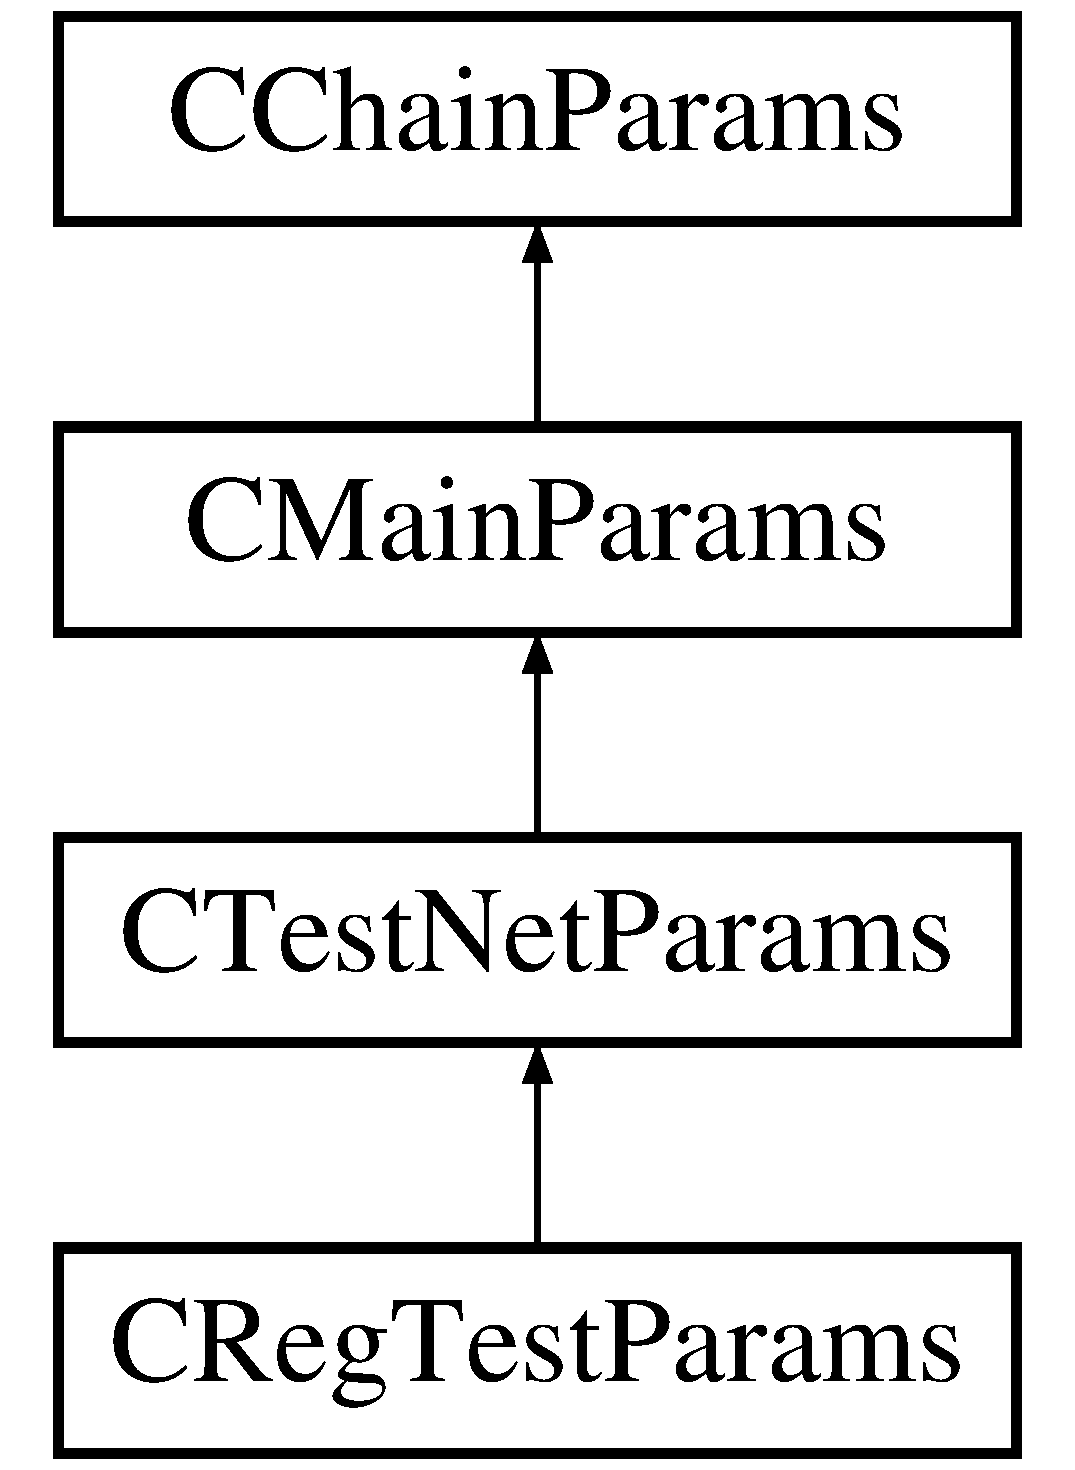
\includegraphics[height=4.000000cm]{class_c_reg_test_params}
\end{center}
\end{figure}
\subsection*{Public Member Functions}
\begin{DoxyCompactItemize}
\item 
\mbox{\hyperlink{class_c_reg_test_params_aceca5a50765323f150ac608ca43db4fd}{C\+Reg\+Test\+Params}} ()
\end{DoxyCompactItemize}
\subsection*{Additional Inherited Members}


\subsection{Detailed Description}
Regression test 

\subsection{Constructor \& Destructor Documentation}
\mbox{\Hypertarget{class_c_reg_test_params_aceca5a50765323f150ac608ca43db4fd}\label{class_c_reg_test_params_aceca5a50765323f150ac608ca43db4fd}} 
\index{C\+Reg\+Test\+Params@{C\+Reg\+Test\+Params}!C\+Reg\+Test\+Params@{C\+Reg\+Test\+Params}}
\index{C\+Reg\+Test\+Params@{C\+Reg\+Test\+Params}!C\+Reg\+Test\+Params@{C\+Reg\+Test\+Params}}
\subsubsection{\texorpdfstring{C\+Reg\+Test\+Params()}{CRegTestParams()}}
{\footnotesize\ttfamily C\+Reg\+Test\+Params\+::\+C\+Reg\+Test\+Params (\begin{DoxyParamCaption}{ }\end{DoxyParamCaption})\hspace{0.3cm}{\ttfamily [inline]}}

Regtest mode doesn\textquotesingle{}t have any fixed seeds.

Regtest mode doesn\textquotesingle{}t have any D\+NS seeds. 

The documentation for this class was generated from the following file\+:\begin{DoxyCompactItemize}
\item 
/\+Users/christopherarguello/\+Developer/anon/src/\mbox{\hyperlink{chainparams_8cpp}{chainparams.\+cpp}}\end{DoxyCompactItemize}

\hypertarget{class_c_rolling_bloom_filter}{}\section{C\+Rolling\+Bloom\+Filter Class Reference}
\label{class_c_rolling_bloom_filter}\index{C\+Rolling\+Bloom\+Filter@{C\+Rolling\+Bloom\+Filter}}


{\ttfamily \#include $<$bloom.\+h$>$}

\subsection*{Public Member Functions}
\begin{DoxyCompactItemize}
\item 
\mbox{\hyperlink{class_c_rolling_bloom_filter_a70f2c27fa28fc89676d3873159cfdecb}{C\+Rolling\+Bloom\+Filter}} (unsigned int n\+Elements, double n\+F\+P\+Rate)
\item 
void \mbox{\hyperlink{class_c_rolling_bloom_filter_a0fedbf0cf38c9070a30c7c5f8299f5d7}{insert}} (const std\+::vector$<$ unsigned char $>$ \&v\+Key)
\item 
void \mbox{\hyperlink{class_c_rolling_bloom_filter_aff399e835a59b4ced4d9af3ddce363a0}{insert}} (const \mbox{\hyperlink{classuint256}{uint256}} \&hash)
\item 
bool \mbox{\hyperlink{class_c_rolling_bloom_filter_a4f7d6161274b03c63be50aadb1fe46b7}{contains}} (const std\+::vector$<$ unsigned char $>$ \&v\+Key) const
\item 
bool \mbox{\hyperlink{class_c_rolling_bloom_filter_ae05528befdb97a19a1b31f30796ca7bd}{contains}} (const \mbox{\hyperlink{classuint256}{uint256}} \&hash) const
\item 
void \mbox{\hyperlink{class_c_rolling_bloom_filter_a7615966dc0beaa381892d8f43aeb53a3}{reset}} ()
\end{DoxyCompactItemize}
\subsection*{Private Attributes}
\begin{DoxyCompactItemize}
\item 
unsigned int \mbox{\hyperlink{class_c_rolling_bloom_filter_a5fa63c717bd8b41c149bb0462fae7898}{n\+Bloom\+Size}}
\item 
unsigned int \mbox{\hyperlink{class_c_rolling_bloom_filter_a393756a95c39b73f5f10d337ca12d5ac}{n\+Insertions}}
\item 
\mbox{\hyperlink{class_c_bloom_filter}{C\+Bloom\+Filter}} \mbox{\hyperlink{class_c_rolling_bloom_filter_ab15dfa505bcc7181e42588ead3bdd10b}{b1}}
\item 
\mbox{\hyperlink{class_c_bloom_filter}{C\+Bloom\+Filter}} \mbox{\hyperlink{class_c_rolling_bloom_filter_af9b4c16a31dd4aa5c6a16d7092c5c860}{b2}}
\end{DoxyCompactItemize}


\subsection{Detailed Description}
Rolling\+Bloom\+Filter is a probabilistic \char`\"{}keep track of most recently inserted\char`\"{} set. Construct it with the number of items to keep track of, and a false-\/positive rate. Unlike \mbox{\hyperlink{class_c_bloom_filter}{C\+Bloom\+Filter}}, by default n\+Tweak is set to a cryptographically secure random value for you. Similarly rather than clear() the method \mbox{\hyperlink{class_c_rolling_bloom_filter_a7615966dc0beaa381892d8f43aeb53a3}{reset()}} is provided, which also changes n\+Tweak to decrease the impact of false-\/positives.

contains(item) will always return true if item was one of the last N things \mbox{\hyperlink{class_c_rolling_bloom_filter_a0fedbf0cf38c9070a30c7c5f8299f5d7}{insert()}}\textquotesingle{}ed ... but may also return true for items that were not inserted. 

\subsection{Constructor \& Destructor Documentation}
\mbox{\Hypertarget{class_c_rolling_bloom_filter_a70f2c27fa28fc89676d3873159cfdecb}\label{class_c_rolling_bloom_filter_a70f2c27fa28fc89676d3873159cfdecb}} 
\index{C\+Rolling\+Bloom\+Filter@{C\+Rolling\+Bloom\+Filter}!C\+Rolling\+Bloom\+Filter@{C\+Rolling\+Bloom\+Filter}}
\index{C\+Rolling\+Bloom\+Filter@{C\+Rolling\+Bloom\+Filter}!C\+Rolling\+Bloom\+Filter@{C\+Rolling\+Bloom\+Filter}}
\subsubsection{\texorpdfstring{C\+Rolling\+Bloom\+Filter()}{CRollingBloomFilter()}}
{\footnotesize\ttfamily C\+Rolling\+Bloom\+Filter\+::\+C\+Rolling\+Bloom\+Filter (\begin{DoxyParamCaption}\item[{unsigned int}]{n\+Elements,  }\item[{double}]{n\+F\+P\+Rate }\end{DoxyParamCaption})}



\subsection{Member Function Documentation}
\mbox{\Hypertarget{class_c_rolling_bloom_filter_a4f7d6161274b03c63be50aadb1fe46b7}\label{class_c_rolling_bloom_filter_a4f7d6161274b03c63be50aadb1fe46b7}} 
\index{C\+Rolling\+Bloom\+Filter@{C\+Rolling\+Bloom\+Filter}!contains@{contains}}
\index{contains@{contains}!C\+Rolling\+Bloom\+Filter@{C\+Rolling\+Bloom\+Filter}}
\subsubsection{\texorpdfstring{contains()}{contains()}\hspace{0.1cm}{\footnotesize\ttfamily [1/2]}}
{\footnotesize\ttfamily bool C\+Rolling\+Bloom\+Filter\+::contains (\begin{DoxyParamCaption}\item[{const std\+::vector$<$ unsigned char $>$ \&}]{v\+Key }\end{DoxyParamCaption}) const}

\mbox{\Hypertarget{class_c_rolling_bloom_filter_ae05528befdb97a19a1b31f30796ca7bd}\label{class_c_rolling_bloom_filter_ae05528befdb97a19a1b31f30796ca7bd}} 
\index{C\+Rolling\+Bloom\+Filter@{C\+Rolling\+Bloom\+Filter}!contains@{contains}}
\index{contains@{contains}!C\+Rolling\+Bloom\+Filter@{C\+Rolling\+Bloom\+Filter}}
\subsubsection{\texorpdfstring{contains()}{contains()}\hspace{0.1cm}{\footnotesize\ttfamily [2/2]}}
{\footnotesize\ttfamily bool C\+Rolling\+Bloom\+Filter\+::contains (\begin{DoxyParamCaption}\item[{const \mbox{\hyperlink{classuint256}{uint256}} \&}]{hash }\end{DoxyParamCaption}) const}

\mbox{\Hypertarget{class_c_rolling_bloom_filter_a0fedbf0cf38c9070a30c7c5f8299f5d7}\label{class_c_rolling_bloom_filter_a0fedbf0cf38c9070a30c7c5f8299f5d7}} 
\index{C\+Rolling\+Bloom\+Filter@{C\+Rolling\+Bloom\+Filter}!insert@{insert}}
\index{insert@{insert}!C\+Rolling\+Bloom\+Filter@{C\+Rolling\+Bloom\+Filter}}
\subsubsection{\texorpdfstring{insert()}{insert()}\hspace{0.1cm}{\footnotesize\ttfamily [1/2]}}
{\footnotesize\ttfamily void C\+Rolling\+Bloom\+Filter\+::insert (\begin{DoxyParamCaption}\item[{const std\+::vector$<$ unsigned char $>$ \&}]{v\+Key }\end{DoxyParamCaption})}

\mbox{\Hypertarget{class_c_rolling_bloom_filter_aff399e835a59b4ced4d9af3ddce363a0}\label{class_c_rolling_bloom_filter_aff399e835a59b4ced4d9af3ddce363a0}} 
\index{C\+Rolling\+Bloom\+Filter@{C\+Rolling\+Bloom\+Filter}!insert@{insert}}
\index{insert@{insert}!C\+Rolling\+Bloom\+Filter@{C\+Rolling\+Bloom\+Filter}}
\subsubsection{\texorpdfstring{insert()}{insert()}\hspace{0.1cm}{\footnotesize\ttfamily [2/2]}}
{\footnotesize\ttfamily void C\+Rolling\+Bloom\+Filter\+::insert (\begin{DoxyParamCaption}\item[{const \mbox{\hyperlink{classuint256}{uint256}} \&}]{hash }\end{DoxyParamCaption})}

\mbox{\Hypertarget{class_c_rolling_bloom_filter_a7615966dc0beaa381892d8f43aeb53a3}\label{class_c_rolling_bloom_filter_a7615966dc0beaa381892d8f43aeb53a3}} 
\index{C\+Rolling\+Bloom\+Filter@{C\+Rolling\+Bloom\+Filter}!reset@{reset}}
\index{reset@{reset}!C\+Rolling\+Bloom\+Filter@{C\+Rolling\+Bloom\+Filter}}
\subsubsection{\texorpdfstring{reset()}{reset()}}
{\footnotesize\ttfamily void C\+Rolling\+Bloom\+Filter\+::reset (\begin{DoxyParamCaption}{ }\end{DoxyParamCaption})}



\subsection{Member Data Documentation}
\mbox{\Hypertarget{class_c_rolling_bloom_filter_ab15dfa505bcc7181e42588ead3bdd10b}\label{class_c_rolling_bloom_filter_ab15dfa505bcc7181e42588ead3bdd10b}} 
\index{C\+Rolling\+Bloom\+Filter@{C\+Rolling\+Bloom\+Filter}!b1@{b1}}
\index{b1@{b1}!C\+Rolling\+Bloom\+Filter@{C\+Rolling\+Bloom\+Filter}}
\subsubsection{\texorpdfstring{b1}{b1}}
{\footnotesize\ttfamily \mbox{\hyperlink{class_c_bloom_filter}{C\+Bloom\+Filter}} C\+Rolling\+Bloom\+Filter\+::b1\hspace{0.3cm}{\ttfamily [private]}}

\mbox{\Hypertarget{class_c_rolling_bloom_filter_af9b4c16a31dd4aa5c6a16d7092c5c860}\label{class_c_rolling_bloom_filter_af9b4c16a31dd4aa5c6a16d7092c5c860}} 
\index{C\+Rolling\+Bloom\+Filter@{C\+Rolling\+Bloom\+Filter}!b2@{b2}}
\index{b2@{b2}!C\+Rolling\+Bloom\+Filter@{C\+Rolling\+Bloom\+Filter}}
\subsubsection{\texorpdfstring{b2}{b2}}
{\footnotesize\ttfamily \mbox{\hyperlink{class_c_bloom_filter}{C\+Bloom\+Filter}} C\+Rolling\+Bloom\+Filter\+::b2\hspace{0.3cm}{\ttfamily [private]}}

\mbox{\Hypertarget{class_c_rolling_bloom_filter_a5fa63c717bd8b41c149bb0462fae7898}\label{class_c_rolling_bloom_filter_a5fa63c717bd8b41c149bb0462fae7898}} 
\index{C\+Rolling\+Bloom\+Filter@{C\+Rolling\+Bloom\+Filter}!n\+Bloom\+Size@{n\+Bloom\+Size}}
\index{n\+Bloom\+Size@{n\+Bloom\+Size}!C\+Rolling\+Bloom\+Filter@{C\+Rolling\+Bloom\+Filter}}
\subsubsection{\texorpdfstring{n\+Bloom\+Size}{nBloomSize}}
{\footnotesize\ttfamily unsigned int C\+Rolling\+Bloom\+Filter\+::n\+Bloom\+Size\hspace{0.3cm}{\ttfamily [private]}}

\mbox{\Hypertarget{class_c_rolling_bloom_filter_a393756a95c39b73f5f10d337ca12d5ac}\label{class_c_rolling_bloom_filter_a393756a95c39b73f5f10d337ca12d5ac}} 
\index{C\+Rolling\+Bloom\+Filter@{C\+Rolling\+Bloom\+Filter}!n\+Insertions@{n\+Insertions}}
\index{n\+Insertions@{n\+Insertions}!C\+Rolling\+Bloom\+Filter@{C\+Rolling\+Bloom\+Filter}}
\subsubsection{\texorpdfstring{n\+Insertions}{nInsertions}}
{\footnotesize\ttfamily unsigned int C\+Rolling\+Bloom\+Filter\+::n\+Insertions\hspace{0.3cm}{\ttfamily [private]}}



The documentation for this class was generated from the following files\+:\begin{DoxyCompactItemize}
\item 
/\+Users/christopherarguello/\+Developer/anon/src/\mbox{\hyperlink{bloom_8h}{bloom.\+h}}\item 
/\+Users/christopherarguello/\+Developer/anon/src/\mbox{\hyperlink{bloom_8cpp}{bloom.\+cpp}}\end{DoxyCompactItemize}

\hypertarget{class_c_r_p_c_command}{}\section{C\+R\+P\+C\+Command Class Reference}
\label{class_c_r_p_c_command}\index{C\+R\+P\+C\+Command@{C\+R\+P\+C\+Command}}


{\ttfamily \#include $<$rpcserver.\+h$>$}

\subsection*{Public Attributes}
\begin{DoxyCompactItemize}
\item 
std\+::string \mbox{\hyperlink{class_c_r_p_c_command_a27dd2710a5f94011f891f6a2efcec53a}{category}}
\item 
std\+::string \mbox{\hyperlink{class_c_r_p_c_command_a8da584c0d2d98be22ebff74d3cf2221c}{name}}
\item 
\mbox{\hyperlink{rpcserver_8h_abd1b2d0c1b4a4b6483cbddaea9ea7b0a}{rpcfn\+\_\+type}} \mbox{\hyperlink{class_c_r_p_c_command_a197a7eba565b4d9673537655fcbc1344}{actor}}
\item 
bool \mbox{\hyperlink{class_c_r_p_c_command_a7f0b10e619917a3019f36ba5fa538adb}{ok\+Safe\+Mode}}
\end{DoxyCompactItemize}


\subsection{Member Data Documentation}
\mbox{\Hypertarget{class_c_r_p_c_command_a197a7eba565b4d9673537655fcbc1344}\label{class_c_r_p_c_command_a197a7eba565b4d9673537655fcbc1344}} 
\index{C\+R\+P\+C\+Command@{C\+R\+P\+C\+Command}!actor@{actor}}
\index{actor@{actor}!C\+R\+P\+C\+Command@{C\+R\+P\+C\+Command}}
\subsubsection{\texorpdfstring{actor}{actor}}
{\footnotesize\ttfamily \mbox{\hyperlink{rpcserver_8h_abd1b2d0c1b4a4b6483cbddaea9ea7b0a}{rpcfn\+\_\+type}} C\+R\+P\+C\+Command\+::actor}

\mbox{\Hypertarget{class_c_r_p_c_command_a27dd2710a5f94011f891f6a2efcec53a}\label{class_c_r_p_c_command_a27dd2710a5f94011f891f6a2efcec53a}} 
\index{C\+R\+P\+C\+Command@{C\+R\+P\+C\+Command}!category@{category}}
\index{category@{category}!C\+R\+P\+C\+Command@{C\+R\+P\+C\+Command}}
\subsubsection{\texorpdfstring{category}{category}}
{\footnotesize\ttfamily std\+::string C\+R\+P\+C\+Command\+::category}

\mbox{\Hypertarget{class_c_r_p_c_command_a8da584c0d2d98be22ebff74d3cf2221c}\label{class_c_r_p_c_command_a8da584c0d2d98be22ebff74d3cf2221c}} 
\index{C\+R\+P\+C\+Command@{C\+R\+P\+C\+Command}!name@{name}}
\index{name@{name}!C\+R\+P\+C\+Command@{C\+R\+P\+C\+Command}}
\subsubsection{\texorpdfstring{name}{name}}
{\footnotesize\ttfamily std\+::string C\+R\+P\+C\+Command\+::name}

\mbox{\Hypertarget{class_c_r_p_c_command_a7f0b10e619917a3019f36ba5fa538adb}\label{class_c_r_p_c_command_a7f0b10e619917a3019f36ba5fa538adb}} 
\index{C\+R\+P\+C\+Command@{C\+R\+P\+C\+Command}!ok\+Safe\+Mode@{ok\+Safe\+Mode}}
\index{ok\+Safe\+Mode@{ok\+Safe\+Mode}!C\+R\+P\+C\+Command@{C\+R\+P\+C\+Command}}
\subsubsection{\texorpdfstring{ok\+Safe\+Mode}{okSafeMode}}
{\footnotesize\ttfamily bool C\+R\+P\+C\+Command\+::ok\+Safe\+Mode}



The documentation for this class was generated from the following file\+:\begin{DoxyCompactItemize}
\item 
/\+Users/christopherarguello/\+Developer/anon/src/\mbox{\hyperlink{rpcserver_8h}{rpcserver.\+h}}\end{DoxyCompactItemize}

\hypertarget{class_c_r_p_c_convert_param}{}\section{C\+R\+P\+C\+Convert\+Param Class Reference}
\label{class_c_r_p_c_convert_param}\index{C\+R\+P\+C\+Convert\+Param@{C\+R\+P\+C\+Convert\+Param}}
\subsection*{Public Attributes}
\begin{DoxyCompactItemize}
\item 
std\+::string \mbox{\hyperlink{class_c_r_p_c_convert_param_a072d6cde94ea57223445dee927ee1527}{method\+Name}}
\item 
int \mbox{\hyperlink{class_c_r_p_c_convert_param_a3bd464f8d5db060616e7be8fbacb58f8}{param\+Idx}}
\begin{DoxyCompactList}\small\item\em method whose params want conversion \end{DoxyCompactList}\end{DoxyCompactItemize}


\subsection{Member Data Documentation}
\mbox{\Hypertarget{class_c_r_p_c_convert_param_a072d6cde94ea57223445dee927ee1527}\label{class_c_r_p_c_convert_param_a072d6cde94ea57223445dee927ee1527}} 
\index{C\+R\+P\+C\+Convert\+Param@{C\+R\+P\+C\+Convert\+Param}!method\+Name@{method\+Name}}
\index{method\+Name@{method\+Name}!C\+R\+P\+C\+Convert\+Param@{C\+R\+P\+C\+Convert\+Param}}
\subsubsection{\texorpdfstring{method\+Name}{methodName}}
{\footnotesize\ttfamily std\+::string C\+R\+P\+C\+Convert\+Param\+::method\+Name}

\mbox{\Hypertarget{class_c_r_p_c_convert_param_a3bd464f8d5db060616e7be8fbacb58f8}\label{class_c_r_p_c_convert_param_a3bd464f8d5db060616e7be8fbacb58f8}} 
\index{C\+R\+P\+C\+Convert\+Param@{C\+R\+P\+C\+Convert\+Param}!param\+Idx@{param\+Idx}}
\index{param\+Idx@{param\+Idx}!C\+R\+P\+C\+Convert\+Param@{C\+R\+P\+C\+Convert\+Param}}
\subsubsection{\texorpdfstring{param\+Idx}{paramIdx}}
{\footnotesize\ttfamily int C\+R\+P\+C\+Convert\+Param\+::param\+Idx}



method whose params want conversion 



The documentation for this class was generated from the following file\+:\begin{DoxyCompactItemize}
\item 
/\+Users/christopherarguello/\+Developer/anon/src/\mbox{\hyperlink{rpcclient_8cpp}{rpcclient.\+cpp}}\end{DoxyCompactItemize}

\hypertarget{class_c_r_p_c_convert_table}{}\section{C\+R\+P\+C\+Convert\+Table Class Reference}
\label{class_c_r_p_c_convert_table}\index{C\+R\+P\+C\+Convert\+Table@{C\+R\+P\+C\+Convert\+Table}}
\subsection*{Public Member Functions}
\begin{DoxyCompactItemize}
\item 
\mbox{\hyperlink{class_c_r_p_c_convert_table_a7f79dde2002bd2bc2178bd38f213922d}{C\+R\+P\+C\+Convert\+Table}} ()
\item 
bool \mbox{\hyperlink{class_c_r_p_c_convert_table_a034b770cb03e79074111b85eba889e58}{convert}} (const std\+::string \&method, int idx)
\end{DoxyCompactItemize}
\subsection*{Private Attributes}
\begin{DoxyCompactItemize}
\item 
std\+::set$<$ std\+::pair$<$ std\+::string, int $>$ $>$ \mbox{\hyperlink{class_c_r_p_c_convert_table_a6fa71fee177e85db3846acbb7b9c6025}{members}}
\end{DoxyCompactItemize}


\subsection{Constructor \& Destructor Documentation}
\mbox{\Hypertarget{class_c_r_p_c_convert_table_a7f79dde2002bd2bc2178bd38f213922d}\label{class_c_r_p_c_convert_table_a7f79dde2002bd2bc2178bd38f213922d}} 
\index{C\+R\+P\+C\+Convert\+Table@{C\+R\+P\+C\+Convert\+Table}!C\+R\+P\+C\+Convert\+Table@{C\+R\+P\+C\+Convert\+Table}}
\index{C\+R\+P\+C\+Convert\+Table@{C\+R\+P\+C\+Convert\+Table}!C\+R\+P\+C\+Convert\+Table@{C\+R\+P\+C\+Convert\+Table}}
\subsubsection{\texorpdfstring{C\+R\+P\+C\+Convert\+Table()}{CRPCConvertTable()}}
{\footnotesize\ttfamily C\+R\+P\+C\+Convert\+Table\+::\+C\+R\+P\+C\+Convert\+Table (\begin{DoxyParamCaption}{ }\end{DoxyParamCaption})}



\subsection{Member Function Documentation}
\mbox{\Hypertarget{class_c_r_p_c_convert_table_a034b770cb03e79074111b85eba889e58}\label{class_c_r_p_c_convert_table_a034b770cb03e79074111b85eba889e58}} 
\index{C\+R\+P\+C\+Convert\+Table@{C\+R\+P\+C\+Convert\+Table}!convert@{convert}}
\index{convert@{convert}!C\+R\+P\+C\+Convert\+Table@{C\+R\+P\+C\+Convert\+Table}}
\subsubsection{\texorpdfstring{convert()}{convert()}}
{\footnotesize\ttfamily bool C\+R\+P\+C\+Convert\+Table\+::convert (\begin{DoxyParamCaption}\item[{const std\+::string \&}]{method,  }\item[{int}]{idx }\end{DoxyParamCaption})\hspace{0.3cm}{\ttfamily [inline]}}



\subsection{Member Data Documentation}
\mbox{\Hypertarget{class_c_r_p_c_convert_table_a6fa71fee177e85db3846acbb7b9c6025}\label{class_c_r_p_c_convert_table_a6fa71fee177e85db3846acbb7b9c6025}} 
\index{C\+R\+P\+C\+Convert\+Table@{C\+R\+P\+C\+Convert\+Table}!members@{members}}
\index{members@{members}!C\+R\+P\+C\+Convert\+Table@{C\+R\+P\+C\+Convert\+Table}}
\subsubsection{\texorpdfstring{members}{members}}
{\footnotesize\ttfamily std\+::set$<$std\+::pair$<$std\+::string, int$>$ $>$ C\+R\+P\+C\+Convert\+Table\+::members\hspace{0.3cm}{\ttfamily [private]}}



The documentation for this class was generated from the following file\+:\begin{DoxyCompactItemize}
\item 
/\+Users/christopherarguello/\+Developer/anon/src/\mbox{\hyperlink{rpcclient_8cpp}{rpcclient.\+cpp}}\end{DoxyCompactItemize}

\hypertarget{struct_c_r_p_c_signals}{}\section{C\+R\+P\+C\+Signals Struct Reference}
\label{struct_c_r_p_c_signals}\index{C\+R\+P\+C\+Signals@{C\+R\+P\+C\+Signals}}
\subsection*{Public Attributes}
\begin{DoxyCompactItemize}
\item 
boost\+::signals2\+::signal$<$ void()$>$ \mbox{\hyperlink{struct_c_r_p_c_signals_a201ab59320dae51002203903e66ec1a7}{Started}}
\item 
boost\+::signals2\+::signal$<$ void()$>$ \mbox{\hyperlink{struct_c_r_p_c_signals_a60800aedbc7b1e912cb4b432f3db7e99}{Stopped}}
\item 
boost\+::signals2\+::signal$<$ void(const \mbox{\hyperlink{class_c_r_p_c_command}{C\+R\+P\+C\+Command}} \&)$>$ \mbox{\hyperlink{struct_c_r_p_c_signals_a37e5ba485cf72626d09dd13de07a14a7}{Pre\+Command}}
\item 
boost\+::signals2\+::signal$<$ void(const \mbox{\hyperlink{class_c_r_p_c_command}{C\+R\+P\+C\+Command}} \&)$>$ \mbox{\hyperlink{struct_c_r_p_c_signals_a2b35d6a50a396f3fc0662192b5fb2a39}{Post\+Command}}
\end{DoxyCompactItemize}


\subsection{Member Data Documentation}
\mbox{\Hypertarget{struct_c_r_p_c_signals_a2b35d6a50a396f3fc0662192b5fb2a39}\label{struct_c_r_p_c_signals_a2b35d6a50a396f3fc0662192b5fb2a39}} 
\index{C\+R\+P\+C\+Signals@{C\+R\+P\+C\+Signals}!Post\+Command@{Post\+Command}}
\index{Post\+Command@{Post\+Command}!C\+R\+P\+C\+Signals@{C\+R\+P\+C\+Signals}}
\subsubsection{\texorpdfstring{Post\+Command}{PostCommand}}
{\footnotesize\ttfamily boost\+::signals2\+::signal$<$void (const \mbox{\hyperlink{class_c_r_p_c_command}{C\+R\+P\+C\+Command}}\&)$>$ C\+R\+P\+C\+Signals\+::\+Post\+Command}

\mbox{\Hypertarget{struct_c_r_p_c_signals_a37e5ba485cf72626d09dd13de07a14a7}\label{struct_c_r_p_c_signals_a37e5ba485cf72626d09dd13de07a14a7}} 
\index{C\+R\+P\+C\+Signals@{C\+R\+P\+C\+Signals}!Pre\+Command@{Pre\+Command}}
\index{Pre\+Command@{Pre\+Command}!C\+R\+P\+C\+Signals@{C\+R\+P\+C\+Signals}}
\subsubsection{\texorpdfstring{Pre\+Command}{PreCommand}}
{\footnotesize\ttfamily boost\+::signals2\+::signal$<$void (const \mbox{\hyperlink{class_c_r_p_c_command}{C\+R\+P\+C\+Command}}\&)$>$ C\+R\+P\+C\+Signals\+::\+Pre\+Command}

\mbox{\Hypertarget{struct_c_r_p_c_signals_a201ab59320dae51002203903e66ec1a7}\label{struct_c_r_p_c_signals_a201ab59320dae51002203903e66ec1a7}} 
\index{C\+R\+P\+C\+Signals@{C\+R\+P\+C\+Signals}!Started@{Started}}
\index{Started@{Started}!C\+R\+P\+C\+Signals@{C\+R\+P\+C\+Signals}}
\subsubsection{\texorpdfstring{Started}{Started}}
{\footnotesize\ttfamily boost\+::signals2\+::signal$<$void ()$>$ C\+R\+P\+C\+Signals\+::\+Started}

\mbox{\Hypertarget{struct_c_r_p_c_signals_a60800aedbc7b1e912cb4b432f3db7e99}\label{struct_c_r_p_c_signals_a60800aedbc7b1e912cb4b432f3db7e99}} 
\index{C\+R\+P\+C\+Signals@{C\+R\+P\+C\+Signals}!Stopped@{Stopped}}
\index{Stopped@{Stopped}!C\+R\+P\+C\+Signals@{C\+R\+P\+C\+Signals}}
\subsubsection{\texorpdfstring{Stopped}{Stopped}}
{\footnotesize\ttfamily boost\+::signals2\+::signal$<$void ()$>$ C\+R\+P\+C\+Signals\+::\+Stopped}



The documentation for this struct was generated from the following file\+:\begin{DoxyCompactItemize}
\item 
/\+Users/christopherarguello/\+Developer/anon/src/\mbox{\hyperlink{rpcserver_8cpp}{rpcserver.\+cpp}}\end{DoxyCompactItemize}

\hypertarget{class_c_r_p_c_table}{}\section{C\+R\+P\+C\+Table Class Reference}
\label{class_c_r_p_c_table}\index{C\+R\+P\+C\+Table@{C\+R\+P\+C\+Table}}


{\ttfamily \#include $<$rpcserver.\+h$>$}

\subsection*{Public Member Functions}
\begin{DoxyCompactItemize}
\item 
\mbox{\hyperlink{class_c_r_p_c_table_a2e6e624bae4c149db2f5cbe0de84b121}{C\+R\+P\+C\+Table}} ()
\item 
const \mbox{\hyperlink{class_c_r_p_c_command}{C\+R\+P\+C\+Command}} $\ast$ \mbox{\hyperlink{class_c_r_p_c_table_aa06a59b1f7fe34668eab9a6a4a2491fa}{operator\mbox{[}$\,$\mbox{]}}} (const std\+::string \&\mbox{\hyperlink{rest_8cpp_a8f8f80d37794cde9472343e4487ba3eb}{name}}) const
\item 
std\+::string \mbox{\hyperlink{class_c_r_p_c_table_a3d9af8e5975ee8d872b49992faae3ba6}{help}} (const std\+::string \&\mbox{\hyperlink{rest_8cpp_a8f8f80d37794cde9472343e4487ba3eb}{name}}) const
\item 
Uni\+Value \mbox{\hyperlink{class_c_r_p_c_table_a30bfd77e85ecc56b58da3f8582af1ac8}{execute}} (const std\+::string \&method, const Uni\+Value \&params) const
\end{DoxyCompactItemize}
\subsection*{Private Attributes}
\begin{DoxyCompactItemize}
\item 
std\+::map$<$ std\+::string, const \mbox{\hyperlink{class_c_r_p_c_command}{C\+R\+P\+C\+Command}} $\ast$ $>$ \mbox{\hyperlink{class_c_r_p_c_table_abe193d7f72d98048f2a99ec13028f65f}{map\+Commands}}
\end{DoxyCompactItemize}


\subsection{Detailed Description}
Bitcoin R\+PC command dispatcher. 

\subsection{Constructor \& Destructor Documentation}
\mbox{\Hypertarget{class_c_r_p_c_table_a2e6e624bae4c149db2f5cbe0de84b121}\label{class_c_r_p_c_table_a2e6e624bae4c149db2f5cbe0de84b121}} 
\index{C\+R\+P\+C\+Table@{C\+R\+P\+C\+Table}!C\+R\+P\+C\+Table@{C\+R\+P\+C\+Table}}
\index{C\+R\+P\+C\+Table@{C\+R\+P\+C\+Table}!C\+R\+P\+C\+Table@{C\+R\+P\+C\+Table}}
\subsubsection{\texorpdfstring{C\+R\+P\+C\+Table()}{CRPCTable()}}
{\footnotesize\ttfamily C\+R\+P\+C\+Table\+::\+C\+R\+P\+C\+Table (\begin{DoxyParamCaption}{ }\end{DoxyParamCaption})}



\subsection{Member Function Documentation}
\mbox{\Hypertarget{class_c_r_p_c_table_a30bfd77e85ecc56b58da3f8582af1ac8}\label{class_c_r_p_c_table_a30bfd77e85ecc56b58da3f8582af1ac8}} 
\index{C\+R\+P\+C\+Table@{C\+R\+P\+C\+Table}!execute@{execute}}
\index{execute@{execute}!C\+R\+P\+C\+Table@{C\+R\+P\+C\+Table}}
\subsubsection{\texorpdfstring{execute()}{execute()}}
{\footnotesize\ttfamily Uni\+Value C\+R\+P\+C\+Table\+::execute (\begin{DoxyParamCaption}\item[{const std\+::string \&}]{method,  }\item[{const Uni\+Value \&}]{params }\end{DoxyParamCaption}) const}

Execute a method. 
\begin{DoxyParams}{Parameters}
{\em method} & Method to execute \\
\hline
{\em params} & Uni\+Value Array of arguments (J\+S\+ON objects) \\
\hline
\end{DoxyParams}
\begin{DoxyReturn}{Returns}
Result of the call. 
\end{DoxyReturn}

\begin{DoxyExceptions}{Exceptions}
{\em an} & exception (Uni\+Value) when an error happens. \\
\hline
\end{DoxyExceptions}
\mbox{\Hypertarget{class_c_r_p_c_table_a3d9af8e5975ee8d872b49992faae3ba6}\label{class_c_r_p_c_table_a3d9af8e5975ee8d872b49992faae3ba6}} 
\index{C\+R\+P\+C\+Table@{C\+R\+P\+C\+Table}!help@{help}}
\index{help@{help}!C\+R\+P\+C\+Table@{C\+R\+P\+C\+Table}}
\subsubsection{\texorpdfstring{help()}{help()}}
{\footnotesize\ttfamily std\+::string C\+R\+P\+C\+Table\+::help (\begin{DoxyParamCaption}\item[{const std\+::string \&}]{str\+Command }\end{DoxyParamCaption}) const}

Note\+: This interface may still be subject to change. \mbox{\Hypertarget{class_c_r_p_c_table_aa06a59b1f7fe34668eab9a6a4a2491fa}\label{class_c_r_p_c_table_aa06a59b1f7fe34668eab9a6a4a2491fa}} 
\index{C\+R\+P\+C\+Table@{C\+R\+P\+C\+Table}!operator\mbox{[}\mbox{]}@{operator[]}}
\index{operator\mbox{[}\mbox{]}@{operator[]}!C\+R\+P\+C\+Table@{C\+R\+P\+C\+Table}}
\subsubsection{\texorpdfstring{operator[]()}{operator[]()}}
{\footnotesize\ttfamily const \mbox{\hyperlink{class_c_r_p_c_command}{C\+R\+P\+C\+Command}} $\ast$ C\+R\+P\+C\+Table\+::operator\mbox{[}$\,$\mbox{]} (\begin{DoxyParamCaption}\item[{const std\+::string \&}]{name }\end{DoxyParamCaption}) const}



\subsection{Member Data Documentation}
\mbox{\Hypertarget{class_c_r_p_c_table_abe193d7f72d98048f2a99ec13028f65f}\label{class_c_r_p_c_table_abe193d7f72d98048f2a99ec13028f65f}} 
\index{C\+R\+P\+C\+Table@{C\+R\+P\+C\+Table}!map\+Commands@{map\+Commands}}
\index{map\+Commands@{map\+Commands}!C\+R\+P\+C\+Table@{C\+R\+P\+C\+Table}}
\subsubsection{\texorpdfstring{map\+Commands}{mapCommands}}
{\footnotesize\ttfamily std\+::map$<$std\+::string, const \mbox{\hyperlink{class_c_r_p_c_command}{C\+R\+P\+C\+Command}}$\ast$$>$ C\+R\+P\+C\+Table\+::map\+Commands\hspace{0.3cm}{\ttfamily [private]}}



The documentation for this class was generated from the following files\+:\begin{DoxyCompactItemize}
\item 
/\+Users/christopherarguello/\+Developer/anon/src/\mbox{\hyperlink{rpcserver_8h}{rpcserver.\+h}}\item 
/\+Users/christopherarguello/\+Developer/anon/src/\mbox{\hyperlink{rpcserver_8cpp}{rpcserver.\+cpp}}\end{DoxyCompactItemize}

\hypertarget{class_c_scheduler}{}\section{C\+Scheduler Class Reference}
\label{class_c_scheduler}\index{C\+Scheduler@{C\+Scheduler}}


{\ttfamily \#include $<$scheduler.\+h$>$}

\subsection*{Public Types}
\begin{DoxyCompactItemize}
\item 
typedef boost\+::function$<$ void(void)$>$ \mbox{\hyperlink{class_c_scheduler_af0202f526eeef71defb156dc06f70279}{Function}}
\end{DoxyCompactItemize}
\subsection*{Public Member Functions}
\begin{DoxyCompactItemize}
\item 
\mbox{\hyperlink{class_c_scheduler_a388ba8ffa4dfc6ed0a4ac63ddeb2a51a}{C\+Scheduler}} ()
\item 
\mbox{\hyperlink{class_c_scheduler_ab453c8d28d84cf31ee3d5f621f4f45ed}{$\sim$\+C\+Scheduler}} ()
\item 
void \mbox{\hyperlink{class_c_scheduler_a14747dc42599cc0a17f45f1767932d6e}{schedule}} (\mbox{\hyperlink{class_c_scheduler_af0202f526eeef71defb156dc06f70279}{Function}} f, boost\+::chrono\+::system\+\_\+clock\+::time\+\_\+point t)
\item 
void \mbox{\hyperlink{class_c_scheduler_ad5faa192176dc51e3c68356589934b7a}{schedule\+From\+Now}} (\mbox{\hyperlink{class_c_scheduler_af0202f526eeef71defb156dc06f70279}{Function}} f, int64\+\_\+t delta\+Seconds)
\item 
void \mbox{\hyperlink{class_c_scheduler_ad7fcff70877bf1d84f30c1137bba816f}{schedule\+Every}} (\mbox{\hyperlink{class_c_scheduler_af0202f526eeef71defb156dc06f70279}{Function}} f, int64\+\_\+t delta\+Seconds)
\item 
void \mbox{\hyperlink{class_c_scheduler_a14d2800815da93577858ea078aed1fba}{service\+Queue}} ()
\item 
void \mbox{\hyperlink{class_c_scheduler_a328f18f2d0eb9977180c8b091a17947a}{stop}} (bool drain=false)
\item 
size\+\_\+t \mbox{\hyperlink{class_c_scheduler_a6cdbfd095e9f7695c09769d4c1b05461}{get\+Queue\+Info}} (boost\+::chrono\+::system\+\_\+clock\+::time\+\_\+point \&first, boost\+::chrono\+::system\+\_\+clock\+::time\+\_\+point \&last) const
\end{DoxyCompactItemize}
\subsection*{Private Member Functions}
\begin{DoxyCompactItemize}
\item 
bool \mbox{\hyperlink{class_c_scheduler_a66e40dd7a6eef503c255bba54168df95}{should\+Stop}} ()
\end{DoxyCompactItemize}
\subsection*{Private Attributes}
\begin{DoxyCompactItemize}
\item 
std\+::multimap$<$ boost\+::chrono\+::system\+\_\+clock\+::time\+\_\+point, \mbox{\hyperlink{class_c_scheduler_af0202f526eeef71defb156dc06f70279}{Function}} $>$ \mbox{\hyperlink{class_c_scheduler_a206a499765bd27e5aaff4c4ba2255f91}{task\+Queue}}
\item 
boost\+::condition\+\_\+variable \mbox{\hyperlink{class_c_scheduler_a9aff0df5c40338dd9ed01334aae05cdf}{new\+Task\+Scheduled}}
\item 
boost\+::mutex \mbox{\hyperlink{class_c_scheduler_a6b161d2bf167c00285522b088a05bfa6}{new\+Task\+Mutex}}
\item 
int \mbox{\hyperlink{class_c_scheduler_aa0fc35cbc38efb37a9b5b8756d869875}{n\+Threads\+Servicing\+Queue}}
\item 
bool \mbox{\hyperlink{class_c_scheduler_a8609cd421d5d416708a22aea138dd882}{stop\+Requested}}
\item 
bool \mbox{\hyperlink{class_c_scheduler_a78e214ee8c89bfc8083cb95261ebbc6f}{stop\+When\+Empty}}
\end{DoxyCompactItemize}


\subsection{Member Typedef Documentation}
\mbox{\Hypertarget{class_c_scheduler_af0202f526eeef71defb156dc06f70279}\label{class_c_scheduler_af0202f526eeef71defb156dc06f70279}} 
\index{C\+Scheduler@{C\+Scheduler}!Function@{Function}}
\index{Function@{Function}!C\+Scheduler@{C\+Scheduler}}
\subsubsection{\texorpdfstring{Function}{Function}}
{\footnotesize\ttfamily typedef boost\+::function$<$void(void)$>$ \mbox{\hyperlink{class_c_scheduler_af0202f526eeef71defb156dc06f70279}{C\+Scheduler\+::\+Function}}}



\subsection{Constructor \& Destructor Documentation}
\mbox{\Hypertarget{class_c_scheduler_a388ba8ffa4dfc6ed0a4ac63ddeb2a51a}\label{class_c_scheduler_a388ba8ffa4dfc6ed0a4ac63ddeb2a51a}} 
\index{C\+Scheduler@{C\+Scheduler}!C\+Scheduler@{C\+Scheduler}}
\index{C\+Scheduler@{C\+Scheduler}!C\+Scheduler@{C\+Scheduler}}
\subsubsection{\texorpdfstring{C\+Scheduler()}{CScheduler()}}
{\footnotesize\ttfamily C\+Scheduler\+::\+C\+Scheduler (\begin{DoxyParamCaption}{ }\end{DoxyParamCaption})}

\mbox{\Hypertarget{class_c_scheduler_ab453c8d28d84cf31ee3d5f621f4f45ed}\label{class_c_scheduler_ab453c8d28d84cf31ee3d5f621f4f45ed}} 
\index{C\+Scheduler@{C\+Scheduler}!````~C\+Scheduler@{$\sim$\+C\+Scheduler}}
\index{````~C\+Scheduler@{$\sim$\+C\+Scheduler}!C\+Scheduler@{C\+Scheduler}}
\subsubsection{\texorpdfstring{$\sim$\+C\+Scheduler()}{~CScheduler()}}
{\footnotesize\ttfamily C\+Scheduler\+::$\sim$\+C\+Scheduler (\begin{DoxyParamCaption}{ }\end{DoxyParamCaption})}



\subsection{Member Function Documentation}
\mbox{\Hypertarget{class_c_scheduler_a6cdbfd095e9f7695c09769d4c1b05461}\label{class_c_scheduler_a6cdbfd095e9f7695c09769d4c1b05461}} 
\index{C\+Scheduler@{C\+Scheduler}!get\+Queue\+Info@{get\+Queue\+Info}}
\index{get\+Queue\+Info@{get\+Queue\+Info}!C\+Scheduler@{C\+Scheduler}}
\subsubsection{\texorpdfstring{get\+Queue\+Info()}{getQueueInfo()}}
{\footnotesize\ttfamily size\+\_\+t C\+Scheduler\+::get\+Queue\+Info (\begin{DoxyParamCaption}\item[{boost\+::chrono\+::system\+\_\+clock\+::time\+\_\+point \&}]{first,  }\item[{boost\+::chrono\+::system\+\_\+clock\+::time\+\_\+point \&}]{last }\end{DoxyParamCaption}) const}

\mbox{\Hypertarget{class_c_scheduler_a14747dc42599cc0a17f45f1767932d6e}\label{class_c_scheduler_a14747dc42599cc0a17f45f1767932d6e}} 
\index{C\+Scheduler@{C\+Scheduler}!schedule@{schedule}}
\index{schedule@{schedule}!C\+Scheduler@{C\+Scheduler}}
\subsubsection{\texorpdfstring{schedule()}{schedule()}}
{\footnotesize\ttfamily void C\+Scheduler\+::schedule (\begin{DoxyParamCaption}\item[{\mbox{\hyperlink{class_c_scheduler_af0202f526eeef71defb156dc06f70279}{C\+Scheduler\+::\+Function}}}]{f,  }\item[{boost\+::chrono\+::system\+\_\+clock\+::time\+\_\+point}]{t }\end{DoxyParamCaption})}

\mbox{\Hypertarget{class_c_scheduler_ad7fcff70877bf1d84f30c1137bba816f}\label{class_c_scheduler_ad7fcff70877bf1d84f30c1137bba816f}} 
\index{C\+Scheduler@{C\+Scheduler}!schedule\+Every@{schedule\+Every}}
\index{schedule\+Every@{schedule\+Every}!C\+Scheduler@{C\+Scheduler}}
\subsubsection{\texorpdfstring{schedule\+Every()}{scheduleEvery()}}
{\footnotesize\ttfamily void C\+Scheduler\+::schedule\+Every (\begin{DoxyParamCaption}\item[{\mbox{\hyperlink{class_c_scheduler_af0202f526eeef71defb156dc06f70279}{C\+Scheduler\+::\+Function}}}]{f,  }\item[{int64\+\_\+t}]{delta\+Seconds }\end{DoxyParamCaption})}

\mbox{\Hypertarget{class_c_scheduler_ad5faa192176dc51e3c68356589934b7a}\label{class_c_scheduler_ad5faa192176dc51e3c68356589934b7a}} 
\index{C\+Scheduler@{C\+Scheduler}!schedule\+From\+Now@{schedule\+From\+Now}}
\index{schedule\+From\+Now@{schedule\+From\+Now}!C\+Scheduler@{C\+Scheduler}}
\subsubsection{\texorpdfstring{schedule\+From\+Now()}{scheduleFromNow()}}
{\footnotesize\ttfamily void C\+Scheduler\+::schedule\+From\+Now (\begin{DoxyParamCaption}\item[{\mbox{\hyperlink{class_c_scheduler_af0202f526eeef71defb156dc06f70279}{C\+Scheduler\+::\+Function}}}]{f,  }\item[{int64\+\_\+t}]{delta\+Seconds }\end{DoxyParamCaption})}

\mbox{\Hypertarget{class_c_scheduler_a14d2800815da93577858ea078aed1fba}\label{class_c_scheduler_a14d2800815da93577858ea078aed1fba}} 
\index{C\+Scheduler@{C\+Scheduler}!service\+Queue@{service\+Queue}}
\index{service\+Queue@{service\+Queue}!C\+Scheduler@{C\+Scheduler}}
\subsubsection{\texorpdfstring{service\+Queue()}{serviceQueue()}}
{\footnotesize\ttfamily void C\+Scheduler\+::service\+Queue (\begin{DoxyParamCaption}{ }\end{DoxyParamCaption})}

\mbox{\Hypertarget{class_c_scheduler_a66e40dd7a6eef503c255bba54168df95}\label{class_c_scheduler_a66e40dd7a6eef503c255bba54168df95}} 
\index{C\+Scheduler@{C\+Scheduler}!should\+Stop@{should\+Stop}}
\index{should\+Stop@{should\+Stop}!C\+Scheduler@{C\+Scheduler}}
\subsubsection{\texorpdfstring{should\+Stop()}{shouldStop()}}
{\footnotesize\ttfamily bool C\+Scheduler\+::should\+Stop (\begin{DoxyParamCaption}{ }\end{DoxyParamCaption})\hspace{0.3cm}{\ttfamily [inline]}, {\ttfamily [private]}}

\mbox{\Hypertarget{class_c_scheduler_a328f18f2d0eb9977180c8b091a17947a}\label{class_c_scheduler_a328f18f2d0eb9977180c8b091a17947a}} 
\index{C\+Scheduler@{C\+Scheduler}!stop@{stop}}
\index{stop@{stop}!C\+Scheduler@{C\+Scheduler}}
\subsubsection{\texorpdfstring{stop()}{stop()}}
{\footnotesize\ttfamily void C\+Scheduler\+::stop (\begin{DoxyParamCaption}\item[{bool}]{drain = {\ttfamily false} }\end{DoxyParamCaption})}



\subsection{Member Data Documentation}
\mbox{\Hypertarget{class_c_scheduler_a6b161d2bf167c00285522b088a05bfa6}\label{class_c_scheduler_a6b161d2bf167c00285522b088a05bfa6}} 
\index{C\+Scheduler@{C\+Scheduler}!new\+Task\+Mutex@{new\+Task\+Mutex}}
\index{new\+Task\+Mutex@{new\+Task\+Mutex}!C\+Scheduler@{C\+Scheduler}}
\subsubsection{\texorpdfstring{new\+Task\+Mutex}{newTaskMutex}}
{\footnotesize\ttfamily boost\+::mutex C\+Scheduler\+::new\+Task\+Mutex\hspace{0.3cm}{\ttfamily [mutable]}, {\ttfamily [private]}}

\mbox{\Hypertarget{class_c_scheduler_a9aff0df5c40338dd9ed01334aae05cdf}\label{class_c_scheduler_a9aff0df5c40338dd9ed01334aae05cdf}} 
\index{C\+Scheduler@{C\+Scheduler}!new\+Task\+Scheduled@{new\+Task\+Scheduled}}
\index{new\+Task\+Scheduled@{new\+Task\+Scheduled}!C\+Scheduler@{C\+Scheduler}}
\subsubsection{\texorpdfstring{new\+Task\+Scheduled}{newTaskScheduled}}
{\footnotesize\ttfamily boost\+::condition\+\_\+variable C\+Scheduler\+::new\+Task\+Scheduled\hspace{0.3cm}{\ttfamily [private]}}

\mbox{\Hypertarget{class_c_scheduler_aa0fc35cbc38efb37a9b5b8756d869875}\label{class_c_scheduler_aa0fc35cbc38efb37a9b5b8756d869875}} 
\index{C\+Scheduler@{C\+Scheduler}!n\+Threads\+Servicing\+Queue@{n\+Threads\+Servicing\+Queue}}
\index{n\+Threads\+Servicing\+Queue@{n\+Threads\+Servicing\+Queue}!C\+Scheduler@{C\+Scheduler}}
\subsubsection{\texorpdfstring{n\+Threads\+Servicing\+Queue}{nThreadsServicingQueue}}
{\footnotesize\ttfamily int C\+Scheduler\+::n\+Threads\+Servicing\+Queue\hspace{0.3cm}{\ttfamily [private]}}

\mbox{\Hypertarget{class_c_scheduler_a8609cd421d5d416708a22aea138dd882}\label{class_c_scheduler_a8609cd421d5d416708a22aea138dd882}} 
\index{C\+Scheduler@{C\+Scheduler}!stop\+Requested@{stop\+Requested}}
\index{stop\+Requested@{stop\+Requested}!C\+Scheduler@{C\+Scheduler}}
\subsubsection{\texorpdfstring{stop\+Requested}{stopRequested}}
{\footnotesize\ttfamily bool C\+Scheduler\+::stop\+Requested\hspace{0.3cm}{\ttfamily [private]}}

\mbox{\Hypertarget{class_c_scheduler_a78e214ee8c89bfc8083cb95261ebbc6f}\label{class_c_scheduler_a78e214ee8c89bfc8083cb95261ebbc6f}} 
\index{C\+Scheduler@{C\+Scheduler}!stop\+When\+Empty@{stop\+When\+Empty}}
\index{stop\+When\+Empty@{stop\+When\+Empty}!C\+Scheduler@{C\+Scheduler}}
\subsubsection{\texorpdfstring{stop\+When\+Empty}{stopWhenEmpty}}
{\footnotesize\ttfamily bool C\+Scheduler\+::stop\+When\+Empty\hspace{0.3cm}{\ttfamily [private]}}

\mbox{\Hypertarget{class_c_scheduler_a206a499765bd27e5aaff4c4ba2255f91}\label{class_c_scheduler_a206a499765bd27e5aaff4c4ba2255f91}} 
\index{C\+Scheduler@{C\+Scheduler}!task\+Queue@{task\+Queue}}
\index{task\+Queue@{task\+Queue}!C\+Scheduler@{C\+Scheduler}}
\subsubsection{\texorpdfstring{task\+Queue}{taskQueue}}
{\footnotesize\ttfamily std\+::multimap$<$boost\+::chrono\+::system\+\_\+clock\+::time\+\_\+point, \mbox{\hyperlink{class_c_scheduler_af0202f526eeef71defb156dc06f70279}{Function}}$>$ C\+Scheduler\+::task\+Queue\hspace{0.3cm}{\ttfamily [private]}}



The documentation for this class was generated from the following files\+:\begin{DoxyCompactItemize}
\item 
/\+Users/christopherarguello/\+Developer/anon/src/\mbox{\hyperlink{scheduler_8h}{scheduler.\+h}}\item 
/\+Users/christopherarguello/\+Developer/anon/src/\mbox{\hyperlink{scheduler_8cpp}{scheduler.\+cpp}}\end{DoxyCompactItemize}

\hypertarget{class_c_script_check}{}\section{C\+Script\+Check Class Reference}
\label{class_c_script_check}\index{C\+Script\+Check@{C\+Script\+Check}}


{\ttfamily \#include $<$main.\+h$>$}

\subsection*{Public Member Functions}
\begin{DoxyCompactItemize}
\item 
\mbox{\hyperlink{class_c_script_check_a4a3bf9c971437bcb6fae3e3254a8c178}{C\+Script\+Check}} ()
\item 
\mbox{\hyperlink{class_c_script_check_a2617b99b66cd1de327478b74d8441c76}{C\+Script\+Check}} (const \mbox{\hyperlink{class_c_coins}{C\+Coins}} \&tx\+From\+In, const C\+Transaction \&tx\+To\+In, unsigned int n\+In\+In, unsigned int n\+Flags\+In, bool cache\+In)
\item 
bool \mbox{\hyperlink{class_c_script_check_a108d4c713338308be3867ed4e65b80c5}{operator()}} ()
\item 
void \mbox{\hyperlink{class_c_script_check_a69fbde608ff29c1885b8b9caf0fd40a0}{swap}} (\mbox{\hyperlink{class_c_script_check}{C\+Script\+Check}} \&check)
\item 
Script\+Error \mbox{\hyperlink{class_c_script_check_a1340496c37e521c253606b5957173afd}{Get\+Script\+Error}} () const
\end{DoxyCompactItemize}
\subsection*{Private Attributes}
\begin{DoxyCompactItemize}
\item 
C\+Script \mbox{\hyperlink{class_c_script_check_a1042feefe3b4706d236edea898e40954}{script\+Pub\+Key}}
\item 
const C\+Transaction $\ast$ \mbox{\hyperlink{class_c_script_check_ac22505a5889791918c2271fd2692e32a}{ptx\+To}}
\item 
unsigned int \mbox{\hyperlink{class_c_script_check_ad7ff03fbbba182a994685ea8c3a2287f}{n\+In}}
\item 
unsigned int \mbox{\hyperlink{class_c_script_check_a9ce4a4cbe2703769d8ec9541c83e0b5e}{n\+Flags}}
\item 
bool \mbox{\hyperlink{class_c_script_check_a9026cd87ffd80d3785aa00e9949dcbd4}{cache\+Store}}
\item 
Script\+Error \mbox{\hyperlink{class_c_script_check_a93e4567a5f6b6d5682f8b1b8357fa848}{error}}
\end{DoxyCompactItemize}


\subsection{Detailed Description}
Closure representing one script verification Note that this stores references to the spending transaction 

\subsection{Constructor \& Destructor Documentation}
\mbox{\Hypertarget{class_c_script_check_a4a3bf9c971437bcb6fae3e3254a8c178}\label{class_c_script_check_a4a3bf9c971437bcb6fae3e3254a8c178}} 
\index{C\+Script\+Check@{C\+Script\+Check}!C\+Script\+Check@{C\+Script\+Check}}
\index{C\+Script\+Check@{C\+Script\+Check}!C\+Script\+Check@{C\+Script\+Check}}
\subsubsection{\texorpdfstring{C\+Script\+Check()}{CScriptCheck()}\hspace{0.1cm}{\footnotesize\ttfamily [1/2]}}
{\footnotesize\ttfamily C\+Script\+Check\+::\+C\+Script\+Check (\begin{DoxyParamCaption}{ }\end{DoxyParamCaption})\hspace{0.3cm}{\ttfamily [inline]}}

\mbox{\Hypertarget{class_c_script_check_a2617b99b66cd1de327478b74d8441c76}\label{class_c_script_check_a2617b99b66cd1de327478b74d8441c76}} 
\index{C\+Script\+Check@{C\+Script\+Check}!C\+Script\+Check@{C\+Script\+Check}}
\index{C\+Script\+Check@{C\+Script\+Check}!C\+Script\+Check@{C\+Script\+Check}}
\subsubsection{\texorpdfstring{C\+Script\+Check()}{CScriptCheck()}\hspace{0.1cm}{\footnotesize\ttfamily [2/2]}}
{\footnotesize\ttfamily C\+Script\+Check\+::\+C\+Script\+Check (\begin{DoxyParamCaption}\item[{const \mbox{\hyperlink{class_c_coins}{C\+Coins}} \&}]{tx\+From\+In,  }\item[{const C\+Transaction \&}]{tx\+To\+In,  }\item[{unsigned int}]{n\+In\+In,  }\item[{unsigned int}]{n\+Flags\+In,  }\item[{bool}]{cache\+In }\end{DoxyParamCaption})\hspace{0.3cm}{\ttfamily [inline]}}



\subsection{Member Function Documentation}
\mbox{\Hypertarget{class_c_script_check_a1340496c37e521c253606b5957173afd}\label{class_c_script_check_a1340496c37e521c253606b5957173afd}} 
\index{C\+Script\+Check@{C\+Script\+Check}!Get\+Script\+Error@{Get\+Script\+Error}}
\index{Get\+Script\+Error@{Get\+Script\+Error}!C\+Script\+Check@{C\+Script\+Check}}
\subsubsection{\texorpdfstring{Get\+Script\+Error()}{GetScriptError()}}
{\footnotesize\ttfamily Script\+Error C\+Script\+Check\+::\+Get\+Script\+Error (\begin{DoxyParamCaption}{ }\end{DoxyParamCaption}) const\hspace{0.3cm}{\ttfamily [inline]}}

\mbox{\Hypertarget{class_c_script_check_a108d4c713338308be3867ed4e65b80c5}\label{class_c_script_check_a108d4c713338308be3867ed4e65b80c5}} 
\index{C\+Script\+Check@{C\+Script\+Check}!operator()@{operator()}}
\index{operator()@{operator()}!C\+Script\+Check@{C\+Script\+Check}}
\subsubsection{\texorpdfstring{operator()()}{operator()()}}
{\footnotesize\ttfamily bool C\+Script\+Check\+::operator() (\begin{DoxyParamCaption}{ }\end{DoxyParamCaption})}

\mbox{\Hypertarget{class_c_script_check_a69fbde608ff29c1885b8b9caf0fd40a0}\label{class_c_script_check_a69fbde608ff29c1885b8b9caf0fd40a0}} 
\index{C\+Script\+Check@{C\+Script\+Check}!swap@{swap}}
\index{swap@{swap}!C\+Script\+Check@{C\+Script\+Check}}
\subsubsection{\texorpdfstring{swap()}{swap()}}
{\footnotesize\ttfamily void C\+Script\+Check\+::swap (\begin{DoxyParamCaption}\item[{\mbox{\hyperlink{class_c_script_check}{C\+Script\+Check}} \&}]{check }\end{DoxyParamCaption})\hspace{0.3cm}{\ttfamily [inline]}}



\subsection{Member Data Documentation}
\mbox{\Hypertarget{class_c_script_check_a9026cd87ffd80d3785aa00e9949dcbd4}\label{class_c_script_check_a9026cd87ffd80d3785aa00e9949dcbd4}} 
\index{C\+Script\+Check@{C\+Script\+Check}!cache\+Store@{cache\+Store}}
\index{cache\+Store@{cache\+Store}!C\+Script\+Check@{C\+Script\+Check}}
\subsubsection{\texorpdfstring{cache\+Store}{cacheStore}}
{\footnotesize\ttfamily bool C\+Script\+Check\+::cache\+Store\hspace{0.3cm}{\ttfamily [private]}}

\mbox{\Hypertarget{class_c_script_check_a93e4567a5f6b6d5682f8b1b8357fa848}\label{class_c_script_check_a93e4567a5f6b6d5682f8b1b8357fa848}} 
\index{C\+Script\+Check@{C\+Script\+Check}!error@{error}}
\index{error@{error}!C\+Script\+Check@{C\+Script\+Check}}
\subsubsection{\texorpdfstring{error}{error}}
{\footnotesize\ttfamily Script\+Error C\+Script\+Check\+::error\hspace{0.3cm}{\ttfamily [private]}}

\mbox{\Hypertarget{class_c_script_check_a9ce4a4cbe2703769d8ec9541c83e0b5e}\label{class_c_script_check_a9ce4a4cbe2703769d8ec9541c83e0b5e}} 
\index{C\+Script\+Check@{C\+Script\+Check}!n\+Flags@{n\+Flags}}
\index{n\+Flags@{n\+Flags}!C\+Script\+Check@{C\+Script\+Check}}
\subsubsection{\texorpdfstring{n\+Flags}{nFlags}}
{\footnotesize\ttfamily unsigned int C\+Script\+Check\+::n\+Flags\hspace{0.3cm}{\ttfamily [private]}}

\mbox{\Hypertarget{class_c_script_check_ad7ff03fbbba182a994685ea8c3a2287f}\label{class_c_script_check_ad7ff03fbbba182a994685ea8c3a2287f}} 
\index{C\+Script\+Check@{C\+Script\+Check}!n\+In@{n\+In}}
\index{n\+In@{n\+In}!C\+Script\+Check@{C\+Script\+Check}}
\subsubsection{\texorpdfstring{n\+In}{nIn}}
{\footnotesize\ttfamily unsigned int C\+Script\+Check\+::n\+In\hspace{0.3cm}{\ttfamily [private]}}

\mbox{\Hypertarget{class_c_script_check_ac22505a5889791918c2271fd2692e32a}\label{class_c_script_check_ac22505a5889791918c2271fd2692e32a}} 
\index{C\+Script\+Check@{C\+Script\+Check}!ptx\+To@{ptx\+To}}
\index{ptx\+To@{ptx\+To}!C\+Script\+Check@{C\+Script\+Check}}
\subsubsection{\texorpdfstring{ptx\+To}{ptxTo}}
{\footnotesize\ttfamily const C\+Transaction$\ast$ C\+Script\+Check\+::ptx\+To\hspace{0.3cm}{\ttfamily [private]}}

\mbox{\Hypertarget{class_c_script_check_a1042feefe3b4706d236edea898e40954}\label{class_c_script_check_a1042feefe3b4706d236edea898e40954}} 
\index{C\+Script\+Check@{C\+Script\+Check}!script\+Pub\+Key@{script\+Pub\+Key}}
\index{script\+Pub\+Key@{script\+Pub\+Key}!C\+Script\+Check@{C\+Script\+Check}}
\subsubsection{\texorpdfstring{script\+Pub\+Key}{scriptPubKey}}
{\footnotesize\ttfamily C\+Script C\+Script\+Check\+::script\+Pub\+Key\hspace{0.3cm}{\ttfamily [private]}}



The documentation for this class was generated from the following files\+:\begin{DoxyCompactItemize}
\item 
/\+Users/christopherarguello/\+Developer/anon/src/\mbox{\hyperlink{main_8h}{main.\+h}}\item 
/\+Users/christopherarguello/\+Developer/anon/src/\mbox{\hyperlink{main_8cpp}{main.\+cpp}}\end{DoxyCompactItemize}

\hypertarget{class_c_script_compressor}{}\section{C\+Script\+Compressor Class Reference}
\label{class_c_script_compressor}\index{C\+Script\+Compressor@{C\+Script\+Compressor}}


{\ttfamily \#include $<$compressor.\+h$>$}

\subsection*{Public Member Functions}
\begin{DoxyCompactItemize}
\item 
\mbox{\hyperlink{class_c_script_compressor_aad31afe3d14387b163b5c043e834ca2b}{C\+Script\+Compressor}} (C\+Script \&script\+In)
\item 
unsigned int \mbox{\hyperlink{class_c_script_compressor_afd6f2bea6c0ba2d34f770997e96bc23d}{Get\+Serialize\+Size}} (int n\+Type, int n\+Version) const
\item 
{\footnotesize template$<$typename Stream $>$ }\\void \mbox{\hyperlink{class_c_script_compressor_a5702b644df500ddd11c56d0490e8be44}{Serialize}} (Stream \&s, int n\+Type, int n\+Version) const
\item 
{\footnotesize template$<$typename Stream $>$ }\\void \mbox{\hyperlink{class_c_script_compressor_a016fa6e3d2735d95fcf773271da073d5}{Unserialize}} (Stream \&s, int n\+Type, int n\+Version)
\end{DoxyCompactItemize}
\subsection*{Protected Member Functions}
\begin{DoxyCompactItemize}
\item 
bool \mbox{\hyperlink{class_c_script_compressor_a38e2dcfce62bb157b55536d73748f556}{Is\+To\+Key\+ID}} (\mbox{\hyperlink{class_c_key_i_d}{C\+Key\+ID}} \&hash) const
\item 
bool \mbox{\hyperlink{class_c_script_compressor_a7a995d1064299a58d4f2e9f0ac205d07}{Is\+To\+Script\+ID}} (C\+Script\+ID \&hash) const
\item 
bool \mbox{\hyperlink{class_c_script_compressor_a19a67455a106e2e0528bc97cb60d2391}{Is\+To\+Pub\+Key}} (\mbox{\hyperlink{class_c_pub_key}{C\+Pub\+Key}} \&pubkey) const
\item 
bool \mbox{\hyperlink{class_c_script_compressor_a563ba251e7720841b4d5fc30ebd736e6}{Compress}} (std\+::vector$<$ unsigned char $>$ \&out) const
\item 
unsigned int \mbox{\hyperlink{class_c_script_compressor_aa702c1ed206804d016da3600e02d2169}{Get\+Special\+Size}} (unsigned int n\+Size) const
\item 
bool \mbox{\hyperlink{class_c_script_compressor_a1feb663ddab3a45218c7cb02f2a25717}{Decompress}} (unsigned int n\+Size, const std\+::vector$<$ unsigned char $>$ \&out)
\end{DoxyCompactItemize}
\subsection*{Private Attributes}
\begin{DoxyCompactItemize}
\item 
C\+Script \& \mbox{\hyperlink{class_c_script_compressor_afb1c3fb4b9ff4870501705c030cef056}{script}}
\end{DoxyCompactItemize}
\subsection*{Static Private Attributes}
\begin{DoxyCompactItemize}
\item 
static const unsigned int \mbox{\hyperlink{class_c_script_compressor_a3f0dc2a613a667745ee24a476ce21337}{n\+Special\+Scripts}} = 6
\end{DoxyCompactItemize}


\subsection{Detailed Description}
Compact serializer for scripts.

It detects common cases and encodes them much more efficiently. 3 special cases are defined\+:
\begin{DoxyItemize}
\item Pay to pubkey hash (encoded as 21 bytes)
\item Pay to script hash (encoded as 21 bytes)
\item Pay to pubkey starting with 0x02, 0x03 or 0x04 (encoded as 33 bytes)
\end{DoxyItemize}

Other scripts up to 121 bytes require 1 byte + script length. Above that, scripts up to 16505 bytes require 2 bytes + script length. 

\subsection{Constructor \& Destructor Documentation}
\mbox{\Hypertarget{class_c_script_compressor_aad31afe3d14387b163b5c043e834ca2b}\label{class_c_script_compressor_aad31afe3d14387b163b5c043e834ca2b}} 
\index{C\+Script\+Compressor@{C\+Script\+Compressor}!C\+Script\+Compressor@{C\+Script\+Compressor}}
\index{C\+Script\+Compressor@{C\+Script\+Compressor}!C\+Script\+Compressor@{C\+Script\+Compressor}}
\subsubsection{\texorpdfstring{C\+Script\+Compressor()}{CScriptCompressor()}}
{\footnotesize\ttfamily C\+Script\+Compressor\+::\+C\+Script\+Compressor (\begin{DoxyParamCaption}\item[{C\+Script \&}]{script\+In }\end{DoxyParamCaption})\hspace{0.3cm}{\ttfamily [inline]}}



\subsection{Member Function Documentation}
\mbox{\Hypertarget{class_c_script_compressor_a563ba251e7720841b4d5fc30ebd736e6}\label{class_c_script_compressor_a563ba251e7720841b4d5fc30ebd736e6}} 
\index{C\+Script\+Compressor@{C\+Script\+Compressor}!Compress@{Compress}}
\index{Compress@{Compress}!C\+Script\+Compressor@{C\+Script\+Compressor}}
\subsubsection{\texorpdfstring{Compress()}{Compress()}}
{\footnotesize\ttfamily bool C\+Script\+Compressor\+::\+Compress (\begin{DoxyParamCaption}\item[{std\+::vector$<$ unsigned char $>$ \&}]{out }\end{DoxyParamCaption}) const\hspace{0.3cm}{\ttfamily [protected]}}

\mbox{\Hypertarget{class_c_script_compressor_a1feb663ddab3a45218c7cb02f2a25717}\label{class_c_script_compressor_a1feb663ddab3a45218c7cb02f2a25717}} 
\index{C\+Script\+Compressor@{C\+Script\+Compressor}!Decompress@{Decompress}}
\index{Decompress@{Decompress}!C\+Script\+Compressor@{C\+Script\+Compressor}}
\subsubsection{\texorpdfstring{Decompress()}{Decompress()}}
{\footnotesize\ttfamily bool C\+Script\+Compressor\+::\+Decompress (\begin{DoxyParamCaption}\item[{unsigned int}]{n\+Size,  }\item[{const std\+::vector$<$ unsigned char $>$ \&}]{out }\end{DoxyParamCaption})\hspace{0.3cm}{\ttfamily [protected]}}

\mbox{\Hypertarget{class_c_script_compressor_afd6f2bea6c0ba2d34f770997e96bc23d}\label{class_c_script_compressor_afd6f2bea6c0ba2d34f770997e96bc23d}} 
\index{C\+Script\+Compressor@{C\+Script\+Compressor}!Get\+Serialize\+Size@{Get\+Serialize\+Size}}
\index{Get\+Serialize\+Size@{Get\+Serialize\+Size}!C\+Script\+Compressor@{C\+Script\+Compressor}}
\subsubsection{\texorpdfstring{Get\+Serialize\+Size()}{GetSerializeSize()}}
{\footnotesize\ttfamily unsigned int C\+Script\+Compressor\+::\+Get\+Serialize\+Size (\begin{DoxyParamCaption}\item[{int}]{n\+Type,  }\item[{int}]{n\+Version }\end{DoxyParamCaption}) const\hspace{0.3cm}{\ttfamily [inline]}}

\mbox{\Hypertarget{class_c_script_compressor_aa702c1ed206804d016da3600e02d2169}\label{class_c_script_compressor_aa702c1ed206804d016da3600e02d2169}} 
\index{C\+Script\+Compressor@{C\+Script\+Compressor}!Get\+Special\+Size@{Get\+Special\+Size}}
\index{Get\+Special\+Size@{Get\+Special\+Size}!C\+Script\+Compressor@{C\+Script\+Compressor}}
\subsubsection{\texorpdfstring{Get\+Special\+Size()}{GetSpecialSize()}}
{\footnotesize\ttfamily unsigned int C\+Script\+Compressor\+::\+Get\+Special\+Size (\begin{DoxyParamCaption}\item[{unsigned int}]{n\+Size }\end{DoxyParamCaption}) const\hspace{0.3cm}{\ttfamily [protected]}}

\mbox{\Hypertarget{class_c_script_compressor_a38e2dcfce62bb157b55536d73748f556}\label{class_c_script_compressor_a38e2dcfce62bb157b55536d73748f556}} 
\index{C\+Script\+Compressor@{C\+Script\+Compressor}!Is\+To\+Key\+ID@{Is\+To\+Key\+ID}}
\index{Is\+To\+Key\+ID@{Is\+To\+Key\+ID}!C\+Script\+Compressor@{C\+Script\+Compressor}}
\subsubsection{\texorpdfstring{Is\+To\+Key\+I\+D()}{IsToKeyID()}}
{\footnotesize\ttfamily bool C\+Script\+Compressor\+::\+Is\+To\+Key\+ID (\begin{DoxyParamCaption}\item[{\mbox{\hyperlink{class_c_key_i_d}{C\+Key\+ID}} \&}]{hash }\end{DoxyParamCaption}) const\hspace{0.3cm}{\ttfamily [protected]}}

These check for scripts for which a special case with a shorter encoding is defined. They are implemented separately from the C\+Script test, as these test for exact byte sequence correspondences, and are more strict. For example, Is\+To\+Pub\+Key also verifies whether the public key is valid (as invalid ones cannot be represented in compressed form). \mbox{\Hypertarget{class_c_script_compressor_a19a67455a106e2e0528bc97cb60d2391}\label{class_c_script_compressor_a19a67455a106e2e0528bc97cb60d2391}} 
\index{C\+Script\+Compressor@{C\+Script\+Compressor}!Is\+To\+Pub\+Key@{Is\+To\+Pub\+Key}}
\index{Is\+To\+Pub\+Key@{Is\+To\+Pub\+Key}!C\+Script\+Compressor@{C\+Script\+Compressor}}
\subsubsection{\texorpdfstring{Is\+To\+Pub\+Key()}{IsToPubKey()}}
{\footnotesize\ttfamily bool C\+Script\+Compressor\+::\+Is\+To\+Pub\+Key (\begin{DoxyParamCaption}\item[{\mbox{\hyperlink{class_c_pub_key}{C\+Pub\+Key}} \&}]{pubkey }\end{DoxyParamCaption}) const\hspace{0.3cm}{\ttfamily [protected]}}

\mbox{\Hypertarget{class_c_script_compressor_a7a995d1064299a58d4f2e9f0ac205d07}\label{class_c_script_compressor_a7a995d1064299a58d4f2e9f0ac205d07}} 
\index{C\+Script\+Compressor@{C\+Script\+Compressor}!Is\+To\+Script\+ID@{Is\+To\+Script\+ID}}
\index{Is\+To\+Script\+ID@{Is\+To\+Script\+ID}!C\+Script\+Compressor@{C\+Script\+Compressor}}
\subsubsection{\texorpdfstring{Is\+To\+Script\+I\+D()}{IsToScriptID()}}
{\footnotesize\ttfamily bool C\+Script\+Compressor\+::\+Is\+To\+Script\+ID (\begin{DoxyParamCaption}\item[{C\+Script\+ID \&}]{hash }\end{DoxyParamCaption}) const\hspace{0.3cm}{\ttfamily [protected]}}

\mbox{\Hypertarget{class_c_script_compressor_a5702b644df500ddd11c56d0490e8be44}\label{class_c_script_compressor_a5702b644df500ddd11c56d0490e8be44}} 
\index{C\+Script\+Compressor@{C\+Script\+Compressor}!Serialize@{Serialize}}
\index{Serialize@{Serialize}!C\+Script\+Compressor@{C\+Script\+Compressor}}
\subsubsection{\texorpdfstring{Serialize()}{Serialize()}}
{\footnotesize\ttfamily template$<$typename Stream $>$ \\
void C\+Script\+Compressor\+::\+Serialize (\begin{DoxyParamCaption}\item[{Stream \&}]{s,  }\item[{int}]{n\+Type,  }\item[{int}]{n\+Version }\end{DoxyParamCaption}) const\hspace{0.3cm}{\ttfamily [inline]}}

\mbox{\Hypertarget{class_c_script_compressor_a016fa6e3d2735d95fcf773271da073d5}\label{class_c_script_compressor_a016fa6e3d2735d95fcf773271da073d5}} 
\index{C\+Script\+Compressor@{C\+Script\+Compressor}!Unserialize@{Unserialize}}
\index{Unserialize@{Unserialize}!C\+Script\+Compressor@{C\+Script\+Compressor}}
\subsubsection{\texorpdfstring{Unserialize()}{Unserialize()}}
{\footnotesize\ttfamily template$<$typename Stream $>$ \\
void C\+Script\+Compressor\+::\+Unserialize (\begin{DoxyParamCaption}\item[{Stream \&}]{s,  }\item[{int}]{n\+Type,  }\item[{int}]{n\+Version }\end{DoxyParamCaption})\hspace{0.3cm}{\ttfamily [inline]}}



\subsection{Member Data Documentation}
\mbox{\Hypertarget{class_c_script_compressor_a3f0dc2a613a667745ee24a476ce21337}\label{class_c_script_compressor_a3f0dc2a613a667745ee24a476ce21337}} 
\index{C\+Script\+Compressor@{C\+Script\+Compressor}!n\+Special\+Scripts@{n\+Special\+Scripts}}
\index{n\+Special\+Scripts@{n\+Special\+Scripts}!C\+Script\+Compressor@{C\+Script\+Compressor}}
\subsubsection{\texorpdfstring{n\+Special\+Scripts}{nSpecialScripts}}
{\footnotesize\ttfamily const unsigned int C\+Script\+Compressor\+::n\+Special\+Scripts = 6\hspace{0.3cm}{\ttfamily [static]}, {\ttfamily [private]}}

make this static for now (there are only 6 special scripts defined) this can potentially be extended together with a new n\+Version for transactions, in which case this value becomes dependent on n\+Version and n\+Height of the enclosing transaction. \mbox{\Hypertarget{class_c_script_compressor_afb1c3fb4b9ff4870501705c030cef056}\label{class_c_script_compressor_afb1c3fb4b9ff4870501705c030cef056}} 
\index{C\+Script\+Compressor@{C\+Script\+Compressor}!script@{script}}
\index{script@{script}!C\+Script\+Compressor@{C\+Script\+Compressor}}
\subsubsection{\texorpdfstring{script}{script}}
{\footnotesize\ttfamily C\+Script\& C\+Script\+Compressor\+::script\hspace{0.3cm}{\ttfamily [private]}}



The documentation for this class was generated from the following files\+:\begin{DoxyCompactItemize}
\item 
/\+Users/christopherarguello/\+Developer/anon/src/\mbox{\hyperlink{compressor_8h}{compressor.\+h}}\item 
/\+Users/christopherarguello/\+Developer/anon/src/\mbox{\hyperlink{compressor_8cpp}{compressor.\+cpp}}\end{DoxyCompactItemize}

\hypertarget{class_c_semaphore}{}\section{C\+Semaphore Class Reference}
\label{class_c_semaphore}\index{C\+Semaphore@{C\+Semaphore}}


{\ttfamily \#include $<$sync.\+h$>$}

\subsection*{Public Member Functions}
\begin{DoxyCompactItemize}
\item 
\mbox{\hyperlink{class_c_semaphore_ac9cc749c7424852d7fb4378811d0dae1}{C\+Semaphore}} (int init)
\item 
void \mbox{\hyperlink{class_c_semaphore_a1c108bd981fe68527ec8ef5e7b0d116c}{wait}} ()
\item 
bool \mbox{\hyperlink{class_c_semaphore_abb8a07e6cac29dc72f044cd536a9f9e5}{try\+\_\+wait}} ()
\item 
void \mbox{\hyperlink{class_c_semaphore_af6a956f6c191e824485fd3af6db39318}{post}} ()
\end{DoxyCompactItemize}
\subsection*{Private Attributes}
\begin{DoxyCompactItemize}
\item 
boost\+::condition\+\_\+variable \mbox{\hyperlink{class_c_semaphore_afe13b8e59776248a0c49f9f2b31107fb}{condition}}
\item 
boost\+::mutex \mbox{\hyperlink{class_c_semaphore_ac871c4228d6a9b7f67f340ba693a629d}{mutex}}
\item 
int \mbox{\hyperlink{class_c_semaphore_a22a51512b911d93b37411cfffc764303}{value}}
\end{DoxyCompactItemize}


\subsection{Constructor \& Destructor Documentation}
\mbox{\Hypertarget{class_c_semaphore_ac9cc749c7424852d7fb4378811d0dae1}\label{class_c_semaphore_ac9cc749c7424852d7fb4378811d0dae1}} 
\index{C\+Semaphore@{C\+Semaphore}!C\+Semaphore@{C\+Semaphore}}
\index{C\+Semaphore@{C\+Semaphore}!C\+Semaphore@{C\+Semaphore}}
\subsubsection{\texorpdfstring{C\+Semaphore()}{CSemaphore()}}
{\footnotesize\ttfamily C\+Semaphore\+::\+C\+Semaphore (\begin{DoxyParamCaption}\item[{int}]{init }\end{DoxyParamCaption})\hspace{0.3cm}{\ttfamily [inline]}}



\subsection{Member Function Documentation}
\mbox{\Hypertarget{class_c_semaphore_af6a956f6c191e824485fd3af6db39318}\label{class_c_semaphore_af6a956f6c191e824485fd3af6db39318}} 
\index{C\+Semaphore@{C\+Semaphore}!post@{post}}
\index{post@{post}!C\+Semaphore@{C\+Semaphore}}
\subsubsection{\texorpdfstring{post()}{post()}}
{\footnotesize\ttfamily void C\+Semaphore\+::post (\begin{DoxyParamCaption}{ }\end{DoxyParamCaption})\hspace{0.3cm}{\ttfamily [inline]}}

\mbox{\Hypertarget{class_c_semaphore_abb8a07e6cac29dc72f044cd536a9f9e5}\label{class_c_semaphore_abb8a07e6cac29dc72f044cd536a9f9e5}} 
\index{C\+Semaphore@{C\+Semaphore}!try\+\_\+wait@{try\+\_\+wait}}
\index{try\+\_\+wait@{try\+\_\+wait}!C\+Semaphore@{C\+Semaphore}}
\subsubsection{\texorpdfstring{try\+\_\+wait()}{try\_wait()}}
{\footnotesize\ttfamily bool C\+Semaphore\+::try\+\_\+wait (\begin{DoxyParamCaption}{ }\end{DoxyParamCaption})\hspace{0.3cm}{\ttfamily [inline]}}

\mbox{\Hypertarget{class_c_semaphore_a1c108bd981fe68527ec8ef5e7b0d116c}\label{class_c_semaphore_a1c108bd981fe68527ec8ef5e7b0d116c}} 
\index{C\+Semaphore@{C\+Semaphore}!wait@{wait}}
\index{wait@{wait}!C\+Semaphore@{C\+Semaphore}}
\subsubsection{\texorpdfstring{wait()}{wait()}}
{\footnotesize\ttfamily void C\+Semaphore\+::wait (\begin{DoxyParamCaption}{ }\end{DoxyParamCaption})\hspace{0.3cm}{\ttfamily [inline]}}



\subsection{Member Data Documentation}
\mbox{\Hypertarget{class_c_semaphore_afe13b8e59776248a0c49f9f2b31107fb}\label{class_c_semaphore_afe13b8e59776248a0c49f9f2b31107fb}} 
\index{C\+Semaphore@{C\+Semaphore}!condition@{condition}}
\index{condition@{condition}!C\+Semaphore@{C\+Semaphore}}
\subsubsection{\texorpdfstring{condition}{condition}}
{\footnotesize\ttfamily boost\+::condition\+\_\+variable C\+Semaphore\+::condition\hspace{0.3cm}{\ttfamily [private]}}

\mbox{\Hypertarget{class_c_semaphore_ac871c4228d6a9b7f67f340ba693a629d}\label{class_c_semaphore_ac871c4228d6a9b7f67f340ba693a629d}} 
\index{C\+Semaphore@{C\+Semaphore}!mutex@{mutex}}
\index{mutex@{mutex}!C\+Semaphore@{C\+Semaphore}}
\subsubsection{\texorpdfstring{mutex}{mutex}}
{\footnotesize\ttfamily boost\+::mutex C\+Semaphore\+::mutex\hspace{0.3cm}{\ttfamily [private]}}

\mbox{\Hypertarget{class_c_semaphore_a22a51512b911d93b37411cfffc764303}\label{class_c_semaphore_a22a51512b911d93b37411cfffc764303}} 
\index{C\+Semaphore@{C\+Semaphore}!value@{value}}
\index{value@{value}!C\+Semaphore@{C\+Semaphore}}
\subsubsection{\texorpdfstring{value}{value}}
{\footnotesize\ttfamily int C\+Semaphore\+::value\hspace{0.3cm}{\ttfamily [private]}}



The documentation for this class was generated from the following file\+:\begin{DoxyCompactItemize}
\item 
/\+Users/christopherarguello/\+Developer/anon/src/\mbox{\hyperlink{sync_8h}{sync.\+h}}\end{DoxyCompactItemize}

\hypertarget{class_c_semaphore_grant}{}\section{C\+Semaphore\+Grant Class Reference}
\label{class_c_semaphore_grant}\index{C\+Semaphore\+Grant@{C\+Semaphore\+Grant}}


{\ttfamily \#include $<$sync.\+h$>$}

\subsection*{Public Member Functions}
\begin{DoxyCompactItemize}
\item 
void \mbox{\hyperlink{class_c_semaphore_grant_ac52976968379ea8e2470cfba877c3e89}{Acquire}} ()
\item 
void \mbox{\hyperlink{class_c_semaphore_grant_a8d985eeace74e037baeb39bd2d586576}{Release}} ()
\item 
bool \mbox{\hyperlink{class_c_semaphore_grant_a9952d9ea087ced803c099f69992ebb1d}{Try\+Acquire}} ()
\item 
void \mbox{\hyperlink{class_c_semaphore_grant_ab3e6f84f304703abc52517b0c8de26cf}{Move\+To}} (\mbox{\hyperlink{class_c_semaphore_grant}{C\+Semaphore\+Grant}} \&grant)
\item 
\mbox{\hyperlink{class_c_semaphore_grant_a84ca79a4c8519f1a69697c060cabc51d}{C\+Semaphore\+Grant}} ()
\item 
\mbox{\hyperlink{class_c_semaphore_grant_a5998c457c7c223a8257166161d12b355}{C\+Semaphore\+Grant}} (\mbox{\hyperlink{class_c_semaphore}{C\+Semaphore}} \&sema, bool f\+Try=false)
\item 
\mbox{\hyperlink{class_c_semaphore_grant_aaba5579eb3ad3647d79e71c9970dcb54}{$\sim$\+C\+Semaphore\+Grant}} ()
\item 
\mbox{\hyperlink{class_c_semaphore_grant_a91458b860e45949d87d770252e590a9b}{operator bool}} ()
\end{DoxyCompactItemize}
\subsection*{Private Attributes}
\begin{DoxyCompactItemize}
\item 
\mbox{\hyperlink{class_c_semaphore}{C\+Semaphore}} $\ast$ \mbox{\hyperlink{class_c_semaphore_grant_afed7f1f7ac912c175dcd9c898fa4e2ed}{sem}}
\item 
bool \mbox{\hyperlink{class_c_semaphore_grant_a0c416dd364ca4d085555d69658c060e3}{f\+Have\+Grant}}
\end{DoxyCompactItemize}


\subsection{Detailed Description}
R\+A\+I\+I-\/style semaphore lock 

\subsection{Constructor \& Destructor Documentation}
\mbox{\Hypertarget{class_c_semaphore_grant_a84ca79a4c8519f1a69697c060cabc51d}\label{class_c_semaphore_grant_a84ca79a4c8519f1a69697c060cabc51d}} 
\index{C\+Semaphore\+Grant@{C\+Semaphore\+Grant}!C\+Semaphore\+Grant@{C\+Semaphore\+Grant}}
\index{C\+Semaphore\+Grant@{C\+Semaphore\+Grant}!C\+Semaphore\+Grant@{C\+Semaphore\+Grant}}
\subsubsection{\texorpdfstring{C\+Semaphore\+Grant()}{CSemaphoreGrant()}\hspace{0.1cm}{\footnotesize\ttfamily [1/2]}}
{\footnotesize\ttfamily C\+Semaphore\+Grant\+::\+C\+Semaphore\+Grant (\begin{DoxyParamCaption}{ }\end{DoxyParamCaption})\hspace{0.3cm}{\ttfamily [inline]}}

\mbox{\Hypertarget{class_c_semaphore_grant_a5998c457c7c223a8257166161d12b355}\label{class_c_semaphore_grant_a5998c457c7c223a8257166161d12b355}} 
\index{C\+Semaphore\+Grant@{C\+Semaphore\+Grant}!C\+Semaphore\+Grant@{C\+Semaphore\+Grant}}
\index{C\+Semaphore\+Grant@{C\+Semaphore\+Grant}!C\+Semaphore\+Grant@{C\+Semaphore\+Grant}}
\subsubsection{\texorpdfstring{C\+Semaphore\+Grant()}{CSemaphoreGrant()}\hspace{0.1cm}{\footnotesize\ttfamily [2/2]}}
{\footnotesize\ttfamily C\+Semaphore\+Grant\+::\+C\+Semaphore\+Grant (\begin{DoxyParamCaption}\item[{\mbox{\hyperlink{class_c_semaphore}{C\+Semaphore}} \&}]{sema,  }\item[{bool}]{f\+Try = {\ttfamily false} }\end{DoxyParamCaption})\hspace{0.3cm}{\ttfamily [inline]}}

\mbox{\Hypertarget{class_c_semaphore_grant_aaba5579eb3ad3647d79e71c9970dcb54}\label{class_c_semaphore_grant_aaba5579eb3ad3647d79e71c9970dcb54}} 
\index{C\+Semaphore\+Grant@{C\+Semaphore\+Grant}!````~C\+Semaphore\+Grant@{$\sim$\+C\+Semaphore\+Grant}}
\index{````~C\+Semaphore\+Grant@{$\sim$\+C\+Semaphore\+Grant}!C\+Semaphore\+Grant@{C\+Semaphore\+Grant}}
\subsubsection{\texorpdfstring{$\sim$\+C\+Semaphore\+Grant()}{~CSemaphoreGrant()}}
{\footnotesize\ttfamily C\+Semaphore\+Grant\+::$\sim$\+C\+Semaphore\+Grant (\begin{DoxyParamCaption}{ }\end{DoxyParamCaption})\hspace{0.3cm}{\ttfamily [inline]}}



\subsection{Member Function Documentation}
\mbox{\Hypertarget{class_c_semaphore_grant_ac52976968379ea8e2470cfba877c3e89}\label{class_c_semaphore_grant_ac52976968379ea8e2470cfba877c3e89}} 
\index{C\+Semaphore\+Grant@{C\+Semaphore\+Grant}!Acquire@{Acquire}}
\index{Acquire@{Acquire}!C\+Semaphore\+Grant@{C\+Semaphore\+Grant}}
\subsubsection{\texorpdfstring{Acquire()}{Acquire()}}
{\footnotesize\ttfamily void C\+Semaphore\+Grant\+::\+Acquire (\begin{DoxyParamCaption}{ }\end{DoxyParamCaption})\hspace{0.3cm}{\ttfamily [inline]}}

\mbox{\Hypertarget{class_c_semaphore_grant_ab3e6f84f304703abc52517b0c8de26cf}\label{class_c_semaphore_grant_ab3e6f84f304703abc52517b0c8de26cf}} 
\index{C\+Semaphore\+Grant@{C\+Semaphore\+Grant}!Move\+To@{Move\+To}}
\index{Move\+To@{Move\+To}!C\+Semaphore\+Grant@{C\+Semaphore\+Grant}}
\subsubsection{\texorpdfstring{Move\+To()}{MoveTo()}}
{\footnotesize\ttfamily void C\+Semaphore\+Grant\+::\+Move\+To (\begin{DoxyParamCaption}\item[{\mbox{\hyperlink{class_c_semaphore_grant}{C\+Semaphore\+Grant}} \&}]{grant }\end{DoxyParamCaption})\hspace{0.3cm}{\ttfamily [inline]}}

\mbox{\Hypertarget{class_c_semaphore_grant_a91458b860e45949d87d770252e590a9b}\label{class_c_semaphore_grant_a91458b860e45949d87d770252e590a9b}} 
\index{C\+Semaphore\+Grant@{C\+Semaphore\+Grant}!operator bool@{operator bool}}
\index{operator bool@{operator bool}!C\+Semaphore\+Grant@{C\+Semaphore\+Grant}}
\subsubsection{\texorpdfstring{operator bool()}{operator bool()}}
{\footnotesize\ttfamily C\+Semaphore\+Grant\+::operator bool (\begin{DoxyParamCaption}{ }\end{DoxyParamCaption})\hspace{0.3cm}{\ttfamily [inline]}}

\mbox{\Hypertarget{class_c_semaphore_grant_a8d985eeace74e037baeb39bd2d586576}\label{class_c_semaphore_grant_a8d985eeace74e037baeb39bd2d586576}} 
\index{C\+Semaphore\+Grant@{C\+Semaphore\+Grant}!Release@{Release}}
\index{Release@{Release}!C\+Semaphore\+Grant@{C\+Semaphore\+Grant}}
\subsubsection{\texorpdfstring{Release()}{Release()}}
{\footnotesize\ttfamily void C\+Semaphore\+Grant\+::\+Release (\begin{DoxyParamCaption}{ }\end{DoxyParamCaption})\hspace{0.3cm}{\ttfamily [inline]}}

\mbox{\Hypertarget{class_c_semaphore_grant_a9952d9ea087ced803c099f69992ebb1d}\label{class_c_semaphore_grant_a9952d9ea087ced803c099f69992ebb1d}} 
\index{C\+Semaphore\+Grant@{C\+Semaphore\+Grant}!Try\+Acquire@{Try\+Acquire}}
\index{Try\+Acquire@{Try\+Acquire}!C\+Semaphore\+Grant@{C\+Semaphore\+Grant}}
\subsubsection{\texorpdfstring{Try\+Acquire()}{TryAcquire()}}
{\footnotesize\ttfamily bool C\+Semaphore\+Grant\+::\+Try\+Acquire (\begin{DoxyParamCaption}{ }\end{DoxyParamCaption})\hspace{0.3cm}{\ttfamily [inline]}}



\subsection{Member Data Documentation}
\mbox{\Hypertarget{class_c_semaphore_grant_a0c416dd364ca4d085555d69658c060e3}\label{class_c_semaphore_grant_a0c416dd364ca4d085555d69658c060e3}} 
\index{C\+Semaphore\+Grant@{C\+Semaphore\+Grant}!f\+Have\+Grant@{f\+Have\+Grant}}
\index{f\+Have\+Grant@{f\+Have\+Grant}!C\+Semaphore\+Grant@{C\+Semaphore\+Grant}}
\subsubsection{\texorpdfstring{f\+Have\+Grant}{fHaveGrant}}
{\footnotesize\ttfamily bool C\+Semaphore\+Grant\+::f\+Have\+Grant\hspace{0.3cm}{\ttfamily [private]}}

\mbox{\Hypertarget{class_c_semaphore_grant_afed7f1f7ac912c175dcd9c898fa4e2ed}\label{class_c_semaphore_grant_afed7f1f7ac912c175dcd9c898fa4e2ed}} 
\index{C\+Semaphore\+Grant@{C\+Semaphore\+Grant}!sem@{sem}}
\index{sem@{sem}!C\+Semaphore\+Grant@{C\+Semaphore\+Grant}}
\subsubsection{\texorpdfstring{sem}{sem}}
{\footnotesize\ttfamily \mbox{\hyperlink{class_c_semaphore}{C\+Semaphore}}$\ast$ C\+Semaphore\+Grant\+::sem\hspace{0.3cm}{\ttfamily [private]}}



The documentation for this class was generated from the following file\+:\begin{DoxyCompactItemize}
\item 
/\+Users/christopherarguello/\+Developer/anon/src/\mbox{\hyperlink{sync_8h}{sync.\+h}}\end{DoxyCompactItemize}

\hypertarget{struct_c_ser_action_serialize}{}\section{C\+Ser\+Action\+Serialize Struct Reference}
\label{struct_c_ser_action_serialize}\index{C\+Ser\+Action\+Serialize@{C\+Ser\+Action\+Serialize}}


{\ttfamily \#include $<$serialize.\+h$>$}

\subsection*{Public Member Functions}
\begin{DoxyCompactItemize}
\item 
bool \mbox{\hyperlink{struct_c_ser_action_serialize_a3facaa35d0ba0b175c647b5409d2bde8}{For\+Read}} () const
\end{DoxyCompactItemize}


\subsection{Detailed Description}
Support for A\+D\+D\+\_\+\+S\+E\+R\+I\+A\+L\+I\+Z\+E\+\_\+\+M\+E\+T\+H\+O\+DS and R\+E\+A\+D\+W\+R\+I\+TE macro 

\subsection{Member Function Documentation}
\mbox{\Hypertarget{struct_c_ser_action_serialize_a3facaa35d0ba0b175c647b5409d2bde8}\label{struct_c_ser_action_serialize_a3facaa35d0ba0b175c647b5409d2bde8}} 
\index{C\+Ser\+Action\+Serialize@{C\+Ser\+Action\+Serialize}!For\+Read@{For\+Read}}
\index{For\+Read@{For\+Read}!C\+Ser\+Action\+Serialize@{C\+Ser\+Action\+Serialize}}
\subsubsection{\texorpdfstring{For\+Read()}{ForRead()}}
{\footnotesize\ttfamily bool C\+Ser\+Action\+Serialize\+::\+For\+Read (\begin{DoxyParamCaption}{ }\end{DoxyParamCaption}) const\hspace{0.3cm}{\ttfamily [inline]}}



The documentation for this struct was generated from the following file\+:\begin{DoxyCompactItemize}
\item 
/\+Users/christopherarguello/\+Developer/anon/src/\mbox{\hyperlink{serialize_8h}{serialize.\+h}}\end{DoxyCompactItemize}

\hypertarget{struct_c_ser_action_unserialize}{}\section{C\+Ser\+Action\+Unserialize Struct Reference}
\label{struct_c_ser_action_unserialize}\index{C\+Ser\+Action\+Unserialize@{C\+Ser\+Action\+Unserialize}}


{\ttfamily \#include $<$serialize.\+h$>$}

\subsection*{Public Member Functions}
\begin{DoxyCompactItemize}
\item 
bool \mbox{\hyperlink{struct_c_ser_action_unserialize_aa160459633ad25c544f43de0bbc7c4e7}{For\+Read}} () const
\end{DoxyCompactItemize}


\subsection{Member Function Documentation}
\mbox{\Hypertarget{struct_c_ser_action_unserialize_aa160459633ad25c544f43de0bbc7c4e7}\label{struct_c_ser_action_unserialize_aa160459633ad25c544f43de0bbc7c4e7}} 
\index{C\+Ser\+Action\+Unserialize@{C\+Ser\+Action\+Unserialize}!For\+Read@{For\+Read}}
\index{For\+Read@{For\+Read}!C\+Ser\+Action\+Unserialize@{C\+Ser\+Action\+Unserialize}}
\subsubsection{\texorpdfstring{For\+Read()}{ForRead()}}
{\footnotesize\ttfamily bool C\+Ser\+Action\+Unserialize\+::\+For\+Read (\begin{DoxyParamCaption}{ }\end{DoxyParamCaption}) const\hspace{0.3cm}{\ttfamily [inline]}}



The documentation for this struct was generated from the following file\+:\begin{DoxyCompactItemize}
\item 
/\+Users/christopherarguello/\+Developer/anon/src/\mbox{\hyperlink{serialize_8h}{serialize.\+h}}\end{DoxyCompactItemize}

\hypertarget{class_c_service}{}\section{C\+Service Class Reference}
\label{class_c_service}\index{C\+Service@{C\+Service}}


{\ttfamily \#include $<$netbase.\+h$>$}

Inheritance diagram for C\+Service\+:\begin{figure}[H]
\begin{center}
\leavevmode
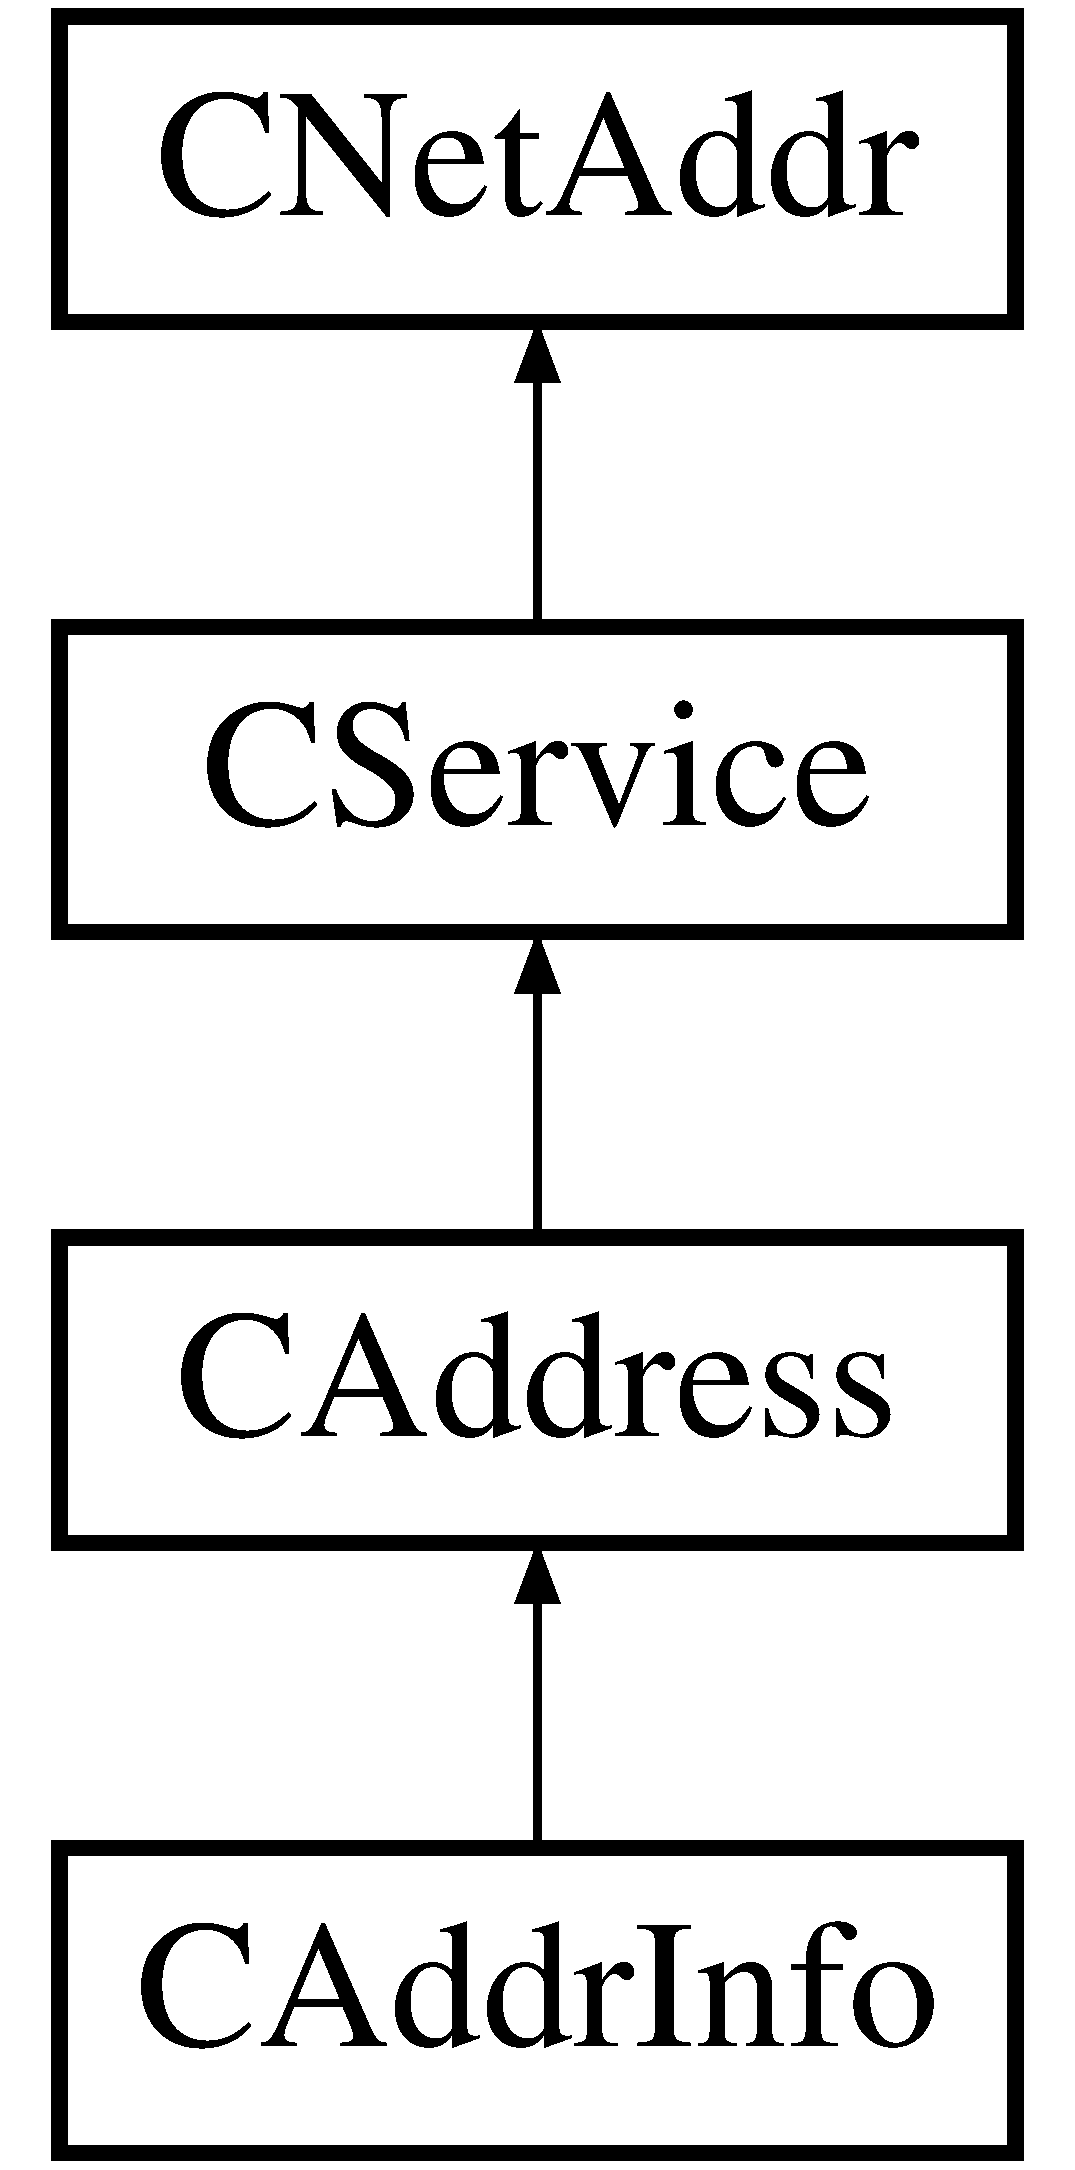
\includegraphics[height=4.000000cm]{class_c_service}
\end{center}
\end{figure}
\subsection*{Public Member Functions}
\begin{DoxyCompactItemize}
\item 
\mbox{\hyperlink{class_c_service_a3003da1c50f2135123ebb3109340b9b2}{C\+Service}} ()
\item 
\mbox{\hyperlink{class_c_service_a43a0d18387ce3837d48020da47a1087c}{C\+Service}} (const \mbox{\hyperlink{class_c_net_addr}{C\+Net\+Addr}} \&\mbox{\hyperlink{class_c_net_addr_acff7ce68f33f8dfbfe6d79d80928d417}{ip}}, unsigned short \mbox{\hyperlink{class_c_service_aef17734203dc2125cbdf4d23e50be410}{port}})
\item 
\mbox{\hyperlink{class_c_service_a1fcc14e589f6d3e92b43707a5f71368f}{C\+Service}} (const struct in\+\_\+addr \&ipv4\+Addr, unsigned short \mbox{\hyperlink{class_c_service_aef17734203dc2125cbdf4d23e50be410}{port}})
\item 
\mbox{\hyperlink{class_c_service_aa54fd9204530445647cd3d45056881e9}{C\+Service}} (const struct sockaddr\+\_\+in \&addr)
\item 
\mbox{\hyperlink{class_c_service_a75b2a3cfa16642b0fcd74382203a9fdc}{C\+Service}} (const char $\ast$psz\+Ip\+Port, int port\+Default, bool f\+Allow\+Lookup=false)
\item 
\mbox{\hyperlink{class_c_service_ab8f5f4ae4e99a4edad8ba48642e36137}{C\+Service}} (const char $\ast$psz\+Ip\+Port, bool f\+Allow\+Lookup=false)
\item 
\mbox{\hyperlink{class_c_service_a677f74b3520148f3e47a19bb9986922b}{C\+Service}} (const std\+::string \&str\+Ip\+Port, int port\+Default, bool f\+Allow\+Lookup=false)
\item 
\mbox{\hyperlink{class_c_service_a19a7a713dd9a30b2f78260e61d9a2604}{C\+Service}} (const std\+::string \&str\+Ip\+Port, bool f\+Allow\+Lookup=false)
\item 
void \mbox{\hyperlink{class_c_service_aee07d7f18e672f16d26359e3cab779ff}{Init}} ()
\item 
void \mbox{\hyperlink{class_c_service_a3dedc3f12aa21bdbf1068b054d3e3d39}{Set\+Port}} (unsigned short port\+In)
\item 
unsigned short \mbox{\hyperlink{class_c_service_a71caa0d6aa6ab12758bde8b6a6bcfd2a}{Get\+Port}} () const
\item 
bool \mbox{\hyperlink{class_c_service_ac4c6d655fab3af40937f0b0c65581745}{Get\+Sock\+Addr}} (struct sockaddr $\ast$paddr, socklen\+\_\+t $\ast$addrlen) const
\item 
bool \mbox{\hyperlink{class_c_service_a77782219f5d85f326b4c089cb2636e6f}{Set\+Sock\+Addr}} (const struct sockaddr $\ast$paddr)
\item 
std\+::vector$<$ unsigned char $>$ \mbox{\hyperlink{class_c_service_af21ea7db4318330b337c8bfdcc55aff0}{Get\+Key}} () const
\item 
std\+::string \mbox{\hyperlink{class_c_service_a95d6f24b6a613fca24734ba4e38ef3dc}{To\+String\+Port}} () const
\item 
std\+::string \mbox{\hyperlink{class_c_service_ae274e8b6fc38955d74044d326a405024}{To\+String}} (bool f\+Use\+Getnameinfo=true) const
\item 
std\+::string \mbox{\hyperlink{class_c_service_a75b6c84b3184ab809b6dda3576be78ee}{To\+String\+I\+P\+Port}} (bool f\+Use\+Getnameinfo=true) const
\item 
\mbox{\hyperlink{class_c_service_a92fd246e176f01266cb36beae0c8f4fe}{C\+Service}} (const struct in6\+\_\+addr \&ipv6\+Addr, unsigned short \mbox{\hyperlink{class_c_service_aef17734203dc2125cbdf4d23e50be410}{port}})
\item 
\mbox{\hyperlink{class_c_service_ac0eb3107507be78cc683e7a7fa8d56e4}{C\+Service}} (const struct sockaddr\+\_\+in6 \&addr)
\item 
{\footnotesize template$<$typename Stream , typename Operation $>$ }\\void \mbox{\hyperlink{class_c_service_a0673ebec7bdc8558ce3fe1d63ea4d2e1}{Serialization\+Op}} (Stream \&s, Operation ser\+\_\+action, int n\+Type, int n\+Version)
\end{DoxyCompactItemize}
\subsection*{Public Attributes}
\begin{DoxyCompactItemize}
\item 
\mbox{\hyperlink{class_c_service_a3347aa84bd8f98ae853307ad4e47a4f5}{A\+D\+D\+\_\+\+S\+E\+R\+I\+A\+L\+I\+Z\+E\+\_\+\+M\+E\+T\+H\+O\+DS}}
\end{DoxyCompactItemize}
\subsection*{Protected Attributes}
\begin{DoxyCompactItemize}
\item 
unsigned short \mbox{\hyperlink{class_c_service_aef17734203dc2125cbdf4d23e50be410}{port}}
\end{DoxyCompactItemize}
\subsection*{Friends}
\begin{DoxyCompactItemize}
\item 
bool \mbox{\hyperlink{class_c_service_a7abc2516fa7e015cafcf9b98bc33e2ea}{operator==}} (const \mbox{\hyperlink{class_c_service}{C\+Service}} \&a, const \mbox{\hyperlink{class_c_service}{C\+Service}} \&b)
\item 
bool \mbox{\hyperlink{class_c_service_a5834e0ab5104fffac621ea53fa2c3860}{operator!=}} (const \mbox{\hyperlink{class_c_service}{C\+Service}} \&a, const \mbox{\hyperlink{class_c_service}{C\+Service}} \&b)
\item 
bool \mbox{\hyperlink{class_c_service_a26d0e22a8e7ae213b25467da3556c9e4}{operator$<$}} (const \mbox{\hyperlink{class_c_service}{C\+Service}} \&a, const \mbox{\hyperlink{class_c_service}{C\+Service}} \&b)
\end{DoxyCompactItemize}


\subsection{Detailed Description}
A combination of a network address (\mbox{\hyperlink{class_c_net_addr}{C\+Net\+Addr}}) and a (T\+CP) port 

\subsection{Constructor \& Destructor Documentation}
\mbox{\Hypertarget{class_c_service_a3003da1c50f2135123ebb3109340b9b2}\label{class_c_service_a3003da1c50f2135123ebb3109340b9b2}} 
\index{C\+Service@{C\+Service}!C\+Service@{C\+Service}}
\index{C\+Service@{C\+Service}!C\+Service@{C\+Service}}
\subsubsection{\texorpdfstring{C\+Service()}{CService()}\hspace{0.1cm}{\footnotesize\ttfamily [1/10]}}
{\footnotesize\ttfamily C\+Service\+::\+C\+Service (\begin{DoxyParamCaption}{ }\end{DoxyParamCaption})}

\mbox{\Hypertarget{class_c_service_a43a0d18387ce3837d48020da47a1087c}\label{class_c_service_a43a0d18387ce3837d48020da47a1087c}} 
\index{C\+Service@{C\+Service}!C\+Service@{C\+Service}}
\index{C\+Service@{C\+Service}!C\+Service@{C\+Service}}
\subsubsection{\texorpdfstring{C\+Service()}{CService()}\hspace{0.1cm}{\footnotesize\ttfamily [2/10]}}
{\footnotesize\ttfamily C\+Service\+::\+C\+Service (\begin{DoxyParamCaption}\item[{const \mbox{\hyperlink{class_c_net_addr}{C\+Net\+Addr}} \&}]{ip,  }\item[{unsigned short}]{port }\end{DoxyParamCaption})}

\mbox{\Hypertarget{class_c_service_a1fcc14e589f6d3e92b43707a5f71368f}\label{class_c_service_a1fcc14e589f6d3e92b43707a5f71368f}} 
\index{C\+Service@{C\+Service}!C\+Service@{C\+Service}}
\index{C\+Service@{C\+Service}!C\+Service@{C\+Service}}
\subsubsection{\texorpdfstring{C\+Service()}{CService()}\hspace{0.1cm}{\footnotesize\ttfamily [3/10]}}
{\footnotesize\ttfamily C\+Service\+::\+C\+Service (\begin{DoxyParamCaption}\item[{const struct in\+\_\+addr \&}]{ipv4\+Addr,  }\item[{unsigned short}]{port }\end{DoxyParamCaption})}

\mbox{\Hypertarget{class_c_service_aa54fd9204530445647cd3d45056881e9}\label{class_c_service_aa54fd9204530445647cd3d45056881e9}} 
\index{C\+Service@{C\+Service}!C\+Service@{C\+Service}}
\index{C\+Service@{C\+Service}!C\+Service@{C\+Service}}
\subsubsection{\texorpdfstring{C\+Service()}{CService()}\hspace{0.1cm}{\footnotesize\ttfamily [4/10]}}
{\footnotesize\ttfamily C\+Service\+::\+C\+Service (\begin{DoxyParamCaption}\item[{const struct sockaddr\+\_\+in \&}]{addr }\end{DoxyParamCaption})}

\mbox{\Hypertarget{class_c_service_a75b2a3cfa16642b0fcd74382203a9fdc}\label{class_c_service_a75b2a3cfa16642b0fcd74382203a9fdc}} 
\index{C\+Service@{C\+Service}!C\+Service@{C\+Service}}
\index{C\+Service@{C\+Service}!C\+Service@{C\+Service}}
\subsubsection{\texorpdfstring{C\+Service()}{CService()}\hspace{0.1cm}{\footnotesize\ttfamily [5/10]}}
{\footnotesize\ttfamily C\+Service\+::\+C\+Service (\begin{DoxyParamCaption}\item[{const char $\ast$}]{psz\+Ip\+Port,  }\item[{int}]{port\+Default,  }\item[{bool}]{f\+Allow\+Lookup = {\ttfamily false} }\end{DoxyParamCaption})\hspace{0.3cm}{\ttfamily [explicit]}}

\mbox{\Hypertarget{class_c_service_ab8f5f4ae4e99a4edad8ba48642e36137}\label{class_c_service_ab8f5f4ae4e99a4edad8ba48642e36137}} 
\index{C\+Service@{C\+Service}!C\+Service@{C\+Service}}
\index{C\+Service@{C\+Service}!C\+Service@{C\+Service}}
\subsubsection{\texorpdfstring{C\+Service()}{CService()}\hspace{0.1cm}{\footnotesize\ttfamily [6/10]}}
{\footnotesize\ttfamily C\+Service\+::\+C\+Service (\begin{DoxyParamCaption}\item[{const char $\ast$}]{psz\+Ip\+Port,  }\item[{bool}]{f\+Allow\+Lookup = {\ttfamily false} }\end{DoxyParamCaption})\hspace{0.3cm}{\ttfamily [explicit]}}

\mbox{\Hypertarget{class_c_service_a677f74b3520148f3e47a19bb9986922b}\label{class_c_service_a677f74b3520148f3e47a19bb9986922b}} 
\index{C\+Service@{C\+Service}!C\+Service@{C\+Service}}
\index{C\+Service@{C\+Service}!C\+Service@{C\+Service}}
\subsubsection{\texorpdfstring{C\+Service()}{CService()}\hspace{0.1cm}{\footnotesize\ttfamily [7/10]}}
{\footnotesize\ttfamily C\+Service\+::\+C\+Service (\begin{DoxyParamCaption}\item[{const std\+::string \&}]{str\+Ip\+Port,  }\item[{int}]{port\+Default,  }\item[{bool}]{f\+Allow\+Lookup = {\ttfamily false} }\end{DoxyParamCaption})\hspace{0.3cm}{\ttfamily [explicit]}}

\mbox{\Hypertarget{class_c_service_a19a7a713dd9a30b2f78260e61d9a2604}\label{class_c_service_a19a7a713dd9a30b2f78260e61d9a2604}} 
\index{C\+Service@{C\+Service}!C\+Service@{C\+Service}}
\index{C\+Service@{C\+Service}!C\+Service@{C\+Service}}
\subsubsection{\texorpdfstring{C\+Service()}{CService()}\hspace{0.1cm}{\footnotesize\ttfamily [8/10]}}
{\footnotesize\ttfamily C\+Service\+::\+C\+Service (\begin{DoxyParamCaption}\item[{const std\+::string \&}]{str\+Ip\+Port,  }\item[{bool}]{f\+Allow\+Lookup = {\ttfamily false} }\end{DoxyParamCaption})\hspace{0.3cm}{\ttfamily [explicit]}}

\mbox{\Hypertarget{class_c_service_a92fd246e176f01266cb36beae0c8f4fe}\label{class_c_service_a92fd246e176f01266cb36beae0c8f4fe}} 
\index{C\+Service@{C\+Service}!C\+Service@{C\+Service}}
\index{C\+Service@{C\+Service}!C\+Service@{C\+Service}}
\subsubsection{\texorpdfstring{C\+Service()}{CService()}\hspace{0.1cm}{\footnotesize\ttfamily [9/10]}}
{\footnotesize\ttfamily C\+Service\+::\+C\+Service (\begin{DoxyParamCaption}\item[{const struct in6\+\_\+addr \&}]{ipv6\+Addr,  }\item[{unsigned short}]{port }\end{DoxyParamCaption})}

\mbox{\Hypertarget{class_c_service_ac0eb3107507be78cc683e7a7fa8d56e4}\label{class_c_service_ac0eb3107507be78cc683e7a7fa8d56e4}} 
\index{C\+Service@{C\+Service}!C\+Service@{C\+Service}}
\index{C\+Service@{C\+Service}!C\+Service@{C\+Service}}
\subsubsection{\texorpdfstring{C\+Service()}{CService()}\hspace{0.1cm}{\footnotesize\ttfamily [10/10]}}
{\footnotesize\ttfamily C\+Service\+::\+C\+Service (\begin{DoxyParamCaption}\item[{const struct sockaddr\+\_\+in6 \&}]{addr }\end{DoxyParamCaption})}



\subsection{Member Function Documentation}
\mbox{\Hypertarget{class_c_service_af21ea7db4318330b337c8bfdcc55aff0}\label{class_c_service_af21ea7db4318330b337c8bfdcc55aff0}} 
\index{C\+Service@{C\+Service}!Get\+Key@{Get\+Key}}
\index{Get\+Key@{Get\+Key}!C\+Service@{C\+Service}}
\subsubsection{\texorpdfstring{Get\+Key()}{GetKey()}}
{\footnotesize\ttfamily std\+::vector$<$ unsigned char $>$ C\+Service\+::\+Get\+Key (\begin{DoxyParamCaption}{ }\end{DoxyParamCaption}) const}

\mbox{\Hypertarget{class_c_service_a71caa0d6aa6ab12758bde8b6a6bcfd2a}\label{class_c_service_a71caa0d6aa6ab12758bde8b6a6bcfd2a}} 
\index{C\+Service@{C\+Service}!Get\+Port@{Get\+Port}}
\index{Get\+Port@{Get\+Port}!C\+Service@{C\+Service}}
\subsubsection{\texorpdfstring{Get\+Port()}{GetPort()}}
{\footnotesize\ttfamily unsigned short C\+Service\+::\+Get\+Port (\begin{DoxyParamCaption}{ }\end{DoxyParamCaption}) const}

\mbox{\Hypertarget{class_c_service_ac4c6d655fab3af40937f0b0c65581745}\label{class_c_service_ac4c6d655fab3af40937f0b0c65581745}} 
\index{C\+Service@{C\+Service}!Get\+Sock\+Addr@{Get\+Sock\+Addr}}
\index{Get\+Sock\+Addr@{Get\+Sock\+Addr}!C\+Service@{C\+Service}}
\subsubsection{\texorpdfstring{Get\+Sock\+Addr()}{GetSockAddr()}}
{\footnotesize\ttfamily bool C\+Service\+::\+Get\+Sock\+Addr (\begin{DoxyParamCaption}\item[{struct sockaddr $\ast$}]{paddr,  }\item[{socklen\+\_\+t $\ast$}]{addrlen }\end{DoxyParamCaption}) const}

\mbox{\Hypertarget{class_c_service_aee07d7f18e672f16d26359e3cab779ff}\label{class_c_service_aee07d7f18e672f16d26359e3cab779ff}} 
\index{C\+Service@{C\+Service}!Init@{Init}}
\index{Init@{Init}!C\+Service@{C\+Service}}
\subsubsection{\texorpdfstring{Init()}{Init()}}
{\footnotesize\ttfamily void C\+Service\+::\+Init (\begin{DoxyParamCaption}{ }\end{DoxyParamCaption})}

\mbox{\Hypertarget{class_c_service_a0673ebec7bdc8558ce3fe1d63ea4d2e1}\label{class_c_service_a0673ebec7bdc8558ce3fe1d63ea4d2e1}} 
\index{C\+Service@{C\+Service}!Serialization\+Op@{Serialization\+Op}}
\index{Serialization\+Op@{Serialization\+Op}!C\+Service@{C\+Service}}
\subsubsection{\texorpdfstring{Serialization\+Op()}{SerializationOp()}}
{\footnotesize\ttfamily template$<$typename Stream , typename Operation $>$ \\
void C\+Service\+::\+Serialization\+Op (\begin{DoxyParamCaption}\item[{Stream \&}]{s,  }\item[{Operation}]{ser\+\_\+action,  }\item[{int}]{n\+Type,  }\item[{int}]{n\+Version }\end{DoxyParamCaption})\hspace{0.3cm}{\ttfamily [inline]}}

\mbox{\Hypertarget{class_c_service_a3dedc3f12aa21bdbf1068b054d3e3d39}\label{class_c_service_a3dedc3f12aa21bdbf1068b054d3e3d39}} 
\index{C\+Service@{C\+Service}!Set\+Port@{Set\+Port}}
\index{Set\+Port@{Set\+Port}!C\+Service@{C\+Service}}
\subsubsection{\texorpdfstring{Set\+Port()}{SetPort()}}
{\footnotesize\ttfamily void C\+Service\+::\+Set\+Port (\begin{DoxyParamCaption}\item[{unsigned short}]{port\+In }\end{DoxyParamCaption})}

\mbox{\Hypertarget{class_c_service_a77782219f5d85f326b4c089cb2636e6f}\label{class_c_service_a77782219f5d85f326b4c089cb2636e6f}} 
\index{C\+Service@{C\+Service}!Set\+Sock\+Addr@{Set\+Sock\+Addr}}
\index{Set\+Sock\+Addr@{Set\+Sock\+Addr}!C\+Service@{C\+Service}}
\subsubsection{\texorpdfstring{Set\+Sock\+Addr()}{SetSockAddr()}}
{\footnotesize\ttfamily bool C\+Service\+::\+Set\+Sock\+Addr (\begin{DoxyParamCaption}\item[{const struct sockaddr $\ast$}]{paddr }\end{DoxyParamCaption})}

\mbox{\Hypertarget{class_c_service_ae274e8b6fc38955d74044d326a405024}\label{class_c_service_ae274e8b6fc38955d74044d326a405024}} 
\index{C\+Service@{C\+Service}!To\+String@{To\+String}}
\index{To\+String@{To\+String}!C\+Service@{C\+Service}}
\subsubsection{\texorpdfstring{To\+String()}{ToString()}}
{\footnotesize\ttfamily std\+::string C\+Service\+::\+To\+String (\begin{DoxyParamCaption}\item[{bool}]{f\+Use\+Getnameinfo = {\ttfamily true} }\end{DoxyParamCaption}) const}

\mbox{\Hypertarget{class_c_service_a75b6c84b3184ab809b6dda3576be78ee}\label{class_c_service_a75b6c84b3184ab809b6dda3576be78ee}} 
\index{C\+Service@{C\+Service}!To\+String\+I\+P\+Port@{To\+String\+I\+P\+Port}}
\index{To\+String\+I\+P\+Port@{To\+String\+I\+P\+Port}!C\+Service@{C\+Service}}
\subsubsection{\texorpdfstring{To\+String\+I\+P\+Port()}{ToStringIPPort()}}
{\footnotesize\ttfamily std\+::string C\+Service\+::\+To\+String\+I\+P\+Port (\begin{DoxyParamCaption}\item[{bool}]{f\+Use\+Getnameinfo = {\ttfamily true} }\end{DoxyParamCaption}) const}

\mbox{\Hypertarget{class_c_service_a95d6f24b6a613fca24734ba4e38ef3dc}\label{class_c_service_a95d6f24b6a613fca24734ba4e38ef3dc}} 
\index{C\+Service@{C\+Service}!To\+String\+Port@{To\+String\+Port}}
\index{To\+String\+Port@{To\+String\+Port}!C\+Service@{C\+Service}}
\subsubsection{\texorpdfstring{To\+String\+Port()}{ToStringPort()}}
{\footnotesize\ttfamily std\+::string C\+Service\+::\+To\+String\+Port (\begin{DoxyParamCaption}{ }\end{DoxyParamCaption}) const}



\subsection{Friends And Related Function Documentation}
\mbox{\Hypertarget{class_c_service_a5834e0ab5104fffac621ea53fa2c3860}\label{class_c_service_a5834e0ab5104fffac621ea53fa2c3860}} 
\index{C\+Service@{C\+Service}!operator"!=@{operator"!=}}
\index{operator"!=@{operator"!=}!C\+Service@{C\+Service}}
\subsubsection{\texorpdfstring{operator"!=}{operator!=}}
{\footnotesize\ttfamily bool operator!= (\begin{DoxyParamCaption}\item[{const \mbox{\hyperlink{class_c_service}{C\+Service}} \&}]{a,  }\item[{const \mbox{\hyperlink{class_c_service}{C\+Service}} \&}]{b }\end{DoxyParamCaption})\hspace{0.3cm}{\ttfamily [friend]}}

\mbox{\Hypertarget{class_c_service_a26d0e22a8e7ae213b25467da3556c9e4}\label{class_c_service_a26d0e22a8e7ae213b25467da3556c9e4}} 
\index{C\+Service@{C\+Service}!operator$<$@{operator$<$}}
\index{operator$<$@{operator$<$}!C\+Service@{C\+Service}}
\subsubsection{\texorpdfstring{operator$<$}{operator<}}
{\footnotesize\ttfamily bool operator$<$ (\begin{DoxyParamCaption}\item[{const \mbox{\hyperlink{class_c_service}{C\+Service}} \&}]{a,  }\item[{const \mbox{\hyperlink{class_c_service}{C\+Service}} \&}]{b }\end{DoxyParamCaption})\hspace{0.3cm}{\ttfamily [friend]}}

\mbox{\Hypertarget{class_c_service_a7abc2516fa7e015cafcf9b98bc33e2ea}\label{class_c_service_a7abc2516fa7e015cafcf9b98bc33e2ea}} 
\index{C\+Service@{C\+Service}!operator==@{operator==}}
\index{operator==@{operator==}!C\+Service@{C\+Service}}
\subsubsection{\texorpdfstring{operator==}{operator==}}
{\footnotesize\ttfamily bool operator== (\begin{DoxyParamCaption}\item[{const \mbox{\hyperlink{class_c_service}{C\+Service}} \&}]{a,  }\item[{const \mbox{\hyperlink{class_c_service}{C\+Service}} \&}]{b }\end{DoxyParamCaption})\hspace{0.3cm}{\ttfamily [friend]}}



\subsection{Member Data Documentation}
\mbox{\Hypertarget{class_c_service_a3347aa84bd8f98ae853307ad4e47a4f5}\label{class_c_service_a3347aa84bd8f98ae853307ad4e47a4f5}} 
\index{C\+Service@{C\+Service}!A\+D\+D\+\_\+\+S\+E\+R\+I\+A\+L\+I\+Z\+E\+\_\+\+M\+E\+T\+H\+O\+DS@{A\+D\+D\+\_\+\+S\+E\+R\+I\+A\+L\+I\+Z\+E\+\_\+\+M\+E\+T\+H\+O\+DS}}
\index{A\+D\+D\+\_\+\+S\+E\+R\+I\+A\+L\+I\+Z\+E\+\_\+\+M\+E\+T\+H\+O\+DS@{A\+D\+D\+\_\+\+S\+E\+R\+I\+A\+L\+I\+Z\+E\+\_\+\+M\+E\+T\+H\+O\+DS}!C\+Service@{C\+Service}}
\subsubsection{\texorpdfstring{A\+D\+D\+\_\+\+S\+E\+R\+I\+A\+L\+I\+Z\+E\+\_\+\+M\+E\+T\+H\+O\+DS}{ADD\_SERIALIZE\_METHODS}}
{\footnotesize\ttfamily C\+Service\+::\+A\+D\+D\+\_\+\+S\+E\+R\+I\+A\+L\+I\+Z\+E\+\_\+\+M\+E\+T\+H\+O\+DS}

\mbox{\Hypertarget{class_c_service_aef17734203dc2125cbdf4d23e50be410}\label{class_c_service_aef17734203dc2125cbdf4d23e50be410}} 
\index{C\+Service@{C\+Service}!port@{port}}
\index{port@{port}!C\+Service@{C\+Service}}
\subsubsection{\texorpdfstring{port}{port}}
{\footnotesize\ttfamily unsigned short C\+Service\+::port\hspace{0.3cm}{\ttfamily [protected]}}



The documentation for this class was generated from the following files\+:\begin{DoxyCompactItemize}
\item 
/\+Users/christopherarguello/\+Developer/anon/src/\mbox{\hyperlink{netbase_8h}{netbase.\+h}}\item 
/\+Users/christopherarguello/\+Developer/anon/src/\mbox{\hyperlink{netbase_8cpp}{netbase.\+cpp}}\end{DoxyCompactItemize}

\hypertarget{class_c_size_computer}{}\section{C\+Size\+Computer Class Reference}
\label{class_c_size_computer}\index{C\+Size\+Computer@{C\+Size\+Computer}}


{\ttfamily \#include $<$serialize.\+h$>$}

\subsection*{Public Member Functions}
\begin{DoxyCompactItemize}
\item 
\mbox{\hyperlink{class_c_size_computer_a475a1a15be285c38c4b94ad0ab0ce73c}{C\+Size\+Computer}} (int n\+Type\+In, int n\+Version\+In)
\item 
\mbox{\hyperlink{class_c_size_computer}{C\+Size\+Computer}} \& \mbox{\hyperlink{class_c_size_computer_ad4b4f5e37acacf894f60c728e694ee89}{write}} (const char $\ast$psz, size\+\_\+t \mbox{\hyperlink{class_c_size_computer_a3ea758bb100dd9ce38071e040cd3c597}{n\+Size}})
\item 
{\footnotesize template$<$typename T $>$ }\\\mbox{\hyperlink{class_c_size_computer}{C\+Size\+Computer}} \& \mbox{\hyperlink{class_c_size_computer_a03a29c76f82dca1559e7922b35bebd0d}{operator$<$$<$}} (const T \&obj)
\item 
size\+\_\+t \mbox{\hyperlink{class_c_size_computer_a649d670bdcfee2b47a1982af566d3d7d}{size}} () const
\end{DoxyCompactItemize}
\subsection*{Public Attributes}
\begin{DoxyCompactItemize}
\item 
int \mbox{\hyperlink{class_c_size_computer_a1f166e95dc06a6f3718b2fac9cda18ee}{n\+Type}}
\item 
int \mbox{\hyperlink{class_c_size_computer_a25759db1089e475fcba2f408633dc7bf}{n\+Version}}
\end{DoxyCompactItemize}
\subsection*{Protected Attributes}
\begin{DoxyCompactItemize}
\item 
size\+\_\+t \mbox{\hyperlink{class_c_size_computer_a3ea758bb100dd9ce38071e040cd3c597}{n\+Size}}
\end{DoxyCompactItemize}


\subsection{Constructor \& Destructor Documentation}
\mbox{\Hypertarget{class_c_size_computer_a475a1a15be285c38c4b94ad0ab0ce73c}\label{class_c_size_computer_a475a1a15be285c38c4b94ad0ab0ce73c}} 
\index{C\+Size\+Computer@{C\+Size\+Computer}!C\+Size\+Computer@{C\+Size\+Computer}}
\index{C\+Size\+Computer@{C\+Size\+Computer}!C\+Size\+Computer@{C\+Size\+Computer}}
\subsubsection{\texorpdfstring{C\+Size\+Computer()}{CSizeComputer()}}
{\footnotesize\ttfamily C\+Size\+Computer\+::\+C\+Size\+Computer (\begin{DoxyParamCaption}\item[{int}]{n\+Type\+In,  }\item[{int}]{n\+Version\+In }\end{DoxyParamCaption})\hspace{0.3cm}{\ttfamily [inline]}}



\subsection{Member Function Documentation}
\mbox{\Hypertarget{class_c_size_computer_a03a29c76f82dca1559e7922b35bebd0d}\label{class_c_size_computer_a03a29c76f82dca1559e7922b35bebd0d}} 
\index{C\+Size\+Computer@{C\+Size\+Computer}!operator$<$$<$@{operator$<$$<$}}
\index{operator$<$$<$@{operator$<$$<$}!C\+Size\+Computer@{C\+Size\+Computer}}
\subsubsection{\texorpdfstring{operator$<$$<$()}{operator<<()}}
{\footnotesize\ttfamily template$<$typename T $>$ \\
\mbox{\hyperlink{class_c_size_computer}{C\+Size\+Computer}}\& C\+Size\+Computer\+::operator$<$$<$ (\begin{DoxyParamCaption}\item[{const T \&}]{obj }\end{DoxyParamCaption})\hspace{0.3cm}{\ttfamily [inline]}}

\mbox{\Hypertarget{class_c_size_computer_a649d670bdcfee2b47a1982af566d3d7d}\label{class_c_size_computer_a649d670bdcfee2b47a1982af566d3d7d}} 
\index{C\+Size\+Computer@{C\+Size\+Computer}!size@{size}}
\index{size@{size}!C\+Size\+Computer@{C\+Size\+Computer}}
\subsubsection{\texorpdfstring{size()}{size()}}
{\footnotesize\ttfamily size\+\_\+t C\+Size\+Computer\+::size (\begin{DoxyParamCaption}{ }\end{DoxyParamCaption}) const\hspace{0.3cm}{\ttfamily [inline]}}

\mbox{\Hypertarget{class_c_size_computer_ad4b4f5e37acacf894f60c728e694ee89}\label{class_c_size_computer_ad4b4f5e37acacf894f60c728e694ee89}} 
\index{C\+Size\+Computer@{C\+Size\+Computer}!write@{write}}
\index{write@{write}!C\+Size\+Computer@{C\+Size\+Computer}}
\subsubsection{\texorpdfstring{write()}{write()}}
{\footnotesize\ttfamily \mbox{\hyperlink{class_c_size_computer}{C\+Size\+Computer}}\& C\+Size\+Computer\+::write (\begin{DoxyParamCaption}\item[{const char $\ast$}]{psz,  }\item[{size\+\_\+t}]{n\+Size }\end{DoxyParamCaption})\hspace{0.3cm}{\ttfamily [inline]}}



\subsection{Member Data Documentation}
\mbox{\Hypertarget{class_c_size_computer_a3ea758bb100dd9ce38071e040cd3c597}\label{class_c_size_computer_a3ea758bb100dd9ce38071e040cd3c597}} 
\index{C\+Size\+Computer@{C\+Size\+Computer}!n\+Size@{n\+Size}}
\index{n\+Size@{n\+Size}!C\+Size\+Computer@{C\+Size\+Computer}}
\subsubsection{\texorpdfstring{n\+Size}{nSize}}
{\footnotesize\ttfamily size\+\_\+t C\+Size\+Computer\+::n\+Size\hspace{0.3cm}{\ttfamily [protected]}}

\mbox{\Hypertarget{class_c_size_computer_a1f166e95dc06a6f3718b2fac9cda18ee}\label{class_c_size_computer_a1f166e95dc06a6f3718b2fac9cda18ee}} 
\index{C\+Size\+Computer@{C\+Size\+Computer}!n\+Type@{n\+Type}}
\index{n\+Type@{n\+Type}!C\+Size\+Computer@{C\+Size\+Computer}}
\subsubsection{\texorpdfstring{n\+Type}{nType}}
{\footnotesize\ttfamily int C\+Size\+Computer\+::n\+Type}

\mbox{\Hypertarget{class_c_size_computer_a25759db1089e475fcba2f408633dc7bf}\label{class_c_size_computer_a25759db1089e475fcba2f408633dc7bf}} 
\index{C\+Size\+Computer@{C\+Size\+Computer}!n\+Version@{n\+Version}}
\index{n\+Version@{n\+Version}!C\+Size\+Computer@{C\+Size\+Computer}}
\subsubsection{\texorpdfstring{n\+Version}{nVersion}}
{\footnotesize\ttfamily int C\+Size\+Computer\+::n\+Version}



The documentation for this class was generated from the following file\+:\begin{DoxyCompactItemize}
\item 
/\+Users/christopherarguello/\+Developer/anon/src/\mbox{\hyperlink{serialize_8h}{serialize.\+h}}\end{DoxyCompactItemize}

\hypertarget{struct_c_spent_index_key}{}\section{C\+Spent\+Index\+Key Struct Reference}
\label{struct_c_spent_index_key}\index{C\+Spent\+Index\+Key@{C\+Spent\+Index\+Key}}


{\ttfamily \#include $<$spentindex.\+h$>$}

\subsection*{Public Member Functions}
\begin{DoxyCompactItemize}
\item 
{\footnotesize template$<$typename Stream , typename Operation $>$ }\\void \mbox{\hyperlink{struct_c_spent_index_key_a1bd965f78b96ed61cf3c51ef36380d82}{Serialization\+Op}} (Stream \&s, Operation ser\+\_\+action, int n\+Type, int n\+Version)
\item 
\mbox{\hyperlink{struct_c_spent_index_key_a15000293a642ba8401427d55e94f3991}{C\+Spent\+Index\+Key}} (\mbox{\hyperlink{classuint256}{uint256}} t, unsigned int i)
\item 
\mbox{\hyperlink{struct_c_spent_index_key_a06486e70f11c6184e27247cc17fc37c1}{C\+Spent\+Index\+Key}} ()
\item 
void \mbox{\hyperlink{struct_c_spent_index_key_aebd848cd3e3e416c96517526fba9a20b}{Set\+Null}} ()
\end{DoxyCompactItemize}
\subsection*{Public Attributes}
\begin{DoxyCompactItemize}
\item 
\mbox{\hyperlink{classuint256}{uint256}} \mbox{\hyperlink{struct_c_spent_index_key_a98f9dd57f9af971b4787ad7ede026f43}{txid}}
\item 
unsigned int \mbox{\hyperlink{struct_c_spent_index_key_a13e6f9f822146526c8112acce999a709}{output\+Index}}
\item 
\mbox{\hyperlink{struct_c_spent_index_key_a4fcfc6a12bc3fdea29994a569c204315}{A\+D\+D\+\_\+\+S\+E\+R\+I\+A\+L\+I\+Z\+E\+\_\+\+M\+E\+T\+H\+O\+DS}}
\end{DoxyCompactItemize}


\subsection{Constructor \& Destructor Documentation}
\mbox{\Hypertarget{struct_c_spent_index_key_a15000293a642ba8401427d55e94f3991}\label{struct_c_spent_index_key_a15000293a642ba8401427d55e94f3991}} 
\index{C\+Spent\+Index\+Key@{C\+Spent\+Index\+Key}!C\+Spent\+Index\+Key@{C\+Spent\+Index\+Key}}
\index{C\+Spent\+Index\+Key@{C\+Spent\+Index\+Key}!C\+Spent\+Index\+Key@{C\+Spent\+Index\+Key}}
\subsubsection{\texorpdfstring{C\+Spent\+Index\+Key()}{CSpentIndexKey()}\hspace{0.1cm}{\footnotesize\ttfamily [1/2]}}
{\footnotesize\ttfamily C\+Spent\+Index\+Key\+::\+C\+Spent\+Index\+Key (\begin{DoxyParamCaption}\item[{\mbox{\hyperlink{classuint256}{uint256}}}]{t,  }\item[{unsigned int}]{i }\end{DoxyParamCaption})\hspace{0.3cm}{\ttfamily [inline]}}

\mbox{\Hypertarget{struct_c_spent_index_key_a06486e70f11c6184e27247cc17fc37c1}\label{struct_c_spent_index_key_a06486e70f11c6184e27247cc17fc37c1}} 
\index{C\+Spent\+Index\+Key@{C\+Spent\+Index\+Key}!C\+Spent\+Index\+Key@{C\+Spent\+Index\+Key}}
\index{C\+Spent\+Index\+Key@{C\+Spent\+Index\+Key}!C\+Spent\+Index\+Key@{C\+Spent\+Index\+Key}}
\subsubsection{\texorpdfstring{C\+Spent\+Index\+Key()}{CSpentIndexKey()}\hspace{0.1cm}{\footnotesize\ttfamily [2/2]}}
{\footnotesize\ttfamily C\+Spent\+Index\+Key\+::\+C\+Spent\+Index\+Key (\begin{DoxyParamCaption}{ }\end{DoxyParamCaption})\hspace{0.3cm}{\ttfamily [inline]}}



\subsection{Member Function Documentation}
\mbox{\Hypertarget{struct_c_spent_index_key_a1bd965f78b96ed61cf3c51ef36380d82}\label{struct_c_spent_index_key_a1bd965f78b96ed61cf3c51ef36380d82}} 
\index{C\+Spent\+Index\+Key@{C\+Spent\+Index\+Key}!Serialization\+Op@{Serialization\+Op}}
\index{Serialization\+Op@{Serialization\+Op}!C\+Spent\+Index\+Key@{C\+Spent\+Index\+Key}}
\subsubsection{\texorpdfstring{Serialization\+Op()}{SerializationOp()}}
{\footnotesize\ttfamily template$<$typename Stream , typename Operation $>$ \\
void C\+Spent\+Index\+Key\+::\+Serialization\+Op (\begin{DoxyParamCaption}\item[{Stream \&}]{s,  }\item[{Operation}]{ser\+\_\+action,  }\item[{int}]{n\+Type,  }\item[{int}]{n\+Version }\end{DoxyParamCaption})\hspace{0.3cm}{\ttfamily [inline]}}

\mbox{\Hypertarget{struct_c_spent_index_key_aebd848cd3e3e416c96517526fba9a20b}\label{struct_c_spent_index_key_aebd848cd3e3e416c96517526fba9a20b}} 
\index{C\+Spent\+Index\+Key@{C\+Spent\+Index\+Key}!Set\+Null@{Set\+Null}}
\index{Set\+Null@{Set\+Null}!C\+Spent\+Index\+Key@{C\+Spent\+Index\+Key}}
\subsubsection{\texorpdfstring{Set\+Null()}{SetNull()}}
{\footnotesize\ttfamily void C\+Spent\+Index\+Key\+::\+Set\+Null (\begin{DoxyParamCaption}{ }\end{DoxyParamCaption})\hspace{0.3cm}{\ttfamily [inline]}}



\subsection{Member Data Documentation}
\mbox{\Hypertarget{struct_c_spent_index_key_a4fcfc6a12bc3fdea29994a569c204315}\label{struct_c_spent_index_key_a4fcfc6a12bc3fdea29994a569c204315}} 
\index{C\+Spent\+Index\+Key@{C\+Spent\+Index\+Key}!A\+D\+D\+\_\+\+S\+E\+R\+I\+A\+L\+I\+Z\+E\+\_\+\+M\+E\+T\+H\+O\+DS@{A\+D\+D\+\_\+\+S\+E\+R\+I\+A\+L\+I\+Z\+E\+\_\+\+M\+E\+T\+H\+O\+DS}}
\index{A\+D\+D\+\_\+\+S\+E\+R\+I\+A\+L\+I\+Z\+E\+\_\+\+M\+E\+T\+H\+O\+DS@{A\+D\+D\+\_\+\+S\+E\+R\+I\+A\+L\+I\+Z\+E\+\_\+\+M\+E\+T\+H\+O\+DS}!C\+Spent\+Index\+Key@{C\+Spent\+Index\+Key}}
\subsubsection{\texorpdfstring{A\+D\+D\+\_\+\+S\+E\+R\+I\+A\+L\+I\+Z\+E\+\_\+\+M\+E\+T\+H\+O\+DS}{ADD\_SERIALIZE\_METHODS}}
{\footnotesize\ttfamily C\+Spent\+Index\+Key\+::\+A\+D\+D\+\_\+\+S\+E\+R\+I\+A\+L\+I\+Z\+E\+\_\+\+M\+E\+T\+H\+O\+DS}

\mbox{\Hypertarget{struct_c_spent_index_key_a13e6f9f822146526c8112acce999a709}\label{struct_c_spent_index_key_a13e6f9f822146526c8112acce999a709}} 
\index{C\+Spent\+Index\+Key@{C\+Spent\+Index\+Key}!output\+Index@{output\+Index}}
\index{output\+Index@{output\+Index}!C\+Spent\+Index\+Key@{C\+Spent\+Index\+Key}}
\subsubsection{\texorpdfstring{output\+Index}{outputIndex}}
{\footnotesize\ttfamily unsigned int C\+Spent\+Index\+Key\+::output\+Index}

\mbox{\Hypertarget{struct_c_spent_index_key_a98f9dd57f9af971b4787ad7ede026f43}\label{struct_c_spent_index_key_a98f9dd57f9af971b4787ad7ede026f43}} 
\index{C\+Spent\+Index\+Key@{C\+Spent\+Index\+Key}!txid@{txid}}
\index{txid@{txid}!C\+Spent\+Index\+Key@{C\+Spent\+Index\+Key}}
\subsubsection{\texorpdfstring{txid}{txid}}
{\footnotesize\ttfamily \mbox{\hyperlink{classuint256}{uint256}} C\+Spent\+Index\+Key\+::txid}



The documentation for this struct was generated from the following file\+:\begin{DoxyCompactItemize}
\item 
/\+Users/christopherarguello/\+Developer/anon/src/\mbox{\hyperlink{spentindex_8h}{spentindex.\+h}}\end{DoxyCompactItemize}

\hypertarget{struct_c_spent_index_key_compare}{}\section{C\+Spent\+Index\+Key\+Compare Struct Reference}
\label{struct_c_spent_index_key_compare}\index{C\+Spent\+Index\+Key\+Compare@{C\+Spent\+Index\+Key\+Compare}}


{\ttfamily \#include $<$spentindex.\+h$>$}

\subsection*{Public Member Functions}
\begin{DoxyCompactItemize}
\item 
bool \mbox{\hyperlink{struct_c_spent_index_key_compare_a64b75193a523be2b351cd8e382bcef41}{operator()}} (const \mbox{\hyperlink{struct_c_spent_index_key}{C\+Spent\+Index\+Key}} \&a, const \mbox{\hyperlink{struct_c_spent_index_key}{C\+Spent\+Index\+Key}} \&b) const
\end{DoxyCompactItemize}


\subsection{Member Function Documentation}
\mbox{\Hypertarget{struct_c_spent_index_key_compare_a64b75193a523be2b351cd8e382bcef41}\label{struct_c_spent_index_key_compare_a64b75193a523be2b351cd8e382bcef41}} 
\index{C\+Spent\+Index\+Key\+Compare@{C\+Spent\+Index\+Key\+Compare}!operator()@{operator()}}
\index{operator()@{operator()}!C\+Spent\+Index\+Key\+Compare@{C\+Spent\+Index\+Key\+Compare}}
\subsubsection{\texorpdfstring{operator()()}{operator()()}}
{\footnotesize\ttfamily bool C\+Spent\+Index\+Key\+Compare\+::operator() (\begin{DoxyParamCaption}\item[{const \mbox{\hyperlink{struct_c_spent_index_key}{C\+Spent\+Index\+Key}} \&}]{a,  }\item[{const \mbox{\hyperlink{struct_c_spent_index_key}{C\+Spent\+Index\+Key}} \&}]{b }\end{DoxyParamCaption}) const\hspace{0.3cm}{\ttfamily [inline]}}



The documentation for this struct was generated from the following file\+:\begin{DoxyCompactItemize}
\item 
/\+Users/christopherarguello/\+Developer/anon/src/\mbox{\hyperlink{spentindex_8h}{spentindex.\+h}}\end{DoxyCompactItemize}

\hypertarget{struct_c_spent_index_value}{}\section{C\+Spent\+Index\+Value Struct Reference}
\label{struct_c_spent_index_value}\index{C\+Spent\+Index\+Value@{C\+Spent\+Index\+Value}}


{\ttfamily \#include $<$spentindex.\+h$>$}

\subsection*{Public Member Functions}
\begin{DoxyCompactItemize}
\item 
{\footnotesize template$<$typename Stream , typename Operation $>$ }\\void \mbox{\hyperlink{struct_c_spent_index_value_a8b617f5616dc075afa35abe3b33ae508}{Serialization\+Op}} (Stream \&s, Operation ser\+\_\+action, int n\+Type, int n\+Version)
\item 
\mbox{\hyperlink{struct_c_spent_index_value_a1b4bd7a916283df5d46a685ab442e299}{C\+Spent\+Index\+Value}} (\mbox{\hyperlink{classuint256}{uint256}} t, unsigned int i, int h, \mbox{\hyperlink{amount_8h_a4eaf3a5239714d8c45b851527f7cb564}{C\+Amount}} s, int type, \mbox{\hyperlink{classuint160}{uint160}} a)
\item 
\mbox{\hyperlink{struct_c_spent_index_value_a5f7902635cf2cb54ffc48b1f83405753}{C\+Spent\+Index\+Value}} ()
\item 
void \mbox{\hyperlink{struct_c_spent_index_value_a7f192b517b49e009d5e8ab1dca9f429d}{Set\+Null}} ()
\item 
bool \mbox{\hyperlink{struct_c_spent_index_value_a296c78f5ded6222a7f1e93f4697f32d9}{Is\+Null}} () const
\end{DoxyCompactItemize}
\subsection*{Public Attributes}
\begin{DoxyCompactItemize}
\item 
\mbox{\hyperlink{classuint256}{uint256}} \mbox{\hyperlink{struct_c_spent_index_value_aad16faff9e2d74359d977986911bac33}{txid}}
\item 
unsigned int \mbox{\hyperlink{struct_c_spent_index_value_a1f66a53ec4ef540b51e4787e842ae88c}{input\+Index}}
\item 
int \mbox{\hyperlink{struct_c_spent_index_value_ad2e454112b9830af46480a9ee3040fb4}{block\+Height}}
\item 
\mbox{\hyperlink{amount_8h_a4eaf3a5239714d8c45b851527f7cb564}{C\+Amount}} \mbox{\hyperlink{struct_c_spent_index_value_a4dc408ea5e141e426395091a692f39cc}{satoshis}}
\item 
int \mbox{\hyperlink{struct_c_spent_index_value_ad942d5cdcbe531184ca8050ba583fa97}{address\+Type}}
\item 
\mbox{\hyperlink{classuint160}{uint160}} \mbox{\hyperlink{struct_c_spent_index_value_a2aeee131cb911ca46d4a59daadf10c3e}{address\+Hash}}
\item 
\mbox{\hyperlink{struct_c_spent_index_value_ab0aeeb8b997ba0d025b40663efcc178c}{A\+D\+D\+\_\+\+S\+E\+R\+I\+A\+L\+I\+Z\+E\+\_\+\+M\+E\+T\+H\+O\+DS}}
\end{DoxyCompactItemize}


\subsection{Constructor \& Destructor Documentation}
\mbox{\Hypertarget{struct_c_spent_index_value_a1b4bd7a916283df5d46a685ab442e299}\label{struct_c_spent_index_value_a1b4bd7a916283df5d46a685ab442e299}} 
\index{C\+Spent\+Index\+Value@{C\+Spent\+Index\+Value}!C\+Spent\+Index\+Value@{C\+Spent\+Index\+Value}}
\index{C\+Spent\+Index\+Value@{C\+Spent\+Index\+Value}!C\+Spent\+Index\+Value@{C\+Spent\+Index\+Value}}
\subsubsection{\texorpdfstring{C\+Spent\+Index\+Value()}{CSpentIndexValue()}\hspace{0.1cm}{\footnotesize\ttfamily [1/2]}}
{\footnotesize\ttfamily C\+Spent\+Index\+Value\+::\+C\+Spent\+Index\+Value (\begin{DoxyParamCaption}\item[{\mbox{\hyperlink{classuint256}{uint256}}}]{t,  }\item[{unsigned int}]{i,  }\item[{int}]{h,  }\item[{\mbox{\hyperlink{amount_8h_a4eaf3a5239714d8c45b851527f7cb564}{C\+Amount}}}]{s,  }\item[{int}]{type,  }\item[{\mbox{\hyperlink{classuint160}{uint160}}}]{a }\end{DoxyParamCaption})\hspace{0.3cm}{\ttfamily [inline]}}

\mbox{\Hypertarget{struct_c_spent_index_value_a5f7902635cf2cb54ffc48b1f83405753}\label{struct_c_spent_index_value_a5f7902635cf2cb54ffc48b1f83405753}} 
\index{C\+Spent\+Index\+Value@{C\+Spent\+Index\+Value}!C\+Spent\+Index\+Value@{C\+Spent\+Index\+Value}}
\index{C\+Spent\+Index\+Value@{C\+Spent\+Index\+Value}!C\+Spent\+Index\+Value@{C\+Spent\+Index\+Value}}
\subsubsection{\texorpdfstring{C\+Spent\+Index\+Value()}{CSpentIndexValue()}\hspace{0.1cm}{\footnotesize\ttfamily [2/2]}}
{\footnotesize\ttfamily C\+Spent\+Index\+Value\+::\+C\+Spent\+Index\+Value (\begin{DoxyParamCaption}{ }\end{DoxyParamCaption})\hspace{0.3cm}{\ttfamily [inline]}}



\subsection{Member Function Documentation}
\mbox{\Hypertarget{struct_c_spent_index_value_a296c78f5ded6222a7f1e93f4697f32d9}\label{struct_c_spent_index_value_a296c78f5ded6222a7f1e93f4697f32d9}} 
\index{C\+Spent\+Index\+Value@{C\+Spent\+Index\+Value}!Is\+Null@{Is\+Null}}
\index{Is\+Null@{Is\+Null}!C\+Spent\+Index\+Value@{C\+Spent\+Index\+Value}}
\subsubsection{\texorpdfstring{Is\+Null()}{IsNull()}}
{\footnotesize\ttfamily bool C\+Spent\+Index\+Value\+::\+Is\+Null (\begin{DoxyParamCaption}{ }\end{DoxyParamCaption}) const\hspace{0.3cm}{\ttfamily [inline]}}

\mbox{\Hypertarget{struct_c_spent_index_value_a8b617f5616dc075afa35abe3b33ae508}\label{struct_c_spent_index_value_a8b617f5616dc075afa35abe3b33ae508}} 
\index{C\+Spent\+Index\+Value@{C\+Spent\+Index\+Value}!Serialization\+Op@{Serialization\+Op}}
\index{Serialization\+Op@{Serialization\+Op}!C\+Spent\+Index\+Value@{C\+Spent\+Index\+Value}}
\subsubsection{\texorpdfstring{Serialization\+Op()}{SerializationOp()}}
{\footnotesize\ttfamily template$<$typename Stream , typename Operation $>$ \\
void C\+Spent\+Index\+Value\+::\+Serialization\+Op (\begin{DoxyParamCaption}\item[{Stream \&}]{s,  }\item[{Operation}]{ser\+\_\+action,  }\item[{int}]{n\+Type,  }\item[{int}]{n\+Version }\end{DoxyParamCaption})\hspace{0.3cm}{\ttfamily [inline]}}

\mbox{\Hypertarget{struct_c_spent_index_value_a7f192b517b49e009d5e8ab1dca9f429d}\label{struct_c_spent_index_value_a7f192b517b49e009d5e8ab1dca9f429d}} 
\index{C\+Spent\+Index\+Value@{C\+Spent\+Index\+Value}!Set\+Null@{Set\+Null}}
\index{Set\+Null@{Set\+Null}!C\+Spent\+Index\+Value@{C\+Spent\+Index\+Value}}
\subsubsection{\texorpdfstring{Set\+Null()}{SetNull()}}
{\footnotesize\ttfamily void C\+Spent\+Index\+Value\+::\+Set\+Null (\begin{DoxyParamCaption}{ }\end{DoxyParamCaption})\hspace{0.3cm}{\ttfamily [inline]}}



\subsection{Member Data Documentation}
\mbox{\Hypertarget{struct_c_spent_index_value_ab0aeeb8b997ba0d025b40663efcc178c}\label{struct_c_spent_index_value_ab0aeeb8b997ba0d025b40663efcc178c}} 
\index{C\+Spent\+Index\+Value@{C\+Spent\+Index\+Value}!A\+D\+D\+\_\+\+S\+E\+R\+I\+A\+L\+I\+Z\+E\+\_\+\+M\+E\+T\+H\+O\+DS@{A\+D\+D\+\_\+\+S\+E\+R\+I\+A\+L\+I\+Z\+E\+\_\+\+M\+E\+T\+H\+O\+DS}}
\index{A\+D\+D\+\_\+\+S\+E\+R\+I\+A\+L\+I\+Z\+E\+\_\+\+M\+E\+T\+H\+O\+DS@{A\+D\+D\+\_\+\+S\+E\+R\+I\+A\+L\+I\+Z\+E\+\_\+\+M\+E\+T\+H\+O\+DS}!C\+Spent\+Index\+Value@{C\+Spent\+Index\+Value}}
\subsubsection{\texorpdfstring{A\+D\+D\+\_\+\+S\+E\+R\+I\+A\+L\+I\+Z\+E\+\_\+\+M\+E\+T\+H\+O\+DS}{ADD\_SERIALIZE\_METHODS}}
{\footnotesize\ttfamily C\+Spent\+Index\+Value\+::\+A\+D\+D\+\_\+\+S\+E\+R\+I\+A\+L\+I\+Z\+E\+\_\+\+M\+E\+T\+H\+O\+DS}

\mbox{\Hypertarget{struct_c_spent_index_value_a2aeee131cb911ca46d4a59daadf10c3e}\label{struct_c_spent_index_value_a2aeee131cb911ca46d4a59daadf10c3e}} 
\index{C\+Spent\+Index\+Value@{C\+Spent\+Index\+Value}!address\+Hash@{address\+Hash}}
\index{address\+Hash@{address\+Hash}!C\+Spent\+Index\+Value@{C\+Spent\+Index\+Value}}
\subsubsection{\texorpdfstring{address\+Hash}{addressHash}}
{\footnotesize\ttfamily \mbox{\hyperlink{classuint160}{uint160}} C\+Spent\+Index\+Value\+::address\+Hash}

\mbox{\Hypertarget{struct_c_spent_index_value_ad942d5cdcbe531184ca8050ba583fa97}\label{struct_c_spent_index_value_ad942d5cdcbe531184ca8050ba583fa97}} 
\index{C\+Spent\+Index\+Value@{C\+Spent\+Index\+Value}!address\+Type@{address\+Type}}
\index{address\+Type@{address\+Type}!C\+Spent\+Index\+Value@{C\+Spent\+Index\+Value}}
\subsubsection{\texorpdfstring{address\+Type}{addressType}}
{\footnotesize\ttfamily int C\+Spent\+Index\+Value\+::address\+Type}

\mbox{\Hypertarget{struct_c_spent_index_value_ad2e454112b9830af46480a9ee3040fb4}\label{struct_c_spent_index_value_ad2e454112b9830af46480a9ee3040fb4}} 
\index{C\+Spent\+Index\+Value@{C\+Spent\+Index\+Value}!block\+Height@{block\+Height}}
\index{block\+Height@{block\+Height}!C\+Spent\+Index\+Value@{C\+Spent\+Index\+Value}}
\subsubsection{\texorpdfstring{block\+Height}{blockHeight}}
{\footnotesize\ttfamily int C\+Spent\+Index\+Value\+::block\+Height}

\mbox{\Hypertarget{struct_c_spent_index_value_a1f66a53ec4ef540b51e4787e842ae88c}\label{struct_c_spent_index_value_a1f66a53ec4ef540b51e4787e842ae88c}} 
\index{C\+Spent\+Index\+Value@{C\+Spent\+Index\+Value}!input\+Index@{input\+Index}}
\index{input\+Index@{input\+Index}!C\+Spent\+Index\+Value@{C\+Spent\+Index\+Value}}
\subsubsection{\texorpdfstring{input\+Index}{inputIndex}}
{\footnotesize\ttfamily unsigned int C\+Spent\+Index\+Value\+::input\+Index}

\mbox{\Hypertarget{struct_c_spent_index_value_a4dc408ea5e141e426395091a692f39cc}\label{struct_c_spent_index_value_a4dc408ea5e141e426395091a692f39cc}} 
\index{C\+Spent\+Index\+Value@{C\+Spent\+Index\+Value}!satoshis@{satoshis}}
\index{satoshis@{satoshis}!C\+Spent\+Index\+Value@{C\+Spent\+Index\+Value}}
\subsubsection{\texorpdfstring{satoshis}{satoshis}}
{\footnotesize\ttfamily \mbox{\hyperlink{amount_8h_a4eaf3a5239714d8c45b851527f7cb564}{C\+Amount}} C\+Spent\+Index\+Value\+::satoshis}

\mbox{\Hypertarget{struct_c_spent_index_value_aad16faff9e2d74359d977986911bac33}\label{struct_c_spent_index_value_aad16faff9e2d74359d977986911bac33}} 
\index{C\+Spent\+Index\+Value@{C\+Spent\+Index\+Value}!txid@{txid}}
\index{txid@{txid}!C\+Spent\+Index\+Value@{C\+Spent\+Index\+Value}}
\subsubsection{\texorpdfstring{txid}{txid}}
{\footnotesize\ttfamily \mbox{\hyperlink{classuint256}{uint256}} C\+Spent\+Index\+Value\+::txid}



The documentation for this struct was generated from the following file\+:\begin{DoxyCompactItemize}
\item 
/\+Users/christopherarguello/\+Developer/anon/src/\mbox{\hyperlink{spentindex_8h}{spentindex.\+h}}\end{DoxyCompactItemize}

\hypertarget{class_c_spork_manager}{}\section{C\+Spork\+Manager Class Reference}
\label{class_c_spork_manager}\index{C\+Spork\+Manager@{C\+Spork\+Manager}}


{\ttfamily \#include $<$spork.\+h$>$}

\subsection*{Public Member Functions}
\begin{DoxyCompactItemize}
\item 
\mbox{\hyperlink{class_c_spork_manager_af25ba284196ede7288bc9855e7f8a8a5}{C\+Spork\+Manager}} ()
\item 
void \mbox{\hyperlink{class_c_spork_manager_a8df4572333ec2ba0ec49b7a70eb4ae8a}{Process\+Spork}} (\mbox{\hyperlink{class_c_node}{C\+Node}} $\ast$pfrom, std\+::string \&str\+Command, \mbox{\hyperlink{class_c_data_stream}{C\+Data\+Stream}} \&v\+Recv)
\item 
void \mbox{\hyperlink{class_c_spork_manager_ade3cee4d73664c03ceaa900efeedc395}{Execute\+Spork}} (int n\+Spork\+ID, int n\+Value)
\item 
bool \mbox{\hyperlink{class_c_spork_manager_afb7e15fe29bd548939657a20ca5feafb}{Update\+Spork}} (int n\+Spork\+ID, int64\+\_\+t n\+Value)
\item 
bool \mbox{\hyperlink{class_c_spork_manager_a97d20d530b500c013e8bc8649ee13daf}{Is\+Spork\+Active}} (int n\+Spork\+ID)
\item 
int64\+\_\+t \mbox{\hyperlink{class_c_spork_manager_ac02210f3ce7c779421aeed383c3f6e6c}{Get\+Spork\+Value}} (int n\+Spork\+ID)
\item 
int \mbox{\hyperlink{class_c_spork_manager_ae72689cf7a2e87ef57f8f7e875a5c21d}{Get\+Spork\+I\+D\+By\+Name}} (std\+::string str\+Name)
\item 
std\+::string \mbox{\hyperlink{class_c_spork_manager_a810b34b5dd3a709cb0e265f155e0b551}{Get\+Spork\+Name\+By\+ID}} (int n\+Spork\+ID)
\item 
bool \mbox{\hyperlink{class_c_spork_manager_a599d088218de9d242e4dc5cb17dd310b}{Set\+Priv\+Key}} (std\+::string str\+Priv\+Key)
\end{DoxyCompactItemize}
\subsection*{Private Attributes}
\begin{DoxyCompactItemize}
\item 
std\+::vector$<$ unsigned char $>$ \mbox{\hyperlink{class_c_spork_manager_a5ae0ef66c2d2c1db5554494f91317c0b}{vch\+Sig}}
\item 
std\+::string \mbox{\hyperlink{class_c_spork_manager_a19c054c477f3131a2d52c907a71bf234}{str\+Master\+Priv\+Key}}
\item 
std\+::map$<$ int, \mbox{\hyperlink{class_c_spork_message}{C\+Spork\+Message}} $>$ \mbox{\hyperlink{class_c_spork_manager_a46533ed5fc6386662995932f688f23db}{map\+Sporks\+Active}}
\end{DoxyCompactItemize}


\subsection{Constructor \& Destructor Documentation}
\mbox{\Hypertarget{class_c_spork_manager_af25ba284196ede7288bc9855e7f8a8a5}\label{class_c_spork_manager_af25ba284196ede7288bc9855e7f8a8a5}} 
\index{C\+Spork\+Manager@{C\+Spork\+Manager}!C\+Spork\+Manager@{C\+Spork\+Manager}}
\index{C\+Spork\+Manager@{C\+Spork\+Manager}!C\+Spork\+Manager@{C\+Spork\+Manager}}
\subsubsection{\texorpdfstring{C\+Spork\+Manager()}{CSporkManager()}}
{\footnotesize\ttfamily C\+Spork\+Manager\+::\+C\+Spork\+Manager (\begin{DoxyParamCaption}{ }\end{DoxyParamCaption})\hspace{0.3cm}{\ttfamily [inline]}}



\subsection{Member Function Documentation}
\mbox{\Hypertarget{class_c_spork_manager_ade3cee4d73664c03ceaa900efeedc395}\label{class_c_spork_manager_ade3cee4d73664c03ceaa900efeedc395}} 
\index{C\+Spork\+Manager@{C\+Spork\+Manager}!Execute\+Spork@{Execute\+Spork}}
\index{Execute\+Spork@{Execute\+Spork}!C\+Spork\+Manager@{C\+Spork\+Manager}}
\subsubsection{\texorpdfstring{Execute\+Spork()}{ExecuteSpork()}}
{\footnotesize\ttfamily void C\+Spork\+Manager\+::\+Execute\+Spork (\begin{DoxyParamCaption}\item[{int}]{n\+Spork\+ID,  }\item[{int}]{n\+Value }\end{DoxyParamCaption})}

\mbox{\Hypertarget{class_c_spork_manager_ae72689cf7a2e87ef57f8f7e875a5c21d}\label{class_c_spork_manager_ae72689cf7a2e87ef57f8f7e875a5c21d}} 
\index{C\+Spork\+Manager@{C\+Spork\+Manager}!Get\+Spork\+I\+D\+By\+Name@{Get\+Spork\+I\+D\+By\+Name}}
\index{Get\+Spork\+I\+D\+By\+Name@{Get\+Spork\+I\+D\+By\+Name}!C\+Spork\+Manager@{C\+Spork\+Manager}}
\subsubsection{\texorpdfstring{Get\+Spork\+I\+D\+By\+Name()}{GetSporkIDByName()}}
{\footnotesize\ttfamily int C\+Spork\+Manager\+::\+Get\+Spork\+I\+D\+By\+Name (\begin{DoxyParamCaption}\item[{std\+::string}]{str\+Name }\end{DoxyParamCaption})}

\mbox{\Hypertarget{class_c_spork_manager_a810b34b5dd3a709cb0e265f155e0b551}\label{class_c_spork_manager_a810b34b5dd3a709cb0e265f155e0b551}} 
\index{C\+Spork\+Manager@{C\+Spork\+Manager}!Get\+Spork\+Name\+By\+ID@{Get\+Spork\+Name\+By\+ID}}
\index{Get\+Spork\+Name\+By\+ID@{Get\+Spork\+Name\+By\+ID}!C\+Spork\+Manager@{C\+Spork\+Manager}}
\subsubsection{\texorpdfstring{Get\+Spork\+Name\+By\+I\+D()}{GetSporkNameByID()}}
{\footnotesize\ttfamily std\+::string C\+Spork\+Manager\+::\+Get\+Spork\+Name\+By\+ID (\begin{DoxyParamCaption}\item[{int}]{n\+Spork\+ID }\end{DoxyParamCaption})}

\mbox{\Hypertarget{class_c_spork_manager_ac02210f3ce7c779421aeed383c3f6e6c}\label{class_c_spork_manager_ac02210f3ce7c779421aeed383c3f6e6c}} 
\index{C\+Spork\+Manager@{C\+Spork\+Manager}!Get\+Spork\+Value@{Get\+Spork\+Value}}
\index{Get\+Spork\+Value@{Get\+Spork\+Value}!C\+Spork\+Manager@{C\+Spork\+Manager}}
\subsubsection{\texorpdfstring{Get\+Spork\+Value()}{GetSporkValue()}}
{\footnotesize\ttfamily int64\+\_\+t C\+Spork\+Manager\+::\+Get\+Spork\+Value (\begin{DoxyParamCaption}\item[{int}]{n\+Spork\+ID }\end{DoxyParamCaption})}

\mbox{\Hypertarget{class_c_spork_manager_a97d20d530b500c013e8bc8649ee13daf}\label{class_c_spork_manager_a97d20d530b500c013e8bc8649ee13daf}} 
\index{C\+Spork\+Manager@{C\+Spork\+Manager}!Is\+Spork\+Active@{Is\+Spork\+Active}}
\index{Is\+Spork\+Active@{Is\+Spork\+Active}!C\+Spork\+Manager@{C\+Spork\+Manager}}
\subsubsection{\texorpdfstring{Is\+Spork\+Active()}{IsSporkActive()}}
{\footnotesize\ttfamily bool C\+Spork\+Manager\+::\+Is\+Spork\+Active (\begin{DoxyParamCaption}\item[{int}]{n\+Spork\+ID }\end{DoxyParamCaption})}

\mbox{\Hypertarget{class_c_spork_manager_a8df4572333ec2ba0ec49b7a70eb4ae8a}\label{class_c_spork_manager_a8df4572333ec2ba0ec49b7a70eb4ae8a}} 
\index{C\+Spork\+Manager@{C\+Spork\+Manager}!Process\+Spork@{Process\+Spork}}
\index{Process\+Spork@{Process\+Spork}!C\+Spork\+Manager@{C\+Spork\+Manager}}
\subsubsection{\texorpdfstring{Process\+Spork()}{ProcessSpork()}}
{\footnotesize\ttfamily void C\+Spork\+Manager\+::\+Process\+Spork (\begin{DoxyParamCaption}\item[{\mbox{\hyperlink{class_c_node}{C\+Node}} $\ast$}]{pfrom,  }\item[{std\+::string \&}]{str\+Command,  }\item[{\mbox{\hyperlink{class_c_data_stream}{C\+Data\+Stream}} \&}]{v\+Recv }\end{DoxyParamCaption})}

\mbox{\Hypertarget{class_c_spork_manager_a599d088218de9d242e4dc5cb17dd310b}\label{class_c_spork_manager_a599d088218de9d242e4dc5cb17dd310b}} 
\index{C\+Spork\+Manager@{C\+Spork\+Manager}!Set\+Priv\+Key@{Set\+Priv\+Key}}
\index{Set\+Priv\+Key@{Set\+Priv\+Key}!C\+Spork\+Manager@{C\+Spork\+Manager}}
\subsubsection{\texorpdfstring{Set\+Priv\+Key()}{SetPrivKey()}}
{\footnotesize\ttfamily bool C\+Spork\+Manager\+::\+Set\+Priv\+Key (\begin{DoxyParamCaption}\item[{std\+::string}]{str\+Priv\+Key }\end{DoxyParamCaption})}

\mbox{\Hypertarget{class_c_spork_manager_afb7e15fe29bd548939657a20ca5feafb}\label{class_c_spork_manager_afb7e15fe29bd548939657a20ca5feafb}} 
\index{C\+Spork\+Manager@{C\+Spork\+Manager}!Update\+Spork@{Update\+Spork}}
\index{Update\+Spork@{Update\+Spork}!C\+Spork\+Manager@{C\+Spork\+Manager}}
\subsubsection{\texorpdfstring{Update\+Spork()}{UpdateSpork()}}
{\footnotesize\ttfamily bool C\+Spork\+Manager\+::\+Update\+Spork (\begin{DoxyParamCaption}\item[{int}]{n\+Spork\+ID,  }\item[{int64\+\_\+t}]{n\+Value }\end{DoxyParamCaption})}



\subsection{Member Data Documentation}
\mbox{\Hypertarget{class_c_spork_manager_a46533ed5fc6386662995932f688f23db}\label{class_c_spork_manager_a46533ed5fc6386662995932f688f23db}} 
\index{C\+Spork\+Manager@{C\+Spork\+Manager}!map\+Sporks\+Active@{map\+Sporks\+Active}}
\index{map\+Sporks\+Active@{map\+Sporks\+Active}!C\+Spork\+Manager@{C\+Spork\+Manager}}
\subsubsection{\texorpdfstring{map\+Sporks\+Active}{mapSporksActive}}
{\footnotesize\ttfamily std\+::map$<$int, \mbox{\hyperlink{class_c_spork_message}{C\+Spork\+Message}}$>$ C\+Spork\+Manager\+::map\+Sporks\+Active\hspace{0.3cm}{\ttfamily [private]}}

\mbox{\Hypertarget{class_c_spork_manager_a19c054c477f3131a2d52c907a71bf234}\label{class_c_spork_manager_a19c054c477f3131a2d52c907a71bf234}} 
\index{C\+Spork\+Manager@{C\+Spork\+Manager}!str\+Master\+Priv\+Key@{str\+Master\+Priv\+Key}}
\index{str\+Master\+Priv\+Key@{str\+Master\+Priv\+Key}!C\+Spork\+Manager@{C\+Spork\+Manager}}
\subsubsection{\texorpdfstring{str\+Master\+Priv\+Key}{strMasterPrivKey}}
{\footnotesize\ttfamily std\+::string C\+Spork\+Manager\+::str\+Master\+Priv\+Key\hspace{0.3cm}{\ttfamily [private]}}

\mbox{\Hypertarget{class_c_spork_manager_a5ae0ef66c2d2c1db5554494f91317c0b}\label{class_c_spork_manager_a5ae0ef66c2d2c1db5554494f91317c0b}} 
\index{C\+Spork\+Manager@{C\+Spork\+Manager}!vch\+Sig@{vch\+Sig}}
\index{vch\+Sig@{vch\+Sig}!C\+Spork\+Manager@{C\+Spork\+Manager}}
\subsubsection{\texorpdfstring{vch\+Sig}{vchSig}}
{\footnotesize\ttfamily std\+::vector$<$unsigned char$>$ C\+Spork\+Manager\+::vch\+Sig\hspace{0.3cm}{\ttfamily [private]}}



The documentation for this class was generated from the following file\+:\begin{DoxyCompactItemize}
\item 
/\+Users/christopherarguello/\+Developer/anon/src/\mbox{\hyperlink{spork_8h}{spork.\+h}}\end{DoxyCompactItemize}

\hypertarget{class_c_spork_message}{}\section{C\+Spork\+Message Class Reference}
\label{class_c_spork_message}\index{C\+Spork\+Message@{C\+Spork\+Message}}


{\ttfamily \#include $<$spork.\+h$>$}

\subsection*{Public Member Functions}
\begin{DoxyCompactItemize}
\item 
\mbox{\hyperlink{class_c_spork_message_abc84dcd84cc8853a5cebda2a48398b95}{C\+Spork\+Message}} (int \mbox{\hyperlink{class_c_spork_message_a081216533339aed53adbb0dad2a78f73}{n\+Spork\+ID}}, int64\+\_\+t \mbox{\hyperlink{class_c_spork_message_ae15a1fa999993177b2549c4316c89643}{n\+Value}}, int64\+\_\+t \mbox{\hyperlink{class_c_spork_message_a66a80692ffda8526efa272bb2847030b}{n\+Time\+Signed}})
\item 
\mbox{\hyperlink{class_c_spork_message_a1b5c7dbbb69725321297410417800c63}{C\+Spork\+Message}} ()
\item 
{\footnotesize template$<$typename Stream , typename Operation $>$ }\\void \mbox{\hyperlink{class_c_spork_message_a9c8cdb184cb0f7ddcf490eb9efe147ec}{Serialization\+Op}} (Stream \&s, Operation ser\+\_\+action, int n\+Type, int n\+Version)
\item 
\mbox{\hyperlink{classuint256}{uint256}} \mbox{\hyperlink{class_c_spork_message_a50491d24c6ec40d107e6a6d385faae72}{Get\+Hash}} () const
\item 
bool \mbox{\hyperlink{class_c_spork_message_aa41c57e7ac23f5687be8d1679081f1d7}{Sign}} (std\+::string str\+Sign\+Key)
\item 
bool \mbox{\hyperlink{class_c_spork_message_ad32681a192c7a5a1214cd38ee7d16296}{Check\+Signature}} ()
\item 
void \mbox{\hyperlink{class_c_spork_message_ab3898807e869fb008a05f6b37333f1a9}{Relay}} ()
\end{DoxyCompactItemize}
\subsection*{Public Attributes}
\begin{DoxyCompactItemize}
\item 
int \mbox{\hyperlink{class_c_spork_message_a081216533339aed53adbb0dad2a78f73}{n\+Spork\+ID}}
\item 
int64\+\_\+t \mbox{\hyperlink{class_c_spork_message_ae15a1fa999993177b2549c4316c89643}{n\+Value}}
\item 
int64\+\_\+t \mbox{\hyperlink{class_c_spork_message_a66a80692ffda8526efa272bb2847030b}{n\+Time\+Signed}}
\item 
\mbox{\hyperlink{class_c_spork_message_afcbd5a0f8bdeebe3794088bf29136071}{A\+D\+D\+\_\+\+S\+E\+R\+I\+A\+L\+I\+Z\+E\+\_\+\+M\+E\+T\+H\+O\+DS}}
\end{DoxyCompactItemize}
\subsection*{Private Attributes}
\begin{DoxyCompactItemize}
\item 
std\+::vector$<$ unsigned char $>$ \mbox{\hyperlink{class_c_spork_message_a23740331f22a1ed4a8af5a299a618cc1}{vch\+Sig}}
\end{DoxyCompactItemize}


\subsection{Constructor \& Destructor Documentation}
\mbox{\Hypertarget{class_c_spork_message_abc84dcd84cc8853a5cebda2a48398b95}\label{class_c_spork_message_abc84dcd84cc8853a5cebda2a48398b95}} 
\index{C\+Spork\+Message@{C\+Spork\+Message}!C\+Spork\+Message@{C\+Spork\+Message}}
\index{C\+Spork\+Message@{C\+Spork\+Message}!C\+Spork\+Message@{C\+Spork\+Message}}
\subsubsection{\texorpdfstring{C\+Spork\+Message()}{CSporkMessage()}\hspace{0.1cm}{\footnotesize\ttfamily [1/2]}}
{\footnotesize\ttfamily C\+Spork\+Message\+::\+C\+Spork\+Message (\begin{DoxyParamCaption}\item[{int}]{n\+Spork\+ID,  }\item[{int64\+\_\+t}]{n\+Value,  }\item[{int64\+\_\+t}]{n\+Time\+Signed }\end{DoxyParamCaption})\hspace{0.3cm}{\ttfamily [inline]}}

\mbox{\Hypertarget{class_c_spork_message_a1b5c7dbbb69725321297410417800c63}\label{class_c_spork_message_a1b5c7dbbb69725321297410417800c63}} 
\index{C\+Spork\+Message@{C\+Spork\+Message}!C\+Spork\+Message@{C\+Spork\+Message}}
\index{C\+Spork\+Message@{C\+Spork\+Message}!C\+Spork\+Message@{C\+Spork\+Message}}
\subsubsection{\texorpdfstring{C\+Spork\+Message()}{CSporkMessage()}\hspace{0.1cm}{\footnotesize\ttfamily [2/2]}}
{\footnotesize\ttfamily C\+Spork\+Message\+::\+C\+Spork\+Message (\begin{DoxyParamCaption}{ }\end{DoxyParamCaption})\hspace{0.3cm}{\ttfamily [inline]}}



\subsection{Member Function Documentation}
\mbox{\Hypertarget{class_c_spork_message_ad32681a192c7a5a1214cd38ee7d16296}\label{class_c_spork_message_ad32681a192c7a5a1214cd38ee7d16296}} 
\index{C\+Spork\+Message@{C\+Spork\+Message}!Check\+Signature@{Check\+Signature}}
\index{Check\+Signature@{Check\+Signature}!C\+Spork\+Message@{C\+Spork\+Message}}
\subsubsection{\texorpdfstring{Check\+Signature()}{CheckSignature()}}
{\footnotesize\ttfamily bool C\+Spork\+Message\+::\+Check\+Signature (\begin{DoxyParamCaption}{ }\end{DoxyParamCaption})}

\mbox{\Hypertarget{class_c_spork_message_a50491d24c6ec40d107e6a6d385faae72}\label{class_c_spork_message_a50491d24c6ec40d107e6a6d385faae72}} 
\index{C\+Spork\+Message@{C\+Spork\+Message}!Get\+Hash@{Get\+Hash}}
\index{Get\+Hash@{Get\+Hash}!C\+Spork\+Message@{C\+Spork\+Message}}
\subsubsection{\texorpdfstring{Get\+Hash()}{GetHash()}}
{\footnotesize\ttfamily \mbox{\hyperlink{classuint256}{uint256}} C\+Spork\+Message\+::\+Get\+Hash (\begin{DoxyParamCaption}{ }\end{DoxyParamCaption}) const\hspace{0.3cm}{\ttfamily [inline]}}

\mbox{\Hypertarget{class_c_spork_message_ab3898807e869fb008a05f6b37333f1a9}\label{class_c_spork_message_ab3898807e869fb008a05f6b37333f1a9}} 
\index{C\+Spork\+Message@{C\+Spork\+Message}!Relay@{Relay}}
\index{Relay@{Relay}!C\+Spork\+Message@{C\+Spork\+Message}}
\subsubsection{\texorpdfstring{Relay()}{Relay()}}
{\footnotesize\ttfamily void C\+Spork\+Message\+::\+Relay (\begin{DoxyParamCaption}{ }\end{DoxyParamCaption})}

\mbox{\Hypertarget{class_c_spork_message_a9c8cdb184cb0f7ddcf490eb9efe147ec}\label{class_c_spork_message_a9c8cdb184cb0f7ddcf490eb9efe147ec}} 
\index{C\+Spork\+Message@{C\+Spork\+Message}!Serialization\+Op@{Serialization\+Op}}
\index{Serialization\+Op@{Serialization\+Op}!C\+Spork\+Message@{C\+Spork\+Message}}
\subsubsection{\texorpdfstring{Serialization\+Op()}{SerializationOp()}}
{\footnotesize\ttfamily template$<$typename Stream , typename Operation $>$ \\
void C\+Spork\+Message\+::\+Serialization\+Op (\begin{DoxyParamCaption}\item[{Stream \&}]{s,  }\item[{Operation}]{ser\+\_\+action,  }\item[{int}]{n\+Type,  }\item[{int}]{n\+Version }\end{DoxyParamCaption})\hspace{0.3cm}{\ttfamily [inline]}}

\mbox{\Hypertarget{class_c_spork_message_aa41c57e7ac23f5687be8d1679081f1d7}\label{class_c_spork_message_aa41c57e7ac23f5687be8d1679081f1d7}} 
\index{C\+Spork\+Message@{C\+Spork\+Message}!Sign@{Sign}}
\index{Sign@{Sign}!C\+Spork\+Message@{C\+Spork\+Message}}
\subsubsection{\texorpdfstring{Sign()}{Sign()}}
{\footnotesize\ttfamily bool C\+Spork\+Message\+::\+Sign (\begin{DoxyParamCaption}\item[{std\+::string}]{str\+Sign\+Key }\end{DoxyParamCaption})}



\subsection{Member Data Documentation}
\mbox{\Hypertarget{class_c_spork_message_afcbd5a0f8bdeebe3794088bf29136071}\label{class_c_spork_message_afcbd5a0f8bdeebe3794088bf29136071}} 
\index{C\+Spork\+Message@{C\+Spork\+Message}!A\+D\+D\+\_\+\+S\+E\+R\+I\+A\+L\+I\+Z\+E\+\_\+\+M\+E\+T\+H\+O\+DS@{A\+D\+D\+\_\+\+S\+E\+R\+I\+A\+L\+I\+Z\+E\+\_\+\+M\+E\+T\+H\+O\+DS}}
\index{A\+D\+D\+\_\+\+S\+E\+R\+I\+A\+L\+I\+Z\+E\+\_\+\+M\+E\+T\+H\+O\+DS@{A\+D\+D\+\_\+\+S\+E\+R\+I\+A\+L\+I\+Z\+E\+\_\+\+M\+E\+T\+H\+O\+DS}!C\+Spork\+Message@{C\+Spork\+Message}}
\subsubsection{\texorpdfstring{A\+D\+D\+\_\+\+S\+E\+R\+I\+A\+L\+I\+Z\+E\+\_\+\+M\+E\+T\+H\+O\+DS}{ADD\_SERIALIZE\_METHODS}}
{\footnotesize\ttfamily C\+Spork\+Message\+::\+A\+D\+D\+\_\+\+S\+E\+R\+I\+A\+L\+I\+Z\+E\+\_\+\+M\+E\+T\+H\+O\+DS}

\mbox{\Hypertarget{class_c_spork_message_a081216533339aed53adbb0dad2a78f73}\label{class_c_spork_message_a081216533339aed53adbb0dad2a78f73}} 
\index{C\+Spork\+Message@{C\+Spork\+Message}!n\+Spork\+ID@{n\+Spork\+ID}}
\index{n\+Spork\+ID@{n\+Spork\+ID}!C\+Spork\+Message@{C\+Spork\+Message}}
\subsubsection{\texorpdfstring{n\+Spork\+ID}{nSporkID}}
{\footnotesize\ttfamily int C\+Spork\+Message\+::n\+Spork\+ID}

\mbox{\Hypertarget{class_c_spork_message_a66a80692ffda8526efa272bb2847030b}\label{class_c_spork_message_a66a80692ffda8526efa272bb2847030b}} 
\index{C\+Spork\+Message@{C\+Spork\+Message}!n\+Time\+Signed@{n\+Time\+Signed}}
\index{n\+Time\+Signed@{n\+Time\+Signed}!C\+Spork\+Message@{C\+Spork\+Message}}
\subsubsection{\texorpdfstring{n\+Time\+Signed}{nTimeSigned}}
{\footnotesize\ttfamily int64\+\_\+t C\+Spork\+Message\+::n\+Time\+Signed}

\mbox{\Hypertarget{class_c_spork_message_ae15a1fa999993177b2549c4316c89643}\label{class_c_spork_message_ae15a1fa999993177b2549c4316c89643}} 
\index{C\+Spork\+Message@{C\+Spork\+Message}!n\+Value@{n\+Value}}
\index{n\+Value@{n\+Value}!C\+Spork\+Message@{C\+Spork\+Message}}
\subsubsection{\texorpdfstring{n\+Value}{nValue}}
{\footnotesize\ttfamily int64\+\_\+t C\+Spork\+Message\+::n\+Value}

\mbox{\Hypertarget{class_c_spork_message_a23740331f22a1ed4a8af5a299a618cc1}\label{class_c_spork_message_a23740331f22a1ed4a8af5a299a618cc1}} 
\index{C\+Spork\+Message@{C\+Spork\+Message}!vch\+Sig@{vch\+Sig}}
\index{vch\+Sig@{vch\+Sig}!C\+Spork\+Message@{C\+Spork\+Message}}
\subsubsection{\texorpdfstring{vch\+Sig}{vchSig}}
{\footnotesize\ttfamily std\+::vector$<$unsigned char$>$ C\+Spork\+Message\+::vch\+Sig\hspace{0.3cm}{\ttfamily [private]}}



The documentation for this class was generated from the following file\+:\begin{DoxyCompactItemize}
\item 
/\+Users/christopherarguello/\+Developer/anon/src/\mbox{\hyperlink{spork_8h}{spork.\+h}}\end{DoxyCompactItemize}

\hypertarget{class_c_sub_net}{}\section{C\+Sub\+Net Class Reference}
\label{class_c_sub_net}\index{C\+Sub\+Net@{C\+Sub\+Net}}


{\ttfamily \#include $<$netbase.\+h$>$}

\subsection*{Public Member Functions}
\begin{DoxyCompactItemize}
\item 
\mbox{\hyperlink{class_c_sub_net_ae3a0b1dcca899c93ab7000b51f7f4668}{C\+Sub\+Net}} ()
\item 
\mbox{\hyperlink{class_c_sub_net_a6e8cd7a5e46e93d3ad62896dcb5a5a78}{C\+Sub\+Net}} (const std\+::string \&str\+Subnet, bool f\+Allow\+Lookup=false)
\item 
bool \mbox{\hyperlink{class_c_sub_net_af84fa02ebca222739c55e9d2cd7d38a3}{Match}} (const \mbox{\hyperlink{class_c_net_addr}{C\+Net\+Addr}} \&addr) const
\item 
std\+::string \mbox{\hyperlink{class_c_sub_net_a91cabfec6c5056fe8f8b477334563880}{To\+String}} () const
\item 
bool \mbox{\hyperlink{class_c_sub_net_abe05f70043af710ac075a4dd77757394}{Is\+Valid}} () const
\end{DoxyCompactItemize}
\subsection*{Protected Attributes}
\begin{DoxyCompactItemize}
\item 
\mbox{\hyperlink{class_c_net_addr}{C\+Net\+Addr}} \mbox{\hyperlink{class_c_sub_net_a17c8e899bfed76a371c833fb4cd679c9}{network}}
\begin{DoxyCompactList}\small\item\em Network (base) address. \end{DoxyCompactList}\item 
uint8\+\_\+t \mbox{\hyperlink{class_c_sub_net_a7ba6fc57a4ddcddfa3f3355cc3e56adc}{netmask}} \mbox{[}16\mbox{]}
\begin{DoxyCompactList}\small\item\em Netmask, in network byte order. \end{DoxyCompactList}\item 
bool \mbox{\hyperlink{class_c_sub_net_a01fbc9843041de802baeaf4d6e4bbcc5}{valid}}
\begin{DoxyCompactList}\small\item\em Is this value valid? (only used to signal parse errors) \end{DoxyCompactList}\end{DoxyCompactItemize}
\subsection*{Friends}
\begin{DoxyCompactItemize}
\item 
bool \mbox{\hyperlink{class_c_sub_net_a386ec849433fb808a6f5a4f97893b4cd}{operator==}} (const \mbox{\hyperlink{class_c_sub_net}{C\+Sub\+Net}} \&a, const \mbox{\hyperlink{class_c_sub_net}{C\+Sub\+Net}} \&b)
\item 
bool \mbox{\hyperlink{class_c_sub_net_a009219cad6ef9a6d6da9b9a876e43b9d}{operator!=}} (const \mbox{\hyperlink{class_c_sub_net}{C\+Sub\+Net}} \&a, const \mbox{\hyperlink{class_c_sub_net}{C\+Sub\+Net}} \&b)
\item 
bool \mbox{\hyperlink{class_c_sub_net_ac6349c0d4257d2d013e3cd8f72303975}{operator$<$}} (const \mbox{\hyperlink{class_c_sub_net}{C\+Sub\+Net}} \&a, const \mbox{\hyperlink{class_c_sub_net}{C\+Sub\+Net}} \&b)
\end{DoxyCompactItemize}


\subsection{Constructor \& Destructor Documentation}
\mbox{\Hypertarget{class_c_sub_net_ae3a0b1dcca899c93ab7000b51f7f4668}\label{class_c_sub_net_ae3a0b1dcca899c93ab7000b51f7f4668}} 
\index{C\+Sub\+Net@{C\+Sub\+Net}!C\+Sub\+Net@{C\+Sub\+Net}}
\index{C\+Sub\+Net@{C\+Sub\+Net}!C\+Sub\+Net@{C\+Sub\+Net}}
\subsubsection{\texorpdfstring{C\+Sub\+Net()}{CSubNet()}\hspace{0.1cm}{\footnotesize\ttfamily [1/2]}}
{\footnotesize\ttfamily C\+Sub\+Net\+::\+C\+Sub\+Net (\begin{DoxyParamCaption}{ }\end{DoxyParamCaption})}

\mbox{\Hypertarget{class_c_sub_net_a6e8cd7a5e46e93d3ad62896dcb5a5a78}\label{class_c_sub_net_a6e8cd7a5e46e93d3ad62896dcb5a5a78}} 
\index{C\+Sub\+Net@{C\+Sub\+Net}!C\+Sub\+Net@{C\+Sub\+Net}}
\index{C\+Sub\+Net@{C\+Sub\+Net}!C\+Sub\+Net@{C\+Sub\+Net}}
\subsubsection{\texorpdfstring{C\+Sub\+Net()}{CSubNet()}\hspace{0.1cm}{\footnotesize\ttfamily [2/2]}}
{\footnotesize\ttfamily C\+Sub\+Net\+::\+C\+Sub\+Net (\begin{DoxyParamCaption}\item[{const std\+::string \&}]{str\+Subnet,  }\item[{bool}]{f\+Allow\+Lookup = {\ttfamily false} }\end{DoxyParamCaption})\hspace{0.3cm}{\ttfamily [explicit]}}



\subsection{Member Function Documentation}
\mbox{\Hypertarget{class_c_sub_net_abe05f70043af710ac075a4dd77757394}\label{class_c_sub_net_abe05f70043af710ac075a4dd77757394}} 
\index{C\+Sub\+Net@{C\+Sub\+Net}!Is\+Valid@{Is\+Valid}}
\index{Is\+Valid@{Is\+Valid}!C\+Sub\+Net@{C\+Sub\+Net}}
\subsubsection{\texorpdfstring{Is\+Valid()}{IsValid()}}
{\footnotesize\ttfamily bool C\+Sub\+Net\+::\+Is\+Valid (\begin{DoxyParamCaption}{ }\end{DoxyParamCaption}) const}

\mbox{\Hypertarget{class_c_sub_net_af84fa02ebca222739c55e9d2cd7d38a3}\label{class_c_sub_net_af84fa02ebca222739c55e9d2cd7d38a3}} 
\index{C\+Sub\+Net@{C\+Sub\+Net}!Match@{Match}}
\index{Match@{Match}!C\+Sub\+Net@{C\+Sub\+Net}}
\subsubsection{\texorpdfstring{Match()}{Match()}}
{\footnotesize\ttfamily bool C\+Sub\+Net\+::\+Match (\begin{DoxyParamCaption}\item[{const \mbox{\hyperlink{class_c_net_addr}{C\+Net\+Addr}} \&}]{addr }\end{DoxyParamCaption}) const}

\mbox{\Hypertarget{class_c_sub_net_a91cabfec6c5056fe8f8b477334563880}\label{class_c_sub_net_a91cabfec6c5056fe8f8b477334563880}} 
\index{C\+Sub\+Net@{C\+Sub\+Net}!To\+String@{To\+String}}
\index{To\+String@{To\+String}!C\+Sub\+Net@{C\+Sub\+Net}}
\subsubsection{\texorpdfstring{To\+String()}{ToString()}}
{\footnotesize\ttfamily std\+::string C\+Sub\+Net\+::\+To\+String (\begin{DoxyParamCaption}{ }\end{DoxyParamCaption}) const}



\subsection{Friends And Related Function Documentation}
\mbox{\Hypertarget{class_c_sub_net_a009219cad6ef9a6d6da9b9a876e43b9d}\label{class_c_sub_net_a009219cad6ef9a6d6da9b9a876e43b9d}} 
\index{C\+Sub\+Net@{C\+Sub\+Net}!operator"!=@{operator"!=}}
\index{operator"!=@{operator"!=}!C\+Sub\+Net@{C\+Sub\+Net}}
\subsubsection{\texorpdfstring{operator"!=}{operator!=}}
{\footnotesize\ttfamily bool operator!= (\begin{DoxyParamCaption}\item[{const \mbox{\hyperlink{class_c_sub_net}{C\+Sub\+Net}} \&}]{a,  }\item[{const \mbox{\hyperlink{class_c_sub_net}{C\+Sub\+Net}} \&}]{b }\end{DoxyParamCaption})\hspace{0.3cm}{\ttfamily [friend]}}

\mbox{\Hypertarget{class_c_sub_net_ac6349c0d4257d2d013e3cd8f72303975}\label{class_c_sub_net_ac6349c0d4257d2d013e3cd8f72303975}} 
\index{C\+Sub\+Net@{C\+Sub\+Net}!operator$<$@{operator$<$}}
\index{operator$<$@{operator$<$}!C\+Sub\+Net@{C\+Sub\+Net}}
\subsubsection{\texorpdfstring{operator$<$}{operator<}}
{\footnotesize\ttfamily bool operator$<$ (\begin{DoxyParamCaption}\item[{const \mbox{\hyperlink{class_c_sub_net}{C\+Sub\+Net}} \&}]{a,  }\item[{const \mbox{\hyperlink{class_c_sub_net}{C\+Sub\+Net}} \&}]{b }\end{DoxyParamCaption})\hspace{0.3cm}{\ttfamily [friend]}}

\mbox{\Hypertarget{class_c_sub_net_a386ec849433fb808a6f5a4f97893b4cd}\label{class_c_sub_net_a386ec849433fb808a6f5a4f97893b4cd}} 
\index{C\+Sub\+Net@{C\+Sub\+Net}!operator==@{operator==}}
\index{operator==@{operator==}!C\+Sub\+Net@{C\+Sub\+Net}}
\subsubsection{\texorpdfstring{operator==}{operator==}}
{\footnotesize\ttfamily bool operator== (\begin{DoxyParamCaption}\item[{const \mbox{\hyperlink{class_c_sub_net}{C\+Sub\+Net}} \&}]{a,  }\item[{const \mbox{\hyperlink{class_c_sub_net}{C\+Sub\+Net}} \&}]{b }\end{DoxyParamCaption})\hspace{0.3cm}{\ttfamily [friend]}}



\subsection{Member Data Documentation}
\mbox{\Hypertarget{class_c_sub_net_a7ba6fc57a4ddcddfa3f3355cc3e56adc}\label{class_c_sub_net_a7ba6fc57a4ddcddfa3f3355cc3e56adc}} 
\index{C\+Sub\+Net@{C\+Sub\+Net}!netmask@{netmask}}
\index{netmask@{netmask}!C\+Sub\+Net@{C\+Sub\+Net}}
\subsubsection{\texorpdfstring{netmask}{netmask}}
{\footnotesize\ttfamily uint8\+\_\+t C\+Sub\+Net\+::netmask\mbox{[}16\mbox{]}\hspace{0.3cm}{\ttfamily [protected]}}



Netmask, in network byte order. 

\mbox{\Hypertarget{class_c_sub_net_a17c8e899bfed76a371c833fb4cd679c9}\label{class_c_sub_net_a17c8e899bfed76a371c833fb4cd679c9}} 
\index{C\+Sub\+Net@{C\+Sub\+Net}!network@{network}}
\index{network@{network}!C\+Sub\+Net@{C\+Sub\+Net}}
\subsubsection{\texorpdfstring{network}{network}}
{\footnotesize\ttfamily \mbox{\hyperlink{class_c_net_addr}{C\+Net\+Addr}} C\+Sub\+Net\+::network\hspace{0.3cm}{\ttfamily [protected]}}



Network (base) address. 

\mbox{\Hypertarget{class_c_sub_net_a01fbc9843041de802baeaf4d6e4bbcc5}\label{class_c_sub_net_a01fbc9843041de802baeaf4d6e4bbcc5}} 
\index{C\+Sub\+Net@{C\+Sub\+Net}!valid@{valid}}
\index{valid@{valid}!C\+Sub\+Net@{C\+Sub\+Net}}
\subsubsection{\texorpdfstring{valid}{valid}}
{\footnotesize\ttfamily bool C\+Sub\+Net\+::valid\hspace{0.3cm}{\ttfamily [protected]}}



Is this value valid? (only used to signal parse errors) 



The documentation for this class was generated from the following files\+:\begin{DoxyCompactItemize}
\item 
/\+Users/christopherarguello/\+Developer/anon/src/\mbox{\hyperlink{netbase_8h}{netbase.\+h}}\item 
/\+Users/christopherarguello/\+Developer/anon/src/\mbox{\hyperlink{netbase_8cpp}{netbase.\+cpp}}\end{DoxyCompactItemize}

\hypertarget{class_c_test_net_params}{}\section{C\+Test\+Net\+Params Class Reference}
\label{class_c_test_net_params}\index{C\+Test\+Net\+Params@{C\+Test\+Net\+Params}}
Inheritance diagram for C\+Test\+Net\+Params\+:\begin{figure}[H]
\begin{center}
\leavevmode
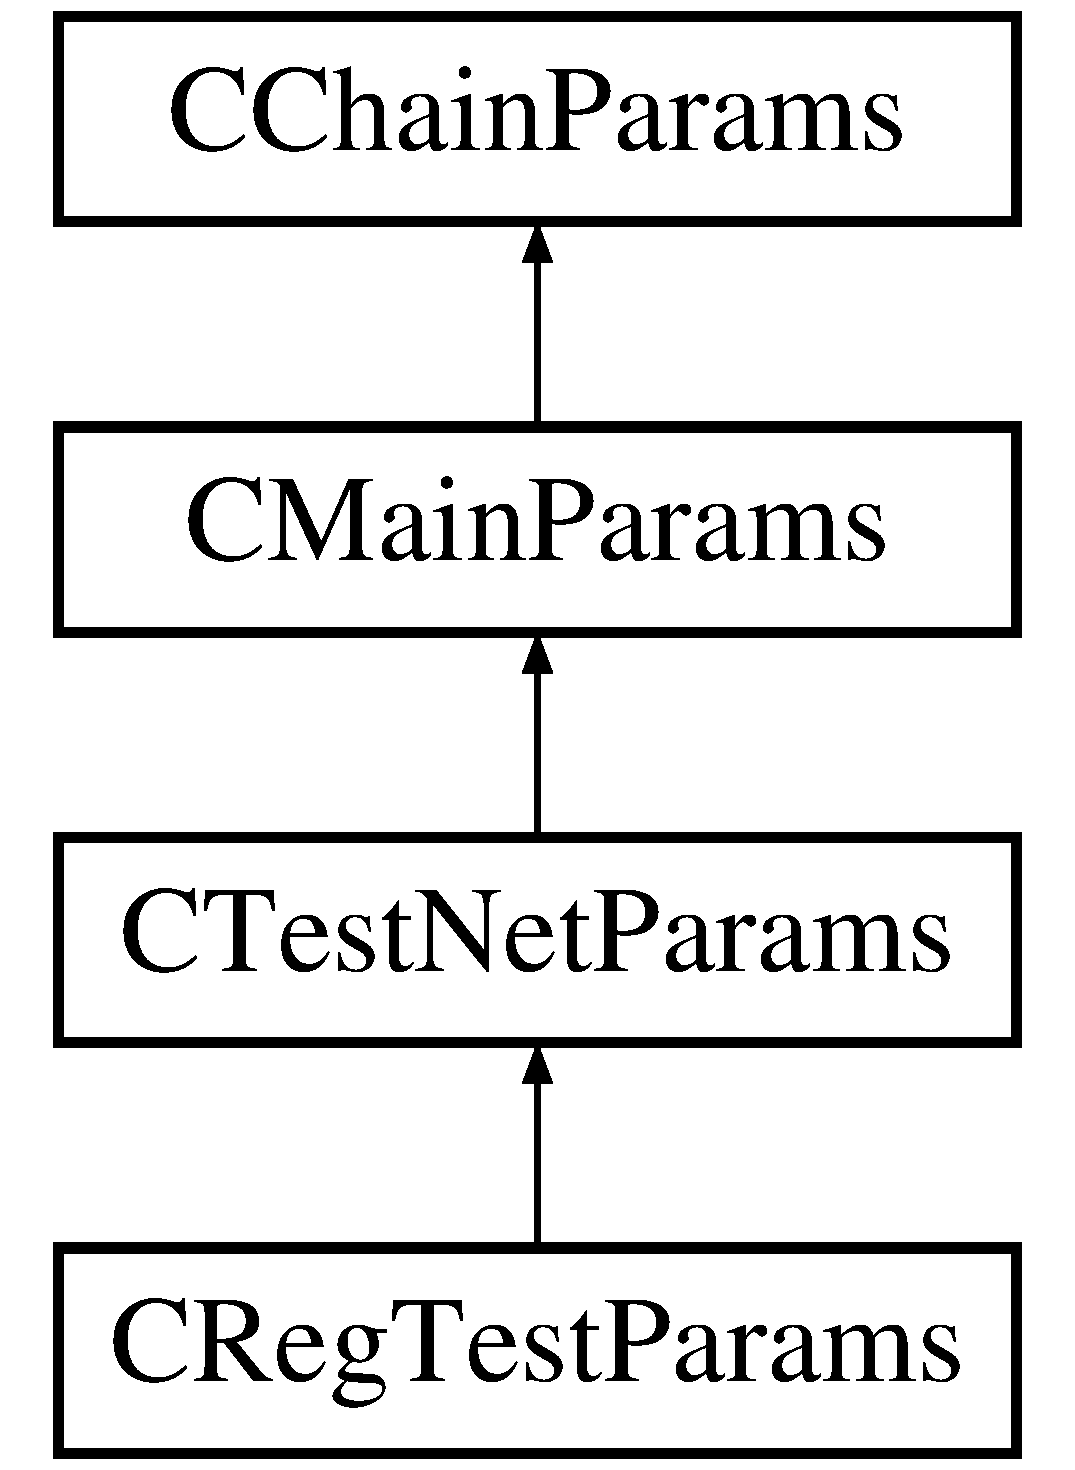
\includegraphics[height=4.000000cm]{class_c_test_net_params}
\end{center}
\end{figure}
\subsection*{Public Member Functions}
\begin{DoxyCompactItemize}
\item 
\mbox{\hyperlink{class_c_test_net_params_abbd5f6e3e94bc8abf99a5dfaff75374a}{C\+Test\+Net\+Params}} ()
\end{DoxyCompactItemize}
\subsection*{Additional Inherited Members}


\subsection{Detailed Description}
Testnet (v3) 

\subsection{Constructor \& Destructor Documentation}
\mbox{\Hypertarget{class_c_test_net_params_abbd5f6e3e94bc8abf99a5dfaff75374a}\label{class_c_test_net_params_abbd5f6e3e94bc8abf99a5dfaff75374a}} 
\index{C\+Test\+Net\+Params@{C\+Test\+Net\+Params}!C\+Test\+Net\+Params@{C\+Test\+Net\+Params}}
\index{C\+Test\+Net\+Params@{C\+Test\+Net\+Params}!C\+Test\+Net\+Params@{C\+Test\+Net\+Params}}
\subsubsection{\texorpdfstring{C\+Test\+Net\+Params()}{CTestNetParams()}}
{\footnotesize\ttfamily C\+Test\+Net\+Params\+::\+C\+Test\+Net\+Params (\begin{DoxyParamCaption}{ }\end{DoxyParamCaption})\hspace{0.3cm}{\ttfamily [inline]}}

Modify the testnet genesis block so the timestamp is valid for a later start. 

The documentation for this class was generated from the following file\+:\begin{DoxyCompactItemize}
\item 
/\+Users/christopherarguello/\+Developer/anon/src/\mbox{\hyperlink{chainparams_8cpp}{chainparams.\+cpp}}\end{DoxyCompactItemize}

\hypertarget{struct_c_timestamp_index_iterator_key}{}\section{C\+Timestamp\+Index\+Iterator\+Key Struct Reference}
\label{struct_c_timestamp_index_iterator_key}\index{C\+Timestamp\+Index\+Iterator\+Key@{C\+Timestamp\+Index\+Iterator\+Key}}


{\ttfamily \#include $<$main.\+h$>$}

\subsection*{Public Member Functions}
\begin{DoxyCompactItemize}
\item 
size\+\_\+t \mbox{\hyperlink{struct_c_timestamp_index_iterator_key_a1d42134dc82c79ddd09c531a03625745}{Get\+Serialize\+Size}} (int n\+Type, int n\+Version) const
\item 
{\footnotesize template$<$typename Stream $>$ }\\void \mbox{\hyperlink{struct_c_timestamp_index_iterator_key_afa5a4c352cf42da8f3763ee0ca8362cd}{Serialize}} (Stream \&s, int n\+Type, int n\+Version) const
\item 
{\footnotesize template$<$typename Stream $>$ }\\void \mbox{\hyperlink{struct_c_timestamp_index_iterator_key_a3f47d6a35bfe323058960efdb0bf4f26}{Unserialize}} (Stream \&s, int n\+Type, int n\+Version)
\item 
\mbox{\hyperlink{struct_c_timestamp_index_iterator_key_ac2a4b02c30c039652296c1b5f81d67da}{C\+Timestamp\+Index\+Iterator\+Key}} (unsigned int time)
\item 
\mbox{\hyperlink{struct_c_timestamp_index_iterator_key_a56b41dc1f35b31ffd5654dae4a1a3298}{C\+Timestamp\+Index\+Iterator\+Key}} ()
\item 
void \mbox{\hyperlink{struct_c_timestamp_index_iterator_key_aafb4b94756345f2afcbb10559765466d}{Set\+Null}} ()
\end{DoxyCompactItemize}
\subsection*{Public Attributes}
\begin{DoxyCompactItemize}
\item 
unsigned int \mbox{\hyperlink{struct_c_timestamp_index_iterator_key_a9459c6d565851430bb2edcf6fc601292}{timestamp}}
\end{DoxyCompactItemize}


\subsection{Constructor \& Destructor Documentation}
\mbox{\Hypertarget{struct_c_timestamp_index_iterator_key_ac2a4b02c30c039652296c1b5f81d67da}\label{struct_c_timestamp_index_iterator_key_ac2a4b02c30c039652296c1b5f81d67da}} 
\index{C\+Timestamp\+Index\+Iterator\+Key@{C\+Timestamp\+Index\+Iterator\+Key}!C\+Timestamp\+Index\+Iterator\+Key@{C\+Timestamp\+Index\+Iterator\+Key}}
\index{C\+Timestamp\+Index\+Iterator\+Key@{C\+Timestamp\+Index\+Iterator\+Key}!C\+Timestamp\+Index\+Iterator\+Key@{C\+Timestamp\+Index\+Iterator\+Key}}
\subsubsection{\texorpdfstring{C\+Timestamp\+Index\+Iterator\+Key()}{CTimestampIndexIteratorKey()}\hspace{0.1cm}{\footnotesize\ttfamily [1/2]}}
{\footnotesize\ttfamily C\+Timestamp\+Index\+Iterator\+Key\+::\+C\+Timestamp\+Index\+Iterator\+Key (\begin{DoxyParamCaption}\item[{unsigned int}]{time }\end{DoxyParamCaption})\hspace{0.3cm}{\ttfamily [inline]}}

\mbox{\Hypertarget{struct_c_timestamp_index_iterator_key_a56b41dc1f35b31ffd5654dae4a1a3298}\label{struct_c_timestamp_index_iterator_key_a56b41dc1f35b31ffd5654dae4a1a3298}} 
\index{C\+Timestamp\+Index\+Iterator\+Key@{C\+Timestamp\+Index\+Iterator\+Key}!C\+Timestamp\+Index\+Iterator\+Key@{C\+Timestamp\+Index\+Iterator\+Key}}
\index{C\+Timestamp\+Index\+Iterator\+Key@{C\+Timestamp\+Index\+Iterator\+Key}!C\+Timestamp\+Index\+Iterator\+Key@{C\+Timestamp\+Index\+Iterator\+Key}}
\subsubsection{\texorpdfstring{C\+Timestamp\+Index\+Iterator\+Key()}{CTimestampIndexIteratorKey()}\hspace{0.1cm}{\footnotesize\ttfamily [2/2]}}
{\footnotesize\ttfamily C\+Timestamp\+Index\+Iterator\+Key\+::\+C\+Timestamp\+Index\+Iterator\+Key (\begin{DoxyParamCaption}{ }\end{DoxyParamCaption})\hspace{0.3cm}{\ttfamily [inline]}}



\subsection{Member Function Documentation}
\mbox{\Hypertarget{struct_c_timestamp_index_iterator_key_a1d42134dc82c79ddd09c531a03625745}\label{struct_c_timestamp_index_iterator_key_a1d42134dc82c79ddd09c531a03625745}} 
\index{C\+Timestamp\+Index\+Iterator\+Key@{C\+Timestamp\+Index\+Iterator\+Key}!Get\+Serialize\+Size@{Get\+Serialize\+Size}}
\index{Get\+Serialize\+Size@{Get\+Serialize\+Size}!C\+Timestamp\+Index\+Iterator\+Key@{C\+Timestamp\+Index\+Iterator\+Key}}
\subsubsection{\texorpdfstring{Get\+Serialize\+Size()}{GetSerializeSize()}}
{\footnotesize\ttfamily size\+\_\+t C\+Timestamp\+Index\+Iterator\+Key\+::\+Get\+Serialize\+Size (\begin{DoxyParamCaption}\item[{int}]{n\+Type,  }\item[{int}]{n\+Version }\end{DoxyParamCaption}) const\hspace{0.3cm}{\ttfamily [inline]}}

\mbox{\Hypertarget{struct_c_timestamp_index_iterator_key_afa5a4c352cf42da8f3763ee0ca8362cd}\label{struct_c_timestamp_index_iterator_key_afa5a4c352cf42da8f3763ee0ca8362cd}} 
\index{C\+Timestamp\+Index\+Iterator\+Key@{C\+Timestamp\+Index\+Iterator\+Key}!Serialize@{Serialize}}
\index{Serialize@{Serialize}!C\+Timestamp\+Index\+Iterator\+Key@{C\+Timestamp\+Index\+Iterator\+Key}}
\subsubsection{\texorpdfstring{Serialize()}{Serialize()}}
{\footnotesize\ttfamily template$<$typename Stream $>$ \\
void C\+Timestamp\+Index\+Iterator\+Key\+::\+Serialize (\begin{DoxyParamCaption}\item[{Stream \&}]{s,  }\item[{int}]{n\+Type,  }\item[{int}]{n\+Version }\end{DoxyParamCaption}) const\hspace{0.3cm}{\ttfamily [inline]}}

\mbox{\Hypertarget{struct_c_timestamp_index_iterator_key_aafb4b94756345f2afcbb10559765466d}\label{struct_c_timestamp_index_iterator_key_aafb4b94756345f2afcbb10559765466d}} 
\index{C\+Timestamp\+Index\+Iterator\+Key@{C\+Timestamp\+Index\+Iterator\+Key}!Set\+Null@{Set\+Null}}
\index{Set\+Null@{Set\+Null}!C\+Timestamp\+Index\+Iterator\+Key@{C\+Timestamp\+Index\+Iterator\+Key}}
\subsubsection{\texorpdfstring{Set\+Null()}{SetNull()}}
{\footnotesize\ttfamily void C\+Timestamp\+Index\+Iterator\+Key\+::\+Set\+Null (\begin{DoxyParamCaption}{ }\end{DoxyParamCaption})\hspace{0.3cm}{\ttfamily [inline]}}

\mbox{\Hypertarget{struct_c_timestamp_index_iterator_key_a3f47d6a35bfe323058960efdb0bf4f26}\label{struct_c_timestamp_index_iterator_key_a3f47d6a35bfe323058960efdb0bf4f26}} 
\index{C\+Timestamp\+Index\+Iterator\+Key@{C\+Timestamp\+Index\+Iterator\+Key}!Unserialize@{Unserialize}}
\index{Unserialize@{Unserialize}!C\+Timestamp\+Index\+Iterator\+Key@{C\+Timestamp\+Index\+Iterator\+Key}}
\subsubsection{\texorpdfstring{Unserialize()}{Unserialize()}}
{\footnotesize\ttfamily template$<$typename Stream $>$ \\
void C\+Timestamp\+Index\+Iterator\+Key\+::\+Unserialize (\begin{DoxyParamCaption}\item[{Stream \&}]{s,  }\item[{int}]{n\+Type,  }\item[{int}]{n\+Version }\end{DoxyParamCaption})\hspace{0.3cm}{\ttfamily [inline]}}



\subsection{Member Data Documentation}
\mbox{\Hypertarget{struct_c_timestamp_index_iterator_key_a9459c6d565851430bb2edcf6fc601292}\label{struct_c_timestamp_index_iterator_key_a9459c6d565851430bb2edcf6fc601292}} 
\index{C\+Timestamp\+Index\+Iterator\+Key@{C\+Timestamp\+Index\+Iterator\+Key}!timestamp@{timestamp}}
\index{timestamp@{timestamp}!C\+Timestamp\+Index\+Iterator\+Key@{C\+Timestamp\+Index\+Iterator\+Key}}
\subsubsection{\texorpdfstring{timestamp}{timestamp}}
{\footnotesize\ttfamily unsigned int C\+Timestamp\+Index\+Iterator\+Key\+::timestamp}



The documentation for this struct was generated from the following file\+:\begin{DoxyCompactItemize}
\item 
/\+Users/christopherarguello/\+Developer/anon/src/\mbox{\hyperlink{main_8h}{main.\+h}}\end{DoxyCompactItemize}

\hypertarget{struct_c_timestamp_index_key}{}\section{C\+Timestamp\+Index\+Key Struct Reference}
\label{struct_c_timestamp_index_key}\index{C\+Timestamp\+Index\+Key@{C\+Timestamp\+Index\+Key}}


{\ttfamily \#include $<$main.\+h$>$}

\subsection*{Public Member Functions}
\begin{DoxyCompactItemize}
\item 
size\+\_\+t \mbox{\hyperlink{struct_c_timestamp_index_key_a8275de5b4b5eb9a5afaf2921a139e0eb}{Get\+Serialize\+Size}} (int n\+Type, int n\+Version) const
\item 
{\footnotesize template$<$typename Stream $>$ }\\void \mbox{\hyperlink{struct_c_timestamp_index_key_af08cb17ed40232b5708b862f86aaffec}{Serialize}} (Stream \&s, int n\+Type, int n\+Version) const
\item 
{\footnotesize template$<$typename Stream $>$ }\\void \mbox{\hyperlink{struct_c_timestamp_index_key_aeafbd5739644dd4fdbc5d608cca05bd3}{Unserialize}} (Stream \&s, int n\+Type, int n\+Version)
\item 
\mbox{\hyperlink{struct_c_timestamp_index_key_ad8bd13300b5215fba9daad2311ecf606}{C\+Timestamp\+Index\+Key}} (unsigned int time, \mbox{\hyperlink{classuint256}{uint256}} hash)
\item 
\mbox{\hyperlink{struct_c_timestamp_index_key_ab4fa0901e2a40c9aad213532c16666df}{C\+Timestamp\+Index\+Key}} ()
\item 
void \mbox{\hyperlink{struct_c_timestamp_index_key_a022b090d576c984bcdf6934608c58ba6}{Set\+Null}} ()
\end{DoxyCompactItemize}
\subsection*{Public Attributes}
\begin{DoxyCompactItemize}
\item 
unsigned int \mbox{\hyperlink{struct_c_timestamp_index_key_ad8558ff210c520bb1a0ff41c0ccd6867}{timestamp}}
\item 
\mbox{\hyperlink{classuint256}{uint256}} \mbox{\hyperlink{struct_c_timestamp_index_key_a283807e42c308d1998b226ec30352239}{block\+Hash}}
\end{DoxyCompactItemize}


\subsection{Constructor \& Destructor Documentation}
\mbox{\Hypertarget{struct_c_timestamp_index_key_ad8bd13300b5215fba9daad2311ecf606}\label{struct_c_timestamp_index_key_ad8bd13300b5215fba9daad2311ecf606}} 
\index{C\+Timestamp\+Index\+Key@{C\+Timestamp\+Index\+Key}!C\+Timestamp\+Index\+Key@{C\+Timestamp\+Index\+Key}}
\index{C\+Timestamp\+Index\+Key@{C\+Timestamp\+Index\+Key}!C\+Timestamp\+Index\+Key@{C\+Timestamp\+Index\+Key}}
\subsubsection{\texorpdfstring{C\+Timestamp\+Index\+Key()}{CTimestampIndexKey()}\hspace{0.1cm}{\footnotesize\ttfamily [1/2]}}
{\footnotesize\ttfamily C\+Timestamp\+Index\+Key\+::\+C\+Timestamp\+Index\+Key (\begin{DoxyParamCaption}\item[{unsigned int}]{time,  }\item[{\mbox{\hyperlink{classuint256}{uint256}}}]{hash }\end{DoxyParamCaption})\hspace{0.3cm}{\ttfamily [inline]}}

\mbox{\Hypertarget{struct_c_timestamp_index_key_ab4fa0901e2a40c9aad213532c16666df}\label{struct_c_timestamp_index_key_ab4fa0901e2a40c9aad213532c16666df}} 
\index{C\+Timestamp\+Index\+Key@{C\+Timestamp\+Index\+Key}!C\+Timestamp\+Index\+Key@{C\+Timestamp\+Index\+Key}}
\index{C\+Timestamp\+Index\+Key@{C\+Timestamp\+Index\+Key}!C\+Timestamp\+Index\+Key@{C\+Timestamp\+Index\+Key}}
\subsubsection{\texorpdfstring{C\+Timestamp\+Index\+Key()}{CTimestampIndexKey()}\hspace{0.1cm}{\footnotesize\ttfamily [2/2]}}
{\footnotesize\ttfamily C\+Timestamp\+Index\+Key\+::\+C\+Timestamp\+Index\+Key (\begin{DoxyParamCaption}{ }\end{DoxyParamCaption})\hspace{0.3cm}{\ttfamily [inline]}}



\subsection{Member Function Documentation}
\mbox{\Hypertarget{struct_c_timestamp_index_key_a8275de5b4b5eb9a5afaf2921a139e0eb}\label{struct_c_timestamp_index_key_a8275de5b4b5eb9a5afaf2921a139e0eb}} 
\index{C\+Timestamp\+Index\+Key@{C\+Timestamp\+Index\+Key}!Get\+Serialize\+Size@{Get\+Serialize\+Size}}
\index{Get\+Serialize\+Size@{Get\+Serialize\+Size}!C\+Timestamp\+Index\+Key@{C\+Timestamp\+Index\+Key}}
\subsubsection{\texorpdfstring{Get\+Serialize\+Size()}{GetSerializeSize()}}
{\footnotesize\ttfamily size\+\_\+t C\+Timestamp\+Index\+Key\+::\+Get\+Serialize\+Size (\begin{DoxyParamCaption}\item[{int}]{n\+Type,  }\item[{int}]{n\+Version }\end{DoxyParamCaption}) const\hspace{0.3cm}{\ttfamily [inline]}}

\mbox{\Hypertarget{struct_c_timestamp_index_key_af08cb17ed40232b5708b862f86aaffec}\label{struct_c_timestamp_index_key_af08cb17ed40232b5708b862f86aaffec}} 
\index{C\+Timestamp\+Index\+Key@{C\+Timestamp\+Index\+Key}!Serialize@{Serialize}}
\index{Serialize@{Serialize}!C\+Timestamp\+Index\+Key@{C\+Timestamp\+Index\+Key}}
\subsubsection{\texorpdfstring{Serialize()}{Serialize()}}
{\footnotesize\ttfamily template$<$typename Stream $>$ \\
void C\+Timestamp\+Index\+Key\+::\+Serialize (\begin{DoxyParamCaption}\item[{Stream \&}]{s,  }\item[{int}]{n\+Type,  }\item[{int}]{n\+Version }\end{DoxyParamCaption}) const\hspace{0.3cm}{\ttfamily [inline]}}

\mbox{\Hypertarget{struct_c_timestamp_index_key_a022b090d576c984bcdf6934608c58ba6}\label{struct_c_timestamp_index_key_a022b090d576c984bcdf6934608c58ba6}} 
\index{C\+Timestamp\+Index\+Key@{C\+Timestamp\+Index\+Key}!Set\+Null@{Set\+Null}}
\index{Set\+Null@{Set\+Null}!C\+Timestamp\+Index\+Key@{C\+Timestamp\+Index\+Key}}
\subsubsection{\texorpdfstring{Set\+Null()}{SetNull()}}
{\footnotesize\ttfamily void C\+Timestamp\+Index\+Key\+::\+Set\+Null (\begin{DoxyParamCaption}{ }\end{DoxyParamCaption})\hspace{0.3cm}{\ttfamily [inline]}}

\mbox{\Hypertarget{struct_c_timestamp_index_key_aeafbd5739644dd4fdbc5d608cca05bd3}\label{struct_c_timestamp_index_key_aeafbd5739644dd4fdbc5d608cca05bd3}} 
\index{C\+Timestamp\+Index\+Key@{C\+Timestamp\+Index\+Key}!Unserialize@{Unserialize}}
\index{Unserialize@{Unserialize}!C\+Timestamp\+Index\+Key@{C\+Timestamp\+Index\+Key}}
\subsubsection{\texorpdfstring{Unserialize()}{Unserialize()}}
{\footnotesize\ttfamily template$<$typename Stream $>$ \\
void C\+Timestamp\+Index\+Key\+::\+Unserialize (\begin{DoxyParamCaption}\item[{Stream \&}]{s,  }\item[{int}]{n\+Type,  }\item[{int}]{n\+Version }\end{DoxyParamCaption})\hspace{0.3cm}{\ttfamily [inline]}}



\subsection{Member Data Documentation}
\mbox{\Hypertarget{struct_c_timestamp_index_key_a283807e42c308d1998b226ec30352239}\label{struct_c_timestamp_index_key_a283807e42c308d1998b226ec30352239}} 
\index{C\+Timestamp\+Index\+Key@{C\+Timestamp\+Index\+Key}!block\+Hash@{block\+Hash}}
\index{block\+Hash@{block\+Hash}!C\+Timestamp\+Index\+Key@{C\+Timestamp\+Index\+Key}}
\subsubsection{\texorpdfstring{block\+Hash}{blockHash}}
{\footnotesize\ttfamily \mbox{\hyperlink{classuint256}{uint256}} C\+Timestamp\+Index\+Key\+::block\+Hash}

\mbox{\Hypertarget{struct_c_timestamp_index_key_ad8558ff210c520bb1a0ff41c0ccd6867}\label{struct_c_timestamp_index_key_ad8558ff210c520bb1a0ff41c0ccd6867}} 
\index{C\+Timestamp\+Index\+Key@{C\+Timestamp\+Index\+Key}!timestamp@{timestamp}}
\index{timestamp@{timestamp}!C\+Timestamp\+Index\+Key@{C\+Timestamp\+Index\+Key}}
\subsubsection{\texorpdfstring{timestamp}{timestamp}}
{\footnotesize\ttfamily unsigned int C\+Timestamp\+Index\+Key\+::timestamp}



The documentation for this struct was generated from the following file\+:\begin{DoxyCompactItemize}
\item 
/\+Users/christopherarguello/\+Developer/anon/src/\mbox{\hyperlink{main_8h}{main.\+h}}\end{DoxyCompactItemize}

\hypertarget{class_c_translation_interface}{}\section{C\+Translation\+Interface Class Reference}
\label{class_c_translation_interface}\index{C\+Translation\+Interface@{C\+Translation\+Interface}}


{\ttfamily \#include $<$util.\+h$>$}

\subsection*{Public Attributes}
\begin{DoxyCompactItemize}
\item 
boost\+::signals2\+::signal$<$ std\+::string(const char $\ast$psz)$>$ \mbox{\hyperlink{class_c_translation_interface_a02eb72aa9d39e6f55944581673af7135}{Translate}}
\end{DoxyCompactItemize}


\subsection{Detailed Description}
Signals for translation. 

\subsection{Member Data Documentation}
\mbox{\Hypertarget{class_c_translation_interface_a02eb72aa9d39e6f55944581673af7135}\label{class_c_translation_interface_a02eb72aa9d39e6f55944581673af7135}} 
\index{C\+Translation\+Interface@{C\+Translation\+Interface}!Translate@{Translate}}
\index{Translate@{Translate}!C\+Translation\+Interface@{C\+Translation\+Interface}}
\subsubsection{\texorpdfstring{Translate}{Translate}}
{\footnotesize\ttfamily boost\+::signals2\+::signal$<$std\+::string(const char$\ast$ psz)$>$ C\+Translation\+Interface\+::\+Translate}

Translate a message to the native language of the user. 

The documentation for this class was generated from the following file\+:\begin{DoxyCompactItemize}
\item 
/\+Users/christopherarguello/\+Developer/anon/src/\mbox{\hyperlink{util_8h}{util.\+h}}\end{DoxyCompactItemize}

\hypertarget{class_c_tx_in_undo}{}\section{C\+Tx\+In\+Undo Class Reference}
\label{class_c_tx_in_undo}\index{C\+Tx\+In\+Undo@{C\+Tx\+In\+Undo}}


{\ttfamily \#include $<$undo.\+h$>$}

\subsection*{Public Member Functions}
\begin{DoxyCompactItemize}
\item 
\mbox{\hyperlink{class_c_tx_in_undo_a9f8d4a16f1cb14fcec729becdb944003}{C\+Tx\+In\+Undo}} ()
\item 
\mbox{\hyperlink{class_c_tx_in_undo_a9f4da076d789bf5fa3f6d8d4b1d7d6fd}{C\+Tx\+In\+Undo}} (const C\+Tx\+Out \&txout\+In, bool f\+Coin\+Base\+In=false, unsigned int n\+Height\+In=0, int n\+Version\+In=0)
\item 
unsigned int \mbox{\hyperlink{class_c_tx_in_undo_ae02e42aeabd614a26ba5657f60ec6921}{Get\+Serialize\+Size}} (int n\+Type, int \mbox{\hyperlink{class_c_tx_in_undo_a193281289475ca792e436a7a02de23ef}{n\+Version}}) const
\item 
{\footnotesize template$<$typename Stream $>$ }\\void \mbox{\hyperlink{class_c_tx_in_undo_a7a4e1cf026b5308fdca471bada9cebaf}{Serialize}} (Stream \&s, int n\+Type, int \mbox{\hyperlink{class_c_tx_in_undo_a193281289475ca792e436a7a02de23ef}{n\+Version}}) const
\item 
{\footnotesize template$<$typename Stream $>$ }\\void \mbox{\hyperlink{class_c_tx_in_undo_a0a2b82f03edad7ad85a66e63e4552af9}{Unserialize}} (Stream \&s, int n\+Type, int \mbox{\hyperlink{class_c_tx_in_undo_a193281289475ca792e436a7a02de23ef}{n\+Version}})
\end{DoxyCompactItemize}
\subsection*{Public Attributes}
\begin{DoxyCompactItemize}
\item 
C\+Tx\+Out \mbox{\hyperlink{class_c_tx_in_undo_a0eb1374984b5b68b0af14d88d7d4b821}{txout}}
\item 
bool \mbox{\hyperlink{class_c_tx_in_undo_a5952f917224de3a2193157b856c47864}{f\+Coin\+Base}}
\item 
unsigned int \mbox{\hyperlink{class_c_tx_in_undo_af022118f015a9b1b9ab96e04e8452292}{n\+Height}}
\item 
int \mbox{\hyperlink{class_c_tx_in_undo_a193281289475ca792e436a7a02de23ef}{n\+Version}}
\end{DoxyCompactItemize}


\subsection{Detailed Description}
Undo information for a C\+Tx\+In

Contains the prevout\textquotesingle{}s C\+Tx\+Out being spent, and if this was the last output of the affected transaction, its metadata as well (coinbase or not, height, transaction version) 

\subsection{Constructor \& Destructor Documentation}
\mbox{\Hypertarget{class_c_tx_in_undo_a9f8d4a16f1cb14fcec729becdb944003}\label{class_c_tx_in_undo_a9f8d4a16f1cb14fcec729becdb944003}} 
\index{C\+Tx\+In\+Undo@{C\+Tx\+In\+Undo}!C\+Tx\+In\+Undo@{C\+Tx\+In\+Undo}}
\index{C\+Tx\+In\+Undo@{C\+Tx\+In\+Undo}!C\+Tx\+In\+Undo@{C\+Tx\+In\+Undo}}
\subsubsection{\texorpdfstring{C\+Tx\+In\+Undo()}{CTxInUndo()}\hspace{0.1cm}{\footnotesize\ttfamily [1/2]}}
{\footnotesize\ttfamily C\+Tx\+In\+Undo\+::\+C\+Tx\+In\+Undo (\begin{DoxyParamCaption}{ }\end{DoxyParamCaption})\hspace{0.3cm}{\ttfamily [inline]}}

\mbox{\Hypertarget{class_c_tx_in_undo_a9f4da076d789bf5fa3f6d8d4b1d7d6fd}\label{class_c_tx_in_undo_a9f4da076d789bf5fa3f6d8d4b1d7d6fd}} 
\index{C\+Tx\+In\+Undo@{C\+Tx\+In\+Undo}!C\+Tx\+In\+Undo@{C\+Tx\+In\+Undo}}
\index{C\+Tx\+In\+Undo@{C\+Tx\+In\+Undo}!C\+Tx\+In\+Undo@{C\+Tx\+In\+Undo}}
\subsubsection{\texorpdfstring{C\+Tx\+In\+Undo()}{CTxInUndo()}\hspace{0.1cm}{\footnotesize\ttfamily [2/2]}}
{\footnotesize\ttfamily C\+Tx\+In\+Undo\+::\+C\+Tx\+In\+Undo (\begin{DoxyParamCaption}\item[{const C\+Tx\+Out \&}]{txout\+In,  }\item[{bool}]{f\+Coin\+Base\+In = {\ttfamily false},  }\item[{unsigned int}]{n\+Height\+In = {\ttfamily 0},  }\item[{int}]{n\+Version\+In = {\ttfamily 0} }\end{DoxyParamCaption})\hspace{0.3cm}{\ttfamily [inline]}}



\subsection{Member Function Documentation}
\mbox{\Hypertarget{class_c_tx_in_undo_ae02e42aeabd614a26ba5657f60ec6921}\label{class_c_tx_in_undo_ae02e42aeabd614a26ba5657f60ec6921}} 
\index{C\+Tx\+In\+Undo@{C\+Tx\+In\+Undo}!Get\+Serialize\+Size@{Get\+Serialize\+Size}}
\index{Get\+Serialize\+Size@{Get\+Serialize\+Size}!C\+Tx\+In\+Undo@{C\+Tx\+In\+Undo}}
\subsubsection{\texorpdfstring{Get\+Serialize\+Size()}{GetSerializeSize()}}
{\footnotesize\ttfamily unsigned int C\+Tx\+In\+Undo\+::\+Get\+Serialize\+Size (\begin{DoxyParamCaption}\item[{int}]{n\+Type,  }\item[{int}]{n\+Version }\end{DoxyParamCaption}) const\hspace{0.3cm}{\ttfamily [inline]}}

\mbox{\Hypertarget{class_c_tx_in_undo_a7a4e1cf026b5308fdca471bada9cebaf}\label{class_c_tx_in_undo_a7a4e1cf026b5308fdca471bada9cebaf}} 
\index{C\+Tx\+In\+Undo@{C\+Tx\+In\+Undo}!Serialize@{Serialize}}
\index{Serialize@{Serialize}!C\+Tx\+In\+Undo@{C\+Tx\+In\+Undo}}
\subsubsection{\texorpdfstring{Serialize()}{Serialize()}}
{\footnotesize\ttfamily template$<$typename Stream $>$ \\
void C\+Tx\+In\+Undo\+::\+Serialize (\begin{DoxyParamCaption}\item[{Stream \&}]{s,  }\item[{int}]{n\+Type,  }\item[{int}]{n\+Version }\end{DoxyParamCaption}) const\hspace{0.3cm}{\ttfamily [inline]}}

\mbox{\Hypertarget{class_c_tx_in_undo_a0a2b82f03edad7ad85a66e63e4552af9}\label{class_c_tx_in_undo_a0a2b82f03edad7ad85a66e63e4552af9}} 
\index{C\+Tx\+In\+Undo@{C\+Tx\+In\+Undo}!Unserialize@{Unserialize}}
\index{Unserialize@{Unserialize}!C\+Tx\+In\+Undo@{C\+Tx\+In\+Undo}}
\subsubsection{\texorpdfstring{Unserialize()}{Unserialize()}}
{\footnotesize\ttfamily template$<$typename Stream $>$ \\
void C\+Tx\+In\+Undo\+::\+Unserialize (\begin{DoxyParamCaption}\item[{Stream \&}]{s,  }\item[{int}]{n\+Type,  }\item[{int}]{n\+Version }\end{DoxyParamCaption})\hspace{0.3cm}{\ttfamily [inline]}}



\subsection{Member Data Documentation}
\mbox{\Hypertarget{class_c_tx_in_undo_a5952f917224de3a2193157b856c47864}\label{class_c_tx_in_undo_a5952f917224de3a2193157b856c47864}} 
\index{C\+Tx\+In\+Undo@{C\+Tx\+In\+Undo}!f\+Coin\+Base@{f\+Coin\+Base}}
\index{f\+Coin\+Base@{f\+Coin\+Base}!C\+Tx\+In\+Undo@{C\+Tx\+In\+Undo}}
\subsubsection{\texorpdfstring{f\+Coin\+Base}{fCoinBase}}
{\footnotesize\ttfamily bool C\+Tx\+In\+Undo\+::f\+Coin\+Base}

\mbox{\Hypertarget{class_c_tx_in_undo_af022118f015a9b1b9ab96e04e8452292}\label{class_c_tx_in_undo_af022118f015a9b1b9ab96e04e8452292}} 
\index{C\+Tx\+In\+Undo@{C\+Tx\+In\+Undo}!n\+Height@{n\+Height}}
\index{n\+Height@{n\+Height}!C\+Tx\+In\+Undo@{C\+Tx\+In\+Undo}}
\subsubsection{\texorpdfstring{n\+Height}{nHeight}}
{\footnotesize\ttfamily unsigned int C\+Tx\+In\+Undo\+::n\+Height}

\mbox{\Hypertarget{class_c_tx_in_undo_a193281289475ca792e436a7a02de23ef}\label{class_c_tx_in_undo_a193281289475ca792e436a7a02de23ef}} 
\index{C\+Tx\+In\+Undo@{C\+Tx\+In\+Undo}!n\+Version@{n\+Version}}
\index{n\+Version@{n\+Version}!C\+Tx\+In\+Undo@{C\+Tx\+In\+Undo}}
\subsubsection{\texorpdfstring{n\+Version}{nVersion}}
{\footnotesize\ttfamily int C\+Tx\+In\+Undo\+::n\+Version}

\mbox{\Hypertarget{class_c_tx_in_undo_a0eb1374984b5b68b0af14d88d7d4b821}\label{class_c_tx_in_undo_a0eb1374984b5b68b0af14d88d7d4b821}} 
\index{C\+Tx\+In\+Undo@{C\+Tx\+In\+Undo}!txout@{txout}}
\index{txout@{txout}!C\+Tx\+In\+Undo@{C\+Tx\+In\+Undo}}
\subsubsection{\texorpdfstring{txout}{txout}}
{\footnotesize\ttfamily C\+Tx\+Out C\+Tx\+In\+Undo\+::txout}



The documentation for this class was generated from the following file\+:\begin{DoxyCompactItemize}
\item 
/\+Users/christopherarguello/\+Developer/anon/src/\mbox{\hyperlink{undo_8h}{undo.\+h}}\end{DoxyCompactItemize}

\hypertarget{class_c_tx_mem_pool}{}\section{C\+Tx\+Mem\+Pool Class Reference}
\label{class_c_tx_mem_pool}\index{C\+Tx\+Mem\+Pool@{C\+Tx\+Mem\+Pool}}


{\ttfamily \#include $<$txmempool.\+h$>$}

\subsection*{Public Member Functions}
\begin{DoxyCompactItemize}
\item 
\mbox{\hyperlink{class_c_tx_mem_pool_a82147548cfa962975690d1926b717c1c}{C\+Tx\+Mem\+Pool}} (const \mbox{\hyperlink{class_c_fee_rate}{C\+Fee\+Rate}} \&\+\_\+min\+Relay\+Fee)
\item 
\mbox{\hyperlink{class_c_tx_mem_pool_a038108efea0c4312e5bed2ce064702b2}{$\sim$\+C\+Tx\+Mem\+Pool}} ()
\item 
void \mbox{\hyperlink{class_c_tx_mem_pool_ab30fadfa811829e79accca41da6a8328}{check}} (const \mbox{\hyperlink{class_c_coins_view_cache}{C\+Coins\+View\+Cache}} $\ast$pcoins) const
\item 
void \mbox{\hyperlink{class_c_tx_mem_pool_a1c0edb1fd5f0b02ddac46a6a97dcfd53}{set\+Sanity\+Check}} (bool \+\_\+f\+Sanity\+Check)
\item 
bool \mbox{\hyperlink{class_c_tx_mem_pool_aab557615eb380db41237382bab239f7c}{add\+Unchecked}} (const \mbox{\hyperlink{classuint256}{uint256}} \&hash, const \mbox{\hyperlink{class_c_tx_mem_pool_entry}{C\+Tx\+Mem\+Pool\+Entry}} \&entry, bool f\+Current\+Estimate=true)
\item 
void \mbox{\hyperlink{class_c_tx_mem_pool_a3a497097d9d5f325a2922a3970ac9da2}{remove}} (const C\+Transaction \&tx, std\+::list$<$ C\+Transaction $>$ \&removed, bool f\+Recursive=false)
\item 
void \mbox{\hyperlink{class_c_tx_mem_pool_a16a2a45643106e2612c0f300af7459f7}{remove\+With\+Anchor}} (const \mbox{\hyperlink{classuint256}{uint256}} \&invalid\+Root)
\item 
void \mbox{\hyperlink{class_c_tx_mem_pool_a6d1292640d0b6028bd5c602a6a50a983}{remove\+Coinbase\+Spends}} (const \mbox{\hyperlink{class_c_coins_view_cache}{C\+Coins\+View\+Cache}} $\ast$pcoins, unsigned int n\+Mem\+Pool\+Height)
\item 
void \mbox{\hyperlink{class_c_tx_mem_pool_a11f1bddfbae7c03c6244db322876c0a7}{remove\+Conflicts}} (const C\+Transaction \&tx, std\+::list$<$ C\+Transaction $>$ \&removed)
\item 
void \mbox{\hyperlink{class_c_tx_mem_pool_aea14d073b24e31251465ac3c2279ee65}{remove\+For\+Block}} (const std\+::vector$<$ C\+Transaction $>$ \&vtx, unsigned int n\+Block\+Height, std\+::list$<$ C\+Transaction $>$ \&conflicts, bool f\+Current\+Estimate=true)
\item 
void \mbox{\hyperlink{class_c_tx_mem_pool_a6dba6bce4139392751321438a29b6b09}{clear}} ()
\item 
void \mbox{\hyperlink{class_c_tx_mem_pool_a42fa7d41a45562d02e356f2e7708bb02}{query\+Hashes}} (std\+::vector$<$ \mbox{\hyperlink{classuint256}{uint256}} $>$ \&vtxid)
\item 
void \mbox{\hyperlink{class_c_tx_mem_pool_ad6142b7cd3a58dae6cdaf03551c2f989}{prune\+Spent}} (const \mbox{\hyperlink{classuint256}{uint256}} \&hash, \mbox{\hyperlink{class_c_coins}{C\+Coins}} \&coins)
\item 
unsigned int \mbox{\hyperlink{class_c_tx_mem_pool_afd2a709a0e6cb34a57ff2f9fd0774e6c}{Get\+Transactions\+Updated}} () const
\item 
void \mbox{\hyperlink{class_c_tx_mem_pool_a3039b67e5eebaa3ff830261c192816f2}{Add\+Transactions\+Updated}} (unsigned int n)
\item 
bool \mbox{\hyperlink{class_c_tx_mem_pool_a7a5b17b8cf4560cd681ef035880e3245}{Has\+No\+Inputs\+Of}} (const C\+Transaction \&tx) const
\item 
void \mbox{\hyperlink{class_c_tx_mem_pool_a1a0a00279c941051af1b74c5ebeac40d}{Prioritise\+Transaction}} (const \mbox{\hyperlink{classuint256}{uint256}} hash, const std\+::string str\+Hash, double d\+Priority\+Delta, const \mbox{\hyperlink{amount_8h_a4eaf3a5239714d8c45b851527f7cb564}{C\+Amount}} \&n\+Fee\+Delta)
\item 
void \mbox{\hyperlink{class_c_tx_mem_pool_aa73d1d5a211150fe169d73dc25ba3cdd}{Apply\+Deltas}} (const \mbox{\hyperlink{classuint256}{uint256}} hash, double \&d\+Priority\+Delta, \mbox{\hyperlink{amount_8h_a4eaf3a5239714d8c45b851527f7cb564}{C\+Amount}} \&n\+Fee\+Delta)
\item 
void \mbox{\hyperlink{class_c_tx_mem_pool_a11dea05121ab8321e1d1f1a21ec5c9ac}{Clear\+Prioritisation}} (const \mbox{\hyperlink{classuint256}{uint256}} hash)
\item 
unsigned long \mbox{\hyperlink{class_c_tx_mem_pool_a867f7b452141770f3b2e8697fb3513d8}{size}} ()
\item 
uint64\+\_\+t \mbox{\hyperlink{class_c_tx_mem_pool_ad388f6544c2ca90f1550b06d9d86d54f}{Get\+Total\+Tx\+Size}} ()
\item 
bool \mbox{\hyperlink{class_c_tx_mem_pool_a8b7a13b5289ab839d4460f41a7da9789}{exists}} (\mbox{\hyperlink{classuint256}{uint256}} hash) const
\item 
bool \mbox{\hyperlink{class_c_tx_mem_pool_ad6d9966cdeb4b6586f7186e709b4e77e}{lookup}} (\mbox{\hyperlink{classuint256}{uint256}} hash, C\+Transaction \&result) const
\item 
\mbox{\hyperlink{class_c_fee_rate}{C\+Fee\+Rate}} \mbox{\hyperlink{class_c_tx_mem_pool_a32dd66c128330aed86865c8a61857c6c}{estimate\+Fee}} (int n\+Blocks) const
\item 
double \mbox{\hyperlink{class_c_tx_mem_pool_a225378304025c093d2dc5fcb754ade3b}{estimate\+Priority}} (int n\+Blocks) const
\item 
bool \mbox{\hyperlink{class_c_tx_mem_pool_a251f595b6527be005634574ce5d01f70}{Write\+Fee\+Estimates}} (\mbox{\hyperlink{class_c_auto_file}{C\+Auto\+File}} \&\mbox{\hyperlink{util_8cpp_a5256be9be45ec4d0909f14a61d455e23}{fileout}}) const
\item 
bool \mbox{\hyperlink{class_c_tx_mem_pool_a0dbbcb6a3b7e1a6c564410668c12cd4f}{Read\+Fee\+Estimates}} (\mbox{\hyperlink{class_c_auto_file}{C\+Auto\+File}} \&filein)
\item 
size\+\_\+t \mbox{\hyperlink{class_c_tx_mem_pool_a4fcf05ad5f15a565c4b43c4b9f29906e}{Dynamic\+Memory\+Usage}} () const
\end{DoxyCompactItemize}
\subsection*{Public Attributes}
\begin{DoxyCompactItemize}
\item 
\mbox{\hyperlink{sync_8h_a37a4692b2d517f2843655ca11af7668a}{C\+Critical\+Section}} \mbox{\hyperlink{class_c_tx_mem_pool_ac7ee8c06837c7d2688e2d7e3d071bdbb}{cs}}
\begin{DoxyCompactList}\small\item\em sum of dynamic memory usage of all the map elements (N\+OT the maps themselves) \end{DoxyCompactList}\item 
std\+::map$<$ \mbox{\hyperlink{classuint256}{uint256}}, \mbox{\hyperlink{class_c_tx_mem_pool_entry}{C\+Tx\+Mem\+Pool\+Entry}} $>$ \mbox{\hyperlink{class_c_tx_mem_pool_a5cd374a559b02a6485ca8cef769f9930}{map\+Tx}}
\item 
std\+::map$<$ C\+Out\+Point, \mbox{\hyperlink{class_c_in_point}{C\+In\+Point}} $>$ \mbox{\hyperlink{class_c_tx_mem_pool_aae6f1162f0b2e42b369971f32a9f71e8}{map\+Next\+Tx}}
\item 
std\+::map$<$ \mbox{\hyperlink{classuint256}{uint256}}, const C\+Transaction $\ast$ $>$ \mbox{\hyperlink{class_c_tx_mem_pool_a1398b975c8c073096843991133a7bf0a}{map\+Nullifiers}}
\item 
std\+::map$<$ \mbox{\hyperlink{classuint256}{uint256}}, std\+::pair$<$ double, \mbox{\hyperlink{amount_8h_a4eaf3a5239714d8c45b851527f7cb564}{C\+Amount}} $>$ $>$ \mbox{\hyperlink{class_c_tx_mem_pool_a341709e31a39ce7a7a951a85c775c589}{map\+Deltas}}
\end{DoxyCompactItemize}
\subsection*{Private Attributes}
\begin{DoxyCompactItemize}
\item 
bool \mbox{\hyperlink{class_c_tx_mem_pool_a1752e79ce537972fe87e252b9d07d2e0}{f\+Sanity\+Check}}
\item 
unsigned int \mbox{\hyperlink{class_c_tx_mem_pool_a230bbfe440e222787d8d94a1aaef73d4}{n\+Transactions\+Updated}}
\begin{DoxyCompactList}\small\item\em Normally false, true if -\/checkmempool or -\/regtest. \end{DoxyCompactList}\item 
C\+Block\+Policy\+Estimator $\ast$ \mbox{\hyperlink{class_c_tx_mem_pool_af4d48ac0d6d62e7044ba21a45709f743}{miner\+Policy\+Estimator}}
\item 
uint64\+\_\+t \mbox{\hyperlink{class_c_tx_mem_pool_ac59656df749b33e9eb667a6850f36b7b}{total\+Tx\+Size}} = 0
\item 
uint64\+\_\+t \mbox{\hyperlink{class_c_tx_mem_pool_a9cf8ed535f89c0a1332af6c15e4a2aa9}{cached\+Inner\+Usage}}
\begin{DoxyCompactList}\small\item\em sum of all mempool tx\textquotesingle{} byte sizes \end{DoxyCompactList}\end{DoxyCompactItemize}


\subsection{Detailed Description}
\mbox{\hyperlink{class_c_tx_mem_pool}{C\+Tx\+Mem\+Pool}} stores valid-\/according-\/to-\/the-\/current-\/best-\/chain transactions that may be included in the next block.

Transactions are added when they are seen on the network (or created by the local node), but not all transactions seen are added to the pool\+: if a new transaction double-\/spends an input of a transaction in the pool, it is dropped, as are non-\/standard transactions. 

\subsection{Constructor \& Destructor Documentation}
\mbox{\Hypertarget{class_c_tx_mem_pool_a82147548cfa962975690d1926b717c1c}\label{class_c_tx_mem_pool_a82147548cfa962975690d1926b717c1c}} 
\index{C\+Tx\+Mem\+Pool@{C\+Tx\+Mem\+Pool}!C\+Tx\+Mem\+Pool@{C\+Tx\+Mem\+Pool}}
\index{C\+Tx\+Mem\+Pool@{C\+Tx\+Mem\+Pool}!C\+Tx\+Mem\+Pool@{C\+Tx\+Mem\+Pool}}
\subsubsection{\texorpdfstring{C\+Tx\+Mem\+Pool()}{CTxMemPool()}}
{\footnotesize\ttfamily C\+Tx\+Mem\+Pool\+::\+C\+Tx\+Mem\+Pool (\begin{DoxyParamCaption}\item[{const \mbox{\hyperlink{class_c_fee_rate}{C\+Fee\+Rate}} \&}]{\+\_\+min\+Relay\+Fee }\end{DoxyParamCaption})}

\mbox{\Hypertarget{class_c_tx_mem_pool_a038108efea0c4312e5bed2ce064702b2}\label{class_c_tx_mem_pool_a038108efea0c4312e5bed2ce064702b2}} 
\index{C\+Tx\+Mem\+Pool@{C\+Tx\+Mem\+Pool}!````~C\+Tx\+Mem\+Pool@{$\sim$\+C\+Tx\+Mem\+Pool}}
\index{````~C\+Tx\+Mem\+Pool@{$\sim$\+C\+Tx\+Mem\+Pool}!C\+Tx\+Mem\+Pool@{C\+Tx\+Mem\+Pool}}
\subsubsection{\texorpdfstring{$\sim$\+C\+Tx\+Mem\+Pool()}{~CTxMemPool()}}
{\footnotesize\ttfamily C\+Tx\+Mem\+Pool\+::$\sim$\+C\+Tx\+Mem\+Pool (\begin{DoxyParamCaption}{ }\end{DoxyParamCaption})}



\subsection{Member Function Documentation}
\mbox{\Hypertarget{class_c_tx_mem_pool_a3039b67e5eebaa3ff830261c192816f2}\label{class_c_tx_mem_pool_a3039b67e5eebaa3ff830261c192816f2}} 
\index{C\+Tx\+Mem\+Pool@{C\+Tx\+Mem\+Pool}!Add\+Transactions\+Updated@{Add\+Transactions\+Updated}}
\index{Add\+Transactions\+Updated@{Add\+Transactions\+Updated}!C\+Tx\+Mem\+Pool@{C\+Tx\+Mem\+Pool}}
\subsubsection{\texorpdfstring{Add\+Transactions\+Updated()}{AddTransactionsUpdated()}}
{\footnotesize\ttfamily void C\+Tx\+Mem\+Pool\+::\+Add\+Transactions\+Updated (\begin{DoxyParamCaption}\item[{unsigned int}]{n }\end{DoxyParamCaption})}

\mbox{\Hypertarget{class_c_tx_mem_pool_aab557615eb380db41237382bab239f7c}\label{class_c_tx_mem_pool_aab557615eb380db41237382bab239f7c}} 
\index{C\+Tx\+Mem\+Pool@{C\+Tx\+Mem\+Pool}!add\+Unchecked@{add\+Unchecked}}
\index{add\+Unchecked@{add\+Unchecked}!C\+Tx\+Mem\+Pool@{C\+Tx\+Mem\+Pool}}
\subsubsection{\texorpdfstring{add\+Unchecked()}{addUnchecked()}}
{\footnotesize\ttfamily bool C\+Tx\+Mem\+Pool\+::add\+Unchecked (\begin{DoxyParamCaption}\item[{const \mbox{\hyperlink{classuint256}{uint256}} \&}]{hash,  }\item[{const \mbox{\hyperlink{class_c_tx_mem_pool_entry}{C\+Tx\+Mem\+Pool\+Entry}} \&}]{entry,  }\item[{bool}]{f\+Current\+Estimate = {\ttfamily true} }\end{DoxyParamCaption})}

\mbox{\Hypertarget{class_c_tx_mem_pool_aa73d1d5a211150fe169d73dc25ba3cdd}\label{class_c_tx_mem_pool_aa73d1d5a211150fe169d73dc25ba3cdd}} 
\index{C\+Tx\+Mem\+Pool@{C\+Tx\+Mem\+Pool}!Apply\+Deltas@{Apply\+Deltas}}
\index{Apply\+Deltas@{Apply\+Deltas}!C\+Tx\+Mem\+Pool@{C\+Tx\+Mem\+Pool}}
\subsubsection{\texorpdfstring{Apply\+Deltas()}{ApplyDeltas()}}
{\footnotesize\ttfamily void C\+Tx\+Mem\+Pool\+::\+Apply\+Deltas (\begin{DoxyParamCaption}\item[{const \mbox{\hyperlink{classuint256}{uint256}}}]{hash,  }\item[{double \&}]{d\+Priority\+Delta,  }\item[{\mbox{\hyperlink{amount_8h_a4eaf3a5239714d8c45b851527f7cb564}{C\+Amount}} \&}]{n\+Fee\+Delta }\end{DoxyParamCaption})}

\mbox{\Hypertarget{class_c_tx_mem_pool_ab30fadfa811829e79accca41da6a8328}\label{class_c_tx_mem_pool_ab30fadfa811829e79accca41da6a8328}} 
\index{C\+Tx\+Mem\+Pool@{C\+Tx\+Mem\+Pool}!check@{check}}
\index{check@{check}!C\+Tx\+Mem\+Pool@{C\+Tx\+Mem\+Pool}}
\subsubsection{\texorpdfstring{check()}{check()}}
{\footnotesize\ttfamily void C\+Tx\+Mem\+Pool\+::check (\begin{DoxyParamCaption}\item[{const \mbox{\hyperlink{class_c_coins_view_cache}{C\+Coins\+View\+Cache}} $\ast$}]{pcoins }\end{DoxyParamCaption}) const}

If sanity-\/checking is turned on, check makes sure the pool is consistent (does not contain two transactions that spend the same inputs, all inputs are in the map\+Next\+Tx array). If sanity-\/checking is turned off, check does nothing. \mbox{\Hypertarget{class_c_tx_mem_pool_a6dba6bce4139392751321438a29b6b09}\label{class_c_tx_mem_pool_a6dba6bce4139392751321438a29b6b09}} 
\index{C\+Tx\+Mem\+Pool@{C\+Tx\+Mem\+Pool}!clear@{clear}}
\index{clear@{clear}!C\+Tx\+Mem\+Pool@{C\+Tx\+Mem\+Pool}}
\subsubsection{\texorpdfstring{clear()}{clear()}}
{\footnotesize\ttfamily void C\+Tx\+Mem\+Pool\+::clear (\begin{DoxyParamCaption}{ }\end{DoxyParamCaption})}

\mbox{\Hypertarget{class_c_tx_mem_pool_a11dea05121ab8321e1d1f1a21ec5c9ac}\label{class_c_tx_mem_pool_a11dea05121ab8321e1d1f1a21ec5c9ac}} 
\index{C\+Tx\+Mem\+Pool@{C\+Tx\+Mem\+Pool}!Clear\+Prioritisation@{Clear\+Prioritisation}}
\index{Clear\+Prioritisation@{Clear\+Prioritisation}!C\+Tx\+Mem\+Pool@{C\+Tx\+Mem\+Pool}}
\subsubsection{\texorpdfstring{Clear\+Prioritisation()}{ClearPrioritisation()}}
{\footnotesize\ttfamily void C\+Tx\+Mem\+Pool\+::\+Clear\+Prioritisation (\begin{DoxyParamCaption}\item[{const \mbox{\hyperlink{classuint256}{uint256}}}]{hash }\end{DoxyParamCaption})}

\mbox{\Hypertarget{class_c_tx_mem_pool_a4fcf05ad5f15a565c4b43c4b9f29906e}\label{class_c_tx_mem_pool_a4fcf05ad5f15a565c4b43c4b9f29906e}} 
\index{C\+Tx\+Mem\+Pool@{C\+Tx\+Mem\+Pool}!Dynamic\+Memory\+Usage@{Dynamic\+Memory\+Usage}}
\index{Dynamic\+Memory\+Usage@{Dynamic\+Memory\+Usage}!C\+Tx\+Mem\+Pool@{C\+Tx\+Mem\+Pool}}
\subsubsection{\texorpdfstring{Dynamic\+Memory\+Usage()}{DynamicMemoryUsage()}}
{\footnotesize\ttfamily size\+\_\+t C\+Tx\+Mem\+Pool\+::\+Dynamic\+Memory\+Usage (\begin{DoxyParamCaption}{ }\end{DoxyParamCaption}) const}

\mbox{\Hypertarget{class_c_tx_mem_pool_a32dd66c128330aed86865c8a61857c6c}\label{class_c_tx_mem_pool_a32dd66c128330aed86865c8a61857c6c}} 
\index{C\+Tx\+Mem\+Pool@{C\+Tx\+Mem\+Pool}!estimate\+Fee@{estimate\+Fee}}
\index{estimate\+Fee@{estimate\+Fee}!C\+Tx\+Mem\+Pool@{C\+Tx\+Mem\+Pool}}
\subsubsection{\texorpdfstring{estimate\+Fee()}{estimateFee()}}
{\footnotesize\ttfamily \mbox{\hyperlink{class_c_fee_rate}{C\+Fee\+Rate}} C\+Tx\+Mem\+Pool\+::estimate\+Fee (\begin{DoxyParamCaption}\item[{int}]{n\+Blocks }\end{DoxyParamCaption}) const}

Estimate fee rate needed to get into the next n\+Blocks \mbox{\Hypertarget{class_c_tx_mem_pool_a225378304025c093d2dc5fcb754ade3b}\label{class_c_tx_mem_pool_a225378304025c093d2dc5fcb754ade3b}} 
\index{C\+Tx\+Mem\+Pool@{C\+Tx\+Mem\+Pool}!estimate\+Priority@{estimate\+Priority}}
\index{estimate\+Priority@{estimate\+Priority}!C\+Tx\+Mem\+Pool@{C\+Tx\+Mem\+Pool}}
\subsubsection{\texorpdfstring{estimate\+Priority()}{estimatePriority()}}
{\footnotesize\ttfamily double C\+Tx\+Mem\+Pool\+::estimate\+Priority (\begin{DoxyParamCaption}\item[{int}]{n\+Blocks }\end{DoxyParamCaption}) const}

Estimate priority needed to get into the next n\+Blocks \mbox{\Hypertarget{class_c_tx_mem_pool_a8b7a13b5289ab839d4460f41a7da9789}\label{class_c_tx_mem_pool_a8b7a13b5289ab839d4460f41a7da9789}} 
\index{C\+Tx\+Mem\+Pool@{C\+Tx\+Mem\+Pool}!exists@{exists}}
\index{exists@{exists}!C\+Tx\+Mem\+Pool@{C\+Tx\+Mem\+Pool}}
\subsubsection{\texorpdfstring{exists()}{exists()}}
{\footnotesize\ttfamily bool C\+Tx\+Mem\+Pool\+::exists (\begin{DoxyParamCaption}\item[{\mbox{\hyperlink{classuint256}{uint256}}}]{hash }\end{DoxyParamCaption}) const\hspace{0.3cm}{\ttfamily [inline]}}

\mbox{\Hypertarget{class_c_tx_mem_pool_ad388f6544c2ca90f1550b06d9d86d54f}\label{class_c_tx_mem_pool_ad388f6544c2ca90f1550b06d9d86d54f}} 
\index{C\+Tx\+Mem\+Pool@{C\+Tx\+Mem\+Pool}!Get\+Total\+Tx\+Size@{Get\+Total\+Tx\+Size}}
\index{Get\+Total\+Tx\+Size@{Get\+Total\+Tx\+Size}!C\+Tx\+Mem\+Pool@{C\+Tx\+Mem\+Pool}}
\subsubsection{\texorpdfstring{Get\+Total\+Tx\+Size()}{GetTotalTxSize()}}
{\footnotesize\ttfamily uint64\+\_\+t C\+Tx\+Mem\+Pool\+::\+Get\+Total\+Tx\+Size (\begin{DoxyParamCaption}{ }\end{DoxyParamCaption})\hspace{0.3cm}{\ttfamily [inline]}}

\mbox{\Hypertarget{class_c_tx_mem_pool_afd2a709a0e6cb34a57ff2f9fd0774e6c}\label{class_c_tx_mem_pool_afd2a709a0e6cb34a57ff2f9fd0774e6c}} 
\index{C\+Tx\+Mem\+Pool@{C\+Tx\+Mem\+Pool}!Get\+Transactions\+Updated@{Get\+Transactions\+Updated}}
\index{Get\+Transactions\+Updated@{Get\+Transactions\+Updated}!C\+Tx\+Mem\+Pool@{C\+Tx\+Mem\+Pool}}
\subsubsection{\texorpdfstring{Get\+Transactions\+Updated()}{GetTransactionsUpdated()}}
{\footnotesize\ttfamily unsigned int C\+Tx\+Mem\+Pool\+::\+Get\+Transactions\+Updated (\begin{DoxyParamCaption}{ }\end{DoxyParamCaption}) const}

\mbox{\Hypertarget{class_c_tx_mem_pool_a7a5b17b8cf4560cd681ef035880e3245}\label{class_c_tx_mem_pool_a7a5b17b8cf4560cd681ef035880e3245}} 
\index{C\+Tx\+Mem\+Pool@{C\+Tx\+Mem\+Pool}!Has\+No\+Inputs\+Of@{Has\+No\+Inputs\+Of}}
\index{Has\+No\+Inputs\+Of@{Has\+No\+Inputs\+Of}!C\+Tx\+Mem\+Pool@{C\+Tx\+Mem\+Pool}}
\subsubsection{\texorpdfstring{Has\+No\+Inputs\+Of()}{HasNoInputsOf()}}
{\footnotesize\ttfamily bool C\+Tx\+Mem\+Pool\+::\+Has\+No\+Inputs\+Of (\begin{DoxyParamCaption}\item[{const C\+Transaction \&}]{tx }\end{DoxyParamCaption}) const}

Check that none of this transactions inputs are in the mempool, and thus the tx is not dependent on other mempool transactions to be included in a block. \mbox{\Hypertarget{class_c_tx_mem_pool_ad6d9966cdeb4b6586f7186e709b4e77e}\label{class_c_tx_mem_pool_ad6d9966cdeb4b6586f7186e709b4e77e}} 
\index{C\+Tx\+Mem\+Pool@{C\+Tx\+Mem\+Pool}!lookup@{lookup}}
\index{lookup@{lookup}!C\+Tx\+Mem\+Pool@{C\+Tx\+Mem\+Pool}}
\subsubsection{\texorpdfstring{lookup()}{lookup()}}
{\footnotesize\ttfamily bool C\+Tx\+Mem\+Pool\+::lookup (\begin{DoxyParamCaption}\item[{\mbox{\hyperlink{classuint256}{uint256}}}]{hash,  }\item[{C\+Transaction \&}]{result }\end{DoxyParamCaption}) const}

\mbox{\Hypertarget{class_c_tx_mem_pool_a1a0a00279c941051af1b74c5ebeac40d}\label{class_c_tx_mem_pool_a1a0a00279c941051af1b74c5ebeac40d}} 
\index{C\+Tx\+Mem\+Pool@{C\+Tx\+Mem\+Pool}!Prioritise\+Transaction@{Prioritise\+Transaction}}
\index{Prioritise\+Transaction@{Prioritise\+Transaction}!C\+Tx\+Mem\+Pool@{C\+Tx\+Mem\+Pool}}
\subsubsection{\texorpdfstring{Prioritise\+Transaction()}{PrioritiseTransaction()}}
{\footnotesize\ttfamily void C\+Tx\+Mem\+Pool\+::\+Prioritise\+Transaction (\begin{DoxyParamCaption}\item[{const \mbox{\hyperlink{classuint256}{uint256}}}]{hash,  }\item[{const std\+::string}]{str\+Hash,  }\item[{double}]{d\+Priority\+Delta,  }\item[{const \mbox{\hyperlink{amount_8h_a4eaf3a5239714d8c45b851527f7cb564}{C\+Amount}} \&}]{n\+Fee\+Delta }\end{DoxyParamCaption})}

Affect Create\+New\+Block prioritisation of transactions \mbox{\Hypertarget{class_c_tx_mem_pool_ad6142b7cd3a58dae6cdaf03551c2f989}\label{class_c_tx_mem_pool_ad6142b7cd3a58dae6cdaf03551c2f989}} 
\index{C\+Tx\+Mem\+Pool@{C\+Tx\+Mem\+Pool}!prune\+Spent@{prune\+Spent}}
\index{prune\+Spent@{prune\+Spent}!C\+Tx\+Mem\+Pool@{C\+Tx\+Mem\+Pool}}
\subsubsection{\texorpdfstring{prune\+Spent()}{pruneSpent()}}
{\footnotesize\ttfamily void C\+Tx\+Mem\+Pool\+::prune\+Spent (\begin{DoxyParamCaption}\item[{const \mbox{\hyperlink{classuint256}{uint256}} \&}]{hash,  }\item[{\mbox{\hyperlink{class_c_coins}{C\+Coins}} \&}]{coins }\end{DoxyParamCaption})}

\mbox{\Hypertarget{class_c_tx_mem_pool_a42fa7d41a45562d02e356f2e7708bb02}\label{class_c_tx_mem_pool_a42fa7d41a45562d02e356f2e7708bb02}} 
\index{C\+Tx\+Mem\+Pool@{C\+Tx\+Mem\+Pool}!query\+Hashes@{query\+Hashes}}
\index{query\+Hashes@{query\+Hashes}!C\+Tx\+Mem\+Pool@{C\+Tx\+Mem\+Pool}}
\subsubsection{\texorpdfstring{query\+Hashes()}{queryHashes()}}
{\footnotesize\ttfamily void C\+Tx\+Mem\+Pool\+::query\+Hashes (\begin{DoxyParamCaption}\item[{std\+::vector$<$ \mbox{\hyperlink{classuint256}{uint256}} $>$ \&}]{vtxid }\end{DoxyParamCaption})}

\mbox{\Hypertarget{class_c_tx_mem_pool_a0dbbcb6a3b7e1a6c564410668c12cd4f}\label{class_c_tx_mem_pool_a0dbbcb6a3b7e1a6c564410668c12cd4f}} 
\index{C\+Tx\+Mem\+Pool@{C\+Tx\+Mem\+Pool}!Read\+Fee\+Estimates@{Read\+Fee\+Estimates}}
\index{Read\+Fee\+Estimates@{Read\+Fee\+Estimates}!C\+Tx\+Mem\+Pool@{C\+Tx\+Mem\+Pool}}
\subsubsection{\texorpdfstring{Read\+Fee\+Estimates()}{ReadFeeEstimates()}}
{\footnotesize\ttfamily bool C\+Tx\+Mem\+Pool\+::\+Read\+Fee\+Estimates (\begin{DoxyParamCaption}\item[{\mbox{\hyperlink{class_c_auto_file}{C\+Auto\+File}} \&}]{filein }\end{DoxyParamCaption})}

\mbox{\Hypertarget{class_c_tx_mem_pool_a3a497097d9d5f325a2922a3970ac9da2}\label{class_c_tx_mem_pool_a3a497097d9d5f325a2922a3970ac9da2}} 
\index{C\+Tx\+Mem\+Pool@{C\+Tx\+Mem\+Pool}!remove@{remove}}
\index{remove@{remove}!C\+Tx\+Mem\+Pool@{C\+Tx\+Mem\+Pool}}
\subsubsection{\texorpdfstring{remove()}{remove()}}
{\footnotesize\ttfamily void C\+Tx\+Mem\+Pool\+::remove (\begin{DoxyParamCaption}\item[{const C\+Transaction \&}]{tx,  }\item[{std\+::list$<$ C\+Transaction $>$ \&}]{removed,  }\item[{bool}]{f\+Recursive = {\ttfamily false} }\end{DoxyParamCaption})}

\mbox{\Hypertarget{class_c_tx_mem_pool_a6d1292640d0b6028bd5c602a6a50a983}\label{class_c_tx_mem_pool_a6d1292640d0b6028bd5c602a6a50a983}} 
\index{C\+Tx\+Mem\+Pool@{C\+Tx\+Mem\+Pool}!remove\+Coinbase\+Spends@{remove\+Coinbase\+Spends}}
\index{remove\+Coinbase\+Spends@{remove\+Coinbase\+Spends}!C\+Tx\+Mem\+Pool@{C\+Tx\+Mem\+Pool}}
\subsubsection{\texorpdfstring{remove\+Coinbase\+Spends()}{removeCoinbaseSpends()}}
{\footnotesize\ttfamily void C\+Tx\+Mem\+Pool\+::remove\+Coinbase\+Spends (\begin{DoxyParamCaption}\item[{const \mbox{\hyperlink{class_c_coins_view_cache}{C\+Coins\+View\+Cache}} $\ast$}]{pcoins,  }\item[{unsigned int}]{n\+Mem\+Pool\+Height }\end{DoxyParamCaption})}

\mbox{\Hypertarget{class_c_tx_mem_pool_a11f1bddfbae7c03c6244db322876c0a7}\label{class_c_tx_mem_pool_a11f1bddfbae7c03c6244db322876c0a7}} 
\index{C\+Tx\+Mem\+Pool@{C\+Tx\+Mem\+Pool}!remove\+Conflicts@{remove\+Conflicts}}
\index{remove\+Conflicts@{remove\+Conflicts}!C\+Tx\+Mem\+Pool@{C\+Tx\+Mem\+Pool}}
\subsubsection{\texorpdfstring{remove\+Conflicts()}{removeConflicts()}}
{\footnotesize\ttfamily void C\+Tx\+Mem\+Pool\+::remove\+Conflicts (\begin{DoxyParamCaption}\item[{const C\+Transaction \&}]{tx,  }\item[{std\+::list$<$ C\+Transaction $>$ \&}]{removed }\end{DoxyParamCaption})}

\mbox{\Hypertarget{class_c_tx_mem_pool_aea14d073b24e31251465ac3c2279ee65}\label{class_c_tx_mem_pool_aea14d073b24e31251465ac3c2279ee65}} 
\index{C\+Tx\+Mem\+Pool@{C\+Tx\+Mem\+Pool}!remove\+For\+Block@{remove\+For\+Block}}
\index{remove\+For\+Block@{remove\+For\+Block}!C\+Tx\+Mem\+Pool@{C\+Tx\+Mem\+Pool}}
\subsubsection{\texorpdfstring{remove\+For\+Block()}{removeForBlock()}}
{\footnotesize\ttfamily void C\+Tx\+Mem\+Pool\+::remove\+For\+Block (\begin{DoxyParamCaption}\item[{const std\+::vector$<$ C\+Transaction $>$ \&}]{vtx,  }\item[{unsigned int}]{n\+Block\+Height,  }\item[{std\+::list$<$ C\+Transaction $>$ \&}]{conflicts,  }\item[{bool}]{f\+Current\+Estimate = {\ttfamily true} }\end{DoxyParamCaption})}

Called when a block is connected. Removes from mempool and updates the miner fee estimator. \mbox{\Hypertarget{class_c_tx_mem_pool_a16a2a45643106e2612c0f300af7459f7}\label{class_c_tx_mem_pool_a16a2a45643106e2612c0f300af7459f7}} 
\index{C\+Tx\+Mem\+Pool@{C\+Tx\+Mem\+Pool}!remove\+With\+Anchor@{remove\+With\+Anchor}}
\index{remove\+With\+Anchor@{remove\+With\+Anchor}!C\+Tx\+Mem\+Pool@{C\+Tx\+Mem\+Pool}}
\subsubsection{\texorpdfstring{remove\+With\+Anchor()}{removeWithAnchor()}}
{\footnotesize\ttfamily void C\+Tx\+Mem\+Pool\+::remove\+With\+Anchor (\begin{DoxyParamCaption}\item[{const \mbox{\hyperlink{classuint256}{uint256}} \&}]{invalid\+Root }\end{DoxyParamCaption})}

\mbox{\Hypertarget{class_c_tx_mem_pool_a1c0edb1fd5f0b02ddac46a6a97dcfd53}\label{class_c_tx_mem_pool_a1c0edb1fd5f0b02ddac46a6a97dcfd53}} 
\index{C\+Tx\+Mem\+Pool@{C\+Tx\+Mem\+Pool}!set\+Sanity\+Check@{set\+Sanity\+Check}}
\index{set\+Sanity\+Check@{set\+Sanity\+Check}!C\+Tx\+Mem\+Pool@{C\+Tx\+Mem\+Pool}}
\subsubsection{\texorpdfstring{set\+Sanity\+Check()}{setSanityCheck()}}
{\footnotesize\ttfamily void C\+Tx\+Mem\+Pool\+::set\+Sanity\+Check (\begin{DoxyParamCaption}\item[{bool}]{\+\_\+f\+Sanity\+Check }\end{DoxyParamCaption})\hspace{0.3cm}{\ttfamily [inline]}}

\mbox{\Hypertarget{class_c_tx_mem_pool_a867f7b452141770f3b2e8697fb3513d8}\label{class_c_tx_mem_pool_a867f7b452141770f3b2e8697fb3513d8}} 
\index{C\+Tx\+Mem\+Pool@{C\+Tx\+Mem\+Pool}!size@{size}}
\index{size@{size}!C\+Tx\+Mem\+Pool@{C\+Tx\+Mem\+Pool}}
\subsubsection{\texorpdfstring{size()}{size()}}
{\footnotesize\ttfamily unsigned long C\+Tx\+Mem\+Pool\+::size (\begin{DoxyParamCaption}{ }\end{DoxyParamCaption})\hspace{0.3cm}{\ttfamily [inline]}}

\mbox{\Hypertarget{class_c_tx_mem_pool_a251f595b6527be005634574ce5d01f70}\label{class_c_tx_mem_pool_a251f595b6527be005634574ce5d01f70}} 
\index{C\+Tx\+Mem\+Pool@{C\+Tx\+Mem\+Pool}!Write\+Fee\+Estimates@{Write\+Fee\+Estimates}}
\index{Write\+Fee\+Estimates@{Write\+Fee\+Estimates}!C\+Tx\+Mem\+Pool@{C\+Tx\+Mem\+Pool}}
\subsubsection{\texorpdfstring{Write\+Fee\+Estimates()}{WriteFeeEstimates()}}
{\footnotesize\ttfamily bool C\+Tx\+Mem\+Pool\+::\+Write\+Fee\+Estimates (\begin{DoxyParamCaption}\item[{\mbox{\hyperlink{class_c_auto_file}{C\+Auto\+File}} \&}]{fileout }\end{DoxyParamCaption}) const}

Write/\+Read estimates to disk 

\subsection{Member Data Documentation}
\mbox{\Hypertarget{class_c_tx_mem_pool_a9cf8ed535f89c0a1332af6c15e4a2aa9}\label{class_c_tx_mem_pool_a9cf8ed535f89c0a1332af6c15e4a2aa9}} 
\index{C\+Tx\+Mem\+Pool@{C\+Tx\+Mem\+Pool}!cached\+Inner\+Usage@{cached\+Inner\+Usage}}
\index{cached\+Inner\+Usage@{cached\+Inner\+Usage}!C\+Tx\+Mem\+Pool@{C\+Tx\+Mem\+Pool}}
\subsubsection{\texorpdfstring{cached\+Inner\+Usage}{cachedInnerUsage}}
{\footnotesize\ttfamily uint64\+\_\+t C\+Tx\+Mem\+Pool\+::cached\+Inner\+Usage\hspace{0.3cm}{\ttfamily [private]}}



sum of all mempool tx\textquotesingle{} byte sizes 

\mbox{\Hypertarget{class_c_tx_mem_pool_ac7ee8c06837c7d2688e2d7e3d071bdbb}\label{class_c_tx_mem_pool_ac7ee8c06837c7d2688e2d7e3d071bdbb}} 
\index{C\+Tx\+Mem\+Pool@{C\+Tx\+Mem\+Pool}!cs@{cs}}
\index{cs@{cs}!C\+Tx\+Mem\+Pool@{C\+Tx\+Mem\+Pool}}
\subsubsection{\texorpdfstring{cs}{cs}}
{\footnotesize\ttfamily \mbox{\hyperlink{sync_8h_a37a4692b2d517f2843655ca11af7668a}{C\+Critical\+Section}} C\+Tx\+Mem\+Pool\+::cs\hspace{0.3cm}{\ttfamily [mutable]}}



sum of dynamic memory usage of all the map elements (N\+OT the maps themselves) 

\mbox{\Hypertarget{class_c_tx_mem_pool_a1752e79ce537972fe87e252b9d07d2e0}\label{class_c_tx_mem_pool_a1752e79ce537972fe87e252b9d07d2e0}} 
\index{C\+Tx\+Mem\+Pool@{C\+Tx\+Mem\+Pool}!f\+Sanity\+Check@{f\+Sanity\+Check}}
\index{f\+Sanity\+Check@{f\+Sanity\+Check}!C\+Tx\+Mem\+Pool@{C\+Tx\+Mem\+Pool}}
\subsubsection{\texorpdfstring{f\+Sanity\+Check}{fSanityCheck}}
{\footnotesize\ttfamily bool C\+Tx\+Mem\+Pool\+::f\+Sanity\+Check\hspace{0.3cm}{\ttfamily [private]}}

\mbox{\Hypertarget{class_c_tx_mem_pool_a341709e31a39ce7a7a951a85c775c589}\label{class_c_tx_mem_pool_a341709e31a39ce7a7a951a85c775c589}} 
\index{C\+Tx\+Mem\+Pool@{C\+Tx\+Mem\+Pool}!map\+Deltas@{map\+Deltas}}
\index{map\+Deltas@{map\+Deltas}!C\+Tx\+Mem\+Pool@{C\+Tx\+Mem\+Pool}}
\subsubsection{\texorpdfstring{map\+Deltas}{mapDeltas}}
{\footnotesize\ttfamily std\+::map$<$\mbox{\hyperlink{classuint256}{uint256}}, std\+::pair$<$double, \mbox{\hyperlink{amount_8h_a4eaf3a5239714d8c45b851527f7cb564}{C\+Amount}}$>$ $>$ C\+Tx\+Mem\+Pool\+::map\+Deltas}

\mbox{\Hypertarget{class_c_tx_mem_pool_aae6f1162f0b2e42b369971f32a9f71e8}\label{class_c_tx_mem_pool_aae6f1162f0b2e42b369971f32a9f71e8}} 
\index{C\+Tx\+Mem\+Pool@{C\+Tx\+Mem\+Pool}!map\+Next\+Tx@{map\+Next\+Tx}}
\index{map\+Next\+Tx@{map\+Next\+Tx}!C\+Tx\+Mem\+Pool@{C\+Tx\+Mem\+Pool}}
\subsubsection{\texorpdfstring{map\+Next\+Tx}{mapNextTx}}
{\footnotesize\ttfamily std\+::map$<$C\+Out\+Point, \mbox{\hyperlink{class_c_in_point}{C\+In\+Point}}$>$ C\+Tx\+Mem\+Pool\+::map\+Next\+Tx}

\mbox{\Hypertarget{class_c_tx_mem_pool_a1398b975c8c073096843991133a7bf0a}\label{class_c_tx_mem_pool_a1398b975c8c073096843991133a7bf0a}} 
\index{C\+Tx\+Mem\+Pool@{C\+Tx\+Mem\+Pool}!map\+Nullifiers@{map\+Nullifiers}}
\index{map\+Nullifiers@{map\+Nullifiers}!C\+Tx\+Mem\+Pool@{C\+Tx\+Mem\+Pool}}
\subsubsection{\texorpdfstring{map\+Nullifiers}{mapNullifiers}}
{\footnotesize\ttfamily std\+::map$<$\mbox{\hyperlink{classuint256}{uint256}}, const C\+Transaction$\ast$$>$ C\+Tx\+Mem\+Pool\+::map\+Nullifiers}

\mbox{\Hypertarget{class_c_tx_mem_pool_a5cd374a559b02a6485ca8cef769f9930}\label{class_c_tx_mem_pool_a5cd374a559b02a6485ca8cef769f9930}} 
\index{C\+Tx\+Mem\+Pool@{C\+Tx\+Mem\+Pool}!map\+Tx@{map\+Tx}}
\index{map\+Tx@{map\+Tx}!C\+Tx\+Mem\+Pool@{C\+Tx\+Mem\+Pool}}
\subsubsection{\texorpdfstring{map\+Tx}{mapTx}}
{\footnotesize\ttfamily std\+::map$<$\mbox{\hyperlink{classuint256}{uint256}}, \mbox{\hyperlink{class_c_tx_mem_pool_entry}{C\+Tx\+Mem\+Pool\+Entry}}$>$ C\+Tx\+Mem\+Pool\+::map\+Tx}

\mbox{\Hypertarget{class_c_tx_mem_pool_af4d48ac0d6d62e7044ba21a45709f743}\label{class_c_tx_mem_pool_af4d48ac0d6d62e7044ba21a45709f743}} 
\index{C\+Tx\+Mem\+Pool@{C\+Tx\+Mem\+Pool}!miner\+Policy\+Estimator@{miner\+Policy\+Estimator}}
\index{miner\+Policy\+Estimator@{miner\+Policy\+Estimator}!C\+Tx\+Mem\+Pool@{C\+Tx\+Mem\+Pool}}
\subsubsection{\texorpdfstring{miner\+Policy\+Estimator}{minerPolicyEstimator}}
{\footnotesize\ttfamily C\+Block\+Policy\+Estimator$\ast$ C\+Tx\+Mem\+Pool\+::miner\+Policy\+Estimator\hspace{0.3cm}{\ttfamily [private]}}

\mbox{\Hypertarget{class_c_tx_mem_pool_a230bbfe440e222787d8d94a1aaef73d4}\label{class_c_tx_mem_pool_a230bbfe440e222787d8d94a1aaef73d4}} 
\index{C\+Tx\+Mem\+Pool@{C\+Tx\+Mem\+Pool}!n\+Transactions\+Updated@{n\+Transactions\+Updated}}
\index{n\+Transactions\+Updated@{n\+Transactions\+Updated}!C\+Tx\+Mem\+Pool@{C\+Tx\+Mem\+Pool}}
\subsubsection{\texorpdfstring{n\+Transactions\+Updated}{nTransactionsUpdated}}
{\footnotesize\ttfamily unsigned int C\+Tx\+Mem\+Pool\+::n\+Transactions\+Updated\hspace{0.3cm}{\ttfamily [private]}}



Normally false, true if -\/checkmempool or -\/regtest. 

\mbox{\Hypertarget{class_c_tx_mem_pool_ac59656df749b33e9eb667a6850f36b7b}\label{class_c_tx_mem_pool_ac59656df749b33e9eb667a6850f36b7b}} 
\index{C\+Tx\+Mem\+Pool@{C\+Tx\+Mem\+Pool}!total\+Tx\+Size@{total\+Tx\+Size}}
\index{total\+Tx\+Size@{total\+Tx\+Size}!C\+Tx\+Mem\+Pool@{C\+Tx\+Mem\+Pool}}
\subsubsection{\texorpdfstring{total\+Tx\+Size}{totalTxSize}}
{\footnotesize\ttfamily uint64\+\_\+t C\+Tx\+Mem\+Pool\+::total\+Tx\+Size = 0\hspace{0.3cm}{\ttfamily [private]}}



The documentation for this class was generated from the following files\+:\begin{DoxyCompactItemize}
\item 
/\+Users/christopherarguello/\+Developer/anon/src/\mbox{\hyperlink{txmempool_8h}{txmempool.\+h}}\item 
/\+Users/christopherarguello/\+Developer/anon/src/\mbox{\hyperlink{txmempool_8cpp}{txmempool.\+cpp}}\end{DoxyCompactItemize}

\hypertarget{class_c_tx_mem_pool_entry}{}\section{C\+Tx\+Mem\+Pool\+Entry Class Reference}
\label{class_c_tx_mem_pool_entry}\index{C\+Tx\+Mem\+Pool\+Entry@{C\+Tx\+Mem\+Pool\+Entry}}


{\ttfamily \#include $<$txmempool.\+h$>$}

\subsection*{Public Member Functions}
\begin{DoxyCompactItemize}
\item 
\mbox{\hyperlink{class_c_tx_mem_pool_entry_a7867674ecd833e9344d772bf19657768}{C\+Tx\+Mem\+Pool\+Entry}} (const C\+Transaction \&\+\_\+tx, const \mbox{\hyperlink{amount_8h_a4eaf3a5239714d8c45b851527f7cb564}{C\+Amount}} \&\+\_\+n\+Fee, int64\+\_\+t \+\_\+n\+Time, double \+\_\+d\+Priority, unsigned int \+\_\+n\+Height, bool pool\+Has\+No\+Inputs\+Of=false)
\begin{DoxyCompactList}\small\item\em Not dependent on any other txs when it entered the mempool. \end{DoxyCompactList}\item 
\mbox{\hyperlink{class_c_tx_mem_pool_entry_a4a22f1c696136f99f5c296c90cf0406a}{C\+Tx\+Mem\+Pool\+Entry}} ()
\item 
\mbox{\hyperlink{class_c_tx_mem_pool_entry_ad62eaba6adc7ec36487ae690b5b93148}{C\+Tx\+Mem\+Pool\+Entry}} (const \mbox{\hyperlink{class_c_tx_mem_pool_entry}{C\+Tx\+Mem\+Pool\+Entry}} \&other)
\item 
const C\+Transaction \& \mbox{\hyperlink{class_c_tx_mem_pool_entry_a2deed4202061edf8b040a3f554417c20}{Get\+Tx}} () const
\item 
double \mbox{\hyperlink{class_c_tx_mem_pool_entry_a189d5dbafa6e955524692c0743dc0e0b}{Get\+Priority}} (unsigned int current\+Height) const
\item 
\mbox{\hyperlink{amount_8h_a4eaf3a5239714d8c45b851527f7cb564}{C\+Amount}} \mbox{\hyperlink{class_c_tx_mem_pool_entry_addd42d65919922f8d864c702aa9a7cfb}{Get\+Fee}} () const
\item 
size\+\_\+t \mbox{\hyperlink{class_c_tx_mem_pool_entry_a89325fcaa8efbd1d6fe68c39d7d676b0}{Get\+Tx\+Size}} () const
\item 
int64\+\_\+t \mbox{\hyperlink{class_c_tx_mem_pool_entry_a9da5719dfd04508342009bea9c752160}{Get\+Time}} () const
\item 
unsigned int \mbox{\hyperlink{class_c_tx_mem_pool_entry_a319f8093929fc5b6c3c66ba53ac172b5}{Get\+Height}} () const
\item 
bool \mbox{\hyperlink{class_c_tx_mem_pool_entry_a1be87eeaf1d502868d2b7a44ed8ba1d1}{Was\+Clear\+At\+Entry}} () const
\item 
size\+\_\+t \mbox{\hyperlink{class_c_tx_mem_pool_entry_ab5b85d9bd797a134072fe8706d6d7e7e}{Dynamic\+Memory\+Usage}} () const
\end{DoxyCompactItemize}
\subsection*{Private Attributes}
\begin{DoxyCompactItemize}
\item 
C\+Transaction \mbox{\hyperlink{class_c_tx_mem_pool_entry_a8b320073dcb7010fbd19b100c8e13e57}{tx}}
\item 
\mbox{\hyperlink{amount_8h_a4eaf3a5239714d8c45b851527f7cb564}{C\+Amount}} \mbox{\hyperlink{class_c_tx_mem_pool_entry_afdeeb2a36948b64dfa391e214e99e12e}{n\+Fee}}
\item 
size\+\_\+t \mbox{\hyperlink{class_c_tx_mem_pool_entry_a25fcb552777ae6f36df9de3f4c23bad3}{n\+Tx\+Size}}
\begin{DoxyCompactList}\small\item\em Cached to avoid expensive parent-\/transaction lookups. \end{DoxyCompactList}\item 
size\+\_\+t \mbox{\hyperlink{class_c_tx_mem_pool_entry_af543eb39d3cb3f5bbf8244f19f22ee28}{n\+Mod\+Size}}
\begin{DoxyCompactList}\small\item\em ... and avoid recomputing tx size \end{DoxyCompactList}\item 
size\+\_\+t \mbox{\hyperlink{class_c_tx_mem_pool_entry_a46110a49dc627ae6c08e5710f1e038cb}{n\+Usage\+Size}}
\begin{DoxyCompactList}\small\item\em ... and modified size for priority \end{DoxyCompactList}\item 
int64\+\_\+t \mbox{\hyperlink{class_c_tx_mem_pool_entry_a50519989258aefe31a7687feefa06022}{n\+Time}}
\begin{DoxyCompactList}\small\item\em ... and total memory usage \end{DoxyCompactList}\item 
double \mbox{\hyperlink{class_c_tx_mem_pool_entry_a4d7b12ccb464bc49883a8d3db4b4b26f}{d\+Priority}}
\begin{DoxyCompactList}\small\item\em Local time when entering the mempool. \end{DoxyCompactList}\item 
unsigned int \mbox{\hyperlink{class_c_tx_mem_pool_entry_a9cf8cf0f447dcc47de2f49131545214d}{n\+Height}}
\begin{DoxyCompactList}\small\item\em Priority when entering the mempool. \end{DoxyCompactList}\item 
bool \mbox{\hyperlink{class_c_tx_mem_pool_entry_a8bde22b2cd543dde524893bb001e14de}{had\+No\+Dependencies}}
\begin{DoxyCompactList}\small\item\em Chain height when entering the mempool. \end{DoxyCompactList}\end{DoxyCompactItemize}


\subsection{Detailed Description}
\mbox{\hyperlink{class_c_tx_mem_pool}{C\+Tx\+Mem\+Pool}} stores these\+: 

\subsection{Constructor \& Destructor Documentation}
\mbox{\Hypertarget{class_c_tx_mem_pool_entry_a7867674ecd833e9344d772bf19657768}\label{class_c_tx_mem_pool_entry_a7867674ecd833e9344d772bf19657768}} 
\index{C\+Tx\+Mem\+Pool\+Entry@{C\+Tx\+Mem\+Pool\+Entry}!C\+Tx\+Mem\+Pool\+Entry@{C\+Tx\+Mem\+Pool\+Entry}}
\index{C\+Tx\+Mem\+Pool\+Entry@{C\+Tx\+Mem\+Pool\+Entry}!C\+Tx\+Mem\+Pool\+Entry@{C\+Tx\+Mem\+Pool\+Entry}}
\subsubsection{\texorpdfstring{C\+Tx\+Mem\+Pool\+Entry()}{CTxMemPoolEntry()}\hspace{0.1cm}{\footnotesize\ttfamily [1/3]}}
{\footnotesize\ttfamily C\+Tx\+Mem\+Pool\+Entry\+::\+C\+Tx\+Mem\+Pool\+Entry (\begin{DoxyParamCaption}\item[{const C\+Transaction \&}]{\+\_\+tx,  }\item[{const \mbox{\hyperlink{amount_8h_a4eaf3a5239714d8c45b851527f7cb564}{C\+Amount}} \&}]{\+\_\+n\+Fee,  }\item[{int64\+\_\+t}]{\+\_\+n\+Time,  }\item[{double}]{\+\_\+d\+Priority,  }\item[{unsigned int}]{\+\_\+n\+Height,  }\item[{bool}]{pool\+Has\+No\+Inputs\+Of = {\ttfamily false} }\end{DoxyParamCaption})}



Not dependent on any other txs when it entered the mempool. 

\mbox{\Hypertarget{class_c_tx_mem_pool_entry_a4a22f1c696136f99f5c296c90cf0406a}\label{class_c_tx_mem_pool_entry_a4a22f1c696136f99f5c296c90cf0406a}} 
\index{C\+Tx\+Mem\+Pool\+Entry@{C\+Tx\+Mem\+Pool\+Entry}!C\+Tx\+Mem\+Pool\+Entry@{C\+Tx\+Mem\+Pool\+Entry}}
\index{C\+Tx\+Mem\+Pool\+Entry@{C\+Tx\+Mem\+Pool\+Entry}!C\+Tx\+Mem\+Pool\+Entry@{C\+Tx\+Mem\+Pool\+Entry}}
\subsubsection{\texorpdfstring{C\+Tx\+Mem\+Pool\+Entry()}{CTxMemPoolEntry()}\hspace{0.1cm}{\footnotesize\ttfamily [2/3]}}
{\footnotesize\ttfamily C\+Tx\+Mem\+Pool\+Entry\+::\+C\+Tx\+Mem\+Pool\+Entry (\begin{DoxyParamCaption}{ }\end{DoxyParamCaption})}

\mbox{\Hypertarget{class_c_tx_mem_pool_entry_ad62eaba6adc7ec36487ae690b5b93148}\label{class_c_tx_mem_pool_entry_ad62eaba6adc7ec36487ae690b5b93148}} 
\index{C\+Tx\+Mem\+Pool\+Entry@{C\+Tx\+Mem\+Pool\+Entry}!C\+Tx\+Mem\+Pool\+Entry@{C\+Tx\+Mem\+Pool\+Entry}}
\index{C\+Tx\+Mem\+Pool\+Entry@{C\+Tx\+Mem\+Pool\+Entry}!C\+Tx\+Mem\+Pool\+Entry@{C\+Tx\+Mem\+Pool\+Entry}}
\subsubsection{\texorpdfstring{C\+Tx\+Mem\+Pool\+Entry()}{CTxMemPoolEntry()}\hspace{0.1cm}{\footnotesize\ttfamily [3/3]}}
{\footnotesize\ttfamily C\+Tx\+Mem\+Pool\+Entry\+::\+C\+Tx\+Mem\+Pool\+Entry (\begin{DoxyParamCaption}\item[{const \mbox{\hyperlink{class_c_tx_mem_pool_entry}{C\+Tx\+Mem\+Pool\+Entry}} \&}]{other }\end{DoxyParamCaption})}



\subsection{Member Function Documentation}
\mbox{\Hypertarget{class_c_tx_mem_pool_entry_ab5b85d9bd797a134072fe8706d6d7e7e}\label{class_c_tx_mem_pool_entry_ab5b85d9bd797a134072fe8706d6d7e7e}} 
\index{C\+Tx\+Mem\+Pool\+Entry@{C\+Tx\+Mem\+Pool\+Entry}!Dynamic\+Memory\+Usage@{Dynamic\+Memory\+Usage}}
\index{Dynamic\+Memory\+Usage@{Dynamic\+Memory\+Usage}!C\+Tx\+Mem\+Pool\+Entry@{C\+Tx\+Mem\+Pool\+Entry}}
\subsubsection{\texorpdfstring{Dynamic\+Memory\+Usage()}{DynamicMemoryUsage()}}
{\footnotesize\ttfamily size\+\_\+t C\+Tx\+Mem\+Pool\+Entry\+::\+Dynamic\+Memory\+Usage (\begin{DoxyParamCaption}{ }\end{DoxyParamCaption}) const\hspace{0.3cm}{\ttfamily [inline]}}

\mbox{\Hypertarget{class_c_tx_mem_pool_entry_addd42d65919922f8d864c702aa9a7cfb}\label{class_c_tx_mem_pool_entry_addd42d65919922f8d864c702aa9a7cfb}} 
\index{C\+Tx\+Mem\+Pool\+Entry@{C\+Tx\+Mem\+Pool\+Entry}!Get\+Fee@{Get\+Fee}}
\index{Get\+Fee@{Get\+Fee}!C\+Tx\+Mem\+Pool\+Entry@{C\+Tx\+Mem\+Pool\+Entry}}
\subsubsection{\texorpdfstring{Get\+Fee()}{GetFee()}}
{\footnotesize\ttfamily \mbox{\hyperlink{amount_8h_a4eaf3a5239714d8c45b851527f7cb564}{C\+Amount}} C\+Tx\+Mem\+Pool\+Entry\+::\+Get\+Fee (\begin{DoxyParamCaption}{ }\end{DoxyParamCaption}) const\hspace{0.3cm}{\ttfamily [inline]}}

\mbox{\Hypertarget{class_c_tx_mem_pool_entry_a319f8093929fc5b6c3c66ba53ac172b5}\label{class_c_tx_mem_pool_entry_a319f8093929fc5b6c3c66ba53ac172b5}} 
\index{C\+Tx\+Mem\+Pool\+Entry@{C\+Tx\+Mem\+Pool\+Entry}!Get\+Height@{Get\+Height}}
\index{Get\+Height@{Get\+Height}!C\+Tx\+Mem\+Pool\+Entry@{C\+Tx\+Mem\+Pool\+Entry}}
\subsubsection{\texorpdfstring{Get\+Height()}{GetHeight()}}
{\footnotesize\ttfamily unsigned int C\+Tx\+Mem\+Pool\+Entry\+::\+Get\+Height (\begin{DoxyParamCaption}{ }\end{DoxyParamCaption}) const\hspace{0.3cm}{\ttfamily [inline]}}

\mbox{\Hypertarget{class_c_tx_mem_pool_entry_a189d5dbafa6e955524692c0743dc0e0b}\label{class_c_tx_mem_pool_entry_a189d5dbafa6e955524692c0743dc0e0b}} 
\index{C\+Tx\+Mem\+Pool\+Entry@{C\+Tx\+Mem\+Pool\+Entry}!Get\+Priority@{Get\+Priority}}
\index{Get\+Priority@{Get\+Priority}!C\+Tx\+Mem\+Pool\+Entry@{C\+Tx\+Mem\+Pool\+Entry}}
\subsubsection{\texorpdfstring{Get\+Priority()}{GetPriority()}}
{\footnotesize\ttfamily double C\+Tx\+Mem\+Pool\+Entry\+::\+Get\+Priority (\begin{DoxyParamCaption}\item[{unsigned int}]{current\+Height }\end{DoxyParamCaption}) const}

\mbox{\Hypertarget{class_c_tx_mem_pool_entry_a9da5719dfd04508342009bea9c752160}\label{class_c_tx_mem_pool_entry_a9da5719dfd04508342009bea9c752160}} 
\index{C\+Tx\+Mem\+Pool\+Entry@{C\+Tx\+Mem\+Pool\+Entry}!Get\+Time@{Get\+Time}}
\index{Get\+Time@{Get\+Time}!C\+Tx\+Mem\+Pool\+Entry@{C\+Tx\+Mem\+Pool\+Entry}}
\subsubsection{\texorpdfstring{Get\+Time()}{GetTime()}}
{\footnotesize\ttfamily int64\+\_\+t C\+Tx\+Mem\+Pool\+Entry\+::\+Get\+Time (\begin{DoxyParamCaption}{ }\end{DoxyParamCaption}) const\hspace{0.3cm}{\ttfamily [inline]}}

\mbox{\Hypertarget{class_c_tx_mem_pool_entry_a2deed4202061edf8b040a3f554417c20}\label{class_c_tx_mem_pool_entry_a2deed4202061edf8b040a3f554417c20}} 
\index{C\+Tx\+Mem\+Pool\+Entry@{C\+Tx\+Mem\+Pool\+Entry}!Get\+Tx@{Get\+Tx}}
\index{Get\+Tx@{Get\+Tx}!C\+Tx\+Mem\+Pool\+Entry@{C\+Tx\+Mem\+Pool\+Entry}}
\subsubsection{\texorpdfstring{Get\+Tx()}{GetTx()}}
{\footnotesize\ttfamily const C\+Transaction\& C\+Tx\+Mem\+Pool\+Entry\+::\+Get\+Tx (\begin{DoxyParamCaption}{ }\end{DoxyParamCaption}) const\hspace{0.3cm}{\ttfamily [inline]}}

\mbox{\Hypertarget{class_c_tx_mem_pool_entry_a89325fcaa8efbd1d6fe68c39d7d676b0}\label{class_c_tx_mem_pool_entry_a89325fcaa8efbd1d6fe68c39d7d676b0}} 
\index{C\+Tx\+Mem\+Pool\+Entry@{C\+Tx\+Mem\+Pool\+Entry}!Get\+Tx\+Size@{Get\+Tx\+Size}}
\index{Get\+Tx\+Size@{Get\+Tx\+Size}!C\+Tx\+Mem\+Pool\+Entry@{C\+Tx\+Mem\+Pool\+Entry}}
\subsubsection{\texorpdfstring{Get\+Tx\+Size()}{GetTxSize()}}
{\footnotesize\ttfamily size\+\_\+t C\+Tx\+Mem\+Pool\+Entry\+::\+Get\+Tx\+Size (\begin{DoxyParamCaption}{ }\end{DoxyParamCaption}) const\hspace{0.3cm}{\ttfamily [inline]}}

\mbox{\Hypertarget{class_c_tx_mem_pool_entry_a1be87eeaf1d502868d2b7a44ed8ba1d1}\label{class_c_tx_mem_pool_entry_a1be87eeaf1d502868d2b7a44ed8ba1d1}} 
\index{C\+Tx\+Mem\+Pool\+Entry@{C\+Tx\+Mem\+Pool\+Entry}!Was\+Clear\+At\+Entry@{Was\+Clear\+At\+Entry}}
\index{Was\+Clear\+At\+Entry@{Was\+Clear\+At\+Entry}!C\+Tx\+Mem\+Pool\+Entry@{C\+Tx\+Mem\+Pool\+Entry}}
\subsubsection{\texorpdfstring{Was\+Clear\+At\+Entry()}{WasClearAtEntry()}}
{\footnotesize\ttfamily bool C\+Tx\+Mem\+Pool\+Entry\+::\+Was\+Clear\+At\+Entry (\begin{DoxyParamCaption}{ }\end{DoxyParamCaption}) const\hspace{0.3cm}{\ttfamily [inline]}}



\subsection{Member Data Documentation}
\mbox{\Hypertarget{class_c_tx_mem_pool_entry_a4d7b12ccb464bc49883a8d3db4b4b26f}\label{class_c_tx_mem_pool_entry_a4d7b12ccb464bc49883a8d3db4b4b26f}} 
\index{C\+Tx\+Mem\+Pool\+Entry@{C\+Tx\+Mem\+Pool\+Entry}!d\+Priority@{d\+Priority}}
\index{d\+Priority@{d\+Priority}!C\+Tx\+Mem\+Pool\+Entry@{C\+Tx\+Mem\+Pool\+Entry}}
\subsubsection{\texorpdfstring{d\+Priority}{dPriority}}
{\footnotesize\ttfamily double C\+Tx\+Mem\+Pool\+Entry\+::d\+Priority\hspace{0.3cm}{\ttfamily [private]}}



Local time when entering the mempool. 

\mbox{\Hypertarget{class_c_tx_mem_pool_entry_a8bde22b2cd543dde524893bb001e14de}\label{class_c_tx_mem_pool_entry_a8bde22b2cd543dde524893bb001e14de}} 
\index{C\+Tx\+Mem\+Pool\+Entry@{C\+Tx\+Mem\+Pool\+Entry}!had\+No\+Dependencies@{had\+No\+Dependencies}}
\index{had\+No\+Dependencies@{had\+No\+Dependencies}!C\+Tx\+Mem\+Pool\+Entry@{C\+Tx\+Mem\+Pool\+Entry}}
\subsubsection{\texorpdfstring{had\+No\+Dependencies}{hadNoDependencies}}
{\footnotesize\ttfamily bool C\+Tx\+Mem\+Pool\+Entry\+::had\+No\+Dependencies\hspace{0.3cm}{\ttfamily [private]}}



Chain height when entering the mempool. 

\mbox{\Hypertarget{class_c_tx_mem_pool_entry_afdeeb2a36948b64dfa391e214e99e12e}\label{class_c_tx_mem_pool_entry_afdeeb2a36948b64dfa391e214e99e12e}} 
\index{C\+Tx\+Mem\+Pool\+Entry@{C\+Tx\+Mem\+Pool\+Entry}!n\+Fee@{n\+Fee}}
\index{n\+Fee@{n\+Fee}!C\+Tx\+Mem\+Pool\+Entry@{C\+Tx\+Mem\+Pool\+Entry}}
\subsubsection{\texorpdfstring{n\+Fee}{nFee}}
{\footnotesize\ttfamily \mbox{\hyperlink{amount_8h_a4eaf3a5239714d8c45b851527f7cb564}{C\+Amount}} C\+Tx\+Mem\+Pool\+Entry\+::n\+Fee\hspace{0.3cm}{\ttfamily [private]}}

\mbox{\Hypertarget{class_c_tx_mem_pool_entry_a9cf8cf0f447dcc47de2f49131545214d}\label{class_c_tx_mem_pool_entry_a9cf8cf0f447dcc47de2f49131545214d}} 
\index{C\+Tx\+Mem\+Pool\+Entry@{C\+Tx\+Mem\+Pool\+Entry}!n\+Height@{n\+Height}}
\index{n\+Height@{n\+Height}!C\+Tx\+Mem\+Pool\+Entry@{C\+Tx\+Mem\+Pool\+Entry}}
\subsubsection{\texorpdfstring{n\+Height}{nHeight}}
{\footnotesize\ttfamily unsigned int C\+Tx\+Mem\+Pool\+Entry\+::n\+Height\hspace{0.3cm}{\ttfamily [private]}}



Priority when entering the mempool. 

\mbox{\Hypertarget{class_c_tx_mem_pool_entry_af543eb39d3cb3f5bbf8244f19f22ee28}\label{class_c_tx_mem_pool_entry_af543eb39d3cb3f5bbf8244f19f22ee28}} 
\index{C\+Tx\+Mem\+Pool\+Entry@{C\+Tx\+Mem\+Pool\+Entry}!n\+Mod\+Size@{n\+Mod\+Size}}
\index{n\+Mod\+Size@{n\+Mod\+Size}!C\+Tx\+Mem\+Pool\+Entry@{C\+Tx\+Mem\+Pool\+Entry}}
\subsubsection{\texorpdfstring{n\+Mod\+Size}{nModSize}}
{\footnotesize\ttfamily size\+\_\+t C\+Tx\+Mem\+Pool\+Entry\+::n\+Mod\+Size\hspace{0.3cm}{\ttfamily [private]}}



... and avoid recomputing tx size 

\mbox{\Hypertarget{class_c_tx_mem_pool_entry_a50519989258aefe31a7687feefa06022}\label{class_c_tx_mem_pool_entry_a50519989258aefe31a7687feefa06022}} 
\index{C\+Tx\+Mem\+Pool\+Entry@{C\+Tx\+Mem\+Pool\+Entry}!n\+Time@{n\+Time}}
\index{n\+Time@{n\+Time}!C\+Tx\+Mem\+Pool\+Entry@{C\+Tx\+Mem\+Pool\+Entry}}
\subsubsection{\texorpdfstring{n\+Time}{nTime}}
{\footnotesize\ttfamily int64\+\_\+t C\+Tx\+Mem\+Pool\+Entry\+::n\+Time\hspace{0.3cm}{\ttfamily [private]}}



... and total memory usage 

\mbox{\Hypertarget{class_c_tx_mem_pool_entry_a25fcb552777ae6f36df9de3f4c23bad3}\label{class_c_tx_mem_pool_entry_a25fcb552777ae6f36df9de3f4c23bad3}} 
\index{C\+Tx\+Mem\+Pool\+Entry@{C\+Tx\+Mem\+Pool\+Entry}!n\+Tx\+Size@{n\+Tx\+Size}}
\index{n\+Tx\+Size@{n\+Tx\+Size}!C\+Tx\+Mem\+Pool\+Entry@{C\+Tx\+Mem\+Pool\+Entry}}
\subsubsection{\texorpdfstring{n\+Tx\+Size}{nTxSize}}
{\footnotesize\ttfamily size\+\_\+t C\+Tx\+Mem\+Pool\+Entry\+::n\+Tx\+Size\hspace{0.3cm}{\ttfamily [private]}}



Cached to avoid expensive parent-\/transaction lookups. 

\mbox{\Hypertarget{class_c_tx_mem_pool_entry_a46110a49dc627ae6c08e5710f1e038cb}\label{class_c_tx_mem_pool_entry_a46110a49dc627ae6c08e5710f1e038cb}} 
\index{C\+Tx\+Mem\+Pool\+Entry@{C\+Tx\+Mem\+Pool\+Entry}!n\+Usage\+Size@{n\+Usage\+Size}}
\index{n\+Usage\+Size@{n\+Usage\+Size}!C\+Tx\+Mem\+Pool\+Entry@{C\+Tx\+Mem\+Pool\+Entry}}
\subsubsection{\texorpdfstring{n\+Usage\+Size}{nUsageSize}}
{\footnotesize\ttfamily size\+\_\+t C\+Tx\+Mem\+Pool\+Entry\+::n\+Usage\+Size\hspace{0.3cm}{\ttfamily [private]}}



... and modified size for priority 

\mbox{\Hypertarget{class_c_tx_mem_pool_entry_a8b320073dcb7010fbd19b100c8e13e57}\label{class_c_tx_mem_pool_entry_a8b320073dcb7010fbd19b100c8e13e57}} 
\index{C\+Tx\+Mem\+Pool\+Entry@{C\+Tx\+Mem\+Pool\+Entry}!tx@{tx}}
\index{tx@{tx}!C\+Tx\+Mem\+Pool\+Entry@{C\+Tx\+Mem\+Pool\+Entry}}
\subsubsection{\texorpdfstring{tx}{tx}}
{\footnotesize\ttfamily C\+Transaction C\+Tx\+Mem\+Pool\+Entry\+::tx\hspace{0.3cm}{\ttfamily [private]}}



The documentation for this class was generated from the following files\+:\begin{DoxyCompactItemize}
\item 
/\+Users/christopherarguello/\+Developer/anon/src/\mbox{\hyperlink{txmempool_8h}{txmempool.\+h}}\item 
/\+Users/christopherarguello/\+Developer/anon/src/\mbox{\hyperlink{txmempool_8cpp}{txmempool.\+cpp}}\end{DoxyCompactItemize}

\hypertarget{class_c_tx_out_compressor}{}\section{C\+Tx\+Out\+Compressor Class Reference}
\label{class_c_tx_out_compressor}\index{C\+Tx\+Out\+Compressor@{C\+Tx\+Out\+Compressor}}


{\ttfamily \#include $<$compressor.\+h$>$}

\subsection*{Public Member Functions}
\begin{DoxyCompactItemize}
\item 
\mbox{\hyperlink{class_c_tx_out_compressor_a38ef1033989cd003de65598620d15cea}{C\+Tx\+Out\+Compressor}} (C\+Tx\+Out \&txout\+In)
\item 
{\footnotesize template$<$typename Stream , typename Operation $>$ }\\void \mbox{\hyperlink{class_c_tx_out_compressor_aad933ec09f7d6a764bd49da399f9083b}{Serialization\+Op}} (Stream \&s, Operation ser\+\_\+action, int n\+Type, int n\+Version)
\end{DoxyCompactItemize}
\subsection*{Static Public Member Functions}
\begin{DoxyCompactItemize}
\item 
static uint64\+\_\+t \mbox{\hyperlink{class_c_tx_out_compressor_a4141cec8885a2da956abb79130c963a8}{Compress\+Amount}} (uint64\+\_\+t n\+Amount)
\item 
static uint64\+\_\+t \mbox{\hyperlink{class_c_tx_out_compressor_a97751249d6a23b2a2b7bbc1165973371}{Decompress\+Amount}} (uint64\+\_\+t n\+Amount)
\end{DoxyCompactItemize}
\subsection*{Public Attributes}
\begin{DoxyCompactItemize}
\item 
\mbox{\hyperlink{class_c_tx_out_compressor_a520b323886560ededcfe303c4672481e}{A\+D\+D\+\_\+\+S\+E\+R\+I\+A\+L\+I\+Z\+E\+\_\+\+M\+E\+T\+H\+O\+DS}}
\end{DoxyCompactItemize}
\subsection*{Private Attributes}
\begin{DoxyCompactItemize}
\item 
C\+Tx\+Out \& \mbox{\hyperlink{class_c_tx_out_compressor_a0cc5b4e0d80df37dcaa706624eddc2f1}{txout}}
\end{DoxyCompactItemize}


\subsection{Detailed Description}
wrapper for C\+Tx\+Out that provides a more compact serialization 

\subsection{Constructor \& Destructor Documentation}
\mbox{\Hypertarget{class_c_tx_out_compressor_a38ef1033989cd003de65598620d15cea}\label{class_c_tx_out_compressor_a38ef1033989cd003de65598620d15cea}} 
\index{C\+Tx\+Out\+Compressor@{C\+Tx\+Out\+Compressor}!C\+Tx\+Out\+Compressor@{C\+Tx\+Out\+Compressor}}
\index{C\+Tx\+Out\+Compressor@{C\+Tx\+Out\+Compressor}!C\+Tx\+Out\+Compressor@{C\+Tx\+Out\+Compressor}}
\subsubsection{\texorpdfstring{C\+Tx\+Out\+Compressor()}{CTxOutCompressor()}}
{\footnotesize\ttfamily C\+Tx\+Out\+Compressor\+::\+C\+Tx\+Out\+Compressor (\begin{DoxyParamCaption}\item[{C\+Tx\+Out \&}]{txout\+In }\end{DoxyParamCaption})\hspace{0.3cm}{\ttfamily [inline]}}



\subsection{Member Function Documentation}
\mbox{\Hypertarget{class_c_tx_out_compressor_a4141cec8885a2da956abb79130c963a8}\label{class_c_tx_out_compressor_a4141cec8885a2da956abb79130c963a8}} 
\index{C\+Tx\+Out\+Compressor@{C\+Tx\+Out\+Compressor}!Compress\+Amount@{Compress\+Amount}}
\index{Compress\+Amount@{Compress\+Amount}!C\+Tx\+Out\+Compressor@{C\+Tx\+Out\+Compressor}}
\subsubsection{\texorpdfstring{Compress\+Amount()}{CompressAmount()}}
{\footnotesize\ttfamily uint64\+\_\+t C\+Tx\+Out\+Compressor\+::\+Compress\+Amount (\begin{DoxyParamCaption}\item[{uint64\+\_\+t}]{n\+Amount }\end{DoxyParamCaption})\hspace{0.3cm}{\ttfamily [static]}}

\mbox{\Hypertarget{class_c_tx_out_compressor_a97751249d6a23b2a2b7bbc1165973371}\label{class_c_tx_out_compressor_a97751249d6a23b2a2b7bbc1165973371}} 
\index{C\+Tx\+Out\+Compressor@{C\+Tx\+Out\+Compressor}!Decompress\+Amount@{Decompress\+Amount}}
\index{Decompress\+Amount@{Decompress\+Amount}!C\+Tx\+Out\+Compressor@{C\+Tx\+Out\+Compressor}}
\subsubsection{\texorpdfstring{Decompress\+Amount()}{DecompressAmount()}}
{\footnotesize\ttfamily uint64\+\_\+t C\+Tx\+Out\+Compressor\+::\+Decompress\+Amount (\begin{DoxyParamCaption}\item[{uint64\+\_\+t}]{n\+Amount }\end{DoxyParamCaption})\hspace{0.3cm}{\ttfamily [static]}}

\mbox{\Hypertarget{class_c_tx_out_compressor_aad933ec09f7d6a764bd49da399f9083b}\label{class_c_tx_out_compressor_aad933ec09f7d6a764bd49da399f9083b}} 
\index{C\+Tx\+Out\+Compressor@{C\+Tx\+Out\+Compressor}!Serialization\+Op@{Serialization\+Op}}
\index{Serialization\+Op@{Serialization\+Op}!C\+Tx\+Out\+Compressor@{C\+Tx\+Out\+Compressor}}
\subsubsection{\texorpdfstring{Serialization\+Op()}{SerializationOp()}}
{\footnotesize\ttfamily template$<$typename Stream , typename Operation $>$ \\
void C\+Tx\+Out\+Compressor\+::\+Serialization\+Op (\begin{DoxyParamCaption}\item[{Stream \&}]{s,  }\item[{Operation}]{ser\+\_\+action,  }\item[{int}]{n\+Type,  }\item[{int}]{n\+Version }\end{DoxyParamCaption})\hspace{0.3cm}{\ttfamily [inline]}}



\subsection{Member Data Documentation}
\mbox{\Hypertarget{class_c_tx_out_compressor_a520b323886560ededcfe303c4672481e}\label{class_c_tx_out_compressor_a520b323886560ededcfe303c4672481e}} 
\index{C\+Tx\+Out\+Compressor@{C\+Tx\+Out\+Compressor}!A\+D\+D\+\_\+\+S\+E\+R\+I\+A\+L\+I\+Z\+E\+\_\+\+M\+E\+T\+H\+O\+DS@{A\+D\+D\+\_\+\+S\+E\+R\+I\+A\+L\+I\+Z\+E\+\_\+\+M\+E\+T\+H\+O\+DS}}
\index{A\+D\+D\+\_\+\+S\+E\+R\+I\+A\+L\+I\+Z\+E\+\_\+\+M\+E\+T\+H\+O\+DS@{A\+D\+D\+\_\+\+S\+E\+R\+I\+A\+L\+I\+Z\+E\+\_\+\+M\+E\+T\+H\+O\+DS}!C\+Tx\+Out\+Compressor@{C\+Tx\+Out\+Compressor}}
\subsubsection{\texorpdfstring{A\+D\+D\+\_\+\+S\+E\+R\+I\+A\+L\+I\+Z\+E\+\_\+\+M\+E\+T\+H\+O\+DS}{ADD\_SERIALIZE\_METHODS}}
{\footnotesize\ttfamily C\+Tx\+Out\+Compressor\+::\+A\+D\+D\+\_\+\+S\+E\+R\+I\+A\+L\+I\+Z\+E\+\_\+\+M\+E\+T\+H\+O\+DS}

\mbox{\Hypertarget{class_c_tx_out_compressor_a0cc5b4e0d80df37dcaa706624eddc2f1}\label{class_c_tx_out_compressor_a0cc5b4e0d80df37dcaa706624eddc2f1}} 
\index{C\+Tx\+Out\+Compressor@{C\+Tx\+Out\+Compressor}!txout@{txout}}
\index{txout@{txout}!C\+Tx\+Out\+Compressor@{C\+Tx\+Out\+Compressor}}
\subsubsection{\texorpdfstring{txout}{txout}}
{\footnotesize\ttfamily C\+Tx\+Out\& C\+Tx\+Out\+Compressor\+::txout\hspace{0.3cm}{\ttfamily [private]}}



The documentation for this class was generated from the following files\+:\begin{DoxyCompactItemize}
\item 
/\+Users/christopherarguello/\+Developer/anon/src/\mbox{\hyperlink{compressor_8h}{compressor.\+h}}\item 
/\+Users/christopherarguello/\+Developer/anon/src/\mbox{\hyperlink{compressor_8cpp}{compressor.\+cpp}}\end{DoxyCompactItemize}

\hypertarget{class_c_tx_undo}{}\section{C\+Tx\+Undo Class Reference}
\label{class_c_tx_undo}\index{C\+Tx\+Undo@{C\+Tx\+Undo}}


{\ttfamily \#include $<$undo.\+h$>$}

\subsection*{Public Member Functions}
\begin{DoxyCompactItemize}
\item 
{\footnotesize template$<$typename Stream , typename Operation $>$ }\\void \mbox{\hyperlink{class_c_tx_undo_acded3ea0adf0309c160ea756a2361bf2}{Serialization\+Op}} (Stream \&s, Operation ser\+\_\+action, int n\+Type, int n\+Version)
\end{DoxyCompactItemize}
\subsection*{Public Attributes}
\begin{DoxyCompactItemize}
\item 
std\+::vector$<$ \mbox{\hyperlink{class_c_tx_in_undo}{C\+Tx\+In\+Undo}} $>$ \mbox{\hyperlink{class_c_tx_undo_a035e62f0b46f0d4ba392dad686ed18de}{vprevout}}
\item 
\mbox{\hyperlink{class_c_tx_undo_a8b7b4f167a00e200723165b3446cc4c4}{A\+D\+D\+\_\+\+S\+E\+R\+I\+A\+L\+I\+Z\+E\+\_\+\+M\+E\+T\+H\+O\+DS}}
\end{DoxyCompactItemize}


\subsection{Detailed Description}
Undo information for a C\+Transaction 

\subsection{Member Function Documentation}
\mbox{\Hypertarget{class_c_tx_undo_acded3ea0adf0309c160ea756a2361bf2}\label{class_c_tx_undo_acded3ea0adf0309c160ea756a2361bf2}} 
\index{C\+Tx\+Undo@{C\+Tx\+Undo}!Serialization\+Op@{Serialization\+Op}}
\index{Serialization\+Op@{Serialization\+Op}!C\+Tx\+Undo@{C\+Tx\+Undo}}
\subsubsection{\texorpdfstring{Serialization\+Op()}{SerializationOp()}}
{\footnotesize\ttfamily template$<$typename Stream , typename Operation $>$ \\
void C\+Tx\+Undo\+::\+Serialization\+Op (\begin{DoxyParamCaption}\item[{Stream \&}]{s,  }\item[{Operation}]{ser\+\_\+action,  }\item[{int}]{n\+Type,  }\item[{int}]{n\+Version }\end{DoxyParamCaption})\hspace{0.3cm}{\ttfamily [inline]}}



\subsection{Member Data Documentation}
\mbox{\Hypertarget{class_c_tx_undo_a8b7b4f167a00e200723165b3446cc4c4}\label{class_c_tx_undo_a8b7b4f167a00e200723165b3446cc4c4}} 
\index{C\+Tx\+Undo@{C\+Tx\+Undo}!A\+D\+D\+\_\+\+S\+E\+R\+I\+A\+L\+I\+Z\+E\+\_\+\+M\+E\+T\+H\+O\+DS@{A\+D\+D\+\_\+\+S\+E\+R\+I\+A\+L\+I\+Z\+E\+\_\+\+M\+E\+T\+H\+O\+DS}}
\index{A\+D\+D\+\_\+\+S\+E\+R\+I\+A\+L\+I\+Z\+E\+\_\+\+M\+E\+T\+H\+O\+DS@{A\+D\+D\+\_\+\+S\+E\+R\+I\+A\+L\+I\+Z\+E\+\_\+\+M\+E\+T\+H\+O\+DS}!C\+Tx\+Undo@{C\+Tx\+Undo}}
\subsubsection{\texorpdfstring{A\+D\+D\+\_\+\+S\+E\+R\+I\+A\+L\+I\+Z\+E\+\_\+\+M\+E\+T\+H\+O\+DS}{ADD\_SERIALIZE\_METHODS}}
{\footnotesize\ttfamily C\+Tx\+Undo\+::\+A\+D\+D\+\_\+\+S\+E\+R\+I\+A\+L\+I\+Z\+E\+\_\+\+M\+E\+T\+H\+O\+DS}

\mbox{\Hypertarget{class_c_tx_undo_a035e62f0b46f0d4ba392dad686ed18de}\label{class_c_tx_undo_a035e62f0b46f0d4ba392dad686ed18de}} 
\index{C\+Tx\+Undo@{C\+Tx\+Undo}!vprevout@{vprevout}}
\index{vprevout@{vprevout}!C\+Tx\+Undo@{C\+Tx\+Undo}}
\subsubsection{\texorpdfstring{vprevout}{vprevout}}
{\footnotesize\ttfamily std\+::vector$<$\mbox{\hyperlink{class_c_tx_in_undo}{C\+Tx\+In\+Undo}}$>$ C\+Tx\+Undo\+::vprevout}



The documentation for this class was generated from the following file\+:\begin{DoxyCompactItemize}
\item 
/\+Users/christopherarguello/\+Developer/anon/src/\mbox{\hyperlink{undo_8h}{undo.\+h}}\end{DoxyCompactItemize}

\hypertarget{class_c_unsigned_alert}{}\section{C\+Unsigned\+Alert Class Reference}
\label{class_c_unsigned_alert}\index{C\+Unsigned\+Alert@{C\+Unsigned\+Alert}}


{\ttfamily \#include $<$alert.\+h$>$}

Inheritance diagram for C\+Unsigned\+Alert\+:\begin{figure}[H]
\begin{center}
\leavevmode
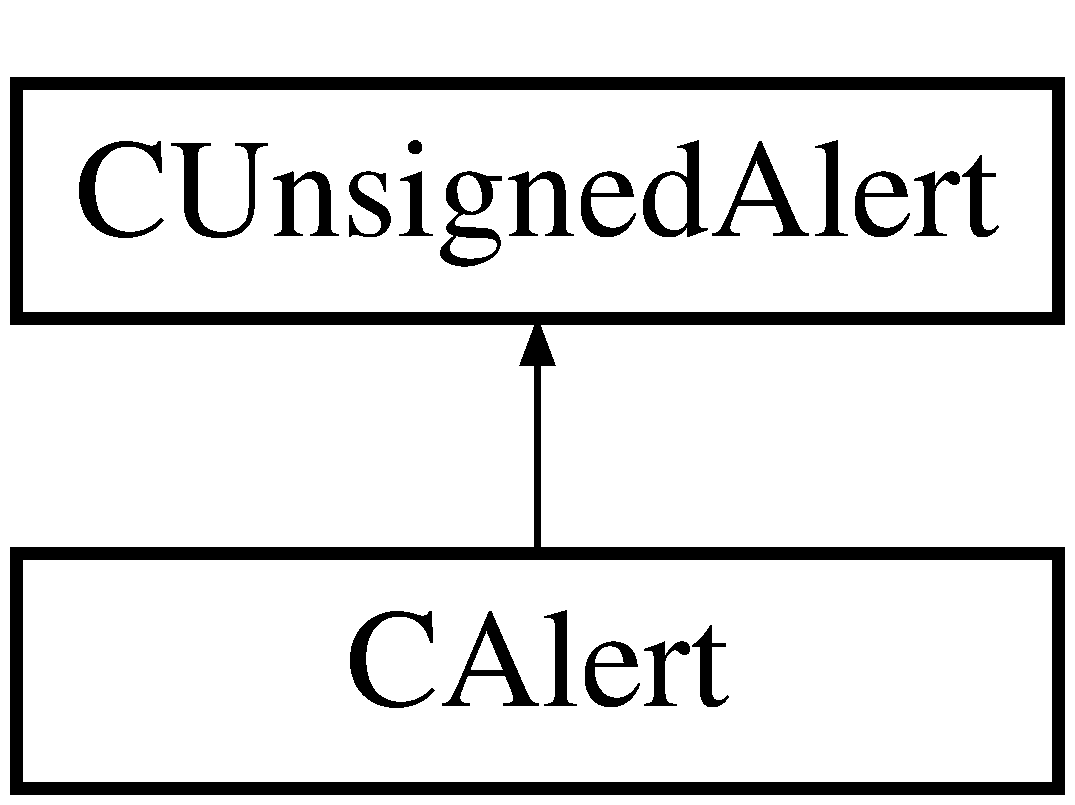
\includegraphics[height=2.000000cm]{class_c_unsigned_alert}
\end{center}
\end{figure}
\subsection*{Public Member Functions}
\begin{DoxyCompactItemize}
\item 
{\footnotesize template$<$typename Stream , typename Operation $>$ }\\void \mbox{\hyperlink{class_c_unsigned_alert_acdf81abb731f9fc8d2c04618f2f4d79d}{Serialization\+Op}} (Stream \&s, Operation ser\+\_\+action, int n\+Type, int \mbox{\hyperlink{class_c_unsigned_alert_ad8fad8e8f62caaf8162fad19170de2cf}{n\+Version}})
\item 
void \mbox{\hyperlink{class_c_unsigned_alert_a9d387307eb60095e50134d10eea3ad69}{Set\+Null}} ()
\item 
std\+::string \mbox{\hyperlink{class_c_unsigned_alert_a1ba948e1de4803565ec0dbec267eadb4}{To\+String}} () const
\end{DoxyCompactItemize}
\subsection*{Public Attributes}
\begin{DoxyCompactItemize}
\item 
int \mbox{\hyperlink{class_c_unsigned_alert_ad8fad8e8f62caaf8162fad19170de2cf}{n\+Version}}
\item 
int64\+\_\+t \mbox{\hyperlink{class_c_unsigned_alert_a13bb82aef8b496584f6b3ae6424f8e58}{n\+Relay\+Until}}
\item 
int64\+\_\+t \mbox{\hyperlink{class_c_unsigned_alert_af77a9d4d3abc0a0b376a7689059620e8}{n\+Expiration}}
\item 
int \mbox{\hyperlink{class_c_unsigned_alert_a4e11dc713526f6597a20762e707518a0}{n\+ID}}
\item 
int \mbox{\hyperlink{class_c_unsigned_alert_a28de8ffcdfea75db2061b2cdc1add04a}{n\+Cancel}}
\item 
std\+::set$<$ int $>$ \mbox{\hyperlink{class_c_unsigned_alert_ab1978ea23d02720d515bcdcf9d0dbdb0}{set\+Cancel}}
\item 
int \mbox{\hyperlink{class_c_unsigned_alert_af7ab540ea7df8e97fbfba7551ec31b1a}{n\+Min\+Ver}}
\item 
int \mbox{\hyperlink{class_c_unsigned_alert_a041bff847e178c132cb4d5234c1f41c8}{n\+Max\+Ver}}
\item 
std\+::set$<$ std\+::string $>$ \mbox{\hyperlink{class_c_unsigned_alert_a1b7148c413e1781222c5748935cad200}{set\+Sub\+Ver}}
\item 
int \mbox{\hyperlink{class_c_unsigned_alert_acf7253ae21d58a8633faab0635f5f5f5}{n\+Priority}}
\item 
std\+::string \mbox{\hyperlink{class_c_unsigned_alert_a8c9cd8c9706c14df3c5d6b9b1ed3b130}{str\+Comment}}
\item 
std\+::string \mbox{\hyperlink{class_c_unsigned_alert_a97cfbf9a49b770bb84e49389ac1489c2}{str\+Status\+Bar}}
\item 
std\+::string \mbox{\hyperlink{class_c_unsigned_alert_afc53ee9fa8b93b30f4a130806c547cea}{str\+R\+P\+C\+Error}}
\item 
\mbox{\hyperlink{class_c_unsigned_alert_a24489988876bbf2c38a5f379e4057a53}{A\+D\+D\+\_\+\+S\+E\+R\+I\+A\+L\+I\+Z\+E\+\_\+\+M\+E\+T\+H\+O\+DS}}
\end{DoxyCompactItemize}


\subsection{Detailed Description}
Alerts are for notifying old versions if they become too obsolete and need to upgrade. The message is displayed in the status bar. Alert messages are broadcast as a vector of signed data. Unserializing may not read the entire buffer if the alert is for a newer version, but older versions can still relay the original data. 

\subsection{Member Function Documentation}
\mbox{\Hypertarget{class_c_unsigned_alert_acdf81abb731f9fc8d2c04618f2f4d79d}\label{class_c_unsigned_alert_acdf81abb731f9fc8d2c04618f2f4d79d}} 
\index{C\+Unsigned\+Alert@{C\+Unsigned\+Alert}!Serialization\+Op@{Serialization\+Op}}
\index{Serialization\+Op@{Serialization\+Op}!C\+Unsigned\+Alert@{C\+Unsigned\+Alert}}
\subsubsection{\texorpdfstring{Serialization\+Op()}{SerializationOp()}}
{\footnotesize\ttfamily template$<$typename Stream , typename Operation $>$ \\
void C\+Unsigned\+Alert\+::\+Serialization\+Op (\begin{DoxyParamCaption}\item[{Stream \&}]{s,  }\item[{Operation}]{ser\+\_\+action,  }\item[{int}]{n\+Type,  }\item[{int}]{n\+Version }\end{DoxyParamCaption})\hspace{0.3cm}{\ttfamily [inline]}}

\mbox{\Hypertarget{class_c_unsigned_alert_a9d387307eb60095e50134d10eea3ad69}\label{class_c_unsigned_alert_a9d387307eb60095e50134d10eea3ad69}} 
\index{C\+Unsigned\+Alert@{C\+Unsigned\+Alert}!Set\+Null@{Set\+Null}}
\index{Set\+Null@{Set\+Null}!C\+Unsigned\+Alert@{C\+Unsigned\+Alert}}
\subsubsection{\texorpdfstring{Set\+Null()}{SetNull()}}
{\footnotesize\ttfamily void C\+Unsigned\+Alert\+::\+Set\+Null (\begin{DoxyParamCaption}{ }\end{DoxyParamCaption})}

\mbox{\Hypertarget{class_c_unsigned_alert_a1ba948e1de4803565ec0dbec267eadb4}\label{class_c_unsigned_alert_a1ba948e1de4803565ec0dbec267eadb4}} 
\index{C\+Unsigned\+Alert@{C\+Unsigned\+Alert}!To\+String@{To\+String}}
\index{To\+String@{To\+String}!C\+Unsigned\+Alert@{C\+Unsigned\+Alert}}
\subsubsection{\texorpdfstring{To\+String()}{ToString()}}
{\footnotesize\ttfamily std\+::string C\+Unsigned\+Alert\+::\+To\+String (\begin{DoxyParamCaption}{ }\end{DoxyParamCaption}) const}



\subsection{Member Data Documentation}
\mbox{\Hypertarget{class_c_unsigned_alert_a24489988876bbf2c38a5f379e4057a53}\label{class_c_unsigned_alert_a24489988876bbf2c38a5f379e4057a53}} 
\index{C\+Unsigned\+Alert@{C\+Unsigned\+Alert}!A\+D\+D\+\_\+\+S\+E\+R\+I\+A\+L\+I\+Z\+E\+\_\+\+M\+E\+T\+H\+O\+DS@{A\+D\+D\+\_\+\+S\+E\+R\+I\+A\+L\+I\+Z\+E\+\_\+\+M\+E\+T\+H\+O\+DS}}
\index{A\+D\+D\+\_\+\+S\+E\+R\+I\+A\+L\+I\+Z\+E\+\_\+\+M\+E\+T\+H\+O\+DS@{A\+D\+D\+\_\+\+S\+E\+R\+I\+A\+L\+I\+Z\+E\+\_\+\+M\+E\+T\+H\+O\+DS}!C\+Unsigned\+Alert@{C\+Unsigned\+Alert}}
\subsubsection{\texorpdfstring{A\+D\+D\+\_\+\+S\+E\+R\+I\+A\+L\+I\+Z\+E\+\_\+\+M\+E\+T\+H\+O\+DS}{ADD\_SERIALIZE\_METHODS}}
{\footnotesize\ttfamily C\+Unsigned\+Alert\+::\+A\+D\+D\+\_\+\+S\+E\+R\+I\+A\+L\+I\+Z\+E\+\_\+\+M\+E\+T\+H\+O\+DS}

\mbox{\Hypertarget{class_c_unsigned_alert_a28de8ffcdfea75db2061b2cdc1add04a}\label{class_c_unsigned_alert_a28de8ffcdfea75db2061b2cdc1add04a}} 
\index{C\+Unsigned\+Alert@{C\+Unsigned\+Alert}!n\+Cancel@{n\+Cancel}}
\index{n\+Cancel@{n\+Cancel}!C\+Unsigned\+Alert@{C\+Unsigned\+Alert}}
\subsubsection{\texorpdfstring{n\+Cancel}{nCancel}}
{\footnotesize\ttfamily int C\+Unsigned\+Alert\+::n\+Cancel}

\mbox{\Hypertarget{class_c_unsigned_alert_af77a9d4d3abc0a0b376a7689059620e8}\label{class_c_unsigned_alert_af77a9d4d3abc0a0b376a7689059620e8}} 
\index{C\+Unsigned\+Alert@{C\+Unsigned\+Alert}!n\+Expiration@{n\+Expiration}}
\index{n\+Expiration@{n\+Expiration}!C\+Unsigned\+Alert@{C\+Unsigned\+Alert}}
\subsubsection{\texorpdfstring{n\+Expiration}{nExpiration}}
{\footnotesize\ttfamily int64\+\_\+t C\+Unsigned\+Alert\+::n\+Expiration}

\mbox{\Hypertarget{class_c_unsigned_alert_a4e11dc713526f6597a20762e707518a0}\label{class_c_unsigned_alert_a4e11dc713526f6597a20762e707518a0}} 
\index{C\+Unsigned\+Alert@{C\+Unsigned\+Alert}!n\+ID@{n\+ID}}
\index{n\+ID@{n\+ID}!C\+Unsigned\+Alert@{C\+Unsigned\+Alert}}
\subsubsection{\texorpdfstring{n\+ID}{nID}}
{\footnotesize\ttfamily int C\+Unsigned\+Alert\+::n\+ID}

\mbox{\Hypertarget{class_c_unsigned_alert_a041bff847e178c132cb4d5234c1f41c8}\label{class_c_unsigned_alert_a041bff847e178c132cb4d5234c1f41c8}} 
\index{C\+Unsigned\+Alert@{C\+Unsigned\+Alert}!n\+Max\+Ver@{n\+Max\+Ver}}
\index{n\+Max\+Ver@{n\+Max\+Ver}!C\+Unsigned\+Alert@{C\+Unsigned\+Alert}}
\subsubsection{\texorpdfstring{n\+Max\+Ver}{nMaxVer}}
{\footnotesize\ttfamily int C\+Unsigned\+Alert\+::n\+Max\+Ver}

\mbox{\Hypertarget{class_c_unsigned_alert_af7ab540ea7df8e97fbfba7551ec31b1a}\label{class_c_unsigned_alert_af7ab540ea7df8e97fbfba7551ec31b1a}} 
\index{C\+Unsigned\+Alert@{C\+Unsigned\+Alert}!n\+Min\+Ver@{n\+Min\+Ver}}
\index{n\+Min\+Ver@{n\+Min\+Ver}!C\+Unsigned\+Alert@{C\+Unsigned\+Alert}}
\subsubsection{\texorpdfstring{n\+Min\+Ver}{nMinVer}}
{\footnotesize\ttfamily int C\+Unsigned\+Alert\+::n\+Min\+Ver}

\mbox{\Hypertarget{class_c_unsigned_alert_acf7253ae21d58a8633faab0635f5f5f5}\label{class_c_unsigned_alert_acf7253ae21d58a8633faab0635f5f5f5}} 
\index{C\+Unsigned\+Alert@{C\+Unsigned\+Alert}!n\+Priority@{n\+Priority}}
\index{n\+Priority@{n\+Priority}!C\+Unsigned\+Alert@{C\+Unsigned\+Alert}}
\subsubsection{\texorpdfstring{n\+Priority}{nPriority}}
{\footnotesize\ttfamily int C\+Unsigned\+Alert\+::n\+Priority}

\mbox{\Hypertarget{class_c_unsigned_alert_a13bb82aef8b496584f6b3ae6424f8e58}\label{class_c_unsigned_alert_a13bb82aef8b496584f6b3ae6424f8e58}} 
\index{C\+Unsigned\+Alert@{C\+Unsigned\+Alert}!n\+Relay\+Until@{n\+Relay\+Until}}
\index{n\+Relay\+Until@{n\+Relay\+Until}!C\+Unsigned\+Alert@{C\+Unsigned\+Alert}}
\subsubsection{\texorpdfstring{n\+Relay\+Until}{nRelayUntil}}
{\footnotesize\ttfamily int64\+\_\+t C\+Unsigned\+Alert\+::n\+Relay\+Until}

\mbox{\Hypertarget{class_c_unsigned_alert_ad8fad8e8f62caaf8162fad19170de2cf}\label{class_c_unsigned_alert_ad8fad8e8f62caaf8162fad19170de2cf}} 
\index{C\+Unsigned\+Alert@{C\+Unsigned\+Alert}!n\+Version@{n\+Version}}
\index{n\+Version@{n\+Version}!C\+Unsigned\+Alert@{C\+Unsigned\+Alert}}
\subsubsection{\texorpdfstring{n\+Version}{nVersion}}
{\footnotesize\ttfamily int C\+Unsigned\+Alert\+::n\+Version}

\mbox{\Hypertarget{class_c_unsigned_alert_ab1978ea23d02720d515bcdcf9d0dbdb0}\label{class_c_unsigned_alert_ab1978ea23d02720d515bcdcf9d0dbdb0}} 
\index{C\+Unsigned\+Alert@{C\+Unsigned\+Alert}!set\+Cancel@{set\+Cancel}}
\index{set\+Cancel@{set\+Cancel}!C\+Unsigned\+Alert@{C\+Unsigned\+Alert}}
\subsubsection{\texorpdfstring{set\+Cancel}{setCancel}}
{\footnotesize\ttfamily std\+::set$<$int$>$ C\+Unsigned\+Alert\+::set\+Cancel}

\mbox{\Hypertarget{class_c_unsigned_alert_a1b7148c413e1781222c5748935cad200}\label{class_c_unsigned_alert_a1b7148c413e1781222c5748935cad200}} 
\index{C\+Unsigned\+Alert@{C\+Unsigned\+Alert}!set\+Sub\+Ver@{set\+Sub\+Ver}}
\index{set\+Sub\+Ver@{set\+Sub\+Ver}!C\+Unsigned\+Alert@{C\+Unsigned\+Alert}}
\subsubsection{\texorpdfstring{set\+Sub\+Ver}{setSubVer}}
{\footnotesize\ttfamily std\+::set$<$std\+::string$>$ C\+Unsigned\+Alert\+::set\+Sub\+Ver}

\mbox{\Hypertarget{class_c_unsigned_alert_a8c9cd8c9706c14df3c5d6b9b1ed3b130}\label{class_c_unsigned_alert_a8c9cd8c9706c14df3c5d6b9b1ed3b130}} 
\index{C\+Unsigned\+Alert@{C\+Unsigned\+Alert}!str\+Comment@{str\+Comment}}
\index{str\+Comment@{str\+Comment}!C\+Unsigned\+Alert@{C\+Unsigned\+Alert}}
\subsubsection{\texorpdfstring{str\+Comment}{strComment}}
{\footnotesize\ttfamily std\+::string C\+Unsigned\+Alert\+::str\+Comment}

\mbox{\Hypertarget{class_c_unsigned_alert_afc53ee9fa8b93b30f4a130806c547cea}\label{class_c_unsigned_alert_afc53ee9fa8b93b30f4a130806c547cea}} 
\index{C\+Unsigned\+Alert@{C\+Unsigned\+Alert}!str\+R\+P\+C\+Error@{str\+R\+P\+C\+Error}}
\index{str\+R\+P\+C\+Error@{str\+R\+P\+C\+Error}!C\+Unsigned\+Alert@{C\+Unsigned\+Alert}}
\subsubsection{\texorpdfstring{str\+R\+P\+C\+Error}{strRPCError}}
{\footnotesize\ttfamily std\+::string C\+Unsigned\+Alert\+::str\+R\+P\+C\+Error}

\mbox{\Hypertarget{class_c_unsigned_alert_a97cfbf9a49b770bb84e49389ac1489c2}\label{class_c_unsigned_alert_a97cfbf9a49b770bb84e49389ac1489c2}} 
\index{C\+Unsigned\+Alert@{C\+Unsigned\+Alert}!str\+Status\+Bar@{str\+Status\+Bar}}
\index{str\+Status\+Bar@{str\+Status\+Bar}!C\+Unsigned\+Alert@{C\+Unsigned\+Alert}}
\subsubsection{\texorpdfstring{str\+Status\+Bar}{strStatusBar}}
{\footnotesize\ttfamily std\+::string C\+Unsigned\+Alert\+::str\+Status\+Bar}



The documentation for this class was generated from the following files\+:\begin{DoxyCompactItemize}
\item 
/\+Users/christopherarguello/\+Developer/anon/src/\mbox{\hyperlink{alert_8h}{alert.\+h}}\item 
/\+Users/christopherarguello/\+Developer/anon/src/\mbox{\hyperlink{alert_8cpp}{alert.\+cpp}}\end{DoxyCompactItemize}

\hypertarget{class_c_validation_interface}{}\section{C\+Validation\+Interface Class Reference}
\label{class_c_validation_interface}\index{C\+Validation\+Interface@{C\+Validation\+Interface}}


{\ttfamily \#include $<$validationinterface.\+h$>$}

Inheritance diagram for C\+Validation\+Interface\+:\begin{figure}[H]
\begin{center}
\leavevmode
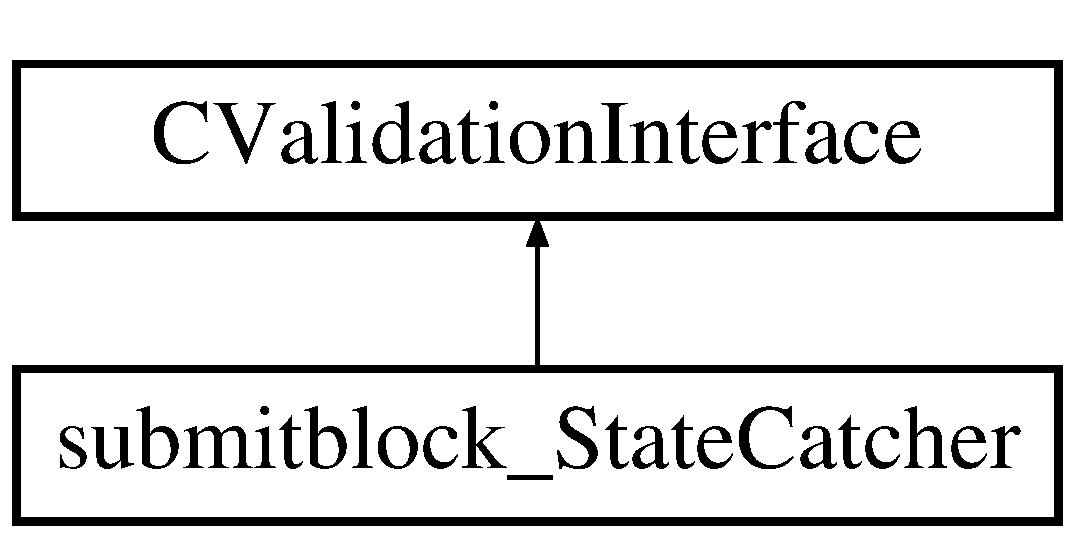
\includegraphics[height=2.000000cm]{class_c_validation_interface}
\end{center}
\end{figure}
\subsection*{Protected Member Functions}
\begin{DoxyCompactItemize}
\item 
virtual void \mbox{\hyperlink{class_c_validation_interface_a8cb5e5926b2dbbb25eba8263a6a20542}{Updated\+Block\+Tip}} (const \mbox{\hyperlink{class_c_block_index}{C\+Block\+Index}} $\ast$pindex)
\item 
virtual void \mbox{\hyperlink{class_c_validation_interface_a1d255ed08bf26dbd6ad5924cabfdfae4}{Sync\+Transaction}} (const C\+Transaction \&tx, const C\+Block $\ast$pblock)
\item 
virtual void \mbox{\hyperlink{class_c_validation_interface_af8120f64ec6569dcf765fdf14acef31f}{Erase\+From\+Wallet}} (const \mbox{\hyperlink{classuint256}{uint256}} \&hash)
\item 
virtual void \mbox{\hyperlink{class_c_validation_interface_a15a2ed92f499a9b54c75a594eb0a7702}{Chain\+Tip}} (const \mbox{\hyperlink{class_c_block_index}{C\+Block\+Index}} $\ast$pindex, const C\+Block $\ast$pblock, Z\+C\+Incremental\+Merkle\+Tree tree, bool added)
\item 
virtual void \mbox{\hyperlink{class_c_validation_interface_a8684492d9878120ce8c6c760a790f9ea}{Set\+Best\+Chain}} (const C\+Block\+Locator \&locator)
\item 
virtual void \mbox{\hyperlink{class_c_validation_interface_a8058fc107d993641df615abbb35a4c27}{Updated\+Transaction}} (const \mbox{\hyperlink{classuint256}{uint256}} \&hash)
\item 
virtual void \mbox{\hyperlink{class_c_validation_interface_a981f5160a2370db0cd616c00d8bd5270}{Inventory}} (const \mbox{\hyperlink{classuint256}{uint256}} \&hash)
\item 
virtual void \mbox{\hyperlink{class_c_validation_interface_af501da6f06bccb5e4bfbe66ae1bf6c9d}{Resend\+Wallet\+Transactions}} (int64\+\_\+t n\+Best\+Block\+Time)
\item 
virtual void \mbox{\hyperlink{class_c_validation_interface_aeb34ef6814685cabc29062ed7be25441}{Block\+Checked}} (const C\+Block \&, const C\+Validation\+State \&)
\item 
friend \mbox{\hyperlink{class_c_validation_interface_aa7a5e52b8950b16b3c14391809047ca6}{void \+::\+Register\+Validation\+Interface}} (\mbox{\hyperlink{class_c_validation_interface}{C\+Validation\+Interface}} $\ast$)
\item 
friend \mbox{\hyperlink{class_c_validation_interface_aaed3b260b3de64ed423a9a24bf0e29f4}{void \+::\+Unregister\+Validation\+Interface}} (\mbox{\hyperlink{class_c_validation_interface}{C\+Validation\+Interface}} $\ast$)
\item 
friend \mbox{\hyperlink{class_c_validation_interface_a7234df2b6e1a079260489eea6eb6eb72}{void \+::\+Unregister\+All\+Validation\+Interfaces}} ()
\end{DoxyCompactItemize}


\subsection{Member Function Documentation}
\mbox{\Hypertarget{class_c_validation_interface_aeb34ef6814685cabc29062ed7be25441}\label{class_c_validation_interface_aeb34ef6814685cabc29062ed7be25441}} 
\index{C\+Validation\+Interface@{C\+Validation\+Interface}!Block\+Checked@{Block\+Checked}}
\index{Block\+Checked@{Block\+Checked}!C\+Validation\+Interface@{C\+Validation\+Interface}}
\subsubsection{\texorpdfstring{Block\+Checked()}{BlockChecked()}}
{\footnotesize\ttfamily virtual void C\+Validation\+Interface\+::\+Block\+Checked (\begin{DoxyParamCaption}\item[{const C\+Block \&}]{,  }\item[{const C\+Validation\+State \&}]{ }\end{DoxyParamCaption})\hspace{0.3cm}{\ttfamily [inline]}, {\ttfamily [protected]}, {\ttfamily [virtual]}}



Reimplemented in \mbox{\hyperlink{classsubmitblock___state_catcher_a7c7174ac1a54c80c572b115114aa2ee6}{submitblock\+\_\+\+State\+Catcher}}.

\mbox{\Hypertarget{class_c_validation_interface_a15a2ed92f499a9b54c75a594eb0a7702}\label{class_c_validation_interface_a15a2ed92f499a9b54c75a594eb0a7702}} 
\index{C\+Validation\+Interface@{C\+Validation\+Interface}!Chain\+Tip@{Chain\+Tip}}
\index{Chain\+Tip@{Chain\+Tip}!C\+Validation\+Interface@{C\+Validation\+Interface}}
\subsubsection{\texorpdfstring{Chain\+Tip()}{ChainTip()}}
{\footnotesize\ttfamily virtual void C\+Validation\+Interface\+::\+Chain\+Tip (\begin{DoxyParamCaption}\item[{const \mbox{\hyperlink{class_c_block_index}{C\+Block\+Index}} $\ast$}]{pindex,  }\item[{const C\+Block $\ast$}]{pblock,  }\item[{Z\+C\+Incremental\+Merkle\+Tree}]{tree,  }\item[{bool}]{added }\end{DoxyParamCaption})\hspace{0.3cm}{\ttfamily [inline]}, {\ttfamily [protected]}, {\ttfamily [virtual]}}

\mbox{\Hypertarget{class_c_validation_interface_af8120f64ec6569dcf765fdf14acef31f}\label{class_c_validation_interface_af8120f64ec6569dcf765fdf14acef31f}} 
\index{C\+Validation\+Interface@{C\+Validation\+Interface}!Erase\+From\+Wallet@{Erase\+From\+Wallet}}
\index{Erase\+From\+Wallet@{Erase\+From\+Wallet}!C\+Validation\+Interface@{C\+Validation\+Interface}}
\subsubsection{\texorpdfstring{Erase\+From\+Wallet()}{EraseFromWallet()}}
{\footnotesize\ttfamily virtual void C\+Validation\+Interface\+::\+Erase\+From\+Wallet (\begin{DoxyParamCaption}\item[{const \mbox{\hyperlink{classuint256}{uint256}} \&}]{hash }\end{DoxyParamCaption})\hspace{0.3cm}{\ttfamily [inline]}, {\ttfamily [protected]}, {\ttfamily [virtual]}}

\mbox{\Hypertarget{class_c_validation_interface_a981f5160a2370db0cd616c00d8bd5270}\label{class_c_validation_interface_a981f5160a2370db0cd616c00d8bd5270}} 
\index{C\+Validation\+Interface@{C\+Validation\+Interface}!Inventory@{Inventory}}
\index{Inventory@{Inventory}!C\+Validation\+Interface@{C\+Validation\+Interface}}
\subsubsection{\texorpdfstring{Inventory()}{Inventory()}}
{\footnotesize\ttfamily virtual void C\+Validation\+Interface\+::\+Inventory (\begin{DoxyParamCaption}\item[{const \mbox{\hyperlink{classuint256}{uint256}} \&}]{hash }\end{DoxyParamCaption})\hspace{0.3cm}{\ttfamily [inline]}, {\ttfamily [protected]}, {\ttfamily [virtual]}}

\mbox{\Hypertarget{class_c_validation_interface_af501da6f06bccb5e4bfbe66ae1bf6c9d}\label{class_c_validation_interface_af501da6f06bccb5e4bfbe66ae1bf6c9d}} 
\index{C\+Validation\+Interface@{C\+Validation\+Interface}!Resend\+Wallet\+Transactions@{Resend\+Wallet\+Transactions}}
\index{Resend\+Wallet\+Transactions@{Resend\+Wallet\+Transactions}!C\+Validation\+Interface@{C\+Validation\+Interface}}
\subsubsection{\texorpdfstring{Resend\+Wallet\+Transactions()}{ResendWalletTransactions()}}
{\footnotesize\ttfamily virtual void C\+Validation\+Interface\+::\+Resend\+Wallet\+Transactions (\begin{DoxyParamCaption}\item[{int64\+\_\+t}]{n\+Best\+Block\+Time }\end{DoxyParamCaption})\hspace{0.3cm}{\ttfamily [inline]}, {\ttfamily [protected]}, {\ttfamily [virtual]}}

\mbox{\Hypertarget{class_c_validation_interface_a8684492d9878120ce8c6c760a790f9ea}\label{class_c_validation_interface_a8684492d9878120ce8c6c760a790f9ea}} 
\index{C\+Validation\+Interface@{C\+Validation\+Interface}!Set\+Best\+Chain@{Set\+Best\+Chain}}
\index{Set\+Best\+Chain@{Set\+Best\+Chain}!C\+Validation\+Interface@{C\+Validation\+Interface}}
\subsubsection{\texorpdfstring{Set\+Best\+Chain()}{SetBestChain()}}
{\footnotesize\ttfamily virtual void C\+Validation\+Interface\+::\+Set\+Best\+Chain (\begin{DoxyParamCaption}\item[{const C\+Block\+Locator \&}]{locator }\end{DoxyParamCaption})\hspace{0.3cm}{\ttfamily [inline]}, {\ttfamily [protected]}, {\ttfamily [virtual]}}

\mbox{\Hypertarget{class_c_validation_interface_a1d255ed08bf26dbd6ad5924cabfdfae4}\label{class_c_validation_interface_a1d255ed08bf26dbd6ad5924cabfdfae4}} 
\index{C\+Validation\+Interface@{C\+Validation\+Interface}!Sync\+Transaction@{Sync\+Transaction}}
\index{Sync\+Transaction@{Sync\+Transaction}!C\+Validation\+Interface@{C\+Validation\+Interface}}
\subsubsection{\texorpdfstring{Sync\+Transaction()}{SyncTransaction()}}
{\footnotesize\ttfamily virtual void C\+Validation\+Interface\+::\+Sync\+Transaction (\begin{DoxyParamCaption}\item[{const C\+Transaction \&}]{tx,  }\item[{const C\+Block $\ast$}]{pblock }\end{DoxyParamCaption})\hspace{0.3cm}{\ttfamily [inline]}, {\ttfamily [protected]}, {\ttfamily [virtual]}}

\mbox{\Hypertarget{class_c_validation_interface_a8cb5e5926b2dbbb25eba8263a6a20542}\label{class_c_validation_interface_a8cb5e5926b2dbbb25eba8263a6a20542}} 
\index{C\+Validation\+Interface@{C\+Validation\+Interface}!Updated\+Block\+Tip@{Updated\+Block\+Tip}}
\index{Updated\+Block\+Tip@{Updated\+Block\+Tip}!C\+Validation\+Interface@{C\+Validation\+Interface}}
\subsubsection{\texorpdfstring{Updated\+Block\+Tip()}{UpdatedBlockTip()}}
{\footnotesize\ttfamily virtual void C\+Validation\+Interface\+::\+Updated\+Block\+Tip (\begin{DoxyParamCaption}\item[{const \mbox{\hyperlink{class_c_block_index}{C\+Block\+Index}} $\ast$}]{pindex }\end{DoxyParamCaption})\hspace{0.3cm}{\ttfamily [inline]}, {\ttfamily [protected]}, {\ttfamily [virtual]}}

\mbox{\Hypertarget{class_c_validation_interface_a8058fc107d993641df615abbb35a4c27}\label{class_c_validation_interface_a8058fc107d993641df615abbb35a4c27}} 
\index{C\+Validation\+Interface@{C\+Validation\+Interface}!Updated\+Transaction@{Updated\+Transaction}}
\index{Updated\+Transaction@{Updated\+Transaction}!C\+Validation\+Interface@{C\+Validation\+Interface}}
\subsubsection{\texorpdfstring{Updated\+Transaction()}{UpdatedTransaction()}}
{\footnotesize\ttfamily virtual void C\+Validation\+Interface\+::\+Updated\+Transaction (\begin{DoxyParamCaption}\item[{const \mbox{\hyperlink{classuint256}{uint256}} \&}]{hash }\end{DoxyParamCaption})\hspace{0.3cm}{\ttfamily [inline]}, {\ttfamily [protected]}, {\ttfamily [virtual]}}

\mbox{\Hypertarget{class_c_validation_interface_aa7a5e52b8950b16b3c14391809047ca6}\label{class_c_validation_interface_aa7a5e52b8950b16b3c14391809047ca6}} 
\index{C\+Validation\+Interface@{C\+Validation\+Interface}!void \+::\+Register\+Validation\+Interface@{void \+::\+Register\+Validation\+Interface}}
\index{void \+::\+Register\+Validation\+Interface@{void \+::\+Register\+Validation\+Interface}!C\+Validation\+Interface@{C\+Validation\+Interface}}
\subsubsection{\texorpdfstring{void \+::\+Register\+Validation\+Interface()}{void ::RegisterValidationInterface()}}
{\footnotesize\ttfamily C\+Validation\+Interface\+::void \+::\mbox{\hyperlink{validationinterface_8h_ade8ef59282b5f7521ecfd870a8e3b137}{Register\+Validation\+Interface}} (\begin{DoxyParamCaption}\item[{\mbox{\hyperlink{class_c_validation_interface}{C\+Validation\+Interface}} $\ast$}]{ }\end{DoxyParamCaption})\hspace{0.3cm}{\ttfamily [protected]}}

\mbox{\Hypertarget{class_c_validation_interface_a7234df2b6e1a079260489eea6eb6eb72}\label{class_c_validation_interface_a7234df2b6e1a079260489eea6eb6eb72}} 
\index{C\+Validation\+Interface@{C\+Validation\+Interface}!void \+::\+Unregister\+All\+Validation\+Interfaces@{void \+::\+Unregister\+All\+Validation\+Interfaces}}
\index{void \+::\+Unregister\+All\+Validation\+Interfaces@{void \+::\+Unregister\+All\+Validation\+Interfaces}!C\+Validation\+Interface@{C\+Validation\+Interface}}
\subsubsection{\texorpdfstring{void \+::\+Unregister\+All\+Validation\+Interfaces()}{void ::UnregisterAllValidationInterfaces()}}
{\footnotesize\ttfamily C\+Validation\+Interface\+::void \+::\mbox{\hyperlink{validationinterface_8h_a8fe3fbf8c47cc0419fd7b9a14e8b140d}{Unregister\+All\+Validation\+Interfaces}} (\begin{DoxyParamCaption}{ }\end{DoxyParamCaption})\hspace{0.3cm}{\ttfamily [protected]}}

\mbox{\Hypertarget{class_c_validation_interface_aaed3b260b3de64ed423a9a24bf0e29f4}\label{class_c_validation_interface_aaed3b260b3de64ed423a9a24bf0e29f4}} 
\index{C\+Validation\+Interface@{C\+Validation\+Interface}!void \+::\+Unregister\+Validation\+Interface@{void \+::\+Unregister\+Validation\+Interface}}
\index{void \+::\+Unregister\+Validation\+Interface@{void \+::\+Unregister\+Validation\+Interface}!C\+Validation\+Interface@{C\+Validation\+Interface}}
\subsubsection{\texorpdfstring{void \+::\+Unregister\+Validation\+Interface()}{void ::UnregisterValidationInterface()}}
{\footnotesize\ttfamily C\+Validation\+Interface\+::void \+::\mbox{\hyperlink{validationinterface_8h_a5e1776de1f87b4d045e9e2a198236b63}{Unregister\+Validation\+Interface}} (\begin{DoxyParamCaption}\item[{\mbox{\hyperlink{class_c_validation_interface}{C\+Validation\+Interface}} $\ast$}]{ }\end{DoxyParamCaption})\hspace{0.3cm}{\ttfamily [protected]}}



The documentation for this class was generated from the following file\+:\begin{DoxyCompactItemize}
\item 
/\+Users/christopherarguello/\+Developer/anon/src/\mbox{\hyperlink{validationinterface_8h}{validationinterface.\+h}}\end{DoxyCompactItemize}

\hypertarget{class_c_var_int}{}\section{C\+Var\+Int$<$ I $>$ Class Template Reference}
\label{class_c_var_int}\index{C\+Var\+Int$<$ I $>$@{C\+Var\+Int$<$ I $>$}}


{\ttfamily \#include $<$serialize.\+h$>$}

\subsection*{Public Member Functions}
\begin{DoxyCompactItemize}
\item 
\mbox{\hyperlink{class_c_var_int_ab26b9de1b43d4b9ce844eaa7cf6a6b4f}{C\+Var\+Int}} (I \&n\+In)
\item 
unsigned int \mbox{\hyperlink{class_c_var_int_af994978b1b95a6b5d3009f5743ca6053}{Get\+Serialize\+Size}} (int, int) const
\item 
{\footnotesize template$<$typename Stream $>$ }\\void \mbox{\hyperlink{class_c_var_int_a3b772eba5c6cd5b9ad7cec9cb45f7cb2}{Serialize}} (Stream \&s, int, int) const
\item 
{\footnotesize template$<$typename Stream $>$ }\\void \mbox{\hyperlink{class_c_var_int_aba87b78443378273b4f335dcd858c29c}{Unserialize}} (Stream \&s, int, int)
\end{DoxyCompactItemize}
\subsection*{Protected Attributes}
\begin{DoxyCompactItemize}
\item 
I \& \mbox{\hyperlink{class_c_var_int_a4514adc82b41754d9ac22ee627744614}{n}}
\end{DoxyCompactItemize}


\subsection{Constructor \& Destructor Documentation}
\mbox{\Hypertarget{class_c_var_int_ab26b9de1b43d4b9ce844eaa7cf6a6b4f}\label{class_c_var_int_ab26b9de1b43d4b9ce844eaa7cf6a6b4f}} 
\index{C\+Var\+Int@{C\+Var\+Int}!C\+Var\+Int@{C\+Var\+Int}}
\index{C\+Var\+Int@{C\+Var\+Int}!C\+Var\+Int@{C\+Var\+Int}}
\subsubsection{\texorpdfstring{C\+Var\+Int()}{CVarInt()}}
{\footnotesize\ttfamily template$<$typename I $>$ \\
\mbox{\hyperlink{class_c_var_int}{C\+Var\+Int}}$<$ I $>$\+::\mbox{\hyperlink{class_c_var_int}{C\+Var\+Int}} (\begin{DoxyParamCaption}\item[{I \&}]{n\+In }\end{DoxyParamCaption})\hspace{0.3cm}{\ttfamily [inline]}}



\subsection{Member Function Documentation}
\mbox{\Hypertarget{class_c_var_int_af994978b1b95a6b5d3009f5743ca6053}\label{class_c_var_int_af994978b1b95a6b5d3009f5743ca6053}} 
\index{C\+Var\+Int@{C\+Var\+Int}!Get\+Serialize\+Size@{Get\+Serialize\+Size}}
\index{Get\+Serialize\+Size@{Get\+Serialize\+Size}!C\+Var\+Int@{C\+Var\+Int}}
\subsubsection{\texorpdfstring{Get\+Serialize\+Size()}{GetSerializeSize()}}
{\footnotesize\ttfamily template$<$typename I $>$ \\
unsigned int \mbox{\hyperlink{class_c_var_int}{C\+Var\+Int}}$<$ I $>$\+::Get\+Serialize\+Size (\begin{DoxyParamCaption}\item[{int}]{,  }\item[{int}]{ }\end{DoxyParamCaption}) const\hspace{0.3cm}{\ttfamily [inline]}}

\mbox{\Hypertarget{class_c_var_int_a3b772eba5c6cd5b9ad7cec9cb45f7cb2}\label{class_c_var_int_a3b772eba5c6cd5b9ad7cec9cb45f7cb2}} 
\index{C\+Var\+Int@{C\+Var\+Int}!Serialize@{Serialize}}
\index{Serialize@{Serialize}!C\+Var\+Int@{C\+Var\+Int}}
\subsubsection{\texorpdfstring{Serialize()}{Serialize()}}
{\footnotesize\ttfamily template$<$typename I $>$ \\
template$<$typename Stream $>$ \\
void \mbox{\hyperlink{class_c_var_int}{C\+Var\+Int}}$<$ I $>$\+::Serialize (\begin{DoxyParamCaption}\item[{Stream \&}]{s,  }\item[{int}]{,  }\item[{int}]{ }\end{DoxyParamCaption}) const\hspace{0.3cm}{\ttfamily [inline]}}

\mbox{\Hypertarget{class_c_var_int_aba87b78443378273b4f335dcd858c29c}\label{class_c_var_int_aba87b78443378273b4f335dcd858c29c}} 
\index{C\+Var\+Int@{C\+Var\+Int}!Unserialize@{Unserialize}}
\index{Unserialize@{Unserialize}!C\+Var\+Int@{C\+Var\+Int}}
\subsubsection{\texorpdfstring{Unserialize()}{Unserialize()}}
{\footnotesize\ttfamily template$<$typename I $>$ \\
template$<$typename Stream $>$ \\
void \mbox{\hyperlink{class_c_var_int}{C\+Var\+Int}}$<$ I $>$\+::Unserialize (\begin{DoxyParamCaption}\item[{Stream \&}]{s,  }\item[{int}]{,  }\item[{int}]{ }\end{DoxyParamCaption})\hspace{0.3cm}{\ttfamily [inline]}}



\subsection{Member Data Documentation}
\mbox{\Hypertarget{class_c_var_int_a4514adc82b41754d9ac22ee627744614}\label{class_c_var_int_a4514adc82b41754d9ac22ee627744614}} 
\index{C\+Var\+Int@{C\+Var\+Int}!n@{n}}
\index{n@{n}!C\+Var\+Int@{C\+Var\+Int}}
\subsubsection{\texorpdfstring{n}{n}}
{\footnotesize\ttfamily template$<$typename I $>$ \\
I\& \mbox{\hyperlink{class_c_var_int}{C\+Var\+Int}}$<$ I $>$\+::n\hspace{0.3cm}{\ttfamily [protected]}}



The documentation for this class was generated from the following file\+:\begin{DoxyCompactItemize}
\item 
/\+Users/christopherarguello/\+Developer/anon/src/\mbox{\hyperlink{serialize_8h}{serialize.\+h}}\end{DoxyCompactItemize}

\hypertarget{class_c_verify_d_b}{}\section{C\+Verify\+DB Class Reference}
\label{class_c_verify_d_b}\index{C\+Verify\+DB@{C\+Verify\+DB}}


{\ttfamily \#include $<$main.\+h$>$}

\subsection*{Public Member Functions}
\begin{DoxyCompactItemize}
\item 
\mbox{\hyperlink{class_c_verify_d_b_ab33a26982ba391fc71614f8eee9dbaa0}{C\+Verify\+DB}} ()
\item 
\mbox{\hyperlink{class_c_verify_d_b_a4a04d4554f763b8803082fae81513f40}{$\sim$\+C\+Verify\+DB}} ()
\item 
bool \mbox{\hyperlink{class_c_verify_d_b_a5d3e3ade35a14ddce2404e18e4b1df50}{Verify\+DB}} (\mbox{\hyperlink{class_c_coins_view}{C\+Coins\+View}} $\ast$coinsview, int n\+Check\+Level, int n\+Check\+Depth)
\end{DoxyCompactItemize}


\subsection{Detailed Description}
R\+A\+II wrapper for Verify\+DB\+: Verify consistency of the block and coin databases 

\subsection{Constructor \& Destructor Documentation}
\mbox{\Hypertarget{class_c_verify_d_b_ab33a26982ba391fc71614f8eee9dbaa0}\label{class_c_verify_d_b_ab33a26982ba391fc71614f8eee9dbaa0}} 
\index{C\+Verify\+DB@{C\+Verify\+DB}!C\+Verify\+DB@{C\+Verify\+DB}}
\index{C\+Verify\+DB@{C\+Verify\+DB}!C\+Verify\+DB@{C\+Verify\+DB}}
\subsubsection{\texorpdfstring{C\+Verify\+D\+B()}{CVerifyDB()}}
{\footnotesize\ttfamily C\+Verify\+D\+B\+::\+C\+Verify\+DB (\begin{DoxyParamCaption}{ }\end{DoxyParamCaption})}

\mbox{\Hypertarget{class_c_verify_d_b_a4a04d4554f763b8803082fae81513f40}\label{class_c_verify_d_b_a4a04d4554f763b8803082fae81513f40}} 
\index{C\+Verify\+DB@{C\+Verify\+DB}!````~C\+Verify\+DB@{$\sim$\+C\+Verify\+DB}}
\index{````~C\+Verify\+DB@{$\sim$\+C\+Verify\+DB}!C\+Verify\+DB@{C\+Verify\+DB}}
\subsubsection{\texorpdfstring{$\sim$\+C\+Verify\+D\+B()}{~CVerifyDB()}}
{\footnotesize\ttfamily C\+Verify\+D\+B\+::$\sim$\+C\+Verify\+DB (\begin{DoxyParamCaption}{ }\end{DoxyParamCaption})}



\subsection{Member Function Documentation}
\mbox{\Hypertarget{class_c_verify_d_b_a5d3e3ade35a14ddce2404e18e4b1df50}\label{class_c_verify_d_b_a5d3e3ade35a14ddce2404e18e4b1df50}} 
\index{C\+Verify\+DB@{C\+Verify\+DB}!Verify\+DB@{Verify\+DB}}
\index{Verify\+DB@{Verify\+DB}!C\+Verify\+DB@{C\+Verify\+DB}}
\subsubsection{\texorpdfstring{Verify\+D\+B()}{VerifyDB()}}
{\footnotesize\ttfamily bool C\+Verify\+D\+B\+::\+Verify\+DB (\begin{DoxyParamCaption}\item[{\mbox{\hyperlink{class_c_coins_view}{C\+Coins\+View}} $\ast$}]{coinsview,  }\item[{int}]{n\+Check\+Level,  }\item[{int}]{n\+Check\+Depth }\end{DoxyParamCaption})}



The documentation for this class was generated from the following files\+:\begin{DoxyCompactItemize}
\item 
/\+Users/christopherarguello/\+Developer/anon/src/\mbox{\hyperlink{main_8h}{main.\+h}}\item 
/\+Users/christopherarguello/\+Developer/anon/src/\mbox{\hyperlink{main_8cpp}{main.\+cpp}}\end{DoxyCompactItemize}

\hypertarget{class_c_z_c_payment_address}{}\section{C\+Z\+C\+Payment\+Address Class Reference}
\label{class_c_z_c_payment_address}\index{C\+Z\+C\+Payment\+Address@{C\+Z\+C\+Payment\+Address}}


{\ttfamily \#include $<$base58.\+h$>$}

Inheritance diagram for C\+Z\+C\+Payment\+Address\+:\begin{figure}[H]
\begin{center}
\leavevmode
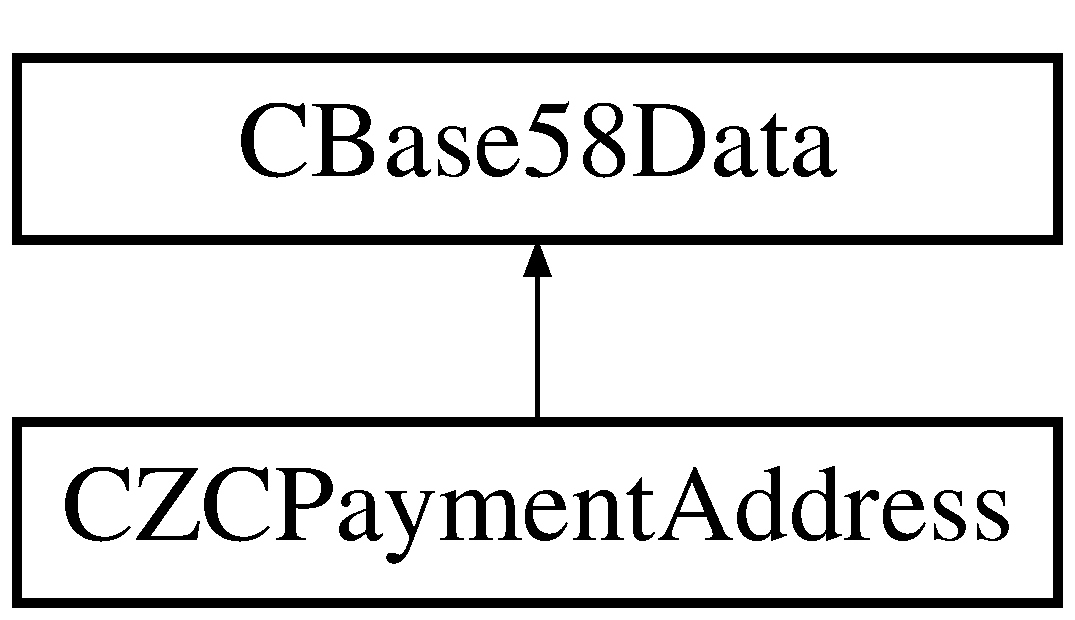
\includegraphics[height=2.000000cm]{class_c_z_c_payment_address}
\end{center}
\end{figure}
\subsection*{Public Member Functions}
\begin{DoxyCompactItemize}
\item 
bool \mbox{\hyperlink{class_c_z_c_payment_address_aa89a4517ba16d1d559d7bd534e8471d0}{Set}} (const libzcash\+::\+Payment\+Address \&addr)
\item 
\mbox{\hyperlink{class_c_z_c_payment_address_a9eb9bc36437547e7f0ed79f18389f06d}{C\+Z\+C\+Payment\+Address}} ()
\item 
\mbox{\hyperlink{class_c_z_c_payment_address_a72fd927fbc6322cdeff45d6cb209afae}{C\+Z\+C\+Payment\+Address}} (const std\+::string \&str\+Address)
\item 
\mbox{\hyperlink{class_c_z_c_payment_address_acf0b08d31e9cb6b1a1862b54340b65ec}{C\+Z\+C\+Payment\+Address}} (const libzcash\+::\+Payment\+Address \&addr)
\item 
libzcash\+::\+Payment\+Address \mbox{\hyperlink{class_c_z_c_payment_address_a95f7c38361637df85674897b473f3e3f}{Get}} () const
\end{DoxyCompactItemize}
\subsection*{Additional Inherited Members}


\subsection{Constructor \& Destructor Documentation}
\mbox{\Hypertarget{class_c_z_c_payment_address_a9eb9bc36437547e7f0ed79f18389f06d}\label{class_c_z_c_payment_address_a9eb9bc36437547e7f0ed79f18389f06d}} 
\index{C\+Z\+C\+Payment\+Address@{C\+Z\+C\+Payment\+Address}!C\+Z\+C\+Payment\+Address@{C\+Z\+C\+Payment\+Address}}
\index{C\+Z\+C\+Payment\+Address@{C\+Z\+C\+Payment\+Address}!C\+Z\+C\+Payment\+Address@{C\+Z\+C\+Payment\+Address}}
\subsubsection{\texorpdfstring{C\+Z\+C\+Payment\+Address()}{CZCPaymentAddress()}\hspace{0.1cm}{\footnotesize\ttfamily [1/3]}}
{\footnotesize\ttfamily C\+Z\+C\+Payment\+Address\+::\+C\+Z\+C\+Payment\+Address (\begin{DoxyParamCaption}{ }\end{DoxyParamCaption})\hspace{0.3cm}{\ttfamily [inline]}}

\mbox{\Hypertarget{class_c_z_c_payment_address_a72fd927fbc6322cdeff45d6cb209afae}\label{class_c_z_c_payment_address_a72fd927fbc6322cdeff45d6cb209afae}} 
\index{C\+Z\+C\+Payment\+Address@{C\+Z\+C\+Payment\+Address}!C\+Z\+C\+Payment\+Address@{C\+Z\+C\+Payment\+Address}}
\index{C\+Z\+C\+Payment\+Address@{C\+Z\+C\+Payment\+Address}!C\+Z\+C\+Payment\+Address@{C\+Z\+C\+Payment\+Address}}
\subsubsection{\texorpdfstring{C\+Z\+C\+Payment\+Address()}{CZCPaymentAddress()}\hspace{0.1cm}{\footnotesize\ttfamily [2/3]}}
{\footnotesize\ttfamily C\+Z\+C\+Payment\+Address\+::\+C\+Z\+C\+Payment\+Address (\begin{DoxyParamCaption}\item[{const std\+::string \&}]{str\+Address }\end{DoxyParamCaption})\hspace{0.3cm}{\ttfamily [inline]}}

\mbox{\Hypertarget{class_c_z_c_payment_address_acf0b08d31e9cb6b1a1862b54340b65ec}\label{class_c_z_c_payment_address_acf0b08d31e9cb6b1a1862b54340b65ec}} 
\index{C\+Z\+C\+Payment\+Address@{C\+Z\+C\+Payment\+Address}!C\+Z\+C\+Payment\+Address@{C\+Z\+C\+Payment\+Address}}
\index{C\+Z\+C\+Payment\+Address@{C\+Z\+C\+Payment\+Address}!C\+Z\+C\+Payment\+Address@{C\+Z\+C\+Payment\+Address}}
\subsubsection{\texorpdfstring{C\+Z\+C\+Payment\+Address()}{CZCPaymentAddress()}\hspace{0.1cm}{\footnotesize\ttfamily [3/3]}}
{\footnotesize\ttfamily C\+Z\+C\+Payment\+Address\+::\+C\+Z\+C\+Payment\+Address (\begin{DoxyParamCaption}\item[{const libzcash\+::\+Payment\+Address \&}]{addr }\end{DoxyParamCaption})\hspace{0.3cm}{\ttfamily [inline]}}



\subsection{Member Function Documentation}
\mbox{\Hypertarget{class_c_z_c_payment_address_a95f7c38361637df85674897b473f3e3f}\label{class_c_z_c_payment_address_a95f7c38361637df85674897b473f3e3f}} 
\index{C\+Z\+C\+Payment\+Address@{C\+Z\+C\+Payment\+Address}!Get@{Get}}
\index{Get@{Get}!C\+Z\+C\+Payment\+Address@{C\+Z\+C\+Payment\+Address}}
\subsubsection{\texorpdfstring{Get()}{Get()}}
{\footnotesize\ttfamily libzcash\+::\+Payment\+Address C\+Z\+C\+Payment\+Address\+::\+Get (\begin{DoxyParamCaption}{ }\end{DoxyParamCaption}) const}

\mbox{\Hypertarget{class_c_z_c_payment_address_aa89a4517ba16d1d559d7bd534e8471d0}\label{class_c_z_c_payment_address_aa89a4517ba16d1d559d7bd534e8471d0}} 
\index{C\+Z\+C\+Payment\+Address@{C\+Z\+C\+Payment\+Address}!Set@{Set}}
\index{Set@{Set}!C\+Z\+C\+Payment\+Address@{C\+Z\+C\+Payment\+Address}}
\subsubsection{\texorpdfstring{Set()}{Set()}}
{\footnotesize\ttfamily bool C\+Z\+C\+Payment\+Address\+::\+Set (\begin{DoxyParamCaption}\item[{const libzcash\+::\+Payment\+Address \&}]{addr }\end{DoxyParamCaption})}



The documentation for this class was generated from the following files\+:\begin{DoxyCompactItemize}
\item 
/\+Users/christopherarguello/\+Developer/anon/src/\mbox{\hyperlink{base58_8h}{base58.\+h}}\item 
/\+Users/christopherarguello/\+Developer/anon/src/\mbox{\hyperlink{base58_8cpp}{base58.\+cpp}}\end{DoxyCompactItemize}

\hypertarget{class_c_z_c_spending_key}{}\section{C\+Z\+C\+Spending\+Key Class Reference}
\label{class_c_z_c_spending_key}\index{C\+Z\+C\+Spending\+Key@{C\+Z\+C\+Spending\+Key}}


{\ttfamily \#include $<$base58.\+h$>$}

Inheritance diagram for C\+Z\+C\+Spending\+Key\+:\begin{figure}[H]
\begin{center}
\leavevmode
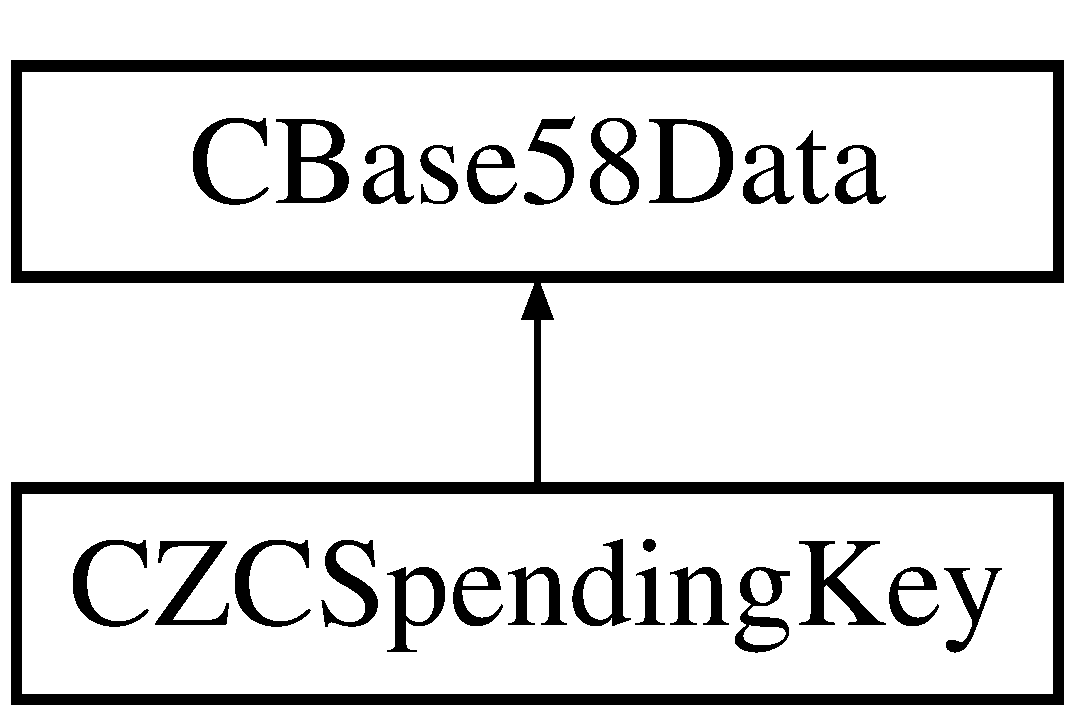
\includegraphics[height=2.000000cm]{class_c_z_c_spending_key}
\end{center}
\end{figure}
\subsection*{Public Member Functions}
\begin{DoxyCompactItemize}
\item 
bool \mbox{\hyperlink{class_c_z_c_spending_key_ab91e15b8861b065869ebce8f3ec9e456}{Set}} (const libzcash\+::\+Spending\+Key \&addr)
\item 
\mbox{\hyperlink{class_c_z_c_spending_key_a7f77c4e7c377278280f5dd01b177fa93}{C\+Z\+C\+Spending\+Key}} ()
\item 
\mbox{\hyperlink{class_c_z_c_spending_key_a3f3ef9fbbc482c4de02b164c6633d30c}{C\+Z\+C\+Spending\+Key}} (const std\+::string \&str\+Address)
\item 
\mbox{\hyperlink{class_c_z_c_spending_key_a177a064e76f8627fd31768fd9094c376}{C\+Z\+C\+Spending\+Key}} (const libzcash\+::\+Spending\+Key \&addr)
\item 
libzcash\+::\+Spending\+Key \mbox{\hyperlink{class_c_z_c_spending_key_ab1dfdc5b045b63f0635eaa5904a59f7d}{Get}} () const
\end{DoxyCompactItemize}
\subsection*{Additional Inherited Members}


\subsection{Constructor \& Destructor Documentation}
\mbox{\Hypertarget{class_c_z_c_spending_key_a7f77c4e7c377278280f5dd01b177fa93}\label{class_c_z_c_spending_key_a7f77c4e7c377278280f5dd01b177fa93}} 
\index{C\+Z\+C\+Spending\+Key@{C\+Z\+C\+Spending\+Key}!C\+Z\+C\+Spending\+Key@{C\+Z\+C\+Spending\+Key}}
\index{C\+Z\+C\+Spending\+Key@{C\+Z\+C\+Spending\+Key}!C\+Z\+C\+Spending\+Key@{C\+Z\+C\+Spending\+Key}}
\subsubsection{\texorpdfstring{C\+Z\+C\+Spending\+Key()}{CZCSpendingKey()}\hspace{0.1cm}{\footnotesize\ttfamily [1/3]}}
{\footnotesize\ttfamily C\+Z\+C\+Spending\+Key\+::\+C\+Z\+C\+Spending\+Key (\begin{DoxyParamCaption}{ }\end{DoxyParamCaption})\hspace{0.3cm}{\ttfamily [inline]}}

\mbox{\Hypertarget{class_c_z_c_spending_key_a3f3ef9fbbc482c4de02b164c6633d30c}\label{class_c_z_c_spending_key_a3f3ef9fbbc482c4de02b164c6633d30c}} 
\index{C\+Z\+C\+Spending\+Key@{C\+Z\+C\+Spending\+Key}!C\+Z\+C\+Spending\+Key@{C\+Z\+C\+Spending\+Key}}
\index{C\+Z\+C\+Spending\+Key@{C\+Z\+C\+Spending\+Key}!C\+Z\+C\+Spending\+Key@{C\+Z\+C\+Spending\+Key}}
\subsubsection{\texorpdfstring{C\+Z\+C\+Spending\+Key()}{CZCSpendingKey()}\hspace{0.1cm}{\footnotesize\ttfamily [2/3]}}
{\footnotesize\ttfamily C\+Z\+C\+Spending\+Key\+::\+C\+Z\+C\+Spending\+Key (\begin{DoxyParamCaption}\item[{const std\+::string \&}]{str\+Address }\end{DoxyParamCaption})\hspace{0.3cm}{\ttfamily [inline]}}

\mbox{\Hypertarget{class_c_z_c_spending_key_a177a064e76f8627fd31768fd9094c376}\label{class_c_z_c_spending_key_a177a064e76f8627fd31768fd9094c376}} 
\index{C\+Z\+C\+Spending\+Key@{C\+Z\+C\+Spending\+Key}!C\+Z\+C\+Spending\+Key@{C\+Z\+C\+Spending\+Key}}
\index{C\+Z\+C\+Spending\+Key@{C\+Z\+C\+Spending\+Key}!C\+Z\+C\+Spending\+Key@{C\+Z\+C\+Spending\+Key}}
\subsubsection{\texorpdfstring{C\+Z\+C\+Spending\+Key()}{CZCSpendingKey()}\hspace{0.1cm}{\footnotesize\ttfamily [3/3]}}
{\footnotesize\ttfamily C\+Z\+C\+Spending\+Key\+::\+C\+Z\+C\+Spending\+Key (\begin{DoxyParamCaption}\item[{const libzcash\+::\+Spending\+Key \&}]{addr }\end{DoxyParamCaption})\hspace{0.3cm}{\ttfamily [inline]}}



\subsection{Member Function Documentation}
\mbox{\Hypertarget{class_c_z_c_spending_key_ab1dfdc5b045b63f0635eaa5904a59f7d}\label{class_c_z_c_spending_key_ab1dfdc5b045b63f0635eaa5904a59f7d}} 
\index{C\+Z\+C\+Spending\+Key@{C\+Z\+C\+Spending\+Key}!Get@{Get}}
\index{Get@{Get}!C\+Z\+C\+Spending\+Key@{C\+Z\+C\+Spending\+Key}}
\subsubsection{\texorpdfstring{Get()}{Get()}}
{\footnotesize\ttfamily libzcash\+::\+Spending\+Key C\+Z\+C\+Spending\+Key\+::\+Get (\begin{DoxyParamCaption}{ }\end{DoxyParamCaption}) const}

\mbox{\Hypertarget{class_c_z_c_spending_key_ab91e15b8861b065869ebce8f3ec9e456}\label{class_c_z_c_spending_key_ab91e15b8861b065869ebce8f3ec9e456}} 
\index{C\+Z\+C\+Spending\+Key@{C\+Z\+C\+Spending\+Key}!Set@{Set}}
\index{Set@{Set}!C\+Z\+C\+Spending\+Key@{C\+Z\+C\+Spending\+Key}}
\subsubsection{\texorpdfstring{Set()}{Set()}}
{\footnotesize\ttfamily bool C\+Z\+C\+Spending\+Key\+::\+Set (\begin{DoxyParamCaption}\item[{const libzcash\+::\+Spending\+Key \&}]{addr }\end{DoxyParamCaption})}



The documentation for this class was generated from the following files\+:\begin{DoxyCompactItemize}
\item 
/\+Users/christopherarguello/\+Developer/anon/src/\mbox{\hyperlink{base58_8h}{base58.\+h}}\item 
/\+Users/christopherarguello/\+Developer/anon/src/\mbox{\hyperlink{base58_8cpp}{base58.\+cpp}}\end{DoxyCompactItemize}

\hypertarget{unionprevector_1_1direct__or__indirect}{}\section{prevector$<$ N, T, Size, Diff $>$\+:\+:direct\+\_\+or\+\_\+indirect Union Reference}
\label{unionprevector_1_1direct__or__indirect}\index{prevector$<$ N, T, Size, Diff $>$\+::direct\+\_\+or\+\_\+indirect@{prevector$<$ N, T, Size, Diff $>$\+::direct\+\_\+or\+\_\+indirect}}
\subsection*{Public Attributes}
\begin{DoxyCompactItemize}
\item 
char \mbox{\hyperlink{unionprevector_1_1direct__or__indirect_accf7da4788eeb76fff71273789bb78e5}{direct}} \mbox{[}sizeof(T) $\ast$N\mbox{]}
\item 
\begin{tabbing}
xx\=xx\=xx\=xx\=xx\=xx\=xx\=xx\=xx\=\kill
struct \{\\
\>\mbox{\hyperlink{classprevector_a7e0da95e6d1c878f6eeb572f4fc12524}{size\_type}} \mbox{\hyperlink{unionprevector_1_1direct__or__indirect_a8620e32f60f8c5ff1b91665093d6bf91}{capacity}}\\
\>char $\ast$ \mbox{\hyperlink{unionprevector_1_1direct__or__indirect_a1c80825c1780b32f20caf1b098a17557}{indirect}}\\
\}; \\

\end{tabbing}\end{DoxyCompactItemize}


\subsection{Member Data Documentation}
\mbox{\Hypertarget{unionprevector_1_1direct__or__indirect_ae2661bd2bfa1451538b79f293c897a42}\label{unionprevector_1_1direct__or__indirect_ae2661bd2bfa1451538b79f293c897a42}} 
\subsubsection{\texorpdfstring{"@5}{@5}}
{\footnotesize\ttfamily struct \{ ... \} }

\mbox{\Hypertarget{unionprevector_1_1direct__or__indirect_a8620e32f60f8c5ff1b91665093d6bf91}\label{unionprevector_1_1direct__or__indirect_a8620e32f60f8c5ff1b91665093d6bf91}} 
\index{prevector\+::direct\+\_\+or\+\_\+indirect@{prevector\+::direct\+\_\+or\+\_\+indirect}!capacity@{capacity}}
\index{capacity@{capacity}!prevector\+::direct\+\_\+or\+\_\+indirect@{prevector\+::direct\+\_\+or\+\_\+indirect}}
\subsubsection{\texorpdfstring{capacity}{capacity}}
{\footnotesize\ttfamily template$<$unsigned int N, typename T, typename Size = uint32\+\_\+t, typename Diff = int32\+\_\+t$>$ \\
\mbox{\hyperlink{classprevector_a7e0da95e6d1c878f6eeb572f4fc12524}{size\+\_\+type}} \mbox{\hyperlink{classprevector}{prevector}}$<$ N, T, Size, Diff $>$\+::direct\+\_\+or\+\_\+indirect\+::capacity}

\mbox{\Hypertarget{unionprevector_1_1direct__or__indirect_accf7da4788eeb76fff71273789bb78e5}\label{unionprevector_1_1direct__or__indirect_accf7da4788eeb76fff71273789bb78e5}} 
\index{prevector\+::direct\+\_\+or\+\_\+indirect@{prevector\+::direct\+\_\+or\+\_\+indirect}!direct@{direct}}
\index{direct@{direct}!prevector\+::direct\+\_\+or\+\_\+indirect@{prevector\+::direct\+\_\+or\+\_\+indirect}}
\subsubsection{\texorpdfstring{direct}{direct}}
{\footnotesize\ttfamily template$<$unsigned int N, typename T, typename Size = uint32\+\_\+t, typename Diff = int32\+\_\+t$>$ \\
char \mbox{\hyperlink{classprevector}{prevector}}$<$ N, T, Size, Diff $>$\+::direct\+\_\+or\+\_\+indirect\+::direct\mbox{[}sizeof(T) $\ast$N\mbox{]}}

\mbox{\Hypertarget{unionprevector_1_1direct__or__indirect_a1c80825c1780b32f20caf1b098a17557}\label{unionprevector_1_1direct__or__indirect_a1c80825c1780b32f20caf1b098a17557}} 
\index{prevector\+::direct\+\_\+or\+\_\+indirect@{prevector\+::direct\+\_\+or\+\_\+indirect}!indirect@{indirect}}
\index{indirect@{indirect}!prevector\+::direct\+\_\+or\+\_\+indirect@{prevector\+::direct\+\_\+or\+\_\+indirect}}
\subsubsection{\texorpdfstring{indirect}{indirect}}
{\footnotesize\ttfamily template$<$unsigned int N, typename T, typename Size = uint32\+\_\+t, typename Diff = int32\+\_\+t$>$ \\
char$\ast$ \mbox{\hyperlink{classprevector}{prevector}}$<$ N, T, Size, Diff $>$\+::direct\+\_\+or\+\_\+indirect\+::indirect}



The documentation for this union was generated from the following file\+:\begin{DoxyCompactItemize}
\item 
/\+Users/christopherarguello/\+Developer/anon/src/\mbox{\hyperlink{prevector_8h}{prevector.\+h}}\end{DoxyCompactItemize}

\hypertarget{class_e_c_c_verify_handle}{}\section{E\+C\+C\+Verify\+Handle Class Reference}
\label{class_e_c_c_verify_handle}\index{E\+C\+C\+Verify\+Handle@{E\+C\+C\+Verify\+Handle}}


{\ttfamily \#include $<$pubkey.\+h$>$}

\subsection*{Public Member Functions}
\begin{DoxyCompactItemize}
\item 
\mbox{\hyperlink{class_e_c_c_verify_handle_a01404b41eee891c1dea4b58db02e56fb}{E\+C\+C\+Verify\+Handle}} ()
\item 
\mbox{\hyperlink{class_e_c_c_verify_handle_a17dea6c87a0f825f0f24a06a20e2baf9}{$\sim$\+E\+C\+C\+Verify\+Handle}} ()
\end{DoxyCompactItemize}
\subsection*{Static Private Attributes}
\begin{DoxyCompactItemize}
\item 
static int \mbox{\hyperlink{class_e_c_c_verify_handle_a5dcdd8e40cc4aed9ed7c67e4f400e51d}{refcount}} = 0
\end{DoxyCompactItemize}


\subsection{Detailed Description}
Users of this module must hold an \mbox{\hyperlink{class_e_c_c_verify_handle}{E\+C\+C\+Verify\+Handle}}. The constructor and destructor of these are not allowed to run in parallel, though. 

\subsection{Constructor \& Destructor Documentation}
\mbox{\Hypertarget{class_e_c_c_verify_handle_a01404b41eee891c1dea4b58db02e56fb}\label{class_e_c_c_verify_handle_a01404b41eee891c1dea4b58db02e56fb}} 
\index{E\+C\+C\+Verify\+Handle@{E\+C\+C\+Verify\+Handle}!E\+C\+C\+Verify\+Handle@{E\+C\+C\+Verify\+Handle}}
\index{E\+C\+C\+Verify\+Handle@{E\+C\+C\+Verify\+Handle}!E\+C\+C\+Verify\+Handle@{E\+C\+C\+Verify\+Handle}}
\subsubsection{\texorpdfstring{E\+C\+C\+Verify\+Handle()}{ECCVerifyHandle()}}
{\footnotesize\ttfamily E\+C\+C\+Verify\+Handle\+::\+E\+C\+C\+Verify\+Handle (\begin{DoxyParamCaption}{ }\end{DoxyParamCaption})}

\mbox{\Hypertarget{class_e_c_c_verify_handle_a17dea6c87a0f825f0f24a06a20e2baf9}\label{class_e_c_c_verify_handle_a17dea6c87a0f825f0f24a06a20e2baf9}} 
\index{E\+C\+C\+Verify\+Handle@{E\+C\+C\+Verify\+Handle}!````~E\+C\+C\+Verify\+Handle@{$\sim$\+E\+C\+C\+Verify\+Handle}}
\index{````~E\+C\+C\+Verify\+Handle@{$\sim$\+E\+C\+C\+Verify\+Handle}!E\+C\+C\+Verify\+Handle@{E\+C\+C\+Verify\+Handle}}
\subsubsection{\texorpdfstring{$\sim$\+E\+C\+C\+Verify\+Handle()}{~ECCVerifyHandle()}}
{\footnotesize\ttfamily E\+C\+C\+Verify\+Handle\+::$\sim$\+E\+C\+C\+Verify\+Handle (\begin{DoxyParamCaption}{ }\end{DoxyParamCaption})}



\subsection{Member Data Documentation}
\mbox{\Hypertarget{class_e_c_c_verify_handle_a5dcdd8e40cc4aed9ed7c67e4f400e51d}\label{class_e_c_c_verify_handle_a5dcdd8e40cc4aed9ed7c67e4f400e51d}} 
\index{E\+C\+C\+Verify\+Handle@{E\+C\+C\+Verify\+Handle}!refcount@{refcount}}
\index{refcount@{refcount}!E\+C\+C\+Verify\+Handle@{E\+C\+C\+Verify\+Handle}}
\subsubsection{\texorpdfstring{refcount}{refcount}}
{\footnotesize\ttfamily int E\+C\+C\+Verify\+Handle\+::refcount = 0\hspace{0.3cm}{\ttfamily [static]}, {\ttfamily [private]}}



The documentation for this class was generated from the following files\+:\begin{DoxyCompactItemize}
\item 
/\+Users/christopherarguello/\+Developer/anon/src/\mbox{\hyperlink{pubkey_8h}{pubkey.\+h}}\item 
/\+Users/christopherarguello/\+Developer/anon/src/\mbox{\hyperlink{pubkey_8cpp}{pubkey.\+cpp}}\end{DoxyCompactItemize}

\hypertarget{structtinyformat_1_1detail_1_1is__convertible_1_1fail}{}\section{tinyformat\+:\+:detail\+:\+:is\+\_\+convertible$<$ T1, T2 $>$\+:\+:fail Struct Reference}
\label{structtinyformat_1_1detail_1_1is__convertible_1_1fail}\index{tinyformat\+::detail\+::is\+\_\+convertible$<$ T1, T2 $>$\+::fail@{tinyformat\+::detail\+::is\+\_\+convertible$<$ T1, T2 $>$\+::fail}}
\subsection*{Public Attributes}
\begin{DoxyCompactItemize}
\item 
char \mbox{\hyperlink{structtinyformat_1_1detail_1_1is__convertible_1_1fail_a5d18f7fcac212bbe55692586aee8954d}{dummy}} \mbox{[}2\mbox{]}
\end{DoxyCompactItemize}


\subsection{Member Data Documentation}
\mbox{\Hypertarget{structtinyformat_1_1detail_1_1is__convertible_1_1fail_a5d18f7fcac212bbe55692586aee8954d}\label{structtinyformat_1_1detail_1_1is__convertible_1_1fail_a5d18f7fcac212bbe55692586aee8954d}} 
\index{tinyformat\+::detail\+::is\+\_\+convertible\+::fail@{tinyformat\+::detail\+::is\+\_\+convertible\+::fail}!dummy@{dummy}}
\index{dummy@{dummy}!tinyformat\+::detail\+::is\+\_\+convertible\+::fail@{tinyformat\+::detail\+::is\+\_\+convertible\+::fail}}
\subsubsection{\texorpdfstring{dummy}{dummy}}
{\footnotesize\ttfamily template$<$typename T1 , typename T2 $>$ \\
char \mbox{\hyperlink{structtinyformat_1_1detail_1_1is__convertible}{tinyformat\+::detail\+::is\+\_\+convertible}}$<$ T1, T2 $>$\+::fail\+::dummy\mbox{[}2\mbox{]}}



The documentation for this struct was generated from the following file\+:\begin{DoxyCompactItemize}
\item 
/\+Users/christopherarguello/\+Developer/anon/src/\mbox{\hyperlink{tinyformat_8h}{tinyformat.\+h}}\end{DoxyCompactItemize}

\hypertarget{class_fake_coins_view_d_b}{}\section{Fake\+Coins\+View\+DB Class Reference}
\label{class_fake_coins_view_d_b}\index{Fake\+Coins\+View\+DB@{Fake\+Coins\+View\+DB}}
Inheritance diagram for Fake\+Coins\+View\+DB\+:\begin{figure}[H]
\begin{center}
\leavevmode
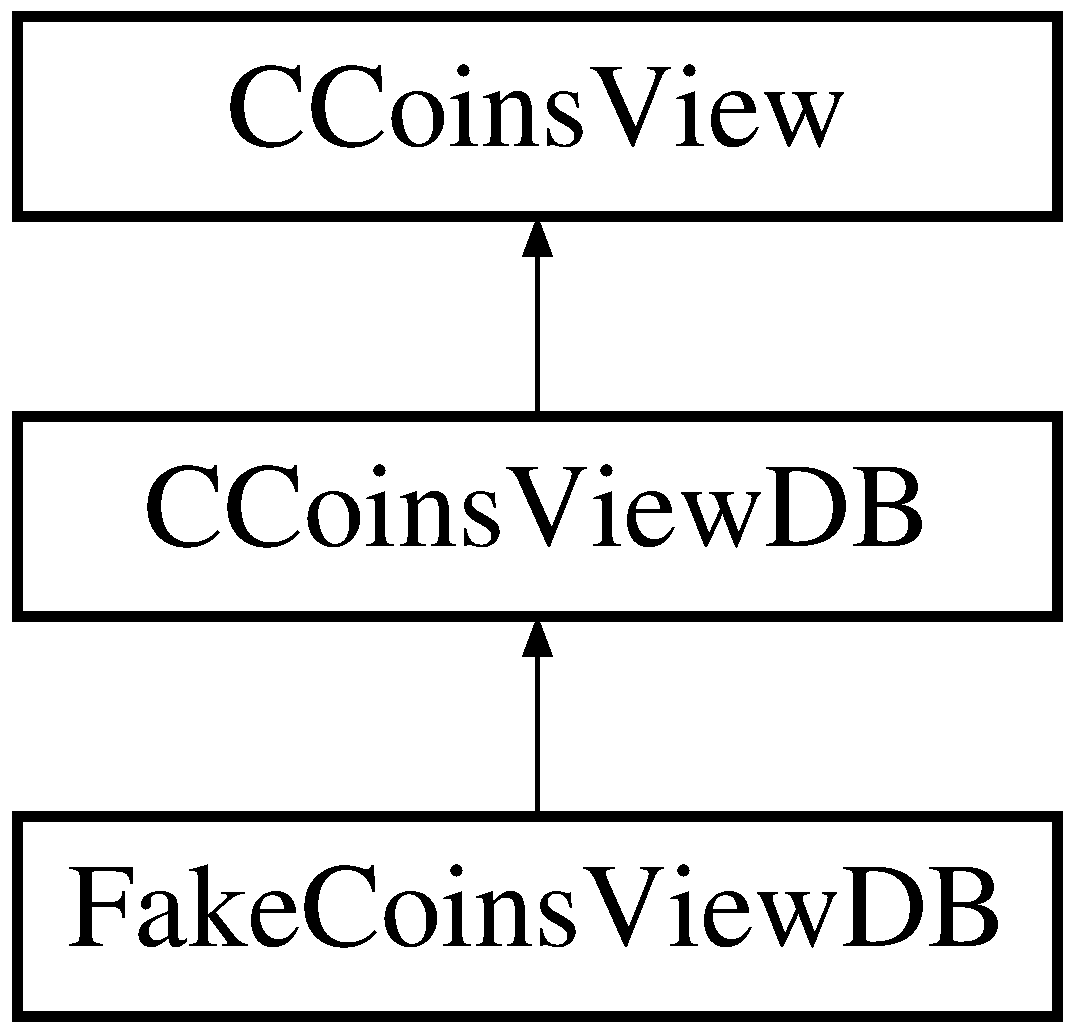
\includegraphics[height=3.000000cm]{class_fake_coins_view_d_b}
\end{center}
\end{figure}
\subsection*{Public Member Functions}
\begin{DoxyCompactItemize}
\item 
\mbox{\hyperlink{class_fake_coins_view_d_b_a88aa1d7a9c9136a3ef5f884e76989635}{Fake\+Coins\+View\+DB}} (std\+::string db\+Name, \mbox{\hyperlink{classuint256}{uint256}} \&\mbox{\hyperlink{class_fake_coins_view_d_b_a982f684b55a8f103df3f43b7128f6938}{hash}})
\item 
bool \mbox{\hyperlink{class_fake_coins_view_d_b_ae52d0073bef3eb64bd64b325e821c52b}{Get\+Anchor\+At}} (const \mbox{\hyperlink{classuint256}{uint256}} \&rt, Z\+C\+Incremental\+Merkle\+Tree \&tree) const
\begin{DoxyCompactList}\small\item\em Retrieve the tree at a particular anchored root in the chain. \end{DoxyCompactList}\item 
bool \mbox{\hyperlink{class_fake_coins_view_d_b_af7d0ce4926fb03ee632148c5fde66c05}{Get\+Nullifier}} (const \mbox{\hyperlink{classuint256}{uint256}} \&nf) const
\begin{DoxyCompactList}\small\item\em Determine whether a nullifier is spent or not. \end{DoxyCompactList}\item 
\mbox{\hyperlink{classuint256}{uint256}} \mbox{\hyperlink{class_fake_coins_view_d_b_a36231d924114fbe51a830c9c235c50ad}{Get\+Best\+Block}} () const
\begin{DoxyCompactList}\small\item\em Retrieve the block hash whose state this \mbox{\hyperlink{class_c_coins_view}{C\+Coins\+View}} currently represents. \end{DoxyCompactList}\item 
\mbox{\hyperlink{classuint256}{uint256}} \mbox{\hyperlink{class_fake_coins_view_d_b_af7870faf849e59188344273a03c9a1b0}{Get\+Best\+Anchor}} () const
\begin{DoxyCompactList}\small\item\em Get the current \char`\"{}tip\char`\"{} or the latest anchored tree root in the chain. \end{DoxyCompactList}\item 
bool \mbox{\hyperlink{class_fake_coins_view_d_b_a1108b45f9d165344c7378051e061147b}{Batch\+Write}} (\mbox{\hyperlink{coins_8h_a2886ba2fd0428bae777e1cbcabc02834}{C\+Coins\+Map}} \&map\+Coins, const \mbox{\hyperlink{classuint256}{uint256}} \&hash\+Block, const \mbox{\hyperlink{classuint256}{uint256}} \&hash\+Anchor, \mbox{\hyperlink{coins_8h_a070827cc9d21a91b8f4f4f52a6f7c848}{C\+Anchors\+Map}} \&map\+Anchors, \mbox{\hyperlink{coins_8h_ab651cc287e9594190ef77d2fca2b14c7}{C\+Nullifiers\+Map}} \&map\+Nullifiers)
\item 
bool \mbox{\hyperlink{class_fake_coins_view_d_b_ad1deefbe955925e274e5d50d289275e9}{Get\+Stats}} (\mbox{\hyperlink{struct_c_coins_stats}{C\+Coins\+Stats}} \&stats) const
\begin{DoxyCompactList}\small\item\em Calculate statistics about the unspent transaction output set. \end{DoxyCompactList}\end{DoxyCompactItemize}
\subsection*{Private Attributes}
\begin{DoxyCompactItemize}
\item 
\mbox{\hyperlink{classuint256}{uint256}} \mbox{\hyperlink{class_fake_coins_view_d_b_a982f684b55a8f103df3f43b7128f6938}{hash}}
\item 
Z\+C\+Incremental\+Merkle\+Tree \mbox{\hyperlink{class_fake_coins_view_d_b_a8478155455bb20042e4459c4179ae921}{t}}
\end{DoxyCompactItemize}
\subsection*{Additional Inherited Members}


\subsection{Constructor \& Destructor Documentation}
\mbox{\Hypertarget{class_fake_coins_view_d_b_a88aa1d7a9c9136a3ef5f884e76989635}\label{class_fake_coins_view_d_b_a88aa1d7a9c9136a3ef5f884e76989635}} 
\index{Fake\+Coins\+View\+DB@{Fake\+Coins\+View\+DB}!Fake\+Coins\+View\+DB@{Fake\+Coins\+View\+DB}}
\index{Fake\+Coins\+View\+DB@{Fake\+Coins\+View\+DB}!Fake\+Coins\+View\+DB@{Fake\+Coins\+View\+DB}}
\subsubsection{\texorpdfstring{Fake\+Coins\+View\+D\+B()}{FakeCoinsViewDB()}}
{\footnotesize\ttfamily Fake\+Coins\+View\+D\+B\+::\+Fake\+Coins\+View\+DB (\begin{DoxyParamCaption}\item[{std\+::string}]{db\+Name,  }\item[{\mbox{\hyperlink{classuint256}{uint256}} \&}]{hash }\end{DoxyParamCaption})\hspace{0.3cm}{\ttfamily [inline]}}



\subsection{Member Function Documentation}
\mbox{\Hypertarget{class_fake_coins_view_d_b_a1108b45f9d165344c7378051e061147b}\label{class_fake_coins_view_d_b_a1108b45f9d165344c7378051e061147b}} 
\index{Fake\+Coins\+View\+DB@{Fake\+Coins\+View\+DB}!Batch\+Write@{Batch\+Write}}
\index{Batch\+Write@{Batch\+Write}!Fake\+Coins\+View\+DB@{Fake\+Coins\+View\+DB}}
\subsubsection{\texorpdfstring{Batch\+Write()}{BatchWrite()}}
{\footnotesize\ttfamily bool Fake\+Coins\+View\+D\+B\+::\+Batch\+Write (\begin{DoxyParamCaption}\item[{\mbox{\hyperlink{coins_8h_a2886ba2fd0428bae777e1cbcabc02834}{C\+Coins\+Map}} \&}]{map\+Coins,  }\item[{const \mbox{\hyperlink{classuint256}{uint256}} \&}]{hash\+Block,  }\item[{const \mbox{\hyperlink{classuint256}{uint256}} \&}]{hash\+Anchor,  }\item[{\mbox{\hyperlink{coins_8h_a070827cc9d21a91b8f4f4f52a6f7c848}{C\+Anchors\+Map}} \&}]{map\+Anchors,  }\item[{\mbox{\hyperlink{coins_8h_ab651cc287e9594190ef77d2fca2b14c7}{C\+Nullifiers\+Map}} \&}]{map\+Nullifiers }\end{DoxyParamCaption})\hspace{0.3cm}{\ttfamily [inline]}, {\ttfamily [virtual]}}

Do a bulk modification (multiple \mbox{\hyperlink{class_c_coins}{C\+Coins}} changes + Best\+Block change). The passed map\+Coins can be modified. 

Reimplemented from \mbox{\hyperlink{class_c_coins_view_d_b_ab617e4b898f06cec79a2a26fdca9efbd}{C\+Coins\+View\+DB}}.

\mbox{\Hypertarget{class_fake_coins_view_d_b_ae52d0073bef3eb64bd64b325e821c52b}\label{class_fake_coins_view_d_b_ae52d0073bef3eb64bd64b325e821c52b}} 
\index{Fake\+Coins\+View\+DB@{Fake\+Coins\+View\+DB}!Get\+Anchor\+At@{Get\+Anchor\+At}}
\index{Get\+Anchor\+At@{Get\+Anchor\+At}!Fake\+Coins\+View\+DB@{Fake\+Coins\+View\+DB}}
\subsubsection{\texorpdfstring{Get\+Anchor\+At()}{GetAnchorAt()}}
{\footnotesize\ttfamily bool Fake\+Coins\+View\+D\+B\+::\+Get\+Anchor\+At (\begin{DoxyParamCaption}\item[{const \mbox{\hyperlink{classuint256}{uint256}} \&}]{rt,  }\item[{Z\+C\+Incremental\+Merkle\+Tree \&}]{tree }\end{DoxyParamCaption}) const\hspace{0.3cm}{\ttfamily [inline]}, {\ttfamily [virtual]}}



Retrieve the tree at a particular anchored root in the chain. 



Reimplemented from \mbox{\hyperlink{class_c_coins_view_d_b_aeaab3bc4b363dbbc9d9a77930209e299}{C\+Coins\+View\+DB}}.

\mbox{\Hypertarget{class_fake_coins_view_d_b_af7870faf849e59188344273a03c9a1b0}\label{class_fake_coins_view_d_b_af7870faf849e59188344273a03c9a1b0}} 
\index{Fake\+Coins\+View\+DB@{Fake\+Coins\+View\+DB}!Get\+Best\+Anchor@{Get\+Best\+Anchor}}
\index{Get\+Best\+Anchor@{Get\+Best\+Anchor}!Fake\+Coins\+View\+DB@{Fake\+Coins\+View\+DB}}
\subsubsection{\texorpdfstring{Get\+Best\+Anchor()}{GetBestAnchor()}}
{\footnotesize\ttfamily \mbox{\hyperlink{classuint256}{uint256}} Fake\+Coins\+View\+D\+B\+::\+Get\+Best\+Anchor (\begin{DoxyParamCaption}{ }\end{DoxyParamCaption}) const\hspace{0.3cm}{\ttfamily [inline]}, {\ttfamily [virtual]}}



Get the current \char`\"{}tip\char`\"{} or the latest anchored tree root in the chain. 



Reimplemented from \mbox{\hyperlink{class_c_coins_view_d_b_a2bb7d73a96472def92e332a4563a689c}{C\+Coins\+View\+DB}}.

\mbox{\Hypertarget{class_fake_coins_view_d_b_a36231d924114fbe51a830c9c235c50ad}\label{class_fake_coins_view_d_b_a36231d924114fbe51a830c9c235c50ad}} 
\index{Fake\+Coins\+View\+DB@{Fake\+Coins\+View\+DB}!Get\+Best\+Block@{Get\+Best\+Block}}
\index{Get\+Best\+Block@{Get\+Best\+Block}!Fake\+Coins\+View\+DB@{Fake\+Coins\+View\+DB}}
\subsubsection{\texorpdfstring{Get\+Best\+Block()}{GetBestBlock()}}
{\footnotesize\ttfamily \mbox{\hyperlink{classuint256}{uint256}} Fake\+Coins\+View\+D\+B\+::\+Get\+Best\+Block (\begin{DoxyParamCaption}{ }\end{DoxyParamCaption}) const\hspace{0.3cm}{\ttfamily [inline]}, {\ttfamily [virtual]}}



Retrieve the block hash whose state this \mbox{\hyperlink{class_c_coins_view}{C\+Coins\+View}} currently represents. 



Reimplemented from \mbox{\hyperlink{class_c_coins_view_d_b_ac9c513a34b9e58d942fdbeafd9e5bbce}{C\+Coins\+View\+DB}}.

\mbox{\Hypertarget{class_fake_coins_view_d_b_af7d0ce4926fb03ee632148c5fde66c05}\label{class_fake_coins_view_d_b_af7d0ce4926fb03ee632148c5fde66c05}} 
\index{Fake\+Coins\+View\+DB@{Fake\+Coins\+View\+DB}!Get\+Nullifier@{Get\+Nullifier}}
\index{Get\+Nullifier@{Get\+Nullifier}!Fake\+Coins\+View\+DB@{Fake\+Coins\+View\+DB}}
\subsubsection{\texorpdfstring{Get\+Nullifier()}{GetNullifier()}}
{\footnotesize\ttfamily bool Fake\+Coins\+View\+D\+B\+::\+Get\+Nullifier (\begin{DoxyParamCaption}\item[{const \mbox{\hyperlink{classuint256}{uint256}} \&}]{nullifier }\end{DoxyParamCaption}) const\hspace{0.3cm}{\ttfamily [inline]}, {\ttfamily [virtual]}}



Determine whether a nullifier is spent or not. 



Reimplemented from \mbox{\hyperlink{class_c_coins_view_d_b_ac9724829164f5a06b6d7c610da03a730}{C\+Coins\+View\+DB}}.

\mbox{\Hypertarget{class_fake_coins_view_d_b_ad1deefbe955925e274e5d50d289275e9}\label{class_fake_coins_view_d_b_ad1deefbe955925e274e5d50d289275e9}} 
\index{Fake\+Coins\+View\+DB@{Fake\+Coins\+View\+DB}!Get\+Stats@{Get\+Stats}}
\index{Get\+Stats@{Get\+Stats}!Fake\+Coins\+View\+DB@{Fake\+Coins\+View\+DB}}
\subsubsection{\texorpdfstring{Get\+Stats()}{GetStats()}}
{\footnotesize\ttfamily bool Fake\+Coins\+View\+D\+B\+::\+Get\+Stats (\begin{DoxyParamCaption}\item[{\mbox{\hyperlink{struct_c_coins_stats}{C\+Coins\+Stats}} \&}]{stats }\end{DoxyParamCaption}) const\hspace{0.3cm}{\ttfamily [inline]}, {\ttfamily [virtual]}}



Calculate statistics about the unspent transaction output set. 



Reimplemented from \mbox{\hyperlink{class_c_coins_view_d_b_a227bf56f8801921f12e56c6839104fce}{C\+Coins\+View\+DB}}.



\subsection{Member Data Documentation}
\mbox{\Hypertarget{class_fake_coins_view_d_b_a982f684b55a8f103df3f43b7128f6938}\label{class_fake_coins_view_d_b_a982f684b55a8f103df3f43b7128f6938}} 
\index{Fake\+Coins\+View\+DB@{Fake\+Coins\+View\+DB}!hash@{hash}}
\index{hash@{hash}!Fake\+Coins\+View\+DB@{Fake\+Coins\+View\+DB}}
\subsubsection{\texorpdfstring{hash}{hash}}
{\footnotesize\ttfamily \mbox{\hyperlink{classuint256}{uint256}} Fake\+Coins\+View\+D\+B\+::hash\hspace{0.3cm}{\ttfamily [private]}}

\mbox{\Hypertarget{class_fake_coins_view_d_b_a8478155455bb20042e4459c4179ae921}\label{class_fake_coins_view_d_b_a8478155455bb20042e4459c4179ae921}} 
\index{Fake\+Coins\+View\+DB@{Fake\+Coins\+View\+DB}!t@{t}}
\index{t@{t}!Fake\+Coins\+View\+DB@{Fake\+Coins\+View\+DB}}
\subsubsection{\texorpdfstring{t}{t}}
{\footnotesize\ttfamily Z\+C\+Incremental\+Merkle\+Tree Fake\+Coins\+View\+D\+B\+::t\hspace{0.3cm}{\ttfamily [private]}}



The documentation for this class was generated from the following file\+:\begin{DoxyCompactItemize}
\item 
/\+Users/christopherarguello/\+Developer/anon/src/\mbox{\hyperlink{zcbenchmarks_8cpp}{zcbenchmarks.\+cpp}}\end{DoxyCompactItemize}

\hypertarget{classtinyformat_1_1detail_1_1_format_arg}{}\section{tinyformat\+:\+:detail\+:\+:Format\+Arg Class Reference}
\label{classtinyformat_1_1detail_1_1_format_arg}\index{tinyformat\+::detail\+::\+Format\+Arg@{tinyformat\+::detail\+::\+Format\+Arg}}


{\ttfamily \#include $<$tinyformat.\+h$>$}

\subsection*{Public Member Functions}
\begin{DoxyCompactItemize}
\item 
\mbox{\hyperlink{classtinyformat_1_1detail_1_1_format_arg_aa6c926179f24546f26bff058d1a77d39}{Format\+Arg}} ()
\item 
{\footnotesize template$<$typename T $>$ }\\\mbox{\hyperlink{classtinyformat_1_1detail_1_1_format_arg_adec80164e93744f53ae7ecc6a5f6af27}{Format\+Arg}} (const T \&value)
\item 
void \mbox{\hyperlink{classtinyformat_1_1detail_1_1_format_arg_acbf435711bbe4a4da7fc81758d7108a9}{format}} (std\+::ostream \&out, const char $\ast$fmt\+Begin, const char $\ast$fmt\+End, int ntrunc) const
\item 
int \mbox{\hyperlink{classtinyformat_1_1detail_1_1_format_arg_a91b69f66ce9dc8ca2914dce8985d7a1a}{to\+Int}} () const
\end{DoxyCompactItemize}
\subsection*{Static Private Member Functions}
\begin{DoxyCompactItemize}
\item 
{\footnotesize template$<$typename T $>$ }\\static \mbox{\hyperlink{tinyformat_8h_a2c0b8573a0f2148232e2ecfe7afa6ca8}{T\+I\+N\+Y\+F\+O\+R\+M\+A\+T\+\_\+\+H\+I\+D\+D\+EN}} void \mbox{\hyperlink{classtinyformat_1_1detail_1_1_format_arg_a14632665aa1c2ecfbddf35ea23479bfb}{format\+Impl}} (std\+::ostream \&out, const char $\ast$fmt\+Begin, const char $\ast$fmt\+End, int ntrunc, const void $\ast$value)
\item 
{\footnotesize template$<$typename T $>$ }\\static \mbox{\hyperlink{tinyformat_8h_a2c0b8573a0f2148232e2ecfe7afa6ca8}{T\+I\+N\+Y\+F\+O\+R\+M\+A\+T\+\_\+\+H\+I\+D\+D\+EN}} int \mbox{\hyperlink{classtinyformat_1_1detail_1_1_format_arg_a646cd3417730e0a797d37a898bb081be}{to\+Int\+Impl}} (const void $\ast$value)
\end{DoxyCompactItemize}
\subsection*{Private Attributes}
\begin{DoxyCompactItemize}
\item 
const void $\ast$ \mbox{\hyperlink{classtinyformat_1_1detail_1_1_format_arg_ad7630a7d1e68ac56e46e03722156056a}{m\+\_\+value}}
\item 
void($\ast$ \mbox{\hyperlink{classtinyformat_1_1detail_1_1_format_arg_a3e1114e7a277020906bfd4588ff9b6fc}{m\+\_\+format\+Impl}} )(std\+::ostream \&out, const char $\ast$fmt\+Begin, const char $\ast$fmt\+End, int ntrunc, const void $\ast$value)
\item 
int($\ast$ \mbox{\hyperlink{classtinyformat_1_1detail_1_1_format_arg_a999e592d6235d5dbdf0f46cad769f220}{m\+\_\+to\+Int\+Impl}} )(const void $\ast$value)
\end{DoxyCompactItemize}


\subsection{Constructor \& Destructor Documentation}
\mbox{\Hypertarget{classtinyformat_1_1detail_1_1_format_arg_aa6c926179f24546f26bff058d1a77d39}\label{classtinyformat_1_1detail_1_1_format_arg_aa6c926179f24546f26bff058d1a77d39}} 
\index{tinyformat\+::detail\+::\+Format\+Arg@{tinyformat\+::detail\+::\+Format\+Arg}!Format\+Arg@{Format\+Arg}}
\index{Format\+Arg@{Format\+Arg}!tinyformat\+::detail\+::\+Format\+Arg@{tinyformat\+::detail\+::\+Format\+Arg}}
\subsubsection{\texorpdfstring{Format\+Arg()}{FormatArg()}\hspace{0.1cm}{\footnotesize\ttfamily [1/2]}}
{\footnotesize\ttfamily tinyformat\+::detail\+::\+Format\+Arg\+::\+Format\+Arg (\begin{DoxyParamCaption}{ }\end{DoxyParamCaption})\hspace{0.3cm}{\ttfamily [inline]}}

\mbox{\Hypertarget{classtinyformat_1_1detail_1_1_format_arg_adec80164e93744f53ae7ecc6a5f6af27}\label{classtinyformat_1_1detail_1_1_format_arg_adec80164e93744f53ae7ecc6a5f6af27}} 
\index{tinyformat\+::detail\+::\+Format\+Arg@{tinyformat\+::detail\+::\+Format\+Arg}!Format\+Arg@{Format\+Arg}}
\index{Format\+Arg@{Format\+Arg}!tinyformat\+::detail\+::\+Format\+Arg@{tinyformat\+::detail\+::\+Format\+Arg}}
\subsubsection{\texorpdfstring{Format\+Arg()}{FormatArg()}\hspace{0.1cm}{\footnotesize\ttfamily [2/2]}}
{\footnotesize\ttfamily template$<$typename T $>$ \\
tinyformat\+::detail\+::\+Format\+Arg\+::\+Format\+Arg (\begin{DoxyParamCaption}\item[{const T \&}]{value }\end{DoxyParamCaption})\hspace{0.3cm}{\ttfamily [inline]}}



\subsection{Member Function Documentation}
\mbox{\Hypertarget{classtinyformat_1_1detail_1_1_format_arg_acbf435711bbe4a4da7fc81758d7108a9}\label{classtinyformat_1_1detail_1_1_format_arg_acbf435711bbe4a4da7fc81758d7108a9}} 
\index{tinyformat\+::detail\+::\+Format\+Arg@{tinyformat\+::detail\+::\+Format\+Arg}!format@{format}}
\index{format@{format}!tinyformat\+::detail\+::\+Format\+Arg@{tinyformat\+::detail\+::\+Format\+Arg}}
\subsubsection{\texorpdfstring{format()}{format()}}
{\footnotesize\ttfamily void tinyformat\+::detail\+::\+Format\+Arg\+::format (\begin{DoxyParamCaption}\item[{std\+::ostream \&}]{out,  }\item[{const char $\ast$}]{fmt\+Begin,  }\item[{const char $\ast$}]{fmt\+End,  }\item[{int}]{ntrunc }\end{DoxyParamCaption}) const\hspace{0.3cm}{\ttfamily [inline]}}

\mbox{\Hypertarget{classtinyformat_1_1detail_1_1_format_arg_a14632665aa1c2ecfbddf35ea23479bfb}\label{classtinyformat_1_1detail_1_1_format_arg_a14632665aa1c2ecfbddf35ea23479bfb}} 
\index{tinyformat\+::detail\+::\+Format\+Arg@{tinyformat\+::detail\+::\+Format\+Arg}!format\+Impl@{format\+Impl}}
\index{format\+Impl@{format\+Impl}!tinyformat\+::detail\+::\+Format\+Arg@{tinyformat\+::detail\+::\+Format\+Arg}}
\subsubsection{\texorpdfstring{format\+Impl()}{formatImpl()}}
{\footnotesize\ttfamily template$<$typename T $>$ \\
static \mbox{\hyperlink{tinyformat_8h_a2c0b8573a0f2148232e2ecfe7afa6ca8}{T\+I\+N\+Y\+F\+O\+R\+M\+A\+T\+\_\+\+H\+I\+D\+D\+EN}} void tinyformat\+::detail\+::\+Format\+Arg\+::format\+Impl (\begin{DoxyParamCaption}\item[{std\+::ostream \&}]{out,  }\item[{const char $\ast$}]{fmt\+Begin,  }\item[{const char $\ast$}]{fmt\+End,  }\item[{int}]{ntrunc,  }\item[{const void $\ast$}]{value }\end{DoxyParamCaption})\hspace{0.3cm}{\ttfamily [inline]}, {\ttfamily [static]}, {\ttfamily [private]}}

\mbox{\Hypertarget{classtinyformat_1_1detail_1_1_format_arg_a91b69f66ce9dc8ca2914dce8985d7a1a}\label{classtinyformat_1_1detail_1_1_format_arg_a91b69f66ce9dc8ca2914dce8985d7a1a}} 
\index{tinyformat\+::detail\+::\+Format\+Arg@{tinyformat\+::detail\+::\+Format\+Arg}!to\+Int@{to\+Int}}
\index{to\+Int@{to\+Int}!tinyformat\+::detail\+::\+Format\+Arg@{tinyformat\+::detail\+::\+Format\+Arg}}
\subsubsection{\texorpdfstring{to\+Int()}{toInt()}}
{\footnotesize\ttfamily int tinyformat\+::detail\+::\+Format\+Arg\+::to\+Int (\begin{DoxyParamCaption}{ }\end{DoxyParamCaption}) const\hspace{0.3cm}{\ttfamily [inline]}}

\mbox{\Hypertarget{classtinyformat_1_1detail_1_1_format_arg_a646cd3417730e0a797d37a898bb081be}\label{classtinyformat_1_1detail_1_1_format_arg_a646cd3417730e0a797d37a898bb081be}} 
\index{tinyformat\+::detail\+::\+Format\+Arg@{tinyformat\+::detail\+::\+Format\+Arg}!to\+Int\+Impl@{to\+Int\+Impl}}
\index{to\+Int\+Impl@{to\+Int\+Impl}!tinyformat\+::detail\+::\+Format\+Arg@{tinyformat\+::detail\+::\+Format\+Arg}}
\subsubsection{\texorpdfstring{to\+Int\+Impl()}{toIntImpl()}}
{\footnotesize\ttfamily template$<$typename T $>$ \\
static \mbox{\hyperlink{tinyformat_8h_a2c0b8573a0f2148232e2ecfe7afa6ca8}{T\+I\+N\+Y\+F\+O\+R\+M\+A\+T\+\_\+\+H\+I\+D\+D\+EN}} int tinyformat\+::detail\+::\+Format\+Arg\+::to\+Int\+Impl (\begin{DoxyParamCaption}\item[{const void $\ast$}]{value }\end{DoxyParamCaption})\hspace{0.3cm}{\ttfamily [inline]}, {\ttfamily [static]}, {\ttfamily [private]}}



\subsection{Member Data Documentation}
\mbox{\Hypertarget{classtinyformat_1_1detail_1_1_format_arg_a3e1114e7a277020906bfd4588ff9b6fc}\label{classtinyformat_1_1detail_1_1_format_arg_a3e1114e7a277020906bfd4588ff9b6fc}} 
\index{tinyformat\+::detail\+::\+Format\+Arg@{tinyformat\+::detail\+::\+Format\+Arg}!m\+\_\+format\+Impl@{m\+\_\+format\+Impl}}
\index{m\+\_\+format\+Impl@{m\+\_\+format\+Impl}!tinyformat\+::detail\+::\+Format\+Arg@{tinyformat\+::detail\+::\+Format\+Arg}}
\subsubsection{\texorpdfstring{m\+\_\+format\+Impl}{m\_formatImpl}}
{\footnotesize\ttfamily void($\ast$ tinyformat\+::detail\+::\+Format\+Arg\+::m\+\_\+format\+Impl) (std\+::ostream \&out, const char $\ast$fmt\+Begin, const char $\ast$fmt\+End, int ntrunc, const void $\ast$value)\hspace{0.3cm}{\ttfamily [private]}}

\mbox{\Hypertarget{classtinyformat_1_1detail_1_1_format_arg_a999e592d6235d5dbdf0f46cad769f220}\label{classtinyformat_1_1detail_1_1_format_arg_a999e592d6235d5dbdf0f46cad769f220}} 
\index{tinyformat\+::detail\+::\+Format\+Arg@{tinyformat\+::detail\+::\+Format\+Arg}!m\+\_\+to\+Int\+Impl@{m\+\_\+to\+Int\+Impl}}
\index{m\+\_\+to\+Int\+Impl@{m\+\_\+to\+Int\+Impl}!tinyformat\+::detail\+::\+Format\+Arg@{tinyformat\+::detail\+::\+Format\+Arg}}
\subsubsection{\texorpdfstring{m\+\_\+to\+Int\+Impl}{m\_toIntImpl}}
{\footnotesize\ttfamily int($\ast$ tinyformat\+::detail\+::\+Format\+Arg\+::m\+\_\+to\+Int\+Impl) (const void $\ast$value)\hspace{0.3cm}{\ttfamily [private]}}

\mbox{\Hypertarget{classtinyformat_1_1detail_1_1_format_arg_ad7630a7d1e68ac56e46e03722156056a}\label{classtinyformat_1_1detail_1_1_format_arg_ad7630a7d1e68ac56e46e03722156056a}} 
\index{tinyformat\+::detail\+::\+Format\+Arg@{tinyformat\+::detail\+::\+Format\+Arg}!m\+\_\+value@{m\+\_\+value}}
\index{m\+\_\+value@{m\+\_\+value}!tinyformat\+::detail\+::\+Format\+Arg@{tinyformat\+::detail\+::\+Format\+Arg}}
\subsubsection{\texorpdfstring{m\+\_\+value}{m\_value}}
{\footnotesize\ttfamily const void$\ast$ tinyformat\+::detail\+::\+Format\+Arg\+::m\+\_\+value\hspace{0.3cm}{\ttfamily [private]}}



The documentation for this class was generated from the following file\+:\begin{DoxyCompactItemize}
\item 
/\+Users/christopherarguello/\+Developer/anon/src/\mbox{\hyperlink{tinyformat_8h}{tinyformat.\+h}}\end{DoxyCompactItemize}

\hypertarget{classtinyformat_1_1_format_list}{}\section{tinyformat\+:\+:Format\+List Class Reference}
\label{classtinyformat_1_1_format_list}\index{tinyformat\+::\+Format\+List@{tinyformat\+::\+Format\+List}}


{\ttfamily \#include $<$tinyformat.\+h$>$}

Inheritance diagram for tinyformat\+:\+:Format\+List\+:\begin{figure}[H]
\begin{center}
\leavevmode
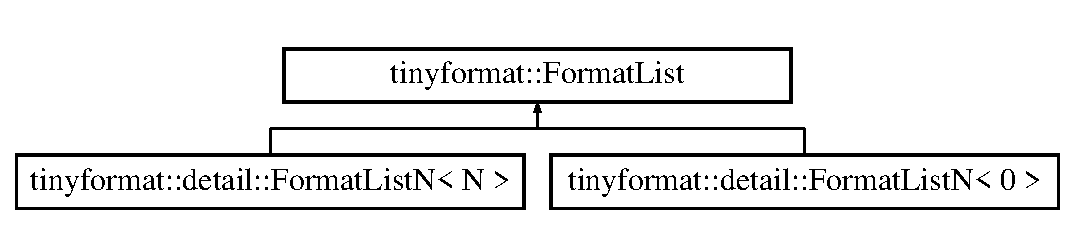
\includegraphics[height=2.000000cm]{classtinyformat_1_1_format_list}
\end{center}
\end{figure}
\subsection*{Public Member Functions}
\begin{DoxyCompactItemize}
\item 
\mbox{\hyperlink{classtinyformat_1_1_format_list_a4dc93948fa7b945665800b5c147037c3}{Format\+List}} (\mbox{\hyperlink{classtinyformat_1_1detail_1_1_format_arg}{detail\+::\+Format\+Arg}} $\ast$formatters, int N)
\end{DoxyCompactItemize}
\subsection*{Private Attributes}
\begin{DoxyCompactItemize}
\item 
const \mbox{\hyperlink{classtinyformat_1_1detail_1_1_format_arg}{detail\+::\+Format\+Arg}} $\ast$ \mbox{\hyperlink{classtinyformat_1_1_format_list_a90b0b9b03a90c09e8734b51f8be3f734}{m\+\_\+formatters}}
\item 
int \mbox{\hyperlink{classtinyformat_1_1_format_list_aee4267e50285b7adeb57b61d6305312b}{m\+\_\+N}}
\end{DoxyCompactItemize}
\subsection*{Friends}
\begin{DoxyCompactItemize}
\item 
void \mbox{\hyperlink{classtinyformat_1_1_format_list_a105eb7b498f1353f8da108bd7284af58}{vformat}} (std\+::ostream \&out, const char $\ast$fmt, const \mbox{\hyperlink{classtinyformat_1_1_format_list}{Format\+List}} \&list)
\end{DoxyCompactItemize}


\subsection{Detailed Description}
List of template arguments \mbox{\hyperlink{namespacetinyformat_adc3e74768f0e2204f9f9a726fc07ec61}{format()}}, held in a type-\/opaque way.

A const reference to \mbox{\hyperlink{classtinyformat_1_1_format_list}{Format\+List}} (typedef\textquotesingle{}d as Format\+List\+Ref) may be conveniently used to pass arguments to non-\/template functions\+: All type information has been stripped from the arguments, leaving just enough of a common interface to perform formatting as required. 

\subsection{Constructor \& Destructor Documentation}
\mbox{\Hypertarget{classtinyformat_1_1_format_list_a4dc93948fa7b945665800b5c147037c3}\label{classtinyformat_1_1_format_list_a4dc93948fa7b945665800b5c147037c3}} 
\index{tinyformat\+::\+Format\+List@{tinyformat\+::\+Format\+List}!Format\+List@{Format\+List}}
\index{Format\+List@{Format\+List}!tinyformat\+::\+Format\+List@{tinyformat\+::\+Format\+List}}
\subsubsection{\texorpdfstring{Format\+List()}{FormatList()}}
{\footnotesize\ttfamily tinyformat\+::\+Format\+List\+::\+Format\+List (\begin{DoxyParamCaption}\item[{\mbox{\hyperlink{classtinyformat_1_1detail_1_1_format_arg}{detail\+::\+Format\+Arg}} $\ast$}]{formatters,  }\item[{int}]{N }\end{DoxyParamCaption})\hspace{0.3cm}{\ttfamily [inline]}}



\subsection{Friends And Related Function Documentation}
\mbox{\Hypertarget{classtinyformat_1_1_format_list_a105eb7b498f1353f8da108bd7284af58}\label{classtinyformat_1_1_format_list_a105eb7b498f1353f8da108bd7284af58}} 
\index{tinyformat\+::\+Format\+List@{tinyformat\+::\+Format\+List}!vformat@{vformat}}
\index{vformat@{vformat}!tinyformat\+::\+Format\+List@{tinyformat\+::\+Format\+List}}
\subsubsection{\texorpdfstring{vformat}{vformat}}
{\footnotesize\ttfamily void vformat (\begin{DoxyParamCaption}\item[{std\+::ostream \&}]{out,  }\item[{const char $\ast$}]{fmt,  }\item[{const \mbox{\hyperlink{classtinyformat_1_1_format_list}{Format\+List}} \&}]{list }\end{DoxyParamCaption})\hspace{0.3cm}{\ttfamily [friend]}}



\subsection{Member Data Documentation}
\mbox{\Hypertarget{classtinyformat_1_1_format_list_a90b0b9b03a90c09e8734b51f8be3f734}\label{classtinyformat_1_1_format_list_a90b0b9b03a90c09e8734b51f8be3f734}} 
\index{tinyformat\+::\+Format\+List@{tinyformat\+::\+Format\+List}!m\+\_\+formatters@{m\+\_\+formatters}}
\index{m\+\_\+formatters@{m\+\_\+formatters}!tinyformat\+::\+Format\+List@{tinyformat\+::\+Format\+List}}
\subsubsection{\texorpdfstring{m\+\_\+formatters}{m\_formatters}}
{\footnotesize\ttfamily const \mbox{\hyperlink{classtinyformat_1_1detail_1_1_format_arg}{detail\+::\+Format\+Arg}}$\ast$ tinyformat\+::\+Format\+List\+::m\+\_\+formatters\hspace{0.3cm}{\ttfamily [private]}}

\mbox{\Hypertarget{classtinyformat_1_1_format_list_aee4267e50285b7adeb57b61d6305312b}\label{classtinyformat_1_1_format_list_aee4267e50285b7adeb57b61d6305312b}} 
\index{tinyformat\+::\+Format\+List@{tinyformat\+::\+Format\+List}!m\+\_\+N@{m\+\_\+N}}
\index{m\+\_\+N@{m\+\_\+N}!tinyformat\+::\+Format\+List@{tinyformat\+::\+Format\+List}}
\subsubsection{\texorpdfstring{m\+\_\+N}{m\_N}}
{\footnotesize\ttfamily int tinyformat\+::\+Format\+List\+::m\+\_\+N\hspace{0.3cm}{\ttfamily [private]}}



The documentation for this class was generated from the following file\+:\begin{DoxyCompactItemize}
\item 
/\+Users/christopherarguello/\+Developer/anon/src/\mbox{\hyperlink{tinyformat_8h}{tinyformat.\+h}}\end{DoxyCompactItemize}

\hypertarget{classtinyformat_1_1detail_1_1_format_list_n}{}\section{tinyformat\+:\+:detail\+:\+:Format\+ListN$<$ N $>$ Class Template Reference}
\label{classtinyformat_1_1detail_1_1_format_list_n}\index{tinyformat\+::detail\+::\+Format\+List\+N$<$ N $>$@{tinyformat\+::detail\+::\+Format\+List\+N$<$ N $>$}}


{\ttfamily \#include $<$tinyformat.\+h$>$}

Inheritance diagram for tinyformat\+:\+:detail\+:\+:Format\+ListN$<$ N $>$\+:\begin{figure}[H]
\begin{center}
\leavevmode
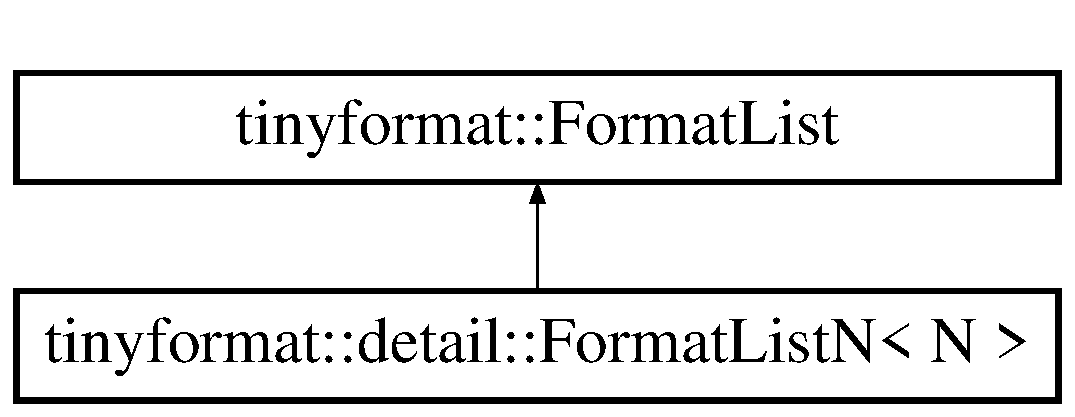
\includegraphics[height=2.000000cm]{classtinyformat_1_1detail_1_1_format_list_n}
\end{center}
\end{figure}
\subsection*{Public Member Functions}
\begin{DoxyCompactItemize}
\item 
void \mbox{\hyperlink{classtinyformat_1_1detail_1_1_format_list_n_a78183c11bc8d7bb1e0e83cac78abc2d0}{init}} (int)
\end{DoxyCompactItemize}
\subsection*{Private Attributes}
\begin{DoxyCompactItemize}
\item 
\mbox{\hyperlink{classtinyformat_1_1detail_1_1_format_arg}{Format\+Arg}} \mbox{\hyperlink{classtinyformat_1_1detail_1_1_format_list_n_a34d9e64988d50f945f6bbef71429f35f}{m\+\_\+formatter\+Store}} \mbox{[}N\mbox{]}
\end{DoxyCompactItemize}


\subsection{Member Function Documentation}
\mbox{\Hypertarget{classtinyformat_1_1detail_1_1_format_list_n_a78183c11bc8d7bb1e0e83cac78abc2d0}\label{classtinyformat_1_1detail_1_1_format_list_n_a78183c11bc8d7bb1e0e83cac78abc2d0}} 
\index{tinyformat\+::detail\+::\+Format\+ListN@{tinyformat\+::detail\+::\+Format\+ListN}!init@{init}}
\index{init@{init}!tinyformat\+::detail\+::\+Format\+ListN@{tinyformat\+::detail\+::\+Format\+ListN}}
\subsubsection{\texorpdfstring{init()}{init()}}
{\footnotesize\ttfamily template$<$int N$>$ \\
void \mbox{\hyperlink{classtinyformat_1_1detail_1_1_format_list_n}{tinyformat\+::detail\+::\+Format\+ListN}}$<$ N $>$\+::init (\begin{DoxyParamCaption}\item[{int}]{ }\end{DoxyParamCaption})\hspace{0.3cm}{\ttfamily [inline]}}



\subsection{Member Data Documentation}
\mbox{\Hypertarget{classtinyformat_1_1detail_1_1_format_list_n_a34d9e64988d50f945f6bbef71429f35f}\label{classtinyformat_1_1detail_1_1_format_list_n_a34d9e64988d50f945f6bbef71429f35f}} 
\index{tinyformat\+::detail\+::\+Format\+ListN@{tinyformat\+::detail\+::\+Format\+ListN}!m\+\_\+formatter\+Store@{m\+\_\+formatter\+Store}}
\index{m\+\_\+formatter\+Store@{m\+\_\+formatter\+Store}!tinyformat\+::detail\+::\+Format\+ListN@{tinyformat\+::detail\+::\+Format\+ListN}}
\subsubsection{\texorpdfstring{m\+\_\+formatter\+Store}{m\_formatterStore}}
{\footnotesize\ttfamily template$<$int N$>$ \\
\mbox{\hyperlink{classtinyformat_1_1detail_1_1_format_arg}{Format\+Arg}} \mbox{\hyperlink{classtinyformat_1_1detail_1_1_format_list_n}{tinyformat\+::detail\+::\+Format\+ListN}}$<$ N $>$\+::m\+\_\+formatter\+Store\mbox{[}N\mbox{]}\hspace{0.3cm}{\ttfamily [private]}}



The documentation for this class was generated from the following file\+:\begin{DoxyCompactItemize}
\item 
/\+Users/christopherarguello/\+Developer/anon/src/\mbox{\hyperlink{tinyformat_8h}{tinyformat.\+h}}\end{DoxyCompactItemize}

\hypertarget{classtinyformat_1_1detail_1_1_format_list_n_3_010_01_4}{}\section{tinyformat\+:\+:detail\+:\+:Format\+ListN$<$ 0 $>$ Class Template Reference}
\label{classtinyformat_1_1detail_1_1_format_list_n_3_010_01_4}\index{tinyformat\+::detail\+::\+Format\+List\+N$<$ 0 $>$@{tinyformat\+::detail\+::\+Format\+List\+N$<$ 0 $>$}}


{\ttfamily \#include $<$tinyformat.\+h$>$}

Inheritance diagram for tinyformat\+:\+:detail\+:\+:Format\+ListN$<$ 0 $>$\+:\begin{figure}[H]
\begin{center}
\leavevmode
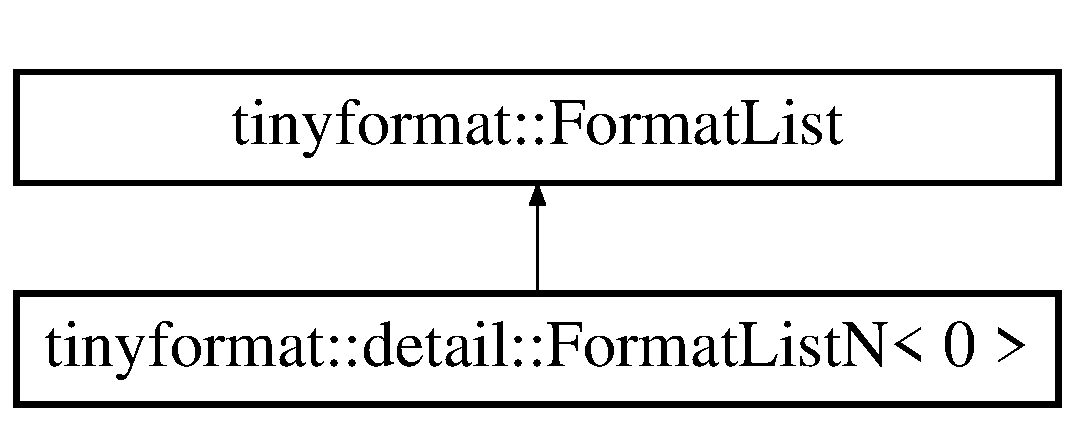
\includegraphics[height=2.000000cm]{classtinyformat_1_1detail_1_1_format_list_n_3_010_01_4}
\end{center}
\end{figure}
\subsection*{Public Member Functions}
\begin{DoxyCompactItemize}
\item 
\mbox{\hyperlink{classtinyformat_1_1detail_1_1_format_list_n_3_010_01_4_a02cd16d93b54efaec0e4ef78e9842b37}{Format\+ListN}} ()
\end{DoxyCompactItemize}


\subsection{Constructor \& Destructor Documentation}
\mbox{\Hypertarget{classtinyformat_1_1detail_1_1_format_list_n_3_010_01_4_a02cd16d93b54efaec0e4ef78e9842b37}\label{classtinyformat_1_1detail_1_1_format_list_n_3_010_01_4_a02cd16d93b54efaec0e4ef78e9842b37}} 
\index{tinyformat\+::detail\+::\+Format\+List\+N$<$ 0 $>$@{tinyformat\+::detail\+::\+Format\+List\+N$<$ 0 $>$}!Format\+ListN@{Format\+ListN}}
\index{Format\+ListN@{Format\+ListN}!tinyformat\+::detail\+::\+Format\+List\+N$<$ 0 $>$@{tinyformat\+::detail\+::\+Format\+List\+N$<$ 0 $>$}}
\subsubsection{\texorpdfstring{Format\+List\+N()}{FormatListN()}}
{\footnotesize\ttfamily \mbox{\hyperlink{classtinyformat_1_1detail_1_1_format_list_n}{tinyformat\+::detail\+::\+Format\+ListN}}$<$ 0 $>$\+::\mbox{\hyperlink{classtinyformat_1_1detail_1_1_format_list_n}{Format\+ListN}} (\begin{DoxyParamCaption}{ }\end{DoxyParamCaption})\hspace{0.3cm}{\ttfamily [inline]}}



The documentation for this class was generated from the following file\+:\begin{DoxyCompactItemize}
\item 
/\+Users/christopherarguello/\+Developer/anon/src/\mbox{\hyperlink{tinyformat_8h}{tinyformat.\+h}}\end{DoxyCompactItemize}

\hypertarget{structtinyformat_1_1detail_1_1format_value_as_type}{}\section{tinyformat\+:\+:detail\+:\+:format\+Value\+As\+Type$<$ T, fmtT, convertible $>$ Struct Template Reference}
\label{structtinyformat_1_1detail_1_1format_value_as_type}\index{tinyformat\+::detail\+::format\+Value\+As\+Type$<$ T, fmt\+T, convertible $>$@{tinyformat\+::detail\+::format\+Value\+As\+Type$<$ T, fmt\+T, convertible $>$}}


{\ttfamily \#include $<$tinyformat.\+h$>$}

\subsection*{Static Public Member Functions}
\begin{DoxyCompactItemize}
\item 
static void \mbox{\hyperlink{structtinyformat_1_1detail_1_1format_value_as_type_a126bc5958024c456851f08fa380d1cac}{invoke}} (std\+::ostream \&, const T \&)
\end{DoxyCompactItemize}


\subsection{Member Function Documentation}
\mbox{\Hypertarget{structtinyformat_1_1detail_1_1format_value_as_type_a126bc5958024c456851f08fa380d1cac}\label{structtinyformat_1_1detail_1_1format_value_as_type_a126bc5958024c456851f08fa380d1cac}} 
\index{tinyformat\+::detail\+::format\+Value\+As\+Type@{tinyformat\+::detail\+::format\+Value\+As\+Type}!invoke@{invoke}}
\index{invoke@{invoke}!tinyformat\+::detail\+::format\+Value\+As\+Type@{tinyformat\+::detail\+::format\+Value\+As\+Type}}
\subsubsection{\texorpdfstring{invoke()}{invoke()}}
{\footnotesize\ttfamily template$<$typename T , typename fmtT , bool convertible = is\+\_\+convertible$<$\+T, fmt\+T$>$\+::value$>$ \\
static void \mbox{\hyperlink{structtinyformat_1_1detail_1_1format_value_as_type}{tinyformat\+::detail\+::format\+Value\+As\+Type}}$<$ T, fmtT, convertible $>$\+::invoke (\begin{DoxyParamCaption}\item[{std\+::ostream \&}]{,  }\item[{const T \&}]{ }\end{DoxyParamCaption})\hspace{0.3cm}{\ttfamily [inline]}, {\ttfamily [static]}}



The documentation for this struct was generated from the following file\+:\begin{DoxyCompactItemize}
\item 
/\+Users/christopherarguello/\+Developer/anon/src/\mbox{\hyperlink{tinyformat_8h}{tinyformat.\+h}}\end{DoxyCompactItemize}

\hypertarget{structtinyformat_1_1detail_1_1format_value_as_type_3_01_t_00_01fmt_t_00_01true_01_4}{}\section{tinyformat\+:\+:detail\+:\+:format\+Value\+As\+Type$<$ T, fmtT, true $>$ Struct Template Reference}
\label{structtinyformat_1_1detail_1_1format_value_as_type_3_01_t_00_01fmt_t_00_01true_01_4}\index{tinyformat\+::detail\+::format\+Value\+As\+Type$<$ T, fmt\+T, true $>$@{tinyformat\+::detail\+::format\+Value\+As\+Type$<$ T, fmt\+T, true $>$}}


{\ttfamily \#include $<$tinyformat.\+h$>$}

\subsection*{Static Public Member Functions}
\begin{DoxyCompactItemize}
\item 
static void \mbox{\hyperlink{structtinyformat_1_1detail_1_1format_value_as_type_3_01_t_00_01fmt_t_00_01true_01_4_a7680bc0f7b6b5eee0e27c494812fb667}{invoke}} (std\+::ostream \&out, const T \&value)
\end{DoxyCompactItemize}


\subsection{Member Function Documentation}
\mbox{\Hypertarget{structtinyformat_1_1detail_1_1format_value_as_type_3_01_t_00_01fmt_t_00_01true_01_4_a7680bc0f7b6b5eee0e27c494812fb667}\label{structtinyformat_1_1detail_1_1format_value_as_type_3_01_t_00_01fmt_t_00_01true_01_4_a7680bc0f7b6b5eee0e27c494812fb667}} 
\index{tinyformat\+::detail\+::format\+Value\+As\+Type$<$ T, fmt\+T, true $>$@{tinyformat\+::detail\+::format\+Value\+As\+Type$<$ T, fmt\+T, true $>$}!invoke@{invoke}}
\index{invoke@{invoke}!tinyformat\+::detail\+::format\+Value\+As\+Type$<$ T, fmt\+T, true $>$@{tinyformat\+::detail\+::format\+Value\+As\+Type$<$ T, fmt\+T, true $>$}}
\subsubsection{\texorpdfstring{invoke()}{invoke()}}
{\footnotesize\ttfamily template$<$typename T , typename fmtT $>$ \\
static void \mbox{\hyperlink{structtinyformat_1_1detail_1_1format_value_as_type}{tinyformat\+::detail\+::format\+Value\+As\+Type}}$<$ T, fmtT, true $>$\+::invoke (\begin{DoxyParamCaption}\item[{std\+::ostream \&}]{out,  }\item[{const T \&}]{value }\end{DoxyParamCaption})\hspace{0.3cm}{\ttfamily [inline]}, {\ttfamily [static]}}



The documentation for this struct was generated from the following file\+:\begin{DoxyCompactItemize}
\item 
/\+Users/christopherarguello/\+Developer/anon/src/\mbox{\hyperlink{tinyformat_8h}{tinyformat.\+h}}\end{DoxyCompactItemize}

\hypertarget{class_h_t_t_p_closure}{}\section{H\+T\+T\+P\+Closure Class Reference}
\label{class_h_t_t_p_closure}\index{H\+T\+T\+P\+Closure@{H\+T\+T\+P\+Closure}}


{\ttfamily \#include $<$httpserver.\+h$>$}

Inheritance diagram for H\+T\+T\+P\+Closure\+:\begin{figure}[H]
\begin{center}
\leavevmode
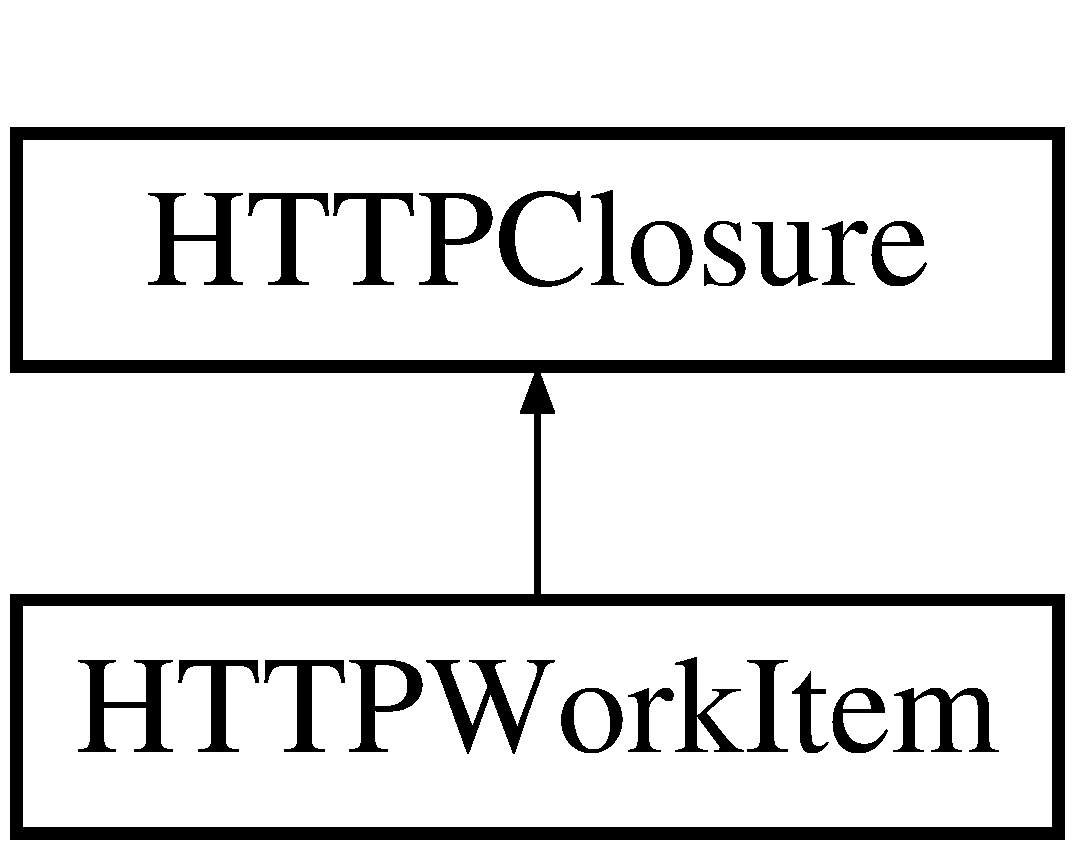
\includegraphics[height=2.000000cm]{class_h_t_t_p_closure}
\end{center}
\end{figure}
\subsection*{Public Member Functions}
\begin{DoxyCompactItemize}
\item 
virtual void \mbox{\hyperlink{class_h_t_t_p_closure_abbce5d429a7fe2b593919550e50bc225}{operator()}} ()=0
\item 
virtual \mbox{\hyperlink{class_h_t_t_p_closure_af3cc5a621020ea4ddef1170dead00be4}{$\sim$\+H\+T\+T\+P\+Closure}} ()
\end{DoxyCompactItemize}


\subsection{Detailed Description}
Event handler closure. 

\subsection{Constructor \& Destructor Documentation}
\mbox{\Hypertarget{class_h_t_t_p_closure_af3cc5a621020ea4ddef1170dead00be4}\label{class_h_t_t_p_closure_af3cc5a621020ea4ddef1170dead00be4}} 
\index{H\+T\+T\+P\+Closure@{H\+T\+T\+P\+Closure}!````~H\+T\+T\+P\+Closure@{$\sim$\+H\+T\+T\+P\+Closure}}
\index{````~H\+T\+T\+P\+Closure@{$\sim$\+H\+T\+T\+P\+Closure}!H\+T\+T\+P\+Closure@{H\+T\+T\+P\+Closure}}
\subsubsection{\texorpdfstring{$\sim$\+H\+T\+T\+P\+Closure()}{~HTTPClosure()}}
{\footnotesize\ttfamily virtual H\+T\+T\+P\+Closure\+::$\sim$\+H\+T\+T\+P\+Closure (\begin{DoxyParamCaption}{ }\end{DoxyParamCaption})\hspace{0.3cm}{\ttfamily [inline]}, {\ttfamily [virtual]}}



\subsection{Member Function Documentation}
\mbox{\Hypertarget{class_h_t_t_p_closure_abbce5d429a7fe2b593919550e50bc225}\label{class_h_t_t_p_closure_abbce5d429a7fe2b593919550e50bc225}} 
\index{H\+T\+T\+P\+Closure@{H\+T\+T\+P\+Closure}!operator()@{operator()}}
\index{operator()@{operator()}!H\+T\+T\+P\+Closure@{H\+T\+T\+P\+Closure}}
\subsubsection{\texorpdfstring{operator()()}{operator()()}}
{\footnotesize\ttfamily virtual void H\+T\+T\+P\+Closure\+::operator() (\begin{DoxyParamCaption}{ }\end{DoxyParamCaption})\hspace{0.3cm}{\ttfamily [pure virtual]}}



Implemented in \mbox{\hyperlink{class_h_t_t_p_work_item_a85addf7a6b8fdbf0a63becc7e1f0135e}{H\+T\+T\+P\+Work\+Item}}.



The documentation for this class was generated from the following file\+:\begin{DoxyCompactItemize}
\item 
/\+Users/christopherarguello/\+Developer/anon/src/\mbox{\hyperlink{httpserver_8h}{httpserver.\+h}}\end{DoxyCompactItemize}

\hypertarget{class_h_t_t_p_event}{}\section{H\+T\+T\+P\+Event Class Reference}
\label{class_h_t_t_p_event}\index{H\+T\+T\+P\+Event@{H\+T\+T\+P\+Event}}


{\ttfamily \#include $<$httpserver.\+h$>$}

\subsection*{Public Member Functions}
\begin{DoxyCompactItemize}
\item 
\mbox{\hyperlink{class_h_t_t_p_event_ad7598146077dac606ccf4c9948040508}{H\+T\+T\+P\+Event}} (struct event\+\_\+base $\ast$base, bool \mbox{\hyperlink{class_h_t_t_p_event_a226496f0af00e98c301e92cd8bf7ca9b}{delete\+When\+Triggered}}, const boost\+::function$<$ void(void)$>$ \&\mbox{\hyperlink{class_h_t_t_p_event_a61e7b99b180ddd304a524c2a27063c4c}{handler}})
\item 
\mbox{\hyperlink{class_h_t_t_p_event_a3f216c67f9c4732bac686744a9c527d7}{$\sim$\+H\+T\+T\+P\+Event}} ()
\item 
void \mbox{\hyperlink{class_h_t_t_p_event_ad3e2ab005035c3ac678b29095ac0da87}{trigger}} (struct timeval $\ast$tv)
\end{DoxyCompactItemize}
\subsection*{Public Attributes}
\begin{DoxyCompactItemize}
\item 
bool \mbox{\hyperlink{class_h_t_t_p_event_a226496f0af00e98c301e92cd8bf7ca9b}{delete\+When\+Triggered}}
\item 
boost\+::function$<$ void(void)$>$ \mbox{\hyperlink{class_h_t_t_p_event_a61e7b99b180ddd304a524c2a27063c4c}{handler}}
\end{DoxyCompactItemize}
\subsection*{Private Attributes}
\begin{DoxyCompactItemize}
\item 
struct event $\ast$ \mbox{\hyperlink{class_h_t_t_p_event_a1b00e03074314686bf8b01979f938a45}{ev}}
\end{DoxyCompactItemize}


\subsection{Detailed Description}
Event class. This can be used either as an cross-\/thread trigger or as a timer. 

\subsection{Constructor \& Destructor Documentation}
\mbox{\Hypertarget{class_h_t_t_p_event_ad7598146077dac606ccf4c9948040508}\label{class_h_t_t_p_event_ad7598146077dac606ccf4c9948040508}} 
\index{H\+T\+T\+P\+Event@{H\+T\+T\+P\+Event}!H\+T\+T\+P\+Event@{H\+T\+T\+P\+Event}}
\index{H\+T\+T\+P\+Event@{H\+T\+T\+P\+Event}!H\+T\+T\+P\+Event@{H\+T\+T\+P\+Event}}
\subsubsection{\texorpdfstring{H\+T\+T\+P\+Event()}{HTTPEvent()}}
{\footnotesize\ttfamily H\+T\+T\+P\+Event\+::\+H\+T\+T\+P\+Event (\begin{DoxyParamCaption}\item[{struct event\+\_\+base $\ast$}]{base,  }\item[{bool}]{delete\+When\+Triggered,  }\item[{const boost\+::function$<$ void(void)$>$ \&}]{handler }\end{DoxyParamCaption})}

Create a new event. delete\+When\+Triggered deletes this event object after the event is triggered (and the handler called) handler is the handler to call when the event is triggered. \mbox{\Hypertarget{class_h_t_t_p_event_a3f216c67f9c4732bac686744a9c527d7}\label{class_h_t_t_p_event_a3f216c67f9c4732bac686744a9c527d7}} 
\index{H\+T\+T\+P\+Event@{H\+T\+T\+P\+Event}!````~H\+T\+T\+P\+Event@{$\sim$\+H\+T\+T\+P\+Event}}
\index{````~H\+T\+T\+P\+Event@{$\sim$\+H\+T\+T\+P\+Event}!H\+T\+T\+P\+Event@{H\+T\+T\+P\+Event}}
\subsubsection{\texorpdfstring{$\sim$\+H\+T\+T\+P\+Event()}{~HTTPEvent()}}
{\footnotesize\ttfamily H\+T\+T\+P\+Event\+::$\sim$\+H\+T\+T\+P\+Event (\begin{DoxyParamCaption}{ }\end{DoxyParamCaption})}



\subsection{Member Function Documentation}
\mbox{\Hypertarget{class_h_t_t_p_event_ad3e2ab005035c3ac678b29095ac0da87}\label{class_h_t_t_p_event_ad3e2ab005035c3ac678b29095ac0da87}} 
\index{H\+T\+T\+P\+Event@{H\+T\+T\+P\+Event}!trigger@{trigger}}
\index{trigger@{trigger}!H\+T\+T\+P\+Event@{H\+T\+T\+P\+Event}}
\subsubsection{\texorpdfstring{trigger()}{trigger()}}
{\footnotesize\ttfamily void H\+T\+T\+P\+Event\+::trigger (\begin{DoxyParamCaption}\item[{struct timeval $\ast$}]{tv }\end{DoxyParamCaption})}

Trigger the event. If tv is 0, trigger it immediately. Otherwise trigger it after the given time has elapsed. 

\subsection{Member Data Documentation}
\mbox{\Hypertarget{class_h_t_t_p_event_a226496f0af00e98c301e92cd8bf7ca9b}\label{class_h_t_t_p_event_a226496f0af00e98c301e92cd8bf7ca9b}} 
\index{H\+T\+T\+P\+Event@{H\+T\+T\+P\+Event}!delete\+When\+Triggered@{delete\+When\+Triggered}}
\index{delete\+When\+Triggered@{delete\+When\+Triggered}!H\+T\+T\+P\+Event@{H\+T\+T\+P\+Event}}
\subsubsection{\texorpdfstring{delete\+When\+Triggered}{deleteWhenTriggered}}
{\footnotesize\ttfamily bool H\+T\+T\+P\+Event\+::delete\+When\+Triggered}

\mbox{\Hypertarget{class_h_t_t_p_event_a1b00e03074314686bf8b01979f938a45}\label{class_h_t_t_p_event_a1b00e03074314686bf8b01979f938a45}} 
\index{H\+T\+T\+P\+Event@{H\+T\+T\+P\+Event}!ev@{ev}}
\index{ev@{ev}!H\+T\+T\+P\+Event@{H\+T\+T\+P\+Event}}
\subsubsection{\texorpdfstring{ev}{ev}}
{\footnotesize\ttfamily struct event$\ast$ H\+T\+T\+P\+Event\+::ev\hspace{0.3cm}{\ttfamily [private]}}

\mbox{\Hypertarget{class_h_t_t_p_event_a61e7b99b180ddd304a524c2a27063c4c}\label{class_h_t_t_p_event_a61e7b99b180ddd304a524c2a27063c4c}} 
\index{H\+T\+T\+P\+Event@{H\+T\+T\+P\+Event}!handler@{handler}}
\index{handler@{handler}!H\+T\+T\+P\+Event@{H\+T\+T\+P\+Event}}
\subsubsection{\texorpdfstring{handler}{handler}}
{\footnotesize\ttfamily boost\+::function$<$void(void)$>$ H\+T\+T\+P\+Event\+::handler}



The documentation for this class was generated from the following files\+:\begin{DoxyCompactItemize}
\item 
/\+Users/christopherarguello/\+Developer/anon/src/\mbox{\hyperlink{httpserver_8h}{httpserver.\+h}}\item 
/\+Users/christopherarguello/\+Developer/anon/src/\mbox{\hyperlink{httpserver_8cpp}{httpserver.\+cpp}}\end{DoxyCompactItemize}

\hypertarget{struct_h_t_t_p_path_handler}{}\section{H\+T\+T\+P\+Path\+Handler Struct Reference}
\label{struct_h_t_t_p_path_handler}\index{H\+T\+T\+P\+Path\+Handler@{H\+T\+T\+P\+Path\+Handler}}
\subsection*{Public Member Functions}
\begin{DoxyCompactItemize}
\item 
\mbox{\hyperlink{struct_h_t_t_p_path_handler_acdfd2521c5f888e52d9a7c14bd5c6781}{H\+T\+T\+P\+Path\+Handler}} ()
\item 
\mbox{\hyperlink{struct_h_t_t_p_path_handler_a9161b61163110ac69e928bc128b1a47c}{H\+T\+T\+P\+Path\+Handler}} (std\+::string \mbox{\hyperlink{struct_h_t_t_p_path_handler_a3653c57a029382a867dc68e102a353cf}{prefix}}, bool \mbox{\hyperlink{struct_h_t_t_p_path_handler_a2f7ea5761b24c8987869faf40af28a60}{exact\+Match}}, \mbox{\hyperlink{httpserver_8h_a90b0a9a188f591e83851dad2b701088f}{H\+T\+T\+P\+Request\+Handler}} \mbox{\hyperlink{struct_h_t_t_p_path_handler_ad741823790ab387e0962875861a91e67}{handler}})
\end{DoxyCompactItemize}
\subsection*{Public Attributes}
\begin{DoxyCompactItemize}
\item 
std\+::string \mbox{\hyperlink{struct_h_t_t_p_path_handler_a3653c57a029382a867dc68e102a353cf}{prefix}}
\item 
bool \mbox{\hyperlink{struct_h_t_t_p_path_handler_a2f7ea5761b24c8987869faf40af28a60}{exact\+Match}}
\item 
\mbox{\hyperlink{httpserver_8h_a90b0a9a188f591e83851dad2b701088f}{H\+T\+T\+P\+Request\+Handler}} \mbox{\hyperlink{struct_h_t_t_p_path_handler_ad741823790ab387e0962875861a91e67}{handler}}
\end{DoxyCompactItemize}


\subsection{Constructor \& Destructor Documentation}
\mbox{\Hypertarget{struct_h_t_t_p_path_handler_acdfd2521c5f888e52d9a7c14bd5c6781}\label{struct_h_t_t_p_path_handler_acdfd2521c5f888e52d9a7c14bd5c6781}} 
\index{H\+T\+T\+P\+Path\+Handler@{H\+T\+T\+P\+Path\+Handler}!H\+T\+T\+P\+Path\+Handler@{H\+T\+T\+P\+Path\+Handler}}
\index{H\+T\+T\+P\+Path\+Handler@{H\+T\+T\+P\+Path\+Handler}!H\+T\+T\+P\+Path\+Handler@{H\+T\+T\+P\+Path\+Handler}}
\subsubsection{\texorpdfstring{H\+T\+T\+P\+Path\+Handler()}{HTTPPathHandler()}\hspace{0.1cm}{\footnotesize\ttfamily [1/2]}}
{\footnotesize\ttfamily H\+T\+T\+P\+Path\+Handler\+::\+H\+T\+T\+P\+Path\+Handler (\begin{DoxyParamCaption}{ }\end{DoxyParamCaption})\hspace{0.3cm}{\ttfamily [inline]}}

\mbox{\Hypertarget{struct_h_t_t_p_path_handler_a9161b61163110ac69e928bc128b1a47c}\label{struct_h_t_t_p_path_handler_a9161b61163110ac69e928bc128b1a47c}} 
\index{H\+T\+T\+P\+Path\+Handler@{H\+T\+T\+P\+Path\+Handler}!H\+T\+T\+P\+Path\+Handler@{H\+T\+T\+P\+Path\+Handler}}
\index{H\+T\+T\+P\+Path\+Handler@{H\+T\+T\+P\+Path\+Handler}!H\+T\+T\+P\+Path\+Handler@{H\+T\+T\+P\+Path\+Handler}}
\subsubsection{\texorpdfstring{H\+T\+T\+P\+Path\+Handler()}{HTTPPathHandler()}\hspace{0.1cm}{\footnotesize\ttfamily [2/2]}}
{\footnotesize\ttfamily H\+T\+T\+P\+Path\+Handler\+::\+H\+T\+T\+P\+Path\+Handler (\begin{DoxyParamCaption}\item[{std\+::string}]{prefix,  }\item[{bool}]{exact\+Match,  }\item[{\mbox{\hyperlink{httpserver_8h_a90b0a9a188f591e83851dad2b701088f}{H\+T\+T\+P\+Request\+Handler}}}]{handler }\end{DoxyParamCaption})\hspace{0.3cm}{\ttfamily [inline]}}



\subsection{Member Data Documentation}
\mbox{\Hypertarget{struct_h_t_t_p_path_handler_a2f7ea5761b24c8987869faf40af28a60}\label{struct_h_t_t_p_path_handler_a2f7ea5761b24c8987869faf40af28a60}} 
\index{H\+T\+T\+P\+Path\+Handler@{H\+T\+T\+P\+Path\+Handler}!exact\+Match@{exact\+Match}}
\index{exact\+Match@{exact\+Match}!H\+T\+T\+P\+Path\+Handler@{H\+T\+T\+P\+Path\+Handler}}
\subsubsection{\texorpdfstring{exact\+Match}{exactMatch}}
{\footnotesize\ttfamily bool H\+T\+T\+P\+Path\+Handler\+::exact\+Match}

\mbox{\Hypertarget{struct_h_t_t_p_path_handler_ad741823790ab387e0962875861a91e67}\label{struct_h_t_t_p_path_handler_ad741823790ab387e0962875861a91e67}} 
\index{H\+T\+T\+P\+Path\+Handler@{H\+T\+T\+P\+Path\+Handler}!handler@{handler}}
\index{handler@{handler}!H\+T\+T\+P\+Path\+Handler@{H\+T\+T\+P\+Path\+Handler}}
\subsubsection{\texorpdfstring{handler}{handler}}
{\footnotesize\ttfamily \mbox{\hyperlink{httpserver_8h_a90b0a9a188f591e83851dad2b701088f}{H\+T\+T\+P\+Request\+Handler}} H\+T\+T\+P\+Path\+Handler\+::handler}

\mbox{\Hypertarget{struct_h_t_t_p_path_handler_a3653c57a029382a867dc68e102a353cf}\label{struct_h_t_t_p_path_handler_a3653c57a029382a867dc68e102a353cf}} 
\index{H\+T\+T\+P\+Path\+Handler@{H\+T\+T\+P\+Path\+Handler}!prefix@{prefix}}
\index{prefix@{prefix}!H\+T\+T\+P\+Path\+Handler@{H\+T\+T\+P\+Path\+Handler}}
\subsubsection{\texorpdfstring{prefix}{prefix}}
{\footnotesize\ttfamily std\+::string H\+T\+T\+P\+Path\+Handler\+::prefix}



The documentation for this struct was generated from the following file\+:\begin{DoxyCompactItemize}
\item 
/\+Users/christopherarguello/\+Developer/anon/src/\mbox{\hyperlink{httpserver_8cpp}{httpserver.\+cpp}}\end{DoxyCompactItemize}

\hypertarget{struct_h_t_t_p_reply}{}\section{H\+T\+T\+P\+Reply Struct Reference}
\label{struct_h_t_t_p_reply}\index{H\+T\+T\+P\+Reply@{H\+T\+T\+P\+Reply}}
\subsection*{Public Member Functions}
\begin{DoxyCompactItemize}
\item 
\mbox{\hyperlink{struct_h_t_t_p_reply_acb0b1c18264376e87701488236dce91d}{H\+T\+T\+P\+Reply}} ()
\end{DoxyCompactItemize}
\subsection*{Public Attributes}
\begin{DoxyCompactItemize}
\item 
int \mbox{\hyperlink{struct_h_t_t_p_reply_a2aabf3d54afbcf87fa91542fd9024838}{status}}
\item 
int \mbox{\hyperlink{struct_h_t_t_p_reply_af10328deec9dd5b65a5c9953159448ce}{error}}
\item 
std\+::string \mbox{\hyperlink{struct_h_t_t_p_reply_a5ee749be5b0bfcbf30b3983d67426c72}{body}}
\end{DoxyCompactItemize}


\subsection{Detailed Description}
Reply structure for request\+\_\+done to fill in 

\subsection{Constructor \& Destructor Documentation}
\mbox{\Hypertarget{struct_h_t_t_p_reply_acb0b1c18264376e87701488236dce91d}\label{struct_h_t_t_p_reply_acb0b1c18264376e87701488236dce91d}} 
\index{H\+T\+T\+P\+Reply@{H\+T\+T\+P\+Reply}!H\+T\+T\+P\+Reply@{H\+T\+T\+P\+Reply}}
\index{H\+T\+T\+P\+Reply@{H\+T\+T\+P\+Reply}!H\+T\+T\+P\+Reply@{H\+T\+T\+P\+Reply}}
\subsubsection{\texorpdfstring{H\+T\+T\+P\+Reply()}{HTTPReply()}}
{\footnotesize\ttfamily H\+T\+T\+P\+Reply\+::\+H\+T\+T\+P\+Reply (\begin{DoxyParamCaption}{ }\end{DoxyParamCaption})\hspace{0.3cm}{\ttfamily [inline]}}



\subsection{Member Data Documentation}
\mbox{\Hypertarget{struct_h_t_t_p_reply_a5ee749be5b0bfcbf30b3983d67426c72}\label{struct_h_t_t_p_reply_a5ee749be5b0bfcbf30b3983d67426c72}} 
\index{H\+T\+T\+P\+Reply@{H\+T\+T\+P\+Reply}!body@{body}}
\index{body@{body}!H\+T\+T\+P\+Reply@{H\+T\+T\+P\+Reply}}
\subsubsection{\texorpdfstring{body}{body}}
{\footnotesize\ttfamily std\+::string H\+T\+T\+P\+Reply\+::body}

\mbox{\Hypertarget{struct_h_t_t_p_reply_af10328deec9dd5b65a5c9953159448ce}\label{struct_h_t_t_p_reply_af10328deec9dd5b65a5c9953159448ce}} 
\index{H\+T\+T\+P\+Reply@{H\+T\+T\+P\+Reply}!error@{error}}
\index{error@{error}!H\+T\+T\+P\+Reply@{H\+T\+T\+P\+Reply}}
\subsubsection{\texorpdfstring{error}{error}}
{\footnotesize\ttfamily int H\+T\+T\+P\+Reply\+::error}

\mbox{\Hypertarget{struct_h_t_t_p_reply_a2aabf3d54afbcf87fa91542fd9024838}\label{struct_h_t_t_p_reply_a2aabf3d54afbcf87fa91542fd9024838}} 
\index{H\+T\+T\+P\+Reply@{H\+T\+T\+P\+Reply}!status@{status}}
\index{status@{status}!H\+T\+T\+P\+Reply@{H\+T\+T\+P\+Reply}}
\subsubsection{\texorpdfstring{status}{status}}
{\footnotesize\ttfamily int H\+T\+T\+P\+Reply\+::status}



The documentation for this struct was generated from the following file\+:\begin{DoxyCompactItemize}
\item 
/\+Users/christopherarguello/\+Developer/anon/src/\mbox{\hyperlink{bitcoin-cli_8cpp}{bitcoin-\/cli.\+cpp}}\end{DoxyCompactItemize}

\hypertarget{class_h_t_t_p_request}{}\section{H\+T\+T\+P\+Request Class Reference}
\label{class_h_t_t_p_request}\index{H\+T\+T\+P\+Request@{H\+T\+T\+P\+Request}}


{\ttfamily \#include $<$httpserver.\+h$>$}

\subsection*{Public Types}
\begin{DoxyCompactItemize}
\item 
enum \mbox{\hyperlink{class_h_t_t_p_request_a1afe92e9caad997b8f88f0cb07dcc5aa}{Request\+Method}} \{ \newline
\mbox{\hyperlink{class_h_t_t_p_request_a1afe92e9caad997b8f88f0cb07dcc5aaae2331c29519b3237f4926d5be5f7c7a4}{U\+N\+K\+N\+O\+WN}}, 
\mbox{\hyperlink{class_h_t_t_p_request_a1afe92e9caad997b8f88f0cb07dcc5aaa066288ebc3abf9337c20f7d69a7cb77f}{G\+ET}}, 
\mbox{\hyperlink{class_h_t_t_p_request_a1afe92e9caad997b8f88f0cb07dcc5aaac8de8b5303c92a9f833e9e68c18d02d9}{P\+O\+ST}}, 
\mbox{\hyperlink{class_h_t_t_p_request_a1afe92e9caad997b8f88f0cb07dcc5aaaed9ed095188e3bc8f7235e41972afbe9}{H\+E\+AD}}, 
\newline
\mbox{\hyperlink{class_h_t_t_p_request_a1afe92e9caad997b8f88f0cb07dcc5aaa86909f8f99c1272199518e4eb860e175}{P\+UT}}
 \}
\end{DoxyCompactItemize}
\subsection*{Public Member Functions}
\begin{DoxyCompactItemize}
\item 
\mbox{\hyperlink{class_h_t_t_p_request_aab94919073c53e2302a653cb0c91a7d5}{H\+T\+T\+P\+Request}} (struct evhttp\+\_\+request $\ast$\mbox{\hyperlink{class_h_t_t_p_request_aa8b4243a4a15afaa00b3b47947fcfea3}{req}})
\item 
\mbox{\hyperlink{class_h_t_t_p_request_ab5864e916f43eddde9d2ccb69e0f1385}{$\sim$\+H\+T\+T\+P\+Request}} ()
\item 
std\+::string \mbox{\hyperlink{class_h_t_t_p_request_a53a138e588e5326d6c87bb84029f43e9}{Get\+U\+RI}} ()
\item 
\mbox{\hyperlink{class_c_service}{C\+Service}} \mbox{\hyperlink{class_h_t_t_p_request_a73ba24bc6528fd1aa5024c10330bfdfb}{Get\+Peer}} ()
\item 
\mbox{\hyperlink{class_h_t_t_p_request_a1afe92e9caad997b8f88f0cb07dcc5aa}{Request\+Method}} \mbox{\hyperlink{class_h_t_t_p_request_afc79079a153c70240914617a9dde075d}{Get\+Request\+Method}} ()
\item 
std\+::pair$<$ bool, std\+::string $>$ \mbox{\hyperlink{class_h_t_t_p_request_a7d31adee3f9e93edea6d9a5bd4454aae}{Get\+Header}} (const std\+::string \&hdr)
\item 
std\+::string \mbox{\hyperlink{class_h_t_t_p_request_ad0dc256f16fe6d13022958d64b7a22a0}{Read\+Body}} ()
\item 
void \mbox{\hyperlink{class_h_t_t_p_request_a910ea3b361715e036dc74eb75e92fb62}{Write\+Header}} (const std\+::string \&hdr, const std\+::string \&value)
\item 
void \mbox{\hyperlink{class_h_t_t_p_request_a43767ec5daf58e5a13a740ed56ddca3f}{Write\+Reply}} (int n\+Status, const std\+::string \&str\+Reply=\char`\"{}\char`\"{})
\end{DoxyCompactItemize}
\subsection*{Private Attributes}
\begin{DoxyCompactItemize}
\item 
struct evhttp\+\_\+request $\ast$ \mbox{\hyperlink{class_h_t_t_p_request_aa8b4243a4a15afaa00b3b47947fcfea3}{req}}
\item 
bool \mbox{\hyperlink{class_h_t_t_p_request_a1267b5e169b279bdbce5ea9c90f04483}{reply\+Sent}}
\end{DoxyCompactItemize}


\subsection{Detailed Description}
In-\/flight H\+T\+TP request. Thin C++ wrapper around evhttp\+\_\+request. 

\subsection{Member Enumeration Documentation}
\mbox{\Hypertarget{class_h_t_t_p_request_a1afe92e9caad997b8f88f0cb07dcc5aa}\label{class_h_t_t_p_request_a1afe92e9caad997b8f88f0cb07dcc5aa}} 
\index{H\+T\+T\+P\+Request@{H\+T\+T\+P\+Request}!Request\+Method@{Request\+Method}}
\index{Request\+Method@{Request\+Method}!H\+T\+T\+P\+Request@{H\+T\+T\+P\+Request}}
\subsubsection{\texorpdfstring{Request\+Method}{RequestMethod}}
{\footnotesize\ttfamily enum \mbox{\hyperlink{class_h_t_t_p_request_a1afe92e9caad997b8f88f0cb07dcc5aa}{H\+T\+T\+P\+Request\+::\+Request\+Method}}}

\begin{DoxyEnumFields}{Enumerator}
\raisebox{\heightof{T}}[0pt][0pt]{\index{U\+N\+K\+N\+O\+WN@{U\+N\+K\+N\+O\+WN}!H\+T\+T\+P\+Request@{H\+T\+T\+P\+Request}}\index{H\+T\+T\+P\+Request@{H\+T\+T\+P\+Request}!U\+N\+K\+N\+O\+WN@{U\+N\+K\+N\+O\+WN}}}\mbox{\Hypertarget{class_h_t_t_p_request_a1afe92e9caad997b8f88f0cb07dcc5aaae2331c29519b3237f4926d5be5f7c7a4}\label{class_h_t_t_p_request_a1afe92e9caad997b8f88f0cb07dcc5aaae2331c29519b3237f4926d5be5f7c7a4}} 
U\+N\+K\+N\+O\+WN&\\
\hline

\raisebox{\heightof{T}}[0pt][0pt]{\index{G\+ET@{G\+ET}!H\+T\+T\+P\+Request@{H\+T\+T\+P\+Request}}\index{H\+T\+T\+P\+Request@{H\+T\+T\+P\+Request}!G\+ET@{G\+ET}}}\mbox{\Hypertarget{class_h_t_t_p_request_a1afe92e9caad997b8f88f0cb07dcc5aaa066288ebc3abf9337c20f7d69a7cb77f}\label{class_h_t_t_p_request_a1afe92e9caad997b8f88f0cb07dcc5aaa066288ebc3abf9337c20f7d69a7cb77f}} 
G\+ET&\\
\hline

\raisebox{\heightof{T}}[0pt][0pt]{\index{P\+O\+ST@{P\+O\+ST}!H\+T\+T\+P\+Request@{H\+T\+T\+P\+Request}}\index{H\+T\+T\+P\+Request@{H\+T\+T\+P\+Request}!P\+O\+ST@{P\+O\+ST}}}\mbox{\Hypertarget{class_h_t_t_p_request_a1afe92e9caad997b8f88f0cb07dcc5aaac8de8b5303c92a9f833e9e68c18d02d9}\label{class_h_t_t_p_request_a1afe92e9caad997b8f88f0cb07dcc5aaac8de8b5303c92a9f833e9e68c18d02d9}} 
P\+O\+ST&\\
\hline

\raisebox{\heightof{T}}[0pt][0pt]{\index{H\+E\+AD@{H\+E\+AD}!H\+T\+T\+P\+Request@{H\+T\+T\+P\+Request}}\index{H\+T\+T\+P\+Request@{H\+T\+T\+P\+Request}!H\+E\+AD@{H\+E\+AD}}}\mbox{\Hypertarget{class_h_t_t_p_request_a1afe92e9caad997b8f88f0cb07dcc5aaaed9ed095188e3bc8f7235e41972afbe9}\label{class_h_t_t_p_request_a1afe92e9caad997b8f88f0cb07dcc5aaaed9ed095188e3bc8f7235e41972afbe9}} 
H\+E\+AD&\\
\hline

\raisebox{\heightof{T}}[0pt][0pt]{\index{P\+UT@{P\+UT}!H\+T\+T\+P\+Request@{H\+T\+T\+P\+Request}}\index{H\+T\+T\+P\+Request@{H\+T\+T\+P\+Request}!P\+UT@{P\+UT}}}\mbox{\Hypertarget{class_h_t_t_p_request_a1afe92e9caad997b8f88f0cb07dcc5aaa86909f8f99c1272199518e4eb860e175}\label{class_h_t_t_p_request_a1afe92e9caad997b8f88f0cb07dcc5aaa86909f8f99c1272199518e4eb860e175}} 
P\+UT&\\
\hline

\end{DoxyEnumFields}


\subsection{Constructor \& Destructor Documentation}
\mbox{\Hypertarget{class_h_t_t_p_request_aab94919073c53e2302a653cb0c91a7d5}\label{class_h_t_t_p_request_aab94919073c53e2302a653cb0c91a7d5}} 
\index{H\+T\+T\+P\+Request@{H\+T\+T\+P\+Request}!H\+T\+T\+P\+Request@{H\+T\+T\+P\+Request}}
\index{H\+T\+T\+P\+Request@{H\+T\+T\+P\+Request}!H\+T\+T\+P\+Request@{H\+T\+T\+P\+Request}}
\subsubsection{\texorpdfstring{H\+T\+T\+P\+Request()}{HTTPRequest()}}
{\footnotesize\ttfamily H\+T\+T\+P\+Request\+::\+H\+T\+T\+P\+Request (\begin{DoxyParamCaption}\item[{struct evhttp\+\_\+request $\ast$}]{req }\end{DoxyParamCaption})}

\mbox{\Hypertarget{class_h_t_t_p_request_ab5864e916f43eddde9d2ccb69e0f1385}\label{class_h_t_t_p_request_ab5864e916f43eddde9d2ccb69e0f1385}} 
\index{H\+T\+T\+P\+Request@{H\+T\+T\+P\+Request}!````~H\+T\+T\+P\+Request@{$\sim$\+H\+T\+T\+P\+Request}}
\index{````~H\+T\+T\+P\+Request@{$\sim$\+H\+T\+T\+P\+Request}!H\+T\+T\+P\+Request@{H\+T\+T\+P\+Request}}
\subsubsection{\texorpdfstring{$\sim$\+H\+T\+T\+P\+Request()}{~HTTPRequest()}}
{\footnotesize\ttfamily H\+T\+T\+P\+Request\+::$\sim$\+H\+T\+T\+P\+Request (\begin{DoxyParamCaption}{ }\end{DoxyParamCaption})}



\subsection{Member Function Documentation}
\mbox{\Hypertarget{class_h_t_t_p_request_a7d31adee3f9e93edea6d9a5bd4454aae}\label{class_h_t_t_p_request_a7d31adee3f9e93edea6d9a5bd4454aae}} 
\index{H\+T\+T\+P\+Request@{H\+T\+T\+P\+Request}!Get\+Header@{Get\+Header}}
\index{Get\+Header@{Get\+Header}!H\+T\+T\+P\+Request@{H\+T\+T\+P\+Request}}
\subsubsection{\texorpdfstring{Get\+Header()}{GetHeader()}}
{\footnotesize\ttfamily std\+::pair$<$ bool, std\+::string $>$ H\+T\+T\+P\+Request\+::\+Get\+Header (\begin{DoxyParamCaption}\item[{const std\+::string \&}]{hdr }\end{DoxyParamCaption})}

Get the request header specified by hdr, or an empty string. Return an pair (is\+Present,string). \mbox{\Hypertarget{class_h_t_t_p_request_a73ba24bc6528fd1aa5024c10330bfdfb}\label{class_h_t_t_p_request_a73ba24bc6528fd1aa5024c10330bfdfb}} 
\index{H\+T\+T\+P\+Request@{H\+T\+T\+P\+Request}!Get\+Peer@{Get\+Peer}}
\index{Get\+Peer@{Get\+Peer}!H\+T\+T\+P\+Request@{H\+T\+T\+P\+Request}}
\subsubsection{\texorpdfstring{Get\+Peer()}{GetPeer()}}
{\footnotesize\ttfamily \mbox{\hyperlink{class_c_service}{C\+Service}} H\+T\+T\+P\+Request\+::\+Get\+Peer (\begin{DoxyParamCaption}{ }\end{DoxyParamCaption})}

Get \mbox{\hyperlink{class_c_service}{C\+Service}} (address\+:ip) for the origin of the http request. \mbox{\Hypertarget{class_h_t_t_p_request_afc79079a153c70240914617a9dde075d}\label{class_h_t_t_p_request_afc79079a153c70240914617a9dde075d}} 
\index{H\+T\+T\+P\+Request@{H\+T\+T\+P\+Request}!Get\+Request\+Method@{Get\+Request\+Method}}
\index{Get\+Request\+Method@{Get\+Request\+Method}!H\+T\+T\+P\+Request@{H\+T\+T\+P\+Request}}
\subsubsection{\texorpdfstring{Get\+Request\+Method()}{GetRequestMethod()}}
{\footnotesize\ttfamily \mbox{\hyperlink{class_h_t_t_p_request_a1afe92e9caad997b8f88f0cb07dcc5aa}{H\+T\+T\+P\+Request\+::\+Request\+Method}} H\+T\+T\+P\+Request\+::\+Get\+Request\+Method (\begin{DoxyParamCaption}{ }\end{DoxyParamCaption})}

Get request method. \mbox{\Hypertarget{class_h_t_t_p_request_a53a138e588e5326d6c87bb84029f43e9}\label{class_h_t_t_p_request_a53a138e588e5326d6c87bb84029f43e9}} 
\index{H\+T\+T\+P\+Request@{H\+T\+T\+P\+Request}!Get\+U\+RI@{Get\+U\+RI}}
\index{Get\+U\+RI@{Get\+U\+RI}!H\+T\+T\+P\+Request@{H\+T\+T\+P\+Request}}
\subsubsection{\texorpdfstring{Get\+U\+R\+I()}{GetURI()}}
{\footnotesize\ttfamily std\+::string H\+T\+T\+P\+Request\+::\+Get\+U\+RI (\begin{DoxyParamCaption}{ }\end{DoxyParamCaption})}

Get requested U\+RI. \mbox{\Hypertarget{class_h_t_t_p_request_ad0dc256f16fe6d13022958d64b7a22a0}\label{class_h_t_t_p_request_ad0dc256f16fe6d13022958d64b7a22a0}} 
\index{H\+T\+T\+P\+Request@{H\+T\+T\+P\+Request}!Read\+Body@{Read\+Body}}
\index{Read\+Body@{Read\+Body}!H\+T\+T\+P\+Request@{H\+T\+T\+P\+Request}}
\subsubsection{\texorpdfstring{Read\+Body()}{ReadBody()}}
{\footnotesize\ttfamily std\+::string H\+T\+T\+P\+Request\+::\+Read\+Body (\begin{DoxyParamCaption}{ }\end{DoxyParamCaption})}

Read request body.

\begin{DoxyNote}{Note}
As this consumes the underlying buffer, call this only once. Repeated calls will return an empty string. 
\end{DoxyNote}
Trivial implementation\+: if this is ever a performance bottleneck, internal copying can be avoided in multi-\/segment buffers by using evbuffer\+\_\+peek and an awkward loop. Though in that case, it\textquotesingle{}d be even better to not copy into an intermediate string but use a stream abstraction to consume the evbuffer on the fly in the parsing algorithm.\mbox{\Hypertarget{class_h_t_t_p_request_a910ea3b361715e036dc74eb75e92fb62}\label{class_h_t_t_p_request_a910ea3b361715e036dc74eb75e92fb62}} 
\index{H\+T\+T\+P\+Request@{H\+T\+T\+P\+Request}!Write\+Header@{Write\+Header}}
\index{Write\+Header@{Write\+Header}!H\+T\+T\+P\+Request@{H\+T\+T\+P\+Request}}
\subsubsection{\texorpdfstring{Write\+Header()}{WriteHeader()}}
{\footnotesize\ttfamily void H\+T\+T\+P\+Request\+::\+Write\+Header (\begin{DoxyParamCaption}\item[{const std\+::string \&}]{hdr,  }\item[{const std\+::string \&}]{value }\end{DoxyParamCaption})}

Write output header.

\begin{DoxyNote}{Note}
call this before calling Write\+Error\+Reply or Reply. 
\end{DoxyNote}
\mbox{\Hypertarget{class_h_t_t_p_request_a43767ec5daf58e5a13a740ed56ddca3f}\label{class_h_t_t_p_request_a43767ec5daf58e5a13a740ed56ddca3f}} 
\index{H\+T\+T\+P\+Request@{H\+T\+T\+P\+Request}!Write\+Reply@{Write\+Reply}}
\index{Write\+Reply@{Write\+Reply}!H\+T\+T\+P\+Request@{H\+T\+T\+P\+Request}}
\subsubsection{\texorpdfstring{Write\+Reply()}{WriteReply()}}
{\footnotesize\ttfamily void H\+T\+T\+P\+Request\+::\+Write\+Reply (\begin{DoxyParamCaption}\item[{int}]{n\+Status,  }\item[{const std\+::string \&}]{str\+Reply = {\ttfamily \char`\"{}\char`\"{}} }\end{DoxyParamCaption})}

Write H\+T\+TP reply. n\+Status is the H\+T\+TP status code to send. str\+Reply is the body of the reply. Keep it empty to send a standard message.

\begin{DoxyNote}{Note}
Can be called only once. As this will give the request back to the main thread, do not call any other \mbox{\hyperlink{class_h_t_t_p_request}{H\+T\+T\+P\+Request}} methods after calling this.
\end{DoxyNote}
Closure sent to main thread to request a reply to be sent to a H\+T\+TP request. Replies must be sent in the main loop in the main http thread, this cannot be done from worker threads. 

\subsection{Member Data Documentation}
\mbox{\Hypertarget{class_h_t_t_p_request_a1267b5e169b279bdbce5ea9c90f04483}\label{class_h_t_t_p_request_a1267b5e169b279bdbce5ea9c90f04483}} 
\index{H\+T\+T\+P\+Request@{H\+T\+T\+P\+Request}!reply\+Sent@{reply\+Sent}}
\index{reply\+Sent@{reply\+Sent}!H\+T\+T\+P\+Request@{H\+T\+T\+P\+Request}}
\subsubsection{\texorpdfstring{reply\+Sent}{replySent}}
{\footnotesize\ttfamily bool H\+T\+T\+P\+Request\+::reply\+Sent\hspace{0.3cm}{\ttfamily [private]}}

\mbox{\Hypertarget{class_h_t_t_p_request_aa8b4243a4a15afaa00b3b47947fcfea3}\label{class_h_t_t_p_request_aa8b4243a4a15afaa00b3b47947fcfea3}} 
\index{H\+T\+T\+P\+Request@{H\+T\+T\+P\+Request}!req@{req}}
\index{req@{req}!H\+T\+T\+P\+Request@{H\+T\+T\+P\+Request}}
\subsubsection{\texorpdfstring{req}{req}}
{\footnotesize\ttfamily struct evhttp\+\_\+request$\ast$ H\+T\+T\+P\+Request\+::req\hspace{0.3cm}{\ttfamily [private]}}



The documentation for this class was generated from the following files\+:\begin{DoxyCompactItemize}
\item 
/\+Users/christopherarguello/\+Developer/anon/src/\mbox{\hyperlink{httpserver_8h}{httpserver.\+h}}\item 
/\+Users/christopherarguello/\+Developer/anon/src/\mbox{\hyperlink{httpserver_8cpp}{httpserver.\+cpp}}\end{DoxyCompactItemize}

\hypertarget{class_h_t_t_p_r_p_c_timer}{}\section{H\+T\+T\+P\+R\+P\+C\+Timer Class Reference}
\label{class_h_t_t_p_r_p_c_timer}\index{H\+T\+T\+P\+R\+P\+C\+Timer@{H\+T\+T\+P\+R\+P\+C\+Timer}}
Inheritance diagram for H\+T\+T\+P\+R\+P\+C\+Timer\+:\begin{figure}[H]
\begin{center}
\leavevmode
\includegraphics[height=2.000000cm]{class_h_t_t_p_r_p_c_timer}
\end{center}
\end{figure}
\subsection*{Public Member Functions}
\begin{DoxyCompactItemize}
\item 
\mbox{\hyperlink{class_h_t_t_p_r_p_c_timer_a49684c3012a9464ecea921bc3af4c2b5}{H\+T\+T\+P\+R\+P\+C\+Timer}} (struct event\+\_\+base $\ast$\mbox{\hyperlink{httpserver_8cpp_a5522823075f10647b77372d0b060f2da}{event\+Base}}, boost\+::function$<$ void(void)$>$ \&func, int64\+\_\+t millis)
\end{DoxyCompactItemize}
\subsection*{Private Attributes}
\begin{DoxyCompactItemize}
\item 
\mbox{\hyperlink{class_h_t_t_p_event}{H\+T\+T\+P\+Event}} \mbox{\hyperlink{class_h_t_t_p_r_p_c_timer_aca63bafcdfbea3f1a2c30b0c8c885a56}{ev}}
\end{DoxyCompactItemize}


\subsection{Detailed Description}
Simple one-\/shot callback timer to be used by the R\+PC mechanism to e.\+g. re-\/lock the wellet. 

\subsection{Constructor \& Destructor Documentation}
\mbox{\Hypertarget{class_h_t_t_p_r_p_c_timer_a49684c3012a9464ecea921bc3af4c2b5}\label{class_h_t_t_p_r_p_c_timer_a49684c3012a9464ecea921bc3af4c2b5}} 
\index{H\+T\+T\+P\+R\+P\+C\+Timer@{H\+T\+T\+P\+R\+P\+C\+Timer}!H\+T\+T\+P\+R\+P\+C\+Timer@{H\+T\+T\+P\+R\+P\+C\+Timer}}
\index{H\+T\+T\+P\+R\+P\+C\+Timer@{H\+T\+T\+P\+R\+P\+C\+Timer}!H\+T\+T\+P\+R\+P\+C\+Timer@{H\+T\+T\+P\+R\+P\+C\+Timer}}
\subsubsection{\texorpdfstring{H\+T\+T\+P\+R\+P\+C\+Timer()}{HTTPRPCTimer()}}
{\footnotesize\ttfamily H\+T\+T\+P\+R\+P\+C\+Timer\+::\+H\+T\+T\+P\+R\+P\+C\+Timer (\begin{DoxyParamCaption}\item[{struct event\+\_\+base $\ast$}]{event\+Base,  }\item[{boost\+::function$<$ void(void)$>$ \&}]{func,  }\item[{int64\+\_\+t}]{millis }\end{DoxyParamCaption})\hspace{0.3cm}{\ttfamily [inline]}}



\subsection{Member Data Documentation}
\mbox{\Hypertarget{class_h_t_t_p_r_p_c_timer_aca63bafcdfbea3f1a2c30b0c8c885a56}\label{class_h_t_t_p_r_p_c_timer_aca63bafcdfbea3f1a2c30b0c8c885a56}} 
\index{H\+T\+T\+P\+R\+P\+C\+Timer@{H\+T\+T\+P\+R\+P\+C\+Timer}!ev@{ev}}
\index{ev@{ev}!H\+T\+T\+P\+R\+P\+C\+Timer@{H\+T\+T\+P\+R\+P\+C\+Timer}}
\subsubsection{\texorpdfstring{ev}{ev}}
{\footnotesize\ttfamily \mbox{\hyperlink{class_h_t_t_p_event}{H\+T\+T\+P\+Event}} H\+T\+T\+P\+R\+P\+C\+Timer\+::ev\hspace{0.3cm}{\ttfamily [private]}}



The documentation for this class was generated from the following file\+:\begin{DoxyCompactItemize}
\item 
/\+Users/christopherarguello/\+Developer/anon/src/\mbox{\hyperlink{httprpc_8cpp}{httprpc.\+cpp}}\end{DoxyCompactItemize}

\hypertarget{class_h_t_t_p_r_p_c_timer_interface}{}\section{H\+T\+T\+P\+R\+P\+C\+Timer\+Interface Class Reference}
\label{class_h_t_t_p_r_p_c_timer_interface}\index{H\+T\+T\+P\+R\+P\+C\+Timer\+Interface@{H\+T\+T\+P\+R\+P\+C\+Timer\+Interface}}
Inheritance diagram for H\+T\+T\+P\+R\+P\+C\+Timer\+Interface\+:\begin{figure}[H]
\begin{center}
\leavevmode
\includegraphics[height=2.000000cm]{class_h_t_t_p_r_p_c_timer_interface}
\end{center}
\end{figure}
\subsection*{Public Member Functions}
\begin{DoxyCompactItemize}
\item 
\mbox{\hyperlink{class_h_t_t_p_r_p_c_timer_interface_acdf4f217699ec4d2b1c8c6d0ae92e963}{H\+T\+T\+P\+R\+P\+C\+Timer\+Interface}} (struct event\+\_\+base $\ast$\mbox{\hyperlink{class_h_t_t_p_r_p_c_timer_interface_aceb824988e2613856a47bc1246ece4e9}{base}})
\item 
const char $\ast$ \mbox{\hyperlink{class_h_t_t_p_r_p_c_timer_interface_a79d0040425233253bea84673c3cae97e}{Name}} ()
\item 
\mbox{\hyperlink{class_r_p_c_timer_base}{R\+P\+C\+Timer\+Base}} $\ast$ \mbox{\hyperlink{class_h_t_t_p_r_p_c_timer_interface_a20f33383f0462c4898cc7c9641dc7fa7}{New\+Timer}} (boost\+::function$<$ void(void)$>$ \&func, int64\+\_\+t millis)
\end{DoxyCompactItemize}
\subsection*{Private Attributes}
\begin{DoxyCompactItemize}
\item 
struct event\+\_\+base $\ast$ \mbox{\hyperlink{class_h_t_t_p_r_p_c_timer_interface_aceb824988e2613856a47bc1246ece4e9}{base}}
\end{DoxyCompactItemize}


\subsection{Constructor \& Destructor Documentation}
\mbox{\Hypertarget{class_h_t_t_p_r_p_c_timer_interface_acdf4f217699ec4d2b1c8c6d0ae92e963}\label{class_h_t_t_p_r_p_c_timer_interface_acdf4f217699ec4d2b1c8c6d0ae92e963}} 
\index{H\+T\+T\+P\+R\+P\+C\+Timer\+Interface@{H\+T\+T\+P\+R\+P\+C\+Timer\+Interface}!H\+T\+T\+P\+R\+P\+C\+Timer\+Interface@{H\+T\+T\+P\+R\+P\+C\+Timer\+Interface}}
\index{H\+T\+T\+P\+R\+P\+C\+Timer\+Interface@{H\+T\+T\+P\+R\+P\+C\+Timer\+Interface}!H\+T\+T\+P\+R\+P\+C\+Timer\+Interface@{H\+T\+T\+P\+R\+P\+C\+Timer\+Interface}}
\subsubsection{\texorpdfstring{H\+T\+T\+P\+R\+P\+C\+Timer\+Interface()}{HTTPRPCTimerInterface()}}
{\footnotesize\ttfamily H\+T\+T\+P\+R\+P\+C\+Timer\+Interface\+::\+H\+T\+T\+P\+R\+P\+C\+Timer\+Interface (\begin{DoxyParamCaption}\item[{struct event\+\_\+base $\ast$}]{base }\end{DoxyParamCaption})\hspace{0.3cm}{\ttfamily [inline]}}



\subsection{Member Function Documentation}
\mbox{\Hypertarget{class_h_t_t_p_r_p_c_timer_interface_a79d0040425233253bea84673c3cae97e}\label{class_h_t_t_p_r_p_c_timer_interface_a79d0040425233253bea84673c3cae97e}} 
\index{H\+T\+T\+P\+R\+P\+C\+Timer\+Interface@{H\+T\+T\+P\+R\+P\+C\+Timer\+Interface}!Name@{Name}}
\index{Name@{Name}!H\+T\+T\+P\+R\+P\+C\+Timer\+Interface@{H\+T\+T\+P\+R\+P\+C\+Timer\+Interface}}
\subsubsection{\texorpdfstring{Name()}{Name()}}
{\footnotesize\ttfamily const char$\ast$ H\+T\+T\+P\+R\+P\+C\+Timer\+Interface\+::\+Name (\begin{DoxyParamCaption}{ }\end{DoxyParamCaption})\hspace{0.3cm}{\ttfamily [inline]}, {\ttfamily [virtual]}}

Implementation name 

Implements \mbox{\hyperlink{class_r_p_c_timer_interface_afbb7a79b18bdbc1a6900ba8eb882c5b3}{R\+P\+C\+Timer\+Interface}}.

\mbox{\Hypertarget{class_h_t_t_p_r_p_c_timer_interface_a20f33383f0462c4898cc7c9641dc7fa7}\label{class_h_t_t_p_r_p_c_timer_interface_a20f33383f0462c4898cc7c9641dc7fa7}} 
\index{H\+T\+T\+P\+R\+P\+C\+Timer\+Interface@{H\+T\+T\+P\+R\+P\+C\+Timer\+Interface}!New\+Timer@{New\+Timer}}
\index{New\+Timer@{New\+Timer}!H\+T\+T\+P\+R\+P\+C\+Timer\+Interface@{H\+T\+T\+P\+R\+P\+C\+Timer\+Interface}}
\subsubsection{\texorpdfstring{New\+Timer()}{NewTimer()}}
{\footnotesize\ttfamily \mbox{\hyperlink{class_r_p_c_timer_base}{R\+P\+C\+Timer\+Base}}$\ast$ H\+T\+T\+P\+R\+P\+C\+Timer\+Interface\+::\+New\+Timer (\begin{DoxyParamCaption}\item[{boost\+::function$<$ void(void)$>$ \&}]{func,  }\item[{int64\+\_\+t}]{millis }\end{DoxyParamCaption})\hspace{0.3cm}{\ttfamily [inline]}, {\ttfamily [virtual]}}

Factory function for timers. R\+PC will call the function to create a timer that will call func in {\itshape millis} milliseconds. \begin{DoxyNote}{Note}
As the R\+PC mechanism is backend-\/neutral, it can use different implementations of timers. This is needed to cope with the case in which there is no H\+T\+TP server, but only G\+UI R\+PC console, and to break the dependency of rpcserver on httprpc. 
\end{DoxyNote}


Implements \mbox{\hyperlink{class_r_p_c_timer_interface_a4588767c14008834cb7f035a3f2de2e9}{R\+P\+C\+Timer\+Interface}}.



\subsection{Member Data Documentation}
\mbox{\Hypertarget{class_h_t_t_p_r_p_c_timer_interface_aceb824988e2613856a47bc1246ece4e9}\label{class_h_t_t_p_r_p_c_timer_interface_aceb824988e2613856a47bc1246ece4e9}} 
\index{H\+T\+T\+P\+R\+P\+C\+Timer\+Interface@{H\+T\+T\+P\+R\+P\+C\+Timer\+Interface}!base@{base}}
\index{base@{base}!H\+T\+T\+P\+R\+P\+C\+Timer\+Interface@{H\+T\+T\+P\+R\+P\+C\+Timer\+Interface}}
\subsubsection{\texorpdfstring{base}{base}}
{\footnotesize\ttfamily struct event\+\_\+base$\ast$ H\+T\+T\+P\+R\+P\+C\+Timer\+Interface\+::base\hspace{0.3cm}{\ttfamily [private]}}



The documentation for this class was generated from the following file\+:\begin{DoxyCompactItemize}
\item 
/\+Users/christopherarguello/\+Developer/anon/src/\mbox{\hyperlink{httprpc_8cpp}{httprpc.\+cpp}}\end{DoxyCompactItemize}

\hypertarget{class_h_t_t_p_work_item}{}\section{H\+T\+T\+P\+Work\+Item Class Reference}
\label{class_h_t_t_p_work_item}\index{H\+T\+T\+P\+Work\+Item@{H\+T\+T\+P\+Work\+Item}}
Inheritance diagram for H\+T\+T\+P\+Work\+Item\+:\begin{figure}[H]
\begin{center}
\leavevmode
\includegraphics[height=2.000000cm]{class_h_t_t_p_work_item}
\end{center}
\end{figure}
\subsection*{Public Member Functions}
\begin{DoxyCompactItemize}
\item 
\mbox{\hyperlink{class_h_t_t_p_work_item_adca1a11f0b3a58bd59a1671bd72fb3d0}{H\+T\+T\+P\+Work\+Item}} (\mbox{\hyperlink{class_h_t_t_p_request}{H\+T\+T\+P\+Request}} $\ast$\mbox{\hyperlink{class_h_t_t_p_work_item_adb8e8e5a46baf970c86761c8d52f8dc3}{req}}, const std\+::string \&\mbox{\hyperlink{class_h_t_t_p_work_item_aad6cb131efdc3207e8338d87bbb26d27}{path}}, const \mbox{\hyperlink{httpserver_8h_a90b0a9a188f591e83851dad2b701088f}{H\+T\+T\+P\+Request\+Handler}} \&\mbox{\hyperlink{class_h_t_t_p_work_item_afe949b2467b4eb8197423f350bf7adaf}{func}})
\item 
void \mbox{\hyperlink{class_h_t_t_p_work_item_a85addf7a6b8fdbf0a63becc7e1f0135e}{operator()}} ()
\end{DoxyCompactItemize}
\subsection*{Public Attributes}
\begin{DoxyCompactItemize}
\item 
boost\+::scoped\+\_\+ptr$<$ \mbox{\hyperlink{class_h_t_t_p_request}{H\+T\+T\+P\+Request}} $>$ \mbox{\hyperlink{class_h_t_t_p_work_item_adb8e8e5a46baf970c86761c8d52f8dc3}{req}}
\end{DoxyCompactItemize}
\subsection*{Private Attributes}
\begin{DoxyCompactItemize}
\item 
std\+::string \mbox{\hyperlink{class_h_t_t_p_work_item_aad6cb131efdc3207e8338d87bbb26d27}{path}}
\item 
\mbox{\hyperlink{httpserver_8h_a90b0a9a188f591e83851dad2b701088f}{H\+T\+T\+P\+Request\+Handler}} \mbox{\hyperlink{class_h_t_t_p_work_item_afe949b2467b4eb8197423f350bf7adaf}{func}}
\end{DoxyCompactItemize}


\subsection{Detailed Description}
H\+T\+TP request work item 

\subsection{Constructor \& Destructor Documentation}
\mbox{\Hypertarget{class_h_t_t_p_work_item_adca1a11f0b3a58bd59a1671bd72fb3d0}\label{class_h_t_t_p_work_item_adca1a11f0b3a58bd59a1671bd72fb3d0}} 
\index{H\+T\+T\+P\+Work\+Item@{H\+T\+T\+P\+Work\+Item}!H\+T\+T\+P\+Work\+Item@{H\+T\+T\+P\+Work\+Item}}
\index{H\+T\+T\+P\+Work\+Item@{H\+T\+T\+P\+Work\+Item}!H\+T\+T\+P\+Work\+Item@{H\+T\+T\+P\+Work\+Item}}
\subsubsection{\texorpdfstring{H\+T\+T\+P\+Work\+Item()}{HTTPWorkItem()}}
{\footnotesize\ttfamily H\+T\+T\+P\+Work\+Item\+::\+H\+T\+T\+P\+Work\+Item (\begin{DoxyParamCaption}\item[{\mbox{\hyperlink{class_h_t_t_p_request}{H\+T\+T\+P\+Request}} $\ast$}]{req,  }\item[{const std\+::string \&}]{path,  }\item[{const \mbox{\hyperlink{httpserver_8h_a90b0a9a188f591e83851dad2b701088f}{H\+T\+T\+P\+Request\+Handler}} \&}]{func }\end{DoxyParamCaption})\hspace{0.3cm}{\ttfamily [inline]}}



\subsection{Member Function Documentation}
\mbox{\Hypertarget{class_h_t_t_p_work_item_a85addf7a6b8fdbf0a63becc7e1f0135e}\label{class_h_t_t_p_work_item_a85addf7a6b8fdbf0a63becc7e1f0135e}} 
\index{H\+T\+T\+P\+Work\+Item@{H\+T\+T\+P\+Work\+Item}!operator()@{operator()}}
\index{operator()@{operator()}!H\+T\+T\+P\+Work\+Item@{H\+T\+T\+P\+Work\+Item}}
\subsubsection{\texorpdfstring{operator()()}{operator()()}}
{\footnotesize\ttfamily void H\+T\+T\+P\+Work\+Item\+::operator() (\begin{DoxyParamCaption}{ }\end{DoxyParamCaption})\hspace{0.3cm}{\ttfamily [inline]}, {\ttfamily [virtual]}}



Implements \mbox{\hyperlink{class_h_t_t_p_closure_abbce5d429a7fe2b593919550e50bc225}{H\+T\+T\+P\+Closure}}.



\subsection{Member Data Documentation}
\mbox{\Hypertarget{class_h_t_t_p_work_item_afe949b2467b4eb8197423f350bf7adaf}\label{class_h_t_t_p_work_item_afe949b2467b4eb8197423f350bf7adaf}} 
\index{H\+T\+T\+P\+Work\+Item@{H\+T\+T\+P\+Work\+Item}!func@{func}}
\index{func@{func}!H\+T\+T\+P\+Work\+Item@{H\+T\+T\+P\+Work\+Item}}
\subsubsection{\texorpdfstring{func}{func}}
{\footnotesize\ttfamily \mbox{\hyperlink{httpserver_8h_a90b0a9a188f591e83851dad2b701088f}{H\+T\+T\+P\+Request\+Handler}} H\+T\+T\+P\+Work\+Item\+::func\hspace{0.3cm}{\ttfamily [private]}}

\mbox{\Hypertarget{class_h_t_t_p_work_item_aad6cb131efdc3207e8338d87bbb26d27}\label{class_h_t_t_p_work_item_aad6cb131efdc3207e8338d87bbb26d27}} 
\index{H\+T\+T\+P\+Work\+Item@{H\+T\+T\+P\+Work\+Item}!path@{path}}
\index{path@{path}!H\+T\+T\+P\+Work\+Item@{H\+T\+T\+P\+Work\+Item}}
\subsubsection{\texorpdfstring{path}{path}}
{\footnotesize\ttfamily std\+::string H\+T\+T\+P\+Work\+Item\+::path\hspace{0.3cm}{\ttfamily [private]}}

\mbox{\Hypertarget{class_h_t_t_p_work_item_adb8e8e5a46baf970c86761c8d52f8dc3}\label{class_h_t_t_p_work_item_adb8e8e5a46baf970c86761c8d52f8dc3}} 
\index{H\+T\+T\+P\+Work\+Item@{H\+T\+T\+P\+Work\+Item}!req@{req}}
\index{req@{req}!H\+T\+T\+P\+Work\+Item@{H\+T\+T\+P\+Work\+Item}}
\subsubsection{\texorpdfstring{req}{req}}
{\footnotesize\ttfamily boost\+::scoped\+\_\+ptr$<$\mbox{\hyperlink{class_h_t_t_p_request}{H\+T\+T\+P\+Request}}$>$ H\+T\+T\+P\+Work\+Item\+::req}



The documentation for this class was generated from the following file\+:\begin{DoxyCompactItemize}
\item 
/\+Users/christopherarguello/\+Developer/anon/src/\mbox{\hyperlink{httpserver_8cpp}{httpserver.\+cpp}}\end{DoxyCompactItemize}

\hypertarget{class_insecure_rand}{}\section{Insecure\+Rand Class Reference}
\label{class_insecure_rand}\index{Insecure\+Rand@{Insecure\+Rand}}


{\ttfamily \#include $<$random.\+h$>$}

\subsection*{Public Member Functions}
\begin{DoxyCompactItemize}
\item 
\mbox{\hyperlink{class_insecure_rand_a1554ac55ef2ad9b78925411a135589ff}{Insecure\+Rand}} (bool \+\_\+f\+Deterministic=false)
\item 
int64\+\_\+t \mbox{\hyperlink{class_insecure_rand_a7d48179092a3acc9e912ad6b53dbd294}{operator()}} (int64\+\_\+t n\+Max)
\end{DoxyCompactItemize}
\subsection*{Private Attributes}
\begin{DoxyCompactItemize}
\item 
uint32\+\_\+t \mbox{\hyperlink{class_insecure_rand_a576e38fb46fbdebc9d6daeb546c36113}{n\+Rz}}
\item 
uint32\+\_\+t \mbox{\hyperlink{class_insecure_rand_a0baa5d4f04bcb55d1595bf79d8c24462}{n\+Rw}}
\item 
bool \mbox{\hyperlink{class_insecure_rand_ae9bed2d175ff061e26e5596e30305011}{f\+Deterministic}}
\end{DoxyCompactItemize}


\subsection{Detailed Description}
P\+R\+NG initialized from secure entropy based R\+NG 

\subsection{Constructor \& Destructor Documentation}
\mbox{\Hypertarget{class_insecure_rand_a1554ac55ef2ad9b78925411a135589ff}\label{class_insecure_rand_a1554ac55ef2ad9b78925411a135589ff}} 
\index{Insecure\+Rand@{Insecure\+Rand}!Insecure\+Rand@{Insecure\+Rand}}
\index{Insecure\+Rand@{Insecure\+Rand}!Insecure\+Rand@{Insecure\+Rand}}
\subsubsection{\texorpdfstring{Insecure\+Rand()}{InsecureRand()}}
{\footnotesize\ttfamily Insecure\+Rand\+::\+Insecure\+Rand (\begin{DoxyParamCaption}\item[{bool}]{\+\_\+f\+Deterministic = {\ttfamily false} }\end{DoxyParamCaption})}



\subsection{Member Function Documentation}
\mbox{\Hypertarget{class_insecure_rand_a7d48179092a3acc9e912ad6b53dbd294}\label{class_insecure_rand_a7d48179092a3acc9e912ad6b53dbd294}} 
\index{Insecure\+Rand@{Insecure\+Rand}!operator()@{operator()}}
\index{operator()@{operator()}!Insecure\+Rand@{Insecure\+Rand}}
\subsubsection{\texorpdfstring{operator()()}{operator()()}}
{\footnotesize\ttfamily int64\+\_\+t Insecure\+Rand\+::operator() (\begin{DoxyParamCaption}\item[{int64\+\_\+t}]{n\+Max }\end{DoxyParamCaption})\hspace{0.3cm}{\ttfamily [inline]}}

M\+WC R\+NG of George Marsaglia This is intended to be fast. It has a period of 2$^\wedge$59.3, though the least significant 16 bits only have a period of about 2$^\wedge$30.1.

\begin{DoxyReturn}{Returns}
random value $<$ n\+Max 
\end{DoxyReturn}


\subsection{Member Data Documentation}
\mbox{\Hypertarget{class_insecure_rand_ae9bed2d175ff061e26e5596e30305011}\label{class_insecure_rand_ae9bed2d175ff061e26e5596e30305011}} 
\index{Insecure\+Rand@{Insecure\+Rand}!f\+Deterministic@{f\+Deterministic}}
\index{f\+Deterministic@{f\+Deterministic}!Insecure\+Rand@{Insecure\+Rand}}
\subsubsection{\texorpdfstring{f\+Deterministic}{fDeterministic}}
{\footnotesize\ttfamily bool Insecure\+Rand\+::f\+Deterministic\hspace{0.3cm}{\ttfamily [private]}}

\mbox{\Hypertarget{class_insecure_rand_a0baa5d4f04bcb55d1595bf79d8c24462}\label{class_insecure_rand_a0baa5d4f04bcb55d1595bf79d8c24462}} 
\index{Insecure\+Rand@{Insecure\+Rand}!n\+Rw@{n\+Rw}}
\index{n\+Rw@{n\+Rw}!Insecure\+Rand@{Insecure\+Rand}}
\subsubsection{\texorpdfstring{n\+Rw}{nRw}}
{\footnotesize\ttfamily uint32\+\_\+t Insecure\+Rand\+::n\+Rw\hspace{0.3cm}{\ttfamily [private]}}

\mbox{\Hypertarget{class_insecure_rand_a576e38fb46fbdebc9d6daeb546c36113}\label{class_insecure_rand_a576e38fb46fbdebc9d6daeb546c36113}} 
\index{Insecure\+Rand@{Insecure\+Rand}!n\+Rz@{n\+Rz}}
\index{n\+Rz@{n\+Rz}!Insecure\+Rand@{Insecure\+Rand}}
\subsubsection{\texorpdfstring{n\+Rz}{nRz}}
{\footnotesize\ttfamily uint32\+\_\+t Insecure\+Rand\+::n\+Rz\hspace{0.3cm}{\ttfamily [private]}}



The documentation for this class was generated from the following files\+:\begin{DoxyCompactItemize}
\item 
/\+Users/christopherarguello/\+Developer/anon/src/\mbox{\hyperlink{random_8h}{random.\+h}}\item 
/\+Users/christopherarguello/\+Developer/anon/src/\mbox{\hyperlink{random_8cpp}{random.\+cpp}}\end{DoxyCompactItemize}

\hypertarget{structtinyformat_1_1detail_1_1is__convertible}{}\section{tinyformat\+:\+:detail\+:\+:is\+\_\+convertible$<$ T1, T2 $>$ Struct Template Reference}
\label{structtinyformat_1_1detail_1_1is__convertible}\index{tinyformat\+::detail\+::is\+\_\+convertible$<$ T1, T2 $>$@{tinyformat\+::detail\+::is\+\_\+convertible$<$ T1, T2 $>$}}


{\ttfamily \#include $<$tinyformat.\+h$>$}

\subsection*{Classes}
\begin{DoxyCompactItemize}
\item 
struct \mbox{\hyperlink{structtinyformat_1_1detail_1_1is__convertible_1_1fail}{fail}}
\item 
struct \mbox{\hyperlink{structtinyformat_1_1detail_1_1is__convertible_1_1succeed}{succeed}}
\end{DoxyCompactItemize}
\subsection*{Static Public Attributes}
\begin{DoxyCompactItemize}
\item 
static const bool \mbox{\hyperlink{structtinyformat_1_1detail_1_1is__convertible_a399ca4333bd68f88a5d5a2430f804df2}{value}}
\end{DoxyCompactItemize}
\subsection*{Static Private Member Functions}
\begin{DoxyCompactItemize}
\item 
static \mbox{\hyperlink{structtinyformat_1_1detail_1_1is__convertible_1_1fail}{fail}} \mbox{\hyperlink{structtinyformat_1_1detail_1_1is__convertible_a304a3fb17a674e61c688dd1219875870}{try\+Convert}} (...)
\item 
static \mbox{\hyperlink{structtinyformat_1_1detail_1_1is__convertible_1_1succeed}{succeed}} \mbox{\hyperlink{structtinyformat_1_1detail_1_1is__convertible_ad75043563f9d33d477ca134c7d48d942}{try\+Convert}} (const T2 \&)
\item 
static const T1 \& \mbox{\hyperlink{structtinyformat_1_1detail_1_1is__convertible_af2068cf5629a702c9ccb3b8136c6fe2e}{make\+T1}} ()
\end{DoxyCompactItemize}


\subsection{Member Function Documentation}
\mbox{\Hypertarget{structtinyformat_1_1detail_1_1is__convertible_af2068cf5629a702c9ccb3b8136c6fe2e}\label{structtinyformat_1_1detail_1_1is__convertible_af2068cf5629a702c9ccb3b8136c6fe2e}} 
\index{tinyformat\+::detail\+::is\+\_\+convertible@{tinyformat\+::detail\+::is\+\_\+convertible}!make\+T1@{make\+T1}}
\index{make\+T1@{make\+T1}!tinyformat\+::detail\+::is\+\_\+convertible@{tinyformat\+::detail\+::is\+\_\+convertible}}
\subsubsection{\texorpdfstring{make\+T1()}{makeT1()}}
{\footnotesize\ttfamily template$<$typename T1 , typename T2 $>$ \\
static const T1\& \mbox{\hyperlink{structtinyformat_1_1detail_1_1is__convertible}{tinyformat\+::detail\+::is\+\_\+convertible}}$<$ T1, T2 $>$\+::make\+T1 (\begin{DoxyParamCaption}{ }\end{DoxyParamCaption})\hspace{0.3cm}{\ttfamily [static]}, {\ttfamily [private]}}

\mbox{\Hypertarget{structtinyformat_1_1detail_1_1is__convertible_a304a3fb17a674e61c688dd1219875870}\label{structtinyformat_1_1detail_1_1is__convertible_a304a3fb17a674e61c688dd1219875870}} 
\index{tinyformat\+::detail\+::is\+\_\+convertible@{tinyformat\+::detail\+::is\+\_\+convertible}!try\+Convert@{try\+Convert}}
\index{try\+Convert@{try\+Convert}!tinyformat\+::detail\+::is\+\_\+convertible@{tinyformat\+::detail\+::is\+\_\+convertible}}
\subsubsection{\texorpdfstring{try\+Convert()}{tryConvert()}\hspace{0.1cm}{\footnotesize\ttfamily [1/2]}}
{\footnotesize\ttfamily template$<$typename T1 , typename T2 $>$ \\
static \mbox{\hyperlink{structtinyformat_1_1detail_1_1is__convertible_1_1fail}{fail}} \mbox{\hyperlink{structtinyformat_1_1detail_1_1is__convertible}{tinyformat\+::detail\+::is\+\_\+convertible}}$<$ T1, T2 $>$\+::try\+Convert (\begin{DoxyParamCaption}\item[{}]{... }\end{DoxyParamCaption})\hspace{0.3cm}{\ttfamily [static]}, {\ttfamily [private]}}

\mbox{\Hypertarget{structtinyformat_1_1detail_1_1is__convertible_ad75043563f9d33d477ca134c7d48d942}\label{structtinyformat_1_1detail_1_1is__convertible_ad75043563f9d33d477ca134c7d48d942}} 
\index{tinyformat\+::detail\+::is\+\_\+convertible@{tinyformat\+::detail\+::is\+\_\+convertible}!try\+Convert@{try\+Convert}}
\index{try\+Convert@{try\+Convert}!tinyformat\+::detail\+::is\+\_\+convertible@{tinyformat\+::detail\+::is\+\_\+convertible}}
\subsubsection{\texorpdfstring{try\+Convert()}{tryConvert()}\hspace{0.1cm}{\footnotesize\ttfamily [2/2]}}
{\footnotesize\ttfamily template$<$typename T1 , typename T2 $>$ \\
static \mbox{\hyperlink{structtinyformat_1_1detail_1_1is__convertible_1_1succeed}{succeed}} \mbox{\hyperlink{structtinyformat_1_1detail_1_1is__convertible}{tinyformat\+::detail\+::is\+\_\+convertible}}$<$ T1, T2 $>$\+::try\+Convert (\begin{DoxyParamCaption}\item[{const T2 \&}]{ }\end{DoxyParamCaption})\hspace{0.3cm}{\ttfamily [static]}, {\ttfamily [private]}}



\subsection{Member Data Documentation}
\mbox{\Hypertarget{structtinyformat_1_1detail_1_1is__convertible_a399ca4333bd68f88a5d5a2430f804df2}\label{structtinyformat_1_1detail_1_1is__convertible_a399ca4333bd68f88a5d5a2430f804df2}} 
\index{tinyformat\+::detail\+::is\+\_\+convertible@{tinyformat\+::detail\+::is\+\_\+convertible}!value@{value}}
\index{value@{value}!tinyformat\+::detail\+::is\+\_\+convertible@{tinyformat\+::detail\+::is\+\_\+convertible}}
\subsubsection{\texorpdfstring{value}{value}}
{\footnotesize\ttfamily template$<$typename T1 , typename T2 $>$ \\
const bool \mbox{\hyperlink{structtinyformat_1_1detail_1_1is__convertible}{tinyformat\+::detail\+::is\+\_\+convertible}}$<$ T1, T2 $>$\+::value\hspace{0.3cm}{\ttfamily [static]}}

{\bfseries Initial value\+:}
\begin{DoxyCode}
=
            \textcolor{keyword}{sizeof}(\mbox{\hyperlink{structtinyformat_1_1detail_1_1is__convertible_a304a3fb17a674e61c688dd1219875870}{tryConvert}}(\mbox{\hyperlink{structtinyformat_1_1detail_1_1is__convertible_af2068cf5629a702c9ccb3b8136c6fe2e}{makeT1}}())) == \textcolor{keyword}{sizeof}(succeed)
\end{DoxyCode}


The documentation for this struct was generated from the following file\+:\begin{DoxyCompactItemize}
\item 
/\+Users/christopherarguello/\+Developer/anon/src/\mbox{\hyperlink{tinyformat_8h}{tinyformat.\+h}}\end{DoxyCompactItemize}

\hypertarget{structtinyformat_1_1detail_1_1is__wchar}{}\section{tinyformat\+:\+:detail\+:\+:is\+\_\+wchar$<$ T $>$ Struct Template Reference}
\label{structtinyformat_1_1detail_1_1is__wchar}\index{tinyformat\+::detail\+::is\+\_\+wchar$<$ T $>$@{tinyformat\+::detail\+::is\+\_\+wchar$<$ T $>$}}


{\ttfamily \#include $<$tinyformat.\+h$>$}

\subsection*{Public Types}
\begin{DoxyCompactItemize}
\item 
typedef int \mbox{\hyperlink{structtinyformat_1_1detail_1_1is__wchar_a2006c700bf3264d6002993949bbaaac9}{tinyformat\+\_\+wchar\+\_\+is\+\_\+not\+\_\+supported}}
\end{DoxyCompactItemize}


\subsection{Member Typedef Documentation}
\mbox{\Hypertarget{structtinyformat_1_1detail_1_1is__wchar_a2006c700bf3264d6002993949bbaaac9}\label{structtinyformat_1_1detail_1_1is__wchar_a2006c700bf3264d6002993949bbaaac9}} 
\index{tinyformat\+::detail\+::is\+\_\+wchar@{tinyformat\+::detail\+::is\+\_\+wchar}!tinyformat\+\_\+wchar\+\_\+is\+\_\+not\+\_\+supported@{tinyformat\+\_\+wchar\+\_\+is\+\_\+not\+\_\+supported}}
\index{tinyformat\+\_\+wchar\+\_\+is\+\_\+not\+\_\+supported@{tinyformat\+\_\+wchar\+\_\+is\+\_\+not\+\_\+supported}!tinyformat\+::detail\+::is\+\_\+wchar@{tinyformat\+::detail\+::is\+\_\+wchar}}
\subsubsection{\texorpdfstring{tinyformat\+\_\+wchar\+\_\+is\+\_\+not\+\_\+supported}{tinyformat\_wchar\_is\_not\_supported}}
{\footnotesize\ttfamily template$<$typename T$>$ \\
typedef int \mbox{\hyperlink{structtinyformat_1_1detail_1_1is__wchar}{tinyformat\+::detail\+::is\+\_\+wchar}}$<$ T $>$\+::\mbox{\hyperlink{structtinyformat_1_1detail_1_1is__wchar_a2006c700bf3264d6002993949bbaaac9}{tinyformat\+\_\+wchar\+\_\+is\+\_\+not\+\_\+supported}}}



The documentation for this struct was generated from the following file\+:\begin{DoxyCompactItemize}
\item 
/\+Users/christopherarguello/\+Developer/anon/src/\mbox{\hyperlink{tinyformat_8h}{tinyformat.\+h}}\end{DoxyCompactItemize}

\hypertarget{structtinyformat_1_1detail_1_1is__wchar_3_01const_01wchar__t_01_5_01_4}{}\section{tinyformat\+:\+:detail\+:\+:is\+\_\+wchar$<$ const wchar\+\_\+t $\ast$ $>$ Struct Template Reference}
\label{structtinyformat_1_1detail_1_1is__wchar_3_01const_01wchar__t_01_5_01_4}\index{tinyformat\+::detail\+::is\+\_\+wchar$<$ const wchar\+\_\+t $\ast$ $>$@{tinyformat\+::detail\+::is\+\_\+wchar$<$ const wchar\+\_\+t $\ast$ $>$}}


{\ttfamily \#include $<$tinyformat.\+h$>$}



The documentation for this struct was generated from the following file\+:\begin{DoxyCompactItemize}
\item 
/\+Users/christopherarguello/\+Developer/anon/src/\mbox{\hyperlink{tinyformat_8h}{tinyformat.\+h}}\end{DoxyCompactItemize}

\hypertarget{structtinyformat_1_1detail_1_1is__wchar_3_01const_01wchar__t[n]_4}{}\section{tinyformat\+:\+:detail\+:\+:is\+\_\+wchar$<$ const wchar\+\_\+t\mbox{[}n\mbox{]}$>$ Struct Template Reference}
\label{structtinyformat_1_1detail_1_1is__wchar_3_01const_01wchar__t[n]_4}\index{tinyformat\+::detail\+::is\+\_\+wchar$<$ const wchar\+\_\+t\mbox{[}n\mbox{]}$>$@{tinyformat\+::detail\+::is\+\_\+wchar$<$ const wchar\+\_\+t[n]$>$}}


{\ttfamily \#include $<$tinyformat.\+h$>$}



The documentation for this struct was generated from the following file\+:\begin{DoxyCompactItemize}
\item 
/\+Users/christopherarguello/\+Developer/anon/src/\mbox{\hyperlink{tinyformat_8h}{tinyformat.\+h}}\end{DoxyCompactItemize}

\hypertarget{structtinyformat_1_1detail_1_1is__wchar_3_01wchar__t_01_5_01_4}{}\section{tinyformat\+:\+:detail\+:\+:is\+\_\+wchar$<$ wchar\+\_\+t $\ast$ $>$ Struct Template Reference}
\label{structtinyformat_1_1detail_1_1is__wchar_3_01wchar__t_01_5_01_4}\index{tinyformat\+::detail\+::is\+\_\+wchar$<$ wchar\+\_\+t $\ast$ $>$@{tinyformat\+::detail\+::is\+\_\+wchar$<$ wchar\+\_\+t $\ast$ $>$}}


{\ttfamily \#include $<$tinyformat.\+h$>$}



The documentation for this struct was generated from the following file\+:\begin{DoxyCompactItemize}
\item 
/\+Users/christopherarguello/\+Developer/anon/src/\mbox{\hyperlink{tinyformat_8h}{tinyformat.\+h}}\end{DoxyCompactItemize}

\hypertarget{structtinyformat_1_1detail_1_1is__wchar_3_01wchar__t[n]_4}{}\section{tinyformat\+:\+:detail\+:\+:is\+\_\+wchar$<$ wchar\+\_\+t\mbox{[}n\mbox{]}$>$ Struct Template Reference}
\label{structtinyformat_1_1detail_1_1is__wchar_3_01wchar__t[n]_4}\index{tinyformat\+::detail\+::is\+\_\+wchar$<$ wchar\+\_\+t\mbox{[}n\mbox{]}$>$@{tinyformat\+::detail\+::is\+\_\+wchar$<$ wchar\+\_\+t[n]$>$}}


{\ttfamily \#include $<$tinyformat.\+h$>$}



The documentation for this struct was generated from the following file\+:\begin{DoxyCompactItemize}
\item 
/\+Users/christopherarguello/\+Developer/anon/src/\mbox{\hyperlink{tinyformat_8h}{tinyformat.\+h}}\end{DoxyCompactItemize}

\hypertarget{classprevector_1_1iterator}{}\section{prevector$<$ N, T, Size, Diff $>$\+:\+:iterator Class Reference}
\label{classprevector_1_1iterator}\index{prevector$<$ N, T, Size, Diff $>$\+::iterator@{prevector$<$ N, T, Size, Diff $>$\+::iterator}}


{\ttfamily \#include $<$prevector.\+h$>$}

\subsection*{Public Types}
\begin{DoxyCompactItemize}
\item 
typedef Diff \mbox{\hyperlink{classprevector_1_1iterator_a9540618843eb1657d30f7890d04ee6f0}{difference\+\_\+type}}
\item 
typedef T \mbox{\hyperlink{classprevector_1_1iterator_a4ed27e1ffe40f9402eafa1b25d52acc6}{value\+\_\+type}}
\item 
typedef T $\ast$ \mbox{\hyperlink{classprevector_1_1iterator_af25d07eb9d72ffc3f3b302c5f8de62c3}{pointer}}
\item 
typedef T \& \mbox{\hyperlink{classprevector_1_1iterator_a6341636ac7a5106273407aa3531cb7d4}{reference}}
\item 
typedef std\+::random\+\_\+access\+\_\+iterator\+\_\+tag \mbox{\hyperlink{classprevector_1_1iterator_accf46d24c818422d68e6ea3ea60305f8}{iterator\+\_\+category}}
\end{DoxyCompactItemize}
\subsection*{Public Member Functions}
\begin{DoxyCompactItemize}
\item 
\mbox{\hyperlink{classprevector_1_1iterator_ae9dd2b5e8d96f866e4b05d6b7535f285}{iterator}} (T $\ast$ptr\+\_\+)
\item 
T \& \mbox{\hyperlink{classprevector_1_1iterator_a7f81fb12a0dd106f93629367cdd1be39}{operator$\ast$}} () const
\item 
T $\ast$ \mbox{\hyperlink{classprevector_1_1iterator_a2d71176663fdf1736d59419d8016b652}{operator-\/$>$}} () const
\item 
T \& \mbox{\hyperlink{classprevector_1_1iterator_ad2061d89001f5888618c29cf2f82ceae}{operator\mbox{[}$\,$\mbox{]}}} (\mbox{\hyperlink{classprevector_a7e0da95e6d1c878f6eeb572f4fc12524}{size\+\_\+type}} pos)
\item 
const T \& \mbox{\hyperlink{classprevector_1_1iterator_a2b51fedc4baf3c4bbb82d23d31d13ef3}{operator\mbox{[}$\,$\mbox{]}}} (\mbox{\hyperlink{classprevector_a7e0da95e6d1c878f6eeb572f4fc12524}{size\+\_\+type}} pos) const
\item 
\mbox{\hyperlink{classprevector_1_1iterator}{iterator}} \& \mbox{\hyperlink{classprevector_1_1iterator_a7459dca1c7cead188e6b13700bbfedea}{operator++}} ()
\item 
\mbox{\hyperlink{classprevector_1_1iterator}{iterator}} \& \mbox{\hyperlink{classprevector_1_1iterator_a5ae1b7e4536071159b91cc82f8aacdfc}{operator-\/-\/}} ()
\item 
\mbox{\hyperlink{classprevector_1_1iterator}{iterator}} \mbox{\hyperlink{classprevector_1_1iterator_abb10e5e7efcae2bf8db70acbf0d081cd}{operator++}} (int)
\item 
\mbox{\hyperlink{classprevector_1_1iterator}{iterator}} \mbox{\hyperlink{classprevector_1_1iterator_a55784772609ec1dd13b8b4fa6f11ac82}{operator-\/-\/}} (int)
\item 
\mbox{\hyperlink{classprevector_1_1iterator_a9540618843eb1657d30f7890d04ee6f0}{difference\+\_\+type}} friend \mbox{\hyperlink{classprevector_1_1iterator_a42797a407d87e273e4ff450ac7db068a}{operator-\/}} (\mbox{\hyperlink{classprevector_1_1iterator}{iterator}} a, \mbox{\hyperlink{classprevector_1_1iterator}{iterator}} b)
\item 
\mbox{\hyperlink{classprevector_1_1iterator}{iterator}} \mbox{\hyperlink{classprevector_1_1iterator_ad7b3c04ffe920172bebb072d91f9f899}{operator+}} (\mbox{\hyperlink{classprevector_a7e0da95e6d1c878f6eeb572f4fc12524}{size\+\_\+type}} n)
\item 
\mbox{\hyperlink{classprevector_1_1iterator}{iterator}} \& \mbox{\hyperlink{classprevector_1_1iterator_a9d6cc2ddeb708d1c9dd4a066403303af}{operator+=}} (\mbox{\hyperlink{classprevector_a7e0da95e6d1c878f6eeb572f4fc12524}{size\+\_\+type}} n)
\item 
\mbox{\hyperlink{classprevector_1_1iterator}{iterator}} \mbox{\hyperlink{classprevector_1_1iterator_a54022e189e5a6229f5c528fa3cc00f29}{operator-\/}} (\mbox{\hyperlink{classprevector_a7e0da95e6d1c878f6eeb572f4fc12524}{size\+\_\+type}} n)
\item 
\mbox{\hyperlink{classprevector_1_1iterator}{iterator}} \& \mbox{\hyperlink{classprevector_1_1iterator_a979c36f0f892be45415f70ca65f325b4}{operator-\/=}} (\mbox{\hyperlink{classprevector_a7e0da95e6d1c878f6eeb572f4fc12524}{size\+\_\+type}} n)
\item 
bool \mbox{\hyperlink{classprevector_1_1iterator_a2c296e13ae8e71c99d9efa6af596fcf8}{operator==}} (\mbox{\hyperlink{classprevector_1_1iterator}{iterator}} x) const
\item 
bool \mbox{\hyperlink{classprevector_1_1iterator_a4a5eb32aaaf5aba9b5cfca4557e02976}{operator!=}} (\mbox{\hyperlink{classprevector_1_1iterator}{iterator}} x) const
\item 
bool \mbox{\hyperlink{classprevector_1_1iterator_a835326570dd75d27fb9a30fd8ba2d1c3}{operator$>$=}} (\mbox{\hyperlink{classprevector_1_1iterator}{iterator}} x) const
\item 
bool \mbox{\hyperlink{classprevector_1_1iterator_a71bcf1e1019bf7329a48791ba6a2f680}{operator$<$=}} (\mbox{\hyperlink{classprevector_1_1iterator}{iterator}} x) const
\item 
bool \mbox{\hyperlink{classprevector_1_1iterator_abf1cd6daede5b7f4fbe6e78f409754c1}{operator$>$}} (\mbox{\hyperlink{classprevector_1_1iterator}{iterator}} x) const
\item 
bool \mbox{\hyperlink{classprevector_1_1iterator_a21c9ead8f23f691204d0e1b58c8de636}{operator$<$}} (\mbox{\hyperlink{classprevector_1_1iterator}{iterator}} x) const
\end{DoxyCompactItemize}
\subsection*{Private Attributes}
\begin{DoxyCompactItemize}
\item 
T $\ast$ \mbox{\hyperlink{classprevector_1_1iterator_ab86fbe848463c1f8dc3e4296262f21ab}{ptr}}
\end{DoxyCompactItemize}


\subsection{Member Typedef Documentation}
\mbox{\Hypertarget{classprevector_1_1iterator_a9540618843eb1657d30f7890d04ee6f0}\label{classprevector_1_1iterator_a9540618843eb1657d30f7890d04ee6f0}} 
\index{prevector\+::iterator@{prevector\+::iterator}!difference\+\_\+type@{difference\+\_\+type}}
\index{difference\+\_\+type@{difference\+\_\+type}!prevector\+::iterator@{prevector\+::iterator}}
\subsubsection{\texorpdfstring{difference\+\_\+type}{difference\_type}}
{\footnotesize\ttfamily template$<$unsigned int N, typename T, typename Size = uint32\+\_\+t, typename Diff = int32\+\_\+t$>$ \\
typedef Diff \mbox{\hyperlink{classprevector}{prevector}}$<$ N, T, Size, Diff $>$\+::\mbox{\hyperlink{classprevector_1_1iterator_a9540618843eb1657d30f7890d04ee6f0}{iterator\+::difference\+\_\+type}}}

\mbox{\Hypertarget{classprevector_1_1iterator_accf46d24c818422d68e6ea3ea60305f8}\label{classprevector_1_1iterator_accf46d24c818422d68e6ea3ea60305f8}} 
\index{prevector\+::iterator@{prevector\+::iterator}!iterator\+\_\+category@{iterator\+\_\+category}}
\index{iterator\+\_\+category@{iterator\+\_\+category}!prevector\+::iterator@{prevector\+::iterator}}
\subsubsection{\texorpdfstring{iterator\+\_\+category}{iterator\_category}}
{\footnotesize\ttfamily template$<$unsigned int N, typename T, typename Size = uint32\+\_\+t, typename Diff = int32\+\_\+t$>$ \\
typedef std\+::random\+\_\+access\+\_\+iterator\+\_\+tag \mbox{\hyperlink{classprevector}{prevector}}$<$ N, T, Size, Diff $>$\+::\mbox{\hyperlink{classprevector_1_1iterator_accf46d24c818422d68e6ea3ea60305f8}{iterator\+::iterator\+\_\+category}}}

\mbox{\Hypertarget{classprevector_1_1iterator_af25d07eb9d72ffc3f3b302c5f8de62c3}\label{classprevector_1_1iterator_af25d07eb9d72ffc3f3b302c5f8de62c3}} 
\index{prevector\+::iterator@{prevector\+::iterator}!pointer@{pointer}}
\index{pointer@{pointer}!prevector\+::iterator@{prevector\+::iterator}}
\subsubsection{\texorpdfstring{pointer}{pointer}}
{\footnotesize\ttfamily template$<$unsigned int N, typename T, typename Size = uint32\+\_\+t, typename Diff = int32\+\_\+t$>$ \\
typedef T$\ast$ \mbox{\hyperlink{classprevector}{prevector}}$<$ N, T, Size, Diff $>$\+::\mbox{\hyperlink{classprevector_1_1iterator_af25d07eb9d72ffc3f3b302c5f8de62c3}{iterator\+::pointer}}}

\mbox{\Hypertarget{classprevector_1_1iterator_a6341636ac7a5106273407aa3531cb7d4}\label{classprevector_1_1iterator_a6341636ac7a5106273407aa3531cb7d4}} 
\index{prevector\+::iterator@{prevector\+::iterator}!reference@{reference}}
\index{reference@{reference}!prevector\+::iterator@{prevector\+::iterator}}
\subsubsection{\texorpdfstring{reference}{reference}}
{\footnotesize\ttfamily template$<$unsigned int N, typename T, typename Size = uint32\+\_\+t, typename Diff = int32\+\_\+t$>$ \\
typedef T\& \mbox{\hyperlink{classprevector}{prevector}}$<$ N, T, Size, Diff $>$\+::\mbox{\hyperlink{classprevector_1_1iterator_a6341636ac7a5106273407aa3531cb7d4}{iterator\+::reference}}}

\mbox{\Hypertarget{classprevector_1_1iterator_a4ed27e1ffe40f9402eafa1b25d52acc6}\label{classprevector_1_1iterator_a4ed27e1ffe40f9402eafa1b25d52acc6}} 
\index{prevector\+::iterator@{prevector\+::iterator}!value\+\_\+type@{value\+\_\+type}}
\index{value\+\_\+type@{value\+\_\+type}!prevector\+::iterator@{prevector\+::iterator}}
\subsubsection{\texorpdfstring{value\+\_\+type}{value\_type}}
{\footnotesize\ttfamily template$<$unsigned int N, typename T, typename Size = uint32\+\_\+t, typename Diff = int32\+\_\+t$>$ \\
typedef T \mbox{\hyperlink{classprevector}{prevector}}$<$ N, T, Size, Diff $>$\+::\mbox{\hyperlink{classprevector_1_1iterator_a4ed27e1ffe40f9402eafa1b25d52acc6}{iterator\+::value\+\_\+type}}}



\subsection{Constructor \& Destructor Documentation}
\mbox{\Hypertarget{classprevector_1_1iterator_ae9dd2b5e8d96f866e4b05d6b7535f285}\label{classprevector_1_1iterator_ae9dd2b5e8d96f866e4b05d6b7535f285}} 
\index{prevector\+::iterator@{prevector\+::iterator}!iterator@{iterator}}
\index{iterator@{iterator}!prevector\+::iterator@{prevector\+::iterator}}
\subsubsection{\texorpdfstring{iterator()}{iterator()}}
{\footnotesize\ttfamily template$<$unsigned int N, typename T, typename Size = uint32\+\_\+t, typename Diff = int32\+\_\+t$>$ \\
\mbox{\hyperlink{classprevector}{prevector}}$<$ N, T, Size, Diff $>$\+::iterator\+::iterator (\begin{DoxyParamCaption}\item[{T $\ast$}]{ptr\+\_\+ }\end{DoxyParamCaption})\hspace{0.3cm}{\ttfamily [inline]}}



\subsection{Member Function Documentation}
\mbox{\Hypertarget{classprevector_1_1iterator_a4a5eb32aaaf5aba9b5cfca4557e02976}\label{classprevector_1_1iterator_a4a5eb32aaaf5aba9b5cfca4557e02976}} 
\index{prevector\+::iterator@{prevector\+::iterator}!operator"!=@{operator"!=}}
\index{operator"!=@{operator"!=}!prevector\+::iterator@{prevector\+::iterator}}
\subsubsection{\texorpdfstring{operator"!=()}{operator!=()}}
{\footnotesize\ttfamily template$<$unsigned int N, typename T, typename Size = uint32\+\_\+t, typename Diff = int32\+\_\+t$>$ \\
bool \mbox{\hyperlink{classprevector}{prevector}}$<$ N, T, Size, Diff $>$\+::iterator\+::operator!= (\begin{DoxyParamCaption}\item[{\mbox{\hyperlink{classprevector_1_1iterator}{iterator}}}]{x }\end{DoxyParamCaption}) const\hspace{0.3cm}{\ttfamily [inline]}}

\mbox{\Hypertarget{classprevector_1_1iterator_a7f81fb12a0dd106f93629367cdd1be39}\label{classprevector_1_1iterator_a7f81fb12a0dd106f93629367cdd1be39}} 
\index{prevector\+::iterator@{prevector\+::iterator}!operator$\ast$@{operator$\ast$}}
\index{operator$\ast$@{operator$\ast$}!prevector\+::iterator@{prevector\+::iterator}}
\subsubsection{\texorpdfstring{operator$\ast$()}{operator*()}}
{\footnotesize\ttfamily template$<$unsigned int N, typename T, typename Size = uint32\+\_\+t, typename Diff = int32\+\_\+t$>$ \\
T\& \mbox{\hyperlink{classprevector}{prevector}}$<$ N, T, Size, Diff $>$\+::iterator\+::operator$\ast$ (\begin{DoxyParamCaption}{ }\end{DoxyParamCaption}) const\hspace{0.3cm}{\ttfamily [inline]}}

\mbox{\Hypertarget{classprevector_1_1iterator_ad7b3c04ffe920172bebb072d91f9f899}\label{classprevector_1_1iterator_ad7b3c04ffe920172bebb072d91f9f899}} 
\index{prevector\+::iterator@{prevector\+::iterator}!operator+@{operator+}}
\index{operator+@{operator+}!prevector\+::iterator@{prevector\+::iterator}}
\subsubsection{\texorpdfstring{operator+()}{operator+()}}
{\footnotesize\ttfamily template$<$unsigned int N, typename T, typename Size = uint32\+\_\+t, typename Diff = int32\+\_\+t$>$ \\
\mbox{\hyperlink{classprevector_1_1iterator}{iterator}} \mbox{\hyperlink{classprevector}{prevector}}$<$ N, T, Size, Diff $>$\+::iterator\+::operator+ (\begin{DoxyParamCaption}\item[{\mbox{\hyperlink{classprevector_a7e0da95e6d1c878f6eeb572f4fc12524}{size\+\_\+type}}}]{n }\end{DoxyParamCaption})\hspace{0.3cm}{\ttfamily [inline]}}

\mbox{\Hypertarget{classprevector_1_1iterator_a7459dca1c7cead188e6b13700bbfedea}\label{classprevector_1_1iterator_a7459dca1c7cead188e6b13700bbfedea}} 
\index{prevector\+::iterator@{prevector\+::iterator}!operator++@{operator++}}
\index{operator++@{operator++}!prevector\+::iterator@{prevector\+::iterator}}
\subsubsection{\texorpdfstring{operator++()}{operator++()}\hspace{0.1cm}{\footnotesize\ttfamily [1/2]}}
{\footnotesize\ttfamily template$<$unsigned int N, typename T, typename Size = uint32\+\_\+t, typename Diff = int32\+\_\+t$>$ \\
\mbox{\hyperlink{classprevector_1_1iterator}{iterator}}\& \mbox{\hyperlink{classprevector}{prevector}}$<$ N, T, Size, Diff $>$\+::iterator\+::operator++ (\begin{DoxyParamCaption}{ }\end{DoxyParamCaption})\hspace{0.3cm}{\ttfamily [inline]}}

\mbox{\Hypertarget{classprevector_1_1iterator_abb10e5e7efcae2bf8db70acbf0d081cd}\label{classprevector_1_1iterator_abb10e5e7efcae2bf8db70acbf0d081cd}} 
\index{prevector\+::iterator@{prevector\+::iterator}!operator++@{operator++}}
\index{operator++@{operator++}!prevector\+::iterator@{prevector\+::iterator}}
\subsubsection{\texorpdfstring{operator++()}{operator++()}\hspace{0.1cm}{\footnotesize\ttfamily [2/2]}}
{\footnotesize\ttfamily template$<$unsigned int N, typename T, typename Size = uint32\+\_\+t, typename Diff = int32\+\_\+t$>$ \\
\mbox{\hyperlink{classprevector_1_1iterator}{iterator}} \mbox{\hyperlink{classprevector}{prevector}}$<$ N, T, Size, Diff $>$\+::iterator\+::operator++ (\begin{DoxyParamCaption}\item[{int}]{ }\end{DoxyParamCaption})\hspace{0.3cm}{\ttfamily [inline]}}

\mbox{\Hypertarget{classprevector_1_1iterator_a9d6cc2ddeb708d1c9dd4a066403303af}\label{classprevector_1_1iterator_a9d6cc2ddeb708d1c9dd4a066403303af}} 
\index{prevector\+::iterator@{prevector\+::iterator}!operator+=@{operator+=}}
\index{operator+=@{operator+=}!prevector\+::iterator@{prevector\+::iterator}}
\subsubsection{\texorpdfstring{operator+=()}{operator+=()}}
{\footnotesize\ttfamily template$<$unsigned int N, typename T, typename Size = uint32\+\_\+t, typename Diff = int32\+\_\+t$>$ \\
\mbox{\hyperlink{classprevector_1_1iterator}{iterator}}\& \mbox{\hyperlink{classprevector}{prevector}}$<$ N, T, Size, Diff $>$\+::iterator\+::operator+= (\begin{DoxyParamCaption}\item[{\mbox{\hyperlink{classprevector_a7e0da95e6d1c878f6eeb572f4fc12524}{size\+\_\+type}}}]{n }\end{DoxyParamCaption})\hspace{0.3cm}{\ttfamily [inline]}}

\mbox{\Hypertarget{classprevector_1_1iterator_a42797a407d87e273e4ff450ac7db068a}\label{classprevector_1_1iterator_a42797a407d87e273e4ff450ac7db068a}} 
\index{prevector\+::iterator@{prevector\+::iterator}!operator-\/@{operator-\/}}
\index{operator-\/@{operator-\/}!prevector\+::iterator@{prevector\+::iterator}}
\subsubsection{\texorpdfstring{operator-\/()}{operator-()}\hspace{0.1cm}{\footnotesize\ttfamily [1/2]}}
{\footnotesize\ttfamily template$<$unsigned int N, typename T, typename Size = uint32\+\_\+t, typename Diff = int32\+\_\+t$>$ \\
\mbox{\hyperlink{classprevector_1_1iterator_a9540618843eb1657d30f7890d04ee6f0}{difference\+\_\+type}} friend \mbox{\hyperlink{classprevector}{prevector}}$<$ N, T, Size, Diff $>$\+::iterator\+::operator-\/ (\begin{DoxyParamCaption}\item[{\mbox{\hyperlink{classprevector_1_1iterator}{iterator}}}]{a,  }\item[{\mbox{\hyperlink{classprevector_1_1iterator}{iterator}}}]{b }\end{DoxyParamCaption})\hspace{0.3cm}{\ttfamily [inline]}}

\mbox{\Hypertarget{classprevector_1_1iterator_a54022e189e5a6229f5c528fa3cc00f29}\label{classprevector_1_1iterator_a54022e189e5a6229f5c528fa3cc00f29}} 
\index{prevector\+::iterator@{prevector\+::iterator}!operator-\/@{operator-\/}}
\index{operator-\/@{operator-\/}!prevector\+::iterator@{prevector\+::iterator}}
\subsubsection{\texorpdfstring{operator-\/()}{operator-()}\hspace{0.1cm}{\footnotesize\ttfamily [2/2]}}
{\footnotesize\ttfamily template$<$unsigned int N, typename T, typename Size = uint32\+\_\+t, typename Diff = int32\+\_\+t$>$ \\
\mbox{\hyperlink{classprevector_1_1iterator}{iterator}} \mbox{\hyperlink{classprevector}{prevector}}$<$ N, T, Size, Diff $>$\+::iterator\+::operator-\/ (\begin{DoxyParamCaption}\item[{\mbox{\hyperlink{classprevector_a7e0da95e6d1c878f6eeb572f4fc12524}{size\+\_\+type}}}]{n }\end{DoxyParamCaption})\hspace{0.3cm}{\ttfamily [inline]}}

\mbox{\Hypertarget{classprevector_1_1iterator_a5ae1b7e4536071159b91cc82f8aacdfc}\label{classprevector_1_1iterator_a5ae1b7e4536071159b91cc82f8aacdfc}} 
\index{prevector\+::iterator@{prevector\+::iterator}!operator-\/-\/@{operator-\/-\/}}
\index{operator-\/-\/@{operator-\/-\/}!prevector\+::iterator@{prevector\+::iterator}}
\subsubsection{\texorpdfstring{operator-\/-\/()}{operator--()}\hspace{0.1cm}{\footnotesize\ttfamily [1/2]}}
{\footnotesize\ttfamily template$<$unsigned int N, typename T, typename Size = uint32\+\_\+t, typename Diff = int32\+\_\+t$>$ \\
\mbox{\hyperlink{classprevector_1_1iterator}{iterator}}\& \mbox{\hyperlink{classprevector}{prevector}}$<$ N, T, Size, Diff $>$\+::iterator\+::operator-\/-\/ (\begin{DoxyParamCaption}{ }\end{DoxyParamCaption})\hspace{0.3cm}{\ttfamily [inline]}}

\mbox{\Hypertarget{classprevector_1_1iterator_a55784772609ec1dd13b8b4fa6f11ac82}\label{classprevector_1_1iterator_a55784772609ec1dd13b8b4fa6f11ac82}} 
\index{prevector\+::iterator@{prevector\+::iterator}!operator-\/-\/@{operator-\/-\/}}
\index{operator-\/-\/@{operator-\/-\/}!prevector\+::iterator@{prevector\+::iterator}}
\subsubsection{\texorpdfstring{operator-\/-\/()}{operator--()}\hspace{0.1cm}{\footnotesize\ttfamily [2/2]}}
{\footnotesize\ttfamily template$<$unsigned int N, typename T, typename Size = uint32\+\_\+t, typename Diff = int32\+\_\+t$>$ \\
\mbox{\hyperlink{classprevector_1_1iterator}{iterator}} \mbox{\hyperlink{classprevector}{prevector}}$<$ N, T, Size, Diff $>$\+::iterator\+::operator-\/-\/ (\begin{DoxyParamCaption}\item[{int}]{ }\end{DoxyParamCaption})\hspace{0.3cm}{\ttfamily [inline]}}

\mbox{\Hypertarget{classprevector_1_1iterator_a979c36f0f892be45415f70ca65f325b4}\label{classprevector_1_1iterator_a979c36f0f892be45415f70ca65f325b4}} 
\index{prevector\+::iterator@{prevector\+::iterator}!operator-\/=@{operator-\/=}}
\index{operator-\/=@{operator-\/=}!prevector\+::iterator@{prevector\+::iterator}}
\subsubsection{\texorpdfstring{operator-\/=()}{operator-=()}}
{\footnotesize\ttfamily template$<$unsigned int N, typename T, typename Size = uint32\+\_\+t, typename Diff = int32\+\_\+t$>$ \\
\mbox{\hyperlink{classprevector_1_1iterator}{iterator}}\& \mbox{\hyperlink{classprevector}{prevector}}$<$ N, T, Size, Diff $>$\+::iterator\+::operator-\/= (\begin{DoxyParamCaption}\item[{\mbox{\hyperlink{classprevector_a7e0da95e6d1c878f6eeb572f4fc12524}{size\+\_\+type}}}]{n }\end{DoxyParamCaption})\hspace{0.3cm}{\ttfamily [inline]}}

\mbox{\Hypertarget{classprevector_1_1iterator_a2d71176663fdf1736d59419d8016b652}\label{classprevector_1_1iterator_a2d71176663fdf1736d59419d8016b652}} 
\index{prevector\+::iterator@{prevector\+::iterator}!operator-\/$>$@{operator-\/$>$}}
\index{operator-\/$>$@{operator-\/$>$}!prevector\+::iterator@{prevector\+::iterator}}
\subsubsection{\texorpdfstring{operator-\/$>$()}{operator->()}}
{\footnotesize\ttfamily template$<$unsigned int N, typename T, typename Size = uint32\+\_\+t, typename Diff = int32\+\_\+t$>$ \\
T$\ast$ \mbox{\hyperlink{classprevector}{prevector}}$<$ N, T, Size, Diff $>$\+::iterator\+::operator-\/$>$ (\begin{DoxyParamCaption}{ }\end{DoxyParamCaption}) const\hspace{0.3cm}{\ttfamily [inline]}}

\mbox{\Hypertarget{classprevector_1_1iterator_a21c9ead8f23f691204d0e1b58c8de636}\label{classprevector_1_1iterator_a21c9ead8f23f691204d0e1b58c8de636}} 
\index{prevector\+::iterator@{prevector\+::iterator}!operator$<$@{operator$<$}}
\index{operator$<$@{operator$<$}!prevector\+::iterator@{prevector\+::iterator}}
\subsubsection{\texorpdfstring{operator$<$()}{operator<()}}
{\footnotesize\ttfamily template$<$unsigned int N, typename T, typename Size = uint32\+\_\+t, typename Diff = int32\+\_\+t$>$ \\
bool \mbox{\hyperlink{classprevector}{prevector}}$<$ N, T, Size, Diff $>$\+::iterator\+::operator$<$ (\begin{DoxyParamCaption}\item[{\mbox{\hyperlink{classprevector_1_1iterator}{iterator}}}]{x }\end{DoxyParamCaption}) const\hspace{0.3cm}{\ttfamily [inline]}}

\mbox{\Hypertarget{classprevector_1_1iterator_a71bcf1e1019bf7329a48791ba6a2f680}\label{classprevector_1_1iterator_a71bcf1e1019bf7329a48791ba6a2f680}} 
\index{prevector\+::iterator@{prevector\+::iterator}!operator$<$=@{operator$<$=}}
\index{operator$<$=@{operator$<$=}!prevector\+::iterator@{prevector\+::iterator}}
\subsubsection{\texorpdfstring{operator$<$=()}{operator<=()}}
{\footnotesize\ttfamily template$<$unsigned int N, typename T, typename Size = uint32\+\_\+t, typename Diff = int32\+\_\+t$>$ \\
bool \mbox{\hyperlink{classprevector}{prevector}}$<$ N, T, Size, Diff $>$\+::iterator\+::operator$<$= (\begin{DoxyParamCaption}\item[{\mbox{\hyperlink{classprevector_1_1iterator}{iterator}}}]{x }\end{DoxyParamCaption}) const\hspace{0.3cm}{\ttfamily [inline]}}

\mbox{\Hypertarget{classprevector_1_1iterator_a2c296e13ae8e71c99d9efa6af596fcf8}\label{classprevector_1_1iterator_a2c296e13ae8e71c99d9efa6af596fcf8}} 
\index{prevector\+::iterator@{prevector\+::iterator}!operator==@{operator==}}
\index{operator==@{operator==}!prevector\+::iterator@{prevector\+::iterator}}
\subsubsection{\texorpdfstring{operator==()}{operator==()}}
{\footnotesize\ttfamily template$<$unsigned int N, typename T, typename Size = uint32\+\_\+t, typename Diff = int32\+\_\+t$>$ \\
bool \mbox{\hyperlink{classprevector}{prevector}}$<$ N, T, Size, Diff $>$\+::iterator\+::operator== (\begin{DoxyParamCaption}\item[{\mbox{\hyperlink{classprevector_1_1iterator}{iterator}}}]{x }\end{DoxyParamCaption}) const\hspace{0.3cm}{\ttfamily [inline]}}

\mbox{\Hypertarget{classprevector_1_1iterator_abf1cd6daede5b7f4fbe6e78f409754c1}\label{classprevector_1_1iterator_abf1cd6daede5b7f4fbe6e78f409754c1}} 
\index{prevector\+::iterator@{prevector\+::iterator}!operator$>$@{operator$>$}}
\index{operator$>$@{operator$>$}!prevector\+::iterator@{prevector\+::iterator}}
\subsubsection{\texorpdfstring{operator$>$()}{operator>()}}
{\footnotesize\ttfamily template$<$unsigned int N, typename T, typename Size = uint32\+\_\+t, typename Diff = int32\+\_\+t$>$ \\
bool \mbox{\hyperlink{classprevector}{prevector}}$<$ N, T, Size, Diff $>$\+::iterator\+::operator$>$ (\begin{DoxyParamCaption}\item[{\mbox{\hyperlink{classprevector_1_1iterator}{iterator}}}]{x }\end{DoxyParamCaption}) const\hspace{0.3cm}{\ttfamily [inline]}}

\mbox{\Hypertarget{classprevector_1_1iterator_a835326570dd75d27fb9a30fd8ba2d1c3}\label{classprevector_1_1iterator_a835326570dd75d27fb9a30fd8ba2d1c3}} 
\index{prevector\+::iterator@{prevector\+::iterator}!operator$>$=@{operator$>$=}}
\index{operator$>$=@{operator$>$=}!prevector\+::iterator@{prevector\+::iterator}}
\subsubsection{\texorpdfstring{operator$>$=()}{operator>=()}}
{\footnotesize\ttfamily template$<$unsigned int N, typename T, typename Size = uint32\+\_\+t, typename Diff = int32\+\_\+t$>$ \\
bool \mbox{\hyperlink{classprevector}{prevector}}$<$ N, T, Size, Diff $>$\+::iterator\+::operator$>$= (\begin{DoxyParamCaption}\item[{\mbox{\hyperlink{classprevector_1_1iterator}{iterator}}}]{x }\end{DoxyParamCaption}) const\hspace{0.3cm}{\ttfamily [inline]}}

\mbox{\Hypertarget{classprevector_1_1iterator_ad2061d89001f5888618c29cf2f82ceae}\label{classprevector_1_1iterator_ad2061d89001f5888618c29cf2f82ceae}} 
\index{prevector\+::iterator@{prevector\+::iterator}!operator\mbox{[}\mbox{]}@{operator[]}}
\index{operator\mbox{[}\mbox{]}@{operator[]}!prevector\+::iterator@{prevector\+::iterator}}
\subsubsection{\texorpdfstring{operator[]()}{operator[]()}\hspace{0.1cm}{\footnotesize\ttfamily [1/2]}}
{\footnotesize\ttfamily template$<$unsigned int N, typename T, typename Size = uint32\+\_\+t, typename Diff = int32\+\_\+t$>$ \\
T\& \mbox{\hyperlink{classprevector}{prevector}}$<$ N, T, Size, Diff $>$\+::iterator\+::operator\mbox{[}$\,$\mbox{]} (\begin{DoxyParamCaption}\item[{\mbox{\hyperlink{classprevector_a7e0da95e6d1c878f6eeb572f4fc12524}{size\+\_\+type}}}]{pos }\end{DoxyParamCaption})\hspace{0.3cm}{\ttfamily [inline]}}

\mbox{\Hypertarget{classprevector_1_1iterator_a2b51fedc4baf3c4bbb82d23d31d13ef3}\label{classprevector_1_1iterator_a2b51fedc4baf3c4bbb82d23d31d13ef3}} 
\index{prevector\+::iterator@{prevector\+::iterator}!operator\mbox{[}\mbox{]}@{operator[]}}
\index{operator\mbox{[}\mbox{]}@{operator[]}!prevector\+::iterator@{prevector\+::iterator}}
\subsubsection{\texorpdfstring{operator[]()}{operator[]()}\hspace{0.1cm}{\footnotesize\ttfamily [2/2]}}
{\footnotesize\ttfamily template$<$unsigned int N, typename T, typename Size = uint32\+\_\+t, typename Diff = int32\+\_\+t$>$ \\
const T\& \mbox{\hyperlink{classprevector}{prevector}}$<$ N, T, Size, Diff $>$\+::iterator\+::operator\mbox{[}$\,$\mbox{]} (\begin{DoxyParamCaption}\item[{\mbox{\hyperlink{classprevector_a7e0da95e6d1c878f6eeb572f4fc12524}{size\+\_\+type}}}]{pos }\end{DoxyParamCaption}) const\hspace{0.3cm}{\ttfamily [inline]}}



\subsection{Member Data Documentation}
\mbox{\Hypertarget{classprevector_1_1iterator_ab86fbe848463c1f8dc3e4296262f21ab}\label{classprevector_1_1iterator_ab86fbe848463c1f8dc3e4296262f21ab}} 
\index{prevector\+::iterator@{prevector\+::iterator}!ptr@{ptr}}
\index{ptr@{ptr}!prevector\+::iterator@{prevector\+::iterator}}
\subsubsection{\texorpdfstring{ptr}{ptr}}
{\footnotesize\ttfamily template$<$unsigned int N, typename T, typename Size = uint32\+\_\+t, typename Diff = int32\+\_\+t$>$ \\
T$\ast$ \mbox{\hyperlink{classprevector}{prevector}}$<$ N, T, Size, Diff $>$\+::iterator\+::ptr\hspace{0.3cm}{\ttfamily [private]}}



The documentation for this class was generated from the following file\+:\begin{DoxyCompactItemize}
\item 
/\+Users/christopherarguello/\+Developer/anon/src/\mbox{\hyperlink{prevector_8h}{prevector.\+h}}\end{DoxyCompactItemize}

\hypertarget{class_j_s_o_n_request}{}\section{J\+S\+O\+N\+Request Class Reference}
\label{class_j_s_o_n_request}\index{J\+S\+O\+N\+Request@{J\+S\+O\+N\+Request}}


{\ttfamily \#include $<$rpcserver.\+h$>$}

\subsection*{Public Member Functions}
\begin{DoxyCompactItemize}
\item 
\mbox{\hyperlink{class_j_s_o_n_request_a2ce474cfc3eaec1ec8186e7625a2cceb}{J\+S\+O\+N\+Request}} ()
\item 
void \mbox{\hyperlink{class_j_s_o_n_request_a728d6b823679ab6466c127402f940eea}{parse}} (const Uni\+Value \&val\+Request)
\end{DoxyCompactItemize}
\subsection*{Public Attributes}
\begin{DoxyCompactItemize}
\item 
Uni\+Value \mbox{\hyperlink{class_j_s_o_n_request_a718f01139a587532dad68351941a8c37}{id}}
\item 
std\+::string \mbox{\hyperlink{class_j_s_o_n_request_ae29a3e3644f1807c85fcbb1a2d760aec}{str\+Method}}
\item 
Uni\+Value \mbox{\hyperlink{class_j_s_o_n_request_ae5820a9e4683722804d572223d2fb860}{params}}
\end{DoxyCompactItemize}


\subsection{Constructor \& Destructor Documentation}
\mbox{\Hypertarget{class_j_s_o_n_request_a2ce474cfc3eaec1ec8186e7625a2cceb}\label{class_j_s_o_n_request_a2ce474cfc3eaec1ec8186e7625a2cceb}} 
\index{J\+S\+O\+N\+Request@{J\+S\+O\+N\+Request}!J\+S\+O\+N\+Request@{J\+S\+O\+N\+Request}}
\index{J\+S\+O\+N\+Request@{J\+S\+O\+N\+Request}!J\+S\+O\+N\+Request@{J\+S\+O\+N\+Request}}
\subsubsection{\texorpdfstring{J\+S\+O\+N\+Request()}{JSONRequest()}}
{\footnotesize\ttfamily J\+S\+O\+N\+Request\+::\+J\+S\+O\+N\+Request (\begin{DoxyParamCaption}{ }\end{DoxyParamCaption})\hspace{0.3cm}{\ttfamily [inline]}}



\subsection{Member Function Documentation}
\mbox{\Hypertarget{class_j_s_o_n_request_a728d6b823679ab6466c127402f940eea}\label{class_j_s_o_n_request_a728d6b823679ab6466c127402f940eea}} 
\index{J\+S\+O\+N\+Request@{J\+S\+O\+N\+Request}!parse@{parse}}
\index{parse@{parse}!J\+S\+O\+N\+Request@{J\+S\+O\+N\+Request}}
\subsubsection{\texorpdfstring{parse()}{parse()}}
{\footnotesize\ttfamily void J\+S\+O\+N\+Request\+::parse (\begin{DoxyParamCaption}\item[{const Uni\+Value \&}]{val\+Request }\end{DoxyParamCaption})}



\subsection{Member Data Documentation}
\mbox{\Hypertarget{class_j_s_o_n_request_a718f01139a587532dad68351941a8c37}\label{class_j_s_o_n_request_a718f01139a587532dad68351941a8c37}} 
\index{J\+S\+O\+N\+Request@{J\+S\+O\+N\+Request}!id@{id}}
\index{id@{id}!J\+S\+O\+N\+Request@{J\+S\+O\+N\+Request}}
\subsubsection{\texorpdfstring{id}{id}}
{\footnotesize\ttfamily Uni\+Value J\+S\+O\+N\+Request\+::id}

\mbox{\Hypertarget{class_j_s_o_n_request_ae5820a9e4683722804d572223d2fb860}\label{class_j_s_o_n_request_ae5820a9e4683722804d572223d2fb860}} 
\index{J\+S\+O\+N\+Request@{J\+S\+O\+N\+Request}!params@{params}}
\index{params@{params}!J\+S\+O\+N\+Request@{J\+S\+O\+N\+Request}}
\subsubsection{\texorpdfstring{params}{params}}
{\footnotesize\ttfamily Uni\+Value J\+S\+O\+N\+Request\+::params}

\mbox{\Hypertarget{class_j_s_o_n_request_ae29a3e3644f1807c85fcbb1a2d760aec}\label{class_j_s_o_n_request_ae29a3e3644f1807c85fcbb1a2d760aec}} 
\index{J\+S\+O\+N\+Request@{J\+S\+O\+N\+Request}!str\+Method@{str\+Method}}
\index{str\+Method@{str\+Method}!J\+S\+O\+N\+Request@{J\+S\+O\+N\+Request}}
\subsubsection{\texorpdfstring{str\+Method}{strMethod}}
{\footnotesize\ttfamily std\+::string J\+S\+O\+N\+Request\+::str\+Method}



The documentation for this class was generated from the following files\+:\begin{DoxyCompactItemize}
\item 
/\+Users/christopherarguello/\+Developer/anon/src/\mbox{\hyperlink{rpcserver_8h}{rpcserver.\+h}}\item 
/\+Users/christopherarguello/\+Developer/anon/src/\mbox{\hyperlink{rpcserver_8cpp}{rpcserver.\+cpp}}\end{DoxyCompactItemize}

\hypertarget{classleveldb__error}{}\section{leveldb\+\_\+error Class Reference}
\label{classleveldb__error}\index{leveldb\+\_\+error@{leveldb\+\_\+error}}


{\ttfamily \#include $<$leveldbwrapper.\+h$>$}

Inheritance diagram for leveldb\+\_\+error\+:\begin{figure}[H]
\begin{center}
\leavevmode
\includegraphics[height=2.000000cm]{classleveldb__error}
\end{center}
\end{figure}
\subsection*{Public Member Functions}
\begin{DoxyCompactItemize}
\item 
\mbox{\hyperlink{classleveldb__error_a20e012c5a8f796abd5c5af3f7829ee07}{leveldb\+\_\+error}} (const std\+::string \&msg)
\end{DoxyCompactItemize}


\subsection{Constructor \& Destructor Documentation}
\mbox{\Hypertarget{classleveldb__error_a20e012c5a8f796abd5c5af3f7829ee07}\label{classleveldb__error_a20e012c5a8f796abd5c5af3f7829ee07}} 
\index{leveldb\+\_\+error@{leveldb\+\_\+error}!leveldb\+\_\+error@{leveldb\+\_\+error}}
\index{leveldb\+\_\+error@{leveldb\+\_\+error}!leveldb\+\_\+error@{leveldb\+\_\+error}}
\subsubsection{\texorpdfstring{leveldb\+\_\+error()}{leveldb\_error()}}
{\footnotesize\ttfamily leveldb\+\_\+error\+::leveldb\+\_\+error (\begin{DoxyParamCaption}\item[{const std\+::string \&}]{msg }\end{DoxyParamCaption})\hspace{0.3cm}{\ttfamily [inline]}}



The documentation for this class was generated from the following file\+:\begin{DoxyCompactItemize}
\item 
/\+Users/christopherarguello/\+Developer/anon/src/\mbox{\hyperlink{leveldbwrapper_8h}{leveldbwrapper.\+h}}\end{DoxyCompactItemize}

\hypertarget{classlimitedmap}{}\section{limitedmap$<$ K, V $>$ Class Template Reference}
\label{classlimitedmap}\index{limitedmap$<$ K, V $>$@{limitedmap$<$ K, V $>$}}


{\ttfamily \#include $<$limitedmap.\+h$>$}

\subsection*{Public Types}
\begin{DoxyCompactItemize}
\item 
typedef K \mbox{\hyperlink{classlimitedmap_aebf71255c65df699225cdcefe88717b9}{key\+\_\+type}}
\item 
typedef V \mbox{\hyperlink{classlimitedmap_a8bd6b8e7f91f0a141c91c382b492c03c}{mapped\+\_\+type}}
\item 
typedef std\+::pair$<$ const \mbox{\hyperlink{classlimitedmap_aebf71255c65df699225cdcefe88717b9}{key\+\_\+type}}, \mbox{\hyperlink{classlimitedmap_a8bd6b8e7f91f0a141c91c382b492c03c}{mapped\+\_\+type}} $>$ \mbox{\hyperlink{classlimitedmap_a8a6c4972e628b71bf43eeb757dafdce5}{value\+\_\+type}}
\item 
typedef std\+::map$<$ K, V $>$\+::\mbox{\hyperlink{classlimitedmap_ab0a3e4f2ec7c82359300c83a35ae2500}{const\+\_\+iterator}} \mbox{\hyperlink{classlimitedmap_ab0a3e4f2ec7c82359300c83a35ae2500}{const\+\_\+iterator}}
\item 
typedef std\+::map$<$ K, V $>$\+::\mbox{\hyperlink{classlimitedmap_a1c564b323f94e182e56aa27975e5f9d1}{size\+\_\+type}} \mbox{\hyperlink{classlimitedmap_a1c564b323f94e182e56aa27975e5f9d1}{size\+\_\+type}}
\end{DoxyCompactItemize}
\subsection*{Public Member Functions}
\begin{DoxyCompactItemize}
\item 
\mbox{\hyperlink{classlimitedmap_a6670d7a262af3551de75658123b7cb60}{limitedmap}} (\mbox{\hyperlink{classlimitedmap_a1c564b323f94e182e56aa27975e5f9d1}{size\+\_\+type}} n\+Max\+Size\+In=0)
\item 
\mbox{\hyperlink{classlimitedmap_ab0a3e4f2ec7c82359300c83a35ae2500}{const\+\_\+iterator}} \mbox{\hyperlink{classlimitedmap_a00fae18eb84547065de8beeaa3ca8fe1}{begin}} () const
\item 
\mbox{\hyperlink{classlimitedmap_ab0a3e4f2ec7c82359300c83a35ae2500}{const\+\_\+iterator}} \mbox{\hyperlink{classlimitedmap_a5d4fe21081932bc9bd8268c849a00540}{end}} () const
\item 
\mbox{\hyperlink{classlimitedmap_a1c564b323f94e182e56aa27975e5f9d1}{size\+\_\+type}} \mbox{\hyperlink{classlimitedmap_a11cfe0c541b69e34ec6b98239d3c9971}{size}} () const
\item 
bool \mbox{\hyperlink{classlimitedmap_ac93bddc5df19889386fb4094ad117ca6}{empty}} () const
\item 
\mbox{\hyperlink{classlimitedmap_ab0a3e4f2ec7c82359300c83a35ae2500}{const\+\_\+iterator}} \mbox{\hyperlink{classlimitedmap_acc9d08f77369c57ef2ce22788b146a8e}{find}} (const \mbox{\hyperlink{classlimitedmap_aebf71255c65df699225cdcefe88717b9}{key\+\_\+type}} \&k) const
\item 
\mbox{\hyperlink{classlimitedmap_a1c564b323f94e182e56aa27975e5f9d1}{size\+\_\+type}} \mbox{\hyperlink{classlimitedmap_adc3168f5a48a8b5e13a1c45decb70834}{count}} (const \mbox{\hyperlink{classlimitedmap_aebf71255c65df699225cdcefe88717b9}{key\+\_\+type}} \&k) const
\item 
void \mbox{\hyperlink{classlimitedmap_af68570a54d74e1b168908be6e8cfb85c}{insert}} (const \mbox{\hyperlink{classlimitedmap_a8a6c4972e628b71bf43eeb757dafdce5}{value\+\_\+type}} \&x)
\item 
void \mbox{\hyperlink{classlimitedmap_aaf2fa41d8f7591d93e5010cf8c351de6}{erase}} (const \mbox{\hyperlink{classlimitedmap_aebf71255c65df699225cdcefe88717b9}{key\+\_\+type}} \&k)
\item 
void \mbox{\hyperlink{classlimitedmap_af29154e7161f1deeea268d0dcea464ab}{update}} (\mbox{\hyperlink{classlimitedmap_ab0a3e4f2ec7c82359300c83a35ae2500}{const\+\_\+iterator}} it\+In, const \mbox{\hyperlink{classlimitedmap_a8bd6b8e7f91f0a141c91c382b492c03c}{mapped\+\_\+type}} \&v)
\item 
\mbox{\hyperlink{classlimitedmap_a1c564b323f94e182e56aa27975e5f9d1}{size\+\_\+type}} \mbox{\hyperlink{classlimitedmap_a3b977a4a010f6c4513ee064835ecbf36}{max\+\_\+size}} () const
\item 
\mbox{\hyperlink{classlimitedmap_a1c564b323f94e182e56aa27975e5f9d1}{size\+\_\+type}} \mbox{\hyperlink{classlimitedmap_a97e3deba25cf9a59658cfc317507d45d}{max\+\_\+size}} (\mbox{\hyperlink{classlimitedmap_a1c564b323f94e182e56aa27975e5f9d1}{size\+\_\+type}} s)
\end{DoxyCompactItemize}
\subsection*{Protected Types}
\begin{DoxyCompactItemize}
\item 
typedef std\+::map$<$ K, V $>$\+::\mbox{\hyperlink{classlimitedmap_aea661213ab6f699e9667bea25bf99821}{iterator}} \mbox{\hyperlink{classlimitedmap_aea661213ab6f699e9667bea25bf99821}{iterator}}
\item 
typedef std\+::multimap$<$ V, \mbox{\hyperlink{classlimitedmap_aea661213ab6f699e9667bea25bf99821}{iterator}} $>$\+::\mbox{\hyperlink{classlimitedmap_aea661213ab6f699e9667bea25bf99821}{iterator}} \mbox{\hyperlink{classlimitedmap_ad3d926b1f365d819073ddaed8daa4400}{rmap\+\_\+iterator}}
\end{DoxyCompactItemize}
\subsection*{Protected Attributes}
\begin{DoxyCompactItemize}
\item 
std\+::map$<$ K, V $>$ \mbox{\hyperlink{classlimitedmap_a66e668a5286b7b82061c6867548897a0}{map}}
\item 
std\+::multimap$<$ V, \mbox{\hyperlink{classlimitedmap_aea661213ab6f699e9667bea25bf99821}{iterator}} $>$ \mbox{\hyperlink{classlimitedmap_ab4a6f5b1572ee3754d53f7773b381eb2}{rmap}}
\item 
\mbox{\hyperlink{classlimitedmap_a1c564b323f94e182e56aa27975e5f9d1}{size\+\_\+type}} \mbox{\hyperlink{classlimitedmap_a3ff20a34a489085042060796d44a644e}{n\+Max\+Size}}
\end{DoxyCompactItemize}


\subsection{Detailed Description}
\subsubsection*{template$<$typename K, typename V$>$\newline
class limitedmap$<$ K, V $>$}

S\+T\+L-\/like map container that only keeps the N elements with the highest value. 

\subsection{Member Typedef Documentation}
\mbox{\Hypertarget{classlimitedmap_ab0a3e4f2ec7c82359300c83a35ae2500}\label{classlimitedmap_ab0a3e4f2ec7c82359300c83a35ae2500}} 
\index{limitedmap@{limitedmap}!const\+\_\+iterator@{const\+\_\+iterator}}
\index{const\+\_\+iterator@{const\+\_\+iterator}!limitedmap@{limitedmap}}
\subsubsection{\texorpdfstring{const\+\_\+iterator}{const\_iterator}}
{\footnotesize\ttfamily template$<$typename K, typename V$>$ \\
typedef std\+::map$<$K, V$>$\+::\mbox{\hyperlink{classlimitedmap_ab0a3e4f2ec7c82359300c83a35ae2500}{const\+\_\+iterator}} \mbox{\hyperlink{classlimitedmap}{limitedmap}}$<$ K, V $>$\+::\mbox{\hyperlink{classlimitedmap_ab0a3e4f2ec7c82359300c83a35ae2500}{const\+\_\+iterator}}}

\mbox{\Hypertarget{classlimitedmap_aea661213ab6f699e9667bea25bf99821}\label{classlimitedmap_aea661213ab6f699e9667bea25bf99821}} 
\index{limitedmap@{limitedmap}!iterator@{iterator}}
\index{iterator@{iterator}!limitedmap@{limitedmap}}
\subsubsection{\texorpdfstring{iterator}{iterator}}
{\footnotesize\ttfamily template$<$typename K, typename V$>$ \\
typedef std\+::map$<$K, V$>$\+::\mbox{\hyperlink{classlimitedmap_aea661213ab6f699e9667bea25bf99821}{iterator}} \mbox{\hyperlink{classlimitedmap}{limitedmap}}$<$ K, V $>$\+::\mbox{\hyperlink{classlimitedmap_aea661213ab6f699e9667bea25bf99821}{iterator}}\hspace{0.3cm}{\ttfamily [protected]}}

\mbox{\Hypertarget{classlimitedmap_aebf71255c65df699225cdcefe88717b9}\label{classlimitedmap_aebf71255c65df699225cdcefe88717b9}} 
\index{limitedmap@{limitedmap}!key\+\_\+type@{key\+\_\+type}}
\index{key\+\_\+type@{key\+\_\+type}!limitedmap@{limitedmap}}
\subsubsection{\texorpdfstring{key\+\_\+type}{key\_type}}
{\footnotesize\ttfamily template$<$typename K, typename V$>$ \\
typedef K \mbox{\hyperlink{classlimitedmap}{limitedmap}}$<$ K, V $>$\+::\mbox{\hyperlink{classlimitedmap_aebf71255c65df699225cdcefe88717b9}{key\+\_\+type}}}

\mbox{\Hypertarget{classlimitedmap_a8bd6b8e7f91f0a141c91c382b492c03c}\label{classlimitedmap_a8bd6b8e7f91f0a141c91c382b492c03c}} 
\index{limitedmap@{limitedmap}!mapped\+\_\+type@{mapped\+\_\+type}}
\index{mapped\+\_\+type@{mapped\+\_\+type}!limitedmap@{limitedmap}}
\subsubsection{\texorpdfstring{mapped\+\_\+type}{mapped\_type}}
{\footnotesize\ttfamily template$<$typename K, typename V$>$ \\
typedef V \mbox{\hyperlink{classlimitedmap}{limitedmap}}$<$ K, V $>$\+::\mbox{\hyperlink{classlimitedmap_a8bd6b8e7f91f0a141c91c382b492c03c}{mapped\+\_\+type}}}

\mbox{\Hypertarget{classlimitedmap_ad3d926b1f365d819073ddaed8daa4400}\label{classlimitedmap_ad3d926b1f365d819073ddaed8daa4400}} 
\index{limitedmap@{limitedmap}!rmap\+\_\+iterator@{rmap\+\_\+iterator}}
\index{rmap\+\_\+iterator@{rmap\+\_\+iterator}!limitedmap@{limitedmap}}
\subsubsection{\texorpdfstring{rmap\+\_\+iterator}{rmap\_iterator}}
{\footnotesize\ttfamily template$<$typename K, typename V$>$ \\
typedef std\+::multimap$<$V, \mbox{\hyperlink{classlimitedmap_aea661213ab6f699e9667bea25bf99821}{iterator}}$>$\+::\mbox{\hyperlink{classlimitedmap_aea661213ab6f699e9667bea25bf99821}{iterator}} \mbox{\hyperlink{classlimitedmap}{limitedmap}}$<$ K, V $>$\+::\mbox{\hyperlink{classlimitedmap_ad3d926b1f365d819073ddaed8daa4400}{rmap\+\_\+iterator}}\hspace{0.3cm}{\ttfamily [protected]}}

\mbox{\Hypertarget{classlimitedmap_a1c564b323f94e182e56aa27975e5f9d1}\label{classlimitedmap_a1c564b323f94e182e56aa27975e5f9d1}} 
\index{limitedmap@{limitedmap}!size\+\_\+type@{size\+\_\+type}}
\index{size\+\_\+type@{size\+\_\+type}!limitedmap@{limitedmap}}
\subsubsection{\texorpdfstring{size\+\_\+type}{size\_type}}
{\footnotesize\ttfamily template$<$typename K, typename V$>$ \\
typedef std\+::map$<$K, V$>$\+::\mbox{\hyperlink{classlimitedmap_a1c564b323f94e182e56aa27975e5f9d1}{size\+\_\+type}} \mbox{\hyperlink{classlimitedmap}{limitedmap}}$<$ K, V $>$\+::\mbox{\hyperlink{classlimitedmap_a1c564b323f94e182e56aa27975e5f9d1}{size\+\_\+type}}}

\mbox{\Hypertarget{classlimitedmap_a8a6c4972e628b71bf43eeb757dafdce5}\label{classlimitedmap_a8a6c4972e628b71bf43eeb757dafdce5}} 
\index{limitedmap@{limitedmap}!value\+\_\+type@{value\+\_\+type}}
\index{value\+\_\+type@{value\+\_\+type}!limitedmap@{limitedmap}}
\subsubsection{\texorpdfstring{value\+\_\+type}{value\_type}}
{\footnotesize\ttfamily template$<$typename K, typename V$>$ \\
typedef std\+::pair$<$const \mbox{\hyperlink{classlimitedmap_aebf71255c65df699225cdcefe88717b9}{key\+\_\+type}}, \mbox{\hyperlink{classlimitedmap_a8bd6b8e7f91f0a141c91c382b492c03c}{mapped\+\_\+type}}$>$ \mbox{\hyperlink{classlimitedmap}{limitedmap}}$<$ K, V $>$\+::\mbox{\hyperlink{classlimitedmap_a8a6c4972e628b71bf43eeb757dafdce5}{value\+\_\+type}}}



\subsection{Constructor \& Destructor Documentation}
\mbox{\Hypertarget{classlimitedmap_a6670d7a262af3551de75658123b7cb60}\label{classlimitedmap_a6670d7a262af3551de75658123b7cb60}} 
\index{limitedmap@{limitedmap}!limitedmap@{limitedmap}}
\index{limitedmap@{limitedmap}!limitedmap@{limitedmap}}
\subsubsection{\texorpdfstring{limitedmap()}{limitedmap()}}
{\footnotesize\ttfamily template$<$typename K, typename V$>$ \\
\mbox{\hyperlink{classlimitedmap}{limitedmap}}$<$ K, V $>$\+::\mbox{\hyperlink{classlimitedmap}{limitedmap}} (\begin{DoxyParamCaption}\item[{\mbox{\hyperlink{classlimitedmap_a1c564b323f94e182e56aa27975e5f9d1}{size\+\_\+type}}}]{n\+Max\+Size\+In = {\ttfamily 0} }\end{DoxyParamCaption})\hspace{0.3cm}{\ttfamily [inline]}}



\subsection{Member Function Documentation}
\mbox{\Hypertarget{classlimitedmap_a00fae18eb84547065de8beeaa3ca8fe1}\label{classlimitedmap_a00fae18eb84547065de8beeaa3ca8fe1}} 
\index{limitedmap@{limitedmap}!begin@{begin}}
\index{begin@{begin}!limitedmap@{limitedmap}}
\subsubsection{\texorpdfstring{begin()}{begin()}}
{\footnotesize\ttfamily template$<$typename K, typename V$>$ \\
\mbox{\hyperlink{classlimitedmap_ab0a3e4f2ec7c82359300c83a35ae2500}{const\+\_\+iterator}} \mbox{\hyperlink{classlimitedmap}{limitedmap}}$<$ K, V $>$\+::begin (\begin{DoxyParamCaption}{ }\end{DoxyParamCaption}) const\hspace{0.3cm}{\ttfamily [inline]}}

\mbox{\Hypertarget{classlimitedmap_adc3168f5a48a8b5e13a1c45decb70834}\label{classlimitedmap_adc3168f5a48a8b5e13a1c45decb70834}} 
\index{limitedmap@{limitedmap}!count@{count}}
\index{count@{count}!limitedmap@{limitedmap}}
\subsubsection{\texorpdfstring{count()}{count()}}
{\footnotesize\ttfamily template$<$typename K, typename V$>$ \\
\mbox{\hyperlink{classlimitedmap_a1c564b323f94e182e56aa27975e5f9d1}{size\+\_\+type}} \mbox{\hyperlink{classlimitedmap}{limitedmap}}$<$ K, V $>$\+::count (\begin{DoxyParamCaption}\item[{const \mbox{\hyperlink{classlimitedmap_aebf71255c65df699225cdcefe88717b9}{key\+\_\+type}} \&}]{k }\end{DoxyParamCaption}) const\hspace{0.3cm}{\ttfamily [inline]}}

\mbox{\Hypertarget{classlimitedmap_ac93bddc5df19889386fb4094ad117ca6}\label{classlimitedmap_ac93bddc5df19889386fb4094ad117ca6}} 
\index{limitedmap@{limitedmap}!empty@{empty}}
\index{empty@{empty}!limitedmap@{limitedmap}}
\subsubsection{\texorpdfstring{empty()}{empty()}}
{\footnotesize\ttfamily template$<$typename K, typename V$>$ \\
bool \mbox{\hyperlink{classlimitedmap}{limitedmap}}$<$ K, V $>$\+::empty (\begin{DoxyParamCaption}{ }\end{DoxyParamCaption}) const\hspace{0.3cm}{\ttfamily [inline]}}

\mbox{\Hypertarget{classlimitedmap_a5d4fe21081932bc9bd8268c849a00540}\label{classlimitedmap_a5d4fe21081932bc9bd8268c849a00540}} 
\index{limitedmap@{limitedmap}!end@{end}}
\index{end@{end}!limitedmap@{limitedmap}}
\subsubsection{\texorpdfstring{end()}{end()}}
{\footnotesize\ttfamily template$<$typename K, typename V$>$ \\
\mbox{\hyperlink{classlimitedmap_ab0a3e4f2ec7c82359300c83a35ae2500}{const\+\_\+iterator}} \mbox{\hyperlink{classlimitedmap}{limitedmap}}$<$ K, V $>$\+::end (\begin{DoxyParamCaption}{ }\end{DoxyParamCaption}) const\hspace{0.3cm}{\ttfamily [inline]}}

\mbox{\Hypertarget{classlimitedmap_aaf2fa41d8f7591d93e5010cf8c351de6}\label{classlimitedmap_aaf2fa41d8f7591d93e5010cf8c351de6}} 
\index{limitedmap@{limitedmap}!erase@{erase}}
\index{erase@{erase}!limitedmap@{limitedmap}}
\subsubsection{\texorpdfstring{erase()}{erase()}}
{\footnotesize\ttfamily template$<$typename K, typename V$>$ \\
void \mbox{\hyperlink{classlimitedmap}{limitedmap}}$<$ K, V $>$\+::erase (\begin{DoxyParamCaption}\item[{const \mbox{\hyperlink{classlimitedmap_aebf71255c65df699225cdcefe88717b9}{key\+\_\+type}} \&}]{k }\end{DoxyParamCaption})\hspace{0.3cm}{\ttfamily [inline]}}

\mbox{\Hypertarget{classlimitedmap_acc9d08f77369c57ef2ce22788b146a8e}\label{classlimitedmap_acc9d08f77369c57ef2ce22788b146a8e}} 
\index{limitedmap@{limitedmap}!find@{find}}
\index{find@{find}!limitedmap@{limitedmap}}
\subsubsection{\texorpdfstring{find()}{find()}}
{\footnotesize\ttfamily template$<$typename K, typename V$>$ \\
\mbox{\hyperlink{classlimitedmap_ab0a3e4f2ec7c82359300c83a35ae2500}{const\+\_\+iterator}} \mbox{\hyperlink{classlimitedmap}{limitedmap}}$<$ K, V $>$\+::find (\begin{DoxyParamCaption}\item[{const \mbox{\hyperlink{classlimitedmap_aebf71255c65df699225cdcefe88717b9}{key\+\_\+type}} \&}]{k }\end{DoxyParamCaption}) const\hspace{0.3cm}{\ttfamily [inline]}}

\mbox{\Hypertarget{classlimitedmap_af68570a54d74e1b168908be6e8cfb85c}\label{classlimitedmap_af68570a54d74e1b168908be6e8cfb85c}} 
\index{limitedmap@{limitedmap}!insert@{insert}}
\index{insert@{insert}!limitedmap@{limitedmap}}
\subsubsection{\texorpdfstring{insert()}{insert()}}
{\footnotesize\ttfamily template$<$typename K, typename V$>$ \\
void \mbox{\hyperlink{classlimitedmap}{limitedmap}}$<$ K, V $>$\+::insert (\begin{DoxyParamCaption}\item[{const \mbox{\hyperlink{classlimitedmap_a8a6c4972e628b71bf43eeb757dafdce5}{value\+\_\+type}} \&}]{x }\end{DoxyParamCaption})\hspace{0.3cm}{\ttfamily [inline]}}

\mbox{\Hypertarget{classlimitedmap_a3b977a4a010f6c4513ee064835ecbf36}\label{classlimitedmap_a3b977a4a010f6c4513ee064835ecbf36}} 
\index{limitedmap@{limitedmap}!max\+\_\+size@{max\+\_\+size}}
\index{max\+\_\+size@{max\+\_\+size}!limitedmap@{limitedmap}}
\subsubsection{\texorpdfstring{max\+\_\+size()}{max\_size()}\hspace{0.1cm}{\footnotesize\ttfamily [1/2]}}
{\footnotesize\ttfamily template$<$typename K, typename V$>$ \\
\mbox{\hyperlink{classlimitedmap_a1c564b323f94e182e56aa27975e5f9d1}{size\+\_\+type}} \mbox{\hyperlink{classlimitedmap}{limitedmap}}$<$ K, V $>$\+::max\+\_\+size (\begin{DoxyParamCaption}{ }\end{DoxyParamCaption}) const\hspace{0.3cm}{\ttfamily [inline]}}

\mbox{\Hypertarget{classlimitedmap_a97e3deba25cf9a59658cfc317507d45d}\label{classlimitedmap_a97e3deba25cf9a59658cfc317507d45d}} 
\index{limitedmap@{limitedmap}!max\+\_\+size@{max\+\_\+size}}
\index{max\+\_\+size@{max\+\_\+size}!limitedmap@{limitedmap}}
\subsubsection{\texorpdfstring{max\+\_\+size()}{max\_size()}\hspace{0.1cm}{\footnotesize\ttfamily [2/2]}}
{\footnotesize\ttfamily template$<$typename K, typename V$>$ \\
\mbox{\hyperlink{classlimitedmap_a1c564b323f94e182e56aa27975e5f9d1}{size\+\_\+type}} \mbox{\hyperlink{classlimitedmap}{limitedmap}}$<$ K, V $>$\+::max\+\_\+size (\begin{DoxyParamCaption}\item[{\mbox{\hyperlink{classlimitedmap_a1c564b323f94e182e56aa27975e5f9d1}{size\+\_\+type}}}]{s }\end{DoxyParamCaption})\hspace{0.3cm}{\ttfamily [inline]}}

\mbox{\Hypertarget{classlimitedmap_a11cfe0c541b69e34ec6b98239d3c9971}\label{classlimitedmap_a11cfe0c541b69e34ec6b98239d3c9971}} 
\index{limitedmap@{limitedmap}!size@{size}}
\index{size@{size}!limitedmap@{limitedmap}}
\subsubsection{\texorpdfstring{size()}{size()}}
{\footnotesize\ttfamily template$<$typename K, typename V$>$ \\
\mbox{\hyperlink{classlimitedmap_a1c564b323f94e182e56aa27975e5f9d1}{size\+\_\+type}} \mbox{\hyperlink{classlimitedmap}{limitedmap}}$<$ K, V $>$\+::size (\begin{DoxyParamCaption}{ }\end{DoxyParamCaption}) const\hspace{0.3cm}{\ttfamily [inline]}}

\mbox{\Hypertarget{classlimitedmap_af29154e7161f1deeea268d0dcea464ab}\label{classlimitedmap_af29154e7161f1deeea268d0dcea464ab}} 
\index{limitedmap@{limitedmap}!update@{update}}
\index{update@{update}!limitedmap@{limitedmap}}
\subsubsection{\texorpdfstring{update()}{update()}}
{\footnotesize\ttfamily template$<$typename K, typename V$>$ \\
void \mbox{\hyperlink{classlimitedmap}{limitedmap}}$<$ K, V $>$\+::update (\begin{DoxyParamCaption}\item[{\mbox{\hyperlink{classlimitedmap_ab0a3e4f2ec7c82359300c83a35ae2500}{const\+\_\+iterator}}}]{it\+In,  }\item[{const \mbox{\hyperlink{classlimitedmap_a8bd6b8e7f91f0a141c91c382b492c03c}{mapped\+\_\+type}} \&}]{v }\end{DoxyParamCaption})\hspace{0.3cm}{\ttfamily [inline]}}



\subsection{Member Data Documentation}
\mbox{\Hypertarget{classlimitedmap_a66e668a5286b7b82061c6867548897a0}\label{classlimitedmap_a66e668a5286b7b82061c6867548897a0}} 
\index{limitedmap@{limitedmap}!map@{map}}
\index{map@{map}!limitedmap@{limitedmap}}
\subsubsection{\texorpdfstring{map}{map}}
{\footnotesize\ttfamily template$<$typename K, typename V$>$ \\
std\+::map$<$K, V$>$ \mbox{\hyperlink{classlimitedmap}{limitedmap}}$<$ K, V $>$\+::map\hspace{0.3cm}{\ttfamily [protected]}}

\mbox{\Hypertarget{classlimitedmap_a3ff20a34a489085042060796d44a644e}\label{classlimitedmap_a3ff20a34a489085042060796d44a644e}} 
\index{limitedmap@{limitedmap}!n\+Max\+Size@{n\+Max\+Size}}
\index{n\+Max\+Size@{n\+Max\+Size}!limitedmap@{limitedmap}}
\subsubsection{\texorpdfstring{n\+Max\+Size}{nMaxSize}}
{\footnotesize\ttfamily template$<$typename K, typename V$>$ \\
\mbox{\hyperlink{classlimitedmap_a1c564b323f94e182e56aa27975e5f9d1}{size\+\_\+type}} \mbox{\hyperlink{classlimitedmap}{limitedmap}}$<$ K, V $>$\+::n\+Max\+Size\hspace{0.3cm}{\ttfamily [protected]}}

\mbox{\Hypertarget{classlimitedmap_ab4a6f5b1572ee3754d53f7773b381eb2}\label{classlimitedmap_ab4a6f5b1572ee3754d53f7773b381eb2}} 
\index{limitedmap@{limitedmap}!rmap@{rmap}}
\index{rmap@{rmap}!limitedmap@{limitedmap}}
\subsubsection{\texorpdfstring{rmap}{rmap}}
{\footnotesize\ttfamily template$<$typename K, typename V$>$ \\
std\+::multimap$<$V, \mbox{\hyperlink{classlimitedmap_aea661213ab6f699e9667bea25bf99821}{iterator}}$>$ \mbox{\hyperlink{classlimitedmap}{limitedmap}}$<$ K, V $>$\+::rmap\hspace{0.3cm}{\ttfamily [protected]}}



The documentation for this class was generated from the following file\+:\begin{DoxyCompactItemize}
\item 
/\+Users/christopherarguello/\+Developer/anon/src/\mbox{\hyperlink{limitedmap_8h}{limitedmap.\+h}}\end{DoxyCompactItemize}

\hypertarget{class_limited_string}{}\section{Limited\+String$<$ Limit $>$ Class Template Reference}
\label{class_limited_string}\index{Limited\+String$<$ Limit $>$@{Limited\+String$<$ Limit $>$}}


{\ttfamily \#include $<$serialize.\+h$>$}

\subsection*{Public Member Functions}
\begin{DoxyCompactItemize}
\item 
\mbox{\hyperlink{class_limited_string_afd9b0daa877f4d28c6b909bd34fd597d}{Limited\+String}} (std\+::string \&\mbox{\hyperlink{class_limited_string_a3f1d004f4632f7b2fda1a5a5afc266f7}{string}})
\item 
{\footnotesize template$<$typename Stream $>$ }\\void \mbox{\hyperlink{class_limited_string_a21ec9b742da8f8ff7b9a8b89131f943b}{Unserialize}} (Stream \&s, int, int=0)
\item 
{\footnotesize template$<$typename Stream $>$ }\\void \mbox{\hyperlink{class_limited_string_acb90369fef0efc1d51b730baa23307d8}{Serialize}} (Stream \&s, int, int=0) const
\item 
unsigned int \mbox{\hyperlink{class_limited_string_a9b5f6a92ed889442a212444ed51fcea9}{Get\+Serialize\+Size}} (int, int=0) const
\end{DoxyCompactItemize}
\subsection*{Protected Attributes}
\begin{DoxyCompactItemize}
\item 
std\+::string \& \mbox{\hyperlink{class_limited_string_a3f1d004f4632f7b2fda1a5a5afc266f7}{string}}
\end{DoxyCompactItemize}


\subsection{Constructor \& Destructor Documentation}
\mbox{\Hypertarget{class_limited_string_afd9b0daa877f4d28c6b909bd34fd597d}\label{class_limited_string_afd9b0daa877f4d28c6b909bd34fd597d}} 
\index{Limited\+String@{Limited\+String}!Limited\+String@{Limited\+String}}
\index{Limited\+String@{Limited\+String}!Limited\+String@{Limited\+String}}
\subsubsection{\texorpdfstring{Limited\+String()}{LimitedString()}}
{\footnotesize\ttfamily template$<$size\+\_\+t Limit$>$ \\
\mbox{\hyperlink{class_limited_string}{Limited\+String}}$<$ Limit $>$\+::\mbox{\hyperlink{class_limited_string}{Limited\+String}} (\begin{DoxyParamCaption}\item[{std\+::string \&}]{string }\end{DoxyParamCaption})\hspace{0.3cm}{\ttfamily [inline]}}



\subsection{Member Function Documentation}
\mbox{\Hypertarget{class_limited_string_a9b5f6a92ed889442a212444ed51fcea9}\label{class_limited_string_a9b5f6a92ed889442a212444ed51fcea9}} 
\index{Limited\+String@{Limited\+String}!Get\+Serialize\+Size@{Get\+Serialize\+Size}}
\index{Get\+Serialize\+Size@{Get\+Serialize\+Size}!Limited\+String@{Limited\+String}}
\subsubsection{\texorpdfstring{Get\+Serialize\+Size()}{GetSerializeSize()}}
{\footnotesize\ttfamily template$<$size\+\_\+t Limit$>$ \\
unsigned int \mbox{\hyperlink{class_limited_string}{Limited\+String}}$<$ Limit $>$\+::Get\+Serialize\+Size (\begin{DoxyParamCaption}\item[{int}]{,  }\item[{int}]{ = {\ttfamily 0} }\end{DoxyParamCaption}) const\hspace{0.3cm}{\ttfamily [inline]}}

\mbox{\Hypertarget{class_limited_string_acb90369fef0efc1d51b730baa23307d8}\label{class_limited_string_acb90369fef0efc1d51b730baa23307d8}} 
\index{Limited\+String@{Limited\+String}!Serialize@{Serialize}}
\index{Serialize@{Serialize}!Limited\+String@{Limited\+String}}
\subsubsection{\texorpdfstring{Serialize()}{Serialize()}}
{\footnotesize\ttfamily template$<$size\+\_\+t Limit$>$ \\
template$<$typename Stream $>$ \\
void \mbox{\hyperlink{class_limited_string}{Limited\+String}}$<$ Limit $>$\+::Serialize (\begin{DoxyParamCaption}\item[{Stream \&}]{s,  }\item[{int}]{,  }\item[{int}]{ = {\ttfamily 0} }\end{DoxyParamCaption}) const\hspace{0.3cm}{\ttfamily [inline]}}

\mbox{\Hypertarget{class_limited_string_a21ec9b742da8f8ff7b9a8b89131f943b}\label{class_limited_string_a21ec9b742da8f8ff7b9a8b89131f943b}} 
\index{Limited\+String@{Limited\+String}!Unserialize@{Unserialize}}
\index{Unserialize@{Unserialize}!Limited\+String@{Limited\+String}}
\subsubsection{\texorpdfstring{Unserialize()}{Unserialize()}}
{\footnotesize\ttfamily template$<$size\+\_\+t Limit$>$ \\
template$<$typename Stream $>$ \\
void \mbox{\hyperlink{class_limited_string}{Limited\+String}}$<$ Limit $>$\+::Unserialize (\begin{DoxyParamCaption}\item[{Stream \&}]{s,  }\item[{int}]{,  }\item[{int}]{ = {\ttfamily 0} }\end{DoxyParamCaption})\hspace{0.3cm}{\ttfamily [inline]}}



\subsection{Member Data Documentation}
\mbox{\Hypertarget{class_limited_string_a3f1d004f4632f7b2fda1a5a5afc266f7}\label{class_limited_string_a3f1d004f4632f7b2fda1a5a5afc266f7}} 
\index{Limited\+String@{Limited\+String}!string@{string}}
\index{string@{string}!Limited\+String@{Limited\+String}}
\subsubsection{\texorpdfstring{string}{string}}
{\footnotesize\ttfamily template$<$size\+\_\+t Limit$>$ \\
std\+::string\& \mbox{\hyperlink{class_limited_string}{Limited\+String}}$<$ Limit $>$\+::string\hspace{0.3cm}{\ttfamily [protected]}}



The documentation for this class was generated from the following file\+:\begin{DoxyCompactItemize}
\item 
/\+Users/christopherarguello/\+Developer/anon/src/\mbox{\hyperlink{serialize_8h}{serialize.\+h}}\end{DoxyCompactItemize}

\hypertarget{struct_local_service_info}{}\section{Local\+Service\+Info Struct Reference}
\label{struct_local_service_info}\index{Local\+Service\+Info@{Local\+Service\+Info}}


{\ttfamily \#include $<$net.\+h$>$}

\subsection*{Public Attributes}
\begin{DoxyCompactItemize}
\item 
int \mbox{\hyperlink{struct_local_service_info_ad6a9d404fb109ba1506df3f6ca842ed5}{n\+Score}}
\item 
int \mbox{\hyperlink{struct_local_service_info_aa5c39fec8cc69a43e393bb158f69224b}{n\+Port}}
\end{DoxyCompactItemize}


\subsection{Member Data Documentation}
\mbox{\Hypertarget{struct_local_service_info_aa5c39fec8cc69a43e393bb158f69224b}\label{struct_local_service_info_aa5c39fec8cc69a43e393bb158f69224b}} 
\index{Local\+Service\+Info@{Local\+Service\+Info}!n\+Port@{n\+Port}}
\index{n\+Port@{n\+Port}!Local\+Service\+Info@{Local\+Service\+Info}}
\subsubsection{\texorpdfstring{n\+Port}{nPort}}
{\footnotesize\ttfamily int Local\+Service\+Info\+::n\+Port}

\mbox{\Hypertarget{struct_local_service_info_ad6a9d404fb109ba1506df3f6ca842ed5}\label{struct_local_service_info_ad6a9d404fb109ba1506df3f6ca842ed5}} 
\index{Local\+Service\+Info@{Local\+Service\+Info}!n\+Score@{n\+Score}}
\index{n\+Score@{n\+Score}!Local\+Service\+Info@{Local\+Service\+Info}}
\subsubsection{\texorpdfstring{n\+Score}{nScore}}
{\footnotesize\ttfamily int Local\+Service\+Info\+::n\+Score}



The documentation for this struct was generated from the following file\+:\begin{DoxyCompactItemize}
\item 
/\+Users/christopherarguello/\+Developer/anon/src/\mbox{\hyperlink{net_8h}{net.\+h}}\end{DoxyCompactItemize}

\hypertarget{structmasternode__info__t}{}\section{masternode\+\_\+info\+\_\+t Struct Reference}
\label{structmasternode__info__t}\index{masternode\+\_\+info\+\_\+t@{masternode\+\_\+info\+\_\+t}}


{\ttfamily \#include $<$masternode.\+h$>$}

\subsection*{Public Member Functions}
\begin{DoxyCompactItemize}
\item 
\mbox{\hyperlink{structmasternode__info__t_aae48a182910df4ceb63ec573c031d48b}{masternode\+\_\+info\+\_\+t}} ()
\end{DoxyCompactItemize}
\subsection*{Public Attributes}
\begin{DoxyCompactItemize}
\item 
C\+Tx\+In \mbox{\hyperlink{structmasternode__info__t_a55ac644d701067dfa6123ae19e0301c8}{vin}}
\item 
\mbox{\hyperlink{class_c_service}{C\+Service}} \mbox{\hyperlink{structmasternode__info__t_a94318eaf9a7d26dc7295b2966b1623de}{addr}}
\item 
\mbox{\hyperlink{class_c_pub_key}{C\+Pub\+Key}} \mbox{\hyperlink{structmasternode__info__t_a801b60c54850f0484a2deeb159dd0f2e}{pub\+Key\+Collateral\+Address}}
\item 
\mbox{\hyperlink{class_c_pub_key}{C\+Pub\+Key}} \mbox{\hyperlink{structmasternode__info__t_a6beb4f11f53a2867c8cb5cdf6d37db14}{pub\+Key\+Masternode}}
\item 
int64\+\_\+t \mbox{\hyperlink{structmasternode__info__t_a6cb66488a4dbecd5630dad10d3a4375e}{sig\+Time}}
\item 
int64\+\_\+t \mbox{\hyperlink{structmasternode__info__t_a261f8970f5ab931b00a6d950bfe56885}{n\+Last\+Dsq}}
\item 
int64\+\_\+t \mbox{\hyperlink{structmasternode__info__t_a1303e093d35a2069a69177b9f640d74f}{n\+Time\+Last\+Checked}}
\item 
int64\+\_\+t \mbox{\hyperlink{structmasternode__info__t_a9e62a8ee9a8d74a29d1e3565cf321955}{n\+Time\+Last\+Paid}}
\item 
int64\+\_\+t \mbox{\hyperlink{structmasternode__info__t_a17e8202a1bb1b432a4d514893928c1c5}{n\+Time\+Last\+Watchdog\+Vote}}
\item 
int64\+\_\+t \mbox{\hyperlink{structmasternode__info__t_aa501257d941851a2e4a172f8f07ab85f}{n\+Time\+Last\+Ping}}
\item 
int \mbox{\hyperlink{structmasternode__info__t_ad74c5f98ced430dc03ec8cf37c5ac5e9}{n\+Active\+State}}
\item 
int \mbox{\hyperlink{structmasternode__info__t_a725fe665dff2e2a9b184ce5c81190544}{n\+Protocol\+Version}}
\item 
bool \mbox{\hyperlink{structmasternode__info__t_aac9e2929d80d683b015f83e36bc46e31}{f\+Info\+Valid}}
\end{DoxyCompactItemize}


\subsection{Constructor \& Destructor Documentation}
\mbox{\Hypertarget{structmasternode__info__t_aae48a182910df4ceb63ec573c031d48b}\label{structmasternode__info__t_aae48a182910df4ceb63ec573c031d48b}} 
\index{masternode\+\_\+info\+\_\+t@{masternode\+\_\+info\+\_\+t}!masternode\+\_\+info\+\_\+t@{masternode\+\_\+info\+\_\+t}}
\index{masternode\+\_\+info\+\_\+t@{masternode\+\_\+info\+\_\+t}!masternode\+\_\+info\+\_\+t@{masternode\+\_\+info\+\_\+t}}
\subsubsection{\texorpdfstring{masternode\+\_\+info\+\_\+t()}{masternode\_info\_t()}}
{\footnotesize\ttfamily masternode\+\_\+info\+\_\+t\+::masternode\+\_\+info\+\_\+t (\begin{DoxyParamCaption}{ }\end{DoxyParamCaption})\hspace{0.3cm}{\ttfamily [inline]}}



\subsection{Member Data Documentation}
\mbox{\Hypertarget{structmasternode__info__t_a94318eaf9a7d26dc7295b2966b1623de}\label{structmasternode__info__t_a94318eaf9a7d26dc7295b2966b1623de}} 
\index{masternode\+\_\+info\+\_\+t@{masternode\+\_\+info\+\_\+t}!addr@{addr}}
\index{addr@{addr}!masternode\+\_\+info\+\_\+t@{masternode\+\_\+info\+\_\+t}}
\subsubsection{\texorpdfstring{addr}{addr}}
{\footnotesize\ttfamily \mbox{\hyperlink{class_c_service}{C\+Service}} masternode\+\_\+info\+\_\+t\+::addr}

\mbox{\Hypertarget{structmasternode__info__t_aac9e2929d80d683b015f83e36bc46e31}\label{structmasternode__info__t_aac9e2929d80d683b015f83e36bc46e31}} 
\index{masternode\+\_\+info\+\_\+t@{masternode\+\_\+info\+\_\+t}!f\+Info\+Valid@{f\+Info\+Valid}}
\index{f\+Info\+Valid@{f\+Info\+Valid}!masternode\+\_\+info\+\_\+t@{masternode\+\_\+info\+\_\+t}}
\subsubsection{\texorpdfstring{f\+Info\+Valid}{fInfoValid}}
{\footnotesize\ttfamily bool masternode\+\_\+info\+\_\+t\+::f\+Info\+Valid}

\mbox{\Hypertarget{structmasternode__info__t_ad74c5f98ced430dc03ec8cf37c5ac5e9}\label{structmasternode__info__t_ad74c5f98ced430dc03ec8cf37c5ac5e9}} 
\index{masternode\+\_\+info\+\_\+t@{masternode\+\_\+info\+\_\+t}!n\+Active\+State@{n\+Active\+State}}
\index{n\+Active\+State@{n\+Active\+State}!masternode\+\_\+info\+\_\+t@{masternode\+\_\+info\+\_\+t}}
\subsubsection{\texorpdfstring{n\+Active\+State}{nActiveState}}
{\footnotesize\ttfamily int masternode\+\_\+info\+\_\+t\+::n\+Active\+State}

\mbox{\Hypertarget{structmasternode__info__t_a261f8970f5ab931b00a6d950bfe56885}\label{structmasternode__info__t_a261f8970f5ab931b00a6d950bfe56885}} 
\index{masternode\+\_\+info\+\_\+t@{masternode\+\_\+info\+\_\+t}!n\+Last\+Dsq@{n\+Last\+Dsq}}
\index{n\+Last\+Dsq@{n\+Last\+Dsq}!masternode\+\_\+info\+\_\+t@{masternode\+\_\+info\+\_\+t}}
\subsubsection{\texorpdfstring{n\+Last\+Dsq}{nLastDsq}}
{\footnotesize\ttfamily int64\+\_\+t masternode\+\_\+info\+\_\+t\+::n\+Last\+Dsq}

\mbox{\Hypertarget{structmasternode__info__t_a725fe665dff2e2a9b184ce5c81190544}\label{structmasternode__info__t_a725fe665dff2e2a9b184ce5c81190544}} 
\index{masternode\+\_\+info\+\_\+t@{masternode\+\_\+info\+\_\+t}!n\+Protocol\+Version@{n\+Protocol\+Version}}
\index{n\+Protocol\+Version@{n\+Protocol\+Version}!masternode\+\_\+info\+\_\+t@{masternode\+\_\+info\+\_\+t}}
\subsubsection{\texorpdfstring{n\+Protocol\+Version}{nProtocolVersion}}
{\footnotesize\ttfamily int masternode\+\_\+info\+\_\+t\+::n\+Protocol\+Version}

\mbox{\Hypertarget{structmasternode__info__t_a1303e093d35a2069a69177b9f640d74f}\label{structmasternode__info__t_a1303e093d35a2069a69177b9f640d74f}} 
\index{masternode\+\_\+info\+\_\+t@{masternode\+\_\+info\+\_\+t}!n\+Time\+Last\+Checked@{n\+Time\+Last\+Checked}}
\index{n\+Time\+Last\+Checked@{n\+Time\+Last\+Checked}!masternode\+\_\+info\+\_\+t@{masternode\+\_\+info\+\_\+t}}
\subsubsection{\texorpdfstring{n\+Time\+Last\+Checked}{nTimeLastChecked}}
{\footnotesize\ttfamily int64\+\_\+t masternode\+\_\+info\+\_\+t\+::n\+Time\+Last\+Checked}

\mbox{\Hypertarget{structmasternode__info__t_a9e62a8ee9a8d74a29d1e3565cf321955}\label{structmasternode__info__t_a9e62a8ee9a8d74a29d1e3565cf321955}} 
\index{masternode\+\_\+info\+\_\+t@{masternode\+\_\+info\+\_\+t}!n\+Time\+Last\+Paid@{n\+Time\+Last\+Paid}}
\index{n\+Time\+Last\+Paid@{n\+Time\+Last\+Paid}!masternode\+\_\+info\+\_\+t@{masternode\+\_\+info\+\_\+t}}
\subsubsection{\texorpdfstring{n\+Time\+Last\+Paid}{nTimeLastPaid}}
{\footnotesize\ttfamily int64\+\_\+t masternode\+\_\+info\+\_\+t\+::n\+Time\+Last\+Paid}

\mbox{\Hypertarget{structmasternode__info__t_aa501257d941851a2e4a172f8f07ab85f}\label{structmasternode__info__t_aa501257d941851a2e4a172f8f07ab85f}} 
\index{masternode\+\_\+info\+\_\+t@{masternode\+\_\+info\+\_\+t}!n\+Time\+Last\+Ping@{n\+Time\+Last\+Ping}}
\index{n\+Time\+Last\+Ping@{n\+Time\+Last\+Ping}!masternode\+\_\+info\+\_\+t@{masternode\+\_\+info\+\_\+t}}
\subsubsection{\texorpdfstring{n\+Time\+Last\+Ping}{nTimeLastPing}}
{\footnotesize\ttfamily int64\+\_\+t masternode\+\_\+info\+\_\+t\+::n\+Time\+Last\+Ping}

\mbox{\Hypertarget{structmasternode__info__t_a17e8202a1bb1b432a4d514893928c1c5}\label{structmasternode__info__t_a17e8202a1bb1b432a4d514893928c1c5}} 
\index{masternode\+\_\+info\+\_\+t@{masternode\+\_\+info\+\_\+t}!n\+Time\+Last\+Watchdog\+Vote@{n\+Time\+Last\+Watchdog\+Vote}}
\index{n\+Time\+Last\+Watchdog\+Vote@{n\+Time\+Last\+Watchdog\+Vote}!masternode\+\_\+info\+\_\+t@{masternode\+\_\+info\+\_\+t}}
\subsubsection{\texorpdfstring{n\+Time\+Last\+Watchdog\+Vote}{nTimeLastWatchdogVote}}
{\footnotesize\ttfamily int64\+\_\+t masternode\+\_\+info\+\_\+t\+::n\+Time\+Last\+Watchdog\+Vote}

\mbox{\Hypertarget{structmasternode__info__t_a801b60c54850f0484a2deeb159dd0f2e}\label{structmasternode__info__t_a801b60c54850f0484a2deeb159dd0f2e}} 
\index{masternode\+\_\+info\+\_\+t@{masternode\+\_\+info\+\_\+t}!pub\+Key\+Collateral\+Address@{pub\+Key\+Collateral\+Address}}
\index{pub\+Key\+Collateral\+Address@{pub\+Key\+Collateral\+Address}!masternode\+\_\+info\+\_\+t@{masternode\+\_\+info\+\_\+t}}
\subsubsection{\texorpdfstring{pub\+Key\+Collateral\+Address}{pubKeyCollateralAddress}}
{\footnotesize\ttfamily \mbox{\hyperlink{class_c_pub_key}{C\+Pub\+Key}} masternode\+\_\+info\+\_\+t\+::pub\+Key\+Collateral\+Address}

\mbox{\Hypertarget{structmasternode__info__t_a6beb4f11f53a2867c8cb5cdf6d37db14}\label{structmasternode__info__t_a6beb4f11f53a2867c8cb5cdf6d37db14}} 
\index{masternode\+\_\+info\+\_\+t@{masternode\+\_\+info\+\_\+t}!pub\+Key\+Masternode@{pub\+Key\+Masternode}}
\index{pub\+Key\+Masternode@{pub\+Key\+Masternode}!masternode\+\_\+info\+\_\+t@{masternode\+\_\+info\+\_\+t}}
\subsubsection{\texorpdfstring{pub\+Key\+Masternode}{pubKeyMasternode}}
{\footnotesize\ttfamily \mbox{\hyperlink{class_c_pub_key}{C\+Pub\+Key}} masternode\+\_\+info\+\_\+t\+::pub\+Key\+Masternode}

\mbox{\Hypertarget{structmasternode__info__t_a6cb66488a4dbecd5630dad10d3a4375e}\label{structmasternode__info__t_a6cb66488a4dbecd5630dad10d3a4375e}} 
\index{masternode\+\_\+info\+\_\+t@{masternode\+\_\+info\+\_\+t}!sig\+Time@{sig\+Time}}
\index{sig\+Time@{sig\+Time}!masternode\+\_\+info\+\_\+t@{masternode\+\_\+info\+\_\+t}}
\subsubsection{\texorpdfstring{sig\+Time}{sigTime}}
{\footnotesize\ttfamily int64\+\_\+t masternode\+\_\+info\+\_\+t\+::sig\+Time}

\mbox{\Hypertarget{structmasternode__info__t_a55ac644d701067dfa6123ae19e0301c8}\label{structmasternode__info__t_a55ac644d701067dfa6123ae19e0301c8}} 
\index{masternode\+\_\+info\+\_\+t@{masternode\+\_\+info\+\_\+t}!vin@{vin}}
\index{vin@{vin}!masternode\+\_\+info\+\_\+t@{masternode\+\_\+info\+\_\+t}}
\subsubsection{\texorpdfstring{vin}{vin}}
{\footnotesize\ttfamily C\+Tx\+In masternode\+\_\+info\+\_\+t\+::vin}



The documentation for this struct was generated from the following file\+:\begin{DoxyCompactItemize}
\item 
/\+Users/christopherarguello/\+Developer/anon/src/\mbox{\hyperlink{masternode_8h}{masternode.\+h}}\end{DoxyCompactItemize}

\hypertarget{classmissing__zcash__conf}{}\section{missing\+\_\+zcash\+\_\+conf Class Reference}
\label{classmissing__zcash__conf}\index{missing\+\_\+zcash\+\_\+conf@{missing\+\_\+zcash\+\_\+conf}}


{\ttfamily \#include $<$util.\+h$>$}

Inheritance diagram for missing\+\_\+zcash\+\_\+conf\+:\begin{figure}[H]
\begin{center}
\leavevmode
\includegraphics[height=2.000000cm]{classmissing__zcash__conf}
\end{center}
\end{figure}
\subsection*{Public Member Functions}
\begin{DoxyCompactItemize}
\item 
\mbox{\hyperlink{classmissing__zcash__conf_a465db072ef540c097ad4bfc3701a680c}{missing\+\_\+zcash\+\_\+conf}} ()
\end{DoxyCompactItemize}


\subsection{Constructor \& Destructor Documentation}
\mbox{\Hypertarget{classmissing__zcash__conf_a465db072ef540c097ad4bfc3701a680c}\label{classmissing__zcash__conf_a465db072ef540c097ad4bfc3701a680c}} 
\index{missing\+\_\+zcash\+\_\+conf@{missing\+\_\+zcash\+\_\+conf}!missing\+\_\+zcash\+\_\+conf@{missing\+\_\+zcash\+\_\+conf}}
\index{missing\+\_\+zcash\+\_\+conf@{missing\+\_\+zcash\+\_\+conf}!missing\+\_\+zcash\+\_\+conf@{missing\+\_\+zcash\+\_\+conf}}
\subsubsection{\texorpdfstring{missing\+\_\+zcash\+\_\+conf()}{missing\_zcash\_conf()}}
{\footnotesize\ttfamily missing\+\_\+zcash\+\_\+conf\+::missing\+\_\+zcash\+\_\+conf (\begin{DoxyParamCaption}{ }\end{DoxyParamCaption})\hspace{0.3cm}{\ttfamily [inline]}}



The documentation for this class was generated from the following file\+:\begin{DoxyCompactItemize}
\item 
/\+Users/christopherarguello/\+Developer/anon/src/\mbox{\hyperlink{util_8h}{util.\+h}}\end{DoxyCompactItemize}

\hypertarget{classmruset}{}\section{mruset$<$ T $>$ Class Template Reference}
\label{classmruset}\index{mruset$<$ T $>$@{mruset$<$ T $>$}}


{\ttfamily \#include $<$mruset.\+h$>$}

\subsection*{Public Types}
\begin{DoxyCompactItemize}
\item 
typedef T \mbox{\hyperlink{classmruset_a282941ee7f0438b0c09274b10c78cda0}{key\+\_\+type}}
\item 
typedef T \mbox{\hyperlink{classmruset_a834c3e7f8e9cf615ebe27752443f9a3a}{value\+\_\+type}}
\item 
typedef std\+::set$<$ T $>$\+::\mbox{\hyperlink{classmruset_a246172eda1afff45be47a013c14b1ad6}{iterator}} \mbox{\hyperlink{classmruset_a246172eda1afff45be47a013c14b1ad6}{iterator}}
\item 
typedef std\+::set$<$ T $>$\+::\mbox{\hyperlink{classmruset_a74c77f7642e8e4db7cc79991c4345692}{const\+\_\+iterator}} \mbox{\hyperlink{classmruset_a74c77f7642e8e4db7cc79991c4345692}{const\+\_\+iterator}}
\item 
typedef std\+::set$<$ T $>$\+::\mbox{\hyperlink{classmruset_aaee46af18d8a5bdc503e9570e499a335}{size\+\_\+type}} \mbox{\hyperlink{classmruset_aaee46af18d8a5bdc503e9570e499a335}{size\+\_\+type}}
\end{DoxyCompactItemize}
\subsection*{Public Member Functions}
\begin{DoxyCompactItemize}
\item 
\mbox{\hyperlink{classmruset_a4474efd660e16337f91860587e369515}{mruset}} (\mbox{\hyperlink{classmruset_aaee46af18d8a5bdc503e9570e499a335}{size\+\_\+type}} n\+Max\+Size\+In=1)
\item 
\mbox{\hyperlink{classmruset_a246172eda1afff45be47a013c14b1ad6}{iterator}} \mbox{\hyperlink{classmruset_a778f8d3dc53ce8e76abb2f88ab42b3ad}{begin}} () const
\item 
\mbox{\hyperlink{classmruset_a246172eda1afff45be47a013c14b1ad6}{iterator}} \mbox{\hyperlink{classmruset_ac93f008bbc701f8c9512f6f1d8ae1d24}{end}} () const
\item 
\mbox{\hyperlink{classmruset_aaee46af18d8a5bdc503e9570e499a335}{size\+\_\+type}} \mbox{\hyperlink{classmruset_a9b1cd4454d0399085c4ec9ddb8611011}{size}} () const
\item 
bool \mbox{\hyperlink{classmruset_a94f290b3990c91c3606ab11935cee849}{empty}} () const
\item 
\mbox{\hyperlink{classmruset_a246172eda1afff45be47a013c14b1ad6}{iterator}} \mbox{\hyperlink{classmruset_abe8cc5d73bc6efad0bdaf4fa51bcc362}{find}} (const \mbox{\hyperlink{classmruset_a282941ee7f0438b0c09274b10c78cda0}{key\+\_\+type}} \&k) const
\item 
\mbox{\hyperlink{classmruset_aaee46af18d8a5bdc503e9570e499a335}{size\+\_\+type}} \mbox{\hyperlink{classmruset_aff65b732aed809fb84542e1136321a24}{count}} (const \mbox{\hyperlink{classmruset_a282941ee7f0438b0c09274b10c78cda0}{key\+\_\+type}} \&k) const
\item 
void \mbox{\hyperlink{classmruset_ac7a85b54646e9d9d1962ce7f30b2a1fc}{clear}} ()
\item 
bool friend \mbox{\hyperlink{classmruset_aced009504f86176bd82426aa24a38e37}{operator==}} (const \mbox{\hyperlink{classmruset}{mruset}}$<$ T $>$ \&a, const \mbox{\hyperlink{classmruset}{mruset}}$<$ T $>$ \&b)
\item 
bool friend \mbox{\hyperlink{classmruset_a4d7231441276ef8a6c0fa3edf9712f5c}{operator==}} (const \mbox{\hyperlink{classmruset}{mruset}}$<$ T $>$ \&a, const std\+::set$<$ T $>$ \&b)
\item 
bool friend \mbox{\hyperlink{classmruset_a5a95239f76da8ba675ba748baf1f07c8}{operator$<$}} (const \mbox{\hyperlink{classmruset}{mruset}}$<$ T $>$ \&a, const \mbox{\hyperlink{classmruset}{mruset}}$<$ T $>$ \&b)
\item 
std\+::pair$<$ \mbox{\hyperlink{classmruset_a246172eda1afff45be47a013c14b1ad6}{iterator}}, bool $>$ \mbox{\hyperlink{classmruset_af2e0dfe9d8b029bde78457797cdc42a9}{insert}} (const \mbox{\hyperlink{classmruset_a282941ee7f0438b0c09274b10c78cda0}{key\+\_\+type}} \&x)
\item 
\mbox{\hyperlink{classmruset_aaee46af18d8a5bdc503e9570e499a335}{size\+\_\+type}} \mbox{\hyperlink{classmruset_af33f9531e47639e4dc6a42c123797292}{max\+\_\+size}} () const
\end{DoxyCompactItemize}
\subsection*{Protected Attributes}
\begin{DoxyCompactItemize}
\item 
std\+::set$<$ T $>$ \mbox{\hyperlink{classmruset_a4981fc3556b61600418b2ddad98cc685}{set}}
\item 
std\+::vector$<$ \mbox{\hyperlink{classmruset_a246172eda1afff45be47a013c14b1ad6}{iterator}} $>$ \mbox{\hyperlink{classmruset_a7e78b5feab9c1b3736ef4b8b75e9853d}{order}}
\item 
\mbox{\hyperlink{classmruset_aaee46af18d8a5bdc503e9570e499a335}{size\+\_\+type}} \mbox{\hyperlink{classmruset_ad4c894f683cda5783c8be3aab3214cfd}{first\+\_\+used}}
\item 
\mbox{\hyperlink{classmruset_aaee46af18d8a5bdc503e9570e499a335}{size\+\_\+type}} \mbox{\hyperlink{classmruset_ac425858972aa64260e88d929b19d296d}{first\+\_\+unused}}
\item 
const \mbox{\hyperlink{classmruset_aaee46af18d8a5bdc503e9570e499a335}{size\+\_\+type}} \mbox{\hyperlink{classmruset_a96b4d730640dc1a78e5064eb1fab1c6d}{n\+Max\+Size}}
\end{DoxyCompactItemize}


\subsection{Detailed Description}
\subsubsection*{template$<$typename T$>$\newline
class mruset$<$ T $>$}

S\+T\+L-\/like set container that only keeps the most recent N elements. 

\subsection{Member Typedef Documentation}
\mbox{\Hypertarget{classmruset_a74c77f7642e8e4db7cc79991c4345692}\label{classmruset_a74c77f7642e8e4db7cc79991c4345692}} 
\index{mruset@{mruset}!const\+\_\+iterator@{const\+\_\+iterator}}
\index{const\+\_\+iterator@{const\+\_\+iterator}!mruset@{mruset}}
\subsubsection{\texorpdfstring{const\+\_\+iterator}{const\_iterator}}
{\footnotesize\ttfamily template$<$typename T$>$ \\
typedef std\+::set$<$T$>$\+::\mbox{\hyperlink{classmruset_a74c77f7642e8e4db7cc79991c4345692}{const\+\_\+iterator}} \mbox{\hyperlink{classmruset}{mruset}}$<$ T $>$\+::\mbox{\hyperlink{classmruset_a74c77f7642e8e4db7cc79991c4345692}{const\+\_\+iterator}}}

\mbox{\Hypertarget{classmruset_a246172eda1afff45be47a013c14b1ad6}\label{classmruset_a246172eda1afff45be47a013c14b1ad6}} 
\index{mruset@{mruset}!iterator@{iterator}}
\index{iterator@{iterator}!mruset@{mruset}}
\subsubsection{\texorpdfstring{iterator}{iterator}}
{\footnotesize\ttfamily template$<$typename T$>$ \\
typedef std\+::set$<$T$>$\+::\mbox{\hyperlink{classmruset_a246172eda1afff45be47a013c14b1ad6}{iterator}} \mbox{\hyperlink{classmruset}{mruset}}$<$ T $>$\+::\mbox{\hyperlink{classmruset_a246172eda1afff45be47a013c14b1ad6}{iterator}}}

\mbox{\Hypertarget{classmruset_a282941ee7f0438b0c09274b10c78cda0}\label{classmruset_a282941ee7f0438b0c09274b10c78cda0}} 
\index{mruset@{mruset}!key\+\_\+type@{key\+\_\+type}}
\index{key\+\_\+type@{key\+\_\+type}!mruset@{mruset}}
\subsubsection{\texorpdfstring{key\+\_\+type}{key\_type}}
{\footnotesize\ttfamily template$<$typename T$>$ \\
typedef T \mbox{\hyperlink{classmruset}{mruset}}$<$ T $>$\+::\mbox{\hyperlink{classmruset_a282941ee7f0438b0c09274b10c78cda0}{key\+\_\+type}}}

\mbox{\Hypertarget{classmruset_aaee46af18d8a5bdc503e9570e499a335}\label{classmruset_aaee46af18d8a5bdc503e9570e499a335}} 
\index{mruset@{mruset}!size\+\_\+type@{size\+\_\+type}}
\index{size\+\_\+type@{size\+\_\+type}!mruset@{mruset}}
\subsubsection{\texorpdfstring{size\+\_\+type}{size\_type}}
{\footnotesize\ttfamily template$<$typename T$>$ \\
typedef std\+::set$<$T$>$\+::\mbox{\hyperlink{classmruset_aaee46af18d8a5bdc503e9570e499a335}{size\+\_\+type}} \mbox{\hyperlink{classmruset}{mruset}}$<$ T $>$\+::\mbox{\hyperlink{classmruset_aaee46af18d8a5bdc503e9570e499a335}{size\+\_\+type}}}

\mbox{\Hypertarget{classmruset_a834c3e7f8e9cf615ebe27752443f9a3a}\label{classmruset_a834c3e7f8e9cf615ebe27752443f9a3a}} 
\index{mruset@{mruset}!value\+\_\+type@{value\+\_\+type}}
\index{value\+\_\+type@{value\+\_\+type}!mruset@{mruset}}
\subsubsection{\texorpdfstring{value\+\_\+type}{value\_type}}
{\footnotesize\ttfamily template$<$typename T$>$ \\
typedef T \mbox{\hyperlink{classmruset}{mruset}}$<$ T $>$\+::\mbox{\hyperlink{classmruset_a834c3e7f8e9cf615ebe27752443f9a3a}{value\+\_\+type}}}



\subsection{Constructor \& Destructor Documentation}
\mbox{\Hypertarget{classmruset_a4474efd660e16337f91860587e369515}\label{classmruset_a4474efd660e16337f91860587e369515}} 
\index{mruset@{mruset}!mruset@{mruset}}
\index{mruset@{mruset}!mruset@{mruset}}
\subsubsection{\texorpdfstring{mruset()}{mruset()}}
{\footnotesize\ttfamily template$<$typename T$>$ \\
\mbox{\hyperlink{classmruset}{mruset}}$<$ T $>$\+::\mbox{\hyperlink{classmruset}{mruset}} (\begin{DoxyParamCaption}\item[{\mbox{\hyperlink{classmruset_aaee46af18d8a5bdc503e9570e499a335}{size\+\_\+type}}}]{n\+Max\+Size\+In = {\ttfamily 1} }\end{DoxyParamCaption})\hspace{0.3cm}{\ttfamily [inline]}}



\subsection{Member Function Documentation}
\mbox{\Hypertarget{classmruset_a778f8d3dc53ce8e76abb2f88ab42b3ad}\label{classmruset_a778f8d3dc53ce8e76abb2f88ab42b3ad}} 
\index{mruset@{mruset}!begin@{begin}}
\index{begin@{begin}!mruset@{mruset}}
\subsubsection{\texorpdfstring{begin()}{begin()}}
{\footnotesize\ttfamily template$<$typename T$>$ \\
\mbox{\hyperlink{classmruset_a246172eda1afff45be47a013c14b1ad6}{iterator}} \mbox{\hyperlink{classmruset}{mruset}}$<$ T $>$\+::begin (\begin{DoxyParamCaption}{ }\end{DoxyParamCaption}) const\hspace{0.3cm}{\ttfamily [inline]}}

\mbox{\Hypertarget{classmruset_ac7a85b54646e9d9d1962ce7f30b2a1fc}\label{classmruset_ac7a85b54646e9d9d1962ce7f30b2a1fc}} 
\index{mruset@{mruset}!clear@{clear}}
\index{clear@{clear}!mruset@{mruset}}
\subsubsection{\texorpdfstring{clear()}{clear()}}
{\footnotesize\ttfamily template$<$typename T$>$ \\
void \mbox{\hyperlink{classmruset}{mruset}}$<$ T $>$\+::clear (\begin{DoxyParamCaption}{ }\end{DoxyParamCaption})\hspace{0.3cm}{\ttfamily [inline]}}

\mbox{\Hypertarget{classmruset_aff65b732aed809fb84542e1136321a24}\label{classmruset_aff65b732aed809fb84542e1136321a24}} 
\index{mruset@{mruset}!count@{count}}
\index{count@{count}!mruset@{mruset}}
\subsubsection{\texorpdfstring{count()}{count()}}
{\footnotesize\ttfamily template$<$typename T$>$ \\
\mbox{\hyperlink{classmruset_aaee46af18d8a5bdc503e9570e499a335}{size\+\_\+type}} \mbox{\hyperlink{classmruset}{mruset}}$<$ T $>$\+::count (\begin{DoxyParamCaption}\item[{const \mbox{\hyperlink{classmruset_a282941ee7f0438b0c09274b10c78cda0}{key\+\_\+type}} \&}]{k }\end{DoxyParamCaption}) const\hspace{0.3cm}{\ttfamily [inline]}}

\mbox{\Hypertarget{classmruset_a94f290b3990c91c3606ab11935cee849}\label{classmruset_a94f290b3990c91c3606ab11935cee849}} 
\index{mruset@{mruset}!empty@{empty}}
\index{empty@{empty}!mruset@{mruset}}
\subsubsection{\texorpdfstring{empty()}{empty()}}
{\footnotesize\ttfamily template$<$typename T$>$ \\
bool \mbox{\hyperlink{classmruset}{mruset}}$<$ T $>$\+::empty (\begin{DoxyParamCaption}{ }\end{DoxyParamCaption}) const\hspace{0.3cm}{\ttfamily [inline]}}

\mbox{\Hypertarget{classmruset_ac93f008bbc701f8c9512f6f1d8ae1d24}\label{classmruset_ac93f008bbc701f8c9512f6f1d8ae1d24}} 
\index{mruset@{mruset}!end@{end}}
\index{end@{end}!mruset@{mruset}}
\subsubsection{\texorpdfstring{end()}{end()}}
{\footnotesize\ttfamily template$<$typename T$>$ \\
\mbox{\hyperlink{classmruset_a246172eda1afff45be47a013c14b1ad6}{iterator}} \mbox{\hyperlink{classmruset}{mruset}}$<$ T $>$\+::end (\begin{DoxyParamCaption}{ }\end{DoxyParamCaption}) const\hspace{0.3cm}{\ttfamily [inline]}}

\mbox{\Hypertarget{classmruset_abe8cc5d73bc6efad0bdaf4fa51bcc362}\label{classmruset_abe8cc5d73bc6efad0bdaf4fa51bcc362}} 
\index{mruset@{mruset}!find@{find}}
\index{find@{find}!mruset@{mruset}}
\subsubsection{\texorpdfstring{find()}{find()}}
{\footnotesize\ttfamily template$<$typename T$>$ \\
\mbox{\hyperlink{classmruset_a246172eda1afff45be47a013c14b1ad6}{iterator}} \mbox{\hyperlink{classmruset}{mruset}}$<$ T $>$\+::find (\begin{DoxyParamCaption}\item[{const \mbox{\hyperlink{classmruset_a282941ee7f0438b0c09274b10c78cda0}{key\+\_\+type}} \&}]{k }\end{DoxyParamCaption}) const\hspace{0.3cm}{\ttfamily [inline]}}

\mbox{\Hypertarget{classmruset_af2e0dfe9d8b029bde78457797cdc42a9}\label{classmruset_af2e0dfe9d8b029bde78457797cdc42a9}} 
\index{mruset@{mruset}!insert@{insert}}
\index{insert@{insert}!mruset@{mruset}}
\subsubsection{\texorpdfstring{insert()}{insert()}}
{\footnotesize\ttfamily template$<$typename T$>$ \\
std\+::pair$<$\mbox{\hyperlink{classmruset_a246172eda1afff45be47a013c14b1ad6}{iterator}}, bool$>$ \mbox{\hyperlink{classmruset}{mruset}}$<$ T $>$\+::insert (\begin{DoxyParamCaption}\item[{const \mbox{\hyperlink{classmruset_a282941ee7f0438b0c09274b10c78cda0}{key\+\_\+type}} \&}]{x }\end{DoxyParamCaption})\hspace{0.3cm}{\ttfamily [inline]}}

\mbox{\Hypertarget{classmruset_af33f9531e47639e4dc6a42c123797292}\label{classmruset_af33f9531e47639e4dc6a42c123797292}} 
\index{mruset@{mruset}!max\+\_\+size@{max\+\_\+size}}
\index{max\+\_\+size@{max\+\_\+size}!mruset@{mruset}}
\subsubsection{\texorpdfstring{max\+\_\+size()}{max\_size()}}
{\footnotesize\ttfamily template$<$typename T$>$ \\
\mbox{\hyperlink{classmruset_aaee46af18d8a5bdc503e9570e499a335}{size\+\_\+type}} \mbox{\hyperlink{classmruset}{mruset}}$<$ T $>$\+::max\+\_\+size (\begin{DoxyParamCaption}{ }\end{DoxyParamCaption}) const\hspace{0.3cm}{\ttfamily [inline]}}

\mbox{\Hypertarget{classmruset_a5a95239f76da8ba675ba748baf1f07c8}\label{classmruset_a5a95239f76da8ba675ba748baf1f07c8}} 
\index{mruset@{mruset}!operator$<$@{operator$<$}}
\index{operator$<$@{operator$<$}!mruset@{mruset}}
\subsubsection{\texorpdfstring{operator$<$()}{operator<()}}
{\footnotesize\ttfamily template$<$typename T$>$ \\
bool friend \mbox{\hyperlink{classmruset}{mruset}}$<$ T $>$\+::operator$<$ (\begin{DoxyParamCaption}\item[{const \mbox{\hyperlink{classmruset}{mruset}}$<$ T $>$ \&}]{a,  }\item[{const \mbox{\hyperlink{classmruset}{mruset}}$<$ T $>$ \&}]{b }\end{DoxyParamCaption})\hspace{0.3cm}{\ttfamily [inline]}}

\mbox{\Hypertarget{classmruset_aced009504f86176bd82426aa24a38e37}\label{classmruset_aced009504f86176bd82426aa24a38e37}} 
\index{mruset@{mruset}!operator==@{operator==}}
\index{operator==@{operator==}!mruset@{mruset}}
\subsubsection{\texorpdfstring{operator==()}{operator==()}\hspace{0.1cm}{\footnotesize\ttfamily [1/2]}}
{\footnotesize\ttfamily template$<$typename T$>$ \\
bool friend \mbox{\hyperlink{classmruset}{mruset}}$<$ T $>$\+::operator== (\begin{DoxyParamCaption}\item[{const \mbox{\hyperlink{classmruset}{mruset}}$<$ T $>$ \&}]{a,  }\item[{const \mbox{\hyperlink{classmruset}{mruset}}$<$ T $>$ \&}]{b }\end{DoxyParamCaption})\hspace{0.3cm}{\ttfamily [inline]}}

\mbox{\Hypertarget{classmruset_a4d7231441276ef8a6c0fa3edf9712f5c}\label{classmruset_a4d7231441276ef8a6c0fa3edf9712f5c}} 
\index{mruset@{mruset}!operator==@{operator==}}
\index{operator==@{operator==}!mruset@{mruset}}
\subsubsection{\texorpdfstring{operator==()}{operator==()}\hspace{0.1cm}{\footnotesize\ttfamily [2/2]}}
{\footnotesize\ttfamily template$<$typename T$>$ \\
bool friend \mbox{\hyperlink{classmruset}{mruset}}$<$ T $>$\+::operator== (\begin{DoxyParamCaption}\item[{const \mbox{\hyperlink{classmruset}{mruset}}$<$ T $>$ \&}]{a,  }\item[{const std\+::set$<$ T $>$ \&}]{b }\end{DoxyParamCaption})\hspace{0.3cm}{\ttfamily [inline]}}

\mbox{\Hypertarget{classmruset_a9b1cd4454d0399085c4ec9ddb8611011}\label{classmruset_a9b1cd4454d0399085c4ec9ddb8611011}} 
\index{mruset@{mruset}!size@{size}}
\index{size@{size}!mruset@{mruset}}
\subsubsection{\texorpdfstring{size()}{size()}}
{\footnotesize\ttfamily template$<$typename T$>$ \\
\mbox{\hyperlink{classmruset_aaee46af18d8a5bdc503e9570e499a335}{size\+\_\+type}} \mbox{\hyperlink{classmruset}{mruset}}$<$ T $>$\+::size (\begin{DoxyParamCaption}{ }\end{DoxyParamCaption}) const\hspace{0.3cm}{\ttfamily [inline]}}



\subsection{Member Data Documentation}
\mbox{\Hypertarget{classmruset_ac425858972aa64260e88d929b19d296d}\label{classmruset_ac425858972aa64260e88d929b19d296d}} 
\index{mruset@{mruset}!first\+\_\+unused@{first\+\_\+unused}}
\index{first\+\_\+unused@{first\+\_\+unused}!mruset@{mruset}}
\subsubsection{\texorpdfstring{first\+\_\+unused}{first\_unused}}
{\footnotesize\ttfamily template$<$typename T$>$ \\
\mbox{\hyperlink{classmruset_aaee46af18d8a5bdc503e9570e499a335}{size\+\_\+type}} \mbox{\hyperlink{classmruset}{mruset}}$<$ T $>$\+::first\+\_\+unused\hspace{0.3cm}{\ttfamily [protected]}}

\mbox{\Hypertarget{classmruset_ad4c894f683cda5783c8be3aab3214cfd}\label{classmruset_ad4c894f683cda5783c8be3aab3214cfd}} 
\index{mruset@{mruset}!first\+\_\+used@{first\+\_\+used}}
\index{first\+\_\+used@{first\+\_\+used}!mruset@{mruset}}
\subsubsection{\texorpdfstring{first\+\_\+used}{first\_used}}
{\footnotesize\ttfamily template$<$typename T$>$ \\
\mbox{\hyperlink{classmruset_aaee46af18d8a5bdc503e9570e499a335}{size\+\_\+type}} \mbox{\hyperlink{classmruset}{mruset}}$<$ T $>$\+::first\+\_\+used\hspace{0.3cm}{\ttfamily [protected]}}

\mbox{\Hypertarget{classmruset_a96b4d730640dc1a78e5064eb1fab1c6d}\label{classmruset_a96b4d730640dc1a78e5064eb1fab1c6d}} 
\index{mruset@{mruset}!n\+Max\+Size@{n\+Max\+Size}}
\index{n\+Max\+Size@{n\+Max\+Size}!mruset@{mruset}}
\subsubsection{\texorpdfstring{n\+Max\+Size}{nMaxSize}}
{\footnotesize\ttfamily template$<$typename T$>$ \\
const \mbox{\hyperlink{classmruset_aaee46af18d8a5bdc503e9570e499a335}{size\+\_\+type}} \mbox{\hyperlink{classmruset}{mruset}}$<$ T $>$\+::n\+Max\+Size\hspace{0.3cm}{\ttfamily [protected]}}

\mbox{\Hypertarget{classmruset_a7e78b5feab9c1b3736ef4b8b75e9853d}\label{classmruset_a7e78b5feab9c1b3736ef4b8b75e9853d}} 
\index{mruset@{mruset}!order@{order}}
\index{order@{order}!mruset@{mruset}}
\subsubsection{\texorpdfstring{order}{order}}
{\footnotesize\ttfamily template$<$typename T$>$ \\
std\+::vector$<$\mbox{\hyperlink{classmruset_a246172eda1afff45be47a013c14b1ad6}{iterator}}$>$ \mbox{\hyperlink{classmruset}{mruset}}$<$ T $>$\+::order\hspace{0.3cm}{\ttfamily [protected]}}

\mbox{\Hypertarget{classmruset_a4981fc3556b61600418b2ddad98cc685}\label{classmruset_a4981fc3556b61600418b2ddad98cc685}} 
\index{mruset@{mruset}!set@{set}}
\index{set@{set}!mruset@{mruset}}
\subsubsection{\texorpdfstring{set}{set}}
{\footnotesize\ttfamily template$<$typename T$>$ \\
std\+::set$<$T$>$ \mbox{\hyperlink{classmruset}{mruset}}$<$ T $>$\+::set\hspace{0.3cm}{\ttfamily [protected]}}



The documentation for this class was generated from the following file\+:\begin{DoxyCompactItemize}
\item 
/\+Users/christopherarguello/\+Developer/anon/src/\mbox{\hyperlink{mruset_8h}{mruset.\+h}}\end{DoxyCompactItemize}

\hypertarget{classprevector}{}\section{prevector$<$ N, T, Size, Diff $>$ Class Template Reference}
\label{classprevector}\index{prevector$<$ N, T, Size, Diff $>$@{prevector$<$ N, T, Size, Diff $>$}}


{\ttfamily \#include $<$prevector.\+h$>$}

\subsection*{Classes}
\begin{DoxyCompactItemize}
\item 
class \mbox{\hyperlink{classprevector_1_1const__iterator}{const\+\_\+iterator}}
\item 
class \mbox{\hyperlink{classprevector_1_1const__reverse__iterator}{const\+\_\+reverse\+\_\+iterator}}
\item 
union \mbox{\hyperlink{unionprevector_1_1direct__or__indirect}{direct\+\_\+or\+\_\+indirect}}
\item 
class \mbox{\hyperlink{classprevector_1_1iterator}{iterator}}
\item 
class \mbox{\hyperlink{classprevector_1_1reverse__iterator}{reverse\+\_\+iterator}}
\end{DoxyCompactItemize}
\subsection*{Public Types}
\begin{DoxyCompactItemize}
\item 
typedef Size \mbox{\hyperlink{classprevector_a7e0da95e6d1c878f6eeb572f4fc12524}{size\+\_\+type}}
\item 
typedef Diff \mbox{\hyperlink{classprevector_a34ad7f610eefb33a8db9161cadf15dbe}{difference\+\_\+type}}
\item 
typedef T \mbox{\hyperlink{classprevector_aaab8519e15c3bdebdcc4bbc86fcff33c}{value\+\_\+type}}
\item 
typedef \mbox{\hyperlink{classprevector_aaab8519e15c3bdebdcc4bbc86fcff33c}{value\+\_\+type}} \& \mbox{\hyperlink{classprevector_a457464223499e5cad0ab1b8123d82109}{reference}}
\item 
typedef const \mbox{\hyperlink{classprevector_aaab8519e15c3bdebdcc4bbc86fcff33c}{value\+\_\+type}} \& \mbox{\hyperlink{classprevector_a381a4d3f4c3f74fde0c92ef21e755ef4}{const\+\_\+reference}}
\item 
typedef \mbox{\hyperlink{classprevector_aaab8519e15c3bdebdcc4bbc86fcff33c}{value\+\_\+type}} $\ast$ \mbox{\hyperlink{classprevector_ad9c63f0c4a27f8a3c1fc71e153cb93ad}{pointer}}
\item 
typedef const \mbox{\hyperlink{classprevector_aaab8519e15c3bdebdcc4bbc86fcff33c}{value\+\_\+type}} $\ast$ \mbox{\hyperlink{classprevector_ae322a41a56ba4c7aad96a2270b9f34fc}{const\+\_\+pointer}}
\end{DoxyCompactItemize}
\subsection*{Public Member Functions}
\begin{DoxyCompactItemize}
\item 
void \mbox{\hyperlink{classprevector_aecbf4de43de23c1b01a2e39bf974f14e}{assign}} (\mbox{\hyperlink{classprevector_a7e0da95e6d1c878f6eeb572f4fc12524}{size\+\_\+type}} n, const T \&val)
\item 
{\footnotesize template$<$typename Input\+Iterator $>$ }\\void \mbox{\hyperlink{classprevector_a8bb8dd8d722522a475b6a36bc93cd8c1}{assign}} (Input\+Iterator first, Input\+Iterator last)
\item 
\mbox{\hyperlink{classprevector_a176a8db0d60ddd8cfc3ea70413f7c1c0}{prevector}} ()
\item 
\mbox{\hyperlink{classprevector_a0c428e879c43daac251d6fbbc2ab7b54}{prevector}} (\mbox{\hyperlink{classprevector_a7e0da95e6d1c878f6eeb572f4fc12524}{size\+\_\+type}} n)
\item 
\mbox{\hyperlink{classprevector_a044c7d0d417476bb08cc8c9b33755cac}{prevector}} (\mbox{\hyperlink{classprevector_a7e0da95e6d1c878f6eeb572f4fc12524}{size\+\_\+type}} n, const T \&val=T())
\item 
{\footnotesize template$<$typename Input\+Iterator $>$ }\\\mbox{\hyperlink{classprevector_a1f97e987163b5d6525168ed8e4229fe9}{prevector}} (Input\+Iterator first, Input\+Iterator last)
\item 
\mbox{\hyperlink{classprevector_abab195dce86a4b44bab7a5e9809a522c}{prevector}} (const \mbox{\hyperlink{classprevector}{prevector}}$<$ N, T, Size, Diff $>$ \&other)
\item 
\mbox{\hyperlink{classprevector}{prevector}} \& \mbox{\hyperlink{classprevector_a325af27672f21e7f2a01d8cdae7abba8}{operator=}} (const \mbox{\hyperlink{classprevector}{prevector}}$<$ N, T, Size, Diff $>$ \&other)
\item 
\mbox{\hyperlink{classprevector_a7e0da95e6d1c878f6eeb572f4fc12524}{size\+\_\+type}} \mbox{\hyperlink{classprevector_a626f7d206dbc24e5610631809762758b}{size}} () const
\item 
bool \mbox{\hyperlink{classprevector_a0057a2d5ac2bbff636af5fbd87ae5235}{empty}} () const
\item 
\mbox{\hyperlink{classprevector_1_1iterator}{iterator}} \mbox{\hyperlink{classprevector_aa9210cbe708412a70868d6e0bca844c9}{begin}} ()
\item 
\mbox{\hyperlink{classprevector_1_1const__iterator}{const\+\_\+iterator}} \mbox{\hyperlink{classprevector_af446957224d60c10d7a5c9fd226cb003}{begin}} () const
\item 
\mbox{\hyperlink{classprevector_1_1iterator}{iterator}} \mbox{\hyperlink{classprevector_aab7f6e13a3cac85cc340fc6b90c5365c}{end}} ()
\item 
\mbox{\hyperlink{classprevector_1_1const__iterator}{const\+\_\+iterator}} \mbox{\hyperlink{classprevector_a84648e4cb6298fafb70ff9bdd438fcf5}{end}} () const
\item 
\mbox{\hyperlink{classprevector_1_1reverse__iterator}{reverse\+\_\+iterator}} \mbox{\hyperlink{classprevector_ada5a19cb7dfa0271119cfd17e2bf51e1}{rbegin}} ()
\item 
\mbox{\hyperlink{classprevector_1_1const__reverse__iterator}{const\+\_\+reverse\+\_\+iterator}} \mbox{\hyperlink{classprevector_ac4c23aba698c67457c435b16ce63033d}{rbegin}} () const
\item 
\mbox{\hyperlink{classprevector_1_1reverse__iterator}{reverse\+\_\+iterator}} \mbox{\hyperlink{classprevector_a6653d7df565bf668685a418714e3d712}{rend}} ()
\item 
\mbox{\hyperlink{classprevector_1_1const__reverse__iterator}{const\+\_\+reverse\+\_\+iterator}} \mbox{\hyperlink{classprevector_add100a152fc099570286a8ba856ad5f2}{rend}} () const
\item 
size\+\_\+t \mbox{\hyperlink{classprevector_a833f4c9e5c4804fb8ac57b708657af24}{capacity}} () const
\item 
T \& \mbox{\hyperlink{classprevector_a06c929a30caa5842da7828e113030791}{operator\mbox{[}$\,$\mbox{]}}} (\mbox{\hyperlink{classprevector_a7e0da95e6d1c878f6eeb572f4fc12524}{size\+\_\+type}} pos)
\item 
const T \& \mbox{\hyperlink{classprevector_a2aa1d5299104878a9e5441459927df72}{operator\mbox{[}$\,$\mbox{]}}} (\mbox{\hyperlink{classprevector_a7e0da95e6d1c878f6eeb572f4fc12524}{size\+\_\+type}} pos) const
\item 
void \mbox{\hyperlink{classprevector_ad2d97a45e0d2872260e868a540d31860}{resize}} (\mbox{\hyperlink{classprevector_a7e0da95e6d1c878f6eeb572f4fc12524}{size\+\_\+type}} new\+\_\+size)
\item 
void \mbox{\hyperlink{classprevector_ab9a34e0210debc65efda453dbd0cbd27}{reserve}} (\mbox{\hyperlink{classprevector_a7e0da95e6d1c878f6eeb572f4fc12524}{size\+\_\+type}} new\+\_\+capacity)
\item 
void \mbox{\hyperlink{classprevector_a3b82afa760e2aabd8373994a1316523e}{shrink\+\_\+to\+\_\+fit}} ()
\item 
void \mbox{\hyperlink{classprevector_a412f07b8bf5485dabe2fe9d6d5dfe763}{clear}} ()
\item 
\mbox{\hyperlink{classprevector_1_1iterator}{iterator}} \mbox{\hyperlink{classprevector_ad4f368a9aa3f0f650e1b2a0894dafe51}{insert}} (\mbox{\hyperlink{classprevector_1_1iterator}{iterator}} pos, const T \&value)
\item 
void \mbox{\hyperlink{classprevector_aede9f795653c38dc88bb5fabd80f7b6f}{insert}} (\mbox{\hyperlink{classprevector_1_1iterator}{iterator}} pos, \mbox{\hyperlink{classprevector_a7e0da95e6d1c878f6eeb572f4fc12524}{size\+\_\+type}} count, const T \&value)
\item 
{\footnotesize template$<$typename Input\+Iterator $>$ }\\void \mbox{\hyperlink{classprevector_aa14cdf5ea4f9f9b5256bca10e49e682c}{insert}} (\mbox{\hyperlink{classprevector_1_1iterator}{iterator}} pos, Input\+Iterator first, Input\+Iterator last)
\item 
\mbox{\hyperlink{classprevector_1_1iterator}{iterator}} \mbox{\hyperlink{classprevector_a780af143deebcaaecb164fa1a2d98156}{erase}} (\mbox{\hyperlink{classprevector_1_1iterator}{iterator}} pos)
\item 
\mbox{\hyperlink{classprevector_1_1iterator}{iterator}} \mbox{\hyperlink{classprevector_a1bcffc1a855e24c2ac67b11f55d80d5f}{erase}} (\mbox{\hyperlink{classprevector_1_1iterator}{iterator}} first, \mbox{\hyperlink{classprevector_1_1iterator}{iterator}} last)
\item 
void \mbox{\hyperlink{classprevector_af34b1eea43f461465aa29fe7ca67449d}{push\+\_\+back}} (const T \&value)
\item 
void \mbox{\hyperlink{classprevector_a14e92ae67d4f110c66fe8c430f44a027}{pop\+\_\+back}} ()
\item 
T \& \mbox{\hyperlink{classprevector_acb71926f63896b2bd6f4da4ffe515d19}{front}} ()
\item 
const T \& \mbox{\hyperlink{classprevector_a6c970d084ff59fcfb81185456acb4bb6}{front}} () const
\item 
T \& \mbox{\hyperlink{classprevector_a9ff352b7b4f87eb70f0e79547d6f5314}{back}} ()
\item 
const T \& \mbox{\hyperlink{classprevector_a5ae4f96ce4f204e135ffd88f2028c128}{back}} () const
\item 
void \mbox{\hyperlink{classprevector_a30e25ab1782f4a6258688334e5d1b817}{swap}} (\mbox{\hyperlink{classprevector}{prevector}}$<$ N, T, Size, Diff $>$ \&other)
\item 
\mbox{\hyperlink{classprevector_a507bc6d153e291d93c885162e3a3a8f7}{$\sim$prevector}} ()
\item 
bool \mbox{\hyperlink{classprevector_a6de6f6aff0a0ca527754020dbb26f7ab}{operator==}} (const \mbox{\hyperlink{classprevector}{prevector}}$<$ N, T, Size, Diff $>$ \&other) const
\item 
bool \mbox{\hyperlink{classprevector_ab82592ccb4e1434025472492549e0c6d}{operator!=}} (const \mbox{\hyperlink{classprevector}{prevector}}$<$ N, T, Size, Diff $>$ \&other) const
\item 
bool \mbox{\hyperlink{classprevector_aa599ca1a3ab1fef2736b831ffed19d04}{operator$<$}} (const \mbox{\hyperlink{classprevector}{prevector}}$<$ N, T, Size, Diff $>$ \&other) const
\item 
size\+\_\+t \mbox{\hyperlink{classprevector_ad4828b9a087bccd2f7f45dbbcf7cafe7}{allocated\+\_\+memory}} () const
\end{DoxyCompactItemize}
\subsection*{Private Member Functions}
\begin{DoxyCompactItemize}
\item 
T $\ast$ \mbox{\hyperlink{classprevector_a20150a43dd87c33f0e855a55bd3418e8}{direct\+\_\+ptr}} (\mbox{\hyperlink{classprevector_a34ad7f610eefb33a8db9161cadf15dbe}{difference\+\_\+type}} pos)
\item 
const T $\ast$ \mbox{\hyperlink{classprevector_a6b64218000ca976867bc26d9ae1de8f8}{direct\+\_\+ptr}} (\mbox{\hyperlink{classprevector_a34ad7f610eefb33a8db9161cadf15dbe}{difference\+\_\+type}} pos) const
\item 
T $\ast$ \mbox{\hyperlink{classprevector_ae3343cc65be9fd678b4a6f8305624de6}{indirect\+\_\+ptr}} (\mbox{\hyperlink{classprevector_a34ad7f610eefb33a8db9161cadf15dbe}{difference\+\_\+type}} pos)
\item 
const T $\ast$ \mbox{\hyperlink{classprevector_a50726bfa612cd65bb8bbee9a22942ced}{indirect\+\_\+ptr}} (\mbox{\hyperlink{classprevector_a34ad7f610eefb33a8db9161cadf15dbe}{difference\+\_\+type}} pos) const
\item 
bool \mbox{\hyperlink{classprevector_a933e204a7e29c6bbc85479d023c00ff8}{is\+\_\+direct}} () const
\item 
void \mbox{\hyperlink{classprevector_a0e673654d3b7d8d6f79534e17f68741a}{change\+\_\+capacity}} (\mbox{\hyperlink{classprevector_a7e0da95e6d1c878f6eeb572f4fc12524}{size\+\_\+type}} new\+\_\+capacity)
\item 
T $\ast$ \mbox{\hyperlink{classprevector_a59f1d7bcbc751cfa0faddd7ffa184846}{item\+\_\+ptr}} (\mbox{\hyperlink{classprevector_a34ad7f610eefb33a8db9161cadf15dbe}{difference\+\_\+type}} pos)
\item 
const T $\ast$ \mbox{\hyperlink{classprevector_a519b06f5a6fc5c9dce4c0bb1b0d985b7}{item\+\_\+ptr}} (\mbox{\hyperlink{classprevector_a34ad7f610eefb33a8db9161cadf15dbe}{difference\+\_\+type}} pos) const
\end{DoxyCompactItemize}
\subsection*{Private Attributes}
\begin{DoxyCompactItemize}
\item 
\mbox{\hyperlink{classprevector_a7e0da95e6d1c878f6eeb572f4fc12524}{size\+\_\+type}} \mbox{\hyperlink{classprevector_a39aa524551033e56732901dca003d69d}{\+\_\+size}}
\item 
union \mbox{\hyperlink{unionprevector_1_1direct__or__indirect}{prevector\+::direct\+\_\+or\+\_\+indirect}} \mbox{\hyperlink{classprevector_a63f4581aed8f75e5b18e985d368b0ac0}{\+\_\+union}}
\end{DoxyCompactItemize}


\subsection{Detailed Description}
\subsubsection*{template$<$unsigned int N, typename T, typename Size = uint32\+\_\+t, typename Diff = int32\+\_\+t$>$\newline
class prevector$<$ N, T, Size, Diff $>$}

Implements a drop-\/in replacement for std\+::vector$<$\+T$>$ which stores up to N elements directly (without heap allocation). The types Size and Diff are used to store element counts, and can be any unsigned + signed type.

Storage layout is either\+:
\begin{DoxyItemize}
\item Direct allocation\+:
\begin{DoxyItemize}
\item Size \+\_\+size\+: the number of used elements (between 0 and N)
\item T direct\mbox{[}N\mbox{]}\+: an array of N elements of type T (only the first \+\_\+size are initialized).
\end{DoxyItemize}
\item Indirect allocation\+:
\begin{DoxyItemize}
\item Size \+\_\+size\+: the number of used elements plus N + 1
\item Size capacity\+: the number of allocated elements
\item T$\ast$ indirect\+: a pointer to an array of capacity elements of type T (only the first \+\_\+size are initialized).
\end{DoxyItemize}
\end{DoxyItemize}

The data type T must be movable by memmove/realloc(). Once we switch to C++, move constructors can be used instead. 

\subsection{Member Typedef Documentation}
\mbox{\Hypertarget{classprevector_ae322a41a56ba4c7aad96a2270b9f34fc}\label{classprevector_ae322a41a56ba4c7aad96a2270b9f34fc}} 
\index{prevector@{prevector}!const\+\_\+pointer@{const\+\_\+pointer}}
\index{const\+\_\+pointer@{const\+\_\+pointer}!prevector@{prevector}}
\subsubsection{\texorpdfstring{const\+\_\+pointer}{const\_pointer}}
{\footnotesize\ttfamily template$<$unsigned int N, typename T, typename Size = uint32\+\_\+t, typename Diff = int32\+\_\+t$>$ \\
typedef const \mbox{\hyperlink{classprevector_aaab8519e15c3bdebdcc4bbc86fcff33c}{value\+\_\+type}}$\ast$ \mbox{\hyperlink{classprevector}{prevector}}$<$ N, T, Size, Diff $>$\+::\mbox{\hyperlink{classprevector_ae322a41a56ba4c7aad96a2270b9f34fc}{const\+\_\+pointer}}}

\mbox{\Hypertarget{classprevector_a381a4d3f4c3f74fde0c92ef21e755ef4}\label{classprevector_a381a4d3f4c3f74fde0c92ef21e755ef4}} 
\index{prevector@{prevector}!const\+\_\+reference@{const\+\_\+reference}}
\index{const\+\_\+reference@{const\+\_\+reference}!prevector@{prevector}}
\subsubsection{\texorpdfstring{const\+\_\+reference}{const\_reference}}
{\footnotesize\ttfamily template$<$unsigned int N, typename T, typename Size = uint32\+\_\+t, typename Diff = int32\+\_\+t$>$ \\
typedef const \mbox{\hyperlink{classprevector_aaab8519e15c3bdebdcc4bbc86fcff33c}{value\+\_\+type}}\& \mbox{\hyperlink{classprevector}{prevector}}$<$ N, T, Size, Diff $>$\+::\mbox{\hyperlink{classprevector_a381a4d3f4c3f74fde0c92ef21e755ef4}{const\+\_\+reference}}}

\mbox{\Hypertarget{classprevector_a34ad7f610eefb33a8db9161cadf15dbe}\label{classprevector_a34ad7f610eefb33a8db9161cadf15dbe}} 
\index{prevector@{prevector}!difference\+\_\+type@{difference\+\_\+type}}
\index{difference\+\_\+type@{difference\+\_\+type}!prevector@{prevector}}
\subsubsection{\texorpdfstring{difference\+\_\+type}{difference\_type}}
{\footnotesize\ttfamily template$<$unsigned int N, typename T, typename Size = uint32\+\_\+t, typename Diff = int32\+\_\+t$>$ \\
typedef Diff \mbox{\hyperlink{classprevector}{prevector}}$<$ N, T, Size, Diff $>$\+::\mbox{\hyperlink{classprevector_a34ad7f610eefb33a8db9161cadf15dbe}{difference\+\_\+type}}}

\mbox{\Hypertarget{classprevector_ad9c63f0c4a27f8a3c1fc71e153cb93ad}\label{classprevector_ad9c63f0c4a27f8a3c1fc71e153cb93ad}} 
\index{prevector@{prevector}!pointer@{pointer}}
\index{pointer@{pointer}!prevector@{prevector}}
\subsubsection{\texorpdfstring{pointer}{pointer}}
{\footnotesize\ttfamily template$<$unsigned int N, typename T, typename Size = uint32\+\_\+t, typename Diff = int32\+\_\+t$>$ \\
typedef \mbox{\hyperlink{classprevector_aaab8519e15c3bdebdcc4bbc86fcff33c}{value\+\_\+type}}$\ast$ \mbox{\hyperlink{classprevector}{prevector}}$<$ N, T, Size, Diff $>$\+::\mbox{\hyperlink{classprevector_ad9c63f0c4a27f8a3c1fc71e153cb93ad}{pointer}}}

\mbox{\Hypertarget{classprevector_a457464223499e5cad0ab1b8123d82109}\label{classprevector_a457464223499e5cad0ab1b8123d82109}} 
\index{prevector@{prevector}!reference@{reference}}
\index{reference@{reference}!prevector@{prevector}}
\subsubsection{\texorpdfstring{reference}{reference}}
{\footnotesize\ttfamily template$<$unsigned int N, typename T, typename Size = uint32\+\_\+t, typename Diff = int32\+\_\+t$>$ \\
typedef \mbox{\hyperlink{classprevector_aaab8519e15c3bdebdcc4bbc86fcff33c}{value\+\_\+type}}\& \mbox{\hyperlink{classprevector}{prevector}}$<$ N, T, Size, Diff $>$\+::\mbox{\hyperlink{classprevector_a457464223499e5cad0ab1b8123d82109}{reference}}}

\mbox{\Hypertarget{classprevector_a7e0da95e6d1c878f6eeb572f4fc12524}\label{classprevector_a7e0da95e6d1c878f6eeb572f4fc12524}} 
\index{prevector@{prevector}!size\+\_\+type@{size\+\_\+type}}
\index{size\+\_\+type@{size\+\_\+type}!prevector@{prevector}}
\subsubsection{\texorpdfstring{size\+\_\+type}{size\_type}}
{\footnotesize\ttfamily template$<$unsigned int N, typename T, typename Size = uint32\+\_\+t, typename Diff = int32\+\_\+t$>$ \\
typedef Size \mbox{\hyperlink{classprevector}{prevector}}$<$ N, T, Size, Diff $>$\+::\mbox{\hyperlink{classprevector_a7e0da95e6d1c878f6eeb572f4fc12524}{size\+\_\+type}}}

\mbox{\Hypertarget{classprevector_aaab8519e15c3bdebdcc4bbc86fcff33c}\label{classprevector_aaab8519e15c3bdebdcc4bbc86fcff33c}} 
\index{prevector@{prevector}!value\+\_\+type@{value\+\_\+type}}
\index{value\+\_\+type@{value\+\_\+type}!prevector@{prevector}}
\subsubsection{\texorpdfstring{value\+\_\+type}{value\_type}}
{\footnotesize\ttfamily template$<$unsigned int N, typename T, typename Size = uint32\+\_\+t, typename Diff = int32\+\_\+t$>$ \\
typedef T \mbox{\hyperlink{classprevector}{prevector}}$<$ N, T, Size, Diff $>$\+::\mbox{\hyperlink{classprevector_aaab8519e15c3bdebdcc4bbc86fcff33c}{value\+\_\+type}}}



\subsection{Constructor \& Destructor Documentation}
\mbox{\Hypertarget{classprevector_a176a8db0d60ddd8cfc3ea70413f7c1c0}\label{classprevector_a176a8db0d60ddd8cfc3ea70413f7c1c0}} 
\index{prevector@{prevector}!prevector@{prevector}}
\index{prevector@{prevector}!prevector@{prevector}}
\subsubsection{\texorpdfstring{prevector()}{prevector()}\hspace{0.1cm}{\footnotesize\ttfamily [1/5]}}
{\footnotesize\ttfamily template$<$unsigned int N, typename T, typename Size = uint32\+\_\+t, typename Diff = int32\+\_\+t$>$ \\
\mbox{\hyperlink{classprevector}{prevector}}$<$ N, T, Size, Diff $>$\+::\mbox{\hyperlink{classprevector}{prevector}} (\begin{DoxyParamCaption}{ }\end{DoxyParamCaption})\hspace{0.3cm}{\ttfamily [inline]}}

\mbox{\Hypertarget{classprevector_a0c428e879c43daac251d6fbbc2ab7b54}\label{classprevector_a0c428e879c43daac251d6fbbc2ab7b54}} 
\index{prevector@{prevector}!prevector@{prevector}}
\index{prevector@{prevector}!prevector@{prevector}}
\subsubsection{\texorpdfstring{prevector()}{prevector()}\hspace{0.1cm}{\footnotesize\ttfamily [2/5]}}
{\footnotesize\ttfamily template$<$unsigned int N, typename T, typename Size = uint32\+\_\+t, typename Diff = int32\+\_\+t$>$ \\
\mbox{\hyperlink{classprevector}{prevector}}$<$ N, T, Size, Diff $>$\+::\mbox{\hyperlink{classprevector}{prevector}} (\begin{DoxyParamCaption}\item[{\mbox{\hyperlink{classprevector_a7e0da95e6d1c878f6eeb572f4fc12524}{size\+\_\+type}}}]{n }\end{DoxyParamCaption})\hspace{0.3cm}{\ttfamily [inline]}, {\ttfamily [explicit]}}

\mbox{\Hypertarget{classprevector_a044c7d0d417476bb08cc8c9b33755cac}\label{classprevector_a044c7d0d417476bb08cc8c9b33755cac}} 
\index{prevector@{prevector}!prevector@{prevector}}
\index{prevector@{prevector}!prevector@{prevector}}
\subsubsection{\texorpdfstring{prevector()}{prevector()}\hspace{0.1cm}{\footnotesize\ttfamily [3/5]}}
{\footnotesize\ttfamily template$<$unsigned int N, typename T, typename Size = uint32\+\_\+t, typename Diff = int32\+\_\+t$>$ \\
\mbox{\hyperlink{classprevector}{prevector}}$<$ N, T, Size, Diff $>$\+::\mbox{\hyperlink{classprevector}{prevector}} (\begin{DoxyParamCaption}\item[{\mbox{\hyperlink{classprevector_a7e0da95e6d1c878f6eeb572f4fc12524}{size\+\_\+type}}}]{n,  }\item[{const T \&}]{val = {\ttfamily T()} }\end{DoxyParamCaption})\hspace{0.3cm}{\ttfamily [inline]}, {\ttfamily [explicit]}}

\mbox{\Hypertarget{classprevector_a1f97e987163b5d6525168ed8e4229fe9}\label{classprevector_a1f97e987163b5d6525168ed8e4229fe9}} 
\index{prevector@{prevector}!prevector@{prevector}}
\index{prevector@{prevector}!prevector@{prevector}}
\subsubsection{\texorpdfstring{prevector()}{prevector()}\hspace{0.1cm}{\footnotesize\ttfamily [4/5]}}
{\footnotesize\ttfamily template$<$unsigned int N, typename T, typename Size = uint32\+\_\+t, typename Diff = int32\+\_\+t$>$ \\
template$<$typename Input\+Iterator $>$ \\
\mbox{\hyperlink{classprevector}{prevector}}$<$ N, T, Size, Diff $>$\+::\mbox{\hyperlink{classprevector}{prevector}} (\begin{DoxyParamCaption}\item[{Input\+Iterator}]{first,  }\item[{Input\+Iterator}]{last }\end{DoxyParamCaption})\hspace{0.3cm}{\ttfamily [inline]}}

\mbox{\Hypertarget{classprevector_abab195dce86a4b44bab7a5e9809a522c}\label{classprevector_abab195dce86a4b44bab7a5e9809a522c}} 
\index{prevector@{prevector}!prevector@{prevector}}
\index{prevector@{prevector}!prevector@{prevector}}
\subsubsection{\texorpdfstring{prevector()}{prevector()}\hspace{0.1cm}{\footnotesize\ttfamily [5/5]}}
{\footnotesize\ttfamily template$<$unsigned int N, typename T, typename Size = uint32\+\_\+t, typename Diff = int32\+\_\+t$>$ \\
\mbox{\hyperlink{classprevector}{prevector}}$<$ N, T, Size, Diff $>$\+::\mbox{\hyperlink{classprevector}{prevector}} (\begin{DoxyParamCaption}\item[{const \mbox{\hyperlink{classprevector}{prevector}}$<$ N, T, Size, Diff $>$ \&}]{other }\end{DoxyParamCaption})\hspace{0.3cm}{\ttfamily [inline]}}

\mbox{\Hypertarget{classprevector_a507bc6d153e291d93c885162e3a3a8f7}\label{classprevector_a507bc6d153e291d93c885162e3a3a8f7}} 
\index{prevector@{prevector}!````~prevector@{$\sim$prevector}}
\index{````~prevector@{$\sim$prevector}!prevector@{prevector}}
\subsubsection{\texorpdfstring{$\sim$prevector()}{~prevector()}}
{\footnotesize\ttfamily template$<$unsigned int N, typename T, typename Size = uint32\+\_\+t, typename Diff = int32\+\_\+t$>$ \\
\mbox{\hyperlink{classprevector}{prevector}}$<$ N, T, Size, Diff $>$\+::$\sim$\mbox{\hyperlink{classprevector}{prevector}} (\begin{DoxyParamCaption}{ }\end{DoxyParamCaption})\hspace{0.3cm}{\ttfamily [inline]}}



\subsection{Member Function Documentation}
\mbox{\Hypertarget{classprevector_ad4828b9a087bccd2f7f45dbbcf7cafe7}\label{classprevector_ad4828b9a087bccd2f7f45dbbcf7cafe7}} 
\index{prevector@{prevector}!allocated\+\_\+memory@{allocated\+\_\+memory}}
\index{allocated\+\_\+memory@{allocated\+\_\+memory}!prevector@{prevector}}
\subsubsection{\texorpdfstring{allocated\+\_\+memory()}{allocated\_memory()}}
{\footnotesize\ttfamily template$<$unsigned int N, typename T, typename Size = uint32\+\_\+t, typename Diff = int32\+\_\+t$>$ \\
size\+\_\+t \mbox{\hyperlink{classprevector}{prevector}}$<$ N, T, Size, Diff $>$\+::allocated\+\_\+memory (\begin{DoxyParamCaption}{ }\end{DoxyParamCaption}) const\hspace{0.3cm}{\ttfamily [inline]}}

\mbox{\Hypertarget{classprevector_aecbf4de43de23c1b01a2e39bf974f14e}\label{classprevector_aecbf4de43de23c1b01a2e39bf974f14e}} 
\index{prevector@{prevector}!assign@{assign}}
\index{assign@{assign}!prevector@{prevector}}
\subsubsection{\texorpdfstring{assign()}{assign()}\hspace{0.1cm}{\footnotesize\ttfamily [1/2]}}
{\footnotesize\ttfamily template$<$unsigned int N, typename T, typename Size = uint32\+\_\+t, typename Diff = int32\+\_\+t$>$ \\
void \mbox{\hyperlink{classprevector}{prevector}}$<$ N, T, Size, Diff $>$\+::assign (\begin{DoxyParamCaption}\item[{\mbox{\hyperlink{classprevector_a7e0da95e6d1c878f6eeb572f4fc12524}{size\+\_\+type}}}]{n,  }\item[{const T \&}]{val }\end{DoxyParamCaption})\hspace{0.3cm}{\ttfamily [inline]}}

\mbox{\Hypertarget{classprevector_a8bb8dd8d722522a475b6a36bc93cd8c1}\label{classprevector_a8bb8dd8d722522a475b6a36bc93cd8c1}} 
\index{prevector@{prevector}!assign@{assign}}
\index{assign@{assign}!prevector@{prevector}}
\subsubsection{\texorpdfstring{assign()}{assign()}\hspace{0.1cm}{\footnotesize\ttfamily [2/2]}}
{\footnotesize\ttfamily template$<$unsigned int N, typename T, typename Size = uint32\+\_\+t, typename Diff = int32\+\_\+t$>$ \\
template$<$typename Input\+Iterator $>$ \\
void \mbox{\hyperlink{classprevector}{prevector}}$<$ N, T, Size, Diff $>$\+::assign (\begin{DoxyParamCaption}\item[{Input\+Iterator}]{first,  }\item[{Input\+Iterator}]{last }\end{DoxyParamCaption})\hspace{0.3cm}{\ttfamily [inline]}}

\mbox{\Hypertarget{classprevector_a9ff352b7b4f87eb70f0e79547d6f5314}\label{classprevector_a9ff352b7b4f87eb70f0e79547d6f5314}} 
\index{prevector@{prevector}!back@{back}}
\index{back@{back}!prevector@{prevector}}
\subsubsection{\texorpdfstring{back()}{back()}\hspace{0.1cm}{\footnotesize\ttfamily [1/2]}}
{\footnotesize\ttfamily template$<$unsigned int N, typename T, typename Size = uint32\+\_\+t, typename Diff = int32\+\_\+t$>$ \\
T\& \mbox{\hyperlink{classprevector}{prevector}}$<$ N, T, Size, Diff $>$\+::back (\begin{DoxyParamCaption}{ }\end{DoxyParamCaption})\hspace{0.3cm}{\ttfamily [inline]}}

\mbox{\Hypertarget{classprevector_a5ae4f96ce4f204e135ffd88f2028c128}\label{classprevector_a5ae4f96ce4f204e135ffd88f2028c128}} 
\index{prevector@{prevector}!back@{back}}
\index{back@{back}!prevector@{prevector}}
\subsubsection{\texorpdfstring{back()}{back()}\hspace{0.1cm}{\footnotesize\ttfamily [2/2]}}
{\footnotesize\ttfamily template$<$unsigned int N, typename T, typename Size = uint32\+\_\+t, typename Diff = int32\+\_\+t$>$ \\
const T\& \mbox{\hyperlink{classprevector}{prevector}}$<$ N, T, Size, Diff $>$\+::back (\begin{DoxyParamCaption}{ }\end{DoxyParamCaption}) const\hspace{0.3cm}{\ttfamily [inline]}}

\mbox{\Hypertarget{classprevector_aa9210cbe708412a70868d6e0bca844c9}\label{classprevector_aa9210cbe708412a70868d6e0bca844c9}} 
\index{prevector@{prevector}!begin@{begin}}
\index{begin@{begin}!prevector@{prevector}}
\subsubsection{\texorpdfstring{begin()}{begin()}\hspace{0.1cm}{\footnotesize\ttfamily [1/2]}}
{\footnotesize\ttfamily template$<$unsigned int N, typename T, typename Size = uint32\+\_\+t, typename Diff = int32\+\_\+t$>$ \\
\mbox{\hyperlink{classprevector_1_1iterator}{iterator}} \mbox{\hyperlink{classprevector}{prevector}}$<$ N, T, Size, Diff $>$\+::begin (\begin{DoxyParamCaption}{ }\end{DoxyParamCaption})\hspace{0.3cm}{\ttfamily [inline]}}

\mbox{\Hypertarget{classprevector_af446957224d60c10d7a5c9fd226cb003}\label{classprevector_af446957224d60c10d7a5c9fd226cb003}} 
\index{prevector@{prevector}!begin@{begin}}
\index{begin@{begin}!prevector@{prevector}}
\subsubsection{\texorpdfstring{begin()}{begin()}\hspace{0.1cm}{\footnotesize\ttfamily [2/2]}}
{\footnotesize\ttfamily template$<$unsigned int N, typename T, typename Size = uint32\+\_\+t, typename Diff = int32\+\_\+t$>$ \\
\mbox{\hyperlink{classprevector_1_1const__iterator}{const\+\_\+iterator}} \mbox{\hyperlink{classprevector}{prevector}}$<$ N, T, Size, Diff $>$\+::begin (\begin{DoxyParamCaption}{ }\end{DoxyParamCaption}) const\hspace{0.3cm}{\ttfamily [inline]}}

\mbox{\Hypertarget{classprevector_a833f4c9e5c4804fb8ac57b708657af24}\label{classprevector_a833f4c9e5c4804fb8ac57b708657af24}} 
\index{prevector@{prevector}!capacity@{capacity}}
\index{capacity@{capacity}!prevector@{prevector}}
\subsubsection{\texorpdfstring{capacity()}{capacity()}}
{\footnotesize\ttfamily template$<$unsigned int N, typename T, typename Size = uint32\+\_\+t, typename Diff = int32\+\_\+t$>$ \\
size\+\_\+t \mbox{\hyperlink{classprevector}{prevector}}$<$ N, T, Size, Diff $>$\+::capacity (\begin{DoxyParamCaption}{ }\end{DoxyParamCaption}) const\hspace{0.3cm}{\ttfamily [inline]}}

\mbox{\Hypertarget{classprevector_a0e673654d3b7d8d6f79534e17f68741a}\label{classprevector_a0e673654d3b7d8d6f79534e17f68741a}} 
\index{prevector@{prevector}!change\+\_\+capacity@{change\+\_\+capacity}}
\index{change\+\_\+capacity@{change\+\_\+capacity}!prevector@{prevector}}
\subsubsection{\texorpdfstring{change\+\_\+capacity()}{change\_capacity()}}
{\footnotesize\ttfamily template$<$unsigned int N, typename T, typename Size = uint32\+\_\+t, typename Diff = int32\+\_\+t$>$ \\
void \mbox{\hyperlink{classprevector}{prevector}}$<$ N, T, Size, Diff $>$\+::change\+\_\+capacity (\begin{DoxyParamCaption}\item[{\mbox{\hyperlink{classprevector_a7e0da95e6d1c878f6eeb572f4fc12524}{size\+\_\+type}}}]{new\+\_\+capacity }\end{DoxyParamCaption})\hspace{0.3cm}{\ttfamily [inline]}, {\ttfamily [private]}}

\mbox{\Hypertarget{classprevector_a412f07b8bf5485dabe2fe9d6d5dfe763}\label{classprevector_a412f07b8bf5485dabe2fe9d6d5dfe763}} 
\index{prevector@{prevector}!clear@{clear}}
\index{clear@{clear}!prevector@{prevector}}
\subsubsection{\texorpdfstring{clear()}{clear()}}
{\footnotesize\ttfamily template$<$unsigned int N, typename T, typename Size = uint32\+\_\+t, typename Diff = int32\+\_\+t$>$ \\
void \mbox{\hyperlink{classprevector}{prevector}}$<$ N, T, Size, Diff $>$\+::clear (\begin{DoxyParamCaption}{ }\end{DoxyParamCaption})\hspace{0.3cm}{\ttfamily [inline]}}

\mbox{\Hypertarget{classprevector_a20150a43dd87c33f0e855a55bd3418e8}\label{classprevector_a20150a43dd87c33f0e855a55bd3418e8}} 
\index{prevector@{prevector}!direct\+\_\+ptr@{direct\+\_\+ptr}}
\index{direct\+\_\+ptr@{direct\+\_\+ptr}!prevector@{prevector}}
\subsubsection{\texorpdfstring{direct\+\_\+ptr()}{direct\_ptr()}\hspace{0.1cm}{\footnotesize\ttfamily [1/2]}}
{\footnotesize\ttfamily template$<$unsigned int N, typename T, typename Size = uint32\+\_\+t, typename Diff = int32\+\_\+t$>$ \\
T$\ast$ \mbox{\hyperlink{classprevector}{prevector}}$<$ N, T, Size, Diff $>$\+::direct\+\_\+ptr (\begin{DoxyParamCaption}\item[{\mbox{\hyperlink{classprevector_a34ad7f610eefb33a8db9161cadf15dbe}{difference\+\_\+type}}}]{pos }\end{DoxyParamCaption})\hspace{0.3cm}{\ttfamily [inline]}, {\ttfamily [private]}}

\mbox{\Hypertarget{classprevector_a6b64218000ca976867bc26d9ae1de8f8}\label{classprevector_a6b64218000ca976867bc26d9ae1de8f8}} 
\index{prevector@{prevector}!direct\+\_\+ptr@{direct\+\_\+ptr}}
\index{direct\+\_\+ptr@{direct\+\_\+ptr}!prevector@{prevector}}
\subsubsection{\texorpdfstring{direct\+\_\+ptr()}{direct\_ptr()}\hspace{0.1cm}{\footnotesize\ttfamily [2/2]}}
{\footnotesize\ttfamily template$<$unsigned int N, typename T, typename Size = uint32\+\_\+t, typename Diff = int32\+\_\+t$>$ \\
const T$\ast$ \mbox{\hyperlink{classprevector}{prevector}}$<$ N, T, Size, Diff $>$\+::direct\+\_\+ptr (\begin{DoxyParamCaption}\item[{\mbox{\hyperlink{classprevector_a34ad7f610eefb33a8db9161cadf15dbe}{difference\+\_\+type}}}]{pos }\end{DoxyParamCaption}) const\hspace{0.3cm}{\ttfamily [inline]}, {\ttfamily [private]}}

\mbox{\Hypertarget{classprevector_a0057a2d5ac2bbff636af5fbd87ae5235}\label{classprevector_a0057a2d5ac2bbff636af5fbd87ae5235}} 
\index{prevector@{prevector}!empty@{empty}}
\index{empty@{empty}!prevector@{prevector}}
\subsubsection{\texorpdfstring{empty()}{empty()}}
{\footnotesize\ttfamily template$<$unsigned int N, typename T, typename Size = uint32\+\_\+t, typename Diff = int32\+\_\+t$>$ \\
bool \mbox{\hyperlink{classprevector}{prevector}}$<$ N, T, Size, Diff $>$\+::empty (\begin{DoxyParamCaption}{ }\end{DoxyParamCaption}) const\hspace{0.3cm}{\ttfamily [inline]}}

\mbox{\Hypertarget{classprevector_aab7f6e13a3cac85cc340fc6b90c5365c}\label{classprevector_aab7f6e13a3cac85cc340fc6b90c5365c}} 
\index{prevector@{prevector}!end@{end}}
\index{end@{end}!prevector@{prevector}}
\subsubsection{\texorpdfstring{end()}{end()}\hspace{0.1cm}{\footnotesize\ttfamily [1/2]}}
{\footnotesize\ttfamily template$<$unsigned int N, typename T, typename Size = uint32\+\_\+t, typename Diff = int32\+\_\+t$>$ \\
\mbox{\hyperlink{classprevector_1_1iterator}{iterator}} \mbox{\hyperlink{classprevector}{prevector}}$<$ N, T, Size, Diff $>$\+::end (\begin{DoxyParamCaption}{ }\end{DoxyParamCaption})\hspace{0.3cm}{\ttfamily [inline]}}

\mbox{\Hypertarget{classprevector_a84648e4cb6298fafb70ff9bdd438fcf5}\label{classprevector_a84648e4cb6298fafb70ff9bdd438fcf5}} 
\index{prevector@{prevector}!end@{end}}
\index{end@{end}!prevector@{prevector}}
\subsubsection{\texorpdfstring{end()}{end()}\hspace{0.1cm}{\footnotesize\ttfamily [2/2]}}
{\footnotesize\ttfamily template$<$unsigned int N, typename T, typename Size = uint32\+\_\+t, typename Diff = int32\+\_\+t$>$ \\
\mbox{\hyperlink{classprevector_1_1const__iterator}{const\+\_\+iterator}} \mbox{\hyperlink{classprevector}{prevector}}$<$ N, T, Size, Diff $>$\+::end (\begin{DoxyParamCaption}{ }\end{DoxyParamCaption}) const\hspace{0.3cm}{\ttfamily [inline]}}

\mbox{\Hypertarget{classprevector_a780af143deebcaaecb164fa1a2d98156}\label{classprevector_a780af143deebcaaecb164fa1a2d98156}} 
\index{prevector@{prevector}!erase@{erase}}
\index{erase@{erase}!prevector@{prevector}}
\subsubsection{\texorpdfstring{erase()}{erase()}\hspace{0.1cm}{\footnotesize\ttfamily [1/2]}}
{\footnotesize\ttfamily template$<$unsigned int N, typename T, typename Size = uint32\+\_\+t, typename Diff = int32\+\_\+t$>$ \\
\mbox{\hyperlink{classprevector_1_1iterator}{iterator}} \mbox{\hyperlink{classprevector}{prevector}}$<$ N, T, Size, Diff $>$\+::erase (\begin{DoxyParamCaption}\item[{\mbox{\hyperlink{classprevector_1_1iterator}{iterator}}}]{pos }\end{DoxyParamCaption})\hspace{0.3cm}{\ttfamily [inline]}}

\mbox{\Hypertarget{classprevector_a1bcffc1a855e24c2ac67b11f55d80d5f}\label{classprevector_a1bcffc1a855e24c2ac67b11f55d80d5f}} 
\index{prevector@{prevector}!erase@{erase}}
\index{erase@{erase}!prevector@{prevector}}
\subsubsection{\texorpdfstring{erase()}{erase()}\hspace{0.1cm}{\footnotesize\ttfamily [2/2]}}
{\footnotesize\ttfamily template$<$unsigned int N, typename T, typename Size = uint32\+\_\+t, typename Diff = int32\+\_\+t$>$ \\
\mbox{\hyperlink{classprevector_1_1iterator}{iterator}} \mbox{\hyperlink{classprevector}{prevector}}$<$ N, T, Size, Diff $>$\+::erase (\begin{DoxyParamCaption}\item[{\mbox{\hyperlink{classprevector_1_1iterator}{iterator}}}]{first,  }\item[{\mbox{\hyperlink{classprevector_1_1iterator}{iterator}}}]{last }\end{DoxyParamCaption})\hspace{0.3cm}{\ttfamily [inline]}}

\mbox{\Hypertarget{classprevector_acb71926f63896b2bd6f4da4ffe515d19}\label{classprevector_acb71926f63896b2bd6f4da4ffe515d19}} 
\index{prevector@{prevector}!front@{front}}
\index{front@{front}!prevector@{prevector}}
\subsubsection{\texorpdfstring{front()}{front()}\hspace{0.1cm}{\footnotesize\ttfamily [1/2]}}
{\footnotesize\ttfamily template$<$unsigned int N, typename T, typename Size = uint32\+\_\+t, typename Diff = int32\+\_\+t$>$ \\
T\& \mbox{\hyperlink{classprevector}{prevector}}$<$ N, T, Size, Diff $>$\+::front (\begin{DoxyParamCaption}{ }\end{DoxyParamCaption})\hspace{0.3cm}{\ttfamily [inline]}}

\mbox{\Hypertarget{classprevector_a6c970d084ff59fcfb81185456acb4bb6}\label{classprevector_a6c970d084ff59fcfb81185456acb4bb6}} 
\index{prevector@{prevector}!front@{front}}
\index{front@{front}!prevector@{prevector}}
\subsubsection{\texorpdfstring{front()}{front()}\hspace{0.1cm}{\footnotesize\ttfamily [2/2]}}
{\footnotesize\ttfamily template$<$unsigned int N, typename T, typename Size = uint32\+\_\+t, typename Diff = int32\+\_\+t$>$ \\
const T\& \mbox{\hyperlink{classprevector}{prevector}}$<$ N, T, Size, Diff $>$\+::front (\begin{DoxyParamCaption}{ }\end{DoxyParamCaption}) const\hspace{0.3cm}{\ttfamily [inline]}}

\mbox{\Hypertarget{classprevector_ae3343cc65be9fd678b4a6f8305624de6}\label{classprevector_ae3343cc65be9fd678b4a6f8305624de6}} 
\index{prevector@{prevector}!indirect\+\_\+ptr@{indirect\+\_\+ptr}}
\index{indirect\+\_\+ptr@{indirect\+\_\+ptr}!prevector@{prevector}}
\subsubsection{\texorpdfstring{indirect\+\_\+ptr()}{indirect\_ptr()}\hspace{0.1cm}{\footnotesize\ttfamily [1/2]}}
{\footnotesize\ttfamily template$<$unsigned int N, typename T, typename Size = uint32\+\_\+t, typename Diff = int32\+\_\+t$>$ \\
T$\ast$ \mbox{\hyperlink{classprevector}{prevector}}$<$ N, T, Size, Diff $>$\+::indirect\+\_\+ptr (\begin{DoxyParamCaption}\item[{\mbox{\hyperlink{classprevector_a34ad7f610eefb33a8db9161cadf15dbe}{difference\+\_\+type}}}]{pos }\end{DoxyParamCaption})\hspace{0.3cm}{\ttfamily [inline]}, {\ttfamily [private]}}

\mbox{\Hypertarget{classprevector_a50726bfa612cd65bb8bbee9a22942ced}\label{classprevector_a50726bfa612cd65bb8bbee9a22942ced}} 
\index{prevector@{prevector}!indirect\+\_\+ptr@{indirect\+\_\+ptr}}
\index{indirect\+\_\+ptr@{indirect\+\_\+ptr}!prevector@{prevector}}
\subsubsection{\texorpdfstring{indirect\+\_\+ptr()}{indirect\_ptr()}\hspace{0.1cm}{\footnotesize\ttfamily [2/2]}}
{\footnotesize\ttfamily template$<$unsigned int N, typename T, typename Size = uint32\+\_\+t, typename Diff = int32\+\_\+t$>$ \\
const T$\ast$ \mbox{\hyperlink{classprevector}{prevector}}$<$ N, T, Size, Diff $>$\+::indirect\+\_\+ptr (\begin{DoxyParamCaption}\item[{\mbox{\hyperlink{classprevector_a34ad7f610eefb33a8db9161cadf15dbe}{difference\+\_\+type}}}]{pos }\end{DoxyParamCaption}) const\hspace{0.3cm}{\ttfamily [inline]}, {\ttfamily [private]}}

\mbox{\Hypertarget{classprevector_ad4f368a9aa3f0f650e1b2a0894dafe51}\label{classprevector_ad4f368a9aa3f0f650e1b2a0894dafe51}} 
\index{prevector@{prevector}!insert@{insert}}
\index{insert@{insert}!prevector@{prevector}}
\subsubsection{\texorpdfstring{insert()}{insert()}\hspace{0.1cm}{\footnotesize\ttfamily [1/3]}}
{\footnotesize\ttfamily template$<$unsigned int N, typename T, typename Size = uint32\+\_\+t, typename Diff = int32\+\_\+t$>$ \\
\mbox{\hyperlink{classprevector_1_1iterator}{iterator}} \mbox{\hyperlink{classprevector}{prevector}}$<$ N, T, Size, Diff $>$\+::insert (\begin{DoxyParamCaption}\item[{\mbox{\hyperlink{classprevector_1_1iterator}{iterator}}}]{pos,  }\item[{const T \&}]{value }\end{DoxyParamCaption})\hspace{0.3cm}{\ttfamily [inline]}}

\mbox{\Hypertarget{classprevector_aede9f795653c38dc88bb5fabd80f7b6f}\label{classprevector_aede9f795653c38dc88bb5fabd80f7b6f}} 
\index{prevector@{prevector}!insert@{insert}}
\index{insert@{insert}!prevector@{prevector}}
\subsubsection{\texorpdfstring{insert()}{insert()}\hspace{0.1cm}{\footnotesize\ttfamily [2/3]}}
{\footnotesize\ttfamily template$<$unsigned int N, typename T, typename Size = uint32\+\_\+t, typename Diff = int32\+\_\+t$>$ \\
void \mbox{\hyperlink{classprevector}{prevector}}$<$ N, T, Size, Diff $>$\+::insert (\begin{DoxyParamCaption}\item[{\mbox{\hyperlink{classprevector_1_1iterator}{iterator}}}]{pos,  }\item[{\mbox{\hyperlink{classprevector_a7e0da95e6d1c878f6eeb572f4fc12524}{size\+\_\+type}}}]{count,  }\item[{const T \&}]{value }\end{DoxyParamCaption})\hspace{0.3cm}{\ttfamily [inline]}}

\mbox{\Hypertarget{classprevector_aa14cdf5ea4f9f9b5256bca10e49e682c}\label{classprevector_aa14cdf5ea4f9f9b5256bca10e49e682c}} 
\index{prevector@{prevector}!insert@{insert}}
\index{insert@{insert}!prevector@{prevector}}
\subsubsection{\texorpdfstring{insert()}{insert()}\hspace{0.1cm}{\footnotesize\ttfamily [3/3]}}
{\footnotesize\ttfamily template$<$unsigned int N, typename T, typename Size = uint32\+\_\+t, typename Diff = int32\+\_\+t$>$ \\
template$<$typename Input\+Iterator $>$ \\
void \mbox{\hyperlink{classprevector}{prevector}}$<$ N, T, Size, Diff $>$\+::insert (\begin{DoxyParamCaption}\item[{\mbox{\hyperlink{classprevector_1_1iterator}{iterator}}}]{pos,  }\item[{Input\+Iterator}]{first,  }\item[{Input\+Iterator}]{last }\end{DoxyParamCaption})\hspace{0.3cm}{\ttfamily [inline]}}

\mbox{\Hypertarget{classprevector_a933e204a7e29c6bbc85479d023c00ff8}\label{classprevector_a933e204a7e29c6bbc85479d023c00ff8}} 
\index{prevector@{prevector}!is\+\_\+direct@{is\+\_\+direct}}
\index{is\+\_\+direct@{is\+\_\+direct}!prevector@{prevector}}
\subsubsection{\texorpdfstring{is\+\_\+direct()}{is\_direct()}}
{\footnotesize\ttfamily template$<$unsigned int N, typename T, typename Size = uint32\+\_\+t, typename Diff = int32\+\_\+t$>$ \\
bool \mbox{\hyperlink{classprevector}{prevector}}$<$ N, T, Size, Diff $>$\+::is\+\_\+direct (\begin{DoxyParamCaption}{ }\end{DoxyParamCaption}) const\hspace{0.3cm}{\ttfamily [inline]}, {\ttfamily [private]}}

\mbox{\Hypertarget{classprevector_a59f1d7bcbc751cfa0faddd7ffa184846}\label{classprevector_a59f1d7bcbc751cfa0faddd7ffa184846}} 
\index{prevector@{prevector}!item\+\_\+ptr@{item\+\_\+ptr}}
\index{item\+\_\+ptr@{item\+\_\+ptr}!prevector@{prevector}}
\subsubsection{\texorpdfstring{item\+\_\+ptr()}{item\_ptr()}\hspace{0.1cm}{\footnotesize\ttfamily [1/2]}}
{\footnotesize\ttfamily template$<$unsigned int N, typename T, typename Size = uint32\+\_\+t, typename Diff = int32\+\_\+t$>$ \\
T$\ast$ \mbox{\hyperlink{classprevector}{prevector}}$<$ N, T, Size, Diff $>$\+::item\+\_\+ptr (\begin{DoxyParamCaption}\item[{\mbox{\hyperlink{classprevector_a34ad7f610eefb33a8db9161cadf15dbe}{difference\+\_\+type}}}]{pos }\end{DoxyParamCaption})\hspace{0.3cm}{\ttfamily [inline]}, {\ttfamily [private]}}

\mbox{\Hypertarget{classprevector_a519b06f5a6fc5c9dce4c0bb1b0d985b7}\label{classprevector_a519b06f5a6fc5c9dce4c0bb1b0d985b7}} 
\index{prevector@{prevector}!item\+\_\+ptr@{item\+\_\+ptr}}
\index{item\+\_\+ptr@{item\+\_\+ptr}!prevector@{prevector}}
\subsubsection{\texorpdfstring{item\+\_\+ptr()}{item\_ptr()}\hspace{0.1cm}{\footnotesize\ttfamily [2/2]}}
{\footnotesize\ttfamily template$<$unsigned int N, typename T, typename Size = uint32\+\_\+t, typename Diff = int32\+\_\+t$>$ \\
const T$\ast$ \mbox{\hyperlink{classprevector}{prevector}}$<$ N, T, Size, Diff $>$\+::item\+\_\+ptr (\begin{DoxyParamCaption}\item[{\mbox{\hyperlink{classprevector_a34ad7f610eefb33a8db9161cadf15dbe}{difference\+\_\+type}}}]{pos }\end{DoxyParamCaption}) const\hspace{0.3cm}{\ttfamily [inline]}, {\ttfamily [private]}}

\mbox{\Hypertarget{classprevector_ab82592ccb4e1434025472492549e0c6d}\label{classprevector_ab82592ccb4e1434025472492549e0c6d}} 
\index{prevector@{prevector}!operator"!=@{operator"!=}}
\index{operator"!=@{operator"!=}!prevector@{prevector}}
\subsubsection{\texorpdfstring{operator"!=()}{operator!=()}}
{\footnotesize\ttfamily template$<$unsigned int N, typename T, typename Size = uint32\+\_\+t, typename Diff = int32\+\_\+t$>$ \\
bool \mbox{\hyperlink{classprevector}{prevector}}$<$ N, T, Size, Diff $>$\+::operator!= (\begin{DoxyParamCaption}\item[{const \mbox{\hyperlink{classprevector}{prevector}}$<$ N, T, Size, Diff $>$ \&}]{other }\end{DoxyParamCaption}) const\hspace{0.3cm}{\ttfamily [inline]}}

\mbox{\Hypertarget{classprevector_aa599ca1a3ab1fef2736b831ffed19d04}\label{classprevector_aa599ca1a3ab1fef2736b831ffed19d04}} 
\index{prevector@{prevector}!operator$<$@{operator$<$}}
\index{operator$<$@{operator$<$}!prevector@{prevector}}
\subsubsection{\texorpdfstring{operator$<$()}{operator<()}}
{\footnotesize\ttfamily template$<$unsigned int N, typename T, typename Size = uint32\+\_\+t, typename Diff = int32\+\_\+t$>$ \\
bool \mbox{\hyperlink{classprevector}{prevector}}$<$ N, T, Size, Diff $>$\+::operator$<$ (\begin{DoxyParamCaption}\item[{const \mbox{\hyperlink{classprevector}{prevector}}$<$ N, T, Size, Diff $>$ \&}]{other }\end{DoxyParamCaption}) const\hspace{0.3cm}{\ttfamily [inline]}}

\mbox{\Hypertarget{classprevector_a325af27672f21e7f2a01d8cdae7abba8}\label{classprevector_a325af27672f21e7f2a01d8cdae7abba8}} 
\index{prevector@{prevector}!operator=@{operator=}}
\index{operator=@{operator=}!prevector@{prevector}}
\subsubsection{\texorpdfstring{operator=()}{operator=()}}
{\footnotesize\ttfamily template$<$unsigned int N, typename T, typename Size = uint32\+\_\+t, typename Diff = int32\+\_\+t$>$ \\
\mbox{\hyperlink{classprevector}{prevector}}\& \mbox{\hyperlink{classprevector}{prevector}}$<$ N, T, Size, Diff $>$\+::operator= (\begin{DoxyParamCaption}\item[{const \mbox{\hyperlink{classprevector}{prevector}}$<$ N, T, Size, Diff $>$ \&}]{other }\end{DoxyParamCaption})\hspace{0.3cm}{\ttfamily [inline]}}

\mbox{\Hypertarget{classprevector_a6de6f6aff0a0ca527754020dbb26f7ab}\label{classprevector_a6de6f6aff0a0ca527754020dbb26f7ab}} 
\index{prevector@{prevector}!operator==@{operator==}}
\index{operator==@{operator==}!prevector@{prevector}}
\subsubsection{\texorpdfstring{operator==()}{operator==()}}
{\footnotesize\ttfamily template$<$unsigned int N, typename T, typename Size = uint32\+\_\+t, typename Diff = int32\+\_\+t$>$ \\
bool \mbox{\hyperlink{classprevector}{prevector}}$<$ N, T, Size, Diff $>$\+::operator== (\begin{DoxyParamCaption}\item[{const \mbox{\hyperlink{classprevector}{prevector}}$<$ N, T, Size, Diff $>$ \&}]{other }\end{DoxyParamCaption}) const\hspace{0.3cm}{\ttfamily [inline]}}

\mbox{\Hypertarget{classprevector_a06c929a30caa5842da7828e113030791}\label{classprevector_a06c929a30caa5842da7828e113030791}} 
\index{prevector@{prevector}!operator\mbox{[}\mbox{]}@{operator[]}}
\index{operator\mbox{[}\mbox{]}@{operator[]}!prevector@{prevector}}
\subsubsection{\texorpdfstring{operator[]()}{operator[]()}\hspace{0.1cm}{\footnotesize\ttfamily [1/2]}}
{\footnotesize\ttfamily template$<$unsigned int N, typename T, typename Size = uint32\+\_\+t, typename Diff = int32\+\_\+t$>$ \\
T\& \mbox{\hyperlink{classprevector}{prevector}}$<$ N, T, Size, Diff $>$\+::operator\mbox{[}$\,$\mbox{]} (\begin{DoxyParamCaption}\item[{\mbox{\hyperlink{classprevector_a7e0da95e6d1c878f6eeb572f4fc12524}{size\+\_\+type}}}]{pos }\end{DoxyParamCaption})\hspace{0.3cm}{\ttfamily [inline]}}

\mbox{\Hypertarget{classprevector_a2aa1d5299104878a9e5441459927df72}\label{classprevector_a2aa1d5299104878a9e5441459927df72}} 
\index{prevector@{prevector}!operator\mbox{[}\mbox{]}@{operator[]}}
\index{operator\mbox{[}\mbox{]}@{operator[]}!prevector@{prevector}}
\subsubsection{\texorpdfstring{operator[]()}{operator[]()}\hspace{0.1cm}{\footnotesize\ttfamily [2/2]}}
{\footnotesize\ttfamily template$<$unsigned int N, typename T, typename Size = uint32\+\_\+t, typename Diff = int32\+\_\+t$>$ \\
const T\& \mbox{\hyperlink{classprevector}{prevector}}$<$ N, T, Size, Diff $>$\+::operator\mbox{[}$\,$\mbox{]} (\begin{DoxyParamCaption}\item[{\mbox{\hyperlink{classprevector_a7e0da95e6d1c878f6eeb572f4fc12524}{size\+\_\+type}}}]{pos }\end{DoxyParamCaption}) const\hspace{0.3cm}{\ttfamily [inline]}}

\mbox{\Hypertarget{classprevector_a14e92ae67d4f110c66fe8c430f44a027}\label{classprevector_a14e92ae67d4f110c66fe8c430f44a027}} 
\index{prevector@{prevector}!pop\+\_\+back@{pop\+\_\+back}}
\index{pop\+\_\+back@{pop\+\_\+back}!prevector@{prevector}}
\subsubsection{\texorpdfstring{pop\+\_\+back()}{pop\_back()}}
{\footnotesize\ttfamily template$<$unsigned int N, typename T, typename Size = uint32\+\_\+t, typename Diff = int32\+\_\+t$>$ \\
void \mbox{\hyperlink{classprevector}{prevector}}$<$ N, T, Size, Diff $>$\+::pop\+\_\+back (\begin{DoxyParamCaption}{ }\end{DoxyParamCaption})\hspace{0.3cm}{\ttfamily [inline]}}

\mbox{\Hypertarget{classprevector_af34b1eea43f461465aa29fe7ca67449d}\label{classprevector_af34b1eea43f461465aa29fe7ca67449d}} 
\index{prevector@{prevector}!push\+\_\+back@{push\+\_\+back}}
\index{push\+\_\+back@{push\+\_\+back}!prevector@{prevector}}
\subsubsection{\texorpdfstring{push\+\_\+back()}{push\_back()}}
{\footnotesize\ttfamily template$<$unsigned int N, typename T, typename Size = uint32\+\_\+t, typename Diff = int32\+\_\+t$>$ \\
void \mbox{\hyperlink{classprevector}{prevector}}$<$ N, T, Size, Diff $>$\+::push\+\_\+back (\begin{DoxyParamCaption}\item[{const T \&}]{value }\end{DoxyParamCaption})\hspace{0.3cm}{\ttfamily [inline]}}

\mbox{\Hypertarget{classprevector_ada5a19cb7dfa0271119cfd17e2bf51e1}\label{classprevector_ada5a19cb7dfa0271119cfd17e2bf51e1}} 
\index{prevector@{prevector}!rbegin@{rbegin}}
\index{rbegin@{rbegin}!prevector@{prevector}}
\subsubsection{\texorpdfstring{rbegin()}{rbegin()}\hspace{0.1cm}{\footnotesize\ttfamily [1/2]}}
{\footnotesize\ttfamily template$<$unsigned int N, typename T, typename Size = uint32\+\_\+t, typename Diff = int32\+\_\+t$>$ \\
\mbox{\hyperlink{classprevector_1_1reverse__iterator}{reverse\+\_\+iterator}} \mbox{\hyperlink{classprevector}{prevector}}$<$ N, T, Size, Diff $>$\+::rbegin (\begin{DoxyParamCaption}{ }\end{DoxyParamCaption})\hspace{0.3cm}{\ttfamily [inline]}}

\mbox{\Hypertarget{classprevector_ac4c23aba698c67457c435b16ce63033d}\label{classprevector_ac4c23aba698c67457c435b16ce63033d}} 
\index{prevector@{prevector}!rbegin@{rbegin}}
\index{rbegin@{rbegin}!prevector@{prevector}}
\subsubsection{\texorpdfstring{rbegin()}{rbegin()}\hspace{0.1cm}{\footnotesize\ttfamily [2/2]}}
{\footnotesize\ttfamily template$<$unsigned int N, typename T, typename Size = uint32\+\_\+t, typename Diff = int32\+\_\+t$>$ \\
\mbox{\hyperlink{classprevector_1_1const__reverse__iterator}{const\+\_\+reverse\+\_\+iterator}} \mbox{\hyperlink{classprevector}{prevector}}$<$ N, T, Size, Diff $>$\+::rbegin (\begin{DoxyParamCaption}{ }\end{DoxyParamCaption}) const\hspace{0.3cm}{\ttfamily [inline]}}

\mbox{\Hypertarget{classprevector_a6653d7df565bf668685a418714e3d712}\label{classprevector_a6653d7df565bf668685a418714e3d712}} 
\index{prevector@{prevector}!rend@{rend}}
\index{rend@{rend}!prevector@{prevector}}
\subsubsection{\texorpdfstring{rend()}{rend()}\hspace{0.1cm}{\footnotesize\ttfamily [1/2]}}
{\footnotesize\ttfamily template$<$unsigned int N, typename T, typename Size = uint32\+\_\+t, typename Diff = int32\+\_\+t$>$ \\
\mbox{\hyperlink{classprevector_1_1reverse__iterator}{reverse\+\_\+iterator}} \mbox{\hyperlink{classprevector}{prevector}}$<$ N, T, Size, Diff $>$\+::rend (\begin{DoxyParamCaption}{ }\end{DoxyParamCaption})\hspace{0.3cm}{\ttfamily [inline]}}

\mbox{\Hypertarget{classprevector_add100a152fc099570286a8ba856ad5f2}\label{classprevector_add100a152fc099570286a8ba856ad5f2}} 
\index{prevector@{prevector}!rend@{rend}}
\index{rend@{rend}!prevector@{prevector}}
\subsubsection{\texorpdfstring{rend()}{rend()}\hspace{0.1cm}{\footnotesize\ttfamily [2/2]}}
{\footnotesize\ttfamily template$<$unsigned int N, typename T, typename Size = uint32\+\_\+t, typename Diff = int32\+\_\+t$>$ \\
\mbox{\hyperlink{classprevector_1_1const__reverse__iterator}{const\+\_\+reverse\+\_\+iterator}} \mbox{\hyperlink{classprevector}{prevector}}$<$ N, T, Size, Diff $>$\+::rend (\begin{DoxyParamCaption}{ }\end{DoxyParamCaption}) const\hspace{0.3cm}{\ttfamily [inline]}}

\mbox{\Hypertarget{classprevector_ab9a34e0210debc65efda453dbd0cbd27}\label{classprevector_ab9a34e0210debc65efda453dbd0cbd27}} 
\index{prevector@{prevector}!reserve@{reserve}}
\index{reserve@{reserve}!prevector@{prevector}}
\subsubsection{\texorpdfstring{reserve()}{reserve()}}
{\footnotesize\ttfamily template$<$unsigned int N, typename T, typename Size = uint32\+\_\+t, typename Diff = int32\+\_\+t$>$ \\
void \mbox{\hyperlink{classprevector}{prevector}}$<$ N, T, Size, Diff $>$\+::reserve (\begin{DoxyParamCaption}\item[{\mbox{\hyperlink{classprevector_a7e0da95e6d1c878f6eeb572f4fc12524}{size\+\_\+type}}}]{new\+\_\+capacity }\end{DoxyParamCaption})\hspace{0.3cm}{\ttfamily [inline]}}

\mbox{\Hypertarget{classprevector_ad2d97a45e0d2872260e868a540d31860}\label{classprevector_ad2d97a45e0d2872260e868a540d31860}} 
\index{prevector@{prevector}!resize@{resize}}
\index{resize@{resize}!prevector@{prevector}}
\subsubsection{\texorpdfstring{resize()}{resize()}}
{\footnotesize\ttfamily template$<$unsigned int N, typename T, typename Size = uint32\+\_\+t, typename Diff = int32\+\_\+t$>$ \\
void \mbox{\hyperlink{classprevector}{prevector}}$<$ N, T, Size, Diff $>$\+::resize (\begin{DoxyParamCaption}\item[{\mbox{\hyperlink{classprevector_a7e0da95e6d1c878f6eeb572f4fc12524}{size\+\_\+type}}}]{new\+\_\+size }\end{DoxyParamCaption})\hspace{0.3cm}{\ttfamily [inline]}}

\mbox{\Hypertarget{classprevector_a3b82afa760e2aabd8373994a1316523e}\label{classprevector_a3b82afa760e2aabd8373994a1316523e}} 
\index{prevector@{prevector}!shrink\+\_\+to\+\_\+fit@{shrink\+\_\+to\+\_\+fit}}
\index{shrink\+\_\+to\+\_\+fit@{shrink\+\_\+to\+\_\+fit}!prevector@{prevector}}
\subsubsection{\texorpdfstring{shrink\+\_\+to\+\_\+fit()}{shrink\_to\_fit()}}
{\footnotesize\ttfamily template$<$unsigned int N, typename T, typename Size = uint32\+\_\+t, typename Diff = int32\+\_\+t$>$ \\
void \mbox{\hyperlink{classprevector}{prevector}}$<$ N, T, Size, Diff $>$\+::shrink\+\_\+to\+\_\+fit (\begin{DoxyParamCaption}{ }\end{DoxyParamCaption})\hspace{0.3cm}{\ttfamily [inline]}}

\mbox{\Hypertarget{classprevector_a626f7d206dbc24e5610631809762758b}\label{classprevector_a626f7d206dbc24e5610631809762758b}} 
\index{prevector@{prevector}!size@{size}}
\index{size@{size}!prevector@{prevector}}
\subsubsection{\texorpdfstring{size()}{size()}}
{\footnotesize\ttfamily template$<$unsigned int N, typename T, typename Size = uint32\+\_\+t, typename Diff = int32\+\_\+t$>$ \\
\mbox{\hyperlink{classprevector_a7e0da95e6d1c878f6eeb572f4fc12524}{size\+\_\+type}} \mbox{\hyperlink{classprevector}{prevector}}$<$ N, T, Size, Diff $>$\+::size (\begin{DoxyParamCaption}{ }\end{DoxyParamCaption}) const\hspace{0.3cm}{\ttfamily [inline]}}

\mbox{\Hypertarget{classprevector_a30e25ab1782f4a6258688334e5d1b817}\label{classprevector_a30e25ab1782f4a6258688334e5d1b817}} 
\index{prevector@{prevector}!swap@{swap}}
\index{swap@{swap}!prevector@{prevector}}
\subsubsection{\texorpdfstring{swap()}{swap()}}
{\footnotesize\ttfamily template$<$unsigned int N, typename T, typename Size = uint32\+\_\+t, typename Diff = int32\+\_\+t$>$ \\
void \mbox{\hyperlink{classprevector}{prevector}}$<$ N, T, Size, Diff $>$\+::swap (\begin{DoxyParamCaption}\item[{\mbox{\hyperlink{classprevector}{prevector}}$<$ N, T, Size, Diff $>$ \&}]{other }\end{DoxyParamCaption})\hspace{0.3cm}{\ttfamily [inline]}}



\subsection{Member Data Documentation}
\mbox{\Hypertarget{classprevector_a39aa524551033e56732901dca003d69d}\label{classprevector_a39aa524551033e56732901dca003d69d}} 
\index{prevector@{prevector}!\+\_\+size@{\+\_\+size}}
\index{\+\_\+size@{\+\_\+size}!prevector@{prevector}}
\subsubsection{\texorpdfstring{\+\_\+size}{\_size}}
{\footnotesize\ttfamily template$<$unsigned int N, typename T, typename Size = uint32\+\_\+t, typename Diff = int32\+\_\+t$>$ \\
\mbox{\hyperlink{classprevector_a7e0da95e6d1c878f6eeb572f4fc12524}{size\+\_\+type}} \mbox{\hyperlink{classprevector}{prevector}}$<$ N, T, Size, Diff $>$\+::\+\_\+size\hspace{0.3cm}{\ttfamily [private]}}

\mbox{\Hypertarget{classprevector_a63f4581aed8f75e5b18e985d368b0ac0}\label{classprevector_a63f4581aed8f75e5b18e985d368b0ac0}} 
\index{prevector@{prevector}!\+\_\+union@{\+\_\+union}}
\index{\+\_\+union@{\+\_\+union}!prevector@{prevector}}
\subsubsection{\texorpdfstring{\+\_\+union}{\_union}}
{\footnotesize\ttfamily template$<$unsigned int N, typename T, typename Size = uint32\+\_\+t, typename Diff = int32\+\_\+t$>$ \\
union \mbox{\hyperlink{unionprevector_1_1direct__or__indirect}{prevector\+::direct\+\_\+or\+\_\+indirect}}  \mbox{\hyperlink{classprevector}{prevector}}$<$ N, T, Size, Diff $>$\+::\+\_\+union\hspace{0.3cm}{\ttfamily [private]}}



The documentation for this class was generated from the following file\+:\begin{DoxyCompactItemize}
\item 
/\+Users/christopherarguello/\+Developer/anon/src/\mbox{\hyperlink{prevector_8h}{prevector.\+h}}\end{DoxyCompactItemize}

\hypertarget{struct_proxy_credentials}{}\section{Proxy\+Credentials Struct Reference}
\label{struct_proxy_credentials}\index{Proxy\+Credentials@{Proxy\+Credentials}}
\subsection*{Public Attributes}
\begin{DoxyCompactItemize}
\item 
std\+::string \mbox{\hyperlink{struct_proxy_credentials_a1b5e426884ddec6a55c60561c1e85c6a}{username}}
\item 
std\+::string \mbox{\hyperlink{struct_proxy_credentials_a380630fa3a709e51f7a692e757c876d7}{password}}
\end{DoxyCompactItemize}


\subsection{Member Data Documentation}
\mbox{\Hypertarget{struct_proxy_credentials_a380630fa3a709e51f7a692e757c876d7}\label{struct_proxy_credentials_a380630fa3a709e51f7a692e757c876d7}} 
\index{Proxy\+Credentials@{Proxy\+Credentials}!password@{password}}
\index{password@{password}!Proxy\+Credentials@{Proxy\+Credentials}}
\subsubsection{\texorpdfstring{password}{password}}
{\footnotesize\ttfamily std\+::string Proxy\+Credentials\+::password}

\mbox{\Hypertarget{struct_proxy_credentials_a1b5e426884ddec6a55c60561c1e85c6a}\label{struct_proxy_credentials_a1b5e426884ddec6a55c60561c1e85c6a}} 
\index{Proxy\+Credentials@{Proxy\+Credentials}!username@{username}}
\index{username@{username}!Proxy\+Credentials@{Proxy\+Credentials}}
\subsubsection{\texorpdfstring{username}{username}}
{\footnotesize\ttfamily std\+::string Proxy\+Credentials\+::username}



The documentation for this struct was generated from the following file\+:\begin{DoxyCompactItemize}
\item 
/\+Users/christopherarguello/\+Developer/anon/src/\mbox{\hyperlink{netbase_8cpp}{netbase.\+cpp}}\end{DoxyCompactItemize}

\hypertarget{classproxy_type}{}\section{proxy\+Type Class Reference}
\label{classproxy_type}\index{proxy\+Type@{proxy\+Type}}


{\ttfamily \#include $<$netbase.\+h$>$}

\subsection*{Public Member Functions}
\begin{DoxyCompactItemize}
\item 
\mbox{\hyperlink{classproxy_type_a60532d274fab77aad1ff5aa9965383eb}{proxy\+Type}} ()
\item 
\mbox{\hyperlink{classproxy_type_ab628e8a0b5e97f2c9f43d24d341600da}{proxy\+Type}} (const \mbox{\hyperlink{class_c_service}{C\+Service}} \&\mbox{\hyperlink{classproxy_type_a5bd2641d60e071671cbfe4f45e831743}{proxy}}, bool \mbox{\hyperlink{classproxy_type_ad2539071d9857374f3cd3313a93bef55}{randomize\+\_\+credentials}}=false)
\item 
bool \mbox{\hyperlink{classproxy_type_a3f3c9c016b103c8ff5e61d115c188b36}{Is\+Valid}} () const
\end{DoxyCompactItemize}
\subsection*{Public Attributes}
\begin{DoxyCompactItemize}
\item 
\mbox{\hyperlink{class_c_service}{C\+Service}} \mbox{\hyperlink{classproxy_type_a5bd2641d60e071671cbfe4f45e831743}{proxy}}
\item 
bool \mbox{\hyperlink{classproxy_type_ad2539071d9857374f3cd3313a93bef55}{randomize\+\_\+credentials}}
\end{DoxyCompactItemize}


\subsection{Constructor \& Destructor Documentation}
\mbox{\Hypertarget{classproxy_type_a60532d274fab77aad1ff5aa9965383eb}\label{classproxy_type_a60532d274fab77aad1ff5aa9965383eb}} 
\index{proxy\+Type@{proxy\+Type}!proxy\+Type@{proxy\+Type}}
\index{proxy\+Type@{proxy\+Type}!proxy\+Type@{proxy\+Type}}
\subsubsection{\texorpdfstring{proxy\+Type()}{proxyType()}\hspace{0.1cm}{\footnotesize\ttfamily [1/2]}}
{\footnotesize\ttfamily proxy\+Type\+::proxy\+Type (\begin{DoxyParamCaption}{ }\end{DoxyParamCaption})\hspace{0.3cm}{\ttfamily [inline]}}

\mbox{\Hypertarget{classproxy_type_ab628e8a0b5e97f2c9f43d24d341600da}\label{classproxy_type_ab628e8a0b5e97f2c9f43d24d341600da}} 
\index{proxy\+Type@{proxy\+Type}!proxy\+Type@{proxy\+Type}}
\index{proxy\+Type@{proxy\+Type}!proxy\+Type@{proxy\+Type}}
\subsubsection{\texorpdfstring{proxy\+Type()}{proxyType()}\hspace{0.1cm}{\footnotesize\ttfamily [2/2]}}
{\footnotesize\ttfamily proxy\+Type\+::proxy\+Type (\begin{DoxyParamCaption}\item[{const \mbox{\hyperlink{class_c_service}{C\+Service}} \&}]{proxy,  }\item[{bool}]{randomize\+\_\+credentials = {\ttfamily false} }\end{DoxyParamCaption})\hspace{0.3cm}{\ttfamily [inline]}}



\subsection{Member Function Documentation}
\mbox{\Hypertarget{classproxy_type_a3f3c9c016b103c8ff5e61d115c188b36}\label{classproxy_type_a3f3c9c016b103c8ff5e61d115c188b36}} 
\index{proxy\+Type@{proxy\+Type}!Is\+Valid@{Is\+Valid}}
\index{Is\+Valid@{Is\+Valid}!proxy\+Type@{proxy\+Type}}
\subsubsection{\texorpdfstring{Is\+Valid()}{IsValid()}}
{\footnotesize\ttfamily bool proxy\+Type\+::\+Is\+Valid (\begin{DoxyParamCaption}{ }\end{DoxyParamCaption}) const\hspace{0.3cm}{\ttfamily [inline]}}



\subsection{Member Data Documentation}
\mbox{\Hypertarget{classproxy_type_a5bd2641d60e071671cbfe4f45e831743}\label{classproxy_type_a5bd2641d60e071671cbfe4f45e831743}} 
\index{proxy\+Type@{proxy\+Type}!proxy@{proxy}}
\index{proxy@{proxy}!proxy\+Type@{proxy\+Type}}
\subsubsection{\texorpdfstring{proxy}{proxy}}
{\footnotesize\ttfamily \mbox{\hyperlink{class_c_service}{C\+Service}} proxy\+Type\+::proxy}

\mbox{\Hypertarget{classproxy_type_ad2539071d9857374f3cd3313a93bef55}\label{classproxy_type_ad2539071d9857374f3cd3313a93bef55}} 
\index{proxy\+Type@{proxy\+Type}!randomize\+\_\+credentials@{randomize\+\_\+credentials}}
\index{randomize\+\_\+credentials@{randomize\+\_\+credentials}!proxy\+Type@{proxy\+Type}}
\subsubsection{\texorpdfstring{randomize\+\_\+credentials}{randomize\_credentials}}
{\footnotesize\ttfamily bool proxy\+Type\+::randomize\+\_\+credentials}



The documentation for this class was generated from the following file\+:\begin{DoxyCompactItemize}
\item 
/\+Users/christopherarguello/\+Developer/anon/src/\mbox{\hyperlink{netbase_8h}{netbase.\+h}}\end{DoxyCompactItemize}

\hypertarget{classprevector_1_1reverse__iterator}{}\section{prevector$<$ N, T, Size, Diff $>$\+:\+:reverse\+\_\+iterator Class Reference}
\label{classprevector_1_1reverse__iterator}\index{prevector$<$ N, T, Size, Diff $>$\+::reverse\+\_\+iterator@{prevector$<$ N, T, Size, Diff $>$\+::reverse\+\_\+iterator}}


{\ttfamily \#include $<$prevector.\+h$>$}

\subsection*{Public Types}
\begin{DoxyCompactItemize}
\item 
typedef Diff \mbox{\hyperlink{classprevector_1_1reverse__iterator_a365f89bb315bdb54cbbfafbce8b29e0a}{difference\+\_\+type}}
\item 
typedef T \mbox{\hyperlink{classprevector_1_1reverse__iterator_a3d18023700976ec30e7d6076285d3253}{value\+\_\+type}}
\item 
typedef T $\ast$ \mbox{\hyperlink{classprevector_1_1reverse__iterator_affd9dcd9ef382da1f07f4194997f5a66}{pointer}}
\item 
typedef T \& \mbox{\hyperlink{classprevector_1_1reverse__iterator_acc7b6fc472e53e0e33b42a089499b475}{reference}}
\item 
typedef std\+::bidirectional\+\_\+iterator\+\_\+tag \mbox{\hyperlink{classprevector_1_1reverse__iterator_a02a9858a2c1175b18e1ab1326775b8bc}{iterator\+\_\+category}}
\end{DoxyCompactItemize}
\subsection*{Public Member Functions}
\begin{DoxyCompactItemize}
\item 
\mbox{\hyperlink{classprevector_1_1reverse__iterator_adcb8cb50c73bf5712bb8a2b66d744e4c}{reverse\+\_\+iterator}} (T $\ast$ptr\+\_\+)
\item 
T \& \mbox{\hyperlink{classprevector_1_1reverse__iterator_a9ab6a3cb472b0d62c0c940c269c01498}{operator$\ast$}} ()
\item 
const T \& \mbox{\hyperlink{classprevector_1_1reverse__iterator_aa2ef16e7b5aa8be262b55cba85aa0f20}{operator$\ast$}} () const
\item 
T $\ast$ \mbox{\hyperlink{classprevector_1_1reverse__iterator_a453be8c12070833336dbcd0187893492}{operator-\/$>$}} ()
\item 
const T $\ast$ \mbox{\hyperlink{classprevector_1_1reverse__iterator_a20b6d44e5c7788fdc906b50c926acfb0}{operator-\/$>$}} () const
\item 
\mbox{\hyperlink{classprevector_1_1reverse__iterator}{reverse\+\_\+iterator}} \& \mbox{\hyperlink{classprevector_1_1reverse__iterator_abce3eff5c64cec50415a27044ea46266}{operator-\/-\/}} ()
\item 
\mbox{\hyperlink{classprevector_1_1reverse__iterator}{reverse\+\_\+iterator}} \& \mbox{\hyperlink{classprevector_1_1reverse__iterator_a5ca20ca29a06eca5ae7b11bdd9c8d116}{operator++}} ()
\item 
\mbox{\hyperlink{classprevector_1_1reverse__iterator}{reverse\+\_\+iterator}} \mbox{\hyperlink{classprevector_1_1reverse__iterator_a061d083208c9bc184d9ea6bcbc3cf239}{operator++}} (int)
\item 
\mbox{\hyperlink{classprevector_1_1reverse__iterator}{reverse\+\_\+iterator}} \mbox{\hyperlink{classprevector_1_1reverse__iterator_af7b715f1ac105425675557654af85d49}{operator-\/-\/}} (int)
\item 
bool \mbox{\hyperlink{classprevector_1_1reverse__iterator_af18719632237a298ba4145fc677b05d8}{operator==}} (\mbox{\hyperlink{classprevector_1_1reverse__iterator}{reverse\+\_\+iterator}} x) const
\item 
bool \mbox{\hyperlink{classprevector_1_1reverse__iterator_ab77234832f8d03e55510a13290954ba4}{operator!=}} (\mbox{\hyperlink{classprevector_1_1reverse__iterator}{reverse\+\_\+iterator}} x) const
\end{DoxyCompactItemize}
\subsection*{Private Attributes}
\begin{DoxyCompactItemize}
\item 
T $\ast$ \mbox{\hyperlink{classprevector_1_1reverse__iterator_a4ba7614268ebf6b172dc9b77a192dc9d}{ptr}}
\end{DoxyCompactItemize}


\subsection{Member Typedef Documentation}
\mbox{\Hypertarget{classprevector_1_1reverse__iterator_a365f89bb315bdb54cbbfafbce8b29e0a}\label{classprevector_1_1reverse__iterator_a365f89bb315bdb54cbbfafbce8b29e0a}} 
\index{prevector\+::reverse\+\_\+iterator@{prevector\+::reverse\+\_\+iterator}!difference\+\_\+type@{difference\+\_\+type}}
\index{difference\+\_\+type@{difference\+\_\+type}!prevector\+::reverse\+\_\+iterator@{prevector\+::reverse\+\_\+iterator}}
\subsubsection{\texorpdfstring{difference\+\_\+type}{difference\_type}}
{\footnotesize\ttfamily template$<$unsigned int N, typename T, typename Size = uint32\+\_\+t, typename Diff = int32\+\_\+t$>$ \\
typedef Diff \mbox{\hyperlink{classprevector}{prevector}}$<$ N, T, Size, Diff $>$\+::\mbox{\hyperlink{classprevector_1_1reverse__iterator_a365f89bb315bdb54cbbfafbce8b29e0a}{reverse\+\_\+iterator\+::difference\+\_\+type}}}

\mbox{\Hypertarget{classprevector_1_1reverse__iterator_a02a9858a2c1175b18e1ab1326775b8bc}\label{classprevector_1_1reverse__iterator_a02a9858a2c1175b18e1ab1326775b8bc}} 
\index{prevector\+::reverse\+\_\+iterator@{prevector\+::reverse\+\_\+iterator}!iterator\+\_\+category@{iterator\+\_\+category}}
\index{iterator\+\_\+category@{iterator\+\_\+category}!prevector\+::reverse\+\_\+iterator@{prevector\+::reverse\+\_\+iterator}}
\subsubsection{\texorpdfstring{iterator\+\_\+category}{iterator\_category}}
{\footnotesize\ttfamily template$<$unsigned int N, typename T, typename Size = uint32\+\_\+t, typename Diff = int32\+\_\+t$>$ \\
typedef std\+::bidirectional\+\_\+iterator\+\_\+tag \mbox{\hyperlink{classprevector}{prevector}}$<$ N, T, Size, Diff $>$\+::\mbox{\hyperlink{classprevector_1_1reverse__iterator_a02a9858a2c1175b18e1ab1326775b8bc}{reverse\+\_\+iterator\+::iterator\+\_\+category}}}

\mbox{\Hypertarget{classprevector_1_1reverse__iterator_affd9dcd9ef382da1f07f4194997f5a66}\label{classprevector_1_1reverse__iterator_affd9dcd9ef382da1f07f4194997f5a66}} 
\index{prevector\+::reverse\+\_\+iterator@{prevector\+::reverse\+\_\+iterator}!pointer@{pointer}}
\index{pointer@{pointer}!prevector\+::reverse\+\_\+iterator@{prevector\+::reverse\+\_\+iterator}}
\subsubsection{\texorpdfstring{pointer}{pointer}}
{\footnotesize\ttfamily template$<$unsigned int N, typename T, typename Size = uint32\+\_\+t, typename Diff = int32\+\_\+t$>$ \\
typedef T$\ast$ \mbox{\hyperlink{classprevector}{prevector}}$<$ N, T, Size, Diff $>$\+::\mbox{\hyperlink{classprevector_1_1reverse__iterator_affd9dcd9ef382da1f07f4194997f5a66}{reverse\+\_\+iterator\+::pointer}}}

\mbox{\Hypertarget{classprevector_1_1reverse__iterator_acc7b6fc472e53e0e33b42a089499b475}\label{classprevector_1_1reverse__iterator_acc7b6fc472e53e0e33b42a089499b475}} 
\index{prevector\+::reverse\+\_\+iterator@{prevector\+::reverse\+\_\+iterator}!reference@{reference}}
\index{reference@{reference}!prevector\+::reverse\+\_\+iterator@{prevector\+::reverse\+\_\+iterator}}
\subsubsection{\texorpdfstring{reference}{reference}}
{\footnotesize\ttfamily template$<$unsigned int N, typename T, typename Size = uint32\+\_\+t, typename Diff = int32\+\_\+t$>$ \\
typedef T\& \mbox{\hyperlink{classprevector}{prevector}}$<$ N, T, Size, Diff $>$\+::\mbox{\hyperlink{classprevector_1_1reverse__iterator_acc7b6fc472e53e0e33b42a089499b475}{reverse\+\_\+iterator\+::reference}}}

\mbox{\Hypertarget{classprevector_1_1reverse__iterator_a3d18023700976ec30e7d6076285d3253}\label{classprevector_1_1reverse__iterator_a3d18023700976ec30e7d6076285d3253}} 
\index{prevector\+::reverse\+\_\+iterator@{prevector\+::reverse\+\_\+iterator}!value\+\_\+type@{value\+\_\+type}}
\index{value\+\_\+type@{value\+\_\+type}!prevector\+::reverse\+\_\+iterator@{prevector\+::reverse\+\_\+iterator}}
\subsubsection{\texorpdfstring{value\+\_\+type}{value\_type}}
{\footnotesize\ttfamily template$<$unsigned int N, typename T, typename Size = uint32\+\_\+t, typename Diff = int32\+\_\+t$>$ \\
typedef T \mbox{\hyperlink{classprevector}{prevector}}$<$ N, T, Size, Diff $>$\+::\mbox{\hyperlink{classprevector_1_1reverse__iterator_a3d18023700976ec30e7d6076285d3253}{reverse\+\_\+iterator\+::value\+\_\+type}}}



\subsection{Constructor \& Destructor Documentation}
\mbox{\Hypertarget{classprevector_1_1reverse__iterator_adcb8cb50c73bf5712bb8a2b66d744e4c}\label{classprevector_1_1reverse__iterator_adcb8cb50c73bf5712bb8a2b66d744e4c}} 
\index{prevector\+::reverse\+\_\+iterator@{prevector\+::reverse\+\_\+iterator}!reverse\+\_\+iterator@{reverse\+\_\+iterator}}
\index{reverse\+\_\+iterator@{reverse\+\_\+iterator}!prevector\+::reverse\+\_\+iterator@{prevector\+::reverse\+\_\+iterator}}
\subsubsection{\texorpdfstring{reverse\+\_\+iterator()}{reverse\_iterator()}}
{\footnotesize\ttfamily template$<$unsigned int N, typename T, typename Size = uint32\+\_\+t, typename Diff = int32\+\_\+t$>$ \\
\mbox{\hyperlink{classprevector}{prevector}}$<$ N, T, Size, Diff $>$\+::reverse\+\_\+iterator\+::reverse\+\_\+iterator (\begin{DoxyParamCaption}\item[{T $\ast$}]{ptr\+\_\+ }\end{DoxyParamCaption})\hspace{0.3cm}{\ttfamily [inline]}}



\subsection{Member Function Documentation}
\mbox{\Hypertarget{classprevector_1_1reverse__iterator_ab77234832f8d03e55510a13290954ba4}\label{classprevector_1_1reverse__iterator_ab77234832f8d03e55510a13290954ba4}} 
\index{prevector\+::reverse\+\_\+iterator@{prevector\+::reverse\+\_\+iterator}!operator"!=@{operator"!=}}
\index{operator"!=@{operator"!=}!prevector\+::reverse\+\_\+iterator@{prevector\+::reverse\+\_\+iterator}}
\subsubsection{\texorpdfstring{operator"!=()}{operator!=()}}
{\footnotesize\ttfamily template$<$unsigned int N, typename T, typename Size = uint32\+\_\+t, typename Diff = int32\+\_\+t$>$ \\
bool \mbox{\hyperlink{classprevector}{prevector}}$<$ N, T, Size, Diff $>$\+::reverse\+\_\+iterator\+::operator!= (\begin{DoxyParamCaption}\item[{\mbox{\hyperlink{classprevector_1_1reverse__iterator}{reverse\+\_\+iterator}}}]{x }\end{DoxyParamCaption}) const\hspace{0.3cm}{\ttfamily [inline]}}

\mbox{\Hypertarget{classprevector_1_1reverse__iterator_a9ab6a3cb472b0d62c0c940c269c01498}\label{classprevector_1_1reverse__iterator_a9ab6a3cb472b0d62c0c940c269c01498}} 
\index{prevector\+::reverse\+\_\+iterator@{prevector\+::reverse\+\_\+iterator}!operator$\ast$@{operator$\ast$}}
\index{operator$\ast$@{operator$\ast$}!prevector\+::reverse\+\_\+iterator@{prevector\+::reverse\+\_\+iterator}}
\subsubsection{\texorpdfstring{operator$\ast$()}{operator*()}\hspace{0.1cm}{\footnotesize\ttfamily [1/2]}}
{\footnotesize\ttfamily template$<$unsigned int N, typename T, typename Size = uint32\+\_\+t, typename Diff = int32\+\_\+t$>$ \\
T\& \mbox{\hyperlink{classprevector}{prevector}}$<$ N, T, Size, Diff $>$\+::reverse\+\_\+iterator\+::operator$\ast$ (\begin{DoxyParamCaption}{ }\end{DoxyParamCaption})\hspace{0.3cm}{\ttfamily [inline]}}

\mbox{\Hypertarget{classprevector_1_1reverse__iterator_aa2ef16e7b5aa8be262b55cba85aa0f20}\label{classprevector_1_1reverse__iterator_aa2ef16e7b5aa8be262b55cba85aa0f20}} 
\index{prevector\+::reverse\+\_\+iterator@{prevector\+::reverse\+\_\+iterator}!operator$\ast$@{operator$\ast$}}
\index{operator$\ast$@{operator$\ast$}!prevector\+::reverse\+\_\+iterator@{prevector\+::reverse\+\_\+iterator}}
\subsubsection{\texorpdfstring{operator$\ast$()}{operator*()}\hspace{0.1cm}{\footnotesize\ttfamily [2/2]}}
{\footnotesize\ttfamily template$<$unsigned int N, typename T, typename Size = uint32\+\_\+t, typename Diff = int32\+\_\+t$>$ \\
const T\& \mbox{\hyperlink{classprevector}{prevector}}$<$ N, T, Size, Diff $>$\+::reverse\+\_\+iterator\+::operator$\ast$ (\begin{DoxyParamCaption}{ }\end{DoxyParamCaption}) const\hspace{0.3cm}{\ttfamily [inline]}}

\mbox{\Hypertarget{classprevector_1_1reverse__iterator_a5ca20ca29a06eca5ae7b11bdd9c8d116}\label{classprevector_1_1reverse__iterator_a5ca20ca29a06eca5ae7b11bdd9c8d116}} 
\index{prevector\+::reverse\+\_\+iterator@{prevector\+::reverse\+\_\+iterator}!operator++@{operator++}}
\index{operator++@{operator++}!prevector\+::reverse\+\_\+iterator@{prevector\+::reverse\+\_\+iterator}}
\subsubsection{\texorpdfstring{operator++()}{operator++()}\hspace{0.1cm}{\footnotesize\ttfamily [1/2]}}
{\footnotesize\ttfamily template$<$unsigned int N, typename T, typename Size = uint32\+\_\+t, typename Diff = int32\+\_\+t$>$ \\
\mbox{\hyperlink{classprevector_1_1reverse__iterator}{reverse\+\_\+iterator}}\& \mbox{\hyperlink{classprevector}{prevector}}$<$ N, T, Size, Diff $>$\+::reverse\+\_\+iterator\+::operator++ (\begin{DoxyParamCaption}{ }\end{DoxyParamCaption})\hspace{0.3cm}{\ttfamily [inline]}}

\mbox{\Hypertarget{classprevector_1_1reverse__iterator_a061d083208c9bc184d9ea6bcbc3cf239}\label{classprevector_1_1reverse__iterator_a061d083208c9bc184d9ea6bcbc3cf239}} 
\index{prevector\+::reverse\+\_\+iterator@{prevector\+::reverse\+\_\+iterator}!operator++@{operator++}}
\index{operator++@{operator++}!prevector\+::reverse\+\_\+iterator@{prevector\+::reverse\+\_\+iterator}}
\subsubsection{\texorpdfstring{operator++()}{operator++()}\hspace{0.1cm}{\footnotesize\ttfamily [2/2]}}
{\footnotesize\ttfamily template$<$unsigned int N, typename T, typename Size = uint32\+\_\+t, typename Diff = int32\+\_\+t$>$ \\
\mbox{\hyperlink{classprevector_1_1reverse__iterator}{reverse\+\_\+iterator}} \mbox{\hyperlink{classprevector}{prevector}}$<$ N, T, Size, Diff $>$\+::reverse\+\_\+iterator\+::operator++ (\begin{DoxyParamCaption}\item[{int}]{ }\end{DoxyParamCaption})\hspace{0.3cm}{\ttfamily [inline]}}

\mbox{\Hypertarget{classprevector_1_1reverse__iterator_abce3eff5c64cec50415a27044ea46266}\label{classprevector_1_1reverse__iterator_abce3eff5c64cec50415a27044ea46266}} 
\index{prevector\+::reverse\+\_\+iterator@{prevector\+::reverse\+\_\+iterator}!operator-\/-\/@{operator-\/-\/}}
\index{operator-\/-\/@{operator-\/-\/}!prevector\+::reverse\+\_\+iterator@{prevector\+::reverse\+\_\+iterator}}
\subsubsection{\texorpdfstring{operator-\/-\/()}{operator--()}\hspace{0.1cm}{\footnotesize\ttfamily [1/2]}}
{\footnotesize\ttfamily template$<$unsigned int N, typename T, typename Size = uint32\+\_\+t, typename Diff = int32\+\_\+t$>$ \\
\mbox{\hyperlink{classprevector_1_1reverse__iterator}{reverse\+\_\+iterator}}\& \mbox{\hyperlink{classprevector}{prevector}}$<$ N, T, Size, Diff $>$\+::reverse\+\_\+iterator\+::operator-\/-\/ (\begin{DoxyParamCaption}{ }\end{DoxyParamCaption})\hspace{0.3cm}{\ttfamily [inline]}}

\mbox{\Hypertarget{classprevector_1_1reverse__iterator_af7b715f1ac105425675557654af85d49}\label{classprevector_1_1reverse__iterator_af7b715f1ac105425675557654af85d49}} 
\index{prevector\+::reverse\+\_\+iterator@{prevector\+::reverse\+\_\+iterator}!operator-\/-\/@{operator-\/-\/}}
\index{operator-\/-\/@{operator-\/-\/}!prevector\+::reverse\+\_\+iterator@{prevector\+::reverse\+\_\+iterator}}
\subsubsection{\texorpdfstring{operator-\/-\/()}{operator--()}\hspace{0.1cm}{\footnotesize\ttfamily [2/2]}}
{\footnotesize\ttfamily template$<$unsigned int N, typename T, typename Size = uint32\+\_\+t, typename Diff = int32\+\_\+t$>$ \\
\mbox{\hyperlink{classprevector_1_1reverse__iterator}{reverse\+\_\+iterator}} \mbox{\hyperlink{classprevector}{prevector}}$<$ N, T, Size, Diff $>$\+::reverse\+\_\+iterator\+::operator-\/-\/ (\begin{DoxyParamCaption}\item[{int}]{ }\end{DoxyParamCaption})\hspace{0.3cm}{\ttfamily [inline]}}

\mbox{\Hypertarget{classprevector_1_1reverse__iterator_a453be8c12070833336dbcd0187893492}\label{classprevector_1_1reverse__iterator_a453be8c12070833336dbcd0187893492}} 
\index{prevector\+::reverse\+\_\+iterator@{prevector\+::reverse\+\_\+iterator}!operator-\/$>$@{operator-\/$>$}}
\index{operator-\/$>$@{operator-\/$>$}!prevector\+::reverse\+\_\+iterator@{prevector\+::reverse\+\_\+iterator}}
\subsubsection{\texorpdfstring{operator-\/$>$()}{operator->()}\hspace{0.1cm}{\footnotesize\ttfamily [1/2]}}
{\footnotesize\ttfamily template$<$unsigned int N, typename T, typename Size = uint32\+\_\+t, typename Diff = int32\+\_\+t$>$ \\
T$\ast$ \mbox{\hyperlink{classprevector}{prevector}}$<$ N, T, Size, Diff $>$\+::reverse\+\_\+iterator\+::operator-\/$>$ (\begin{DoxyParamCaption}{ }\end{DoxyParamCaption})\hspace{0.3cm}{\ttfamily [inline]}}

\mbox{\Hypertarget{classprevector_1_1reverse__iterator_a20b6d44e5c7788fdc906b50c926acfb0}\label{classprevector_1_1reverse__iterator_a20b6d44e5c7788fdc906b50c926acfb0}} 
\index{prevector\+::reverse\+\_\+iterator@{prevector\+::reverse\+\_\+iterator}!operator-\/$>$@{operator-\/$>$}}
\index{operator-\/$>$@{operator-\/$>$}!prevector\+::reverse\+\_\+iterator@{prevector\+::reverse\+\_\+iterator}}
\subsubsection{\texorpdfstring{operator-\/$>$()}{operator->()}\hspace{0.1cm}{\footnotesize\ttfamily [2/2]}}
{\footnotesize\ttfamily template$<$unsigned int N, typename T, typename Size = uint32\+\_\+t, typename Diff = int32\+\_\+t$>$ \\
const T$\ast$ \mbox{\hyperlink{classprevector}{prevector}}$<$ N, T, Size, Diff $>$\+::reverse\+\_\+iterator\+::operator-\/$>$ (\begin{DoxyParamCaption}{ }\end{DoxyParamCaption}) const\hspace{0.3cm}{\ttfamily [inline]}}

\mbox{\Hypertarget{classprevector_1_1reverse__iterator_af18719632237a298ba4145fc677b05d8}\label{classprevector_1_1reverse__iterator_af18719632237a298ba4145fc677b05d8}} 
\index{prevector\+::reverse\+\_\+iterator@{prevector\+::reverse\+\_\+iterator}!operator==@{operator==}}
\index{operator==@{operator==}!prevector\+::reverse\+\_\+iterator@{prevector\+::reverse\+\_\+iterator}}
\subsubsection{\texorpdfstring{operator==()}{operator==()}}
{\footnotesize\ttfamily template$<$unsigned int N, typename T, typename Size = uint32\+\_\+t, typename Diff = int32\+\_\+t$>$ \\
bool \mbox{\hyperlink{classprevector}{prevector}}$<$ N, T, Size, Diff $>$\+::reverse\+\_\+iterator\+::operator== (\begin{DoxyParamCaption}\item[{\mbox{\hyperlink{classprevector_1_1reverse__iterator}{reverse\+\_\+iterator}}}]{x }\end{DoxyParamCaption}) const\hspace{0.3cm}{\ttfamily [inline]}}



\subsection{Member Data Documentation}
\mbox{\Hypertarget{classprevector_1_1reverse__iterator_a4ba7614268ebf6b172dc9b77a192dc9d}\label{classprevector_1_1reverse__iterator_a4ba7614268ebf6b172dc9b77a192dc9d}} 
\index{prevector\+::reverse\+\_\+iterator@{prevector\+::reverse\+\_\+iterator}!ptr@{ptr}}
\index{ptr@{ptr}!prevector\+::reverse\+\_\+iterator@{prevector\+::reverse\+\_\+iterator}}
\subsubsection{\texorpdfstring{ptr}{ptr}}
{\footnotesize\ttfamily template$<$unsigned int N, typename T, typename Size = uint32\+\_\+t, typename Diff = int32\+\_\+t$>$ \\
T$\ast$ \mbox{\hyperlink{classprevector}{prevector}}$<$ N, T, Size, Diff $>$\+::reverse\+\_\+iterator\+::ptr\hspace{0.3cm}{\ttfamily [private]}}



The documentation for this class was generated from the following file\+:\begin{DoxyCompactItemize}
\item 
/\+Users/christopherarguello/\+Developer/anon/src/\mbox{\hyperlink{prevector_8h}{prevector.\+h}}\end{DoxyCompactItemize}

\hypertarget{classreverse__lock}{}\section{reverse\+\_\+lock$<$ Lock $>$ Class Template Reference}
\label{classreverse__lock}\index{reverse\+\_\+lock$<$ Lock $>$@{reverse\+\_\+lock$<$ Lock $>$}}


{\ttfamily \#include $<$reverselock.\+h$>$}

\subsection*{Public Member Functions}
\begin{DoxyCompactItemize}
\item 
\mbox{\hyperlink{classreverse__lock_ad0eb788e8f41452d24dbf32cdf0e6c16}{reverse\+\_\+lock}} (Lock \&\mbox{\hyperlink{classreverse__lock_a915524c7621bb83ccca8e7368d4f0b88}{lock}})
\item 
\mbox{\hyperlink{classreverse__lock_ac778531cac92787864e3f4a84d86da93}{$\sim$reverse\+\_\+lock}} () noexcept(false)
\end{DoxyCompactItemize}
\subsection*{Private Member Functions}
\begin{DoxyCompactItemize}
\item 
\mbox{\hyperlink{classreverse__lock_a28150c909bbb044879563627b3207a43}{reverse\+\_\+lock}} (\mbox{\hyperlink{classreverse__lock}{reverse\+\_\+lock}} const \&)
\item 
\mbox{\hyperlink{classreverse__lock}{reverse\+\_\+lock}} \& \mbox{\hyperlink{classreverse__lock_acde60471a1c26c4bcde36445a813dae4}{operator=}} (\mbox{\hyperlink{classreverse__lock}{reverse\+\_\+lock}} const \&)
\end{DoxyCompactItemize}
\subsection*{Private Attributes}
\begin{DoxyCompactItemize}
\item 
Lock \& \mbox{\hyperlink{classreverse__lock_a915524c7621bb83ccca8e7368d4f0b88}{lock}}
\end{DoxyCompactItemize}


\subsection{Detailed Description}
\subsubsection*{template$<$typename Lock$>$\newline
class reverse\+\_\+lock$<$ Lock $>$}

An R\+A\+I\+I-\/style reverse lock. Unlocks on construction and locks on destruction. 

\subsection{Constructor \& Destructor Documentation}
\mbox{\Hypertarget{classreverse__lock_ad0eb788e8f41452d24dbf32cdf0e6c16}\label{classreverse__lock_ad0eb788e8f41452d24dbf32cdf0e6c16}} 
\index{reverse\+\_\+lock@{reverse\+\_\+lock}!reverse\+\_\+lock@{reverse\+\_\+lock}}
\index{reverse\+\_\+lock@{reverse\+\_\+lock}!reverse\+\_\+lock@{reverse\+\_\+lock}}
\subsubsection{\texorpdfstring{reverse\+\_\+lock()}{reverse\_lock()}\hspace{0.1cm}{\footnotesize\ttfamily [1/2]}}
{\footnotesize\ttfamily template$<$typename Lock $>$ \\
\mbox{\hyperlink{classreverse__lock}{reverse\+\_\+lock}}$<$ Lock $>$\+::\mbox{\hyperlink{classreverse__lock}{reverse\+\_\+lock}} (\begin{DoxyParamCaption}\item[{Lock \&}]{lock }\end{DoxyParamCaption})\hspace{0.3cm}{\ttfamily [inline]}, {\ttfamily [explicit]}}

\mbox{\Hypertarget{classreverse__lock_ac778531cac92787864e3f4a84d86da93}\label{classreverse__lock_ac778531cac92787864e3f4a84d86da93}} 
\index{reverse\+\_\+lock@{reverse\+\_\+lock}!````~reverse\+\_\+lock@{$\sim$reverse\+\_\+lock}}
\index{````~reverse\+\_\+lock@{$\sim$reverse\+\_\+lock}!reverse\+\_\+lock@{reverse\+\_\+lock}}
\subsubsection{\texorpdfstring{$\sim$reverse\+\_\+lock()}{~reverse\_lock()}}
{\footnotesize\ttfamily template$<$typename Lock $>$ \\
\mbox{\hyperlink{classreverse__lock}{reverse\+\_\+lock}}$<$ Lock $>$\+::$\sim$\mbox{\hyperlink{classreverse__lock}{reverse\+\_\+lock}} (\begin{DoxyParamCaption}{ }\end{DoxyParamCaption})\hspace{0.3cm}{\ttfamily [inline]}, {\ttfamily [noexcept]}}

\mbox{\Hypertarget{classreverse__lock_a28150c909bbb044879563627b3207a43}\label{classreverse__lock_a28150c909bbb044879563627b3207a43}} 
\index{reverse\+\_\+lock@{reverse\+\_\+lock}!reverse\+\_\+lock@{reverse\+\_\+lock}}
\index{reverse\+\_\+lock@{reverse\+\_\+lock}!reverse\+\_\+lock@{reverse\+\_\+lock}}
\subsubsection{\texorpdfstring{reverse\+\_\+lock()}{reverse\_lock()}\hspace{0.1cm}{\footnotesize\ttfamily [2/2]}}
{\footnotesize\ttfamily template$<$typename Lock $>$ \\
\mbox{\hyperlink{classreverse__lock}{reverse\+\_\+lock}}$<$ Lock $>$\+::\mbox{\hyperlink{classreverse__lock}{reverse\+\_\+lock}} (\begin{DoxyParamCaption}\item[{\mbox{\hyperlink{classreverse__lock}{reverse\+\_\+lock}}$<$ Lock $>$ const \&}]{ }\end{DoxyParamCaption})\hspace{0.3cm}{\ttfamily [private]}}



\subsection{Member Function Documentation}
\mbox{\Hypertarget{classreverse__lock_acde60471a1c26c4bcde36445a813dae4}\label{classreverse__lock_acde60471a1c26c4bcde36445a813dae4}} 
\index{reverse\+\_\+lock@{reverse\+\_\+lock}!operator=@{operator=}}
\index{operator=@{operator=}!reverse\+\_\+lock@{reverse\+\_\+lock}}
\subsubsection{\texorpdfstring{operator=()}{operator=()}}
{\footnotesize\ttfamily template$<$typename Lock $>$ \\
\mbox{\hyperlink{classreverse__lock}{reverse\+\_\+lock}}\& \mbox{\hyperlink{classreverse__lock}{reverse\+\_\+lock}}$<$ Lock $>$\+::operator= (\begin{DoxyParamCaption}\item[{\mbox{\hyperlink{classreverse__lock}{reverse\+\_\+lock}}$<$ Lock $>$ const \&}]{ }\end{DoxyParamCaption})\hspace{0.3cm}{\ttfamily [private]}}



\subsection{Member Data Documentation}
\mbox{\Hypertarget{classreverse__lock_a915524c7621bb83ccca8e7368d4f0b88}\label{classreverse__lock_a915524c7621bb83ccca8e7368d4f0b88}} 
\index{reverse\+\_\+lock@{reverse\+\_\+lock}!lock@{lock}}
\index{lock@{lock}!reverse\+\_\+lock@{reverse\+\_\+lock}}
\subsubsection{\texorpdfstring{lock}{lock}}
{\footnotesize\ttfamily template$<$typename Lock $>$ \\
Lock\& \mbox{\hyperlink{classreverse__lock}{reverse\+\_\+lock}}$<$ Lock $>$\+::lock\hspace{0.3cm}{\ttfamily [private]}}



The documentation for this class was generated from the following file\+:\begin{DoxyCompactItemize}
\item 
/\+Users/christopherarguello/\+Developer/anon/src/\mbox{\hyperlink{reverselock_8h}{reverselock.\+h}}\end{DoxyCompactItemize}

\hypertarget{class_r_p_c_timer_base}{}\section{R\+P\+C\+Timer\+Base Class Reference}
\label{class_r_p_c_timer_base}\index{R\+P\+C\+Timer\+Base@{R\+P\+C\+Timer\+Base}}


{\ttfamily \#include $<$rpcserver.\+h$>$}

Inheritance diagram for R\+P\+C\+Timer\+Base\+:\begin{figure}[H]
\begin{center}
\leavevmode
\includegraphics[height=2.000000cm]{class_r_p_c_timer_base}
\end{center}
\end{figure}
\subsection*{Public Member Functions}
\begin{DoxyCompactItemize}
\item 
virtual \mbox{\hyperlink{class_r_p_c_timer_base_ad478959ba7dd7047ba0c311323606ada}{$\sim$\+R\+P\+C\+Timer\+Base}} ()
\end{DoxyCompactItemize}


\subsection{Detailed Description}
Opaque base class for timers returned by New\+Timer\+Func. This provides no methods at the moment, but makes sure that delete cleans up the whole state. 

\subsection{Constructor \& Destructor Documentation}
\mbox{\Hypertarget{class_r_p_c_timer_base_ad478959ba7dd7047ba0c311323606ada}\label{class_r_p_c_timer_base_ad478959ba7dd7047ba0c311323606ada}} 
\index{R\+P\+C\+Timer\+Base@{R\+P\+C\+Timer\+Base}!````~R\+P\+C\+Timer\+Base@{$\sim$\+R\+P\+C\+Timer\+Base}}
\index{````~R\+P\+C\+Timer\+Base@{$\sim$\+R\+P\+C\+Timer\+Base}!R\+P\+C\+Timer\+Base@{R\+P\+C\+Timer\+Base}}
\subsubsection{\texorpdfstring{$\sim$\+R\+P\+C\+Timer\+Base()}{~RPCTimerBase()}}
{\footnotesize\ttfamily virtual R\+P\+C\+Timer\+Base\+::$\sim$\+R\+P\+C\+Timer\+Base (\begin{DoxyParamCaption}{ }\end{DoxyParamCaption})\hspace{0.3cm}{\ttfamily [inline]}, {\ttfamily [virtual]}}



The documentation for this class was generated from the following file\+:\begin{DoxyCompactItemize}
\item 
/\+Users/christopherarguello/\+Developer/anon/src/\mbox{\hyperlink{rpcserver_8h}{rpcserver.\+h}}\end{DoxyCompactItemize}

\hypertarget{class_r_p_c_timer_interface}{}\section{R\+P\+C\+Timer\+Interface Class Reference}
\label{class_r_p_c_timer_interface}\index{R\+P\+C\+Timer\+Interface@{R\+P\+C\+Timer\+Interface}}


{\ttfamily \#include $<$rpcserver.\+h$>$}

Inheritance diagram for R\+P\+C\+Timer\+Interface\+:\begin{figure}[H]
\begin{center}
\leavevmode
\includegraphics[height=2.000000cm]{class_r_p_c_timer_interface}
\end{center}
\end{figure}
\subsection*{Public Member Functions}
\begin{DoxyCompactItemize}
\item 
virtual \mbox{\hyperlink{class_r_p_c_timer_interface_a602365351a3a0be637aabeed4cb33223}{$\sim$\+R\+P\+C\+Timer\+Interface}} ()
\item 
virtual const char $\ast$ \mbox{\hyperlink{class_r_p_c_timer_interface_afbb7a79b18bdbc1a6900ba8eb882c5b3}{Name}} ()=0
\item 
virtual \mbox{\hyperlink{class_r_p_c_timer_base}{R\+P\+C\+Timer\+Base}} $\ast$ \mbox{\hyperlink{class_r_p_c_timer_interface_a4588767c14008834cb7f035a3f2de2e9}{New\+Timer}} (boost\+::function$<$ void(void)$>$ \&func, int64\+\_\+t millis)=0
\end{DoxyCompactItemize}


\subsection{Detailed Description}
R\+PC timer \char`\"{}driver\char`\"{}. 

\subsection{Constructor \& Destructor Documentation}
\mbox{\Hypertarget{class_r_p_c_timer_interface_a602365351a3a0be637aabeed4cb33223}\label{class_r_p_c_timer_interface_a602365351a3a0be637aabeed4cb33223}} 
\index{R\+P\+C\+Timer\+Interface@{R\+P\+C\+Timer\+Interface}!````~R\+P\+C\+Timer\+Interface@{$\sim$\+R\+P\+C\+Timer\+Interface}}
\index{````~R\+P\+C\+Timer\+Interface@{$\sim$\+R\+P\+C\+Timer\+Interface}!R\+P\+C\+Timer\+Interface@{R\+P\+C\+Timer\+Interface}}
\subsubsection{\texorpdfstring{$\sim$\+R\+P\+C\+Timer\+Interface()}{~RPCTimerInterface()}}
{\footnotesize\ttfamily virtual R\+P\+C\+Timer\+Interface\+::$\sim$\+R\+P\+C\+Timer\+Interface (\begin{DoxyParamCaption}{ }\end{DoxyParamCaption})\hspace{0.3cm}{\ttfamily [inline]}, {\ttfamily [virtual]}}



\subsection{Member Function Documentation}
\mbox{\Hypertarget{class_r_p_c_timer_interface_afbb7a79b18bdbc1a6900ba8eb882c5b3}\label{class_r_p_c_timer_interface_afbb7a79b18bdbc1a6900ba8eb882c5b3}} 
\index{R\+P\+C\+Timer\+Interface@{R\+P\+C\+Timer\+Interface}!Name@{Name}}
\index{Name@{Name}!R\+P\+C\+Timer\+Interface@{R\+P\+C\+Timer\+Interface}}
\subsubsection{\texorpdfstring{Name()}{Name()}}
{\footnotesize\ttfamily virtual const char$\ast$ R\+P\+C\+Timer\+Interface\+::\+Name (\begin{DoxyParamCaption}{ }\end{DoxyParamCaption})\hspace{0.3cm}{\ttfamily [pure virtual]}}

Implementation name 

Implemented in \mbox{\hyperlink{class_h_t_t_p_r_p_c_timer_interface_a79d0040425233253bea84673c3cae97e}{H\+T\+T\+P\+R\+P\+C\+Timer\+Interface}}.

\mbox{\Hypertarget{class_r_p_c_timer_interface_a4588767c14008834cb7f035a3f2de2e9}\label{class_r_p_c_timer_interface_a4588767c14008834cb7f035a3f2de2e9}} 
\index{R\+P\+C\+Timer\+Interface@{R\+P\+C\+Timer\+Interface}!New\+Timer@{New\+Timer}}
\index{New\+Timer@{New\+Timer}!R\+P\+C\+Timer\+Interface@{R\+P\+C\+Timer\+Interface}}
\subsubsection{\texorpdfstring{New\+Timer()}{NewTimer()}}
{\footnotesize\ttfamily virtual \mbox{\hyperlink{class_r_p_c_timer_base}{R\+P\+C\+Timer\+Base}}$\ast$ R\+P\+C\+Timer\+Interface\+::\+New\+Timer (\begin{DoxyParamCaption}\item[{boost\+::function$<$ void(void)$>$ \&}]{func,  }\item[{int64\+\_\+t}]{millis }\end{DoxyParamCaption})\hspace{0.3cm}{\ttfamily [pure virtual]}}

Factory function for timers. R\+PC will call the function to create a timer that will call func in {\itshape millis} milliseconds. \begin{DoxyNote}{Note}
As the R\+PC mechanism is backend-\/neutral, it can use different implementations of timers. This is needed to cope with the case in which there is no H\+T\+TP server, but only G\+UI R\+PC console, and to break the dependency of rpcserver on httprpc. 
\end{DoxyNote}


Implemented in \mbox{\hyperlink{class_h_t_t_p_r_p_c_timer_interface_a20f33383f0462c4898cc7c9641dc7fa7}{H\+T\+T\+P\+R\+P\+C\+Timer\+Interface}}.



The documentation for this class was generated from the following file\+:\begin{DoxyCompactItemize}
\item 
/\+Users/christopherarguello/\+Developer/anon/src/\mbox{\hyperlink{rpcserver_8h}{rpcserver.\+h}}\end{DoxyCompactItemize}

\hypertarget{class_secp256k1_init}{}\section{Secp256k1\+Init Class Reference}
\label{class_secp256k1_init}\index{Secp256k1\+Init@{Secp256k1\+Init}}
\subsection*{Public Member Functions}
\begin{DoxyCompactItemize}
\item 
\mbox{\hyperlink{class_secp256k1_init_a2b66e52b456b58659cb3c4b3adab862b}{Secp256k1\+Init}} ()
\item 
\mbox{\hyperlink{class_secp256k1_init_afc30fc1b48da30544d3365df6ed3e3f4}{$\sim$\+Secp256k1\+Init}} ()
\end{DoxyCompactItemize}
\subsection*{Private Attributes}
\begin{DoxyCompactItemize}
\item 
\mbox{\hyperlink{class_e_c_c_verify_handle}{E\+C\+C\+Verify\+Handle}} \mbox{\hyperlink{class_secp256k1_init_aff0f2f148a87cd9149ed587d8ee46cf5}{global\+Verify\+Handle}}
\end{DoxyCompactItemize}


\subsection{Constructor \& Destructor Documentation}
\mbox{\Hypertarget{class_secp256k1_init_a2b66e52b456b58659cb3c4b3adab862b}\label{class_secp256k1_init_a2b66e52b456b58659cb3c4b3adab862b}} 
\index{Secp256k1\+Init@{Secp256k1\+Init}!Secp256k1\+Init@{Secp256k1\+Init}}
\index{Secp256k1\+Init@{Secp256k1\+Init}!Secp256k1\+Init@{Secp256k1\+Init}}
\subsubsection{\texorpdfstring{Secp256k1\+Init()}{Secp256k1Init()}}
{\footnotesize\ttfamily Secp256k1\+Init\+::\+Secp256k1\+Init (\begin{DoxyParamCaption}{ }\end{DoxyParamCaption})\hspace{0.3cm}{\ttfamily [inline]}}

\mbox{\Hypertarget{class_secp256k1_init_afc30fc1b48da30544d3365df6ed3e3f4}\label{class_secp256k1_init_afc30fc1b48da30544d3365df6ed3e3f4}} 
\index{Secp256k1\+Init@{Secp256k1\+Init}!````~Secp256k1\+Init@{$\sim$\+Secp256k1\+Init}}
\index{````~Secp256k1\+Init@{$\sim$\+Secp256k1\+Init}!Secp256k1\+Init@{Secp256k1\+Init}}
\subsubsection{\texorpdfstring{$\sim$\+Secp256k1\+Init()}{~Secp256k1Init()}}
{\footnotesize\ttfamily Secp256k1\+Init\+::$\sim$\+Secp256k1\+Init (\begin{DoxyParamCaption}{ }\end{DoxyParamCaption})\hspace{0.3cm}{\ttfamily [inline]}}



\subsection{Member Data Documentation}
\mbox{\Hypertarget{class_secp256k1_init_aff0f2f148a87cd9149ed587d8ee46cf5}\label{class_secp256k1_init_aff0f2f148a87cd9149ed587d8ee46cf5}} 
\index{Secp256k1\+Init@{Secp256k1\+Init}!global\+Verify\+Handle@{global\+Verify\+Handle}}
\index{global\+Verify\+Handle@{global\+Verify\+Handle}!Secp256k1\+Init@{Secp256k1\+Init}}
\subsubsection{\texorpdfstring{global\+Verify\+Handle}{globalVerifyHandle}}
{\footnotesize\ttfamily \mbox{\hyperlink{class_e_c_c_verify_handle}{E\+C\+C\+Verify\+Handle}} Secp256k1\+Init\+::global\+Verify\+Handle\hspace{0.3cm}{\ttfamily [private]}}



The documentation for this class was generated from the following file\+:\begin{DoxyCompactItemize}
\item 
/\+Users/christopherarguello/\+Developer/anon/src/\mbox{\hyperlink{bitcoin-tx_8cpp}{bitcoin-\/tx.\+cpp}}\end{DoxyCompactItemize}

\hypertarget{struct_seed_spec6}{}\section{Seed\+Spec6 Struct Reference}
\label{struct_seed_spec6}\index{Seed\+Spec6@{Seed\+Spec6}}


{\ttfamily \#include $<$chainparams.\+h$>$}

\subsection*{Public Attributes}
\begin{DoxyCompactItemize}
\item 
uint8\+\_\+t \mbox{\hyperlink{struct_seed_spec6_ad08d58f6fcd19c2bdb1e24cde0791cbc}{addr}} \mbox{[}16\mbox{]}
\item 
uint16\+\_\+t \mbox{\hyperlink{struct_seed_spec6_a48fdfc3ed14e7676b500bab2e2bcc643}{port}}
\end{DoxyCompactItemize}


\subsection{Member Data Documentation}
\mbox{\Hypertarget{struct_seed_spec6_ad08d58f6fcd19c2bdb1e24cde0791cbc}\label{struct_seed_spec6_ad08d58f6fcd19c2bdb1e24cde0791cbc}} 
\index{Seed\+Spec6@{Seed\+Spec6}!addr@{addr}}
\index{addr@{addr}!Seed\+Spec6@{Seed\+Spec6}}
\subsubsection{\texorpdfstring{addr}{addr}}
{\footnotesize\ttfamily uint8\+\_\+t Seed\+Spec6\+::addr\mbox{[}16\mbox{]}}

\mbox{\Hypertarget{struct_seed_spec6_a48fdfc3ed14e7676b500bab2e2bcc643}\label{struct_seed_spec6_a48fdfc3ed14e7676b500bab2e2bcc643}} 
\index{Seed\+Spec6@{Seed\+Spec6}!port@{port}}
\index{port@{port}!Seed\+Spec6@{Seed\+Spec6}}
\subsubsection{\texorpdfstring{port}{port}}
{\footnotesize\ttfamily uint16\+\_\+t Seed\+Spec6\+::port}



The documentation for this struct was generated from the following file\+:\begin{DoxyCompactItemize}
\item 
/\+Users/christopherarguello/\+Developer/anon/src/\mbox{\hyperlink{chainparams_8h}{chainparams.\+h}}\end{DoxyCompactItemize}

\hypertarget{structmemusage_1_1stl__tree__node}{}\section{memusage\+:\+:stl\+\_\+tree\+\_\+node$<$ X $>$ Struct Template Reference}
\label{structmemusage_1_1stl__tree__node}\index{memusage\+::stl\+\_\+tree\+\_\+node$<$ X $>$@{memusage\+::stl\+\_\+tree\+\_\+node$<$ X $>$}}


{\ttfamily \#include $<$memusage.\+h$>$}

\subsection*{Private Attributes}
\begin{DoxyCompactItemize}
\item 
int \mbox{\hyperlink{structmemusage_1_1stl__tree__node_adbf0a4eeb6acfcf27e4ef1ba76c0d481}{color}}
\item 
void $\ast$ \mbox{\hyperlink{structmemusage_1_1stl__tree__node_a8e6c22fbf8cc17d6d4a84710d283396a}{parent}}
\item 
void $\ast$ \mbox{\hyperlink{structmemusage_1_1stl__tree__node_a64defd9406daa36f6a35a6b2d7d356ed}{left}}
\item 
void $\ast$ \mbox{\hyperlink{structmemusage_1_1stl__tree__node_aa128a4b88bfc66f6f9d1683f08e7c803}{right}}
\item 
\mbox{\hyperlink{net_8cpp_a826edd40636cbaa44266b97c8c6a4fa3}{X}} \mbox{\hyperlink{structmemusage_1_1stl__tree__node_a7cf0173eb20148af412cf6ff8a31dc94}{x}}
\end{DoxyCompactItemize}


\subsection{Member Data Documentation}
\mbox{\Hypertarget{structmemusage_1_1stl__tree__node_adbf0a4eeb6acfcf27e4ef1ba76c0d481}\label{structmemusage_1_1stl__tree__node_adbf0a4eeb6acfcf27e4ef1ba76c0d481}} 
\index{memusage\+::stl\+\_\+tree\+\_\+node@{memusage\+::stl\+\_\+tree\+\_\+node}!color@{color}}
\index{color@{color}!memusage\+::stl\+\_\+tree\+\_\+node@{memusage\+::stl\+\_\+tree\+\_\+node}}
\subsubsection{\texorpdfstring{color}{color}}
{\footnotesize\ttfamily template$<$typename X $>$ \\
int \mbox{\hyperlink{structmemusage_1_1stl__tree__node}{memusage\+::stl\+\_\+tree\+\_\+node}}$<$ \mbox{\hyperlink{net_8cpp_a826edd40636cbaa44266b97c8c6a4fa3}{X}} $>$\+::color\hspace{0.3cm}{\ttfamily [private]}}

\mbox{\Hypertarget{structmemusage_1_1stl__tree__node_a64defd9406daa36f6a35a6b2d7d356ed}\label{structmemusage_1_1stl__tree__node_a64defd9406daa36f6a35a6b2d7d356ed}} 
\index{memusage\+::stl\+\_\+tree\+\_\+node@{memusage\+::stl\+\_\+tree\+\_\+node}!left@{left}}
\index{left@{left}!memusage\+::stl\+\_\+tree\+\_\+node@{memusage\+::stl\+\_\+tree\+\_\+node}}
\subsubsection{\texorpdfstring{left}{left}}
{\footnotesize\ttfamily template$<$typename X $>$ \\
void$\ast$ \mbox{\hyperlink{structmemusage_1_1stl__tree__node}{memusage\+::stl\+\_\+tree\+\_\+node}}$<$ \mbox{\hyperlink{net_8cpp_a826edd40636cbaa44266b97c8c6a4fa3}{X}} $>$\+::left\hspace{0.3cm}{\ttfamily [private]}}

\mbox{\Hypertarget{structmemusage_1_1stl__tree__node_a8e6c22fbf8cc17d6d4a84710d283396a}\label{structmemusage_1_1stl__tree__node_a8e6c22fbf8cc17d6d4a84710d283396a}} 
\index{memusage\+::stl\+\_\+tree\+\_\+node@{memusage\+::stl\+\_\+tree\+\_\+node}!parent@{parent}}
\index{parent@{parent}!memusage\+::stl\+\_\+tree\+\_\+node@{memusage\+::stl\+\_\+tree\+\_\+node}}
\subsubsection{\texorpdfstring{parent}{parent}}
{\footnotesize\ttfamily template$<$typename X $>$ \\
void$\ast$ \mbox{\hyperlink{structmemusage_1_1stl__tree__node}{memusage\+::stl\+\_\+tree\+\_\+node}}$<$ \mbox{\hyperlink{net_8cpp_a826edd40636cbaa44266b97c8c6a4fa3}{X}} $>$\+::parent\hspace{0.3cm}{\ttfamily [private]}}

\mbox{\Hypertarget{structmemusage_1_1stl__tree__node_aa128a4b88bfc66f6f9d1683f08e7c803}\label{structmemusage_1_1stl__tree__node_aa128a4b88bfc66f6f9d1683f08e7c803}} 
\index{memusage\+::stl\+\_\+tree\+\_\+node@{memusage\+::stl\+\_\+tree\+\_\+node}!right@{right}}
\index{right@{right}!memusage\+::stl\+\_\+tree\+\_\+node@{memusage\+::stl\+\_\+tree\+\_\+node}}
\subsubsection{\texorpdfstring{right}{right}}
{\footnotesize\ttfamily template$<$typename X $>$ \\
void$\ast$ \mbox{\hyperlink{structmemusage_1_1stl__tree__node}{memusage\+::stl\+\_\+tree\+\_\+node}}$<$ \mbox{\hyperlink{net_8cpp_a826edd40636cbaa44266b97c8c6a4fa3}{X}} $>$\+::right\hspace{0.3cm}{\ttfamily [private]}}

\mbox{\Hypertarget{structmemusage_1_1stl__tree__node_a7cf0173eb20148af412cf6ff8a31dc94}\label{structmemusage_1_1stl__tree__node_a7cf0173eb20148af412cf6ff8a31dc94}} 
\index{memusage\+::stl\+\_\+tree\+\_\+node@{memusage\+::stl\+\_\+tree\+\_\+node}!x@{x}}
\index{x@{x}!memusage\+::stl\+\_\+tree\+\_\+node@{memusage\+::stl\+\_\+tree\+\_\+node}}
\subsubsection{\texorpdfstring{x}{x}}
{\footnotesize\ttfamily template$<$typename X $>$ \\
\mbox{\hyperlink{net_8cpp_a826edd40636cbaa44266b97c8c6a4fa3}{X}} \mbox{\hyperlink{structmemusage_1_1stl__tree__node}{memusage\+::stl\+\_\+tree\+\_\+node}}$<$ \mbox{\hyperlink{net_8cpp_a826edd40636cbaa44266b97c8c6a4fa3}{X}} $>$\+::x\hspace{0.3cm}{\ttfamily [private]}}



The documentation for this struct was generated from the following file\+:\begin{DoxyCompactItemize}
\item 
/\+Users/christopherarguello/\+Developer/anon/src/\mbox{\hyperlink{memusage_8h}{memusage.\+h}}\end{DoxyCompactItemize}

\hypertarget{classsubmitblock___state_catcher}{}\section{submitblock\+\_\+\+State\+Catcher Class Reference}
\label{classsubmitblock___state_catcher}\index{submitblock\+\_\+\+State\+Catcher@{submitblock\+\_\+\+State\+Catcher}}
Inheritance diagram for submitblock\+\_\+\+State\+Catcher\+:\begin{figure}[H]
\begin{center}
\leavevmode
\includegraphics[height=2.000000cm]{classsubmitblock___state_catcher}
\end{center}
\end{figure}
\subsection*{Public Member Functions}
\begin{DoxyCompactItemize}
\item 
\mbox{\hyperlink{classsubmitblock___state_catcher_a4751e652aed4193935ed00e95cfca548}{submitblock\+\_\+\+State\+Catcher}} (const \mbox{\hyperlink{classuint256}{uint256}} \&hash\+In)
\end{DoxyCompactItemize}
\subsection*{Public Attributes}
\begin{DoxyCompactItemize}
\item 
\mbox{\hyperlink{classuint256}{uint256}} \mbox{\hyperlink{classsubmitblock___state_catcher_adcc822af0b1305bcda71f8e9656c4239}{hash}}
\item 
bool \mbox{\hyperlink{classsubmitblock___state_catcher_a61c0d03544cd4495534bdb0b52f36886}{found}}
\item 
C\+Validation\+State \mbox{\hyperlink{classsubmitblock___state_catcher_a78357802ab8d143f6f21929e0aa2d727}{state}}
\end{DoxyCompactItemize}
\subsection*{Protected Member Functions}
\begin{DoxyCompactItemize}
\item 
virtual void \mbox{\hyperlink{classsubmitblock___state_catcher_a7c7174ac1a54c80c572b115114aa2ee6}{Block\+Checked}} (const C\+Block \&block, const C\+Validation\+State \&state\+In)
\end{DoxyCompactItemize}


\subsection{Constructor \& Destructor Documentation}
\mbox{\Hypertarget{classsubmitblock___state_catcher_a4751e652aed4193935ed00e95cfca548}\label{classsubmitblock___state_catcher_a4751e652aed4193935ed00e95cfca548}} 
\index{submitblock\+\_\+\+State\+Catcher@{submitblock\+\_\+\+State\+Catcher}!submitblock\+\_\+\+State\+Catcher@{submitblock\+\_\+\+State\+Catcher}}
\index{submitblock\+\_\+\+State\+Catcher@{submitblock\+\_\+\+State\+Catcher}!submitblock\+\_\+\+State\+Catcher@{submitblock\+\_\+\+State\+Catcher}}
\subsubsection{\texorpdfstring{submitblock\+\_\+\+State\+Catcher()}{submitblock\_StateCatcher()}}
{\footnotesize\ttfamily submitblock\+\_\+\+State\+Catcher\+::submitblock\+\_\+\+State\+Catcher (\begin{DoxyParamCaption}\item[{const \mbox{\hyperlink{classuint256}{uint256}} \&}]{hash\+In }\end{DoxyParamCaption})\hspace{0.3cm}{\ttfamily [inline]}}



\subsection{Member Function Documentation}
\mbox{\Hypertarget{classsubmitblock___state_catcher_a7c7174ac1a54c80c572b115114aa2ee6}\label{classsubmitblock___state_catcher_a7c7174ac1a54c80c572b115114aa2ee6}} 
\index{submitblock\+\_\+\+State\+Catcher@{submitblock\+\_\+\+State\+Catcher}!Block\+Checked@{Block\+Checked}}
\index{Block\+Checked@{Block\+Checked}!submitblock\+\_\+\+State\+Catcher@{submitblock\+\_\+\+State\+Catcher}}
\subsubsection{\texorpdfstring{Block\+Checked()}{BlockChecked()}}
{\footnotesize\ttfamily virtual void submitblock\+\_\+\+State\+Catcher\+::\+Block\+Checked (\begin{DoxyParamCaption}\item[{const C\+Block \&}]{block,  }\item[{const C\+Validation\+State \&}]{state\+In }\end{DoxyParamCaption})\hspace{0.3cm}{\ttfamily [inline]}, {\ttfamily [protected]}, {\ttfamily [virtual]}}



Reimplemented from \mbox{\hyperlink{class_c_validation_interface_aeb34ef6814685cabc29062ed7be25441}{C\+Validation\+Interface}}.



\subsection{Member Data Documentation}
\mbox{\Hypertarget{classsubmitblock___state_catcher_a61c0d03544cd4495534bdb0b52f36886}\label{classsubmitblock___state_catcher_a61c0d03544cd4495534bdb0b52f36886}} 
\index{submitblock\+\_\+\+State\+Catcher@{submitblock\+\_\+\+State\+Catcher}!found@{found}}
\index{found@{found}!submitblock\+\_\+\+State\+Catcher@{submitblock\+\_\+\+State\+Catcher}}
\subsubsection{\texorpdfstring{found}{found}}
{\footnotesize\ttfamily bool submitblock\+\_\+\+State\+Catcher\+::found}

\mbox{\Hypertarget{classsubmitblock___state_catcher_adcc822af0b1305bcda71f8e9656c4239}\label{classsubmitblock___state_catcher_adcc822af0b1305bcda71f8e9656c4239}} 
\index{submitblock\+\_\+\+State\+Catcher@{submitblock\+\_\+\+State\+Catcher}!hash@{hash}}
\index{hash@{hash}!submitblock\+\_\+\+State\+Catcher@{submitblock\+\_\+\+State\+Catcher}}
\subsubsection{\texorpdfstring{hash}{hash}}
{\footnotesize\ttfamily \mbox{\hyperlink{classuint256}{uint256}} submitblock\+\_\+\+State\+Catcher\+::hash}

\mbox{\Hypertarget{classsubmitblock___state_catcher_a78357802ab8d143f6f21929e0aa2d727}\label{classsubmitblock___state_catcher_a78357802ab8d143f6f21929e0aa2d727}} 
\index{submitblock\+\_\+\+State\+Catcher@{submitblock\+\_\+\+State\+Catcher}!state@{state}}
\index{state@{state}!submitblock\+\_\+\+State\+Catcher@{submitblock\+\_\+\+State\+Catcher}}
\subsubsection{\texorpdfstring{state}{state}}
{\footnotesize\ttfamily C\+Validation\+State submitblock\+\_\+\+State\+Catcher\+::state}



The documentation for this class was generated from the following file\+:\begin{DoxyCompactItemize}
\item 
/\+Users/christopherarguello/\+Developer/anon/src/\mbox{\hyperlink{rpcmining_8cpp}{rpcmining.\+cpp}}\end{DoxyCompactItemize}

\hypertarget{structtinyformat_1_1detail_1_1is__convertible_1_1succeed}{}\section{tinyformat\+:\+:detail\+:\+:is\+\_\+convertible$<$ T1, T2 $>$\+:\+:succeed Struct Reference}
\label{structtinyformat_1_1detail_1_1is__convertible_1_1succeed}\index{tinyformat\+::detail\+::is\+\_\+convertible$<$ T1, T2 $>$\+::succeed@{tinyformat\+::detail\+::is\+\_\+convertible$<$ T1, T2 $>$\+::succeed}}
\subsection*{Public Attributes}
\begin{DoxyCompactItemize}
\item 
char \mbox{\hyperlink{structtinyformat_1_1detail_1_1is__convertible_1_1succeed_a7f25789e5f4b4d4fbc8999f9f096cbf6}{dummy}}
\end{DoxyCompactItemize}


\subsection{Member Data Documentation}
\mbox{\Hypertarget{structtinyformat_1_1detail_1_1is__convertible_1_1succeed_a7f25789e5f4b4d4fbc8999f9f096cbf6}\label{structtinyformat_1_1detail_1_1is__convertible_1_1succeed_a7f25789e5f4b4d4fbc8999f9f096cbf6}} 
\index{tinyformat\+::detail\+::is\+\_\+convertible\+::succeed@{tinyformat\+::detail\+::is\+\_\+convertible\+::succeed}!dummy@{dummy}}
\index{dummy@{dummy}!tinyformat\+::detail\+::is\+\_\+convertible\+::succeed@{tinyformat\+::detail\+::is\+\_\+convertible\+::succeed}}
\subsubsection{\texorpdfstring{dummy}{dummy}}
{\footnotesize\ttfamily template$<$typename T1 , typename T2 $>$ \\
char \mbox{\hyperlink{structtinyformat_1_1detail_1_1is__convertible}{tinyformat\+::detail\+::is\+\_\+convertible}}$<$ T1, T2 $>$\+::succeed\+::dummy}



The documentation for this struct was generated from the following file\+:\begin{DoxyCompactItemize}
\item 
/\+Users/christopherarguello/\+Developer/anon/src/\mbox{\hyperlink{tinyformat_8h}{tinyformat.\+h}}\end{DoxyCompactItemize}

\hypertarget{class_tor_control_connection}{}\section{Tor\+Control\+Connection Class Reference}
\label{class_tor_control_connection}\index{Tor\+Control\+Connection@{Tor\+Control\+Connection}}
\subsection*{Public Types}
\begin{DoxyCompactItemize}
\item 
typedef boost\+::function$<$ void(\mbox{\hyperlink{class_tor_control_connection}{Tor\+Control\+Connection}} \&)$>$ \mbox{\hyperlink{class_tor_control_connection_a30ec1d9f7e35720dc435e555e212ad73}{Connection\+CB}}
\item 
typedef boost\+::function$<$ void(\mbox{\hyperlink{class_tor_control_connection}{Tor\+Control\+Connection}} \&, const \mbox{\hyperlink{class_tor_control_reply}{Tor\+Control\+Reply}} \&)$>$ \mbox{\hyperlink{class_tor_control_connection_a67d9147b8c27456cc7fe15e4d6d8e844}{Reply\+Handler\+CB}}
\end{DoxyCompactItemize}
\subsection*{Public Member Functions}
\begin{DoxyCompactItemize}
\item 
\mbox{\hyperlink{class_tor_control_connection_a5850ebb205bddf1fbc97271fae8eaf78}{Tor\+Control\+Connection}} (struct event\+\_\+base $\ast$\mbox{\hyperlink{class_tor_control_connection_af68563075f85652d32cc0b6d8417699c}{base}})
\item 
\mbox{\hyperlink{class_tor_control_connection_a323e3a8e9649a74fbf11456fe3e160d3}{$\sim$\+Tor\+Control\+Connection}} ()
\item 
bool \mbox{\hyperlink{class_tor_control_connection_a36b6359caf9a304efe310b9b7141a939}{Connect}} (const std\+::string \&target, const \mbox{\hyperlink{class_tor_control_connection_a30ec1d9f7e35720dc435e555e212ad73}{Connection\+CB}} \&\mbox{\hyperlink{class_tor_control_connection_ad8b8800db771cb4ca39efb078509bef4}{connected}}, const \mbox{\hyperlink{class_tor_control_connection_a30ec1d9f7e35720dc435e555e212ad73}{Connection\+CB}} \&\mbox{\hyperlink{class_tor_control_connection_afa5564a2d7f80d436b92bf6eb4b38192}{disconnected}})
\item 
bool \mbox{\hyperlink{class_tor_control_connection_addb42114063641eab12be2fc39b859d5}{Disconnect}} ()
\item 
bool \mbox{\hyperlink{class_tor_control_connection_a5d0292a1389bb0f78d15fe6c06a2baeb}{Command}} (const std\+::string \&cmd, const \mbox{\hyperlink{class_tor_control_connection_a67d9147b8c27456cc7fe15e4d6d8e844}{Reply\+Handler\+CB}} \&reply\+\_\+handler)
\end{DoxyCompactItemize}
\subsection*{Public Attributes}
\begin{DoxyCompactItemize}
\item 
boost\+::signals2\+::signal$<$ void(\mbox{\hyperlink{class_tor_control_connection}{Tor\+Control\+Connection}} \&, const \mbox{\hyperlink{class_tor_control_reply}{Tor\+Control\+Reply}} \&)$>$ \mbox{\hyperlink{class_tor_control_connection_a23c206776020bd925c2da41e840cc08a}{async\+\_\+handler}}
\end{DoxyCompactItemize}
\subsection*{Static Private Member Functions}
\begin{DoxyCompactItemize}
\item 
static void \mbox{\hyperlink{class_tor_control_connection_a7d7e2393f19cb41c32223def3df769ea}{readcb}} (struct bufferevent $\ast$bev, void $\ast$ctx)
\item 
static void \mbox{\hyperlink{class_tor_control_connection_a8b22b26822247f8be7d739e14a045e98}{eventcb}} (struct bufferevent $\ast$bev, short what, void $\ast$ctx)
\end{DoxyCompactItemize}
\subsection*{Private Attributes}
\begin{DoxyCompactItemize}
\item 
boost\+::function$<$ void(\mbox{\hyperlink{class_tor_control_connection}{Tor\+Control\+Connection}} \&)$>$ \mbox{\hyperlink{class_tor_control_connection_ad8b8800db771cb4ca39efb078509bef4}{connected}}
\item 
boost\+::function$<$ void(\mbox{\hyperlink{class_tor_control_connection}{Tor\+Control\+Connection}} \&)$>$ \mbox{\hyperlink{class_tor_control_connection_afa5564a2d7f80d436b92bf6eb4b38192}{disconnected}}
\item 
struct event\+\_\+base $\ast$ \mbox{\hyperlink{class_tor_control_connection_af68563075f85652d32cc0b6d8417699c}{base}}
\item 
struct bufferevent $\ast$ \mbox{\hyperlink{class_tor_control_connection_af110fd86126657931c7c1e44067154da}{b\+\_\+conn}}
\item 
\mbox{\hyperlink{class_tor_control_reply}{Tor\+Control\+Reply}} \mbox{\hyperlink{class_tor_control_connection_a0c9dff9582b57ce132a1629a85e52061}{message}}
\item 
std\+::deque$<$ \mbox{\hyperlink{class_tor_control_connection_a67d9147b8c27456cc7fe15e4d6d8e844}{Reply\+Handler\+CB}} $>$ \mbox{\hyperlink{class_tor_control_connection_a1675ac8361ca030eecd48f32120bddd7}{reply\+\_\+handlers}}
\end{DoxyCompactItemize}


\subsection{Detailed Description}
Low-\/level handling for Tor control connection. Speaks the S\+M\+T\+P-\/like protocol as defined in torspec/control-\/spec.\+txt 

\subsection{Member Typedef Documentation}
\mbox{\Hypertarget{class_tor_control_connection_a30ec1d9f7e35720dc435e555e212ad73}\label{class_tor_control_connection_a30ec1d9f7e35720dc435e555e212ad73}} 
\index{Tor\+Control\+Connection@{Tor\+Control\+Connection}!Connection\+CB@{Connection\+CB}}
\index{Connection\+CB@{Connection\+CB}!Tor\+Control\+Connection@{Tor\+Control\+Connection}}
\subsubsection{\texorpdfstring{Connection\+CB}{ConnectionCB}}
{\footnotesize\ttfamily typedef boost\+::function$<$void(\mbox{\hyperlink{class_tor_control_connection}{Tor\+Control\+Connection}}\&)$>$ \mbox{\hyperlink{class_tor_control_connection_a30ec1d9f7e35720dc435e555e212ad73}{Tor\+Control\+Connection\+::\+Connection\+CB}}}

\mbox{\Hypertarget{class_tor_control_connection_a67d9147b8c27456cc7fe15e4d6d8e844}\label{class_tor_control_connection_a67d9147b8c27456cc7fe15e4d6d8e844}} 
\index{Tor\+Control\+Connection@{Tor\+Control\+Connection}!Reply\+Handler\+CB@{Reply\+Handler\+CB}}
\index{Reply\+Handler\+CB@{Reply\+Handler\+CB}!Tor\+Control\+Connection@{Tor\+Control\+Connection}}
\subsubsection{\texorpdfstring{Reply\+Handler\+CB}{ReplyHandlerCB}}
{\footnotesize\ttfamily typedef boost\+::function$<$void(\mbox{\hyperlink{class_tor_control_connection}{Tor\+Control\+Connection}} \&,const \mbox{\hyperlink{class_tor_control_reply}{Tor\+Control\+Reply}} \&)$>$ \mbox{\hyperlink{class_tor_control_connection_a67d9147b8c27456cc7fe15e4d6d8e844}{Tor\+Control\+Connection\+::\+Reply\+Handler\+CB}}}



\subsection{Constructor \& Destructor Documentation}
\mbox{\Hypertarget{class_tor_control_connection_a5850ebb205bddf1fbc97271fae8eaf78}\label{class_tor_control_connection_a5850ebb205bddf1fbc97271fae8eaf78}} 
\index{Tor\+Control\+Connection@{Tor\+Control\+Connection}!Tor\+Control\+Connection@{Tor\+Control\+Connection}}
\index{Tor\+Control\+Connection@{Tor\+Control\+Connection}!Tor\+Control\+Connection@{Tor\+Control\+Connection}}
\subsubsection{\texorpdfstring{Tor\+Control\+Connection()}{TorControlConnection()}}
{\footnotesize\ttfamily Tor\+Control\+Connection\+::\+Tor\+Control\+Connection (\begin{DoxyParamCaption}\item[{struct event\+\_\+base $\ast$}]{base }\end{DoxyParamCaption})}

Create a new \mbox{\hyperlink{class_tor_control_connection}{Tor\+Control\+Connection}}. \mbox{\Hypertarget{class_tor_control_connection_a323e3a8e9649a74fbf11456fe3e160d3}\label{class_tor_control_connection_a323e3a8e9649a74fbf11456fe3e160d3}} 
\index{Tor\+Control\+Connection@{Tor\+Control\+Connection}!````~Tor\+Control\+Connection@{$\sim$\+Tor\+Control\+Connection}}
\index{````~Tor\+Control\+Connection@{$\sim$\+Tor\+Control\+Connection}!Tor\+Control\+Connection@{Tor\+Control\+Connection}}
\subsubsection{\texorpdfstring{$\sim$\+Tor\+Control\+Connection()}{~TorControlConnection()}}
{\footnotesize\ttfamily Tor\+Control\+Connection\+::$\sim$\+Tor\+Control\+Connection (\begin{DoxyParamCaption}{ }\end{DoxyParamCaption})}



\subsection{Member Function Documentation}
\mbox{\Hypertarget{class_tor_control_connection_a5d0292a1389bb0f78d15fe6c06a2baeb}\label{class_tor_control_connection_a5d0292a1389bb0f78d15fe6c06a2baeb}} 
\index{Tor\+Control\+Connection@{Tor\+Control\+Connection}!Command@{Command}}
\index{Command@{Command}!Tor\+Control\+Connection@{Tor\+Control\+Connection}}
\subsubsection{\texorpdfstring{Command()}{Command()}}
{\footnotesize\ttfamily bool Tor\+Control\+Connection\+::\+Command (\begin{DoxyParamCaption}\item[{const std\+::string \&}]{cmd,  }\item[{const \mbox{\hyperlink{class_tor_control_connection_a67d9147b8c27456cc7fe15e4d6d8e844}{Reply\+Handler\+CB}} \&}]{reply\+\_\+handler }\end{DoxyParamCaption})}

Send a command, register a handler for the reply. A trailing C\+R\+LF is automatically added. Return true on success. \mbox{\Hypertarget{class_tor_control_connection_a36b6359caf9a304efe310b9b7141a939}\label{class_tor_control_connection_a36b6359caf9a304efe310b9b7141a939}} 
\index{Tor\+Control\+Connection@{Tor\+Control\+Connection}!Connect@{Connect}}
\index{Connect@{Connect}!Tor\+Control\+Connection@{Tor\+Control\+Connection}}
\subsubsection{\texorpdfstring{Connect()}{Connect()}}
{\footnotesize\ttfamily bool Tor\+Control\+Connection\+::\+Connect (\begin{DoxyParamCaption}\item[{const std\+::string \&}]{target,  }\item[{const \mbox{\hyperlink{class_tor_control_connection_a30ec1d9f7e35720dc435e555e212ad73}{Connection\+CB}} \&}]{connected,  }\item[{const \mbox{\hyperlink{class_tor_control_connection_a30ec1d9f7e35720dc435e555e212ad73}{Connection\+CB}} \&}]{disconnected }\end{DoxyParamCaption})}

Connect to a Tor control port. target is address of the form host\+:port. connected is the handler that is called when connection is successfully established. disconnected is a handler that is called when the connection is broken. Return true on success. \mbox{\Hypertarget{class_tor_control_connection_addb42114063641eab12be2fc39b859d5}\label{class_tor_control_connection_addb42114063641eab12be2fc39b859d5}} 
\index{Tor\+Control\+Connection@{Tor\+Control\+Connection}!Disconnect@{Disconnect}}
\index{Disconnect@{Disconnect}!Tor\+Control\+Connection@{Tor\+Control\+Connection}}
\subsubsection{\texorpdfstring{Disconnect()}{Disconnect()}}
{\footnotesize\ttfamily bool Tor\+Control\+Connection\+::\+Disconnect (\begin{DoxyParamCaption}{ }\end{DoxyParamCaption})}

Disconnect from Tor control port. \mbox{\Hypertarget{class_tor_control_connection_a8b22b26822247f8be7d739e14a045e98}\label{class_tor_control_connection_a8b22b26822247f8be7d739e14a045e98}} 
\index{Tor\+Control\+Connection@{Tor\+Control\+Connection}!eventcb@{eventcb}}
\index{eventcb@{eventcb}!Tor\+Control\+Connection@{Tor\+Control\+Connection}}
\subsubsection{\texorpdfstring{eventcb()}{eventcb()}}
{\footnotesize\ttfamily void Tor\+Control\+Connection\+::eventcb (\begin{DoxyParamCaption}\item[{struct bufferevent $\ast$}]{bev,  }\item[{short}]{what,  }\item[{void $\ast$}]{ctx }\end{DoxyParamCaption})\hspace{0.3cm}{\ttfamily [static]}, {\ttfamily [private]}}

\mbox{\Hypertarget{class_tor_control_connection_a7d7e2393f19cb41c32223def3df769ea}\label{class_tor_control_connection_a7d7e2393f19cb41c32223def3df769ea}} 
\index{Tor\+Control\+Connection@{Tor\+Control\+Connection}!readcb@{readcb}}
\index{readcb@{readcb}!Tor\+Control\+Connection@{Tor\+Control\+Connection}}
\subsubsection{\texorpdfstring{readcb()}{readcb()}}
{\footnotesize\ttfamily void Tor\+Control\+Connection\+::readcb (\begin{DoxyParamCaption}\item[{struct bufferevent $\ast$}]{bev,  }\item[{void $\ast$}]{ctx }\end{DoxyParamCaption})\hspace{0.3cm}{\ttfamily [static]}, {\ttfamily [private]}}

Libevent handlers\+: internal 

\subsection{Member Data Documentation}
\mbox{\Hypertarget{class_tor_control_connection_a23c206776020bd925c2da41e840cc08a}\label{class_tor_control_connection_a23c206776020bd925c2da41e840cc08a}} 
\index{Tor\+Control\+Connection@{Tor\+Control\+Connection}!async\+\_\+handler@{async\+\_\+handler}}
\index{async\+\_\+handler@{async\+\_\+handler}!Tor\+Control\+Connection@{Tor\+Control\+Connection}}
\subsubsection{\texorpdfstring{async\+\_\+handler}{async\_handler}}
{\footnotesize\ttfamily boost\+::signals2\+::signal$<$void(\mbox{\hyperlink{class_tor_control_connection}{Tor\+Control\+Connection}} \&,const \mbox{\hyperlink{class_tor_control_reply}{Tor\+Control\+Reply}} \&)$>$ Tor\+Control\+Connection\+::async\+\_\+handler}

Response handlers for async replies \mbox{\Hypertarget{class_tor_control_connection_af110fd86126657931c7c1e44067154da}\label{class_tor_control_connection_af110fd86126657931c7c1e44067154da}} 
\index{Tor\+Control\+Connection@{Tor\+Control\+Connection}!b\+\_\+conn@{b\+\_\+conn}}
\index{b\+\_\+conn@{b\+\_\+conn}!Tor\+Control\+Connection@{Tor\+Control\+Connection}}
\subsubsection{\texorpdfstring{b\+\_\+conn}{b\_conn}}
{\footnotesize\ttfamily struct bufferevent$\ast$ Tor\+Control\+Connection\+::b\+\_\+conn\hspace{0.3cm}{\ttfamily [private]}}

Connection to control socket \mbox{\Hypertarget{class_tor_control_connection_af68563075f85652d32cc0b6d8417699c}\label{class_tor_control_connection_af68563075f85652d32cc0b6d8417699c}} 
\index{Tor\+Control\+Connection@{Tor\+Control\+Connection}!base@{base}}
\index{base@{base}!Tor\+Control\+Connection@{Tor\+Control\+Connection}}
\subsubsection{\texorpdfstring{base}{base}}
{\footnotesize\ttfamily struct event\+\_\+base$\ast$ Tor\+Control\+Connection\+::base\hspace{0.3cm}{\ttfamily [private]}}

Libevent event base \mbox{\Hypertarget{class_tor_control_connection_ad8b8800db771cb4ca39efb078509bef4}\label{class_tor_control_connection_ad8b8800db771cb4ca39efb078509bef4}} 
\index{Tor\+Control\+Connection@{Tor\+Control\+Connection}!connected@{connected}}
\index{connected@{connected}!Tor\+Control\+Connection@{Tor\+Control\+Connection}}
\subsubsection{\texorpdfstring{connected}{connected}}
{\footnotesize\ttfamily boost\+::function$<$void(\mbox{\hyperlink{class_tor_control_connection}{Tor\+Control\+Connection}}\&)$>$ Tor\+Control\+Connection\+::connected\hspace{0.3cm}{\ttfamily [private]}}

Callback when ready for use \mbox{\Hypertarget{class_tor_control_connection_afa5564a2d7f80d436b92bf6eb4b38192}\label{class_tor_control_connection_afa5564a2d7f80d436b92bf6eb4b38192}} 
\index{Tor\+Control\+Connection@{Tor\+Control\+Connection}!disconnected@{disconnected}}
\index{disconnected@{disconnected}!Tor\+Control\+Connection@{Tor\+Control\+Connection}}
\subsubsection{\texorpdfstring{disconnected}{disconnected}}
{\footnotesize\ttfamily boost\+::function$<$void(\mbox{\hyperlink{class_tor_control_connection}{Tor\+Control\+Connection}}\&)$>$ Tor\+Control\+Connection\+::disconnected\hspace{0.3cm}{\ttfamily [private]}}

Callback when connection lost \mbox{\Hypertarget{class_tor_control_connection_a0c9dff9582b57ce132a1629a85e52061}\label{class_tor_control_connection_a0c9dff9582b57ce132a1629a85e52061}} 
\index{Tor\+Control\+Connection@{Tor\+Control\+Connection}!message@{message}}
\index{message@{message}!Tor\+Control\+Connection@{Tor\+Control\+Connection}}
\subsubsection{\texorpdfstring{message}{message}}
{\footnotesize\ttfamily \mbox{\hyperlink{class_tor_control_reply}{Tor\+Control\+Reply}} Tor\+Control\+Connection\+::message\hspace{0.3cm}{\ttfamily [private]}}

Message being received \mbox{\Hypertarget{class_tor_control_connection_a1675ac8361ca030eecd48f32120bddd7}\label{class_tor_control_connection_a1675ac8361ca030eecd48f32120bddd7}} 
\index{Tor\+Control\+Connection@{Tor\+Control\+Connection}!reply\+\_\+handlers@{reply\+\_\+handlers}}
\index{reply\+\_\+handlers@{reply\+\_\+handlers}!Tor\+Control\+Connection@{Tor\+Control\+Connection}}
\subsubsection{\texorpdfstring{reply\+\_\+handlers}{reply\_handlers}}
{\footnotesize\ttfamily std\+::deque$<$\mbox{\hyperlink{class_tor_control_connection_a67d9147b8c27456cc7fe15e4d6d8e844}{Reply\+Handler\+CB}}$>$ Tor\+Control\+Connection\+::reply\+\_\+handlers\hspace{0.3cm}{\ttfamily [private]}}

Response handlers 

The documentation for this class was generated from the following file\+:\begin{DoxyCompactItemize}
\item 
/\+Users/christopherarguello/\+Developer/anon/src/\mbox{\hyperlink{torcontrol_8cpp}{torcontrol.\+cpp}}\end{DoxyCompactItemize}

\hypertarget{class_tor_controller}{}\section{Tor\+Controller Class Reference}
\label{class_tor_controller}\index{Tor\+Controller@{Tor\+Controller}}
\subsection*{Public Member Functions}
\begin{DoxyCompactItemize}
\item 
\mbox{\hyperlink{class_tor_controller_ab38d90df15a9e3f2c6e1f4f24073a64e}{Tor\+Controller}} (struct event\+\_\+base $\ast$\mbox{\hyperlink{class_tor_controller_a490cb6f1e683bbff4a6da80f054a1f14}{base}}, const std\+::string \&\mbox{\hyperlink{class_tor_controller_ae082deff33f6f1db7e51825113c1adab}{target}})
\item 
\mbox{\hyperlink{class_tor_controller_a98c6b822f4a60da7847a974607b95963}{$\sim$\+Tor\+Controller}} ()
\item 
std\+::string \mbox{\hyperlink{class_tor_controller_a524481ece961670f745dbbfb4d9d5a33}{Get\+Private\+Key\+File}} ()
\item 
void \mbox{\hyperlink{class_tor_controller_ae5d4304836fce79574ec540c5ada8269}{Reconnect}} ()
\end{DoxyCompactItemize}
\subsection*{Private Member Functions}
\begin{DoxyCompactItemize}
\item 
void \mbox{\hyperlink{class_tor_controller_a78b762c14a006b2f509261a95963ff67}{add\+\_\+onion\+\_\+cb}} (\mbox{\hyperlink{class_tor_control_connection}{Tor\+Control\+Connection}} \&\mbox{\hyperlink{class_tor_controller_a0cd0abc08230a17743b1bfa22196a7ed}{conn}}, const \mbox{\hyperlink{class_tor_control_reply}{Tor\+Control\+Reply}} \&reply)
\item 
void \mbox{\hyperlink{class_tor_controller_ae36bc33cb3088384517c68f71e9944ce}{auth\+\_\+cb}} (\mbox{\hyperlink{class_tor_control_connection}{Tor\+Control\+Connection}} \&\mbox{\hyperlink{class_tor_controller_a0cd0abc08230a17743b1bfa22196a7ed}{conn}}, const \mbox{\hyperlink{class_tor_control_reply}{Tor\+Control\+Reply}} \&reply)
\item 
void \mbox{\hyperlink{class_tor_controller_a86f1396b9f242183ffe777e0951eb997}{authchallenge\+\_\+cb}} (\mbox{\hyperlink{class_tor_control_connection}{Tor\+Control\+Connection}} \&\mbox{\hyperlink{class_tor_controller_a0cd0abc08230a17743b1bfa22196a7ed}{conn}}, const \mbox{\hyperlink{class_tor_control_reply}{Tor\+Control\+Reply}} \&reply)
\item 
void \mbox{\hyperlink{class_tor_controller_aee36fcd1cd60d7f4eb007d909894b1c3}{protocolinfo\+\_\+cb}} (\mbox{\hyperlink{class_tor_control_connection}{Tor\+Control\+Connection}} \&\mbox{\hyperlink{class_tor_controller_a0cd0abc08230a17743b1bfa22196a7ed}{conn}}, const \mbox{\hyperlink{class_tor_control_reply}{Tor\+Control\+Reply}} \&reply)
\item 
void \mbox{\hyperlink{class_tor_controller_a59d56a1525a08235b07dd9eadbae0d1f}{connected\+\_\+cb}} (\mbox{\hyperlink{class_tor_control_connection}{Tor\+Control\+Connection}} \&\mbox{\hyperlink{class_tor_controller_a0cd0abc08230a17743b1bfa22196a7ed}{conn}})
\item 
void \mbox{\hyperlink{class_tor_controller_a81392f33f0c7e069762668ec3a757075}{disconnected\+\_\+cb}} (\mbox{\hyperlink{class_tor_control_connection}{Tor\+Control\+Connection}} \&\mbox{\hyperlink{class_tor_controller_a0cd0abc08230a17743b1bfa22196a7ed}{conn}})
\end{DoxyCompactItemize}
\subsection*{Static Private Member Functions}
\begin{DoxyCompactItemize}
\item 
static void \mbox{\hyperlink{class_tor_controller_a2fa9614b4fa0e24c57f443b3c56f835c}{reconnect\+\_\+cb}} (evutil\+\_\+socket\+\_\+t fd, short what, void $\ast$arg)
\end{DoxyCompactItemize}
\subsection*{Private Attributes}
\begin{DoxyCompactItemize}
\item 
struct event\+\_\+base $\ast$ \mbox{\hyperlink{class_tor_controller_a490cb6f1e683bbff4a6da80f054a1f14}{base}}
\item 
std\+::string \mbox{\hyperlink{class_tor_controller_ae082deff33f6f1db7e51825113c1adab}{target}}
\item 
\mbox{\hyperlink{class_tor_control_connection}{Tor\+Control\+Connection}} \mbox{\hyperlink{class_tor_controller_a0cd0abc08230a17743b1bfa22196a7ed}{conn}}
\item 
std\+::string \mbox{\hyperlink{class_tor_controller_aea1fe61c7404d74ccfaf1e875737e043}{private\+\_\+key}}
\item 
std\+::string \mbox{\hyperlink{class_tor_controller_a471e6bcf2090fd772503d22f3e028968}{service\+\_\+id}}
\item 
bool \mbox{\hyperlink{class_tor_controller_ab1d071e936a3d0060bad73e84cb9775b}{reconnect}}
\item 
struct event $\ast$ \mbox{\hyperlink{class_tor_controller_ab18e159e5ccad27e30c91ffad82edc89}{reconnect\+\_\+ev}}
\item 
float \mbox{\hyperlink{class_tor_controller_acb85d5d34fe9c86307d0a8730ce7cf1d}{reconnect\+\_\+timeout}}
\item 
\mbox{\hyperlink{class_c_service}{C\+Service}} \mbox{\hyperlink{class_tor_controller_aa460dee5c02e036c6784f64b4a3634e3}{service}}
\item 
std\+::vector$<$ uint8\+\_\+t $>$ \mbox{\hyperlink{class_tor_controller_aa5ab87c1c502c60ee2f3806f9380cbb5}{cookie}}
\item 
std\+::vector$<$ uint8\+\_\+t $>$ \mbox{\hyperlink{class_tor_controller_a56ee03f969e52fb735d2741565132968}{client\+Nonce}}
\end{DoxyCompactItemize}


\subsection{Detailed Description}
Controller that connects to Tor control socket, authenticate, then create and maintain a ephemeral hidden service. 

\subsection{Constructor \& Destructor Documentation}
\mbox{\Hypertarget{class_tor_controller_ab38d90df15a9e3f2c6e1f4f24073a64e}\label{class_tor_controller_ab38d90df15a9e3f2c6e1f4f24073a64e}} 
\index{Tor\+Controller@{Tor\+Controller}!Tor\+Controller@{Tor\+Controller}}
\index{Tor\+Controller@{Tor\+Controller}!Tor\+Controller@{Tor\+Controller}}
\subsubsection{\texorpdfstring{Tor\+Controller()}{TorController()}}
{\footnotesize\ttfamily Tor\+Controller\+::\+Tor\+Controller (\begin{DoxyParamCaption}\item[{struct event\+\_\+base $\ast$}]{base,  }\item[{const std\+::string \&}]{target }\end{DoxyParamCaption})}

\mbox{\Hypertarget{class_tor_controller_a98c6b822f4a60da7847a974607b95963}\label{class_tor_controller_a98c6b822f4a60da7847a974607b95963}} 
\index{Tor\+Controller@{Tor\+Controller}!````~Tor\+Controller@{$\sim$\+Tor\+Controller}}
\index{````~Tor\+Controller@{$\sim$\+Tor\+Controller}!Tor\+Controller@{Tor\+Controller}}
\subsubsection{\texorpdfstring{$\sim$\+Tor\+Controller()}{~TorController()}}
{\footnotesize\ttfamily Tor\+Controller\+::$\sim$\+Tor\+Controller (\begin{DoxyParamCaption}{ }\end{DoxyParamCaption})}



\subsection{Member Function Documentation}
\mbox{\Hypertarget{class_tor_controller_a78b762c14a006b2f509261a95963ff67}\label{class_tor_controller_a78b762c14a006b2f509261a95963ff67}} 
\index{Tor\+Controller@{Tor\+Controller}!add\+\_\+onion\+\_\+cb@{add\+\_\+onion\+\_\+cb}}
\index{add\+\_\+onion\+\_\+cb@{add\+\_\+onion\+\_\+cb}!Tor\+Controller@{Tor\+Controller}}
\subsubsection{\texorpdfstring{add\+\_\+onion\+\_\+cb()}{add\_onion\_cb()}}
{\footnotesize\ttfamily void Tor\+Controller\+::add\+\_\+onion\+\_\+cb (\begin{DoxyParamCaption}\item[{\mbox{\hyperlink{class_tor_control_connection}{Tor\+Control\+Connection}} \&}]{conn,  }\item[{const \mbox{\hyperlink{class_tor_control_reply}{Tor\+Control\+Reply}} \&}]{reply }\end{DoxyParamCaption})\hspace{0.3cm}{\ttfamily [private]}}

Callback for A\+D\+D\+\_\+\+O\+N\+I\+ON result \mbox{\Hypertarget{class_tor_controller_ae36bc33cb3088384517c68f71e9944ce}\label{class_tor_controller_ae36bc33cb3088384517c68f71e9944ce}} 
\index{Tor\+Controller@{Tor\+Controller}!auth\+\_\+cb@{auth\+\_\+cb}}
\index{auth\+\_\+cb@{auth\+\_\+cb}!Tor\+Controller@{Tor\+Controller}}
\subsubsection{\texorpdfstring{auth\+\_\+cb()}{auth\_cb()}}
{\footnotesize\ttfamily void Tor\+Controller\+::auth\+\_\+cb (\begin{DoxyParamCaption}\item[{\mbox{\hyperlink{class_tor_control_connection}{Tor\+Control\+Connection}} \&}]{conn,  }\item[{const \mbox{\hyperlink{class_tor_control_reply}{Tor\+Control\+Reply}} \&}]{reply }\end{DoxyParamCaption})\hspace{0.3cm}{\ttfamily [private]}}

Callback for A\+U\+T\+H\+E\+N\+T\+I\+C\+A\+TE result \mbox{\Hypertarget{class_tor_controller_a86f1396b9f242183ffe777e0951eb997}\label{class_tor_controller_a86f1396b9f242183ffe777e0951eb997}} 
\index{Tor\+Controller@{Tor\+Controller}!authchallenge\+\_\+cb@{authchallenge\+\_\+cb}}
\index{authchallenge\+\_\+cb@{authchallenge\+\_\+cb}!Tor\+Controller@{Tor\+Controller}}
\subsubsection{\texorpdfstring{authchallenge\+\_\+cb()}{authchallenge\_cb()}}
{\footnotesize\ttfamily void Tor\+Controller\+::authchallenge\+\_\+cb (\begin{DoxyParamCaption}\item[{\mbox{\hyperlink{class_tor_control_connection}{Tor\+Control\+Connection}} \&}]{conn,  }\item[{const \mbox{\hyperlink{class_tor_control_reply}{Tor\+Control\+Reply}} \&}]{reply }\end{DoxyParamCaption})\hspace{0.3cm}{\ttfamily [private]}}

Callback for A\+U\+T\+H\+C\+H\+A\+L\+L\+E\+N\+GE result \mbox{\Hypertarget{class_tor_controller_a59d56a1525a08235b07dd9eadbae0d1f}\label{class_tor_controller_a59d56a1525a08235b07dd9eadbae0d1f}} 
\index{Tor\+Controller@{Tor\+Controller}!connected\+\_\+cb@{connected\+\_\+cb}}
\index{connected\+\_\+cb@{connected\+\_\+cb}!Tor\+Controller@{Tor\+Controller}}
\subsubsection{\texorpdfstring{connected\+\_\+cb()}{connected\_cb()}}
{\footnotesize\ttfamily void Tor\+Controller\+::connected\+\_\+cb (\begin{DoxyParamCaption}\item[{\mbox{\hyperlink{class_tor_control_connection}{Tor\+Control\+Connection}} \&}]{conn }\end{DoxyParamCaption})\hspace{0.3cm}{\ttfamily [private]}}

Callback after successful connection \mbox{\Hypertarget{class_tor_controller_a81392f33f0c7e069762668ec3a757075}\label{class_tor_controller_a81392f33f0c7e069762668ec3a757075}} 
\index{Tor\+Controller@{Tor\+Controller}!disconnected\+\_\+cb@{disconnected\+\_\+cb}}
\index{disconnected\+\_\+cb@{disconnected\+\_\+cb}!Tor\+Controller@{Tor\+Controller}}
\subsubsection{\texorpdfstring{disconnected\+\_\+cb()}{disconnected\_cb()}}
{\footnotesize\ttfamily void Tor\+Controller\+::disconnected\+\_\+cb (\begin{DoxyParamCaption}\item[{\mbox{\hyperlink{class_tor_control_connection}{Tor\+Control\+Connection}} \&}]{conn }\end{DoxyParamCaption})\hspace{0.3cm}{\ttfamily [private]}}

Callback after connection lost or failed connection attempt \mbox{\Hypertarget{class_tor_controller_a524481ece961670f745dbbfb4d9d5a33}\label{class_tor_controller_a524481ece961670f745dbbfb4d9d5a33}} 
\index{Tor\+Controller@{Tor\+Controller}!Get\+Private\+Key\+File@{Get\+Private\+Key\+File}}
\index{Get\+Private\+Key\+File@{Get\+Private\+Key\+File}!Tor\+Controller@{Tor\+Controller}}
\subsubsection{\texorpdfstring{Get\+Private\+Key\+File()}{GetPrivateKeyFile()}}
{\footnotesize\ttfamily std\+::string Tor\+Controller\+::\+Get\+Private\+Key\+File (\begin{DoxyParamCaption}{ }\end{DoxyParamCaption})}

Get name fo file to store private key in \mbox{\Hypertarget{class_tor_controller_aee36fcd1cd60d7f4eb007d909894b1c3}\label{class_tor_controller_aee36fcd1cd60d7f4eb007d909894b1c3}} 
\index{Tor\+Controller@{Tor\+Controller}!protocolinfo\+\_\+cb@{protocolinfo\+\_\+cb}}
\index{protocolinfo\+\_\+cb@{protocolinfo\+\_\+cb}!Tor\+Controller@{Tor\+Controller}}
\subsubsection{\texorpdfstring{protocolinfo\+\_\+cb()}{protocolinfo\_cb()}}
{\footnotesize\ttfamily void Tor\+Controller\+::protocolinfo\+\_\+cb (\begin{DoxyParamCaption}\item[{\mbox{\hyperlink{class_tor_control_connection}{Tor\+Control\+Connection}} \&}]{conn,  }\item[{const \mbox{\hyperlink{class_tor_control_reply}{Tor\+Control\+Reply}} \&}]{reply }\end{DoxyParamCaption})\hspace{0.3cm}{\ttfamily [private]}}

Callback for P\+R\+O\+T\+O\+C\+O\+L\+I\+N\+FO result \mbox{\Hypertarget{class_tor_controller_ae5d4304836fce79574ec540c5ada8269}\label{class_tor_controller_ae5d4304836fce79574ec540c5ada8269}} 
\index{Tor\+Controller@{Tor\+Controller}!Reconnect@{Reconnect}}
\index{Reconnect@{Reconnect}!Tor\+Controller@{Tor\+Controller}}
\subsubsection{\texorpdfstring{Reconnect()}{Reconnect()}}
{\footnotesize\ttfamily void Tor\+Controller\+::\+Reconnect (\begin{DoxyParamCaption}{ }\end{DoxyParamCaption})}

Reconnect, after getting disconnected \mbox{\Hypertarget{class_tor_controller_a2fa9614b4fa0e24c57f443b3c56f835c}\label{class_tor_controller_a2fa9614b4fa0e24c57f443b3c56f835c}} 
\index{Tor\+Controller@{Tor\+Controller}!reconnect\+\_\+cb@{reconnect\+\_\+cb}}
\index{reconnect\+\_\+cb@{reconnect\+\_\+cb}!Tor\+Controller@{Tor\+Controller}}
\subsubsection{\texorpdfstring{reconnect\+\_\+cb()}{reconnect\_cb()}}
{\footnotesize\ttfamily void Tor\+Controller\+::reconnect\+\_\+cb (\begin{DoxyParamCaption}\item[{evutil\+\_\+socket\+\_\+t}]{fd,  }\item[{short}]{what,  }\item[{void $\ast$}]{arg }\end{DoxyParamCaption})\hspace{0.3cm}{\ttfamily [static]}, {\ttfamily [private]}}

Callback for reconnect timer 

\subsection{Member Data Documentation}
\mbox{\Hypertarget{class_tor_controller_a490cb6f1e683bbff4a6da80f054a1f14}\label{class_tor_controller_a490cb6f1e683bbff4a6da80f054a1f14}} 
\index{Tor\+Controller@{Tor\+Controller}!base@{base}}
\index{base@{base}!Tor\+Controller@{Tor\+Controller}}
\subsubsection{\texorpdfstring{base}{base}}
{\footnotesize\ttfamily struct event\+\_\+base$\ast$ Tor\+Controller\+::base\hspace{0.3cm}{\ttfamily [private]}}

\mbox{\Hypertarget{class_tor_controller_a56ee03f969e52fb735d2741565132968}\label{class_tor_controller_a56ee03f969e52fb735d2741565132968}} 
\index{Tor\+Controller@{Tor\+Controller}!client\+Nonce@{client\+Nonce}}
\index{client\+Nonce@{client\+Nonce}!Tor\+Controller@{Tor\+Controller}}
\subsubsection{\texorpdfstring{client\+Nonce}{clientNonce}}
{\footnotesize\ttfamily std\+::vector$<$uint8\+\_\+t$>$ Tor\+Controller\+::client\+Nonce\hspace{0.3cm}{\ttfamily [private]}}

Client\+Nonce for S\+A\+F\+E\+C\+O\+O\+K\+IE auth \mbox{\Hypertarget{class_tor_controller_a0cd0abc08230a17743b1bfa22196a7ed}\label{class_tor_controller_a0cd0abc08230a17743b1bfa22196a7ed}} 
\index{Tor\+Controller@{Tor\+Controller}!conn@{conn}}
\index{conn@{conn}!Tor\+Controller@{Tor\+Controller}}
\subsubsection{\texorpdfstring{conn}{conn}}
{\footnotesize\ttfamily \mbox{\hyperlink{class_tor_control_connection}{Tor\+Control\+Connection}} Tor\+Controller\+::conn\hspace{0.3cm}{\ttfamily [private]}}

\mbox{\Hypertarget{class_tor_controller_aa5ab87c1c502c60ee2f3806f9380cbb5}\label{class_tor_controller_aa5ab87c1c502c60ee2f3806f9380cbb5}} 
\index{Tor\+Controller@{Tor\+Controller}!cookie@{cookie}}
\index{cookie@{cookie}!Tor\+Controller@{Tor\+Controller}}
\subsubsection{\texorpdfstring{cookie}{cookie}}
{\footnotesize\ttfamily std\+::vector$<$uint8\+\_\+t$>$ Tor\+Controller\+::cookie\hspace{0.3cm}{\ttfamily [private]}}

Cooie for S\+A\+F\+E\+C\+O\+O\+K\+IE auth \mbox{\Hypertarget{class_tor_controller_aea1fe61c7404d74ccfaf1e875737e043}\label{class_tor_controller_aea1fe61c7404d74ccfaf1e875737e043}} 
\index{Tor\+Controller@{Tor\+Controller}!private\+\_\+key@{private\+\_\+key}}
\index{private\+\_\+key@{private\+\_\+key}!Tor\+Controller@{Tor\+Controller}}
\subsubsection{\texorpdfstring{private\+\_\+key}{private\_key}}
{\footnotesize\ttfamily std\+::string Tor\+Controller\+::private\+\_\+key\hspace{0.3cm}{\ttfamily [private]}}

\mbox{\Hypertarget{class_tor_controller_ab1d071e936a3d0060bad73e84cb9775b}\label{class_tor_controller_ab1d071e936a3d0060bad73e84cb9775b}} 
\index{Tor\+Controller@{Tor\+Controller}!reconnect@{reconnect}}
\index{reconnect@{reconnect}!Tor\+Controller@{Tor\+Controller}}
\subsubsection{\texorpdfstring{reconnect}{reconnect}}
{\footnotesize\ttfamily bool Tor\+Controller\+::reconnect\hspace{0.3cm}{\ttfamily [private]}}

\mbox{\Hypertarget{class_tor_controller_ab18e159e5ccad27e30c91ffad82edc89}\label{class_tor_controller_ab18e159e5ccad27e30c91ffad82edc89}} 
\index{Tor\+Controller@{Tor\+Controller}!reconnect\+\_\+ev@{reconnect\+\_\+ev}}
\index{reconnect\+\_\+ev@{reconnect\+\_\+ev}!Tor\+Controller@{Tor\+Controller}}
\subsubsection{\texorpdfstring{reconnect\+\_\+ev}{reconnect\_ev}}
{\footnotesize\ttfamily struct event$\ast$ Tor\+Controller\+::reconnect\+\_\+ev\hspace{0.3cm}{\ttfamily [private]}}

\mbox{\Hypertarget{class_tor_controller_acb85d5d34fe9c86307d0a8730ce7cf1d}\label{class_tor_controller_acb85d5d34fe9c86307d0a8730ce7cf1d}} 
\index{Tor\+Controller@{Tor\+Controller}!reconnect\+\_\+timeout@{reconnect\+\_\+timeout}}
\index{reconnect\+\_\+timeout@{reconnect\+\_\+timeout}!Tor\+Controller@{Tor\+Controller}}
\subsubsection{\texorpdfstring{reconnect\+\_\+timeout}{reconnect\_timeout}}
{\footnotesize\ttfamily float Tor\+Controller\+::reconnect\+\_\+timeout\hspace{0.3cm}{\ttfamily [private]}}

\mbox{\Hypertarget{class_tor_controller_aa460dee5c02e036c6784f64b4a3634e3}\label{class_tor_controller_aa460dee5c02e036c6784f64b4a3634e3}} 
\index{Tor\+Controller@{Tor\+Controller}!service@{service}}
\index{service@{service}!Tor\+Controller@{Tor\+Controller}}
\subsubsection{\texorpdfstring{service}{service}}
{\footnotesize\ttfamily \mbox{\hyperlink{class_c_service}{C\+Service}} Tor\+Controller\+::service\hspace{0.3cm}{\ttfamily [private]}}

\mbox{\Hypertarget{class_tor_controller_a471e6bcf2090fd772503d22f3e028968}\label{class_tor_controller_a471e6bcf2090fd772503d22f3e028968}} 
\index{Tor\+Controller@{Tor\+Controller}!service\+\_\+id@{service\+\_\+id}}
\index{service\+\_\+id@{service\+\_\+id}!Tor\+Controller@{Tor\+Controller}}
\subsubsection{\texorpdfstring{service\+\_\+id}{service\_id}}
{\footnotesize\ttfamily std\+::string Tor\+Controller\+::service\+\_\+id\hspace{0.3cm}{\ttfamily [private]}}

\mbox{\Hypertarget{class_tor_controller_ae082deff33f6f1db7e51825113c1adab}\label{class_tor_controller_ae082deff33f6f1db7e51825113c1adab}} 
\index{Tor\+Controller@{Tor\+Controller}!target@{target}}
\index{target@{target}!Tor\+Controller@{Tor\+Controller}}
\subsubsection{\texorpdfstring{target}{target}}
{\footnotesize\ttfamily std\+::string Tor\+Controller\+::target\hspace{0.3cm}{\ttfamily [private]}}



The documentation for this class was generated from the following file\+:\begin{DoxyCompactItemize}
\item 
/\+Users/christopherarguello/\+Developer/anon/src/\mbox{\hyperlink{torcontrol_8cpp}{torcontrol.\+cpp}}\end{DoxyCompactItemize}

\hypertarget{class_tor_control_reply}{}\section{Tor\+Control\+Reply Class Reference}
\label{class_tor_control_reply}\index{Tor\+Control\+Reply@{Tor\+Control\+Reply}}
\subsection*{Public Member Functions}
\begin{DoxyCompactItemize}
\item 
\mbox{\hyperlink{class_tor_control_reply_ab5c628e8a4d39785df76d845169daf92}{Tor\+Control\+Reply}} ()
\item 
void \mbox{\hyperlink{class_tor_control_reply_a94cbd96ffa94322e84ea47daa8ca62bb}{Clear}} ()
\end{DoxyCompactItemize}
\subsection*{Public Attributes}
\begin{DoxyCompactItemize}
\item 
int \mbox{\hyperlink{class_tor_control_reply_aba46f4c0571808c99097edd3246c2f6a}{code}}
\item 
std\+::vector$<$ std\+::string $>$ \mbox{\hyperlink{class_tor_control_reply_ae9c09a2c2d674c1554c91ace852e5269}{lines}}
\end{DoxyCompactItemize}


\subsection{Detailed Description}
Reply from Tor, can be single or multi-\/line 

\subsection{Constructor \& Destructor Documentation}
\mbox{\Hypertarget{class_tor_control_reply_ab5c628e8a4d39785df76d845169daf92}\label{class_tor_control_reply_ab5c628e8a4d39785df76d845169daf92}} 
\index{Tor\+Control\+Reply@{Tor\+Control\+Reply}!Tor\+Control\+Reply@{Tor\+Control\+Reply}}
\index{Tor\+Control\+Reply@{Tor\+Control\+Reply}!Tor\+Control\+Reply@{Tor\+Control\+Reply}}
\subsubsection{\texorpdfstring{Tor\+Control\+Reply()}{TorControlReply()}}
{\footnotesize\ttfamily Tor\+Control\+Reply\+::\+Tor\+Control\+Reply (\begin{DoxyParamCaption}{ }\end{DoxyParamCaption})\hspace{0.3cm}{\ttfamily [inline]}}



\subsection{Member Function Documentation}
\mbox{\Hypertarget{class_tor_control_reply_a94cbd96ffa94322e84ea47daa8ca62bb}\label{class_tor_control_reply_a94cbd96ffa94322e84ea47daa8ca62bb}} 
\index{Tor\+Control\+Reply@{Tor\+Control\+Reply}!Clear@{Clear}}
\index{Clear@{Clear}!Tor\+Control\+Reply@{Tor\+Control\+Reply}}
\subsubsection{\texorpdfstring{Clear()}{Clear()}}
{\footnotesize\ttfamily void Tor\+Control\+Reply\+::\+Clear (\begin{DoxyParamCaption}{ }\end{DoxyParamCaption})\hspace{0.3cm}{\ttfamily [inline]}}



\subsection{Member Data Documentation}
\mbox{\Hypertarget{class_tor_control_reply_aba46f4c0571808c99097edd3246c2f6a}\label{class_tor_control_reply_aba46f4c0571808c99097edd3246c2f6a}} 
\index{Tor\+Control\+Reply@{Tor\+Control\+Reply}!code@{code}}
\index{code@{code}!Tor\+Control\+Reply@{Tor\+Control\+Reply}}
\subsubsection{\texorpdfstring{code}{code}}
{\footnotesize\ttfamily int Tor\+Control\+Reply\+::code}

\mbox{\Hypertarget{class_tor_control_reply_ae9c09a2c2d674c1554c91ace852e5269}\label{class_tor_control_reply_ae9c09a2c2d674c1554c91ace852e5269}} 
\index{Tor\+Control\+Reply@{Tor\+Control\+Reply}!lines@{lines}}
\index{lines@{lines}!Tor\+Control\+Reply@{Tor\+Control\+Reply}}
\subsubsection{\texorpdfstring{lines}{lines}}
{\footnotesize\ttfamily std\+::vector$<$std\+::string$>$ Tor\+Control\+Reply\+::lines}



The documentation for this class was generated from the following file\+:\begin{DoxyCompactItemize}
\item 
/\+Users/christopherarguello/\+Developer/anon/src/\mbox{\hyperlink{torcontrol_8cpp}{torcontrol.\+cpp}}\end{DoxyCompactItemize}

\hypertarget{class_tx_priority_compare}{}\section{Tx\+Priority\+Compare Class Reference}
\label{class_tx_priority_compare}\index{Tx\+Priority\+Compare@{Tx\+Priority\+Compare}}
\subsection*{Public Member Functions}
\begin{DoxyCompactItemize}
\item 
\mbox{\hyperlink{class_tx_priority_compare_a2ee1aac9d165bbeaaf2a687373f318ad}{Tx\+Priority\+Compare}} (bool \+\_\+by\+Fee)
\item 
bool \mbox{\hyperlink{class_tx_priority_compare_ab50fdbeb5862709d13a271c11ade1775}{operator()}} (const \mbox{\hyperlink{miner_8cpp_a978fa41d50b6f9b1ee69c34d243ea1c7}{Tx\+Priority}} \&a, const \mbox{\hyperlink{miner_8cpp_a978fa41d50b6f9b1ee69c34d243ea1c7}{Tx\+Priority}} \&b)
\end{DoxyCompactItemize}
\subsection*{Private Attributes}
\begin{DoxyCompactItemize}
\item 
bool \mbox{\hyperlink{class_tx_priority_compare_af1131beb8df18cfff0376939902cc6de}{by\+Fee}}
\end{DoxyCompactItemize}


\subsection{Constructor \& Destructor Documentation}
\mbox{\Hypertarget{class_tx_priority_compare_a2ee1aac9d165bbeaaf2a687373f318ad}\label{class_tx_priority_compare_a2ee1aac9d165bbeaaf2a687373f318ad}} 
\index{Tx\+Priority\+Compare@{Tx\+Priority\+Compare}!Tx\+Priority\+Compare@{Tx\+Priority\+Compare}}
\index{Tx\+Priority\+Compare@{Tx\+Priority\+Compare}!Tx\+Priority\+Compare@{Tx\+Priority\+Compare}}
\subsubsection{\texorpdfstring{Tx\+Priority\+Compare()}{TxPriorityCompare()}}
{\footnotesize\ttfamily Tx\+Priority\+Compare\+::\+Tx\+Priority\+Compare (\begin{DoxyParamCaption}\item[{bool}]{\+\_\+by\+Fee }\end{DoxyParamCaption})\hspace{0.3cm}{\ttfamily [inline]}}



\subsection{Member Function Documentation}
\mbox{\Hypertarget{class_tx_priority_compare_ab50fdbeb5862709d13a271c11ade1775}\label{class_tx_priority_compare_ab50fdbeb5862709d13a271c11ade1775}} 
\index{Tx\+Priority\+Compare@{Tx\+Priority\+Compare}!operator()@{operator()}}
\index{operator()@{operator()}!Tx\+Priority\+Compare@{Tx\+Priority\+Compare}}
\subsubsection{\texorpdfstring{operator()()}{operator()()}}
{\footnotesize\ttfamily bool Tx\+Priority\+Compare\+::operator() (\begin{DoxyParamCaption}\item[{const \mbox{\hyperlink{miner_8cpp_a978fa41d50b6f9b1ee69c34d243ea1c7}{Tx\+Priority}} \&}]{a,  }\item[{const \mbox{\hyperlink{miner_8cpp_a978fa41d50b6f9b1ee69c34d243ea1c7}{Tx\+Priority}} \&}]{b }\end{DoxyParamCaption})\hspace{0.3cm}{\ttfamily [inline]}}



\subsection{Member Data Documentation}
\mbox{\Hypertarget{class_tx_priority_compare_af1131beb8df18cfff0376939902cc6de}\label{class_tx_priority_compare_af1131beb8df18cfff0376939902cc6de}} 
\index{Tx\+Priority\+Compare@{Tx\+Priority\+Compare}!by\+Fee@{by\+Fee}}
\index{by\+Fee@{by\+Fee}!Tx\+Priority\+Compare@{Tx\+Priority\+Compare}}
\subsubsection{\texorpdfstring{by\+Fee}{byFee}}
{\footnotesize\ttfamily bool Tx\+Priority\+Compare\+::by\+Fee\hspace{0.3cm}{\ttfamily [private]}}



The documentation for this class was generated from the following file\+:\begin{DoxyCompactItemize}
\item 
/\+Users/christopherarguello/\+Developer/anon/src/\mbox{\hyperlink{miner_8cpp}{miner.\+cpp}}\end{DoxyCompactItemize}

\hypertarget{classuint160}{}\section{uint160 Class Reference}
\label{classuint160}\index{uint160@{uint160}}


{\ttfamily \#include $<$uint256.\+h$>$}

Inheritance diagram for uint160\+:\begin{figure}[H]
\begin{center}
\leavevmode
\includegraphics[height=3.000000cm]{classuint160}
\end{center}
\end{figure}
\subsection*{Public Member Functions}
\begin{DoxyCompactItemize}
\item 
\mbox{\hyperlink{classuint160_a66918f25b891415f2a9bbbb1dfdbedbd}{uint160}} ()
\item 
\mbox{\hyperlink{classuint160_aafc05eec384bffea281460902ad40d8d}{uint160}} (const \mbox{\hyperlink{classbase__blob}{base\+\_\+blob}}$<$ 160 $>$ \&b)
\item 
\mbox{\hyperlink{classuint160_a92bd85c77e73d6642f9bb7519cbd480c}{uint160}} (const std\+::vector$<$ unsigned char $>$ \&vch)
\end{DoxyCompactItemize}
\subsection*{Additional Inherited Members}


\subsection{Detailed Description}
160-\/bit opaque blob. \begin{DoxyNote}{Note}
This type is called \mbox{\hyperlink{classuint160}{uint160}} for historical reasons only. It is an opaque blob of 160 bits and has no integer operations. 
\end{DoxyNote}


\subsection{Constructor \& Destructor Documentation}
\mbox{\Hypertarget{classuint160_a66918f25b891415f2a9bbbb1dfdbedbd}\label{classuint160_a66918f25b891415f2a9bbbb1dfdbedbd}} 
\index{uint160@{uint160}!uint160@{uint160}}
\index{uint160@{uint160}!uint160@{uint160}}
\subsubsection{\texorpdfstring{uint160()}{uint160()}\hspace{0.1cm}{\footnotesize\ttfamily [1/3]}}
{\footnotesize\ttfamily uint160\+::uint160 (\begin{DoxyParamCaption}{ }\end{DoxyParamCaption})\hspace{0.3cm}{\ttfamily [inline]}}

\mbox{\Hypertarget{classuint160_aafc05eec384bffea281460902ad40d8d}\label{classuint160_aafc05eec384bffea281460902ad40d8d}} 
\index{uint160@{uint160}!uint160@{uint160}}
\index{uint160@{uint160}!uint160@{uint160}}
\subsubsection{\texorpdfstring{uint160()}{uint160()}\hspace{0.1cm}{\footnotesize\ttfamily [2/3]}}
{\footnotesize\ttfamily uint160\+::uint160 (\begin{DoxyParamCaption}\item[{const \mbox{\hyperlink{classbase__blob}{base\+\_\+blob}}$<$ 160 $>$ \&}]{b }\end{DoxyParamCaption})\hspace{0.3cm}{\ttfamily [inline]}}

\mbox{\Hypertarget{classuint160_a92bd85c77e73d6642f9bb7519cbd480c}\label{classuint160_a92bd85c77e73d6642f9bb7519cbd480c}} 
\index{uint160@{uint160}!uint160@{uint160}}
\index{uint160@{uint160}!uint160@{uint160}}
\subsubsection{\texorpdfstring{uint160()}{uint160()}\hspace{0.1cm}{\footnotesize\ttfamily [3/3]}}
{\footnotesize\ttfamily uint160\+::uint160 (\begin{DoxyParamCaption}\item[{const std\+::vector$<$ unsigned char $>$ \&}]{vch }\end{DoxyParamCaption})\hspace{0.3cm}{\ttfamily [inline]}, {\ttfamily [explicit]}}



The documentation for this class was generated from the following file\+:\begin{DoxyCompactItemize}
\item 
/\+Users/christopherarguello/\+Developer/anon/src/\mbox{\hyperlink{uint256_8h}{uint256.\+h}}\end{DoxyCompactItemize}

\hypertarget{classuint252}{}\section{uint252 Class Reference}
\label{classuint252}\index{uint252@{uint252}}


{\ttfamily \#include $<$uint252.\+h$>$}

\subsection*{Public Member Functions}
\begin{DoxyCompactItemize}
\item 
{\footnotesize template$<$typename Stream , typename Operation $>$ }\\void \mbox{\hyperlink{classuint252_a424a69052206106ea1f8e5b31ee59248}{Serialization\+Op}} (Stream \&s, Operation ser\+\_\+action, int n\+Type, int n\+Version)
\item 
const unsigned char $\ast$ \mbox{\hyperlink{classuint252_aecef4074b301a7274b2190d77333aa8e}{begin}} () const
\item 
const unsigned char $\ast$ \mbox{\hyperlink{classuint252_ac46520a9447f4aef329e239f63ecf98f}{end}} () const
\item 
\mbox{\hyperlink{classuint252_a1c1e7b58c526400f4f4a49d8583c3362}{uint252}} ()
\item 
\mbox{\hyperlink{classuint252_a7ea8b4bf97422fbd8900270f4f2f24cb}{uint252}} (const \mbox{\hyperlink{classuint256}{uint256}} \&in)
\item 
\mbox{\hyperlink{classuint256}{uint256}} \mbox{\hyperlink{classuint252_ac8ebb65ad534ef0aff44405b0c639c24}{inner}} () const
\end{DoxyCompactItemize}
\subsection*{Public Attributes}
\begin{DoxyCompactItemize}
\item 
\mbox{\hyperlink{classuint252_aa85cac05ed076c3c3f9096371f4b5529}{A\+D\+D\+\_\+\+S\+E\+R\+I\+A\+L\+I\+Z\+E\+\_\+\+M\+E\+T\+H\+O\+DS}}
\end{DoxyCompactItemize}
\subsection*{Private Attributes}
\begin{DoxyCompactItemize}
\item 
\mbox{\hyperlink{classuint256}{uint256}} \mbox{\hyperlink{classuint252_a2b9583b22a7e40620e65dd05d68e6ebf}{contents}}
\end{DoxyCompactItemize}
\subsection*{Friends}
\begin{DoxyCompactItemize}
\item 
bool \mbox{\hyperlink{classuint252_a4fbc20c56fe58943428d789f1495dbbd}{operator==}} (const \mbox{\hyperlink{classuint252}{uint252}} \&a, const \mbox{\hyperlink{classuint252}{uint252}} \&b)
\end{DoxyCompactItemize}


\subsection{Constructor \& Destructor Documentation}
\mbox{\Hypertarget{classuint252_a1c1e7b58c526400f4f4a49d8583c3362}\label{classuint252_a1c1e7b58c526400f4f4a49d8583c3362}} 
\index{uint252@{uint252}!uint252@{uint252}}
\index{uint252@{uint252}!uint252@{uint252}}
\subsubsection{\texorpdfstring{uint252()}{uint252()}\hspace{0.1cm}{\footnotesize\ttfamily [1/2]}}
{\footnotesize\ttfamily uint252\+::uint252 (\begin{DoxyParamCaption}{ }\end{DoxyParamCaption})\hspace{0.3cm}{\ttfamily [inline]}}

\mbox{\Hypertarget{classuint252_a7ea8b4bf97422fbd8900270f4f2f24cb}\label{classuint252_a7ea8b4bf97422fbd8900270f4f2f24cb}} 
\index{uint252@{uint252}!uint252@{uint252}}
\index{uint252@{uint252}!uint252@{uint252}}
\subsubsection{\texorpdfstring{uint252()}{uint252()}\hspace{0.1cm}{\footnotesize\ttfamily [2/2]}}
{\footnotesize\ttfamily uint252\+::uint252 (\begin{DoxyParamCaption}\item[{const \mbox{\hyperlink{classuint256}{uint256}} \&}]{in }\end{DoxyParamCaption})\hspace{0.3cm}{\ttfamily [inline]}, {\ttfamily [explicit]}}



\subsection{Member Function Documentation}
\mbox{\Hypertarget{classuint252_aecef4074b301a7274b2190d77333aa8e}\label{classuint252_aecef4074b301a7274b2190d77333aa8e}} 
\index{uint252@{uint252}!begin@{begin}}
\index{begin@{begin}!uint252@{uint252}}
\subsubsection{\texorpdfstring{begin()}{begin()}}
{\footnotesize\ttfamily const unsigned char$\ast$ uint252\+::begin (\begin{DoxyParamCaption}{ }\end{DoxyParamCaption}) const\hspace{0.3cm}{\ttfamily [inline]}}

\mbox{\Hypertarget{classuint252_ac46520a9447f4aef329e239f63ecf98f}\label{classuint252_ac46520a9447f4aef329e239f63ecf98f}} 
\index{uint252@{uint252}!end@{end}}
\index{end@{end}!uint252@{uint252}}
\subsubsection{\texorpdfstring{end()}{end()}}
{\footnotesize\ttfamily const unsigned char$\ast$ uint252\+::end (\begin{DoxyParamCaption}{ }\end{DoxyParamCaption}) const\hspace{0.3cm}{\ttfamily [inline]}}

\mbox{\Hypertarget{classuint252_ac8ebb65ad534ef0aff44405b0c639c24}\label{classuint252_ac8ebb65ad534ef0aff44405b0c639c24}} 
\index{uint252@{uint252}!inner@{inner}}
\index{inner@{inner}!uint252@{uint252}}
\subsubsection{\texorpdfstring{inner()}{inner()}}
{\footnotesize\ttfamily \mbox{\hyperlink{classuint256}{uint256}} uint252\+::inner (\begin{DoxyParamCaption}{ }\end{DoxyParamCaption}) const\hspace{0.3cm}{\ttfamily [inline]}}

\mbox{\Hypertarget{classuint252_a424a69052206106ea1f8e5b31ee59248}\label{classuint252_a424a69052206106ea1f8e5b31ee59248}} 
\index{uint252@{uint252}!Serialization\+Op@{Serialization\+Op}}
\index{Serialization\+Op@{Serialization\+Op}!uint252@{uint252}}
\subsubsection{\texorpdfstring{Serialization\+Op()}{SerializationOp()}}
{\footnotesize\ttfamily template$<$typename Stream , typename Operation $>$ \\
void uint252\+::\+Serialization\+Op (\begin{DoxyParamCaption}\item[{Stream \&}]{s,  }\item[{Operation}]{ser\+\_\+action,  }\item[{int}]{n\+Type,  }\item[{int}]{n\+Version }\end{DoxyParamCaption})\hspace{0.3cm}{\ttfamily [inline]}}



\subsection{Friends And Related Function Documentation}
\mbox{\Hypertarget{classuint252_a4fbc20c56fe58943428d789f1495dbbd}\label{classuint252_a4fbc20c56fe58943428d789f1495dbbd}} 
\index{uint252@{uint252}!operator==@{operator==}}
\index{operator==@{operator==}!uint252@{uint252}}
\subsubsection{\texorpdfstring{operator==}{operator==}}
{\footnotesize\ttfamily bool operator== (\begin{DoxyParamCaption}\item[{const \mbox{\hyperlink{classuint252}{uint252}} \&}]{a,  }\item[{const \mbox{\hyperlink{classuint252}{uint252}} \&}]{b }\end{DoxyParamCaption})\hspace{0.3cm}{\ttfamily [friend]}}



\subsection{Member Data Documentation}
\mbox{\Hypertarget{classuint252_aa85cac05ed076c3c3f9096371f4b5529}\label{classuint252_aa85cac05ed076c3c3f9096371f4b5529}} 
\index{uint252@{uint252}!A\+D\+D\+\_\+\+S\+E\+R\+I\+A\+L\+I\+Z\+E\+\_\+\+M\+E\+T\+H\+O\+DS@{A\+D\+D\+\_\+\+S\+E\+R\+I\+A\+L\+I\+Z\+E\+\_\+\+M\+E\+T\+H\+O\+DS}}
\index{A\+D\+D\+\_\+\+S\+E\+R\+I\+A\+L\+I\+Z\+E\+\_\+\+M\+E\+T\+H\+O\+DS@{A\+D\+D\+\_\+\+S\+E\+R\+I\+A\+L\+I\+Z\+E\+\_\+\+M\+E\+T\+H\+O\+DS}!uint252@{uint252}}
\subsubsection{\texorpdfstring{A\+D\+D\+\_\+\+S\+E\+R\+I\+A\+L\+I\+Z\+E\+\_\+\+M\+E\+T\+H\+O\+DS}{ADD\_SERIALIZE\_METHODS}}
{\footnotesize\ttfamily uint252\+::\+A\+D\+D\+\_\+\+S\+E\+R\+I\+A\+L\+I\+Z\+E\+\_\+\+M\+E\+T\+H\+O\+DS}

\mbox{\Hypertarget{classuint252_a2b9583b22a7e40620e65dd05d68e6ebf}\label{classuint252_a2b9583b22a7e40620e65dd05d68e6ebf}} 
\index{uint252@{uint252}!contents@{contents}}
\index{contents@{contents}!uint252@{uint252}}
\subsubsection{\texorpdfstring{contents}{contents}}
{\footnotesize\ttfamily \mbox{\hyperlink{classuint256}{uint256}} uint252\+::contents\hspace{0.3cm}{\ttfamily [private]}}



The documentation for this class was generated from the following file\+:\begin{DoxyCompactItemize}
\item 
/\+Users/christopherarguello/\+Developer/anon/src/\mbox{\hyperlink{uint252_8h}{uint252.\+h}}\end{DoxyCompactItemize}

\hypertarget{classuint256}{}\section{uint256 Class Reference}
\label{classuint256}\index{uint256@{uint256}}


{\ttfamily \#include $<$uint256.\+h$>$}

Inheritance diagram for uint256\+:\begin{figure}[H]
\begin{center}
\leavevmode
\includegraphics[height=2.000000cm]{classuint256}
\end{center}
\end{figure}
\subsection*{Public Member Functions}
\begin{DoxyCompactItemize}
\item 
\mbox{\hyperlink{classuint256_aca0c2c2c61e453717e72a4eaec71168f}{uint256}} ()
\item 
\mbox{\hyperlink{classuint256_a01460091171cf2b82b9e41cdb0326bed}{uint256}} (const \mbox{\hyperlink{classbase__blob}{base\+\_\+blob}}$<$ 256 $>$ \&b)
\item 
\mbox{\hyperlink{classuint256_a7cad0fc486ebc2ed02462d5a7d4e4f2d}{uint256}} (const std\+::vector$<$ unsigned char $>$ \&vch)
\item 
uint64\+\_\+t \mbox{\hyperlink{classuint256_a9baaa679dcc862e37e8b6c63a15c8c11}{Get\+Cheap\+Hash}} () const
\item 
uint64\+\_\+t \mbox{\hyperlink{classuint256_a6dfa79998c7cb7def7a6c7c0a6915c58}{Get\+Hash}} (const \mbox{\hyperlink{classuint256}{uint256}} \&salt) const
\end{DoxyCompactItemize}
\subsection*{Additional Inherited Members}


\subsection{Detailed Description}
256-\/bit opaque blob. \begin{DoxyNote}{Note}
This type is called \mbox{\hyperlink{classuint256}{uint256}} for historical reasons only. It is an opaque blob of 256 bits and has no integer operations. Use \mbox{\hyperlink{classarith__uint256}{arith\+\_\+uint256}} if those are required. 
\end{DoxyNote}


\subsection{Constructor \& Destructor Documentation}
\mbox{\Hypertarget{classuint256_aca0c2c2c61e453717e72a4eaec71168f}\label{classuint256_aca0c2c2c61e453717e72a4eaec71168f}} 
\index{uint256@{uint256}!uint256@{uint256}}
\index{uint256@{uint256}!uint256@{uint256}}
\subsubsection{\texorpdfstring{uint256()}{uint256()}\hspace{0.1cm}{\footnotesize\ttfamily [1/3]}}
{\footnotesize\ttfamily uint256\+::uint256 (\begin{DoxyParamCaption}{ }\end{DoxyParamCaption})\hspace{0.3cm}{\ttfamily [inline]}}

\mbox{\Hypertarget{classuint256_a01460091171cf2b82b9e41cdb0326bed}\label{classuint256_a01460091171cf2b82b9e41cdb0326bed}} 
\index{uint256@{uint256}!uint256@{uint256}}
\index{uint256@{uint256}!uint256@{uint256}}
\subsubsection{\texorpdfstring{uint256()}{uint256()}\hspace{0.1cm}{\footnotesize\ttfamily [2/3]}}
{\footnotesize\ttfamily uint256\+::uint256 (\begin{DoxyParamCaption}\item[{const \mbox{\hyperlink{classbase__blob}{base\+\_\+blob}}$<$ 256 $>$ \&}]{b }\end{DoxyParamCaption})\hspace{0.3cm}{\ttfamily [inline]}}

\mbox{\Hypertarget{classuint256_a7cad0fc486ebc2ed02462d5a7d4e4f2d}\label{classuint256_a7cad0fc486ebc2ed02462d5a7d4e4f2d}} 
\index{uint256@{uint256}!uint256@{uint256}}
\index{uint256@{uint256}!uint256@{uint256}}
\subsubsection{\texorpdfstring{uint256()}{uint256()}\hspace{0.1cm}{\footnotesize\ttfamily [3/3]}}
{\footnotesize\ttfamily uint256\+::uint256 (\begin{DoxyParamCaption}\item[{const std\+::vector$<$ unsigned char $>$ \&}]{vch }\end{DoxyParamCaption})\hspace{0.3cm}{\ttfamily [inline]}, {\ttfamily [explicit]}}



\subsection{Member Function Documentation}
\mbox{\Hypertarget{classuint256_a9baaa679dcc862e37e8b6c63a15c8c11}\label{classuint256_a9baaa679dcc862e37e8b6c63a15c8c11}} 
\index{uint256@{uint256}!Get\+Cheap\+Hash@{Get\+Cheap\+Hash}}
\index{Get\+Cheap\+Hash@{Get\+Cheap\+Hash}!uint256@{uint256}}
\subsubsection{\texorpdfstring{Get\+Cheap\+Hash()}{GetCheapHash()}}
{\footnotesize\ttfamily uint64\+\_\+t uint256\+::\+Get\+Cheap\+Hash (\begin{DoxyParamCaption}{ }\end{DoxyParamCaption}) const\hspace{0.3cm}{\ttfamily [inline]}}

A cheap hash function that just returns 64 bits from the result, it can be used when the contents are considered uniformly random. It is not appropriate when the value can easily be influenced from outside as e.\+g. a network adversary could provide values to trigger worst-\/case behavior. \begin{DoxyNote}{Note}
The result of this function is not stable between little and big endian. 
\end{DoxyNote}
\mbox{\Hypertarget{classuint256_a6dfa79998c7cb7def7a6c7c0a6915c58}\label{classuint256_a6dfa79998c7cb7def7a6c7c0a6915c58}} 
\index{uint256@{uint256}!Get\+Hash@{Get\+Hash}}
\index{Get\+Hash@{Get\+Hash}!uint256@{uint256}}
\subsubsection{\texorpdfstring{Get\+Hash()}{GetHash()}}
{\footnotesize\ttfamily uint64\+\_\+t uint256\+::\+Get\+Hash (\begin{DoxyParamCaption}\item[{const \mbox{\hyperlink{classuint256}{uint256}} \&}]{salt }\end{DoxyParamCaption}) const}

A more secure, salted hash function. \begin{DoxyNote}{Note}
This hash is not stable between little and big endian. 
\end{DoxyNote}


The documentation for this class was generated from the following files\+:\begin{DoxyCompactItemize}
\item 
/\+Users/christopherarguello/\+Developer/anon/src/\mbox{\hyperlink{uint256_8h}{uint256.\+h}}\item 
/\+Users/christopherarguello/\+Developer/anon/src/\mbox{\hyperlink{uint256_8cpp}{uint256.\+cpp}}\end{DoxyCompactItemize}

\hypertarget{classuint__error}{}\section{uint\+\_\+error Class Reference}
\label{classuint__error}\index{uint\+\_\+error@{uint\+\_\+error}}


{\ttfamily \#include $<$arith\+\_\+uint256.\+h$>$}

Inheritance diagram for uint\+\_\+error\+:\begin{figure}[H]
\begin{center}
\leavevmode
\includegraphics[height=2.000000cm]{classuint__error}
\end{center}
\end{figure}
\subsection*{Public Member Functions}
\begin{DoxyCompactItemize}
\item 
\mbox{\hyperlink{classuint__error_a3d37e73d7d585ede158ebba7d32352c3}{uint\+\_\+error}} (const std\+::string \&str)
\end{DoxyCompactItemize}


\subsection{Constructor \& Destructor Documentation}
\mbox{\Hypertarget{classuint__error_a3d37e73d7d585ede158ebba7d32352c3}\label{classuint__error_a3d37e73d7d585ede158ebba7d32352c3}} 
\index{uint\+\_\+error@{uint\+\_\+error}!uint\+\_\+error@{uint\+\_\+error}}
\index{uint\+\_\+error@{uint\+\_\+error}!uint\+\_\+error@{uint\+\_\+error}}
\subsubsection{\texorpdfstring{uint\+\_\+error()}{uint\_error()}}
{\footnotesize\ttfamily uint\+\_\+error\+::uint\+\_\+error (\begin{DoxyParamCaption}\item[{const std\+::string \&}]{str }\end{DoxyParamCaption})\hspace{0.3cm}{\ttfamily [inline]}, {\ttfamily [explicit]}}



The documentation for this class was generated from the following file\+:\begin{DoxyCompactItemize}
\item 
/\+Users/christopherarguello/\+Developer/anon/src/\mbox{\hyperlink{arith__uint256_8h}{arith\+\_\+uint256.\+h}}\end{DoxyCompactItemize}

\hypertarget{struct_version_bits_cache}{}\section{Version\+Bits\+Cache Struct Reference}
\label{struct_version_bits_cache}\index{Version\+Bits\+Cache@{Version\+Bits\+Cache}}


{\ttfamily \#include $<$versionbits.\+h$>$}

\subsection*{Public Member Functions}
\begin{DoxyCompactItemize}
\item 
void \mbox{\hyperlink{struct_version_bits_cache_ab94b6d7a6d393ddcdb0498a6fe517733}{Clear}} ()
\end{DoxyCompactItemize}
\subsection*{Public Attributes}
\begin{DoxyCompactItemize}
\item 
\mbox{\hyperlink{versionbits_8h_a06fae3f599b3fadc0ea127cd55c111ab}{Threshold\+Condition\+Cache}} \mbox{\hyperlink{struct_version_bits_cache_ad532fe8c1050df1b7396db8a80f7b472}{caches}} \mbox{[}Consensus\+::\+M\+A\+X\+\_\+\+V\+E\+R\+S\+I\+O\+N\+\_\+\+B\+I\+T\+S\+\_\+\+D\+E\+P\+L\+O\+Y\+M\+E\+N\+TS\mbox{]}
\end{DoxyCompactItemize}


\subsection{Member Function Documentation}
\mbox{\Hypertarget{struct_version_bits_cache_ab94b6d7a6d393ddcdb0498a6fe517733}\label{struct_version_bits_cache_ab94b6d7a6d393ddcdb0498a6fe517733}} 
\index{Version\+Bits\+Cache@{Version\+Bits\+Cache}!Clear@{Clear}}
\index{Clear@{Clear}!Version\+Bits\+Cache@{Version\+Bits\+Cache}}
\subsubsection{\texorpdfstring{Clear()}{Clear()}}
{\footnotesize\ttfamily void Version\+Bits\+Cache\+::\+Clear (\begin{DoxyParamCaption}{ }\end{DoxyParamCaption})}



\subsection{Member Data Documentation}
\mbox{\Hypertarget{struct_version_bits_cache_ad532fe8c1050df1b7396db8a80f7b472}\label{struct_version_bits_cache_ad532fe8c1050df1b7396db8a80f7b472}} 
\index{Version\+Bits\+Cache@{Version\+Bits\+Cache}!caches@{caches}}
\index{caches@{caches}!Version\+Bits\+Cache@{Version\+Bits\+Cache}}
\subsubsection{\texorpdfstring{caches}{caches}}
{\footnotesize\ttfamily \mbox{\hyperlink{versionbits_8h_a06fae3f599b3fadc0ea127cd55c111ab}{Threshold\+Condition\+Cache}} Version\+Bits\+Cache\+::caches\mbox{[}Consensus\+::\+M\+A\+X\+\_\+\+V\+E\+R\+S\+I\+O\+N\+\_\+\+B\+I\+T\+S\+\_\+\+D\+E\+P\+L\+O\+Y\+M\+E\+N\+TS\mbox{]}}



The documentation for this struct was generated from the following files\+:\begin{DoxyCompactItemize}
\item 
/\+Users/christopherarguello/\+Developer/anon/src/\mbox{\hyperlink{versionbits_8h}{versionbits.\+h}}\item 
/\+Users/christopherarguello/\+Developer/anon/src/\mbox{\hyperlink{versionbits_8cpp}{versionbits.\+cpp}}\end{DoxyCompactItemize}

\hypertarget{class_warning_bits_condition_checker}{}\section{Warning\+Bits\+Condition\+Checker Class Reference}
\label{class_warning_bits_condition_checker}\index{Warning\+Bits\+Condition\+Checker@{Warning\+Bits\+Condition\+Checker}}
Inheritance diagram for Warning\+Bits\+Condition\+Checker\+:\begin{figure}[H]
\begin{center}
\leavevmode
\includegraphics[height=2.000000cm]{class_warning_bits_condition_checker}
\end{center}
\end{figure}
\subsection*{Public Member Functions}
\begin{DoxyCompactItemize}
\item 
\mbox{\hyperlink{class_warning_bits_condition_checker_a69026dee13dfeedbaeff0f3a6997fc10}{Warning\+Bits\+Condition\+Checker}} (int bit\+In)
\item 
int64\+\_\+t \mbox{\hyperlink{class_warning_bits_condition_checker_ab0aff380fa3d04ad540ce178792dad53}{Begin\+Time}} (const \mbox{\hyperlink{chainparams_8h_a5e1ca1b35c3dd1a4e20f18445f28dd9c}{Consensus\+::\+Params}} \&params) const
\item 
int64\+\_\+t \mbox{\hyperlink{class_warning_bits_condition_checker_ace6c66438992ea0f798806f39eca83a7}{End\+Time}} (const \mbox{\hyperlink{chainparams_8h_a5e1ca1b35c3dd1a4e20f18445f28dd9c}{Consensus\+::\+Params}} \&params) const
\item 
int \mbox{\hyperlink{class_warning_bits_condition_checker_af6dd78109426020b259b70c07bc858d7}{Period}} (const \mbox{\hyperlink{chainparams_8h_a5e1ca1b35c3dd1a4e20f18445f28dd9c}{Consensus\+::\+Params}} \&params) const
\item 
int \mbox{\hyperlink{class_warning_bits_condition_checker_af2de7b32547b0677594b1bfbdacd19ad}{Threshold}} (const \mbox{\hyperlink{chainparams_8h_a5e1ca1b35c3dd1a4e20f18445f28dd9c}{Consensus\+::\+Params}} \&params) const
\item 
bool \mbox{\hyperlink{class_warning_bits_condition_checker_aae2fc419d193b147e8fad8121fb5e579}{Condition}} (const \mbox{\hyperlink{class_c_block_index}{C\+Block\+Index}} $\ast$pindex, const \mbox{\hyperlink{chainparams_8h_a5e1ca1b35c3dd1a4e20f18445f28dd9c}{Consensus\+::\+Params}} \&params) const
\end{DoxyCompactItemize}
\subsection*{Private Attributes}
\begin{DoxyCompactItemize}
\item 
int \mbox{\hyperlink{class_warning_bits_condition_checker_aa5aa794fd8c944ed9926ba2c818976b8}{bit}}
\end{DoxyCompactItemize}
\subsection*{Additional Inherited Members}


\subsection{Detailed Description}
Threshold condition checker that triggers when unknown versionbits are seen on the network. 

\subsection{Constructor \& Destructor Documentation}
\mbox{\Hypertarget{class_warning_bits_condition_checker_a69026dee13dfeedbaeff0f3a6997fc10}\label{class_warning_bits_condition_checker_a69026dee13dfeedbaeff0f3a6997fc10}} 
\index{Warning\+Bits\+Condition\+Checker@{Warning\+Bits\+Condition\+Checker}!Warning\+Bits\+Condition\+Checker@{Warning\+Bits\+Condition\+Checker}}
\index{Warning\+Bits\+Condition\+Checker@{Warning\+Bits\+Condition\+Checker}!Warning\+Bits\+Condition\+Checker@{Warning\+Bits\+Condition\+Checker}}
\subsubsection{\texorpdfstring{Warning\+Bits\+Condition\+Checker()}{WarningBitsConditionChecker()}}
{\footnotesize\ttfamily Warning\+Bits\+Condition\+Checker\+::\+Warning\+Bits\+Condition\+Checker (\begin{DoxyParamCaption}\item[{int}]{bit\+In }\end{DoxyParamCaption})\hspace{0.3cm}{\ttfamily [inline]}}



\subsection{Member Function Documentation}
\mbox{\Hypertarget{class_warning_bits_condition_checker_ab0aff380fa3d04ad540ce178792dad53}\label{class_warning_bits_condition_checker_ab0aff380fa3d04ad540ce178792dad53}} 
\index{Warning\+Bits\+Condition\+Checker@{Warning\+Bits\+Condition\+Checker}!Begin\+Time@{Begin\+Time}}
\index{Begin\+Time@{Begin\+Time}!Warning\+Bits\+Condition\+Checker@{Warning\+Bits\+Condition\+Checker}}
\subsubsection{\texorpdfstring{Begin\+Time()}{BeginTime()}}
{\footnotesize\ttfamily int64\+\_\+t Warning\+Bits\+Condition\+Checker\+::\+Begin\+Time (\begin{DoxyParamCaption}\item[{const \mbox{\hyperlink{chainparams_8h_a5e1ca1b35c3dd1a4e20f18445f28dd9c}{Consensus\+::\+Params}} \&}]{params }\end{DoxyParamCaption}) const\hspace{0.3cm}{\ttfamily [inline]}, {\ttfamily [virtual]}}



Implements \mbox{\hyperlink{class_abstract_threshold_condition_checker_abd1169fade7a2934d605bc4fa53878c6}{Abstract\+Threshold\+Condition\+Checker}}.

\mbox{\Hypertarget{class_warning_bits_condition_checker_aae2fc419d193b147e8fad8121fb5e579}\label{class_warning_bits_condition_checker_aae2fc419d193b147e8fad8121fb5e579}} 
\index{Warning\+Bits\+Condition\+Checker@{Warning\+Bits\+Condition\+Checker}!Condition@{Condition}}
\index{Condition@{Condition}!Warning\+Bits\+Condition\+Checker@{Warning\+Bits\+Condition\+Checker}}
\subsubsection{\texorpdfstring{Condition()}{Condition()}}
{\footnotesize\ttfamily bool Warning\+Bits\+Condition\+Checker\+::\+Condition (\begin{DoxyParamCaption}\item[{const \mbox{\hyperlink{class_c_block_index}{C\+Block\+Index}} $\ast$}]{pindex,  }\item[{const \mbox{\hyperlink{chainparams_8h_a5e1ca1b35c3dd1a4e20f18445f28dd9c}{Consensus\+::\+Params}} \&}]{params }\end{DoxyParamCaption}) const\hspace{0.3cm}{\ttfamily [inline]}, {\ttfamily [virtual]}}



Implements \mbox{\hyperlink{class_abstract_threshold_condition_checker_a242388d3046f69956904f0ea7a1e92ee}{Abstract\+Threshold\+Condition\+Checker}}.

\mbox{\Hypertarget{class_warning_bits_condition_checker_ace6c66438992ea0f798806f39eca83a7}\label{class_warning_bits_condition_checker_ace6c66438992ea0f798806f39eca83a7}} 
\index{Warning\+Bits\+Condition\+Checker@{Warning\+Bits\+Condition\+Checker}!End\+Time@{End\+Time}}
\index{End\+Time@{End\+Time}!Warning\+Bits\+Condition\+Checker@{Warning\+Bits\+Condition\+Checker}}
\subsubsection{\texorpdfstring{End\+Time()}{EndTime()}}
{\footnotesize\ttfamily int64\+\_\+t Warning\+Bits\+Condition\+Checker\+::\+End\+Time (\begin{DoxyParamCaption}\item[{const \mbox{\hyperlink{chainparams_8h_a5e1ca1b35c3dd1a4e20f18445f28dd9c}{Consensus\+::\+Params}} \&}]{params }\end{DoxyParamCaption}) const\hspace{0.3cm}{\ttfamily [inline]}, {\ttfamily [virtual]}}



Implements \mbox{\hyperlink{class_abstract_threshold_condition_checker_a798df83d41a24e8ca12c02fb25d07c1c}{Abstract\+Threshold\+Condition\+Checker}}.

\mbox{\Hypertarget{class_warning_bits_condition_checker_af6dd78109426020b259b70c07bc858d7}\label{class_warning_bits_condition_checker_af6dd78109426020b259b70c07bc858d7}} 
\index{Warning\+Bits\+Condition\+Checker@{Warning\+Bits\+Condition\+Checker}!Period@{Period}}
\index{Period@{Period}!Warning\+Bits\+Condition\+Checker@{Warning\+Bits\+Condition\+Checker}}
\subsubsection{\texorpdfstring{Period()}{Period()}}
{\footnotesize\ttfamily int Warning\+Bits\+Condition\+Checker\+::\+Period (\begin{DoxyParamCaption}\item[{const \mbox{\hyperlink{chainparams_8h_a5e1ca1b35c3dd1a4e20f18445f28dd9c}{Consensus\+::\+Params}} \&}]{params }\end{DoxyParamCaption}) const\hspace{0.3cm}{\ttfamily [inline]}, {\ttfamily [virtual]}}



Implements \mbox{\hyperlink{class_abstract_threshold_condition_checker_a34b66faf36426413918aedda5213d110}{Abstract\+Threshold\+Condition\+Checker}}.

\mbox{\Hypertarget{class_warning_bits_condition_checker_af2de7b32547b0677594b1bfbdacd19ad}\label{class_warning_bits_condition_checker_af2de7b32547b0677594b1bfbdacd19ad}} 
\index{Warning\+Bits\+Condition\+Checker@{Warning\+Bits\+Condition\+Checker}!Threshold@{Threshold}}
\index{Threshold@{Threshold}!Warning\+Bits\+Condition\+Checker@{Warning\+Bits\+Condition\+Checker}}
\subsubsection{\texorpdfstring{Threshold()}{Threshold()}}
{\footnotesize\ttfamily int Warning\+Bits\+Condition\+Checker\+::\+Threshold (\begin{DoxyParamCaption}\item[{const \mbox{\hyperlink{chainparams_8h_a5e1ca1b35c3dd1a4e20f18445f28dd9c}{Consensus\+::\+Params}} \&}]{params }\end{DoxyParamCaption}) const\hspace{0.3cm}{\ttfamily [inline]}, {\ttfamily [virtual]}}



Implements \mbox{\hyperlink{class_abstract_threshold_condition_checker_ad01c87d6d551e9d801661d734a270a6c}{Abstract\+Threshold\+Condition\+Checker}}.



\subsection{Member Data Documentation}
\mbox{\Hypertarget{class_warning_bits_condition_checker_aa5aa794fd8c944ed9926ba2c818976b8}\label{class_warning_bits_condition_checker_aa5aa794fd8c944ed9926ba2c818976b8}} 
\index{Warning\+Bits\+Condition\+Checker@{Warning\+Bits\+Condition\+Checker}!bit@{bit}}
\index{bit@{bit}!Warning\+Bits\+Condition\+Checker@{Warning\+Bits\+Condition\+Checker}}
\subsubsection{\texorpdfstring{bit}{bit}}
{\footnotesize\ttfamily int Warning\+Bits\+Condition\+Checker\+::bit\hspace{0.3cm}{\ttfamily [private]}}



The documentation for this class was generated from the following file\+:\begin{DoxyCompactItemize}
\item 
/\+Users/christopherarguello/\+Developer/anon/src/\mbox{\hyperlink{main_8cpp}{main.\+cpp}}\end{DoxyCompactItemize}

\hypertarget{class_work_queue}{}\section{Work\+Queue$<$ Work\+Item $>$ Class Template Reference}
\label{class_work_queue}\index{Work\+Queue$<$ Work\+Item $>$@{Work\+Queue$<$ Work\+Item $>$}}
\subsection*{Public Member Functions}
\begin{DoxyCompactItemize}
\item 
\mbox{\hyperlink{class_work_queue_ab67687ddb3c0358ca21d1abf0a259bcc}{Work\+Queue}} (size\+\_\+t \mbox{\hyperlink{class_work_queue_a9be06784f8d48f7d20bed3ffef363824}{max\+Depth}})
\item 
\mbox{\hyperlink{class_work_queue_a99827207d576d64a2d48ab26544fa99e}{$\sim$\+Work\+Queue}} ()
\item 
bool \mbox{\hyperlink{class_work_queue_a1367fb4c1a883108ecd2a44569646920}{Enqueue}} (Work\+Item $\ast$item)
\item 
void \mbox{\hyperlink{class_work_queue_a762b775b6ec11e2f8351ad79fd6782ba}{Run}} ()
\item 
void \mbox{\hyperlink{class_work_queue_aaf31577d0f8e5ebd2f153928da45b9b9}{Interrupt}} ()
\item 
size\+\_\+t \mbox{\hyperlink{class_work_queue_a03ea7a5a3add5d6e031eb3605d833049}{Depth}} ()
\end{DoxyCompactItemize}
\subsection*{Private Attributes}
\begin{DoxyCompactItemize}
\item 
\mbox{\hyperlink{sync_8h_a341e0aa38106c4dbcedbba878dceb1a5}{C\+Waitable\+Critical\+Section}} \mbox{\hyperlink{class_work_queue_a57782013276daff0989bca48ebb454db}{cs}}
\item 
\mbox{\hyperlink{sync_8h_acdd2020d08e99abd9504ea67d0190520}{C\+Condition\+Variable}} \mbox{\hyperlink{class_work_queue_aa95952abd888d36878b352dbce9e26c6}{cond}}
\item 
std\+::deque$<$ Work\+Item $\ast$ $>$ \mbox{\hyperlink{class_work_queue_a73a474d4e815d2c4741004a935bc28f6}{queue}}
\item 
bool \mbox{\hyperlink{class_work_queue_a54f7b8e284f663a4b25c82bae0434eb9}{running}}
\item 
size\+\_\+t \mbox{\hyperlink{class_work_queue_a9be06784f8d48f7d20bed3ffef363824}{max\+Depth}}
\end{DoxyCompactItemize}


\subsection{Detailed Description}
\subsubsection*{template$<$typename Work\+Item$>$\newline
class Work\+Queue$<$ Work\+Item $>$}

Simple work queue for distributing work over multiple threads. Work items are simply callable objects. 

\subsection{Constructor \& Destructor Documentation}
\mbox{\Hypertarget{class_work_queue_ab67687ddb3c0358ca21d1abf0a259bcc}\label{class_work_queue_ab67687ddb3c0358ca21d1abf0a259bcc}} 
\index{Work\+Queue@{Work\+Queue}!Work\+Queue@{Work\+Queue}}
\index{Work\+Queue@{Work\+Queue}!Work\+Queue@{Work\+Queue}}
\subsubsection{\texorpdfstring{Work\+Queue()}{WorkQueue()}}
{\footnotesize\ttfamily template$<$typename Work\+Item $>$ \\
\mbox{\hyperlink{class_work_queue}{Work\+Queue}}$<$ Work\+Item $>$\+::\mbox{\hyperlink{class_work_queue}{Work\+Queue}} (\begin{DoxyParamCaption}\item[{size\+\_\+t}]{max\+Depth }\end{DoxyParamCaption})\hspace{0.3cm}{\ttfamily [inline]}}

\mbox{\Hypertarget{class_work_queue_a99827207d576d64a2d48ab26544fa99e}\label{class_work_queue_a99827207d576d64a2d48ab26544fa99e}} 
\index{Work\+Queue@{Work\+Queue}!````~Work\+Queue@{$\sim$\+Work\+Queue}}
\index{````~Work\+Queue@{$\sim$\+Work\+Queue}!Work\+Queue@{Work\+Queue}}
\subsubsection{\texorpdfstring{$\sim$\+Work\+Queue()}{~WorkQueue()}}
{\footnotesize\ttfamily template$<$typename Work\+Item $>$ \\
\mbox{\hyperlink{class_work_queue}{Work\+Queue}}$<$ Work\+Item $>$\+::$\sim$\mbox{\hyperlink{class_work_queue}{Work\+Queue}} (\begin{DoxyParamCaption}{ }\end{DoxyParamCaption})\hspace{0.3cm}{\ttfamily [inline]}}



\subsection{Member Function Documentation}
\mbox{\Hypertarget{class_work_queue_a03ea7a5a3add5d6e031eb3605d833049}\label{class_work_queue_a03ea7a5a3add5d6e031eb3605d833049}} 
\index{Work\+Queue@{Work\+Queue}!Depth@{Depth}}
\index{Depth@{Depth}!Work\+Queue@{Work\+Queue}}
\subsubsection{\texorpdfstring{Depth()}{Depth()}}
{\footnotesize\ttfamily template$<$typename Work\+Item $>$ \\
size\+\_\+t \mbox{\hyperlink{class_work_queue}{Work\+Queue}}$<$ Work\+Item $>$\+::Depth (\begin{DoxyParamCaption}{ }\end{DoxyParamCaption})\hspace{0.3cm}{\ttfamily [inline]}}

Return current depth of queue \mbox{\Hypertarget{class_work_queue_a1367fb4c1a883108ecd2a44569646920}\label{class_work_queue_a1367fb4c1a883108ecd2a44569646920}} 
\index{Work\+Queue@{Work\+Queue}!Enqueue@{Enqueue}}
\index{Enqueue@{Enqueue}!Work\+Queue@{Work\+Queue}}
\subsubsection{\texorpdfstring{Enqueue()}{Enqueue()}}
{\footnotesize\ttfamily template$<$typename Work\+Item $>$ \\
bool \mbox{\hyperlink{class_work_queue}{Work\+Queue}}$<$ Work\+Item $>$\+::Enqueue (\begin{DoxyParamCaption}\item[{Work\+Item $\ast$}]{item }\end{DoxyParamCaption})\hspace{0.3cm}{\ttfamily [inline]}}

Enqueue a work item \mbox{\Hypertarget{class_work_queue_aaf31577d0f8e5ebd2f153928da45b9b9}\label{class_work_queue_aaf31577d0f8e5ebd2f153928da45b9b9}} 
\index{Work\+Queue@{Work\+Queue}!Interrupt@{Interrupt}}
\index{Interrupt@{Interrupt}!Work\+Queue@{Work\+Queue}}
\subsubsection{\texorpdfstring{Interrupt()}{Interrupt()}}
{\footnotesize\ttfamily template$<$typename Work\+Item $>$ \\
void \mbox{\hyperlink{class_work_queue}{Work\+Queue}}$<$ Work\+Item $>$\+::Interrupt (\begin{DoxyParamCaption}{ }\end{DoxyParamCaption})\hspace{0.3cm}{\ttfamily [inline]}}

Interrupt and exit loops \mbox{\Hypertarget{class_work_queue_a762b775b6ec11e2f8351ad79fd6782ba}\label{class_work_queue_a762b775b6ec11e2f8351ad79fd6782ba}} 
\index{Work\+Queue@{Work\+Queue}!Run@{Run}}
\index{Run@{Run}!Work\+Queue@{Work\+Queue}}
\subsubsection{\texorpdfstring{Run()}{Run()}}
{\footnotesize\ttfamily template$<$typename Work\+Item $>$ \\
void \mbox{\hyperlink{class_work_queue}{Work\+Queue}}$<$ Work\+Item $>$\+::Run (\begin{DoxyParamCaption}{ }\end{DoxyParamCaption})\hspace{0.3cm}{\ttfamily [inline]}}

Thread function 

\subsection{Member Data Documentation}
\mbox{\Hypertarget{class_work_queue_aa95952abd888d36878b352dbce9e26c6}\label{class_work_queue_aa95952abd888d36878b352dbce9e26c6}} 
\index{Work\+Queue@{Work\+Queue}!cond@{cond}}
\index{cond@{cond}!Work\+Queue@{Work\+Queue}}
\subsubsection{\texorpdfstring{cond}{cond}}
{\footnotesize\ttfamily template$<$typename Work\+Item $>$ \\
\mbox{\hyperlink{sync_8h_acdd2020d08e99abd9504ea67d0190520}{C\+Condition\+Variable}} \mbox{\hyperlink{class_work_queue}{Work\+Queue}}$<$ Work\+Item $>$\+::cond\hspace{0.3cm}{\ttfamily [private]}}

\mbox{\Hypertarget{class_work_queue_a57782013276daff0989bca48ebb454db}\label{class_work_queue_a57782013276daff0989bca48ebb454db}} 
\index{Work\+Queue@{Work\+Queue}!cs@{cs}}
\index{cs@{cs}!Work\+Queue@{Work\+Queue}}
\subsubsection{\texorpdfstring{cs}{cs}}
{\footnotesize\ttfamily template$<$typename Work\+Item $>$ \\
\mbox{\hyperlink{sync_8h_a341e0aa38106c4dbcedbba878dceb1a5}{C\+Waitable\+Critical\+Section}} \mbox{\hyperlink{class_work_queue}{Work\+Queue}}$<$ Work\+Item $>$\+::cs\hspace{0.3cm}{\ttfamily [private]}}

Mutex protects entire object \mbox{\Hypertarget{class_work_queue_a9be06784f8d48f7d20bed3ffef363824}\label{class_work_queue_a9be06784f8d48f7d20bed3ffef363824}} 
\index{Work\+Queue@{Work\+Queue}!max\+Depth@{max\+Depth}}
\index{max\+Depth@{max\+Depth}!Work\+Queue@{Work\+Queue}}
\subsubsection{\texorpdfstring{max\+Depth}{maxDepth}}
{\footnotesize\ttfamily template$<$typename Work\+Item $>$ \\
size\+\_\+t \mbox{\hyperlink{class_work_queue}{Work\+Queue}}$<$ Work\+Item $>$\+::max\+Depth\hspace{0.3cm}{\ttfamily [private]}}

\mbox{\Hypertarget{class_work_queue_a73a474d4e815d2c4741004a935bc28f6}\label{class_work_queue_a73a474d4e815d2c4741004a935bc28f6}} 
\index{Work\+Queue@{Work\+Queue}!queue@{queue}}
\index{queue@{queue}!Work\+Queue@{Work\+Queue}}
\subsubsection{\texorpdfstring{queue}{queue}}
{\footnotesize\ttfamily template$<$typename Work\+Item $>$ \\
std\+::deque$<$Work\+Item$\ast$$>$ \mbox{\hyperlink{class_work_queue}{Work\+Queue}}$<$ Work\+Item $>$\+::queue\hspace{0.3cm}{\ttfamily [private]}}

\mbox{\Hypertarget{class_work_queue_a54f7b8e284f663a4b25c82bae0434eb9}\label{class_work_queue_a54f7b8e284f663a4b25c82bae0434eb9}} 
\index{Work\+Queue@{Work\+Queue}!running@{running}}
\index{running@{running}!Work\+Queue@{Work\+Queue}}
\subsubsection{\texorpdfstring{running}{running}}
{\footnotesize\ttfamily template$<$typename Work\+Item $>$ \\
bool \mbox{\hyperlink{class_work_queue}{Work\+Queue}}$<$ Work\+Item $>$\+::running\hspace{0.3cm}{\ttfamily [private]}}



The documentation for this class was generated from the following file\+:\begin{DoxyCompactItemize}
\item 
/\+Users/christopherarguello/\+Developer/anon/src/\mbox{\hyperlink{httpserver_8cpp}{httpserver.\+cpp}}\end{DoxyCompactItemize}

\chapter{File Documentation}
\hypertarget{activemasternode_8cpp}{}\section{/\+Users/christopherarguello/\+Developer/anon/src/activemasternode.cpp File Reference}
\label{activemasternode_8cpp}\index{/\+Users/christopherarguello/\+Developer/anon/src/activemasternode.\+cpp@{/\+Users/christopherarguello/\+Developer/anon/src/activemasternode.\+cpp}}
{\ttfamily \#include \char`\"{}activemasternode.\+h\char`\"{}}\newline
{\ttfamily \#include \char`\"{}masternode.\+h\char`\"{}}\newline
{\ttfamily \#include \char`\"{}masternode-\/sync.\+h\char`\"{}}\newline
{\ttfamily \#include \char`\"{}masternodeman.\+h\char`\"{}}\newline
{\ttfamily \#include \char`\"{}protocol.\+h\char`\"{}}\newline
\subsection*{Variables}
\begin{DoxyCompactItemize}
\item 
C\+Wallet $\ast$ \mbox{\hyperlink{activemasternode_8cpp_a8c747077ad84071cba8b87f34fe38920}{pwallet\+Main}}
\item 
\mbox{\hyperlink{class_c_active_masternode}{C\+Active\+Masternode}} \mbox{\hyperlink{activemasternode_8cpp_a4ac1df460a994909796d3c5684bb2ef0}{active\+Masternode}}
\end{DoxyCompactItemize}


\subsection{Variable Documentation}
\mbox{\Hypertarget{activemasternode_8cpp_a4ac1df460a994909796d3c5684bb2ef0}\label{activemasternode_8cpp_a4ac1df460a994909796d3c5684bb2ef0}} 
\index{activemasternode.\+cpp@{activemasternode.\+cpp}!active\+Masternode@{active\+Masternode}}
\index{active\+Masternode@{active\+Masternode}!activemasternode.\+cpp@{activemasternode.\+cpp}}
\subsubsection{\texorpdfstring{active\+Masternode}{activeMasternode}}
{\footnotesize\ttfamily \mbox{\hyperlink{class_c_active_masternode}{C\+Active\+Masternode}} active\+Masternode}

\mbox{\Hypertarget{activemasternode_8cpp_a8c747077ad84071cba8b87f34fe38920}\label{activemasternode_8cpp_a8c747077ad84071cba8b87f34fe38920}} 
\index{activemasternode.\+cpp@{activemasternode.\+cpp}!pwallet\+Main@{pwallet\+Main}}
\index{pwallet\+Main@{pwallet\+Main}!activemasternode.\+cpp@{activemasternode.\+cpp}}
\subsubsection{\texorpdfstring{pwallet\+Main}{pwalletMain}}
{\footnotesize\ttfamily C\+Wallet$\ast$ pwallet\+Main}


\hypertarget{activemasternode_8h}{}\section{/\+Users/christopherarguello/\+Developer/anon/src/activemasternode.h File Reference}
\label{activemasternode_8h}\index{/\+Users/christopherarguello/\+Developer/anon/src/activemasternode.\+h@{/\+Users/christopherarguello/\+Developer/anon/src/activemasternode.\+h}}
{\ttfamily \#include \char`\"{}net.\+h\char`\"{}}\newline
{\ttfamily \#include \char`\"{}key.\+h\char`\"{}}\newline
{\ttfamily \#include \char`\"{}wallet/wallet.\+h\char`\"{}}\newline
\subsection*{Classes}
\begin{DoxyCompactItemize}
\item 
class \mbox{\hyperlink{class_c_active_masternode}{C\+Active\+Masternode}}
\end{DoxyCompactItemize}
\subsection*{Variables}
\begin{DoxyCompactItemize}
\item 
static const int \mbox{\hyperlink{activemasternode_8h_a48a862cf1daf7c1c5c6af05d1aef0d26}{A\+C\+T\+I\+V\+E\+\_\+\+M\+A\+S\+T\+E\+R\+N\+O\+D\+E\+\_\+\+I\+N\+I\+T\+I\+AL}} = 0
\item 
static const int \mbox{\hyperlink{activemasternode_8h_a50ef0fcb31949936effed86b0de0286b}{A\+C\+T\+I\+V\+E\+\_\+\+M\+A\+S\+T\+E\+R\+N\+O\+D\+E\+\_\+\+S\+Y\+N\+C\+\_\+\+I\+N\+\_\+\+P\+R\+O\+C\+E\+SS}} = 1
\item 
static const int \mbox{\hyperlink{activemasternode_8h_a4895347e354ed9a0a584beadb3882dc7}{A\+C\+T\+I\+V\+E\+\_\+\+M\+A\+S\+T\+E\+R\+N\+O\+D\+E\+\_\+\+I\+N\+P\+U\+T\+\_\+\+T\+O\+O\+\_\+\+N\+EW}} = 2
\item 
static const int \mbox{\hyperlink{activemasternode_8h_aaec28e7fb49583b31c6bfb4666bf027a}{A\+C\+T\+I\+V\+E\+\_\+\+M\+A\+S\+T\+E\+R\+N\+O\+D\+E\+\_\+\+N\+O\+T\+\_\+\+C\+A\+P\+A\+B\+LE}} = 3
\item 
static const int \mbox{\hyperlink{activemasternode_8h_aa25ccb68829cfa9991ceb692ca3e4465}{A\+C\+T\+I\+V\+E\+\_\+\+M\+A\+S\+T\+E\+R\+N\+O\+D\+E\+\_\+\+S\+T\+A\+R\+T\+ED}} = 4
\item 
\mbox{\hyperlink{class_c_active_masternode}{C\+Active\+Masternode}} \mbox{\hyperlink{activemasternode_8h_a4ac1df460a994909796d3c5684bb2ef0}{active\+Masternode}}
\end{DoxyCompactItemize}


\subsection{Variable Documentation}
\mbox{\Hypertarget{activemasternode_8h_a48a862cf1daf7c1c5c6af05d1aef0d26}\label{activemasternode_8h_a48a862cf1daf7c1c5c6af05d1aef0d26}} 
\index{activemasternode.\+h@{activemasternode.\+h}!A\+C\+T\+I\+V\+E\+\_\+\+M\+A\+S\+T\+E\+R\+N\+O\+D\+E\+\_\+\+I\+N\+I\+T\+I\+AL@{A\+C\+T\+I\+V\+E\+\_\+\+M\+A\+S\+T\+E\+R\+N\+O\+D\+E\+\_\+\+I\+N\+I\+T\+I\+AL}}
\index{A\+C\+T\+I\+V\+E\+\_\+\+M\+A\+S\+T\+E\+R\+N\+O\+D\+E\+\_\+\+I\+N\+I\+T\+I\+AL@{A\+C\+T\+I\+V\+E\+\_\+\+M\+A\+S\+T\+E\+R\+N\+O\+D\+E\+\_\+\+I\+N\+I\+T\+I\+AL}!activemasternode.\+h@{activemasternode.\+h}}
\subsubsection{\texorpdfstring{A\+C\+T\+I\+V\+E\+\_\+\+M\+A\+S\+T\+E\+R\+N\+O\+D\+E\+\_\+\+I\+N\+I\+T\+I\+AL}{ACTIVE\_MASTERNODE\_INITIAL}}
{\footnotesize\ttfamily const int A\+C\+T\+I\+V\+E\+\_\+\+M\+A\+S\+T\+E\+R\+N\+O\+D\+E\+\_\+\+I\+N\+I\+T\+I\+AL = 0\hspace{0.3cm}{\ttfamily [static]}}

\mbox{\Hypertarget{activemasternode_8h_a4895347e354ed9a0a584beadb3882dc7}\label{activemasternode_8h_a4895347e354ed9a0a584beadb3882dc7}} 
\index{activemasternode.\+h@{activemasternode.\+h}!A\+C\+T\+I\+V\+E\+\_\+\+M\+A\+S\+T\+E\+R\+N\+O\+D\+E\+\_\+\+I\+N\+P\+U\+T\+\_\+\+T\+O\+O\+\_\+\+N\+EW@{A\+C\+T\+I\+V\+E\+\_\+\+M\+A\+S\+T\+E\+R\+N\+O\+D\+E\+\_\+\+I\+N\+P\+U\+T\+\_\+\+T\+O\+O\+\_\+\+N\+EW}}
\index{A\+C\+T\+I\+V\+E\+\_\+\+M\+A\+S\+T\+E\+R\+N\+O\+D\+E\+\_\+\+I\+N\+P\+U\+T\+\_\+\+T\+O\+O\+\_\+\+N\+EW@{A\+C\+T\+I\+V\+E\+\_\+\+M\+A\+S\+T\+E\+R\+N\+O\+D\+E\+\_\+\+I\+N\+P\+U\+T\+\_\+\+T\+O\+O\+\_\+\+N\+EW}!activemasternode.\+h@{activemasternode.\+h}}
\subsubsection{\texorpdfstring{A\+C\+T\+I\+V\+E\+\_\+\+M\+A\+S\+T\+E\+R\+N\+O\+D\+E\+\_\+\+I\+N\+P\+U\+T\+\_\+\+T\+O\+O\+\_\+\+N\+EW}{ACTIVE\_MASTERNODE\_INPUT\_TOO\_NEW}}
{\footnotesize\ttfamily const int A\+C\+T\+I\+V\+E\+\_\+\+M\+A\+S\+T\+E\+R\+N\+O\+D\+E\+\_\+\+I\+N\+P\+U\+T\+\_\+\+T\+O\+O\+\_\+\+N\+EW = 2\hspace{0.3cm}{\ttfamily [static]}}

\mbox{\Hypertarget{activemasternode_8h_aaec28e7fb49583b31c6bfb4666bf027a}\label{activemasternode_8h_aaec28e7fb49583b31c6bfb4666bf027a}} 
\index{activemasternode.\+h@{activemasternode.\+h}!A\+C\+T\+I\+V\+E\+\_\+\+M\+A\+S\+T\+E\+R\+N\+O\+D\+E\+\_\+\+N\+O\+T\+\_\+\+C\+A\+P\+A\+B\+LE@{A\+C\+T\+I\+V\+E\+\_\+\+M\+A\+S\+T\+E\+R\+N\+O\+D\+E\+\_\+\+N\+O\+T\+\_\+\+C\+A\+P\+A\+B\+LE}}
\index{A\+C\+T\+I\+V\+E\+\_\+\+M\+A\+S\+T\+E\+R\+N\+O\+D\+E\+\_\+\+N\+O\+T\+\_\+\+C\+A\+P\+A\+B\+LE@{A\+C\+T\+I\+V\+E\+\_\+\+M\+A\+S\+T\+E\+R\+N\+O\+D\+E\+\_\+\+N\+O\+T\+\_\+\+C\+A\+P\+A\+B\+LE}!activemasternode.\+h@{activemasternode.\+h}}
\subsubsection{\texorpdfstring{A\+C\+T\+I\+V\+E\+\_\+\+M\+A\+S\+T\+E\+R\+N\+O\+D\+E\+\_\+\+N\+O\+T\+\_\+\+C\+A\+P\+A\+B\+LE}{ACTIVE\_MASTERNODE\_NOT\_CAPABLE}}
{\footnotesize\ttfamily const int A\+C\+T\+I\+V\+E\+\_\+\+M\+A\+S\+T\+E\+R\+N\+O\+D\+E\+\_\+\+N\+O\+T\+\_\+\+C\+A\+P\+A\+B\+LE = 3\hspace{0.3cm}{\ttfamily [static]}}

\mbox{\Hypertarget{activemasternode_8h_aa25ccb68829cfa9991ceb692ca3e4465}\label{activemasternode_8h_aa25ccb68829cfa9991ceb692ca3e4465}} 
\index{activemasternode.\+h@{activemasternode.\+h}!A\+C\+T\+I\+V\+E\+\_\+\+M\+A\+S\+T\+E\+R\+N\+O\+D\+E\+\_\+\+S\+T\+A\+R\+T\+ED@{A\+C\+T\+I\+V\+E\+\_\+\+M\+A\+S\+T\+E\+R\+N\+O\+D\+E\+\_\+\+S\+T\+A\+R\+T\+ED}}
\index{A\+C\+T\+I\+V\+E\+\_\+\+M\+A\+S\+T\+E\+R\+N\+O\+D\+E\+\_\+\+S\+T\+A\+R\+T\+ED@{A\+C\+T\+I\+V\+E\+\_\+\+M\+A\+S\+T\+E\+R\+N\+O\+D\+E\+\_\+\+S\+T\+A\+R\+T\+ED}!activemasternode.\+h@{activemasternode.\+h}}
\subsubsection{\texorpdfstring{A\+C\+T\+I\+V\+E\+\_\+\+M\+A\+S\+T\+E\+R\+N\+O\+D\+E\+\_\+\+S\+T\+A\+R\+T\+ED}{ACTIVE\_MASTERNODE\_STARTED}}
{\footnotesize\ttfamily const int A\+C\+T\+I\+V\+E\+\_\+\+M\+A\+S\+T\+E\+R\+N\+O\+D\+E\+\_\+\+S\+T\+A\+R\+T\+ED = 4\hspace{0.3cm}{\ttfamily [static]}}

\mbox{\Hypertarget{activemasternode_8h_a50ef0fcb31949936effed86b0de0286b}\label{activemasternode_8h_a50ef0fcb31949936effed86b0de0286b}} 
\index{activemasternode.\+h@{activemasternode.\+h}!A\+C\+T\+I\+V\+E\+\_\+\+M\+A\+S\+T\+E\+R\+N\+O\+D\+E\+\_\+\+S\+Y\+N\+C\+\_\+\+I\+N\+\_\+\+P\+R\+O\+C\+E\+SS@{A\+C\+T\+I\+V\+E\+\_\+\+M\+A\+S\+T\+E\+R\+N\+O\+D\+E\+\_\+\+S\+Y\+N\+C\+\_\+\+I\+N\+\_\+\+P\+R\+O\+C\+E\+SS}}
\index{A\+C\+T\+I\+V\+E\+\_\+\+M\+A\+S\+T\+E\+R\+N\+O\+D\+E\+\_\+\+S\+Y\+N\+C\+\_\+\+I\+N\+\_\+\+P\+R\+O\+C\+E\+SS@{A\+C\+T\+I\+V\+E\+\_\+\+M\+A\+S\+T\+E\+R\+N\+O\+D\+E\+\_\+\+S\+Y\+N\+C\+\_\+\+I\+N\+\_\+\+P\+R\+O\+C\+E\+SS}!activemasternode.\+h@{activemasternode.\+h}}
\subsubsection{\texorpdfstring{A\+C\+T\+I\+V\+E\+\_\+\+M\+A\+S\+T\+E\+R\+N\+O\+D\+E\+\_\+\+S\+Y\+N\+C\+\_\+\+I\+N\+\_\+\+P\+R\+O\+C\+E\+SS}{ACTIVE\_MASTERNODE\_SYNC\_IN\_PROCESS}}
{\footnotesize\ttfamily const int A\+C\+T\+I\+V\+E\+\_\+\+M\+A\+S\+T\+E\+R\+N\+O\+D\+E\+\_\+\+S\+Y\+N\+C\+\_\+\+I\+N\+\_\+\+P\+R\+O\+C\+E\+SS = 1\hspace{0.3cm}{\ttfamily [static]}}

\mbox{\Hypertarget{activemasternode_8h_a4ac1df460a994909796d3c5684bb2ef0}\label{activemasternode_8h_a4ac1df460a994909796d3c5684bb2ef0}} 
\index{activemasternode.\+h@{activemasternode.\+h}!active\+Masternode@{active\+Masternode}}
\index{active\+Masternode@{active\+Masternode}!activemasternode.\+h@{activemasternode.\+h}}
\subsubsection{\texorpdfstring{active\+Masternode}{activeMasternode}}
{\footnotesize\ttfamily \mbox{\hyperlink{class_c_active_masternode}{C\+Active\+Masternode}} active\+Masternode}


\hypertarget{addrman_8cpp}{}\section{/\+Users/christopherarguello/\+Developer/anon/src/addrman.cpp File Reference}
\label{addrman_8cpp}\index{/\+Users/christopherarguello/\+Developer/anon/src/addrman.\+cpp@{/\+Users/christopherarguello/\+Developer/anon/src/addrman.\+cpp}}
{\ttfamily \#include \char`\"{}addrman.\+h\char`\"{}}\newline
{\ttfamily \#include \char`\"{}hash.\+h\char`\"{}}\newline
{\ttfamily \#include \char`\"{}serialize.\+h\char`\"{}}\newline
{\ttfamily \#include \char`\"{}streams.\+h\char`\"{}}\newline

\hypertarget{addrman_8h}{}\section{/\+Users/christopherarguello/\+Developer/anon/src/addrman.h File Reference}
\label{addrman_8h}\index{/\+Users/christopherarguello/\+Developer/anon/src/addrman.\+h@{/\+Users/christopherarguello/\+Developer/anon/src/addrman.\+h}}
{\ttfamily \#include \char`\"{}netbase.\+h\char`\"{}}\newline
{\ttfamily \#include \char`\"{}protocol.\+h\char`\"{}}\newline
{\ttfamily \#include \char`\"{}random.\+h\char`\"{}}\newline
{\ttfamily \#include \char`\"{}sync.\+h\char`\"{}}\newline
{\ttfamily \#include \char`\"{}timedata.\+h\char`\"{}}\newline
{\ttfamily \#include \char`\"{}util.\+h\char`\"{}}\newline
{\ttfamily \#include $<$map$>$}\newline
{\ttfamily \#include $<$set$>$}\newline
{\ttfamily \#include $<$stdint.\+h$>$}\newline
{\ttfamily \#include $<$vector$>$}\newline
\subsection*{Classes}
\begin{DoxyCompactItemize}
\item 
class \mbox{\hyperlink{class_c_addr_info}{C\+Addr\+Info}}
\item 
class \mbox{\hyperlink{class_c_addr_man}{C\+Addr\+Man}}
\end{DoxyCompactItemize}
\subsection*{Macros}
\begin{DoxyCompactItemize}
\item 
\#define \mbox{\hyperlink{addrman_8h_ab09df186aa818ce7b9e7c86446511cf1}{A\+D\+D\+R\+M\+A\+N\+\_\+\+T\+R\+I\+E\+D\+\_\+\+B\+U\+C\+K\+E\+T\+\_\+\+C\+O\+U\+NT}}~256
\begin{DoxyCompactList}\small\item\em total number of buckets for tried addresses \end{DoxyCompactList}\item 
\#define \mbox{\hyperlink{addrman_8h_a74a626eb1dbb8e307a413e86493cd510}{A\+D\+D\+R\+M\+A\+N\+\_\+\+N\+E\+W\+\_\+\+B\+U\+C\+K\+E\+T\+\_\+\+C\+O\+U\+NT}}~1024
\begin{DoxyCompactList}\small\item\em total number of buckets for new addresses \end{DoxyCompactList}\item 
\#define \mbox{\hyperlink{addrman_8h_a3499731a6c89e164cf74b68be2be0a84}{A\+D\+D\+R\+M\+A\+N\+\_\+\+B\+U\+C\+K\+E\+T\+\_\+\+S\+I\+ZE}}~64
\begin{DoxyCompactList}\small\item\em maximum allowed number of entries in buckets for new and tried addresses \end{DoxyCompactList}\item 
\#define \mbox{\hyperlink{addrman_8h_a87c7c90e3631bf1a4475cabdded61f6f}{A\+D\+D\+R\+M\+A\+N\+\_\+\+T\+R\+I\+E\+D\+\_\+\+B\+U\+C\+K\+E\+T\+S\+\_\+\+P\+E\+R\+\_\+\+G\+R\+O\+UP}}~8
\begin{DoxyCompactList}\small\item\em over how many buckets entries with tried addresses from a single group (/16 for I\+Pv4) are spread \end{DoxyCompactList}\item 
\#define \mbox{\hyperlink{addrman_8h_a09c090218fd02375aa57eb7e8eb1c013}{A\+D\+D\+R\+M\+A\+N\+\_\+\+N\+E\+W\+\_\+\+B\+U\+C\+K\+E\+T\+S\+\_\+\+P\+E\+R\+\_\+\+S\+O\+U\+R\+C\+E\+\_\+\+G\+R\+O\+UP}}~64
\begin{DoxyCompactList}\small\item\em over how many buckets entries with new addresses originating from a single group are spread \end{DoxyCompactList}\item 
\#define \mbox{\hyperlink{addrman_8h_a230e30813119d10bdba59c1f8cc789cd}{A\+D\+D\+R\+M\+A\+N\+\_\+\+N\+E\+W\+\_\+\+B\+U\+C\+K\+E\+T\+S\+\_\+\+P\+E\+R\+\_\+\+A\+D\+D\+R\+E\+SS}}~8
\begin{DoxyCompactList}\small\item\em in how many buckets for entries with new addresses a single address may occur \end{DoxyCompactList}\item 
\#define \mbox{\hyperlink{addrman_8h_a86698b159625d84b47a2ffddc76ebc99}{A\+D\+D\+R\+M\+A\+N\+\_\+\+H\+O\+R\+I\+Z\+O\+N\+\_\+\+D\+A\+YS}}~30
\begin{DoxyCompactList}\small\item\em how old addresses can maximally be \end{DoxyCompactList}\item 
\#define \mbox{\hyperlink{addrman_8h_a771c05a7a20d9a35f4546e1e333c48c4}{A\+D\+D\+R\+M\+A\+N\+\_\+\+R\+E\+T\+R\+I\+ES}}~3
\begin{DoxyCompactList}\small\item\em after how many failed attempts we give up on a new node \end{DoxyCompactList}\item 
\#define \mbox{\hyperlink{addrman_8h_a26430e6e9a3ef9f4fc54491330b7e611}{A\+D\+D\+R\+M\+A\+N\+\_\+\+M\+A\+X\+\_\+\+F\+A\+I\+L\+U\+R\+ES}}~10
\begin{DoxyCompactList}\small\item\em how many successive failures are allowed ... \end{DoxyCompactList}\item 
\#define \mbox{\hyperlink{addrman_8h_a7dcc28590c48ca382d26c4f37fda4e3d}{A\+D\+D\+R\+M\+A\+N\+\_\+\+M\+I\+N\+\_\+\+F\+A\+I\+L\+\_\+\+D\+A\+YS}}~7
\begin{DoxyCompactList}\small\item\em ... in at least this many days \end{DoxyCompactList}\item 
\#define \mbox{\hyperlink{addrman_8h_a06edfd03ad361fbc74794e1c533d1bc5}{A\+D\+D\+R\+M\+A\+N\+\_\+\+G\+E\+T\+A\+D\+D\+R\+\_\+\+M\+A\+X\+\_\+\+P\+CT}}~23
\begin{DoxyCompactList}\small\item\em the maximum percentage of nodes to return in a getaddr call \end{DoxyCompactList}\item 
\#define \mbox{\hyperlink{addrman_8h_ad10877f29a66224fce5c20d33e26448a}{A\+D\+D\+R\+M\+A\+N\+\_\+\+G\+E\+T\+A\+D\+D\+R\+\_\+\+M\+AX}}~2500
\begin{DoxyCompactList}\small\item\em the maximum number of nodes to return in a getaddr call \end{DoxyCompactList}\end{DoxyCompactItemize}


\subsection{Macro Definition Documentation}
\mbox{\Hypertarget{addrman_8h_a3499731a6c89e164cf74b68be2be0a84}\label{addrman_8h_a3499731a6c89e164cf74b68be2be0a84}} 
\index{addrman.\+h@{addrman.\+h}!A\+D\+D\+R\+M\+A\+N\+\_\+\+B\+U\+C\+K\+E\+T\+\_\+\+S\+I\+ZE@{A\+D\+D\+R\+M\+A\+N\+\_\+\+B\+U\+C\+K\+E\+T\+\_\+\+S\+I\+ZE}}
\index{A\+D\+D\+R\+M\+A\+N\+\_\+\+B\+U\+C\+K\+E\+T\+\_\+\+S\+I\+ZE@{A\+D\+D\+R\+M\+A\+N\+\_\+\+B\+U\+C\+K\+E\+T\+\_\+\+S\+I\+ZE}!addrman.\+h@{addrman.\+h}}
\subsubsection{\texorpdfstring{A\+D\+D\+R\+M\+A\+N\+\_\+\+B\+U\+C\+K\+E\+T\+\_\+\+S\+I\+ZE}{ADDRMAN\_BUCKET\_SIZE}}
{\footnotesize\ttfamily \#define A\+D\+D\+R\+M\+A\+N\+\_\+\+B\+U\+C\+K\+E\+T\+\_\+\+S\+I\+ZE~64}



maximum allowed number of entries in buckets for new and tried addresses 

\mbox{\Hypertarget{addrman_8h_ad10877f29a66224fce5c20d33e26448a}\label{addrman_8h_ad10877f29a66224fce5c20d33e26448a}} 
\index{addrman.\+h@{addrman.\+h}!A\+D\+D\+R\+M\+A\+N\+\_\+\+G\+E\+T\+A\+D\+D\+R\+\_\+\+M\+AX@{A\+D\+D\+R\+M\+A\+N\+\_\+\+G\+E\+T\+A\+D\+D\+R\+\_\+\+M\+AX}}
\index{A\+D\+D\+R\+M\+A\+N\+\_\+\+G\+E\+T\+A\+D\+D\+R\+\_\+\+M\+AX@{A\+D\+D\+R\+M\+A\+N\+\_\+\+G\+E\+T\+A\+D\+D\+R\+\_\+\+M\+AX}!addrman.\+h@{addrman.\+h}}
\subsubsection{\texorpdfstring{A\+D\+D\+R\+M\+A\+N\+\_\+\+G\+E\+T\+A\+D\+D\+R\+\_\+\+M\+AX}{ADDRMAN\_GETADDR\_MAX}}
{\footnotesize\ttfamily \#define A\+D\+D\+R\+M\+A\+N\+\_\+\+G\+E\+T\+A\+D\+D\+R\+\_\+\+M\+AX~2500}



the maximum number of nodes to return in a getaddr call 

\mbox{\Hypertarget{addrman_8h_a06edfd03ad361fbc74794e1c533d1bc5}\label{addrman_8h_a06edfd03ad361fbc74794e1c533d1bc5}} 
\index{addrman.\+h@{addrman.\+h}!A\+D\+D\+R\+M\+A\+N\+\_\+\+G\+E\+T\+A\+D\+D\+R\+\_\+\+M\+A\+X\+\_\+\+P\+CT@{A\+D\+D\+R\+M\+A\+N\+\_\+\+G\+E\+T\+A\+D\+D\+R\+\_\+\+M\+A\+X\+\_\+\+P\+CT}}
\index{A\+D\+D\+R\+M\+A\+N\+\_\+\+G\+E\+T\+A\+D\+D\+R\+\_\+\+M\+A\+X\+\_\+\+P\+CT@{A\+D\+D\+R\+M\+A\+N\+\_\+\+G\+E\+T\+A\+D\+D\+R\+\_\+\+M\+A\+X\+\_\+\+P\+CT}!addrman.\+h@{addrman.\+h}}
\subsubsection{\texorpdfstring{A\+D\+D\+R\+M\+A\+N\+\_\+\+G\+E\+T\+A\+D\+D\+R\+\_\+\+M\+A\+X\+\_\+\+P\+CT}{ADDRMAN\_GETADDR\_MAX\_PCT}}
{\footnotesize\ttfamily \#define A\+D\+D\+R\+M\+A\+N\+\_\+\+G\+E\+T\+A\+D\+D\+R\+\_\+\+M\+A\+X\+\_\+\+P\+CT~23}



the maximum percentage of nodes to return in a getaddr call 

\mbox{\Hypertarget{addrman_8h_a86698b159625d84b47a2ffddc76ebc99}\label{addrman_8h_a86698b159625d84b47a2ffddc76ebc99}} 
\index{addrman.\+h@{addrman.\+h}!A\+D\+D\+R\+M\+A\+N\+\_\+\+H\+O\+R\+I\+Z\+O\+N\+\_\+\+D\+A\+YS@{A\+D\+D\+R\+M\+A\+N\+\_\+\+H\+O\+R\+I\+Z\+O\+N\+\_\+\+D\+A\+YS}}
\index{A\+D\+D\+R\+M\+A\+N\+\_\+\+H\+O\+R\+I\+Z\+O\+N\+\_\+\+D\+A\+YS@{A\+D\+D\+R\+M\+A\+N\+\_\+\+H\+O\+R\+I\+Z\+O\+N\+\_\+\+D\+A\+YS}!addrman.\+h@{addrman.\+h}}
\subsubsection{\texorpdfstring{A\+D\+D\+R\+M\+A\+N\+\_\+\+H\+O\+R\+I\+Z\+O\+N\+\_\+\+D\+A\+YS}{ADDRMAN\_HORIZON\_DAYS}}
{\footnotesize\ttfamily \#define A\+D\+D\+R\+M\+A\+N\+\_\+\+H\+O\+R\+I\+Z\+O\+N\+\_\+\+D\+A\+YS~30}



how old addresses can maximally be 

\mbox{\Hypertarget{addrman_8h_a26430e6e9a3ef9f4fc54491330b7e611}\label{addrman_8h_a26430e6e9a3ef9f4fc54491330b7e611}} 
\index{addrman.\+h@{addrman.\+h}!A\+D\+D\+R\+M\+A\+N\+\_\+\+M\+A\+X\+\_\+\+F\+A\+I\+L\+U\+R\+ES@{A\+D\+D\+R\+M\+A\+N\+\_\+\+M\+A\+X\+\_\+\+F\+A\+I\+L\+U\+R\+ES}}
\index{A\+D\+D\+R\+M\+A\+N\+\_\+\+M\+A\+X\+\_\+\+F\+A\+I\+L\+U\+R\+ES@{A\+D\+D\+R\+M\+A\+N\+\_\+\+M\+A\+X\+\_\+\+F\+A\+I\+L\+U\+R\+ES}!addrman.\+h@{addrman.\+h}}
\subsubsection{\texorpdfstring{A\+D\+D\+R\+M\+A\+N\+\_\+\+M\+A\+X\+\_\+\+F\+A\+I\+L\+U\+R\+ES}{ADDRMAN\_MAX\_FAILURES}}
{\footnotesize\ttfamily \#define A\+D\+D\+R\+M\+A\+N\+\_\+\+M\+A\+X\+\_\+\+F\+A\+I\+L\+U\+R\+ES~10}



how many successive failures are allowed ... 

\mbox{\Hypertarget{addrman_8h_a7dcc28590c48ca382d26c4f37fda4e3d}\label{addrman_8h_a7dcc28590c48ca382d26c4f37fda4e3d}} 
\index{addrman.\+h@{addrman.\+h}!A\+D\+D\+R\+M\+A\+N\+\_\+\+M\+I\+N\+\_\+\+F\+A\+I\+L\+\_\+\+D\+A\+YS@{A\+D\+D\+R\+M\+A\+N\+\_\+\+M\+I\+N\+\_\+\+F\+A\+I\+L\+\_\+\+D\+A\+YS}}
\index{A\+D\+D\+R\+M\+A\+N\+\_\+\+M\+I\+N\+\_\+\+F\+A\+I\+L\+\_\+\+D\+A\+YS@{A\+D\+D\+R\+M\+A\+N\+\_\+\+M\+I\+N\+\_\+\+F\+A\+I\+L\+\_\+\+D\+A\+YS}!addrman.\+h@{addrman.\+h}}
\subsubsection{\texorpdfstring{A\+D\+D\+R\+M\+A\+N\+\_\+\+M\+I\+N\+\_\+\+F\+A\+I\+L\+\_\+\+D\+A\+YS}{ADDRMAN\_MIN\_FAIL\_DAYS}}
{\footnotesize\ttfamily \#define A\+D\+D\+R\+M\+A\+N\+\_\+\+M\+I\+N\+\_\+\+F\+A\+I\+L\+\_\+\+D\+A\+YS~7}



... in at least this many days 

\mbox{\Hypertarget{addrman_8h_a74a626eb1dbb8e307a413e86493cd510}\label{addrman_8h_a74a626eb1dbb8e307a413e86493cd510}} 
\index{addrman.\+h@{addrman.\+h}!A\+D\+D\+R\+M\+A\+N\+\_\+\+N\+E\+W\+\_\+\+B\+U\+C\+K\+E\+T\+\_\+\+C\+O\+U\+NT@{A\+D\+D\+R\+M\+A\+N\+\_\+\+N\+E\+W\+\_\+\+B\+U\+C\+K\+E\+T\+\_\+\+C\+O\+U\+NT}}
\index{A\+D\+D\+R\+M\+A\+N\+\_\+\+N\+E\+W\+\_\+\+B\+U\+C\+K\+E\+T\+\_\+\+C\+O\+U\+NT@{A\+D\+D\+R\+M\+A\+N\+\_\+\+N\+E\+W\+\_\+\+B\+U\+C\+K\+E\+T\+\_\+\+C\+O\+U\+NT}!addrman.\+h@{addrman.\+h}}
\subsubsection{\texorpdfstring{A\+D\+D\+R\+M\+A\+N\+\_\+\+N\+E\+W\+\_\+\+B\+U\+C\+K\+E\+T\+\_\+\+C\+O\+U\+NT}{ADDRMAN\_NEW\_BUCKET\_COUNT}}
{\footnotesize\ttfamily \#define A\+D\+D\+R\+M\+A\+N\+\_\+\+N\+E\+W\+\_\+\+B\+U\+C\+K\+E\+T\+\_\+\+C\+O\+U\+NT~1024}



total number of buckets for new addresses 

\mbox{\Hypertarget{addrman_8h_a230e30813119d10bdba59c1f8cc789cd}\label{addrman_8h_a230e30813119d10bdba59c1f8cc789cd}} 
\index{addrman.\+h@{addrman.\+h}!A\+D\+D\+R\+M\+A\+N\+\_\+\+N\+E\+W\+\_\+\+B\+U\+C\+K\+E\+T\+S\+\_\+\+P\+E\+R\+\_\+\+A\+D\+D\+R\+E\+SS@{A\+D\+D\+R\+M\+A\+N\+\_\+\+N\+E\+W\+\_\+\+B\+U\+C\+K\+E\+T\+S\+\_\+\+P\+E\+R\+\_\+\+A\+D\+D\+R\+E\+SS}}
\index{A\+D\+D\+R\+M\+A\+N\+\_\+\+N\+E\+W\+\_\+\+B\+U\+C\+K\+E\+T\+S\+\_\+\+P\+E\+R\+\_\+\+A\+D\+D\+R\+E\+SS@{A\+D\+D\+R\+M\+A\+N\+\_\+\+N\+E\+W\+\_\+\+B\+U\+C\+K\+E\+T\+S\+\_\+\+P\+E\+R\+\_\+\+A\+D\+D\+R\+E\+SS}!addrman.\+h@{addrman.\+h}}
\subsubsection{\texorpdfstring{A\+D\+D\+R\+M\+A\+N\+\_\+\+N\+E\+W\+\_\+\+B\+U\+C\+K\+E\+T\+S\+\_\+\+P\+E\+R\+\_\+\+A\+D\+D\+R\+E\+SS}{ADDRMAN\_NEW\_BUCKETS\_PER\_ADDRESS}}
{\footnotesize\ttfamily \#define A\+D\+D\+R\+M\+A\+N\+\_\+\+N\+E\+W\+\_\+\+B\+U\+C\+K\+E\+T\+S\+\_\+\+P\+E\+R\+\_\+\+A\+D\+D\+R\+E\+SS~8}



in how many buckets for entries with new addresses a single address may occur 

\mbox{\Hypertarget{addrman_8h_a09c090218fd02375aa57eb7e8eb1c013}\label{addrman_8h_a09c090218fd02375aa57eb7e8eb1c013}} 
\index{addrman.\+h@{addrman.\+h}!A\+D\+D\+R\+M\+A\+N\+\_\+\+N\+E\+W\+\_\+\+B\+U\+C\+K\+E\+T\+S\+\_\+\+P\+E\+R\+\_\+\+S\+O\+U\+R\+C\+E\+\_\+\+G\+R\+O\+UP@{A\+D\+D\+R\+M\+A\+N\+\_\+\+N\+E\+W\+\_\+\+B\+U\+C\+K\+E\+T\+S\+\_\+\+P\+E\+R\+\_\+\+S\+O\+U\+R\+C\+E\+\_\+\+G\+R\+O\+UP}}
\index{A\+D\+D\+R\+M\+A\+N\+\_\+\+N\+E\+W\+\_\+\+B\+U\+C\+K\+E\+T\+S\+\_\+\+P\+E\+R\+\_\+\+S\+O\+U\+R\+C\+E\+\_\+\+G\+R\+O\+UP@{A\+D\+D\+R\+M\+A\+N\+\_\+\+N\+E\+W\+\_\+\+B\+U\+C\+K\+E\+T\+S\+\_\+\+P\+E\+R\+\_\+\+S\+O\+U\+R\+C\+E\+\_\+\+G\+R\+O\+UP}!addrman.\+h@{addrman.\+h}}
\subsubsection{\texorpdfstring{A\+D\+D\+R\+M\+A\+N\+\_\+\+N\+E\+W\+\_\+\+B\+U\+C\+K\+E\+T\+S\+\_\+\+P\+E\+R\+\_\+\+S\+O\+U\+R\+C\+E\+\_\+\+G\+R\+O\+UP}{ADDRMAN\_NEW\_BUCKETS\_PER\_SOURCE\_GROUP}}
{\footnotesize\ttfamily \#define A\+D\+D\+R\+M\+A\+N\+\_\+\+N\+E\+W\+\_\+\+B\+U\+C\+K\+E\+T\+S\+\_\+\+P\+E\+R\+\_\+\+S\+O\+U\+R\+C\+E\+\_\+\+G\+R\+O\+UP~64}



over how many buckets entries with new addresses originating from a single group are spread 

\mbox{\Hypertarget{addrman_8h_a771c05a7a20d9a35f4546e1e333c48c4}\label{addrman_8h_a771c05a7a20d9a35f4546e1e333c48c4}} 
\index{addrman.\+h@{addrman.\+h}!A\+D\+D\+R\+M\+A\+N\+\_\+\+R\+E\+T\+R\+I\+ES@{A\+D\+D\+R\+M\+A\+N\+\_\+\+R\+E\+T\+R\+I\+ES}}
\index{A\+D\+D\+R\+M\+A\+N\+\_\+\+R\+E\+T\+R\+I\+ES@{A\+D\+D\+R\+M\+A\+N\+\_\+\+R\+E\+T\+R\+I\+ES}!addrman.\+h@{addrman.\+h}}
\subsubsection{\texorpdfstring{A\+D\+D\+R\+M\+A\+N\+\_\+\+R\+E\+T\+R\+I\+ES}{ADDRMAN\_RETRIES}}
{\footnotesize\ttfamily \#define A\+D\+D\+R\+M\+A\+N\+\_\+\+R\+E\+T\+R\+I\+ES~3}



after how many failed attempts we give up on a new node 

\mbox{\Hypertarget{addrman_8h_ab09df186aa818ce7b9e7c86446511cf1}\label{addrman_8h_ab09df186aa818ce7b9e7c86446511cf1}} 
\index{addrman.\+h@{addrman.\+h}!A\+D\+D\+R\+M\+A\+N\+\_\+\+T\+R\+I\+E\+D\+\_\+\+B\+U\+C\+K\+E\+T\+\_\+\+C\+O\+U\+NT@{A\+D\+D\+R\+M\+A\+N\+\_\+\+T\+R\+I\+E\+D\+\_\+\+B\+U\+C\+K\+E\+T\+\_\+\+C\+O\+U\+NT}}
\index{A\+D\+D\+R\+M\+A\+N\+\_\+\+T\+R\+I\+E\+D\+\_\+\+B\+U\+C\+K\+E\+T\+\_\+\+C\+O\+U\+NT@{A\+D\+D\+R\+M\+A\+N\+\_\+\+T\+R\+I\+E\+D\+\_\+\+B\+U\+C\+K\+E\+T\+\_\+\+C\+O\+U\+NT}!addrman.\+h@{addrman.\+h}}
\subsubsection{\texorpdfstring{A\+D\+D\+R\+M\+A\+N\+\_\+\+T\+R\+I\+E\+D\+\_\+\+B\+U\+C\+K\+E\+T\+\_\+\+C\+O\+U\+NT}{ADDRMAN\_TRIED\_BUCKET\_COUNT}}
{\footnotesize\ttfamily \#define A\+D\+D\+R\+M\+A\+N\+\_\+\+T\+R\+I\+E\+D\+\_\+\+B\+U\+C\+K\+E\+T\+\_\+\+C\+O\+U\+NT~256}



total number of buckets for tried addresses 

Stochastic address manager

Design goals\+:
\begin{DoxyItemize}
\item Keep the address tables in-\/memory, and asynchronously dump the entire table to peers.\+dat.
\item Make sure no (localized) attacker can fill the entire table with his nodes/addresses.
\end{DoxyItemize}

To that end\+:
\begin{DoxyItemize}
\item Addresses are organized into buckets.
\begin{DoxyItemize}
\item Addresses that have not yet been tried go into 1024 \char`\"{}new\char`\"{} buckets.
\begin{DoxyItemize}
\item Based on the address range (/16 for I\+Pv4) of the source of information, 64 buckets are selected at random.
\item The actual bucket is chosen from one of these, based on the range in which the address itself is located.
\item One single address can occur in up to 8 different buckets to increase selection chances for addresses that are seen frequently. The chance for increasing this multiplicity decreases exponentially.
\item When adding a new address to a full bucket, a randomly chosen entry (with a bias favoring less recently seen ones) is removed from it first.
\end{DoxyItemize}
\item Addresses of nodes that are known to be accessible go into 256 \char`\"{}tried\char`\"{} buckets.
\begin{DoxyItemize}
\item Each address range selects at random 8 of these buckets.
\item The actual bucket is chosen from one of these, based on the full address.
\item When adding a new good address to a full bucket, a randomly chosen entry (with a bias favoring less recently tried ones) is evicted from it, back to the \char`\"{}new\char`\"{} buckets.
\end{DoxyItemize}
\item Bucket selection is based on cryptographic hashing, using a randomly-\/generated 256-\/bit key, which should not be observable by adversaries.
\item Several indexes are kept for high performance. Defining D\+E\+B\+U\+G\+\_\+\+A\+D\+D\+R\+M\+AN will introduce frequent (and expensive) consistency checks for the entire data structure. 
\end{DoxyItemize}
\end{DoxyItemize}\mbox{\Hypertarget{addrman_8h_a87c7c90e3631bf1a4475cabdded61f6f}\label{addrman_8h_a87c7c90e3631bf1a4475cabdded61f6f}} 
\index{addrman.\+h@{addrman.\+h}!A\+D\+D\+R\+M\+A\+N\+\_\+\+T\+R\+I\+E\+D\+\_\+\+B\+U\+C\+K\+E\+T\+S\+\_\+\+P\+E\+R\+\_\+\+G\+R\+O\+UP@{A\+D\+D\+R\+M\+A\+N\+\_\+\+T\+R\+I\+E\+D\+\_\+\+B\+U\+C\+K\+E\+T\+S\+\_\+\+P\+E\+R\+\_\+\+G\+R\+O\+UP}}
\index{A\+D\+D\+R\+M\+A\+N\+\_\+\+T\+R\+I\+E\+D\+\_\+\+B\+U\+C\+K\+E\+T\+S\+\_\+\+P\+E\+R\+\_\+\+G\+R\+O\+UP@{A\+D\+D\+R\+M\+A\+N\+\_\+\+T\+R\+I\+E\+D\+\_\+\+B\+U\+C\+K\+E\+T\+S\+\_\+\+P\+E\+R\+\_\+\+G\+R\+O\+UP}!addrman.\+h@{addrman.\+h}}
\subsubsection{\texorpdfstring{A\+D\+D\+R\+M\+A\+N\+\_\+\+T\+R\+I\+E\+D\+\_\+\+B\+U\+C\+K\+E\+T\+S\+\_\+\+P\+E\+R\+\_\+\+G\+R\+O\+UP}{ADDRMAN\_TRIED\_BUCKETS\_PER\_GROUP}}
{\footnotesize\ttfamily \#define A\+D\+D\+R\+M\+A\+N\+\_\+\+T\+R\+I\+E\+D\+\_\+\+B\+U\+C\+K\+E\+T\+S\+\_\+\+P\+E\+R\+\_\+\+G\+R\+O\+UP~8}



over how many buckets entries with tried addresses from a single group (/16 for I\+Pv4) are spread 


\hypertarget{alert_8cpp}{}\section{/\+Users/christopherarguello/\+Developer/anon/src/alert.cpp File Reference}
\label{alert_8cpp}\index{/\+Users/christopherarguello/\+Developer/anon/src/alert.\+cpp@{/\+Users/christopherarguello/\+Developer/anon/src/alert.\+cpp}}
{\ttfamily \#include \char`\"{}alert.\+h\char`\"{}}\newline
{\ttfamily \#include \char`\"{}clientversion.\+h\char`\"{}}\newline
{\ttfamily \#include \char`\"{}net.\+h\char`\"{}}\newline
{\ttfamily \#include \char`\"{}pubkey.\+h\char`\"{}}\newline
{\ttfamily \#include \char`\"{}timedata.\+h\char`\"{}}\newline
{\ttfamily \#include \char`\"{}ui\+\_\+interface.\+h\char`\"{}}\newline
{\ttfamily \#include \char`\"{}util.\+h\char`\"{}}\newline
{\ttfamily \#include $<$stdint.\+h$>$}\newline
{\ttfamily \#include $<$algorithm$>$}\newline
{\ttfamily \#include $<$map$>$}\newline
{\ttfamily \#include $<$boost/algorithm/string/classification.\+hpp$>$}\newline
{\ttfamily \#include $<$boost/algorithm/string/replace.\+hpp$>$}\newline
{\ttfamily \#include $<$boost/foreach.\+hpp$>$}\newline
{\ttfamily \#include $<$boost/thread.\+hpp$>$}\newline
\subsection*{Variables}
\begin{DoxyCompactItemize}
\item 
map$<$ \mbox{\hyperlink{classuint256}{uint256}}, \mbox{\hyperlink{class_c_alert}{C\+Alert}} $>$ \mbox{\hyperlink{alert_8cpp_af7db2cd8ebf71b9cebc5fdddbc28f8dd}{map\+Alerts}}
\item 
\mbox{\hyperlink{sync_8h_a37a4692b2d517f2843655ca11af7668a}{C\+Critical\+Section}} \mbox{\hyperlink{alert_8cpp_a1d336334e6e9fb3e9e0ed1e0ea5688e9}{cs\+\_\+map\+Alerts}}
\end{DoxyCompactItemize}


\subsection{Variable Documentation}
\mbox{\Hypertarget{alert_8cpp_a1d336334e6e9fb3e9e0ed1e0ea5688e9}\label{alert_8cpp_a1d336334e6e9fb3e9e0ed1e0ea5688e9}} 
\index{alert.\+cpp@{alert.\+cpp}!cs\+\_\+map\+Alerts@{cs\+\_\+map\+Alerts}}
\index{cs\+\_\+map\+Alerts@{cs\+\_\+map\+Alerts}!alert.\+cpp@{alert.\+cpp}}
\subsubsection{\texorpdfstring{cs\+\_\+map\+Alerts}{cs\_mapAlerts}}
{\footnotesize\ttfamily \mbox{\hyperlink{sync_8h_a37a4692b2d517f2843655ca11af7668a}{C\+Critical\+Section}} cs\+\_\+map\+Alerts}

\mbox{\Hypertarget{alert_8cpp_af7db2cd8ebf71b9cebc5fdddbc28f8dd}\label{alert_8cpp_af7db2cd8ebf71b9cebc5fdddbc28f8dd}} 
\index{alert.\+cpp@{alert.\+cpp}!map\+Alerts@{map\+Alerts}}
\index{map\+Alerts@{map\+Alerts}!alert.\+cpp@{alert.\+cpp}}
\subsubsection{\texorpdfstring{map\+Alerts}{mapAlerts}}
{\footnotesize\ttfamily map$<$\mbox{\hyperlink{classuint256}{uint256}}, \mbox{\hyperlink{class_c_alert}{C\+Alert}}$>$ map\+Alerts}


\hypertarget{alert_8h}{}\section{/\+Users/christopherarguello/\+Developer/anon/src/alert.h File Reference}
\label{alert_8h}\index{/\+Users/christopherarguello/\+Developer/anon/src/alert.\+h@{/\+Users/christopherarguello/\+Developer/anon/src/alert.\+h}}
{\ttfamily \#include \char`\"{}serialize.\+h\char`\"{}}\newline
{\ttfamily \#include \char`\"{}sync.\+h\char`\"{}}\newline
{\ttfamily \#include $<$map$>$}\newline
{\ttfamily \#include $<$set$>$}\newline
{\ttfamily \#include $<$stdint.\+h$>$}\newline
{\ttfamily \#include $<$string$>$}\newline
\subsection*{Classes}
\begin{DoxyCompactItemize}
\item 
class \mbox{\hyperlink{class_c_unsigned_alert}{C\+Unsigned\+Alert}}
\item 
class \mbox{\hyperlink{class_c_alert}{C\+Alert}}
\end{DoxyCompactItemize}
\subsection*{Variables}
\begin{DoxyCompactItemize}
\item 
std\+::map$<$ \mbox{\hyperlink{classuint256}{uint256}}, \mbox{\hyperlink{class_c_alert}{C\+Alert}} $>$ \mbox{\hyperlink{alert_8h_a1ee205b1ff06953bc1e60c9f98752999}{map\+Alerts}}
\item 
\mbox{\hyperlink{sync_8h_a37a4692b2d517f2843655ca11af7668a}{C\+Critical\+Section}} \mbox{\hyperlink{alert_8h_a1d336334e6e9fb3e9e0ed1e0ea5688e9}{cs\+\_\+map\+Alerts}}
\end{DoxyCompactItemize}


\subsection{Variable Documentation}
\mbox{\Hypertarget{alert_8h_a1d336334e6e9fb3e9e0ed1e0ea5688e9}\label{alert_8h_a1d336334e6e9fb3e9e0ed1e0ea5688e9}} 
\index{alert.\+h@{alert.\+h}!cs\+\_\+map\+Alerts@{cs\+\_\+map\+Alerts}}
\index{cs\+\_\+map\+Alerts@{cs\+\_\+map\+Alerts}!alert.\+h@{alert.\+h}}
\subsubsection{\texorpdfstring{cs\+\_\+map\+Alerts}{cs\_mapAlerts}}
{\footnotesize\ttfamily \mbox{\hyperlink{sync_8h_a37a4692b2d517f2843655ca11af7668a}{C\+Critical\+Section}} cs\+\_\+map\+Alerts}

\mbox{\Hypertarget{alert_8h_a1ee205b1ff06953bc1e60c9f98752999}\label{alert_8h_a1ee205b1ff06953bc1e60c9f98752999}} 
\index{alert.\+h@{alert.\+h}!map\+Alerts@{map\+Alerts}}
\index{map\+Alerts@{map\+Alerts}!alert.\+h@{alert.\+h}}
\subsubsection{\texorpdfstring{map\+Alerts}{mapAlerts}}
{\footnotesize\ttfamily std\+::map$<$\mbox{\hyperlink{classuint256}{uint256}}, \mbox{\hyperlink{class_c_alert}{C\+Alert}}$>$ map\+Alerts}


\hypertarget{alertkeys_8h}{}\section{/\+Users/christopherarguello/\+Developer/anon/src/alertkeys.h File Reference}
\label{alertkeys_8h}\index{/\+Users/christopherarguello/\+Developer/anon/src/alertkeys.\+h@{/\+Users/christopherarguello/\+Developer/anon/src/alertkeys.\+h}}
\subsection*{Variables}
\begin{DoxyCompactItemize}
\item 
const char $\ast$ \mbox{\hyperlink{alertkeys_8h_a385e8377030c09e341f74cbe9ab604a4}{psz\+Priv\+Key}} = \char`\"{}000000000000000000000000000000000000000000000000000000000000000000000000000000000000000000000000000000000000000000000000000000000000000000000000000000000000000000000000000000000000000000000000000000000000000000000000000000000000000000000000000000000000000000000000000000000000000000000000000000000000000000000000000000000000000000000000000000000000000000000000000000000000000000000000000000000000000000000000000000000000000000000000000000000000000000000000000000000000000000000000000000000000000000000000000000000000000000000000000000000000000000000000000000\char`\"{}
\item 
const char $\ast$ \mbox{\hyperlink{alertkeys_8h_acc0672758e4891c7fd67f36e3153c1a7}{psz\+Test\+Net\+Priv\+Key}} = \char`\"{}000000000000000000000000000000000000000000000000000000000000000000000000000000000000000000000000000000000000000000000000000000000000000000000000000000000000000000000000000000000000000000000000000000000000000000000000000000000000000000000000000000000000000000000000000000000000000000000000000000000000000000000000000000000000000000000000000000000000000000000000000000000000000000000000000000000000000000000000000000000000000000000000000000000000000000000000000000000000000000000000000000000000000000000000000000000000000000000000000000000000000000000000000000\char`\"{}
\end{DoxyCompactItemize}


\subsection{Variable Documentation}
\mbox{\Hypertarget{alertkeys_8h_a385e8377030c09e341f74cbe9ab604a4}\label{alertkeys_8h_a385e8377030c09e341f74cbe9ab604a4}} 
\index{alertkeys.\+h@{alertkeys.\+h}!psz\+Priv\+Key@{psz\+Priv\+Key}}
\index{psz\+Priv\+Key@{psz\+Priv\+Key}!alertkeys.\+h@{alertkeys.\+h}}
\subsubsection{\texorpdfstring{psz\+Priv\+Key}{pszPrivKey}}
{\footnotesize\ttfamily const char$\ast$ psz\+Priv\+Key = \char`\"{}000000000000000000000000000000000000000000000000000000000000000000000000000000000000000000000000000000000000000000000000000000000000000000000000000000000000000000000000000000000000000000000000000000000000000000000000000000000000000000000000000000000000000000000000000000000000000000000000000000000000000000000000000000000000000000000000000000000000000000000000000000000000000000000000000000000000000000000000000000000000000000000000000000000000000000000000000000000000000000000000000000000000000000000000000000000000000000000000000000000000000000000000000000\char`\"{}}

\mbox{\Hypertarget{alertkeys_8h_acc0672758e4891c7fd67f36e3153c1a7}\label{alertkeys_8h_acc0672758e4891c7fd67f36e3153c1a7}} 
\index{alertkeys.\+h@{alertkeys.\+h}!psz\+Test\+Net\+Priv\+Key@{psz\+Test\+Net\+Priv\+Key}}
\index{psz\+Test\+Net\+Priv\+Key@{psz\+Test\+Net\+Priv\+Key}!alertkeys.\+h@{alertkeys.\+h}}
\subsubsection{\texorpdfstring{psz\+Test\+Net\+Priv\+Key}{pszTestNetPrivKey}}
{\footnotesize\ttfamily const char$\ast$ psz\+Test\+Net\+Priv\+Key = \char`\"{}000000000000000000000000000000000000000000000000000000000000000000000000000000000000000000000000000000000000000000000000000000000000000000000000000000000000000000000000000000000000000000000000000000000000000000000000000000000000000000000000000000000000000000000000000000000000000000000000000000000000000000000000000000000000000000000000000000000000000000000000000000000000000000000000000000000000000000000000000000000000000000000000000000000000000000000000000000000000000000000000000000000000000000000000000000000000000000000000000000000000000000000000000000\char`\"{}}


\hypertarget{amount_8cpp}{}\section{/\+Users/christopherarguello/\+Developer/anon/src/amount.cpp File Reference}
\label{amount_8cpp}\index{/\+Users/christopherarguello/\+Developer/anon/src/amount.\+cpp@{/\+Users/christopherarguello/\+Developer/anon/src/amount.\+cpp}}
{\ttfamily \#include \char`\"{}amount.\+h\char`\"{}}\newline
{\ttfamily \#include \char`\"{}tinyformat.\+h\char`\"{}}\newline

\hypertarget{amount_8h}{}\section{/\+Users/christopherarguello/\+Developer/anon/src/amount.h File Reference}
\label{amount_8h}\index{/\+Users/christopherarguello/\+Developer/anon/src/amount.\+h@{/\+Users/christopherarguello/\+Developer/anon/src/amount.\+h}}
{\ttfamily \#include \char`\"{}serialize.\+h\char`\"{}}\newline
{\ttfamily \#include $<$stdlib.\+h$>$}\newline
{\ttfamily \#include $<$string$>$}\newline
\subsection*{Classes}
\begin{DoxyCompactItemize}
\item 
class \mbox{\hyperlink{class_c_fee_rate}{C\+Fee\+Rate}}
\end{DoxyCompactItemize}
\subsection*{Typedefs}
\begin{DoxyCompactItemize}
\item 
typedef int64\+\_\+t \mbox{\hyperlink{amount_8h_a4eaf3a5239714d8c45b851527f7cb564}{C\+Amount}}
\end{DoxyCompactItemize}
\subsection*{Functions}
\begin{DoxyCompactItemize}
\item 
bool \mbox{\hyperlink{amount_8h_a12db56a9a1c931941f0943ecbb278aae}{Money\+Range}} (const \mbox{\hyperlink{amount_8h_a4eaf3a5239714d8c45b851527f7cb564}{C\+Amount}} \&n\+Value)
\end{DoxyCompactItemize}
\subsection*{Variables}
\begin{DoxyCompactItemize}
\item 
static const \mbox{\hyperlink{amount_8h_a4eaf3a5239714d8c45b851527f7cb564}{C\+Amount}} \mbox{\hyperlink{amount_8h_aed6bcb17bc73a5dcf33250e9c2c023cc}{C\+O\+IN}} = 100000000
\item 
static const \mbox{\hyperlink{amount_8h_a4eaf3a5239714d8c45b851527f7cb564}{C\+Amount}} \mbox{\hyperlink{amount_8h_a4ea4ced67e8cf4c0738078aa44a93bd2}{C\+E\+NT}} = 1000000
\item 
static const \mbox{\hyperlink{amount_8h_a4eaf3a5239714d8c45b851527f7cb564}{C\+Amount}} \mbox{\hyperlink{amount_8h_a7af1fa1cd5a4e2c29be8ebefe37743d7}{M\+A\+X\+\_\+\+M\+O\+N\+EY}} = 21000000 $\ast$ \mbox{\hyperlink{amount_8h_aed6bcb17bc73a5dcf33250e9c2c023cc}{C\+O\+IN}}
\end{DoxyCompactItemize}


\subsection{Typedef Documentation}
\mbox{\Hypertarget{amount_8h_a4eaf3a5239714d8c45b851527f7cb564}\label{amount_8h_a4eaf3a5239714d8c45b851527f7cb564}} 
\index{amount.\+h@{amount.\+h}!C\+Amount@{C\+Amount}}
\index{C\+Amount@{C\+Amount}!amount.\+h@{amount.\+h}}
\subsubsection{\texorpdfstring{C\+Amount}{CAmount}}
{\footnotesize\ttfamily typedef int64\+\_\+t \mbox{\hyperlink{amount_8h_a4eaf3a5239714d8c45b851527f7cb564}{C\+Amount}}}



\subsection{Function Documentation}
\mbox{\Hypertarget{amount_8h_a12db56a9a1c931941f0943ecbb278aae}\label{amount_8h_a12db56a9a1c931941f0943ecbb278aae}} 
\index{amount.\+h@{amount.\+h}!Money\+Range@{Money\+Range}}
\index{Money\+Range@{Money\+Range}!amount.\+h@{amount.\+h}}
\subsubsection{\texorpdfstring{Money\+Range()}{MoneyRange()}}
{\footnotesize\ttfamily bool Money\+Range (\begin{DoxyParamCaption}\item[{const \mbox{\hyperlink{amount_8h_a4eaf3a5239714d8c45b851527f7cb564}{C\+Amount}} \&}]{n\+Value }\end{DoxyParamCaption})\hspace{0.3cm}{\ttfamily [inline]}}



\subsection{Variable Documentation}
\mbox{\Hypertarget{amount_8h_a4ea4ced67e8cf4c0738078aa44a93bd2}\label{amount_8h_a4ea4ced67e8cf4c0738078aa44a93bd2}} 
\index{amount.\+h@{amount.\+h}!C\+E\+NT@{C\+E\+NT}}
\index{C\+E\+NT@{C\+E\+NT}!amount.\+h@{amount.\+h}}
\subsubsection{\texorpdfstring{C\+E\+NT}{CENT}}
{\footnotesize\ttfamily const \mbox{\hyperlink{amount_8h_a4eaf3a5239714d8c45b851527f7cb564}{C\+Amount}} C\+E\+NT = 1000000\hspace{0.3cm}{\ttfamily [static]}}

\mbox{\Hypertarget{amount_8h_aed6bcb17bc73a5dcf33250e9c2c023cc}\label{amount_8h_aed6bcb17bc73a5dcf33250e9c2c023cc}} 
\index{amount.\+h@{amount.\+h}!C\+O\+IN@{C\+O\+IN}}
\index{C\+O\+IN@{C\+O\+IN}!amount.\+h@{amount.\+h}}
\subsubsection{\texorpdfstring{C\+O\+IN}{COIN}}
{\footnotesize\ttfamily const \mbox{\hyperlink{amount_8h_a4eaf3a5239714d8c45b851527f7cb564}{C\+Amount}} C\+O\+IN = 100000000\hspace{0.3cm}{\ttfamily [static]}}

\mbox{\Hypertarget{amount_8h_a7af1fa1cd5a4e2c29be8ebefe37743d7}\label{amount_8h_a7af1fa1cd5a4e2c29be8ebefe37743d7}} 
\index{amount.\+h@{amount.\+h}!M\+A\+X\+\_\+\+M\+O\+N\+EY@{M\+A\+X\+\_\+\+M\+O\+N\+EY}}
\index{M\+A\+X\+\_\+\+M\+O\+N\+EY@{M\+A\+X\+\_\+\+M\+O\+N\+EY}!amount.\+h@{amount.\+h}}
\subsubsection{\texorpdfstring{M\+A\+X\+\_\+\+M\+O\+N\+EY}{MAX\_MONEY}}
{\footnotesize\ttfamily const \mbox{\hyperlink{amount_8h_a4eaf3a5239714d8c45b851527f7cb564}{C\+Amount}} M\+A\+X\+\_\+\+M\+O\+N\+EY = 21000000 $\ast$ \mbox{\hyperlink{amount_8h_aed6bcb17bc73a5dcf33250e9c2c023cc}{C\+O\+IN}}\hspace{0.3cm}{\ttfamily [static]}}

No amount larger than this (in satoshi) is valid.

Note that this constant is {\itshape not} the total money supply, which in Bitcoin currently happens to be less than 21,000,000 B\+TC for various reasons, but rather a sanity check. As this sanity check is used by consensus-\/critical validation code, the exact value of the M\+A\+X\+\_\+\+M\+O\+N\+EY constant is consensus critical; in unusual circumstances like a(nother) overflow bug that allowed for the creation of coins out of thin air modification could lead to a fork. 
\hypertarget{arith__uint256_8cpp}{}\section{/\+Users/christopherarguello/\+Developer/anon/src/arith\+\_\+uint256.cpp File Reference}
\label{arith__uint256_8cpp}\index{/\+Users/christopherarguello/\+Developer/anon/src/arith\+\_\+uint256.\+cpp@{/\+Users/christopherarguello/\+Developer/anon/src/arith\+\_\+uint256.\+cpp}}
{\ttfamily \#include \char`\"{}arith\+\_\+uint256.\+h\char`\"{}}\newline
{\ttfamily \#include \char`\"{}uint256.\+h\char`\"{}}\newline
{\ttfamily \#include \char`\"{}utilstrencodings.\+h\char`\"{}}\newline
{\ttfamily \#include \char`\"{}crypto/common.\+h\char`\"{}}\newline
{\ttfamily \#include $<$stdio.\+h$>$}\newline
{\ttfamily \#include $<$string.\+h$>$}\newline
\subsection*{Functions}
\begin{DoxyCompactItemize}
\item 
\mbox{\hyperlink{classuint256}{uint256}} \mbox{\hyperlink{arith__uint256_8cpp_af4848fa3f8b64d222b5d8a370bc72458}{Arith\+To\+Uint256}} (const \mbox{\hyperlink{classarith__uint256}{arith\+\_\+uint256}} \&a)
\item 
\mbox{\hyperlink{classarith__uint256}{arith\+\_\+uint256}} \mbox{\hyperlink{arith__uint256_8cpp_a6a6e0e2e41ba7e31c4a741eb2426a516}{Uint\+To\+Arith256}} (const \mbox{\hyperlink{classuint256}{uint256}} \&a)
\end{DoxyCompactItemize}


\subsection{Function Documentation}
\mbox{\Hypertarget{arith__uint256_8cpp_af4848fa3f8b64d222b5d8a370bc72458}\label{arith__uint256_8cpp_af4848fa3f8b64d222b5d8a370bc72458}} 
\index{arith\+\_\+uint256.\+cpp@{arith\+\_\+uint256.\+cpp}!Arith\+To\+Uint256@{Arith\+To\+Uint256}}
\index{Arith\+To\+Uint256@{Arith\+To\+Uint256}!arith\+\_\+uint256.\+cpp@{arith\+\_\+uint256.\+cpp}}
\subsubsection{\texorpdfstring{Arith\+To\+Uint256()}{ArithToUint256()}}
{\footnotesize\ttfamily \mbox{\hyperlink{classuint256}{uint256}} Arith\+To\+Uint256 (\begin{DoxyParamCaption}\item[{const \mbox{\hyperlink{classarith__uint256}{arith\+\_\+uint256}} \&}]{a }\end{DoxyParamCaption})}

\mbox{\Hypertarget{arith__uint256_8cpp_a6a6e0e2e41ba7e31c4a741eb2426a516}\label{arith__uint256_8cpp_a6a6e0e2e41ba7e31c4a741eb2426a516}} 
\index{arith\+\_\+uint256.\+cpp@{arith\+\_\+uint256.\+cpp}!Uint\+To\+Arith256@{Uint\+To\+Arith256}}
\index{Uint\+To\+Arith256@{Uint\+To\+Arith256}!arith\+\_\+uint256.\+cpp@{arith\+\_\+uint256.\+cpp}}
\subsubsection{\texorpdfstring{Uint\+To\+Arith256()}{UintToArith256()}}
{\footnotesize\ttfamily \mbox{\hyperlink{classarith__uint256}{arith\+\_\+uint256}} Uint\+To\+Arith256 (\begin{DoxyParamCaption}\item[{const \mbox{\hyperlink{classuint256}{uint256}} \&}]{a }\end{DoxyParamCaption})}


\hypertarget{arith__uint256_8h}{}\section{/\+Users/christopherarguello/\+Developer/anon/src/arith\+\_\+uint256.h File Reference}
\label{arith__uint256_8h}\index{/\+Users/christopherarguello/\+Developer/anon/src/arith\+\_\+uint256.\+h@{/\+Users/christopherarguello/\+Developer/anon/src/arith\+\_\+uint256.\+h}}
{\ttfamily \#include $<$assert.\+h$>$}\newline
{\ttfamily \#include $<$cstring$>$}\newline
{\ttfamily \#include $<$stdexcept$>$}\newline
{\ttfamily \#include $<$stdint.\+h$>$}\newline
{\ttfamily \#include $<$string$>$}\newline
{\ttfamily \#include $<$vector$>$}\newline
\subsection*{Classes}
\begin{DoxyCompactItemize}
\item 
class \mbox{\hyperlink{classuint__error}{uint\+\_\+error}}
\item 
class \mbox{\hyperlink{classbase__uint}{base\+\_\+uint$<$ B\+I\+T\+S $>$}}
\item 
class \mbox{\hyperlink{classarith__uint256}{arith\+\_\+uint256}}
\end{DoxyCompactItemize}
\subsection*{Functions}
\begin{DoxyCompactItemize}
\item 
\mbox{\hyperlink{classuint256}{uint256}} \mbox{\hyperlink{arith__uint256_8h_aef075fd8d1a7e5937e9775b8e82c8a1b}{Arith\+To\+Uint256}} (const \mbox{\hyperlink{classarith__uint256}{arith\+\_\+uint256}} \&)
\item 
\mbox{\hyperlink{classarith__uint256}{arith\+\_\+uint256}} \mbox{\hyperlink{arith__uint256_8h_a9c9f84c20851f10a8ca5082bec97666a}{Uint\+To\+Arith256}} (const \mbox{\hyperlink{classuint256}{uint256}} \&)
\end{DoxyCompactItemize}


\subsection{Function Documentation}
\mbox{\Hypertarget{arith__uint256_8h_aef075fd8d1a7e5937e9775b8e82c8a1b}\label{arith__uint256_8h_aef075fd8d1a7e5937e9775b8e82c8a1b}} 
\index{arith\+\_\+uint256.\+h@{arith\+\_\+uint256.\+h}!Arith\+To\+Uint256@{Arith\+To\+Uint256}}
\index{Arith\+To\+Uint256@{Arith\+To\+Uint256}!arith\+\_\+uint256.\+h@{arith\+\_\+uint256.\+h}}
\subsubsection{\texorpdfstring{Arith\+To\+Uint256()}{ArithToUint256()}}
{\footnotesize\ttfamily \mbox{\hyperlink{classuint256}{uint256}} Arith\+To\+Uint256 (\begin{DoxyParamCaption}\item[{const \mbox{\hyperlink{classarith__uint256}{arith\+\_\+uint256}} \&}]{ }\end{DoxyParamCaption})}

\mbox{\Hypertarget{arith__uint256_8h_a9c9f84c20851f10a8ca5082bec97666a}\label{arith__uint256_8h_a9c9f84c20851f10a8ca5082bec97666a}} 
\index{arith\+\_\+uint256.\+h@{arith\+\_\+uint256.\+h}!Uint\+To\+Arith256@{Uint\+To\+Arith256}}
\index{Uint\+To\+Arith256@{Uint\+To\+Arith256}!arith\+\_\+uint256.\+h@{arith\+\_\+uint256.\+h}}
\subsubsection{\texorpdfstring{Uint\+To\+Arith256()}{UintToArith256()}}
{\footnotesize\ttfamily \mbox{\hyperlink{classarith__uint256}{arith\+\_\+uint256}} Uint\+To\+Arith256 (\begin{DoxyParamCaption}\item[{const \mbox{\hyperlink{classuint256}{uint256}} \&}]{ }\end{DoxyParamCaption})}


\hypertarget{asyncrpcoperation_8cpp}{}\section{/\+Users/christopherarguello/\+Developer/anon/src/asyncrpcoperation.cpp File Reference}
\label{asyncrpcoperation_8cpp}\index{/\+Users/christopherarguello/\+Developer/anon/src/asyncrpcoperation.\+cpp@{/\+Users/christopherarguello/\+Developer/anon/src/asyncrpcoperation.\+cpp}}
{\ttfamily \#include \char`\"{}asyncrpcoperation.\+h\char`\"{}}\newline
{\ttfamily \#include $<$boost/uuid/uuid.\+hpp$>$}\newline
{\ttfamily \#include $<$boost/uuid/uuid\+\_\+generators.\+hpp$>$}\newline
{\ttfamily \#include $<$boost/uuid/uuid\+\_\+io.\+hpp$>$}\newline
{\ttfamily \#include $<$string$>$}\newline
{\ttfamily \#include $<$ctime$>$}\newline
{\ttfamily \#include $<$chrono$>$}\newline
\subsection*{Variables}
\begin{DoxyCompactItemize}
\item 
static boost\+::uuids\+::random\+\_\+generator \mbox{\hyperlink{asyncrpcoperation_8cpp_a231dcfad4de584f223a52be031333ffa}{uuidgen}}
\item 
std\+::map$<$ \mbox{\hyperlink{asyncrpcoperation_8h_ac36eba6558c325a3ae9853d551326ff6}{Operation\+Status}}, std\+::string $>$ \mbox{\hyperlink{asyncrpcoperation_8cpp_a5a9f83bd21e284f198f7e9e0cbede077}{Operation\+Status\+Map}}
\end{DoxyCompactItemize}


\subsection{Variable Documentation}
\mbox{\Hypertarget{asyncrpcoperation_8cpp_a5a9f83bd21e284f198f7e9e0cbede077}\label{asyncrpcoperation_8cpp_a5a9f83bd21e284f198f7e9e0cbede077}} 
\index{asyncrpcoperation.\+cpp@{asyncrpcoperation.\+cpp}!Operation\+Status\+Map@{Operation\+Status\+Map}}
\index{Operation\+Status\+Map@{Operation\+Status\+Map}!asyncrpcoperation.\+cpp@{asyncrpcoperation.\+cpp}}
\subsubsection{\texorpdfstring{Operation\+Status\+Map}{OperationStatusMap}}
{\footnotesize\ttfamily std\+::map$<$\mbox{\hyperlink{asyncrpcoperation_8h_ac36eba6558c325a3ae9853d551326ff6}{Operation\+Status}}, std\+::string$>$ Operation\+Status\+Map}

{\bfseries Initial value\+:}
\begin{DoxyCode}
= \{
    \{OperationStatus::READY, \textcolor{stringliteral}{"queued"}\},
    \{OperationStatus::EXECUTING, \textcolor{stringliteral}{"executing"}\},
    \{OperationStatus::CANCELLED, \textcolor{stringliteral}{"cancelled"}\},
    \{OperationStatus::FAILED, \textcolor{stringliteral}{"failed"}\},
    \{OperationStatus::SUCCESS, \textcolor{stringliteral}{"success"}\}
\}
\end{DoxyCode}
\mbox{\Hypertarget{asyncrpcoperation_8cpp_a231dcfad4de584f223a52be031333ffa}\label{asyncrpcoperation_8cpp_a231dcfad4de584f223a52be031333ffa}} 
\index{asyncrpcoperation.\+cpp@{asyncrpcoperation.\+cpp}!uuidgen@{uuidgen}}
\index{uuidgen@{uuidgen}!asyncrpcoperation.\+cpp@{asyncrpcoperation.\+cpp}}
\subsubsection{\texorpdfstring{uuidgen}{uuidgen}}
{\footnotesize\ttfamily boost\+::uuids\+::random\+\_\+generator uuidgen\hspace{0.3cm}{\ttfamily [static]}}


\hypertarget{asyncrpcoperation_8h}{}\section{/\+Users/christopherarguello/\+Developer/anon/src/asyncrpcoperation.h File Reference}
\label{asyncrpcoperation_8h}\index{/\+Users/christopherarguello/\+Developer/anon/src/asyncrpcoperation.\+h@{/\+Users/christopherarguello/\+Developer/anon/src/asyncrpcoperation.\+h}}
{\ttfamily \#include $<$string$>$}\newline
{\ttfamily \#include $<$atomic$>$}\newline
{\ttfamily \#include $<$map$>$}\newline
{\ttfamily \#include $<$chrono$>$}\newline
{\ttfamily \#include $<$memory$>$}\newline
{\ttfamily \#include $<$thread$>$}\newline
{\ttfamily \#include $<$utility$>$}\newline
{\ttfamily \#include $<$future$>$}\newline
{\ttfamily \#include $<$univalue.\+h$>$}\newline
\subsection*{Classes}
\begin{DoxyCompactItemize}
\item 
class \mbox{\hyperlink{class_async_r_p_c_operation}{Async\+R\+P\+C\+Operation}}
\end{DoxyCompactItemize}
\subsection*{Typedefs}
\begin{DoxyCompactItemize}
\item 
typedef std\+::string \mbox{\hyperlink{asyncrpcoperation_8h_a1fb3337bad8503e6f6823aa1bcd7191c}{Async\+R\+P\+C\+Operation\+Id}}
\item 
typedef enum \mbox{\hyperlink{asyncrpcoperation_8h_a7a9a16ae2d6fee12d29760e21cf8c8ae}{operation\+State\+Enum}} \mbox{\hyperlink{asyncrpcoperation_8h_ac36eba6558c325a3ae9853d551326ff6}{Operation\+Status}}
\end{DoxyCompactItemize}
\subsection*{Enumerations}
\begin{DoxyCompactItemize}
\item 
enum \mbox{\hyperlink{asyncrpcoperation_8h_a7a9a16ae2d6fee12d29760e21cf8c8ae}{operation\+State\+Enum}} \{ \newline
\mbox{\hyperlink{asyncrpcoperation_8h_a7a9a16ae2d6fee12d29760e21cf8c8aea2baa69eafc7204f3bd8648eba580c489}{operation\+State\+Enum\+::\+R\+E\+A\+DY}} = 0, 
\mbox{\hyperlink{asyncrpcoperation_8h_a7a9a16ae2d6fee12d29760e21cf8c8aeac6e6064fdaf5aa9b04472acaffdcea5b}{operation\+State\+Enum\+::\+E\+X\+E\+C\+U\+T\+I\+NG}}, 
\mbox{\hyperlink{asyncrpcoperation_8h_a7a9a16ae2d6fee12d29760e21cf8c8aea9f935beb31030ad0d4d26126c0f39bf2}{operation\+State\+Enum\+::\+C\+A\+N\+C\+E\+L\+L\+ED}}, 
\mbox{\hyperlink{asyncrpcoperation_8h_a7a9a16ae2d6fee12d29760e21cf8c8aeab9e14d9b2886bcff408b85aefa780419}{operation\+State\+Enum\+::\+F\+A\+I\+L\+ED}}, 
\newline
\mbox{\hyperlink{asyncrpcoperation_8h_a7a9a16ae2d6fee12d29760e21cf8c8aead0749aaba8b833466dfcbb0428e4f89c}{operation\+State\+Enum\+::\+S\+U\+C\+C\+E\+SS}}
 \}
\end{DoxyCompactItemize}


\subsection{Typedef Documentation}
\mbox{\Hypertarget{asyncrpcoperation_8h_a1fb3337bad8503e6f6823aa1bcd7191c}\label{asyncrpcoperation_8h_a1fb3337bad8503e6f6823aa1bcd7191c}} 
\index{asyncrpcoperation.\+h@{asyncrpcoperation.\+h}!Async\+R\+P\+C\+Operation\+Id@{Async\+R\+P\+C\+Operation\+Id}}
\index{Async\+R\+P\+C\+Operation\+Id@{Async\+R\+P\+C\+Operation\+Id}!asyncrpcoperation.\+h@{asyncrpcoperation.\+h}}
\subsubsection{\texorpdfstring{Async\+R\+P\+C\+Operation\+Id}{AsyncRPCOperationId}}
{\footnotesize\ttfamily typedef std\+::string \mbox{\hyperlink{asyncrpcoperation_8h_a1fb3337bad8503e6f6823aa1bcd7191c}{Async\+R\+P\+C\+Operation\+Id}}}

\mbox{\hyperlink{class_async_r_p_c_operation}{Async\+R\+P\+C\+Operation}} objects are submitted to the \mbox{\hyperlink{class_async_r_p_c_queue}{Async\+R\+P\+C\+Queue}} for processing.

To subclass \mbox{\hyperlink{class_async_r_p_c_operation}{Async\+R\+P\+C\+Operation}}, implement the \mbox{\hyperlink{bitcoin-cli_8cpp_a0ddf1224851353fc92bfbff6f499fa97}{main()}} method. Update the operation status as work is underway and completes. If \mbox{\hyperlink{bitcoin-cli_8cpp_a0ddf1224851353fc92bfbff6f499fa97}{main()}} can be interrupted, inmplement the cancel() method. \mbox{\Hypertarget{asyncrpcoperation_8h_ac36eba6558c325a3ae9853d551326ff6}\label{asyncrpcoperation_8h_ac36eba6558c325a3ae9853d551326ff6}} 
\index{asyncrpcoperation.\+h@{asyncrpcoperation.\+h}!Operation\+Status@{Operation\+Status}}
\index{Operation\+Status@{Operation\+Status}!asyncrpcoperation.\+h@{asyncrpcoperation.\+h}}
\subsubsection{\texorpdfstring{Operation\+Status}{OperationStatus}}
{\footnotesize\ttfamily typedef enum \mbox{\hyperlink{asyncrpcoperation_8h_a7a9a16ae2d6fee12d29760e21cf8c8ae}{operation\+State\+Enum}}  \mbox{\hyperlink{asyncrpcoperation_8h_ac36eba6558c325a3ae9853d551326ff6}{Operation\+Status}}}



\subsection{Enumeration Type Documentation}
\mbox{\Hypertarget{asyncrpcoperation_8h_a7a9a16ae2d6fee12d29760e21cf8c8ae}\label{asyncrpcoperation_8h_a7a9a16ae2d6fee12d29760e21cf8c8ae}} 
\index{asyncrpcoperation.\+h@{asyncrpcoperation.\+h}!operation\+State\+Enum@{operation\+State\+Enum}}
\index{operation\+State\+Enum@{operation\+State\+Enum}!asyncrpcoperation.\+h@{asyncrpcoperation.\+h}}
\subsubsection{\texorpdfstring{operation\+State\+Enum}{operationStateEnum}}
{\footnotesize\ttfamily enum \mbox{\hyperlink{asyncrpcoperation_8h_a7a9a16ae2d6fee12d29760e21cf8c8ae}{operation\+State\+Enum}}\hspace{0.3cm}{\ttfamily [strong]}}

\begin{DoxyEnumFields}{Enumerator}
\raisebox{\heightof{T}}[0pt][0pt]{\index{R\+E\+A\+DY@{R\+E\+A\+DY}!asyncrpcoperation.\+h@{asyncrpcoperation.\+h}}\index{asyncrpcoperation.\+h@{asyncrpcoperation.\+h}!R\+E\+A\+DY@{R\+E\+A\+DY}}}\mbox{\Hypertarget{asyncrpcoperation_8h_a7a9a16ae2d6fee12d29760e21cf8c8aea2baa69eafc7204f3bd8648eba580c489}\label{asyncrpcoperation_8h_a7a9a16ae2d6fee12d29760e21cf8c8aea2baa69eafc7204f3bd8648eba580c489}} 
R\+E\+A\+DY&\\
\hline

\raisebox{\heightof{T}}[0pt][0pt]{\index{E\+X\+E\+C\+U\+T\+I\+NG@{E\+X\+E\+C\+U\+T\+I\+NG}!asyncrpcoperation.\+h@{asyncrpcoperation.\+h}}\index{asyncrpcoperation.\+h@{asyncrpcoperation.\+h}!E\+X\+E\+C\+U\+T\+I\+NG@{E\+X\+E\+C\+U\+T\+I\+NG}}}\mbox{\Hypertarget{asyncrpcoperation_8h_a7a9a16ae2d6fee12d29760e21cf8c8aeac6e6064fdaf5aa9b04472acaffdcea5b}\label{asyncrpcoperation_8h_a7a9a16ae2d6fee12d29760e21cf8c8aeac6e6064fdaf5aa9b04472acaffdcea5b}} 
E\+X\+E\+C\+U\+T\+I\+NG&\\
\hline

\raisebox{\heightof{T}}[0pt][0pt]{\index{C\+A\+N\+C\+E\+L\+L\+ED@{C\+A\+N\+C\+E\+L\+L\+ED}!asyncrpcoperation.\+h@{asyncrpcoperation.\+h}}\index{asyncrpcoperation.\+h@{asyncrpcoperation.\+h}!C\+A\+N\+C\+E\+L\+L\+ED@{C\+A\+N\+C\+E\+L\+L\+ED}}}\mbox{\Hypertarget{asyncrpcoperation_8h_a7a9a16ae2d6fee12d29760e21cf8c8aea9f935beb31030ad0d4d26126c0f39bf2}\label{asyncrpcoperation_8h_a7a9a16ae2d6fee12d29760e21cf8c8aea9f935beb31030ad0d4d26126c0f39bf2}} 
C\+A\+N\+C\+E\+L\+L\+ED&\\
\hline

\raisebox{\heightof{T}}[0pt][0pt]{\index{F\+A\+I\+L\+ED@{F\+A\+I\+L\+ED}!asyncrpcoperation.\+h@{asyncrpcoperation.\+h}}\index{asyncrpcoperation.\+h@{asyncrpcoperation.\+h}!F\+A\+I\+L\+ED@{F\+A\+I\+L\+ED}}}\mbox{\Hypertarget{asyncrpcoperation_8h_a7a9a16ae2d6fee12d29760e21cf8c8aeab9e14d9b2886bcff408b85aefa780419}\label{asyncrpcoperation_8h_a7a9a16ae2d6fee12d29760e21cf8c8aeab9e14d9b2886bcff408b85aefa780419}} 
F\+A\+I\+L\+ED&\\
\hline

\raisebox{\heightof{T}}[0pt][0pt]{\index{S\+U\+C\+C\+E\+SS@{S\+U\+C\+C\+E\+SS}!asyncrpcoperation.\+h@{asyncrpcoperation.\+h}}\index{asyncrpcoperation.\+h@{asyncrpcoperation.\+h}!S\+U\+C\+C\+E\+SS@{S\+U\+C\+C\+E\+SS}}}\mbox{\Hypertarget{asyncrpcoperation_8h_a7a9a16ae2d6fee12d29760e21cf8c8aead0749aaba8b833466dfcbb0428e4f89c}\label{asyncrpcoperation_8h_a7a9a16ae2d6fee12d29760e21cf8c8aead0749aaba8b833466dfcbb0428e4f89c}} 
S\+U\+C\+C\+E\+SS&\\
\hline

\end{DoxyEnumFields}

\hypertarget{asyncrpcqueue_8cpp}{}\section{/\+Users/christopherarguello/\+Developer/anon/src/asyncrpcqueue.cpp File Reference}
\label{asyncrpcqueue_8cpp}\index{/\+Users/christopherarguello/\+Developer/anon/src/asyncrpcqueue.\+cpp@{/\+Users/christopherarguello/\+Developer/anon/src/asyncrpcqueue.\+cpp}}
{\ttfamily \#include \char`\"{}asyncrpcqueue.\+h\char`\"{}}\newline
\subsection*{Functions}
\begin{DoxyCompactItemize}
\item 
static std\+::atomic$<$ size\+\_\+t $>$ \mbox{\hyperlink{asyncrpcqueue_8cpp_a4b3df087ec36fe7ffd49d071eaeca1c1}{worker\+Counter}} (0)
\end{DoxyCompactItemize}


\subsection{Function Documentation}
\mbox{\Hypertarget{asyncrpcqueue_8cpp_a4b3df087ec36fe7ffd49d071eaeca1c1}\label{asyncrpcqueue_8cpp_a4b3df087ec36fe7ffd49d071eaeca1c1}} 
\index{asyncrpcqueue.\+cpp@{asyncrpcqueue.\+cpp}!worker\+Counter@{worker\+Counter}}
\index{worker\+Counter@{worker\+Counter}!asyncrpcqueue.\+cpp@{asyncrpcqueue.\+cpp}}
\subsubsection{\texorpdfstring{worker\+Counter()}{workerCounter()}}
{\footnotesize\ttfamily static std\+::atomic$<$size\+\_\+t$>$ worker\+Counter (\begin{DoxyParamCaption}\item[{0}]{ }\end{DoxyParamCaption})\hspace{0.3cm}{\ttfamily [static]}}


\hypertarget{asyncrpcqueue_8h}{}\section{/\+Users/christopherarguello/\+Developer/anon/src/asyncrpcqueue.h File Reference}
\label{asyncrpcqueue_8h}\index{/\+Users/christopherarguello/\+Developer/anon/src/asyncrpcqueue.\+h@{/\+Users/christopherarguello/\+Developer/anon/src/asyncrpcqueue.\+h}}
{\ttfamily \#include \char`\"{}asyncrpcoperation.\+h\char`\"{}}\newline
{\ttfamily \#include $<$iostream$>$}\newline
{\ttfamily \#include $<$string$>$}\newline
{\ttfamily \#include $<$chrono$>$}\newline
{\ttfamily \#include $<$queue$>$}\newline
{\ttfamily \#include $<$unordered\+\_\+map$>$}\newline
{\ttfamily \#include $<$vector$>$}\newline
{\ttfamily \#include $<$future$>$}\newline
{\ttfamily \#include $<$thread$>$}\newline
{\ttfamily \#include $<$utility$>$}\newline
{\ttfamily \#include $<$memory$>$}\newline
\subsection*{Classes}
\begin{DoxyCompactItemize}
\item 
class \mbox{\hyperlink{class_async_r_p_c_queue}{Async\+R\+P\+C\+Queue}}
\end{DoxyCompactItemize}
\subsection*{Typedefs}
\begin{DoxyCompactItemize}
\item 
typedef std\+::unordered\+\_\+map$<$ \mbox{\hyperlink{asyncrpcoperation_8h_a1fb3337bad8503e6f6823aa1bcd7191c}{Async\+R\+P\+C\+Operation\+Id}}, std\+::shared\+\_\+ptr$<$ \mbox{\hyperlink{class_async_r_p_c_operation}{Async\+R\+P\+C\+Operation}} $>$ $>$ \mbox{\hyperlink{asyncrpcqueue_8h_a292afad965e96f58aa19082ebf053c1f}{Async\+R\+P\+C\+Operation\+Map}}
\end{DoxyCompactItemize}


\subsection{Typedef Documentation}
\mbox{\Hypertarget{asyncrpcqueue_8h_a292afad965e96f58aa19082ebf053c1f}\label{asyncrpcqueue_8h_a292afad965e96f58aa19082ebf053c1f}} 
\index{asyncrpcqueue.\+h@{asyncrpcqueue.\+h}!Async\+R\+P\+C\+Operation\+Map@{Async\+R\+P\+C\+Operation\+Map}}
\index{Async\+R\+P\+C\+Operation\+Map@{Async\+R\+P\+C\+Operation\+Map}!asyncrpcqueue.\+h@{asyncrpcqueue.\+h}}
\subsubsection{\texorpdfstring{Async\+R\+P\+C\+Operation\+Map}{AsyncRPCOperationMap}}
{\footnotesize\ttfamily typedef std\+::unordered\+\_\+map$<$\mbox{\hyperlink{asyncrpcoperation_8h_a1fb3337bad8503e6f6823aa1bcd7191c}{Async\+R\+P\+C\+Operation\+Id}}, std\+::shared\+\_\+ptr$<$\mbox{\hyperlink{class_async_r_p_c_operation}{Async\+R\+P\+C\+Operation}}$>$ $>$ \mbox{\hyperlink{asyncrpcqueue_8h_a292afad965e96f58aa19082ebf053c1f}{Async\+R\+P\+C\+Operation\+Map}}}


\hypertarget{base58_8cpp}{}\section{/\+Users/christopherarguello/\+Developer/anon/src/base58.cpp File Reference}
\label{base58_8cpp}\index{/\+Users/christopherarguello/\+Developer/anon/src/base58.\+cpp@{/\+Users/christopherarguello/\+Developer/anon/src/base58.\+cpp}}
{\ttfamily \#include \char`\"{}base58.\+h\char`\"{}}\newline
{\ttfamily \#include \char`\"{}hash.\+h\char`\"{}}\newline
{\ttfamily \#include \char`\"{}uint256.\+h\char`\"{}}\newline
{\ttfamily \#include \char`\"{}version.\+h\char`\"{}}\newline
{\ttfamily \#include \char`\"{}streams.\+h\char`\"{}}\newline
{\ttfamily \#include $<$assert.\+h$>$}\newline
{\ttfamily \#include $<$stdint.\+h$>$}\newline
{\ttfamily \#include $<$string.\+h$>$}\newline
{\ttfamily \#include $<$vector$>$}\newline
{\ttfamily \#include $<$string$>$}\newline
{\ttfamily \#include $<$boost/variant/apply\+\_\+visitor.\+hpp$>$}\newline
{\ttfamily \#include $<$boost/variant/static\+\_\+visitor.\+hpp$>$}\newline
\subsection*{Functions}
\begin{DoxyCompactItemize}
\item 
bool \mbox{\hyperlink{base58_8cpp_a0f74d1d6e7e982cad4b0e538acea4538}{Decode\+Base58}} (const char $\ast$psz, std\+::vector$<$ unsigned char $>$ \&vch)
\item 
std\+::string \mbox{\hyperlink{base58_8cpp_a8d6f0e9d5df175b4966dcede31dc90ad}{Encode\+Base58}} (const unsigned char $\ast$pbegin, const unsigned char $\ast$pend)
\item 
std\+::string \mbox{\hyperlink{base58_8cpp_ab95cf95fa4e2631017335c2ea73090bc}{Encode\+Base58}} (const std\+::vector$<$ unsigned char $>$ \&vch)
\item 
bool \mbox{\hyperlink{base58_8cpp_a83e290bb1b09e9c26a86863c5641111f}{Decode\+Base58}} (const std\+::string \&str, std\+::vector$<$ unsigned char $>$ \&vch\+Ret)
\item 
std\+::string \mbox{\hyperlink{base58_8cpp_ace9a5807ee51604f33044339f073ec76}{Encode\+Base58\+Check}} (const std\+::vector$<$ unsigned char $>$ \&vch\+In)
\item 
bool \mbox{\hyperlink{base58_8cpp_ae2dc7ad63e243509e0871ec4a5890678}{Decode\+Base58\+Check}} (const char $\ast$psz, std\+::vector$<$ unsigned char $>$ \&vch\+Ret)
\item 
bool \mbox{\hyperlink{base58_8cpp_a96597527b13547236b99430e6ac195b3}{Decode\+Base58\+Check}} (const std\+::string \&str, std\+::vector$<$ unsigned char $>$ \&vch\+Ret)
\end{DoxyCompactItemize}
\subsection*{Variables}
\begin{DoxyCompactItemize}
\item 
static const char $\ast$ \mbox{\hyperlink{base58_8cpp_ab647a562dea2d764299dc9a7d3bb1175}{psz\+Base58}} = \char`\"{}123456789\+A\+B\+C\+D\+E\+F\+G\+H\+J\+K\+L\+M\+N\+P\+Q\+R\+S\+T\+U\+V\+W\+X\+Y\+Zabcdefghijkmnopqrstuvwxyz\char`\"{}
\end{DoxyCompactItemize}


\subsection{Function Documentation}
\mbox{\Hypertarget{base58_8cpp_a0f74d1d6e7e982cad4b0e538acea4538}\label{base58_8cpp_a0f74d1d6e7e982cad4b0e538acea4538}} 
\index{base58.\+cpp@{base58.\+cpp}!Decode\+Base58@{Decode\+Base58}}
\index{Decode\+Base58@{Decode\+Base58}!base58.\+cpp@{base58.\+cpp}}
\subsubsection{\texorpdfstring{Decode\+Base58()}{DecodeBase58()}\hspace{0.1cm}{\footnotesize\ttfamily [1/2]}}
{\footnotesize\ttfamily bool Decode\+Base58 (\begin{DoxyParamCaption}\item[{const char $\ast$}]{psz,  }\item[{std\+::vector$<$ unsigned char $>$ \&}]{vch\+Ret }\end{DoxyParamCaption})}

Decode a base58-\/encoded string (psz) into a byte vector (vch\+Ret). return true if decoding is successful. psz cannot be N\+U\+LL. \mbox{\Hypertarget{base58_8cpp_a83e290bb1b09e9c26a86863c5641111f}\label{base58_8cpp_a83e290bb1b09e9c26a86863c5641111f}} 
\index{base58.\+cpp@{base58.\+cpp}!Decode\+Base58@{Decode\+Base58}}
\index{Decode\+Base58@{Decode\+Base58}!base58.\+cpp@{base58.\+cpp}}
\subsubsection{\texorpdfstring{Decode\+Base58()}{DecodeBase58()}\hspace{0.1cm}{\footnotesize\ttfamily [2/2]}}
{\footnotesize\ttfamily bool Decode\+Base58 (\begin{DoxyParamCaption}\item[{const std\+::string \&}]{str,  }\item[{std\+::vector$<$ unsigned char $>$ \&}]{vch\+Ret }\end{DoxyParamCaption})}

Decode a base58-\/encoded string (str) into a byte vector (vch\+Ret). return true if decoding is successful. \mbox{\Hypertarget{base58_8cpp_ae2dc7ad63e243509e0871ec4a5890678}\label{base58_8cpp_ae2dc7ad63e243509e0871ec4a5890678}} 
\index{base58.\+cpp@{base58.\+cpp}!Decode\+Base58\+Check@{Decode\+Base58\+Check}}
\index{Decode\+Base58\+Check@{Decode\+Base58\+Check}!base58.\+cpp@{base58.\+cpp}}
\subsubsection{\texorpdfstring{Decode\+Base58\+Check()}{DecodeBase58Check()}\hspace{0.1cm}{\footnotesize\ttfamily [1/2]}}
{\footnotesize\ttfamily bool Decode\+Base58\+Check (\begin{DoxyParamCaption}\item[{const char $\ast$}]{psz,  }\item[{std\+::vector$<$ unsigned char $>$ \&}]{vch\+Ret }\end{DoxyParamCaption})\hspace{0.3cm}{\ttfamily [inline]}}

Decode a base58-\/encoded string (psz) that includes a checksum into a byte vector (vch\+Ret), return true if decoding is successful \mbox{\Hypertarget{base58_8cpp_a96597527b13547236b99430e6ac195b3}\label{base58_8cpp_a96597527b13547236b99430e6ac195b3}} 
\index{base58.\+cpp@{base58.\+cpp}!Decode\+Base58\+Check@{Decode\+Base58\+Check}}
\index{Decode\+Base58\+Check@{Decode\+Base58\+Check}!base58.\+cpp@{base58.\+cpp}}
\subsubsection{\texorpdfstring{Decode\+Base58\+Check()}{DecodeBase58Check()}\hspace{0.1cm}{\footnotesize\ttfamily [2/2]}}
{\footnotesize\ttfamily bool Decode\+Base58\+Check (\begin{DoxyParamCaption}\item[{const std\+::string \&}]{str,  }\item[{std\+::vector$<$ unsigned char $>$ \&}]{vch\+Ret }\end{DoxyParamCaption})\hspace{0.3cm}{\ttfamily [inline]}}

Decode a base58-\/encoded string (str) that includes a checksum into a byte vector (vch\+Ret), return true if decoding is successful \mbox{\Hypertarget{base58_8cpp_a8d6f0e9d5df175b4966dcede31dc90ad}\label{base58_8cpp_a8d6f0e9d5df175b4966dcede31dc90ad}} 
\index{base58.\+cpp@{base58.\+cpp}!Encode\+Base58@{Encode\+Base58}}
\index{Encode\+Base58@{Encode\+Base58}!base58.\+cpp@{base58.\+cpp}}
\subsubsection{\texorpdfstring{Encode\+Base58()}{EncodeBase58()}\hspace{0.1cm}{\footnotesize\ttfamily [1/2]}}
{\footnotesize\ttfamily std\+::string Encode\+Base58 (\begin{DoxyParamCaption}\item[{const unsigned char $\ast$}]{pbegin,  }\item[{const unsigned char $\ast$}]{pend }\end{DoxyParamCaption})}

Why base-\/58 instead of standard base-\/64 encoding?
\begin{DoxyItemize}
\item Don\textquotesingle{}t want 0\+O\+Il characters that look the same in some fonts and could be used to create visually identical looking data.
\item A string with non-\/alphanumeric characters is not as easily accepted as input.
\item E-\/mail usually won\textquotesingle{}t line-\/break if there\textquotesingle{}s no punctuation to break at.
\item Double-\/clicking selects the whole string as one word if it\textquotesingle{}s all alphanumeric. Encode a byte sequence as a base58-\/encoded string. pbegin and pend cannot be N\+U\+LL, unless both are. 
\end{DoxyItemize}\mbox{\Hypertarget{base58_8cpp_ab95cf95fa4e2631017335c2ea73090bc}\label{base58_8cpp_ab95cf95fa4e2631017335c2ea73090bc}} 
\index{base58.\+cpp@{base58.\+cpp}!Encode\+Base58@{Encode\+Base58}}
\index{Encode\+Base58@{Encode\+Base58}!base58.\+cpp@{base58.\+cpp}}
\subsubsection{\texorpdfstring{Encode\+Base58()}{EncodeBase58()}\hspace{0.1cm}{\footnotesize\ttfamily [2/2]}}
{\footnotesize\ttfamily std\+::string Encode\+Base58 (\begin{DoxyParamCaption}\item[{const std\+::vector$<$ unsigned char $>$ \&}]{vch }\end{DoxyParamCaption})}

Encode a byte vector as a base58-\/encoded string \mbox{\Hypertarget{base58_8cpp_ace9a5807ee51604f33044339f073ec76}\label{base58_8cpp_ace9a5807ee51604f33044339f073ec76}} 
\index{base58.\+cpp@{base58.\+cpp}!Encode\+Base58\+Check@{Encode\+Base58\+Check}}
\index{Encode\+Base58\+Check@{Encode\+Base58\+Check}!base58.\+cpp@{base58.\+cpp}}
\subsubsection{\texorpdfstring{Encode\+Base58\+Check()}{EncodeBase58Check()}}
{\footnotesize\ttfamily std\+::string Encode\+Base58\+Check (\begin{DoxyParamCaption}\item[{const std\+::vector$<$ unsigned char $>$ \&}]{vch\+In }\end{DoxyParamCaption})}

Encode a byte vector into a base58-\/encoded string, including checksum 

\subsection{Variable Documentation}
\mbox{\Hypertarget{base58_8cpp_ab647a562dea2d764299dc9a7d3bb1175}\label{base58_8cpp_ab647a562dea2d764299dc9a7d3bb1175}} 
\index{base58.\+cpp@{base58.\+cpp}!psz\+Base58@{psz\+Base58}}
\index{psz\+Base58@{psz\+Base58}!base58.\+cpp@{base58.\+cpp}}
\subsubsection{\texorpdfstring{psz\+Base58}{pszBase58}}
{\footnotesize\ttfamily const char$\ast$ psz\+Base58 = \char`\"{}123456789\+A\+B\+C\+D\+E\+F\+G\+H\+J\+K\+L\+M\+N\+P\+Q\+R\+S\+T\+U\+V\+W\+X\+Y\+Zabcdefghijkmnopqrstuvwxyz\char`\"{}\hspace{0.3cm}{\ttfamily [static]}}

All alphanumeric characters except for \char`\"{}0\char`\"{}, \char`\"{}\+I\char`\"{}, \char`\"{}\+O\char`\"{}, and \char`\"{}l\char`\"{} 
\hypertarget{base58_8h}{}\section{/\+Users/christopherarguello/\+Developer/anon/src/base58.h File Reference}
\label{base58_8h}\index{/\+Users/christopherarguello/\+Developer/anon/src/base58.\+h@{/\+Users/christopherarguello/\+Developer/anon/src/base58.\+h}}
{\ttfamily \#include \char`\"{}chainparams.\+h\char`\"{}}\newline
{\ttfamily \#include \char`\"{}key.\+h\char`\"{}}\newline
{\ttfamily \#include \char`\"{}pubkey.\+h\char`\"{}}\newline
{\ttfamily \#include \char`\"{}script/script.\+h\char`\"{}}\newline
{\ttfamily \#include \char`\"{}script/standard.\+h\char`\"{}}\newline
{\ttfamily \#include \char`\"{}support/allocators/zeroafterfree.\+h\char`\"{}}\newline
{\ttfamily \#include \char`\"{}zcash/\+Address.\+hpp\char`\"{}}\newline
{\ttfamily \#include $<$string$>$}\newline
{\ttfamily \#include $<$vector$>$}\newline
\subsection*{Classes}
\begin{DoxyCompactItemize}
\item 
class \mbox{\hyperlink{class_c_base58_data}{C\+Base58\+Data}}
\item 
class \mbox{\hyperlink{class_c_z_c_payment_address}{C\+Z\+C\+Payment\+Address}}
\item 
class \mbox{\hyperlink{class_c_z_c_spending_key}{C\+Z\+C\+Spending\+Key}}
\item 
class \mbox{\hyperlink{class_c_bitcoin_address}{C\+Bitcoin\+Address}}
\item 
class \mbox{\hyperlink{class_c_bitcoin_secret}{C\+Bitcoin\+Secret}}
\item 
class \mbox{\hyperlink{class_c_bitcoin_ext_key_base}{C\+Bitcoin\+Ext\+Key\+Base$<$ K, Size, Type $>$}}
\end{DoxyCompactItemize}
\subsection*{Typedefs}
\begin{DoxyCompactItemize}
\item 
typedef \mbox{\hyperlink{class_c_bitcoin_ext_key_base}{C\+Bitcoin\+Ext\+Key\+Base}}$<$ \mbox{\hyperlink{struct_c_ext_key}{C\+Ext\+Key}}, 74, \mbox{\hyperlink{class_c_chain_params_aa294058ec2e3586bd8d03d6c39667058ab5636e60152f35f6595fe413eae430b0}{C\+Chain\+Params\+::\+E\+X\+T\+\_\+\+S\+E\+C\+R\+E\+T\+\_\+\+K\+EY}} $>$ \mbox{\hyperlink{base58_8h_a34d676ba7e9ada0b90c49397b7d7b45a}{C\+Bitcoin\+Ext\+Key}}
\item 
typedef \mbox{\hyperlink{class_c_bitcoin_ext_key_base}{C\+Bitcoin\+Ext\+Key\+Base}}$<$ \mbox{\hyperlink{struct_c_ext_pub_key}{C\+Ext\+Pub\+Key}}, 74, \mbox{\hyperlink{class_c_chain_params_aa294058ec2e3586bd8d03d6c39667058a1259eb07831c689e393e5008d7bd0085}{C\+Chain\+Params\+::\+E\+X\+T\+\_\+\+P\+U\+B\+L\+I\+C\+\_\+\+K\+EY}} $>$ \mbox{\hyperlink{base58_8h_a30ba109360a623ffbb1e1031c3765c10}{C\+Bitcoin\+Ext\+Pub\+Key}}
\end{DoxyCompactItemize}
\subsection*{Functions}
\begin{DoxyCompactItemize}
\item 
std\+::string \mbox{\hyperlink{base58_8h_a8d6f0e9d5df175b4966dcede31dc90ad}{Encode\+Base58}} (const unsigned char $\ast$pbegin, const unsigned char $\ast$pend)
\item 
std\+::string \mbox{\hyperlink{base58_8h_ab95cf95fa4e2631017335c2ea73090bc}{Encode\+Base58}} (const std\+::vector$<$ unsigned char $>$ \&vch)
\item 
bool \mbox{\hyperlink{base58_8h_a2a7a6efa38bda9181b9a28ab3e675bea}{Decode\+Base58}} (const char $\ast$psz, std\+::vector$<$ unsigned char $>$ \&vch\+Ret)
\item 
bool \mbox{\hyperlink{base58_8h_a83e290bb1b09e9c26a86863c5641111f}{Decode\+Base58}} (const std\+::string \&str, std\+::vector$<$ unsigned char $>$ \&vch\+Ret)
\item 
std\+::string \mbox{\hyperlink{base58_8h_ace9a5807ee51604f33044339f073ec76}{Encode\+Base58\+Check}} (const std\+::vector$<$ unsigned char $>$ \&vch\+In)
\item 
bool \mbox{\hyperlink{base58_8h_ae2dc7ad63e243509e0871ec4a5890678}{Decode\+Base58\+Check}} (const char $\ast$psz, std\+::vector$<$ unsigned char $>$ \&vch\+Ret)
\item 
bool \mbox{\hyperlink{base58_8h_a96597527b13547236b99430e6ac195b3}{Decode\+Base58\+Check}} (const std\+::string \&str, std\+::vector$<$ unsigned char $>$ \&vch\+Ret)
\end{DoxyCompactItemize}


\subsection{Typedef Documentation}
\mbox{\Hypertarget{base58_8h_a34d676ba7e9ada0b90c49397b7d7b45a}\label{base58_8h_a34d676ba7e9ada0b90c49397b7d7b45a}} 
\index{base58.\+h@{base58.\+h}!C\+Bitcoin\+Ext\+Key@{C\+Bitcoin\+Ext\+Key}}
\index{C\+Bitcoin\+Ext\+Key@{C\+Bitcoin\+Ext\+Key}!base58.\+h@{base58.\+h}}
\subsubsection{\texorpdfstring{C\+Bitcoin\+Ext\+Key}{CBitcoinExtKey}}
{\footnotesize\ttfamily typedef \mbox{\hyperlink{class_c_bitcoin_ext_key_base}{C\+Bitcoin\+Ext\+Key\+Base}}$<$\mbox{\hyperlink{struct_c_ext_key}{C\+Ext\+Key}}, 74, \mbox{\hyperlink{class_c_chain_params_aa294058ec2e3586bd8d03d6c39667058ab5636e60152f35f6595fe413eae430b0}{C\+Chain\+Params\+::\+E\+X\+T\+\_\+\+S\+E\+C\+R\+E\+T\+\_\+\+K\+EY}}$>$ \mbox{\hyperlink{base58_8h_a34d676ba7e9ada0b90c49397b7d7b45a}{C\+Bitcoin\+Ext\+Key}}}

\mbox{\Hypertarget{base58_8h_a30ba109360a623ffbb1e1031c3765c10}\label{base58_8h_a30ba109360a623ffbb1e1031c3765c10}} 
\index{base58.\+h@{base58.\+h}!C\+Bitcoin\+Ext\+Pub\+Key@{C\+Bitcoin\+Ext\+Pub\+Key}}
\index{C\+Bitcoin\+Ext\+Pub\+Key@{C\+Bitcoin\+Ext\+Pub\+Key}!base58.\+h@{base58.\+h}}
\subsubsection{\texorpdfstring{C\+Bitcoin\+Ext\+Pub\+Key}{CBitcoinExtPubKey}}
{\footnotesize\ttfamily typedef \mbox{\hyperlink{class_c_bitcoin_ext_key_base}{C\+Bitcoin\+Ext\+Key\+Base}}$<$\mbox{\hyperlink{struct_c_ext_pub_key}{C\+Ext\+Pub\+Key}}, 74, \mbox{\hyperlink{class_c_chain_params_aa294058ec2e3586bd8d03d6c39667058a1259eb07831c689e393e5008d7bd0085}{C\+Chain\+Params\+::\+E\+X\+T\+\_\+\+P\+U\+B\+L\+I\+C\+\_\+\+K\+EY}}$>$ \mbox{\hyperlink{base58_8h_a30ba109360a623ffbb1e1031c3765c10}{C\+Bitcoin\+Ext\+Pub\+Key}}}



\subsection{Function Documentation}
\mbox{\Hypertarget{base58_8h_a2a7a6efa38bda9181b9a28ab3e675bea}\label{base58_8h_a2a7a6efa38bda9181b9a28ab3e675bea}} 
\index{base58.\+h@{base58.\+h}!Decode\+Base58@{Decode\+Base58}}
\index{Decode\+Base58@{Decode\+Base58}!base58.\+h@{base58.\+h}}
\subsubsection{\texorpdfstring{Decode\+Base58()}{DecodeBase58()}\hspace{0.1cm}{\footnotesize\ttfamily [1/2]}}
{\footnotesize\ttfamily bool Decode\+Base58 (\begin{DoxyParamCaption}\item[{const char $\ast$}]{psz,  }\item[{std\+::vector$<$ unsigned char $>$ \&}]{vch\+Ret }\end{DoxyParamCaption})}

Decode a base58-\/encoded string (psz) into a byte vector (vch\+Ret). return true if decoding is successful. psz cannot be N\+U\+LL. \mbox{\Hypertarget{base58_8h_a83e290bb1b09e9c26a86863c5641111f}\label{base58_8h_a83e290bb1b09e9c26a86863c5641111f}} 
\index{base58.\+h@{base58.\+h}!Decode\+Base58@{Decode\+Base58}}
\index{Decode\+Base58@{Decode\+Base58}!base58.\+h@{base58.\+h}}
\subsubsection{\texorpdfstring{Decode\+Base58()}{DecodeBase58()}\hspace{0.1cm}{\footnotesize\ttfamily [2/2]}}
{\footnotesize\ttfamily bool Decode\+Base58 (\begin{DoxyParamCaption}\item[{const std\+::string \&}]{str,  }\item[{std\+::vector$<$ unsigned char $>$ \&}]{vch\+Ret }\end{DoxyParamCaption})}

Decode a base58-\/encoded string (str) into a byte vector (vch\+Ret). return true if decoding is successful. \mbox{\Hypertarget{base58_8h_ae2dc7ad63e243509e0871ec4a5890678}\label{base58_8h_ae2dc7ad63e243509e0871ec4a5890678}} 
\index{base58.\+h@{base58.\+h}!Decode\+Base58\+Check@{Decode\+Base58\+Check}}
\index{Decode\+Base58\+Check@{Decode\+Base58\+Check}!base58.\+h@{base58.\+h}}
\subsubsection{\texorpdfstring{Decode\+Base58\+Check()}{DecodeBase58Check()}\hspace{0.1cm}{\footnotesize\ttfamily [1/2]}}
{\footnotesize\ttfamily bool Decode\+Base58\+Check (\begin{DoxyParamCaption}\item[{const char $\ast$}]{psz,  }\item[{std\+::vector$<$ unsigned char $>$ \&}]{vch\+Ret }\end{DoxyParamCaption})\hspace{0.3cm}{\ttfamily [inline]}}

Decode a base58-\/encoded string (psz) that includes a checksum into a byte vector (vch\+Ret), return true if decoding is successful \mbox{\Hypertarget{base58_8h_a96597527b13547236b99430e6ac195b3}\label{base58_8h_a96597527b13547236b99430e6ac195b3}} 
\index{base58.\+h@{base58.\+h}!Decode\+Base58\+Check@{Decode\+Base58\+Check}}
\index{Decode\+Base58\+Check@{Decode\+Base58\+Check}!base58.\+h@{base58.\+h}}
\subsubsection{\texorpdfstring{Decode\+Base58\+Check()}{DecodeBase58Check()}\hspace{0.1cm}{\footnotesize\ttfamily [2/2]}}
{\footnotesize\ttfamily bool Decode\+Base58\+Check (\begin{DoxyParamCaption}\item[{const std\+::string \&}]{str,  }\item[{std\+::vector$<$ unsigned char $>$ \&}]{vch\+Ret }\end{DoxyParamCaption})\hspace{0.3cm}{\ttfamily [inline]}}

Decode a base58-\/encoded string (str) that includes a checksum into a byte vector (vch\+Ret), return true if decoding is successful \mbox{\Hypertarget{base58_8h_a8d6f0e9d5df175b4966dcede31dc90ad}\label{base58_8h_a8d6f0e9d5df175b4966dcede31dc90ad}} 
\index{base58.\+h@{base58.\+h}!Encode\+Base58@{Encode\+Base58}}
\index{Encode\+Base58@{Encode\+Base58}!base58.\+h@{base58.\+h}}
\subsubsection{\texorpdfstring{Encode\+Base58()}{EncodeBase58()}\hspace{0.1cm}{\footnotesize\ttfamily [1/2]}}
{\footnotesize\ttfamily std\+::string Encode\+Base58 (\begin{DoxyParamCaption}\item[{const unsigned char $\ast$}]{pbegin,  }\item[{const unsigned char $\ast$}]{pend }\end{DoxyParamCaption})}

Why base-\/58 instead of standard base-\/64 encoding?
\begin{DoxyItemize}
\item Don\textquotesingle{}t want 0\+O\+Il characters that look the same in some fonts and could be used to create visually identical looking data.
\item A string with non-\/alphanumeric characters is not as easily accepted as input.
\item E-\/mail usually won\textquotesingle{}t line-\/break if there\textquotesingle{}s no punctuation to break at.
\item Double-\/clicking selects the whole string as one word if it\textquotesingle{}s all alphanumeric. Encode a byte sequence as a base58-\/encoded string. pbegin and pend cannot be N\+U\+LL, unless both are. 
\end{DoxyItemize}\mbox{\Hypertarget{base58_8h_ab95cf95fa4e2631017335c2ea73090bc}\label{base58_8h_ab95cf95fa4e2631017335c2ea73090bc}} 
\index{base58.\+h@{base58.\+h}!Encode\+Base58@{Encode\+Base58}}
\index{Encode\+Base58@{Encode\+Base58}!base58.\+h@{base58.\+h}}
\subsubsection{\texorpdfstring{Encode\+Base58()}{EncodeBase58()}\hspace{0.1cm}{\footnotesize\ttfamily [2/2]}}
{\footnotesize\ttfamily std\+::string Encode\+Base58 (\begin{DoxyParamCaption}\item[{const std\+::vector$<$ unsigned char $>$ \&}]{vch }\end{DoxyParamCaption})}

Encode a byte vector as a base58-\/encoded string \mbox{\Hypertarget{base58_8h_ace9a5807ee51604f33044339f073ec76}\label{base58_8h_ace9a5807ee51604f33044339f073ec76}} 
\index{base58.\+h@{base58.\+h}!Encode\+Base58\+Check@{Encode\+Base58\+Check}}
\index{Encode\+Base58\+Check@{Encode\+Base58\+Check}!base58.\+h@{base58.\+h}}
\subsubsection{\texorpdfstring{Encode\+Base58\+Check()}{EncodeBase58Check()}}
{\footnotesize\ttfamily std\+::string Encode\+Base58\+Check (\begin{DoxyParamCaption}\item[{const std\+::vector$<$ unsigned char $>$ \&}]{vch\+In }\end{DoxyParamCaption})}

Encode a byte vector into a base58-\/encoded string, including checksum 
\hypertarget{bitcoin-cli_8cpp}{}\section{/\+Users/christopherarguello/\+Developer/anon/src/bitcoin-\/cli.cpp File Reference}
\label{bitcoin-cli_8cpp}\index{/\+Users/christopherarguello/\+Developer/anon/src/bitcoin-\/cli.\+cpp@{/\+Users/christopherarguello/\+Developer/anon/src/bitcoin-\/cli.\+cpp}}
{\ttfamily \#include \char`\"{}chainparamsbase.\+h\char`\"{}}\newline
{\ttfamily \#include \char`\"{}clientversion.\+h\char`\"{}}\newline
{\ttfamily \#include \char`\"{}rpcclient.\+h\char`\"{}}\newline
{\ttfamily \#include \char`\"{}rpcprotocol.\+h\char`\"{}}\newline
{\ttfamily \#include \char`\"{}util.\+h\char`\"{}}\newline
{\ttfamily \#include \char`\"{}utilstrencodings.\+h\char`\"{}}\newline
{\ttfamily \#include $<$boost/filesystem/operations.\+hpp$>$}\newline
{\ttfamily \#include $<$stdio.\+h$>$}\newline
{\ttfamily \#include $<$event2/buffer.\+h$>$}\newline
{\ttfamily \#include $<$event2/keyvalq\+\_\+struct.\+h$>$}\newline
{\ttfamily \#include \char`\"{}support/events.\+h\char`\"{}}\newline
{\ttfamily \#include $<$univalue.\+h$>$}\newline
\subsection*{Classes}
\begin{DoxyCompactItemize}
\item 
class \mbox{\hyperlink{class_c_connection_failed}{C\+Connection\+Failed}}
\item 
struct \mbox{\hyperlink{struct_h_t_t_p_reply}{H\+T\+T\+P\+Reply}}
\end{DoxyCompactItemize}
\subsection*{Functions}
\begin{DoxyCompactItemize}
\item 
std\+::string \mbox{\hyperlink{bitcoin-cli_8cpp_a1132a90be0b486a0c670ea50e2bf4c17}{Help\+Message\+Cli}} ()
\item 
static bool \mbox{\hyperlink{bitcoin-cli_8cpp_aa690e04a0e4a86d9bc2794626221c2d8}{App\+Init\+R\+PC}} (int argc, char $\ast$argv\mbox{[}$\,$\mbox{]})
\item 
const char $\ast$ \mbox{\hyperlink{bitcoin-cli_8cpp_ab3acf46fef3bcfa7dbc9250395c0f145}{http\+\_\+errorstring}} (int code)
\item 
static void \mbox{\hyperlink{bitcoin-cli_8cpp_a3da81a3ec830a6948112e5454eec1b3d}{http\+\_\+request\+\_\+done}} (struct evhttp\+\_\+request $\ast$req, void $\ast$ctx)
\item 
Uni\+Value \mbox{\hyperlink{bitcoin-cli_8cpp_accc586ded09d9de834628afd6364a6c2}{Call\+R\+PC}} (const string \&str\+Method, const Uni\+Value \&params)
\item 
int \mbox{\hyperlink{bitcoin-cli_8cpp_a4ee23259648a971c9c05aeff8b545a6d}{Command\+Line\+R\+PC}} (int argc, char $\ast$argv\mbox{[}$\,$\mbox{]})
\item 
int \mbox{\hyperlink{bitcoin-cli_8cpp_a0ddf1224851353fc92bfbff6f499fa97}{main}} (int argc, char $\ast$argv\mbox{[}$\,$\mbox{]})
\end{DoxyCompactItemize}
\subsection*{Variables}
\begin{DoxyCompactItemize}
\item 
static const int \mbox{\hyperlink{bitcoin-cli_8cpp_a2d5642f154091962217626d344213d45}{D\+E\+F\+A\+U\+L\+T\+\_\+\+H\+T\+T\+P\+\_\+\+C\+L\+I\+E\+N\+T\+\_\+\+T\+I\+M\+E\+O\+UT}} =900
\end{DoxyCompactItemize}


\subsection{Function Documentation}
\mbox{\Hypertarget{bitcoin-cli_8cpp_aa690e04a0e4a86d9bc2794626221c2d8}\label{bitcoin-cli_8cpp_aa690e04a0e4a86d9bc2794626221c2d8}} 
\index{bitcoin-\/cli.\+cpp@{bitcoin-\/cli.\+cpp}!App\+Init\+R\+PC@{App\+Init\+R\+PC}}
\index{App\+Init\+R\+PC@{App\+Init\+R\+PC}!bitcoin-\/cli.\+cpp@{bitcoin-\/cli.\+cpp}}
\subsubsection{\texorpdfstring{App\+Init\+R\+P\+C()}{AppInitRPC()}}
{\footnotesize\ttfamily static bool App\+Init\+R\+PC (\begin{DoxyParamCaption}\item[{int}]{argc,  }\item[{char $\ast$}]{argv\mbox{[}$\,$\mbox{]} }\end{DoxyParamCaption})\hspace{0.3cm}{\ttfamily [static]}}

\mbox{\Hypertarget{bitcoin-cli_8cpp_accc586ded09d9de834628afd6364a6c2}\label{bitcoin-cli_8cpp_accc586ded09d9de834628afd6364a6c2}} 
\index{bitcoin-\/cli.\+cpp@{bitcoin-\/cli.\+cpp}!Call\+R\+PC@{Call\+R\+PC}}
\index{Call\+R\+PC@{Call\+R\+PC}!bitcoin-\/cli.\+cpp@{bitcoin-\/cli.\+cpp}}
\subsubsection{\texorpdfstring{Call\+R\+P\+C()}{CallRPC()}}
{\footnotesize\ttfamily Uni\+Value Call\+R\+PC (\begin{DoxyParamCaption}\item[{const string \&}]{str\+Method,  }\item[{const Uni\+Value \&}]{params }\end{DoxyParamCaption})}

\mbox{\Hypertarget{bitcoin-cli_8cpp_a4ee23259648a971c9c05aeff8b545a6d}\label{bitcoin-cli_8cpp_a4ee23259648a971c9c05aeff8b545a6d}} 
\index{bitcoin-\/cli.\+cpp@{bitcoin-\/cli.\+cpp}!Command\+Line\+R\+PC@{Command\+Line\+R\+PC}}
\index{Command\+Line\+R\+PC@{Command\+Line\+R\+PC}!bitcoin-\/cli.\+cpp@{bitcoin-\/cli.\+cpp}}
\subsubsection{\texorpdfstring{Command\+Line\+R\+P\+C()}{CommandLineRPC()}}
{\footnotesize\ttfamily int Command\+Line\+R\+PC (\begin{DoxyParamCaption}\item[{int}]{argc,  }\item[{char $\ast$}]{argv\mbox{[}$\,$\mbox{]} }\end{DoxyParamCaption})}

\mbox{\Hypertarget{bitcoin-cli_8cpp_a1132a90be0b486a0c670ea50e2bf4c17}\label{bitcoin-cli_8cpp_a1132a90be0b486a0c670ea50e2bf4c17}} 
\index{bitcoin-\/cli.\+cpp@{bitcoin-\/cli.\+cpp}!Help\+Message\+Cli@{Help\+Message\+Cli}}
\index{Help\+Message\+Cli@{Help\+Message\+Cli}!bitcoin-\/cli.\+cpp@{bitcoin-\/cli.\+cpp}}
\subsubsection{\texorpdfstring{Help\+Message\+Cli()}{HelpMessageCli()}}
{\footnotesize\ttfamily std\+::string Help\+Message\+Cli (\begin{DoxyParamCaption}{ }\end{DoxyParamCaption})}

\mbox{\Hypertarget{bitcoin-cli_8cpp_ab3acf46fef3bcfa7dbc9250395c0f145}\label{bitcoin-cli_8cpp_ab3acf46fef3bcfa7dbc9250395c0f145}} 
\index{bitcoin-\/cli.\+cpp@{bitcoin-\/cli.\+cpp}!http\+\_\+errorstring@{http\+\_\+errorstring}}
\index{http\+\_\+errorstring@{http\+\_\+errorstring}!bitcoin-\/cli.\+cpp@{bitcoin-\/cli.\+cpp}}
\subsubsection{\texorpdfstring{http\+\_\+errorstring()}{http\_errorstring()}}
{\footnotesize\ttfamily const char$\ast$ http\+\_\+errorstring (\begin{DoxyParamCaption}\item[{int}]{code }\end{DoxyParamCaption})}

\mbox{\Hypertarget{bitcoin-cli_8cpp_a3da81a3ec830a6948112e5454eec1b3d}\label{bitcoin-cli_8cpp_a3da81a3ec830a6948112e5454eec1b3d}} 
\index{bitcoin-\/cli.\+cpp@{bitcoin-\/cli.\+cpp}!http\+\_\+request\+\_\+done@{http\+\_\+request\+\_\+done}}
\index{http\+\_\+request\+\_\+done@{http\+\_\+request\+\_\+done}!bitcoin-\/cli.\+cpp@{bitcoin-\/cli.\+cpp}}
\subsubsection{\texorpdfstring{http\+\_\+request\+\_\+done()}{http\_request\_done()}}
{\footnotesize\ttfamily static void http\+\_\+request\+\_\+done (\begin{DoxyParamCaption}\item[{struct evhttp\+\_\+request $\ast$}]{req,  }\item[{void $\ast$}]{ctx }\end{DoxyParamCaption})\hspace{0.3cm}{\ttfamily [static]}}

\mbox{\Hypertarget{bitcoin-cli_8cpp_a0ddf1224851353fc92bfbff6f499fa97}\label{bitcoin-cli_8cpp_a0ddf1224851353fc92bfbff6f499fa97}} 
\index{bitcoin-\/cli.\+cpp@{bitcoin-\/cli.\+cpp}!main@{main}}
\index{main@{main}!bitcoin-\/cli.\+cpp@{bitcoin-\/cli.\+cpp}}
\subsubsection{\texorpdfstring{main()}{main()}}
{\footnotesize\ttfamily int main (\begin{DoxyParamCaption}\item[{int}]{argc,  }\item[{char $\ast$}]{argv\mbox{[}$\,$\mbox{]} }\end{DoxyParamCaption})}



\subsection{Variable Documentation}
\mbox{\Hypertarget{bitcoin-cli_8cpp_a2d5642f154091962217626d344213d45}\label{bitcoin-cli_8cpp_a2d5642f154091962217626d344213d45}} 
\index{bitcoin-\/cli.\+cpp@{bitcoin-\/cli.\+cpp}!D\+E\+F\+A\+U\+L\+T\+\_\+\+H\+T\+T\+P\+\_\+\+C\+L\+I\+E\+N\+T\+\_\+\+T\+I\+M\+E\+O\+UT@{D\+E\+F\+A\+U\+L\+T\+\_\+\+H\+T\+T\+P\+\_\+\+C\+L\+I\+E\+N\+T\+\_\+\+T\+I\+M\+E\+O\+UT}}
\index{D\+E\+F\+A\+U\+L\+T\+\_\+\+H\+T\+T\+P\+\_\+\+C\+L\+I\+E\+N\+T\+\_\+\+T\+I\+M\+E\+O\+UT@{D\+E\+F\+A\+U\+L\+T\+\_\+\+H\+T\+T\+P\+\_\+\+C\+L\+I\+E\+N\+T\+\_\+\+T\+I\+M\+E\+O\+UT}!bitcoin-\/cli.\+cpp@{bitcoin-\/cli.\+cpp}}
\subsubsection{\texorpdfstring{D\+E\+F\+A\+U\+L\+T\+\_\+\+H\+T\+T\+P\+\_\+\+C\+L\+I\+E\+N\+T\+\_\+\+T\+I\+M\+E\+O\+UT}{DEFAULT\_HTTP\_CLIENT\_TIMEOUT}}
{\footnotesize\ttfamily const int D\+E\+F\+A\+U\+L\+T\+\_\+\+H\+T\+T\+P\+\_\+\+C\+L\+I\+E\+N\+T\+\_\+\+T\+I\+M\+E\+O\+UT =900\hspace{0.3cm}{\ttfamily [static]}}


\hypertarget{bitcoin-tx_8cpp}{}\section{/\+Users/christopherarguello/\+Developer/anon/src/bitcoin-\/tx.cpp File Reference}
\label{bitcoin-tx_8cpp}\index{/\+Users/christopherarguello/\+Developer/anon/src/bitcoin-\/tx.\+cpp@{/\+Users/christopherarguello/\+Developer/anon/src/bitcoin-\/tx.\+cpp}}
{\ttfamily \#include \char`\"{}base58.\+h\char`\"{}}\newline
{\ttfamily \#include \char`\"{}clientversion.\+h\char`\"{}}\newline
{\ttfamily \#include \char`\"{}coins.\+h\char`\"{}}\newline
{\ttfamily \#include \char`\"{}consensus/consensus.\+h\char`\"{}}\newline
{\ttfamily \#include \char`\"{}core\+\_\+io.\+h\char`\"{}}\newline
{\ttfamily \#include \char`\"{}keystore.\+h\char`\"{}}\newline
{\ttfamily \#include \char`\"{}primitives/transaction.\+h\char`\"{}}\newline
{\ttfamily \#include \char`\"{}script/script.\+h\char`\"{}}\newline
{\ttfamily \#include \char`\"{}script/sign.\+h\char`\"{}}\newline
{\ttfamily \#include $<$univalue.\+h$>$}\newline
{\ttfamily \#include \char`\"{}util.\+h\char`\"{}}\newline
{\ttfamily \#include \char`\"{}utilmoneystr.\+h\char`\"{}}\newline
{\ttfamily \#include \char`\"{}utilstrencodings.\+h\char`\"{}}\newline
{\ttfamily \#include $<$stdio.\+h$>$}\newline
{\ttfamily \#include $<$boost/algorithm/string.\+hpp$>$}\newline
{\ttfamily \#include $<$boost/assign/list\+\_\+of.\+hpp$>$}\newline
\subsection*{Classes}
\begin{DoxyCompactItemize}
\item 
class \mbox{\hyperlink{class_secp256k1_init}{Secp256k1\+Init}}
\end{DoxyCompactItemize}
\subsection*{Functions}
\begin{DoxyCompactItemize}
\item 
static bool \mbox{\hyperlink{bitcoin-tx_8cpp_affd2ff3bf9c0ed318f1f4d826d5e8098}{App\+Init\+Raw\+Tx}} (int argc, char $\ast$argv\mbox{[}$\,$\mbox{]})
\item 
static void \mbox{\hyperlink{bitcoin-tx_8cpp_ab76cd7e2720549ae2cf2e6d865d3c540}{Register\+Set\+Json}} (const string \&key, const string \&raw\+Json)
\item 
static void \mbox{\hyperlink{bitcoin-tx_8cpp_a49f74fa4e0a49edded1509f1b1a918ba}{Register\+Set}} (const string \&str\+Input)
\item 
static void \mbox{\hyperlink{bitcoin-tx_8cpp_afa6156b7dd460f3a4563a7ac349bc24c}{Register\+Load}} (const string \&str\+Input)
\item 
static void \mbox{\hyperlink{bitcoin-tx_8cpp_a68013967fade46cf0fb36f4a9dbf88a3}{Mutate\+Tx\+Version}} (C\+Mutable\+Transaction \&tx, const string \&cmd\+Val)
\item 
static void \mbox{\hyperlink{bitcoin-tx_8cpp_ac6ccb558dabe8d77860d895ed9c1531c}{Mutate\+Tx\+Locktime}} (C\+Mutable\+Transaction \&tx, const string \&cmd\+Val)
\item 
static void \mbox{\hyperlink{bitcoin-tx_8cpp_a54211e2ff2d8fcc5b0c3c1b439d392a4}{Mutate\+Tx\+Add\+Input}} (C\+Mutable\+Transaction \&tx, const string \&str\+Input)
\item 
static void \mbox{\hyperlink{bitcoin-tx_8cpp_af42e5437bd7f7d997f4bd789186684ce}{Mutate\+Tx\+Add\+Out\+Addr}} (C\+Mutable\+Transaction \&tx, const string \&str\+Input)
\item 
static void \mbox{\hyperlink{bitcoin-tx_8cpp_a2cc4d56e385bafe0e2b4b8f2e1e995b0}{Mutate\+Tx\+Add\+Out\+Script}} (C\+Mutable\+Transaction \&tx, const string \&str\+Input)
\item 
static void \mbox{\hyperlink{bitcoin-tx_8cpp_ab2bda3d7f26af75190e0b1b817f0c556}{Mutate\+Tx\+Del\+Input}} (C\+Mutable\+Transaction \&tx, const string \&str\+In\+Idx)
\item 
static void \mbox{\hyperlink{bitcoin-tx_8cpp_ae36a9e3dbb97338e50688398a51132c9}{Mutate\+Tx\+Del\+Output}} (C\+Mutable\+Transaction \&tx, const string \&str\+Out\+Idx)
\item 
static bool \mbox{\hyperlink{bitcoin-tx_8cpp_a804f2eb1021c3fc5b3c163897588925f}{find\+Sighash\+Flags}} (int \&\mbox{\hyperlink{bitcoin-tx_8cpp_ac8bf36fe0577cba66bccda3a6f7e80a4}{flags}}, const string \&\mbox{\hyperlink{bitcoin-tx_8cpp_a4c63caa32881965b29b571644c25ef2a}{flag\+Str}})
\item 
\mbox{\hyperlink{classuint256}{uint256}} \mbox{\hyperlink{bitcoin-tx_8cpp_a7f5c8e5ec156f294d9334330e81611b9}{Parse\+Hash\+UO}} (map$<$ string, Uni\+Value $>$ \&o, string str\+Key)
\item 
vector$<$ unsigned char $>$ \mbox{\hyperlink{bitcoin-tx_8cpp_a305c1a70a88f39850f0ac9df9f45497b}{Parse\+Hex\+UO}} (map$<$ string, Uni\+Value $>$ \&o, string str\+Key)
\item 
static void \mbox{\hyperlink{bitcoin-tx_8cpp_a4530b9267f4e55a4dd36f329d42e9545}{Mutate\+Tx\+Sign}} (C\+Mutable\+Transaction \&tx, const string \&\mbox{\hyperlink{bitcoin-tx_8cpp_a4c63caa32881965b29b571644c25ef2a}{flag\+Str}})
\item 
static void \mbox{\hyperlink{bitcoin-tx_8cpp_ab7ebe37e92de4ef2ff4c3b547b1495c3}{Mutate\+Tx}} (C\+Mutable\+Transaction \&tx, const string \&command, const string \&command\+Val)
\item 
static void \mbox{\hyperlink{bitcoin-tx_8cpp_a26ba4dd080ca06548ff738ebbdf197d8}{Output\+Tx\+J\+S\+ON}} (const C\+Transaction \&tx)
\item 
static void \mbox{\hyperlink{bitcoin-tx_8cpp_a11e51019a89a249e5c1d0bdfb6a3025e}{Output\+Tx\+Hash}} (const C\+Transaction \&tx)
\item 
static void \mbox{\hyperlink{bitcoin-tx_8cpp_aa8ad9a2a3e50ac2b69b02c1dc5ff0e3e}{Output\+Tx\+Hex}} (const C\+Transaction \&tx)
\item 
static void \mbox{\hyperlink{bitcoin-tx_8cpp_afa9b1d8da4bf251e16a424daa3408335}{Output\+Tx}} (const C\+Transaction \&tx)
\item 
static string \mbox{\hyperlink{bitcoin-tx_8cpp_a3313aa342f7dfcab2383317d84373e65}{read\+Stdin}} ()
\item 
static int \mbox{\hyperlink{bitcoin-tx_8cpp_aa1edb2f1ad129a440e9c1f98d6a9e6bb}{Command\+Line\+Raw\+Tx}} (int argc, char $\ast$argv\mbox{[}$\,$\mbox{]})
\item 
int \mbox{\hyperlink{bitcoin-tx_8cpp_a0ddf1224851353fc92bfbff6f499fa97}{main}} (int argc, char $\ast$argv\mbox{[}$\,$\mbox{]})
\end{DoxyCompactItemize}
\subsection*{Variables}
\begin{DoxyCompactItemize}
\item 
static bool \mbox{\hyperlink{bitcoin-tx_8cpp_a890917ae6f4a5724fd5c0e2a09b47e37}{f\+Create\+Blank}}
\item 
static map$<$ string, Uni\+Value $>$ \mbox{\hyperlink{bitcoin-tx_8cpp_a33a45ded721d1370234b3c02015c88bf}{registers}}
\item 
static const unsigned int \mbox{\hyperlink{bitcoin-tx_8cpp_a14abf0291b87d0f4e1ff4d5651293cfd}{N\+\_\+\+S\+I\+G\+H\+A\+S\+H\+\_\+\+O\+P\+TS}} = 12
\item 
\begin{tabbing}
xx\=xx\=xx\=xx\=xx\=xx\=xx\=xx\=xx\=\kill
struct \{\\
\>const char $\ast$ \mbox{\hyperlink{bitcoin-tx_8cpp_a4c63caa32881965b29b571644c25ef2a}{flagStr}}\\
\>int \mbox{\hyperlink{bitcoin-tx_8cpp_ac8bf36fe0577cba66bccda3a6f7e80a4}{flags}}\\
\} \mbox{\hyperlink{bitcoin-tx_8cpp_a088e9062815ab3c56f368183297c6a4a}{sighashOptions}} \mbox{[}\mbox{\hyperlink{bitcoin-tx_8cpp_a14abf0291b87d0f4e1ff4d5651293cfd}{N\_SIGHASH\_OPTS}}\mbox{]}\\

\end{tabbing}\end{DoxyCompactItemize}


\subsection{Function Documentation}
\mbox{\Hypertarget{bitcoin-tx_8cpp_affd2ff3bf9c0ed318f1f4d826d5e8098}\label{bitcoin-tx_8cpp_affd2ff3bf9c0ed318f1f4d826d5e8098}} 
\index{bitcoin-\/tx.\+cpp@{bitcoin-\/tx.\+cpp}!App\+Init\+Raw\+Tx@{App\+Init\+Raw\+Tx}}
\index{App\+Init\+Raw\+Tx@{App\+Init\+Raw\+Tx}!bitcoin-\/tx.\+cpp@{bitcoin-\/tx.\+cpp}}
\subsubsection{\texorpdfstring{App\+Init\+Raw\+Tx()}{AppInitRawTx()}}
{\footnotesize\ttfamily static bool App\+Init\+Raw\+Tx (\begin{DoxyParamCaption}\item[{int}]{argc,  }\item[{char $\ast$}]{argv\mbox{[}$\,$\mbox{]} }\end{DoxyParamCaption})\hspace{0.3cm}{\ttfamily [static]}}

\mbox{\Hypertarget{bitcoin-tx_8cpp_aa1edb2f1ad129a440e9c1f98d6a9e6bb}\label{bitcoin-tx_8cpp_aa1edb2f1ad129a440e9c1f98d6a9e6bb}} 
\index{bitcoin-\/tx.\+cpp@{bitcoin-\/tx.\+cpp}!Command\+Line\+Raw\+Tx@{Command\+Line\+Raw\+Tx}}
\index{Command\+Line\+Raw\+Tx@{Command\+Line\+Raw\+Tx}!bitcoin-\/tx.\+cpp@{bitcoin-\/tx.\+cpp}}
\subsubsection{\texorpdfstring{Command\+Line\+Raw\+Tx()}{CommandLineRawTx()}}
{\footnotesize\ttfamily static int Command\+Line\+Raw\+Tx (\begin{DoxyParamCaption}\item[{int}]{argc,  }\item[{char $\ast$}]{argv\mbox{[}$\,$\mbox{]} }\end{DoxyParamCaption})\hspace{0.3cm}{\ttfamily [static]}}

\mbox{\Hypertarget{bitcoin-tx_8cpp_a804f2eb1021c3fc5b3c163897588925f}\label{bitcoin-tx_8cpp_a804f2eb1021c3fc5b3c163897588925f}} 
\index{bitcoin-\/tx.\+cpp@{bitcoin-\/tx.\+cpp}!find\+Sighash\+Flags@{find\+Sighash\+Flags}}
\index{find\+Sighash\+Flags@{find\+Sighash\+Flags}!bitcoin-\/tx.\+cpp@{bitcoin-\/tx.\+cpp}}
\subsubsection{\texorpdfstring{find\+Sighash\+Flags()}{findSighashFlags()}}
{\footnotesize\ttfamily static bool find\+Sighash\+Flags (\begin{DoxyParamCaption}\item[{int \&}]{flags,  }\item[{const string \&}]{flag\+Str }\end{DoxyParamCaption})\hspace{0.3cm}{\ttfamily [static]}}

\mbox{\Hypertarget{bitcoin-tx_8cpp_a0ddf1224851353fc92bfbff6f499fa97}\label{bitcoin-tx_8cpp_a0ddf1224851353fc92bfbff6f499fa97}} 
\index{bitcoin-\/tx.\+cpp@{bitcoin-\/tx.\+cpp}!main@{main}}
\index{main@{main}!bitcoin-\/tx.\+cpp@{bitcoin-\/tx.\+cpp}}
\subsubsection{\texorpdfstring{main()}{main()}}
{\footnotesize\ttfamily int main (\begin{DoxyParamCaption}\item[{int}]{argc,  }\item[{char $\ast$}]{argv\mbox{[}$\,$\mbox{]} }\end{DoxyParamCaption})}

\mbox{\Hypertarget{bitcoin-tx_8cpp_ab7ebe37e92de4ef2ff4c3b547b1495c3}\label{bitcoin-tx_8cpp_ab7ebe37e92de4ef2ff4c3b547b1495c3}} 
\index{bitcoin-\/tx.\+cpp@{bitcoin-\/tx.\+cpp}!Mutate\+Tx@{Mutate\+Tx}}
\index{Mutate\+Tx@{Mutate\+Tx}!bitcoin-\/tx.\+cpp@{bitcoin-\/tx.\+cpp}}
\subsubsection{\texorpdfstring{Mutate\+Tx()}{MutateTx()}}
{\footnotesize\ttfamily static void Mutate\+Tx (\begin{DoxyParamCaption}\item[{C\+Mutable\+Transaction \&}]{tx,  }\item[{const string \&}]{command,  }\item[{const string \&}]{command\+Val }\end{DoxyParamCaption})\hspace{0.3cm}{\ttfamily [static]}}

\mbox{\Hypertarget{bitcoin-tx_8cpp_a54211e2ff2d8fcc5b0c3c1b439d392a4}\label{bitcoin-tx_8cpp_a54211e2ff2d8fcc5b0c3c1b439d392a4}} 
\index{bitcoin-\/tx.\+cpp@{bitcoin-\/tx.\+cpp}!Mutate\+Tx\+Add\+Input@{Mutate\+Tx\+Add\+Input}}
\index{Mutate\+Tx\+Add\+Input@{Mutate\+Tx\+Add\+Input}!bitcoin-\/tx.\+cpp@{bitcoin-\/tx.\+cpp}}
\subsubsection{\texorpdfstring{Mutate\+Tx\+Add\+Input()}{MutateTxAddInput()}}
{\footnotesize\ttfamily static void Mutate\+Tx\+Add\+Input (\begin{DoxyParamCaption}\item[{C\+Mutable\+Transaction \&}]{tx,  }\item[{const string \&}]{str\+Input }\end{DoxyParamCaption})\hspace{0.3cm}{\ttfamily [static]}}

\mbox{\Hypertarget{bitcoin-tx_8cpp_af42e5437bd7f7d997f4bd789186684ce}\label{bitcoin-tx_8cpp_af42e5437bd7f7d997f4bd789186684ce}} 
\index{bitcoin-\/tx.\+cpp@{bitcoin-\/tx.\+cpp}!Mutate\+Tx\+Add\+Out\+Addr@{Mutate\+Tx\+Add\+Out\+Addr}}
\index{Mutate\+Tx\+Add\+Out\+Addr@{Mutate\+Tx\+Add\+Out\+Addr}!bitcoin-\/tx.\+cpp@{bitcoin-\/tx.\+cpp}}
\subsubsection{\texorpdfstring{Mutate\+Tx\+Add\+Out\+Addr()}{MutateTxAddOutAddr()}}
{\footnotesize\ttfamily static void Mutate\+Tx\+Add\+Out\+Addr (\begin{DoxyParamCaption}\item[{C\+Mutable\+Transaction \&}]{tx,  }\item[{const string \&}]{str\+Input }\end{DoxyParamCaption})\hspace{0.3cm}{\ttfamily [static]}}

\mbox{\Hypertarget{bitcoin-tx_8cpp_a2cc4d56e385bafe0e2b4b8f2e1e995b0}\label{bitcoin-tx_8cpp_a2cc4d56e385bafe0e2b4b8f2e1e995b0}} 
\index{bitcoin-\/tx.\+cpp@{bitcoin-\/tx.\+cpp}!Mutate\+Tx\+Add\+Out\+Script@{Mutate\+Tx\+Add\+Out\+Script}}
\index{Mutate\+Tx\+Add\+Out\+Script@{Mutate\+Tx\+Add\+Out\+Script}!bitcoin-\/tx.\+cpp@{bitcoin-\/tx.\+cpp}}
\subsubsection{\texorpdfstring{Mutate\+Tx\+Add\+Out\+Script()}{MutateTxAddOutScript()}}
{\footnotesize\ttfamily static void Mutate\+Tx\+Add\+Out\+Script (\begin{DoxyParamCaption}\item[{C\+Mutable\+Transaction \&}]{tx,  }\item[{const string \&}]{str\+Input }\end{DoxyParamCaption})\hspace{0.3cm}{\ttfamily [static]}}

\mbox{\Hypertarget{bitcoin-tx_8cpp_ab2bda3d7f26af75190e0b1b817f0c556}\label{bitcoin-tx_8cpp_ab2bda3d7f26af75190e0b1b817f0c556}} 
\index{bitcoin-\/tx.\+cpp@{bitcoin-\/tx.\+cpp}!Mutate\+Tx\+Del\+Input@{Mutate\+Tx\+Del\+Input}}
\index{Mutate\+Tx\+Del\+Input@{Mutate\+Tx\+Del\+Input}!bitcoin-\/tx.\+cpp@{bitcoin-\/tx.\+cpp}}
\subsubsection{\texorpdfstring{Mutate\+Tx\+Del\+Input()}{MutateTxDelInput()}}
{\footnotesize\ttfamily static void Mutate\+Tx\+Del\+Input (\begin{DoxyParamCaption}\item[{C\+Mutable\+Transaction \&}]{tx,  }\item[{const string \&}]{str\+In\+Idx }\end{DoxyParamCaption})\hspace{0.3cm}{\ttfamily [static]}}

\mbox{\Hypertarget{bitcoin-tx_8cpp_ae36a9e3dbb97338e50688398a51132c9}\label{bitcoin-tx_8cpp_ae36a9e3dbb97338e50688398a51132c9}} 
\index{bitcoin-\/tx.\+cpp@{bitcoin-\/tx.\+cpp}!Mutate\+Tx\+Del\+Output@{Mutate\+Tx\+Del\+Output}}
\index{Mutate\+Tx\+Del\+Output@{Mutate\+Tx\+Del\+Output}!bitcoin-\/tx.\+cpp@{bitcoin-\/tx.\+cpp}}
\subsubsection{\texorpdfstring{Mutate\+Tx\+Del\+Output()}{MutateTxDelOutput()}}
{\footnotesize\ttfamily static void Mutate\+Tx\+Del\+Output (\begin{DoxyParamCaption}\item[{C\+Mutable\+Transaction \&}]{tx,  }\item[{const string \&}]{str\+Out\+Idx }\end{DoxyParamCaption})\hspace{0.3cm}{\ttfamily [static]}}

\mbox{\Hypertarget{bitcoin-tx_8cpp_ac6ccb558dabe8d77860d895ed9c1531c}\label{bitcoin-tx_8cpp_ac6ccb558dabe8d77860d895ed9c1531c}} 
\index{bitcoin-\/tx.\+cpp@{bitcoin-\/tx.\+cpp}!Mutate\+Tx\+Locktime@{Mutate\+Tx\+Locktime}}
\index{Mutate\+Tx\+Locktime@{Mutate\+Tx\+Locktime}!bitcoin-\/tx.\+cpp@{bitcoin-\/tx.\+cpp}}
\subsubsection{\texorpdfstring{Mutate\+Tx\+Locktime()}{MutateTxLocktime()}}
{\footnotesize\ttfamily static void Mutate\+Tx\+Locktime (\begin{DoxyParamCaption}\item[{C\+Mutable\+Transaction \&}]{tx,  }\item[{const string \&}]{cmd\+Val }\end{DoxyParamCaption})\hspace{0.3cm}{\ttfamily [static]}}

\mbox{\Hypertarget{bitcoin-tx_8cpp_a4530b9267f4e55a4dd36f329d42e9545}\label{bitcoin-tx_8cpp_a4530b9267f4e55a4dd36f329d42e9545}} 
\index{bitcoin-\/tx.\+cpp@{bitcoin-\/tx.\+cpp}!Mutate\+Tx\+Sign@{Mutate\+Tx\+Sign}}
\index{Mutate\+Tx\+Sign@{Mutate\+Tx\+Sign}!bitcoin-\/tx.\+cpp@{bitcoin-\/tx.\+cpp}}
\subsubsection{\texorpdfstring{Mutate\+Tx\+Sign()}{MutateTxSign()}}
{\footnotesize\ttfamily static void Mutate\+Tx\+Sign (\begin{DoxyParamCaption}\item[{C\+Mutable\+Transaction \&}]{tx,  }\item[{const string \&}]{flag\+Str }\end{DoxyParamCaption})\hspace{0.3cm}{\ttfamily [static]}}

\mbox{\Hypertarget{bitcoin-tx_8cpp_a68013967fade46cf0fb36f4a9dbf88a3}\label{bitcoin-tx_8cpp_a68013967fade46cf0fb36f4a9dbf88a3}} 
\index{bitcoin-\/tx.\+cpp@{bitcoin-\/tx.\+cpp}!Mutate\+Tx\+Version@{Mutate\+Tx\+Version}}
\index{Mutate\+Tx\+Version@{Mutate\+Tx\+Version}!bitcoin-\/tx.\+cpp@{bitcoin-\/tx.\+cpp}}
\subsubsection{\texorpdfstring{Mutate\+Tx\+Version()}{MutateTxVersion()}}
{\footnotesize\ttfamily static void Mutate\+Tx\+Version (\begin{DoxyParamCaption}\item[{C\+Mutable\+Transaction \&}]{tx,  }\item[{const string \&}]{cmd\+Val }\end{DoxyParamCaption})\hspace{0.3cm}{\ttfamily [static]}}

\mbox{\Hypertarget{bitcoin-tx_8cpp_afa9b1d8da4bf251e16a424daa3408335}\label{bitcoin-tx_8cpp_afa9b1d8da4bf251e16a424daa3408335}} 
\index{bitcoin-\/tx.\+cpp@{bitcoin-\/tx.\+cpp}!Output\+Tx@{Output\+Tx}}
\index{Output\+Tx@{Output\+Tx}!bitcoin-\/tx.\+cpp@{bitcoin-\/tx.\+cpp}}
\subsubsection{\texorpdfstring{Output\+Tx()}{OutputTx()}}
{\footnotesize\ttfamily static void Output\+Tx (\begin{DoxyParamCaption}\item[{const C\+Transaction \&}]{tx }\end{DoxyParamCaption})\hspace{0.3cm}{\ttfamily [static]}}

\mbox{\Hypertarget{bitcoin-tx_8cpp_a11e51019a89a249e5c1d0bdfb6a3025e}\label{bitcoin-tx_8cpp_a11e51019a89a249e5c1d0bdfb6a3025e}} 
\index{bitcoin-\/tx.\+cpp@{bitcoin-\/tx.\+cpp}!Output\+Tx\+Hash@{Output\+Tx\+Hash}}
\index{Output\+Tx\+Hash@{Output\+Tx\+Hash}!bitcoin-\/tx.\+cpp@{bitcoin-\/tx.\+cpp}}
\subsubsection{\texorpdfstring{Output\+Tx\+Hash()}{OutputTxHash()}}
{\footnotesize\ttfamily static void Output\+Tx\+Hash (\begin{DoxyParamCaption}\item[{const C\+Transaction \&}]{tx }\end{DoxyParamCaption})\hspace{0.3cm}{\ttfamily [static]}}

\mbox{\Hypertarget{bitcoin-tx_8cpp_aa8ad9a2a3e50ac2b69b02c1dc5ff0e3e}\label{bitcoin-tx_8cpp_aa8ad9a2a3e50ac2b69b02c1dc5ff0e3e}} 
\index{bitcoin-\/tx.\+cpp@{bitcoin-\/tx.\+cpp}!Output\+Tx\+Hex@{Output\+Tx\+Hex}}
\index{Output\+Tx\+Hex@{Output\+Tx\+Hex}!bitcoin-\/tx.\+cpp@{bitcoin-\/tx.\+cpp}}
\subsubsection{\texorpdfstring{Output\+Tx\+Hex()}{OutputTxHex()}}
{\footnotesize\ttfamily static void Output\+Tx\+Hex (\begin{DoxyParamCaption}\item[{const C\+Transaction \&}]{tx }\end{DoxyParamCaption})\hspace{0.3cm}{\ttfamily [static]}}

\mbox{\Hypertarget{bitcoin-tx_8cpp_a26ba4dd080ca06548ff738ebbdf197d8}\label{bitcoin-tx_8cpp_a26ba4dd080ca06548ff738ebbdf197d8}} 
\index{bitcoin-\/tx.\+cpp@{bitcoin-\/tx.\+cpp}!Output\+Tx\+J\+S\+ON@{Output\+Tx\+J\+S\+ON}}
\index{Output\+Tx\+J\+S\+ON@{Output\+Tx\+J\+S\+ON}!bitcoin-\/tx.\+cpp@{bitcoin-\/tx.\+cpp}}
\subsubsection{\texorpdfstring{Output\+Tx\+J\+S\+O\+N()}{OutputTxJSON()}}
{\footnotesize\ttfamily static void Output\+Tx\+J\+S\+ON (\begin{DoxyParamCaption}\item[{const C\+Transaction \&}]{tx }\end{DoxyParamCaption})\hspace{0.3cm}{\ttfamily [static]}}

\mbox{\Hypertarget{bitcoin-tx_8cpp_a7f5c8e5ec156f294d9334330e81611b9}\label{bitcoin-tx_8cpp_a7f5c8e5ec156f294d9334330e81611b9}} 
\index{bitcoin-\/tx.\+cpp@{bitcoin-\/tx.\+cpp}!Parse\+Hash\+UO@{Parse\+Hash\+UO}}
\index{Parse\+Hash\+UO@{Parse\+Hash\+UO}!bitcoin-\/tx.\+cpp@{bitcoin-\/tx.\+cpp}}
\subsubsection{\texorpdfstring{Parse\+Hash\+U\+O()}{ParseHashUO()}}
{\footnotesize\ttfamily \mbox{\hyperlink{classuint256}{uint256}} Parse\+Hash\+UO (\begin{DoxyParamCaption}\item[{map$<$ string, Uni\+Value $>$ \&}]{o,  }\item[{string}]{str\+Key }\end{DoxyParamCaption})}

\mbox{\Hypertarget{bitcoin-tx_8cpp_a305c1a70a88f39850f0ac9df9f45497b}\label{bitcoin-tx_8cpp_a305c1a70a88f39850f0ac9df9f45497b}} 
\index{bitcoin-\/tx.\+cpp@{bitcoin-\/tx.\+cpp}!Parse\+Hex\+UO@{Parse\+Hex\+UO}}
\index{Parse\+Hex\+UO@{Parse\+Hex\+UO}!bitcoin-\/tx.\+cpp@{bitcoin-\/tx.\+cpp}}
\subsubsection{\texorpdfstring{Parse\+Hex\+U\+O()}{ParseHexUO()}}
{\footnotesize\ttfamily vector$<$unsigned char$>$ Parse\+Hex\+UO (\begin{DoxyParamCaption}\item[{map$<$ string, Uni\+Value $>$ \&}]{o,  }\item[{string}]{str\+Key }\end{DoxyParamCaption})}

\mbox{\Hypertarget{bitcoin-tx_8cpp_a3313aa342f7dfcab2383317d84373e65}\label{bitcoin-tx_8cpp_a3313aa342f7dfcab2383317d84373e65}} 
\index{bitcoin-\/tx.\+cpp@{bitcoin-\/tx.\+cpp}!read\+Stdin@{read\+Stdin}}
\index{read\+Stdin@{read\+Stdin}!bitcoin-\/tx.\+cpp@{bitcoin-\/tx.\+cpp}}
\subsubsection{\texorpdfstring{read\+Stdin()}{readStdin()}}
{\footnotesize\ttfamily static string read\+Stdin (\begin{DoxyParamCaption}{ }\end{DoxyParamCaption})\hspace{0.3cm}{\ttfamily [static]}}

\mbox{\Hypertarget{bitcoin-tx_8cpp_afa6156b7dd460f3a4563a7ac349bc24c}\label{bitcoin-tx_8cpp_afa6156b7dd460f3a4563a7ac349bc24c}} 
\index{bitcoin-\/tx.\+cpp@{bitcoin-\/tx.\+cpp}!Register\+Load@{Register\+Load}}
\index{Register\+Load@{Register\+Load}!bitcoin-\/tx.\+cpp@{bitcoin-\/tx.\+cpp}}
\subsubsection{\texorpdfstring{Register\+Load()}{RegisterLoad()}}
{\footnotesize\ttfamily static void Register\+Load (\begin{DoxyParamCaption}\item[{const string \&}]{str\+Input }\end{DoxyParamCaption})\hspace{0.3cm}{\ttfamily [static]}}

\mbox{\Hypertarget{bitcoin-tx_8cpp_a49f74fa4e0a49edded1509f1b1a918ba}\label{bitcoin-tx_8cpp_a49f74fa4e0a49edded1509f1b1a918ba}} 
\index{bitcoin-\/tx.\+cpp@{bitcoin-\/tx.\+cpp}!Register\+Set@{Register\+Set}}
\index{Register\+Set@{Register\+Set}!bitcoin-\/tx.\+cpp@{bitcoin-\/tx.\+cpp}}
\subsubsection{\texorpdfstring{Register\+Set()}{RegisterSet()}}
{\footnotesize\ttfamily static void Register\+Set (\begin{DoxyParamCaption}\item[{const string \&}]{str\+Input }\end{DoxyParamCaption})\hspace{0.3cm}{\ttfamily [static]}}

\mbox{\Hypertarget{bitcoin-tx_8cpp_ab76cd7e2720549ae2cf2e6d865d3c540}\label{bitcoin-tx_8cpp_ab76cd7e2720549ae2cf2e6d865d3c540}} 
\index{bitcoin-\/tx.\+cpp@{bitcoin-\/tx.\+cpp}!Register\+Set\+Json@{Register\+Set\+Json}}
\index{Register\+Set\+Json@{Register\+Set\+Json}!bitcoin-\/tx.\+cpp@{bitcoin-\/tx.\+cpp}}
\subsubsection{\texorpdfstring{Register\+Set\+Json()}{RegisterSetJson()}}
{\footnotesize\ttfamily static void Register\+Set\+Json (\begin{DoxyParamCaption}\item[{const string \&}]{key,  }\item[{const string \&}]{raw\+Json }\end{DoxyParamCaption})\hspace{0.3cm}{\ttfamily [static]}}



\subsection{Variable Documentation}
\mbox{\Hypertarget{bitcoin-tx_8cpp_a890917ae6f4a5724fd5c0e2a09b47e37}\label{bitcoin-tx_8cpp_a890917ae6f4a5724fd5c0e2a09b47e37}} 
\index{bitcoin-\/tx.\+cpp@{bitcoin-\/tx.\+cpp}!f\+Create\+Blank@{f\+Create\+Blank}}
\index{f\+Create\+Blank@{f\+Create\+Blank}!bitcoin-\/tx.\+cpp@{bitcoin-\/tx.\+cpp}}
\subsubsection{\texorpdfstring{f\+Create\+Blank}{fCreateBlank}}
{\footnotesize\ttfamily bool f\+Create\+Blank\hspace{0.3cm}{\ttfamily [static]}}

\mbox{\Hypertarget{bitcoin-tx_8cpp_ac8bf36fe0577cba66bccda3a6f7e80a4}\label{bitcoin-tx_8cpp_ac8bf36fe0577cba66bccda3a6f7e80a4}} 
\index{bitcoin-\/tx.\+cpp@{bitcoin-\/tx.\+cpp}!flags@{flags}}
\index{flags@{flags}!bitcoin-\/tx.\+cpp@{bitcoin-\/tx.\+cpp}}
\subsubsection{\texorpdfstring{flags}{flags}}
{\footnotesize\ttfamily int flags}

\mbox{\Hypertarget{bitcoin-tx_8cpp_a4c63caa32881965b29b571644c25ef2a}\label{bitcoin-tx_8cpp_a4c63caa32881965b29b571644c25ef2a}} 
\index{bitcoin-\/tx.\+cpp@{bitcoin-\/tx.\+cpp}!flag\+Str@{flag\+Str}}
\index{flag\+Str@{flag\+Str}!bitcoin-\/tx.\+cpp@{bitcoin-\/tx.\+cpp}}
\subsubsection{\texorpdfstring{flag\+Str}{flagStr}}
{\footnotesize\ttfamily const char$\ast$ flag\+Str}

\mbox{\Hypertarget{bitcoin-tx_8cpp_a14abf0291b87d0f4e1ff4d5651293cfd}\label{bitcoin-tx_8cpp_a14abf0291b87d0f4e1ff4d5651293cfd}} 
\index{bitcoin-\/tx.\+cpp@{bitcoin-\/tx.\+cpp}!N\+\_\+\+S\+I\+G\+H\+A\+S\+H\+\_\+\+O\+P\+TS@{N\+\_\+\+S\+I\+G\+H\+A\+S\+H\+\_\+\+O\+P\+TS}}
\index{N\+\_\+\+S\+I\+G\+H\+A\+S\+H\+\_\+\+O\+P\+TS@{N\+\_\+\+S\+I\+G\+H\+A\+S\+H\+\_\+\+O\+P\+TS}!bitcoin-\/tx.\+cpp@{bitcoin-\/tx.\+cpp}}
\subsubsection{\texorpdfstring{N\+\_\+\+S\+I\+G\+H\+A\+S\+H\+\_\+\+O\+P\+TS}{N\_SIGHASH\_OPTS}}
{\footnotesize\ttfamily const unsigned int N\+\_\+\+S\+I\+G\+H\+A\+S\+H\+\_\+\+O\+P\+TS = 12\hspace{0.3cm}{\ttfamily [static]}}

\mbox{\Hypertarget{bitcoin-tx_8cpp_a33a45ded721d1370234b3c02015c88bf}\label{bitcoin-tx_8cpp_a33a45ded721d1370234b3c02015c88bf}} 
\index{bitcoin-\/tx.\+cpp@{bitcoin-\/tx.\+cpp}!registers@{registers}}
\index{registers@{registers}!bitcoin-\/tx.\+cpp@{bitcoin-\/tx.\+cpp}}
\subsubsection{\texorpdfstring{registers}{registers}}
{\footnotesize\ttfamily map$<$string,Uni\+Value$>$ registers\hspace{0.3cm}{\ttfamily [static]}}

\mbox{\Hypertarget{bitcoin-tx_8cpp_a088e9062815ab3c56f368183297c6a4a}\label{bitcoin-tx_8cpp_a088e9062815ab3c56f368183297c6a4a}} 
\index{bitcoin-\/tx.\+cpp@{bitcoin-\/tx.\+cpp}!sighash\+Options@{sighash\+Options}}
\index{sighash\+Options@{sighash\+Options}!bitcoin-\/tx.\+cpp@{bitcoin-\/tx.\+cpp}}
\subsubsection{\texorpdfstring{sighash\+Options}{sighashOptions}}
{\footnotesize\ttfamily const \{ ... \}   sighash\+Options\mbox{[}\mbox{\hyperlink{bitcoin-tx_8cpp_a14abf0291b87d0f4e1ff4d5651293cfd}{N\+\_\+\+S\+I\+G\+H\+A\+S\+H\+\_\+\+O\+P\+TS}}\mbox{]}\hspace{0.3cm}{\ttfamily [static]}}

{\bfseries Initial value\+:}
\begin{DoxyCode}
= \{
    \{\textcolor{stringliteral}{"ALL"}, SIGHASH\_ALL\},
    \{\textcolor{stringliteral}{"NONE"}, SIGHASH\_NONE\},
    \{\textcolor{stringliteral}{"SINGLE"}, SIGHASH\_SINGLE\},
    \{\textcolor{stringliteral}{"ALL|ANYONECANPAY"}, SIGHASH\_ALL|SIGHASH\_ANYONECANPAY\},
    \{\textcolor{stringliteral}{"NONE|ANYONECANPAY"}, SIGHASH\_NONE|SIGHASH\_ANYONECANPAY\},
    \{\textcolor{stringliteral}{"SINGLE|ANYONECANPAY"}, SIGHASH\_SINGLE|SIGHASH\_ANYONECANPAY\},
    \{\textcolor{stringliteral}{"ALL|FORKID"}, SIGHASH\_ALL | SIGHASH\_FORKID\},
    \{\textcolor{stringliteral}{"NONE|FORKID"}, SIGHASH\_NONE | SIGHASH\_FORKID\},
    \{\textcolor{stringliteral}{"SINGLE|FORKID"}, SIGHASH\_SINGLE | SIGHASH\_FORKID\},
    \{\textcolor{stringliteral}{"ALL|FORKID|ANYONECANPAY"},
     SIGHASH\_ALL | SIGHASH\_FORKID | SIGHASH\_ANYONECANPAY\},
    \{\textcolor{stringliteral}{"NONE|FORKID|ANYONECANPAY"},
     SIGHASH\_NONE | SIGHASH\_FORKID | SIGHASH\_ANYONECANPAY\},
    \{\textcolor{stringliteral}{"SINGLE|FORKID|ANYONECANPAY"},
     SIGHASH\_SINGLE | SIGHASH\_FORKID | SIGHASH\_ANYONECANPAY\},
\}
\end{DoxyCode}

\hypertarget{bitcoind_8cpp}{}\section{/\+Users/christopherarguello/\+Developer/anon/src/bitcoind.cpp File Reference}
\label{bitcoind_8cpp}\index{/\+Users/christopherarguello/\+Developer/anon/src/bitcoind.\+cpp@{/\+Users/christopherarguello/\+Developer/anon/src/bitcoind.\+cpp}}
{\ttfamily \#include \char`\"{}clientversion.\+h\char`\"{}}\newline
{\ttfamily \#include \char`\"{}rpcserver.\+h\char`\"{}}\newline
{\ttfamily \#include \char`\"{}init.\+h\char`\"{}}\newline
{\ttfamily \#include \char`\"{}main.\+h\char`\"{}}\newline
{\ttfamily \#include \char`\"{}noui.\+h\char`\"{}}\newline
{\ttfamily \#include \char`\"{}scheduler.\+h\char`\"{}}\newline
{\ttfamily \#include \char`\"{}util.\+h\char`\"{}}\newline
{\ttfamily \#include \char`\"{}masternodeconfig.\+h\char`\"{}}\newline
{\ttfamily \#include \char`\"{}httpserver.\+h\char`\"{}}\newline
{\ttfamily \#include \char`\"{}httprpc.\+h\char`\"{}}\newline
{\ttfamily \#include $<$boost/algorithm/string/predicate.\+hpp$>$}\newline
{\ttfamily \#include $<$boost/filesystem.\+hpp$>$}\newline
{\ttfamily \#include $<$boost/thread.\+hpp$>$}\newline
{\ttfamily \#include $<$stdio.\+h$>$}\newline
\subsection*{Functions}
\begin{DoxyCompactItemize}
\item 
void \mbox{\hyperlink{bitcoind_8cpp_a6435fba5a749975164947d0d771223ab}{Wait\+For\+Shutdown}} (boost\+::thread\+\_\+group $\ast$thread\+Group)
\item 
bool \mbox{\hyperlink{bitcoind_8cpp_ac59316b767e6984e1285f0531275286b}{App\+Init}} (int argc, char $\ast$argv\mbox{[}$\,$\mbox{]})
\item 
int \mbox{\hyperlink{bitcoind_8cpp_a0ddf1224851353fc92bfbff6f499fa97}{main}} (int argc, char $\ast$argv\mbox{[}$\,$\mbox{]})
\end{DoxyCompactItemize}
\subsection*{Variables}
\begin{DoxyCompactItemize}
\item 
static bool \mbox{\hyperlink{bitcoind_8cpp_a5df2572fe4f34c55eef6c97762097f6f}{f\+Daemon}}
\end{DoxyCompactItemize}


\subsection{Function Documentation}
\mbox{\Hypertarget{bitcoind_8cpp_ac59316b767e6984e1285f0531275286b}\label{bitcoind_8cpp_ac59316b767e6984e1285f0531275286b}} 
\index{bitcoind.\+cpp@{bitcoind.\+cpp}!App\+Init@{App\+Init}}
\index{App\+Init@{App\+Init}!bitcoind.\+cpp@{bitcoind.\+cpp}}
\subsubsection{\texorpdfstring{App\+Init()}{AppInit()}}
{\footnotesize\ttfamily bool App\+Init (\begin{DoxyParamCaption}\item[{int}]{argc,  }\item[{char $\ast$}]{argv\mbox{[}$\,$\mbox{]} }\end{DoxyParamCaption})}

\mbox{\Hypertarget{bitcoind_8cpp_a0ddf1224851353fc92bfbff6f499fa97}\label{bitcoind_8cpp_a0ddf1224851353fc92bfbff6f499fa97}} 
\index{bitcoind.\+cpp@{bitcoind.\+cpp}!main@{main}}
\index{main@{main}!bitcoind.\+cpp@{bitcoind.\+cpp}}
\subsubsection{\texorpdfstring{main()}{main()}}
{\footnotesize\ttfamily int main (\begin{DoxyParamCaption}\item[{int}]{argc,  }\item[{char $\ast$}]{argv\mbox{[}$\,$\mbox{]} }\end{DoxyParamCaption})}

\mbox{\Hypertarget{bitcoind_8cpp_a6435fba5a749975164947d0d771223ab}\label{bitcoind_8cpp_a6435fba5a749975164947d0d771223ab}} 
\index{bitcoind.\+cpp@{bitcoind.\+cpp}!Wait\+For\+Shutdown@{Wait\+For\+Shutdown}}
\index{Wait\+For\+Shutdown@{Wait\+For\+Shutdown}!bitcoind.\+cpp@{bitcoind.\+cpp}}
\subsubsection{\texorpdfstring{Wait\+For\+Shutdown()}{WaitForShutdown()}}
{\footnotesize\ttfamily void Wait\+For\+Shutdown (\begin{DoxyParamCaption}\item[{boost\+::thread\+\_\+group $\ast$}]{thread\+Group }\end{DoxyParamCaption})}



\subsection{Variable Documentation}
\mbox{\Hypertarget{bitcoind_8cpp_a5df2572fe4f34c55eef6c97762097f6f}\label{bitcoind_8cpp_a5df2572fe4f34c55eef6c97762097f6f}} 
\index{bitcoind.\+cpp@{bitcoind.\+cpp}!f\+Daemon@{f\+Daemon}}
\index{f\+Daemon@{f\+Daemon}!bitcoind.\+cpp@{bitcoind.\+cpp}}
\subsubsection{\texorpdfstring{f\+Daemon}{fDaemon}}
{\footnotesize\ttfamily bool f\+Daemon\hspace{0.3cm}{\ttfamily [static]}}


\hypertarget{bloom_8cpp}{}\section{/\+Users/christopherarguello/\+Developer/anon/src/bloom.cpp File Reference}
\label{bloom_8cpp}\index{/\+Users/christopherarguello/\+Developer/anon/src/bloom.\+cpp@{/\+Users/christopherarguello/\+Developer/anon/src/bloom.\+cpp}}
{\ttfamily \#include \char`\"{}bloom.\+h\char`\"{}}\newline
{\ttfamily \#include \char`\"{}primitives/transaction.\+h\char`\"{}}\newline
{\ttfamily \#include \char`\"{}hash.\+h\char`\"{}}\newline
{\ttfamily \#include \char`\"{}script/script.\+h\char`\"{}}\newline
{\ttfamily \#include \char`\"{}script/standard.\+h\char`\"{}}\newline
{\ttfamily \#include \char`\"{}random.\+h\char`\"{}}\newline
{\ttfamily \#include \char`\"{}streams.\+h\char`\"{}}\newline
{\ttfamily \#include $<$math.\+h$>$}\newline
{\ttfamily \#include $<$stdlib.\+h$>$}\newline
{\ttfamily \#include $<$boost/foreach.\+hpp$>$}\newline
\subsection*{Macros}
\begin{DoxyCompactItemize}
\item 
\#define \mbox{\hyperlink{bloom_8cpp_aefbc4845beb59e813c3958275542853f}{L\+N2\+S\+Q\+U\+A\+R\+ED}}~0.\+4804530139182014246671025263266649717305529515945455
\item 
\#define \mbox{\hyperlink{bloom_8cpp_a316db5f7a96e49e413e7e673ffed3ba2}{L\+N2}}~0.\+6931471805599453094172321214581765680755001343602552
\end{DoxyCompactItemize}


\subsection{Macro Definition Documentation}
\mbox{\Hypertarget{bloom_8cpp_a316db5f7a96e49e413e7e673ffed3ba2}\label{bloom_8cpp_a316db5f7a96e49e413e7e673ffed3ba2}} 
\index{bloom.\+cpp@{bloom.\+cpp}!L\+N2@{L\+N2}}
\index{L\+N2@{L\+N2}!bloom.\+cpp@{bloom.\+cpp}}
\subsubsection{\texorpdfstring{L\+N2}{LN2}}
{\footnotesize\ttfamily \#define L\+N2~0.\+6931471805599453094172321214581765680755001343602552}

\mbox{\Hypertarget{bloom_8cpp_aefbc4845beb59e813c3958275542853f}\label{bloom_8cpp_aefbc4845beb59e813c3958275542853f}} 
\index{bloom.\+cpp@{bloom.\+cpp}!L\+N2\+S\+Q\+U\+A\+R\+ED@{L\+N2\+S\+Q\+U\+A\+R\+ED}}
\index{L\+N2\+S\+Q\+U\+A\+R\+ED@{L\+N2\+S\+Q\+U\+A\+R\+ED}!bloom.\+cpp@{bloom.\+cpp}}
\subsubsection{\texorpdfstring{L\+N2\+S\+Q\+U\+A\+R\+ED}{LN2SQUARED}}
{\footnotesize\ttfamily \#define L\+N2\+S\+Q\+U\+A\+R\+ED~0.\+4804530139182014246671025263266649717305529515945455}


\hypertarget{bloom_8h}{}\section{/\+Users/christopherarguello/\+Developer/anon/src/bloom.h File Reference}
\label{bloom_8h}\index{/\+Users/christopherarguello/\+Developer/anon/src/bloom.\+h@{/\+Users/christopherarguello/\+Developer/anon/src/bloom.\+h}}
{\ttfamily \#include \char`\"{}serialize.\+h\char`\"{}}\newline
{\ttfamily \#include $<$vector$>$}\newline
\subsection*{Classes}
\begin{DoxyCompactItemize}
\item 
class \mbox{\hyperlink{class_c_bloom_filter}{C\+Bloom\+Filter}}
\item 
class \mbox{\hyperlink{class_c_rolling_bloom_filter}{C\+Rolling\+Bloom\+Filter}}
\end{DoxyCompactItemize}
\subsection*{Enumerations}
\begin{DoxyCompactItemize}
\item 
enum \mbox{\hyperlink{bloom_8h_ae0c811497258d060d8ff9528c035be09}{bloomflags}} \{ \mbox{\hyperlink{bloom_8h_ae0c811497258d060d8ff9528c035be09a8686825058e0b8aa91ea020e80a60a04}{B\+L\+O\+O\+M\+\_\+\+U\+P\+D\+A\+T\+E\+\_\+\+N\+O\+NE}} = 0, 
\mbox{\hyperlink{bloom_8h_ae0c811497258d060d8ff9528c035be09aed5526280b431353a2a07c283d031c62}{B\+L\+O\+O\+M\+\_\+\+U\+P\+D\+A\+T\+E\+\_\+\+A\+LL}} = 1, 
\mbox{\hyperlink{bloom_8h_ae0c811497258d060d8ff9528c035be09abdca27a84b11b8f22eba4b9e59e9269e}{B\+L\+O\+O\+M\+\_\+\+U\+P\+D\+A\+T\+E\+\_\+\+P2\+P\+U\+B\+K\+E\+Y\+\_\+\+O\+N\+LY}} = 2, 
\mbox{\hyperlink{bloom_8h_ae0c811497258d060d8ff9528c035be09af0d00b6b6880502a7f11c3745607651c}{B\+L\+O\+O\+M\+\_\+\+U\+P\+D\+A\+T\+E\+\_\+\+M\+A\+SK}} = 3
 \}
\end{DoxyCompactItemize}
\subsection*{Variables}
\begin{DoxyCompactItemize}
\item 
static const unsigned int \mbox{\hyperlink{bloom_8h_a710f2df14715aaba443d185f426ce701}{M\+A\+X\+\_\+\+B\+L\+O\+O\+M\+\_\+\+F\+I\+L\+T\+E\+R\+\_\+\+S\+I\+ZE}} = 36000
\begin{DoxyCompactList}\small\item\em 20,000 items with fp rate $<$ 0.\+1\% or 10,000 items and $<$0.\+0001\% \end{DoxyCompactList}\item 
static const unsigned int \mbox{\hyperlink{bloom_8h_a5388da8cfcaef7eac207e53eb8c93824}{M\+A\+X\+\_\+\+H\+A\+S\+H\+\_\+\+F\+U\+N\+CS}} = 50
\end{DoxyCompactItemize}


\subsection{Enumeration Type Documentation}
\mbox{\Hypertarget{bloom_8h_ae0c811497258d060d8ff9528c035be09}\label{bloom_8h_ae0c811497258d060d8ff9528c035be09}} 
\index{bloom.\+h@{bloom.\+h}!bloomflags@{bloomflags}}
\index{bloomflags@{bloomflags}!bloom.\+h@{bloom.\+h}}
\subsubsection{\texorpdfstring{bloomflags}{bloomflags}}
{\footnotesize\ttfamily enum \mbox{\hyperlink{bloom_8h_ae0c811497258d060d8ff9528c035be09}{bloomflags}}}

First two bits of n\+Flags control how much Is\+Relevant\+And\+Update actually updates The remaining bits are reserved \begin{DoxyEnumFields}{Enumerator}
\raisebox{\heightof{T}}[0pt][0pt]{\index{B\+L\+O\+O\+M\+\_\+\+U\+P\+D\+A\+T\+E\+\_\+\+N\+O\+NE@{B\+L\+O\+O\+M\+\_\+\+U\+P\+D\+A\+T\+E\+\_\+\+N\+O\+NE}!bloom.\+h@{bloom.\+h}}\index{bloom.\+h@{bloom.\+h}!B\+L\+O\+O\+M\+\_\+\+U\+P\+D\+A\+T\+E\+\_\+\+N\+O\+NE@{B\+L\+O\+O\+M\+\_\+\+U\+P\+D\+A\+T\+E\+\_\+\+N\+O\+NE}}}\mbox{\Hypertarget{bloom_8h_ae0c811497258d060d8ff9528c035be09a8686825058e0b8aa91ea020e80a60a04}\label{bloom_8h_ae0c811497258d060d8ff9528c035be09a8686825058e0b8aa91ea020e80a60a04}} 
B\+L\+O\+O\+M\+\_\+\+U\+P\+D\+A\+T\+E\+\_\+\+N\+O\+NE&\\
\hline

\raisebox{\heightof{T}}[0pt][0pt]{\index{B\+L\+O\+O\+M\+\_\+\+U\+P\+D\+A\+T\+E\+\_\+\+A\+LL@{B\+L\+O\+O\+M\+\_\+\+U\+P\+D\+A\+T\+E\+\_\+\+A\+LL}!bloom.\+h@{bloom.\+h}}\index{bloom.\+h@{bloom.\+h}!B\+L\+O\+O\+M\+\_\+\+U\+P\+D\+A\+T\+E\+\_\+\+A\+LL@{B\+L\+O\+O\+M\+\_\+\+U\+P\+D\+A\+T\+E\+\_\+\+A\+LL}}}\mbox{\Hypertarget{bloom_8h_ae0c811497258d060d8ff9528c035be09aed5526280b431353a2a07c283d031c62}\label{bloom_8h_ae0c811497258d060d8ff9528c035be09aed5526280b431353a2a07c283d031c62}} 
B\+L\+O\+O\+M\+\_\+\+U\+P\+D\+A\+T\+E\+\_\+\+A\+LL&\\
\hline

\raisebox{\heightof{T}}[0pt][0pt]{\index{B\+L\+O\+O\+M\+\_\+\+U\+P\+D\+A\+T\+E\+\_\+\+P2\+P\+U\+B\+K\+E\+Y\+\_\+\+O\+N\+LY@{B\+L\+O\+O\+M\+\_\+\+U\+P\+D\+A\+T\+E\+\_\+\+P2\+P\+U\+B\+K\+E\+Y\+\_\+\+O\+N\+LY}!bloom.\+h@{bloom.\+h}}\index{bloom.\+h@{bloom.\+h}!B\+L\+O\+O\+M\+\_\+\+U\+P\+D\+A\+T\+E\+\_\+\+P2\+P\+U\+B\+K\+E\+Y\+\_\+\+O\+N\+LY@{B\+L\+O\+O\+M\+\_\+\+U\+P\+D\+A\+T\+E\+\_\+\+P2\+P\+U\+B\+K\+E\+Y\+\_\+\+O\+N\+LY}}}\mbox{\Hypertarget{bloom_8h_ae0c811497258d060d8ff9528c035be09abdca27a84b11b8f22eba4b9e59e9269e}\label{bloom_8h_ae0c811497258d060d8ff9528c035be09abdca27a84b11b8f22eba4b9e59e9269e}} 
B\+L\+O\+O\+M\+\_\+\+U\+P\+D\+A\+T\+E\+\_\+\+P2\+P\+U\+B\+K\+E\+Y\+\_\+\+O\+N\+LY&\\
\hline

\raisebox{\heightof{T}}[0pt][0pt]{\index{B\+L\+O\+O\+M\+\_\+\+U\+P\+D\+A\+T\+E\+\_\+\+M\+A\+SK@{B\+L\+O\+O\+M\+\_\+\+U\+P\+D\+A\+T\+E\+\_\+\+M\+A\+SK}!bloom.\+h@{bloom.\+h}}\index{bloom.\+h@{bloom.\+h}!B\+L\+O\+O\+M\+\_\+\+U\+P\+D\+A\+T\+E\+\_\+\+M\+A\+SK@{B\+L\+O\+O\+M\+\_\+\+U\+P\+D\+A\+T\+E\+\_\+\+M\+A\+SK}}}\mbox{\Hypertarget{bloom_8h_ae0c811497258d060d8ff9528c035be09af0d00b6b6880502a7f11c3745607651c}\label{bloom_8h_ae0c811497258d060d8ff9528c035be09af0d00b6b6880502a7f11c3745607651c}} 
B\+L\+O\+O\+M\+\_\+\+U\+P\+D\+A\+T\+E\+\_\+\+M\+A\+SK&\\
\hline

\end{DoxyEnumFields}


\subsection{Variable Documentation}
\mbox{\Hypertarget{bloom_8h_a710f2df14715aaba443d185f426ce701}\label{bloom_8h_a710f2df14715aaba443d185f426ce701}} 
\index{bloom.\+h@{bloom.\+h}!M\+A\+X\+\_\+\+B\+L\+O\+O\+M\+\_\+\+F\+I\+L\+T\+E\+R\+\_\+\+S\+I\+ZE@{M\+A\+X\+\_\+\+B\+L\+O\+O\+M\+\_\+\+F\+I\+L\+T\+E\+R\+\_\+\+S\+I\+ZE}}
\index{M\+A\+X\+\_\+\+B\+L\+O\+O\+M\+\_\+\+F\+I\+L\+T\+E\+R\+\_\+\+S\+I\+ZE@{M\+A\+X\+\_\+\+B\+L\+O\+O\+M\+\_\+\+F\+I\+L\+T\+E\+R\+\_\+\+S\+I\+ZE}!bloom.\+h@{bloom.\+h}}
\subsubsection{\texorpdfstring{M\+A\+X\+\_\+\+B\+L\+O\+O\+M\+\_\+\+F\+I\+L\+T\+E\+R\+\_\+\+S\+I\+ZE}{MAX\_BLOOM\_FILTER\_SIZE}}
{\footnotesize\ttfamily const unsigned int M\+A\+X\+\_\+\+B\+L\+O\+O\+M\+\_\+\+F\+I\+L\+T\+E\+R\+\_\+\+S\+I\+ZE = 36000\hspace{0.3cm}{\ttfamily [static]}}



20,000 items with fp rate $<$ 0.\+1\% or 10,000 items and $<$0.\+0001\% 

\mbox{\Hypertarget{bloom_8h_a5388da8cfcaef7eac207e53eb8c93824}\label{bloom_8h_a5388da8cfcaef7eac207e53eb8c93824}} 
\index{bloom.\+h@{bloom.\+h}!M\+A\+X\+\_\+\+H\+A\+S\+H\+\_\+\+F\+U\+N\+CS@{M\+A\+X\+\_\+\+H\+A\+S\+H\+\_\+\+F\+U\+N\+CS}}
\index{M\+A\+X\+\_\+\+H\+A\+S\+H\+\_\+\+F\+U\+N\+CS@{M\+A\+X\+\_\+\+H\+A\+S\+H\+\_\+\+F\+U\+N\+CS}!bloom.\+h@{bloom.\+h}}
\subsubsection{\texorpdfstring{M\+A\+X\+\_\+\+H\+A\+S\+H\+\_\+\+F\+U\+N\+CS}{MAX\_HASH\_FUNCS}}
{\footnotesize\ttfamily const unsigned int M\+A\+X\+\_\+\+H\+A\+S\+H\+\_\+\+F\+U\+N\+CS = 50\hspace{0.3cm}{\ttfamily [static]}}


\hypertarget{chain_8cpp}{}\section{/\+Users/christopherarguello/\+Developer/anon/src/chain.cpp File Reference}
\label{chain_8cpp}\index{/\+Users/christopherarguello/\+Developer/anon/src/chain.\+cpp@{/\+Users/christopherarguello/\+Developer/anon/src/chain.\+cpp}}
{\ttfamily \#include \char`\"{}chain.\+h\char`\"{}}\newline
\subsection*{Functions}
\begin{DoxyCompactItemize}
\item 
static int \mbox{\hyperlink{chain_8cpp_ae4573d0178546d3f9c518c39ae45fe69}{Invert\+Lowest\+One}} (int n)
\item 
static int \mbox{\hyperlink{chain_8cpp_ad168714f025f6299a1c80626b6a5bb5a}{Get\+Skip\+Height}} (int height)
\end{DoxyCompactItemize}


\subsection{Function Documentation}
\mbox{\Hypertarget{chain_8cpp_ad168714f025f6299a1c80626b6a5bb5a}\label{chain_8cpp_ad168714f025f6299a1c80626b6a5bb5a}} 
\index{chain.\+cpp@{chain.\+cpp}!Get\+Skip\+Height@{Get\+Skip\+Height}}
\index{Get\+Skip\+Height@{Get\+Skip\+Height}!chain.\+cpp@{chain.\+cpp}}
\subsubsection{\texorpdfstring{Get\+Skip\+Height()}{GetSkipHeight()}}
{\footnotesize\ttfamily static int Get\+Skip\+Height (\begin{DoxyParamCaption}\item[{int}]{height }\end{DoxyParamCaption})\hspace{0.3cm}{\ttfamily [inline]}, {\ttfamily [static]}}

Compute what height to jump back to with the \mbox{\hyperlink{class_c_block_index_ab6242bb77bc01617f5b402d14e6a3883}{C\+Block\+Index\+::pskip}} pointer. \mbox{\Hypertarget{chain_8cpp_ae4573d0178546d3f9c518c39ae45fe69}\label{chain_8cpp_ae4573d0178546d3f9c518c39ae45fe69}} 
\index{chain.\+cpp@{chain.\+cpp}!Invert\+Lowest\+One@{Invert\+Lowest\+One}}
\index{Invert\+Lowest\+One@{Invert\+Lowest\+One}!chain.\+cpp@{chain.\+cpp}}
\subsubsection{\texorpdfstring{Invert\+Lowest\+One()}{InvertLowestOne()}}
{\footnotesize\ttfamily static int Invert\+Lowest\+One (\begin{DoxyParamCaption}\item[{int}]{n }\end{DoxyParamCaption})\hspace{0.3cm}{\ttfamily [inline]}, {\ttfamily [static]}}

Turn the lowest \textquotesingle{}1\textquotesingle{} bit in the binary representation of a number into a \textquotesingle{}0\textquotesingle{}. 
\hypertarget{chain_8h}{}\section{/\+Users/christopherarguello/\+Developer/anon/src/chain.h File Reference}
\label{chain_8h}\index{/\+Users/christopherarguello/\+Developer/anon/src/chain.\+h@{/\+Users/christopherarguello/\+Developer/anon/src/chain.\+h}}
{\ttfamily \#include \char`\"{}arith\+\_\+uint256.\+h\char`\"{}}\newline
{\ttfamily \#include \char`\"{}pow.\+h\char`\"{}}\newline
{\ttfamily \#include \char`\"{}primitives/block.\+h\char`\"{}}\newline
{\ttfamily \#include \char`\"{}tinyformat.\+h\char`\"{}}\newline
{\ttfamily \#include \char`\"{}uint256.\+h\char`\"{}}\newline
{\ttfamily \#include $<$vector$>$}\newline
\subsection*{Classes}
\begin{DoxyCompactItemize}
\item 
struct \mbox{\hyperlink{struct_c_disk_block_pos}{C\+Disk\+Block\+Pos}}
\item 
class \mbox{\hyperlink{class_c_block_index}{C\+Block\+Index}}
\item 
class \mbox{\hyperlink{class_c_disk_block_index}{C\+Disk\+Block\+Index}}
\item 
class \mbox{\hyperlink{class_c_chain}{C\+Chain}}
\end{DoxyCompactItemize}
\subsection*{Enumerations}
\begin{DoxyCompactItemize}
\item 
enum \mbox{\hyperlink{chain_8h_a0d8c285f70a59a32f4f6ab41b78f93ad}{Block\+Status}} \+: uint32\+\_\+t \{ \newline
\mbox{\hyperlink{chain_8h_a0d8c285f70a59a32f4f6ab41b78f93adaf5c7f1d4701444b3f7a0041c96bb4ab6}{B\+L\+O\+C\+K\+\_\+\+V\+A\+L\+I\+D\+\_\+\+U\+N\+K\+N\+O\+WN}} = 0, 
\mbox{\hyperlink{chain_8h_a0d8c285f70a59a32f4f6ab41b78f93adaa3b88e970b4071e746c84191f049fac5}{B\+L\+O\+C\+K\+\_\+\+V\+A\+L\+I\+D\+\_\+\+H\+E\+A\+D\+ER}} = 1, 
\mbox{\hyperlink{chain_8h_a0d8c285f70a59a32f4f6ab41b78f93ada67f3a88eeb793cc62f427f87ae830573}{B\+L\+O\+C\+K\+\_\+\+V\+A\+L\+I\+D\+\_\+\+T\+R\+EE}} = 2, 
\mbox{\hyperlink{chain_8h_a0d8c285f70a59a32f4f6ab41b78f93ada3eef30f876594ac79b888b7d1ff6c66c}{B\+L\+O\+C\+K\+\_\+\+V\+A\+L\+I\+D\+\_\+\+T\+R\+A\+N\+S\+A\+C\+T\+I\+O\+NS}} = 3, 
\newline
\mbox{\hyperlink{chain_8h_a0d8c285f70a59a32f4f6ab41b78f93ada00332fcf52dbd55990d8ff86b616bc65}{B\+L\+O\+C\+K\+\_\+\+V\+A\+L\+I\+D\+\_\+\+C\+H\+A\+IN}} = 4, 
\mbox{\hyperlink{chain_8h_a0d8c285f70a59a32f4f6ab41b78f93ada47b28fca76b64d094ddca0a3aa8da230}{B\+L\+O\+C\+K\+\_\+\+V\+A\+L\+I\+D\+\_\+\+S\+C\+R\+I\+P\+TS}} = 5, 
\mbox{\hyperlink{chain_8h_a0d8c285f70a59a32f4f6ab41b78f93ada1223c736f6157ad915dd31f6a1577846}{B\+L\+O\+C\+K\+\_\+\+V\+A\+L\+I\+D\+\_\+\+M\+A\+SK}}, 
\mbox{\hyperlink{chain_8h_a0d8c285f70a59a32f4f6ab41b78f93ada77d49f747f3df764efac2d3f4522bb15}{B\+L\+O\+C\+K\+\_\+\+H\+A\+V\+E\+\_\+\+D\+A\+TA}} = 8, 
\newline
\mbox{\hyperlink{chain_8h_a0d8c285f70a59a32f4f6ab41b78f93ada722a05d892a13ada5ffd4fcbbef837cd}{B\+L\+O\+C\+K\+\_\+\+H\+A\+V\+E\+\_\+\+U\+N\+DO}} = 16, 
\mbox{\hyperlink{chain_8h_a0d8c285f70a59a32f4f6ab41b78f93adacdae7e012d53f3bca66c098681f79d0c}{B\+L\+O\+C\+K\+\_\+\+H\+A\+V\+E\+\_\+\+M\+A\+SK}} = B\+L\+O\+C\+K\+\_\+\+H\+A\+V\+E\+\_\+\+D\+A\+TA $\vert$ B\+L\+O\+C\+K\+\_\+\+H\+A\+V\+E\+\_\+\+U\+N\+DO, 
\mbox{\hyperlink{chain_8h_a0d8c285f70a59a32f4f6ab41b78f93adab3f668fe41faf909922945b37b25ec2d}{B\+L\+O\+C\+K\+\_\+\+F\+A\+I\+L\+E\+D\+\_\+\+V\+A\+L\+ID}} = 32, 
\mbox{\hyperlink{chain_8h_a0d8c285f70a59a32f4f6ab41b78f93ada8653dc31c354a84e6fd0be105889262f}{B\+L\+O\+C\+K\+\_\+\+F\+A\+I\+L\+E\+D\+\_\+\+C\+H\+I\+LD}} = 64, 
\newline
\mbox{\hyperlink{chain_8h_a0d8c285f70a59a32f4f6ab41b78f93ada88df51e92f2f675baff60e0a5bd170ef}{B\+L\+O\+C\+K\+\_\+\+F\+A\+I\+L\+E\+D\+\_\+\+M\+A\+SK}} = B\+L\+O\+C\+K\+\_\+\+F\+A\+I\+L\+E\+D\+\_\+\+V\+A\+L\+ID $\vert$ B\+L\+O\+C\+K\+\_\+\+F\+A\+I\+L\+E\+D\+\_\+\+C\+H\+I\+LD
 \}
\end{DoxyCompactItemize}


\subsection{Enumeration Type Documentation}
\mbox{\Hypertarget{chain_8h_a0d8c285f70a59a32f4f6ab41b78f93ad}\label{chain_8h_a0d8c285f70a59a32f4f6ab41b78f93ad}} 
\index{chain.\+h@{chain.\+h}!Block\+Status@{Block\+Status}}
\index{Block\+Status@{Block\+Status}!chain.\+h@{chain.\+h}}
\subsubsection{\texorpdfstring{Block\+Status}{BlockStatus}}
{\footnotesize\ttfamily enum \mbox{\hyperlink{chain_8h_a0d8c285f70a59a32f4f6ab41b78f93ad}{Block\+Status}} \+: uint32\+\_\+t}

\begin{DoxyEnumFields}{Enumerator}
\raisebox{\heightof{T}}[0pt][0pt]{\index{B\+L\+O\+C\+K\+\_\+\+V\+A\+L\+I\+D\+\_\+\+U\+N\+K\+N\+O\+WN@{B\+L\+O\+C\+K\+\_\+\+V\+A\+L\+I\+D\+\_\+\+U\+N\+K\+N\+O\+WN}!chain.\+h@{chain.\+h}}\index{chain.\+h@{chain.\+h}!B\+L\+O\+C\+K\+\_\+\+V\+A\+L\+I\+D\+\_\+\+U\+N\+K\+N\+O\+WN@{B\+L\+O\+C\+K\+\_\+\+V\+A\+L\+I\+D\+\_\+\+U\+N\+K\+N\+O\+WN}}}\mbox{\Hypertarget{chain_8h_a0d8c285f70a59a32f4f6ab41b78f93adaf5c7f1d4701444b3f7a0041c96bb4ab6}\label{chain_8h_a0d8c285f70a59a32f4f6ab41b78f93adaf5c7f1d4701444b3f7a0041c96bb4ab6}} 
B\+L\+O\+C\+K\+\_\+\+V\+A\+L\+I\+D\+\_\+\+U\+N\+K\+N\+O\+WN&Unused. \\
\hline

\raisebox{\heightof{T}}[0pt][0pt]{\index{B\+L\+O\+C\+K\+\_\+\+V\+A\+L\+I\+D\+\_\+\+H\+E\+A\+D\+ER@{B\+L\+O\+C\+K\+\_\+\+V\+A\+L\+I\+D\+\_\+\+H\+E\+A\+D\+ER}!chain.\+h@{chain.\+h}}\index{chain.\+h@{chain.\+h}!B\+L\+O\+C\+K\+\_\+\+V\+A\+L\+I\+D\+\_\+\+H\+E\+A\+D\+ER@{B\+L\+O\+C\+K\+\_\+\+V\+A\+L\+I\+D\+\_\+\+H\+E\+A\+D\+ER}}}\mbox{\Hypertarget{chain_8h_a0d8c285f70a59a32f4f6ab41b78f93adaa3b88e970b4071e746c84191f049fac5}\label{chain_8h_a0d8c285f70a59a32f4f6ab41b78f93adaa3b88e970b4071e746c84191f049fac5}} 
B\+L\+O\+C\+K\+\_\+\+V\+A\+L\+I\+D\+\_\+\+H\+E\+A\+D\+ER&Parsed, version ok, hash satisfies claimed PoW, 1 $<$= vtx count $<$= max, timestamp not in future. \\
\hline

\raisebox{\heightof{T}}[0pt][0pt]{\index{B\+L\+O\+C\+K\+\_\+\+V\+A\+L\+I\+D\+\_\+\+T\+R\+EE@{B\+L\+O\+C\+K\+\_\+\+V\+A\+L\+I\+D\+\_\+\+T\+R\+EE}!chain.\+h@{chain.\+h}}\index{chain.\+h@{chain.\+h}!B\+L\+O\+C\+K\+\_\+\+V\+A\+L\+I\+D\+\_\+\+T\+R\+EE@{B\+L\+O\+C\+K\+\_\+\+V\+A\+L\+I\+D\+\_\+\+T\+R\+EE}}}\mbox{\Hypertarget{chain_8h_a0d8c285f70a59a32f4f6ab41b78f93ada67f3a88eeb793cc62f427f87ae830573}\label{chain_8h_a0d8c285f70a59a32f4f6ab41b78f93ada67f3a88eeb793cc62f427f87ae830573}} 
B\+L\+O\+C\+K\+\_\+\+V\+A\+L\+I\+D\+\_\+\+T\+R\+EE&All parent headers found, difficulty matches, timestamp $>$= median previous, checkpoint. Implies all parents are also at least T\+R\+EE. \\
\hline

\raisebox{\heightof{T}}[0pt][0pt]{\index{B\+L\+O\+C\+K\+\_\+\+V\+A\+L\+I\+D\+\_\+\+T\+R\+A\+N\+S\+A\+C\+T\+I\+O\+NS@{B\+L\+O\+C\+K\+\_\+\+V\+A\+L\+I\+D\+\_\+\+T\+R\+A\+N\+S\+A\+C\+T\+I\+O\+NS}!chain.\+h@{chain.\+h}}\index{chain.\+h@{chain.\+h}!B\+L\+O\+C\+K\+\_\+\+V\+A\+L\+I\+D\+\_\+\+T\+R\+A\+N\+S\+A\+C\+T\+I\+O\+NS@{B\+L\+O\+C\+K\+\_\+\+V\+A\+L\+I\+D\+\_\+\+T\+R\+A\+N\+S\+A\+C\+T\+I\+O\+NS}}}\mbox{\Hypertarget{chain_8h_a0d8c285f70a59a32f4f6ab41b78f93ada3eef30f876594ac79b888b7d1ff6c66c}\label{chain_8h_a0d8c285f70a59a32f4f6ab41b78f93ada3eef30f876594ac79b888b7d1ff6c66c}} 
B\+L\+O\+C\+K\+\_\+\+V\+A\+L\+I\+D\+\_\+\+T\+R\+A\+N\+S\+A\+C\+T\+I\+O\+NS&Only first tx is coinbase, 2 $<$= coinbase input script length $<$= 100, transactions valid, no duplicate txids, sigops, size, merkle root. Implies all parents are at least T\+R\+EE but not necessarily T\+R\+A\+N\+S\+A\+C\+T\+I\+O\+NS. When all parent blocks also have T\+R\+A\+N\+S\+A\+C\+T\+I\+O\+NS, \mbox{\hyperlink{class_c_block_index_af3c6d6dd8a7579e5ce516d94b98d2db5}{C\+Block\+Index\+::n\+Chain\+Tx}} will be set. \\
\hline

\raisebox{\heightof{T}}[0pt][0pt]{\index{B\+L\+O\+C\+K\+\_\+\+V\+A\+L\+I\+D\+\_\+\+C\+H\+A\+IN@{B\+L\+O\+C\+K\+\_\+\+V\+A\+L\+I\+D\+\_\+\+C\+H\+A\+IN}!chain.\+h@{chain.\+h}}\index{chain.\+h@{chain.\+h}!B\+L\+O\+C\+K\+\_\+\+V\+A\+L\+I\+D\+\_\+\+C\+H\+A\+IN@{B\+L\+O\+C\+K\+\_\+\+V\+A\+L\+I\+D\+\_\+\+C\+H\+A\+IN}}}\mbox{\Hypertarget{chain_8h_a0d8c285f70a59a32f4f6ab41b78f93ada00332fcf52dbd55990d8ff86b616bc65}\label{chain_8h_a0d8c285f70a59a32f4f6ab41b78f93ada00332fcf52dbd55990d8ff86b616bc65}} 
B\+L\+O\+C\+K\+\_\+\+V\+A\+L\+I\+D\+\_\+\+C\+H\+A\+IN&Outputs do not overspend inputs, no double spends, coinbase output ok, no immature coinbase spends, B\+I\+P30. Implies all parents are also at least C\+H\+A\+IN. \\
\hline

\raisebox{\heightof{T}}[0pt][0pt]{\index{B\+L\+O\+C\+K\+\_\+\+V\+A\+L\+I\+D\+\_\+\+S\+C\+R\+I\+P\+TS@{B\+L\+O\+C\+K\+\_\+\+V\+A\+L\+I\+D\+\_\+\+S\+C\+R\+I\+P\+TS}!chain.\+h@{chain.\+h}}\index{chain.\+h@{chain.\+h}!B\+L\+O\+C\+K\+\_\+\+V\+A\+L\+I\+D\+\_\+\+S\+C\+R\+I\+P\+TS@{B\+L\+O\+C\+K\+\_\+\+V\+A\+L\+I\+D\+\_\+\+S\+C\+R\+I\+P\+TS}}}\mbox{\Hypertarget{chain_8h_a0d8c285f70a59a32f4f6ab41b78f93ada47b28fca76b64d094ddca0a3aa8da230}\label{chain_8h_a0d8c285f70a59a32f4f6ab41b78f93ada47b28fca76b64d094ddca0a3aa8da230}} 
B\+L\+O\+C\+K\+\_\+\+V\+A\+L\+I\+D\+\_\+\+S\+C\+R\+I\+P\+TS&Scripts \& signatures ok. Implies all parents are also at least S\+C\+R\+I\+P\+TS. \\
\hline

\raisebox{\heightof{T}}[0pt][0pt]{\index{B\+L\+O\+C\+K\+\_\+\+V\+A\+L\+I\+D\+\_\+\+M\+A\+SK@{B\+L\+O\+C\+K\+\_\+\+V\+A\+L\+I\+D\+\_\+\+M\+A\+SK}!chain.\+h@{chain.\+h}}\index{chain.\+h@{chain.\+h}!B\+L\+O\+C\+K\+\_\+\+V\+A\+L\+I\+D\+\_\+\+M\+A\+SK@{B\+L\+O\+C\+K\+\_\+\+V\+A\+L\+I\+D\+\_\+\+M\+A\+SK}}}\mbox{\Hypertarget{chain_8h_a0d8c285f70a59a32f4f6ab41b78f93ada1223c736f6157ad915dd31f6a1577846}\label{chain_8h_a0d8c285f70a59a32f4f6ab41b78f93ada1223c736f6157ad915dd31f6a1577846}} 
B\+L\+O\+C\+K\+\_\+\+V\+A\+L\+I\+D\+\_\+\+M\+A\+SK&All validity bits. \\
\hline

\raisebox{\heightof{T}}[0pt][0pt]{\index{B\+L\+O\+C\+K\+\_\+\+H\+A\+V\+E\+\_\+\+D\+A\+TA@{B\+L\+O\+C\+K\+\_\+\+H\+A\+V\+E\+\_\+\+D\+A\+TA}!chain.\+h@{chain.\+h}}\index{chain.\+h@{chain.\+h}!B\+L\+O\+C\+K\+\_\+\+H\+A\+V\+E\+\_\+\+D\+A\+TA@{B\+L\+O\+C\+K\+\_\+\+H\+A\+V\+E\+\_\+\+D\+A\+TA}}}\mbox{\Hypertarget{chain_8h_a0d8c285f70a59a32f4f6ab41b78f93ada77d49f747f3df764efac2d3f4522bb15}\label{chain_8h_a0d8c285f70a59a32f4f6ab41b78f93ada77d49f747f3df764efac2d3f4522bb15}} 
B\+L\+O\+C\+K\+\_\+\+H\+A\+V\+E\+\_\+\+D\+A\+TA&\\
\hline

\raisebox{\heightof{T}}[0pt][0pt]{\index{B\+L\+O\+C\+K\+\_\+\+H\+A\+V\+E\+\_\+\+U\+N\+DO@{B\+L\+O\+C\+K\+\_\+\+H\+A\+V\+E\+\_\+\+U\+N\+DO}!chain.\+h@{chain.\+h}}\index{chain.\+h@{chain.\+h}!B\+L\+O\+C\+K\+\_\+\+H\+A\+V\+E\+\_\+\+U\+N\+DO@{B\+L\+O\+C\+K\+\_\+\+H\+A\+V\+E\+\_\+\+U\+N\+DO}}}\mbox{\Hypertarget{chain_8h_a0d8c285f70a59a32f4f6ab41b78f93ada722a05d892a13ada5ffd4fcbbef837cd}\label{chain_8h_a0d8c285f70a59a32f4f6ab41b78f93ada722a05d892a13ada5ffd4fcbbef837cd}} 
B\+L\+O\+C\+K\+\_\+\+H\+A\+V\+E\+\_\+\+U\+N\+DO&full block available in blk$\ast$.dat \\
\hline

\raisebox{\heightof{T}}[0pt][0pt]{\index{B\+L\+O\+C\+K\+\_\+\+H\+A\+V\+E\+\_\+\+M\+A\+SK@{B\+L\+O\+C\+K\+\_\+\+H\+A\+V\+E\+\_\+\+M\+A\+SK}!chain.\+h@{chain.\+h}}\index{chain.\+h@{chain.\+h}!B\+L\+O\+C\+K\+\_\+\+H\+A\+V\+E\+\_\+\+M\+A\+SK@{B\+L\+O\+C\+K\+\_\+\+H\+A\+V\+E\+\_\+\+M\+A\+SK}}}\mbox{\Hypertarget{chain_8h_a0d8c285f70a59a32f4f6ab41b78f93adacdae7e012d53f3bca66c098681f79d0c}\label{chain_8h_a0d8c285f70a59a32f4f6ab41b78f93adacdae7e012d53f3bca66c098681f79d0c}} 
B\+L\+O\+C\+K\+\_\+\+H\+A\+V\+E\+\_\+\+M\+A\+SK&undo data available in rev$\ast$.dat \\
\hline

\raisebox{\heightof{T}}[0pt][0pt]{\index{B\+L\+O\+C\+K\+\_\+\+F\+A\+I\+L\+E\+D\+\_\+\+V\+A\+L\+ID@{B\+L\+O\+C\+K\+\_\+\+F\+A\+I\+L\+E\+D\+\_\+\+V\+A\+L\+ID}!chain.\+h@{chain.\+h}}\index{chain.\+h@{chain.\+h}!B\+L\+O\+C\+K\+\_\+\+F\+A\+I\+L\+E\+D\+\_\+\+V\+A\+L\+ID@{B\+L\+O\+C\+K\+\_\+\+F\+A\+I\+L\+E\+D\+\_\+\+V\+A\+L\+ID}}}\mbox{\Hypertarget{chain_8h_a0d8c285f70a59a32f4f6ab41b78f93adab3f668fe41faf909922945b37b25ec2d}\label{chain_8h_a0d8c285f70a59a32f4f6ab41b78f93adab3f668fe41faf909922945b37b25ec2d}} 
B\+L\+O\+C\+K\+\_\+\+F\+A\+I\+L\+E\+D\+\_\+\+V\+A\+L\+ID&\\
\hline

\raisebox{\heightof{T}}[0pt][0pt]{\index{B\+L\+O\+C\+K\+\_\+\+F\+A\+I\+L\+E\+D\+\_\+\+C\+H\+I\+LD@{B\+L\+O\+C\+K\+\_\+\+F\+A\+I\+L\+E\+D\+\_\+\+C\+H\+I\+LD}!chain.\+h@{chain.\+h}}\index{chain.\+h@{chain.\+h}!B\+L\+O\+C\+K\+\_\+\+F\+A\+I\+L\+E\+D\+\_\+\+C\+H\+I\+LD@{B\+L\+O\+C\+K\+\_\+\+F\+A\+I\+L\+E\+D\+\_\+\+C\+H\+I\+LD}}}\mbox{\Hypertarget{chain_8h_a0d8c285f70a59a32f4f6ab41b78f93ada8653dc31c354a84e6fd0be105889262f}\label{chain_8h_a0d8c285f70a59a32f4f6ab41b78f93ada8653dc31c354a84e6fd0be105889262f}} 
B\+L\+O\+C\+K\+\_\+\+F\+A\+I\+L\+E\+D\+\_\+\+C\+H\+I\+LD&stage after last reached validness failed \\
\hline

\raisebox{\heightof{T}}[0pt][0pt]{\index{B\+L\+O\+C\+K\+\_\+\+F\+A\+I\+L\+E\+D\+\_\+\+M\+A\+SK@{B\+L\+O\+C\+K\+\_\+\+F\+A\+I\+L\+E\+D\+\_\+\+M\+A\+SK}!chain.\+h@{chain.\+h}}\index{chain.\+h@{chain.\+h}!B\+L\+O\+C\+K\+\_\+\+F\+A\+I\+L\+E\+D\+\_\+\+M\+A\+SK@{B\+L\+O\+C\+K\+\_\+\+F\+A\+I\+L\+E\+D\+\_\+\+M\+A\+SK}}}\mbox{\Hypertarget{chain_8h_a0d8c285f70a59a32f4f6ab41b78f93ada88df51e92f2f675baff60e0a5bd170ef}\label{chain_8h_a0d8c285f70a59a32f4f6ab41b78f93ada88df51e92f2f675baff60e0a5bd170ef}} 
B\+L\+O\+C\+K\+\_\+\+F\+A\+I\+L\+E\+D\+\_\+\+M\+A\+SK&descends from failed block \\
\hline

\end{DoxyEnumFields}

\hypertarget{chainparams_8cpp}{}\section{/\+Users/christopherarguello/\+Developer/anon/src/chainparams.cpp File Reference}
\label{chainparams_8cpp}\index{/\+Users/christopherarguello/\+Developer/anon/src/chainparams.\+cpp@{/\+Users/christopherarguello/\+Developer/anon/src/chainparams.\+cpp}}
{\ttfamily \#include \char`\"{}main.\+h\char`\"{}}\newline
{\ttfamily \#include \char`\"{}crypto/equihash.\+h\char`\"{}}\newline
{\ttfamily \#include \char`\"{}util.\+h\char`\"{}}\newline
{\ttfamily \#include \char`\"{}utilstrencodings.\+h\char`\"{}}\newline
{\ttfamily \#include $<$assert.\+h$>$}\newline
{\ttfamily \#include $<$boost/assign/list\+\_\+of.\+hpp$>$}\newline
{\ttfamily \#include \char`\"{}base58.\+h\char`\"{}}\newline
{\ttfamily \#include \char`\"{}chainparamsseeds.\+h\char`\"{}}\newline
\subsection*{Classes}
\begin{DoxyCompactItemize}
\item 
class \mbox{\hyperlink{class_c_main_params}{C\+Main\+Params}}
\item 
class \mbox{\hyperlink{class_c_test_net_params}{C\+Test\+Net\+Params}}
\item 
class \mbox{\hyperlink{class_c_reg_test_params}{C\+Reg\+Test\+Params}}
\end{DoxyCompactItemize}
\subsection*{Functions}
\begin{DoxyCompactItemize}
\item 
const \mbox{\hyperlink{class_c_chain_params}{C\+Chain\+Params}} \& \mbox{\hyperlink{chainparams_8cpp_ace5c5b706d71a324a417dd2db394fd4a}{Params}} ()
\item 
\mbox{\hyperlink{class_c_chain_params}{C\+Chain\+Params}} \& \mbox{\hyperlink{chainparams_8cpp_a5e1ca1b35c3dd1a4e20f18445f28dd9c}{Params}} (\mbox{\hyperlink{class_c_base_chain_params_a19fb46b499c21801c0ff3c8607a0994e}{C\+Base\+Chain\+Params\+::\+Network}} network)
\item 
void \mbox{\hyperlink{chainparams_8cpp_a62e9746c3a479dbe3c5e4ef0f8486c0a}{Select\+Params}} (\mbox{\hyperlink{class_c_base_chain_params_a19fb46b499c21801c0ff3c8607a0994e}{C\+Base\+Chain\+Params\+::\+Network}} network)
\item 
bool \mbox{\hyperlink{chainparams_8cpp_a8b1e95814ad8f7fbcd9dead5cae3783d}{Select\+Params\+From\+Command\+Line}} ()
\end{DoxyCompactItemize}
\subsection*{Variables}
\begin{DoxyCompactItemize}
\item 
const \mbox{\hyperlink{classarith__uint256}{arith\+\_\+uint256}} \mbox{\hyperlink{chainparams_8cpp_a646a8d07855ea7b8ad177df88d98dbfc}{max\+Uint}} = \mbox{\hyperlink{arith__uint256_8h_a9c9f84c20851f10a8ca5082bec97666a}{Uint\+To\+Arith256}}(\mbox{\hyperlink{uint256_8h_ab69c3f57b957ce2f31a702007c1589f9}{uint256S}}(\char`\"{}ffffffffffffffffffffffffffffffffffffffffffffffffffffffffffffffff\char`\"{}))
\item 
static \mbox{\hyperlink{class_c_main_params}{C\+Main\+Params}} \mbox{\hyperlink{chainparams_8cpp_a902ae2e5fdc109e5669e3fa96b531494}{main\+Params}}
\item 
static \mbox{\hyperlink{class_c_test_net_params}{C\+Test\+Net\+Params}} \mbox{\hyperlink{chainparams_8cpp_a652b0da913111fdb61c24250f2833f5f}{test\+Net\+Params}}
\item 
static \mbox{\hyperlink{class_c_reg_test_params}{C\+Reg\+Test\+Params}} \mbox{\hyperlink{chainparams_8cpp_ad7d7c628f031b6adc35ca6ef6f039c35}{reg\+Test\+Params}}
\item 
static \mbox{\hyperlink{class_c_chain_params}{C\+Chain\+Params}} $\ast$ \mbox{\hyperlink{chainparams_8cpp_ac8accb0bcaf8c10d1ba847b7f22dd337}{p\+Current\+Params}} = 0
\end{DoxyCompactItemize}


\subsection{Function Documentation}
\mbox{\Hypertarget{chainparams_8cpp_ace5c5b706d71a324a417dd2db394fd4a}\label{chainparams_8cpp_ace5c5b706d71a324a417dd2db394fd4a}} 
\index{chainparams.\+cpp@{chainparams.\+cpp}!Params@{Params}}
\index{Params@{Params}!chainparams.\+cpp@{chainparams.\+cpp}}
\subsubsection{\texorpdfstring{Params()}{Params()}\hspace{0.1cm}{\footnotesize\ttfamily [1/2]}}
{\footnotesize\ttfamily const \mbox{\hyperlink{class_c_chain_params}{C\+Chain\+Params}}\& Params (\begin{DoxyParamCaption}{ }\end{DoxyParamCaption})}

Return the currently selected parameters. This won\textquotesingle{}t change after app startup, except for unit tests. \mbox{\Hypertarget{chainparams_8cpp_a5e1ca1b35c3dd1a4e20f18445f28dd9c}\label{chainparams_8cpp_a5e1ca1b35c3dd1a4e20f18445f28dd9c}} 
\index{chainparams.\+cpp@{chainparams.\+cpp}!Params@{Params}}
\index{Params@{Params}!chainparams.\+cpp@{chainparams.\+cpp}}
\subsubsection{\texorpdfstring{Params()}{Params()}\hspace{0.1cm}{\footnotesize\ttfamily [2/2]}}
{\footnotesize\ttfamily \mbox{\hyperlink{class_c_chain_params}{C\+Chain\+Params}}\& Params (\begin{DoxyParamCaption}\item[{\mbox{\hyperlink{class_c_base_chain_params_a19fb46b499c21801c0ff3c8607a0994e}{C\+Base\+Chain\+Params\+::\+Network}}}]{network }\end{DoxyParamCaption})}

Return parameters for the given network. \mbox{\Hypertarget{chainparams_8cpp_a62e9746c3a479dbe3c5e4ef0f8486c0a}\label{chainparams_8cpp_a62e9746c3a479dbe3c5e4ef0f8486c0a}} 
\index{chainparams.\+cpp@{chainparams.\+cpp}!Select\+Params@{Select\+Params}}
\index{Select\+Params@{Select\+Params}!chainparams.\+cpp@{chainparams.\+cpp}}
\subsubsection{\texorpdfstring{Select\+Params()}{SelectParams()}}
{\footnotesize\ttfamily void Select\+Params (\begin{DoxyParamCaption}\item[{\mbox{\hyperlink{class_c_base_chain_params_a19fb46b499c21801c0ff3c8607a0994e}{C\+Base\+Chain\+Params\+::\+Network}}}]{network }\end{DoxyParamCaption})}

Sets the params returned by \mbox{\hyperlink{chainparams_8h_ace5c5b706d71a324a417dd2db394fd4a}{Params()}} to those for the given network. \mbox{\Hypertarget{chainparams_8cpp_a8b1e95814ad8f7fbcd9dead5cae3783d}\label{chainparams_8cpp_a8b1e95814ad8f7fbcd9dead5cae3783d}} 
\index{chainparams.\+cpp@{chainparams.\+cpp}!Select\+Params\+From\+Command\+Line@{Select\+Params\+From\+Command\+Line}}
\index{Select\+Params\+From\+Command\+Line@{Select\+Params\+From\+Command\+Line}!chainparams.\+cpp@{chainparams.\+cpp}}
\subsubsection{\texorpdfstring{Select\+Params\+From\+Command\+Line()}{SelectParamsFromCommandLine()}}
{\footnotesize\ttfamily bool Select\+Params\+From\+Command\+Line (\begin{DoxyParamCaption}{ }\end{DoxyParamCaption})}

Looks for -\/regtest or -\/testnet and then calls Select\+Params as appropriate. Returns false if an invalid combination is given. 

\subsection{Variable Documentation}
\mbox{\Hypertarget{chainparams_8cpp_a902ae2e5fdc109e5669e3fa96b531494}\label{chainparams_8cpp_a902ae2e5fdc109e5669e3fa96b531494}} 
\index{chainparams.\+cpp@{chainparams.\+cpp}!main\+Params@{main\+Params}}
\index{main\+Params@{main\+Params}!chainparams.\+cpp@{chainparams.\+cpp}}
\subsubsection{\texorpdfstring{main\+Params}{mainParams}}
{\footnotesize\ttfamily \mbox{\hyperlink{class_c_main_params}{C\+Main\+Params}} main\+Params\hspace{0.3cm}{\ttfamily [static]}}

\mbox{\Hypertarget{chainparams_8cpp_a646a8d07855ea7b8ad177df88d98dbfc}\label{chainparams_8cpp_a646a8d07855ea7b8ad177df88d98dbfc}} 
\index{chainparams.\+cpp@{chainparams.\+cpp}!max\+Uint@{max\+Uint}}
\index{max\+Uint@{max\+Uint}!chainparams.\+cpp@{chainparams.\+cpp}}
\subsubsection{\texorpdfstring{max\+Uint}{maxUint}}
{\footnotesize\ttfamily const \mbox{\hyperlink{classarith__uint256}{arith\+\_\+uint256}} max\+Uint = \mbox{\hyperlink{arith__uint256_8h_a9c9f84c20851f10a8ca5082bec97666a}{Uint\+To\+Arith256}}(\mbox{\hyperlink{uint256_8h_ab69c3f57b957ce2f31a702007c1589f9}{uint256S}}(\char`\"{}ffffffffffffffffffffffffffffffffffffffffffffffffffffffffffffffff\char`\"{}))}

Main network What makes a good checkpoint block?
\begin{DoxyItemize}
\item Is surrounded by blocks with reasonable timestamps (no blocks before with a timestamp after, none after with timestamp before)
\item Contains no strange transactions 
\end{DoxyItemize}\mbox{\Hypertarget{chainparams_8cpp_ac8accb0bcaf8c10d1ba847b7f22dd337}\label{chainparams_8cpp_ac8accb0bcaf8c10d1ba847b7f22dd337}} 
\index{chainparams.\+cpp@{chainparams.\+cpp}!p\+Current\+Params@{p\+Current\+Params}}
\index{p\+Current\+Params@{p\+Current\+Params}!chainparams.\+cpp@{chainparams.\+cpp}}
\subsubsection{\texorpdfstring{p\+Current\+Params}{pCurrentParams}}
{\footnotesize\ttfamily \mbox{\hyperlink{class_c_chain_params}{C\+Chain\+Params}}$\ast$ p\+Current\+Params = 0\hspace{0.3cm}{\ttfamily [static]}}

\mbox{\Hypertarget{chainparams_8cpp_ad7d7c628f031b6adc35ca6ef6f039c35}\label{chainparams_8cpp_ad7d7c628f031b6adc35ca6ef6f039c35}} 
\index{chainparams.\+cpp@{chainparams.\+cpp}!reg\+Test\+Params@{reg\+Test\+Params}}
\index{reg\+Test\+Params@{reg\+Test\+Params}!chainparams.\+cpp@{chainparams.\+cpp}}
\subsubsection{\texorpdfstring{reg\+Test\+Params}{regTestParams}}
{\footnotesize\ttfamily \mbox{\hyperlink{class_c_reg_test_params}{C\+Reg\+Test\+Params}} reg\+Test\+Params\hspace{0.3cm}{\ttfamily [static]}}

\mbox{\Hypertarget{chainparams_8cpp_a652b0da913111fdb61c24250f2833f5f}\label{chainparams_8cpp_a652b0da913111fdb61c24250f2833f5f}} 
\index{chainparams.\+cpp@{chainparams.\+cpp}!test\+Net\+Params@{test\+Net\+Params}}
\index{test\+Net\+Params@{test\+Net\+Params}!chainparams.\+cpp@{chainparams.\+cpp}}
\subsubsection{\texorpdfstring{test\+Net\+Params}{testNetParams}}
{\footnotesize\ttfamily \mbox{\hyperlink{class_c_test_net_params}{C\+Test\+Net\+Params}} test\+Net\+Params\hspace{0.3cm}{\ttfamily [static]}}


\hypertarget{chainparams_8h}{}\section{/\+Users/christopherarguello/\+Developer/anon/src/chainparams.h File Reference}
\label{chainparams_8h}\index{/\+Users/christopherarguello/\+Developer/anon/src/chainparams.\+h@{/\+Users/christopherarguello/\+Developer/anon/src/chainparams.\+h}}
{\ttfamily \#include \char`\"{}chainparamsbase.\+h\char`\"{}}\newline
{\ttfamily \#include \char`\"{}checkpoints.\+h\char`\"{}}\newline
{\ttfamily \#include \char`\"{}consensus/params.\+h\char`\"{}}\newline
{\ttfamily \#include \char`\"{}primitives/block.\+h\char`\"{}}\newline
{\ttfamily \#include \char`\"{}protocol.\+h\char`\"{}}\newline
{\ttfamily \#include $<$vector$>$}\newline
\subsection*{Classes}
\begin{DoxyCompactItemize}
\item 
struct \mbox{\hyperlink{struct_c_d_n_s_seed_data}{C\+D\+N\+S\+Seed\+Data}}
\item 
struct \mbox{\hyperlink{struct_seed_spec6}{Seed\+Spec6}}
\item 
class \mbox{\hyperlink{class_c_chain_params}{C\+Chain\+Params}}
\end{DoxyCompactItemize}
\subsection*{Functions}
\begin{DoxyCompactItemize}
\item 
const \mbox{\hyperlink{class_c_chain_params}{C\+Chain\+Params}} \& \mbox{\hyperlink{chainparams_8h_ace5c5b706d71a324a417dd2db394fd4a}{Params}} ()
\item 
\mbox{\hyperlink{class_c_chain_params}{C\+Chain\+Params}} \& \mbox{\hyperlink{chainparams_8h_a5e1ca1b35c3dd1a4e20f18445f28dd9c}{Params}} (\mbox{\hyperlink{class_c_base_chain_params_a19fb46b499c21801c0ff3c8607a0994e}{C\+Base\+Chain\+Params\+::\+Network}} network)
\item 
void \mbox{\hyperlink{chainparams_8h_a62e9746c3a479dbe3c5e4ef0f8486c0a}{Select\+Params}} (\mbox{\hyperlink{class_c_base_chain_params_a19fb46b499c21801c0ff3c8607a0994e}{C\+Base\+Chain\+Params\+::\+Network}} network)
\item 
bool \mbox{\hyperlink{chainparams_8h_a8b1e95814ad8f7fbcd9dead5cae3783d}{Select\+Params\+From\+Command\+Line}} ()
\end{DoxyCompactItemize}


\subsection{Function Documentation}
\mbox{\Hypertarget{chainparams_8h_ace5c5b706d71a324a417dd2db394fd4a}\label{chainparams_8h_ace5c5b706d71a324a417dd2db394fd4a}} 
\index{chainparams.\+h@{chainparams.\+h}!Params@{Params}}
\index{Params@{Params}!chainparams.\+h@{chainparams.\+h}}
\subsubsection{\texorpdfstring{Params()}{Params()}\hspace{0.1cm}{\footnotesize\ttfamily [1/2]}}
{\footnotesize\ttfamily const \mbox{\hyperlink{class_c_chain_params}{C\+Chain\+Params}}\& Params (\begin{DoxyParamCaption}{ }\end{DoxyParamCaption})}

Return the currently selected parameters. This won\textquotesingle{}t change after app startup, except for unit tests. \mbox{\Hypertarget{chainparams_8h_a5e1ca1b35c3dd1a4e20f18445f28dd9c}\label{chainparams_8h_a5e1ca1b35c3dd1a4e20f18445f28dd9c}} 
\index{chainparams.\+h@{chainparams.\+h}!Params@{Params}}
\index{Params@{Params}!chainparams.\+h@{chainparams.\+h}}
\subsubsection{\texorpdfstring{Params()}{Params()}\hspace{0.1cm}{\footnotesize\ttfamily [2/2]}}
{\footnotesize\ttfamily \mbox{\hyperlink{class_c_chain_params}{C\+Chain\+Params}}\& Params (\begin{DoxyParamCaption}\item[{\mbox{\hyperlink{class_c_base_chain_params_a19fb46b499c21801c0ff3c8607a0994e}{C\+Base\+Chain\+Params\+::\+Network}}}]{network }\end{DoxyParamCaption})}

Return parameters for the given network. \mbox{\Hypertarget{chainparams_8h_a62e9746c3a479dbe3c5e4ef0f8486c0a}\label{chainparams_8h_a62e9746c3a479dbe3c5e4ef0f8486c0a}} 
\index{chainparams.\+h@{chainparams.\+h}!Select\+Params@{Select\+Params}}
\index{Select\+Params@{Select\+Params}!chainparams.\+h@{chainparams.\+h}}
\subsubsection{\texorpdfstring{Select\+Params()}{SelectParams()}}
{\footnotesize\ttfamily void Select\+Params (\begin{DoxyParamCaption}\item[{\mbox{\hyperlink{class_c_base_chain_params_a19fb46b499c21801c0ff3c8607a0994e}{C\+Base\+Chain\+Params\+::\+Network}}}]{network }\end{DoxyParamCaption})}

Sets the params returned by \mbox{\hyperlink{chainparams_8h_ace5c5b706d71a324a417dd2db394fd4a}{Params()}} to those for the given network. \mbox{\Hypertarget{chainparams_8h_a8b1e95814ad8f7fbcd9dead5cae3783d}\label{chainparams_8h_a8b1e95814ad8f7fbcd9dead5cae3783d}} 
\index{chainparams.\+h@{chainparams.\+h}!Select\+Params\+From\+Command\+Line@{Select\+Params\+From\+Command\+Line}}
\index{Select\+Params\+From\+Command\+Line@{Select\+Params\+From\+Command\+Line}!chainparams.\+h@{chainparams.\+h}}
\subsubsection{\texorpdfstring{Select\+Params\+From\+Command\+Line()}{SelectParamsFromCommandLine()}}
{\footnotesize\ttfamily bool Select\+Params\+From\+Command\+Line (\begin{DoxyParamCaption}{ }\end{DoxyParamCaption})}

Looks for -\/regtest or -\/testnet and then calls Select\+Params as appropriate. Returns false if an invalid combination is given. 
\hypertarget{chainparamsbase_8cpp}{}\section{/\+Users/christopherarguello/\+Developer/anon/src/chainparamsbase.cpp File Reference}
\label{chainparamsbase_8cpp}\index{/\+Users/christopherarguello/\+Developer/anon/src/chainparamsbase.\+cpp@{/\+Users/christopherarguello/\+Developer/anon/src/chainparamsbase.\+cpp}}
{\ttfamily \#include \char`\"{}chainparamsbase.\+h\char`\"{}}\newline
{\ttfamily \#include \char`\"{}util.\+h\char`\"{}}\newline
{\ttfamily \#include $<$assert.\+h$>$}\newline
\subsection*{Classes}
\begin{DoxyCompactItemize}
\item 
class \mbox{\hyperlink{class_c_base_main_params}{C\+Base\+Main\+Params}}
\item 
class \mbox{\hyperlink{class_c_base_test_net_params}{C\+Base\+Test\+Net\+Params}}
\item 
class \mbox{\hyperlink{class_c_base_reg_test_params}{C\+Base\+Reg\+Test\+Params}}
\item 
class \mbox{\hyperlink{class_c_base_unit_test_params}{C\+Base\+Unit\+Test\+Params}}
\end{DoxyCompactItemize}
\subsection*{Functions}
\begin{DoxyCompactItemize}
\item 
const \mbox{\hyperlink{class_c_base_chain_params}{C\+Base\+Chain\+Params}} \& \mbox{\hyperlink{chainparamsbase_8cpp_a06ef5bfd0efb53d13bbf4276726e84ab}{Base\+Params}} ()
\item 
void \mbox{\hyperlink{chainparamsbase_8cpp_ac7440f589a328bf35d832bc05a446ebd}{Select\+Base\+Params}} (\mbox{\hyperlink{class_c_base_chain_params_a19fb46b499c21801c0ff3c8607a0994e}{C\+Base\+Chain\+Params\+::\+Network}} network)
\item 
\mbox{\hyperlink{class_c_base_chain_params_a19fb46b499c21801c0ff3c8607a0994e}{C\+Base\+Chain\+Params\+::\+Network}} \mbox{\hyperlink{chainparamsbase_8cpp_a564d464052fc11d3bca1c87098934f39}{Network\+Id\+From\+Command\+Line}} ()
\item 
bool \mbox{\hyperlink{chainparamsbase_8cpp_a72b1e0d99bf1dfae454243fa3eec94a2}{Select\+Base\+Params\+From\+Command\+Line}} ()
\item 
bool \mbox{\hyperlink{chainparamsbase_8cpp_a6c3c6a1ea4fa02bf5a8cfeb7464b4f6b}{Are\+Base\+Params\+Configured}} ()
\end{DoxyCompactItemize}
\subsection*{Variables}
\begin{DoxyCompactItemize}
\item 
static \mbox{\hyperlink{class_c_base_main_params}{C\+Base\+Main\+Params}} \mbox{\hyperlink{chainparamsbase_8cpp_ab342d12f97864bd591ee4af93396f79f}{main\+Params}}
\item 
static \mbox{\hyperlink{class_c_base_test_net_params}{C\+Base\+Test\+Net\+Params}} \mbox{\hyperlink{chainparamsbase_8cpp_a3b48cec7ad25fc70f89d27bac0951fab}{test\+Net\+Params}}
\item 
static \mbox{\hyperlink{class_c_base_reg_test_params}{C\+Base\+Reg\+Test\+Params}} \mbox{\hyperlink{chainparamsbase_8cpp_ab3ce8a6d2fb30de82fba5d9f6b178bc4}{reg\+Test\+Params}}
\item 
static \mbox{\hyperlink{class_c_base_unit_test_params}{C\+Base\+Unit\+Test\+Params}} \mbox{\hyperlink{chainparamsbase_8cpp_a745af1b07966297dc2c4c3a96b0e2db6}{unit\+Test\+Params}}
\item 
static \mbox{\hyperlink{class_c_base_chain_params}{C\+Base\+Chain\+Params}} $\ast$ \mbox{\hyperlink{chainparamsbase_8cpp_ad55989d1c73b4a61fda6039863e1aa2c}{p\+Current\+Base\+Params}} = 0
\end{DoxyCompactItemize}


\subsection{Function Documentation}
\mbox{\Hypertarget{chainparamsbase_8cpp_a6c3c6a1ea4fa02bf5a8cfeb7464b4f6b}\label{chainparamsbase_8cpp_a6c3c6a1ea4fa02bf5a8cfeb7464b4f6b}} 
\index{chainparamsbase.\+cpp@{chainparamsbase.\+cpp}!Are\+Base\+Params\+Configured@{Are\+Base\+Params\+Configured}}
\index{Are\+Base\+Params\+Configured@{Are\+Base\+Params\+Configured}!chainparamsbase.\+cpp@{chainparamsbase.\+cpp}}
\subsubsection{\texorpdfstring{Are\+Base\+Params\+Configured()}{AreBaseParamsConfigured()}}
{\footnotesize\ttfamily bool Are\+Base\+Params\+Configured (\begin{DoxyParamCaption}{ }\end{DoxyParamCaption})}

Return true if \mbox{\hyperlink{chainparamsbase_8h_a72b1e0d99bf1dfae454243fa3eec94a2}{Select\+Base\+Params\+From\+Command\+Line()}} has been called to select a network. \mbox{\Hypertarget{chainparamsbase_8cpp_a06ef5bfd0efb53d13bbf4276726e84ab}\label{chainparamsbase_8cpp_a06ef5bfd0efb53d13bbf4276726e84ab}} 
\index{chainparamsbase.\+cpp@{chainparamsbase.\+cpp}!Base\+Params@{Base\+Params}}
\index{Base\+Params@{Base\+Params}!chainparamsbase.\+cpp@{chainparamsbase.\+cpp}}
\subsubsection{\texorpdfstring{Base\+Params()}{BaseParams()}}
{\footnotesize\ttfamily const \mbox{\hyperlink{class_c_base_chain_params}{C\+Base\+Chain\+Params}}\& Base\+Params (\begin{DoxyParamCaption}{ }\end{DoxyParamCaption})}

Return the currently selected parameters. This won\textquotesingle{}t change after app startup, except for unit tests. \mbox{\Hypertarget{chainparamsbase_8cpp_a564d464052fc11d3bca1c87098934f39}\label{chainparamsbase_8cpp_a564d464052fc11d3bca1c87098934f39}} 
\index{chainparamsbase.\+cpp@{chainparamsbase.\+cpp}!Network\+Id\+From\+Command\+Line@{Network\+Id\+From\+Command\+Line}}
\index{Network\+Id\+From\+Command\+Line@{Network\+Id\+From\+Command\+Line}!chainparamsbase.\+cpp@{chainparamsbase.\+cpp}}
\subsubsection{\texorpdfstring{Network\+Id\+From\+Command\+Line()}{NetworkIdFromCommandLine()}}
{\footnotesize\ttfamily \mbox{\hyperlink{class_c_base_chain_params_a19fb46b499c21801c0ff3c8607a0994e}{C\+Base\+Chain\+Params\+::\+Network}} Network\+Id\+From\+Command\+Line (\begin{DoxyParamCaption}{ }\end{DoxyParamCaption})}

Looks for -\/regtest or -\/testnet and returns the appropriate Network ID. Returns M\+A\+X\+\_\+\+N\+E\+T\+W\+O\+R\+K\+\_\+\+T\+Y\+P\+ES if an invalid combination is given. \mbox{\Hypertarget{chainparamsbase_8cpp_ac7440f589a328bf35d832bc05a446ebd}\label{chainparamsbase_8cpp_ac7440f589a328bf35d832bc05a446ebd}} 
\index{chainparamsbase.\+cpp@{chainparamsbase.\+cpp}!Select\+Base\+Params@{Select\+Base\+Params}}
\index{Select\+Base\+Params@{Select\+Base\+Params}!chainparamsbase.\+cpp@{chainparamsbase.\+cpp}}
\subsubsection{\texorpdfstring{Select\+Base\+Params()}{SelectBaseParams()}}
{\footnotesize\ttfamily void Select\+Base\+Params (\begin{DoxyParamCaption}\item[{\mbox{\hyperlink{class_c_base_chain_params_a19fb46b499c21801c0ff3c8607a0994e}{C\+Base\+Chain\+Params\+::\+Network}}}]{network }\end{DoxyParamCaption})}

Sets the params returned by \mbox{\hyperlink{chainparams_8cpp_ace5c5b706d71a324a417dd2db394fd4a}{Params()}} to those for the given network. \mbox{\Hypertarget{chainparamsbase_8cpp_a72b1e0d99bf1dfae454243fa3eec94a2}\label{chainparamsbase_8cpp_a72b1e0d99bf1dfae454243fa3eec94a2}} 
\index{chainparamsbase.\+cpp@{chainparamsbase.\+cpp}!Select\+Base\+Params\+From\+Command\+Line@{Select\+Base\+Params\+From\+Command\+Line}}
\index{Select\+Base\+Params\+From\+Command\+Line@{Select\+Base\+Params\+From\+Command\+Line}!chainparamsbase.\+cpp@{chainparamsbase.\+cpp}}
\subsubsection{\texorpdfstring{Select\+Base\+Params\+From\+Command\+Line()}{SelectBaseParamsFromCommandLine()}}
{\footnotesize\ttfamily bool Select\+Base\+Params\+From\+Command\+Line (\begin{DoxyParamCaption}{ }\end{DoxyParamCaption})}

Calls \mbox{\hyperlink{chainparamsbase_8h_a564d464052fc11d3bca1c87098934f39}{Network\+Id\+From\+Command\+Line()}} and then calls Select\+Params as appropriate. Returns false if an invalid combination is given. 

\subsection{Variable Documentation}
\mbox{\Hypertarget{chainparamsbase_8cpp_ab342d12f97864bd591ee4af93396f79f}\label{chainparamsbase_8cpp_ab342d12f97864bd591ee4af93396f79f}} 
\index{chainparamsbase.\+cpp@{chainparamsbase.\+cpp}!main\+Params@{main\+Params}}
\index{main\+Params@{main\+Params}!chainparamsbase.\+cpp@{chainparamsbase.\+cpp}}
\subsubsection{\texorpdfstring{main\+Params}{mainParams}}
{\footnotesize\ttfamily \mbox{\hyperlink{class_c_base_main_params}{C\+Base\+Main\+Params}} main\+Params\hspace{0.3cm}{\ttfamily [static]}}

\mbox{\Hypertarget{chainparamsbase_8cpp_ad55989d1c73b4a61fda6039863e1aa2c}\label{chainparamsbase_8cpp_ad55989d1c73b4a61fda6039863e1aa2c}} 
\index{chainparamsbase.\+cpp@{chainparamsbase.\+cpp}!p\+Current\+Base\+Params@{p\+Current\+Base\+Params}}
\index{p\+Current\+Base\+Params@{p\+Current\+Base\+Params}!chainparamsbase.\+cpp@{chainparamsbase.\+cpp}}
\subsubsection{\texorpdfstring{p\+Current\+Base\+Params}{pCurrentBaseParams}}
{\footnotesize\ttfamily \mbox{\hyperlink{class_c_base_chain_params}{C\+Base\+Chain\+Params}}$\ast$ p\+Current\+Base\+Params = 0\hspace{0.3cm}{\ttfamily [static]}}

\mbox{\Hypertarget{chainparamsbase_8cpp_ab3ce8a6d2fb30de82fba5d9f6b178bc4}\label{chainparamsbase_8cpp_ab3ce8a6d2fb30de82fba5d9f6b178bc4}} 
\index{chainparamsbase.\+cpp@{chainparamsbase.\+cpp}!reg\+Test\+Params@{reg\+Test\+Params}}
\index{reg\+Test\+Params@{reg\+Test\+Params}!chainparamsbase.\+cpp@{chainparamsbase.\+cpp}}
\subsubsection{\texorpdfstring{reg\+Test\+Params}{regTestParams}}
{\footnotesize\ttfamily \mbox{\hyperlink{class_c_base_reg_test_params}{C\+Base\+Reg\+Test\+Params}} reg\+Test\+Params\hspace{0.3cm}{\ttfamily [static]}}

\mbox{\Hypertarget{chainparamsbase_8cpp_a3b48cec7ad25fc70f89d27bac0951fab}\label{chainparamsbase_8cpp_a3b48cec7ad25fc70f89d27bac0951fab}} 
\index{chainparamsbase.\+cpp@{chainparamsbase.\+cpp}!test\+Net\+Params@{test\+Net\+Params}}
\index{test\+Net\+Params@{test\+Net\+Params}!chainparamsbase.\+cpp@{chainparamsbase.\+cpp}}
\subsubsection{\texorpdfstring{test\+Net\+Params}{testNetParams}}
{\footnotesize\ttfamily \mbox{\hyperlink{class_c_base_test_net_params}{C\+Base\+Test\+Net\+Params}} test\+Net\+Params\hspace{0.3cm}{\ttfamily [static]}}

\mbox{\Hypertarget{chainparamsbase_8cpp_a745af1b07966297dc2c4c3a96b0e2db6}\label{chainparamsbase_8cpp_a745af1b07966297dc2c4c3a96b0e2db6}} 
\index{chainparamsbase.\+cpp@{chainparamsbase.\+cpp}!unit\+Test\+Params@{unit\+Test\+Params}}
\index{unit\+Test\+Params@{unit\+Test\+Params}!chainparamsbase.\+cpp@{chainparamsbase.\+cpp}}
\subsubsection{\texorpdfstring{unit\+Test\+Params}{unitTestParams}}
{\footnotesize\ttfamily \mbox{\hyperlink{class_c_base_unit_test_params}{C\+Base\+Unit\+Test\+Params}} unit\+Test\+Params\hspace{0.3cm}{\ttfamily [static]}}


\hypertarget{chainparamsbase_8h}{}\section{/\+Users/christopherarguello/\+Developer/anon/src/chainparamsbase.h File Reference}
\label{chainparamsbase_8h}\index{/\+Users/christopherarguello/\+Developer/anon/src/chainparamsbase.\+h@{/\+Users/christopherarguello/\+Developer/anon/src/chainparamsbase.\+h}}
{\ttfamily \#include $<$string$>$}\newline
{\ttfamily \#include $<$vector$>$}\newline
\subsection*{Classes}
\begin{DoxyCompactItemize}
\item 
class \mbox{\hyperlink{class_c_base_chain_params}{C\+Base\+Chain\+Params}}
\end{DoxyCompactItemize}
\subsection*{Functions}
\begin{DoxyCompactItemize}
\item 
const \mbox{\hyperlink{class_c_base_chain_params}{C\+Base\+Chain\+Params}} \& \mbox{\hyperlink{chainparamsbase_8h_a06ef5bfd0efb53d13bbf4276726e84ab}{Base\+Params}} ()
\item 
void \mbox{\hyperlink{chainparamsbase_8h_ac7440f589a328bf35d832bc05a446ebd}{Select\+Base\+Params}} (\mbox{\hyperlink{class_c_base_chain_params_a19fb46b499c21801c0ff3c8607a0994e}{C\+Base\+Chain\+Params\+::\+Network}} network)
\item 
\mbox{\hyperlink{class_c_base_chain_params_a19fb46b499c21801c0ff3c8607a0994e}{C\+Base\+Chain\+Params\+::\+Network}} \mbox{\hyperlink{chainparamsbase_8h_a564d464052fc11d3bca1c87098934f39}{Network\+Id\+From\+Command\+Line}} ()
\item 
bool \mbox{\hyperlink{chainparamsbase_8h_a72b1e0d99bf1dfae454243fa3eec94a2}{Select\+Base\+Params\+From\+Command\+Line}} ()
\item 
bool \mbox{\hyperlink{chainparamsbase_8h_a6c3c6a1ea4fa02bf5a8cfeb7464b4f6b}{Are\+Base\+Params\+Configured}} ()
\end{DoxyCompactItemize}


\subsection{Function Documentation}
\mbox{\Hypertarget{chainparamsbase_8h_a6c3c6a1ea4fa02bf5a8cfeb7464b4f6b}\label{chainparamsbase_8h_a6c3c6a1ea4fa02bf5a8cfeb7464b4f6b}} 
\index{chainparamsbase.\+h@{chainparamsbase.\+h}!Are\+Base\+Params\+Configured@{Are\+Base\+Params\+Configured}}
\index{Are\+Base\+Params\+Configured@{Are\+Base\+Params\+Configured}!chainparamsbase.\+h@{chainparamsbase.\+h}}
\subsubsection{\texorpdfstring{Are\+Base\+Params\+Configured()}{AreBaseParamsConfigured()}}
{\footnotesize\ttfamily bool Are\+Base\+Params\+Configured (\begin{DoxyParamCaption}{ }\end{DoxyParamCaption})}

Return true if \mbox{\hyperlink{chainparamsbase_8h_a72b1e0d99bf1dfae454243fa3eec94a2}{Select\+Base\+Params\+From\+Command\+Line()}} has been called to select a network. \mbox{\Hypertarget{chainparamsbase_8h_a06ef5bfd0efb53d13bbf4276726e84ab}\label{chainparamsbase_8h_a06ef5bfd0efb53d13bbf4276726e84ab}} 
\index{chainparamsbase.\+h@{chainparamsbase.\+h}!Base\+Params@{Base\+Params}}
\index{Base\+Params@{Base\+Params}!chainparamsbase.\+h@{chainparamsbase.\+h}}
\subsubsection{\texorpdfstring{Base\+Params()}{BaseParams()}}
{\footnotesize\ttfamily const \mbox{\hyperlink{class_c_base_chain_params}{C\+Base\+Chain\+Params}}\& Base\+Params (\begin{DoxyParamCaption}{ }\end{DoxyParamCaption})}

Return the currently selected parameters. This won\textquotesingle{}t change after app startup, except for unit tests. \mbox{\Hypertarget{chainparamsbase_8h_a564d464052fc11d3bca1c87098934f39}\label{chainparamsbase_8h_a564d464052fc11d3bca1c87098934f39}} 
\index{chainparamsbase.\+h@{chainparamsbase.\+h}!Network\+Id\+From\+Command\+Line@{Network\+Id\+From\+Command\+Line}}
\index{Network\+Id\+From\+Command\+Line@{Network\+Id\+From\+Command\+Line}!chainparamsbase.\+h@{chainparamsbase.\+h}}
\subsubsection{\texorpdfstring{Network\+Id\+From\+Command\+Line()}{NetworkIdFromCommandLine()}}
{\footnotesize\ttfamily \mbox{\hyperlink{class_c_base_chain_params_a19fb46b499c21801c0ff3c8607a0994e}{C\+Base\+Chain\+Params\+::\+Network}} Network\+Id\+From\+Command\+Line (\begin{DoxyParamCaption}{ }\end{DoxyParamCaption})}

Looks for -\/regtest or -\/testnet and returns the appropriate Network ID. Returns M\+A\+X\+\_\+\+N\+E\+T\+W\+O\+R\+K\+\_\+\+T\+Y\+P\+ES if an invalid combination is given. \mbox{\Hypertarget{chainparamsbase_8h_ac7440f589a328bf35d832bc05a446ebd}\label{chainparamsbase_8h_ac7440f589a328bf35d832bc05a446ebd}} 
\index{chainparamsbase.\+h@{chainparamsbase.\+h}!Select\+Base\+Params@{Select\+Base\+Params}}
\index{Select\+Base\+Params@{Select\+Base\+Params}!chainparamsbase.\+h@{chainparamsbase.\+h}}
\subsubsection{\texorpdfstring{Select\+Base\+Params()}{SelectBaseParams()}}
{\footnotesize\ttfamily void Select\+Base\+Params (\begin{DoxyParamCaption}\item[{\mbox{\hyperlink{class_c_base_chain_params_a19fb46b499c21801c0ff3c8607a0994e}{C\+Base\+Chain\+Params\+::\+Network}}}]{network }\end{DoxyParamCaption})}

Sets the params returned by \mbox{\hyperlink{chainparams_8cpp_ace5c5b706d71a324a417dd2db394fd4a}{Params()}} to those for the given network. \mbox{\Hypertarget{chainparamsbase_8h_a72b1e0d99bf1dfae454243fa3eec94a2}\label{chainparamsbase_8h_a72b1e0d99bf1dfae454243fa3eec94a2}} 
\index{chainparamsbase.\+h@{chainparamsbase.\+h}!Select\+Base\+Params\+From\+Command\+Line@{Select\+Base\+Params\+From\+Command\+Line}}
\index{Select\+Base\+Params\+From\+Command\+Line@{Select\+Base\+Params\+From\+Command\+Line}!chainparamsbase.\+h@{chainparamsbase.\+h}}
\subsubsection{\texorpdfstring{Select\+Base\+Params\+From\+Command\+Line()}{SelectBaseParamsFromCommandLine()}}
{\footnotesize\ttfamily bool Select\+Base\+Params\+From\+Command\+Line (\begin{DoxyParamCaption}{ }\end{DoxyParamCaption})}

Calls \mbox{\hyperlink{chainparamsbase_8h_a564d464052fc11d3bca1c87098934f39}{Network\+Id\+From\+Command\+Line()}} and then calls Select\+Params as appropriate. Returns false if an invalid combination is given. 
\hypertarget{chainparamsseeds_8h}{}\section{/\+Users/christopherarguello/\+Developer/anon/src/chainparamsseeds.h File Reference}
\label{chainparamsseeds_8h}\index{/\+Users/christopherarguello/\+Developer/anon/src/chainparamsseeds.\+h@{/\+Users/christopherarguello/\+Developer/anon/src/chainparamsseeds.\+h}}
\subsection*{Variables}
\begin{DoxyCompactItemize}
\item 
static \mbox{\hyperlink{struct_seed_spec6}{Seed\+Spec6}} \mbox{\hyperlink{chainparamsseeds_8h_a020e434a31d55c467a51c2350c032d92}{pn\+Seed6\+\_\+main}} \mbox{[}$\,$\mbox{]}
\item 
static \mbox{\hyperlink{struct_seed_spec6}{Seed\+Spec6}} \mbox{\hyperlink{chainparamsseeds_8h_a4f06ec01565d732bf3b0ad99694ce184}{pn\+Seed6\+\_\+test}} \mbox{[}$\,$\mbox{]}
\end{DoxyCompactItemize}


\subsection{Variable Documentation}
\mbox{\Hypertarget{chainparamsseeds_8h_a020e434a31d55c467a51c2350c032d92}\label{chainparamsseeds_8h_a020e434a31d55c467a51c2350c032d92}} 
\index{chainparamsseeds.\+h@{chainparamsseeds.\+h}!pn\+Seed6\+\_\+main@{pn\+Seed6\+\_\+main}}
\index{pn\+Seed6\+\_\+main@{pn\+Seed6\+\_\+main}!chainparamsseeds.\+h@{chainparamsseeds.\+h}}
\subsubsection{\texorpdfstring{pn\+Seed6\+\_\+main}{pnSeed6\_main}}
{\footnotesize\ttfamily \mbox{\hyperlink{struct_seed_spec6}{Seed\+Spec6}} pn\+Seed6\+\_\+main\mbox{[}$\,$\mbox{]}\hspace{0.3cm}{\ttfamily [static]}}

{\bfseries Initial value\+:}
\begin{DoxyCode}
= \{
\}
\end{DoxyCode}
List of fixed seed nodes for the bitcoin network A\+U\+T\+O\+G\+E\+N\+E\+R\+A\+T\+ED by contrib/seeds/generate-\/seeds.\+py

Each line contains a 16-\/byte I\+Pv6 address and a port. I\+Pv4 as well as onion addresses are wrapped inside a I\+Pv6 address accordingly. \mbox{\Hypertarget{chainparamsseeds_8h_a4f06ec01565d732bf3b0ad99694ce184}\label{chainparamsseeds_8h_a4f06ec01565d732bf3b0ad99694ce184}} 
\index{chainparamsseeds.\+h@{chainparamsseeds.\+h}!pn\+Seed6\+\_\+test@{pn\+Seed6\+\_\+test}}
\index{pn\+Seed6\+\_\+test@{pn\+Seed6\+\_\+test}!chainparamsseeds.\+h@{chainparamsseeds.\+h}}
\subsubsection{\texorpdfstring{pn\+Seed6\+\_\+test}{pnSeed6\_test}}
{\footnotesize\ttfamily \mbox{\hyperlink{struct_seed_spec6}{Seed\+Spec6}} pn\+Seed6\+\_\+test\mbox{[}$\,$\mbox{]}\hspace{0.3cm}{\ttfamily [static]}}

{\bfseries Initial value\+:}
\begin{DoxyCode}
= \{
\}
\end{DoxyCode}

\hypertarget{checkpoints_8cpp}{}\section{/\+Users/christopherarguello/\+Developer/anon/src/checkpoints.cpp File Reference}
\label{checkpoints_8cpp}\index{/\+Users/christopherarguello/\+Developer/anon/src/checkpoints.\+cpp@{/\+Users/christopherarguello/\+Developer/anon/src/checkpoints.\+cpp}}
{\ttfamily \#include \char`\"{}checkpoints.\+h\char`\"{}}\newline
{\ttfamily \#include \char`\"{}chainparams.\+h\char`\"{}}\newline
{\ttfamily \#include \char`\"{}main.\+h\char`\"{}}\newline
{\ttfamily \#include \char`\"{}uint256.\+h\char`\"{}}\newline
{\ttfamily \#include $<$stdint.\+h$>$}\newline
{\ttfamily \#include $<$boost/foreach.\+hpp$>$}\newline
\subsection*{Namespaces}
\begin{DoxyCompactItemize}
\item 
 \mbox{\hyperlink{namespace_checkpoints}{Checkpoints}}
\end{DoxyCompactItemize}
\subsection*{Functions}
\begin{DoxyCompactItemize}
\item 
double \mbox{\hyperlink{namespace_checkpoints_aa2e60b5114a431ccaff32a6e1f418af1}{Checkpoints\+::\+Guess\+Verification\+Progress}} (const C\+Checkpoint\+Data \&data, \mbox{\hyperlink{class_c_block_index}{C\+Block\+Index}} $\ast$pindex, bool f\+Sigchecks)
\begin{DoxyCompactList}\small\item\em Guess how far we are in the verification process at the given block index. \end{DoxyCompactList}\item 
int \mbox{\hyperlink{namespace_checkpoints_a9688af1d9779e0d79a3d1d29f7a816fb}{Checkpoints\+::\+Get\+Total\+Blocks\+Estimate}} (const C\+Checkpoint\+Data \&data)
\begin{DoxyCompactList}\small\item\em Return conservative estimate of total number of blocks, 0 if unknown. \end{DoxyCompactList}\item 
\mbox{\hyperlink{class_c_block_index}{C\+Block\+Index}} $\ast$ \mbox{\hyperlink{namespace_checkpoints_afe6d974f9851567cd7f0c6066e0919b5}{Checkpoints\+::\+Get\+Last\+Checkpoint}} (const C\+Checkpoint\+Data \&data)
\begin{DoxyCompactList}\small\item\em Returns last C\+Block\+Index$\ast$ in map\+Block\+Index that is a checkpoint. \end{DoxyCompactList}\end{DoxyCompactItemize}
\subsection*{Variables}
\begin{DoxyCompactItemize}
\item 
static const double \mbox{\hyperlink{namespace_checkpoints_a1ba658141a1d43d78b956b6952e0320c}{Checkpoints\+::\+S\+I\+G\+C\+H\+E\+C\+K\+\_\+\+V\+E\+R\+I\+F\+I\+C\+A\+T\+I\+O\+N\+\_\+\+F\+A\+C\+T\+OR}} = 5.\+0
\end{DoxyCompactItemize}

\hypertarget{checkpoints_8h}{}\section{/\+Users/christopherarguello/\+Developer/anon/src/checkpoints.h File Reference}
\label{checkpoints_8h}\index{/\+Users/christopherarguello/\+Developer/anon/src/checkpoints.\+h@{/\+Users/christopherarguello/\+Developer/anon/src/checkpoints.\+h}}
{\ttfamily \#include \char`\"{}uint256.\+h\char`\"{}}\newline
{\ttfamily \#include $<$map$>$}\newline
\subsection*{Classes}
\begin{DoxyCompactItemize}
\item 
struct \mbox{\hyperlink{struct_checkpoints_1_1_c_checkpoint_data}{Checkpoints\+::\+C\+Checkpoint\+Data}}
\end{DoxyCompactItemize}
\subsection*{Namespaces}
\begin{DoxyCompactItemize}
\item 
 \mbox{\hyperlink{namespace_checkpoints}{Checkpoints}}
\end{DoxyCompactItemize}
\subsection*{Typedefs}
\begin{DoxyCompactItemize}
\item 
typedef std\+::map$<$ int, \mbox{\hyperlink{classuint256}{uint256}} $>$ \mbox{\hyperlink{namespace_checkpoints_a996cca530c4568a2eb4516e8f351b9a2}{Checkpoints\+::\+Map\+Checkpoints}}
\end{DoxyCompactItemize}
\subsection*{Functions}
\begin{DoxyCompactItemize}
\item 
int \mbox{\hyperlink{namespace_checkpoints_a9688af1d9779e0d79a3d1d29f7a816fb}{Checkpoints\+::\+Get\+Total\+Blocks\+Estimate}} (const C\+Checkpoint\+Data \&data)
\begin{DoxyCompactList}\small\item\em Return conservative estimate of total number of blocks, 0 if unknown. \end{DoxyCompactList}\item 
\mbox{\hyperlink{class_c_block_index}{C\+Block\+Index}} $\ast$ \mbox{\hyperlink{namespace_checkpoints_afe6d974f9851567cd7f0c6066e0919b5}{Checkpoints\+::\+Get\+Last\+Checkpoint}} (const C\+Checkpoint\+Data \&data)
\begin{DoxyCompactList}\small\item\em Returns last C\+Block\+Index$\ast$ in map\+Block\+Index that is a checkpoint. \end{DoxyCompactList}\item 
double \mbox{\hyperlink{namespace_checkpoints_aa2e60b5114a431ccaff32a6e1f418af1}{Checkpoints\+::\+Guess\+Verification\+Progress}} (const C\+Checkpoint\+Data \&data, \mbox{\hyperlink{class_c_block_index}{C\+Block\+Index}} $\ast$pindex, bool f\+Sigchecks)
\begin{DoxyCompactList}\small\item\em Guess how far we are in the verification process at the given block index. \end{DoxyCompactList}\end{DoxyCompactItemize}

\hypertarget{checkqueue_8h}{}\section{/\+Users/christopherarguello/\+Developer/anon/src/checkqueue.h File Reference}
\label{checkqueue_8h}\index{/\+Users/christopherarguello/\+Developer/anon/src/checkqueue.\+h@{/\+Users/christopherarguello/\+Developer/anon/src/checkqueue.\+h}}
{\ttfamily \#include $<$algorithm$>$}\newline
{\ttfamily \#include $<$vector$>$}\newline
{\ttfamily \#include $<$boost/foreach.\+hpp$>$}\newline
{\ttfamily \#include $<$boost/thread/condition\+\_\+variable.\+hpp$>$}\newline
{\ttfamily \#include $<$boost/thread/locks.\+hpp$>$}\newline
{\ttfamily \#include $<$boost/thread/mutex.\+hpp$>$}\newline
\subsection*{Classes}
\begin{DoxyCompactItemize}
\item 
class \mbox{\hyperlink{class_c_check_queue_control}{C\+Check\+Queue\+Control$<$ T $>$}}
\item 
class \mbox{\hyperlink{class_c_check_queue}{C\+Check\+Queue$<$ T $>$}}
\item 
class \mbox{\hyperlink{class_c_check_queue_control}{C\+Check\+Queue\+Control$<$ T $>$}}
\end{DoxyCompactItemize}

\hypertarget{clientversion_8cpp}{}\section{/\+Users/christopherarguello/\+Developer/anon/src/clientversion.cpp File Reference}
\label{clientversion_8cpp}\index{/\+Users/christopherarguello/\+Developer/anon/src/clientversion.\+cpp@{/\+Users/christopherarguello/\+Developer/anon/src/clientversion.\+cpp}}
{\ttfamily \#include \char`\"{}clientversion.\+h\char`\"{}}\newline
{\ttfamily \#include \char`\"{}tinyformat.\+h\char`\"{}}\newline
{\ttfamily \#include $<$string$>$}\newline
{\ttfamily \#include $<$boost/preprocessor/arithmetic/add.\+hpp$>$}\newline
{\ttfamily \#include $<$boost/preprocessor/arithmetic/sub.\+hpp$>$}\newline
{\ttfamily \#include $<$boost/preprocessor/comparison/equal.\+hpp$>$}\newline
{\ttfamily \#include $<$boost/preprocessor/comparison/less.\+hpp$>$}\newline
{\ttfamily \#include $<$boost/preprocessor/control/if.\+hpp$>$}\newline
\subsection*{Macros}
\begin{DoxyCompactItemize}
\item 
\#define \mbox{\hyperlink{clientversion_8cpp_a944126b3065ff46718b597a4d533ec40}{C\+L\+I\+E\+N\+T\+\_\+\+V\+E\+R\+S\+I\+O\+N\+\_\+\+S\+U\+F\+F\+IX}}~\char`\"{}\char`\"{}
\item 
\#define \mbox{\hyperlink{clientversion_8cpp_a183159ada3a5f1d5837e92dbc12a653d}{R\+E\+N\+D\+E\+R\+\_\+\+B\+E\+T\+A\+\_\+\+S\+T\+R\+I\+NG}}(num)~\char`\"{}-\/beta\char`\"{} D\+O\+\_\+\+S\+T\+R\+I\+N\+G\+I\+ZE(num)
\begin{DoxyCompactList}\small\item\em First, include build.\+h if requested. \end{DoxyCompactList}\item 
\#define \mbox{\hyperlink{clientversion_8cpp_a867ddc13c34a2f20b39f541c77524473}{R\+E\+N\+D\+E\+R\+\_\+\+R\+C\+\_\+\+S\+T\+R\+I\+NG}}(num)~\char`\"{}-\/rc\char`\"{} D\+O\+\_\+\+S\+T\+R\+I\+N\+G\+I\+ZE(num)
\item 
\#define \mbox{\hyperlink{clientversion_8cpp_a6617a42eb8114f70cbaf9cbc3e61d741}{R\+E\+N\+D\+E\+R\+\_\+\+D\+E\+V\+\_\+\+S\+T\+R\+I\+NG}}(num)~\char`\"{}-\/\char`\"{} \mbox{\hyperlink{clientversion_8h_adc40205606ab684dafc109600d82a844}{D\+O\+\_\+\+S\+T\+R\+I\+N\+G\+I\+ZE}}(num)
\item 
\#define \mbox{\hyperlink{clientversion_8cpp_a79c277f6b96bb64be35cdee642601b94}{R\+E\+N\+D\+E\+R\+\_\+\+B\+U\+I\+LD}}(build)
\item 
\#define \mbox{\hyperlink{clientversion_8cpp_a722f9457d39f75744bdfdfcd4ce957d4}{B\+U\+I\+L\+D\+\_\+\+D\+E\+S\+C\+\_\+\+W\+I\+T\+H\+\_\+\+S\+U\+F\+F\+IX}}(maj,  min,  rev,  build,  suffix)~\char`\"{}v\char`\"{} D\+O\+\_\+\+S\+T\+R\+I\+N\+G\+I\+ZE(maj) \char`\"{}.\char`\"{} \mbox{\hyperlink{clientversion_8h_adc40205606ab684dafc109600d82a844}{D\+O\+\_\+\+S\+T\+R\+I\+N\+G\+I\+ZE}}(min) \char`\"{}.\char`\"{} \mbox{\hyperlink{clientversion_8h_adc40205606ab684dafc109600d82a844}{D\+O\+\_\+\+S\+T\+R\+I\+N\+G\+I\+ZE}}(rev) \mbox{\hyperlink{clientversion_8cpp_a79c277f6b96bb64be35cdee642601b94}{R\+E\+N\+D\+E\+R\+\_\+\+B\+U\+I\+LD}}(build) \char`\"{}-\/\char`\"{} \mbox{\hyperlink{clientversion_8h_adc40205606ab684dafc109600d82a844}{D\+O\+\_\+\+S\+T\+R\+I\+N\+G\+I\+ZE}}(suffix)
\item 
\#define \mbox{\hyperlink{clientversion_8cpp_a59f4e1ad633c9c93b94472517f4c5b79}{B\+U\+I\+L\+D\+\_\+\+D\+E\+S\+C\+\_\+\+F\+R\+O\+M\+\_\+\+C\+O\+M\+M\+IT}}(maj,  min,  rev,  build,  commit)~\char`\"{}v\char`\"{} D\+O\+\_\+\+S\+T\+R\+I\+N\+G\+I\+ZE(maj) \char`\"{}.\char`\"{} \mbox{\hyperlink{clientversion_8h_adc40205606ab684dafc109600d82a844}{D\+O\+\_\+\+S\+T\+R\+I\+N\+G\+I\+ZE}}(min) \char`\"{}.\char`\"{} \mbox{\hyperlink{clientversion_8h_adc40205606ab684dafc109600d82a844}{D\+O\+\_\+\+S\+T\+R\+I\+N\+G\+I\+ZE}}(rev) \mbox{\hyperlink{clientversion_8cpp_a79c277f6b96bb64be35cdee642601b94}{R\+E\+N\+D\+E\+R\+\_\+\+B\+U\+I\+LD}}(build) \char`\"{}-\/g\char`\"{} commit
\item 
\#define \mbox{\hyperlink{clientversion_8cpp_a47cb3c303f2b0637b57ea5272cf678c4}{B\+U\+I\+L\+D\+\_\+\+D\+E\+S\+C\+\_\+\+F\+R\+O\+M\+\_\+\+U\+N\+K\+N\+O\+WN}}(maj,  min,  rev,  build)~\char`\"{}v\char`\"{} D\+O\+\_\+\+S\+T\+R\+I\+N\+G\+I\+ZE(maj) \char`\"{}.\char`\"{} \mbox{\hyperlink{clientversion_8h_adc40205606ab684dafc109600d82a844}{D\+O\+\_\+\+S\+T\+R\+I\+N\+G\+I\+ZE}}(min) \char`\"{}.\char`\"{} \mbox{\hyperlink{clientversion_8h_adc40205606ab684dafc109600d82a844}{D\+O\+\_\+\+S\+T\+R\+I\+N\+G\+I\+ZE}}(rev) \mbox{\hyperlink{clientversion_8cpp_a79c277f6b96bb64be35cdee642601b94}{R\+E\+N\+D\+E\+R\+\_\+\+B\+U\+I\+LD}}(build) \char`\"{}-\/unk\char`\"{}
\item 
\#define \mbox{\hyperlink{clientversion_8cpp_aa8423f79fa3b033d125c7148a755e693}{B\+U\+I\+L\+D\+\_\+\+D\+E\+SC}}~\mbox{\hyperlink{clientversion_8cpp_a47cb3c303f2b0637b57ea5272cf678c4}{B\+U\+I\+L\+D\+\_\+\+D\+E\+S\+C\+\_\+\+F\+R\+O\+M\+\_\+\+U\+N\+K\+N\+O\+WN}}(\mbox{\hyperlink{clientversion_8h_a92b90ffd16d51295dadb88ea95065f87}{C\+L\+I\+E\+N\+T\+\_\+\+V\+E\+R\+S\+I\+O\+N\+\_\+\+M\+A\+J\+OR}}, \mbox{\hyperlink{clientversion_8h_aaaf4067cdc86f257a46b57889ff3f847}{C\+L\+I\+E\+N\+T\+\_\+\+V\+E\+R\+S\+I\+O\+N\+\_\+\+M\+I\+N\+OR}}, \mbox{\hyperlink{clientversion_8h_a0e7f62bdcc6c191960438fb0f75a5cba}{C\+L\+I\+E\+N\+T\+\_\+\+V\+E\+R\+S\+I\+O\+N\+\_\+\+R\+E\+V\+I\+S\+I\+ON}}, \mbox{\hyperlink{clientversion_8h_a8a7e28feadfc7a119b9f297be002fd64}{C\+L\+I\+E\+N\+T\+\_\+\+V\+E\+R\+S\+I\+O\+N\+\_\+\+B\+U\+I\+LD}})
\item 
\#define \mbox{\hyperlink{clientversion_8cpp_a7f43b36cfbbd59cd83b3193004616f7e}{B\+U\+I\+L\+D\+\_\+\+D\+A\+TE}}~\+\_\+\+\_\+\+D\+A\+T\+E\+\_\+\+\_\+ \char`\"{}, \char`\"{} \+\_\+\+\_\+\+T\+I\+M\+E\+\_\+\+\_\+
\end{DoxyCompactItemize}
\subsection*{Functions}
\begin{DoxyCompactItemize}
\item 
const std\+::string \mbox{\hyperlink{clientversion_8cpp_a2865ab7f306b3819845ff48aec50f4e2}{C\+L\+I\+E\+N\+T\+\_\+\+N\+A\+ME}} (\char`\"{}B\+T\+CP\char`\"{})
\item 
const std\+::string \mbox{\hyperlink{clientversion_8cpp_aff087070aeaa72e85b2d1a6192af8af5}{C\+L\+I\+E\+N\+T\+\_\+\+B\+U\+I\+LD}} (\mbox{\hyperlink{clientversion_8cpp_aa8423f79fa3b033d125c7148a755e693}{B\+U\+I\+L\+D\+\_\+\+D\+E\+SC}} \mbox{\hyperlink{clientversion_8cpp_a944126b3065ff46718b597a4d533ec40}{C\+L\+I\+E\+N\+T\+\_\+\+V\+E\+R\+S\+I\+O\+N\+\_\+\+S\+U\+F\+F\+IX}})
\item 
const std\+::string \mbox{\hyperlink{clientversion_8cpp_a7bfa0532a41eedc3347df45685783ae6}{C\+L\+I\+E\+N\+T\+\_\+\+D\+A\+TE}} (\mbox{\hyperlink{clientversion_8cpp_a7f43b36cfbbd59cd83b3193004616f7e}{B\+U\+I\+L\+D\+\_\+\+D\+A\+TE}})
\item 
std\+::string \mbox{\hyperlink{clientversion_8cpp_ac23f9387ea7ca2ead7c97e9117a06a80}{Format\+Version}} (int n\+Version)
\item 
std\+::string \mbox{\hyperlink{clientversion_8cpp_ac3e3098552063f228d9deac38a8b9848}{Format\+Full\+Version}} ()
\item 
std\+::string \mbox{\hyperlink{clientversion_8cpp_a7e6809cdbfc7f83b46f83caea740894d}{Format\+Sub\+Version}} (const std\+::string \&\mbox{\hyperlink{rest_8cpp_a8f8f80d37794cde9472343e4487ba3eb}{name}}, int n\+Client\+Version, const std\+::vector$<$ std\+::string $>$ \&comments)
\end{DoxyCompactItemize}


\subsection{Macro Definition Documentation}
\mbox{\Hypertarget{clientversion_8cpp_a7f43b36cfbbd59cd83b3193004616f7e}\label{clientversion_8cpp_a7f43b36cfbbd59cd83b3193004616f7e}} 
\index{clientversion.\+cpp@{clientversion.\+cpp}!B\+U\+I\+L\+D\+\_\+\+D\+A\+TE@{B\+U\+I\+L\+D\+\_\+\+D\+A\+TE}}
\index{B\+U\+I\+L\+D\+\_\+\+D\+A\+TE@{B\+U\+I\+L\+D\+\_\+\+D\+A\+TE}!clientversion.\+cpp@{clientversion.\+cpp}}
\subsubsection{\texorpdfstring{B\+U\+I\+L\+D\+\_\+\+D\+A\+TE}{BUILD\_DATE}}
{\footnotesize\ttfamily \#define B\+U\+I\+L\+D\+\_\+\+D\+A\+TE~\+\_\+\+\_\+\+D\+A\+T\+E\+\_\+\+\_\+ \char`\"{}, \char`\"{} \+\_\+\+\_\+\+T\+I\+M\+E\+\_\+\+\_\+}

\mbox{\Hypertarget{clientversion_8cpp_aa8423f79fa3b033d125c7148a755e693}\label{clientversion_8cpp_aa8423f79fa3b033d125c7148a755e693}} 
\index{clientversion.\+cpp@{clientversion.\+cpp}!B\+U\+I\+L\+D\+\_\+\+D\+E\+SC@{B\+U\+I\+L\+D\+\_\+\+D\+E\+SC}}
\index{B\+U\+I\+L\+D\+\_\+\+D\+E\+SC@{B\+U\+I\+L\+D\+\_\+\+D\+E\+SC}!clientversion.\+cpp@{clientversion.\+cpp}}
\subsubsection{\texorpdfstring{B\+U\+I\+L\+D\+\_\+\+D\+E\+SC}{BUILD\_DESC}}
{\footnotesize\ttfamily \#define B\+U\+I\+L\+D\+\_\+\+D\+E\+SC~\mbox{\hyperlink{clientversion_8cpp_a47cb3c303f2b0637b57ea5272cf678c4}{B\+U\+I\+L\+D\+\_\+\+D\+E\+S\+C\+\_\+\+F\+R\+O\+M\+\_\+\+U\+N\+K\+N\+O\+WN}}(\mbox{\hyperlink{clientversion_8h_a92b90ffd16d51295dadb88ea95065f87}{C\+L\+I\+E\+N\+T\+\_\+\+V\+E\+R\+S\+I\+O\+N\+\_\+\+M\+A\+J\+OR}}, \mbox{\hyperlink{clientversion_8h_aaaf4067cdc86f257a46b57889ff3f847}{C\+L\+I\+E\+N\+T\+\_\+\+V\+E\+R\+S\+I\+O\+N\+\_\+\+M\+I\+N\+OR}}, \mbox{\hyperlink{clientversion_8h_a0e7f62bdcc6c191960438fb0f75a5cba}{C\+L\+I\+E\+N\+T\+\_\+\+V\+E\+R\+S\+I\+O\+N\+\_\+\+R\+E\+V\+I\+S\+I\+ON}}, \mbox{\hyperlink{clientversion_8h_a8a7e28feadfc7a119b9f297be002fd64}{C\+L\+I\+E\+N\+T\+\_\+\+V\+E\+R\+S\+I\+O\+N\+\_\+\+B\+U\+I\+LD}})}

\mbox{\Hypertarget{clientversion_8cpp_a59f4e1ad633c9c93b94472517f4c5b79}\label{clientversion_8cpp_a59f4e1ad633c9c93b94472517f4c5b79}} 
\index{clientversion.\+cpp@{clientversion.\+cpp}!B\+U\+I\+L\+D\+\_\+\+D\+E\+S\+C\+\_\+\+F\+R\+O\+M\+\_\+\+C\+O\+M\+M\+IT@{B\+U\+I\+L\+D\+\_\+\+D\+E\+S\+C\+\_\+\+F\+R\+O\+M\+\_\+\+C\+O\+M\+M\+IT}}
\index{B\+U\+I\+L\+D\+\_\+\+D\+E\+S\+C\+\_\+\+F\+R\+O\+M\+\_\+\+C\+O\+M\+M\+IT@{B\+U\+I\+L\+D\+\_\+\+D\+E\+S\+C\+\_\+\+F\+R\+O\+M\+\_\+\+C\+O\+M\+M\+IT}!clientversion.\+cpp@{clientversion.\+cpp}}
\subsubsection{\texorpdfstring{B\+U\+I\+L\+D\+\_\+\+D\+E\+S\+C\+\_\+\+F\+R\+O\+M\+\_\+\+C\+O\+M\+M\+IT}{BUILD\_DESC\_FROM\_COMMIT}}
{\footnotesize\ttfamily \#define B\+U\+I\+L\+D\+\_\+\+D\+E\+S\+C\+\_\+\+F\+R\+O\+M\+\_\+\+C\+O\+M\+M\+IT(\begin{DoxyParamCaption}\item[{}]{maj,  }\item[{}]{min,  }\item[{}]{rev,  }\item[{}]{build,  }\item[{}]{commit }\end{DoxyParamCaption})~\char`\"{}v\char`\"{} D\+O\+\_\+\+S\+T\+R\+I\+N\+G\+I\+ZE(maj) \char`\"{}.\char`\"{} \mbox{\hyperlink{clientversion_8h_adc40205606ab684dafc109600d82a844}{D\+O\+\_\+\+S\+T\+R\+I\+N\+G\+I\+ZE}}(min) \char`\"{}.\char`\"{} \mbox{\hyperlink{clientversion_8h_adc40205606ab684dafc109600d82a844}{D\+O\+\_\+\+S\+T\+R\+I\+N\+G\+I\+ZE}}(rev) \mbox{\hyperlink{clientversion_8cpp_a79c277f6b96bb64be35cdee642601b94}{R\+E\+N\+D\+E\+R\+\_\+\+B\+U\+I\+LD}}(build) \char`\"{}-\/g\char`\"{} commit}

\mbox{\Hypertarget{clientversion_8cpp_a47cb3c303f2b0637b57ea5272cf678c4}\label{clientversion_8cpp_a47cb3c303f2b0637b57ea5272cf678c4}} 
\index{clientversion.\+cpp@{clientversion.\+cpp}!B\+U\+I\+L\+D\+\_\+\+D\+E\+S\+C\+\_\+\+F\+R\+O\+M\+\_\+\+U\+N\+K\+N\+O\+WN@{B\+U\+I\+L\+D\+\_\+\+D\+E\+S\+C\+\_\+\+F\+R\+O\+M\+\_\+\+U\+N\+K\+N\+O\+WN}}
\index{B\+U\+I\+L\+D\+\_\+\+D\+E\+S\+C\+\_\+\+F\+R\+O\+M\+\_\+\+U\+N\+K\+N\+O\+WN@{B\+U\+I\+L\+D\+\_\+\+D\+E\+S\+C\+\_\+\+F\+R\+O\+M\+\_\+\+U\+N\+K\+N\+O\+WN}!clientversion.\+cpp@{clientversion.\+cpp}}
\subsubsection{\texorpdfstring{B\+U\+I\+L\+D\+\_\+\+D\+E\+S\+C\+\_\+\+F\+R\+O\+M\+\_\+\+U\+N\+K\+N\+O\+WN}{BUILD\_DESC\_FROM\_UNKNOWN}}
{\footnotesize\ttfamily \#define B\+U\+I\+L\+D\+\_\+\+D\+E\+S\+C\+\_\+\+F\+R\+O\+M\+\_\+\+U\+N\+K\+N\+O\+WN(\begin{DoxyParamCaption}\item[{}]{maj,  }\item[{}]{min,  }\item[{}]{rev,  }\item[{}]{build }\end{DoxyParamCaption})~\char`\"{}v\char`\"{} D\+O\+\_\+\+S\+T\+R\+I\+N\+G\+I\+ZE(maj) \char`\"{}.\char`\"{} \mbox{\hyperlink{clientversion_8h_adc40205606ab684dafc109600d82a844}{D\+O\+\_\+\+S\+T\+R\+I\+N\+G\+I\+ZE}}(min) \char`\"{}.\char`\"{} \mbox{\hyperlink{clientversion_8h_adc40205606ab684dafc109600d82a844}{D\+O\+\_\+\+S\+T\+R\+I\+N\+G\+I\+ZE}}(rev) \mbox{\hyperlink{clientversion_8cpp_a79c277f6b96bb64be35cdee642601b94}{R\+E\+N\+D\+E\+R\+\_\+\+B\+U\+I\+LD}}(build) \char`\"{}-\/unk\char`\"{}}

\mbox{\Hypertarget{clientversion_8cpp_a722f9457d39f75744bdfdfcd4ce957d4}\label{clientversion_8cpp_a722f9457d39f75744bdfdfcd4ce957d4}} 
\index{clientversion.\+cpp@{clientversion.\+cpp}!B\+U\+I\+L\+D\+\_\+\+D\+E\+S\+C\+\_\+\+W\+I\+T\+H\+\_\+\+S\+U\+F\+F\+IX@{B\+U\+I\+L\+D\+\_\+\+D\+E\+S\+C\+\_\+\+W\+I\+T\+H\+\_\+\+S\+U\+F\+F\+IX}}
\index{B\+U\+I\+L\+D\+\_\+\+D\+E\+S\+C\+\_\+\+W\+I\+T\+H\+\_\+\+S\+U\+F\+F\+IX@{B\+U\+I\+L\+D\+\_\+\+D\+E\+S\+C\+\_\+\+W\+I\+T\+H\+\_\+\+S\+U\+F\+F\+IX}!clientversion.\+cpp@{clientversion.\+cpp}}
\subsubsection{\texorpdfstring{B\+U\+I\+L\+D\+\_\+\+D\+E\+S\+C\+\_\+\+W\+I\+T\+H\+\_\+\+S\+U\+F\+F\+IX}{BUILD\_DESC\_WITH\_SUFFIX}}
{\footnotesize\ttfamily \#define B\+U\+I\+L\+D\+\_\+\+D\+E\+S\+C\+\_\+\+W\+I\+T\+H\+\_\+\+S\+U\+F\+F\+IX(\begin{DoxyParamCaption}\item[{}]{maj,  }\item[{}]{min,  }\item[{}]{rev,  }\item[{}]{build,  }\item[{}]{suffix }\end{DoxyParamCaption})~\char`\"{}v\char`\"{} D\+O\+\_\+\+S\+T\+R\+I\+N\+G\+I\+ZE(maj) \char`\"{}.\char`\"{} \mbox{\hyperlink{clientversion_8h_adc40205606ab684dafc109600d82a844}{D\+O\+\_\+\+S\+T\+R\+I\+N\+G\+I\+ZE}}(min) \char`\"{}.\char`\"{} \mbox{\hyperlink{clientversion_8h_adc40205606ab684dafc109600d82a844}{D\+O\+\_\+\+S\+T\+R\+I\+N\+G\+I\+ZE}}(rev) \mbox{\hyperlink{clientversion_8cpp_a79c277f6b96bb64be35cdee642601b94}{R\+E\+N\+D\+E\+R\+\_\+\+B\+U\+I\+LD}}(build) \char`\"{}-\/\char`\"{} \mbox{\hyperlink{clientversion_8h_adc40205606ab684dafc109600d82a844}{D\+O\+\_\+\+S\+T\+R\+I\+N\+G\+I\+ZE}}(suffix)}

\mbox{\Hypertarget{clientversion_8cpp_a944126b3065ff46718b597a4d533ec40}\label{clientversion_8cpp_a944126b3065ff46718b597a4d533ec40}} 
\index{clientversion.\+cpp@{clientversion.\+cpp}!C\+L\+I\+E\+N\+T\+\_\+\+V\+E\+R\+S\+I\+O\+N\+\_\+\+S\+U\+F\+F\+IX@{C\+L\+I\+E\+N\+T\+\_\+\+V\+E\+R\+S\+I\+O\+N\+\_\+\+S\+U\+F\+F\+IX}}
\index{C\+L\+I\+E\+N\+T\+\_\+\+V\+E\+R\+S\+I\+O\+N\+\_\+\+S\+U\+F\+F\+IX@{C\+L\+I\+E\+N\+T\+\_\+\+V\+E\+R\+S\+I\+O\+N\+\_\+\+S\+U\+F\+F\+IX}!clientversion.\+cpp@{clientversion.\+cpp}}
\subsubsection{\texorpdfstring{C\+L\+I\+E\+N\+T\+\_\+\+V\+E\+R\+S\+I\+O\+N\+\_\+\+S\+U\+F\+F\+IX}{CLIENT\_VERSION\_SUFFIX}}
{\footnotesize\ttfamily \#define C\+L\+I\+E\+N\+T\+\_\+\+V\+E\+R\+S\+I\+O\+N\+\_\+\+S\+U\+F\+F\+IX~\char`\"{}\char`\"{}}

Client version number \mbox{\Hypertarget{clientversion_8cpp_a183159ada3a5f1d5837e92dbc12a653d}\label{clientversion_8cpp_a183159ada3a5f1d5837e92dbc12a653d}} 
\index{clientversion.\+cpp@{clientversion.\+cpp}!R\+E\+N\+D\+E\+R\+\_\+\+B\+E\+T\+A\+\_\+\+S\+T\+R\+I\+NG@{R\+E\+N\+D\+E\+R\+\_\+\+B\+E\+T\+A\+\_\+\+S\+T\+R\+I\+NG}}
\index{R\+E\+N\+D\+E\+R\+\_\+\+B\+E\+T\+A\+\_\+\+S\+T\+R\+I\+NG@{R\+E\+N\+D\+E\+R\+\_\+\+B\+E\+T\+A\+\_\+\+S\+T\+R\+I\+NG}!clientversion.\+cpp@{clientversion.\+cpp}}
\subsubsection{\texorpdfstring{R\+E\+N\+D\+E\+R\+\_\+\+B\+E\+T\+A\+\_\+\+S\+T\+R\+I\+NG}{RENDER\_BETA\_STRING}}
{\footnotesize\ttfamily \#define R\+E\+N\+D\+E\+R\+\_\+\+B\+E\+T\+A\+\_\+\+S\+T\+R\+I\+NG(\begin{DoxyParamCaption}\item[{}]{num }\end{DoxyParamCaption})~\char`\"{}-\/beta\char`\"{} D\+O\+\_\+\+S\+T\+R\+I\+N\+G\+I\+ZE(num)}



First, include build.\+h if requested. 

The following part of the code determines the C\+L\+I\+E\+N\+T\+\_\+\+B\+U\+I\+LD variable. Several mechanisms are used for this\+:
\begin{DoxyItemize}
\item first, if H\+A\+V\+E\+\_\+\+B\+U\+I\+L\+D\+\_\+\+I\+N\+FO is defined, include build.\+h, a file that is generated by the build environment, possibly containing the output of git-\/describe in a macro called B\+U\+I\+L\+D\+\_\+\+D\+E\+SC
\item secondly, if this is an exported version of the code, G\+I\+T\+\_\+\+A\+R\+C\+H\+I\+VE will be defined (automatically using the export-\/subst git attribute), and G\+I\+T\+\_\+\+C\+O\+M\+M\+IT will contain the commit id.
\item then, three options exist for determining C\+L\+I\+E\+N\+T\+\_\+\+B\+U\+I\+LD\+:
\begin{DoxyItemize}
\item if B\+U\+I\+L\+D\+\_\+\+D\+E\+SC is defined, use that literally (output of git-\/describe)
\item if not, but G\+I\+T\+\_\+\+C\+O\+M\+M\+IT is defined, use v\mbox{[}maj\mbox{]}.\mbox{[}min\mbox{]}.\mbox{[}rev\mbox{]}.\mbox{[}build\mbox{]}-\/g\mbox{[}commit\mbox{]}
\item otherwise, use v\mbox{[}maj\mbox{]}.\mbox{[}min\mbox{]}.\mbox{[}rev\mbox{]}.\mbox{[}build\mbox{]}-\/unk finally C\+L\+I\+E\+N\+T\+\_\+\+V\+E\+R\+S\+I\+O\+N\+\_\+\+S\+U\+F\+F\+IX is addedgit will put \char`\"{}\#define G\+I\+T\+\_\+\+A\+R\+C\+H\+I\+V\+E 1\char`\"{} on the next line inside archives. \begin{DoxyParagraph}{Format}
n\+::define G\+I\+T\+\_\+\+A\+R\+C\+H\+I\+VE 1
\end{DoxyParagraph}

\end{DoxyItemize}
\end{DoxyItemize}\mbox{\Hypertarget{clientversion_8cpp_a79c277f6b96bb64be35cdee642601b94}\label{clientversion_8cpp_a79c277f6b96bb64be35cdee642601b94}} 
\index{clientversion.\+cpp@{clientversion.\+cpp}!R\+E\+N\+D\+E\+R\+\_\+\+B\+U\+I\+LD@{R\+E\+N\+D\+E\+R\+\_\+\+B\+U\+I\+LD}}
\index{R\+E\+N\+D\+E\+R\+\_\+\+B\+U\+I\+LD@{R\+E\+N\+D\+E\+R\+\_\+\+B\+U\+I\+LD}!clientversion.\+cpp@{clientversion.\+cpp}}
\subsubsection{\texorpdfstring{R\+E\+N\+D\+E\+R\+\_\+\+B\+U\+I\+LD}{RENDER\_BUILD}}
{\footnotesize\ttfamily \#define R\+E\+N\+D\+E\+R\+\_\+\+B\+U\+I\+LD(\begin{DoxyParamCaption}\item[{}]{build }\end{DoxyParamCaption})}

{\bfseries Value\+:}
\begin{DoxyCode}
BOOST\_PP\_IF( \(\backslash\)
        BOOST\_PP\_LESS(build, 25), \(\backslash\)
        \mbox{\hyperlink{clientversion_8cpp_a183159ada3a5f1d5837e92dbc12a653d}{RENDER\_BETA\_STRING}}(BOOST\_PP\_ADD(build, 1)), \(\backslash\)
        BOOST\_PP\_IF( \(\backslash\)
            BOOST\_PP\_LESS(build, 50), \(\backslash\)
            \mbox{\hyperlink{clientversion_8cpp_a867ddc13c34a2f20b39f541c77524473}{RENDER\_RC\_STRING}}(BOOST\_PP\_SUB(build, 24)), \(\backslash\)
            BOOST\_PP\_IF( \(\backslash\)
                BOOST\_PP\_EQUAL(build, 50), \(\backslash\)
                \textcolor{stringliteral}{""}, \(\backslash\)
                \mbox{\hyperlink{clientversion_8cpp_a6617a42eb8114f70cbaf9cbc3e61d741}{RENDER\_DEV\_STRING}}(BOOST\_PP\_SUB(build, 50)))))
\end{DoxyCode}
\mbox{\Hypertarget{clientversion_8cpp_a6617a42eb8114f70cbaf9cbc3e61d741}\label{clientversion_8cpp_a6617a42eb8114f70cbaf9cbc3e61d741}} 
\index{clientversion.\+cpp@{clientversion.\+cpp}!R\+E\+N\+D\+E\+R\+\_\+\+D\+E\+V\+\_\+\+S\+T\+R\+I\+NG@{R\+E\+N\+D\+E\+R\+\_\+\+D\+E\+V\+\_\+\+S\+T\+R\+I\+NG}}
\index{R\+E\+N\+D\+E\+R\+\_\+\+D\+E\+V\+\_\+\+S\+T\+R\+I\+NG@{R\+E\+N\+D\+E\+R\+\_\+\+D\+E\+V\+\_\+\+S\+T\+R\+I\+NG}!clientversion.\+cpp@{clientversion.\+cpp}}
\subsubsection{\texorpdfstring{R\+E\+N\+D\+E\+R\+\_\+\+D\+E\+V\+\_\+\+S\+T\+R\+I\+NG}{RENDER\_DEV\_STRING}}
{\footnotesize\ttfamily \#define R\+E\+N\+D\+E\+R\+\_\+\+D\+E\+V\+\_\+\+S\+T\+R\+I\+NG(\begin{DoxyParamCaption}\item[{}]{num }\end{DoxyParamCaption})~\char`\"{}-\/\char`\"{} \mbox{\hyperlink{clientversion_8h_adc40205606ab684dafc109600d82a844}{D\+O\+\_\+\+S\+T\+R\+I\+N\+G\+I\+ZE}}(num)}

\mbox{\Hypertarget{clientversion_8cpp_a867ddc13c34a2f20b39f541c77524473}\label{clientversion_8cpp_a867ddc13c34a2f20b39f541c77524473}} 
\index{clientversion.\+cpp@{clientversion.\+cpp}!R\+E\+N\+D\+E\+R\+\_\+\+R\+C\+\_\+\+S\+T\+R\+I\+NG@{R\+E\+N\+D\+E\+R\+\_\+\+R\+C\+\_\+\+S\+T\+R\+I\+NG}}
\index{R\+E\+N\+D\+E\+R\+\_\+\+R\+C\+\_\+\+S\+T\+R\+I\+NG@{R\+E\+N\+D\+E\+R\+\_\+\+R\+C\+\_\+\+S\+T\+R\+I\+NG}!clientversion.\+cpp@{clientversion.\+cpp}}
\subsubsection{\texorpdfstring{R\+E\+N\+D\+E\+R\+\_\+\+R\+C\+\_\+\+S\+T\+R\+I\+NG}{RENDER\_RC\_STRING}}
{\footnotesize\ttfamily \#define R\+E\+N\+D\+E\+R\+\_\+\+R\+C\+\_\+\+S\+T\+R\+I\+NG(\begin{DoxyParamCaption}\item[{}]{num }\end{DoxyParamCaption})~\char`\"{}-\/rc\char`\"{} D\+O\+\_\+\+S\+T\+R\+I\+N\+G\+I\+ZE(num)}



\subsection{Function Documentation}
\mbox{\Hypertarget{clientversion_8cpp_aff087070aeaa72e85b2d1a6192af8af5}\label{clientversion_8cpp_aff087070aeaa72e85b2d1a6192af8af5}} 
\index{clientversion.\+cpp@{clientversion.\+cpp}!C\+L\+I\+E\+N\+T\+\_\+\+B\+U\+I\+LD@{C\+L\+I\+E\+N\+T\+\_\+\+B\+U\+I\+LD}}
\index{C\+L\+I\+E\+N\+T\+\_\+\+B\+U\+I\+LD@{C\+L\+I\+E\+N\+T\+\_\+\+B\+U\+I\+LD}!clientversion.\+cpp@{clientversion.\+cpp}}
\subsubsection{\texorpdfstring{C\+L\+I\+E\+N\+T\+\_\+\+B\+U\+I\+L\+D()}{CLIENT\_BUILD()}}
{\footnotesize\ttfamily const std\+::string C\+L\+I\+E\+N\+T\+\_\+\+B\+U\+I\+LD (\begin{DoxyParamCaption}\item[{\mbox{\hyperlink{clientversion_8cpp_aa8423f79fa3b033d125c7148a755e693}{B\+U\+I\+L\+D\+\_\+\+D\+E\+SC}}}]{C\+L\+I\+E\+N\+T\+\_\+\+V\+E\+R\+S\+I\+O\+N\+\_\+\+S\+U\+F\+F\+IX }\end{DoxyParamCaption})}

\mbox{\Hypertarget{clientversion_8cpp_a7bfa0532a41eedc3347df45685783ae6}\label{clientversion_8cpp_a7bfa0532a41eedc3347df45685783ae6}} 
\index{clientversion.\+cpp@{clientversion.\+cpp}!C\+L\+I\+E\+N\+T\+\_\+\+D\+A\+TE@{C\+L\+I\+E\+N\+T\+\_\+\+D\+A\+TE}}
\index{C\+L\+I\+E\+N\+T\+\_\+\+D\+A\+TE@{C\+L\+I\+E\+N\+T\+\_\+\+D\+A\+TE}!clientversion.\+cpp@{clientversion.\+cpp}}
\subsubsection{\texorpdfstring{C\+L\+I\+E\+N\+T\+\_\+\+D\+A\+T\+E()}{CLIENT\_DATE()}}
{\footnotesize\ttfamily const std\+::string C\+L\+I\+E\+N\+T\+\_\+\+D\+A\+TE (\begin{DoxyParamCaption}\item[{\mbox{\hyperlink{clientversion_8cpp_a7f43b36cfbbd59cd83b3193004616f7e}{B\+U\+I\+L\+D\+\_\+\+D\+A\+TE}}}]{ }\end{DoxyParamCaption})}

\mbox{\Hypertarget{clientversion_8cpp_a2865ab7f306b3819845ff48aec50f4e2}\label{clientversion_8cpp_a2865ab7f306b3819845ff48aec50f4e2}} 
\index{clientversion.\+cpp@{clientversion.\+cpp}!C\+L\+I\+E\+N\+T\+\_\+\+N\+A\+ME@{C\+L\+I\+E\+N\+T\+\_\+\+N\+A\+ME}}
\index{C\+L\+I\+E\+N\+T\+\_\+\+N\+A\+ME@{C\+L\+I\+E\+N\+T\+\_\+\+N\+A\+ME}!clientversion.\+cpp@{clientversion.\+cpp}}
\subsubsection{\texorpdfstring{C\+L\+I\+E\+N\+T\+\_\+\+N\+A\+M\+E()}{CLIENT\_NAME()}}
{\footnotesize\ttfamily const std\+::string C\+L\+I\+E\+N\+T\+\_\+\+N\+A\+ME (\begin{DoxyParamCaption}\item[{\char`\"{}B\+T\+CP\char`\"{}}]{ }\end{DoxyParamCaption})}

Name of client reported in the \textquotesingle{}version\textquotesingle{} message. Report the same name for both bitcoind and bitcoin-\/core, to make it harder for attackers to target servers or G\+UI users specifically. \mbox{\Hypertarget{clientversion_8cpp_ac3e3098552063f228d9deac38a8b9848}\label{clientversion_8cpp_ac3e3098552063f228d9deac38a8b9848}} 
\index{clientversion.\+cpp@{clientversion.\+cpp}!Format\+Full\+Version@{Format\+Full\+Version}}
\index{Format\+Full\+Version@{Format\+Full\+Version}!clientversion.\+cpp@{clientversion.\+cpp}}
\subsubsection{\texorpdfstring{Format\+Full\+Version()}{FormatFullVersion()}}
{\footnotesize\ttfamily std\+::string Format\+Full\+Version (\begin{DoxyParamCaption}{ }\end{DoxyParamCaption})}

\mbox{\Hypertarget{clientversion_8cpp_a7e6809cdbfc7f83b46f83caea740894d}\label{clientversion_8cpp_a7e6809cdbfc7f83b46f83caea740894d}} 
\index{clientversion.\+cpp@{clientversion.\+cpp}!Format\+Sub\+Version@{Format\+Sub\+Version}}
\index{Format\+Sub\+Version@{Format\+Sub\+Version}!clientversion.\+cpp@{clientversion.\+cpp}}
\subsubsection{\texorpdfstring{Format\+Sub\+Version()}{FormatSubVersion()}}
{\footnotesize\ttfamily std\+::string Format\+Sub\+Version (\begin{DoxyParamCaption}\item[{const std\+::string \&}]{name,  }\item[{int}]{n\+Client\+Version,  }\item[{const std\+::vector$<$ std\+::string $>$ \&}]{comments }\end{DoxyParamCaption})}

Format the subversion field according to B\+IP 14 spec (\href{https://github.com/bitcoin/bips/blob/master/bip-0014.mediawiki}{\tt https\+://github.\+com/bitcoin/bips/blob/master/bip-\/0014.\+mediawiki}) \mbox{\Hypertarget{clientversion_8cpp_ac23f9387ea7ca2ead7c97e9117a06a80}\label{clientversion_8cpp_ac23f9387ea7ca2ead7c97e9117a06a80}} 
\index{clientversion.\+cpp@{clientversion.\+cpp}!Format\+Version@{Format\+Version}}
\index{Format\+Version@{Format\+Version}!clientversion.\+cpp@{clientversion.\+cpp}}
\subsubsection{\texorpdfstring{Format\+Version()}{FormatVersion()}}
{\footnotesize\ttfamily std\+::string Format\+Version (\begin{DoxyParamCaption}\item[{int}]{n\+Version }\end{DoxyParamCaption})}


\hypertarget{clientversion_8h}{}\section{/\+Users/christopherarguello/\+Developer/anon/src/clientversion.h File Reference}
\label{clientversion_8h}\index{/\+Users/christopherarguello/\+Developer/anon/src/clientversion.\+h@{/\+Users/christopherarguello/\+Developer/anon/src/clientversion.\+h}}
{\ttfamily \#include $<$string$>$}\newline
{\ttfamily \#include $<$vector$>$}\newline
\subsection*{Macros}
\begin{DoxyCompactItemize}
\item 
\#define \mbox{\hyperlink{clientversion_8h_a92b90ffd16d51295dadb88ea95065f87}{C\+L\+I\+E\+N\+T\+\_\+\+V\+E\+R\+S\+I\+O\+N\+\_\+\+M\+A\+J\+OR}}~1
\begin{DoxyCompactList}\small\item\em These need to be macros, as \mbox{\hyperlink{clientversion_8cpp}{clientversion.\+cpp}}\textquotesingle{}s and bitcoin$\ast$-\/res.rc\textquotesingle{}s voodoo requires it. \end{DoxyCompactList}\item 
\#define \mbox{\hyperlink{clientversion_8h_aaaf4067cdc86f257a46b57889ff3f847}{C\+L\+I\+E\+N\+T\+\_\+\+V\+E\+R\+S\+I\+O\+N\+\_\+\+M\+I\+N\+OR}}~0
\item 
\#define \mbox{\hyperlink{clientversion_8h_a0e7f62bdcc6c191960438fb0f75a5cba}{C\+L\+I\+E\+N\+T\+\_\+\+V\+E\+R\+S\+I\+O\+N\+\_\+\+R\+E\+V\+I\+S\+I\+ON}}~12
\item 
\#define \mbox{\hyperlink{clientversion_8h_a8a7e28feadfc7a119b9f297be002fd64}{C\+L\+I\+E\+N\+T\+\_\+\+V\+E\+R\+S\+I\+O\+N\+\_\+\+B\+U\+I\+LD}}~51
\item 
\#define \mbox{\hyperlink{clientversion_8h_a025f9205720e2c4c155eefb01fd150ba}{C\+L\+I\+E\+N\+T\+\_\+\+V\+E\+R\+S\+I\+O\+N\+\_\+\+I\+S\+\_\+\+R\+E\+L\+E\+A\+SE}}~true
\begin{DoxyCompactList}\small\item\em Set to true for release, false for prerelease or test build. \end{DoxyCompactList}\item 
\#define \mbox{\hyperlink{clientversion_8h_a5a3262b73772541f8d42a66de97909ed}{C\+O\+P\+Y\+R\+I\+G\+H\+T\+\_\+\+Y\+E\+AR}}~2018
\item 
\#define \mbox{\hyperlink{clientversion_8h_ad9ac3d6162a4c18e51a0852093eab9bd}{S\+T\+R\+I\+N\+G\+I\+ZE}}(\mbox{\hyperlink{net_8cpp_a826edd40636cbaa44266b97c8c6a4fa3}{X}})~\mbox{\hyperlink{clientversion_8h_adc40205606ab684dafc109600d82a844}{D\+O\+\_\+\+S\+T\+R\+I\+N\+G\+I\+ZE}}(\mbox{\hyperlink{net_8cpp_a826edd40636cbaa44266b97c8c6a4fa3}{X}})
\item 
\#define \mbox{\hyperlink{clientversion_8h_adc40205606ab684dafc109600d82a844}{D\+O\+\_\+\+S\+T\+R\+I\+N\+G\+I\+ZE}}(\mbox{\hyperlink{net_8cpp_a826edd40636cbaa44266b97c8c6a4fa3}{X}})~\#\mbox{\hyperlink{net_8cpp_a826edd40636cbaa44266b97c8c6a4fa3}{X}}
\item 
\#define \mbox{\hyperlink{clientversion_8h_a6d4a3f810dce4e8120aab61b143868b9}{C\+O\+P\+Y\+R\+I\+G\+H\+T\+\_\+\+S\+TR}}~\char`\"{}2009-\/\char`\"{} \mbox{\hyperlink{clientversion_8h_ad9ac3d6162a4c18e51a0852093eab9bd}{S\+T\+R\+I\+N\+G\+I\+ZE}}(\mbox{\hyperlink{clientversion_8h_a5a3262b73772541f8d42a66de97909ed}{C\+O\+P\+Y\+R\+I\+G\+H\+T\+\_\+\+Y\+E\+AR}}) \char`\"{} The Bitcoin Core Developers and The Zcash developers\char`\"{}
\begin{DoxyCompactList}\small\item\em Copyright string used in Windows .rc files. \end{DoxyCompactList}\end{DoxyCompactItemize}
\subsection*{Functions}
\begin{DoxyCompactItemize}
\item 
std\+::string \mbox{\hyperlink{clientversion_8h_ac23f9387ea7ca2ead7c97e9117a06a80}{Format\+Version}} (int n\+Version)
\item 
std\+::string \mbox{\hyperlink{clientversion_8h_ac3e3098552063f228d9deac38a8b9848}{Format\+Full\+Version}} ()
\item 
std\+::string \mbox{\hyperlink{clientversion_8h_a7e6809cdbfc7f83b46f83caea740894d}{Format\+Sub\+Version}} (const std\+::string \&\mbox{\hyperlink{rest_8cpp_a8f8f80d37794cde9472343e4487ba3eb}{name}}, int n\+Client\+Version, const std\+::vector$<$ std\+::string $>$ \&comments)
\end{DoxyCompactItemize}
\subsection*{Variables}
\begin{DoxyCompactItemize}
\item 
static const int \mbox{\hyperlink{clientversion_8h_a9697b803a256a637d532f292442c749c}{C\+L\+I\+E\+N\+T\+\_\+\+V\+E\+R\+S\+I\+ON}}
\item 
const std\+::string \mbox{\hyperlink{clientversion_8h_ad087f1f283f087089d3d86d1a196a5cb}{C\+L\+I\+E\+N\+T\+\_\+\+N\+A\+ME}}
\item 
const std\+::string \mbox{\hyperlink{clientversion_8h_a1a5e163cdc615d789b2db896d591230b}{C\+L\+I\+E\+N\+T\+\_\+\+B\+U\+I\+LD}}
\item 
const std\+::string \mbox{\hyperlink{clientversion_8h_a9d36ad6318ca298d6b7d38701212ce20}{C\+L\+I\+E\+N\+T\+\_\+\+D\+A\+TE}}
\end{DoxyCompactItemize}


\subsection{Macro Definition Documentation}
\mbox{\Hypertarget{clientversion_8h_a8a7e28feadfc7a119b9f297be002fd64}\label{clientversion_8h_a8a7e28feadfc7a119b9f297be002fd64}} 
\index{clientversion.\+h@{clientversion.\+h}!C\+L\+I\+E\+N\+T\+\_\+\+V\+E\+R\+S\+I\+O\+N\+\_\+\+B\+U\+I\+LD@{C\+L\+I\+E\+N\+T\+\_\+\+V\+E\+R\+S\+I\+O\+N\+\_\+\+B\+U\+I\+LD}}
\index{C\+L\+I\+E\+N\+T\+\_\+\+V\+E\+R\+S\+I\+O\+N\+\_\+\+B\+U\+I\+LD@{C\+L\+I\+E\+N\+T\+\_\+\+V\+E\+R\+S\+I\+O\+N\+\_\+\+B\+U\+I\+LD}!clientversion.\+h@{clientversion.\+h}}
\subsubsection{\texorpdfstring{C\+L\+I\+E\+N\+T\+\_\+\+V\+E\+R\+S\+I\+O\+N\+\_\+\+B\+U\+I\+LD}{CLIENT\_VERSION\_BUILD}}
{\footnotesize\ttfamily \#define C\+L\+I\+E\+N\+T\+\_\+\+V\+E\+R\+S\+I\+O\+N\+\_\+\+B\+U\+I\+LD~51}

\mbox{\Hypertarget{clientversion_8h_a025f9205720e2c4c155eefb01fd150ba}\label{clientversion_8h_a025f9205720e2c4c155eefb01fd150ba}} 
\index{clientversion.\+h@{clientversion.\+h}!C\+L\+I\+E\+N\+T\+\_\+\+V\+E\+R\+S\+I\+O\+N\+\_\+\+I\+S\+\_\+\+R\+E\+L\+E\+A\+SE@{C\+L\+I\+E\+N\+T\+\_\+\+V\+E\+R\+S\+I\+O\+N\+\_\+\+I\+S\+\_\+\+R\+E\+L\+E\+A\+SE}}
\index{C\+L\+I\+E\+N\+T\+\_\+\+V\+E\+R\+S\+I\+O\+N\+\_\+\+I\+S\+\_\+\+R\+E\+L\+E\+A\+SE@{C\+L\+I\+E\+N\+T\+\_\+\+V\+E\+R\+S\+I\+O\+N\+\_\+\+I\+S\+\_\+\+R\+E\+L\+E\+A\+SE}!clientversion.\+h@{clientversion.\+h}}
\subsubsection{\texorpdfstring{C\+L\+I\+E\+N\+T\+\_\+\+V\+E\+R\+S\+I\+O\+N\+\_\+\+I\+S\+\_\+\+R\+E\+L\+E\+A\+SE}{CLIENT\_VERSION\_IS\_RELEASE}}
{\footnotesize\ttfamily \#define C\+L\+I\+E\+N\+T\+\_\+\+V\+E\+R\+S\+I\+O\+N\+\_\+\+I\+S\+\_\+\+R\+E\+L\+E\+A\+SE~true}



Set to true for release, false for prerelease or test build. 

\mbox{\Hypertarget{clientversion_8h_a92b90ffd16d51295dadb88ea95065f87}\label{clientversion_8h_a92b90ffd16d51295dadb88ea95065f87}} 
\index{clientversion.\+h@{clientversion.\+h}!C\+L\+I\+E\+N\+T\+\_\+\+V\+E\+R\+S\+I\+O\+N\+\_\+\+M\+A\+J\+OR@{C\+L\+I\+E\+N\+T\+\_\+\+V\+E\+R\+S\+I\+O\+N\+\_\+\+M\+A\+J\+OR}}
\index{C\+L\+I\+E\+N\+T\+\_\+\+V\+E\+R\+S\+I\+O\+N\+\_\+\+M\+A\+J\+OR@{C\+L\+I\+E\+N\+T\+\_\+\+V\+E\+R\+S\+I\+O\+N\+\_\+\+M\+A\+J\+OR}!clientversion.\+h@{clientversion.\+h}}
\subsubsection{\texorpdfstring{C\+L\+I\+E\+N\+T\+\_\+\+V\+E\+R\+S\+I\+O\+N\+\_\+\+M\+A\+J\+OR}{CLIENT\_VERSION\_MAJOR}}
{\footnotesize\ttfamily \#define C\+L\+I\+E\+N\+T\+\_\+\+V\+E\+R\+S\+I\+O\+N\+\_\+\+M\+A\+J\+OR~1}



These need to be macros, as \mbox{\hyperlink{clientversion_8cpp}{clientversion.\+cpp}}\textquotesingle{}s and bitcoin$\ast$-\/res.rc\textquotesingle{}s voodoo requires it. 

client versioning and copyright year \mbox{\Hypertarget{clientversion_8h_aaaf4067cdc86f257a46b57889ff3f847}\label{clientversion_8h_aaaf4067cdc86f257a46b57889ff3f847}} 
\index{clientversion.\+h@{clientversion.\+h}!C\+L\+I\+E\+N\+T\+\_\+\+V\+E\+R\+S\+I\+O\+N\+\_\+\+M\+I\+N\+OR@{C\+L\+I\+E\+N\+T\+\_\+\+V\+E\+R\+S\+I\+O\+N\+\_\+\+M\+I\+N\+OR}}
\index{C\+L\+I\+E\+N\+T\+\_\+\+V\+E\+R\+S\+I\+O\+N\+\_\+\+M\+I\+N\+OR@{C\+L\+I\+E\+N\+T\+\_\+\+V\+E\+R\+S\+I\+O\+N\+\_\+\+M\+I\+N\+OR}!clientversion.\+h@{clientversion.\+h}}
\subsubsection{\texorpdfstring{C\+L\+I\+E\+N\+T\+\_\+\+V\+E\+R\+S\+I\+O\+N\+\_\+\+M\+I\+N\+OR}{CLIENT\_VERSION\_MINOR}}
{\footnotesize\ttfamily \#define C\+L\+I\+E\+N\+T\+\_\+\+V\+E\+R\+S\+I\+O\+N\+\_\+\+M\+I\+N\+OR~0}

\mbox{\Hypertarget{clientversion_8h_a0e7f62bdcc6c191960438fb0f75a5cba}\label{clientversion_8h_a0e7f62bdcc6c191960438fb0f75a5cba}} 
\index{clientversion.\+h@{clientversion.\+h}!C\+L\+I\+E\+N\+T\+\_\+\+V\+E\+R\+S\+I\+O\+N\+\_\+\+R\+E\+V\+I\+S\+I\+ON@{C\+L\+I\+E\+N\+T\+\_\+\+V\+E\+R\+S\+I\+O\+N\+\_\+\+R\+E\+V\+I\+S\+I\+ON}}
\index{C\+L\+I\+E\+N\+T\+\_\+\+V\+E\+R\+S\+I\+O\+N\+\_\+\+R\+E\+V\+I\+S\+I\+ON@{C\+L\+I\+E\+N\+T\+\_\+\+V\+E\+R\+S\+I\+O\+N\+\_\+\+R\+E\+V\+I\+S\+I\+ON}!clientversion.\+h@{clientversion.\+h}}
\subsubsection{\texorpdfstring{C\+L\+I\+E\+N\+T\+\_\+\+V\+E\+R\+S\+I\+O\+N\+\_\+\+R\+E\+V\+I\+S\+I\+ON}{CLIENT\_VERSION\_REVISION}}
{\footnotesize\ttfamily \#define C\+L\+I\+E\+N\+T\+\_\+\+V\+E\+R\+S\+I\+O\+N\+\_\+\+R\+E\+V\+I\+S\+I\+ON~12}

\mbox{\Hypertarget{clientversion_8h_a6d4a3f810dce4e8120aab61b143868b9}\label{clientversion_8h_a6d4a3f810dce4e8120aab61b143868b9}} 
\index{clientversion.\+h@{clientversion.\+h}!C\+O\+P\+Y\+R\+I\+G\+H\+T\+\_\+\+S\+TR@{C\+O\+P\+Y\+R\+I\+G\+H\+T\+\_\+\+S\+TR}}
\index{C\+O\+P\+Y\+R\+I\+G\+H\+T\+\_\+\+S\+TR@{C\+O\+P\+Y\+R\+I\+G\+H\+T\+\_\+\+S\+TR}!clientversion.\+h@{clientversion.\+h}}
\subsubsection{\texorpdfstring{C\+O\+P\+Y\+R\+I\+G\+H\+T\+\_\+\+S\+TR}{COPYRIGHT\_STR}}
{\footnotesize\ttfamily \#define C\+O\+P\+Y\+R\+I\+G\+H\+T\+\_\+\+S\+TR~\char`\"{}2009-\/\char`\"{} \mbox{\hyperlink{clientversion_8h_ad9ac3d6162a4c18e51a0852093eab9bd}{S\+T\+R\+I\+N\+G\+I\+ZE}}(\mbox{\hyperlink{clientversion_8h_a5a3262b73772541f8d42a66de97909ed}{C\+O\+P\+Y\+R\+I\+G\+H\+T\+\_\+\+Y\+E\+AR}}) \char`\"{} The Bitcoin Core Developers and The Zcash developers\char`\"{}}



Copyright string used in Windows .rc files. 

\mbox{\Hypertarget{clientversion_8h_a5a3262b73772541f8d42a66de97909ed}\label{clientversion_8h_a5a3262b73772541f8d42a66de97909ed}} 
\index{clientversion.\+h@{clientversion.\+h}!C\+O\+P\+Y\+R\+I\+G\+H\+T\+\_\+\+Y\+E\+AR@{C\+O\+P\+Y\+R\+I\+G\+H\+T\+\_\+\+Y\+E\+AR}}
\index{C\+O\+P\+Y\+R\+I\+G\+H\+T\+\_\+\+Y\+E\+AR@{C\+O\+P\+Y\+R\+I\+G\+H\+T\+\_\+\+Y\+E\+AR}!clientversion.\+h@{clientversion.\+h}}
\subsubsection{\texorpdfstring{C\+O\+P\+Y\+R\+I\+G\+H\+T\+\_\+\+Y\+E\+AR}{COPYRIGHT\_YEAR}}
{\footnotesize\ttfamily \#define C\+O\+P\+Y\+R\+I\+G\+H\+T\+\_\+\+Y\+E\+AR~2018}

Copyright year (2009-\/this) Todo\+: update this when changing our copyright comments in the source \mbox{\Hypertarget{clientversion_8h_adc40205606ab684dafc109600d82a844}\label{clientversion_8h_adc40205606ab684dafc109600d82a844}} 
\index{clientversion.\+h@{clientversion.\+h}!D\+O\+\_\+\+S\+T\+R\+I\+N\+G\+I\+ZE@{D\+O\+\_\+\+S\+T\+R\+I\+N\+G\+I\+ZE}}
\index{D\+O\+\_\+\+S\+T\+R\+I\+N\+G\+I\+ZE@{D\+O\+\_\+\+S\+T\+R\+I\+N\+G\+I\+ZE}!clientversion.\+h@{clientversion.\+h}}
\subsubsection{\texorpdfstring{D\+O\+\_\+\+S\+T\+R\+I\+N\+G\+I\+ZE}{DO\_STRINGIZE}}
{\footnotesize\ttfamily \#define D\+O\+\_\+\+S\+T\+R\+I\+N\+G\+I\+ZE(\begin{DoxyParamCaption}\item[{}]{\mbox{\hyperlink{net_8cpp_a826edd40636cbaa44266b97c8c6a4fa3}{X}} }\end{DoxyParamCaption})~\#\mbox{\hyperlink{net_8cpp_a826edd40636cbaa44266b97c8c6a4fa3}{X}}}

\mbox{\Hypertarget{clientversion_8h_ad9ac3d6162a4c18e51a0852093eab9bd}\label{clientversion_8h_ad9ac3d6162a4c18e51a0852093eab9bd}} 
\index{clientversion.\+h@{clientversion.\+h}!S\+T\+R\+I\+N\+G\+I\+ZE@{S\+T\+R\+I\+N\+G\+I\+ZE}}
\index{S\+T\+R\+I\+N\+G\+I\+ZE@{S\+T\+R\+I\+N\+G\+I\+ZE}!clientversion.\+h@{clientversion.\+h}}
\subsubsection{\texorpdfstring{S\+T\+R\+I\+N\+G\+I\+ZE}{STRINGIZE}}
{\footnotesize\ttfamily \#define S\+T\+R\+I\+N\+G\+I\+ZE(\begin{DoxyParamCaption}\item[{}]{\mbox{\hyperlink{net_8cpp_a826edd40636cbaa44266b97c8c6a4fa3}{X}} }\end{DoxyParamCaption})~\mbox{\hyperlink{clientversion_8h_adc40205606ab684dafc109600d82a844}{D\+O\+\_\+\+S\+T\+R\+I\+N\+G\+I\+ZE}}(\mbox{\hyperlink{net_8cpp_a826edd40636cbaa44266b97c8c6a4fa3}{X}})}

Converts the parameter X to a string after macro replacement on X has been performed. Don\textquotesingle{}t merge these into one macro! 

\subsection{Function Documentation}
\mbox{\Hypertarget{clientversion_8h_ac3e3098552063f228d9deac38a8b9848}\label{clientversion_8h_ac3e3098552063f228d9deac38a8b9848}} 
\index{clientversion.\+h@{clientversion.\+h}!Format\+Full\+Version@{Format\+Full\+Version}}
\index{Format\+Full\+Version@{Format\+Full\+Version}!clientversion.\+h@{clientversion.\+h}}
\subsubsection{\texorpdfstring{Format\+Full\+Version()}{FormatFullVersion()}}
{\footnotesize\ttfamily std\+::string Format\+Full\+Version (\begin{DoxyParamCaption}{ }\end{DoxyParamCaption})}

\mbox{\Hypertarget{clientversion_8h_a7e6809cdbfc7f83b46f83caea740894d}\label{clientversion_8h_a7e6809cdbfc7f83b46f83caea740894d}} 
\index{clientversion.\+h@{clientversion.\+h}!Format\+Sub\+Version@{Format\+Sub\+Version}}
\index{Format\+Sub\+Version@{Format\+Sub\+Version}!clientversion.\+h@{clientversion.\+h}}
\subsubsection{\texorpdfstring{Format\+Sub\+Version()}{FormatSubVersion()}}
{\footnotesize\ttfamily std\+::string Format\+Sub\+Version (\begin{DoxyParamCaption}\item[{const std\+::string \&}]{name,  }\item[{int}]{n\+Client\+Version,  }\item[{const std\+::vector$<$ std\+::string $>$ \&}]{comments }\end{DoxyParamCaption})}

Format the subversion field according to B\+IP 14 spec (\href{https://github.com/bitcoin/bips/blob/master/bip-0014.mediawiki}{\tt https\+://github.\+com/bitcoin/bips/blob/master/bip-\/0014.\+mediawiki}) \mbox{\Hypertarget{clientversion_8h_ac23f9387ea7ca2ead7c97e9117a06a80}\label{clientversion_8h_ac23f9387ea7ca2ead7c97e9117a06a80}} 
\index{clientversion.\+h@{clientversion.\+h}!Format\+Version@{Format\+Version}}
\index{Format\+Version@{Format\+Version}!clientversion.\+h@{clientversion.\+h}}
\subsubsection{\texorpdfstring{Format\+Version()}{FormatVersion()}}
{\footnotesize\ttfamily std\+::string Format\+Version (\begin{DoxyParamCaption}\item[{int}]{n\+Version }\end{DoxyParamCaption})}



\subsection{Variable Documentation}
\mbox{\Hypertarget{clientversion_8h_a1a5e163cdc615d789b2db896d591230b}\label{clientversion_8h_a1a5e163cdc615d789b2db896d591230b}} 
\index{clientversion.\+h@{clientversion.\+h}!C\+L\+I\+E\+N\+T\+\_\+\+B\+U\+I\+LD@{C\+L\+I\+E\+N\+T\+\_\+\+B\+U\+I\+LD}}
\index{C\+L\+I\+E\+N\+T\+\_\+\+B\+U\+I\+LD@{C\+L\+I\+E\+N\+T\+\_\+\+B\+U\+I\+LD}!clientversion.\+h@{clientversion.\+h}}
\subsubsection{\texorpdfstring{C\+L\+I\+E\+N\+T\+\_\+\+B\+U\+I\+LD}{CLIENT\_BUILD}}
{\footnotesize\ttfamily const std\+::string C\+L\+I\+E\+N\+T\+\_\+\+B\+U\+I\+LD}

\mbox{\Hypertarget{clientversion_8h_a9d36ad6318ca298d6b7d38701212ce20}\label{clientversion_8h_a9d36ad6318ca298d6b7d38701212ce20}} 
\index{clientversion.\+h@{clientversion.\+h}!C\+L\+I\+E\+N\+T\+\_\+\+D\+A\+TE@{C\+L\+I\+E\+N\+T\+\_\+\+D\+A\+TE}}
\index{C\+L\+I\+E\+N\+T\+\_\+\+D\+A\+TE@{C\+L\+I\+E\+N\+T\+\_\+\+D\+A\+TE}!clientversion.\+h@{clientversion.\+h}}
\subsubsection{\texorpdfstring{C\+L\+I\+E\+N\+T\+\_\+\+D\+A\+TE}{CLIENT\_DATE}}
{\footnotesize\ttfamily const std\+::string C\+L\+I\+E\+N\+T\+\_\+\+D\+A\+TE}

\mbox{\Hypertarget{clientversion_8h_ad087f1f283f087089d3d86d1a196a5cb}\label{clientversion_8h_ad087f1f283f087089d3d86d1a196a5cb}} 
\index{clientversion.\+h@{clientversion.\+h}!C\+L\+I\+E\+N\+T\+\_\+\+N\+A\+ME@{C\+L\+I\+E\+N\+T\+\_\+\+N\+A\+ME}}
\index{C\+L\+I\+E\+N\+T\+\_\+\+N\+A\+ME@{C\+L\+I\+E\+N\+T\+\_\+\+N\+A\+ME}!clientversion.\+h@{clientversion.\+h}}
\subsubsection{\texorpdfstring{C\+L\+I\+E\+N\+T\+\_\+\+N\+A\+ME}{CLIENT\_NAME}}
{\footnotesize\ttfamily const std\+::string C\+L\+I\+E\+N\+T\+\_\+\+N\+A\+ME}

\mbox{\Hypertarget{clientversion_8h_a9697b803a256a637d532f292442c749c}\label{clientversion_8h_a9697b803a256a637d532f292442c749c}} 
\index{clientversion.\+h@{clientversion.\+h}!C\+L\+I\+E\+N\+T\+\_\+\+V\+E\+R\+S\+I\+ON@{C\+L\+I\+E\+N\+T\+\_\+\+V\+E\+R\+S\+I\+ON}}
\index{C\+L\+I\+E\+N\+T\+\_\+\+V\+E\+R\+S\+I\+ON@{C\+L\+I\+E\+N\+T\+\_\+\+V\+E\+R\+S\+I\+ON}!clientversion.\+h@{clientversion.\+h}}
\subsubsection{\texorpdfstring{C\+L\+I\+E\+N\+T\+\_\+\+V\+E\+R\+S\+I\+ON}{CLIENT\_VERSION}}
{\footnotesize\ttfamily const int C\+L\+I\+E\+N\+T\+\_\+\+V\+E\+R\+S\+I\+ON\hspace{0.3cm}{\ttfamily [static]}}

{\bfseries Initial value\+:}
\begin{DoxyCode}
=
                           1000000 * \mbox{\hyperlink{clientversion_8h_a92b90ffd16d51295dadb88ea95065f87}{CLIENT\_VERSION\_MAJOR}}
                         +   10000 * \mbox{\hyperlink{clientversion_8h_aaaf4067cdc86f257a46b57889ff3f847}{CLIENT\_VERSION\_MINOR}}
                         +     100 * \mbox{\hyperlink{clientversion_8h_a0e7f62bdcc6c191960438fb0f75a5cba}{CLIENT\_VERSION\_REVISION}}
                         +       1 * \mbox{\hyperlink{clientversion_8h_a8a7e28feadfc7a119b9f297be002fd64}{CLIENT\_VERSION\_BUILD}}
\end{DoxyCode}
bitcoind-\/res.\+rc includes this file, but it cannot cope with real c++ code. W\+I\+N\+D\+R\+E\+S\+\_\+\+P\+R\+E\+P\+R\+OC is defined to indicate that its pre-\/processor is running. Anything other than a define should be guarded below. 
\hypertarget{coincontrol_8h}{}\section{/\+Users/christopherarguello/\+Developer/anon/src/coincontrol.h File Reference}
\label{coincontrol_8h}\index{/\+Users/christopherarguello/\+Developer/anon/src/coincontrol.\+h@{/\+Users/christopherarguello/\+Developer/anon/src/coincontrol.\+h}}
{\ttfamily \#include \char`\"{}primitives/transaction.\+h\char`\"{}}\newline
\subsection*{Classes}
\begin{DoxyCompactItemize}
\item 
class \mbox{\hyperlink{class_c_coin_control}{C\+Coin\+Control}}
\end{DoxyCompactItemize}

\hypertarget{coins_8cpp}{}\section{/\+Users/christopherarguello/\+Developer/anon/src/coins.cpp File Reference}
\label{coins_8cpp}\index{/\+Users/christopherarguello/\+Developer/anon/src/coins.\+cpp@{/\+Users/christopherarguello/\+Developer/anon/src/coins.\+cpp}}
{\ttfamily \#include \char`\"{}coins.\+h\char`\"{}}\newline
{\ttfamily \#include \char`\"{}memusage.\+h\char`\"{}}\newline
{\ttfamily \#include \char`\"{}random.\+h\char`\"{}}\newline
{\ttfamily \#include \char`\"{}version.\+h\char`\"{}}\newline
{\ttfamily \#include \char`\"{}policy/fees.\+h\char`\"{}}\newline
{\ttfamily \#include $<$assert.\+h$>$}\newline

\hypertarget{coins_8h}{}\section{/\+Users/christopherarguello/\+Developer/anon/src/coins.h File Reference}
\label{coins_8h}\index{/\+Users/christopherarguello/\+Developer/anon/src/coins.\+h@{/\+Users/christopherarguello/\+Developer/anon/src/coins.\+h}}
{\ttfamily \#include \char`\"{}compressor.\+h\char`\"{}}\newline
{\ttfamily \#include \char`\"{}core\+\_\+memusage.\+h\char`\"{}}\newline
{\ttfamily \#include \char`\"{}memusage.\+h\char`\"{}}\newline
{\ttfamily \#include \char`\"{}serialize.\+h\char`\"{}}\newline
{\ttfamily \#include \char`\"{}uint256.\+h\char`\"{}}\newline
{\ttfamily \#include $<$assert.\+h$>$}\newline
{\ttfamily \#include $<$stdint.\+h$>$}\newline
{\ttfamily \#include $<$boost/foreach.\+hpp$>$}\newline
{\ttfamily \#include $<$boost/unordered\+\_\+map.\+hpp$>$}\newline
{\ttfamily \#include \char`\"{}zcash/\+Incremental\+Merkle\+Tree.\+hpp\char`\"{}}\newline
\subsection*{Classes}
\begin{DoxyCompactItemize}
\item 
class \mbox{\hyperlink{class_c_coins}{C\+Coins}}
\item 
class \mbox{\hyperlink{class_c_coins_key_hasher}{C\+Coins\+Key\+Hasher}}
\item 
struct \mbox{\hyperlink{struct_c_coins_cache_entry}{C\+Coins\+Cache\+Entry}}
\item 
struct \mbox{\hyperlink{struct_c_anchors_cache_entry}{C\+Anchors\+Cache\+Entry}}
\item 
struct \mbox{\hyperlink{struct_c_nullifiers_cache_entry}{C\+Nullifiers\+Cache\+Entry}}
\item 
struct \mbox{\hyperlink{struct_c_coins_stats}{C\+Coins\+Stats}}
\item 
class \mbox{\hyperlink{class_c_coins_view}{C\+Coins\+View}}
\item 
class \mbox{\hyperlink{class_c_coins_view_backed}{C\+Coins\+View\+Backed}}
\item 
class \mbox{\hyperlink{class_c_coins_modifier}{C\+Coins\+Modifier}}
\item 
class \mbox{\hyperlink{class_c_coins_view_cache}{C\+Coins\+View\+Cache}}
\end{DoxyCompactItemize}
\subsection*{Typedefs}
\begin{DoxyCompactItemize}
\item 
typedef boost\+::unordered\+\_\+map$<$ \mbox{\hyperlink{classuint256}{uint256}}, \mbox{\hyperlink{struct_c_coins_cache_entry}{C\+Coins\+Cache\+Entry}}, \mbox{\hyperlink{class_c_coins_key_hasher}{C\+Coins\+Key\+Hasher}} $>$ \mbox{\hyperlink{coins_8h_a2886ba2fd0428bae777e1cbcabc02834}{C\+Coins\+Map}}
\item 
typedef boost\+::unordered\+\_\+map$<$ \mbox{\hyperlink{classuint256}{uint256}}, \mbox{\hyperlink{struct_c_anchors_cache_entry}{C\+Anchors\+Cache\+Entry}}, \mbox{\hyperlink{class_c_coins_key_hasher}{C\+Coins\+Key\+Hasher}} $>$ \mbox{\hyperlink{coins_8h_a070827cc9d21a91b8f4f4f52a6f7c848}{C\+Anchors\+Map}}
\item 
typedef boost\+::unordered\+\_\+map$<$ \mbox{\hyperlink{classuint256}{uint256}}, \mbox{\hyperlink{struct_c_nullifiers_cache_entry}{C\+Nullifiers\+Cache\+Entry}}, \mbox{\hyperlink{class_c_coins_key_hasher}{C\+Coins\+Key\+Hasher}} $>$ \mbox{\hyperlink{coins_8h_ab651cc287e9594190ef77d2fca2b14c7}{C\+Nullifiers\+Map}}
\end{DoxyCompactItemize}


\subsection{Typedef Documentation}
\mbox{\Hypertarget{coins_8h_a070827cc9d21a91b8f4f4f52a6f7c848}\label{coins_8h_a070827cc9d21a91b8f4f4f52a6f7c848}} 
\index{coins.\+h@{coins.\+h}!C\+Anchors\+Map@{C\+Anchors\+Map}}
\index{C\+Anchors\+Map@{C\+Anchors\+Map}!coins.\+h@{coins.\+h}}
\subsubsection{\texorpdfstring{C\+Anchors\+Map}{CAnchorsMap}}
{\footnotesize\ttfamily typedef boost\+::unordered\+\_\+map$<$\mbox{\hyperlink{classuint256}{uint256}}, \mbox{\hyperlink{struct_c_anchors_cache_entry}{C\+Anchors\+Cache\+Entry}}, \mbox{\hyperlink{class_c_coins_key_hasher}{C\+Coins\+Key\+Hasher}}$>$ \mbox{\hyperlink{coins_8h_a070827cc9d21a91b8f4f4f52a6f7c848}{C\+Anchors\+Map}}}

\mbox{\Hypertarget{coins_8h_a2886ba2fd0428bae777e1cbcabc02834}\label{coins_8h_a2886ba2fd0428bae777e1cbcabc02834}} 
\index{coins.\+h@{coins.\+h}!C\+Coins\+Map@{C\+Coins\+Map}}
\index{C\+Coins\+Map@{C\+Coins\+Map}!coins.\+h@{coins.\+h}}
\subsubsection{\texorpdfstring{C\+Coins\+Map}{CCoinsMap}}
{\footnotesize\ttfamily typedef boost\+::unordered\+\_\+map$<$\mbox{\hyperlink{classuint256}{uint256}}, \mbox{\hyperlink{struct_c_coins_cache_entry}{C\+Coins\+Cache\+Entry}}, \mbox{\hyperlink{class_c_coins_key_hasher}{C\+Coins\+Key\+Hasher}}$>$ \mbox{\hyperlink{coins_8h_a2886ba2fd0428bae777e1cbcabc02834}{C\+Coins\+Map}}}

\mbox{\Hypertarget{coins_8h_ab651cc287e9594190ef77d2fca2b14c7}\label{coins_8h_ab651cc287e9594190ef77d2fca2b14c7}} 
\index{coins.\+h@{coins.\+h}!C\+Nullifiers\+Map@{C\+Nullifiers\+Map}}
\index{C\+Nullifiers\+Map@{C\+Nullifiers\+Map}!coins.\+h@{coins.\+h}}
\subsubsection{\texorpdfstring{C\+Nullifiers\+Map}{CNullifiersMap}}
{\footnotesize\ttfamily typedef boost\+::unordered\+\_\+map$<$\mbox{\hyperlink{classuint256}{uint256}}, \mbox{\hyperlink{struct_c_nullifiers_cache_entry}{C\+Nullifiers\+Cache\+Entry}}, \mbox{\hyperlink{class_c_coins_key_hasher}{C\+Coins\+Key\+Hasher}}$>$ \mbox{\hyperlink{coins_8h_ab651cc287e9594190ef77d2fca2b14c7}{C\+Nullifiers\+Map}}}


\hypertarget{compat_8h}{}\section{/\+Users/christopherarguello/\+Developer/anon/src/compat.h File Reference}
\label{compat_8h}\index{/\+Users/christopherarguello/\+Developer/anon/src/compat.\+h@{/\+Users/christopherarguello/\+Developer/anon/src/compat.\+h}}
{\ttfamily \#include $<$fcntl.\+h$>$}\newline
{\ttfamily \#include $<$sys/mman.\+h$>$}\newline
{\ttfamily \#include $<$sys/socket.\+h$>$}\newline
{\ttfamily \#include $<$sys/types.\+h$>$}\newline
{\ttfamily \#include $<$net/if.\+h$>$}\newline
{\ttfamily \#include $<$netinet/in.\+h$>$}\newline
{\ttfamily \#include $<$netinet/tcp.\+h$>$}\newline
{\ttfamily \#include $<$arpa/inet.\+h$>$}\newline
{\ttfamily \#include $<$ifaddrs.\+h$>$}\newline
{\ttfamily \#include $<$limits.\+h$>$}\newline
{\ttfamily \#include $<$netdb.\+h$>$}\newline
{\ttfamily \#include $<$unistd.\+h$>$}\newline
{\ttfamily \#include \char`\"{}errno.\+h\char`\"{}}\newline
\subsection*{Macros}
\begin{DoxyCompactItemize}
\item 
\#define \mbox{\hyperlink{compat_8h_a6d24fe3ab2906c21c373505ca244f90b}{W\+S\+A\+Get\+Last\+Error}}()~errno
\item 
\#define \mbox{\hyperlink{compat_8h_a4e535522ca96ce5a8c0934b424f5ee85}{W\+S\+A\+E\+I\+N\+V\+AL}}~E\+I\+N\+V\+AL
\item 
\#define \mbox{\hyperlink{compat_8h_a10fefe81d89fa6e5e5d9a2aca151fe70}{W\+S\+A\+E\+A\+L\+R\+E\+A\+DY}}~E\+A\+L\+R\+E\+A\+DY
\item 
\#define \mbox{\hyperlink{compat_8h_a4ba23242bee4784b72a0a170e2f975a0}{W\+S\+A\+E\+W\+O\+U\+L\+D\+B\+L\+O\+CK}}~E\+W\+O\+U\+L\+D\+B\+L\+O\+CK
\item 
\#define \mbox{\hyperlink{compat_8h_a7ce1c171e08d68442124bf6189f8aec5}{W\+S\+A\+E\+M\+S\+G\+S\+I\+ZE}}~E\+M\+S\+G\+S\+I\+ZE
\item 
\#define \mbox{\hyperlink{compat_8h_aef81890a7d46cb9dda85df9b96cba6b1}{W\+S\+A\+E\+I\+N\+TR}}~E\+I\+N\+TR
\item 
\#define \mbox{\hyperlink{compat_8h_ada8711ffab59910a2732cfa4b7c24e29}{W\+S\+A\+E\+I\+N\+P\+R\+O\+G\+R\+E\+SS}}~E\+I\+N\+P\+R\+O\+G\+R\+E\+SS
\item 
\#define \mbox{\hyperlink{compat_8h_ae57d56be40e06a6148c41bb9c1f66eb6}{W\+S\+A\+E\+A\+D\+D\+R\+I\+N\+U\+SE}}~E\+A\+D\+D\+R\+I\+N\+U\+SE
\item 
\#define \mbox{\hyperlink{compat_8h_a56af87338d51ad86415f2e23cae43376}{W\+S\+A\+E\+N\+O\+T\+S\+O\+CK}}~E\+B\+A\+DF
\item 
\#define \mbox{\hyperlink{compat_8h_a26769957ec1a2beaf223f33b66ee64ab}{I\+N\+V\+A\+L\+I\+D\+\_\+\+S\+O\+C\+K\+ET}}~(\mbox{\hyperlink{compat_8h_a26ef1173e2f2c0d3db27eca28397d723}{S\+O\+C\+K\+ET}})($\sim$0)
\item 
\#define \mbox{\hyperlink{compat_8h_a633b0396ff93d336a088412a190a5072}{S\+O\+C\+K\+E\+T\+\_\+\+E\+R\+R\+OR}}~-\/1
\item 
\#define \mbox{\hyperlink{compat_8h_ab99ded389af74001a6298fc9e44e74e5}{M\+A\+X\+\_\+\+P\+A\+TH}}~1024
\item 
\#define \mbox{\hyperlink{compat_8h_a9f55d0e90dc8cc6b2287312435cdde48}{M\+S\+G\+\_\+\+N\+O\+S\+I\+G\+N\+AL}}~0
\item 
\#define \mbox{\hyperlink{compat_8h_a66190d2aecfafef957fa492ce8a8c7f0}{P\+R\+I\+O\+\_\+\+M\+AX}}~20
\item 
\#define \mbox{\hyperlink{compat_8h_a59ca83deecce4e6c8b6139e7eb2870b4}{T\+H\+R\+E\+A\+D\+\_\+\+P\+R\+I\+O\+R\+I\+T\+Y\+\_\+\+L\+O\+W\+E\+ST}}~\mbox{\hyperlink{compat_8h_a66190d2aecfafef957fa492ce8a8c7f0}{P\+R\+I\+O\+\_\+\+M\+AX}}
\item 
\#define \mbox{\hyperlink{compat_8h_aff5dd15d0754df75650eb9c3bfa5f86f}{T\+H\+R\+E\+A\+D\+\_\+\+P\+R\+I\+O\+R\+I\+T\+Y\+\_\+\+B\+E\+L\+O\+W\+\_\+\+N\+O\+R\+M\+AL}}~2
\item 
\#define \mbox{\hyperlink{compat_8h_af05a5c044382ba6895bcaad26325a693}{T\+H\+R\+E\+A\+D\+\_\+\+P\+R\+I\+O\+R\+I\+T\+Y\+\_\+\+N\+O\+R\+M\+AL}}~0
\item 
\#define \mbox{\hyperlink{compat_8h_aa38e29b911337a6e5c70282f136473fa}{T\+H\+R\+E\+A\+D\+\_\+\+P\+R\+I\+O\+R\+I\+T\+Y\+\_\+\+A\+B\+O\+V\+E\+\_\+\+N\+O\+R\+M\+AL}}~(-\/2)
\end{DoxyCompactItemize}
\subsection*{Typedefs}
\begin{DoxyCompactItemize}
\item 
typedef u\+\_\+int \mbox{\hyperlink{compat_8h_a26ef1173e2f2c0d3db27eca28397d723}{S\+O\+C\+K\+ET}}
\end{DoxyCompactItemize}
\subsection*{Functions}
\begin{DoxyCompactItemize}
\item 
size\+\_\+t \mbox{\hyperlink{compat_8h_a704976ad1d3be55ba3f6431c77ddf5f7}{strnlen}} (const char $\ast$start, size\+\_\+t max\+\_\+len)
\item 
static bool \mbox{\hyperlink{compat_8h_a6bc22ed56c6264c63610e14d03a73423}{Is\+Selectable\+Socket}} (\mbox{\hyperlink{compat_8h_a26ef1173e2f2c0d3db27eca28397d723}{S\+O\+C\+K\+ET}} s)
\end{DoxyCompactItemize}


\subsection{Macro Definition Documentation}
\mbox{\Hypertarget{compat_8h_a26769957ec1a2beaf223f33b66ee64ab}\label{compat_8h_a26769957ec1a2beaf223f33b66ee64ab}} 
\index{compat.\+h@{compat.\+h}!I\+N\+V\+A\+L\+I\+D\+\_\+\+S\+O\+C\+K\+ET@{I\+N\+V\+A\+L\+I\+D\+\_\+\+S\+O\+C\+K\+ET}}
\index{I\+N\+V\+A\+L\+I\+D\+\_\+\+S\+O\+C\+K\+ET@{I\+N\+V\+A\+L\+I\+D\+\_\+\+S\+O\+C\+K\+ET}!compat.\+h@{compat.\+h}}
\subsubsection{\texorpdfstring{I\+N\+V\+A\+L\+I\+D\+\_\+\+S\+O\+C\+K\+ET}{INVALID\_SOCKET}}
{\footnotesize\ttfamily \#define I\+N\+V\+A\+L\+I\+D\+\_\+\+S\+O\+C\+K\+ET~(\mbox{\hyperlink{compat_8h_a26ef1173e2f2c0d3db27eca28397d723}{S\+O\+C\+K\+ET}})($\sim$0)}

\mbox{\Hypertarget{compat_8h_ab99ded389af74001a6298fc9e44e74e5}\label{compat_8h_ab99ded389af74001a6298fc9e44e74e5}} 
\index{compat.\+h@{compat.\+h}!M\+A\+X\+\_\+\+P\+A\+TH@{M\+A\+X\+\_\+\+P\+A\+TH}}
\index{M\+A\+X\+\_\+\+P\+A\+TH@{M\+A\+X\+\_\+\+P\+A\+TH}!compat.\+h@{compat.\+h}}
\subsubsection{\texorpdfstring{M\+A\+X\+\_\+\+P\+A\+TH}{MAX\_PATH}}
{\footnotesize\ttfamily \#define M\+A\+X\+\_\+\+P\+A\+TH~1024}

\mbox{\Hypertarget{compat_8h_a9f55d0e90dc8cc6b2287312435cdde48}\label{compat_8h_a9f55d0e90dc8cc6b2287312435cdde48}} 
\index{compat.\+h@{compat.\+h}!M\+S\+G\+\_\+\+N\+O\+S\+I\+G\+N\+AL@{M\+S\+G\+\_\+\+N\+O\+S\+I\+G\+N\+AL}}
\index{M\+S\+G\+\_\+\+N\+O\+S\+I\+G\+N\+AL@{M\+S\+G\+\_\+\+N\+O\+S\+I\+G\+N\+AL}!compat.\+h@{compat.\+h}}
\subsubsection{\texorpdfstring{M\+S\+G\+\_\+\+N\+O\+S\+I\+G\+N\+AL}{MSG\_NOSIGNAL}}
{\footnotesize\ttfamily \#define M\+S\+G\+\_\+\+N\+O\+S\+I\+G\+N\+AL~0}

\mbox{\Hypertarget{compat_8h_a66190d2aecfafef957fa492ce8a8c7f0}\label{compat_8h_a66190d2aecfafef957fa492ce8a8c7f0}} 
\index{compat.\+h@{compat.\+h}!P\+R\+I\+O\+\_\+\+M\+AX@{P\+R\+I\+O\+\_\+\+M\+AX}}
\index{P\+R\+I\+O\+\_\+\+M\+AX@{P\+R\+I\+O\+\_\+\+M\+AX}!compat.\+h@{compat.\+h}}
\subsubsection{\texorpdfstring{P\+R\+I\+O\+\_\+\+M\+AX}{PRIO\_MAX}}
{\footnotesize\ttfamily \#define P\+R\+I\+O\+\_\+\+M\+AX~20}

\mbox{\Hypertarget{compat_8h_a633b0396ff93d336a088412a190a5072}\label{compat_8h_a633b0396ff93d336a088412a190a5072}} 
\index{compat.\+h@{compat.\+h}!S\+O\+C\+K\+E\+T\+\_\+\+E\+R\+R\+OR@{S\+O\+C\+K\+E\+T\+\_\+\+E\+R\+R\+OR}}
\index{S\+O\+C\+K\+E\+T\+\_\+\+E\+R\+R\+OR@{S\+O\+C\+K\+E\+T\+\_\+\+E\+R\+R\+OR}!compat.\+h@{compat.\+h}}
\subsubsection{\texorpdfstring{S\+O\+C\+K\+E\+T\+\_\+\+E\+R\+R\+OR}{SOCKET\_ERROR}}
{\footnotesize\ttfamily \#define S\+O\+C\+K\+E\+T\+\_\+\+E\+R\+R\+OR~-\/1}

\mbox{\Hypertarget{compat_8h_aa38e29b911337a6e5c70282f136473fa}\label{compat_8h_aa38e29b911337a6e5c70282f136473fa}} 
\index{compat.\+h@{compat.\+h}!T\+H\+R\+E\+A\+D\+\_\+\+P\+R\+I\+O\+R\+I\+T\+Y\+\_\+\+A\+B\+O\+V\+E\+\_\+\+N\+O\+R\+M\+AL@{T\+H\+R\+E\+A\+D\+\_\+\+P\+R\+I\+O\+R\+I\+T\+Y\+\_\+\+A\+B\+O\+V\+E\+\_\+\+N\+O\+R\+M\+AL}}
\index{T\+H\+R\+E\+A\+D\+\_\+\+P\+R\+I\+O\+R\+I\+T\+Y\+\_\+\+A\+B\+O\+V\+E\+\_\+\+N\+O\+R\+M\+AL@{T\+H\+R\+E\+A\+D\+\_\+\+P\+R\+I\+O\+R\+I\+T\+Y\+\_\+\+A\+B\+O\+V\+E\+\_\+\+N\+O\+R\+M\+AL}!compat.\+h@{compat.\+h}}
\subsubsection{\texorpdfstring{T\+H\+R\+E\+A\+D\+\_\+\+P\+R\+I\+O\+R\+I\+T\+Y\+\_\+\+A\+B\+O\+V\+E\+\_\+\+N\+O\+R\+M\+AL}{THREAD\_PRIORITY\_ABOVE\_NORMAL}}
{\footnotesize\ttfamily \#define T\+H\+R\+E\+A\+D\+\_\+\+P\+R\+I\+O\+R\+I\+T\+Y\+\_\+\+A\+B\+O\+V\+E\+\_\+\+N\+O\+R\+M\+AL~(-\/2)}

\mbox{\Hypertarget{compat_8h_aff5dd15d0754df75650eb9c3bfa5f86f}\label{compat_8h_aff5dd15d0754df75650eb9c3bfa5f86f}} 
\index{compat.\+h@{compat.\+h}!T\+H\+R\+E\+A\+D\+\_\+\+P\+R\+I\+O\+R\+I\+T\+Y\+\_\+\+B\+E\+L\+O\+W\+\_\+\+N\+O\+R\+M\+AL@{T\+H\+R\+E\+A\+D\+\_\+\+P\+R\+I\+O\+R\+I\+T\+Y\+\_\+\+B\+E\+L\+O\+W\+\_\+\+N\+O\+R\+M\+AL}}
\index{T\+H\+R\+E\+A\+D\+\_\+\+P\+R\+I\+O\+R\+I\+T\+Y\+\_\+\+B\+E\+L\+O\+W\+\_\+\+N\+O\+R\+M\+AL@{T\+H\+R\+E\+A\+D\+\_\+\+P\+R\+I\+O\+R\+I\+T\+Y\+\_\+\+B\+E\+L\+O\+W\+\_\+\+N\+O\+R\+M\+AL}!compat.\+h@{compat.\+h}}
\subsubsection{\texorpdfstring{T\+H\+R\+E\+A\+D\+\_\+\+P\+R\+I\+O\+R\+I\+T\+Y\+\_\+\+B\+E\+L\+O\+W\+\_\+\+N\+O\+R\+M\+AL}{THREAD\_PRIORITY\_BELOW\_NORMAL}}
{\footnotesize\ttfamily \#define T\+H\+R\+E\+A\+D\+\_\+\+P\+R\+I\+O\+R\+I\+T\+Y\+\_\+\+B\+E\+L\+O\+W\+\_\+\+N\+O\+R\+M\+AL~2}

\mbox{\Hypertarget{compat_8h_a59ca83deecce4e6c8b6139e7eb2870b4}\label{compat_8h_a59ca83deecce4e6c8b6139e7eb2870b4}} 
\index{compat.\+h@{compat.\+h}!T\+H\+R\+E\+A\+D\+\_\+\+P\+R\+I\+O\+R\+I\+T\+Y\+\_\+\+L\+O\+W\+E\+ST@{T\+H\+R\+E\+A\+D\+\_\+\+P\+R\+I\+O\+R\+I\+T\+Y\+\_\+\+L\+O\+W\+E\+ST}}
\index{T\+H\+R\+E\+A\+D\+\_\+\+P\+R\+I\+O\+R\+I\+T\+Y\+\_\+\+L\+O\+W\+E\+ST@{T\+H\+R\+E\+A\+D\+\_\+\+P\+R\+I\+O\+R\+I\+T\+Y\+\_\+\+L\+O\+W\+E\+ST}!compat.\+h@{compat.\+h}}
\subsubsection{\texorpdfstring{T\+H\+R\+E\+A\+D\+\_\+\+P\+R\+I\+O\+R\+I\+T\+Y\+\_\+\+L\+O\+W\+E\+ST}{THREAD\_PRIORITY\_LOWEST}}
{\footnotesize\ttfamily \#define T\+H\+R\+E\+A\+D\+\_\+\+P\+R\+I\+O\+R\+I\+T\+Y\+\_\+\+L\+O\+W\+E\+ST~\mbox{\hyperlink{compat_8h_a66190d2aecfafef957fa492ce8a8c7f0}{P\+R\+I\+O\+\_\+\+M\+AX}}}

\mbox{\Hypertarget{compat_8h_af05a5c044382ba6895bcaad26325a693}\label{compat_8h_af05a5c044382ba6895bcaad26325a693}} 
\index{compat.\+h@{compat.\+h}!T\+H\+R\+E\+A\+D\+\_\+\+P\+R\+I\+O\+R\+I\+T\+Y\+\_\+\+N\+O\+R\+M\+AL@{T\+H\+R\+E\+A\+D\+\_\+\+P\+R\+I\+O\+R\+I\+T\+Y\+\_\+\+N\+O\+R\+M\+AL}}
\index{T\+H\+R\+E\+A\+D\+\_\+\+P\+R\+I\+O\+R\+I\+T\+Y\+\_\+\+N\+O\+R\+M\+AL@{T\+H\+R\+E\+A\+D\+\_\+\+P\+R\+I\+O\+R\+I\+T\+Y\+\_\+\+N\+O\+R\+M\+AL}!compat.\+h@{compat.\+h}}
\subsubsection{\texorpdfstring{T\+H\+R\+E\+A\+D\+\_\+\+P\+R\+I\+O\+R\+I\+T\+Y\+\_\+\+N\+O\+R\+M\+AL}{THREAD\_PRIORITY\_NORMAL}}
{\footnotesize\ttfamily \#define T\+H\+R\+E\+A\+D\+\_\+\+P\+R\+I\+O\+R\+I\+T\+Y\+\_\+\+N\+O\+R\+M\+AL~0}

\mbox{\Hypertarget{compat_8h_ae57d56be40e06a6148c41bb9c1f66eb6}\label{compat_8h_ae57d56be40e06a6148c41bb9c1f66eb6}} 
\index{compat.\+h@{compat.\+h}!W\+S\+A\+E\+A\+D\+D\+R\+I\+N\+U\+SE@{W\+S\+A\+E\+A\+D\+D\+R\+I\+N\+U\+SE}}
\index{W\+S\+A\+E\+A\+D\+D\+R\+I\+N\+U\+SE@{W\+S\+A\+E\+A\+D\+D\+R\+I\+N\+U\+SE}!compat.\+h@{compat.\+h}}
\subsubsection{\texorpdfstring{W\+S\+A\+E\+A\+D\+D\+R\+I\+N\+U\+SE}{WSAEADDRINUSE}}
{\footnotesize\ttfamily \#define W\+S\+A\+E\+A\+D\+D\+R\+I\+N\+U\+SE~E\+A\+D\+D\+R\+I\+N\+U\+SE}

\mbox{\Hypertarget{compat_8h_a10fefe81d89fa6e5e5d9a2aca151fe70}\label{compat_8h_a10fefe81d89fa6e5e5d9a2aca151fe70}} 
\index{compat.\+h@{compat.\+h}!W\+S\+A\+E\+A\+L\+R\+E\+A\+DY@{W\+S\+A\+E\+A\+L\+R\+E\+A\+DY}}
\index{W\+S\+A\+E\+A\+L\+R\+E\+A\+DY@{W\+S\+A\+E\+A\+L\+R\+E\+A\+DY}!compat.\+h@{compat.\+h}}
\subsubsection{\texorpdfstring{W\+S\+A\+E\+A\+L\+R\+E\+A\+DY}{WSAEALREADY}}
{\footnotesize\ttfamily \#define W\+S\+A\+E\+A\+L\+R\+E\+A\+DY~E\+A\+L\+R\+E\+A\+DY}

\mbox{\Hypertarget{compat_8h_ada8711ffab59910a2732cfa4b7c24e29}\label{compat_8h_ada8711ffab59910a2732cfa4b7c24e29}} 
\index{compat.\+h@{compat.\+h}!W\+S\+A\+E\+I\+N\+P\+R\+O\+G\+R\+E\+SS@{W\+S\+A\+E\+I\+N\+P\+R\+O\+G\+R\+E\+SS}}
\index{W\+S\+A\+E\+I\+N\+P\+R\+O\+G\+R\+E\+SS@{W\+S\+A\+E\+I\+N\+P\+R\+O\+G\+R\+E\+SS}!compat.\+h@{compat.\+h}}
\subsubsection{\texorpdfstring{W\+S\+A\+E\+I\+N\+P\+R\+O\+G\+R\+E\+SS}{WSAEINPROGRESS}}
{\footnotesize\ttfamily \#define W\+S\+A\+E\+I\+N\+P\+R\+O\+G\+R\+E\+SS~E\+I\+N\+P\+R\+O\+G\+R\+E\+SS}

\mbox{\Hypertarget{compat_8h_aef81890a7d46cb9dda85df9b96cba6b1}\label{compat_8h_aef81890a7d46cb9dda85df9b96cba6b1}} 
\index{compat.\+h@{compat.\+h}!W\+S\+A\+E\+I\+N\+TR@{W\+S\+A\+E\+I\+N\+TR}}
\index{W\+S\+A\+E\+I\+N\+TR@{W\+S\+A\+E\+I\+N\+TR}!compat.\+h@{compat.\+h}}
\subsubsection{\texorpdfstring{W\+S\+A\+E\+I\+N\+TR}{WSAEINTR}}
{\footnotesize\ttfamily \#define W\+S\+A\+E\+I\+N\+TR~E\+I\+N\+TR}

\mbox{\Hypertarget{compat_8h_a4e535522ca96ce5a8c0934b424f5ee85}\label{compat_8h_a4e535522ca96ce5a8c0934b424f5ee85}} 
\index{compat.\+h@{compat.\+h}!W\+S\+A\+E\+I\+N\+V\+AL@{W\+S\+A\+E\+I\+N\+V\+AL}}
\index{W\+S\+A\+E\+I\+N\+V\+AL@{W\+S\+A\+E\+I\+N\+V\+AL}!compat.\+h@{compat.\+h}}
\subsubsection{\texorpdfstring{W\+S\+A\+E\+I\+N\+V\+AL}{WSAEINVAL}}
{\footnotesize\ttfamily \#define W\+S\+A\+E\+I\+N\+V\+AL~E\+I\+N\+V\+AL}

\mbox{\Hypertarget{compat_8h_a7ce1c171e08d68442124bf6189f8aec5}\label{compat_8h_a7ce1c171e08d68442124bf6189f8aec5}} 
\index{compat.\+h@{compat.\+h}!W\+S\+A\+E\+M\+S\+G\+S\+I\+ZE@{W\+S\+A\+E\+M\+S\+G\+S\+I\+ZE}}
\index{W\+S\+A\+E\+M\+S\+G\+S\+I\+ZE@{W\+S\+A\+E\+M\+S\+G\+S\+I\+ZE}!compat.\+h@{compat.\+h}}
\subsubsection{\texorpdfstring{W\+S\+A\+E\+M\+S\+G\+S\+I\+ZE}{WSAEMSGSIZE}}
{\footnotesize\ttfamily \#define W\+S\+A\+E\+M\+S\+G\+S\+I\+ZE~E\+M\+S\+G\+S\+I\+ZE}

\mbox{\Hypertarget{compat_8h_a56af87338d51ad86415f2e23cae43376}\label{compat_8h_a56af87338d51ad86415f2e23cae43376}} 
\index{compat.\+h@{compat.\+h}!W\+S\+A\+E\+N\+O\+T\+S\+O\+CK@{W\+S\+A\+E\+N\+O\+T\+S\+O\+CK}}
\index{W\+S\+A\+E\+N\+O\+T\+S\+O\+CK@{W\+S\+A\+E\+N\+O\+T\+S\+O\+CK}!compat.\+h@{compat.\+h}}
\subsubsection{\texorpdfstring{W\+S\+A\+E\+N\+O\+T\+S\+O\+CK}{WSAENOTSOCK}}
{\footnotesize\ttfamily \#define W\+S\+A\+E\+N\+O\+T\+S\+O\+CK~E\+B\+A\+DF}

\mbox{\Hypertarget{compat_8h_a4ba23242bee4784b72a0a170e2f975a0}\label{compat_8h_a4ba23242bee4784b72a0a170e2f975a0}} 
\index{compat.\+h@{compat.\+h}!W\+S\+A\+E\+W\+O\+U\+L\+D\+B\+L\+O\+CK@{W\+S\+A\+E\+W\+O\+U\+L\+D\+B\+L\+O\+CK}}
\index{W\+S\+A\+E\+W\+O\+U\+L\+D\+B\+L\+O\+CK@{W\+S\+A\+E\+W\+O\+U\+L\+D\+B\+L\+O\+CK}!compat.\+h@{compat.\+h}}
\subsubsection{\texorpdfstring{W\+S\+A\+E\+W\+O\+U\+L\+D\+B\+L\+O\+CK}{WSAEWOULDBLOCK}}
{\footnotesize\ttfamily \#define W\+S\+A\+E\+W\+O\+U\+L\+D\+B\+L\+O\+CK~E\+W\+O\+U\+L\+D\+B\+L\+O\+CK}

\mbox{\Hypertarget{compat_8h_a6d24fe3ab2906c21c373505ca244f90b}\label{compat_8h_a6d24fe3ab2906c21c373505ca244f90b}} 
\index{compat.\+h@{compat.\+h}!W\+S\+A\+Get\+Last\+Error@{W\+S\+A\+Get\+Last\+Error}}
\index{W\+S\+A\+Get\+Last\+Error@{W\+S\+A\+Get\+Last\+Error}!compat.\+h@{compat.\+h}}
\subsubsection{\texorpdfstring{W\+S\+A\+Get\+Last\+Error}{WSAGetLastError}}
{\footnotesize\ttfamily \#define W\+S\+A\+Get\+Last\+Error(\begin{DoxyParamCaption}{ }\end{DoxyParamCaption})~errno}



\subsection{Typedef Documentation}
\mbox{\Hypertarget{compat_8h_a26ef1173e2f2c0d3db27eca28397d723}\label{compat_8h_a26ef1173e2f2c0d3db27eca28397d723}} 
\index{compat.\+h@{compat.\+h}!S\+O\+C\+K\+ET@{S\+O\+C\+K\+ET}}
\index{S\+O\+C\+K\+ET@{S\+O\+C\+K\+ET}!compat.\+h@{compat.\+h}}
\subsubsection{\texorpdfstring{S\+O\+C\+K\+ET}{SOCKET}}
{\footnotesize\ttfamily typedef u\+\_\+int \mbox{\hyperlink{compat_8h_a26ef1173e2f2c0d3db27eca28397d723}{S\+O\+C\+K\+ET}}}



\subsection{Function Documentation}
\mbox{\Hypertarget{compat_8h_a6bc22ed56c6264c63610e14d03a73423}\label{compat_8h_a6bc22ed56c6264c63610e14d03a73423}} 
\index{compat.\+h@{compat.\+h}!Is\+Selectable\+Socket@{Is\+Selectable\+Socket}}
\index{Is\+Selectable\+Socket@{Is\+Selectable\+Socket}!compat.\+h@{compat.\+h}}
\subsubsection{\texorpdfstring{Is\+Selectable\+Socket()}{IsSelectableSocket()}}
{\footnotesize\ttfamily static bool Is\+Selectable\+Socket (\begin{DoxyParamCaption}\item[{\mbox{\hyperlink{compat_8h_a26ef1173e2f2c0d3db27eca28397d723}{S\+O\+C\+K\+ET}}}]{s }\end{DoxyParamCaption})\hspace{0.3cm}{\ttfamily [inline]}, {\ttfamily [static]}}

\mbox{\Hypertarget{compat_8h_a704976ad1d3be55ba3f6431c77ddf5f7}\label{compat_8h_a704976ad1d3be55ba3f6431c77ddf5f7}} 
\index{compat.\+h@{compat.\+h}!strnlen@{strnlen}}
\index{strnlen@{strnlen}!compat.\+h@{compat.\+h}}
\subsubsection{\texorpdfstring{strnlen()}{strnlen()}}
{\footnotesize\ttfamily size\+\_\+t strnlen (\begin{DoxyParamCaption}\item[{const char $\ast$}]{start,  }\item[{size\+\_\+t}]{max\+\_\+len }\end{DoxyParamCaption})}


\hypertarget{compressor_8cpp}{}\section{/\+Users/christopherarguello/\+Developer/anon/src/compressor.cpp File Reference}
\label{compressor_8cpp}\index{/\+Users/christopherarguello/\+Developer/anon/src/compressor.\+cpp@{/\+Users/christopherarguello/\+Developer/anon/src/compressor.\+cpp}}
{\ttfamily \#include \char`\"{}compressor.\+h\char`\"{}}\newline
{\ttfamily \#include \char`\"{}hash.\+h\char`\"{}}\newline
{\ttfamily \#include \char`\"{}pubkey.\+h\char`\"{}}\newline
{\ttfamily \#include \char`\"{}script/standard.\+h\char`\"{}}\newline

\hypertarget{compressor_8h}{}\section{/\+Users/christopherarguello/\+Developer/anon/src/compressor.h File Reference}
\label{compressor_8h}\index{/\+Users/christopherarguello/\+Developer/anon/src/compressor.\+h@{/\+Users/christopherarguello/\+Developer/anon/src/compressor.\+h}}
{\ttfamily \#include \char`\"{}primitives/transaction.\+h\char`\"{}}\newline
{\ttfamily \#include \char`\"{}script/script.\+h\char`\"{}}\newline
{\ttfamily \#include \char`\"{}serialize.\+h\char`\"{}}\newline
\subsection*{Classes}
\begin{DoxyCompactItemize}
\item 
class \mbox{\hyperlink{class_c_script_compressor}{C\+Script\+Compressor}}
\item 
class \mbox{\hyperlink{class_c_tx_out_compressor}{C\+Tx\+Out\+Compressor}}
\end{DoxyCompactItemize}

\hypertarget{core__io_8h}{}\section{/\+Users/christopherarguello/\+Developer/anon/src/core\+\_\+io.h File Reference}
\label{core__io_8h}\index{/\+Users/christopherarguello/\+Developer/anon/src/core\+\_\+io.\+h@{/\+Users/christopherarguello/\+Developer/anon/src/core\+\_\+io.\+h}}
{\ttfamily \#include $<$string$>$}\newline
{\ttfamily \#include $<$vector$>$}\newline
\subsection*{Functions}
\begin{DoxyCompactItemize}
\item 
C\+Script \mbox{\hyperlink{core__io_8h_a29989c95b21abde8baf8b48a73f9b9a8}{Parse\+Script}} (const std\+::string \&s)
\item 
std\+::string \mbox{\hyperlink{core__io_8h_a9236ffa581211a68db7f7447faa6c27c}{Script\+To\+Asm\+Str}} (const C\+Script \&script, const bool f\+Attempt\+Sighash\+Decode=false)
\item 
bool \mbox{\hyperlink{core__io_8h_adf3a8ae53f4e0af5832ce21fc581db0e}{Decode\+Hex\+Tx}} (C\+Transaction \&tx, const std\+::string \&str\+Hex\+Tx)
\item 
bool \mbox{\hyperlink{core__io_8h_a7db52cf960ddbcf9cee6427f0a002c70}{Decode\+Hex\+Blk}} (C\+Block \&, const std\+::string \&str\+Hex\+Blk)
\item 
\mbox{\hyperlink{classuint256}{uint256}} \mbox{\hyperlink{core__io_8h_acd21ab1ea0a5b55dbccb6c06f0d03b19}{Parse\+Hash\+UV}} (const Uni\+Value \&v, const std\+::string \&str\+Name)
\item 
\mbox{\hyperlink{classuint256}{uint256}} \mbox{\hyperlink{core__io_8h_ab23488fe652558cb495964627979fe7f}{Parse\+Hash\+Str}} (const std\+::string \&, const std\+::string \&str\+Name)
\item 
std\+::vector$<$ unsigned char $>$ \mbox{\hyperlink{core__io_8h_a78a4823e9ac3cb4e78cb6dddc868efff}{Parse\+Hex\+UV}} (const Uni\+Value \&v, const std\+::string \&str\+Name)
\item 
std\+::string \mbox{\hyperlink{core__io_8h_a3baef73fdbf49896ad4c68bc27fbd2b0}{Format\+Script}} (const C\+Script \&script)
\item 
std\+::string \mbox{\hyperlink{core__io_8h_a143951d3e5f8c1f57c9825187c426270}{Encode\+Hex\+Tx}} (const C\+Transaction \&tx)
\item 
void \mbox{\hyperlink{core__io_8h_a4a51bf7268adbdcd58e7af445ea4db61}{Script\+Pub\+Key\+To\+Univ}} (const C\+Script \&script\+Pub\+Key, Uni\+Value \&out, bool f\+Include\+Hex)
\item 
void \mbox{\hyperlink{core__io_8h_aeb901ca565e3df0e3bc0c9863ad8f53a}{Tx\+To\+Univ}} (const C\+Transaction \&tx, const \mbox{\hyperlink{classuint256}{uint256}} \&hash\+Block, Uni\+Value \&entry)
\end{DoxyCompactItemize}


\subsection{Function Documentation}
\mbox{\Hypertarget{core__io_8h_a7db52cf960ddbcf9cee6427f0a002c70}\label{core__io_8h_a7db52cf960ddbcf9cee6427f0a002c70}} 
\index{core\+\_\+io.\+h@{core\+\_\+io.\+h}!Decode\+Hex\+Blk@{Decode\+Hex\+Blk}}
\index{Decode\+Hex\+Blk@{Decode\+Hex\+Blk}!core\+\_\+io.\+h@{core\+\_\+io.\+h}}
\subsubsection{\texorpdfstring{Decode\+Hex\+Blk()}{DecodeHexBlk()}}
{\footnotesize\ttfamily bool Decode\+Hex\+Blk (\begin{DoxyParamCaption}\item[{C\+Block \&}]{,  }\item[{const std\+::string \&}]{str\+Hex\+Blk }\end{DoxyParamCaption})}

\mbox{\Hypertarget{core__io_8h_adf3a8ae53f4e0af5832ce21fc581db0e}\label{core__io_8h_adf3a8ae53f4e0af5832ce21fc581db0e}} 
\index{core\+\_\+io.\+h@{core\+\_\+io.\+h}!Decode\+Hex\+Tx@{Decode\+Hex\+Tx}}
\index{Decode\+Hex\+Tx@{Decode\+Hex\+Tx}!core\+\_\+io.\+h@{core\+\_\+io.\+h}}
\subsubsection{\texorpdfstring{Decode\+Hex\+Tx()}{DecodeHexTx()}}
{\footnotesize\ttfamily bool Decode\+Hex\+Tx (\begin{DoxyParamCaption}\item[{C\+Transaction \&}]{tx,  }\item[{const std\+::string \&}]{str\+Hex\+Tx }\end{DoxyParamCaption})}

\mbox{\Hypertarget{core__io_8h_a143951d3e5f8c1f57c9825187c426270}\label{core__io_8h_a143951d3e5f8c1f57c9825187c426270}} 
\index{core\+\_\+io.\+h@{core\+\_\+io.\+h}!Encode\+Hex\+Tx@{Encode\+Hex\+Tx}}
\index{Encode\+Hex\+Tx@{Encode\+Hex\+Tx}!core\+\_\+io.\+h@{core\+\_\+io.\+h}}
\subsubsection{\texorpdfstring{Encode\+Hex\+Tx()}{EncodeHexTx()}}
{\footnotesize\ttfamily std\+::string Encode\+Hex\+Tx (\begin{DoxyParamCaption}\item[{const C\+Transaction \&}]{tx }\end{DoxyParamCaption})}

\mbox{\Hypertarget{core__io_8h_a3baef73fdbf49896ad4c68bc27fbd2b0}\label{core__io_8h_a3baef73fdbf49896ad4c68bc27fbd2b0}} 
\index{core\+\_\+io.\+h@{core\+\_\+io.\+h}!Format\+Script@{Format\+Script}}
\index{Format\+Script@{Format\+Script}!core\+\_\+io.\+h@{core\+\_\+io.\+h}}
\subsubsection{\texorpdfstring{Format\+Script()}{FormatScript()}}
{\footnotesize\ttfamily std\+::string Format\+Script (\begin{DoxyParamCaption}\item[{const C\+Script \&}]{script }\end{DoxyParamCaption})}

\mbox{\Hypertarget{core__io_8h_ab23488fe652558cb495964627979fe7f}\label{core__io_8h_ab23488fe652558cb495964627979fe7f}} 
\index{core\+\_\+io.\+h@{core\+\_\+io.\+h}!Parse\+Hash\+Str@{Parse\+Hash\+Str}}
\index{Parse\+Hash\+Str@{Parse\+Hash\+Str}!core\+\_\+io.\+h@{core\+\_\+io.\+h}}
\subsubsection{\texorpdfstring{Parse\+Hash\+Str()}{ParseHashStr()}}
{\footnotesize\ttfamily \mbox{\hyperlink{classuint256}{uint256}} Parse\+Hash\+Str (\begin{DoxyParamCaption}\item[{const std\+::string \&}]{,  }\item[{const std\+::string \&}]{str\+Name }\end{DoxyParamCaption})}

\mbox{\Hypertarget{core__io_8h_acd21ab1ea0a5b55dbccb6c06f0d03b19}\label{core__io_8h_acd21ab1ea0a5b55dbccb6c06f0d03b19}} 
\index{core\+\_\+io.\+h@{core\+\_\+io.\+h}!Parse\+Hash\+UV@{Parse\+Hash\+UV}}
\index{Parse\+Hash\+UV@{Parse\+Hash\+UV}!core\+\_\+io.\+h@{core\+\_\+io.\+h}}
\subsubsection{\texorpdfstring{Parse\+Hash\+U\+V()}{ParseHashUV()}}
{\footnotesize\ttfamily \mbox{\hyperlink{classuint256}{uint256}} Parse\+Hash\+UV (\begin{DoxyParamCaption}\item[{const Uni\+Value \&}]{v,  }\item[{const std\+::string \&}]{str\+Name }\end{DoxyParamCaption})}

\mbox{\Hypertarget{core__io_8h_a78a4823e9ac3cb4e78cb6dddc868efff}\label{core__io_8h_a78a4823e9ac3cb4e78cb6dddc868efff}} 
\index{core\+\_\+io.\+h@{core\+\_\+io.\+h}!Parse\+Hex\+UV@{Parse\+Hex\+UV}}
\index{Parse\+Hex\+UV@{Parse\+Hex\+UV}!core\+\_\+io.\+h@{core\+\_\+io.\+h}}
\subsubsection{\texorpdfstring{Parse\+Hex\+U\+V()}{ParseHexUV()}}
{\footnotesize\ttfamily std\+::vector$<$unsigned char$>$ Parse\+Hex\+UV (\begin{DoxyParamCaption}\item[{const Uni\+Value \&}]{v,  }\item[{const std\+::string \&}]{str\+Name }\end{DoxyParamCaption})}

\mbox{\Hypertarget{core__io_8h_a29989c95b21abde8baf8b48a73f9b9a8}\label{core__io_8h_a29989c95b21abde8baf8b48a73f9b9a8}} 
\index{core\+\_\+io.\+h@{core\+\_\+io.\+h}!Parse\+Script@{Parse\+Script}}
\index{Parse\+Script@{Parse\+Script}!core\+\_\+io.\+h@{core\+\_\+io.\+h}}
\subsubsection{\texorpdfstring{Parse\+Script()}{ParseScript()}}
{\footnotesize\ttfamily C\+Script Parse\+Script (\begin{DoxyParamCaption}\item[{const std\+::string \&}]{s }\end{DoxyParamCaption})}

\mbox{\Hypertarget{core__io_8h_a4a51bf7268adbdcd58e7af445ea4db61}\label{core__io_8h_a4a51bf7268adbdcd58e7af445ea4db61}} 
\index{core\+\_\+io.\+h@{core\+\_\+io.\+h}!Script\+Pub\+Key\+To\+Univ@{Script\+Pub\+Key\+To\+Univ}}
\index{Script\+Pub\+Key\+To\+Univ@{Script\+Pub\+Key\+To\+Univ}!core\+\_\+io.\+h@{core\+\_\+io.\+h}}
\subsubsection{\texorpdfstring{Script\+Pub\+Key\+To\+Univ()}{ScriptPubKeyToUniv()}}
{\footnotesize\ttfamily void Script\+Pub\+Key\+To\+Univ (\begin{DoxyParamCaption}\item[{const C\+Script \&}]{script\+Pub\+Key,  }\item[{Uni\+Value \&}]{out,  }\item[{bool}]{f\+Include\+Hex }\end{DoxyParamCaption})}

\mbox{\Hypertarget{core__io_8h_a9236ffa581211a68db7f7447faa6c27c}\label{core__io_8h_a9236ffa581211a68db7f7447faa6c27c}} 
\index{core\+\_\+io.\+h@{core\+\_\+io.\+h}!Script\+To\+Asm\+Str@{Script\+To\+Asm\+Str}}
\index{Script\+To\+Asm\+Str@{Script\+To\+Asm\+Str}!core\+\_\+io.\+h@{core\+\_\+io.\+h}}
\subsubsection{\texorpdfstring{Script\+To\+Asm\+Str()}{ScriptToAsmStr()}}
{\footnotesize\ttfamily std\+::string Script\+To\+Asm\+Str (\begin{DoxyParamCaption}\item[{const C\+Script \&}]{script,  }\item[{const bool}]{f\+Attempt\+Sighash\+Decode = {\ttfamily false} }\end{DoxyParamCaption})}

\mbox{\Hypertarget{core__io_8h_aeb901ca565e3df0e3bc0c9863ad8f53a}\label{core__io_8h_aeb901ca565e3df0e3bc0c9863ad8f53a}} 
\index{core\+\_\+io.\+h@{core\+\_\+io.\+h}!Tx\+To\+Univ@{Tx\+To\+Univ}}
\index{Tx\+To\+Univ@{Tx\+To\+Univ}!core\+\_\+io.\+h@{core\+\_\+io.\+h}}
\subsubsection{\texorpdfstring{Tx\+To\+Univ()}{TxToUniv()}}
{\footnotesize\ttfamily void Tx\+To\+Univ (\begin{DoxyParamCaption}\item[{const C\+Transaction \&}]{tx,  }\item[{const \mbox{\hyperlink{classuint256}{uint256}} \&}]{hash\+Block,  }\item[{Uni\+Value \&}]{entry }\end{DoxyParamCaption})}


\hypertarget{core__memusage_8h}{}\section{/\+Users/christopherarguello/\+Developer/anon/src/core\+\_\+memusage.h File Reference}
\label{core__memusage_8h}\index{/\+Users/christopherarguello/\+Developer/anon/src/core\+\_\+memusage.\+h@{/\+Users/christopherarguello/\+Developer/anon/src/core\+\_\+memusage.\+h}}
{\ttfamily \#include \char`\"{}primitives/transaction.\+h\char`\"{}}\newline
{\ttfamily \#include \char`\"{}primitives/block.\+h\char`\"{}}\newline
{\ttfamily \#include \char`\"{}memusage.\+h\char`\"{}}\newline
\subsection*{Functions}
\begin{DoxyCompactItemize}
\item 
static size\+\_\+t \mbox{\hyperlink{core__memusage_8h_a18e1e611662fcad8ad04ad0a85e84d08}{Recursive\+Dynamic\+Usage}} (const C\+Script \&script)
\item 
static size\+\_\+t \mbox{\hyperlink{core__memusage_8h_acd869611e19cc2fe361d1646fc9577cb}{Recursive\+Dynamic\+Usage}} (const C\+Out\+Point \&out)
\item 
static size\+\_\+t \mbox{\hyperlink{core__memusage_8h_a120dc8401b839852cfdab426a6ff5916}{Recursive\+Dynamic\+Usage}} (const C\+Tx\+In \&in)
\item 
static size\+\_\+t \mbox{\hyperlink{core__memusage_8h_a8a8d16a683e11d4d3ff786273dc7b277}{Recursive\+Dynamic\+Usage}} (const C\+Tx\+Out \&out)
\item 
static size\+\_\+t \mbox{\hyperlink{core__memusage_8h_a0598164868ea117259ff36c0c0479cb9}{Recursive\+Dynamic\+Usage}} (const C\+Transaction \&tx)
\item 
static size\+\_\+t \mbox{\hyperlink{core__memusage_8h_ae26a49d420c7356d592e4c3c93a24d9b}{Recursive\+Dynamic\+Usage}} (const C\+Mutable\+Transaction \&tx)
\item 
static size\+\_\+t \mbox{\hyperlink{core__memusage_8h_affde486612b23fbf1d760d95b8a8f377}{Recursive\+Dynamic\+Usage}} (const C\+Block \&block)
\item 
static size\+\_\+t \mbox{\hyperlink{core__memusage_8h_a49b2952dc09bcc6a1a2472c625f2dd70}{Recursive\+Dynamic\+Usage}} (const C\+Block\+Locator \&locator)
\end{DoxyCompactItemize}


\subsection{Function Documentation}
\mbox{\Hypertarget{core__memusage_8h_a18e1e611662fcad8ad04ad0a85e84d08}\label{core__memusage_8h_a18e1e611662fcad8ad04ad0a85e84d08}} 
\index{core\+\_\+memusage.\+h@{core\+\_\+memusage.\+h}!Recursive\+Dynamic\+Usage@{Recursive\+Dynamic\+Usage}}
\index{Recursive\+Dynamic\+Usage@{Recursive\+Dynamic\+Usage}!core\+\_\+memusage.\+h@{core\+\_\+memusage.\+h}}
\subsubsection{\texorpdfstring{Recursive\+Dynamic\+Usage()}{RecursiveDynamicUsage()}\hspace{0.1cm}{\footnotesize\ttfamily [1/8]}}
{\footnotesize\ttfamily static size\+\_\+t Recursive\+Dynamic\+Usage (\begin{DoxyParamCaption}\item[{const C\+Script \&}]{script }\end{DoxyParamCaption})\hspace{0.3cm}{\ttfamily [inline]}, {\ttfamily [static]}}

\mbox{\Hypertarget{core__memusage_8h_acd869611e19cc2fe361d1646fc9577cb}\label{core__memusage_8h_acd869611e19cc2fe361d1646fc9577cb}} 
\index{core\+\_\+memusage.\+h@{core\+\_\+memusage.\+h}!Recursive\+Dynamic\+Usage@{Recursive\+Dynamic\+Usage}}
\index{Recursive\+Dynamic\+Usage@{Recursive\+Dynamic\+Usage}!core\+\_\+memusage.\+h@{core\+\_\+memusage.\+h}}
\subsubsection{\texorpdfstring{Recursive\+Dynamic\+Usage()}{RecursiveDynamicUsage()}\hspace{0.1cm}{\footnotesize\ttfamily [2/8]}}
{\footnotesize\ttfamily static size\+\_\+t Recursive\+Dynamic\+Usage (\begin{DoxyParamCaption}\item[{const C\+Out\+Point \&}]{out }\end{DoxyParamCaption})\hspace{0.3cm}{\ttfamily [inline]}, {\ttfamily [static]}}

\mbox{\Hypertarget{core__memusage_8h_a120dc8401b839852cfdab426a6ff5916}\label{core__memusage_8h_a120dc8401b839852cfdab426a6ff5916}} 
\index{core\+\_\+memusage.\+h@{core\+\_\+memusage.\+h}!Recursive\+Dynamic\+Usage@{Recursive\+Dynamic\+Usage}}
\index{Recursive\+Dynamic\+Usage@{Recursive\+Dynamic\+Usage}!core\+\_\+memusage.\+h@{core\+\_\+memusage.\+h}}
\subsubsection{\texorpdfstring{Recursive\+Dynamic\+Usage()}{RecursiveDynamicUsage()}\hspace{0.1cm}{\footnotesize\ttfamily [3/8]}}
{\footnotesize\ttfamily static size\+\_\+t Recursive\+Dynamic\+Usage (\begin{DoxyParamCaption}\item[{const C\+Tx\+In \&}]{in }\end{DoxyParamCaption})\hspace{0.3cm}{\ttfamily [inline]}, {\ttfamily [static]}}

\mbox{\Hypertarget{core__memusage_8h_a8a8d16a683e11d4d3ff786273dc7b277}\label{core__memusage_8h_a8a8d16a683e11d4d3ff786273dc7b277}} 
\index{core\+\_\+memusage.\+h@{core\+\_\+memusage.\+h}!Recursive\+Dynamic\+Usage@{Recursive\+Dynamic\+Usage}}
\index{Recursive\+Dynamic\+Usage@{Recursive\+Dynamic\+Usage}!core\+\_\+memusage.\+h@{core\+\_\+memusage.\+h}}
\subsubsection{\texorpdfstring{Recursive\+Dynamic\+Usage()}{RecursiveDynamicUsage()}\hspace{0.1cm}{\footnotesize\ttfamily [4/8]}}
{\footnotesize\ttfamily static size\+\_\+t Recursive\+Dynamic\+Usage (\begin{DoxyParamCaption}\item[{const C\+Tx\+Out \&}]{out }\end{DoxyParamCaption})\hspace{0.3cm}{\ttfamily [inline]}, {\ttfamily [static]}}

\mbox{\Hypertarget{core__memusage_8h_a0598164868ea117259ff36c0c0479cb9}\label{core__memusage_8h_a0598164868ea117259ff36c0c0479cb9}} 
\index{core\+\_\+memusage.\+h@{core\+\_\+memusage.\+h}!Recursive\+Dynamic\+Usage@{Recursive\+Dynamic\+Usage}}
\index{Recursive\+Dynamic\+Usage@{Recursive\+Dynamic\+Usage}!core\+\_\+memusage.\+h@{core\+\_\+memusage.\+h}}
\subsubsection{\texorpdfstring{Recursive\+Dynamic\+Usage()}{RecursiveDynamicUsage()}\hspace{0.1cm}{\footnotesize\ttfamily [5/8]}}
{\footnotesize\ttfamily static size\+\_\+t Recursive\+Dynamic\+Usage (\begin{DoxyParamCaption}\item[{const C\+Transaction \&}]{tx }\end{DoxyParamCaption})\hspace{0.3cm}{\ttfamily [inline]}, {\ttfamily [static]}}

\mbox{\Hypertarget{core__memusage_8h_ae26a49d420c7356d592e4c3c93a24d9b}\label{core__memusage_8h_ae26a49d420c7356d592e4c3c93a24d9b}} 
\index{core\+\_\+memusage.\+h@{core\+\_\+memusage.\+h}!Recursive\+Dynamic\+Usage@{Recursive\+Dynamic\+Usage}}
\index{Recursive\+Dynamic\+Usage@{Recursive\+Dynamic\+Usage}!core\+\_\+memusage.\+h@{core\+\_\+memusage.\+h}}
\subsubsection{\texorpdfstring{Recursive\+Dynamic\+Usage()}{RecursiveDynamicUsage()}\hspace{0.1cm}{\footnotesize\ttfamily [6/8]}}
{\footnotesize\ttfamily static size\+\_\+t Recursive\+Dynamic\+Usage (\begin{DoxyParamCaption}\item[{const C\+Mutable\+Transaction \&}]{tx }\end{DoxyParamCaption})\hspace{0.3cm}{\ttfamily [inline]}, {\ttfamily [static]}}

\mbox{\Hypertarget{core__memusage_8h_affde486612b23fbf1d760d95b8a8f377}\label{core__memusage_8h_affde486612b23fbf1d760d95b8a8f377}} 
\index{core\+\_\+memusage.\+h@{core\+\_\+memusage.\+h}!Recursive\+Dynamic\+Usage@{Recursive\+Dynamic\+Usage}}
\index{Recursive\+Dynamic\+Usage@{Recursive\+Dynamic\+Usage}!core\+\_\+memusage.\+h@{core\+\_\+memusage.\+h}}
\subsubsection{\texorpdfstring{Recursive\+Dynamic\+Usage()}{RecursiveDynamicUsage()}\hspace{0.1cm}{\footnotesize\ttfamily [7/8]}}
{\footnotesize\ttfamily static size\+\_\+t Recursive\+Dynamic\+Usage (\begin{DoxyParamCaption}\item[{const C\+Block \&}]{block }\end{DoxyParamCaption})\hspace{0.3cm}{\ttfamily [inline]}, {\ttfamily [static]}}

\mbox{\Hypertarget{core__memusage_8h_a49b2952dc09bcc6a1a2472c625f2dd70}\label{core__memusage_8h_a49b2952dc09bcc6a1a2472c625f2dd70}} 
\index{core\+\_\+memusage.\+h@{core\+\_\+memusage.\+h}!Recursive\+Dynamic\+Usage@{Recursive\+Dynamic\+Usage}}
\index{Recursive\+Dynamic\+Usage@{Recursive\+Dynamic\+Usage}!core\+\_\+memusage.\+h@{core\+\_\+memusage.\+h}}
\subsubsection{\texorpdfstring{Recursive\+Dynamic\+Usage()}{RecursiveDynamicUsage()}\hspace{0.1cm}{\footnotesize\ttfamily [8/8]}}
{\footnotesize\ttfamily static size\+\_\+t Recursive\+Dynamic\+Usage (\begin{DoxyParamCaption}\item[{const C\+Block\+Locator \&}]{locator }\end{DoxyParamCaption})\hspace{0.3cm}{\ttfamily [inline]}, {\ttfamily [static]}}


\hypertarget{core__read_8cpp}{}\section{/\+Users/christopherarguello/\+Developer/anon/src/core\+\_\+read.cpp File Reference}
\label{core__read_8cpp}\index{/\+Users/christopherarguello/\+Developer/anon/src/core\+\_\+read.\+cpp@{/\+Users/christopherarguello/\+Developer/anon/src/core\+\_\+read.\+cpp}}
{\ttfamily \#include \char`\"{}core\+\_\+io.\+h\char`\"{}}\newline
{\ttfamily \#include \char`\"{}primitives/block.\+h\char`\"{}}\newline
{\ttfamily \#include \char`\"{}primitives/transaction.\+h\char`\"{}}\newline
{\ttfamily \#include \char`\"{}script/script.\+h\char`\"{}}\newline
{\ttfamily \#include \char`\"{}serialize.\+h\char`\"{}}\newline
{\ttfamily \#include \char`\"{}streams.\+h\char`\"{}}\newline
{\ttfamily \#include $<$univalue.\+h$>$}\newline
{\ttfamily \#include \char`\"{}util.\+h\char`\"{}}\newline
{\ttfamily \#include \char`\"{}utilstrencodings.\+h\char`\"{}}\newline
{\ttfamily \#include \char`\"{}version.\+h\char`\"{}}\newline
{\ttfamily \#include $<$boost/algorithm/string/classification.\+hpp$>$}\newline
{\ttfamily \#include $<$boost/algorithm/string/predicate.\+hpp$>$}\newline
{\ttfamily \#include $<$boost/algorithm/string/replace.\+hpp$>$}\newline
{\ttfamily \#include $<$boost/algorithm/string/split.\+hpp$>$}\newline
{\ttfamily \#include $<$boost/assign/list\+\_\+of.\+hpp$>$}\newline
\subsection*{Functions}
\begin{DoxyCompactItemize}
\item 
C\+Script \mbox{\hyperlink{core__read_8cpp_a29989c95b21abde8baf8b48a73f9b9a8}{Parse\+Script}} (const std\+::string \&s)
\item 
bool \mbox{\hyperlink{core__read_8cpp_adf3a8ae53f4e0af5832ce21fc581db0e}{Decode\+Hex\+Tx}} (C\+Transaction \&tx, const std\+::string \&str\+Hex\+Tx)
\item 
bool \mbox{\hyperlink{core__read_8cpp_aeff1a378f11fad2ea391c2163806d4a4}{Decode\+Hex\+Blk}} (C\+Block \&block, const std\+::string \&str\+Hex\+Blk)
\item 
\mbox{\hyperlink{classuint256}{uint256}} \mbox{\hyperlink{core__read_8cpp_abf8a6b32191a680bd70f3ef742ba14e4}{Parse\+Hash\+UV}} (const Uni\+Value \&v, const string \&str\+Name)
\item 
\mbox{\hyperlink{classuint256}{uint256}} \mbox{\hyperlink{core__read_8cpp_a88b7c3595e9fa53eace6500430611810}{Parse\+Hash\+Str}} (const std\+::string \&str\+Hex, const std\+::string \&str\+Name)
\item 
vector$<$ unsigned char $>$ \mbox{\hyperlink{core__read_8cpp_ae14a17c0d848ef8129c4169647eed92a}{Parse\+Hex\+UV}} (const Uni\+Value \&v, const string \&str\+Name)
\end{DoxyCompactItemize}


\subsection{Function Documentation}
\mbox{\Hypertarget{core__read_8cpp_aeff1a378f11fad2ea391c2163806d4a4}\label{core__read_8cpp_aeff1a378f11fad2ea391c2163806d4a4}} 
\index{core\+\_\+read.\+cpp@{core\+\_\+read.\+cpp}!Decode\+Hex\+Blk@{Decode\+Hex\+Blk}}
\index{Decode\+Hex\+Blk@{Decode\+Hex\+Blk}!core\+\_\+read.\+cpp@{core\+\_\+read.\+cpp}}
\subsubsection{\texorpdfstring{Decode\+Hex\+Blk()}{DecodeHexBlk()}}
{\footnotesize\ttfamily bool Decode\+Hex\+Blk (\begin{DoxyParamCaption}\item[{C\+Block \&}]{block,  }\item[{const std\+::string \&}]{str\+Hex\+Blk }\end{DoxyParamCaption})}

\mbox{\Hypertarget{core__read_8cpp_adf3a8ae53f4e0af5832ce21fc581db0e}\label{core__read_8cpp_adf3a8ae53f4e0af5832ce21fc581db0e}} 
\index{core\+\_\+read.\+cpp@{core\+\_\+read.\+cpp}!Decode\+Hex\+Tx@{Decode\+Hex\+Tx}}
\index{Decode\+Hex\+Tx@{Decode\+Hex\+Tx}!core\+\_\+read.\+cpp@{core\+\_\+read.\+cpp}}
\subsubsection{\texorpdfstring{Decode\+Hex\+Tx()}{DecodeHexTx()}}
{\footnotesize\ttfamily bool Decode\+Hex\+Tx (\begin{DoxyParamCaption}\item[{C\+Transaction \&}]{tx,  }\item[{const std\+::string \&}]{str\+Hex\+Tx }\end{DoxyParamCaption})}

\mbox{\Hypertarget{core__read_8cpp_a88b7c3595e9fa53eace6500430611810}\label{core__read_8cpp_a88b7c3595e9fa53eace6500430611810}} 
\index{core\+\_\+read.\+cpp@{core\+\_\+read.\+cpp}!Parse\+Hash\+Str@{Parse\+Hash\+Str}}
\index{Parse\+Hash\+Str@{Parse\+Hash\+Str}!core\+\_\+read.\+cpp@{core\+\_\+read.\+cpp}}
\subsubsection{\texorpdfstring{Parse\+Hash\+Str()}{ParseHashStr()}}
{\footnotesize\ttfamily \mbox{\hyperlink{classuint256}{uint256}} Parse\+Hash\+Str (\begin{DoxyParamCaption}\item[{const std\+::string \&}]{str\+Hex,  }\item[{const std\+::string \&}]{str\+Name }\end{DoxyParamCaption})}

\mbox{\Hypertarget{core__read_8cpp_abf8a6b32191a680bd70f3ef742ba14e4}\label{core__read_8cpp_abf8a6b32191a680bd70f3ef742ba14e4}} 
\index{core\+\_\+read.\+cpp@{core\+\_\+read.\+cpp}!Parse\+Hash\+UV@{Parse\+Hash\+UV}}
\index{Parse\+Hash\+UV@{Parse\+Hash\+UV}!core\+\_\+read.\+cpp@{core\+\_\+read.\+cpp}}
\subsubsection{\texorpdfstring{Parse\+Hash\+U\+V()}{ParseHashUV()}}
{\footnotesize\ttfamily \mbox{\hyperlink{classuint256}{uint256}} Parse\+Hash\+UV (\begin{DoxyParamCaption}\item[{const Uni\+Value \&}]{v,  }\item[{const string \&}]{str\+Name }\end{DoxyParamCaption})}

\mbox{\Hypertarget{core__read_8cpp_ae14a17c0d848ef8129c4169647eed92a}\label{core__read_8cpp_ae14a17c0d848ef8129c4169647eed92a}} 
\index{core\+\_\+read.\+cpp@{core\+\_\+read.\+cpp}!Parse\+Hex\+UV@{Parse\+Hex\+UV}}
\index{Parse\+Hex\+UV@{Parse\+Hex\+UV}!core\+\_\+read.\+cpp@{core\+\_\+read.\+cpp}}
\subsubsection{\texorpdfstring{Parse\+Hex\+U\+V()}{ParseHexUV()}}
{\footnotesize\ttfamily vector$<$unsigned char$>$ Parse\+Hex\+UV (\begin{DoxyParamCaption}\item[{const Uni\+Value \&}]{v,  }\item[{const string \&}]{str\+Name }\end{DoxyParamCaption})}

\mbox{\Hypertarget{core__read_8cpp_a29989c95b21abde8baf8b48a73f9b9a8}\label{core__read_8cpp_a29989c95b21abde8baf8b48a73f9b9a8}} 
\index{core\+\_\+read.\+cpp@{core\+\_\+read.\+cpp}!Parse\+Script@{Parse\+Script}}
\index{Parse\+Script@{Parse\+Script}!core\+\_\+read.\+cpp@{core\+\_\+read.\+cpp}}
\subsubsection{\texorpdfstring{Parse\+Script()}{ParseScript()}}
{\footnotesize\ttfamily C\+Script Parse\+Script (\begin{DoxyParamCaption}\item[{const std\+::string \&}]{s }\end{DoxyParamCaption})}


\hypertarget{core__write_8cpp}{}\section{/\+Users/christopherarguello/\+Developer/anon/src/core\+\_\+write.cpp File Reference}
\label{core__write_8cpp}\index{/\+Users/christopherarguello/\+Developer/anon/src/core\+\_\+write.\+cpp@{/\+Users/christopherarguello/\+Developer/anon/src/core\+\_\+write.\+cpp}}
{\ttfamily \#include \char`\"{}core\+\_\+io.\+h\char`\"{}}\newline
{\ttfamily \#include \char`\"{}base58.\+h\char`\"{}}\newline
{\ttfamily \#include \char`\"{}primitives/transaction.\+h\char`\"{}}\newline
{\ttfamily \#include \char`\"{}script/script.\+h\char`\"{}}\newline
{\ttfamily \#include \char`\"{}script/standard.\+h\char`\"{}}\newline
{\ttfamily \#include \char`\"{}serialize.\+h\char`\"{}}\newline
{\ttfamily \#include \char`\"{}streams.\+h\char`\"{}}\newline
{\ttfamily \#include $<$univalue.\+h$>$}\newline
{\ttfamily \#include \char`\"{}util.\+h\char`\"{}}\newline
{\ttfamily \#include \char`\"{}utilmoneystr.\+h\char`\"{}}\newline
{\ttfamily \#include \char`\"{}utilstrencodings.\+h\char`\"{}}\newline
{\ttfamily \#include $<$boost/foreach.\+hpp$>$}\newline
\subsection*{Functions}
\begin{DoxyCompactItemize}
\item 
string \mbox{\hyperlink{core__write_8cpp_abeb7405bc4dc9fcf98f3659b2e73d514}{Format\+Script}} (const C\+Script \&script)
\item 
string \mbox{\hyperlink{core__write_8cpp_affe20b87370c503a85de8195fe9d80f6}{Encode\+Hex\+Tx}} (const C\+Transaction \&tx)
\item 
void \mbox{\hyperlink{core__write_8cpp_a4a51bf7268adbdcd58e7af445ea4db61}{Script\+Pub\+Key\+To\+Univ}} (const C\+Script \&script\+Pub\+Key, Uni\+Value \&out, bool f\+Include\+Hex)
\item 
void \mbox{\hyperlink{core__write_8cpp_aeb901ca565e3df0e3bc0c9863ad8f53a}{Tx\+To\+Univ}} (const C\+Transaction \&tx, const \mbox{\hyperlink{classuint256}{uint256}} \&hash\+Block, Uni\+Value \&entry)
\end{DoxyCompactItemize}


\subsection{Function Documentation}
\mbox{\Hypertarget{core__write_8cpp_affe20b87370c503a85de8195fe9d80f6}\label{core__write_8cpp_affe20b87370c503a85de8195fe9d80f6}} 
\index{core\+\_\+write.\+cpp@{core\+\_\+write.\+cpp}!Encode\+Hex\+Tx@{Encode\+Hex\+Tx}}
\index{Encode\+Hex\+Tx@{Encode\+Hex\+Tx}!core\+\_\+write.\+cpp@{core\+\_\+write.\+cpp}}
\subsubsection{\texorpdfstring{Encode\+Hex\+Tx()}{EncodeHexTx()}}
{\footnotesize\ttfamily string Encode\+Hex\+Tx (\begin{DoxyParamCaption}\item[{const C\+Transaction \&}]{tx }\end{DoxyParamCaption})}

\mbox{\Hypertarget{core__write_8cpp_abeb7405bc4dc9fcf98f3659b2e73d514}\label{core__write_8cpp_abeb7405bc4dc9fcf98f3659b2e73d514}} 
\index{core\+\_\+write.\+cpp@{core\+\_\+write.\+cpp}!Format\+Script@{Format\+Script}}
\index{Format\+Script@{Format\+Script}!core\+\_\+write.\+cpp@{core\+\_\+write.\+cpp}}
\subsubsection{\texorpdfstring{Format\+Script()}{FormatScript()}}
{\footnotesize\ttfamily string Format\+Script (\begin{DoxyParamCaption}\item[{const C\+Script \&}]{script }\end{DoxyParamCaption})}

\mbox{\Hypertarget{core__write_8cpp_a4a51bf7268adbdcd58e7af445ea4db61}\label{core__write_8cpp_a4a51bf7268adbdcd58e7af445ea4db61}} 
\index{core\+\_\+write.\+cpp@{core\+\_\+write.\+cpp}!Script\+Pub\+Key\+To\+Univ@{Script\+Pub\+Key\+To\+Univ}}
\index{Script\+Pub\+Key\+To\+Univ@{Script\+Pub\+Key\+To\+Univ}!core\+\_\+write.\+cpp@{core\+\_\+write.\+cpp}}
\subsubsection{\texorpdfstring{Script\+Pub\+Key\+To\+Univ()}{ScriptPubKeyToUniv()}}
{\footnotesize\ttfamily void Script\+Pub\+Key\+To\+Univ (\begin{DoxyParamCaption}\item[{const C\+Script \&}]{script\+Pub\+Key,  }\item[{Uni\+Value \&}]{out,  }\item[{bool}]{f\+Include\+Hex }\end{DoxyParamCaption})}

\mbox{\Hypertarget{core__write_8cpp_aeb901ca565e3df0e3bc0c9863ad8f53a}\label{core__write_8cpp_aeb901ca565e3df0e3bc0c9863ad8f53a}} 
\index{core\+\_\+write.\+cpp@{core\+\_\+write.\+cpp}!Tx\+To\+Univ@{Tx\+To\+Univ}}
\index{Tx\+To\+Univ@{Tx\+To\+Univ}!core\+\_\+write.\+cpp@{core\+\_\+write.\+cpp}}
\subsubsection{\texorpdfstring{Tx\+To\+Univ()}{TxToUniv()}}
{\footnotesize\ttfamily void Tx\+To\+Univ (\begin{DoxyParamCaption}\item[{const C\+Transaction \&}]{tx,  }\item[{const \mbox{\hyperlink{classuint256}{uint256}} \&}]{hash\+Block,  }\item[{Uni\+Value \&}]{entry }\end{DoxyParamCaption})}


\hypertarget{deprecation_8cpp}{}\section{/\+Users/christopherarguello/\+Developer/anon/src/deprecation.cpp File Reference}
\label{deprecation_8cpp}\index{/\+Users/christopherarguello/\+Developer/anon/src/deprecation.\+cpp@{/\+Users/christopherarguello/\+Developer/anon/src/deprecation.\+cpp}}
{\ttfamily \#include \char`\"{}deprecation.\+h\char`\"{}}\newline
{\ttfamily \#include \char`\"{}clientversion.\+h\char`\"{}}\newline
{\ttfamily \#include \char`\"{}init.\+h\char`\"{}}\newline
{\ttfamily \#include \char`\"{}ui\+\_\+interface.\+h\char`\"{}}\newline
{\ttfamily \#include \char`\"{}util.\+h\char`\"{}}\newline
\subsection*{Functions}
\begin{DoxyCompactItemize}
\item 
void \mbox{\hyperlink{deprecation_8cpp_af24f199707595f159978315adc62b1dc}{Enforce\+Node\+Deprecation}} (int n\+Height, bool force\+Logging)
\end{DoxyCompactItemize}
\subsection*{Variables}
\begin{DoxyCompactItemize}
\item 
static const std\+::string \mbox{\hyperlink{deprecation_8cpp_ae74aff226a9bf2a10bdfed52b724f29f}{C\+L\+I\+E\+N\+T\+\_\+\+V\+E\+R\+S\+I\+O\+N\+\_\+\+S\+TR}} = \mbox{\hyperlink{clientversion_8h_ac23f9387ea7ca2ead7c97e9117a06a80}{Format\+Version}}(\mbox{\hyperlink{clientversion_8h_a9697b803a256a637d532f292442c749c}{C\+L\+I\+E\+N\+T\+\_\+\+V\+E\+R\+S\+I\+ON}})
\end{DoxyCompactItemize}


\subsection{Function Documentation}
\mbox{\Hypertarget{deprecation_8cpp_af24f199707595f159978315adc62b1dc}\label{deprecation_8cpp_af24f199707595f159978315adc62b1dc}} 
\index{deprecation.\+cpp@{deprecation.\+cpp}!Enforce\+Node\+Deprecation@{Enforce\+Node\+Deprecation}}
\index{Enforce\+Node\+Deprecation@{Enforce\+Node\+Deprecation}!deprecation.\+cpp@{deprecation.\+cpp}}
\subsubsection{\texorpdfstring{Enforce\+Node\+Deprecation()}{EnforceNodeDeprecation()}}
{\footnotesize\ttfamily void Enforce\+Node\+Deprecation (\begin{DoxyParamCaption}\item[{int}]{n\+Height,  }\item[{bool}]{force\+Logging = {\ttfamily false} }\end{DoxyParamCaption})}

Checks whether the node is deprecated based on the current block height, and shuts down the node with an error if so (and deprecation is not disabled for the current client version). 

\subsection{Variable Documentation}
\mbox{\Hypertarget{deprecation_8cpp_ae74aff226a9bf2a10bdfed52b724f29f}\label{deprecation_8cpp_ae74aff226a9bf2a10bdfed52b724f29f}} 
\index{deprecation.\+cpp@{deprecation.\+cpp}!C\+L\+I\+E\+N\+T\+\_\+\+V\+E\+R\+S\+I\+O\+N\+\_\+\+S\+TR@{C\+L\+I\+E\+N\+T\+\_\+\+V\+E\+R\+S\+I\+O\+N\+\_\+\+S\+TR}}
\index{C\+L\+I\+E\+N\+T\+\_\+\+V\+E\+R\+S\+I\+O\+N\+\_\+\+S\+TR@{C\+L\+I\+E\+N\+T\+\_\+\+V\+E\+R\+S\+I\+O\+N\+\_\+\+S\+TR}!deprecation.\+cpp@{deprecation.\+cpp}}
\subsubsection{\texorpdfstring{C\+L\+I\+E\+N\+T\+\_\+\+V\+E\+R\+S\+I\+O\+N\+\_\+\+S\+TR}{CLIENT\_VERSION\_STR}}
{\footnotesize\ttfamily const std\+::string C\+L\+I\+E\+N\+T\+\_\+\+V\+E\+R\+S\+I\+O\+N\+\_\+\+S\+TR = \mbox{\hyperlink{clientversion_8h_ac23f9387ea7ca2ead7c97e9117a06a80}{Format\+Version}}(\mbox{\hyperlink{clientversion_8h_a9697b803a256a637d532f292442c749c}{C\+L\+I\+E\+N\+T\+\_\+\+V\+E\+R\+S\+I\+ON}})\hspace{0.3cm}{\ttfamily [static]}}


\hypertarget{deprecation_8h}{}\section{/\+Users/christopherarguello/\+Developer/anon/src/deprecation.h File Reference}
\label{deprecation_8h}\index{/\+Users/christopherarguello/\+Developer/anon/src/deprecation.\+h@{/\+Users/christopherarguello/\+Developer/anon/src/deprecation.\+h}}
\subsection*{Functions}
\begin{DoxyCompactItemize}
\item 
void \mbox{\hyperlink{deprecation_8h_a77f59ac581af6d8e8b7cb995d287e6db}{Enforce\+Node\+Deprecation}} (int n\+Height, bool force\+Logging=false)
\end{DoxyCompactItemize}
\subsection*{Variables}
\begin{DoxyCompactItemize}
\item 
static const int \mbox{\hyperlink{deprecation_8h_a3acce90ca8e98a742eea909ee1733dcf}{A\+P\+P\+R\+O\+X\+\_\+\+R\+E\+L\+E\+A\+S\+E\+\_\+\+H\+E\+I\+G\+HT}} = 800000
\item 
static const int \mbox{\hyperlink{deprecation_8h_ac1b83b3faac5c86e0e9465088bc640f6}{W\+E\+E\+K\+S\+\_\+\+U\+N\+T\+I\+L\+\_\+\+D\+E\+P\+R\+E\+C\+A\+T\+I\+ON}} = 18
\item 
static const int \mbox{\hyperlink{deprecation_8h_ac6915fa9519bdb85b896d5aef33745d0}{D\+E\+P\+R\+E\+C\+A\+T\+I\+O\+N\+\_\+\+H\+E\+I\+G\+HT}} = \mbox{\hyperlink{deprecation_8h_a3acce90ca8e98a742eea909ee1733dcf}{A\+P\+P\+R\+O\+X\+\_\+\+R\+E\+L\+E\+A\+S\+E\+\_\+\+H\+E\+I\+G\+HT}} + (\mbox{\hyperlink{deprecation_8h_ac1b83b3faac5c86e0e9465088bc640f6}{W\+E\+E\+K\+S\+\_\+\+U\+N\+T\+I\+L\+\_\+\+D\+E\+P\+R\+E\+C\+A\+T\+I\+ON}} $\ast$ 7 $\ast$ 24 $\ast$ 24)
\item 
static const int \mbox{\hyperlink{deprecation_8h_a78a293affacf1de8e26d5d9616ac724d}{D\+E\+P\+R\+E\+C\+A\+T\+I\+O\+N\+\_\+\+W\+A\+R\+N\+\_\+\+L\+I\+M\+IT}} = 14 $\ast$ 24 $\ast$ 24
\end{DoxyCompactItemize}


\subsection{Function Documentation}
\mbox{\Hypertarget{deprecation_8h_a77f59ac581af6d8e8b7cb995d287e6db}\label{deprecation_8h_a77f59ac581af6d8e8b7cb995d287e6db}} 
\index{deprecation.\+h@{deprecation.\+h}!Enforce\+Node\+Deprecation@{Enforce\+Node\+Deprecation}}
\index{Enforce\+Node\+Deprecation@{Enforce\+Node\+Deprecation}!deprecation.\+h@{deprecation.\+h}}
\subsubsection{\texorpdfstring{Enforce\+Node\+Deprecation()}{EnforceNodeDeprecation()}}
{\footnotesize\ttfamily void Enforce\+Node\+Deprecation (\begin{DoxyParamCaption}\item[{int}]{n\+Height,  }\item[{bool}]{force\+Logging = {\ttfamily false} }\end{DoxyParamCaption})}

Checks whether the node is deprecated based on the current block height, and shuts down the node with an error if so (and deprecation is not disabled for the current client version). 

\subsection{Variable Documentation}
\mbox{\Hypertarget{deprecation_8h_a3acce90ca8e98a742eea909ee1733dcf}\label{deprecation_8h_a3acce90ca8e98a742eea909ee1733dcf}} 
\index{deprecation.\+h@{deprecation.\+h}!A\+P\+P\+R\+O\+X\+\_\+\+R\+E\+L\+E\+A\+S\+E\+\_\+\+H\+E\+I\+G\+HT@{A\+P\+P\+R\+O\+X\+\_\+\+R\+E\+L\+E\+A\+S\+E\+\_\+\+H\+E\+I\+G\+HT}}
\index{A\+P\+P\+R\+O\+X\+\_\+\+R\+E\+L\+E\+A\+S\+E\+\_\+\+H\+E\+I\+G\+HT@{A\+P\+P\+R\+O\+X\+\_\+\+R\+E\+L\+E\+A\+S\+E\+\_\+\+H\+E\+I\+G\+HT}!deprecation.\+h@{deprecation.\+h}}
\subsubsection{\texorpdfstring{A\+P\+P\+R\+O\+X\+\_\+\+R\+E\+L\+E\+A\+S\+E\+\_\+\+H\+E\+I\+G\+HT}{APPROX\_RELEASE\_HEIGHT}}
{\footnotesize\ttfamily const int A\+P\+P\+R\+O\+X\+\_\+\+R\+E\+L\+E\+A\+S\+E\+\_\+\+H\+E\+I\+G\+HT = 800000\hspace{0.3cm}{\ttfamily [static]}}

\mbox{\Hypertarget{deprecation_8h_ac6915fa9519bdb85b896d5aef33745d0}\label{deprecation_8h_ac6915fa9519bdb85b896d5aef33745d0}} 
\index{deprecation.\+h@{deprecation.\+h}!D\+E\+P\+R\+E\+C\+A\+T\+I\+O\+N\+\_\+\+H\+E\+I\+G\+HT@{D\+E\+P\+R\+E\+C\+A\+T\+I\+O\+N\+\_\+\+H\+E\+I\+G\+HT}}
\index{D\+E\+P\+R\+E\+C\+A\+T\+I\+O\+N\+\_\+\+H\+E\+I\+G\+HT@{D\+E\+P\+R\+E\+C\+A\+T\+I\+O\+N\+\_\+\+H\+E\+I\+G\+HT}!deprecation.\+h@{deprecation.\+h}}
\subsubsection{\texorpdfstring{D\+E\+P\+R\+E\+C\+A\+T\+I\+O\+N\+\_\+\+H\+E\+I\+G\+HT}{DEPRECATION\_HEIGHT}}
{\footnotesize\ttfamily const int D\+E\+P\+R\+E\+C\+A\+T\+I\+O\+N\+\_\+\+H\+E\+I\+G\+HT = \mbox{\hyperlink{deprecation_8h_a3acce90ca8e98a742eea909ee1733dcf}{A\+P\+P\+R\+O\+X\+\_\+\+R\+E\+L\+E\+A\+S\+E\+\_\+\+H\+E\+I\+G\+HT}} + (\mbox{\hyperlink{deprecation_8h_ac1b83b3faac5c86e0e9465088bc640f6}{W\+E\+E\+K\+S\+\_\+\+U\+N\+T\+I\+L\+\_\+\+D\+E\+P\+R\+E\+C\+A\+T\+I\+ON}} $\ast$ 7 $\ast$ 24 $\ast$ 24)\hspace{0.3cm}{\ttfamily [static]}}

\mbox{\Hypertarget{deprecation_8h_a78a293affacf1de8e26d5d9616ac724d}\label{deprecation_8h_a78a293affacf1de8e26d5d9616ac724d}} 
\index{deprecation.\+h@{deprecation.\+h}!D\+E\+P\+R\+E\+C\+A\+T\+I\+O\+N\+\_\+\+W\+A\+R\+N\+\_\+\+L\+I\+M\+IT@{D\+E\+P\+R\+E\+C\+A\+T\+I\+O\+N\+\_\+\+W\+A\+R\+N\+\_\+\+L\+I\+M\+IT}}
\index{D\+E\+P\+R\+E\+C\+A\+T\+I\+O\+N\+\_\+\+W\+A\+R\+N\+\_\+\+L\+I\+M\+IT@{D\+E\+P\+R\+E\+C\+A\+T\+I\+O\+N\+\_\+\+W\+A\+R\+N\+\_\+\+L\+I\+M\+IT}!deprecation.\+h@{deprecation.\+h}}
\subsubsection{\texorpdfstring{D\+E\+P\+R\+E\+C\+A\+T\+I\+O\+N\+\_\+\+W\+A\+R\+N\+\_\+\+L\+I\+M\+IT}{DEPRECATION\_WARN\_LIMIT}}
{\footnotesize\ttfamily const int D\+E\+P\+R\+E\+C\+A\+T\+I\+O\+N\+\_\+\+W\+A\+R\+N\+\_\+\+L\+I\+M\+IT = 14 $\ast$ 24 $\ast$ 24\hspace{0.3cm}{\ttfamily [static]}}

\mbox{\Hypertarget{deprecation_8h_ac1b83b3faac5c86e0e9465088bc640f6}\label{deprecation_8h_ac1b83b3faac5c86e0e9465088bc640f6}} 
\index{deprecation.\+h@{deprecation.\+h}!W\+E\+E\+K\+S\+\_\+\+U\+N\+T\+I\+L\+\_\+\+D\+E\+P\+R\+E\+C\+A\+T\+I\+ON@{W\+E\+E\+K\+S\+\_\+\+U\+N\+T\+I\+L\+\_\+\+D\+E\+P\+R\+E\+C\+A\+T\+I\+ON}}
\index{W\+E\+E\+K\+S\+\_\+\+U\+N\+T\+I\+L\+\_\+\+D\+E\+P\+R\+E\+C\+A\+T\+I\+ON@{W\+E\+E\+K\+S\+\_\+\+U\+N\+T\+I\+L\+\_\+\+D\+E\+P\+R\+E\+C\+A\+T\+I\+ON}!deprecation.\+h@{deprecation.\+h}}
\subsubsection{\texorpdfstring{W\+E\+E\+K\+S\+\_\+\+U\+N\+T\+I\+L\+\_\+\+D\+E\+P\+R\+E\+C\+A\+T\+I\+ON}{WEEKS\_UNTIL\_DEPRECATION}}
{\footnotesize\ttfamily const int W\+E\+E\+K\+S\+\_\+\+U\+N\+T\+I\+L\+\_\+\+D\+E\+P\+R\+E\+C\+A\+T\+I\+ON = 18\hspace{0.3cm}{\ttfamily [static]}}


\hypertarget{hash_8cpp}{}\section{/\+Users/christopherarguello/\+Developer/anon/src/hash.cpp File Reference}
\label{hash_8cpp}\index{/\+Users/christopherarguello/\+Developer/anon/src/hash.\+cpp@{/\+Users/christopherarguello/\+Developer/anon/src/hash.\+cpp}}
{\ttfamily \#include \char`\"{}hash.\+h\char`\"{}}\newline
{\ttfamily \#include \char`\"{}crypto/common.\+h\char`\"{}}\newline
{\ttfamily \#include \char`\"{}crypto/hmac\+\_\+sha512.\+h\char`\"{}}\newline
{\ttfamily \#include \char`\"{}pubkey.\+h\char`\"{}}\newline
\subsection*{Functions}
\begin{DoxyCompactItemize}
\item 
uint32\+\_\+t \mbox{\hyperlink{hash_8cpp_aa8045f521ac28bee04e4980f93272dc0}{R\+O\+T\+L32}} (uint32\+\_\+t x, int8\+\_\+t r)
\item 
unsigned int \mbox{\hyperlink{hash_8cpp_a3cf0406d24590eaad9a3163c552e9730}{Murmur\+Hash3}} (unsigned int n\+Hash\+Seed, const std\+::vector$<$ unsigned char $>$ \&v\+Data\+To\+Hash)
\item 
void \mbox{\hyperlink{hash_8cpp_a391c1a6a1f947abbc53cc51fc709110e}{B\+I\+P32\+Hash}} (const \mbox{\hyperlink{hash_8h_aa201a9867f780a040c7af908e0a85db3}{Chain\+Code}} \&chain\+Code, unsigned int n\+Child, unsigned char header, const unsigned char data\mbox{[}32\mbox{]}, unsigned char output\mbox{[}64\mbox{]})
\end{DoxyCompactItemize}


\subsection{Function Documentation}
\mbox{\Hypertarget{hash_8cpp_a391c1a6a1f947abbc53cc51fc709110e}\label{hash_8cpp_a391c1a6a1f947abbc53cc51fc709110e}} 
\index{hash.\+cpp@{hash.\+cpp}!B\+I\+P32\+Hash@{B\+I\+P32\+Hash}}
\index{B\+I\+P32\+Hash@{B\+I\+P32\+Hash}!hash.\+cpp@{hash.\+cpp}}
\subsubsection{\texorpdfstring{B\+I\+P32\+Hash()}{BIP32Hash()}}
{\footnotesize\ttfamily void B\+I\+P32\+Hash (\begin{DoxyParamCaption}\item[{const \mbox{\hyperlink{hash_8h_aa201a9867f780a040c7af908e0a85db3}{Chain\+Code}} \&}]{chain\+Code,  }\item[{unsigned int}]{n\+Child,  }\item[{unsigned char}]{header,  }\item[{const unsigned char}]{data\mbox{[}32\mbox{]},  }\item[{unsigned char}]{output\mbox{[}64\mbox{]} }\end{DoxyParamCaption})}

\mbox{\Hypertarget{hash_8cpp_a3cf0406d24590eaad9a3163c552e9730}\label{hash_8cpp_a3cf0406d24590eaad9a3163c552e9730}} 
\index{hash.\+cpp@{hash.\+cpp}!Murmur\+Hash3@{Murmur\+Hash3}}
\index{Murmur\+Hash3@{Murmur\+Hash3}!hash.\+cpp@{hash.\+cpp}}
\subsubsection{\texorpdfstring{Murmur\+Hash3()}{MurmurHash3()}}
{\footnotesize\ttfamily unsigned int Murmur\+Hash3 (\begin{DoxyParamCaption}\item[{unsigned int}]{n\+Hash\+Seed,  }\item[{const std\+::vector$<$ unsigned char $>$ \&}]{v\+Data\+To\+Hash }\end{DoxyParamCaption})}

\mbox{\Hypertarget{hash_8cpp_aa8045f521ac28bee04e4980f93272dc0}\label{hash_8cpp_aa8045f521ac28bee04e4980f93272dc0}} 
\index{hash.\+cpp@{hash.\+cpp}!R\+O\+T\+L32@{R\+O\+T\+L32}}
\index{R\+O\+T\+L32@{R\+O\+T\+L32}!hash.\+cpp@{hash.\+cpp}}
\subsubsection{\texorpdfstring{R\+O\+T\+L32()}{ROTL32()}}
{\footnotesize\ttfamily uint32\+\_\+t R\+O\+T\+L32 (\begin{DoxyParamCaption}\item[{uint32\+\_\+t}]{x,  }\item[{int8\+\_\+t}]{r }\end{DoxyParamCaption})\hspace{0.3cm}{\ttfamily [inline]}}


\hypertarget{hash_8h}{}\section{/\+Users/christopherarguello/\+Developer/anon/src/hash.h File Reference}
\label{hash_8h}\index{/\+Users/christopherarguello/\+Developer/anon/src/hash.\+h@{/\+Users/christopherarguello/\+Developer/anon/src/hash.\+h}}
{\ttfamily \#include \char`\"{}crypto/ripemd160.\+h\char`\"{}}\newline
{\ttfamily \#include \char`\"{}crypto/sha256.\+h\char`\"{}}\newline
{\ttfamily \#include \char`\"{}serialize.\+h\char`\"{}}\newline
{\ttfamily \#include \char`\"{}uint256.\+h\char`\"{}}\newline
{\ttfamily \#include \char`\"{}version.\+h\char`\"{}}\newline
{\ttfamily \#include $<$vector$>$}\newline
\subsection*{Classes}
\begin{DoxyCompactItemize}
\item 
class \mbox{\hyperlink{class_c_hash256}{C\+Hash256}}
\item 
class \mbox{\hyperlink{class_c_hash160}{C\+Hash160}}
\item 
class \mbox{\hyperlink{class_c_hash_writer}{C\+Hash\+Writer}}
\end{DoxyCompactItemize}
\subsection*{Typedefs}
\begin{DoxyCompactItemize}
\item 
typedef \mbox{\hyperlink{classuint256}{uint256}} \mbox{\hyperlink{hash_8h_aa201a9867f780a040c7af908e0a85db3}{Chain\+Code}}
\end{DoxyCompactItemize}
\subsection*{Functions}
\begin{DoxyCompactItemize}
\item 
{\footnotesize template$<$typename T1 $>$ }\\\mbox{\hyperlink{classuint256}{uint256}} \mbox{\hyperlink{hash_8h_ab3f6c437460137530d86e09c2c102e99}{Hash}} (const T1 pbegin, const T1 pend)
\item 
{\footnotesize template$<$typename T1 , typename T2 $>$ }\\\mbox{\hyperlink{classuint256}{uint256}} \mbox{\hyperlink{hash_8h_aea8943bbdf28dfc2030d00b330f4cdd6}{Hash}} (const T1 p1begin, const T1 p1end, const T2 p2begin, const T2 p2end)
\item 
{\footnotesize template$<$typename T1 , typename T2 , typename T3 $>$ }\\\mbox{\hyperlink{classuint256}{uint256}} \mbox{\hyperlink{hash_8h_aba727a7a2611f58d8c64b1ab2b80f611}{Hash}} (const T1 p1begin, const T1 p1end, const T2 p2begin, const T2 p2end, const T3 p3begin, const T3 p3end)
\item 
{\footnotesize template$<$typename T1 $>$ }\\\mbox{\hyperlink{classuint160}{uint160}} \mbox{\hyperlink{hash_8h_a4490f70ddae16e9e48460a0416a48a6b}{Hash160}} (const T1 pbegin, const T1 pend)
\item 
\mbox{\hyperlink{classuint160}{uint160}} \mbox{\hyperlink{hash_8h_a78eccd4352c5377b614ad3f5a1b5b223}{Hash160}} (const std\+::vector$<$ unsigned char $>$ \&vch)
\item 
{\footnotesize template$<$typename T $>$ }\\\mbox{\hyperlink{classuint256}{uint256}} \mbox{\hyperlink{hash_8h_a6de694e43f17c62025c6883965b65e63}{Serialize\+Hash}} (const T \&obj, int n\+Type=\mbox{\hyperlink{serialize_8h_abc5c98fcc1211af2b80116dd6e0a035daca6c7596d50ce42f28b5b97f39ba178a}{S\+E\+R\+\_\+\+G\+E\+T\+H\+A\+SH}}, int n\+Version=\mbox{\hyperlink{version_8h_a4e2497f7c9c4319adcaf945159ec63f4}{P\+R\+O\+T\+O\+C\+O\+L\+\_\+\+V\+E\+R\+S\+I\+ON}})
\item 
unsigned int \mbox{\hyperlink{hash_8h_a3cf0406d24590eaad9a3163c552e9730}{Murmur\+Hash3}} (unsigned int n\+Hash\+Seed, const std\+::vector$<$ unsigned char $>$ \&v\+Data\+To\+Hash)
\item 
void \mbox{\hyperlink{hash_8h_a391c1a6a1f947abbc53cc51fc709110e}{B\+I\+P32\+Hash}} (const \mbox{\hyperlink{hash_8h_aa201a9867f780a040c7af908e0a85db3}{Chain\+Code}} \&chain\+Code, unsigned int n\+Child, unsigned char header, const unsigned char data\mbox{[}32\mbox{]}, unsigned char output\mbox{[}64\mbox{]})
\end{DoxyCompactItemize}


\subsection{Typedef Documentation}
\mbox{\Hypertarget{hash_8h_aa201a9867f780a040c7af908e0a85db3}\label{hash_8h_aa201a9867f780a040c7af908e0a85db3}} 
\index{hash.\+h@{hash.\+h}!Chain\+Code@{Chain\+Code}}
\index{Chain\+Code@{Chain\+Code}!hash.\+h@{hash.\+h}}
\subsubsection{\texorpdfstring{Chain\+Code}{ChainCode}}
{\footnotesize\ttfamily typedef \mbox{\hyperlink{classuint256}{uint256}} \mbox{\hyperlink{hash_8h_aa201a9867f780a040c7af908e0a85db3}{Chain\+Code}}}



\subsection{Function Documentation}
\mbox{\Hypertarget{hash_8h_a391c1a6a1f947abbc53cc51fc709110e}\label{hash_8h_a391c1a6a1f947abbc53cc51fc709110e}} 
\index{hash.\+h@{hash.\+h}!B\+I\+P32\+Hash@{B\+I\+P32\+Hash}}
\index{B\+I\+P32\+Hash@{B\+I\+P32\+Hash}!hash.\+h@{hash.\+h}}
\subsubsection{\texorpdfstring{B\+I\+P32\+Hash()}{BIP32Hash()}}
{\footnotesize\ttfamily void B\+I\+P32\+Hash (\begin{DoxyParamCaption}\item[{const \mbox{\hyperlink{hash_8h_aa201a9867f780a040c7af908e0a85db3}{Chain\+Code}} \&}]{chain\+Code,  }\item[{unsigned int}]{n\+Child,  }\item[{unsigned char}]{header,  }\item[{const unsigned char}]{data\mbox{[}32\mbox{]},  }\item[{unsigned char}]{output\mbox{[}64\mbox{]} }\end{DoxyParamCaption})}

\mbox{\Hypertarget{hash_8h_ab3f6c437460137530d86e09c2c102e99}\label{hash_8h_ab3f6c437460137530d86e09c2c102e99}} 
\index{hash.\+h@{hash.\+h}!Hash@{Hash}}
\index{Hash@{Hash}!hash.\+h@{hash.\+h}}
\subsubsection{\texorpdfstring{Hash()}{Hash()}\hspace{0.1cm}{\footnotesize\ttfamily [1/3]}}
{\footnotesize\ttfamily template$<$typename T1 $>$ \\
\mbox{\hyperlink{classuint256}{uint256}} Hash (\begin{DoxyParamCaption}\item[{const T1}]{pbegin,  }\item[{const T1}]{pend }\end{DoxyParamCaption})\hspace{0.3cm}{\ttfamily [inline]}}

Compute the 256-\/bit hash of an object. \mbox{\Hypertarget{hash_8h_aea8943bbdf28dfc2030d00b330f4cdd6}\label{hash_8h_aea8943bbdf28dfc2030d00b330f4cdd6}} 
\index{hash.\+h@{hash.\+h}!Hash@{Hash}}
\index{Hash@{Hash}!hash.\+h@{hash.\+h}}
\subsubsection{\texorpdfstring{Hash()}{Hash()}\hspace{0.1cm}{\footnotesize\ttfamily [2/3]}}
{\footnotesize\ttfamily template$<$typename T1 , typename T2 $>$ \\
\mbox{\hyperlink{classuint256}{uint256}} Hash (\begin{DoxyParamCaption}\item[{const T1}]{p1begin,  }\item[{const T1}]{p1end,  }\item[{const T2}]{p2begin,  }\item[{const T2}]{p2end }\end{DoxyParamCaption})\hspace{0.3cm}{\ttfamily [inline]}}

Compute the 256-\/bit hash of the concatenation of two objects. \mbox{\Hypertarget{hash_8h_aba727a7a2611f58d8c64b1ab2b80f611}\label{hash_8h_aba727a7a2611f58d8c64b1ab2b80f611}} 
\index{hash.\+h@{hash.\+h}!Hash@{Hash}}
\index{Hash@{Hash}!hash.\+h@{hash.\+h}}
\subsubsection{\texorpdfstring{Hash()}{Hash()}\hspace{0.1cm}{\footnotesize\ttfamily [3/3]}}
{\footnotesize\ttfamily template$<$typename T1 , typename T2 , typename T3 $>$ \\
\mbox{\hyperlink{classuint256}{uint256}} Hash (\begin{DoxyParamCaption}\item[{const T1}]{p1begin,  }\item[{const T1}]{p1end,  }\item[{const T2}]{p2begin,  }\item[{const T2}]{p2end,  }\item[{const T3}]{p3begin,  }\item[{const T3}]{p3end }\end{DoxyParamCaption})\hspace{0.3cm}{\ttfamily [inline]}}

Compute the 256-\/bit hash of the concatenation of three objects. \mbox{\Hypertarget{hash_8h_a4490f70ddae16e9e48460a0416a48a6b}\label{hash_8h_a4490f70ddae16e9e48460a0416a48a6b}} 
\index{hash.\+h@{hash.\+h}!Hash160@{Hash160}}
\index{Hash160@{Hash160}!hash.\+h@{hash.\+h}}
\subsubsection{\texorpdfstring{Hash160()}{Hash160()}\hspace{0.1cm}{\footnotesize\ttfamily [1/2]}}
{\footnotesize\ttfamily template$<$typename T1 $>$ \\
\mbox{\hyperlink{classuint160}{uint160}} Hash160 (\begin{DoxyParamCaption}\item[{const T1}]{pbegin,  }\item[{const T1}]{pend }\end{DoxyParamCaption})\hspace{0.3cm}{\ttfamily [inline]}}

Compute the 160-\/bit hash an object. \mbox{\Hypertarget{hash_8h_a78eccd4352c5377b614ad3f5a1b5b223}\label{hash_8h_a78eccd4352c5377b614ad3f5a1b5b223}} 
\index{hash.\+h@{hash.\+h}!Hash160@{Hash160}}
\index{Hash160@{Hash160}!hash.\+h@{hash.\+h}}
\subsubsection{\texorpdfstring{Hash160()}{Hash160()}\hspace{0.1cm}{\footnotesize\ttfamily [2/2]}}
{\footnotesize\ttfamily \mbox{\hyperlink{classuint160}{uint160}} Hash160 (\begin{DoxyParamCaption}\item[{const std\+::vector$<$ unsigned char $>$ \&}]{vch }\end{DoxyParamCaption})\hspace{0.3cm}{\ttfamily [inline]}}

Compute the 160-\/bit hash of a vector. \mbox{\Hypertarget{hash_8h_a3cf0406d24590eaad9a3163c552e9730}\label{hash_8h_a3cf0406d24590eaad9a3163c552e9730}} 
\index{hash.\+h@{hash.\+h}!Murmur\+Hash3@{Murmur\+Hash3}}
\index{Murmur\+Hash3@{Murmur\+Hash3}!hash.\+h@{hash.\+h}}
\subsubsection{\texorpdfstring{Murmur\+Hash3()}{MurmurHash3()}}
{\footnotesize\ttfamily unsigned int Murmur\+Hash3 (\begin{DoxyParamCaption}\item[{unsigned int}]{n\+Hash\+Seed,  }\item[{const std\+::vector$<$ unsigned char $>$ \&}]{v\+Data\+To\+Hash }\end{DoxyParamCaption})}

\mbox{\Hypertarget{hash_8h_a6de694e43f17c62025c6883965b65e63}\label{hash_8h_a6de694e43f17c62025c6883965b65e63}} 
\index{hash.\+h@{hash.\+h}!Serialize\+Hash@{Serialize\+Hash}}
\index{Serialize\+Hash@{Serialize\+Hash}!hash.\+h@{hash.\+h}}
\subsubsection{\texorpdfstring{Serialize\+Hash()}{SerializeHash()}}
{\footnotesize\ttfamily template$<$typename T $>$ \\
\mbox{\hyperlink{classuint256}{uint256}} Serialize\+Hash (\begin{DoxyParamCaption}\item[{const T \&}]{obj,  }\item[{int}]{n\+Type = {\ttfamily \mbox{\hyperlink{serialize_8h_abc5c98fcc1211af2b80116dd6e0a035daca6c7596d50ce42f28b5b97f39ba178a}{S\+E\+R\+\_\+\+G\+E\+T\+H\+A\+SH}}},  }\item[{int}]{n\+Version = {\ttfamily \mbox{\hyperlink{version_8h_a4e2497f7c9c4319adcaf945159ec63f4}{P\+R\+O\+T\+O\+C\+O\+L\+\_\+\+V\+E\+R\+S\+I\+ON}}} }\end{DoxyParamCaption})}

Compute the 256-\/bit hash of an object\textquotesingle{}s serialization. 
\hypertarget{httprpc_8cpp}{}\section{/\+Users/christopherarguello/\+Developer/anon/src/httprpc.cpp File Reference}
\label{httprpc_8cpp}\index{/\+Users/christopherarguello/\+Developer/anon/src/httprpc.\+cpp@{/\+Users/christopherarguello/\+Developer/anon/src/httprpc.\+cpp}}
{\ttfamily \#include \char`\"{}httprpc.\+h\char`\"{}}\newline
{\ttfamily \#include \char`\"{}base58.\+h\char`\"{}}\newline
{\ttfamily \#include \char`\"{}chainparams.\+h\char`\"{}}\newline
{\ttfamily \#include \char`\"{}httpserver.\+h\char`\"{}}\newline
{\ttfamily \#include \char`\"{}rpcprotocol.\+h\char`\"{}}\newline
{\ttfamily \#include \char`\"{}rpcserver.\+h\char`\"{}}\newline
{\ttfamily \#include \char`\"{}random.\+h\char`\"{}}\newline
{\ttfamily \#include \char`\"{}sync.\+h\char`\"{}}\newline
{\ttfamily \#include \char`\"{}util.\+h\char`\"{}}\newline
{\ttfamily \#include \char`\"{}utilstrencodings.\+h\char`\"{}}\newline
{\ttfamily \#include \char`\"{}ui\+\_\+interface.\+h\char`\"{}}\newline
{\ttfamily \#include $<$boost/algorithm/string.\+hpp$>$}\newline
\subsection*{Classes}
\begin{DoxyCompactItemize}
\item 
class \mbox{\hyperlink{class_h_t_t_p_r_p_c_timer}{H\+T\+T\+P\+R\+P\+C\+Timer}}
\item 
class \mbox{\hyperlink{class_h_t_t_p_r_p_c_timer_interface}{H\+T\+T\+P\+R\+P\+C\+Timer\+Interface}}
\end{DoxyCompactItemize}
\subsection*{Functions}
\begin{DoxyCompactItemize}
\item 
static void \mbox{\hyperlink{httprpc_8cpp_afdc3fd99767ee266cc30ad12fb1f40d5}{J\+S\+O\+N\+Error\+Reply}} (\mbox{\hyperlink{class_h_t_t_p_request}{H\+T\+T\+P\+Request}} $\ast$req, const Uni\+Value \&obj\+Error, const Uni\+Value \&id)
\item 
static bool \mbox{\hyperlink{httprpc_8cpp_a3a43c96fb87091ef189b63e08b9684f8}{R\+P\+C\+Authorized}} (const std\+::string \&str\+Auth)
\item 
static bool \mbox{\hyperlink{httprpc_8cpp_ac04bf0abd347883115f7c735693cfb44}{H\+T\+T\+P\+Req\+\_\+\+J\+S\+O\+N\+R\+PC}} (\mbox{\hyperlink{class_h_t_t_p_request}{H\+T\+T\+P\+Request}} $\ast$req, const std\+::string \&)
\item 
static bool \mbox{\hyperlink{httprpc_8cpp_abb79ecf59b406ace367e8d55f23f726b}{Init\+R\+P\+C\+Authentication}} ()
\item 
bool \mbox{\hyperlink{httprpc_8cpp_a7d820e9f4f9a27793dd7648813b802f6}{Start\+H\+T\+T\+P\+R\+PC}} ()
\item 
void \mbox{\hyperlink{httprpc_8cpp_a44465681e657da4c937c546967f60a32}{Interrupt\+H\+T\+T\+P\+R\+PC}} ()
\item 
void \mbox{\hyperlink{httprpc_8cpp_a468267ed2746bd43035a0e294ec5ebd3}{Stop\+H\+T\+T\+P\+R\+PC}} ()
\end{DoxyCompactItemize}
\subsection*{Variables}
\begin{DoxyCompactItemize}
\item 
static std\+::string \mbox{\hyperlink{httprpc_8cpp_ab235aea437e49b686e1d706845b66afc}{str\+R\+P\+C\+User\+Colon\+Pass}}
\item 
static \mbox{\hyperlink{class_h_t_t_p_r_p_c_timer_interface}{H\+T\+T\+P\+R\+P\+C\+Timer\+Interface}} $\ast$ \mbox{\hyperlink{httprpc_8cpp_a23bd30377547504f2cf0f04d297a5c8e}{http\+R\+P\+C\+Timer\+Interface}} = 0
\end{DoxyCompactItemize}


\subsection{Function Documentation}
\mbox{\Hypertarget{httprpc_8cpp_ac04bf0abd347883115f7c735693cfb44}\label{httprpc_8cpp_ac04bf0abd347883115f7c735693cfb44}} 
\index{httprpc.\+cpp@{httprpc.\+cpp}!H\+T\+T\+P\+Req\+\_\+\+J\+S\+O\+N\+R\+PC@{H\+T\+T\+P\+Req\+\_\+\+J\+S\+O\+N\+R\+PC}}
\index{H\+T\+T\+P\+Req\+\_\+\+J\+S\+O\+N\+R\+PC@{H\+T\+T\+P\+Req\+\_\+\+J\+S\+O\+N\+R\+PC}!httprpc.\+cpp@{httprpc.\+cpp}}
\subsubsection{\texorpdfstring{H\+T\+T\+P\+Req\+\_\+\+J\+S\+O\+N\+R\+P\+C()}{HTTPReq\_JSONRPC()}}
{\footnotesize\ttfamily static bool H\+T\+T\+P\+Req\+\_\+\+J\+S\+O\+N\+R\+PC (\begin{DoxyParamCaption}\item[{\mbox{\hyperlink{class_h_t_t_p_request}{H\+T\+T\+P\+Request}} $\ast$}]{req,  }\item[{const std\+::string \&}]{ }\end{DoxyParamCaption})\hspace{0.3cm}{\ttfamily [static]}}

\mbox{\Hypertarget{httprpc_8cpp_abb79ecf59b406ace367e8d55f23f726b}\label{httprpc_8cpp_abb79ecf59b406ace367e8d55f23f726b}} 
\index{httprpc.\+cpp@{httprpc.\+cpp}!Init\+R\+P\+C\+Authentication@{Init\+R\+P\+C\+Authentication}}
\index{Init\+R\+P\+C\+Authentication@{Init\+R\+P\+C\+Authentication}!httprpc.\+cpp@{httprpc.\+cpp}}
\subsubsection{\texorpdfstring{Init\+R\+P\+C\+Authentication()}{InitRPCAuthentication()}}
{\footnotesize\ttfamily static bool Init\+R\+P\+C\+Authentication (\begin{DoxyParamCaption}{ }\end{DoxyParamCaption})\hspace{0.3cm}{\ttfamily [static]}}

\mbox{\Hypertarget{httprpc_8cpp_a44465681e657da4c937c546967f60a32}\label{httprpc_8cpp_a44465681e657da4c937c546967f60a32}} 
\index{httprpc.\+cpp@{httprpc.\+cpp}!Interrupt\+H\+T\+T\+P\+R\+PC@{Interrupt\+H\+T\+T\+P\+R\+PC}}
\index{Interrupt\+H\+T\+T\+P\+R\+PC@{Interrupt\+H\+T\+T\+P\+R\+PC}!httprpc.\+cpp@{httprpc.\+cpp}}
\subsubsection{\texorpdfstring{Interrupt\+H\+T\+T\+P\+R\+P\+C()}{InterruptHTTPRPC()}}
{\footnotesize\ttfamily void Interrupt\+H\+T\+T\+P\+R\+PC (\begin{DoxyParamCaption}{ }\end{DoxyParamCaption})}

Interrupt H\+T\+TP R\+PC subsystem. \mbox{\Hypertarget{httprpc_8cpp_afdc3fd99767ee266cc30ad12fb1f40d5}\label{httprpc_8cpp_afdc3fd99767ee266cc30ad12fb1f40d5}} 
\index{httprpc.\+cpp@{httprpc.\+cpp}!J\+S\+O\+N\+Error\+Reply@{J\+S\+O\+N\+Error\+Reply}}
\index{J\+S\+O\+N\+Error\+Reply@{J\+S\+O\+N\+Error\+Reply}!httprpc.\+cpp@{httprpc.\+cpp}}
\subsubsection{\texorpdfstring{J\+S\+O\+N\+Error\+Reply()}{JSONErrorReply()}}
{\footnotesize\ttfamily static void J\+S\+O\+N\+Error\+Reply (\begin{DoxyParamCaption}\item[{\mbox{\hyperlink{class_h_t_t_p_request}{H\+T\+T\+P\+Request}} $\ast$}]{req,  }\item[{const Uni\+Value \&}]{obj\+Error,  }\item[{const Uni\+Value \&}]{id }\end{DoxyParamCaption})\hspace{0.3cm}{\ttfamily [static]}}

\mbox{\Hypertarget{httprpc_8cpp_a3a43c96fb87091ef189b63e08b9684f8}\label{httprpc_8cpp_a3a43c96fb87091ef189b63e08b9684f8}} 
\index{httprpc.\+cpp@{httprpc.\+cpp}!R\+P\+C\+Authorized@{R\+P\+C\+Authorized}}
\index{R\+P\+C\+Authorized@{R\+P\+C\+Authorized}!httprpc.\+cpp@{httprpc.\+cpp}}
\subsubsection{\texorpdfstring{R\+P\+C\+Authorized()}{RPCAuthorized()}}
{\footnotesize\ttfamily static bool R\+P\+C\+Authorized (\begin{DoxyParamCaption}\item[{const std\+::string \&}]{str\+Auth }\end{DoxyParamCaption})\hspace{0.3cm}{\ttfamily [static]}}

\mbox{\Hypertarget{httprpc_8cpp_a7d820e9f4f9a27793dd7648813b802f6}\label{httprpc_8cpp_a7d820e9f4f9a27793dd7648813b802f6}} 
\index{httprpc.\+cpp@{httprpc.\+cpp}!Start\+H\+T\+T\+P\+R\+PC@{Start\+H\+T\+T\+P\+R\+PC}}
\index{Start\+H\+T\+T\+P\+R\+PC@{Start\+H\+T\+T\+P\+R\+PC}!httprpc.\+cpp@{httprpc.\+cpp}}
\subsubsection{\texorpdfstring{Start\+H\+T\+T\+P\+R\+P\+C()}{StartHTTPRPC()}}
{\footnotesize\ttfamily bool Start\+H\+T\+T\+P\+R\+PC (\begin{DoxyParamCaption}{ }\end{DoxyParamCaption})}

Start H\+T\+TP R\+PC subsystem. Precondition; H\+T\+TP and R\+PC has been started. \mbox{\Hypertarget{httprpc_8cpp_a468267ed2746bd43035a0e294ec5ebd3}\label{httprpc_8cpp_a468267ed2746bd43035a0e294ec5ebd3}} 
\index{httprpc.\+cpp@{httprpc.\+cpp}!Stop\+H\+T\+T\+P\+R\+PC@{Stop\+H\+T\+T\+P\+R\+PC}}
\index{Stop\+H\+T\+T\+P\+R\+PC@{Stop\+H\+T\+T\+P\+R\+PC}!httprpc.\+cpp@{httprpc.\+cpp}}
\subsubsection{\texorpdfstring{Stop\+H\+T\+T\+P\+R\+P\+C()}{StopHTTPRPC()}}
{\footnotesize\ttfamily void Stop\+H\+T\+T\+P\+R\+PC (\begin{DoxyParamCaption}{ }\end{DoxyParamCaption})}

Stop H\+T\+TP R\+PC subsystem. Precondition; H\+T\+TP and R\+PC has been stopped. 

\subsection{Variable Documentation}
\mbox{\Hypertarget{httprpc_8cpp_a23bd30377547504f2cf0f04d297a5c8e}\label{httprpc_8cpp_a23bd30377547504f2cf0f04d297a5c8e}} 
\index{httprpc.\+cpp@{httprpc.\+cpp}!http\+R\+P\+C\+Timer\+Interface@{http\+R\+P\+C\+Timer\+Interface}}
\index{http\+R\+P\+C\+Timer\+Interface@{http\+R\+P\+C\+Timer\+Interface}!httprpc.\+cpp@{httprpc.\+cpp}}
\subsubsection{\texorpdfstring{http\+R\+P\+C\+Timer\+Interface}{httpRPCTimerInterface}}
{\footnotesize\ttfamily \mbox{\hyperlink{class_h_t_t_p_r_p_c_timer_interface}{H\+T\+T\+P\+R\+P\+C\+Timer\+Interface}}$\ast$ http\+R\+P\+C\+Timer\+Interface = 0\hspace{0.3cm}{\ttfamily [static]}}

\mbox{\Hypertarget{httprpc_8cpp_ab235aea437e49b686e1d706845b66afc}\label{httprpc_8cpp_ab235aea437e49b686e1d706845b66afc}} 
\index{httprpc.\+cpp@{httprpc.\+cpp}!str\+R\+P\+C\+User\+Colon\+Pass@{str\+R\+P\+C\+User\+Colon\+Pass}}
\index{str\+R\+P\+C\+User\+Colon\+Pass@{str\+R\+P\+C\+User\+Colon\+Pass}!httprpc.\+cpp@{httprpc.\+cpp}}
\subsubsection{\texorpdfstring{str\+R\+P\+C\+User\+Colon\+Pass}{strRPCUserColonPass}}
{\footnotesize\ttfamily std\+::string str\+R\+P\+C\+User\+Colon\+Pass\hspace{0.3cm}{\ttfamily [static]}}


\hypertarget{httprpc_8h}{}\section{/\+Users/christopherarguello/\+Developer/anon/src/httprpc.h File Reference}
\label{httprpc_8h}\index{/\+Users/christopherarguello/\+Developer/anon/src/httprpc.\+h@{/\+Users/christopherarguello/\+Developer/anon/src/httprpc.\+h}}
{\ttfamily \#include $<$string$>$}\newline
{\ttfamily \#include $<$map$>$}\newline
\subsection*{Functions}
\begin{DoxyCompactItemize}
\item 
bool \mbox{\hyperlink{httprpc_8h_a7d820e9f4f9a27793dd7648813b802f6}{Start\+H\+T\+T\+P\+R\+PC}} ()
\item 
void \mbox{\hyperlink{httprpc_8h_a44465681e657da4c937c546967f60a32}{Interrupt\+H\+T\+T\+P\+R\+PC}} ()
\item 
void \mbox{\hyperlink{httprpc_8h_a468267ed2746bd43035a0e294ec5ebd3}{Stop\+H\+T\+T\+P\+R\+PC}} ()
\item 
bool \mbox{\hyperlink{httprpc_8h_aa167c156abb1c3548a82921e684e43f3}{Start\+R\+E\+ST}} ()
\item 
void \mbox{\hyperlink{httprpc_8h_aaf0700868c430b2f0fdd719977f4b115}{Interrupt\+R\+E\+ST}} ()
\item 
void \mbox{\hyperlink{httprpc_8h_a85472e8d58ccbe1aaf2c239ae0d7d185}{Stop\+R\+E\+ST}} ()
\end{DoxyCompactItemize}


\subsection{Function Documentation}
\mbox{\Hypertarget{httprpc_8h_a44465681e657da4c937c546967f60a32}\label{httprpc_8h_a44465681e657da4c937c546967f60a32}} 
\index{httprpc.\+h@{httprpc.\+h}!Interrupt\+H\+T\+T\+P\+R\+PC@{Interrupt\+H\+T\+T\+P\+R\+PC}}
\index{Interrupt\+H\+T\+T\+P\+R\+PC@{Interrupt\+H\+T\+T\+P\+R\+PC}!httprpc.\+h@{httprpc.\+h}}
\subsubsection{\texorpdfstring{Interrupt\+H\+T\+T\+P\+R\+P\+C()}{InterruptHTTPRPC()}}
{\footnotesize\ttfamily void Interrupt\+H\+T\+T\+P\+R\+PC (\begin{DoxyParamCaption}{ }\end{DoxyParamCaption})}

Interrupt H\+T\+TP R\+PC subsystem. \mbox{\Hypertarget{httprpc_8h_aaf0700868c430b2f0fdd719977f4b115}\label{httprpc_8h_aaf0700868c430b2f0fdd719977f4b115}} 
\index{httprpc.\+h@{httprpc.\+h}!Interrupt\+R\+E\+ST@{Interrupt\+R\+E\+ST}}
\index{Interrupt\+R\+E\+ST@{Interrupt\+R\+E\+ST}!httprpc.\+h@{httprpc.\+h}}
\subsubsection{\texorpdfstring{Interrupt\+R\+E\+S\+T()}{InterruptREST()}}
{\footnotesize\ttfamily void Interrupt\+R\+E\+ST (\begin{DoxyParamCaption}{ }\end{DoxyParamCaption})}

Interrupt R\+PC R\+E\+ST subsystem. \mbox{\Hypertarget{httprpc_8h_a7d820e9f4f9a27793dd7648813b802f6}\label{httprpc_8h_a7d820e9f4f9a27793dd7648813b802f6}} 
\index{httprpc.\+h@{httprpc.\+h}!Start\+H\+T\+T\+P\+R\+PC@{Start\+H\+T\+T\+P\+R\+PC}}
\index{Start\+H\+T\+T\+P\+R\+PC@{Start\+H\+T\+T\+P\+R\+PC}!httprpc.\+h@{httprpc.\+h}}
\subsubsection{\texorpdfstring{Start\+H\+T\+T\+P\+R\+P\+C()}{StartHTTPRPC()}}
{\footnotesize\ttfamily bool Start\+H\+T\+T\+P\+R\+PC (\begin{DoxyParamCaption}{ }\end{DoxyParamCaption})}

Start H\+T\+TP R\+PC subsystem. Precondition; H\+T\+TP and R\+PC has been started. \mbox{\Hypertarget{httprpc_8h_aa167c156abb1c3548a82921e684e43f3}\label{httprpc_8h_aa167c156abb1c3548a82921e684e43f3}} 
\index{httprpc.\+h@{httprpc.\+h}!Start\+R\+E\+ST@{Start\+R\+E\+ST}}
\index{Start\+R\+E\+ST@{Start\+R\+E\+ST}!httprpc.\+h@{httprpc.\+h}}
\subsubsection{\texorpdfstring{Start\+R\+E\+S\+T()}{StartREST()}}
{\footnotesize\ttfamily bool Start\+R\+E\+ST (\begin{DoxyParamCaption}{ }\end{DoxyParamCaption})}

Start H\+T\+TP R\+E\+ST subsystem. Precondition; H\+T\+TP and R\+PC has been started. \mbox{\Hypertarget{httprpc_8h_a468267ed2746bd43035a0e294ec5ebd3}\label{httprpc_8h_a468267ed2746bd43035a0e294ec5ebd3}} 
\index{httprpc.\+h@{httprpc.\+h}!Stop\+H\+T\+T\+P\+R\+PC@{Stop\+H\+T\+T\+P\+R\+PC}}
\index{Stop\+H\+T\+T\+P\+R\+PC@{Stop\+H\+T\+T\+P\+R\+PC}!httprpc.\+h@{httprpc.\+h}}
\subsubsection{\texorpdfstring{Stop\+H\+T\+T\+P\+R\+P\+C()}{StopHTTPRPC()}}
{\footnotesize\ttfamily void Stop\+H\+T\+T\+P\+R\+PC (\begin{DoxyParamCaption}{ }\end{DoxyParamCaption})}

Stop H\+T\+TP R\+PC subsystem. Precondition; H\+T\+TP and R\+PC has been stopped. \mbox{\Hypertarget{httprpc_8h_a85472e8d58ccbe1aaf2c239ae0d7d185}\label{httprpc_8h_a85472e8d58ccbe1aaf2c239ae0d7d185}} 
\index{httprpc.\+h@{httprpc.\+h}!Stop\+R\+E\+ST@{Stop\+R\+E\+ST}}
\index{Stop\+R\+E\+ST@{Stop\+R\+E\+ST}!httprpc.\+h@{httprpc.\+h}}
\subsubsection{\texorpdfstring{Stop\+R\+E\+S\+T()}{StopREST()}}
{\footnotesize\ttfamily void Stop\+R\+E\+ST (\begin{DoxyParamCaption}{ }\end{DoxyParamCaption})}

Stop H\+T\+TP R\+E\+ST subsystem. Precondition; H\+T\+TP and R\+PC has been stopped. 
\hypertarget{httpserver_8cpp}{}\section{/\+Users/christopherarguello/\+Developer/anon/src/httpserver.cpp File Reference}
\label{httpserver_8cpp}\index{/\+Users/christopherarguello/\+Developer/anon/src/httpserver.\+cpp@{/\+Users/christopherarguello/\+Developer/anon/src/httpserver.\+cpp}}
{\ttfamily \#include \char`\"{}httpserver.\+h\char`\"{}}\newline
{\ttfamily \#include \char`\"{}chainparamsbase.\+h\char`\"{}}\newline
{\ttfamily \#include \char`\"{}compat.\+h\char`\"{}}\newline
{\ttfamily \#include \char`\"{}util.\+h\char`\"{}}\newline
{\ttfamily \#include \char`\"{}netbase.\+h\char`\"{}}\newline
{\ttfamily \#include \char`\"{}rpcprotocol.\+h\char`\"{}}\newline
{\ttfamily \#include \char`\"{}sync.\+h\char`\"{}}\newline
{\ttfamily \#include \char`\"{}ui\+\_\+interface.\+h\char`\"{}}\newline
{\ttfamily \#include $<$stdio.\+h$>$}\newline
{\ttfamily \#include $<$stdlib.\+h$>$}\newline
{\ttfamily \#include $<$string.\+h$>$}\newline
{\ttfamily \#include $<$sys/types.\+h$>$}\newline
{\ttfamily \#include $<$sys/stat.\+h$>$}\newline
{\ttfamily \#include $<$signal.\+h$>$}\newline
{\ttfamily \#include $<$event2/event.\+h$>$}\newline
{\ttfamily \#include $<$event2/http.\+h$>$}\newline
{\ttfamily \#include $<$event2/thread.\+h$>$}\newline
{\ttfamily \#include $<$event2/buffer.\+h$>$}\newline
{\ttfamily \#include $<$event2/util.\+h$>$}\newline
{\ttfamily \#include $<$event2/keyvalq\+\_\+struct.\+h$>$}\newline
{\ttfamily \#include $<$boost/algorithm/string/case\+\_\+conv.\+hpp$>$}\newline
{\ttfamily \#include $<$boost/foreach.\+hpp$>$}\newline
{\ttfamily \#include $<$boost/scoped\+\_\+ptr.\+hpp$>$}\newline
\subsection*{Classes}
\begin{DoxyCompactItemize}
\item 
class \mbox{\hyperlink{class_h_t_t_p_work_item}{H\+T\+T\+P\+Work\+Item}}
\item 
class \mbox{\hyperlink{class_work_queue}{Work\+Queue$<$ Work\+Item $>$}}
\item 
struct \mbox{\hyperlink{struct_h_t_t_p_path_handler}{H\+T\+T\+P\+Path\+Handler}}
\end{DoxyCompactItemize}
\subsection*{Macros}
\begin{DoxyCompactItemize}
\item 
\#define \mbox{\hyperlink{httpserver_8cpp_a795675e9eb8d63782e86260f101ae72d}{E\+V\+E\+N\+T\+\_\+\+L\+O\+G\+\_\+\+W\+A\+RN}}~\+\_\+\+E\+V\+E\+N\+T\+\_\+\+L\+O\+G\+\_\+\+W\+A\+RN
\end{DoxyCompactItemize}
\subsection*{Functions}
\begin{DoxyCompactItemize}
\item 
static bool \mbox{\hyperlink{httpserver_8cpp_aca09409a61fe2c1fd1d5f790d16c470f}{Client\+Allowed}} (const \mbox{\hyperlink{class_c_net_addr}{C\+Net\+Addr}} \&netaddr)
\item 
static bool \mbox{\hyperlink{httpserver_8cpp_aacd2d2cfef18c714ba497b03c398751f}{Init\+H\+T\+T\+P\+Allow\+List}} ()
\item 
static std\+::string \mbox{\hyperlink{httpserver_8cpp_a47bc8fd4902feb3836d637ced2680cec}{Request\+Method\+String}} (\mbox{\hyperlink{class_h_t_t_p_request_a1afe92e9caad997b8f88f0cb07dcc5aa}{H\+T\+T\+P\+Request\+::\+Request\+Method}} m)
\item 
static void \mbox{\hyperlink{httpserver_8cpp_a1b457f5c4b63d1a0f5b60116d81768af}{http\+\_\+request\+\_\+cb}} (struct evhttp\+\_\+request $\ast$req, void $\ast$arg)
\item 
static void \mbox{\hyperlink{httpserver_8cpp_a33c0888317562ee0e8f639bd2d45d57c}{Thread\+H\+T\+TP}} (struct event\+\_\+base $\ast$base, struct evhttp $\ast$http)
\item 
static bool \mbox{\hyperlink{httpserver_8cpp_a33003026ae72aa806c85add6d8efcb4a}{H\+T\+T\+P\+Bind\+Addresses}} (struct evhttp $\ast$http)
\item 
static void \mbox{\hyperlink{httpserver_8cpp_a3326ebcf9203a92612664e59a82e2f0a}{H\+T\+T\+P\+Work\+Queue\+Run}} (\mbox{\hyperlink{class_work_queue}{Work\+Queue}}$<$ \mbox{\hyperlink{class_h_t_t_p_closure}{H\+T\+T\+P\+Closure}} $>$ $\ast$queue)
\item 
static void \mbox{\hyperlink{httpserver_8cpp_ac1552258172bcee1047134108caaead4}{libevent\+\_\+log\+\_\+cb}} (int severity, const char $\ast$msg)
\item 
bool \mbox{\hyperlink{httpserver_8cpp_a6808b08438e29d81ba310ebded4ba648}{Init\+H\+T\+T\+P\+Server}} ()
\item 
bool \mbox{\hyperlink{httpserver_8cpp_a868988726255235451b50fa2d8065148}{Start\+H\+T\+T\+P\+Server}} (boost\+::thread\+\_\+group \&thread\+Group)
\item 
void \mbox{\hyperlink{httpserver_8cpp_a0a02b6576090c9fde2eed21b9aa7dc0c}{Interrupt\+H\+T\+T\+P\+Server}} ()
\item 
void \mbox{\hyperlink{httpserver_8cpp_ad95d08d62c15b43d52fdba7b7ecaa0aa}{Stop\+H\+T\+T\+P\+Server}} ()
\item 
struct event\+\_\+base $\ast$ \mbox{\hyperlink{httpserver_8cpp_a4843a79312705c8a4188de88cebb5a2d}{Event\+Base}} ()
\item 
static void \mbox{\hyperlink{httpserver_8cpp_a742caf2e32b30e73ba316f6f66356094}{httpevent\+\_\+callback\+\_\+fn}} (evutil\+\_\+socket\+\_\+t, short, void $\ast$data)
\item 
void \mbox{\hyperlink{httpserver_8cpp_a43a4c24762a6af819e364b55820323ed}{Register\+H\+T\+T\+P\+Handler}} (const std\+::string \&\mbox{\hyperlink{rest_8cpp_a5b41c5ae4505891e6c53e26df197e02b}{prefix}}, bool exact\+Match, const \mbox{\hyperlink{httpserver_8h_a90b0a9a188f591e83851dad2b701088f}{H\+T\+T\+P\+Request\+Handler}} \&\mbox{\hyperlink{rest_8cpp_adb9b9c46c5f6a9f59301a2b7313a96d8}{handler}})
\item 
void \mbox{\hyperlink{httpserver_8cpp_a42d2567faa003c410a310a9c4e36ebdc}{Unregister\+H\+T\+T\+P\+Handler}} (const std\+::string \&\mbox{\hyperlink{rest_8cpp_a5b41c5ae4505891e6c53e26df197e02b}{prefix}}, bool exact\+Match)
\end{DoxyCompactItemize}
\subsection*{Variables}
\begin{DoxyCompactItemize}
\item 
static struct event\+\_\+base $\ast$ \mbox{\hyperlink{httpserver_8cpp_a5522823075f10647b77372d0b060f2da}{event\+Base}} = 0
\begin{DoxyCompactList}\small\item\em libevent event loop \end{DoxyCompactList}\item 
struct evhttp $\ast$ \mbox{\hyperlink{httpserver_8cpp_a06877f3f79d254676c5a550708c915c2}{event\+H\+T\+TP}} = 0
\begin{DoxyCompactList}\small\item\em H\+T\+TP server. \end{DoxyCompactList}\item 
static std\+::vector$<$ \mbox{\hyperlink{class_c_sub_net}{C\+Sub\+Net}} $>$ \mbox{\hyperlink{httpserver_8cpp_ac95cd1cda418414ceb45f0adb40b7422}{rpc\+\_\+allow\+\_\+subnets}}
\begin{DoxyCompactList}\small\item\em List of subnets to allow R\+PC connections from. \end{DoxyCompactList}\item 
static \mbox{\hyperlink{class_work_queue}{Work\+Queue}}$<$ \mbox{\hyperlink{class_h_t_t_p_closure}{H\+T\+T\+P\+Closure}} $>$ $\ast$ \mbox{\hyperlink{httpserver_8cpp_a225ae3b669082bab57a195168ea36d7a}{work\+Queue}} = 0
\begin{DoxyCompactList}\small\item\em Work queue for handling longer requests off the event loop thread. \end{DoxyCompactList}\item 
std\+::vector$<$ \mbox{\hyperlink{struct_h_t_t_p_path_handler}{H\+T\+T\+P\+Path\+Handler}} $>$ \mbox{\hyperlink{httpserver_8cpp_ae0d357530f123f4ecfc6635abc5de5c8}{path\+Handlers}}
\begin{DoxyCompactList}\small\item\em Handlers for (sub)paths. \end{DoxyCompactList}\end{DoxyCompactItemize}


\subsection{Macro Definition Documentation}
\mbox{\Hypertarget{httpserver_8cpp_a795675e9eb8d63782e86260f101ae72d}\label{httpserver_8cpp_a795675e9eb8d63782e86260f101ae72d}} 
\index{httpserver.\+cpp@{httpserver.\+cpp}!E\+V\+E\+N\+T\+\_\+\+L\+O\+G\+\_\+\+W\+A\+RN@{E\+V\+E\+N\+T\+\_\+\+L\+O\+G\+\_\+\+W\+A\+RN}}
\index{E\+V\+E\+N\+T\+\_\+\+L\+O\+G\+\_\+\+W\+A\+RN@{E\+V\+E\+N\+T\+\_\+\+L\+O\+G\+\_\+\+W\+A\+RN}!httpserver.\+cpp@{httpserver.\+cpp}}
\subsubsection{\texorpdfstring{E\+V\+E\+N\+T\+\_\+\+L\+O\+G\+\_\+\+W\+A\+RN}{EVENT\_LOG\_WARN}}
{\footnotesize\ttfamily \#define E\+V\+E\+N\+T\+\_\+\+L\+O\+G\+\_\+\+W\+A\+RN~\+\_\+\+E\+V\+E\+N\+T\+\_\+\+L\+O\+G\+\_\+\+W\+A\+RN}



\subsection{Function Documentation}
\mbox{\Hypertarget{httpserver_8cpp_aca09409a61fe2c1fd1d5f790d16c470f}\label{httpserver_8cpp_aca09409a61fe2c1fd1d5f790d16c470f}} 
\index{httpserver.\+cpp@{httpserver.\+cpp}!Client\+Allowed@{Client\+Allowed}}
\index{Client\+Allowed@{Client\+Allowed}!httpserver.\+cpp@{httpserver.\+cpp}}
\subsubsection{\texorpdfstring{Client\+Allowed()}{ClientAllowed()}}
{\footnotesize\ttfamily static bool Client\+Allowed (\begin{DoxyParamCaption}\item[{const \mbox{\hyperlink{class_c_net_addr}{C\+Net\+Addr}} \&}]{netaddr }\end{DoxyParamCaption})\hspace{0.3cm}{\ttfamily [static]}}

Check if a network address is allowed to access the H\+T\+TP server \mbox{\Hypertarget{httpserver_8cpp_a4843a79312705c8a4188de88cebb5a2d}\label{httpserver_8cpp_a4843a79312705c8a4188de88cebb5a2d}} 
\index{httpserver.\+cpp@{httpserver.\+cpp}!Event\+Base@{Event\+Base}}
\index{Event\+Base@{Event\+Base}!httpserver.\+cpp@{httpserver.\+cpp}}
\subsubsection{\texorpdfstring{Event\+Base()}{EventBase()}}
{\footnotesize\ttfamily struct event\+\_\+base$\ast$ Event\+Base (\begin{DoxyParamCaption}{ }\end{DoxyParamCaption})}

Return evhttp event base. This can be used by submodules to queue timers or custom events. \mbox{\Hypertarget{httpserver_8cpp_a1b457f5c4b63d1a0f5b60116d81768af}\label{httpserver_8cpp_a1b457f5c4b63d1a0f5b60116d81768af}} 
\index{httpserver.\+cpp@{httpserver.\+cpp}!http\+\_\+request\+\_\+cb@{http\+\_\+request\+\_\+cb}}
\index{http\+\_\+request\+\_\+cb@{http\+\_\+request\+\_\+cb}!httpserver.\+cpp@{httpserver.\+cpp}}
\subsubsection{\texorpdfstring{http\+\_\+request\+\_\+cb()}{http\_request\_cb()}}
{\footnotesize\ttfamily static void http\+\_\+request\+\_\+cb (\begin{DoxyParamCaption}\item[{struct evhttp\+\_\+request $\ast$}]{req,  }\item[{void $\ast$}]{arg }\end{DoxyParamCaption})\hspace{0.3cm}{\ttfamily [static]}}

H\+T\+TP request callback \mbox{\Hypertarget{httpserver_8cpp_a33003026ae72aa806c85add6d8efcb4a}\label{httpserver_8cpp_a33003026ae72aa806c85add6d8efcb4a}} 
\index{httpserver.\+cpp@{httpserver.\+cpp}!H\+T\+T\+P\+Bind\+Addresses@{H\+T\+T\+P\+Bind\+Addresses}}
\index{H\+T\+T\+P\+Bind\+Addresses@{H\+T\+T\+P\+Bind\+Addresses}!httpserver.\+cpp@{httpserver.\+cpp}}
\subsubsection{\texorpdfstring{H\+T\+T\+P\+Bind\+Addresses()}{HTTPBindAddresses()}}
{\footnotesize\ttfamily static bool H\+T\+T\+P\+Bind\+Addresses (\begin{DoxyParamCaption}\item[{struct evhttp $\ast$}]{http }\end{DoxyParamCaption})\hspace{0.3cm}{\ttfamily [static]}}

Bind H\+T\+TP server to specified addresses \mbox{\Hypertarget{httpserver_8cpp_a742caf2e32b30e73ba316f6f66356094}\label{httpserver_8cpp_a742caf2e32b30e73ba316f6f66356094}} 
\index{httpserver.\+cpp@{httpserver.\+cpp}!httpevent\+\_\+callback\+\_\+fn@{httpevent\+\_\+callback\+\_\+fn}}
\index{httpevent\+\_\+callback\+\_\+fn@{httpevent\+\_\+callback\+\_\+fn}!httpserver.\+cpp@{httpserver.\+cpp}}
\subsubsection{\texorpdfstring{httpevent\+\_\+callback\+\_\+fn()}{httpevent\_callback\_fn()}}
{\footnotesize\ttfamily static void httpevent\+\_\+callback\+\_\+fn (\begin{DoxyParamCaption}\item[{evutil\+\_\+socket\+\_\+t}]{,  }\item[{short}]{,  }\item[{void $\ast$}]{data }\end{DoxyParamCaption})\hspace{0.3cm}{\ttfamily [static]}}

\mbox{\Hypertarget{httpserver_8cpp_a3326ebcf9203a92612664e59a82e2f0a}\label{httpserver_8cpp_a3326ebcf9203a92612664e59a82e2f0a}} 
\index{httpserver.\+cpp@{httpserver.\+cpp}!H\+T\+T\+P\+Work\+Queue\+Run@{H\+T\+T\+P\+Work\+Queue\+Run}}
\index{H\+T\+T\+P\+Work\+Queue\+Run@{H\+T\+T\+P\+Work\+Queue\+Run}!httpserver.\+cpp@{httpserver.\+cpp}}
\subsubsection{\texorpdfstring{H\+T\+T\+P\+Work\+Queue\+Run()}{HTTPWorkQueueRun()}}
{\footnotesize\ttfamily static void H\+T\+T\+P\+Work\+Queue\+Run (\begin{DoxyParamCaption}\item[{\mbox{\hyperlink{class_work_queue}{Work\+Queue}}$<$ \mbox{\hyperlink{class_h_t_t_p_closure}{H\+T\+T\+P\+Closure}} $>$ $\ast$}]{queue }\end{DoxyParamCaption})\hspace{0.3cm}{\ttfamily [static]}}

Simple wrapper to set thread name and run work queue \mbox{\Hypertarget{httpserver_8cpp_aacd2d2cfef18c714ba497b03c398751f}\label{httpserver_8cpp_aacd2d2cfef18c714ba497b03c398751f}} 
\index{httpserver.\+cpp@{httpserver.\+cpp}!Init\+H\+T\+T\+P\+Allow\+List@{Init\+H\+T\+T\+P\+Allow\+List}}
\index{Init\+H\+T\+T\+P\+Allow\+List@{Init\+H\+T\+T\+P\+Allow\+List}!httpserver.\+cpp@{httpserver.\+cpp}}
\subsubsection{\texorpdfstring{Init\+H\+T\+T\+P\+Allow\+List()}{InitHTTPAllowList()}}
{\footnotesize\ttfamily static bool Init\+H\+T\+T\+P\+Allow\+List (\begin{DoxyParamCaption}{ }\end{DoxyParamCaption})\hspace{0.3cm}{\ttfamily [static]}}

Initialize A\+CL list for H\+T\+TP server \mbox{\Hypertarget{httpserver_8cpp_a6808b08438e29d81ba310ebded4ba648}\label{httpserver_8cpp_a6808b08438e29d81ba310ebded4ba648}} 
\index{httpserver.\+cpp@{httpserver.\+cpp}!Init\+H\+T\+T\+P\+Server@{Init\+H\+T\+T\+P\+Server}}
\index{Init\+H\+T\+T\+P\+Server@{Init\+H\+T\+T\+P\+Server}!httpserver.\+cpp@{httpserver.\+cpp}}
\subsubsection{\texorpdfstring{Init\+H\+T\+T\+P\+Server()}{InitHTTPServer()}}
{\footnotesize\ttfamily bool Init\+H\+T\+T\+P\+Server (\begin{DoxyParamCaption}{ }\end{DoxyParamCaption})}

Initialize H\+T\+TP server. Call this before Register\+H\+T\+T\+P\+Handler or \mbox{\hyperlink{httpserver_8h_a4843a79312705c8a4188de88cebb5a2d}{Event\+Base()}}. \mbox{\Hypertarget{httpserver_8cpp_a0a02b6576090c9fde2eed21b9aa7dc0c}\label{httpserver_8cpp_a0a02b6576090c9fde2eed21b9aa7dc0c}} 
\index{httpserver.\+cpp@{httpserver.\+cpp}!Interrupt\+H\+T\+T\+P\+Server@{Interrupt\+H\+T\+T\+P\+Server}}
\index{Interrupt\+H\+T\+T\+P\+Server@{Interrupt\+H\+T\+T\+P\+Server}!httpserver.\+cpp@{httpserver.\+cpp}}
\subsubsection{\texorpdfstring{Interrupt\+H\+T\+T\+P\+Server()}{InterruptHTTPServer()}}
{\footnotesize\ttfamily void Interrupt\+H\+T\+T\+P\+Server (\begin{DoxyParamCaption}{ }\end{DoxyParamCaption})}

Interrupt H\+T\+TP server threads \mbox{\Hypertarget{httpserver_8cpp_ac1552258172bcee1047134108caaead4}\label{httpserver_8cpp_ac1552258172bcee1047134108caaead4}} 
\index{httpserver.\+cpp@{httpserver.\+cpp}!libevent\+\_\+log\+\_\+cb@{libevent\+\_\+log\+\_\+cb}}
\index{libevent\+\_\+log\+\_\+cb@{libevent\+\_\+log\+\_\+cb}!httpserver.\+cpp@{httpserver.\+cpp}}
\subsubsection{\texorpdfstring{libevent\+\_\+log\+\_\+cb()}{libevent\_log\_cb()}}
{\footnotesize\ttfamily static void libevent\+\_\+log\+\_\+cb (\begin{DoxyParamCaption}\item[{int}]{severity,  }\item[{const char $\ast$}]{msg }\end{DoxyParamCaption})\hspace{0.3cm}{\ttfamily [static]}}

libevent event log callback \mbox{\Hypertarget{httpserver_8cpp_a43a4c24762a6af819e364b55820323ed}\label{httpserver_8cpp_a43a4c24762a6af819e364b55820323ed}} 
\index{httpserver.\+cpp@{httpserver.\+cpp}!Register\+H\+T\+T\+P\+Handler@{Register\+H\+T\+T\+P\+Handler}}
\index{Register\+H\+T\+T\+P\+Handler@{Register\+H\+T\+T\+P\+Handler}!httpserver.\+cpp@{httpserver.\+cpp}}
\subsubsection{\texorpdfstring{Register\+H\+T\+T\+P\+Handler()}{RegisterHTTPHandler()}}
{\footnotesize\ttfamily void Register\+H\+T\+T\+P\+Handler (\begin{DoxyParamCaption}\item[{const std\+::string \&}]{prefix,  }\item[{bool}]{exact\+Match,  }\item[{const \mbox{\hyperlink{httpserver_8h_a90b0a9a188f591e83851dad2b701088f}{H\+T\+T\+P\+Request\+Handler}} \&}]{handler }\end{DoxyParamCaption})}

Register handler for prefix. If multiple handlers match a prefix, the first-\/registered one will be invoked. \mbox{\Hypertarget{httpserver_8cpp_a47bc8fd4902feb3836d637ced2680cec}\label{httpserver_8cpp_a47bc8fd4902feb3836d637ced2680cec}} 
\index{httpserver.\+cpp@{httpserver.\+cpp}!Request\+Method\+String@{Request\+Method\+String}}
\index{Request\+Method\+String@{Request\+Method\+String}!httpserver.\+cpp@{httpserver.\+cpp}}
\subsubsection{\texorpdfstring{Request\+Method\+String()}{RequestMethodString()}}
{\footnotesize\ttfamily static std\+::string Request\+Method\+String (\begin{DoxyParamCaption}\item[{\mbox{\hyperlink{class_h_t_t_p_request_a1afe92e9caad997b8f88f0cb07dcc5aa}{H\+T\+T\+P\+Request\+::\+Request\+Method}}}]{m }\end{DoxyParamCaption})\hspace{0.3cm}{\ttfamily [static]}}

H\+T\+TP request method as string -\/ use for logging only \mbox{\Hypertarget{httpserver_8cpp_a868988726255235451b50fa2d8065148}\label{httpserver_8cpp_a868988726255235451b50fa2d8065148}} 
\index{httpserver.\+cpp@{httpserver.\+cpp}!Start\+H\+T\+T\+P\+Server@{Start\+H\+T\+T\+P\+Server}}
\index{Start\+H\+T\+T\+P\+Server@{Start\+H\+T\+T\+P\+Server}!httpserver.\+cpp@{httpserver.\+cpp}}
\subsubsection{\texorpdfstring{Start\+H\+T\+T\+P\+Server()}{StartHTTPServer()}}
{\footnotesize\ttfamily bool Start\+H\+T\+T\+P\+Server (\begin{DoxyParamCaption}\item[{boost\+::thread\+\_\+group \&}]{thread\+Group }\end{DoxyParamCaption})}

Start H\+T\+TP server. This is separate from Init\+H\+T\+T\+P\+Server to give users race-\/condition-\/free time to register their handlers between Init\+H\+T\+T\+P\+Server and Start\+H\+T\+T\+P\+Server. \mbox{\Hypertarget{httpserver_8cpp_ad95d08d62c15b43d52fdba7b7ecaa0aa}\label{httpserver_8cpp_ad95d08d62c15b43d52fdba7b7ecaa0aa}} 
\index{httpserver.\+cpp@{httpserver.\+cpp}!Stop\+H\+T\+T\+P\+Server@{Stop\+H\+T\+T\+P\+Server}}
\index{Stop\+H\+T\+T\+P\+Server@{Stop\+H\+T\+T\+P\+Server}!httpserver.\+cpp@{httpserver.\+cpp}}
\subsubsection{\texorpdfstring{Stop\+H\+T\+T\+P\+Server()}{StopHTTPServer()}}
{\footnotesize\ttfamily void Stop\+H\+T\+T\+P\+Server (\begin{DoxyParamCaption}{ }\end{DoxyParamCaption})}

Stop H\+T\+TP server \mbox{\Hypertarget{httpserver_8cpp_a33c0888317562ee0e8f639bd2d45d57c}\label{httpserver_8cpp_a33c0888317562ee0e8f639bd2d45d57c}} 
\index{httpserver.\+cpp@{httpserver.\+cpp}!Thread\+H\+T\+TP@{Thread\+H\+T\+TP}}
\index{Thread\+H\+T\+TP@{Thread\+H\+T\+TP}!httpserver.\+cpp@{httpserver.\+cpp}}
\subsubsection{\texorpdfstring{Thread\+H\+T\+T\+P()}{ThreadHTTP()}}
{\footnotesize\ttfamily static void Thread\+H\+T\+TP (\begin{DoxyParamCaption}\item[{struct event\+\_\+base $\ast$}]{base,  }\item[{struct evhttp $\ast$}]{http }\end{DoxyParamCaption})\hspace{0.3cm}{\ttfamily [static]}}

Event dispatcher thread \mbox{\Hypertarget{httpserver_8cpp_a42d2567faa003c410a310a9c4e36ebdc}\label{httpserver_8cpp_a42d2567faa003c410a310a9c4e36ebdc}} 
\index{httpserver.\+cpp@{httpserver.\+cpp}!Unregister\+H\+T\+T\+P\+Handler@{Unregister\+H\+T\+T\+P\+Handler}}
\index{Unregister\+H\+T\+T\+P\+Handler@{Unregister\+H\+T\+T\+P\+Handler}!httpserver.\+cpp@{httpserver.\+cpp}}
\subsubsection{\texorpdfstring{Unregister\+H\+T\+T\+P\+Handler()}{UnregisterHTTPHandler()}}
{\footnotesize\ttfamily void Unregister\+H\+T\+T\+P\+Handler (\begin{DoxyParamCaption}\item[{const std\+::string \&}]{prefix,  }\item[{bool}]{exact\+Match }\end{DoxyParamCaption})}

Unregister handler for prefix 

\subsection{Variable Documentation}
\mbox{\Hypertarget{httpserver_8cpp_a5522823075f10647b77372d0b060f2da}\label{httpserver_8cpp_a5522823075f10647b77372d0b060f2da}} 
\index{httpserver.\+cpp@{httpserver.\+cpp}!event\+Base@{event\+Base}}
\index{event\+Base@{event\+Base}!httpserver.\+cpp@{httpserver.\+cpp}}
\subsubsection{\texorpdfstring{event\+Base}{eventBase}}
{\footnotesize\ttfamily struct event\+\_\+base$\ast$ event\+Base = 0\hspace{0.3cm}{\ttfamily [static]}}



libevent event loop 

H\+T\+TP module state \mbox{\Hypertarget{httpserver_8cpp_a06877f3f79d254676c5a550708c915c2}\label{httpserver_8cpp_a06877f3f79d254676c5a550708c915c2}} 
\index{httpserver.\+cpp@{httpserver.\+cpp}!event\+H\+T\+TP@{event\+H\+T\+TP}}
\index{event\+H\+T\+TP@{event\+H\+T\+TP}!httpserver.\+cpp@{httpserver.\+cpp}}
\subsubsection{\texorpdfstring{event\+H\+T\+TP}{eventHTTP}}
{\footnotesize\ttfamily struct evhttp$\ast$ event\+H\+T\+TP = 0}



H\+T\+TP server. 

\mbox{\Hypertarget{httpserver_8cpp_ae0d357530f123f4ecfc6635abc5de5c8}\label{httpserver_8cpp_ae0d357530f123f4ecfc6635abc5de5c8}} 
\index{httpserver.\+cpp@{httpserver.\+cpp}!path\+Handlers@{path\+Handlers}}
\index{path\+Handlers@{path\+Handlers}!httpserver.\+cpp@{httpserver.\+cpp}}
\subsubsection{\texorpdfstring{path\+Handlers}{pathHandlers}}
{\footnotesize\ttfamily std\+::vector$<$\mbox{\hyperlink{struct_h_t_t_p_path_handler}{H\+T\+T\+P\+Path\+Handler}}$>$ path\+Handlers}



Handlers for (sub)paths. 

\mbox{\Hypertarget{httpserver_8cpp_ac95cd1cda418414ceb45f0adb40b7422}\label{httpserver_8cpp_ac95cd1cda418414ceb45f0adb40b7422}} 
\index{httpserver.\+cpp@{httpserver.\+cpp}!rpc\+\_\+allow\+\_\+subnets@{rpc\+\_\+allow\+\_\+subnets}}
\index{rpc\+\_\+allow\+\_\+subnets@{rpc\+\_\+allow\+\_\+subnets}!httpserver.\+cpp@{httpserver.\+cpp}}
\subsubsection{\texorpdfstring{rpc\+\_\+allow\+\_\+subnets}{rpc\_allow\_subnets}}
{\footnotesize\ttfamily std\+::vector$<$\mbox{\hyperlink{class_c_sub_net}{C\+Sub\+Net}}$>$ rpc\+\_\+allow\+\_\+subnets\hspace{0.3cm}{\ttfamily [static]}}



List of subnets to allow R\+PC connections from. 

\mbox{\Hypertarget{httpserver_8cpp_a225ae3b669082bab57a195168ea36d7a}\label{httpserver_8cpp_a225ae3b669082bab57a195168ea36d7a}} 
\index{httpserver.\+cpp@{httpserver.\+cpp}!work\+Queue@{work\+Queue}}
\index{work\+Queue@{work\+Queue}!httpserver.\+cpp@{httpserver.\+cpp}}
\subsubsection{\texorpdfstring{work\+Queue}{workQueue}}
{\footnotesize\ttfamily \mbox{\hyperlink{class_work_queue}{Work\+Queue}}$<$\mbox{\hyperlink{class_h_t_t_p_closure}{H\+T\+T\+P\+Closure}}$>$$\ast$ work\+Queue = 0\hspace{0.3cm}{\ttfamily [static]}}



Work queue for handling longer requests off the event loop thread. 


\hypertarget{httpserver_8h}{}\section{/\+Users/christopherarguello/\+Developer/anon/src/httpserver.h File Reference}
\label{httpserver_8h}\index{/\+Users/christopherarguello/\+Developer/anon/src/httpserver.\+h@{/\+Users/christopherarguello/\+Developer/anon/src/httpserver.\+h}}
{\ttfamily \#include $<$string$>$}\newline
{\ttfamily \#include $<$stdint.\+h$>$}\newline
{\ttfamily \#include $<$boost/thread.\+hpp$>$}\newline
{\ttfamily \#include $<$boost/scoped\+\_\+ptr.\+hpp$>$}\newline
{\ttfamily \#include $<$boost/function.\+hpp$>$}\newline
\subsection*{Classes}
\begin{DoxyCompactItemize}
\item 
class \mbox{\hyperlink{class_h_t_t_p_request}{H\+T\+T\+P\+Request}}
\item 
class \mbox{\hyperlink{class_h_t_t_p_closure}{H\+T\+T\+P\+Closure}}
\item 
class \mbox{\hyperlink{class_h_t_t_p_event}{H\+T\+T\+P\+Event}}
\end{DoxyCompactItemize}
\subsection*{Typedefs}
\begin{DoxyCompactItemize}
\item 
typedef boost\+::function$<$ void(\mbox{\hyperlink{class_h_t_t_p_request}{H\+T\+T\+P\+Request}} $\ast$req, const std\+::string \&)$>$ \mbox{\hyperlink{httpserver_8h_a90b0a9a188f591e83851dad2b701088f}{H\+T\+T\+P\+Request\+Handler}}
\end{DoxyCompactItemize}
\subsection*{Functions}
\begin{DoxyCompactItemize}
\item 
bool \mbox{\hyperlink{httpserver_8h_a6808b08438e29d81ba310ebded4ba648}{Init\+H\+T\+T\+P\+Server}} ()
\item 
bool \mbox{\hyperlink{httpserver_8h_a868988726255235451b50fa2d8065148}{Start\+H\+T\+T\+P\+Server}} (boost\+::thread\+\_\+group \&thread\+Group)
\item 
void \mbox{\hyperlink{httpserver_8h_a0a02b6576090c9fde2eed21b9aa7dc0c}{Interrupt\+H\+T\+T\+P\+Server}} ()
\item 
void \mbox{\hyperlink{httpserver_8h_ad95d08d62c15b43d52fdba7b7ecaa0aa}{Stop\+H\+T\+T\+P\+Server}} ()
\item 
void \mbox{\hyperlink{httpserver_8h_a43a4c24762a6af819e364b55820323ed}{Register\+H\+T\+T\+P\+Handler}} (const std\+::string \&\mbox{\hyperlink{rest_8cpp_a5b41c5ae4505891e6c53e26df197e02b}{prefix}}, bool exact\+Match, const \mbox{\hyperlink{httpserver_8h_a90b0a9a188f591e83851dad2b701088f}{H\+T\+T\+P\+Request\+Handler}} \&\mbox{\hyperlink{rest_8cpp_adb9b9c46c5f6a9f59301a2b7313a96d8}{handler}})
\item 
void \mbox{\hyperlink{httpserver_8h_a42d2567faa003c410a310a9c4e36ebdc}{Unregister\+H\+T\+T\+P\+Handler}} (const std\+::string \&\mbox{\hyperlink{rest_8cpp_a5b41c5ae4505891e6c53e26df197e02b}{prefix}}, bool exact\+Match)
\item 
struct event\+\_\+base $\ast$ \mbox{\hyperlink{httpserver_8h_a4843a79312705c8a4188de88cebb5a2d}{Event\+Base}} ()
\end{DoxyCompactItemize}
\subsection*{Variables}
\begin{DoxyCompactItemize}
\item 
static const int \mbox{\hyperlink{httpserver_8h_a96eaf769bd6c4c928f200745a0ce39c5}{D\+E\+F\+A\+U\+L\+T\+\_\+\+H\+T\+T\+P\+\_\+\+T\+H\+R\+E\+A\+DS}} =4
\item 
static const int \mbox{\hyperlink{httpserver_8h_a4d5c0ccae28985ddc5dcba9926977edd}{D\+E\+F\+A\+U\+L\+T\+\_\+\+H\+T\+T\+P\+\_\+\+W\+O\+R\+K\+Q\+U\+E\+UE}} =16
\item 
static const int \mbox{\hyperlink{httpserver_8h_a0d78d7c970f78c61032b6a5b25e91fe3}{D\+E\+F\+A\+U\+L\+T\+\_\+\+H\+T\+T\+P\+\_\+\+S\+E\+R\+V\+E\+R\+\_\+\+T\+I\+M\+E\+O\+UT}} =30
\end{DoxyCompactItemize}


\subsection{Typedef Documentation}
\mbox{\Hypertarget{httpserver_8h_a90b0a9a188f591e83851dad2b701088f}\label{httpserver_8h_a90b0a9a188f591e83851dad2b701088f}} 
\index{httpserver.\+h@{httpserver.\+h}!H\+T\+T\+P\+Request\+Handler@{H\+T\+T\+P\+Request\+Handler}}
\index{H\+T\+T\+P\+Request\+Handler@{H\+T\+T\+P\+Request\+Handler}!httpserver.\+h@{httpserver.\+h}}
\subsubsection{\texorpdfstring{H\+T\+T\+P\+Request\+Handler}{HTTPRequestHandler}}
{\footnotesize\ttfamily typedef boost\+::function$<$void(\mbox{\hyperlink{class_h_t_t_p_request}{H\+T\+T\+P\+Request}}$\ast$ req, const std\+::string \&)$>$ \mbox{\hyperlink{httpserver_8h_a90b0a9a188f591e83851dad2b701088f}{H\+T\+T\+P\+Request\+Handler}}}

Handler for requests to a certain H\+T\+TP path 

\subsection{Function Documentation}
\mbox{\Hypertarget{httpserver_8h_a4843a79312705c8a4188de88cebb5a2d}\label{httpserver_8h_a4843a79312705c8a4188de88cebb5a2d}} 
\index{httpserver.\+h@{httpserver.\+h}!Event\+Base@{Event\+Base}}
\index{Event\+Base@{Event\+Base}!httpserver.\+h@{httpserver.\+h}}
\subsubsection{\texorpdfstring{Event\+Base()}{EventBase()}}
{\footnotesize\ttfamily struct event\+\_\+base$\ast$ Event\+Base (\begin{DoxyParamCaption}{ }\end{DoxyParamCaption})}

Return evhttp event base. This can be used by submodules to queue timers or custom events. \mbox{\Hypertarget{httpserver_8h_a6808b08438e29d81ba310ebded4ba648}\label{httpserver_8h_a6808b08438e29d81ba310ebded4ba648}} 
\index{httpserver.\+h@{httpserver.\+h}!Init\+H\+T\+T\+P\+Server@{Init\+H\+T\+T\+P\+Server}}
\index{Init\+H\+T\+T\+P\+Server@{Init\+H\+T\+T\+P\+Server}!httpserver.\+h@{httpserver.\+h}}
\subsubsection{\texorpdfstring{Init\+H\+T\+T\+P\+Server()}{InitHTTPServer()}}
{\footnotesize\ttfamily bool Init\+H\+T\+T\+P\+Server (\begin{DoxyParamCaption}{ }\end{DoxyParamCaption})}

Initialize H\+T\+TP server. Call this before Register\+H\+T\+T\+P\+Handler or \mbox{\hyperlink{httpserver_8h_a4843a79312705c8a4188de88cebb5a2d}{Event\+Base()}}. \mbox{\Hypertarget{httpserver_8h_a0a02b6576090c9fde2eed21b9aa7dc0c}\label{httpserver_8h_a0a02b6576090c9fde2eed21b9aa7dc0c}} 
\index{httpserver.\+h@{httpserver.\+h}!Interrupt\+H\+T\+T\+P\+Server@{Interrupt\+H\+T\+T\+P\+Server}}
\index{Interrupt\+H\+T\+T\+P\+Server@{Interrupt\+H\+T\+T\+P\+Server}!httpserver.\+h@{httpserver.\+h}}
\subsubsection{\texorpdfstring{Interrupt\+H\+T\+T\+P\+Server()}{InterruptHTTPServer()}}
{\footnotesize\ttfamily void Interrupt\+H\+T\+T\+P\+Server (\begin{DoxyParamCaption}{ }\end{DoxyParamCaption})}

Interrupt H\+T\+TP server threads \mbox{\Hypertarget{httpserver_8h_a43a4c24762a6af819e364b55820323ed}\label{httpserver_8h_a43a4c24762a6af819e364b55820323ed}} 
\index{httpserver.\+h@{httpserver.\+h}!Register\+H\+T\+T\+P\+Handler@{Register\+H\+T\+T\+P\+Handler}}
\index{Register\+H\+T\+T\+P\+Handler@{Register\+H\+T\+T\+P\+Handler}!httpserver.\+h@{httpserver.\+h}}
\subsubsection{\texorpdfstring{Register\+H\+T\+T\+P\+Handler()}{RegisterHTTPHandler()}}
{\footnotesize\ttfamily void Register\+H\+T\+T\+P\+Handler (\begin{DoxyParamCaption}\item[{const std\+::string \&}]{prefix,  }\item[{bool}]{exact\+Match,  }\item[{const \mbox{\hyperlink{httpserver_8h_a90b0a9a188f591e83851dad2b701088f}{H\+T\+T\+P\+Request\+Handler}} \&}]{handler }\end{DoxyParamCaption})}

Register handler for prefix. If multiple handlers match a prefix, the first-\/registered one will be invoked. \mbox{\Hypertarget{httpserver_8h_a868988726255235451b50fa2d8065148}\label{httpserver_8h_a868988726255235451b50fa2d8065148}} 
\index{httpserver.\+h@{httpserver.\+h}!Start\+H\+T\+T\+P\+Server@{Start\+H\+T\+T\+P\+Server}}
\index{Start\+H\+T\+T\+P\+Server@{Start\+H\+T\+T\+P\+Server}!httpserver.\+h@{httpserver.\+h}}
\subsubsection{\texorpdfstring{Start\+H\+T\+T\+P\+Server()}{StartHTTPServer()}}
{\footnotesize\ttfamily bool Start\+H\+T\+T\+P\+Server (\begin{DoxyParamCaption}\item[{boost\+::thread\+\_\+group \&}]{thread\+Group }\end{DoxyParamCaption})}

Start H\+T\+TP server. This is separate from Init\+H\+T\+T\+P\+Server to give users race-\/condition-\/free time to register their handlers between Init\+H\+T\+T\+P\+Server and Start\+H\+T\+T\+P\+Server. \mbox{\Hypertarget{httpserver_8h_ad95d08d62c15b43d52fdba7b7ecaa0aa}\label{httpserver_8h_ad95d08d62c15b43d52fdba7b7ecaa0aa}} 
\index{httpserver.\+h@{httpserver.\+h}!Stop\+H\+T\+T\+P\+Server@{Stop\+H\+T\+T\+P\+Server}}
\index{Stop\+H\+T\+T\+P\+Server@{Stop\+H\+T\+T\+P\+Server}!httpserver.\+h@{httpserver.\+h}}
\subsubsection{\texorpdfstring{Stop\+H\+T\+T\+P\+Server()}{StopHTTPServer()}}
{\footnotesize\ttfamily void Stop\+H\+T\+T\+P\+Server (\begin{DoxyParamCaption}{ }\end{DoxyParamCaption})}

Stop H\+T\+TP server \mbox{\Hypertarget{httpserver_8h_a42d2567faa003c410a310a9c4e36ebdc}\label{httpserver_8h_a42d2567faa003c410a310a9c4e36ebdc}} 
\index{httpserver.\+h@{httpserver.\+h}!Unregister\+H\+T\+T\+P\+Handler@{Unregister\+H\+T\+T\+P\+Handler}}
\index{Unregister\+H\+T\+T\+P\+Handler@{Unregister\+H\+T\+T\+P\+Handler}!httpserver.\+h@{httpserver.\+h}}
\subsubsection{\texorpdfstring{Unregister\+H\+T\+T\+P\+Handler()}{UnregisterHTTPHandler()}}
{\footnotesize\ttfamily void Unregister\+H\+T\+T\+P\+Handler (\begin{DoxyParamCaption}\item[{const std\+::string \&}]{prefix,  }\item[{bool}]{exact\+Match }\end{DoxyParamCaption})}

Unregister handler for prefix 

\subsection{Variable Documentation}
\mbox{\Hypertarget{httpserver_8h_a0d78d7c970f78c61032b6a5b25e91fe3}\label{httpserver_8h_a0d78d7c970f78c61032b6a5b25e91fe3}} 
\index{httpserver.\+h@{httpserver.\+h}!D\+E\+F\+A\+U\+L\+T\+\_\+\+H\+T\+T\+P\+\_\+\+S\+E\+R\+V\+E\+R\+\_\+\+T\+I\+M\+E\+O\+UT@{D\+E\+F\+A\+U\+L\+T\+\_\+\+H\+T\+T\+P\+\_\+\+S\+E\+R\+V\+E\+R\+\_\+\+T\+I\+M\+E\+O\+UT}}
\index{D\+E\+F\+A\+U\+L\+T\+\_\+\+H\+T\+T\+P\+\_\+\+S\+E\+R\+V\+E\+R\+\_\+\+T\+I\+M\+E\+O\+UT@{D\+E\+F\+A\+U\+L\+T\+\_\+\+H\+T\+T\+P\+\_\+\+S\+E\+R\+V\+E\+R\+\_\+\+T\+I\+M\+E\+O\+UT}!httpserver.\+h@{httpserver.\+h}}
\subsubsection{\texorpdfstring{D\+E\+F\+A\+U\+L\+T\+\_\+\+H\+T\+T\+P\+\_\+\+S\+E\+R\+V\+E\+R\+\_\+\+T\+I\+M\+E\+O\+UT}{DEFAULT\_HTTP\_SERVER\_TIMEOUT}}
{\footnotesize\ttfamily const int D\+E\+F\+A\+U\+L\+T\+\_\+\+H\+T\+T\+P\+\_\+\+S\+E\+R\+V\+E\+R\+\_\+\+T\+I\+M\+E\+O\+UT =30\hspace{0.3cm}{\ttfamily [static]}}

\mbox{\Hypertarget{httpserver_8h_a96eaf769bd6c4c928f200745a0ce39c5}\label{httpserver_8h_a96eaf769bd6c4c928f200745a0ce39c5}} 
\index{httpserver.\+h@{httpserver.\+h}!D\+E\+F\+A\+U\+L\+T\+\_\+\+H\+T\+T\+P\+\_\+\+T\+H\+R\+E\+A\+DS@{D\+E\+F\+A\+U\+L\+T\+\_\+\+H\+T\+T\+P\+\_\+\+T\+H\+R\+E\+A\+DS}}
\index{D\+E\+F\+A\+U\+L\+T\+\_\+\+H\+T\+T\+P\+\_\+\+T\+H\+R\+E\+A\+DS@{D\+E\+F\+A\+U\+L\+T\+\_\+\+H\+T\+T\+P\+\_\+\+T\+H\+R\+E\+A\+DS}!httpserver.\+h@{httpserver.\+h}}
\subsubsection{\texorpdfstring{D\+E\+F\+A\+U\+L\+T\+\_\+\+H\+T\+T\+P\+\_\+\+T\+H\+R\+E\+A\+DS}{DEFAULT\_HTTP\_THREADS}}
{\footnotesize\ttfamily const int D\+E\+F\+A\+U\+L\+T\+\_\+\+H\+T\+T\+P\+\_\+\+T\+H\+R\+E\+A\+DS =4\hspace{0.3cm}{\ttfamily [static]}}

\mbox{\Hypertarget{httpserver_8h_a4d5c0ccae28985ddc5dcba9926977edd}\label{httpserver_8h_a4d5c0ccae28985ddc5dcba9926977edd}} 
\index{httpserver.\+h@{httpserver.\+h}!D\+E\+F\+A\+U\+L\+T\+\_\+\+H\+T\+T\+P\+\_\+\+W\+O\+R\+K\+Q\+U\+E\+UE@{D\+E\+F\+A\+U\+L\+T\+\_\+\+H\+T\+T\+P\+\_\+\+W\+O\+R\+K\+Q\+U\+E\+UE}}
\index{D\+E\+F\+A\+U\+L\+T\+\_\+\+H\+T\+T\+P\+\_\+\+W\+O\+R\+K\+Q\+U\+E\+UE@{D\+E\+F\+A\+U\+L\+T\+\_\+\+H\+T\+T\+P\+\_\+\+W\+O\+R\+K\+Q\+U\+E\+UE}!httpserver.\+h@{httpserver.\+h}}
\subsubsection{\texorpdfstring{D\+E\+F\+A\+U\+L\+T\+\_\+\+H\+T\+T\+P\+\_\+\+W\+O\+R\+K\+Q\+U\+E\+UE}{DEFAULT\_HTTP\_WORKQUEUE}}
{\footnotesize\ttfamily const int D\+E\+F\+A\+U\+L\+T\+\_\+\+H\+T\+T\+P\+\_\+\+W\+O\+R\+K\+Q\+U\+E\+UE =16\hspace{0.3cm}{\ttfamily [static]}}


\hypertarget{init_8cpp}{}\section{/\+Users/christopherarguello/\+Developer/anon/src/init.cpp File Reference}
\label{init_8cpp}\index{/\+Users/christopherarguello/\+Developer/anon/src/init.\+cpp@{/\+Users/christopherarguello/\+Developer/anon/src/init.\+cpp}}
{\ttfamily \#include \char`\"{}init.\+h\char`\"{}}\newline
{\ttfamily \#include \char`\"{}crypto/common.\+h\char`\"{}}\newline
{\ttfamily \#include \char`\"{}addrman.\+h\char`\"{}}\newline
{\ttfamily \#include \char`\"{}amount.\+h\char`\"{}}\newline
{\ttfamily \#include \char`\"{}checkpoints.\+h\char`\"{}}\newline
{\ttfamily \#include \char`\"{}compat/sanity.\+h\char`\"{}}\newline
{\ttfamily \#include \char`\"{}consensus/validation.\+h\char`\"{}}\newline
{\ttfamily \#include \char`\"{}httpserver.\+h\char`\"{}}\newline
{\ttfamily \#include \char`\"{}httprpc.\+h\char`\"{}}\newline
{\ttfamily \#include \char`\"{}key.\+h\char`\"{}}\newline
{\ttfamily \#include \char`\"{}main.\+h\char`\"{}}\newline
{\ttfamily \#include \char`\"{}metrics.\+h\char`\"{}}\newline
{\ttfamily \#include \char`\"{}miner.\+h\char`\"{}}\newline
{\ttfamily \#include \char`\"{}net.\+h\char`\"{}}\newline
{\ttfamily \#include \char`\"{}rpcserver.\+h\char`\"{}}\newline
{\ttfamily \#include \char`\"{}script/standard.\+h\char`\"{}}\newline
{\ttfamily \#include \char`\"{}scheduler.\+h\char`\"{}}\newline
{\ttfamily \#include \char`\"{}txdb.\+h\char`\"{}}\newline
{\ttfamily \#include \char`\"{}torcontrol.\+h\char`\"{}}\newline
{\ttfamily \#include \char`\"{}ui\+\_\+interface.\+h\char`\"{}}\newline
{\ttfamily \#include \char`\"{}util.\+h\char`\"{}}\newline
{\ttfamily \#include \char`\"{}utilmoneystr.\+h\char`\"{}}\newline
{\ttfamily \#include \char`\"{}validationinterface.\+h\char`\"{}}\newline
{\ttfamily \#include $<$stdint.\+h$>$}\newline
{\ttfamily \#include $<$stdio.\+h$>$}\newline
{\ttfamily \#include $<$signal.\+h$>$}\newline
{\ttfamily \#include $<$boost/algorithm/string/predicate.\+hpp$>$}\newline
{\ttfamily \#include $<$boost/algorithm/string/replace.\+hpp$>$}\newline
{\ttfamily \#include $<$boost/bind.\+hpp$>$}\newline
{\ttfamily \#include $<$boost/filesystem.\+hpp$>$}\newline
{\ttfamily \#include $<$boost/function.\+hpp$>$}\newline
{\ttfamily \#include $<$boost/interprocess/sync/file\+\_\+lock.\+hpp$>$}\newline
{\ttfamily \#include $<$boost/thread.\+hpp$>$}\newline
{\ttfamily \#include $<$openssl/crypto.\+h$>$}\newline
{\ttfamily \#include \char`\"{}libsnark/common/profiling.\+hpp\char`\"{}}\newline
\subsection*{Classes}
\begin{DoxyCompactItemize}
\item 
class \mbox{\hyperlink{class_c_coins_view_error_catcher}{C\+Coins\+View\+Error\+Catcher}}
\item 
struct \mbox{\hyperlink{struct_c_importing_now}{C\+Importing\+Now}}
\end{DoxyCompactItemize}
\subsection*{Macros}
\begin{DoxyCompactItemize}
\item 
\#define \mbox{\hyperlink{init_8cpp_a42e91d203626e60d6c5c4f14cd04e421}{M\+I\+N\+\_\+\+C\+O\+R\+E\+\_\+\+F\+I\+L\+E\+D\+E\+S\+C\+R\+I\+P\+T\+O\+RS}}~150
\end{DoxyCompactItemize}
\subsection*{Enumerations}
\begin{DoxyCompactItemize}
\item 
enum \mbox{\hyperlink{init_8cpp_a3517133609e0c817dd6f9bb02709d55b}{Bind\+Flags}} \{ \mbox{\hyperlink{init_8cpp_a3517133609e0c817dd6f9bb02709d55ba56bcbe6f723de8f81d35d38964aab421}{B\+F\+\_\+\+N\+O\+NE}} = 0, 
\mbox{\hyperlink{init_8cpp_a3517133609e0c817dd6f9bb02709d55ba6f8bf60811c9c280c6c3804c10a831b5}{B\+F\+\_\+\+E\+X\+P\+L\+I\+C\+IT}} = (1U $<$$<$ 0), 
\mbox{\hyperlink{init_8cpp_a3517133609e0c817dd6f9bb02709d55ba28a641df14737c21a9fd1f4bdd2458be}{B\+F\+\_\+\+R\+E\+P\+O\+R\+T\+\_\+\+E\+R\+R\+OR}} = (1U $<$$<$ 1), 
\mbox{\hyperlink{init_8cpp_a3517133609e0c817dd6f9bb02709d55ba83f4a6fae524483eb061a903ce719dbb}{B\+F\+\_\+\+W\+H\+I\+T\+E\+L\+I\+ST}} = (1U $<$$<$ 2)
 \}
\end{DoxyCompactItemize}
\subsection*{Functions}
\begin{DoxyCompactItemize}
\item 
void \mbox{\hyperlink{init_8cpp_aa18382b1f4b08c38ada46684e922fa9a}{Thread\+Send\+Alert}} ()
\item 
std\+::atomic$<$ bool $>$ \mbox{\hyperlink{init_8cpp_ad099182cc3731bd097628912ebe4cc7d}{f\+Request\+Shutdown}} (false)
\item 
void \mbox{\hyperlink{init_8cpp_ac7140c7327b1e6a8d46470b1cd0e8e1b}{Start\+Shutdown}} ()
\item 
bool \mbox{\hyperlink{init_8cpp_a6f201ca9fe6b594f1985c12b4482ea5a}{Shutdown\+Requested}} ()
\item 
void \mbox{\hyperlink{init_8cpp_ae516465349aa26318144d70d08185b65}{Interrupt}} (boost\+::thread\+\_\+group \&thread\+Group)
\item 
void \mbox{\hyperlink{init_8cpp_ac5f038c2b480cf9ef5e19e3eba8dbaf9}{Shutdown}} ()
\item 
void \mbox{\hyperlink{init_8cpp_ad59c5cbbe3bdf4fa36f3b7480da8d6ba}{Handle\+S\+I\+G\+T\+E\+RM}} (int)
\item 
void \mbox{\hyperlink{init_8cpp_a70b23efd8d46bc8c627e5c241f0d7716}{Handle\+S\+I\+G\+H\+UP}} (int)
\item 
static bool \mbox{\hyperlink{init_8cpp_ac9735d5270989ff15eecbb44c26e85da}{Init\+Error}} (const std\+::string \&str)
\item 
static bool \mbox{\hyperlink{init_8cpp_a5d35afe2cdd83042e024232e07e7045e}{Init\+Warning}} (const std\+::string \&str)
\item 
static bool \mbox{\hyperlink{init_8cpp_a96bfde9f935be98a2ef4b4408038a3ca}{Bind}} (const \mbox{\hyperlink{class_c_service}{C\+Service}} \&addr, unsigned int \mbox{\hyperlink{bitcoin-tx_8cpp_ac8bf36fe0577cba66bccda3a6f7e80a4}{flags}})
\item 
void \mbox{\hyperlink{init_8cpp_adb67159734f47c352636ca7a9f812125}{On\+R\+P\+C\+Stopped}} ()
\item 
void \mbox{\hyperlink{init_8cpp_a8b5beaea4def1686fe719a5aa5f26483}{On\+R\+P\+C\+Pre\+Command}} (const \mbox{\hyperlink{class_c_r_p_c_command}{C\+R\+P\+C\+Command}} \&cmd)
\item 
std\+::string \mbox{\hyperlink{init_8cpp_a514083d1b88bf8cf314f27ee3dc966c1}{Help\+Message}} (\mbox{\hyperlink{init_8h_a1c8f8e4f16a572c4e86bfaae5a977e28}{Help\+Message\+Mode}} mode)
\item 
static void \mbox{\hyperlink{init_8cpp_ac67e9d0c760718358fb74d7c50ca84ca}{Block\+Notify\+Callback}} (const \mbox{\hyperlink{classuint256}{uint256}} \&hash\+New\+Tip)
\item 
void \mbox{\hyperlink{init_8cpp_a7d6237c784498974e67d4a54436f2b14}{Cleanup\+Block\+Rev\+Files}} ()
\item 
void \mbox{\hyperlink{init_8cpp_a0189c34248cd89bbbe20d4d6045bd7c9}{Thread\+Import}} (std\+::vector$<$ boost\+::filesystem\+::path $>$ v\+Import\+Files)
\item 
bool \mbox{\hyperlink{init_8cpp_a878797b40fb8eb0d7f330a41d7742d11}{Init\+Sanity\+Check}} (void)
\item 
static void \mbox{\hyperlink{init_8cpp_a826822728a53d4b18db099d90237a5ca}{Z\+C\+\_\+\+Load\+Params}} ()
\item 
bool \mbox{\hyperlink{init_8cpp_a01bda7929af7d63ccf57d9407694c208}{Is\+Initial\+Block\+Download\+Bind}} ()
\item 
bool \mbox{\hyperlink{init_8cpp_a7769d5957df16d51f1164473c8631aa7}{App\+Init\+Servers}} (boost\+::thread\+\_\+group \&thread\+Group)
\item 
bool \mbox{\hyperlink{init_8cpp_a6f0784aa332573f949b0975205572b28}{App\+Init2}} (boost\+::thread\+\_\+group \&thread\+Group, \mbox{\hyperlink{class_c_scheduler}{C\+Scheduler}} \&scheduler)
\end{DoxyCompactItemize}
\subsection*{Variables}
\begin{DoxyCompactItemize}
\item 
Z\+C\+Join\+Split $\ast$ \mbox{\hyperlink{init_8cpp_af04fa7f8596d06116c3f080faf67272b}{pzcash\+Params}} = N\+U\+LL
\item 
bool \mbox{\hyperlink{init_8cpp_a6e1f612c12531e241e96cc04ffaebfd4}{f\+Fee\+Estimates\+Initialized}} = false
\item 
static const char $\ast$ \mbox{\hyperlink{init_8cpp_aaa861c3cc03fcc79d42105ae8bab6837}{F\+E\+E\+\_\+\+E\+S\+T\+I\+M\+A\+T\+E\+S\+\_\+\+F\+I\+L\+E\+N\+A\+ME}} =\char`\"{}fee\+\_\+estimates.\+dat\char`\"{}
\item 
\mbox{\hyperlink{class_c_client_u_i_interface}{C\+Client\+U\+I\+Interface}} \mbox{\hyperlink{init_8cpp_a4fe31b510fc1c2b95321cedb9f89e8de}{ui\+Interface}}
\item 
static \mbox{\hyperlink{class_c_coins_view_d_b}{C\+Coins\+View\+DB}} $\ast$ \mbox{\hyperlink{init_8cpp_a1fa98bf3c123612093fcb5321d6a47fb}{pcoinsdbview}} = N\+U\+LL
\item 
static \mbox{\hyperlink{class_c_coins_view_error_catcher}{C\+Coins\+View\+Error\+Catcher}} $\ast$ \mbox{\hyperlink{init_8cpp_ada9880e5650247956ce93bfc37ca9d8a}{pcoinscatcher}} = N\+U\+LL
\item 
static boost\+::scoped\+\_\+ptr$<$ \mbox{\hyperlink{class_e_c_c_verify_handle}{E\+C\+C\+Verify\+Handle}} $>$ \mbox{\hyperlink{init_8cpp_a6bfd81994d7eb439873021f25d4d7949}{global\+Verify\+Handle}}
\end{DoxyCompactItemize}


\subsection{Macro Definition Documentation}
\mbox{\Hypertarget{init_8cpp_a42e91d203626e60d6c5c4f14cd04e421}\label{init_8cpp_a42e91d203626e60d6c5c4f14cd04e421}} 
\index{init.\+cpp@{init.\+cpp}!M\+I\+N\+\_\+\+C\+O\+R\+E\+\_\+\+F\+I\+L\+E\+D\+E\+S\+C\+R\+I\+P\+T\+O\+RS@{M\+I\+N\+\_\+\+C\+O\+R\+E\+\_\+\+F\+I\+L\+E\+D\+E\+S\+C\+R\+I\+P\+T\+O\+RS}}
\index{M\+I\+N\+\_\+\+C\+O\+R\+E\+\_\+\+F\+I\+L\+E\+D\+E\+S\+C\+R\+I\+P\+T\+O\+RS@{M\+I\+N\+\_\+\+C\+O\+R\+E\+\_\+\+F\+I\+L\+E\+D\+E\+S\+C\+R\+I\+P\+T\+O\+RS}!init.\+cpp@{init.\+cpp}}
\subsubsection{\texorpdfstring{M\+I\+N\+\_\+\+C\+O\+R\+E\+\_\+\+F\+I\+L\+E\+D\+E\+S\+C\+R\+I\+P\+T\+O\+RS}{MIN\_CORE\_FILEDESCRIPTORS}}
{\footnotesize\ttfamily \#define M\+I\+N\+\_\+\+C\+O\+R\+E\+\_\+\+F\+I\+L\+E\+D\+E\+S\+C\+R\+I\+P\+T\+O\+RS~150}



\subsection{Enumeration Type Documentation}
\mbox{\Hypertarget{init_8cpp_a3517133609e0c817dd6f9bb02709d55b}\label{init_8cpp_a3517133609e0c817dd6f9bb02709d55b}} 
\index{init.\+cpp@{init.\+cpp}!Bind\+Flags@{Bind\+Flags}}
\index{Bind\+Flags@{Bind\+Flags}!init.\+cpp@{init.\+cpp}}
\subsubsection{\texorpdfstring{Bind\+Flags}{BindFlags}}
{\footnotesize\ttfamily enum \mbox{\hyperlink{init_8cpp_a3517133609e0c817dd6f9bb02709d55b}{Bind\+Flags}}}

Used to pass flags to the \mbox{\hyperlink{init_8cpp_a96bfde9f935be98a2ef4b4408038a3ca}{Bind()}} function \begin{DoxyEnumFields}{Enumerator}
\raisebox{\heightof{T}}[0pt][0pt]{\index{B\+F\+\_\+\+N\+O\+NE@{B\+F\+\_\+\+N\+O\+NE}!init.\+cpp@{init.\+cpp}}\index{init.\+cpp@{init.\+cpp}!B\+F\+\_\+\+N\+O\+NE@{B\+F\+\_\+\+N\+O\+NE}}}\mbox{\Hypertarget{init_8cpp_a3517133609e0c817dd6f9bb02709d55ba56bcbe6f723de8f81d35d38964aab421}\label{init_8cpp_a3517133609e0c817dd6f9bb02709d55ba56bcbe6f723de8f81d35d38964aab421}} 
B\+F\+\_\+\+N\+O\+NE&\\
\hline

\raisebox{\heightof{T}}[0pt][0pt]{\index{B\+F\+\_\+\+E\+X\+P\+L\+I\+C\+IT@{B\+F\+\_\+\+E\+X\+P\+L\+I\+C\+IT}!init.\+cpp@{init.\+cpp}}\index{init.\+cpp@{init.\+cpp}!B\+F\+\_\+\+E\+X\+P\+L\+I\+C\+IT@{B\+F\+\_\+\+E\+X\+P\+L\+I\+C\+IT}}}\mbox{\Hypertarget{init_8cpp_a3517133609e0c817dd6f9bb02709d55ba6f8bf60811c9c280c6c3804c10a831b5}\label{init_8cpp_a3517133609e0c817dd6f9bb02709d55ba6f8bf60811c9c280c6c3804c10a831b5}} 
B\+F\+\_\+\+E\+X\+P\+L\+I\+C\+IT&\\
\hline

\raisebox{\heightof{T}}[0pt][0pt]{\index{B\+F\+\_\+\+R\+E\+P\+O\+R\+T\+\_\+\+E\+R\+R\+OR@{B\+F\+\_\+\+R\+E\+P\+O\+R\+T\+\_\+\+E\+R\+R\+OR}!init.\+cpp@{init.\+cpp}}\index{init.\+cpp@{init.\+cpp}!B\+F\+\_\+\+R\+E\+P\+O\+R\+T\+\_\+\+E\+R\+R\+OR@{B\+F\+\_\+\+R\+E\+P\+O\+R\+T\+\_\+\+E\+R\+R\+OR}}}\mbox{\Hypertarget{init_8cpp_a3517133609e0c817dd6f9bb02709d55ba28a641df14737c21a9fd1f4bdd2458be}\label{init_8cpp_a3517133609e0c817dd6f9bb02709d55ba28a641df14737c21a9fd1f4bdd2458be}} 
B\+F\+\_\+\+R\+E\+P\+O\+R\+T\+\_\+\+E\+R\+R\+OR&\\
\hline

\raisebox{\heightof{T}}[0pt][0pt]{\index{B\+F\+\_\+\+W\+H\+I\+T\+E\+L\+I\+ST@{B\+F\+\_\+\+W\+H\+I\+T\+E\+L\+I\+ST}!init.\+cpp@{init.\+cpp}}\index{init.\+cpp@{init.\+cpp}!B\+F\+\_\+\+W\+H\+I\+T\+E\+L\+I\+ST@{B\+F\+\_\+\+W\+H\+I\+T\+E\+L\+I\+ST}}}\mbox{\Hypertarget{init_8cpp_a3517133609e0c817dd6f9bb02709d55ba83f4a6fae524483eb061a903ce719dbb}\label{init_8cpp_a3517133609e0c817dd6f9bb02709d55ba83f4a6fae524483eb061a903ce719dbb}} 
B\+F\+\_\+\+W\+H\+I\+T\+E\+L\+I\+ST&\\
\hline

\end{DoxyEnumFields}


\subsection{Function Documentation}
\mbox{\Hypertarget{init_8cpp_a6f0784aa332573f949b0975205572b28}\label{init_8cpp_a6f0784aa332573f949b0975205572b28}} 
\index{init.\+cpp@{init.\+cpp}!App\+Init2@{App\+Init2}}
\index{App\+Init2@{App\+Init2}!init.\+cpp@{init.\+cpp}}
\subsubsection{\texorpdfstring{App\+Init2()}{AppInit2()}}
{\footnotesize\ttfamily bool App\+Init2 (\begin{DoxyParamCaption}\item[{boost\+::thread\+\_\+group \&}]{thread\+Group,  }\item[{\mbox{\hyperlink{class_c_scheduler}{C\+Scheduler}} \&}]{scheduler }\end{DoxyParamCaption})}

Initialize bitcoin. \begin{DoxyPrecond}{Precondition}
Parameters should be parsed and config file should be read. 
\end{DoxyPrecond}
\mbox{\Hypertarget{init_8cpp_a7769d5957df16d51f1164473c8631aa7}\label{init_8cpp_a7769d5957df16d51f1164473c8631aa7}} 
\index{init.\+cpp@{init.\+cpp}!App\+Init\+Servers@{App\+Init\+Servers}}
\index{App\+Init\+Servers@{App\+Init\+Servers}!init.\+cpp@{init.\+cpp}}
\subsubsection{\texorpdfstring{App\+Init\+Servers()}{AppInitServers()}}
{\footnotesize\ttfamily bool App\+Init\+Servers (\begin{DoxyParamCaption}\item[{boost\+::thread\+\_\+group \&}]{thread\+Group }\end{DoxyParamCaption})}

\mbox{\Hypertarget{init_8cpp_a96bfde9f935be98a2ef4b4408038a3ca}\label{init_8cpp_a96bfde9f935be98a2ef4b4408038a3ca}} 
\index{init.\+cpp@{init.\+cpp}!Bind@{Bind}}
\index{Bind@{Bind}!init.\+cpp@{init.\+cpp}}
\subsubsection{\texorpdfstring{Bind()}{Bind()}}
{\footnotesize\ttfamily static bool Bind (\begin{DoxyParamCaption}\item[{const \mbox{\hyperlink{class_c_service}{C\+Service}} \&}]{addr,  }\item[{unsigned int}]{flags }\end{DoxyParamCaption})\hspace{0.3cm}{\ttfamily [static]}}

\mbox{\Hypertarget{init_8cpp_ac67e9d0c760718358fb74d7c50ca84ca}\label{init_8cpp_ac67e9d0c760718358fb74d7c50ca84ca}} 
\index{init.\+cpp@{init.\+cpp}!Block\+Notify\+Callback@{Block\+Notify\+Callback}}
\index{Block\+Notify\+Callback@{Block\+Notify\+Callback}!init.\+cpp@{init.\+cpp}}
\subsubsection{\texorpdfstring{Block\+Notify\+Callback()}{BlockNotifyCallback()}}
{\footnotesize\ttfamily static void Block\+Notify\+Callback (\begin{DoxyParamCaption}\item[{const \mbox{\hyperlink{classuint256}{uint256}} \&}]{hash\+New\+Tip }\end{DoxyParamCaption})\hspace{0.3cm}{\ttfamily [static]}}

\mbox{\Hypertarget{init_8cpp_a7d6237c784498974e67d4a54436f2b14}\label{init_8cpp_a7d6237c784498974e67d4a54436f2b14}} 
\index{init.\+cpp@{init.\+cpp}!Cleanup\+Block\+Rev\+Files@{Cleanup\+Block\+Rev\+Files}}
\index{Cleanup\+Block\+Rev\+Files@{Cleanup\+Block\+Rev\+Files}!init.\+cpp@{init.\+cpp}}
\subsubsection{\texorpdfstring{Cleanup\+Block\+Rev\+Files()}{CleanupBlockRevFiles()}}
{\footnotesize\ttfamily void Cleanup\+Block\+Rev\+Files (\begin{DoxyParamCaption}{ }\end{DoxyParamCaption})}

\mbox{\Hypertarget{init_8cpp_ad099182cc3731bd097628912ebe4cc7d}\label{init_8cpp_ad099182cc3731bd097628912ebe4cc7d}} 
\index{init.\+cpp@{init.\+cpp}!f\+Request\+Shutdown@{f\+Request\+Shutdown}}
\index{f\+Request\+Shutdown@{f\+Request\+Shutdown}!init.\+cpp@{init.\+cpp}}
\subsubsection{\texorpdfstring{f\+Request\+Shutdown()}{fRequestShutdown()}}
{\footnotesize\ttfamily std\+::atomic$<$bool$>$ f\+Request\+Shutdown (\begin{DoxyParamCaption}\item[{false}]{ }\end{DoxyParamCaption})}

\mbox{\Hypertarget{init_8cpp_a70b23efd8d46bc8c627e5c241f0d7716}\label{init_8cpp_a70b23efd8d46bc8c627e5c241f0d7716}} 
\index{init.\+cpp@{init.\+cpp}!Handle\+S\+I\+G\+H\+UP@{Handle\+S\+I\+G\+H\+UP}}
\index{Handle\+S\+I\+G\+H\+UP@{Handle\+S\+I\+G\+H\+UP}!init.\+cpp@{init.\+cpp}}
\subsubsection{\texorpdfstring{Handle\+S\+I\+G\+H\+U\+P()}{HandleSIGHUP()}}
{\footnotesize\ttfamily void Handle\+S\+I\+G\+H\+UP (\begin{DoxyParamCaption}\item[{int}]{ }\end{DoxyParamCaption})}

\mbox{\Hypertarget{init_8cpp_ad59c5cbbe3bdf4fa36f3b7480da8d6ba}\label{init_8cpp_ad59c5cbbe3bdf4fa36f3b7480da8d6ba}} 
\index{init.\+cpp@{init.\+cpp}!Handle\+S\+I\+G\+T\+E\+RM@{Handle\+S\+I\+G\+T\+E\+RM}}
\index{Handle\+S\+I\+G\+T\+E\+RM@{Handle\+S\+I\+G\+T\+E\+RM}!init.\+cpp@{init.\+cpp}}
\subsubsection{\texorpdfstring{Handle\+S\+I\+G\+T\+E\+R\+M()}{HandleSIGTERM()}}
{\footnotesize\ttfamily void Handle\+S\+I\+G\+T\+E\+RM (\begin{DoxyParamCaption}\item[{int}]{ }\end{DoxyParamCaption})}

Signal handlers are very limited in what they are allowed to do, so\+: \mbox{\Hypertarget{init_8cpp_a514083d1b88bf8cf314f27ee3dc966c1}\label{init_8cpp_a514083d1b88bf8cf314f27ee3dc966c1}} 
\index{init.\+cpp@{init.\+cpp}!Help\+Message@{Help\+Message}}
\index{Help\+Message@{Help\+Message}!init.\+cpp@{init.\+cpp}}
\subsubsection{\texorpdfstring{Help\+Message()}{HelpMessage()}}
{\footnotesize\ttfamily std\+::string Help\+Message (\begin{DoxyParamCaption}\item[{\mbox{\hyperlink{init_8h_a1c8f8e4f16a572c4e86bfaae5a977e28}{Help\+Message\+Mode}}}]{mode }\end{DoxyParamCaption})}

Help for options shared between UI and daemon (for -\/help) \mbox{\Hypertarget{init_8cpp_ac9735d5270989ff15eecbb44c26e85da}\label{init_8cpp_ac9735d5270989ff15eecbb44c26e85da}} 
\index{init.\+cpp@{init.\+cpp}!Init\+Error@{Init\+Error}}
\index{Init\+Error@{Init\+Error}!init.\+cpp@{init.\+cpp}}
\subsubsection{\texorpdfstring{Init\+Error()}{InitError()}}
{\footnotesize\ttfamily static bool Init\+Error (\begin{DoxyParamCaption}\item[{const std\+::string \&}]{str }\end{DoxyParamCaption})\hspace{0.3cm}{\ttfamily [static]}}

\mbox{\Hypertarget{init_8cpp_a878797b40fb8eb0d7f330a41d7742d11}\label{init_8cpp_a878797b40fb8eb0d7f330a41d7742d11}} 
\index{init.\+cpp@{init.\+cpp}!Init\+Sanity\+Check@{Init\+Sanity\+Check}}
\index{Init\+Sanity\+Check@{Init\+Sanity\+Check}!init.\+cpp@{init.\+cpp}}
\subsubsection{\texorpdfstring{Init\+Sanity\+Check()}{InitSanityCheck()}}
{\footnotesize\ttfamily bool Init\+Sanity\+Check (\begin{DoxyParamCaption}\item[{void}]{ }\end{DoxyParamCaption})}

Sanity checks Ensure that Bitcoin is running in a usable environment with all necessary library support. \mbox{\Hypertarget{init_8cpp_a5d35afe2cdd83042e024232e07e7045e}\label{init_8cpp_a5d35afe2cdd83042e024232e07e7045e}} 
\index{init.\+cpp@{init.\+cpp}!Init\+Warning@{Init\+Warning}}
\index{Init\+Warning@{Init\+Warning}!init.\+cpp@{init.\+cpp}}
\subsubsection{\texorpdfstring{Init\+Warning()}{InitWarning()}}
{\footnotesize\ttfamily static bool Init\+Warning (\begin{DoxyParamCaption}\item[{const std\+::string \&}]{str }\end{DoxyParamCaption})\hspace{0.3cm}{\ttfamily [static]}}

\mbox{\Hypertarget{init_8cpp_ae516465349aa26318144d70d08185b65}\label{init_8cpp_ae516465349aa26318144d70d08185b65}} 
\index{init.\+cpp@{init.\+cpp}!Interrupt@{Interrupt}}
\index{Interrupt@{Interrupt}!init.\+cpp@{init.\+cpp}}
\subsubsection{\texorpdfstring{Interrupt()}{Interrupt()}}
{\footnotesize\ttfamily void Interrupt (\begin{DoxyParamCaption}\item[{boost\+::thread\+\_\+group \&}]{thread\+Group }\end{DoxyParamCaption})}

Interrupt threads \mbox{\Hypertarget{init_8cpp_a01bda7929af7d63ccf57d9407694c208}\label{init_8cpp_a01bda7929af7d63ccf57d9407694c208}} 
\index{init.\+cpp@{init.\+cpp}!Is\+Initial\+Block\+Download\+Bind@{Is\+Initial\+Block\+Download\+Bind}}
\index{Is\+Initial\+Block\+Download\+Bind@{Is\+Initial\+Block\+Download\+Bind}!init.\+cpp@{init.\+cpp}}
\subsubsection{\texorpdfstring{Is\+Initial\+Block\+Download\+Bind()}{IsInitialBlockDownloadBind()}}
{\footnotesize\ttfamily bool Is\+Initial\+Block\+Download\+Bind (\begin{DoxyParamCaption}{ }\end{DoxyParamCaption})}

\mbox{\Hypertarget{init_8cpp_a8b5beaea4def1686fe719a5aa5f26483}\label{init_8cpp_a8b5beaea4def1686fe719a5aa5f26483}} 
\index{init.\+cpp@{init.\+cpp}!On\+R\+P\+C\+Pre\+Command@{On\+R\+P\+C\+Pre\+Command}}
\index{On\+R\+P\+C\+Pre\+Command@{On\+R\+P\+C\+Pre\+Command}!init.\+cpp@{init.\+cpp}}
\subsubsection{\texorpdfstring{On\+R\+P\+C\+Pre\+Command()}{OnRPCPreCommand()}}
{\footnotesize\ttfamily void On\+R\+P\+C\+Pre\+Command (\begin{DoxyParamCaption}\item[{const \mbox{\hyperlink{class_c_r_p_c_command}{C\+R\+P\+C\+Command}} \&}]{cmd }\end{DoxyParamCaption})}

\mbox{\Hypertarget{init_8cpp_adb67159734f47c352636ca7a9f812125}\label{init_8cpp_adb67159734f47c352636ca7a9f812125}} 
\index{init.\+cpp@{init.\+cpp}!On\+R\+P\+C\+Stopped@{On\+R\+P\+C\+Stopped}}
\index{On\+R\+P\+C\+Stopped@{On\+R\+P\+C\+Stopped}!init.\+cpp@{init.\+cpp}}
\subsubsection{\texorpdfstring{On\+R\+P\+C\+Stopped()}{OnRPCStopped()}}
{\footnotesize\ttfamily void On\+R\+P\+C\+Stopped (\begin{DoxyParamCaption}{ }\end{DoxyParamCaption})}

\mbox{\Hypertarget{init_8cpp_ac5f038c2b480cf9ef5e19e3eba8dbaf9}\label{init_8cpp_ac5f038c2b480cf9ef5e19e3eba8dbaf9}} 
\index{init.\+cpp@{init.\+cpp}!Shutdown@{Shutdown}}
\index{Shutdown@{Shutdown}!init.\+cpp@{init.\+cpp}}
\subsubsection{\texorpdfstring{Shutdown()}{Shutdown()}}
{\footnotesize\ttfamily void Shutdown (\begin{DoxyParamCaption}{ }\end{DoxyParamCaption})}

Note\+: \mbox{\hyperlink{init_8cpp_ac5f038c2b480cf9ef5e19e3eba8dbaf9}{Shutdown()}} must be able to handle cases in which \mbox{\hyperlink{init_8cpp_a6f0784aa332573f949b0975205572b28}{App\+Init2()}} failed part of the way, for example if the data directory was found to be locked. Be sure that anything that writes files or flushes caches only does this if the respective module was initialized. \mbox{\Hypertarget{init_8cpp_a6f201ca9fe6b594f1985c12b4482ea5a}\label{init_8cpp_a6f201ca9fe6b594f1985c12b4482ea5a}} 
\index{init.\+cpp@{init.\+cpp}!Shutdown\+Requested@{Shutdown\+Requested}}
\index{Shutdown\+Requested@{Shutdown\+Requested}!init.\+cpp@{init.\+cpp}}
\subsubsection{\texorpdfstring{Shutdown\+Requested()}{ShutdownRequested()}}
{\footnotesize\ttfamily bool Shutdown\+Requested (\begin{DoxyParamCaption}{ }\end{DoxyParamCaption})}

\mbox{\Hypertarget{init_8cpp_ac7140c7327b1e6a8d46470b1cd0e8e1b}\label{init_8cpp_ac7140c7327b1e6a8d46470b1cd0e8e1b}} 
\index{init.\+cpp@{init.\+cpp}!Start\+Shutdown@{Start\+Shutdown}}
\index{Start\+Shutdown@{Start\+Shutdown}!init.\+cpp@{init.\+cpp}}
\subsubsection{\texorpdfstring{Start\+Shutdown()}{StartShutdown()}}
{\footnotesize\ttfamily void Start\+Shutdown (\begin{DoxyParamCaption}{ }\end{DoxyParamCaption})}

\mbox{\Hypertarget{init_8cpp_a0189c34248cd89bbbe20d4d6045bd7c9}\label{init_8cpp_a0189c34248cd89bbbe20d4d6045bd7c9}} 
\index{init.\+cpp@{init.\+cpp}!Thread\+Import@{Thread\+Import}}
\index{Thread\+Import@{Thread\+Import}!init.\+cpp@{init.\+cpp}}
\subsubsection{\texorpdfstring{Thread\+Import()}{ThreadImport()}}
{\footnotesize\ttfamily void Thread\+Import (\begin{DoxyParamCaption}\item[{std\+::vector$<$ boost\+::filesystem\+::path $>$}]{v\+Import\+Files }\end{DoxyParamCaption})}

\mbox{\Hypertarget{init_8cpp_aa18382b1f4b08c38ada46684e922fa9a}\label{init_8cpp_aa18382b1f4b08c38ada46684e922fa9a}} 
\index{init.\+cpp@{init.\+cpp}!Thread\+Send\+Alert@{Thread\+Send\+Alert}}
\index{Thread\+Send\+Alert@{Thread\+Send\+Alert}!init.\+cpp@{init.\+cpp}}
\subsubsection{\texorpdfstring{Thread\+Send\+Alert()}{ThreadSendAlert()}}
{\footnotesize\ttfamily void Thread\+Send\+Alert (\begin{DoxyParamCaption}{ }\end{DoxyParamCaption})}

\mbox{\Hypertarget{init_8cpp_a826822728a53d4b18db099d90237a5ca}\label{init_8cpp_a826822728a53d4b18db099d90237a5ca}} 
\index{init.\+cpp@{init.\+cpp}!Z\+C\+\_\+\+Load\+Params@{Z\+C\+\_\+\+Load\+Params}}
\index{Z\+C\+\_\+\+Load\+Params@{Z\+C\+\_\+\+Load\+Params}!init.\+cpp@{init.\+cpp}}
\subsubsection{\texorpdfstring{Z\+C\+\_\+\+Load\+Params()}{ZC\_LoadParams()}}
{\footnotesize\ttfamily static void Z\+C\+\_\+\+Load\+Params (\begin{DoxyParamCaption}{ }\end{DoxyParamCaption})\hspace{0.3cm}{\ttfamily [static]}}



\subsection{Variable Documentation}
\mbox{\Hypertarget{init_8cpp_aaa861c3cc03fcc79d42105ae8bab6837}\label{init_8cpp_aaa861c3cc03fcc79d42105ae8bab6837}} 
\index{init.\+cpp@{init.\+cpp}!F\+E\+E\+\_\+\+E\+S\+T\+I\+M\+A\+T\+E\+S\+\_\+\+F\+I\+L\+E\+N\+A\+ME@{F\+E\+E\+\_\+\+E\+S\+T\+I\+M\+A\+T\+E\+S\+\_\+\+F\+I\+L\+E\+N\+A\+ME}}
\index{F\+E\+E\+\_\+\+E\+S\+T\+I\+M\+A\+T\+E\+S\+\_\+\+F\+I\+L\+E\+N\+A\+ME@{F\+E\+E\+\_\+\+E\+S\+T\+I\+M\+A\+T\+E\+S\+\_\+\+F\+I\+L\+E\+N\+A\+ME}!init.\+cpp@{init.\+cpp}}
\subsubsection{\texorpdfstring{F\+E\+E\+\_\+\+E\+S\+T\+I\+M\+A\+T\+E\+S\+\_\+\+F\+I\+L\+E\+N\+A\+ME}{FEE\_ESTIMATES\_FILENAME}}
{\footnotesize\ttfamily const char$\ast$ F\+E\+E\+\_\+\+E\+S\+T\+I\+M\+A\+T\+E\+S\+\_\+\+F\+I\+L\+E\+N\+A\+ME =\char`\"{}fee\+\_\+estimates.\+dat\char`\"{}\hspace{0.3cm}{\ttfamily [static]}}

\mbox{\Hypertarget{init_8cpp_a6e1f612c12531e241e96cc04ffaebfd4}\label{init_8cpp_a6e1f612c12531e241e96cc04ffaebfd4}} 
\index{init.\+cpp@{init.\+cpp}!f\+Fee\+Estimates\+Initialized@{f\+Fee\+Estimates\+Initialized}}
\index{f\+Fee\+Estimates\+Initialized@{f\+Fee\+Estimates\+Initialized}!init.\+cpp@{init.\+cpp}}
\subsubsection{\texorpdfstring{f\+Fee\+Estimates\+Initialized}{fFeeEstimatesInitialized}}
{\footnotesize\ttfamily bool f\+Fee\+Estimates\+Initialized = false}

\mbox{\Hypertarget{init_8cpp_a6bfd81994d7eb439873021f25d4d7949}\label{init_8cpp_a6bfd81994d7eb439873021f25d4d7949}} 
\index{init.\+cpp@{init.\+cpp}!global\+Verify\+Handle@{global\+Verify\+Handle}}
\index{global\+Verify\+Handle@{global\+Verify\+Handle}!init.\+cpp@{init.\+cpp}}
\subsubsection{\texorpdfstring{global\+Verify\+Handle}{globalVerifyHandle}}
{\footnotesize\ttfamily boost\+::scoped\+\_\+ptr$<$\mbox{\hyperlink{class_e_c_c_verify_handle}{E\+C\+C\+Verify\+Handle}}$>$ global\+Verify\+Handle\hspace{0.3cm}{\ttfamily [static]}}

\mbox{\Hypertarget{init_8cpp_ada9880e5650247956ce93bfc37ca9d8a}\label{init_8cpp_ada9880e5650247956ce93bfc37ca9d8a}} 
\index{init.\+cpp@{init.\+cpp}!pcoinscatcher@{pcoinscatcher}}
\index{pcoinscatcher@{pcoinscatcher}!init.\+cpp@{init.\+cpp}}
\subsubsection{\texorpdfstring{pcoinscatcher}{pcoinscatcher}}
{\footnotesize\ttfamily \mbox{\hyperlink{class_c_coins_view_error_catcher}{C\+Coins\+View\+Error\+Catcher}}$\ast$ pcoinscatcher = N\+U\+LL\hspace{0.3cm}{\ttfamily [static]}}

\mbox{\Hypertarget{init_8cpp_a1fa98bf3c123612093fcb5321d6a47fb}\label{init_8cpp_a1fa98bf3c123612093fcb5321d6a47fb}} 
\index{init.\+cpp@{init.\+cpp}!pcoinsdbview@{pcoinsdbview}}
\index{pcoinsdbview@{pcoinsdbview}!init.\+cpp@{init.\+cpp}}
\subsubsection{\texorpdfstring{pcoinsdbview}{pcoinsdbview}}
{\footnotesize\ttfamily \mbox{\hyperlink{class_c_coins_view_d_b}{C\+Coins\+View\+DB}}$\ast$ pcoinsdbview = N\+U\+LL\hspace{0.3cm}{\ttfamily [static]}}

\mbox{\Hypertarget{init_8cpp_af04fa7f8596d06116c3f080faf67272b}\label{init_8cpp_af04fa7f8596d06116c3f080faf67272b}} 
\index{init.\+cpp@{init.\+cpp}!pzcash\+Params@{pzcash\+Params}}
\index{pzcash\+Params@{pzcash\+Params}!init.\+cpp@{init.\+cpp}}
\subsubsection{\texorpdfstring{pzcash\+Params}{pzcashParams}}
{\footnotesize\ttfamily Z\+C\+Join\+Split$\ast$ pzcash\+Params = N\+U\+LL}

\mbox{\Hypertarget{init_8cpp_a4fe31b510fc1c2b95321cedb9f89e8de}\label{init_8cpp_a4fe31b510fc1c2b95321cedb9f89e8de}} 
\index{init.\+cpp@{init.\+cpp}!ui\+Interface@{ui\+Interface}}
\index{ui\+Interface@{ui\+Interface}!init.\+cpp@{init.\+cpp}}
\subsubsection{\texorpdfstring{ui\+Interface}{uiInterface}}
{\footnotesize\ttfamily \mbox{\hyperlink{class_c_client_u_i_interface}{C\+Client\+U\+I\+Interface}} ui\+Interface}


\hypertarget{init_8h}{}\section{/\+Users/christopherarguello/\+Developer/anon/src/init.h File Reference}
\label{init_8h}\index{/\+Users/christopherarguello/\+Developer/anon/src/init.\+h@{/\+Users/christopherarguello/\+Developer/anon/src/init.\+h}}
{\ttfamily \#include $<$string$>$}\newline
{\ttfamily \#include \char`\"{}zcash/\+Join\+Split.\+hpp\char`\"{}}\newline
\subsection*{Namespaces}
\begin{DoxyCompactItemize}
\item 
 \mbox{\hyperlink{namespaceboost}{boost}}
\end{DoxyCompactItemize}
\subsection*{Enumerations}
\begin{DoxyCompactItemize}
\item 
enum \mbox{\hyperlink{init_8h_a1c8f8e4f16a572c4e86bfaae5a977e28}{Help\+Message\+Mode}} \{ \mbox{\hyperlink{init_8h_a1c8f8e4f16a572c4e86bfaae5a977e28ada8b8ec2044be2e24ecd6cc48699bce4}{H\+M\+M\+\_\+\+B\+I\+T\+C\+O\+I\+ND}}
 \}
\end{DoxyCompactItemize}
\subsection*{Functions}
\begin{DoxyCompactItemize}
\item 
void \mbox{\hyperlink{init_8h_ac7140c7327b1e6a8d46470b1cd0e8e1b}{Start\+Shutdown}} ()
\item 
bool \mbox{\hyperlink{init_8h_a6f201ca9fe6b594f1985c12b4482ea5a}{Shutdown\+Requested}} ()
\item 
void \mbox{\hyperlink{init_8h_ae516465349aa26318144d70d08185b65}{Interrupt}} (boost\+::thread\+\_\+group \&thread\+Group)
\item 
void \mbox{\hyperlink{init_8h_ac5f038c2b480cf9ef5e19e3eba8dbaf9}{Shutdown}} ()
\item 
void \mbox{\hyperlink{init_8h_a9c6fd2b1fc6d60ab2f80b2799b0fa81e}{Init\+Logging}} ()
\begin{DoxyCompactList}\small\item\em Initialize the logging infrastructure. \end{DoxyCompactList}\item 
void \mbox{\hyperlink{init_8h_a430da8b19402c5a5ca72eb039cf794d7}{Init\+Parameter\+Interaction}} ()
\begin{DoxyCompactList}\small\item\em Parameter interaction\+: change current parameters depending on various rules. \end{DoxyCompactList}\item 
bool \mbox{\hyperlink{init_8h_a6f0784aa332573f949b0975205572b28}{App\+Init2}} (boost\+::thread\+\_\+group \&thread\+Group, \mbox{\hyperlink{class_c_scheduler}{C\+Scheduler}} \&scheduler)
\item 
void \mbox{\hyperlink{init_8h_a5cb3db83cb0ba2e421f651a1ee1f2cfe}{Prepare\+Shutdown}} ()
\item 
std\+::string \mbox{\hyperlink{init_8h_a514083d1b88bf8cf314f27ee3dc966c1}{Help\+Message}} (\mbox{\hyperlink{init_8h_a1c8f8e4f16a572c4e86bfaae5a977e28}{Help\+Message\+Mode}} mode)
\end{DoxyCompactItemize}
\subsection*{Variables}
\begin{DoxyCompactItemize}
\item 
C\+Wallet $\ast$ \mbox{\hyperlink{init_8h_a8c747077ad84071cba8b87f34fe38920}{pwallet\+Main}}
\item 
Z\+C\+Join\+Split $\ast$ \mbox{\hyperlink{init_8h_af04fa7f8596d06116c3f080faf67272b}{pzcash\+Params}}
\end{DoxyCompactItemize}


\subsection{Enumeration Type Documentation}
\mbox{\Hypertarget{init_8h_a1c8f8e4f16a572c4e86bfaae5a977e28}\label{init_8h_a1c8f8e4f16a572c4e86bfaae5a977e28}} 
\index{init.\+h@{init.\+h}!Help\+Message\+Mode@{Help\+Message\+Mode}}
\index{Help\+Message\+Mode@{Help\+Message\+Mode}!init.\+h@{init.\+h}}
\subsubsection{\texorpdfstring{Help\+Message\+Mode}{HelpMessageMode}}
{\footnotesize\ttfamily enum \mbox{\hyperlink{init_8h_a1c8f8e4f16a572c4e86bfaae5a977e28}{Help\+Message\+Mode}}}

The help message mode determines what help message to show \begin{DoxyEnumFields}{Enumerator}
\raisebox{\heightof{T}}[0pt][0pt]{\index{H\+M\+M\+\_\+\+B\+I\+T\+C\+O\+I\+ND@{H\+M\+M\+\_\+\+B\+I\+T\+C\+O\+I\+ND}!init.\+h@{init.\+h}}\index{init.\+h@{init.\+h}!H\+M\+M\+\_\+\+B\+I\+T\+C\+O\+I\+ND@{H\+M\+M\+\_\+\+B\+I\+T\+C\+O\+I\+ND}}}\mbox{\Hypertarget{init_8h_a1c8f8e4f16a572c4e86bfaae5a977e28ada8b8ec2044be2e24ecd6cc48699bce4}\label{init_8h_a1c8f8e4f16a572c4e86bfaae5a977e28ada8b8ec2044be2e24ecd6cc48699bce4}} 
H\+M\+M\+\_\+\+B\+I\+T\+C\+O\+I\+ND&\\
\hline

\end{DoxyEnumFields}


\subsection{Function Documentation}
\mbox{\Hypertarget{init_8h_a6f0784aa332573f949b0975205572b28}\label{init_8h_a6f0784aa332573f949b0975205572b28}} 
\index{init.\+h@{init.\+h}!App\+Init2@{App\+Init2}}
\index{App\+Init2@{App\+Init2}!init.\+h@{init.\+h}}
\subsubsection{\texorpdfstring{App\+Init2()}{AppInit2()}}
{\footnotesize\ttfamily bool App\+Init2 (\begin{DoxyParamCaption}\item[{boost\+::thread\+\_\+group \&}]{thread\+Group,  }\item[{\mbox{\hyperlink{class_c_scheduler}{C\+Scheduler}} \&}]{scheduler }\end{DoxyParamCaption})}

Initialize bitcoin. \begin{DoxyPrecond}{Precondition}
Parameters should be parsed and config file should be read. 
\end{DoxyPrecond}
\mbox{\Hypertarget{init_8h_a514083d1b88bf8cf314f27ee3dc966c1}\label{init_8h_a514083d1b88bf8cf314f27ee3dc966c1}} 
\index{init.\+h@{init.\+h}!Help\+Message@{Help\+Message}}
\index{Help\+Message@{Help\+Message}!init.\+h@{init.\+h}}
\subsubsection{\texorpdfstring{Help\+Message()}{HelpMessage()}}
{\footnotesize\ttfamily std\+::string Help\+Message (\begin{DoxyParamCaption}\item[{\mbox{\hyperlink{init_8h_a1c8f8e4f16a572c4e86bfaae5a977e28}{Help\+Message\+Mode}}}]{mode }\end{DoxyParamCaption})}

Help for options shared between UI and daemon (for -\/help) \mbox{\Hypertarget{init_8h_a9c6fd2b1fc6d60ab2f80b2799b0fa81e}\label{init_8h_a9c6fd2b1fc6d60ab2f80b2799b0fa81e}} 
\index{init.\+h@{init.\+h}!Init\+Logging@{Init\+Logging}}
\index{Init\+Logging@{Init\+Logging}!init.\+h@{init.\+h}}
\subsubsection{\texorpdfstring{Init\+Logging()}{InitLogging()}}
{\footnotesize\ttfamily void Init\+Logging (\begin{DoxyParamCaption}{ }\end{DoxyParamCaption})}



Initialize the logging infrastructure. 

\mbox{\Hypertarget{init_8h_a430da8b19402c5a5ca72eb039cf794d7}\label{init_8h_a430da8b19402c5a5ca72eb039cf794d7}} 
\index{init.\+h@{init.\+h}!Init\+Parameter\+Interaction@{Init\+Parameter\+Interaction}}
\index{Init\+Parameter\+Interaction@{Init\+Parameter\+Interaction}!init.\+h@{init.\+h}}
\subsubsection{\texorpdfstring{Init\+Parameter\+Interaction()}{InitParameterInteraction()}}
{\footnotesize\ttfamily void Init\+Parameter\+Interaction (\begin{DoxyParamCaption}{ }\end{DoxyParamCaption})}



Parameter interaction\+: change current parameters depending on various rules. 

\mbox{\Hypertarget{init_8h_ae516465349aa26318144d70d08185b65}\label{init_8h_ae516465349aa26318144d70d08185b65}} 
\index{init.\+h@{init.\+h}!Interrupt@{Interrupt}}
\index{Interrupt@{Interrupt}!init.\+h@{init.\+h}}
\subsubsection{\texorpdfstring{Interrupt()}{Interrupt()}}
{\footnotesize\ttfamily void Interrupt (\begin{DoxyParamCaption}\item[{boost\+::thread\+\_\+group \&}]{thread\+Group }\end{DoxyParamCaption})}

Interrupt threads \mbox{\Hypertarget{init_8h_a5cb3db83cb0ba2e421f651a1ee1f2cfe}\label{init_8h_a5cb3db83cb0ba2e421f651a1ee1f2cfe}} 
\index{init.\+h@{init.\+h}!Prepare\+Shutdown@{Prepare\+Shutdown}}
\index{Prepare\+Shutdown@{Prepare\+Shutdown}!init.\+h@{init.\+h}}
\subsubsection{\texorpdfstring{Prepare\+Shutdown()}{PrepareShutdown()}}
{\footnotesize\ttfamily void Prepare\+Shutdown (\begin{DoxyParamCaption}{ }\end{DoxyParamCaption})}

\mbox{\Hypertarget{init_8h_ac5f038c2b480cf9ef5e19e3eba8dbaf9}\label{init_8h_ac5f038c2b480cf9ef5e19e3eba8dbaf9}} 
\index{init.\+h@{init.\+h}!Shutdown@{Shutdown}}
\index{Shutdown@{Shutdown}!init.\+h@{init.\+h}}
\subsubsection{\texorpdfstring{Shutdown()}{Shutdown()}}
{\footnotesize\ttfamily void Shutdown (\begin{DoxyParamCaption}{ }\end{DoxyParamCaption})}

Note\+: \mbox{\hyperlink{init_8cpp_ac5f038c2b480cf9ef5e19e3eba8dbaf9}{Shutdown()}} must be able to handle cases in which \mbox{\hyperlink{init_8cpp_a6f0784aa332573f949b0975205572b28}{App\+Init2()}} failed part of the way, for example if the data directory was found to be locked. Be sure that anything that writes files or flushes caches only does this if the respective module was initialized. \mbox{\Hypertarget{init_8h_a6f201ca9fe6b594f1985c12b4482ea5a}\label{init_8h_a6f201ca9fe6b594f1985c12b4482ea5a}} 
\index{init.\+h@{init.\+h}!Shutdown\+Requested@{Shutdown\+Requested}}
\index{Shutdown\+Requested@{Shutdown\+Requested}!init.\+h@{init.\+h}}
\subsubsection{\texorpdfstring{Shutdown\+Requested()}{ShutdownRequested()}}
{\footnotesize\ttfamily bool Shutdown\+Requested (\begin{DoxyParamCaption}{ }\end{DoxyParamCaption})}

\mbox{\Hypertarget{init_8h_ac7140c7327b1e6a8d46470b1cd0e8e1b}\label{init_8h_ac7140c7327b1e6a8d46470b1cd0e8e1b}} 
\index{init.\+h@{init.\+h}!Start\+Shutdown@{Start\+Shutdown}}
\index{Start\+Shutdown@{Start\+Shutdown}!init.\+h@{init.\+h}}
\subsubsection{\texorpdfstring{Start\+Shutdown()}{StartShutdown()}}
{\footnotesize\ttfamily void Start\+Shutdown (\begin{DoxyParamCaption}{ }\end{DoxyParamCaption})}



\subsection{Variable Documentation}
\mbox{\Hypertarget{init_8h_a8c747077ad84071cba8b87f34fe38920}\label{init_8h_a8c747077ad84071cba8b87f34fe38920}} 
\index{init.\+h@{init.\+h}!pwallet\+Main@{pwallet\+Main}}
\index{pwallet\+Main@{pwallet\+Main}!init.\+h@{init.\+h}}
\subsubsection{\texorpdfstring{pwallet\+Main}{pwalletMain}}
{\footnotesize\ttfamily C\+Wallet$\ast$ pwallet\+Main}

\mbox{\Hypertarget{init_8h_af04fa7f8596d06116c3f080faf67272b}\label{init_8h_af04fa7f8596d06116c3f080faf67272b}} 
\index{init.\+h@{init.\+h}!pzcash\+Params@{pzcash\+Params}}
\index{pzcash\+Params@{pzcash\+Params}!init.\+h@{init.\+h}}
\subsubsection{\texorpdfstring{pzcash\+Params}{pzcashParams}}
{\footnotesize\ttfamily Z\+C\+Join\+Split$\ast$ pzcash\+Params}


\hypertarget{key_8cpp}{}\section{/\+Users/christopherarguello/\+Developer/anon/src/key.cpp File Reference}
\label{key_8cpp}\index{/\+Users/christopherarguello/\+Developer/anon/src/key.\+cpp@{/\+Users/christopherarguello/\+Developer/anon/src/key.\+cpp}}
{\ttfamily \#include \char`\"{}key.\+h\char`\"{}}\newline
{\ttfamily \#include \char`\"{}arith\+\_\+uint256.\+h\char`\"{}}\newline
{\ttfamily \#include \char`\"{}crypto/common.\+h\char`\"{}}\newline
{\ttfamily \#include \char`\"{}crypto/hmac\+\_\+sha512.\+h\char`\"{}}\newline
{\ttfamily \#include \char`\"{}pubkey.\+h\char`\"{}}\newline
{\ttfamily \#include \char`\"{}random.\+h\char`\"{}}\newline
{\ttfamily \#include $<$secp256k1.\+h$>$}\newline
{\ttfamily \#include $<$secp256k1\+\_\+recovery.\+h$>$}\newline
\subsection*{Functions}
\begin{DoxyCompactItemize}
\item 
static int \mbox{\hyperlink{key_8cpp_a4b55d97662f6589a6319c363469c501e}{ec\+\_\+privkey\+\_\+import\+\_\+der}} (const secp256k1\+\_\+context $\ast$ctx, unsigned char $\ast$out32, const unsigned char $\ast$privkey, size\+\_\+t privkeylen)
\item 
static int \mbox{\hyperlink{key_8cpp_a8cafc8a5eaf9a41f141e31d7c42ed7b9}{ec\+\_\+privkey\+\_\+export\+\_\+der}} (const secp256k1\+\_\+context $\ast$ctx, unsigned char $\ast$privkey, size\+\_\+t $\ast$privkeylen, const unsigned char $\ast$key32, int compressed)
\item 
bool \mbox{\hyperlink{key_8cpp_adc8d142f5bcd2ca6646462fb45a7945d}{E\+C\+C\+\_\+\+Init\+Sanity\+Check}} ()
\item 
void \mbox{\hyperlink{key_8cpp_ae4d2893f2f5af1cca247516578171860}{E\+C\+C\+\_\+\+Start}} ()
\item 
void \mbox{\hyperlink{key_8cpp_af3410be5ada18a4d8e9edcd3b0d261c9}{E\+C\+C\+\_\+\+Stop}} ()
\end{DoxyCompactItemize}
\subsection*{Variables}
\begin{DoxyCompactItemize}
\item 
static secp256k1\+\_\+context $\ast$ \mbox{\hyperlink{key_8cpp_aa353374fd6a64d469d7d2f3540f8ac76}{secp256k1\+\_\+context\+\_\+sign}} = N\+U\+LL
\end{DoxyCompactItemize}


\subsection{Function Documentation}
\mbox{\Hypertarget{key_8cpp_a8cafc8a5eaf9a41f141e31d7c42ed7b9}\label{key_8cpp_a8cafc8a5eaf9a41f141e31d7c42ed7b9}} 
\index{key.\+cpp@{key.\+cpp}!ec\+\_\+privkey\+\_\+export\+\_\+der@{ec\+\_\+privkey\+\_\+export\+\_\+der}}
\index{ec\+\_\+privkey\+\_\+export\+\_\+der@{ec\+\_\+privkey\+\_\+export\+\_\+der}!key.\+cpp@{key.\+cpp}}
\subsubsection{\texorpdfstring{ec\+\_\+privkey\+\_\+export\+\_\+der()}{ec\_privkey\_export\_der()}}
{\footnotesize\ttfamily static int ec\+\_\+privkey\+\_\+export\+\_\+der (\begin{DoxyParamCaption}\item[{const secp256k1\+\_\+context $\ast$}]{ctx,  }\item[{unsigned char $\ast$}]{privkey,  }\item[{size\+\_\+t $\ast$}]{privkeylen,  }\item[{const unsigned char $\ast$}]{key32,  }\item[{int}]{compressed }\end{DoxyParamCaption})\hspace{0.3cm}{\ttfamily [static]}}

This serializes to a D\+ER encoding of the E\+C\+Private\+Key type from section C.\+4 of S\+EC 1 \href{http://www.secg.org/sec1-v2.pdf}{\tt http\+://www.\+secg.\+org/sec1-\/v2.\+pdf}. The optional parameters and public\+Key fields are included.

privkey must point to an output buffer of length at least P\+R\+I\+V\+A\+T\+E\+\_\+\+K\+E\+Y\+\_\+\+S\+I\+ZE bytes. privkeylen must initially be set to the size of the privkey buffer. Upon return it will be set to the number of bytes used in the buffer. key32 must point to a 32-\/byte raw private key. \mbox{\Hypertarget{key_8cpp_a4b55d97662f6589a6319c363469c501e}\label{key_8cpp_a4b55d97662f6589a6319c363469c501e}} 
\index{key.\+cpp@{key.\+cpp}!ec\+\_\+privkey\+\_\+import\+\_\+der@{ec\+\_\+privkey\+\_\+import\+\_\+der}}
\index{ec\+\_\+privkey\+\_\+import\+\_\+der@{ec\+\_\+privkey\+\_\+import\+\_\+der}!key.\+cpp@{key.\+cpp}}
\subsubsection{\texorpdfstring{ec\+\_\+privkey\+\_\+import\+\_\+der()}{ec\_privkey\_import\_der()}}
{\footnotesize\ttfamily static int ec\+\_\+privkey\+\_\+import\+\_\+der (\begin{DoxyParamCaption}\item[{const secp256k1\+\_\+context $\ast$}]{ctx,  }\item[{unsigned char $\ast$}]{out32,  }\item[{const unsigned char $\ast$}]{privkey,  }\item[{size\+\_\+t}]{privkeylen }\end{DoxyParamCaption})\hspace{0.3cm}{\ttfamily [static]}}

These functions are taken from the libsecp256k1 distribution and are very ugly. ~\newline
This parses a format loosely based on a D\+ER encoding of the E\+C\+Private\+Key type from section C.\+4 of S\+EC 1 \href{http://www.secg.org/sec1-v2.pdf}{\tt http\+://www.\+secg.\+org/sec1-\/v2.\+pdf}, with the following caveats\+:


\begin{DoxyItemize}
\item The octet-\/length of the S\+E\+Q\+U\+E\+N\+CE must be encoded as 1 or 2 octets. It is not required to be encoded as one octet if it is less than 256, as D\+ER would require.
\item The octet-\/length of the S\+E\+Q\+U\+E\+N\+CE must not be greater than the remaining length of the key encoding, but need not match it (i.\+e. the encoding may contain junk after the encoded S\+E\+Q\+U\+E\+N\+CE).
\item The private\+Key O\+C\+T\+ET S\+T\+R\+I\+NG is zero-\/filled on the left to 32 octets.
\item Anything after the encoding of the private\+Key O\+C\+T\+ET S\+T\+R\+I\+NG is ignored, whether or not it is validly encoded D\+ER.
\end{DoxyItemize}

out32 must point to an output buffer of length at least 32 bytes. \mbox{\Hypertarget{key_8cpp_adc8d142f5bcd2ca6646462fb45a7945d}\label{key_8cpp_adc8d142f5bcd2ca6646462fb45a7945d}} 
\index{key.\+cpp@{key.\+cpp}!E\+C\+C\+\_\+\+Init\+Sanity\+Check@{E\+C\+C\+\_\+\+Init\+Sanity\+Check}}
\index{E\+C\+C\+\_\+\+Init\+Sanity\+Check@{E\+C\+C\+\_\+\+Init\+Sanity\+Check}!key.\+cpp@{key.\+cpp}}
\subsubsection{\texorpdfstring{E\+C\+C\+\_\+\+Init\+Sanity\+Check()}{ECC\_InitSanityCheck()}}
{\footnotesize\ttfamily bool E\+C\+C\+\_\+\+Init\+Sanity\+Check (\begin{DoxyParamCaption}\item[{void}]{ }\end{DoxyParamCaption})}

Check that required EC support is available at runtime. \mbox{\Hypertarget{key_8cpp_ae4d2893f2f5af1cca247516578171860}\label{key_8cpp_ae4d2893f2f5af1cca247516578171860}} 
\index{key.\+cpp@{key.\+cpp}!E\+C\+C\+\_\+\+Start@{E\+C\+C\+\_\+\+Start}}
\index{E\+C\+C\+\_\+\+Start@{E\+C\+C\+\_\+\+Start}!key.\+cpp@{key.\+cpp}}
\subsubsection{\texorpdfstring{E\+C\+C\+\_\+\+Start()}{ECC\_Start()}}
{\footnotesize\ttfamily void E\+C\+C\+\_\+\+Start (\begin{DoxyParamCaption}\item[{void}]{ }\end{DoxyParamCaption})}

Initialize the elliptic curve support. May not be called twice without calling E\+C\+C\+\_\+\+Stop first. \mbox{\Hypertarget{key_8cpp_af3410be5ada18a4d8e9edcd3b0d261c9}\label{key_8cpp_af3410be5ada18a4d8e9edcd3b0d261c9}} 
\index{key.\+cpp@{key.\+cpp}!E\+C\+C\+\_\+\+Stop@{E\+C\+C\+\_\+\+Stop}}
\index{E\+C\+C\+\_\+\+Stop@{E\+C\+C\+\_\+\+Stop}!key.\+cpp@{key.\+cpp}}
\subsubsection{\texorpdfstring{E\+C\+C\+\_\+\+Stop()}{ECC\_Stop()}}
{\footnotesize\ttfamily void E\+C\+C\+\_\+\+Stop (\begin{DoxyParamCaption}\item[{void}]{ }\end{DoxyParamCaption})}

Deinitialize the elliptic curve support. No-\/op if E\+C\+C\+\_\+\+Start wasn\textquotesingle{}t called first. 

\subsection{Variable Documentation}
\mbox{\Hypertarget{key_8cpp_aa353374fd6a64d469d7d2f3540f8ac76}\label{key_8cpp_aa353374fd6a64d469d7d2f3540f8ac76}} 
\index{key.\+cpp@{key.\+cpp}!secp256k1\+\_\+context\+\_\+sign@{secp256k1\+\_\+context\+\_\+sign}}
\index{secp256k1\+\_\+context\+\_\+sign@{secp256k1\+\_\+context\+\_\+sign}!key.\+cpp@{key.\+cpp}}
\subsubsection{\texorpdfstring{secp256k1\+\_\+context\+\_\+sign}{secp256k1\_context\_sign}}
{\footnotesize\ttfamily secp256k1\+\_\+context$\ast$ secp256k1\+\_\+context\+\_\+sign = N\+U\+LL\hspace{0.3cm}{\ttfamily [static]}}


\hypertarget{key_8h}{}\section{/\+Users/christopherarguello/\+Developer/anon/src/key.h File Reference}
\label{key_8h}\index{/\+Users/christopherarguello/\+Developer/anon/src/key.\+h@{/\+Users/christopherarguello/\+Developer/anon/src/key.\+h}}
{\ttfamily \#include \char`\"{}pubkey.\+h\char`\"{}}\newline
{\ttfamily \#include \char`\"{}serialize.\+h\char`\"{}}\newline
{\ttfamily \#include \char`\"{}support/allocators/secure.\+h\char`\"{}}\newline
{\ttfamily \#include \char`\"{}uint256.\+h\char`\"{}}\newline
{\ttfamily \#include $<$stdexcept$>$}\newline
{\ttfamily \#include $<$vector$>$}\newline
\subsection*{Classes}
\begin{DoxyCompactItemize}
\item 
class \mbox{\hyperlink{class_c_key}{C\+Key}}
\item 
struct \mbox{\hyperlink{struct_c_ext_key}{C\+Ext\+Key}}
\end{DoxyCompactItemize}
\subsection*{Typedefs}
\begin{DoxyCompactItemize}
\item 
typedef std\+::vector$<$ unsigned char, secure\+\_\+allocator$<$ unsigned char $>$ $>$ \mbox{\hyperlink{key_8h_a1da569b8b6e5b3fa1196cc1b877e7f54}{C\+Priv\+Key}}
\end{DoxyCompactItemize}
\subsection*{Functions}
\begin{DoxyCompactItemize}
\item 
void \mbox{\hyperlink{key_8h_a5ee69136607b1012d64a045ee44ccae2}{E\+C\+C\+\_\+\+Start}} (void)
\item 
void \mbox{\hyperlink{key_8h_a8fb68c634cf5491218253147eb4e04c8}{E\+C\+C\+\_\+\+Stop}} (void)
\item 
bool \mbox{\hyperlink{key_8h_a55cc40f04bf887c1000667caccb0684a}{E\+C\+C\+\_\+\+Init\+Sanity\+Check}} (void)
\end{DoxyCompactItemize}
\subsection*{Variables}
\begin{DoxyCompactItemize}
\item 
const unsigned int \mbox{\hyperlink{key_8h_a1bc46e78b07435c854aae5e82910f463}{P\+R\+I\+V\+A\+T\+E\+\_\+\+K\+E\+Y\+\_\+\+S\+I\+ZE}} = 279
\item 
const unsigned int \mbox{\hyperlink{key_8h_a4252caec75123e10c172dc4b5faaff79}{C\+O\+M\+P\+R\+E\+S\+S\+E\+D\+\_\+\+P\+R\+I\+V\+A\+T\+E\+\_\+\+K\+E\+Y\+\_\+\+S\+I\+ZE}} = 214
\end{DoxyCompactItemize}


\subsection{Typedef Documentation}
\mbox{\Hypertarget{key_8h_a1da569b8b6e5b3fa1196cc1b877e7f54}\label{key_8h_a1da569b8b6e5b3fa1196cc1b877e7f54}} 
\index{key.\+h@{key.\+h}!C\+Priv\+Key@{C\+Priv\+Key}}
\index{C\+Priv\+Key@{C\+Priv\+Key}!key.\+h@{key.\+h}}
\subsubsection{\texorpdfstring{C\+Priv\+Key}{CPrivKey}}
{\footnotesize\ttfamily typedef std\+::vector$<$unsigned char, secure\+\_\+allocator$<$unsigned char$>$ $>$ \mbox{\hyperlink{key_8h_a1da569b8b6e5b3fa1196cc1b877e7f54}{C\+Priv\+Key}}}

see www.\+keylength.\+com script supports up to 75 for single byte push secure\+\_\+allocator is defined in allocators.\+h C\+Priv\+Key is a serialized private key, with all parameters included (P\+R\+I\+V\+A\+T\+E\+\_\+\+K\+E\+Y\+\_\+\+S\+I\+ZE bytes) 

\subsection{Function Documentation}
\mbox{\Hypertarget{key_8h_a55cc40f04bf887c1000667caccb0684a}\label{key_8h_a55cc40f04bf887c1000667caccb0684a}} 
\index{key.\+h@{key.\+h}!E\+C\+C\+\_\+\+Init\+Sanity\+Check@{E\+C\+C\+\_\+\+Init\+Sanity\+Check}}
\index{E\+C\+C\+\_\+\+Init\+Sanity\+Check@{E\+C\+C\+\_\+\+Init\+Sanity\+Check}!key.\+h@{key.\+h}}
\subsubsection{\texorpdfstring{E\+C\+C\+\_\+\+Init\+Sanity\+Check()}{ECC\_InitSanityCheck()}}
{\footnotesize\ttfamily bool E\+C\+C\+\_\+\+Init\+Sanity\+Check (\begin{DoxyParamCaption}\item[{void}]{ }\end{DoxyParamCaption})}

Check that required EC support is available at runtime. \mbox{\Hypertarget{key_8h_a5ee69136607b1012d64a045ee44ccae2}\label{key_8h_a5ee69136607b1012d64a045ee44ccae2}} 
\index{key.\+h@{key.\+h}!E\+C\+C\+\_\+\+Start@{E\+C\+C\+\_\+\+Start}}
\index{E\+C\+C\+\_\+\+Start@{E\+C\+C\+\_\+\+Start}!key.\+h@{key.\+h}}
\subsubsection{\texorpdfstring{E\+C\+C\+\_\+\+Start()}{ECC\_Start()}}
{\footnotesize\ttfamily void E\+C\+C\+\_\+\+Start (\begin{DoxyParamCaption}\item[{void}]{ }\end{DoxyParamCaption})}

Initialize the elliptic curve support. May not be called twice without calling E\+C\+C\+\_\+\+Stop first. \mbox{\Hypertarget{key_8h_a8fb68c634cf5491218253147eb4e04c8}\label{key_8h_a8fb68c634cf5491218253147eb4e04c8}} 
\index{key.\+h@{key.\+h}!E\+C\+C\+\_\+\+Stop@{E\+C\+C\+\_\+\+Stop}}
\index{E\+C\+C\+\_\+\+Stop@{E\+C\+C\+\_\+\+Stop}!key.\+h@{key.\+h}}
\subsubsection{\texorpdfstring{E\+C\+C\+\_\+\+Stop()}{ECC\_Stop()}}
{\footnotesize\ttfamily void E\+C\+C\+\_\+\+Stop (\begin{DoxyParamCaption}\item[{void}]{ }\end{DoxyParamCaption})}

Deinitialize the elliptic curve support. No-\/op if E\+C\+C\+\_\+\+Start wasn\textquotesingle{}t called first. 

\subsection{Variable Documentation}
\mbox{\Hypertarget{key_8h_a4252caec75123e10c172dc4b5faaff79}\label{key_8h_a4252caec75123e10c172dc4b5faaff79}} 
\index{key.\+h@{key.\+h}!C\+O\+M\+P\+R\+E\+S\+S\+E\+D\+\_\+\+P\+R\+I\+V\+A\+T\+E\+\_\+\+K\+E\+Y\+\_\+\+S\+I\+ZE@{C\+O\+M\+P\+R\+E\+S\+S\+E\+D\+\_\+\+P\+R\+I\+V\+A\+T\+E\+\_\+\+K\+E\+Y\+\_\+\+S\+I\+ZE}}
\index{C\+O\+M\+P\+R\+E\+S\+S\+E\+D\+\_\+\+P\+R\+I\+V\+A\+T\+E\+\_\+\+K\+E\+Y\+\_\+\+S\+I\+ZE@{C\+O\+M\+P\+R\+E\+S\+S\+E\+D\+\_\+\+P\+R\+I\+V\+A\+T\+E\+\_\+\+K\+E\+Y\+\_\+\+S\+I\+ZE}!key.\+h@{key.\+h}}
\subsubsection{\texorpdfstring{C\+O\+M\+P\+R\+E\+S\+S\+E\+D\+\_\+\+P\+R\+I\+V\+A\+T\+E\+\_\+\+K\+E\+Y\+\_\+\+S\+I\+ZE}{COMPRESSED\_PRIVATE\_KEY\_SIZE}}
{\footnotesize\ttfamily const unsigned int C\+O\+M\+P\+R\+E\+S\+S\+E\+D\+\_\+\+P\+R\+I\+V\+A\+T\+E\+\_\+\+K\+E\+Y\+\_\+\+S\+I\+ZE = 214}

\mbox{\Hypertarget{key_8h_a1bc46e78b07435c854aae5e82910f463}\label{key_8h_a1bc46e78b07435c854aae5e82910f463}} 
\index{key.\+h@{key.\+h}!P\+R\+I\+V\+A\+T\+E\+\_\+\+K\+E\+Y\+\_\+\+S\+I\+ZE@{P\+R\+I\+V\+A\+T\+E\+\_\+\+K\+E\+Y\+\_\+\+S\+I\+ZE}}
\index{P\+R\+I\+V\+A\+T\+E\+\_\+\+K\+E\+Y\+\_\+\+S\+I\+ZE@{P\+R\+I\+V\+A\+T\+E\+\_\+\+K\+E\+Y\+\_\+\+S\+I\+ZE}!key.\+h@{key.\+h}}
\subsubsection{\texorpdfstring{P\+R\+I\+V\+A\+T\+E\+\_\+\+K\+E\+Y\+\_\+\+S\+I\+ZE}{PRIVATE\_KEY\_SIZE}}
{\footnotesize\ttfamily const unsigned int P\+R\+I\+V\+A\+T\+E\+\_\+\+K\+E\+Y\+\_\+\+S\+I\+ZE = 279}

secp256k1\+: 
\hypertarget{keystore_8cpp}{}\section{/\+Users/christopherarguello/\+Developer/anon/src/keystore.cpp File Reference}
\label{keystore_8cpp}\index{/\+Users/christopherarguello/\+Developer/anon/src/keystore.\+cpp@{/\+Users/christopherarguello/\+Developer/anon/src/keystore.\+cpp}}
{\ttfamily \#include \char`\"{}keystore.\+h\char`\"{}}\newline
{\ttfamily \#include \char`\"{}key.\+h\char`\"{}}\newline
{\ttfamily \#include \char`\"{}util.\+h\char`\"{}}\newline
{\ttfamily \#include $<$boost/foreach.\+hpp$>$}\newline

\hypertarget{keystore_8h}{}\section{/\+Users/christopherarguello/\+Developer/anon/src/keystore.h File Reference}
\label{keystore_8h}\index{/\+Users/christopherarguello/\+Developer/anon/src/keystore.\+h@{/\+Users/christopherarguello/\+Developer/anon/src/keystore.\+h}}
{\ttfamily \#include \char`\"{}key.\+h\char`\"{}}\newline
{\ttfamily \#include \char`\"{}pubkey.\+h\char`\"{}}\newline
{\ttfamily \#include \char`\"{}script/script.\+h\char`\"{}}\newline
{\ttfamily \#include \char`\"{}script/standard.\+h\char`\"{}}\newline
{\ttfamily \#include \char`\"{}sync.\+h\char`\"{}}\newline
{\ttfamily \#include \char`\"{}zcash/\+Address.\+hpp\char`\"{}}\newline
{\ttfamily \#include \char`\"{}zcash/\+Note\+Encryption.\+hpp\char`\"{}}\newline
{\ttfamily \#include $<$boost/signals2/signal.\+hpp$>$}\newline
{\ttfamily \#include $<$boost/variant.\+hpp$>$}\newline
\subsection*{Classes}
\begin{DoxyCompactItemize}
\item 
class \mbox{\hyperlink{class_c_key_store}{C\+Key\+Store}}
\item 
class \mbox{\hyperlink{class_c_basic_key_store}{C\+Basic\+Key\+Store}}
\end{DoxyCompactItemize}
\subsection*{Typedefs}
\begin{DoxyCompactItemize}
\item 
typedef std\+::map$<$ \mbox{\hyperlink{class_c_key_i_d}{C\+Key\+ID}}, \mbox{\hyperlink{class_c_key}{C\+Key}} $>$ \mbox{\hyperlink{keystore_8h_a4dc9f57afc8615aef701e40cf20d024f}{Key\+Map}}
\item 
typedef std\+::map$<$ C\+Script\+ID, C\+Script $>$ \mbox{\hyperlink{keystore_8h_afb22a3e7e10e8048d2fb3fb72fe38345}{Script\+Map}}
\item 
typedef std\+::set$<$ C\+Script $>$ \mbox{\hyperlink{keystore_8h_a501c3a7b9932bbc7168dc7b3fc5d149e}{Watch\+Only\+Set}}
\item 
typedef std\+::map$<$ libzcash\+::\+Payment\+Address, libzcash\+::\+Spending\+Key $>$ \mbox{\hyperlink{keystore_8h_a15f25b2302a5fa99fc89afa51401bf12}{Spending\+Key\+Map}}
\item 
typedef std\+::map$<$ libzcash\+::\+Payment\+Address, Z\+C\+Note\+Decryption $>$ \mbox{\hyperlink{keystore_8h_abe42b6c1b0529af8aa631494acef112a}{Note\+Decryptor\+Map}}
\item 
typedef std\+::vector$<$ unsigned char, secure\+\_\+allocator$<$ unsigned char $>$ $>$ \mbox{\hyperlink{keystore_8h_a64709c9a3acc8f5694515789a183ad7b}{C\+Keying\+Material}}
\item 
typedef std\+::map$<$ \mbox{\hyperlink{class_c_key_i_d}{C\+Key\+ID}}, std\+::pair$<$ \mbox{\hyperlink{class_c_pub_key}{C\+Pub\+Key}}, std\+::vector$<$ unsigned char $>$ $>$ $>$ \mbox{\hyperlink{keystore_8h_a6c476ecc6771e6bf6bf022a735216a27}{Crypted\+Key\+Map}}
\item 
typedef std\+::map$<$ libzcash\+::\+Payment\+Address, std\+::vector$<$ unsigned char $>$ $>$ \mbox{\hyperlink{keystore_8h_af8ede9b9aff02da9919f651c1f17b076}{Crypted\+Spending\+Key\+Map}}
\end{DoxyCompactItemize}


\subsection{Typedef Documentation}
\mbox{\Hypertarget{keystore_8h_a64709c9a3acc8f5694515789a183ad7b}\label{keystore_8h_a64709c9a3acc8f5694515789a183ad7b}} 
\index{keystore.\+h@{keystore.\+h}!C\+Keying\+Material@{C\+Keying\+Material}}
\index{C\+Keying\+Material@{C\+Keying\+Material}!keystore.\+h@{keystore.\+h}}
\subsubsection{\texorpdfstring{C\+Keying\+Material}{CKeyingMaterial}}
{\footnotesize\ttfamily typedef std\+::vector$<$unsigned char, secure\+\_\+allocator$<$unsigned char$>$ $>$ \mbox{\hyperlink{keystore_8h_a64709c9a3acc8f5694515789a183ad7b}{C\+Keying\+Material}}}

\mbox{\Hypertarget{keystore_8h_a6c476ecc6771e6bf6bf022a735216a27}\label{keystore_8h_a6c476ecc6771e6bf6bf022a735216a27}} 
\index{keystore.\+h@{keystore.\+h}!Crypted\+Key\+Map@{Crypted\+Key\+Map}}
\index{Crypted\+Key\+Map@{Crypted\+Key\+Map}!keystore.\+h@{keystore.\+h}}
\subsubsection{\texorpdfstring{Crypted\+Key\+Map}{CryptedKeyMap}}
{\footnotesize\ttfamily typedef std\+::map$<$\mbox{\hyperlink{class_c_key_i_d}{C\+Key\+ID}}, std\+::pair$<$\mbox{\hyperlink{class_c_pub_key}{C\+Pub\+Key}}, std\+::vector$<$unsigned char$>$ $>$ $>$ \mbox{\hyperlink{keystore_8h_a6c476ecc6771e6bf6bf022a735216a27}{Crypted\+Key\+Map}}}

\mbox{\Hypertarget{keystore_8h_af8ede9b9aff02da9919f651c1f17b076}\label{keystore_8h_af8ede9b9aff02da9919f651c1f17b076}} 
\index{keystore.\+h@{keystore.\+h}!Crypted\+Spending\+Key\+Map@{Crypted\+Spending\+Key\+Map}}
\index{Crypted\+Spending\+Key\+Map@{Crypted\+Spending\+Key\+Map}!keystore.\+h@{keystore.\+h}}
\subsubsection{\texorpdfstring{Crypted\+Spending\+Key\+Map}{CryptedSpendingKeyMap}}
{\footnotesize\ttfamily typedef std\+::map$<$libzcash\+::\+Payment\+Address, std\+::vector$<$unsigned char$>$ $>$ \mbox{\hyperlink{keystore_8h_af8ede9b9aff02da9919f651c1f17b076}{Crypted\+Spending\+Key\+Map}}}

\mbox{\Hypertarget{keystore_8h_a4dc9f57afc8615aef701e40cf20d024f}\label{keystore_8h_a4dc9f57afc8615aef701e40cf20d024f}} 
\index{keystore.\+h@{keystore.\+h}!Key\+Map@{Key\+Map}}
\index{Key\+Map@{Key\+Map}!keystore.\+h@{keystore.\+h}}
\subsubsection{\texorpdfstring{Key\+Map}{KeyMap}}
{\footnotesize\ttfamily typedef std\+::map$<$\mbox{\hyperlink{class_c_key_i_d}{C\+Key\+ID}}, \mbox{\hyperlink{class_c_key}{C\+Key}}$>$ \mbox{\hyperlink{keystore_8h_a4dc9f57afc8615aef701e40cf20d024f}{Key\+Map}}}

\mbox{\Hypertarget{keystore_8h_abe42b6c1b0529af8aa631494acef112a}\label{keystore_8h_abe42b6c1b0529af8aa631494acef112a}} 
\index{keystore.\+h@{keystore.\+h}!Note\+Decryptor\+Map@{Note\+Decryptor\+Map}}
\index{Note\+Decryptor\+Map@{Note\+Decryptor\+Map}!keystore.\+h@{keystore.\+h}}
\subsubsection{\texorpdfstring{Note\+Decryptor\+Map}{NoteDecryptorMap}}
{\footnotesize\ttfamily typedef std\+::map$<$libzcash\+::\+Payment\+Address, Z\+C\+Note\+Decryption$>$ \mbox{\hyperlink{keystore_8h_abe42b6c1b0529af8aa631494acef112a}{Note\+Decryptor\+Map}}}

\mbox{\Hypertarget{keystore_8h_afb22a3e7e10e8048d2fb3fb72fe38345}\label{keystore_8h_afb22a3e7e10e8048d2fb3fb72fe38345}} 
\index{keystore.\+h@{keystore.\+h}!Script\+Map@{Script\+Map}}
\index{Script\+Map@{Script\+Map}!keystore.\+h@{keystore.\+h}}
\subsubsection{\texorpdfstring{Script\+Map}{ScriptMap}}
{\footnotesize\ttfamily typedef std\+::map$<$C\+Script\+ID, C\+Script $>$ \mbox{\hyperlink{keystore_8h_afb22a3e7e10e8048d2fb3fb72fe38345}{Script\+Map}}}

\mbox{\Hypertarget{keystore_8h_a15f25b2302a5fa99fc89afa51401bf12}\label{keystore_8h_a15f25b2302a5fa99fc89afa51401bf12}} 
\index{keystore.\+h@{keystore.\+h}!Spending\+Key\+Map@{Spending\+Key\+Map}}
\index{Spending\+Key\+Map@{Spending\+Key\+Map}!keystore.\+h@{keystore.\+h}}
\subsubsection{\texorpdfstring{Spending\+Key\+Map}{SpendingKeyMap}}
{\footnotesize\ttfamily typedef std\+::map$<$libzcash\+::\+Payment\+Address, libzcash\+::\+Spending\+Key$>$ \mbox{\hyperlink{keystore_8h_a15f25b2302a5fa99fc89afa51401bf12}{Spending\+Key\+Map}}}

\mbox{\Hypertarget{keystore_8h_a501c3a7b9932bbc7168dc7b3fc5d149e}\label{keystore_8h_a501c3a7b9932bbc7168dc7b3fc5d149e}} 
\index{keystore.\+h@{keystore.\+h}!Watch\+Only\+Set@{Watch\+Only\+Set}}
\index{Watch\+Only\+Set@{Watch\+Only\+Set}!keystore.\+h@{keystore.\+h}}
\subsubsection{\texorpdfstring{Watch\+Only\+Set}{WatchOnlySet}}
{\footnotesize\ttfamily typedef std\+::set$<$C\+Script$>$ \mbox{\hyperlink{keystore_8h_a501c3a7b9932bbc7168dc7b3fc5d149e}{Watch\+Only\+Set}}}


\hypertarget{leveldbwrapper_8cpp}{}\section{/\+Users/christopherarguello/\+Developer/anon/src/leveldbwrapper.cpp File Reference}
\label{leveldbwrapper_8cpp}\index{/\+Users/christopherarguello/\+Developer/anon/src/leveldbwrapper.\+cpp@{/\+Users/christopherarguello/\+Developer/anon/src/leveldbwrapper.\+cpp}}
{\ttfamily \#include \char`\"{}leveldbwrapper.\+h\char`\"{}}\newline
{\ttfamily \#include \char`\"{}util.\+h\char`\"{}}\newline
{\ttfamily \#include $<$boost/filesystem.\+hpp$>$}\newline
{\ttfamily \#include $<$leveldb/cache.\+h$>$}\newline
{\ttfamily \#include $<$leveldb/env.\+h$>$}\newline
{\ttfamily \#include $<$leveldb/filter\+\_\+policy.\+h$>$}\newline
{\ttfamily \#include $<$memenv.\+h$>$}\newline
\subsection*{Functions}
\begin{DoxyCompactItemize}
\item 
void \mbox{\hyperlink{leveldbwrapper_8cpp_aea36eb5fddb6266b14ea8cb15e183486}{Handle\+Error}} (const leveldb\+::\+Status \&status)
\item 
static leveldb\+::\+Options \mbox{\hyperlink{leveldbwrapper_8cpp_a22453a46b88c4e759768bbc1452049de}{Get\+Options}} (size\+\_\+t n\+Cache\+Size)
\end{DoxyCompactItemize}


\subsection{Function Documentation}
\mbox{\Hypertarget{leveldbwrapper_8cpp_a22453a46b88c4e759768bbc1452049de}\label{leveldbwrapper_8cpp_a22453a46b88c4e759768bbc1452049de}} 
\index{leveldbwrapper.\+cpp@{leveldbwrapper.\+cpp}!Get\+Options@{Get\+Options}}
\index{Get\+Options@{Get\+Options}!leveldbwrapper.\+cpp@{leveldbwrapper.\+cpp}}
\subsubsection{\texorpdfstring{Get\+Options()}{GetOptions()}}
{\footnotesize\ttfamily static leveldb\+::\+Options Get\+Options (\begin{DoxyParamCaption}\item[{size\+\_\+t}]{n\+Cache\+Size }\end{DoxyParamCaption})\hspace{0.3cm}{\ttfamily [static]}}

\mbox{\Hypertarget{leveldbwrapper_8cpp_aea36eb5fddb6266b14ea8cb15e183486}\label{leveldbwrapper_8cpp_aea36eb5fddb6266b14ea8cb15e183486}} 
\index{leveldbwrapper.\+cpp@{leveldbwrapper.\+cpp}!Handle\+Error@{Handle\+Error}}
\index{Handle\+Error@{Handle\+Error}!leveldbwrapper.\+cpp@{leveldbwrapper.\+cpp}}
\subsubsection{\texorpdfstring{Handle\+Error()}{HandleError()}}
{\footnotesize\ttfamily void Handle\+Error (\begin{DoxyParamCaption}\item[{const leveldb\+::\+Status \&}]{status }\end{DoxyParamCaption})}


\hypertarget{leveldbwrapper_8h}{}\section{/\+Users/christopherarguello/\+Developer/anon/src/leveldbwrapper.h File Reference}
\label{leveldbwrapper_8h}\index{/\+Users/christopherarguello/\+Developer/anon/src/leveldbwrapper.\+h@{/\+Users/christopherarguello/\+Developer/anon/src/leveldbwrapper.\+h}}
{\ttfamily \#include \char`\"{}clientversion.\+h\char`\"{}}\newline
{\ttfamily \#include \char`\"{}serialize.\+h\char`\"{}}\newline
{\ttfamily \#include \char`\"{}streams.\+h\char`\"{}}\newline
{\ttfamily \#include \char`\"{}util.\+h\char`\"{}}\newline
{\ttfamily \#include \char`\"{}version.\+h\char`\"{}}\newline
{\ttfamily \#include $<$boost/filesystem/path.\+hpp$>$}\newline
{\ttfamily \#include $<$leveldb/db.\+h$>$}\newline
{\ttfamily \#include $<$leveldb/write\+\_\+batch.\+h$>$}\newline
\subsection*{Classes}
\begin{DoxyCompactItemize}
\item 
class \mbox{\hyperlink{classleveldb__error}{leveldb\+\_\+error}}
\item 
class \mbox{\hyperlink{class_c_level_d_b_batch}{C\+Level\+D\+B\+Batch}}
\item 
class \mbox{\hyperlink{class_c_level_d_b_wrapper}{C\+Level\+D\+B\+Wrapper}}
\end{DoxyCompactItemize}
\subsection*{Functions}
\begin{DoxyCompactItemize}
\item 
void \mbox{\hyperlink{leveldbwrapper_8h_aea36eb5fddb6266b14ea8cb15e183486}{Handle\+Error}} (const leveldb\+::\+Status \&status)
\end{DoxyCompactItemize}


\subsection{Function Documentation}
\mbox{\Hypertarget{leveldbwrapper_8h_aea36eb5fddb6266b14ea8cb15e183486}\label{leveldbwrapper_8h_aea36eb5fddb6266b14ea8cb15e183486}} 
\index{leveldbwrapper.\+h@{leveldbwrapper.\+h}!Handle\+Error@{Handle\+Error}}
\index{Handle\+Error@{Handle\+Error}!leveldbwrapper.\+h@{leveldbwrapper.\+h}}
\subsubsection{\texorpdfstring{Handle\+Error()}{HandleError()}}
{\footnotesize\ttfamily void Handle\+Error (\begin{DoxyParamCaption}\item[{const leveldb\+::\+Status \&}]{status }\end{DoxyParamCaption})}


\hypertarget{limitedmap_8h}{}\section{/\+Users/christopherarguello/\+Developer/anon/src/limitedmap.h File Reference}
\label{limitedmap_8h}\index{/\+Users/christopherarguello/\+Developer/anon/src/limitedmap.\+h@{/\+Users/christopherarguello/\+Developer/anon/src/limitedmap.\+h}}
{\ttfamily \#include $<$assert.\+h$>$}\newline
{\ttfamily \#include $<$map$>$}\newline
\subsection*{Classes}
\begin{DoxyCompactItemize}
\item 
class \mbox{\hyperlink{classlimitedmap}{limitedmap$<$ K, V $>$}}
\end{DoxyCompactItemize}

\hypertarget{main_8cpp}{}\section{/\+Users/christopherarguello/\+Developer/anon/src/main.cpp File Reference}
\label{main_8cpp}\index{/\+Users/christopherarguello/\+Developer/anon/src/main.\+cpp@{/\+Users/christopherarguello/\+Developer/anon/src/main.\+cpp}}
{\ttfamily \#include \char`\"{}main.\+h\char`\"{}}\newline
{\ttfamily \#include \char`\"{}sodium.\+h\char`\"{}}\newline
{\ttfamily \#include \char`\"{}addrman.\+h\char`\"{}}\newline
{\ttfamily \#include \char`\"{}alert.\+h\char`\"{}}\newline
{\ttfamily \#include \char`\"{}arith\+\_\+uint256.\+h\char`\"{}}\newline
{\ttfamily \#include \char`\"{}chainparams.\+h\char`\"{}}\newline
{\ttfamily \#include \char`\"{}checkpoints.\+h\char`\"{}}\newline
{\ttfamily \#include \char`\"{}checkqueue.\+h\char`\"{}}\newline
{\ttfamily \#include \char`\"{}consensus/validation.\+h\char`\"{}}\newline
{\ttfamily \#include \char`\"{}deprecation.\+h\char`\"{}}\newline
{\ttfamily \#include \char`\"{}init.\+h\char`\"{}}\newline
{\ttfamily \#include \char`\"{}merkleblock.\+h\char`\"{}}\newline
{\ttfamily \#include \char`\"{}metrics.\+h\char`\"{}}\newline
{\ttfamily \#include \char`\"{}net.\+h\char`\"{}}\newline
{\ttfamily \#include \char`\"{}pow.\+h\char`\"{}}\newline
{\ttfamily \#include \char`\"{}txdb.\+h\char`\"{}}\newline
{\ttfamily \#include \char`\"{}txmempool.\+h\char`\"{}}\newline
{\ttfamily \#include \char`\"{}ui\+\_\+interface.\+h\char`\"{}}\newline
{\ttfamily \#include \char`\"{}undo.\+h\char`\"{}}\newline
{\ttfamily \#include \char`\"{}util.\+h\char`\"{}}\newline
{\ttfamily \#include \char`\"{}utilmoneystr.\+h\char`\"{}}\newline
{\ttfamily \#include \char`\"{}validationinterface.\+h\char`\"{}}\newline
{\ttfamily \#include \char`\"{}versionbits.\+h\char`\"{}}\newline
{\ttfamily \#include \char`\"{}wallet/asyncrpcoperation\+\_\+sendmany.\+h\char`\"{}}\newline
{\ttfamily \#include \char`\"{}wallet/asyncrpcoperation\+\_\+shieldcoinbase.\+h\char`\"{}}\newline
{\ttfamily \#include $<$sstream$>$}\newline
{\ttfamily \#include $<$boost/algorithm/string/replace.\+hpp$>$}\newline
{\ttfamily \#include $<$boost/filesystem.\+hpp$>$}\newline
{\ttfamily \#include $<$boost/filesystem/fstream.\+hpp$>$}\newline
{\ttfamily \#include $<$boost/math/distributions/poisson.\+hpp$>$}\newline
{\ttfamily \#include $<$boost/thread.\+hpp$>$}\newline
{\ttfamily \#include $<$boost/static\+\_\+assert.\+hpp$>$}\newline
\subsection*{Classes}
\begin{DoxyCompactItemize}
\item 
struct \mbox{\hyperlink{struct_c_orphan_tx}{C\+Orphan\+Tx}}
\item 
class \mbox{\hyperlink{class_warning_bits_condition_checker}{Warning\+Bits\+Condition\+Checker}}
\item 
class \mbox{\hyperlink{class_c_main_cleanup}{C\+Main\+Cleanup}}
\end{DoxyCompactItemize}
\subsection*{Namespaces}
\begin{DoxyCompactItemize}
\item 
 \mbox{\hyperlink{namespace_consensus}{Consensus}}
\end{DoxyCompactItemize}
\subsection*{Enumerations}
\begin{DoxyCompactItemize}
\item 
enum \mbox{\hyperlink{main_8cpp_ae2877520fcc46d869b4f5e9768227e25}{Flush\+State\+Mode}} \{ \mbox{\hyperlink{main_8cpp_ae2877520fcc46d869b4f5e9768227e25a6889d1fb85fcf9b5e11f1e48740efabf}{F\+L\+U\+S\+H\+\_\+\+S\+T\+A\+T\+E\+\_\+\+N\+O\+NE}}, 
\mbox{\hyperlink{main_8cpp_ae2877520fcc46d869b4f5e9768227e25ad0ad58fd3314f311426789b0bb2a2cba}{F\+L\+U\+S\+H\+\_\+\+S\+T\+A\+T\+E\+\_\+\+I\+F\+\_\+\+N\+E\+E\+D\+ED}}, 
\mbox{\hyperlink{main_8cpp_ae2877520fcc46d869b4f5e9768227e25a6a06c814025cd4514da2455ae3d5fa88}{F\+L\+U\+S\+H\+\_\+\+S\+T\+A\+T\+E\+\_\+\+P\+E\+R\+I\+O\+D\+IC}}, 
\mbox{\hyperlink{main_8cpp_ae2877520fcc46d869b4f5e9768227e25a5886980c58baf0c7f8c6ae29d210f38c}{F\+L\+U\+S\+H\+\_\+\+S\+T\+A\+T\+E\+\_\+\+A\+L\+W\+A\+YS}}
 \}
\end{DoxyCompactItemize}
\subsection*{Functions}
\begin{DoxyCompactItemize}
\item 
map$<$ \mbox{\hyperlink{classuint256}{uint256}}, \mbox{\hyperlink{struct_c_orphan_tx}{C\+Orphan\+Tx}} $>$ map\+Orphan\+Transactions \mbox{\hyperlink{main_8cpp_a04e66691cc579c403457e24dadd9b3ec}{G\+U\+A\+R\+D\+E\+D\+\_\+\+BY}} (\mbox{\hyperlink{main_8h_a1ed8285f0fe3c6799c53265ce72552c8}{cs\+\_\+main}})
\item 
void \mbox{\hyperlink{main_8cpp_a5f18fbc4522a5c49d0c8ebbd15ecf2c0}{Erase\+Orphans\+For}} (\mbox{\hyperlink{net_8h_a954d746a58632565552615fd0a4ee660}{Node\+Id}} peer) \mbox{\hyperlink{threadsafety_8h_a0e2e86b0f11d9778240b0a0b263047b1}{E\+X\+C\+L\+U\+S\+I\+V\+E\+\_\+\+L\+O\+C\+K\+S\+\_\+\+R\+E\+Q\+U\+I\+R\+ED}}(\mbox{\hyperlink{main_8h_a1ed8285f0fe3c6799c53265ce72552c8}{cs\+\_\+main}})
\item 
static bool \mbox{\hyperlink{main_8cpp_abe78b64c877932f1ae43c97af91b09ca}{Is\+Super\+Majority}} (int min\+Version, const \mbox{\hyperlink{class_c_block_index}{C\+Block\+Index}} $\ast$pstart, unsigned n\+Required, const \mbox{\hyperlink{chainparams_8h_a5e1ca1b35c3dd1a4e20f18445f28dd9c}{Consensus\+::\+Params}} \&consensus\+Params)
\item 
static void \mbox{\hyperlink{main_8cpp_af880cd99c75c2a5b70a34edd62e2602c}{Check\+Block\+Index}} ()
\item 
bool \mbox{\hyperlink{main_8cpp_af0793c7c14e94d2d642f4ac89067a429}{Get\+Node\+State\+Stats}} (\mbox{\hyperlink{net_8h_a954d746a58632565552615fd0a4ee660}{Node\+Id}} nodeid, \mbox{\hyperlink{struct_c_node_state_stats}{C\+Node\+State\+Stats}} \&stats)
\item 
void \mbox{\hyperlink{main_8cpp_ab02615ff65f91d69f8d786ec900baa8a}{Register\+Node\+Signals}} (\mbox{\hyperlink{struct_c_node_signals}{C\+Node\+Signals}} \&node\+Signals)
\item 
void \mbox{\hyperlink{main_8cpp_a3ef0cc6e9d9d6435ee2a5569244d6ebd}{Unregister\+Node\+Signals}} (\mbox{\hyperlink{struct_c_node_signals}{C\+Node\+Signals}} \&node\+Signals)
\item 
\mbox{\hyperlink{class_c_block_index}{C\+Block\+Index}} $\ast$ \mbox{\hyperlink{main_8cpp_af43d57aa8b46a53839777e8b670c9d66}{Find\+Fork\+In\+Global\+Index}} (const \mbox{\hyperlink{class_c_chain}{C\+Chain}} \&chain, const C\+Block\+Locator \&locator)
\item 
bool \mbox{\hyperlink{main_8cpp_a40c53cad5a4e3be378b6db3e2704df4f}{Add\+Orphan\+Tx}} (const C\+Transaction \&tx, \mbox{\hyperlink{net_8h_a954d746a58632565552615fd0a4ee660}{Node\+Id}} peer) \mbox{\hyperlink{threadsafety_8h_a0e2e86b0f11d9778240b0a0b263047b1}{E\+X\+C\+L\+U\+S\+I\+V\+E\+\_\+\+L\+O\+C\+K\+S\+\_\+\+R\+E\+Q\+U\+I\+R\+ED}}(\mbox{\hyperlink{main_8h_a1ed8285f0fe3c6799c53265ce72552c8}{cs\+\_\+main}})
\item 
static void \mbox{\hyperlink{main_8cpp_a691ede45625aacaf584a247f77f8356f}{Erase\+Orphan\+Tx}} (\mbox{\hyperlink{classuint256}{uint256}} hash) \mbox{\hyperlink{threadsafety_8h_a0e2e86b0f11d9778240b0a0b263047b1}{E\+X\+C\+L\+U\+S\+I\+V\+E\+\_\+\+L\+O\+C\+K\+S\+\_\+\+R\+E\+Q\+U\+I\+R\+ED}}(\mbox{\hyperlink{main_8h_a1ed8285f0fe3c6799c53265ce72552c8}{cs\+\_\+main}})
\item 
unsigned int \mbox{\hyperlink{main_8cpp_a8ba236d72126857f35e106fb4ebde610}{Limit\+Orphan\+Tx\+Size}} (unsigned int n\+Max\+Orphans) \mbox{\hyperlink{threadsafety_8h_a0e2e86b0f11d9778240b0a0b263047b1}{E\+X\+C\+L\+U\+S\+I\+V\+E\+\_\+\+L\+O\+C\+K\+S\+\_\+\+R\+E\+Q\+U\+I\+R\+ED}}(\mbox{\hyperlink{main_8h_a1ed8285f0fe3c6799c53265ce72552c8}{cs\+\_\+main}})
\item 
bool \mbox{\hyperlink{main_8cpp_acd163a09d0e4384ebe85dead57730dd7}{Is\+Standard\+Tx}} (const C\+Transaction \&tx, string \&reason)
\item 
bool \mbox{\hyperlink{main_8cpp_adc332cd7ac94e639bb4239618341be19}{Is\+Final\+Tx}} (const C\+Transaction \&tx, int n\+Block\+Height, int64\+\_\+t n\+Block\+Time)
\item 
bool \mbox{\hyperlink{main_8cpp_a7e254ea66e047c3d3ed0bedc5997fc4f}{Check\+Final\+Tx}} (const C\+Transaction \&tx, int \mbox{\hyperlink{bitcoin-tx_8cpp_ac8bf36fe0577cba66bccda3a6f7e80a4}{flags}})
\item 
bool \mbox{\hyperlink{main_8cpp_a791e33e18bea9861e449e6ebcfce8890}{Are\+Inputs\+Standard}} (const C\+Transaction \&tx, const \mbox{\hyperlink{class_c_coins_view_cache}{C\+Coins\+View\+Cache}} \&map\+Inputs)
\item 
unsigned int \mbox{\hyperlink{main_8cpp_ad2eaf4f8542c12ea9ee1183609cc6d1a}{Get\+Legacy\+Sig\+Op\+Count}} (const C\+Transaction \&tx)
\item 
unsigned int \mbox{\hyperlink{main_8cpp_ad6c100c0465bcda555599ecd8e5577b8}{Get\+P2\+S\+H\+Sig\+Op\+Count}} (const C\+Transaction \&tx, const \mbox{\hyperlink{class_c_coins_view_cache}{C\+Coins\+View\+Cache}} \&inputs)
\item 
bool \mbox{\hyperlink{main_8cpp_a8170b7c4efd10b03e17925375230edf5}{Check\+Transaction}} (const C\+Transaction \&tx, C\+Validation\+State \&state, libzcash\+::\+Proof\+Verifier \&verifier)
\item 
bool \mbox{\hyperlink{main_8cpp_a2bb81d8b9acffc0658dd01649ea4cd36}{Check\+Transaction\+Without\+Proof\+Verification}} (const C\+Transaction \&tx, C\+Validation\+State \&state)
\item 
bool \mbox{\hyperlink{main_8cpp_a50a6a998d7b7ed4462be6313262471fe}{Check\+Join\+Split\+Sigs}} (const C\+Transaction \&tx, C\+Validation\+State \&state, const unsigned int \mbox{\hyperlink{bitcoin-tx_8cpp_ac8bf36fe0577cba66bccda3a6f7e80a4}{flags}})
\item 
\mbox{\hyperlink{amount_8h_a4eaf3a5239714d8c45b851527f7cb564}{C\+Amount}} \mbox{\hyperlink{main_8cpp_a8d0d9b7e0d58d01f65b2d1f8babcb3da}{Get\+Min\+Relay\+Fee}} (const C\+Transaction \&tx, unsigned int n\+Bytes, bool f\+Allow\+Free)
\item 
bool \mbox{\hyperlink{main_8cpp_ae6a2874a37365eb9973988f1e2773a19}{Accept\+To\+Memory\+Pool}} (\mbox{\hyperlink{class_c_tx_mem_pool}{C\+Tx\+Mem\+Pool}} \&pool, C\+Validation\+State \&state, const C\+Transaction \&tx, bool f\+Limit\+Free, bool $\ast$pf\+Missing\+Inputs, bool f\+Reject\+Absurd\+Fee)
\item 
bool \mbox{\hyperlink{main_8cpp_a044ae412844f02db690466dd24d9bb71}{Get\+Transaction}} (const \mbox{\hyperlink{classuint256}{uint256}} \&hash, C\+Transaction \&tx\+Out, \mbox{\hyperlink{classuint256}{uint256}} \&hash\+Block, bool f\+Allow\+Slow)
\item 
bool \mbox{\hyperlink{main_8cpp_aa7d16d9fa943c59f6500e00c68e676a1}{Write\+Block\+To\+Disk}} (C\+Block \&block, \mbox{\hyperlink{struct_c_disk_block_pos}{C\+Disk\+Block\+Pos}} \&pos, const \mbox{\hyperlink{class_c_message_header_a0d0eeb540cbf4087973f6652ad61878f}{C\+Message\+Header\+::\+Message\+Start\+Chars}} \&message\+Start)
\item 
bool \mbox{\hyperlink{main_8cpp_a2dc350346749b7da7f4b40c114ee5147}{Read\+Block\+From\+Disk}} (C\+Block \&block, const \mbox{\hyperlink{struct_c_disk_block_pos}{C\+Disk\+Block\+Pos}} \&pos)
\item 
bool \mbox{\hyperlink{main_8cpp_a445ff051f3b0038c0b19b7e1156c9f95}{Read\+Block\+From\+Disk}} (C\+Block \&block, const \mbox{\hyperlink{class_c_block_index}{C\+Block\+Index}} $\ast$pindex)
\item 
\mbox{\hyperlink{amount_8h_a4eaf3a5239714d8c45b851527f7cb564}{C\+Amount}} \mbox{\hyperlink{main_8cpp_a3e7cb06e156ad8400b9214479e946187}{Get\+Block\+Subsidy}} (int n\+Height, const \mbox{\hyperlink{chainparams_8h_a5e1ca1b35c3dd1a4e20f18445f28dd9c}{Consensus\+::\+Params}} \&consensus\+Params)
\item 
bool \mbox{\hyperlink{main_8cpp_a4c4e3b800f684598f5774d36aae87343}{Is\+Initial\+Block\+Download}} (bool include\+Fork)
\item 
void \mbox{\hyperlink{main_8cpp_a730d390bfb0df0e54a5c2ddb901e748a}{Check\+Fork\+Warning\+Conditions}} ()
\item 
void \mbox{\hyperlink{main_8cpp_a0577f78a333e075d3bbb64c0741b5080}{Check\+Fork\+Warning\+Conditions\+On\+New\+Fork}} (\mbox{\hyperlink{class_c_block_index}{C\+Block\+Index}} $\ast$pindex\+New\+Fork\+Tip)
\item 
void \mbox{\hyperlink{main_8cpp_a387fdffa0ff52dde6b7d1c2991a9bdac}{Misbehaving}} (\mbox{\hyperlink{net_8h_a954d746a58632565552615fd0a4ee660}{Node\+Id}} pnode, int howmuch)
\item 
static void \mbox{\hyperlink{main_8cpp_a13e27b2736226dd1e1cb3918eeb58153}{Invalid\+Chain\+Found}} (\mbox{\hyperlink{class_c_block_index}{C\+Block\+Index}} $\ast$pindex\+New)
\item 
static void \mbox{\hyperlink{main_8cpp_a14223fec767a6dcd89d03fc8aec056f4}{Invalid\+Block\+Found}} (\mbox{\hyperlink{class_c_block_index}{C\+Block\+Index}} $\ast$pindex, const C\+Validation\+State \&state)
\item 
void \mbox{\hyperlink{main_8cpp_acb54672aa2ce74f5068a5cf660432b67}{Update\+Coins}} (const C\+Transaction \&tx, C\+Validation\+State \&state, \mbox{\hyperlink{class_c_coins_view_cache}{C\+Coins\+View\+Cache}} \&inputs, \mbox{\hyperlink{class_c_tx_undo}{C\+Tx\+Undo}} \&txundo, int n\+Height)
\item 
void \mbox{\hyperlink{main_8cpp_a1a3e0daa83014ce726095179753d5e01}{Update\+Coins}} (const C\+Transaction \&tx, C\+Validation\+State \&state, \mbox{\hyperlink{class_c_coins_view_cache}{C\+Coins\+View\+Cache}} \&inputs, int n\+Height)
\item 
int \mbox{\hyperlink{main_8cpp_ada1eab9ccd84d9a98f598eba9bd35330}{Get\+Spend\+Height}} (const \mbox{\hyperlink{class_c_coins_view_cache}{C\+Coins\+View\+Cache}} \&inputs)
\item 
bool \mbox{\hyperlink{namespace_consensus_a863563906e78724578e25e92ad4eeeaf}{Consensus\+::\+Check\+Tx\+Inputs}} (const C\+Transaction \&tx, C\+Validation\+State \&state, const \mbox{\hyperlink{class_c_coins_view_cache}{C\+Coins\+View\+Cache}} \&inputs, int n\+Spend\+Height, const \mbox{\hyperlink{chainparams_8h_a5e1ca1b35c3dd1a4e20f18445f28dd9c}{Consensus\+::\+Params}} \&consensus\+Params)
\item 
bool \mbox{\hyperlink{main_8cpp_ae31d16bb89ef494d2ad0d552d5bbfdfc}{Contextual\+Check\+Inputs}} (const C\+Transaction \&tx, C\+Validation\+State \&state, const \mbox{\hyperlink{class_c_coins_view_cache}{C\+Coins\+View\+Cache}} \&inputs, bool f\+Script\+Checks, unsigned int \mbox{\hyperlink{bitcoin-tx_8cpp_ac8bf36fe0577cba66bccda3a6f7e80a4}{flags}}, bool cache\+Store, const \mbox{\hyperlink{chainparams_8h_a5e1ca1b35c3dd1a4e20f18445f28dd9c}{Consensus\+::\+Params}} \&consensus\+Params, std\+::vector$<$ \mbox{\hyperlink{class_c_script_check}{C\+Script\+Check}} $>$ $\ast$pv\+Checks)
\item 
static bool \mbox{\hyperlink{main_8cpp_a5eac685d198e58f5bbb8ca55e62eeaea}{Apply\+Tx\+In\+Undo}} (const \mbox{\hyperlink{class_c_tx_in_undo}{C\+Tx\+In\+Undo}} \&undo, \mbox{\hyperlink{class_c_coins_view_cache}{C\+Coins\+View\+Cache}} \&view, const C\+Out\+Point \&out)
\item 
bool \mbox{\hyperlink{main_8cpp_a72f0e90b9c644b88895abe11924e3202}{Disconnect\+Block}} (C\+Block \&block, C\+Validation\+State \&state, \mbox{\hyperlink{class_c_block_index}{C\+Block\+Index}} $\ast$pindex, \mbox{\hyperlink{class_c_coins_view_cache}{C\+Coins\+View\+Cache}} \&view, bool $\ast$pf\+Clean)
\item 
static void \mbox{\hyperlink{main_8cpp_a60aaca97e87f41ccf0f794d1ff252bff}{Flush\+Block\+File}} (bool f\+Finalize=false)
\item 
bool \mbox{\hyperlink{main_8cpp_a16dd07301ce5269712d7936840c0217f}{Find\+Undo\+Pos}} (C\+Validation\+State \&state, int n\+File, \mbox{\hyperlink{struct_c_disk_block_pos}{C\+Disk\+Block\+Pos}} \&pos, unsigned int n\+Add\+Size)
\item 
void \mbox{\hyperlink{main_8cpp_a8b6fddfd4e56e9c3e73c5dc0cf4de80c}{Thread\+Script\+Check}} ()
\item 
void \mbox{\hyperlink{main_8cpp_a12f6eb288fc1ed52cf35a9f533cd21de}{Partition\+Check}} (bool($\ast$initial\+Download\+Check)(), \mbox{\hyperlink{sync_8h_a37a4692b2d517f2843655ca11af7668a}{C\+Critical\+Section}} \&cs, const \mbox{\hyperlink{class_c_block_index}{C\+Block\+Index}} $\ast$const \&best\+Header, int64\+\_\+t n\+Pow\+Target\+Spacing)
\item 
int32\+\_\+t \mbox{\hyperlink{main_8cpp_a0657e7220e2c33df7a210032ca61b7fe}{Compute\+Block\+Version}} (const \mbox{\hyperlink{class_c_block_index}{C\+Block\+Index}} $\ast$pindex\+Prev, const \mbox{\hyperlink{chainparams_8h_a5e1ca1b35c3dd1a4e20f18445f28dd9c}{Consensus\+::\+Params}} \&params)
\item 
static unsigned int \mbox{\hyperlink{main_8cpp_af8a24960057e4cb94ded208a85735480}{Get\+Block\+Script\+Flags}} (const \mbox{\hyperlink{class_c_block_index}{C\+Block\+Index}} $\ast$pindex)
\item 
bool \mbox{\hyperlink{main_8cpp_ad9671d826dced60b4942a1d88c1e3474}{Connect\+Block}} (const C\+Block \&block, C\+Validation\+State \&state, \mbox{\hyperlink{class_c_block_index}{C\+Block\+Index}} $\ast$pindex, \mbox{\hyperlink{class_c_coins_view_cache}{C\+Coins\+View\+Cache}} \&view, bool f\+Just\+Check)
\item 
static bool \mbox{\hyperlink{main_8cpp_a9a5cf7fc69badfc4f38b4cf752e57c7a}{Flush\+State\+To\+Disk}} (C\+Validation\+State \&state, \mbox{\hyperlink{main_8cpp_ae2877520fcc46d869b4f5e9768227e25}{Flush\+State\+Mode}} mode)
\item 
void \mbox{\hyperlink{main_8cpp_a0d01c135cc5a05475e3dc3910c9888da}{Flush\+State\+To\+Disk}} ()
\item 
void \mbox{\hyperlink{main_8cpp_afccc404d3f648d7834ee7522ca348b41}{Prune\+And\+Flush}} ()
\item 
static void \mbox{\hyperlink{main_8cpp_acb563f9a7437d6d83ce59392907c6b0c}{Update\+Tip}} (\mbox{\hyperlink{class_c_block_index}{C\+Block\+Index}} $\ast$pindex\+New)
\item 
static bool \mbox{\hyperlink{main_8cpp_a6c46e1466968f559c37535f4fe2cede8}{Disconnect\+Tip}} (C\+Validation\+State \&state)
\item 
static bool \mbox{\hyperlink{main_8cpp_ac243465f3c6e169ba1c8998c69d29ce5}{Connect\+Tip}} (C\+Validation\+State \&state, \mbox{\hyperlink{class_c_block_index}{C\+Block\+Index}} $\ast$pindex\+New, C\+Block $\ast$pblock)
\item 
static \mbox{\hyperlink{class_c_block_index}{C\+Block\+Index}} $\ast$ \mbox{\hyperlink{main_8cpp_a2df93b375e469ffff381a97a30719072}{Find\+Most\+Work\+Chain}} ()
\item 
static void \mbox{\hyperlink{main_8cpp_a0d96b40fd4fda216d00ecb9dcab29094}{Prune\+Block\+Index\+Candidates}} ()
\item 
static bool \mbox{\hyperlink{main_8cpp_af53f291f6c08f452fd8918c6013477fc}{Activate\+Best\+Chain\+Step}} (C\+Validation\+State \&state, \mbox{\hyperlink{class_c_block_index}{C\+Block\+Index}} $\ast$pindex\+Most\+Work, C\+Block $\ast$pblock)
\item 
bool \mbox{\hyperlink{main_8cpp_a6511b6ea4e3af0de99834717d90a717b}{Activate\+Best\+Chain}} (C\+Validation\+State \&state, C\+Block $\ast$pblock)
\item 
bool \mbox{\hyperlink{main_8cpp_ac142a65c99268796d4c235bb096b3c42}{Invalidate\+Block}} (C\+Validation\+State \&state, \mbox{\hyperlink{class_c_block_index}{C\+Block\+Index}} $\ast$pindex)
\item 
bool \mbox{\hyperlink{main_8cpp_a8302271cb4b4deed26c45b002ce2b4a0}{Reconsider\+Block}} (C\+Validation\+State \&state, \mbox{\hyperlink{class_c_block_index}{C\+Block\+Index}} $\ast$pindex)
\item 
\mbox{\hyperlink{class_c_block_index}{C\+Block\+Index}} $\ast$ \mbox{\hyperlink{main_8cpp_a405f461d6d924a187f564f27ab9ae121}{Add\+To\+Block\+Index}} (const C\+Block\+Header \&block)
\item 
bool \mbox{\hyperlink{main_8cpp_a7aa00729b80bc41cad0bb27cda025e38}{Received\+Block\+Transactions}} (const C\+Block \&block, C\+Validation\+State \&state, \mbox{\hyperlink{class_c_block_index}{C\+Block\+Index}} $\ast$pindex\+New, const \mbox{\hyperlink{struct_c_disk_block_pos}{C\+Disk\+Block\+Pos}} \&pos)
\item 
bool \mbox{\hyperlink{main_8cpp_a92fa926dca5dee9f673536d85f067ee7}{Find\+Block\+Pos}} (C\+Validation\+State \&state, \mbox{\hyperlink{struct_c_disk_block_pos}{C\+Disk\+Block\+Pos}} \&pos, unsigned int n\+Add\+Size, unsigned int n\+Height, uint64\+\_\+t n\+Time, bool f\+Known=false)
\item 
bool \mbox{\hyperlink{main_8cpp_a3726445ea54d47a7f740a4e8f508091a}{Check\+Block\+Header}} (const C\+Block\+Header \&block, C\+Validation\+State \&state, bool f\+Check\+P\+OW)
\item 
bool \mbox{\hyperlink{main_8cpp_aa44a8763d8446a3c3338152b70269cce}{Check\+Block}} (const C\+Block \&block, C\+Validation\+State \&state, libzcash\+::\+Proof\+Verifier \&verifier, bool f\+Check\+P\+OW, bool f\+Check\+Merkle\+Root)
\item 
bool \mbox{\hyperlink{main_8cpp_a2ba1ac7e48facc16c8b2c097fa057b67}{Contextual\+Check\+Block\+Header}} (const C\+Block\+Header \&block, C\+Validation\+State \&state, \mbox{\hyperlink{class_c_block_index}{C\+Block\+Index}} $\ast$const pindex\+Prev)
\item 
bool \mbox{\hyperlink{main_8cpp_af01c1e9971afb8973a2e66581c217d09}{Contextual\+Check\+Block}} (const C\+Block \&block, C\+Validation\+State \&state, \mbox{\hyperlink{class_c_block_index}{C\+Block\+Index}} $\ast$const pindex\+Prev)
\item 
bool \mbox{\hyperlink{main_8cpp_afbf0f8a085d0287b63fdb5a0617c92b1}{Accept\+Block\+Header}} (const C\+Block\+Header \&block, C\+Validation\+State \&state, \mbox{\hyperlink{class_c_block_index}{C\+Block\+Index}} $\ast$$\ast$ppindex)
\item 
bool \mbox{\hyperlink{main_8cpp_a482a1b1e2b51c1f960730c3953461f49}{Accept\+Block}} (C\+Block \&block, C\+Validation\+State \&state, \mbox{\hyperlink{class_c_block_index}{C\+Block\+Index}} $\ast$$\ast$ppindex, bool f\+Requested, \mbox{\hyperlink{struct_c_disk_block_pos}{C\+Disk\+Block\+Pos}} $\ast$dbp)
\item 
bool \mbox{\hyperlink{main_8cpp_ae659ceef3a27bc7c0947a8e13a36dac3}{Process\+New\+Block}} (C\+Validation\+State \&state, \mbox{\hyperlink{class_c_node}{C\+Node}} $\ast$pfrom, C\+Block $\ast$pblock, bool f\+Force\+Processing, \mbox{\hyperlink{struct_c_disk_block_pos}{C\+Disk\+Block\+Pos}} $\ast$dbp)
\item 
bool \mbox{\hyperlink{main_8cpp_a96451e2c900fb16a6eb09c3d9ac633ea}{Test\+Block\+Validity}} (C\+Validation\+State \&state, const C\+Block \&block, \mbox{\hyperlink{class_c_block_index}{C\+Block\+Index}} $\ast$const pindex\+Prev, bool f\+Check\+P\+OW, bool f\+Check\+Merkle\+Root)
\item 
uint64\+\_\+t \mbox{\hyperlink{main_8cpp_a5d513fc954905589bc2a99da7d51e923}{Calculate\+Current\+Usage}} ()
\item 
void \mbox{\hyperlink{main_8cpp_abea7dd6e39fc3fe079801b73182264b8}{Prune\+One\+Block\+File}} (const int file\+Number)
\item 
void \mbox{\hyperlink{main_8cpp_ad4d57cfd8dd43ff8966e67735fc7032d}{Unlink\+Pruned\+Files}} (std\+::set$<$ int $>$ \&set\+Files\+To\+Prune)
\item 
void \mbox{\hyperlink{main_8cpp_abad53b0a8e35cd4e747de8f3dab76476}{Find\+Files\+To\+Prune}} (std\+::set$<$ int $>$ \&set\+Files\+To\+Prune)
\item 
bool \mbox{\hyperlink{main_8cpp_a7d4a97e049394047743b48c0cd0f0791}{Check\+Disk\+Space}} (uint64\+\_\+t n\+Additional\+Bytes)
\item 
F\+I\+LE $\ast$ \mbox{\hyperlink{main_8cpp_ab15fc61f1d9596ad0aca703ff2c74635}{Open\+Disk\+File}} (const \mbox{\hyperlink{struct_c_disk_block_pos}{C\+Disk\+Block\+Pos}} \&pos, const char $\ast$\mbox{\hyperlink{rest_8cpp_a5b41c5ae4505891e6c53e26df197e02b}{prefix}}, bool f\+Read\+Only)
\item 
F\+I\+LE $\ast$ \mbox{\hyperlink{main_8cpp_a0d81388930a4ccb6a69b9abdd1ef5097}{Open\+Block\+File}} (const \mbox{\hyperlink{struct_c_disk_block_pos}{C\+Disk\+Block\+Pos}} \&pos, bool f\+Read\+Only)
\item 
F\+I\+LE $\ast$ \mbox{\hyperlink{main_8cpp_af17e2878956b7c457ef8148025d4c462}{Open\+Undo\+File}} (const \mbox{\hyperlink{struct_c_disk_block_pos}{C\+Disk\+Block\+Pos}} \&pos, bool f\+Read\+Only)
\item 
boost\+::filesystem\+::path \mbox{\hyperlink{main_8cpp_a2f26f074aac584c3398de1dcdac59de9}{Get\+Block\+Pos\+Filename}} (const \mbox{\hyperlink{struct_c_disk_block_pos}{C\+Disk\+Block\+Pos}} \&pos, const char $\ast$\mbox{\hyperlink{rest_8cpp_a5b41c5ae4505891e6c53e26df197e02b}{prefix}})
\item 
\mbox{\hyperlink{class_c_block_index}{C\+Block\+Index}} $\ast$ \mbox{\hyperlink{main_8cpp_af3adfd64a90ee443bfa5fe16321aa2d7}{Insert\+Block\+Index}} (\mbox{\hyperlink{classuint256}{uint256}} hash)
\item 
static bool \mbox{\hyperlink{main_8cpp_ab92802791dd1274ab21b812d6bd9d7a7}{Load\+Block\+Index\+DB}} ()
\item 
void \mbox{\hyperlink{main_8cpp_ac98b87e479f71b7be2b990a10c4ebc2d}{Unload\+Block\+Index}} ()
\item 
bool \mbox{\hyperlink{main_8cpp_a4ef97794a0ba7a9181ec0ef2aa88491b}{Load\+Block\+Index}} ()
\item 
bool \mbox{\hyperlink{main_8cpp_a92e5e1fcbd56cc44c27d39b64da8a79a}{Init\+Block\+Index}} ()
\item 
bool \mbox{\hyperlink{main_8cpp_a201faac8744703cfca1c5d3800de9a83}{Load\+External\+Block\+File}} (F\+I\+LE $\ast$file\+In, \mbox{\hyperlink{struct_c_disk_block_pos}{C\+Disk\+Block\+Pos}} $\ast$dbp)
\item 
std\+::string \mbox{\hyperlink{main_8cpp_a6918ffd0d632afc0c0495696bc99aa00}{Get\+Warnings}} (const std\+::string \&str\+For)
\item 
static bool \mbox{\hyperlink{main_8cpp_a5a4ed6e4ae53db779fa322f356f9babf}{Already\+Have}} (const \mbox{\hyperlink{class_c_inv}{C\+Inv}} \&inv) \mbox{\hyperlink{threadsafety_8h_a0e2e86b0f11d9778240b0a0b263047b1}{E\+X\+C\+L\+U\+S\+I\+V\+E\+\_\+\+L\+O\+C\+K\+S\+\_\+\+R\+E\+Q\+U\+I\+R\+ED}}(\mbox{\hyperlink{main_8h_a1ed8285f0fe3c6799c53265ce72552c8}{cs\+\_\+main}})
\item 
static void \mbox{\hyperlink{main_8cpp_a3be415b83ecfe1f4215e0bd28c3b1eec}{Process\+Get\+Data}} (\mbox{\hyperlink{class_c_node}{C\+Node}} $\ast$pfrom)
\item 
static bool \mbox{\hyperlink{main_8cpp_adf47e0be816e7c6887a96bf57880a846}{Process\+Message}} (\mbox{\hyperlink{class_c_node}{C\+Node}} $\ast$pfrom, string str\+Command, \mbox{\hyperlink{class_c_data_stream}{C\+Data\+Stream}} \&v\+Recv, int64\+\_\+t n\+Time\+Received)
\item 
bool \mbox{\hyperlink{main_8cpp_a196f9318f02448b85b28d612698934fd}{Process\+Messages}} (\mbox{\hyperlink{class_c_node}{C\+Node}} $\ast$pfrom)
\item 
bool \mbox{\hyperlink{main_8cpp_a711a5bdb30c9c9bbdc83011b1cbbe2f3}{Send\+Messages}} (\mbox{\hyperlink{class_c_node}{C\+Node}} $\ast$pto, bool f\+Send\+Trickle)
\item 
\mbox{\hyperlink{versionbits_8h_ae7f620361ae33b80687a42adb26fd7a4}{Threshold\+State}} \mbox{\hyperlink{main_8cpp_aa94e6fe0feee1012d0865e1f5294d2ed}{Version\+Bits\+Tip\+State}} (const \mbox{\hyperlink{chainparams_8h_a5e1ca1b35c3dd1a4e20f18445f28dd9c}{Consensus\+::\+Params}} \&params, Consensus\+::\+Deployment\+Pos pos)
\end{DoxyCompactItemize}
\subsection*{Variables}
\begin{DoxyCompactItemize}
\item 
\mbox{\hyperlink{sync_8h_a37a4692b2d517f2843655ca11af7668a}{C\+Critical\+Section}} \mbox{\hyperlink{main_8cpp_a1ed8285f0fe3c6799c53265ce72552c8}{cs\+\_\+main}}
\item 
\mbox{\hyperlink{main_8h_a476592333017c5835459fe2305351863}{Block\+Map}} \mbox{\hyperlink{main_8cpp_a887b8e9f9fea0ea870c6987f1fd52eb6}{map\+Block\+Index}}
\item 
\mbox{\hyperlink{class_c_chain}{C\+Chain}} \mbox{\hyperlink{main_8cpp_adb31995c443ae2aef1d2f1c350de0419}{chain\+Active}}
\item 
\mbox{\hyperlink{class_c_block_index}{C\+Block\+Index}} $\ast$ \mbox{\hyperlink{main_8cpp_acfbdea59afc1824d0d1c1ff10f17fd53}{pindex\+Best\+Header}} = N\+U\+LL
\item 
int64\+\_\+t \mbox{\hyperlink{main_8cpp_ab319f7e88eb0d2d3b9f9f98bea0f9896}{n\+Time\+Best\+Received}} = 0
\item 
\mbox{\hyperlink{sync_8h_a341e0aa38106c4dbcedbba878dceb1a5}{C\+Waitable\+Critical\+Section}} \mbox{\hyperlink{main_8cpp_ac3e42569e7f188c94a7a94e331b7ded1}{cs\+Best\+Block}}
\item 
\mbox{\hyperlink{sync_8h_acdd2020d08e99abd9504ea67d0190520}{C\+Condition\+Variable}} \mbox{\hyperlink{main_8cpp_ae2cc1d9c98e768ae18d1eb071e1feee4}{cv\+Block\+Change}}
\item 
int \mbox{\hyperlink{main_8cpp_a255e9fc1ce92b27522640085d3a18494}{n\+Script\+Check\+Threads}} = 0
\item 
bool \mbox{\hyperlink{main_8cpp_abd08034ea00d3592db9e4b02d535f2db}{f\+Experimental\+Mode}} = false
\item 
bool \mbox{\hyperlink{main_8cpp_aaf87d0dd26c4a7c9bcc5bdd1127e8637}{f\+Importing}} = false
\item 
bool \mbox{\hyperlink{main_8cpp_a8e0eca589b2d4254a65f04c5d91888b2}{f\+Reindex}} = false
\item 
bool \mbox{\hyperlink{main_8cpp_a6b569217f0bbb0a69a42c8769df06a06}{f\+Tx\+Index}} = false
\item 
bool \mbox{\hyperlink{main_8cpp_a38bb6e0c3dcc21268fba23887bde2f4e}{f\+Have\+Pruned}} = false
\item 
bool \mbox{\hyperlink{main_8cpp_ab3d3252ad7773f86035217d3a08f16ba}{f\+Prune\+Mode}} = false
\item 
bool \mbox{\hyperlink{main_8cpp_ac1c58e7ff985aa26a43c05aa802c1ed4}{f\+Is\+Bare\+Multisig\+Std}} = true
\item 
bool \mbox{\hyperlink{main_8cpp_a1eecd3058c45df997e0f3f9f0a1e13af}{f\+Check\+Block\+Index}} = false
\item 
bool \mbox{\hyperlink{main_8cpp_acf75b8285912440056948cbe644e1ea2}{f\+Checkpoints\+Enabled}} = true
\item 
bool \mbox{\hyperlink{main_8cpp_a7c9b518ea5011e693154ce926bac4611}{f\+Coinbase\+Enforced\+Protection\+Enabled}} = true
\item 
size\+\_\+t \mbox{\hyperlink{main_8cpp_abb5a9237942819b45c3159ee787bc79d}{n\+Coin\+Cache\+Usage}} = 5000 $\ast$ 300
\item 
uint64\+\_\+t \mbox{\hyperlink{main_8cpp_a0da4d3bd457259c6128277ae599a5e97}{n\+Prune\+Target}} = 0
\item 
bool \mbox{\hyperlink{main_8cpp_a2d079acb26b8ce9590c977bf923d9037}{f\+Alerts}} = \mbox{\hyperlink{main_8h_ab25f5542d13b9a0affd0af1fbddf41b5}{D\+E\+F\+A\+U\+L\+T\+\_\+\+A\+L\+E\+R\+TS}}
\item 
\mbox{\hyperlink{class_c_fee_rate}{C\+Fee\+Rate}} \mbox{\hyperlink{main_8cpp_a5925a10baeee7d4bdce1982bdcbd3bd0}{min\+Relay\+Tx\+Fee}} = \mbox{\hyperlink{class_c_fee_rate}{C\+Fee\+Rate}}(\mbox{\hyperlink{main_8h_a6f0b300ef73713f3150ec3dcf2ac23ce}{D\+E\+F\+A\+U\+L\+T\+\_\+\+M\+I\+N\+\_\+\+R\+E\+L\+A\+Y\+\_\+\+T\+X\+\_\+\+F\+EE}})
\item 
\mbox{\hyperlink{class_c_tx_mem_pool}{C\+Tx\+Mem\+Pool}} \mbox{\hyperlink{main_8cpp_a52890038ef379d29a1a8f3bd20dbe088}{mempool}} (\+::\mbox{\hyperlink{main_8h_a5925a10baeee7d4bdce1982bdcbd3bd0}{min\+Relay\+Tx\+Fee}})
\item 
C\+Script \mbox{\hyperlink{main_8cpp_a5ed86cbbedb72d8fcec0524f2792ada8}{C\+O\+I\+N\+B\+A\+S\+E\+\_\+\+F\+L\+A\+GS}}
\item 
const string \mbox{\hyperlink{main_8cpp_a1cad9567b6474e6096232b14ed6a8476}{str\+Message\+Magic}} = \char`\"{}Bitcoin\+Private Signed Message\+:\textbackslash{}n\char`\"{}
\item 
\mbox{\hyperlink{class_c_coins_view_cache}{C\+Coins\+View\+Cache}} $\ast$ \mbox{\hyperlink{main_8cpp_a1821834b8f7837b469f7f91a14c20042}{pcoins\+Tip}} = N\+U\+LL
\item 
\mbox{\hyperlink{class_c_block_tree_d_b}{C\+Block\+Tree\+DB}} $\ast$ \mbox{\hyperlink{main_8cpp_a0023503503c358eda0c97a576ef53fde}{pblocktree}} = N\+U\+LL
\item 
bool \mbox{\hyperlink{main_8cpp_ae3377c351f05649e07963776ba3a0499}{f\+Large\+Work\+Fork\+Found}} = false
\item 
bool \mbox{\hyperlink{main_8cpp_aa8ed8d08421c7cdfb3acb22e585468fd}{f\+Large\+Work\+Invalid\+Chain\+Found}} = false
\item 
\mbox{\hyperlink{class_c_block_index}{C\+Block\+Index}} $\ast$ \mbox{\hyperlink{main_8cpp_ab8f57ba6a12959ba146b0f9d556fbd0a}{pindex\+Best\+Fork\+Tip}} = N\+U\+LL
\item 
\mbox{\hyperlink{class_c_block_index}{C\+Block\+Index}} $\ast$ \mbox{\hyperlink{main_8cpp_a99414a45c8f86dae2a456fd5510886bf}{pindex\+Best\+Fork\+Base}} = N\+U\+LL
\item 
static \mbox{\hyperlink{class_c_check_queue}{C\+Check\+Queue}}$<$ \mbox{\hyperlink{class_c_script_check}{C\+Script\+Check}} $>$ \mbox{\hyperlink{main_8cpp_af5164f3ffba42b258bac4ad736528029}{scriptcheckqueue}} (128)
\item 
\mbox{\hyperlink{struct_version_bits_cache}{Version\+Bits\+Cache}} \mbox{\hyperlink{main_8cpp_a32c4ae3ae181d8510133629460c2bf20}{versionbitscache}}
\item 
static \mbox{\hyperlink{versionbits_8h_a06fae3f599b3fadc0ea127cd55c111ab}{Threshold\+Condition\+Cache}} \mbox{\hyperlink{main_8cpp_a6984fefe04295af92e0814256e50d33e}{warningcache}} \mbox{[}\mbox{\hyperlink{versionbits_8h_a514c8666bbf227a9f73a001525025bb1}{V\+E\+R\+S\+I\+O\+N\+B\+I\+T\+S\+\_\+\+N\+U\+M\+\_\+\+B\+I\+TS}}\mbox{]}
\item 
static int64\+\_\+t \mbox{\hyperlink{main_8cpp_a843ce4e67059da12534221cde1930acb}{n\+Time\+Verify}} = 0
\item 
static int64\+\_\+t \mbox{\hyperlink{main_8cpp_aa0cfcae9a023bf19633a52202e0a5999}{n\+Time\+Connect}} = 0
\item 
static int64\+\_\+t \mbox{\hyperlink{main_8cpp_aaf0719cc33e9db13e80955d8a1663e13}{n\+Time\+Index}} = 0
\item 
static int64\+\_\+t \mbox{\hyperlink{main_8cpp_a13576bc492943cd0935137e64d3edf9f}{n\+Time\+Callbacks}} = 0
\item 
static int64\+\_\+t \mbox{\hyperlink{main_8cpp_a9ea21cfe627228e759b40852277d9f1b}{n\+Time\+Total}} = 0
\item 
static int64\+\_\+t \mbox{\hyperlink{main_8cpp_afbcd887803daf3d5d8383b6526c6f169}{n\+Time\+Read\+From\+Disk}} = 0
\item 
static int64\+\_\+t \mbox{\hyperlink{main_8cpp_a14d10cf28ca96b529783b09859ced48a}{n\+Time\+Connect\+Total}} = 0
\item 
static int64\+\_\+t \mbox{\hyperlink{main_8cpp_a45f6a0e20a3b194c4877495234c80381}{n\+Time\+Flush}} = 0
\item 
static int64\+\_\+t \mbox{\hyperlink{main_8cpp_af415591e25b446badcd45771b5124295}{n\+Time\+Chain\+State}} = 0
\item 
static int64\+\_\+t \mbox{\hyperlink{main_8cpp_a3cf9cae48ac198c6881d9a8fc3e04e79}{n\+Time\+Post\+Connect}} = 0
\item 
class \mbox{\hyperlink{class_c_main_cleanup}{C\+Main\+Cleanup}} \mbox{\hyperlink{main_8cpp_ab6d68cfd5d324de04347be2061768643}{instance\+\_\+of\+\_\+cmaincleanup}}
\end{DoxyCompactItemize}


\subsection{Enumeration Type Documentation}
\mbox{\Hypertarget{main_8cpp_ae2877520fcc46d869b4f5e9768227e25}\label{main_8cpp_ae2877520fcc46d869b4f5e9768227e25}} 
\index{main.\+cpp@{main.\+cpp}!Flush\+State\+Mode@{Flush\+State\+Mode}}
\index{Flush\+State\+Mode@{Flush\+State\+Mode}!main.\+cpp@{main.\+cpp}}
\subsubsection{\texorpdfstring{Flush\+State\+Mode}{FlushStateMode}}
{\footnotesize\ttfamily enum \mbox{\hyperlink{main_8cpp_ae2877520fcc46d869b4f5e9768227e25}{Flush\+State\+Mode}}}

\begin{DoxyEnumFields}{Enumerator}
\raisebox{\heightof{T}}[0pt][0pt]{\index{F\+L\+U\+S\+H\+\_\+\+S\+T\+A\+T\+E\+\_\+\+N\+O\+NE@{F\+L\+U\+S\+H\+\_\+\+S\+T\+A\+T\+E\+\_\+\+N\+O\+NE}!main.\+cpp@{main.\+cpp}}\index{main.\+cpp@{main.\+cpp}!F\+L\+U\+S\+H\+\_\+\+S\+T\+A\+T\+E\+\_\+\+N\+O\+NE@{F\+L\+U\+S\+H\+\_\+\+S\+T\+A\+T\+E\+\_\+\+N\+O\+NE}}}\mbox{\Hypertarget{main_8cpp_ae2877520fcc46d869b4f5e9768227e25a6889d1fb85fcf9b5e11f1e48740efabf}\label{main_8cpp_ae2877520fcc46d869b4f5e9768227e25a6889d1fb85fcf9b5e11f1e48740efabf}} 
F\+L\+U\+S\+H\+\_\+\+S\+T\+A\+T\+E\+\_\+\+N\+O\+NE&\\
\hline

\raisebox{\heightof{T}}[0pt][0pt]{\index{F\+L\+U\+S\+H\+\_\+\+S\+T\+A\+T\+E\+\_\+\+I\+F\+\_\+\+N\+E\+E\+D\+ED@{F\+L\+U\+S\+H\+\_\+\+S\+T\+A\+T\+E\+\_\+\+I\+F\+\_\+\+N\+E\+E\+D\+ED}!main.\+cpp@{main.\+cpp}}\index{main.\+cpp@{main.\+cpp}!F\+L\+U\+S\+H\+\_\+\+S\+T\+A\+T\+E\+\_\+\+I\+F\+\_\+\+N\+E\+E\+D\+ED@{F\+L\+U\+S\+H\+\_\+\+S\+T\+A\+T\+E\+\_\+\+I\+F\+\_\+\+N\+E\+E\+D\+ED}}}\mbox{\Hypertarget{main_8cpp_ae2877520fcc46d869b4f5e9768227e25ad0ad58fd3314f311426789b0bb2a2cba}\label{main_8cpp_ae2877520fcc46d869b4f5e9768227e25ad0ad58fd3314f311426789b0bb2a2cba}} 
F\+L\+U\+S\+H\+\_\+\+S\+T\+A\+T\+E\+\_\+\+I\+F\+\_\+\+N\+E\+E\+D\+ED&\\
\hline

\raisebox{\heightof{T}}[0pt][0pt]{\index{F\+L\+U\+S\+H\+\_\+\+S\+T\+A\+T\+E\+\_\+\+P\+E\+R\+I\+O\+D\+IC@{F\+L\+U\+S\+H\+\_\+\+S\+T\+A\+T\+E\+\_\+\+P\+E\+R\+I\+O\+D\+IC}!main.\+cpp@{main.\+cpp}}\index{main.\+cpp@{main.\+cpp}!F\+L\+U\+S\+H\+\_\+\+S\+T\+A\+T\+E\+\_\+\+P\+E\+R\+I\+O\+D\+IC@{F\+L\+U\+S\+H\+\_\+\+S\+T\+A\+T\+E\+\_\+\+P\+E\+R\+I\+O\+D\+IC}}}\mbox{\Hypertarget{main_8cpp_ae2877520fcc46d869b4f5e9768227e25a6a06c814025cd4514da2455ae3d5fa88}\label{main_8cpp_ae2877520fcc46d869b4f5e9768227e25a6a06c814025cd4514da2455ae3d5fa88}} 
F\+L\+U\+S\+H\+\_\+\+S\+T\+A\+T\+E\+\_\+\+P\+E\+R\+I\+O\+D\+IC&\\
\hline

\raisebox{\heightof{T}}[0pt][0pt]{\index{F\+L\+U\+S\+H\+\_\+\+S\+T\+A\+T\+E\+\_\+\+A\+L\+W\+A\+YS@{F\+L\+U\+S\+H\+\_\+\+S\+T\+A\+T\+E\+\_\+\+A\+L\+W\+A\+YS}!main.\+cpp@{main.\+cpp}}\index{main.\+cpp@{main.\+cpp}!F\+L\+U\+S\+H\+\_\+\+S\+T\+A\+T\+E\+\_\+\+A\+L\+W\+A\+YS@{F\+L\+U\+S\+H\+\_\+\+S\+T\+A\+T\+E\+\_\+\+A\+L\+W\+A\+YS}}}\mbox{\Hypertarget{main_8cpp_ae2877520fcc46d869b4f5e9768227e25a5886980c58baf0c7f8c6ae29d210f38c}\label{main_8cpp_ae2877520fcc46d869b4f5e9768227e25a5886980c58baf0c7f8c6ae29d210f38c}} 
F\+L\+U\+S\+H\+\_\+\+S\+T\+A\+T\+E\+\_\+\+A\+L\+W\+A\+YS&\\
\hline

\end{DoxyEnumFields}


\subsection{Function Documentation}
\mbox{\Hypertarget{main_8cpp_a482a1b1e2b51c1f960730c3953461f49}\label{main_8cpp_a482a1b1e2b51c1f960730c3953461f49}} 
\index{main.\+cpp@{main.\+cpp}!Accept\+Block@{Accept\+Block}}
\index{Accept\+Block@{Accept\+Block}!main.\+cpp@{main.\+cpp}}
\subsubsection{\texorpdfstring{Accept\+Block()}{AcceptBlock()}}
{\footnotesize\ttfamily bool Accept\+Block (\begin{DoxyParamCaption}\item[{C\+Block \&}]{block,  }\item[{C\+Validation\+State \&}]{state,  }\item[{\mbox{\hyperlink{class_c_block_index}{C\+Block\+Index}} $\ast$$\ast$}]{pindex,  }\item[{bool}]{f\+Requested,  }\item[{\mbox{\hyperlink{struct_c_disk_block_pos}{C\+Disk\+Block\+Pos}} $\ast$}]{dbp }\end{DoxyParamCaption})}

Check a block is completely valid from start to finish (only works on top of our current best block, with cs\+\_\+main held) ~\newline
Store block on disk. Join\+Split proofs are never verified, because\+:
\begin{DoxyItemize}
\item Accept\+Block doesn\textquotesingle{}t perform script checks either.
\item The only caller of Accept\+Block verifies Join\+Split proofs elsewhere. If dbp is non-\/\+N\+U\+LL, the file is known to already reside on disk 
\end{DoxyItemize}\mbox{\Hypertarget{main_8cpp_afbf0f8a085d0287b63fdb5a0617c92b1}\label{main_8cpp_afbf0f8a085d0287b63fdb5a0617c92b1}} 
\index{main.\+cpp@{main.\+cpp}!Accept\+Block\+Header@{Accept\+Block\+Header}}
\index{Accept\+Block\+Header@{Accept\+Block\+Header}!main.\+cpp@{main.\+cpp}}
\subsubsection{\texorpdfstring{Accept\+Block\+Header()}{AcceptBlockHeader()}}
{\footnotesize\ttfamily bool Accept\+Block\+Header (\begin{DoxyParamCaption}\item[{const C\+Block\+Header \&}]{block,  }\item[{C\+Validation\+State \&}]{state,  }\item[{\mbox{\hyperlink{class_c_block_index}{C\+Block\+Index}} $\ast$$\ast$}]{ppindex }\end{DoxyParamCaption})}

\mbox{\Hypertarget{main_8cpp_ae6a2874a37365eb9973988f1e2773a19}\label{main_8cpp_ae6a2874a37365eb9973988f1e2773a19}} 
\index{main.\+cpp@{main.\+cpp}!Accept\+To\+Memory\+Pool@{Accept\+To\+Memory\+Pool}}
\index{Accept\+To\+Memory\+Pool@{Accept\+To\+Memory\+Pool}!main.\+cpp@{main.\+cpp}}
\subsubsection{\texorpdfstring{Accept\+To\+Memory\+Pool()}{AcceptToMemoryPool()}}
{\footnotesize\ttfamily bool Accept\+To\+Memory\+Pool (\begin{DoxyParamCaption}\item[{\mbox{\hyperlink{class_c_tx_mem_pool}{C\+Tx\+Mem\+Pool}} \&}]{pool,  }\item[{C\+Validation\+State \&}]{state,  }\item[{const C\+Transaction \&}]{tx,  }\item[{bool}]{f\+Limit\+Free,  }\item[{bool $\ast$}]{pf\+Missing\+Inputs,  }\item[{bool}]{f\+Reject\+Absurd\+Fee }\end{DoxyParamCaption})}

\mbox{\Hypertarget{main_8cpp_a6511b6ea4e3af0de99834717d90a717b}\label{main_8cpp_a6511b6ea4e3af0de99834717d90a717b}} 
\index{main.\+cpp@{main.\+cpp}!Activate\+Best\+Chain@{Activate\+Best\+Chain}}
\index{Activate\+Best\+Chain@{Activate\+Best\+Chain}!main.\+cpp@{main.\+cpp}}
\subsubsection{\texorpdfstring{Activate\+Best\+Chain()}{ActivateBestChain()}}
{\footnotesize\ttfamily bool Activate\+Best\+Chain (\begin{DoxyParamCaption}\item[{C\+Validation\+State \&}]{state,  }\item[{C\+Block $\ast$}]{pblock }\end{DoxyParamCaption})}

Make the best chain active, in multiple steps. The result is either failure or an activated best chain. pblock is either N\+U\+LL or a pointer to a block that is already loaded (to avoid loading it again from disk). \mbox{\Hypertarget{main_8cpp_af53f291f6c08f452fd8918c6013477fc}\label{main_8cpp_af53f291f6c08f452fd8918c6013477fc}} 
\index{main.\+cpp@{main.\+cpp}!Activate\+Best\+Chain\+Step@{Activate\+Best\+Chain\+Step}}
\index{Activate\+Best\+Chain\+Step@{Activate\+Best\+Chain\+Step}!main.\+cpp@{main.\+cpp}}
\subsubsection{\texorpdfstring{Activate\+Best\+Chain\+Step()}{ActivateBestChainStep()}}
{\footnotesize\ttfamily static bool Activate\+Best\+Chain\+Step (\begin{DoxyParamCaption}\item[{C\+Validation\+State \&}]{state,  }\item[{\mbox{\hyperlink{class_c_block_index}{C\+Block\+Index}} $\ast$}]{pindex\+Most\+Work,  }\item[{C\+Block $\ast$}]{pblock }\end{DoxyParamCaption})\hspace{0.3cm}{\ttfamily [static]}}

Try to make some progress towards making pindex\+Most\+Work the active block. pblock is either N\+U\+LL or a pointer to a C\+Block corresponding to pindex\+Most\+Work. \mbox{\Hypertarget{main_8cpp_a40c53cad5a4e3be378b6db3e2704df4f}\label{main_8cpp_a40c53cad5a4e3be378b6db3e2704df4f}} 
\index{main.\+cpp@{main.\+cpp}!Add\+Orphan\+Tx@{Add\+Orphan\+Tx}}
\index{Add\+Orphan\+Tx@{Add\+Orphan\+Tx}!main.\+cpp@{main.\+cpp}}
\subsubsection{\texorpdfstring{Add\+Orphan\+Tx()}{AddOrphanTx()}}
{\footnotesize\ttfamily bool Add\+Orphan\+Tx (\begin{DoxyParamCaption}\item[{const C\+Transaction \&}]{tx,  }\item[{\mbox{\hyperlink{net_8h_a954d746a58632565552615fd0a4ee660}{Node\+Id}}}]{peer }\end{DoxyParamCaption})}

\mbox{\Hypertarget{main_8cpp_a405f461d6d924a187f564f27ab9ae121}\label{main_8cpp_a405f461d6d924a187f564f27ab9ae121}} 
\index{main.\+cpp@{main.\+cpp}!Add\+To\+Block\+Index@{Add\+To\+Block\+Index}}
\index{Add\+To\+Block\+Index@{Add\+To\+Block\+Index}!main.\+cpp@{main.\+cpp}}
\subsubsection{\texorpdfstring{Add\+To\+Block\+Index()}{AddToBlockIndex()}}
{\footnotesize\ttfamily \mbox{\hyperlink{class_c_block_index}{C\+Block\+Index}}$\ast$ Add\+To\+Block\+Index (\begin{DoxyParamCaption}\item[{const C\+Block\+Header \&}]{block }\end{DoxyParamCaption})}

\mbox{\Hypertarget{main_8cpp_a5a4ed6e4ae53db779fa322f356f9babf}\label{main_8cpp_a5a4ed6e4ae53db779fa322f356f9babf}} 
\index{main.\+cpp@{main.\+cpp}!Already\+Have@{Already\+Have}}
\index{Already\+Have@{Already\+Have}!main.\+cpp@{main.\+cpp}}
\subsubsection{\texorpdfstring{Already\+Have()}{AlreadyHave()}}
{\footnotesize\ttfamily static bool Already\+Have (\begin{DoxyParamCaption}\item[{const \mbox{\hyperlink{class_c_inv}{C\+Inv}} \&}]{inv }\end{DoxyParamCaption})\hspace{0.3cm}{\ttfamily [static]}}

\mbox{\Hypertarget{main_8cpp_a5eac685d198e58f5bbb8ca55e62eeaea}\label{main_8cpp_a5eac685d198e58f5bbb8ca55e62eeaea}} 
\index{main.\+cpp@{main.\+cpp}!Apply\+Tx\+In\+Undo@{Apply\+Tx\+In\+Undo}}
\index{Apply\+Tx\+In\+Undo@{Apply\+Tx\+In\+Undo}!main.\+cpp@{main.\+cpp}}
\subsubsection{\texorpdfstring{Apply\+Tx\+In\+Undo()}{ApplyTxInUndo()}}
{\footnotesize\ttfamily static bool Apply\+Tx\+In\+Undo (\begin{DoxyParamCaption}\item[{const \mbox{\hyperlink{class_c_tx_in_undo}{C\+Tx\+In\+Undo}} \&}]{undo,  }\item[{\mbox{\hyperlink{class_c_coins_view_cache}{C\+Coins\+View\+Cache}} \&}]{view,  }\item[{const C\+Out\+Point \&}]{out }\end{DoxyParamCaption})\hspace{0.3cm}{\ttfamily [static]}}

Apply the undo operation of a \mbox{\hyperlink{class_c_tx_in_undo}{C\+Tx\+In\+Undo}} to the given chain state. 
\begin{DoxyParams}{Parameters}
{\em undo} & The undo object. \\
\hline
{\em view} & The coins view to which to apply the changes. \\
\hline
{\em out} & The out point that corresponds to the tx input. \\
\hline
\end{DoxyParams}
\begin{DoxyReturn}{Returns}
True on success. 
\end{DoxyReturn}
\mbox{\Hypertarget{main_8cpp_a791e33e18bea9861e449e6ebcfce8890}\label{main_8cpp_a791e33e18bea9861e449e6ebcfce8890}} 
\index{main.\+cpp@{main.\+cpp}!Are\+Inputs\+Standard@{Are\+Inputs\+Standard}}
\index{Are\+Inputs\+Standard@{Are\+Inputs\+Standard}!main.\+cpp@{main.\+cpp}}
\subsubsection{\texorpdfstring{Are\+Inputs\+Standard()}{AreInputsStandard()}}
{\footnotesize\ttfamily bool Are\+Inputs\+Standard (\begin{DoxyParamCaption}\item[{const C\+Transaction \&}]{tx,  }\item[{const \mbox{\hyperlink{class_c_coins_view_cache}{C\+Coins\+View\+Cache}} \&}]{map\+Inputs }\end{DoxyParamCaption})}

Check transaction inputs to mitigate two potential denial-\/of-\/service attacks\+:


\begin{DoxyEnumerate}
\item script\+Sigs with extra data stuffed into them, not consumed by script\+Pub\+Key (or P2\+SH script)
\item P2\+SH scripts with a crazy number of expensive C\+H\+E\+C\+K\+S\+I\+G/\+C\+H\+E\+C\+K\+M\+U\+L\+T\+I\+S\+IG operations 
\end{DoxyEnumerate}\mbox{\Hypertarget{main_8cpp_a5d513fc954905589bc2a99da7d51e923}\label{main_8cpp_a5d513fc954905589bc2a99da7d51e923}} 
\index{main.\+cpp@{main.\+cpp}!Calculate\+Current\+Usage@{Calculate\+Current\+Usage}}
\index{Calculate\+Current\+Usage@{Calculate\+Current\+Usage}!main.\+cpp@{main.\+cpp}}
\subsubsection{\texorpdfstring{Calculate\+Current\+Usage()}{CalculateCurrentUsage()}}
{\footnotesize\ttfamily uint64\+\_\+t Calculate\+Current\+Usage (\begin{DoxyParamCaption}{ }\end{DoxyParamCaption})}

B\+L\+O\+CK P\+R\+U\+N\+I\+NG C\+O\+DE \mbox{\Hypertarget{main_8cpp_aa44a8763d8446a3c3338152b70269cce}\label{main_8cpp_aa44a8763d8446a3c3338152b70269cce}} 
\index{main.\+cpp@{main.\+cpp}!Check\+Block@{Check\+Block}}
\index{Check\+Block@{Check\+Block}!main.\+cpp@{main.\+cpp}}
\subsubsection{\texorpdfstring{Check\+Block()}{CheckBlock()}}
{\footnotesize\ttfamily bool Check\+Block (\begin{DoxyParamCaption}\item[{const C\+Block \&}]{block,  }\item[{C\+Validation\+State \&}]{state,  }\item[{libzcash\+::\+Proof\+Verifier \&}]{verifier,  }\item[{bool}]{f\+Check\+P\+OW,  }\item[{bool}]{f\+Check\+Merkle\+Root }\end{DoxyParamCaption})}

\mbox{\Hypertarget{main_8cpp_a3726445ea54d47a7f740a4e8f508091a}\label{main_8cpp_a3726445ea54d47a7f740a4e8f508091a}} 
\index{main.\+cpp@{main.\+cpp}!Check\+Block\+Header@{Check\+Block\+Header}}
\index{Check\+Block\+Header@{Check\+Block\+Header}!main.\+cpp@{main.\+cpp}}
\subsubsection{\texorpdfstring{Check\+Block\+Header()}{CheckBlockHeader()}}
{\footnotesize\ttfamily bool Check\+Block\+Header (\begin{DoxyParamCaption}\item[{const C\+Block\+Header \&}]{block,  }\item[{C\+Validation\+State \&}]{state,  }\item[{bool}]{f\+Check\+P\+OW = {\ttfamily true} }\end{DoxyParamCaption})}

Context-\/independent validity checks \mbox{\Hypertarget{main_8cpp_af880cd99c75c2a5b70a34edd62e2602c}\label{main_8cpp_af880cd99c75c2a5b70a34edd62e2602c}} 
\index{main.\+cpp@{main.\+cpp}!Check\+Block\+Index@{Check\+Block\+Index}}
\index{Check\+Block\+Index@{Check\+Block\+Index}!main.\+cpp@{main.\+cpp}}
\subsubsection{\texorpdfstring{Check\+Block\+Index()}{CheckBlockIndex()}}
{\footnotesize\ttfamily static void Check\+Block\+Index (\begin{DoxyParamCaption}{ }\end{DoxyParamCaption})\hspace{0.3cm}{\ttfamily [static]}}

\mbox{\Hypertarget{main_8cpp_a7d4a97e049394047743b48c0cd0f0791}\label{main_8cpp_a7d4a97e049394047743b48c0cd0f0791}} 
\index{main.\+cpp@{main.\+cpp}!Check\+Disk\+Space@{Check\+Disk\+Space}}
\index{Check\+Disk\+Space@{Check\+Disk\+Space}!main.\+cpp@{main.\+cpp}}
\subsubsection{\texorpdfstring{Check\+Disk\+Space()}{CheckDiskSpace()}}
{\footnotesize\ttfamily bool Check\+Disk\+Space (\begin{DoxyParamCaption}\item[{uint64\+\_\+t}]{n\+Additional\+Bytes = {\ttfamily 0} }\end{DoxyParamCaption})}

Check whether enough disk space is available for an incoming block \mbox{\Hypertarget{main_8cpp_a7e254ea66e047c3d3ed0bedc5997fc4f}\label{main_8cpp_a7e254ea66e047c3d3ed0bedc5997fc4f}} 
\index{main.\+cpp@{main.\+cpp}!Check\+Final\+Tx@{Check\+Final\+Tx}}
\index{Check\+Final\+Tx@{Check\+Final\+Tx}!main.\+cpp@{main.\+cpp}}
\subsubsection{\texorpdfstring{Check\+Final\+Tx()}{CheckFinalTx()}}
{\footnotesize\ttfamily bool Check\+Final\+Tx (\begin{DoxyParamCaption}\item[{const C\+Transaction \&}]{tx,  }\item[{int}]{flags = {\ttfamily -\/1} }\end{DoxyParamCaption})}

Check if transaction will be final in the next block to be created.

Calls \mbox{\hyperlink{main_8h_adc332cd7ac94e639bb4239618341be19}{Is\+Final\+Tx()}} with current block height and appropriate block time.

See consensus/consensus.\+h for flag definitions. \mbox{\Hypertarget{main_8cpp_a730d390bfb0df0e54a5c2ddb901e748a}\label{main_8cpp_a730d390bfb0df0e54a5c2ddb901e748a}} 
\index{main.\+cpp@{main.\+cpp}!Check\+Fork\+Warning\+Conditions@{Check\+Fork\+Warning\+Conditions}}
\index{Check\+Fork\+Warning\+Conditions@{Check\+Fork\+Warning\+Conditions}!main.\+cpp@{main.\+cpp}}
\subsubsection{\texorpdfstring{Check\+Fork\+Warning\+Conditions()}{CheckForkWarningConditions()}}
{\footnotesize\ttfamily void Check\+Fork\+Warning\+Conditions (\begin{DoxyParamCaption}{ }\end{DoxyParamCaption})}

\mbox{\Hypertarget{main_8cpp_a0577f78a333e075d3bbb64c0741b5080}\label{main_8cpp_a0577f78a333e075d3bbb64c0741b5080}} 
\index{main.\+cpp@{main.\+cpp}!Check\+Fork\+Warning\+Conditions\+On\+New\+Fork@{Check\+Fork\+Warning\+Conditions\+On\+New\+Fork}}
\index{Check\+Fork\+Warning\+Conditions\+On\+New\+Fork@{Check\+Fork\+Warning\+Conditions\+On\+New\+Fork}!main.\+cpp@{main.\+cpp}}
\subsubsection{\texorpdfstring{Check\+Fork\+Warning\+Conditions\+On\+New\+Fork()}{CheckForkWarningConditionsOnNewFork()}}
{\footnotesize\ttfamily void Check\+Fork\+Warning\+Conditions\+On\+New\+Fork (\begin{DoxyParamCaption}\item[{\mbox{\hyperlink{class_c_block_index}{C\+Block\+Index}} $\ast$}]{pindex\+New\+Fork\+Tip }\end{DoxyParamCaption})}

\mbox{\Hypertarget{main_8cpp_a50a6a998d7b7ed4462be6313262471fe}\label{main_8cpp_a50a6a998d7b7ed4462be6313262471fe}} 
\index{main.\+cpp@{main.\+cpp}!Check\+Join\+Split\+Sigs@{Check\+Join\+Split\+Sigs}}
\index{Check\+Join\+Split\+Sigs@{Check\+Join\+Split\+Sigs}!main.\+cpp@{main.\+cpp}}
\subsubsection{\texorpdfstring{Check\+Join\+Split\+Sigs()}{CheckJoinSplitSigs()}}
{\footnotesize\ttfamily bool Check\+Join\+Split\+Sigs (\begin{DoxyParamCaption}\item[{const C\+Transaction \&}]{tx,  }\item[{C\+Validation\+State \&}]{state,  }\item[{const unsigned int}]{flags }\end{DoxyParamCaption})}

\mbox{\Hypertarget{main_8cpp_a8170b7c4efd10b03e17925375230edf5}\label{main_8cpp_a8170b7c4efd10b03e17925375230edf5}} 
\index{main.\+cpp@{main.\+cpp}!Check\+Transaction@{Check\+Transaction}}
\index{Check\+Transaction@{Check\+Transaction}!main.\+cpp@{main.\+cpp}}
\subsubsection{\texorpdfstring{Check\+Transaction()}{CheckTransaction()}}
{\footnotesize\ttfamily bool Check\+Transaction (\begin{DoxyParamCaption}\item[{const C\+Transaction \&}]{tx,  }\item[{C\+Validation\+State \&}]{state,  }\item[{libzcash\+::\+Proof\+Verifier \&}]{verifier }\end{DoxyParamCaption})}

Context-\/independent validity checks \mbox{\Hypertarget{main_8cpp_a2bb81d8b9acffc0658dd01649ea4cd36}\label{main_8cpp_a2bb81d8b9acffc0658dd01649ea4cd36}} 
\index{main.\+cpp@{main.\+cpp}!Check\+Transaction\+Without\+Proof\+Verification@{Check\+Transaction\+Without\+Proof\+Verification}}
\index{Check\+Transaction\+Without\+Proof\+Verification@{Check\+Transaction\+Without\+Proof\+Verification}!main.\+cpp@{main.\+cpp}}
\subsubsection{\texorpdfstring{Check\+Transaction\+Without\+Proof\+Verification()}{CheckTransactionWithoutProofVerification()}}
{\footnotesize\ttfamily bool Check\+Transaction\+Without\+Proof\+Verification (\begin{DoxyParamCaption}\item[{const C\+Transaction \&}]{tx,  }\item[{C\+Validation\+State \&}]{state }\end{DoxyParamCaption})}

\mbox{\Hypertarget{main_8cpp_a0657e7220e2c33df7a210032ca61b7fe}\label{main_8cpp_a0657e7220e2c33df7a210032ca61b7fe}} 
\index{main.\+cpp@{main.\+cpp}!Compute\+Block\+Version@{Compute\+Block\+Version}}
\index{Compute\+Block\+Version@{Compute\+Block\+Version}!main.\+cpp@{main.\+cpp}}
\subsubsection{\texorpdfstring{Compute\+Block\+Version()}{ComputeBlockVersion()}}
{\footnotesize\ttfamily int32\+\_\+t Compute\+Block\+Version (\begin{DoxyParamCaption}\item[{const \mbox{\hyperlink{class_c_block_index}{C\+Block\+Index}} $\ast$}]{pindex\+Prev,  }\item[{const \mbox{\hyperlink{chainparams_8h_a5e1ca1b35c3dd1a4e20f18445f28dd9c}{Consensus\+::\+Params}} \&}]{params }\end{DoxyParamCaption})}

Determine what n\+Version a new block should use. \mbox{\Hypertarget{main_8cpp_ad9671d826dced60b4942a1d88c1e3474}\label{main_8cpp_ad9671d826dced60b4942a1d88c1e3474}} 
\index{main.\+cpp@{main.\+cpp}!Connect\+Block@{Connect\+Block}}
\index{Connect\+Block@{Connect\+Block}!main.\+cpp@{main.\+cpp}}
\subsubsection{\texorpdfstring{Connect\+Block()}{ConnectBlock()}}
{\footnotesize\ttfamily bool Connect\+Block (\begin{DoxyParamCaption}\item[{const C\+Block \&}]{block,  }\item[{C\+Validation\+State \&}]{state,  }\item[{\mbox{\hyperlink{class_c_block_index}{C\+Block\+Index}} $\ast$}]{pindex,  }\item[{\mbox{\hyperlink{class_c_coins_view_cache}{C\+Coins\+View\+Cache}} \&}]{coins,  }\item[{bool}]{f\+Just\+Check = {\ttfamily false} }\end{DoxyParamCaption})}

Apply the effects of this block (with given index) on the U\+T\+XO set represented by coins \mbox{\Hypertarget{main_8cpp_ac243465f3c6e169ba1c8998c69d29ce5}\label{main_8cpp_ac243465f3c6e169ba1c8998c69d29ce5}} 
\index{main.\+cpp@{main.\+cpp}!Connect\+Tip@{Connect\+Tip}}
\index{Connect\+Tip@{Connect\+Tip}!main.\+cpp@{main.\+cpp}}
\subsubsection{\texorpdfstring{Connect\+Tip()}{ConnectTip()}}
{\footnotesize\ttfamily static bool Connect\+Tip (\begin{DoxyParamCaption}\item[{C\+Validation\+State \&}]{state,  }\item[{\mbox{\hyperlink{class_c_block_index}{C\+Block\+Index}} $\ast$}]{pindex\+New,  }\item[{C\+Block $\ast$}]{pblock }\end{DoxyParamCaption})\hspace{0.3cm}{\ttfamily [static]}}

Connect a new block to chain\+Active. pblock is either N\+U\+LL or a pointer to a C\+Block corresponding to pindex\+New, to bypass loading it again from disk. \mbox{\Hypertarget{main_8cpp_af01c1e9971afb8973a2e66581c217d09}\label{main_8cpp_af01c1e9971afb8973a2e66581c217d09}} 
\index{main.\+cpp@{main.\+cpp}!Contextual\+Check\+Block@{Contextual\+Check\+Block}}
\index{Contextual\+Check\+Block@{Contextual\+Check\+Block}!main.\+cpp@{main.\+cpp}}
\subsubsection{\texorpdfstring{Contextual\+Check\+Block()}{ContextualCheckBlock()}}
{\footnotesize\ttfamily bool Contextual\+Check\+Block (\begin{DoxyParamCaption}\item[{const C\+Block \&}]{block,  }\item[{C\+Validation\+State \&}]{state,  }\item[{\mbox{\hyperlink{class_c_block_index}{C\+Block\+Index}} $\ast$const}]{pindex\+Prev }\end{DoxyParamCaption})}

\mbox{\Hypertarget{main_8cpp_a2ba1ac7e48facc16c8b2c097fa057b67}\label{main_8cpp_a2ba1ac7e48facc16c8b2c097fa057b67}} 
\index{main.\+cpp@{main.\+cpp}!Contextual\+Check\+Block\+Header@{Contextual\+Check\+Block\+Header}}
\index{Contextual\+Check\+Block\+Header@{Contextual\+Check\+Block\+Header}!main.\+cpp@{main.\+cpp}}
\subsubsection{\texorpdfstring{Contextual\+Check\+Block\+Header()}{ContextualCheckBlockHeader()}}
{\footnotesize\ttfamily bool Contextual\+Check\+Block\+Header (\begin{DoxyParamCaption}\item[{const C\+Block\+Header \&}]{block,  }\item[{C\+Validation\+State \&}]{state,  }\item[{\mbox{\hyperlink{class_c_block_index}{C\+Block\+Index}} $\ast$}]{pindex\+Prev }\end{DoxyParamCaption})}

Context-\/dependent validity checks \mbox{\Hypertarget{main_8cpp_ae31d16bb89ef494d2ad0d552d5bbfdfc}\label{main_8cpp_ae31d16bb89ef494d2ad0d552d5bbfdfc}} 
\index{main.\+cpp@{main.\+cpp}!Contextual\+Check\+Inputs@{Contextual\+Check\+Inputs}}
\index{Contextual\+Check\+Inputs@{Contextual\+Check\+Inputs}!main.\+cpp@{main.\+cpp}}
\subsubsection{\texorpdfstring{Contextual\+Check\+Inputs()}{ContextualCheckInputs()}}
{\footnotesize\ttfamily bool Contextual\+Check\+Inputs (\begin{DoxyParamCaption}\item[{const C\+Transaction \&}]{tx,  }\item[{C\+Validation\+State \&}]{state,  }\item[{const \mbox{\hyperlink{class_c_coins_view_cache}{C\+Coins\+View\+Cache}} \&}]{view,  }\item[{bool}]{f\+Script\+Checks,  }\item[{unsigned int}]{flags,  }\item[{bool}]{cache\+Store,  }\item[{const \mbox{\hyperlink{chainparams_8h_a5e1ca1b35c3dd1a4e20f18445f28dd9c}{Consensus\+::\+Params}} \&}]{consensus\+Params,  }\item[{std\+::vector$<$ \mbox{\hyperlink{class_c_script_check}{C\+Script\+Check}} $>$ $\ast$}]{pv\+Checks = {\ttfamily NULL} }\end{DoxyParamCaption})}

Check whether all inputs of this transaction are valid (no double spends, scripts \& sigs, amounts) This does not modify the U\+T\+XO set. If pv\+Checks is not N\+U\+LL, script checks are pushed onto it instead of being performed inline. \mbox{\Hypertarget{main_8cpp_a72f0e90b9c644b88895abe11924e3202}\label{main_8cpp_a72f0e90b9c644b88895abe11924e3202}} 
\index{main.\+cpp@{main.\+cpp}!Disconnect\+Block@{Disconnect\+Block}}
\index{Disconnect\+Block@{Disconnect\+Block}!main.\+cpp@{main.\+cpp}}
\subsubsection{\texorpdfstring{Disconnect\+Block()}{DisconnectBlock()}}
{\footnotesize\ttfamily bool Disconnect\+Block (\begin{DoxyParamCaption}\item[{C\+Block \&}]{block,  }\item[{C\+Validation\+State \&}]{state,  }\item[{\mbox{\hyperlink{class_c_block_index}{C\+Block\+Index}} $\ast$}]{pindex,  }\item[{\mbox{\hyperlink{class_c_coins_view_cache}{C\+Coins\+View\+Cache}} \&}]{view,  }\item[{bool $\ast$}]{pf\+Clean }\end{DoxyParamCaption})}

\mbox{\Hypertarget{main_8cpp_a6c46e1466968f559c37535f4fe2cede8}\label{main_8cpp_a6c46e1466968f559c37535f4fe2cede8}} 
\index{main.\+cpp@{main.\+cpp}!Disconnect\+Tip@{Disconnect\+Tip}}
\index{Disconnect\+Tip@{Disconnect\+Tip}!main.\+cpp@{main.\+cpp}}
\subsubsection{\texorpdfstring{Disconnect\+Tip()}{DisconnectTip()}}
{\footnotesize\ttfamily static bool Disconnect\+Tip (\begin{DoxyParamCaption}\item[{C\+Validation\+State \&}]{state }\end{DoxyParamCaption})\hspace{0.3cm}{\ttfamily [static]}}

Disconnect chain\+Active\textquotesingle{}s tip. \mbox{\Hypertarget{main_8cpp_a5f18fbc4522a5c49d0c8ebbd15ecf2c0}\label{main_8cpp_a5f18fbc4522a5c49d0c8ebbd15ecf2c0}} 
\index{main.\+cpp@{main.\+cpp}!Erase\+Orphans\+For@{Erase\+Orphans\+For}}
\index{Erase\+Orphans\+For@{Erase\+Orphans\+For}!main.\+cpp@{main.\+cpp}}
\subsubsection{\texorpdfstring{Erase\+Orphans\+For()}{EraseOrphansFor()}}
{\footnotesize\ttfamily void Erase\+Orphans\+For (\begin{DoxyParamCaption}\item[{\mbox{\hyperlink{net_8h_a954d746a58632565552615fd0a4ee660}{Node\+Id}}}]{peer }\end{DoxyParamCaption})}

\mbox{\Hypertarget{main_8cpp_a691ede45625aacaf584a247f77f8356f}\label{main_8cpp_a691ede45625aacaf584a247f77f8356f}} 
\index{main.\+cpp@{main.\+cpp}!Erase\+Orphan\+Tx@{Erase\+Orphan\+Tx}}
\index{Erase\+Orphan\+Tx@{Erase\+Orphan\+Tx}!main.\+cpp@{main.\+cpp}}
\subsubsection{\texorpdfstring{Erase\+Orphan\+Tx()}{EraseOrphanTx()}}
{\footnotesize\ttfamily static void Erase\+Orphan\+Tx (\begin{DoxyParamCaption}\item[{\mbox{\hyperlink{classuint256}{uint256}}}]{hash }\end{DoxyParamCaption})\hspace{0.3cm}{\ttfamily [static]}}

\mbox{\Hypertarget{main_8cpp_a92fa926dca5dee9f673536d85f067ee7}\label{main_8cpp_a92fa926dca5dee9f673536d85f067ee7}} 
\index{main.\+cpp@{main.\+cpp}!Find\+Block\+Pos@{Find\+Block\+Pos}}
\index{Find\+Block\+Pos@{Find\+Block\+Pos}!main.\+cpp@{main.\+cpp}}
\subsubsection{\texorpdfstring{Find\+Block\+Pos()}{FindBlockPos()}}
{\footnotesize\ttfamily bool Find\+Block\+Pos (\begin{DoxyParamCaption}\item[{C\+Validation\+State \&}]{state,  }\item[{\mbox{\hyperlink{struct_c_disk_block_pos}{C\+Disk\+Block\+Pos}} \&}]{pos,  }\item[{unsigned int}]{n\+Add\+Size,  }\item[{unsigned int}]{n\+Height,  }\item[{uint64\+\_\+t}]{n\+Time,  }\item[{bool}]{f\+Known = {\ttfamily false} }\end{DoxyParamCaption})}

\mbox{\Hypertarget{main_8cpp_abad53b0a8e35cd4e747de8f3dab76476}\label{main_8cpp_abad53b0a8e35cd4e747de8f3dab76476}} 
\index{main.\+cpp@{main.\+cpp}!Find\+Files\+To\+Prune@{Find\+Files\+To\+Prune}}
\index{Find\+Files\+To\+Prune@{Find\+Files\+To\+Prune}!main.\+cpp@{main.\+cpp}}
\subsubsection{\texorpdfstring{Find\+Files\+To\+Prune()}{FindFilesToPrune()}}
{\footnotesize\ttfamily void Find\+Files\+To\+Prune (\begin{DoxyParamCaption}\item[{std\+::set$<$ int $>$ \&}]{set\+Files\+To\+Prune }\end{DoxyParamCaption})}

Prune block and undo files (blk???.dat and undo???.dat) so that the disk space used is less than a user-\/defined target. The user sets the target (in MB) on the command line or in config file. This will be run on startup and whenever new space is allocated in a block or undo file, staying below the target. Changing back to unpruned requires a reindex (which in this case means the blockchain must be re-\/downloaded.)

Pruning functions are called from Flush\+State\+To\+Disk when the global f\+Check\+For\+Pruning flag has been set. Block and undo files are deleted in lock-\/step (when blk00003.\+dat is deleted, so is rev00003.\+dat.) Pruning cannot take place until the longest chain is at least a certain length (100000 on mainnet, 1000 on testnet, 1000 on regtest). Pruning will never delete a block within a defined distance (currently 288) from the active chain\textquotesingle{}s tip. The block index is updated by unsetting H\+A\+V\+E\+\_\+\+D\+A\+TA and H\+A\+V\+E\+\_\+\+U\+N\+DO for any blocks that were stored in the deleted files. A db flag records the fact that at least some block files have been pruned.


\begin{DoxyParams}[1]{Parameters}
\mbox{\tt out}  & {\em set\+Files\+To\+Prune} & The set of file indices that can be unlinked will be returned \\
\hline
\end{DoxyParams}
\mbox{\Hypertarget{main_8cpp_af43d57aa8b46a53839777e8b670c9d66}\label{main_8cpp_af43d57aa8b46a53839777e8b670c9d66}} 
\index{main.\+cpp@{main.\+cpp}!Find\+Fork\+In\+Global\+Index@{Find\+Fork\+In\+Global\+Index}}
\index{Find\+Fork\+In\+Global\+Index@{Find\+Fork\+In\+Global\+Index}!main.\+cpp@{main.\+cpp}}
\subsubsection{\texorpdfstring{Find\+Fork\+In\+Global\+Index()}{FindForkInGlobalIndex()}}
{\footnotesize\ttfamily \mbox{\hyperlink{class_c_block_index}{C\+Block\+Index}}$\ast$ Find\+Fork\+In\+Global\+Index (\begin{DoxyParamCaption}\item[{const \mbox{\hyperlink{class_c_chain}{C\+Chain}} \&}]{chain,  }\item[{const C\+Block\+Locator \&}]{locator }\end{DoxyParamCaption})}

Find the last common block between the parameter chain and a locator. \mbox{\Hypertarget{main_8cpp_a2df93b375e469ffff381a97a30719072}\label{main_8cpp_a2df93b375e469ffff381a97a30719072}} 
\index{main.\+cpp@{main.\+cpp}!Find\+Most\+Work\+Chain@{Find\+Most\+Work\+Chain}}
\index{Find\+Most\+Work\+Chain@{Find\+Most\+Work\+Chain}!main.\+cpp@{main.\+cpp}}
\subsubsection{\texorpdfstring{Find\+Most\+Work\+Chain()}{FindMostWorkChain()}}
{\footnotesize\ttfamily static \mbox{\hyperlink{class_c_block_index}{C\+Block\+Index}}$\ast$ Find\+Most\+Work\+Chain (\begin{DoxyParamCaption}{ }\end{DoxyParamCaption})\hspace{0.3cm}{\ttfamily [static]}}

Return the tip of the chain with the most work in it, that isn\textquotesingle{}t known to be invalid (it\textquotesingle{}s however far from certain to be valid). \mbox{\Hypertarget{main_8cpp_a16dd07301ce5269712d7936840c0217f}\label{main_8cpp_a16dd07301ce5269712d7936840c0217f}} 
\index{main.\+cpp@{main.\+cpp}!Find\+Undo\+Pos@{Find\+Undo\+Pos}}
\index{Find\+Undo\+Pos@{Find\+Undo\+Pos}!main.\+cpp@{main.\+cpp}}
\subsubsection{\texorpdfstring{Find\+Undo\+Pos()}{FindUndoPos()}}
{\footnotesize\ttfamily bool Find\+Undo\+Pos (\begin{DoxyParamCaption}\item[{C\+Validation\+State \&}]{state,  }\item[{int}]{n\+File,  }\item[{\mbox{\hyperlink{struct_c_disk_block_pos}{C\+Disk\+Block\+Pos}} \&}]{pos,  }\item[{unsigned int}]{n\+Add\+Size }\end{DoxyParamCaption})}

\mbox{\Hypertarget{main_8cpp_a60aaca97e87f41ccf0f794d1ff252bff}\label{main_8cpp_a60aaca97e87f41ccf0f794d1ff252bff}} 
\index{main.\+cpp@{main.\+cpp}!Flush\+Block\+File@{Flush\+Block\+File}}
\index{Flush\+Block\+File@{Flush\+Block\+File}!main.\+cpp@{main.\+cpp}}
\subsubsection{\texorpdfstring{Flush\+Block\+File()}{FlushBlockFile()}}
{\footnotesize\ttfamily static void Flush\+Block\+File (\begin{DoxyParamCaption}\item[{bool}]{f\+Finalize = {\ttfamily false} }\end{DoxyParamCaption})\hspace{0.3cm}{\ttfamily [static]}}

\mbox{\Hypertarget{main_8cpp_a9a5cf7fc69badfc4f38b4cf752e57c7a}\label{main_8cpp_a9a5cf7fc69badfc4f38b4cf752e57c7a}} 
\index{main.\+cpp@{main.\+cpp}!Flush\+State\+To\+Disk@{Flush\+State\+To\+Disk}}
\index{Flush\+State\+To\+Disk@{Flush\+State\+To\+Disk}!main.\+cpp@{main.\+cpp}}
\subsubsection{\texorpdfstring{Flush\+State\+To\+Disk()}{FlushStateToDisk()}\hspace{0.1cm}{\footnotesize\ttfamily [1/2]}}
{\footnotesize\ttfamily static bool Flush\+State\+To\+Disk (\begin{DoxyParamCaption}\item[{C\+Validation\+State \&}]{state,  }\item[{\mbox{\hyperlink{main_8cpp_ae2877520fcc46d869b4f5e9768227e25}{Flush\+State\+Mode}}}]{mode }\end{DoxyParamCaption})\hspace{0.3cm}{\ttfamily [static]}}

Update the on-\/disk chain state. The caches and indexes are flushed depending on the mode we\textquotesingle{}re called with if they\textquotesingle{}re too large, if it\textquotesingle{}s been a while since the last write, or always and in all cases if we\textquotesingle{}re in prune mode and are deleting files. \mbox{\Hypertarget{main_8cpp_a0d01c135cc5a05475e3dc3910c9888da}\label{main_8cpp_a0d01c135cc5a05475e3dc3910c9888da}} 
\index{main.\+cpp@{main.\+cpp}!Flush\+State\+To\+Disk@{Flush\+State\+To\+Disk}}
\index{Flush\+State\+To\+Disk@{Flush\+State\+To\+Disk}!main.\+cpp@{main.\+cpp}}
\subsubsection{\texorpdfstring{Flush\+State\+To\+Disk()}{FlushStateToDisk()}\hspace{0.1cm}{\footnotesize\ttfamily [2/2]}}
{\footnotesize\ttfamily void Flush\+State\+To\+Disk (\begin{DoxyParamCaption}{ }\end{DoxyParamCaption})}

Flush all state, indexes and buffers to disk. \mbox{\Hypertarget{main_8cpp_a2f26f074aac584c3398de1dcdac59de9}\label{main_8cpp_a2f26f074aac584c3398de1dcdac59de9}} 
\index{main.\+cpp@{main.\+cpp}!Get\+Block\+Pos\+Filename@{Get\+Block\+Pos\+Filename}}
\index{Get\+Block\+Pos\+Filename@{Get\+Block\+Pos\+Filename}!main.\+cpp@{main.\+cpp}}
\subsubsection{\texorpdfstring{Get\+Block\+Pos\+Filename()}{GetBlockPosFilename()}}
{\footnotesize\ttfamily boost\+::filesystem\+::path Get\+Block\+Pos\+Filename (\begin{DoxyParamCaption}\item[{const \mbox{\hyperlink{struct_c_disk_block_pos}{C\+Disk\+Block\+Pos}} \&}]{pos,  }\item[{const char $\ast$}]{prefix }\end{DoxyParamCaption})}

Translation to a filesystem path \mbox{\Hypertarget{main_8cpp_af8a24960057e4cb94ded208a85735480}\label{main_8cpp_af8a24960057e4cb94ded208a85735480}} 
\index{main.\+cpp@{main.\+cpp}!Get\+Block\+Script\+Flags@{Get\+Block\+Script\+Flags}}
\index{Get\+Block\+Script\+Flags@{Get\+Block\+Script\+Flags}!main.\+cpp@{main.\+cpp}}
\subsubsection{\texorpdfstring{Get\+Block\+Script\+Flags()}{GetBlockScriptFlags()}}
{\footnotesize\ttfamily static unsigned int Get\+Block\+Script\+Flags (\begin{DoxyParamCaption}\item[{const \mbox{\hyperlink{class_c_block_index}{C\+Block\+Index}} $\ast$}]{pindex }\end{DoxyParamCaption})\hspace{0.3cm}{\ttfamily [static]}}

\mbox{\Hypertarget{main_8cpp_a3e7cb06e156ad8400b9214479e946187}\label{main_8cpp_a3e7cb06e156ad8400b9214479e946187}} 
\index{main.\+cpp@{main.\+cpp}!Get\+Block\+Subsidy@{Get\+Block\+Subsidy}}
\index{Get\+Block\+Subsidy@{Get\+Block\+Subsidy}!main.\+cpp@{main.\+cpp}}
\subsubsection{\texorpdfstring{Get\+Block\+Subsidy()}{GetBlockSubsidy()}}
{\footnotesize\ttfamily \mbox{\hyperlink{amount_8h_a4eaf3a5239714d8c45b851527f7cb564}{C\+Amount}} Get\+Block\+Subsidy (\begin{DoxyParamCaption}\item[{int}]{n\+Height,  }\item[{const \mbox{\hyperlink{chainparams_8h_a5e1ca1b35c3dd1a4e20f18445f28dd9c}{Consensus\+::\+Params}} \&}]{consensus\+Params }\end{DoxyParamCaption})}

\mbox{\Hypertarget{main_8cpp_ad2eaf4f8542c12ea9ee1183609cc6d1a}\label{main_8cpp_ad2eaf4f8542c12ea9ee1183609cc6d1a}} 
\index{main.\+cpp@{main.\+cpp}!Get\+Legacy\+Sig\+Op\+Count@{Get\+Legacy\+Sig\+Op\+Count}}
\index{Get\+Legacy\+Sig\+Op\+Count@{Get\+Legacy\+Sig\+Op\+Count}!main.\+cpp@{main.\+cpp}}
\subsubsection{\texorpdfstring{Get\+Legacy\+Sig\+Op\+Count()}{GetLegacySigOpCount()}}
{\footnotesize\ttfamily unsigned int Get\+Legacy\+Sig\+Op\+Count (\begin{DoxyParamCaption}\item[{const C\+Transaction \&}]{tx }\end{DoxyParamCaption})}

Count E\+C\+D\+SA signature operations the old-\/fashioned (pre-\/0.\+6) way \begin{DoxyReturn}{Returns}
number of sigops this transaction\textquotesingle{}s outputs will produce when spent 
\end{DoxyReturn}
\begin{DoxySeeAlso}{See also}
C\+Transaction\+::\+Fetch\+Inputs 
\end{DoxySeeAlso}
\mbox{\Hypertarget{main_8cpp_a8d0d9b7e0d58d01f65b2d1f8babcb3da}\label{main_8cpp_a8d0d9b7e0d58d01f65b2d1f8babcb3da}} 
\index{main.\+cpp@{main.\+cpp}!Get\+Min\+Relay\+Fee@{Get\+Min\+Relay\+Fee}}
\index{Get\+Min\+Relay\+Fee@{Get\+Min\+Relay\+Fee}!main.\+cpp@{main.\+cpp}}
\subsubsection{\texorpdfstring{Get\+Min\+Relay\+Fee()}{GetMinRelayFee()}}
{\footnotesize\ttfamily \mbox{\hyperlink{amount_8h_a4eaf3a5239714d8c45b851527f7cb564}{C\+Amount}} Get\+Min\+Relay\+Fee (\begin{DoxyParamCaption}\item[{const C\+Transaction \&}]{tx,  }\item[{unsigned int}]{n\+Bytes,  }\item[{bool}]{f\+Allow\+Free }\end{DoxyParamCaption})}

\mbox{\Hypertarget{main_8cpp_af0793c7c14e94d2d642f4ac89067a429}\label{main_8cpp_af0793c7c14e94d2d642f4ac89067a429}} 
\index{main.\+cpp@{main.\+cpp}!Get\+Node\+State\+Stats@{Get\+Node\+State\+Stats}}
\index{Get\+Node\+State\+Stats@{Get\+Node\+State\+Stats}!main.\+cpp@{main.\+cpp}}
\subsubsection{\texorpdfstring{Get\+Node\+State\+Stats()}{GetNodeStateStats()}}
{\footnotesize\ttfamily bool Get\+Node\+State\+Stats (\begin{DoxyParamCaption}\item[{\mbox{\hyperlink{net_8h_a954d746a58632565552615fd0a4ee660}{Node\+Id}}}]{nodeid,  }\item[{\mbox{\hyperlink{struct_c_node_state_stats}{C\+Node\+State\+Stats}} \&}]{stats }\end{DoxyParamCaption})}

Get statistics from node state \mbox{\Hypertarget{main_8cpp_ad6c100c0465bcda555599ecd8e5577b8}\label{main_8cpp_ad6c100c0465bcda555599ecd8e5577b8}} 
\index{main.\+cpp@{main.\+cpp}!Get\+P2\+S\+H\+Sig\+Op\+Count@{Get\+P2\+S\+H\+Sig\+Op\+Count}}
\index{Get\+P2\+S\+H\+Sig\+Op\+Count@{Get\+P2\+S\+H\+Sig\+Op\+Count}!main.\+cpp@{main.\+cpp}}
\subsubsection{\texorpdfstring{Get\+P2\+S\+H\+Sig\+Op\+Count()}{GetP2SHSigOpCount()}}
{\footnotesize\ttfamily unsigned int Get\+P2\+S\+H\+Sig\+Op\+Count (\begin{DoxyParamCaption}\item[{const C\+Transaction \&}]{tx,  }\item[{const \mbox{\hyperlink{class_c_coins_view_cache}{C\+Coins\+View\+Cache}} \&}]{map\+Inputs }\end{DoxyParamCaption})}

Count E\+C\+D\+SA signature operations in pay-\/to-\/script-\/hash inputs.


\begin{DoxyParams}[1]{Parameters}
\mbox{\tt in}  & {\em map\+Inputs} & Map of previous transactions that have outputs we\textquotesingle{}re spending \\
\hline
\end{DoxyParams}
\begin{DoxyReturn}{Returns}
maximum number of sigops required to validate this transaction\textquotesingle{}s inputs 
\end{DoxyReturn}
\begin{DoxySeeAlso}{See also}
C\+Transaction\+::\+Fetch\+Inputs 
\end{DoxySeeAlso}
\mbox{\Hypertarget{main_8cpp_ada1eab9ccd84d9a98f598eba9bd35330}\label{main_8cpp_ada1eab9ccd84d9a98f598eba9bd35330}} 
\index{main.\+cpp@{main.\+cpp}!Get\+Spend\+Height@{Get\+Spend\+Height}}
\index{Get\+Spend\+Height@{Get\+Spend\+Height}!main.\+cpp@{main.\+cpp}}
\subsubsection{\texorpdfstring{Get\+Spend\+Height()}{GetSpendHeight()}}
{\footnotesize\ttfamily int Get\+Spend\+Height (\begin{DoxyParamCaption}\item[{const \mbox{\hyperlink{class_c_coins_view_cache}{C\+Coins\+View\+Cache}} \&}]{inputs }\end{DoxyParamCaption})}

Return the spend height, which is one more than the inputs.\+Get\+Best\+Block(). While checking, Get\+Best\+Block() refers to the parent block. (protected by cs\+\_\+main) This is also true for mempool checks. \mbox{\Hypertarget{main_8cpp_a044ae412844f02db690466dd24d9bb71}\label{main_8cpp_a044ae412844f02db690466dd24d9bb71}} 
\index{main.\+cpp@{main.\+cpp}!Get\+Transaction@{Get\+Transaction}}
\index{Get\+Transaction@{Get\+Transaction}!main.\+cpp@{main.\+cpp}}
\subsubsection{\texorpdfstring{Get\+Transaction()}{GetTransaction()}}
{\footnotesize\ttfamily bool Get\+Transaction (\begin{DoxyParamCaption}\item[{const \mbox{\hyperlink{classuint256}{uint256}} \&}]{hash,  }\item[{C\+Transaction \&}]{tx\+Out,  }\item[{\mbox{\hyperlink{classuint256}{uint256}} \&}]{hash\+Block,  }\item[{bool}]{f\+Allow\+Slow }\end{DoxyParamCaption})}

Return transaction in tx, and if it was found inside a block, its hash is placed in hash\+Block \mbox{\Hypertarget{main_8cpp_a6918ffd0d632afc0c0495696bc99aa00}\label{main_8cpp_a6918ffd0d632afc0c0495696bc99aa00}} 
\index{main.\+cpp@{main.\+cpp}!Get\+Warnings@{Get\+Warnings}}
\index{Get\+Warnings@{Get\+Warnings}!main.\+cpp@{main.\+cpp}}
\subsubsection{\texorpdfstring{Get\+Warnings()}{GetWarnings()}}
{\footnotesize\ttfamily std\+::string Get\+Warnings (\begin{DoxyParamCaption}\item[{const std\+::string \&}]{str\+For }\end{DoxyParamCaption})}

Format a string that describes several potential problems detected by the core. str\+For can have three values\+:
\begin{DoxyItemize}
\item \char`\"{}rpc\char`\"{}\+: get critical warnings, which should put the client in safe mode if non-\/empty
\item \char`\"{}statusbar\char`\"{}\+: get all warnings
\item \char`\"{}gui\char`\"{}\+: get all warnings, translated (where possible) for G\+UI This function only returns the highest priority warning of the set selected by str\+For. 
\end{DoxyItemize}\mbox{\Hypertarget{main_8cpp_a04e66691cc579c403457e24dadd9b3ec}\label{main_8cpp_a04e66691cc579c403457e24dadd9b3ec}} 
\index{main.\+cpp@{main.\+cpp}!G\+U\+A\+R\+D\+E\+D\+\_\+\+BY@{G\+U\+A\+R\+D\+E\+D\+\_\+\+BY}}
\index{G\+U\+A\+R\+D\+E\+D\+\_\+\+BY@{G\+U\+A\+R\+D\+E\+D\+\_\+\+BY}!main.\+cpp@{main.\+cpp}}
\subsubsection{\texorpdfstring{G\+U\+A\+R\+D\+E\+D\+\_\+\+B\+Y()}{GUARDED\_BY()}}
{\footnotesize\ttfamily map$<$ \mbox{\hyperlink{classuint256}{uint256}}, set$<$ \mbox{\hyperlink{classuint256}{uint256}} $>$ $>$ map\+Orphan\+Transactions\+By\+Prev G\+U\+A\+R\+D\+E\+D\+\_\+\+BY (\begin{DoxyParamCaption}\item[{\mbox{\hyperlink{main_8h_a1ed8285f0fe3c6799c53265ce72552c8}{cs\+\_\+main}}}]{ }\end{DoxyParamCaption})}

\mbox{\Hypertarget{main_8cpp_a92e5e1fcbd56cc44c27d39b64da8a79a}\label{main_8cpp_a92e5e1fcbd56cc44c27d39b64da8a79a}} 
\index{main.\+cpp@{main.\+cpp}!Init\+Block\+Index@{Init\+Block\+Index}}
\index{Init\+Block\+Index@{Init\+Block\+Index}!main.\+cpp@{main.\+cpp}}
\subsubsection{\texorpdfstring{Init\+Block\+Index()}{InitBlockIndex()}}
{\footnotesize\ttfamily bool Init\+Block\+Index (\begin{DoxyParamCaption}{ }\end{DoxyParamCaption})}

Initialize a new block tree database + block data on disk \mbox{\Hypertarget{main_8cpp_af3adfd64a90ee443bfa5fe16321aa2d7}\label{main_8cpp_af3adfd64a90ee443bfa5fe16321aa2d7}} 
\index{main.\+cpp@{main.\+cpp}!Insert\+Block\+Index@{Insert\+Block\+Index}}
\index{Insert\+Block\+Index@{Insert\+Block\+Index}!main.\+cpp@{main.\+cpp}}
\subsubsection{\texorpdfstring{Insert\+Block\+Index()}{InsertBlockIndex()}}
{\footnotesize\ttfamily \mbox{\hyperlink{class_c_block_index}{C\+Block\+Index}}$\ast$ Insert\+Block\+Index (\begin{DoxyParamCaption}\item[{\mbox{\hyperlink{classuint256}{uint256}}}]{hash }\end{DoxyParamCaption})}

Create a new block index entry for a given block hash \mbox{\Hypertarget{main_8cpp_ac142a65c99268796d4c235bb096b3c42}\label{main_8cpp_ac142a65c99268796d4c235bb096b3c42}} 
\index{main.\+cpp@{main.\+cpp}!Invalidate\+Block@{Invalidate\+Block}}
\index{Invalidate\+Block@{Invalidate\+Block}!main.\+cpp@{main.\+cpp}}
\subsubsection{\texorpdfstring{Invalidate\+Block()}{InvalidateBlock()}}
{\footnotesize\ttfamily bool Invalidate\+Block (\begin{DoxyParamCaption}\item[{C\+Validation\+State \&}]{state,  }\item[{\mbox{\hyperlink{class_c_block_index}{C\+Block\+Index}} $\ast$}]{pindex }\end{DoxyParamCaption})}

\mbox{\Hypertarget{main_8cpp_a14223fec767a6dcd89d03fc8aec056f4}\label{main_8cpp_a14223fec767a6dcd89d03fc8aec056f4}} 
\index{main.\+cpp@{main.\+cpp}!Invalid\+Block\+Found@{Invalid\+Block\+Found}}
\index{Invalid\+Block\+Found@{Invalid\+Block\+Found}!main.\+cpp@{main.\+cpp}}
\subsubsection{\texorpdfstring{Invalid\+Block\+Found()}{InvalidBlockFound()}}
{\footnotesize\ttfamily static void Invalid\+Block\+Found (\begin{DoxyParamCaption}\item[{\mbox{\hyperlink{class_c_block_index}{C\+Block\+Index}} $\ast$}]{pindex,  }\item[{const C\+Validation\+State \&}]{state }\end{DoxyParamCaption})\hspace{0.3cm}{\ttfamily [static]}}

\mbox{\Hypertarget{main_8cpp_a13e27b2736226dd1e1cb3918eeb58153}\label{main_8cpp_a13e27b2736226dd1e1cb3918eeb58153}} 
\index{main.\+cpp@{main.\+cpp}!Invalid\+Chain\+Found@{Invalid\+Chain\+Found}}
\index{Invalid\+Chain\+Found@{Invalid\+Chain\+Found}!main.\+cpp@{main.\+cpp}}
\subsubsection{\texorpdfstring{Invalid\+Chain\+Found()}{InvalidChainFound()}}
{\footnotesize\ttfamily static void Invalid\+Chain\+Found (\begin{DoxyParamCaption}\item[{\mbox{\hyperlink{class_c_block_index}{C\+Block\+Index}} $\ast$}]{pindex\+New }\end{DoxyParamCaption})\hspace{0.3cm}{\ttfamily [static]}}

\mbox{\Hypertarget{main_8cpp_adc332cd7ac94e639bb4239618341be19}\label{main_8cpp_adc332cd7ac94e639bb4239618341be19}} 
\index{main.\+cpp@{main.\+cpp}!Is\+Final\+Tx@{Is\+Final\+Tx}}
\index{Is\+Final\+Tx@{Is\+Final\+Tx}!main.\+cpp@{main.\+cpp}}
\subsubsection{\texorpdfstring{Is\+Final\+Tx()}{IsFinalTx()}}
{\footnotesize\ttfamily bool Is\+Final\+Tx (\begin{DoxyParamCaption}\item[{const C\+Transaction \&}]{tx,  }\item[{int}]{n\+Block\+Height,  }\item[{int64\+\_\+t}]{n\+Block\+Time }\end{DoxyParamCaption})}

Check if transaction is final and can be included in a block with the specified height and time. \mbox{\hyperlink{namespace_consensus}{Consensus}} critical. \mbox{\Hypertarget{main_8cpp_a4c4e3b800f684598f5774d36aae87343}\label{main_8cpp_a4c4e3b800f684598f5774d36aae87343}} 
\index{main.\+cpp@{main.\+cpp}!Is\+Initial\+Block\+Download@{Is\+Initial\+Block\+Download}}
\index{Is\+Initial\+Block\+Download@{Is\+Initial\+Block\+Download}!main.\+cpp@{main.\+cpp}}
\subsubsection{\texorpdfstring{Is\+Initial\+Block\+Download()}{IsInitialBlockDownload()}}
{\footnotesize\ttfamily bool Is\+Initial\+Block\+Download (\begin{DoxyParamCaption}\item[{bool}]{include\+Fork = {\ttfamily false} }\end{DoxyParamCaption})}

Check whether we are doing an initial block download (synchronizing from disk or network) \mbox{\Hypertarget{main_8cpp_acd163a09d0e4384ebe85dead57730dd7}\label{main_8cpp_acd163a09d0e4384ebe85dead57730dd7}} 
\index{main.\+cpp@{main.\+cpp}!Is\+Standard\+Tx@{Is\+Standard\+Tx}}
\index{Is\+Standard\+Tx@{Is\+Standard\+Tx}!main.\+cpp@{main.\+cpp}}
\subsubsection{\texorpdfstring{Is\+Standard\+Tx()}{IsStandardTx()}}
{\footnotesize\ttfamily bool Is\+Standard\+Tx (\begin{DoxyParamCaption}\item[{const C\+Transaction \&}]{tx,  }\item[{string \&}]{reason }\end{DoxyParamCaption})}

\mbox{\Hypertarget{main_8cpp_abe78b64c877932f1ae43c97af91b09ca}\label{main_8cpp_abe78b64c877932f1ae43c97af91b09ca}} 
\index{main.\+cpp@{main.\+cpp}!Is\+Super\+Majority@{Is\+Super\+Majority}}
\index{Is\+Super\+Majority@{Is\+Super\+Majority}!main.\+cpp@{main.\+cpp}}
\subsubsection{\texorpdfstring{Is\+Super\+Majority()}{IsSuperMajority()}}
{\footnotesize\ttfamily static bool Is\+Super\+Majority (\begin{DoxyParamCaption}\item[{int}]{min\+Version,  }\item[{const \mbox{\hyperlink{class_c_block_index}{C\+Block\+Index}} $\ast$}]{pstart,  }\item[{unsigned}]{n\+Required,  }\item[{const \mbox{\hyperlink{chainparams_8h_a5e1ca1b35c3dd1a4e20f18445f28dd9c}{Consensus\+::\+Params}} \&}]{consensus\+Params }\end{DoxyParamCaption})\hspace{0.3cm}{\ttfamily [static]}}

Returns true if there are n\+Required or more blocks of min\+Version or above in the last Consensus\+::\+Params\+::n\+Majority\+Window blocks, starting at pstart and going backwards. \mbox{\Hypertarget{main_8cpp_a8ba236d72126857f35e106fb4ebde610}\label{main_8cpp_a8ba236d72126857f35e106fb4ebde610}} 
\index{main.\+cpp@{main.\+cpp}!Limit\+Orphan\+Tx\+Size@{Limit\+Orphan\+Tx\+Size}}
\index{Limit\+Orphan\+Tx\+Size@{Limit\+Orphan\+Tx\+Size}!main.\+cpp@{main.\+cpp}}
\subsubsection{\texorpdfstring{Limit\+Orphan\+Tx\+Size()}{LimitOrphanTxSize()}}
{\footnotesize\ttfamily unsigned int Limit\+Orphan\+Tx\+Size (\begin{DoxyParamCaption}\item[{unsigned int}]{n\+Max\+Orphans }\end{DoxyParamCaption})}

\mbox{\Hypertarget{main_8cpp_a4ef97794a0ba7a9181ec0ef2aa88491b}\label{main_8cpp_a4ef97794a0ba7a9181ec0ef2aa88491b}} 
\index{main.\+cpp@{main.\+cpp}!Load\+Block\+Index@{Load\+Block\+Index}}
\index{Load\+Block\+Index@{Load\+Block\+Index}!main.\+cpp@{main.\+cpp}}
\subsubsection{\texorpdfstring{Load\+Block\+Index()}{LoadBlockIndex()}}
{\footnotesize\ttfamily bool Load\+Block\+Index (\begin{DoxyParamCaption}{ }\end{DoxyParamCaption})}

Load the block tree and coins database from disk \mbox{\Hypertarget{main_8cpp_ab92802791dd1274ab21b812d6bd9d7a7}\label{main_8cpp_ab92802791dd1274ab21b812d6bd9d7a7}} 
\index{main.\+cpp@{main.\+cpp}!Load\+Block\+Index\+DB@{Load\+Block\+Index\+DB}}
\index{Load\+Block\+Index\+DB@{Load\+Block\+Index\+DB}!main.\+cpp@{main.\+cpp}}
\subsubsection{\texorpdfstring{Load\+Block\+Index\+D\+B()}{LoadBlockIndexDB()}}
{\footnotesize\ttfamily static bool Load\+Block\+Index\+DB (\begin{DoxyParamCaption}{ }\end{DoxyParamCaption})\hspace{0.3cm}{\ttfamily [static]}}

\mbox{\Hypertarget{main_8cpp_a201faac8744703cfca1c5d3800de9a83}\label{main_8cpp_a201faac8744703cfca1c5d3800de9a83}} 
\index{main.\+cpp@{main.\+cpp}!Load\+External\+Block\+File@{Load\+External\+Block\+File}}
\index{Load\+External\+Block\+File@{Load\+External\+Block\+File}!main.\+cpp@{main.\+cpp}}
\subsubsection{\texorpdfstring{Load\+External\+Block\+File()}{LoadExternalBlockFile()}}
{\footnotesize\ttfamily bool Load\+External\+Block\+File (\begin{DoxyParamCaption}\item[{F\+I\+LE $\ast$}]{file\+In,  }\item[{\mbox{\hyperlink{struct_c_disk_block_pos}{C\+Disk\+Block\+Pos}} $\ast$}]{dbp = {\ttfamily NULL} }\end{DoxyParamCaption})}

Import blocks from an external file \mbox{\Hypertarget{main_8cpp_a387fdffa0ff52dde6b7d1c2991a9bdac}\label{main_8cpp_a387fdffa0ff52dde6b7d1c2991a9bdac}} 
\index{main.\+cpp@{main.\+cpp}!Misbehaving@{Misbehaving}}
\index{Misbehaving@{Misbehaving}!main.\+cpp@{main.\+cpp}}
\subsubsection{\texorpdfstring{Misbehaving()}{Misbehaving()}}
{\footnotesize\ttfamily void Misbehaving (\begin{DoxyParamCaption}\item[{\mbox{\hyperlink{net_8h_a954d746a58632565552615fd0a4ee660}{Node\+Id}}}]{nodeid,  }\item[{int}]{howmuch }\end{DoxyParamCaption})}

Increase a node\textquotesingle{}s misbehavior score. \mbox{\Hypertarget{main_8cpp_a0d81388930a4ccb6a69b9abdd1ef5097}\label{main_8cpp_a0d81388930a4ccb6a69b9abdd1ef5097}} 
\index{main.\+cpp@{main.\+cpp}!Open\+Block\+File@{Open\+Block\+File}}
\index{Open\+Block\+File@{Open\+Block\+File}!main.\+cpp@{main.\+cpp}}
\subsubsection{\texorpdfstring{Open\+Block\+File()}{OpenBlockFile()}}
{\footnotesize\ttfamily F\+I\+LE$\ast$ Open\+Block\+File (\begin{DoxyParamCaption}\item[{const \mbox{\hyperlink{struct_c_disk_block_pos}{C\+Disk\+Block\+Pos}} \&}]{pos,  }\item[{bool}]{f\+Read\+Only = {\ttfamily false} }\end{DoxyParamCaption})}

Open a block file (blk?????.dat) \mbox{\Hypertarget{main_8cpp_ab15fc61f1d9596ad0aca703ff2c74635}\label{main_8cpp_ab15fc61f1d9596ad0aca703ff2c74635}} 
\index{main.\+cpp@{main.\+cpp}!Open\+Disk\+File@{Open\+Disk\+File}}
\index{Open\+Disk\+File@{Open\+Disk\+File}!main.\+cpp@{main.\+cpp}}
\subsubsection{\texorpdfstring{Open\+Disk\+File()}{OpenDiskFile()}}
{\footnotesize\ttfamily F\+I\+LE$\ast$ Open\+Disk\+File (\begin{DoxyParamCaption}\item[{const \mbox{\hyperlink{struct_c_disk_block_pos}{C\+Disk\+Block\+Pos}} \&}]{pos,  }\item[{const char $\ast$}]{prefix,  }\item[{bool}]{f\+Read\+Only }\end{DoxyParamCaption})}

\mbox{\Hypertarget{main_8cpp_af17e2878956b7c457ef8148025d4c462}\label{main_8cpp_af17e2878956b7c457ef8148025d4c462}} 
\index{main.\+cpp@{main.\+cpp}!Open\+Undo\+File@{Open\+Undo\+File}}
\index{Open\+Undo\+File@{Open\+Undo\+File}!main.\+cpp@{main.\+cpp}}
\subsubsection{\texorpdfstring{Open\+Undo\+File()}{OpenUndoFile()}}
{\footnotesize\ttfamily F\+I\+LE$\ast$ Open\+Undo\+File (\begin{DoxyParamCaption}\item[{const \mbox{\hyperlink{struct_c_disk_block_pos}{C\+Disk\+Block\+Pos}} \&}]{pos,  }\item[{bool}]{f\+Read\+Only = {\ttfamily false} }\end{DoxyParamCaption})}

Open an undo file (rev?????.dat) \mbox{\Hypertarget{main_8cpp_a12f6eb288fc1ed52cf35a9f533cd21de}\label{main_8cpp_a12f6eb288fc1ed52cf35a9f533cd21de}} 
\index{main.\+cpp@{main.\+cpp}!Partition\+Check@{Partition\+Check}}
\index{Partition\+Check@{Partition\+Check}!main.\+cpp@{main.\+cpp}}
\subsubsection{\texorpdfstring{Partition\+Check()}{PartitionCheck()}}
{\footnotesize\ttfamily void Partition\+Check (\begin{DoxyParamCaption}\item[{bool($\ast$)()}]{initial\+Download\+Check,  }\item[{\mbox{\hyperlink{sync_8h_a37a4692b2d517f2843655ca11af7668a}{C\+Critical\+Section}} \&}]{cs,  }\item[{const \mbox{\hyperlink{class_c_block_index}{C\+Block\+Index}} $\ast$const \&}]{best\+Header,  }\item[{int64\+\_\+t}]{n\+Pow\+Target\+Spacing }\end{DoxyParamCaption})}

\mbox{\Hypertarget{main_8cpp_a3be415b83ecfe1f4215e0bd28c3b1eec}\label{main_8cpp_a3be415b83ecfe1f4215e0bd28c3b1eec}} 
\index{main.\+cpp@{main.\+cpp}!Process\+Get\+Data@{Process\+Get\+Data}}
\index{Process\+Get\+Data@{Process\+Get\+Data}!main.\+cpp@{main.\+cpp}}
\subsubsection{\texorpdfstring{Process\+Get\+Data()}{ProcessGetData()}}
{\footnotesize\ttfamily static void Process\+Get\+Data (\begin{DoxyParamCaption}\item[{\mbox{\hyperlink{class_c_node}{C\+Node}} $\ast$}]{pfrom }\end{DoxyParamCaption})\hspace{0.3cm}{\ttfamily [static]}}

\mbox{\Hypertarget{main_8cpp_adf47e0be816e7c6887a96bf57880a846}\label{main_8cpp_adf47e0be816e7c6887a96bf57880a846}} 
\index{main.\+cpp@{main.\+cpp}!Process\+Message@{Process\+Message}}
\index{Process\+Message@{Process\+Message}!main.\+cpp@{main.\+cpp}}
\subsubsection{\texorpdfstring{Process\+Message()}{ProcessMessage()}}
{\footnotesize\ttfamily static bool Process\+Message (\begin{DoxyParamCaption}\item[{\mbox{\hyperlink{class_c_node}{C\+Node}} $\ast$}]{pfrom,  }\item[{string}]{str\+Command,  }\item[{\mbox{\hyperlink{class_c_data_stream}{C\+Data\+Stream}} \&}]{v\+Recv,  }\item[{int64\+\_\+t}]{n\+Time\+Received }\end{DoxyParamCaption})\hspace{0.3cm}{\ttfamily [static]}}

\mbox{\Hypertarget{main_8cpp_a196f9318f02448b85b28d612698934fd}\label{main_8cpp_a196f9318f02448b85b28d612698934fd}} 
\index{main.\+cpp@{main.\+cpp}!Process\+Messages@{Process\+Messages}}
\index{Process\+Messages@{Process\+Messages}!main.\+cpp@{main.\+cpp}}
\subsubsection{\texorpdfstring{Process\+Messages()}{ProcessMessages()}}
{\footnotesize\ttfamily bool Process\+Messages (\begin{DoxyParamCaption}\item[{\mbox{\hyperlink{class_c_node}{C\+Node}} $\ast$}]{pfrom }\end{DoxyParamCaption})}

Process protocol messages received from a given node \mbox{\Hypertarget{main_8cpp_ae659ceef3a27bc7c0947a8e13a36dac3}\label{main_8cpp_ae659ceef3a27bc7c0947a8e13a36dac3}} 
\index{main.\+cpp@{main.\+cpp}!Process\+New\+Block@{Process\+New\+Block}}
\index{Process\+New\+Block@{Process\+New\+Block}!main.\+cpp@{main.\+cpp}}
\subsubsection{\texorpdfstring{Process\+New\+Block()}{ProcessNewBlock()}}
{\footnotesize\ttfamily bool Process\+New\+Block (\begin{DoxyParamCaption}\item[{C\+Validation\+State \&}]{state,  }\item[{\mbox{\hyperlink{class_c_node}{C\+Node}} $\ast$}]{pfrom,  }\item[{C\+Block $\ast$}]{pblock,  }\item[{bool}]{f\+Force\+Processing,  }\item[{\mbox{\hyperlink{struct_c_disk_block_pos}{C\+Disk\+Block\+Pos}} $\ast$}]{dbp }\end{DoxyParamCaption})}

\mbox{\Hypertarget{main_8cpp_afccc404d3f648d7834ee7522ca348b41}\label{main_8cpp_afccc404d3f648d7834ee7522ca348b41}} 
\index{main.\+cpp@{main.\+cpp}!Prune\+And\+Flush@{Prune\+And\+Flush}}
\index{Prune\+And\+Flush@{Prune\+And\+Flush}!main.\+cpp@{main.\+cpp}}
\subsubsection{\texorpdfstring{Prune\+And\+Flush()}{PruneAndFlush()}}
{\footnotesize\ttfamily void Prune\+And\+Flush (\begin{DoxyParamCaption}{ }\end{DoxyParamCaption})}

Prune block files and flush state to disk. \mbox{\Hypertarget{main_8cpp_a0d96b40fd4fda216d00ecb9dcab29094}\label{main_8cpp_a0d96b40fd4fda216d00ecb9dcab29094}} 
\index{main.\+cpp@{main.\+cpp}!Prune\+Block\+Index\+Candidates@{Prune\+Block\+Index\+Candidates}}
\index{Prune\+Block\+Index\+Candidates@{Prune\+Block\+Index\+Candidates}!main.\+cpp@{main.\+cpp}}
\subsubsection{\texorpdfstring{Prune\+Block\+Index\+Candidates()}{PruneBlockIndexCandidates()}}
{\footnotesize\ttfamily static void Prune\+Block\+Index\+Candidates (\begin{DoxyParamCaption}{ }\end{DoxyParamCaption})\hspace{0.3cm}{\ttfamily [static]}}

Delete all entries in set\+Block\+Index\+Candidates that are worse than the current tip. \mbox{\Hypertarget{main_8cpp_abea7dd6e39fc3fe079801b73182264b8}\label{main_8cpp_abea7dd6e39fc3fe079801b73182264b8}} 
\index{main.\+cpp@{main.\+cpp}!Prune\+One\+Block\+File@{Prune\+One\+Block\+File}}
\index{Prune\+One\+Block\+File@{Prune\+One\+Block\+File}!main.\+cpp@{main.\+cpp}}
\subsubsection{\texorpdfstring{Prune\+One\+Block\+File()}{PruneOneBlockFile()}}
{\footnotesize\ttfamily void Prune\+One\+Block\+File (\begin{DoxyParamCaption}\item[{const int}]{file\+Number }\end{DoxyParamCaption})}

\mbox{\Hypertarget{main_8cpp_a2dc350346749b7da7f4b40c114ee5147}\label{main_8cpp_a2dc350346749b7da7f4b40c114ee5147}} 
\index{main.\+cpp@{main.\+cpp}!Read\+Block\+From\+Disk@{Read\+Block\+From\+Disk}}
\index{Read\+Block\+From\+Disk@{Read\+Block\+From\+Disk}!main.\+cpp@{main.\+cpp}}
\subsubsection{\texorpdfstring{Read\+Block\+From\+Disk()}{ReadBlockFromDisk()}\hspace{0.1cm}{\footnotesize\ttfamily [1/2]}}
{\footnotesize\ttfamily bool Read\+Block\+From\+Disk (\begin{DoxyParamCaption}\item[{C\+Block \&}]{block,  }\item[{const \mbox{\hyperlink{struct_c_disk_block_pos}{C\+Disk\+Block\+Pos}} \&}]{pos }\end{DoxyParamCaption})}

\mbox{\Hypertarget{main_8cpp_a445ff051f3b0038c0b19b7e1156c9f95}\label{main_8cpp_a445ff051f3b0038c0b19b7e1156c9f95}} 
\index{main.\+cpp@{main.\+cpp}!Read\+Block\+From\+Disk@{Read\+Block\+From\+Disk}}
\index{Read\+Block\+From\+Disk@{Read\+Block\+From\+Disk}!main.\+cpp@{main.\+cpp}}
\subsubsection{\texorpdfstring{Read\+Block\+From\+Disk()}{ReadBlockFromDisk()}\hspace{0.1cm}{\footnotesize\ttfamily [2/2]}}
{\footnotesize\ttfamily bool Read\+Block\+From\+Disk (\begin{DoxyParamCaption}\item[{C\+Block \&}]{block,  }\item[{const \mbox{\hyperlink{class_c_block_index}{C\+Block\+Index}} $\ast$}]{pindex }\end{DoxyParamCaption})}

\mbox{\Hypertarget{main_8cpp_a7aa00729b80bc41cad0bb27cda025e38}\label{main_8cpp_a7aa00729b80bc41cad0bb27cda025e38}} 
\index{main.\+cpp@{main.\+cpp}!Received\+Block\+Transactions@{Received\+Block\+Transactions}}
\index{Received\+Block\+Transactions@{Received\+Block\+Transactions}!main.\+cpp@{main.\+cpp}}
\subsubsection{\texorpdfstring{Received\+Block\+Transactions()}{ReceivedBlockTransactions()}}
{\footnotesize\ttfamily bool Received\+Block\+Transactions (\begin{DoxyParamCaption}\item[{const C\+Block \&}]{block,  }\item[{C\+Validation\+State \&}]{state,  }\item[{\mbox{\hyperlink{class_c_block_index}{C\+Block\+Index}} $\ast$}]{pindex\+New,  }\item[{const \mbox{\hyperlink{struct_c_disk_block_pos}{C\+Disk\+Block\+Pos}} \&}]{pos }\end{DoxyParamCaption})}

Mark a block as having its data received and checked (up to B\+L\+O\+C\+K\+\_\+\+V\+A\+L\+I\+D\+\_\+\+T\+R\+A\+N\+S\+A\+C\+T\+I\+O\+NS). \mbox{\Hypertarget{main_8cpp_a8302271cb4b4deed26c45b002ce2b4a0}\label{main_8cpp_a8302271cb4b4deed26c45b002ce2b4a0}} 
\index{main.\+cpp@{main.\+cpp}!Reconsider\+Block@{Reconsider\+Block}}
\index{Reconsider\+Block@{Reconsider\+Block}!main.\+cpp@{main.\+cpp}}
\subsubsection{\texorpdfstring{Reconsider\+Block()}{ReconsiderBlock()}}
{\footnotesize\ttfamily bool Reconsider\+Block (\begin{DoxyParamCaption}\item[{C\+Validation\+State \&}]{state,  }\item[{\mbox{\hyperlink{class_c_block_index}{C\+Block\+Index}} $\ast$}]{pindex }\end{DoxyParamCaption})}

Remove invalidity status from a block and its descendants. \mbox{\Hypertarget{main_8cpp_ab02615ff65f91d69f8d786ec900baa8a}\label{main_8cpp_ab02615ff65f91d69f8d786ec900baa8a}} 
\index{main.\+cpp@{main.\+cpp}!Register\+Node\+Signals@{Register\+Node\+Signals}}
\index{Register\+Node\+Signals@{Register\+Node\+Signals}!main.\+cpp@{main.\+cpp}}
\subsubsection{\texorpdfstring{Register\+Node\+Signals()}{RegisterNodeSignals()}}
{\footnotesize\ttfamily void Register\+Node\+Signals (\begin{DoxyParamCaption}\item[{\mbox{\hyperlink{struct_c_node_signals}{C\+Node\+Signals}} \&}]{node\+Signals }\end{DoxyParamCaption})}

Register with a network node to receive its signals \mbox{\Hypertarget{main_8cpp_a711a5bdb30c9c9bbdc83011b1cbbe2f3}\label{main_8cpp_a711a5bdb30c9c9bbdc83011b1cbbe2f3}} 
\index{main.\+cpp@{main.\+cpp}!Send\+Messages@{Send\+Messages}}
\index{Send\+Messages@{Send\+Messages}!main.\+cpp@{main.\+cpp}}
\subsubsection{\texorpdfstring{Send\+Messages()}{SendMessages()}}
{\footnotesize\ttfamily bool Send\+Messages (\begin{DoxyParamCaption}\item[{\mbox{\hyperlink{class_c_node}{C\+Node}} $\ast$}]{pto,  }\item[{bool}]{f\+Send\+Trickle }\end{DoxyParamCaption})}

\mbox{\Hypertarget{main_8cpp_a96451e2c900fb16a6eb09c3d9ac633ea}\label{main_8cpp_a96451e2c900fb16a6eb09c3d9ac633ea}} 
\index{main.\+cpp@{main.\+cpp}!Test\+Block\+Validity@{Test\+Block\+Validity}}
\index{Test\+Block\+Validity@{Test\+Block\+Validity}!main.\+cpp@{main.\+cpp}}
\subsubsection{\texorpdfstring{Test\+Block\+Validity()}{TestBlockValidity()}}
{\footnotesize\ttfamily bool Test\+Block\+Validity (\begin{DoxyParamCaption}\item[{C\+Validation\+State \&}]{state,  }\item[{const C\+Block \&}]{block,  }\item[{\mbox{\hyperlink{class_c_block_index}{C\+Block\+Index}} $\ast$const}]{pindex\+Prev,  }\item[{bool}]{f\+Check\+P\+OW,  }\item[{bool}]{f\+Check\+Merkle\+Root }\end{DoxyParamCaption})}

\mbox{\Hypertarget{main_8cpp_a8b6fddfd4e56e9c3e73c5dc0cf4de80c}\label{main_8cpp_a8b6fddfd4e56e9c3e73c5dc0cf4de80c}} 
\index{main.\+cpp@{main.\+cpp}!Thread\+Script\+Check@{Thread\+Script\+Check}}
\index{Thread\+Script\+Check@{Thread\+Script\+Check}!main.\+cpp@{main.\+cpp}}
\subsubsection{\texorpdfstring{Thread\+Script\+Check()}{ThreadScriptCheck()}}
{\footnotesize\ttfamily void Thread\+Script\+Check (\begin{DoxyParamCaption}{ }\end{DoxyParamCaption})}

Run an instance of the script checking thread \mbox{\Hypertarget{main_8cpp_ad4d57cfd8dd43ff8966e67735fc7032d}\label{main_8cpp_ad4d57cfd8dd43ff8966e67735fc7032d}} 
\index{main.\+cpp@{main.\+cpp}!Unlink\+Pruned\+Files@{Unlink\+Pruned\+Files}}
\index{Unlink\+Pruned\+Files@{Unlink\+Pruned\+Files}!main.\+cpp@{main.\+cpp}}
\subsubsection{\texorpdfstring{Unlink\+Pruned\+Files()}{UnlinkPrunedFiles()}}
{\footnotesize\ttfamily void Unlink\+Pruned\+Files (\begin{DoxyParamCaption}\item[{std\+::set$<$ int $>$ \&}]{set\+Files\+To\+Prune }\end{DoxyParamCaption})}

Actually unlink the specified files \mbox{\Hypertarget{main_8cpp_ac98b87e479f71b7be2b990a10c4ebc2d}\label{main_8cpp_ac98b87e479f71b7be2b990a10c4ebc2d}} 
\index{main.\+cpp@{main.\+cpp}!Unload\+Block\+Index@{Unload\+Block\+Index}}
\index{Unload\+Block\+Index@{Unload\+Block\+Index}!main.\+cpp@{main.\+cpp}}
\subsubsection{\texorpdfstring{Unload\+Block\+Index()}{UnloadBlockIndex()}}
{\footnotesize\ttfamily void Unload\+Block\+Index (\begin{DoxyParamCaption}{ }\end{DoxyParamCaption})}

Unload database information \mbox{\Hypertarget{main_8cpp_a3ef0cc6e9d9d6435ee2a5569244d6ebd}\label{main_8cpp_a3ef0cc6e9d9d6435ee2a5569244d6ebd}} 
\index{main.\+cpp@{main.\+cpp}!Unregister\+Node\+Signals@{Unregister\+Node\+Signals}}
\index{Unregister\+Node\+Signals@{Unregister\+Node\+Signals}!main.\+cpp@{main.\+cpp}}
\subsubsection{\texorpdfstring{Unregister\+Node\+Signals()}{UnregisterNodeSignals()}}
{\footnotesize\ttfamily void Unregister\+Node\+Signals (\begin{DoxyParamCaption}\item[{\mbox{\hyperlink{struct_c_node_signals}{C\+Node\+Signals}} \&}]{node\+Signals }\end{DoxyParamCaption})}

Unregister a network node \mbox{\Hypertarget{main_8cpp_acb54672aa2ce74f5068a5cf660432b67}\label{main_8cpp_acb54672aa2ce74f5068a5cf660432b67}} 
\index{main.\+cpp@{main.\+cpp}!Update\+Coins@{Update\+Coins}}
\index{Update\+Coins@{Update\+Coins}!main.\+cpp@{main.\+cpp}}
\subsubsection{\texorpdfstring{Update\+Coins()}{UpdateCoins()}\hspace{0.1cm}{\footnotesize\ttfamily [1/2]}}
{\footnotesize\ttfamily void Update\+Coins (\begin{DoxyParamCaption}\item[{const C\+Transaction \&}]{tx,  }\item[{C\+Validation\+State \&}]{state,  }\item[{\mbox{\hyperlink{class_c_coins_view_cache}{C\+Coins\+View\+Cache}} \&}]{inputs,  }\item[{\mbox{\hyperlink{class_c_tx_undo}{C\+Tx\+Undo}} \&}]{txundo,  }\item[{int}]{n\+Height }\end{DoxyParamCaption})}

\mbox{\Hypertarget{main_8cpp_a1a3e0daa83014ce726095179753d5e01}\label{main_8cpp_a1a3e0daa83014ce726095179753d5e01}} 
\index{main.\+cpp@{main.\+cpp}!Update\+Coins@{Update\+Coins}}
\index{Update\+Coins@{Update\+Coins}!main.\+cpp@{main.\+cpp}}
\subsubsection{\texorpdfstring{Update\+Coins()}{UpdateCoins()}\hspace{0.1cm}{\footnotesize\ttfamily [2/2]}}
{\footnotesize\ttfamily void Update\+Coins (\begin{DoxyParamCaption}\item[{const C\+Transaction \&}]{tx,  }\item[{C\+Validation\+State \&}]{state,  }\item[{\mbox{\hyperlink{class_c_coins_view_cache}{C\+Coins\+View\+Cache}} \&}]{inputs,  }\item[{int}]{n\+Height }\end{DoxyParamCaption})}

Apply the effects of this transaction on the U\+T\+XO set represented by view \mbox{\Hypertarget{main_8cpp_acb563f9a7437d6d83ce59392907c6b0c}\label{main_8cpp_acb563f9a7437d6d83ce59392907c6b0c}} 
\index{main.\+cpp@{main.\+cpp}!Update\+Tip@{Update\+Tip}}
\index{Update\+Tip@{Update\+Tip}!main.\+cpp@{main.\+cpp}}
\subsubsection{\texorpdfstring{Update\+Tip()}{UpdateTip()}}
{\footnotesize\ttfamily static void Update\+Tip (\begin{DoxyParamCaption}\item[{\mbox{\hyperlink{class_c_block_index}{C\+Block\+Index}} $\ast$}]{pindex\+New }\end{DoxyParamCaption})\hspace{0.3cm}{\ttfamily [static]}}

Update chain\+Active and related internal data structures. \mbox{\Hypertarget{main_8cpp_aa94e6fe0feee1012d0865e1f5294d2ed}\label{main_8cpp_aa94e6fe0feee1012d0865e1f5294d2ed}} 
\index{main.\+cpp@{main.\+cpp}!Version\+Bits\+Tip\+State@{Version\+Bits\+Tip\+State}}
\index{Version\+Bits\+Tip\+State@{Version\+Bits\+Tip\+State}!main.\+cpp@{main.\+cpp}}
\subsubsection{\texorpdfstring{Version\+Bits\+Tip\+State()}{VersionBitsTipState()}}
{\footnotesize\ttfamily \mbox{\hyperlink{versionbits_8h_ae7f620361ae33b80687a42adb26fd7a4}{Threshold\+State}} Version\+Bits\+Tip\+State (\begin{DoxyParamCaption}\item[{const \mbox{\hyperlink{chainparams_8h_a5e1ca1b35c3dd1a4e20f18445f28dd9c}{Consensus\+::\+Params}} \&}]{params,  }\item[{Consensus\+::\+Deployment\+Pos}]{pos }\end{DoxyParamCaption})}

Get the B\+I\+P9 state for a given deployment at the current tip. \mbox{\Hypertarget{main_8cpp_aa7d16d9fa943c59f6500e00c68e676a1}\label{main_8cpp_aa7d16d9fa943c59f6500e00c68e676a1}} 
\index{main.\+cpp@{main.\+cpp}!Write\+Block\+To\+Disk@{Write\+Block\+To\+Disk}}
\index{Write\+Block\+To\+Disk@{Write\+Block\+To\+Disk}!main.\+cpp@{main.\+cpp}}
\subsubsection{\texorpdfstring{Write\+Block\+To\+Disk()}{WriteBlockToDisk()}}
{\footnotesize\ttfamily bool Write\+Block\+To\+Disk (\begin{DoxyParamCaption}\item[{C\+Block \&}]{block,  }\item[{\mbox{\hyperlink{struct_c_disk_block_pos}{C\+Disk\+Block\+Pos}} \&}]{pos,  }\item[{const \mbox{\hyperlink{class_c_message_header_a0d0eeb540cbf4087973f6652ad61878f}{C\+Message\+Header\+::\+Message\+Start\+Chars}} \&}]{message\+Start }\end{DoxyParamCaption})}



\subsection{Variable Documentation}
\mbox{\Hypertarget{main_8cpp_adb31995c443ae2aef1d2f1c350de0419}\label{main_8cpp_adb31995c443ae2aef1d2f1c350de0419}} 
\index{main.\+cpp@{main.\+cpp}!chain\+Active@{chain\+Active}}
\index{chain\+Active@{chain\+Active}!main.\+cpp@{main.\+cpp}}
\subsubsection{\texorpdfstring{chain\+Active}{chainActive}}
{\footnotesize\ttfamily \mbox{\hyperlink{class_c_chain}{C\+Chain}} chain\+Active}

The currently-\/connected chain of blocks (protected by cs\+\_\+main). \mbox{\Hypertarget{main_8cpp_a5ed86cbbedb72d8fcec0524f2792ada8}\label{main_8cpp_a5ed86cbbedb72d8fcec0524f2792ada8}} 
\index{main.\+cpp@{main.\+cpp}!C\+O\+I\+N\+B\+A\+S\+E\+\_\+\+F\+L\+A\+GS@{C\+O\+I\+N\+B\+A\+S\+E\+\_\+\+F\+L\+A\+GS}}
\index{C\+O\+I\+N\+B\+A\+S\+E\+\_\+\+F\+L\+A\+GS@{C\+O\+I\+N\+B\+A\+S\+E\+\_\+\+F\+L\+A\+GS}!main.\+cpp@{main.\+cpp}}
\subsubsection{\texorpdfstring{C\+O\+I\+N\+B\+A\+S\+E\+\_\+\+F\+L\+A\+GS}{COINBASE\_FLAGS}}
{\footnotesize\ttfamily C\+Script C\+O\+I\+N\+B\+A\+S\+E\+\_\+\+F\+L\+A\+GS}

Constant stuff for coinbase transactions we create\+: \mbox{\Hypertarget{main_8cpp_a1ed8285f0fe3c6799c53265ce72552c8}\label{main_8cpp_a1ed8285f0fe3c6799c53265ce72552c8}} 
\index{main.\+cpp@{main.\+cpp}!cs\+\_\+main@{cs\+\_\+main}}
\index{cs\+\_\+main@{cs\+\_\+main}!main.\+cpp@{main.\+cpp}}
\subsubsection{\texorpdfstring{cs\+\_\+main}{cs\_main}}
{\footnotesize\ttfamily \mbox{\hyperlink{sync_8h_a37a4692b2d517f2843655ca11af7668a}{C\+Critical\+Section}} cs\+\_\+main}

Global state \mbox{\Hypertarget{main_8cpp_ac3e42569e7f188c94a7a94e331b7ded1}\label{main_8cpp_ac3e42569e7f188c94a7a94e331b7ded1}} 
\index{main.\+cpp@{main.\+cpp}!cs\+Best\+Block@{cs\+Best\+Block}}
\index{cs\+Best\+Block@{cs\+Best\+Block}!main.\+cpp@{main.\+cpp}}
\subsubsection{\texorpdfstring{cs\+Best\+Block}{csBestBlock}}
{\footnotesize\ttfamily \mbox{\hyperlink{sync_8h_a341e0aa38106c4dbcedbba878dceb1a5}{C\+Waitable\+Critical\+Section}} cs\+Best\+Block}

\mbox{\Hypertarget{main_8cpp_ae2cc1d9c98e768ae18d1eb071e1feee4}\label{main_8cpp_ae2cc1d9c98e768ae18d1eb071e1feee4}} 
\index{main.\+cpp@{main.\+cpp}!cv\+Block\+Change@{cv\+Block\+Change}}
\index{cv\+Block\+Change@{cv\+Block\+Change}!main.\+cpp@{main.\+cpp}}
\subsubsection{\texorpdfstring{cv\+Block\+Change}{cvBlockChange}}
{\footnotesize\ttfamily \mbox{\hyperlink{sync_8h_acdd2020d08e99abd9504ea67d0190520}{C\+Condition\+Variable}} cv\+Block\+Change}

\mbox{\Hypertarget{main_8cpp_a2d079acb26b8ce9590c977bf923d9037}\label{main_8cpp_a2d079acb26b8ce9590c977bf923d9037}} 
\index{main.\+cpp@{main.\+cpp}!f\+Alerts@{f\+Alerts}}
\index{f\+Alerts@{f\+Alerts}!main.\+cpp@{main.\+cpp}}
\subsubsection{\texorpdfstring{f\+Alerts}{fAlerts}}
{\footnotesize\ttfamily bool f\+Alerts = \mbox{\hyperlink{main_8h_ab25f5542d13b9a0affd0af1fbddf41b5}{D\+E\+F\+A\+U\+L\+T\+\_\+\+A\+L\+E\+R\+TS}}}

\mbox{\Hypertarget{main_8cpp_a1eecd3058c45df997e0f3f9f0a1e13af}\label{main_8cpp_a1eecd3058c45df997e0f3f9f0a1e13af}} 
\index{main.\+cpp@{main.\+cpp}!f\+Check\+Block\+Index@{f\+Check\+Block\+Index}}
\index{f\+Check\+Block\+Index@{f\+Check\+Block\+Index}!main.\+cpp@{main.\+cpp}}
\subsubsection{\texorpdfstring{f\+Check\+Block\+Index}{fCheckBlockIndex}}
{\footnotesize\ttfamily bool f\+Check\+Block\+Index = false}

\mbox{\Hypertarget{main_8cpp_acf75b8285912440056948cbe644e1ea2}\label{main_8cpp_acf75b8285912440056948cbe644e1ea2}} 
\index{main.\+cpp@{main.\+cpp}!f\+Checkpoints\+Enabled@{f\+Checkpoints\+Enabled}}
\index{f\+Checkpoints\+Enabled@{f\+Checkpoints\+Enabled}!main.\+cpp@{main.\+cpp}}
\subsubsection{\texorpdfstring{f\+Checkpoints\+Enabled}{fCheckpointsEnabled}}
{\footnotesize\ttfamily bool f\+Checkpoints\+Enabled = true}

\mbox{\Hypertarget{main_8cpp_a7c9b518ea5011e693154ce926bac4611}\label{main_8cpp_a7c9b518ea5011e693154ce926bac4611}} 
\index{main.\+cpp@{main.\+cpp}!f\+Coinbase\+Enforced\+Protection\+Enabled@{f\+Coinbase\+Enforced\+Protection\+Enabled}}
\index{f\+Coinbase\+Enforced\+Protection\+Enabled@{f\+Coinbase\+Enforced\+Protection\+Enabled}!main.\+cpp@{main.\+cpp}}
\subsubsection{\texorpdfstring{f\+Coinbase\+Enforced\+Protection\+Enabled}{fCoinbaseEnforcedProtectionEnabled}}
{\footnotesize\ttfamily bool f\+Coinbase\+Enforced\+Protection\+Enabled = true}

\mbox{\Hypertarget{main_8cpp_abd08034ea00d3592db9e4b02d535f2db}\label{main_8cpp_abd08034ea00d3592db9e4b02d535f2db}} 
\index{main.\+cpp@{main.\+cpp}!f\+Experimental\+Mode@{f\+Experimental\+Mode}}
\index{f\+Experimental\+Mode@{f\+Experimental\+Mode}!main.\+cpp@{main.\+cpp}}
\subsubsection{\texorpdfstring{f\+Experimental\+Mode}{fExperimentalMode}}
{\footnotesize\ttfamily bool f\+Experimental\+Mode = false}

\mbox{\Hypertarget{main_8cpp_a38bb6e0c3dcc21268fba23887bde2f4e}\label{main_8cpp_a38bb6e0c3dcc21268fba23887bde2f4e}} 
\index{main.\+cpp@{main.\+cpp}!f\+Have\+Pruned@{f\+Have\+Pruned}}
\index{f\+Have\+Pruned@{f\+Have\+Pruned}!main.\+cpp@{main.\+cpp}}
\subsubsection{\texorpdfstring{f\+Have\+Pruned}{fHavePruned}}
{\footnotesize\ttfamily bool f\+Have\+Pruned = false}

Pruning-\/related variables and constants True if any block files have ever been pruned. \mbox{\Hypertarget{main_8cpp_aaf87d0dd26c4a7c9bcc5bdd1127e8637}\label{main_8cpp_aaf87d0dd26c4a7c9bcc5bdd1127e8637}} 
\index{main.\+cpp@{main.\+cpp}!f\+Importing@{f\+Importing}}
\index{f\+Importing@{f\+Importing}!main.\+cpp@{main.\+cpp}}
\subsubsection{\texorpdfstring{f\+Importing}{fImporting}}
{\footnotesize\ttfamily bool f\+Importing = false}

\mbox{\Hypertarget{main_8cpp_ac1c58e7ff985aa26a43c05aa802c1ed4}\label{main_8cpp_ac1c58e7ff985aa26a43c05aa802c1ed4}} 
\index{main.\+cpp@{main.\+cpp}!f\+Is\+Bare\+Multisig\+Std@{f\+Is\+Bare\+Multisig\+Std}}
\index{f\+Is\+Bare\+Multisig\+Std@{f\+Is\+Bare\+Multisig\+Std}!main.\+cpp@{main.\+cpp}}
\subsubsection{\texorpdfstring{f\+Is\+Bare\+Multisig\+Std}{fIsBareMultisigStd}}
{\footnotesize\ttfamily bool f\+Is\+Bare\+Multisig\+Std = true}

\mbox{\Hypertarget{main_8cpp_ae3377c351f05649e07963776ba3a0499}\label{main_8cpp_ae3377c351f05649e07963776ba3a0499}} 
\index{main.\+cpp@{main.\+cpp}!f\+Large\+Work\+Fork\+Found@{f\+Large\+Work\+Fork\+Found}}
\index{f\+Large\+Work\+Fork\+Found@{f\+Large\+Work\+Fork\+Found}!main.\+cpp@{main.\+cpp}}
\subsubsection{\texorpdfstring{f\+Large\+Work\+Fork\+Found}{fLargeWorkForkFound}}
{\footnotesize\ttfamily bool f\+Large\+Work\+Fork\+Found = false}

\mbox{\Hypertarget{main_8cpp_aa8ed8d08421c7cdfb3acb22e585468fd}\label{main_8cpp_aa8ed8d08421c7cdfb3acb22e585468fd}} 
\index{main.\+cpp@{main.\+cpp}!f\+Large\+Work\+Invalid\+Chain\+Found@{f\+Large\+Work\+Invalid\+Chain\+Found}}
\index{f\+Large\+Work\+Invalid\+Chain\+Found@{f\+Large\+Work\+Invalid\+Chain\+Found}!main.\+cpp@{main.\+cpp}}
\subsubsection{\texorpdfstring{f\+Large\+Work\+Invalid\+Chain\+Found}{fLargeWorkInvalidChainFound}}
{\footnotesize\ttfamily bool f\+Large\+Work\+Invalid\+Chain\+Found = false}

\mbox{\Hypertarget{main_8cpp_ab3d3252ad7773f86035217d3a08f16ba}\label{main_8cpp_ab3d3252ad7773f86035217d3a08f16ba}} 
\index{main.\+cpp@{main.\+cpp}!f\+Prune\+Mode@{f\+Prune\+Mode}}
\index{f\+Prune\+Mode@{f\+Prune\+Mode}!main.\+cpp@{main.\+cpp}}
\subsubsection{\texorpdfstring{f\+Prune\+Mode}{fPruneMode}}
{\footnotesize\ttfamily bool f\+Prune\+Mode = false}

True if we\textquotesingle{}re running in -\/prune mode. \mbox{\Hypertarget{main_8cpp_a8e0eca589b2d4254a65f04c5d91888b2}\label{main_8cpp_a8e0eca589b2d4254a65f04c5d91888b2}} 
\index{main.\+cpp@{main.\+cpp}!f\+Reindex@{f\+Reindex}}
\index{f\+Reindex@{f\+Reindex}!main.\+cpp@{main.\+cpp}}
\subsubsection{\texorpdfstring{f\+Reindex}{fReindex}}
{\footnotesize\ttfamily bool f\+Reindex = false}

\mbox{\Hypertarget{main_8cpp_a6b569217f0bbb0a69a42c8769df06a06}\label{main_8cpp_a6b569217f0bbb0a69a42c8769df06a06}} 
\index{main.\+cpp@{main.\+cpp}!f\+Tx\+Index@{f\+Tx\+Index}}
\index{f\+Tx\+Index@{f\+Tx\+Index}!main.\+cpp@{main.\+cpp}}
\subsubsection{\texorpdfstring{f\+Tx\+Index}{fTxIndex}}
{\footnotesize\ttfamily bool f\+Tx\+Index = false}

\mbox{\Hypertarget{main_8cpp_ab6d68cfd5d324de04347be2061768643}\label{main_8cpp_ab6d68cfd5d324de04347be2061768643}} 
\index{main.\+cpp@{main.\+cpp}!instance\+\_\+of\+\_\+cmaincleanup@{instance\+\_\+of\+\_\+cmaincleanup}}
\index{instance\+\_\+of\+\_\+cmaincleanup@{instance\+\_\+of\+\_\+cmaincleanup}!main.\+cpp@{main.\+cpp}}
\subsubsection{\texorpdfstring{instance\+\_\+of\+\_\+cmaincleanup}{instance\_of\_cmaincleanup}}
{\footnotesize\ttfamily class \mbox{\hyperlink{class_c_main_cleanup}{C\+Main\+Cleanup}}  instance\+\_\+of\+\_\+cmaincleanup}

\mbox{\Hypertarget{main_8cpp_a887b8e9f9fea0ea870c6987f1fd52eb6}\label{main_8cpp_a887b8e9f9fea0ea870c6987f1fd52eb6}} 
\index{main.\+cpp@{main.\+cpp}!map\+Block\+Index@{map\+Block\+Index}}
\index{map\+Block\+Index@{map\+Block\+Index}!main.\+cpp@{main.\+cpp}}
\subsubsection{\texorpdfstring{map\+Block\+Index}{mapBlockIndex}}
{\footnotesize\ttfamily \mbox{\hyperlink{main_8h_a476592333017c5835459fe2305351863}{Block\+Map}} map\+Block\+Index}

\mbox{\Hypertarget{main_8cpp_a52890038ef379d29a1a8f3bd20dbe088}\label{main_8cpp_a52890038ef379d29a1a8f3bd20dbe088}} 
\index{main.\+cpp@{main.\+cpp}!mempool@{mempool}}
\index{mempool@{mempool}!main.\+cpp@{main.\+cpp}}
\subsubsection{\texorpdfstring{mempool}{mempool}}
{\footnotesize\ttfamily \mbox{\hyperlink{class_c_tx_mem_pool}{C\+Tx\+Mem\+Pool}} mempool(\+::\mbox{\hyperlink{main_8h_a5925a10baeee7d4bdce1982bdcbd3bd0}{min\+Relay\+Tx\+Fee}})}

\mbox{\Hypertarget{main_8cpp_a5925a10baeee7d4bdce1982bdcbd3bd0}\label{main_8cpp_a5925a10baeee7d4bdce1982bdcbd3bd0}} 
\index{main.\+cpp@{main.\+cpp}!min\+Relay\+Tx\+Fee@{min\+Relay\+Tx\+Fee}}
\index{min\+Relay\+Tx\+Fee@{min\+Relay\+Tx\+Fee}!main.\+cpp@{main.\+cpp}}
\subsubsection{\texorpdfstring{min\+Relay\+Tx\+Fee}{minRelayTxFee}}
{\footnotesize\ttfamily \mbox{\hyperlink{class_c_fee_rate}{C\+Fee\+Rate}} min\+Relay\+Tx\+Fee = \mbox{\hyperlink{class_c_fee_rate}{C\+Fee\+Rate}}(\mbox{\hyperlink{main_8h_a6f0b300ef73713f3150ec3dcf2ac23ce}{D\+E\+F\+A\+U\+L\+T\+\_\+\+M\+I\+N\+\_\+\+R\+E\+L\+A\+Y\+\_\+\+T\+X\+\_\+\+F\+EE}})}

Fees smaller than this (in satoshi) are considered zero fee (for relaying and mining) \mbox{\Hypertarget{main_8cpp_abb5a9237942819b45c3159ee787bc79d}\label{main_8cpp_abb5a9237942819b45c3159ee787bc79d}} 
\index{main.\+cpp@{main.\+cpp}!n\+Coin\+Cache\+Usage@{n\+Coin\+Cache\+Usage}}
\index{n\+Coin\+Cache\+Usage@{n\+Coin\+Cache\+Usage}!main.\+cpp@{main.\+cpp}}
\subsubsection{\texorpdfstring{n\+Coin\+Cache\+Usage}{nCoinCacheUsage}}
{\footnotesize\ttfamily size\+\_\+t n\+Coin\+Cache\+Usage = 5000 $\ast$ 300}

\mbox{\Hypertarget{main_8cpp_a0da4d3bd457259c6128277ae599a5e97}\label{main_8cpp_a0da4d3bd457259c6128277ae599a5e97}} 
\index{main.\+cpp@{main.\+cpp}!n\+Prune\+Target@{n\+Prune\+Target}}
\index{n\+Prune\+Target@{n\+Prune\+Target}!main.\+cpp@{main.\+cpp}}
\subsubsection{\texorpdfstring{n\+Prune\+Target}{nPruneTarget}}
{\footnotesize\ttfamily uint64\+\_\+t n\+Prune\+Target = 0}

Number of MiB of block files that we\textquotesingle{}re trying to stay below. \mbox{\Hypertarget{main_8cpp_a255e9fc1ce92b27522640085d3a18494}\label{main_8cpp_a255e9fc1ce92b27522640085d3a18494}} 
\index{main.\+cpp@{main.\+cpp}!n\+Script\+Check\+Threads@{n\+Script\+Check\+Threads}}
\index{n\+Script\+Check\+Threads@{n\+Script\+Check\+Threads}!main.\+cpp@{main.\+cpp}}
\subsubsection{\texorpdfstring{n\+Script\+Check\+Threads}{nScriptCheckThreads}}
{\footnotesize\ttfamily int n\+Script\+Check\+Threads = 0}

\mbox{\Hypertarget{main_8cpp_ab319f7e88eb0d2d3b9f9f98bea0f9896}\label{main_8cpp_ab319f7e88eb0d2d3b9f9f98bea0f9896}} 
\index{main.\+cpp@{main.\+cpp}!n\+Time\+Best\+Received@{n\+Time\+Best\+Received}}
\index{n\+Time\+Best\+Received@{n\+Time\+Best\+Received}!main.\+cpp@{main.\+cpp}}
\subsubsection{\texorpdfstring{n\+Time\+Best\+Received}{nTimeBestReceived}}
{\footnotesize\ttfamily int64\+\_\+t n\+Time\+Best\+Received = 0}

\mbox{\Hypertarget{main_8cpp_a13576bc492943cd0935137e64d3edf9f}\label{main_8cpp_a13576bc492943cd0935137e64d3edf9f}} 
\index{main.\+cpp@{main.\+cpp}!n\+Time\+Callbacks@{n\+Time\+Callbacks}}
\index{n\+Time\+Callbacks@{n\+Time\+Callbacks}!main.\+cpp@{main.\+cpp}}
\subsubsection{\texorpdfstring{n\+Time\+Callbacks}{nTimeCallbacks}}
{\footnotesize\ttfamily int64\+\_\+t n\+Time\+Callbacks = 0\hspace{0.3cm}{\ttfamily [static]}}

\mbox{\Hypertarget{main_8cpp_af415591e25b446badcd45771b5124295}\label{main_8cpp_af415591e25b446badcd45771b5124295}} 
\index{main.\+cpp@{main.\+cpp}!n\+Time\+Chain\+State@{n\+Time\+Chain\+State}}
\index{n\+Time\+Chain\+State@{n\+Time\+Chain\+State}!main.\+cpp@{main.\+cpp}}
\subsubsection{\texorpdfstring{n\+Time\+Chain\+State}{nTimeChainState}}
{\footnotesize\ttfamily int64\+\_\+t n\+Time\+Chain\+State = 0\hspace{0.3cm}{\ttfamily [static]}}

\mbox{\Hypertarget{main_8cpp_aa0cfcae9a023bf19633a52202e0a5999}\label{main_8cpp_aa0cfcae9a023bf19633a52202e0a5999}} 
\index{main.\+cpp@{main.\+cpp}!n\+Time\+Connect@{n\+Time\+Connect}}
\index{n\+Time\+Connect@{n\+Time\+Connect}!main.\+cpp@{main.\+cpp}}
\subsubsection{\texorpdfstring{n\+Time\+Connect}{nTimeConnect}}
{\footnotesize\ttfamily int64\+\_\+t n\+Time\+Connect = 0\hspace{0.3cm}{\ttfamily [static]}}

\mbox{\Hypertarget{main_8cpp_a14d10cf28ca96b529783b09859ced48a}\label{main_8cpp_a14d10cf28ca96b529783b09859ced48a}} 
\index{main.\+cpp@{main.\+cpp}!n\+Time\+Connect\+Total@{n\+Time\+Connect\+Total}}
\index{n\+Time\+Connect\+Total@{n\+Time\+Connect\+Total}!main.\+cpp@{main.\+cpp}}
\subsubsection{\texorpdfstring{n\+Time\+Connect\+Total}{nTimeConnectTotal}}
{\footnotesize\ttfamily int64\+\_\+t n\+Time\+Connect\+Total = 0\hspace{0.3cm}{\ttfamily [static]}}

\mbox{\Hypertarget{main_8cpp_a45f6a0e20a3b194c4877495234c80381}\label{main_8cpp_a45f6a0e20a3b194c4877495234c80381}} 
\index{main.\+cpp@{main.\+cpp}!n\+Time\+Flush@{n\+Time\+Flush}}
\index{n\+Time\+Flush@{n\+Time\+Flush}!main.\+cpp@{main.\+cpp}}
\subsubsection{\texorpdfstring{n\+Time\+Flush}{nTimeFlush}}
{\footnotesize\ttfamily int64\+\_\+t n\+Time\+Flush = 0\hspace{0.3cm}{\ttfamily [static]}}

\mbox{\Hypertarget{main_8cpp_aaf0719cc33e9db13e80955d8a1663e13}\label{main_8cpp_aaf0719cc33e9db13e80955d8a1663e13}} 
\index{main.\+cpp@{main.\+cpp}!n\+Time\+Index@{n\+Time\+Index}}
\index{n\+Time\+Index@{n\+Time\+Index}!main.\+cpp@{main.\+cpp}}
\subsubsection{\texorpdfstring{n\+Time\+Index}{nTimeIndex}}
{\footnotesize\ttfamily int64\+\_\+t n\+Time\+Index = 0\hspace{0.3cm}{\ttfamily [static]}}

\mbox{\Hypertarget{main_8cpp_a3cf9cae48ac198c6881d9a8fc3e04e79}\label{main_8cpp_a3cf9cae48ac198c6881d9a8fc3e04e79}} 
\index{main.\+cpp@{main.\+cpp}!n\+Time\+Post\+Connect@{n\+Time\+Post\+Connect}}
\index{n\+Time\+Post\+Connect@{n\+Time\+Post\+Connect}!main.\+cpp@{main.\+cpp}}
\subsubsection{\texorpdfstring{n\+Time\+Post\+Connect}{nTimePostConnect}}
{\footnotesize\ttfamily int64\+\_\+t n\+Time\+Post\+Connect = 0\hspace{0.3cm}{\ttfamily [static]}}

\mbox{\Hypertarget{main_8cpp_afbcd887803daf3d5d8383b6526c6f169}\label{main_8cpp_afbcd887803daf3d5d8383b6526c6f169}} 
\index{main.\+cpp@{main.\+cpp}!n\+Time\+Read\+From\+Disk@{n\+Time\+Read\+From\+Disk}}
\index{n\+Time\+Read\+From\+Disk@{n\+Time\+Read\+From\+Disk}!main.\+cpp@{main.\+cpp}}
\subsubsection{\texorpdfstring{n\+Time\+Read\+From\+Disk}{nTimeReadFromDisk}}
{\footnotesize\ttfamily int64\+\_\+t n\+Time\+Read\+From\+Disk = 0\hspace{0.3cm}{\ttfamily [static]}}

\mbox{\Hypertarget{main_8cpp_a9ea21cfe627228e759b40852277d9f1b}\label{main_8cpp_a9ea21cfe627228e759b40852277d9f1b}} 
\index{main.\+cpp@{main.\+cpp}!n\+Time\+Total@{n\+Time\+Total}}
\index{n\+Time\+Total@{n\+Time\+Total}!main.\+cpp@{main.\+cpp}}
\subsubsection{\texorpdfstring{n\+Time\+Total}{nTimeTotal}}
{\footnotesize\ttfamily int64\+\_\+t n\+Time\+Total = 0\hspace{0.3cm}{\ttfamily [static]}}

\mbox{\Hypertarget{main_8cpp_a843ce4e67059da12534221cde1930acb}\label{main_8cpp_a843ce4e67059da12534221cde1930acb}} 
\index{main.\+cpp@{main.\+cpp}!n\+Time\+Verify@{n\+Time\+Verify}}
\index{n\+Time\+Verify@{n\+Time\+Verify}!main.\+cpp@{main.\+cpp}}
\subsubsection{\texorpdfstring{n\+Time\+Verify}{nTimeVerify}}
{\footnotesize\ttfamily int64\+\_\+t n\+Time\+Verify = 0\hspace{0.3cm}{\ttfamily [static]}}

\mbox{\Hypertarget{main_8cpp_a0023503503c358eda0c97a576ef53fde}\label{main_8cpp_a0023503503c358eda0c97a576ef53fde}} 
\index{main.\+cpp@{main.\+cpp}!pblocktree@{pblocktree}}
\index{pblocktree@{pblocktree}!main.\+cpp@{main.\+cpp}}
\subsubsection{\texorpdfstring{pblocktree}{pblocktree}}
{\footnotesize\ttfamily \mbox{\hyperlink{class_c_block_tree_d_b}{C\+Block\+Tree\+DB}}$\ast$ pblocktree = N\+U\+LL}

Global variable that points to the active block tree (protected by cs\+\_\+main) \mbox{\Hypertarget{main_8cpp_a1821834b8f7837b469f7f91a14c20042}\label{main_8cpp_a1821834b8f7837b469f7f91a14c20042}} 
\index{main.\+cpp@{main.\+cpp}!pcoins\+Tip@{pcoins\+Tip}}
\index{pcoins\+Tip@{pcoins\+Tip}!main.\+cpp@{main.\+cpp}}
\subsubsection{\texorpdfstring{pcoins\+Tip}{pcoinsTip}}
{\footnotesize\ttfamily \mbox{\hyperlink{class_c_coins_view_cache}{C\+Coins\+View\+Cache}}$\ast$ pcoins\+Tip = N\+U\+LL}

Global variable that points to the active \mbox{\hyperlink{class_c_coins_view}{C\+Coins\+View}} (protected by cs\+\_\+main) \mbox{\Hypertarget{main_8cpp_a99414a45c8f86dae2a456fd5510886bf}\label{main_8cpp_a99414a45c8f86dae2a456fd5510886bf}} 
\index{main.\+cpp@{main.\+cpp}!pindex\+Best\+Fork\+Base@{pindex\+Best\+Fork\+Base}}
\index{pindex\+Best\+Fork\+Base@{pindex\+Best\+Fork\+Base}!main.\+cpp@{main.\+cpp}}
\subsubsection{\texorpdfstring{pindex\+Best\+Fork\+Base}{pindexBestForkBase}}
{\footnotesize\ttfamily \mbox{\hyperlink{class_c_block_index}{C\+Block\+Index}} $\ast$ pindex\+Best\+Fork\+Base = N\+U\+LL}

\mbox{\Hypertarget{main_8cpp_ab8f57ba6a12959ba146b0f9d556fbd0a}\label{main_8cpp_ab8f57ba6a12959ba146b0f9d556fbd0a}} 
\index{main.\+cpp@{main.\+cpp}!pindex\+Best\+Fork\+Tip@{pindex\+Best\+Fork\+Tip}}
\index{pindex\+Best\+Fork\+Tip@{pindex\+Best\+Fork\+Tip}!main.\+cpp@{main.\+cpp}}
\subsubsection{\texorpdfstring{pindex\+Best\+Fork\+Tip}{pindexBestForkTip}}
{\footnotesize\ttfamily \mbox{\hyperlink{class_c_block_index}{C\+Block\+Index}}$\ast$ pindex\+Best\+Fork\+Tip = N\+U\+LL}

\mbox{\Hypertarget{main_8cpp_acfbdea59afc1824d0d1c1ff10f17fd53}\label{main_8cpp_acfbdea59afc1824d0d1c1ff10f17fd53}} 
\index{main.\+cpp@{main.\+cpp}!pindex\+Best\+Header@{pindex\+Best\+Header}}
\index{pindex\+Best\+Header@{pindex\+Best\+Header}!main.\+cpp@{main.\+cpp}}
\subsubsection{\texorpdfstring{pindex\+Best\+Header}{pindexBestHeader}}
{\footnotesize\ttfamily \mbox{\hyperlink{class_c_block_index}{C\+Block\+Index}}$\ast$ pindex\+Best\+Header = N\+U\+LL}

Best header we\textquotesingle{}ve seen so far (used for getheaders queries\textquotesingle{} starting points). \mbox{\Hypertarget{main_8cpp_af5164f3ffba42b258bac4ad736528029}\label{main_8cpp_af5164f3ffba42b258bac4ad736528029}} 
\index{main.\+cpp@{main.\+cpp}!scriptcheckqueue@{scriptcheckqueue}}
\index{scriptcheckqueue@{scriptcheckqueue}!main.\+cpp@{main.\+cpp}}
\subsubsection{\texorpdfstring{scriptcheckqueue}{scriptcheckqueue}}
{\footnotesize\ttfamily \mbox{\hyperlink{class_c_check_queue}{C\+Check\+Queue}}$<$\mbox{\hyperlink{class_c_script_check}{C\+Script\+Check}}$>$ scriptcheckqueue(128)\hspace{0.3cm}{\ttfamily [static]}}

\mbox{\Hypertarget{main_8cpp_a1cad9567b6474e6096232b14ed6a8476}\label{main_8cpp_a1cad9567b6474e6096232b14ed6a8476}} 
\index{main.\+cpp@{main.\+cpp}!str\+Message\+Magic@{str\+Message\+Magic}}
\index{str\+Message\+Magic@{str\+Message\+Magic}!main.\+cpp@{main.\+cpp}}
\subsubsection{\texorpdfstring{str\+Message\+Magic}{strMessageMagic}}
{\footnotesize\ttfamily const string str\+Message\+Magic = \char`\"{}Bitcoin\+Private Signed Message\+:\textbackslash{}n\char`\"{}}

\mbox{\Hypertarget{main_8cpp_a32c4ae3ae181d8510133629460c2bf20}\label{main_8cpp_a32c4ae3ae181d8510133629460c2bf20}} 
\index{main.\+cpp@{main.\+cpp}!versionbitscache@{versionbitscache}}
\index{versionbitscache@{versionbitscache}!main.\+cpp@{main.\+cpp}}
\subsubsection{\texorpdfstring{versionbitscache}{versionbitscache}}
{\footnotesize\ttfamily \mbox{\hyperlink{struct_version_bits_cache}{Version\+Bits\+Cache}} versionbitscache}

\mbox{\Hypertarget{main_8cpp_a6984fefe04295af92e0814256e50d33e}\label{main_8cpp_a6984fefe04295af92e0814256e50d33e}} 
\index{main.\+cpp@{main.\+cpp}!warningcache@{warningcache}}
\index{warningcache@{warningcache}!main.\+cpp@{main.\+cpp}}
\subsubsection{\texorpdfstring{warningcache}{warningcache}}
{\footnotesize\ttfamily \mbox{\hyperlink{versionbits_8h_a06fae3f599b3fadc0ea127cd55c111ab}{Threshold\+Condition\+Cache}} warningcache\mbox{[}\mbox{\hyperlink{versionbits_8h_a514c8666bbf227a9f73a001525025bb1}{V\+E\+R\+S\+I\+O\+N\+B\+I\+T\+S\+\_\+\+N\+U\+M\+\_\+\+B\+I\+TS}}\mbox{]}\hspace{0.3cm}{\ttfamily [static]}}


\hypertarget{main_8h}{}\section{/\+Users/christopherarguello/\+Developer/anon/src/main.h File Reference}
\label{main_8h}\index{/\+Users/christopherarguello/\+Developer/anon/src/main.\+h@{/\+Users/christopherarguello/\+Developer/anon/src/main.\+h}}
{\ttfamily \#include \char`\"{}amount.\+h\char`\"{}}\newline
{\ttfamily \#include \char`\"{}chain.\+h\char`\"{}}\newline
{\ttfamily \#include \char`\"{}chainparams.\+h\char`\"{}}\newline
{\ttfamily \#include \char`\"{}coins.\+h\char`\"{}}\newline
{\ttfamily \#include \char`\"{}consensus/consensus.\+h\char`\"{}}\newline
{\ttfamily \#include \char`\"{}net.\+h\char`\"{}}\newline
{\ttfamily \#include \char`\"{}primitives/block.\+h\char`\"{}}\newline
{\ttfamily \#include \char`\"{}primitives/transaction.\+h\char`\"{}}\newline
{\ttfamily \#include \char`\"{}script/script.\+h\char`\"{}}\newline
{\ttfamily \#include \char`\"{}script/script\+\_\+error.\+h\char`\"{}}\newline
{\ttfamily \#include \char`\"{}script/sigcache.\+h\char`\"{}}\newline
{\ttfamily \#include \char`\"{}script/standard.\+h\char`\"{}}\newline
{\ttfamily \#include \char`\"{}spentindex.\+h\char`\"{}}\newline
{\ttfamily \#include \char`\"{}sync.\+h\char`\"{}}\newline
{\ttfamily \#include \char`\"{}tinyformat.\+h\char`\"{}}\newline
{\ttfamily \#include \char`\"{}txmempool.\+h\char`\"{}}\newline
{\ttfamily \#include \char`\"{}uint256.\+h\char`\"{}}\newline
{\ttfamily \#include \char`\"{}versionbits.\+h\char`\"{}}\newline
{\ttfamily \#include $<$algorithm$>$}\newline
{\ttfamily \#include $<$exception$>$}\newline
{\ttfamily \#include $<$map$>$}\newline
{\ttfamily \#include $<$set$>$}\newline
{\ttfamily \#include $<$stdint.\+h$>$}\newline
{\ttfamily \#include $<$string$>$}\newline
{\ttfamily \#include $<$utility$>$}\newline
{\ttfamily \#include $<$vector$>$}\newline
{\ttfamily \#include $<$boost/unordered\+\_\+map.\+hpp$>$}\newline
\subsection*{Classes}
\begin{DoxyCompactItemize}
\item 
struct \mbox{\hyperlink{struct_block_hasher}{Block\+Hasher}}
\item 
struct \mbox{\hyperlink{struct_c_node_state_stats}{C\+Node\+State\+Stats}}
\item 
struct \mbox{\hyperlink{struct_c_timestamp_index_iterator_key}{C\+Timestamp\+Index\+Iterator\+Key}}
\item 
struct \mbox{\hyperlink{struct_c_timestamp_index_key}{C\+Timestamp\+Index\+Key}}
\item 
struct \mbox{\hyperlink{struct_c_address_unspent_key}{C\+Address\+Unspent\+Key}}
\item 
struct \mbox{\hyperlink{struct_c_address_unspent_value}{C\+Address\+Unspent\+Value}}
\item 
struct \mbox{\hyperlink{struct_c_address_index_key}{C\+Address\+Index\+Key}}
\item 
struct \mbox{\hyperlink{struct_c_address_index_iterator_key}{C\+Address\+Index\+Iterator\+Key}}
\item 
struct \mbox{\hyperlink{struct_c_address_index_iterator_height_key}{C\+Address\+Index\+Iterator\+Height\+Key}}
\item 
struct \mbox{\hyperlink{struct_c_disk_tx_pos}{C\+Disk\+Tx\+Pos}}
\item 
class \mbox{\hyperlink{class_c_script_check}{C\+Script\+Check}}
\item 
class \mbox{\hyperlink{class_c_block_file_info}{C\+Block\+File\+Info}}
\item 
class \mbox{\hyperlink{class_c_verify_d_b}{C\+Verify\+DB}}
\end{DoxyCompactItemize}
\subsection*{Namespaces}
\begin{DoxyCompactItemize}
\item 
 \mbox{\hyperlink{namespace_consensus}{Consensus}}
\end{DoxyCompactItemize}
\subsection*{Macros}
\begin{DoxyCompactItemize}
\item 
\#define \mbox{\hyperlink{main_8h_afd48eb15ef7dd4e28b51e41a13a0ea6c}{equihash\+\_\+parameters\+\_\+acceptable}}(N,  K)
\end{DoxyCompactItemize}
\subsection*{Typedefs}
\begin{DoxyCompactItemize}
\item 
typedef boost\+::unordered\+\_\+map$<$ \mbox{\hyperlink{classuint256}{uint256}}, \mbox{\hyperlink{class_c_block_index}{C\+Block\+Index}} $\ast$, \mbox{\hyperlink{struct_block_hasher}{Block\+Hasher}} $>$ \mbox{\hyperlink{main_8h_a476592333017c5835459fe2305351863}{Block\+Map}}
\end{DoxyCompactItemize}
\subsection*{Functions}
\begin{DoxyCompactItemize}
\item 
\mbox{\hyperlink{main_8h_ac5b568d6ddba2156c86f162483612c0d}{B\+O\+O\+S\+T\+\_\+\+S\+T\+A\+T\+I\+C\+\_\+\+A\+S\+S\+E\+RT}} (\mbox{\hyperlink{main_8h_abab629176e0f22d84f3f9368364ba59f}{D\+E\+F\+A\+U\+L\+T\+\_\+\+B\+L\+O\+C\+K\+\_\+\+M\+A\+X\+\_\+\+S\+I\+ZE}}$<$=M\+A\+X\+\_\+\+B\+L\+O\+C\+K\+\_\+\+S\+I\+ZE)
\item 
\mbox{\hyperlink{main_8h_ad043e7783e060c0fd206cc31160ff722}{B\+O\+O\+S\+T\+\_\+\+S\+T\+A\+T\+I\+C\+\_\+\+A\+S\+S\+E\+RT}} (\mbox{\hyperlink{main_8h_aa301575eb37f7f95a7b67b064c73cdf8}{D\+E\+F\+A\+U\+L\+T\+\_\+\+B\+L\+O\+C\+K\+\_\+\+P\+R\+I\+O\+R\+I\+T\+Y\+\_\+\+S\+I\+ZE}}$<$=\mbox{\hyperlink{main_8h_abab629176e0f22d84f3f9368364ba59f}{D\+E\+F\+A\+U\+L\+T\+\_\+\+B\+L\+O\+C\+K\+\_\+\+M\+A\+X\+\_\+\+S\+I\+ZE}})
\item 
void \mbox{\hyperlink{main_8h_ab02615ff65f91d69f8d786ec900baa8a}{Register\+Node\+Signals}} (\mbox{\hyperlink{struct_c_node_signals}{C\+Node\+Signals}} \&node\+Signals)
\item 
void \mbox{\hyperlink{main_8h_a3ef0cc6e9d9d6435ee2a5569244d6ebd}{Unregister\+Node\+Signals}} (\mbox{\hyperlink{struct_c_node_signals}{C\+Node\+Signals}} \&node\+Signals)
\item 
bool \mbox{\hyperlink{main_8h_a73cf0a4ca2e4f926f5e970ae96b70569}{Process\+New\+Block}} (C\+Validation\+State \&state, const \mbox{\hyperlink{class_c_chain_params}{C\+Chain\+Params}} \&chainparams, const \mbox{\hyperlink{class_c_node}{C\+Node}} $\ast$pfrom, const C\+Block $\ast$pblock, bool f\+Force\+Processing, \mbox{\hyperlink{struct_c_disk_block_pos}{C\+Disk\+Block\+Pos}} $\ast$dbp)
\item 
bool \mbox{\hyperlink{main_8h_a6df609da0bad1550cbb2cdc781ad2904}{Check\+Disk\+Space}} (uint64\+\_\+t n\+Additional\+Bytes=0)
\item 
F\+I\+LE $\ast$ \mbox{\hyperlink{main_8h_a531eb79ff695289ac9a4f8daf292273c}{Open\+Block\+File}} (const \mbox{\hyperlink{struct_c_disk_block_pos}{C\+Disk\+Block\+Pos}} \&pos, bool f\+Read\+Only=false)
\item 
F\+I\+LE $\ast$ \mbox{\hyperlink{main_8h_addac9f89d64c9e26d36d1481da35877e}{Open\+Undo\+File}} (const \mbox{\hyperlink{struct_c_disk_block_pos}{C\+Disk\+Block\+Pos}} \&pos, bool f\+Read\+Only=false)
\item 
boost\+::filesystem\+::path \mbox{\hyperlink{main_8h_a2f26f074aac584c3398de1dcdac59de9}{Get\+Block\+Pos\+Filename}} (const \mbox{\hyperlink{struct_c_disk_block_pos}{C\+Disk\+Block\+Pos}} \&pos, const char $\ast$\mbox{\hyperlink{rest_8cpp_a5b41c5ae4505891e6c53e26df197e02b}{prefix}})
\item 
bool \mbox{\hyperlink{main_8h_a8641eccb4e5d174838adeea9b234a691}{Load\+External\+Block\+File}} (F\+I\+LE $\ast$file\+In, \mbox{\hyperlink{struct_c_disk_block_pos}{C\+Disk\+Block\+Pos}} $\ast$dbp=N\+U\+LL)
\item 
bool \mbox{\hyperlink{main_8h_a92e5e1fcbd56cc44c27d39b64da8a79a}{Init\+Block\+Index}} ()
\item 
bool \mbox{\hyperlink{main_8h_a4ef97794a0ba7a9181ec0ef2aa88491b}{Load\+Block\+Index}} ()
\item 
void \mbox{\hyperlink{main_8h_ac98b87e479f71b7be2b990a10c4ebc2d}{Unload\+Block\+Index}} ()
\item 
bool \mbox{\hyperlink{main_8h_a196f9318f02448b85b28d612698934fd}{Process\+Messages}} (\mbox{\hyperlink{class_c_node}{C\+Node}} $\ast$pfrom)
\item 
bool \mbox{\hyperlink{main_8h_a289b5fdeb926ff753a93d54e798f74dd}{Send\+Messages}} (\mbox{\hyperlink{class_c_node}{C\+Node}} $\ast$pto)
\item 
void \mbox{\hyperlink{main_8h_a8b6fddfd4e56e9c3e73c5dc0cf4de80c}{Thread\+Script\+Check}} ()
\item 
void \mbox{\hyperlink{main_8h_a12f6eb288fc1ed52cf35a9f533cd21de}{Partition\+Check}} (bool($\ast$initial\+Download\+Check)(), \mbox{\hyperlink{sync_8h_a37a4692b2d517f2843655ca11af7668a}{C\+Critical\+Section}} \&cs, const \mbox{\hyperlink{class_c_block_index}{C\+Block\+Index}} $\ast$const \&best\+Header, int64\+\_\+t n\+Pow\+Target\+Spacing)
\item 
bool \mbox{\hyperlink{main_8h_ab6bfe4f4981a12efa3107f02aeb47fe0}{Is\+Initial\+Block\+Download}} (bool include\+Fork=false)
\item 
std\+::string \mbox{\hyperlink{main_8h_a6918ffd0d632afc0c0495696bc99aa00}{Get\+Warnings}} (const std\+::string \&str\+For)
\item 
bool \mbox{\hyperlink{main_8h_a955d6711b0dc267e864b58a4a03b43c6}{Get\+Transaction}} (const \mbox{\hyperlink{classuint256}{uint256}} \&hash, C\+Transaction \&tx, const \mbox{\hyperlink{chainparams_8h_a5e1ca1b35c3dd1a4e20f18445f28dd9c}{Consensus\+::\+Params}} \&params, \mbox{\hyperlink{classuint256}{uint256}} \&hash\+Block, bool f\+Allow\+Slow=false)
\item 
bool \mbox{\hyperlink{main_8h_ac944a1f49d4ec331063ca9c4d8fff320}{Activate\+Best\+Chain}} (C\+Validation\+State \&state, const C\+Block $\ast$pblock=N\+U\+LL)
\item 
double \mbox{\hyperlink{main_8h_a02b30c0388c5d5276100637f99bf6591}{Convert\+Bits\+To\+Double}} (unsigned int n\+Bits)
\item 
\mbox{\hyperlink{amount_8h_a4eaf3a5239714d8c45b851527f7cb564}{C\+Amount}} \mbox{\hyperlink{main_8h_ab5f53e6728c6cc30ebec7a14598bfd39}{Get\+Block\+Subsidy}} (int n\+Height, const \mbox{\hyperlink{chainparams_8h_a5e1ca1b35c3dd1a4e20f18445f28dd9c}{Consensus\+::\+Params}} \&consensus\+Params, bool f\+Superblock\+Part\+Only=false)
\item 
\mbox{\hyperlink{amount_8h_a4eaf3a5239714d8c45b851527f7cb564}{C\+Amount}} \mbox{\hyperlink{main_8h_a507d711ffcd270e0f82dd3f81f52881a}{Get\+Masternode\+Payment}} (int n\+Height, \mbox{\hyperlink{amount_8h_a4eaf3a5239714d8c45b851527f7cb564}{C\+Amount}} block\+Value)
\item 
void \mbox{\hyperlink{main_8h_abad53b0a8e35cd4e747de8f3dab76476}{Find\+Files\+To\+Prune}} (std\+::set$<$ int $>$ \&set\+Files\+To\+Prune)
\item 
void \mbox{\hyperlink{main_8h_ad4d57cfd8dd43ff8966e67735fc7032d}{Unlink\+Pruned\+Files}} (std\+::set$<$ int $>$ \&set\+Files\+To\+Prune)
\item 
\mbox{\hyperlink{class_c_block_index}{C\+Block\+Index}} $\ast$ \mbox{\hyperlink{main_8h_af3adfd64a90ee443bfa5fe16321aa2d7}{Insert\+Block\+Index}} (\mbox{\hyperlink{classuint256}{uint256}} hash)
\item 
bool \mbox{\hyperlink{main_8h_af0793c7c14e94d2d642f4ac89067a429}{Get\+Node\+State\+Stats}} (\mbox{\hyperlink{net_8h_a954d746a58632565552615fd0a4ee660}{Node\+Id}} nodeid, \mbox{\hyperlink{struct_c_node_state_stats}{C\+Node\+State\+Stats}} \&stats)
\item 
void \mbox{\hyperlink{main_8h_a4b04650c6aa3e5b02921ba992658d647}{Misbehaving}} (\mbox{\hyperlink{net_8h_a954d746a58632565552615fd0a4ee660}{Node\+Id}} nodeid, int howmuch)
\item 
void \mbox{\hyperlink{main_8h_a0d01c135cc5a05475e3dc3910c9888da}{Flush\+State\+To\+Disk}} ()
\item 
void \mbox{\hyperlink{main_8h_afccc404d3f648d7834ee7522ca348b41}{Prune\+And\+Flush}} ()
\item 
bool \mbox{\hyperlink{main_8h_a3fccb1390d23df9054d22cbe41f1b7c7}{Accept\+To\+Memory\+Pool}} (\mbox{\hyperlink{class_c_tx_mem_pool}{C\+Tx\+Mem\+Pool}} \&pool, C\+Validation\+State \&state, const C\+Transaction \&tx, bool f\+Limit\+Free, bool $\ast$pf\+Missing\+Inputs, bool f\+Override\+Mempool\+Limit=false, bool f\+Reject\+Absurd\+Fee=false, bool f\+Dry\+Run=false)
\item 
int \mbox{\hyperlink{main_8h_aba119985259de99f6ab0b55e91ecb67c}{Get\+U\+T\+X\+O\+Height}} (const C\+Out\+Point \&outpoint)
\item 
int \mbox{\hyperlink{main_8h_aac878b7e13960fd93af033da1a4e5c45}{Get\+Input\+Age}} (const C\+Tx\+In \&txin)
\item 
int \mbox{\hyperlink{main_8h_aafbae1ee6dfad4cdbf2d5f0c62266b4f}{Get\+Input\+Age\+IX}} (const \mbox{\hyperlink{classuint256}{uint256}} \&n\+T\+X\+Hash, const C\+Tx\+In \&txin)
\item 
int \mbox{\hyperlink{main_8h_aafc7270afec28e4059ee7c3286ef43e5}{Get\+I\+X\+Confirmations}} (const \mbox{\hyperlink{classuint256}{uint256}} \&n\+T\+X\+Hash)
\item 
std\+::string \mbox{\hyperlink{main_8h_a86ed1d2d0837b905d74c2e4192b6c06a}{Format\+State\+Message}} (const C\+Validation\+State \&state)
\item 
\mbox{\hyperlink{versionbits_8h_ae7f620361ae33b80687a42adb26fd7a4}{Threshold\+State}} \mbox{\hyperlink{main_8h_aa94e6fe0feee1012d0865e1f5294d2ed}{Version\+Bits\+Tip\+State}} (const \mbox{\hyperlink{chainparams_8h_a5e1ca1b35c3dd1a4e20f18445f28dd9c}{Consensus\+::\+Params}} \&params, Consensus\+::\+Deployment\+Pos pos)
\item 
\mbox{\hyperlink{amount_8h_a4eaf3a5239714d8c45b851527f7cb564}{C\+Amount}} \mbox{\hyperlink{main_8h_a8d0d9b7e0d58d01f65b2d1f8babcb3da}{Get\+Min\+Relay\+Fee}} (const C\+Transaction \&tx, unsigned int n\+Bytes, bool f\+Allow\+Free)
\item 
bool \mbox{\hyperlink{main_8h_a791e33e18bea9861e449e6ebcfce8890}{Are\+Inputs\+Standard}} (const C\+Transaction \&tx, const \mbox{\hyperlink{class_c_coins_view_cache}{C\+Coins\+View\+Cache}} \&map\+Inputs)
\item 
unsigned int \mbox{\hyperlink{main_8h_ad2eaf4f8542c12ea9ee1183609cc6d1a}{Get\+Legacy\+Sig\+Op\+Count}} (const C\+Transaction \&tx)
\item 
unsigned int \mbox{\hyperlink{main_8h_a312fadbeec896d49437733e986f3df04}{Get\+P2\+S\+H\+Sig\+Op\+Count}} (const C\+Transaction \&tx, const \mbox{\hyperlink{class_c_coins_view_cache}{C\+Coins\+View\+Cache}} \&map\+Inputs)
\item 
bool \mbox{\hyperlink{main_8h_a0508b7b5eb19f1d6a631d785c10237df}{Contextual\+Check\+Inputs}} (const C\+Transaction \&tx, C\+Validation\+State \&state, const \mbox{\hyperlink{class_c_coins_view_cache}{C\+Coins\+View\+Cache}} \&view, bool f\+Script\+Checks, unsigned int \mbox{\hyperlink{bitcoin-tx_8cpp_ac8bf36fe0577cba66bccda3a6f7e80a4}{flags}}, bool cache\+Store, const \mbox{\hyperlink{chainparams_8h_a5e1ca1b35c3dd1a4e20f18445f28dd9c}{Consensus\+::\+Params}} \&consensus\+Params, std\+::vector$<$ \mbox{\hyperlink{class_c_script_check}{C\+Script\+Check}} $>$ $\ast$pv\+Checks=N\+U\+LL)
\item 
void \mbox{\hyperlink{main_8h_a1a3e0daa83014ce726095179753d5e01}{Update\+Coins}} (const C\+Transaction \&tx, C\+Validation\+State \&state, \mbox{\hyperlink{class_c_coins_view_cache}{C\+Coins\+View\+Cache}} \&inputs, int n\+Height)
\item 
bool \mbox{\hyperlink{main_8h_a8170b7c4efd10b03e17925375230edf5}{Check\+Transaction}} (const C\+Transaction \&tx, C\+Validation\+State \&state, libzcash\+::\+Proof\+Verifier \&verifier)
\item 
bool \mbox{\hyperlink{main_8h_a2bb81d8b9acffc0658dd01649ea4cd36}{Check\+Transaction\+Without\+Proof\+Verification}} (const C\+Transaction \&tx, C\+Validation\+State \&state)
\item 
bool \mbox{\hyperlink{main_8h_a50a6a998d7b7ed4462be6313262471fe}{Check\+Join\+Split\+Sigs}} (const C\+Transaction \&tx, C\+Validation\+State \&state, const unsigned int \mbox{\hyperlink{bitcoin-tx_8cpp_ac8bf36fe0577cba66bccda3a6f7e80a4}{flags}})
\item 
bool \mbox{\hyperlink{main_8h_a74832d5d658916e73adb139fd60e2354}{Is\+Standard\+Tx}} (const C\+Transaction \&tx, std\+::string \&reason)
\item 
bool \mbox{\hyperlink{main_8h_adc332cd7ac94e639bb4239618341be19}{Is\+Final\+Tx}} (const C\+Transaction \&tx, int n\+Block\+Height, int64\+\_\+t n\+Block\+Time)
\item 
bool \mbox{\hyperlink{main_8h_a6cb9692522ea533161204264849df858}{Check\+Final\+Tx}} (const C\+Transaction \&tx, int \mbox{\hyperlink{bitcoin-tx_8cpp_ac8bf36fe0577cba66bccda3a6f7e80a4}{flags}}=-\/1)
\item 
bool \mbox{\hyperlink{main_8h_a2b1fec98f6318f76274f831b0d894ca2}{Test\+Lock\+Point\+Validity}} (const Lock\+Points $\ast$lp)
\item 
bool \mbox{\hyperlink{main_8h_af23a43e92a13ed6bac9f342aa5f935c6}{Sequence\+Locks}} (const C\+Transaction \&tx, int \mbox{\hyperlink{bitcoin-tx_8cpp_ac8bf36fe0577cba66bccda3a6f7e80a4}{flags}}, std\+::vector$<$ int $>$ $\ast$prev\+Heights, const \mbox{\hyperlink{class_c_block_index}{C\+Block\+Index}} \&block)
\item 
bool \mbox{\hyperlink{main_8h_ae691e2abd82c363bed9c27d7105b4f07}{Check\+Sequence\+Locks}} (const C\+Transaction \&tx, int \mbox{\hyperlink{bitcoin-tx_8cpp_ac8bf36fe0577cba66bccda3a6f7e80a4}{flags}}, Lock\+Points $\ast$lp=N\+U\+LL, bool use\+Existing\+Lock\+Points=false)
\item 
bool \mbox{\hyperlink{main_8h_a3fc0c3aaa2c85bc5e3ff69870f69afb7}{Get\+Timestamp\+Index}} (const unsigned int \&high, const unsigned int \&low, std\+::vector$<$ \mbox{\hyperlink{classuint256}{uint256}} $>$ \&hashes)
\item 
bool \mbox{\hyperlink{main_8h_ae88ea23b2e483753f7e055283007dd77}{Get\+Spent\+Index}} (\mbox{\hyperlink{struct_c_spent_index_key}{C\+Spent\+Index\+Key}} \&key, \mbox{\hyperlink{struct_c_spent_index_value}{C\+Spent\+Index\+Value}} \&value)
\item 
bool \mbox{\hyperlink{main_8h_a34b4f7b11e60d689e96b178d5bc0b5d4}{Get\+Address\+Index}} (\mbox{\hyperlink{classuint160}{uint160}} address\+Hash, int type, std\+::vector$<$ std\+::pair$<$ \mbox{\hyperlink{struct_c_address_index_key}{C\+Address\+Index\+Key}}, \mbox{\hyperlink{amount_8h_a4eaf3a5239714d8c45b851527f7cb564}{C\+Amount}} $>$$>$ \&address\+Index, int start=0, int end=0)
\item 
bool \mbox{\hyperlink{main_8h_a1e703c9cda83f5661fedc0aa993e2aa4}{Get\+Address\+Unspent}} (\mbox{\hyperlink{classuint160}{uint160}} address\+Hash, int type, std\+::vector$<$ std\+::pair$<$ \mbox{\hyperlink{struct_c_address_unspent_key}{C\+Address\+Unspent\+Key}}, \mbox{\hyperlink{struct_c_address_unspent_value}{C\+Address\+Unspent\+Value}} $>$$>$ \&unspent\+Outputs)
\item 
bool \mbox{\hyperlink{main_8h_a1f970478043a5bcba2ef871f3783eb49}{Write\+Block\+To\+Disk}} (const C\+Block \&block, \mbox{\hyperlink{struct_c_disk_block_pos}{C\+Disk\+Block\+Pos}} \&pos, const \mbox{\hyperlink{class_c_message_header_a0d0eeb540cbf4087973f6652ad61878f}{C\+Message\+Header\+::\+Message\+Start\+Chars}} \&message\+Start)
\item 
bool \mbox{\hyperlink{main_8h_a2dc350346749b7da7f4b40c114ee5147}{Read\+Block\+From\+Disk}} (C\+Block \&block, const \mbox{\hyperlink{struct_c_disk_block_pos}{C\+Disk\+Block\+Pos}} \&pos)
\item 
bool \mbox{\hyperlink{main_8h_a445ff051f3b0038c0b19b7e1156c9f95}{Read\+Block\+From\+Disk}} (C\+Block \&block, const \mbox{\hyperlink{class_c_block_index}{C\+Block\+Index}} $\ast$pindex)
\item 
bool \mbox{\hyperlink{main_8h_a578c1df234b05798180f0235d469a5ba}{Read\+Block\+From\+Disk}} (C\+Block \&block, const \mbox{\hyperlink{struct_c_disk_block_pos}{C\+Disk\+Block\+Pos}} \&pos, const \mbox{\hyperlink{chainparams_8h_a5e1ca1b35c3dd1a4e20f18445f28dd9c}{Consensus\+::\+Params}} \&consensus\+Params)
\item 
bool \mbox{\hyperlink{main_8h_aee79e45a0b167f9b312f83a23880cfbc}{Read\+Block\+From\+Disk}} (C\+Block \&block, const \mbox{\hyperlink{class_c_block_index}{C\+Block\+Index}} $\ast$pindex, const \mbox{\hyperlink{chainparams_8h_a5e1ca1b35c3dd1a4e20f18445f28dd9c}{Consensus\+::\+Params}} \&consensus\+Params)
\item 
bool \mbox{\hyperlink{main_8h_a8611a8552630b4821d47a4a154890a30}{Disconnect\+Block}} (const C\+Block \&block, C\+Validation\+State \&state, const \mbox{\hyperlink{class_c_block_index}{C\+Block\+Index}} $\ast$pindex, \mbox{\hyperlink{class_c_coins_view_cache}{C\+Coins\+View\+Cache}} \&coins, bool $\ast$pf\+Clean=N\+U\+LL)
\item 
bool \mbox{\hyperlink{main_8h_a0c1aac3f96687018cb6a1faa3c3933ac}{Disconnect\+Blocks}} (int blocks)
\item 
void \mbox{\hyperlink{main_8h_a6b20cdba297d137a4d7a91691cc4457b}{Reprocess\+Blocks}} (int n\+Blocks)
\item 
bool \mbox{\hyperlink{main_8h_a063faa3c9fa2d1733a51fb14cae2a2c6}{Connect\+Block}} (const C\+Block \&block, C\+Validation\+State \&state, \mbox{\hyperlink{class_c_block_index}{C\+Block\+Index}} $\ast$pindex, \mbox{\hyperlink{class_c_coins_view_cache}{C\+Coins\+View\+Cache}} \&coins, bool f\+Just\+Check=false)
\item 
bool \mbox{\hyperlink{main_8h_a59e2328b990efdf325ec666bc3e64f8a}{Check\+Block\+Header}} (const C\+Block\+Header \&block, C\+Validation\+State \&state, bool f\+Check\+P\+OW=true)
\item 
bool \mbox{\hyperlink{main_8h_a584275d05dfa14f8c620a1580955938b}{Check\+Block}} (const C\+Block \&block, C\+Validation\+State \&state, libzcash\+::\+Proof\+Verifier \&verifier, bool f\+Check\+P\+OW=true, bool f\+Check\+Merkle\+Root=true)
\item 
bool \mbox{\hyperlink{main_8h_a0a37117b7eeff320e9b274af636703df}{Contextual\+Check\+Block\+Header}} (const C\+Block\+Header \&block, C\+Validation\+State \&state, \mbox{\hyperlink{class_c_block_index}{C\+Block\+Index}} $\ast$pindex\+Prev)
\item 
bool \mbox{\hyperlink{main_8h_ae390d092b83ef1b712414d684b479fea}{Contextual\+Check\+Block}} (const C\+Block \&block, C\+Validation\+State \&state, \mbox{\hyperlink{class_c_block_index}{C\+Block\+Index}} $\ast$pindex\+Prev)
\item 
bool \mbox{\hyperlink{main_8h_ae6f6ae444648e2af0ce169054acf9966}{Accept\+Block}} (C\+Block \&block, C\+Validation\+State \&state, \mbox{\hyperlink{class_c_block_index}{C\+Block\+Index}} $\ast$$\ast$pindex, bool f\+Requested, \mbox{\hyperlink{struct_c_disk_block_pos}{C\+Disk\+Block\+Pos}} $\ast$dbp)
\item 
bool \mbox{\hyperlink{main_8h_a1b84df0bdfe2608b82c822cfcd07e204}{Accept\+Block\+Header}} (const C\+Block\+Header \&block, C\+Validation\+State \&state, \mbox{\hyperlink{class_c_block_index}{C\+Block\+Index}} $\ast$$\ast$ppindex=N\+U\+LL)
\item 
bool \mbox{\hyperlink{main_8h_a12c39e969c9077605ae8a91730fb78d3}{Test\+Block\+Validity}} (C\+Validation\+State \&state, const \mbox{\hyperlink{class_c_chain_params}{C\+Chain\+Params}} \&chainparams, const C\+Block \&block, \mbox{\hyperlink{class_c_block_index}{C\+Block\+Index}} $\ast$pindex\+Prev, bool f\+Check\+P\+OW=true, bool f\+Check\+Merkle\+Root=true)
\item 
\mbox{\hyperlink{class_c_block_index}{C\+Block\+Index}} $\ast$ \mbox{\hyperlink{main_8h_af43d57aa8b46a53839777e8b670c9d66}{Find\+Fork\+In\+Global\+Index}} (const \mbox{\hyperlink{class_c_chain}{C\+Chain}} \&chain, const C\+Block\+Locator \&locator)
\item 
bool \mbox{\hyperlink{main_8h_a7656efe9edf075c4c629335139ea7e1a}{Invalidate\+Block}} (C\+Validation\+State \&state, const \mbox{\hyperlink{chainparams_8h_a5e1ca1b35c3dd1a4e20f18445f28dd9c}{Consensus\+::\+Params}} \&consensus\+Params, \mbox{\hyperlink{class_c_block_index}{C\+Block\+Index}} $\ast$pindex)
\item 
bool \mbox{\hyperlink{main_8h_a8302271cb4b4deed26c45b002ce2b4a0}{Reconsider\+Block}} (C\+Validation\+State \&state, \mbox{\hyperlink{class_c_block_index}{C\+Block\+Index}} $\ast$pindex)
\item 
int \mbox{\hyperlink{main_8h_ada1eab9ccd84d9a98f598eba9bd35330}{Get\+Spend\+Height}} (const \mbox{\hyperlink{class_c_coins_view_cache}{C\+Coins\+View\+Cache}} \&inputs)
\item 
int32\+\_\+t \mbox{\hyperlink{main_8h_a0657e7220e2c33df7a210032ca61b7fe}{Compute\+Block\+Version}} (const \mbox{\hyperlink{class_c_block_index}{C\+Block\+Index}} $\ast$pindex\+Prev, const \mbox{\hyperlink{chainparams_8h_a5e1ca1b35c3dd1a4e20f18445f28dd9c}{Consensus\+::\+Params}} \&params)
\item 
bool \mbox{\hyperlink{namespace_consensus_a863563906e78724578e25e92ad4eeeaf}{Consensus\+::\+Check\+Tx\+Inputs}} (const C\+Transaction \&tx, C\+Validation\+State \&state, const \mbox{\hyperlink{class_c_coins_view_cache}{C\+Coins\+View\+Cache}} \&inputs, int n\+Spend\+Height, const \mbox{\hyperlink{chainparams_8h_a5e1ca1b35c3dd1a4e20f18445f28dd9c}{Consensus\+::\+Params}} \&consensus\+Params)
\item 
bool \mbox{\hyperlink{main_8h_a3e2613da8a3fa41eb50ccc95b2d41b91}{is\+Fork\+Enabled}} (int n\+Height)
\item 
bool \mbox{\hyperlink{main_8h_a61b00efa2a8025aa5030639530c56a8f}{Get\+Block\+Hash}} (\mbox{\hyperlink{classuint256}{uint256}} \&hash\+Ret, int n\+Block\+Height=-\/1)
\end{DoxyCompactItemize}
\subsection*{Variables}
\begin{DoxyCompactItemize}
\item 
static const unsigned int \mbox{\hyperlink{main_8h_abab629176e0f22d84f3f9368364ba59f}{D\+E\+F\+A\+U\+L\+T\+\_\+\+B\+L\+O\+C\+K\+\_\+\+M\+A\+X\+\_\+\+S\+I\+ZE}} = M\+A\+X\+\_\+\+B\+L\+O\+C\+K\+\_\+\+S\+I\+ZE
\item 
static const unsigned int \mbox{\hyperlink{main_8h_ab4d3d6f7bce9b18fdb118d0fabd66b25}{D\+E\+F\+A\+U\+L\+T\+\_\+\+B\+L\+O\+C\+K\+\_\+\+M\+I\+N\+\_\+\+S\+I\+ZE}} = 0
\item 
static const unsigned int \mbox{\hyperlink{main_8h_aa301575eb37f7f95a7b67b064c73cdf8}{D\+E\+F\+A\+U\+L\+T\+\_\+\+B\+L\+O\+C\+K\+\_\+\+P\+R\+I\+O\+R\+I\+T\+Y\+\_\+\+S\+I\+ZE}} = \mbox{\hyperlink{main_8h_abab629176e0f22d84f3f9368364ba59f}{D\+E\+F\+A\+U\+L\+T\+\_\+\+B\+L\+O\+C\+K\+\_\+\+M\+A\+X\+\_\+\+S\+I\+ZE}} / 2
\item 
static const int \mbox{\hyperlink{main_8h_adf459fc1088abd403e876f3e47b862b7}{A\+L\+E\+R\+T\+\_\+\+P\+R\+I\+O\+R\+I\+T\+Y\+\_\+\+S\+A\+F\+E\+\_\+\+M\+O\+DE}} = 4000
\item 
static const unsigned int \mbox{\hyperlink{main_8h_a4cca063cd81ff8eb9274145aa85707b9}{M\+A\+X\+\_\+\+P2\+S\+H\+\_\+\+S\+I\+G\+O\+PS}} = 15
\item 
static const unsigned int \mbox{\hyperlink{main_8h_a04d96e28b2f0df63c9185f39312def39}{M\+A\+X\+\_\+\+S\+T\+A\+N\+D\+A\+R\+D\+\_\+\+T\+X\+\_\+\+S\+I\+G\+O\+PS}} = M\+A\+X\+\_\+\+B\+L\+O\+C\+K\+\_\+\+S\+I\+G\+O\+PS / 5
\item 
static const bool \mbox{\hyperlink{main_8h_ab25f5542d13b9a0affd0af1fbddf41b5}{D\+E\+F\+A\+U\+L\+T\+\_\+\+A\+L\+E\+R\+TS}} = true
\item 
static const bool \mbox{\hyperlink{main_8h_a5289ed91f1daf187bba005dd54d62649}{D\+E\+F\+A\+U\+L\+T\+\_\+\+W\+H\+I\+T\+E\+L\+I\+S\+T\+R\+E\+L\+AY}} = true
\item 
static const bool \mbox{\hyperlink{main_8h_a41af4f24e6f8ec02a4a6fd7e679acf3d}{D\+E\+F\+A\+U\+L\+T\+\_\+\+W\+H\+I\+T\+E\+L\+I\+S\+T\+F\+O\+R\+C\+E\+R\+E\+L\+AY}} = true
\item 
static const unsigned int \mbox{\hyperlink{main_8h_a6f0b300ef73713f3150ec3dcf2ac23ce}{D\+E\+F\+A\+U\+L\+T\+\_\+\+M\+I\+N\+\_\+\+R\+E\+L\+A\+Y\+\_\+\+T\+X\+\_\+\+F\+EE}} = 1000
\item 
static const unsigned int \mbox{\hyperlink{main_8h_ab430d75598aeb37ec46ba29381371b50}{D\+E\+F\+A\+U\+L\+T\+\_\+\+M\+A\+X\+\_\+\+O\+R\+P\+H\+A\+N\+\_\+\+T\+R\+A\+N\+S\+A\+C\+T\+I\+O\+NS}} = 100
\item 
static const unsigned int \mbox{\hyperlink{main_8h_aba158ed531d2972c6679d272e3e12531}{D\+E\+F\+A\+U\+L\+T\+\_\+\+A\+N\+C\+E\+S\+T\+O\+R\+\_\+\+L\+I\+M\+IT}} = 25
\item 
static const unsigned int \mbox{\hyperlink{main_8h_a937f07adefc02197ce8938461fef2fa0}{D\+E\+F\+A\+U\+L\+T\+\_\+\+A\+N\+C\+E\+S\+T\+O\+R\+\_\+\+S\+I\+Z\+E\+\_\+\+L\+I\+M\+IT}} = 101
\item 
static const unsigned int \mbox{\hyperlink{main_8h_a24ab6181de154b29fce977c505ab1142}{D\+E\+F\+A\+U\+L\+T\+\_\+\+D\+E\+S\+C\+E\+N\+D\+A\+N\+T\+\_\+\+L\+I\+M\+IT}} = 25
\item 
static const unsigned int \mbox{\hyperlink{main_8h_a4d4ecf661ddd26f7de646dc932f296b5}{D\+E\+F\+A\+U\+L\+T\+\_\+\+D\+E\+S\+C\+E\+N\+D\+A\+N\+T\+\_\+\+S\+I\+Z\+E\+\_\+\+L\+I\+M\+IT}} = 101
\item 
static const unsigned int \mbox{\hyperlink{main_8h_a90b905d0fe6143ea605a4b09ff0eed6a}{D\+E\+F\+A\+U\+L\+T\+\_\+\+M\+E\+M\+P\+O\+O\+L\+\_\+\+E\+X\+P\+I\+RY}} = 72
\item 
static const unsigned int \mbox{\hyperlink{main_8h_ac30cba28d8b99d42860e735cb56649cb}{M\+A\+X\+\_\+\+B\+L\+O\+C\+K\+F\+I\+L\+E\+\_\+\+S\+I\+ZE}} = 0x8000000
\item 
static const unsigned int \mbox{\hyperlink{main_8h_a233b408b19b7de5f7508fd4779eed412}{B\+L\+O\+C\+K\+F\+I\+L\+E\+\_\+\+C\+H\+U\+N\+K\+\_\+\+S\+I\+ZE}} = 0x1000000
\item 
static const unsigned int \mbox{\hyperlink{main_8h_a08a488949c94331319f494baf9138533}{U\+N\+D\+O\+F\+I\+L\+E\+\_\+\+C\+H\+U\+N\+K\+\_\+\+S\+I\+ZE}} = 0x100000
\item 
static const int \mbox{\hyperlink{main_8h_a65f5c61d9949e5fad4ea81f0b07e40cd}{M\+A\+X\+\_\+\+S\+C\+R\+I\+P\+T\+C\+H\+E\+C\+K\+\_\+\+T\+H\+R\+E\+A\+DS}} = 16
\item 
static const int \mbox{\hyperlink{main_8h_a74fceefcae777a9b342194ecc25386dd}{D\+E\+F\+A\+U\+L\+T\+\_\+\+S\+C\+R\+I\+P\+T\+C\+H\+E\+C\+K\+\_\+\+T\+H\+R\+E\+A\+DS}} = 0
\item 
static const int \mbox{\hyperlink{main_8h_a276b0b56a72df733dda86cfe6322f604}{M\+A\+X\+\_\+\+B\+L\+O\+C\+K\+S\+\_\+\+I\+N\+\_\+\+T\+R\+A\+N\+S\+I\+T\+\_\+\+P\+E\+R\+\_\+\+P\+E\+ER}} = 16
\item 
static const unsigned int \mbox{\hyperlink{main_8h_a0a0634a396d3b8ca22455aa4158daf48}{B\+L\+O\+C\+K\+\_\+\+S\+T\+A\+L\+L\+I\+N\+G\+\_\+\+T\+I\+M\+E\+O\+UT}} = 2
\item 
static const unsigned int \mbox{\hyperlink{main_8h_ae90d2acb26fa19fdcd983626b0d37d0b}{M\+A\+X\+\_\+\+H\+E\+A\+D\+E\+R\+S\+\_\+\+R\+E\+S\+U\+L\+TS}} = 160
\item 
static const unsigned int \mbox{\hyperlink{main_8h_a3db9a6c313045e841191037a97268a96}{B\+L\+O\+C\+K\+\_\+\+D\+O\+W\+N\+L\+O\+A\+D\+\_\+\+W\+I\+N\+D\+OW}} = 1024
\item 
static const unsigned int \mbox{\hyperlink{main_8h_a9b7ddfd4f0d7209e290f1b5871b9b81e}{D\+A\+T\+A\+B\+A\+S\+E\+\_\+\+W\+R\+I\+T\+E\+\_\+\+I\+N\+T\+E\+R\+V\+AL}} = 60 $\ast$ 60
\item 
static const unsigned int \mbox{\hyperlink{main_8h_ad5b0498448ee44bbe095e908ef127d71}{D\+A\+T\+A\+B\+A\+S\+E\+\_\+\+F\+L\+U\+S\+H\+\_\+\+I\+N\+T\+E\+R\+V\+AL}} = 24 $\ast$ 60 $\ast$ 60
\item 
static const unsigned int \mbox{\hyperlink{main_8h_af83a9cbb7b3fe9d34a7c4b43f2e040f8}{M\+A\+X\+\_\+\+R\+E\+J\+E\+C\+T\+\_\+\+M\+E\+S\+S\+A\+G\+E\+\_\+\+L\+E\+N\+G\+TH}} = 111
\item 
static const unsigned int \mbox{\hyperlink{main_8h_af818478a7d4382f2527722894fb2e2a4}{A\+V\+G\+\_\+\+L\+O\+C\+A\+L\+\_\+\+A\+D\+D\+R\+E\+S\+S\+\_\+\+B\+R\+O\+A\+D\+C\+A\+S\+T\+\_\+\+I\+N\+T\+E\+R\+V\+AL}} = 24 $\ast$ 24 $\ast$ 60
\item 
static const unsigned int \mbox{\hyperlink{main_8h_a7ec45a20c72f5a43ec54d6cc213b229d}{A\+V\+G\+\_\+\+A\+D\+D\+R\+E\+S\+S\+\_\+\+B\+R\+O\+A\+D\+C\+A\+S\+T\+\_\+\+I\+N\+T\+E\+R\+V\+AL}} = 30
\item 
static const unsigned int \mbox{\hyperlink{main_8h_aad4356f5f45db989632b2f1a1cbefc64}{A\+V\+G\+\_\+\+I\+N\+V\+E\+N\+T\+O\+R\+Y\+\_\+\+B\+R\+O\+A\+D\+C\+A\+S\+T\+\_\+\+I\+N\+T\+E\+R\+V\+AL}} = 5
\item 
static const int64\+\_\+t \mbox{\hyperlink{main_8h_a8483db75666c2a1d231108b125b0b3bf}{B\+L\+O\+C\+K\+\_\+\+D\+O\+W\+N\+L\+O\+A\+D\+\_\+\+T\+I\+M\+E\+O\+U\+T\+\_\+\+B\+A\+SE}} = 250000
\item 
static const int64\+\_\+t \mbox{\hyperlink{main_8h_a98597d505d0e8c99870eeda3db92f42f}{B\+L\+O\+C\+K\+\_\+\+D\+O\+W\+N\+L\+O\+A\+D\+\_\+\+T\+I\+M\+E\+O\+U\+T\+\_\+\+P\+E\+R\+\_\+\+P\+E\+ER}} = 125000
\item 
static const unsigned int \mbox{\hyperlink{main_8h_a98136b6db1d65fc0774d28b821cfea1a}{D\+E\+F\+A\+U\+L\+T\+\_\+\+L\+I\+M\+I\+T\+F\+R\+E\+E\+R\+E\+L\+AY}} = 15
\item 
static const bool \mbox{\hyperlink{main_8h_a7d5f9ee98834bb0452bb722fc0444849}{D\+E\+F\+A\+U\+L\+T\+\_\+\+R\+E\+L\+A\+Y\+P\+R\+I\+O\+R\+I\+TY}} = true
\item 
static const bool \mbox{\hyperlink{main_8h_ac909f3ad4a4e10849acaa2e41a9f769b}{D\+E\+F\+A\+U\+L\+T\+\_\+\+P\+E\+R\+M\+I\+T\+\_\+\+B\+A\+R\+E\+M\+U\+L\+T\+I\+S\+IG}} = true
\item 
static const unsigned int \mbox{\hyperlink{main_8h_adc3f70c72854e43426e097b125693cc5}{D\+E\+F\+A\+U\+L\+T\+\_\+\+B\+Y\+T\+E\+S\+\_\+\+P\+E\+R\+\_\+\+S\+I\+G\+OP}} = 20
\item 
static const bool \mbox{\hyperlink{main_8h_a110953ca9bda0878cda09b9636897335}{D\+E\+F\+A\+U\+L\+T\+\_\+\+C\+H\+E\+C\+K\+P\+O\+I\+N\+T\+S\+\_\+\+E\+N\+A\+B\+L\+ED}} = true
\item 
static const bool \mbox{\hyperlink{main_8h_afcafeb9c0286f4d62a11fce48f46d625}{D\+E\+F\+A\+U\+L\+T\+\_\+\+T\+X\+I\+N\+D\+EX}} = true
\item 
static const bool \mbox{\hyperlink{main_8h_ad6eb96b7e6ece92beb10db25e66ce607}{D\+E\+F\+A\+U\+L\+T\+\_\+\+A\+D\+D\+R\+E\+S\+S\+I\+N\+D\+EX}} = false
\item 
static const bool \mbox{\hyperlink{main_8h_a34611d811dff8e38855a3623850c6115}{D\+E\+F\+A\+U\+L\+T\+\_\+\+T\+I\+M\+E\+S\+T\+A\+M\+P\+I\+N\+D\+EX}} = false
\item 
static const bool \mbox{\hyperlink{main_8h_a2a4e47ba3a92986a1c2e931b9866dda9}{D\+E\+F\+A\+U\+L\+T\+\_\+\+S\+P\+E\+N\+T\+I\+N\+D\+EX}} = false
\item 
static const unsigned int \mbox{\hyperlink{main_8h_ae034ec95ea656e6d994828c1f5d7d596}{D\+E\+F\+A\+U\+L\+T\+\_\+\+B\+A\+N\+S\+C\+O\+R\+E\+\_\+\+T\+H\+R\+E\+S\+H\+O\+LD}} = 100
\item 
static const bool \mbox{\hyperlink{main_8h_a709b926b5a84ebc859aa0fec5c15b36d}{D\+E\+F\+A\+U\+L\+T\+\_\+\+T\+E\+S\+T\+S\+A\+F\+E\+M\+O\+DE}} = false
\item 
static const bool \mbox{\hyperlink{main_8h_a24d31ac8ca11be23f0973d3e67b595e9}{D\+E\+F\+A\+U\+L\+T\+\_\+\+E\+N\+A\+B\+L\+E\+\_\+\+R\+E\+P\+L\+A\+C\+E\+M\+E\+NT}} = false
\item 
static const unsigned int \mbox{\hyperlink{main_8h_ad4d4718d1ec747708a31bc47aaa66578}{M\+A\+X\+\_\+\+B\+L\+O\+C\+K\+S\+\_\+\+T\+O\+\_\+\+A\+N\+N\+O\+U\+N\+CE}} = 8
\item 
C\+Script \mbox{\hyperlink{main_8h_a5ed86cbbedb72d8fcec0524f2792ada8}{C\+O\+I\+N\+B\+A\+S\+E\+\_\+\+F\+L\+A\+GS}}
\item 
\mbox{\hyperlink{sync_8h_a37a4692b2d517f2843655ca11af7668a}{C\+Critical\+Section}} \mbox{\hyperlink{main_8h_a1ed8285f0fe3c6799c53265ce72552c8}{cs\+\_\+main}}
\item 
\mbox{\hyperlink{class_c_tx_mem_pool}{C\+Tx\+Mem\+Pool}} \mbox{\hyperlink{main_8h_abc71256f703e47c9254093e32ed2994c}{mempool}}
\item 
\mbox{\hyperlink{main_8h_a476592333017c5835459fe2305351863}{Block\+Map}} \mbox{\hyperlink{main_8h_a887b8e9f9fea0ea870c6987f1fd52eb6}{map\+Block\+Index}}
\item 
uint64\+\_\+t \mbox{\hyperlink{main_8h_a31f8b0d3c96670151ba997019820e0f4}{n\+Last\+Block\+Tx}}
\item 
uint64\+\_\+t \mbox{\hyperlink{main_8h_af8945f7f19ea7e938baab1bd4c226c2f}{n\+Last\+Block\+Size}}
\item 
const std\+::string \mbox{\hyperlink{main_8h_a2874c632b3b462164de12be5abcd9d43}{str\+Message\+Magic}}
\item 
\mbox{\hyperlink{sync_8h_a341e0aa38106c4dbcedbba878dceb1a5}{C\+Waitable\+Critical\+Section}} \mbox{\hyperlink{main_8h_ac3e42569e7f188c94a7a94e331b7ded1}{cs\+Best\+Block}}
\item 
\mbox{\hyperlink{sync_8h_acdd2020d08e99abd9504ea67d0190520}{C\+Condition\+Variable}} \mbox{\hyperlink{main_8h_ae2cc1d9c98e768ae18d1eb071e1feee4}{cv\+Block\+Change}}
\item 
bool \mbox{\hyperlink{main_8h_abd08034ea00d3592db9e4b02d535f2db}{f\+Experimental\+Mode}}
\item 
bool \mbox{\hyperlink{main_8h_aaf87d0dd26c4a7c9bcc5bdd1127e8637}{f\+Importing}}
\item 
bool \mbox{\hyperlink{main_8h_a8e0eca589b2d4254a65f04c5d91888b2}{f\+Reindex}}
\item 
int \mbox{\hyperlink{main_8h_a255e9fc1ce92b27522640085d3a18494}{n\+Script\+Check\+Threads}}
\item 
bool \mbox{\hyperlink{main_8h_a6b569217f0bbb0a69a42c8769df06a06}{f\+Tx\+Index}}
\item 
bool \mbox{\hyperlink{main_8h_ac1c58e7ff985aa26a43c05aa802c1ed4}{f\+Is\+Bare\+Multisig\+Std}}
\item 
bool \mbox{\hyperlink{main_8h_aeb58edf621890f752a9883c90a785ccf}{f\+Require\+Standard}}
\item 
unsigned int \mbox{\hyperlink{main_8h_ad8af4b01d966b18d48d8c21858cd7ffb}{n\+Bytes\+Per\+Sig\+Op}}
\item 
bool \mbox{\hyperlink{main_8h_a1eecd3058c45df997e0f3f9f0a1e13af}{f\+Check\+Block\+Index}}
\item 
bool \mbox{\hyperlink{main_8h_acf75b8285912440056948cbe644e1ea2}{f\+Checkpoints\+Enabled}}
\item 
bool \mbox{\hyperlink{main_8h_a7c9b518ea5011e693154ce926bac4611}{f\+Coinbase\+Enforced\+Protection\+Enabled}}
\item 
size\+\_\+t \mbox{\hyperlink{main_8h_abb5a9237942819b45c3159ee787bc79d}{n\+Coin\+Cache\+Usage}}
\item 
\mbox{\hyperlink{class_c_fee_rate}{C\+Fee\+Rate}} \mbox{\hyperlink{main_8h_a5925a10baeee7d4bdce1982bdcbd3bd0}{min\+Relay\+Tx\+Fee}}
\item 
bool \mbox{\hyperlink{main_8h_a2d079acb26b8ce9590c977bf923d9037}{f\+Alerts}}
\item 
bool \mbox{\hyperlink{main_8h_a287e780871de53c3d02810977b2a1e19}{f\+Enable\+Replacement}}
\item 
std\+::map$<$ \mbox{\hyperlink{classuint256}{uint256}}, int64\+\_\+t $>$ \mbox{\hyperlink{main_8h_a8373143ee9b34c558cad14139d331ecc}{map\+Rejected\+Blocks}}
\item 
\mbox{\hyperlink{class_c_block_index}{C\+Block\+Index}} $\ast$ \mbox{\hyperlink{main_8h_acfbdea59afc1824d0d1c1ff10f17fd53}{pindex\+Best\+Header}}
\item 
static const uint64\+\_\+t \mbox{\hyperlink{main_8h_a769a355f46457c5203bf33a3fe0be368}{n\+Min\+Disk\+Space}} = 52428800
\item 
bool \mbox{\hyperlink{main_8h_a38bb6e0c3dcc21268fba23887bde2f4e}{f\+Have\+Pruned}}
\item 
bool \mbox{\hyperlink{main_8h_ab3d3252ad7773f86035217d3a08f16ba}{f\+Prune\+Mode}}
\item 
uint64\+\_\+t \mbox{\hyperlink{main_8h_a0da4d3bd457259c6128277ae599a5e97}{n\+Prune\+Target}}
\item 
static const unsigned int \mbox{\hyperlink{main_8h_a5caf4122a735df55a443242fa5ccb5cf}{M\+I\+N\+\_\+\+B\+L\+O\+C\+K\+S\+\_\+\+T\+O\+\_\+\+K\+E\+EP}} = 288
\item 
static const signed int \mbox{\hyperlink{main_8h_ada8aee85537e2ecec5aaf34af8d56e67}{D\+E\+F\+A\+U\+L\+T\+\_\+\+C\+H\+E\+C\+K\+B\+L\+O\+C\+KS}} = \mbox{\hyperlink{main_8h_a5caf4122a735df55a443242fa5ccb5cf}{M\+I\+N\+\_\+\+B\+L\+O\+C\+K\+S\+\_\+\+T\+O\+\_\+\+K\+E\+EP}}
\item 
static const unsigned int \mbox{\hyperlink{main_8h_a57932935ee1c34ac949bd8ba30198208}{D\+E\+F\+A\+U\+L\+T\+\_\+\+C\+H\+E\+C\+K\+L\+E\+V\+EL}} = 3
\item 
static const uint64\+\_\+t \mbox{\hyperlink{main_8h_a3e3422927e48f363a50a343329e69bf4}{M\+I\+N\+\_\+\+D\+I\+S\+K\+\_\+\+S\+P\+A\+C\+E\+\_\+\+F\+O\+R\+\_\+\+B\+L\+O\+C\+K\+\_\+\+F\+I\+L\+ES}} = 550 $\ast$ 1024 $\ast$ 1024
\item 
\mbox{\hyperlink{class_c_chain}{C\+Chain}} \mbox{\hyperlink{main_8h_adb31995c443ae2aef1d2f1c350de0419}{chain\+Active}}
\item 
\mbox{\hyperlink{class_c_coins_view_cache}{C\+Coins\+View\+Cache}} $\ast$ \mbox{\hyperlink{main_8h_a1821834b8f7837b469f7f91a14c20042}{pcoins\+Tip}}
\item 
\mbox{\hyperlink{class_c_block_tree_d_b}{C\+Block\+Tree\+DB}} $\ast$ \mbox{\hyperlink{main_8h_a0023503503c358eda0c97a576ef53fde}{pblocktree}}
\item 
\mbox{\hyperlink{struct_version_bits_cache}{Version\+Bits\+Cache}} \mbox{\hyperlink{main_8h_a32c4ae3ae181d8510133629460c2bf20}{versionbitscache}}
\item 
\mbox{\hyperlink{classuint256}{uint256}} \mbox{\hyperlink{main_8h_a57ad892621118ae88f1e332a9c32f254}{hash\+Pid}}
\item 
static const unsigned int \mbox{\hyperlink{main_8h_ae98e9fff288e3029a25765a7f924d960}{R\+E\+J\+E\+C\+T\+\_\+\+I\+N\+T\+E\+R\+N\+AL}} = 0x100
\item 
static const unsigned int \mbox{\hyperlink{main_8h_a1247e36989084fde2d2a7a4d9db74dbc}{R\+E\+J\+E\+C\+T\+\_\+\+H\+I\+G\+H\+F\+EE}} = 0x100
\item 
static const unsigned int \mbox{\hyperlink{main_8h_adbc069ba3380e127e0ea06d40a409a31}{R\+E\+J\+E\+C\+T\+\_\+\+A\+L\+R\+E\+A\+D\+Y\+\_\+\+K\+N\+O\+WN}} = 0x101
\item 
static const unsigned int \mbox{\hyperlink{main_8h_a0f25e41b1085a0c3873100c2e0fe315c}{R\+E\+J\+E\+C\+T\+\_\+\+C\+O\+N\+F\+L\+I\+CT}} = 0x102
\end{DoxyCompactItemize}


\subsection{Macro Definition Documentation}
\mbox{\Hypertarget{main_8h_afd48eb15ef7dd4e28b51e41a13a0ea6c}\label{main_8h_afd48eb15ef7dd4e28b51e41a13a0ea6c}} 
\index{main.\+h@{main.\+h}!equihash\+\_\+parameters\+\_\+acceptable@{equihash\+\_\+parameters\+\_\+acceptable}}
\index{equihash\+\_\+parameters\+\_\+acceptable@{equihash\+\_\+parameters\+\_\+acceptable}!main.\+h@{main.\+h}}
\subsubsection{\texorpdfstring{equihash\+\_\+parameters\+\_\+acceptable}{equihash\_parameters\_acceptable}}
{\footnotesize\ttfamily \#define equihash\+\_\+parameters\+\_\+acceptable(\begin{DoxyParamCaption}\item[{}]{N,  }\item[{}]{K }\end{DoxyParamCaption})}

{\bfseries Value\+:}
\begin{DoxyCode}
((CBlockHeader::HEADER\_SIZE + equihash\_solution\_size(N, K)) * 
      \mbox{\hyperlink{main_8h_ae90d2acb26fa19fdcd983626b0d37d0b}{MAX\_HEADERS\_RESULTS}} < \(\backslash\)
     \mbox{\hyperlink{net_8h_a4dd59589d5788e2d620556c43a3381d9}{MAX\_PROTOCOL\_MESSAGE\_LENGTH}} - 1000)
\end{DoxyCode}


\subsection{Typedef Documentation}
\mbox{\Hypertarget{main_8h_a476592333017c5835459fe2305351863}\label{main_8h_a476592333017c5835459fe2305351863}} 
\index{main.\+h@{main.\+h}!Block\+Map@{Block\+Map}}
\index{Block\+Map@{Block\+Map}!main.\+h@{main.\+h}}
\subsubsection{\texorpdfstring{Block\+Map}{BlockMap}}
{\footnotesize\ttfamily typedef boost\+::unordered\+\_\+map$<$\mbox{\hyperlink{classuint256}{uint256}}, \mbox{\hyperlink{class_c_block_index}{C\+Block\+Index}}$\ast$, \mbox{\hyperlink{struct_block_hasher}{Block\+Hasher}}$>$ \mbox{\hyperlink{main_8h_a476592333017c5835459fe2305351863}{Block\+Map}}}



\subsection{Function Documentation}
\mbox{\Hypertarget{main_8h_ae6f6ae444648e2af0ce169054acf9966}\label{main_8h_ae6f6ae444648e2af0ce169054acf9966}} 
\index{main.\+h@{main.\+h}!Accept\+Block@{Accept\+Block}}
\index{Accept\+Block@{Accept\+Block}!main.\+h@{main.\+h}}
\subsubsection{\texorpdfstring{Accept\+Block()}{AcceptBlock()}}
{\footnotesize\ttfamily bool Accept\+Block (\begin{DoxyParamCaption}\item[{C\+Block \&}]{block,  }\item[{C\+Validation\+State \&}]{state,  }\item[{\mbox{\hyperlink{class_c_block_index}{C\+Block\+Index}} $\ast$$\ast$}]{pindex,  }\item[{bool}]{f\+Requested,  }\item[{\mbox{\hyperlink{struct_c_disk_block_pos}{C\+Disk\+Block\+Pos}} $\ast$}]{dbp }\end{DoxyParamCaption})}

Check a block is completely valid from start to finish (only works on top of our current best block, with cs\+\_\+main held) ~\newline
Store block on disk. Join\+Split proofs are never verified, because\+:
\begin{DoxyItemize}
\item Accept\+Block doesn\textquotesingle{}t perform script checks either.
\item The only caller of Accept\+Block verifies Join\+Split proofs elsewhere. If dbp is non-\/\+N\+U\+LL, the file is known to already reside on disk 
\end{DoxyItemize}\mbox{\Hypertarget{main_8h_a1b84df0bdfe2608b82c822cfcd07e204}\label{main_8h_a1b84df0bdfe2608b82c822cfcd07e204}} 
\index{main.\+h@{main.\+h}!Accept\+Block\+Header@{Accept\+Block\+Header}}
\index{Accept\+Block\+Header@{Accept\+Block\+Header}!main.\+h@{main.\+h}}
\subsubsection{\texorpdfstring{Accept\+Block\+Header()}{AcceptBlockHeader()}}
{\footnotesize\ttfamily bool Accept\+Block\+Header (\begin{DoxyParamCaption}\item[{const C\+Block\+Header \&}]{block,  }\item[{C\+Validation\+State \&}]{state,  }\item[{\mbox{\hyperlink{class_c_block_index}{C\+Block\+Index}} $\ast$$\ast$}]{ppindex = {\ttfamily NULL} }\end{DoxyParamCaption})}

\mbox{\Hypertarget{main_8h_a3fccb1390d23df9054d22cbe41f1b7c7}\label{main_8h_a3fccb1390d23df9054d22cbe41f1b7c7}} 
\index{main.\+h@{main.\+h}!Accept\+To\+Memory\+Pool@{Accept\+To\+Memory\+Pool}}
\index{Accept\+To\+Memory\+Pool@{Accept\+To\+Memory\+Pool}!main.\+h@{main.\+h}}
\subsubsection{\texorpdfstring{Accept\+To\+Memory\+Pool()}{AcceptToMemoryPool()}}
{\footnotesize\ttfamily bool Accept\+To\+Memory\+Pool (\begin{DoxyParamCaption}\item[{\mbox{\hyperlink{class_c_tx_mem_pool}{C\+Tx\+Mem\+Pool}} \&}]{pool,  }\item[{C\+Validation\+State \&}]{state,  }\item[{const C\+Transaction \&}]{tx,  }\item[{bool}]{f\+Limit\+Free,  }\item[{bool $\ast$}]{pf\+Missing\+Inputs,  }\item[{bool}]{f\+Override\+Mempool\+Limit = {\ttfamily false},  }\item[{bool}]{f\+Reject\+Absurd\+Fee = {\ttfamily false},  }\item[{bool}]{f\+Dry\+Run = {\ttfamily false} }\end{DoxyParamCaption})}

(try to) add transaction to memory pool \mbox{\Hypertarget{main_8h_ac944a1f49d4ec331063ca9c4d8fff320}\label{main_8h_ac944a1f49d4ec331063ca9c4d8fff320}} 
\index{main.\+h@{main.\+h}!Activate\+Best\+Chain@{Activate\+Best\+Chain}}
\index{Activate\+Best\+Chain@{Activate\+Best\+Chain}!main.\+h@{main.\+h}}
\subsubsection{\texorpdfstring{Activate\+Best\+Chain()}{ActivateBestChain()}}
{\footnotesize\ttfamily bool Activate\+Best\+Chain (\begin{DoxyParamCaption}\item[{C\+Validation\+State \&}]{state,  }\item[{const C\+Block $\ast$}]{pblock = {\ttfamily NULL} }\end{DoxyParamCaption})}

Find the best known block, and make it the tip of the block chain \mbox{\Hypertarget{main_8h_a791e33e18bea9861e449e6ebcfce8890}\label{main_8h_a791e33e18bea9861e449e6ebcfce8890}} 
\index{main.\+h@{main.\+h}!Are\+Inputs\+Standard@{Are\+Inputs\+Standard}}
\index{Are\+Inputs\+Standard@{Are\+Inputs\+Standard}!main.\+h@{main.\+h}}
\subsubsection{\texorpdfstring{Are\+Inputs\+Standard()}{AreInputsStandard()}}
{\footnotesize\ttfamily bool Are\+Inputs\+Standard (\begin{DoxyParamCaption}\item[{const C\+Transaction \&}]{tx,  }\item[{const \mbox{\hyperlink{class_c_coins_view_cache}{C\+Coins\+View\+Cache}} \&}]{map\+Inputs }\end{DoxyParamCaption})}

Check transaction inputs, and make sure any pay-\/to-\/script-\/hash transactions are evaluating Is\+Standard scripts

Why bother? To avoid denial-\/of-\/service attacks; an attacker can submit a standard H\+A\+SH... O\+P\+\_\+\+E\+Q\+U\+AL transaction, which will get accepted into blocks. The redemption script can be anything; an attacker could use a very expensive-\/to-\/check-\/upon-\/redemption script like\+: D\+UP C\+H\+E\+C\+K\+S\+IG D\+R\+OP ... repeated 100 times... O\+P\+\_\+1 Check for standard transaction types 
\begin{DoxyParams}[1]{Parameters}
\mbox{\tt in}  & {\em map\+Inputs} & Map of previous transactions that have outputs we\textquotesingle{}re spending \\
\hline
\end{DoxyParams}
\begin{DoxyReturn}{Returns}
True if all inputs (script\+Sigs) use only standard transaction forms
\end{DoxyReturn}
Check transaction inputs to mitigate two potential denial-\/of-\/service attacks\+:


\begin{DoxyEnumerate}
\item script\+Sigs with extra data stuffed into them, not consumed by script\+Pub\+Key (or P2\+SH script)
\item P2\+SH scripts with a crazy number of expensive C\+H\+E\+C\+K\+S\+I\+G/\+C\+H\+E\+C\+K\+M\+U\+L\+T\+I\+S\+IG operations 
\end{DoxyEnumerate}\mbox{\Hypertarget{main_8h_ac5b568d6ddba2156c86f162483612c0d}\label{main_8h_ac5b568d6ddba2156c86f162483612c0d}} 
\index{main.\+h@{main.\+h}!B\+O\+O\+S\+T\+\_\+\+S\+T\+A\+T\+I\+C\+\_\+\+A\+S\+S\+E\+RT@{B\+O\+O\+S\+T\+\_\+\+S\+T\+A\+T\+I\+C\+\_\+\+A\+S\+S\+E\+RT}}
\index{B\+O\+O\+S\+T\+\_\+\+S\+T\+A\+T\+I\+C\+\_\+\+A\+S\+S\+E\+RT@{B\+O\+O\+S\+T\+\_\+\+S\+T\+A\+T\+I\+C\+\_\+\+A\+S\+S\+E\+RT}!main.\+h@{main.\+h}}
\subsubsection{\texorpdfstring{B\+O\+O\+S\+T\+\_\+\+S\+T\+A\+T\+I\+C\+\_\+\+A\+S\+S\+E\+R\+T()}{BOOST\_STATIC\_ASSERT()}\hspace{0.1cm}{\footnotesize\ttfamily [1/2]}}
{\footnotesize\ttfamily B\+O\+O\+S\+T\+\_\+\+S\+T\+A\+T\+I\+C\+\_\+\+A\+S\+S\+E\+RT (\begin{DoxyParamCaption}\item[{\mbox{\hyperlink{main_8h_abab629176e0f22d84f3f9368364ba59f}{D\+E\+F\+A\+U\+L\+T\+\_\+\+B\+L\+O\+C\+K\+\_\+\+M\+A\+X\+\_\+\+S\+I\+ZE}}$<$=}]{M\+A\+X\+\_\+\+B\+L\+O\+C\+K\+\_\+\+S\+I\+ZE }\end{DoxyParamCaption})}

\mbox{\Hypertarget{main_8h_ad043e7783e060c0fd206cc31160ff722}\label{main_8h_ad043e7783e060c0fd206cc31160ff722}} 
\index{main.\+h@{main.\+h}!B\+O\+O\+S\+T\+\_\+\+S\+T\+A\+T\+I\+C\+\_\+\+A\+S\+S\+E\+RT@{B\+O\+O\+S\+T\+\_\+\+S\+T\+A\+T\+I\+C\+\_\+\+A\+S\+S\+E\+RT}}
\index{B\+O\+O\+S\+T\+\_\+\+S\+T\+A\+T\+I\+C\+\_\+\+A\+S\+S\+E\+RT@{B\+O\+O\+S\+T\+\_\+\+S\+T\+A\+T\+I\+C\+\_\+\+A\+S\+S\+E\+RT}!main.\+h@{main.\+h}}
\subsubsection{\texorpdfstring{B\+O\+O\+S\+T\+\_\+\+S\+T\+A\+T\+I\+C\+\_\+\+A\+S\+S\+E\+R\+T()}{BOOST\_STATIC\_ASSERT()}\hspace{0.1cm}{\footnotesize\ttfamily [2/2]}}
{\footnotesize\ttfamily B\+O\+O\+S\+T\+\_\+\+S\+T\+A\+T\+I\+C\+\_\+\+A\+S\+S\+E\+RT (\begin{DoxyParamCaption}\item[{\mbox{\hyperlink{main_8h_aa301575eb37f7f95a7b67b064c73cdf8}{D\+E\+F\+A\+U\+L\+T\+\_\+\+B\+L\+O\+C\+K\+\_\+\+P\+R\+I\+O\+R\+I\+T\+Y\+\_\+\+S\+I\+ZE}}$<$=}]{D\+E\+F\+A\+U\+L\+T\+\_\+\+B\+L\+O\+C\+K\+\_\+\+M\+A\+X\+\_\+\+S\+I\+ZE }\end{DoxyParamCaption})}

\mbox{\Hypertarget{main_8h_a584275d05dfa14f8c620a1580955938b}\label{main_8h_a584275d05dfa14f8c620a1580955938b}} 
\index{main.\+h@{main.\+h}!Check\+Block@{Check\+Block}}
\index{Check\+Block@{Check\+Block}!main.\+h@{main.\+h}}
\subsubsection{\texorpdfstring{Check\+Block()}{CheckBlock()}}
{\footnotesize\ttfamily bool Check\+Block (\begin{DoxyParamCaption}\item[{const C\+Block \&}]{block,  }\item[{C\+Validation\+State \&}]{state,  }\item[{libzcash\+::\+Proof\+Verifier \&}]{verifier,  }\item[{bool}]{f\+Check\+P\+OW = {\ttfamily true},  }\item[{bool}]{f\+Check\+Merkle\+Root = {\ttfamily true} }\end{DoxyParamCaption})}

\mbox{\Hypertarget{main_8h_a59e2328b990efdf325ec666bc3e64f8a}\label{main_8h_a59e2328b990efdf325ec666bc3e64f8a}} 
\index{main.\+h@{main.\+h}!Check\+Block\+Header@{Check\+Block\+Header}}
\index{Check\+Block\+Header@{Check\+Block\+Header}!main.\+h@{main.\+h}}
\subsubsection{\texorpdfstring{Check\+Block\+Header()}{CheckBlockHeader()}}
{\footnotesize\ttfamily bool Check\+Block\+Header (\begin{DoxyParamCaption}\item[{const C\+Block\+Header \&}]{block,  }\item[{C\+Validation\+State \&}]{state,  }\item[{bool}]{f\+Check\+P\+OW = {\ttfamily true} }\end{DoxyParamCaption})}

Context-\/independent validity checks \mbox{\Hypertarget{main_8h_a6df609da0bad1550cbb2cdc781ad2904}\label{main_8h_a6df609da0bad1550cbb2cdc781ad2904}} 
\index{main.\+h@{main.\+h}!Check\+Disk\+Space@{Check\+Disk\+Space}}
\index{Check\+Disk\+Space@{Check\+Disk\+Space}!main.\+h@{main.\+h}}
\subsubsection{\texorpdfstring{Check\+Disk\+Space()}{CheckDiskSpace()}}
{\footnotesize\ttfamily bool Check\+Disk\+Space (\begin{DoxyParamCaption}\item[{uint64\+\_\+t}]{n\+Additional\+Bytes = {\ttfamily 0} }\end{DoxyParamCaption})}

Check whether enough disk space is available for an incoming block \mbox{\Hypertarget{main_8h_a6cb9692522ea533161204264849df858}\label{main_8h_a6cb9692522ea533161204264849df858}} 
\index{main.\+h@{main.\+h}!Check\+Final\+Tx@{Check\+Final\+Tx}}
\index{Check\+Final\+Tx@{Check\+Final\+Tx}!main.\+h@{main.\+h}}
\subsubsection{\texorpdfstring{Check\+Final\+Tx()}{CheckFinalTx()}}
{\footnotesize\ttfamily bool Check\+Final\+Tx (\begin{DoxyParamCaption}\item[{const C\+Transaction \&}]{tx,  }\item[{int}]{flags = {\ttfamily -\/1} }\end{DoxyParamCaption})}

Check if transaction will be final in the next block to be created.

Calls \mbox{\hyperlink{main_8h_adc332cd7ac94e639bb4239618341be19}{Is\+Final\+Tx()}} with current block height and appropriate block time.

See consensus/consensus.\+h for flag definitions. \mbox{\Hypertarget{main_8h_a50a6a998d7b7ed4462be6313262471fe}\label{main_8h_a50a6a998d7b7ed4462be6313262471fe}} 
\index{main.\+h@{main.\+h}!Check\+Join\+Split\+Sigs@{Check\+Join\+Split\+Sigs}}
\index{Check\+Join\+Split\+Sigs@{Check\+Join\+Split\+Sigs}!main.\+h@{main.\+h}}
\subsubsection{\texorpdfstring{Check\+Join\+Split\+Sigs()}{CheckJoinSplitSigs()}}
{\footnotesize\ttfamily bool Check\+Join\+Split\+Sigs (\begin{DoxyParamCaption}\item[{const C\+Transaction \&}]{tx,  }\item[{C\+Validation\+State \&}]{state,  }\item[{const unsigned int}]{flags }\end{DoxyParamCaption})}

\mbox{\Hypertarget{main_8h_ae691e2abd82c363bed9c27d7105b4f07}\label{main_8h_ae691e2abd82c363bed9c27d7105b4f07}} 
\index{main.\+h@{main.\+h}!Check\+Sequence\+Locks@{Check\+Sequence\+Locks}}
\index{Check\+Sequence\+Locks@{Check\+Sequence\+Locks}!main.\+h@{main.\+h}}
\subsubsection{\texorpdfstring{Check\+Sequence\+Locks()}{CheckSequenceLocks()}}
{\footnotesize\ttfamily bool Check\+Sequence\+Locks (\begin{DoxyParamCaption}\item[{const C\+Transaction \&}]{tx,  }\item[{int}]{flags,  }\item[{Lock\+Points $\ast$}]{lp = {\ttfamily NULL},  }\item[{bool}]{use\+Existing\+Lock\+Points = {\ttfamily false} }\end{DoxyParamCaption})}

Check if transaction will be B\+IP 68 final in the next block to be created.

Simulates calling \mbox{\hyperlink{main_8h_af23a43e92a13ed6bac9f342aa5f935c6}{Sequence\+Locks()}} with data from the tip of the current active chain. Optionally stores in Lock\+Points the resulting height and time calculated and the hash of the block needed for calculation or skips the calculation and uses the Lock\+Points passed in for evaluation. The Lock\+Points should not be considered valid if Check\+Sequence\+Locks returns false.

See consensus/consensus.\+h for flag definitions. \mbox{\Hypertarget{main_8h_a8170b7c4efd10b03e17925375230edf5}\label{main_8h_a8170b7c4efd10b03e17925375230edf5}} 
\index{main.\+h@{main.\+h}!Check\+Transaction@{Check\+Transaction}}
\index{Check\+Transaction@{Check\+Transaction}!main.\+h@{main.\+h}}
\subsubsection{\texorpdfstring{Check\+Transaction()}{CheckTransaction()}}
{\footnotesize\ttfamily bool Check\+Transaction (\begin{DoxyParamCaption}\item[{const C\+Transaction \&}]{tx,  }\item[{C\+Validation\+State \&}]{state,  }\item[{libzcash\+::\+Proof\+Verifier \&}]{verifier }\end{DoxyParamCaption})}

Context-\/independent validity checks \mbox{\Hypertarget{main_8h_a2bb81d8b9acffc0658dd01649ea4cd36}\label{main_8h_a2bb81d8b9acffc0658dd01649ea4cd36}} 
\index{main.\+h@{main.\+h}!Check\+Transaction\+Without\+Proof\+Verification@{Check\+Transaction\+Without\+Proof\+Verification}}
\index{Check\+Transaction\+Without\+Proof\+Verification@{Check\+Transaction\+Without\+Proof\+Verification}!main.\+h@{main.\+h}}
\subsubsection{\texorpdfstring{Check\+Transaction\+Without\+Proof\+Verification()}{CheckTransactionWithoutProofVerification()}}
{\footnotesize\ttfamily bool Check\+Transaction\+Without\+Proof\+Verification (\begin{DoxyParamCaption}\item[{const C\+Transaction \&}]{tx,  }\item[{C\+Validation\+State \&}]{state }\end{DoxyParamCaption})}

\mbox{\Hypertarget{main_8h_a0657e7220e2c33df7a210032ca61b7fe}\label{main_8h_a0657e7220e2c33df7a210032ca61b7fe}} 
\index{main.\+h@{main.\+h}!Compute\+Block\+Version@{Compute\+Block\+Version}}
\index{Compute\+Block\+Version@{Compute\+Block\+Version}!main.\+h@{main.\+h}}
\subsubsection{\texorpdfstring{Compute\+Block\+Version()}{ComputeBlockVersion()}}
{\footnotesize\ttfamily int32\+\_\+t Compute\+Block\+Version (\begin{DoxyParamCaption}\item[{const \mbox{\hyperlink{class_c_block_index}{C\+Block\+Index}} $\ast$}]{pindex\+Prev,  }\item[{const \mbox{\hyperlink{chainparams_8h_a5e1ca1b35c3dd1a4e20f18445f28dd9c}{Consensus\+::\+Params}} \&}]{params }\end{DoxyParamCaption})}

Determine what n\+Version a new block should use. \mbox{\Hypertarget{main_8h_a063faa3c9fa2d1733a51fb14cae2a2c6}\label{main_8h_a063faa3c9fa2d1733a51fb14cae2a2c6}} 
\index{main.\+h@{main.\+h}!Connect\+Block@{Connect\+Block}}
\index{Connect\+Block@{Connect\+Block}!main.\+h@{main.\+h}}
\subsubsection{\texorpdfstring{Connect\+Block()}{ConnectBlock()}}
{\footnotesize\ttfamily bool Connect\+Block (\begin{DoxyParamCaption}\item[{const C\+Block \&}]{block,  }\item[{C\+Validation\+State \&}]{state,  }\item[{\mbox{\hyperlink{class_c_block_index}{C\+Block\+Index}} $\ast$}]{pindex,  }\item[{\mbox{\hyperlink{class_c_coins_view_cache}{C\+Coins\+View\+Cache}} \&}]{coins,  }\item[{bool}]{f\+Just\+Check = {\ttfamily false} }\end{DoxyParamCaption})}

Apply the effects of this block (with given index) on the U\+T\+XO set represented by coins \mbox{\Hypertarget{main_8h_ae390d092b83ef1b712414d684b479fea}\label{main_8h_ae390d092b83ef1b712414d684b479fea}} 
\index{main.\+h@{main.\+h}!Contextual\+Check\+Block@{Contextual\+Check\+Block}}
\index{Contextual\+Check\+Block@{Contextual\+Check\+Block}!main.\+h@{main.\+h}}
\subsubsection{\texorpdfstring{Contextual\+Check\+Block()}{ContextualCheckBlock()}}
{\footnotesize\ttfamily bool Contextual\+Check\+Block (\begin{DoxyParamCaption}\item[{const C\+Block \&}]{block,  }\item[{C\+Validation\+State \&}]{state,  }\item[{\mbox{\hyperlink{class_c_block_index}{C\+Block\+Index}} $\ast$}]{pindex\+Prev }\end{DoxyParamCaption})}

\mbox{\Hypertarget{main_8h_a0a37117b7eeff320e9b274af636703df}\label{main_8h_a0a37117b7eeff320e9b274af636703df}} 
\index{main.\+h@{main.\+h}!Contextual\+Check\+Block\+Header@{Contextual\+Check\+Block\+Header}}
\index{Contextual\+Check\+Block\+Header@{Contextual\+Check\+Block\+Header}!main.\+h@{main.\+h}}
\subsubsection{\texorpdfstring{Contextual\+Check\+Block\+Header()}{ContextualCheckBlockHeader()}}
{\footnotesize\ttfamily bool Contextual\+Check\+Block\+Header (\begin{DoxyParamCaption}\item[{const C\+Block\+Header \&}]{block,  }\item[{C\+Validation\+State \&}]{state,  }\item[{\mbox{\hyperlink{class_c_block_index}{C\+Block\+Index}} $\ast$}]{pindex\+Prev }\end{DoxyParamCaption})}

Context-\/dependent validity checks \mbox{\Hypertarget{main_8h_a0508b7b5eb19f1d6a631d785c10237df}\label{main_8h_a0508b7b5eb19f1d6a631d785c10237df}} 
\index{main.\+h@{main.\+h}!Contextual\+Check\+Inputs@{Contextual\+Check\+Inputs}}
\index{Contextual\+Check\+Inputs@{Contextual\+Check\+Inputs}!main.\+h@{main.\+h}}
\subsubsection{\texorpdfstring{Contextual\+Check\+Inputs()}{ContextualCheckInputs()}}
{\footnotesize\ttfamily bool Contextual\+Check\+Inputs (\begin{DoxyParamCaption}\item[{const C\+Transaction \&}]{tx,  }\item[{C\+Validation\+State \&}]{state,  }\item[{const \mbox{\hyperlink{class_c_coins_view_cache}{C\+Coins\+View\+Cache}} \&}]{view,  }\item[{bool}]{f\+Script\+Checks,  }\item[{unsigned int}]{flags,  }\item[{bool}]{cache\+Store,  }\item[{const \mbox{\hyperlink{chainparams_8h_a5e1ca1b35c3dd1a4e20f18445f28dd9c}{Consensus\+::\+Params}} \&}]{consensus\+Params,  }\item[{std\+::vector$<$ \mbox{\hyperlink{class_c_script_check}{C\+Script\+Check}} $>$ $\ast$}]{pv\+Checks = {\ttfamily NULL} }\end{DoxyParamCaption})}

Check whether all inputs of this transaction are valid (no double spends, scripts \& sigs, amounts) This does not modify the U\+T\+XO set. If pv\+Checks is not N\+U\+LL, script checks are pushed onto it instead of being performed inline. \mbox{\Hypertarget{main_8h_a02b30c0388c5d5276100637f99bf6591}\label{main_8h_a02b30c0388c5d5276100637f99bf6591}} 
\index{main.\+h@{main.\+h}!Convert\+Bits\+To\+Double@{Convert\+Bits\+To\+Double}}
\index{Convert\+Bits\+To\+Double@{Convert\+Bits\+To\+Double}!main.\+h@{main.\+h}}
\subsubsection{\texorpdfstring{Convert\+Bits\+To\+Double()}{ConvertBitsToDouble()}}
{\footnotesize\ttfamily double Convert\+Bits\+To\+Double (\begin{DoxyParamCaption}\item[{unsigned int}]{n\+Bits }\end{DoxyParamCaption})}

\mbox{\Hypertarget{main_8h_a8611a8552630b4821d47a4a154890a30}\label{main_8h_a8611a8552630b4821d47a4a154890a30}} 
\index{main.\+h@{main.\+h}!Disconnect\+Block@{Disconnect\+Block}}
\index{Disconnect\+Block@{Disconnect\+Block}!main.\+h@{main.\+h}}
\subsubsection{\texorpdfstring{Disconnect\+Block()}{DisconnectBlock()}}
{\footnotesize\ttfamily bool Disconnect\+Block (\begin{DoxyParamCaption}\item[{const C\+Block \&}]{block,  }\item[{C\+Validation\+State \&}]{state,  }\item[{const \mbox{\hyperlink{class_c_block_index}{C\+Block\+Index}} $\ast$}]{pindex,  }\item[{\mbox{\hyperlink{class_c_coins_view_cache}{C\+Coins\+View\+Cache}} \&}]{coins,  }\item[{bool $\ast$}]{pf\+Clean = {\ttfamily NULL} }\end{DoxyParamCaption})}

Functions for validating blocks and updating the block tree Undo the effects of this block (with given index) on the U\+T\+XO set represented by coins. In case pf\+Clean is provided, operation will try to be tolerant about errors, and $\ast$pf\+Clean will be true if no problems were found. Otherwise, the return value will be false in case of problems. Note that in any case, coins may be modified. \mbox{\Hypertarget{main_8h_a0c1aac3f96687018cb6a1faa3c3933ac}\label{main_8h_a0c1aac3f96687018cb6a1faa3c3933ac}} 
\index{main.\+h@{main.\+h}!Disconnect\+Blocks@{Disconnect\+Blocks}}
\index{Disconnect\+Blocks@{Disconnect\+Blocks}!main.\+h@{main.\+h}}
\subsubsection{\texorpdfstring{Disconnect\+Blocks()}{DisconnectBlocks()}}
{\footnotesize\ttfamily bool Disconnect\+Blocks (\begin{DoxyParamCaption}\item[{int}]{blocks }\end{DoxyParamCaption})}

Reprocess a number of blocks to try and get on the correct chain again \mbox{\Hypertarget{main_8h_abad53b0a8e35cd4e747de8f3dab76476}\label{main_8h_abad53b0a8e35cd4e747de8f3dab76476}} 
\index{main.\+h@{main.\+h}!Find\+Files\+To\+Prune@{Find\+Files\+To\+Prune}}
\index{Find\+Files\+To\+Prune@{Find\+Files\+To\+Prune}!main.\+h@{main.\+h}}
\subsubsection{\texorpdfstring{Find\+Files\+To\+Prune()}{FindFilesToPrune()}}
{\footnotesize\ttfamily void Find\+Files\+To\+Prune (\begin{DoxyParamCaption}\item[{std\+::set$<$ int $>$ \&}]{set\+Files\+To\+Prune }\end{DoxyParamCaption})}

Prune block and undo files (blk???.dat and undo???.dat) so that the disk space used is less than a user-\/defined target. The user sets the target (in MB) on the command line or in config file. This will be run on startup and whenever new space is allocated in a block or undo file, staying below the target. Changing back to unpruned requires a reindex (which in this case means the blockchain must be re-\/downloaded.)

Pruning functions are called from Flush\+State\+To\+Disk when the global f\+Check\+For\+Pruning flag has been set. Block and undo files are deleted in lock-\/step (when blk00003.\+dat is deleted, so is rev00003.\+dat.) Pruning cannot take place until the longest chain is at least a certain length (100000 on mainnet, 1000 on testnet, 1000 on regtest). Pruning will never delete a block within a defined distance (currently 288) from the active chain\textquotesingle{}s tip. The block index is updated by unsetting H\+A\+V\+E\+\_\+\+D\+A\+TA and H\+A\+V\+E\+\_\+\+U\+N\+DO for any blocks that were stored in the deleted files. A db flag records the fact that at least some block files have been pruned.


\begin{DoxyParams}[1]{Parameters}
\mbox{\tt out}  & {\em set\+Files\+To\+Prune} & The set of file indices that can be unlinked will be returned \\
\hline
\end{DoxyParams}
\mbox{\Hypertarget{main_8h_af43d57aa8b46a53839777e8b670c9d66}\label{main_8h_af43d57aa8b46a53839777e8b670c9d66}} 
\index{main.\+h@{main.\+h}!Find\+Fork\+In\+Global\+Index@{Find\+Fork\+In\+Global\+Index}}
\index{Find\+Fork\+In\+Global\+Index@{Find\+Fork\+In\+Global\+Index}!main.\+h@{main.\+h}}
\subsubsection{\texorpdfstring{Find\+Fork\+In\+Global\+Index()}{FindForkInGlobalIndex()}}
{\footnotesize\ttfamily \mbox{\hyperlink{class_c_block_index}{C\+Block\+Index}}$\ast$ Find\+Fork\+In\+Global\+Index (\begin{DoxyParamCaption}\item[{const \mbox{\hyperlink{class_c_chain}{C\+Chain}} \&}]{chain,  }\item[{const C\+Block\+Locator \&}]{locator }\end{DoxyParamCaption})}

Find the last common block between the parameter chain and a locator. \mbox{\Hypertarget{main_8h_a0d01c135cc5a05475e3dc3910c9888da}\label{main_8h_a0d01c135cc5a05475e3dc3910c9888da}} 
\index{main.\+h@{main.\+h}!Flush\+State\+To\+Disk@{Flush\+State\+To\+Disk}}
\index{Flush\+State\+To\+Disk@{Flush\+State\+To\+Disk}!main.\+h@{main.\+h}}
\subsubsection{\texorpdfstring{Flush\+State\+To\+Disk()}{FlushStateToDisk()}}
{\footnotesize\ttfamily void Flush\+State\+To\+Disk (\begin{DoxyParamCaption}{ }\end{DoxyParamCaption})}

Flush all state, indexes and buffers to disk. \mbox{\Hypertarget{main_8h_a86ed1d2d0837b905d74c2e4192b6c06a}\label{main_8h_a86ed1d2d0837b905d74c2e4192b6c06a}} 
\index{main.\+h@{main.\+h}!Format\+State\+Message@{Format\+State\+Message}}
\index{Format\+State\+Message@{Format\+State\+Message}!main.\+h@{main.\+h}}
\subsubsection{\texorpdfstring{Format\+State\+Message()}{FormatStateMessage()}}
{\footnotesize\ttfamily std\+::string Format\+State\+Message (\begin{DoxyParamCaption}\item[{const C\+Validation\+State \&}]{state }\end{DoxyParamCaption})}

Convert C\+Validation\+State to a human-\/readable message for logging \mbox{\Hypertarget{main_8h_a34b4f7b11e60d689e96b178d5bc0b5d4}\label{main_8h_a34b4f7b11e60d689e96b178d5bc0b5d4}} 
\index{main.\+h@{main.\+h}!Get\+Address\+Index@{Get\+Address\+Index}}
\index{Get\+Address\+Index@{Get\+Address\+Index}!main.\+h@{main.\+h}}
\subsubsection{\texorpdfstring{Get\+Address\+Index()}{GetAddressIndex()}}
{\footnotesize\ttfamily bool Get\+Address\+Index (\begin{DoxyParamCaption}\item[{\mbox{\hyperlink{classuint160}{uint160}}}]{address\+Hash,  }\item[{int}]{type,  }\item[{std\+::vector$<$ std\+::pair$<$ \mbox{\hyperlink{struct_c_address_index_key}{C\+Address\+Index\+Key}}, \mbox{\hyperlink{amount_8h_a4eaf3a5239714d8c45b851527f7cb564}{C\+Amount}} $>$$>$ \&}]{address\+Index,  }\item[{int}]{start = {\ttfamily 0},  }\item[{int}]{end = {\ttfamily 0} }\end{DoxyParamCaption})}

\mbox{\Hypertarget{main_8h_a1e703c9cda83f5661fedc0aa993e2aa4}\label{main_8h_a1e703c9cda83f5661fedc0aa993e2aa4}} 
\index{main.\+h@{main.\+h}!Get\+Address\+Unspent@{Get\+Address\+Unspent}}
\index{Get\+Address\+Unspent@{Get\+Address\+Unspent}!main.\+h@{main.\+h}}
\subsubsection{\texorpdfstring{Get\+Address\+Unspent()}{GetAddressUnspent()}}
{\footnotesize\ttfamily bool Get\+Address\+Unspent (\begin{DoxyParamCaption}\item[{\mbox{\hyperlink{classuint160}{uint160}}}]{address\+Hash,  }\item[{int}]{type,  }\item[{std\+::vector$<$ std\+::pair$<$ \mbox{\hyperlink{struct_c_address_unspent_key}{C\+Address\+Unspent\+Key}}, \mbox{\hyperlink{struct_c_address_unspent_value}{C\+Address\+Unspent\+Value}} $>$$>$ \&}]{unspent\+Outputs }\end{DoxyParamCaption})}

\mbox{\Hypertarget{main_8h_a61b00efa2a8025aa5030639530c56a8f}\label{main_8h_a61b00efa2a8025aa5030639530c56a8f}} 
\index{main.\+h@{main.\+h}!Get\+Block\+Hash@{Get\+Block\+Hash}}
\index{Get\+Block\+Hash@{Get\+Block\+Hash}!main.\+h@{main.\+h}}
\subsubsection{\texorpdfstring{Get\+Block\+Hash()}{GetBlockHash()}}
{\footnotesize\ttfamily bool Get\+Block\+Hash (\begin{DoxyParamCaption}\item[{\mbox{\hyperlink{classuint256}{uint256}} \&}]{hash\+Ret,  }\item[{int}]{n\+Block\+Height = {\ttfamily -\/1} }\end{DoxyParamCaption})}

Return true if hash can be found in chain\+Active at n\+Block\+Height height. Fills hash\+Ret with found hash, if no n\+Block\+Height is specified -\/ chain\+Active.\+Height() is used. \mbox{\Hypertarget{main_8h_a2f26f074aac584c3398de1dcdac59de9}\label{main_8h_a2f26f074aac584c3398de1dcdac59de9}} 
\index{main.\+h@{main.\+h}!Get\+Block\+Pos\+Filename@{Get\+Block\+Pos\+Filename}}
\index{Get\+Block\+Pos\+Filename@{Get\+Block\+Pos\+Filename}!main.\+h@{main.\+h}}
\subsubsection{\texorpdfstring{Get\+Block\+Pos\+Filename()}{GetBlockPosFilename()}}
{\footnotesize\ttfamily boost\+::filesystem\+::path Get\+Block\+Pos\+Filename (\begin{DoxyParamCaption}\item[{const \mbox{\hyperlink{struct_c_disk_block_pos}{C\+Disk\+Block\+Pos}} \&}]{pos,  }\item[{const char $\ast$}]{prefix }\end{DoxyParamCaption})}

Translation to a filesystem path \mbox{\Hypertarget{main_8h_ab5f53e6728c6cc30ebec7a14598bfd39}\label{main_8h_ab5f53e6728c6cc30ebec7a14598bfd39}} 
\index{main.\+h@{main.\+h}!Get\+Block\+Subsidy@{Get\+Block\+Subsidy}}
\index{Get\+Block\+Subsidy@{Get\+Block\+Subsidy}!main.\+h@{main.\+h}}
\subsubsection{\texorpdfstring{Get\+Block\+Subsidy()}{GetBlockSubsidy()}}
{\footnotesize\ttfamily \mbox{\hyperlink{amount_8h_a4eaf3a5239714d8c45b851527f7cb564}{C\+Amount}} Get\+Block\+Subsidy (\begin{DoxyParamCaption}\item[{int}]{n\+Height,  }\item[{const \mbox{\hyperlink{chainparams_8h_a5e1ca1b35c3dd1a4e20f18445f28dd9c}{Consensus\+::\+Params}} \&}]{consensus\+Params,  }\item[{bool}]{f\+Superblock\+Part\+Only = {\ttfamily false} }\end{DoxyParamCaption})}

\mbox{\Hypertarget{main_8h_aac878b7e13960fd93af033da1a4e5c45}\label{main_8h_aac878b7e13960fd93af033da1a4e5c45}} 
\index{main.\+h@{main.\+h}!Get\+Input\+Age@{Get\+Input\+Age}}
\index{Get\+Input\+Age@{Get\+Input\+Age}!main.\+h@{main.\+h}}
\subsubsection{\texorpdfstring{Get\+Input\+Age()}{GetInputAge()}}
{\footnotesize\ttfamily int Get\+Input\+Age (\begin{DoxyParamCaption}\item[{const C\+Tx\+In \&}]{txin }\end{DoxyParamCaption})}

\mbox{\Hypertarget{main_8h_aafbae1ee6dfad4cdbf2d5f0c62266b4f}\label{main_8h_aafbae1ee6dfad4cdbf2d5f0c62266b4f}} 
\index{main.\+h@{main.\+h}!Get\+Input\+Age\+IX@{Get\+Input\+Age\+IX}}
\index{Get\+Input\+Age\+IX@{Get\+Input\+Age\+IX}!main.\+h@{main.\+h}}
\subsubsection{\texorpdfstring{Get\+Input\+Age\+I\+X()}{GetInputAgeIX()}}
{\footnotesize\ttfamily int Get\+Input\+Age\+IX (\begin{DoxyParamCaption}\item[{const \mbox{\hyperlink{classuint256}{uint256}} \&}]{n\+T\+X\+Hash,  }\item[{const C\+Tx\+In \&}]{txin }\end{DoxyParamCaption})}

\mbox{\Hypertarget{main_8h_aafc7270afec28e4059ee7c3286ef43e5}\label{main_8h_aafc7270afec28e4059ee7c3286ef43e5}} 
\index{main.\+h@{main.\+h}!Get\+I\+X\+Confirmations@{Get\+I\+X\+Confirmations}}
\index{Get\+I\+X\+Confirmations@{Get\+I\+X\+Confirmations}!main.\+h@{main.\+h}}
\subsubsection{\texorpdfstring{Get\+I\+X\+Confirmations()}{GetIXConfirmations()}}
{\footnotesize\ttfamily int Get\+I\+X\+Confirmations (\begin{DoxyParamCaption}\item[{const \mbox{\hyperlink{classuint256}{uint256}} \&}]{n\+T\+X\+Hash }\end{DoxyParamCaption})}

\mbox{\Hypertarget{main_8h_ad2eaf4f8542c12ea9ee1183609cc6d1a}\label{main_8h_ad2eaf4f8542c12ea9ee1183609cc6d1a}} 
\index{main.\+h@{main.\+h}!Get\+Legacy\+Sig\+Op\+Count@{Get\+Legacy\+Sig\+Op\+Count}}
\index{Get\+Legacy\+Sig\+Op\+Count@{Get\+Legacy\+Sig\+Op\+Count}!main.\+h@{main.\+h}}
\subsubsection{\texorpdfstring{Get\+Legacy\+Sig\+Op\+Count()}{GetLegacySigOpCount()}}
{\footnotesize\ttfamily unsigned int Get\+Legacy\+Sig\+Op\+Count (\begin{DoxyParamCaption}\item[{const C\+Transaction \&}]{tx }\end{DoxyParamCaption})}

Count E\+C\+D\+SA signature operations the old-\/fashioned (pre-\/0.\+6) way \begin{DoxyReturn}{Returns}
number of sigops this transaction\textquotesingle{}s outputs will produce when spent 
\end{DoxyReturn}
\begin{DoxySeeAlso}{See also}
C\+Transaction\+::\+Fetch\+Inputs 
\end{DoxySeeAlso}
\mbox{\Hypertarget{main_8h_a507d711ffcd270e0f82dd3f81f52881a}\label{main_8h_a507d711ffcd270e0f82dd3f81f52881a}} 
\index{main.\+h@{main.\+h}!Get\+Masternode\+Payment@{Get\+Masternode\+Payment}}
\index{Get\+Masternode\+Payment@{Get\+Masternode\+Payment}!main.\+h@{main.\+h}}
\subsubsection{\texorpdfstring{Get\+Masternode\+Payment()}{GetMasternodePayment()}}
{\footnotesize\ttfamily \mbox{\hyperlink{amount_8h_a4eaf3a5239714d8c45b851527f7cb564}{C\+Amount}} Get\+Masternode\+Payment (\begin{DoxyParamCaption}\item[{int}]{n\+Height,  }\item[{\mbox{\hyperlink{amount_8h_a4eaf3a5239714d8c45b851527f7cb564}{C\+Amount}}}]{block\+Value }\end{DoxyParamCaption})}

\mbox{\Hypertarget{main_8h_a8d0d9b7e0d58d01f65b2d1f8babcb3da}\label{main_8h_a8d0d9b7e0d58d01f65b2d1f8babcb3da}} 
\index{main.\+h@{main.\+h}!Get\+Min\+Relay\+Fee@{Get\+Min\+Relay\+Fee}}
\index{Get\+Min\+Relay\+Fee@{Get\+Min\+Relay\+Fee}!main.\+h@{main.\+h}}
\subsubsection{\texorpdfstring{Get\+Min\+Relay\+Fee()}{GetMinRelayFee()}}
{\footnotesize\ttfamily \mbox{\hyperlink{amount_8h_a4eaf3a5239714d8c45b851527f7cb564}{C\+Amount}} Get\+Min\+Relay\+Fee (\begin{DoxyParamCaption}\item[{const C\+Transaction \&}]{tx,  }\item[{unsigned int}]{n\+Bytes,  }\item[{bool}]{f\+Allow\+Free }\end{DoxyParamCaption})}

\mbox{\Hypertarget{main_8h_af0793c7c14e94d2d642f4ac89067a429}\label{main_8h_af0793c7c14e94d2d642f4ac89067a429}} 
\index{main.\+h@{main.\+h}!Get\+Node\+State\+Stats@{Get\+Node\+State\+Stats}}
\index{Get\+Node\+State\+Stats@{Get\+Node\+State\+Stats}!main.\+h@{main.\+h}}
\subsubsection{\texorpdfstring{Get\+Node\+State\+Stats()}{GetNodeStateStats()}}
{\footnotesize\ttfamily bool Get\+Node\+State\+Stats (\begin{DoxyParamCaption}\item[{\mbox{\hyperlink{net_8h_a954d746a58632565552615fd0a4ee660}{Node\+Id}}}]{nodeid,  }\item[{\mbox{\hyperlink{struct_c_node_state_stats}{C\+Node\+State\+Stats}} \&}]{stats }\end{DoxyParamCaption})}

Get statistics from node state \mbox{\Hypertarget{main_8h_a312fadbeec896d49437733e986f3df04}\label{main_8h_a312fadbeec896d49437733e986f3df04}} 
\index{main.\+h@{main.\+h}!Get\+P2\+S\+H\+Sig\+Op\+Count@{Get\+P2\+S\+H\+Sig\+Op\+Count}}
\index{Get\+P2\+S\+H\+Sig\+Op\+Count@{Get\+P2\+S\+H\+Sig\+Op\+Count}!main.\+h@{main.\+h}}
\subsubsection{\texorpdfstring{Get\+P2\+S\+H\+Sig\+Op\+Count()}{GetP2SHSigOpCount()}}
{\footnotesize\ttfamily unsigned int Get\+P2\+S\+H\+Sig\+Op\+Count (\begin{DoxyParamCaption}\item[{const C\+Transaction \&}]{tx,  }\item[{const \mbox{\hyperlink{class_c_coins_view_cache}{C\+Coins\+View\+Cache}} \&}]{map\+Inputs }\end{DoxyParamCaption})}

Count E\+C\+D\+SA signature operations in pay-\/to-\/script-\/hash inputs.


\begin{DoxyParams}[1]{Parameters}
\mbox{\tt in}  & {\em map\+Inputs} & Map of previous transactions that have outputs we\textquotesingle{}re spending \\
\hline
\end{DoxyParams}
\begin{DoxyReturn}{Returns}
maximum number of sigops required to validate this transaction\textquotesingle{}s inputs 
\end{DoxyReturn}
\begin{DoxySeeAlso}{See also}
C\+Transaction\+::\+Fetch\+Inputs 
\end{DoxySeeAlso}
\mbox{\Hypertarget{main_8h_ada1eab9ccd84d9a98f598eba9bd35330}\label{main_8h_ada1eab9ccd84d9a98f598eba9bd35330}} 
\index{main.\+h@{main.\+h}!Get\+Spend\+Height@{Get\+Spend\+Height}}
\index{Get\+Spend\+Height@{Get\+Spend\+Height}!main.\+h@{main.\+h}}
\subsubsection{\texorpdfstring{Get\+Spend\+Height()}{GetSpendHeight()}}
{\footnotesize\ttfamily int Get\+Spend\+Height (\begin{DoxyParamCaption}\item[{const \mbox{\hyperlink{class_c_coins_view_cache}{C\+Coins\+View\+Cache}} \&}]{inputs }\end{DoxyParamCaption})}

Return the spend height, which is one more than the inputs.\+Get\+Best\+Block(). While checking, Get\+Best\+Block() refers to the parent block. (protected by cs\+\_\+main) This is also true for mempool checks. \mbox{\Hypertarget{main_8h_ae88ea23b2e483753f7e055283007dd77}\label{main_8h_ae88ea23b2e483753f7e055283007dd77}} 
\index{main.\+h@{main.\+h}!Get\+Spent\+Index@{Get\+Spent\+Index}}
\index{Get\+Spent\+Index@{Get\+Spent\+Index}!main.\+h@{main.\+h}}
\subsubsection{\texorpdfstring{Get\+Spent\+Index()}{GetSpentIndex()}}
{\footnotesize\ttfamily bool Get\+Spent\+Index (\begin{DoxyParamCaption}\item[{\mbox{\hyperlink{struct_c_spent_index_key}{C\+Spent\+Index\+Key}} \&}]{key,  }\item[{\mbox{\hyperlink{struct_c_spent_index_value}{C\+Spent\+Index\+Value}} \&}]{value }\end{DoxyParamCaption})}

\mbox{\Hypertarget{main_8h_a3fc0c3aaa2c85bc5e3ff69870f69afb7}\label{main_8h_a3fc0c3aaa2c85bc5e3ff69870f69afb7}} 
\index{main.\+h@{main.\+h}!Get\+Timestamp\+Index@{Get\+Timestamp\+Index}}
\index{Get\+Timestamp\+Index@{Get\+Timestamp\+Index}!main.\+h@{main.\+h}}
\subsubsection{\texorpdfstring{Get\+Timestamp\+Index()}{GetTimestampIndex()}}
{\footnotesize\ttfamily bool Get\+Timestamp\+Index (\begin{DoxyParamCaption}\item[{const unsigned int \&}]{high,  }\item[{const unsigned int \&}]{low,  }\item[{std\+::vector$<$ \mbox{\hyperlink{classuint256}{uint256}} $>$ \&}]{hashes }\end{DoxyParamCaption})}

\mbox{\Hypertarget{main_8h_a955d6711b0dc267e864b58a4a03b43c6}\label{main_8h_a955d6711b0dc267e864b58a4a03b43c6}} 
\index{main.\+h@{main.\+h}!Get\+Transaction@{Get\+Transaction}}
\index{Get\+Transaction@{Get\+Transaction}!main.\+h@{main.\+h}}
\subsubsection{\texorpdfstring{Get\+Transaction()}{GetTransaction()}}
{\footnotesize\ttfamily bool Get\+Transaction (\begin{DoxyParamCaption}\item[{const \mbox{\hyperlink{classuint256}{uint256}} \&}]{hash,  }\item[{C\+Transaction \&}]{tx,  }\item[{const \mbox{\hyperlink{chainparams_8h_a5e1ca1b35c3dd1a4e20f18445f28dd9c}{Consensus\+::\+Params}} \&}]{params,  }\item[{\mbox{\hyperlink{classuint256}{uint256}} \&}]{hash\+Block,  }\item[{bool}]{f\+Allow\+Slow = {\ttfamily false} }\end{DoxyParamCaption})}

Retrieve a transaction (from memory pool, or from disk, if possible) \mbox{\Hypertarget{main_8h_aba119985259de99f6ab0b55e91ecb67c}\label{main_8h_aba119985259de99f6ab0b55e91ecb67c}} 
\index{main.\+h@{main.\+h}!Get\+U\+T\+X\+O\+Height@{Get\+U\+T\+X\+O\+Height}}
\index{Get\+U\+T\+X\+O\+Height@{Get\+U\+T\+X\+O\+Height}!main.\+h@{main.\+h}}
\subsubsection{\texorpdfstring{Get\+U\+T\+X\+O\+Height()}{GetUTXOHeight()}}
{\footnotesize\ttfamily int Get\+U\+T\+X\+O\+Height (\begin{DoxyParamCaption}\item[{const C\+Out\+Point \&}]{outpoint }\end{DoxyParamCaption})}

\mbox{\Hypertarget{main_8h_a6918ffd0d632afc0c0495696bc99aa00}\label{main_8h_a6918ffd0d632afc0c0495696bc99aa00}} 
\index{main.\+h@{main.\+h}!Get\+Warnings@{Get\+Warnings}}
\index{Get\+Warnings@{Get\+Warnings}!main.\+h@{main.\+h}}
\subsubsection{\texorpdfstring{Get\+Warnings()}{GetWarnings()}}
{\footnotesize\ttfamily std\+::string Get\+Warnings (\begin{DoxyParamCaption}\item[{const std\+::string \&}]{str\+For }\end{DoxyParamCaption})}

Format a string that describes several potential problems detected by the core. str\+For can have three values\+:
\begin{DoxyItemize}
\item \char`\"{}rpc\char`\"{}\+: get critical warnings, which should put the client in safe mode if non-\/empty
\item \char`\"{}statusbar\char`\"{}\+: get all warnings
\item \char`\"{}gui\char`\"{}\+: get all warnings, translated (where possible) for G\+UI This function only returns the highest priority warning of the set selected by str\+For. 
\end{DoxyItemize}\mbox{\Hypertarget{main_8h_a92e5e1fcbd56cc44c27d39b64da8a79a}\label{main_8h_a92e5e1fcbd56cc44c27d39b64da8a79a}} 
\index{main.\+h@{main.\+h}!Init\+Block\+Index@{Init\+Block\+Index}}
\index{Init\+Block\+Index@{Init\+Block\+Index}!main.\+h@{main.\+h}}
\subsubsection{\texorpdfstring{Init\+Block\+Index()}{InitBlockIndex()}}
{\footnotesize\ttfamily bool Init\+Block\+Index (\begin{DoxyParamCaption}{ }\end{DoxyParamCaption})}

Initialize a new block tree database + block data on disk \mbox{\Hypertarget{main_8h_af3adfd64a90ee443bfa5fe16321aa2d7}\label{main_8h_af3adfd64a90ee443bfa5fe16321aa2d7}} 
\index{main.\+h@{main.\+h}!Insert\+Block\+Index@{Insert\+Block\+Index}}
\index{Insert\+Block\+Index@{Insert\+Block\+Index}!main.\+h@{main.\+h}}
\subsubsection{\texorpdfstring{Insert\+Block\+Index()}{InsertBlockIndex()}}
{\footnotesize\ttfamily \mbox{\hyperlink{class_c_block_index}{C\+Block\+Index}}$\ast$ Insert\+Block\+Index (\begin{DoxyParamCaption}\item[{\mbox{\hyperlink{classuint256}{uint256}}}]{hash }\end{DoxyParamCaption})}

Create a new block index entry for a given block hash \mbox{\Hypertarget{main_8h_a7656efe9edf075c4c629335139ea7e1a}\label{main_8h_a7656efe9edf075c4c629335139ea7e1a}} 
\index{main.\+h@{main.\+h}!Invalidate\+Block@{Invalidate\+Block}}
\index{Invalidate\+Block@{Invalidate\+Block}!main.\+h@{main.\+h}}
\subsubsection{\texorpdfstring{Invalidate\+Block()}{InvalidateBlock()}}
{\footnotesize\ttfamily bool Invalidate\+Block (\begin{DoxyParamCaption}\item[{C\+Validation\+State \&}]{state,  }\item[{const \mbox{\hyperlink{chainparams_8h_a5e1ca1b35c3dd1a4e20f18445f28dd9c}{Consensus\+::\+Params}} \&}]{consensus\+Params,  }\item[{\mbox{\hyperlink{class_c_block_index}{C\+Block\+Index}} $\ast$}]{pindex }\end{DoxyParamCaption})}

Mark a block as invalid. \mbox{\Hypertarget{main_8h_adc332cd7ac94e639bb4239618341be19}\label{main_8h_adc332cd7ac94e639bb4239618341be19}} 
\index{main.\+h@{main.\+h}!Is\+Final\+Tx@{Is\+Final\+Tx}}
\index{Is\+Final\+Tx@{Is\+Final\+Tx}!main.\+h@{main.\+h}}
\subsubsection{\texorpdfstring{Is\+Final\+Tx()}{IsFinalTx()}}
{\footnotesize\ttfamily bool Is\+Final\+Tx (\begin{DoxyParamCaption}\item[{const C\+Transaction \&}]{tx,  }\item[{int}]{n\+Block\+Height,  }\item[{int64\+\_\+t}]{n\+Block\+Time }\end{DoxyParamCaption})}

Check if transaction is final and can be included in a block with the specified height and time. \mbox{\hyperlink{namespace_consensus}{Consensus}} critical. \mbox{\Hypertarget{main_8h_a3e2613da8a3fa41eb50ccc95b2d41b91}\label{main_8h_a3e2613da8a3fa41eb50ccc95b2d41b91}} 
\index{main.\+h@{main.\+h}!is\+Fork\+Enabled@{is\+Fork\+Enabled}}
\index{is\+Fork\+Enabled@{is\+Fork\+Enabled}!main.\+h@{main.\+h}}
\subsubsection{\texorpdfstring{is\+Fork\+Enabled()}{isForkEnabled()}}
{\footnotesize\ttfamily bool is\+Fork\+Enabled (\begin{DoxyParamCaption}\item[{int}]{n\+Height }\end{DoxyParamCaption})\hspace{0.3cm}{\ttfamily [inline]}}

\mbox{\Hypertarget{main_8h_ab6bfe4f4981a12efa3107f02aeb47fe0}\label{main_8h_ab6bfe4f4981a12efa3107f02aeb47fe0}} 
\index{main.\+h@{main.\+h}!Is\+Initial\+Block\+Download@{Is\+Initial\+Block\+Download}}
\index{Is\+Initial\+Block\+Download@{Is\+Initial\+Block\+Download}!main.\+h@{main.\+h}}
\subsubsection{\texorpdfstring{Is\+Initial\+Block\+Download()}{IsInitialBlockDownload()}}
{\footnotesize\ttfamily bool Is\+Initial\+Block\+Download (\begin{DoxyParamCaption}\item[{bool}]{include\+Fork = {\ttfamily false} }\end{DoxyParamCaption})}

Check whether we are doing an initial block download (synchronizing from disk or network) \mbox{\Hypertarget{main_8h_a74832d5d658916e73adb139fd60e2354}\label{main_8h_a74832d5d658916e73adb139fd60e2354}} 
\index{main.\+h@{main.\+h}!Is\+Standard\+Tx@{Is\+Standard\+Tx}}
\index{Is\+Standard\+Tx@{Is\+Standard\+Tx}!main.\+h@{main.\+h}}
\subsubsection{\texorpdfstring{Is\+Standard\+Tx()}{IsStandardTx()}}
{\footnotesize\ttfamily bool Is\+Standard\+Tx (\begin{DoxyParamCaption}\item[{const C\+Transaction \&}]{tx,  }\item[{std\+::string \&}]{reason }\end{DoxyParamCaption})}

Check for standard transaction types \begin{DoxyReturn}{Returns}
True if all outputs (script\+Pub\+Keys) use only standard transaction forms 
\end{DoxyReturn}
\mbox{\Hypertarget{main_8h_a4ef97794a0ba7a9181ec0ef2aa88491b}\label{main_8h_a4ef97794a0ba7a9181ec0ef2aa88491b}} 
\index{main.\+h@{main.\+h}!Load\+Block\+Index@{Load\+Block\+Index}}
\index{Load\+Block\+Index@{Load\+Block\+Index}!main.\+h@{main.\+h}}
\subsubsection{\texorpdfstring{Load\+Block\+Index()}{LoadBlockIndex()}}
{\footnotesize\ttfamily bool Load\+Block\+Index (\begin{DoxyParamCaption}{ }\end{DoxyParamCaption})}

Load the block tree and coins database from disk \mbox{\Hypertarget{main_8h_a8641eccb4e5d174838adeea9b234a691}\label{main_8h_a8641eccb4e5d174838adeea9b234a691}} 
\index{main.\+h@{main.\+h}!Load\+External\+Block\+File@{Load\+External\+Block\+File}}
\index{Load\+External\+Block\+File@{Load\+External\+Block\+File}!main.\+h@{main.\+h}}
\subsubsection{\texorpdfstring{Load\+External\+Block\+File()}{LoadExternalBlockFile()}}
{\footnotesize\ttfamily bool Load\+External\+Block\+File (\begin{DoxyParamCaption}\item[{F\+I\+LE $\ast$}]{file\+In,  }\item[{\mbox{\hyperlink{struct_c_disk_block_pos}{C\+Disk\+Block\+Pos}} $\ast$}]{dbp = {\ttfamily NULL} }\end{DoxyParamCaption})}

Import blocks from an external file \mbox{\Hypertarget{main_8h_a4b04650c6aa3e5b02921ba992658d647}\label{main_8h_a4b04650c6aa3e5b02921ba992658d647}} 
\index{main.\+h@{main.\+h}!Misbehaving@{Misbehaving}}
\index{Misbehaving@{Misbehaving}!main.\+h@{main.\+h}}
\subsubsection{\texorpdfstring{Misbehaving()}{Misbehaving()}}
{\footnotesize\ttfamily void Misbehaving (\begin{DoxyParamCaption}\item[{\mbox{\hyperlink{net_8h_a954d746a58632565552615fd0a4ee660}{Node\+Id}}}]{nodeid,  }\item[{int}]{howmuch }\end{DoxyParamCaption})}

Increase a node\textquotesingle{}s misbehavior score. \mbox{\Hypertarget{main_8h_a531eb79ff695289ac9a4f8daf292273c}\label{main_8h_a531eb79ff695289ac9a4f8daf292273c}} 
\index{main.\+h@{main.\+h}!Open\+Block\+File@{Open\+Block\+File}}
\index{Open\+Block\+File@{Open\+Block\+File}!main.\+h@{main.\+h}}
\subsubsection{\texorpdfstring{Open\+Block\+File()}{OpenBlockFile()}}
{\footnotesize\ttfamily F\+I\+LE$\ast$ Open\+Block\+File (\begin{DoxyParamCaption}\item[{const \mbox{\hyperlink{struct_c_disk_block_pos}{C\+Disk\+Block\+Pos}} \&}]{pos,  }\item[{bool}]{f\+Read\+Only = {\ttfamily false} }\end{DoxyParamCaption})}

Open a block file (blk?????.dat) \mbox{\Hypertarget{main_8h_addac9f89d64c9e26d36d1481da35877e}\label{main_8h_addac9f89d64c9e26d36d1481da35877e}} 
\index{main.\+h@{main.\+h}!Open\+Undo\+File@{Open\+Undo\+File}}
\index{Open\+Undo\+File@{Open\+Undo\+File}!main.\+h@{main.\+h}}
\subsubsection{\texorpdfstring{Open\+Undo\+File()}{OpenUndoFile()}}
{\footnotesize\ttfamily F\+I\+LE$\ast$ Open\+Undo\+File (\begin{DoxyParamCaption}\item[{const \mbox{\hyperlink{struct_c_disk_block_pos}{C\+Disk\+Block\+Pos}} \&}]{pos,  }\item[{bool}]{f\+Read\+Only = {\ttfamily false} }\end{DoxyParamCaption})}

Open an undo file (rev?????.dat) \mbox{\Hypertarget{main_8h_a12f6eb288fc1ed52cf35a9f533cd21de}\label{main_8h_a12f6eb288fc1ed52cf35a9f533cd21de}} 
\index{main.\+h@{main.\+h}!Partition\+Check@{Partition\+Check}}
\index{Partition\+Check@{Partition\+Check}!main.\+h@{main.\+h}}
\subsubsection{\texorpdfstring{Partition\+Check()}{PartitionCheck()}}
{\footnotesize\ttfamily void Partition\+Check (\begin{DoxyParamCaption}\item[{bool($\ast$)()}]{initial\+Download\+Check,  }\item[{\mbox{\hyperlink{sync_8h_a37a4692b2d517f2843655ca11af7668a}{C\+Critical\+Section}} \&}]{cs,  }\item[{const \mbox{\hyperlink{class_c_block_index}{C\+Block\+Index}} $\ast$const \&}]{best\+Header,  }\item[{int64\+\_\+t}]{n\+Pow\+Target\+Spacing }\end{DoxyParamCaption})}

Try to detect Partition (network isolation) attacks against us \mbox{\Hypertarget{main_8h_a196f9318f02448b85b28d612698934fd}\label{main_8h_a196f9318f02448b85b28d612698934fd}} 
\index{main.\+h@{main.\+h}!Process\+Messages@{Process\+Messages}}
\index{Process\+Messages@{Process\+Messages}!main.\+h@{main.\+h}}
\subsubsection{\texorpdfstring{Process\+Messages()}{ProcessMessages()}}
{\footnotesize\ttfamily bool Process\+Messages (\begin{DoxyParamCaption}\item[{\mbox{\hyperlink{class_c_node}{C\+Node}} $\ast$}]{pfrom }\end{DoxyParamCaption})}

Process protocol messages received from a given node \mbox{\Hypertarget{main_8h_a73cf0a4ca2e4f926f5e970ae96b70569}\label{main_8h_a73cf0a4ca2e4f926f5e970ae96b70569}} 
\index{main.\+h@{main.\+h}!Process\+New\+Block@{Process\+New\+Block}}
\index{Process\+New\+Block@{Process\+New\+Block}!main.\+h@{main.\+h}}
\subsubsection{\texorpdfstring{Process\+New\+Block()}{ProcessNewBlock()}}
{\footnotesize\ttfamily bool Process\+New\+Block (\begin{DoxyParamCaption}\item[{C\+Validation\+State \&}]{state,  }\item[{const \mbox{\hyperlink{class_c_chain_params}{C\+Chain\+Params}} \&}]{chainparams,  }\item[{const \mbox{\hyperlink{class_c_node}{C\+Node}} $\ast$}]{pfrom,  }\item[{const C\+Block $\ast$}]{pblock,  }\item[{bool}]{f\+Force\+Processing,  }\item[{\mbox{\hyperlink{struct_c_disk_block_pos}{C\+Disk\+Block\+Pos}} $\ast$}]{dbp }\end{DoxyParamCaption})}

Process an incoming block. This only returns after the best known valid block is made active. Note that it does not, however, guarantee that the specific block passed to it has been checked for validity!


\begin{DoxyParams}[1]{Parameters}
\mbox{\tt out}  & {\em state} & This may be set to an Error state if any error occurred processing it, including during validation/connection/etc of otherwise unrelated blocks during reorganisation; or it may be set to an Invalid state if pblock is itself invalid (but this is not guaranteed even when the block is checked). If you want to {\itshape possibly} get feedback on whether pblock is valid, you must also install a \mbox{\hyperlink{class_c_validation_interface}{C\+Validation\+Interface}} (see \mbox{\hyperlink{validationinterface_8h}{validationinterface.\+h}}) -\/ this will have its Block\+Checked method called whenever {\itshape any} block completes validation. \\
\hline
\mbox{\tt in}  & {\em pfrom} & The node which we are receiving the block from; it is added to map\+Block\+Source and may be penalised if the block is invalid. \\
\hline
\mbox{\tt in}  & {\em pblock} & The block we want to process. \\
\hline
\mbox{\tt in}  & {\em f\+Force\+Processing} & Process this block even if unrequested; used for non-\/network block sources and whitelisted peers. \\
\hline
\mbox{\tt out}  & {\em dbp} & If pblock is stored to disk (or already there), this will be set to its location. \\
\hline
\end{DoxyParams}
\begin{DoxyReturn}{Returns}
True if state.\+Is\+Valid() 
\end{DoxyReturn}
\mbox{\Hypertarget{main_8h_afccc404d3f648d7834ee7522ca348b41}\label{main_8h_afccc404d3f648d7834ee7522ca348b41}} 
\index{main.\+h@{main.\+h}!Prune\+And\+Flush@{Prune\+And\+Flush}}
\index{Prune\+And\+Flush@{Prune\+And\+Flush}!main.\+h@{main.\+h}}
\subsubsection{\texorpdfstring{Prune\+And\+Flush()}{PruneAndFlush()}}
{\footnotesize\ttfamily void Prune\+And\+Flush (\begin{DoxyParamCaption}{ }\end{DoxyParamCaption})}

Prune block files and flush state to disk. \mbox{\Hypertarget{main_8h_a2dc350346749b7da7f4b40c114ee5147}\label{main_8h_a2dc350346749b7da7f4b40c114ee5147}} 
\index{main.\+h@{main.\+h}!Read\+Block\+From\+Disk@{Read\+Block\+From\+Disk}}
\index{Read\+Block\+From\+Disk@{Read\+Block\+From\+Disk}!main.\+h@{main.\+h}}
\subsubsection{\texorpdfstring{Read\+Block\+From\+Disk()}{ReadBlockFromDisk()}\hspace{0.1cm}{\footnotesize\ttfamily [1/4]}}
{\footnotesize\ttfamily bool Read\+Block\+From\+Disk (\begin{DoxyParamCaption}\item[{C\+Block \&}]{block,  }\item[{const \mbox{\hyperlink{struct_c_disk_block_pos}{C\+Disk\+Block\+Pos}} \&}]{pos }\end{DoxyParamCaption})}

\mbox{\Hypertarget{main_8h_a445ff051f3b0038c0b19b7e1156c9f95}\label{main_8h_a445ff051f3b0038c0b19b7e1156c9f95}} 
\index{main.\+h@{main.\+h}!Read\+Block\+From\+Disk@{Read\+Block\+From\+Disk}}
\index{Read\+Block\+From\+Disk@{Read\+Block\+From\+Disk}!main.\+h@{main.\+h}}
\subsubsection{\texorpdfstring{Read\+Block\+From\+Disk()}{ReadBlockFromDisk()}\hspace{0.1cm}{\footnotesize\ttfamily [2/4]}}
{\footnotesize\ttfamily bool Read\+Block\+From\+Disk (\begin{DoxyParamCaption}\item[{C\+Block \&}]{block,  }\item[{const \mbox{\hyperlink{class_c_block_index}{C\+Block\+Index}} $\ast$}]{pindex }\end{DoxyParamCaption})}

\mbox{\Hypertarget{main_8h_a578c1df234b05798180f0235d469a5ba}\label{main_8h_a578c1df234b05798180f0235d469a5ba}} 
\index{main.\+h@{main.\+h}!Read\+Block\+From\+Disk@{Read\+Block\+From\+Disk}}
\index{Read\+Block\+From\+Disk@{Read\+Block\+From\+Disk}!main.\+h@{main.\+h}}
\subsubsection{\texorpdfstring{Read\+Block\+From\+Disk()}{ReadBlockFromDisk()}\hspace{0.1cm}{\footnotesize\ttfamily [3/4]}}
{\footnotesize\ttfamily bool Read\+Block\+From\+Disk (\begin{DoxyParamCaption}\item[{C\+Block \&}]{block,  }\item[{const \mbox{\hyperlink{struct_c_disk_block_pos}{C\+Disk\+Block\+Pos}} \&}]{pos,  }\item[{const \mbox{\hyperlink{chainparams_8h_a5e1ca1b35c3dd1a4e20f18445f28dd9c}{Consensus\+::\+Params}} \&}]{consensus\+Params }\end{DoxyParamCaption})}

\mbox{\Hypertarget{main_8h_aee79e45a0b167f9b312f83a23880cfbc}\label{main_8h_aee79e45a0b167f9b312f83a23880cfbc}} 
\index{main.\+h@{main.\+h}!Read\+Block\+From\+Disk@{Read\+Block\+From\+Disk}}
\index{Read\+Block\+From\+Disk@{Read\+Block\+From\+Disk}!main.\+h@{main.\+h}}
\subsubsection{\texorpdfstring{Read\+Block\+From\+Disk()}{ReadBlockFromDisk()}\hspace{0.1cm}{\footnotesize\ttfamily [4/4]}}
{\footnotesize\ttfamily bool Read\+Block\+From\+Disk (\begin{DoxyParamCaption}\item[{C\+Block \&}]{block,  }\item[{const \mbox{\hyperlink{class_c_block_index}{C\+Block\+Index}} $\ast$}]{pindex,  }\item[{const \mbox{\hyperlink{chainparams_8h_a5e1ca1b35c3dd1a4e20f18445f28dd9c}{Consensus\+::\+Params}} \&}]{consensus\+Params }\end{DoxyParamCaption})}

\mbox{\Hypertarget{main_8h_a8302271cb4b4deed26c45b002ce2b4a0}\label{main_8h_a8302271cb4b4deed26c45b002ce2b4a0}} 
\index{main.\+h@{main.\+h}!Reconsider\+Block@{Reconsider\+Block}}
\index{Reconsider\+Block@{Reconsider\+Block}!main.\+h@{main.\+h}}
\subsubsection{\texorpdfstring{Reconsider\+Block()}{ReconsiderBlock()}}
{\footnotesize\ttfamily bool Reconsider\+Block (\begin{DoxyParamCaption}\item[{C\+Validation\+State \&}]{state,  }\item[{\mbox{\hyperlink{class_c_block_index}{C\+Block\+Index}} $\ast$}]{pindex }\end{DoxyParamCaption})}

Remove invalidity status from a block and its descendants. \mbox{\Hypertarget{main_8h_ab02615ff65f91d69f8d786ec900baa8a}\label{main_8h_ab02615ff65f91d69f8d786ec900baa8a}} 
\index{main.\+h@{main.\+h}!Register\+Node\+Signals@{Register\+Node\+Signals}}
\index{Register\+Node\+Signals@{Register\+Node\+Signals}!main.\+h@{main.\+h}}
\subsubsection{\texorpdfstring{Register\+Node\+Signals()}{RegisterNodeSignals()}}
{\footnotesize\ttfamily void Register\+Node\+Signals (\begin{DoxyParamCaption}\item[{\mbox{\hyperlink{struct_c_node_signals}{C\+Node\+Signals}} \&}]{node\+Signals }\end{DoxyParamCaption})}

Register with a network node to receive its signals \mbox{\Hypertarget{main_8h_a6b20cdba297d137a4d7a91691cc4457b}\label{main_8h_a6b20cdba297d137a4d7a91691cc4457b}} 
\index{main.\+h@{main.\+h}!Reprocess\+Blocks@{Reprocess\+Blocks}}
\index{Reprocess\+Blocks@{Reprocess\+Blocks}!main.\+h@{main.\+h}}
\subsubsection{\texorpdfstring{Reprocess\+Blocks()}{ReprocessBlocks()}}
{\footnotesize\ttfamily void Reprocess\+Blocks (\begin{DoxyParamCaption}\item[{int}]{n\+Blocks }\end{DoxyParamCaption})}

\mbox{\Hypertarget{main_8h_a289b5fdeb926ff753a93d54e798f74dd}\label{main_8h_a289b5fdeb926ff753a93d54e798f74dd}} 
\index{main.\+h@{main.\+h}!Send\+Messages@{Send\+Messages}}
\index{Send\+Messages@{Send\+Messages}!main.\+h@{main.\+h}}
\subsubsection{\texorpdfstring{Send\+Messages()}{SendMessages()}}
{\footnotesize\ttfamily bool Send\+Messages (\begin{DoxyParamCaption}\item[{\mbox{\hyperlink{class_c_node}{C\+Node}} $\ast$}]{pto }\end{DoxyParamCaption})}

Send queued protocol messages to be sent to a give node.


\begin{DoxyParams}[1]{Parameters}
\mbox{\tt in}  & {\em pto} & The node which we are sending messages to. \\
\hline
\end{DoxyParams}
\mbox{\Hypertarget{main_8h_af23a43e92a13ed6bac9f342aa5f935c6}\label{main_8h_af23a43e92a13ed6bac9f342aa5f935c6}} 
\index{main.\+h@{main.\+h}!Sequence\+Locks@{Sequence\+Locks}}
\index{Sequence\+Locks@{Sequence\+Locks}!main.\+h@{main.\+h}}
\subsubsection{\texorpdfstring{Sequence\+Locks()}{SequenceLocks()}}
{\footnotesize\ttfamily bool Sequence\+Locks (\begin{DoxyParamCaption}\item[{const C\+Transaction \&}]{tx,  }\item[{int}]{flags,  }\item[{std\+::vector$<$ int $>$ $\ast$}]{prev\+Heights,  }\item[{const \mbox{\hyperlink{class_c_block_index}{C\+Block\+Index}} \&}]{block }\end{DoxyParamCaption})}

Check if transaction is final per B\+IP 68 sequence numbers and can be included in a block. \mbox{\hyperlink{namespace_consensus}{Consensus}} critical. Takes as input a list of heights at which tx\textquotesingle{}s inputs (in order) confirmed. \mbox{\Hypertarget{main_8h_a12c39e969c9077605ae8a91730fb78d3}\label{main_8h_a12c39e969c9077605ae8a91730fb78d3}} 
\index{main.\+h@{main.\+h}!Test\+Block\+Validity@{Test\+Block\+Validity}}
\index{Test\+Block\+Validity@{Test\+Block\+Validity}!main.\+h@{main.\+h}}
\subsubsection{\texorpdfstring{Test\+Block\+Validity()}{TestBlockValidity()}}
{\footnotesize\ttfamily bool Test\+Block\+Validity (\begin{DoxyParamCaption}\item[{C\+Validation\+State \&}]{state,  }\item[{const \mbox{\hyperlink{class_c_chain_params}{C\+Chain\+Params}} \&}]{chainparams,  }\item[{const C\+Block \&}]{block,  }\item[{\mbox{\hyperlink{class_c_block_index}{C\+Block\+Index}} $\ast$}]{pindex\+Prev,  }\item[{bool}]{f\+Check\+P\+OW = {\ttfamily true},  }\item[{bool}]{f\+Check\+Merkle\+Root = {\ttfamily true} }\end{DoxyParamCaption})}

\mbox{\Hypertarget{main_8h_a2b1fec98f6318f76274f831b0d894ca2}\label{main_8h_a2b1fec98f6318f76274f831b0d894ca2}} 
\index{main.\+h@{main.\+h}!Test\+Lock\+Point\+Validity@{Test\+Lock\+Point\+Validity}}
\index{Test\+Lock\+Point\+Validity@{Test\+Lock\+Point\+Validity}!main.\+h@{main.\+h}}
\subsubsection{\texorpdfstring{Test\+Lock\+Point\+Validity()}{TestLockPointValidity()}}
{\footnotesize\ttfamily bool Test\+Lock\+Point\+Validity (\begin{DoxyParamCaption}\item[{const Lock\+Points $\ast$}]{lp }\end{DoxyParamCaption})}

Test whether the Lock\+Points height and time are still valid on the current chain \mbox{\Hypertarget{main_8h_a8b6fddfd4e56e9c3e73c5dc0cf4de80c}\label{main_8h_a8b6fddfd4e56e9c3e73c5dc0cf4de80c}} 
\index{main.\+h@{main.\+h}!Thread\+Script\+Check@{Thread\+Script\+Check}}
\index{Thread\+Script\+Check@{Thread\+Script\+Check}!main.\+h@{main.\+h}}
\subsubsection{\texorpdfstring{Thread\+Script\+Check()}{ThreadScriptCheck()}}
{\footnotesize\ttfamily void Thread\+Script\+Check (\begin{DoxyParamCaption}{ }\end{DoxyParamCaption})}

Run an instance of the script checking thread \mbox{\Hypertarget{main_8h_ad4d57cfd8dd43ff8966e67735fc7032d}\label{main_8h_ad4d57cfd8dd43ff8966e67735fc7032d}} 
\index{main.\+h@{main.\+h}!Unlink\+Pruned\+Files@{Unlink\+Pruned\+Files}}
\index{Unlink\+Pruned\+Files@{Unlink\+Pruned\+Files}!main.\+h@{main.\+h}}
\subsubsection{\texorpdfstring{Unlink\+Pruned\+Files()}{UnlinkPrunedFiles()}}
{\footnotesize\ttfamily void Unlink\+Pruned\+Files (\begin{DoxyParamCaption}\item[{std\+::set$<$ int $>$ \&}]{set\+Files\+To\+Prune }\end{DoxyParamCaption})}

Actually unlink the specified files \mbox{\Hypertarget{main_8h_ac98b87e479f71b7be2b990a10c4ebc2d}\label{main_8h_ac98b87e479f71b7be2b990a10c4ebc2d}} 
\index{main.\+h@{main.\+h}!Unload\+Block\+Index@{Unload\+Block\+Index}}
\index{Unload\+Block\+Index@{Unload\+Block\+Index}!main.\+h@{main.\+h}}
\subsubsection{\texorpdfstring{Unload\+Block\+Index()}{UnloadBlockIndex()}}
{\footnotesize\ttfamily void Unload\+Block\+Index (\begin{DoxyParamCaption}{ }\end{DoxyParamCaption})}

Unload database information \mbox{\Hypertarget{main_8h_a3ef0cc6e9d9d6435ee2a5569244d6ebd}\label{main_8h_a3ef0cc6e9d9d6435ee2a5569244d6ebd}} 
\index{main.\+h@{main.\+h}!Unregister\+Node\+Signals@{Unregister\+Node\+Signals}}
\index{Unregister\+Node\+Signals@{Unregister\+Node\+Signals}!main.\+h@{main.\+h}}
\subsubsection{\texorpdfstring{Unregister\+Node\+Signals()}{UnregisterNodeSignals()}}
{\footnotesize\ttfamily void Unregister\+Node\+Signals (\begin{DoxyParamCaption}\item[{\mbox{\hyperlink{struct_c_node_signals}{C\+Node\+Signals}} \&}]{node\+Signals }\end{DoxyParamCaption})}

Unregister a network node \mbox{\Hypertarget{main_8h_a1a3e0daa83014ce726095179753d5e01}\label{main_8h_a1a3e0daa83014ce726095179753d5e01}} 
\index{main.\+h@{main.\+h}!Update\+Coins@{Update\+Coins}}
\index{Update\+Coins@{Update\+Coins}!main.\+h@{main.\+h}}
\subsubsection{\texorpdfstring{Update\+Coins()}{UpdateCoins()}}
{\footnotesize\ttfamily void Update\+Coins (\begin{DoxyParamCaption}\item[{const C\+Transaction \&}]{tx,  }\item[{C\+Validation\+State \&}]{state,  }\item[{\mbox{\hyperlink{class_c_coins_view_cache}{C\+Coins\+View\+Cache}} \&}]{inputs,  }\item[{int}]{n\+Height }\end{DoxyParamCaption})}

Apply the effects of this transaction on the U\+T\+XO set represented by view \mbox{\Hypertarget{main_8h_aa94e6fe0feee1012d0865e1f5294d2ed}\label{main_8h_aa94e6fe0feee1012d0865e1f5294d2ed}} 
\index{main.\+h@{main.\+h}!Version\+Bits\+Tip\+State@{Version\+Bits\+Tip\+State}}
\index{Version\+Bits\+Tip\+State@{Version\+Bits\+Tip\+State}!main.\+h@{main.\+h}}
\subsubsection{\texorpdfstring{Version\+Bits\+Tip\+State()}{VersionBitsTipState()}}
{\footnotesize\ttfamily \mbox{\hyperlink{versionbits_8h_ae7f620361ae33b80687a42adb26fd7a4}{Threshold\+State}} Version\+Bits\+Tip\+State (\begin{DoxyParamCaption}\item[{const \mbox{\hyperlink{chainparams_8h_a5e1ca1b35c3dd1a4e20f18445f28dd9c}{Consensus\+::\+Params}} \&}]{params,  }\item[{Consensus\+::\+Deployment\+Pos}]{pos }\end{DoxyParamCaption})}

Get the B\+I\+P9 state for a given deployment at the current tip. \mbox{\Hypertarget{main_8h_a1f970478043a5bcba2ef871f3783eb49}\label{main_8h_a1f970478043a5bcba2ef871f3783eb49}} 
\index{main.\+h@{main.\+h}!Write\+Block\+To\+Disk@{Write\+Block\+To\+Disk}}
\index{Write\+Block\+To\+Disk@{Write\+Block\+To\+Disk}!main.\+h@{main.\+h}}
\subsubsection{\texorpdfstring{Write\+Block\+To\+Disk()}{WriteBlockToDisk()}}
{\footnotesize\ttfamily bool Write\+Block\+To\+Disk (\begin{DoxyParamCaption}\item[{const C\+Block \&}]{block,  }\item[{\mbox{\hyperlink{struct_c_disk_block_pos}{C\+Disk\+Block\+Pos}} \&}]{pos,  }\item[{const \mbox{\hyperlink{class_c_message_header_a0d0eeb540cbf4087973f6652ad61878f}{C\+Message\+Header\+::\+Message\+Start\+Chars}} \&}]{message\+Start }\end{DoxyParamCaption})}

Functions for disk access for blocks 

\subsection{Variable Documentation}
\mbox{\Hypertarget{main_8h_adf459fc1088abd403e876f3e47b862b7}\label{main_8h_adf459fc1088abd403e876f3e47b862b7}} 
\index{main.\+h@{main.\+h}!A\+L\+E\+R\+T\+\_\+\+P\+R\+I\+O\+R\+I\+T\+Y\+\_\+\+S\+A\+F\+E\+\_\+\+M\+O\+DE@{A\+L\+E\+R\+T\+\_\+\+P\+R\+I\+O\+R\+I\+T\+Y\+\_\+\+S\+A\+F\+E\+\_\+\+M\+O\+DE}}
\index{A\+L\+E\+R\+T\+\_\+\+P\+R\+I\+O\+R\+I\+T\+Y\+\_\+\+S\+A\+F\+E\+\_\+\+M\+O\+DE@{A\+L\+E\+R\+T\+\_\+\+P\+R\+I\+O\+R\+I\+T\+Y\+\_\+\+S\+A\+F\+E\+\_\+\+M\+O\+DE}!main.\+h@{main.\+h}}
\subsubsection{\texorpdfstring{A\+L\+E\+R\+T\+\_\+\+P\+R\+I\+O\+R\+I\+T\+Y\+\_\+\+S\+A\+F\+E\+\_\+\+M\+O\+DE}{ALERT\_PRIORITY\_SAFE\_MODE}}
{\footnotesize\ttfamily const int A\+L\+E\+R\+T\+\_\+\+P\+R\+I\+O\+R\+I\+T\+Y\+\_\+\+S\+A\+F\+E\+\_\+\+M\+O\+DE = 4000\hspace{0.3cm}{\ttfamily [static]}}

Minimum alert priority for enabling safe mode. \mbox{\Hypertarget{main_8h_a7ec45a20c72f5a43ec54d6cc213b229d}\label{main_8h_a7ec45a20c72f5a43ec54d6cc213b229d}} 
\index{main.\+h@{main.\+h}!A\+V\+G\+\_\+\+A\+D\+D\+R\+E\+S\+S\+\_\+\+B\+R\+O\+A\+D\+C\+A\+S\+T\+\_\+\+I\+N\+T\+E\+R\+V\+AL@{A\+V\+G\+\_\+\+A\+D\+D\+R\+E\+S\+S\+\_\+\+B\+R\+O\+A\+D\+C\+A\+S\+T\+\_\+\+I\+N\+T\+E\+R\+V\+AL}}
\index{A\+V\+G\+\_\+\+A\+D\+D\+R\+E\+S\+S\+\_\+\+B\+R\+O\+A\+D\+C\+A\+S\+T\+\_\+\+I\+N\+T\+E\+R\+V\+AL@{A\+V\+G\+\_\+\+A\+D\+D\+R\+E\+S\+S\+\_\+\+B\+R\+O\+A\+D\+C\+A\+S\+T\+\_\+\+I\+N\+T\+E\+R\+V\+AL}!main.\+h@{main.\+h}}
\subsubsection{\texorpdfstring{A\+V\+G\+\_\+\+A\+D\+D\+R\+E\+S\+S\+\_\+\+B\+R\+O\+A\+D\+C\+A\+S\+T\+\_\+\+I\+N\+T\+E\+R\+V\+AL}{AVG\_ADDRESS\_BROADCAST\_INTERVAL}}
{\footnotesize\ttfamily const unsigned int A\+V\+G\+\_\+\+A\+D\+D\+R\+E\+S\+S\+\_\+\+B\+R\+O\+A\+D\+C\+A\+S\+T\+\_\+\+I\+N\+T\+E\+R\+V\+AL = 30\hspace{0.3cm}{\ttfamily [static]}}

Average delay between peer address broadcasts in seconds. \mbox{\Hypertarget{main_8h_aad4356f5f45db989632b2f1a1cbefc64}\label{main_8h_aad4356f5f45db989632b2f1a1cbefc64}} 
\index{main.\+h@{main.\+h}!A\+V\+G\+\_\+\+I\+N\+V\+E\+N\+T\+O\+R\+Y\+\_\+\+B\+R\+O\+A\+D\+C\+A\+S\+T\+\_\+\+I\+N\+T\+E\+R\+V\+AL@{A\+V\+G\+\_\+\+I\+N\+V\+E\+N\+T\+O\+R\+Y\+\_\+\+B\+R\+O\+A\+D\+C\+A\+S\+T\+\_\+\+I\+N\+T\+E\+R\+V\+AL}}
\index{A\+V\+G\+\_\+\+I\+N\+V\+E\+N\+T\+O\+R\+Y\+\_\+\+B\+R\+O\+A\+D\+C\+A\+S\+T\+\_\+\+I\+N\+T\+E\+R\+V\+AL@{A\+V\+G\+\_\+\+I\+N\+V\+E\+N\+T\+O\+R\+Y\+\_\+\+B\+R\+O\+A\+D\+C\+A\+S\+T\+\_\+\+I\+N\+T\+E\+R\+V\+AL}!main.\+h@{main.\+h}}
\subsubsection{\texorpdfstring{A\+V\+G\+\_\+\+I\+N\+V\+E\+N\+T\+O\+R\+Y\+\_\+\+B\+R\+O\+A\+D\+C\+A\+S\+T\+\_\+\+I\+N\+T\+E\+R\+V\+AL}{AVG\_INVENTORY\_BROADCAST\_INTERVAL}}
{\footnotesize\ttfamily const unsigned int A\+V\+G\+\_\+\+I\+N\+V\+E\+N\+T\+O\+R\+Y\+\_\+\+B\+R\+O\+A\+D\+C\+A\+S\+T\+\_\+\+I\+N\+T\+E\+R\+V\+AL = 5\hspace{0.3cm}{\ttfamily [static]}}

Average delay between trickled inventory broadcasts in seconds. Blocks, whitelisted receivers, and a random 25\% of transactions bypass this. \mbox{\Hypertarget{main_8h_af818478a7d4382f2527722894fb2e2a4}\label{main_8h_af818478a7d4382f2527722894fb2e2a4}} 
\index{main.\+h@{main.\+h}!A\+V\+G\+\_\+\+L\+O\+C\+A\+L\+\_\+\+A\+D\+D\+R\+E\+S\+S\+\_\+\+B\+R\+O\+A\+D\+C\+A\+S\+T\+\_\+\+I\+N\+T\+E\+R\+V\+AL@{A\+V\+G\+\_\+\+L\+O\+C\+A\+L\+\_\+\+A\+D\+D\+R\+E\+S\+S\+\_\+\+B\+R\+O\+A\+D\+C\+A\+S\+T\+\_\+\+I\+N\+T\+E\+R\+V\+AL}}
\index{A\+V\+G\+\_\+\+L\+O\+C\+A\+L\+\_\+\+A\+D\+D\+R\+E\+S\+S\+\_\+\+B\+R\+O\+A\+D\+C\+A\+S\+T\+\_\+\+I\+N\+T\+E\+R\+V\+AL@{A\+V\+G\+\_\+\+L\+O\+C\+A\+L\+\_\+\+A\+D\+D\+R\+E\+S\+S\+\_\+\+B\+R\+O\+A\+D\+C\+A\+S\+T\+\_\+\+I\+N\+T\+E\+R\+V\+AL}!main.\+h@{main.\+h}}
\subsubsection{\texorpdfstring{A\+V\+G\+\_\+\+L\+O\+C\+A\+L\+\_\+\+A\+D\+D\+R\+E\+S\+S\+\_\+\+B\+R\+O\+A\+D\+C\+A\+S\+T\+\_\+\+I\+N\+T\+E\+R\+V\+AL}{AVG\_LOCAL\_ADDRESS\_BROADCAST\_INTERVAL}}
{\footnotesize\ttfamily const unsigned int A\+V\+G\+\_\+\+L\+O\+C\+A\+L\+\_\+\+A\+D\+D\+R\+E\+S\+S\+\_\+\+B\+R\+O\+A\+D\+C\+A\+S\+T\+\_\+\+I\+N\+T\+E\+R\+V\+AL = 24 $\ast$ 24 $\ast$ 60\hspace{0.3cm}{\ttfamily [static]}}

Average delay between local address broadcasts in seconds. \mbox{\Hypertarget{main_8h_a8483db75666c2a1d231108b125b0b3bf}\label{main_8h_a8483db75666c2a1d231108b125b0b3bf}} 
\index{main.\+h@{main.\+h}!B\+L\+O\+C\+K\+\_\+\+D\+O\+W\+N\+L\+O\+A\+D\+\_\+\+T\+I\+M\+E\+O\+U\+T\+\_\+\+B\+A\+SE@{B\+L\+O\+C\+K\+\_\+\+D\+O\+W\+N\+L\+O\+A\+D\+\_\+\+T\+I\+M\+E\+O\+U\+T\+\_\+\+B\+A\+SE}}
\index{B\+L\+O\+C\+K\+\_\+\+D\+O\+W\+N\+L\+O\+A\+D\+\_\+\+T\+I\+M\+E\+O\+U\+T\+\_\+\+B\+A\+SE@{B\+L\+O\+C\+K\+\_\+\+D\+O\+W\+N\+L\+O\+A\+D\+\_\+\+T\+I\+M\+E\+O\+U\+T\+\_\+\+B\+A\+SE}!main.\+h@{main.\+h}}
\subsubsection{\texorpdfstring{B\+L\+O\+C\+K\+\_\+\+D\+O\+W\+N\+L\+O\+A\+D\+\_\+\+T\+I\+M\+E\+O\+U\+T\+\_\+\+B\+A\+SE}{BLOCK\_DOWNLOAD\_TIMEOUT\_BASE}}
{\footnotesize\ttfamily const int64\+\_\+t B\+L\+O\+C\+K\+\_\+\+D\+O\+W\+N\+L\+O\+A\+D\+\_\+\+T\+I\+M\+E\+O\+U\+T\+\_\+\+B\+A\+SE = 250000\hspace{0.3cm}{\ttfamily [static]}}

Block download timeout base, expressed in millionths of the block interval (i.\+e. 2.\+5 min) \mbox{\Hypertarget{main_8h_a98597d505d0e8c99870eeda3db92f42f}\label{main_8h_a98597d505d0e8c99870eeda3db92f42f}} 
\index{main.\+h@{main.\+h}!B\+L\+O\+C\+K\+\_\+\+D\+O\+W\+N\+L\+O\+A\+D\+\_\+\+T\+I\+M\+E\+O\+U\+T\+\_\+\+P\+E\+R\+\_\+\+P\+E\+ER@{B\+L\+O\+C\+K\+\_\+\+D\+O\+W\+N\+L\+O\+A\+D\+\_\+\+T\+I\+M\+E\+O\+U\+T\+\_\+\+P\+E\+R\+\_\+\+P\+E\+ER}}
\index{B\+L\+O\+C\+K\+\_\+\+D\+O\+W\+N\+L\+O\+A\+D\+\_\+\+T\+I\+M\+E\+O\+U\+T\+\_\+\+P\+E\+R\+\_\+\+P\+E\+ER@{B\+L\+O\+C\+K\+\_\+\+D\+O\+W\+N\+L\+O\+A\+D\+\_\+\+T\+I\+M\+E\+O\+U\+T\+\_\+\+P\+E\+R\+\_\+\+P\+E\+ER}!main.\+h@{main.\+h}}
\subsubsection{\texorpdfstring{B\+L\+O\+C\+K\+\_\+\+D\+O\+W\+N\+L\+O\+A\+D\+\_\+\+T\+I\+M\+E\+O\+U\+T\+\_\+\+P\+E\+R\+\_\+\+P\+E\+ER}{BLOCK\_DOWNLOAD\_TIMEOUT\_PER\_PEER}}
{\footnotesize\ttfamily const int64\+\_\+t B\+L\+O\+C\+K\+\_\+\+D\+O\+W\+N\+L\+O\+A\+D\+\_\+\+T\+I\+M\+E\+O\+U\+T\+\_\+\+P\+E\+R\+\_\+\+P\+E\+ER = 125000\hspace{0.3cm}{\ttfamily [static]}}

Additional block download timeout per parallel downloading peer (i.\+e. 1.\+25 min) \mbox{\Hypertarget{main_8h_a3db9a6c313045e841191037a97268a96}\label{main_8h_a3db9a6c313045e841191037a97268a96}} 
\index{main.\+h@{main.\+h}!B\+L\+O\+C\+K\+\_\+\+D\+O\+W\+N\+L\+O\+A\+D\+\_\+\+W\+I\+N\+D\+OW@{B\+L\+O\+C\+K\+\_\+\+D\+O\+W\+N\+L\+O\+A\+D\+\_\+\+W\+I\+N\+D\+OW}}
\index{B\+L\+O\+C\+K\+\_\+\+D\+O\+W\+N\+L\+O\+A\+D\+\_\+\+W\+I\+N\+D\+OW@{B\+L\+O\+C\+K\+\_\+\+D\+O\+W\+N\+L\+O\+A\+D\+\_\+\+W\+I\+N\+D\+OW}!main.\+h@{main.\+h}}
\subsubsection{\texorpdfstring{B\+L\+O\+C\+K\+\_\+\+D\+O\+W\+N\+L\+O\+A\+D\+\_\+\+W\+I\+N\+D\+OW}{BLOCK\_DOWNLOAD\_WINDOW}}
{\footnotesize\ttfamily const unsigned int B\+L\+O\+C\+K\+\_\+\+D\+O\+W\+N\+L\+O\+A\+D\+\_\+\+W\+I\+N\+D\+OW = 1024\hspace{0.3cm}{\ttfamily [static]}}

Size of the \char`\"{}block download window\char`\"{}\+: how far ahead of our current height do we fetch? Larger windows tolerate larger download speed differences between peer, but increase the potential degree of disordering of blocks on disk (which make reindexing and in the future perhaps pruning harder). We\textquotesingle{}ll probably want to make this a per-\/peer adaptive value at some point. \mbox{\Hypertarget{main_8h_a0a0634a396d3b8ca22455aa4158daf48}\label{main_8h_a0a0634a396d3b8ca22455aa4158daf48}} 
\index{main.\+h@{main.\+h}!B\+L\+O\+C\+K\+\_\+\+S\+T\+A\+L\+L\+I\+N\+G\+\_\+\+T\+I\+M\+E\+O\+UT@{B\+L\+O\+C\+K\+\_\+\+S\+T\+A\+L\+L\+I\+N\+G\+\_\+\+T\+I\+M\+E\+O\+UT}}
\index{B\+L\+O\+C\+K\+\_\+\+S\+T\+A\+L\+L\+I\+N\+G\+\_\+\+T\+I\+M\+E\+O\+UT@{B\+L\+O\+C\+K\+\_\+\+S\+T\+A\+L\+L\+I\+N\+G\+\_\+\+T\+I\+M\+E\+O\+UT}!main.\+h@{main.\+h}}
\subsubsection{\texorpdfstring{B\+L\+O\+C\+K\+\_\+\+S\+T\+A\+L\+L\+I\+N\+G\+\_\+\+T\+I\+M\+E\+O\+UT}{BLOCK\_STALLING\_TIMEOUT}}
{\footnotesize\ttfamily const unsigned int B\+L\+O\+C\+K\+\_\+\+S\+T\+A\+L\+L\+I\+N\+G\+\_\+\+T\+I\+M\+E\+O\+UT = 2\hspace{0.3cm}{\ttfamily [static]}}

Timeout in seconds during which a peer must stall block download progress before being disconnected. \mbox{\Hypertarget{main_8h_a233b408b19b7de5f7508fd4779eed412}\label{main_8h_a233b408b19b7de5f7508fd4779eed412}} 
\index{main.\+h@{main.\+h}!B\+L\+O\+C\+K\+F\+I\+L\+E\+\_\+\+C\+H\+U\+N\+K\+\_\+\+S\+I\+ZE@{B\+L\+O\+C\+K\+F\+I\+L\+E\+\_\+\+C\+H\+U\+N\+K\+\_\+\+S\+I\+ZE}}
\index{B\+L\+O\+C\+K\+F\+I\+L\+E\+\_\+\+C\+H\+U\+N\+K\+\_\+\+S\+I\+ZE@{B\+L\+O\+C\+K\+F\+I\+L\+E\+\_\+\+C\+H\+U\+N\+K\+\_\+\+S\+I\+ZE}!main.\+h@{main.\+h}}
\subsubsection{\texorpdfstring{B\+L\+O\+C\+K\+F\+I\+L\+E\+\_\+\+C\+H\+U\+N\+K\+\_\+\+S\+I\+ZE}{BLOCKFILE\_CHUNK\_SIZE}}
{\footnotesize\ttfamily const unsigned int B\+L\+O\+C\+K\+F\+I\+L\+E\+\_\+\+C\+H\+U\+N\+K\+\_\+\+S\+I\+ZE = 0x1000000\hspace{0.3cm}{\ttfamily [static]}}

The pre-\/allocation chunk size for blk?????.dat files (since 0.\+8) \mbox{\Hypertarget{main_8h_adb31995c443ae2aef1d2f1c350de0419}\label{main_8h_adb31995c443ae2aef1d2f1c350de0419}} 
\index{main.\+h@{main.\+h}!chain\+Active@{chain\+Active}}
\index{chain\+Active@{chain\+Active}!main.\+h@{main.\+h}}
\subsubsection{\texorpdfstring{chain\+Active}{chainActive}}
{\footnotesize\ttfamily \mbox{\hyperlink{class_c_chain}{C\+Chain}} chain\+Active}

The currently-\/connected chain of blocks (protected by cs\+\_\+main). \mbox{\Hypertarget{main_8h_a5ed86cbbedb72d8fcec0524f2792ada8}\label{main_8h_a5ed86cbbedb72d8fcec0524f2792ada8}} 
\index{main.\+h@{main.\+h}!C\+O\+I\+N\+B\+A\+S\+E\+\_\+\+F\+L\+A\+GS@{C\+O\+I\+N\+B\+A\+S\+E\+\_\+\+F\+L\+A\+GS}}
\index{C\+O\+I\+N\+B\+A\+S\+E\+\_\+\+F\+L\+A\+GS@{C\+O\+I\+N\+B\+A\+S\+E\+\_\+\+F\+L\+A\+GS}!main.\+h@{main.\+h}}
\subsubsection{\texorpdfstring{C\+O\+I\+N\+B\+A\+S\+E\+\_\+\+F\+L\+A\+GS}{COINBASE\_FLAGS}}
{\footnotesize\ttfamily C\+Script C\+O\+I\+N\+B\+A\+S\+E\+\_\+\+F\+L\+A\+GS}

Constant stuff for coinbase transactions we create\+: \mbox{\Hypertarget{main_8h_a1ed8285f0fe3c6799c53265ce72552c8}\label{main_8h_a1ed8285f0fe3c6799c53265ce72552c8}} 
\index{main.\+h@{main.\+h}!cs\+\_\+main@{cs\+\_\+main}}
\index{cs\+\_\+main@{cs\+\_\+main}!main.\+h@{main.\+h}}
\subsubsection{\texorpdfstring{cs\+\_\+main}{cs\_main}}
{\footnotesize\ttfamily \mbox{\hyperlink{sync_8h_a37a4692b2d517f2843655ca11af7668a}{C\+Critical\+Section}} cs\+\_\+main}

Global state \mbox{\Hypertarget{main_8h_ac3e42569e7f188c94a7a94e331b7ded1}\label{main_8h_ac3e42569e7f188c94a7a94e331b7ded1}} 
\index{main.\+h@{main.\+h}!cs\+Best\+Block@{cs\+Best\+Block}}
\index{cs\+Best\+Block@{cs\+Best\+Block}!main.\+h@{main.\+h}}
\subsubsection{\texorpdfstring{cs\+Best\+Block}{csBestBlock}}
{\footnotesize\ttfamily \mbox{\hyperlink{sync_8h_a341e0aa38106c4dbcedbba878dceb1a5}{C\+Waitable\+Critical\+Section}} cs\+Best\+Block}

\mbox{\Hypertarget{main_8h_ae2cc1d9c98e768ae18d1eb071e1feee4}\label{main_8h_ae2cc1d9c98e768ae18d1eb071e1feee4}} 
\index{main.\+h@{main.\+h}!cv\+Block\+Change@{cv\+Block\+Change}}
\index{cv\+Block\+Change@{cv\+Block\+Change}!main.\+h@{main.\+h}}
\subsubsection{\texorpdfstring{cv\+Block\+Change}{cvBlockChange}}
{\footnotesize\ttfamily \mbox{\hyperlink{sync_8h_acdd2020d08e99abd9504ea67d0190520}{C\+Condition\+Variable}} cv\+Block\+Change}

\mbox{\Hypertarget{main_8h_ad5b0498448ee44bbe095e908ef127d71}\label{main_8h_ad5b0498448ee44bbe095e908ef127d71}} 
\index{main.\+h@{main.\+h}!D\+A\+T\+A\+B\+A\+S\+E\+\_\+\+F\+L\+U\+S\+H\+\_\+\+I\+N\+T\+E\+R\+V\+AL@{D\+A\+T\+A\+B\+A\+S\+E\+\_\+\+F\+L\+U\+S\+H\+\_\+\+I\+N\+T\+E\+R\+V\+AL}}
\index{D\+A\+T\+A\+B\+A\+S\+E\+\_\+\+F\+L\+U\+S\+H\+\_\+\+I\+N\+T\+E\+R\+V\+AL@{D\+A\+T\+A\+B\+A\+S\+E\+\_\+\+F\+L\+U\+S\+H\+\_\+\+I\+N\+T\+E\+R\+V\+AL}!main.\+h@{main.\+h}}
\subsubsection{\texorpdfstring{D\+A\+T\+A\+B\+A\+S\+E\+\_\+\+F\+L\+U\+S\+H\+\_\+\+I\+N\+T\+E\+R\+V\+AL}{DATABASE\_FLUSH\_INTERVAL}}
{\footnotesize\ttfamily const unsigned int D\+A\+T\+A\+B\+A\+S\+E\+\_\+\+F\+L\+U\+S\+H\+\_\+\+I\+N\+T\+E\+R\+V\+AL = 24 $\ast$ 60 $\ast$ 60\hspace{0.3cm}{\ttfamily [static]}}

Time to wait (in seconds) between flushing chainstate to disk. \mbox{\Hypertarget{main_8h_a9b7ddfd4f0d7209e290f1b5871b9b81e}\label{main_8h_a9b7ddfd4f0d7209e290f1b5871b9b81e}} 
\index{main.\+h@{main.\+h}!D\+A\+T\+A\+B\+A\+S\+E\+\_\+\+W\+R\+I\+T\+E\+\_\+\+I\+N\+T\+E\+R\+V\+AL@{D\+A\+T\+A\+B\+A\+S\+E\+\_\+\+W\+R\+I\+T\+E\+\_\+\+I\+N\+T\+E\+R\+V\+AL}}
\index{D\+A\+T\+A\+B\+A\+S\+E\+\_\+\+W\+R\+I\+T\+E\+\_\+\+I\+N\+T\+E\+R\+V\+AL@{D\+A\+T\+A\+B\+A\+S\+E\+\_\+\+W\+R\+I\+T\+E\+\_\+\+I\+N\+T\+E\+R\+V\+AL}!main.\+h@{main.\+h}}
\subsubsection{\texorpdfstring{D\+A\+T\+A\+B\+A\+S\+E\+\_\+\+W\+R\+I\+T\+E\+\_\+\+I\+N\+T\+E\+R\+V\+AL}{DATABASE\_WRITE\_INTERVAL}}
{\footnotesize\ttfamily const unsigned int D\+A\+T\+A\+B\+A\+S\+E\+\_\+\+W\+R\+I\+T\+E\+\_\+\+I\+N\+T\+E\+R\+V\+AL = 60 $\ast$ 60\hspace{0.3cm}{\ttfamily [static]}}

Time to wait (in seconds) between writing blocks/block index to disk. \mbox{\Hypertarget{main_8h_ad6eb96b7e6ece92beb10db25e66ce607}\label{main_8h_ad6eb96b7e6ece92beb10db25e66ce607}} 
\index{main.\+h@{main.\+h}!D\+E\+F\+A\+U\+L\+T\+\_\+\+A\+D\+D\+R\+E\+S\+S\+I\+N\+D\+EX@{D\+E\+F\+A\+U\+L\+T\+\_\+\+A\+D\+D\+R\+E\+S\+S\+I\+N\+D\+EX}}
\index{D\+E\+F\+A\+U\+L\+T\+\_\+\+A\+D\+D\+R\+E\+S\+S\+I\+N\+D\+EX@{D\+E\+F\+A\+U\+L\+T\+\_\+\+A\+D\+D\+R\+E\+S\+S\+I\+N\+D\+EX}!main.\+h@{main.\+h}}
\subsubsection{\texorpdfstring{D\+E\+F\+A\+U\+L\+T\+\_\+\+A\+D\+D\+R\+E\+S\+S\+I\+N\+D\+EX}{DEFAULT\_ADDRESSINDEX}}
{\footnotesize\ttfamily const bool D\+E\+F\+A\+U\+L\+T\+\_\+\+A\+D\+D\+R\+E\+S\+S\+I\+N\+D\+EX = false\hspace{0.3cm}{\ttfamily [static]}}

\mbox{\Hypertarget{main_8h_ab25f5542d13b9a0affd0af1fbddf41b5}\label{main_8h_ab25f5542d13b9a0affd0af1fbddf41b5}} 
\index{main.\+h@{main.\+h}!D\+E\+F\+A\+U\+L\+T\+\_\+\+A\+L\+E\+R\+TS@{D\+E\+F\+A\+U\+L\+T\+\_\+\+A\+L\+E\+R\+TS}}
\index{D\+E\+F\+A\+U\+L\+T\+\_\+\+A\+L\+E\+R\+TS@{D\+E\+F\+A\+U\+L\+T\+\_\+\+A\+L\+E\+R\+TS}!main.\+h@{main.\+h}}
\subsubsection{\texorpdfstring{D\+E\+F\+A\+U\+L\+T\+\_\+\+A\+L\+E\+R\+TS}{DEFAULT\_ALERTS}}
{\footnotesize\ttfamily const bool D\+E\+F\+A\+U\+L\+T\+\_\+\+A\+L\+E\+R\+TS = true\hspace{0.3cm}{\ttfamily [static]}}

Default for accepting alerts from the P2P network. \mbox{\Hypertarget{main_8h_aba158ed531d2972c6679d272e3e12531}\label{main_8h_aba158ed531d2972c6679d272e3e12531}} 
\index{main.\+h@{main.\+h}!D\+E\+F\+A\+U\+L\+T\+\_\+\+A\+N\+C\+E\+S\+T\+O\+R\+\_\+\+L\+I\+M\+IT@{D\+E\+F\+A\+U\+L\+T\+\_\+\+A\+N\+C\+E\+S\+T\+O\+R\+\_\+\+L\+I\+M\+IT}}
\index{D\+E\+F\+A\+U\+L\+T\+\_\+\+A\+N\+C\+E\+S\+T\+O\+R\+\_\+\+L\+I\+M\+IT@{D\+E\+F\+A\+U\+L\+T\+\_\+\+A\+N\+C\+E\+S\+T\+O\+R\+\_\+\+L\+I\+M\+IT}!main.\+h@{main.\+h}}
\subsubsection{\texorpdfstring{D\+E\+F\+A\+U\+L\+T\+\_\+\+A\+N\+C\+E\+S\+T\+O\+R\+\_\+\+L\+I\+M\+IT}{DEFAULT\_ANCESTOR\_LIMIT}}
{\footnotesize\ttfamily const unsigned int D\+E\+F\+A\+U\+L\+T\+\_\+\+A\+N\+C\+E\+S\+T\+O\+R\+\_\+\+L\+I\+M\+IT = 25\hspace{0.3cm}{\ttfamily [static]}}

Default for -\/limitancestorcount, max number of in-\/mempool ancestors \mbox{\Hypertarget{main_8h_a937f07adefc02197ce8938461fef2fa0}\label{main_8h_a937f07adefc02197ce8938461fef2fa0}} 
\index{main.\+h@{main.\+h}!D\+E\+F\+A\+U\+L\+T\+\_\+\+A\+N\+C\+E\+S\+T\+O\+R\+\_\+\+S\+I\+Z\+E\+\_\+\+L\+I\+M\+IT@{D\+E\+F\+A\+U\+L\+T\+\_\+\+A\+N\+C\+E\+S\+T\+O\+R\+\_\+\+S\+I\+Z\+E\+\_\+\+L\+I\+M\+IT}}
\index{D\+E\+F\+A\+U\+L\+T\+\_\+\+A\+N\+C\+E\+S\+T\+O\+R\+\_\+\+S\+I\+Z\+E\+\_\+\+L\+I\+M\+IT@{D\+E\+F\+A\+U\+L\+T\+\_\+\+A\+N\+C\+E\+S\+T\+O\+R\+\_\+\+S\+I\+Z\+E\+\_\+\+L\+I\+M\+IT}!main.\+h@{main.\+h}}
\subsubsection{\texorpdfstring{D\+E\+F\+A\+U\+L\+T\+\_\+\+A\+N\+C\+E\+S\+T\+O\+R\+\_\+\+S\+I\+Z\+E\+\_\+\+L\+I\+M\+IT}{DEFAULT\_ANCESTOR\_SIZE\_LIMIT}}
{\footnotesize\ttfamily const unsigned int D\+E\+F\+A\+U\+L\+T\+\_\+\+A\+N\+C\+E\+S\+T\+O\+R\+\_\+\+S\+I\+Z\+E\+\_\+\+L\+I\+M\+IT = 101\hspace{0.3cm}{\ttfamily [static]}}

Default for -\/limitancestorsize, maximum kilobytes of tx + all in-\/mempool ancestors \mbox{\Hypertarget{main_8h_ae034ec95ea656e6d994828c1f5d7d596}\label{main_8h_ae034ec95ea656e6d994828c1f5d7d596}} 
\index{main.\+h@{main.\+h}!D\+E\+F\+A\+U\+L\+T\+\_\+\+B\+A\+N\+S\+C\+O\+R\+E\+\_\+\+T\+H\+R\+E\+S\+H\+O\+LD@{D\+E\+F\+A\+U\+L\+T\+\_\+\+B\+A\+N\+S\+C\+O\+R\+E\+\_\+\+T\+H\+R\+E\+S\+H\+O\+LD}}
\index{D\+E\+F\+A\+U\+L\+T\+\_\+\+B\+A\+N\+S\+C\+O\+R\+E\+\_\+\+T\+H\+R\+E\+S\+H\+O\+LD@{D\+E\+F\+A\+U\+L\+T\+\_\+\+B\+A\+N\+S\+C\+O\+R\+E\+\_\+\+T\+H\+R\+E\+S\+H\+O\+LD}!main.\+h@{main.\+h}}
\subsubsection{\texorpdfstring{D\+E\+F\+A\+U\+L\+T\+\_\+\+B\+A\+N\+S\+C\+O\+R\+E\+\_\+\+T\+H\+R\+E\+S\+H\+O\+LD}{DEFAULT\_BANSCORE\_THRESHOLD}}
{\footnotesize\ttfamily const unsigned int D\+E\+F\+A\+U\+L\+T\+\_\+\+B\+A\+N\+S\+C\+O\+R\+E\+\_\+\+T\+H\+R\+E\+S\+H\+O\+LD = 100\hspace{0.3cm}{\ttfamily [static]}}

\mbox{\Hypertarget{main_8h_abab629176e0f22d84f3f9368364ba59f}\label{main_8h_abab629176e0f22d84f3f9368364ba59f}} 
\index{main.\+h@{main.\+h}!D\+E\+F\+A\+U\+L\+T\+\_\+\+B\+L\+O\+C\+K\+\_\+\+M\+A\+X\+\_\+\+S\+I\+ZE@{D\+E\+F\+A\+U\+L\+T\+\_\+\+B\+L\+O\+C\+K\+\_\+\+M\+A\+X\+\_\+\+S\+I\+ZE}}
\index{D\+E\+F\+A\+U\+L\+T\+\_\+\+B\+L\+O\+C\+K\+\_\+\+M\+A\+X\+\_\+\+S\+I\+ZE@{D\+E\+F\+A\+U\+L\+T\+\_\+\+B\+L\+O\+C\+K\+\_\+\+M\+A\+X\+\_\+\+S\+I\+ZE}!main.\+h@{main.\+h}}
\subsubsection{\texorpdfstring{D\+E\+F\+A\+U\+L\+T\+\_\+\+B\+L\+O\+C\+K\+\_\+\+M\+A\+X\+\_\+\+S\+I\+ZE}{DEFAULT\_BLOCK\_MAX\_SIZE}}
{\footnotesize\ttfamily const unsigned int D\+E\+F\+A\+U\+L\+T\+\_\+\+B\+L\+O\+C\+K\+\_\+\+M\+A\+X\+\_\+\+S\+I\+ZE = M\+A\+X\+\_\+\+B\+L\+O\+C\+K\+\_\+\+S\+I\+ZE\hspace{0.3cm}{\ttfamily [static]}}

Default for -\/blockmaxsize and -\/blockminsize, which control the range of sizes the mining code will create \mbox{\Hypertarget{main_8h_ab4d3d6f7bce9b18fdb118d0fabd66b25}\label{main_8h_ab4d3d6f7bce9b18fdb118d0fabd66b25}} 
\index{main.\+h@{main.\+h}!D\+E\+F\+A\+U\+L\+T\+\_\+\+B\+L\+O\+C\+K\+\_\+\+M\+I\+N\+\_\+\+S\+I\+ZE@{D\+E\+F\+A\+U\+L\+T\+\_\+\+B\+L\+O\+C\+K\+\_\+\+M\+I\+N\+\_\+\+S\+I\+ZE}}
\index{D\+E\+F\+A\+U\+L\+T\+\_\+\+B\+L\+O\+C\+K\+\_\+\+M\+I\+N\+\_\+\+S\+I\+ZE@{D\+E\+F\+A\+U\+L\+T\+\_\+\+B\+L\+O\+C\+K\+\_\+\+M\+I\+N\+\_\+\+S\+I\+ZE}!main.\+h@{main.\+h}}
\subsubsection{\texorpdfstring{D\+E\+F\+A\+U\+L\+T\+\_\+\+B\+L\+O\+C\+K\+\_\+\+M\+I\+N\+\_\+\+S\+I\+ZE}{DEFAULT\_BLOCK\_MIN\_SIZE}}
{\footnotesize\ttfamily const unsigned int D\+E\+F\+A\+U\+L\+T\+\_\+\+B\+L\+O\+C\+K\+\_\+\+M\+I\+N\+\_\+\+S\+I\+ZE = 0\hspace{0.3cm}{\ttfamily [static]}}

\mbox{\Hypertarget{main_8h_aa301575eb37f7f95a7b67b064c73cdf8}\label{main_8h_aa301575eb37f7f95a7b67b064c73cdf8}} 
\index{main.\+h@{main.\+h}!D\+E\+F\+A\+U\+L\+T\+\_\+\+B\+L\+O\+C\+K\+\_\+\+P\+R\+I\+O\+R\+I\+T\+Y\+\_\+\+S\+I\+ZE@{D\+E\+F\+A\+U\+L\+T\+\_\+\+B\+L\+O\+C\+K\+\_\+\+P\+R\+I\+O\+R\+I\+T\+Y\+\_\+\+S\+I\+ZE}}
\index{D\+E\+F\+A\+U\+L\+T\+\_\+\+B\+L\+O\+C\+K\+\_\+\+P\+R\+I\+O\+R\+I\+T\+Y\+\_\+\+S\+I\+ZE@{D\+E\+F\+A\+U\+L\+T\+\_\+\+B\+L\+O\+C\+K\+\_\+\+P\+R\+I\+O\+R\+I\+T\+Y\+\_\+\+S\+I\+ZE}!main.\+h@{main.\+h}}
\subsubsection{\texorpdfstring{D\+E\+F\+A\+U\+L\+T\+\_\+\+B\+L\+O\+C\+K\+\_\+\+P\+R\+I\+O\+R\+I\+T\+Y\+\_\+\+S\+I\+ZE}{DEFAULT\_BLOCK\_PRIORITY\_SIZE}}
{\footnotesize\ttfamily const unsigned int D\+E\+F\+A\+U\+L\+T\+\_\+\+B\+L\+O\+C\+K\+\_\+\+P\+R\+I\+O\+R\+I\+T\+Y\+\_\+\+S\+I\+ZE = \mbox{\hyperlink{main_8h_abab629176e0f22d84f3f9368364ba59f}{D\+E\+F\+A\+U\+L\+T\+\_\+\+B\+L\+O\+C\+K\+\_\+\+M\+A\+X\+\_\+\+S\+I\+ZE}} / 2\hspace{0.3cm}{\ttfamily [static]}}

Default for -\/blockprioritysize, maximum space for zero/low-\/fee transactions \mbox{\Hypertarget{main_8h_adc3f70c72854e43426e097b125693cc5}\label{main_8h_adc3f70c72854e43426e097b125693cc5}} 
\index{main.\+h@{main.\+h}!D\+E\+F\+A\+U\+L\+T\+\_\+\+B\+Y\+T\+E\+S\+\_\+\+P\+E\+R\+\_\+\+S\+I\+G\+OP@{D\+E\+F\+A\+U\+L\+T\+\_\+\+B\+Y\+T\+E\+S\+\_\+\+P\+E\+R\+\_\+\+S\+I\+G\+OP}}
\index{D\+E\+F\+A\+U\+L\+T\+\_\+\+B\+Y\+T\+E\+S\+\_\+\+P\+E\+R\+\_\+\+S\+I\+G\+OP@{D\+E\+F\+A\+U\+L\+T\+\_\+\+B\+Y\+T\+E\+S\+\_\+\+P\+E\+R\+\_\+\+S\+I\+G\+OP}!main.\+h@{main.\+h}}
\subsubsection{\texorpdfstring{D\+E\+F\+A\+U\+L\+T\+\_\+\+B\+Y\+T\+E\+S\+\_\+\+P\+E\+R\+\_\+\+S\+I\+G\+OP}{DEFAULT\_BYTES\_PER\_SIGOP}}
{\footnotesize\ttfamily const unsigned int D\+E\+F\+A\+U\+L\+T\+\_\+\+B\+Y\+T\+E\+S\+\_\+\+P\+E\+R\+\_\+\+S\+I\+G\+OP = 20\hspace{0.3cm}{\ttfamily [static]}}

\mbox{\Hypertarget{main_8h_ada8aee85537e2ecec5aaf34af8d56e67}\label{main_8h_ada8aee85537e2ecec5aaf34af8d56e67}} 
\index{main.\+h@{main.\+h}!D\+E\+F\+A\+U\+L\+T\+\_\+\+C\+H\+E\+C\+K\+B\+L\+O\+C\+KS@{D\+E\+F\+A\+U\+L\+T\+\_\+\+C\+H\+E\+C\+K\+B\+L\+O\+C\+KS}}
\index{D\+E\+F\+A\+U\+L\+T\+\_\+\+C\+H\+E\+C\+K\+B\+L\+O\+C\+KS@{D\+E\+F\+A\+U\+L\+T\+\_\+\+C\+H\+E\+C\+K\+B\+L\+O\+C\+KS}!main.\+h@{main.\+h}}
\subsubsection{\texorpdfstring{D\+E\+F\+A\+U\+L\+T\+\_\+\+C\+H\+E\+C\+K\+B\+L\+O\+C\+KS}{DEFAULT\_CHECKBLOCKS}}
{\footnotesize\ttfamily const signed int D\+E\+F\+A\+U\+L\+T\+\_\+\+C\+H\+E\+C\+K\+B\+L\+O\+C\+KS = \mbox{\hyperlink{main_8h_a5caf4122a735df55a443242fa5ccb5cf}{M\+I\+N\+\_\+\+B\+L\+O\+C\+K\+S\+\_\+\+T\+O\+\_\+\+K\+E\+EP}}\hspace{0.3cm}{\ttfamily [static]}}

\mbox{\Hypertarget{main_8h_a57932935ee1c34ac949bd8ba30198208}\label{main_8h_a57932935ee1c34ac949bd8ba30198208}} 
\index{main.\+h@{main.\+h}!D\+E\+F\+A\+U\+L\+T\+\_\+\+C\+H\+E\+C\+K\+L\+E\+V\+EL@{D\+E\+F\+A\+U\+L\+T\+\_\+\+C\+H\+E\+C\+K\+L\+E\+V\+EL}}
\index{D\+E\+F\+A\+U\+L\+T\+\_\+\+C\+H\+E\+C\+K\+L\+E\+V\+EL@{D\+E\+F\+A\+U\+L\+T\+\_\+\+C\+H\+E\+C\+K\+L\+E\+V\+EL}!main.\+h@{main.\+h}}
\subsubsection{\texorpdfstring{D\+E\+F\+A\+U\+L\+T\+\_\+\+C\+H\+E\+C\+K\+L\+E\+V\+EL}{DEFAULT\_CHECKLEVEL}}
{\footnotesize\ttfamily const unsigned int D\+E\+F\+A\+U\+L\+T\+\_\+\+C\+H\+E\+C\+K\+L\+E\+V\+EL = 3\hspace{0.3cm}{\ttfamily [static]}}

\mbox{\Hypertarget{main_8h_a110953ca9bda0878cda09b9636897335}\label{main_8h_a110953ca9bda0878cda09b9636897335}} 
\index{main.\+h@{main.\+h}!D\+E\+F\+A\+U\+L\+T\+\_\+\+C\+H\+E\+C\+K\+P\+O\+I\+N\+T\+S\+\_\+\+E\+N\+A\+B\+L\+ED@{D\+E\+F\+A\+U\+L\+T\+\_\+\+C\+H\+E\+C\+K\+P\+O\+I\+N\+T\+S\+\_\+\+E\+N\+A\+B\+L\+ED}}
\index{D\+E\+F\+A\+U\+L\+T\+\_\+\+C\+H\+E\+C\+K\+P\+O\+I\+N\+T\+S\+\_\+\+E\+N\+A\+B\+L\+ED@{D\+E\+F\+A\+U\+L\+T\+\_\+\+C\+H\+E\+C\+K\+P\+O\+I\+N\+T\+S\+\_\+\+E\+N\+A\+B\+L\+ED}!main.\+h@{main.\+h}}
\subsubsection{\texorpdfstring{D\+E\+F\+A\+U\+L\+T\+\_\+\+C\+H\+E\+C\+K\+P\+O\+I\+N\+T\+S\+\_\+\+E\+N\+A\+B\+L\+ED}{DEFAULT\_CHECKPOINTS\_ENABLED}}
{\footnotesize\ttfamily const bool D\+E\+F\+A\+U\+L\+T\+\_\+\+C\+H\+E\+C\+K\+P\+O\+I\+N\+T\+S\+\_\+\+E\+N\+A\+B\+L\+ED = true\hspace{0.3cm}{\ttfamily [static]}}

\mbox{\Hypertarget{main_8h_a24ab6181de154b29fce977c505ab1142}\label{main_8h_a24ab6181de154b29fce977c505ab1142}} 
\index{main.\+h@{main.\+h}!D\+E\+F\+A\+U\+L\+T\+\_\+\+D\+E\+S\+C\+E\+N\+D\+A\+N\+T\+\_\+\+L\+I\+M\+IT@{D\+E\+F\+A\+U\+L\+T\+\_\+\+D\+E\+S\+C\+E\+N\+D\+A\+N\+T\+\_\+\+L\+I\+M\+IT}}
\index{D\+E\+F\+A\+U\+L\+T\+\_\+\+D\+E\+S\+C\+E\+N\+D\+A\+N\+T\+\_\+\+L\+I\+M\+IT@{D\+E\+F\+A\+U\+L\+T\+\_\+\+D\+E\+S\+C\+E\+N\+D\+A\+N\+T\+\_\+\+L\+I\+M\+IT}!main.\+h@{main.\+h}}
\subsubsection{\texorpdfstring{D\+E\+F\+A\+U\+L\+T\+\_\+\+D\+E\+S\+C\+E\+N\+D\+A\+N\+T\+\_\+\+L\+I\+M\+IT}{DEFAULT\_DESCENDANT\_LIMIT}}
{\footnotesize\ttfamily const unsigned int D\+E\+F\+A\+U\+L\+T\+\_\+\+D\+E\+S\+C\+E\+N\+D\+A\+N\+T\+\_\+\+L\+I\+M\+IT = 25\hspace{0.3cm}{\ttfamily [static]}}

Default for -\/limitdescendantcount, max number of in-\/mempool descendants \mbox{\Hypertarget{main_8h_a4d4ecf661ddd26f7de646dc932f296b5}\label{main_8h_a4d4ecf661ddd26f7de646dc932f296b5}} 
\index{main.\+h@{main.\+h}!D\+E\+F\+A\+U\+L\+T\+\_\+\+D\+E\+S\+C\+E\+N\+D\+A\+N\+T\+\_\+\+S\+I\+Z\+E\+\_\+\+L\+I\+M\+IT@{D\+E\+F\+A\+U\+L\+T\+\_\+\+D\+E\+S\+C\+E\+N\+D\+A\+N\+T\+\_\+\+S\+I\+Z\+E\+\_\+\+L\+I\+M\+IT}}
\index{D\+E\+F\+A\+U\+L\+T\+\_\+\+D\+E\+S\+C\+E\+N\+D\+A\+N\+T\+\_\+\+S\+I\+Z\+E\+\_\+\+L\+I\+M\+IT@{D\+E\+F\+A\+U\+L\+T\+\_\+\+D\+E\+S\+C\+E\+N\+D\+A\+N\+T\+\_\+\+S\+I\+Z\+E\+\_\+\+L\+I\+M\+IT}!main.\+h@{main.\+h}}
\subsubsection{\texorpdfstring{D\+E\+F\+A\+U\+L\+T\+\_\+\+D\+E\+S\+C\+E\+N\+D\+A\+N\+T\+\_\+\+S\+I\+Z\+E\+\_\+\+L\+I\+M\+IT}{DEFAULT\_DESCENDANT\_SIZE\_LIMIT}}
{\footnotesize\ttfamily const unsigned int D\+E\+F\+A\+U\+L\+T\+\_\+\+D\+E\+S\+C\+E\+N\+D\+A\+N\+T\+\_\+\+S\+I\+Z\+E\+\_\+\+L\+I\+M\+IT = 101\hspace{0.3cm}{\ttfamily [static]}}

Default for -\/limitdescendantsize, maximum kilobytes of in-\/mempool descendants \mbox{\Hypertarget{main_8h_a24d31ac8ca11be23f0973d3e67b595e9}\label{main_8h_a24d31ac8ca11be23f0973d3e67b595e9}} 
\index{main.\+h@{main.\+h}!D\+E\+F\+A\+U\+L\+T\+\_\+\+E\+N\+A\+B\+L\+E\+\_\+\+R\+E\+P\+L\+A\+C\+E\+M\+E\+NT@{D\+E\+F\+A\+U\+L\+T\+\_\+\+E\+N\+A\+B\+L\+E\+\_\+\+R\+E\+P\+L\+A\+C\+E\+M\+E\+NT}}
\index{D\+E\+F\+A\+U\+L\+T\+\_\+\+E\+N\+A\+B\+L\+E\+\_\+\+R\+E\+P\+L\+A\+C\+E\+M\+E\+NT@{D\+E\+F\+A\+U\+L\+T\+\_\+\+E\+N\+A\+B\+L\+E\+\_\+\+R\+E\+P\+L\+A\+C\+E\+M\+E\+NT}!main.\+h@{main.\+h}}
\subsubsection{\texorpdfstring{D\+E\+F\+A\+U\+L\+T\+\_\+\+E\+N\+A\+B\+L\+E\+\_\+\+R\+E\+P\+L\+A\+C\+E\+M\+E\+NT}{DEFAULT\_ENABLE\_REPLACEMENT}}
{\footnotesize\ttfamily const bool D\+E\+F\+A\+U\+L\+T\+\_\+\+E\+N\+A\+B\+L\+E\+\_\+\+R\+E\+P\+L\+A\+C\+E\+M\+E\+NT = false\hspace{0.3cm}{\ttfamily [static]}}

Default for -\/mempoolreplacement \mbox{\Hypertarget{main_8h_a98136b6db1d65fc0774d28b821cfea1a}\label{main_8h_a98136b6db1d65fc0774d28b821cfea1a}} 
\index{main.\+h@{main.\+h}!D\+E\+F\+A\+U\+L\+T\+\_\+\+L\+I\+M\+I\+T\+F\+R\+E\+E\+R\+E\+L\+AY@{D\+E\+F\+A\+U\+L\+T\+\_\+\+L\+I\+M\+I\+T\+F\+R\+E\+E\+R\+E\+L\+AY}}
\index{D\+E\+F\+A\+U\+L\+T\+\_\+\+L\+I\+M\+I\+T\+F\+R\+E\+E\+R\+E\+L\+AY@{D\+E\+F\+A\+U\+L\+T\+\_\+\+L\+I\+M\+I\+T\+F\+R\+E\+E\+R\+E\+L\+AY}!main.\+h@{main.\+h}}
\subsubsection{\texorpdfstring{D\+E\+F\+A\+U\+L\+T\+\_\+\+L\+I\+M\+I\+T\+F\+R\+E\+E\+R\+E\+L\+AY}{DEFAULT\_LIMITFREERELAY}}
{\footnotesize\ttfamily const unsigned int D\+E\+F\+A\+U\+L\+T\+\_\+\+L\+I\+M\+I\+T\+F\+R\+E\+E\+R\+E\+L\+AY = 15\hspace{0.3cm}{\ttfamily [static]}}

\mbox{\Hypertarget{main_8h_ab430d75598aeb37ec46ba29381371b50}\label{main_8h_ab430d75598aeb37ec46ba29381371b50}} 
\index{main.\+h@{main.\+h}!D\+E\+F\+A\+U\+L\+T\+\_\+\+M\+A\+X\+\_\+\+O\+R\+P\+H\+A\+N\+\_\+\+T\+R\+A\+N\+S\+A\+C\+T\+I\+O\+NS@{D\+E\+F\+A\+U\+L\+T\+\_\+\+M\+A\+X\+\_\+\+O\+R\+P\+H\+A\+N\+\_\+\+T\+R\+A\+N\+S\+A\+C\+T\+I\+O\+NS}}
\index{D\+E\+F\+A\+U\+L\+T\+\_\+\+M\+A\+X\+\_\+\+O\+R\+P\+H\+A\+N\+\_\+\+T\+R\+A\+N\+S\+A\+C\+T\+I\+O\+NS@{D\+E\+F\+A\+U\+L\+T\+\_\+\+M\+A\+X\+\_\+\+O\+R\+P\+H\+A\+N\+\_\+\+T\+R\+A\+N\+S\+A\+C\+T\+I\+O\+NS}!main.\+h@{main.\+h}}
\subsubsection{\texorpdfstring{D\+E\+F\+A\+U\+L\+T\+\_\+\+M\+A\+X\+\_\+\+O\+R\+P\+H\+A\+N\+\_\+\+T\+R\+A\+N\+S\+A\+C\+T\+I\+O\+NS}{DEFAULT\_MAX\_ORPHAN\_TRANSACTIONS}}
{\footnotesize\ttfamily const unsigned int D\+E\+F\+A\+U\+L\+T\+\_\+\+M\+A\+X\+\_\+\+O\+R\+P\+H\+A\+N\+\_\+\+T\+R\+A\+N\+S\+A\+C\+T\+I\+O\+NS = 100\hspace{0.3cm}{\ttfamily [static]}}

Default for -\/maxorphantx, maximum number of orphan transactions kept in memory \mbox{\Hypertarget{main_8h_a90b905d0fe6143ea605a4b09ff0eed6a}\label{main_8h_a90b905d0fe6143ea605a4b09ff0eed6a}} 
\index{main.\+h@{main.\+h}!D\+E\+F\+A\+U\+L\+T\+\_\+\+M\+E\+M\+P\+O\+O\+L\+\_\+\+E\+X\+P\+I\+RY@{D\+E\+F\+A\+U\+L\+T\+\_\+\+M\+E\+M\+P\+O\+O\+L\+\_\+\+E\+X\+P\+I\+RY}}
\index{D\+E\+F\+A\+U\+L\+T\+\_\+\+M\+E\+M\+P\+O\+O\+L\+\_\+\+E\+X\+P\+I\+RY@{D\+E\+F\+A\+U\+L\+T\+\_\+\+M\+E\+M\+P\+O\+O\+L\+\_\+\+E\+X\+P\+I\+RY}!main.\+h@{main.\+h}}
\subsubsection{\texorpdfstring{D\+E\+F\+A\+U\+L\+T\+\_\+\+M\+E\+M\+P\+O\+O\+L\+\_\+\+E\+X\+P\+I\+RY}{DEFAULT\_MEMPOOL\_EXPIRY}}
{\footnotesize\ttfamily const unsigned int D\+E\+F\+A\+U\+L\+T\+\_\+\+M\+E\+M\+P\+O\+O\+L\+\_\+\+E\+X\+P\+I\+RY = 72\hspace{0.3cm}{\ttfamily [static]}}

Default for -\/mempoolexpiry, expiration time for mempool transactions in hours \mbox{\Hypertarget{main_8h_a6f0b300ef73713f3150ec3dcf2ac23ce}\label{main_8h_a6f0b300ef73713f3150ec3dcf2ac23ce}} 
\index{main.\+h@{main.\+h}!D\+E\+F\+A\+U\+L\+T\+\_\+\+M\+I\+N\+\_\+\+R\+E\+L\+A\+Y\+\_\+\+T\+X\+\_\+\+F\+EE@{D\+E\+F\+A\+U\+L\+T\+\_\+\+M\+I\+N\+\_\+\+R\+E\+L\+A\+Y\+\_\+\+T\+X\+\_\+\+F\+EE}}
\index{D\+E\+F\+A\+U\+L\+T\+\_\+\+M\+I\+N\+\_\+\+R\+E\+L\+A\+Y\+\_\+\+T\+X\+\_\+\+F\+EE@{D\+E\+F\+A\+U\+L\+T\+\_\+\+M\+I\+N\+\_\+\+R\+E\+L\+A\+Y\+\_\+\+T\+X\+\_\+\+F\+EE}!main.\+h@{main.\+h}}
\subsubsection{\texorpdfstring{D\+E\+F\+A\+U\+L\+T\+\_\+\+M\+I\+N\+\_\+\+R\+E\+L\+A\+Y\+\_\+\+T\+X\+\_\+\+F\+EE}{DEFAULT\_MIN\_RELAY\_TX\_FEE}}
{\footnotesize\ttfamily const unsigned int D\+E\+F\+A\+U\+L\+T\+\_\+\+M\+I\+N\+\_\+\+R\+E\+L\+A\+Y\+\_\+\+T\+X\+\_\+\+F\+EE = 1000\hspace{0.3cm}{\ttfamily [static]}}

Default for -\/minrelaytxfee, minimum relay fee for transactions We are $\sim$100 times smaller then bitcoin now (2016-\/03-\/01), set min\+Relay\+Tx\+Fee only 10 times higher so it\textquotesingle{}s still 10 times lower comparing to bitcoin. \mbox{\Hypertarget{main_8h_ac909f3ad4a4e10849acaa2e41a9f769b}\label{main_8h_ac909f3ad4a4e10849acaa2e41a9f769b}} 
\index{main.\+h@{main.\+h}!D\+E\+F\+A\+U\+L\+T\+\_\+\+P\+E\+R\+M\+I\+T\+\_\+\+B\+A\+R\+E\+M\+U\+L\+T\+I\+S\+IG@{D\+E\+F\+A\+U\+L\+T\+\_\+\+P\+E\+R\+M\+I\+T\+\_\+\+B\+A\+R\+E\+M\+U\+L\+T\+I\+S\+IG}}
\index{D\+E\+F\+A\+U\+L\+T\+\_\+\+P\+E\+R\+M\+I\+T\+\_\+\+B\+A\+R\+E\+M\+U\+L\+T\+I\+S\+IG@{D\+E\+F\+A\+U\+L\+T\+\_\+\+P\+E\+R\+M\+I\+T\+\_\+\+B\+A\+R\+E\+M\+U\+L\+T\+I\+S\+IG}!main.\+h@{main.\+h}}
\subsubsection{\texorpdfstring{D\+E\+F\+A\+U\+L\+T\+\_\+\+P\+E\+R\+M\+I\+T\+\_\+\+B\+A\+R\+E\+M\+U\+L\+T\+I\+S\+IG}{DEFAULT\_PERMIT\_BAREMULTISIG}}
{\footnotesize\ttfamily const bool D\+E\+F\+A\+U\+L\+T\+\_\+\+P\+E\+R\+M\+I\+T\+\_\+\+B\+A\+R\+E\+M\+U\+L\+T\+I\+S\+IG = true\hspace{0.3cm}{\ttfamily [static]}}

Default for -\/permitbaremultisig \mbox{\Hypertarget{main_8h_a7d5f9ee98834bb0452bb722fc0444849}\label{main_8h_a7d5f9ee98834bb0452bb722fc0444849}} 
\index{main.\+h@{main.\+h}!D\+E\+F\+A\+U\+L\+T\+\_\+\+R\+E\+L\+A\+Y\+P\+R\+I\+O\+R\+I\+TY@{D\+E\+F\+A\+U\+L\+T\+\_\+\+R\+E\+L\+A\+Y\+P\+R\+I\+O\+R\+I\+TY}}
\index{D\+E\+F\+A\+U\+L\+T\+\_\+\+R\+E\+L\+A\+Y\+P\+R\+I\+O\+R\+I\+TY@{D\+E\+F\+A\+U\+L\+T\+\_\+\+R\+E\+L\+A\+Y\+P\+R\+I\+O\+R\+I\+TY}!main.\+h@{main.\+h}}
\subsubsection{\texorpdfstring{D\+E\+F\+A\+U\+L\+T\+\_\+\+R\+E\+L\+A\+Y\+P\+R\+I\+O\+R\+I\+TY}{DEFAULT\_RELAYPRIORITY}}
{\footnotesize\ttfamily const bool D\+E\+F\+A\+U\+L\+T\+\_\+\+R\+E\+L\+A\+Y\+P\+R\+I\+O\+R\+I\+TY = true\hspace{0.3cm}{\ttfamily [static]}}

\mbox{\Hypertarget{main_8h_a74fceefcae777a9b342194ecc25386dd}\label{main_8h_a74fceefcae777a9b342194ecc25386dd}} 
\index{main.\+h@{main.\+h}!D\+E\+F\+A\+U\+L\+T\+\_\+\+S\+C\+R\+I\+P\+T\+C\+H\+E\+C\+K\+\_\+\+T\+H\+R\+E\+A\+DS@{D\+E\+F\+A\+U\+L\+T\+\_\+\+S\+C\+R\+I\+P\+T\+C\+H\+E\+C\+K\+\_\+\+T\+H\+R\+E\+A\+DS}}
\index{D\+E\+F\+A\+U\+L\+T\+\_\+\+S\+C\+R\+I\+P\+T\+C\+H\+E\+C\+K\+\_\+\+T\+H\+R\+E\+A\+DS@{D\+E\+F\+A\+U\+L\+T\+\_\+\+S\+C\+R\+I\+P\+T\+C\+H\+E\+C\+K\+\_\+\+T\+H\+R\+E\+A\+DS}!main.\+h@{main.\+h}}
\subsubsection{\texorpdfstring{D\+E\+F\+A\+U\+L\+T\+\_\+\+S\+C\+R\+I\+P\+T\+C\+H\+E\+C\+K\+\_\+\+T\+H\+R\+E\+A\+DS}{DEFAULT\_SCRIPTCHECK\_THREADS}}
{\footnotesize\ttfamily const int D\+E\+F\+A\+U\+L\+T\+\_\+\+S\+C\+R\+I\+P\+T\+C\+H\+E\+C\+K\+\_\+\+T\+H\+R\+E\+A\+DS = 0\hspace{0.3cm}{\ttfamily [static]}}

-\/par default (number of script-\/checking threads, 0 = auto) \mbox{\Hypertarget{main_8h_a2a4e47ba3a92986a1c2e931b9866dda9}\label{main_8h_a2a4e47ba3a92986a1c2e931b9866dda9}} 
\index{main.\+h@{main.\+h}!D\+E\+F\+A\+U\+L\+T\+\_\+\+S\+P\+E\+N\+T\+I\+N\+D\+EX@{D\+E\+F\+A\+U\+L\+T\+\_\+\+S\+P\+E\+N\+T\+I\+N\+D\+EX}}
\index{D\+E\+F\+A\+U\+L\+T\+\_\+\+S\+P\+E\+N\+T\+I\+N\+D\+EX@{D\+E\+F\+A\+U\+L\+T\+\_\+\+S\+P\+E\+N\+T\+I\+N\+D\+EX}!main.\+h@{main.\+h}}
\subsubsection{\texorpdfstring{D\+E\+F\+A\+U\+L\+T\+\_\+\+S\+P\+E\+N\+T\+I\+N\+D\+EX}{DEFAULT\_SPENTINDEX}}
{\footnotesize\ttfamily const bool D\+E\+F\+A\+U\+L\+T\+\_\+\+S\+P\+E\+N\+T\+I\+N\+D\+EX = false\hspace{0.3cm}{\ttfamily [static]}}

\mbox{\Hypertarget{main_8h_a709b926b5a84ebc859aa0fec5c15b36d}\label{main_8h_a709b926b5a84ebc859aa0fec5c15b36d}} 
\index{main.\+h@{main.\+h}!D\+E\+F\+A\+U\+L\+T\+\_\+\+T\+E\+S\+T\+S\+A\+F\+E\+M\+O\+DE@{D\+E\+F\+A\+U\+L\+T\+\_\+\+T\+E\+S\+T\+S\+A\+F\+E\+M\+O\+DE}}
\index{D\+E\+F\+A\+U\+L\+T\+\_\+\+T\+E\+S\+T\+S\+A\+F\+E\+M\+O\+DE@{D\+E\+F\+A\+U\+L\+T\+\_\+\+T\+E\+S\+T\+S\+A\+F\+E\+M\+O\+DE}!main.\+h@{main.\+h}}
\subsubsection{\texorpdfstring{D\+E\+F\+A\+U\+L\+T\+\_\+\+T\+E\+S\+T\+S\+A\+F\+E\+M\+O\+DE}{DEFAULT\_TESTSAFEMODE}}
{\footnotesize\ttfamily const bool D\+E\+F\+A\+U\+L\+T\+\_\+\+T\+E\+S\+T\+S\+A\+F\+E\+M\+O\+DE = false\hspace{0.3cm}{\ttfamily [static]}}

\mbox{\Hypertarget{main_8h_a34611d811dff8e38855a3623850c6115}\label{main_8h_a34611d811dff8e38855a3623850c6115}} 
\index{main.\+h@{main.\+h}!D\+E\+F\+A\+U\+L\+T\+\_\+\+T\+I\+M\+E\+S\+T\+A\+M\+P\+I\+N\+D\+EX@{D\+E\+F\+A\+U\+L\+T\+\_\+\+T\+I\+M\+E\+S\+T\+A\+M\+P\+I\+N\+D\+EX}}
\index{D\+E\+F\+A\+U\+L\+T\+\_\+\+T\+I\+M\+E\+S\+T\+A\+M\+P\+I\+N\+D\+EX@{D\+E\+F\+A\+U\+L\+T\+\_\+\+T\+I\+M\+E\+S\+T\+A\+M\+P\+I\+N\+D\+EX}!main.\+h@{main.\+h}}
\subsubsection{\texorpdfstring{D\+E\+F\+A\+U\+L\+T\+\_\+\+T\+I\+M\+E\+S\+T\+A\+M\+P\+I\+N\+D\+EX}{DEFAULT\_TIMESTAMPINDEX}}
{\footnotesize\ttfamily const bool D\+E\+F\+A\+U\+L\+T\+\_\+\+T\+I\+M\+E\+S\+T\+A\+M\+P\+I\+N\+D\+EX = false\hspace{0.3cm}{\ttfamily [static]}}

\mbox{\Hypertarget{main_8h_afcafeb9c0286f4d62a11fce48f46d625}\label{main_8h_afcafeb9c0286f4d62a11fce48f46d625}} 
\index{main.\+h@{main.\+h}!D\+E\+F\+A\+U\+L\+T\+\_\+\+T\+X\+I\+N\+D\+EX@{D\+E\+F\+A\+U\+L\+T\+\_\+\+T\+X\+I\+N\+D\+EX}}
\index{D\+E\+F\+A\+U\+L\+T\+\_\+\+T\+X\+I\+N\+D\+EX@{D\+E\+F\+A\+U\+L\+T\+\_\+\+T\+X\+I\+N\+D\+EX}!main.\+h@{main.\+h}}
\subsubsection{\texorpdfstring{D\+E\+F\+A\+U\+L\+T\+\_\+\+T\+X\+I\+N\+D\+EX}{DEFAULT\_TXINDEX}}
{\footnotesize\ttfamily const bool D\+E\+F\+A\+U\+L\+T\+\_\+\+T\+X\+I\+N\+D\+EX = true\hspace{0.3cm}{\ttfamily [static]}}

\mbox{\Hypertarget{main_8h_a41af4f24e6f8ec02a4a6fd7e679acf3d}\label{main_8h_a41af4f24e6f8ec02a4a6fd7e679acf3d}} 
\index{main.\+h@{main.\+h}!D\+E\+F\+A\+U\+L\+T\+\_\+\+W\+H\+I\+T\+E\+L\+I\+S\+T\+F\+O\+R\+C\+E\+R\+E\+L\+AY@{D\+E\+F\+A\+U\+L\+T\+\_\+\+W\+H\+I\+T\+E\+L\+I\+S\+T\+F\+O\+R\+C\+E\+R\+E\+L\+AY}}
\index{D\+E\+F\+A\+U\+L\+T\+\_\+\+W\+H\+I\+T\+E\+L\+I\+S\+T\+F\+O\+R\+C\+E\+R\+E\+L\+AY@{D\+E\+F\+A\+U\+L\+T\+\_\+\+W\+H\+I\+T\+E\+L\+I\+S\+T\+F\+O\+R\+C\+E\+R\+E\+L\+AY}!main.\+h@{main.\+h}}
\subsubsection{\texorpdfstring{D\+E\+F\+A\+U\+L\+T\+\_\+\+W\+H\+I\+T\+E\+L\+I\+S\+T\+F\+O\+R\+C\+E\+R\+E\+L\+AY}{DEFAULT\_WHITELISTFORCERELAY}}
{\footnotesize\ttfamily const bool D\+E\+F\+A\+U\+L\+T\+\_\+\+W\+H\+I\+T\+E\+L\+I\+S\+T\+F\+O\+R\+C\+E\+R\+E\+L\+AY = true\hspace{0.3cm}{\ttfamily [static]}}

Default for D\+E\+F\+A\+U\+L\+T\+\_\+\+W\+H\+I\+T\+E\+L\+I\+S\+T\+F\+O\+R\+C\+E\+R\+E\+L\+AY. \mbox{\Hypertarget{main_8h_a5289ed91f1daf187bba005dd54d62649}\label{main_8h_a5289ed91f1daf187bba005dd54d62649}} 
\index{main.\+h@{main.\+h}!D\+E\+F\+A\+U\+L\+T\+\_\+\+W\+H\+I\+T\+E\+L\+I\+S\+T\+R\+E\+L\+AY@{D\+E\+F\+A\+U\+L\+T\+\_\+\+W\+H\+I\+T\+E\+L\+I\+S\+T\+R\+E\+L\+AY}}
\index{D\+E\+F\+A\+U\+L\+T\+\_\+\+W\+H\+I\+T\+E\+L\+I\+S\+T\+R\+E\+L\+AY@{D\+E\+F\+A\+U\+L\+T\+\_\+\+W\+H\+I\+T\+E\+L\+I\+S\+T\+R\+E\+L\+AY}!main.\+h@{main.\+h}}
\subsubsection{\texorpdfstring{D\+E\+F\+A\+U\+L\+T\+\_\+\+W\+H\+I\+T\+E\+L\+I\+S\+T\+R\+E\+L\+AY}{DEFAULT\_WHITELISTRELAY}}
{\footnotesize\ttfamily const bool D\+E\+F\+A\+U\+L\+T\+\_\+\+W\+H\+I\+T\+E\+L\+I\+S\+T\+R\+E\+L\+AY = true\hspace{0.3cm}{\ttfamily [static]}}

Default for D\+E\+F\+A\+U\+L\+T\+\_\+\+W\+H\+I\+T\+E\+L\+I\+S\+T\+R\+E\+L\+AY. \mbox{\Hypertarget{main_8h_a2d079acb26b8ce9590c977bf923d9037}\label{main_8h_a2d079acb26b8ce9590c977bf923d9037}} 
\index{main.\+h@{main.\+h}!f\+Alerts@{f\+Alerts}}
\index{f\+Alerts@{f\+Alerts}!main.\+h@{main.\+h}}
\subsubsection{\texorpdfstring{f\+Alerts}{fAlerts}}
{\footnotesize\ttfamily bool f\+Alerts}

\mbox{\Hypertarget{main_8h_a1eecd3058c45df997e0f3f9f0a1e13af}\label{main_8h_a1eecd3058c45df997e0f3f9f0a1e13af}} 
\index{main.\+h@{main.\+h}!f\+Check\+Block\+Index@{f\+Check\+Block\+Index}}
\index{f\+Check\+Block\+Index@{f\+Check\+Block\+Index}!main.\+h@{main.\+h}}
\subsubsection{\texorpdfstring{f\+Check\+Block\+Index}{fCheckBlockIndex}}
{\footnotesize\ttfamily bool f\+Check\+Block\+Index}

\mbox{\Hypertarget{main_8h_acf75b8285912440056948cbe644e1ea2}\label{main_8h_acf75b8285912440056948cbe644e1ea2}} 
\index{main.\+h@{main.\+h}!f\+Checkpoints\+Enabled@{f\+Checkpoints\+Enabled}}
\index{f\+Checkpoints\+Enabled@{f\+Checkpoints\+Enabled}!main.\+h@{main.\+h}}
\subsubsection{\texorpdfstring{f\+Checkpoints\+Enabled}{fCheckpointsEnabled}}
{\footnotesize\ttfamily bool f\+Checkpoints\+Enabled}

\mbox{\Hypertarget{main_8h_a7c9b518ea5011e693154ce926bac4611}\label{main_8h_a7c9b518ea5011e693154ce926bac4611}} 
\index{main.\+h@{main.\+h}!f\+Coinbase\+Enforced\+Protection\+Enabled@{f\+Coinbase\+Enforced\+Protection\+Enabled}}
\index{f\+Coinbase\+Enforced\+Protection\+Enabled@{f\+Coinbase\+Enforced\+Protection\+Enabled}!main.\+h@{main.\+h}}
\subsubsection{\texorpdfstring{f\+Coinbase\+Enforced\+Protection\+Enabled}{fCoinbaseEnforcedProtectionEnabled}}
{\footnotesize\ttfamily bool f\+Coinbase\+Enforced\+Protection\+Enabled}

\mbox{\Hypertarget{main_8h_a287e780871de53c3d02810977b2a1e19}\label{main_8h_a287e780871de53c3d02810977b2a1e19}} 
\index{main.\+h@{main.\+h}!f\+Enable\+Replacement@{f\+Enable\+Replacement}}
\index{f\+Enable\+Replacement@{f\+Enable\+Replacement}!main.\+h@{main.\+h}}
\subsubsection{\texorpdfstring{f\+Enable\+Replacement}{fEnableReplacement}}
{\footnotesize\ttfamily bool f\+Enable\+Replacement}

\mbox{\Hypertarget{main_8h_abd08034ea00d3592db9e4b02d535f2db}\label{main_8h_abd08034ea00d3592db9e4b02d535f2db}} 
\index{main.\+h@{main.\+h}!f\+Experimental\+Mode@{f\+Experimental\+Mode}}
\index{f\+Experimental\+Mode@{f\+Experimental\+Mode}!main.\+h@{main.\+h}}
\subsubsection{\texorpdfstring{f\+Experimental\+Mode}{fExperimentalMode}}
{\footnotesize\ttfamily bool f\+Experimental\+Mode}

\mbox{\Hypertarget{main_8h_a38bb6e0c3dcc21268fba23887bde2f4e}\label{main_8h_a38bb6e0c3dcc21268fba23887bde2f4e}} 
\index{main.\+h@{main.\+h}!f\+Have\+Pruned@{f\+Have\+Pruned}}
\index{f\+Have\+Pruned@{f\+Have\+Pruned}!main.\+h@{main.\+h}}
\subsubsection{\texorpdfstring{f\+Have\+Pruned}{fHavePruned}}
{\footnotesize\ttfamily bool f\+Have\+Pruned}

Pruning-\/related variables and constants True if any block files have ever been pruned. \mbox{\Hypertarget{main_8h_aaf87d0dd26c4a7c9bcc5bdd1127e8637}\label{main_8h_aaf87d0dd26c4a7c9bcc5bdd1127e8637}} 
\index{main.\+h@{main.\+h}!f\+Importing@{f\+Importing}}
\index{f\+Importing@{f\+Importing}!main.\+h@{main.\+h}}
\subsubsection{\texorpdfstring{f\+Importing}{fImporting}}
{\footnotesize\ttfamily bool f\+Importing}

\mbox{\Hypertarget{main_8h_ac1c58e7ff985aa26a43c05aa802c1ed4}\label{main_8h_ac1c58e7ff985aa26a43c05aa802c1ed4}} 
\index{main.\+h@{main.\+h}!f\+Is\+Bare\+Multisig\+Std@{f\+Is\+Bare\+Multisig\+Std}}
\index{f\+Is\+Bare\+Multisig\+Std@{f\+Is\+Bare\+Multisig\+Std}!main.\+h@{main.\+h}}
\subsubsection{\texorpdfstring{f\+Is\+Bare\+Multisig\+Std}{fIsBareMultisigStd}}
{\footnotesize\ttfamily bool f\+Is\+Bare\+Multisig\+Std}

\mbox{\Hypertarget{main_8h_ab3d3252ad7773f86035217d3a08f16ba}\label{main_8h_ab3d3252ad7773f86035217d3a08f16ba}} 
\index{main.\+h@{main.\+h}!f\+Prune\+Mode@{f\+Prune\+Mode}}
\index{f\+Prune\+Mode@{f\+Prune\+Mode}!main.\+h@{main.\+h}}
\subsubsection{\texorpdfstring{f\+Prune\+Mode}{fPruneMode}}
{\footnotesize\ttfamily bool f\+Prune\+Mode}

True if we\textquotesingle{}re running in -\/prune mode. \mbox{\Hypertarget{main_8h_a8e0eca589b2d4254a65f04c5d91888b2}\label{main_8h_a8e0eca589b2d4254a65f04c5d91888b2}} 
\index{main.\+h@{main.\+h}!f\+Reindex@{f\+Reindex}}
\index{f\+Reindex@{f\+Reindex}!main.\+h@{main.\+h}}
\subsubsection{\texorpdfstring{f\+Reindex}{fReindex}}
{\footnotesize\ttfamily bool f\+Reindex}

\mbox{\Hypertarget{main_8h_aeb58edf621890f752a9883c90a785ccf}\label{main_8h_aeb58edf621890f752a9883c90a785ccf}} 
\index{main.\+h@{main.\+h}!f\+Require\+Standard@{f\+Require\+Standard}}
\index{f\+Require\+Standard@{f\+Require\+Standard}!main.\+h@{main.\+h}}
\subsubsection{\texorpdfstring{f\+Require\+Standard}{fRequireStandard}}
{\footnotesize\ttfamily bool f\+Require\+Standard}

\mbox{\Hypertarget{main_8h_a6b569217f0bbb0a69a42c8769df06a06}\label{main_8h_a6b569217f0bbb0a69a42c8769df06a06}} 
\index{main.\+h@{main.\+h}!f\+Tx\+Index@{f\+Tx\+Index}}
\index{f\+Tx\+Index@{f\+Tx\+Index}!main.\+h@{main.\+h}}
\subsubsection{\texorpdfstring{f\+Tx\+Index}{fTxIndex}}
{\footnotesize\ttfamily bool f\+Tx\+Index}

\mbox{\Hypertarget{main_8h_a57ad892621118ae88f1e332a9c32f254}\label{main_8h_a57ad892621118ae88f1e332a9c32f254}} 
\index{main.\+h@{main.\+h}!hash\+Pid@{hash\+Pid}}
\index{hash\+Pid@{hash\+Pid}!main.\+h@{main.\+h}}
\subsubsection{\texorpdfstring{hash\+Pid}{hashPid}}
{\footnotesize\ttfamily \mbox{\hyperlink{classuint256}{uint256}} hash\+Pid}

\mbox{\Hypertarget{main_8h_a887b8e9f9fea0ea870c6987f1fd52eb6}\label{main_8h_a887b8e9f9fea0ea870c6987f1fd52eb6}} 
\index{main.\+h@{main.\+h}!map\+Block\+Index@{map\+Block\+Index}}
\index{map\+Block\+Index@{map\+Block\+Index}!main.\+h@{main.\+h}}
\subsubsection{\texorpdfstring{map\+Block\+Index}{mapBlockIndex}}
{\footnotesize\ttfamily \mbox{\hyperlink{main_8h_a476592333017c5835459fe2305351863}{Block\+Map}} map\+Block\+Index}

\mbox{\Hypertarget{main_8h_a8373143ee9b34c558cad14139d331ecc}\label{main_8h_a8373143ee9b34c558cad14139d331ecc}} 
\index{main.\+h@{main.\+h}!map\+Rejected\+Blocks@{map\+Rejected\+Blocks}}
\index{map\+Rejected\+Blocks@{map\+Rejected\+Blocks}!main.\+h@{main.\+h}}
\subsubsection{\texorpdfstring{map\+Rejected\+Blocks}{mapRejectedBlocks}}
{\footnotesize\ttfamily std\+::map$<$\mbox{\hyperlink{classuint256}{uint256}}, int64\+\_\+t$>$ map\+Rejected\+Blocks}

\mbox{\Hypertarget{main_8h_ac30cba28d8b99d42860e735cb56649cb}\label{main_8h_ac30cba28d8b99d42860e735cb56649cb}} 
\index{main.\+h@{main.\+h}!M\+A\+X\+\_\+\+B\+L\+O\+C\+K\+F\+I\+L\+E\+\_\+\+S\+I\+ZE@{M\+A\+X\+\_\+\+B\+L\+O\+C\+K\+F\+I\+L\+E\+\_\+\+S\+I\+ZE}}
\index{M\+A\+X\+\_\+\+B\+L\+O\+C\+K\+F\+I\+L\+E\+\_\+\+S\+I\+ZE@{M\+A\+X\+\_\+\+B\+L\+O\+C\+K\+F\+I\+L\+E\+\_\+\+S\+I\+ZE}!main.\+h@{main.\+h}}
\subsubsection{\texorpdfstring{M\+A\+X\+\_\+\+B\+L\+O\+C\+K\+F\+I\+L\+E\+\_\+\+S\+I\+ZE}{MAX\_BLOCKFILE\_SIZE}}
{\footnotesize\ttfamily const unsigned int M\+A\+X\+\_\+\+B\+L\+O\+C\+K\+F\+I\+L\+E\+\_\+\+S\+I\+ZE = 0x8000000\hspace{0.3cm}{\ttfamily [static]}}

The maximum size of a blk?????.dat file (since 0.\+8) \mbox{\Hypertarget{main_8h_a276b0b56a72df733dda86cfe6322f604}\label{main_8h_a276b0b56a72df733dda86cfe6322f604}} 
\index{main.\+h@{main.\+h}!M\+A\+X\+\_\+\+B\+L\+O\+C\+K\+S\+\_\+\+I\+N\+\_\+\+T\+R\+A\+N\+S\+I\+T\+\_\+\+P\+E\+R\+\_\+\+P\+E\+ER@{M\+A\+X\+\_\+\+B\+L\+O\+C\+K\+S\+\_\+\+I\+N\+\_\+\+T\+R\+A\+N\+S\+I\+T\+\_\+\+P\+E\+R\+\_\+\+P\+E\+ER}}
\index{M\+A\+X\+\_\+\+B\+L\+O\+C\+K\+S\+\_\+\+I\+N\+\_\+\+T\+R\+A\+N\+S\+I\+T\+\_\+\+P\+E\+R\+\_\+\+P\+E\+ER@{M\+A\+X\+\_\+\+B\+L\+O\+C\+K\+S\+\_\+\+I\+N\+\_\+\+T\+R\+A\+N\+S\+I\+T\+\_\+\+P\+E\+R\+\_\+\+P\+E\+ER}!main.\+h@{main.\+h}}
\subsubsection{\texorpdfstring{M\+A\+X\+\_\+\+B\+L\+O\+C\+K\+S\+\_\+\+I\+N\+\_\+\+T\+R\+A\+N\+S\+I\+T\+\_\+\+P\+E\+R\+\_\+\+P\+E\+ER}{MAX\_BLOCKS\_IN\_TRANSIT\_PER\_PEER}}
{\footnotesize\ttfamily const int M\+A\+X\+\_\+\+B\+L\+O\+C\+K\+S\+\_\+\+I\+N\+\_\+\+T\+R\+A\+N\+S\+I\+T\+\_\+\+P\+E\+R\+\_\+\+P\+E\+ER = 16\hspace{0.3cm}{\ttfamily [static]}}

Number of blocks that can be requested at any given time from a single peer. \mbox{\Hypertarget{main_8h_ad4d4718d1ec747708a31bc47aaa66578}\label{main_8h_ad4d4718d1ec747708a31bc47aaa66578}} 
\index{main.\+h@{main.\+h}!M\+A\+X\+\_\+\+B\+L\+O\+C\+K\+S\+\_\+\+T\+O\+\_\+\+A\+N\+N\+O\+U\+N\+CE@{M\+A\+X\+\_\+\+B\+L\+O\+C\+K\+S\+\_\+\+T\+O\+\_\+\+A\+N\+N\+O\+U\+N\+CE}}
\index{M\+A\+X\+\_\+\+B\+L\+O\+C\+K\+S\+\_\+\+T\+O\+\_\+\+A\+N\+N\+O\+U\+N\+CE@{M\+A\+X\+\_\+\+B\+L\+O\+C\+K\+S\+\_\+\+T\+O\+\_\+\+A\+N\+N\+O\+U\+N\+CE}!main.\+h@{main.\+h}}
\subsubsection{\texorpdfstring{M\+A\+X\+\_\+\+B\+L\+O\+C\+K\+S\+\_\+\+T\+O\+\_\+\+A\+N\+N\+O\+U\+N\+CE}{MAX\_BLOCKS\_TO\_ANNOUNCE}}
{\footnotesize\ttfamily const unsigned int M\+A\+X\+\_\+\+B\+L\+O\+C\+K\+S\+\_\+\+T\+O\+\_\+\+A\+N\+N\+O\+U\+N\+CE = 8\hspace{0.3cm}{\ttfamily [static]}}

Maximum number of headers to announce when relaying blocks with headers message. \mbox{\Hypertarget{main_8h_ae90d2acb26fa19fdcd983626b0d37d0b}\label{main_8h_ae90d2acb26fa19fdcd983626b0d37d0b}} 
\index{main.\+h@{main.\+h}!M\+A\+X\+\_\+\+H\+E\+A\+D\+E\+R\+S\+\_\+\+R\+E\+S\+U\+L\+TS@{M\+A\+X\+\_\+\+H\+E\+A\+D\+E\+R\+S\+\_\+\+R\+E\+S\+U\+L\+TS}}
\index{M\+A\+X\+\_\+\+H\+E\+A\+D\+E\+R\+S\+\_\+\+R\+E\+S\+U\+L\+TS@{M\+A\+X\+\_\+\+H\+E\+A\+D\+E\+R\+S\+\_\+\+R\+E\+S\+U\+L\+TS}!main.\+h@{main.\+h}}
\subsubsection{\texorpdfstring{M\+A\+X\+\_\+\+H\+E\+A\+D\+E\+R\+S\+\_\+\+R\+E\+S\+U\+L\+TS}{MAX\_HEADERS\_RESULTS}}
{\footnotesize\ttfamily const unsigned int M\+A\+X\+\_\+\+H\+E\+A\+D\+E\+R\+S\+\_\+\+R\+E\+S\+U\+L\+TS = 160\hspace{0.3cm}{\ttfamily [static]}}

Number of headers sent in one getheaders result. We rely on the assumption that if a peer sends less than this number, we reached its tip. Changing this value is a protocol upgrade. \mbox{\Hypertarget{main_8h_a4cca063cd81ff8eb9274145aa85707b9}\label{main_8h_a4cca063cd81ff8eb9274145aa85707b9}} 
\index{main.\+h@{main.\+h}!M\+A\+X\+\_\+\+P2\+S\+H\+\_\+\+S\+I\+G\+O\+PS@{M\+A\+X\+\_\+\+P2\+S\+H\+\_\+\+S\+I\+G\+O\+PS}}
\index{M\+A\+X\+\_\+\+P2\+S\+H\+\_\+\+S\+I\+G\+O\+PS@{M\+A\+X\+\_\+\+P2\+S\+H\+\_\+\+S\+I\+G\+O\+PS}!main.\+h@{main.\+h}}
\subsubsection{\texorpdfstring{M\+A\+X\+\_\+\+P2\+S\+H\+\_\+\+S\+I\+G\+O\+PS}{MAX\_P2SH\_SIGOPS}}
{\footnotesize\ttfamily const unsigned int M\+A\+X\+\_\+\+P2\+S\+H\+\_\+\+S\+I\+G\+O\+PS = 15\hspace{0.3cm}{\ttfamily [static]}}

Maximum number of signature check operations in an Is\+Standard() P2\+SH script \mbox{\Hypertarget{main_8h_af83a9cbb7b3fe9d34a7c4b43f2e040f8}\label{main_8h_af83a9cbb7b3fe9d34a7c4b43f2e040f8}} 
\index{main.\+h@{main.\+h}!M\+A\+X\+\_\+\+R\+E\+J\+E\+C\+T\+\_\+\+M\+E\+S\+S\+A\+G\+E\+\_\+\+L\+E\+N\+G\+TH@{M\+A\+X\+\_\+\+R\+E\+J\+E\+C\+T\+\_\+\+M\+E\+S\+S\+A\+G\+E\+\_\+\+L\+E\+N\+G\+TH}}
\index{M\+A\+X\+\_\+\+R\+E\+J\+E\+C\+T\+\_\+\+M\+E\+S\+S\+A\+G\+E\+\_\+\+L\+E\+N\+G\+TH@{M\+A\+X\+\_\+\+R\+E\+J\+E\+C\+T\+\_\+\+M\+E\+S\+S\+A\+G\+E\+\_\+\+L\+E\+N\+G\+TH}!main.\+h@{main.\+h}}
\subsubsection{\texorpdfstring{M\+A\+X\+\_\+\+R\+E\+J\+E\+C\+T\+\_\+\+M\+E\+S\+S\+A\+G\+E\+\_\+\+L\+E\+N\+G\+TH}{MAX\_REJECT\_MESSAGE\_LENGTH}}
{\footnotesize\ttfamily const unsigned int M\+A\+X\+\_\+\+R\+E\+J\+E\+C\+T\+\_\+\+M\+E\+S\+S\+A\+G\+E\+\_\+\+L\+E\+N\+G\+TH = 111\hspace{0.3cm}{\ttfamily [static]}}

Maximum length of reject messages. \mbox{\Hypertarget{main_8h_a65f5c61d9949e5fad4ea81f0b07e40cd}\label{main_8h_a65f5c61d9949e5fad4ea81f0b07e40cd}} 
\index{main.\+h@{main.\+h}!M\+A\+X\+\_\+\+S\+C\+R\+I\+P\+T\+C\+H\+E\+C\+K\+\_\+\+T\+H\+R\+E\+A\+DS@{M\+A\+X\+\_\+\+S\+C\+R\+I\+P\+T\+C\+H\+E\+C\+K\+\_\+\+T\+H\+R\+E\+A\+DS}}
\index{M\+A\+X\+\_\+\+S\+C\+R\+I\+P\+T\+C\+H\+E\+C\+K\+\_\+\+T\+H\+R\+E\+A\+DS@{M\+A\+X\+\_\+\+S\+C\+R\+I\+P\+T\+C\+H\+E\+C\+K\+\_\+\+T\+H\+R\+E\+A\+DS}!main.\+h@{main.\+h}}
\subsubsection{\texorpdfstring{M\+A\+X\+\_\+\+S\+C\+R\+I\+P\+T\+C\+H\+E\+C\+K\+\_\+\+T\+H\+R\+E\+A\+DS}{MAX\_SCRIPTCHECK\_THREADS}}
{\footnotesize\ttfamily const int M\+A\+X\+\_\+\+S\+C\+R\+I\+P\+T\+C\+H\+E\+C\+K\+\_\+\+T\+H\+R\+E\+A\+DS = 16\hspace{0.3cm}{\ttfamily [static]}}

Maximum number of script-\/checking threads allowed \mbox{\Hypertarget{main_8h_a04d96e28b2f0df63c9185f39312def39}\label{main_8h_a04d96e28b2f0df63c9185f39312def39}} 
\index{main.\+h@{main.\+h}!M\+A\+X\+\_\+\+S\+T\+A\+N\+D\+A\+R\+D\+\_\+\+T\+X\+\_\+\+S\+I\+G\+O\+PS@{M\+A\+X\+\_\+\+S\+T\+A\+N\+D\+A\+R\+D\+\_\+\+T\+X\+\_\+\+S\+I\+G\+O\+PS}}
\index{M\+A\+X\+\_\+\+S\+T\+A\+N\+D\+A\+R\+D\+\_\+\+T\+X\+\_\+\+S\+I\+G\+O\+PS@{M\+A\+X\+\_\+\+S\+T\+A\+N\+D\+A\+R\+D\+\_\+\+T\+X\+\_\+\+S\+I\+G\+O\+PS}!main.\+h@{main.\+h}}
\subsubsection{\texorpdfstring{M\+A\+X\+\_\+\+S\+T\+A\+N\+D\+A\+R\+D\+\_\+\+T\+X\+\_\+\+S\+I\+G\+O\+PS}{MAX\_STANDARD\_TX\_SIGOPS}}
{\footnotesize\ttfamily const unsigned int M\+A\+X\+\_\+\+S\+T\+A\+N\+D\+A\+R\+D\+\_\+\+T\+X\+\_\+\+S\+I\+G\+O\+PS = M\+A\+X\+\_\+\+B\+L\+O\+C\+K\+\_\+\+S\+I\+G\+O\+PS / 5\hspace{0.3cm}{\ttfamily [static]}}

The maximum number of sigops we\textquotesingle{}re willing to relay/mine in a single tx \mbox{\Hypertarget{main_8h_abc71256f703e47c9254093e32ed2994c}\label{main_8h_abc71256f703e47c9254093e32ed2994c}} 
\index{main.\+h@{main.\+h}!mempool@{mempool}}
\index{mempool@{mempool}!main.\+h@{main.\+h}}
\subsubsection{\texorpdfstring{mempool}{mempool}}
{\footnotesize\ttfamily \mbox{\hyperlink{class_c_tx_mem_pool}{C\+Tx\+Mem\+Pool}} mempool}

\mbox{\Hypertarget{main_8h_a5caf4122a735df55a443242fa5ccb5cf}\label{main_8h_a5caf4122a735df55a443242fa5ccb5cf}} 
\index{main.\+h@{main.\+h}!M\+I\+N\+\_\+\+B\+L\+O\+C\+K\+S\+\_\+\+T\+O\+\_\+\+K\+E\+EP@{M\+I\+N\+\_\+\+B\+L\+O\+C\+K\+S\+\_\+\+T\+O\+\_\+\+K\+E\+EP}}
\index{M\+I\+N\+\_\+\+B\+L\+O\+C\+K\+S\+\_\+\+T\+O\+\_\+\+K\+E\+EP@{M\+I\+N\+\_\+\+B\+L\+O\+C\+K\+S\+\_\+\+T\+O\+\_\+\+K\+E\+EP}!main.\+h@{main.\+h}}
\subsubsection{\texorpdfstring{M\+I\+N\+\_\+\+B\+L\+O\+C\+K\+S\+\_\+\+T\+O\+\_\+\+K\+E\+EP}{MIN\_BLOCKS\_TO\_KEEP}}
{\footnotesize\ttfamily const unsigned int M\+I\+N\+\_\+\+B\+L\+O\+C\+K\+S\+\_\+\+T\+O\+\_\+\+K\+E\+EP = 288\hspace{0.3cm}{\ttfamily [static]}}

Block files containing a block-\/height within M\+I\+N\+\_\+\+B\+L\+O\+C\+K\+S\+\_\+\+T\+O\+\_\+\+K\+E\+EP of chain\+Active.\+Tip() will not be pruned. \mbox{\Hypertarget{main_8h_a3e3422927e48f363a50a343329e69bf4}\label{main_8h_a3e3422927e48f363a50a343329e69bf4}} 
\index{main.\+h@{main.\+h}!M\+I\+N\+\_\+\+D\+I\+S\+K\+\_\+\+S\+P\+A\+C\+E\+\_\+\+F\+O\+R\+\_\+\+B\+L\+O\+C\+K\+\_\+\+F\+I\+L\+ES@{M\+I\+N\+\_\+\+D\+I\+S\+K\+\_\+\+S\+P\+A\+C\+E\+\_\+\+F\+O\+R\+\_\+\+B\+L\+O\+C\+K\+\_\+\+F\+I\+L\+ES}}
\index{M\+I\+N\+\_\+\+D\+I\+S\+K\+\_\+\+S\+P\+A\+C\+E\+\_\+\+F\+O\+R\+\_\+\+B\+L\+O\+C\+K\+\_\+\+F\+I\+L\+ES@{M\+I\+N\+\_\+\+D\+I\+S\+K\+\_\+\+S\+P\+A\+C\+E\+\_\+\+F\+O\+R\+\_\+\+B\+L\+O\+C\+K\+\_\+\+F\+I\+L\+ES}!main.\+h@{main.\+h}}
\subsubsection{\texorpdfstring{M\+I\+N\+\_\+\+D\+I\+S\+K\+\_\+\+S\+P\+A\+C\+E\+\_\+\+F\+O\+R\+\_\+\+B\+L\+O\+C\+K\+\_\+\+F\+I\+L\+ES}{MIN\_DISK\_SPACE\_FOR\_BLOCK\_FILES}}
{\footnotesize\ttfamily const uint64\+\_\+t M\+I\+N\+\_\+\+D\+I\+S\+K\+\_\+\+S\+P\+A\+C\+E\+\_\+\+F\+O\+R\+\_\+\+B\+L\+O\+C\+K\+\_\+\+F\+I\+L\+ES = 550 $\ast$ 1024 $\ast$ 1024\hspace{0.3cm}{\ttfamily [static]}}

\mbox{\Hypertarget{main_8h_a5925a10baeee7d4bdce1982bdcbd3bd0}\label{main_8h_a5925a10baeee7d4bdce1982bdcbd3bd0}} 
\index{main.\+h@{main.\+h}!min\+Relay\+Tx\+Fee@{min\+Relay\+Tx\+Fee}}
\index{min\+Relay\+Tx\+Fee@{min\+Relay\+Tx\+Fee}!main.\+h@{main.\+h}}
\subsubsection{\texorpdfstring{min\+Relay\+Tx\+Fee}{minRelayTxFee}}
{\footnotesize\ttfamily \mbox{\hyperlink{class_c_fee_rate}{C\+Fee\+Rate}} min\+Relay\+Tx\+Fee}

Fees smaller than this (in satoshi) are considered zero fee (for relaying and mining) \mbox{\Hypertarget{main_8h_ad8af4b01d966b18d48d8c21858cd7ffb}\label{main_8h_ad8af4b01d966b18d48d8c21858cd7ffb}} 
\index{main.\+h@{main.\+h}!n\+Bytes\+Per\+Sig\+Op@{n\+Bytes\+Per\+Sig\+Op}}
\index{n\+Bytes\+Per\+Sig\+Op@{n\+Bytes\+Per\+Sig\+Op}!main.\+h@{main.\+h}}
\subsubsection{\texorpdfstring{n\+Bytes\+Per\+Sig\+Op}{nBytesPerSigOp}}
{\footnotesize\ttfamily unsigned int n\+Bytes\+Per\+Sig\+Op}

\mbox{\Hypertarget{main_8h_abb5a9237942819b45c3159ee787bc79d}\label{main_8h_abb5a9237942819b45c3159ee787bc79d}} 
\index{main.\+h@{main.\+h}!n\+Coin\+Cache\+Usage@{n\+Coin\+Cache\+Usage}}
\index{n\+Coin\+Cache\+Usage@{n\+Coin\+Cache\+Usage}!main.\+h@{main.\+h}}
\subsubsection{\texorpdfstring{n\+Coin\+Cache\+Usage}{nCoinCacheUsage}}
{\footnotesize\ttfamily size\+\_\+t n\+Coin\+Cache\+Usage}

\mbox{\Hypertarget{main_8h_af8945f7f19ea7e938baab1bd4c226c2f}\label{main_8h_af8945f7f19ea7e938baab1bd4c226c2f}} 
\index{main.\+h@{main.\+h}!n\+Last\+Block\+Size@{n\+Last\+Block\+Size}}
\index{n\+Last\+Block\+Size@{n\+Last\+Block\+Size}!main.\+h@{main.\+h}}
\subsubsection{\texorpdfstring{n\+Last\+Block\+Size}{nLastBlockSize}}
{\footnotesize\ttfamily uint64\+\_\+t n\+Last\+Block\+Size}

\mbox{\Hypertarget{main_8h_a31f8b0d3c96670151ba997019820e0f4}\label{main_8h_a31f8b0d3c96670151ba997019820e0f4}} 
\index{main.\+h@{main.\+h}!n\+Last\+Block\+Tx@{n\+Last\+Block\+Tx}}
\index{n\+Last\+Block\+Tx@{n\+Last\+Block\+Tx}!main.\+h@{main.\+h}}
\subsubsection{\texorpdfstring{n\+Last\+Block\+Tx}{nLastBlockTx}}
{\footnotesize\ttfamily uint64\+\_\+t n\+Last\+Block\+Tx}

\mbox{\Hypertarget{main_8h_a769a355f46457c5203bf33a3fe0be368}\label{main_8h_a769a355f46457c5203bf33a3fe0be368}} 
\index{main.\+h@{main.\+h}!n\+Min\+Disk\+Space@{n\+Min\+Disk\+Space}}
\index{n\+Min\+Disk\+Space@{n\+Min\+Disk\+Space}!main.\+h@{main.\+h}}
\subsubsection{\texorpdfstring{n\+Min\+Disk\+Space}{nMinDiskSpace}}
{\footnotesize\ttfamily const uint64\+\_\+t n\+Min\+Disk\+Space = 52428800\hspace{0.3cm}{\ttfamily [static]}}

Minimum disk space required -\/ used in \mbox{\hyperlink{main_8h_a6df609da0bad1550cbb2cdc781ad2904}{Check\+Disk\+Space()}} \mbox{\Hypertarget{main_8h_a0da4d3bd457259c6128277ae599a5e97}\label{main_8h_a0da4d3bd457259c6128277ae599a5e97}} 
\index{main.\+h@{main.\+h}!n\+Prune\+Target@{n\+Prune\+Target}}
\index{n\+Prune\+Target@{n\+Prune\+Target}!main.\+h@{main.\+h}}
\subsubsection{\texorpdfstring{n\+Prune\+Target}{nPruneTarget}}
{\footnotesize\ttfamily uint64\+\_\+t n\+Prune\+Target}

Number of MiB of block files that we\textquotesingle{}re trying to stay below. \mbox{\Hypertarget{main_8h_a255e9fc1ce92b27522640085d3a18494}\label{main_8h_a255e9fc1ce92b27522640085d3a18494}} 
\index{main.\+h@{main.\+h}!n\+Script\+Check\+Threads@{n\+Script\+Check\+Threads}}
\index{n\+Script\+Check\+Threads@{n\+Script\+Check\+Threads}!main.\+h@{main.\+h}}
\subsubsection{\texorpdfstring{n\+Script\+Check\+Threads}{nScriptCheckThreads}}
{\footnotesize\ttfamily int n\+Script\+Check\+Threads}

\mbox{\Hypertarget{main_8h_a0023503503c358eda0c97a576ef53fde}\label{main_8h_a0023503503c358eda0c97a576ef53fde}} 
\index{main.\+h@{main.\+h}!pblocktree@{pblocktree}}
\index{pblocktree@{pblocktree}!main.\+h@{main.\+h}}
\subsubsection{\texorpdfstring{pblocktree}{pblocktree}}
{\footnotesize\ttfamily \mbox{\hyperlink{class_c_block_tree_d_b}{C\+Block\+Tree\+DB}}$\ast$ pblocktree}

Global variable that points to the active block tree (protected by cs\+\_\+main) \mbox{\Hypertarget{main_8h_a1821834b8f7837b469f7f91a14c20042}\label{main_8h_a1821834b8f7837b469f7f91a14c20042}} 
\index{main.\+h@{main.\+h}!pcoins\+Tip@{pcoins\+Tip}}
\index{pcoins\+Tip@{pcoins\+Tip}!main.\+h@{main.\+h}}
\subsubsection{\texorpdfstring{pcoins\+Tip}{pcoinsTip}}
{\footnotesize\ttfamily \mbox{\hyperlink{class_c_coins_view_cache}{C\+Coins\+View\+Cache}}$\ast$ pcoins\+Tip}

Global variable that points to the active \mbox{\hyperlink{class_c_coins_view}{C\+Coins\+View}} (protected by cs\+\_\+main) \mbox{\Hypertarget{main_8h_acfbdea59afc1824d0d1c1ff10f17fd53}\label{main_8h_acfbdea59afc1824d0d1c1ff10f17fd53}} 
\index{main.\+h@{main.\+h}!pindex\+Best\+Header@{pindex\+Best\+Header}}
\index{pindex\+Best\+Header@{pindex\+Best\+Header}!main.\+h@{main.\+h}}
\subsubsection{\texorpdfstring{pindex\+Best\+Header}{pindexBestHeader}}
{\footnotesize\ttfamily \mbox{\hyperlink{class_c_block_index}{C\+Block\+Index}}$\ast$ pindex\+Best\+Header}

Best header we\textquotesingle{}ve seen so far (used for getheaders queries\textquotesingle{} starting points). \mbox{\Hypertarget{main_8h_adbc069ba3380e127e0ea06d40a409a31}\label{main_8h_adbc069ba3380e127e0ea06d40a409a31}} 
\index{main.\+h@{main.\+h}!R\+E\+J\+E\+C\+T\+\_\+\+A\+L\+R\+E\+A\+D\+Y\+\_\+\+K\+N\+O\+WN@{R\+E\+J\+E\+C\+T\+\_\+\+A\+L\+R\+E\+A\+D\+Y\+\_\+\+K\+N\+O\+WN}}
\index{R\+E\+J\+E\+C\+T\+\_\+\+A\+L\+R\+E\+A\+D\+Y\+\_\+\+K\+N\+O\+WN@{R\+E\+J\+E\+C\+T\+\_\+\+A\+L\+R\+E\+A\+D\+Y\+\_\+\+K\+N\+O\+WN}!main.\+h@{main.\+h}}
\subsubsection{\texorpdfstring{R\+E\+J\+E\+C\+T\+\_\+\+A\+L\+R\+E\+A\+D\+Y\+\_\+\+K\+N\+O\+WN}{REJECT\_ALREADY\_KNOWN}}
{\footnotesize\ttfamily const unsigned int R\+E\+J\+E\+C\+T\+\_\+\+A\+L\+R\+E\+A\+D\+Y\+\_\+\+K\+N\+O\+WN = 0x101\hspace{0.3cm}{\ttfamily [static]}}

Transaction is already known (either in mempool or blockchain) \mbox{\Hypertarget{main_8h_a0f25e41b1085a0c3873100c2e0fe315c}\label{main_8h_a0f25e41b1085a0c3873100c2e0fe315c}} 
\index{main.\+h@{main.\+h}!R\+E\+J\+E\+C\+T\+\_\+\+C\+O\+N\+F\+L\+I\+CT@{R\+E\+J\+E\+C\+T\+\_\+\+C\+O\+N\+F\+L\+I\+CT}}
\index{R\+E\+J\+E\+C\+T\+\_\+\+C\+O\+N\+F\+L\+I\+CT@{R\+E\+J\+E\+C\+T\+\_\+\+C\+O\+N\+F\+L\+I\+CT}!main.\+h@{main.\+h}}
\subsubsection{\texorpdfstring{R\+E\+J\+E\+C\+T\+\_\+\+C\+O\+N\+F\+L\+I\+CT}{REJECT\_CONFLICT}}
{\footnotesize\ttfamily const unsigned int R\+E\+J\+E\+C\+T\+\_\+\+C\+O\+N\+F\+L\+I\+CT = 0x102\hspace{0.3cm}{\ttfamily [static]}}

Transaction conflicts with a transaction already known \mbox{\Hypertarget{main_8h_a1247e36989084fde2d2a7a4d9db74dbc}\label{main_8h_a1247e36989084fde2d2a7a4d9db74dbc}} 
\index{main.\+h@{main.\+h}!R\+E\+J\+E\+C\+T\+\_\+\+H\+I\+G\+H\+F\+EE@{R\+E\+J\+E\+C\+T\+\_\+\+H\+I\+G\+H\+F\+EE}}
\index{R\+E\+J\+E\+C\+T\+\_\+\+H\+I\+G\+H\+F\+EE@{R\+E\+J\+E\+C\+T\+\_\+\+H\+I\+G\+H\+F\+EE}!main.\+h@{main.\+h}}
\subsubsection{\texorpdfstring{R\+E\+J\+E\+C\+T\+\_\+\+H\+I\+G\+H\+F\+EE}{REJECT\_HIGHFEE}}
{\footnotesize\ttfamily const unsigned int R\+E\+J\+E\+C\+T\+\_\+\+H\+I\+G\+H\+F\+EE = 0x100\hspace{0.3cm}{\ttfamily [static]}}

Too high fee. Can not be triggered by P2P transactions \mbox{\Hypertarget{main_8h_ae98e9fff288e3029a25765a7f924d960}\label{main_8h_ae98e9fff288e3029a25765a7f924d960}} 
\index{main.\+h@{main.\+h}!R\+E\+J\+E\+C\+T\+\_\+\+I\+N\+T\+E\+R\+N\+AL@{R\+E\+J\+E\+C\+T\+\_\+\+I\+N\+T\+E\+R\+N\+AL}}
\index{R\+E\+J\+E\+C\+T\+\_\+\+I\+N\+T\+E\+R\+N\+AL@{R\+E\+J\+E\+C\+T\+\_\+\+I\+N\+T\+E\+R\+N\+AL}!main.\+h@{main.\+h}}
\subsubsection{\texorpdfstring{R\+E\+J\+E\+C\+T\+\_\+\+I\+N\+T\+E\+R\+N\+AL}{REJECT\_INTERNAL}}
{\footnotesize\ttfamily const unsigned int R\+E\+J\+E\+C\+T\+\_\+\+I\+N\+T\+E\+R\+N\+AL = 0x100\hspace{0.3cm}{\ttfamily [static]}}

Reject codes greater or equal to this can be returned by Accept\+To\+Mem\+Pool for transactions, to signal internal conditions. They cannot and should not be sent over the P2P network. \mbox{\Hypertarget{main_8h_a2874c632b3b462164de12be5abcd9d43}\label{main_8h_a2874c632b3b462164de12be5abcd9d43}} 
\index{main.\+h@{main.\+h}!str\+Message\+Magic@{str\+Message\+Magic}}
\index{str\+Message\+Magic@{str\+Message\+Magic}!main.\+h@{main.\+h}}
\subsubsection{\texorpdfstring{str\+Message\+Magic}{strMessageMagic}}
{\footnotesize\ttfamily const std\+::string str\+Message\+Magic}

\mbox{\Hypertarget{main_8h_a08a488949c94331319f494baf9138533}\label{main_8h_a08a488949c94331319f494baf9138533}} 
\index{main.\+h@{main.\+h}!U\+N\+D\+O\+F\+I\+L\+E\+\_\+\+C\+H\+U\+N\+K\+\_\+\+S\+I\+ZE@{U\+N\+D\+O\+F\+I\+L\+E\+\_\+\+C\+H\+U\+N\+K\+\_\+\+S\+I\+ZE}}
\index{U\+N\+D\+O\+F\+I\+L\+E\+\_\+\+C\+H\+U\+N\+K\+\_\+\+S\+I\+ZE@{U\+N\+D\+O\+F\+I\+L\+E\+\_\+\+C\+H\+U\+N\+K\+\_\+\+S\+I\+ZE}!main.\+h@{main.\+h}}
\subsubsection{\texorpdfstring{U\+N\+D\+O\+F\+I\+L\+E\+\_\+\+C\+H\+U\+N\+K\+\_\+\+S\+I\+ZE}{UNDOFILE\_CHUNK\_SIZE}}
{\footnotesize\ttfamily const unsigned int U\+N\+D\+O\+F\+I\+L\+E\+\_\+\+C\+H\+U\+N\+K\+\_\+\+S\+I\+ZE = 0x100000\hspace{0.3cm}{\ttfamily [static]}}

The pre-\/allocation chunk size for rev?????.dat files (since 0.\+8) \mbox{\Hypertarget{main_8h_a32c4ae3ae181d8510133629460c2bf20}\label{main_8h_a32c4ae3ae181d8510133629460c2bf20}} 
\index{main.\+h@{main.\+h}!versionbitscache@{versionbitscache}}
\index{versionbitscache@{versionbitscache}!main.\+h@{main.\+h}}
\subsubsection{\texorpdfstring{versionbitscache}{versionbitscache}}
{\footnotesize\ttfamily \mbox{\hyperlink{struct_version_bits_cache}{Version\+Bits\+Cache}} versionbitscache}


\hypertarget{masternode-payments_8cpp}{}\section{/\+Users/christopherarguello/\+Developer/anon/src/masternode-\/payments.cpp File Reference}
\label{masternode-payments_8cpp}\index{/\+Users/christopherarguello/\+Developer/anon/src/masternode-\/payments.\+cpp@{/\+Users/christopherarguello/\+Developer/anon/src/masternode-\/payments.\+cpp}}
{\ttfamily \#include \char`\"{}activemasternode.\+h\char`\"{}}\newline
{\ttfamily \#include \char`\"{}masternode-\/payments.\+h\char`\"{}}\newline
{\ttfamily \#include \char`\"{}masternode-\/sync.\+h\char`\"{}}\newline
{\ttfamily \#include \char`\"{}masternodeman.\+h\char`\"{}}\newline
{\ttfamily \#include \char`\"{}netfulfilledman.\+h\char`\"{}}\newline
{\ttfamily \#include \char`\"{}spork.\+h\char`\"{}}\newline
{\ttfamily \#include \char`\"{}util.\+h\char`\"{}}\newline
{\ttfamily \#include $<$boost/lexical\+\_\+cast.\+hpp$>$}\newline
\subsection*{Variables}
\begin{DoxyCompactItemize}
\item 
\mbox{\hyperlink{class_c_masternode_payments}{C\+Masternode\+Payments}} \mbox{\hyperlink{masternode-payments_8cpp_ab15235ecb957ac017b2a372923b90765}{mnpayments}}
\item 
\mbox{\hyperlink{sync_8h_a37a4692b2d517f2843655ca11af7668a}{C\+Critical\+Section}} \mbox{\hyperlink{masternode-payments_8cpp_a51764240f42529c755c09fbbcf6203c4}{cs\+\_\+vec\+Payees}}
\item 
\mbox{\hyperlink{sync_8h_a37a4692b2d517f2843655ca11af7668a}{C\+Critical\+Section}} \mbox{\hyperlink{masternode-payments_8cpp_aac327e3a251800c22ec67bfa9534c838}{cs\+\_\+map\+Masternode\+Blocks}}
\item 
\mbox{\hyperlink{sync_8h_a37a4692b2d517f2843655ca11af7668a}{C\+Critical\+Section}} \mbox{\hyperlink{masternode-payments_8cpp_ad2eae6705b6de2f723b1aa116ab5c5c8}{cs\+\_\+map\+Masternode\+Payment\+Votes}}
\end{DoxyCompactItemize}


\subsection{Variable Documentation}
\mbox{\Hypertarget{masternode-payments_8cpp_aac327e3a251800c22ec67bfa9534c838}\label{masternode-payments_8cpp_aac327e3a251800c22ec67bfa9534c838}} 
\index{masternode-\/payments.\+cpp@{masternode-\/payments.\+cpp}!cs\+\_\+map\+Masternode\+Blocks@{cs\+\_\+map\+Masternode\+Blocks}}
\index{cs\+\_\+map\+Masternode\+Blocks@{cs\+\_\+map\+Masternode\+Blocks}!masternode-\/payments.\+cpp@{masternode-\/payments.\+cpp}}
\subsubsection{\texorpdfstring{cs\+\_\+map\+Masternode\+Blocks}{cs\_mapMasternodeBlocks}}
{\footnotesize\ttfamily \mbox{\hyperlink{sync_8h_a37a4692b2d517f2843655ca11af7668a}{C\+Critical\+Section}} cs\+\_\+map\+Masternode\+Blocks}

\mbox{\Hypertarget{masternode-payments_8cpp_ad2eae6705b6de2f723b1aa116ab5c5c8}\label{masternode-payments_8cpp_ad2eae6705b6de2f723b1aa116ab5c5c8}} 
\index{masternode-\/payments.\+cpp@{masternode-\/payments.\+cpp}!cs\+\_\+map\+Masternode\+Payment\+Votes@{cs\+\_\+map\+Masternode\+Payment\+Votes}}
\index{cs\+\_\+map\+Masternode\+Payment\+Votes@{cs\+\_\+map\+Masternode\+Payment\+Votes}!masternode-\/payments.\+cpp@{masternode-\/payments.\+cpp}}
\subsubsection{\texorpdfstring{cs\+\_\+map\+Masternode\+Payment\+Votes}{cs\_mapMasternodePaymentVotes}}
{\footnotesize\ttfamily \mbox{\hyperlink{sync_8h_a37a4692b2d517f2843655ca11af7668a}{C\+Critical\+Section}} cs\+\_\+map\+Masternode\+Payment\+Votes}

\mbox{\Hypertarget{masternode-payments_8cpp_a51764240f42529c755c09fbbcf6203c4}\label{masternode-payments_8cpp_a51764240f42529c755c09fbbcf6203c4}} 
\index{masternode-\/payments.\+cpp@{masternode-\/payments.\+cpp}!cs\+\_\+vec\+Payees@{cs\+\_\+vec\+Payees}}
\index{cs\+\_\+vec\+Payees@{cs\+\_\+vec\+Payees}!masternode-\/payments.\+cpp@{masternode-\/payments.\+cpp}}
\subsubsection{\texorpdfstring{cs\+\_\+vec\+Payees}{cs\_vecPayees}}
{\footnotesize\ttfamily \mbox{\hyperlink{sync_8h_a37a4692b2d517f2843655ca11af7668a}{C\+Critical\+Section}} cs\+\_\+vec\+Payees}

\mbox{\Hypertarget{masternode-payments_8cpp_ab15235ecb957ac017b2a372923b90765}\label{masternode-payments_8cpp_ab15235ecb957ac017b2a372923b90765}} 
\index{masternode-\/payments.\+cpp@{masternode-\/payments.\+cpp}!mnpayments@{mnpayments}}
\index{mnpayments@{mnpayments}!masternode-\/payments.\+cpp@{masternode-\/payments.\+cpp}}
\subsubsection{\texorpdfstring{mnpayments}{mnpayments}}
{\footnotesize\ttfamily \mbox{\hyperlink{class_c_masternode_payments}{C\+Masternode\+Payments}} mnpayments}

Object for who\textquotesingle{}s going to get paid on which blocks 
\hypertarget{masternode-payments_8h}{}\section{/\+Users/christopherarguello/\+Developer/anon/src/masternode-\/payments.h File Reference}
\label{masternode-payments_8h}\index{/\+Users/christopherarguello/\+Developer/anon/src/masternode-\/payments.\+h@{/\+Users/christopherarguello/\+Developer/anon/src/masternode-\/payments.\+h}}
{\ttfamily \#include \char`\"{}util.\+h\char`\"{}}\newline
{\ttfamily \#include \char`\"{}core\+\_\+io.\+h\char`\"{}}\newline
{\ttfamily \#include \char`\"{}key.\+h\char`\"{}}\newline
{\ttfamily \#include \char`\"{}main.\+h\char`\"{}}\newline
{\ttfamily \#include \char`\"{}masternode.\+h\char`\"{}}\newline
{\ttfamily \#include \char`\"{}utilstrencodings.\+h\char`\"{}}\newline
\subsection*{Classes}
\begin{DoxyCompactItemize}
\item 
class \mbox{\hyperlink{class_c_masternode_payee}{C\+Masternode\+Payee}}
\item 
class \mbox{\hyperlink{class_c_masternode_block_payees}{C\+Masternode\+Block\+Payees}}
\item 
class \mbox{\hyperlink{class_c_masternode_payment_vote}{C\+Masternode\+Payment\+Vote}}
\item 
class \mbox{\hyperlink{class_c_masternode_payments}{C\+Masternode\+Payments}}
\end{DoxyCompactItemize}
\subsection*{Functions}
\begin{DoxyCompactItemize}
\item 
bool \mbox{\hyperlink{masternode-payments_8h_ab5c4de235616a5c435b32167d76f1efe}{Is\+Block\+Value\+Valid}} (const C\+Block \&block, int n\+Block\+Height, \mbox{\hyperlink{amount_8h_a4eaf3a5239714d8c45b851527f7cb564}{C\+Amount}} block\+Reward, std\+::string \&str\+Error\+Ret)
\begin{DoxyCompactList}\small\item\em T\+O\+DO\+: all 4 functions do not belong here really, they should be refactored/moved somewhere (\mbox{\hyperlink{main_8cpp}{main.\+cpp}} ?) \end{DoxyCompactList}\item 
bool \mbox{\hyperlink{masternode-payments_8h_a26df8e859f425afc3af5448f582c8dd5}{Is\+Block\+Payee\+Valid}} (const C\+Transaction \&tx\+New, int n\+Block\+Height, \mbox{\hyperlink{amount_8h_a4eaf3a5239714d8c45b851527f7cb564}{C\+Amount}} block\+Reward)
\item 
void \mbox{\hyperlink{masternode-payments_8h_a1a60010ef73db581ad54a165770391c6}{Fill\+Block\+Payments}} (C\+Mutable\+Transaction \&tx\+New, int n\+Block\+Height, \mbox{\hyperlink{amount_8h_a4eaf3a5239714d8c45b851527f7cb564}{C\+Amount}} block\+Reward, C\+Tx\+Out \&txout\+Masternode\+Ret, std\+::vector$<$ C\+Tx\+Out $>$ \&vout\+Superblock\+Ret)
\item 
std\+::string \mbox{\hyperlink{masternode-payments_8h_a7828ab0b9a1302db35b658f727b260e1}{Get\+Required\+Payments\+String}} (int n\+Block\+Height)
\end{DoxyCompactItemize}
\subsection*{Variables}
\begin{DoxyCompactItemize}
\item 
static const int \mbox{\hyperlink{masternode-payments_8h_aee4296d2886eb994c149795e80d42d7e}{M\+N\+P\+A\+Y\+M\+E\+N\+T\+S\+\_\+\+S\+I\+G\+N\+A\+T\+U\+R\+E\+S\+\_\+\+R\+E\+Q\+U\+I\+R\+ED}} = 6
\item 
static const int \mbox{\hyperlink{masternode-payments_8h_a05e13919c270de268e28afc0227a9c2c}{M\+N\+P\+A\+Y\+M\+E\+N\+T\+S\+\_\+\+S\+I\+G\+N\+A\+T\+U\+R\+E\+S\+\_\+\+T\+O\+T\+AL}} = 10
\item 
static const int \mbox{\hyperlink{masternode-payments_8h_a55c7b4ef12706994a2185e9dc7e773b1}{M\+I\+N\+\_\+\+M\+A\+S\+T\+E\+R\+N\+O\+D\+E\+\_\+\+P\+A\+Y\+M\+E\+N\+T\+\_\+\+P\+R\+O\+T\+O\+\_\+\+V\+E\+R\+S\+I\+O\+N\+\_\+1}} = 70206
\begin{DoxyCompactList}\small\item\em minimum peer version that can receive and send masternode payment messages, \end{DoxyCompactList}\item 
static const int \mbox{\hyperlink{masternode-payments_8h_aa1f4489ed173ce38197edb296f385d5e}{M\+I\+N\+\_\+\+M\+A\+S\+T\+E\+R\+N\+O\+D\+E\+\_\+\+P\+A\+Y\+M\+E\+N\+T\+\_\+\+P\+R\+O\+T\+O\+\_\+\+V\+E\+R\+S\+I\+O\+N\+\_\+2}} = 70206
\item 
\mbox{\hyperlink{sync_8h_a37a4692b2d517f2843655ca11af7668a}{C\+Critical\+Section}} \mbox{\hyperlink{masternode-payments_8h_a51764240f42529c755c09fbbcf6203c4}{cs\+\_\+vec\+Payees}}
\item 
\mbox{\hyperlink{sync_8h_a37a4692b2d517f2843655ca11af7668a}{C\+Critical\+Section}} \mbox{\hyperlink{masternode-payments_8h_aac327e3a251800c22ec67bfa9534c838}{cs\+\_\+map\+Masternode\+Blocks}}
\item 
\mbox{\hyperlink{sync_8h_a37a4692b2d517f2843655ca11af7668a}{C\+Critical\+Section}} \mbox{\hyperlink{masternode-payments_8h_a50c9d39685d2d650800068de85c593c4}{cs\+\_\+map\+Masternode\+Payee\+Votes}}
\item 
\mbox{\hyperlink{class_c_masternode_payments}{C\+Masternode\+Payments}} \mbox{\hyperlink{masternode-payments_8h_ab15235ecb957ac017b2a372923b90765}{mnpayments}}
\end{DoxyCompactItemize}


\subsection{Function Documentation}
\mbox{\Hypertarget{masternode-payments_8h_a1a60010ef73db581ad54a165770391c6}\label{masternode-payments_8h_a1a60010ef73db581ad54a165770391c6}} 
\index{masternode-\/payments.\+h@{masternode-\/payments.\+h}!Fill\+Block\+Payments@{Fill\+Block\+Payments}}
\index{Fill\+Block\+Payments@{Fill\+Block\+Payments}!masternode-\/payments.\+h@{masternode-\/payments.\+h}}
\subsubsection{\texorpdfstring{Fill\+Block\+Payments()}{FillBlockPayments()}}
{\footnotesize\ttfamily void Fill\+Block\+Payments (\begin{DoxyParamCaption}\item[{C\+Mutable\+Transaction \&}]{tx\+New,  }\item[{int}]{n\+Block\+Height,  }\item[{\mbox{\hyperlink{amount_8h_a4eaf3a5239714d8c45b851527f7cb564}{C\+Amount}}}]{block\+Reward,  }\item[{C\+Tx\+Out \&}]{txout\+Masternode\+Ret,  }\item[{std\+::vector$<$ C\+Tx\+Out $>$ \&}]{vout\+Superblock\+Ret }\end{DoxyParamCaption})}

\mbox{\Hypertarget{masternode-payments_8h_a7828ab0b9a1302db35b658f727b260e1}\label{masternode-payments_8h_a7828ab0b9a1302db35b658f727b260e1}} 
\index{masternode-\/payments.\+h@{masternode-\/payments.\+h}!Get\+Required\+Payments\+String@{Get\+Required\+Payments\+String}}
\index{Get\+Required\+Payments\+String@{Get\+Required\+Payments\+String}!masternode-\/payments.\+h@{masternode-\/payments.\+h}}
\subsubsection{\texorpdfstring{Get\+Required\+Payments\+String()}{GetRequiredPaymentsString()}}
{\footnotesize\ttfamily std\+::string Get\+Required\+Payments\+String (\begin{DoxyParamCaption}\item[{int}]{n\+Block\+Height }\end{DoxyParamCaption})}

\mbox{\Hypertarget{masternode-payments_8h_a26df8e859f425afc3af5448f582c8dd5}\label{masternode-payments_8h_a26df8e859f425afc3af5448f582c8dd5}} 
\index{masternode-\/payments.\+h@{masternode-\/payments.\+h}!Is\+Block\+Payee\+Valid@{Is\+Block\+Payee\+Valid}}
\index{Is\+Block\+Payee\+Valid@{Is\+Block\+Payee\+Valid}!masternode-\/payments.\+h@{masternode-\/payments.\+h}}
\subsubsection{\texorpdfstring{Is\+Block\+Payee\+Valid()}{IsBlockPayeeValid()}}
{\footnotesize\ttfamily bool Is\+Block\+Payee\+Valid (\begin{DoxyParamCaption}\item[{const C\+Transaction \&}]{tx\+New,  }\item[{int}]{n\+Block\+Height,  }\item[{\mbox{\hyperlink{amount_8h_a4eaf3a5239714d8c45b851527f7cb564}{C\+Amount}}}]{block\+Reward }\end{DoxyParamCaption})}

\mbox{\Hypertarget{masternode-payments_8h_ab5c4de235616a5c435b32167d76f1efe}\label{masternode-payments_8h_ab5c4de235616a5c435b32167d76f1efe}} 
\index{masternode-\/payments.\+h@{masternode-\/payments.\+h}!Is\+Block\+Value\+Valid@{Is\+Block\+Value\+Valid}}
\index{Is\+Block\+Value\+Valid@{Is\+Block\+Value\+Valid}!masternode-\/payments.\+h@{masternode-\/payments.\+h}}
\subsubsection{\texorpdfstring{Is\+Block\+Value\+Valid()}{IsBlockValueValid()}}
{\footnotesize\ttfamily bool Is\+Block\+Value\+Valid (\begin{DoxyParamCaption}\item[{const C\+Block \&}]{block,  }\item[{int}]{n\+Block\+Height,  }\item[{\mbox{\hyperlink{amount_8h_a4eaf3a5239714d8c45b851527f7cb564}{C\+Amount}}}]{block\+Reward,  }\item[{std\+::string \&}]{str\+Error\+Ret }\end{DoxyParamCaption})}



T\+O\+DO\+: all 4 functions do not belong here really, they should be refactored/moved somewhere (\mbox{\hyperlink{main_8cpp}{main.\+cpp}} ?) 



\subsection{Variable Documentation}
\mbox{\Hypertarget{masternode-payments_8h_aac327e3a251800c22ec67bfa9534c838}\label{masternode-payments_8h_aac327e3a251800c22ec67bfa9534c838}} 
\index{masternode-\/payments.\+h@{masternode-\/payments.\+h}!cs\+\_\+map\+Masternode\+Blocks@{cs\+\_\+map\+Masternode\+Blocks}}
\index{cs\+\_\+map\+Masternode\+Blocks@{cs\+\_\+map\+Masternode\+Blocks}!masternode-\/payments.\+h@{masternode-\/payments.\+h}}
\subsubsection{\texorpdfstring{cs\+\_\+map\+Masternode\+Blocks}{cs\_mapMasternodeBlocks}}
{\footnotesize\ttfamily \mbox{\hyperlink{sync_8h_a37a4692b2d517f2843655ca11af7668a}{C\+Critical\+Section}} cs\+\_\+map\+Masternode\+Blocks}

\mbox{\Hypertarget{masternode-payments_8h_a50c9d39685d2d650800068de85c593c4}\label{masternode-payments_8h_a50c9d39685d2d650800068de85c593c4}} 
\index{masternode-\/payments.\+h@{masternode-\/payments.\+h}!cs\+\_\+map\+Masternode\+Payee\+Votes@{cs\+\_\+map\+Masternode\+Payee\+Votes}}
\index{cs\+\_\+map\+Masternode\+Payee\+Votes@{cs\+\_\+map\+Masternode\+Payee\+Votes}!masternode-\/payments.\+h@{masternode-\/payments.\+h}}
\subsubsection{\texorpdfstring{cs\+\_\+map\+Masternode\+Payee\+Votes}{cs\_mapMasternodePayeeVotes}}
{\footnotesize\ttfamily \mbox{\hyperlink{sync_8h_a37a4692b2d517f2843655ca11af7668a}{C\+Critical\+Section}} cs\+\_\+map\+Masternode\+Payee\+Votes}

\mbox{\Hypertarget{masternode-payments_8h_a51764240f42529c755c09fbbcf6203c4}\label{masternode-payments_8h_a51764240f42529c755c09fbbcf6203c4}} 
\index{masternode-\/payments.\+h@{masternode-\/payments.\+h}!cs\+\_\+vec\+Payees@{cs\+\_\+vec\+Payees}}
\index{cs\+\_\+vec\+Payees@{cs\+\_\+vec\+Payees}!masternode-\/payments.\+h@{masternode-\/payments.\+h}}
\subsubsection{\texorpdfstring{cs\+\_\+vec\+Payees}{cs\_vecPayees}}
{\footnotesize\ttfamily \mbox{\hyperlink{sync_8h_a37a4692b2d517f2843655ca11af7668a}{C\+Critical\+Section}} cs\+\_\+vec\+Payees}

\mbox{\Hypertarget{masternode-payments_8h_a55c7b4ef12706994a2185e9dc7e773b1}\label{masternode-payments_8h_a55c7b4ef12706994a2185e9dc7e773b1}} 
\index{masternode-\/payments.\+h@{masternode-\/payments.\+h}!M\+I\+N\+\_\+\+M\+A\+S\+T\+E\+R\+N\+O\+D\+E\+\_\+\+P\+A\+Y\+M\+E\+N\+T\+\_\+\+P\+R\+O\+T\+O\+\_\+\+V\+E\+R\+S\+I\+O\+N\+\_\+1@{M\+I\+N\+\_\+\+M\+A\+S\+T\+E\+R\+N\+O\+D\+E\+\_\+\+P\+A\+Y\+M\+E\+N\+T\+\_\+\+P\+R\+O\+T\+O\+\_\+\+V\+E\+R\+S\+I\+O\+N\+\_\+1}}
\index{M\+I\+N\+\_\+\+M\+A\+S\+T\+E\+R\+N\+O\+D\+E\+\_\+\+P\+A\+Y\+M\+E\+N\+T\+\_\+\+P\+R\+O\+T\+O\+\_\+\+V\+E\+R\+S\+I\+O\+N\+\_\+1@{M\+I\+N\+\_\+\+M\+A\+S\+T\+E\+R\+N\+O\+D\+E\+\_\+\+P\+A\+Y\+M\+E\+N\+T\+\_\+\+P\+R\+O\+T\+O\+\_\+\+V\+E\+R\+S\+I\+O\+N\+\_\+1}!masternode-\/payments.\+h@{masternode-\/payments.\+h}}
\subsubsection{\texorpdfstring{M\+I\+N\+\_\+\+M\+A\+S\+T\+E\+R\+N\+O\+D\+E\+\_\+\+P\+A\+Y\+M\+E\+N\+T\+\_\+\+P\+R\+O\+T\+O\+\_\+\+V\+E\+R\+S\+I\+O\+N\+\_\+1}{MIN\_MASTERNODE\_PAYMENT\_PROTO\_VERSION\_1}}
{\footnotesize\ttfamily const int M\+I\+N\+\_\+\+M\+A\+S\+T\+E\+R\+N\+O\+D\+E\+\_\+\+P\+A\+Y\+M\+E\+N\+T\+\_\+\+P\+R\+O\+T\+O\+\_\+\+V\+E\+R\+S\+I\+O\+N\+\_\+1 = 70206\hspace{0.3cm}{\ttfamily [static]}}



minimum peer version that can receive and send masternode payment messages, 

\mbox{\Hypertarget{masternode-payments_8h_aa1f4489ed173ce38197edb296f385d5e}\label{masternode-payments_8h_aa1f4489ed173ce38197edb296f385d5e}} 
\index{masternode-\/payments.\+h@{masternode-\/payments.\+h}!M\+I\+N\+\_\+\+M\+A\+S\+T\+E\+R\+N\+O\+D\+E\+\_\+\+P\+A\+Y\+M\+E\+N\+T\+\_\+\+P\+R\+O\+T\+O\+\_\+\+V\+E\+R\+S\+I\+O\+N\+\_\+2@{M\+I\+N\+\_\+\+M\+A\+S\+T\+E\+R\+N\+O\+D\+E\+\_\+\+P\+A\+Y\+M\+E\+N\+T\+\_\+\+P\+R\+O\+T\+O\+\_\+\+V\+E\+R\+S\+I\+O\+N\+\_\+2}}
\index{M\+I\+N\+\_\+\+M\+A\+S\+T\+E\+R\+N\+O\+D\+E\+\_\+\+P\+A\+Y\+M\+E\+N\+T\+\_\+\+P\+R\+O\+T\+O\+\_\+\+V\+E\+R\+S\+I\+O\+N\+\_\+2@{M\+I\+N\+\_\+\+M\+A\+S\+T\+E\+R\+N\+O\+D\+E\+\_\+\+P\+A\+Y\+M\+E\+N\+T\+\_\+\+P\+R\+O\+T\+O\+\_\+\+V\+E\+R\+S\+I\+O\+N\+\_\+2}!masternode-\/payments.\+h@{masternode-\/payments.\+h}}
\subsubsection{\texorpdfstring{M\+I\+N\+\_\+\+M\+A\+S\+T\+E\+R\+N\+O\+D\+E\+\_\+\+P\+A\+Y\+M\+E\+N\+T\+\_\+\+P\+R\+O\+T\+O\+\_\+\+V\+E\+R\+S\+I\+O\+N\+\_\+2}{MIN\_MASTERNODE\_PAYMENT\_PROTO\_VERSION\_2}}
{\footnotesize\ttfamily const int M\+I\+N\+\_\+\+M\+A\+S\+T\+E\+R\+N\+O\+D\+E\+\_\+\+P\+A\+Y\+M\+E\+N\+T\+\_\+\+P\+R\+O\+T\+O\+\_\+\+V\+E\+R\+S\+I\+O\+N\+\_\+2 = 70206\hspace{0.3cm}{\ttfamily [static]}}

\mbox{\Hypertarget{masternode-payments_8h_ab15235ecb957ac017b2a372923b90765}\label{masternode-payments_8h_ab15235ecb957ac017b2a372923b90765}} 
\index{masternode-\/payments.\+h@{masternode-\/payments.\+h}!mnpayments@{mnpayments}}
\index{mnpayments@{mnpayments}!masternode-\/payments.\+h@{masternode-\/payments.\+h}}
\subsubsection{\texorpdfstring{mnpayments}{mnpayments}}
{\footnotesize\ttfamily \mbox{\hyperlink{class_c_masternode_payments}{C\+Masternode\+Payments}} mnpayments}

Object for who\textquotesingle{}s going to get paid on which blocks \mbox{\Hypertarget{masternode-payments_8h_aee4296d2886eb994c149795e80d42d7e}\label{masternode-payments_8h_aee4296d2886eb994c149795e80d42d7e}} 
\index{masternode-\/payments.\+h@{masternode-\/payments.\+h}!M\+N\+P\+A\+Y\+M\+E\+N\+T\+S\+\_\+\+S\+I\+G\+N\+A\+T\+U\+R\+E\+S\+\_\+\+R\+E\+Q\+U\+I\+R\+ED@{M\+N\+P\+A\+Y\+M\+E\+N\+T\+S\+\_\+\+S\+I\+G\+N\+A\+T\+U\+R\+E\+S\+\_\+\+R\+E\+Q\+U\+I\+R\+ED}}
\index{M\+N\+P\+A\+Y\+M\+E\+N\+T\+S\+\_\+\+S\+I\+G\+N\+A\+T\+U\+R\+E\+S\+\_\+\+R\+E\+Q\+U\+I\+R\+ED@{M\+N\+P\+A\+Y\+M\+E\+N\+T\+S\+\_\+\+S\+I\+G\+N\+A\+T\+U\+R\+E\+S\+\_\+\+R\+E\+Q\+U\+I\+R\+ED}!masternode-\/payments.\+h@{masternode-\/payments.\+h}}
\subsubsection{\texorpdfstring{M\+N\+P\+A\+Y\+M\+E\+N\+T\+S\+\_\+\+S\+I\+G\+N\+A\+T\+U\+R\+E\+S\+\_\+\+R\+E\+Q\+U\+I\+R\+ED}{MNPAYMENTS\_SIGNATURES\_REQUIRED}}
{\footnotesize\ttfamily const int M\+N\+P\+A\+Y\+M\+E\+N\+T\+S\+\_\+\+S\+I\+G\+N\+A\+T\+U\+R\+E\+S\+\_\+\+R\+E\+Q\+U\+I\+R\+ED = 6\hspace{0.3cm}{\ttfamily [static]}}

\mbox{\Hypertarget{masternode-payments_8h_a05e13919c270de268e28afc0227a9c2c}\label{masternode-payments_8h_a05e13919c270de268e28afc0227a9c2c}} 
\index{masternode-\/payments.\+h@{masternode-\/payments.\+h}!M\+N\+P\+A\+Y\+M\+E\+N\+T\+S\+\_\+\+S\+I\+G\+N\+A\+T\+U\+R\+E\+S\+\_\+\+T\+O\+T\+AL@{M\+N\+P\+A\+Y\+M\+E\+N\+T\+S\+\_\+\+S\+I\+G\+N\+A\+T\+U\+R\+E\+S\+\_\+\+T\+O\+T\+AL}}
\index{M\+N\+P\+A\+Y\+M\+E\+N\+T\+S\+\_\+\+S\+I\+G\+N\+A\+T\+U\+R\+E\+S\+\_\+\+T\+O\+T\+AL@{M\+N\+P\+A\+Y\+M\+E\+N\+T\+S\+\_\+\+S\+I\+G\+N\+A\+T\+U\+R\+E\+S\+\_\+\+T\+O\+T\+AL}!masternode-\/payments.\+h@{masternode-\/payments.\+h}}
\subsubsection{\texorpdfstring{M\+N\+P\+A\+Y\+M\+E\+N\+T\+S\+\_\+\+S\+I\+G\+N\+A\+T\+U\+R\+E\+S\+\_\+\+T\+O\+T\+AL}{MNPAYMENTS\_SIGNATURES\_TOTAL}}
{\footnotesize\ttfamily const int M\+N\+P\+A\+Y\+M\+E\+N\+T\+S\+\_\+\+S\+I\+G\+N\+A\+T\+U\+R\+E\+S\+\_\+\+T\+O\+T\+AL = 10\hspace{0.3cm}{\ttfamily [static]}}


\hypertarget{masternode-sync_8cpp}{}\section{/\+Users/christopherarguello/\+Developer/anon/src/masternode-\/sync.cpp File Reference}
\label{masternode-sync_8cpp}\index{/\+Users/christopherarguello/\+Developer/anon/src/masternode-\/sync.\+cpp@{/\+Users/christopherarguello/\+Developer/anon/src/masternode-\/sync.\+cpp}}
{\ttfamily \#include \char`\"{}activemasternode.\+h\char`\"{}}\newline
{\ttfamily \#include \char`\"{}checkpoints.\+h\char`\"{}}\newline
{\ttfamily \#include \char`\"{}main.\+h\char`\"{}}\newline
{\ttfamily \#include \char`\"{}masternode.\+h\char`\"{}}\newline
{\ttfamily \#include \char`\"{}masternode-\/payments.\+h\char`\"{}}\newline
{\ttfamily \#include \char`\"{}masternode-\/sync.\+h\char`\"{}}\newline
{\ttfamily \#include \char`\"{}masternodeman.\+h\char`\"{}}\newline
{\ttfamily \#include \char`\"{}netfulfilledman.\+h\char`\"{}}\newline
{\ttfamily \#include \char`\"{}spork.\+h\char`\"{}}\newline
{\ttfamily \#include \char`\"{}util.\+h\char`\"{}}\newline
\subsection*{Variables}
\begin{DoxyCompactItemize}
\item 
\mbox{\hyperlink{class_c_masternode_sync}{C\+Masternode\+Sync}} \mbox{\hyperlink{masternode-sync_8cpp_a9807e6586e8a7cb25799ea4150520448}{masternode\+Sync}}
\end{DoxyCompactItemize}


\subsection{Variable Documentation}
\mbox{\Hypertarget{masternode-sync_8cpp_a9807e6586e8a7cb25799ea4150520448}\label{masternode-sync_8cpp_a9807e6586e8a7cb25799ea4150520448}} 
\index{masternode-\/sync.\+cpp@{masternode-\/sync.\+cpp}!masternode\+Sync@{masternode\+Sync}}
\index{masternode\+Sync@{masternode\+Sync}!masternode-\/sync.\+cpp@{masternode-\/sync.\+cpp}}
\subsubsection{\texorpdfstring{masternode\+Sync}{masternodeSync}}
{\footnotesize\ttfamily \mbox{\hyperlink{class_c_masternode_sync}{C\+Masternode\+Sync}} masternode\+Sync}


\hypertarget{masternode-sync_8h}{}\section{/\+Users/christopherarguello/\+Developer/anon/src/masternode-\/sync.h File Reference}
\label{masternode-sync_8h}\index{/\+Users/christopherarguello/\+Developer/anon/src/masternode-\/sync.\+h@{/\+Users/christopherarguello/\+Developer/anon/src/masternode-\/sync.\+h}}
{\ttfamily \#include \char`\"{}chain.\+h\char`\"{}}\newline
{\ttfamily \#include \char`\"{}net.\+h\char`\"{}}\newline
{\ttfamily \#include $<$univalue.\+h$>$}\newline
\subsection*{Classes}
\begin{DoxyCompactItemize}
\item 
class \mbox{\hyperlink{class_c_masternode_sync}{C\+Masternode\+Sync}}
\end{DoxyCompactItemize}
\subsection*{Variables}
\begin{DoxyCompactItemize}
\item 
static const int \mbox{\hyperlink{masternode-sync_8h_a6b64f59b1b45b0b6efbec570fd77a582}{M\+A\+S\+T\+E\+R\+N\+O\+D\+E\+\_\+\+S\+Y\+N\+C\+\_\+\+F\+A\+I\+L\+ED}} = -\/1
\item 
static const int \mbox{\hyperlink{masternode-sync_8h_a7b8a89431b4c5523d73827c1c44d455f}{M\+A\+S\+T\+E\+R\+N\+O\+D\+E\+\_\+\+S\+Y\+N\+C\+\_\+\+I\+N\+I\+T\+I\+AL}} = 0
\item 
static const int \mbox{\hyperlink{masternode-sync_8h_a636ade4c0d20a8f39e92d74110f006eb}{M\+A\+S\+T\+E\+R\+N\+O\+D\+E\+\_\+\+S\+Y\+N\+C\+\_\+\+S\+P\+O\+R\+KS}} = 1
\item 
static const int \mbox{\hyperlink{masternode-sync_8h_a2e35d5f36dba7d57f6d06ef17058a71c}{M\+A\+S\+T\+E\+R\+N\+O\+D\+E\+\_\+\+S\+Y\+N\+C\+\_\+\+L\+I\+ST}} = 2
\item 
static const int \mbox{\hyperlink{masternode-sync_8h_aeac6d5a06d77deebcb7f046a1b7af700}{M\+A\+S\+T\+E\+R\+N\+O\+D\+E\+\_\+\+S\+Y\+N\+C\+\_\+\+M\+NW}} = 3
\item 
static const int \mbox{\hyperlink{masternode-sync_8h_acf9ee8fca8edd12a52b7695083289456}{M\+A\+S\+T\+E\+R\+N\+O\+D\+E\+\_\+\+S\+Y\+N\+C\+\_\+\+G\+O\+V\+E\+R\+N\+A\+N\+CE}} = 4
\item 
static const int \mbox{\hyperlink{masternode-sync_8h_a31ca4df2ea4acff3727d28193f2080fb}{M\+A\+S\+T\+E\+R\+N\+O\+D\+E\+\_\+\+S\+Y\+N\+C\+\_\+\+G\+O\+V\+O\+BJ}} = 10
\item 
static const int \mbox{\hyperlink{masternode-sync_8h_a0b0d6538a8aa521075b6602cb964d457}{M\+A\+S\+T\+E\+R\+N\+O\+D\+E\+\_\+\+S\+Y\+N\+C\+\_\+\+G\+O\+V\+O\+B\+J\+\_\+\+V\+O\+TE}} = 11
\item 
static const int \mbox{\hyperlink{masternode-sync_8h_af6c1fb62386c3dee7442700d40f2479c}{M\+A\+S\+T\+E\+R\+N\+O\+D\+E\+\_\+\+S\+Y\+N\+C\+\_\+\+F\+I\+N\+I\+S\+H\+ED}} = 999
\item 
static const int \mbox{\hyperlink{masternode-sync_8h_ad4113651adb0feb375f2d5b471819ca7}{M\+A\+S\+T\+E\+R\+N\+O\+D\+E\+\_\+\+S\+Y\+N\+C\+\_\+\+T\+I\+C\+K\+\_\+\+S\+E\+C\+O\+N\+DS}} = 6
\item 
static const int \mbox{\hyperlink{masternode-sync_8h_aa86deac4f4f6107beb0c5f7a4daeebc9}{M\+A\+S\+T\+E\+R\+N\+O\+D\+E\+\_\+\+S\+Y\+N\+C\+\_\+\+T\+I\+M\+E\+O\+U\+T\+\_\+\+S\+E\+C\+O\+N\+DS}} = 30
\item 
static const int \mbox{\hyperlink{masternode-sync_8h_ac85b2d6990fd3cd894dcb704ef6992a4}{M\+A\+S\+T\+E\+R\+N\+O\+D\+E\+\_\+\+S\+Y\+N\+C\+\_\+\+E\+N\+O\+U\+G\+H\+\_\+\+P\+E\+E\+RS}} = 6
\item 
\mbox{\hyperlink{class_c_masternode_sync}{C\+Masternode\+Sync}} \mbox{\hyperlink{masternode-sync_8h_a9807e6586e8a7cb25799ea4150520448}{masternode\+Sync}}
\end{DoxyCompactItemize}


\subsection{Variable Documentation}
\mbox{\Hypertarget{masternode-sync_8h_ac85b2d6990fd3cd894dcb704ef6992a4}\label{masternode-sync_8h_ac85b2d6990fd3cd894dcb704ef6992a4}} 
\index{masternode-\/sync.\+h@{masternode-\/sync.\+h}!M\+A\+S\+T\+E\+R\+N\+O\+D\+E\+\_\+\+S\+Y\+N\+C\+\_\+\+E\+N\+O\+U\+G\+H\+\_\+\+P\+E\+E\+RS@{M\+A\+S\+T\+E\+R\+N\+O\+D\+E\+\_\+\+S\+Y\+N\+C\+\_\+\+E\+N\+O\+U\+G\+H\+\_\+\+P\+E\+E\+RS}}
\index{M\+A\+S\+T\+E\+R\+N\+O\+D\+E\+\_\+\+S\+Y\+N\+C\+\_\+\+E\+N\+O\+U\+G\+H\+\_\+\+P\+E\+E\+RS@{M\+A\+S\+T\+E\+R\+N\+O\+D\+E\+\_\+\+S\+Y\+N\+C\+\_\+\+E\+N\+O\+U\+G\+H\+\_\+\+P\+E\+E\+RS}!masternode-\/sync.\+h@{masternode-\/sync.\+h}}
\subsubsection{\texorpdfstring{M\+A\+S\+T\+E\+R\+N\+O\+D\+E\+\_\+\+S\+Y\+N\+C\+\_\+\+E\+N\+O\+U\+G\+H\+\_\+\+P\+E\+E\+RS}{MASTERNODE\_SYNC\_ENOUGH\_PEERS}}
{\footnotesize\ttfamily const int M\+A\+S\+T\+E\+R\+N\+O\+D\+E\+\_\+\+S\+Y\+N\+C\+\_\+\+E\+N\+O\+U\+G\+H\+\_\+\+P\+E\+E\+RS = 6\hspace{0.3cm}{\ttfamily [static]}}

\mbox{\Hypertarget{masternode-sync_8h_a6b64f59b1b45b0b6efbec570fd77a582}\label{masternode-sync_8h_a6b64f59b1b45b0b6efbec570fd77a582}} 
\index{masternode-\/sync.\+h@{masternode-\/sync.\+h}!M\+A\+S\+T\+E\+R\+N\+O\+D\+E\+\_\+\+S\+Y\+N\+C\+\_\+\+F\+A\+I\+L\+ED@{M\+A\+S\+T\+E\+R\+N\+O\+D\+E\+\_\+\+S\+Y\+N\+C\+\_\+\+F\+A\+I\+L\+ED}}
\index{M\+A\+S\+T\+E\+R\+N\+O\+D\+E\+\_\+\+S\+Y\+N\+C\+\_\+\+F\+A\+I\+L\+ED@{M\+A\+S\+T\+E\+R\+N\+O\+D\+E\+\_\+\+S\+Y\+N\+C\+\_\+\+F\+A\+I\+L\+ED}!masternode-\/sync.\+h@{masternode-\/sync.\+h}}
\subsubsection{\texorpdfstring{M\+A\+S\+T\+E\+R\+N\+O\+D\+E\+\_\+\+S\+Y\+N\+C\+\_\+\+F\+A\+I\+L\+ED}{MASTERNODE\_SYNC\_FAILED}}
{\footnotesize\ttfamily const int M\+A\+S\+T\+E\+R\+N\+O\+D\+E\+\_\+\+S\+Y\+N\+C\+\_\+\+F\+A\+I\+L\+ED = -\/1\hspace{0.3cm}{\ttfamily [static]}}

\mbox{\Hypertarget{masternode-sync_8h_af6c1fb62386c3dee7442700d40f2479c}\label{masternode-sync_8h_af6c1fb62386c3dee7442700d40f2479c}} 
\index{masternode-\/sync.\+h@{masternode-\/sync.\+h}!M\+A\+S\+T\+E\+R\+N\+O\+D\+E\+\_\+\+S\+Y\+N\+C\+\_\+\+F\+I\+N\+I\+S\+H\+ED@{M\+A\+S\+T\+E\+R\+N\+O\+D\+E\+\_\+\+S\+Y\+N\+C\+\_\+\+F\+I\+N\+I\+S\+H\+ED}}
\index{M\+A\+S\+T\+E\+R\+N\+O\+D\+E\+\_\+\+S\+Y\+N\+C\+\_\+\+F\+I\+N\+I\+S\+H\+ED@{M\+A\+S\+T\+E\+R\+N\+O\+D\+E\+\_\+\+S\+Y\+N\+C\+\_\+\+F\+I\+N\+I\+S\+H\+ED}!masternode-\/sync.\+h@{masternode-\/sync.\+h}}
\subsubsection{\texorpdfstring{M\+A\+S\+T\+E\+R\+N\+O\+D\+E\+\_\+\+S\+Y\+N\+C\+\_\+\+F\+I\+N\+I\+S\+H\+ED}{MASTERNODE\_SYNC\_FINISHED}}
{\footnotesize\ttfamily const int M\+A\+S\+T\+E\+R\+N\+O\+D\+E\+\_\+\+S\+Y\+N\+C\+\_\+\+F\+I\+N\+I\+S\+H\+ED = 999\hspace{0.3cm}{\ttfamily [static]}}

\mbox{\Hypertarget{masternode-sync_8h_acf9ee8fca8edd12a52b7695083289456}\label{masternode-sync_8h_acf9ee8fca8edd12a52b7695083289456}} 
\index{masternode-\/sync.\+h@{masternode-\/sync.\+h}!M\+A\+S\+T\+E\+R\+N\+O\+D\+E\+\_\+\+S\+Y\+N\+C\+\_\+\+G\+O\+V\+E\+R\+N\+A\+N\+CE@{M\+A\+S\+T\+E\+R\+N\+O\+D\+E\+\_\+\+S\+Y\+N\+C\+\_\+\+G\+O\+V\+E\+R\+N\+A\+N\+CE}}
\index{M\+A\+S\+T\+E\+R\+N\+O\+D\+E\+\_\+\+S\+Y\+N\+C\+\_\+\+G\+O\+V\+E\+R\+N\+A\+N\+CE@{M\+A\+S\+T\+E\+R\+N\+O\+D\+E\+\_\+\+S\+Y\+N\+C\+\_\+\+G\+O\+V\+E\+R\+N\+A\+N\+CE}!masternode-\/sync.\+h@{masternode-\/sync.\+h}}
\subsubsection{\texorpdfstring{M\+A\+S\+T\+E\+R\+N\+O\+D\+E\+\_\+\+S\+Y\+N\+C\+\_\+\+G\+O\+V\+E\+R\+N\+A\+N\+CE}{MASTERNODE\_SYNC\_GOVERNANCE}}
{\footnotesize\ttfamily const int M\+A\+S\+T\+E\+R\+N\+O\+D\+E\+\_\+\+S\+Y\+N\+C\+\_\+\+G\+O\+V\+E\+R\+N\+A\+N\+CE = 4\hspace{0.3cm}{\ttfamily [static]}}

\mbox{\Hypertarget{masternode-sync_8h_a31ca4df2ea4acff3727d28193f2080fb}\label{masternode-sync_8h_a31ca4df2ea4acff3727d28193f2080fb}} 
\index{masternode-\/sync.\+h@{masternode-\/sync.\+h}!M\+A\+S\+T\+E\+R\+N\+O\+D\+E\+\_\+\+S\+Y\+N\+C\+\_\+\+G\+O\+V\+O\+BJ@{M\+A\+S\+T\+E\+R\+N\+O\+D\+E\+\_\+\+S\+Y\+N\+C\+\_\+\+G\+O\+V\+O\+BJ}}
\index{M\+A\+S\+T\+E\+R\+N\+O\+D\+E\+\_\+\+S\+Y\+N\+C\+\_\+\+G\+O\+V\+O\+BJ@{M\+A\+S\+T\+E\+R\+N\+O\+D\+E\+\_\+\+S\+Y\+N\+C\+\_\+\+G\+O\+V\+O\+BJ}!masternode-\/sync.\+h@{masternode-\/sync.\+h}}
\subsubsection{\texorpdfstring{M\+A\+S\+T\+E\+R\+N\+O\+D\+E\+\_\+\+S\+Y\+N\+C\+\_\+\+G\+O\+V\+O\+BJ}{MASTERNODE\_SYNC\_GOVOBJ}}
{\footnotesize\ttfamily const int M\+A\+S\+T\+E\+R\+N\+O\+D\+E\+\_\+\+S\+Y\+N\+C\+\_\+\+G\+O\+V\+O\+BJ = 10\hspace{0.3cm}{\ttfamily [static]}}

\mbox{\Hypertarget{masternode-sync_8h_a0b0d6538a8aa521075b6602cb964d457}\label{masternode-sync_8h_a0b0d6538a8aa521075b6602cb964d457}} 
\index{masternode-\/sync.\+h@{masternode-\/sync.\+h}!M\+A\+S\+T\+E\+R\+N\+O\+D\+E\+\_\+\+S\+Y\+N\+C\+\_\+\+G\+O\+V\+O\+B\+J\+\_\+\+V\+O\+TE@{M\+A\+S\+T\+E\+R\+N\+O\+D\+E\+\_\+\+S\+Y\+N\+C\+\_\+\+G\+O\+V\+O\+B\+J\+\_\+\+V\+O\+TE}}
\index{M\+A\+S\+T\+E\+R\+N\+O\+D\+E\+\_\+\+S\+Y\+N\+C\+\_\+\+G\+O\+V\+O\+B\+J\+\_\+\+V\+O\+TE@{M\+A\+S\+T\+E\+R\+N\+O\+D\+E\+\_\+\+S\+Y\+N\+C\+\_\+\+G\+O\+V\+O\+B\+J\+\_\+\+V\+O\+TE}!masternode-\/sync.\+h@{masternode-\/sync.\+h}}
\subsubsection{\texorpdfstring{M\+A\+S\+T\+E\+R\+N\+O\+D\+E\+\_\+\+S\+Y\+N\+C\+\_\+\+G\+O\+V\+O\+B\+J\+\_\+\+V\+O\+TE}{MASTERNODE\_SYNC\_GOVOBJ\_VOTE}}
{\footnotesize\ttfamily const int M\+A\+S\+T\+E\+R\+N\+O\+D\+E\+\_\+\+S\+Y\+N\+C\+\_\+\+G\+O\+V\+O\+B\+J\+\_\+\+V\+O\+TE = 11\hspace{0.3cm}{\ttfamily [static]}}

\mbox{\Hypertarget{masternode-sync_8h_a7b8a89431b4c5523d73827c1c44d455f}\label{masternode-sync_8h_a7b8a89431b4c5523d73827c1c44d455f}} 
\index{masternode-\/sync.\+h@{masternode-\/sync.\+h}!M\+A\+S\+T\+E\+R\+N\+O\+D\+E\+\_\+\+S\+Y\+N\+C\+\_\+\+I\+N\+I\+T\+I\+AL@{M\+A\+S\+T\+E\+R\+N\+O\+D\+E\+\_\+\+S\+Y\+N\+C\+\_\+\+I\+N\+I\+T\+I\+AL}}
\index{M\+A\+S\+T\+E\+R\+N\+O\+D\+E\+\_\+\+S\+Y\+N\+C\+\_\+\+I\+N\+I\+T\+I\+AL@{M\+A\+S\+T\+E\+R\+N\+O\+D\+E\+\_\+\+S\+Y\+N\+C\+\_\+\+I\+N\+I\+T\+I\+AL}!masternode-\/sync.\+h@{masternode-\/sync.\+h}}
\subsubsection{\texorpdfstring{M\+A\+S\+T\+E\+R\+N\+O\+D\+E\+\_\+\+S\+Y\+N\+C\+\_\+\+I\+N\+I\+T\+I\+AL}{MASTERNODE\_SYNC\_INITIAL}}
{\footnotesize\ttfamily const int M\+A\+S\+T\+E\+R\+N\+O\+D\+E\+\_\+\+S\+Y\+N\+C\+\_\+\+I\+N\+I\+T\+I\+AL = 0\hspace{0.3cm}{\ttfamily [static]}}

\mbox{\Hypertarget{masternode-sync_8h_a2e35d5f36dba7d57f6d06ef17058a71c}\label{masternode-sync_8h_a2e35d5f36dba7d57f6d06ef17058a71c}} 
\index{masternode-\/sync.\+h@{masternode-\/sync.\+h}!M\+A\+S\+T\+E\+R\+N\+O\+D\+E\+\_\+\+S\+Y\+N\+C\+\_\+\+L\+I\+ST@{M\+A\+S\+T\+E\+R\+N\+O\+D\+E\+\_\+\+S\+Y\+N\+C\+\_\+\+L\+I\+ST}}
\index{M\+A\+S\+T\+E\+R\+N\+O\+D\+E\+\_\+\+S\+Y\+N\+C\+\_\+\+L\+I\+ST@{M\+A\+S\+T\+E\+R\+N\+O\+D\+E\+\_\+\+S\+Y\+N\+C\+\_\+\+L\+I\+ST}!masternode-\/sync.\+h@{masternode-\/sync.\+h}}
\subsubsection{\texorpdfstring{M\+A\+S\+T\+E\+R\+N\+O\+D\+E\+\_\+\+S\+Y\+N\+C\+\_\+\+L\+I\+ST}{MASTERNODE\_SYNC\_LIST}}
{\footnotesize\ttfamily const int M\+A\+S\+T\+E\+R\+N\+O\+D\+E\+\_\+\+S\+Y\+N\+C\+\_\+\+L\+I\+ST = 2\hspace{0.3cm}{\ttfamily [static]}}

\mbox{\Hypertarget{masternode-sync_8h_aeac6d5a06d77deebcb7f046a1b7af700}\label{masternode-sync_8h_aeac6d5a06d77deebcb7f046a1b7af700}} 
\index{masternode-\/sync.\+h@{masternode-\/sync.\+h}!M\+A\+S\+T\+E\+R\+N\+O\+D\+E\+\_\+\+S\+Y\+N\+C\+\_\+\+M\+NW@{M\+A\+S\+T\+E\+R\+N\+O\+D\+E\+\_\+\+S\+Y\+N\+C\+\_\+\+M\+NW}}
\index{M\+A\+S\+T\+E\+R\+N\+O\+D\+E\+\_\+\+S\+Y\+N\+C\+\_\+\+M\+NW@{M\+A\+S\+T\+E\+R\+N\+O\+D\+E\+\_\+\+S\+Y\+N\+C\+\_\+\+M\+NW}!masternode-\/sync.\+h@{masternode-\/sync.\+h}}
\subsubsection{\texorpdfstring{M\+A\+S\+T\+E\+R\+N\+O\+D\+E\+\_\+\+S\+Y\+N\+C\+\_\+\+M\+NW}{MASTERNODE\_SYNC\_MNW}}
{\footnotesize\ttfamily const int M\+A\+S\+T\+E\+R\+N\+O\+D\+E\+\_\+\+S\+Y\+N\+C\+\_\+\+M\+NW = 3\hspace{0.3cm}{\ttfamily [static]}}

\mbox{\Hypertarget{masternode-sync_8h_a636ade4c0d20a8f39e92d74110f006eb}\label{masternode-sync_8h_a636ade4c0d20a8f39e92d74110f006eb}} 
\index{masternode-\/sync.\+h@{masternode-\/sync.\+h}!M\+A\+S\+T\+E\+R\+N\+O\+D\+E\+\_\+\+S\+Y\+N\+C\+\_\+\+S\+P\+O\+R\+KS@{M\+A\+S\+T\+E\+R\+N\+O\+D\+E\+\_\+\+S\+Y\+N\+C\+\_\+\+S\+P\+O\+R\+KS}}
\index{M\+A\+S\+T\+E\+R\+N\+O\+D\+E\+\_\+\+S\+Y\+N\+C\+\_\+\+S\+P\+O\+R\+KS@{M\+A\+S\+T\+E\+R\+N\+O\+D\+E\+\_\+\+S\+Y\+N\+C\+\_\+\+S\+P\+O\+R\+KS}!masternode-\/sync.\+h@{masternode-\/sync.\+h}}
\subsubsection{\texorpdfstring{M\+A\+S\+T\+E\+R\+N\+O\+D\+E\+\_\+\+S\+Y\+N\+C\+\_\+\+S\+P\+O\+R\+KS}{MASTERNODE\_SYNC\_SPORKS}}
{\footnotesize\ttfamily const int M\+A\+S\+T\+E\+R\+N\+O\+D\+E\+\_\+\+S\+Y\+N\+C\+\_\+\+S\+P\+O\+R\+KS = 1\hspace{0.3cm}{\ttfamily [static]}}

\mbox{\Hypertarget{masternode-sync_8h_ad4113651adb0feb375f2d5b471819ca7}\label{masternode-sync_8h_ad4113651adb0feb375f2d5b471819ca7}} 
\index{masternode-\/sync.\+h@{masternode-\/sync.\+h}!M\+A\+S\+T\+E\+R\+N\+O\+D\+E\+\_\+\+S\+Y\+N\+C\+\_\+\+T\+I\+C\+K\+\_\+\+S\+E\+C\+O\+N\+DS@{M\+A\+S\+T\+E\+R\+N\+O\+D\+E\+\_\+\+S\+Y\+N\+C\+\_\+\+T\+I\+C\+K\+\_\+\+S\+E\+C\+O\+N\+DS}}
\index{M\+A\+S\+T\+E\+R\+N\+O\+D\+E\+\_\+\+S\+Y\+N\+C\+\_\+\+T\+I\+C\+K\+\_\+\+S\+E\+C\+O\+N\+DS@{M\+A\+S\+T\+E\+R\+N\+O\+D\+E\+\_\+\+S\+Y\+N\+C\+\_\+\+T\+I\+C\+K\+\_\+\+S\+E\+C\+O\+N\+DS}!masternode-\/sync.\+h@{masternode-\/sync.\+h}}
\subsubsection{\texorpdfstring{M\+A\+S\+T\+E\+R\+N\+O\+D\+E\+\_\+\+S\+Y\+N\+C\+\_\+\+T\+I\+C\+K\+\_\+\+S\+E\+C\+O\+N\+DS}{MASTERNODE\_SYNC\_TICK\_SECONDS}}
{\footnotesize\ttfamily const int M\+A\+S\+T\+E\+R\+N\+O\+D\+E\+\_\+\+S\+Y\+N\+C\+\_\+\+T\+I\+C\+K\+\_\+\+S\+E\+C\+O\+N\+DS = 6\hspace{0.3cm}{\ttfamily [static]}}

\mbox{\Hypertarget{masternode-sync_8h_aa86deac4f4f6107beb0c5f7a4daeebc9}\label{masternode-sync_8h_aa86deac4f4f6107beb0c5f7a4daeebc9}} 
\index{masternode-\/sync.\+h@{masternode-\/sync.\+h}!M\+A\+S\+T\+E\+R\+N\+O\+D\+E\+\_\+\+S\+Y\+N\+C\+\_\+\+T\+I\+M\+E\+O\+U\+T\+\_\+\+S\+E\+C\+O\+N\+DS@{M\+A\+S\+T\+E\+R\+N\+O\+D\+E\+\_\+\+S\+Y\+N\+C\+\_\+\+T\+I\+M\+E\+O\+U\+T\+\_\+\+S\+E\+C\+O\+N\+DS}}
\index{M\+A\+S\+T\+E\+R\+N\+O\+D\+E\+\_\+\+S\+Y\+N\+C\+\_\+\+T\+I\+M\+E\+O\+U\+T\+\_\+\+S\+E\+C\+O\+N\+DS@{M\+A\+S\+T\+E\+R\+N\+O\+D\+E\+\_\+\+S\+Y\+N\+C\+\_\+\+T\+I\+M\+E\+O\+U\+T\+\_\+\+S\+E\+C\+O\+N\+DS}!masternode-\/sync.\+h@{masternode-\/sync.\+h}}
\subsubsection{\texorpdfstring{M\+A\+S\+T\+E\+R\+N\+O\+D\+E\+\_\+\+S\+Y\+N\+C\+\_\+\+T\+I\+M\+E\+O\+U\+T\+\_\+\+S\+E\+C\+O\+N\+DS}{MASTERNODE\_SYNC\_TIMEOUT\_SECONDS}}
{\footnotesize\ttfamily const int M\+A\+S\+T\+E\+R\+N\+O\+D\+E\+\_\+\+S\+Y\+N\+C\+\_\+\+T\+I\+M\+E\+O\+U\+T\+\_\+\+S\+E\+C\+O\+N\+DS = 30\hspace{0.3cm}{\ttfamily [static]}}

\mbox{\Hypertarget{masternode-sync_8h_a9807e6586e8a7cb25799ea4150520448}\label{masternode-sync_8h_a9807e6586e8a7cb25799ea4150520448}} 
\index{masternode-\/sync.\+h@{masternode-\/sync.\+h}!masternode\+Sync@{masternode\+Sync}}
\index{masternode\+Sync@{masternode\+Sync}!masternode-\/sync.\+h@{masternode-\/sync.\+h}}
\subsubsection{\texorpdfstring{masternode\+Sync}{masternodeSync}}
{\footnotesize\ttfamily \mbox{\hyperlink{class_c_masternode_sync}{C\+Masternode\+Sync}} masternode\+Sync}


\hypertarget{masternode_8cpp}{}\section{/\+Users/christopherarguello/\+Developer/anon/src/masternode.cpp File Reference}
\label{masternode_8cpp}\index{/\+Users/christopherarguello/\+Developer/anon/src/masternode.\+cpp@{/\+Users/christopherarguello/\+Developer/anon/src/masternode.\+cpp}}
{\ttfamily \#include \char`\"{}activemasternode.\+h\char`\"{}}\newline
{\ttfamily \#include \char`\"{}consensus/validation.\+h\char`\"{}}\newline
{\ttfamily \#include \char`\"{}init.\+h\char`\"{}}\newline
{\ttfamily \#include \char`\"{}masternode.\+h\char`\"{}}\newline
{\ttfamily \#include \char`\"{}masternode-\/payments.\+h\char`\"{}}\newline
{\ttfamily \#include \char`\"{}masternode-\/sync.\+h\char`\"{}}\newline
{\ttfamily \#include \char`\"{}masternodeman.\+h\char`\"{}}\newline
{\ttfamily \#include \char`\"{}util.\+h\char`\"{}}\newline
{\ttfamily \#include $<$boost/lexical\+\_\+cast.\+hpp$>$}\newline

\hypertarget{masternode_8h}{}\section{/\+Users/christopherarguello/\+Developer/anon/src/masternode.h File Reference}
\label{masternode_8h}\index{/\+Users/christopherarguello/\+Developer/anon/src/masternode.\+h@{/\+Users/christopherarguello/\+Developer/anon/src/masternode.\+h}}
{\ttfamily \#include \char`\"{}key.\+h\char`\"{}}\newline
{\ttfamily \#include \char`\"{}main.\+h\char`\"{}}\newline
{\ttfamily \#include \char`\"{}net.\+h\char`\"{}}\newline
{\ttfamily \#include \char`\"{}spork.\+h\char`\"{}}\newline
{\ttfamily \#include \char`\"{}timedata.\+h\char`\"{}}\newline
\subsection*{Classes}
\begin{DoxyCompactItemize}
\item 
class \mbox{\hyperlink{class_c_masternode_ping}{C\+Masternode\+Ping}}
\item 
struct \mbox{\hyperlink{structmasternode__info__t}{masternode\+\_\+info\+\_\+t}}
\item 
class \mbox{\hyperlink{class_c_masternode}{C\+Masternode}}
\item 
class \mbox{\hyperlink{class_c_masternode_broadcast}{C\+Masternode\+Broadcast}}
\item 
class \mbox{\hyperlink{class_c_masternode_verification}{C\+Masternode\+Verification}}
\end{DoxyCompactItemize}
\subsection*{Variables}
\begin{DoxyCompactItemize}
\item 
static const int \mbox{\hyperlink{masternode_8h_a392eacd04d727f4ca9c9fff5e817bd2b}{M\+A\+S\+T\+E\+R\+N\+O\+D\+E\+\_\+\+C\+H\+E\+C\+K\+\_\+\+S\+E\+C\+O\+N\+DS}} = 5
\item 
static const int \mbox{\hyperlink{masternode_8h_a3f80dc5982b64ce895dc6ca4d1846119}{M\+A\+S\+T\+E\+R\+N\+O\+D\+E\+\_\+\+M\+I\+N\+\_\+\+M\+N\+B\+\_\+\+S\+E\+C\+O\+N\+DS}} = 5 $\ast$ 60
\item 
static const int \mbox{\hyperlink{masternode_8h_aaf25b51dc01448bdbae7389e579326e2}{M\+A\+S\+T\+E\+R\+N\+O\+D\+E\+\_\+\+M\+I\+N\+\_\+\+M\+N\+P\+\_\+\+S\+E\+C\+O\+N\+DS}} = 10 $\ast$ 60
\item 
static const int \mbox{\hyperlink{masternode_8h_a8d4b7ae34d3d9186cb2e1b4b447911dc}{M\+A\+S\+T\+E\+R\+N\+O\+D\+E\+\_\+\+E\+X\+P\+I\+R\+A\+T\+I\+O\+N\+\_\+\+S\+E\+C\+O\+N\+DS}} = 65 $\ast$ 60
\item 
static const int \mbox{\hyperlink{masternode_8h_ab475726959b6da861f8f5e696c555e70}{M\+A\+S\+T\+E\+R\+N\+O\+D\+E\+\_\+\+W\+A\+T\+C\+H\+D\+O\+G\+\_\+\+M\+A\+X\+\_\+\+S\+E\+C\+O\+N\+DS}} = 120 $\ast$ 60
\item 
static const int \mbox{\hyperlink{masternode_8h_aef4ba678252030148033bfbf12650fd7}{M\+A\+S\+T\+E\+R\+N\+O\+D\+E\+\_\+\+N\+E\+W\+\_\+\+S\+T\+A\+R\+T\+\_\+\+R\+E\+Q\+U\+I\+R\+E\+D\+\_\+\+S\+E\+C\+O\+N\+DS}} = 180 $\ast$ 60
\item 
static const int \mbox{\hyperlink{masternode_8h_aef5da94b82fd9d2b220aa7fecc78b66e}{M\+A\+S\+T\+E\+R\+N\+O\+D\+E\+\_\+\+P\+O\+S\+E\+\_\+\+B\+A\+N\+\_\+\+M\+A\+X\+\_\+\+S\+C\+O\+RE}} = 5
\end{DoxyCompactItemize}


\subsection{Variable Documentation}
\mbox{\Hypertarget{masternode_8h_a392eacd04d727f4ca9c9fff5e817bd2b}\label{masternode_8h_a392eacd04d727f4ca9c9fff5e817bd2b}} 
\index{masternode.\+h@{masternode.\+h}!M\+A\+S\+T\+E\+R\+N\+O\+D\+E\+\_\+\+C\+H\+E\+C\+K\+\_\+\+S\+E\+C\+O\+N\+DS@{M\+A\+S\+T\+E\+R\+N\+O\+D\+E\+\_\+\+C\+H\+E\+C\+K\+\_\+\+S\+E\+C\+O\+N\+DS}}
\index{M\+A\+S\+T\+E\+R\+N\+O\+D\+E\+\_\+\+C\+H\+E\+C\+K\+\_\+\+S\+E\+C\+O\+N\+DS@{M\+A\+S\+T\+E\+R\+N\+O\+D\+E\+\_\+\+C\+H\+E\+C\+K\+\_\+\+S\+E\+C\+O\+N\+DS}!masternode.\+h@{masternode.\+h}}
\subsubsection{\texorpdfstring{M\+A\+S\+T\+E\+R\+N\+O\+D\+E\+\_\+\+C\+H\+E\+C\+K\+\_\+\+S\+E\+C\+O\+N\+DS}{MASTERNODE\_CHECK\_SECONDS}}
{\footnotesize\ttfamily const int M\+A\+S\+T\+E\+R\+N\+O\+D\+E\+\_\+\+C\+H\+E\+C\+K\+\_\+\+S\+E\+C\+O\+N\+DS = 5\hspace{0.3cm}{\ttfamily [static]}}

\mbox{\Hypertarget{masternode_8h_a8d4b7ae34d3d9186cb2e1b4b447911dc}\label{masternode_8h_a8d4b7ae34d3d9186cb2e1b4b447911dc}} 
\index{masternode.\+h@{masternode.\+h}!M\+A\+S\+T\+E\+R\+N\+O\+D\+E\+\_\+\+E\+X\+P\+I\+R\+A\+T\+I\+O\+N\+\_\+\+S\+E\+C\+O\+N\+DS@{M\+A\+S\+T\+E\+R\+N\+O\+D\+E\+\_\+\+E\+X\+P\+I\+R\+A\+T\+I\+O\+N\+\_\+\+S\+E\+C\+O\+N\+DS}}
\index{M\+A\+S\+T\+E\+R\+N\+O\+D\+E\+\_\+\+E\+X\+P\+I\+R\+A\+T\+I\+O\+N\+\_\+\+S\+E\+C\+O\+N\+DS@{M\+A\+S\+T\+E\+R\+N\+O\+D\+E\+\_\+\+E\+X\+P\+I\+R\+A\+T\+I\+O\+N\+\_\+\+S\+E\+C\+O\+N\+DS}!masternode.\+h@{masternode.\+h}}
\subsubsection{\texorpdfstring{M\+A\+S\+T\+E\+R\+N\+O\+D\+E\+\_\+\+E\+X\+P\+I\+R\+A\+T\+I\+O\+N\+\_\+\+S\+E\+C\+O\+N\+DS}{MASTERNODE\_EXPIRATION\_SECONDS}}
{\footnotesize\ttfamily const int M\+A\+S\+T\+E\+R\+N\+O\+D\+E\+\_\+\+E\+X\+P\+I\+R\+A\+T\+I\+O\+N\+\_\+\+S\+E\+C\+O\+N\+DS = 65 $\ast$ 60\hspace{0.3cm}{\ttfamily [static]}}

\mbox{\Hypertarget{masternode_8h_a3f80dc5982b64ce895dc6ca4d1846119}\label{masternode_8h_a3f80dc5982b64ce895dc6ca4d1846119}} 
\index{masternode.\+h@{masternode.\+h}!M\+A\+S\+T\+E\+R\+N\+O\+D\+E\+\_\+\+M\+I\+N\+\_\+\+M\+N\+B\+\_\+\+S\+E\+C\+O\+N\+DS@{M\+A\+S\+T\+E\+R\+N\+O\+D\+E\+\_\+\+M\+I\+N\+\_\+\+M\+N\+B\+\_\+\+S\+E\+C\+O\+N\+DS}}
\index{M\+A\+S\+T\+E\+R\+N\+O\+D\+E\+\_\+\+M\+I\+N\+\_\+\+M\+N\+B\+\_\+\+S\+E\+C\+O\+N\+DS@{M\+A\+S\+T\+E\+R\+N\+O\+D\+E\+\_\+\+M\+I\+N\+\_\+\+M\+N\+B\+\_\+\+S\+E\+C\+O\+N\+DS}!masternode.\+h@{masternode.\+h}}
\subsubsection{\texorpdfstring{M\+A\+S\+T\+E\+R\+N\+O\+D\+E\+\_\+\+M\+I\+N\+\_\+\+M\+N\+B\+\_\+\+S\+E\+C\+O\+N\+DS}{MASTERNODE\_MIN\_MNB\_SECONDS}}
{\footnotesize\ttfamily const int M\+A\+S\+T\+E\+R\+N\+O\+D\+E\+\_\+\+M\+I\+N\+\_\+\+M\+N\+B\+\_\+\+S\+E\+C\+O\+N\+DS = 5 $\ast$ 60\hspace{0.3cm}{\ttfamily [static]}}

\mbox{\Hypertarget{masternode_8h_aaf25b51dc01448bdbae7389e579326e2}\label{masternode_8h_aaf25b51dc01448bdbae7389e579326e2}} 
\index{masternode.\+h@{masternode.\+h}!M\+A\+S\+T\+E\+R\+N\+O\+D\+E\+\_\+\+M\+I\+N\+\_\+\+M\+N\+P\+\_\+\+S\+E\+C\+O\+N\+DS@{M\+A\+S\+T\+E\+R\+N\+O\+D\+E\+\_\+\+M\+I\+N\+\_\+\+M\+N\+P\+\_\+\+S\+E\+C\+O\+N\+DS}}
\index{M\+A\+S\+T\+E\+R\+N\+O\+D\+E\+\_\+\+M\+I\+N\+\_\+\+M\+N\+P\+\_\+\+S\+E\+C\+O\+N\+DS@{M\+A\+S\+T\+E\+R\+N\+O\+D\+E\+\_\+\+M\+I\+N\+\_\+\+M\+N\+P\+\_\+\+S\+E\+C\+O\+N\+DS}!masternode.\+h@{masternode.\+h}}
\subsubsection{\texorpdfstring{M\+A\+S\+T\+E\+R\+N\+O\+D\+E\+\_\+\+M\+I\+N\+\_\+\+M\+N\+P\+\_\+\+S\+E\+C\+O\+N\+DS}{MASTERNODE\_MIN\_MNP\_SECONDS}}
{\footnotesize\ttfamily const int M\+A\+S\+T\+E\+R\+N\+O\+D\+E\+\_\+\+M\+I\+N\+\_\+\+M\+N\+P\+\_\+\+S\+E\+C\+O\+N\+DS = 10 $\ast$ 60\hspace{0.3cm}{\ttfamily [static]}}

\mbox{\Hypertarget{masternode_8h_aef4ba678252030148033bfbf12650fd7}\label{masternode_8h_aef4ba678252030148033bfbf12650fd7}} 
\index{masternode.\+h@{masternode.\+h}!M\+A\+S\+T\+E\+R\+N\+O\+D\+E\+\_\+\+N\+E\+W\+\_\+\+S\+T\+A\+R\+T\+\_\+\+R\+E\+Q\+U\+I\+R\+E\+D\+\_\+\+S\+E\+C\+O\+N\+DS@{M\+A\+S\+T\+E\+R\+N\+O\+D\+E\+\_\+\+N\+E\+W\+\_\+\+S\+T\+A\+R\+T\+\_\+\+R\+E\+Q\+U\+I\+R\+E\+D\+\_\+\+S\+E\+C\+O\+N\+DS}}
\index{M\+A\+S\+T\+E\+R\+N\+O\+D\+E\+\_\+\+N\+E\+W\+\_\+\+S\+T\+A\+R\+T\+\_\+\+R\+E\+Q\+U\+I\+R\+E\+D\+\_\+\+S\+E\+C\+O\+N\+DS@{M\+A\+S\+T\+E\+R\+N\+O\+D\+E\+\_\+\+N\+E\+W\+\_\+\+S\+T\+A\+R\+T\+\_\+\+R\+E\+Q\+U\+I\+R\+E\+D\+\_\+\+S\+E\+C\+O\+N\+DS}!masternode.\+h@{masternode.\+h}}
\subsubsection{\texorpdfstring{M\+A\+S\+T\+E\+R\+N\+O\+D\+E\+\_\+\+N\+E\+W\+\_\+\+S\+T\+A\+R\+T\+\_\+\+R\+E\+Q\+U\+I\+R\+E\+D\+\_\+\+S\+E\+C\+O\+N\+DS}{MASTERNODE\_NEW\_START\_REQUIRED\_SECONDS}}
{\footnotesize\ttfamily const int M\+A\+S\+T\+E\+R\+N\+O\+D\+E\+\_\+\+N\+E\+W\+\_\+\+S\+T\+A\+R\+T\+\_\+\+R\+E\+Q\+U\+I\+R\+E\+D\+\_\+\+S\+E\+C\+O\+N\+DS = 180 $\ast$ 60\hspace{0.3cm}{\ttfamily [static]}}

\mbox{\Hypertarget{masternode_8h_aef5da94b82fd9d2b220aa7fecc78b66e}\label{masternode_8h_aef5da94b82fd9d2b220aa7fecc78b66e}} 
\index{masternode.\+h@{masternode.\+h}!M\+A\+S\+T\+E\+R\+N\+O\+D\+E\+\_\+\+P\+O\+S\+E\+\_\+\+B\+A\+N\+\_\+\+M\+A\+X\+\_\+\+S\+C\+O\+RE@{M\+A\+S\+T\+E\+R\+N\+O\+D\+E\+\_\+\+P\+O\+S\+E\+\_\+\+B\+A\+N\+\_\+\+M\+A\+X\+\_\+\+S\+C\+O\+RE}}
\index{M\+A\+S\+T\+E\+R\+N\+O\+D\+E\+\_\+\+P\+O\+S\+E\+\_\+\+B\+A\+N\+\_\+\+M\+A\+X\+\_\+\+S\+C\+O\+RE@{M\+A\+S\+T\+E\+R\+N\+O\+D\+E\+\_\+\+P\+O\+S\+E\+\_\+\+B\+A\+N\+\_\+\+M\+A\+X\+\_\+\+S\+C\+O\+RE}!masternode.\+h@{masternode.\+h}}
\subsubsection{\texorpdfstring{M\+A\+S\+T\+E\+R\+N\+O\+D\+E\+\_\+\+P\+O\+S\+E\+\_\+\+B\+A\+N\+\_\+\+M\+A\+X\+\_\+\+S\+C\+O\+RE}{MASTERNODE\_POSE\_BAN\_MAX\_SCORE}}
{\footnotesize\ttfamily const int M\+A\+S\+T\+E\+R\+N\+O\+D\+E\+\_\+\+P\+O\+S\+E\+\_\+\+B\+A\+N\+\_\+\+M\+A\+X\+\_\+\+S\+C\+O\+RE = 5\hspace{0.3cm}{\ttfamily [static]}}

\mbox{\Hypertarget{masternode_8h_ab475726959b6da861f8f5e696c555e70}\label{masternode_8h_ab475726959b6da861f8f5e696c555e70}} 
\index{masternode.\+h@{masternode.\+h}!M\+A\+S\+T\+E\+R\+N\+O\+D\+E\+\_\+\+W\+A\+T\+C\+H\+D\+O\+G\+\_\+\+M\+A\+X\+\_\+\+S\+E\+C\+O\+N\+DS@{M\+A\+S\+T\+E\+R\+N\+O\+D\+E\+\_\+\+W\+A\+T\+C\+H\+D\+O\+G\+\_\+\+M\+A\+X\+\_\+\+S\+E\+C\+O\+N\+DS}}
\index{M\+A\+S\+T\+E\+R\+N\+O\+D\+E\+\_\+\+W\+A\+T\+C\+H\+D\+O\+G\+\_\+\+M\+A\+X\+\_\+\+S\+E\+C\+O\+N\+DS@{M\+A\+S\+T\+E\+R\+N\+O\+D\+E\+\_\+\+W\+A\+T\+C\+H\+D\+O\+G\+\_\+\+M\+A\+X\+\_\+\+S\+E\+C\+O\+N\+DS}!masternode.\+h@{masternode.\+h}}
\subsubsection{\texorpdfstring{M\+A\+S\+T\+E\+R\+N\+O\+D\+E\+\_\+\+W\+A\+T\+C\+H\+D\+O\+G\+\_\+\+M\+A\+X\+\_\+\+S\+E\+C\+O\+N\+DS}{MASTERNODE\_WATCHDOG\_MAX\_SECONDS}}
{\footnotesize\ttfamily const int M\+A\+S\+T\+E\+R\+N\+O\+D\+E\+\_\+\+W\+A\+T\+C\+H\+D\+O\+G\+\_\+\+M\+A\+X\+\_\+\+S\+E\+C\+O\+N\+DS = 120 $\ast$ 60\hspace{0.3cm}{\ttfamily [static]}}


\hypertarget{masternodeconfig_8cpp}{}\section{/\+Users/christopherarguello/\+Developer/anon/src/masternodeconfig.cpp File Reference}
\label{masternodeconfig_8cpp}\index{/\+Users/christopherarguello/\+Developer/anon/src/masternodeconfig.\+cpp@{/\+Users/christopherarguello/\+Developer/anon/src/masternodeconfig.\+cpp}}
{\ttfamily \#include \char`\"{}netbase.\+h\char`\"{}}\newline
{\ttfamily \#include \char`\"{}masternodeconfig.\+h\char`\"{}}\newline
{\ttfamily \#include \char`\"{}util.\+h\char`\"{}}\newline
{\ttfamily \#include \char`\"{}chainparams.\+h\char`\"{}}\newline
{\ttfamily \#include $<$boost/filesystem.\+hpp$>$}\newline
{\ttfamily \#include $<$boost/filesystem/fstream.\+hpp$>$}\newline
\subsection*{Variables}
\begin{DoxyCompactItemize}
\item 
\mbox{\hyperlink{class_c_masternode_config}{C\+Masternode\+Config}} \mbox{\hyperlink{masternodeconfig_8cpp_a4ac6c0f9b4fb2b3e9eabf7e1f4d3b9f9}{masternode\+Config}}
\end{DoxyCompactItemize}


\subsection{Variable Documentation}
\mbox{\Hypertarget{masternodeconfig_8cpp_a4ac6c0f9b4fb2b3e9eabf7e1f4d3b9f9}\label{masternodeconfig_8cpp_a4ac6c0f9b4fb2b3e9eabf7e1f4d3b9f9}} 
\index{masternodeconfig.\+cpp@{masternodeconfig.\+cpp}!masternode\+Config@{masternode\+Config}}
\index{masternode\+Config@{masternode\+Config}!masternodeconfig.\+cpp@{masternodeconfig.\+cpp}}
\subsubsection{\texorpdfstring{masternode\+Config}{masternodeConfig}}
{\footnotesize\ttfamily \mbox{\hyperlink{class_c_masternode_config}{C\+Masternode\+Config}} masternode\+Config}


\hypertarget{masternodeconfig_8h}{}\section{/\+Users/christopherarguello/\+Developer/anon/src/masternodeconfig.h File Reference}
\label{masternodeconfig_8h}\index{/\+Users/christopherarguello/\+Developer/anon/src/masternodeconfig.\+h@{/\+Users/christopherarguello/\+Developer/anon/src/masternodeconfig.\+h}}
\subsection*{Classes}
\begin{DoxyCompactItemize}
\item 
class \mbox{\hyperlink{class_c_masternode_config}{C\+Masternode\+Config}}
\item 
class \mbox{\hyperlink{class_c_masternode_config_1_1_c_masternode_entry}{C\+Masternode\+Config\+::\+C\+Masternode\+Entry}}
\end{DoxyCompactItemize}
\subsection*{Variables}
\begin{DoxyCompactItemize}
\item 
\mbox{\hyperlink{class_c_masternode_config}{C\+Masternode\+Config}} \mbox{\hyperlink{masternodeconfig_8h_a4ac6c0f9b4fb2b3e9eabf7e1f4d3b9f9}{masternode\+Config}}
\end{DoxyCompactItemize}


\subsection{Variable Documentation}
\mbox{\Hypertarget{masternodeconfig_8h_a4ac6c0f9b4fb2b3e9eabf7e1f4d3b9f9}\label{masternodeconfig_8h_a4ac6c0f9b4fb2b3e9eabf7e1f4d3b9f9}} 
\index{masternodeconfig.\+h@{masternodeconfig.\+h}!masternode\+Config@{masternode\+Config}}
\index{masternode\+Config@{masternode\+Config}!masternodeconfig.\+h@{masternodeconfig.\+h}}
\subsubsection{\texorpdfstring{masternode\+Config}{masternodeConfig}}
{\footnotesize\ttfamily \mbox{\hyperlink{class_c_masternode_config}{C\+Masternode\+Config}} masternode\+Config}


\hypertarget{masternodeman_8cpp}{}\section{/\+Users/christopherarguello/\+Developer/anon/src/masternodeman.cpp File Reference}
\label{masternodeman_8cpp}\index{/\+Users/christopherarguello/\+Developer/anon/src/masternodeman.\+cpp@{/\+Users/christopherarguello/\+Developer/anon/src/masternodeman.\+cpp}}
{\ttfamily \#include \char`\"{}activemasternode.\+h\char`\"{}}\newline
{\ttfamily \#include \char`\"{}addrman.\+h\char`\"{}}\newline
{\ttfamily \#include \char`\"{}masternode-\/payments.\+h\char`\"{}}\newline
{\ttfamily \#include \char`\"{}masternode-\/sync.\+h\char`\"{}}\newline
{\ttfamily \#include \char`\"{}masternodeman.\+h\char`\"{}}\newline
{\ttfamily \#include \char`\"{}netfulfilledman.\+h\char`\"{}}\newline
{\ttfamily \#include \char`\"{}util.\+h\char`\"{}}\newline
\subsection*{Classes}
\begin{DoxyCompactItemize}
\item 
struct \mbox{\hyperlink{struct_compare_last_paid_block}{Compare\+Last\+Paid\+Block}}
\item 
struct \mbox{\hyperlink{struct_compare_score_m_n}{Compare\+Score\+MN}}
\item 
struct \mbox{\hyperlink{struct_compare_by_addr}{Compare\+By\+Addr}}
\end{DoxyCompactItemize}
\subsection*{Variables}
\begin{DoxyCompactItemize}
\item 
\mbox{\hyperlink{class_c_masternode_man}{C\+Masternode\+Man}} \mbox{\hyperlink{masternodeman_8cpp_a2e783a9a58e9d1ee1535c9890ff48693}{mnodeman}}
\end{DoxyCompactItemize}


\subsection{Variable Documentation}
\mbox{\Hypertarget{masternodeman_8cpp_a2e783a9a58e9d1ee1535c9890ff48693}\label{masternodeman_8cpp_a2e783a9a58e9d1ee1535c9890ff48693}} 
\index{masternodeman.\+cpp@{masternodeman.\+cpp}!mnodeman@{mnodeman}}
\index{mnodeman@{mnodeman}!masternodeman.\+cpp@{masternodeman.\+cpp}}
\subsubsection{\texorpdfstring{mnodeman}{mnodeman}}
{\footnotesize\ttfamily \mbox{\hyperlink{class_c_masternode_man}{C\+Masternode\+Man}} mnodeman}

Masternode manager 
\hypertarget{masternodeman_8h}{}\section{/\+Users/christopherarguello/\+Developer/anon/src/masternodeman.h File Reference}
\label{masternodeman_8h}\index{/\+Users/christopherarguello/\+Developer/anon/src/masternodeman.\+h@{/\+Users/christopherarguello/\+Developer/anon/src/masternodeman.\+h}}
{\ttfamily \#include \char`\"{}masternode.\+h\char`\"{}}\newline
{\ttfamily \#include \char`\"{}sync.\+h\char`\"{}}\newline
\subsection*{Classes}
\begin{DoxyCompactItemize}
\item 
class \mbox{\hyperlink{class_c_masternode_index}{C\+Masternode\+Index}}
\item 
class \mbox{\hyperlink{class_c_masternode_man}{C\+Masternode\+Man}}
\end{DoxyCompactItemize}
\subsection*{Variables}
\begin{DoxyCompactItemize}
\item 
\mbox{\hyperlink{class_c_masternode_man}{C\+Masternode\+Man}} \mbox{\hyperlink{masternodeman_8h_a2e783a9a58e9d1ee1535c9890ff48693}{mnodeman}}
\end{DoxyCompactItemize}


\subsection{Variable Documentation}
\mbox{\Hypertarget{masternodeman_8h_a2e783a9a58e9d1ee1535c9890ff48693}\label{masternodeman_8h_a2e783a9a58e9d1ee1535c9890ff48693}} 
\index{masternodeman.\+h@{masternodeman.\+h}!mnodeman@{mnodeman}}
\index{mnodeman@{mnodeman}!masternodeman.\+h@{masternodeman.\+h}}
\subsubsection{\texorpdfstring{mnodeman}{mnodeman}}
{\footnotesize\ttfamily \mbox{\hyperlink{class_c_masternode_man}{C\+Masternode\+Man}} mnodeman}

Masternode manager 
\hypertarget{memusage_8h}{}\section{/\+Users/christopherarguello/\+Developer/anon/src/memusage.h File Reference}
\label{memusage_8h}\index{/\+Users/christopherarguello/\+Developer/anon/src/memusage.\+h@{/\+Users/christopherarguello/\+Developer/anon/src/memusage.\+h}}
{\ttfamily \#include $<$stdlib.\+h$>$}\newline
{\ttfamily \#include $<$map$>$}\newline
{\ttfamily \#include $<$set$>$}\newline
{\ttfamily \#include $<$vector$>$}\newline
{\ttfamily \#include $<$boost/foreach.\+hpp$>$}\newline
{\ttfamily \#include $<$boost/unordered\+\_\+map.\+hpp$>$}\newline
{\ttfamily \#include $<$boost/unordered\+\_\+set.\+hpp$>$}\newline
\subsection*{Classes}
\begin{DoxyCompactItemize}
\item 
struct \mbox{\hyperlink{structmemusage_1_1stl__tree__node}{memusage\+::stl\+\_\+tree\+\_\+node$<$ X $>$}}
\item 
struct \mbox{\hyperlink{structmemusage_1_1boost__unordered__node}{memusage\+::boost\+\_\+unordered\+\_\+node$<$ X $>$}}
\end{DoxyCompactItemize}
\subsection*{Namespaces}
\begin{DoxyCompactItemize}
\item 
 \mbox{\hyperlink{namespacememusage}{memusage}}
\end{DoxyCompactItemize}
\subsection*{Functions}
\begin{DoxyCompactItemize}
\item 
static size\+\_\+t \mbox{\hyperlink{namespacememusage_ae8ade104f83bf4c608c282adc365bf90}{memusage\+::\+Malloc\+Usage}} (size\+\_\+t alloc)
\item 
static size\+\_\+t \mbox{\hyperlink{namespacememusage_a24d4e7ba4b087b7c854e819c37e20ea0}{memusage\+::\+Dynamic\+Usage}} (const int8\+\_\+t \&v)
\item 
static size\+\_\+t \mbox{\hyperlink{namespacememusage_acf15bdba7e4327aa5d5d1fe71eca19a3}{memusage\+::\+Dynamic\+Usage}} (const uint8\+\_\+t \&v)
\item 
static size\+\_\+t \mbox{\hyperlink{namespacememusage_acdf1e4b51f6362bd060fb640da9f1992}{memusage\+::\+Dynamic\+Usage}} (const int16\+\_\+t \&v)
\item 
static size\+\_\+t \mbox{\hyperlink{namespacememusage_a401067c879de08c2db0cae8c91b70e9f}{memusage\+::\+Dynamic\+Usage}} (const uint16\+\_\+t \&v)
\item 
static size\+\_\+t \mbox{\hyperlink{namespacememusage_af7aa88a5ff4779ae179c244ef00e1921}{memusage\+::\+Dynamic\+Usage}} (const int32\+\_\+t \&v)
\item 
static size\+\_\+t \mbox{\hyperlink{namespacememusage_a0dc5b5e3dd169bc4e55cc7d74e08a46a}{memusage\+::\+Dynamic\+Usage}} (const uint32\+\_\+t \&v)
\item 
static size\+\_\+t \mbox{\hyperlink{namespacememusage_a3ca0c4527f3847272d6c61c5f1f6825a}{memusage\+::\+Dynamic\+Usage}} (const int64\+\_\+t \&v)
\item 
static size\+\_\+t \mbox{\hyperlink{namespacememusage_a920f8ca7a8fde31a5c02699b16a47183}{memusage\+::\+Dynamic\+Usage}} (const uint64\+\_\+t \&v)
\item 
static size\+\_\+t \mbox{\hyperlink{namespacememusage_a43d740dc101dc4ecb6368281f79e7e17}{memusage\+::\+Dynamic\+Usage}} (const float \&v)
\item 
static size\+\_\+t \mbox{\hyperlink{namespacememusage_a17336b4c23b938ac4a7bbd2d130a0bc3}{memusage\+::\+Dynamic\+Usage}} (const double \&v)
\item 
{\footnotesize template$<$typename X $>$ }\\static size\+\_\+t \mbox{\hyperlink{namespacememusage_a395d10b121d3d86b2211a46f017ca304}{memusage\+::\+Dynamic\+Usage}} (\mbox{\hyperlink{net_8cpp_a826edd40636cbaa44266b97c8c6a4fa3}{X}} $\ast$const \&v)
\item 
{\footnotesize template$<$typename X $>$ }\\static size\+\_\+t \mbox{\hyperlink{namespacememusage_ad9b1d01b0cba84932757c4fc1e35a267}{memusage\+::\+Dynamic\+Usage}} (const \mbox{\hyperlink{net_8cpp_a826edd40636cbaa44266b97c8c6a4fa3}{X}} $\ast$const \&v)
\item 
{\footnotesize template$<$typename X $>$ }\\static size\+\_\+t \mbox{\hyperlink{namespacememusage_a1a75fc98190774a5cfa16fc700275660}{memusage\+::\+Dynamic\+Usage}} (const std\+::vector$<$ \mbox{\hyperlink{net_8cpp_a826edd40636cbaa44266b97c8c6a4fa3}{X}} $>$ \&v)
\item 
{\footnotesize template$<$unsigned int N, typename X , typename S , typename D $>$ }\\static size\+\_\+t \mbox{\hyperlink{namespacememusage_af74ab663a1abdcb9fe3df1f3bbfe02ff}{memusage\+::\+Dynamic\+Usage}} (const \mbox{\hyperlink{classprevector}{prevector}}$<$ N, \mbox{\hyperlink{net_8cpp_a826edd40636cbaa44266b97c8c6a4fa3}{X}}, S, D $>$ \&v)
\item 
{\footnotesize template$<$typename X , typename Y $>$ }\\static size\+\_\+t \mbox{\hyperlink{namespacememusage_a3835f97197741f8d3fbc9aa59f96f288}{memusage\+::\+Dynamic\+Usage}} (const std\+::set$<$ \mbox{\hyperlink{net_8cpp_a826edd40636cbaa44266b97c8c6a4fa3}{X}}, Y $>$ \&s)
\item 
{\footnotesize template$<$typename X , typename Y $>$ }\\static size\+\_\+t \mbox{\hyperlink{namespacememusage_adb94a858deacb691d493a604f572a9a9}{memusage\+::\+Incremental\+Dynamic\+Usage}} (const std\+::set$<$ \mbox{\hyperlink{net_8cpp_a826edd40636cbaa44266b97c8c6a4fa3}{X}}, Y $>$ \&s)
\item 
{\footnotesize template$<$typename X , typename Y , typename Z $>$ }\\static size\+\_\+t \mbox{\hyperlink{namespacememusage_a345c786f94a5f4d423ba6240273a804f}{memusage\+::\+Dynamic\+Usage}} (const std\+::map$<$ \mbox{\hyperlink{net_8cpp_a826edd40636cbaa44266b97c8c6a4fa3}{X}}, Y, Z $>$ \&m)
\item 
{\footnotesize template$<$typename X , typename Y , typename Z $>$ }\\static size\+\_\+t \mbox{\hyperlink{namespacememusage_ac3378c097b343ce1539a862fa273b8da}{memusage\+::\+Incremental\+Dynamic\+Usage}} (const std\+::map$<$ \mbox{\hyperlink{net_8cpp_a826edd40636cbaa44266b97c8c6a4fa3}{X}}, Y, Z $>$ \&m)
\item 
{\footnotesize template$<$typename X , typename Y $>$ }\\static size\+\_\+t \mbox{\hyperlink{namespacememusage_a6551a2eb5c7c55534efd8715da244e83}{memusage\+::\+Dynamic\+Usage}} (const boost\+::unordered\+\_\+set$<$ \mbox{\hyperlink{net_8cpp_a826edd40636cbaa44266b97c8c6a4fa3}{X}}, Y $>$ \&s)
\item 
{\footnotesize template$<$typename X , typename Y , typename Z $>$ }\\static size\+\_\+t \mbox{\hyperlink{namespacememusage_a6ad91da241c7c9802976b38e60091967}{memusage\+::\+Dynamic\+Usage}} (const boost\+::unordered\+\_\+map$<$ \mbox{\hyperlink{net_8cpp_a826edd40636cbaa44266b97c8c6a4fa3}{X}}, Y, Z $>$ \&m)
\end{DoxyCompactItemize}

\hypertarget{merkleblock_8cpp}{}\section{/\+Users/christopherarguello/\+Developer/anon/src/merkleblock.cpp File Reference}
\label{merkleblock_8cpp}\index{/\+Users/christopherarguello/\+Developer/anon/src/merkleblock.\+cpp@{/\+Users/christopherarguello/\+Developer/anon/src/merkleblock.\+cpp}}
{\ttfamily \#include \char`\"{}merkleblock.\+h\char`\"{}}\newline
{\ttfamily \#include \char`\"{}hash.\+h\char`\"{}}\newline
{\ttfamily \#include \char`\"{}consensus/consensus.\+h\char`\"{}}\newline
{\ttfamily \#include \char`\"{}utilstrencodings.\+h\char`\"{}}\newline

\hypertarget{merkleblock_8h}{}\section{/\+Users/christopherarguello/\+Developer/anon/src/merkleblock.h File Reference}
\label{merkleblock_8h}\index{/\+Users/christopherarguello/\+Developer/anon/src/merkleblock.\+h@{/\+Users/christopherarguello/\+Developer/anon/src/merkleblock.\+h}}
{\ttfamily \#include \char`\"{}serialize.\+h\char`\"{}}\newline
{\ttfamily \#include \char`\"{}uint256.\+h\char`\"{}}\newline
{\ttfamily \#include \char`\"{}primitives/block.\+h\char`\"{}}\newline
{\ttfamily \#include \char`\"{}bloom.\+h\char`\"{}}\newline
{\ttfamily \#include $<$vector$>$}\newline
\subsection*{Classes}
\begin{DoxyCompactItemize}
\item 
class \mbox{\hyperlink{class_c_partial_merkle_tree}{C\+Partial\+Merkle\+Tree}}
\item 
class \mbox{\hyperlink{class_c_merkle_block}{C\+Merkle\+Block}}
\end{DoxyCompactItemize}

\hypertarget{metrics_8cpp}{}\section{/\+Users/christopherarguello/\+Developer/anon/src/metrics.cpp File Reference}
\label{metrics_8cpp}\index{/\+Users/christopherarguello/\+Developer/anon/src/metrics.\+cpp@{/\+Users/christopherarguello/\+Developer/anon/src/metrics.\+cpp}}
{\ttfamily \#include \char`\"{}metrics.\+h\char`\"{}}\newline
{\ttfamily \#include \char`\"{}chainparams.\+h\char`\"{}}\newline
{\ttfamily \#include \char`\"{}main.\+h\char`\"{}}\newline
{\ttfamily \#include \char`\"{}ui\+\_\+interface.\+h\char`\"{}}\newline
{\ttfamily \#include \char`\"{}util.\+h\char`\"{}}\newline
{\ttfamily \#include \char`\"{}utiltime.\+h\char`\"{}}\newline
{\ttfamily \#include \char`\"{}utilmoneystr.\+h\char`\"{}}\newline
{\ttfamily \#include \char`\"{}utilstrencodings.\+h\char`\"{}}\newline
{\ttfamily \#include $<$boost/thread.\+hpp$>$}\newline
{\ttfamily \#include $<$boost/thread/synchronized\+\_\+value.\+hpp$>$}\newline
{\ttfamily \#include $<$string$>$}\newline
{\ttfamily \#include $<$sys/ioctl.\+h$>$}\newline
{\ttfamily \#include $<$unistd.\+h$>$}\newline
\subsection*{Functions}
\begin{DoxyCompactItemize}
\item 
int64\+\_\+t \mbox{\hyperlink{metrics_8cpp_a0a24d1320778fcc1854a72c6be62162f}{Get\+Network\+Hash\+PS}} (int lookup, int height)
\item 
void \mbox{\hyperlink{metrics_8cpp_af2737f0aa1e5398dc06af484fa34dfa7}{Track\+Mined\+Block}} (\mbox{\hyperlink{classuint256}{uint256}} hash)
\item 
void \mbox{\hyperlink{metrics_8cpp_a1bc2f2ec2952f22e8bbd5c1d9d78f3f3}{Mark\+Start\+Time}} ()
\item 
int64\+\_\+t \mbox{\hyperlink{metrics_8cpp_a36e454b7482dba05824fdd340f9f1aaa}{Get\+Uptime}} ()
\item 
double \mbox{\hyperlink{metrics_8cpp_a44e4f0a335466aac998069fbcde84a71}{Get\+Local\+Sol\+PS}} ()
\item 
void \mbox{\hyperlink{metrics_8cpp_a75307c9a58b36ec46db01f299b3cf818}{Trigger\+Refresh}} ()
\item 
static bool \mbox{\hyperlink{metrics_8cpp_a2dcd1b1b4e8d5bbde54fa46c8ef84e0a}{metrics\+\_\+\+Thread\+Safe\+Message\+Box}} (const std\+::string \&message, const std\+::string \&caption, unsigned int style)
\item 
static bool \mbox{\hyperlink{metrics_8cpp_a5fa531d2eac5b50eefbd55e67640a565}{metrics\+\_\+\+Thread\+Safe\+Question}} (const std\+::string \&, const std\+::string \&message, const std\+::string \&caption, unsigned int style)
\item 
static void \mbox{\hyperlink{metrics_8cpp_a7eaa2720466e23730a3c62314cf69121}{metrics\+\_\+\+Init\+Message}} (const std\+::string \&message)
\item 
void \mbox{\hyperlink{metrics_8cpp_a3136da87aa9ecc401bc3bde70066776a}{Connect\+Metrics\+Screen}} ()
\item 
int \mbox{\hyperlink{metrics_8cpp_a34bac9dfe9ee84c74a397ad112566009}{print\+Stats}} (bool mining)
\item 
int \mbox{\hyperlink{metrics_8cpp_ab9332379952000e8674d2f4cfdd24d73}{print\+Mining\+Status}} (bool mining)
\item 
int \mbox{\hyperlink{metrics_8cpp_a1d9072b30f073316a17f0b93b45bf1bb}{print\+Metrics}} (size\+\_\+t cols, bool mining)
\item 
int \mbox{\hyperlink{metrics_8cpp_a482c296821ead603e4081290ecf206ea}{print\+Message\+Box}} (size\+\_\+t cols)
\item 
int \mbox{\hyperlink{metrics_8cpp_ae25e9958afee584309a55c3157c776be}{print\+Init\+Message}} ()
\item 
void \mbox{\hyperlink{metrics_8cpp_a7ea0a4d48c91373ea2485bcd27488a7f}{Thread\+Show\+Metrics\+Screen}} ()
\end{DoxyCompactItemize}
\subsection*{Variables}
\begin{DoxyCompactItemize}
\item 
\mbox{\hyperlink{sync_8h_a37a4692b2d517f2843655ca11af7668a}{C\+Critical\+Section}} \mbox{\hyperlink{metrics_8cpp_a2353b5a401cb05b23db549b9f86b0fe7}{cs\+\_\+metrics}}
\item 
boost\+::synchronized\+\_\+value$<$ int64\+\_\+t $>$ \mbox{\hyperlink{metrics_8cpp_a946ee8fc9e19705a2cb30cfc291c04a5}{n\+Node\+Start\+Time}}
\item 
boost\+::synchronized\+\_\+value$<$ int64\+\_\+t $>$ \mbox{\hyperlink{metrics_8cpp_a2f82c5e8a0903b0d78471d05cd29d7d4}{n\+Next\+Refresh}}
\item 
\mbox{\hyperlink{struct_atomic_counter}{Atomic\+Counter}} \mbox{\hyperlink{metrics_8cpp_a2ab912c44abc7a7454a99c4c433e5c9d}{transactions\+Validated}}
\item 
\mbox{\hyperlink{struct_atomic_counter}{Atomic\+Counter}} \mbox{\hyperlink{metrics_8cpp_ae44153c42a43a7a0ac4fdd2f4560787a}{eh\+Solver\+Runs}}
\item 
\mbox{\hyperlink{struct_atomic_counter}{Atomic\+Counter}} \mbox{\hyperlink{metrics_8cpp_a49fbcceb7c68c9d13f0d506019a80f38}{solution\+Target\+Checks}}
\item 
\mbox{\hyperlink{struct_atomic_counter}{Atomic\+Counter}} \mbox{\hyperlink{metrics_8cpp_a6b8ac5e1320b2f6d52dbfb82942282ec}{mined\+Blocks}}
\item 
\mbox{\hyperlink{class_atomic_timer}{Atomic\+Timer}} \mbox{\hyperlink{metrics_8cpp_a30c66ba8404f7a60001cf8a7004f92f7}{mining\+Timer}}
\item 
boost\+::synchronized\+\_\+value$<$ std\+::list$<$ \mbox{\hyperlink{classuint256}{uint256}} $>$ $>$ \mbox{\hyperlink{metrics_8cpp_a73e2d5ae86067cca0727caf74070a54d}{tracked\+Blocks}}
\item 
boost\+::synchronized\+\_\+value$<$ std\+::list$<$ std\+::string $>$ $>$ \mbox{\hyperlink{metrics_8cpp_af6b390a3eb241397d3bac9f662841ef1}{message\+Box}}
\item 
boost\+::synchronized\+\_\+value$<$ std\+::string $>$ \mbox{\hyperlink{metrics_8cpp_a7a3cbbe7258f76310b119cb1176e05a4}{init\+Message}}
\item 
bool \mbox{\hyperlink{metrics_8cpp_a992c70a16169035bc9e2e8f9953d91ed}{loaded}} = false
\end{DoxyCompactItemize}


\subsection{Function Documentation}
\mbox{\Hypertarget{metrics_8cpp_a3136da87aa9ecc401bc3bde70066776a}\label{metrics_8cpp_a3136da87aa9ecc401bc3bde70066776a}} 
\index{metrics.\+cpp@{metrics.\+cpp}!Connect\+Metrics\+Screen@{Connect\+Metrics\+Screen}}
\index{Connect\+Metrics\+Screen@{Connect\+Metrics\+Screen}!metrics.\+cpp@{metrics.\+cpp}}
\subsubsection{\texorpdfstring{Connect\+Metrics\+Screen()}{ConnectMetricsScreen()}}
{\footnotesize\ttfamily void Connect\+Metrics\+Screen (\begin{DoxyParamCaption}{ }\end{DoxyParamCaption})}

\mbox{\Hypertarget{metrics_8cpp_a44e4f0a335466aac998069fbcde84a71}\label{metrics_8cpp_a44e4f0a335466aac998069fbcde84a71}} 
\index{metrics.\+cpp@{metrics.\+cpp}!Get\+Local\+Sol\+PS@{Get\+Local\+Sol\+PS}}
\index{Get\+Local\+Sol\+PS@{Get\+Local\+Sol\+PS}!metrics.\+cpp@{metrics.\+cpp}}
\subsubsection{\texorpdfstring{Get\+Local\+Sol\+P\+S()}{GetLocalSolPS()}}
{\footnotesize\ttfamily double Get\+Local\+Sol\+PS (\begin{DoxyParamCaption}{ }\end{DoxyParamCaption})}

\mbox{\Hypertarget{metrics_8cpp_a0a24d1320778fcc1854a72c6be62162f}\label{metrics_8cpp_a0a24d1320778fcc1854a72c6be62162f}} 
\index{metrics.\+cpp@{metrics.\+cpp}!Get\+Network\+Hash\+PS@{Get\+Network\+Hash\+PS}}
\index{Get\+Network\+Hash\+PS@{Get\+Network\+Hash\+PS}!metrics.\+cpp@{metrics.\+cpp}}
\subsubsection{\texorpdfstring{Get\+Network\+Hash\+P\+S()}{GetNetworkHashPS()}}
{\footnotesize\ttfamily int64\+\_\+t Get\+Network\+Hash\+PS (\begin{DoxyParamCaption}\item[{int}]{lookup,  }\item[{int}]{height }\end{DoxyParamCaption})}

Return average network hashes per second based on the last \textquotesingle{}lookup\textquotesingle{} blocks, or over the difficulty averaging window if \textquotesingle{}lookup\textquotesingle{} is nonpositive. If \textquotesingle{}height\textquotesingle{} is nonnegative, compute the estimate at the time when a given block was found. \mbox{\Hypertarget{metrics_8cpp_a36e454b7482dba05824fdd340f9f1aaa}\label{metrics_8cpp_a36e454b7482dba05824fdd340f9f1aaa}} 
\index{metrics.\+cpp@{metrics.\+cpp}!Get\+Uptime@{Get\+Uptime}}
\index{Get\+Uptime@{Get\+Uptime}!metrics.\+cpp@{metrics.\+cpp}}
\subsubsection{\texorpdfstring{Get\+Uptime()}{GetUptime()}}
{\footnotesize\ttfamily int64\+\_\+t Get\+Uptime (\begin{DoxyParamCaption}{ }\end{DoxyParamCaption})}

\mbox{\Hypertarget{metrics_8cpp_a1bc2f2ec2952f22e8bbd5c1d9d78f3f3}\label{metrics_8cpp_a1bc2f2ec2952f22e8bbd5c1d9d78f3f3}} 
\index{metrics.\+cpp@{metrics.\+cpp}!Mark\+Start\+Time@{Mark\+Start\+Time}}
\index{Mark\+Start\+Time@{Mark\+Start\+Time}!metrics.\+cpp@{metrics.\+cpp}}
\subsubsection{\texorpdfstring{Mark\+Start\+Time()}{MarkStartTime()}}
{\footnotesize\ttfamily void Mark\+Start\+Time (\begin{DoxyParamCaption}{ }\end{DoxyParamCaption})}

\mbox{\Hypertarget{metrics_8cpp_a7eaa2720466e23730a3c62314cf69121}\label{metrics_8cpp_a7eaa2720466e23730a3c62314cf69121}} 
\index{metrics.\+cpp@{metrics.\+cpp}!metrics\+\_\+\+Init\+Message@{metrics\+\_\+\+Init\+Message}}
\index{metrics\+\_\+\+Init\+Message@{metrics\+\_\+\+Init\+Message}!metrics.\+cpp@{metrics.\+cpp}}
\subsubsection{\texorpdfstring{metrics\+\_\+\+Init\+Message()}{metrics\_InitMessage()}}
{\footnotesize\ttfamily static void metrics\+\_\+\+Init\+Message (\begin{DoxyParamCaption}\item[{const std\+::string \&}]{message }\end{DoxyParamCaption})\hspace{0.3cm}{\ttfamily [static]}}

\mbox{\Hypertarget{metrics_8cpp_a2dcd1b1b4e8d5bbde54fa46c8ef84e0a}\label{metrics_8cpp_a2dcd1b1b4e8d5bbde54fa46c8ef84e0a}} 
\index{metrics.\+cpp@{metrics.\+cpp}!metrics\+\_\+\+Thread\+Safe\+Message\+Box@{metrics\+\_\+\+Thread\+Safe\+Message\+Box}}
\index{metrics\+\_\+\+Thread\+Safe\+Message\+Box@{metrics\+\_\+\+Thread\+Safe\+Message\+Box}!metrics.\+cpp@{metrics.\+cpp}}
\subsubsection{\texorpdfstring{metrics\+\_\+\+Thread\+Safe\+Message\+Box()}{metrics\_ThreadSafeMessageBox()}}
{\footnotesize\ttfamily static bool metrics\+\_\+\+Thread\+Safe\+Message\+Box (\begin{DoxyParamCaption}\item[{const std\+::string \&}]{message,  }\item[{const std\+::string \&}]{caption,  }\item[{unsigned int}]{style }\end{DoxyParamCaption})\hspace{0.3cm}{\ttfamily [static]}}

\mbox{\Hypertarget{metrics_8cpp_a5fa531d2eac5b50eefbd55e67640a565}\label{metrics_8cpp_a5fa531d2eac5b50eefbd55e67640a565}} 
\index{metrics.\+cpp@{metrics.\+cpp}!metrics\+\_\+\+Thread\+Safe\+Question@{metrics\+\_\+\+Thread\+Safe\+Question}}
\index{metrics\+\_\+\+Thread\+Safe\+Question@{metrics\+\_\+\+Thread\+Safe\+Question}!metrics.\+cpp@{metrics.\+cpp}}
\subsubsection{\texorpdfstring{metrics\+\_\+\+Thread\+Safe\+Question()}{metrics\_ThreadSafeQuestion()}}
{\footnotesize\ttfamily static bool metrics\+\_\+\+Thread\+Safe\+Question (\begin{DoxyParamCaption}\item[{const std\+::string \&}]{,  }\item[{const std\+::string \&}]{message,  }\item[{const std\+::string \&}]{caption,  }\item[{unsigned int}]{style }\end{DoxyParamCaption})\hspace{0.3cm}{\ttfamily [static]}}

\mbox{\Hypertarget{metrics_8cpp_ae25e9958afee584309a55c3157c776be}\label{metrics_8cpp_ae25e9958afee584309a55c3157c776be}} 
\index{metrics.\+cpp@{metrics.\+cpp}!print\+Init\+Message@{print\+Init\+Message}}
\index{print\+Init\+Message@{print\+Init\+Message}!metrics.\+cpp@{metrics.\+cpp}}
\subsubsection{\texorpdfstring{print\+Init\+Message()}{printInitMessage()}}
{\footnotesize\ttfamily int print\+Init\+Message (\begin{DoxyParamCaption}{ }\end{DoxyParamCaption})}

\mbox{\Hypertarget{metrics_8cpp_a482c296821ead603e4081290ecf206ea}\label{metrics_8cpp_a482c296821ead603e4081290ecf206ea}} 
\index{metrics.\+cpp@{metrics.\+cpp}!print\+Message\+Box@{print\+Message\+Box}}
\index{print\+Message\+Box@{print\+Message\+Box}!metrics.\+cpp@{metrics.\+cpp}}
\subsubsection{\texorpdfstring{print\+Message\+Box()}{printMessageBox()}}
{\footnotesize\ttfamily int print\+Message\+Box (\begin{DoxyParamCaption}\item[{size\+\_\+t}]{cols }\end{DoxyParamCaption})}

\mbox{\Hypertarget{metrics_8cpp_a1d9072b30f073316a17f0b93b45bf1bb}\label{metrics_8cpp_a1d9072b30f073316a17f0b93b45bf1bb}} 
\index{metrics.\+cpp@{metrics.\+cpp}!print\+Metrics@{print\+Metrics}}
\index{print\+Metrics@{print\+Metrics}!metrics.\+cpp@{metrics.\+cpp}}
\subsubsection{\texorpdfstring{print\+Metrics()}{printMetrics()}}
{\footnotesize\ttfamily int print\+Metrics (\begin{DoxyParamCaption}\item[{size\+\_\+t}]{cols,  }\item[{bool}]{mining }\end{DoxyParamCaption})}

\mbox{\Hypertarget{metrics_8cpp_ab9332379952000e8674d2f4cfdd24d73}\label{metrics_8cpp_ab9332379952000e8674d2f4cfdd24d73}} 
\index{metrics.\+cpp@{metrics.\+cpp}!print\+Mining\+Status@{print\+Mining\+Status}}
\index{print\+Mining\+Status@{print\+Mining\+Status}!metrics.\+cpp@{metrics.\+cpp}}
\subsubsection{\texorpdfstring{print\+Mining\+Status()}{printMiningStatus()}}
{\footnotesize\ttfamily int print\+Mining\+Status (\begin{DoxyParamCaption}\item[{bool}]{mining }\end{DoxyParamCaption})}

\mbox{\Hypertarget{metrics_8cpp_a34bac9dfe9ee84c74a397ad112566009}\label{metrics_8cpp_a34bac9dfe9ee84c74a397ad112566009}} 
\index{metrics.\+cpp@{metrics.\+cpp}!print\+Stats@{print\+Stats}}
\index{print\+Stats@{print\+Stats}!metrics.\+cpp@{metrics.\+cpp}}
\subsubsection{\texorpdfstring{print\+Stats()}{printStats()}}
{\footnotesize\ttfamily int print\+Stats (\begin{DoxyParamCaption}\item[{bool}]{mining }\end{DoxyParamCaption})}

\mbox{\Hypertarget{metrics_8cpp_a7ea0a4d48c91373ea2485bcd27488a7f}\label{metrics_8cpp_a7ea0a4d48c91373ea2485bcd27488a7f}} 
\index{metrics.\+cpp@{metrics.\+cpp}!Thread\+Show\+Metrics\+Screen@{Thread\+Show\+Metrics\+Screen}}
\index{Thread\+Show\+Metrics\+Screen@{Thread\+Show\+Metrics\+Screen}!metrics.\+cpp@{metrics.\+cpp}}
\subsubsection{\texorpdfstring{Thread\+Show\+Metrics\+Screen()}{ThreadShowMetricsScreen()}}
{\footnotesize\ttfamily void Thread\+Show\+Metrics\+Screen (\begin{DoxyParamCaption}{ }\end{DoxyParamCaption})}

\mbox{\Hypertarget{metrics_8cpp_af2737f0aa1e5398dc06af484fa34dfa7}\label{metrics_8cpp_af2737f0aa1e5398dc06af484fa34dfa7}} 
\index{metrics.\+cpp@{metrics.\+cpp}!Track\+Mined\+Block@{Track\+Mined\+Block}}
\index{Track\+Mined\+Block@{Track\+Mined\+Block}!metrics.\+cpp@{metrics.\+cpp}}
\subsubsection{\texorpdfstring{Track\+Mined\+Block()}{TrackMinedBlock()}}
{\footnotesize\ttfamily void Track\+Mined\+Block (\begin{DoxyParamCaption}\item[{\mbox{\hyperlink{classuint256}{uint256}}}]{hash }\end{DoxyParamCaption})}

\mbox{\Hypertarget{metrics_8cpp_a75307c9a58b36ec46db01f299b3cf818}\label{metrics_8cpp_a75307c9a58b36ec46db01f299b3cf818}} 
\index{metrics.\+cpp@{metrics.\+cpp}!Trigger\+Refresh@{Trigger\+Refresh}}
\index{Trigger\+Refresh@{Trigger\+Refresh}!metrics.\+cpp@{metrics.\+cpp}}
\subsubsection{\texorpdfstring{Trigger\+Refresh()}{TriggerRefresh()}}
{\footnotesize\ttfamily void Trigger\+Refresh (\begin{DoxyParamCaption}{ }\end{DoxyParamCaption})}



\subsection{Variable Documentation}
\mbox{\Hypertarget{metrics_8cpp_a2353b5a401cb05b23db549b9f86b0fe7}\label{metrics_8cpp_a2353b5a401cb05b23db549b9f86b0fe7}} 
\index{metrics.\+cpp@{metrics.\+cpp}!cs\+\_\+metrics@{cs\+\_\+metrics}}
\index{cs\+\_\+metrics@{cs\+\_\+metrics}!metrics.\+cpp@{metrics.\+cpp}}
\subsubsection{\texorpdfstring{cs\+\_\+metrics}{cs\_metrics}}
{\footnotesize\ttfamily \mbox{\hyperlink{sync_8h_a37a4692b2d517f2843655ca11af7668a}{C\+Critical\+Section}} cs\+\_\+metrics}

\mbox{\Hypertarget{metrics_8cpp_ae44153c42a43a7a0ac4fdd2f4560787a}\label{metrics_8cpp_ae44153c42a43a7a0ac4fdd2f4560787a}} 
\index{metrics.\+cpp@{metrics.\+cpp}!eh\+Solver\+Runs@{eh\+Solver\+Runs}}
\index{eh\+Solver\+Runs@{eh\+Solver\+Runs}!metrics.\+cpp@{metrics.\+cpp}}
\subsubsection{\texorpdfstring{eh\+Solver\+Runs}{ehSolverRuns}}
{\footnotesize\ttfamily \mbox{\hyperlink{struct_atomic_counter}{Atomic\+Counter}} eh\+Solver\+Runs}

\mbox{\Hypertarget{metrics_8cpp_a7a3cbbe7258f76310b119cb1176e05a4}\label{metrics_8cpp_a7a3cbbe7258f76310b119cb1176e05a4}} 
\index{metrics.\+cpp@{metrics.\+cpp}!init\+Message@{init\+Message}}
\index{init\+Message@{init\+Message}!metrics.\+cpp@{metrics.\+cpp}}
\subsubsection{\texorpdfstring{init\+Message}{initMessage}}
{\footnotesize\ttfamily boost\+::synchronized\+\_\+value$<$std\+::string$>$ init\+Message}

\mbox{\Hypertarget{metrics_8cpp_a992c70a16169035bc9e2e8f9953d91ed}\label{metrics_8cpp_a992c70a16169035bc9e2e8f9953d91ed}} 
\index{metrics.\+cpp@{metrics.\+cpp}!loaded@{loaded}}
\index{loaded@{loaded}!metrics.\+cpp@{metrics.\+cpp}}
\subsubsection{\texorpdfstring{loaded}{loaded}}
{\footnotesize\ttfamily bool loaded = false}

\mbox{\Hypertarget{metrics_8cpp_af6b390a3eb241397d3bac9f662841ef1}\label{metrics_8cpp_af6b390a3eb241397d3bac9f662841ef1}} 
\index{metrics.\+cpp@{metrics.\+cpp}!message\+Box@{message\+Box}}
\index{message\+Box@{message\+Box}!metrics.\+cpp@{metrics.\+cpp}}
\subsubsection{\texorpdfstring{message\+Box}{messageBox}}
{\footnotesize\ttfamily boost\+::synchronized\+\_\+value$<$std\+::list$<$std\+::string$>$ $>$ message\+Box}

\mbox{\Hypertarget{metrics_8cpp_a6b8ac5e1320b2f6d52dbfb82942282ec}\label{metrics_8cpp_a6b8ac5e1320b2f6d52dbfb82942282ec}} 
\index{metrics.\+cpp@{metrics.\+cpp}!mined\+Blocks@{mined\+Blocks}}
\index{mined\+Blocks@{mined\+Blocks}!metrics.\+cpp@{metrics.\+cpp}}
\subsubsection{\texorpdfstring{mined\+Blocks}{minedBlocks}}
{\footnotesize\ttfamily \mbox{\hyperlink{struct_atomic_counter}{Atomic\+Counter}} mined\+Blocks}

\mbox{\Hypertarget{metrics_8cpp_a30c66ba8404f7a60001cf8a7004f92f7}\label{metrics_8cpp_a30c66ba8404f7a60001cf8a7004f92f7}} 
\index{metrics.\+cpp@{metrics.\+cpp}!mining\+Timer@{mining\+Timer}}
\index{mining\+Timer@{mining\+Timer}!metrics.\+cpp@{metrics.\+cpp}}
\subsubsection{\texorpdfstring{mining\+Timer}{miningTimer}}
{\footnotesize\ttfamily \mbox{\hyperlink{class_atomic_timer}{Atomic\+Timer}} mining\+Timer}

\mbox{\Hypertarget{metrics_8cpp_a2f82c5e8a0903b0d78471d05cd29d7d4}\label{metrics_8cpp_a2f82c5e8a0903b0d78471d05cd29d7d4}} 
\index{metrics.\+cpp@{metrics.\+cpp}!n\+Next\+Refresh@{n\+Next\+Refresh}}
\index{n\+Next\+Refresh@{n\+Next\+Refresh}!metrics.\+cpp@{metrics.\+cpp}}
\subsubsection{\texorpdfstring{n\+Next\+Refresh}{nNextRefresh}}
{\footnotesize\ttfamily boost\+::synchronized\+\_\+value$<$int64\+\_\+t$>$ n\+Next\+Refresh}

\mbox{\Hypertarget{metrics_8cpp_a946ee8fc9e19705a2cb30cfc291c04a5}\label{metrics_8cpp_a946ee8fc9e19705a2cb30cfc291c04a5}} 
\index{metrics.\+cpp@{metrics.\+cpp}!n\+Node\+Start\+Time@{n\+Node\+Start\+Time}}
\index{n\+Node\+Start\+Time@{n\+Node\+Start\+Time}!metrics.\+cpp@{metrics.\+cpp}}
\subsubsection{\texorpdfstring{n\+Node\+Start\+Time}{nNodeStartTime}}
{\footnotesize\ttfamily boost\+::synchronized\+\_\+value$<$int64\+\_\+t$>$ n\+Node\+Start\+Time}

\mbox{\Hypertarget{metrics_8cpp_a49fbcceb7c68c9d13f0d506019a80f38}\label{metrics_8cpp_a49fbcceb7c68c9d13f0d506019a80f38}} 
\index{metrics.\+cpp@{metrics.\+cpp}!solution\+Target\+Checks@{solution\+Target\+Checks}}
\index{solution\+Target\+Checks@{solution\+Target\+Checks}!metrics.\+cpp@{metrics.\+cpp}}
\subsubsection{\texorpdfstring{solution\+Target\+Checks}{solutionTargetChecks}}
{\footnotesize\ttfamily \mbox{\hyperlink{struct_atomic_counter}{Atomic\+Counter}} solution\+Target\+Checks}

\mbox{\Hypertarget{metrics_8cpp_a73e2d5ae86067cca0727caf74070a54d}\label{metrics_8cpp_a73e2d5ae86067cca0727caf74070a54d}} 
\index{metrics.\+cpp@{metrics.\+cpp}!tracked\+Blocks@{tracked\+Blocks}}
\index{tracked\+Blocks@{tracked\+Blocks}!metrics.\+cpp@{metrics.\+cpp}}
\subsubsection{\texorpdfstring{tracked\+Blocks}{trackedBlocks}}
{\footnotesize\ttfamily boost\+::synchronized\+\_\+value$<$std\+::list$<$\mbox{\hyperlink{classuint256}{uint256}}$>$ $>$ tracked\+Blocks}

\mbox{\Hypertarget{metrics_8cpp_a2ab912c44abc7a7454a99c4c433e5c9d}\label{metrics_8cpp_a2ab912c44abc7a7454a99c4c433e5c9d}} 
\index{metrics.\+cpp@{metrics.\+cpp}!transactions\+Validated@{transactions\+Validated}}
\index{transactions\+Validated@{transactions\+Validated}!metrics.\+cpp@{metrics.\+cpp}}
\subsubsection{\texorpdfstring{transactions\+Validated}{transactionsValidated}}
{\footnotesize\ttfamily \mbox{\hyperlink{struct_atomic_counter}{Atomic\+Counter}} transactions\+Validated}


\hypertarget{metrics_8h}{}\section{/\+Users/christopherarguello/\+Developer/anon/src/metrics.h File Reference}
\label{metrics_8h}\index{/\+Users/christopherarguello/\+Developer/anon/src/metrics.\+h@{/\+Users/christopherarguello/\+Developer/anon/src/metrics.\+h}}
{\ttfamily \#include \char`\"{}uint256.\+h\char`\"{}}\newline
{\ttfamily \#include $<$atomic$>$}\newline
{\ttfamily \#include $<$mutex$>$}\newline
{\ttfamily \#include $<$string$>$}\newline
\subsection*{Classes}
\begin{DoxyCompactItemize}
\item 
struct \mbox{\hyperlink{struct_atomic_counter}{Atomic\+Counter}}
\item 
class \mbox{\hyperlink{class_atomic_timer}{Atomic\+Timer}}
\end{DoxyCompactItemize}
\subsection*{Functions}
\begin{DoxyCompactItemize}
\item 
void \mbox{\hyperlink{metrics_8h_af2737f0aa1e5398dc06af484fa34dfa7}{Track\+Mined\+Block}} (\mbox{\hyperlink{classuint256}{uint256}} hash)
\item 
void \mbox{\hyperlink{metrics_8h_a1bc2f2ec2952f22e8bbd5c1d9d78f3f3}{Mark\+Start\+Time}} ()
\item 
double \mbox{\hyperlink{metrics_8h_a44e4f0a335466aac998069fbcde84a71}{Get\+Local\+Sol\+PS}} ()
\item 
void \mbox{\hyperlink{metrics_8h_a75307c9a58b36ec46db01f299b3cf818}{Trigger\+Refresh}} ()
\item 
void \mbox{\hyperlink{metrics_8h_a3136da87aa9ecc401bc3bde70066776a}{Connect\+Metrics\+Screen}} ()
\item 
void \mbox{\hyperlink{metrics_8h_a7ea0a4d48c91373ea2485bcd27488a7f}{Thread\+Show\+Metrics\+Screen}} ()
\end{DoxyCompactItemize}
\subsection*{Variables}
\begin{DoxyCompactItemize}
\item 
\mbox{\hyperlink{struct_atomic_counter}{Atomic\+Counter}} \mbox{\hyperlink{metrics_8h_a2ab912c44abc7a7454a99c4c433e5c9d}{transactions\+Validated}}
\item 
\mbox{\hyperlink{struct_atomic_counter}{Atomic\+Counter}} \mbox{\hyperlink{metrics_8h_ae44153c42a43a7a0ac4fdd2f4560787a}{eh\+Solver\+Runs}}
\item 
\mbox{\hyperlink{struct_atomic_counter}{Atomic\+Counter}} \mbox{\hyperlink{metrics_8h_a49fbcceb7c68c9d13f0d506019a80f38}{solution\+Target\+Checks}}
\item 
\mbox{\hyperlink{class_atomic_timer}{Atomic\+Timer}} \mbox{\hyperlink{metrics_8h_a30c66ba8404f7a60001cf8a7004f92f7}{mining\+Timer}}
\item 
const std\+::string \mbox{\hyperlink{metrics_8h_a0a5b34ff7dd2668f40e70061c30c25dc}{M\+E\+T\+R\+I\+C\+S\+\_\+\+A\+RT}}
\end{DoxyCompactItemize}


\subsection{Function Documentation}
\mbox{\Hypertarget{metrics_8h_a3136da87aa9ecc401bc3bde70066776a}\label{metrics_8h_a3136da87aa9ecc401bc3bde70066776a}} 
\index{metrics.\+h@{metrics.\+h}!Connect\+Metrics\+Screen@{Connect\+Metrics\+Screen}}
\index{Connect\+Metrics\+Screen@{Connect\+Metrics\+Screen}!metrics.\+h@{metrics.\+h}}
\subsubsection{\texorpdfstring{Connect\+Metrics\+Screen()}{ConnectMetricsScreen()}}
{\footnotesize\ttfamily void Connect\+Metrics\+Screen (\begin{DoxyParamCaption}{ }\end{DoxyParamCaption})}

\mbox{\Hypertarget{metrics_8h_a44e4f0a335466aac998069fbcde84a71}\label{metrics_8h_a44e4f0a335466aac998069fbcde84a71}} 
\index{metrics.\+h@{metrics.\+h}!Get\+Local\+Sol\+PS@{Get\+Local\+Sol\+PS}}
\index{Get\+Local\+Sol\+PS@{Get\+Local\+Sol\+PS}!metrics.\+h@{metrics.\+h}}
\subsubsection{\texorpdfstring{Get\+Local\+Sol\+P\+S()}{GetLocalSolPS()}}
{\footnotesize\ttfamily double Get\+Local\+Sol\+PS (\begin{DoxyParamCaption}{ }\end{DoxyParamCaption})}

\mbox{\Hypertarget{metrics_8h_a1bc2f2ec2952f22e8bbd5c1d9d78f3f3}\label{metrics_8h_a1bc2f2ec2952f22e8bbd5c1d9d78f3f3}} 
\index{metrics.\+h@{metrics.\+h}!Mark\+Start\+Time@{Mark\+Start\+Time}}
\index{Mark\+Start\+Time@{Mark\+Start\+Time}!metrics.\+h@{metrics.\+h}}
\subsubsection{\texorpdfstring{Mark\+Start\+Time()}{MarkStartTime()}}
{\footnotesize\ttfamily void Mark\+Start\+Time (\begin{DoxyParamCaption}{ }\end{DoxyParamCaption})}

\mbox{\Hypertarget{metrics_8h_a7ea0a4d48c91373ea2485bcd27488a7f}\label{metrics_8h_a7ea0a4d48c91373ea2485bcd27488a7f}} 
\index{metrics.\+h@{metrics.\+h}!Thread\+Show\+Metrics\+Screen@{Thread\+Show\+Metrics\+Screen}}
\index{Thread\+Show\+Metrics\+Screen@{Thread\+Show\+Metrics\+Screen}!metrics.\+h@{metrics.\+h}}
\subsubsection{\texorpdfstring{Thread\+Show\+Metrics\+Screen()}{ThreadShowMetricsScreen()}}
{\footnotesize\ttfamily void Thread\+Show\+Metrics\+Screen (\begin{DoxyParamCaption}{ }\end{DoxyParamCaption})}

\mbox{\Hypertarget{metrics_8h_af2737f0aa1e5398dc06af484fa34dfa7}\label{metrics_8h_af2737f0aa1e5398dc06af484fa34dfa7}} 
\index{metrics.\+h@{metrics.\+h}!Track\+Mined\+Block@{Track\+Mined\+Block}}
\index{Track\+Mined\+Block@{Track\+Mined\+Block}!metrics.\+h@{metrics.\+h}}
\subsubsection{\texorpdfstring{Track\+Mined\+Block()}{TrackMinedBlock()}}
{\footnotesize\ttfamily void Track\+Mined\+Block (\begin{DoxyParamCaption}\item[{\mbox{\hyperlink{classuint256}{uint256}}}]{hash }\end{DoxyParamCaption})}

\mbox{\Hypertarget{metrics_8h_a75307c9a58b36ec46db01f299b3cf818}\label{metrics_8h_a75307c9a58b36ec46db01f299b3cf818}} 
\index{metrics.\+h@{metrics.\+h}!Trigger\+Refresh@{Trigger\+Refresh}}
\index{Trigger\+Refresh@{Trigger\+Refresh}!metrics.\+h@{metrics.\+h}}
\subsubsection{\texorpdfstring{Trigger\+Refresh()}{TriggerRefresh()}}
{\footnotesize\ttfamily void Trigger\+Refresh (\begin{DoxyParamCaption}{ }\end{DoxyParamCaption})}



\subsection{Variable Documentation}
\mbox{\Hypertarget{metrics_8h_ae44153c42a43a7a0ac4fdd2f4560787a}\label{metrics_8h_ae44153c42a43a7a0ac4fdd2f4560787a}} 
\index{metrics.\+h@{metrics.\+h}!eh\+Solver\+Runs@{eh\+Solver\+Runs}}
\index{eh\+Solver\+Runs@{eh\+Solver\+Runs}!metrics.\+h@{metrics.\+h}}
\subsubsection{\texorpdfstring{eh\+Solver\+Runs}{ehSolverRuns}}
{\footnotesize\ttfamily \mbox{\hyperlink{struct_atomic_counter}{Atomic\+Counter}} eh\+Solver\+Runs}

\mbox{\Hypertarget{metrics_8h_a0a5b34ff7dd2668f40e70061c30c25dc}\label{metrics_8h_a0a5b34ff7dd2668f40e70061c30c25dc}} 
\index{metrics.\+h@{metrics.\+h}!M\+E\+T\+R\+I\+C\+S\+\_\+\+A\+RT@{M\+E\+T\+R\+I\+C\+S\+\_\+\+A\+RT}}
\index{M\+E\+T\+R\+I\+C\+S\+\_\+\+A\+RT@{M\+E\+T\+R\+I\+C\+S\+\_\+\+A\+RT}!metrics.\+h@{metrics.\+h}}
\subsubsection{\texorpdfstring{M\+E\+T\+R\+I\+C\+S\+\_\+\+A\+RT}{METRICS\_ART}}
{\footnotesize\ttfamily const std\+::string M\+E\+T\+R\+I\+C\+S\+\_\+\+A\+RT}

\mbox{\Hypertarget{metrics_8h_a30c66ba8404f7a60001cf8a7004f92f7}\label{metrics_8h_a30c66ba8404f7a60001cf8a7004f92f7}} 
\index{metrics.\+h@{metrics.\+h}!mining\+Timer@{mining\+Timer}}
\index{mining\+Timer@{mining\+Timer}!metrics.\+h@{metrics.\+h}}
\subsubsection{\texorpdfstring{mining\+Timer}{miningTimer}}
{\footnotesize\ttfamily \mbox{\hyperlink{class_atomic_timer}{Atomic\+Timer}} mining\+Timer}

\mbox{\Hypertarget{metrics_8h_a49fbcceb7c68c9d13f0d506019a80f38}\label{metrics_8h_a49fbcceb7c68c9d13f0d506019a80f38}} 
\index{metrics.\+h@{metrics.\+h}!solution\+Target\+Checks@{solution\+Target\+Checks}}
\index{solution\+Target\+Checks@{solution\+Target\+Checks}!metrics.\+h@{metrics.\+h}}
\subsubsection{\texorpdfstring{solution\+Target\+Checks}{solutionTargetChecks}}
{\footnotesize\ttfamily \mbox{\hyperlink{struct_atomic_counter}{Atomic\+Counter}} solution\+Target\+Checks}

\mbox{\Hypertarget{metrics_8h_a2ab912c44abc7a7454a99c4c433e5c9d}\label{metrics_8h_a2ab912c44abc7a7454a99c4c433e5c9d}} 
\index{metrics.\+h@{metrics.\+h}!transactions\+Validated@{transactions\+Validated}}
\index{transactions\+Validated@{transactions\+Validated}!metrics.\+h@{metrics.\+h}}
\subsubsection{\texorpdfstring{transactions\+Validated}{transactionsValidated}}
{\footnotesize\ttfamily \mbox{\hyperlink{struct_atomic_counter}{Atomic\+Counter}} transactions\+Validated}


\hypertarget{miner_8cpp}{}\section{/\+Users/christopherarguello/\+Developer/anon/src/miner.cpp File Reference}
\label{miner_8cpp}\index{/\+Users/christopherarguello/\+Developer/anon/src/miner.\+cpp@{/\+Users/christopherarguello/\+Developer/anon/src/miner.\+cpp}}
{\ttfamily \#include \char`\"{}miner.\+h\char`\"{}}\newline
{\ttfamily \#include \char`\"{}amount.\+h\char`\"{}}\newline
{\ttfamily \#include \char`\"{}base58.\+h\char`\"{}}\newline
{\ttfamily \#include \char`\"{}chainparams.\+h\char`\"{}}\newline
{\ttfamily \#include \char`\"{}consensus/consensus.\+h\char`\"{}}\newline
{\ttfamily \#include \char`\"{}consensus/validation.\+h\char`\"{}}\newline
{\ttfamily \#include \char`\"{}hash.\+h\char`\"{}}\newline
{\ttfamily \#include \char`\"{}main.\+h\char`\"{}}\newline
{\ttfamily \#include \char`\"{}metrics.\+h\char`\"{}}\newline
{\ttfamily \#include \char`\"{}net.\+h\char`\"{}}\newline
{\ttfamily \#include \char`\"{}pow.\+h\char`\"{}}\newline
{\ttfamily \#include \char`\"{}primitives/transaction.\+h\char`\"{}}\newline
{\ttfamily \#include \char`\"{}random.\+h\char`\"{}}\newline
{\ttfamily \#include \char`\"{}timedata.\+h\char`\"{}}\newline
{\ttfamily \#include \char`\"{}ui\+\_\+interface.\+h\char`\"{}}\newline
{\ttfamily \#include \char`\"{}util.\+h\char`\"{}}\newline
{\ttfamily \#include \char`\"{}utilmoneystr.\+h\char`\"{}}\newline
{\ttfamily \#include \char`\"{}sodium.\+h\char`\"{}}\newline
{\ttfamily \#include $<$boost/thread.\+hpp$>$}\newline
{\ttfamily \#include $<$boost/tuple/tuple.\+hpp$>$}\newline
{\ttfamily \#include $<$mutex$>$}\newline
{\ttfamily \#include $<$fstream$>$}\newline
\subsection*{Classes}
\begin{DoxyCompactItemize}
\item 
class \mbox{\hyperlink{class_c_orphan}{C\+Orphan}}
\item 
class \mbox{\hyperlink{class_tx_priority_compare}{Tx\+Priority\+Compare}}
\end{DoxyCompactItemize}
\subsection*{Typedefs}
\begin{DoxyCompactItemize}
\item 
typedef boost\+::tuple$<$ double, \mbox{\hyperlink{class_c_fee_rate}{C\+Fee\+Rate}}, const C\+Transaction $\ast$ $>$ \mbox{\hyperlink{miner_8cpp_a978fa41d50b6f9b1ee69c34d243ea1c7}{Tx\+Priority}}
\end{DoxyCompactItemize}
\subsection*{Functions}
\begin{DoxyCompactItemize}
\item 
void \mbox{\hyperlink{miner_8cpp_ae4d310e10a4e595bb33362d5801fd0d8}{Update\+Time}} (C\+Block\+Header $\ast$pblock, const \mbox{\hyperlink{chainparams_8h_a5e1ca1b35c3dd1a4e20f18445f28dd9c}{Consensus\+::\+Params}} \&consensus\+Params, const \mbox{\hyperlink{class_c_block_index}{C\+Block\+Index}} $\ast$pindex\+Prev)
\item 
\mbox{\hyperlink{struct_c_block_template}{C\+Block\+Template}} $\ast$ \mbox{\hyperlink{miner_8cpp_a381e8b0f2e433fac429373c90c6e8446}{Create\+New\+Fork\+Block}} (bool \&b\+File\+Not\+Found)
\item 
\mbox{\hyperlink{struct_c_block_template}{C\+Block\+Template}} $\ast$ \mbox{\hyperlink{miner_8cpp_a152ad3a0894ba475d84d01cf94a1c8fa}{Create\+New\+Fork\+Block}} (bool \&b\+File\+Not\+Found, const int n\+Height)
\item 
\mbox{\hyperlink{struct_c_block_template}{C\+Block\+Template}} $\ast$ \mbox{\hyperlink{miner_8cpp_af441d1c1899839f4e3cc0ee1367914a5}{Create\+New\+Block}} (const C\+Script \&script\+Pub\+Key\+In)
\item 
boost\+::optional$<$ C\+Script $>$ \mbox{\hyperlink{miner_8cpp_a852551b32c46ac01477ab79b40a17a36}{Get\+Miner\+Script\+Pub\+Key}} ()
\item 
\mbox{\hyperlink{struct_c_block_template}{C\+Block\+Template}} $\ast$ \mbox{\hyperlink{miner_8cpp_a475e8ec633e2f605ccae69d87fa20055}{Create\+New\+Block\+With\+Key}} ()
\end{DoxyCompactItemize}
\subsection*{Variables}
\begin{DoxyCompactItemize}
\item 
uint64\+\_\+t \mbox{\hyperlink{miner_8cpp_a31f8b0d3c96670151ba997019820e0f4}{n\+Last\+Block\+Tx}} = 0
\item 
uint64\+\_\+t \mbox{\hyperlink{miner_8cpp_af8945f7f19ea7e938baab1bd4c226c2f}{n\+Last\+Block\+Size}} = 0
\end{DoxyCompactItemize}


\subsection{Typedef Documentation}
\mbox{\Hypertarget{miner_8cpp_a978fa41d50b6f9b1ee69c34d243ea1c7}\label{miner_8cpp_a978fa41d50b6f9b1ee69c34d243ea1c7}} 
\index{miner.\+cpp@{miner.\+cpp}!Tx\+Priority@{Tx\+Priority}}
\index{Tx\+Priority@{Tx\+Priority}!miner.\+cpp@{miner.\+cpp}}
\subsubsection{\texorpdfstring{Tx\+Priority}{TxPriority}}
{\footnotesize\ttfamily typedef boost\+::tuple$<$double, \mbox{\hyperlink{class_c_fee_rate}{C\+Fee\+Rate}}, const C\+Transaction$\ast$$>$ \mbox{\hyperlink{miner_8cpp_a978fa41d50b6f9b1ee69c34d243ea1c7}{Tx\+Priority}}}



\subsection{Function Documentation}
\mbox{\Hypertarget{miner_8cpp_af441d1c1899839f4e3cc0ee1367914a5}\label{miner_8cpp_af441d1c1899839f4e3cc0ee1367914a5}} 
\index{miner.\+cpp@{miner.\+cpp}!Create\+New\+Block@{Create\+New\+Block}}
\index{Create\+New\+Block@{Create\+New\+Block}!miner.\+cpp@{miner.\+cpp}}
\subsubsection{\texorpdfstring{Create\+New\+Block()}{CreateNewBlock()}}
{\footnotesize\ttfamily \mbox{\hyperlink{struct_c_block_template}{C\+Block\+Template}}$\ast$ Create\+New\+Block (\begin{DoxyParamCaption}\item[{const C\+Script \&}]{script\+Pub\+Key\+In }\end{DoxyParamCaption})}

Generate a new block, without valid proof-\/of-\/work \mbox{\Hypertarget{miner_8cpp_a475e8ec633e2f605ccae69d87fa20055}\label{miner_8cpp_a475e8ec633e2f605ccae69d87fa20055}} 
\index{miner.\+cpp@{miner.\+cpp}!Create\+New\+Block\+With\+Key@{Create\+New\+Block\+With\+Key}}
\index{Create\+New\+Block\+With\+Key@{Create\+New\+Block\+With\+Key}!miner.\+cpp@{miner.\+cpp}}
\subsubsection{\texorpdfstring{Create\+New\+Block\+With\+Key()}{CreateNewBlockWithKey()}}
{\footnotesize\ttfamily \mbox{\hyperlink{struct_c_block_template}{C\+Block\+Template}}$\ast$ Create\+New\+Block\+With\+Key (\begin{DoxyParamCaption}{ }\end{DoxyParamCaption})}

\mbox{\Hypertarget{miner_8cpp_a381e8b0f2e433fac429373c90c6e8446}\label{miner_8cpp_a381e8b0f2e433fac429373c90c6e8446}} 
\index{miner.\+cpp@{miner.\+cpp}!Create\+New\+Fork\+Block@{Create\+New\+Fork\+Block}}
\index{Create\+New\+Fork\+Block@{Create\+New\+Fork\+Block}!miner.\+cpp@{miner.\+cpp}}
\subsubsection{\texorpdfstring{Create\+New\+Fork\+Block()}{CreateNewForkBlock()}\hspace{0.1cm}{\footnotesize\ttfamily [1/2]}}
{\footnotesize\ttfamily \mbox{\hyperlink{struct_c_block_template}{C\+Block\+Template}}$\ast$ Create\+New\+Fork\+Block (\begin{DoxyParamCaption}\item[{bool \&}]{b\+File\+Not\+Found }\end{DoxyParamCaption})}

\mbox{\Hypertarget{miner_8cpp_a152ad3a0894ba475d84d01cf94a1c8fa}\label{miner_8cpp_a152ad3a0894ba475d84d01cf94a1c8fa}} 
\index{miner.\+cpp@{miner.\+cpp}!Create\+New\+Fork\+Block@{Create\+New\+Fork\+Block}}
\index{Create\+New\+Fork\+Block@{Create\+New\+Fork\+Block}!miner.\+cpp@{miner.\+cpp}}
\subsubsection{\texorpdfstring{Create\+New\+Fork\+Block()}{CreateNewForkBlock()}\hspace{0.1cm}{\footnotesize\ttfamily [2/2]}}
{\footnotesize\ttfamily \mbox{\hyperlink{struct_c_block_template}{C\+Block\+Template}}$\ast$ Create\+New\+Fork\+Block (\begin{DoxyParamCaption}\item[{bool \&}]{b\+File\+Not\+Found,  }\item[{const int}]{n\+Height }\end{DoxyParamCaption})}

\mbox{\Hypertarget{miner_8cpp_a852551b32c46ac01477ab79b40a17a36}\label{miner_8cpp_a852551b32c46ac01477ab79b40a17a36}} 
\index{miner.\+cpp@{miner.\+cpp}!Get\+Miner\+Script\+Pub\+Key@{Get\+Miner\+Script\+Pub\+Key}}
\index{Get\+Miner\+Script\+Pub\+Key@{Get\+Miner\+Script\+Pub\+Key}!miner.\+cpp@{miner.\+cpp}}
\subsubsection{\texorpdfstring{Get\+Miner\+Script\+Pub\+Key()}{GetMinerScriptPubKey()}}
{\footnotesize\ttfamily boost\+::optional$<$C\+Script$>$ Get\+Miner\+Script\+Pub\+Key (\begin{DoxyParamCaption}{ }\end{DoxyParamCaption})}

\mbox{\Hypertarget{miner_8cpp_ae4d310e10a4e595bb33362d5801fd0d8}\label{miner_8cpp_ae4d310e10a4e595bb33362d5801fd0d8}} 
\index{miner.\+cpp@{miner.\+cpp}!Update\+Time@{Update\+Time}}
\index{Update\+Time@{Update\+Time}!miner.\+cpp@{miner.\+cpp}}
\subsubsection{\texorpdfstring{Update\+Time()}{UpdateTime()}}
{\footnotesize\ttfamily void Update\+Time (\begin{DoxyParamCaption}\item[{C\+Block\+Header $\ast$}]{pblock,  }\item[{const \mbox{\hyperlink{chainparams_8h_a5e1ca1b35c3dd1a4e20f18445f28dd9c}{Consensus\+::\+Params}} \&}]{consensus\+Params,  }\item[{const \mbox{\hyperlink{class_c_block_index}{C\+Block\+Index}} $\ast$}]{pindex\+Prev }\end{DoxyParamCaption})}



\subsection{Variable Documentation}
\mbox{\Hypertarget{miner_8cpp_af8945f7f19ea7e938baab1bd4c226c2f}\label{miner_8cpp_af8945f7f19ea7e938baab1bd4c226c2f}} 
\index{miner.\+cpp@{miner.\+cpp}!n\+Last\+Block\+Size@{n\+Last\+Block\+Size}}
\index{n\+Last\+Block\+Size@{n\+Last\+Block\+Size}!miner.\+cpp@{miner.\+cpp}}
\subsubsection{\texorpdfstring{n\+Last\+Block\+Size}{nLastBlockSize}}
{\footnotesize\ttfamily uint64\+\_\+t n\+Last\+Block\+Size = 0}

\mbox{\Hypertarget{miner_8cpp_a31f8b0d3c96670151ba997019820e0f4}\label{miner_8cpp_a31f8b0d3c96670151ba997019820e0f4}} 
\index{miner.\+cpp@{miner.\+cpp}!n\+Last\+Block\+Tx@{n\+Last\+Block\+Tx}}
\index{n\+Last\+Block\+Tx@{n\+Last\+Block\+Tx}!miner.\+cpp@{miner.\+cpp}}
\subsubsection{\texorpdfstring{n\+Last\+Block\+Tx}{nLastBlockTx}}
{\footnotesize\ttfamily uint64\+\_\+t n\+Last\+Block\+Tx = 0}


\hypertarget{miner_8h}{}\section{/\+Users/christopherarguello/\+Developer/anon/src/miner.h File Reference}
\label{miner_8h}\index{/\+Users/christopherarguello/\+Developer/anon/src/miner.\+h@{/\+Users/christopherarguello/\+Developer/anon/src/miner.\+h}}
{\ttfamily \#include \char`\"{}primitives/block.\+h\char`\"{}}\newline
{\ttfamily \#include $<$boost/optional.\+hpp$>$}\newline
{\ttfamily \#include $<$stdint.\+h$>$}\newline
\subsection*{Classes}
\begin{DoxyCompactItemize}
\item 
struct \mbox{\hyperlink{struct_c_block_template}{C\+Block\+Template}}
\end{DoxyCompactItemize}
\subsection*{Namespaces}
\begin{DoxyCompactItemize}
\item 
 \mbox{\hyperlink{namespace_consensus}{Consensus}}
\end{DoxyCompactItemize}
\subsection*{Functions}
\begin{DoxyCompactItemize}
\item 
\mbox{\hyperlink{struct_c_block_template}{C\+Block\+Template}} $\ast$ \mbox{\hyperlink{miner_8h_af441d1c1899839f4e3cc0ee1367914a5}{Create\+New\+Block}} (const C\+Script \&script\+Pub\+Key\+In)
\item 
boost\+::optional$<$ C\+Script $>$ \mbox{\hyperlink{miner_8h_a852551b32c46ac01477ab79b40a17a36}{Get\+Miner\+Script\+Pub\+Key}} ()
\item 
\mbox{\hyperlink{struct_c_block_template}{C\+Block\+Template}} $\ast$ \mbox{\hyperlink{miner_8h_a475e8ec633e2f605ccae69d87fa20055}{Create\+New\+Block\+With\+Key}} ()
\item 
void \mbox{\hyperlink{miner_8h_ae4d310e10a4e595bb33362d5801fd0d8}{Update\+Time}} (C\+Block\+Header $\ast$pblock, const \mbox{\hyperlink{chainparams_8h_a5e1ca1b35c3dd1a4e20f18445f28dd9c}{Consensus\+::\+Params}} \&consensus\+Params, const \mbox{\hyperlink{class_c_block_index}{C\+Block\+Index}} $\ast$pindex\+Prev)
\end{DoxyCompactItemize}


\subsection{Function Documentation}
\mbox{\Hypertarget{miner_8h_af441d1c1899839f4e3cc0ee1367914a5}\label{miner_8h_af441d1c1899839f4e3cc0ee1367914a5}} 
\index{miner.\+h@{miner.\+h}!Create\+New\+Block@{Create\+New\+Block}}
\index{Create\+New\+Block@{Create\+New\+Block}!miner.\+h@{miner.\+h}}
\subsubsection{\texorpdfstring{Create\+New\+Block()}{CreateNewBlock()}}
{\footnotesize\ttfamily \mbox{\hyperlink{struct_c_block_template}{C\+Block\+Template}}$\ast$ Create\+New\+Block (\begin{DoxyParamCaption}\item[{const C\+Script \&}]{script\+Pub\+Key\+In }\end{DoxyParamCaption})}

Generate a new block, without valid proof-\/of-\/work \mbox{\Hypertarget{miner_8h_a475e8ec633e2f605ccae69d87fa20055}\label{miner_8h_a475e8ec633e2f605ccae69d87fa20055}} 
\index{miner.\+h@{miner.\+h}!Create\+New\+Block\+With\+Key@{Create\+New\+Block\+With\+Key}}
\index{Create\+New\+Block\+With\+Key@{Create\+New\+Block\+With\+Key}!miner.\+h@{miner.\+h}}
\subsubsection{\texorpdfstring{Create\+New\+Block\+With\+Key()}{CreateNewBlockWithKey()}}
{\footnotesize\ttfamily \mbox{\hyperlink{struct_c_block_template}{C\+Block\+Template}}$\ast$ Create\+New\+Block\+With\+Key (\begin{DoxyParamCaption}{ }\end{DoxyParamCaption})}

\mbox{\Hypertarget{miner_8h_a852551b32c46ac01477ab79b40a17a36}\label{miner_8h_a852551b32c46ac01477ab79b40a17a36}} 
\index{miner.\+h@{miner.\+h}!Get\+Miner\+Script\+Pub\+Key@{Get\+Miner\+Script\+Pub\+Key}}
\index{Get\+Miner\+Script\+Pub\+Key@{Get\+Miner\+Script\+Pub\+Key}!miner.\+h@{miner.\+h}}
\subsubsection{\texorpdfstring{Get\+Miner\+Script\+Pub\+Key()}{GetMinerScriptPubKey()}}
{\footnotesize\ttfamily boost\+::optional$<$C\+Script$>$ Get\+Miner\+Script\+Pub\+Key (\begin{DoxyParamCaption}{ }\end{DoxyParamCaption})}

\mbox{\Hypertarget{miner_8h_ae4d310e10a4e595bb33362d5801fd0d8}\label{miner_8h_ae4d310e10a4e595bb33362d5801fd0d8}} 
\index{miner.\+h@{miner.\+h}!Update\+Time@{Update\+Time}}
\index{Update\+Time@{Update\+Time}!miner.\+h@{miner.\+h}}
\subsubsection{\texorpdfstring{Update\+Time()}{UpdateTime()}}
{\footnotesize\ttfamily void Update\+Time (\begin{DoxyParamCaption}\item[{C\+Block\+Header $\ast$}]{pblock,  }\item[{const \mbox{\hyperlink{chainparams_8h_a5e1ca1b35c3dd1a4e20f18445f28dd9c}{Consensus\+::\+Params}} \&}]{consensus\+Params,  }\item[{const \mbox{\hyperlink{class_c_block_index}{C\+Block\+Index}} $\ast$}]{pindex\+Prev }\end{DoxyParamCaption})}


\hypertarget{mruset_8h}{}\section{/\+Users/christopherarguello/\+Developer/anon/src/mruset.h File Reference}
\label{mruset_8h}\index{/\+Users/christopherarguello/\+Developer/anon/src/mruset.\+h@{/\+Users/christopherarguello/\+Developer/anon/src/mruset.\+h}}
{\ttfamily \#include $<$set$>$}\newline
{\ttfamily \#include $<$vector$>$}\newline
{\ttfamily \#include $<$utility$>$}\newline
\subsection*{Classes}
\begin{DoxyCompactItemize}
\item 
class \mbox{\hyperlink{classmruset}{mruset$<$ T $>$}}
\end{DoxyCompactItemize}

\hypertarget{net_8cpp}{}\section{/\+Users/christopherarguello/\+Developer/anon/src/net.cpp File Reference}
\label{net_8cpp}\index{/\+Users/christopherarguello/\+Developer/anon/src/net.\+cpp@{/\+Users/christopherarguello/\+Developer/anon/src/net.\+cpp}}
{\ttfamily \#include \char`\"{}net.\+h\char`\"{}}\newline
{\ttfamily \#include \char`\"{}addrman.\+h\char`\"{}}\newline
{\ttfamily \#include \char`\"{}chainparams.\+h\char`\"{}}\newline
{\ttfamily \#include \char`\"{}clientversion.\+h\char`\"{}}\newline
{\ttfamily \#include \char`\"{}primitives/transaction.\+h\char`\"{}}\newline
{\ttfamily \#include \char`\"{}scheduler.\+h\char`\"{}}\newline
{\ttfamily \#include \char`\"{}ui\+\_\+interface.\+h\char`\"{}}\newline
{\ttfamily \#include \char`\"{}crypto/common.\+h\char`\"{}}\newline
{\ttfamily \#include $<$fcntl.\+h$>$}\newline
{\ttfamily \#include $<$boost/filesystem.\+hpp$>$}\newline
{\ttfamily \#include $<$boost/thread.\+hpp$>$}\newline
\subsection*{Classes}
\begin{DoxyCompactItemize}
\item 
class \mbox{\hyperlink{class_c_node_ref}{C\+Node\+Ref}}
\item 
class \mbox{\hyperlink{class_compare_net_group_keyed}{Compare\+Net\+Group\+Keyed}}
\item 
class \mbox{\hyperlink{class_c_net_cleanup}{C\+Net\+Cleanup}}
\end{DoxyCompactItemize}
\subsection*{Macros}
\begin{DoxyCompactItemize}
\item 
\#define \mbox{\hyperlink{net_8cpp_a272e900bb201601d6842e465bec135af}{D\+U\+M\+P\+\_\+\+A\+D\+D\+R\+E\+S\+S\+E\+S\+\_\+\+I\+N\+T\+E\+R\+V\+AL}}~900
\item 
\#define \mbox{\hyperlink{net_8cpp_a826edd40636cbaa44266b97c8c6a4fa3}{X}}(\mbox{\hyperlink{rest_8cpp_a8f8f80d37794cde9472343e4487ba3eb}{name}})~\mbox{\hyperlink{rest_8cpp_a8f8f80d37794cde9472343e4487ba3eb}{stats.\+name}} = \mbox{\hyperlink{rest_8cpp_a8f8f80d37794cde9472343e4487ba3eb}{name}}
\end{DoxyCompactItemize}
\subsection*{Functions}
\begin{DoxyCompactItemize}
\item 
\mbox{\hyperlink{struct_c_node_signals}{C\+Node\+Signals}} \& \mbox{\hyperlink{net_8cpp_a475f2fc7d8f5cd7511db253cae8fe28a}{Get\+Node\+Signals}} ()
\item 
void \mbox{\hyperlink{net_8cpp_a28ca6b49248ba5e7afb3e1c8669ca0be}{Add\+One\+Shot}} (const std\+::string \&str\+Dest)
\item 
unsigned short \mbox{\hyperlink{net_8cpp_af6d341a24d761a509fca026458cf2f72}{Get\+Listen\+Port}} ()
\item 
bool \mbox{\hyperlink{net_8cpp_a51605827c953a7843f9b165eada26857}{Get\+Local}} (\mbox{\hyperlink{class_c_service}{C\+Service}} \&addr, const \mbox{\hyperlink{class_c_net_addr}{C\+Net\+Addr}} $\ast$paddr\+Peer)
\item 
static std\+::vector$<$ \mbox{\hyperlink{class_c_address}{C\+Address}} $>$ \mbox{\hyperlink{net_8cpp_ae0d0a697455bede4a91f09af856e9146}{convert\+Seed6}} (const std\+::vector$<$ \mbox{\hyperlink{struct_seed_spec6}{Seed\+Spec6}} $>$ \&v\+Seeds\+In)
\begin{DoxyCompactList}\small\item\em Convert the pn\+Seeds6 array into usable address objects. \end{DoxyCompactList}\item 
\mbox{\hyperlink{class_c_address}{C\+Address}} \mbox{\hyperlink{net_8cpp_a66f5f0bc1dad5cfe429157d5637a93dc}{Get\+Local\+Address}} (const \mbox{\hyperlink{class_c_net_addr}{C\+Net\+Addr}} $\ast$paddr\+Peer)
\item 
int \mbox{\hyperlink{net_8cpp_afa6b10687ddaa84fa7ba65b83ad1f069}{Getn\+Score}} (const \mbox{\hyperlink{class_c_service}{C\+Service}} \&addr)
\item 
bool \mbox{\hyperlink{net_8cpp_a058b75c6fcc94a0643184c237ad6de93}{Is\+Peer\+Addr\+Local\+Good}} (\mbox{\hyperlink{class_c_node}{C\+Node}} $\ast$pnode)
\item 
void \mbox{\hyperlink{net_8cpp_a049abe300398a68bfbd8ec6afc6046a9}{Advertize\+Local}} (\mbox{\hyperlink{class_c_node}{C\+Node}} $\ast$pnode)
\item 
bool \mbox{\hyperlink{net_8cpp_abb92a02eecc581e8927c8a6e31968645}{Add\+Local}} (const \mbox{\hyperlink{class_c_service}{C\+Service}} \&addr, int n\+Score)
\item 
bool \mbox{\hyperlink{net_8cpp_a5a95db59a5d1a78e0d8694ae48d205cd}{Add\+Local}} (const \mbox{\hyperlink{class_c_net_addr}{C\+Net\+Addr}} \&addr, int n\+Score)
\item 
bool \mbox{\hyperlink{net_8cpp_a040c40f60af5f50a128fc1aac4cb5ebd}{Remove\+Local}} (const \mbox{\hyperlink{class_c_service}{C\+Service}} \&addr)
\item 
void \mbox{\hyperlink{net_8cpp_a2f6d62a9d456bf38003df3815b707f46}{Set\+Limited}} (enum \mbox{\hyperlink{netbase_8h_acc9a38c714afe79b5035cb36f560dac3}{Network}} net, bool f\+Limited)
\item 
bool \mbox{\hyperlink{net_8cpp_a96eb2fba6d80870802ac787b6ada4beb}{Is\+Limited}} (enum \mbox{\hyperlink{netbase_8h_acc9a38c714afe79b5035cb36f560dac3}{Network}} net)
\item 
bool \mbox{\hyperlink{net_8cpp_a7f5f5a0bf934e49c7137ee4aa6eb8732}{Is\+Limited}} (const \mbox{\hyperlink{class_c_net_addr}{C\+Net\+Addr}} \&addr)
\item 
bool \mbox{\hyperlink{net_8cpp_af7487aacfc9d708b3db40c255ec070a8}{Seen\+Local}} (const \mbox{\hyperlink{class_c_service}{C\+Service}} \&addr)
\item 
bool \mbox{\hyperlink{net_8cpp_a16fa1bd4d34c4c29c90903fc3cdf7517}{Is\+Local}} (const \mbox{\hyperlink{class_c_service}{C\+Service}} \&addr)
\item 
bool \mbox{\hyperlink{net_8cpp_af6de8e47b01a96206402ddef734114f2}{Is\+Reachable}} (enum \mbox{\hyperlink{netbase_8h_acc9a38c714afe79b5035cb36f560dac3}{Network}} net)
\item 
bool \mbox{\hyperlink{net_8cpp_a0eb7db987ad1a1bf139d0cd46873ed29}{Is\+Reachable}} (const \mbox{\hyperlink{class_c_net_addr}{C\+Net\+Addr}} \&addr)
\item 
void \mbox{\hyperlink{net_8cpp_ad4aabaa937cd6f4b708c47dbbdb8ea60}{Address\+Currently\+Connected}} (const \mbox{\hyperlink{class_c_service}{C\+Service}} \&addr)
\item 
\mbox{\hyperlink{class_c_node}{C\+Node}} $\ast$ \mbox{\hyperlink{net_8cpp_a66a7371d8e724cac0b4495169cdf2859}{Find\+Node}} (const \mbox{\hyperlink{class_c_net_addr}{C\+Net\+Addr}} \&ip)
\item 
\mbox{\hyperlink{class_c_node}{C\+Node}} $\ast$ \mbox{\hyperlink{net_8cpp_a9f21bc8d4f0f9af1ad5ccbd3b040227b}{Find\+Node}} (const \mbox{\hyperlink{class_c_sub_net}{C\+Sub\+Net}} \&sub\+Net)
\item 
\mbox{\hyperlink{class_c_node}{C\+Node}} $\ast$ \mbox{\hyperlink{net_8cpp_abebbeb89006ec148ba3c184e123170c5}{Find\+Node}} (const std\+::string \&addr\+Name)
\item 
\mbox{\hyperlink{class_c_node}{C\+Node}} $\ast$ \mbox{\hyperlink{net_8cpp_aaef21dfcc9b267d3f4e698d7c2b60eed}{Find\+Node}} (const \mbox{\hyperlink{class_c_service}{C\+Service}} \&addr)
\item 
\mbox{\hyperlink{class_c_node}{C\+Node}} $\ast$ \mbox{\hyperlink{net_8cpp_a50fb6e457be5579fb51d3a2827b1cba5}{Connect\+Node}} (\mbox{\hyperlink{class_c_address}{C\+Address}} addr\+Connect, const char $\ast$psz\+Dest)
\item 
void \mbox{\hyperlink{net_8cpp_aff6b7f2f213ce1e8d3aea65c41c99cb8}{Socket\+Send\+Data}} (\mbox{\hyperlink{class_c_node}{C\+Node}} $\ast$pnode)
\item 
static bool \mbox{\hyperlink{net_8cpp_aafd4d766c389c422a4edffaba27750fb}{Reverse\+Compare\+Node\+Min\+Ping\+Time}} (const \mbox{\hyperlink{class_c_node_ref}{C\+Node\+Ref}} \&a, const \mbox{\hyperlink{class_c_node_ref}{C\+Node\+Ref}} \&b)
\item 
static bool \mbox{\hyperlink{net_8cpp_a88dddad4176f490059b158aac40b6079}{Reverse\+Compare\+Node\+Time\+Connected}} (const \mbox{\hyperlink{class_c_node_ref}{C\+Node\+Ref}} \&a, const \mbox{\hyperlink{class_c_node_ref}{C\+Node\+Ref}} \&b)
\item 
static bool \mbox{\hyperlink{net_8cpp_a8161de0910b9605be7c1c071f15afff9}{Attempt\+To\+Evict\+Connection}} (bool f\+Prefer\+New\+Connection)
\item 
static void \mbox{\hyperlink{net_8cpp_a40da91e201778369c5047aa82991aa1c}{Accept\+Connection}} (const Listen\+Socket \&h\+Listen\+Socket)
\item 
void \mbox{\hyperlink{net_8cpp_aa1111c12121e039bbd8eedb556e4514a}{Thread\+Socket\+Handler}} ()
\item 
void \mbox{\hyperlink{net_8cpp_a93e4e6fbe288b6e882e697918695f88e}{Map\+Port}} (bool)
\item 
void \mbox{\hyperlink{net_8cpp_ab2d8883b5524ec7b80d3b9535e73a3ed}{Thread\+D\+N\+S\+Address\+Seed}} ()
\item 
void \mbox{\hyperlink{net_8cpp_ab8b5323f5ef61499582a5a6e53b49b6e}{Dump\+Addresses}} ()
\item 
static void \mbox{\hyperlink{net_8cpp_af2ec2d087be42005dc76eac64a531088}{Process\+One\+Shot}} ()
\item 
void \mbox{\hyperlink{net_8cpp_a3b4720330e61127963a43df26b80f804}{Thread\+Open\+Connections}} ()
\item 
void \mbox{\hyperlink{net_8cpp_a2d1ca95557ae336582b886a251e7fe94}{Thread\+Open\+Added\+Connections}} ()
\item 
bool \mbox{\hyperlink{net_8cpp_ae2bcee201d33de468678ed615de41436}{Open\+Network\+Connection}} (const \mbox{\hyperlink{class_c_address}{C\+Address}} \&addr\+Connect, \mbox{\hyperlink{class_c_semaphore_grant}{C\+Semaphore\+Grant}} $\ast$grant\+Outbound, const char $\ast$psz\+Dest, bool f\+One\+Shot)
\item 
void \mbox{\hyperlink{net_8cpp_a379b0d3521bdd62ac296f219d70c4e30}{Thread\+Message\+Handler}} ()
\item 
bool \mbox{\hyperlink{net_8cpp_a9aace0157891faf517375c634647029a}{Bind\+Listen\+Port}} (const \mbox{\hyperlink{class_c_service}{C\+Service}} \&addr\+Bind, string \&str\+Error, bool f\+Whitelisted)
\item 
static void \mbox{\hyperlink{net_8cpp_a048eb0919e57aa88134e1afad7ee1ecb}{Discover}} (boost\+::thread\+\_\+group \&thread\+Group)
\item 
void \mbox{\hyperlink{net_8cpp_ac751c89b776bd3280b4c7d4a9b01a963}{Start\+Node}} (boost\+::thread\+\_\+group \&thread\+Group, \mbox{\hyperlink{class_c_scheduler}{C\+Scheduler}} \&scheduler)
\item 
bool \mbox{\hyperlink{net_8cpp_ac9110488f45c160d58f3c7ab7197bcea}{Stop\+Node}} ()
\item 
void \mbox{\hyperlink{net_8cpp_a35036853878d9ce5de4e386dcdba612d}{Relay\+Transaction}} (const C\+Transaction \&tx)
\item 
void \mbox{\hyperlink{net_8cpp_a9b1fd21b29b86ead3587731eeaf7b42c}{Relay\+Transaction}} (const C\+Transaction \&tx, const \mbox{\hyperlink{class_c_data_stream}{C\+Data\+Stream}} \&ss)
\item 
unsigned int \mbox{\hyperlink{net_8cpp_a7b020b8dc4437a88cf92570b82c55f25}{Receive\+Flood\+Size}} ()
\item 
unsigned int \mbox{\hyperlink{net_8cpp_a13f289d6233bd32b78a38793f76bdccb}{Send\+Buffer\+Size}} ()
\end{DoxyCompactItemize}
\subsection*{Variables}
\begin{DoxyCompactItemize}
\item 
bool \mbox{\hyperlink{net_8cpp_a37089835ec27ad8bf945a458708165b9}{f\+Discover}} = true
\item 
bool \mbox{\hyperlink{net_8cpp_a5067f8b9215406011fa3461be92d819c}{f\+Listen}} = true
\item 
uint64\+\_\+t \mbox{\hyperlink{net_8cpp_aac7a5df09042b8fc16272947ca022c2c}{n\+Local\+Services}} = \mbox{\hyperlink{protocol_8h_a726ca809ffd3d67ab4b8476646f26635a9d1154f0e7e56f183a5c8373abe2e86c}{N\+O\+D\+E\+\_\+\+N\+E\+T\+W\+O\+RK}}
\item 
\mbox{\hyperlink{sync_8h_a37a4692b2d517f2843655ca11af7668a}{C\+Critical\+Section}} \mbox{\hyperlink{net_8cpp_a62111271618110807cc534e55c13cb70}{cs\+\_\+map\+Local\+Host}}
\item 
map$<$ \mbox{\hyperlink{class_c_net_addr}{C\+Net\+Addr}}, \mbox{\hyperlink{struct_local_service_info}{Local\+Service\+Info}} $>$ \mbox{\hyperlink{net_8cpp_ac585e737c081ba921335070264a93a79}{map\+Local\+Host}}
\item 
static bool \mbox{\hyperlink{net_8cpp_a5e487e1c7c859212aa23f8707096a8a4}{vf\+Limited}} \mbox{[}\mbox{\hyperlink{netbase_8h_acc9a38c714afe79b5035cb36f560dac3a675b0737d6c404a5de25e324c166a4b5}{N\+E\+T\+\_\+\+M\+AX}}\mbox{]} = \{\}
\item 
static \mbox{\hyperlink{class_c_node}{C\+Node}} $\ast$ \mbox{\hyperlink{net_8cpp_a1e6c74cfb67940ce1cf68ac2b2934011}{pnode\+Local\+Host}} = N\+U\+LL
\item 
uint64\+\_\+t \mbox{\hyperlink{net_8cpp_a8c1a78575c0e397b5af7e6b4cc4493f2}{n\+Local\+Host\+Nonce}} = 0
\item 
static std\+::vector$<$ Listen\+Socket $>$ \mbox{\hyperlink{net_8cpp_aa3d94216a4f78ca8bf8016b8ab3d8e8e}{vh\+Listen\+Socket}}
\item 
\mbox{\hyperlink{class_c_addr_man}{C\+Addr\+Man}} \mbox{\hyperlink{net_8cpp_ac575e3335fd15a19b567026491f8f01a}{addrman}}
\item 
int \mbox{\hyperlink{net_8cpp_ac6a6856c007126a1119dd879120e12a7}{n\+Max\+Connections}} = \mbox{\hyperlink{net_8h_a0bb441ba7fab4118434b1a24b7b50586}{D\+E\+F\+A\+U\+L\+T\+\_\+\+M\+A\+X\+\_\+\+P\+E\+E\+R\+\_\+\+C\+O\+N\+N\+E\+C\+T\+I\+O\+NS}}
\item 
bool \mbox{\hyperlink{net_8cpp_ac9dc57f371fefa8c8a63823b2d301f8d}{f\+Addresses\+Initialized}} = false
\item 
vector$<$ \mbox{\hyperlink{class_c_node}{C\+Node}} $\ast$ $>$ \mbox{\hyperlink{net_8cpp_aa5a11f8873e230cea77bc7e91ee51918}{v\+Nodes}}
\item 
\mbox{\hyperlink{sync_8h_a37a4692b2d517f2843655ca11af7668a}{C\+Critical\+Section}} \mbox{\hyperlink{net_8cpp_a8282e3a7948351ac96516573cd31f9d0}{cs\+\_\+v\+Nodes}}
\item 
map$<$ \mbox{\hyperlink{class_c_inv}{C\+Inv}}, \mbox{\hyperlink{class_c_data_stream}{C\+Data\+Stream}} $>$ \mbox{\hyperlink{net_8cpp_a2c9eaa799e02fdf8a5c52eb9a5f750f6}{map\+Relay}}
\item 
deque$<$ pair$<$ int64\+\_\+t, \mbox{\hyperlink{class_c_inv}{C\+Inv}} $>$ $>$ \mbox{\hyperlink{net_8cpp_aebaeae1f0ac40d20a7aa3dd851176ae8}{v\+Relay\+Expiration}}
\item 
\mbox{\hyperlink{sync_8h_a37a4692b2d517f2843655ca11af7668a}{C\+Critical\+Section}} \mbox{\hyperlink{net_8cpp_ae1ed86ae54e13fe5f0ae1c12e48e3a0e}{cs\+\_\+map\+Relay}}
\item 
\mbox{\hyperlink{classlimitedmap}{limitedmap}}$<$ \mbox{\hyperlink{class_c_inv}{C\+Inv}}, int64\+\_\+t $>$ \mbox{\hyperlink{net_8cpp_a3ca4c22748ec77e179461ce20bcc4e8f}{map\+Already\+Asked\+For}} (\mbox{\hyperlink{net_8h_af677dfc85dddc429fe0303f338878ec0}{M\+A\+X\+\_\+\+I\+N\+V\+\_\+\+SZ}})
\item 
static deque$<$ string $>$ \mbox{\hyperlink{net_8cpp_a0552b88339e25f48e82a8168a857e738}{v\+One\+Shots}}
\item 
\mbox{\hyperlink{sync_8h_a37a4692b2d517f2843655ca11af7668a}{C\+Critical\+Section}} \mbox{\hyperlink{net_8cpp_a0600e532fa61e857559ac0327d5a5324}{cs\+\_\+v\+One\+Shots}}
\item 
set$<$ \mbox{\hyperlink{class_c_net_addr}{C\+Net\+Addr}} $>$ \mbox{\hyperlink{net_8cpp_adfc6e2c8b106da3807ca34d27577b37e}{setserv\+Add\+Node\+Addresses}}
\item 
\mbox{\hyperlink{sync_8h_a37a4692b2d517f2843655ca11af7668a}{C\+Critical\+Section}} \mbox{\hyperlink{net_8cpp_a670309f2c43b90009fc727bf9ed3be37}{cs\+\_\+setserv\+Add\+Node\+Addresses}}
\item 
vector$<$ std\+::string $>$ \mbox{\hyperlink{net_8cpp_aea576e413065756784b47d68d5051f72}{v\+Added\+Nodes}}
\item 
\mbox{\hyperlink{sync_8h_a37a4692b2d517f2843655ca11af7668a}{C\+Critical\+Section}} \mbox{\hyperlink{net_8cpp_a899fdfda20966914780d1937d7ab47a3}{cs\+\_\+v\+Added\+Nodes}}
\item 
\mbox{\hyperlink{net_8h_a954d746a58632565552615fd0a4ee660}{Node\+Id}} \mbox{\hyperlink{net_8cpp_a5232bdb878735fcc15a65c964f29f2b7}{n\+Last\+Node\+Id}} = 0
\item 
\mbox{\hyperlink{sync_8h_a37a4692b2d517f2843655ca11af7668a}{C\+Critical\+Section}} \mbox{\hyperlink{net_8cpp_a96f4c71f3c36f02b7edbdf04117e0e8c}{cs\+\_\+n\+Last\+Node\+Id}}
\item 
static \mbox{\hyperlink{class_c_semaphore}{C\+Semaphore}} $\ast$ \mbox{\hyperlink{net_8cpp_a2983786e462d4040afb1bfacf1151296}{sem\+Outbound}} = N\+U\+LL
\item 
boost\+::condition\+\_\+variable \mbox{\hyperlink{net_8cpp_aaac6c79794fcfc2d7f583ee12650f27f}{message\+Handler\+Condition}}
\item 
static \mbox{\hyperlink{struct_c_node_signals}{C\+Node\+Signals}} \mbox{\hyperlink{net_8cpp_a3b026e51b0bac81a09fd11694d8a5674}{g\+\_\+signals}}
\item 
static list$<$ \mbox{\hyperlink{class_c_node}{C\+Node}} $\ast$ $>$ \mbox{\hyperlink{net_8cpp_a9465e742a512416e38a52919fd5e3699}{v\+Nodes\+Disconnected}}
\item 
class \mbox{\hyperlink{class_c_net_cleanup}{C\+Net\+Cleanup}} \mbox{\hyperlink{net_8cpp_ae560d3fdf794873af9a1212644985fdd}{instance\+\_\+of\+\_\+cnetcleanup}}
\end{DoxyCompactItemize}


\subsection{Macro Definition Documentation}
\mbox{\Hypertarget{net_8cpp_a272e900bb201601d6842e465bec135af}\label{net_8cpp_a272e900bb201601d6842e465bec135af}} 
\index{net.\+cpp@{net.\+cpp}!D\+U\+M\+P\+\_\+\+A\+D\+D\+R\+E\+S\+S\+E\+S\+\_\+\+I\+N\+T\+E\+R\+V\+AL@{D\+U\+M\+P\+\_\+\+A\+D\+D\+R\+E\+S\+S\+E\+S\+\_\+\+I\+N\+T\+E\+R\+V\+AL}}
\index{D\+U\+M\+P\+\_\+\+A\+D\+D\+R\+E\+S\+S\+E\+S\+\_\+\+I\+N\+T\+E\+R\+V\+AL@{D\+U\+M\+P\+\_\+\+A\+D\+D\+R\+E\+S\+S\+E\+S\+\_\+\+I\+N\+T\+E\+R\+V\+AL}!net.\+cpp@{net.\+cpp}}
\subsubsection{\texorpdfstring{D\+U\+M\+P\+\_\+\+A\+D\+D\+R\+E\+S\+S\+E\+S\+\_\+\+I\+N\+T\+E\+R\+V\+AL}{DUMP\_ADDRESSES\_INTERVAL}}
{\footnotesize\ttfamily \#define D\+U\+M\+P\+\_\+\+A\+D\+D\+R\+E\+S\+S\+E\+S\+\_\+\+I\+N\+T\+E\+R\+V\+AL~900}

\mbox{\Hypertarget{net_8cpp_a826edd40636cbaa44266b97c8c6a4fa3}\label{net_8cpp_a826edd40636cbaa44266b97c8c6a4fa3}} 
\index{net.\+cpp@{net.\+cpp}!X@{X}}
\index{X@{X}!net.\+cpp@{net.\+cpp}}
\subsubsection{\texorpdfstring{X}{X}}
{\footnotesize\ttfamily \#define X(\begin{DoxyParamCaption}\item[{}]{\mbox{\hyperlink{rest_8cpp_a8f8f80d37794cde9472343e4487ba3eb}{name}} }\end{DoxyParamCaption})~\mbox{\hyperlink{rest_8cpp_a8f8f80d37794cde9472343e4487ba3eb}{stats.\+name}} = \mbox{\hyperlink{rest_8cpp_a8f8f80d37794cde9472343e4487ba3eb}{name}}}



\subsection{Function Documentation}
\mbox{\Hypertarget{net_8cpp_a40da91e201778369c5047aa82991aa1c}\label{net_8cpp_a40da91e201778369c5047aa82991aa1c}} 
\index{net.\+cpp@{net.\+cpp}!Accept\+Connection@{Accept\+Connection}}
\index{Accept\+Connection@{Accept\+Connection}!net.\+cpp@{net.\+cpp}}
\subsubsection{\texorpdfstring{Accept\+Connection()}{AcceptConnection()}}
{\footnotesize\ttfamily static void Accept\+Connection (\begin{DoxyParamCaption}\item[{const Listen\+Socket \&}]{h\+Listen\+Socket }\end{DoxyParamCaption})\hspace{0.3cm}{\ttfamily [static]}}

\mbox{\Hypertarget{net_8cpp_abb92a02eecc581e8927c8a6e31968645}\label{net_8cpp_abb92a02eecc581e8927c8a6e31968645}} 
\index{net.\+cpp@{net.\+cpp}!Add\+Local@{Add\+Local}}
\index{Add\+Local@{Add\+Local}!net.\+cpp@{net.\+cpp}}
\subsubsection{\texorpdfstring{Add\+Local()}{AddLocal()}\hspace{0.1cm}{\footnotesize\ttfamily [1/2]}}
{\footnotesize\ttfamily bool Add\+Local (\begin{DoxyParamCaption}\item[{const \mbox{\hyperlink{class_c_service}{C\+Service}} \&}]{addr,  }\item[{int}]{n\+Score }\end{DoxyParamCaption})}

\mbox{\Hypertarget{net_8cpp_a5a95db59a5d1a78e0d8694ae48d205cd}\label{net_8cpp_a5a95db59a5d1a78e0d8694ae48d205cd}} 
\index{net.\+cpp@{net.\+cpp}!Add\+Local@{Add\+Local}}
\index{Add\+Local@{Add\+Local}!net.\+cpp@{net.\+cpp}}
\subsubsection{\texorpdfstring{Add\+Local()}{AddLocal()}\hspace{0.1cm}{\footnotesize\ttfamily [2/2]}}
{\footnotesize\ttfamily bool Add\+Local (\begin{DoxyParamCaption}\item[{const \mbox{\hyperlink{class_c_net_addr}{C\+Net\+Addr}} \&}]{addr,  }\item[{int}]{n\+Score }\end{DoxyParamCaption})}

\mbox{\Hypertarget{net_8cpp_a28ca6b49248ba5e7afb3e1c8669ca0be}\label{net_8cpp_a28ca6b49248ba5e7afb3e1c8669ca0be}} 
\index{net.\+cpp@{net.\+cpp}!Add\+One\+Shot@{Add\+One\+Shot}}
\index{Add\+One\+Shot@{Add\+One\+Shot}!net.\+cpp@{net.\+cpp}}
\subsubsection{\texorpdfstring{Add\+One\+Shot()}{AddOneShot()}}
{\footnotesize\ttfamily void Add\+One\+Shot (\begin{DoxyParamCaption}\item[{const std\+::string \&}]{str\+Dest }\end{DoxyParamCaption})}

\mbox{\Hypertarget{net_8cpp_ad4aabaa937cd6f4b708c47dbbdb8ea60}\label{net_8cpp_ad4aabaa937cd6f4b708c47dbbdb8ea60}} 
\index{net.\+cpp@{net.\+cpp}!Address\+Currently\+Connected@{Address\+Currently\+Connected}}
\index{Address\+Currently\+Connected@{Address\+Currently\+Connected}!net.\+cpp@{net.\+cpp}}
\subsubsection{\texorpdfstring{Address\+Currently\+Connected()}{AddressCurrentlyConnected()}}
{\footnotesize\ttfamily void Address\+Currently\+Connected (\begin{DoxyParamCaption}\item[{const \mbox{\hyperlink{class_c_service}{C\+Service}} \&}]{addr }\end{DoxyParamCaption})}

\mbox{\Hypertarget{net_8cpp_a049abe300398a68bfbd8ec6afc6046a9}\label{net_8cpp_a049abe300398a68bfbd8ec6afc6046a9}} 
\index{net.\+cpp@{net.\+cpp}!Advertize\+Local@{Advertize\+Local}}
\index{Advertize\+Local@{Advertize\+Local}!net.\+cpp@{net.\+cpp}}
\subsubsection{\texorpdfstring{Advertize\+Local()}{AdvertizeLocal()}}
{\footnotesize\ttfamily void Advertize\+Local (\begin{DoxyParamCaption}\item[{\mbox{\hyperlink{class_c_node}{C\+Node}} $\ast$}]{pnode }\end{DoxyParamCaption})}

\mbox{\Hypertarget{net_8cpp_a8161de0910b9605be7c1c071f15afff9}\label{net_8cpp_a8161de0910b9605be7c1c071f15afff9}} 
\index{net.\+cpp@{net.\+cpp}!Attempt\+To\+Evict\+Connection@{Attempt\+To\+Evict\+Connection}}
\index{Attempt\+To\+Evict\+Connection@{Attempt\+To\+Evict\+Connection}!net.\+cpp@{net.\+cpp}}
\subsubsection{\texorpdfstring{Attempt\+To\+Evict\+Connection()}{AttemptToEvictConnection()}}
{\footnotesize\ttfamily static bool Attempt\+To\+Evict\+Connection (\begin{DoxyParamCaption}\item[{bool}]{f\+Prefer\+New\+Connection }\end{DoxyParamCaption})\hspace{0.3cm}{\ttfamily [static]}}

\mbox{\Hypertarget{net_8cpp_a9aace0157891faf517375c634647029a}\label{net_8cpp_a9aace0157891faf517375c634647029a}} 
\index{net.\+cpp@{net.\+cpp}!Bind\+Listen\+Port@{Bind\+Listen\+Port}}
\index{Bind\+Listen\+Port@{Bind\+Listen\+Port}!net.\+cpp@{net.\+cpp}}
\subsubsection{\texorpdfstring{Bind\+Listen\+Port()}{BindListenPort()}}
{\footnotesize\ttfamily bool Bind\+Listen\+Port (\begin{DoxyParamCaption}\item[{const \mbox{\hyperlink{class_c_service}{C\+Service}} \&}]{addr\+Bind,  }\item[{string \&}]{str\+Error,  }\item[{bool}]{f\+Whitelisted }\end{DoxyParamCaption})}

\mbox{\Hypertarget{net_8cpp_a50fb6e457be5579fb51d3a2827b1cba5}\label{net_8cpp_a50fb6e457be5579fb51d3a2827b1cba5}} 
\index{net.\+cpp@{net.\+cpp}!Connect\+Node@{Connect\+Node}}
\index{Connect\+Node@{Connect\+Node}!net.\+cpp@{net.\+cpp}}
\subsubsection{\texorpdfstring{Connect\+Node()}{ConnectNode()}}
{\footnotesize\ttfamily \mbox{\hyperlink{class_c_node}{C\+Node}}$\ast$ Connect\+Node (\begin{DoxyParamCaption}\item[{\mbox{\hyperlink{class_c_address}{C\+Address}}}]{addr\+Connect,  }\item[{const char $\ast$}]{psz\+Dest }\end{DoxyParamCaption})}

debug print \mbox{\Hypertarget{net_8cpp_ae0d0a697455bede4a91f09af856e9146}\label{net_8cpp_ae0d0a697455bede4a91f09af856e9146}} 
\index{net.\+cpp@{net.\+cpp}!convert\+Seed6@{convert\+Seed6}}
\index{convert\+Seed6@{convert\+Seed6}!net.\+cpp@{net.\+cpp}}
\subsubsection{\texorpdfstring{convert\+Seed6()}{convertSeed6()}}
{\footnotesize\ttfamily static std\+::vector$<$\mbox{\hyperlink{class_c_address}{C\+Address}}$>$ convert\+Seed6 (\begin{DoxyParamCaption}\item[{const std\+::vector$<$ \mbox{\hyperlink{struct_seed_spec6}{Seed\+Spec6}} $>$ \&}]{v\+Seeds\+In }\end{DoxyParamCaption})\hspace{0.3cm}{\ttfamily [static]}}



Convert the pn\+Seeds6 array into usable address objects. 

\mbox{\Hypertarget{net_8cpp_a048eb0919e57aa88134e1afad7ee1ecb}\label{net_8cpp_a048eb0919e57aa88134e1afad7ee1ecb}} 
\index{net.\+cpp@{net.\+cpp}!Discover@{Discover}}
\index{Discover@{Discover}!net.\+cpp@{net.\+cpp}}
\subsubsection{\texorpdfstring{Discover()}{Discover()}}
{\footnotesize\ttfamily static void Discover (\begin{DoxyParamCaption}\item[{boost\+::thread\+\_\+group \&}]{thread\+Group }\end{DoxyParamCaption})\hspace{0.3cm}{\ttfamily [static]}}

\mbox{\Hypertarget{net_8cpp_ab8b5323f5ef61499582a5a6e53b49b6e}\label{net_8cpp_ab8b5323f5ef61499582a5a6e53b49b6e}} 
\index{net.\+cpp@{net.\+cpp}!Dump\+Addresses@{Dump\+Addresses}}
\index{Dump\+Addresses@{Dump\+Addresses}!net.\+cpp@{net.\+cpp}}
\subsubsection{\texorpdfstring{Dump\+Addresses()}{DumpAddresses()}}
{\footnotesize\ttfamily void Dump\+Addresses (\begin{DoxyParamCaption}{ }\end{DoxyParamCaption})}

\mbox{\Hypertarget{net_8cpp_a66a7371d8e724cac0b4495169cdf2859}\label{net_8cpp_a66a7371d8e724cac0b4495169cdf2859}} 
\index{net.\+cpp@{net.\+cpp}!Find\+Node@{Find\+Node}}
\index{Find\+Node@{Find\+Node}!net.\+cpp@{net.\+cpp}}
\subsubsection{\texorpdfstring{Find\+Node()}{FindNode()}\hspace{0.1cm}{\footnotesize\ttfamily [1/4]}}
{\footnotesize\ttfamily \mbox{\hyperlink{class_c_node}{C\+Node}}$\ast$ Find\+Node (\begin{DoxyParamCaption}\item[{const \mbox{\hyperlink{class_c_net_addr}{C\+Net\+Addr}} \&}]{ip }\end{DoxyParamCaption})}

\mbox{\Hypertarget{net_8cpp_a9f21bc8d4f0f9af1ad5ccbd3b040227b}\label{net_8cpp_a9f21bc8d4f0f9af1ad5ccbd3b040227b}} 
\index{net.\+cpp@{net.\+cpp}!Find\+Node@{Find\+Node}}
\index{Find\+Node@{Find\+Node}!net.\+cpp@{net.\+cpp}}
\subsubsection{\texorpdfstring{Find\+Node()}{FindNode()}\hspace{0.1cm}{\footnotesize\ttfamily [2/4]}}
{\footnotesize\ttfamily \mbox{\hyperlink{class_c_node}{C\+Node}}$\ast$ Find\+Node (\begin{DoxyParamCaption}\item[{const \mbox{\hyperlink{class_c_sub_net}{C\+Sub\+Net}} \&}]{sub\+Net }\end{DoxyParamCaption})}

\mbox{\Hypertarget{net_8cpp_abebbeb89006ec148ba3c184e123170c5}\label{net_8cpp_abebbeb89006ec148ba3c184e123170c5}} 
\index{net.\+cpp@{net.\+cpp}!Find\+Node@{Find\+Node}}
\index{Find\+Node@{Find\+Node}!net.\+cpp@{net.\+cpp}}
\subsubsection{\texorpdfstring{Find\+Node()}{FindNode()}\hspace{0.1cm}{\footnotesize\ttfamily [3/4]}}
{\footnotesize\ttfamily \mbox{\hyperlink{class_c_node}{C\+Node}}$\ast$ Find\+Node (\begin{DoxyParamCaption}\item[{const std\+::string \&}]{addr\+Name }\end{DoxyParamCaption})}

\mbox{\Hypertarget{net_8cpp_aaef21dfcc9b267d3f4e698d7c2b60eed}\label{net_8cpp_aaef21dfcc9b267d3f4e698d7c2b60eed}} 
\index{net.\+cpp@{net.\+cpp}!Find\+Node@{Find\+Node}}
\index{Find\+Node@{Find\+Node}!net.\+cpp@{net.\+cpp}}
\subsubsection{\texorpdfstring{Find\+Node()}{FindNode()}\hspace{0.1cm}{\footnotesize\ttfamily [4/4]}}
{\footnotesize\ttfamily \mbox{\hyperlink{class_c_node}{C\+Node}}$\ast$ Find\+Node (\begin{DoxyParamCaption}\item[{const \mbox{\hyperlink{class_c_service}{C\+Service}} \&}]{addr }\end{DoxyParamCaption})}

\mbox{\Hypertarget{net_8cpp_af6d341a24d761a509fca026458cf2f72}\label{net_8cpp_af6d341a24d761a509fca026458cf2f72}} 
\index{net.\+cpp@{net.\+cpp}!Get\+Listen\+Port@{Get\+Listen\+Port}}
\index{Get\+Listen\+Port@{Get\+Listen\+Port}!net.\+cpp@{net.\+cpp}}
\subsubsection{\texorpdfstring{Get\+Listen\+Port()}{GetListenPort()}}
{\footnotesize\ttfamily unsigned short Get\+Listen\+Port (\begin{DoxyParamCaption}{ }\end{DoxyParamCaption})}

\mbox{\Hypertarget{net_8cpp_a51605827c953a7843f9b165eada26857}\label{net_8cpp_a51605827c953a7843f9b165eada26857}} 
\index{net.\+cpp@{net.\+cpp}!Get\+Local@{Get\+Local}}
\index{Get\+Local@{Get\+Local}!net.\+cpp@{net.\+cpp}}
\subsubsection{\texorpdfstring{Get\+Local()}{GetLocal()}}
{\footnotesize\ttfamily bool Get\+Local (\begin{DoxyParamCaption}\item[{\mbox{\hyperlink{class_c_service}{C\+Service}} \&}]{addr,  }\item[{const \mbox{\hyperlink{class_c_net_addr}{C\+Net\+Addr}} $\ast$}]{paddr\+Peer }\end{DoxyParamCaption})}

\mbox{\Hypertarget{net_8cpp_a66f5f0bc1dad5cfe429157d5637a93dc}\label{net_8cpp_a66f5f0bc1dad5cfe429157d5637a93dc}} 
\index{net.\+cpp@{net.\+cpp}!Get\+Local\+Address@{Get\+Local\+Address}}
\index{Get\+Local\+Address@{Get\+Local\+Address}!net.\+cpp@{net.\+cpp}}
\subsubsection{\texorpdfstring{Get\+Local\+Address()}{GetLocalAddress()}}
{\footnotesize\ttfamily \mbox{\hyperlink{class_c_address}{C\+Address}} Get\+Local\+Address (\begin{DoxyParamCaption}\item[{const \mbox{\hyperlink{class_c_net_addr}{C\+Net\+Addr}} $\ast$}]{paddr\+Peer }\end{DoxyParamCaption})}

\mbox{\Hypertarget{net_8cpp_a475f2fc7d8f5cd7511db253cae8fe28a}\label{net_8cpp_a475f2fc7d8f5cd7511db253cae8fe28a}} 
\index{net.\+cpp@{net.\+cpp}!Get\+Node\+Signals@{Get\+Node\+Signals}}
\index{Get\+Node\+Signals@{Get\+Node\+Signals}!net.\+cpp@{net.\+cpp}}
\subsubsection{\texorpdfstring{Get\+Node\+Signals()}{GetNodeSignals()}}
{\footnotesize\ttfamily \mbox{\hyperlink{struct_c_node_signals}{C\+Node\+Signals}}\& Get\+Node\+Signals (\begin{DoxyParamCaption}{ }\end{DoxyParamCaption})}

\mbox{\Hypertarget{net_8cpp_afa6b10687ddaa84fa7ba65b83ad1f069}\label{net_8cpp_afa6b10687ddaa84fa7ba65b83ad1f069}} 
\index{net.\+cpp@{net.\+cpp}!Getn\+Score@{Getn\+Score}}
\index{Getn\+Score@{Getn\+Score}!net.\+cpp@{net.\+cpp}}
\subsubsection{\texorpdfstring{Getn\+Score()}{GetnScore()}}
{\footnotesize\ttfamily int Getn\+Score (\begin{DoxyParamCaption}\item[{const \mbox{\hyperlink{class_c_service}{C\+Service}} \&}]{addr }\end{DoxyParamCaption})}

\mbox{\Hypertarget{net_8cpp_a96eb2fba6d80870802ac787b6ada4beb}\label{net_8cpp_a96eb2fba6d80870802ac787b6ada4beb}} 
\index{net.\+cpp@{net.\+cpp}!Is\+Limited@{Is\+Limited}}
\index{Is\+Limited@{Is\+Limited}!net.\+cpp@{net.\+cpp}}
\subsubsection{\texorpdfstring{Is\+Limited()}{IsLimited()}\hspace{0.1cm}{\footnotesize\ttfamily [1/2]}}
{\footnotesize\ttfamily bool Is\+Limited (\begin{DoxyParamCaption}\item[{enum \mbox{\hyperlink{netbase_8h_acc9a38c714afe79b5035cb36f560dac3}{Network}}}]{net }\end{DoxyParamCaption})}

\mbox{\Hypertarget{net_8cpp_a7f5f5a0bf934e49c7137ee4aa6eb8732}\label{net_8cpp_a7f5f5a0bf934e49c7137ee4aa6eb8732}} 
\index{net.\+cpp@{net.\+cpp}!Is\+Limited@{Is\+Limited}}
\index{Is\+Limited@{Is\+Limited}!net.\+cpp@{net.\+cpp}}
\subsubsection{\texorpdfstring{Is\+Limited()}{IsLimited()}\hspace{0.1cm}{\footnotesize\ttfamily [2/2]}}
{\footnotesize\ttfamily bool Is\+Limited (\begin{DoxyParamCaption}\item[{const \mbox{\hyperlink{class_c_net_addr}{C\+Net\+Addr}} \&}]{addr }\end{DoxyParamCaption})}

\mbox{\Hypertarget{net_8cpp_a16fa1bd4d34c4c29c90903fc3cdf7517}\label{net_8cpp_a16fa1bd4d34c4c29c90903fc3cdf7517}} 
\index{net.\+cpp@{net.\+cpp}!Is\+Local@{Is\+Local}}
\index{Is\+Local@{Is\+Local}!net.\+cpp@{net.\+cpp}}
\subsubsection{\texorpdfstring{Is\+Local()}{IsLocal()}}
{\footnotesize\ttfamily bool Is\+Local (\begin{DoxyParamCaption}\item[{const \mbox{\hyperlink{class_c_service}{C\+Service}} \&}]{addr }\end{DoxyParamCaption})}

check whether a given address is potentially local \mbox{\Hypertarget{net_8cpp_a058b75c6fcc94a0643184c237ad6de93}\label{net_8cpp_a058b75c6fcc94a0643184c237ad6de93}} 
\index{net.\+cpp@{net.\+cpp}!Is\+Peer\+Addr\+Local\+Good@{Is\+Peer\+Addr\+Local\+Good}}
\index{Is\+Peer\+Addr\+Local\+Good@{Is\+Peer\+Addr\+Local\+Good}!net.\+cpp@{net.\+cpp}}
\subsubsection{\texorpdfstring{Is\+Peer\+Addr\+Local\+Good()}{IsPeerAddrLocalGood()}}
{\footnotesize\ttfamily bool Is\+Peer\+Addr\+Local\+Good (\begin{DoxyParamCaption}\item[{\mbox{\hyperlink{class_c_node}{C\+Node}} $\ast$}]{pnode }\end{DoxyParamCaption})}

\mbox{\Hypertarget{net_8cpp_af6de8e47b01a96206402ddef734114f2}\label{net_8cpp_af6de8e47b01a96206402ddef734114f2}} 
\index{net.\+cpp@{net.\+cpp}!Is\+Reachable@{Is\+Reachable}}
\index{Is\+Reachable@{Is\+Reachable}!net.\+cpp@{net.\+cpp}}
\subsubsection{\texorpdfstring{Is\+Reachable()}{IsReachable()}\hspace{0.1cm}{\footnotesize\ttfamily [1/2]}}
{\footnotesize\ttfamily bool Is\+Reachable (\begin{DoxyParamCaption}\item[{enum \mbox{\hyperlink{netbase_8h_acc9a38c714afe79b5035cb36f560dac3}{Network}}}]{net }\end{DoxyParamCaption})}

check whether a given network is one we can probably connect to \mbox{\Hypertarget{net_8cpp_a0eb7db987ad1a1bf139d0cd46873ed29}\label{net_8cpp_a0eb7db987ad1a1bf139d0cd46873ed29}} 
\index{net.\+cpp@{net.\+cpp}!Is\+Reachable@{Is\+Reachable}}
\index{Is\+Reachable@{Is\+Reachable}!net.\+cpp@{net.\+cpp}}
\subsubsection{\texorpdfstring{Is\+Reachable()}{IsReachable()}\hspace{0.1cm}{\footnotesize\ttfamily [2/2]}}
{\footnotesize\ttfamily bool Is\+Reachable (\begin{DoxyParamCaption}\item[{const \mbox{\hyperlink{class_c_net_addr}{C\+Net\+Addr}} \&}]{addr }\end{DoxyParamCaption})}

check whether a given address is in a network we can probably connect to \mbox{\Hypertarget{net_8cpp_a93e4e6fbe288b6e882e697918695f88e}\label{net_8cpp_a93e4e6fbe288b6e882e697918695f88e}} 
\index{net.\+cpp@{net.\+cpp}!Map\+Port@{Map\+Port}}
\index{Map\+Port@{Map\+Port}!net.\+cpp@{net.\+cpp}}
\subsubsection{\texorpdfstring{Map\+Port()}{MapPort()}}
{\footnotesize\ttfamily void Map\+Port (\begin{DoxyParamCaption}\item[{bool}]{ }\end{DoxyParamCaption})}

\mbox{\Hypertarget{net_8cpp_ae2bcee201d33de468678ed615de41436}\label{net_8cpp_ae2bcee201d33de468678ed615de41436}} 
\index{net.\+cpp@{net.\+cpp}!Open\+Network\+Connection@{Open\+Network\+Connection}}
\index{Open\+Network\+Connection@{Open\+Network\+Connection}!net.\+cpp@{net.\+cpp}}
\subsubsection{\texorpdfstring{Open\+Network\+Connection()}{OpenNetworkConnection()}}
{\footnotesize\ttfamily bool Open\+Network\+Connection (\begin{DoxyParamCaption}\item[{const \mbox{\hyperlink{class_c_address}{C\+Address}} \&}]{addr\+Connect,  }\item[{\mbox{\hyperlink{class_c_semaphore_grant}{C\+Semaphore\+Grant}} $\ast$}]{grant\+Outbound,  }\item[{const char $\ast$}]{psz\+Dest,  }\item[{bool}]{f\+One\+Shot }\end{DoxyParamCaption})}

\mbox{\Hypertarget{net_8cpp_af2ec2d087be42005dc76eac64a531088}\label{net_8cpp_af2ec2d087be42005dc76eac64a531088}} 
\index{net.\+cpp@{net.\+cpp}!Process\+One\+Shot@{Process\+One\+Shot}}
\index{Process\+One\+Shot@{Process\+One\+Shot}!net.\+cpp@{net.\+cpp}}
\subsubsection{\texorpdfstring{Process\+One\+Shot()}{ProcessOneShot()}}
{\footnotesize\ttfamily static void Process\+One\+Shot (\begin{DoxyParamCaption}{ }\end{DoxyParamCaption})\hspace{0.3cm}{\ttfamily [static]}}

\mbox{\Hypertarget{net_8cpp_a7b020b8dc4437a88cf92570b82c55f25}\label{net_8cpp_a7b020b8dc4437a88cf92570b82c55f25}} 
\index{net.\+cpp@{net.\+cpp}!Receive\+Flood\+Size@{Receive\+Flood\+Size}}
\index{Receive\+Flood\+Size@{Receive\+Flood\+Size}!net.\+cpp@{net.\+cpp}}
\subsubsection{\texorpdfstring{Receive\+Flood\+Size()}{ReceiveFloodSize()}}
{\footnotesize\ttfamily unsigned int Receive\+Flood\+Size (\begin{DoxyParamCaption}{ }\end{DoxyParamCaption})}

\mbox{\Hypertarget{net_8cpp_a35036853878d9ce5de4e386dcdba612d}\label{net_8cpp_a35036853878d9ce5de4e386dcdba612d}} 
\index{net.\+cpp@{net.\+cpp}!Relay\+Transaction@{Relay\+Transaction}}
\index{Relay\+Transaction@{Relay\+Transaction}!net.\+cpp@{net.\+cpp}}
\subsubsection{\texorpdfstring{Relay\+Transaction()}{RelayTransaction()}\hspace{0.1cm}{\footnotesize\ttfamily [1/2]}}
{\footnotesize\ttfamily void Relay\+Transaction (\begin{DoxyParamCaption}\item[{const C\+Transaction \&}]{tx }\end{DoxyParamCaption})}

\mbox{\Hypertarget{net_8cpp_a9b1fd21b29b86ead3587731eeaf7b42c}\label{net_8cpp_a9b1fd21b29b86ead3587731eeaf7b42c}} 
\index{net.\+cpp@{net.\+cpp}!Relay\+Transaction@{Relay\+Transaction}}
\index{Relay\+Transaction@{Relay\+Transaction}!net.\+cpp@{net.\+cpp}}
\subsubsection{\texorpdfstring{Relay\+Transaction()}{RelayTransaction()}\hspace{0.1cm}{\footnotesize\ttfamily [2/2]}}
{\footnotesize\ttfamily void Relay\+Transaction (\begin{DoxyParamCaption}\item[{const C\+Transaction \&}]{tx,  }\item[{const \mbox{\hyperlink{class_c_data_stream}{C\+Data\+Stream}} \&}]{ss }\end{DoxyParamCaption})}

\mbox{\Hypertarget{net_8cpp_a040c40f60af5f50a128fc1aac4cb5ebd}\label{net_8cpp_a040c40f60af5f50a128fc1aac4cb5ebd}} 
\index{net.\+cpp@{net.\+cpp}!Remove\+Local@{Remove\+Local}}
\index{Remove\+Local@{Remove\+Local}!net.\+cpp@{net.\+cpp}}
\subsubsection{\texorpdfstring{Remove\+Local()}{RemoveLocal()}}
{\footnotesize\ttfamily bool Remove\+Local (\begin{DoxyParamCaption}\item[{const \mbox{\hyperlink{class_c_service}{C\+Service}} \&}]{addr }\end{DoxyParamCaption})}

\mbox{\Hypertarget{net_8cpp_aafd4d766c389c422a4edffaba27750fb}\label{net_8cpp_aafd4d766c389c422a4edffaba27750fb}} 
\index{net.\+cpp@{net.\+cpp}!Reverse\+Compare\+Node\+Min\+Ping\+Time@{Reverse\+Compare\+Node\+Min\+Ping\+Time}}
\index{Reverse\+Compare\+Node\+Min\+Ping\+Time@{Reverse\+Compare\+Node\+Min\+Ping\+Time}!net.\+cpp@{net.\+cpp}}
\subsubsection{\texorpdfstring{Reverse\+Compare\+Node\+Min\+Ping\+Time()}{ReverseCompareNodeMinPingTime()}}
{\footnotesize\ttfamily static bool Reverse\+Compare\+Node\+Min\+Ping\+Time (\begin{DoxyParamCaption}\item[{const \mbox{\hyperlink{class_c_node_ref}{C\+Node\+Ref}} \&}]{a,  }\item[{const \mbox{\hyperlink{class_c_node_ref}{C\+Node\+Ref}} \&}]{b }\end{DoxyParamCaption})\hspace{0.3cm}{\ttfamily [static]}}

\mbox{\Hypertarget{net_8cpp_a88dddad4176f490059b158aac40b6079}\label{net_8cpp_a88dddad4176f490059b158aac40b6079}} 
\index{net.\+cpp@{net.\+cpp}!Reverse\+Compare\+Node\+Time\+Connected@{Reverse\+Compare\+Node\+Time\+Connected}}
\index{Reverse\+Compare\+Node\+Time\+Connected@{Reverse\+Compare\+Node\+Time\+Connected}!net.\+cpp@{net.\+cpp}}
\subsubsection{\texorpdfstring{Reverse\+Compare\+Node\+Time\+Connected()}{ReverseCompareNodeTimeConnected()}}
{\footnotesize\ttfamily static bool Reverse\+Compare\+Node\+Time\+Connected (\begin{DoxyParamCaption}\item[{const \mbox{\hyperlink{class_c_node_ref}{C\+Node\+Ref}} \&}]{a,  }\item[{const \mbox{\hyperlink{class_c_node_ref}{C\+Node\+Ref}} \&}]{b }\end{DoxyParamCaption})\hspace{0.3cm}{\ttfamily [static]}}

\mbox{\Hypertarget{net_8cpp_af7487aacfc9d708b3db40c255ec070a8}\label{net_8cpp_af7487aacfc9d708b3db40c255ec070a8}} 
\index{net.\+cpp@{net.\+cpp}!Seen\+Local@{Seen\+Local}}
\index{Seen\+Local@{Seen\+Local}!net.\+cpp@{net.\+cpp}}
\subsubsection{\texorpdfstring{Seen\+Local()}{SeenLocal()}}
{\footnotesize\ttfamily bool Seen\+Local (\begin{DoxyParamCaption}\item[{const \mbox{\hyperlink{class_c_service}{C\+Service}} \&}]{addr }\end{DoxyParamCaption})}

vote for a local address \mbox{\Hypertarget{net_8cpp_a13f289d6233bd32b78a38793f76bdccb}\label{net_8cpp_a13f289d6233bd32b78a38793f76bdccb}} 
\index{net.\+cpp@{net.\+cpp}!Send\+Buffer\+Size@{Send\+Buffer\+Size}}
\index{Send\+Buffer\+Size@{Send\+Buffer\+Size}!net.\+cpp@{net.\+cpp}}
\subsubsection{\texorpdfstring{Send\+Buffer\+Size()}{SendBufferSize()}}
{\footnotesize\ttfamily unsigned int Send\+Buffer\+Size (\begin{DoxyParamCaption}{ }\end{DoxyParamCaption})}

\mbox{\Hypertarget{net_8cpp_a2f6d62a9d456bf38003df3815b707f46}\label{net_8cpp_a2f6d62a9d456bf38003df3815b707f46}} 
\index{net.\+cpp@{net.\+cpp}!Set\+Limited@{Set\+Limited}}
\index{Set\+Limited@{Set\+Limited}!net.\+cpp@{net.\+cpp}}
\subsubsection{\texorpdfstring{Set\+Limited()}{SetLimited()}}
{\footnotesize\ttfamily void Set\+Limited (\begin{DoxyParamCaption}\item[{enum \mbox{\hyperlink{netbase_8h_acc9a38c714afe79b5035cb36f560dac3}{Network}}}]{net,  }\item[{bool}]{f\+Limited }\end{DoxyParamCaption})}

Make a particular network entirely off-\/limits (no automatic connects to it) \mbox{\Hypertarget{net_8cpp_aff6b7f2f213ce1e8d3aea65c41c99cb8}\label{net_8cpp_aff6b7f2f213ce1e8d3aea65c41c99cb8}} 
\index{net.\+cpp@{net.\+cpp}!Socket\+Send\+Data@{Socket\+Send\+Data}}
\index{Socket\+Send\+Data@{Socket\+Send\+Data}!net.\+cpp@{net.\+cpp}}
\subsubsection{\texorpdfstring{Socket\+Send\+Data()}{SocketSendData()}}
{\footnotesize\ttfamily void Socket\+Send\+Data (\begin{DoxyParamCaption}\item[{\mbox{\hyperlink{class_c_node}{C\+Node}} $\ast$}]{pnode }\end{DoxyParamCaption})}

\mbox{\Hypertarget{net_8cpp_ac751c89b776bd3280b4c7d4a9b01a963}\label{net_8cpp_ac751c89b776bd3280b4c7d4a9b01a963}} 
\index{net.\+cpp@{net.\+cpp}!Start\+Node@{Start\+Node}}
\index{Start\+Node@{Start\+Node}!net.\+cpp@{net.\+cpp}}
\subsubsection{\texorpdfstring{Start\+Node()}{StartNode()}}
{\footnotesize\ttfamily void Start\+Node (\begin{DoxyParamCaption}\item[{boost\+::thread\+\_\+group \&}]{thread\+Group,  }\item[{\mbox{\hyperlink{class_c_scheduler}{C\+Scheduler}} \&}]{scheduler }\end{DoxyParamCaption})}

\mbox{\Hypertarget{net_8cpp_ac9110488f45c160d58f3c7ab7197bcea}\label{net_8cpp_ac9110488f45c160d58f3c7ab7197bcea}} 
\index{net.\+cpp@{net.\+cpp}!Stop\+Node@{Stop\+Node}}
\index{Stop\+Node@{Stop\+Node}!net.\+cpp@{net.\+cpp}}
\subsubsection{\texorpdfstring{Stop\+Node()}{StopNode()}}
{\footnotesize\ttfamily bool Stop\+Node (\begin{DoxyParamCaption}{ }\end{DoxyParamCaption})}

\mbox{\Hypertarget{net_8cpp_ab2d8883b5524ec7b80d3b9535e73a3ed}\label{net_8cpp_ab2d8883b5524ec7b80d3b9535e73a3ed}} 
\index{net.\+cpp@{net.\+cpp}!Thread\+D\+N\+S\+Address\+Seed@{Thread\+D\+N\+S\+Address\+Seed}}
\index{Thread\+D\+N\+S\+Address\+Seed@{Thread\+D\+N\+S\+Address\+Seed}!net.\+cpp@{net.\+cpp}}
\subsubsection{\texorpdfstring{Thread\+D\+N\+S\+Address\+Seed()}{ThreadDNSAddressSeed()}}
{\footnotesize\ttfamily void Thread\+D\+N\+S\+Address\+Seed (\begin{DoxyParamCaption}{ }\end{DoxyParamCaption})}

\mbox{\Hypertarget{net_8cpp_a379b0d3521bdd62ac296f219d70c4e30}\label{net_8cpp_a379b0d3521bdd62ac296f219d70c4e30}} 
\index{net.\+cpp@{net.\+cpp}!Thread\+Message\+Handler@{Thread\+Message\+Handler}}
\index{Thread\+Message\+Handler@{Thread\+Message\+Handler}!net.\+cpp@{net.\+cpp}}
\subsubsection{\texorpdfstring{Thread\+Message\+Handler()}{ThreadMessageHandler()}}
{\footnotesize\ttfamily void Thread\+Message\+Handler (\begin{DoxyParamCaption}{ }\end{DoxyParamCaption})}

\mbox{\Hypertarget{net_8cpp_a2d1ca95557ae336582b886a251e7fe94}\label{net_8cpp_a2d1ca95557ae336582b886a251e7fe94}} 
\index{net.\+cpp@{net.\+cpp}!Thread\+Open\+Added\+Connections@{Thread\+Open\+Added\+Connections}}
\index{Thread\+Open\+Added\+Connections@{Thread\+Open\+Added\+Connections}!net.\+cpp@{net.\+cpp}}
\subsubsection{\texorpdfstring{Thread\+Open\+Added\+Connections()}{ThreadOpenAddedConnections()}}
{\footnotesize\ttfamily void Thread\+Open\+Added\+Connections (\begin{DoxyParamCaption}{ }\end{DoxyParamCaption})}

\mbox{\Hypertarget{net_8cpp_a3b4720330e61127963a43df26b80f804}\label{net_8cpp_a3b4720330e61127963a43df26b80f804}} 
\index{net.\+cpp@{net.\+cpp}!Thread\+Open\+Connections@{Thread\+Open\+Connections}}
\index{Thread\+Open\+Connections@{Thread\+Open\+Connections}!net.\+cpp@{net.\+cpp}}
\subsubsection{\texorpdfstring{Thread\+Open\+Connections()}{ThreadOpenConnections()}}
{\footnotesize\ttfamily void Thread\+Open\+Connections (\begin{DoxyParamCaption}{ }\end{DoxyParamCaption})}

\mbox{\Hypertarget{net_8cpp_aa1111c12121e039bbd8eedb556e4514a}\label{net_8cpp_aa1111c12121e039bbd8eedb556e4514a}} 
\index{net.\+cpp@{net.\+cpp}!Thread\+Socket\+Handler@{Thread\+Socket\+Handler}}
\index{Thread\+Socket\+Handler@{Thread\+Socket\+Handler}!net.\+cpp@{net.\+cpp}}
\subsubsection{\texorpdfstring{Thread\+Socket\+Handler()}{ThreadSocketHandler()}}
{\footnotesize\ttfamily void Thread\+Socket\+Handler (\begin{DoxyParamCaption}{ }\end{DoxyParamCaption})}



\subsection{Variable Documentation}
\mbox{\Hypertarget{net_8cpp_ac575e3335fd15a19b567026491f8f01a}\label{net_8cpp_ac575e3335fd15a19b567026491f8f01a}} 
\index{net.\+cpp@{net.\+cpp}!addrman@{addrman}}
\index{addrman@{addrman}!net.\+cpp@{net.\+cpp}}
\subsubsection{\texorpdfstring{addrman}{addrman}}
{\footnotesize\ttfamily \mbox{\hyperlink{class_c_addr_man}{C\+Addr\+Man}} addrman}

\mbox{\Hypertarget{net_8cpp_a62111271618110807cc534e55c13cb70}\label{net_8cpp_a62111271618110807cc534e55c13cb70}} 
\index{net.\+cpp@{net.\+cpp}!cs\+\_\+map\+Local\+Host@{cs\+\_\+map\+Local\+Host}}
\index{cs\+\_\+map\+Local\+Host@{cs\+\_\+map\+Local\+Host}!net.\+cpp@{net.\+cpp}}
\subsubsection{\texorpdfstring{cs\+\_\+map\+Local\+Host}{cs\_mapLocalHost}}
{\footnotesize\ttfamily \mbox{\hyperlink{sync_8h_a37a4692b2d517f2843655ca11af7668a}{C\+Critical\+Section}} cs\+\_\+map\+Local\+Host}

\mbox{\Hypertarget{net_8cpp_ae1ed86ae54e13fe5f0ae1c12e48e3a0e}\label{net_8cpp_ae1ed86ae54e13fe5f0ae1c12e48e3a0e}} 
\index{net.\+cpp@{net.\+cpp}!cs\+\_\+map\+Relay@{cs\+\_\+map\+Relay}}
\index{cs\+\_\+map\+Relay@{cs\+\_\+map\+Relay}!net.\+cpp@{net.\+cpp}}
\subsubsection{\texorpdfstring{cs\+\_\+map\+Relay}{cs\_mapRelay}}
{\footnotesize\ttfamily \mbox{\hyperlink{sync_8h_a37a4692b2d517f2843655ca11af7668a}{C\+Critical\+Section}} cs\+\_\+map\+Relay}

\mbox{\Hypertarget{net_8cpp_a96f4c71f3c36f02b7edbdf04117e0e8c}\label{net_8cpp_a96f4c71f3c36f02b7edbdf04117e0e8c}} 
\index{net.\+cpp@{net.\+cpp}!cs\+\_\+n\+Last\+Node\+Id@{cs\+\_\+n\+Last\+Node\+Id}}
\index{cs\+\_\+n\+Last\+Node\+Id@{cs\+\_\+n\+Last\+Node\+Id}!net.\+cpp@{net.\+cpp}}
\subsubsection{\texorpdfstring{cs\+\_\+n\+Last\+Node\+Id}{cs\_nLastNodeId}}
{\footnotesize\ttfamily \mbox{\hyperlink{sync_8h_a37a4692b2d517f2843655ca11af7668a}{C\+Critical\+Section}} cs\+\_\+n\+Last\+Node\+Id}

\mbox{\Hypertarget{net_8cpp_a670309f2c43b90009fc727bf9ed3be37}\label{net_8cpp_a670309f2c43b90009fc727bf9ed3be37}} 
\index{net.\+cpp@{net.\+cpp}!cs\+\_\+setserv\+Add\+Node\+Addresses@{cs\+\_\+setserv\+Add\+Node\+Addresses}}
\index{cs\+\_\+setserv\+Add\+Node\+Addresses@{cs\+\_\+setserv\+Add\+Node\+Addresses}!net.\+cpp@{net.\+cpp}}
\subsubsection{\texorpdfstring{cs\+\_\+setserv\+Add\+Node\+Addresses}{cs\_setservAddNodeAddresses}}
{\footnotesize\ttfamily \mbox{\hyperlink{sync_8h_a37a4692b2d517f2843655ca11af7668a}{C\+Critical\+Section}} cs\+\_\+setserv\+Add\+Node\+Addresses}

\mbox{\Hypertarget{net_8cpp_a899fdfda20966914780d1937d7ab47a3}\label{net_8cpp_a899fdfda20966914780d1937d7ab47a3}} 
\index{net.\+cpp@{net.\+cpp}!cs\+\_\+v\+Added\+Nodes@{cs\+\_\+v\+Added\+Nodes}}
\index{cs\+\_\+v\+Added\+Nodes@{cs\+\_\+v\+Added\+Nodes}!net.\+cpp@{net.\+cpp}}
\subsubsection{\texorpdfstring{cs\+\_\+v\+Added\+Nodes}{cs\_vAddedNodes}}
{\footnotesize\ttfamily \mbox{\hyperlink{sync_8h_a37a4692b2d517f2843655ca11af7668a}{C\+Critical\+Section}} cs\+\_\+v\+Added\+Nodes}

\mbox{\Hypertarget{net_8cpp_a8282e3a7948351ac96516573cd31f9d0}\label{net_8cpp_a8282e3a7948351ac96516573cd31f9d0}} 
\index{net.\+cpp@{net.\+cpp}!cs\+\_\+v\+Nodes@{cs\+\_\+v\+Nodes}}
\index{cs\+\_\+v\+Nodes@{cs\+\_\+v\+Nodes}!net.\+cpp@{net.\+cpp}}
\subsubsection{\texorpdfstring{cs\+\_\+v\+Nodes}{cs\_vNodes}}
{\footnotesize\ttfamily \mbox{\hyperlink{sync_8h_a37a4692b2d517f2843655ca11af7668a}{C\+Critical\+Section}} cs\+\_\+v\+Nodes}

\mbox{\Hypertarget{net_8cpp_a0600e532fa61e857559ac0327d5a5324}\label{net_8cpp_a0600e532fa61e857559ac0327d5a5324}} 
\index{net.\+cpp@{net.\+cpp}!cs\+\_\+v\+One\+Shots@{cs\+\_\+v\+One\+Shots}}
\index{cs\+\_\+v\+One\+Shots@{cs\+\_\+v\+One\+Shots}!net.\+cpp@{net.\+cpp}}
\subsubsection{\texorpdfstring{cs\+\_\+v\+One\+Shots}{cs\_vOneShots}}
{\footnotesize\ttfamily \mbox{\hyperlink{sync_8h_a37a4692b2d517f2843655ca11af7668a}{C\+Critical\+Section}} cs\+\_\+v\+One\+Shots}

\mbox{\Hypertarget{net_8cpp_ac9dc57f371fefa8c8a63823b2d301f8d}\label{net_8cpp_ac9dc57f371fefa8c8a63823b2d301f8d}} 
\index{net.\+cpp@{net.\+cpp}!f\+Addresses\+Initialized@{f\+Addresses\+Initialized}}
\index{f\+Addresses\+Initialized@{f\+Addresses\+Initialized}!net.\+cpp@{net.\+cpp}}
\subsubsection{\texorpdfstring{f\+Addresses\+Initialized}{fAddressesInitialized}}
{\footnotesize\ttfamily bool f\+Addresses\+Initialized = false}

\mbox{\Hypertarget{net_8cpp_a37089835ec27ad8bf945a458708165b9}\label{net_8cpp_a37089835ec27ad8bf945a458708165b9}} 
\index{net.\+cpp@{net.\+cpp}!f\+Discover@{f\+Discover}}
\index{f\+Discover@{f\+Discover}!net.\+cpp@{net.\+cpp}}
\subsubsection{\texorpdfstring{f\+Discover}{fDiscover}}
{\footnotesize\ttfamily bool f\+Discover = true}

\mbox{\Hypertarget{net_8cpp_a5067f8b9215406011fa3461be92d819c}\label{net_8cpp_a5067f8b9215406011fa3461be92d819c}} 
\index{net.\+cpp@{net.\+cpp}!f\+Listen@{f\+Listen}}
\index{f\+Listen@{f\+Listen}!net.\+cpp@{net.\+cpp}}
\subsubsection{\texorpdfstring{f\+Listen}{fListen}}
{\footnotesize\ttfamily bool f\+Listen = true}

\mbox{\Hypertarget{net_8cpp_a3b026e51b0bac81a09fd11694d8a5674}\label{net_8cpp_a3b026e51b0bac81a09fd11694d8a5674}} 
\index{net.\+cpp@{net.\+cpp}!g\+\_\+signals@{g\+\_\+signals}}
\index{g\+\_\+signals@{g\+\_\+signals}!net.\+cpp@{net.\+cpp}}
\subsubsection{\texorpdfstring{g\+\_\+signals}{g\_signals}}
{\footnotesize\ttfamily \mbox{\hyperlink{struct_c_node_signals}{C\+Node\+Signals}} g\+\_\+signals\hspace{0.3cm}{\ttfamily [static]}}

\mbox{\Hypertarget{net_8cpp_ae560d3fdf794873af9a1212644985fdd}\label{net_8cpp_ae560d3fdf794873af9a1212644985fdd}} 
\index{net.\+cpp@{net.\+cpp}!instance\+\_\+of\+\_\+cnetcleanup@{instance\+\_\+of\+\_\+cnetcleanup}}
\index{instance\+\_\+of\+\_\+cnetcleanup@{instance\+\_\+of\+\_\+cnetcleanup}!net.\+cpp@{net.\+cpp}}
\subsubsection{\texorpdfstring{instance\+\_\+of\+\_\+cnetcleanup}{instance\_of\_cnetcleanup}}
{\footnotesize\ttfamily class \mbox{\hyperlink{class_c_net_cleanup}{C\+Net\+Cleanup}}
 instance\+\_\+of\+\_\+cnetcleanup}

\mbox{\Hypertarget{net_8cpp_a3ca4c22748ec77e179461ce20bcc4e8f}\label{net_8cpp_a3ca4c22748ec77e179461ce20bcc4e8f}} 
\index{net.\+cpp@{net.\+cpp}!map\+Already\+Asked\+For@{map\+Already\+Asked\+For}}
\index{map\+Already\+Asked\+For@{map\+Already\+Asked\+For}!net.\+cpp@{net.\+cpp}}
\subsubsection{\texorpdfstring{map\+Already\+Asked\+For}{mapAlreadyAskedFor}}
{\footnotesize\ttfamily \mbox{\hyperlink{classlimitedmap}{limitedmap}}$<$\mbox{\hyperlink{class_c_inv}{C\+Inv}}, int64\+\_\+t$>$ map\+Already\+Asked\+For(\mbox{\hyperlink{net_8h_af677dfc85dddc429fe0303f338878ec0}{M\+A\+X\+\_\+\+I\+N\+V\+\_\+\+SZ}})}

\mbox{\Hypertarget{net_8cpp_ac585e737c081ba921335070264a93a79}\label{net_8cpp_ac585e737c081ba921335070264a93a79}} 
\index{net.\+cpp@{net.\+cpp}!map\+Local\+Host@{map\+Local\+Host}}
\index{map\+Local\+Host@{map\+Local\+Host}!net.\+cpp@{net.\+cpp}}
\subsubsection{\texorpdfstring{map\+Local\+Host}{mapLocalHost}}
{\footnotesize\ttfamily map$<$\mbox{\hyperlink{class_c_net_addr}{C\+Net\+Addr}}, \mbox{\hyperlink{struct_local_service_info}{Local\+Service\+Info}}$>$ map\+Local\+Host}

\mbox{\Hypertarget{net_8cpp_a2c9eaa799e02fdf8a5c52eb9a5f750f6}\label{net_8cpp_a2c9eaa799e02fdf8a5c52eb9a5f750f6}} 
\index{net.\+cpp@{net.\+cpp}!map\+Relay@{map\+Relay}}
\index{map\+Relay@{map\+Relay}!net.\+cpp@{net.\+cpp}}
\subsubsection{\texorpdfstring{map\+Relay}{mapRelay}}
{\footnotesize\ttfamily map$<$\mbox{\hyperlink{class_c_inv}{C\+Inv}}, \mbox{\hyperlink{class_c_data_stream}{C\+Data\+Stream}}$>$ map\+Relay}

\mbox{\Hypertarget{net_8cpp_aaac6c79794fcfc2d7f583ee12650f27f}\label{net_8cpp_aaac6c79794fcfc2d7f583ee12650f27f}} 
\index{net.\+cpp@{net.\+cpp}!message\+Handler\+Condition@{message\+Handler\+Condition}}
\index{message\+Handler\+Condition@{message\+Handler\+Condition}!net.\+cpp@{net.\+cpp}}
\subsubsection{\texorpdfstring{message\+Handler\+Condition}{messageHandlerCondition}}
{\footnotesize\ttfamily boost\+::condition\+\_\+variable message\+Handler\+Condition}

\mbox{\Hypertarget{net_8cpp_a5232bdb878735fcc15a65c964f29f2b7}\label{net_8cpp_a5232bdb878735fcc15a65c964f29f2b7}} 
\index{net.\+cpp@{net.\+cpp}!n\+Last\+Node\+Id@{n\+Last\+Node\+Id}}
\index{n\+Last\+Node\+Id@{n\+Last\+Node\+Id}!net.\+cpp@{net.\+cpp}}
\subsubsection{\texorpdfstring{n\+Last\+Node\+Id}{nLastNodeId}}
{\footnotesize\ttfamily \mbox{\hyperlink{net_8h_a954d746a58632565552615fd0a4ee660}{Node\+Id}} n\+Last\+Node\+Id = 0}

\mbox{\Hypertarget{net_8cpp_a8c1a78575c0e397b5af7e6b4cc4493f2}\label{net_8cpp_a8c1a78575c0e397b5af7e6b4cc4493f2}} 
\index{net.\+cpp@{net.\+cpp}!n\+Local\+Host\+Nonce@{n\+Local\+Host\+Nonce}}
\index{n\+Local\+Host\+Nonce@{n\+Local\+Host\+Nonce}!net.\+cpp@{net.\+cpp}}
\subsubsection{\texorpdfstring{n\+Local\+Host\+Nonce}{nLocalHostNonce}}
{\footnotesize\ttfamily uint64\+\_\+t n\+Local\+Host\+Nonce = 0}

\mbox{\Hypertarget{net_8cpp_aac7a5df09042b8fc16272947ca022c2c}\label{net_8cpp_aac7a5df09042b8fc16272947ca022c2c}} 
\index{net.\+cpp@{net.\+cpp}!n\+Local\+Services@{n\+Local\+Services}}
\index{n\+Local\+Services@{n\+Local\+Services}!net.\+cpp@{net.\+cpp}}
\subsubsection{\texorpdfstring{n\+Local\+Services}{nLocalServices}}
{\footnotesize\ttfamily uint64\+\_\+t n\+Local\+Services = \mbox{\hyperlink{protocol_8h_a726ca809ffd3d67ab4b8476646f26635a9d1154f0e7e56f183a5c8373abe2e86c}{N\+O\+D\+E\+\_\+\+N\+E\+T\+W\+O\+RK}}}

\mbox{\Hypertarget{net_8cpp_ac6a6856c007126a1119dd879120e12a7}\label{net_8cpp_ac6a6856c007126a1119dd879120e12a7}} 
\index{net.\+cpp@{net.\+cpp}!n\+Max\+Connections@{n\+Max\+Connections}}
\index{n\+Max\+Connections@{n\+Max\+Connections}!net.\+cpp@{net.\+cpp}}
\subsubsection{\texorpdfstring{n\+Max\+Connections}{nMaxConnections}}
{\footnotesize\ttfamily int n\+Max\+Connections = \mbox{\hyperlink{net_8h_a0bb441ba7fab4118434b1a24b7b50586}{D\+E\+F\+A\+U\+L\+T\+\_\+\+M\+A\+X\+\_\+\+P\+E\+E\+R\+\_\+\+C\+O\+N\+N\+E\+C\+T\+I\+O\+NS}}}

Maximum number of connections to simultaneously allow (aka connection slots) \mbox{\Hypertarget{net_8cpp_a1e6c74cfb67940ce1cf68ac2b2934011}\label{net_8cpp_a1e6c74cfb67940ce1cf68ac2b2934011}} 
\index{net.\+cpp@{net.\+cpp}!pnode\+Local\+Host@{pnode\+Local\+Host}}
\index{pnode\+Local\+Host@{pnode\+Local\+Host}!net.\+cpp@{net.\+cpp}}
\subsubsection{\texorpdfstring{pnode\+Local\+Host}{pnodeLocalHost}}
{\footnotesize\ttfamily \mbox{\hyperlink{class_c_node}{C\+Node}}$\ast$ pnode\+Local\+Host = N\+U\+LL\hspace{0.3cm}{\ttfamily [static]}}

\mbox{\Hypertarget{net_8cpp_a2983786e462d4040afb1bfacf1151296}\label{net_8cpp_a2983786e462d4040afb1bfacf1151296}} 
\index{net.\+cpp@{net.\+cpp}!sem\+Outbound@{sem\+Outbound}}
\index{sem\+Outbound@{sem\+Outbound}!net.\+cpp@{net.\+cpp}}
\subsubsection{\texorpdfstring{sem\+Outbound}{semOutbound}}
{\footnotesize\ttfamily \mbox{\hyperlink{class_c_semaphore}{C\+Semaphore}}$\ast$ sem\+Outbound = N\+U\+LL\hspace{0.3cm}{\ttfamily [static]}}

\mbox{\Hypertarget{net_8cpp_adfc6e2c8b106da3807ca34d27577b37e}\label{net_8cpp_adfc6e2c8b106da3807ca34d27577b37e}} 
\index{net.\+cpp@{net.\+cpp}!setserv\+Add\+Node\+Addresses@{setserv\+Add\+Node\+Addresses}}
\index{setserv\+Add\+Node\+Addresses@{setserv\+Add\+Node\+Addresses}!net.\+cpp@{net.\+cpp}}
\subsubsection{\texorpdfstring{setserv\+Add\+Node\+Addresses}{setservAddNodeAddresses}}
{\footnotesize\ttfamily set$<$\mbox{\hyperlink{class_c_net_addr}{C\+Net\+Addr}}$>$ setserv\+Add\+Node\+Addresses}

\mbox{\Hypertarget{net_8cpp_aea576e413065756784b47d68d5051f72}\label{net_8cpp_aea576e413065756784b47d68d5051f72}} 
\index{net.\+cpp@{net.\+cpp}!v\+Added\+Nodes@{v\+Added\+Nodes}}
\index{v\+Added\+Nodes@{v\+Added\+Nodes}!net.\+cpp@{net.\+cpp}}
\subsubsection{\texorpdfstring{v\+Added\+Nodes}{vAddedNodes}}
{\footnotesize\ttfamily vector$<$std\+::string$>$ v\+Added\+Nodes}

\mbox{\Hypertarget{net_8cpp_a5e487e1c7c859212aa23f8707096a8a4}\label{net_8cpp_a5e487e1c7c859212aa23f8707096a8a4}} 
\index{net.\+cpp@{net.\+cpp}!vf\+Limited@{vf\+Limited}}
\index{vf\+Limited@{vf\+Limited}!net.\+cpp@{net.\+cpp}}
\subsubsection{\texorpdfstring{vf\+Limited}{vfLimited}}
{\footnotesize\ttfamily bool vf\+Limited\mbox{[}\mbox{\hyperlink{netbase_8h_acc9a38c714afe79b5035cb36f560dac3a675b0737d6c404a5de25e324c166a4b5}{N\+E\+T\+\_\+\+M\+AX}}\mbox{]} = \{\}\hspace{0.3cm}{\ttfamily [static]}}

\mbox{\Hypertarget{net_8cpp_aa3d94216a4f78ca8bf8016b8ab3d8e8e}\label{net_8cpp_aa3d94216a4f78ca8bf8016b8ab3d8e8e}} 
\index{net.\+cpp@{net.\+cpp}!vh\+Listen\+Socket@{vh\+Listen\+Socket}}
\index{vh\+Listen\+Socket@{vh\+Listen\+Socket}!net.\+cpp@{net.\+cpp}}
\subsubsection{\texorpdfstring{vh\+Listen\+Socket}{vhListenSocket}}
{\footnotesize\ttfamily std\+::vector$<$Listen\+Socket$>$ vh\+Listen\+Socket\hspace{0.3cm}{\ttfamily [static]}}

\mbox{\Hypertarget{net_8cpp_aa5a11f8873e230cea77bc7e91ee51918}\label{net_8cpp_aa5a11f8873e230cea77bc7e91ee51918}} 
\index{net.\+cpp@{net.\+cpp}!v\+Nodes@{v\+Nodes}}
\index{v\+Nodes@{v\+Nodes}!net.\+cpp@{net.\+cpp}}
\subsubsection{\texorpdfstring{v\+Nodes}{vNodes}}
{\footnotesize\ttfamily vector$<$\mbox{\hyperlink{class_c_node}{C\+Node}}$\ast$$>$ v\+Nodes}

\mbox{\Hypertarget{net_8cpp_a9465e742a512416e38a52919fd5e3699}\label{net_8cpp_a9465e742a512416e38a52919fd5e3699}} 
\index{net.\+cpp@{net.\+cpp}!v\+Nodes\+Disconnected@{v\+Nodes\+Disconnected}}
\index{v\+Nodes\+Disconnected@{v\+Nodes\+Disconnected}!net.\+cpp@{net.\+cpp}}
\subsubsection{\texorpdfstring{v\+Nodes\+Disconnected}{vNodesDisconnected}}
{\footnotesize\ttfamily list$<$\mbox{\hyperlink{class_c_node}{C\+Node}}$\ast$$>$ v\+Nodes\+Disconnected\hspace{0.3cm}{\ttfamily [static]}}

\mbox{\Hypertarget{net_8cpp_a0552b88339e25f48e82a8168a857e738}\label{net_8cpp_a0552b88339e25f48e82a8168a857e738}} 
\index{net.\+cpp@{net.\+cpp}!v\+One\+Shots@{v\+One\+Shots}}
\index{v\+One\+Shots@{v\+One\+Shots}!net.\+cpp@{net.\+cpp}}
\subsubsection{\texorpdfstring{v\+One\+Shots}{vOneShots}}
{\footnotesize\ttfamily deque$<$string$>$ v\+One\+Shots\hspace{0.3cm}{\ttfamily [static]}}

\mbox{\Hypertarget{net_8cpp_aebaeae1f0ac40d20a7aa3dd851176ae8}\label{net_8cpp_aebaeae1f0ac40d20a7aa3dd851176ae8}} 
\index{net.\+cpp@{net.\+cpp}!v\+Relay\+Expiration@{v\+Relay\+Expiration}}
\index{v\+Relay\+Expiration@{v\+Relay\+Expiration}!net.\+cpp@{net.\+cpp}}
\subsubsection{\texorpdfstring{v\+Relay\+Expiration}{vRelayExpiration}}
{\footnotesize\ttfamily deque$<$pair$<$int64\+\_\+t, \mbox{\hyperlink{class_c_inv}{C\+Inv}}$>$ $>$ v\+Relay\+Expiration}


\hypertarget{net_8h}{}\section{/\+Users/christopherarguello/\+Developer/anon/src/net.h File Reference}
\label{net_8h}\index{/\+Users/christopherarguello/\+Developer/anon/src/net.\+h@{/\+Users/christopherarguello/\+Developer/anon/src/net.\+h}}
{\ttfamily \#include \char`\"{}bloom.\+h\char`\"{}}\newline
{\ttfamily \#include \char`\"{}compat.\+h\char`\"{}}\newline
{\ttfamily \#include \char`\"{}hash.\+h\char`\"{}}\newline
{\ttfamily \#include \char`\"{}limitedmap.\+h\char`\"{}}\newline
{\ttfamily \#include \char`\"{}mruset.\+h\char`\"{}}\newline
{\ttfamily \#include \char`\"{}netbase.\+h\char`\"{}}\newline
{\ttfamily \#include \char`\"{}protocol.\+h\char`\"{}}\newline
{\ttfamily \#include \char`\"{}random.\+h\char`\"{}}\newline
{\ttfamily \#include \char`\"{}streams.\+h\char`\"{}}\newline
{\ttfamily \#include \char`\"{}sync.\+h\char`\"{}}\newline
{\ttfamily \#include \char`\"{}uint256.\+h\char`\"{}}\newline
{\ttfamily \#include \char`\"{}util.\+h\char`\"{}}\newline
{\ttfamily \#include \char`\"{}utilstrencodings.\+h\char`\"{}}\newline
{\ttfamily \#include $<$deque$>$}\newline
{\ttfamily \#include $<$stdint.\+h$>$}\newline
{\ttfamily \#include $<$arpa/inet.\+h$>$}\newline
{\ttfamily \#include $<$boost/filesystem/path.\+hpp$>$}\newline
{\ttfamily \#include $<$boost/foreach.\+hpp$>$}\newline
{\ttfamily \#include $<$boost/signals2/signal.\+hpp$>$}\newline
\subsection*{Classes}
\begin{DoxyCompactItemize}
\item 
struct \mbox{\hyperlink{struct_combiner_all}{Combiner\+All}}
\item 
struct \mbox{\hyperlink{struct_c_node_signals}{C\+Node\+Signals}}
\item 
struct \mbox{\hyperlink{struct_local_service_info}{Local\+Service\+Info}}
\item 
class \mbox{\hyperlink{class_c_node_stats}{C\+Node\+Stats}}
\item 
class \mbox{\hyperlink{class_c_net_message}{C\+Net\+Message}}
\item 
class \mbox{\hyperlink{class_c_ban_entry}{C\+Ban\+Entry}}
\item 
class \mbox{\hyperlink{class_c_node}{C\+Node}}
\item 
class \mbox{\hyperlink{class_c_explicit_net_cleanup}{C\+Explicit\+Net\+Cleanup}}
\item 
class \mbox{\hyperlink{class_c_addr_d_b}{C\+Addr\+DB}}
\item 
class \mbox{\hyperlink{class_c_ban_d_b}{C\+Ban\+DB}}
\end{DoxyCompactItemize}
\subsection*{Namespaces}
\begin{DoxyCompactItemize}
\item 
 \mbox{\hyperlink{namespaceboost}{boost}}
\end{DoxyCompactItemize}
\subsection*{Typedefs}
\begin{DoxyCompactItemize}
\item 
typedef int \mbox{\hyperlink{net_8h_a954d746a58632565552615fd0a4ee660}{Node\+Id}}
\item 
typedef enum \mbox{\hyperlink{net_8h_ae79eefa5f9d20b9761dfc7a41123e668}{Ban\+Reason}} \mbox{\hyperlink{net_8h_acbd2511e08bd62f7fb4c60d5723fd286}{Ban\+Reason}}
\item 
typedef std\+::map$<$ \mbox{\hyperlink{class_c_sub_net}{C\+Sub\+Net}}, \mbox{\hyperlink{class_c_ban_entry}{C\+Ban\+Entry}} $>$ \mbox{\hyperlink{net_8h_af9675d81650e48d20ae495adf73da102}{banmap\+\_\+t}}
\end{DoxyCompactItemize}
\subsection*{Enumerations}
\begin{DoxyCompactItemize}
\item 
enum \{ \newline
\mbox{\hyperlink{net_8h_abc6126af1d45847bc59afa0aa3216b04a1d33b76bcbc0dbb757cc02bb2259775b}{L\+O\+C\+A\+L\+\_\+\+N\+O\+NE}}, 
\mbox{\hyperlink{net_8h_abc6126af1d45847bc59afa0aa3216b04afa44f0377f6449a82e1e6176acfe44f7}{L\+O\+C\+A\+L\+\_\+\+IF}}, 
\mbox{\hyperlink{net_8h_abc6126af1d45847bc59afa0aa3216b04aad42caef30be428cb73f7d2753b5162e}{L\+O\+C\+A\+L\+\_\+\+B\+I\+ND}}, 
\mbox{\hyperlink{net_8h_abc6126af1d45847bc59afa0aa3216b04aa28117b0df136a5a8b96c5e887e182a8}{L\+O\+C\+A\+L\+\_\+\+U\+P\+NP}}, 
\newline
\mbox{\hyperlink{net_8h_abc6126af1d45847bc59afa0aa3216b04a85f937846a9820dce1ac928efee52a91}{L\+O\+C\+A\+L\+\_\+\+M\+A\+N\+U\+AL}}, 
\mbox{\hyperlink{net_8h_abc6126af1d45847bc59afa0aa3216b04a8f7a4de904e634f46aa0d9b8fbf1b67e}{L\+O\+C\+A\+L\+\_\+\+M\+AX}}
 \}
\item 
enum \mbox{\hyperlink{net_8h_ae79eefa5f9d20b9761dfc7a41123e668}{Ban\+Reason}} \{ \mbox{\hyperlink{net_8h_ae79eefa5f9d20b9761dfc7a41123e668a646d70e849a699fe24aedafb5d603d36}{Ban\+Reason\+Unknown}} = 0, 
\mbox{\hyperlink{net_8h_ae79eefa5f9d20b9761dfc7a41123e668ae46a4491319b620067723c12d5ba3c7a}{Ban\+Reason\+Node\+Misbehaving}} = 1, 
\mbox{\hyperlink{net_8h_ae79eefa5f9d20b9761dfc7a41123e668a2c0ec70be7f8b39b69fbe4fbffe82c43}{Ban\+Reason\+Manually\+Added}} = 2
 \}
\end{DoxyCompactItemize}
\subsection*{Functions}
\begin{DoxyCompactItemize}
\item 
unsigned int \mbox{\hyperlink{net_8h_a7b020b8dc4437a88cf92570b82c55f25}{Receive\+Flood\+Size}} ()
\item 
unsigned int \mbox{\hyperlink{net_8h_a13f289d6233bd32b78a38793f76bdccb}{Send\+Buffer\+Size}} ()
\item 
void \mbox{\hyperlink{net_8h_a28ca6b49248ba5e7afb3e1c8669ca0be}{Add\+One\+Shot}} (const std\+::string \&str\+Dest)
\item 
void \mbox{\hyperlink{net_8h_ad4aabaa937cd6f4b708c47dbbdb8ea60}{Address\+Currently\+Connected}} (const \mbox{\hyperlink{class_c_service}{C\+Service}} \&addr)
\item 
\mbox{\hyperlink{class_c_node}{C\+Node}} $\ast$ \mbox{\hyperlink{net_8h_a66a7371d8e724cac0b4495169cdf2859}{Find\+Node}} (const \mbox{\hyperlink{class_c_net_addr}{C\+Net\+Addr}} \&ip)
\item 
\mbox{\hyperlink{class_c_node}{C\+Node}} $\ast$ \mbox{\hyperlink{net_8h_a9f21bc8d4f0f9af1ad5ccbd3b040227b}{Find\+Node}} (const \mbox{\hyperlink{class_c_sub_net}{C\+Sub\+Net}} \&sub\+Net)
\item 
\mbox{\hyperlink{class_c_node}{C\+Node}} $\ast$ \mbox{\hyperlink{net_8h_abebbeb89006ec148ba3c184e123170c5}{Find\+Node}} (const std\+::string \&addr\+Name)
\item 
\mbox{\hyperlink{class_c_node}{C\+Node}} $\ast$ \mbox{\hyperlink{net_8h_aa248341a7aea1a095949ea84ffd05620}{Find\+Node}} (const \mbox{\hyperlink{class_c_service}{C\+Service}} \&ip)
\item 
\mbox{\hyperlink{class_c_node}{C\+Node}} $\ast$ \mbox{\hyperlink{net_8h_a7484be5a46317ddf8f50875156fa4dbf}{Connect\+Node}} (\mbox{\hyperlink{class_c_address}{C\+Address}} addr\+Connect, const char $\ast$psz\+Dest=N\+U\+LL, bool f\+Connect\+To\+Masternode=false)
\item 
bool \mbox{\hyperlink{net_8h_aa19cb8e6cf23a990e585f2bbf9ece276}{Open\+Network\+Connection}} (const \mbox{\hyperlink{class_c_address}{C\+Address}} \&addr\+Connect, \mbox{\hyperlink{class_c_semaphore_grant}{C\+Semaphore\+Grant}} $\ast$grant\+Outbound=N\+U\+LL, const char $\ast$str\+Dest=N\+U\+LL, bool f\+One\+Shot=false)
\item 
void \mbox{\hyperlink{net_8h_aa203b76a8cc98a5ec314c19a008b478d}{Map\+Port}} (bool f\+Use\+U\+PnP)
\item 
unsigned short \mbox{\hyperlink{net_8h_af6d341a24d761a509fca026458cf2f72}{Get\+Listen\+Port}} ()
\item 
bool \mbox{\hyperlink{net_8h_a8a814f8f9920a3ece14c33fe051acdf3}{Bind\+Listen\+Port}} (const \mbox{\hyperlink{class_c_service}{C\+Service}} \&bind\+Addr, std\+::string \&str\+Error, bool f\+Whitelisted=false)
\item 
void \mbox{\hyperlink{net_8h_ac751c89b776bd3280b4c7d4a9b01a963}{Start\+Node}} (boost\+::thread\+\_\+group \&thread\+Group, \mbox{\hyperlink{class_c_scheduler}{C\+Scheduler}} \&scheduler)
\item 
bool \mbox{\hyperlink{net_8h_ac9110488f45c160d58f3c7ab7197bcea}{Stop\+Node}} ()
\item 
void \mbox{\hyperlink{net_8h_aff6b7f2f213ce1e8d3aea65c41c99cb8}{Socket\+Send\+Data}} (\mbox{\hyperlink{class_c_node}{C\+Node}} $\ast$pnode)
\item 
\mbox{\hyperlink{struct_c_node_signals}{C\+Node\+Signals}} \& \mbox{\hyperlink{net_8h_a475f2fc7d8f5cd7511db253cae8fe28a}{Get\+Node\+Signals}} ()
\item 
bool \mbox{\hyperlink{net_8h_a058b75c6fcc94a0643184c237ad6de93}{Is\+Peer\+Addr\+Local\+Good}} (\mbox{\hyperlink{class_c_node}{C\+Node}} $\ast$pnode)
\item 
void \mbox{\hyperlink{net_8h_a049abe300398a68bfbd8ec6afc6046a9}{Advertize\+Local}} (\mbox{\hyperlink{class_c_node}{C\+Node}} $\ast$pnode)
\item 
void \mbox{\hyperlink{net_8h_ae2dce03e604687e4029cdd759eba1ee0}{Set\+Limited}} (enum \mbox{\hyperlink{netbase_8h_acc9a38c714afe79b5035cb36f560dac3}{Network}} net, bool f\+Limited=true)
\item 
bool \mbox{\hyperlink{net_8h_a96eb2fba6d80870802ac787b6ada4beb}{Is\+Limited}} (enum \mbox{\hyperlink{netbase_8h_acc9a38c714afe79b5035cb36f560dac3}{Network}} net)
\item 
bool \mbox{\hyperlink{net_8h_a7f5f5a0bf934e49c7137ee4aa6eb8732}{Is\+Limited}} (const \mbox{\hyperlink{class_c_net_addr}{C\+Net\+Addr}} \&addr)
\item 
bool \mbox{\hyperlink{net_8h_a337d6af198a6b0d75f830e56da9b91e9}{Add\+Local}} (const \mbox{\hyperlink{class_c_service}{C\+Service}} \&addr, int n\+Score=\mbox{\hyperlink{net_8h_abc6126af1d45847bc59afa0aa3216b04a1d33b76bcbc0dbb757cc02bb2259775b}{L\+O\+C\+A\+L\+\_\+\+N\+O\+NE}})
\item 
bool \mbox{\hyperlink{net_8h_abda4e8f87772f9a9d9d8f52a93791ffc}{Add\+Local}} (const \mbox{\hyperlink{class_c_net_addr}{C\+Net\+Addr}} \&addr, int n\+Score=\mbox{\hyperlink{net_8h_abc6126af1d45847bc59afa0aa3216b04a1d33b76bcbc0dbb757cc02bb2259775b}{L\+O\+C\+A\+L\+\_\+\+N\+O\+NE}})
\item 
bool \mbox{\hyperlink{net_8h_a040c40f60af5f50a128fc1aac4cb5ebd}{Remove\+Local}} (const \mbox{\hyperlink{class_c_service}{C\+Service}} \&addr)
\item 
bool \mbox{\hyperlink{net_8h_af7487aacfc9d708b3db40c255ec070a8}{Seen\+Local}} (const \mbox{\hyperlink{class_c_service}{C\+Service}} \&addr)
\item 
bool \mbox{\hyperlink{net_8h_a16fa1bd4d34c4c29c90903fc3cdf7517}{Is\+Local}} (const \mbox{\hyperlink{class_c_service}{C\+Service}} \&addr)
\item 
bool \mbox{\hyperlink{net_8h_ac18517ca5500f0d8e1550ffd4ac56b77}{Get\+Local}} (\mbox{\hyperlink{class_c_service}{C\+Service}} \&addr, const \mbox{\hyperlink{class_c_net_addr}{C\+Net\+Addr}} $\ast$paddr\+Peer=N\+U\+LL)
\item 
bool \mbox{\hyperlink{net_8h_af6de8e47b01a96206402ddef734114f2}{Is\+Reachable}} (enum \mbox{\hyperlink{netbase_8h_acc9a38c714afe79b5035cb36f560dac3}{Network}} net)
\item 
bool \mbox{\hyperlink{net_8h_a0eb7db987ad1a1bf139d0cd46873ed29}{Is\+Reachable}} (const \mbox{\hyperlink{class_c_net_addr}{C\+Net\+Addr}} \&addr)
\item 
\mbox{\hyperlink{class_c_address}{C\+Address}} \mbox{\hyperlink{net_8h_af0cb3bbd4d42cac8723e22004ffb43af}{Get\+Local\+Address}} (const \mbox{\hyperlink{class_c_net_addr}{C\+Net\+Addr}} $\ast$paddr\+Peer=N\+U\+LL)
\item 
void \mbox{\hyperlink{net_8h_a35036853878d9ce5de4e386dcdba612d}{Relay\+Transaction}} (const C\+Transaction \&tx)
\item 
void \mbox{\hyperlink{net_8h_a9b1fd21b29b86ead3587731eeaf7b42c}{Relay\+Transaction}} (const C\+Transaction \&tx, const \mbox{\hyperlink{class_c_data_stream}{C\+Data\+Stream}} \&ss)
\item 
void \mbox{\hyperlink{net_8h_a43efd96d0433d8a19fb210e77cc4c3ae}{Relay\+Inv}} (\mbox{\hyperlink{class_c_inv}{C\+Inv}} \&inv, const int min\+Proto\+Version=\mbox{\hyperlink{version_8h_a7ef2601209957b98b7cc1a186f8e6e62}{M\+I\+N\+\_\+\+P\+E\+E\+R\+\_\+\+P\+R\+O\+T\+O\+\_\+\+V\+E\+R\+S\+I\+ON}})
\item 
void \mbox{\hyperlink{net_8h_af593c31ddb8a6d2f3c6faf63c28b5aa9}{Dump\+Banlist}} ()
\item 
int64\+\_\+t \mbox{\hyperlink{net_8h_a66c6216d339978932308c2d68edd5338}{Poisson\+Next\+Send}} (int64\+\_\+t n\+Now, int average\+\_\+interval\+\_\+seconds)
\item 
std\+::vector$<$ \mbox{\hyperlink{class_c_node}{C\+Node}} $\ast$ $>$ \mbox{\hyperlink{net_8h_accc9d94cbbc782371450183998032c46}{Copy\+Node\+Vector}} ()
\item 
void \mbox{\hyperlink{net_8h_a6ba590a648d7185fcf14b6c37ae62d7f}{Release\+Node\+Vector}} (const std\+::vector$<$ \mbox{\hyperlink{class_c_node}{C\+Node}} $\ast$$>$ \&vec\+Nodes)
\end{DoxyCompactItemize}
\subsection*{Variables}
\begin{DoxyCompactItemize}
\item 
static const int \mbox{\hyperlink{net_8h_a24ecbac59f1e63af4c4c8c112f00468d}{P\+I\+N\+G\+\_\+\+I\+N\+T\+E\+R\+V\+AL}} = 2 $\ast$ 60
\item 
static const int \mbox{\hyperlink{net_8h_a7853d10884491eae33796656e1673fe3}{T\+I\+M\+E\+O\+U\+T\+\_\+\+I\+N\+T\+E\+R\+V\+AL}} = 20 $\ast$ 60
\item 
static const unsigned int \mbox{\hyperlink{net_8h_af677dfc85dddc429fe0303f338878ec0}{M\+A\+X\+\_\+\+I\+N\+V\+\_\+\+SZ}} = 50000
\item 
static const unsigned int \mbox{\hyperlink{net_8h_a84d4a16942889a214b340327d2597a05}{M\+A\+X\+\_\+\+A\+D\+D\+R\+\_\+\+T\+O\+\_\+\+S\+E\+ND}} = 1000
\item 
static const unsigned int \mbox{\hyperlink{net_8h_a4dd59589d5788e2d620556c43a3381d9}{M\+A\+X\+\_\+\+P\+R\+O\+T\+O\+C\+O\+L\+\_\+\+M\+E\+S\+S\+A\+G\+E\+\_\+\+L\+E\+N\+G\+TH}} = 2 $\ast$ 1024 $\ast$ 1024
\item 
static const bool \mbox{\hyperlink{net_8h_ab5eb159bc77432e0eba1dbb48889e7b4}{D\+E\+F\+A\+U\+L\+T\+\_\+\+L\+I\+S\+T\+EN}} = true
\item 
static const bool \mbox{\hyperlink{net_8h_a9fa860f9d989072cec441fbee8d924fc}{D\+E\+F\+A\+U\+L\+T\+\_\+\+U\+P\+NP}} = false
\item 
static const size\+\_\+t \mbox{\hyperlink{net_8h_aa994a3fa6352ccb31e5bfc425364daf1}{M\+A\+P\+A\+S\+K\+F\+O\+R\+\_\+\+M\+A\+X\+\_\+\+SZ}} = \mbox{\hyperlink{net_8h_af677dfc85dddc429fe0303f338878ec0}{M\+A\+X\+\_\+\+I\+N\+V\+\_\+\+SZ}}
\item 
static const size\+\_\+t \mbox{\hyperlink{net_8h_a04723cf5ca6f222bf5cd3c7b2aeb6be5}{S\+E\+T\+A\+S\+K\+F\+O\+R\+\_\+\+M\+A\+X\+\_\+\+SZ}} = 2 $\ast$ \mbox{\hyperlink{net_8h_af677dfc85dddc429fe0303f338878ec0}{M\+A\+X\+\_\+\+I\+N\+V\+\_\+\+SZ}}
\item 
static const unsigned int \mbox{\hyperlink{net_8h_a0bb441ba7fab4118434b1a24b7b50586}{D\+E\+F\+A\+U\+L\+T\+\_\+\+M\+A\+X\+\_\+\+P\+E\+E\+R\+\_\+\+C\+O\+N\+N\+E\+C\+T\+I\+O\+NS}} = 125
\item 
static const uint64\+\_\+t \mbox{\hyperlink{net_8h_ab1fc2e0b012407353f610f4c3e1f5bc2}{D\+E\+F\+A\+U\+L\+T\+\_\+\+M\+A\+X\+\_\+\+U\+P\+L\+O\+A\+D\+\_\+\+T\+A\+R\+G\+ET}} = 0
\item 
static const bool \mbox{\hyperlink{net_8h_a3b1400085260cb71fabfab55ade84c32}{D\+E\+F\+A\+U\+L\+T\+\_\+\+B\+L\+O\+C\+K\+S\+O\+N\+LY}} = false
\item 
static const bool \mbox{\hyperlink{net_8h_a48a4c7f4f3eac6c8c0f3c1c3fabbee69}{D\+E\+F\+A\+U\+L\+T\+\_\+\+F\+O\+R\+C\+E\+D\+N\+S\+S\+E\+ED}} = false
\item 
static const size\+\_\+t \mbox{\hyperlink{net_8h_a6b8c3480cd1aa1106e0b4211e62913de}{D\+E\+F\+A\+U\+L\+T\+\_\+\+M\+A\+X\+R\+E\+C\+E\+I\+V\+E\+B\+U\+F\+F\+ER}} = 5 $\ast$ 1000
\item 
static const size\+\_\+t \mbox{\hyperlink{net_8h_a38af042899fdda9d7e8246e090cb98b6}{D\+E\+F\+A\+U\+L\+T\+\_\+\+M\+A\+X\+S\+E\+N\+D\+B\+U\+F\+F\+ER}} = 1 $\ast$ 1000
\item 
static const unsigned int \mbox{\hyperlink{net_8h_abb358e6d9aa1383e5196cb61f9357265}{D\+E\+F\+A\+U\+L\+T\+\_\+\+M\+I\+S\+B\+E\+H\+A\+V\+I\+N\+G\+\_\+\+B\+A\+N\+T\+I\+ME}} = 60 $\ast$ 60 $\ast$ 24
\item 
bool \mbox{\hyperlink{net_8h_a37089835ec27ad8bf945a458708165b9}{f\+Discover}}
\item 
bool \mbox{\hyperlink{net_8h_a5067f8b9215406011fa3461be92d819c}{f\+Listen}}
\item 
uint64\+\_\+t \mbox{\hyperlink{net_8h_aac7a5df09042b8fc16272947ca022c2c}{n\+Local\+Services}}
\item 
uint64\+\_\+t \mbox{\hyperlink{net_8h_a8c1a78575c0e397b5af7e6b4cc4493f2}{n\+Local\+Host\+Nonce}}
\item 
\mbox{\hyperlink{class_c_addr_man}{C\+Addr\+Man}} \mbox{\hyperlink{net_8h_ac575e3335fd15a19b567026491f8f01a}{addrman}}
\item 
int \mbox{\hyperlink{net_8h_ac6a6856c007126a1119dd879120e12a7}{n\+Max\+Connections}}
\item 
std\+::vector$<$ \mbox{\hyperlink{class_c_node}{C\+Node}} $\ast$ $>$ \mbox{\hyperlink{net_8h_a4b9238c185ab61230cd6f5af96a00e9b}{v\+Nodes}}
\item 
\mbox{\hyperlink{sync_8h_a37a4692b2d517f2843655ca11af7668a}{C\+Critical\+Section}} \mbox{\hyperlink{net_8h_a8282e3a7948351ac96516573cd31f9d0}{cs\+\_\+v\+Nodes}}
\item 
std\+::map$<$ \mbox{\hyperlink{class_c_inv}{C\+Inv}}, \mbox{\hyperlink{class_c_data_stream}{C\+Data\+Stream}} $>$ \mbox{\hyperlink{net_8h_adb45ec1b7c89fd811f480182f45ec546}{map\+Relay}}
\item 
std\+::deque$<$ std\+::pair$<$ int64\+\_\+t, \mbox{\hyperlink{class_c_inv}{C\+Inv}} $>$ $>$ \mbox{\hyperlink{net_8h_a43e845269f2b18e20dfcb7ece6832a2e}{v\+Relay\+Expiration}}
\item 
\mbox{\hyperlink{sync_8h_a37a4692b2d517f2843655ca11af7668a}{C\+Critical\+Section}} \mbox{\hyperlink{net_8h_ae1ed86ae54e13fe5f0ae1c12e48e3a0e}{cs\+\_\+map\+Relay}}
\item 
\mbox{\hyperlink{classlimitedmap}{limitedmap}}$<$ \mbox{\hyperlink{class_c_inv}{C\+Inv}}, int64\+\_\+t $>$ \mbox{\hyperlink{net_8h_af6add1e9d6d294d82ad9da42449851f9}{map\+Already\+Asked\+For}}
\item 
std\+::vector$<$ std\+::string $>$ \mbox{\hyperlink{net_8h_a0a88eee5b0af847bad83a05b19c33262}{v\+Added\+Nodes}}
\item 
\mbox{\hyperlink{sync_8h_a37a4692b2d517f2843655ca11af7668a}{C\+Critical\+Section}} \mbox{\hyperlink{net_8h_a899fdfda20966914780d1937d7ab47a3}{cs\+\_\+v\+Added\+Nodes}}
\item 
\mbox{\hyperlink{net_8h_a954d746a58632565552615fd0a4ee660}{Node\+Id}} \mbox{\hyperlink{net_8h_a5232bdb878735fcc15a65c964f29f2b7}{n\+Last\+Node\+Id}}
\item 
\mbox{\hyperlink{sync_8h_a37a4692b2d517f2843655ca11af7668a}{C\+Critical\+Section}} \mbox{\hyperlink{net_8h_a96f4c71f3c36f02b7edbdf04117e0e8c}{cs\+\_\+n\+Last\+Node\+Id}}
\item 
std\+::string \mbox{\hyperlink{net_8h_a6c58f8ccc4c93105a44caf588562d609}{str\+Sub\+Version}}
\item 
\mbox{\hyperlink{sync_8h_a37a4692b2d517f2843655ca11af7668a}{C\+Critical\+Section}} \mbox{\hyperlink{net_8h_a62111271618110807cc534e55c13cb70}{cs\+\_\+map\+Local\+Host}}
\item 
std\+::map$<$ \mbox{\hyperlink{class_c_net_addr}{C\+Net\+Addr}}, \mbox{\hyperlink{struct_local_service_info}{Local\+Service\+Info}} $>$ \mbox{\hyperlink{net_8h_a0b78d1ae4a3edd7ec2b4bc7b17d6cc79}{map\+Local\+Host}}
\end{DoxyCompactItemize}


\subsection{Typedef Documentation}
\mbox{\Hypertarget{net_8h_af9675d81650e48d20ae495adf73da102}\label{net_8h_af9675d81650e48d20ae495adf73da102}} 
\index{net.\+h@{net.\+h}!banmap\+\_\+t@{banmap\+\_\+t}}
\index{banmap\+\_\+t@{banmap\+\_\+t}!net.\+h@{net.\+h}}
\subsubsection{\texorpdfstring{banmap\+\_\+t}{banmap\_t}}
{\footnotesize\ttfamily typedef std\+::map$<$\mbox{\hyperlink{class_c_sub_net}{C\+Sub\+Net}}, \mbox{\hyperlink{class_c_ban_entry}{C\+Ban\+Entry}}$>$ \mbox{\hyperlink{net_8h_af9675d81650e48d20ae495adf73da102}{banmap\+\_\+t}}}

\mbox{\Hypertarget{net_8h_acbd2511e08bd62f7fb4c60d5723fd286}\label{net_8h_acbd2511e08bd62f7fb4c60d5723fd286}} 
\index{net.\+h@{net.\+h}!Ban\+Reason@{Ban\+Reason}}
\index{Ban\+Reason@{Ban\+Reason}!net.\+h@{net.\+h}}
\subsubsection{\texorpdfstring{Ban\+Reason}{BanReason}}
{\footnotesize\ttfamily typedef enum \mbox{\hyperlink{net_8h_ae79eefa5f9d20b9761dfc7a41123e668}{Ban\+Reason}}  \mbox{\hyperlink{net_8h_ae79eefa5f9d20b9761dfc7a41123e668}{Ban\+Reason}}}

\mbox{\Hypertarget{net_8h_a954d746a58632565552615fd0a4ee660}\label{net_8h_a954d746a58632565552615fd0a4ee660}} 
\index{net.\+h@{net.\+h}!Node\+Id@{Node\+Id}}
\index{Node\+Id@{Node\+Id}!net.\+h@{net.\+h}}
\subsubsection{\texorpdfstring{Node\+Id}{NodeId}}
{\footnotesize\ttfamily typedef int \mbox{\hyperlink{net_8h_a954d746a58632565552615fd0a4ee660}{Node\+Id}}}



\subsection{Enumeration Type Documentation}
\mbox{\Hypertarget{net_8h_abc6126af1d45847bc59afa0aa3216b04}\label{net_8h_abc6126af1d45847bc59afa0aa3216b04}} 
\subsubsection{\texorpdfstring{anonymous enum}{anonymous enum}}
{\footnotesize\ttfamily anonymous enum}

\begin{DoxyEnumFields}{Enumerator}
\raisebox{\heightof{T}}[0pt][0pt]{\index{L\+O\+C\+A\+L\+\_\+\+N\+O\+NE@{L\+O\+C\+A\+L\+\_\+\+N\+O\+NE}!net.\+h@{net.\+h}}\index{net.\+h@{net.\+h}!L\+O\+C\+A\+L\+\_\+\+N\+O\+NE@{L\+O\+C\+A\+L\+\_\+\+N\+O\+NE}}}\mbox{\Hypertarget{net_8h_abc6126af1d45847bc59afa0aa3216b04a1d33b76bcbc0dbb757cc02bb2259775b}\label{net_8h_abc6126af1d45847bc59afa0aa3216b04a1d33b76bcbc0dbb757cc02bb2259775b}} 
L\+O\+C\+A\+L\+\_\+\+N\+O\+NE&\\
\hline

\raisebox{\heightof{T}}[0pt][0pt]{\index{L\+O\+C\+A\+L\+\_\+\+IF@{L\+O\+C\+A\+L\+\_\+\+IF}!net.\+h@{net.\+h}}\index{net.\+h@{net.\+h}!L\+O\+C\+A\+L\+\_\+\+IF@{L\+O\+C\+A\+L\+\_\+\+IF}}}\mbox{\Hypertarget{net_8h_abc6126af1d45847bc59afa0aa3216b04afa44f0377f6449a82e1e6176acfe44f7}\label{net_8h_abc6126af1d45847bc59afa0aa3216b04afa44f0377f6449a82e1e6176acfe44f7}} 
L\+O\+C\+A\+L\+\_\+\+IF&\\
\hline

\raisebox{\heightof{T}}[0pt][0pt]{\index{L\+O\+C\+A\+L\+\_\+\+B\+I\+ND@{L\+O\+C\+A\+L\+\_\+\+B\+I\+ND}!net.\+h@{net.\+h}}\index{net.\+h@{net.\+h}!L\+O\+C\+A\+L\+\_\+\+B\+I\+ND@{L\+O\+C\+A\+L\+\_\+\+B\+I\+ND}}}\mbox{\Hypertarget{net_8h_abc6126af1d45847bc59afa0aa3216b04aad42caef30be428cb73f7d2753b5162e}\label{net_8h_abc6126af1d45847bc59afa0aa3216b04aad42caef30be428cb73f7d2753b5162e}} 
L\+O\+C\+A\+L\+\_\+\+B\+I\+ND&\\
\hline

\raisebox{\heightof{T}}[0pt][0pt]{\index{L\+O\+C\+A\+L\+\_\+\+U\+P\+NP@{L\+O\+C\+A\+L\+\_\+\+U\+P\+NP}!net.\+h@{net.\+h}}\index{net.\+h@{net.\+h}!L\+O\+C\+A\+L\+\_\+\+U\+P\+NP@{L\+O\+C\+A\+L\+\_\+\+U\+P\+NP}}}\mbox{\Hypertarget{net_8h_abc6126af1d45847bc59afa0aa3216b04aa28117b0df136a5a8b96c5e887e182a8}\label{net_8h_abc6126af1d45847bc59afa0aa3216b04aa28117b0df136a5a8b96c5e887e182a8}} 
L\+O\+C\+A\+L\+\_\+\+U\+P\+NP&\\
\hline

\raisebox{\heightof{T}}[0pt][0pt]{\index{L\+O\+C\+A\+L\+\_\+\+M\+A\+N\+U\+AL@{L\+O\+C\+A\+L\+\_\+\+M\+A\+N\+U\+AL}!net.\+h@{net.\+h}}\index{net.\+h@{net.\+h}!L\+O\+C\+A\+L\+\_\+\+M\+A\+N\+U\+AL@{L\+O\+C\+A\+L\+\_\+\+M\+A\+N\+U\+AL}}}\mbox{\Hypertarget{net_8h_abc6126af1d45847bc59afa0aa3216b04a85f937846a9820dce1ac928efee52a91}\label{net_8h_abc6126af1d45847bc59afa0aa3216b04a85f937846a9820dce1ac928efee52a91}} 
L\+O\+C\+A\+L\+\_\+\+M\+A\+N\+U\+AL&\\
\hline

\raisebox{\heightof{T}}[0pt][0pt]{\index{L\+O\+C\+A\+L\+\_\+\+M\+AX@{L\+O\+C\+A\+L\+\_\+\+M\+AX}!net.\+h@{net.\+h}}\index{net.\+h@{net.\+h}!L\+O\+C\+A\+L\+\_\+\+M\+AX@{L\+O\+C\+A\+L\+\_\+\+M\+AX}}}\mbox{\Hypertarget{net_8h_abc6126af1d45847bc59afa0aa3216b04a8f7a4de904e634f46aa0d9b8fbf1b67e}\label{net_8h_abc6126af1d45847bc59afa0aa3216b04a8f7a4de904e634f46aa0d9b8fbf1b67e}} 
L\+O\+C\+A\+L\+\_\+\+M\+AX&\\
\hline

\end{DoxyEnumFields}
\mbox{\Hypertarget{net_8h_ae79eefa5f9d20b9761dfc7a41123e668}\label{net_8h_ae79eefa5f9d20b9761dfc7a41123e668}} 
\index{net.\+h@{net.\+h}!Ban\+Reason@{Ban\+Reason}}
\index{Ban\+Reason@{Ban\+Reason}!net.\+h@{net.\+h}}
\subsubsection{\texorpdfstring{Ban\+Reason}{BanReason}}
{\footnotesize\ttfamily enum \mbox{\hyperlink{net_8h_ae79eefa5f9d20b9761dfc7a41123e668}{Ban\+Reason}}}

\begin{DoxyEnumFields}{Enumerator}
\raisebox{\heightof{T}}[0pt][0pt]{\index{Ban\+Reason\+Unknown@{Ban\+Reason\+Unknown}!net.\+h@{net.\+h}}\index{net.\+h@{net.\+h}!Ban\+Reason\+Unknown@{Ban\+Reason\+Unknown}}}\mbox{\Hypertarget{net_8h_ae79eefa5f9d20b9761dfc7a41123e668a646d70e849a699fe24aedafb5d603d36}\label{net_8h_ae79eefa5f9d20b9761dfc7a41123e668a646d70e849a699fe24aedafb5d603d36}} 
Ban\+Reason\+Unknown&\\
\hline

\raisebox{\heightof{T}}[0pt][0pt]{\index{Ban\+Reason\+Node\+Misbehaving@{Ban\+Reason\+Node\+Misbehaving}!net.\+h@{net.\+h}}\index{net.\+h@{net.\+h}!Ban\+Reason\+Node\+Misbehaving@{Ban\+Reason\+Node\+Misbehaving}}}\mbox{\Hypertarget{net_8h_ae79eefa5f9d20b9761dfc7a41123e668ae46a4491319b620067723c12d5ba3c7a}\label{net_8h_ae79eefa5f9d20b9761dfc7a41123e668ae46a4491319b620067723c12d5ba3c7a}} 
Ban\+Reason\+Node\+Misbehaving&\\
\hline

\raisebox{\heightof{T}}[0pt][0pt]{\index{Ban\+Reason\+Manually\+Added@{Ban\+Reason\+Manually\+Added}!net.\+h@{net.\+h}}\index{net.\+h@{net.\+h}!Ban\+Reason\+Manually\+Added@{Ban\+Reason\+Manually\+Added}}}\mbox{\Hypertarget{net_8h_ae79eefa5f9d20b9761dfc7a41123e668a2c0ec70be7f8b39b69fbe4fbffe82c43}\label{net_8h_ae79eefa5f9d20b9761dfc7a41123e668a2c0ec70be7f8b39b69fbe4fbffe82c43}} 
Ban\+Reason\+Manually\+Added&\\
\hline

\end{DoxyEnumFields}


\subsection{Function Documentation}
\mbox{\Hypertarget{net_8h_a337d6af198a6b0d75f830e56da9b91e9}\label{net_8h_a337d6af198a6b0d75f830e56da9b91e9}} 
\index{net.\+h@{net.\+h}!Add\+Local@{Add\+Local}}
\index{Add\+Local@{Add\+Local}!net.\+h@{net.\+h}}
\subsubsection{\texorpdfstring{Add\+Local()}{AddLocal()}\hspace{0.1cm}{\footnotesize\ttfamily [1/2]}}
{\footnotesize\ttfamily bool Add\+Local (\begin{DoxyParamCaption}\item[{const \mbox{\hyperlink{class_c_service}{C\+Service}} \&}]{addr,  }\item[{int}]{n\+Score = {\ttfamily \mbox{\hyperlink{net_8h_abc6126af1d45847bc59afa0aa3216b04a1d33b76bcbc0dbb757cc02bb2259775b}{L\+O\+C\+A\+L\+\_\+\+N\+O\+NE}}} }\end{DoxyParamCaption})}

\mbox{\Hypertarget{net_8h_abda4e8f87772f9a9d9d8f52a93791ffc}\label{net_8h_abda4e8f87772f9a9d9d8f52a93791ffc}} 
\index{net.\+h@{net.\+h}!Add\+Local@{Add\+Local}}
\index{Add\+Local@{Add\+Local}!net.\+h@{net.\+h}}
\subsubsection{\texorpdfstring{Add\+Local()}{AddLocal()}\hspace{0.1cm}{\footnotesize\ttfamily [2/2]}}
{\footnotesize\ttfamily bool Add\+Local (\begin{DoxyParamCaption}\item[{const \mbox{\hyperlink{class_c_net_addr}{C\+Net\+Addr}} \&}]{addr,  }\item[{int}]{n\+Score = {\ttfamily \mbox{\hyperlink{net_8h_abc6126af1d45847bc59afa0aa3216b04a1d33b76bcbc0dbb757cc02bb2259775b}{L\+O\+C\+A\+L\+\_\+\+N\+O\+NE}}} }\end{DoxyParamCaption})}

\mbox{\Hypertarget{net_8h_a28ca6b49248ba5e7afb3e1c8669ca0be}\label{net_8h_a28ca6b49248ba5e7afb3e1c8669ca0be}} 
\index{net.\+h@{net.\+h}!Add\+One\+Shot@{Add\+One\+Shot}}
\index{Add\+One\+Shot@{Add\+One\+Shot}!net.\+h@{net.\+h}}
\subsubsection{\texorpdfstring{Add\+One\+Shot()}{AddOneShot()}}
{\footnotesize\ttfamily void Add\+One\+Shot (\begin{DoxyParamCaption}\item[{const std\+::string \&}]{str\+Dest }\end{DoxyParamCaption})}

\mbox{\Hypertarget{net_8h_ad4aabaa937cd6f4b708c47dbbdb8ea60}\label{net_8h_ad4aabaa937cd6f4b708c47dbbdb8ea60}} 
\index{net.\+h@{net.\+h}!Address\+Currently\+Connected@{Address\+Currently\+Connected}}
\index{Address\+Currently\+Connected@{Address\+Currently\+Connected}!net.\+h@{net.\+h}}
\subsubsection{\texorpdfstring{Address\+Currently\+Connected()}{AddressCurrentlyConnected()}}
{\footnotesize\ttfamily void Address\+Currently\+Connected (\begin{DoxyParamCaption}\item[{const \mbox{\hyperlink{class_c_service}{C\+Service}} \&}]{addr }\end{DoxyParamCaption})}

\mbox{\Hypertarget{net_8h_a049abe300398a68bfbd8ec6afc6046a9}\label{net_8h_a049abe300398a68bfbd8ec6afc6046a9}} 
\index{net.\+h@{net.\+h}!Advertize\+Local@{Advertize\+Local}}
\index{Advertize\+Local@{Advertize\+Local}!net.\+h@{net.\+h}}
\subsubsection{\texorpdfstring{Advertize\+Local()}{AdvertizeLocal()}}
{\footnotesize\ttfamily void Advertize\+Local (\begin{DoxyParamCaption}\item[{\mbox{\hyperlink{class_c_node}{C\+Node}} $\ast$}]{pnode }\end{DoxyParamCaption})}

\mbox{\Hypertarget{net_8h_a8a814f8f9920a3ece14c33fe051acdf3}\label{net_8h_a8a814f8f9920a3ece14c33fe051acdf3}} 
\index{net.\+h@{net.\+h}!Bind\+Listen\+Port@{Bind\+Listen\+Port}}
\index{Bind\+Listen\+Port@{Bind\+Listen\+Port}!net.\+h@{net.\+h}}
\subsubsection{\texorpdfstring{Bind\+Listen\+Port()}{BindListenPort()}}
{\footnotesize\ttfamily bool Bind\+Listen\+Port (\begin{DoxyParamCaption}\item[{const \mbox{\hyperlink{class_c_service}{C\+Service}} \&}]{bind\+Addr,  }\item[{std\+::string \&}]{str\+Error,  }\item[{bool}]{f\+Whitelisted = {\ttfamily false} }\end{DoxyParamCaption})}

\mbox{\Hypertarget{net_8h_a7484be5a46317ddf8f50875156fa4dbf}\label{net_8h_a7484be5a46317ddf8f50875156fa4dbf}} 
\index{net.\+h@{net.\+h}!Connect\+Node@{Connect\+Node}}
\index{Connect\+Node@{Connect\+Node}!net.\+h@{net.\+h}}
\subsubsection{\texorpdfstring{Connect\+Node()}{ConnectNode()}}
{\footnotesize\ttfamily \mbox{\hyperlink{class_c_node}{C\+Node}}$\ast$ Connect\+Node (\begin{DoxyParamCaption}\item[{\mbox{\hyperlink{class_c_address}{C\+Address}}}]{addr\+Connect,  }\item[{const char $\ast$}]{psz\+Dest = {\ttfamily NULL},  }\item[{bool}]{f\+Connect\+To\+Masternode = {\ttfamily false} }\end{DoxyParamCaption})}

\mbox{\Hypertarget{net_8h_accc9d94cbbc782371450183998032c46}\label{net_8h_accc9d94cbbc782371450183998032c46}} 
\index{net.\+h@{net.\+h}!Copy\+Node\+Vector@{Copy\+Node\+Vector}}
\index{Copy\+Node\+Vector@{Copy\+Node\+Vector}!net.\+h@{net.\+h}}
\subsubsection{\texorpdfstring{Copy\+Node\+Vector()}{CopyNodeVector()}}
{\footnotesize\ttfamily std\+::vector$<$\mbox{\hyperlink{class_c_node}{C\+Node}}$\ast$$>$ Copy\+Node\+Vector (\begin{DoxyParamCaption}{ }\end{DoxyParamCaption})}

\mbox{\Hypertarget{net_8h_af593c31ddb8a6d2f3c6faf63c28b5aa9}\label{net_8h_af593c31ddb8a6d2f3c6faf63c28b5aa9}} 
\index{net.\+h@{net.\+h}!Dump\+Banlist@{Dump\+Banlist}}
\index{Dump\+Banlist@{Dump\+Banlist}!net.\+h@{net.\+h}}
\subsubsection{\texorpdfstring{Dump\+Banlist()}{DumpBanlist()}}
{\footnotesize\ttfamily void Dump\+Banlist (\begin{DoxyParamCaption}{ }\end{DoxyParamCaption})}

\mbox{\Hypertarget{net_8h_a66a7371d8e724cac0b4495169cdf2859}\label{net_8h_a66a7371d8e724cac0b4495169cdf2859}} 
\index{net.\+h@{net.\+h}!Find\+Node@{Find\+Node}}
\index{Find\+Node@{Find\+Node}!net.\+h@{net.\+h}}
\subsubsection{\texorpdfstring{Find\+Node()}{FindNode()}\hspace{0.1cm}{\footnotesize\ttfamily [1/4]}}
{\footnotesize\ttfamily \mbox{\hyperlink{class_c_node}{C\+Node}}$\ast$ Find\+Node (\begin{DoxyParamCaption}\item[{const \mbox{\hyperlink{class_c_net_addr}{C\+Net\+Addr}} \&}]{ip }\end{DoxyParamCaption})}

\mbox{\Hypertarget{net_8h_a9f21bc8d4f0f9af1ad5ccbd3b040227b}\label{net_8h_a9f21bc8d4f0f9af1ad5ccbd3b040227b}} 
\index{net.\+h@{net.\+h}!Find\+Node@{Find\+Node}}
\index{Find\+Node@{Find\+Node}!net.\+h@{net.\+h}}
\subsubsection{\texorpdfstring{Find\+Node()}{FindNode()}\hspace{0.1cm}{\footnotesize\ttfamily [2/4]}}
{\footnotesize\ttfamily \mbox{\hyperlink{class_c_node}{C\+Node}}$\ast$ Find\+Node (\begin{DoxyParamCaption}\item[{const \mbox{\hyperlink{class_c_sub_net}{C\+Sub\+Net}} \&}]{sub\+Net }\end{DoxyParamCaption})}

\mbox{\Hypertarget{net_8h_abebbeb89006ec148ba3c184e123170c5}\label{net_8h_abebbeb89006ec148ba3c184e123170c5}} 
\index{net.\+h@{net.\+h}!Find\+Node@{Find\+Node}}
\index{Find\+Node@{Find\+Node}!net.\+h@{net.\+h}}
\subsubsection{\texorpdfstring{Find\+Node()}{FindNode()}\hspace{0.1cm}{\footnotesize\ttfamily [3/4]}}
{\footnotesize\ttfamily \mbox{\hyperlink{class_c_node}{C\+Node}}$\ast$ Find\+Node (\begin{DoxyParamCaption}\item[{const std\+::string \&}]{addr\+Name }\end{DoxyParamCaption})}

\mbox{\Hypertarget{net_8h_aa248341a7aea1a095949ea84ffd05620}\label{net_8h_aa248341a7aea1a095949ea84ffd05620}} 
\index{net.\+h@{net.\+h}!Find\+Node@{Find\+Node}}
\index{Find\+Node@{Find\+Node}!net.\+h@{net.\+h}}
\subsubsection{\texorpdfstring{Find\+Node()}{FindNode()}\hspace{0.1cm}{\footnotesize\ttfamily [4/4]}}
{\footnotesize\ttfamily \mbox{\hyperlink{class_c_node}{C\+Node}}$\ast$ Find\+Node (\begin{DoxyParamCaption}\item[{const \mbox{\hyperlink{class_c_service}{C\+Service}} \&}]{ip }\end{DoxyParamCaption})}

\mbox{\Hypertarget{net_8h_af6d341a24d761a509fca026458cf2f72}\label{net_8h_af6d341a24d761a509fca026458cf2f72}} 
\index{net.\+h@{net.\+h}!Get\+Listen\+Port@{Get\+Listen\+Port}}
\index{Get\+Listen\+Port@{Get\+Listen\+Port}!net.\+h@{net.\+h}}
\subsubsection{\texorpdfstring{Get\+Listen\+Port()}{GetListenPort()}}
{\footnotesize\ttfamily unsigned short Get\+Listen\+Port (\begin{DoxyParamCaption}{ }\end{DoxyParamCaption})}

\mbox{\Hypertarget{net_8h_ac18517ca5500f0d8e1550ffd4ac56b77}\label{net_8h_ac18517ca5500f0d8e1550ffd4ac56b77}} 
\index{net.\+h@{net.\+h}!Get\+Local@{Get\+Local}}
\index{Get\+Local@{Get\+Local}!net.\+h@{net.\+h}}
\subsubsection{\texorpdfstring{Get\+Local()}{GetLocal()}}
{\footnotesize\ttfamily bool Get\+Local (\begin{DoxyParamCaption}\item[{\mbox{\hyperlink{class_c_service}{C\+Service}} \&}]{addr,  }\item[{const \mbox{\hyperlink{class_c_net_addr}{C\+Net\+Addr}} $\ast$}]{paddr\+Peer = {\ttfamily NULL} }\end{DoxyParamCaption})}

\mbox{\Hypertarget{net_8h_af0cb3bbd4d42cac8723e22004ffb43af}\label{net_8h_af0cb3bbd4d42cac8723e22004ffb43af}} 
\index{net.\+h@{net.\+h}!Get\+Local\+Address@{Get\+Local\+Address}}
\index{Get\+Local\+Address@{Get\+Local\+Address}!net.\+h@{net.\+h}}
\subsubsection{\texorpdfstring{Get\+Local\+Address()}{GetLocalAddress()}}
{\footnotesize\ttfamily \mbox{\hyperlink{class_c_address}{C\+Address}} Get\+Local\+Address (\begin{DoxyParamCaption}\item[{const \mbox{\hyperlink{class_c_net_addr}{C\+Net\+Addr}} $\ast$}]{paddr\+Peer = {\ttfamily NULL} }\end{DoxyParamCaption})}

\mbox{\Hypertarget{net_8h_a475f2fc7d8f5cd7511db253cae8fe28a}\label{net_8h_a475f2fc7d8f5cd7511db253cae8fe28a}} 
\index{net.\+h@{net.\+h}!Get\+Node\+Signals@{Get\+Node\+Signals}}
\index{Get\+Node\+Signals@{Get\+Node\+Signals}!net.\+h@{net.\+h}}
\subsubsection{\texorpdfstring{Get\+Node\+Signals()}{GetNodeSignals()}}
{\footnotesize\ttfamily \mbox{\hyperlink{struct_c_node_signals}{C\+Node\+Signals}}\& Get\+Node\+Signals (\begin{DoxyParamCaption}{ }\end{DoxyParamCaption})}

\mbox{\Hypertarget{net_8h_a96eb2fba6d80870802ac787b6ada4beb}\label{net_8h_a96eb2fba6d80870802ac787b6ada4beb}} 
\index{net.\+h@{net.\+h}!Is\+Limited@{Is\+Limited}}
\index{Is\+Limited@{Is\+Limited}!net.\+h@{net.\+h}}
\subsubsection{\texorpdfstring{Is\+Limited()}{IsLimited()}\hspace{0.1cm}{\footnotesize\ttfamily [1/2]}}
{\footnotesize\ttfamily bool Is\+Limited (\begin{DoxyParamCaption}\item[{enum \mbox{\hyperlink{netbase_8h_acc9a38c714afe79b5035cb36f560dac3}{Network}}}]{net }\end{DoxyParamCaption})}

\mbox{\Hypertarget{net_8h_a7f5f5a0bf934e49c7137ee4aa6eb8732}\label{net_8h_a7f5f5a0bf934e49c7137ee4aa6eb8732}} 
\index{net.\+h@{net.\+h}!Is\+Limited@{Is\+Limited}}
\index{Is\+Limited@{Is\+Limited}!net.\+h@{net.\+h}}
\subsubsection{\texorpdfstring{Is\+Limited()}{IsLimited()}\hspace{0.1cm}{\footnotesize\ttfamily [2/2]}}
{\footnotesize\ttfamily bool Is\+Limited (\begin{DoxyParamCaption}\item[{const \mbox{\hyperlink{class_c_net_addr}{C\+Net\+Addr}} \&}]{addr }\end{DoxyParamCaption})}

\mbox{\Hypertarget{net_8h_a16fa1bd4d34c4c29c90903fc3cdf7517}\label{net_8h_a16fa1bd4d34c4c29c90903fc3cdf7517}} 
\index{net.\+h@{net.\+h}!Is\+Local@{Is\+Local}}
\index{Is\+Local@{Is\+Local}!net.\+h@{net.\+h}}
\subsubsection{\texorpdfstring{Is\+Local()}{IsLocal()}}
{\footnotesize\ttfamily bool Is\+Local (\begin{DoxyParamCaption}\item[{const \mbox{\hyperlink{class_c_service}{C\+Service}} \&}]{addr }\end{DoxyParamCaption})}

check whether a given address is potentially local \mbox{\Hypertarget{net_8h_a058b75c6fcc94a0643184c237ad6de93}\label{net_8h_a058b75c6fcc94a0643184c237ad6de93}} 
\index{net.\+h@{net.\+h}!Is\+Peer\+Addr\+Local\+Good@{Is\+Peer\+Addr\+Local\+Good}}
\index{Is\+Peer\+Addr\+Local\+Good@{Is\+Peer\+Addr\+Local\+Good}!net.\+h@{net.\+h}}
\subsubsection{\texorpdfstring{Is\+Peer\+Addr\+Local\+Good()}{IsPeerAddrLocalGood()}}
{\footnotesize\ttfamily bool Is\+Peer\+Addr\+Local\+Good (\begin{DoxyParamCaption}\item[{\mbox{\hyperlink{class_c_node}{C\+Node}} $\ast$}]{pnode }\end{DoxyParamCaption})}

\mbox{\Hypertarget{net_8h_af6de8e47b01a96206402ddef734114f2}\label{net_8h_af6de8e47b01a96206402ddef734114f2}} 
\index{net.\+h@{net.\+h}!Is\+Reachable@{Is\+Reachable}}
\index{Is\+Reachable@{Is\+Reachable}!net.\+h@{net.\+h}}
\subsubsection{\texorpdfstring{Is\+Reachable()}{IsReachable()}\hspace{0.1cm}{\footnotesize\ttfamily [1/2]}}
{\footnotesize\ttfamily bool Is\+Reachable (\begin{DoxyParamCaption}\item[{enum \mbox{\hyperlink{netbase_8h_acc9a38c714afe79b5035cb36f560dac3}{Network}}}]{net }\end{DoxyParamCaption})}

check whether a given network is one we can probably connect to \mbox{\Hypertarget{net_8h_a0eb7db987ad1a1bf139d0cd46873ed29}\label{net_8h_a0eb7db987ad1a1bf139d0cd46873ed29}} 
\index{net.\+h@{net.\+h}!Is\+Reachable@{Is\+Reachable}}
\index{Is\+Reachable@{Is\+Reachable}!net.\+h@{net.\+h}}
\subsubsection{\texorpdfstring{Is\+Reachable()}{IsReachable()}\hspace{0.1cm}{\footnotesize\ttfamily [2/2]}}
{\footnotesize\ttfamily bool Is\+Reachable (\begin{DoxyParamCaption}\item[{const \mbox{\hyperlink{class_c_net_addr}{C\+Net\+Addr}} \&}]{addr }\end{DoxyParamCaption})}

check whether a given address is in a network we can probably connect to \mbox{\Hypertarget{net_8h_aa203b76a8cc98a5ec314c19a008b478d}\label{net_8h_aa203b76a8cc98a5ec314c19a008b478d}} 
\index{net.\+h@{net.\+h}!Map\+Port@{Map\+Port}}
\index{Map\+Port@{Map\+Port}!net.\+h@{net.\+h}}
\subsubsection{\texorpdfstring{Map\+Port()}{MapPort()}}
{\footnotesize\ttfamily void Map\+Port (\begin{DoxyParamCaption}\item[{bool}]{f\+Use\+U\+PnP }\end{DoxyParamCaption})}

\mbox{\Hypertarget{net_8h_aa19cb8e6cf23a990e585f2bbf9ece276}\label{net_8h_aa19cb8e6cf23a990e585f2bbf9ece276}} 
\index{net.\+h@{net.\+h}!Open\+Network\+Connection@{Open\+Network\+Connection}}
\index{Open\+Network\+Connection@{Open\+Network\+Connection}!net.\+h@{net.\+h}}
\subsubsection{\texorpdfstring{Open\+Network\+Connection()}{OpenNetworkConnection()}}
{\footnotesize\ttfamily bool Open\+Network\+Connection (\begin{DoxyParamCaption}\item[{const \mbox{\hyperlink{class_c_address}{C\+Address}} \&}]{addr\+Connect,  }\item[{\mbox{\hyperlink{class_c_semaphore_grant}{C\+Semaphore\+Grant}} $\ast$}]{grant\+Outbound = {\ttfamily NULL},  }\item[{const char $\ast$}]{str\+Dest = {\ttfamily NULL},  }\item[{bool}]{f\+One\+Shot = {\ttfamily false} }\end{DoxyParamCaption})}

\mbox{\Hypertarget{net_8h_a66c6216d339978932308c2d68edd5338}\label{net_8h_a66c6216d339978932308c2d68edd5338}} 
\index{net.\+h@{net.\+h}!Poisson\+Next\+Send@{Poisson\+Next\+Send}}
\index{Poisson\+Next\+Send@{Poisson\+Next\+Send}!net.\+h@{net.\+h}}
\subsubsection{\texorpdfstring{Poisson\+Next\+Send()}{PoissonNextSend()}}
{\footnotesize\ttfamily int64\+\_\+t Poisson\+Next\+Send (\begin{DoxyParamCaption}\item[{int64\+\_\+t}]{n\+Now,  }\item[{int}]{average\+\_\+interval\+\_\+seconds }\end{DoxyParamCaption})}

Return a timestamp in the future (in microseconds) for exponentially distributed events. \mbox{\Hypertarget{net_8h_a7b020b8dc4437a88cf92570b82c55f25}\label{net_8h_a7b020b8dc4437a88cf92570b82c55f25}} 
\index{net.\+h@{net.\+h}!Receive\+Flood\+Size@{Receive\+Flood\+Size}}
\index{Receive\+Flood\+Size@{Receive\+Flood\+Size}!net.\+h@{net.\+h}}
\subsubsection{\texorpdfstring{Receive\+Flood\+Size()}{ReceiveFloodSize()}}
{\footnotesize\ttfamily unsigned int Receive\+Flood\+Size (\begin{DoxyParamCaption}{ }\end{DoxyParamCaption})}

\mbox{\Hypertarget{net_8h_a43efd96d0433d8a19fb210e77cc4c3ae}\label{net_8h_a43efd96d0433d8a19fb210e77cc4c3ae}} 
\index{net.\+h@{net.\+h}!Relay\+Inv@{Relay\+Inv}}
\index{Relay\+Inv@{Relay\+Inv}!net.\+h@{net.\+h}}
\subsubsection{\texorpdfstring{Relay\+Inv()}{RelayInv()}}
{\footnotesize\ttfamily void Relay\+Inv (\begin{DoxyParamCaption}\item[{\mbox{\hyperlink{class_c_inv}{C\+Inv}} \&}]{inv,  }\item[{const int}]{min\+Proto\+Version = {\ttfamily \mbox{\hyperlink{version_8h_a7ef2601209957b98b7cc1a186f8e6e62}{M\+I\+N\+\_\+\+P\+E\+E\+R\+\_\+\+P\+R\+O\+T\+O\+\_\+\+V\+E\+R\+S\+I\+ON}}} }\end{DoxyParamCaption})}

\mbox{\Hypertarget{net_8h_a35036853878d9ce5de4e386dcdba612d}\label{net_8h_a35036853878d9ce5de4e386dcdba612d}} 
\index{net.\+h@{net.\+h}!Relay\+Transaction@{Relay\+Transaction}}
\index{Relay\+Transaction@{Relay\+Transaction}!net.\+h@{net.\+h}}
\subsubsection{\texorpdfstring{Relay\+Transaction()}{RelayTransaction()}\hspace{0.1cm}{\footnotesize\ttfamily [1/2]}}
{\footnotesize\ttfamily void Relay\+Transaction (\begin{DoxyParamCaption}\item[{const C\+Transaction \&}]{tx }\end{DoxyParamCaption})}

\mbox{\Hypertarget{net_8h_a9b1fd21b29b86ead3587731eeaf7b42c}\label{net_8h_a9b1fd21b29b86ead3587731eeaf7b42c}} 
\index{net.\+h@{net.\+h}!Relay\+Transaction@{Relay\+Transaction}}
\index{Relay\+Transaction@{Relay\+Transaction}!net.\+h@{net.\+h}}
\subsubsection{\texorpdfstring{Relay\+Transaction()}{RelayTransaction()}\hspace{0.1cm}{\footnotesize\ttfamily [2/2]}}
{\footnotesize\ttfamily void Relay\+Transaction (\begin{DoxyParamCaption}\item[{const C\+Transaction \&}]{tx,  }\item[{const \mbox{\hyperlink{class_c_data_stream}{C\+Data\+Stream}} \&}]{ss }\end{DoxyParamCaption})}

\mbox{\Hypertarget{net_8h_a6ba590a648d7185fcf14b6c37ae62d7f}\label{net_8h_a6ba590a648d7185fcf14b6c37ae62d7f}} 
\index{net.\+h@{net.\+h}!Release\+Node\+Vector@{Release\+Node\+Vector}}
\index{Release\+Node\+Vector@{Release\+Node\+Vector}!net.\+h@{net.\+h}}
\subsubsection{\texorpdfstring{Release\+Node\+Vector()}{ReleaseNodeVector()}}
{\footnotesize\ttfamily void Release\+Node\+Vector (\begin{DoxyParamCaption}\item[{const std\+::vector$<$ \mbox{\hyperlink{class_c_node}{C\+Node}} $\ast$$>$ \&}]{vec\+Nodes }\end{DoxyParamCaption})}

\mbox{\Hypertarget{net_8h_a040c40f60af5f50a128fc1aac4cb5ebd}\label{net_8h_a040c40f60af5f50a128fc1aac4cb5ebd}} 
\index{net.\+h@{net.\+h}!Remove\+Local@{Remove\+Local}}
\index{Remove\+Local@{Remove\+Local}!net.\+h@{net.\+h}}
\subsubsection{\texorpdfstring{Remove\+Local()}{RemoveLocal()}}
{\footnotesize\ttfamily bool Remove\+Local (\begin{DoxyParamCaption}\item[{const \mbox{\hyperlink{class_c_service}{C\+Service}} \&}]{addr }\end{DoxyParamCaption})}

\mbox{\Hypertarget{net_8h_af7487aacfc9d708b3db40c255ec070a8}\label{net_8h_af7487aacfc9d708b3db40c255ec070a8}} 
\index{net.\+h@{net.\+h}!Seen\+Local@{Seen\+Local}}
\index{Seen\+Local@{Seen\+Local}!net.\+h@{net.\+h}}
\subsubsection{\texorpdfstring{Seen\+Local()}{SeenLocal()}}
{\footnotesize\ttfamily bool Seen\+Local (\begin{DoxyParamCaption}\item[{const \mbox{\hyperlink{class_c_service}{C\+Service}} \&}]{addr }\end{DoxyParamCaption})}

vote for a local address \mbox{\Hypertarget{net_8h_a13f289d6233bd32b78a38793f76bdccb}\label{net_8h_a13f289d6233bd32b78a38793f76bdccb}} 
\index{net.\+h@{net.\+h}!Send\+Buffer\+Size@{Send\+Buffer\+Size}}
\index{Send\+Buffer\+Size@{Send\+Buffer\+Size}!net.\+h@{net.\+h}}
\subsubsection{\texorpdfstring{Send\+Buffer\+Size()}{SendBufferSize()}}
{\footnotesize\ttfamily unsigned int Send\+Buffer\+Size (\begin{DoxyParamCaption}{ }\end{DoxyParamCaption})}

\mbox{\Hypertarget{net_8h_ae2dce03e604687e4029cdd759eba1ee0}\label{net_8h_ae2dce03e604687e4029cdd759eba1ee0}} 
\index{net.\+h@{net.\+h}!Set\+Limited@{Set\+Limited}}
\index{Set\+Limited@{Set\+Limited}!net.\+h@{net.\+h}}
\subsubsection{\texorpdfstring{Set\+Limited()}{SetLimited()}}
{\footnotesize\ttfamily void Set\+Limited (\begin{DoxyParamCaption}\item[{enum \mbox{\hyperlink{netbase_8h_acc9a38c714afe79b5035cb36f560dac3}{Network}}}]{net,  }\item[{bool}]{f\+Limited }\end{DoxyParamCaption})}

Make a particular network entirely off-\/limits (no automatic connects to it) \mbox{\Hypertarget{net_8h_aff6b7f2f213ce1e8d3aea65c41c99cb8}\label{net_8h_aff6b7f2f213ce1e8d3aea65c41c99cb8}} 
\index{net.\+h@{net.\+h}!Socket\+Send\+Data@{Socket\+Send\+Data}}
\index{Socket\+Send\+Data@{Socket\+Send\+Data}!net.\+h@{net.\+h}}
\subsubsection{\texorpdfstring{Socket\+Send\+Data()}{SocketSendData()}}
{\footnotesize\ttfamily void Socket\+Send\+Data (\begin{DoxyParamCaption}\item[{\mbox{\hyperlink{class_c_node}{C\+Node}} $\ast$}]{pnode }\end{DoxyParamCaption})}

\mbox{\Hypertarget{net_8h_ac751c89b776bd3280b4c7d4a9b01a963}\label{net_8h_ac751c89b776bd3280b4c7d4a9b01a963}} 
\index{net.\+h@{net.\+h}!Start\+Node@{Start\+Node}}
\index{Start\+Node@{Start\+Node}!net.\+h@{net.\+h}}
\subsubsection{\texorpdfstring{Start\+Node()}{StartNode()}}
{\footnotesize\ttfamily void Start\+Node (\begin{DoxyParamCaption}\item[{boost\+::thread\+\_\+group \&}]{thread\+Group,  }\item[{\mbox{\hyperlink{class_c_scheduler}{C\+Scheduler}} \&}]{scheduler }\end{DoxyParamCaption})}

\mbox{\Hypertarget{net_8h_ac9110488f45c160d58f3c7ab7197bcea}\label{net_8h_ac9110488f45c160d58f3c7ab7197bcea}} 
\index{net.\+h@{net.\+h}!Stop\+Node@{Stop\+Node}}
\index{Stop\+Node@{Stop\+Node}!net.\+h@{net.\+h}}
\subsubsection{\texorpdfstring{Stop\+Node()}{StopNode()}}
{\footnotesize\ttfamily bool Stop\+Node (\begin{DoxyParamCaption}{ }\end{DoxyParamCaption})}



\subsection{Variable Documentation}
\mbox{\Hypertarget{net_8h_ac575e3335fd15a19b567026491f8f01a}\label{net_8h_ac575e3335fd15a19b567026491f8f01a}} 
\index{net.\+h@{net.\+h}!addrman@{addrman}}
\index{addrman@{addrman}!net.\+h@{net.\+h}}
\subsubsection{\texorpdfstring{addrman}{addrman}}
{\footnotesize\ttfamily \mbox{\hyperlink{class_c_addr_man}{C\+Addr\+Man}} addrman}

\mbox{\Hypertarget{net_8h_a62111271618110807cc534e55c13cb70}\label{net_8h_a62111271618110807cc534e55c13cb70}} 
\index{net.\+h@{net.\+h}!cs\+\_\+map\+Local\+Host@{cs\+\_\+map\+Local\+Host}}
\index{cs\+\_\+map\+Local\+Host@{cs\+\_\+map\+Local\+Host}!net.\+h@{net.\+h}}
\subsubsection{\texorpdfstring{cs\+\_\+map\+Local\+Host}{cs\_mapLocalHost}}
{\footnotesize\ttfamily \mbox{\hyperlink{sync_8h_a37a4692b2d517f2843655ca11af7668a}{C\+Critical\+Section}} cs\+\_\+map\+Local\+Host}

\mbox{\Hypertarget{net_8h_ae1ed86ae54e13fe5f0ae1c12e48e3a0e}\label{net_8h_ae1ed86ae54e13fe5f0ae1c12e48e3a0e}} 
\index{net.\+h@{net.\+h}!cs\+\_\+map\+Relay@{cs\+\_\+map\+Relay}}
\index{cs\+\_\+map\+Relay@{cs\+\_\+map\+Relay}!net.\+h@{net.\+h}}
\subsubsection{\texorpdfstring{cs\+\_\+map\+Relay}{cs\_mapRelay}}
{\footnotesize\ttfamily \mbox{\hyperlink{sync_8h_a37a4692b2d517f2843655ca11af7668a}{C\+Critical\+Section}} cs\+\_\+map\+Relay}

\mbox{\Hypertarget{net_8h_a96f4c71f3c36f02b7edbdf04117e0e8c}\label{net_8h_a96f4c71f3c36f02b7edbdf04117e0e8c}} 
\index{net.\+h@{net.\+h}!cs\+\_\+n\+Last\+Node\+Id@{cs\+\_\+n\+Last\+Node\+Id}}
\index{cs\+\_\+n\+Last\+Node\+Id@{cs\+\_\+n\+Last\+Node\+Id}!net.\+h@{net.\+h}}
\subsubsection{\texorpdfstring{cs\+\_\+n\+Last\+Node\+Id}{cs\_nLastNodeId}}
{\footnotesize\ttfamily \mbox{\hyperlink{sync_8h_a37a4692b2d517f2843655ca11af7668a}{C\+Critical\+Section}} cs\+\_\+n\+Last\+Node\+Id}

\mbox{\Hypertarget{net_8h_a899fdfda20966914780d1937d7ab47a3}\label{net_8h_a899fdfda20966914780d1937d7ab47a3}} 
\index{net.\+h@{net.\+h}!cs\+\_\+v\+Added\+Nodes@{cs\+\_\+v\+Added\+Nodes}}
\index{cs\+\_\+v\+Added\+Nodes@{cs\+\_\+v\+Added\+Nodes}!net.\+h@{net.\+h}}
\subsubsection{\texorpdfstring{cs\+\_\+v\+Added\+Nodes}{cs\_vAddedNodes}}
{\footnotesize\ttfamily \mbox{\hyperlink{sync_8h_a37a4692b2d517f2843655ca11af7668a}{C\+Critical\+Section}} cs\+\_\+v\+Added\+Nodes}

\mbox{\Hypertarget{net_8h_a8282e3a7948351ac96516573cd31f9d0}\label{net_8h_a8282e3a7948351ac96516573cd31f9d0}} 
\index{net.\+h@{net.\+h}!cs\+\_\+v\+Nodes@{cs\+\_\+v\+Nodes}}
\index{cs\+\_\+v\+Nodes@{cs\+\_\+v\+Nodes}!net.\+h@{net.\+h}}
\subsubsection{\texorpdfstring{cs\+\_\+v\+Nodes}{cs\_vNodes}}
{\footnotesize\ttfamily \mbox{\hyperlink{sync_8h_a37a4692b2d517f2843655ca11af7668a}{C\+Critical\+Section}} cs\+\_\+v\+Nodes}

\mbox{\Hypertarget{net_8h_a3b1400085260cb71fabfab55ade84c32}\label{net_8h_a3b1400085260cb71fabfab55ade84c32}} 
\index{net.\+h@{net.\+h}!D\+E\+F\+A\+U\+L\+T\+\_\+\+B\+L\+O\+C\+K\+S\+O\+N\+LY@{D\+E\+F\+A\+U\+L\+T\+\_\+\+B\+L\+O\+C\+K\+S\+O\+N\+LY}}
\index{D\+E\+F\+A\+U\+L\+T\+\_\+\+B\+L\+O\+C\+K\+S\+O\+N\+LY@{D\+E\+F\+A\+U\+L\+T\+\_\+\+B\+L\+O\+C\+K\+S\+O\+N\+LY}!net.\+h@{net.\+h}}
\subsubsection{\texorpdfstring{D\+E\+F\+A\+U\+L\+T\+\_\+\+B\+L\+O\+C\+K\+S\+O\+N\+LY}{DEFAULT\_BLOCKSONLY}}
{\footnotesize\ttfamily const bool D\+E\+F\+A\+U\+L\+T\+\_\+\+B\+L\+O\+C\+K\+S\+O\+N\+LY = false\hspace{0.3cm}{\ttfamily [static]}}

Default for blocks only \mbox{\Hypertarget{net_8h_a48a4c7f4f3eac6c8c0f3c1c3fabbee69}\label{net_8h_a48a4c7f4f3eac6c8c0f3c1c3fabbee69}} 
\index{net.\+h@{net.\+h}!D\+E\+F\+A\+U\+L\+T\+\_\+\+F\+O\+R\+C\+E\+D\+N\+S\+S\+E\+ED@{D\+E\+F\+A\+U\+L\+T\+\_\+\+F\+O\+R\+C\+E\+D\+N\+S\+S\+E\+ED}}
\index{D\+E\+F\+A\+U\+L\+T\+\_\+\+F\+O\+R\+C\+E\+D\+N\+S\+S\+E\+ED@{D\+E\+F\+A\+U\+L\+T\+\_\+\+F\+O\+R\+C\+E\+D\+N\+S\+S\+E\+ED}!net.\+h@{net.\+h}}
\subsubsection{\texorpdfstring{D\+E\+F\+A\+U\+L\+T\+\_\+\+F\+O\+R\+C\+E\+D\+N\+S\+S\+E\+ED}{DEFAULT\_FORCEDNSSEED}}
{\footnotesize\ttfamily const bool D\+E\+F\+A\+U\+L\+T\+\_\+\+F\+O\+R\+C\+E\+D\+N\+S\+S\+E\+ED = false\hspace{0.3cm}{\ttfamily [static]}}

\mbox{\Hypertarget{net_8h_ab5eb159bc77432e0eba1dbb48889e7b4}\label{net_8h_ab5eb159bc77432e0eba1dbb48889e7b4}} 
\index{net.\+h@{net.\+h}!D\+E\+F\+A\+U\+L\+T\+\_\+\+L\+I\+S\+T\+EN@{D\+E\+F\+A\+U\+L\+T\+\_\+\+L\+I\+S\+T\+EN}}
\index{D\+E\+F\+A\+U\+L\+T\+\_\+\+L\+I\+S\+T\+EN@{D\+E\+F\+A\+U\+L\+T\+\_\+\+L\+I\+S\+T\+EN}!net.\+h@{net.\+h}}
\subsubsection{\texorpdfstring{D\+E\+F\+A\+U\+L\+T\+\_\+\+L\+I\+S\+T\+EN}{DEFAULT\_LISTEN}}
{\footnotesize\ttfamily const bool D\+E\+F\+A\+U\+L\+T\+\_\+\+L\+I\+S\+T\+EN = true\hspace{0.3cm}{\ttfamily [static]}}

-\/listen default \mbox{\Hypertarget{net_8h_a0bb441ba7fab4118434b1a24b7b50586}\label{net_8h_a0bb441ba7fab4118434b1a24b7b50586}} 
\index{net.\+h@{net.\+h}!D\+E\+F\+A\+U\+L\+T\+\_\+\+M\+A\+X\+\_\+\+P\+E\+E\+R\+\_\+\+C\+O\+N\+N\+E\+C\+T\+I\+O\+NS@{D\+E\+F\+A\+U\+L\+T\+\_\+\+M\+A\+X\+\_\+\+P\+E\+E\+R\+\_\+\+C\+O\+N\+N\+E\+C\+T\+I\+O\+NS}}
\index{D\+E\+F\+A\+U\+L\+T\+\_\+\+M\+A\+X\+\_\+\+P\+E\+E\+R\+\_\+\+C\+O\+N\+N\+E\+C\+T\+I\+O\+NS@{D\+E\+F\+A\+U\+L\+T\+\_\+\+M\+A\+X\+\_\+\+P\+E\+E\+R\+\_\+\+C\+O\+N\+N\+E\+C\+T\+I\+O\+NS}!net.\+h@{net.\+h}}
\subsubsection{\texorpdfstring{D\+E\+F\+A\+U\+L\+T\+\_\+\+M\+A\+X\+\_\+\+P\+E\+E\+R\+\_\+\+C\+O\+N\+N\+E\+C\+T\+I\+O\+NS}{DEFAULT\_MAX\_PEER\_CONNECTIONS}}
{\footnotesize\ttfamily const unsigned int D\+E\+F\+A\+U\+L\+T\+\_\+\+M\+A\+X\+\_\+\+P\+E\+E\+R\+\_\+\+C\+O\+N\+N\+E\+C\+T\+I\+O\+NS = 125\hspace{0.3cm}{\ttfamily [static]}}

The maximum number of peer connections to maintain. \mbox{\Hypertarget{net_8h_ab1fc2e0b012407353f610f4c3e1f5bc2}\label{net_8h_ab1fc2e0b012407353f610f4c3e1f5bc2}} 
\index{net.\+h@{net.\+h}!D\+E\+F\+A\+U\+L\+T\+\_\+\+M\+A\+X\+\_\+\+U\+P\+L\+O\+A\+D\+\_\+\+T\+A\+R\+G\+ET@{D\+E\+F\+A\+U\+L\+T\+\_\+\+M\+A\+X\+\_\+\+U\+P\+L\+O\+A\+D\+\_\+\+T\+A\+R\+G\+ET}}
\index{D\+E\+F\+A\+U\+L\+T\+\_\+\+M\+A\+X\+\_\+\+U\+P\+L\+O\+A\+D\+\_\+\+T\+A\+R\+G\+ET@{D\+E\+F\+A\+U\+L\+T\+\_\+\+M\+A\+X\+\_\+\+U\+P\+L\+O\+A\+D\+\_\+\+T\+A\+R\+G\+ET}!net.\+h@{net.\+h}}
\subsubsection{\texorpdfstring{D\+E\+F\+A\+U\+L\+T\+\_\+\+M\+A\+X\+\_\+\+U\+P\+L\+O\+A\+D\+\_\+\+T\+A\+R\+G\+ET}{DEFAULT\_MAX\_UPLOAD\_TARGET}}
{\footnotesize\ttfamily const uint64\+\_\+t D\+E\+F\+A\+U\+L\+T\+\_\+\+M\+A\+X\+\_\+\+U\+P\+L\+O\+A\+D\+\_\+\+T\+A\+R\+G\+ET = 0\hspace{0.3cm}{\ttfamily [static]}}

The default for -\/maxuploadtarget. 0 = Unlimited \mbox{\Hypertarget{net_8h_a6b8c3480cd1aa1106e0b4211e62913de}\label{net_8h_a6b8c3480cd1aa1106e0b4211e62913de}} 
\index{net.\+h@{net.\+h}!D\+E\+F\+A\+U\+L\+T\+\_\+\+M\+A\+X\+R\+E\+C\+E\+I\+V\+E\+B\+U\+F\+F\+ER@{D\+E\+F\+A\+U\+L\+T\+\_\+\+M\+A\+X\+R\+E\+C\+E\+I\+V\+E\+B\+U\+F\+F\+ER}}
\index{D\+E\+F\+A\+U\+L\+T\+\_\+\+M\+A\+X\+R\+E\+C\+E\+I\+V\+E\+B\+U\+F\+F\+ER@{D\+E\+F\+A\+U\+L\+T\+\_\+\+M\+A\+X\+R\+E\+C\+E\+I\+V\+E\+B\+U\+F\+F\+ER}!net.\+h@{net.\+h}}
\subsubsection{\texorpdfstring{D\+E\+F\+A\+U\+L\+T\+\_\+\+M\+A\+X\+R\+E\+C\+E\+I\+V\+E\+B\+U\+F\+F\+ER}{DEFAULT\_MAXRECEIVEBUFFER}}
{\footnotesize\ttfamily const size\+\_\+t D\+E\+F\+A\+U\+L\+T\+\_\+\+M\+A\+X\+R\+E\+C\+E\+I\+V\+E\+B\+U\+F\+F\+ER = 5 $\ast$ 1000\hspace{0.3cm}{\ttfamily [static]}}

\mbox{\Hypertarget{net_8h_a38af042899fdda9d7e8246e090cb98b6}\label{net_8h_a38af042899fdda9d7e8246e090cb98b6}} 
\index{net.\+h@{net.\+h}!D\+E\+F\+A\+U\+L\+T\+\_\+\+M\+A\+X\+S\+E\+N\+D\+B\+U\+F\+F\+ER@{D\+E\+F\+A\+U\+L\+T\+\_\+\+M\+A\+X\+S\+E\+N\+D\+B\+U\+F\+F\+ER}}
\index{D\+E\+F\+A\+U\+L\+T\+\_\+\+M\+A\+X\+S\+E\+N\+D\+B\+U\+F\+F\+ER@{D\+E\+F\+A\+U\+L\+T\+\_\+\+M\+A\+X\+S\+E\+N\+D\+B\+U\+F\+F\+ER}!net.\+h@{net.\+h}}
\subsubsection{\texorpdfstring{D\+E\+F\+A\+U\+L\+T\+\_\+\+M\+A\+X\+S\+E\+N\+D\+B\+U\+F\+F\+ER}{DEFAULT\_MAXSENDBUFFER}}
{\footnotesize\ttfamily const size\+\_\+t D\+E\+F\+A\+U\+L\+T\+\_\+\+M\+A\+X\+S\+E\+N\+D\+B\+U\+F\+F\+ER = 1 $\ast$ 1000\hspace{0.3cm}{\ttfamily [static]}}

\mbox{\Hypertarget{net_8h_abb358e6d9aa1383e5196cb61f9357265}\label{net_8h_abb358e6d9aa1383e5196cb61f9357265}} 
\index{net.\+h@{net.\+h}!D\+E\+F\+A\+U\+L\+T\+\_\+\+M\+I\+S\+B\+E\+H\+A\+V\+I\+N\+G\+\_\+\+B\+A\+N\+T\+I\+ME@{D\+E\+F\+A\+U\+L\+T\+\_\+\+M\+I\+S\+B\+E\+H\+A\+V\+I\+N\+G\+\_\+\+B\+A\+N\+T\+I\+ME}}
\index{D\+E\+F\+A\+U\+L\+T\+\_\+\+M\+I\+S\+B\+E\+H\+A\+V\+I\+N\+G\+\_\+\+B\+A\+N\+T\+I\+ME@{D\+E\+F\+A\+U\+L\+T\+\_\+\+M\+I\+S\+B\+E\+H\+A\+V\+I\+N\+G\+\_\+\+B\+A\+N\+T\+I\+ME}!net.\+h@{net.\+h}}
\subsubsection{\texorpdfstring{D\+E\+F\+A\+U\+L\+T\+\_\+\+M\+I\+S\+B\+E\+H\+A\+V\+I\+N\+G\+\_\+\+B\+A\+N\+T\+I\+ME}{DEFAULT\_MISBEHAVING\_BANTIME}}
{\footnotesize\ttfamily const unsigned int D\+E\+F\+A\+U\+L\+T\+\_\+\+M\+I\+S\+B\+E\+H\+A\+V\+I\+N\+G\+\_\+\+B\+A\+N\+T\+I\+ME = 60 $\ast$ 60 $\ast$ 24\hspace{0.3cm}{\ttfamily [static]}}

\mbox{\Hypertarget{net_8h_a9fa860f9d989072cec441fbee8d924fc}\label{net_8h_a9fa860f9d989072cec441fbee8d924fc}} 
\index{net.\+h@{net.\+h}!D\+E\+F\+A\+U\+L\+T\+\_\+\+U\+P\+NP@{D\+E\+F\+A\+U\+L\+T\+\_\+\+U\+P\+NP}}
\index{D\+E\+F\+A\+U\+L\+T\+\_\+\+U\+P\+NP@{D\+E\+F\+A\+U\+L\+T\+\_\+\+U\+P\+NP}!net.\+h@{net.\+h}}
\subsubsection{\texorpdfstring{D\+E\+F\+A\+U\+L\+T\+\_\+\+U\+P\+NP}{DEFAULT\_UPNP}}
{\footnotesize\ttfamily const bool D\+E\+F\+A\+U\+L\+T\+\_\+\+U\+P\+NP = false\hspace{0.3cm}{\ttfamily [static]}}

-\/upnp default \mbox{\Hypertarget{net_8h_a37089835ec27ad8bf945a458708165b9}\label{net_8h_a37089835ec27ad8bf945a458708165b9}} 
\index{net.\+h@{net.\+h}!f\+Discover@{f\+Discover}}
\index{f\+Discover@{f\+Discover}!net.\+h@{net.\+h}}
\subsubsection{\texorpdfstring{f\+Discover}{fDiscover}}
{\footnotesize\ttfamily bool f\+Discover}

\mbox{\Hypertarget{net_8h_a5067f8b9215406011fa3461be92d819c}\label{net_8h_a5067f8b9215406011fa3461be92d819c}} 
\index{net.\+h@{net.\+h}!f\+Listen@{f\+Listen}}
\index{f\+Listen@{f\+Listen}!net.\+h@{net.\+h}}
\subsubsection{\texorpdfstring{f\+Listen}{fListen}}
{\footnotesize\ttfamily bool f\+Listen}

\mbox{\Hypertarget{net_8h_af6add1e9d6d294d82ad9da42449851f9}\label{net_8h_af6add1e9d6d294d82ad9da42449851f9}} 
\index{net.\+h@{net.\+h}!map\+Already\+Asked\+For@{map\+Already\+Asked\+For}}
\index{map\+Already\+Asked\+For@{map\+Already\+Asked\+For}!net.\+h@{net.\+h}}
\subsubsection{\texorpdfstring{map\+Already\+Asked\+For}{mapAlreadyAskedFor}}
{\footnotesize\ttfamily \mbox{\hyperlink{classlimitedmap}{limitedmap}}$<$\mbox{\hyperlink{class_c_inv}{C\+Inv}}, int64\+\_\+t$>$ map\+Already\+Asked\+For}

\mbox{\Hypertarget{net_8h_aa994a3fa6352ccb31e5bfc425364daf1}\label{net_8h_aa994a3fa6352ccb31e5bfc425364daf1}} 
\index{net.\+h@{net.\+h}!M\+A\+P\+A\+S\+K\+F\+O\+R\+\_\+\+M\+A\+X\+\_\+\+SZ@{M\+A\+P\+A\+S\+K\+F\+O\+R\+\_\+\+M\+A\+X\+\_\+\+SZ}}
\index{M\+A\+P\+A\+S\+K\+F\+O\+R\+\_\+\+M\+A\+X\+\_\+\+SZ@{M\+A\+P\+A\+S\+K\+F\+O\+R\+\_\+\+M\+A\+X\+\_\+\+SZ}!net.\+h@{net.\+h}}
\subsubsection{\texorpdfstring{M\+A\+P\+A\+S\+K\+F\+O\+R\+\_\+\+M\+A\+X\+\_\+\+SZ}{MAPASKFOR\_MAX\_SZ}}
{\footnotesize\ttfamily const size\+\_\+t M\+A\+P\+A\+S\+K\+F\+O\+R\+\_\+\+M\+A\+X\+\_\+\+SZ = \mbox{\hyperlink{net_8h_af677dfc85dddc429fe0303f338878ec0}{M\+A\+X\+\_\+\+I\+N\+V\+\_\+\+SZ}}\hspace{0.3cm}{\ttfamily [static]}}

The maximum number of entries in map\+Ask\+For \mbox{\Hypertarget{net_8h_a0b78d1ae4a3edd7ec2b4bc7b17d6cc79}\label{net_8h_a0b78d1ae4a3edd7ec2b4bc7b17d6cc79}} 
\index{net.\+h@{net.\+h}!map\+Local\+Host@{map\+Local\+Host}}
\index{map\+Local\+Host@{map\+Local\+Host}!net.\+h@{net.\+h}}
\subsubsection{\texorpdfstring{map\+Local\+Host}{mapLocalHost}}
{\footnotesize\ttfamily std\+::map$<$\mbox{\hyperlink{class_c_net_addr}{C\+Net\+Addr}}, \mbox{\hyperlink{struct_local_service_info}{Local\+Service\+Info}}$>$ map\+Local\+Host}

\mbox{\Hypertarget{net_8h_adb45ec1b7c89fd811f480182f45ec546}\label{net_8h_adb45ec1b7c89fd811f480182f45ec546}} 
\index{net.\+h@{net.\+h}!map\+Relay@{map\+Relay}}
\index{map\+Relay@{map\+Relay}!net.\+h@{net.\+h}}
\subsubsection{\texorpdfstring{map\+Relay}{mapRelay}}
{\footnotesize\ttfamily std\+::map$<$\mbox{\hyperlink{class_c_inv}{C\+Inv}}, \mbox{\hyperlink{class_c_data_stream}{C\+Data\+Stream}}$>$ map\+Relay}

\mbox{\Hypertarget{net_8h_a84d4a16942889a214b340327d2597a05}\label{net_8h_a84d4a16942889a214b340327d2597a05}} 
\index{net.\+h@{net.\+h}!M\+A\+X\+\_\+\+A\+D\+D\+R\+\_\+\+T\+O\+\_\+\+S\+E\+ND@{M\+A\+X\+\_\+\+A\+D\+D\+R\+\_\+\+T\+O\+\_\+\+S\+E\+ND}}
\index{M\+A\+X\+\_\+\+A\+D\+D\+R\+\_\+\+T\+O\+\_\+\+S\+E\+ND@{M\+A\+X\+\_\+\+A\+D\+D\+R\+\_\+\+T\+O\+\_\+\+S\+E\+ND}!net.\+h@{net.\+h}}
\subsubsection{\texorpdfstring{M\+A\+X\+\_\+\+A\+D\+D\+R\+\_\+\+T\+O\+\_\+\+S\+E\+ND}{MAX\_ADDR\_TO\_SEND}}
{\footnotesize\ttfamily const unsigned int M\+A\+X\+\_\+\+A\+D\+D\+R\+\_\+\+T\+O\+\_\+\+S\+E\+ND = 1000\hspace{0.3cm}{\ttfamily [static]}}

The maximum number of new addresses to accumulate before announcing. \mbox{\Hypertarget{net_8h_af677dfc85dddc429fe0303f338878ec0}\label{net_8h_af677dfc85dddc429fe0303f338878ec0}} 
\index{net.\+h@{net.\+h}!M\+A\+X\+\_\+\+I\+N\+V\+\_\+\+SZ@{M\+A\+X\+\_\+\+I\+N\+V\+\_\+\+SZ}}
\index{M\+A\+X\+\_\+\+I\+N\+V\+\_\+\+SZ@{M\+A\+X\+\_\+\+I\+N\+V\+\_\+\+SZ}!net.\+h@{net.\+h}}
\subsubsection{\texorpdfstring{M\+A\+X\+\_\+\+I\+N\+V\+\_\+\+SZ}{MAX\_INV\_SZ}}
{\footnotesize\ttfamily const unsigned int M\+A\+X\+\_\+\+I\+N\+V\+\_\+\+SZ = 50000\hspace{0.3cm}{\ttfamily [static]}}

The maximum number of entries in an \textquotesingle{}inv\textquotesingle{} protocol message \mbox{\Hypertarget{net_8h_a4dd59589d5788e2d620556c43a3381d9}\label{net_8h_a4dd59589d5788e2d620556c43a3381d9}} 
\index{net.\+h@{net.\+h}!M\+A\+X\+\_\+\+P\+R\+O\+T\+O\+C\+O\+L\+\_\+\+M\+E\+S\+S\+A\+G\+E\+\_\+\+L\+E\+N\+G\+TH@{M\+A\+X\+\_\+\+P\+R\+O\+T\+O\+C\+O\+L\+\_\+\+M\+E\+S\+S\+A\+G\+E\+\_\+\+L\+E\+N\+G\+TH}}
\index{M\+A\+X\+\_\+\+P\+R\+O\+T\+O\+C\+O\+L\+\_\+\+M\+E\+S\+S\+A\+G\+E\+\_\+\+L\+E\+N\+G\+TH@{M\+A\+X\+\_\+\+P\+R\+O\+T\+O\+C\+O\+L\+\_\+\+M\+E\+S\+S\+A\+G\+E\+\_\+\+L\+E\+N\+G\+TH}!net.\+h@{net.\+h}}
\subsubsection{\texorpdfstring{M\+A\+X\+\_\+\+P\+R\+O\+T\+O\+C\+O\+L\+\_\+\+M\+E\+S\+S\+A\+G\+E\+\_\+\+L\+E\+N\+G\+TH}{MAX\_PROTOCOL\_MESSAGE\_LENGTH}}
{\footnotesize\ttfamily const unsigned int M\+A\+X\+\_\+\+P\+R\+O\+T\+O\+C\+O\+L\+\_\+\+M\+E\+S\+S\+A\+G\+E\+\_\+\+L\+E\+N\+G\+TH = 2 $\ast$ 1024 $\ast$ 1024\hspace{0.3cm}{\ttfamily [static]}}

Maximum length of incoming protocol messages (no message over 2 MiB is currently acceptable). \mbox{\Hypertarget{net_8h_a5232bdb878735fcc15a65c964f29f2b7}\label{net_8h_a5232bdb878735fcc15a65c964f29f2b7}} 
\index{net.\+h@{net.\+h}!n\+Last\+Node\+Id@{n\+Last\+Node\+Id}}
\index{n\+Last\+Node\+Id@{n\+Last\+Node\+Id}!net.\+h@{net.\+h}}
\subsubsection{\texorpdfstring{n\+Last\+Node\+Id}{nLastNodeId}}
{\footnotesize\ttfamily \mbox{\hyperlink{net_8h_a954d746a58632565552615fd0a4ee660}{Node\+Id}} n\+Last\+Node\+Id}

\mbox{\Hypertarget{net_8h_a8c1a78575c0e397b5af7e6b4cc4493f2}\label{net_8h_a8c1a78575c0e397b5af7e6b4cc4493f2}} 
\index{net.\+h@{net.\+h}!n\+Local\+Host\+Nonce@{n\+Local\+Host\+Nonce}}
\index{n\+Local\+Host\+Nonce@{n\+Local\+Host\+Nonce}!net.\+h@{net.\+h}}
\subsubsection{\texorpdfstring{n\+Local\+Host\+Nonce}{nLocalHostNonce}}
{\footnotesize\ttfamily uint64\+\_\+t n\+Local\+Host\+Nonce}

\mbox{\Hypertarget{net_8h_aac7a5df09042b8fc16272947ca022c2c}\label{net_8h_aac7a5df09042b8fc16272947ca022c2c}} 
\index{net.\+h@{net.\+h}!n\+Local\+Services@{n\+Local\+Services}}
\index{n\+Local\+Services@{n\+Local\+Services}!net.\+h@{net.\+h}}
\subsubsection{\texorpdfstring{n\+Local\+Services}{nLocalServices}}
{\footnotesize\ttfamily uint64\+\_\+t n\+Local\+Services}

\mbox{\Hypertarget{net_8h_ac6a6856c007126a1119dd879120e12a7}\label{net_8h_ac6a6856c007126a1119dd879120e12a7}} 
\index{net.\+h@{net.\+h}!n\+Max\+Connections@{n\+Max\+Connections}}
\index{n\+Max\+Connections@{n\+Max\+Connections}!net.\+h@{net.\+h}}
\subsubsection{\texorpdfstring{n\+Max\+Connections}{nMaxConnections}}
{\footnotesize\ttfamily int n\+Max\+Connections}

Maximum number of connections to simultaneously allow (aka connection slots) \mbox{\Hypertarget{net_8h_a24ecbac59f1e63af4c4c8c112f00468d}\label{net_8h_a24ecbac59f1e63af4c4c8c112f00468d}} 
\index{net.\+h@{net.\+h}!P\+I\+N\+G\+\_\+\+I\+N\+T\+E\+R\+V\+AL@{P\+I\+N\+G\+\_\+\+I\+N\+T\+E\+R\+V\+AL}}
\index{P\+I\+N\+G\+\_\+\+I\+N\+T\+E\+R\+V\+AL@{P\+I\+N\+G\+\_\+\+I\+N\+T\+E\+R\+V\+AL}!net.\+h@{net.\+h}}
\subsubsection{\texorpdfstring{P\+I\+N\+G\+\_\+\+I\+N\+T\+E\+R\+V\+AL}{PING\_INTERVAL}}
{\footnotesize\ttfamily const int P\+I\+N\+G\+\_\+\+I\+N\+T\+E\+R\+V\+AL = 2 $\ast$ 60\hspace{0.3cm}{\ttfamily [static]}}

Time between pings automatically sent out for latency probing and keepalive (in seconds). \mbox{\Hypertarget{net_8h_a04723cf5ca6f222bf5cd3c7b2aeb6be5}\label{net_8h_a04723cf5ca6f222bf5cd3c7b2aeb6be5}} 
\index{net.\+h@{net.\+h}!S\+E\+T\+A\+S\+K\+F\+O\+R\+\_\+\+M\+A\+X\+\_\+\+SZ@{S\+E\+T\+A\+S\+K\+F\+O\+R\+\_\+\+M\+A\+X\+\_\+\+SZ}}
\index{S\+E\+T\+A\+S\+K\+F\+O\+R\+\_\+\+M\+A\+X\+\_\+\+SZ@{S\+E\+T\+A\+S\+K\+F\+O\+R\+\_\+\+M\+A\+X\+\_\+\+SZ}!net.\+h@{net.\+h}}
\subsubsection{\texorpdfstring{S\+E\+T\+A\+S\+K\+F\+O\+R\+\_\+\+M\+A\+X\+\_\+\+SZ}{SETASKFOR\_MAX\_SZ}}
{\footnotesize\ttfamily const size\+\_\+t S\+E\+T\+A\+S\+K\+F\+O\+R\+\_\+\+M\+A\+X\+\_\+\+SZ = 2 $\ast$ \mbox{\hyperlink{net_8h_af677dfc85dddc429fe0303f338878ec0}{M\+A\+X\+\_\+\+I\+N\+V\+\_\+\+SZ}}\hspace{0.3cm}{\ttfamily [static]}}

The maximum number of entries in set\+Ask\+For (larger due to getdata latency) \mbox{\Hypertarget{net_8h_a6c58f8ccc4c93105a44caf588562d609}\label{net_8h_a6c58f8ccc4c93105a44caf588562d609}} 
\index{net.\+h@{net.\+h}!str\+Sub\+Version@{str\+Sub\+Version}}
\index{str\+Sub\+Version@{str\+Sub\+Version}!net.\+h@{net.\+h}}
\subsubsection{\texorpdfstring{str\+Sub\+Version}{strSubVersion}}
{\footnotesize\ttfamily std\+::string str\+Sub\+Version}

Subversion as sent to the P2P network in {\ttfamily version} messages \mbox{\Hypertarget{net_8h_a7853d10884491eae33796656e1673fe3}\label{net_8h_a7853d10884491eae33796656e1673fe3}} 
\index{net.\+h@{net.\+h}!T\+I\+M\+E\+O\+U\+T\+\_\+\+I\+N\+T\+E\+R\+V\+AL@{T\+I\+M\+E\+O\+U\+T\+\_\+\+I\+N\+T\+E\+R\+V\+AL}}
\index{T\+I\+M\+E\+O\+U\+T\+\_\+\+I\+N\+T\+E\+R\+V\+AL@{T\+I\+M\+E\+O\+U\+T\+\_\+\+I\+N\+T\+E\+R\+V\+AL}!net.\+h@{net.\+h}}
\subsubsection{\texorpdfstring{T\+I\+M\+E\+O\+U\+T\+\_\+\+I\+N\+T\+E\+R\+V\+AL}{TIMEOUT\_INTERVAL}}
{\footnotesize\ttfamily const int T\+I\+M\+E\+O\+U\+T\+\_\+\+I\+N\+T\+E\+R\+V\+AL = 20 $\ast$ 60\hspace{0.3cm}{\ttfamily [static]}}

Time after which to disconnect, after waiting for a ping response (or inactivity). \mbox{\Hypertarget{net_8h_a0a88eee5b0af847bad83a05b19c33262}\label{net_8h_a0a88eee5b0af847bad83a05b19c33262}} 
\index{net.\+h@{net.\+h}!v\+Added\+Nodes@{v\+Added\+Nodes}}
\index{v\+Added\+Nodes@{v\+Added\+Nodes}!net.\+h@{net.\+h}}
\subsubsection{\texorpdfstring{v\+Added\+Nodes}{vAddedNodes}}
{\footnotesize\ttfamily std\+::vector$<$std\+::string$>$ v\+Added\+Nodes}

\mbox{\Hypertarget{net_8h_a4b9238c185ab61230cd6f5af96a00e9b}\label{net_8h_a4b9238c185ab61230cd6f5af96a00e9b}} 
\index{net.\+h@{net.\+h}!v\+Nodes@{v\+Nodes}}
\index{v\+Nodes@{v\+Nodes}!net.\+h@{net.\+h}}
\subsubsection{\texorpdfstring{v\+Nodes}{vNodes}}
{\footnotesize\ttfamily std\+::vector$<$\mbox{\hyperlink{class_c_node}{C\+Node}}$\ast$$>$ v\+Nodes}

\mbox{\Hypertarget{net_8h_a43e845269f2b18e20dfcb7ece6832a2e}\label{net_8h_a43e845269f2b18e20dfcb7ece6832a2e}} 
\index{net.\+h@{net.\+h}!v\+Relay\+Expiration@{v\+Relay\+Expiration}}
\index{v\+Relay\+Expiration@{v\+Relay\+Expiration}!net.\+h@{net.\+h}}
\subsubsection{\texorpdfstring{v\+Relay\+Expiration}{vRelayExpiration}}
{\footnotesize\ttfamily std\+::deque$<$std\+::pair$<$int64\+\_\+t, \mbox{\hyperlink{class_c_inv}{C\+Inv}}$>$ $>$ v\+Relay\+Expiration}


\hypertarget{netbase_8cpp}{}\section{/\+Users/christopherarguello/\+Developer/anon/src/netbase.cpp File Reference}
\label{netbase_8cpp}\index{/\+Users/christopherarguello/\+Developer/anon/src/netbase.\+cpp@{/\+Users/christopherarguello/\+Developer/anon/src/netbase.\+cpp}}
{\ttfamily \#include \char`\"{}netbase.\+h\char`\"{}}\newline
{\ttfamily \#include \char`\"{}hash.\+h\char`\"{}}\newline
{\ttfamily \#include \char`\"{}sync.\+h\char`\"{}}\newline
{\ttfamily \#include \char`\"{}uint256.\+h\char`\"{}}\newline
{\ttfamily \#include \char`\"{}random.\+h\char`\"{}}\newline
{\ttfamily \#include \char`\"{}util.\+h\char`\"{}}\newline
{\ttfamily \#include \char`\"{}utilstrencodings.\+h\char`\"{}}\newline
{\ttfamily \#include $<$fcntl.\+h$>$}\newline
{\ttfamily \#include $<$boost/algorithm/string/case\+\_\+conv.\+hpp$>$}\newline
{\ttfamily \#include $<$boost/algorithm/string/predicate.\+hpp$>$}\newline
{\ttfamily \#include $<$boost/thread.\+hpp$>$}\newline
\subsection*{Classes}
\begin{DoxyCompactItemize}
\item 
struct \mbox{\hyperlink{struct_proxy_credentials}{Proxy\+Credentials}}
\end{DoxyCompactItemize}
\subsection*{Functions}
\begin{DoxyCompactItemize}
\item 
enum \mbox{\hyperlink{netbase_8h_acc9a38c714afe79b5035cb36f560dac3}{Network}} \mbox{\hyperlink{netbase_8cpp_a1d5be927f8f03e9fdb405a278374cb8d}{Parse\+Network}} (std\+::string net)
\item 
std\+::string \mbox{\hyperlink{netbase_8cpp_a3ac9f57de577413ec3a720f0ef520921}{Get\+Network\+Name}} (enum \mbox{\hyperlink{netbase_8h_acc9a38c714afe79b5035cb36f560dac3}{Network}} net)
\item 
void \mbox{\hyperlink{netbase_8cpp_a1b1ce2ba1ffe40785e65ec3ad5a20e79}{Split\+Host\+Port}} (std\+::string in, int \&port\+Out, std\+::string \&host\+Out)
\item 
static bool \mbox{\hyperlink{netbase_8cpp_a9fee8268e1061be54e4826caf0258f9d}{Lookup\+Intern}} (const char $\ast$psz\+Name, std\+::vector$<$ \mbox{\hyperlink{class_c_net_addr}{C\+Net\+Addr}} $>$ \&v\+IP, unsigned int n\+Max\+Solutions, bool f\+Allow\+Lookup)
\item 
bool \mbox{\hyperlink{netbase_8cpp_a3cdc8ba9f8d72752ff5cdd1e7407cdef}{Lookup\+Host}} (const char $\ast$psz\+Name, std\+::vector$<$ \mbox{\hyperlink{class_c_net_addr}{C\+Net\+Addr}} $>$ \&v\+IP, unsigned int n\+Max\+Solutions, bool f\+Allow\+Lookup)
\item 
bool \mbox{\hyperlink{netbase_8cpp_a56a2f4bcb9fb77b5efe358f804f642cc}{Lookup}} (const char $\ast$psz\+Name, std\+::vector$<$ \mbox{\hyperlink{class_c_service}{C\+Service}} $>$ \&v\+Addr, int port\+Default, bool f\+Allow\+Lookup, unsigned int n\+Max\+Solutions)
\item 
bool \mbox{\hyperlink{netbase_8cpp_a98276049fa599d00d64eb8444b8636ff}{Lookup}} (const char $\ast$psz\+Name, \mbox{\hyperlink{class_c_service}{C\+Service}} \&addr, int port\+Default, bool f\+Allow\+Lookup)
\item 
bool \mbox{\hyperlink{netbase_8cpp_aca44bd756958aa16d8d8703e4c90c936}{Lookup\+Numeric}} (const char $\ast$psz\+Name, \mbox{\hyperlink{class_c_service}{C\+Service}} \&addr, int port\+Default)
\item 
struct timeval \mbox{\hyperlink{netbase_8cpp_a0813a315d41aebd2edea6c4298b90a37}{Millis\+To\+Timeval}} (int64\+\_\+t n\+Timeout)
\item 
static bool \mbox{\hyperlink{netbase_8cpp_a9139f1acc4d7d4afee60c6f211b27f3b}{Interruptible\+Recv}} (char $\ast$data, size\+\_\+t len, int timeout, \mbox{\hyperlink{compat_8h_a26ef1173e2f2c0d3db27eca28397d723}{S\+O\+C\+K\+ET}} \&h\+Socket)
\item 
static bool \mbox{\hyperlink{netbase_8cpp_ac13b1c9dbf70d6c38068e5d9f9981de5}{Socks5}} (const std\+::string \&str\+Dest, int port, const \mbox{\hyperlink{struct_proxy_credentials}{Proxy\+Credentials}} $\ast$auth, \mbox{\hyperlink{compat_8h_a26ef1173e2f2c0d3db27eca28397d723}{S\+O\+C\+K\+ET}} \&h\+Socket)
\item 
static bool \mbox{\hyperlink{netbase_8cpp_a0090d3f81785eebf6a0466b5b9c8cbd3}{Connect\+Socket\+Directly}} (const \mbox{\hyperlink{class_c_service}{C\+Service}} \&addr\+Connect, \mbox{\hyperlink{compat_8h_a26ef1173e2f2c0d3db27eca28397d723}{S\+O\+C\+K\+ET}} \&h\+Socket\+Ret, int n\+Timeout)
\item 
bool \mbox{\hyperlink{netbase_8cpp_afb67b4c7e1edb97af6f3edf4014491e9}{Set\+Proxy}} (enum \mbox{\hyperlink{netbase_8h_acc9a38c714afe79b5035cb36f560dac3}{Network}} net, const \mbox{\hyperlink{classproxy_type}{proxy\+Type}} \&addr\+Proxy)
\item 
bool \mbox{\hyperlink{netbase_8cpp_a4e67b39fc1769663260d791d2f4d049d}{Get\+Proxy}} (enum \mbox{\hyperlink{netbase_8h_acc9a38c714afe79b5035cb36f560dac3}{Network}} net, \mbox{\hyperlink{classproxy_type}{proxy\+Type}} \&proxy\+Info\+Out)
\item 
bool \mbox{\hyperlink{netbase_8cpp_acf4f8d5df07397cbef864275baf1fed4}{Set\+Name\+Proxy}} (const \mbox{\hyperlink{classproxy_type}{proxy\+Type}} \&addr\+Proxy)
\item 
bool \mbox{\hyperlink{netbase_8cpp_a10e73828b43b41650862672c4911051e}{Get\+Name\+Proxy}} (\mbox{\hyperlink{classproxy_type}{proxy\+Type}} \&name\+Proxy\+Out)
\item 
bool \mbox{\hyperlink{netbase_8cpp_a4a0df7ebe15572508e61c38406e49732}{Have\+Name\+Proxy}} ()
\item 
bool \mbox{\hyperlink{netbase_8cpp_aef250c1632d217d8f3b752ddeacc0368}{Is\+Proxy}} (const \mbox{\hyperlink{class_c_net_addr}{C\+Net\+Addr}} \&addr)
\item 
static bool \mbox{\hyperlink{netbase_8cpp_acc6e8a53b25477ed43e2e0e2f426e1f5}{Connect\+Through\+Proxy}} (const \mbox{\hyperlink{classproxy_type}{proxy\+Type}} \&proxy, const std\+::string \&str\+Dest, int port, \mbox{\hyperlink{compat_8h_a26ef1173e2f2c0d3db27eca28397d723}{S\+O\+C\+K\+ET}} \&h\+Socket\+Ret, int n\+Timeout, bool $\ast$out\+Proxy\+Connection\+Failed)
\item 
bool \mbox{\hyperlink{netbase_8cpp_a0bbba84024b924fe188fbb49125191d5}{Connect\+Socket}} (const \mbox{\hyperlink{class_c_service}{C\+Service}} \&addr\+Dest, \mbox{\hyperlink{compat_8h_a26ef1173e2f2c0d3db27eca28397d723}{S\+O\+C\+K\+ET}} \&h\+Socket\+Ret, int n\+Timeout, bool $\ast$out\+Proxy\+Connection\+Failed)
\item 
bool \mbox{\hyperlink{netbase_8cpp_a5da7129cf2a5f0ea9e9020e38d2bddc8}{Connect\+Socket\+By\+Name}} (\mbox{\hyperlink{class_c_service}{C\+Service}} \&addr, \mbox{\hyperlink{compat_8h_a26ef1173e2f2c0d3db27eca28397d723}{S\+O\+C\+K\+ET}} \&h\+Socket\+Ret, const char $\ast$psz\+Dest, int port\+Default, int n\+Timeout, bool $\ast$out\+Proxy\+Connection\+Failed)
\item 
bool \mbox{\hyperlink{netbase_8cpp_a6cc88956853ab8dc9586d55cda059934}{operator==}} (const \mbox{\hyperlink{class_c_net_addr}{C\+Net\+Addr}} \&a, const \mbox{\hyperlink{class_c_net_addr}{C\+Net\+Addr}} \&b)
\item 
bool \mbox{\hyperlink{netbase_8cpp_ac361eb83c41464359dfb1dfc296c3a4c}{operator!=}} (const \mbox{\hyperlink{class_c_net_addr}{C\+Net\+Addr}} \&a, const \mbox{\hyperlink{class_c_net_addr}{C\+Net\+Addr}} \&b)
\item 
bool \mbox{\hyperlink{netbase_8cpp_af220590d55a24354e2ba2e547e34fd77}{operator$<$}} (const \mbox{\hyperlink{class_c_net_addr}{C\+Net\+Addr}} \&a, const \mbox{\hyperlink{class_c_net_addr}{C\+Net\+Addr}} \&b)
\item 
static int \mbox{\hyperlink{netbase_8cpp_a41643eb4f91cec29059acd8ef44d4bde}{Get\+Ext\+Network}} (const \mbox{\hyperlink{class_c_net_addr}{C\+Net\+Addr}} $\ast$addr)
\item 
bool \mbox{\hyperlink{netbase_8cpp_a7abc2516fa7e015cafcf9b98bc33e2ea}{operator==}} (const \mbox{\hyperlink{class_c_service}{C\+Service}} \&a, const \mbox{\hyperlink{class_c_service}{C\+Service}} \&b)
\item 
bool \mbox{\hyperlink{netbase_8cpp_a5834e0ab5104fffac621ea53fa2c3860}{operator!=}} (const \mbox{\hyperlink{class_c_service}{C\+Service}} \&a, const \mbox{\hyperlink{class_c_service}{C\+Service}} \&b)
\item 
bool \mbox{\hyperlink{netbase_8cpp_a26d0e22a8e7ae213b25467da3556c9e4}{operator$<$}} (const \mbox{\hyperlink{class_c_service}{C\+Service}} \&a, const \mbox{\hyperlink{class_c_service}{C\+Service}} \&b)
\item 
bool \mbox{\hyperlink{netbase_8cpp_a386ec849433fb808a6f5a4f97893b4cd}{operator==}} (const \mbox{\hyperlink{class_c_sub_net}{C\+Sub\+Net}} \&a, const \mbox{\hyperlink{class_c_sub_net}{C\+Sub\+Net}} \&b)
\item 
bool \mbox{\hyperlink{netbase_8cpp_a009219cad6ef9a6d6da9b9a876e43b9d}{operator!=}} (const \mbox{\hyperlink{class_c_sub_net}{C\+Sub\+Net}} \&a, const \mbox{\hyperlink{class_c_sub_net}{C\+Sub\+Net}} \&b)
\item 
bool \mbox{\hyperlink{netbase_8cpp_ac6349c0d4257d2d013e3cd8f72303975}{operator$<$}} (const \mbox{\hyperlink{class_c_sub_net}{C\+Sub\+Net}} \&a, const \mbox{\hyperlink{class_c_sub_net}{C\+Sub\+Net}} \&b)
\item 
std\+::string \mbox{\hyperlink{netbase_8cpp_a8ddb7d8d6e5b5cfabfdeea132f556977}{Network\+Error\+String}} (int err)
\item 
bool \mbox{\hyperlink{netbase_8cpp_aeb0961aecb19bbca063c3514b25b20c9}{Close\+Socket}} (\mbox{\hyperlink{compat_8h_a26ef1173e2f2c0d3db27eca28397d723}{S\+O\+C\+K\+ET}} \&h\+Socket)
\item 
bool \mbox{\hyperlink{netbase_8cpp_a6c44614cb5f9293d8419248a0b72d4b0}{Set\+Socket\+Non\+Blocking}} (\mbox{\hyperlink{compat_8h_a26ef1173e2f2c0d3db27eca28397d723}{S\+O\+C\+K\+ET}} \&h\+Socket, bool f\+Non\+Blocking)
\end{DoxyCompactItemize}
\subsection*{Variables}
\begin{DoxyCompactItemize}
\item 
static \mbox{\hyperlink{classproxy_type}{proxy\+Type}} \mbox{\hyperlink{netbase_8cpp_adadeaa54e888d30158b4234b2bdccd39}{proxy\+Info}} \mbox{[}\mbox{\hyperlink{netbase_8h_acc9a38c714afe79b5035cb36f560dac3a675b0737d6c404a5de25e324c166a4b5}{N\+E\+T\+\_\+\+M\+AX}}\mbox{]}
\item 
static \mbox{\hyperlink{classproxy_type}{proxy\+Type}} \mbox{\hyperlink{netbase_8cpp_a4ecbe8e37fa59129a48c9e33c7afbafa}{name\+Proxy}}
\item 
static \mbox{\hyperlink{sync_8h_a37a4692b2d517f2843655ca11af7668a}{C\+Critical\+Section}} \mbox{\hyperlink{netbase_8cpp_abc3e289367f966e01dc0260def7736c3}{cs\+\_\+proxy\+Infos}}
\item 
int \mbox{\hyperlink{netbase_8cpp_ac8115c6e2874217f2e487b5391cbe963}{n\+Connect\+Timeout}} = \mbox{\hyperlink{netbase_8h_af799828a8f237cd257532f3e538d9a27}{D\+E\+F\+A\+U\+L\+T\+\_\+\+C\+O\+N\+N\+E\+C\+T\+\_\+\+T\+I\+M\+E\+O\+UT}}
\item 
bool \mbox{\hyperlink{netbase_8cpp_ab5335ec17aee4d4fdd4c735b85707b56}{f\+Name\+Lookup}} = false
\item 
static const unsigned char \mbox{\hyperlink{netbase_8cpp_af32e5ab3d4249b2fce54fbf4a67d4407}{pch\+I\+Pv4}} \mbox{[}12\mbox{]} = \{ 0, 0, 0, 0, 0, 0, 0, 0, 0, 0, 0xff, 0xff \}
\item 
static const int \mbox{\hyperlink{netbase_8cpp_a5c09151588a1efe490a44e384fbbb2af}{S\+O\+C\+K\+S5\+\_\+\+R\+E\+C\+V\+\_\+\+T\+I\+M\+E\+O\+UT}} = 20 $\ast$ 1000
\item 
static const unsigned char \mbox{\hyperlink{netbase_8cpp_a4efd3bc8c8904b0ef1424adc99c013aa}{pch\+Onion\+Cat}} \mbox{[}$\,$\mbox{]} = \{0x\+F\+D,0x87,0x\+D8,0x7\+E,0x\+E\+B,0x43\}
\item 
static const int \mbox{\hyperlink{netbase_8cpp_a38de5bfe22083ee511f27efab4f167fe}{N\+E\+T\+\_\+\+U\+N\+K\+N\+O\+WN}} = \mbox{\hyperlink{netbase_8h_acc9a38c714afe79b5035cb36f560dac3a675b0737d6c404a5de25e324c166a4b5}{N\+E\+T\+\_\+\+M\+AX}} + 0
\item 
static const int \mbox{\hyperlink{netbase_8cpp_a44022f79cf1b09e0f41ae02376d6c348}{N\+E\+T\+\_\+\+T\+E\+R\+E\+DO}} = \mbox{\hyperlink{netbase_8h_acc9a38c714afe79b5035cb36f560dac3a675b0737d6c404a5de25e324c166a4b5}{N\+E\+T\+\_\+\+M\+AX}} + 1
\end{DoxyCompactItemize}


\subsection{Function Documentation}
\mbox{\Hypertarget{netbase_8cpp_aeb0961aecb19bbca063c3514b25b20c9}\label{netbase_8cpp_aeb0961aecb19bbca063c3514b25b20c9}} 
\index{netbase.\+cpp@{netbase.\+cpp}!Close\+Socket@{Close\+Socket}}
\index{Close\+Socket@{Close\+Socket}!netbase.\+cpp@{netbase.\+cpp}}
\subsubsection{\texorpdfstring{Close\+Socket()}{CloseSocket()}}
{\footnotesize\ttfamily bool Close\+Socket (\begin{DoxyParamCaption}\item[{\mbox{\hyperlink{compat_8h_a26ef1173e2f2c0d3db27eca28397d723}{S\+O\+C\+K\+ET}} \&}]{h\+Socket }\end{DoxyParamCaption})}

Close socket and set h\+Socket to I\+N\+V\+A\+L\+I\+D\+\_\+\+S\+O\+C\+K\+ET \mbox{\Hypertarget{netbase_8cpp_a0bbba84024b924fe188fbb49125191d5}\label{netbase_8cpp_a0bbba84024b924fe188fbb49125191d5}} 
\index{netbase.\+cpp@{netbase.\+cpp}!Connect\+Socket@{Connect\+Socket}}
\index{Connect\+Socket@{Connect\+Socket}!netbase.\+cpp@{netbase.\+cpp}}
\subsubsection{\texorpdfstring{Connect\+Socket()}{ConnectSocket()}}
{\footnotesize\ttfamily bool Connect\+Socket (\begin{DoxyParamCaption}\item[{const \mbox{\hyperlink{class_c_service}{C\+Service}} \&}]{addr\+Dest,  }\item[{\mbox{\hyperlink{compat_8h_a26ef1173e2f2c0d3db27eca28397d723}{S\+O\+C\+K\+ET}} \&}]{h\+Socket\+Ret,  }\item[{int}]{n\+Timeout,  }\item[{bool $\ast$}]{out\+Proxy\+Connection\+Failed }\end{DoxyParamCaption})}

\mbox{\Hypertarget{netbase_8cpp_a5da7129cf2a5f0ea9e9020e38d2bddc8}\label{netbase_8cpp_a5da7129cf2a5f0ea9e9020e38d2bddc8}} 
\index{netbase.\+cpp@{netbase.\+cpp}!Connect\+Socket\+By\+Name@{Connect\+Socket\+By\+Name}}
\index{Connect\+Socket\+By\+Name@{Connect\+Socket\+By\+Name}!netbase.\+cpp@{netbase.\+cpp}}
\subsubsection{\texorpdfstring{Connect\+Socket\+By\+Name()}{ConnectSocketByName()}}
{\footnotesize\ttfamily bool Connect\+Socket\+By\+Name (\begin{DoxyParamCaption}\item[{\mbox{\hyperlink{class_c_service}{C\+Service}} \&}]{addr,  }\item[{\mbox{\hyperlink{compat_8h_a26ef1173e2f2c0d3db27eca28397d723}{S\+O\+C\+K\+ET}} \&}]{h\+Socket\+Ret,  }\item[{const char $\ast$}]{psz\+Dest,  }\item[{int}]{port\+Default,  }\item[{int}]{n\+Timeout,  }\item[{bool $\ast$}]{out\+Proxy\+Connection\+Failed }\end{DoxyParamCaption})}

\mbox{\Hypertarget{netbase_8cpp_a0090d3f81785eebf6a0466b5b9c8cbd3}\label{netbase_8cpp_a0090d3f81785eebf6a0466b5b9c8cbd3}} 
\index{netbase.\+cpp@{netbase.\+cpp}!Connect\+Socket\+Directly@{Connect\+Socket\+Directly}}
\index{Connect\+Socket\+Directly@{Connect\+Socket\+Directly}!netbase.\+cpp@{netbase.\+cpp}}
\subsubsection{\texorpdfstring{Connect\+Socket\+Directly()}{ConnectSocketDirectly()}}
{\footnotesize\ttfamily static bool Connect\+Socket\+Directly (\begin{DoxyParamCaption}\item[{const \mbox{\hyperlink{class_c_service}{C\+Service}} \&}]{addr\+Connect,  }\item[{\mbox{\hyperlink{compat_8h_a26ef1173e2f2c0d3db27eca28397d723}{S\+O\+C\+K\+ET}} \&}]{h\+Socket\+Ret,  }\item[{int}]{n\+Timeout }\end{DoxyParamCaption})\hspace{0.3cm}{\ttfamily [static]}}

\mbox{\Hypertarget{netbase_8cpp_acc6e8a53b25477ed43e2e0e2f426e1f5}\label{netbase_8cpp_acc6e8a53b25477ed43e2e0e2f426e1f5}} 
\index{netbase.\+cpp@{netbase.\+cpp}!Connect\+Through\+Proxy@{Connect\+Through\+Proxy}}
\index{Connect\+Through\+Proxy@{Connect\+Through\+Proxy}!netbase.\+cpp@{netbase.\+cpp}}
\subsubsection{\texorpdfstring{Connect\+Through\+Proxy()}{ConnectThroughProxy()}}
{\footnotesize\ttfamily static bool Connect\+Through\+Proxy (\begin{DoxyParamCaption}\item[{const \mbox{\hyperlink{classproxy_type}{proxy\+Type}} \&}]{proxy,  }\item[{const std\+::string \&}]{str\+Dest,  }\item[{int}]{port,  }\item[{\mbox{\hyperlink{compat_8h_a26ef1173e2f2c0d3db27eca28397d723}{S\+O\+C\+K\+ET}} \&}]{h\+Socket\+Ret,  }\item[{int}]{n\+Timeout,  }\item[{bool $\ast$}]{out\+Proxy\+Connection\+Failed }\end{DoxyParamCaption})\hspace{0.3cm}{\ttfamily [static]}}

\mbox{\Hypertarget{netbase_8cpp_a41643eb4f91cec29059acd8ef44d4bde}\label{netbase_8cpp_a41643eb4f91cec29059acd8ef44d4bde}} 
\index{netbase.\+cpp@{netbase.\+cpp}!Get\+Ext\+Network@{Get\+Ext\+Network}}
\index{Get\+Ext\+Network@{Get\+Ext\+Network}!netbase.\+cpp@{netbase.\+cpp}}
\subsubsection{\texorpdfstring{Get\+Ext\+Network()}{GetExtNetwork()}}
{\footnotesize\ttfamily static int Get\+Ext\+Network (\begin{DoxyParamCaption}\item[{const \mbox{\hyperlink{class_c_net_addr}{C\+Net\+Addr}} $\ast$}]{addr }\end{DoxyParamCaption})\hspace{0.3cm}{\ttfamily [static]}}

\mbox{\Hypertarget{netbase_8cpp_a10e73828b43b41650862672c4911051e}\label{netbase_8cpp_a10e73828b43b41650862672c4911051e}} 
\index{netbase.\+cpp@{netbase.\+cpp}!Get\+Name\+Proxy@{Get\+Name\+Proxy}}
\index{Get\+Name\+Proxy@{Get\+Name\+Proxy}!netbase.\+cpp@{netbase.\+cpp}}
\subsubsection{\texorpdfstring{Get\+Name\+Proxy()}{GetNameProxy()}}
{\footnotesize\ttfamily bool Get\+Name\+Proxy (\begin{DoxyParamCaption}\item[{\mbox{\hyperlink{classproxy_type}{proxy\+Type}} \&}]{name\+Proxy\+Out }\end{DoxyParamCaption})}

\mbox{\Hypertarget{netbase_8cpp_a3ac9f57de577413ec3a720f0ef520921}\label{netbase_8cpp_a3ac9f57de577413ec3a720f0ef520921}} 
\index{netbase.\+cpp@{netbase.\+cpp}!Get\+Network\+Name@{Get\+Network\+Name}}
\index{Get\+Network\+Name@{Get\+Network\+Name}!netbase.\+cpp@{netbase.\+cpp}}
\subsubsection{\texorpdfstring{Get\+Network\+Name()}{GetNetworkName()}}
{\footnotesize\ttfamily std\+::string Get\+Network\+Name (\begin{DoxyParamCaption}\item[{enum \mbox{\hyperlink{netbase_8h_acc9a38c714afe79b5035cb36f560dac3}{Network}}}]{net }\end{DoxyParamCaption})}

\mbox{\Hypertarget{netbase_8cpp_a4e67b39fc1769663260d791d2f4d049d}\label{netbase_8cpp_a4e67b39fc1769663260d791d2f4d049d}} 
\index{netbase.\+cpp@{netbase.\+cpp}!Get\+Proxy@{Get\+Proxy}}
\index{Get\+Proxy@{Get\+Proxy}!netbase.\+cpp@{netbase.\+cpp}}
\subsubsection{\texorpdfstring{Get\+Proxy()}{GetProxy()}}
{\footnotesize\ttfamily bool Get\+Proxy (\begin{DoxyParamCaption}\item[{enum \mbox{\hyperlink{netbase_8h_acc9a38c714afe79b5035cb36f560dac3}{Network}}}]{net,  }\item[{\mbox{\hyperlink{classproxy_type}{proxy\+Type}} \&}]{proxy\+Info\+Out }\end{DoxyParamCaption})}

\mbox{\Hypertarget{netbase_8cpp_a4a0df7ebe15572508e61c38406e49732}\label{netbase_8cpp_a4a0df7ebe15572508e61c38406e49732}} 
\index{netbase.\+cpp@{netbase.\+cpp}!Have\+Name\+Proxy@{Have\+Name\+Proxy}}
\index{Have\+Name\+Proxy@{Have\+Name\+Proxy}!netbase.\+cpp@{netbase.\+cpp}}
\subsubsection{\texorpdfstring{Have\+Name\+Proxy()}{HaveNameProxy()}}
{\footnotesize\ttfamily bool Have\+Name\+Proxy (\begin{DoxyParamCaption}{ }\end{DoxyParamCaption})}

\mbox{\Hypertarget{netbase_8cpp_a9139f1acc4d7d4afee60c6f211b27f3b}\label{netbase_8cpp_a9139f1acc4d7d4afee60c6f211b27f3b}} 
\index{netbase.\+cpp@{netbase.\+cpp}!Interruptible\+Recv@{Interruptible\+Recv}}
\index{Interruptible\+Recv@{Interruptible\+Recv}!netbase.\+cpp@{netbase.\+cpp}}
\subsubsection{\texorpdfstring{Interruptible\+Recv()}{InterruptibleRecv()}}
{\footnotesize\ttfamily static bool Interruptible\+Recv (\begin{DoxyParamCaption}\item[{char $\ast$}]{data,  }\item[{size\+\_\+t}]{len,  }\item[{int}]{timeout,  }\item[{\mbox{\hyperlink{compat_8h_a26ef1173e2f2c0d3db27eca28397d723}{S\+O\+C\+K\+ET}} \&}]{h\+Socket }\end{DoxyParamCaption})\hspace{0.3cm}{\ttfamily [static]}}

Read bytes from socket. This will either read the full number of bytes requested or return False on error or timeout. This function can be interrupted by boost thread interrupt.


\begin{DoxyParams}{Parameters}
{\em data} & Buffer to receive into \\
\hline
{\em len} & Length of data to receive \\
\hline
{\em timeout} & Timeout in milliseconds for receive operation\\
\hline
\end{DoxyParams}
\begin{DoxyNote}{Note}
This function requires that h\+Socket is in non-\/blocking mode. 
\end{DoxyNote}
\mbox{\Hypertarget{netbase_8cpp_aef250c1632d217d8f3b752ddeacc0368}\label{netbase_8cpp_aef250c1632d217d8f3b752ddeacc0368}} 
\index{netbase.\+cpp@{netbase.\+cpp}!Is\+Proxy@{Is\+Proxy}}
\index{Is\+Proxy@{Is\+Proxy}!netbase.\+cpp@{netbase.\+cpp}}
\subsubsection{\texorpdfstring{Is\+Proxy()}{IsProxy()}}
{\footnotesize\ttfamily bool Is\+Proxy (\begin{DoxyParamCaption}\item[{const \mbox{\hyperlink{class_c_net_addr}{C\+Net\+Addr}} \&}]{addr }\end{DoxyParamCaption})}

\mbox{\Hypertarget{netbase_8cpp_a56a2f4bcb9fb77b5efe358f804f642cc}\label{netbase_8cpp_a56a2f4bcb9fb77b5efe358f804f642cc}} 
\index{netbase.\+cpp@{netbase.\+cpp}!Lookup@{Lookup}}
\index{Lookup@{Lookup}!netbase.\+cpp@{netbase.\+cpp}}
\subsubsection{\texorpdfstring{Lookup()}{Lookup()}\hspace{0.1cm}{\footnotesize\ttfamily [1/2]}}
{\footnotesize\ttfamily bool Lookup (\begin{DoxyParamCaption}\item[{const char $\ast$}]{psz\+Name,  }\item[{std\+::vector$<$ \mbox{\hyperlink{class_c_service}{C\+Service}} $>$ \&}]{v\+Addr,  }\item[{int}]{port\+Default,  }\item[{bool}]{f\+Allow\+Lookup,  }\item[{unsigned int}]{n\+Max\+Solutions }\end{DoxyParamCaption})}

\mbox{\Hypertarget{netbase_8cpp_a98276049fa599d00d64eb8444b8636ff}\label{netbase_8cpp_a98276049fa599d00d64eb8444b8636ff}} 
\index{netbase.\+cpp@{netbase.\+cpp}!Lookup@{Lookup}}
\index{Lookup@{Lookup}!netbase.\+cpp@{netbase.\+cpp}}
\subsubsection{\texorpdfstring{Lookup()}{Lookup()}\hspace{0.1cm}{\footnotesize\ttfamily [2/2]}}
{\footnotesize\ttfamily bool Lookup (\begin{DoxyParamCaption}\item[{const char $\ast$}]{psz\+Name,  }\item[{\mbox{\hyperlink{class_c_service}{C\+Service}} \&}]{addr,  }\item[{int}]{port\+Default,  }\item[{bool}]{f\+Allow\+Lookup }\end{DoxyParamCaption})}

\mbox{\Hypertarget{netbase_8cpp_a3cdc8ba9f8d72752ff5cdd1e7407cdef}\label{netbase_8cpp_a3cdc8ba9f8d72752ff5cdd1e7407cdef}} 
\index{netbase.\+cpp@{netbase.\+cpp}!Lookup\+Host@{Lookup\+Host}}
\index{Lookup\+Host@{Lookup\+Host}!netbase.\+cpp@{netbase.\+cpp}}
\subsubsection{\texorpdfstring{Lookup\+Host()}{LookupHost()}}
{\footnotesize\ttfamily bool Lookup\+Host (\begin{DoxyParamCaption}\item[{const char $\ast$}]{psz\+Name,  }\item[{std\+::vector$<$ \mbox{\hyperlink{class_c_net_addr}{C\+Net\+Addr}} $>$ \&}]{v\+IP,  }\item[{unsigned int}]{n\+Max\+Solutions,  }\item[{bool}]{f\+Allow\+Lookup }\end{DoxyParamCaption})}

\mbox{\Hypertarget{netbase_8cpp_a9fee8268e1061be54e4826caf0258f9d}\label{netbase_8cpp_a9fee8268e1061be54e4826caf0258f9d}} 
\index{netbase.\+cpp@{netbase.\+cpp}!Lookup\+Intern@{Lookup\+Intern}}
\index{Lookup\+Intern@{Lookup\+Intern}!netbase.\+cpp@{netbase.\+cpp}}
\subsubsection{\texorpdfstring{Lookup\+Intern()}{LookupIntern()}}
{\footnotesize\ttfamily static bool Lookup\+Intern (\begin{DoxyParamCaption}\item[{const char $\ast$}]{psz\+Name,  }\item[{std\+::vector$<$ \mbox{\hyperlink{class_c_net_addr}{C\+Net\+Addr}} $>$ \&}]{v\+IP,  }\item[{unsigned int}]{n\+Max\+Solutions,  }\item[{bool}]{f\+Allow\+Lookup }\end{DoxyParamCaption})\hspace{0.3cm}{\ttfamily [static]}}

\mbox{\Hypertarget{netbase_8cpp_aca44bd756958aa16d8d8703e4c90c936}\label{netbase_8cpp_aca44bd756958aa16d8d8703e4c90c936}} 
\index{netbase.\+cpp@{netbase.\+cpp}!Lookup\+Numeric@{Lookup\+Numeric}}
\index{Lookup\+Numeric@{Lookup\+Numeric}!netbase.\+cpp@{netbase.\+cpp}}
\subsubsection{\texorpdfstring{Lookup\+Numeric()}{LookupNumeric()}}
{\footnotesize\ttfamily bool Lookup\+Numeric (\begin{DoxyParamCaption}\item[{const char $\ast$}]{psz\+Name,  }\item[{\mbox{\hyperlink{class_c_service}{C\+Service}} \&}]{addr,  }\item[{int}]{port\+Default }\end{DoxyParamCaption})}

\mbox{\Hypertarget{netbase_8cpp_a0813a315d41aebd2edea6c4298b90a37}\label{netbase_8cpp_a0813a315d41aebd2edea6c4298b90a37}} 
\index{netbase.\+cpp@{netbase.\+cpp}!Millis\+To\+Timeval@{Millis\+To\+Timeval}}
\index{Millis\+To\+Timeval@{Millis\+To\+Timeval}!netbase.\+cpp@{netbase.\+cpp}}
\subsubsection{\texorpdfstring{Millis\+To\+Timeval()}{MillisToTimeval()}}
{\footnotesize\ttfamily struct timeval Millis\+To\+Timeval (\begin{DoxyParamCaption}\item[{int64\+\_\+t}]{n\+Timeout }\end{DoxyParamCaption})}

Convert milliseconds to a struct timeval for e.\+g. select. \mbox{\Hypertarget{netbase_8cpp_a8ddb7d8d6e5b5cfabfdeea132f556977}\label{netbase_8cpp_a8ddb7d8d6e5b5cfabfdeea132f556977}} 
\index{netbase.\+cpp@{netbase.\+cpp}!Network\+Error\+String@{Network\+Error\+String}}
\index{Network\+Error\+String@{Network\+Error\+String}!netbase.\+cpp@{netbase.\+cpp}}
\subsubsection{\texorpdfstring{Network\+Error\+String()}{NetworkErrorString()}}
{\footnotesize\ttfamily std\+::string Network\+Error\+String (\begin{DoxyParamCaption}\item[{int}]{err }\end{DoxyParamCaption})}

Return readable error string for a network error code \mbox{\Hypertarget{netbase_8cpp_ac361eb83c41464359dfb1dfc296c3a4c}\label{netbase_8cpp_ac361eb83c41464359dfb1dfc296c3a4c}} 
\index{netbase.\+cpp@{netbase.\+cpp}!operator"!=@{operator"!=}}
\index{operator"!=@{operator"!=}!netbase.\+cpp@{netbase.\+cpp}}
\subsubsection{\texorpdfstring{operator"!=()}{operator!=()}\hspace{0.1cm}{\footnotesize\ttfamily [1/3]}}
{\footnotesize\ttfamily bool operator!= (\begin{DoxyParamCaption}\item[{const \mbox{\hyperlink{class_c_net_addr}{C\+Net\+Addr}} \&}]{a,  }\item[{const \mbox{\hyperlink{class_c_net_addr}{C\+Net\+Addr}} \&}]{b }\end{DoxyParamCaption})}

\mbox{\Hypertarget{netbase_8cpp_a5834e0ab5104fffac621ea53fa2c3860}\label{netbase_8cpp_a5834e0ab5104fffac621ea53fa2c3860}} 
\index{netbase.\+cpp@{netbase.\+cpp}!operator"!=@{operator"!=}}
\index{operator"!=@{operator"!=}!netbase.\+cpp@{netbase.\+cpp}}
\subsubsection{\texorpdfstring{operator"!=()}{operator!=()}\hspace{0.1cm}{\footnotesize\ttfamily [2/3]}}
{\footnotesize\ttfamily bool operator!= (\begin{DoxyParamCaption}\item[{const \mbox{\hyperlink{class_c_service}{C\+Service}} \&}]{a,  }\item[{const \mbox{\hyperlink{class_c_service}{C\+Service}} \&}]{b }\end{DoxyParamCaption})}

\mbox{\Hypertarget{netbase_8cpp_a009219cad6ef9a6d6da9b9a876e43b9d}\label{netbase_8cpp_a009219cad6ef9a6d6da9b9a876e43b9d}} 
\index{netbase.\+cpp@{netbase.\+cpp}!operator"!=@{operator"!=}}
\index{operator"!=@{operator"!=}!netbase.\+cpp@{netbase.\+cpp}}
\subsubsection{\texorpdfstring{operator"!=()}{operator!=()}\hspace{0.1cm}{\footnotesize\ttfamily [3/3]}}
{\footnotesize\ttfamily bool operator!= (\begin{DoxyParamCaption}\item[{const \mbox{\hyperlink{class_c_sub_net}{C\+Sub\+Net}} \&}]{a,  }\item[{const \mbox{\hyperlink{class_c_sub_net}{C\+Sub\+Net}} \&}]{b }\end{DoxyParamCaption})}

\mbox{\Hypertarget{netbase_8cpp_af220590d55a24354e2ba2e547e34fd77}\label{netbase_8cpp_af220590d55a24354e2ba2e547e34fd77}} 
\index{netbase.\+cpp@{netbase.\+cpp}!operator$<$@{operator$<$}}
\index{operator$<$@{operator$<$}!netbase.\+cpp@{netbase.\+cpp}}
\subsubsection{\texorpdfstring{operator$<$()}{operator<()}\hspace{0.1cm}{\footnotesize\ttfamily [1/3]}}
{\footnotesize\ttfamily bool operator$<$ (\begin{DoxyParamCaption}\item[{const \mbox{\hyperlink{class_c_net_addr}{C\+Net\+Addr}} \&}]{a,  }\item[{const \mbox{\hyperlink{class_c_net_addr}{C\+Net\+Addr}} \&}]{b }\end{DoxyParamCaption})}

\mbox{\Hypertarget{netbase_8cpp_a26d0e22a8e7ae213b25467da3556c9e4}\label{netbase_8cpp_a26d0e22a8e7ae213b25467da3556c9e4}} 
\index{netbase.\+cpp@{netbase.\+cpp}!operator$<$@{operator$<$}}
\index{operator$<$@{operator$<$}!netbase.\+cpp@{netbase.\+cpp}}
\subsubsection{\texorpdfstring{operator$<$()}{operator<()}\hspace{0.1cm}{\footnotesize\ttfamily [2/3]}}
{\footnotesize\ttfamily bool operator$<$ (\begin{DoxyParamCaption}\item[{const \mbox{\hyperlink{class_c_service}{C\+Service}} \&}]{a,  }\item[{const \mbox{\hyperlink{class_c_service}{C\+Service}} \&}]{b }\end{DoxyParamCaption})}

\mbox{\Hypertarget{netbase_8cpp_ac6349c0d4257d2d013e3cd8f72303975}\label{netbase_8cpp_ac6349c0d4257d2d013e3cd8f72303975}} 
\index{netbase.\+cpp@{netbase.\+cpp}!operator$<$@{operator$<$}}
\index{operator$<$@{operator$<$}!netbase.\+cpp@{netbase.\+cpp}}
\subsubsection{\texorpdfstring{operator$<$()}{operator<()}\hspace{0.1cm}{\footnotesize\ttfamily [3/3]}}
{\footnotesize\ttfamily bool operator$<$ (\begin{DoxyParamCaption}\item[{const \mbox{\hyperlink{class_c_sub_net}{C\+Sub\+Net}} \&}]{a,  }\item[{const \mbox{\hyperlink{class_c_sub_net}{C\+Sub\+Net}} \&}]{b }\end{DoxyParamCaption})}

\mbox{\Hypertarget{netbase_8cpp_a6cc88956853ab8dc9586d55cda059934}\label{netbase_8cpp_a6cc88956853ab8dc9586d55cda059934}} 
\index{netbase.\+cpp@{netbase.\+cpp}!operator==@{operator==}}
\index{operator==@{operator==}!netbase.\+cpp@{netbase.\+cpp}}
\subsubsection{\texorpdfstring{operator==()}{operator==()}\hspace{0.1cm}{\footnotesize\ttfamily [1/3]}}
{\footnotesize\ttfamily bool operator== (\begin{DoxyParamCaption}\item[{const \mbox{\hyperlink{class_c_net_addr}{C\+Net\+Addr}} \&}]{a,  }\item[{const \mbox{\hyperlink{class_c_net_addr}{C\+Net\+Addr}} \&}]{b }\end{DoxyParamCaption})}

\mbox{\Hypertarget{netbase_8cpp_a7abc2516fa7e015cafcf9b98bc33e2ea}\label{netbase_8cpp_a7abc2516fa7e015cafcf9b98bc33e2ea}} 
\index{netbase.\+cpp@{netbase.\+cpp}!operator==@{operator==}}
\index{operator==@{operator==}!netbase.\+cpp@{netbase.\+cpp}}
\subsubsection{\texorpdfstring{operator==()}{operator==()}\hspace{0.1cm}{\footnotesize\ttfamily [2/3]}}
{\footnotesize\ttfamily bool operator== (\begin{DoxyParamCaption}\item[{const \mbox{\hyperlink{class_c_service}{C\+Service}} \&}]{a,  }\item[{const \mbox{\hyperlink{class_c_service}{C\+Service}} \&}]{b }\end{DoxyParamCaption})}

\mbox{\Hypertarget{netbase_8cpp_a386ec849433fb808a6f5a4f97893b4cd}\label{netbase_8cpp_a386ec849433fb808a6f5a4f97893b4cd}} 
\index{netbase.\+cpp@{netbase.\+cpp}!operator==@{operator==}}
\index{operator==@{operator==}!netbase.\+cpp@{netbase.\+cpp}}
\subsubsection{\texorpdfstring{operator==()}{operator==()}\hspace{0.1cm}{\footnotesize\ttfamily [3/3]}}
{\footnotesize\ttfamily bool operator== (\begin{DoxyParamCaption}\item[{const \mbox{\hyperlink{class_c_sub_net}{C\+Sub\+Net}} \&}]{a,  }\item[{const \mbox{\hyperlink{class_c_sub_net}{C\+Sub\+Net}} \&}]{b }\end{DoxyParamCaption})}

\mbox{\Hypertarget{netbase_8cpp_a1d5be927f8f03e9fdb405a278374cb8d}\label{netbase_8cpp_a1d5be927f8f03e9fdb405a278374cb8d}} 
\index{netbase.\+cpp@{netbase.\+cpp}!Parse\+Network@{Parse\+Network}}
\index{Parse\+Network@{Parse\+Network}!netbase.\+cpp@{netbase.\+cpp}}
\subsubsection{\texorpdfstring{Parse\+Network()}{ParseNetwork()}}
{\footnotesize\ttfamily enum \mbox{\hyperlink{netbase_8h_acc9a38c714afe79b5035cb36f560dac3}{Network}} Parse\+Network (\begin{DoxyParamCaption}\item[{std\+::string}]{net }\end{DoxyParamCaption})}

\mbox{\Hypertarget{netbase_8cpp_acf4f8d5df07397cbef864275baf1fed4}\label{netbase_8cpp_acf4f8d5df07397cbef864275baf1fed4}} 
\index{netbase.\+cpp@{netbase.\+cpp}!Set\+Name\+Proxy@{Set\+Name\+Proxy}}
\index{Set\+Name\+Proxy@{Set\+Name\+Proxy}!netbase.\+cpp@{netbase.\+cpp}}
\subsubsection{\texorpdfstring{Set\+Name\+Proxy()}{SetNameProxy()}}
{\footnotesize\ttfamily bool Set\+Name\+Proxy (\begin{DoxyParamCaption}\item[{const \mbox{\hyperlink{classproxy_type}{proxy\+Type}} \&}]{addr\+Proxy }\end{DoxyParamCaption})}

\mbox{\Hypertarget{netbase_8cpp_afb67b4c7e1edb97af6f3edf4014491e9}\label{netbase_8cpp_afb67b4c7e1edb97af6f3edf4014491e9}} 
\index{netbase.\+cpp@{netbase.\+cpp}!Set\+Proxy@{Set\+Proxy}}
\index{Set\+Proxy@{Set\+Proxy}!netbase.\+cpp@{netbase.\+cpp}}
\subsubsection{\texorpdfstring{Set\+Proxy()}{SetProxy()}}
{\footnotesize\ttfamily bool Set\+Proxy (\begin{DoxyParamCaption}\item[{enum \mbox{\hyperlink{netbase_8h_acc9a38c714afe79b5035cb36f560dac3}{Network}}}]{net,  }\item[{const \mbox{\hyperlink{classproxy_type}{proxy\+Type}} \&}]{addr\+Proxy }\end{DoxyParamCaption})}

\mbox{\Hypertarget{netbase_8cpp_a6c44614cb5f9293d8419248a0b72d4b0}\label{netbase_8cpp_a6c44614cb5f9293d8419248a0b72d4b0}} 
\index{netbase.\+cpp@{netbase.\+cpp}!Set\+Socket\+Non\+Blocking@{Set\+Socket\+Non\+Blocking}}
\index{Set\+Socket\+Non\+Blocking@{Set\+Socket\+Non\+Blocking}!netbase.\+cpp@{netbase.\+cpp}}
\subsubsection{\texorpdfstring{Set\+Socket\+Non\+Blocking()}{SetSocketNonBlocking()}}
{\footnotesize\ttfamily bool Set\+Socket\+Non\+Blocking (\begin{DoxyParamCaption}\item[{\mbox{\hyperlink{compat_8h_a26ef1173e2f2c0d3db27eca28397d723}{S\+O\+C\+K\+ET}} \&}]{h\+Socket,  }\item[{bool}]{f\+Non\+Blocking }\end{DoxyParamCaption})}

Disable or enable blocking-\/mode for a socket \mbox{\Hypertarget{netbase_8cpp_ac13b1c9dbf70d6c38068e5d9f9981de5}\label{netbase_8cpp_ac13b1c9dbf70d6c38068e5d9f9981de5}} 
\index{netbase.\+cpp@{netbase.\+cpp}!Socks5@{Socks5}}
\index{Socks5@{Socks5}!netbase.\+cpp@{netbase.\+cpp}}
\subsubsection{\texorpdfstring{Socks5()}{Socks5()}}
{\footnotesize\ttfamily static bool Socks5 (\begin{DoxyParamCaption}\item[{const std\+::string \&}]{str\+Dest,  }\item[{int}]{port,  }\item[{const \mbox{\hyperlink{struct_proxy_credentials}{Proxy\+Credentials}} $\ast$}]{auth,  }\item[{\mbox{\hyperlink{compat_8h_a26ef1173e2f2c0d3db27eca28397d723}{S\+O\+C\+K\+ET}} \&}]{h\+Socket }\end{DoxyParamCaption})\hspace{0.3cm}{\ttfamily [static]}}

Connect using S\+O\+C\+K\+S5 (as described in R\+F\+C1928) \mbox{\Hypertarget{netbase_8cpp_a1b1ce2ba1ffe40785e65ec3ad5a20e79}\label{netbase_8cpp_a1b1ce2ba1ffe40785e65ec3ad5a20e79}} 
\index{netbase.\+cpp@{netbase.\+cpp}!Split\+Host\+Port@{Split\+Host\+Port}}
\index{Split\+Host\+Port@{Split\+Host\+Port}!netbase.\+cpp@{netbase.\+cpp}}
\subsubsection{\texorpdfstring{Split\+Host\+Port()}{SplitHostPort()}}
{\footnotesize\ttfamily void Split\+Host\+Port (\begin{DoxyParamCaption}\item[{std\+::string}]{in,  }\item[{int \&}]{port\+Out,  }\item[{std\+::string \&}]{host\+Out }\end{DoxyParamCaption})}



\subsection{Variable Documentation}
\mbox{\Hypertarget{netbase_8cpp_abc3e289367f966e01dc0260def7736c3}\label{netbase_8cpp_abc3e289367f966e01dc0260def7736c3}} 
\index{netbase.\+cpp@{netbase.\+cpp}!cs\+\_\+proxy\+Infos@{cs\+\_\+proxy\+Infos}}
\index{cs\+\_\+proxy\+Infos@{cs\+\_\+proxy\+Infos}!netbase.\+cpp@{netbase.\+cpp}}
\subsubsection{\texorpdfstring{cs\+\_\+proxy\+Infos}{cs\_proxyInfos}}
{\footnotesize\ttfamily \mbox{\hyperlink{sync_8h_a37a4692b2d517f2843655ca11af7668a}{C\+Critical\+Section}} cs\+\_\+proxy\+Infos\hspace{0.3cm}{\ttfamily [static]}}

\mbox{\Hypertarget{netbase_8cpp_ab5335ec17aee4d4fdd4c735b85707b56}\label{netbase_8cpp_ab5335ec17aee4d4fdd4c735b85707b56}} 
\index{netbase.\+cpp@{netbase.\+cpp}!f\+Name\+Lookup@{f\+Name\+Lookup}}
\index{f\+Name\+Lookup@{f\+Name\+Lookup}!netbase.\+cpp@{netbase.\+cpp}}
\subsubsection{\texorpdfstring{f\+Name\+Lookup}{fNameLookup}}
{\footnotesize\ttfamily bool f\+Name\+Lookup = false}

\mbox{\Hypertarget{netbase_8cpp_a4ecbe8e37fa59129a48c9e33c7afbafa}\label{netbase_8cpp_a4ecbe8e37fa59129a48c9e33c7afbafa}} 
\index{netbase.\+cpp@{netbase.\+cpp}!name\+Proxy@{name\+Proxy}}
\index{name\+Proxy@{name\+Proxy}!netbase.\+cpp@{netbase.\+cpp}}
\subsubsection{\texorpdfstring{name\+Proxy}{nameProxy}}
{\footnotesize\ttfamily \mbox{\hyperlink{classproxy_type}{proxy\+Type}} name\+Proxy\hspace{0.3cm}{\ttfamily [static]}}

\mbox{\Hypertarget{netbase_8cpp_ac8115c6e2874217f2e487b5391cbe963}\label{netbase_8cpp_ac8115c6e2874217f2e487b5391cbe963}} 
\index{netbase.\+cpp@{netbase.\+cpp}!n\+Connect\+Timeout@{n\+Connect\+Timeout}}
\index{n\+Connect\+Timeout@{n\+Connect\+Timeout}!netbase.\+cpp@{netbase.\+cpp}}
\subsubsection{\texorpdfstring{n\+Connect\+Timeout}{nConnectTimeout}}
{\footnotesize\ttfamily int n\+Connect\+Timeout = \mbox{\hyperlink{netbase_8h_af799828a8f237cd257532f3e538d9a27}{D\+E\+F\+A\+U\+L\+T\+\_\+\+C\+O\+N\+N\+E\+C\+T\+\_\+\+T\+I\+M\+E\+O\+UT}}}

\mbox{\Hypertarget{netbase_8cpp_a44022f79cf1b09e0f41ae02376d6c348}\label{netbase_8cpp_a44022f79cf1b09e0f41ae02376d6c348}} 
\index{netbase.\+cpp@{netbase.\+cpp}!N\+E\+T\+\_\+\+T\+E\+R\+E\+DO@{N\+E\+T\+\_\+\+T\+E\+R\+E\+DO}}
\index{N\+E\+T\+\_\+\+T\+E\+R\+E\+DO@{N\+E\+T\+\_\+\+T\+E\+R\+E\+DO}!netbase.\+cpp@{netbase.\+cpp}}
\subsubsection{\texorpdfstring{N\+E\+T\+\_\+\+T\+E\+R\+E\+DO}{NET\_TEREDO}}
{\footnotesize\ttfamily const int N\+E\+T\+\_\+\+T\+E\+R\+E\+DO = \mbox{\hyperlink{netbase_8h_acc9a38c714afe79b5035cb36f560dac3a675b0737d6c404a5de25e324c166a4b5}{N\+E\+T\+\_\+\+M\+AX}} + 1\hspace{0.3cm}{\ttfamily [static]}}

\mbox{\Hypertarget{netbase_8cpp_a38de5bfe22083ee511f27efab4f167fe}\label{netbase_8cpp_a38de5bfe22083ee511f27efab4f167fe}} 
\index{netbase.\+cpp@{netbase.\+cpp}!N\+E\+T\+\_\+\+U\+N\+K\+N\+O\+WN@{N\+E\+T\+\_\+\+U\+N\+K\+N\+O\+WN}}
\index{N\+E\+T\+\_\+\+U\+N\+K\+N\+O\+WN@{N\+E\+T\+\_\+\+U\+N\+K\+N\+O\+WN}!netbase.\+cpp@{netbase.\+cpp}}
\subsubsection{\texorpdfstring{N\+E\+T\+\_\+\+U\+N\+K\+N\+O\+WN}{NET\_UNKNOWN}}
{\footnotesize\ttfamily const int N\+E\+T\+\_\+\+U\+N\+K\+N\+O\+WN = \mbox{\hyperlink{netbase_8h_acc9a38c714afe79b5035cb36f560dac3a675b0737d6c404a5de25e324c166a4b5}{N\+E\+T\+\_\+\+M\+AX}} + 0\hspace{0.3cm}{\ttfamily [static]}}

\mbox{\Hypertarget{netbase_8cpp_af32e5ab3d4249b2fce54fbf4a67d4407}\label{netbase_8cpp_af32e5ab3d4249b2fce54fbf4a67d4407}} 
\index{netbase.\+cpp@{netbase.\+cpp}!pch\+I\+Pv4@{pch\+I\+Pv4}}
\index{pch\+I\+Pv4@{pch\+I\+Pv4}!netbase.\+cpp@{netbase.\+cpp}}
\subsubsection{\texorpdfstring{pch\+I\+Pv4}{pchIPv4}}
{\footnotesize\ttfamily const unsigned char pch\+I\+Pv4\mbox{[}12\mbox{]} = \{ 0, 0, 0, 0, 0, 0, 0, 0, 0, 0, 0xff, 0xff \}\hspace{0.3cm}{\ttfamily [static]}}

\mbox{\Hypertarget{netbase_8cpp_a4efd3bc8c8904b0ef1424adc99c013aa}\label{netbase_8cpp_a4efd3bc8c8904b0ef1424adc99c013aa}} 
\index{netbase.\+cpp@{netbase.\+cpp}!pch\+Onion\+Cat@{pch\+Onion\+Cat}}
\index{pch\+Onion\+Cat@{pch\+Onion\+Cat}!netbase.\+cpp@{netbase.\+cpp}}
\subsubsection{\texorpdfstring{pch\+Onion\+Cat}{pchOnionCat}}
{\footnotesize\ttfamily const unsigned char pch\+Onion\+Cat\mbox{[}$\,$\mbox{]} = \{0x\+F\+D,0x87,0x\+D8,0x7\+E,0x\+E\+B,0x43\}\hspace{0.3cm}{\ttfamily [static]}}

\mbox{\Hypertarget{netbase_8cpp_adadeaa54e888d30158b4234b2bdccd39}\label{netbase_8cpp_adadeaa54e888d30158b4234b2bdccd39}} 
\index{netbase.\+cpp@{netbase.\+cpp}!proxy\+Info@{proxy\+Info}}
\index{proxy\+Info@{proxy\+Info}!netbase.\+cpp@{netbase.\+cpp}}
\subsubsection{\texorpdfstring{proxy\+Info}{proxyInfo}}
{\footnotesize\ttfamily \mbox{\hyperlink{classproxy_type}{proxy\+Type}} proxy\+Info\mbox{[}\mbox{\hyperlink{netbase_8h_acc9a38c714afe79b5035cb36f560dac3a675b0737d6c404a5de25e324c166a4b5}{N\+E\+T\+\_\+\+M\+AX}}\mbox{]}\hspace{0.3cm}{\ttfamily [static]}}

\mbox{\Hypertarget{netbase_8cpp_a5c09151588a1efe490a44e384fbbb2af}\label{netbase_8cpp_a5c09151588a1efe490a44e384fbbb2af}} 
\index{netbase.\+cpp@{netbase.\+cpp}!S\+O\+C\+K\+S5\+\_\+\+R\+E\+C\+V\+\_\+\+T\+I\+M\+E\+O\+UT@{S\+O\+C\+K\+S5\+\_\+\+R\+E\+C\+V\+\_\+\+T\+I\+M\+E\+O\+UT}}
\index{S\+O\+C\+K\+S5\+\_\+\+R\+E\+C\+V\+\_\+\+T\+I\+M\+E\+O\+UT@{S\+O\+C\+K\+S5\+\_\+\+R\+E\+C\+V\+\_\+\+T\+I\+M\+E\+O\+UT}!netbase.\+cpp@{netbase.\+cpp}}
\subsubsection{\texorpdfstring{S\+O\+C\+K\+S5\+\_\+\+R\+E\+C\+V\+\_\+\+T\+I\+M\+E\+O\+UT}{SOCKS5\_RECV\_TIMEOUT}}
{\footnotesize\ttfamily const int S\+O\+C\+K\+S5\+\_\+\+R\+E\+C\+V\+\_\+\+T\+I\+M\+E\+O\+UT = 20 $\ast$ 1000\hspace{0.3cm}{\ttfamily [static]}}


\hypertarget{netbase_8h}{}\section{/\+Users/christopherarguello/\+Developer/anon/src/netbase.h File Reference}
\label{netbase_8h}\index{/\+Users/christopherarguello/\+Developer/anon/src/netbase.\+h@{/\+Users/christopherarguello/\+Developer/anon/src/netbase.\+h}}
{\ttfamily \#include \char`\"{}compat.\+h\char`\"{}}\newline
{\ttfamily \#include \char`\"{}serialize.\+h\char`\"{}}\newline
{\ttfamily \#include $<$stdint.\+h$>$}\newline
{\ttfamily \#include $<$string$>$}\newline
{\ttfamily \#include $<$vector$>$}\newline
\subsection*{Classes}
\begin{DoxyCompactItemize}
\item 
class \mbox{\hyperlink{class_c_net_addr}{C\+Net\+Addr}}
\item 
class \mbox{\hyperlink{class_c_sub_net}{C\+Sub\+Net}}
\item 
class \mbox{\hyperlink{class_c_service}{C\+Service}}
\item 
class \mbox{\hyperlink{classproxy_type}{proxy\+Type}}
\end{DoxyCompactItemize}
\subsection*{Enumerations}
\begin{DoxyCompactItemize}
\item 
enum \mbox{\hyperlink{netbase_8h_acc9a38c714afe79b5035cb36f560dac3}{Network}} \{ \newline
\mbox{\hyperlink{netbase_8h_acc9a38c714afe79b5035cb36f560dac3af66f60a80e2a5d99813c3f322cf8a6e1}{N\+E\+T\+\_\+\+U\+N\+R\+O\+U\+T\+A\+B\+LE}} = 0, 
\mbox{\hyperlink{netbase_8h_acc9a38c714afe79b5035cb36f560dac3ae1598b317168b96919bc3131ee149ebb}{N\+E\+T\+\_\+\+I\+P\+V4}}, 
\mbox{\hyperlink{netbase_8h_acc9a38c714afe79b5035cb36f560dac3a9a9d9355a4923b33382f9894ba80688d}{N\+E\+T\+\_\+\+I\+P\+V6}}, 
\mbox{\hyperlink{netbase_8h_acc9a38c714afe79b5035cb36f560dac3a9defff41db522fc865d58fc4e7646e9f}{N\+E\+T\+\_\+\+T\+OR}}, 
\newline
\mbox{\hyperlink{netbase_8h_acc9a38c714afe79b5035cb36f560dac3a675b0737d6c404a5de25e324c166a4b5}{N\+E\+T\+\_\+\+M\+AX}}
 \}
\end{DoxyCompactItemize}
\subsection*{Functions}
\begin{DoxyCompactItemize}
\item 
enum \mbox{\hyperlink{netbase_8h_acc9a38c714afe79b5035cb36f560dac3}{Network}} \mbox{\hyperlink{netbase_8h_a1d5be927f8f03e9fdb405a278374cb8d}{Parse\+Network}} (std\+::string net)
\item 
std\+::string \mbox{\hyperlink{netbase_8h_a3ac9f57de577413ec3a720f0ef520921}{Get\+Network\+Name}} (enum \mbox{\hyperlink{netbase_8h_acc9a38c714afe79b5035cb36f560dac3}{Network}} net)
\item 
void \mbox{\hyperlink{netbase_8h_a1b1ce2ba1ffe40785e65ec3ad5a20e79}{Split\+Host\+Port}} (std\+::string in, int \&port\+Out, std\+::string \&host\+Out)
\item 
bool \mbox{\hyperlink{netbase_8h_afb67b4c7e1edb97af6f3edf4014491e9}{Set\+Proxy}} (enum \mbox{\hyperlink{netbase_8h_acc9a38c714afe79b5035cb36f560dac3}{Network}} net, const \mbox{\hyperlink{classproxy_type}{proxy\+Type}} \&addr\+Proxy)
\item 
bool \mbox{\hyperlink{netbase_8h_a4e67b39fc1769663260d791d2f4d049d}{Get\+Proxy}} (enum \mbox{\hyperlink{netbase_8h_acc9a38c714afe79b5035cb36f560dac3}{Network}} net, \mbox{\hyperlink{classproxy_type}{proxy\+Type}} \&proxy\+Info\+Out)
\item 
bool \mbox{\hyperlink{netbase_8h_aef250c1632d217d8f3b752ddeacc0368}{Is\+Proxy}} (const \mbox{\hyperlink{class_c_net_addr}{C\+Net\+Addr}} \&addr)
\item 
bool \mbox{\hyperlink{netbase_8h_acf4f8d5df07397cbef864275baf1fed4}{Set\+Name\+Proxy}} (const \mbox{\hyperlink{classproxy_type}{proxy\+Type}} \&addr\+Proxy)
\item 
bool \mbox{\hyperlink{netbase_8h_a4a0df7ebe15572508e61c38406e49732}{Have\+Name\+Proxy}} ()
\item 
bool \mbox{\hyperlink{netbase_8h_aa769980fbb4bac91f47d766765913f67}{Lookup\+Host}} (const char $\ast$psz\+Name, std\+::vector$<$ \mbox{\hyperlink{class_c_net_addr}{C\+Net\+Addr}} $>$ \&v\+IP, unsigned int n\+Max\+Solutions=0, bool f\+Allow\+Lookup=true)
\item 
bool \mbox{\hyperlink{netbase_8h_a8e970007e4314e4cefa5895944ed74d8}{Lookup}} (const char $\ast$psz\+Name, \mbox{\hyperlink{class_c_service}{C\+Service}} \&addr, int port\+Default=0, bool f\+Allow\+Lookup=true)
\item 
bool \mbox{\hyperlink{netbase_8h_ac025429411c7622b9781b0e5ecfb9bc2}{Lookup}} (const char $\ast$psz\+Name, std\+::vector$<$ \mbox{\hyperlink{class_c_service}{C\+Service}} $>$ \&v\+Addr, int port\+Default=0, bool f\+Allow\+Lookup=true, unsigned int n\+Max\+Solutions=0)
\item 
bool \mbox{\hyperlink{netbase_8h_a5b18d70f02be9dc489da605ff487cc66}{Lookup\+Numeric}} (const char $\ast$psz\+Name, \mbox{\hyperlink{class_c_service}{C\+Service}} \&addr, int port\+Default=0)
\item 
bool \mbox{\hyperlink{netbase_8h_a82264c36c474ed2eee9093db72076910}{Connect\+Socket}} (const \mbox{\hyperlink{class_c_service}{C\+Service}} \&addr, \mbox{\hyperlink{compat_8h_a26ef1173e2f2c0d3db27eca28397d723}{S\+O\+C\+K\+ET}} \&h\+Socket\+Ret, int n\+Timeout, bool $\ast$out\+Proxy\+Connection\+Failed=0)
\item 
bool \mbox{\hyperlink{netbase_8h_a5cd6bfa35cfe703de2218401c49922a7}{Connect\+Socket\+By\+Name}} (\mbox{\hyperlink{class_c_service}{C\+Service}} \&addr, \mbox{\hyperlink{compat_8h_a26ef1173e2f2c0d3db27eca28397d723}{S\+O\+C\+K\+ET}} \&h\+Socket\+Ret, const char $\ast$psz\+Dest, int port\+Default, int n\+Timeout, bool $\ast$out\+Proxy\+Connection\+Failed=0)
\item 
std\+::string \mbox{\hyperlink{netbase_8h_a8ddb7d8d6e5b5cfabfdeea132f556977}{Network\+Error\+String}} (int err)
\item 
bool \mbox{\hyperlink{netbase_8h_aeb0961aecb19bbca063c3514b25b20c9}{Close\+Socket}} (\mbox{\hyperlink{compat_8h_a26ef1173e2f2c0d3db27eca28397d723}{S\+O\+C\+K\+ET}} \&h\+Socket)
\item 
bool \mbox{\hyperlink{netbase_8h_a6c44614cb5f9293d8419248a0b72d4b0}{Set\+Socket\+Non\+Blocking}} (\mbox{\hyperlink{compat_8h_a26ef1173e2f2c0d3db27eca28397d723}{S\+O\+C\+K\+ET}} \&h\+Socket, bool f\+Non\+Blocking)
\item 
struct timeval \mbox{\hyperlink{netbase_8h_a0813a315d41aebd2edea6c4298b90a37}{Millis\+To\+Timeval}} (int64\+\_\+t n\+Timeout)
\end{DoxyCompactItemize}
\subsection*{Variables}
\begin{DoxyCompactItemize}
\item 
int \mbox{\hyperlink{netbase_8h_ac8115c6e2874217f2e487b5391cbe963}{n\+Connect\+Timeout}}
\item 
bool \mbox{\hyperlink{netbase_8h_ab5335ec17aee4d4fdd4c735b85707b56}{f\+Name\+Lookup}}
\item 
static const int \mbox{\hyperlink{netbase_8h_af799828a8f237cd257532f3e538d9a27}{D\+E\+F\+A\+U\+L\+T\+\_\+\+C\+O\+N\+N\+E\+C\+T\+\_\+\+T\+I\+M\+E\+O\+UT}} = 5000
\end{DoxyCompactItemize}


\subsection{Enumeration Type Documentation}
\mbox{\Hypertarget{netbase_8h_acc9a38c714afe79b5035cb36f560dac3}\label{netbase_8h_acc9a38c714afe79b5035cb36f560dac3}} 
\index{netbase.\+h@{netbase.\+h}!Network@{Network}}
\index{Network@{Network}!netbase.\+h@{netbase.\+h}}
\subsubsection{\texorpdfstring{Network}{Network}}
{\footnotesize\ttfamily enum \mbox{\hyperlink{netbase_8h_acc9a38c714afe79b5035cb36f560dac3}{Network}}}

\begin{DoxyEnumFields}{Enumerator}
\raisebox{\heightof{T}}[0pt][0pt]{\index{N\+E\+T\+\_\+\+U\+N\+R\+O\+U\+T\+A\+B\+LE@{N\+E\+T\+\_\+\+U\+N\+R\+O\+U\+T\+A\+B\+LE}!netbase.\+h@{netbase.\+h}}\index{netbase.\+h@{netbase.\+h}!N\+E\+T\+\_\+\+U\+N\+R\+O\+U\+T\+A\+B\+LE@{N\+E\+T\+\_\+\+U\+N\+R\+O\+U\+T\+A\+B\+LE}}}\mbox{\Hypertarget{netbase_8h_acc9a38c714afe79b5035cb36f560dac3af66f60a80e2a5d99813c3f322cf8a6e1}\label{netbase_8h_acc9a38c714afe79b5035cb36f560dac3af66f60a80e2a5d99813c3f322cf8a6e1}} 
N\+E\+T\+\_\+\+U\+N\+R\+O\+U\+T\+A\+B\+LE&\\
\hline

\raisebox{\heightof{T}}[0pt][0pt]{\index{N\+E\+T\+\_\+\+I\+P\+V4@{N\+E\+T\+\_\+\+I\+P\+V4}!netbase.\+h@{netbase.\+h}}\index{netbase.\+h@{netbase.\+h}!N\+E\+T\+\_\+\+I\+P\+V4@{N\+E\+T\+\_\+\+I\+P\+V4}}}\mbox{\Hypertarget{netbase_8h_acc9a38c714afe79b5035cb36f560dac3ae1598b317168b96919bc3131ee149ebb}\label{netbase_8h_acc9a38c714afe79b5035cb36f560dac3ae1598b317168b96919bc3131ee149ebb}} 
N\+E\+T\+\_\+\+I\+P\+V4&\\
\hline

\raisebox{\heightof{T}}[0pt][0pt]{\index{N\+E\+T\+\_\+\+I\+P\+V6@{N\+E\+T\+\_\+\+I\+P\+V6}!netbase.\+h@{netbase.\+h}}\index{netbase.\+h@{netbase.\+h}!N\+E\+T\+\_\+\+I\+P\+V6@{N\+E\+T\+\_\+\+I\+P\+V6}}}\mbox{\Hypertarget{netbase_8h_acc9a38c714afe79b5035cb36f560dac3a9a9d9355a4923b33382f9894ba80688d}\label{netbase_8h_acc9a38c714afe79b5035cb36f560dac3a9a9d9355a4923b33382f9894ba80688d}} 
N\+E\+T\+\_\+\+I\+P\+V6&\\
\hline

\raisebox{\heightof{T}}[0pt][0pt]{\index{N\+E\+T\+\_\+\+T\+OR@{N\+E\+T\+\_\+\+T\+OR}!netbase.\+h@{netbase.\+h}}\index{netbase.\+h@{netbase.\+h}!N\+E\+T\+\_\+\+T\+OR@{N\+E\+T\+\_\+\+T\+OR}}}\mbox{\Hypertarget{netbase_8h_acc9a38c714afe79b5035cb36f560dac3a9defff41db522fc865d58fc4e7646e9f}\label{netbase_8h_acc9a38c714afe79b5035cb36f560dac3a9defff41db522fc865d58fc4e7646e9f}} 
N\+E\+T\+\_\+\+T\+OR&\\
\hline

\raisebox{\heightof{T}}[0pt][0pt]{\index{N\+E\+T\+\_\+\+M\+AX@{N\+E\+T\+\_\+\+M\+AX}!netbase.\+h@{netbase.\+h}}\index{netbase.\+h@{netbase.\+h}!N\+E\+T\+\_\+\+M\+AX@{N\+E\+T\+\_\+\+M\+AX}}}\mbox{\Hypertarget{netbase_8h_acc9a38c714afe79b5035cb36f560dac3a675b0737d6c404a5de25e324c166a4b5}\label{netbase_8h_acc9a38c714afe79b5035cb36f560dac3a675b0737d6c404a5de25e324c166a4b5}} 
N\+E\+T\+\_\+\+M\+AX&\\
\hline

\end{DoxyEnumFields}


\subsection{Function Documentation}
\mbox{\Hypertarget{netbase_8h_aeb0961aecb19bbca063c3514b25b20c9}\label{netbase_8h_aeb0961aecb19bbca063c3514b25b20c9}} 
\index{netbase.\+h@{netbase.\+h}!Close\+Socket@{Close\+Socket}}
\index{Close\+Socket@{Close\+Socket}!netbase.\+h@{netbase.\+h}}
\subsubsection{\texorpdfstring{Close\+Socket()}{CloseSocket()}}
{\footnotesize\ttfamily bool Close\+Socket (\begin{DoxyParamCaption}\item[{\mbox{\hyperlink{compat_8h_a26ef1173e2f2c0d3db27eca28397d723}{S\+O\+C\+K\+ET}} \&}]{h\+Socket }\end{DoxyParamCaption})}

Close socket and set h\+Socket to I\+N\+V\+A\+L\+I\+D\+\_\+\+S\+O\+C\+K\+ET \mbox{\Hypertarget{netbase_8h_a82264c36c474ed2eee9093db72076910}\label{netbase_8h_a82264c36c474ed2eee9093db72076910}} 
\index{netbase.\+h@{netbase.\+h}!Connect\+Socket@{Connect\+Socket}}
\index{Connect\+Socket@{Connect\+Socket}!netbase.\+h@{netbase.\+h}}
\subsubsection{\texorpdfstring{Connect\+Socket()}{ConnectSocket()}}
{\footnotesize\ttfamily bool Connect\+Socket (\begin{DoxyParamCaption}\item[{const \mbox{\hyperlink{class_c_service}{C\+Service}} \&}]{addr,  }\item[{\mbox{\hyperlink{compat_8h_a26ef1173e2f2c0d3db27eca28397d723}{S\+O\+C\+K\+ET}} \&}]{h\+Socket\+Ret,  }\item[{int}]{n\+Timeout,  }\item[{bool $\ast$}]{out\+Proxy\+Connection\+Failed = {\ttfamily 0} }\end{DoxyParamCaption})}

\mbox{\Hypertarget{netbase_8h_a5cd6bfa35cfe703de2218401c49922a7}\label{netbase_8h_a5cd6bfa35cfe703de2218401c49922a7}} 
\index{netbase.\+h@{netbase.\+h}!Connect\+Socket\+By\+Name@{Connect\+Socket\+By\+Name}}
\index{Connect\+Socket\+By\+Name@{Connect\+Socket\+By\+Name}!netbase.\+h@{netbase.\+h}}
\subsubsection{\texorpdfstring{Connect\+Socket\+By\+Name()}{ConnectSocketByName()}}
{\footnotesize\ttfamily bool Connect\+Socket\+By\+Name (\begin{DoxyParamCaption}\item[{\mbox{\hyperlink{class_c_service}{C\+Service}} \&}]{addr,  }\item[{\mbox{\hyperlink{compat_8h_a26ef1173e2f2c0d3db27eca28397d723}{S\+O\+C\+K\+ET}} \&}]{h\+Socket\+Ret,  }\item[{const char $\ast$}]{psz\+Dest,  }\item[{int}]{port\+Default,  }\item[{int}]{n\+Timeout,  }\item[{bool $\ast$}]{out\+Proxy\+Connection\+Failed = {\ttfamily 0} }\end{DoxyParamCaption})}

\mbox{\Hypertarget{netbase_8h_a3ac9f57de577413ec3a720f0ef520921}\label{netbase_8h_a3ac9f57de577413ec3a720f0ef520921}} 
\index{netbase.\+h@{netbase.\+h}!Get\+Network\+Name@{Get\+Network\+Name}}
\index{Get\+Network\+Name@{Get\+Network\+Name}!netbase.\+h@{netbase.\+h}}
\subsubsection{\texorpdfstring{Get\+Network\+Name()}{GetNetworkName()}}
{\footnotesize\ttfamily std\+::string Get\+Network\+Name (\begin{DoxyParamCaption}\item[{enum \mbox{\hyperlink{netbase_8h_acc9a38c714afe79b5035cb36f560dac3}{Network}}}]{net }\end{DoxyParamCaption})}

\mbox{\Hypertarget{netbase_8h_a4e67b39fc1769663260d791d2f4d049d}\label{netbase_8h_a4e67b39fc1769663260d791d2f4d049d}} 
\index{netbase.\+h@{netbase.\+h}!Get\+Proxy@{Get\+Proxy}}
\index{Get\+Proxy@{Get\+Proxy}!netbase.\+h@{netbase.\+h}}
\subsubsection{\texorpdfstring{Get\+Proxy()}{GetProxy()}}
{\footnotesize\ttfamily bool Get\+Proxy (\begin{DoxyParamCaption}\item[{enum \mbox{\hyperlink{netbase_8h_acc9a38c714afe79b5035cb36f560dac3}{Network}}}]{net,  }\item[{\mbox{\hyperlink{classproxy_type}{proxy\+Type}} \&}]{proxy\+Info\+Out }\end{DoxyParamCaption})}

\mbox{\Hypertarget{netbase_8h_a4a0df7ebe15572508e61c38406e49732}\label{netbase_8h_a4a0df7ebe15572508e61c38406e49732}} 
\index{netbase.\+h@{netbase.\+h}!Have\+Name\+Proxy@{Have\+Name\+Proxy}}
\index{Have\+Name\+Proxy@{Have\+Name\+Proxy}!netbase.\+h@{netbase.\+h}}
\subsubsection{\texorpdfstring{Have\+Name\+Proxy()}{HaveNameProxy()}}
{\footnotesize\ttfamily bool Have\+Name\+Proxy (\begin{DoxyParamCaption}{ }\end{DoxyParamCaption})}

\mbox{\Hypertarget{netbase_8h_aef250c1632d217d8f3b752ddeacc0368}\label{netbase_8h_aef250c1632d217d8f3b752ddeacc0368}} 
\index{netbase.\+h@{netbase.\+h}!Is\+Proxy@{Is\+Proxy}}
\index{Is\+Proxy@{Is\+Proxy}!netbase.\+h@{netbase.\+h}}
\subsubsection{\texorpdfstring{Is\+Proxy()}{IsProxy()}}
{\footnotesize\ttfamily bool Is\+Proxy (\begin{DoxyParamCaption}\item[{const \mbox{\hyperlink{class_c_net_addr}{C\+Net\+Addr}} \&}]{addr }\end{DoxyParamCaption})}

\mbox{\Hypertarget{netbase_8h_a8e970007e4314e4cefa5895944ed74d8}\label{netbase_8h_a8e970007e4314e4cefa5895944ed74d8}} 
\index{netbase.\+h@{netbase.\+h}!Lookup@{Lookup}}
\index{Lookup@{Lookup}!netbase.\+h@{netbase.\+h}}
\subsubsection{\texorpdfstring{Lookup()}{Lookup()}\hspace{0.1cm}{\footnotesize\ttfamily [1/2]}}
{\footnotesize\ttfamily bool Lookup (\begin{DoxyParamCaption}\item[{const char $\ast$}]{psz\+Name,  }\item[{\mbox{\hyperlink{class_c_service}{C\+Service}} \&}]{addr,  }\item[{int}]{port\+Default = {\ttfamily 0},  }\item[{bool}]{f\+Allow\+Lookup = {\ttfamily true} }\end{DoxyParamCaption})}

\mbox{\Hypertarget{netbase_8h_ac025429411c7622b9781b0e5ecfb9bc2}\label{netbase_8h_ac025429411c7622b9781b0e5ecfb9bc2}} 
\index{netbase.\+h@{netbase.\+h}!Lookup@{Lookup}}
\index{Lookup@{Lookup}!netbase.\+h@{netbase.\+h}}
\subsubsection{\texorpdfstring{Lookup()}{Lookup()}\hspace{0.1cm}{\footnotesize\ttfamily [2/2]}}
{\footnotesize\ttfamily bool Lookup (\begin{DoxyParamCaption}\item[{const char $\ast$}]{psz\+Name,  }\item[{std\+::vector$<$ \mbox{\hyperlink{class_c_service}{C\+Service}} $>$ \&}]{v\+Addr,  }\item[{int}]{port\+Default = {\ttfamily 0},  }\item[{bool}]{f\+Allow\+Lookup = {\ttfamily true},  }\item[{unsigned int}]{n\+Max\+Solutions = {\ttfamily 0} }\end{DoxyParamCaption})}

\mbox{\Hypertarget{netbase_8h_aa769980fbb4bac91f47d766765913f67}\label{netbase_8h_aa769980fbb4bac91f47d766765913f67}} 
\index{netbase.\+h@{netbase.\+h}!Lookup\+Host@{Lookup\+Host}}
\index{Lookup\+Host@{Lookup\+Host}!netbase.\+h@{netbase.\+h}}
\subsubsection{\texorpdfstring{Lookup\+Host()}{LookupHost()}}
{\footnotesize\ttfamily bool Lookup\+Host (\begin{DoxyParamCaption}\item[{const char $\ast$}]{psz\+Name,  }\item[{std\+::vector$<$ \mbox{\hyperlink{class_c_net_addr}{C\+Net\+Addr}} $>$ \&}]{v\+IP,  }\item[{unsigned int}]{n\+Max\+Solutions = {\ttfamily 0},  }\item[{bool}]{f\+Allow\+Lookup = {\ttfamily true} }\end{DoxyParamCaption})}

\mbox{\Hypertarget{netbase_8h_a5b18d70f02be9dc489da605ff487cc66}\label{netbase_8h_a5b18d70f02be9dc489da605ff487cc66}} 
\index{netbase.\+h@{netbase.\+h}!Lookup\+Numeric@{Lookup\+Numeric}}
\index{Lookup\+Numeric@{Lookup\+Numeric}!netbase.\+h@{netbase.\+h}}
\subsubsection{\texorpdfstring{Lookup\+Numeric()}{LookupNumeric()}}
{\footnotesize\ttfamily bool Lookup\+Numeric (\begin{DoxyParamCaption}\item[{const char $\ast$}]{psz\+Name,  }\item[{\mbox{\hyperlink{class_c_service}{C\+Service}} \&}]{addr,  }\item[{int}]{port\+Default = {\ttfamily 0} }\end{DoxyParamCaption})}

\mbox{\Hypertarget{netbase_8h_a0813a315d41aebd2edea6c4298b90a37}\label{netbase_8h_a0813a315d41aebd2edea6c4298b90a37}} 
\index{netbase.\+h@{netbase.\+h}!Millis\+To\+Timeval@{Millis\+To\+Timeval}}
\index{Millis\+To\+Timeval@{Millis\+To\+Timeval}!netbase.\+h@{netbase.\+h}}
\subsubsection{\texorpdfstring{Millis\+To\+Timeval()}{MillisToTimeval()}}
{\footnotesize\ttfamily struct timeval Millis\+To\+Timeval (\begin{DoxyParamCaption}\item[{int64\+\_\+t}]{n\+Timeout }\end{DoxyParamCaption})}

Convert milliseconds to a struct timeval for e.\+g. select. \mbox{\Hypertarget{netbase_8h_a8ddb7d8d6e5b5cfabfdeea132f556977}\label{netbase_8h_a8ddb7d8d6e5b5cfabfdeea132f556977}} 
\index{netbase.\+h@{netbase.\+h}!Network\+Error\+String@{Network\+Error\+String}}
\index{Network\+Error\+String@{Network\+Error\+String}!netbase.\+h@{netbase.\+h}}
\subsubsection{\texorpdfstring{Network\+Error\+String()}{NetworkErrorString()}}
{\footnotesize\ttfamily std\+::string Network\+Error\+String (\begin{DoxyParamCaption}\item[{int}]{err }\end{DoxyParamCaption})}

Return readable error string for a network error code \mbox{\Hypertarget{netbase_8h_a1d5be927f8f03e9fdb405a278374cb8d}\label{netbase_8h_a1d5be927f8f03e9fdb405a278374cb8d}} 
\index{netbase.\+h@{netbase.\+h}!Parse\+Network@{Parse\+Network}}
\index{Parse\+Network@{Parse\+Network}!netbase.\+h@{netbase.\+h}}
\subsubsection{\texorpdfstring{Parse\+Network()}{ParseNetwork()}}
{\footnotesize\ttfamily enum \mbox{\hyperlink{netbase_8h_acc9a38c714afe79b5035cb36f560dac3}{Network}} Parse\+Network (\begin{DoxyParamCaption}\item[{std\+::string}]{net }\end{DoxyParamCaption})}

\mbox{\Hypertarget{netbase_8h_acf4f8d5df07397cbef864275baf1fed4}\label{netbase_8h_acf4f8d5df07397cbef864275baf1fed4}} 
\index{netbase.\+h@{netbase.\+h}!Set\+Name\+Proxy@{Set\+Name\+Proxy}}
\index{Set\+Name\+Proxy@{Set\+Name\+Proxy}!netbase.\+h@{netbase.\+h}}
\subsubsection{\texorpdfstring{Set\+Name\+Proxy()}{SetNameProxy()}}
{\footnotesize\ttfamily bool Set\+Name\+Proxy (\begin{DoxyParamCaption}\item[{const \mbox{\hyperlink{classproxy_type}{proxy\+Type}} \&}]{addr\+Proxy }\end{DoxyParamCaption})}

\mbox{\Hypertarget{netbase_8h_afb67b4c7e1edb97af6f3edf4014491e9}\label{netbase_8h_afb67b4c7e1edb97af6f3edf4014491e9}} 
\index{netbase.\+h@{netbase.\+h}!Set\+Proxy@{Set\+Proxy}}
\index{Set\+Proxy@{Set\+Proxy}!netbase.\+h@{netbase.\+h}}
\subsubsection{\texorpdfstring{Set\+Proxy()}{SetProxy()}}
{\footnotesize\ttfamily bool Set\+Proxy (\begin{DoxyParamCaption}\item[{enum \mbox{\hyperlink{netbase_8h_acc9a38c714afe79b5035cb36f560dac3}{Network}}}]{net,  }\item[{const \mbox{\hyperlink{classproxy_type}{proxy\+Type}} \&}]{addr\+Proxy }\end{DoxyParamCaption})}

\mbox{\Hypertarget{netbase_8h_a6c44614cb5f9293d8419248a0b72d4b0}\label{netbase_8h_a6c44614cb5f9293d8419248a0b72d4b0}} 
\index{netbase.\+h@{netbase.\+h}!Set\+Socket\+Non\+Blocking@{Set\+Socket\+Non\+Blocking}}
\index{Set\+Socket\+Non\+Blocking@{Set\+Socket\+Non\+Blocking}!netbase.\+h@{netbase.\+h}}
\subsubsection{\texorpdfstring{Set\+Socket\+Non\+Blocking()}{SetSocketNonBlocking()}}
{\footnotesize\ttfamily bool Set\+Socket\+Non\+Blocking (\begin{DoxyParamCaption}\item[{\mbox{\hyperlink{compat_8h_a26ef1173e2f2c0d3db27eca28397d723}{S\+O\+C\+K\+ET}} \&}]{h\+Socket,  }\item[{bool}]{f\+Non\+Blocking }\end{DoxyParamCaption})}

Disable or enable blocking-\/mode for a socket \mbox{\Hypertarget{netbase_8h_a1b1ce2ba1ffe40785e65ec3ad5a20e79}\label{netbase_8h_a1b1ce2ba1ffe40785e65ec3ad5a20e79}} 
\index{netbase.\+h@{netbase.\+h}!Split\+Host\+Port@{Split\+Host\+Port}}
\index{Split\+Host\+Port@{Split\+Host\+Port}!netbase.\+h@{netbase.\+h}}
\subsubsection{\texorpdfstring{Split\+Host\+Port()}{SplitHostPort()}}
{\footnotesize\ttfamily void Split\+Host\+Port (\begin{DoxyParamCaption}\item[{std\+::string}]{in,  }\item[{int \&}]{port\+Out,  }\item[{std\+::string \&}]{host\+Out }\end{DoxyParamCaption})}



\subsection{Variable Documentation}
\mbox{\Hypertarget{netbase_8h_af799828a8f237cd257532f3e538d9a27}\label{netbase_8h_af799828a8f237cd257532f3e538d9a27}} 
\index{netbase.\+h@{netbase.\+h}!D\+E\+F\+A\+U\+L\+T\+\_\+\+C\+O\+N\+N\+E\+C\+T\+\_\+\+T\+I\+M\+E\+O\+UT@{D\+E\+F\+A\+U\+L\+T\+\_\+\+C\+O\+N\+N\+E\+C\+T\+\_\+\+T\+I\+M\+E\+O\+UT}}
\index{D\+E\+F\+A\+U\+L\+T\+\_\+\+C\+O\+N\+N\+E\+C\+T\+\_\+\+T\+I\+M\+E\+O\+UT@{D\+E\+F\+A\+U\+L\+T\+\_\+\+C\+O\+N\+N\+E\+C\+T\+\_\+\+T\+I\+M\+E\+O\+UT}!netbase.\+h@{netbase.\+h}}
\subsubsection{\texorpdfstring{D\+E\+F\+A\+U\+L\+T\+\_\+\+C\+O\+N\+N\+E\+C\+T\+\_\+\+T\+I\+M\+E\+O\+UT}{DEFAULT\_CONNECT\_TIMEOUT}}
{\footnotesize\ttfamily const int D\+E\+F\+A\+U\+L\+T\+\_\+\+C\+O\+N\+N\+E\+C\+T\+\_\+\+T\+I\+M\+E\+O\+UT = 5000\hspace{0.3cm}{\ttfamily [static]}}

-\/timeout default \mbox{\Hypertarget{netbase_8h_ab5335ec17aee4d4fdd4c735b85707b56}\label{netbase_8h_ab5335ec17aee4d4fdd4c735b85707b56}} 
\index{netbase.\+h@{netbase.\+h}!f\+Name\+Lookup@{f\+Name\+Lookup}}
\index{f\+Name\+Lookup@{f\+Name\+Lookup}!netbase.\+h@{netbase.\+h}}
\subsubsection{\texorpdfstring{f\+Name\+Lookup}{fNameLookup}}
{\footnotesize\ttfamily bool f\+Name\+Lookup}

\mbox{\Hypertarget{netbase_8h_ac8115c6e2874217f2e487b5391cbe963}\label{netbase_8h_ac8115c6e2874217f2e487b5391cbe963}} 
\index{netbase.\+h@{netbase.\+h}!n\+Connect\+Timeout@{n\+Connect\+Timeout}}
\index{n\+Connect\+Timeout@{n\+Connect\+Timeout}!netbase.\+h@{netbase.\+h}}
\subsubsection{\texorpdfstring{n\+Connect\+Timeout}{nConnectTimeout}}
{\footnotesize\ttfamily int n\+Connect\+Timeout}


\hypertarget{netfulfilledman_8h}{}\section{/\+Users/christopherarguello/\+Developer/anon/src/netfulfilledman.h File Reference}
\label{netfulfilledman_8h}\index{/\+Users/christopherarguello/\+Developer/anon/src/netfulfilledman.\+h@{/\+Users/christopherarguello/\+Developer/anon/src/netfulfilledman.\+h}}
{\ttfamily \#include \char`\"{}netbase.\+h\char`\"{}}\newline
{\ttfamily \#include \char`\"{}protocol.\+h\char`\"{}}\newline
{\ttfamily \#include \char`\"{}serialize.\+h\char`\"{}}\newline
{\ttfamily \#include \char`\"{}sync.\+h\char`\"{}}\newline
\subsection*{Classes}
\begin{DoxyCompactItemize}
\item 
class \mbox{\hyperlink{class_c_net_fulfilled_request_manager}{C\+Net\+Fulfilled\+Request\+Manager}}
\end{DoxyCompactItemize}
\subsection*{Variables}
\begin{DoxyCompactItemize}
\item 
\mbox{\hyperlink{class_c_net_fulfilled_request_manager}{C\+Net\+Fulfilled\+Request\+Manager}} \mbox{\hyperlink{netfulfilledman_8h_ab1c34ae956046b11eecc6a4e827d5207}{netfulfilledman}}
\end{DoxyCompactItemize}


\subsection{Variable Documentation}
\mbox{\Hypertarget{netfulfilledman_8h_ab1c34ae956046b11eecc6a4e827d5207}\label{netfulfilledman_8h_ab1c34ae956046b11eecc6a4e827d5207}} 
\index{netfulfilledman.\+h@{netfulfilledman.\+h}!netfulfilledman@{netfulfilledman}}
\index{netfulfilledman@{netfulfilledman}!netfulfilledman.\+h@{netfulfilledman.\+h}}
\subsubsection{\texorpdfstring{netfulfilledman}{netfulfilledman}}
{\footnotesize\ttfamily \mbox{\hyperlink{class_c_net_fulfilled_request_manager}{C\+Net\+Fulfilled\+Request\+Manager}} netfulfilledman}


\hypertarget{noui_8cpp}{}\section{/\+Users/christopherarguello/\+Developer/anon/src/noui.cpp File Reference}
\label{noui_8cpp}\index{/\+Users/christopherarguello/\+Developer/anon/src/noui.\+cpp@{/\+Users/christopherarguello/\+Developer/anon/src/noui.\+cpp}}
{\ttfamily \#include \char`\"{}noui.\+h\char`\"{}}\newline
{\ttfamily \#include \char`\"{}ui\+\_\+interface.\+h\char`\"{}}\newline
{\ttfamily \#include \char`\"{}util.\+h\char`\"{}}\newline
{\ttfamily \#include $<$cstdio$>$}\newline
{\ttfamily \#include $<$stdint.\+h$>$}\newline
{\ttfamily \#include $<$string$>$}\newline
\subsection*{Functions}
\begin{DoxyCompactItemize}
\item 
static bool \mbox{\hyperlink{noui_8cpp_ab021008769276468693301db26772072}{noui\+\_\+\+Thread\+Safe\+Message\+Box}} (const std\+::string \&message, const std\+::string \&caption, unsigned int style)
\item 
static bool \mbox{\hyperlink{noui_8cpp_a470dd6ba555a7a82095ad2450f58153c}{noui\+\_\+\+Thread\+Safe\+Question}} (const std\+::string \&, const std\+::string \&message, const std\+::string \&caption, unsigned int style)
\item 
static void \mbox{\hyperlink{noui_8cpp_adad156b793b170f39ba716e3eb7367f8}{noui\+\_\+\+Init\+Message}} (const std\+::string \&message)
\item 
void \mbox{\hyperlink{noui_8cpp_ad4eab1820a36fab7debaa999ca082f9d}{noui\+\_\+connect}} ()
\end{DoxyCompactItemize}


\subsection{Function Documentation}
\mbox{\Hypertarget{noui_8cpp_ad4eab1820a36fab7debaa999ca082f9d}\label{noui_8cpp_ad4eab1820a36fab7debaa999ca082f9d}} 
\index{noui.\+cpp@{noui.\+cpp}!noui\+\_\+connect@{noui\+\_\+connect}}
\index{noui\+\_\+connect@{noui\+\_\+connect}!noui.\+cpp@{noui.\+cpp}}
\subsubsection{\texorpdfstring{noui\+\_\+connect()}{noui\_connect()}}
{\footnotesize\ttfamily void noui\+\_\+connect (\begin{DoxyParamCaption}{ }\end{DoxyParamCaption})}

\mbox{\Hypertarget{noui_8cpp_adad156b793b170f39ba716e3eb7367f8}\label{noui_8cpp_adad156b793b170f39ba716e3eb7367f8}} 
\index{noui.\+cpp@{noui.\+cpp}!noui\+\_\+\+Init\+Message@{noui\+\_\+\+Init\+Message}}
\index{noui\+\_\+\+Init\+Message@{noui\+\_\+\+Init\+Message}!noui.\+cpp@{noui.\+cpp}}
\subsubsection{\texorpdfstring{noui\+\_\+\+Init\+Message()}{noui\_InitMessage()}}
{\footnotesize\ttfamily static void noui\+\_\+\+Init\+Message (\begin{DoxyParamCaption}\item[{const std\+::string \&}]{message }\end{DoxyParamCaption})\hspace{0.3cm}{\ttfamily [static]}}

\mbox{\Hypertarget{noui_8cpp_ab021008769276468693301db26772072}\label{noui_8cpp_ab021008769276468693301db26772072}} 
\index{noui.\+cpp@{noui.\+cpp}!noui\+\_\+\+Thread\+Safe\+Message\+Box@{noui\+\_\+\+Thread\+Safe\+Message\+Box}}
\index{noui\+\_\+\+Thread\+Safe\+Message\+Box@{noui\+\_\+\+Thread\+Safe\+Message\+Box}!noui.\+cpp@{noui.\+cpp}}
\subsubsection{\texorpdfstring{noui\+\_\+\+Thread\+Safe\+Message\+Box()}{noui\_ThreadSafeMessageBox()}}
{\footnotesize\ttfamily static bool noui\+\_\+\+Thread\+Safe\+Message\+Box (\begin{DoxyParamCaption}\item[{const std\+::string \&}]{message,  }\item[{const std\+::string \&}]{caption,  }\item[{unsigned int}]{style }\end{DoxyParamCaption})\hspace{0.3cm}{\ttfamily [static]}}

\mbox{\Hypertarget{noui_8cpp_a470dd6ba555a7a82095ad2450f58153c}\label{noui_8cpp_a470dd6ba555a7a82095ad2450f58153c}} 
\index{noui.\+cpp@{noui.\+cpp}!noui\+\_\+\+Thread\+Safe\+Question@{noui\+\_\+\+Thread\+Safe\+Question}}
\index{noui\+\_\+\+Thread\+Safe\+Question@{noui\+\_\+\+Thread\+Safe\+Question}!noui.\+cpp@{noui.\+cpp}}
\subsubsection{\texorpdfstring{noui\+\_\+\+Thread\+Safe\+Question()}{noui\_ThreadSafeQuestion()}}
{\footnotesize\ttfamily static bool noui\+\_\+\+Thread\+Safe\+Question (\begin{DoxyParamCaption}\item[{const std\+::string \&}]{,  }\item[{const std\+::string \&}]{message,  }\item[{const std\+::string \&}]{caption,  }\item[{unsigned int}]{style }\end{DoxyParamCaption})\hspace{0.3cm}{\ttfamily [static]}}


\hypertarget{noui_8h}{}\section{/\+Users/christopherarguello/\+Developer/anon/src/noui.h File Reference}
\label{noui_8h}\index{/\+Users/christopherarguello/\+Developer/anon/src/noui.\+h@{/\+Users/christopherarguello/\+Developer/anon/src/noui.\+h}}
\subsection*{Functions}
\begin{DoxyCompactItemize}
\item 
void \mbox{\hyperlink{noui_8h_ad4eab1820a36fab7debaa999ca082f9d}{noui\+\_\+connect}} ()
\end{DoxyCompactItemize}


\subsection{Function Documentation}
\mbox{\Hypertarget{noui_8h_ad4eab1820a36fab7debaa999ca082f9d}\label{noui_8h_ad4eab1820a36fab7debaa999ca082f9d}} 
\index{noui.\+h@{noui.\+h}!noui\+\_\+connect@{noui\+\_\+connect}}
\index{noui\+\_\+connect@{noui\+\_\+connect}!noui.\+h@{noui.\+h}}
\subsubsection{\texorpdfstring{noui\+\_\+connect()}{noui\_connect()}}
{\footnotesize\ttfamily void noui\+\_\+connect (\begin{DoxyParamCaption}{ }\end{DoxyParamCaption})}


\hypertarget{pow_8cpp}{}\section{/\+Users/christopherarguello/\+Developer/anon/src/pow.cpp File Reference}
\label{pow_8cpp}\index{/\+Users/christopherarguello/\+Developer/anon/src/pow.\+cpp@{/\+Users/christopherarguello/\+Developer/anon/src/pow.\+cpp}}
{\ttfamily \#include \char`\"{}pow.\+h\char`\"{}}\newline
{\ttfamily \#include \char`\"{}arith\+\_\+uint256.\+h\char`\"{}}\newline
{\ttfamily \#include \char`\"{}chain.\+h\char`\"{}}\newline
{\ttfamily \#include \char`\"{}chainparams.\+h\char`\"{}}\newline
{\ttfamily \#include \char`\"{}crypto/equihash.\+h\char`\"{}}\newline
{\ttfamily \#include \char`\"{}main.\+h\char`\"{}}\newline
{\ttfamily \#include \char`\"{}primitives/block.\+h\char`\"{}}\newline
{\ttfamily \#include \char`\"{}streams.\+h\char`\"{}}\newline
{\ttfamily \#include \char`\"{}uint256.\+h\char`\"{}}\newline
{\ttfamily \#include \char`\"{}util.\+h\char`\"{}}\newline
{\ttfamily \#include \char`\"{}sodium.\+h\char`\"{}}\newline
\subsection*{Functions}
\begin{DoxyCompactItemize}
\item 
unsigned int \mbox{\hyperlink{pow_8cpp_a444323ddc75c2b90f484fa9b9da31dc8}{Get\+Next\+Work\+Required}} (const \mbox{\hyperlink{class_c_block_index}{C\+Block\+Index}} $\ast$pindex\+Last, const C\+Block\+Header $\ast$pblock, const \mbox{\hyperlink{chainparams_8h_a5e1ca1b35c3dd1a4e20f18445f28dd9c}{Consensus\+::\+Params}} \&params)
\item 
unsigned int \mbox{\hyperlink{pow_8cpp_ad5ea0193de793bdbf38e31b912c1ca1e}{Calculate\+Next\+Work\+Required}} (\mbox{\hyperlink{classarith__uint256}{arith\+\_\+uint256}} bn\+Avg, int64\+\_\+t n\+Last\+Block\+Time, int64\+\_\+t n\+First\+Block\+Time, const \mbox{\hyperlink{chainparams_8h_a5e1ca1b35c3dd1a4e20f18445f28dd9c}{Consensus\+::\+Params}} \&params, const \mbox{\hyperlink{classarith__uint256}{arith\+\_\+uint256}} bn\+Pow\+Limit, bool is\+Fork)
\item 
bool \mbox{\hyperlink{pow_8cpp_a1b6bd1b0d77fa54dce6cd77b47a5ab23}{Check\+Equihash\+Solution}} (const C\+Block\+Header $\ast$pblock, const \mbox{\hyperlink{class_c_chain_params}{C\+Chain\+Params}} \&params)
\item 
bool \mbox{\hyperlink{pow_8cpp_a4e1129d7ab72643eb7e830f7f72953d7}{Check\+Proof\+Of\+Work}} (\mbox{\hyperlink{classuint256}{uint256}} hash, unsigned int n\+Bits, const \mbox{\hyperlink{chainparams_8h_a5e1ca1b35c3dd1a4e20f18445f28dd9c}{Consensus\+::\+Params}} \&params)
\item 
\mbox{\hyperlink{classarith__uint256}{arith\+\_\+uint256}} \mbox{\hyperlink{pow_8cpp_a334aa8015cc7185f7fdf484783e40f38}{Get\+Block\+Proof}} (const \mbox{\hyperlink{class_c_block_index}{C\+Block\+Index}} \&block)
\item 
int64\+\_\+t \mbox{\hyperlink{pow_8cpp_abe314b9d901829ab0166322b67cffd70}{Get\+Block\+Proof\+Equivalent\+Time}} (const \mbox{\hyperlink{class_c_block_index}{C\+Block\+Index}} \&to, const \mbox{\hyperlink{class_c_block_index}{C\+Block\+Index}} \&from, const \mbox{\hyperlink{class_c_block_index}{C\+Block\+Index}} \&tip, const \mbox{\hyperlink{chainparams_8h_a5e1ca1b35c3dd1a4e20f18445f28dd9c}{Consensus\+::\+Params}} \&params)
\end{DoxyCompactItemize}


\subsection{Function Documentation}
\mbox{\Hypertarget{pow_8cpp_ad5ea0193de793bdbf38e31b912c1ca1e}\label{pow_8cpp_ad5ea0193de793bdbf38e31b912c1ca1e}} 
\index{pow.\+cpp@{pow.\+cpp}!Calculate\+Next\+Work\+Required@{Calculate\+Next\+Work\+Required}}
\index{Calculate\+Next\+Work\+Required@{Calculate\+Next\+Work\+Required}!pow.\+cpp@{pow.\+cpp}}
\subsubsection{\texorpdfstring{Calculate\+Next\+Work\+Required()}{CalculateNextWorkRequired()}}
{\footnotesize\ttfamily unsigned int Calculate\+Next\+Work\+Required (\begin{DoxyParamCaption}\item[{\mbox{\hyperlink{classarith__uint256}{arith\+\_\+uint256}}}]{bn\+Avg,  }\item[{int64\+\_\+t}]{n\+Last\+Block\+Time,  }\item[{int64\+\_\+t}]{n\+First\+Block\+Time,  }\item[{const \mbox{\hyperlink{chainparams_8h_a5e1ca1b35c3dd1a4e20f18445f28dd9c}{Consensus\+::\+Params}} \&}]{params,  }\item[{const \mbox{\hyperlink{classarith__uint256}{arith\+\_\+uint256}}}]{bn\+Pow\+Limit,  }\item[{bool}]{is\+Fork }\end{DoxyParamCaption})}

debug print \mbox{\Hypertarget{pow_8cpp_a1b6bd1b0d77fa54dce6cd77b47a5ab23}\label{pow_8cpp_a1b6bd1b0d77fa54dce6cd77b47a5ab23}} 
\index{pow.\+cpp@{pow.\+cpp}!Check\+Equihash\+Solution@{Check\+Equihash\+Solution}}
\index{Check\+Equihash\+Solution@{Check\+Equihash\+Solution}!pow.\+cpp@{pow.\+cpp}}
\subsubsection{\texorpdfstring{Check\+Equihash\+Solution()}{CheckEquihashSolution()}}
{\footnotesize\ttfamily bool Check\+Equihash\+Solution (\begin{DoxyParamCaption}\item[{const C\+Block\+Header $\ast$}]{pblock,  }\item[{const \mbox{\hyperlink{class_c_chain_params}{C\+Chain\+Params}} \&}]{ }\end{DoxyParamCaption})}

Check whether the Equihash solution in a block header is valid \mbox{\Hypertarget{pow_8cpp_a4e1129d7ab72643eb7e830f7f72953d7}\label{pow_8cpp_a4e1129d7ab72643eb7e830f7f72953d7}} 
\index{pow.\+cpp@{pow.\+cpp}!Check\+Proof\+Of\+Work@{Check\+Proof\+Of\+Work}}
\index{Check\+Proof\+Of\+Work@{Check\+Proof\+Of\+Work}!pow.\+cpp@{pow.\+cpp}}
\subsubsection{\texorpdfstring{Check\+Proof\+Of\+Work()}{CheckProofOfWork()}}
{\footnotesize\ttfamily bool Check\+Proof\+Of\+Work (\begin{DoxyParamCaption}\item[{\mbox{\hyperlink{classuint256}{uint256}}}]{hash,  }\item[{unsigned int}]{n\+Bits,  }\item[{const \mbox{\hyperlink{chainparams_8h_a5e1ca1b35c3dd1a4e20f18445f28dd9c}{Consensus\+::\+Params}} \&}]{ }\end{DoxyParamCaption})}

Check whether a block hash satisfies the proof-\/of-\/work requirement specified by n\+Bits \mbox{\Hypertarget{pow_8cpp_a334aa8015cc7185f7fdf484783e40f38}\label{pow_8cpp_a334aa8015cc7185f7fdf484783e40f38}} 
\index{pow.\+cpp@{pow.\+cpp}!Get\+Block\+Proof@{Get\+Block\+Proof}}
\index{Get\+Block\+Proof@{Get\+Block\+Proof}!pow.\+cpp@{pow.\+cpp}}
\subsubsection{\texorpdfstring{Get\+Block\+Proof()}{GetBlockProof()}}
{\footnotesize\ttfamily \mbox{\hyperlink{classarith__uint256}{arith\+\_\+uint256}} Get\+Block\+Proof (\begin{DoxyParamCaption}\item[{const \mbox{\hyperlink{class_c_block_index}{C\+Block\+Index}} \&}]{block }\end{DoxyParamCaption})}

\mbox{\Hypertarget{pow_8cpp_abe314b9d901829ab0166322b67cffd70}\label{pow_8cpp_abe314b9d901829ab0166322b67cffd70}} 
\index{pow.\+cpp@{pow.\+cpp}!Get\+Block\+Proof\+Equivalent\+Time@{Get\+Block\+Proof\+Equivalent\+Time}}
\index{Get\+Block\+Proof\+Equivalent\+Time@{Get\+Block\+Proof\+Equivalent\+Time}!pow.\+cpp@{pow.\+cpp}}
\subsubsection{\texorpdfstring{Get\+Block\+Proof\+Equivalent\+Time()}{GetBlockProofEquivalentTime()}}
{\footnotesize\ttfamily int64\+\_\+t Get\+Block\+Proof\+Equivalent\+Time (\begin{DoxyParamCaption}\item[{const \mbox{\hyperlink{class_c_block_index}{C\+Block\+Index}} \&}]{to,  }\item[{const \mbox{\hyperlink{class_c_block_index}{C\+Block\+Index}} \&}]{from,  }\item[{const \mbox{\hyperlink{class_c_block_index}{C\+Block\+Index}} \&}]{tip,  }\item[{const \mbox{\hyperlink{chainparams_8h_a5e1ca1b35c3dd1a4e20f18445f28dd9c}{Consensus\+::\+Params}} \&}]{ }\end{DoxyParamCaption})}

Return the time it would take to redo the work difference between from and to, assuming the current hashrate corresponds to the difficulty at tip, in seconds. \mbox{\Hypertarget{pow_8cpp_a444323ddc75c2b90f484fa9b9da31dc8}\label{pow_8cpp_a444323ddc75c2b90f484fa9b9da31dc8}} 
\index{pow.\+cpp@{pow.\+cpp}!Get\+Next\+Work\+Required@{Get\+Next\+Work\+Required}}
\index{Get\+Next\+Work\+Required@{Get\+Next\+Work\+Required}!pow.\+cpp@{pow.\+cpp}}
\subsubsection{\texorpdfstring{Get\+Next\+Work\+Required()}{GetNextWorkRequired()}}
{\footnotesize\ttfamily unsigned int Get\+Next\+Work\+Required (\begin{DoxyParamCaption}\item[{const \mbox{\hyperlink{class_c_block_index}{C\+Block\+Index}} $\ast$}]{pindex\+Last,  }\item[{const C\+Block\+Header $\ast$}]{pblock,  }\item[{const \mbox{\hyperlink{chainparams_8h_a5e1ca1b35c3dd1a4e20f18445f28dd9c}{Consensus\+::\+Params}} \&}]{params }\end{DoxyParamCaption})}


\hypertarget{pow_8h}{}\section{/\+Users/christopherarguello/\+Developer/anon/src/pow.h File Reference}
\label{pow_8h}\index{/\+Users/christopherarguello/\+Developer/anon/src/pow.\+h@{/\+Users/christopherarguello/\+Developer/anon/src/pow.\+h}}
{\ttfamily \#include \char`\"{}consensus/params.\+h\char`\"{}}\newline
{\ttfamily \#include $<$stdint.\+h$>$}\newline
\subsection*{Functions}
\begin{DoxyCompactItemize}
\item 
unsigned int \mbox{\hyperlink{pow_8h_a4f7bb22f6a188117b401966decb048b5}{Get\+Next\+Work\+Required}} (const \mbox{\hyperlink{class_c_block_index}{C\+Block\+Index}} $\ast$pindex\+Last, const C\+Block\+Header $\ast$pblock, const \mbox{\hyperlink{chainparams_8h_a5e1ca1b35c3dd1a4e20f18445f28dd9c}{Consensus\+::\+Params}} \&)
\item 
unsigned int \mbox{\hyperlink{pow_8h_aff2a2fc19e54f1197a6e815ed247ce15}{Calculate\+Next\+Work\+Required}} (\mbox{\hyperlink{classarith__uint256}{arith\+\_\+uint256}} bn\+Avg, int64\+\_\+t n\+Last\+Block\+Time, int64\+\_\+t n\+First\+Block\+Time, const \mbox{\hyperlink{chainparams_8h_a5e1ca1b35c3dd1a4e20f18445f28dd9c}{Consensus\+::\+Params}} \&, const \mbox{\hyperlink{classarith__uint256}{arith\+\_\+uint256}}, bool is\+Fork=false)
\item 
bool \mbox{\hyperlink{pow_8h_a556dbb6795688384837afc4aed15a51b}{Check\+Equihash\+Solution}} (const C\+Block\+Header $\ast$pblock, const \mbox{\hyperlink{class_c_chain_params}{C\+Chain\+Params}} \&)
\item 
bool \mbox{\hyperlink{pow_8h_a8d60d8d6ddca0963bb51f6436aaee3fd}{Check\+Proof\+Of\+Work}} (\mbox{\hyperlink{classuint256}{uint256}} hash, unsigned int n\+Bits, const \mbox{\hyperlink{chainparams_8h_a5e1ca1b35c3dd1a4e20f18445f28dd9c}{Consensus\+::\+Params}} \&)
\item 
\mbox{\hyperlink{classarith__uint256}{arith\+\_\+uint256}} \mbox{\hyperlink{pow_8h_a334aa8015cc7185f7fdf484783e40f38}{Get\+Block\+Proof}} (const \mbox{\hyperlink{class_c_block_index}{C\+Block\+Index}} \&block)
\item 
int64\+\_\+t \mbox{\hyperlink{pow_8h_a6f922f61b23b0fc46182f8ab457af736}{Get\+Block\+Proof\+Equivalent\+Time}} (const \mbox{\hyperlink{class_c_block_index}{C\+Block\+Index}} \&to, const \mbox{\hyperlink{class_c_block_index}{C\+Block\+Index}} \&from, const \mbox{\hyperlink{class_c_block_index}{C\+Block\+Index}} \&tip, const \mbox{\hyperlink{chainparams_8h_a5e1ca1b35c3dd1a4e20f18445f28dd9c}{Consensus\+::\+Params}} \&)
\end{DoxyCompactItemize}


\subsection{Function Documentation}
\mbox{\Hypertarget{pow_8h_aff2a2fc19e54f1197a6e815ed247ce15}\label{pow_8h_aff2a2fc19e54f1197a6e815ed247ce15}} 
\index{pow.\+h@{pow.\+h}!Calculate\+Next\+Work\+Required@{Calculate\+Next\+Work\+Required}}
\index{Calculate\+Next\+Work\+Required@{Calculate\+Next\+Work\+Required}!pow.\+h@{pow.\+h}}
\subsubsection{\texorpdfstring{Calculate\+Next\+Work\+Required()}{CalculateNextWorkRequired()}}
{\footnotesize\ttfamily unsigned int Calculate\+Next\+Work\+Required (\begin{DoxyParamCaption}\item[{\mbox{\hyperlink{classarith__uint256}{arith\+\_\+uint256}}}]{bn\+Avg,  }\item[{int64\+\_\+t}]{n\+Last\+Block\+Time,  }\item[{int64\+\_\+t}]{n\+First\+Block\+Time,  }\item[{const \mbox{\hyperlink{chainparams_8h_a5e1ca1b35c3dd1a4e20f18445f28dd9c}{Consensus\+::\+Params}} \&}]{,  }\item[{const \mbox{\hyperlink{classarith__uint256}{arith\+\_\+uint256}}}]{,  }\item[{bool}]{is\+Fork = {\ttfamily false} }\end{DoxyParamCaption})}

debug print \mbox{\Hypertarget{pow_8h_a556dbb6795688384837afc4aed15a51b}\label{pow_8h_a556dbb6795688384837afc4aed15a51b}} 
\index{pow.\+h@{pow.\+h}!Check\+Equihash\+Solution@{Check\+Equihash\+Solution}}
\index{Check\+Equihash\+Solution@{Check\+Equihash\+Solution}!pow.\+h@{pow.\+h}}
\subsubsection{\texorpdfstring{Check\+Equihash\+Solution()}{CheckEquihashSolution()}}
{\footnotesize\ttfamily bool Check\+Equihash\+Solution (\begin{DoxyParamCaption}\item[{const C\+Block\+Header $\ast$}]{pblock,  }\item[{const \mbox{\hyperlink{class_c_chain_params}{C\+Chain\+Params}} \&}]{ }\end{DoxyParamCaption})}

Check whether the Equihash solution in a block header is valid \mbox{\Hypertarget{pow_8h_a8d60d8d6ddca0963bb51f6436aaee3fd}\label{pow_8h_a8d60d8d6ddca0963bb51f6436aaee3fd}} 
\index{pow.\+h@{pow.\+h}!Check\+Proof\+Of\+Work@{Check\+Proof\+Of\+Work}}
\index{Check\+Proof\+Of\+Work@{Check\+Proof\+Of\+Work}!pow.\+h@{pow.\+h}}
\subsubsection{\texorpdfstring{Check\+Proof\+Of\+Work()}{CheckProofOfWork()}}
{\footnotesize\ttfamily bool Check\+Proof\+Of\+Work (\begin{DoxyParamCaption}\item[{\mbox{\hyperlink{classuint256}{uint256}}}]{hash,  }\item[{unsigned int}]{n\+Bits,  }\item[{const \mbox{\hyperlink{chainparams_8h_a5e1ca1b35c3dd1a4e20f18445f28dd9c}{Consensus\+::\+Params}} \&}]{ }\end{DoxyParamCaption})}

Check whether a block hash satisfies the proof-\/of-\/work requirement specified by n\+Bits \mbox{\Hypertarget{pow_8h_a334aa8015cc7185f7fdf484783e40f38}\label{pow_8h_a334aa8015cc7185f7fdf484783e40f38}} 
\index{pow.\+h@{pow.\+h}!Get\+Block\+Proof@{Get\+Block\+Proof}}
\index{Get\+Block\+Proof@{Get\+Block\+Proof}!pow.\+h@{pow.\+h}}
\subsubsection{\texorpdfstring{Get\+Block\+Proof()}{GetBlockProof()}}
{\footnotesize\ttfamily \mbox{\hyperlink{classarith__uint256}{arith\+\_\+uint256}} Get\+Block\+Proof (\begin{DoxyParamCaption}\item[{const \mbox{\hyperlink{class_c_block_index}{C\+Block\+Index}} \&}]{block }\end{DoxyParamCaption})}

\mbox{\Hypertarget{pow_8h_a6f922f61b23b0fc46182f8ab457af736}\label{pow_8h_a6f922f61b23b0fc46182f8ab457af736}} 
\index{pow.\+h@{pow.\+h}!Get\+Block\+Proof\+Equivalent\+Time@{Get\+Block\+Proof\+Equivalent\+Time}}
\index{Get\+Block\+Proof\+Equivalent\+Time@{Get\+Block\+Proof\+Equivalent\+Time}!pow.\+h@{pow.\+h}}
\subsubsection{\texorpdfstring{Get\+Block\+Proof\+Equivalent\+Time()}{GetBlockProofEquivalentTime()}}
{\footnotesize\ttfamily int64\+\_\+t Get\+Block\+Proof\+Equivalent\+Time (\begin{DoxyParamCaption}\item[{const \mbox{\hyperlink{class_c_block_index}{C\+Block\+Index}} \&}]{to,  }\item[{const \mbox{\hyperlink{class_c_block_index}{C\+Block\+Index}} \&}]{from,  }\item[{const \mbox{\hyperlink{class_c_block_index}{C\+Block\+Index}} \&}]{tip,  }\item[{const \mbox{\hyperlink{chainparams_8h_a5e1ca1b35c3dd1a4e20f18445f28dd9c}{Consensus\+::\+Params}} \&}]{ }\end{DoxyParamCaption})}

Return the time it would take to redo the work difference between from and to, assuming the current hashrate corresponds to the difficulty at tip, in seconds. \mbox{\Hypertarget{pow_8h_a4f7bb22f6a188117b401966decb048b5}\label{pow_8h_a4f7bb22f6a188117b401966decb048b5}} 
\index{pow.\+h@{pow.\+h}!Get\+Next\+Work\+Required@{Get\+Next\+Work\+Required}}
\index{Get\+Next\+Work\+Required@{Get\+Next\+Work\+Required}!pow.\+h@{pow.\+h}}
\subsubsection{\texorpdfstring{Get\+Next\+Work\+Required()}{GetNextWorkRequired()}}
{\footnotesize\ttfamily unsigned int Get\+Next\+Work\+Required (\begin{DoxyParamCaption}\item[{const \mbox{\hyperlink{class_c_block_index}{C\+Block\+Index}} $\ast$}]{pindex\+Last,  }\item[{const C\+Block\+Header $\ast$}]{pblock,  }\item[{const \mbox{\hyperlink{chainparams_8h_a5e1ca1b35c3dd1a4e20f18445f28dd9c}{Consensus\+::\+Params}} \&}]{ }\end{DoxyParamCaption})}


\hypertarget{prevector_8h}{}\section{/\+Users/christopherarguello/\+Developer/anon/src/prevector.h File Reference}
\label{prevector_8h}\index{/\+Users/christopherarguello/\+Developer/anon/src/prevector.\+h@{/\+Users/christopherarguello/\+Developer/anon/src/prevector.\+h}}
{\ttfamily \#include $<$stdint.\+h$>$}\newline
{\ttfamily \#include $<$stdlib.\+h$>$}\newline
{\ttfamily \#include $<$string.\+h$>$}\newline
{\ttfamily \#include $<$iterator$>$}\newline
\subsection*{Classes}
\begin{DoxyCompactItemize}
\item 
class \mbox{\hyperlink{classprevector}{prevector$<$ N, T, Size, Diff $>$}}
\item 
class \mbox{\hyperlink{classprevector_1_1iterator}{prevector$<$ N, T, Size, Diff $>$\+::iterator}}
\item 
class \mbox{\hyperlink{classprevector_1_1reverse__iterator}{prevector$<$ N, T, Size, Diff $>$\+::reverse\+\_\+iterator}}
\item 
class \mbox{\hyperlink{classprevector_1_1const__iterator}{prevector$<$ N, T, Size, Diff $>$\+::const\+\_\+iterator}}
\item 
class \mbox{\hyperlink{classprevector_1_1const__reverse__iterator}{prevector$<$ N, T, Size, Diff $>$\+::const\+\_\+reverse\+\_\+iterator}}
\item 
union \mbox{\hyperlink{unionprevector_1_1direct__or__indirect}{prevector$<$ N, T, Size, Diff $>$\+::direct\+\_\+or\+\_\+indirect}}
\end{DoxyCompactItemize}

\hypertarget{protocol_8cpp}{}\section{/\+Users/christopherarguello/\+Developer/anon/src/protocol.cpp File Reference}
\label{protocol_8cpp}\index{/\+Users/christopherarguello/\+Developer/anon/src/protocol.\+cpp@{/\+Users/christopherarguello/\+Developer/anon/src/protocol.\+cpp}}
{\ttfamily \#include \char`\"{}protocol.\+h\char`\"{}}\newline
{\ttfamily \#include \char`\"{}util.\+h\char`\"{}}\newline
{\ttfamily \#include \char`\"{}utilstrencodings.\+h\char`\"{}}\newline
{\ttfamily \#include $<$arpa/inet.\+h$>$}\newline
\subsection*{Functions}
\begin{DoxyCompactItemize}
\item 
bool \mbox{\hyperlink{protocol_8cpp_a2684809000d3a0523769ad7585ace197}{operator$<$}} (const \mbox{\hyperlink{class_c_inv}{C\+Inv}} \&a, const \mbox{\hyperlink{class_c_inv}{C\+Inv}} \&b)
\end{DoxyCompactItemize}
\subsection*{Variables}
\begin{DoxyCompactItemize}
\item 
static const char $\ast$ \mbox{\hyperlink{protocol_8cpp_a19d32b6a7ab4844f85eb0ece6ea4c4cc}{ppsz\+Type\+Name}} \mbox{[}$\,$\mbox{]}
\end{DoxyCompactItemize}


\subsection{Function Documentation}
\mbox{\Hypertarget{protocol_8cpp_a2684809000d3a0523769ad7585ace197}\label{protocol_8cpp_a2684809000d3a0523769ad7585ace197}} 
\index{protocol.\+cpp@{protocol.\+cpp}!operator$<$@{operator$<$}}
\index{operator$<$@{operator$<$}!protocol.\+cpp@{protocol.\+cpp}}
\subsubsection{\texorpdfstring{operator$<$()}{operator<()}}
{\footnotesize\ttfamily bool operator$<$ (\begin{DoxyParamCaption}\item[{const \mbox{\hyperlink{class_c_inv}{C\+Inv}} \&}]{a,  }\item[{const \mbox{\hyperlink{class_c_inv}{C\+Inv}} \&}]{b }\end{DoxyParamCaption})}



\subsection{Variable Documentation}
\mbox{\Hypertarget{protocol_8cpp_a19d32b6a7ab4844f85eb0ece6ea4c4cc}\label{protocol_8cpp_a19d32b6a7ab4844f85eb0ece6ea4c4cc}} 
\index{protocol.\+cpp@{protocol.\+cpp}!ppsz\+Type\+Name@{ppsz\+Type\+Name}}
\index{ppsz\+Type\+Name@{ppsz\+Type\+Name}!protocol.\+cpp@{protocol.\+cpp}}
\subsubsection{\texorpdfstring{ppsz\+Type\+Name}{ppszTypeName}}
{\footnotesize\ttfamily const char$\ast$ ppsz\+Type\+Name\mbox{[}$\,$\mbox{]}\hspace{0.3cm}{\ttfamily [static]}}

{\bfseries Initial value\+:}
\begin{DoxyCode}
=
\{
    \textcolor{stringliteral}{"ERROR"},
    \textcolor{stringliteral}{"tx"},
    \textcolor{stringliteral}{"block"},
    \textcolor{stringliteral}{"filtered block"}
\}
\end{DoxyCode}

\hypertarget{protocol_8h}{}\section{/\+Users/christopherarguello/\+Developer/anon/src/protocol.h File Reference}
\label{protocol_8h}\index{/\+Users/christopherarguello/\+Developer/anon/src/protocol.\+h@{/\+Users/christopherarguello/\+Developer/anon/src/protocol.\+h}}
{\ttfamily \#include \char`\"{}netbase.\+h\char`\"{}}\newline
{\ttfamily \#include \char`\"{}serialize.\+h\char`\"{}}\newline
{\ttfamily \#include \char`\"{}uint256.\+h\char`\"{}}\newline
{\ttfamily \#include \char`\"{}version.\+h\char`\"{}}\newline
{\ttfamily \#include $<$stdint.\+h$>$}\newline
{\ttfamily \#include $<$string$>$}\newline
\subsection*{Classes}
\begin{DoxyCompactItemize}
\item 
class \mbox{\hyperlink{class_c_message_header}{C\+Message\+Header}}
\item 
class \mbox{\hyperlink{class_c_address}{C\+Address}}
\item 
class \mbox{\hyperlink{class_c_inv}{C\+Inv}}
\end{DoxyCompactItemize}
\subsection*{Namespaces}
\begin{DoxyCompactItemize}
\item 
 \mbox{\hyperlink{namespace_net_msg_type}{Net\+Msg\+Type}}
\end{DoxyCompactItemize}
\subsection*{Macros}
\begin{DoxyCompactItemize}
\item 
\#define \mbox{\hyperlink{protocol_8h_a6bcadada595cc3da13e6a04be1715917}{M\+E\+S\+S\+A\+G\+E\+\_\+\+S\+T\+A\+R\+T\+\_\+\+S\+I\+ZE}}~4
\end{DoxyCompactItemize}
\subsection*{Enumerations}
\begin{DoxyCompactItemize}
\item 
enum \{ \mbox{\hyperlink{protocol_8h_a726ca809ffd3d67ab4b8476646f26635a9d1154f0e7e56f183a5c8373abe2e86c}{N\+O\+D\+E\+\_\+\+N\+E\+T\+W\+O\+RK}} = (1 $<$$<$ 0), 
\mbox{\hyperlink{protocol_8h_a726ca809ffd3d67ab4b8476646f26635a720fdab810216774bd4c48b8b8cf4c70}{N\+O\+D\+E\+\_\+\+G\+E\+T\+U\+T\+XO}} = (1 $<$$<$ 1), 
\mbox{\hyperlink{protocol_8h_a726ca809ffd3d67ab4b8476646f26635a9ca74e44e29a412c070750bdbf2380bb}{N\+O\+D\+E\+\_\+\+B\+L\+O\+OM}} = (1 $<$$<$ 2)
 \}
\item 
enum \{ \newline
\mbox{\hyperlink{protocol_8h_a0411cd49bb5b71852cecd93bcbf0ca2da0494732fc92c975f58783e224585c473}{M\+S\+G\+\_\+\+TX}} = 1, 
\mbox{\hyperlink{protocol_8h_a0411cd49bb5b71852cecd93bcbf0ca2da4cae15fd207d555331995cd5c57689c1}{M\+S\+G\+\_\+\+B\+L\+O\+CK}}, 
\mbox{\hyperlink{protocol_8h_a0411cd49bb5b71852cecd93bcbf0ca2da11f393e43f75b471170b96ce59a07d33}{M\+S\+G\+\_\+\+F\+I\+L\+T\+E\+R\+E\+D\+\_\+\+B\+L\+O\+CK}}, 
\mbox{\hyperlink{protocol_8h_a0411cd49bb5b71852cecd93bcbf0ca2da802e4d970385efb01469f48db2cf1e06}{M\+S\+G\+\_\+\+T\+X\+L\+O\+C\+K\+\_\+\+R\+E\+Q\+U\+E\+ST}}, 
\newline
\mbox{\hyperlink{protocol_8h_a0411cd49bb5b71852cecd93bcbf0ca2da9d087eae96b6c836c7eb63693b8b7483}{M\+S\+G\+\_\+\+T\+X\+L\+O\+C\+K\+\_\+\+V\+O\+TE}}, 
\mbox{\hyperlink{protocol_8h_a0411cd49bb5b71852cecd93bcbf0ca2dabacdb1618207a44c1301ae59acf7f5d8}{M\+S\+G\+\_\+\+S\+P\+O\+RK}}, 
\mbox{\hyperlink{protocol_8h_a0411cd49bb5b71852cecd93bcbf0ca2da4b07f9302d2d304c1e151bc611d3cd6c}{M\+S\+G\+\_\+\+M\+A\+S\+T\+E\+R\+N\+O\+D\+E\+\_\+\+P\+A\+Y\+M\+E\+N\+T\+\_\+\+V\+O\+TE}}, 
\mbox{\hyperlink{protocol_8h_a0411cd49bb5b71852cecd93bcbf0ca2da11b49df4769b3e5c303fbb87ef05c96d}{M\+S\+G\+\_\+\+M\+A\+S\+T\+E\+R\+N\+O\+D\+E\+\_\+\+P\+A\+Y\+M\+E\+N\+T\+\_\+\+B\+L\+O\+CK}}, 
\newline
\mbox{\hyperlink{protocol_8h_a0411cd49bb5b71852cecd93bcbf0ca2da0a62cfc215f661f4fa91bb326caaa6ab}{M\+S\+G\+\_\+\+B\+U\+D\+G\+E\+T\+\_\+\+V\+O\+TE}}, 
\mbox{\hyperlink{protocol_8h_a0411cd49bb5b71852cecd93bcbf0ca2da20193d1745405323aea6a11346dde763}{M\+S\+G\+\_\+\+B\+U\+D\+G\+E\+T\+\_\+\+P\+R\+O\+P\+O\+S\+AL}}, 
\mbox{\hyperlink{protocol_8h_a0411cd49bb5b71852cecd93bcbf0ca2dac017cd4bf4df999290168e35bbec641d}{M\+S\+G\+\_\+\+B\+U\+D\+G\+E\+T\+\_\+\+F\+I\+N\+A\+L\+I\+Z\+ED}}, 
\mbox{\hyperlink{protocol_8h_a0411cd49bb5b71852cecd93bcbf0ca2da94c78af7040bfb89864d74fcf75bec88}{M\+S\+G\+\_\+\+B\+U\+D\+G\+E\+T\+\_\+\+F\+I\+N\+A\+L\+I\+Z\+E\+D\+\_\+\+V\+O\+TE}}, 
\newline
\mbox{\hyperlink{protocol_8h_a0411cd49bb5b71852cecd93bcbf0ca2da246a3fc71dcac235bbf647a08dd9997c}{M\+S\+G\+\_\+\+M\+A\+S\+T\+E\+R\+N\+O\+D\+E\+\_\+\+Q\+U\+O\+R\+UM}}, 
\mbox{\hyperlink{protocol_8h_a0411cd49bb5b71852cecd93bcbf0ca2da3a28db7deec3a185c981b159a7b235fc}{M\+S\+G\+\_\+\+M\+A\+S\+T\+E\+R\+N\+O\+D\+E\+\_\+\+A\+N\+N\+O\+U\+N\+CE}}, 
\mbox{\hyperlink{protocol_8h_a0411cd49bb5b71852cecd93bcbf0ca2da50511d9d8e551a2890f09622d82f13f7}{M\+S\+G\+\_\+\+M\+A\+S\+T\+E\+R\+N\+O\+D\+E\+\_\+\+P\+I\+NG}}, 
\mbox{\hyperlink{protocol_8h_a0411cd49bb5b71852cecd93bcbf0ca2dab7e23cc7eff00496b50b04e9e98f1b85}{M\+S\+G\+\_\+\+D\+S\+TX}}, 
\newline
\mbox{\hyperlink{protocol_8h_a0411cd49bb5b71852cecd93bcbf0ca2dae8208d8fb3855c56c3e5befaeb923fa2}{M\+S\+G\+\_\+\+G\+O\+V\+E\+R\+N\+A\+N\+C\+E\+\_\+\+O\+B\+J\+E\+CT}}, 
\mbox{\hyperlink{protocol_8h_a0411cd49bb5b71852cecd93bcbf0ca2da2cb5fe00e73ee666aa3daef76b299251}{M\+S\+G\+\_\+\+G\+O\+V\+E\+R\+N\+A\+N\+C\+E\+\_\+\+O\+B\+J\+E\+C\+T\+\_\+\+V\+O\+TE}}, 
\mbox{\hyperlink{protocol_8h_a0411cd49bb5b71852cecd93bcbf0ca2dae2eafa466f6492ab207617288629f23c}{M\+S\+G\+\_\+\+M\+A\+S\+T\+E\+R\+N\+O\+D\+E\+\_\+\+V\+E\+R\+I\+FY}}
 \}
\end{DoxyCompactItemize}
\subsection*{Functions}
\begin{DoxyCompactItemize}
\item 
const std\+::vector$<$ std\+::string $>$ \& \mbox{\hyperlink{protocol_8h_a5f8d18ec9217ffee378339dc22ebe20d}{get\+All\+Net\+Message\+Types}} ()
\end{DoxyCompactItemize}
\subsection*{Variables}
\begin{DoxyCompactItemize}
\item 
const char $\ast$ \mbox{\hyperlink{namespace_net_msg_type_a63563d95182b273387cd84a75c52832b}{Net\+Msg\+Type\+::\+V\+E\+R\+S\+I\+ON}}
\item 
const char $\ast$ \mbox{\hyperlink{namespace_net_msg_type_ae68c925ef721cf9251cf111f72b21c3f}{Net\+Msg\+Type\+::\+V\+E\+R\+A\+CK}}
\item 
const char $\ast$ \mbox{\hyperlink{namespace_net_msg_type_a6c096a13b94d05f4188e556f3d1bcfb0}{Net\+Msg\+Type\+::\+A\+D\+DR}}
\item 
const char $\ast$ \mbox{\hyperlink{namespace_net_msg_type_abc3232f64bb9898aae1b3d25f805f9a9}{Net\+Msg\+Type\+::\+I\+NV}}
\item 
const char $\ast$ \mbox{\hyperlink{namespace_net_msg_type_aab9eca9c73a0a211603dcc14e85474bf}{Net\+Msg\+Type\+::\+G\+E\+T\+D\+A\+TA}}
\item 
const char $\ast$ \mbox{\hyperlink{namespace_net_msg_type_a7c75f634586f1ffdcefd86961e41eb27}{Net\+Msg\+Type\+::\+M\+E\+R\+K\+L\+E\+B\+L\+O\+CK}}
\item 
const char $\ast$ \mbox{\hyperlink{namespace_net_msg_type_a339e2b6356faf1099abfcd0660119630}{Net\+Msg\+Type\+::\+G\+E\+T\+B\+L\+O\+C\+KS}}
\item 
const char $\ast$ \mbox{\hyperlink{namespace_net_msg_type_aca0674dd34a9d5a86b507ba60a5fa6a4}{Net\+Msg\+Type\+::\+G\+E\+T\+H\+E\+A\+D\+E\+RS}}
\item 
const char $\ast$ \mbox{\hyperlink{namespace_net_msg_type_a60f8316068456686ef69b0e07106d533}{Net\+Msg\+Type\+::\+TX}}
\item 
const char $\ast$ \mbox{\hyperlink{namespace_net_msg_type_a6bac0bfca86c6778b3fba4a3ade720fe}{Net\+Msg\+Type\+::\+H\+E\+A\+D\+E\+RS}}
\item 
const char $\ast$ \mbox{\hyperlink{namespace_net_msg_type_a1213f0378ce77802306a8a71837782b5}{Net\+Msg\+Type\+::\+B\+L\+O\+CK}}
\item 
const char $\ast$ \mbox{\hyperlink{namespace_net_msg_type_aa2bb70b7c194c1759f81d76471966386}{Net\+Msg\+Type\+::\+G\+E\+T\+A\+D\+DR}}
\item 
const char $\ast$ \mbox{\hyperlink{namespace_net_msg_type_aa518dae24cdc92edbc43011d15509ebf}{Net\+Msg\+Type\+::\+M\+E\+M\+P\+O\+OL}}
\item 
const char $\ast$ \mbox{\hyperlink{namespace_net_msg_type_abcbdc691fe213e3b506205238f6e49aa}{Net\+Msg\+Type\+::\+P\+I\+NG}}
\item 
const char $\ast$ \mbox{\hyperlink{namespace_net_msg_type_a0ab71853d397a97e7fb309fd1f718e71}{Net\+Msg\+Type\+::\+P\+O\+NG}}
\item 
const char $\ast$ \mbox{\hyperlink{namespace_net_msg_type_a7842a52c9591fef666bb8b02a2951c79}{Net\+Msg\+Type\+::\+A\+L\+E\+RT}}
\item 
const char $\ast$ \mbox{\hyperlink{namespace_net_msg_type_a266e360dbaed7a59bad1dd795b62b6d7}{Net\+Msg\+Type\+::\+N\+O\+T\+F\+O\+U\+ND}}
\item 
const char $\ast$ \mbox{\hyperlink{namespace_net_msg_type_ab6eeb510444f7d2344d4715ea710b2c4}{Net\+Msg\+Type\+::\+F\+I\+L\+T\+E\+R\+L\+O\+AD}}
\item 
const char $\ast$ \mbox{\hyperlink{namespace_net_msg_type_a76b0d59904e55b6389aa7491655a2ef0}{Net\+Msg\+Type\+::\+F\+I\+L\+T\+E\+R\+A\+DD}}
\item 
const char $\ast$ \mbox{\hyperlink{namespace_net_msg_type_adb4faffb24cda767d622b38fcd2c1a37}{Net\+Msg\+Type\+::\+F\+I\+L\+T\+E\+R\+C\+L\+E\+AR}}
\item 
const char $\ast$ \mbox{\hyperlink{namespace_net_msg_type_a409e4765ed30b351d8dd6229f6cb7aae}{Net\+Msg\+Type\+::\+R\+E\+J\+E\+CT}}
\item 
const char $\ast$ \mbox{\hyperlink{namespace_net_msg_type_a6d23d2360224f28cd3211a551ea2ca3b}{Net\+Msg\+Type\+::\+S\+E\+N\+D\+H\+E\+A\+D\+E\+RS}}
\item 
const char $\ast$ \mbox{\hyperlink{namespace_net_msg_type_afc8f3eaef85dec53f3c0b247a4caa7e6}{Net\+Msg\+Type\+::\+T\+X\+L\+O\+C\+K\+R\+E\+Q\+U\+E\+ST}}
\item 
const char $\ast$ \mbox{\hyperlink{namespace_net_msg_type_aae54808e52ee4282c67808da8f8ea5ec}{Net\+Msg\+Type\+::\+T\+X\+L\+O\+C\+K\+V\+O\+TE}}
\item 
const char $\ast$ \mbox{\hyperlink{namespace_net_msg_type_a6b65af6f0ed4fae98cf456e81656afed}{Net\+Msg\+Type\+::\+S\+P\+O\+RK}}
\item 
const char $\ast$ \mbox{\hyperlink{namespace_net_msg_type_a541f0df7bbda1b9beb91a07e1bcfba04}{Net\+Msg\+Type\+::\+G\+E\+T\+S\+P\+O\+R\+KS}}
\item 
const char $\ast$ \mbox{\hyperlink{namespace_net_msg_type_a511f19a937e55060895c83d4610e3dba}{Net\+Msg\+Type\+::\+M\+A\+S\+T\+E\+R\+N\+O\+D\+E\+P\+A\+Y\+M\+E\+N\+T\+V\+O\+TE}}
\item 
const char $\ast$ \mbox{\hyperlink{namespace_net_msg_type_a5e005cd7c5b084cc02f0a3003125fdc6}{Net\+Msg\+Type\+::\+M\+A\+S\+T\+E\+R\+N\+O\+D\+E\+P\+A\+Y\+M\+E\+N\+T\+S\+Y\+NC}}
\item 
const char $\ast$ \mbox{\hyperlink{namespace_net_msg_type_a2ca7bfe05d443f7a5d967d0fe3be95e5}{Net\+Msg\+Type\+::\+M\+N\+A\+N\+N\+O\+U\+N\+CE}}
\item 
const char $\ast$ \mbox{\hyperlink{namespace_net_msg_type_a33dfb305e62e9e341acedec7041a2cef}{Net\+Msg\+Type\+::\+M\+N\+P\+I\+NG}}
\item 
const char $\ast$ \mbox{\hyperlink{namespace_net_msg_type_a22c5a983f12c44cd55f25f813a1eae9b}{Net\+Msg\+Type\+::\+D\+S\+A\+C\+C\+E\+PT}}
\item 
const char $\ast$ \mbox{\hyperlink{namespace_net_msg_type_a981eb2dfaefdde1edde3f23a4cb4c837}{Net\+Msg\+Type\+::\+D\+S\+V\+IN}}
\item 
const char $\ast$ \mbox{\hyperlink{namespace_net_msg_type_aad3898435e2b77c9635f029786675726}{Net\+Msg\+Type\+::\+D\+S\+F\+I\+N\+A\+L\+TX}}
\item 
const char $\ast$ \mbox{\hyperlink{namespace_net_msg_type_a205e90b72d502f0812c625706742272b}{Net\+Msg\+Type\+::\+D\+S\+S\+I\+G\+N\+F\+I\+N\+A\+L\+TX}}
\item 
const char $\ast$ \mbox{\hyperlink{namespace_net_msg_type_a9c0be319f6866d2392481057b37ba327}{Net\+Msg\+Type\+::\+D\+S\+C\+O\+M\+P\+L\+E\+TE}}
\item 
const char $\ast$ \mbox{\hyperlink{namespace_net_msg_type_aa2c782968549bd7dd946f6808c0fbeed}{Net\+Msg\+Type\+::\+D\+S\+S\+T\+A\+T\+U\+S\+U\+P\+D\+A\+TE}}
\item 
const char $\ast$ \mbox{\hyperlink{namespace_net_msg_type_a940262380a3195bbfe817102f62a4528}{Net\+Msg\+Type\+::\+D\+S\+TX}}
\item 
const char $\ast$ \mbox{\hyperlink{namespace_net_msg_type_a3474497e15b54b092474b572fd03384c}{Net\+Msg\+Type\+::\+D\+S\+Q\+U\+E\+UE}}
\item 
const char $\ast$ \mbox{\hyperlink{namespace_net_msg_type_a91f128191d673e3402f77a25abfbcd77}{Net\+Msg\+Type\+::\+D\+S\+EG}}
\item 
const char $\ast$ \mbox{\hyperlink{namespace_net_msg_type_aa2a144d4ca4cdecaf85f932f91407da2}{Net\+Msg\+Type\+::\+S\+Y\+N\+C\+S\+T\+A\+T\+U\+S\+C\+O\+U\+NT}}
\item 
const char $\ast$ \mbox{\hyperlink{namespace_net_msg_type_a5e19691196322e6db503a5c345e395b4}{Net\+Msg\+Type\+::\+M\+N\+G\+O\+V\+E\+R\+N\+A\+N\+C\+E\+S\+Y\+NC}}
\item 
const char $\ast$ \mbox{\hyperlink{namespace_net_msg_type_a3bb1f3815f0c2c2debd89083346a2c40}{Net\+Msg\+Type\+::\+M\+N\+G\+O\+V\+E\+R\+N\+A\+N\+C\+E\+O\+B\+J\+E\+CT}}
\item 
const char $\ast$ \mbox{\hyperlink{namespace_net_msg_type_a52af0d40ced25124f155a99ab487b85c}{Net\+Msg\+Type\+::\+M\+N\+G\+O\+V\+E\+R\+N\+A\+N\+C\+E\+O\+B\+J\+E\+C\+T\+V\+O\+TE}}
\item 
const char $\ast$ \mbox{\hyperlink{namespace_net_msg_type_a11e457f3f6a084d5ec306a57432d4f56}{Net\+Msg\+Type\+::\+M\+N\+V\+E\+R\+I\+FY}}
\end{DoxyCompactItemize}


\subsection{Macro Definition Documentation}
\mbox{\Hypertarget{protocol_8h_a6bcadada595cc3da13e6a04be1715917}\label{protocol_8h_a6bcadada595cc3da13e6a04be1715917}} 
\index{protocol.\+h@{protocol.\+h}!M\+E\+S\+S\+A\+G\+E\+\_\+\+S\+T\+A\+R\+T\+\_\+\+S\+I\+ZE@{M\+E\+S\+S\+A\+G\+E\+\_\+\+S\+T\+A\+R\+T\+\_\+\+S\+I\+ZE}}
\index{M\+E\+S\+S\+A\+G\+E\+\_\+\+S\+T\+A\+R\+T\+\_\+\+S\+I\+ZE@{M\+E\+S\+S\+A\+G\+E\+\_\+\+S\+T\+A\+R\+T\+\_\+\+S\+I\+ZE}!protocol.\+h@{protocol.\+h}}
\subsubsection{\texorpdfstring{M\+E\+S\+S\+A\+G\+E\+\_\+\+S\+T\+A\+R\+T\+\_\+\+S\+I\+ZE}{MESSAGE\_START\_SIZE}}
{\footnotesize\ttfamily \#define M\+E\+S\+S\+A\+G\+E\+\_\+\+S\+T\+A\+R\+T\+\_\+\+S\+I\+ZE~4}



\subsection{Enumeration Type Documentation}
\mbox{\Hypertarget{protocol_8h_a726ca809ffd3d67ab4b8476646f26635}\label{protocol_8h_a726ca809ffd3d67ab4b8476646f26635}} 
\subsubsection{\texorpdfstring{anonymous enum}{anonymous enum}}
{\footnotesize\ttfamily anonymous enum}

n\+Services flags \begin{DoxyEnumFields}{Enumerator}
\raisebox{\heightof{T}}[0pt][0pt]{\index{N\+O\+D\+E\+\_\+\+N\+E\+T\+W\+O\+RK@{N\+O\+D\+E\+\_\+\+N\+E\+T\+W\+O\+RK}!protocol.\+h@{protocol.\+h}}\index{protocol.\+h@{protocol.\+h}!N\+O\+D\+E\+\_\+\+N\+E\+T\+W\+O\+RK@{N\+O\+D\+E\+\_\+\+N\+E\+T\+W\+O\+RK}}}\mbox{\Hypertarget{protocol_8h_a726ca809ffd3d67ab4b8476646f26635a9d1154f0e7e56f183a5c8373abe2e86c}\label{protocol_8h_a726ca809ffd3d67ab4b8476646f26635a9d1154f0e7e56f183a5c8373abe2e86c}} 
N\+O\+D\+E\+\_\+\+N\+E\+T\+W\+O\+RK&\\
\hline

\raisebox{\heightof{T}}[0pt][0pt]{\index{N\+O\+D\+E\+\_\+\+G\+E\+T\+U\+T\+XO@{N\+O\+D\+E\+\_\+\+G\+E\+T\+U\+T\+XO}!protocol.\+h@{protocol.\+h}}\index{protocol.\+h@{protocol.\+h}!N\+O\+D\+E\+\_\+\+G\+E\+T\+U\+T\+XO@{N\+O\+D\+E\+\_\+\+G\+E\+T\+U\+T\+XO}}}\mbox{\Hypertarget{protocol_8h_a726ca809ffd3d67ab4b8476646f26635a720fdab810216774bd4c48b8b8cf4c70}\label{protocol_8h_a726ca809ffd3d67ab4b8476646f26635a720fdab810216774bd4c48b8b8cf4c70}} 
N\+O\+D\+E\+\_\+\+G\+E\+T\+U\+T\+XO&\\
\hline

\raisebox{\heightof{T}}[0pt][0pt]{\index{N\+O\+D\+E\+\_\+\+B\+L\+O\+OM@{N\+O\+D\+E\+\_\+\+B\+L\+O\+OM}!protocol.\+h@{protocol.\+h}}\index{protocol.\+h@{protocol.\+h}!N\+O\+D\+E\+\_\+\+B\+L\+O\+OM@{N\+O\+D\+E\+\_\+\+B\+L\+O\+OM}}}\mbox{\Hypertarget{protocol_8h_a726ca809ffd3d67ab4b8476646f26635a9ca74e44e29a412c070750bdbf2380bb}\label{protocol_8h_a726ca809ffd3d67ab4b8476646f26635a9ca74e44e29a412c070750bdbf2380bb}} 
N\+O\+D\+E\+\_\+\+B\+L\+O\+OM&\\
\hline

\end{DoxyEnumFields}
\mbox{\Hypertarget{protocol_8h_a0411cd49bb5b71852cecd93bcbf0ca2d}\label{protocol_8h_a0411cd49bb5b71852cecd93bcbf0ca2d}} 
\subsubsection{\texorpdfstring{anonymous enum}{anonymous enum}}
{\footnotesize\ttfamily anonymous enum}

\begin{DoxyEnumFields}{Enumerator}
\raisebox{\heightof{T}}[0pt][0pt]{\index{M\+S\+G\+\_\+\+TX@{M\+S\+G\+\_\+\+TX}!protocol.\+h@{protocol.\+h}}\index{protocol.\+h@{protocol.\+h}!M\+S\+G\+\_\+\+TX@{M\+S\+G\+\_\+\+TX}}}\mbox{\Hypertarget{protocol_8h_a0411cd49bb5b71852cecd93bcbf0ca2da0494732fc92c975f58783e224585c473}\label{protocol_8h_a0411cd49bb5b71852cecd93bcbf0ca2da0494732fc92c975f58783e224585c473}} 
M\+S\+G\+\_\+\+TX&\\
\hline

\raisebox{\heightof{T}}[0pt][0pt]{\index{M\+S\+G\+\_\+\+B\+L\+O\+CK@{M\+S\+G\+\_\+\+B\+L\+O\+CK}!protocol.\+h@{protocol.\+h}}\index{protocol.\+h@{protocol.\+h}!M\+S\+G\+\_\+\+B\+L\+O\+CK@{M\+S\+G\+\_\+\+B\+L\+O\+CK}}}\mbox{\Hypertarget{protocol_8h_a0411cd49bb5b71852cecd93bcbf0ca2da4cae15fd207d555331995cd5c57689c1}\label{protocol_8h_a0411cd49bb5b71852cecd93bcbf0ca2da4cae15fd207d555331995cd5c57689c1}} 
M\+S\+G\+\_\+\+B\+L\+O\+CK&\\
\hline

\raisebox{\heightof{T}}[0pt][0pt]{\index{M\+S\+G\+\_\+\+F\+I\+L\+T\+E\+R\+E\+D\+\_\+\+B\+L\+O\+CK@{M\+S\+G\+\_\+\+F\+I\+L\+T\+E\+R\+E\+D\+\_\+\+B\+L\+O\+CK}!protocol.\+h@{protocol.\+h}}\index{protocol.\+h@{protocol.\+h}!M\+S\+G\+\_\+\+F\+I\+L\+T\+E\+R\+E\+D\+\_\+\+B\+L\+O\+CK@{M\+S\+G\+\_\+\+F\+I\+L\+T\+E\+R\+E\+D\+\_\+\+B\+L\+O\+CK}}}\mbox{\Hypertarget{protocol_8h_a0411cd49bb5b71852cecd93bcbf0ca2da11f393e43f75b471170b96ce59a07d33}\label{protocol_8h_a0411cd49bb5b71852cecd93bcbf0ca2da11f393e43f75b471170b96ce59a07d33}} 
M\+S\+G\+\_\+\+F\+I\+L\+T\+E\+R\+E\+D\+\_\+\+B\+L\+O\+CK&\\
\hline

\raisebox{\heightof{T}}[0pt][0pt]{\index{M\+S\+G\+\_\+\+T\+X\+L\+O\+C\+K\+\_\+\+R\+E\+Q\+U\+E\+ST@{M\+S\+G\+\_\+\+T\+X\+L\+O\+C\+K\+\_\+\+R\+E\+Q\+U\+E\+ST}!protocol.\+h@{protocol.\+h}}\index{protocol.\+h@{protocol.\+h}!M\+S\+G\+\_\+\+T\+X\+L\+O\+C\+K\+\_\+\+R\+E\+Q\+U\+E\+ST@{M\+S\+G\+\_\+\+T\+X\+L\+O\+C\+K\+\_\+\+R\+E\+Q\+U\+E\+ST}}}\mbox{\Hypertarget{protocol_8h_a0411cd49bb5b71852cecd93bcbf0ca2da802e4d970385efb01469f48db2cf1e06}\label{protocol_8h_a0411cd49bb5b71852cecd93bcbf0ca2da802e4d970385efb01469f48db2cf1e06}} 
M\+S\+G\+\_\+\+T\+X\+L\+O\+C\+K\+\_\+\+R\+E\+Q\+U\+E\+ST&\\
\hline

\raisebox{\heightof{T}}[0pt][0pt]{\index{M\+S\+G\+\_\+\+T\+X\+L\+O\+C\+K\+\_\+\+V\+O\+TE@{M\+S\+G\+\_\+\+T\+X\+L\+O\+C\+K\+\_\+\+V\+O\+TE}!protocol.\+h@{protocol.\+h}}\index{protocol.\+h@{protocol.\+h}!M\+S\+G\+\_\+\+T\+X\+L\+O\+C\+K\+\_\+\+V\+O\+TE@{M\+S\+G\+\_\+\+T\+X\+L\+O\+C\+K\+\_\+\+V\+O\+TE}}}\mbox{\Hypertarget{protocol_8h_a0411cd49bb5b71852cecd93bcbf0ca2da9d087eae96b6c836c7eb63693b8b7483}\label{protocol_8h_a0411cd49bb5b71852cecd93bcbf0ca2da9d087eae96b6c836c7eb63693b8b7483}} 
M\+S\+G\+\_\+\+T\+X\+L\+O\+C\+K\+\_\+\+V\+O\+TE&\\
\hline

\raisebox{\heightof{T}}[0pt][0pt]{\index{M\+S\+G\+\_\+\+S\+P\+O\+RK@{M\+S\+G\+\_\+\+S\+P\+O\+RK}!protocol.\+h@{protocol.\+h}}\index{protocol.\+h@{protocol.\+h}!M\+S\+G\+\_\+\+S\+P\+O\+RK@{M\+S\+G\+\_\+\+S\+P\+O\+RK}}}\mbox{\Hypertarget{protocol_8h_a0411cd49bb5b71852cecd93bcbf0ca2dabacdb1618207a44c1301ae59acf7f5d8}\label{protocol_8h_a0411cd49bb5b71852cecd93bcbf0ca2dabacdb1618207a44c1301ae59acf7f5d8}} 
M\+S\+G\+\_\+\+S\+P\+O\+RK&\\
\hline

\raisebox{\heightof{T}}[0pt][0pt]{\index{M\+S\+G\+\_\+\+M\+A\+S\+T\+E\+R\+N\+O\+D\+E\+\_\+\+P\+A\+Y\+M\+E\+N\+T\+\_\+\+V\+O\+TE@{M\+S\+G\+\_\+\+M\+A\+S\+T\+E\+R\+N\+O\+D\+E\+\_\+\+P\+A\+Y\+M\+E\+N\+T\+\_\+\+V\+O\+TE}!protocol.\+h@{protocol.\+h}}\index{protocol.\+h@{protocol.\+h}!M\+S\+G\+\_\+\+M\+A\+S\+T\+E\+R\+N\+O\+D\+E\+\_\+\+P\+A\+Y\+M\+E\+N\+T\+\_\+\+V\+O\+TE@{M\+S\+G\+\_\+\+M\+A\+S\+T\+E\+R\+N\+O\+D\+E\+\_\+\+P\+A\+Y\+M\+E\+N\+T\+\_\+\+V\+O\+TE}}}\mbox{\Hypertarget{protocol_8h_a0411cd49bb5b71852cecd93bcbf0ca2da4b07f9302d2d304c1e151bc611d3cd6c}\label{protocol_8h_a0411cd49bb5b71852cecd93bcbf0ca2da4b07f9302d2d304c1e151bc611d3cd6c}} 
M\+S\+G\+\_\+\+M\+A\+S\+T\+E\+R\+N\+O\+D\+E\+\_\+\+P\+A\+Y\+M\+E\+N\+T\+\_\+\+V\+O\+TE&\\
\hline

\raisebox{\heightof{T}}[0pt][0pt]{\index{M\+S\+G\+\_\+\+M\+A\+S\+T\+E\+R\+N\+O\+D\+E\+\_\+\+P\+A\+Y\+M\+E\+N\+T\+\_\+\+B\+L\+O\+CK@{M\+S\+G\+\_\+\+M\+A\+S\+T\+E\+R\+N\+O\+D\+E\+\_\+\+P\+A\+Y\+M\+E\+N\+T\+\_\+\+B\+L\+O\+CK}!protocol.\+h@{protocol.\+h}}\index{protocol.\+h@{protocol.\+h}!M\+S\+G\+\_\+\+M\+A\+S\+T\+E\+R\+N\+O\+D\+E\+\_\+\+P\+A\+Y\+M\+E\+N\+T\+\_\+\+B\+L\+O\+CK@{M\+S\+G\+\_\+\+M\+A\+S\+T\+E\+R\+N\+O\+D\+E\+\_\+\+P\+A\+Y\+M\+E\+N\+T\+\_\+\+B\+L\+O\+CK}}}\mbox{\Hypertarget{protocol_8h_a0411cd49bb5b71852cecd93bcbf0ca2da11b49df4769b3e5c303fbb87ef05c96d}\label{protocol_8h_a0411cd49bb5b71852cecd93bcbf0ca2da11b49df4769b3e5c303fbb87ef05c96d}} 
M\+S\+G\+\_\+\+M\+A\+S\+T\+E\+R\+N\+O\+D\+E\+\_\+\+P\+A\+Y\+M\+E\+N\+T\+\_\+\+B\+L\+O\+CK&\\
\hline

\raisebox{\heightof{T}}[0pt][0pt]{\index{M\+S\+G\+\_\+\+B\+U\+D\+G\+E\+T\+\_\+\+V\+O\+TE@{M\+S\+G\+\_\+\+B\+U\+D\+G\+E\+T\+\_\+\+V\+O\+TE}!protocol.\+h@{protocol.\+h}}\index{protocol.\+h@{protocol.\+h}!M\+S\+G\+\_\+\+B\+U\+D\+G\+E\+T\+\_\+\+V\+O\+TE@{M\+S\+G\+\_\+\+B\+U\+D\+G\+E\+T\+\_\+\+V\+O\+TE}}}\mbox{\Hypertarget{protocol_8h_a0411cd49bb5b71852cecd93bcbf0ca2da0a62cfc215f661f4fa91bb326caaa6ab}\label{protocol_8h_a0411cd49bb5b71852cecd93bcbf0ca2da0a62cfc215f661f4fa91bb326caaa6ab}} 
M\+S\+G\+\_\+\+B\+U\+D\+G\+E\+T\+\_\+\+V\+O\+TE&\\
\hline

\raisebox{\heightof{T}}[0pt][0pt]{\index{M\+S\+G\+\_\+\+B\+U\+D\+G\+E\+T\+\_\+\+P\+R\+O\+P\+O\+S\+AL@{M\+S\+G\+\_\+\+B\+U\+D\+G\+E\+T\+\_\+\+P\+R\+O\+P\+O\+S\+AL}!protocol.\+h@{protocol.\+h}}\index{protocol.\+h@{protocol.\+h}!M\+S\+G\+\_\+\+B\+U\+D\+G\+E\+T\+\_\+\+P\+R\+O\+P\+O\+S\+AL@{M\+S\+G\+\_\+\+B\+U\+D\+G\+E\+T\+\_\+\+P\+R\+O\+P\+O\+S\+AL}}}\mbox{\Hypertarget{protocol_8h_a0411cd49bb5b71852cecd93bcbf0ca2da20193d1745405323aea6a11346dde763}\label{protocol_8h_a0411cd49bb5b71852cecd93bcbf0ca2da20193d1745405323aea6a11346dde763}} 
M\+S\+G\+\_\+\+B\+U\+D\+G\+E\+T\+\_\+\+P\+R\+O\+P\+O\+S\+AL&\\
\hline

\raisebox{\heightof{T}}[0pt][0pt]{\index{M\+S\+G\+\_\+\+B\+U\+D\+G\+E\+T\+\_\+\+F\+I\+N\+A\+L\+I\+Z\+ED@{M\+S\+G\+\_\+\+B\+U\+D\+G\+E\+T\+\_\+\+F\+I\+N\+A\+L\+I\+Z\+ED}!protocol.\+h@{protocol.\+h}}\index{protocol.\+h@{protocol.\+h}!M\+S\+G\+\_\+\+B\+U\+D\+G\+E\+T\+\_\+\+F\+I\+N\+A\+L\+I\+Z\+ED@{M\+S\+G\+\_\+\+B\+U\+D\+G\+E\+T\+\_\+\+F\+I\+N\+A\+L\+I\+Z\+ED}}}\mbox{\Hypertarget{protocol_8h_a0411cd49bb5b71852cecd93bcbf0ca2dac017cd4bf4df999290168e35bbec641d}\label{protocol_8h_a0411cd49bb5b71852cecd93bcbf0ca2dac017cd4bf4df999290168e35bbec641d}} 
M\+S\+G\+\_\+\+B\+U\+D\+G\+E\+T\+\_\+\+F\+I\+N\+A\+L\+I\+Z\+ED&\\
\hline

\raisebox{\heightof{T}}[0pt][0pt]{\index{M\+S\+G\+\_\+\+B\+U\+D\+G\+E\+T\+\_\+\+F\+I\+N\+A\+L\+I\+Z\+E\+D\+\_\+\+V\+O\+TE@{M\+S\+G\+\_\+\+B\+U\+D\+G\+E\+T\+\_\+\+F\+I\+N\+A\+L\+I\+Z\+E\+D\+\_\+\+V\+O\+TE}!protocol.\+h@{protocol.\+h}}\index{protocol.\+h@{protocol.\+h}!M\+S\+G\+\_\+\+B\+U\+D\+G\+E\+T\+\_\+\+F\+I\+N\+A\+L\+I\+Z\+E\+D\+\_\+\+V\+O\+TE@{M\+S\+G\+\_\+\+B\+U\+D\+G\+E\+T\+\_\+\+F\+I\+N\+A\+L\+I\+Z\+E\+D\+\_\+\+V\+O\+TE}}}\mbox{\Hypertarget{protocol_8h_a0411cd49bb5b71852cecd93bcbf0ca2da94c78af7040bfb89864d74fcf75bec88}\label{protocol_8h_a0411cd49bb5b71852cecd93bcbf0ca2da94c78af7040bfb89864d74fcf75bec88}} 
M\+S\+G\+\_\+\+B\+U\+D\+G\+E\+T\+\_\+\+F\+I\+N\+A\+L\+I\+Z\+E\+D\+\_\+\+V\+O\+TE&\\
\hline

\raisebox{\heightof{T}}[0pt][0pt]{\index{M\+S\+G\+\_\+\+M\+A\+S\+T\+E\+R\+N\+O\+D\+E\+\_\+\+Q\+U\+O\+R\+UM@{M\+S\+G\+\_\+\+M\+A\+S\+T\+E\+R\+N\+O\+D\+E\+\_\+\+Q\+U\+O\+R\+UM}!protocol.\+h@{protocol.\+h}}\index{protocol.\+h@{protocol.\+h}!M\+S\+G\+\_\+\+M\+A\+S\+T\+E\+R\+N\+O\+D\+E\+\_\+\+Q\+U\+O\+R\+UM@{M\+S\+G\+\_\+\+M\+A\+S\+T\+E\+R\+N\+O\+D\+E\+\_\+\+Q\+U\+O\+R\+UM}}}\mbox{\Hypertarget{protocol_8h_a0411cd49bb5b71852cecd93bcbf0ca2da246a3fc71dcac235bbf647a08dd9997c}\label{protocol_8h_a0411cd49bb5b71852cecd93bcbf0ca2da246a3fc71dcac235bbf647a08dd9997c}} 
M\+S\+G\+\_\+\+M\+A\+S\+T\+E\+R\+N\+O\+D\+E\+\_\+\+Q\+U\+O\+R\+UM&\\
\hline

\raisebox{\heightof{T}}[0pt][0pt]{\index{M\+S\+G\+\_\+\+M\+A\+S\+T\+E\+R\+N\+O\+D\+E\+\_\+\+A\+N\+N\+O\+U\+N\+CE@{M\+S\+G\+\_\+\+M\+A\+S\+T\+E\+R\+N\+O\+D\+E\+\_\+\+A\+N\+N\+O\+U\+N\+CE}!protocol.\+h@{protocol.\+h}}\index{protocol.\+h@{protocol.\+h}!M\+S\+G\+\_\+\+M\+A\+S\+T\+E\+R\+N\+O\+D\+E\+\_\+\+A\+N\+N\+O\+U\+N\+CE@{M\+S\+G\+\_\+\+M\+A\+S\+T\+E\+R\+N\+O\+D\+E\+\_\+\+A\+N\+N\+O\+U\+N\+CE}}}\mbox{\Hypertarget{protocol_8h_a0411cd49bb5b71852cecd93bcbf0ca2da3a28db7deec3a185c981b159a7b235fc}\label{protocol_8h_a0411cd49bb5b71852cecd93bcbf0ca2da3a28db7deec3a185c981b159a7b235fc}} 
M\+S\+G\+\_\+\+M\+A\+S\+T\+E\+R\+N\+O\+D\+E\+\_\+\+A\+N\+N\+O\+U\+N\+CE&\\
\hline

\raisebox{\heightof{T}}[0pt][0pt]{\index{M\+S\+G\+\_\+\+M\+A\+S\+T\+E\+R\+N\+O\+D\+E\+\_\+\+P\+I\+NG@{M\+S\+G\+\_\+\+M\+A\+S\+T\+E\+R\+N\+O\+D\+E\+\_\+\+P\+I\+NG}!protocol.\+h@{protocol.\+h}}\index{protocol.\+h@{protocol.\+h}!M\+S\+G\+\_\+\+M\+A\+S\+T\+E\+R\+N\+O\+D\+E\+\_\+\+P\+I\+NG@{M\+S\+G\+\_\+\+M\+A\+S\+T\+E\+R\+N\+O\+D\+E\+\_\+\+P\+I\+NG}}}\mbox{\Hypertarget{protocol_8h_a0411cd49bb5b71852cecd93bcbf0ca2da50511d9d8e551a2890f09622d82f13f7}\label{protocol_8h_a0411cd49bb5b71852cecd93bcbf0ca2da50511d9d8e551a2890f09622d82f13f7}} 
M\+S\+G\+\_\+\+M\+A\+S\+T\+E\+R\+N\+O\+D\+E\+\_\+\+P\+I\+NG&\\
\hline

\raisebox{\heightof{T}}[0pt][0pt]{\index{M\+S\+G\+\_\+\+D\+S\+TX@{M\+S\+G\+\_\+\+D\+S\+TX}!protocol.\+h@{protocol.\+h}}\index{protocol.\+h@{protocol.\+h}!M\+S\+G\+\_\+\+D\+S\+TX@{M\+S\+G\+\_\+\+D\+S\+TX}}}\mbox{\Hypertarget{protocol_8h_a0411cd49bb5b71852cecd93bcbf0ca2dab7e23cc7eff00496b50b04e9e98f1b85}\label{protocol_8h_a0411cd49bb5b71852cecd93bcbf0ca2dab7e23cc7eff00496b50b04e9e98f1b85}} 
M\+S\+G\+\_\+\+D\+S\+TX&\\
\hline

\raisebox{\heightof{T}}[0pt][0pt]{\index{M\+S\+G\+\_\+\+G\+O\+V\+E\+R\+N\+A\+N\+C\+E\+\_\+\+O\+B\+J\+E\+CT@{M\+S\+G\+\_\+\+G\+O\+V\+E\+R\+N\+A\+N\+C\+E\+\_\+\+O\+B\+J\+E\+CT}!protocol.\+h@{protocol.\+h}}\index{protocol.\+h@{protocol.\+h}!M\+S\+G\+\_\+\+G\+O\+V\+E\+R\+N\+A\+N\+C\+E\+\_\+\+O\+B\+J\+E\+CT@{M\+S\+G\+\_\+\+G\+O\+V\+E\+R\+N\+A\+N\+C\+E\+\_\+\+O\+B\+J\+E\+CT}}}\mbox{\Hypertarget{protocol_8h_a0411cd49bb5b71852cecd93bcbf0ca2dae8208d8fb3855c56c3e5befaeb923fa2}\label{protocol_8h_a0411cd49bb5b71852cecd93bcbf0ca2dae8208d8fb3855c56c3e5befaeb923fa2}} 
M\+S\+G\+\_\+\+G\+O\+V\+E\+R\+N\+A\+N\+C\+E\+\_\+\+O\+B\+J\+E\+CT&\\
\hline

\raisebox{\heightof{T}}[0pt][0pt]{\index{M\+S\+G\+\_\+\+G\+O\+V\+E\+R\+N\+A\+N\+C\+E\+\_\+\+O\+B\+J\+E\+C\+T\+\_\+\+V\+O\+TE@{M\+S\+G\+\_\+\+G\+O\+V\+E\+R\+N\+A\+N\+C\+E\+\_\+\+O\+B\+J\+E\+C\+T\+\_\+\+V\+O\+TE}!protocol.\+h@{protocol.\+h}}\index{protocol.\+h@{protocol.\+h}!M\+S\+G\+\_\+\+G\+O\+V\+E\+R\+N\+A\+N\+C\+E\+\_\+\+O\+B\+J\+E\+C\+T\+\_\+\+V\+O\+TE@{M\+S\+G\+\_\+\+G\+O\+V\+E\+R\+N\+A\+N\+C\+E\+\_\+\+O\+B\+J\+E\+C\+T\+\_\+\+V\+O\+TE}}}\mbox{\Hypertarget{protocol_8h_a0411cd49bb5b71852cecd93bcbf0ca2da2cb5fe00e73ee666aa3daef76b299251}\label{protocol_8h_a0411cd49bb5b71852cecd93bcbf0ca2da2cb5fe00e73ee666aa3daef76b299251}} 
M\+S\+G\+\_\+\+G\+O\+V\+E\+R\+N\+A\+N\+C\+E\+\_\+\+O\+B\+J\+E\+C\+T\+\_\+\+V\+O\+TE&\\
\hline

\raisebox{\heightof{T}}[0pt][0pt]{\index{M\+S\+G\+\_\+\+M\+A\+S\+T\+E\+R\+N\+O\+D\+E\+\_\+\+V\+E\+R\+I\+FY@{M\+S\+G\+\_\+\+M\+A\+S\+T\+E\+R\+N\+O\+D\+E\+\_\+\+V\+E\+R\+I\+FY}!protocol.\+h@{protocol.\+h}}\index{protocol.\+h@{protocol.\+h}!M\+S\+G\+\_\+\+M\+A\+S\+T\+E\+R\+N\+O\+D\+E\+\_\+\+V\+E\+R\+I\+FY@{M\+S\+G\+\_\+\+M\+A\+S\+T\+E\+R\+N\+O\+D\+E\+\_\+\+V\+E\+R\+I\+FY}}}\mbox{\Hypertarget{protocol_8h_a0411cd49bb5b71852cecd93bcbf0ca2dae2eafa466f6492ab207617288629f23c}\label{protocol_8h_a0411cd49bb5b71852cecd93bcbf0ca2dae2eafa466f6492ab207617288629f23c}} 
M\+S\+G\+\_\+\+M\+A\+S\+T\+E\+R\+N\+O\+D\+E\+\_\+\+V\+E\+R\+I\+FY&\\
\hline

\end{DoxyEnumFields}


\subsection{Function Documentation}
\mbox{\Hypertarget{protocol_8h_a5f8d18ec9217ffee378339dc22ebe20d}\label{protocol_8h_a5f8d18ec9217ffee378339dc22ebe20d}} 
\index{protocol.\+h@{protocol.\+h}!get\+All\+Net\+Message\+Types@{get\+All\+Net\+Message\+Types}}
\index{get\+All\+Net\+Message\+Types@{get\+All\+Net\+Message\+Types}!protocol.\+h@{protocol.\+h}}
\subsubsection{\texorpdfstring{get\+All\+Net\+Message\+Types()}{getAllNetMessageTypes()}}
{\footnotesize\ttfamily const std\+::vector$<$std\+::string$>$\& get\+All\+Net\+Message\+Types (\begin{DoxyParamCaption}{ }\end{DoxyParamCaption})}


\hypertarget{pubkey_8cpp}{}\section{/\+Users/christopherarguello/\+Developer/anon/src/pubkey.cpp File Reference}
\label{pubkey_8cpp}\index{/\+Users/christopherarguello/\+Developer/anon/src/pubkey.\+cpp@{/\+Users/christopherarguello/\+Developer/anon/src/pubkey.\+cpp}}
{\ttfamily \#include \char`\"{}pubkey.\+h\char`\"{}}\newline
{\ttfamily \#include $<$secp256k1.\+h$>$}\newline
{\ttfamily \#include $<$secp256k1\+\_\+recovery.\+h$>$}\newline

\hypertarget{pubkey_8h}{}\section{/\+Users/christopherarguello/\+Developer/anon/src/pubkey.h File Reference}
\label{pubkey_8h}\index{/\+Users/christopherarguello/\+Developer/anon/src/pubkey.\+h@{/\+Users/christopherarguello/\+Developer/anon/src/pubkey.\+h}}
{\ttfamily \#include \char`\"{}hash.\+h\char`\"{}}\newline
{\ttfamily \#include \char`\"{}serialize.\+h\char`\"{}}\newline
{\ttfamily \#include \char`\"{}uint256.\+h\char`\"{}}\newline
{\ttfamily \#include $<$stdexcept$>$}\newline
{\ttfamily \#include $<$vector$>$}\newline
\subsection*{Classes}
\begin{DoxyCompactItemize}
\item 
class \mbox{\hyperlink{class_c_key_i_d}{C\+Key\+ID}}
\item 
class \mbox{\hyperlink{class_c_pub_key}{C\+Pub\+Key}}
\item 
struct \mbox{\hyperlink{struct_c_ext_pub_key}{C\+Ext\+Pub\+Key}}
\item 
class \mbox{\hyperlink{class_e_c_c_verify_handle}{E\+C\+C\+Verify\+Handle}}
\end{DoxyCompactItemize}
\subsection*{Typedefs}
\begin{DoxyCompactItemize}
\item 
typedef \mbox{\hyperlink{classuint256}{uint256}} \mbox{\hyperlink{pubkey_8h_aa201a9867f780a040c7af908e0a85db3}{Chain\+Code}}
\end{DoxyCompactItemize}
\subsection*{Variables}
\begin{DoxyCompactItemize}
\item 
const unsigned int \mbox{\hyperlink{pubkey_8h_ab921d367fa7639df1a3bc22f8acbe9f4}{P\+U\+B\+L\+I\+C\+\_\+\+K\+E\+Y\+\_\+\+S\+I\+ZE}} = 65
\item 
const unsigned int \mbox{\hyperlink{pubkey_8h_ae4ae856a6c4a589b46099d1e99129d45}{C\+O\+M\+P\+R\+E\+S\+S\+E\+D\+\_\+\+P\+U\+B\+L\+I\+C\+\_\+\+K\+E\+Y\+\_\+\+S\+I\+ZE}} = 33
\item 
const unsigned int \mbox{\hyperlink{pubkey_8h_a73743458564215596db8f0a82b0f3d5d}{S\+I\+G\+N\+A\+T\+U\+R\+E\+\_\+\+S\+I\+ZE}} = 72
\item 
const unsigned int \mbox{\hyperlink{pubkey_8h_ab26b32bdb580288069e1756942bd6955}{C\+O\+M\+P\+A\+C\+T\+\_\+\+S\+I\+G\+N\+A\+T\+U\+R\+E\+\_\+\+S\+I\+ZE}} = 65
\end{DoxyCompactItemize}


\subsection{Typedef Documentation}
\mbox{\Hypertarget{pubkey_8h_aa201a9867f780a040c7af908e0a85db3}\label{pubkey_8h_aa201a9867f780a040c7af908e0a85db3}} 
\index{pubkey.\+h@{pubkey.\+h}!Chain\+Code@{Chain\+Code}}
\index{Chain\+Code@{Chain\+Code}!pubkey.\+h@{pubkey.\+h}}
\subsubsection{\texorpdfstring{Chain\+Code}{ChainCode}}
{\footnotesize\ttfamily typedef \mbox{\hyperlink{classuint256}{uint256}} \mbox{\hyperlink{hash_8h_aa201a9867f780a040c7af908e0a85db3}{Chain\+Code}}}



\subsection{Variable Documentation}
\mbox{\Hypertarget{pubkey_8h_ab26b32bdb580288069e1756942bd6955}\label{pubkey_8h_ab26b32bdb580288069e1756942bd6955}} 
\index{pubkey.\+h@{pubkey.\+h}!C\+O\+M\+P\+A\+C\+T\+\_\+\+S\+I\+G\+N\+A\+T\+U\+R\+E\+\_\+\+S\+I\+ZE@{C\+O\+M\+P\+A\+C\+T\+\_\+\+S\+I\+G\+N\+A\+T\+U\+R\+E\+\_\+\+S\+I\+ZE}}
\index{C\+O\+M\+P\+A\+C\+T\+\_\+\+S\+I\+G\+N\+A\+T\+U\+R\+E\+\_\+\+S\+I\+ZE@{C\+O\+M\+P\+A\+C\+T\+\_\+\+S\+I\+G\+N\+A\+T\+U\+R\+E\+\_\+\+S\+I\+ZE}!pubkey.\+h@{pubkey.\+h}}
\subsubsection{\texorpdfstring{C\+O\+M\+P\+A\+C\+T\+\_\+\+S\+I\+G\+N\+A\+T\+U\+R\+E\+\_\+\+S\+I\+ZE}{COMPACT\_SIGNATURE\_SIZE}}
{\footnotesize\ttfamily const unsigned int C\+O\+M\+P\+A\+C\+T\+\_\+\+S\+I\+G\+N\+A\+T\+U\+R\+E\+\_\+\+S\+I\+ZE = 65}

\mbox{\Hypertarget{pubkey_8h_ae4ae856a6c4a589b46099d1e99129d45}\label{pubkey_8h_ae4ae856a6c4a589b46099d1e99129d45}} 
\index{pubkey.\+h@{pubkey.\+h}!C\+O\+M\+P\+R\+E\+S\+S\+E\+D\+\_\+\+P\+U\+B\+L\+I\+C\+\_\+\+K\+E\+Y\+\_\+\+S\+I\+ZE@{C\+O\+M\+P\+R\+E\+S\+S\+E\+D\+\_\+\+P\+U\+B\+L\+I\+C\+\_\+\+K\+E\+Y\+\_\+\+S\+I\+ZE}}
\index{C\+O\+M\+P\+R\+E\+S\+S\+E\+D\+\_\+\+P\+U\+B\+L\+I\+C\+\_\+\+K\+E\+Y\+\_\+\+S\+I\+ZE@{C\+O\+M\+P\+R\+E\+S\+S\+E\+D\+\_\+\+P\+U\+B\+L\+I\+C\+\_\+\+K\+E\+Y\+\_\+\+S\+I\+ZE}!pubkey.\+h@{pubkey.\+h}}
\subsubsection{\texorpdfstring{C\+O\+M\+P\+R\+E\+S\+S\+E\+D\+\_\+\+P\+U\+B\+L\+I\+C\+\_\+\+K\+E\+Y\+\_\+\+S\+I\+ZE}{COMPRESSED\_PUBLIC\_KEY\_SIZE}}
{\footnotesize\ttfamily const unsigned int C\+O\+M\+P\+R\+E\+S\+S\+E\+D\+\_\+\+P\+U\+B\+L\+I\+C\+\_\+\+K\+E\+Y\+\_\+\+S\+I\+ZE = 33}

\mbox{\Hypertarget{pubkey_8h_ab921d367fa7639df1a3bc22f8acbe9f4}\label{pubkey_8h_ab921d367fa7639df1a3bc22f8acbe9f4}} 
\index{pubkey.\+h@{pubkey.\+h}!P\+U\+B\+L\+I\+C\+\_\+\+K\+E\+Y\+\_\+\+S\+I\+ZE@{P\+U\+B\+L\+I\+C\+\_\+\+K\+E\+Y\+\_\+\+S\+I\+ZE}}
\index{P\+U\+B\+L\+I\+C\+\_\+\+K\+E\+Y\+\_\+\+S\+I\+ZE@{P\+U\+B\+L\+I\+C\+\_\+\+K\+E\+Y\+\_\+\+S\+I\+ZE}!pubkey.\+h@{pubkey.\+h}}
\subsubsection{\texorpdfstring{P\+U\+B\+L\+I\+C\+\_\+\+K\+E\+Y\+\_\+\+S\+I\+ZE}{PUBLIC\_KEY\_SIZE}}
{\footnotesize\ttfamily const unsigned int P\+U\+B\+L\+I\+C\+\_\+\+K\+E\+Y\+\_\+\+S\+I\+ZE = 65}

secp256k1\+: \mbox{\Hypertarget{pubkey_8h_a73743458564215596db8f0a82b0f3d5d}\label{pubkey_8h_a73743458564215596db8f0a82b0f3d5d}} 
\index{pubkey.\+h@{pubkey.\+h}!S\+I\+G\+N\+A\+T\+U\+R\+E\+\_\+\+S\+I\+ZE@{S\+I\+G\+N\+A\+T\+U\+R\+E\+\_\+\+S\+I\+ZE}}
\index{S\+I\+G\+N\+A\+T\+U\+R\+E\+\_\+\+S\+I\+ZE@{S\+I\+G\+N\+A\+T\+U\+R\+E\+\_\+\+S\+I\+ZE}!pubkey.\+h@{pubkey.\+h}}
\subsubsection{\texorpdfstring{S\+I\+G\+N\+A\+T\+U\+R\+E\+\_\+\+S\+I\+ZE}{SIGNATURE\_SIZE}}
{\footnotesize\ttfamily const unsigned int S\+I\+G\+N\+A\+T\+U\+R\+E\+\_\+\+S\+I\+ZE = 72}


\hypertarget{random_8cpp}{}\section{/\+Users/christopherarguello/\+Developer/anon/src/random.cpp File Reference}
\label{random_8cpp}\index{/\+Users/christopherarguello/\+Developer/anon/src/random.\+cpp@{/\+Users/christopherarguello/\+Developer/anon/src/random.\+cpp}}
{\ttfamily \#include \char`\"{}random.\+h\char`\"{}}\newline
{\ttfamily \#include \char`\"{}support/cleanse.\+h\char`\"{}}\newline
{\ttfamily \#include \char`\"{}serialize.\+h\char`\"{}}\newline
{\ttfamily \#include \char`\"{}util.\+h\char`\"{}}\newline
{\ttfamily \#include \char`\"{}utilstrencodings.\+h\char`\"{}}\newline
{\ttfamily \#include $<$limits$>$}\newline
{\ttfamily \#include $<$sys/time.\+h$>$}\newline
{\ttfamily \#include \char`\"{}sodium.\+h\char`\"{}}\newline
\subsection*{Functions}
\begin{DoxyCompactItemize}
\item 
static int64\+\_\+t \mbox{\hyperlink{random_8cpp_a4018f69d23d8c061fb5d2c7c4d72bf19}{Get\+Performance\+Counter}} ()
\item 
void \mbox{\hyperlink{random_8cpp_a375a9a14597396c4e2f3b405a9fe4061}{Get\+Rand\+Bytes}} (unsigned char $\ast$buf, size\+\_\+t num)
\item 
uint64\+\_\+t \mbox{\hyperlink{random_8cpp_a27d9149d522b1fa87d84e5e9ca902aef}{Get\+Rand}} (uint64\+\_\+t n\+Max)
\item 
int \mbox{\hyperlink{random_8cpp_a0e44e088732172da6662db2d5e37d4b2}{Get\+Rand\+Int}} (int n\+Max)
\item 
\mbox{\hyperlink{classuint256}{uint256}} \mbox{\hyperlink{random_8cpp_af3aedae75efabb170337a497457f7ecf}{Get\+Rand\+Hash}} ()
\item 
void \mbox{\hyperlink{random_8cpp_aacea702dc3d4d2bcbbd5eb96d410417c}{seed\+\_\+insecure\+\_\+rand}} (bool f\+Deterministic)
\item 
int \mbox{\hyperlink{random_8cpp_a29fd188742e6a79299a72432850c6aef}{Gen\+Identity}} (int n)
\end{DoxyCompactItemize}
\subsection*{Variables}
\begin{DoxyCompactItemize}
\item 
uint32\+\_\+t \mbox{\hyperlink{random_8cpp_ad679dcd7cb4960c49a8d400bcc23b0d0}{insecure\+\_\+rand\+\_\+\+Rz}} = 11
\item 
uint32\+\_\+t \mbox{\hyperlink{random_8cpp_a45e4e024616db2e96c5ffc34928c553b}{insecure\+\_\+rand\+\_\+\+Rw}} = 11
\end{DoxyCompactItemize}


\subsection{Function Documentation}
\mbox{\Hypertarget{random_8cpp_a29fd188742e6a79299a72432850c6aef}\label{random_8cpp_a29fd188742e6a79299a72432850c6aef}} 
\index{random.\+cpp@{random.\+cpp}!Gen\+Identity@{Gen\+Identity}}
\index{Gen\+Identity@{Gen\+Identity}!random.\+cpp@{random.\+cpp}}
\subsubsection{\texorpdfstring{Gen\+Identity()}{GenIdentity()}}
{\footnotesize\ttfamily int Gen\+Identity (\begin{DoxyParamCaption}\item[{int}]{n }\end{DoxyParamCaption})}

Identity function for Mapped\+Shuffle, so that elements retain their original order. \mbox{\Hypertarget{random_8cpp_a4018f69d23d8c061fb5d2c7c4d72bf19}\label{random_8cpp_a4018f69d23d8c061fb5d2c7c4d72bf19}} 
\index{random.\+cpp@{random.\+cpp}!Get\+Performance\+Counter@{Get\+Performance\+Counter}}
\index{Get\+Performance\+Counter@{Get\+Performance\+Counter}!random.\+cpp@{random.\+cpp}}
\subsubsection{\texorpdfstring{Get\+Performance\+Counter()}{GetPerformanceCounter()}}
{\footnotesize\ttfamily static int64\+\_\+t Get\+Performance\+Counter (\begin{DoxyParamCaption}{ }\end{DoxyParamCaption})\hspace{0.3cm}{\ttfamily [inline]}, {\ttfamily [static]}}

\mbox{\Hypertarget{random_8cpp_a27d9149d522b1fa87d84e5e9ca902aef}\label{random_8cpp_a27d9149d522b1fa87d84e5e9ca902aef}} 
\index{random.\+cpp@{random.\+cpp}!Get\+Rand@{Get\+Rand}}
\index{Get\+Rand@{Get\+Rand}!random.\+cpp@{random.\+cpp}}
\subsubsection{\texorpdfstring{Get\+Rand()}{GetRand()}}
{\footnotesize\ttfamily uint64\+\_\+t Get\+Rand (\begin{DoxyParamCaption}\item[{uint64\+\_\+t}]{n\+Max }\end{DoxyParamCaption})}

\mbox{\Hypertarget{random_8cpp_a375a9a14597396c4e2f3b405a9fe4061}\label{random_8cpp_a375a9a14597396c4e2f3b405a9fe4061}} 
\index{random.\+cpp@{random.\+cpp}!Get\+Rand\+Bytes@{Get\+Rand\+Bytes}}
\index{Get\+Rand\+Bytes@{Get\+Rand\+Bytes}!random.\+cpp@{random.\+cpp}}
\subsubsection{\texorpdfstring{Get\+Rand\+Bytes()}{GetRandBytes()}}
{\footnotesize\ttfamily void Get\+Rand\+Bytes (\begin{DoxyParamCaption}\item[{unsigned char $\ast$}]{buf,  }\item[{size\+\_\+t}]{num }\end{DoxyParamCaption})}

Functions to gather random data via the libsodium C\+S\+P\+R\+NG \mbox{\Hypertarget{random_8cpp_af3aedae75efabb170337a497457f7ecf}\label{random_8cpp_af3aedae75efabb170337a497457f7ecf}} 
\index{random.\+cpp@{random.\+cpp}!Get\+Rand\+Hash@{Get\+Rand\+Hash}}
\index{Get\+Rand\+Hash@{Get\+Rand\+Hash}!random.\+cpp@{random.\+cpp}}
\subsubsection{\texorpdfstring{Get\+Rand\+Hash()}{GetRandHash()}}
{\footnotesize\ttfamily \mbox{\hyperlink{classuint256}{uint256}} Get\+Rand\+Hash (\begin{DoxyParamCaption}{ }\end{DoxyParamCaption})}

\mbox{\Hypertarget{random_8cpp_a0e44e088732172da6662db2d5e37d4b2}\label{random_8cpp_a0e44e088732172da6662db2d5e37d4b2}} 
\index{random.\+cpp@{random.\+cpp}!Get\+Rand\+Int@{Get\+Rand\+Int}}
\index{Get\+Rand\+Int@{Get\+Rand\+Int}!random.\+cpp@{random.\+cpp}}
\subsubsection{\texorpdfstring{Get\+Rand\+Int()}{GetRandInt()}}
{\footnotesize\ttfamily int Get\+Rand\+Int (\begin{DoxyParamCaption}\item[{int}]{n\+Max }\end{DoxyParamCaption})}

\mbox{\Hypertarget{random_8cpp_aacea702dc3d4d2bcbbd5eb96d410417c}\label{random_8cpp_aacea702dc3d4d2bcbbd5eb96d410417c}} 
\index{random.\+cpp@{random.\+cpp}!seed\+\_\+insecure\+\_\+rand@{seed\+\_\+insecure\+\_\+rand}}
\index{seed\+\_\+insecure\+\_\+rand@{seed\+\_\+insecure\+\_\+rand}!random.\+cpp@{random.\+cpp}}
\subsubsection{\texorpdfstring{seed\+\_\+insecure\+\_\+rand()}{seed\_insecure\_rand()}}
{\footnotesize\ttfamily void seed\+\_\+insecure\+\_\+rand (\begin{DoxyParamCaption}\item[{bool}]{f\+Deterministic = {\ttfamily false} }\end{DoxyParamCaption})}

Seed insecure\+\_\+rand using the random pool. 
\begin{DoxyParams}{Parameters}
{\em Deterministic} & Use a deterministic seed \\
\hline
\end{DoxyParams}


\subsection{Variable Documentation}
\mbox{\Hypertarget{random_8cpp_a45e4e024616db2e96c5ffc34928c553b}\label{random_8cpp_a45e4e024616db2e96c5ffc34928c553b}} 
\index{random.\+cpp@{random.\+cpp}!insecure\+\_\+rand\+\_\+\+Rw@{insecure\+\_\+rand\+\_\+\+Rw}}
\index{insecure\+\_\+rand\+\_\+\+Rw@{insecure\+\_\+rand\+\_\+\+Rw}!random.\+cpp@{random.\+cpp}}
\subsubsection{\texorpdfstring{insecure\+\_\+rand\+\_\+\+Rw}{insecure\_rand\_Rw}}
{\footnotesize\ttfamily uint32\+\_\+t insecure\+\_\+rand\+\_\+\+Rw = 11}

\mbox{\Hypertarget{random_8cpp_ad679dcd7cb4960c49a8d400bcc23b0d0}\label{random_8cpp_ad679dcd7cb4960c49a8d400bcc23b0d0}} 
\index{random.\+cpp@{random.\+cpp}!insecure\+\_\+rand\+\_\+\+Rz@{insecure\+\_\+rand\+\_\+\+Rz}}
\index{insecure\+\_\+rand\+\_\+\+Rz@{insecure\+\_\+rand\+\_\+\+Rz}!random.\+cpp@{random.\+cpp}}
\subsubsection{\texorpdfstring{insecure\+\_\+rand\+\_\+\+Rz}{insecure\_rand\_Rz}}
{\footnotesize\ttfamily uint32\+\_\+t insecure\+\_\+rand\+\_\+\+Rz = 11}

M\+WC R\+NG of George Marsaglia This is intended to be fast. It has a period of 2$^\wedge$59.3, though the least significant 16 bits only have a period of about 2$^\wedge$30.1.

\begin{DoxyReturn}{Returns}
random value 
\end{DoxyReturn}

\hypertarget{random_8h}{}\section{/\+Users/christopherarguello/\+Developer/anon/src/random.h File Reference}
\label{random_8h}\index{/\+Users/christopherarguello/\+Developer/anon/src/random.\+h@{/\+Users/christopherarguello/\+Developer/anon/src/random.\+h}}
{\ttfamily \#include \char`\"{}uint256.\+h\char`\"{}}\newline
{\ttfamily \#include $<$functional$>$}\newline
{\ttfamily \#include $<$stdint.\+h$>$}\newline
\subsection*{Classes}
\begin{DoxyCompactItemize}
\item 
class \mbox{\hyperlink{class_insecure_rand}{Insecure\+Rand}}
\end{DoxyCompactItemize}
\subsection*{Functions}
\begin{DoxyCompactItemize}
\item 
void \mbox{\hyperlink{random_8h_a375a9a14597396c4e2f3b405a9fe4061}{Get\+Rand\+Bytes}} (unsigned char $\ast$buf, size\+\_\+t num)
\item 
uint64\+\_\+t \mbox{\hyperlink{random_8h_a27d9149d522b1fa87d84e5e9ca902aef}{Get\+Rand}} (uint64\+\_\+t n\+Max)
\item 
int \mbox{\hyperlink{random_8h_a0e44e088732172da6662db2d5e37d4b2}{Get\+Rand\+Int}} (int n\+Max)
\item 
\mbox{\hyperlink{classuint256}{uint256}} \mbox{\hyperlink{random_8h_af3aedae75efabb170337a497457f7ecf}{Get\+Rand\+Hash}} ()
\item 
int \mbox{\hyperlink{random_8h_a29fd188742e6a79299a72432850c6aef}{Gen\+Identity}} (int n)
\item 
{\footnotesize template$<$typename Random\+Access\+Iterator , typename Map\+Random\+Access\+Iterator $>$ }\\void \mbox{\hyperlink{random_8h_a1230ce7e85245adac621b04cba4948d8}{Mapped\+Shuffle}} (Random\+Access\+Iterator first, Map\+Random\+Access\+Iterator map\+First, size\+\_\+t len, std\+::function$<$ int(int)$>$ gen)
\item 
void \mbox{\hyperlink{random_8h_abef4e13668f53ac5404c796462aed9b4}{seed\+\_\+insecure\+\_\+rand}} (bool f\+Deterministic=false)
\item 
static uint32\+\_\+t \mbox{\hyperlink{random_8h_ae8f7a2f188545bbbf746160adc42038e}{insecure\+\_\+rand}} (void)
\end{DoxyCompactItemize}
\subsection*{Variables}
\begin{DoxyCompactItemize}
\item 
uint32\+\_\+t \mbox{\hyperlink{random_8h_ad679dcd7cb4960c49a8d400bcc23b0d0}{insecure\+\_\+rand\+\_\+\+Rz}}
\item 
uint32\+\_\+t \mbox{\hyperlink{random_8h_a45e4e024616db2e96c5ffc34928c553b}{insecure\+\_\+rand\+\_\+\+Rw}}
\end{DoxyCompactItemize}


\subsection{Function Documentation}
\mbox{\Hypertarget{random_8h_a29fd188742e6a79299a72432850c6aef}\label{random_8h_a29fd188742e6a79299a72432850c6aef}} 
\index{random.\+h@{random.\+h}!Gen\+Identity@{Gen\+Identity}}
\index{Gen\+Identity@{Gen\+Identity}!random.\+h@{random.\+h}}
\subsubsection{\texorpdfstring{Gen\+Identity()}{GenIdentity()}}
{\footnotesize\ttfamily int Gen\+Identity (\begin{DoxyParamCaption}\item[{int}]{n }\end{DoxyParamCaption})}

Identity function for Mapped\+Shuffle, so that elements retain their original order. \mbox{\Hypertarget{random_8h_a27d9149d522b1fa87d84e5e9ca902aef}\label{random_8h_a27d9149d522b1fa87d84e5e9ca902aef}} 
\index{random.\+h@{random.\+h}!Get\+Rand@{Get\+Rand}}
\index{Get\+Rand@{Get\+Rand}!random.\+h@{random.\+h}}
\subsubsection{\texorpdfstring{Get\+Rand()}{GetRand()}}
{\footnotesize\ttfamily uint64\+\_\+t Get\+Rand (\begin{DoxyParamCaption}\item[{uint64\+\_\+t}]{n\+Max }\end{DoxyParamCaption})}

\mbox{\Hypertarget{random_8h_a375a9a14597396c4e2f3b405a9fe4061}\label{random_8h_a375a9a14597396c4e2f3b405a9fe4061}} 
\index{random.\+h@{random.\+h}!Get\+Rand\+Bytes@{Get\+Rand\+Bytes}}
\index{Get\+Rand\+Bytes@{Get\+Rand\+Bytes}!random.\+h@{random.\+h}}
\subsubsection{\texorpdfstring{Get\+Rand\+Bytes()}{GetRandBytes()}}
{\footnotesize\ttfamily void Get\+Rand\+Bytes (\begin{DoxyParamCaption}\item[{unsigned char $\ast$}]{buf,  }\item[{size\+\_\+t}]{num }\end{DoxyParamCaption})}

Functions to gather random data via the libsodium C\+S\+P\+R\+NG \mbox{\Hypertarget{random_8h_af3aedae75efabb170337a497457f7ecf}\label{random_8h_af3aedae75efabb170337a497457f7ecf}} 
\index{random.\+h@{random.\+h}!Get\+Rand\+Hash@{Get\+Rand\+Hash}}
\index{Get\+Rand\+Hash@{Get\+Rand\+Hash}!random.\+h@{random.\+h}}
\subsubsection{\texorpdfstring{Get\+Rand\+Hash()}{GetRandHash()}}
{\footnotesize\ttfamily \mbox{\hyperlink{classuint256}{uint256}} Get\+Rand\+Hash (\begin{DoxyParamCaption}{ }\end{DoxyParamCaption})}

\mbox{\Hypertarget{random_8h_a0e44e088732172da6662db2d5e37d4b2}\label{random_8h_a0e44e088732172da6662db2d5e37d4b2}} 
\index{random.\+h@{random.\+h}!Get\+Rand\+Int@{Get\+Rand\+Int}}
\index{Get\+Rand\+Int@{Get\+Rand\+Int}!random.\+h@{random.\+h}}
\subsubsection{\texorpdfstring{Get\+Rand\+Int()}{GetRandInt()}}
{\footnotesize\ttfamily int Get\+Rand\+Int (\begin{DoxyParamCaption}\item[{int}]{n\+Max }\end{DoxyParamCaption})}

\mbox{\Hypertarget{random_8h_ae8f7a2f188545bbbf746160adc42038e}\label{random_8h_ae8f7a2f188545bbbf746160adc42038e}} 
\index{random.\+h@{random.\+h}!insecure\+\_\+rand@{insecure\+\_\+rand}}
\index{insecure\+\_\+rand@{insecure\+\_\+rand}!random.\+h@{random.\+h}}
\subsubsection{\texorpdfstring{insecure\+\_\+rand()}{insecure\_rand()}}
{\footnotesize\ttfamily static uint32\+\_\+t insecure\+\_\+rand (\begin{DoxyParamCaption}\item[{void}]{ }\end{DoxyParamCaption})\hspace{0.3cm}{\ttfamily [inline]}, {\ttfamily [static]}}

\mbox{\Hypertarget{random_8h_a1230ce7e85245adac621b04cba4948d8}\label{random_8h_a1230ce7e85245adac621b04cba4948d8}} 
\index{random.\+h@{random.\+h}!Mapped\+Shuffle@{Mapped\+Shuffle}}
\index{Mapped\+Shuffle@{Mapped\+Shuffle}!random.\+h@{random.\+h}}
\subsubsection{\texorpdfstring{Mapped\+Shuffle()}{MappedShuffle()}}
{\footnotesize\ttfamily template$<$typename Random\+Access\+Iterator , typename Map\+Random\+Access\+Iterator $>$ \\
void Mapped\+Shuffle (\begin{DoxyParamCaption}\item[{Random\+Access\+Iterator}]{first,  }\item[{Map\+Random\+Access\+Iterator}]{map\+First,  }\item[{size\+\_\+t}]{len,  }\item[{std\+::function$<$ int(int)$>$}]{gen }\end{DoxyParamCaption})}

Rearranges the elements in the range \mbox{[}first,first+len) randomly, assuming that gen is a uniform random number generator. Follows the same algorithm as std\+::shuffle in C++11 (a Durstenfeld shuffle).

The elements in the range \mbox{[}map\+First,map\+First+len) are rearranged according to the same permutation, enabling the permutation to be tracked by the caller.

gen takes an integer n and produces a uniform random output in \mbox{[}0,n). \mbox{\Hypertarget{random_8h_abef4e13668f53ac5404c796462aed9b4}\label{random_8h_abef4e13668f53ac5404c796462aed9b4}} 
\index{random.\+h@{random.\+h}!seed\+\_\+insecure\+\_\+rand@{seed\+\_\+insecure\+\_\+rand}}
\index{seed\+\_\+insecure\+\_\+rand@{seed\+\_\+insecure\+\_\+rand}!random.\+h@{random.\+h}}
\subsubsection{\texorpdfstring{seed\+\_\+insecure\+\_\+rand()}{seed\_insecure\_rand()}}
{\footnotesize\ttfamily void seed\+\_\+insecure\+\_\+rand (\begin{DoxyParamCaption}\item[{bool}]{f\+Deterministic = {\ttfamily false} }\end{DoxyParamCaption})}

Seed insecure\+\_\+rand using the random pool. 
\begin{DoxyParams}{Parameters}
{\em Deterministic} & Use a deterministic seed \\
\hline
\end{DoxyParams}


\subsection{Variable Documentation}
\mbox{\Hypertarget{random_8h_a45e4e024616db2e96c5ffc34928c553b}\label{random_8h_a45e4e024616db2e96c5ffc34928c553b}} 
\index{random.\+h@{random.\+h}!insecure\+\_\+rand\+\_\+\+Rw@{insecure\+\_\+rand\+\_\+\+Rw}}
\index{insecure\+\_\+rand\+\_\+\+Rw@{insecure\+\_\+rand\+\_\+\+Rw}!random.\+h@{random.\+h}}
\subsubsection{\texorpdfstring{insecure\+\_\+rand\+\_\+\+Rw}{insecure\_rand\_Rw}}
{\footnotesize\ttfamily uint32\+\_\+t insecure\+\_\+rand\+\_\+\+Rw}

\mbox{\Hypertarget{random_8h_ad679dcd7cb4960c49a8d400bcc23b0d0}\label{random_8h_ad679dcd7cb4960c49a8d400bcc23b0d0}} 
\index{random.\+h@{random.\+h}!insecure\+\_\+rand\+\_\+\+Rz@{insecure\+\_\+rand\+\_\+\+Rz}}
\index{insecure\+\_\+rand\+\_\+\+Rz@{insecure\+\_\+rand\+\_\+\+Rz}!random.\+h@{random.\+h}}
\subsubsection{\texorpdfstring{insecure\+\_\+rand\+\_\+\+Rz}{insecure\_rand\_Rz}}
{\footnotesize\ttfamily uint32\+\_\+t insecure\+\_\+rand\+\_\+\+Rz}

M\+WC R\+NG of George Marsaglia This is intended to be fast. It has a period of 2$^\wedge$59.3, though the least significant 16 bits only have a period of about 2$^\wedge$30.1.

\begin{DoxyReturn}{Returns}
random value 
\end{DoxyReturn}

\hypertarget{rest_8cpp}{}\section{/\+Users/christopherarguello/\+Developer/anon/src/rest.cpp File Reference}
\label{rest_8cpp}\index{/\+Users/christopherarguello/\+Developer/anon/src/rest.\+cpp@{/\+Users/christopherarguello/\+Developer/anon/src/rest.\+cpp}}
{\ttfamily \#include \char`\"{}primitives/block.\+h\char`\"{}}\newline
{\ttfamily \#include \char`\"{}primitives/transaction.\+h\char`\"{}}\newline
{\ttfamily \#include \char`\"{}main.\+h\char`\"{}}\newline
{\ttfamily \#include \char`\"{}httpserver.\+h\char`\"{}}\newline
{\ttfamily \#include \char`\"{}rpcserver.\+h\char`\"{}}\newline
{\ttfamily \#include \char`\"{}streams.\+h\char`\"{}}\newline
{\ttfamily \#include \char`\"{}sync.\+h\char`\"{}}\newline
{\ttfamily \#include \char`\"{}txmempool.\+h\char`\"{}}\newline
{\ttfamily \#include \char`\"{}utilstrencodings.\+h\char`\"{}}\newline
{\ttfamily \#include \char`\"{}version.\+h\char`\"{}}\newline
{\ttfamily \#include $<$boost/algorithm/string.\+hpp$>$}\newline
{\ttfamily \#include $<$boost/dynamic\+\_\+bitset.\+hpp$>$}\newline
{\ttfamily \#include $<$univalue.\+h$>$}\newline
\subsection*{Classes}
\begin{DoxyCompactItemize}
\item 
struct \mbox{\hyperlink{struct_c_coin}{C\+Coin}}
\end{DoxyCompactItemize}
\subsection*{Enumerations}
\begin{DoxyCompactItemize}
\item 
enum \mbox{\hyperlink{rest_8cpp_aae3901e6d15d9592fd2083926e783d7c}{Ret\+Format}} \{ \mbox{\hyperlink{rest_8cpp_aae3901e6d15d9592fd2083926e783d7ca2bd639c2ce4f55651bc7dd835a0924df}{R\+F\+\_\+\+U\+N\+D\+EF}}, 
\mbox{\hyperlink{rest_8cpp_aae3901e6d15d9592fd2083926e783d7caddb090ab3a6cfe6ab6c0c3559c3d3248}{R\+F\+\_\+\+B\+I\+N\+A\+RY}}, 
\mbox{\hyperlink{rest_8cpp_aae3901e6d15d9592fd2083926e783d7ca0e0ee12d21032cc6140a2dfd4c3c78d5}{R\+F\+\_\+\+H\+EX}}, 
\mbox{\hyperlink{rest_8cpp_aae3901e6d15d9592fd2083926e783d7cae475fd554927ee997910d2710f22b343}{R\+F\+\_\+\+J\+S\+ON}}
 \}
\end{DoxyCompactItemize}
\subsection*{Functions}
\begin{DoxyCompactItemize}
\item 
void \mbox{\hyperlink{rest_8cpp_a719639f5d779706aae5c283784b3fd66}{Tx\+To\+J\+S\+ON}} (const C\+Transaction \&tx, const \mbox{\hyperlink{classuint256}{uint256}} hash\+Block, Uni\+Value \&entry)
\item 
Uni\+Value \mbox{\hyperlink{rest_8cpp_a6b596f07acd85fe676c798170fd8ddbe}{block\+To\+J\+S\+ON}} (const C\+Block \&block, const \mbox{\hyperlink{class_c_block_index}{C\+Block\+Index}} $\ast$blockindex, bool tx\+Details=false)
\item 
Uni\+Value \mbox{\hyperlink{rest_8cpp_a7305038a43cc5f399ca00e00c6f07186}{mempool\+Info\+To\+J\+S\+ON}} ()
\item 
Uni\+Value \mbox{\hyperlink{rest_8cpp_a3b8a8939a31de29ceb0ea581341eeb92}{mempool\+To\+J\+S\+ON}} (bool f\+Verbose=false)
\item 
void \mbox{\hyperlink{rest_8cpp_a6e621b4ad486c6d716873ee3f16919ad}{Script\+Pub\+Key\+To\+J\+S\+ON}} (const C\+Script \&script\+Pub\+Key, Uni\+Value \&out, bool f\+Include\+Hex)
\item 
Uni\+Value \mbox{\hyperlink{rest_8cpp_aa1e97ce578bfdae0125555bda5a2d48d}{blockheader\+To\+J\+S\+ON}} (const \mbox{\hyperlink{class_c_block_index}{C\+Block\+Index}} $\ast$blockindex)
\item 
static bool \mbox{\hyperlink{rest_8cpp_a980beb0eaf6b96bc1c2e7e129e7bc587}{R\+E\+S\+T\+E\+RR}} (\mbox{\hyperlink{class_h_t_t_p_request}{H\+T\+T\+P\+Request}} $\ast$req, enum \mbox{\hyperlink{rpcprotocol_8h_ab0a9668b7d736b4d4d621ec010928a46}{H\+T\+T\+P\+Status\+Code}} status, string message)
\item 
static enum \mbox{\hyperlink{rest_8cpp_aae3901e6d15d9592fd2083926e783d7c}{Ret\+Format}} \mbox{\hyperlink{rest_8cpp_ac30157ac3413097768aeac7847f4a215}{Parse\+Data\+Format}} (vector$<$ string $>$ \&params, const string \&str\+Req)
\item 
static string \mbox{\hyperlink{rest_8cpp_adceb456013f0d609536125271ab096ea}{Available\+Data\+Formats\+String}} ()
\item 
static bool \mbox{\hyperlink{rest_8cpp_a9f144a2e90fe4adf66113bf72419325d}{Parse\+Hash\+Str}} (const string \&str\+Req, \mbox{\hyperlink{classuint256}{uint256}} \&v)
\item 
static bool \mbox{\hyperlink{rest_8cpp_ad0cad01e914619a3484f77350145e895}{Check\+Warmup}} (\mbox{\hyperlink{class_h_t_t_p_request}{H\+T\+T\+P\+Request}} $\ast$req)
\item 
static bool \mbox{\hyperlink{rest_8cpp_a6155083969f391810ef103732f50793a}{rest\+\_\+headers}} (\mbox{\hyperlink{class_h_t_t_p_request}{H\+T\+T\+P\+Request}} $\ast$req, const std\+::string \&str\+U\+R\+I\+Part)
\item 
static bool \mbox{\hyperlink{rest_8cpp_a99e4aae76e1b90f996cf7c24b5281464}{rest\+\_\+block}} (\mbox{\hyperlink{class_h_t_t_p_request}{H\+T\+T\+P\+Request}} $\ast$req, const std\+::string \&str\+U\+R\+I\+Part, bool show\+Tx\+Details)
\item 
static bool \mbox{\hyperlink{rest_8cpp_af08858ee3c5d6236db44a62c423e0c0e}{rest\+\_\+block\+\_\+extended}} (\mbox{\hyperlink{class_h_t_t_p_request}{H\+T\+T\+P\+Request}} $\ast$req, const std\+::string \&str\+U\+R\+I\+Part)
\item 
static bool \mbox{\hyperlink{rest_8cpp_acf422a3f71f1fd9963d6c65517bbb654}{rest\+\_\+block\+\_\+notxdetails}} (\mbox{\hyperlink{class_h_t_t_p_request}{H\+T\+T\+P\+Request}} $\ast$req, const std\+::string \&str\+U\+R\+I\+Part)
\item 
static bool \mbox{\hyperlink{rest_8cpp_a2d5e5b8fcc408d3b9090669e26ea371f}{rest\+\_\+chaininfo}} (\mbox{\hyperlink{class_h_t_t_p_request}{H\+T\+T\+P\+Request}} $\ast$req, const std\+::string \&str\+U\+R\+I\+Part)
\item 
static bool \mbox{\hyperlink{rest_8cpp_a95be418afb3efa483178e6681bdd54f9}{rest\+\_\+mempool\+\_\+info}} (\mbox{\hyperlink{class_h_t_t_p_request}{H\+T\+T\+P\+Request}} $\ast$req, const std\+::string \&str\+U\+R\+I\+Part)
\item 
static bool \mbox{\hyperlink{rest_8cpp_a6815254c821b53d9bfb4fa95d8295b15}{rest\+\_\+mempool\+\_\+contents}} (\mbox{\hyperlink{class_h_t_t_p_request}{H\+T\+T\+P\+Request}} $\ast$req, const std\+::string \&str\+U\+R\+I\+Part)
\item 
static bool \mbox{\hyperlink{rest_8cpp_a6a40ed64db0199226195920c9e92ac33}{rest\+\_\+tx}} (\mbox{\hyperlink{class_h_t_t_p_request}{H\+T\+T\+P\+Request}} $\ast$req, const std\+::string \&str\+U\+R\+I\+Part)
\item 
static bool \mbox{\hyperlink{rest_8cpp_a1e87e488337475c6260de93cbf181b31}{rest\+\_\+getutxos}} (\mbox{\hyperlink{class_h_t_t_p_request}{H\+T\+T\+P\+Request}} $\ast$req, const std\+::string \&str\+U\+R\+I\+Part)
\item 
bool \mbox{\hyperlink{rest_8cpp_aa167c156abb1c3548a82921e684e43f3}{Start\+R\+E\+ST}} ()
\item 
void \mbox{\hyperlink{rest_8cpp_aaf0700868c430b2f0fdd719977f4b115}{Interrupt\+R\+E\+ST}} ()
\item 
void \mbox{\hyperlink{rest_8cpp_a85472e8d58ccbe1aaf2c239ae0d7d185}{Stop\+R\+E\+ST}} ()
\end{DoxyCompactItemize}
\subsection*{Variables}
\begin{DoxyCompactItemize}
\item 
static const size\+\_\+t \mbox{\hyperlink{rest_8cpp_af677a7f44ad1132f393e0c74d685db13}{M\+A\+X\+\_\+\+G\+E\+T\+U\+T\+X\+O\+S\+\_\+\+O\+U\+T\+P\+O\+I\+N\+TS}} = 15
\item 
\begin{tabbing}
xx\=xx\=xx\=xx\=xx\=xx\=xx\=xx\=xx\=\kill
struct \{\\
\>enum \mbox{\hyperlink{rest_8cpp_aae3901e6d15d9592fd2083926e783d7c}{RetFormat}} \mbox{\hyperlink{rest_8cpp_a40166e2edb2a2a020ca0ea57554686f5}{rf}}\\
\>const char $\ast$ \mbox{\hyperlink{rest_8cpp_a8f8f80d37794cde9472343e4487ba3eb}{name}}\\
\} \mbox{\hyperlink{rest_8cpp_abe0fb204dd5d1815242fe7c5b5d6b7e3}{rf\_names}} \mbox{[}$\,$\mbox{]}\\

\end{tabbing}\item 
\begin{tabbing}
xx\=xx\=xx\=xx\=xx\=xx\=xx\=xx\=xx\=\kill
struct \{\\
\>const char $\ast$ \mbox{\hyperlink{rest_8cpp_a5b41c5ae4505891e6c53e26df197e02b}{prefix}}\\
\>bool($\ast$ \mbox{\hyperlink{rest_8cpp_adb9b9c46c5f6a9f59301a2b7313a96d8}{handler}} )(\mbox{\hyperlink{class_h_t_t_p_request}{HTTPRequest}} $\ast$req, const \\
\>\>std::string \&strReq)\\
\} \mbox{\hyperlink{rest_8cpp_af3723c541151e3aaf9b29fdff7e8758c}{uri\_prefixes}} \mbox{[}$\,$\mbox{]}\\

\end{tabbing}\end{DoxyCompactItemize}


\subsection{Enumeration Type Documentation}
\mbox{\Hypertarget{rest_8cpp_aae3901e6d15d9592fd2083926e783d7c}\label{rest_8cpp_aae3901e6d15d9592fd2083926e783d7c}} 
\index{rest.\+cpp@{rest.\+cpp}!Ret\+Format@{Ret\+Format}}
\index{Ret\+Format@{Ret\+Format}!rest.\+cpp@{rest.\+cpp}}
\subsubsection{\texorpdfstring{Ret\+Format}{RetFormat}}
{\footnotesize\ttfamily enum \mbox{\hyperlink{rest_8cpp_aae3901e6d15d9592fd2083926e783d7c}{Ret\+Format}}}

\begin{DoxyEnumFields}{Enumerator}
\raisebox{\heightof{T}}[0pt][0pt]{\index{R\+F\+\_\+\+U\+N\+D\+EF@{R\+F\+\_\+\+U\+N\+D\+EF}!rest.\+cpp@{rest.\+cpp}}\index{rest.\+cpp@{rest.\+cpp}!R\+F\+\_\+\+U\+N\+D\+EF@{R\+F\+\_\+\+U\+N\+D\+EF}}}\mbox{\Hypertarget{rest_8cpp_aae3901e6d15d9592fd2083926e783d7ca2bd639c2ce4f55651bc7dd835a0924df}\label{rest_8cpp_aae3901e6d15d9592fd2083926e783d7ca2bd639c2ce4f55651bc7dd835a0924df}} 
R\+F\+\_\+\+U\+N\+D\+EF&\\
\hline

\raisebox{\heightof{T}}[0pt][0pt]{\index{R\+F\+\_\+\+B\+I\+N\+A\+RY@{R\+F\+\_\+\+B\+I\+N\+A\+RY}!rest.\+cpp@{rest.\+cpp}}\index{rest.\+cpp@{rest.\+cpp}!R\+F\+\_\+\+B\+I\+N\+A\+RY@{R\+F\+\_\+\+B\+I\+N\+A\+RY}}}\mbox{\Hypertarget{rest_8cpp_aae3901e6d15d9592fd2083926e783d7caddb090ab3a6cfe6ab6c0c3559c3d3248}\label{rest_8cpp_aae3901e6d15d9592fd2083926e783d7caddb090ab3a6cfe6ab6c0c3559c3d3248}} 
R\+F\+\_\+\+B\+I\+N\+A\+RY&\\
\hline

\raisebox{\heightof{T}}[0pt][0pt]{\index{R\+F\+\_\+\+H\+EX@{R\+F\+\_\+\+H\+EX}!rest.\+cpp@{rest.\+cpp}}\index{rest.\+cpp@{rest.\+cpp}!R\+F\+\_\+\+H\+EX@{R\+F\+\_\+\+H\+EX}}}\mbox{\Hypertarget{rest_8cpp_aae3901e6d15d9592fd2083926e783d7ca0e0ee12d21032cc6140a2dfd4c3c78d5}\label{rest_8cpp_aae3901e6d15d9592fd2083926e783d7ca0e0ee12d21032cc6140a2dfd4c3c78d5}} 
R\+F\+\_\+\+H\+EX&\\
\hline

\raisebox{\heightof{T}}[0pt][0pt]{\index{R\+F\+\_\+\+J\+S\+ON@{R\+F\+\_\+\+J\+S\+ON}!rest.\+cpp@{rest.\+cpp}}\index{rest.\+cpp@{rest.\+cpp}!R\+F\+\_\+\+J\+S\+ON@{R\+F\+\_\+\+J\+S\+ON}}}\mbox{\Hypertarget{rest_8cpp_aae3901e6d15d9592fd2083926e783d7cae475fd554927ee997910d2710f22b343}\label{rest_8cpp_aae3901e6d15d9592fd2083926e783d7cae475fd554927ee997910d2710f22b343}} 
R\+F\+\_\+\+J\+S\+ON&\\
\hline

\end{DoxyEnumFields}


\subsection{Function Documentation}
\mbox{\Hypertarget{rest_8cpp_adceb456013f0d609536125271ab096ea}\label{rest_8cpp_adceb456013f0d609536125271ab096ea}} 
\index{rest.\+cpp@{rest.\+cpp}!Available\+Data\+Formats\+String@{Available\+Data\+Formats\+String}}
\index{Available\+Data\+Formats\+String@{Available\+Data\+Formats\+String}!rest.\+cpp@{rest.\+cpp}}
\subsubsection{\texorpdfstring{Available\+Data\+Formats\+String()}{AvailableDataFormatsString()}}
{\footnotesize\ttfamily static string Available\+Data\+Formats\+String (\begin{DoxyParamCaption}{ }\end{DoxyParamCaption})\hspace{0.3cm}{\ttfamily [static]}}

\mbox{\Hypertarget{rest_8cpp_aa1e97ce578bfdae0125555bda5a2d48d}\label{rest_8cpp_aa1e97ce578bfdae0125555bda5a2d48d}} 
\index{rest.\+cpp@{rest.\+cpp}!blockheader\+To\+J\+S\+ON@{blockheader\+To\+J\+S\+ON}}
\index{blockheader\+To\+J\+S\+ON@{blockheader\+To\+J\+S\+ON}!rest.\+cpp@{rest.\+cpp}}
\subsubsection{\texorpdfstring{blockheader\+To\+J\+S\+O\+N()}{blockheaderToJSON()}}
{\footnotesize\ttfamily Uni\+Value blockheader\+To\+J\+S\+ON (\begin{DoxyParamCaption}\item[{const \mbox{\hyperlink{class_c_block_index}{C\+Block\+Index}} $\ast$}]{blockindex }\end{DoxyParamCaption})}

\mbox{\Hypertarget{rest_8cpp_a6b596f07acd85fe676c798170fd8ddbe}\label{rest_8cpp_a6b596f07acd85fe676c798170fd8ddbe}} 
\index{rest.\+cpp@{rest.\+cpp}!block\+To\+J\+S\+ON@{block\+To\+J\+S\+ON}}
\index{block\+To\+J\+S\+ON@{block\+To\+J\+S\+ON}!rest.\+cpp@{rest.\+cpp}}
\subsubsection{\texorpdfstring{block\+To\+J\+S\+O\+N()}{blockToJSON()}}
{\footnotesize\ttfamily Uni\+Value block\+To\+J\+S\+ON (\begin{DoxyParamCaption}\item[{const C\+Block \&}]{block,  }\item[{const \mbox{\hyperlink{class_c_block_index}{C\+Block\+Index}} $\ast$}]{blockindex,  }\item[{bool}]{tx\+Details = {\ttfamily false} }\end{DoxyParamCaption})}

\mbox{\Hypertarget{rest_8cpp_ad0cad01e914619a3484f77350145e895}\label{rest_8cpp_ad0cad01e914619a3484f77350145e895}} 
\index{rest.\+cpp@{rest.\+cpp}!Check\+Warmup@{Check\+Warmup}}
\index{Check\+Warmup@{Check\+Warmup}!rest.\+cpp@{rest.\+cpp}}
\subsubsection{\texorpdfstring{Check\+Warmup()}{CheckWarmup()}}
{\footnotesize\ttfamily static bool Check\+Warmup (\begin{DoxyParamCaption}\item[{\mbox{\hyperlink{class_h_t_t_p_request}{H\+T\+T\+P\+Request}} $\ast$}]{req }\end{DoxyParamCaption})\hspace{0.3cm}{\ttfamily [static]}}

\mbox{\Hypertarget{rest_8cpp_aaf0700868c430b2f0fdd719977f4b115}\label{rest_8cpp_aaf0700868c430b2f0fdd719977f4b115}} 
\index{rest.\+cpp@{rest.\+cpp}!Interrupt\+R\+E\+ST@{Interrupt\+R\+E\+ST}}
\index{Interrupt\+R\+E\+ST@{Interrupt\+R\+E\+ST}!rest.\+cpp@{rest.\+cpp}}
\subsubsection{\texorpdfstring{Interrupt\+R\+E\+S\+T()}{InterruptREST()}}
{\footnotesize\ttfamily void Interrupt\+R\+E\+ST (\begin{DoxyParamCaption}{ }\end{DoxyParamCaption})}

Interrupt R\+PC R\+E\+ST subsystem. \mbox{\Hypertarget{rest_8cpp_a7305038a43cc5f399ca00e00c6f07186}\label{rest_8cpp_a7305038a43cc5f399ca00e00c6f07186}} 
\index{rest.\+cpp@{rest.\+cpp}!mempool\+Info\+To\+J\+S\+ON@{mempool\+Info\+To\+J\+S\+ON}}
\index{mempool\+Info\+To\+J\+S\+ON@{mempool\+Info\+To\+J\+S\+ON}!rest.\+cpp@{rest.\+cpp}}
\subsubsection{\texorpdfstring{mempool\+Info\+To\+J\+S\+O\+N()}{mempoolInfoToJSON()}}
{\footnotesize\ttfamily Uni\+Value mempool\+Info\+To\+J\+S\+ON (\begin{DoxyParamCaption}{ }\end{DoxyParamCaption})}

\mbox{\Hypertarget{rest_8cpp_a3b8a8939a31de29ceb0ea581341eeb92}\label{rest_8cpp_a3b8a8939a31de29ceb0ea581341eeb92}} 
\index{rest.\+cpp@{rest.\+cpp}!mempool\+To\+J\+S\+ON@{mempool\+To\+J\+S\+ON}}
\index{mempool\+To\+J\+S\+ON@{mempool\+To\+J\+S\+ON}!rest.\+cpp@{rest.\+cpp}}
\subsubsection{\texorpdfstring{mempool\+To\+J\+S\+O\+N()}{mempoolToJSON()}}
{\footnotesize\ttfamily Uni\+Value mempool\+To\+J\+S\+ON (\begin{DoxyParamCaption}\item[{bool}]{f\+Verbose = {\ttfamily false} }\end{DoxyParamCaption})}

\mbox{\Hypertarget{rest_8cpp_ac30157ac3413097768aeac7847f4a215}\label{rest_8cpp_ac30157ac3413097768aeac7847f4a215}} 
\index{rest.\+cpp@{rest.\+cpp}!Parse\+Data\+Format@{Parse\+Data\+Format}}
\index{Parse\+Data\+Format@{Parse\+Data\+Format}!rest.\+cpp@{rest.\+cpp}}
\subsubsection{\texorpdfstring{Parse\+Data\+Format()}{ParseDataFormat()}}
{\footnotesize\ttfamily static enum \mbox{\hyperlink{rest_8cpp_aae3901e6d15d9592fd2083926e783d7c}{Ret\+Format}} Parse\+Data\+Format (\begin{DoxyParamCaption}\item[{vector$<$ string $>$ \&}]{params,  }\item[{const string \&}]{str\+Req }\end{DoxyParamCaption})\hspace{0.3cm}{\ttfamily [static]}}

\mbox{\Hypertarget{rest_8cpp_a9f144a2e90fe4adf66113bf72419325d}\label{rest_8cpp_a9f144a2e90fe4adf66113bf72419325d}} 
\index{rest.\+cpp@{rest.\+cpp}!Parse\+Hash\+Str@{Parse\+Hash\+Str}}
\index{Parse\+Hash\+Str@{Parse\+Hash\+Str}!rest.\+cpp@{rest.\+cpp}}
\subsubsection{\texorpdfstring{Parse\+Hash\+Str()}{ParseHashStr()}}
{\footnotesize\ttfamily static bool Parse\+Hash\+Str (\begin{DoxyParamCaption}\item[{const string \&}]{str\+Req,  }\item[{\mbox{\hyperlink{classuint256}{uint256}} \&}]{v }\end{DoxyParamCaption})\hspace{0.3cm}{\ttfamily [static]}}

\mbox{\Hypertarget{rest_8cpp_a99e4aae76e1b90f996cf7c24b5281464}\label{rest_8cpp_a99e4aae76e1b90f996cf7c24b5281464}} 
\index{rest.\+cpp@{rest.\+cpp}!rest\+\_\+block@{rest\+\_\+block}}
\index{rest\+\_\+block@{rest\+\_\+block}!rest.\+cpp@{rest.\+cpp}}
\subsubsection{\texorpdfstring{rest\+\_\+block()}{rest\_block()}}
{\footnotesize\ttfamily static bool rest\+\_\+block (\begin{DoxyParamCaption}\item[{\mbox{\hyperlink{class_h_t_t_p_request}{H\+T\+T\+P\+Request}} $\ast$}]{req,  }\item[{const std\+::string \&}]{str\+U\+R\+I\+Part,  }\item[{bool}]{show\+Tx\+Details }\end{DoxyParamCaption})\hspace{0.3cm}{\ttfamily [static]}}

\mbox{\Hypertarget{rest_8cpp_af08858ee3c5d6236db44a62c423e0c0e}\label{rest_8cpp_af08858ee3c5d6236db44a62c423e0c0e}} 
\index{rest.\+cpp@{rest.\+cpp}!rest\+\_\+block\+\_\+extended@{rest\+\_\+block\+\_\+extended}}
\index{rest\+\_\+block\+\_\+extended@{rest\+\_\+block\+\_\+extended}!rest.\+cpp@{rest.\+cpp}}
\subsubsection{\texorpdfstring{rest\+\_\+block\+\_\+extended()}{rest\_block\_extended()}}
{\footnotesize\ttfamily static bool rest\+\_\+block\+\_\+extended (\begin{DoxyParamCaption}\item[{\mbox{\hyperlink{class_h_t_t_p_request}{H\+T\+T\+P\+Request}} $\ast$}]{req,  }\item[{const std\+::string \&}]{str\+U\+R\+I\+Part }\end{DoxyParamCaption})\hspace{0.3cm}{\ttfamily [static]}}

\mbox{\Hypertarget{rest_8cpp_acf422a3f71f1fd9963d6c65517bbb654}\label{rest_8cpp_acf422a3f71f1fd9963d6c65517bbb654}} 
\index{rest.\+cpp@{rest.\+cpp}!rest\+\_\+block\+\_\+notxdetails@{rest\+\_\+block\+\_\+notxdetails}}
\index{rest\+\_\+block\+\_\+notxdetails@{rest\+\_\+block\+\_\+notxdetails}!rest.\+cpp@{rest.\+cpp}}
\subsubsection{\texorpdfstring{rest\+\_\+block\+\_\+notxdetails()}{rest\_block\_notxdetails()}}
{\footnotesize\ttfamily static bool rest\+\_\+block\+\_\+notxdetails (\begin{DoxyParamCaption}\item[{\mbox{\hyperlink{class_h_t_t_p_request}{H\+T\+T\+P\+Request}} $\ast$}]{req,  }\item[{const std\+::string \&}]{str\+U\+R\+I\+Part }\end{DoxyParamCaption})\hspace{0.3cm}{\ttfamily [static]}}

\mbox{\Hypertarget{rest_8cpp_a2d5e5b8fcc408d3b9090669e26ea371f}\label{rest_8cpp_a2d5e5b8fcc408d3b9090669e26ea371f}} 
\index{rest.\+cpp@{rest.\+cpp}!rest\+\_\+chaininfo@{rest\+\_\+chaininfo}}
\index{rest\+\_\+chaininfo@{rest\+\_\+chaininfo}!rest.\+cpp@{rest.\+cpp}}
\subsubsection{\texorpdfstring{rest\+\_\+chaininfo()}{rest\_chaininfo()}}
{\footnotesize\ttfamily static bool rest\+\_\+chaininfo (\begin{DoxyParamCaption}\item[{\mbox{\hyperlink{class_h_t_t_p_request}{H\+T\+T\+P\+Request}} $\ast$}]{req,  }\item[{const std\+::string \&}]{str\+U\+R\+I\+Part }\end{DoxyParamCaption})\hspace{0.3cm}{\ttfamily [static]}}

\mbox{\Hypertarget{rest_8cpp_a1e87e488337475c6260de93cbf181b31}\label{rest_8cpp_a1e87e488337475c6260de93cbf181b31}} 
\index{rest.\+cpp@{rest.\+cpp}!rest\+\_\+getutxos@{rest\+\_\+getutxos}}
\index{rest\+\_\+getutxos@{rest\+\_\+getutxos}!rest.\+cpp@{rest.\+cpp}}
\subsubsection{\texorpdfstring{rest\+\_\+getutxos()}{rest\_getutxos()}}
{\footnotesize\ttfamily static bool rest\+\_\+getutxos (\begin{DoxyParamCaption}\item[{\mbox{\hyperlink{class_h_t_t_p_request}{H\+T\+T\+P\+Request}} $\ast$}]{req,  }\item[{const std\+::string \&}]{str\+U\+R\+I\+Part }\end{DoxyParamCaption})\hspace{0.3cm}{\ttfamily [static]}}

\mbox{\Hypertarget{rest_8cpp_a6155083969f391810ef103732f50793a}\label{rest_8cpp_a6155083969f391810ef103732f50793a}} 
\index{rest.\+cpp@{rest.\+cpp}!rest\+\_\+headers@{rest\+\_\+headers}}
\index{rest\+\_\+headers@{rest\+\_\+headers}!rest.\+cpp@{rest.\+cpp}}
\subsubsection{\texorpdfstring{rest\+\_\+headers()}{rest\_headers()}}
{\footnotesize\ttfamily static bool rest\+\_\+headers (\begin{DoxyParamCaption}\item[{\mbox{\hyperlink{class_h_t_t_p_request}{H\+T\+T\+P\+Request}} $\ast$}]{req,  }\item[{const std\+::string \&}]{str\+U\+R\+I\+Part }\end{DoxyParamCaption})\hspace{0.3cm}{\ttfamily [static]}}

\mbox{\Hypertarget{rest_8cpp_a6815254c821b53d9bfb4fa95d8295b15}\label{rest_8cpp_a6815254c821b53d9bfb4fa95d8295b15}} 
\index{rest.\+cpp@{rest.\+cpp}!rest\+\_\+mempool\+\_\+contents@{rest\+\_\+mempool\+\_\+contents}}
\index{rest\+\_\+mempool\+\_\+contents@{rest\+\_\+mempool\+\_\+contents}!rest.\+cpp@{rest.\+cpp}}
\subsubsection{\texorpdfstring{rest\+\_\+mempool\+\_\+contents()}{rest\_mempool\_contents()}}
{\footnotesize\ttfamily static bool rest\+\_\+mempool\+\_\+contents (\begin{DoxyParamCaption}\item[{\mbox{\hyperlink{class_h_t_t_p_request}{H\+T\+T\+P\+Request}} $\ast$}]{req,  }\item[{const std\+::string \&}]{str\+U\+R\+I\+Part }\end{DoxyParamCaption})\hspace{0.3cm}{\ttfamily [static]}}

\mbox{\Hypertarget{rest_8cpp_a95be418afb3efa483178e6681bdd54f9}\label{rest_8cpp_a95be418afb3efa483178e6681bdd54f9}} 
\index{rest.\+cpp@{rest.\+cpp}!rest\+\_\+mempool\+\_\+info@{rest\+\_\+mempool\+\_\+info}}
\index{rest\+\_\+mempool\+\_\+info@{rest\+\_\+mempool\+\_\+info}!rest.\+cpp@{rest.\+cpp}}
\subsubsection{\texorpdfstring{rest\+\_\+mempool\+\_\+info()}{rest\_mempool\_info()}}
{\footnotesize\ttfamily static bool rest\+\_\+mempool\+\_\+info (\begin{DoxyParamCaption}\item[{\mbox{\hyperlink{class_h_t_t_p_request}{H\+T\+T\+P\+Request}} $\ast$}]{req,  }\item[{const std\+::string \&}]{str\+U\+R\+I\+Part }\end{DoxyParamCaption})\hspace{0.3cm}{\ttfamily [static]}}

\mbox{\Hypertarget{rest_8cpp_a6a40ed64db0199226195920c9e92ac33}\label{rest_8cpp_a6a40ed64db0199226195920c9e92ac33}} 
\index{rest.\+cpp@{rest.\+cpp}!rest\+\_\+tx@{rest\+\_\+tx}}
\index{rest\+\_\+tx@{rest\+\_\+tx}!rest.\+cpp@{rest.\+cpp}}
\subsubsection{\texorpdfstring{rest\+\_\+tx()}{rest\_tx()}}
{\footnotesize\ttfamily static bool rest\+\_\+tx (\begin{DoxyParamCaption}\item[{\mbox{\hyperlink{class_h_t_t_p_request}{H\+T\+T\+P\+Request}} $\ast$}]{req,  }\item[{const std\+::string \&}]{str\+U\+R\+I\+Part }\end{DoxyParamCaption})\hspace{0.3cm}{\ttfamily [static]}}

\mbox{\Hypertarget{rest_8cpp_a980beb0eaf6b96bc1c2e7e129e7bc587}\label{rest_8cpp_a980beb0eaf6b96bc1c2e7e129e7bc587}} 
\index{rest.\+cpp@{rest.\+cpp}!R\+E\+S\+T\+E\+RR@{R\+E\+S\+T\+E\+RR}}
\index{R\+E\+S\+T\+E\+RR@{R\+E\+S\+T\+E\+RR}!rest.\+cpp@{rest.\+cpp}}
\subsubsection{\texorpdfstring{R\+E\+S\+T\+E\+R\+R()}{RESTERR()}}
{\footnotesize\ttfamily static bool R\+E\+S\+T\+E\+RR (\begin{DoxyParamCaption}\item[{\mbox{\hyperlink{class_h_t_t_p_request}{H\+T\+T\+P\+Request}} $\ast$}]{req,  }\item[{enum \mbox{\hyperlink{rpcprotocol_8h_ab0a9668b7d736b4d4d621ec010928a46}{H\+T\+T\+P\+Status\+Code}}}]{status,  }\item[{string}]{message }\end{DoxyParamCaption})\hspace{0.3cm}{\ttfamily [static]}}

\mbox{\Hypertarget{rest_8cpp_a6e621b4ad486c6d716873ee3f16919ad}\label{rest_8cpp_a6e621b4ad486c6d716873ee3f16919ad}} 
\index{rest.\+cpp@{rest.\+cpp}!Script\+Pub\+Key\+To\+J\+S\+ON@{Script\+Pub\+Key\+To\+J\+S\+ON}}
\index{Script\+Pub\+Key\+To\+J\+S\+ON@{Script\+Pub\+Key\+To\+J\+S\+ON}!rest.\+cpp@{rest.\+cpp}}
\subsubsection{\texorpdfstring{Script\+Pub\+Key\+To\+J\+S\+O\+N()}{ScriptPubKeyToJSON()}}
{\footnotesize\ttfamily void Script\+Pub\+Key\+To\+J\+S\+ON (\begin{DoxyParamCaption}\item[{const C\+Script \&}]{script\+Pub\+Key,  }\item[{Uni\+Value \&}]{out,  }\item[{bool}]{f\+Include\+Hex }\end{DoxyParamCaption})}

\mbox{\Hypertarget{rest_8cpp_aa167c156abb1c3548a82921e684e43f3}\label{rest_8cpp_aa167c156abb1c3548a82921e684e43f3}} 
\index{rest.\+cpp@{rest.\+cpp}!Start\+R\+E\+ST@{Start\+R\+E\+ST}}
\index{Start\+R\+E\+ST@{Start\+R\+E\+ST}!rest.\+cpp@{rest.\+cpp}}
\subsubsection{\texorpdfstring{Start\+R\+E\+S\+T()}{StartREST()}}
{\footnotesize\ttfamily bool Start\+R\+E\+ST (\begin{DoxyParamCaption}{ }\end{DoxyParamCaption})}

Start H\+T\+TP R\+E\+ST subsystem. Precondition; H\+T\+TP and R\+PC has been started. \mbox{\Hypertarget{rest_8cpp_a85472e8d58ccbe1aaf2c239ae0d7d185}\label{rest_8cpp_a85472e8d58ccbe1aaf2c239ae0d7d185}} 
\index{rest.\+cpp@{rest.\+cpp}!Stop\+R\+E\+ST@{Stop\+R\+E\+ST}}
\index{Stop\+R\+E\+ST@{Stop\+R\+E\+ST}!rest.\+cpp@{rest.\+cpp}}
\subsubsection{\texorpdfstring{Stop\+R\+E\+S\+T()}{StopREST()}}
{\footnotesize\ttfamily void Stop\+R\+E\+ST (\begin{DoxyParamCaption}{ }\end{DoxyParamCaption})}

Stop H\+T\+TP R\+E\+ST subsystem. Precondition; H\+T\+TP and R\+PC has been stopped. \mbox{\Hypertarget{rest_8cpp_a719639f5d779706aae5c283784b3fd66}\label{rest_8cpp_a719639f5d779706aae5c283784b3fd66}} 
\index{rest.\+cpp@{rest.\+cpp}!Tx\+To\+J\+S\+ON@{Tx\+To\+J\+S\+ON}}
\index{Tx\+To\+J\+S\+ON@{Tx\+To\+J\+S\+ON}!rest.\+cpp@{rest.\+cpp}}
\subsubsection{\texorpdfstring{Tx\+To\+J\+S\+O\+N()}{TxToJSON()}}
{\footnotesize\ttfamily void Tx\+To\+J\+S\+ON (\begin{DoxyParamCaption}\item[{const C\+Transaction \&}]{tx,  }\item[{const \mbox{\hyperlink{classuint256}{uint256}}}]{hash\+Block,  }\item[{Uni\+Value \&}]{entry }\end{DoxyParamCaption})}



\subsection{Variable Documentation}
\mbox{\Hypertarget{rest_8cpp_adb9b9c46c5f6a9f59301a2b7313a96d8}\label{rest_8cpp_adb9b9c46c5f6a9f59301a2b7313a96d8}} 
\index{rest.\+cpp@{rest.\+cpp}!handler@{handler}}
\index{handler@{handler}!rest.\+cpp@{rest.\+cpp}}
\subsubsection{\texorpdfstring{handler}{handler}}
{\footnotesize\ttfamily bool($\ast$ handler) (\mbox{\hyperlink{class_h_t_t_p_request}{H\+T\+T\+P\+Request}} $\ast$req, const std\+::string \&str\+Req)}

\mbox{\Hypertarget{rest_8cpp_af677a7f44ad1132f393e0c74d685db13}\label{rest_8cpp_af677a7f44ad1132f393e0c74d685db13}} 
\index{rest.\+cpp@{rest.\+cpp}!M\+A\+X\+\_\+\+G\+E\+T\+U\+T\+X\+O\+S\+\_\+\+O\+U\+T\+P\+O\+I\+N\+TS@{M\+A\+X\+\_\+\+G\+E\+T\+U\+T\+X\+O\+S\+\_\+\+O\+U\+T\+P\+O\+I\+N\+TS}}
\index{M\+A\+X\+\_\+\+G\+E\+T\+U\+T\+X\+O\+S\+\_\+\+O\+U\+T\+P\+O\+I\+N\+TS@{M\+A\+X\+\_\+\+G\+E\+T\+U\+T\+X\+O\+S\+\_\+\+O\+U\+T\+P\+O\+I\+N\+TS}!rest.\+cpp@{rest.\+cpp}}
\subsubsection{\texorpdfstring{M\+A\+X\+\_\+\+G\+E\+T\+U\+T\+X\+O\+S\+\_\+\+O\+U\+T\+P\+O\+I\+N\+TS}{MAX\_GETUTXOS\_OUTPOINTS}}
{\footnotesize\ttfamily const size\+\_\+t M\+A\+X\+\_\+\+G\+E\+T\+U\+T\+X\+O\+S\+\_\+\+O\+U\+T\+P\+O\+I\+N\+TS = 15\hspace{0.3cm}{\ttfamily [static]}}

\mbox{\Hypertarget{rest_8cpp_a8f8f80d37794cde9472343e4487ba3eb}\label{rest_8cpp_a8f8f80d37794cde9472343e4487ba3eb}} 
\index{rest.\+cpp@{rest.\+cpp}!name@{name}}
\index{name@{name}!rest.\+cpp@{rest.\+cpp}}
\subsubsection{\texorpdfstring{name}{name}}
{\footnotesize\ttfamily const char$\ast$ name}

\mbox{\Hypertarget{rest_8cpp_a5b41c5ae4505891e6c53e26df197e02b}\label{rest_8cpp_a5b41c5ae4505891e6c53e26df197e02b}} 
\index{rest.\+cpp@{rest.\+cpp}!prefix@{prefix}}
\index{prefix@{prefix}!rest.\+cpp@{rest.\+cpp}}
\subsubsection{\texorpdfstring{prefix}{prefix}}
{\footnotesize\ttfamily const char$\ast$ prefix}

\mbox{\Hypertarget{rest_8cpp_a40166e2edb2a2a020ca0ea57554686f5}\label{rest_8cpp_a40166e2edb2a2a020ca0ea57554686f5}} 
\index{rest.\+cpp@{rest.\+cpp}!rf@{rf}}
\index{rf@{rf}!rest.\+cpp@{rest.\+cpp}}
\subsubsection{\texorpdfstring{rf}{rf}}
{\footnotesize\ttfamily enum \mbox{\hyperlink{rest_8cpp_aae3901e6d15d9592fd2083926e783d7c}{Ret\+Format}} rf}

\mbox{\Hypertarget{rest_8cpp_abe0fb204dd5d1815242fe7c5b5d6b7e3}\label{rest_8cpp_abe0fb204dd5d1815242fe7c5b5d6b7e3}} 
\index{rest.\+cpp@{rest.\+cpp}!rf\+\_\+names@{rf\+\_\+names}}
\index{rf\+\_\+names@{rf\+\_\+names}!rest.\+cpp@{rest.\+cpp}}
\subsubsection{\texorpdfstring{rf\+\_\+names}{rf\_names}}
{\footnotesize\ttfamily const \{ ... \}   rf\+\_\+names\mbox{[}$\,$\mbox{]}\hspace{0.3cm}{\ttfamily [static]}}

{\bfseries Initial value\+:}
\begin{DoxyCode}
= \{
      \{\mbox{\hyperlink{rest_8cpp_aae3901e6d15d9592fd2083926e783d7ca2bd639c2ce4f55651bc7dd835a0924df}{RF\_UNDEF}}, \textcolor{stringliteral}{""}\},
      \{\mbox{\hyperlink{rest_8cpp_aae3901e6d15d9592fd2083926e783d7caddb090ab3a6cfe6ab6c0c3559c3d3248}{RF\_BINARY}}, \textcolor{stringliteral}{"bin"}\},
      \{\mbox{\hyperlink{rest_8cpp_aae3901e6d15d9592fd2083926e783d7ca0e0ee12d21032cc6140a2dfd4c3c78d5}{RF\_HEX}}, \textcolor{stringliteral}{"hex"}\},
      \{\mbox{\hyperlink{rest_8cpp_aae3901e6d15d9592fd2083926e783d7cae475fd554927ee997910d2710f22b343}{RF\_JSON}}, \textcolor{stringliteral}{"json"}\},
\}
\end{DoxyCode}
\mbox{\Hypertarget{rest_8cpp_af3723c541151e3aaf9b29fdff7e8758c}\label{rest_8cpp_af3723c541151e3aaf9b29fdff7e8758c}} 
\index{rest.\+cpp@{rest.\+cpp}!uri\+\_\+prefixes@{uri\+\_\+prefixes}}
\index{uri\+\_\+prefixes@{uri\+\_\+prefixes}!rest.\+cpp@{rest.\+cpp}}
\subsubsection{\texorpdfstring{uri\+\_\+prefixes}{uri\_prefixes}}
{\footnotesize\ttfamily const \{ ... \}   uri\+\_\+prefixes\mbox{[}$\,$\mbox{]}\hspace{0.3cm}{\ttfamily [static]}}

{\bfseries Initial value\+:}
\begin{DoxyCode}
= \{
      \{\textcolor{stringliteral}{"/rest/tx/"}, \mbox{\hyperlink{rest_8cpp_a6a40ed64db0199226195920c9e92ac33}{rest\_tx}}\},
      \{\textcolor{stringliteral}{"/rest/block/notxdetails/"}, \mbox{\hyperlink{rest_8cpp_acf422a3f71f1fd9963d6c65517bbb654}{rest\_block\_notxdetails}}\},
      \{\textcolor{stringliteral}{"/rest/block/"}, \mbox{\hyperlink{rest_8cpp_af08858ee3c5d6236db44a62c423e0c0e}{rest\_block\_extended}}\},
      \{\textcolor{stringliteral}{"/rest/chaininfo"}, \mbox{\hyperlink{rest_8cpp_a2d5e5b8fcc408d3b9090669e26ea371f}{rest\_chaininfo}}\},
      \{\textcolor{stringliteral}{"/rest/mempool/info"}, \mbox{\hyperlink{rest_8cpp_a95be418afb3efa483178e6681bdd54f9}{rest\_mempool\_info}}\},
      \{\textcolor{stringliteral}{"/rest/mempool/contents"}, \mbox{\hyperlink{rest_8cpp_a6815254c821b53d9bfb4fa95d8295b15}{rest\_mempool\_contents}}\},
      \{\textcolor{stringliteral}{"/rest/headers/"}, \mbox{\hyperlink{rest_8cpp_a6155083969f391810ef103732f50793a}{rest\_headers}}\},
      \{\textcolor{stringliteral}{"/rest/getutxos"}, \mbox{\hyperlink{rest_8cpp_a1e87e488337475c6260de93cbf181b31}{rest\_getutxos}}\},
\}
\end{DoxyCode}

\hypertarget{reverselock_8h}{}\section{/\+Users/christopherarguello/\+Developer/anon/src/reverselock.h File Reference}
\label{reverselock_8h}\index{/\+Users/christopherarguello/\+Developer/anon/src/reverselock.\+h@{/\+Users/christopherarguello/\+Developer/anon/src/reverselock.\+h}}
\subsection*{Classes}
\begin{DoxyCompactItemize}
\item 
class \mbox{\hyperlink{classreverse__lock}{reverse\+\_\+lock$<$ Lock $>$}}
\end{DoxyCompactItemize}

\hypertarget{rpcblockchain_8cpp}{}\section{/\+Users/christopherarguello/\+Developer/anon/src/rpcblockchain.cpp File Reference}
\label{rpcblockchain_8cpp}\index{/\+Users/christopherarguello/\+Developer/anon/src/rpcblockchain.\+cpp@{/\+Users/christopherarguello/\+Developer/anon/src/rpcblockchain.\+cpp}}
{\ttfamily \#include \char`\"{}checkpoints.\+h\char`\"{}}\newline
{\ttfamily \#include \char`\"{}consensus/validation.\+h\char`\"{}}\newline
{\ttfamily \#include \char`\"{}main.\+h\char`\"{}}\newline
{\ttfamily \#include \char`\"{}primitives/transaction.\+h\char`\"{}}\newline
{\ttfamily \#include \char`\"{}rpcserver.\+h\char`\"{}}\newline
{\ttfamily \#include \char`\"{}sync.\+h\char`\"{}}\newline
{\ttfamily \#include \char`\"{}util.\+h\char`\"{}}\newline
{\ttfamily \#include $<$stdint.\+h$>$}\newline
{\ttfamily \#include $<$univalue.\+h$>$}\newline
{\ttfamily \#include $<$regex$>$}\newline
\subsection*{Classes}
\begin{DoxyCompactItemize}
\item 
struct \mbox{\hyperlink{struct_compare_blocks_by_height}{Compare\+Blocks\+By\+Height}}
\end{DoxyCompactItemize}
\subsection*{Functions}
\begin{DoxyCompactItemize}
\item 
void \mbox{\hyperlink{rpcblockchain_8cpp_a719639f5d779706aae5c283784b3fd66}{Tx\+To\+J\+S\+ON}} (const C\+Transaction \&tx, const \mbox{\hyperlink{classuint256}{uint256}} hash\+Block, Uni\+Value \&entry)
\item 
void \mbox{\hyperlink{rpcblockchain_8cpp_a6e621b4ad486c6d716873ee3f16919ad}{Script\+Pub\+Key\+To\+J\+S\+ON}} (const C\+Script \&script\+Pub\+Key, Uni\+Value \&out, bool f\+Include\+Hex)
\item 
double \mbox{\hyperlink{rpcblockchain_8cpp_a00ac847bd81b17e1b9233a63bae89c8e}{Get\+Difficulty\+I\+N\+T\+E\+R\+N\+AL}} (const \mbox{\hyperlink{class_c_block_index}{C\+Block\+Index}} $\ast$blockindex, bool network\+Difficulty)
\item 
double \mbox{\hyperlink{rpcblockchain_8cpp_a65a78b16d228932a6142656509a8bce4}{Get\+Difficulty}} (const \mbox{\hyperlink{class_c_block_index}{C\+Block\+Index}} $\ast$blockindex)
\item 
double \mbox{\hyperlink{rpcblockchain_8cpp_a7e27c28ff191c6f1d425584170dca861}{Get\+Network\+Difficulty}} (const \mbox{\hyperlink{class_c_block_index}{C\+Block\+Index}} $\ast$blockindex)
\item 
Uni\+Value \mbox{\hyperlink{rpcblockchain_8cpp_aa1e97ce578bfdae0125555bda5a2d48d}{blockheader\+To\+J\+S\+ON}} (const \mbox{\hyperlink{class_c_block_index}{C\+Block\+Index}} $\ast$blockindex)
\item 
Uni\+Value \mbox{\hyperlink{rpcblockchain_8cpp_a6b596f07acd85fe676c798170fd8ddbe}{block\+To\+J\+S\+ON}} (const C\+Block \&block, const \mbox{\hyperlink{class_c_block_index}{C\+Block\+Index}} $\ast$blockindex, bool tx\+Details=false)
\item 
Uni\+Value \mbox{\hyperlink{rpcblockchain_8cpp_ae0f8b6c1a99fcf8a0e786df27a41a40d}{getblockcount}} (const Uni\+Value \&params, bool f\+Help)
\item 
Uni\+Value \mbox{\hyperlink{rpcblockchain_8cpp_a155137bbf47706bd55a07821025e9b6d}{getbestblockhash}} (const Uni\+Value \&params, bool f\+Help)
\item 
Uni\+Value \mbox{\hyperlink{rpcblockchain_8cpp_aa46e23107c69ef15b3ad58ae330c5c73}{getdifficulty}} (const Uni\+Value \&params, bool f\+Help)
\item 
Uni\+Value \mbox{\hyperlink{rpcblockchain_8cpp_a3b8a8939a31de29ceb0ea581341eeb92}{mempool\+To\+J\+S\+ON}} (bool f\+Verbose=false)
\item 
Uni\+Value \mbox{\hyperlink{rpcblockchain_8cpp_a44f5bbe5b8c41540712ec39d2ece88a9}{getrawmempool}} (const Uni\+Value \&params, bool f\+Help)
\item 
Uni\+Value \mbox{\hyperlink{rpcblockchain_8cpp_ac1ec45e4b8f71fd32a1a3a984c62429f}{getblockhash}} (const Uni\+Value \&params, bool f\+Help)
\item 
Uni\+Value \mbox{\hyperlink{rpcblockchain_8cpp_ac61335dee09545c4069daba061dfc780}{getblockheader}} (const Uni\+Value \&params, bool f\+Help)
\item 
Uni\+Value \mbox{\hyperlink{rpcblockchain_8cpp_afdd7f5b03a6ab23f3627721b074ef606}{getblock}} (const Uni\+Value \&params, bool f\+Help)
\item 
Uni\+Value \mbox{\hyperlink{rpcblockchain_8cpp_afba3c21535e88135f386a12e40199da2}{gettxoutsetinfo}} (const Uni\+Value \&params, bool f\+Help)
\item 
Uni\+Value \mbox{\hyperlink{rpcblockchain_8cpp_a5d2241797e79623e7a558ab617415652}{gettxout}} (const Uni\+Value \&params, bool f\+Help)
\item 
Uni\+Value \mbox{\hyperlink{rpcblockchain_8cpp_a30b96575c158ca0465dbdb25705c4ca9}{verifychain}} (const Uni\+Value \&params, bool f\+Help)
\item 
static Uni\+Value \mbox{\hyperlink{rpcblockchain_8cpp_a2dc3ddb809ae1f6efae0941160b8943b}{Soft\+Fork\+Majority\+Desc}} (int min\+Version, \mbox{\hyperlink{class_c_block_index}{C\+Block\+Index}} $\ast$pindex, int n\+Required, const \mbox{\hyperlink{chainparams_8h_a5e1ca1b35c3dd1a4e20f18445f28dd9c}{Consensus\+::\+Params}} \&consensus\+Params)
\item 
static Uni\+Value \mbox{\hyperlink{rpcblockchain_8cpp_aa88472bd8d81aa0ced772b17b4de24b1}{Soft\+Fork\+Desc}} (const std\+::string \&\mbox{\hyperlink{rest_8cpp_a8f8f80d37794cde9472343e4487ba3eb}{name}}, int version, \mbox{\hyperlink{class_c_block_index}{C\+Block\+Index}} $\ast$pindex, const \mbox{\hyperlink{chainparams_8h_a5e1ca1b35c3dd1a4e20f18445f28dd9c}{Consensus\+::\+Params}} \&consensus\+Params)
\item 
static Uni\+Value \mbox{\hyperlink{rpcblockchain_8cpp_a0de028dbae097fe1fa0e09fa520466a6}{B\+I\+P9\+Soft\+Fork\+Desc}} (const std\+::string \&\mbox{\hyperlink{rest_8cpp_a8f8f80d37794cde9472343e4487ba3eb}{name}}, const \mbox{\hyperlink{chainparams_8h_a5e1ca1b35c3dd1a4e20f18445f28dd9c}{Consensus\+::\+Params}} \&consensus\+Params, Consensus\+::\+Deployment\+Pos id)
\item 
Uni\+Value \mbox{\hyperlink{rpcblockchain_8cpp_a85d3a2a7f9202d1413ce29fecf0074cd}{getblockchaininfo}} (const Uni\+Value \&params, bool f\+Help)
\item 
Uni\+Value \mbox{\hyperlink{rpcblockchain_8cpp_ae98cf999ad47629eed902b8b9c3f066d}{getchaintips}} (const Uni\+Value \&params, bool f\+Help)
\item 
Uni\+Value \mbox{\hyperlink{rpcblockchain_8cpp_a7305038a43cc5f399ca00e00c6f07186}{mempool\+Info\+To\+J\+S\+ON}} ()
\item 
Uni\+Value \mbox{\hyperlink{rpcblockchain_8cpp_a29c9c6e3c2c8c53e489b47348419905e}{getmempoolinfo}} (const Uni\+Value \&params, bool f\+Help)
\item 
Uni\+Value \mbox{\hyperlink{rpcblockchain_8cpp_a7e43030fb221e28db98accef3fc80232}{invalidateblock}} (const Uni\+Value \&params, bool f\+Help)
\item 
Uni\+Value \mbox{\hyperlink{rpcblockchain_8cpp_a29263a4d92c9f0c07c1dfb0a5fad681b}{reconsiderblock}} (const Uni\+Value \&params, bool f\+Help)
\end{DoxyCompactItemize}


\subsection{Function Documentation}
\mbox{\Hypertarget{rpcblockchain_8cpp_a0de028dbae097fe1fa0e09fa520466a6}\label{rpcblockchain_8cpp_a0de028dbae097fe1fa0e09fa520466a6}} 
\index{rpcblockchain.\+cpp@{rpcblockchain.\+cpp}!B\+I\+P9\+Soft\+Fork\+Desc@{B\+I\+P9\+Soft\+Fork\+Desc}}
\index{B\+I\+P9\+Soft\+Fork\+Desc@{B\+I\+P9\+Soft\+Fork\+Desc}!rpcblockchain.\+cpp@{rpcblockchain.\+cpp}}
\subsubsection{\texorpdfstring{B\+I\+P9\+Soft\+Fork\+Desc()}{BIP9SoftForkDesc()}}
{\footnotesize\ttfamily static Uni\+Value B\+I\+P9\+Soft\+Fork\+Desc (\begin{DoxyParamCaption}\item[{const std\+::string \&}]{name,  }\item[{const \mbox{\hyperlink{chainparams_8h_a5e1ca1b35c3dd1a4e20f18445f28dd9c}{Consensus\+::\+Params}} \&}]{consensus\+Params,  }\item[{Consensus\+::\+Deployment\+Pos}]{id }\end{DoxyParamCaption})\hspace{0.3cm}{\ttfamily [static]}}

\mbox{\Hypertarget{rpcblockchain_8cpp_aa1e97ce578bfdae0125555bda5a2d48d}\label{rpcblockchain_8cpp_aa1e97ce578bfdae0125555bda5a2d48d}} 
\index{rpcblockchain.\+cpp@{rpcblockchain.\+cpp}!blockheader\+To\+J\+S\+ON@{blockheader\+To\+J\+S\+ON}}
\index{blockheader\+To\+J\+S\+ON@{blockheader\+To\+J\+S\+ON}!rpcblockchain.\+cpp@{rpcblockchain.\+cpp}}
\subsubsection{\texorpdfstring{blockheader\+To\+J\+S\+O\+N()}{blockheaderToJSON()}}
{\footnotesize\ttfamily Uni\+Value blockheader\+To\+J\+S\+ON (\begin{DoxyParamCaption}\item[{const \mbox{\hyperlink{class_c_block_index}{C\+Block\+Index}} $\ast$}]{blockindex }\end{DoxyParamCaption})}

\mbox{\Hypertarget{rpcblockchain_8cpp_a6b596f07acd85fe676c798170fd8ddbe}\label{rpcblockchain_8cpp_a6b596f07acd85fe676c798170fd8ddbe}} 
\index{rpcblockchain.\+cpp@{rpcblockchain.\+cpp}!block\+To\+J\+S\+ON@{block\+To\+J\+S\+ON}}
\index{block\+To\+J\+S\+ON@{block\+To\+J\+S\+ON}!rpcblockchain.\+cpp@{rpcblockchain.\+cpp}}
\subsubsection{\texorpdfstring{block\+To\+J\+S\+O\+N()}{blockToJSON()}}
{\footnotesize\ttfamily Uni\+Value block\+To\+J\+S\+ON (\begin{DoxyParamCaption}\item[{const C\+Block \&}]{block,  }\item[{const \mbox{\hyperlink{class_c_block_index}{C\+Block\+Index}} $\ast$}]{blockindex,  }\item[{bool}]{tx\+Details = {\ttfamily false} }\end{DoxyParamCaption})}

\mbox{\Hypertarget{rpcblockchain_8cpp_a155137bbf47706bd55a07821025e9b6d}\label{rpcblockchain_8cpp_a155137bbf47706bd55a07821025e9b6d}} 
\index{rpcblockchain.\+cpp@{rpcblockchain.\+cpp}!getbestblockhash@{getbestblockhash}}
\index{getbestblockhash@{getbestblockhash}!rpcblockchain.\+cpp@{rpcblockchain.\+cpp}}
\subsubsection{\texorpdfstring{getbestblockhash()}{getbestblockhash()}}
{\footnotesize\ttfamily Uni\+Value getbestblockhash (\begin{DoxyParamCaption}\item[{const Uni\+Value \&}]{params,  }\item[{bool}]{f\+Help }\end{DoxyParamCaption})}

\mbox{\Hypertarget{rpcblockchain_8cpp_afdd7f5b03a6ab23f3627721b074ef606}\label{rpcblockchain_8cpp_afdd7f5b03a6ab23f3627721b074ef606}} 
\index{rpcblockchain.\+cpp@{rpcblockchain.\+cpp}!getblock@{getblock}}
\index{getblock@{getblock}!rpcblockchain.\+cpp@{rpcblockchain.\+cpp}}
\subsubsection{\texorpdfstring{getblock()}{getblock()}}
{\footnotesize\ttfamily Uni\+Value getblock (\begin{DoxyParamCaption}\item[{const Uni\+Value \&}]{params,  }\item[{bool}]{f\+Help }\end{DoxyParamCaption})}

\mbox{\Hypertarget{rpcblockchain_8cpp_a85d3a2a7f9202d1413ce29fecf0074cd}\label{rpcblockchain_8cpp_a85d3a2a7f9202d1413ce29fecf0074cd}} 
\index{rpcblockchain.\+cpp@{rpcblockchain.\+cpp}!getblockchaininfo@{getblockchaininfo}}
\index{getblockchaininfo@{getblockchaininfo}!rpcblockchain.\+cpp@{rpcblockchain.\+cpp}}
\subsubsection{\texorpdfstring{getblockchaininfo()}{getblockchaininfo()}}
{\footnotesize\ttfamily Uni\+Value getblockchaininfo (\begin{DoxyParamCaption}\item[{const Uni\+Value \&}]{params,  }\item[{bool}]{f\+Help }\end{DoxyParamCaption})}

\mbox{\Hypertarget{rpcblockchain_8cpp_ae0f8b6c1a99fcf8a0e786df27a41a40d}\label{rpcblockchain_8cpp_ae0f8b6c1a99fcf8a0e786df27a41a40d}} 
\index{rpcblockchain.\+cpp@{rpcblockchain.\+cpp}!getblockcount@{getblockcount}}
\index{getblockcount@{getblockcount}!rpcblockchain.\+cpp@{rpcblockchain.\+cpp}}
\subsubsection{\texorpdfstring{getblockcount()}{getblockcount()}}
{\footnotesize\ttfamily Uni\+Value getblockcount (\begin{DoxyParamCaption}\item[{const Uni\+Value \&}]{params,  }\item[{bool}]{f\+Help }\end{DoxyParamCaption})}

\mbox{\Hypertarget{rpcblockchain_8cpp_ac1ec45e4b8f71fd32a1a3a984c62429f}\label{rpcblockchain_8cpp_ac1ec45e4b8f71fd32a1a3a984c62429f}} 
\index{rpcblockchain.\+cpp@{rpcblockchain.\+cpp}!getblockhash@{getblockhash}}
\index{getblockhash@{getblockhash}!rpcblockchain.\+cpp@{rpcblockchain.\+cpp}}
\subsubsection{\texorpdfstring{getblockhash()}{getblockhash()}}
{\footnotesize\ttfamily Uni\+Value getblockhash (\begin{DoxyParamCaption}\item[{const Uni\+Value \&}]{params,  }\item[{bool}]{f\+Help }\end{DoxyParamCaption})}

\mbox{\Hypertarget{rpcblockchain_8cpp_ac61335dee09545c4069daba061dfc780}\label{rpcblockchain_8cpp_ac61335dee09545c4069daba061dfc780}} 
\index{rpcblockchain.\+cpp@{rpcblockchain.\+cpp}!getblockheader@{getblockheader}}
\index{getblockheader@{getblockheader}!rpcblockchain.\+cpp@{rpcblockchain.\+cpp}}
\subsubsection{\texorpdfstring{getblockheader()}{getblockheader()}}
{\footnotesize\ttfamily Uni\+Value getblockheader (\begin{DoxyParamCaption}\item[{const Uni\+Value \&}]{params,  }\item[{bool}]{f\+Help }\end{DoxyParamCaption})}

\mbox{\Hypertarget{rpcblockchain_8cpp_ae98cf999ad47629eed902b8b9c3f066d}\label{rpcblockchain_8cpp_ae98cf999ad47629eed902b8b9c3f066d}} 
\index{rpcblockchain.\+cpp@{rpcblockchain.\+cpp}!getchaintips@{getchaintips}}
\index{getchaintips@{getchaintips}!rpcblockchain.\+cpp@{rpcblockchain.\+cpp}}
\subsubsection{\texorpdfstring{getchaintips()}{getchaintips()}}
{\footnotesize\ttfamily Uni\+Value getchaintips (\begin{DoxyParamCaption}\item[{const Uni\+Value \&}]{params,  }\item[{bool}]{f\+Help }\end{DoxyParamCaption})}

\mbox{\Hypertarget{rpcblockchain_8cpp_a65a78b16d228932a6142656509a8bce4}\label{rpcblockchain_8cpp_a65a78b16d228932a6142656509a8bce4}} 
\index{rpcblockchain.\+cpp@{rpcblockchain.\+cpp}!Get\+Difficulty@{Get\+Difficulty}}
\index{Get\+Difficulty@{Get\+Difficulty}!rpcblockchain.\+cpp@{rpcblockchain.\+cpp}}
\subsubsection{\texorpdfstring{Get\+Difficulty()}{GetDifficulty()}}
{\footnotesize\ttfamily double Get\+Difficulty (\begin{DoxyParamCaption}\item[{const \mbox{\hyperlink{class_c_block_index}{C\+Block\+Index}} $\ast$}]{blockindex }\end{DoxyParamCaption})}

\mbox{\Hypertarget{rpcblockchain_8cpp_aa46e23107c69ef15b3ad58ae330c5c73}\label{rpcblockchain_8cpp_aa46e23107c69ef15b3ad58ae330c5c73}} 
\index{rpcblockchain.\+cpp@{rpcblockchain.\+cpp}!getdifficulty@{getdifficulty}}
\index{getdifficulty@{getdifficulty}!rpcblockchain.\+cpp@{rpcblockchain.\+cpp}}
\subsubsection{\texorpdfstring{getdifficulty()}{getdifficulty()}}
{\footnotesize\ttfamily Uni\+Value getdifficulty (\begin{DoxyParamCaption}\item[{const Uni\+Value \&}]{params,  }\item[{bool}]{f\+Help }\end{DoxyParamCaption})}

\mbox{\Hypertarget{rpcblockchain_8cpp_a00ac847bd81b17e1b9233a63bae89c8e}\label{rpcblockchain_8cpp_a00ac847bd81b17e1b9233a63bae89c8e}} 
\index{rpcblockchain.\+cpp@{rpcblockchain.\+cpp}!Get\+Difficulty\+I\+N\+T\+E\+R\+N\+AL@{Get\+Difficulty\+I\+N\+T\+E\+R\+N\+AL}}
\index{Get\+Difficulty\+I\+N\+T\+E\+R\+N\+AL@{Get\+Difficulty\+I\+N\+T\+E\+R\+N\+AL}!rpcblockchain.\+cpp@{rpcblockchain.\+cpp}}
\subsubsection{\texorpdfstring{Get\+Difficulty\+I\+N\+T\+E\+R\+N\+A\+L()}{GetDifficultyINTERNAL()}}
{\footnotesize\ttfamily double Get\+Difficulty\+I\+N\+T\+E\+R\+N\+AL (\begin{DoxyParamCaption}\item[{const \mbox{\hyperlink{class_c_block_index}{C\+Block\+Index}} $\ast$}]{blockindex,  }\item[{bool}]{network\+Difficulty }\end{DoxyParamCaption})}

\mbox{\Hypertarget{rpcblockchain_8cpp_a29c9c6e3c2c8c53e489b47348419905e}\label{rpcblockchain_8cpp_a29c9c6e3c2c8c53e489b47348419905e}} 
\index{rpcblockchain.\+cpp@{rpcblockchain.\+cpp}!getmempoolinfo@{getmempoolinfo}}
\index{getmempoolinfo@{getmempoolinfo}!rpcblockchain.\+cpp@{rpcblockchain.\+cpp}}
\subsubsection{\texorpdfstring{getmempoolinfo()}{getmempoolinfo()}}
{\footnotesize\ttfamily Uni\+Value getmempoolinfo (\begin{DoxyParamCaption}\item[{const Uni\+Value \&}]{params,  }\item[{bool}]{f\+Help }\end{DoxyParamCaption})}

\mbox{\Hypertarget{rpcblockchain_8cpp_a7e27c28ff191c6f1d425584170dca861}\label{rpcblockchain_8cpp_a7e27c28ff191c6f1d425584170dca861}} 
\index{rpcblockchain.\+cpp@{rpcblockchain.\+cpp}!Get\+Network\+Difficulty@{Get\+Network\+Difficulty}}
\index{Get\+Network\+Difficulty@{Get\+Network\+Difficulty}!rpcblockchain.\+cpp@{rpcblockchain.\+cpp}}
\subsubsection{\texorpdfstring{Get\+Network\+Difficulty()}{GetNetworkDifficulty()}}
{\footnotesize\ttfamily double Get\+Network\+Difficulty (\begin{DoxyParamCaption}\item[{const \mbox{\hyperlink{class_c_block_index}{C\+Block\+Index}} $\ast$}]{blockindex }\end{DoxyParamCaption})}

\mbox{\Hypertarget{rpcblockchain_8cpp_a44f5bbe5b8c41540712ec39d2ece88a9}\label{rpcblockchain_8cpp_a44f5bbe5b8c41540712ec39d2ece88a9}} 
\index{rpcblockchain.\+cpp@{rpcblockchain.\+cpp}!getrawmempool@{getrawmempool}}
\index{getrawmempool@{getrawmempool}!rpcblockchain.\+cpp@{rpcblockchain.\+cpp}}
\subsubsection{\texorpdfstring{getrawmempool()}{getrawmempool()}}
{\footnotesize\ttfamily Uni\+Value getrawmempool (\begin{DoxyParamCaption}\item[{const Uni\+Value \&}]{params,  }\item[{bool}]{f\+Help }\end{DoxyParamCaption})}

\mbox{\Hypertarget{rpcblockchain_8cpp_a5d2241797e79623e7a558ab617415652}\label{rpcblockchain_8cpp_a5d2241797e79623e7a558ab617415652}} 
\index{rpcblockchain.\+cpp@{rpcblockchain.\+cpp}!gettxout@{gettxout}}
\index{gettxout@{gettxout}!rpcblockchain.\+cpp@{rpcblockchain.\+cpp}}
\subsubsection{\texorpdfstring{gettxout()}{gettxout()}}
{\footnotesize\ttfamily Uni\+Value gettxout (\begin{DoxyParamCaption}\item[{const Uni\+Value \&}]{params,  }\item[{bool}]{f\+Help }\end{DoxyParamCaption})}

\mbox{\Hypertarget{rpcblockchain_8cpp_afba3c21535e88135f386a12e40199da2}\label{rpcblockchain_8cpp_afba3c21535e88135f386a12e40199da2}} 
\index{rpcblockchain.\+cpp@{rpcblockchain.\+cpp}!gettxoutsetinfo@{gettxoutsetinfo}}
\index{gettxoutsetinfo@{gettxoutsetinfo}!rpcblockchain.\+cpp@{rpcblockchain.\+cpp}}
\subsubsection{\texorpdfstring{gettxoutsetinfo()}{gettxoutsetinfo()}}
{\footnotesize\ttfamily Uni\+Value gettxoutsetinfo (\begin{DoxyParamCaption}\item[{const Uni\+Value \&}]{params,  }\item[{bool}]{f\+Help }\end{DoxyParamCaption})}

\mbox{\Hypertarget{rpcblockchain_8cpp_a7e43030fb221e28db98accef3fc80232}\label{rpcblockchain_8cpp_a7e43030fb221e28db98accef3fc80232}} 
\index{rpcblockchain.\+cpp@{rpcblockchain.\+cpp}!invalidateblock@{invalidateblock}}
\index{invalidateblock@{invalidateblock}!rpcblockchain.\+cpp@{rpcblockchain.\+cpp}}
\subsubsection{\texorpdfstring{invalidateblock()}{invalidateblock()}}
{\footnotesize\ttfamily Uni\+Value invalidateblock (\begin{DoxyParamCaption}\item[{const Uni\+Value \&}]{params,  }\item[{bool}]{f\+Help }\end{DoxyParamCaption})}

\mbox{\Hypertarget{rpcblockchain_8cpp_a7305038a43cc5f399ca00e00c6f07186}\label{rpcblockchain_8cpp_a7305038a43cc5f399ca00e00c6f07186}} 
\index{rpcblockchain.\+cpp@{rpcblockchain.\+cpp}!mempool\+Info\+To\+J\+S\+ON@{mempool\+Info\+To\+J\+S\+ON}}
\index{mempool\+Info\+To\+J\+S\+ON@{mempool\+Info\+To\+J\+S\+ON}!rpcblockchain.\+cpp@{rpcblockchain.\+cpp}}
\subsubsection{\texorpdfstring{mempool\+Info\+To\+J\+S\+O\+N()}{mempoolInfoToJSON()}}
{\footnotesize\ttfamily Uni\+Value mempool\+Info\+To\+J\+S\+ON (\begin{DoxyParamCaption}{ }\end{DoxyParamCaption})}

\mbox{\Hypertarget{rpcblockchain_8cpp_a3b8a8939a31de29ceb0ea581341eeb92}\label{rpcblockchain_8cpp_a3b8a8939a31de29ceb0ea581341eeb92}} 
\index{rpcblockchain.\+cpp@{rpcblockchain.\+cpp}!mempool\+To\+J\+S\+ON@{mempool\+To\+J\+S\+ON}}
\index{mempool\+To\+J\+S\+ON@{mempool\+To\+J\+S\+ON}!rpcblockchain.\+cpp@{rpcblockchain.\+cpp}}
\subsubsection{\texorpdfstring{mempool\+To\+J\+S\+O\+N()}{mempoolToJSON()}}
{\footnotesize\ttfamily Uni\+Value mempool\+To\+J\+S\+ON (\begin{DoxyParamCaption}\item[{bool}]{f\+Verbose = {\ttfamily false} }\end{DoxyParamCaption})}

\mbox{\Hypertarget{rpcblockchain_8cpp_a29263a4d92c9f0c07c1dfb0a5fad681b}\label{rpcblockchain_8cpp_a29263a4d92c9f0c07c1dfb0a5fad681b}} 
\index{rpcblockchain.\+cpp@{rpcblockchain.\+cpp}!reconsiderblock@{reconsiderblock}}
\index{reconsiderblock@{reconsiderblock}!rpcblockchain.\+cpp@{rpcblockchain.\+cpp}}
\subsubsection{\texorpdfstring{reconsiderblock()}{reconsiderblock()}}
{\footnotesize\ttfamily Uni\+Value reconsiderblock (\begin{DoxyParamCaption}\item[{const Uni\+Value \&}]{params,  }\item[{bool}]{f\+Help }\end{DoxyParamCaption})}

\mbox{\Hypertarget{rpcblockchain_8cpp_a6e621b4ad486c6d716873ee3f16919ad}\label{rpcblockchain_8cpp_a6e621b4ad486c6d716873ee3f16919ad}} 
\index{rpcblockchain.\+cpp@{rpcblockchain.\+cpp}!Script\+Pub\+Key\+To\+J\+S\+ON@{Script\+Pub\+Key\+To\+J\+S\+ON}}
\index{Script\+Pub\+Key\+To\+J\+S\+ON@{Script\+Pub\+Key\+To\+J\+S\+ON}!rpcblockchain.\+cpp@{rpcblockchain.\+cpp}}
\subsubsection{\texorpdfstring{Script\+Pub\+Key\+To\+J\+S\+O\+N()}{ScriptPubKeyToJSON()}}
{\footnotesize\ttfamily void Script\+Pub\+Key\+To\+J\+S\+ON (\begin{DoxyParamCaption}\item[{const C\+Script \&}]{script\+Pub\+Key,  }\item[{Uni\+Value \&}]{out,  }\item[{bool}]{f\+Include\+Hex }\end{DoxyParamCaption})}

\mbox{\Hypertarget{rpcblockchain_8cpp_aa88472bd8d81aa0ced772b17b4de24b1}\label{rpcblockchain_8cpp_aa88472bd8d81aa0ced772b17b4de24b1}} 
\index{rpcblockchain.\+cpp@{rpcblockchain.\+cpp}!Soft\+Fork\+Desc@{Soft\+Fork\+Desc}}
\index{Soft\+Fork\+Desc@{Soft\+Fork\+Desc}!rpcblockchain.\+cpp@{rpcblockchain.\+cpp}}
\subsubsection{\texorpdfstring{Soft\+Fork\+Desc()}{SoftForkDesc()}}
{\footnotesize\ttfamily static Uni\+Value Soft\+Fork\+Desc (\begin{DoxyParamCaption}\item[{const std\+::string \&}]{name,  }\item[{int}]{version,  }\item[{\mbox{\hyperlink{class_c_block_index}{C\+Block\+Index}} $\ast$}]{pindex,  }\item[{const \mbox{\hyperlink{chainparams_8h_a5e1ca1b35c3dd1a4e20f18445f28dd9c}{Consensus\+::\+Params}} \&}]{consensus\+Params }\end{DoxyParamCaption})\hspace{0.3cm}{\ttfamily [static]}}

\mbox{\Hypertarget{rpcblockchain_8cpp_a2dc3ddb809ae1f6efae0941160b8943b}\label{rpcblockchain_8cpp_a2dc3ddb809ae1f6efae0941160b8943b}} 
\index{rpcblockchain.\+cpp@{rpcblockchain.\+cpp}!Soft\+Fork\+Majority\+Desc@{Soft\+Fork\+Majority\+Desc}}
\index{Soft\+Fork\+Majority\+Desc@{Soft\+Fork\+Majority\+Desc}!rpcblockchain.\+cpp@{rpcblockchain.\+cpp}}
\subsubsection{\texorpdfstring{Soft\+Fork\+Majority\+Desc()}{SoftForkMajorityDesc()}}
{\footnotesize\ttfamily static Uni\+Value Soft\+Fork\+Majority\+Desc (\begin{DoxyParamCaption}\item[{int}]{min\+Version,  }\item[{\mbox{\hyperlink{class_c_block_index}{C\+Block\+Index}} $\ast$}]{pindex,  }\item[{int}]{n\+Required,  }\item[{const \mbox{\hyperlink{chainparams_8h_a5e1ca1b35c3dd1a4e20f18445f28dd9c}{Consensus\+::\+Params}} \&}]{consensus\+Params }\end{DoxyParamCaption})\hspace{0.3cm}{\ttfamily [static]}}

Implementation of Is\+Super\+Majority with better feedback \mbox{\Hypertarget{rpcblockchain_8cpp_a719639f5d779706aae5c283784b3fd66}\label{rpcblockchain_8cpp_a719639f5d779706aae5c283784b3fd66}} 
\index{rpcblockchain.\+cpp@{rpcblockchain.\+cpp}!Tx\+To\+J\+S\+ON@{Tx\+To\+J\+S\+ON}}
\index{Tx\+To\+J\+S\+ON@{Tx\+To\+J\+S\+ON}!rpcblockchain.\+cpp@{rpcblockchain.\+cpp}}
\subsubsection{\texorpdfstring{Tx\+To\+J\+S\+O\+N()}{TxToJSON()}}
{\footnotesize\ttfamily void Tx\+To\+J\+S\+ON (\begin{DoxyParamCaption}\item[{const C\+Transaction \&}]{tx,  }\item[{const \mbox{\hyperlink{classuint256}{uint256}}}]{hash\+Block,  }\item[{Uni\+Value \&}]{entry }\end{DoxyParamCaption})}

\mbox{\Hypertarget{rpcblockchain_8cpp_a30b96575c158ca0465dbdb25705c4ca9}\label{rpcblockchain_8cpp_a30b96575c158ca0465dbdb25705c4ca9}} 
\index{rpcblockchain.\+cpp@{rpcblockchain.\+cpp}!verifychain@{verifychain}}
\index{verifychain@{verifychain}!rpcblockchain.\+cpp@{rpcblockchain.\+cpp}}
\subsubsection{\texorpdfstring{verifychain()}{verifychain()}}
{\footnotesize\ttfamily Uni\+Value verifychain (\begin{DoxyParamCaption}\item[{const Uni\+Value \&}]{params,  }\item[{bool}]{f\+Help }\end{DoxyParamCaption})}


\hypertarget{rpcclient_8cpp}{}\section{/\+Users/christopherarguello/\+Developer/anon/src/rpcclient.cpp File Reference}
\label{rpcclient_8cpp}\index{/\+Users/christopherarguello/\+Developer/anon/src/rpcclient.\+cpp@{/\+Users/christopherarguello/\+Developer/anon/src/rpcclient.\+cpp}}
{\ttfamily \#include \char`\"{}rpcclient.\+h\char`\"{}}\newline
{\ttfamily \#include \char`\"{}rpcprotocol.\+h\char`\"{}}\newline
{\ttfamily \#include \char`\"{}util.\+h\char`\"{}}\newline
{\ttfamily \#include $<$set$>$}\newline
{\ttfamily \#include $<$stdint.\+h$>$}\newline
{\ttfamily \#include $<$univalue.\+h$>$}\newline
\subsection*{Classes}
\begin{DoxyCompactItemize}
\item 
class \mbox{\hyperlink{class_c_r_p_c_convert_param}{C\+R\+P\+C\+Convert\+Param}}
\item 
class \mbox{\hyperlink{class_c_r_p_c_convert_table}{C\+R\+P\+C\+Convert\+Table}}
\end{DoxyCompactItemize}
\subsection*{Functions}
\begin{DoxyCompactItemize}
\item 
Uni\+Value \mbox{\hyperlink{rpcclient_8cpp_a1bb8c6e9b4fd96cde71126b31e39657b}{Parse\+Non\+R\+F\+C\+J\+S\+O\+N\+Value}} (const std\+::string \&str\+Val)
\item 
Uni\+Value \mbox{\hyperlink{rpcclient_8cpp_a1ea35c5db48e1175cdd55e4feb0ca6c8}{R\+P\+C\+Convert\+Values}} (const std\+::string \&str\+Method, const std\+::vector$<$ std\+::string $>$ \&str\+Params)
\end{DoxyCompactItemize}
\subsection*{Variables}
\begin{DoxyCompactItemize}
\item 
static const \mbox{\hyperlink{class_c_r_p_c_convert_param}{C\+R\+P\+C\+Convert\+Param}} \mbox{\hyperlink{rpcclient_8cpp_ab8025703c00d9e9afa3966d2b996b8af}{v\+R\+P\+C\+Convert\+Params}} \mbox{[}$\,$\mbox{]}
\item 
static \mbox{\hyperlink{class_c_r_p_c_convert_table}{C\+R\+P\+C\+Convert\+Table}} \mbox{\hyperlink{rpcclient_8cpp_a6d60660afcf768f1d1c866f0469da76a}{rpc\+Cvt\+Table}}
\end{DoxyCompactItemize}


\subsection{Function Documentation}
\mbox{\Hypertarget{rpcclient_8cpp_a1bb8c6e9b4fd96cde71126b31e39657b}\label{rpcclient_8cpp_a1bb8c6e9b4fd96cde71126b31e39657b}} 
\index{rpcclient.\+cpp@{rpcclient.\+cpp}!Parse\+Non\+R\+F\+C\+J\+S\+O\+N\+Value@{Parse\+Non\+R\+F\+C\+J\+S\+O\+N\+Value}}
\index{Parse\+Non\+R\+F\+C\+J\+S\+O\+N\+Value@{Parse\+Non\+R\+F\+C\+J\+S\+O\+N\+Value}!rpcclient.\+cpp@{rpcclient.\+cpp}}
\subsubsection{\texorpdfstring{Parse\+Non\+R\+F\+C\+J\+S\+O\+N\+Value()}{ParseNonRFCJSONValue()}}
{\footnotesize\ttfamily Uni\+Value Parse\+Non\+R\+F\+C\+J\+S\+O\+N\+Value (\begin{DoxyParamCaption}\item[{const std\+::string \&}]{str\+Val }\end{DoxyParamCaption})}

Non-\/\+R\+F\+C4627 J\+S\+ON parser, accepts internal values (such as numbers, true, false, null) as well as objects and arrays. \mbox{\Hypertarget{rpcclient_8cpp_a1ea35c5db48e1175cdd55e4feb0ca6c8}\label{rpcclient_8cpp_a1ea35c5db48e1175cdd55e4feb0ca6c8}} 
\index{rpcclient.\+cpp@{rpcclient.\+cpp}!R\+P\+C\+Convert\+Values@{R\+P\+C\+Convert\+Values}}
\index{R\+P\+C\+Convert\+Values@{R\+P\+C\+Convert\+Values}!rpcclient.\+cpp@{rpcclient.\+cpp}}
\subsubsection{\texorpdfstring{R\+P\+C\+Convert\+Values()}{RPCConvertValues()}}
{\footnotesize\ttfamily Uni\+Value R\+P\+C\+Convert\+Values (\begin{DoxyParamCaption}\item[{const std\+::string \&}]{str\+Method,  }\item[{const std\+::vector$<$ std\+::string $>$ \&}]{str\+Params }\end{DoxyParamCaption})}

Convert strings to command-\/specific R\+PC representation 

\subsection{Variable Documentation}
\mbox{\Hypertarget{rpcclient_8cpp_a6d60660afcf768f1d1c866f0469da76a}\label{rpcclient_8cpp_a6d60660afcf768f1d1c866f0469da76a}} 
\index{rpcclient.\+cpp@{rpcclient.\+cpp}!rpc\+Cvt\+Table@{rpc\+Cvt\+Table}}
\index{rpc\+Cvt\+Table@{rpc\+Cvt\+Table}!rpcclient.\+cpp@{rpcclient.\+cpp}}
\subsubsection{\texorpdfstring{rpc\+Cvt\+Table}{rpcCvtTable}}
{\footnotesize\ttfamily \mbox{\hyperlink{class_c_r_p_c_convert_table}{C\+R\+P\+C\+Convert\+Table}} rpc\+Cvt\+Table\hspace{0.3cm}{\ttfamily [static]}}

\mbox{\Hypertarget{rpcclient_8cpp_ab8025703c00d9e9afa3966d2b996b8af}\label{rpcclient_8cpp_ab8025703c00d9e9afa3966d2b996b8af}} 
\index{rpcclient.\+cpp@{rpcclient.\+cpp}!v\+R\+P\+C\+Convert\+Params@{v\+R\+P\+C\+Convert\+Params}}
\index{v\+R\+P\+C\+Convert\+Params@{v\+R\+P\+C\+Convert\+Params}!rpcclient.\+cpp@{rpcclient.\+cpp}}
\subsubsection{\texorpdfstring{v\+R\+P\+C\+Convert\+Params}{vRPCConvertParams}}
{\footnotesize\ttfamily const \mbox{\hyperlink{class_c_r_p_c_convert_param}{C\+R\+P\+C\+Convert\+Param}} v\+R\+P\+C\+Convert\+Params\mbox{[}$\,$\mbox{]}\hspace{0.3cm}{\ttfamily [static]}}


\hypertarget{rpcclient_8h}{}\section{/\+Users/christopherarguello/\+Developer/anon/src/rpcclient.h File Reference}
\label{rpcclient_8h}\index{/\+Users/christopherarguello/\+Developer/anon/src/rpcclient.\+h@{/\+Users/christopherarguello/\+Developer/anon/src/rpcclient.\+h}}
{\ttfamily \#include $<$univalue.\+h$>$}\newline
\subsection*{Functions}
\begin{DoxyCompactItemize}
\item 
Uni\+Value \mbox{\hyperlink{rpcclient_8h_a1ea35c5db48e1175cdd55e4feb0ca6c8}{R\+P\+C\+Convert\+Values}} (const std\+::string \&str\+Method, const std\+::vector$<$ std\+::string $>$ \&str\+Params)
\item 
Uni\+Value \mbox{\hyperlink{rpcclient_8h_a1bb8c6e9b4fd96cde71126b31e39657b}{Parse\+Non\+R\+F\+C\+J\+S\+O\+N\+Value}} (const std\+::string \&str\+Val)
\end{DoxyCompactItemize}


\subsection{Function Documentation}
\mbox{\Hypertarget{rpcclient_8h_a1bb8c6e9b4fd96cde71126b31e39657b}\label{rpcclient_8h_a1bb8c6e9b4fd96cde71126b31e39657b}} 
\index{rpcclient.\+h@{rpcclient.\+h}!Parse\+Non\+R\+F\+C\+J\+S\+O\+N\+Value@{Parse\+Non\+R\+F\+C\+J\+S\+O\+N\+Value}}
\index{Parse\+Non\+R\+F\+C\+J\+S\+O\+N\+Value@{Parse\+Non\+R\+F\+C\+J\+S\+O\+N\+Value}!rpcclient.\+h@{rpcclient.\+h}}
\subsubsection{\texorpdfstring{Parse\+Non\+R\+F\+C\+J\+S\+O\+N\+Value()}{ParseNonRFCJSONValue()}}
{\footnotesize\ttfamily Uni\+Value Parse\+Non\+R\+F\+C\+J\+S\+O\+N\+Value (\begin{DoxyParamCaption}\item[{const std\+::string \&}]{str\+Val }\end{DoxyParamCaption})}

Non-\/\+R\+F\+C4627 J\+S\+ON parser, accepts internal values (such as numbers, true, false, null) as well as objects and arrays. \mbox{\Hypertarget{rpcclient_8h_a1ea35c5db48e1175cdd55e4feb0ca6c8}\label{rpcclient_8h_a1ea35c5db48e1175cdd55e4feb0ca6c8}} 
\index{rpcclient.\+h@{rpcclient.\+h}!R\+P\+C\+Convert\+Values@{R\+P\+C\+Convert\+Values}}
\index{R\+P\+C\+Convert\+Values@{R\+P\+C\+Convert\+Values}!rpcclient.\+h@{rpcclient.\+h}}
\subsubsection{\texorpdfstring{R\+P\+C\+Convert\+Values()}{RPCConvertValues()}}
{\footnotesize\ttfamily Uni\+Value R\+P\+C\+Convert\+Values (\begin{DoxyParamCaption}\item[{const std\+::string \&}]{str\+Method,  }\item[{const std\+::vector$<$ std\+::string $>$ \&}]{str\+Params }\end{DoxyParamCaption})}

Convert strings to command-\/specific R\+PC representation 
\hypertarget{rpcmining_8cpp}{}\section{/\+Users/christopherarguello/\+Developer/anon/src/rpcmining.cpp File Reference}
\label{rpcmining_8cpp}\index{/\+Users/christopherarguello/\+Developer/anon/src/rpcmining.\+cpp@{/\+Users/christopherarguello/\+Developer/anon/src/rpcmining.\+cpp}}
{\ttfamily \#include \char`\"{}amount.\+h\char`\"{}}\newline
{\ttfamily \#include \char`\"{}chainparams.\+h\char`\"{}}\newline
{\ttfamily \#include \char`\"{}consensus/consensus.\+h\char`\"{}}\newline
{\ttfamily \#include \char`\"{}consensus/params.\+h\char`\"{}}\newline
{\ttfamily \#include \char`\"{}consensus/validation.\+h\char`\"{}}\newline
{\ttfamily \#include \char`\"{}core\+\_\+io.\+h\char`\"{}}\newline
{\ttfamily \#include \char`\"{}init.\+h\char`\"{}}\newline
{\ttfamily \#include \char`\"{}main.\+h\char`\"{}}\newline
{\ttfamily \#include \char`\"{}metrics.\+h\char`\"{}}\newline
{\ttfamily \#include \char`\"{}miner.\+h\char`\"{}}\newline
{\ttfamily \#include \char`\"{}net.\+h\char`\"{}}\newline
{\ttfamily \#include \char`\"{}pow.\+h\char`\"{}}\newline
{\ttfamily \#include \char`\"{}rpcserver.\+h\char`\"{}}\newline
{\ttfamily \#include \char`\"{}util.\+h\char`\"{}}\newline
{\ttfamily \#include \char`\"{}validationinterface.\+h\char`\"{}}\newline
{\ttfamily \#include $<$stdint.\+h$>$}\newline
{\ttfamily \#include $<$boost/assign/list\+\_\+of.\+hpp$>$}\newline
{\ttfamily \#include $<$univalue.\+h$>$}\newline
\subsection*{Classes}
\begin{DoxyCompactItemize}
\item 
class \mbox{\hyperlink{classsubmitblock___state_catcher}{submitblock\+\_\+\+State\+Catcher}}
\end{DoxyCompactItemize}
\subsection*{Functions}
\begin{DoxyCompactItemize}
\item 
int64\+\_\+t \mbox{\hyperlink{rpcmining_8cpp_a0a24d1320778fcc1854a72c6be62162f}{Get\+Network\+Hash\+PS}} (int lookup, int height)
\item 
Uni\+Value \mbox{\hyperlink{rpcmining_8cpp_a60da164203572917ab4af3957b02f46a}{getlocalsolps}} (const Uni\+Value \&params, bool f\+Help)
\item 
Uni\+Value \mbox{\hyperlink{rpcmining_8cpp_aea4b9ef1c53e4f96afa1de59050a3cf9}{getnetworksolps}} (const Uni\+Value \&params, bool f\+Help)
\item 
Uni\+Value \mbox{\hyperlink{rpcmining_8cpp_a5691372c7149be5201e6431944bfaef6}{getnetworkhashps}} (const Uni\+Value \&params, bool f\+Help)
\item 
Uni\+Value \mbox{\hyperlink{rpcmining_8cpp_aba4da35dbb16fb030a199be1491d775e}{getmininginfo}} (const Uni\+Value \&params, bool f\+Help)
\item 
Uni\+Value \mbox{\hyperlink{rpcmining_8cpp_a5a029660d3be9af85e391d50ca5b1bcb}{prioritisetransaction}} (const Uni\+Value \&params, bool f\+Help)
\item 
static Uni\+Value \mbox{\hyperlink{rpcmining_8cpp_a50573ec45994b2bb8b06858d48c49c5d}{B\+I\+P22\+Validation\+Result}} (const C\+Validation\+State \&state)
\item 
std\+::string \mbox{\hyperlink{rpcmining_8cpp_a0de5454b4e4c103c7a0c645f0ac988dc}{gbt\+\_\+vb\+\_\+name}} (const Consensus\+::\+Deployment\+Pos pos)
\item 
Uni\+Value \mbox{\hyperlink{rpcmining_8cpp_a054ca23f5d86a8ca30138464ba10008c}{getblocktemplate}} (const Uni\+Value \&params, bool f\+Help)
\item 
Uni\+Value \mbox{\hyperlink{rpcmining_8cpp_a220fade8a685be34364aad455f99f6d6}{submitblock}} (const Uni\+Value \&params, bool f\+Help)
\item 
Uni\+Value \mbox{\hyperlink{rpcmining_8cpp_abf27209855c39328246f9bf542c83475}{estimatefee}} (const Uni\+Value \&params, bool f\+Help)
\item 
Uni\+Value \mbox{\hyperlink{rpcmining_8cpp_ad42aeaf15121dc760b090f64ef9d5484}{estimatepriority}} (const Uni\+Value \&params, bool f\+Help)
\item 
Uni\+Value \mbox{\hyperlink{rpcmining_8cpp_a72b7d5175f18a50acced7d58741f504d}{getblocksubsidy}} (const Uni\+Value \&params, bool f\+Help)
\end{DoxyCompactItemize}


\subsection{Function Documentation}
\mbox{\Hypertarget{rpcmining_8cpp_a50573ec45994b2bb8b06858d48c49c5d}\label{rpcmining_8cpp_a50573ec45994b2bb8b06858d48c49c5d}} 
\index{rpcmining.\+cpp@{rpcmining.\+cpp}!B\+I\+P22\+Validation\+Result@{B\+I\+P22\+Validation\+Result}}
\index{B\+I\+P22\+Validation\+Result@{B\+I\+P22\+Validation\+Result}!rpcmining.\+cpp@{rpcmining.\+cpp}}
\subsubsection{\texorpdfstring{B\+I\+P22\+Validation\+Result()}{BIP22ValidationResult()}}
{\footnotesize\ttfamily static Uni\+Value B\+I\+P22\+Validation\+Result (\begin{DoxyParamCaption}\item[{const C\+Validation\+State \&}]{state }\end{DoxyParamCaption})\hspace{0.3cm}{\ttfamily [static]}}

\mbox{\Hypertarget{rpcmining_8cpp_abf27209855c39328246f9bf542c83475}\label{rpcmining_8cpp_abf27209855c39328246f9bf542c83475}} 
\index{rpcmining.\+cpp@{rpcmining.\+cpp}!estimatefee@{estimatefee}}
\index{estimatefee@{estimatefee}!rpcmining.\+cpp@{rpcmining.\+cpp}}
\subsubsection{\texorpdfstring{estimatefee()}{estimatefee()}}
{\footnotesize\ttfamily Uni\+Value estimatefee (\begin{DoxyParamCaption}\item[{const Uni\+Value \&}]{params,  }\item[{bool}]{f\+Help }\end{DoxyParamCaption})}

\mbox{\Hypertarget{rpcmining_8cpp_ad42aeaf15121dc760b090f64ef9d5484}\label{rpcmining_8cpp_ad42aeaf15121dc760b090f64ef9d5484}} 
\index{rpcmining.\+cpp@{rpcmining.\+cpp}!estimatepriority@{estimatepriority}}
\index{estimatepriority@{estimatepriority}!rpcmining.\+cpp@{rpcmining.\+cpp}}
\subsubsection{\texorpdfstring{estimatepriority()}{estimatepriority()}}
{\footnotesize\ttfamily Uni\+Value estimatepriority (\begin{DoxyParamCaption}\item[{const Uni\+Value \&}]{params,  }\item[{bool}]{f\+Help }\end{DoxyParamCaption})}

\mbox{\Hypertarget{rpcmining_8cpp_a0de5454b4e4c103c7a0c645f0ac988dc}\label{rpcmining_8cpp_a0de5454b4e4c103c7a0c645f0ac988dc}} 
\index{rpcmining.\+cpp@{rpcmining.\+cpp}!gbt\+\_\+vb\+\_\+name@{gbt\+\_\+vb\+\_\+name}}
\index{gbt\+\_\+vb\+\_\+name@{gbt\+\_\+vb\+\_\+name}!rpcmining.\+cpp@{rpcmining.\+cpp}}
\subsubsection{\texorpdfstring{gbt\+\_\+vb\+\_\+name()}{gbt\_vb\_name()}}
{\footnotesize\ttfamily std\+::string gbt\+\_\+vb\+\_\+name (\begin{DoxyParamCaption}\item[{const Consensus\+::\+Deployment\+Pos}]{pos }\end{DoxyParamCaption})}

\mbox{\Hypertarget{rpcmining_8cpp_a72b7d5175f18a50acced7d58741f504d}\label{rpcmining_8cpp_a72b7d5175f18a50acced7d58741f504d}} 
\index{rpcmining.\+cpp@{rpcmining.\+cpp}!getblocksubsidy@{getblocksubsidy}}
\index{getblocksubsidy@{getblocksubsidy}!rpcmining.\+cpp@{rpcmining.\+cpp}}
\subsubsection{\texorpdfstring{getblocksubsidy()}{getblocksubsidy()}}
{\footnotesize\ttfamily Uni\+Value getblocksubsidy (\begin{DoxyParamCaption}\item[{const Uni\+Value \&}]{params,  }\item[{bool}]{f\+Help }\end{DoxyParamCaption})}

\mbox{\Hypertarget{rpcmining_8cpp_a054ca23f5d86a8ca30138464ba10008c}\label{rpcmining_8cpp_a054ca23f5d86a8ca30138464ba10008c}} 
\index{rpcmining.\+cpp@{rpcmining.\+cpp}!getblocktemplate@{getblocktemplate}}
\index{getblocktemplate@{getblocktemplate}!rpcmining.\+cpp@{rpcmining.\+cpp}}
\subsubsection{\texorpdfstring{getblocktemplate()}{getblocktemplate()}}
{\footnotesize\ttfamily Uni\+Value getblocktemplate (\begin{DoxyParamCaption}\item[{const Uni\+Value \&}]{params,  }\item[{bool}]{f\+Help }\end{DoxyParamCaption})}

\mbox{\Hypertarget{rpcmining_8cpp_a60da164203572917ab4af3957b02f46a}\label{rpcmining_8cpp_a60da164203572917ab4af3957b02f46a}} 
\index{rpcmining.\+cpp@{rpcmining.\+cpp}!getlocalsolps@{getlocalsolps}}
\index{getlocalsolps@{getlocalsolps}!rpcmining.\+cpp@{rpcmining.\+cpp}}
\subsubsection{\texorpdfstring{getlocalsolps()}{getlocalsolps()}}
{\footnotesize\ttfamily Uni\+Value getlocalsolps (\begin{DoxyParamCaption}\item[{const Uni\+Value \&}]{params,  }\item[{bool}]{f\+Help }\end{DoxyParamCaption})}

\mbox{\Hypertarget{rpcmining_8cpp_aba4da35dbb16fb030a199be1491d775e}\label{rpcmining_8cpp_aba4da35dbb16fb030a199be1491d775e}} 
\index{rpcmining.\+cpp@{rpcmining.\+cpp}!getmininginfo@{getmininginfo}}
\index{getmininginfo@{getmininginfo}!rpcmining.\+cpp@{rpcmining.\+cpp}}
\subsubsection{\texorpdfstring{getmininginfo()}{getmininginfo()}}
{\footnotesize\ttfamily Uni\+Value getmininginfo (\begin{DoxyParamCaption}\item[{const Uni\+Value \&}]{params,  }\item[{bool}]{f\+Help }\end{DoxyParamCaption})}

\mbox{\Hypertarget{rpcmining_8cpp_a0a24d1320778fcc1854a72c6be62162f}\label{rpcmining_8cpp_a0a24d1320778fcc1854a72c6be62162f}} 
\index{rpcmining.\+cpp@{rpcmining.\+cpp}!Get\+Network\+Hash\+PS@{Get\+Network\+Hash\+PS}}
\index{Get\+Network\+Hash\+PS@{Get\+Network\+Hash\+PS}!rpcmining.\+cpp@{rpcmining.\+cpp}}
\subsubsection{\texorpdfstring{Get\+Network\+Hash\+P\+S()}{GetNetworkHashPS()}}
{\footnotesize\ttfamily int64\+\_\+t Get\+Network\+Hash\+PS (\begin{DoxyParamCaption}\item[{int}]{lookup,  }\item[{int}]{height }\end{DoxyParamCaption})}

Return average network hashes per second based on the last \textquotesingle{}lookup\textquotesingle{} blocks, or over the difficulty averaging window if \textquotesingle{}lookup\textquotesingle{} is nonpositive. If \textquotesingle{}height\textquotesingle{} is nonnegative, compute the estimate at the time when a given block was found. \mbox{\Hypertarget{rpcmining_8cpp_a5691372c7149be5201e6431944bfaef6}\label{rpcmining_8cpp_a5691372c7149be5201e6431944bfaef6}} 
\index{rpcmining.\+cpp@{rpcmining.\+cpp}!getnetworkhashps@{getnetworkhashps}}
\index{getnetworkhashps@{getnetworkhashps}!rpcmining.\+cpp@{rpcmining.\+cpp}}
\subsubsection{\texorpdfstring{getnetworkhashps()}{getnetworkhashps()}}
{\footnotesize\ttfamily Uni\+Value getnetworkhashps (\begin{DoxyParamCaption}\item[{const Uni\+Value \&}]{params,  }\item[{bool}]{f\+Help }\end{DoxyParamCaption})}

\mbox{\Hypertarget{rpcmining_8cpp_aea4b9ef1c53e4f96afa1de59050a3cf9}\label{rpcmining_8cpp_aea4b9ef1c53e4f96afa1de59050a3cf9}} 
\index{rpcmining.\+cpp@{rpcmining.\+cpp}!getnetworksolps@{getnetworksolps}}
\index{getnetworksolps@{getnetworksolps}!rpcmining.\+cpp@{rpcmining.\+cpp}}
\subsubsection{\texorpdfstring{getnetworksolps()}{getnetworksolps()}}
{\footnotesize\ttfamily Uni\+Value getnetworksolps (\begin{DoxyParamCaption}\item[{const Uni\+Value \&}]{params,  }\item[{bool}]{f\+Help }\end{DoxyParamCaption})}

\mbox{\Hypertarget{rpcmining_8cpp_a5a029660d3be9af85e391d50ca5b1bcb}\label{rpcmining_8cpp_a5a029660d3be9af85e391d50ca5b1bcb}} 
\index{rpcmining.\+cpp@{rpcmining.\+cpp}!prioritisetransaction@{prioritisetransaction}}
\index{prioritisetransaction@{prioritisetransaction}!rpcmining.\+cpp@{rpcmining.\+cpp}}
\subsubsection{\texorpdfstring{prioritisetransaction()}{prioritisetransaction()}}
{\footnotesize\ttfamily Uni\+Value prioritisetransaction (\begin{DoxyParamCaption}\item[{const Uni\+Value \&}]{params,  }\item[{bool}]{f\+Help }\end{DoxyParamCaption})}

\mbox{\Hypertarget{rpcmining_8cpp_a220fade8a685be34364aad455f99f6d6}\label{rpcmining_8cpp_a220fade8a685be34364aad455f99f6d6}} 
\index{rpcmining.\+cpp@{rpcmining.\+cpp}!submitblock@{submitblock}}
\index{submitblock@{submitblock}!rpcmining.\+cpp@{rpcmining.\+cpp}}
\subsubsection{\texorpdfstring{submitblock()}{submitblock()}}
{\footnotesize\ttfamily Uni\+Value submitblock (\begin{DoxyParamCaption}\item[{const Uni\+Value \&}]{params,  }\item[{bool}]{f\+Help }\end{DoxyParamCaption})}


\hypertarget{rpcmisc_8cpp}{}\section{/\+Users/christopherarguello/\+Developer/anon/src/rpcmisc.cpp File Reference}
\label{rpcmisc_8cpp}\index{/\+Users/christopherarguello/\+Developer/anon/src/rpcmisc.\+cpp@{/\+Users/christopherarguello/\+Developer/anon/src/rpcmisc.\+cpp}}
{\ttfamily \#include \char`\"{}base58.\+h\char`\"{}}\newline
{\ttfamily \#include \char`\"{}clientversion.\+h\char`\"{}}\newline
{\ttfamily \#include \char`\"{}init.\+h\char`\"{}}\newline
{\ttfamily \#include \char`\"{}main.\+h\char`\"{}}\newline
{\ttfamily \#include \char`\"{}net.\+h\char`\"{}}\newline
{\ttfamily \#include \char`\"{}netbase.\+h\char`\"{}}\newline
{\ttfamily \#include \char`\"{}rpcserver.\+h\char`\"{}}\newline
{\ttfamily \#include \char`\"{}timedata.\+h\char`\"{}}\newline
{\ttfamily \#include \char`\"{}util.\+h\char`\"{}}\newline
{\ttfamily \#include $<$stdint.\+h$>$}\newline
{\ttfamily \#include $<$boost/assign/list\+\_\+of.\+hpp$>$}\newline
{\ttfamily \#include $<$univalue.\+h$>$}\newline
{\ttfamily \#include \char`\"{}zcash/\+Address.\+hpp\char`\"{}}\newline
\subsection*{Functions}
\begin{DoxyCompactItemize}
\item 
Uni\+Value \mbox{\hyperlink{rpcmisc_8cpp_ade6e4d8f2279de00350dea14e978235e}{getinfo}} (const Uni\+Value \&params, bool f\+Help)
\item 
Uni\+Value \mbox{\hyperlink{rpcmisc_8cpp_a1bfb89f6ba5c04647f5f9494b42517d6}{validateaddress}} (const Uni\+Value \&params, bool f\+Help)
\item 
Uni\+Value \mbox{\hyperlink{rpcmisc_8cpp_aaf45327abff02ea9c3716c3ab5cce245}{z\+\_\+validateaddress}} (const Uni\+Value \&params, bool f\+Help)
\item 
C\+Script \mbox{\hyperlink{rpcmisc_8cpp_aaaa83aae4b9dc51b4ac76d4be0dd237d}{\+\_\+createmultisig\+\_\+redeem\+Script}} (const Uni\+Value \&params)
\item 
Uni\+Value \mbox{\hyperlink{rpcmisc_8cpp_a2dcabb86c419e41b27a03228566ce2c9}{createmultisig}} (const Uni\+Value \&params, bool f\+Help)
\item 
Uni\+Value \mbox{\hyperlink{rpcmisc_8cpp_a395e3289609c817a2605bd14d45ae641}{verifymessage}} (const Uni\+Value \&params, bool f\+Help)
\item 
Uni\+Value \mbox{\hyperlink{rpcmisc_8cpp_a916bcfc3b6f6cbcddfa702f2c7e13e83}{setmocktime}} (const Uni\+Value \&params, bool f\+Help)
\end{DoxyCompactItemize}


\subsection{Function Documentation}
\mbox{\Hypertarget{rpcmisc_8cpp_aaaa83aae4b9dc51b4ac76d4be0dd237d}\label{rpcmisc_8cpp_aaaa83aae4b9dc51b4ac76d4be0dd237d}} 
\index{rpcmisc.\+cpp@{rpcmisc.\+cpp}!\+\_\+createmultisig\+\_\+redeem\+Script@{\+\_\+createmultisig\+\_\+redeem\+Script}}
\index{\+\_\+createmultisig\+\_\+redeem\+Script@{\+\_\+createmultisig\+\_\+redeem\+Script}!rpcmisc.\+cpp@{rpcmisc.\+cpp}}
\subsubsection{\texorpdfstring{\+\_\+createmultisig\+\_\+redeem\+Script()}{\_createmultisig\_redeemScript()}}
{\footnotesize\ttfamily C\+Script \+\_\+createmultisig\+\_\+redeem\+Script (\begin{DoxyParamCaption}\item[{const Uni\+Value \&}]{params }\end{DoxyParamCaption})}

Used by addmultisigaddress / createmultisig\+: \mbox{\Hypertarget{rpcmisc_8cpp_a2dcabb86c419e41b27a03228566ce2c9}\label{rpcmisc_8cpp_a2dcabb86c419e41b27a03228566ce2c9}} 
\index{rpcmisc.\+cpp@{rpcmisc.\+cpp}!createmultisig@{createmultisig}}
\index{createmultisig@{createmultisig}!rpcmisc.\+cpp@{rpcmisc.\+cpp}}
\subsubsection{\texorpdfstring{createmultisig()}{createmultisig()}}
{\footnotesize\ttfamily Uni\+Value createmultisig (\begin{DoxyParamCaption}\item[{const Uni\+Value \&}]{params,  }\item[{bool}]{f\+Help }\end{DoxyParamCaption})}

\mbox{\Hypertarget{rpcmisc_8cpp_ade6e4d8f2279de00350dea14e978235e}\label{rpcmisc_8cpp_ade6e4d8f2279de00350dea14e978235e}} 
\index{rpcmisc.\+cpp@{rpcmisc.\+cpp}!getinfo@{getinfo}}
\index{getinfo@{getinfo}!rpcmisc.\+cpp@{rpcmisc.\+cpp}}
\subsubsection{\texorpdfstring{getinfo()}{getinfo()}}
{\footnotesize\ttfamily Uni\+Value getinfo (\begin{DoxyParamCaption}\item[{const Uni\+Value \&}]{params,  }\item[{bool}]{f\+Help }\end{DoxyParamCaption})}

\begin{DoxyNote}{Note}
Do not add or change anything in the information returned by this method. {\ttfamily getinfo} exists for backwards-\/compatibility only. It combines information from wildly different sources in the program, which is a mess, and is thus planned to be deprecated eventually.
\end{DoxyNote}
Based on the source of the information, new information should be added to\+:
\begin{DoxyItemize}
\item {\ttfamily getblockchaininfo},
\item {\ttfamily getnetworkinfo} or
\item {\ttfamily getwalletinfo}
\end{DoxyItemize}

Or alternatively, create a specific query method for the information. \mbox{\Hypertarget{rpcmisc_8cpp_a916bcfc3b6f6cbcddfa702f2c7e13e83}\label{rpcmisc_8cpp_a916bcfc3b6f6cbcddfa702f2c7e13e83}} 
\index{rpcmisc.\+cpp@{rpcmisc.\+cpp}!setmocktime@{setmocktime}}
\index{setmocktime@{setmocktime}!rpcmisc.\+cpp@{rpcmisc.\+cpp}}
\subsubsection{\texorpdfstring{setmocktime()}{setmocktime()}}
{\footnotesize\ttfamily Uni\+Value setmocktime (\begin{DoxyParamCaption}\item[{const Uni\+Value \&}]{params,  }\item[{bool}]{f\+Help }\end{DoxyParamCaption})}

\mbox{\Hypertarget{rpcmisc_8cpp_a1bfb89f6ba5c04647f5f9494b42517d6}\label{rpcmisc_8cpp_a1bfb89f6ba5c04647f5f9494b42517d6}} 
\index{rpcmisc.\+cpp@{rpcmisc.\+cpp}!validateaddress@{validateaddress}}
\index{validateaddress@{validateaddress}!rpcmisc.\+cpp@{rpcmisc.\+cpp}}
\subsubsection{\texorpdfstring{validateaddress()}{validateaddress()}}
{\footnotesize\ttfamily Uni\+Value validateaddress (\begin{DoxyParamCaption}\item[{const Uni\+Value \&}]{params,  }\item[{bool}]{f\+Help }\end{DoxyParamCaption})}

\mbox{\Hypertarget{rpcmisc_8cpp_a395e3289609c817a2605bd14d45ae641}\label{rpcmisc_8cpp_a395e3289609c817a2605bd14d45ae641}} 
\index{rpcmisc.\+cpp@{rpcmisc.\+cpp}!verifymessage@{verifymessage}}
\index{verifymessage@{verifymessage}!rpcmisc.\+cpp@{rpcmisc.\+cpp}}
\subsubsection{\texorpdfstring{verifymessage()}{verifymessage()}}
{\footnotesize\ttfamily Uni\+Value verifymessage (\begin{DoxyParamCaption}\item[{const Uni\+Value \&}]{params,  }\item[{bool}]{f\+Help }\end{DoxyParamCaption})}

\mbox{\Hypertarget{rpcmisc_8cpp_aaf45327abff02ea9c3716c3ab5cce245}\label{rpcmisc_8cpp_aaf45327abff02ea9c3716c3ab5cce245}} 
\index{rpcmisc.\+cpp@{rpcmisc.\+cpp}!z\+\_\+validateaddress@{z\+\_\+validateaddress}}
\index{z\+\_\+validateaddress@{z\+\_\+validateaddress}!rpcmisc.\+cpp@{rpcmisc.\+cpp}}
\subsubsection{\texorpdfstring{z\+\_\+validateaddress()}{z\_validateaddress()}}
{\footnotesize\ttfamily Uni\+Value z\+\_\+validateaddress (\begin{DoxyParamCaption}\item[{const Uni\+Value \&}]{params,  }\item[{bool}]{f\+Help }\end{DoxyParamCaption})}


\hypertarget{rpcnet_8cpp}{}\section{/\+Users/christopherarguello/\+Developer/anon/src/rpcnet.cpp File Reference}
\label{rpcnet_8cpp}\index{/\+Users/christopherarguello/\+Developer/anon/src/rpcnet.\+cpp@{/\+Users/christopherarguello/\+Developer/anon/src/rpcnet.\+cpp}}
{\ttfamily \#include \char`\"{}rpcserver.\+h\char`\"{}}\newline
{\ttfamily \#include \char`\"{}clientversion.\+h\char`\"{}}\newline
{\ttfamily \#include \char`\"{}main.\+h\char`\"{}}\newline
{\ttfamily \#include \char`\"{}net.\+h\char`\"{}}\newline
{\ttfamily \#include \char`\"{}netbase.\+h\char`\"{}}\newline
{\ttfamily \#include \char`\"{}protocol.\+h\char`\"{}}\newline
{\ttfamily \#include \char`\"{}sync.\+h\char`\"{}}\newline
{\ttfamily \#include \char`\"{}timedata.\+h\char`\"{}}\newline
{\ttfamily \#include \char`\"{}util.\+h\char`\"{}}\newline
{\ttfamily \#include \char`\"{}version.\+h\char`\"{}}\newline
{\ttfamily \#include $<$boost/foreach.\+hpp$>$}\newline
{\ttfamily \#include $<$univalue.\+h$>$}\newline
\subsection*{Functions}
\begin{DoxyCompactItemize}
\item 
Uni\+Value \mbox{\hyperlink{rpcnet_8cpp_a5bed6071accc2979a479c710cb397610}{getconnectioncount}} (const Uni\+Value \&params, bool f\+Help)
\item 
Uni\+Value \mbox{\hyperlink{rpcnet_8cpp_ab2bea2cd4b7735c3a1320abffa4ef444}{ping}} (const Uni\+Value \&params, bool f\+Help)
\item 
static void \mbox{\hyperlink{rpcnet_8cpp_aeb7ed40072125e3bac7332d9e84d0ef4}{Copy\+Node\+Stats}} (std\+::vector$<$ \mbox{\hyperlink{class_c_node_stats}{C\+Node\+Stats}} $>$ \&vstats)
\item 
Uni\+Value \mbox{\hyperlink{rpcnet_8cpp_ac6518ed8e5e3d5d39b5d62aaef871625}{getpeerinfo}} (const Uni\+Value \&params, bool f\+Help)
\item 
Uni\+Value \mbox{\hyperlink{rpcnet_8cpp_ad2922c2d92fede249d1b423de43b61a4}{addnode}} (const Uni\+Value \&params, bool f\+Help)
\item 
Uni\+Value \mbox{\hyperlink{rpcnet_8cpp_aebdba1ceb9ea080015c022918ada0714}{disconnectnode}} (const Uni\+Value \&params, bool f\+Help)
\item 
Uni\+Value \mbox{\hyperlink{rpcnet_8cpp_a2babdf1a5f8b5a7c3340e76b420b0454}{getaddednodeinfo}} (const Uni\+Value \&params, bool f\+Help)
\item 
Uni\+Value \mbox{\hyperlink{rpcnet_8cpp_a6ad3ebce71cbd8c5282309fd489f41a9}{getnettotals}} (const Uni\+Value \&params, bool f\+Help)
\item 
static Uni\+Value \mbox{\hyperlink{rpcnet_8cpp_a844a9bb6eb1d4bb09715f636196541b6}{Get\+Networks\+Info}} ()
\item 
Uni\+Value \mbox{\hyperlink{rpcnet_8cpp_a46fc244635dd8fafde0e76960822c6cd}{getnetworkinfo}} (const Uni\+Value \&params, bool f\+Help)
\item 
Uni\+Value \mbox{\hyperlink{rpcnet_8cpp_addaec836e7780e0adeddbd6eaa4c5b71}{setban}} (const Uni\+Value \&params, bool f\+Help)
\item 
Uni\+Value \mbox{\hyperlink{rpcnet_8cpp_ad5b59cf726066609c98a9508ed42ad1c}{listbanned}} (const Uni\+Value \&params, bool f\+Help)
\item 
Uni\+Value \mbox{\hyperlink{rpcnet_8cpp_a6362df8bee792259a0bb6da2df81d6e0}{clearbanned}} (const Uni\+Value \&params, bool f\+Help)
\end{DoxyCompactItemize}


\subsection{Function Documentation}
\mbox{\Hypertarget{rpcnet_8cpp_ad2922c2d92fede249d1b423de43b61a4}\label{rpcnet_8cpp_ad2922c2d92fede249d1b423de43b61a4}} 
\index{rpcnet.\+cpp@{rpcnet.\+cpp}!addnode@{addnode}}
\index{addnode@{addnode}!rpcnet.\+cpp@{rpcnet.\+cpp}}
\subsubsection{\texorpdfstring{addnode()}{addnode()}}
{\footnotesize\ttfamily Uni\+Value addnode (\begin{DoxyParamCaption}\item[{const Uni\+Value \&}]{params,  }\item[{bool}]{f\+Help }\end{DoxyParamCaption})}

\mbox{\Hypertarget{rpcnet_8cpp_a6362df8bee792259a0bb6da2df81d6e0}\label{rpcnet_8cpp_a6362df8bee792259a0bb6da2df81d6e0}} 
\index{rpcnet.\+cpp@{rpcnet.\+cpp}!clearbanned@{clearbanned}}
\index{clearbanned@{clearbanned}!rpcnet.\+cpp@{rpcnet.\+cpp}}
\subsubsection{\texorpdfstring{clearbanned()}{clearbanned()}}
{\footnotesize\ttfamily Uni\+Value clearbanned (\begin{DoxyParamCaption}\item[{const Uni\+Value \&}]{params,  }\item[{bool}]{f\+Help }\end{DoxyParamCaption})}

\mbox{\Hypertarget{rpcnet_8cpp_aeb7ed40072125e3bac7332d9e84d0ef4}\label{rpcnet_8cpp_aeb7ed40072125e3bac7332d9e84d0ef4}} 
\index{rpcnet.\+cpp@{rpcnet.\+cpp}!Copy\+Node\+Stats@{Copy\+Node\+Stats}}
\index{Copy\+Node\+Stats@{Copy\+Node\+Stats}!rpcnet.\+cpp@{rpcnet.\+cpp}}
\subsubsection{\texorpdfstring{Copy\+Node\+Stats()}{CopyNodeStats()}}
{\footnotesize\ttfamily static void Copy\+Node\+Stats (\begin{DoxyParamCaption}\item[{std\+::vector$<$ \mbox{\hyperlink{class_c_node_stats}{C\+Node\+Stats}} $>$ \&}]{vstats }\end{DoxyParamCaption})\hspace{0.3cm}{\ttfamily [static]}}

\mbox{\Hypertarget{rpcnet_8cpp_aebdba1ceb9ea080015c022918ada0714}\label{rpcnet_8cpp_aebdba1ceb9ea080015c022918ada0714}} 
\index{rpcnet.\+cpp@{rpcnet.\+cpp}!disconnectnode@{disconnectnode}}
\index{disconnectnode@{disconnectnode}!rpcnet.\+cpp@{rpcnet.\+cpp}}
\subsubsection{\texorpdfstring{disconnectnode()}{disconnectnode()}}
{\footnotesize\ttfamily Uni\+Value disconnectnode (\begin{DoxyParamCaption}\item[{const Uni\+Value \&}]{params,  }\item[{bool}]{f\+Help }\end{DoxyParamCaption})}

\mbox{\Hypertarget{rpcnet_8cpp_a2babdf1a5f8b5a7c3340e76b420b0454}\label{rpcnet_8cpp_a2babdf1a5f8b5a7c3340e76b420b0454}} 
\index{rpcnet.\+cpp@{rpcnet.\+cpp}!getaddednodeinfo@{getaddednodeinfo}}
\index{getaddednodeinfo@{getaddednodeinfo}!rpcnet.\+cpp@{rpcnet.\+cpp}}
\subsubsection{\texorpdfstring{getaddednodeinfo()}{getaddednodeinfo()}}
{\footnotesize\ttfamily Uni\+Value getaddednodeinfo (\begin{DoxyParamCaption}\item[{const Uni\+Value \&}]{params,  }\item[{bool}]{f\+Help }\end{DoxyParamCaption})}

\mbox{\Hypertarget{rpcnet_8cpp_a5bed6071accc2979a479c710cb397610}\label{rpcnet_8cpp_a5bed6071accc2979a479c710cb397610}} 
\index{rpcnet.\+cpp@{rpcnet.\+cpp}!getconnectioncount@{getconnectioncount}}
\index{getconnectioncount@{getconnectioncount}!rpcnet.\+cpp@{rpcnet.\+cpp}}
\subsubsection{\texorpdfstring{getconnectioncount()}{getconnectioncount()}}
{\footnotesize\ttfamily Uni\+Value getconnectioncount (\begin{DoxyParamCaption}\item[{const Uni\+Value \&}]{params,  }\item[{bool}]{f\+Help }\end{DoxyParamCaption})}

\mbox{\Hypertarget{rpcnet_8cpp_a6ad3ebce71cbd8c5282309fd489f41a9}\label{rpcnet_8cpp_a6ad3ebce71cbd8c5282309fd489f41a9}} 
\index{rpcnet.\+cpp@{rpcnet.\+cpp}!getnettotals@{getnettotals}}
\index{getnettotals@{getnettotals}!rpcnet.\+cpp@{rpcnet.\+cpp}}
\subsubsection{\texorpdfstring{getnettotals()}{getnettotals()}}
{\footnotesize\ttfamily Uni\+Value getnettotals (\begin{DoxyParamCaption}\item[{const Uni\+Value \&}]{params,  }\item[{bool}]{f\+Help }\end{DoxyParamCaption})}

\mbox{\Hypertarget{rpcnet_8cpp_a46fc244635dd8fafde0e76960822c6cd}\label{rpcnet_8cpp_a46fc244635dd8fafde0e76960822c6cd}} 
\index{rpcnet.\+cpp@{rpcnet.\+cpp}!getnetworkinfo@{getnetworkinfo}}
\index{getnetworkinfo@{getnetworkinfo}!rpcnet.\+cpp@{rpcnet.\+cpp}}
\subsubsection{\texorpdfstring{getnetworkinfo()}{getnetworkinfo()}}
{\footnotesize\ttfamily Uni\+Value getnetworkinfo (\begin{DoxyParamCaption}\item[{const Uni\+Value \&}]{params,  }\item[{bool}]{f\+Help }\end{DoxyParamCaption})}

\mbox{\Hypertarget{rpcnet_8cpp_a844a9bb6eb1d4bb09715f636196541b6}\label{rpcnet_8cpp_a844a9bb6eb1d4bb09715f636196541b6}} 
\index{rpcnet.\+cpp@{rpcnet.\+cpp}!Get\+Networks\+Info@{Get\+Networks\+Info}}
\index{Get\+Networks\+Info@{Get\+Networks\+Info}!rpcnet.\+cpp@{rpcnet.\+cpp}}
\subsubsection{\texorpdfstring{Get\+Networks\+Info()}{GetNetworksInfo()}}
{\footnotesize\ttfamily static Uni\+Value Get\+Networks\+Info (\begin{DoxyParamCaption}{ }\end{DoxyParamCaption})\hspace{0.3cm}{\ttfamily [static]}}

\mbox{\Hypertarget{rpcnet_8cpp_ac6518ed8e5e3d5d39b5d62aaef871625}\label{rpcnet_8cpp_ac6518ed8e5e3d5d39b5d62aaef871625}} 
\index{rpcnet.\+cpp@{rpcnet.\+cpp}!getpeerinfo@{getpeerinfo}}
\index{getpeerinfo@{getpeerinfo}!rpcnet.\+cpp@{rpcnet.\+cpp}}
\subsubsection{\texorpdfstring{getpeerinfo()}{getpeerinfo()}}
{\footnotesize\ttfamily Uni\+Value getpeerinfo (\begin{DoxyParamCaption}\item[{const Uni\+Value \&}]{params,  }\item[{bool}]{f\+Help }\end{DoxyParamCaption})}

\mbox{\Hypertarget{rpcnet_8cpp_ad5b59cf726066609c98a9508ed42ad1c}\label{rpcnet_8cpp_ad5b59cf726066609c98a9508ed42ad1c}} 
\index{rpcnet.\+cpp@{rpcnet.\+cpp}!listbanned@{listbanned}}
\index{listbanned@{listbanned}!rpcnet.\+cpp@{rpcnet.\+cpp}}
\subsubsection{\texorpdfstring{listbanned()}{listbanned()}}
{\footnotesize\ttfamily Uni\+Value listbanned (\begin{DoxyParamCaption}\item[{const Uni\+Value \&}]{params,  }\item[{bool}]{f\+Help }\end{DoxyParamCaption})}

\mbox{\Hypertarget{rpcnet_8cpp_ab2bea2cd4b7735c3a1320abffa4ef444}\label{rpcnet_8cpp_ab2bea2cd4b7735c3a1320abffa4ef444}} 
\index{rpcnet.\+cpp@{rpcnet.\+cpp}!ping@{ping}}
\index{ping@{ping}!rpcnet.\+cpp@{rpcnet.\+cpp}}
\subsubsection{\texorpdfstring{ping()}{ping()}}
{\footnotesize\ttfamily Uni\+Value ping (\begin{DoxyParamCaption}\item[{const Uni\+Value \&}]{params,  }\item[{bool}]{f\+Help }\end{DoxyParamCaption})}

\mbox{\Hypertarget{rpcnet_8cpp_addaec836e7780e0adeddbd6eaa4c5b71}\label{rpcnet_8cpp_addaec836e7780e0adeddbd6eaa4c5b71}} 
\index{rpcnet.\+cpp@{rpcnet.\+cpp}!setban@{setban}}
\index{setban@{setban}!rpcnet.\+cpp@{rpcnet.\+cpp}}
\subsubsection{\texorpdfstring{setban()}{setban()}}
{\footnotesize\ttfamily Uni\+Value setban (\begin{DoxyParamCaption}\item[{const Uni\+Value \&}]{params,  }\item[{bool}]{f\+Help }\end{DoxyParamCaption})}


\hypertarget{rpcprotocol_8cpp}{}\section{/\+Users/christopherarguello/\+Developer/anon/src/rpcprotocol.cpp File Reference}
\label{rpcprotocol_8cpp}\index{/\+Users/christopherarguello/\+Developer/anon/src/rpcprotocol.\+cpp@{/\+Users/christopherarguello/\+Developer/anon/src/rpcprotocol.\+cpp}}
{\ttfamily \#include \char`\"{}rpcprotocol.\+h\char`\"{}}\newline
{\ttfamily \#include \char`\"{}random.\+h\char`\"{}}\newline
{\ttfamily \#include \char`\"{}tinyformat.\+h\char`\"{}}\newline
{\ttfamily \#include \char`\"{}util.\+h\char`\"{}}\newline
{\ttfamily \#include \char`\"{}utilstrencodings.\+h\char`\"{}}\newline
{\ttfamily \#include \char`\"{}utiltime.\+h\char`\"{}}\newline
{\ttfamily \#include \char`\"{}version.\+h\char`\"{}}\newline
{\ttfamily \#include $<$stdint.\+h$>$}\newline
{\ttfamily \#include $<$fstream$>$}\newline
\subsection*{Functions}
\begin{DoxyCompactItemize}
\item 
string \mbox{\hyperlink{rpcprotocol_8cpp_a4507c5758f0ce7dc1a2e8740879459da}{J\+S\+O\+N\+R\+P\+C\+Request}} (const string \&str\+Method, const Uni\+Value \&params, const Uni\+Value \&id)
\item 
Uni\+Value \mbox{\hyperlink{rpcprotocol_8cpp_ac3b7dd20357d54461794da1213448ed8}{J\+S\+O\+N\+R\+P\+C\+Reply\+Obj}} (const Uni\+Value \&result, const Uni\+Value \&\mbox{\hyperlink{util_8h_af8985880cf4ef26df0a5aa2ffcb76662}{error}}, const Uni\+Value \&id)
\item 
string \mbox{\hyperlink{rpcprotocol_8cpp_ac35624d5dc8c92a05cc19c575f53548b}{J\+S\+O\+N\+R\+P\+C\+Reply}} (const Uni\+Value \&result, const Uni\+Value \&\mbox{\hyperlink{util_8h_af8985880cf4ef26df0a5aa2ffcb76662}{error}}, const Uni\+Value \&id)
\item 
Uni\+Value \mbox{\hyperlink{rpcprotocol_8cpp_a41a2234c99900304357a44796b2259d5}{J\+S\+O\+N\+R\+P\+C\+Error}} (int code, const string \&message)
\item 
boost\+::filesystem\+::path \mbox{\hyperlink{rpcprotocol_8cpp_aae8ad79d1767e2f4b1207c1af53af7c3}{Get\+Auth\+Cookie\+File}} ()
\item 
bool \mbox{\hyperlink{rpcprotocol_8cpp_aba0ca0057b433bdfcb881fcd6af4b577}{Generate\+Auth\+Cookie}} (std\+::string $\ast$cookie\+\_\+out)
\item 
bool \mbox{\hyperlink{rpcprotocol_8cpp_a25c502e3691e714e8a130c2325d40d63}{Get\+Auth\+Cookie}} (std\+::string $\ast$cookie\+\_\+out)
\item 
void \mbox{\hyperlink{rpcprotocol_8cpp_a9807259ee7b7c4f5445cf54fd23589cb}{Delete\+Auth\+Cookie}} ()
\end{DoxyCompactItemize}
\subsection*{Variables}
\begin{DoxyCompactItemize}
\item 
static const std\+::string \mbox{\hyperlink{rpcprotocol_8cpp_aefb20e620a9883ec151225fd88e5217d}{C\+O\+O\+K\+I\+E\+A\+U\+T\+H\+\_\+\+U\+S\+ER}} = \char`\"{}\+\_\+\+\_\+cookie\+\_\+\+\_\+\char`\"{}
\item 
static const std\+::string \mbox{\hyperlink{rpcprotocol_8cpp_aab682dd2b4f63d1156c783d1a2edf0f5}{C\+O\+O\+K\+I\+E\+A\+U\+T\+H\+\_\+\+F\+I\+LE}} = \char`\"{}.cookie\char`\"{}
\end{DoxyCompactItemize}


\subsection{Function Documentation}
\mbox{\Hypertarget{rpcprotocol_8cpp_a9807259ee7b7c4f5445cf54fd23589cb}\label{rpcprotocol_8cpp_a9807259ee7b7c4f5445cf54fd23589cb}} 
\index{rpcprotocol.\+cpp@{rpcprotocol.\+cpp}!Delete\+Auth\+Cookie@{Delete\+Auth\+Cookie}}
\index{Delete\+Auth\+Cookie@{Delete\+Auth\+Cookie}!rpcprotocol.\+cpp@{rpcprotocol.\+cpp}}
\subsubsection{\texorpdfstring{Delete\+Auth\+Cookie()}{DeleteAuthCookie()}}
{\footnotesize\ttfamily void Delete\+Auth\+Cookie (\begin{DoxyParamCaption}{ }\end{DoxyParamCaption})}

Delete R\+PC authentication cookie from disk \mbox{\Hypertarget{rpcprotocol_8cpp_aba0ca0057b433bdfcb881fcd6af4b577}\label{rpcprotocol_8cpp_aba0ca0057b433bdfcb881fcd6af4b577}} 
\index{rpcprotocol.\+cpp@{rpcprotocol.\+cpp}!Generate\+Auth\+Cookie@{Generate\+Auth\+Cookie}}
\index{Generate\+Auth\+Cookie@{Generate\+Auth\+Cookie}!rpcprotocol.\+cpp@{rpcprotocol.\+cpp}}
\subsubsection{\texorpdfstring{Generate\+Auth\+Cookie()}{GenerateAuthCookie()}}
{\footnotesize\ttfamily bool Generate\+Auth\+Cookie (\begin{DoxyParamCaption}\item[{std\+::string $\ast$}]{cookie\+\_\+out }\end{DoxyParamCaption})}

Generate a new R\+PC authentication cookie and write it to disk the umask determines what permissions are used to create this file -\/ these are set to 077 in \mbox{\hyperlink{init_8cpp}{init.\+cpp}} unless overridden with -\/sysperms.\mbox{\Hypertarget{rpcprotocol_8cpp_a25c502e3691e714e8a130c2325d40d63}\label{rpcprotocol_8cpp_a25c502e3691e714e8a130c2325d40d63}} 
\index{rpcprotocol.\+cpp@{rpcprotocol.\+cpp}!Get\+Auth\+Cookie@{Get\+Auth\+Cookie}}
\index{Get\+Auth\+Cookie@{Get\+Auth\+Cookie}!rpcprotocol.\+cpp@{rpcprotocol.\+cpp}}
\subsubsection{\texorpdfstring{Get\+Auth\+Cookie()}{GetAuthCookie()}}
{\footnotesize\ttfamily bool Get\+Auth\+Cookie (\begin{DoxyParamCaption}\item[{std\+::string $\ast$}]{cookie\+\_\+out }\end{DoxyParamCaption})}

Read the R\+PC authentication cookie from disk \mbox{\Hypertarget{rpcprotocol_8cpp_aae8ad79d1767e2f4b1207c1af53af7c3}\label{rpcprotocol_8cpp_aae8ad79d1767e2f4b1207c1af53af7c3}} 
\index{rpcprotocol.\+cpp@{rpcprotocol.\+cpp}!Get\+Auth\+Cookie\+File@{Get\+Auth\+Cookie\+File}}
\index{Get\+Auth\+Cookie\+File@{Get\+Auth\+Cookie\+File}!rpcprotocol.\+cpp@{rpcprotocol.\+cpp}}
\subsubsection{\texorpdfstring{Get\+Auth\+Cookie\+File()}{GetAuthCookieFile()}}
{\footnotesize\ttfamily boost\+::filesystem\+::path Get\+Auth\+Cookie\+File (\begin{DoxyParamCaption}{ }\end{DoxyParamCaption})}

Get name of R\+PC authentication cookie file \mbox{\Hypertarget{rpcprotocol_8cpp_a41a2234c99900304357a44796b2259d5}\label{rpcprotocol_8cpp_a41a2234c99900304357a44796b2259d5}} 
\index{rpcprotocol.\+cpp@{rpcprotocol.\+cpp}!J\+S\+O\+N\+R\+P\+C\+Error@{J\+S\+O\+N\+R\+P\+C\+Error}}
\index{J\+S\+O\+N\+R\+P\+C\+Error@{J\+S\+O\+N\+R\+P\+C\+Error}!rpcprotocol.\+cpp@{rpcprotocol.\+cpp}}
\subsubsection{\texorpdfstring{J\+S\+O\+N\+R\+P\+C\+Error()}{JSONRPCError()}}
{\footnotesize\ttfamily Uni\+Value J\+S\+O\+N\+R\+P\+C\+Error (\begin{DoxyParamCaption}\item[{int}]{code,  }\item[{const string \&}]{message }\end{DoxyParamCaption})}

\mbox{\Hypertarget{rpcprotocol_8cpp_ac35624d5dc8c92a05cc19c575f53548b}\label{rpcprotocol_8cpp_ac35624d5dc8c92a05cc19c575f53548b}} 
\index{rpcprotocol.\+cpp@{rpcprotocol.\+cpp}!J\+S\+O\+N\+R\+P\+C\+Reply@{J\+S\+O\+N\+R\+P\+C\+Reply}}
\index{J\+S\+O\+N\+R\+P\+C\+Reply@{J\+S\+O\+N\+R\+P\+C\+Reply}!rpcprotocol.\+cpp@{rpcprotocol.\+cpp}}
\subsubsection{\texorpdfstring{J\+S\+O\+N\+R\+P\+C\+Reply()}{JSONRPCReply()}}
{\footnotesize\ttfamily string J\+S\+O\+N\+R\+P\+C\+Reply (\begin{DoxyParamCaption}\item[{const Uni\+Value \&}]{result,  }\item[{const Uni\+Value \&}]{error,  }\item[{const Uni\+Value \&}]{id }\end{DoxyParamCaption})}

\mbox{\Hypertarget{rpcprotocol_8cpp_ac3b7dd20357d54461794da1213448ed8}\label{rpcprotocol_8cpp_ac3b7dd20357d54461794da1213448ed8}} 
\index{rpcprotocol.\+cpp@{rpcprotocol.\+cpp}!J\+S\+O\+N\+R\+P\+C\+Reply\+Obj@{J\+S\+O\+N\+R\+P\+C\+Reply\+Obj}}
\index{J\+S\+O\+N\+R\+P\+C\+Reply\+Obj@{J\+S\+O\+N\+R\+P\+C\+Reply\+Obj}!rpcprotocol.\+cpp@{rpcprotocol.\+cpp}}
\subsubsection{\texorpdfstring{J\+S\+O\+N\+R\+P\+C\+Reply\+Obj()}{JSONRPCReplyObj()}}
{\footnotesize\ttfamily Uni\+Value J\+S\+O\+N\+R\+P\+C\+Reply\+Obj (\begin{DoxyParamCaption}\item[{const Uni\+Value \&}]{result,  }\item[{const Uni\+Value \&}]{error,  }\item[{const Uni\+Value \&}]{id }\end{DoxyParamCaption})}

\mbox{\Hypertarget{rpcprotocol_8cpp_a4507c5758f0ce7dc1a2e8740879459da}\label{rpcprotocol_8cpp_a4507c5758f0ce7dc1a2e8740879459da}} 
\index{rpcprotocol.\+cpp@{rpcprotocol.\+cpp}!J\+S\+O\+N\+R\+P\+C\+Request@{J\+S\+O\+N\+R\+P\+C\+Request}}
\index{J\+S\+O\+N\+R\+P\+C\+Request@{J\+S\+O\+N\+R\+P\+C\+Request}!rpcprotocol.\+cpp@{rpcprotocol.\+cpp}}
\subsubsection{\texorpdfstring{J\+S\+O\+N\+R\+P\+C\+Request()}{JSONRPCRequest()}}
{\footnotesize\ttfamily string J\+S\+O\+N\+R\+P\+C\+Request (\begin{DoxyParamCaption}\item[{const string \&}]{str\+Method,  }\item[{const Uni\+Value \&}]{params,  }\item[{const Uni\+Value \&}]{id }\end{DoxyParamCaption})}

J\+S\+O\+N-\/\+R\+PC protocol. Bitcoin speaks version 1.\+0 for maximum compatibility, but uses J\+S\+O\+N-\/\+R\+PC 1.\+1/2.0 standards for parts of the 1.\+0 standard that were unspecified (H\+T\+TP errors and contents of \textquotesingle{}error\textquotesingle{}).

1.\+0 spec\+: \href{http://json-rpc.org/wiki/specification}{\tt http\+://json-\/rpc.\+org/wiki/specification} 1.\+2 spec\+: \href{http://jsonrpc.org/historical/json-rpc-over-http.html}{\tt http\+://jsonrpc.\+org/historical/json-\/rpc-\/over-\/http.\+html} 

\subsection{Variable Documentation}
\mbox{\Hypertarget{rpcprotocol_8cpp_aab682dd2b4f63d1156c783d1a2edf0f5}\label{rpcprotocol_8cpp_aab682dd2b4f63d1156c783d1a2edf0f5}} 
\index{rpcprotocol.\+cpp@{rpcprotocol.\+cpp}!C\+O\+O\+K\+I\+E\+A\+U\+T\+H\+\_\+\+F\+I\+LE@{C\+O\+O\+K\+I\+E\+A\+U\+T\+H\+\_\+\+F\+I\+LE}}
\index{C\+O\+O\+K\+I\+E\+A\+U\+T\+H\+\_\+\+F\+I\+LE@{C\+O\+O\+K\+I\+E\+A\+U\+T\+H\+\_\+\+F\+I\+LE}!rpcprotocol.\+cpp@{rpcprotocol.\+cpp}}
\subsubsection{\texorpdfstring{C\+O\+O\+K\+I\+E\+A\+U\+T\+H\+\_\+\+F\+I\+LE}{COOKIEAUTH\_FILE}}
{\footnotesize\ttfamily const std\+::string C\+O\+O\+K\+I\+E\+A\+U\+T\+H\+\_\+\+F\+I\+LE = \char`\"{}.cookie\char`\"{}\hspace{0.3cm}{\ttfamily [static]}}

Default name for auth cookie file \mbox{\Hypertarget{rpcprotocol_8cpp_aefb20e620a9883ec151225fd88e5217d}\label{rpcprotocol_8cpp_aefb20e620a9883ec151225fd88e5217d}} 
\index{rpcprotocol.\+cpp@{rpcprotocol.\+cpp}!C\+O\+O\+K\+I\+E\+A\+U\+T\+H\+\_\+\+U\+S\+ER@{C\+O\+O\+K\+I\+E\+A\+U\+T\+H\+\_\+\+U\+S\+ER}}
\index{C\+O\+O\+K\+I\+E\+A\+U\+T\+H\+\_\+\+U\+S\+ER@{C\+O\+O\+K\+I\+E\+A\+U\+T\+H\+\_\+\+U\+S\+ER}!rpcprotocol.\+cpp@{rpcprotocol.\+cpp}}
\subsubsection{\texorpdfstring{C\+O\+O\+K\+I\+E\+A\+U\+T\+H\+\_\+\+U\+S\+ER}{COOKIEAUTH\_USER}}
{\footnotesize\ttfamily const std\+::string C\+O\+O\+K\+I\+E\+A\+U\+T\+H\+\_\+\+U\+S\+ER = \char`\"{}\+\_\+\+\_\+cookie\+\_\+\+\_\+\char`\"{}\hspace{0.3cm}{\ttfamily [static]}}

Username used when cookie authentication is in use (arbitrary, only for recognizability in debugging/logging purposes) 
\hypertarget{rpcprotocol_8h}{}\section{/\+Users/christopherarguello/\+Developer/anon/src/rpcprotocol.h File Reference}
\label{rpcprotocol_8h}\index{/\+Users/christopherarguello/\+Developer/anon/src/rpcprotocol.\+h@{/\+Users/christopherarguello/\+Developer/anon/src/rpcprotocol.\+h}}
{\ttfamily \#include $<$list$>$}\newline
{\ttfamily \#include $<$map$>$}\newline
{\ttfamily \#include $<$stdint.\+h$>$}\newline
{\ttfamily \#include $<$string$>$}\newline
{\ttfamily \#include $<$boost/filesystem.\+hpp$>$}\newline
{\ttfamily \#include $<$univalue.\+h$>$}\newline
\subsection*{Enumerations}
\begin{DoxyCompactItemize}
\item 
enum \mbox{\hyperlink{rpcprotocol_8h_ab0a9668b7d736b4d4d621ec010928a46}{H\+T\+T\+P\+Status\+Code}} \{ \newline
\mbox{\hyperlink{rpcprotocol_8h_ab0a9668b7d736b4d4d621ec010928a46a43f8027764325bbcad2f773511156d0a}{H\+T\+T\+P\+\_\+\+OK}} = 200, 
\mbox{\hyperlink{rpcprotocol_8h_ab0a9668b7d736b4d4d621ec010928a46a173b2a55d636fe537b9069a4fb3388f2}{H\+T\+T\+P\+\_\+\+B\+A\+D\+\_\+\+R\+E\+Q\+U\+E\+ST}} = 400, 
\mbox{\hyperlink{rpcprotocol_8h_ab0a9668b7d736b4d4d621ec010928a46a74677f364201a3d068bc6b9db7359288}{H\+T\+T\+P\+\_\+\+U\+N\+A\+U\+T\+H\+O\+R\+I\+Z\+ED}} = 401, 
\mbox{\hyperlink{rpcprotocol_8h_ab0a9668b7d736b4d4d621ec010928a46a7aec6e8ecb79ff84830a69e52ff01d17}{H\+T\+T\+P\+\_\+\+F\+O\+R\+B\+I\+D\+D\+EN}} = 403, 
\newline
\mbox{\hyperlink{rpcprotocol_8h_ab0a9668b7d736b4d4d621ec010928a46a7a2f2a109c030ee9d2d5afe761232451}{H\+T\+T\+P\+\_\+\+N\+O\+T\+\_\+\+F\+O\+U\+ND}} = 404, 
\mbox{\hyperlink{rpcprotocol_8h_ab0a9668b7d736b4d4d621ec010928a46a40d47a5f8adc6d74c1ec977528a36edf}{H\+T\+T\+P\+\_\+\+B\+A\+D\+\_\+\+M\+E\+T\+H\+OD}} = 405, 
\mbox{\hyperlink{rpcprotocol_8h_ab0a9668b7d736b4d4d621ec010928a46ac7d2e49bfead01d65a890a2e80e5b3a6}{H\+T\+T\+P\+\_\+\+I\+N\+T\+E\+R\+N\+A\+L\+\_\+\+S\+E\+R\+V\+E\+R\+\_\+\+E\+R\+R\+OR}} = 500, 
\mbox{\hyperlink{rpcprotocol_8h_ab0a9668b7d736b4d4d621ec010928a46a6251d4710923e5253b159943405a1a3a}{H\+T\+T\+P\+\_\+\+S\+E\+R\+V\+I\+C\+E\+\_\+\+U\+N\+A\+V\+A\+I\+L\+A\+B\+LE}} = 503
 \}
\begin{DoxyCompactList}\small\item\em H\+T\+TP status codes. \end{DoxyCompactList}\item 
enum \mbox{\hyperlink{rpcprotocol_8h_af867221d51315471f28ed8cdac85dead}{R\+P\+C\+Error\+Code}} \{ \newline
\mbox{\hyperlink{rpcprotocol_8h_af867221d51315471f28ed8cdac85deadaf8310a778a7a84d76adde337d695fd0d}{R\+P\+C\+\_\+\+I\+N\+V\+A\+L\+I\+D\+\_\+\+R\+E\+Q\+U\+E\+ST}} = -\/32600, 
\mbox{\hyperlink{rpcprotocol_8h_af867221d51315471f28ed8cdac85deada730bd898e0c5940282c275f49470a794}{R\+P\+C\+\_\+\+M\+E\+T\+H\+O\+D\+\_\+\+N\+O\+T\+\_\+\+F\+O\+U\+ND}} = -\/32601, 
\mbox{\hyperlink{rpcprotocol_8h_af867221d51315471f28ed8cdac85deada784a3cc09b65fa47ff1d70fbd3bfbaca}{R\+P\+C\+\_\+\+I\+N\+V\+A\+L\+I\+D\+\_\+\+P\+A\+R\+A\+MS}} = -\/32602, 
\mbox{\hyperlink{rpcprotocol_8h_af867221d51315471f28ed8cdac85deadad4f5ea69465f2a32fda9b9bf5e698803}{R\+P\+C\+\_\+\+I\+N\+T\+E\+R\+N\+A\+L\+\_\+\+E\+R\+R\+OR}} = -\/32603, 
\newline
\mbox{\hyperlink{rpcprotocol_8h_af867221d51315471f28ed8cdac85deada3632e7ba1deeda31ff77fe80bdaf7fe6}{R\+P\+C\+\_\+\+P\+A\+R\+S\+E\+\_\+\+E\+R\+R\+OR}} = -\/32700, 
\mbox{\hyperlink{rpcprotocol_8h_af867221d51315471f28ed8cdac85deada5aa884a9e263e1fad4ad13ec564d33d5}{R\+P\+C\+\_\+\+M\+I\+S\+C\+\_\+\+E\+R\+R\+OR}} = -\/1, 
\mbox{\hyperlink{rpcprotocol_8h_af867221d51315471f28ed8cdac85deada456d9eafa45bb1041024b834a063ea80}{R\+P\+C\+\_\+\+F\+O\+R\+B\+I\+D\+D\+E\+N\+\_\+\+B\+Y\+\_\+\+S\+A\+F\+E\+\_\+\+M\+O\+DE}} = -\/2, 
\mbox{\hyperlink{rpcprotocol_8h_af867221d51315471f28ed8cdac85deada7c63246a7c7bc5912d499fb117358506}{R\+P\+C\+\_\+\+T\+Y\+P\+E\+\_\+\+E\+R\+R\+OR}} = -\/3, 
\newline
\mbox{\hyperlink{rpcprotocol_8h_af867221d51315471f28ed8cdac85deadafb8d27e000f4a668b66974c73256a576}{R\+P\+C\+\_\+\+I\+N\+V\+A\+L\+I\+D\+\_\+\+A\+D\+D\+R\+E\+S\+S\+\_\+\+O\+R\+\_\+\+K\+EY}} = -\/5, 
\mbox{\hyperlink{rpcprotocol_8h_af867221d51315471f28ed8cdac85deada2b50733804d98a7d4f2252563d864a66}{R\+P\+C\+\_\+\+O\+U\+T\+\_\+\+O\+F\+\_\+\+M\+E\+M\+O\+RY}} = -\/7, 
\mbox{\hyperlink{rpcprotocol_8h_af867221d51315471f28ed8cdac85deadab38a9a653209a57acfc9a551c310e4dc}{R\+P\+C\+\_\+\+I\+N\+V\+A\+L\+I\+D\+\_\+\+P\+A\+R\+A\+M\+E\+T\+ER}} = -\/8, 
\mbox{\hyperlink{rpcprotocol_8h_af867221d51315471f28ed8cdac85deadadcfa95f6aca9c3a474fffac8c8ab1dd1}{R\+P\+C\+\_\+\+D\+A\+T\+A\+B\+A\+S\+E\+\_\+\+E\+R\+R\+OR}} = -\/20, 
\newline
\mbox{\hyperlink{rpcprotocol_8h_af867221d51315471f28ed8cdac85deadae41723a0e8091c7853a1e582e317b272}{R\+P\+C\+\_\+\+D\+E\+S\+E\+R\+I\+A\+L\+I\+Z\+A\+T\+I\+O\+N\+\_\+\+E\+R\+R\+OR}} = -\/22, 
\mbox{\hyperlink{rpcprotocol_8h_af867221d51315471f28ed8cdac85deadac8a991699304f068eb1d77e923b5c72f}{R\+P\+C\+\_\+\+V\+E\+R\+I\+F\+Y\+\_\+\+E\+R\+R\+OR}} = -\/25, 
\mbox{\hyperlink{rpcprotocol_8h_af867221d51315471f28ed8cdac85deadaf85dae2af118644e7aec72ffbc97c1c6}{R\+P\+C\+\_\+\+V\+E\+R\+I\+F\+Y\+\_\+\+R\+E\+J\+E\+C\+T\+ED}} = -\/26, 
\mbox{\hyperlink{rpcprotocol_8h_af867221d51315471f28ed8cdac85deada074c4989af08b8a44674cd1a7fd84be5}{R\+P\+C\+\_\+\+V\+E\+R\+I\+F\+Y\+\_\+\+A\+L\+R\+E\+A\+D\+Y\+\_\+\+I\+N\+\_\+\+C\+H\+A\+IN}} = -\/27, 
\newline
\mbox{\hyperlink{rpcprotocol_8h_af867221d51315471f28ed8cdac85deadab8aee859ef513c81f87aa298e8c0cf7c}{R\+P\+C\+\_\+\+I\+N\+\_\+\+W\+A\+R\+M\+UP}} = -\/28, 
\mbox{\hyperlink{rpcprotocol_8h_af867221d51315471f28ed8cdac85deadaa2bc9f33fd0ba09e486eeeeafaae968c}{R\+P\+C\+\_\+\+T\+R\+A\+N\+S\+A\+C\+T\+I\+O\+N\+\_\+\+E\+R\+R\+OR}} = R\+P\+C\+\_\+\+V\+E\+R\+I\+F\+Y\+\_\+\+E\+R\+R\+OR, 
\mbox{\hyperlink{rpcprotocol_8h_af867221d51315471f28ed8cdac85deada9e05169dd202b16a07bc124bd6e451d5}{R\+P\+C\+\_\+\+T\+R\+A\+N\+S\+A\+C\+T\+I\+O\+N\+\_\+\+R\+E\+J\+E\+C\+T\+ED}} = R\+P\+C\+\_\+\+V\+E\+R\+I\+F\+Y\+\_\+\+R\+E\+J\+E\+C\+T\+ED, 
\mbox{\hyperlink{rpcprotocol_8h_af867221d51315471f28ed8cdac85deada7a1b53103d599a098159e4f8171c4387}{R\+P\+C\+\_\+\+T\+R\+A\+N\+S\+A\+C\+T\+I\+O\+N\+\_\+\+A\+L\+R\+E\+A\+D\+Y\+\_\+\+I\+N\+\_\+\+C\+H\+A\+IN}} = R\+P\+C\+\_\+\+V\+E\+R\+I\+F\+Y\+\_\+\+A\+L\+R\+E\+A\+D\+Y\+\_\+\+I\+N\+\_\+\+C\+H\+A\+IN, 
\newline
\mbox{\hyperlink{rpcprotocol_8h_af867221d51315471f28ed8cdac85deadaab5f4888435073da8cd11d99d274c8af}{R\+P\+C\+\_\+\+C\+L\+I\+E\+N\+T\+\_\+\+N\+O\+T\+\_\+\+C\+O\+N\+N\+E\+C\+T\+ED}} = -\/9, 
\mbox{\hyperlink{rpcprotocol_8h_af867221d51315471f28ed8cdac85deadadd3692758a03ba3dcd1accbdd656b27f}{R\+P\+C\+\_\+\+C\+L\+I\+E\+N\+T\+\_\+\+I\+N\+\_\+\+I\+N\+I\+T\+I\+A\+L\+\_\+\+D\+O\+W\+N\+L\+O\+AD}} = -\/10, 
\mbox{\hyperlink{rpcprotocol_8h_af867221d51315471f28ed8cdac85deada69beae07cb7520bde6d66c32ebde05c4}{R\+P\+C\+\_\+\+C\+L\+I\+E\+N\+T\+\_\+\+N\+O\+D\+E\+\_\+\+A\+L\+R\+E\+A\+D\+Y\+\_\+\+A\+D\+D\+ED}} = -\/23, 
\mbox{\hyperlink{rpcprotocol_8h_af867221d51315471f28ed8cdac85deadadd603a70e2d6eb11ef5b3aad2f83fd70}{R\+P\+C\+\_\+\+C\+L\+I\+E\+N\+T\+\_\+\+N\+O\+D\+E\+\_\+\+N\+O\+T\+\_\+\+A\+D\+D\+ED}} = -\/24, 
\newline
\mbox{\hyperlink{rpcprotocol_8h_af867221d51315471f28ed8cdac85deada02613c7ff5b899411910a3d69ab3a47a}{R\+P\+C\+\_\+\+C\+L\+I\+E\+N\+T\+\_\+\+N\+O\+D\+E\+\_\+\+N\+O\+T\+\_\+\+C\+O\+N\+N\+E\+C\+T\+ED}} = -\/29, 
\mbox{\hyperlink{rpcprotocol_8h_af867221d51315471f28ed8cdac85deada47dd1e11bdbe307d901c99589c584b9f}{R\+P\+C\+\_\+\+C\+L\+I\+E\+N\+T\+\_\+\+I\+N\+V\+A\+L\+I\+D\+\_\+\+I\+P\+\_\+\+O\+R\+\_\+\+S\+U\+B\+N\+ET}} = -\/30, 
\mbox{\hyperlink{rpcprotocol_8h_af867221d51315471f28ed8cdac85deadaba6f8682002fa223d3a405b743b5a540}{R\+P\+C\+\_\+\+W\+A\+L\+L\+E\+T\+\_\+\+E\+R\+R\+OR}} = -\/4, 
\mbox{\hyperlink{rpcprotocol_8h_af867221d51315471f28ed8cdac85deada5e46fc2ff7c51b8423b6eaf5b33ebfb9}{R\+P\+C\+\_\+\+W\+A\+L\+L\+E\+T\+\_\+\+I\+N\+S\+U\+F\+F\+I\+C\+I\+E\+N\+T\+\_\+\+F\+U\+N\+DS}} = -\/6, 
\newline
\mbox{\hyperlink{rpcprotocol_8h_af867221d51315471f28ed8cdac85deada4b952c2e3fb0545c8d59869fb44919e7}{R\+P\+C\+\_\+\+W\+A\+L\+L\+E\+T\+\_\+\+A\+C\+C\+O\+U\+N\+T\+S\+\_\+\+U\+N\+S\+U\+P\+P\+O\+R\+T\+ED}} = -\/11, 
\mbox{\hyperlink{rpcprotocol_8h_af867221d51315471f28ed8cdac85deadadacb2152d14607886f90ed134c94e21d}{R\+P\+C\+\_\+\+W\+A\+L\+L\+E\+T\+\_\+\+K\+E\+Y\+P\+O\+O\+L\+\_\+\+R\+A\+N\+\_\+\+O\+UT}} = -\/12, 
\mbox{\hyperlink{rpcprotocol_8h_af867221d51315471f28ed8cdac85deada0c1fbdf17d83da9f5124f2dbf0ba4765}{R\+P\+C\+\_\+\+W\+A\+L\+L\+E\+T\+\_\+\+U\+N\+L\+O\+C\+K\+\_\+\+N\+E\+E\+D\+ED}} = -\/13, 
\mbox{\hyperlink{rpcprotocol_8h_af867221d51315471f28ed8cdac85deadae7f578c2ec4458c79250e204505dedcc}{R\+P\+C\+\_\+\+W\+A\+L\+L\+E\+T\+\_\+\+P\+A\+S\+S\+P\+H\+R\+A\+S\+E\+\_\+\+I\+N\+C\+O\+R\+R\+E\+CT}} = -\/14, 
\newline
\mbox{\hyperlink{rpcprotocol_8h_af867221d51315471f28ed8cdac85deada6aa5da515d4b7230dfeb65017b9fd38d}{R\+P\+C\+\_\+\+W\+A\+L\+L\+E\+T\+\_\+\+W\+R\+O\+N\+G\+\_\+\+E\+N\+C\+\_\+\+S\+T\+A\+TE}} = -\/15, 
\mbox{\hyperlink{rpcprotocol_8h_af867221d51315471f28ed8cdac85deada796c728d5ec3fc308609494e1d608940}{R\+P\+C\+\_\+\+W\+A\+L\+L\+E\+T\+\_\+\+E\+N\+C\+R\+Y\+P\+T\+I\+O\+N\+\_\+\+F\+A\+I\+L\+ED}} = -\/16, 
\mbox{\hyperlink{rpcprotocol_8h_af867221d51315471f28ed8cdac85deada13d89bf3248220d312af052959f71b0b}{R\+P\+C\+\_\+\+W\+A\+L\+L\+E\+T\+\_\+\+A\+L\+R\+E\+A\+D\+Y\+\_\+\+U\+N\+L\+O\+C\+K\+ED}} = -\/17
 \}
\begin{DoxyCompactList}\small\item\em Bitcoin R\+PC error codes. \end{DoxyCompactList}\end{DoxyCompactItemize}
\subsection*{Functions}
\begin{DoxyCompactItemize}
\item 
std\+::string \mbox{\hyperlink{rpcprotocol_8h_a41bda11f4ca3d566a97c9fe65482109e}{J\+S\+O\+N\+R\+P\+C\+Request}} (const std\+::string \&str\+Method, const Uni\+Value \&params, const Uni\+Value \&id)
\item 
Uni\+Value \mbox{\hyperlink{rpcprotocol_8h_ac3b7dd20357d54461794da1213448ed8}{J\+S\+O\+N\+R\+P\+C\+Reply\+Obj}} (const Uni\+Value \&result, const Uni\+Value \&\mbox{\hyperlink{util_8h_af8985880cf4ef26df0a5aa2ffcb76662}{error}}, const Uni\+Value \&id)
\item 
std\+::string \mbox{\hyperlink{rpcprotocol_8h_a2fdb4c40b8481244f300c15abe90c6bd}{J\+S\+O\+N\+R\+P\+C\+Reply}} (const Uni\+Value \&result, const Uni\+Value \&\mbox{\hyperlink{util_8h_af8985880cf4ef26df0a5aa2ffcb76662}{error}}, const Uni\+Value \&id)
\item 
Uni\+Value \mbox{\hyperlink{rpcprotocol_8h_a40b75d3d265c4a2e1d5fe3e129743884}{J\+S\+O\+N\+R\+P\+C\+Error}} (int code, const std\+::string \&message)
\item 
boost\+::filesystem\+::path \mbox{\hyperlink{rpcprotocol_8h_aae8ad79d1767e2f4b1207c1af53af7c3}{Get\+Auth\+Cookie\+File}} ()
\item 
bool \mbox{\hyperlink{rpcprotocol_8h_aba0ca0057b433bdfcb881fcd6af4b577}{Generate\+Auth\+Cookie}} (std\+::string $\ast$cookie\+\_\+out)
\item 
bool \mbox{\hyperlink{rpcprotocol_8h_a25c502e3691e714e8a130c2325d40d63}{Get\+Auth\+Cookie}} (std\+::string $\ast$cookie\+\_\+out)
\item 
void \mbox{\hyperlink{rpcprotocol_8h_a9807259ee7b7c4f5445cf54fd23589cb}{Delete\+Auth\+Cookie}} ()
\end{DoxyCompactItemize}


\subsection{Enumeration Type Documentation}
\mbox{\Hypertarget{rpcprotocol_8h_ab0a9668b7d736b4d4d621ec010928a46}\label{rpcprotocol_8h_ab0a9668b7d736b4d4d621ec010928a46}} 
\index{rpcprotocol.\+h@{rpcprotocol.\+h}!H\+T\+T\+P\+Status\+Code@{H\+T\+T\+P\+Status\+Code}}
\index{H\+T\+T\+P\+Status\+Code@{H\+T\+T\+P\+Status\+Code}!rpcprotocol.\+h@{rpcprotocol.\+h}}
\subsubsection{\texorpdfstring{H\+T\+T\+P\+Status\+Code}{HTTPStatusCode}}
{\footnotesize\ttfamily enum \mbox{\hyperlink{rpcprotocol_8h_ab0a9668b7d736b4d4d621ec010928a46}{H\+T\+T\+P\+Status\+Code}}}



H\+T\+TP status codes. 

\begin{DoxyEnumFields}{Enumerator}
\raisebox{\heightof{T}}[0pt][0pt]{\index{H\+T\+T\+P\+\_\+\+OK@{H\+T\+T\+P\+\_\+\+OK}!rpcprotocol.\+h@{rpcprotocol.\+h}}\index{rpcprotocol.\+h@{rpcprotocol.\+h}!H\+T\+T\+P\+\_\+\+OK@{H\+T\+T\+P\+\_\+\+OK}}}\mbox{\Hypertarget{rpcprotocol_8h_ab0a9668b7d736b4d4d621ec010928a46a43f8027764325bbcad2f773511156d0a}\label{rpcprotocol_8h_ab0a9668b7d736b4d4d621ec010928a46a43f8027764325bbcad2f773511156d0a}} 
H\+T\+T\+P\+\_\+\+OK&\\
\hline

\raisebox{\heightof{T}}[0pt][0pt]{\index{H\+T\+T\+P\+\_\+\+B\+A\+D\+\_\+\+R\+E\+Q\+U\+E\+ST@{H\+T\+T\+P\+\_\+\+B\+A\+D\+\_\+\+R\+E\+Q\+U\+E\+ST}!rpcprotocol.\+h@{rpcprotocol.\+h}}\index{rpcprotocol.\+h@{rpcprotocol.\+h}!H\+T\+T\+P\+\_\+\+B\+A\+D\+\_\+\+R\+E\+Q\+U\+E\+ST@{H\+T\+T\+P\+\_\+\+B\+A\+D\+\_\+\+R\+E\+Q\+U\+E\+ST}}}\mbox{\Hypertarget{rpcprotocol_8h_ab0a9668b7d736b4d4d621ec010928a46a173b2a55d636fe537b9069a4fb3388f2}\label{rpcprotocol_8h_ab0a9668b7d736b4d4d621ec010928a46a173b2a55d636fe537b9069a4fb3388f2}} 
H\+T\+T\+P\+\_\+\+B\+A\+D\+\_\+\+R\+E\+Q\+U\+E\+ST&\\
\hline

\raisebox{\heightof{T}}[0pt][0pt]{\index{H\+T\+T\+P\+\_\+\+U\+N\+A\+U\+T\+H\+O\+R\+I\+Z\+ED@{H\+T\+T\+P\+\_\+\+U\+N\+A\+U\+T\+H\+O\+R\+I\+Z\+ED}!rpcprotocol.\+h@{rpcprotocol.\+h}}\index{rpcprotocol.\+h@{rpcprotocol.\+h}!H\+T\+T\+P\+\_\+\+U\+N\+A\+U\+T\+H\+O\+R\+I\+Z\+ED@{H\+T\+T\+P\+\_\+\+U\+N\+A\+U\+T\+H\+O\+R\+I\+Z\+ED}}}\mbox{\Hypertarget{rpcprotocol_8h_ab0a9668b7d736b4d4d621ec010928a46a74677f364201a3d068bc6b9db7359288}\label{rpcprotocol_8h_ab0a9668b7d736b4d4d621ec010928a46a74677f364201a3d068bc6b9db7359288}} 
H\+T\+T\+P\+\_\+\+U\+N\+A\+U\+T\+H\+O\+R\+I\+Z\+ED&\\
\hline

\raisebox{\heightof{T}}[0pt][0pt]{\index{H\+T\+T\+P\+\_\+\+F\+O\+R\+B\+I\+D\+D\+EN@{H\+T\+T\+P\+\_\+\+F\+O\+R\+B\+I\+D\+D\+EN}!rpcprotocol.\+h@{rpcprotocol.\+h}}\index{rpcprotocol.\+h@{rpcprotocol.\+h}!H\+T\+T\+P\+\_\+\+F\+O\+R\+B\+I\+D\+D\+EN@{H\+T\+T\+P\+\_\+\+F\+O\+R\+B\+I\+D\+D\+EN}}}\mbox{\Hypertarget{rpcprotocol_8h_ab0a9668b7d736b4d4d621ec010928a46a7aec6e8ecb79ff84830a69e52ff01d17}\label{rpcprotocol_8h_ab0a9668b7d736b4d4d621ec010928a46a7aec6e8ecb79ff84830a69e52ff01d17}} 
H\+T\+T\+P\+\_\+\+F\+O\+R\+B\+I\+D\+D\+EN&\\
\hline

\raisebox{\heightof{T}}[0pt][0pt]{\index{H\+T\+T\+P\+\_\+\+N\+O\+T\+\_\+\+F\+O\+U\+ND@{H\+T\+T\+P\+\_\+\+N\+O\+T\+\_\+\+F\+O\+U\+ND}!rpcprotocol.\+h@{rpcprotocol.\+h}}\index{rpcprotocol.\+h@{rpcprotocol.\+h}!H\+T\+T\+P\+\_\+\+N\+O\+T\+\_\+\+F\+O\+U\+ND@{H\+T\+T\+P\+\_\+\+N\+O\+T\+\_\+\+F\+O\+U\+ND}}}\mbox{\Hypertarget{rpcprotocol_8h_ab0a9668b7d736b4d4d621ec010928a46a7a2f2a109c030ee9d2d5afe761232451}\label{rpcprotocol_8h_ab0a9668b7d736b4d4d621ec010928a46a7a2f2a109c030ee9d2d5afe761232451}} 
H\+T\+T\+P\+\_\+\+N\+O\+T\+\_\+\+F\+O\+U\+ND&\\
\hline

\raisebox{\heightof{T}}[0pt][0pt]{\index{H\+T\+T\+P\+\_\+\+B\+A\+D\+\_\+\+M\+E\+T\+H\+OD@{H\+T\+T\+P\+\_\+\+B\+A\+D\+\_\+\+M\+E\+T\+H\+OD}!rpcprotocol.\+h@{rpcprotocol.\+h}}\index{rpcprotocol.\+h@{rpcprotocol.\+h}!H\+T\+T\+P\+\_\+\+B\+A\+D\+\_\+\+M\+E\+T\+H\+OD@{H\+T\+T\+P\+\_\+\+B\+A\+D\+\_\+\+M\+E\+T\+H\+OD}}}\mbox{\Hypertarget{rpcprotocol_8h_ab0a9668b7d736b4d4d621ec010928a46a40d47a5f8adc6d74c1ec977528a36edf}\label{rpcprotocol_8h_ab0a9668b7d736b4d4d621ec010928a46a40d47a5f8adc6d74c1ec977528a36edf}} 
H\+T\+T\+P\+\_\+\+B\+A\+D\+\_\+\+M\+E\+T\+H\+OD&\\
\hline

\raisebox{\heightof{T}}[0pt][0pt]{\index{H\+T\+T\+P\+\_\+\+I\+N\+T\+E\+R\+N\+A\+L\+\_\+\+S\+E\+R\+V\+E\+R\+\_\+\+E\+R\+R\+OR@{H\+T\+T\+P\+\_\+\+I\+N\+T\+E\+R\+N\+A\+L\+\_\+\+S\+E\+R\+V\+E\+R\+\_\+\+E\+R\+R\+OR}!rpcprotocol.\+h@{rpcprotocol.\+h}}\index{rpcprotocol.\+h@{rpcprotocol.\+h}!H\+T\+T\+P\+\_\+\+I\+N\+T\+E\+R\+N\+A\+L\+\_\+\+S\+E\+R\+V\+E\+R\+\_\+\+E\+R\+R\+OR@{H\+T\+T\+P\+\_\+\+I\+N\+T\+E\+R\+N\+A\+L\+\_\+\+S\+E\+R\+V\+E\+R\+\_\+\+E\+R\+R\+OR}}}\mbox{\Hypertarget{rpcprotocol_8h_ab0a9668b7d736b4d4d621ec010928a46ac7d2e49bfead01d65a890a2e80e5b3a6}\label{rpcprotocol_8h_ab0a9668b7d736b4d4d621ec010928a46ac7d2e49bfead01d65a890a2e80e5b3a6}} 
H\+T\+T\+P\+\_\+\+I\+N\+T\+E\+R\+N\+A\+L\+\_\+\+S\+E\+R\+V\+E\+R\+\_\+\+E\+R\+R\+OR&\\
\hline

\raisebox{\heightof{T}}[0pt][0pt]{\index{H\+T\+T\+P\+\_\+\+S\+E\+R\+V\+I\+C\+E\+\_\+\+U\+N\+A\+V\+A\+I\+L\+A\+B\+LE@{H\+T\+T\+P\+\_\+\+S\+E\+R\+V\+I\+C\+E\+\_\+\+U\+N\+A\+V\+A\+I\+L\+A\+B\+LE}!rpcprotocol.\+h@{rpcprotocol.\+h}}\index{rpcprotocol.\+h@{rpcprotocol.\+h}!H\+T\+T\+P\+\_\+\+S\+E\+R\+V\+I\+C\+E\+\_\+\+U\+N\+A\+V\+A\+I\+L\+A\+B\+LE@{H\+T\+T\+P\+\_\+\+S\+E\+R\+V\+I\+C\+E\+\_\+\+U\+N\+A\+V\+A\+I\+L\+A\+B\+LE}}}\mbox{\Hypertarget{rpcprotocol_8h_ab0a9668b7d736b4d4d621ec010928a46a6251d4710923e5253b159943405a1a3a}\label{rpcprotocol_8h_ab0a9668b7d736b4d4d621ec010928a46a6251d4710923e5253b159943405a1a3a}} 
H\+T\+T\+P\+\_\+\+S\+E\+R\+V\+I\+C\+E\+\_\+\+U\+N\+A\+V\+A\+I\+L\+A\+B\+LE&\\
\hline

\end{DoxyEnumFields}
\mbox{\Hypertarget{rpcprotocol_8h_af867221d51315471f28ed8cdac85dead}\label{rpcprotocol_8h_af867221d51315471f28ed8cdac85dead}} 
\index{rpcprotocol.\+h@{rpcprotocol.\+h}!R\+P\+C\+Error\+Code@{R\+P\+C\+Error\+Code}}
\index{R\+P\+C\+Error\+Code@{R\+P\+C\+Error\+Code}!rpcprotocol.\+h@{rpcprotocol.\+h}}
\subsubsection{\texorpdfstring{R\+P\+C\+Error\+Code}{RPCErrorCode}}
{\footnotesize\ttfamily enum \mbox{\hyperlink{rpcprotocol_8h_af867221d51315471f28ed8cdac85dead}{R\+P\+C\+Error\+Code}}}



Bitcoin R\+PC error codes. 

\begin{DoxyEnumFields}{Enumerator}
\raisebox{\heightof{T}}[0pt][0pt]{\index{R\+P\+C\+\_\+\+I\+N\+V\+A\+L\+I\+D\+\_\+\+R\+E\+Q\+U\+E\+ST@{R\+P\+C\+\_\+\+I\+N\+V\+A\+L\+I\+D\+\_\+\+R\+E\+Q\+U\+E\+ST}!rpcprotocol.\+h@{rpcprotocol.\+h}}\index{rpcprotocol.\+h@{rpcprotocol.\+h}!R\+P\+C\+\_\+\+I\+N\+V\+A\+L\+I\+D\+\_\+\+R\+E\+Q\+U\+E\+ST@{R\+P\+C\+\_\+\+I\+N\+V\+A\+L\+I\+D\+\_\+\+R\+E\+Q\+U\+E\+ST}}}\mbox{\Hypertarget{rpcprotocol_8h_af867221d51315471f28ed8cdac85deadaf8310a778a7a84d76adde337d695fd0d}\label{rpcprotocol_8h_af867221d51315471f28ed8cdac85deadaf8310a778a7a84d76adde337d695fd0d}} 
R\+P\+C\+\_\+\+I\+N\+V\+A\+L\+I\+D\+\_\+\+R\+E\+Q\+U\+E\+ST&Standard J\+S\+O\+N-\/\+R\+PC 2.\+0 errors. \\
\hline

\raisebox{\heightof{T}}[0pt][0pt]{\index{R\+P\+C\+\_\+\+M\+E\+T\+H\+O\+D\+\_\+\+N\+O\+T\+\_\+\+F\+O\+U\+ND@{R\+P\+C\+\_\+\+M\+E\+T\+H\+O\+D\+\_\+\+N\+O\+T\+\_\+\+F\+O\+U\+ND}!rpcprotocol.\+h@{rpcprotocol.\+h}}\index{rpcprotocol.\+h@{rpcprotocol.\+h}!R\+P\+C\+\_\+\+M\+E\+T\+H\+O\+D\+\_\+\+N\+O\+T\+\_\+\+F\+O\+U\+ND@{R\+P\+C\+\_\+\+M\+E\+T\+H\+O\+D\+\_\+\+N\+O\+T\+\_\+\+F\+O\+U\+ND}}}\mbox{\Hypertarget{rpcprotocol_8h_af867221d51315471f28ed8cdac85deada730bd898e0c5940282c275f49470a794}\label{rpcprotocol_8h_af867221d51315471f28ed8cdac85deada730bd898e0c5940282c275f49470a794}} 
R\+P\+C\+\_\+\+M\+E\+T\+H\+O\+D\+\_\+\+N\+O\+T\+\_\+\+F\+O\+U\+ND&\\
\hline

\raisebox{\heightof{T}}[0pt][0pt]{\index{R\+P\+C\+\_\+\+I\+N\+V\+A\+L\+I\+D\+\_\+\+P\+A\+R\+A\+MS@{R\+P\+C\+\_\+\+I\+N\+V\+A\+L\+I\+D\+\_\+\+P\+A\+R\+A\+MS}!rpcprotocol.\+h@{rpcprotocol.\+h}}\index{rpcprotocol.\+h@{rpcprotocol.\+h}!R\+P\+C\+\_\+\+I\+N\+V\+A\+L\+I\+D\+\_\+\+P\+A\+R\+A\+MS@{R\+P\+C\+\_\+\+I\+N\+V\+A\+L\+I\+D\+\_\+\+P\+A\+R\+A\+MS}}}\mbox{\Hypertarget{rpcprotocol_8h_af867221d51315471f28ed8cdac85deada784a3cc09b65fa47ff1d70fbd3bfbaca}\label{rpcprotocol_8h_af867221d51315471f28ed8cdac85deada784a3cc09b65fa47ff1d70fbd3bfbaca}} 
R\+P\+C\+\_\+\+I\+N\+V\+A\+L\+I\+D\+\_\+\+P\+A\+R\+A\+MS&\\
\hline

\raisebox{\heightof{T}}[0pt][0pt]{\index{R\+P\+C\+\_\+\+I\+N\+T\+E\+R\+N\+A\+L\+\_\+\+E\+R\+R\+OR@{R\+P\+C\+\_\+\+I\+N\+T\+E\+R\+N\+A\+L\+\_\+\+E\+R\+R\+OR}!rpcprotocol.\+h@{rpcprotocol.\+h}}\index{rpcprotocol.\+h@{rpcprotocol.\+h}!R\+P\+C\+\_\+\+I\+N\+T\+E\+R\+N\+A\+L\+\_\+\+E\+R\+R\+OR@{R\+P\+C\+\_\+\+I\+N\+T\+E\+R\+N\+A\+L\+\_\+\+E\+R\+R\+OR}}}\mbox{\Hypertarget{rpcprotocol_8h_af867221d51315471f28ed8cdac85deadad4f5ea69465f2a32fda9b9bf5e698803}\label{rpcprotocol_8h_af867221d51315471f28ed8cdac85deadad4f5ea69465f2a32fda9b9bf5e698803}} 
R\+P\+C\+\_\+\+I\+N\+T\+E\+R\+N\+A\+L\+\_\+\+E\+R\+R\+OR&\\
\hline

\raisebox{\heightof{T}}[0pt][0pt]{\index{R\+P\+C\+\_\+\+P\+A\+R\+S\+E\+\_\+\+E\+R\+R\+OR@{R\+P\+C\+\_\+\+P\+A\+R\+S\+E\+\_\+\+E\+R\+R\+OR}!rpcprotocol.\+h@{rpcprotocol.\+h}}\index{rpcprotocol.\+h@{rpcprotocol.\+h}!R\+P\+C\+\_\+\+P\+A\+R\+S\+E\+\_\+\+E\+R\+R\+OR@{R\+P\+C\+\_\+\+P\+A\+R\+S\+E\+\_\+\+E\+R\+R\+OR}}}\mbox{\Hypertarget{rpcprotocol_8h_af867221d51315471f28ed8cdac85deada3632e7ba1deeda31ff77fe80bdaf7fe6}\label{rpcprotocol_8h_af867221d51315471f28ed8cdac85deada3632e7ba1deeda31ff77fe80bdaf7fe6}} 
R\+P\+C\+\_\+\+P\+A\+R\+S\+E\+\_\+\+E\+R\+R\+OR&\\
\hline

\raisebox{\heightof{T}}[0pt][0pt]{\index{R\+P\+C\+\_\+\+M\+I\+S\+C\+\_\+\+E\+R\+R\+OR@{R\+P\+C\+\_\+\+M\+I\+S\+C\+\_\+\+E\+R\+R\+OR}!rpcprotocol.\+h@{rpcprotocol.\+h}}\index{rpcprotocol.\+h@{rpcprotocol.\+h}!R\+P\+C\+\_\+\+M\+I\+S\+C\+\_\+\+E\+R\+R\+OR@{R\+P\+C\+\_\+\+M\+I\+S\+C\+\_\+\+E\+R\+R\+OR}}}\mbox{\Hypertarget{rpcprotocol_8h_af867221d51315471f28ed8cdac85deada5aa884a9e263e1fad4ad13ec564d33d5}\label{rpcprotocol_8h_af867221d51315471f28ed8cdac85deada5aa884a9e263e1fad4ad13ec564d33d5}} 
R\+P\+C\+\_\+\+M\+I\+S\+C\+\_\+\+E\+R\+R\+OR&General application defined errors. \\
\hline

\raisebox{\heightof{T}}[0pt][0pt]{\index{R\+P\+C\+\_\+\+F\+O\+R\+B\+I\+D\+D\+E\+N\+\_\+\+B\+Y\+\_\+\+S\+A\+F\+E\+\_\+\+M\+O\+DE@{R\+P\+C\+\_\+\+F\+O\+R\+B\+I\+D\+D\+E\+N\+\_\+\+B\+Y\+\_\+\+S\+A\+F\+E\+\_\+\+M\+O\+DE}!rpcprotocol.\+h@{rpcprotocol.\+h}}\index{rpcprotocol.\+h@{rpcprotocol.\+h}!R\+P\+C\+\_\+\+F\+O\+R\+B\+I\+D\+D\+E\+N\+\_\+\+B\+Y\+\_\+\+S\+A\+F\+E\+\_\+\+M\+O\+DE@{R\+P\+C\+\_\+\+F\+O\+R\+B\+I\+D\+D\+E\+N\+\_\+\+B\+Y\+\_\+\+S\+A\+F\+E\+\_\+\+M\+O\+DE}}}\mbox{\Hypertarget{rpcprotocol_8h_af867221d51315471f28ed8cdac85deada456d9eafa45bb1041024b834a063ea80}\label{rpcprotocol_8h_af867221d51315471f28ed8cdac85deada456d9eafa45bb1041024b834a063ea80}} 
R\+P\+C\+\_\+\+F\+O\+R\+B\+I\+D\+D\+E\+N\+\_\+\+B\+Y\+\_\+\+S\+A\+F\+E\+\_\+\+M\+O\+DE&std\+::exception thrown in command handling \\
\hline

\raisebox{\heightof{T}}[0pt][0pt]{\index{R\+P\+C\+\_\+\+T\+Y\+P\+E\+\_\+\+E\+R\+R\+OR@{R\+P\+C\+\_\+\+T\+Y\+P\+E\+\_\+\+E\+R\+R\+OR}!rpcprotocol.\+h@{rpcprotocol.\+h}}\index{rpcprotocol.\+h@{rpcprotocol.\+h}!R\+P\+C\+\_\+\+T\+Y\+P\+E\+\_\+\+E\+R\+R\+OR@{R\+P\+C\+\_\+\+T\+Y\+P\+E\+\_\+\+E\+R\+R\+OR}}}\mbox{\Hypertarget{rpcprotocol_8h_af867221d51315471f28ed8cdac85deada7c63246a7c7bc5912d499fb117358506}\label{rpcprotocol_8h_af867221d51315471f28ed8cdac85deada7c63246a7c7bc5912d499fb117358506}} 
R\+P\+C\+\_\+\+T\+Y\+P\+E\+\_\+\+E\+R\+R\+OR&Server is in safe mode, and command is not allowed in safe mode. \\
\hline

\raisebox{\heightof{T}}[0pt][0pt]{\index{R\+P\+C\+\_\+\+I\+N\+V\+A\+L\+I\+D\+\_\+\+A\+D\+D\+R\+E\+S\+S\+\_\+\+O\+R\+\_\+\+K\+EY@{R\+P\+C\+\_\+\+I\+N\+V\+A\+L\+I\+D\+\_\+\+A\+D\+D\+R\+E\+S\+S\+\_\+\+O\+R\+\_\+\+K\+EY}!rpcprotocol.\+h@{rpcprotocol.\+h}}\index{rpcprotocol.\+h@{rpcprotocol.\+h}!R\+P\+C\+\_\+\+I\+N\+V\+A\+L\+I\+D\+\_\+\+A\+D\+D\+R\+E\+S\+S\+\_\+\+O\+R\+\_\+\+K\+EY@{R\+P\+C\+\_\+\+I\+N\+V\+A\+L\+I\+D\+\_\+\+A\+D\+D\+R\+E\+S\+S\+\_\+\+O\+R\+\_\+\+K\+EY}}}\mbox{\Hypertarget{rpcprotocol_8h_af867221d51315471f28ed8cdac85deadafb8d27e000f4a668b66974c73256a576}\label{rpcprotocol_8h_af867221d51315471f28ed8cdac85deadafb8d27e000f4a668b66974c73256a576}} 
R\+P\+C\+\_\+\+I\+N\+V\+A\+L\+I\+D\+\_\+\+A\+D\+D\+R\+E\+S\+S\+\_\+\+O\+R\+\_\+\+K\+EY&Unexpected type was passed as parameter. \\
\hline

\raisebox{\heightof{T}}[0pt][0pt]{\index{R\+P\+C\+\_\+\+O\+U\+T\+\_\+\+O\+F\+\_\+\+M\+E\+M\+O\+RY@{R\+P\+C\+\_\+\+O\+U\+T\+\_\+\+O\+F\+\_\+\+M\+E\+M\+O\+RY}!rpcprotocol.\+h@{rpcprotocol.\+h}}\index{rpcprotocol.\+h@{rpcprotocol.\+h}!R\+P\+C\+\_\+\+O\+U\+T\+\_\+\+O\+F\+\_\+\+M\+E\+M\+O\+RY@{R\+P\+C\+\_\+\+O\+U\+T\+\_\+\+O\+F\+\_\+\+M\+E\+M\+O\+RY}}}\mbox{\Hypertarget{rpcprotocol_8h_af867221d51315471f28ed8cdac85deada2b50733804d98a7d4f2252563d864a66}\label{rpcprotocol_8h_af867221d51315471f28ed8cdac85deada2b50733804d98a7d4f2252563d864a66}} 
R\+P\+C\+\_\+\+O\+U\+T\+\_\+\+O\+F\+\_\+\+M\+E\+M\+O\+RY&Invalid address or key. \\
\hline

\raisebox{\heightof{T}}[0pt][0pt]{\index{R\+P\+C\+\_\+\+I\+N\+V\+A\+L\+I\+D\+\_\+\+P\+A\+R\+A\+M\+E\+T\+ER@{R\+P\+C\+\_\+\+I\+N\+V\+A\+L\+I\+D\+\_\+\+P\+A\+R\+A\+M\+E\+T\+ER}!rpcprotocol.\+h@{rpcprotocol.\+h}}\index{rpcprotocol.\+h@{rpcprotocol.\+h}!R\+P\+C\+\_\+\+I\+N\+V\+A\+L\+I\+D\+\_\+\+P\+A\+R\+A\+M\+E\+T\+ER@{R\+P\+C\+\_\+\+I\+N\+V\+A\+L\+I\+D\+\_\+\+P\+A\+R\+A\+M\+E\+T\+ER}}}\mbox{\Hypertarget{rpcprotocol_8h_af867221d51315471f28ed8cdac85deadab38a9a653209a57acfc9a551c310e4dc}\label{rpcprotocol_8h_af867221d51315471f28ed8cdac85deadab38a9a653209a57acfc9a551c310e4dc}} 
R\+P\+C\+\_\+\+I\+N\+V\+A\+L\+I\+D\+\_\+\+P\+A\+R\+A\+M\+E\+T\+ER&Ran out of memory during operation. \\
\hline

\raisebox{\heightof{T}}[0pt][0pt]{\index{R\+P\+C\+\_\+\+D\+A\+T\+A\+B\+A\+S\+E\+\_\+\+E\+R\+R\+OR@{R\+P\+C\+\_\+\+D\+A\+T\+A\+B\+A\+S\+E\+\_\+\+E\+R\+R\+OR}!rpcprotocol.\+h@{rpcprotocol.\+h}}\index{rpcprotocol.\+h@{rpcprotocol.\+h}!R\+P\+C\+\_\+\+D\+A\+T\+A\+B\+A\+S\+E\+\_\+\+E\+R\+R\+OR@{R\+P\+C\+\_\+\+D\+A\+T\+A\+B\+A\+S\+E\+\_\+\+E\+R\+R\+OR}}}\mbox{\Hypertarget{rpcprotocol_8h_af867221d51315471f28ed8cdac85deadadcfa95f6aca9c3a474fffac8c8ab1dd1}\label{rpcprotocol_8h_af867221d51315471f28ed8cdac85deadadcfa95f6aca9c3a474fffac8c8ab1dd1}} 
R\+P\+C\+\_\+\+D\+A\+T\+A\+B\+A\+S\+E\+\_\+\+E\+R\+R\+OR&Invalid, missing or duplicate parameter. \\
\hline

\raisebox{\heightof{T}}[0pt][0pt]{\index{R\+P\+C\+\_\+\+D\+E\+S\+E\+R\+I\+A\+L\+I\+Z\+A\+T\+I\+O\+N\+\_\+\+E\+R\+R\+OR@{R\+P\+C\+\_\+\+D\+E\+S\+E\+R\+I\+A\+L\+I\+Z\+A\+T\+I\+O\+N\+\_\+\+E\+R\+R\+OR}!rpcprotocol.\+h@{rpcprotocol.\+h}}\index{rpcprotocol.\+h@{rpcprotocol.\+h}!R\+P\+C\+\_\+\+D\+E\+S\+E\+R\+I\+A\+L\+I\+Z\+A\+T\+I\+O\+N\+\_\+\+E\+R\+R\+OR@{R\+P\+C\+\_\+\+D\+E\+S\+E\+R\+I\+A\+L\+I\+Z\+A\+T\+I\+O\+N\+\_\+\+E\+R\+R\+OR}}}\mbox{\Hypertarget{rpcprotocol_8h_af867221d51315471f28ed8cdac85deadae41723a0e8091c7853a1e582e317b272}\label{rpcprotocol_8h_af867221d51315471f28ed8cdac85deadae41723a0e8091c7853a1e582e317b272}} 
R\+P\+C\+\_\+\+D\+E\+S\+E\+R\+I\+A\+L\+I\+Z\+A\+T\+I\+O\+N\+\_\+\+E\+R\+R\+OR&Database error. \\
\hline

\raisebox{\heightof{T}}[0pt][0pt]{\index{R\+P\+C\+\_\+\+V\+E\+R\+I\+F\+Y\+\_\+\+E\+R\+R\+OR@{R\+P\+C\+\_\+\+V\+E\+R\+I\+F\+Y\+\_\+\+E\+R\+R\+OR}!rpcprotocol.\+h@{rpcprotocol.\+h}}\index{rpcprotocol.\+h@{rpcprotocol.\+h}!R\+P\+C\+\_\+\+V\+E\+R\+I\+F\+Y\+\_\+\+E\+R\+R\+OR@{R\+P\+C\+\_\+\+V\+E\+R\+I\+F\+Y\+\_\+\+E\+R\+R\+OR}}}\mbox{\Hypertarget{rpcprotocol_8h_af867221d51315471f28ed8cdac85deadac8a991699304f068eb1d77e923b5c72f}\label{rpcprotocol_8h_af867221d51315471f28ed8cdac85deadac8a991699304f068eb1d77e923b5c72f}} 
R\+P\+C\+\_\+\+V\+E\+R\+I\+F\+Y\+\_\+\+E\+R\+R\+OR&Error parsing or validating structure in raw format. \\
\hline

\raisebox{\heightof{T}}[0pt][0pt]{\index{R\+P\+C\+\_\+\+V\+E\+R\+I\+F\+Y\+\_\+\+R\+E\+J\+E\+C\+T\+ED@{R\+P\+C\+\_\+\+V\+E\+R\+I\+F\+Y\+\_\+\+R\+E\+J\+E\+C\+T\+ED}!rpcprotocol.\+h@{rpcprotocol.\+h}}\index{rpcprotocol.\+h@{rpcprotocol.\+h}!R\+P\+C\+\_\+\+V\+E\+R\+I\+F\+Y\+\_\+\+R\+E\+J\+E\+C\+T\+ED@{R\+P\+C\+\_\+\+V\+E\+R\+I\+F\+Y\+\_\+\+R\+E\+J\+E\+C\+T\+ED}}}\mbox{\Hypertarget{rpcprotocol_8h_af867221d51315471f28ed8cdac85deadaf85dae2af118644e7aec72ffbc97c1c6}\label{rpcprotocol_8h_af867221d51315471f28ed8cdac85deadaf85dae2af118644e7aec72ffbc97c1c6}} 
R\+P\+C\+\_\+\+V\+E\+R\+I\+F\+Y\+\_\+\+R\+E\+J\+E\+C\+T\+ED&General error during transaction or block submission. \\
\hline

\raisebox{\heightof{T}}[0pt][0pt]{\index{R\+P\+C\+\_\+\+V\+E\+R\+I\+F\+Y\+\_\+\+A\+L\+R\+E\+A\+D\+Y\+\_\+\+I\+N\+\_\+\+C\+H\+A\+IN@{R\+P\+C\+\_\+\+V\+E\+R\+I\+F\+Y\+\_\+\+A\+L\+R\+E\+A\+D\+Y\+\_\+\+I\+N\+\_\+\+C\+H\+A\+IN}!rpcprotocol.\+h@{rpcprotocol.\+h}}\index{rpcprotocol.\+h@{rpcprotocol.\+h}!R\+P\+C\+\_\+\+V\+E\+R\+I\+F\+Y\+\_\+\+A\+L\+R\+E\+A\+D\+Y\+\_\+\+I\+N\+\_\+\+C\+H\+A\+IN@{R\+P\+C\+\_\+\+V\+E\+R\+I\+F\+Y\+\_\+\+A\+L\+R\+E\+A\+D\+Y\+\_\+\+I\+N\+\_\+\+C\+H\+A\+IN}}}\mbox{\Hypertarget{rpcprotocol_8h_af867221d51315471f28ed8cdac85deada074c4989af08b8a44674cd1a7fd84be5}\label{rpcprotocol_8h_af867221d51315471f28ed8cdac85deada074c4989af08b8a44674cd1a7fd84be5}} 
R\+P\+C\+\_\+\+V\+E\+R\+I\+F\+Y\+\_\+\+A\+L\+R\+E\+A\+D\+Y\+\_\+\+I\+N\+\_\+\+C\+H\+A\+IN&Transaction or block was rejected by network rules. \\
\hline

\raisebox{\heightof{T}}[0pt][0pt]{\index{R\+P\+C\+\_\+\+I\+N\+\_\+\+W\+A\+R\+M\+UP@{R\+P\+C\+\_\+\+I\+N\+\_\+\+W\+A\+R\+M\+UP}!rpcprotocol.\+h@{rpcprotocol.\+h}}\index{rpcprotocol.\+h@{rpcprotocol.\+h}!R\+P\+C\+\_\+\+I\+N\+\_\+\+W\+A\+R\+M\+UP@{R\+P\+C\+\_\+\+I\+N\+\_\+\+W\+A\+R\+M\+UP}}}\mbox{\Hypertarget{rpcprotocol_8h_af867221d51315471f28ed8cdac85deadab8aee859ef513c81f87aa298e8c0cf7c}\label{rpcprotocol_8h_af867221d51315471f28ed8cdac85deadab8aee859ef513c81f87aa298e8c0cf7c}} 
R\+P\+C\+\_\+\+I\+N\+\_\+\+W\+A\+R\+M\+UP&Transaction already in chain. \\
\hline

\raisebox{\heightof{T}}[0pt][0pt]{\index{R\+P\+C\+\_\+\+T\+R\+A\+N\+S\+A\+C\+T\+I\+O\+N\+\_\+\+E\+R\+R\+OR@{R\+P\+C\+\_\+\+T\+R\+A\+N\+S\+A\+C\+T\+I\+O\+N\+\_\+\+E\+R\+R\+OR}!rpcprotocol.\+h@{rpcprotocol.\+h}}\index{rpcprotocol.\+h@{rpcprotocol.\+h}!R\+P\+C\+\_\+\+T\+R\+A\+N\+S\+A\+C\+T\+I\+O\+N\+\_\+\+E\+R\+R\+OR@{R\+P\+C\+\_\+\+T\+R\+A\+N\+S\+A\+C\+T\+I\+O\+N\+\_\+\+E\+R\+R\+OR}}}\mbox{\Hypertarget{rpcprotocol_8h_af867221d51315471f28ed8cdac85deadaa2bc9f33fd0ba09e486eeeeafaae968c}\label{rpcprotocol_8h_af867221d51315471f28ed8cdac85deadaa2bc9f33fd0ba09e486eeeeafaae968c}} 
R\+P\+C\+\_\+\+T\+R\+A\+N\+S\+A\+C\+T\+I\+O\+N\+\_\+\+E\+R\+R\+OR&Client still warming up. Aliases for backward compatibility \\
\hline

\raisebox{\heightof{T}}[0pt][0pt]{\index{R\+P\+C\+\_\+\+T\+R\+A\+N\+S\+A\+C\+T\+I\+O\+N\+\_\+\+R\+E\+J\+E\+C\+T\+ED@{R\+P\+C\+\_\+\+T\+R\+A\+N\+S\+A\+C\+T\+I\+O\+N\+\_\+\+R\+E\+J\+E\+C\+T\+ED}!rpcprotocol.\+h@{rpcprotocol.\+h}}\index{rpcprotocol.\+h@{rpcprotocol.\+h}!R\+P\+C\+\_\+\+T\+R\+A\+N\+S\+A\+C\+T\+I\+O\+N\+\_\+\+R\+E\+J\+E\+C\+T\+ED@{R\+P\+C\+\_\+\+T\+R\+A\+N\+S\+A\+C\+T\+I\+O\+N\+\_\+\+R\+E\+J\+E\+C\+T\+ED}}}\mbox{\Hypertarget{rpcprotocol_8h_af867221d51315471f28ed8cdac85deada9e05169dd202b16a07bc124bd6e451d5}\label{rpcprotocol_8h_af867221d51315471f28ed8cdac85deada9e05169dd202b16a07bc124bd6e451d5}} 
R\+P\+C\+\_\+\+T\+R\+A\+N\+S\+A\+C\+T\+I\+O\+N\+\_\+\+R\+E\+J\+E\+C\+T\+ED&\\
\hline

\raisebox{\heightof{T}}[0pt][0pt]{\index{R\+P\+C\+\_\+\+T\+R\+A\+N\+S\+A\+C\+T\+I\+O\+N\+\_\+\+A\+L\+R\+E\+A\+D\+Y\+\_\+\+I\+N\+\_\+\+C\+H\+A\+IN@{R\+P\+C\+\_\+\+T\+R\+A\+N\+S\+A\+C\+T\+I\+O\+N\+\_\+\+A\+L\+R\+E\+A\+D\+Y\+\_\+\+I\+N\+\_\+\+C\+H\+A\+IN}!rpcprotocol.\+h@{rpcprotocol.\+h}}\index{rpcprotocol.\+h@{rpcprotocol.\+h}!R\+P\+C\+\_\+\+T\+R\+A\+N\+S\+A\+C\+T\+I\+O\+N\+\_\+\+A\+L\+R\+E\+A\+D\+Y\+\_\+\+I\+N\+\_\+\+C\+H\+A\+IN@{R\+P\+C\+\_\+\+T\+R\+A\+N\+S\+A\+C\+T\+I\+O\+N\+\_\+\+A\+L\+R\+E\+A\+D\+Y\+\_\+\+I\+N\+\_\+\+C\+H\+A\+IN}}}\mbox{\Hypertarget{rpcprotocol_8h_af867221d51315471f28ed8cdac85deada7a1b53103d599a098159e4f8171c4387}\label{rpcprotocol_8h_af867221d51315471f28ed8cdac85deada7a1b53103d599a098159e4f8171c4387}} 
R\+P\+C\+\_\+\+T\+R\+A\+N\+S\+A\+C\+T\+I\+O\+N\+\_\+\+A\+L\+R\+E\+A\+D\+Y\+\_\+\+I\+N\+\_\+\+C\+H\+A\+IN&\\
\hline

\raisebox{\heightof{T}}[0pt][0pt]{\index{R\+P\+C\+\_\+\+C\+L\+I\+E\+N\+T\+\_\+\+N\+O\+T\+\_\+\+C\+O\+N\+N\+E\+C\+T\+ED@{R\+P\+C\+\_\+\+C\+L\+I\+E\+N\+T\+\_\+\+N\+O\+T\+\_\+\+C\+O\+N\+N\+E\+C\+T\+ED}!rpcprotocol.\+h@{rpcprotocol.\+h}}\index{rpcprotocol.\+h@{rpcprotocol.\+h}!R\+P\+C\+\_\+\+C\+L\+I\+E\+N\+T\+\_\+\+N\+O\+T\+\_\+\+C\+O\+N\+N\+E\+C\+T\+ED@{R\+P\+C\+\_\+\+C\+L\+I\+E\+N\+T\+\_\+\+N\+O\+T\+\_\+\+C\+O\+N\+N\+E\+C\+T\+ED}}}\mbox{\Hypertarget{rpcprotocol_8h_af867221d51315471f28ed8cdac85deadaab5f4888435073da8cd11d99d274c8af}\label{rpcprotocol_8h_af867221d51315471f28ed8cdac85deadaab5f4888435073da8cd11d99d274c8af}} 
R\+P\+C\+\_\+\+C\+L\+I\+E\+N\+T\+\_\+\+N\+O\+T\+\_\+\+C\+O\+N\+N\+E\+C\+T\+ED&P2P client errors. \\
\hline

\raisebox{\heightof{T}}[0pt][0pt]{\index{R\+P\+C\+\_\+\+C\+L\+I\+E\+N\+T\+\_\+\+I\+N\+\_\+\+I\+N\+I\+T\+I\+A\+L\+\_\+\+D\+O\+W\+N\+L\+O\+AD@{R\+P\+C\+\_\+\+C\+L\+I\+E\+N\+T\+\_\+\+I\+N\+\_\+\+I\+N\+I\+T\+I\+A\+L\+\_\+\+D\+O\+W\+N\+L\+O\+AD}!rpcprotocol.\+h@{rpcprotocol.\+h}}\index{rpcprotocol.\+h@{rpcprotocol.\+h}!R\+P\+C\+\_\+\+C\+L\+I\+E\+N\+T\+\_\+\+I\+N\+\_\+\+I\+N\+I\+T\+I\+A\+L\+\_\+\+D\+O\+W\+N\+L\+O\+AD@{R\+P\+C\+\_\+\+C\+L\+I\+E\+N\+T\+\_\+\+I\+N\+\_\+\+I\+N\+I\+T\+I\+A\+L\+\_\+\+D\+O\+W\+N\+L\+O\+AD}}}\mbox{\Hypertarget{rpcprotocol_8h_af867221d51315471f28ed8cdac85deadadd3692758a03ba3dcd1accbdd656b27f}\label{rpcprotocol_8h_af867221d51315471f28ed8cdac85deadadd3692758a03ba3dcd1accbdd656b27f}} 
R\+P\+C\+\_\+\+C\+L\+I\+E\+N\+T\+\_\+\+I\+N\+\_\+\+I\+N\+I\+T\+I\+A\+L\+\_\+\+D\+O\+W\+N\+L\+O\+AD&Bitcoin is not connected. \\
\hline

\raisebox{\heightof{T}}[0pt][0pt]{\index{R\+P\+C\+\_\+\+C\+L\+I\+E\+N\+T\+\_\+\+N\+O\+D\+E\+\_\+\+A\+L\+R\+E\+A\+D\+Y\+\_\+\+A\+D\+D\+ED@{R\+P\+C\+\_\+\+C\+L\+I\+E\+N\+T\+\_\+\+N\+O\+D\+E\+\_\+\+A\+L\+R\+E\+A\+D\+Y\+\_\+\+A\+D\+D\+ED}!rpcprotocol.\+h@{rpcprotocol.\+h}}\index{rpcprotocol.\+h@{rpcprotocol.\+h}!R\+P\+C\+\_\+\+C\+L\+I\+E\+N\+T\+\_\+\+N\+O\+D\+E\+\_\+\+A\+L\+R\+E\+A\+D\+Y\+\_\+\+A\+D\+D\+ED@{R\+P\+C\+\_\+\+C\+L\+I\+E\+N\+T\+\_\+\+N\+O\+D\+E\+\_\+\+A\+L\+R\+E\+A\+D\+Y\+\_\+\+A\+D\+D\+ED}}}\mbox{\Hypertarget{rpcprotocol_8h_af867221d51315471f28ed8cdac85deada69beae07cb7520bde6d66c32ebde05c4}\label{rpcprotocol_8h_af867221d51315471f28ed8cdac85deada69beae07cb7520bde6d66c32ebde05c4}} 
R\+P\+C\+\_\+\+C\+L\+I\+E\+N\+T\+\_\+\+N\+O\+D\+E\+\_\+\+A\+L\+R\+E\+A\+D\+Y\+\_\+\+A\+D\+D\+ED&Still downloading initial blocks. \\
\hline

\raisebox{\heightof{T}}[0pt][0pt]{\index{R\+P\+C\+\_\+\+C\+L\+I\+E\+N\+T\+\_\+\+N\+O\+D\+E\+\_\+\+N\+O\+T\+\_\+\+A\+D\+D\+ED@{R\+P\+C\+\_\+\+C\+L\+I\+E\+N\+T\+\_\+\+N\+O\+D\+E\+\_\+\+N\+O\+T\+\_\+\+A\+D\+D\+ED}!rpcprotocol.\+h@{rpcprotocol.\+h}}\index{rpcprotocol.\+h@{rpcprotocol.\+h}!R\+P\+C\+\_\+\+C\+L\+I\+E\+N\+T\+\_\+\+N\+O\+D\+E\+\_\+\+N\+O\+T\+\_\+\+A\+D\+D\+ED@{R\+P\+C\+\_\+\+C\+L\+I\+E\+N\+T\+\_\+\+N\+O\+D\+E\+\_\+\+N\+O\+T\+\_\+\+A\+D\+D\+ED}}}\mbox{\Hypertarget{rpcprotocol_8h_af867221d51315471f28ed8cdac85deadadd603a70e2d6eb11ef5b3aad2f83fd70}\label{rpcprotocol_8h_af867221d51315471f28ed8cdac85deadadd603a70e2d6eb11ef5b3aad2f83fd70}} 
R\+P\+C\+\_\+\+C\+L\+I\+E\+N\+T\+\_\+\+N\+O\+D\+E\+\_\+\+N\+O\+T\+\_\+\+A\+D\+D\+ED&Node is already added. \\
\hline

\raisebox{\heightof{T}}[0pt][0pt]{\index{R\+P\+C\+\_\+\+C\+L\+I\+E\+N\+T\+\_\+\+N\+O\+D\+E\+\_\+\+N\+O\+T\+\_\+\+C\+O\+N\+N\+E\+C\+T\+ED@{R\+P\+C\+\_\+\+C\+L\+I\+E\+N\+T\+\_\+\+N\+O\+D\+E\+\_\+\+N\+O\+T\+\_\+\+C\+O\+N\+N\+E\+C\+T\+ED}!rpcprotocol.\+h@{rpcprotocol.\+h}}\index{rpcprotocol.\+h@{rpcprotocol.\+h}!R\+P\+C\+\_\+\+C\+L\+I\+E\+N\+T\+\_\+\+N\+O\+D\+E\+\_\+\+N\+O\+T\+\_\+\+C\+O\+N\+N\+E\+C\+T\+ED@{R\+P\+C\+\_\+\+C\+L\+I\+E\+N\+T\+\_\+\+N\+O\+D\+E\+\_\+\+N\+O\+T\+\_\+\+C\+O\+N\+N\+E\+C\+T\+ED}}}\mbox{\Hypertarget{rpcprotocol_8h_af867221d51315471f28ed8cdac85deada02613c7ff5b899411910a3d69ab3a47a}\label{rpcprotocol_8h_af867221d51315471f28ed8cdac85deada02613c7ff5b899411910a3d69ab3a47a}} 
R\+P\+C\+\_\+\+C\+L\+I\+E\+N\+T\+\_\+\+N\+O\+D\+E\+\_\+\+N\+O\+T\+\_\+\+C\+O\+N\+N\+E\+C\+T\+ED&Node has not been added before. \\
\hline

\raisebox{\heightof{T}}[0pt][0pt]{\index{R\+P\+C\+\_\+\+C\+L\+I\+E\+N\+T\+\_\+\+I\+N\+V\+A\+L\+I\+D\+\_\+\+I\+P\+\_\+\+O\+R\+\_\+\+S\+U\+B\+N\+ET@{R\+P\+C\+\_\+\+C\+L\+I\+E\+N\+T\+\_\+\+I\+N\+V\+A\+L\+I\+D\+\_\+\+I\+P\+\_\+\+O\+R\+\_\+\+S\+U\+B\+N\+ET}!rpcprotocol.\+h@{rpcprotocol.\+h}}\index{rpcprotocol.\+h@{rpcprotocol.\+h}!R\+P\+C\+\_\+\+C\+L\+I\+E\+N\+T\+\_\+\+I\+N\+V\+A\+L\+I\+D\+\_\+\+I\+P\+\_\+\+O\+R\+\_\+\+S\+U\+B\+N\+ET@{R\+P\+C\+\_\+\+C\+L\+I\+E\+N\+T\+\_\+\+I\+N\+V\+A\+L\+I\+D\+\_\+\+I\+P\+\_\+\+O\+R\+\_\+\+S\+U\+B\+N\+ET}}}\mbox{\Hypertarget{rpcprotocol_8h_af867221d51315471f28ed8cdac85deada47dd1e11bdbe307d901c99589c584b9f}\label{rpcprotocol_8h_af867221d51315471f28ed8cdac85deada47dd1e11bdbe307d901c99589c584b9f}} 
R\+P\+C\+\_\+\+C\+L\+I\+E\+N\+T\+\_\+\+I\+N\+V\+A\+L\+I\+D\+\_\+\+I\+P\+\_\+\+O\+R\+\_\+\+S\+U\+B\+N\+ET&Node to disconnect not found in connected nodes. \\
\hline

\raisebox{\heightof{T}}[0pt][0pt]{\index{R\+P\+C\+\_\+\+W\+A\+L\+L\+E\+T\+\_\+\+E\+R\+R\+OR@{R\+P\+C\+\_\+\+W\+A\+L\+L\+E\+T\+\_\+\+E\+R\+R\+OR}!rpcprotocol.\+h@{rpcprotocol.\+h}}\index{rpcprotocol.\+h@{rpcprotocol.\+h}!R\+P\+C\+\_\+\+W\+A\+L\+L\+E\+T\+\_\+\+E\+R\+R\+OR@{R\+P\+C\+\_\+\+W\+A\+L\+L\+E\+T\+\_\+\+E\+R\+R\+OR}}}\mbox{\Hypertarget{rpcprotocol_8h_af867221d51315471f28ed8cdac85deadaba6f8682002fa223d3a405b743b5a540}\label{rpcprotocol_8h_af867221d51315471f28ed8cdac85deadaba6f8682002fa223d3a405b743b5a540}} 
R\+P\+C\+\_\+\+W\+A\+L\+L\+E\+T\+\_\+\+E\+R\+R\+OR&Invalid I\+P/\+Subnet. Wallet errors \\
\hline

\raisebox{\heightof{T}}[0pt][0pt]{\index{R\+P\+C\+\_\+\+W\+A\+L\+L\+E\+T\+\_\+\+I\+N\+S\+U\+F\+F\+I\+C\+I\+E\+N\+T\+\_\+\+F\+U\+N\+DS@{R\+P\+C\+\_\+\+W\+A\+L\+L\+E\+T\+\_\+\+I\+N\+S\+U\+F\+F\+I\+C\+I\+E\+N\+T\+\_\+\+F\+U\+N\+DS}!rpcprotocol.\+h@{rpcprotocol.\+h}}\index{rpcprotocol.\+h@{rpcprotocol.\+h}!R\+P\+C\+\_\+\+W\+A\+L\+L\+E\+T\+\_\+\+I\+N\+S\+U\+F\+F\+I\+C\+I\+E\+N\+T\+\_\+\+F\+U\+N\+DS@{R\+P\+C\+\_\+\+W\+A\+L\+L\+E\+T\+\_\+\+I\+N\+S\+U\+F\+F\+I\+C\+I\+E\+N\+T\+\_\+\+F\+U\+N\+DS}}}\mbox{\Hypertarget{rpcprotocol_8h_af867221d51315471f28ed8cdac85deada5e46fc2ff7c51b8423b6eaf5b33ebfb9}\label{rpcprotocol_8h_af867221d51315471f28ed8cdac85deada5e46fc2ff7c51b8423b6eaf5b33ebfb9}} 
R\+P\+C\+\_\+\+W\+A\+L\+L\+E\+T\+\_\+\+I\+N\+S\+U\+F\+F\+I\+C\+I\+E\+N\+T\+\_\+\+F\+U\+N\+DS&Unspecified problem with wallet (key not found etc.) \\
\hline

\raisebox{\heightof{T}}[0pt][0pt]{\index{R\+P\+C\+\_\+\+W\+A\+L\+L\+E\+T\+\_\+\+A\+C\+C\+O\+U\+N\+T\+S\+\_\+\+U\+N\+S\+U\+P\+P\+O\+R\+T\+ED@{R\+P\+C\+\_\+\+W\+A\+L\+L\+E\+T\+\_\+\+A\+C\+C\+O\+U\+N\+T\+S\+\_\+\+U\+N\+S\+U\+P\+P\+O\+R\+T\+ED}!rpcprotocol.\+h@{rpcprotocol.\+h}}\index{rpcprotocol.\+h@{rpcprotocol.\+h}!R\+P\+C\+\_\+\+W\+A\+L\+L\+E\+T\+\_\+\+A\+C\+C\+O\+U\+N\+T\+S\+\_\+\+U\+N\+S\+U\+P\+P\+O\+R\+T\+ED@{R\+P\+C\+\_\+\+W\+A\+L\+L\+E\+T\+\_\+\+A\+C\+C\+O\+U\+N\+T\+S\+\_\+\+U\+N\+S\+U\+P\+P\+O\+R\+T\+ED}}}\mbox{\Hypertarget{rpcprotocol_8h_af867221d51315471f28ed8cdac85deada4b952c2e3fb0545c8d59869fb44919e7}\label{rpcprotocol_8h_af867221d51315471f28ed8cdac85deada4b952c2e3fb0545c8d59869fb44919e7}} 
R\+P\+C\+\_\+\+W\+A\+L\+L\+E\+T\+\_\+\+A\+C\+C\+O\+U\+N\+T\+S\+\_\+\+U\+N\+S\+U\+P\+P\+O\+R\+T\+ED&Not enough funds in wallet or account. \\
\hline

\raisebox{\heightof{T}}[0pt][0pt]{\index{R\+P\+C\+\_\+\+W\+A\+L\+L\+E\+T\+\_\+\+K\+E\+Y\+P\+O\+O\+L\+\_\+\+R\+A\+N\+\_\+\+O\+UT@{R\+P\+C\+\_\+\+W\+A\+L\+L\+E\+T\+\_\+\+K\+E\+Y\+P\+O\+O\+L\+\_\+\+R\+A\+N\+\_\+\+O\+UT}!rpcprotocol.\+h@{rpcprotocol.\+h}}\index{rpcprotocol.\+h@{rpcprotocol.\+h}!R\+P\+C\+\_\+\+W\+A\+L\+L\+E\+T\+\_\+\+K\+E\+Y\+P\+O\+O\+L\+\_\+\+R\+A\+N\+\_\+\+O\+UT@{R\+P\+C\+\_\+\+W\+A\+L\+L\+E\+T\+\_\+\+K\+E\+Y\+P\+O\+O\+L\+\_\+\+R\+A\+N\+\_\+\+O\+UT}}}\mbox{\Hypertarget{rpcprotocol_8h_af867221d51315471f28ed8cdac85deadadacb2152d14607886f90ed134c94e21d}\label{rpcprotocol_8h_af867221d51315471f28ed8cdac85deadadacb2152d14607886f90ed134c94e21d}} 
R\+P\+C\+\_\+\+W\+A\+L\+L\+E\+T\+\_\+\+K\+E\+Y\+P\+O\+O\+L\+\_\+\+R\+A\+N\+\_\+\+O\+UT&Accounts are unsupported. \\
\hline

\raisebox{\heightof{T}}[0pt][0pt]{\index{R\+P\+C\+\_\+\+W\+A\+L\+L\+E\+T\+\_\+\+U\+N\+L\+O\+C\+K\+\_\+\+N\+E\+E\+D\+ED@{R\+P\+C\+\_\+\+W\+A\+L\+L\+E\+T\+\_\+\+U\+N\+L\+O\+C\+K\+\_\+\+N\+E\+E\+D\+ED}!rpcprotocol.\+h@{rpcprotocol.\+h}}\index{rpcprotocol.\+h@{rpcprotocol.\+h}!R\+P\+C\+\_\+\+W\+A\+L\+L\+E\+T\+\_\+\+U\+N\+L\+O\+C\+K\+\_\+\+N\+E\+E\+D\+ED@{R\+P\+C\+\_\+\+W\+A\+L\+L\+E\+T\+\_\+\+U\+N\+L\+O\+C\+K\+\_\+\+N\+E\+E\+D\+ED}}}\mbox{\Hypertarget{rpcprotocol_8h_af867221d51315471f28ed8cdac85deada0c1fbdf17d83da9f5124f2dbf0ba4765}\label{rpcprotocol_8h_af867221d51315471f28ed8cdac85deada0c1fbdf17d83da9f5124f2dbf0ba4765}} 
R\+P\+C\+\_\+\+W\+A\+L\+L\+E\+T\+\_\+\+U\+N\+L\+O\+C\+K\+\_\+\+N\+E\+E\+D\+ED&Keypool ran out, call keypoolrefill first. \\
\hline

\raisebox{\heightof{T}}[0pt][0pt]{\index{R\+P\+C\+\_\+\+W\+A\+L\+L\+E\+T\+\_\+\+P\+A\+S\+S\+P\+H\+R\+A\+S\+E\+\_\+\+I\+N\+C\+O\+R\+R\+E\+CT@{R\+P\+C\+\_\+\+W\+A\+L\+L\+E\+T\+\_\+\+P\+A\+S\+S\+P\+H\+R\+A\+S\+E\+\_\+\+I\+N\+C\+O\+R\+R\+E\+CT}!rpcprotocol.\+h@{rpcprotocol.\+h}}\index{rpcprotocol.\+h@{rpcprotocol.\+h}!R\+P\+C\+\_\+\+W\+A\+L\+L\+E\+T\+\_\+\+P\+A\+S\+S\+P\+H\+R\+A\+S\+E\+\_\+\+I\+N\+C\+O\+R\+R\+E\+CT@{R\+P\+C\+\_\+\+W\+A\+L\+L\+E\+T\+\_\+\+P\+A\+S\+S\+P\+H\+R\+A\+S\+E\+\_\+\+I\+N\+C\+O\+R\+R\+E\+CT}}}\mbox{\Hypertarget{rpcprotocol_8h_af867221d51315471f28ed8cdac85deadae7f578c2ec4458c79250e204505dedcc}\label{rpcprotocol_8h_af867221d51315471f28ed8cdac85deadae7f578c2ec4458c79250e204505dedcc}} 
R\+P\+C\+\_\+\+W\+A\+L\+L\+E\+T\+\_\+\+P\+A\+S\+S\+P\+H\+R\+A\+S\+E\+\_\+\+I\+N\+C\+O\+R\+R\+E\+CT&Enter the wallet passphrase with walletpassphrase first. \\
\hline

\raisebox{\heightof{T}}[0pt][0pt]{\index{R\+P\+C\+\_\+\+W\+A\+L\+L\+E\+T\+\_\+\+W\+R\+O\+N\+G\+\_\+\+E\+N\+C\+\_\+\+S\+T\+A\+TE@{R\+P\+C\+\_\+\+W\+A\+L\+L\+E\+T\+\_\+\+W\+R\+O\+N\+G\+\_\+\+E\+N\+C\+\_\+\+S\+T\+A\+TE}!rpcprotocol.\+h@{rpcprotocol.\+h}}\index{rpcprotocol.\+h@{rpcprotocol.\+h}!R\+P\+C\+\_\+\+W\+A\+L\+L\+E\+T\+\_\+\+W\+R\+O\+N\+G\+\_\+\+E\+N\+C\+\_\+\+S\+T\+A\+TE@{R\+P\+C\+\_\+\+W\+A\+L\+L\+E\+T\+\_\+\+W\+R\+O\+N\+G\+\_\+\+E\+N\+C\+\_\+\+S\+T\+A\+TE}}}\mbox{\Hypertarget{rpcprotocol_8h_af867221d51315471f28ed8cdac85deada6aa5da515d4b7230dfeb65017b9fd38d}\label{rpcprotocol_8h_af867221d51315471f28ed8cdac85deada6aa5da515d4b7230dfeb65017b9fd38d}} 
R\+P\+C\+\_\+\+W\+A\+L\+L\+E\+T\+\_\+\+W\+R\+O\+N\+G\+\_\+\+E\+N\+C\+\_\+\+S\+T\+A\+TE&The wallet passphrase entered was incorrect. \\
\hline

\raisebox{\heightof{T}}[0pt][0pt]{\index{R\+P\+C\+\_\+\+W\+A\+L\+L\+E\+T\+\_\+\+E\+N\+C\+R\+Y\+P\+T\+I\+O\+N\+\_\+\+F\+A\+I\+L\+ED@{R\+P\+C\+\_\+\+W\+A\+L\+L\+E\+T\+\_\+\+E\+N\+C\+R\+Y\+P\+T\+I\+O\+N\+\_\+\+F\+A\+I\+L\+ED}!rpcprotocol.\+h@{rpcprotocol.\+h}}\index{rpcprotocol.\+h@{rpcprotocol.\+h}!R\+P\+C\+\_\+\+W\+A\+L\+L\+E\+T\+\_\+\+E\+N\+C\+R\+Y\+P\+T\+I\+O\+N\+\_\+\+F\+A\+I\+L\+ED@{R\+P\+C\+\_\+\+W\+A\+L\+L\+E\+T\+\_\+\+E\+N\+C\+R\+Y\+P\+T\+I\+O\+N\+\_\+\+F\+A\+I\+L\+ED}}}\mbox{\Hypertarget{rpcprotocol_8h_af867221d51315471f28ed8cdac85deada796c728d5ec3fc308609494e1d608940}\label{rpcprotocol_8h_af867221d51315471f28ed8cdac85deada796c728d5ec3fc308609494e1d608940}} 
R\+P\+C\+\_\+\+W\+A\+L\+L\+E\+T\+\_\+\+E\+N\+C\+R\+Y\+P\+T\+I\+O\+N\+\_\+\+F\+A\+I\+L\+ED&Command given in wrong wallet encryption state (encrypting an encrypted wallet etc.) \\
\hline

\raisebox{\heightof{T}}[0pt][0pt]{\index{R\+P\+C\+\_\+\+W\+A\+L\+L\+E\+T\+\_\+\+A\+L\+R\+E\+A\+D\+Y\+\_\+\+U\+N\+L\+O\+C\+K\+ED@{R\+P\+C\+\_\+\+W\+A\+L\+L\+E\+T\+\_\+\+A\+L\+R\+E\+A\+D\+Y\+\_\+\+U\+N\+L\+O\+C\+K\+ED}!rpcprotocol.\+h@{rpcprotocol.\+h}}\index{rpcprotocol.\+h@{rpcprotocol.\+h}!R\+P\+C\+\_\+\+W\+A\+L\+L\+E\+T\+\_\+\+A\+L\+R\+E\+A\+D\+Y\+\_\+\+U\+N\+L\+O\+C\+K\+ED@{R\+P\+C\+\_\+\+W\+A\+L\+L\+E\+T\+\_\+\+A\+L\+R\+E\+A\+D\+Y\+\_\+\+U\+N\+L\+O\+C\+K\+ED}}}\mbox{\Hypertarget{rpcprotocol_8h_af867221d51315471f28ed8cdac85deada13d89bf3248220d312af052959f71b0b}\label{rpcprotocol_8h_af867221d51315471f28ed8cdac85deada13d89bf3248220d312af052959f71b0b}} 
R\+P\+C\+\_\+\+W\+A\+L\+L\+E\+T\+\_\+\+A\+L\+R\+E\+A\+D\+Y\+\_\+\+U\+N\+L\+O\+C\+K\+ED&Failed to encrypt the wallet. \\
\hline

\end{DoxyEnumFields}


\subsection{Function Documentation}
\mbox{\Hypertarget{rpcprotocol_8h_a9807259ee7b7c4f5445cf54fd23589cb}\label{rpcprotocol_8h_a9807259ee7b7c4f5445cf54fd23589cb}} 
\index{rpcprotocol.\+h@{rpcprotocol.\+h}!Delete\+Auth\+Cookie@{Delete\+Auth\+Cookie}}
\index{Delete\+Auth\+Cookie@{Delete\+Auth\+Cookie}!rpcprotocol.\+h@{rpcprotocol.\+h}}
\subsubsection{\texorpdfstring{Delete\+Auth\+Cookie()}{DeleteAuthCookie()}}
{\footnotesize\ttfamily void Delete\+Auth\+Cookie (\begin{DoxyParamCaption}{ }\end{DoxyParamCaption})}

Delete R\+PC authentication cookie from disk \mbox{\Hypertarget{rpcprotocol_8h_aba0ca0057b433bdfcb881fcd6af4b577}\label{rpcprotocol_8h_aba0ca0057b433bdfcb881fcd6af4b577}} 
\index{rpcprotocol.\+h@{rpcprotocol.\+h}!Generate\+Auth\+Cookie@{Generate\+Auth\+Cookie}}
\index{Generate\+Auth\+Cookie@{Generate\+Auth\+Cookie}!rpcprotocol.\+h@{rpcprotocol.\+h}}
\subsubsection{\texorpdfstring{Generate\+Auth\+Cookie()}{GenerateAuthCookie()}}
{\footnotesize\ttfamily bool Generate\+Auth\+Cookie (\begin{DoxyParamCaption}\item[{std\+::string $\ast$}]{cookie\+\_\+out }\end{DoxyParamCaption})}

Generate a new R\+PC authentication cookie and write it to disk the umask determines what permissions are used to create this file -\/ these are set to 077 in \mbox{\hyperlink{init_8cpp}{init.\+cpp}} unless overridden with -\/sysperms.\mbox{\Hypertarget{rpcprotocol_8h_a25c502e3691e714e8a130c2325d40d63}\label{rpcprotocol_8h_a25c502e3691e714e8a130c2325d40d63}} 
\index{rpcprotocol.\+h@{rpcprotocol.\+h}!Get\+Auth\+Cookie@{Get\+Auth\+Cookie}}
\index{Get\+Auth\+Cookie@{Get\+Auth\+Cookie}!rpcprotocol.\+h@{rpcprotocol.\+h}}
\subsubsection{\texorpdfstring{Get\+Auth\+Cookie()}{GetAuthCookie()}}
{\footnotesize\ttfamily bool Get\+Auth\+Cookie (\begin{DoxyParamCaption}\item[{std\+::string $\ast$}]{cookie\+\_\+out }\end{DoxyParamCaption})}

Read the R\+PC authentication cookie from disk \mbox{\Hypertarget{rpcprotocol_8h_aae8ad79d1767e2f4b1207c1af53af7c3}\label{rpcprotocol_8h_aae8ad79d1767e2f4b1207c1af53af7c3}} 
\index{rpcprotocol.\+h@{rpcprotocol.\+h}!Get\+Auth\+Cookie\+File@{Get\+Auth\+Cookie\+File}}
\index{Get\+Auth\+Cookie\+File@{Get\+Auth\+Cookie\+File}!rpcprotocol.\+h@{rpcprotocol.\+h}}
\subsubsection{\texorpdfstring{Get\+Auth\+Cookie\+File()}{GetAuthCookieFile()}}
{\footnotesize\ttfamily boost\+::filesystem\+::path Get\+Auth\+Cookie\+File (\begin{DoxyParamCaption}{ }\end{DoxyParamCaption})}

Get name of R\+PC authentication cookie file \mbox{\Hypertarget{rpcprotocol_8h_a40b75d3d265c4a2e1d5fe3e129743884}\label{rpcprotocol_8h_a40b75d3d265c4a2e1d5fe3e129743884}} 
\index{rpcprotocol.\+h@{rpcprotocol.\+h}!J\+S\+O\+N\+R\+P\+C\+Error@{J\+S\+O\+N\+R\+P\+C\+Error}}
\index{J\+S\+O\+N\+R\+P\+C\+Error@{J\+S\+O\+N\+R\+P\+C\+Error}!rpcprotocol.\+h@{rpcprotocol.\+h}}
\subsubsection{\texorpdfstring{J\+S\+O\+N\+R\+P\+C\+Error()}{JSONRPCError()}}
{\footnotesize\ttfamily Uni\+Value J\+S\+O\+N\+R\+P\+C\+Error (\begin{DoxyParamCaption}\item[{int}]{code,  }\item[{const std\+::string \&}]{message }\end{DoxyParamCaption})}

\mbox{\Hypertarget{rpcprotocol_8h_a2fdb4c40b8481244f300c15abe90c6bd}\label{rpcprotocol_8h_a2fdb4c40b8481244f300c15abe90c6bd}} 
\index{rpcprotocol.\+h@{rpcprotocol.\+h}!J\+S\+O\+N\+R\+P\+C\+Reply@{J\+S\+O\+N\+R\+P\+C\+Reply}}
\index{J\+S\+O\+N\+R\+P\+C\+Reply@{J\+S\+O\+N\+R\+P\+C\+Reply}!rpcprotocol.\+h@{rpcprotocol.\+h}}
\subsubsection{\texorpdfstring{J\+S\+O\+N\+R\+P\+C\+Reply()}{JSONRPCReply()}}
{\footnotesize\ttfamily std\+::string J\+S\+O\+N\+R\+P\+C\+Reply (\begin{DoxyParamCaption}\item[{const Uni\+Value \&}]{result,  }\item[{const Uni\+Value \&}]{error,  }\item[{const Uni\+Value \&}]{id }\end{DoxyParamCaption})}

\mbox{\Hypertarget{rpcprotocol_8h_ac3b7dd20357d54461794da1213448ed8}\label{rpcprotocol_8h_ac3b7dd20357d54461794da1213448ed8}} 
\index{rpcprotocol.\+h@{rpcprotocol.\+h}!J\+S\+O\+N\+R\+P\+C\+Reply\+Obj@{J\+S\+O\+N\+R\+P\+C\+Reply\+Obj}}
\index{J\+S\+O\+N\+R\+P\+C\+Reply\+Obj@{J\+S\+O\+N\+R\+P\+C\+Reply\+Obj}!rpcprotocol.\+h@{rpcprotocol.\+h}}
\subsubsection{\texorpdfstring{J\+S\+O\+N\+R\+P\+C\+Reply\+Obj()}{JSONRPCReplyObj()}}
{\footnotesize\ttfamily Uni\+Value J\+S\+O\+N\+R\+P\+C\+Reply\+Obj (\begin{DoxyParamCaption}\item[{const Uni\+Value \&}]{result,  }\item[{const Uni\+Value \&}]{error,  }\item[{const Uni\+Value \&}]{id }\end{DoxyParamCaption})}

\mbox{\Hypertarget{rpcprotocol_8h_a41bda11f4ca3d566a97c9fe65482109e}\label{rpcprotocol_8h_a41bda11f4ca3d566a97c9fe65482109e}} 
\index{rpcprotocol.\+h@{rpcprotocol.\+h}!J\+S\+O\+N\+R\+P\+C\+Request@{J\+S\+O\+N\+R\+P\+C\+Request}}
\index{J\+S\+O\+N\+R\+P\+C\+Request@{J\+S\+O\+N\+R\+P\+C\+Request}!rpcprotocol.\+h@{rpcprotocol.\+h}}
\subsubsection{\texorpdfstring{J\+S\+O\+N\+R\+P\+C\+Request()}{JSONRPCRequest()}}
{\footnotesize\ttfamily std\+::string J\+S\+O\+N\+R\+P\+C\+Request (\begin{DoxyParamCaption}\item[{const std\+::string \&}]{str\+Method,  }\item[{const Uni\+Value \&}]{params,  }\item[{const Uni\+Value \&}]{id }\end{DoxyParamCaption})}


\hypertarget{rpcrawtransaction_8cpp}{}\section{/\+Users/christopherarguello/\+Developer/anon/src/rpcrawtransaction.cpp File Reference}
\label{rpcrawtransaction_8cpp}\index{/\+Users/christopherarguello/\+Developer/anon/src/rpcrawtransaction.\+cpp@{/\+Users/christopherarguello/\+Developer/anon/src/rpcrawtransaction.\+cpp}}
{\ttfamily \#include \char`\"{}base58.\+h\char`\"{}}\newline
{\ttfamily \#include \char`\"{}consensus/validation.\+h\char`\"{}}\newline
{\ttfamily \#include \char`\"{}core\+\_\+io.\+h\char`\"{}}\newline
{\ttfamily \#include \char`\"{}init.\+h\char`\"{}}\newline
{\ttfamily \#include \char`\"{}keystore.\+h\char`\"{}}\newline
{\ttfamily \#include \char`\"{}main.\+h\char`\"{}}\newline
{\ttfamily \#include \char`\"{}merkleblock.\+h\char`\"{}}\newline
{\ttfamily \#include \char`\"{}net.\+h\char`\"{}}\newline
{\ttfamily \#include \char`\"{}primitives/transaction.\+h\char`\"{}}\newline
{\ttfamily \#include \char`\"{}rpcserver.\+h\char`\"{}}\newline
{\ttfamily \#include \char`\"{}script/script.\+h\char`\"{}}\newline
{\ttfamily \#include \char`\"{}script/script\+\_\+error.\+h\char`\"{}}\newline
{\ttfamily \#include \char`\"{}script/sign.\+h\char`\"{}}\newline
{\ttfamily \#include \char`\"{}script/standard.\+h\char`\"{}}\newline
{\ttfamily \#include \char`\"{}uint256.\+h\char`\"{}}\newline
{\ttfamily \#include $<$stdint.\+h$>$}\newline
{\ttfamily \#include $<$boost/assign/list\+\_\+of.\+hpp$>$}\newline
{\ttfamily \#include $<$univalue.\+h$>$}\newline
\subsection*{Functions}
\begin{DoxyCompactItemize}
\item 
void \mbox{\hyperlink{rpcrawtransaction_8cpp_a6e621b4ad486c6d716873ee3f16919ad}{Script\+Pub\+Key\+To\+J\+S\+ON}} (const C\+Script \&script\+Pub\+Key, Uni\+Value \&out, bool f\+Include\+Hex)
\item 
Uni\+Value \mbox{\hyperlink{rpcrawtransaction_8cpp_a416d91caed29930b0356182c2e6d9fe7}{Tx\+Join\+Split\+To\+J\+S\+ON}} (const C\+Transaction \&tx)
\item 
void \mbox{\hyperlink{rpcrawtransaction_8cpp_a719639f5d779706aae5c283784b3fd66}{Tx\+To\+J\+S\+ON}} (const C\+Transaction \&tx, const \mbox{\hyperlink{classuint256}{uint256}} hash\+Block, Uni\+Value \&entry)
\item 
Uni\+Value \mbox{\hyperlink{rpcrawtransaction_8cpp_aab9a57fd8f857122f587feee00a7757c}{getrawtransaction}} (const Uni\+Value \&params, bool f\+Help)
\item 
Uni\+Value \mbox{\hyperlink{rpcrawtransaction_8cpp_acf5847645cf9f53013246c5197529fb3}{gettxoutproof}} (const Uni\+Value \&params, bool f\+Help)
\item 
Uni\+Value \mbox{\hyperlink{rpcrawtransaction_8cpp_a38afe96202ced8cad211cb38da48c1ed}{verifytxoutproof}} (const Uni\+Value \&params, bool f\+Help)
\item 
Uni\+Value \mbox{\hyperlink{rpcrawtransaction_8cpp_a4724b5b7ead10882a61f7c8830016e75}{createrawtransaction}} (const Uni\+Value \&params, bool f\+Help)
\item 
Uni\+Value \mbox{\hyperlink{rpcrawtransaction_8cpp_abd3d6aa800b863a2e503ef322d680d9b}{decoderawtransaction}} (const Uni\+Value \&params, bool f\+Help)
\item 
Uni\+Value \mbox{\hyperlink{rpcrawtransaction_8cpp_ae1b1b5063ba94024c0af38e72de0d726}{decodescript}} (const Uni\+Value \&params, bool f\+Help)
\item 
static void \mbox{\hyperlink{rpcrawtransaction_8cpp_aa18bf1f4cd71863cd807845a220ad475}{Tx\+In\+Error\+To\+J\+S\+ON}} (const C\+Tx\+In \&txin, Uni\+Value \&v\+Errors\+Ret, const std\+::string \&str\+Message)
\item 
Uni\+Value \mbox{\hyperlink{rpcrawtransaction_8cpp_a20a66f1d55549861fea58975ebe5c3fd}{signrawtransaction}} (const Uni\+Value \&params, bool f\+Help)
\item 
Uni\+Value \mbox{\hyperlink{rpcrawtransaction_8cpp_a962b2890c7be4b92841eb288e5a2aca5}{sendrawtransaction}} (const Uni\+Value \&params, bool f\+Help)
\end{DoxyCompactItemize}


\subsection{Function Documentation}
\mbox{\Hypertarget{rpcrawtransaction_8cpp_a4724b5b7ead10882a61f7c8830016e75}\label{rpcrawtransaction_8cpp_a4724b5b7ead10882a61f7c8830016e75}} 
\index{rpcrawtransaction.\+cpp@{rpcrawtransaction.\+cpp}!createrawtransaction@{createrawtransaction}}
\index{createrawtransaction@{createrawtransaction}!rpcrawtransaction.\+cpp@{rpcrawtransaction.\+cpp}}
\subsubsection{\texorpdfstring{createrawtransaction()}{createrawtransaction()}}
{\footnotesize\ttfamily Uni\+Value createrawtransaction (\begin{DoxyParamCaption}\item[{const Uni\+Value \&}]{params,  }\item[{bool}]{f\+Help }\end{DoxyParamCaption})}

\mbox{\Hypertarget{rpcrawtransaction_8cpp_abd3d6aa800b863a2e503ef322d680d9b}\label{rpcrawtransaction_8cpp_abd3d6aa800b863a2e503ef322d680d9b}} 
\index{rpcrawtransaction.\+cpp@{rpcrawtransaction.\+cpp}!decoderawtransaction@{decoderawtransaction}}
\index{decoderawtransaction@{decoderawtransaction}!rpcrawtransaction.\+cpp@{rpcrawtransaction.\+cpp}}
\subsubsection{\texorpdfstring{decoderawtransaction()}{decoderawtransaction()}}
{\footnotesize\ttfamily Uni\+Value decoderawtransaction (\begin{DoxyParamCaption}\item[{const Uni\+Value \&}]{params,  }\item[{bool}]{f\+Help }\end{DoxyParamCaption})}

\mbox{\Hypertarget{rpcrawtransaction_8cpp_ae1b1b5063ba94024c0af38e72de0d726}\label{rpcrawtransaction_8cpp_ae1b1b5063ba94024c0af38e72de0d726}} 
\index{rpcrawtransaction.\+cpp@{rpcrawtransaction.\+cpp}!decodescript@{decodescript}}
\index{decodescript@{decodescript}!rpcrawtransaction.\+cpp@{rpcrawtransaction.\+cpp}}
\subsubsection{\texorpdfstring{decodescript()}{decodescript()}}
{\footnotesize\ttfamily Uni\+Value decodescript (\begin{DoxyParamCaption}\item[{const Uni\+Value \&}]{params,  }\item[{bool}]{f\+Help }\end{DoxyParamCaption})}

\mbox{\Hypertarget{rpcrawtransaction_8cpp_aab9a57fd8f857122f587feee00a7757c}\label{rpcrawtransaction_8cpp_aab9a57fd8f857122f587feee00a7757c}} 
\index{rpcrawtransaction.\+cpp@{rpcrawtransaction.\+cpp}!getrawtransaction@{getrawtransaction}}
\index{getrawtransaction@{getrawtransaction}!rpcrawtransaction.\+cpp@{rpcrawtransaction.\+cpp}}
\subsubsection{\texorpdfstring{getrawtransaction()}{getrawtransaction()}}
{\footnotesize\ttfamily Uni\+Value getrawtransaction (\begin{DoxyParamCaption}\item[{const Uni\+Value \&}]{params,  }\item[{bool}]{f\+Help }\end{DoxyParamCaption})}

\mbox{\Hypertarget{rpcrawtransaction_8cpp_acf5847645cf9f53013246c5197529fb3}\label{rpcrawtransaction_8cpp_acf5847645cf9f53013246c5197529fb3}} 
\index{rpcrawtransaction.\+cpp@{rpcrawtransaction.\+cpp}!gettxoutproof@{gettxoutproof}}
\index{gettxoutproof@{gettxoutproof}!rpcrawtransaction.\+cpp@{rpcrawtransaction.\+cpp}}
\subsubsection{\texorpdfstring{gettxoutproof()}{gettxoutproof()}}
{\footnotesize\ttfamily Uni\+Value gettxoutproof (\begin{DoxyParamCaption}\item[{const Uni\+Value \&}]{params,  }\item[{bool}]{f\+Help }\end{DoxyParamCaption})}

\mbox{\Hypertarget{rpcrawtransaction_8cpp_a6e621b4ad486c6d716873ee3f16919ad}\label{rpcrawtransaction_8cpp_a6e621b4ad486c6d716873ee3f16919ad}} 
\index{rpcrawtransaction.\+cpp@{rpcrawtransaction.\+cpp}!Script\+Pub\+Key\+To\+J\+S\+ON@{Script\+Pub\+Key\+To\+J\+S\+ON}}
\index{Script\+Pub\+Key\+To\+J\+S\+ON@{Script\+Pub\+Key\+To\+J\+S\+ON}!rpcrawtransaction.\+cpp@{rpcrawtransaction.\+cpp}}
\subsubsection{\texorpdfstring{Script\+Pub\+Key\+To\+J\+S\+O\+N()}{ScriptPubKeyToJSON()}}
{\footnotesize\ttfamily void Script\+Pub\+Key\+To\+J\+S\+ON (\begin{DoxyParamCaption}\item[{const C\+Script \&}]{script\+Pub\+Key,  }\item[{Uni\+Value \&}]{out,  }\item[{bool}]{f\+Include\+Hex }\end{DoxyParamCaption})}

\mbox{\Hypertarget{rpcrawtransaction_8cpp_a962b2890c7be4b92841eb288e5a2aca5}\label{rpcrawtransaction_8cpp_a962b2890c7be4b92841eb288e5a2aca5}} 
\index{rpcrawtransaction.\+cpp@{rpcrawtransaction.\+cpp}!sendrawtransaction@{sendrawtransaction}}
\index{sendrawtransaction@{sendrawtransaction}!rpcrawtransaction.\+cpp@{rpcrawtransaction.\+cpp}}
\subsubsection{\texorpdfstring{sendrawtransaction()}{sendrawtransaction()}}
{\footnotesize\ttfamily Uni\+Value sendrawtransaction (\begin{DoxyParamCaption}\item[{const Uni\+Value \&}]{params,  }\item[{bool}]{f\+Help }\end{DoxyParamCaption})}

\mbox{\Hypertarget{rpcrawtransaction_8cpp_a20a66f1d55549861fea58975ebe5c3fd}\label{rpcrawtransaction_8cpp_a20a66f1d55549861fea58975ebe5c3fd}} 
\index{rpcrawtransaction.\+cpp@{rpcrawtransaction.\+cpp}!signrawtransaction@{signrawtransaction}}
\index{signrawtransaction@{signrawtransaction}!rpcrawtransaction.\+cpp@{rpcrawtransaction.\+cpp}}
\subsubsection{\texorpdfstring{signrawtransaction()}{signrawtransaction()}}
{\footnotesize\ttfamily Uni\+Value signrawtransaction (\begin{DoxyParamCaption}\item[{const Uni\+Value \&}]{params,  }\item[{bool}]{f\+Help }\end{DoxyParamCaption})}

\mbox{\Hypertarget{rpcrawtransaction_8cpp_aa18bf1f4cd71863cd807845a220ad475}\label{rpcrawtransaction_8cpp_aa18bf1f4cd71863cd807845a220ad475}} 
\index{rpcrawtransaction.\+cpp@{rpcrawtransaction.\+cpp}!Tx\+In\+Error\+To\+J\+S\+ON@{Tx\+In\+Error\+To\+J\+S\+ON}}
\index{Tx\+In\+Error\+To\+J\+S\+ON@{Tx\+In\+Error\+To\+J\+S\+ON}!rpcrawtransaction.\+cpp@{rpcrawtransaction.\+cpp}}
\subsubsection{\texorpdfstring{Tx\+In\+Error\+To\+J\+S\+O\+N()}{TxInErrorToJSON()}}
{\footnotesize\ttfamily static void Tx\+In\+Error\+To\+J\+S\+ON (\begin{DoxyParamCaption}\item[{const C\+Tx\+In \&}]{txin,  }\item[{Uni\+Value \&}]{v\+Errors\+Ret,  }\item[{const std\+::string \&}]{str\+Message }\end{DoxyParamCaption})\hspace{0.3cm}{\ttfamily [static]}}

Pushes a J\+S\+ON object for script verification or signing errors to v\+Errors\+Ret. \mbox{\Hypertarget{rpcrawtransaction_8cpp_a416d91caed29930b0356182c2e6d9fe7}\label{rpcrawtransaction_8cpp_a416d91caed29930b0356182c2e6d9fe7}} 
\index{rpcrawtransaction.\+cpp@{rpcrawtransaction.\+cpp}!Tx\+Join\+Split\+To\+J\+S\+ON@{Tx\+Join\+Split\+To\+J\+S\+ON}}
\index{Tx\+Join\+Split\+To\+J\+S\+ON@{Tx\+Join\+Split\+To\+J\+S\+ON}!rpcrawtransaction.\+cpp@{rpcrawtransaction.\+cpp}}
\subsubsection{\texorpdfstring{Tx\+Join\+Split\+To\+J\+S\+O\+N()}{TxJoinSplitToJSON()}}
{\footnotesize\ttfamily Uni\+Value Tx\+Join\+Split\+To\+J\+S\+ON (\begin{DoxyParamCaption}\item[{const C\+Transaction \&}]{tx }\end{DoxyParamCaption})}

\mbox{\Hypertarget{rpcrawtransaction_8cpp_a719639f5d779706aae5c283784b3fd66}\label{rpcrawtransaction_8cpp_a719639f5d779706aae5c283784b3fd66}} 
\index{rpcrawtransaction.\+cpp@{rpcrawtransaction.\+cpp}!Tx\+To\+J\+S\+ON@{Tx\+To\+J\+S\+ON}}
\index{Tx\+To\+J\+S\+ON@{Tx\+To\+J\+S\+ON}!rpcrawtransaction.\+cpp@{rpcrawtransaction.\+cpp}}
\subsubsection{\texorpdfstring{Tx\+To\+J\+S\+O\+N()}{TxToJSON()}}
{\footnotesize\ttfamily void Tx\+To\+J\+S\+ON (\begin{DoxyParamCaption}\item[{const C\+Transaction \&}]{tx,  }\item[{const \mbox{\hyperlink{classuint256}{uint256}}}]{hash\+Block,  }\item[{Uni\+Value \&}]{entry }\end{DoxyParamCaption})}

\mbox{\Hypertarget{rpcrawtransaction_8cpp_a38afe96202ced8cad211cb38da48c1ed}\label{rpcrawtransaction_8cpp_a38afe96202ced8cad211cb38da48c1ed}} 
\index{rpcrawtransaction.\+cpp@{rpcrawtransaction.\+cpp}!verifytxoutproof@{verifytxoutproof}}
\index{verifytxoutproof@{verifytxoutproof}!rpcrawtransaction.\+cpp@{rpcrawtransaction.\+cpp}}
\subsubsection{\texorpdfstring{verifytxoutproof()}{verifytxoutproof()}}
{\footnotesize\ttfamily Uni\+Value verifytxoutproof (\begin{DoxyParamCaption}\item[{const Uni\+Value \&}]{params,  }\item[{bool}]{f\+Help }\end{DoxyParamCaption})}


\hypertarget{rpcserver_8cpp}{}\section{/\+Users/christopherarguello/\+Developer/anon/src/rpcserver.cpp File Reference}
\label{rpcserver_8cpp}\index{/\+Users/christopherarguello/\+Developer/anon/src/rpcserver.\+cpp@{/\+Users/christopherarguello/\+Developer/anon/src/rpcserver.\+cpp}}
{\ttfamily \#include \char`\"{}rpcserver.\+h\char`\"{}}\newline
{\ttfamily \#include \char`\"{}base58.\+h\char`\"{}}\newline
{\ttfamily \#include \char`\"{}init.\+h\char`\"{}}\newline
{\ttfamily \#include \char`\"{}random.\+h\char`\"{}}\newline
{\ttfamily \#include \char`\"{}sync.\+h\char`\"{}}\newline
{\ttfamily \#include \char`\"{}ui\+\_\+interface.\+h\char`\"{}}\newline
{\ttfamily \#include \char`\"{}util.\+h\char`\"{}}\newline
{\ttfamily \#include \char`\"{}utilstrencodings.\+h\char`\"{}}\newline
{\ttfamily \#include \char`\"{}asyncrpcqueue.\+h\char`\"{}}\newline
{\ttfamily \#include $<$memory$>$}\newline
{\ttfamily \#include $<$univalue.\+h$>$}\newline
{\ttfamily \#include $<$boost/bind.\+hpp$>$}\newline
{\ttfamily \#include $<$boost/filesystem.\+hpp$>$}\newline
{\ttfamily \#include $<$boost/foreach.\+hpp$>$}\newline
{\ttfamily \#include $<$boost/iostreams/concepts.\+hpp$>$}\newline
{\ttfamily \#include $<$boost/iostreams/stream.\+hpp$>$}\newline
{\ttfamily \#include $<$boost/shared\+\_\+ptr.\+hpp$>$}\newline
{\ttfamily \#include $<$boost/signals2/signal.\+hpp$>$}\newline
{\ttfamily \#include $<$boost/thread.\+hpp$>$}\newline
{\ttfamily \#include $<$boost/algorithm/string/case\+\_\+conv.\+hpp$>$}\newline
\subsection*{Classes}
\begin{DoxyCompactItemize}
\item 
struct \mbox{\hyperlink{struct_c_r_p_c_signals}{C\+R\+P\+C\+Signals}}
\end{DoxyCompactItemize}
\subsection*{Functions}
\begin{DoxyCompactItemize}
\item 
static std\+::string \mbox{\hyperlink{rpcserver_8cpp_a86c403bd9a2b959d34ef9925bc4a33bb}{rpc\+Warmup\+Status}} (\char`\"{}R\+PC server started\char`\"{})
\item 
void \mbox{\hyperlink{rpcserver_8cpp_ac5b4e8e5154ac022c7be81730a527fd1}{R\+P\+C\+Type\+Check}} (const Uni\+Value \&params, const list$<$ Uni\+Value\+::\+V\+Type $>$ \&types\+Expected, bool f\+Allow\+Null)
\item 
void \mbox{\hyperlink{rpcserver_8cpp_a453cb45836e5657fbe18fc071f7434f7}{R\+P\+C\+Type\+Check\+Obj}} (const Uni\+Value \&o, const map$<$ string, Uni\+Value\+::\+V\+Type $>$ \&types\+Expected, bool f\+Allow\+Null)
\item 
\mbox{\hyperlink{amount_8h_a4eaf3a5239714d8c45b851527f7cb564}{C\+Amount}} \mbox{\hyperlink{rpcserver_8cpp_abee2131e97f3e3d0ab3bdc47916e29f4}{Amount\+From\+Value}} (const Uni\+Value \&value)
\item 
Uni\+Value \mbox{\hyperlink{rpcserver_8cpp_a513e384f1d458abddd1bf9be05125947}{Value\+From\+Amount}} (const \mbox{\hyperlink{amount_8h_a4eaf3a5239714d8c45b851527f7cb564}{C\+Amount}} \&amount)
\item 
\mbox{\hyperlink{classuint256}{uint256}} \mbox{\hyperlink{rpcserver_8cpp_a3b599dde3c08498ac796a4ad8109c1d5}{Parse\+HashV}} (const Uni\+Value \&v, string str\+Name)
\item 
\mbox{\hyperlink{classuint256}{uint256}} \mbox{\hyperlink{rpcserver_8cpp_a4127509230eb67be5d765b4a95ddf392}{Parse\+HashO}} (const Uni\+Value \&o, string str\+Key)
\item 
vector$<$ unsigned char $>$ \mbox{\hyperlink{rpcserver_8cpp_aefdb776333651cddcd73ad7a58d36c8e}{Parse\+HexV}} (const Uni\+Value \&v, string str\+Name)
\item 
vector$<$ unsigned char $>$ \mbox{\hyperlink{rpcserver_8cpp_aa4320b52790aaddb8c6521d24e4e44ad}{Parse\+HexO}} (const Uni\+Value \&o, string str\+Key)
\item 
Uni\+Value \mbox{\hyperlink{rpcserver_8cpp_ad7c534431615207ebebe5b62a9d82c3c}{help}} (const Uni\+Value \&params, bool f\+Help)
\item 
Uni\+Value \mbox{\hyperlink{rpcserver_8cpp_a84084e4d655cde0b192adc35bf61f41b}{stop}} (const Uni\+Value \&params, bool f\+Help)
\item 
bool \mbox{\hyperlink{rpcserver_8cpp_adf899cb7aaf397daa8390b1b92efc4a9}{Start\+R\+PC}} ()
\item 
void \mbox{\hyperlink{rpcserver_8cpp_a9fb02940fce37b3228c69c74e706e3ae}{Interrupt\+R\+PC}} ()
\item 
void \mbox{\hyperlink{rpcserver_8cpp_a5757a50329a35771e60c8afb470e53be}{Stop\+R\+PC}} ()
\item 
bool \mbox{\hyperlink{rpcserver_8cpp_a6e430f3dcb8182cc7c7330fdef63575b}{Is\+R\+P\+C\+Running}} ()
\item 
void \mbox{\hyperlink{rpcserver_8cpp_aeff535d4f2cca2e52debc19711ca4406}{Set\+R\+P\+C\+Warmup\+Status}} (const std\+::string \&new\+Status)
\item 
void \mbox{\hyperlink{rpcserver_8cpp_a124bc19db90eb0d986647ecf8ad2df0f}{Set\+R\+P\+C\+Warmup\+Finished}} ()
\item 
bool \mbox{\hyperlink{rpcserver_8cpp_a48124711af2a35da8187a8922ec8ab3a}{R\+P\+C\+Is\+In\+Warmup}} (std\+::string $\ast$out\+Status)
\item 
static Uni\+Value \mbox{\hyperlink{rpcserver_8cpp_a1bd3251efe272d5201f044d838936d6b}{J\+S\+O\+N\+R\+P\+C\+Exec\+One}} (const Uni\+Value \&req)
\item 
std\+::string \mbox{\hyperlink{rpcserver_8cpp_a7b64a127788a5ae9692d850929dd8f82}{J\+S\+O\+N\+R\+P\+C\+Exec\+Batch}} (const Uni\+Value \&v\+Req)
\item 
std\+::string \mbox{\hyperlink{rpcserver_8cpp_a26bafe3d526ee8cbc84b3c0b0dc3a43b}{Help\+Example\+Cli}} (const std\+::string \&methodname, const std\+::string \&args)
\item 
std\+::string \mbox{\hyperlink{rpcserver_8cpp_a9ef4f8fb114508ceb861a0e8c3e0d26e}{Help\+Example\+Rpc}} (const std\+::string \&methodname, const std\+::string \&args)
\item 
void \mbox{\hyperlink{rpcserver_8cpp_a04892a1dafe5538aaafb853d31964d05}{R\+P\+C\+Register\+Timer\+Interface}} (\mbox{\hyperlink{class_r_p_c_timer_interface}{R\+P\+C\+Timer\+Interface}} $\ast$iface)
\item 
void \mbox{\hyperlink{rpcserver_8cpp_a05684ac366579d1702ece7a58d7bbda3}{R\+P\+C\+Unregister\+Timer\+Interface}} (\mbox{\hyperlink{class_r_p_c_timer_interface}{R\+P\+C\+Timer\+Interface}} $\ast$iface)
\item 
void \mbox{\hyperlink{rpcserver_8cpp_a5061d3a516e4daf4f4be1e11fc98248a}{R\+P\+C\+Run\+Later}} (const std\+::string \&\mbox{\hyperlink{rest_8cpp_a8f8f80d37794cde9472343e4487ba3eb}{name}}, boost\+::function$<$ void(void)$>$ func, int64\+\_\+t n\+Seconds)
\item 
std\+::shared\+\_\+ptr$<$ \mbox{\hyperlink{class_async_r_p_c_queue}{Async\+R\+P\+C\+Queue}} $>$ \mbox{\hyperlink{rpcserver_8cpp_a2f594dd089aee7f0cc1301d7af112cad}{get\+Async\+R\+P\+C\+Queue}} ()
\end{DoxyCompactItemize}
\subsection*{Variables}
\begin{DoxyCompactItemize}
\item 
static bool \mbox{\hyperlink{rpcserver_8cpp_a7aae6625056994d6eac6330ae13dbcd5}{f\+R\+P\+C\+Running}} = false
\item 
static bool \mbox{\hyperlink{rpcserver_8cpp_a72429e9cbf618d7001fbecc62fb20636}{f\+R\+P\+C\+In\+Warmup}} = true
\item 
static \mbox{\hyperlink{sync_8h_a37a4692b2d517f2843655ca11af7668a}{C\+Critical\+Section}} \mbox{\hyperlink{rpcserver_8cpp_aaa9dc0138c0efb7b619b28cbd94cf6a4}{cs\+\_\+rpc\+Warmup}}
\item 
static std\+::vector$<$ \mbox{\hyperlink{class_r_p_c_timer_interface}{R\+P\+C\+Timer\+Interface}} $\ast$ $>$ \mbox{\hyperlink{rpcserver_8cpp_a49d4f64cc535717e3281fa0636c635c4}{timer\+Interfaces}}
\item 
static std\+::map$<$ std\+::string, boost\+::shared\+\_\+ptr$<$ \mbox{\hyperlink{class_r_p_c_timer_base}{R\+P\+C\+Timer\+Base}} $>$ $>$ \mbox{\hyperlink{rpcserver_8cpp_af36de702271bb330049a08c7bfef486e}{deadline\+Timers}}
\item 
static struct \mbox{\hyperlink{struct_c_r_p_c_signals}{C\+R\+P\+C\+Signals}} \mbox{\hyperlink{rpcserver_8cpp_abac018aab3269615769dcf193e0e828e}{g\+\_\+rpc\+Signals}}
\item 
static const \mbox{\hyperlink{class_c_r_p_c_command}{C\+R\+P\+C\+Command}} \mbox{\hyperlink{rpcserver_8cpp_adf2988600773997baf948af95744995f}{v\+R\+P\+C\+Commands}} \mbox{[}$\,$\mbox{]}
\item 
const \mbox{\hyperlink{class_c_r_p_c_table}{C\+R\+P\+C\+Table}} \mbox{\hyperlink{rpcserver_8cpp_a429f7846ff8cb60ec898309c28931129}{table\+R\+PC}}
\end{DoxyCompactItemize}


\subsection{Function Documentation}
\mbox{\Hypertarget{rpcserver_8cpp_abee2131e97f3e3d0ab3bdc47916e29f4}\label{rpcserver_8cpp_abee2131e97f3e3d0ab3bdc47916e29f4}} 
\index{rpcserver.\+cpp@{rpcserver.\+cpp}!Amount\+From\+Value@{Amount\+From\+Value}}
\index{Amount\+From\+Value@{Amount\+From\+Value}!rpcserver.\+cpp@{rpcserver.\+cpp}}
\subsubsection{\texorpdfstring{Amount\+From\+Value()}{AmountFromValue()}}
{\footnotesize\ttfamily \mbox{\hyperlink{amount_8h_a4eaf3a5239714d8c45b851527f7cb564}{C\+Amount}} Amount\+From\+Value (\begin{DoxyParamCaption}\item[{const Uni\+Value \&}]{value }\end{DoxyParamCaption})}

\mbox{\Hypertarget{rpcserver_8cpp_a2f594dd089aee7f0cc1301d7af112cad}\label{rpcserver_8cpp_a2f594dd089aee7f0cc1301d7af112cad}} 
\index{rpcserver.\+cpp@{rpcserver.\+cpp}!get\+Async\+R\+P\+C\+Queue@{get\+Async\+R\+P\+C\+Queue}}
\index{get\+Async\+R\+P\+C\+Queue@{get\+Async\+R\+P\+C\+Queue}!rpcserver.\+cpp@{rpcserver.\+cpp}}
\subsubsection{\texorpdfstring{get\+Async\+R\+P\+C\+Queue()}{getAsyncRPCQueue()}}
{\footnotesize\ttfamily std\+::shared\+\_\+ptr$<$\mbox{\hyperlink{class_async_r_p_c_queue}{Async\+R\+P\+C\+Queue}}$>$ get\+Async\+R\+P\+C\+Queue (\begin{DoxyParamCaption}{ }\end{DoxyParamCaption})}

Get the async queue \mbox{\Hypertarget{rpcserver_8cpp_ad7c534431615207ebebe5b62a9d82c3c}\label{rpcserver_8cpp_ad7c534431615207ebebe5b62a9d82c3c}} 
\index{rpcserver.\+cpp@{rpcserver.\+cpp}!help@{help}}
\index{help@{help}!rpcserver.\+cpp@{rpcserver.\+cpp}}
\subsubsection{\texorpdfstring{help()}{help()}}
{\footnotesize\ttfamily Uni\+Value help (\begin{DoxyParamCaption}\item[{const Uni\+Value \&}]{params,  }\item[{bool}]{f\+Help }\end{DoxyParamCaption})}

\mbox{\Hypertarget{rpcserver_8cpp_a26bafe3d526ee8cbc84b3c0b0dc3a43b}\label{rpcserver_8cpp_a26bafe3d526ee8cbc84b3c0b0dc3a43b}} 
\index{rpcserver.\+cpp@{rpcserver.\+cpp}!Help\+Example\+Cli@{Help\+Example\+Cli}}
\index{Help\+Example\+Cli@{Help\+Example\+Cli}!rpcserver.\+cpp@{rpcserver.\+cpp}}
\subsubsection{\texorpdfstring{Help\+Example\+Cli()}{HelpExampleCli()}}
{\footnotesize\ttfamily std\+::string Help\+Example\+Cli (\begin{DoxyParamCaption}\item[{const std\+::string \&}]{methodname,  }\item[{const std\+::string \&}]{args }\end{DoxyParamCaption})}

\mbox{\Hypertarget{rpcserver_8cpp_a9ef4f8fb114508ceb861a0e8c3e0d26e}\label{rpcserver_8cpp_a9ef4f8fb114508ceb861a0e8c3e0d26e}} 
\index{rpcserver.\+cpp@{rpcserver.\+cpp}!Help\+Example\+Rpc@{Help\+Example\+Rpc}}
\index{Help\+Example\+Rpc@{Help\+Example\+Rpc}!rpcserver.\+cpp@{rpcserver.\+cpp}}
\subsubsection{\texorpdfstring{Help\+Example\+Rpc()}{HelpExampleRpc()}}
{\footnotesize\ttfamily std\+::string Help\+Example\+Rpc (\begin{DoxyParamCaption}\item[{const std\+::string \&}]{methodname,  }\item[{const std\+::string \&}]{args }\end{DoxyParamCaption})}

\mbox{\Hypertarget{rpcserver_8cpp_a9fb02940fce37b3228c69c74e706e3ae}\label{rpcserver_8cpp_a9fb02940fce37b3228c69c74e706e3ae}} 
\index{rpcserver.\+cpp@{rpcserver.\+cpp}!Interrupt\+R\+PC@{Interrupt\+R\+PC}}
\index{Interrupt\+R\+PC@{Interrupt\+R\+PC}!rpcserver.\+cpp@{rpcserver.\+cpp}}
\subsubsection{\texorpdfstring{Interrupt\+R\+P\+C()}{InterruptRPC()}}
{\footnotesize\ttfamily void Interrupt\+R\+PC (\begin{DoxyParamCaption}{ }\end{DoxyParamCaption})}

\mbox{\Hypertarget{rpcserver_8cpp_a6e430f3dcb8182cc7c7330fdef63575b}\label{rpcserver_8cpp_a6e430f3dcb8182cc7c7330fdef63575b}} 
\index{rpcserver.\+cpp@{rpcserver.\+cpp}!Is\+R\+P\+C\+Running@{Is\+R\+P\+C\+Running}}
\index{Is\+R\+P\+C\+Running@{Is\+R\+P\+C\+Running}!rpcserver.\+cpp@{rpcserver.\+cpp}}
\subsubsection{\texorpdfstring{Is\+R\+P\+C\+Running()}{IsRPCRunning()}}
{\footnotesize\ttfamily bool Is\+R\+P\+C\+Running (\begin{DoxyParamCaption}{ }\end{DoxyParamCaption})}

Query whether R\+PC is running \mbox{\Hypertarget{rpcserver_8cpp_a7b64a127788a5ae9692d850929dd8f82}\label{rpcserver_8cpp_a7b64a127788a5ae9692d850929dd8f82}} 
\index{rpcserver.\+cpp@{rpcserver.\+cpp}!J\+S\+O\+N\+R\+P\+C\+Exec\+Batch@{J\+S\+O\+N\+R\+P\+C\+Exec\+Batch}}
\index{J\+S\+O\+N\+R\+P\+C\+Exec\+Batch@{J\+S\+O\+N\+R\+P\+C\+Exec\+Batch}!rpcserver.\+cpp@{rpcserver.\+cpp}}
\subsubsection{\texorpdfstring{J\+S\+O\+N\+R\+P\+C\+Exec\+Batch()}{JSONRPCExecBatch()}}
{\footnotesize\ttfamily std\+::string J\+S\+O\+N\+R\+P\+C\+Exec\+Batch (\begin{DoxyParamCaption}\item[{const Uni\+Value \&}]{v\+Req }\end{DoxyParamCaption})}

\mbox{\Hypertarget{rpcserver_8cpp_a1bd3251efe272d5201f044d838936d6b}\label{rpcserver_8cpp_a1bd3251efe272d5201f044d838936d6b}} 
\index{rpcserver.\+cpp@{rpcserver.\+cpp}!J\+S\+O\+N\+R\+P\+C\+Exec\+One@{J\+S\+O\+N\+R\+P\+C\+Exec\+One}}
\index{J\+S\+O\+N\+R\+P\+C\+Exec\+One@{J\+S\+O\+N\+R\+P\+C\+Exec\+One}!rpcserver.\+cpp@{rpcserver.\+cpp}}
\subsubsection{\texorpdfstring{J\+S\+O\+N\+R\+P\+C\+Exec\+One()}{JSONRPCExecOne()}}
{\footnotesize\ttfamily static Uni\+Value J\+S\+O\+N\+R\+P\+C\+Exec\+One (\begin{DoxyParamCaption}\item[{const Uni\+Value \&}]{req }\end{DoxyParamCaption})\hspace{0.3cm}{\ttfamily [static]}}

\mbox{\Hypertarget{rpcserver_8cpp_a4127509230eb67be5d765b4a95ddf392}\label{rpcserver_8cpp_a4127509230eb67be5d765b4a95ddf392}} 
\index{rpcserver.\+cpp@{rpcserver.\+cpp}!Parse\+HashO@{Parse\+HashO}}
\index{Parse\+HashO@{Parse\+HashO}!rpcserver.\+cpp@{rpcserver.\+cpp}}
\subsubsection{\texorpdfstring{Parse\+Hash\+O()}{ParseHashO()}}
{\footnotesize\ttfamily \mbox{\hyperlink{classuint256}{uint256}} Parse\+HashO (\begin{DoxyParamCaption}\item[{const Uni\+Value \&}]{o,  }\item[{string}]{str\+Key }\end{DoxyParamCaption})}

\mbox{\Hypertarget{rpcserver_8cpp_a3b599dde3c08498ac796a4ad8109c1d5}\label{rpcserver_8cpp_a3b599dde3c08498ac796a4ad8109c1d5}} 
\index{rpcserver.\+cpp@{rpcserver.\+cpp}!Parse\+HashV@{Parse\+HashV}}
\index{Parse\+HashV@{Parse\+HashV}!rpcserver.\+cpp@{rpcserver.\+cpp}}
\subsubsection{\texorpdfstring{Parse\+Hash\+V()}{ParseHashV()}}
{\footnotesize\ttfamily \mbox{\hyperlink{classuint256}{uint256}} Parse\+HashV (\begin{DoxyParamCaption}\item[{const Uni\+Value \&}]{v,  }\item[{string}]{str\+Name }\end{DoxyParamCaption})}

\mbox{\Hypertarget{rpcserver_8cpp_aa4320b52790aaddb8c6521d24e4e44ad}\label{rpcserver_8cpp_aa4320b52790aaddb8c6521d24e4e44ad}} 
\index{rpcserver.\+cpp@{rpcserver.\+cpp}!Parse\+HexO@{Parse\+HexO}}
\index{Parse\+HexO@{Parse\+HexO}!rpcserver.\+cpp@{rpcserver.\+cpp}}
\subsubsection{\texorpdfstring{Parse\+Hex\+O()}{ParseHexO()}}
{\footnotesize\ttfamily vector$<$unsigned char$>$ Parse\+HexO (\begin{DoxyParamCaption}\item[{const Uni\+Value \&}]{o,  }\item[{string}]{str\+Key }\end{DoxyParamCaption})}

\mbox{\Hypertarget{rpcserver_8cpp_aefdb776333651cddcd73ad7a58d36c8e}\label{rpcserver_8cpp_aefdb776333651cddcd73ad7a58d36c8e}} 
\index{rpcserver.\+cpp@{rpcserver.\+cpp}!Parse\+HexV@{Parse\+HexV}}
\index{Parse\+HexV@{Parse\+HexV}!rpcserver.\+cpp@{rpcserver.\+cpp}}
\subsubsection{\texorpdfstring{Parse\+Hex\+V()}{ParseHexV()}}
{\footnotesize\ttfamily vector$<$unsigned char$>$ Parse\+HexV (\begin{DoxyParamCaption}\item[{const Uni\+Value \&}]{v,  }\item[{string}]{str\+Name }\end{DoxyParamCaption})}

\mbox{\Hypertarget{rpcserver_8cpp_a48124711af2a35da8187a8922ec8ab3a}\label{rpcserver_8cpp_a48124711af2a35da8187a8922ec8ab3a}} 
\index{rpcserver.\+cpp@{rpcserver.\+cpp}!R\+P\+C\+Is\+In\+Warmup@{R\+P\+C\+Is\+In\+Warmup}}
\index{R\+P\+C\+Is\+In\+Warmup@{R\+P\+C\+Is\+In\+Warmup}!rpcserver.\+cpp@{rpcserver.\+cpp}}
\subsubsection{\texorpdfstring{R\+P\+C\+Is\+In\+Warmup()}{RPCIsInWarmup()}}
{\footnotesize\ttfamily bool R\+P\+C\+Is\+In\+Warmup (\begin{DoxyParamCaption}\item[{std\+::string $\ast$}]{out\+Status }\end{DoxyParamCaption})}

\mbox{\Hypertarget{rpcserver_8cpp_a04892a1dafe5538aaafb853d31964d05}\label{rpcserver_8cpp_a04892a1dafe5538aaafb853d31964d05}} 
\index{rpcserver.\+cpp@{rpcserver.\+cpp}!R\+P\+C\+Register\+Timer\+Interface@{R\+P\+C\+Register\+Timer\+Interface}}
\index{R\+P\+C\+Register\+Timer\+Interface@{R\+P\+C\+Register\+Timer\+Interface}!rpcserver.\+cpp@{rpcserver.\+cpp}}
\subsubsection{\texorpdfstring{R\+P\+C\+Register\+Timer\+Interface()}{RPCRegisterTimerInterface()}}
{\footnotesize\ttfamily void R\+P\+C\+Register\+Timer\+Interface (\begin{DoxyParamCaption}\item[{\mbox{\hyperlink{class_r_p_c_timer_interface}{R\+P\+C\+Timer\+Interface}} $\ast$}]{iface }\end{DoxyParamCaption})}

Register factory function for timers \mbox{\Hypertarget{rpcserver_8cpp_a5061d3a516e4daf4f4be1e11fc98248a}\label{rpcserver_8cpp_a5061d3a516e4daf4f4be1e11fc98248a}} 
\index{rpcserver.\+cpp@{rpcserver.\+cpp}!R\+P\+C\+Run\+Later@{R\+P\+C\+Run\+Later}}
\index{R\+P\+C\+Run\+Later@{R\+P\+C\+Run\+Later}!rpcserver.\+cpp@{rpcserver.\+cpp}}
\subsubsection{\texorpdfstring{R\+P\+C\+Run\+Later()}{RPCRunLater()}}
{\footnotesize\ttfamily void R\+P\+C\+Run\+Later (\begin{DoxyParamCaption}\item[{const std\+::string \&}]{name,  }\item[{boost\+::function$<$ void(void)$>$}]{func,  }\item[{int64\+\_\+t}]{n\+Seconds }\end{DoxyParamCaption})}

Run func n\+Seconds from now. Overrides previous timer $<$name$>$ (if any). \mbox{\Hypertarget{rpcserver_8cpp_ac5b4e8e5154ac022c7be81730a527fd1}\label{rpcserver_8cpp_ac5b4e8e5154ac022c7be81730a527fd1}} 
\index{rpcserver.\+cpp@{rpcserver.\+cpp}!R\+P\+C\+Type\+Check@{R\+P\+C\+Type\+Check}}
\index{R\+P\+C\+Type\+Check@{R\+P\+C\+Type\+Check}!rpcserver.\+cpp@{rpcserver.\+cpp}}
\subsubsection{\texorpdfstring{R\+P\+C\+Type\+Check()}{RPCTypeCheck()}}
{\footnotesize\ttfamily void R\+P\+C\+Type\+Check (\begin{DoxyParamCaption}\item[{const Uni\+Value \&}]{params,  }\item[{const list$<$ Uni\+Value\+::\+V\+Type $>$ \&}]{types\+Expected,  }\item[{bool}]{f\+Allow\+Null }\end{DoxyParamCaption})}

\mbox{\Hypertarget{rpcserver_8cpp_a453cb45836e5657fbe18fc071f7434f7}\label{rpcserver_8cpp_a453cb45836e5657fbe18fc071f7434f7}} 
\index{rpcserver.\+cpp@{rpcserver.\+cpp}!R\+P\+C\+Type\+Check\+Obj@{R\+P\+C\+Type\+Check\+Obj}}
\index{R\+P\+C\+Type\+Check\+Obj@{R\+P\+C\+Type\+Check\+Obj}!rpcserver.\+cpp@{rpcserver.\+cpp}}
\subsubsection{\texorpdfstring{R\+P\+C\+Type\+Check\+Obj()}{RPCTypeCheckObj()}}
{\footnotesize\ttfamily void R\+P\+C\+Type\+Check\+Obj (\begin{DoxyParamCaption}\item[{const Uni\+Value \&}]{o,  }\item[{const map$<$ string, Uni\+Value\+::\+V\+Type $>$ \&}]{types\+Expected,  }\item[{bool}]{f\+Allow\+Null }\end{DoxyParamCaption})}

\mbox{\Hypertarget{rpcserver_8cpp_a05684ac366579d1702ece7a58d7bbda3}\label{rpcserver_8cpp_a05684ac366579d1702ece7a58d7bbda3}} 
\index{rpcserver.\+cpp@{rpcserver.\+cpp}!R\+P\+C\+Unregister\+Timer\+Interface@{R\+P\+C\+Unregister\+Timer\+Interface}}
\index{R\+P\+C\+Unregister\+Timer\+Interface@{R\+P\+C\+Unregister\+Timer\+Interface}!rpcserver.\+cpp@{rpcserver.\+cpp}}
\subsubsection{\texorpdfstring{R\+P\+C\+Unregister\+Timer\+Interface()}{RPCUnregisterTimerInterface()}}
{\footnotesize\ttfamily void R\+P\+C\+Unregister\+Timer\+Interface (\begin{DoxyParamCaption}\item[{\mbox{\hyperlink{class_r_p_c_timer_interface}{R\+P\+C\+Timer\+Interface}} $\ast$}]{iface }\end{DoxyParamCaption})}

Unregister factory function for timers \mbox{\Hypertarget{rpcserver_8cpp_a86c403bd9a2b959d34ef9925bc4a33bb}\label{rpcserver_8cpp_a86c403bd9a2b959d34ef9925bc4a33bb}} 
\index{rpcserver.\+cpp@{rpcserver.\+cpp}!rpc\+Warmup\+Status@{rpc\+Warmup\+Status}}
\index{rpc\+Warmup\+Status@{rpc\+Warmup\+Status}!rpcserver.\+cpp@{rpcserver.\+cpp}}
\subsubsection{\texorpdfstring{rpc\+Warmup\+Status()}{rpcWarmupStatus()}}
{\footnotesize\ttfamily static std\+::string rpc\+Warmup\+Status (\begin{DoxyParamCaption}\item[{\char`\"{}R\+PC server started\char`\"{}}]{ }\end{DoxyParamCaption})\hspace{0.3cm}{\ttfamily [static]}}

\mbox{\Hypertarget{rpcserver_8cpp_a124bc19db90eb0d986647ecf8ad2df0f}\label{rpcserver_8cpp_a124bc19db90eb0d986647ecf8ad2df0f}} 
\index{rpcserver.\+cpp@{rpcserver.\+cpp}!Set\+R\+P\+C\+Warmup\+Finished@{Set\+R\+P\+C\+Warmup\+Finished}}
\index{Set\+R\+P\+C\+Warmup\+Finished@{Set\+R\+P\+C\+Warmup\+Finished}!rpcserver.\+cpp@{rpcserver.\+cpp}}
\subsubsection{\texorpdfstring{Set\+R\+P\+C\+Warmup\+Finished()}{SetRPCWarmupFinished()}}
{\footnotesize\ttfamily void Set\+R\+P\+C\+Warmup\+Finished (\begin{DoxyParamCaption}{ }\end{DoxyParamCaption})}

\mbox{\Hypertarget{rpcserver_8cpp_aeff535d4f2cca2e52debc19711ca4406}\label{rpcserver_8cpp_aeff535d4f2cca2e52debc19711ca4406}} 
\index{rpcserver.\+cpp@{rpcserver.\+cpp}!Set\+R\+P\+C\+Warmup\+Status@{Set\+R\+P\+C\+Warmup\+Status}}
\index{Set\+R\+P\+C\+Warmup\+Status@{Set\+R\+P\+C\+Warmup\+Status}!rpcserver.\+cpp@{rpcserver.\+cpp}}
\subsubsection{\texorpdfstring{Set\+R\+P\+C\+Warmup\+Status()}{SetRPCWarmupStatus()}}
{\footnotesize\ttfamily void Set\+R\+P\+C\+Warmup\+Status (\begin{DoxyParamCaption}\item[{const std\+::string \&}]{new\+Status }\end{DoxyParamCaption})}

Set the R\+PC warmup status. When this is done, all R\+PC calls will error out immediately with R\+P\+C\+\_\+\+I\+N\+\_\+\+W\+A\+R\+M\+UP. \mbox{\Hypertarget{rpcserver_8cpp_adf899cb7aaf397daa8390b1b92efc4a9}\label{rpcserver_8cpp_adf899cb7aaf397daa8390b1b92efc4a9}} 
\index{rpcserver.\+cpp@{rpcserver.\+cpp}!Start\+R\+PC@{Start\+R\+PC}}
\index{Start\+R\+PC@{Start\+R\+PC}!rpcserver.\+cpp@{rpcserver.\+cpp}}
\subsubsection{\texorpdfstring{Start\+R\+P\+C()}{StartRPC()}}
{\footnotesize\ttfamily bool Start\+R\+PC (\begin{DoxyParamCaption}{ }\end{DoxyParamCaption})}

\mbox{\Hypertarget{rpcserver_8cpp_a84084e4d655cde0b192adc35bf61f41b}\label{rpcserver_8cpp_a84084e4d655cde0b192adc35bf61f41b}} 
\index{rpcserver.\+cpp@{rpcserver.\+cpp}!stop@{stop}}
\index{stop@{stop}!rpcserver.\+cpp@{rpcserver.\+cpp}}
\subsubsection{\texorpdfstring{stop()}{stop()}}
{\footnotesize\ttfamily Uni\+Value stop (\begin{DoxyParamCaption}\item[{const Uni\+Value \&}]{params,  }\item[{bool}]{f\+Help }\end{DoxyParamCaption})}

\mbox{\Hypertarget{rpcserver_8cpp_a5757a50329a35771e60c8afb470e53be}\label{rpcserver_8cpp_a5757a50329a35771e60c8afb470e53be}} 
\index{rpcserver.\+cpp@{rpcserver.\+cpp}!Stop\+R\+PC@{Stop\+R\+PC}}
\index{Stop\+R\+PC@{Stop\+R\+PC}!rpcserver.\+cpp@{rpcserver.\+cpp}}
\subsubsection{\texorpdfstring{Stop\+R\+P\+C()}{StopRPC()}}
{\footnotesize\ttfamily void Stop\+R\+PC (\begin{DoxyParamCaption}{ }\end{DoxyParamCaption})}

\mbox{\Hypertarget{rpcserver_8cpp_a513e384f1d458abddd1bf9be05125947}\label{rpcserver_8cpp_a513e384f1d458abddd1bf9be05125947}} 
\index{rpcserver.\+cpp@{rpcserver.\+cpp}!Value\+From\+Amount@{Value\+From\+Amount}}
\index{Value\+From\+Amount@{Value\+From\+Amount}!rpcserver.\+cpp@{rpcserver.\+cpp}}
\subsubsection{\texorpdfstring{Value\+From\+Amount()}{ValueFromAmount()}}
{\footnotesize\ttfamily Uni\+Value Value\+From\+Amount (\begin{DoxyParamCaption}\item[{const \mbox{\hyperlink{amount_8h_a4eaf3a5239714d8c45b851527f7cb564}{C\+Amount}} \&}]{amount }\end{DoxyParamCaption})}



\subsection{Variable Documentation}
\mbox{\Hypertarget{rpcserver_8cpp_aaa9dc0138c0efb7b619b28cbd94cf6a4}\label{rpcserver_8cpp_aaa9dc0138c0efb7b619b28cbd94cf6a4}} 
\index{rpcserver.\+cpp@{rpcserver.\+cpp}!cs\+\_\+rpc\+Warmup@{cs\+\_\+rpc\+Warmup}}
\index{cs\+\_\+rpc\+Warmup@{cs\+\_\+rpc\+Warmup}!rpcserver.\+cpp@{rpcserver.\+cpp}}
\subsubsection{\texorpdfstring{cs\+\_\+rpc\+Warmup}{cs\_rpcWarmup}}
{\footnotesize\ttfamily \mbox{\hyperlink{sync_8h_a37a4692b2d517f2843655ca11af7668a}{C\+Critical\+Section}} cs\+\_\+rpc\+Warmup\hspace{0.3cm}{\ttfamily [static]}}

\mbox{\Hypertarget{rpcserver_8cpp_af36de702271bb330049a08c7bfef486e}\label{rpcserver_8cpp_af36de702271bb330049a08c7bfef486e}} 
\index{rpcserver.\+cpp@{rpcserver.\+cpp}!deadline\+Timers@{deadline\+Timers}}
\index{deadline\+Timers@{deadline\+Timers}!rpcserver.\+cpp@{rpcserver.\+cpp}}
\subsubsection{\texorpdfstring{deadline\+Timers}{deadlineTimers}}
{\footnotesize\ttfamily std\+::map$<$std\+::string, boost\+::shared\+\_\+ptr$<$\mbox{\hyperlink{class_r_p_c_timer_base}{R\+P\+C\+Timer\+Base}}$>$ $>$ deadline\+Timers\hspace{0.3cm}{\ttfamily [static]}}

\mbox{\Hypertarget{rpcserver_8cpp_a72429e9cbf618d7001fbecc62fb20636}\label{rpcserver_8cpp_a72429e9cbf618d7001fbecc62fb20636}} 
\index{rpcserver.\+cpp@{rpcserver.\+cpp}!f\+R\+P\+C\+In\+Warmup@{f\+R\+P\+C\+In\+Warmup}}
\index{f\+R\+P\+C\+In\+Warmup@{f\+R\+P\+C\+In\+Warmup}!rpcserver.\+cpp@{rpcserver.\+cpp}}
\subsubsection{\texorpdfstring{f\+R\+P\+C\+In\+Warmup}{fRPCInWarmup}}
{\footnotesize\ttfamily bool f\+R\+P\+C\+In\+Warmup = true\hspace{0.3cm}{\ttfamily [static]}}

\mbox{\Hypertarget{rpcserver_8cpp_a7aae6625056994d6eac6330ae13dbcd5}\label{rpcserver_8cpp_a7aae6625056994d6eac6330ae13dbcd5}} 
\index{rpcserver.\+cpp@{rpcserver.\+cpp}!f\+R\+P\+C\+Running@{f\+R\+P\+C\+Running}}
\index{f\+R\+P\+C\+Running@{f\+R\+P\+C\+Running}!rpcserver.\+cpp@{rpcserver.\+cpp}}
\subsubsection{\texorpdfstring{f\+R\+P\+C\+Running}{fRPCRunning}}
{\footnotesize\ttfamily bool f\+R\+P\+C\+Running = false\hspace{0.3cm}{\ttfamily [static]}}

\mbox{\Hypertarget{rpcserver_8cpp_abac018aab3269615769dcf193e0e828e}\label{rpcserver_8cpp_abac018aab3269615769dcf193e0e828e}} 
\index{rpcserver.\+cpp@{rpcserver.\+cpp}!g\+\_\+rpc\+Signals@{g\+\_\+rpc\+Signals}}
\index{g\+\_\+rpc\+Signals@{g\+\_\+rpc\+Signals}!rpcserver.\+cpp@{rpcserver.\+cpp}}
\subsubsection{\texorpdfstring{g\+\_\+rpc\+Signals}{g\_rpcSignals}}
{\footnotesize\ttfamily struct \mbox{\hyperlink{struct_c_r_p_c_signals}{C\+R\+P\+C\+Signals}}  g\+\_\+rpc\+Signals\hspace{0.3cm}{\ttfamily [static]}}

\mbox{\Hypertarget{rpcserver_8cpp_a429f7846ff8cb60ec898309c28931129}\label{rpcserver_8cpp_a429f7846ff8cb60ec898309c28931129}} 
\index{rpcserver.\+cpp@{rpcserver.\+cpp}!table\+R\+PC@{table\+R\+PC}}
\index{table\+R\+PC@{table\+R\+PC}!rpcserver.\+cpp@{rpcserver.\+cpp}}
\subsubsection{\texorpdfstring{table\+R\+PC}{tableRPC}}
{\footnotesize\ttfamily const \mbox{\hyperlink{class_c_r_p_c_table}{C\+R\+P\+C\+Table}} table\+R\+PC}

\mbox{\Hypertarget{rpcserver_8cpp_a49d4f64cc535717e3281fa0636c635c4}\label{rpcserver_8cpp_a49d4f64cc535717e3281fa0636c635c4}} 
\index{rpcserver.\+cpp@{rpcserver.\+cpp}!timer\+Interfaces@{timer\+Interfaces}}
\index{timer\+Interfaces@{timer\+Interfaces}!rpcserver.\+cpp@{rpcserver.\+cpp}}
\subsubsection{\texorpdfstring{timer\+Interfaces}{timerInterfaces}}
{\footnotesize\ttfamily std\+::vector$<$\mbox{\hyperlink{class_r_p_c_timer_interface}{R\+P\+C\+Timer\+Interface}}$\ast$$>$ timer\+Interfaces\hspace{0.3cm}{\ttfamily [static]}}

\mbox{\Hypertarget{rpcserver_8cpp_adf2988600773997baf948af95744995f}\label{rpcserver_8cpp_adf2988600773997baf948af95744995f}} 
\index{rpcserver.\+cpp@{rpcserver.\+cpp}!v\+R\+P\+C\+Commands@{v\+R\+P\+C\+Commands}}
\index{v\+R\+P\+C\+Commands@{v\+R\+P\+C\+Commands}!rpcserver.\+cpp@{rpcserver.\+cpp}}
\subsubsection{\texorpdfstring{v\+R\+P\+C\+Commands}{vRPCCommands}}
{\footnotesize\ttfamily const \mbox{\hyperlink{class_c_r_p_c_command}{C\+R\+P\+C\+Command}} v\+R\+P\+C\+Commands\mbox{[}$\,$\mbox{]}\hspace{0.3cm}{\ttfamily [static]}}

Call Table 
\hypertarget{rpcserver_8h}{}\section{/\+Users/christopherarguello/\+Developer/anon/src/rpcserver.h File Reference}
\label{rpcserver_8h}\index{/\+Users/christopherarguello/\+Developer/anon/src/rpcserver.\+h@{/\+Users/christopherarguello/\+Developer/anon/src/rpcserver.\+h}}
{\ttfamily \#include \char`\"{}amount.\+h\char`\"{}}\newline
{\ttfamily \#include \char`\"{}rpcprotocol.\+h\char`\"{}}\newline
{\ttfamily \#include \char`\"{}uint256.\+h\char`\"{}}\newline
{\ttfamily \#include $<$list$>$}\newline
{\ttfamily \#include $<$map$>$}\newline
{\ttfamily \#include $<$stdint.\+h$>$}\newline
{\ttfamily \#include $<$string$>$}\newline
{\ttfamily \#include $<$memory$>$}\newline
{\ttfamily \#include $<$boost/function.\+hpp$>$}\newline
{\ttfamily \#include $<$univalue.\+h$>$}\newline
\subsection*{Classes}
\begin{DoxyCompactItemize}
\item 
class \mbox{\hyperlink{class_j_s_o_n_request}{J\+S\+O\+N\+Request}}
\item 
class \mbox{\hyperlink{class_r_p_c_timer_base}{R\+P\+C\+Timer\+Base}}
\item 
class \mbox{\hyperlink{class_r_p_c_timer_interface}{R\+P\+C\+Timer\+Interface}}
\item 
class \mbox{\hyperlink{class_c_r_p_c_command}{C\+R\+P\+C\+Command}}
\item 
class \mbox{\hyperlink{class_c_r_p_c_table}{C\+R\+P\+C\+Table}}
\end{DoxyCompactItemize}
\subsection*{Namespaces}
\begin{DoxyCompactItemize}
\item 
 \mbox{\hyperlink{namespace_r_p_c_server}{R\+P\+C\+Server}}
\end{DoxyCompactItemize}
\subsection*{Typedefs}
\begin{DoxyCompactItemize}
\item 
typedef Uni\+Value($\ast$ \mbox{\hyperlink{rpcserver_8h_abd1b2d0c1b4a4b6483cbddaea9ea7b0a}{rpcfn\+\_\+type}}) (const Uni\+Value \&params, bool f\+Help)
\end{DoxyCompactItemize}
\subsection*{Functions}
\begin{DoxyCompactItemize}
\item 
void \mbox{\hyperlink{namespace_r_p_c_server_a7c3a8e18df87039ee9c3ea4217b89b0c}{R\+P\+C\+Server\+::\+On\+Started}} (boost\+::function$<$ void()$>$ slot)
\item 
void \mbox{\hyperlink{namespace_r_p_c_server_a281edbc9eae581611c3f8d0278c9ab69}{R\+P\+C\+Server\+::\+On\+Stopped}} (boost\+::function$<$ void()$>$ slot)
\item 
void \mbox{\hyperlink{namespace_r_p_c_server_a6150327eb9a893eb202bd7f922e3529f}{R\+P\+C\+Server\+::\+On\+Pre\+Command}} (boost\+::function$<$ void(const \mbox{\hyperlink{class_c_r_p_c_command}{C\+R\+P\+C\+Command}} \&)$>$ slot)
\item 
void \mbox{\hyperlink{namespace_r_p_c_server_a6eb38e7ec2a577523d045502d5d750b2}{R\+P\+C\+Server\+::\+On\+Post\+Command}} (boost\+::function$<$ void(const \mbox{\hyperlink{class_c_r_p_c_command}{C\+R\+P\+C\+Command}} \&)$>$ slot)
\item 
bool \mbox{\hyperlink{rpcserver_8h_a6e430f3dcb8182cc7c7330fdef63575b}{Is\+R\+P\+C\+Running}} ()
\item 
std\+::shared\+\_\+ptr$<$ \mbox{\hyperlink{class_async_r_p_c_queue}{Async\+R\+P\+C\+Queue}} $>$ \mbox{\hyperlink{rpcserver_8h_a2f594dd089aee7f0cc1301d7af112cad}{get\+Async\+R\+P\+C\+Queue}} ()
\item 
void \mbox{\hyperlink{rpcserver_8h_aeff535d4f2cca2e52debc19711ca4406}{Set\+R\+P\+C\+Warmup\+Status}} (const std\+::string \&new\+Status)
\item 
void \mbox{\hyperlink{rpcserver_8h_a124bc19db90eb0d986647ecf8ad2df0f}{Set\+R\+P\+C\+Warmup\+Finished}} ()
\item 
bool \mbox{\hyperlink{rpcserver_8h_a0408560bb818610444eb2e11578eaed0}{R\+P\+C\+Is\+In\+Warmup}} (std\+::string $\ast$status\+Out)
\item 
void \mbox{\hyperlink{rpcserver_8h_a93b82b522c6d29082afc0aa294f3f2a8}{R\+P\+C\+Type\+Check}} (const Uni\+Value \&params, const std\+::list$<$ Uni\+Value\+::\+V\+Type $>$ \&types\+Expected, bool f\+Allow\+Null=false)
\item 
void \mbox{\hyperlink{rpcserver_8h_ab238e16f4892a26dbc2763171fd9dcd3}{R\+P\+C\+Type\+Check\+Obj}} (const Uni\+Value \&o, const std\+::map$<$ std\+::string, Uni\+Value\+::\+V\+Type $>$ \&types\+Expected, bool f\+Allow\+Null=false)
\item 
void \mbox{\hyperlink{rpcserver_8h_a04892a1dafe5538aaafb853d31964d05}{R\+P\+C\+Register\+Timer\+Interface}} (\mbox{\hyperlink{class_r_p_c_timer_interface}{R\+P\+C\+Timer\+Interface}} $\ast$iface)
\item 
void \mbox{\hyperlink{rpcserver_8h_a05684ac366579d1702ece7a58d7bbda3}{R\+P\+C\+Unregister\+Timer\+Interface}} (\mbox{\hyperlink{class_r_p_c_timer_interface}{R\+P\+C\+Timer\+Interface}} $\ast$iface)
\item 
void \mbox{\hyperlink{rpcserver_8h_a5061d3a516e4daf4f4be1e11fc98248a}{R\+P\+C\+Run\+Later}} (const std\+::string \&\mbox{\hyperlink{rest_8cpp_a8f8f80d37794cde9472343e4487ba3eb}{name}}, boost\+::function$<$ void(void)$>$ func, int64\+\_\+t n\+Seconds)
\item 
\mbox{\hyperlink{classuint256}{uint256}} \mbox{\hyperlink{rpcserver_8h_adb231eaeb57d26011655ee8aaa5315e2}{Parse\+HashV}} (const Uni\+Value \&v, std\+::string str\+Name)
\item 
\mbox{\hyperlink{classuint256}{uint256}} \mbox{\hyperlink{rpcserver_8h_ad4549aceb751d2ed900b3235d5342815}{Parse\+HashO}} (const Uni\+Value \&o, std\+::string str\+Key)
\item 
std\+::vector$<$ unsigned char $>$ \mbox{\hyperlink{rpcserver_8h_a250d292e8ce3793abe154667a8297d08}{Parse\+HexV}} (const Uni\+Value \&v, std\+::string str\+Name)
\item 
std\+::vector$<$ unsigned char $>$ \mbox{\hyperlink{rpcserver_8h_ada8166ce740029507c6f29ab8b025eab}{Parse\+HexO}} (const Uni\+Value \&o, std\+::string str\+Key)
\item 
\mbox{\hyperlink{amount_8h_a4eaf3a5239714d8c45b851527f7cb564}{C\+Amount}} \mbox{\hyperlink{rpcserver_8h_abee2131e97f3e3d0ab3bdc47916e29f4}{Amount\+From\+Value}} (const Uni\+Value \&value)
\item 
Uni\+Value \mbox{\hyperlink{rpcserver_8h_a513e384f1d458abddd1bf9be05125947}{Value\+From\+Amount}} (const \mbox{\hyperlink{amount_8h_a4eaf3a5239714d8c45b851527f7cb564}{C\+Amount}} \&amount)
\item 
double \mbox{\hyperlink{rpcserver_8h_a8fcb55e3479716ded2b499e470bdc13a}{Get\+Difficulty}} (const \mbox{\hyperlink{class_c_block_index}{C\+Block\+Index}} $\ast$blockindex=N\+U\+LL)
\item 
double \mbox{\hyperlink{rpcserver_8h_a4abf6dca2e3d82b7f7d2b66a1e1cb304}{Get\+Network\+Difficulty}} (const \mbox{\hyperlink{class_c_block_index}{C\+Block\+Index}} $\ast$blockindex=N\+U\+LL)
\item 
std\+::string \mbox{\hyperlink{rpcserver_8h_abcfbb0ad9335791f2832c01209b8f12d}{Help\+Requiring\+Passphrase}} ()
\item 
std\+::string \mbox{\hyperlink{rpcserver_8h_a26bafe3d526ee8cbc84b3c0b0dc3a43b}{Help\+Example\+Cli}} (const std\+::string \&methodname, const std\+::string \&args)
\item 
std\+::string \mbox{\hyperlink{rpcserver_8h_a9ef4f8fb114508ceb861a0e8c3e0d26e}{Help\+Example\+Rpc}} (const std\+::string \&methodname, const std\+::string \&args)
\item 
void \mbox{\hyperlink{rpcserver_8h_a8f837f6d506b9719cef93188db00fd3c}{Ensure\+Wallet\+Is\+Unlocked}} ()
\item 
Uni\+Value \mbox{\hyperlink{rpcserver_8h_a5bed6071accc2979a479c710cb397610}{getconnectioncount}} (const Uni\+Value \&params, bool f\+Help)
\item 
Uni\+Value \mbox{\hyperlink{rpcserver_8h_ac6518ed8e5e3d5d39b5d62aaef871625}{getpeerinfo}} (const Uni\+Value \&params, bool f\+Help)
\item 
Uni\+Value \mbox{\hyperlink{rpcserver_8h_ab2bea2cd4b7735c3a1320abffa4ef444}{ping}} (const Uni\+Value \&params, bool f\+Help)
\item 
Uni\+Value \mbox{\hyperlink{rpcserver_8h_ad2922c2d92fede249d1b423de43b61a4}{addnode}} (const Uni\+Value \&params, bool f\+Help)
\item 
Uni\+Value \mbox{\hyperlink{rpcserver_8h_aebdba1ceb9ea080015c022918ada0714}{disconnectnode}} (const Uni\+Value \&params, bool f\+Help)
\item 
Uni\+Value \mbox{\hyperlink{rpcserver_8h_a2babdf1a5f8b5a7c3340e76b420b0454}{getaddednodeinfo}} (const Uni\+Value \&params, bool f\+Help)
\item 
Uni\+Value \mbox{\hyperlink{rpcserver_8h_a6ad3ebce71cbd8c5282309fd489f41a9}{getnettotals}} (const Uni\+Value \&params, bool f\+Help)
\item 
Uni\+Value \mbox{\hyperlink{rpcserver_8h_addaec836e7780e0adeddbd6eaa4c5b71}{setban}} (const Uni\+Value \&params, bool f\+Help)
\item 
Uni\+Value \mbox{\hyperlink{rpcserver_8h_ad5b59cf726066609c98a9508ed42ad1c}{listbanned}} (const Uni\+Value \&params, bool f\+Help)
\item 
Uni\+Value \mbox{\hyperlink{rpcserver_8h_a6362df8bee792259a0bb6da2df81d6e0}{clearbanned}} (const Uni\+Value \&params, bool f\+Help)
\item 
Uni\+Value \mbox{\hyperlink{rpcserver_8h_adab6603310ec229d92dd1e85c861c6a8}{dumpprivkey}} (const Uni\+Value \&params, bool f\+Help)
\item 
Uni\+Value \mbox{\hyperlink{rpcserver_8h_ace3f8652191a347b888627b8e0a1d17c}{importprivkey}} (const Uni\+Value \&params, bool f\+Help)
\item 
Uni\+Value \mbox{\hyperlink{rpcserver_8h_ac1c1bdd8d9afbd38348c2249102d2372}{importaddress}} (const Uni\+Value \&params, bool f\+Help)
\item 
Uni\+Value \mbox{\hyperlink{rpcserver_8h_a84626901983e76a517c35e461a9a9442}{dumpwallet}} (const Uni\+Value \&params, bool f\+Help)
\item 
Uni\+Value \mbox{\hyperlink{rpcserver_8h_a71dce63ec2a80b836bab5f31fef8da46}{importwallet}} (const Uni\+Value \&params, bool f\+Help)
\item 
Uni\+Value \mbox{\hyperlink{rpcserver_8h_a950aff5b38051ecc3204139f1d9143a2}{getgenerate}} (const Uni\+Value \&params, bool f\+Help)
\item 
Uni\+Value \mbox{\hyperlink{rpcserver_8h_ae13fce5b0e4a07b7d116242b3a0e39b8}{setgenerate}} (const Uni\+Value \&params, bool f\+Help)
\item 
Uni\+Value \mbox{\hyperlink{rpcserver_8h_afc5f2c0cbe40a2f876b46df2929cf359}{generate}} (const Uni\+Value \&params, bool f\+Help)
\item 
Uni\+Value \mbox{\hyperlink{rpcserver_8h_a60da164203572917ab4af3957b02f46a}{getlocalsolps}} (const Uni\+Value \&params, bool f\+Help)
\item 
Uni\+Value \mbox{\hyperlink{rpcserver_8h_aea4b9ef1c53e4f96afa1de59050a3cf9}{getnetworksolps}} (const Uni\+Value \&params, bool f\+Help)
\item 
Uni\+Value \mbox{\hyperlink{rpcserver_8h_a5691372c7149be5201e6431944bfaef6}{getnetworkhashps}} (const Uni\+Value \&params, bool f\+Help)
\item 
Uni\+Value \mbox{\hyperlink{rpcserver_8h_aba4da35dbb16fb030a199be1491d775e}{getmininginfo}} (const Uni\+Value \&params, bool f\+Help)
\item 
Uni\+Value \mbox{\hyperlink{rpcserver_8h_a5a029660d3be9af85e391d50ca5b1bcb}{prioritisetransaction}} (const Uni\+Value \&params, bool f\+Help)
\item 
Uni\+Value \mbox{\hyperlink{rpcserver_8h_a054ca23f5d86a8ca30138464ba10008c}{getblocktemplate}} (const Uni\+Value \&params, bool f\+Help)
\item 
Uni\+Value \mbox{\hyperlink{rpcserver_8h_a220fade8a685be34364aad455f99f6d6}{submitblock}} (const Uni\+Value \&params, bool f\+Help)
\item 
Uni\+Value \mbox{\hyperlink{rpcserver_8h_abf27209855c39328246f9bf542c83475}{estimatefee}} (const Uni\+Value \&params, bool f\+Help)
\item 
Uni\+Value \mbox{\hyperlink{rpcserver_8h_ad42aeaf15121dc760b090f64ef9d5484}{estimatepriority}} (const Uni\+Value \&params, bool f\+Help)
\item 
Uni\+Value \mbox{\hyperlink{rpcserver_8h_a271b9e4c68747b1c497a42e2379c590b}{getnewaddress}} (const Uni\+Value \&params, bool f\+Help)
\item 
Uni\+Value \mbox{\hyperlink{rpcserver_8h_ac99e9d92aca9d4b8e87ffac94120d957}{getaccountaddress}} (const Uni\+Value \&params, bool f\+Help)
\item 
Uni\+Value \mbox{\hyperlink{rpcserver_8h_a41a4b91bd6361b05a563ed16212ef2b2}{getrawchangeaddress}} (const Uni\+Value \&params, bool f\+Help)
\item 
Uni\+Value \mbox{\hyperlink{rpcserver_8h_a98d0e31e436c642d77ded283a8e3810a}{setaccount}} (const Uni\+Value \&params, bool f\+Help)
\item 
Uni\+Value \mbox{\hyperlink{rpcserver_8h_ae5578a6e5c1b1c4fcbabc4708bd9d40c}{getaccount}} (const Uni\+Value \&params, bool f\+Help)
\item 
Uni\+Value \mbox{\hyperlink{rpcserver_8h_a5395604d02b7ed6eed6bdb31cfc4982f}{getaddressesbyaccount}} (const Uni\+Value \&params, bool f\+Help)
\item 
Uni\+Value \mbox{\hyperlink{rpcserver_8h_a36f0a0b6cd58a61c125bbe7a39ed1368}{sendtoaddress}} (const Uni\+Value \&params, bool f\+Help)
\item 
Uni\+Value \mbox{\hyperlink{rpcserver_8h_a95d30866deb9a289859518f21b6ec721}{signmessage}} (const Uni\+Value \&params, bool f\+Help)
\item 
Uni\+Value \mbox{\hyperlink{rpcserver_8h_a395e3289609c817a2605bd14d45ae641}{verifymessage}} (const Uni\+Value \&params, bool f\+Help)
\item 
Uni\+Value \mbox{\hyperlink{rpcserver_8h_a55078afb8c24cab24324b23445822fa7}{getreceivedbyaddress}} (const Uni\+Value \&params, bool f\+Help)
\item 
Uni\+Value \mbox{\hyperlink{rpcserver_8h_a86f8db9f5fe23719f67a95ef66181a54}{getreceivedbyaccount}} (const Uni\+Value \&params, bool f\+Help)
\item 
Uni\+Value \mbox{\hyperlink{rpcserver_8h_a8eed767200a352857cb9f5121d7e8c83}{getbalance}} (const Uni\+Value \&params, bool f\+Help)
\item 
Uni\+Value \mbox{\hyperlink{rpcserver_8h_a3634eabf239909738791949375b497ad}{getunconfirmedbalance}} (const Uni\+Value \&params, bool f\+Help)
\item 
Uni\+Value \mbox{\hyperlink{rpcserver_8h_a64a4f35df567d7ff5b5d7ce92c56950c}{movecmd}} (const Uni\+Value \&params, bool f\+Help)
\item 
Uni\+Value \mbox{\hyperlink{rpcserver_8h_a887e8b6785b39cba59fe24ea952a4f10}{sendfrom}} (const Uni\+Value \&params, bool f\+Help)
\item 
Uni\+Value \mbox{\hyperlink{rpcserver_8h_a02c1a7b5244896e62bc5ae698f7a76c9}{sendmany}} (const Uni\+Value \&params, bool f\+Help)
\item 
Uni\+Value \mbox{\hyperlink{rpcserver_8h_a82120a4244c802d5bb54865d5ff40eac}{addmultisigaddress}} (const Uni\+Value \&params, bool f\+Help)
\item 
Uni\+Value \mbox{\hyperlink{rpcserver_8h_a2dcabb86c419e41b27a03228566ce2c9}{createmultisig}} (const Uni\+Value \&params, bool f\+Help)
\item 
Uni\+Value \mbox{\hyperlink{rpcserver_8h_ab5713e5fed8febe7372a53fde5f927a3}{listreceivedbyaddress}} (const Uni\+Value \&params, bool f\+Help)
\item 
Uni\+Value \mbox{\hyperlink{rpcserver_8h_ac06a14504ef544537ad2b817147e44dc}{listreceivedbyaccount}} (const Uni\+Value \&params, bool f\+Help)
\item 
Uni\+Value \mbox{\hyperlink{rpcserver_8h_a91cfa30b65b1e277b212689b4c2df396}{listtransactions}} (const Uni\+Value \&params, bool f\+Help)
\item 
Uni\+Value \mbox{\hyperlink{rpcserver_8h_aad84257c3e7a19c7b86961c9ce336c15}{listaddressgroupings}} (const Uni\+Value \&params, bool f\+Help)
\item 
Uni\+Value \mbox{\hyperlink{rpcserver_8h_a491036e10ceb53040c769105231316c4}{listaccounts}} (const Uni\+Value \&params, bool f\+Help)
\item 
Uni\+Value \mbox{\hyperlink{rpcserver_8h_a8cd2e69314a540d77b79ee5ae37344f2}{listsinceblock}} (const Uni\+Value \&params, bool f\+Help)
\item 
Uni\+Value \mbox{\hyperlink{rpcserver_8h_a0eb27b54e47a747381313eda4f2adc53}{gettransaction}} (const Uni\+Value \&params, bool f\+Help)
\item 
Uni\+Value \mbox{\hyperlink{rpcserver_8h_acca8b73f1818df72abb79ca0db7e9f27}{backupwallet}} (const Uni\+Value \&params, bool f\+Help)
\item 
Uni\+Value \mbox{\hyperlink{rpcserver_8h_a9a9995b663381ea6801adba2fac555b3}{keypoolrefill}} (const Uni\+Value \&params, bool f\+Help)
\item 
Uni\+Value \mbox{\hyperlink{rpcserver_8h_a001d7bf0dae09484298af47da1c84df6}{walletpassphrase}} (const Uni\+Value \&params, bool f\+Help)
\item 
Uni\+Value \mbox{\hyperlink{rpcserver_8h_a63c3c88d86ea99e2c171b68a874fe8fe}{walletpassphrasechange}} (const Uni\+Value \&params, bool f\+Help)
\item 
Uni\+Value \mbox{\hyperlink{rpcserver_8h_a44f57d7ae7f8f08758d8c6209078a5a9}{walletlock}} (const Uni\+Value \&params, bool f\+Help)
\item 
Uni\+Value \mbox{\hyperlink{rpcserver_8h_a080b6ac524f3796a7653dee70513227a}{encryptwallet}} (const Uni\+Value \&params, bool f\+Help)
\item 
Uni\+Value \mbox{\hyperlink{rpcserver_8h_a1bfb89f6ba5c04647f5f9494b42517d6}{validateaddress}} (const Uni\+Value \&params, bool f\+Help)
\item 
Uni\+Value \mbox{\hyperlink{rpcserver_8h_ade6e4d8f2279de00350dea14e978235e}{getinfo}} (const Uni\+Value \&params, bool f\+Help)
\item 
Uni\+Value \mbox{\hyperlink{rpcserver_8h_a28a02b96aa185b33ba6cfbd96b99cebc}{getwalletinfo}} (const Uni\+Value \&params, bool f\+Help)
\item 
Uni\+Value \mbox{\hyperlink{rpcserver_8h_a85d3a2a7f9202d1413ce29fecf0074cd}{getblockchaininfo}} (const Uni\+Value \&params, bool f\+Help)
\item 
Uni\+Value \mbox{\hyperlink{rpcserver_8h_a46fc244635dd8fafde0e76960822c6cd}{getnetworkinfo}} (const Uni\+Value \&params, bool f\+Help)
\item 
Uni\+Value \mbox{\hyperlink{rpcserver_8h_a916bcfc3b6f6cbcddfa702f2c7e13e83}{setmocktime}} (const Uni\+Value \&params, bool f\+Help)
\item 
Uni\+Value \mbox{\hyperlink{rpcserver_8h_abaf4c034b4a8144638b5a38784f8f834}{resendwallettransactions}} (const Uni\+Value \&params, bool f\+Help)
\item 
Uni\+Value \mbox{\hyperlink{rpcserver_8h_a58bbd3dc34b6eebb8f0fc2a707b66482}{zc\+\_\+benchmark}} (const Uni\+Value \&params, bool f\+Help)
\item 
Uni\+Value \mbox{\hyperlink{rpcserver_8h_aa8a84c725f1e23014d670fdd4631b056}{zc\+\_\+raw\+\_\+keygen}} (const Uni\+Value \&params, bool f\+Help)
\item 
Uni\+Value \mbox{\hyperlink{rpcserver_8h_a27e52115bdeeee7d4798e97f49b51c03}{zc\+\_\+raw\+\_\+joinsplit}} (const Uni\+Value \&params, bool f\+Help)
\item 
Uni\+Value \mbox{\hyperlink{rpcserver_8h_a993d2c7c6d55561e4177a22edae0a58e}{zc\+\_\+raw\+\_\+receive}} (const Uni\+Value \&params, bool f\+Help)
\item 
Uni\+Value \mbox{\hyperlink{rpcserver_8h_af61691698d33a2b59c9f216109c003ea}{zc\+\_\+sample\+\_\+joinsplit}} (const Uni\+Value \&params, bool f\+Help)
\item 
Uni\+Value \mbox{\hyperlink{rpcserver_8h_aab9a57fd8f857122f587feee00a7757c}{getrawtransaction}} (const Uni\+Value \&params, bool f\+Help)
\item 
Uni\+Value \mbox{\hyperlink{rpcserver_8h_a465ffe9ab07fa4986f64d618404ba7c3}{listunspent}} (const Uni\+Value \&params, bool f\+Help)
\item 
Uni\+Value \mbox{\hyperlink{rpcserver_8h_ac107d90133b49cec9907e032c2a001ca}{lockunspent}} (const Uni\+Value \&params, bool f\+Help)
\item 
Uni\+Value \mbox{\hyperlink{rpcserver_8h_a8dec5337da438a28a70e3ad6a5c04d16}{listlockunspent}} (const Uni\+Value \&params, bool f\+Help)
\item 
Uni\+Value \mbox{\hyperlink{rpcserver_8h_a4724b5b7ead10882a61f7c8830016e75}{createrawtransaction}} (const Uni\+Value \&params, bool f\+Help)
\item 
Uni\+Value \mbox{\hyperlink{rpcserver_8h_abd3d6aa800b863a2e503ef322d680d9b}{decoderawtransaction}} (const Uni\+Value \&params, bool f\+Help)
\item 
Uni\+Value \mbox{\hyperlink{rpcserver_8h_ae1b1b5063ba94024c0af38e72de0d726}{decodescript}} (const Uni\+Value \&params, bool f\+Help)
\item 
Uni\+Value \mbox{\hyperlink{rpcserver_8h_a78cbbebe13bd498eda54ea6b350979fc}{fundrawtransaction}} (const Uni\+Value \&params, bool f\+Help)
\item 
Uni\+Value \mbox{\hyperlink{rpcserver_8h_a20a66f1d55549861fea58975ebe5c3fd}{signrawtransaction}} (const Uni\+Value \&params, bool f\+Help)
\item 
Uni\+Value \mbox{\hyperlink{rpcserver_8h_a962b2890c7be4b92841eb288e5a2aca5}{sendrawtransaction}} (const Uni\+Value \&params, bool f\+Help)
\item 
Uni\+Value \mbox{\hyperlink{rpcserver_8h_acf5847645cf9f53013246c5197529fb3}{gettxoutproof}} (const Uni\+Value \&params, bool f\+Help)
\item 
Uni\+Value \mbox{\hyperlink{rpcserver_8h_a38afe96202ced8cad211cb38da48c1ed}{verifytxoutproof}} (const Uni\+Value \&params, bool f\+Help)
\item 
Uni\+Value \mbox{\hyperlink{rpcserver_8h_ae0f8b6c1a99fcf8a0e786df27a41a40d}{getblockcount}} (const Uni\+Value \&params, bool f\+Help)
\item 
Uni\+Value \mbox{\hyperlink{rpcserver_8h_a155137bbf47706bd55a07821025e9b6d}{getbestblockhash}} (const Uni\+Value \&params, bool f\+Help)
\item 
Uni\+Value \mbox{\hyperlink{rpcserver_8h_aa46e23107c69ef15b3ad58ae330c5c73}{getdifficulty}} (const Uni\+Value \&params, bool f\+Help)
\item 
Uni\+Value \mbox{\hyperlink{rpcserver_8h_a2c2f8df688dd38e3ee9add52aa0d23a7}{settxfee}} (const Uni\+Value \&params, bool f\+Help)
\item 
Uni\+Value \mbox{\hyperlink{rpcserver_8h_a29c9c6e3c2c8c53e489b47348419905e}{getmempoolinfo}} (const Uni\+Value \&params, bool f\+Help)
\item 
Uni\+Value \mbox{\hyperlink{rpcserver_8h_a44f5bbe5b8c41540712ec39d2ece88a9}{getrawmempool}} (const Uni\+Value \&params, bool f\+Help)
\item 
Uni\+Value \mbox{\hyperlink{rpcserver_8h_ac1ec45e4b8f71fd32a1a3a984c62429f}{getblockhash}} (const Uni\+Value \&params, bool f\+Help)
\item 
Uni\+Value \mbox{\hyperlink{rpcserver_8h_ac61335dee09545c4069daba061dfc780}{getblockheader}} (const Uni\+Value \&params, bool f\+Help)
\item 
Uni\+Value \mbox{\hyperlink{rpcserver_8h_afdd7f5b03a6ab23f3627721b074ef606}{getblock}} (const Uni\+Value \&params, bool f\+Help)
\item 
Uni\+Value \mbox{\hyperlink{rpcserver_8h_afba3c21535e88135f386a12e40199da2}{gettxoutsetinfo}} (const Uni\+Value \&params, bool f\+Help)
\item 
Uni\+Value \mbox{\hyperlink{rpcserver_8h_a5d2241797e79623e7a558ab617415652}{gettxout}} (const Uni\+Value \&params, bool f\+Help)
\item 
Uni\+Value \mbox{\hyperlink{rpcserver_8h_a30b96575c158ca0465dbdb25705c4ca9}{verifychain}} (const Uni\+Value \&params, bool f\+Help)
\item 
Uni\+Value \mbox{\hyperlink{rpcserver_8h_ae98cf999ad47629eed902b8b9c3f066d}{getchaintips}} (const Uni\+Value \&params, bool f\+Help)
\item 
Uni\+Value \mbox{\hyperlink{rpcserver_8h_a7e43030fb221e28db98accef3fc80232}{invalidateblock}} (const Uni\+Value \&params, bool f\+Help)
\item 
Uni\+Value \mbox{\hyperlink{rpcserver_8h_a29263a4d92c9f0c07c1dfb0a5fad681b}{reconsiderblock}} (const Uni\+Value \&params, bool f\+Help)
\item 
Uni\+Value \mbox{\hyperlink{rpcserver_8h_a72b7d5175f18a50acced7d58741f504d}{getblocksubsidy}} (const Uni\+Value \&params, bool f\+Help)
\item 
Uni\+Value \mbox{\hyperlink{rpcserver_8h_a494f53a9f1b79d7596d22cb8e56cbffe}{z\+\_\+exportkey}} (const Uni\+Value \&params, bool f\+Help)
\item 
Uni\+Value \mbox{\hyperlink{rpcserver_8h_aa8297d8a8330ca11201cb7966a37e2f0}{z\+\_\+importkey}} (const Uni\+Value \&params, bool f\+Help)
\item 
Uni\+Value \mbox{\hyperlink{rpcserver_8h_a749a4601fd0022dfa47c6754fa254990}{z\+\_\+getnewaddress}} (const Uni\+Value \&params, bool f\+Help)
\item 
Uni\+Value \mbox{\hyperlink{rpcserver_8h_a8c4ae3d35bb7d00f4697cac70c2453b6}{z\+\_\+listaddresses}} (const Uni\+Value \&params, bool f\+Help)
\item 
Uni\+Value \mbox{\hyperlink{rpcserver_8h_a54ca02fad66418d22205ead1f14b6509}{z\+\_\+exportwallet}} (const Uni\+Value \&params, bool f\+Help)
\item 
Uni\+Value \mbox{\hyperlink{rpcserver_8h_a3f5950b13d6662e01e5838f4e4b5873a}{z\+\_\+importwallet}} (const Uni\+Value \&params, bool f\+Help)
\item 
Uni\+Value \mbox{\hyperlink{rpcserver_8h_a67844c0f47adcf197c8150549d0c342b}{z\+\_\+listreceivedbyaddress}} (const Uni\+Value \&params, bool f\+Help)
\item 
Uni\+Value \mbox{\hyperlink{rpcserver_8h_ac93cd201ec2bca6f77a8327fbb456576}{z\+\_\+getbalance}} (const Uni\+Value \&params, bool f\+Help)
\item 
Uni\+Value \mbox{\hyperlink{rpcserver_8h_aaf6b23b3255f4ebc9c588928e6718f41}{z\+\_\+gettotalbalance}} (const Uni\+Value \&params, bool f\+Help)
\item 
Uni\+Value \mbox{\hyperlink{rpcserver_8h_a2ae4d3a726e9d5655ade57cd90e58d28}{z\+\_\+sendmany}} (const Uni\+Value \&params, bool f\+Help)
\item 
Uni\+Value \mbox{\hyperlink{rpcserver_8h_ad6d402978f8f7fd1c4b18abdefa8637b}{z\+\_\+shieldcoinbase}} (const Uni\+Value \&params, bool f\+Help)
\item 
Uni\+Value \mbox{\hyperlink{rpcserver_8h_a08fba909534832f200bac9569c1ecee1}{z\+\_\+getoperationstatus}} (const Uni\+Value \&params, bool f\+Help)
\item 
Uni\+Value \mbox{\hyperlink{rpcserver_8h_a574ebbae4ea12abcb5bd5860445ccbcc}{z\+\_\+getoperationresult}} (const Uni\+Value \&params, bool f\+Help)
\item 
Uni\+Value \mbox{\hyperlink{rpcserver_8h_a0183e9e4ecb5a2d58586273414db0907}{z\+\_\+listoperationids}} (const Uni\+Value \&params, bool f\+Help)
\item 
Uni\+Value \mbox{\hyperlink{rpcserver_8h_aaf45327abff02ea9c3716c3ab5cce245}{z\+\_\+validateaddress}} (const Uni\+Value \&params, bool f\+Help)
\item 
bool \mbox{\hyperlink{rpcserver_8h_adf899cb7aaf397daa8390b1b92efc4a9}{Start\+R\+PC}} ()
\item 
void \mbox{\hyperlink{rpcserver_8h_a9fb02940fce37b3228c69c74e706e3ae}{Interrupt\+R\+PC}} ()
\item 
void \mbox{\hyperlink{rpcserver_8h_a5757a50329a35771e60c8afb470e53be}{Stop\+R\+PC}} ()
\item 
std\+::string \mbox{\hyperlink{rpcserver_8h_a7b64a127788a5ae9692d850929dd8f82}{J\+S\+O\+N\+R\+P\+C\+Exec\+Batch}} (const Uni\+Value \&v\+Req)
\end{DoxyCompactItemize}
\subsection*{Variables}
\begin{DoxyCompactItemize}
\item 
const \mbox{\hyperlink{class_c_r_p_c_table}{C\+R\+P\+C\+Table}} \mbox{\hyperlink{rpcserver_8h_a429f7846ff8cb60ec898309c28931129}{table\+R\+PC}}
\item 
int64\+\_\+t \mbox{\hyperlink{rpcserver_8h_a8c30ff08026dc3d08b61141b5a6aa411}{n\+Wallet\+Unlock\+Time}}
\end{DoxyCompactItemize}


\subsection{Typedef Documentation}
\mbox{\Hypertarget{rpcserver_8h_abd1b2d0c1b4a4b6483cbddaea9ea7b0a}\label{rpcserver_8h_abd1b2d0c1b4a4b6483cbddaea9ea7b0a}} 
\index{rpcserver.\+h@{rpcserver.\+h}!rpcfn\+\_\+type@{rpcfn\+\_\+type}}
\index{rpcfn\+\_\+type@{rpcfn\+\_\+type}!rpcserver.\+h@{rpcserver.\+h}}
\subsubsection{\texorpdfstring{rpcfn\+\_\+type}{rpcfn\_type}}
{\footnotesize\ttfamily typedef Uni\+Value($\ast$ rpcfn\+\_\+type) (const Uni\+Value \&params, bool f\+Help)}



\subsection{Function Documentation}
\mbox{\Hypertarget{rpcserver_8h_a82120a4244c802d5bb54865d5ff40eac}\label{rpcserver_8h_a82120a4244c802d5bb54865d5ff40eac}} 
\index{rpcserver.\+h@{rpcserver.\+h}!addmultisigaddress@{addmultisigaddress}}
\index{addmultisigaddress@{addmultisigaddress}!rpcserver.\+h@{rpcserver.\+h}}
\subsubsection{\texorpdfstring{addmultisigaddress()}{addmultisigaddress()}}
{\footnotesize\ttfamily Uni\+Value addmultisigaddress (\begin{DoxyParamCaption}\item[{const Uni\+Value \&}]{params,  }\item[{bool}]{f\+Help }\end{DoxyParamCaption})}

\mbox{\Hypertarget{rpcserver_8h_ad2922c2d92fede249d1b423de43b61a4}\label{rpcserver_8h_ad2922c2d92fede249d1b423de43b61a4}} 
\index{rpcserver.\+h@{rpcserver.\+h}!addnode@{addnode}}
\index{addnode@{addnode}!rpcserver.\+h@{rpcserver.\+h}}
\subsubsection{\texorpdfstring{addnode()}{addnode()}}
{\footnotesize\ttfamily Uni\+Value addnode (\begin{DoxyParamCaption}\item[{const Uni\+Value \&}]{params,  }\item[{bool}]{f\+Help }\end{DoxyParamCaption})}

\mbox{\Hypertarget{rpcserver_8h_abee2131e97f3e3d0ab3bdc47916e29f4}\label{rpcserver_8h_abee2131e97f3e3d0ab3bdc47916e29f4}} 
\index{rpcserver.\+h@{rpcserver.\+h}!Amount\+From\+Value@{Amount\+From\+Value}}
\index{Amount\+From\+Value@{Amount\+From\+Value}!rpcserver.\+h@{rpcserver.\+h}}
\subsubsection{\texorpdfstring{Amount\+From\+Value()}{AmountFromValue()}}
{\footnotesize\ttfamily \mbox{\hyperlink{amount_8h_a4eaf3a5239714d8c45b851527f7cb564}{C\+Amount}} Amount\+From\+Value (\begin{DoxyParamCaption}\item[{const Uni\+Value \&}]{value }\end{DoxyParamCaption})}

\mbox{\Hypertarget{rpcserver_8h_acca8b73f1818df72abb79ca0db7e9f27}\label{rpcserver_8h_acca8b73f1818df72abb79ca0db7e9f27}} 
\index{rpcserver.\+h@{rpcserver.\+h}!backupwallet@{backupwallet}}
\index{backupwallet@{backupwallet}!rpcserver.\+h@{rpcserver.\+h}}
\subsubsection{\texorpdfstring{backupwallet()}{backupwallet()}}
{\footnotesize\ttfamily Uni\+Value backupwallet (\begin{DoxyParamCaption}\item[{const Uni\+Value \&}]{params,  }\item[{bool}]{f\+Help }\end{DoxyParamCaption})}

\mbox{\Hypertarget{rpcserver_8h_a6362df8bee792259a0bb6da2df81d6e0}\label{rpcserver_8h_a6362df8bee792259a0bb6da2df81d6e0}} 
\index{rpcserver.\+h@{rpcserver.\+h}!clearbanned@{clearbanned}}
\index{clearbanned@{clearbanned}!rpcserver.\+h@{rpcserver.\+h}}
\subsubsection{\texorpdfstring{clearbanned()}{clearbanned()}}
{\footnotesize\ttfamily Uni\+Value clearbanned (\begin{DoxyParamCaption}\item[{const Uni\+Value \&}]{params,  }\item[{bool}]{f\+Help }\end{DoxyParamCaption})}

\mbox{\Hypertarget{rpcserver_8h_a2dcabb86c419e41b27a03228566ce2c9}\label{rpcserver_8h_a2dcabb86c419e41b27a03228566ce2c9}} 
\index{rpcserver.\+h@{rpcserver.\+h}!createmultisig@{createmultisig}}
\index{createmultisig@{createmultisig}!rpcserver.\+h@{rpcserver.\+h}}
\subsubsection{\texorpdfstring{createmultisig()}{createmultisig()}}
{\footnotesize\ttfamily Uni\+Value createmultisig (\begin{DoxyParamCaption}\item[{const Uni\+Value \&}]{params,  }\item[{bool}]{f\+Help }\end{DoxyParamCaption})}

\mbox{\Hypertarget{rpcserver_8h_a4724b5b7ead10882a61f7c8830016e75}\label{rpcserver_8h_a4724b5b7ead10882a61f7c8830016e75}} 
\index{rpcserver.\+h@{rpcserver.\+h}!createrawtransaction@{createrawtransaction}}
\index{createrawtransaction@{createrawtransaction}!rpcserver.\+h@{rpcserver.\+h}}
\subsubsection{\texorpdfstring{createrawtransaction()}{createrawtransaction()}}
{\footnotesize\ttfamily Uni\+Value createrawtransaction (\begin{DoxyParamCaption}\item[{const Uni\+Value \&}]{params,  }\item[{bool}]{f\+Help }\end{DoxyParamCaption})}

\mbox{\Hypertarget{rpcserver_8h_abd3d6aa800b863a2e503ef322d680d9b}\label{rpcserver_8h_abd3d6aa800b863a2e503ef322d680d9b}} 
\index{rpcserver.\+h@{rpcserver.\+h}!decoderawtransaction@{decoderawtransaction}}
\index{decoderawtransaction@{decoderawtransaction}!rpcserver.\+h@{rpcserver.\+h}}
\subsubsection{\texorpdfstring{decoderawtransaction()}{decoderawtransaction()}}
{\footnotesize\ttfamily Uni\+Value decoderawtransaction (\begin{DoxyParamCaption}\item[{const Uni\+Value \&}]{params,  }\item[{bool}]{f\+Help }\end{DoxyParamCaption})}

\mbox{\Hypertarget{rpcserver_8h_ae1b1b5063ba94024c0af38e72de0d726}\label{rpcserver_8h_ae1b1b5063ba94024c0af38e72de0d726}} 
\index{rpcserver.\+h@{rpcserver.\+h}!decodescript@{decodescript}}
\index{decodescript@{decodescript}!rpcserver.\+h@{rpcserver.\+h}}
\subsubsection{\texorpdfstring{decodescript()}{decodescript()}}
{\footnotesize\ttfamily Uni\+Value decodescript (\begin{DoxyParamCaption}\item[{const Uni\+Value \&}]{params,  }\item[{bool}]{f\+Help }\end{DoxyParamCaption})}

\mbox{\Hypertarget{rpcserver_8h_aebdba1ceb9ea080015c022918ada0714}\label{rpcserver_8h_aebdba1ceb9ea080015c022918ada0714}} 
\index{rpcserver.\+h@{rpcserver.\+h}!disconnectnode@{disconnectnode}}
\index{disconnectnode@{disconnectnode}!rpcserver.\+h@{rpcserver.\+h}}
\subsubsection{\texorpdfstring{disconnectnode()}{disconnectnode()}}
{\footnotesize\ttfamily Uni\+Value disconnectnode (\begin{DoxyParamCaption}\item[{const Uni\+Value \&}]{params,  }\item[{bool}]{f\+Help }\end{DoxyParamCaption})}

\mbox{\Hypertarget{rpcserver_8h_adab6603310ec229d92dd1e85c861c6a8}\label{rpcserver_8h_adab6603310ec229d92dd1e85c861c6a8}} 
\index{rpcserver.\+h@{rpcserver.\+h}!dumpprivkey@{dumpprivkey}}
\index{dumpprivkey@{dumpprivkey}!rpcserver.\+h@{rpcserver.\+h}}
\subsubsection{\texorpdfstring{dumpprivkey()}{dumpprivkey()}}
{\footnotesize\ttfamily Uni\+Value dumpprivkey (\begin{DoxyParamCaption}\item[{const Uni\+Value \&}]{params,  }\item[{bool}]{f\+Help }\end{DoxyParamCaption})}

\mbox{\Hypertarget{rpcserver_8h_a84626901983e76a517c35e461a9a9442}\label{rpcserver_8h_a84626901983e76a517c35e461a9a9442}} 
\index{rpcserver.\+h@{rpcserver.\+h}!dumpwallet@{dumpwallet}}
\index{dumpwallet@{dumpwallet}!rpcserver.\+h@{rpcserver.\+h}}
\subsubsection{\texorpdfstring{dumpwallet()}{dumpwallet()}}
{\footnotesize\ttfamily Uni\+Value dumpwallet (\begin{DoxyParamCaption}\item[{const Uni\+Value \&}]{params,  }\item[{bool}]{f\+Help }\end{DoxyParamCaption})}

\mbox{\Hypertarget{rpcserver_8h_a080b6ac524f3796a7653dee70513227a}\label{rpcserver_8h_a080b6ac524f3796a7653dee70513227a}} 
\index{rpcserver.\+h@{rpcserver.\+h}!encryptwallet@{encryptwallet}}
\index{encryptwallet@{encryptwallet}!rpcserver.\+h@{rpcserver.\+h}}
\subsubsection{\texorpdfstring{encryptwallet()}{encryptwallet()}}
{\footnotesize\ttfamily Uni\+Value encryptwallet (\begin{DoxyParamCaption}\item[{const Uni\+Value \&}]{params,  }\item[{bool}]{f\+Help }\end{DoxyParamCaption})}

\mbox{\Hypertarget{rpcserver_8h_a8f837f6d506b9719cef93188db00fd3c}\label{rpcserver_8h_a8f837f6d506b9719cef93188db00fd3c}} 
\index{rpcserver.\+h@{rpcserver.\+h}!Ensure\+Wallet\+Is\+Unlocked@{Ensure\+Wallet\+Is\+Unlocked}}
\index{Ensure\+Wallet\+Is\+Unlocked@{Ensure\+Wallet\+Is\+Unlocked}!rpcserver.\+h@{rpcserver.\+h}}
\subsubsection{\texorpdfstring{Ensure\+Wallet\+Is\+Unlocked()}{EnsureWalletIsUnlocked()}}
{\footnotesize\ttfamily void Ensure\+Wallet\+Is\+Unlocked (\begin{DoxyParamCaption}{ }\end{DoxyParamCaption})}

\mbox{\Hypertarget{rpcserver_8h_abf27209855c39328246f9bf542c83475}\label{rpcserver_8h_abf27209855c39328246f9bf542c83475}} 
\index{rpcserver.\+h@{rpcserver.\+h}!estimatefee@{estimatefee}}
\index{estimatefee@{estimatefee}!rpcserver.\+h@{rpcserver.\+h}}
\subsubsection{\texorpdfstring{estimatefee()}{estimatefee()}}
{\footnotesize\ttfamily Uni\+Value estimatefee (\begin{DoxyParamCaption}\item[{const Uni\+Value \&}]{params,  }\item[{bool}]{f\+Help }\end{DoxyParamCaption})}

\mbox{\Hypertarget{rpcserver_8h_ad42aeaf15121dc760b090f64ef9d5484}\label{rpcserver_8h_ad42aeaf15121dc760b090f64ef9d5484}} 
\index{rpcserver.\+h@{rpcserver.\+h}!estimatepriority@{estimatepriority}}
\index{estimatepriority@{estimatepriority}!rpcserver.\+h@{rpcserver.\+h}}
\subsubsection{\texorpdfstring{estimatepriority()}{estimatepriority()}}
{\footnotesize\ttfamily Uni\+Value estimatepriority (\begin{DoxyParamCaption}\item[{const Uni\+Value \&}]{params,  }\item[{bool}]{f\+Help }\end{DoxyParamCaption})}

\mbox{\Hypertarget{rpcserver_8h_a78cbbebe13bd498eda54ea6b350979fc}\label{rpcserver_8h_a78cbbebe13bd498eda54ea6b350979fc}} 
\index{rpcserver.\+h@{rpcserver.\+h}!fundrawtransaction@{fundrawtransaction}}
\index{fundrawtransaction@{fundrawtransaction}!rpcserver.\+h@{rpcserver.\+h}}
\subsubsection{\texorpdfstring{fundrawtransaction()}{fundrawtransaction()}}
{\footnotesize\ttfamily Uni\+Value fundrawtransaction (\begin{DoxyParamCaption}\item[{const Uni\+Value \&}]{params,  }\item[{bool}]{f\+Help }\end{DoxyParamCaption})}

\mbox{\Hypertarget{rpcserver_8h_afc5f2c0cbe40a2f876b46df2929cf359}\label{rpcserver_8h_afc5f2c0cbe40a2f876b46df2929cf359}} 
\index{rpcserver.\+h@{rpcserver.\+h}!generate@{generate}}
\index{generate@{generate}!rpcserver.\+h@{rpcserver.\+h}}
\subsubsection{\texorpdfstring{generate()}{generate()}}
{\footnotesize\ttfamily Uni\+Value generate (\begin{DoxyParamCaption}\item[{const Uni\+Value \&}]{params,  }\item[{bool}]{f\+Help }\end{DoxyParamCaption})}

\mbox{\Hypertarget{rpcserver_8h_ae5578a6e5c1b1c4fcbabc4708bd9d40c}\label{rpcserver_8h_ae5578a6e5c1b1c4fcbabc4708bd9d40c}} 
\index{rpcserver.\+h@{rpcserver.\+h}!getaccount@{getaccount}}
\index{getaccount@{getaccount}!rpcserver.\+h@{rpcserver.\+h}}
\subsubsection{\texorpdfstring{getaccount()}{getaccount()}}
{\footnotesize\ttfamily Uni\+Value getaccount (\begin{DoxyParamCaption}\item[{const Uni\+Value \&}]{params,  }\item[{bool}]{f\+Help }\end{DoxyParamCaption})}

\mbox{\Hypertarget{rpcserver_8h_ac99e9d92aca9d4b8e87ffac94120d957}\label{rpcserver_8h_ac99e9d92aca9d4b8e87ffac94120d957}} 
\index{rpcserver.\+h@{rpcserver.\+h}!getaccountaddress@{getaccountaddress}}
\index{getaccountaddress@{getaccountaddress}!rpcserver.\+h@{rpcserver.\+h}}
\subsubsection{\texorpdfstring{getaccountaddress()}{getaccountaddress()}}
{\footnotesize\ttfamily Uni\+Value getaccountaddress (\begin{DoxyParamCaption}\item[{const Uni\+Value \&}]{params,  }\item[{bool}]{f\+Help }\end{DoxyParamCaption})}

\mbox{\Hypertarget{rpcserver_8h_a2babdf1a5f8b5a7c3340e76b420b0454}\label{rpcserver_8h_a2babdf1a5f8b5a7c3340e76b420b0454}} 
\index{rpcserver.\+h@{rpcserver.\+h}!getaddednodeinfo@{getaddednodeinfo}}
\index{getaddednodeinfo@{getaddednodeinfo}!rpcserver.\+h@{rpcserver.\+h}}
\subsubsection{\texorpdfstring{getaddednodeinfo()}{getaddednodeinfo()}}
{\footnotesize\ttfamily Uni\+Value getaddednodeinfo (\begin{DoxyParamCaption}\item[{const Uni\+Value \&}]{params,  }\item[{bool}]{f\+Help }\end{DoxyParamCaption})}

\mbox{\Hypertarget{rpcserver_8h_a5395604d02b7ed6eed6bdb31cfc4982f}\label{rpcserver_8h_a5395604d02b7ed6eed6bdb31cfc4982f}} 
\index{rpcserver.\+h@{rpcserver.\+h}!getaddressesbyaccount@{getaddressesbyaccount}}
\index{getaddressesbyaccount@{getaddressesbyaccount}!rpcserver.\+h@{rpcserver.\+h}}
\subsubsection{\texorpdfstring{getaddressesbyaccount()}{getaddressesbyaccount()}}
{\footnotesize\ttfamily Uni\+Value getaddressesbyaccount (\begin{DoxyParamCaption}\item[{const Uni\+Value \&}]{params,  }\item[{bool}]{f\+Help }\end{DoxyParamCaption})}

\mbox{\Hypertarget{rpcserver_8h_a2f594dd089aee7f0cc1301d7af112cad}\label{rpcserver_8h_a2f594dd089aee7f0cc1301d7af112cad}} 
\index{rpcserver.\+h@{rpcserver.\+h}!get\+Async\+R\+P\+C\+Queue@{get\+Async\+R\+P\+C\+Queue}}
\index{get\+Async\+R\+P\+C\+Queue@{get\+Async\+R\+P\+C\+Queue}!rpcserver.\+h@{rpcserver.\+h}}
\subsubsection{\texorpdfstring{get\+Async\+R\+P\+C\+Queue()}{getAsyncRPCQueue()}}
{\footnotesize\ttfamily std\+::shared\+\_\+ptr$<$\mbox{\hyperlink{class_async_r_p_c_queue}{Async\+R\+P\+C\+Queue}}$>$ get\+Async\+R\+P\+C\+Queue (\begin{DoxyParamCaption}{ }\end{DoxyParamCaption})}

Get the async queue \mbox{\Hypertarget{rpcserver_8h_a8eed767200a352857cb9f5121d7e8c83}\label{rpcserver_8h_a8eed767200a352857cb9f5121d7e8c83}} 
\index{rpcserver.\+h@{rpcserver.\+h}!getbalance@{getbalance}}
\index{getbalance@{getbalance}!rpcserver.\+h@{rpcserver.\+h}}
\subsubsection{\texorpdfstring{getbalance()}{getbalance()}}
{\footnotesize\ttfamily Uni\+Value getbalance (\begin{DoxyParamCaption}\item[{const Uni\+Value \&}]{params,  }\item[{bool}]{f\+Help }\end{DoxyParamCaption})}

\mbox{\Hypertarget{rpcserver_8h_a155137bbf47706bd55a07821025e9b6d}\label{rpcserver_8h_a155137bbf47706bd55a07821025e9b6d}} 
\index{rpcserver.\+h@{rpcserver.\+h}!getbestblockhash@{getbestblockhash}}
\index{getbestblockhash@{getbestblockhash}!rpcserver.\+h@{rpcserver.\+h}}
\subsubsection{\texorpdfstring{getbestblockhash()}{getbestblockhash()}}
{\footnotesize\ttfamily Uni\+Value getbestblockhash (\begin{DoxyParamCaption}\item[{const Uni\+Value \&}]{params,  }\item[{bool}]{f\+Help }\end{DoxyParamCaption})}

\mbox{\Hypertarget{rpcserver_8h_afdd7f5b03a6ab23f3627721b074ef606}\label{rpcserver_8h_afdd7f5b03a6ab23f3627721b074ef606}} 
\index{rpcserver.\+h@{rpcserver.\+h}!getblock@{getblock}}
\index{getblock@{getblock}!rpcserver.\+h@{rpcserver.\+h}}
\subsubsection{\texorpdfstring{getblock()}{getblock()}}
{\footnotesize\ttfamily Uni\+Value getblock (\begin{DoxyParamCaption}\item[{const Uni\+Value \&}]{params,  }\item[{bool}]{f\+Help }\end{DoxyParamCaption})}

\mbox{\Hypertarget{rpcserver_8h_a85d3a2a7f9202d1413ce29fecf0074cd}\label{rpcserver_8h_a85d3a2a7f9202d1413ce29fecf0074cd}} 
\index{rpcserver.\+h@{rpcserver.\+h}!getblockchaininfo@{getblockchaininfo}}
\index{getblockchaininfo@{getblockchaininfo}!rpcserver.\+h@{rpcserver.\+h}}
\subsubsection{\texorpdfstring{getblockchaininfo()}{getblockchaininfo()}}
{\footnotesize\ttfamily Uni\+Value getblockchaininfo (\begin{DoxyParamCaption}\item[{const Uni\+Value \&}]{params,  }\item[{bool}]{f\+Help }\end{DoxyParamCaption})}

\mbox{\Hypertarget{rpcserver_8h_ae0f8b6c1a99fcf8a0e786df27a41a40d}\label{rpcserver_8h_ae0f8b6c1a99fcf8a0e786df27a41a40d}} 
\index{rpcserver.\+h@{rpcserver.\+h}!getblockcount@{getblockcount}}
\index{getblockcount@{getblockcount}!rpcserver.\+h@{rpcserver.\+h}}
\subsubsection{\texorpdfstring{getblockcount()}{getblockcount()}}
{\footnotesize\ttfamily Uni\+Value getblockcount (\begin{DoxyParamCaption}\item[{const Uni\+Value \&}]{params,  }\item[{bool}]{f\+Help }\end{DoxyParamCaption})}

\mbox{\Hypertarget{rpcserver_8h_ac1ec45e4b8f71fd32a1a3a984c62429f}\label{rpcserver_8h_ac1ec45e4b8f71fd32a1a3a984c62429f}} 
\index{rpcserver.\+h@{rpcserver.\+h}!getblockhash@{getblockhash}}
\index{getblockhash@{getblockhash}!rpcserver.\+h@{rpcserver.\+h}}
\subsubsection{\texorpdfstring{getblockhash()}{getblockhash()}}
{\footnotesize\ttfamily Uni\+Value getblockhash (\begin{DoxyParamCaption}\item[{const Uni\+Value \&}]{params,  }\item[{bool}]{f\+Help }\end{DoxyParamCaption})}

\mbox{\Hypertarget{rpcserver_8h_ac61335dee09545c4069daba061dfc780}\label{rpcserver_8h_ac61335dee09545c4069daba061dfc780}} 
\index{rpcserver.\+h@{rpcserver.\+h}!getblockheader@{getblockheader}}
\index{getblockheader@{getblockheader}!rpcserver.\+h@{rpcserver.\+h}}
\subsubsection{\texorpdfstring{getblockheader()}{getblockheader()}}
{\footnotesize\ttfamily Uni\+Value getblockheader (\begin{DoxyParamCaption}\item[{const Uni\+Value \&}]{params,  }\item[{bool}]{f\+Help }\end{DoxyParamCaption})}

\mbox{\Hypertarget{rpcserver_8h_a72b7d5175f18a50acced7d58741f504d}\label{rpcserver_8h_a72b7d5175f18a50acced7d58741f504d}} 
\index{rpcserver.\+h@{rpcserver.\+h}!getblocksubsidy@{getblocksubsidy}}
\index{getblocksubsidy@{getblocksubsidy}!rpcserver.\+h@{rpcserver.\+h}}
\subsubsection{\texorpdfstring{getblocksubsidy()}{getblocksubsidy()}}
{\footnotesize\ttfamily Uni\+Value getblocksubsidy (\begin{DoxyParamCaption}\item[{const Uni\+Value \&}]{params,  }\item[{bool}]{f\+Help }\end{DoxyParamCaption})}

\mbox{\Hypertarget{rpcserver_8h_a054ca23f5d86a8ca30138464ba10008c}\label{rpcserver_8h_a054ca23f5d86a8ca30138464ba10008c}} 
\index{rpcserver.\+h@{rpcserver.\+h}!getblocktemplate@{getblocktemplate}}
\index{getblocktemplate@{getblocktemplate}!rpcserver.\+h@{rpcserver.\+h}}
\subsubsection{\texorpdfstring{getblocktemplate()}{getblocktemplate()}}
{\footnotesize\ttfamily Uni\+Value getblocktemplate (\begin{DoxyParamCaption}\item[{const Uni\+Value \&}]{params,  }\item[{bool}]{f\+Help }\end{DoxyParamCaption})}

\mbox{\Hypertarget{rpcserver_8h_ae98cf999ad47629eed902b8b9c3f066d}\label{rpcserver_8h_ae98cf999ad47629eed902b8b9c3f066d}} 
\index{rpcserver.\+h@{rpcserver.\+h}!getchaintips@{getchaintips}}
\index{getchaintips@{getchaintips}!rpcserver.\+h@{rpcserver.\+h}}
\subsubsection{\texorpdfstring{getchaintips()}{getchaintips()}}
{\footnotesize\ttfamily Uni\+Value getchaintips (\begin{DoxyParamCaption}\item[{const Uni\+Value \&}]{params,  }\item[{bool}]{f\+Help }\end{DoxyParamCaption})}

\mbox{\Hypertarget{rpcserver_8h_a5bed6071accc2979a479c710cb397610}\label{rpcserver_8h_a5bed6071accc2979a479c710cb397610}} 
\index{rpcserver.\+h@{rpcserver.\+h}!getconnectioncount@{getconnectioncount}}
\index{getconnectioncount@{getconnectioncount}!rpcserver.\+h@{rpcserver.\+h}}
\subsubsection{\texorpdfstring{getconnectioncount()}{getconnectioncount()}}
{\footnotesize\ttfamily Uni\+Value getconnectioncount (\begin{DoxyParamCaption}\item[{const Uni\+Value \&}]{params,  }\item[{bool}]{f\+Help }\end{DoxyParamCaption})}

\mbox{\Hypertarget{rpcserver_8h_a8fcb55e3479716ded2b499e470bdc13a}\label{rpcserver_8h_a8fcb55e3479716ded2b499e470bdc13a}} 
\index{rpcserver.\+h@{rpcserver.\+h}!Get\+Difficulty@{Get\+Difficulty}}
\index{Get\+Difficulty@{Get\+Difficulty}!rpcserver.\+h@{rpcserver.\+h}}
\subsubsection{\texorpdfstring{Get\+Difficulty()}{GetDifficulty()}}
{\footnotesize\ttfamily double Get\+Difficulty (\begin{DoxyParamCaption}\item[{const \mbox{\hyperlink{class_c_block_index}{C\+Block\+Index}} $\ast$}]{blockindex = {\ttfamily NULL} }\end{DoxyParamCaption})}

\mbox{\Hypertarget{rpcserver_8h_aa46e23107c69ef15b3ad58ae330c5c73}\label{rpcserver_8h_aa46e23107c69ef15b3ad58ae330c5c73}} 
\index{rpcserver.\+h@{rpcserver.\+h}!getdifficulty@{getdifficulty}}
\index{getdifficulty@{getdifficulty}!rpcserver.\+h@{rpcserver.\+h}}
\subsubsection{\texorpdfstring{getdifficulty()}{getdifficulty()}}
{\footnotesize\ttfamily Uni\+Value getdifficulty (\begin{DoxyParamCaption}\item[{const Uni\+Value \&}]{params,  }\item[{bool}]{f\+Help }\end{DoxyParamCaption})}

\mbox{\Hypertarget{rpcserver_8h_a950aff5b38051ecc3204139f1d9143a2}\label{rpcserver_8h_a950aff5b38051ecc3204139f1d9143a2}} 
\index{rpcserver.\+h@{rpcserver.\+h}!getgenerate@{getgenerate}}
\index{getgenerate@{getgenerate}!rpcserver.\+h@{rpcserver.\+h}}
\subsubsection{\texorpdfstring{getgenerate()}{getgenerate()}}
{\footnotesize\ttfamily Uni\+Value getgenerate (\begin{DoxyParamCaption}\item[{const Uni\+Value \&}]{params,  }\item[{bool}]{f\+Help }\end{DoxyParamCaption})}

\mbox{\Hypertarget{rpcserver_8h_ade6e4d8f2279de00350dea14e978235e}\label{rpcserver_8h_ade6e4d8f2279de00350dea14e978235e}} 
\index{rpcserver.\+h@{rpcserver.\+h}!getinfo@{getinfo}}
\index{getinfo@{getinfo}!rpcserver.\+h@{rpcserver.\+h}}
\subsubsection{\texorpdfstring{getinfo()}{getinfo()}}
{\footnotesize\ttfamily Uni\+Value getinfo (\begin{DoxyParamCaption}\item[{const Uni\+Value \&}]{params,  }\item[{bool}]{f\+Help }\end{DoxyParamCaption})}

\begin{DoxyNote}{Note}
Do not add or change anything in the information returned by this method. {\ttfamily getinfo} exists for backwards-\/compatibility only. It combines information from wildly different sources in the program, which is a mess, and is thus planned to be deprecated eventually.
\end{DoxyNote}
Based on the source of the information, new information should be added to\+:
\begin{DoxyItemize}
\item {\ttfamily getblockchaininfo},
\item {\ttfamily getnetworkinfo} or
\item {\ttfamily getwalletinfo}
\end{DoxyItemize}

Or alternatively, create a specific query method for the information. \mbox{\Hypertarget{rpcserver_8h_a60da164203572917ab4af3957b02f46a}\label{rpcserver_8h_a60da164203572917ab4af3957b02f46a}} 
\index{rpcserver.\+h@{rpcserver.\+h}!getlocalsolps@{getlocalsolps}}
\index{getlocalsolps@{getlocalsolps}!rpcserver.\+h@{rpcserver.\+h}}
\subsubsection{\texorpdfstring{getlocalsolps()}{getlocalsolps()}}
{\footnotesize\ttfamily Uni\+Value getlocalsolps (\begin{DoxyParamCaption}\item[{const Uni\+Value \&}]{params,  }\item[{bool}]{f\+Help }\end{DoxyParamCaption})}

\mbox{\Hypertarget{rpcserver_8h_a29c9c6e3c2c8c53e489b47348419905e}\label{rpcserver_8h_a29c9c6e3c2c8c53e489b47348419905e}} 
\index{rpcserver.\+h@{rpcserver.\+h}!getmempoolinfo@{getmempoolinfo}}
\index{getmempoolinfo@{getmempoolinfo}!rpcserver.\+h@{rpcserver.\+h}}
\subsubsection{\texorpdfstring{getmempoolinfo()}{getmempoolinfo()}}
{\footnotesize\ttfamily Uni\+Value getmempoolinfo (\begin{DoxyParamCaption}\item[{const Uni\+Value \&}]{params,  }\item[{bool}]{f\+Help }\end{DoxyParamCaption})}

\mbox{\Hypertarget{rpcserver_8h_aba4da35dbb16fb030a199be1491d775e}\label{rpcserver_8h_aba4da35dbb16fb030a199be1491d775e}} 
\index{rpcserver.\+h@{rpcserver.\+h}!getmininginfo@{getmininginfo}}
\index{getmininginfo@{getmininginfo}!rpcserver.\+h@{rpcserver.\+h}}
\subsubsection{\texorpdfstring{getmininginfo()}{getmininginfo()}}
{\footnotesize\ttfamily Uni\+Value getmininginfo (\begin{DoxyParamCaption}\item[{const Uni\+Value \&}]{params,  }\item[{bool}]{f\+Help }\end{DoxyParamCaption})}

\mbox{\Hypertarget{rpcserver_8h_a6ad3ebce71cbd8c5282309fd489f41a9}\label{rpcserver_8h_a6ad3ebce71cbd8c5282309fd489f41a9}} 
\index{rpcserver.\+h@{rpcserver.\+h}!getnettotals@{getnettotals}}
\index{getnettotals@{getnettotals}!rpcserver.\+h@{rpcserver.\+h}}
\subsubsection{\texorpdfstring{getnettotals()}{getnettotals()}}
{\footnotesize\ttfamily Uni\+Value getnettotals (\begin{DoxyParamCaption}\item[{const Uni\+Value \&}]{params,  }\item[{bool}]{f\+Help }\end{DoxyParamCaption})}

\mbox{\Hypertarget{rpcserver_8h_a4abf6dca2e3d82b7f7d2b66a1e1cb304}\label{rpcserver_8h_a4abf6dca2e3d82b7f7d2b66a1e1cb304}} 
\index{rpcserver.\+h@{rpcserver.\+h}!Get\+Network\+Difficulty@{Get\+Network\+Difficulty}}
\index{Get\+Network\+Difficulty@{Get\+Network\+Difficulty}!rpcserver.\+h@{rpcserver.\+h}}
\subsubsection{\texorpdfstring{Get\+Network\+Difficulty()}{GetNetworkDifficulty()}}
{\footnotesize\ttfamily double Get\+Network\+Difficulty (\begin{DoxyParamCaption}\item[{const \mbox{\hyperlink{class_c_block_index}{C\+Block\+Index}} $\ast$}]{blockindex = {\ttfamily NULL} }\end{DoxyParamCaption})}

\mbox{\Hypertarget{rpcserver_8h_a5691372c7149be5201e6431944bfaef6}\label{rpcserver_8h_a5691372c7149be5201e6431944bfaef6}} 
\index{rpcserver.\+h@{rpcserver.\+h}!getnetworkhashps@{getnetworkhashps}}
\index{getnetworkhashps@{getnetworkhashps}!rpcserver.\+h@{rpcserver.\+h}}
\subsubsection{\texorpdfstring{getnetworkhashps()}{getnetworkhashps()}}
{\footnotesize\ttfamily Uni\+Value getnetworkhashps (\begin{DoxyParamCaption}\item[{const Uni\+Value \&}]{params,  }\item[{bool}]{f\+Help }\end{DoxyParamCaption})}

\mbox{\Hypertarget{rpcserver_8h_a46fc244635dd8fafde0e76960822c6cd}\label{rpcserver_8h_a46fc244635dd8fafde0e76960822c6cd}} 
\index{rpcserver.\+h@{rpcserver.\+h}!getnetworkinfo@{getnetworkinfo}}
\index{getnetworkinfo@{getnetworkinfo}!rpcserver.\+h@{rpcserver.\+h}}
\subsubsection{\texorpdfstring{getnetworkinfo()}{getnetworkinfo()}}
{\footnotesize\ttfamily Uni\+Value getnetworkinfo (\begin{DoxyParamCaption}\item[{const Uni\+Value \&}]{params,  }\item[{bool}]{f\+Help }\end{DoxyParamCaption})}

\mbox{\Hypertarget{rpcserver_8h_aea4b9ef1c53e4f96afa1de59050a3cf9}\label{rpcserver_8h_aea4b9ef1c53e4f96afa1de59050a3cf9}} 
\index{rpcserver.\+h@{rpcserver.\+h}!getnetworksolps@{getnetworksolps}}
\index{getnetworksolps@{getnetworksolps}!rpcserver.\+h@{rpcserver.\+h}}
\subsubsection{\texorpdfstring{getnetworksolps()}{getnetworksolps()}}
{\footnotesize\ttfamily Uni\+Value getnetworksolps (\begin{DoxyParamCaption}\item[{const Uni\+Value \&}]{params,  }\item[{bool}]{f\+Help }\end{DoxyParamCaption})}

\mbox{\Hypertarget{rpcserver_8h_a271b9e4c68747b1c497a42e2379c590b}\label{rpcserver_8h_a271b9e4c68747b1c497a42e2379c590b}} 
\index{rpcserver.\+h@{rpcserver.\+h}!getnewaddress@{getnewaddress}}
\index{getnewaddress@{getnewaddress}!rpcserver.\+h@{rpcserver.\+h}}
\subsubsection{\texorpdfstring{getnewaddress()}{getnewaddress()}}
{\footnotesize\ttfamily Uni\+Value getnewaddress (\begin{DoxyParamCaption}\item[{const Uni\+Value \&}]{params,  }\item[{bool}]{f\+Help }\end{DoxyParamCaption})}

\mbox{\Hypertarget{rpcserver_8h_ac6518ed8e5e3d5d39b5d62aaef871625}\label{rpcserver_8h_ac6518ed8e5e3d5d39b5d62aaef871625}} 
\index{rpcserver.\+h@{rpcserver.\+h}!getpeerinfo@{getpeerinfo}}
\index{getpeerinfo@{getpeerinfo}!rpcserver.\+h@{rpcserver.\+h}}
\subsubsection{\texorpdfstring{getpeerinfo()}{getpeerinfo()}}
{\footnotesize\ttfamily Uni\+Value getpeerinfo (\begin{DoxyParamCaption}\item[{const Uni\+Value \&}]{params,  }\item[{bool}]{f\+Help }\end{DoxyParamCaption})}

\mbox{\Hypertarget{rpcserver_8h_a41a4b91bd6361b05a563ed16212ef2b2}\label{rpcserver_8h_a41a4b91bd6361b05a563ed16212ef2b2}} 
\index{rpcserver.\+h@{rpcserver.\+h}!getrawchangeaddress@{getrawchangeaddress}}
\index{getrawchangeaddress@{getrawchangeaddress}!rpcserver.\+h@{rpcserver.\+h}}
\subsubsection{\texorpdfstring{getrawchangeaddress()}{getrawchangeaddress()}}
{\footnotesize\ttfamily Uni\+Value getrawchangeaddress (\begin{DoxyParamCaption}\item[{const Uni\+Value \&}]{params,  }\item[{bool}]{f\+Help }\end{DoxyParamCaption})}

\mbox{\Hypertarget{rpcserver_8h_a44f5bbe5b8c41540712ec39d2ece88a9}\label{rpcserver_8h_a44f5bbe5b8c41540712ec39d2ece88a9}} 
\index{rpcserver.\+h@{rpcserver.\+h}!getrawmempool@{getrawmempool}}
\index{getrawmempool@{getrawmempool}!rpcserver.\+h@{rpcserver.\+h}}
\subsubsection{\texorpdfstring{getrawmempool()}{getrawmempool()}}
{\footnotesize\ttfamily Uni\+Value getrawmempool (\begin{DoxyParamCaption}\item[{const Uni\+Value \&}]{params,  }\item[{bool}]{f\+Help }\end{DoxyParamCaption})}

\mbox{\Hypertarget{rpcserver_8h_aab9a57fd8f857122f587feee00a7757c}\label{rpcserver_8h_aab9a57fd8f857122f587feee00a7757c}} 
\index{rpcserver.\+h@{rpcserver.\+h}!getrawtransaction@{getrawtransaction}}
\index{getrawtransaction@{getrawtransaction}!rpcserver.\+h@{rpcserver.\+h}}
\subsubsection{\texorpdfstring{getrawtransaction()}{getrawtransaction()}}
{\footnotesize\ttfamily Uni\+Value getrawtransaction (\begin{DoxyParamCaption}\item[{const Uni\+Value \&}]{params,  }\item[{bool}]{f\+Help }\end{DoxyParamCaption})}

\mbox{\Hypertarget{rpcserver_8h_a86f8db9f5fe23719f67a95ef66181a54}\label{rpcserver_8h_a86f8db9f5fe23719f67a95ef66181a54}} 
\index{rpcserver.\+h@{rpcserver.\+h}!getreceivedbyaccount@{getreceivedbyaccount}}
\index{getreceivedbyaccount@{getreceivedbyaccount}!rpcserver.\+h@{rpcserver.\+h}}
\subsubsection{\texorpdfstring{getreceivedbyaccount()}{getreceivedbyaccount()}}
{\footnotesize\ttfamily Uni\+Value getreceivedbyaccount (\begin{DoxyParamCaption}\item[{const Uni\+Value \&}]{params,  }\item[{bool}]{f\+Help }\end{DoxyParamCaption})}

\mbox{\Hypertarget{rpcserver_8h_a55078afb8c24cab24324b23445822fa7}\label{rpcserver_8h_a55078afb8c24cab24324b23445822fa7}} 
\index{rpcserver.\+h@{rpcserver.\+h}!getreceivedbyaddress@{getreceivedbyaddress}}
\index{getreceivedbyaddress@{getreceivedbyaddress}!rpcserver.\+h@{rpcserver.\+h}}
\subsubsection{\texorpdfstring{getreceivedbyaddress()}{getreceivedbyaddress()}}
{\footnotesize\ttfamily Uni\+Value getreceivedbyaddress (\begin{DoxyParamCaption}\item[{const Uni\+Value \&}]{params,  }\item[{bool}]{f\+Help }\end{DoxyParamCaption})}

\mbox{\Hypertarget{rpcserver_8h_a0eb27b54e47a747381313eda4f2adc53}\label{rpcserver_8h_a0eb27b54e47a747381313eda4f2adc53}} 
\index{rpcserver.\+h@{rpcserver.\+h}!gettransaction@{gettransaction}}
\index{gettransaction@{gettransaction}!rpcserver.\+h@{rpcserver.\+h}}
\subsubsection{\texorpdfstring{gettransaction()}{gettransaction()}}
{\footnotesize\ttfamily Uni\+Value gettransaction (\begin{DoxyParamCaption}\item[{const Uni\+Value \&}]{params,  }\item[{bool}]{f\+Help }\end{DoxyParamCaption})}

\mbox{\Hypertarget{rpcserver_8h_a5d2241797e79623e7a558ab617415652}\label{rpcserver_8h_a5d2241797e79623e7a558ab617415652}} 
\index{rpcserver.\+h@{rpcserver.\+h}!gettxout@{gettxout}}
\index{gettxout@{gettxout}!rpcserver.\+h@{rpcserver.\+h}}
\subsubsection{\texorpdfstring{gettxout()}{gettxout()}}
{\footnotesize\ttfamily Uni\+Value gettxout (\begin{DoxyParamCaption}\item[{const Uni\+Value \&}]{params,  }\item[{bool}]{f\+Help }\end{DoxyParamCaption})}

\mbox{\Hypertarget{rpcserver_8h_acf5847645cf9f53013246c5197529fb3}\label{rpcserver_8h_acf5847645cf9f53013246c5197529fb3}} 
\index{rpcserver.\+h@{rpcserver.\+h}!gettxoutproof@{gettxoutproof}}
\index{gettxoutproof@{gettxoutproof}!rpcserver.\+h@{rpcserver.\+h}}
\subsubsection{\texorpdfstring{gettxoutproof()}{gettxoutproof()}}
{\footnotesize\ttfamily Uni\+Value gettxoutproof (\begin{DoxyParamCaption}\item[{const Uni\+Value \&}]{params,  }\item[{bool}]{f\+Help }\end{DoxyParamCaption})}

\mbox{\Hypertarget{rpcserver_8h_afba3c21535e88135f386a12e40199da2}\label{rpcserver_8h_afba3c21535e88135f386a12e40199da2}} 
\index{rpcserver.\+h@{rpcserver.\+h}!gettxoutsetinfo@{gettxoutsetinfo}}
\index{gettxoutsetinfo@{gettxoutsetinfo}!rpcserver.\+h@{rpcserver.\+h}}
\subsubsection{\texorpdfstring{gettxoutsetinfo()}{gettxoutsetinfo()}}
{\footnotesize\ttfamily Uni\+Value gettxoutsetinfo (\begin{DoxyParamCaption}\item[{const Uni\+Value \&}]{params,  }\item[{bool}]{f\+Help }\end{DoxyParamCaption})}

\mbox{\Hypertarget{rpcserver_8h_a3634eabf239909738791949375b497ad}\label{rpcserver_8h_a3634eabf239909738791949375b497ad}} 
\index{rpcserver.\+h@{rpcserver.\+h}!getunconfirmedbalance@{getunconfirmedbalance}}
\index{getunconfirmedbalance@{getunconfirmedbalance}!rpcserver.\+h@{rpcserver.\+h}}
\subsubsection{\texorpdfstring{getunconfirmedbalance()}{getunconfirmedbalance()}}
{\footnotesize\ttfamily Uni\+Value getunconfirmedbalance (\begin{DoxyParamCaption}\item[{const Uni\+Value \&}]{params,  }\item[{bool}]{f\+Help }\end{DoxyParamCaption})}

\mbox{\Hypertarget{rpcserver_8h_a28a02b96aa185b33ba6cfbd96b99cebc}\label{rpcserver_8h_a28a02b96aa185b33ba6cfbd96b99cebc}} 
\index{rpcserver.\+h@{rpcserver.\+h}!getwalletinfo@{getwalletinfo}}
\index{getwalletinfo@{getwalletinfo}!rpcserver.\+h@{rpcserver.\+h}}
\subsubsection{\texorpdfstring{getwalletinfo()}{getwalletinfo()}}
{\footnotesize\ttfamily Uni\+Value getwalletinfo (\begin{DoxyParamCaption}\item[{const Uni\+Value \&}]{params,  }\item[{bool}]{f\+Help }\end{DoxyParamCaption})}

\mbox{\Hypertarget{rpcserver_8h_a26bafe3d526ee8cbc84b3c0b0dc3a43b}\label{rpcserver_8h_a26bafe3d526ee8cbc84b3c0b0dc3a43b}} 
\index{rpcserver.\+h@{rpcserver.\+h}!Help\+Example\+Cli@{Help\+Example\+Cli}}
\index{Help\+Example\+Cli@{Help\+Example\+Cli}!rpcserver.\+h@{rpcserver.\+h}}
\subsubsection{\texorpdfstring{Help\+Example\+Cli()}{HelpExampleCli()}}
{\footnotesize\ttfamily std\+::string Help\+Example\+Cli (\begin{DoxyParamCaption}\item[{const std\+::string \&}]{methodname,  }\item[{const std\+::string \&}]{args }\end{DoxyParamCaption})}

\mbox{\Hypertarget{rpcserver_8h_a9ef4f8fb114508ceb861a0e8c3e0d26e}\label{rpcserver_8h_a9ef4f8fb114508ceb861a0e8c3e0d26e}} 
\index{rpcserver.\+h@{rpcserver.\+h}!Help\+Example\+Rpc@{Help\+Example\+Rpc}}
\index{Help\+Example\+Rpc@{Help\+Example\+Rpc}!rpcserver.\+h@{rpcserver.\+h}}
\subsubsection{\texorpdfstring{Help\+Example\+Rpc()}{HelpExampleRpc()}}
{\footnotesize\ttfamily std\+::string Help\+Example\+Rpc (\begin{DoxyParamCaption}\item[{const std\+::string \&}]{methodname,  }\item[{const std\+::string \&}]{args }\end{DoxyParamCaption})}

\mbox{\Hypertarget{rpcserver_8h_abcfbb0ad9335791f2832c01209b8f12d}\label{rpcserver_8h_abcfbb0ad9335791f2832c01209b8f12d}} 
\index{rpcserver.\+h@{rpcserver.\+h}!Help\+Requiring\+Passphrase@{Help\+Requiring\+Passphrase}}
\index{Help\+Requiring\+Passphrase@{Help\+Requiring\+Passphrase}!rpcserver.\+h@{rpcserver.\+h}}
\subsubsection{\texorpdfstring{Help\+Requiring\+Passphrase()}{HelpRequiringPassphrase()}}
{\footnotesize\ttfamily std\+::string Help\+Requiring\+Passphrase (\begin{DoxyParamCaption}{ }\end{DoxyParamCaption})}

\mbox{\Hypertarget{rpcserver_8h_ac1c1bdd8d9afbd38348c2249102d2372}\label{rpcserver_8h_ac1c1bdd8d9afbd38348c2249102d2372}} 
\index{rpcserver.\+h@{rpcserver.\+h}!importaddress@{importaddress}}
\index{importaddress@{importaddress}!rpcserver.\+h@{rpcserver.\+h}}
\subsubsection{\texorpdfstring{importaddress()}{importaddress()}}
{\footnotesize\ttfamily Uni\+Value importaddress (\begin{DoxyParamCaption}\item[{const Uni\+Value \&}]{params,  }\item[{bool}]{f\+Help }\end{DoxyParamCaption})}

\mbox{\Hypertarget{rpcserver_8h_ace3f8652191a347b888627b8e0a1d17c}\label{rpcserver_8h_ace3f8652191a347b888627b8e0a1d17c}} 
\index{rpcserver.\+h@{rpcserver.\+h}!importprivkey@{importprivkey}}
\index{importprivkey@{importprivkey}!rpcserver.\+h@{rpcserver.\+h}}
\subsubsection{\texorpdfstring{importprivkey()}{importprivkey()}}
{\footnotesize\ttfamily Uni\+Value importprivkey (\begin{DoxyParamCaption}\item[{const Uni\+Value \&}]{params,  }\item[{bool}]{f\+Help }\end{DoxyParamCaption})}

\mbox{\Hypertarget{rpcserver_8h_a71dce63ec2a80b836bab5f31fef8da46}\label{rpcserver_8h_a71dce63ec2a80b836bab5f31fef8da46}} 
\index{rpcserver.\+h@{rpcserver.\+h}!importwallet@{importwallet}}
\index{importwallet@{importwallet}!rpcserver.\+h@{rpcserver.\+h}}
\subsubsection{\texorpdfstring{importwallet()}{importwallet()}}
{\footnotesize\ttfamily Uni\+Value importwallet (\begin{DoxyParamCaption}\item[{const Uni\+Value \&}]{params,  }\item[{bool}]{f\+Help }\end{DoxyParamCaption})}

\mbox{\Hypertarget{rpcserver_8h_a9fb02940fce37b3228c69c74e706e3ae}\label{rpcserver_8h_a9fb02940fce37b3228c69c74e706e3ae}} 
\index{rpcserver.\+h@{rpcserver.\+h}!Interrupt\+R\+PC@{Interrupt\+R\+PC}}
\index{Interrupt\+R\+PC@{Interrupt\+R\+PC}!rpcserver.\+h@{rpcserver.\+h}}
\subsubsection{\texorpdfstring{Interrupt\+R\+P\+C()}{InterruptRPC()}}
{\footnotesize\ttfamily void Interrupt\+R\+PC (\begin{DoxyParamCaption}{ }\end{DoxyParamCaption})}

\mbox{\Hypertarget{rpcserver_8h_a7e43030fb221e28db98accef3fc80232}\label{rpcserver_8h_a7e43030fb221e28db98accef3fc80232}} 
\index{rpcserver.\+h@{rpcserver.\+h}!invalidateblock@{invalidateblock}}
\index{invalidateblock@{invalidateblock}!rpcserver.\+h@{rpcserver.\+h}}
\subsubsection{\texorpdfstring{invalidateblock()}{invalidateblock()}}
{\footnotesize\ttfamily Uni\+Value invalidateblock (\begin{DoxyParamCaption}\item[{const Uni\+Value \&}]{params,  }\item[{bool}]{f\+Help }\end{DoxyParamCaption})}

\mbox{\Hypertarget{rpcserver_8h_a6e430f3dcb8182cc7c7330fdef63575b}\label{rpcserver_8h_a6e430f3dcb8182cc7c7330fdef63575b}} 
\index{rpcserver.\+h@{rpcserver.\+h}!Is\+R\+P\+C\+Running@{Is\+R\+P\+C\+Running}}
\index{Is\+R\+P\+C\+Running@{Is\+R\+P\+C\+Running}!rpcserver.\+h@{rpcserver.\+h}}
\subsubsection{\texorpdfstring{Is\+R\+P\+C\+Running()}{IsRPCRunning()}}
{\footnotesize\ttfamily bool Is\+R\+P\+C\+Running (\begin{DoxyParamCaption}{ }\end{DoxyParamCaption})}

Query whether R\+PC is running \mbox{\Hypertarget{rpcserver_8h_a7b64a127788a5ae9692d850929dd8f82}\label{rpcserver_8h_a7b64a127788a5ae9692d850929dd8f82}} 
\index{rpcserver.\+h@{rpcserver.\+h}!J\+S\+O\+N\+R\+P\+C\+Exec\+Batch@{J\+S\+O\+N\+R\+P\+C\+Exec\+Batch}}
\index{J\+S\+O\+N\+R\+P\+C\+Exec\+Batch@{J\+S\+O\+N\+R\+P\+C\+Exec\+Batch}!rpcserver.\+h@{rpcserver.\+h}}
\subsubsection{\texorpdfstring{J\+S\+O\+N\+R\+P\+C\+Exec\+Batch()}{JSONRPCExecBatch()}}
{\footnotesize\ttfamily std\+::string J\+S\+O\+N\+R\+P\+C\+Exec\+Batch (\begin{DoxyParamCaption}\item[{const Uni\+Value \&}]{v\+Req }\end{DoxyParamCaption})}

\mbox{\Hypertarget{rpcserver_8h_a9a9995b663381ea6801adba2fac555b3}\label{rpcserver_8h_a9a9995b663381ea6801adba2fac555b3}} 
\index{rpcserver.\+h@{rpcserver.\+h}!keypoolrefill@{keypoolrefill}}
\index{keypoolrefill@{keypoolrefill}!rpcserver.\+h@{rpcserver.\+h}}
\subsubsection{\texorpdfstring{keypoolrefill()}{keypoolrefill()}}
{\footnotesize\ttfamily Uni\+Value keypoolrefill (\begin{DoxyParamCaption}\item[{const Uni\+Value \&}]{params,  }\item[{bool}]{f\+Help }\end{DoxyParamCaption})}

\mbox{\Hypertarget{rpcserver_8h_a491036e10ceb53040c769105231316c4}\label{rpcserver_8h_a491036e10ceb53040c769105231316c4}} 
\index{rpcserver.\+h@{rpcserver.\+h}!listaccounts@{listaccounts}}
\index{listaccounts@{listaccounts}!rpcserver.\+h@{rpcserver.\+h}}
\subsubsection{\texorpdfstring{listaccounts()}{listaccounts()}}
{\footnotesize\ttfamily Uni\+Value listaccounts (\begin{DoxyParamCaption}\item[{const Uni\+Value \&}]{params,  }\item[{bool}]{f\+Help }\end{DoxyParamCaption})}

\mbox{\Hypertarget{rpcserver_8h_aad84257c3e7a19c7b86961c9ce336c15}\label{rpcserver_8h_aad84257c3e7a19c7b86961c9ce336c15}} 
\index{rpcserver.\+h@{rpcserver.\+h}!listaddressgroupings@{listaddressgroupings}}
\index{listaddressgroupings@{listaddressgroupings}!rpcserver.\+h@{rpcserver.\+h}}
\subsubsection{\texorpdfstring{listaddressgroupings()}{listaddressgroupings()}}
{\footnotesize\ttfamily Uni\+Value listaddressgroupings (\begin{DoxyParamCaption}\item[{const Uni\+Value \&}]{params,  }\item[{bool}]{f\+Help }\end{DoxyParamCaption})}

\mbox{\Hypertarget{rpcserver_8h_ad5b59cf726066609c98a9508ed42ad1c}\label{rpcserver_8h_ad5b59cf726066609c98a9508ed42ad1c}} 
\index{rpcserver.\+h@{rpcserver.\+h}!listbanned@{listbanned}}
\index{listbanned@{listbanned}!rpcserver.\+h@{rpcserver.\+h}}
\subsubsection{\texorpdfstring{listbanned()}{listbanned()}}
{\footnotesize\ttfamily Uni\+Value listbanned (\begin{DoxyParamCaption}\item[{const Uni\+Value \&}]{params,  }\item[{bool}]{f\+Help }\end{DoxyParamCaption})}

\mbox{\Hypertarget{rpcserver_8h_a8dec5337da438a28a70e3ad6a5c04d16}\label{rpcserver_8h_a8dec5337da438a28a70e3ad6a5c04d16}} 
\index{rpcserver.\+h@{rpcserver.\+h}!listlockunspent@{listlockunspent}}
\index{listlockunspent@{listlockunspent}!rpcserver.\+h@{rpcserver.\+h}}
\subsubsection{\texorpdfstring{listlockunspent()}{listlockunspent()}}
{\footnotesize\ttfamily Uni\+Value listlockunspent (\begin{DoxyParamCaption}\item[{const Uni\+Value \&}]{params,  }\item[{bool}]{f\+Help }\end{DoxyParamCaption})}

\mbox{\Hypertarget{rpcserver_8h_ac06a14504ef544537ad2b817147e44dc}\label{rpcserver_8h_ac06a14504ef544537ad2b817147e44dc}} 
\index{rpcserver.\+h@{rpcserver.\+h}!listreceivedbyaccount@{listreceivedbyaccount}}
\index{listreceivedbyaccount@{listreceivedbyaccount}!rpcserver.\+h@{rpcserver.\+h}}
\subsubsection{\texorpdfstring{listreceivedbyaccount()}{listreceivedbyaccount()}}
{\footnotesize\ttfamily Uni\+Value listreceivedbyaccount (\begin{DoxyParamCaption}\item[{const Uni\+Value \&}]{params,  }\item[{bool}]{f\+Help }\end{DoxyParamCaption})}

\mbox{\Hypertarget{rpcserver_8h_ab5713e5fed8febe7372a53fde5f927a3}\label{rpcserver_8h_ab5713e5fed8febe7372a53fde5f927a3}} 
\index{rpcserver.\+h@{rpcserver.\+h}!listreceivedbyaddress@{listreceivedbyaddress}}
\index{listreceivedbyaddress@{listreceivedbyaddress}!rpcserver.\+h@{rpcserver.\+h}}
\subsubsection{\texorpdfstring{listreceivedbyaddress()}{listreceivedbyaddress()}}
{\footnotesize\ttfamily Uni\+Value listreceivedbyaddress (\begin{DoxyParamCaption}\item[{const Uni\+Value \&}]{params,  }\item[{bool}]{f\+Help }\end{DoxyParamCaption})}

\mbox{\Hypertarget{rpcserver_8h_a8cd2e69314a540d77b79ee5ae37344f2}\label{rpcserver_8h_a8cd2e69314a540d77b79ee5ae37344f2}} 
\index{rpcserver.\+h@{rpcserver.\+h}!listsinceblock@{listsinceblock}}
\index{listsinceblock@{listsinceblock}!rpcserver.\+h@{rpcserver.\+h}}
\subsubsection{\texorpdfstring{listsinceblock()}{listsinceblock()}}
{\footnotesize\ttfamily Uni\+Value listsinceblock (\begin{DoxyParamCaption}\item[{const Uni\+Value \&}]{params,  }\item[{bool}]{f\+Help }\end{DoxyParamCaption})}

\mbox{\Hypertarget{rpcserver_8h_a91cfa30b65b1e277b212689b4c2df396}\label{rpcserver_8h_a91cfa30b65b1e277b212689b4c2df396}} 
\index{rpcserver.\+h@{rpcserver.\+h}!listtransactions@{listtransactions}}
\index{listtransactions@{listtransactions}!rpcserver.\+h@{rpcserver.\+h}}
\subsubsection{\texorpdfstring{listtransactions()}{listtransactions()}}
{\footnotesize\ttfamily Uni\+Value listtransactions (\begin{DoxyParamCaption}\item[{const Uni\+Value \&}]{params,  }\item[{bool}]{f\+Help }\end{DoxyParamCaption})}

\mbox{\Hypertarget{rpcserver_8h_a465ffe9ab07fa4986f64d618404ba7c3}\label{rpcserver_8h_a465ffe9ab07fa4986f64d618404ba7c3}} 
\index{rpcserver.\+h@{rpcserver.\+h}!listunspent@{listunspent}}
\index{listunspent@{listunspent}!rpcserver.\+h@{rpcserver.\+h}}
\subsubsection{\texorpdfstring{listunspent()}{listunspent()}}
{\footnotesize\ttfamily Uni\+Value listunspent (\begin{DoxyParamCaption}\item[{const Uni\+Value \&}]{params,  }\item[{bool}]{f\+Help }\end{DoxyParamCaption})}

\mbox{\Hypertarget{rpcserver_8h_ac107d90133b49cec9907e032c2a001ca}\label{rpcserver_8h_ac107d90133b49cec9907e032c2a001ca}} 
\index{rpcserver.\+h@{rpcserver.\+h}!lockunspent@{lockunspent}}
\index{lockunspent@{lockunspent}!rpcserver.\+h@{rpcserver.\+h}}
\subsubsection{\texorpdfstring{lockunspent()}{lockunspent()}}
{\footnotesize\ttfamily Uni\+Value lockunspent (\begin{DoxyParamCaption}\item[{const Uni\+Value \&}]{params,  }\item[{bool}]{f\+Help }\end{DoxyParamCaption})}

\mbox{\Hypertarget{rpcserver_8h_a64a4f35df567d7ff5b5d7ce92c56950c}\label{rpcserver_8h_a64a4f35df567d7ff5b5d7ce92c56950c}} 
\index{rpcserver.\+h@{rpcserver.\+h}!movecmd@{movecmd}}
\index{movecmd@{movecmd}!rpcserver.\+h@{rpcserver.\+h}}
\subsubsection{\texorpdfstring{movecmd()}{movecmd()}}
{\footnotesize\ttfamily Uni\+Value movecmd (\begin{DoxyParamCaption}\item[{const Uni\+Value \&}]{params,  }\item[{bool}]{f\+Help }\end{DoxyParamCaption})}

\mbox{\Hypertarget{rpcserver_8h_ad4549aceb751d2ed900b3235d5342815}\label{rpcserver_8h_ad4549aceb751d2ed900b3235d5342815}} 
\index{rpcserver.\+h@{rpcserver.\+h}!Parse\+HashO@{Parse\+HashO}}
\index{Parse\+HashO@{Parse\+HashO}!rpcserver.\+h@{rpcserver.\+h}}
\subsubsection{\texorpdfstring{Parse\+Hash\+O()}{ParseHashO()}}
{\footnotesize\ttfamily \mbox{\hyperlink{classuint256}{uint256}} Parse\+HashO (\begin{DoxyParamCaption}\item[{const Uni\+Value \&}]{o,  }\item[{std\+::string}]{str\+Key }\end{DoxyParamCaption})}

\mbox{\Hypertarget{rpcserver_8h_adb231eaeb57d26011655ee8aaa5315e2}\label{rpcserver_8h_adb231eaeb57d26011655ee8aaa5315e2}} 
\index{rpcserver.\+h@{rpcserver.\+h}!Parse\+HashV@{Parse\+HashV}}
\index{Parse\+HashV@{Parse\+HashV}!rpcserver.\+h@{rpcserver.\+h}}
\subsubsection{\texorpdfstring{Parse\+Hash\+V()}{ParseHashV()}}
{\footnotesize\ttfamily \mbox{\hyperlink{classuint256}{uint256}} Parse\+HashV (\begin{DoxyParamCaption}\item[{const Uni\+Value \&}]{v,  }\item[{std\+::string}]{str\+Name }\end{DoxyParamCaption})}

Utilities\+: convert hex-\/encoded Values (throws error if not hex). \mbox{\Hypertarget{rpcserver_8h_ada8166ce740029507c6f29ab8b025eab}\label{rpcserver_8h_ada8166ce740029507c6f29ab8b025eab}} 
\index{rpcserver.\+h@{rpcserver.\+h}!Parse\+HexO@{Parse\+HexO}}
\index{Parse\+HexO@{Parse\+HexO}!rpcserver.\+h@{rpcserver.\+h}}
\subsubsection{\texorpdfstring{Parse\+Hex\+O()}{ParseHexO()}}
{\footnotesize\ttfamily std\+::vector$<$unsigned char$>$ Parse\+HexO (\begin{DoxyParamCaption}\item[{const Uni\+Value \&}]{o,  }\item[{std\+::string}]{str\+Key }\end{DoxyParamCaption})}

\mbox{\Hypertarget{rpcserver_8h_a250d292e8ce3793abe154667a8297d08}\label{rpcserver_8h_a250d292e8ce3793abe154667a8297d08}} 
\index{rpcserver.\+h@{rpcserver.\+h}!Parse\+HexV@{Parse\+HexV}}
\index{Parse\+HexV@{Parse\+HexV}!rpcserver.\+h@{rpcserver.\+h}}
\subsubsection{\texorpdfstring{Parse\+Hex\+V()}{ParseHexV()}}
{\footnotesize\ttfamily std\+::vector$<$unsigned char$>$ Parse\+HexV (\begin{DoxyParamCaption}\item[{const Uni\+Value \&}]{v,  }\item[{std\+::string}]{str\+Name }\end{DoxyParamCaption})}

\mbox{\Hypertarget{rpcserver_8h_ab2bea2cd4b7735c3a1320abffa4ef444}\label{rpcserver_8h_ab2bea2cd4b7735c3a1320abffa4ef444}} 
\index{rpcserver.\+h@{rpcserver.\+h}!ping@{ping}}
\index{ping@{ping}!rpcserver.\+h@{rpcserver.\+h}}
\subsubsection{\texorpdfstring{ping()}{ping()}}
{\footnotesize\ttfamily Uni\+Value ping (\begin{DoxyParamCaption}\item[{const Uni\+Value \&}]{params,  }\item[{bool}]{f\+Help }\end{DoxyParamCaption})}

\mbox{\Hypertarget{rpcserver_8h_a5a029660d3be9af85e391d50ca5b1bcb}\label{rpcserver_8h_a5a029660d3be9af85e391d50ca5b1bcb}} 
\index{rpcserver.\+h@{rpcserver.\+h}!prioritisetransaction@{prioritisetransaction}}
\index{prioritisetransaction@{prioritisetransaction}!rpcserver.\+h@{rpcserver.\+h}}
\subsubsection{\texorpdfstring{prioritisetransaction()}{prioritisetransaction()}}
{\footnotesize\ttfamily Uni\+Value prioritisetransaction (\begin{DoxyParamCaption}\item[{const Uni\+Value \&}]{params,  }\item[{bool}]{f\+Help }\end{DoxyParamCaption})}

\mbox{\Hypertarget{rpcserver_8h_a29263a4d92c9f0c07c1dfb0a5fad681b}\label{rpcserver_8h_a29263a4d92c9f0c07c1dfb0a5fad681b}} 
\index{rpcserver.\+h@{rpcserver.\+h}!reconsiderblock@{reconsiderblock}}
\index{reconsiderblock@{reconsiderblock}!rpcserver.\+h@{rpcserver.\+h}}
\subsubsection{\texorpdfstring{reconsiderblock()}{reconsiderblock()}}
{\footnotesize\ttfamily Uni\+Value reconsiderblock (\begin{DoxyParamCaption}\item[{const Uni\+Value \&}]{params,  }\item[{bool}]{f\+Help }\end{DoxyParamCaption})}

\mbox{\Hypertarget{rpcserver_8h_abaf4c034b4a8144638b5a38784f8f834}\label{rpcserver_8h_abaf4c034b4a8144638b5a38784f8f834}} 
\index{rpcserver.\+h@{rpcserver.\+h}!resendwallettransactions@{resendwallettransactions}}
\index{resendwallettransactions@{resendwallettransactions}!rpcserver.\+h@{rpcserver.\+h}}
\subsubsection{\texorpdfstring{resendwallettransactions()}{resendwallettransactions()}}
{\footnotesize\ttfamily Uni\+Value resendwallettransactions (\begin{DoxyParamCaption}\item[{const Uni\+Value \&}]{params,  }\item[{bool}]{f\+Help }\end{DoxyParamCaption})}

\mbox{\Hypertarget{rpcserver_8h_a0408560bb818610444eb2e11578eaed0}\label{rpcserver_8h_a0408560bb818610444eb2e11578eaed0}} 
\index{rpcserver.\+h@{rpcserver.\+h}!R\+P\+C\+Is\+In\+Warmup@{R\+P\+C\+Is\+In\+Warmup}}
\index{R\+P\+C\+Is\+In\+Warmup@{R\+P\+C\+Is\+In\+Warmup}!rpcserver.\+h@{rpcserver.\+h}}
\subsubsection{\texorpdfstring{R\+P\+C\+Is\+In\+Warmup()}{RPCIsInWarmup()}}
{\footnotesize\ttfamily bool R\+P\+C\+Is\+In\+Warmup (\begin{DoxyParamCaption}\item[{std\+::string $\ast$}]{status\+Out }\end{DoxyParamCaption})}

\mbox{\Hypertarget{rpcserver_8h_a04892a1dafe5538aaafb853d31964d05}\label{rpcserver_8h_a04892a1dafe5538aaafb853d31964d05}} 
\index{rpcserver.\+h@{rpcserver.\+h}!R\+P\+C\+Register\+Timer\+Interface@{R\+P\+C\+Register\+Timer\+Interface}}
\index{R\+P\+C\+Register\+Timer\+Interface@{R\+P\+C\+Register\+Timer\+Interface}!rpcserver.\+h@{rpcserver.\+h}}
\subsubsection{\texorpdfstring{R\+P\+C\+Register\+Timer\+Interface()}{RPCRegisterTimerInterface()}}
{\footnotesize\ttfamily void R\+P\+C\+Register\+Timer\+Interface (\begin{DoxyParamCaption}\item[{\mbox{\hyperlink{class_r_p_c_timer_interface}{R\+P\+C\+Timer\+Interface}} $\ast$}]{iface }\end{DoxyParamCaption})}

Register factory function for timers \mbox{\Hypertarget{rpcserver_8h_a5061d3a516e4daf4f4be1e11fc98248a}\label{rpcserver_8h_a5061d3a516e4daf4f4be1e11fc98248a}} 
\index{rpcserver.\+h@{rpcserver.\+h}!R\+P\+C\+Run\+Later@{R\+P\+C\+Run\+Later}}
\index{R\+P\+C\+Run\+Later@{R\+P\+C\+Run\+Later}!rpcserver.\+h@{rpcserver.\+h}}
\subsubsection{\texorpdfstring{R\+P\+C\+Run\+Later()}{RPCRunLater()}}
{\footnotesize\ttfamily void R\+P\+C\+Run\+Later (\begin{DoxyParamCaption}\item[{const std\+::string \&}]{name,  }\item[{boost\+::function$<$ void(void)$>$}]{func,  }\item[{int64\+\_\+t}]{n\+Seconds }\end{DoxyParamCaption})}

Run func n\+Seconds from now. Overrides previous timer $<$name$>$ (if any). \mbox{\Hypertarget{rpcserver_8h_a93b82b522c6d29082afc0aa294f3f2a8}\label{rpcserver_8h_a93b82b522c6d29082afc0aa294f3f2a8}} 
\index{rpcserver.\+h@{rpcserver.\+h}!R\+P\+C\+Type\+Check@{R\+P\+C\+Type\+Check}}
\index{R\+P\+C\+Type\+Check@{R\+P\+C\+Type\+Check}!rpcserver.\+h@{rpcserver.\+h}}
\subsubsection{\texorpdfstring{R\+P\+C\+Type\+Check()}{RPCTypeCheck()}}
{\footnotesize\ttfamily void R\+P\+C\+Type\+Check (\begin{DoxyParamCaption}\item[{const Uni\+Value \&}]{params,  }\item[{const std\+::list$<$ Uni\+Value\+::\+V\+Type $>$ \&}]{types\+Expected,  }\item[{bool}]{f\+Allow\+Null = {\ttfamily false} }\end{DoxyParamCaption})}

Type-\/check arguments; throws J\+S\+O\+N\+R\+P\+C\+Error if wrong type given. Does not check that the right number of arguments are passed, just that any passed are the correct type. Use like\+: R\+P\+C\+Type\+Check(params, boost\+::assign\+::list\+\_\+of(str\+\_\+type)(int\+\_\+type)(obj\+\_\+type)); \mbox{\Hypertarget{rpcserver_8h_ab238e16f4892a26dbc2763171fd9dcd3}\label{rpcserver_8h_ab238e16f4892a26dbc2763171fd9dcd3}} 
\index{rpcserver.\+h@{rpcserver.\+h}!R\+P\+C\+Type\+Check\+Obj@{R\+P\+C\+Type\+Check\+Obj}}
\index{R\+P\+C\+Type\+Check\+Obj@{R\+P\+C\+Type\+Check\+Obj}!rpcserver.\+h@{rpcserver.\+h}}
\subsubsection{\texorpdfstring{R\+P\+C\+Type\+Check\+Obj()}{RPCTypeCheckObj()}}
{\footnotesize\ttfamily void R\+P\+C\+Type\+Check\+Obj (\begin{DoxyParamCaption}\item[{const Uni\+Value \&}]{o,  }\item[{const std\+::map$<$ std\+::string, Uni\+Value\+::\+V\+Type $>$ \&}]{types\+Expected,  }\item[{bool}]{f\+Allow\+Null = {\ttfamily false} }\end{DoxyParamCaption})}

\mbox{\Hypertarget{rpcserver_8h_a05684ac366579d1702ece7a58d7bbda3}\label{rpcserver_8h_a05684ac366579d1702ece7a58d7bbda3}} 
\index{rpcserver.\+h@{rpcserver.\+h}!R\+P\+C\+Unregister\+Timer\+Interface@{R\+P\+C\+Unregister\+Timer\+Interface}}
\index{R\+P\+C\+Unregister\+Timer\+Interface@{R\+P\+C\+Unregister\+Timer\+Interface}!rpcserver.\+h@{rpcserver.\+h}}
\subsubsection{\texorpdfstring{R\+P\+C\+Unregister\+Timer\+Interface()}{RPCUnregisterTimerInterface()}}
{\footnotesize\ttfamily void R\+P\+C\+Unregister\+Timer\+Interface (\begin{DoxyParamCaption}\item[{\mbox{\hyperlink{class_r_p_c_timer_interface}{R\+P\+C\+Timer\+Interface}} $\ast$}]{iface }\end{DoxyParamCaption})}

Unregister factory function for timers \mbox{\Hypertarget{rpcserver_8h_a887e8b6785b39cba59fe24ea952a4f10}\label{rpcserver_8h_a887e8b6785b39cba59fe24ea952a4f10}} 
\index{rpcserver.\+h@{rpcserver.\+h}!sendfrom@{sendfrom}}
\index{sendfrom@{sendfrom}!rpcserver.\+h@{rpcserver.\+h}}
\subsubsection{\texorpdfstring{sendfrom()}{sendfrom()}}
{\footnotesize\ttfamily Uni\+Value sendfrom (\begin{DoxyParamCaption}\item[{const Uni\+Value \&}]{params,  }\item[{bool}]{f\+Help }\end{DoxyParamCaption})}

\mbox{\Hypertarget{rpcserver_8h_a02c1a7b5244896e62bc5ae698f7a76c9}\label{rpcserver_8h_a02c1a7b5244896e62bc5ae698f7a76c9}} 
\index{rpcserver.\+h@{rpcserver.\+h}!sendmany@{sendmany}}
\index{sendmany@{sendmany}!rpcserver.\+h@{rpcserver.\+h}}
\subsubsection{\texorpdfstring{sendmany()}{sendmany()}}
{\footnotesize\ttfamily Uni\+Value sendmany (\begin{DoxyParamCaption}\item[{const Uni\+Value \&}]{params,  }\item[{bool}]{f\+Help }\end{DoxyParamCaption})}

\mbox{\Hypertarget{rpcserver_8h_a962b2890c7be4b92841eb288e5a2aca5}\label{rpcserver_8h_a962b2890c7be4b92841eb288e5a2aca5}} 
\index{rpcserver.\+h@{rpcserver.\+h}!sendrawtransaction@{sendrawtransaction}}
\index{sendrawtransaction@{sendrawtransaction}!rpcserver.\+h@{rpcserver.\+h}}
\subsubsection{\texorpdfstring{sendrawtransaction()}{sendrawtransaction()}}
{\footnotesize\ttfamily Uni\+Value sendrawtransaction (\begin{DoxyParamCaption}\item[{const Uni\+Value \&}]{params,  }\item[{bool}]{f\+Help }\end{DoxyParamCaption})}

\mbox{\Hypertarget{rpcserver_8h_a36f0a0b6cd58a61c125bbe7a39ed1368}\label{rpcserver_8h_a36f0a0b6cd58a61c125bbe7a39ed1368}} 
\index{rpcserver.\+h@{rpcserver.\+h}!sendtoaddress@{sendtoaddress}}
\index{sendtoaddress@{sendtoaddress}!rpcserver.\+h@{rpcserver.\+h}}
\subsubsection{\texorpdfstring{sendtoaddress()}{sendtoaddress()}}
{\footnotesize\ttfamily Uni\+Value sendtoaddress (\begin{DoxyParamCaption}\item[{const Uni\+Value \&}]{params,  }\item[{bool}]{f\+Help }\end{DoxyParamCaption})}

\mbox{\Hypertarget{rpcserver_8h_a98d0e31e436c642d77ded283a8e3810a}\label{rpcserver_8h_a98d0e31e436c642d77ded283a8e3810a}} 
\index{rpcserver.\+h@{rpcserver.\+h}!setaccount@{setaccount}}
\index{setaccount@{setaccount}!rpcserver.\+h@{rpcserver.\+h}}
\subsubsection{\texorpdfstring{setaccount()}{setaccount()}}
{\footnotesize\ttfamily Uni\+Value setaccount (\begin{DoxyParamCaption}\item[{const Uni\+Value \&}]{params,  }\item[{bool}]{f\+Help }\end{DoxyParamCaption})}

\mbox{\Hypertarget{rpcserver_8h_addaec836e7780e0adeddbd6eaa4c5b71}\label{rpcserver_8h_addaec836e7780e0adeddbd6eaa4c5b71}} 
\index{rpcserver.\+h@{rpcserver.\+h}!setban@{setban}}
\index{setban@{setban}!rpcserver.\+h@{rpcserver.\+h}}
\subsubsection{\texorpdfstring{setban()}{setban()}}
{\footnotesize\ttfamily Uni\+Value setban (\begin{DoxyParamCaption}\item[{const Uni\+Value \&}]{params,  }\item[{bool}]{f\+Help }\end{DoxyParamCaption})}

\mbox{\Hypertarget{rpcserver_8h_ae13fce5b0e4a07b7d116242b3a0e39b8}\label{rpcserver_8h_ae13fce5b0e4a07b7d116242b3a0e39b8}} 
\index{rpcserver.\+h@{rpcserver.\+h}!setgenerate@{setgenerate}}
\index{setgenerate@{setgenerate}!rpcserver.\+h@{rpcserver.\+h}}
\subsubsection{\texorpdfstring{setgenerate()}{setgenerate()}}
{\footnotesize\ttfamily Uni\+Value setgenerate (\begin{DoxyParamCaption}\item[{const Uni\+Value \&}]{params,  }\item[{bool}]{f\+Help }\end{DoxyParamCaption})}

\mbox{\Hypertarget{rpcserver_8h_a916bcfc3b6f6cbcddfa702f2c7e13e83}\label{rpcserver_8h_a916bcfc3b6f6cbcddfa702f2c7e13e83}} 
\index{rpcserver.\+h@{rpcserver.\+h}!setmocktime@{setmocktime}}
\index{setmocktime@{setmocktime}!rpcserver.\+h@{rpcserver.\+h}}
\subsubsection{\texorpdfstring{setmocktime()}{setmocktime()}}
{\footnotesize\ttfamily Uni\+Value setmocktime (\begin{DoxyParamCaption}\item[{const Uni\+Value \&}]{params,  }\item[{bool}]{f\+Help }\end{DoxyParamCaption})}

\mbox{\Hypertarget{rpcserver_8h_a124bc19db90eb0d986647ecf8ad2df0f}\label{rpcserver_8h_a124bc19db90eb0d986647ecf8ad2df0f}} 
\index{rpcserver.\+h@{rpcserver.\+h}!Set\+R\+P\+C\+Warmup\+Finished@{Set\+R\+P\+C\+Warmup\+Finished}}
\index{Set\+R\+P\+C\+Warmup\+Finished@{Set\+R\+P\+C\+Warmup\+Finished}!rpcserver.\+h@{rpcserver.\+h}}
\subsubsection{\texorpdfstring{Set\+R\+P\+C\+Warmup\+Finished()}{SetRPCWarmupFinished()}}
{\footnotesize\ttfamily void Set\+R\+P\+C\+Warmup\+Finished (\begin{DoxyParamCaption}{ }\end{DoxyParamCaption})}

\mbox{\Hypertarget{rpcserver_8h_aeff535d4f2cca2e52debc19711ca4406}\label{rpcserver_8h_aeff535d4f2cca2e52debc19711ca4406}} 
\index{rpcserver.\+h@{rpcserver.\+h}!Set\+R\+P\+C\+Warmup\+Status@{Set\+R\+P\+C\+Warmup\+Status}}
\index{Set\+R\+P\+C\+Warmup\+Status@{Set\+R\+P\+C\+Warmup\+Status}!rpcserver.\+h@{rpcserver.\+h}}
\subsubsection{\texorpdfstring{Set\+R\+P\+C\+Warmup\+Status()}{SetRPCWarmupStatus()}}
{\footnotesize\ttfamily void Set\+R\+P\+C\+Warmup\+Status (\begin{DoxyParamCaption}\item[{const std\+::string \&}]{new\+Status }\end{DoxyParamCaption})}

Set the R\+PC warmup status. When this is done, all R\+PC calls will error out immediately with R\+P\+C\+\_\+\+I\+N\+\_\+\+W\+A\+R\+M\+UP. \mbox{\Hypertarget{rpcserver_8h_a2c2f8df688dd38e3ee9add52aa0d23a7}\label{rpcserver_8h_a2c2f8df688dd38e3ee9add52aa0d23a7}} 
\index{rpcserver.\+h@{rpcserver.\+h}!settxfee@{settxfee}}
\index{settxfee@{settxfee}!rpcserver.\+h@{rpcserver.\+h}}
\subsubsection{\texorpdfstring{settxfee()}{settxfee()}}
{\footnotesize\ttfamily Uni\+Value settxfee (\begin{DoxyParamCaption}\item[{const Uni\+Value \&}]{params,  }\item[{bool}]{f\+Help }\end{DoxyParamCaption})}

\mbox{\Hypertarget{rpcserver_8h_a95d30866deb9a289859518f21b6ec721}\label{rpcserver_8h_a95d30866deb9a289859518f21b6ec721}} 
\index{rpcserver.\+h@{rpcserver.\+h}!signmessage@{signmessage}}
\index{signmessage@{signmessage}!rpcserver.\+h@{rpcserver.\+h}}
\subsubsection{\texorpdfstring{signmessage()}{signmessage()}}
{\footnotesize\ttfamily Uni\+Value signmessage (\begin{DoxyParamCaption}\item[{const Uni\+Value \&}]{params,  }\item[{bool}]{f\+Help }\end{DoxyParamCaption})}

\mbox{\Hypertarget{rpcserver_8h_a20a66f1d55549861fea58975ebe5c3fd}\label{rpcserver_8h_a20a66f1d55549861fea58975ebe5c3fd}} 
\index{rpcserver.\+h@{rpcserver.\+h}!signrawtransaction@{signrawtransaction}}
\index{signrawtransaction@{signrawtransaction}!rpcserver.\+h@{rpcserver.\+h}}
\subsubsection{\texorpdfstring{signrawtransaction()}{signrawtransaction()}}
{\footnotesize\ttfamily Uni\+Value signrawtransaction (\begin{DoxyParamCaption}\item[{const Uni\+Value \&}]{params,  }\item[{bool}]{f\+Help }\end{DoxyParamCaption})}

\mbox{\Hypertarget{rpcserver_8h_adf899cb7aaf397daa8390b1b92efc4a9}\label{rpcserver_8h_adf899cb7aaf397daa8390b1b92efc4a9}} 
\index{rpcserver.\+h@{rpcserver.\+h}!Start\+R\+PC@{Start\+R\+PC}}
\index{Start\+R\+PC@{Start\+R\+PC}!rpcserver.\+h@{rpcserver.\+h}}
\subsubsection{\texorpdfstring{Start\+R\+P\+C()}{StartRPC()}}
{\footnotesize\ttfamily bool Start\+R\+PC (\begin{DoxyParamCaption}{ }\end{DoxyParamCaption})}

\mbox{\Hypertarget{rpcserver_8h_a5757a50329a35771e60c8afb470e53be}\label{rpcserver_8h_a5757a50329a35771e60c8afb470e53be}} 
\index{rpcserver.\+h@{rpcserver.\+h}!Stop\+R\+PC@{Stop\+R\+PC}}
\index{Stop\+R\+PC@{Stop\+R\+PC}!rpcserver.\+h@{rpcserver.\+h}}
\subsubsection{\texorpdfstring{Stop\+R\+P\+C()}{StopRPC()}}
{\footnotesize\ttfamily void Stop\+R\+PC (\begin{DoxyParamCaption}{ }\end{DoxyParamCaption})}

\mbox{\Hypertarget{rpcserver_8h_a220fade8a685be34364aad455f99f6d6}\label{rpcserver_8h_a220fade8a685be34364aad455f99f6d6}} 
\index{rpcserver.\+h@{rpcserver.\+h}!submitblock@{submitblock}}
\index{submitblock@{submitblock}!rpcserver.\+h@{rpcserver.\+h}}
\subsubsection{\texorpdfstring{submitblock()}{submitblock()}}
{\footnotesize\ttfamily Uni\+Value submitblock (\begin{DoxyParamCaption}\item[{const Uni\+Value \&}]{params,  }\item[{bool}]{f\+Help }\end{DoxyParamCaption})}

\mbox{\Hypertarget{rpcserver_8h_a1bfb89f6ba5c04647f5f9494b42517d6}\label{rpcserver_8h_a1bfb89f6ba5c04647f5f9494b42517d6}} 
\index{rpcserver.\+h@{rpcserver.\+h}!validateaddress@{validateaddress}}
\index{validateaddress@{validateaddress}!rpcserver.\+h@{rpcserver.\+h}}
\subsubsection{\texorpdfstring{validateaddress()}{validateaddress()}}
{\footnotesize\ttfamily Uni\+Value validateaddress (\begin{DoxyParamCaption}\item[{const Uni\+Value \&}]{params,  }\item[{bool}]{f\+Help }\end{DoxyParamCaption})}

\mbox{\Hypertarget{rpcserver_8h_a513e384f1d458abddd1bf9be05125947}\label{rpcserver_8h_a513e384f1d458abddd1bf9be05125947}} 
\index{rpcserver.\+h@{rpcserver.\+h}!Value\+From\+Amount@{Value\+From\+Amount}}
\index{Value\+From\+Amount@{Value\+From\+Amount}!rpcserver.\+h@{rpcserver.\+h}}
\subsubsection{\texorpdfstring{Value\+From\+Amount()}{ValueFromAmount()}}
{\footnotesize\ttfamily Uni\+Value Value\+From\+Amount (\begin{DoxyParamCaption}\item[{const \mbox{\hyperlink{amount_8h_a4eaf3a5239714d8c45b851527f7cb564}{C\+Amount}} \&}]{amount }\end{DoxyParamCaption})}

\mbox{\Hypertarget{rpcserver_8h_a30b96575c158ca0465dbdb25705c4ca9}\label{rpcserver_8h_a30b96575c158ca0465dbdb25705c4ca9}} 
\index{rpcserver.\+h@{rpcserver.\+h}!verifychain@{verifychain}}
\index{verifychain@{verifychain}!rpcserver.\+h@{rpcserver.\+h}}
\subsubsection{\texorpdfstring{verifychain()}{verifychain()}}
{\footnotesize\ttfamily Uni\+Value verifychain (\begin{DoxyParamCaption}\item[{const Uni\+Value \&}]{params,  }\item[{bool}]{f\+Help }\end{DoxyParamCaption})}

\mbox{\Hypertarget{rpcserver_8h_a395e3289609c817a2605bd14d45ae641}\label{rpcserver_8h_a395e3289609c817a2605bd14d45ae641}} 
\index{rpcserver.\+h@{rpcserver.\+h}!verifymessage@{verifymessage}}
\index{verifymessage@{verifymessage}!rpcserver.\+h@{rpcserver.\+h}}
\subsubsection{\texorpdfstring{verifymessage()}{verifymessage()}}
{\footnotesize\ttfamily Uni\+Value verifymessage (\begin{DoxyParamCaption}\item[{const Uni\+Value \&}]{params,  }\item[{bool}]{f\+Help }\end{DoxyParamCaption})}

\mbox{\Hypertarget{rpcserver_8h_a38afe96202ced8cad211cb38da48c1ed}\label{rpcserver_8h_a38afe96202ced8cad211cb38da48c1ed}} 
\index{rpcserver.\+h@{rpcserver.\+h}!verifytxoutproof@{verifytxoutproof}}
\index{verifytxoutproof@{verifytxoutproof}!rpcserver.\+h@{rpcserver.\+h}}
\subsubsection{\texorpdfstring{verifytxoutproof()}{verifytxoutproof()}}
{\footnotesize\ttfamily Uni\+Value verifytxoutproof (\begin{DoxyParamCaption}\item[{const Uni\+Value \&}]{params,  }\item[{bool}]{f\+Help }\end{DoxyParamCaption})}

\mbox{\Hypertarget{rpcserver_8h_a44f57d7ae7f8f08758d8c6209078a5a9}\label{rpcserver_8h_a44f57d7ae7f8f08758d8c6209078a5a9}} 
\index{rpcserver.\+h@{rpcserver.\+h}!walletlock@{walletlock}}
\index{walletlock@{walletlock}!rpcserver.\+h@{rpcserver.\+h}}
\subsubsection{\texorpdfstring{walletlock()}{walletlock()}}
{\footnotesize\ttfamily Uni\+Value walletlock (\begin{DoxyParamCaption}\item[{const Uni\+Value \&}]{params,  }\item[{bool}]{f\+Help }\end{DoxyParamCaption})}

\mbox{\Hypertarget{rpcserver_8h_a001d7bf0dae09484298af47da1c84df6}\label{rpcserver_8h_a001d7bf0dae09484298af47da1c84df6}} 
\index{rpcserver.\+h@{rpcserver.\+h}!walletpassphrase@{walletpassphrase}}
\index{walletpassphrase@{walletpassphrase}!rpcserver.\+h@{rpcserver.\+h}}
\subsubsection{\texorpdfstring{walletpassphrase()}{walletpassphrase()}}
{\footnotesize\ttfamily Uni\+Value walletpassphrase (\begin{DoxyParamCaption}\item[{const Uni\+Value \&}]{params,  }\item[{bool}]{f\+Help }\end{DoxyParamCaption})}

\mbox{\Hypertarget{rpcserver_8h_a63c3c88d86ea99e2c171b68a874fe8fe}\label{rpcserver_8h_a63c3c88d86ea99e2c171b68a874fe8fe}} 
\index{rpcserver.\+h@{rpcserver.\+h}!walletpassphrasechange@{walletpassphrasechange}}
\index{walletpassphrasechange@{walletpassphrasechange}!rpcserver.\+h@{rpcserver.\+h}}
\subsubsection{\texorpdfstring{walletpassphrasechange()}{walletpassphrasechange()}}
{\footnotesize\ttfamily Uni\+Value walletpassphrasechange (\begin{DoxyParamCaption}\item[{const Uni\+Value \&}]{params,  }\item[{bool}]{f\+Help }\end{DoxyParamCaption})}

\mbox{\Hypertarget{rpcserver_8h_a494f53a9f1b79d7596d22cb8e56cbffe}\label{rpcserver_8h_a494f53a9f1b79d7596d22cb8e56cbffe}} 
\index{rpcserver.\+h@{rpcserver.\+h}!z\+\_\+exportkey@{z\+\_\+exportkey}}
\index{z\+\_\+exportkey@{z\+\_\+exportkey}!rpcserver.\+h@{rpcserver.\+h}}
\subsubsection{\texorpdfstring{z\+\_\+exportkey()}{z\_exportkey()}}
{\footnotesize\ttfamily Uni\+Value z\+\_\+exportkey (\begin{DoxyParamCaption}\item[{const Uni\+Value \&}]{params,  }\item[{bool}]{f\+Help }\end{DoxyParamCaption})}

\mbox{\Hypertarget{rpcserver_8h_a54ca02fad66418d22205ead1f14b6509}\label{rpcserver_8h_a54ca02fad66418d22205ead1f14b6509}} 
\index{rpcserver.\+h@{rpcserver.\+h}!z\+\_\+exportwallet@{z\+\_\+exportwallet}}
\index{z\+\_\+exportwallet@{z\+\_\+exportwallet}!rpcserver.\+h@{rpcserver.\+h}}
\subsubsection{\texorpdfstring{z\+\_\+exportwallet()}{z\_exportwallet()}}
{\footnotesize\ttfamily Uni\+Value z\+\_\+exportwallet (\begin{DoxyParamCaption}\item[{const Uni\+Value \&}]{params,  }\item[{bool}]{f\+Help }\end{DoxyParamCaption})}

\mbox{\Hypertarget{rpcserver_8h_ac93cd201ec2bca6f77a8327fbb456576}\label{rpcserver_8h_ac93cd201ec2bca6f77a8327fbb456576}} 
\index{rpcserver.\+h@{rpcserver.\+h}!z\+\_\+getbalance@{z\+\_\+getbalance}}
\index{z\+\_\+getbalance@{z\+\_\+getbalance}!rpcserver.\+h@{rpcserver.\+h}}
\subsubsection{\texorpdfstring{z\+\_\+getbalance()}{z\_getbalance()}}
{\footnotesize\ttfamily Uni\+Value z\+\_\+getbalance (\begin{DoxyParamCaption}\item[{const Uni\+Value \&}]{params,  }\item[{bool}]{f\+Help }\end{DoxyParamCaption})}

\mbox{\Hypertarget{rpcserver_8h_a749a4601fd0022dfa47c6754fa254990}\label{rpcserver_8h_a749a4601fd0022dfa47c6754fa254990}} 
\index{rpcserver.\+h@{rpcserver.\+h}!z\+\_\+getnewaddress@{z\+\_\+getnewaddress}}
\index{z\+\_\+getnewaddress@{z\+\_\+getnewaddress}!rpcserver.\+h@{rpcserver.\+h}}
\subsubsection{\texorpdfstring{z\+\_\+getnewaddress()}{z\_getnewaddress()}}
{\footnotesize\ttfamily Uni\+Value z\+\_\+getnewaddress (\begin{DoxyParamCaption}\item[{const Uni\+Value \&}]{params,  }\item[{bool}]{f\+Help }\end{DoxyParamCaption})}

\mbox{\Hypertarget{rpcserver_8h_a574ebbae4ea12abcb5bd5860445ccbcc}\label{rpcserver_8h_a574ebbae4ea12abcb5bd5860445ccbcc}} 
\index{rpcserver.\+h@{rpcserver.\+h}!z\+\_\+getoperationresult@{z\+\_\+getoperationresult}}
\index{z\+\_\+getoperationresult@{z\+\_\+getoperationresult}!rpcserver.\+h@{rpcserver.\+h}}
\subsubsection{\texorpdfstring{z\+\_\+getoperationresult()}{z\_getoperationresult()}}
{\footnotesize\ttfamily Uni\+Value z\+\_\+getoperationresult (\begin{DoxyParamCaption}\item[{const Uni\+Value \&}]{params,  }\item[{bool}]{f\+Help }\end{DoxyParamCaption})}

\mbox{\Hypertarget{rpcserver_8h_a08fba909534832f200bac9569c1ecee1}\label{rpcserver_8h_a08fba909534832f200bac9569c1ecee1}} 
\index{rpcserver.\+h@{rpcserver.\+h}!z\+\_\+getoperationstatus@{z\+\_\+getoperationstatus}}
\index{z\+\_\+getoperationstatus@{z\+\_\+getoperationstatus}!rpcserver.\+h@{rpcserver.\+h}}
\subsubsection{\texorpdfstring{z\+\_\+getoperationstatus()}{z\_getoperationstatus()}}
{\footnotesize\ttfamily Uni\+Value z\+\_\+getoperationstatus (\begin{DoxyParamCaption}\item[{const Uni\+Value \&}]{params,  }\item[{bool}]{f\+Help }\end{DoxyParamCaption})}

\mbox{\Hypertarget{rpcserver_8h_aaf6b23b3255f4ebc9c588928e6718f41}\label{rpcserver_8h_aaf6b23b3255f4ebc9c588928e6718f41}} 
\index{rpcserver.\+h@{rpcserver.\+h}!z\+\_\+gettotalbalance@{z\+\_\+gettotalbalance}}
\index{z\+\_\+gettotalbalance@{z\+\_\+gettotalbalance}!rpcserver.\+h@{rpcserver.\+h}}
\subsubsection{\texorpdfstring{z\+\_\+gettotalbalance()}{z\_gettotalbalance()}}
{\footnotesize\ttfamily Uni\+Value z\+\_\+gettotalbalance (\begin{DoxyParamCaption}\item[{const Uni\+Value \&}]{params,  }\item[{bool}]{f\+Help }\end{DoxyParamCaption})}

\mbox{\Hypertarget{rpcserver_8h_aa8297d8a8330ca11201cb7966a37e2f0}\label{rpcserver_8h_aa8297d8a8330ca11201cb7966a37e2f0}} 
\index{rpcserver.\+h@{rpcserver.\+h}!z\+\_\+importkey@{z\+\_\+importkey}}
\index{z\+\_\+importkey@{z\+\_\+importkey}!rpcserver.\+h@{rpcserver.\+h}}
\subsubsection{\texorpdfstring{z\+\_\+importkey()}{z\_importkey()}}
{\footnotesize\ttfamily Uni\+Value z\+\_\+importkey (\begin{DoxyParamCaption}\item[{const Uni\+Value \&}]{params,  }\item[{bool}]{f\+Help }\end{DoxyParamCaption})}

\mbox{\Hypertarget{rpcserver_8h_a3f5950b13d6662e01e5838f4e4b5873a}\label{rpcserver_8h_a3f5950b13d6662e01e5838f4e4b5873a}} 
\index{rpcserver.\+h@{rpcserver.\+h}!z\+\_\+importwallet@{z\+\_\+importwallet}}
\index{z\+\_\+importwallet@{z\+\_\+importwallet}!rpcserver.\+h@{rpcserver.\+h}}
\subsubsection{\texorpdfstring{z\+\_\+importwallet()}{z\_importwallet()}}
{\footnotesize\ttfamily Uni\+Value z\+\_\+importwallet (\begin{DoxyParamCaption}\item[{const Uni\+Value \&}]{params,  }\item[{bool}]{f\+Help }\end{DoxyParamCaption})}

\mbox{\Hypertarget{rpcserver_8h_a8c4ae3d35bb7d00f4697cac70c2453b6}\label{rpcserver_8h_a8c4ae3d35bb7d00f4697cac70c2453b6}} 
\index{rpcserver.\+h@{rpcserver.\+h}!z\+\_\+listaddresses@{z\+\_\+listaddresses}}
\index{z\+\_\+listaddresses@{z\+\_\+listaddresses}!rpcserver.\+h@{rpcserver.\+h}}
\subsubsection{\texorpdfstring{z\+\_\+listaddresses()}{z\_listaddresses()}}
{\footnotesize\ttfamily Uni\+Value z\+\_\+listaddresses (\begin{DoxyParamCaption}\item[{const Uni\+Value \&}]{params,  }\item[{bool}]{f\+Help }\end{DoxyParamCaption})}

\mbox{\Hypertarget{rpcserver_8h_a0183e9e4ecb5a2d58586273414db0907}\label{rpcserver_8h_a0183e9e4ecb5a2d58586273414db0907}} 
\index{rpcserver.\+h@{rpcserver.\+h}!z\+\_\+listoperationids@{z\+\_\+listoperationids}}
\index{z\+\_\+listoperationids@{z\+\_\+listoperationids}!rpcserver.\+h@{rpcserver.\+h}}
\subsubsection{\texorpdfstring{z\+\_\+listoperationids()}{z\_listoperationids()}}
{\footnotesize\ttfamily Uni\+Value z\+\_\+listoperationids (\begin{DoxyParamCaption}\item[{const Uni\+Value \&}]{params,  }\item[{bool}]{f\+Help }\end{DoxyParamCaption})}

\mbox{\Hypertarget{rpcserver_8h_a67844c0f47adcf197c8150549d0c342b}\label{rpcserver_8h_a67844c0f47adcf197c8150549d0c342b}} 
\index{rpcserver.\+h@{rpcserver.\+h}!z\+\_\+listreceivedbyaddress@{z\+\_\+listreceivedbyaddress}}
\index{z\+\_\+listreceivedbyaddress@{z\+\_\+listreceivedbyaddress}!rpcserver.\+h@{rpcserver.\+h}}
\subsubsection{\texorpdfstring{z\+\_\+listreceivedbyaddress()}{z\_listreceivedbyaddress()}}
{\footnotesize\ttfamily Uni\+Value z\+\_\+listreceivedbyaddress (\begin{DoxyParamCaption}\item[{const Uni\+Value \&}]{params,  }\item[{bool}]{f\+Help }\end{DoxyParamCaption})}

\mbox{\Hypertarget{rpcserver_8h_a2ae4d3a726e9d5655ade57cd90e58d28}\label{rpcserver_8h_a2ae4d3a726e9d5655ade57cd90e58d28}} 
\index{rpcserver.\+h@{rpcserver.\+h}!z\+\_\+sendmany@{z\+\_\+sendmany}}
\index{z\+\_\+sendmany@{z\+\_\+sendmany}!rpcserver.\+h@{rpcserver.\+h}}
\subsubsection{\texorpdfstring{z\+\_\+sendmany()}{z\_sendmany()}}
{\footnotesize\ttfamily Uni\+Value z\+\_\+sendmany (\begin{DoxyParamCaption}\item[{const Uni\+Value \&}]{params,  }\item[{bool}]{f\+Help }\end{DoxyParamCaption})}

\mbox{\Hypertarget{rpcserver_8h_ad6d402978f8f7fd1c4b18abdefa8637b}\label{rpcserver_8h_ad6d402978f8f7fd1c4b18abdefa8637b}} 
\index{rpcserver.\+h@{rpcserver.\+h}!z\+\_\+shieldcoinbase@{z\+\_\+shieldcoinbase}}
\index{z\+\_\+shieldcoinbase@{z\+\_\+shieldcoinbase}!rpcserver.\+h@{rpcserver.\+h}}
\subsubsection{\texorpdfstring{z\+\_\+shieldcoinbase()}{z\_shieldcoinbase()}}
{\footnotesize\ttfamily Uni\+Value z\+\_\+shieldcoinbase (\begin{DoxyParamCaption}\item[{const Uni\+Value \&}]{params,  }\item[{bool}]{f\+Help }\end{DoxyParamCaption})}

\mbox{\Hypertarget{rpcserver_8h_aaf45327abff02ea9c3716c3ab5cce245}\label{rpcserver_8h_aaf45327abff02ea9c3716c3ab5cce245}} 
\index{rpcserver.\+h@{rpcserver.\+h}!z\+\_\+validateaddress@{z\+\_\+validateaddress}}
\index{z\+\_\+validateaddress@{z\+\_\+validateaddress}!rpcserver.\+h@{rpcserver.\+h}}
\subsubsection{\texorpdfstring{z\+\_\+validateaddress()}{z\_validateaddress()}}
{\footnotesize\ttfamily Uni\+Value z\+\_\+validateaddress (\begin{DoxyParamCaption}\item[{const Uni\+Value \&}]{params,  }\item[{bool}]{f\+Help }\end{DoxyParamCaption})}

\mbox{\Hypertarget{rpcserver_8h_a58bbd3dc34b6eebb8f0fc2a707b66482}\label{rpcserver_8h_a58bbd3dc34b6eebb8f0fc2a707b66482}} 
\index{rpcserver.\+h@{rpcserver.\+h}!zc\+\_\+benchmark@{zc\+\_\+benchmark}}
\index{zc\+\_\+benchmark@{zc\+\_\+benchmark}!rpcserver.\+h@{rpcserver.\+h}}
\subsubsection{\texorpdfstring{zc\+\_\+benchmark()}{zc\_benchmark()}}
{\footnotesize\ttfamily Uni\+Value zc\+\_\+benchmark (\begin{DoxyParamCaption}\item[{const Uni\+Value \&}]{params,  }\item[{bool}]{f\+Help }\end{DoxyParamCaption})}

\mbox{\Hypertarget{rpcserver_8h_a27e52115bdeeee7d4798e97f49b51c03}\label{rpcserver_8h_a27e52115bdeeee7d4798e97f49b51c03}} 
\index{rpcserver.\+h@{rpcserver.\+h}!zc\+\_\+raw\+\_\+joinsplit@{zc\+\_\+raw\+\_\+joinsplit}}
\index{zc\+\_\+raw\+\_\+joinsplit@{zc\+\_\+raw\+\_\+joinsplit}!rpcserver.\+h@{rpcserver.\+h}}
\subsubsection{\texorpdfstring{zc\+\_\+raw\+\_\+joinsplit()}{zc\_raw\_joinsplit()}}
{\footnotesize\ttfamily Uni\+Value zc\+\_\+raw\+\_\+joinsplit (\begin{DoxyParamCaption}\item[{const Uni\+Value \&}]{params,  }\item[{bool}]{f\+Help }\end{DoxyParamCaption})}

\mbox{\Hypertarget{rpcserver_8h_aa8a84c725f1e23014d670fdd4631b056}\label{rpcserver_8h_aa8a84c725f1e23014d670fdd4631b056}} 
\index{rpcserver.\+h@{rpcserver.\+h}!zc\+\_\+raw\+\_\+keygen@{zc\+\_\+raw\+\_\+keygen}}
\index{zc\+\_\+raw\+\_\+keygen@{zc\+\_\+raw\+\_\+keygen}!rpcserver.\+h@{rpcserver.\+h}}
\subsubsection{\texorpdfstring{zc\+\_\+raw\+\_\+keygen()}{zc\_raw\_keygen()}}
{\footnotesize\ttfamily Uni\+Value zc\+\_\+raw\+\_\+keygen (\begin{DoxyParamCaption}\item[{const Uni\+Value \&}]{params,  }\item[{bool}]{f\+Help }\end{DoxyParamCaption})}

\mbox{\Hypertarget{rpcserver_8h_a993d2c7c6d55561e4177a22edae0a58e}\label{rpcserver_8h_a993d2c7c6d55561e4177a22edae0a58e}} 
\index{rpcserver.\+h@{rpcserver.\+h}!zc\+\_\+raw\+\_\+receive@{zc\+\_\+raw\+\_\+receive}}
\index{zc\+\_\+raw\+\_\+receive@{zc\+\_\+raw\+\_\+receive}!rpcserver.\+h@{rpcserver.\+h}}
\subsubsection{\texorpdfstring{zc\+\_\+raw\+\_\+receive()}{zc\_raw\_receive()}}
{\footnotesize\ttfamily Uni\+Value zc\+\_\+raw\+\_\+receive (\begin{DoxyParamCaption}\item[{const Uni\+Value \&}]{params,  }\item[{bool}]{f\+Help }\end{DoxyParamCaption})}

\mbox{\Hypertarget{rpcserver_8h_af61691698d33a2b59c9f216109c003ea}\label{rpcserver_8h_af61691698d33a2b59c9f216109c003ea}} 
\index{rpcserver.\+h@{rpcserver.\+h}!zc\+\_\+sample\+\_\+joinsplit@{zc\+\_\+sample\+\_\+joinsplit}}
\index{zc\+\_\+sample\+\_\+joinsplit@{zc\+\_\+sample\+\_\+joinsplit}!rpcserver.\+h@{rpcserver.\+h}}
\subsubsection{\texorpdfstring{zc\+\_\+sample\+\_\+joinsplit()}{zc\_sample\_joinsplit()}}
{\footnotesize\ttfamily Uni\+Value zc\+\_\+sample\+\_\+joinsplit (\begin{DoxyParamCaption}\item[{const Uni\+Value \&}]{params,  }\item[{bool}]{f\+Help }\end{DoxyParamCaption})}



\subsection{Variable Documentation}
\mbox{\Hypertarget{rpcserver_8h_a8c30ff08026dc3d08b61141b5a6aa411}\label{rpcserver_8h_a8c30ff08026dc3d08b61141b5a6aa411}} 
\index{rpcserver.\+h@{rpcserver.\+h}!n\+Wallet\+Unlock\+Time@{n\+Wallet\+Unlock\+Time}}
\index{n\+Wallet\+Unlock\+Time@{n\+Wallet\+Unlock\+Time}!rpcserver.\+h@{rpcserver.\+h}}
\subsubsection{\texorpdfstring{n\+Wallet\+Unlock\+Time}{nWalletUnlockTime}}
{\footnotesize\ttfamily int64\+\_\+t n\+Wallet\+Unlock\+Time}

\mbox{\Hypertarget{rpcserver_8h_a429f7846ff8cb60ec898309c28931129}\label{rpcserver_8h_a429f7846ff8cb60ec898309c28931129}} 
\index{rpcserver.\+h@{rpcserver.\+h}!table\+R\+PC@{table\+R\+PC}}
\index{table\+R\+PC@{table\+R\+PC}!rpcserver.\+h@{rpcserver.\+h}}
\subsubsection{\texorpdfstring{table\+R\+PC}{tableRPC}}
{\footnotesize\ttfamily const \mbox{\hyperlink{class_c_r_p_c_table}{C\+R\+P\+C\+Table}} table\+R\+PC}


\hypertarget{scheduler_8cpp}{}\section{/\+Users/christopherarguello/\+Developer/anon/src/scheduler.cpp File Reference}
\label{scheduler_8cpp}\index{/\+Users/christopherarguello/\+Developer/anon/src/scheduler.\+cpp@{/\+Users/christopherarguello/\+Developer/anon/src/scheduler.\+cpp}}
{\ttfamily \#include \char`\"{}scheduler.\+h\char`\"{}}\newline
{\ttfamily \#include \char`\"{}reverselock.\+h\char`\"{}}\newline
{\ttfamily \#include $<$assert.\+h$>$}\newline
{\ttfamily \#include $<$boost/bind.\+hpp$>$}\newline
{\ttfamily \#include $<$utility$>$}\newline
\subsection*{Functions}
\begin{DoxyCompactItemize}
\item 
static boost\+::system\+\_\+time \mbox{\hyperlink{scheduler_8cpp_a781e8da3f854995b485cb81a6851e469}{to\+Posix\+Time}} (const boost\+::chrono\+::system\+\_\+clock\+::time\+\_\+point \&t)
\item 
static void \mbox{\hyperlink{scheduler_8cpp_abb8c1ef18071a2393884f8f68ceba2be}{Repeat}} (\mbox{\hyperlink{class_c_scheduler}{C\+Scheduler}} $\ast$s, \mbox{\hyperlink{class_c_scheduler_af0202f526eeef71defb156dc06f70279}{C\+Scheduler\+::\+Function}} f, int64\+\_\+t delta\+Seconds)
\end{DoxyCompactItemize}


\subsection{Function Documentation}
\mbox{\Hypertarget{scheduler_8cpp_abb8c1ef18071a2393884f8f68ceba2be}\label{scheduler_8cpp_abb8c1ef18071a2393884f8f68ceba2be}} 
\index{scheduler.\+cpp@{scheduler.\+cpp}!Repeat@{Repeat}}
\index{Repeat@{Repeat}!scheduler.\+cpp@{scheduler.\+cpp}}
\subsubsection{\texorpdfstring{Repeat()}{Repeat()}}
{\footnotesize\ttfamily static void Repeat (\begin{DoxyParamCaption}\item[{\mbox{\hyperlink{class_c_scheduler}{C\+Scheduler}} $\ast$}]{s,  }\item[{\mbox{\hyperlink{class_c_scheduler_af0202f526eeef71defb156dc06f70279}{C\+Scheduler\+::\+Function}}}]{f,  }\item[{int64\+\_\+t}]{delta\+Seconds }\end{DoxyParamCaption})\hspace{0.3cm}{\ttfamily [static]}}

\mbox{\Hypertarget{scheduler_8cpp_a781e8da3f854995b485cb81a6851e469}\label{scheduler_8cpp_a781e8da3f854995b485cb81a6851e469}} 
\index{scheduler.\+cpp@{scheduler.\+cpp}!to\+Posix\+Time@{to\+Posix\+Time}}
\index{to\+Posix\+Time@{to\+Posix\+Time}!scheduler.\+cpp@{scheduler.\+cpp}}
\subsubsection{\texorpdfstring{to\+Posix\+Time()}{toPosixTime()}}
{\footnotesize\ttfamily static boost\+::system\+\_\+time to\+Posix\+Time (\begin{DoxyParamCaption}\item[{const boost\+::chrono\+::system\+\_\+clock\+::time\+\_\+point \&}]{t }\end{DoxyParamCaption})\hspace{0.3cm}{\ttfamily [static]}}


\hypertarget{scheduler_8h}{}\section{/\+Users/christopherarguello/\+Developer/anon/src/scheduler.h File Reference}
\label{scheduler_8h}\index{/\+Users/christopherarguello/\+Developer/anon/src/scheduler.\+h@{/\+Users/christopherarguello/\+Developer/anon/src/scheduler.\+h}}
{\ttfamily \#include $<$boost/function.\+hpp$>$}\newline
{\ttfamily \#include $<$boost/chrono/chrono.\+hpp$>$}\newline
{\ttfamily \#include $<$boost/thread.\+hpp$>$}\newline
{\ttfamily \#include $<$map$>$}\newline
\subsection*{Classes}
\begin{DoxyCompactItemize}
\item 
class \mbox{\hyperlink{class_c_scheduler}{C\+Scheduler}}
\end{DoxyCompactItemize}

\hypertarget{sendalert_8cpp}{}\section{/\+Users/christopherarguello/\+Developer/anon/src/sendalert.cpp File Reference}
\label{sendalert_8cpp}\index{/\+Users/christopherarguello/\+Developer/anon/src/sendalert.\+cpp@{/\+Users/christopherarguello/\+Developer/anon/src/sendalert.\+cpp}}
{\ttfamily \#include \char`\"{}main.\+h\char`\"{}}\newline
{\ttfamily \#include \char`\"{}net.\+h\char`\"{}}\newline
{\ttfamily \#include \char`\"{}alert.\+h\char`\"{}}\newline
{\ttfamily \#include \char`\"{}init.\+h\char`\"{}}\newline
{\ttfamily \#include \char`\"{}util.\+h\char`\"{}}\newline
{\ttfamily \#include \char`\"{}utiltime.\+h\char`\"{}}\newline
{\ttfamily \#include \char`\"{}key.\+h\char`\"{}}\newline
{\ttfamily \#include \char`\"{}clientversion.\+h\char`\"{}}\newline
{\ttfamily \#include \char`\"{}chainparams.\+h\char`\"{}}\newline
{\ttfamily \#include \char`\"{}alertkeys.\+h\char`\"{}}\newline
\subsection*{Functions}
\begin{DoxyCompactItemize}
\item 
void \mbox{\hyperlink{sendalert_8cpp_aa18382b1f4b08c38ada46684e922fa9a}{Thread\+Send\+Alert}} ()
\end{DoxyCompactItemize}
\subsection*{Variables}
\begin{DoxyCompactItemize}
\item 
static const int64\+\_\+t \mbox{\hyperlink{sendalert_8cpp_ac7019f5e54f6e203079520b2b222defe}{D\+A\+YS}} = 24 $\ast$ 60 $\ast$ 60
\end{DoxyCompactItemize}


\subsection{Function Documentation}
\mbox{\Hypertarget{sendalert_8cpp_aa18382b1f4b08c38ada46684e922fa9a}\label{sendalert_8cpp_aa18382b1f4b08c38ada46684e922fa9a}} 
\index{sendalert.\+cpp@{sendalert.\+cpp}!Thread\+Send\+Alert@{Thread\+Send\+Alert}}
\index{Thread\+Send\+Alert@{Thread\+Send\+Alert}!sendalert.\+cpp@{sendalert.\+cpp}}
\subsubsection{\texorpdfstring{Thread\+Send\+Alert()}{ThreadSendAlert()}}
{\footnotesize\ttfamily void Thread\+Send\+Alert (\begin{DoxyParamCaption}{ }\end{DoxyParamCaption})}



\subsection{Variable Documentation}
\mbox{\Hypertarget{sendalert_8cpp_ac7019f5e54f6e203079520b2b222defe}\label{sendalert_8cpp_ac7019f5e54f6e203079520b2b222defe}} 
\index{sendalert.\+cpp@{sendalert.\+cpp}!D\+A\+YS@{D\+A\+YS}}
\index{D\+A\+YS@{D\+A\+YS}!sendalert.\+cpp@{sendalert.\+cpp}}
\subsubsection{\texorpdfstring{D\+A\+YS}{DAYS}}
{\footnotesize\ttfamily const int64\+\_\+t D\+A\+YS = 24 $\ast$ 60 $\ast$ 60\hspace{0.3cm}{\ttfamily [static]}}


\hypertarget{serialize_8h}{}\section{/\+Users/christopherarguello/\+Developer/anon/src/serialize.h File Reference}
\label{serialize_8h}\index{/\+Users/christopherarguello/\+Developer/anon/src/serialize.\+h@{/\+Users/christopherarguello/\+Developer/anon/src/serialize.\+h}}
{\ttfamily \#include \char`\"{}compat/endian.\+h\char`\"{}}\newline
{\ttfamily \#include $<$algorithm$>$}\newline
{\ttfamily \#include $<$assert.\+h$>$}\newline
{\ttfamily \#include $<$ios$>$}\newline
{\ttfamily \#include $<$limits$>$}\newline
{\ttfamily \#include $<$list$>$}\newline
{\ttfamily \#include $<$map$>$}\newline
{\ttfamily \#include $<$set$>$}\newline
{\ttfamily \#include $<$stdint.\+h$>$}\newline
{\ttfamily \#include $<$string.\+h$>$}\newline
{\ttfamily \#include $<$string$>$}\newline
{\ttfamily \#include $<$utility$>$}\newline
{\ttfamily \#include $<$vector$>$}\newline
{\ttfamily \#include $<$boost/array.\+hpp$>$}\newline
{\ttfamily \#include $<$boost/optional.\+hpp$>$}\newline
{\ttfamily \#include \char`\"{}prevector.\+h\char`\"{}}\newline
\subsection*{Classes}
\begin{DoxyCompactItemize}
\item 
class \mbox{\hyperlink{class_c_flat_data}{C\+Flat\+Data}}
\item 
class \mbox{\hyperlink{class_c_var_int}{C\+Var\+Int$<$ I $>$}}
\item 
class \mbox{\hyperlink{class_limited_string}{Limited\+String$<$ Limit $>$}}
\item 
struct \mbox{\hyperlink{struct_c_ser_action_serialize}{C\+Ser\+Action\+Serialize}}
\item 
struct \mbox{\hyperlink{struct_c_ser_action_unserialize}{C\+Ser\+Action\+Unserialize}}
\item 
class \mbox{\hyperlink{class_c_size_computer}{C\+Size\+Computer}}
\end{DoxyCompactItemize}
\subsection*{Macros}
\begin{DoxyCompactItemize}
\item 
\#define \mbox{\hyperlink{serialize_8h_a4d7fc7040e01003a01f367b8d90324f1}{R\+E\+A\+D\+W\+R\+I\+TE}}(obj)~(\+::\mbox{\hyperlink{serialize_8h_af40922e06eb02a9f97694b9419cd973e}{Ser\+Read\+Write}}(s, (obj), n\+Type, n\+Version, ser\+\_\+action))
\item 
\#define \mbox{\hyperlink{serialize_8h_ae3f1f459edee39316fb42da787e2d266}{A\+D\+D\+\_\+\+S\+E\+R\+I\+A\+L\+I\+Z\+E\+\_\+\+M\+E\+T\+H\+O\+DS}}
\item 
\#define \mbox{\hyperlink{serialize_8h_a9393dd1b6a30ae7fe9cc42240241f741}{F\+L\+A\+T\+D\+A\+TA}}(obj)~\mbox{\hyperlink{serialize_8h_abd1caa7e45d4ba31b7dfdda9949c3b05}{R\+EF}}(\mbox{\hyperlink{class_c_flat_data}{C\+Flat\+Data}}((char$\ast$)\&(obj), (char$\ast$)\&(obj) + sizeof(obj)))
\item 
\#define \mbox{\hyperlink{serialize_8h_a1383f2a4c22ffaeba9b2924d90459f76}{V\+A\+R\+I\+NT}}(obj)~\mbox{\hyperlink{serialize_8h_abd1caa7e45d4ba31b7dfdda9949c3b05}{R\+EF}}(\mbox{\hyperlink{serialize_8h_a5748d9d17982b234b10a4b9e6f8e9f53}{Wrap\+Var\+Int}}(\mbox{\hyperlink{serialize_8h_abd1caa7e45d4ba31b7dfdda9949c3b05}{R\+EF}}(obj)))
\item 
\#define \mbox{\hyperlink{serialize_8h_a78e63691a056ce2368984400605e4f6e}{L\+I\+M\+I\+T\+E\+D\+\_\+\+S\+T\+R\+I\+NG}}(obj,  n)~\mbox{\hyperlink{serialize_8h_abd1caa7e45d4ba31b7dfdda9949c3b05}{R\+EF}}(\mbox{\hyperlink{class_limited_string}{Limited\+String}}$<$n$>$(\mbox{\hyperlink{serialize_8h_abd1caa7e45d4ba31b7dfdda9949c3b05}{R\+EF}}(obj)))
\end{DoxyCompactItemize}
\subsection*{Enumerations}
\begin{DoxyCompactItemize}
\item 
enum \{ \mbox{\hyperlink{serialize_8h_abc5c98fcc1211af2b80116dd6e0a035da652754eeaf79fba4fcf4c18597a6961c}{S\+E\+R\+\_\+\+N\+E\+T\+W\+O\+RK}} = (1 $<$$<$ 0), 
\mbox{\hyperlink{serialize_8h_abc5c98fcc1211af2b80116dd6e0a035da34949680c53028d35a449bf88b3c329d}{S\+E\+R\+\_\+\+D\+I\+SK}} = (1 $<$$<$ 1), 
\mbox{\hyperlink{serialize_8h_abc5c98fcc1211af2b80116dd6e0a035daca6c7596d50ce42f28b5b97f39ba178a}{S\+E\+R\+\_\+\+G\+E\+T\+H\+A\+SH}} = (1 $<$$<$ 2)
 \}
\end{DoxyCompactItemize}
\subsection*{Functions}
\begin{DoxyCompactItemize}
\item 
{\footnotesize template$<$typename T $>$ }\\T \& \mbox{\hyperlink{serialize_8h_abd1caa7e45d4ba31b7dfdda9949c3b05}{R\+EF}} (const T \&val)
\item 
{\footnotesize template$<$typename T $>$ }\\T $\ast$ \mbox{\hyperlink{serialize_8h_ae634e39c103baab132dad9beef83ceb5}{N\+C\+O\+N\+S\+T\+\_\+\+P\+TR}} (const T $\ast$val)
\item 
{\footnotesize template$<$typename V $>$ }\\V\+::value\+\_\+type $\ast$ \mbox{\hyperlink{serialize_8h_a338401cffbfa31c80b8f64d232306254}{begin\+\_\+ptr}} (V \&v)
\item 
{\footnotesize template$<$typename V $>$ }\\const V\+::value\+\_\+type $\ast$ \mbox{\hyperlink{serialize_8h_aabdb411d750f0d814f5e871ca31eadd3}{begin\+\_\+ptr}} (const V \&v)
\item 
{\footnotesize template$<$typename V $>$ }\\V\+::value\+\_\+type $\ast$ \mbox{\hyperlink{serialize_8h_a900ef361781a39cddd9ff84b4959c3d9}{end\+\_\+ptr}} (V \&v)
\item 
{\footnotesize template$<$typename V $>$ }\\const V\+::value\+\_\+type $\ast$ \mbox{\hyperlink{serialize_8h_a47e74789f08e88ce22b8a40bb9641484}{end\+\_\+ptr}} (const V \&v)
\item 
{\footnotesize template$<$typename Stream $>$ }\\void \mbox{\hyperlink{serialize_8h_ab121fe5d3f3371e3c57b45235a8d7802}{ser\+\_\+writedata8}} (Stream \&s, uint8\+\_\+t obj)
\item 
{\footnotesize template$<$typename Stream $>$ }\\void \mbox{\hyperlink{serialize_8h_a53ce4ae127e687a7e99c26730a93b47b}{ser\+\_\+writedata16}} (Stream \&s, uint16\+\_\+t obj)
\item 
{\footnotesize template$<$typename Stream $>$ }\\void \mbox{\hyperlink{serialize_8h_a34e95dfa98a60736b9ed06a8c8241b3d}{ser\+\_\+writedata32}} (Stream \&s, uint32\+\_\+t obj)
\item 
{\footnotesize template$<$typename Stream $>$ }\\void \mbox{\hyperlink{serialize_8h_a274e67f1285e8b58be54bbf1671151ce}{ser\+\_\+writedata32be}} (Stream \&s, uint32\+\_\+t obj)
\item 
{\footnotesize template$<$typename Stream $>$ }\\void \mbox{\hyperlink{serialize_8h_aea5bd540bb61fbf26586fd71974df5e1}{ser\+\_\+writedata64}} (Stream \&s, uint64\+\_\+t obj)
\item 
{\footnotesize template$<$typename Stream $>$ }\\uint8\+\_\+t \mbox{\hyperlink{serialize_8h_a1d1f53d2d72386236484546b49409188}{ser\+\_\+readdata8}} (Stream \&s)
\item 
{\footnotesize template$<$typename Stream $>$ }\\uint16\+\_\+t \mbox{\hyperlink{serialize_8h_a9d79b9c324578a126d1a393047cec9a4}{ser\+\_\+readdata16}} (Stream \&s)
\item 
{\footnotesize template$<$typename Stream $>$ }\\uint32\+\_\+t \mbox{\hyperlink{serialize_8h_ac0bbdc7ba802bbaafbf0cf7774b291d6}{ser\+\_\+readdata32}} (Stream \&s)
\item 
{\footnotesize template$<$typename Stream $>$ }\\uint32\+\_\+t \mbox{\hyperlink{serialize_8h_aebdb1730926e0593658339e9fa305a85}{ser\+\_\+readdata32be}} (Stream \&s)
\item 
{\footnotesize template$<$typename Stream $>$ }\\uint64\+\_\+t \mbox{\hyperlink{serialize_8h_aa69ce8c2279c2779e04d7b24babe10fc}{ser\+\_\+readdata64}} (Stream \&s)
\item 
uint64\+\_\+t \mbox{\hyperlink{serialize_8h_adda9ffcaeecf5875154f1ea3aba87a64}{ser\+\_\+double\+\_\+to\+\_\+uint64}} (double x)
\item 
uint32\+\_\+t \mbox{\hyperlink{serialize_8h_a5c61b62776def6f9edd0b5538e556f38}{ser\+\_\+float\+\_\+to\+\_\+uint32}} (float x)
\item 
double \mbox{\hyperlink{serialize_8h_aabe05948cc5faad4d5368b66d337d4b5}{ser\+\_\+uint64\+\_\+to\+\_\+double}} (uint64\+\_\+t y)
\item 
float \mbox{\hyperlink{serialize_8h_a224c008744ffa843c141cc660ac816d2}{ser\+\_\+uint32\+\_\+to\+\_\+float}} (uint32\+\_\+t y)
\item 
unsigned int \mbox{\hyperlink{serialize_8h_a48239e478ae730373d1984fe304ca025}{Get\+Serialize\+Size}} (char a, int, int=0)
\item 
unsigned int \mbox{\hyperlink{serialize_8h_a8cb854eb99734de070490b4742157370}{Get\+Serialize\+Size}} (int8\+\_\+t a, int, int=0)
\item 
unsigned int \mbox{\hyperlink{serialize_8h_a17c0c3918dd87417c890d0d5fdbd50e1}{Get\+Serialize\+Size}} (uint8\+\_\+t a, int, int=0)
\item 
unsigned int \mbox{\hyperlink{serialize_8h_aec734c99342e345cacdac5e0e8e25bce}{Get\+Serialize\+Size}} (int16\+\_\+t a, int, int=0)
\item 
unsigned int \mbox{\hyperlink{serialize_8h_a47ff8c44f18e4af99197666f0eda03bd}{Get\+Serialize\+Size}} (uint16\+\_\+t a, int, int=0)
\item 
unsigned int \mbox{\hyperlink{serialize_8h_a1a0625fc8a5dfc1e83b3e7354e7ab1cf}{Get\+Serialize\+Size}} (int32\+\_\+t a, int, int=0)
\item 
unsigned int \mbox{\hyperlink{serialize_8h_a336c9a1fdd7527482036ecf363cfa8af}{Get\+Serialize\+Size}} (uint32\+\_\+t a, int, int=0)
\item 
unsigned int \mbox{\hyperlink{serialize_8h_ac8abc2537523830191fce3f5a96d5e6d}{Get\+Serialize\+Size}} (int64\+\_\+t a, int, int=0)
\item 
unsigned int \mbox{\hyperlink{serialize_8h_a934eb4c09203e5287d18e9ed83c43b68}{Get\+Serialize\+Size}} (uint64\+\_\+t a, int, int=0)
\item 
unsigned int \mbox{\hyperlink{serialize_8h_ab3efcc232be0a7c668bf0f44bf033265}{Get\+Serialize\+Size}} (float a, int, int=0)
\item 
unsigned int \mbox{\hyperlink{serialize_8h_ad0b9f055f57604e77b6efe1a20b90069}{Get\+Serialize\+Size}} (double a, int, int=0)
\item 
{\footnotesize template$<$typename Stream $>$ }\\void \mbox{\hyperlink{serialize_8h_a57a07500f5e1eb9589dc8d57bbd73a18}{Serialize}} (Stream \&s, char a, int, int=0)
\item 
{\footnotesize template$<$typename Stream $>$ }\\void \mbox{\hyperlink{serialize_8h_abae2d222c9bf76d6263bda910e50ef5e}{Serialize}} (Stream \&s, int8\+\_\+t a, int, int=0)
\item 
{\footnotesize template$<$typename Stream $>$ }\\void \mbox{\hyperlink{serialize_8h_a46061747d1d27ba2081cbaa757a7d590}{Serialize}} (Stream \&s, uint8\+\_\+t a, int, int=0)
\item 
{\footnotesize template$<$typename Stream $>$ }\\void \mbox{\hyperlink{serialize_8h_a0afbe695edd0a0d452d04ce7a12f20df}{Serialize}} (Stream \&s, int16\+\_\+t a, int, int=0)
\item 
{\footnotesize template$<$typename Stream $>$ }\\void \mbox{\hyperlink{serialize_8h_ad0baffffd407e95b6dc366accb1991e5}{Serialize}} (Stream \&s, uint16\+\_\+t a, int, int=0)
\item 
{\footnotesize template$<$typename Stream $>$ }\\void \mbox{\hyperlink{serialize_8h_a59d4f51c393612466090625d390476c4}{Serialize}} (Stream \&s, int32\+\_\+t a, int, int=0)
\item 
{\footnotesize template$<$typename Stream $>$ }\\void \mbox{\hyperlink{serialize_8h_ab528baf0bfea59e82750850b02aa6475}{Serialize}} (Stream \&s, uint32\+\_\+t a, int, int=0)
\item 
{\footnotesize template$<$typename Stream $>$ }\\void \mbox{\hyperlink{serialize_8h_a105b4f3204bf6d03219b711cbe97e455}{Serialize}} (Stream \&s, int64\+\_\+t a, int, int=0)
\item 
{\footnotesize template$<$typename Stream $>$ }\\void \mbox{\hyperlink{serialize_8h_a6dcf2fdf9414be99fedb7217b606de5f}{Serialize}} (Stream \&s, uint64\+\_\+t a, int, int=0)
\item 
{\footnotesize template$<$typename Stream $>$ }\\void \mbox{\hyperlink{serialize_8h_a8b8f1dc74e379a9d3308d8d22017e482}{Serialize}} (Stream \&s, float a, int, int=0)
\item 
{\footnotesize template$<$typename Stream $>$ }\\void \mbox{\hyperlink{serialize_8h_aa261de518247991286be0e2dc515982d}{Serialize}} (Stream \&s, double a, int, int=0)
\item 
{\footnotesize template$<$typename Stream $>$ }\\void \mbox{\hyperlink{serialize_8h_a6535b70fa93811f2b1df307a424eb317}{Unserialize}} (Stream \&s, char \&a, int, int=0)
\item 
{\footnotesize template$<$typename Stream $>$ }\\void \mbox{\hyperlink{serialize_8h_a71ea0b10f3ab0145ff34ba55aea43fc0}{Unserialize}} (Stream \&s, int8\+\_\+t \&a, int, int=0)
\item 
{\footnotesize template$<$typename Stream $>$ }\\void \mbox{\hyperlink{serialize_8h_ac9d0c964ebd17968d72867db866d4821}{Unserialize}} (Stream \&s, uint8\+\_\+t \&a, int, int=0)
\item 
{\footnotesize template$<$typename Stream $>$ }\\void \mbox{\hyperlink{serialize_8h_ac3b642f4f1dc110f7fcc167f7f59991e}{Unserialize}} (Stream \&s, int16\+\_\+t \&a, int, int=0)
\item 
{\footnotesize template$<$typename Stream $>$ }\\void \mbox{\hyperlink{serialize_8h_a1ada9bd313f87c5e99fa8732d4dcfe05}{Unserialize}} (Stream \&s, uint16\+\_\+t \&a, int, int=0)
\item 
{\footnotesize template$<$typename Stream $>$ }\\void \mbox{\hyperlink{serialize_8h_a0049be8b96f4529e77fb2b69045a56d2}{Unserialize}} (Stream \&s, int32\+\_\+t \&a, int, int=0)
\item 
{\footnotesize template$<$typename Stream $>$ }\\void \mbox{\hyperlink{serialize_8h_ae11074f7fbf3695bdbeaaa9c549b83ff}{Unserialize}} (Stream \&s, uint32\+\_\+t \&a, int, int=0)
\item 
{\footnotesize template$<$typename Stream $>$ }\\void \mbox{\hyperlink{serialize_8h_a7ee443a9c5c2edf478ff8d371589f768}{Unserialize}} (Stream \&s, int64\+\_\+t \&a, int, int=0)
\item 
{\footnotesize template$<$typename Stream $>$ }\\void \mbox{\hyperlink{serialize_8h_ac3d29ddbf9f0c5cf7f156f71175f8c88}{Unserialize}} (Stream \&s, uint64\+\_\+t \&a, int, int=0)
\item 
{\footnotesize template$<$typename Stream $>$ }\\void \mbox{\hyperlink{serialize_8h_a578d64a23aa8dcada47a3c82a1e4c362}{Unserialize}} (Stream \&s, float \&a, int, int=0)
\item 
{\footnotesize template$<$typename Stream $>$ }\\void \mbox{\hyperlink{serialize_8h_afb55277651526f6e0554e92d5ff129bb}{Unserialize}} (Stream \&s, double \&a, int, int=0)
\item 
unsigned int \mbox{\hyperlink{serialize_8h_a6eb6e1d345d527f1826a8d0731d06ccb}{Get\+Serialize\+Size}} (bool a, int, int=0)
\item 
{\footnotesize template$<$typename Stream $>$ }\\void \mbox{\hyperlink{serialize_8h_aac3cce93274829a6d598f85f17d09bf0}{Serialize}} (Stream \&s, bool a, int, int=0)
\item 
{\footnotesize template$<$typename Stream $>$ }\\void \mbox{\hyperlink{serialize_8h_a6d54c28b93b58ccfaeeaf7e89b17c54e}{Unserialize}} (Stream \&s, bool \&a, int, int=0)
\item 
unsigned int \mbox{\hyperlink{serialize_8h_a404beecbf8d7aec8d2cdac3cbb71e808}{Get\+Size\+Of\+Compact\+Size}} (uint64\+\_\+t n\+Size)
\item 
{\footnotesize template$<$typename Stream $>$ }\\void \mbox{\hyperlink{serialize_8h_a02cf7f551f8876dcd142e7c6c8a27e3b}{Write\+Compact\+Size}} (Stream \&os, uint64\+\_\+t n\+Size)
\item 
{\footnotesize template$<$typename Stream $>$ }\\uint64\+\_\+t \mbox{\hyperlink{serialize_8h_ae3fd928949b7361accfec79c314aa90f}{Read\+Compact\+Size}} (Stream \&is)
\item 
{\footnotesize template$<$typename I $>$ }\\unsigned int \mbox{\hyperlink{serialize_8h_aecf191cfbaec6bfce1292f7f9c3dc7ba}{Get\+Size\+Of\+Var\+Int}} (I n)
\item 
{\footnotesize template$<$typename Stream , typename I $>$ }\\void \mbox{\hyperlink{serialize_8h_af2cf364ed9c068fd7092f0207a756c22}{Write\+Var\+Int}} (Stream \&os, I n)
\item 
{\footnotesize template$<$typename Stream , typename I $>$ }\\I \mbox{\hyperlink{serialize_8h_a6f8a5966f156fb3d7e4acc7121eea648}{Read\+Var\+Int}} (Stream \&is)
\item 
{\footnotesize template$<$typename I $>$ }\\\mbox{\hyperlink{class_c_var_int}{C\+Var\+Int}}$<$ I $>$ \mbox{\hyperlink{serialize_8h_a5748d9d17982b234b10a4b9e6f8e9f53}{Wrap\+Var\+Int}} (I \&n)
\item 
{\footnotesize template$<$typename C $>$ }\\unsigned int \mbox{\hyperlink{serialize_8h_af2f7bd0287726e890b7d465e09fd7f73}{Get\+Serialize\+Size}} (const std\+::basic\+\_\+string$<$ C $>$ \&str, int, int=0)
\item 
{\footnotesize template$<$typename Stream , typename C $>$ }\\void \mbox{\hyperlink{serialize_8h_adee5a9a0b11fd58c829855619c222ab7}{Serialize}} (Stream \&os, const std\+::basic\+\_\+string$<$ C $>$ \&str, int, int=0)
\item 
{\footnotesize template$<$typename Stream , typename C $>$ }\\void \mbox{\hyperlink{serialize_8h_aa688c53c27044d715917e33769b4f415}{Unserialize}} (Stream \&is, std\+::basic\+\_\+string$<$ C $>$ \&str, int, int=0)
\item 
{\footnotesize template$<$unsigned int N, typename T $>$ }\\unsigned int \mbox{\hyperlink{serialize_8h_a4854d243367fb78caa539f76a9606d7b}{Get\+Serialize\+Size\+\_\+impl}} (const \mbox{\hyperlink{classprevector}{prevector}}$<$ N, T $>$ \&v, int n\+Type, int n\+Version, const unsigned char \&)
\item 
{\footnotesize template$<$unsigned int N, typename T , typename V $>$ }\\unsigned int \mbox{\hyperlink{serialize_8h_a19221b3731decc63abdcece2ae44eb2f}{Get\+Serialize\+Size\+\_\+impl}} (const \mbox{\hyperlink{classprevector}{prevector}}$<$ N, T $>$ \&v, int n\+Type, int n\+Version, const V \&)
\item 
{\footnotesize template$<$unsigned int N, typename T $>$ }\\unsigned int \mbox{\hyperlink{serialize_8h_a6490b16e80dcab7850346df9f1c6d956}{Get\+Serialize\+Size}} (const \mbox{\hyperlink{classprevector}{prevector}}$<$ N, T $>$ \&v, int n\+Type, int n\+Version)
\item 
{\footnotesize template$<$typename Stream , unsigned int N, typename T $>$ }\\void \mbox{\hyperlink{serialize_8h_ada852df5acfb9cb1ad7d5d6379fca3f8}{Serialize\+\_\+impl}} (Stream \&os, const \mbox{\hyperlink{classprevector}{prevector}}$<$ N, T $>$ \&v, int n\+Type, int n\+Version, const unsigned char \&)
\item 
{\footnotesize template$<$typename Stream , unsigned int N, typename T , typename V $>$ }\\void \mbox{\hyperlink{serialize_8h_af5f0d0d13f777e2cb99816e7e7025a19}{Serialize\+\_\+impl}} (Stream \&os, const \mbox{\hyperlink{classprevector}{prevector}}$<$ N, T $>$ \&v, int n\+Type, int n\+Version, const V \&)
\item 
{\footnotesize template$<$typename Stream , unsigned int N, typename T $>$ }\\void \mbox{\hyperlink{serialize_8h_a0ee8a7e06e6f52f5c4d8a33a25d20291}{Serialize}} (Stream \&os, const \mbox{\hyperlink{classprevector}{prevector}}$<$ N, T $>$ \&v, int n\+Type, int n\+Version)
\item 
{\footnotesize template$<$typename Stream , unsigned int N, typename T $>$ }\\void \mbox{\hyperlink{serialize_8h_a4f2ad9aaa1793ca2880eb29110a1be4b}{Unserialize\+\_\+impl}} (Stream \&is, \mbox{\hyperlink{classprevector}{prevector}}$<$ N, T $>$ \&v, int n\+Type, int n\+Version, const unsigned char \&)
\item 
{\footnotesize template$<$typename Stream , unsigned int N, typename T , typename V $>$ }\\void \mbox{\hyperlink{serialize_8h_ade039f229e6ff9d86e9a794bd5c773f4}{Unserialize\+\_\+impl}} (Stream \&is, \mbox{\hyperlink{classprevector}{prevector}}$<$ N, T $>$ \&v, int n\+Type, int n\+Version, const V \&)
\item 
{\footnotesize template$<$typename Stream , unsigned int N, typename T $>$ }\\void \mbox{\hyperlink{serialize_8h_a8d18ce7bf2e4c40f627d2a291e8a087b}{Unserialize}} (Stream \&is, \mbox{\hyperlink{classprevector}{prevector}}$<$ N, T $>$ \&v, int n\+Type, int n\+Version)
\item 
{\footnotesize template$<$typename T , typename A $>$ }\\unsigned int \mbox{\hyperlink{serialize_8h_a35c2e36c213f8331ad0cc3c03f88e8d1}{Get\+Serialize\+Size\+\_\+impl}} (const std\+::vector$<$ T, A $>$ \&v, int n\+Type, int n\+Version, const unsigned char \&)
\item 
{\footnotesize template$<$typename T , typename A , typename V $>$ }\\unsigned int \mbox{\hyperlink{serialize_8h_a0b138a9106a3690113f0797571843022}{Get\+Serialize\+Size\+\_\+impl}} (const std\+::vector$<$ T, A $>$ \&v, int n\+Type, int n\+Version, const V \&)
\item 
{\footnotesize template$<$typename T , typename A $>$ }\\unsigned int \mbox{\hyperlink{serialize_8h_a335ff86321a72847697b886ec6a73b83}{Get\+Serialize\+Size}} (const std\+::vector$<$ T, A $>$ \&v, int n\+Type, int n\+Version)
\item 
{\footnotesize template$<$typename Stream , typename T , typename A $>$ }\\void \mbox{\hyperlink{serialize_8h_a4267253fd8a7173f0a9e6f642ac6538d}{Serialize\+\_\+impl}} (Stream \&os, const std\+::vector$<$ T, A $>$ \&v, int n\+Type, int n\+Version, const unsigned char \&)
\item 
{\footnotesize template$<$typename Stream , typename T , typename A , typename V $>$ }\\void \mbox{\hyperlink{serialize_8h_a5ad2f90be2a49996f40cabf489e87cc3}{Serialize\+\_\+impl}} (Stream \&os, const std\+::vector$<$ T, A $>$ \&v, int n\+Type, int n\+Version, const V \&)
\item 
{\footnotesize template$<$typename Stream , typename T , typename A $>$ }\\void \mbox{\hyperlink{serialize_8h_a0d1c9a136a2cc812c3080bd65a20f63c}{Serialize}} (Stream \&os, const std\+::vector$<$ T, A $>$ \&v, int n\+Type, int n\+Version)
\item 
{\footnotesize template$<$typename Stream , typename T , typename A $>$ }\\void \mbox{\hyperlink{serialize_8h_a92432e5377aca757f1e248516214932d}{Unserialize\+\_\+impl}} (Stream \&is, std\+::vector$<$ T, A $>$ \&v, int n\+Type, int n\+Version, const unsigned char \&)
\item 
{\footnotesize template$<$typename Stream , typename T , typename A , typename V $>$ }\\void \mbox{\hyperlink{serialize_8h_a75bd9f1bb034294d1eb6d602ec98ff59}{Unserialize\+\_\+impl}} (Stream \&is, std\+::vector$<$ T, A $>$ \&v, int n\+Type, int n\+Version, const V \&)
\item 
{\footnotesize template$<$typename Stream , typename T , typename A $>$ }\\void \mbox{\hyperlink{serialize_8h_aefdf63d8c997767d3e3535a54f35025c}{Unserialize}} (Stream \&is, std\+::vector$<$ T, A $>$ \&v, int n\+Type, int n\+Version)
\item 
unsigned int \mbox{\hyperlink{serialize_8h_a111324194564a4e799f5b1ac9b0932eb}{Get\+Serialize\+Size}} (const C\+Script \&v, int n\+Type, int n\+Version)
\item 
{\footnotesize template$<$typename Stream $>$ }\\void \mbox{\hyperlink{serialize_8h_a4abc2780ddc1498c4a390f1fb88cfea8}{Serialize}} (Stream \&os, const C\+Script \&v, int n\+Type, int n\+Version)
\item 
{\footnotesize template$<$typename Stream $>$ }\\void \mbox{\hyperlink{serialize_8h_aef8c207825b645e4156ab2a371101f3a}{Unserialize}} (Stream \&is, C\+Script \&v, int n\+Type, int n\+Version)
\item 
{\footnotesize template$<$typename T $>$ }\\unsigned int \mbox{\hyperlink{serialize_8h_a5edeb4d5ce994938c8fcbe56f95fc3d5}{Get\+Serialize\+Size}} (const boost\+::optional$<$ T $>$ \&item, int n\+Type, int n\+Version)
\item 
{\footnotesize template$<$typename Stream , typename T $>$ }\\void \mbox{\hyperlink{serialize_8h_a641ac158451a444b048f4c712e123090}{Serialize}} (Stream \&os, const boost\+::optional$<$ T $>$ \&item, int n\+Type, int n\+Version)
\item 
{\footnotesize template$<$typename Stream , typename T $>$ }\\void \mbox{\hyperlink{serialize_8h_a917f7fa628e9354bcb3277e31c955e43}{Unserialize}} (Stream \&is, boost\+::optional$<$ T $>$ \&item, int n\+Type, int n\+Version)
\item 
{\footnotesize template$<$typename T , std\+::size\+\_\+t N$>$ }\\unsigned int \mbox{\hyperlink{serialize_8h_a481542be50e9544a29339f110986b930}{Get\+Serialize\+Size}} (const boost\+::array$<$ T, N $>$ \&item, int n\+Type, int n\+Version)
\item 
{\footnotesize template$<$typename Stream , typename T , std\+::size\+\_\+t N$>$ }\\void \mbox{\hyperlink{serialize_8h_a808209033adbd25860142cc5cc6aaf92}{Serialize}} (Stream \&os, const boost\+::array$<$ T, N $>$ \&item, int n\+Type, int n\+Version)
\item 
{\footnotesize template$<$typename Stream , typename T , std\+::size\+\_\+t N$>$ }\\void \mbox{\hyperlink{serialize_8h_a47d87b78388b2f8b5e8434b3411d83b3}{Unserialize}} (Stream \&is, boost\+::array$<$ T, N $>$ \&item, int n\+Type, int n\+Version)
\item 
{\footnotesize template$<$typename K , typename T $>$ }\\unsigned int \mbox{\hyperlink{serialize_8h_ad79f12b1ba05119c0d2460699dcf01d2}{Get\+Serialize\+Size}} (const std\+::pair$<$ K, T $>$ \&item, int n\+Type, int n\+Version)
\item 
{\footnotesize template$<$typename Stream , typename K , typename T $>$ }\\void \mbox{\hyperlink{serialize_8h_ab485c675206b85cf5b2800ce1d3ca2c2}{Serialize}} (Stream \&os, const std\+::pair$<$ K, T $>$ \&item, int n\+Type, int n\+Version)
\item 
{\footnotesize template$<$typename Stream , typename K , typename T $>$ }\\void \mbox{\hyperlink{serialize_8h_af0fc057388ad1dbd793bccf02282ec18}{Unserialize}} (Stream \&is, std\+::pair$<$ K, T $>$ \&item, int n\+Type, int n\+Version)
\item 
{\footnotesize template$<$typename K , typename T , typename Pred , typename A $>$ }\\unsigned int \mbox{\hyperlink{serialize_8h_af3b9d5bc8cc267300cf8ca893c51929e}{Get\+Serialize\+Size}} (const std\+::map$<$ K, T, Pred, A $>$ \&m, int n\+Type, int n\+Version)
\item 
{\footnotesize template$<$typename Stream , typename K , typename T , typename Pred , typename A $>$ }\\void \mbox{\hyperlink{serialize_8h_a54baab64cf0b60a61c712546dab7305a}{Serialize}} (Stream \&os, const std\+::map$<$ K, T, Pred, A $>$ \&m, int n\+Type, int n\+Version)
\item 
{\footnotesize template$<$typename Stream , typename K , typename T , typename Pred , typename A $>$ }\\void \mbox{\hyperlink{serialize_8h_acda54e31ea371de4eb0787a3e1565aa5}{Unserialize}} (Stream \&is, std\+::map$<$ K, T, Pred, A $>$ \&m, int n\+Type, int n\+Version)
\item 
{\footnotesize template$<$typename K , typename Pred , typename A $>$ }\\unsigned int \mbox{\hyperlink{serialize_8h_af597c56aff2d6291fdc3c56cac1551b6}{Get\+Serialize\+Size}} (const std\+::set$<$ K, Pred, A $>$ \&m, int n\+Type, int n\+Version)
\item 
{\footnotesize template$<$typename Stream , typename K , typename Pred , typename A $>$ }\\void \mbox{\hyperlink{serialize_8h_a05fbc0a7955ac4f4d7082870474658d5}{Serialize}} (Stream \&os, const std\+::set$<$ K, Pred, A $>$ \&m, int n\+Type, int n\+Version)
\item 
{\footnotesize template$<$typename Stream , typename K , typename Pred , typename A $>$ }\\void \mbox{\hyperlink{serialize_8h_a229b67f4ffe4f0c3b3c52dc6cff98db3}{Unserialize}} (Stream \&is, std\+::set$<$ K, Pred, A $>$ \&m, int n\+Type, int n\+Version)
\item 
{\footnotesize template$<$typename T , typename A $>$ }\\unsigned int \mbox{\hyperlink{serialize_8h_ab1dec2163014bdd3bf6be3cfcc73c2c9}{Get\+Serialize\+Size}} (const std\+::list$<$ T, A $>$ \&m, int n\+Type, int n\+Version)
\item 
{\footnotesize template$<$typename Stream , typename T , typename A $>$ }\\void \mbox{\hyperlink{serialize_8h_afe7721ffd093841972c41a7792d53493}{Serialize}} (Stream \&os, const std\+::list$<$ T, A $>$ \&m, int n\+Type, int n\+Version)
\item 
{\footnotesize template$<$typename Stream , typename T , typename A $>$ }\\void \mbox{\hyperlink{serialize_8h_a9039cd3ed4c96e7e99609e62f47558b3}{Unserialize}} (Stream \&is, std\+::list$<$ T, A $>$ \&m, int n\+Type, int n\+Version)
\item 
{\footnotesize template$<$typename T $>$ }\\unsigned int \mbox{\hyperlink{serialize_8h_aac816a6c7028a0c84c501ff199289e02}{Get\+Serialize\+Size}} (const T \&a, long n\+Type, int n\+Version)
\item 
{\footnotesize template$<$typename Stream , typename T $>$ }\\void \mbox{\hyperlink{serialize_8h_a86951da9392b208f3e0c322d6569af14}{Serialize}} (Stream \&os, const T \&a, long n\+Type, int n\+Version)
\item 
{\footnotesize template$<$typename Stream , typename T $>$ }\\void \mbox{\hyperlink{serialize_8h_acd56ffe7d06efdae43157de0da994d4d}{Unserialize}} (Stream \&is, T \&a, long n\+Type, int n\+Version)
\item 
{\footnotesize template$<$typename Stream , typename T $>$ }\\void \mbox{\hyperlink{serialize_8h_a5f02c34fed6e79db633162f773fe0573}{Ser\+Read\+Write}} (Stream \&s, const T \&obj, int n\+Type, int n\+Version, \mbox{\hyperlink{struct_c_ser_action_serialize}{C\+Ser\+Action\+Serialize}} ser\+\_\+action)
\item 
{\footnotesize template$<$typename Stream , typename T $>$ }\\void \mbox{\hyperlink{serialize_8h_af40922e06eb02a9f97694b9419cd973e}{Ser\+Read\+Write}} (Stream \&s, T \&obj, int n\+Type, int n\+Version, \mbox{\hyperlink{struct_c_ser_action_unserialize}{C\+Ser\+Action\+Unserialize}} ser\+\_\+action)
\end{DoxyCompactItemize}
\subsection*{Variables}
\begin{DoxyCompactItemize}
\item 
static const unsigned int \mbox{\hyperlink{serialize_8h_a849636cca14fcbcfdd38f70254c0da58}{M\+A\+X\+\_\+\+S\+I\+ZE}} = 0x02000000
\end{DoxyCompactItemize}


\subsection{Macro Definition Documentation}
\mbox{\Hypertarget{serialize_8h_ae3f1f459edee39316fb42da787e2d266}\label{serialize_8h_ae3f1f459edee39316fb42da787e2d266}} 
\index{serialize.\+h@{serialize.\+h}!A\+D\+D\+\_\+\+S\+E\+R\+I\+A\+L\+I\+Z\+E\+\_\+\+M\+E\+T\+H\+O\+DS@{A\+D\+D\+\_\+\+S\+E\+R\+I\+A\+L\+I\+Z\+E\+\_\+\+M\+E\+T\+H\+O\+DS}}
\index{A\+D\+D\+\_\+\+S\+E\+R\+I\+A\+L\+I\+Z\+E\+\_\+\+M\+E\+T\+H\+O\+DS@{A\+D\+D\+\_\+\+S\+E\+R\+I\+A\+L\+I\+Z\+E\+\_\+\+M\+E\+T\+H\+O\+DS}!serialize.\+h@{serialize.\+h}}
\subsubsection{\texorpdfstring{A\+D\+D\+\_\+\+S\+E\+R\+I\+A\+L\+I\+Z\+E\+\_\+\+M\+E\+T\+H\+O\+DS}{ADD\_SERIALIZE\_METHODS}}
{\footnotesize\ttfamily \#define A\+D\+D\+\_\+\+S\+E\+R\+I\+A\+L\+I\+Z\+E\+\_\+\+M\+E\+T\+H\+O\+DS}

{\bfseries Value\+:}
\begin{DoxyCode}
\textcolor{keywordtype}{size\_t} \mbox{\hyperlink{serialize_8h_a48239e478ae730373d1984fe304ca025}{GetSerializeSize}}(\textcolor{keywordtype}{int} nType, \textcolor{keywordtype}{int} nVersion) \textcolor{keyword}{const}                            \(\backslash\)
    \{                                                                                 \(\backslash\)
        CSizeComputer s(nType, nVersion);                                             \(\backslash\)
        NCONST\_PTR(\textcolor{keyword}{this})->SerializationOp(s, \mbox{\hyperlink{struct_c_ser_action_serialize}{CSerActionSerialize}}(), nType, nVersion); \(\backslash\)
        return s.size();                                                              \(\backslash\)
    \}                                                                                 \(\backslash\)
    template <typename Stream>                                                        \(\backslash\)
    void \mbox{\hyperlink{serialize_8h_a57a07500f5e1eb9589dc8d57bbd73a18}{Serialize}}(Stream& s, \textcolor{keywordtype}{int} nType, \textcolor{keywordtype}{int} nVersion) \textcolor{keyword}{const}                          \(\backslash\)
    \{                                                                                 \(\backslash\)
        NCONST\_PTR(\textcolor{keyword}{this})->SerializationOp(s, \mbox{\hyperlink{struct_c_ser_action_serialize}{CSerActionSerialize}}(), nType, nVersion); \(\backslash\)
    \}                                                                                 \(\backslash\)
    template <typename Stream>                                                        \(\backslash\)
    void \mbox{\hyperlink{serialize_8h_a6535b70fa93811f2b1df307a424eb317}{Unserialize}}(Stream& s, \textcolor{keywordtype}{int} nType, \textcolor{keywordtype}{int} nVersion)                              \(\backslash\)
    \{                                                                                 \(\backslash\)
        SerializationOp(s, \mbox{\hyperlink{struct_c_ser_action_unserialize}{CSerActionUnserialize}}(), nType, nVersion);                 
      \(\backslash\)
    \}
\end{DoxyCode}
Implement three methods for serializable objects. These are actually wrappers over \char`\"{}\+Serialization\+Op\char`\"{} template, which implements the body of each class\textquotesingle{} serialization code. Adding \char`\"{}\+A\+D\+D\+\_\+\+S\+E\+R\+I\+A\+L\+I\+Z\+E\+\_\+\+M\+E\+T\+H\+O\+D\+S\char`\"{} in the body of the class causes these wrappers to be added as members. \mbox{\Hypertarget{serialize_8h_a9393dd1b6a30ae7fe9cc42240241f741}\label{serialize_8h_a9393dd1b6a30ae7fe9cc42240241f741}} 
\index{serialize.\+h@{serialize.\+h}!F\+L\+A\+T\+D\+A\+TA@{F\+L\+A\+T\+D\+A\+TA}}
\index{F\+L\+A\+T\+D\+A\+TA@{F\+L\+A\+T\+D\+A\+TA}!serialize.\+h@{serialize.\+h}}
\subsubsection{\texorpdfstring{F\+L\+A\+T\+D\+A\+TA}{FLATDATA}}
{\footnotesize\ttfamily \#define F\+L\+A\+T\+D\+A\+TA(\begin{DoxyParamCaption}\item[{}]{obj }\end{DoxyParamCaption})~\mbox{\hyperlink{serialize_8h_abd1caa7e45d4ba31b7dfdda9949c3b05}{R\+EF}}(\mbox{\hyperlink{class_c_flat_data}{C\+Flat\+Data}}((char$\ast$)\&(obj), (char$\ast$)\&(obj) + sizeof(obj)))}

\mbox{\Hypertarget{serialize_8h_a78e63691a056ce2368984400605e4f6e}\label{serialize_8h_a78e63691a056ce2368984400605e4f6e}} 
\index{serialize.\+h@{serialize.\+h}!L\+I\+M\+I\+T\+E\+D\+\_\+\+S\+T\+R\+I\+NG@{L\+I\+M\+I\+T\+E\+D\+\_\+\+S\+T\+R\+I\+NG}}
\index{L\+I\+M\+I\+T\+E\+D\+\_\+\+S\+T\+R\+I\+NG@{L\+I\+M\+I\+T\+E\+D\+\_\+\+S\+T\+R\+I\+NG}!serialize.\+h@{serialize.\+h}}
\subsubsection{\texorpdfstring{L\+I\+M\+I\+T\+E\+D\+\_\+\+S\+T\+R\+I\+NG}{LIMITED\_STRING}}
{\footnotesize\ttfamily \#define L\+I\+M\+I\+T\+E\+D\+\_\+\+S\+T\+R\+I\+NG(\begin{DoxyParamCaption}\item[{}]{obj,  }\item[{}]{n }\end{DoxyParamCaption})~\mbox{\hyperlink{serialize_8h_abd1caa7e45d4ba31b7dfdda9949c3b05}{R\+EF}}(\mbox{\hyperlink{class_limited_string}{Limited\+String}}$<$n$>$(\mbox{\hyperlink{serialize_8h_abd1caa7e45d4ba31b7dfdda9949c3b05}{R\+EF}}(obj)))}

\mbox{\Hypertarget{serialize_8h_a4d7fc7040e01003a01f367b8d90324f1}\label{serialize_8h_a4d7fc7040e01003a01f367b8d90324f1}} 
\index{serialize.\+h@{serialize.\+h}!R\+E\+A\+D\+W\+R\+I\+TE@{R\+E\+A\+D\+W\+R\+I\+TE}}
\index{R\+E\+A\+D\+W\+R\+I\+TE@{R\+E\+A\+D\+W\+R\+I\+TE}!serialize.\+h@{serialize.\+h}}
\subsubsection{\texorpdfstring{R\+E\+A\+D\+W\+R\+I\+TE}{READWRITE}}
{\footnotesize\ttfamily \#define R\+E\+A\+D\+W\+R\+I\+TE(\begin{DoxyParamCaption}\item[{}]{obj }\end{DoxyParamCaption})~(\+::\mbox{\hyperlink{serialize_8h_af40922e06eb02a9f97694b9419cd973e}{Ser\+Read\+Write}}(s, (obj), n\+Type, n\+Version, ser\+\_\+action))}

\mbox{\Hypertarget{serialize_8h_a1383f2a4c22ffaeba9b2924d90459f76}\label{serialize_8h_a1383f2a4c22ffaeba9b2924d90459f76}} 
\index{serialize.\+h@{serialize.\+h}!V\+A\+R\+I\+NT@{V\+A\+R\+I\+NT}}
\index{V\+A\+R\+I\+NT@{V\+A\+R\+I\+NT}!serialize.\+h@{serialize.\+h}}
\subsubsection{\texorpdfstring{V\+A\+R\+I\+NT}{VARINT}}
{\footnotesize\ttfamily \#define V\+A\+R\+I\+NT(\begin{DoxyParamCaption}\item[{}]{obj }\end{DoxyParamCaption})~\mbox{\hyperlink{serialize_8h_abd1caa7e45d4ba31b7dfdda9949c3b05}{R\+EF}}(\mbox{\hyperlink{serialize_8h_a5748d9d17982b234b10a4b9e6f8e9f53}{Wrap\+Var\+Int}}(\mbox{\hyperlink{serialize_8h_abd1caa7e45d4ba31b7dfdda9949c3b05}{R\+EF}}(obj)))}



\subsection{Enumeration Type Documentation}
\mbox{\Hypertarget{serialize_8h_abc5c98fcc1211af2b80116dd6e0a035d}\label{serialize_8h_abc5c98fcc1211af2b80116dd6e0a035d}} 
\subsubsection{\texorpdfstring{anonymous enum}{anonymous enum}}
{\footnotesize\ttfamily anonymous enum}

\begin{DoxyEnumFields}{Enumerator}
\raisebox{\heightof{T}}[0pt][0pt]{\index{S\+E\+R\+\_\+\+N\+E\+T\+W\+O\+RK@{S\+E\+R\+\_\+\+N\+E\+T\+W\+O\+RK}!serialize.\+h@{serialize.\+h}}\index{serialize.\+h@{serialize.\+h}!S\+E\+R\+\_\+\+N\+E\+T\+W\+O\+RK@{S\+E\+R\+\_\+\+N\+E\+T\+W\+O\+RK}}}\mbox{\Hypertarget{serialize_8h_abc5c98fcc1211af2b80116dd6e0a035da652754eeaf79fba4fcf4c18597a6961c}\label{serialize_8h_abc5c98fcc1211af2b80116dd6e0a035da652754eeaf79fba4fcf4c18597a6961c}} 
S\+E\+R\+\_\+\+N\+E\+T\+W\+O\+RK&\\
\hline

\raisebox{\heightof{T}}[0pt][0pt]{\index{S\+E\+R\+\_\+\+D\+I\+SK@{S\+E\+R\+\_\+\+D\+I\+SK}!serialize.\+h@{serialize.\+h}}\index{serialize.\+h@{serialize.\+h}!S\+E\+R\+\_\+\+D\+I\+SK@{S\+E\+R\+\_\+\+D\+I\+SK}}}\mbox{\Hypertarget{serialize_8h_abc5c98fcc1211af2b80116dd6e0a035da34949680c53028d35a449bf88b3c329d}\label{serialize_8h_abc5c98fcc1211af2b80116dd6e0a035da34949680c53028d35a449bf88b3c329d}} 
S\+E\+R\+\_\+\+D\+I\+SK&\\
\hline

\raisebox{\heightof{T}}[0pt][0pt]{\index{S\+E\+R\+\_\+\+G\+E\+T\+H\+A\+SH@{S\+E\+R\+\_\+\+G\+E\+T\+H\+A\+SH}!serialize.\+h@{serialize.\+h}}\index{serialize.\+h@{serialize.\+h}!S\+E\+R\+\_\+\+G\+E\+T\+H\+A\+SH@{S\+E\+R\+\_\+\+G\+E\+T\+H\+A\+SH}}}\mbox{\Hypertarget{serialize_8h_abc5c98fcc1211af2b80116dd6e0a035daca6c7596d50ce42f28b5b97f39ba178a}\label{serialize_8h_abc5c98fcc1211af2b80116dd6e0a035daca6c7596d50ce42f28b5b97f39ba178a}} 
S\+E\+R\+\_\+\+G\+E\+T\+H\+A\+SH&\\
\hline

\end{DoxyEnumFields}


\subsection{Function Documentation}
\mbox{\Hypertarget{serialize_8h_a338401cffbfa31c80b8f64d232306254}\label{serialize_8h_a338401cffbfa31c80b8f64d232306254}} 
\index{serialize.\+h@{serialize.\+h}!begin\+\_\+ptr@{begin\+\_\+ptr}}
\index{begin\+\_\+ptr@{begin\+\_\+ptr}!serialize.\+h@{serialize.\+h}}
\subsubsection{\texorpdfstring{begin\+\_\+ptr()}{begin\_ptr()}\hspace{0.1cm}{\footnotesize\ttfamily [1/2]}}
{\footnotesize\ttfamily template$<$typename V $>$ \\
V\+::value\+\_\+type$\ast$ begin\+\_\+ptr (\begin{DoxyParamCaption}\item[{V \&}]{v }\end{DoxyParamCaption})\hspace{0.3cm}{\ttfamily [inline]}}

Get begin pointer of vector (non-\/const version). \begin{DoxyNote}{Note}
These functions avoid the undefined case of indexing into an empty vector, as well as that of indexing after the end of the vector. 
\end{DoxyNote}
\mbox{\Hypertarget{serialize_8h_aabdb411d750f0d814f5e871ca31eadd3}\label{serialize_8h_aabdb411d750f0d814f5e871ca31eadd3}} 
\index{serialize.\+h@{serialize.\+h}!begin\+\_\+ptr@{begin\+\_\+ptr}}
\index{begin\+\_\+ptr@{begin\+\_\+ptr}!serialize.\+h@{serialize.\+h}}
\subsubsection{\texorpdfstring{begin\+\_\+ptr()}{begin\_ptr()}\hspace{0.1cm}{\footnotesize\ttfamily [2/2]}}
{\footnotesize\ttfamily template$<$typename V $>$ \\
const V\+::value\+\_\+type$\ast$ begin\+\_\+ptr (\begin{DoxyParamCaption}\item[{const V \&}]{v }\end{DoxyParamCaption})\hspace{0.3cm}{\ttfamily [inline]}}

Get begin pointer of vector (const version) \mbox{\Hypertarget{serialize_8h_a900ef361781a39cddd9ff84b4959c3d9}\label{serialize_8h_a900ef361781a39cddd9ff84b4959c3d9}} 
\index{serialize.\+h@{serialize.\+h}!end\+\_\+ptr@{end\+\_\+ptr}}
\index{end\+\_\+ptr@{end\+\_\+ptr}!serialize.\+h@{serialize.\+h}}
\subsubsection{\texorpdfstring{end\+\_\+ptr()}{end\_ptr()}\hspace{0.1cm}{\footnotesize\ttfamily [1/2]}}
{\footnotesize\ttfamily template$<$typename V $>$ \\
V\+::value\+\_\+type$\ast$ end\+\_\+ptr (\begin{DoxyParamCaption}\item[{V \&}]{v }\end{DoxyParamCaption})\hspace{0.3cm}{\ttfamily [inline]}}

Get end pointer of vector (non-\/const version) \mbox{\Hypertarget{serialize_8h_a47e74789f08e88ce22b8a40bb9641484}\label{serialize_8h_a47e74789f08e88ce22b8a40bb9641484}} 
\index{serialize.\+h@{serialize.\+h}!end\+\_\+ptr@{end\+\_\+ptr}}
\index{end\+\_\+ptr@{end\+\_\+ptr}!serialize.\+h@{serialize.\+h}}
\subsubsection{\texorpdfstring{end\+\_\+ptr()}{end\_ptr()}\hspace{0.1cm}{\footnotesize\ttfamily [2/2]}}
{\footnotesize\ttfamily template$<$typename V $>$ \\
const V\+::value\+\_\+type$\ast$ end\+\_\+ptr (\begin{DoxyParamCaption}\item[{const V \&}]{v }\end{DoxyParamCaption})\hspace{0.3cm}{\ttfamily [inline]}}

Get end pointer of vector (const version) \mbox{\Hypertarget{serialize_8h_a48239e478ae730373d1984fe304ca025}\label{serialize_8h_a48239e478ae730373d1984fe304ca025}} 
\index{serialize.\+h@{serialize.\+h}!Get\+Serialize\+Size@{Get\+Serialize\+Size}}
\index{Get\+Serialize\+Size@{Get\+Serialize\+Size}!serialize.\+h@{serialize.\+h}}
\subsubsection{\texorpdfstring{Get\+Serialize\+Size()}{GetSerializeSize()}\hspace{0.1cm}{\footnotesize\ttfamily [1/23]}}
{\footnotesize\ttfamily unsigned int Get\+Serialize\+Size (\begin{DoxyParamCaption}\item[{char}]{a,  }\item[{int}]{,  }\item[{int}]{ = {\ttfamily 0} }\end{DoxyParamCaption})\hspace{0.3cm}{\ttfamily [inline]}}

\mbox{\Hypertarget{serialize_8h_a8cb854eb99734de070490b4742157370}\label{serialize_8h_a8cb854eb99734de070490b4742157370}} 
\index{serialize.\+h@{serialize.\+h}!Get\+Serialize\+Size@{Get\+Serialize\+Size}}
\index{Get\+Serialize\+Size@{Get\+Serialize\+Size}!serialize.\+h@{serialize.\+h}}
\subsubsection{\texorpdfstring{Get\+Serialize\+Size()}{GetSerializeSize()}\hspace{0.1cm}{\footnotesize\ttfamily [2/23]}}
{\footnotesize\ttfamily unsigned int Get\+Serialize\+Size (\begin{DoxyParamCaption}\item[{int8\+\_\+t}]{a,  }\item[{int}]{,  }\item[{int}]{ = {\ttfamily 0} }\end{DoxyParamCaption})\hspace{0.3cm}{\ttfamily [inline]}}

\mbox{\Hypertarget{serialize_8h_a17c0c3918dd87417c890d0d5fdbd50e1}\label{serialize_8h_a17c0c3918dd87417c890d0d5fdbd50e1}} 
\index{serialize.\+h@{serialize.\+h}!Get\+Serialize\+Size@{Get\+Serialize\+Size}}
\index{Get\+Serialize\+Size@{Get\+Serialize\+Size}!serialize.\+h@{serialize.\+h}}
\subsubsection{\texorpdfstring{Get\+Serialize\+Size()}{GetSerializeSize()}\hspace{0.1cm}{\footnotesize\ttfamily [3/23]}}
{\footnotesize\ttfamily unsigned int Get\+Serialize\+Size (\begin{DoxyParamCaption}\item[{uint8\+\_\+t}]{a,  }\item[{int}]{,  }\item[{int}]{ = {\ttfamily 0} }\end{DoxyParamCaption})\hspace{0.3cm}{\ttfamily [inline]}}

\mbox{\Hypertarget{serialize_8h_aec734c99342e345cacdac5e0e8e25bce}\label{serialize_8h_aec734c99342e345cacdac5e0e8e25bce}} 
\index{serialize.\+h@{serialize.\+h}!Get\+Serialize\+Size@{Get\+Serialize\+Size}}
\index{Get\+Serialize\+Size@{Get\+Serialize\+Size}!serialize.\+h@{serialize.\+h}}
\subsubsection{\texorpdfstring{Get\+Serialize\+Size()}{GetSerializeSize()}\hspace{0.1cm}{\footnotesize\ttfamily [4/23]}}
{\footnotesize\ttfamily unsigned int Get\+Serialize\+Size (\begin{DoxyParamCaption}\item[{int16\+\_\+t}]{a,  }\item[{int}]{,  }\item[{int}]{ = {\ttfamily 0} }\end{DoxyParamCaption})\hspace{0.3cm}{\ttfamily [inline]}}

\mbox{\Hypertarget{serialize_8h_a47ff8c44f18e4af99197666f0eda03bd}\label{serialize_8h_a47ff8c44f18e4af99197666f0eda03bd}} 
\index{serialize.\+h@{serialize.\+h}!Get\+Serialize\+Size@{Get\+Serialize\+Size}}
\index{Get\+Serialize\+Size@{Get\+Serialize\+Size}!serialize.\+h@{serialize.\+h}}
\subsubsection{\texorpdfstring{Get\+Serialize\+Size()}{GetSerializeSize()}\hspace{0.1cm}{\footnotesize\ttfamily [5/23]}}
{\footnotesize\ttfamily unsigned int Get\+Serialize\+Size (\begin{DoxyParamCaption}\item[{uint16\+\_\+t}]{a,  }\item[{int}]{,  }\item[{int}]{ = {\ttfamily 0} }\end{DoxyParamCaption})\hspace{0.3cm}{\ttfamily [inline]}}

\mbox{\Hypertarget{serialize_8h_a1a0625fc8a5dfc1e83b3e7354e7ab1cf}\label{serialize_8h_a1a0625fc8a5dfc1e83b3e7354e7ab1cf}} 
\index{serialize.\+h@{serialize.\+h}!Get\+Serialize\+Size@{Get\+Serialize\+Size}}
\index{Get\+Serialize\+Size@{Get\+Serialize\+Size}!serialize.\+h@{serialize.\+h}}
\subsubsection{\texorpdfstring{Get\+Serialize\+Size()}{GetSerializeSize()}\hspace{0.1cm}{\footnotesize\ttfamily [6/23]}}
{\footnotesize\ttfamily unsigned int Get\+Serialize\+Size (\begin{DoxyParamCaption}\item[{int32\+\_\+t}]{a,  }\item[{int}]{,  }\item[{int}]{ = {\ttfamily 0} }\end{DoxyParamCaption})\hspace{0.3cm}{\ttfamily [inline]}}

\mbox{\Hypertarget{serialize_8h_a336c9a1fdd7527482036ecf363cfa8af}\label{serialize_8h_a336c9a1fdd7527482036ecf363cfa8af}} 
\index{serialize.\+h@{serialize.\+h}!Get\+Serialize\+Size@{Get\+Serialize\+Size}}
\index{Get\+Serialize\+Size@{Get\+Serialize\+Size}!serialize.\+h@{serialize.\+h}}
\subsubsection{\texorpdfstring{Get\+Serialize\+Size()}{GetSerializeSize()}\hspace{0.1cm}{\footnotesize\ttfamily [7/23]}}
{\footnotesize\ttfamily unsigned int Get\+Serialize\+Size (\begin{DoxyParamCaption}\item[{uint32\+\_\+t}]{a,  }\item[{int}]{,  }\item[{int}]{ = {\ttfamily 0} }\end{DoxyParamCaption})\hspace{0.3cm}{\ttfamily [inline]}}

\mbox{\Hypertarget{serialize_8h_ac8abc2537523830191fce3f5a96d5e6d}\label{serialize_8h_ac8abc2537523830191fce3f5a96d5e6d}} 
\index{serialize.\+h@{serialize.\+h}!Get\+Serialize\+Size@{Get\+Serialize\+Size}}
\index{Get\+Serialize\+Size@{Get\+Serialize\+Size}!serialize.\+h@{serialize.\+h}}
\subsubsection{\texorpdfstring{Get\+Serialize\+Size()}{GetSerializeSize()}\hspace{0.1cm}{\footnotesize\ttfamily [8/23]}}
{\footnotesize\ttfamily unsigned int Get\+Serialize\+Size (\begin{DoxyParamCaption}\item[{int64\+\_\+t}]{a,  }\item[{int}]{,  }\item[{int}]{ = {\ttfamily 0} }\end{DoxyParamCaption})\hspace{0.3cm}{\ttfamily [inline]}}

\mbox{\Hypertarget{serialize_8h_a934eb4c09203e5287d18e9ed83c43b68}\label{serialize_8h_a934eb4c09203e5287d18e9ed83c43b68}} 
\index{serialize.\+h@{serialize.\+h}!Get\+Serialize\+Size@{Get\+Serialize\+Size}}
\index{Get\+Serialize\+Size@{Get\+Serialize\+Size}!serialize.\+h@{serialize.\+h}}
\subsubsection{\texorpdfstring{Get\+Serialize\+Size()}{GetSerializeSize()}\hspace{0.1cm}{\footnotesize\ttfamily [9/23]}}
{\footnotesize\ttfamily unsigned int Get\+Serialize\+Size (\begin{DoxyParamCaption}\item[{uint64\+\_\+t}]{a,  }\item[{int}]{,  }\item[{int}]{ = {\ttfamily 0} }\end{DoxyParamCaption})\hspace{0.3cm}{\ttfamily [inline]}}

\mbox{\Hypertarget{serialize_8h_ab3efcc232be0a7c668bf0f44bf033265}\label{serialize_8h_ab3efcc232be0a7c668bf0f44bf033265}} 
\index{serialize.\+h@{serialize.\+h}!Get\+Serialize\+Size@{Get\+Serialize\+Size}}
\index{Get\+Serialize\+Size@{Get\+Serialize\+Size}!serialize.\+h@{serialize.\+h}}
\subsubsection{\texorpdfstring{Get\+Serialize\+Size()}{GetSerializeSize()}\hspace{0.1cm}{\footnotesize\ttfamily [10/23]}}
{\footnotesize\ttfamily unsigned int Get\+Serialize\+Size (\begin{DoxyParamCaption}\item[{float}]{a,  }\item[{int}]{,  }\item[{int}]{ = {\ttfamily 0} }\end{DoxyParamCaption})\hspace{0.3cm}{\ttfamily [inline]}}

\mbox{\Hypertarget{serialize_8h_ad0b9f055f57604e77b6efe1a20b90069}\label{serialize_8h_ad0b9f055f57604e77b6efe1a20b90069}} 
\index{serialize.\+h@{serialize.\+h}!Get\+Serialize\+Size@{Get\+Serialize\+Size}}
\index{Get\+Serialize\+Size@{Get\+Serialize\+Size}!serialize.\+h@{serialize.\+h}}
\subsubsection{\texorpdfstring{Get\+Serialize\+Size()}{GetSerializeSize()}\hspace{0.1cm}{\footnotesize\ttfamily [11/23]}}
{\footnotesize\ttfamily unsigned int Get\+Serialize\+Size (\begin{DoxyParamCaption}\item[{double}]{a,  }\item[{int}]{,  }\item[{int}]{ = {\ttfamily 0} }\end{DoxyParamCaption})\hspace{0.3cm}{\ttfamily [inline]}}

\mbox{\Hypertarget{serialize_8h_a6eb6e1d345d527f1826a8d0731d06ccb}\label{serialize_8h_a6eb6e1d345d527f1826a8d0731d06ccb}} 
\index{serialize.\+h@{serialize.\+h}!Get\+Serialize\+Size@{Get\+Serialize\+Size}}
\index{Get\+Serialize\+Size@{Get\+Serialize\+Size}!serialize.\+h@{serialize.\+h}}
\subsubsection{\texorpdfstring{Get\+Serialize\+Size()}{GetSerializeSize()}\hspace{0.1cm}{\footnotesize\ttfamily [12/23]}}
{\footnotesize\ttfamily unsigned int Get\+Serialize\+Size (\begin{DoxyParamCaption}\item[{bool}]{a,  }\item[{int}]{,  }\item[{int}]{ = {\ttfamily 0} }\end{DoxyParamCaption})\hspace{0.3cm}{\ttfamily [inline]}}

\mbox{\Hypertarget{serialize_8h_af2f7bd0287726e890b7d465e09fd7f73}\label{serialize_8h_af2f7bd0287726e890b7d465e09fd7f73}} 
\index{serialize.\+h@{serialize.\+h}!Get\+Serialize\+Size@{Get\+Serialize\+Size}}
\index{Get\+Serialize\+Size@{Get\+Serialize\+Size}!serialize.\+h@{serialize.\+h}}
\subsubsection{\texorpdfstring{Get\+Serialize\+Size()}{GetSerializeSize()}\hspace{0.1cm}{\footnotesize\ttfamily [13/23]}}
{\footnotesize\ttfamily template$<$typename C $>$ \\
unsigned int Get\+Serialize\+Size (\begin{DoxyParamCaption}\item[{const std\+::basic\+\_\+string$<$ C $>$ \&}]{str,  }\item[{int}]{,  }\item[{int}]{ = {\ttfamily 0} }\end{DoxyParamCaption})}

Forward declarations string

string \mbox{\Hypertarget{serialize_8h_a6490b16e80dcab7850346df9f1c6d956}\label{serialize_8h_a6490b16e80dcab7850346df9f1c6d956}} 
\index{serialize.\+h@{serialize.\+h}!Get\+Serialize\+Size@{Get\+Serialize\+Size}}
\index{Get\+Serialize\+Size@{Get\+Serialize\+Size}!serialize.\+h@{serialize.\+h}}
\subsubsection{\texorpdfstring{Get\+Serialize\+Size()}{GetSerializeSize()}\hspace{0.1cm}{\footnotesize\ttfamily [14/23]}}
{\footnotesize\ttfamily template$<$unsigned int N, typename T $>$ \\
unsigned int Get\+Serialize\+Size (\begin{DoxyParamCaption}\item[{const \mbox{\hyperlink{classprevector}{prevector}}$<$ N, T $>$ \&}]{v,  }\item[{int}]{n\+Type,  }\item[{int}]{n\+Version }\end{DoxyParamCaption})\hspace{0.3cm}{\ttfamily [inline]}}

\mbox{\Hypertarget{serialize_8h_a335ff86321a72847697b886ec6a73b83}\label{serialize_8h_a335ff86321a72847697b886ec6a73b83}} 
\index{serialize.\+h@{serialize.\+h}!Get\+Serialize\+Size@{Get\+Serialize\+Size}}
\index{Get\+Serialize\+Size@{Get\+Serialize\+Size}!serialize.\+h@{serialize.\+h}}
\subsubsection{\texorpdfstring{Get\+Serialize\+Size()}{GetSerializeSize()}\hspace{0.1cm}{\footnotesize\ttfamily [15/23]}}
{\footnotesize\ttfamily template$<$typename T , typename A $>$ \\
unsigned int Get\+Serialize\+Size (\begin{DoxyParamCaption}\item[{const std\+::vector$<$ T, A $>$ \&}]{v,  }\item[{int}]{n\+Type,  }\item[{int}]{n\+Version }\end{DoxyParamCaption})\hspace{0.3cm}{\ttfamily [inline]}}

\mbox{\Hypertarget{serialize_8h_a111324194564a4e799f5b1ac9b0932eb}\label{serialize_8h_a111324194564a4e799f5b1ac9b0932eb}} 
\index{serialize.\+h@{serialize.\+h}!Get\+Serialize\+Size@{Get\+Serialize\+Size}}
\index{Get\+Serialize\+Size@{Get\+Serialize\+Size}!serialize.\+h@{serialize.\+h}}
\subsubsection{\texorpdfstring{Get\+Serialize\+Size()}{GetSerializeSize()}\hspace{0.1cm}{\footnotesize\ttfamily [16/23]}}
{\footnotesize\ttfamily unsigned int Get\+Serialize\+Size (\begin{DoxyParamCaption}\item[{const C\+Script \&}]{v,  }\item[{int}]{n\+Type,  }\item[{int}]{n\+Version }\end{DoxyParamCaption})\hspace{0.3cm}{\ttfamily [inline]}}

others derived from vector \mbox{\Hypertarget{serialize_8h_a5edeb4d5ce994938c8fcbe56f95fc3d5}\label{serialize_8h_a5edeb4d5ce994938c8fcbe56f95fc3d5}} 
\index{serialize.\+h@{serialize.\+h}!Get\+Serialize\+Size@{Get\+Serialize\+Size}}
\index{Get\+Serialize\+Size@{Get\+Serialize\+Size}!serialize.\+h@{serialize.\+h}}
\subsubsection{\texorpdfstring{Get\+Serialize\+Size()}{GetSerializeSize()}\hspace{0.1cm}{\footnotesize\ttfamily [17/23]}}
{\footnotesize\ttfamily template$<$typename T $>$ \\
unsigned int Get\+Serialize\+Size (\begin{DoxyParamCaption}\item[{const boost\+::optional$<$ T $>$ \&}]{item,  }\item[{int}]{n\+Type,  }\item[{int}]{n\+Version }\end{DoxyParamCaption})}

optional \mbox{\Hypertarget{serialize_8h_a481542be50e9544a29339f110986b930}\label{serialize_8h_a481542be50e9544a29339f110986b930}} 
\index{serialize.\+h@{serialize.\+h}!Get\+Serialize\+Size@{Get\+Serialize\+Size}}
\index{Get\+Serialize\+Size@{Get\+Serialize\+Size}!serialize.\+h@{serialize.\+h}}
\subsubsection{\texorpdfstring{Get\+Serialize\+Size()}{GetSerializeSize()}\hspace{0.1cm}{\footnotesize\ttfamily [18/23]}}
{\footnotesize\ttfamily template$<$typename T , std\+::size\+\_\+t N$>$ \\
unsigned int Get\+Serialize\+Size (\begin{DoxyParamCaption}\item[{const boost\+::array$<$ T, N $>$ \&}]{item,  }\item[{int}]{n\+Type,  }\item[{int}]{n\+Version }\end{DoxyParamCaption})}

array \mbox{\Hypertarget{serialize_8h_ad79f12b1ba05119c0d2460699dcf01d2}\label{serialize_8h_ad79f12b1ba05119c0d2460699dcf01d2}} 
\index{serialize.\+h@{serialize.\+h}!Get\+Serialize\+Size@{Get\+Serialize\+Size}}
\index{Get\+Serialize\+Size@{Get\+Serialize\+Size}!serialize.\+h@{serialize.\+h}}
\subsubsection{\texorpdfstring{Get\+Serialize\+Size()}{GetSerializeSize()}\hspace{0.1cm}{\footnotesize\ttfamily [19/23]}}
{\footnotesize\ttfamily template$<$typename K , typename T $>$ \\
unsigned int Get\+Serialize\+Size (\begin{DoxyParamCaption}\item[{const std\+::pair$<$ K, T $>$ \&}]{item,  }\item[{int}]{n\+Type,  }\item[{int}]{n\+Version }\end{DoxyParamCaption})}

pair \mbox{\Hypertarget{serialize_8h_af3b9d5bc8cc267300cf8ca893c51929e}\label{serialize_8h_af3b9d5bc8cc267300cf8ca893c51929e}} 
\index{serialize.\+h@{serialize.\+h}!Get\+Serialize\+Size@{Get\+Serialize\+Size}}
\index{Get\+Serialize\+Size@{Get\+Serialize\+Size}!serialize.\+h@{serialize.\+h}}
\subsubsection{\texorpdfstring{Get\+Serialize\+Size()}{GetSerializeSize()}\hspace{0.1cm}{\footnotesize\ttfamily [20/23]}}
{\footnotesize\ttfamily template$<$typename K , typename T , typename Pred , typename A $>$ \\
unsigned int Get\+Serialize\+Size (\begin{DoxyParamCaption}\item[{const std\+::map$<$ K, T, Pred, A $>$ \&}]{m,  }\item[{int}]{n\+Type,  }\item[{int}]{n\+Version }\end{DoxyParamCaption})}

map \mbox{\Hypertarget{serialize_8h_af597c56aff2d6291fdc3c56cac1551b6}\label{serialize_8h_af597c56aff2d6291fdc3c56cac1551b6}} 
\index{serialize.\+h@{serialize.\+h}!Get\+Serialize\+Size@{Get\+Serialize\+Size}}
\index{Get\+Serialize\+Size@{Get\+Serialize\+Size}!serialize.\+h@{serialize.\+h}}
\subsubsection{\texorpdfstring{Get\+Serialize\+Size()}{GetSerializeSize()}\hspace{0.1cm}{\footnotesize\ttfamily [21/23]}}
{\footnotesize\ttfamily template$<$typename K , typename Pred , typename A $>$ \\
unsigned int Get\+Serialize\+Size (\begin{DoxyParamCaption}\item[{const std\+::set$<$ K, Pred, A $>$ \&}]{m,  }\item[{int}]{n\+Type,  }\item[{int}]{n\+Version }\end{DoxyParamCaption})}

set \mbox{\Hypertarget{serialize_8h_ab1dec2163014bdd3bf6be3cfcc73c2c9}\label{serialize_8h_ab1dec2163014bdd3bf6be3cfcc73c2c9}} 
\index{serialize.\+h@{serialize.\+h}!Get\+Serialize\+Size@{Get\+Serialize\+Size}}
\index{Get\+Serialize\+Size@{Get\+Serialize\+Size}!serialize.\+h@{serialize.\+h}}
\subsubsection{\texorpdfstring{Get\+Serialize\+Size()}{GetSerializeSize()}\hspace{0.1cm}{\footnotesize\ttfamily [22/23]}}
{\footnotesize\ttfamily template$<$typename T , typename A $>$ \\
unsigned int Get\+Serialize\+Size (\begin{DoxyParamCaption}\item[{const std\+::list$<$ T, A $>$ \&}]{l,  }\item[{int}]{n\+Type,  }\item[{int}]{n\+Version }\end{DoxyParamCaption})}

list \mbox{\Hypertarget{serialize_8h_aac816a6c7028a0c84c501ff199289e02}\label{serialize_8h_aac816a6c7028a0c84c501ff199289e02}} 
\index{serialize.\+h@{serialize.\+h}!Get\+Serialize\+Size@{Get\+Serialize\+Size}}
\index{Get\+Serialize\+Size@{Get\+Serialize\+Size}!serialize.\+h@{serialize.\+h}}
\subsubsection{\texorpdfstring{Get\+Serialize\+Size()}{GetSerializeSize()}\hspace{0.1cm}{\footnotesize\ttfamily [23/23]}}
{\footnotesize\ttfamily template$<$typename T $>$ \\
unsigned int Get\+Serialize\+Size (\begin{DoxyParamCaption}\item[{const T \&}]{a,  }\item[{long}]{n\+Type,  }\item[{int}]{n\+Version }\end{DoxyParamCaption})\hspace{0.3cm}{\ttfamily [inline]}}

If none of the specialized versions above matched, default to calling member function. \char`\"{}int n\+Type\char`\"{} is changed to \char`\"{}long n\+Type\char`\"{} to keep from getting an ambiguous overload error. The compiler will only cast int to long if none of the other templates matched. Thanks to Boost serialization for this idea. \mbox{\Hypertarget{serialize_8h_a4854d243367fb78caa539f76a9606d7b}\label{serialize_8h_a4854d243367fb78caa539f76a9606d7b}} 
\index{serialize.\+h@{serialize.\+h}!Get\+Serialize\+Size\+\_\+impl@{Get\+Serialize\+Size\+\_\+impl}}
\index{Get\+Serialize\+Size\+\_\+impl@{Get\+Serialize\+Size\+\_\+impl}!serialize.\+h@{serialize.\+h}}
\subsubsection{\texorpdfstring{Get\+Serialize\+Size\+\_\+impl()}{GetSerializeSize\_impl()}\hspace{0.1cm}{\footnotesize\ttfamily [1/4]}}
{\footnotesize\ttfamily template$<$unsigned int N, typename T $>$ \\
unsigned int Get\+Serialize\+Size\+\_\+impl (\begin{DoxyParamCaption}\item[{const \mbox{\hyperlink{classprevector}{prevector}}$<$ N, T $>$ \&}]{v,  }\item[{int}]{n\+Type,  }\item[{int}]{n\+Version,  }\item[{const unsigned char \&}]{ }\end{DoxyParamCaption})}

prevector prevectors of unsigned char are a special case and are intended to be serialized as a single opaque blob.

prevector \mbox{\Hypertarget{serialize_8h_a19221b3731decc63abdcece2ae44eb2f}\label{serialize_8h_a19221b3731decc63abdcece2ae44eb2f}} 
\index{serialize.\+h@{serialize.\+h}!Get\+Serialize\+Size\+\_\+impl@{Get\+Serialize\+Size\+\_\+impl}}
\index{Get\+Serialize\+Size\+\_\+impl@{Get\+Serialize\+Size\+\_\+impl}!serialize.\+h@{serialize.\+h}}
\subsubsection{\texorpdfstring{Get\+Serialize\+Size\+\_\+impl()}{GetSerializeSize\_impl()}\hspace{0.1cm}{\footnotesize\ttfamily [2/4]}}
{\footnotesize\ttfamily template$<$unsigned int N, typename T , typename V $>$ \\
unsigned int Get\+Serialize\+Size\+\_\+impl (\begin{DoxyParamCaption}\item[{const \mbox{\hyperlink{classprevector}{prevector}}$<$ N, T $>$ \&}]{v,  }\item[{int}]{n\+Type,  }\item[{int}]{n\+Version,  }\item[{const V \&}]{ }\end{DoxyParamCaption})}

\mbox{\Hypertarget{serialize_8h_a35c2e36c213f8331ad0cc3c03f88e8d1}\label{serialize_8h_a35c2e36c213f8331ad0cc3c03f88e8d1}} 
\index{serialize.\+h@{serialize.\+h}!Get\+Serialize\+Size\+\_\+impl@{Get\+Serialize\+Size\+\_\+impl}}
\index{Get\+Serialize\+Size\+\_\+impl@{Get\+Serialize\+Size\+\_\+impl}!serialize.\+h@{serialize.\+h}}
\subsubsection{\texorpdfstring{Get\+Serialize\+Size\+\_\+impl()}{GetSerializeSize\_impl()}\hspace{0.1cm}{\footnotesize\ttfamily [3/4]}}
{\footnotesize\ttfamily template$<$typename T , typename A $>$ \\
unsigned int Get\+Serialize\+Size\+\_\+impl (\begin{DoxyParamCaption}\item[{const std\+::vector$<$ T, A $>$ \&}]{v,  }\item[{int}]{n\+Type,  }\item[{int}]{n\+Version,  }\item[{const unsigned char \&}]{ }\end{DoxyParamCaption})}

vector vectors of unsigned char are a special case and are intended to be serialized as a single opaque blob.

vector \mbox{\Hypertarget{serialize_8h_a0b138a9106a3690113f0797571843022}\label{serialize_8h_a0b138a9106a3690113f0797571843022}} 
\index{serialize.\+h@{serialize.\+h}!Get\+Serialize\+Size\+\_\+impl@{Get\+Serialize\+Size\+\_\+impl}}
\index{Get\+Serialize\+Size\+\_\+impl@{Get\+Serialize\+Size\+\_\+impl}!serialize.\+h@{serialize.\+h}}
\subsubsection{\texorpdfstring{Get\+Serialize\+Size\+\_\+impl()}{GetSerializeSize\_impl()}\hspace{0.1cm}{\footnotesize\ttfamily [4/4]}}
{\footnotesize\ttfamily template$<$typename T , typename A , typename V $>$ \\
unsigned int Get\+Serialize\+Size\+\_\+impl (\begin{DoxyParamCaption}\item[{const std\+::vector$<$ T, A $>$ \&}]{v,  }\item[{int}]{n\+Type,  }\item[{int}]{n\+Version,  }\item[{const V \&}]{ }\end{DoxyParamCaption})}

\mbox{\Hypertarget{serialize_8h_a404beecbf8d7aec8d2cdac3cbb71e808}\label{serialize_8h_a404beecbf8d7aec8d2cdac3cbb71e808}} 
\index{serialize.\+h@{serialize.\+h}!Get\+Size\+Of\+Compact\+Size@{Get\+Size\+Of\+Compact\+Size}}
\index{Get\+Size\+Of\+Compact\+Size@{Get\+Size\+Of\+Compact\+Size}!serialize.\+h@{serialize.\+h}}
\subsubsection{\texorpdfstring{Get\+Size\+Of\+Compact\+Size()}{GetSizeOfCompactSize()}}
{\footnotesize\ttfamily unsigned int Get\+Size\+Of\+Compact\+Size (\begin{DoxyParamCaption}\item[{uint64\+\_\+t}]{n\+Size }\end{DoxyParamCaption})\hspace{0.3cm}{\ttfamily [inline]}}

Compact Size size $<$ 253 -- 1 byte size $<$= 0x\+F\+F\+FF -- 3 bytes (253 + 2 bytes) size $<$= 0x\+F\+F\+F\+F\+F\+F\+FF -- 5 bytes (254 + 4 bytes) size $>$ 0x\+F\+F\+F\+F\+F\+F\+FF -- 9 bytes (255 + 8 bytes) \mbox{\Hypertarget{serialize_8h_aecf191cfbaec6bfce1292f7f9c3dc7ba}\label{serialize_8h_aecf191cfbaec6bfce1292f7f9c3dc7ba}} 
\index{serialize.\+h@{serialize.\+h}!Get\+Size\+Of\+Var\+Int@{Get\+Size\+Of\+Var\+Int}}
\index{Get\+Size\+Of\+Var\+Int@{Get\+Size\+Of\+Var\+Int}!serialize.\+h@{serialize.\+h}}
\subsubsection{\texorpdfstring{Get\+Size\+Of\+Var\+Int()}{GetSizeOfVarInt()}}
{\footnotesize\ttfamily template$<$typename I $>$ \\
unsigned int Get\+Size\+Of\+Var\+Int (\begin{DoxyParamCaption}\item[{I}]{n }\end{DoxyParamCaption})\hspace{0.3cm}{\ttfamily [inline]}}

Variable-\/length integers\+: bytes are a M\+SB base-\/128 encoding of the number. The high bit in each byte signifies whether another digit follows. To make sure the encoding is one-\/to-\/one, one is subtracted from all but the last digit. Thus, the byte sequence a\mbox{[}\mbox{]} with length len, where all but the last byte has bit 128 set, encodes the number\+:

(a\mbox{[}len-\/1\mbox{]} \& 0x7F) + sum(i=1..len-\/1, 128$^\wedge$i$\ast$((a\mbox{[}len-\/i-\/1\mbox{]} \& 0x7F)+1))

Properties\+:
\begin{DoxyItemize}
\item Very small (0-\/127\+: 1 byte, 128-\/16511\+: 2 bytes, 16512-\/2113663\+: 3 bytes)
\item Every integer has exactly one encoding
\item Encoding does not depend on size of original integer type
\item No redundancy\+: every (infinite) byte sequence corresponds to a list of encoded integers.
\end{DoxyItemize}

0\+: \mbox{[}0x00\mbox{]} 256\+: \mbox{[}0x81 0x00\mbox{]} 1\+: \mbox{[}0x01\mbox{]} 16383\+: \mbox{[}0x\+FE 0x7F\mbox{]} 127\+: \mbox{[}0x7F\mbox{]} 16384\+: \mbox{[}0x\+FF 0x00\mbox{]} 128\+: \mbox{[}0x80 0x00\mbox{]} 16511\+: \mbox{[}0x80 0x\+FF 0x7F\mbox{]} 255\+: \mbox{[}0x80 0x7F\mbox{]} 65535\+: \mbox{[}0x82 0x\+FD 0x7F\mbox{]} 2$^\wedge$32\+: \mbox{[}0x8E 0x\+FE 0x\+FE 0x\+FF 0x00\mbox{]} \mbox{\Hypertarget{serialize_8h_ae634e39c103baab132dad9beef83ceb5}\label{serialize_8h_ae634e39c103baab132dad9beef83ceb5}} 
\index{serialize.\+h@{serialize.\+h}!N\+C\+O\+N\+S\+T\+\_\+\+P\+TR@{N\+C\+O\+N\+S\+T\+\_\+\+P\+TR}}
\index{N\+C\+O\+N\+S\+T\+\_\+\+P\+TR@{N\+C\+O\+N\+S\+T\+\_\+\+P\+TR}!serialize.\+h@{serialize.\+h}}
\subsubsection{\texorpdfstring{N\+C\+O\+N\+S\+T\+\_\+\+P\+T\+R()}{NCONST\_PTR()}}
{\footnotesize\ttfamily template$<$typename T $>$ \\
T$\ast$ N\+C\+O\+N\+S\+T\+\_\+\+P\+TR (\begin{DoxyParamCaption}\item[{const T $\ast$}]{val }\end{DoxyParamCaption})\hspace{0.3cm}{\ttfamily [inline]}}

Used to acquire a non-\/const pointer \char`\"{}this\char`\"{} to generate bodies of const serialization operations from a template \mbox{\Hypertarget{serialize_8h_ae3fd928949b7361accfec79c314aa90f}\label{serialize_8h_ae3fd928949b7361accfec79c314aa90f}} 
\index{serialize.\+h@{serialize.\+h}!Read\+Compact\+Size@{Read\+Compact\+Size}}
\index{Read\+Compact\+Size@{Read\+Compact\+Size}!serialize.\+h@{serialize.\+h}}
\subsubsection{\texorpdfstring{Read\+Compact\+Size()}{ReadCompactSize()}}
{\footnotesize\ttfamily template$<$typename Stream $>$ \\
uint64\+\_\+t Read\+Compact\+Size (\begin{DoxyParamCaption}\item[{Stream \&}]{is }\end{DoxyParamCaption})}

\mbox{\Hypertarget{serialize_8h_a6f8a5966f156fb3d7e4acc7121eea648}\label{serialize_8h_a6f8a5966f156fb3d7e4acc7121eea648}} 
\index{serialize.\+h@{serialize.\+h}!Read\+Var\+Int@{Read\+Var\+Int}}
\index{Read\+Var\+Int@{Read\+Var\+Int}!serialize.\+h@{serialize.\+h}}
\subsubsection{\texorpdfstring{Read\+Var\+Int()}{ReadVarInt()}}
{\footnotesize\ttfamily template$<$typename Stream , typename I $>$ \\
I Read\+Var\+Int (\begin{DoxyParamCaption}\item[{Stream \&}]{is }\end{DoxyParamCaption})}

\mbox{\Hypertarget{serialize_8h_abd1caa7e45d4ba31b7dfdda9949c3b05}\label{serialize_8h_abd1caa7e45d4ba31b7dfdda9949c3b05}} 
\index{serialize.\+h@{serialize.\+h}!R\+EF@{R\+EF}}
\index{R\+EF@{R\+EF}!serialize.\+h@{serialize.\+h}}
\subsubsection{\texorpdfstring{R\+E\+F()}{REF()}}
{\footnotesize\ttfamily template$<$typename T $>$ \\
T\& R\+EF (\begin{DoxyParamCaption}\item[{const T \&}]{val }\end{DoxyParamCaption})\hspace{0.3cm}{\ttfamily [inline]}}

Used to bypass the rule against non-\/const reference to temporary where it makes sense with wrappers such as \mbox{\hyperlink{class_c_flat_data}{C\+Flat\+Data}} or C\+Tx\+DB \mbox{\Hypertarget{serialize_8h_adda9ffcaeecf5875154f1ea3aba87a64}\label{serialize_8h_adda9ffcaeecf5875154f1ea3aba87a64}} 
\index{serialize.\+h@{serialize.\+h}!ser\+\_\+double\+\_\+to\+\_\+uint64@{ser\+\_\+double\+\_\+to\+\_\+uint64}}
\index{ser\+\_\+double\+\_\+to\+\_\+uint64@{ser\+\_\+double\+\_\+to\+\_\+uint64}!serialize.\+h@{serialize.\+h}}
\subsubsection{\texorpdfstring{ser\+\_\+double\+\_\+to\+\_\+uint64()}{ser\_double\_to\_uint64()}}
{\footnotesize\ttfamily uint64\+\_\+t ser\+\_\+double\+\_\+to\+\_\+uint64 (\begin{DoxyParamCaption}\item[{double}]{x }\end{DoxyParamCaption})\hspace{0.3cm}{\ttfamily [inline]}}

\mbox{\Hypertarget{serialize_8h_a5c61b62776def6f9edd0b5538e556f38}\label{serialize_8h_a5c61b62776def6f9edd0b5538e556f38}} 
\index{serialize.\+h@{serialize.\+h}!ser\+\_\+float\+\_\+to\+\_\+uint32@{ser\+\_\+float\+\_\+to\+\_\+uint32}}
\index{ser\+\_\+float\+\_\+to\+\_\+uint32@{ser\+\_\+float\+\_\+to\+\_\+uint32}!serialize.\+h@{serialize.\+h}}
\subsubsection{\texorpdfstring{ser\+\_\+float\+\_\+to\+\_\+uint32()}{ser\_float\_to\_uint32()}}
{\footnotesize\ttfamily uint32\+\_\+t ser\+\_\+float\+\_\+to\+\_\+uint32 (\begin{DoxyParamCaption}\item[{float}]{x }\end{DoxyParamCaption})\hspace{0.3cm}{\ttfamily [inline]}}

\mbox{\Hypertarget{serialize_8h_a9d79b9c324578a126d1a393047cec9a4}\label{serialize_8h_a9d79b9c324578a126d1a393047cec9a4}} 
\index{serialize.\+h@{serialize.\+h}!ser\+\_\+readdata16@{ser\+\_\+readdata16}}
\index{ser\+\_\+readdata16@{ser\+\_\+readdata16}!serialize.\+h@{serialize.\+h}}
\subsubsection{\texorpdfstring{ser\+\_\+readdata16()}{ser\_readdata16()}}
{\footnotesize\ttfamily template$<$typename Stream $>$ \\
uint16\+\_\+t ser\+\_\+readdata16 (\begin{DoxyParamCaption}\item[{Stream \&}]{s }\end{DoxyParamCaption})\hspace{0.3cm}{\ttfamily [inline]}}

\mbox{\Hypertarget{serialize_8h_ac0bbdc7ba802bbaafbf0cf7774b291d6}\label{serialize_8h_ac0bbdc7ba802bbaafbf0cf7774b291d6}} 
\index{serialize.\+h@{serialize.\+h}!ser\+\_\+readdata32@{ser\+\_\+readdata32}}
\index{ser\+\_\+readdata32@{ser\+\_\+readdata32}!serialize.\+h@{serialize.\+h}}
\subsubsection{\texorpdfstring{ser\+\_\+readdata32()}{ser\_readdata32()}}
{\footnotesize\ttfamily template$<$typename Stream $>$ \\
uint32\+\_\+t ser\+\_\+readdata32 (\begin{DoxyParamCaption}\item[{Stream \&}]{s }\end{DoxyParamCaption})\hspace{0.3cm}{\ttfamily [inline]}}

\mbox{\Hypertarget{serialize_8h_aebdb1730926e0593658339e9fa305a85}\label{serialize_8h_aebdb1730926e0593658339e9fa305a85}} 
\index{serialize.\+h@{serialize.\+h}!ser\+\_\+readdata32be@{ser\+\_\+readdata32be}}
\index{ser\+\_\+readdata32be@{ser\+\_\+readdata32be}!serialize.\+h@{serialize.\+h}}
\subsubsection{\texorpdfstring{ser\+\_\+readdata32be()}{ser\_readdata32be()}}
{\footnotesize\ttfamily template$<$typename Stream $>$ \\
uint32\+\_\+t ser\+\_\+readdata32be (\begin{DoxyParamCaption}\item[{Stream \&}]{s }\end{DoxyParamCaption})\hspace{0.3cm}{\ttfamily [inline]}}

\mbox{\Hypertarget{serialize_8h_aa69ce8c2279c2779e04d7b24babe10fc}\label{serialize_8h_aa69ce8c2279c2779e04d7b24babe10fc}} 
\index{serialize.\+h@{serialize.\+h}!ser\+\_\+readdata64@{ser\+\_\+readdata64}}
\index{ser\+\_\+readdata64@{ser\+\_\+readdata64}!serialize.\+h@{serialize.\+h}}
\subsubsection{\texorpdfstring{ser\+\_\+readdata64()}{ser\_readdata64()}}
{\footnotesize\ttfamily template$<$typename Stream $>$ \\
uint64\+\_\+t ser\+\_\+readdata64 (\begin{DoxyParamCaption}\item[{Stream \&}]{s }\end{DoxyParamCaption})\hspace{0.3cm}{\ttfamily [inline]}}

\mbox{\Hypertarget{serialize_8h_a1d1f53d2d72386236484546b49409188}\label{serialize_8h_a1d1f53d2d72386236484546b49409188}} 
\index{serialize.\+h@{serialize.\+h}!ser\+\_\+readdata8@{ser\+\_\+readdata8}}
\index{ser\+\_\+readdata8@{ser\+\_\+readdata8}!serialize.\+h@{serialize.\+h}}
\subsubsection{\texorpdfstring{ser\+\_\+readdata8()}{ser\_readdata8()}}
{\footnotesize\ttfamily template$<$typename Stream $>$ \\
uint8\+\_\+t ser\+\_\+readdata8 (\begin{DoxyParamCaption}\item[{Stream \&}]{s }\end{DoxyParamCaption})\hspace{0.3cm}{\ttfamily [inline]}}

\mbox{\Hypertarget{serialize_8h_a224c008744ffa843c141cc660ac816d2}\label{serialize_8h_a224c008744ffa843c141cc660ac816d2}} 
\index{serialize.\+h@{serialize.\+h}!ser\+\_\+uint32\+\_\+to\+\_\+float@{ser\+\_\+uint32\+\_\+to\+\_\+float}}
\index{ser\+\_\+uint32\+\_\+to\+\_\+float@{ser\+\_\+uint32\+\_\+to\+\_\+float}!serialize.\+h@{serialize.\+h}}
\subsubsection{\texorpdfstring{ser\+\_\+uint32\+\_\+to\+\_\+float()}{ser\_uint32\_to\_float()}}
{\footnotesize\ttfamily float ser\+\_\+uint32\+\_\+to\+\_\+float (\begin{DoxyParamCaption}\item[{uint32\+\_\+t}]{y }\end{DoxyParamCaption})\hspace{0.3cm}{\ttfamily [inline]}}

\mbox{\Hypertarget{serialize_8h_aabe05948cc5faad4d5368b66d337d4b5}\label{serialize_8h_aabe05948cc5faad4d5368b66d337d4b5}} 
\index{serialize.\+h@{serialize.\+h}!ser\+\_\+uint64\+\_\+to\+\_\+double@{ser\+\_\+uint64\+\_\+to\+\_\+double}}
\index{ser\+\_\+uint64\+\_\+to\+\_\+double@{ser\+\_\+uint64\+\_\+to\+\_\+double}!serialize.\+h@{serialize.\+h}}
\subsubsection{\texorpdfstring{ser\+\_\+uint64\+\_\+to\+\_\+double()}{ser\_uint64\_to\_double()}}
{\footnotesize\ttfamily double ser\+\_\+uint64\+\_\+to\+\_\+double (\begin{DoxyParamCaption}\item[{uint64\+\_\+t}]{y }\end{DoxyParamCaption})\hspace{0.3cm}{\ttfamily [inline]}}

\mbox{\Hypertarget{serialize_8h_a53ce4ae127e687a7e99c26730a93b47b}\label{serialize_8h_a53ce4ae127e687a7e99c26730a93b47b}} 
\index{serialize.\+h@{serialize.\+h}!ser\+\_\+writedata16@{ser\+\_\+writedata16}}
\index{ser\+\_\+writedata16@{ser\+\_\+writedata16}!serialize.\+h@{serialize.\+h}}
\subsubsection{\texorpdfstring{ser\+\_\+writedata16()}{ser\_writedata16()}}
{\footnotesize\ttfamily template$<$typename Stream $>$ \\
void ser\+\_\+writedata16 (\begin{DoxyParamCaption}\item[{Stream \&}]{s,  }\item[{uint16\+\_\+t}]{obj }\end{DoxyParamCaption})\hspace{0.3cm}{\ttfamily [inline]}}

\mbox{\Hypertarget{serialize_8h_a34e95dfa98a60736b9ed06a8c8241b3d}\label{serialize_8h_a34e95dfa98a60736b9ed06a8c8241b3d}} 
\index{serialize.\+h@{serialize.\+h}!ser\+\_\+writedata32@{ser\+\_\+writedata32}}
\index{ser\+\_\+writedata32@{ser\+\_\+writedata32}!serialize.\+h@{serialize.\+h}}
\subsubsection{\texorpdfstring{ser\+\_\+writedata32()}{ser\_writedata32()}}
{\footnotesize\ttfamily template$<$typename Stream $>$ \\
void ser\+\_\+writedata32 (\begin{DoxyParamCaption}\item[{Stream \&}]{s,  }\item[{uint32\+\_\+t}]{obj }\end{DoxyParamCaption})\hspace{0.3cm}{\ttfamily [inline]}}

\mbox{\Hypertarget{serialize_8h_a274e67f1285e8b58be54bbf1671151ce}\label{serialize_8h_a274e67f1285e8b58be54bbf1671151ce}} 
\index{serialize.\+h@{serialize.\+h}!ser\+\_\+writedata32be@{ser\+\_\+writedata32be}}
\index{ser\+\_\+writedata32be@{ser\+\_\+writedata32be}!serialize.\+h@{serialize.\+h}}
\subsubsection{\texorpdfstring{ser\+\_\+writedata32be()}{ser\_writedata32be()}}
{\footnotesize\ttfamily template$<$typename Stream $>$ \\
void ser\+\_\+writedata32be (\begin{DoxyParamCaption}\item[{Stream \&}]{s,  }\item[{uint32\+\_\+t}]{obj }\end{DoxyParamCaption})\hspace{0.3cm}{\ttfamily [inline]}}

\mbox{\Hypertarget{serialize_8h_aea5bd540bb61fbf26586fd71974df5e1}\label{serialize_8h_aea5bd540bb61fbf26586fd71974df5e1}} 
\index{serialize.\+h@{serialize.\+h}!ser\+\_\+writedata64@{ser\+\_\+writedata64}}
\index{ser\+\_\+writedata64@{ser\+\_\+writedata64}!serialize.\+h@{serialize.\+h}}
\subsubsection{\texorpdfstring{ser\+\_\+writedata64()}{ser\_writedata64()}}
{\footnotesize\ttfamily template$<$typename Stream $>$ \\
void ser\+\_\+writedata64 (\begin{DoxyParamCaption}\item[{Stream \&}]{s,  }\item[{uint64\+\_\+t}]{obj }\end{DoxyParamCaption})\hspace{0.3cm}{\ttfamily [inline]}}

\mbox{\Hypertarget{serialize_8h_ab121fe5d3f3371e3c57b45235a8d7802}\label{serialize_8h_ab121fe5d3f3371e3c57b45235a8d7802}} 
\index{serialize.\+h@{serialize.\+h}!ser\+\_\+writedata8@{ser\+\_\+writedata8}}
\index{ser\+\_\+writedata8@{ser\+\_\+writedata8}!serialize.\+h@{serialize.\+h}}
\subsubsection{\texorpdfstring{ser\+\_\+writedata8()}{ser\_writedata8()}}
{\footnotesize\ttfamily template$<$typename Stream $>$ \\
void ser\+\_\+writedata8 (\begin{DoxyParamCaption}\item[{Stream \&}]{s,  }\item[{uint8\+\_\+t}]{obj }\end{DoxyParamCaption})\hspace{0.3cm}{\ttfamily [inline]}}

\mbox{\Hypertarget{serialize_8h_a57a07500f5e1eb9589dc8d57bbd73a18}\label{serialize_8h_a57a07500f5e1eb9589dc8d57bbd73a18}} 
\index{serialize.\+h@{serialize.\+h}!Serialize@{Serialize}}
\index{Serialize@{Serialize}!serialize.\+h@{serialize.\+h}}
\subsubsection{\texorpdfstring{Serialize()}{Serialize()}\hspace{0.1cm}{\footnotesize\ttfamily [1/23]}}
{\footnotesize\ttfamily template$<$typename Stream $>$ \\
void Serialize (\begin{DoxyParamCaption}\item[{Stream \&}]{s,  }\item[{char}]{a,  }\item[{int}]{,  }\item[{int}]{ = {\ttfamily 0} }\end{DoxyParamCaption})\hspace{0.3cm}{\ttfamily [inline]}}

\mbox{\Hypertarget{serialize_8h_abae2d222c9bf76d6263bda910e50ef5e}\label{serialize_8h_abae2d222c9bf76d6263bda910e50ef5e}} 
\index{serialize.\+h@{serialize.\+h}!Serialize@{Serialize}}
\index{Serialize@{Serialize}!serialize.\+h@{serialize.\+h}}
\subsubsection{\texorpdfstring{Serialize()}{Serialize()}\hspace{0.1cm}{\footnotesize\ttfamily [2/23]}}
{\footnotesize\ttfamily template$<$typename Stream $>$ \\
void Serialize (\begin{DoxyParamCaption}\item[{Stream \&}]{s,  }\item[{int8\+\_\+t}]{a,  }\item[{int}]{,  }\item[{int}]{ = {\ttfamily 0} }\end{DoxyParamCaption})\hspace{0.3cm}{\ttfamily [inline]}}

\mbox{\Hypertarget{serialize_8h_a46061747d1d27ba2081cbaa757a7d590}\label{serialize_8h_a46061747d1d27ba2081cbaa757a7d590}} 
\index{serialize.\+h@{serialize.\+h}!Serialize@{Serialize}}
\index{Serialize@{Serialize}!serialize.\+h@{serialize.\+h}}
\subsubsection{\texorpdfstring{Serialize()}{Serialize()}\hspace{0.1cm}{\footnotesize\ttfamily [3/23]}}
{\footnotesize\ttfamily template$<$typename Stream $>$ \\
void Serialize (\begin{DoxyParamCaption}\item[{Stream \&}]{s,  }\item[{uint8\+\_\+t}]{a,  }\item[{int}]{,  }\item[{int}]{ = {\ttfamily 0} }\end{DoxyParamCaption})\hspace{0.3cm}{\ttfamily [inline]}}

\mbox{\Hypertarget{serialize_8h_a0afbe695edd0a0d452d04ce7a12f20df}\label{serialize_8h_a0afbe695edd0a0d452d04ce7a12f20df}} 
\index{serialize.\+h@{serialize.\+h}!Serialize@{Serialize}}
\index{Serialize@{Serialize}!serialize.\+h@{serialize.\+h}}
\subsubsection{\texorpdfstring{Serialize()}{Serialize()}\hspace{0.1cm}{\footnotesize\ttfamily [4/23]}}
{\footnotesize\ttfamily template$<$typename Stream $>$ \\
void Serialize (\begin{DoxyParamCaption}\item[{Stream \&}]{s,  }\item[{int16\+\_\+t}]{a,  }\item[{int}]{,  }\item[{int}]{ = {\ttfamily 0} }\end{DoxyParamCaption})\hspace{0.3cm}{\ttfamily [inline]}}

\mbox{\Hypertarget{serialize_8h_ad0baffffd407e95b6dc366accb1991e5}\label{serialize_8h_ad0baffffd407e95b6dc366accb1991e5}} 
\index{serialize.\+h@{serialize.\+h}!Serialize@{Serialize}}
\index{Serialize@{Serialize}!serialize.\+h@{serialize.\+h}}
\subsubsection{\texorpdfstring{Serialize()}{Serialize()}\hspace{0.1cm}{\footnotesize\ttfamily [5/23]}}
{\footnotesize\ttfamily template$<$typename Stream $>$ \\
void Serialize (\begin{DoxyParamCaption}\item[{Stream \&}]{s,  }\item[{uint16\+\_\+t}]{a,  }\item[{int}]{,  }\item[{int}]{ = {\ttfamily 0} }\end{DoxyParamCaption})\hspace{0.3cm}{\ttfamily [inline]}}

\mbox{\Hypertarget{serialize_8h_a59d4f51c393612466090625d390476c4}\label{serialize_8h_a59d4f51c393612466090625d390476c4}} 
\index{serialize.\+h@{serialize.\+h}!Serialize@{Serialize}}
\index{Serialize@{Serialize}!serialize.\+h@{serialize.\+h}}
\subsubsection{\texorpdfstring{Serialize()}{Serialize()}\hspace{0.1cm}{\footnotesize\ttfamily [6/23]}}
{\footnotesize\ttfamily template$<$typename Stream $>$ \\
void Serialize (\begin{DoxyParamCaption}\item[{Stream \&}]{s,  }\item[{int32\+\_\+t}]{a,  }\item[{int}]{,  }\item[{int}]{ = {\ttfamily 0} }\end{DoxyParamCaption})\hspace{0.3cm}{\ttfamily [inline]}}

\mbox{\Hypertarget{serialize_8h_ab528baf0bfea59e82750850b02aa6475}\label{serialize_8h_ab528baf0bfea59e82750850b02aa6475}} 
\index{serialize.\+h@{serialize.\+h}!Serialize@{Serialize}}
\index{Serialize@{Serialize}!serialize.\+h@{serialize.\+h}}
\subsubsection{\texorpdfstring{Serialize()}{Serialize()}\hspace{0.1cm}{\footnotesize\ttfamily [7/23]}}
{\footnotesize\ttfamily template$<$typename Stream $>$ \\
void Serialize (\begin{DoxyParamCaption}\item[{Stream \&}]{s,  }\item[{uint32\+\_\+t}]{a,  }\item[{int}]{,  }\item[{int}]{ = {\ttfamily 0} }\end{DoxyParamCaption})\hspace{0.3cm}{\ttfamily [inline]}}

\mbox{\Hypertarget{serialize_8h_a105b4f3204bf6d03219b711cbe97e455}\label{serialize_8h_a105b4f3204bf6d03219b711cbe97e455}} 
\index{serialize.\+h@{serialize.\+h}!Serialize@{Serialize}}
\index{Serialize@{Serialize}!serialize.\+h@{serialize.\+h}}
\subsubsection{\texorpdfstring{Serialize()}{Serialize()}\hspace{0.1cm}{\footnotesize\ttfamily [8/23]}}
{\footnotesize\ttfamily template$<$typename Stream $>$ \\
void Serialize (\begin{DoxyParamCaption}\item[{Stream \&}]{s,  }\item[{int64\+\_\+t}]{a,  }\item[{int}]{,  }\item[{int}]{ = {\ttfamily 0} }\end{DoxyParamCaption})\hspace{0.3cm}{\ttfamily [inline]}}

\mbox{\Hypertarget{serialize_8h_a6dcf2fdf9414be99fedb7217b606de5f}\label{serialize_8h_a6dcf2fdf9414be99fedb7217b606de5f}} 
\index{serialize.\+h@{serialize.\+h}!Serialize@{Serialize}}
\index{Serialize@{Serialize}!serialize.\+h@{serialize.\+h}}
\subsubsection{\texorpdfstring{Serialize()}{Serialize()}\hspace{0.1cm}{\footnotesize\ttfamily [9/23]}}
{\footnotesize\ttfamily template$<$typename Stream $>$ \\
void Serialize (\begin{DoxyParamCaption}\item[{Stream \&}]{s,  }\item[{uint64\+\_\+t}]{a,  }\item[{int}]{,  }\item[{int}]{ = {\ttfamily 0} }\end{DoxyParamCaption})\hspace{0.3cm}{\ttfamily [inline]}}

\mbox{\Hypertarget{serialize_8h_a8b8f1dc74e379a9d3308d8d22017e482}\label{serialize_8h_a8b8f1dc74e379a9d3308d8d22017e482}} 
\index{serialize.\+h@{serialize.\+h}!Serialize@{Serialize}}
\index{Serialize@{Serialize}!serialize.\+h@{serialize.\+h}}
\subsubsection{\texorpdfstring{Serialize()}{Serialize()}\hspace{0.1cm}{\footnotesize\ttfamily [10/23]}}
{\footnotesize\ttfamily template$<$typename Stream $>$ \\
void Serialize (\begin{DoxyParamCaption}\item[{Stream \&}]{s,  }\item[{float}]{a,  }\item[{int}]{,  }\item[{int}]{ = {\ttfamily 0} }\end{DoxyParamCaption})\hspace{0.3cm}{\ttfamily [inline]}}

\mbox{\Hypertarget{serialize_8h_aa261de518247991286be0e2dc515982d}\label{serialize_8h_aa261de518247991286be0e2dc515982d}} 
\index{serialize.\+h@{serialize.\+h}!Serialize@{Serialize}}
\index{Serialize@{Serialize}!serialize.\+h@{serialize.\+h}}
\subsubsection{\texorpdfstring{Serialize()}{Serialize()}\hspace{0.1cm}{\footnotesize\ttfamily [11/23]}}
{\footnotesize\ttfamily template$<$typename Stream $>$ \\
void Serialize (\begin{DoxyParamCaption}\item[{Stream \&}]{s,  }\item[{double}]{a,  }\item[{int}]{,  }\item[{int}]{ = {\ttfamily 0} }\end{DoxyParamCaption})\hspace{0.3cm}{\ttfamily [inline]}}

\mbox{\Hypertarget{serialize_8h_aac3cce93274829a6d598f85f17d09bf0}\label{serialize_8h_aac3cce93274829a6d598f85f17d09bf0}} 
\index{serialize.\+h@{serialize.\+h}!Serialize@{Serialize}}
\index{Serialize@{Serialize}!serialize.\+h@{serialize.\+h}}
\subsubsection{\texorpdfstring{Serialize()}{Serialize()}\hspace{0.1cm}{\footnotesize\ttfamily [12/23]}}
{\footnotesize\ttfamily template$<$typename Stream $>$ \\
void Serialize (\begin{DoxyParamCaption}\item[{Stream \&}]{s,  }\item[{bool}]{a,  }\item[{int}]{,  }\item[{int}]{ = {\ttfamily 0} }\end{DoxyParamCaption})\hspace{0.3cm}{\ttfamily [inline]}}

\mbox{\Hypertarget{serialize_8h_adee5a9a0b11fd58c829855619c222ab7}\label{serialize_8h_adee5a9a0b11fd58c829855619c222ab7}} 
\index{serialize.\+h@{serialize.\+h}!Serialize@{Serialize}}
\index{Serialize@{Serialize}!serialize.\+h@{serialize.\+h}}
\subsubsection{\texorpdfstring{Serialize()}{Serialize()}\hspace{0.1cm}{\footnotesize\ttfamily [13/23]}}
{\footnotesize\ttfamily template$<$typename Stream , typename C $>$ \\
void Serialize (\begin{DoxyParamCaption}\item[{Stream \&}]{os,  }\item[{const std\+::basic\+\_\+string$<$ C $>$ \&}]{str,  }\item[{int}]{,  }\item[{int}]{ = {\ttfamily 0} }\end{DoxyParamCaption})}

\mbox{\Hypertarget{serialize_8h_a0ee8a7e06e6f52f5c4d8a33a25d20291}\label{serialize_8h_a0ee8a7e06e6f52f5c4d8a33a25d20291}} 
\index{serialize.\+h@{serialize.\+h}!Serialize@{Serialize}}
\index{Serialize@{Serialize}!serialize.\+h@{serialize.\+h}}
\subsubsection{\texorpdfstring{Serialize()}{Serialize()}\hspace{0.1cm}{\footnotesize\ttfamily [14/23]}}
{\footnotesize\ttfamily template$<$typename Stream , unsigned int N, typename T $>$ \\
void Serialize (\begin{DoxyParamCaption}\item[{Stream \&}]{os,  }\item[{const \mbox{\hyperlink{classprevector}{prevector}}$<$ N, T $>$ \&}]{v,  }\item[{int}]{n\+Type,  }\item[{int}]{n\+Version }\end{DoxyParamCaption})\hspace{0.3cm}{\ttfamily [inline]}}

\mbox{\Hypertarget{serialize_8h_a0d1c9a136a2cc812c3080bd65a20f63c}\label{serialize_8h_a0d1c9a136a2cc812c3080bd65a20f63c}} 
\index{serialize.\+h@{serialize.\+h}!Serialize@{Serialize}}
\index{Serialize@{Serialize}!serialize.\+h@{serialize.\+h}}
\subsubsection{\texorpdfstring{Serialize()}{Serialize()}\hspace{0.1cm}{\footnotesize\ttfamily [15/23]}}
{\footnotesize\ttfamily template$<$typename Stream , typename T , typename A $>$ \\
void Serialize (\begin{DoxyParamCaption}\item[{Stream \&}]{os,  }\item[{const std\+::vector$<$ T, A $>$ \&}]{v,  }\item[{int}]{n\+Type,  }\item[{int}]{n\+Version }\end{DoxyParamCaption})\hspace{0.3cm}{\ttfamily [inline]}}

\mbox{\Hypertarget{serialize_8h_a4abc2780ddc1498c4a390f1fb88cfea8}\label{serialize_8h_a4abc2780ddc1498c4a390f1fb88cfea8}} 
\index{serialize.\+h@{serialize.\+h}!Serialize@{Serialize}}
\index{Serialize@{Serialize}!serialize.\+h@{serialize.\+h}}
\subsubsection{\texorpdfstring{Serialize()}{Serialize()}\hspace{0.1cm}{\footnotesize\ttfamily [16/23]}}
{\footnotesize\ttfamily template$<$typename Stream $>$ \\
void Serialize (\begin{DoxyParamCaption}\item[{Stream \&}]{os,  }\item[{const C\+Script \&}]{v,  }\item[{int}]{n\+Type,  }\item[{int}]{n\+Version }\end{DoxyParamCaption})}

\mbox{\Hypertarget{serialize_8h_a641ac158451a444b048f4c712e123090}\label{serialize_8h_a641ac158451a444b048f4c712e123090}} 
\index{serialize.\+h@{serialize.\+h}!Serialize@{Serialize}}
\index{Serialize@{Serialize}!serialize.\+h@{serialize.\+h}}
\subsubsection{\texorpdfstring{Serialize()}{Serialize()}\hspace{0.1cm}{\footnotesize\ttfamily [17/23]}}
{\footnotesize\ttfamily template$<$typename Stream , typename T $>$ \\
void Serialize (\begin{DoxyParamCaption}\item[{Stream \&}]{os,  }\item[{const boost\+::optional$<$ T $>$ \&}]{item,  }\item[{int}]{n\+Type,  }\item[{int}]{n\+Version }\end{DoxyParamCaption})}

\mbox{\Hypertarget{serialize_8h_a808209033adbd25860142cc5cc6aaf92}\label{serialize_8h_a808209033adbd25860142cc5cc6aaf92}} 
\index{serialize.\+h@{serialize.\+h}!Serialize@{Serialize}}
\index{Serialize@{Serialize}!serialize.\+h@{serialize.\+h}}
\subsubsection{\texorpdfstring{Serialize()}{Serialize()}\hspace{0.1cm}{\footnotesize\ttfamily [18/23]}}
{\footnotesize\ttfamily template$<$typename Stream , typename T , std\+::size\+\_\+t N$>$ \\
void Serialize (\begin{DoxyParamCaption}\item[{Stream \&}]{os,  }\item[{const boost\+::array$<$ T, N $>$ \&}]{item,  }\item[{int}]{n\+Type,  }\item[{int}]{n\+Version }\end{DoxyParamCaption})}

\mbox{\Hypertarget{serialize_8h_ab485c675206b85cf5b2800ce1d3ca2c2}\label{serialize_8h_ab485c675206b85cf5b2800ce1d3ca2c2}} 
\index{serialize.\+h@{serialize.\+h}!Serialize@{Serialize}}
\index{Serialize@{Serialize}!serialize.\+h@{serialize.\+h}}
\subsubsection{\texorpdfstring{Serialize()}{Serialize()}\hspace{0.1cm}{\footnotesize\ttfamily [19/23]}}
{\footnotesize\ttfamily template$<$typename Stream , typename K , typename T $>$ \\
void Serialize (\begin{DoxyParamCaption}\item[{Stream \&}]{os,  }\item[{const std\+::pair$<$ K, T $>$ \&}]{item,  }\item[{int}]{n\+Type,  }\item[{int}]{n\+Version }\end{DoxyParamCaption})}

\mbox{\Hypertarget{serialize_8h_a54baab64cf0b60a61c712546dab7305a}\label{serialize_8h_a54baab64cf0b60a61c712546dab7305a}} 
\index{serialize.\+h@{serialize.\+h}!Serialize@{Serialize}}
\index{Serialize@{Serialize}!serialize.\+h@{serialize.\+h}}
\subsubsection{\texorpdfstring{Serialize()}{Serialize()}\hspace{0.1cm}{\footnotesize\ttfamily [20/23]}}
{\footnotesize\ttfamily template$<$typename Stream , typename K , typename T , typename Pred , typename A $>$ \\
void Serialize (\begin{DoxyParamCaption}\item[{Stream \&}]{os,  }\item[{const std\+::map$<$ K, T, Pred, A $>$ \&}]{m,  }\item[{int}]{n\+Type,  }\item[{int}]{n\+Version }\end{DoxyParamCaption})}

\mbox{\Hypertarget{serialize_8h_a05fbc0a7955ac4f4d7082870474658d5}\label{serialize_8h_a05fbc0a7955ac4f4d7082870474658d5}} 
\index{serialize.\+h@{serialize.\+h}!Serialize@{Serialize}}
\index{Serialize@{Serialize}!serialize.\+h@{serialize.\+h}}
\subsubsection{\texorpdfstring{Serialize()}{Serialize()}\hspace{0.1cm}{\footnotesize\ttfamily [21/23]}}
{\footnotesize\ttfamily template$<$typename Stream , typename K , typename Pred , typename A $>$ \\
void Serialize (\begin{DoxyParamCaption}\item[{Stream \&}]{os,  }\item[{const std\+::set$<$ K, Pred, A $>$ \&}]{m,  }\item[{int}]{n\+Type,  }\item[{int}]{n\+Version }\end{DoxyParamCaption})}

\mbox{\Hypertarget{serialize_8h_afe7721ffd093841972c41a7792d53493}\label{serialize_8h_afe7721ffd093841972c41a7792d53493}} 
\index{serialize.\+h@{serialize.\+h}!Serialize@{Serialize}}
\index{Serialize@{Serialize}!serialize.\+h@{serialize.\+h}}
\subsubsection{\texorpdfstring{Serialize()}{Serialize()}\hspace{0.1cm}{\footnotesize\ttfamily [22/23]}}
{\footnotesize\ttfamily template$<$typename Stream , typename T , typename A $>$ \\
void Serialize (\begin{DoxyParamCaption}\item[{Stream \&}]{os,  }\item[{const std\+::list$<$ T, A $>$ \&}]{m,  }\item[{int}]{n\+Type,  }\item[{int}]{n\+Version }\end{DoxyParamCaption})}

\mbox{\Hypertarget{serialize_8h_a86951da9392b208f3e0c322d6569af14}\label{serialize_8h_a86951da9392b208f3e0c322d6569af14}} 
\index{serialize.\+h@{serialize.\+h}!Serialize@{Serialize}}
\index{Serialize@{Serialize}!serialize.\+h@{serialize.\+h}}
\subsubsection{\texorpdfstring{Serialize()}{Serialize()}\hspace{0.1cm}{\footnotesize\ttfamily [23/23]}}
{\footnotesize\ttfamily template$<$typename Stream , typename T $>$ \\
void Serialize (\begin{DoxyParamCaption}\item[{Stream \&}]{os,  }\item[{const T \&}]{a,  }\item[{long}]{n\+Type,  }\item[{int}]{n\+Version }\end{DoxyParamCaption})\hspace{0.3cm}{\ttfamily [inline]}}

\mbox{\Hypertarget{serialize_8h_ada852df5acfb9cb1ad7d5d6379fca3f8}\label{serialize_8h_ada852df5acfb9cb1ad7d5d6379fca3f8}} 
\index{serialize.\+h@{serialize.\+h}!Serialize\+\_\+impl@{Serialize\+\_\+impl}}
\index{Serialize\+\_\+impl@{Serialize\+\_\+impl}!serialize.\+h@{serialize.\+h}}
\subsubsection{\texorpdfstring{Serialize\+\_\+impl()}{Serialize\_impl()}\hspace{0.1cm}{\footnotesize\ttfamily [1/4]}}
{\footnotesize\ttfamily template$<$typename Stream , unsigned int N, typename T $>$ \\
void Serialize\+\_\+impl (\begin{DoxyParamCaption}\item[{Stream \&}]{os,  }\item[{const \mbox{\hyperlink{classprevector}{prevector}}$<$ N, T $>$ \&}]{v,  }\item[{int}]{n\+Type,  }\item[{int}]{n\+Version,  }\item[{const unsigned char \&}]{ }\end{DoxyParamCaption})}

\mbox{\Hypertarget{serialize_8h_af5f0d0d13f777e2cb99816e7e7025a19}\label{serialize_8h_af5f0d0d13f777e2cb99816e7e7025a19}} 
\index{serialize.\+h@{serialize.\+h}!Serialize\+\_\+impl@{Serialize\+\_\+impl}}
\index{Serialize\+\_\+impl@{Serialize\+\_\+impl}!serialize.\+h@{serialize.\+h}}
\subsubsection{\texorpdfstring{Serialize\+\_\+impl()}{Serialize\_impl()}\hspace{0.1cm}{\footnotesize\ttfamily [2/4]}}
{\footnotesize\ttfamily template$<$typename Stream , unsigned int N, typename T , typename V $>$ \\
void Serialize\+\_\+impl (\begin{DoxyParamCaption}\item[{Stream \&}]{os,  }\item[{const \mbox{\hyperlink{classprevector}{prevector}}$<$ N, T $>$ \&}]{v,  }\item[{int}]{n\+Type,  }\item[{int}]{n\+Version,  }\item[{const V \&}]{ }\end{DoxyParamCaption})}

\mbox{\Hypertarget{serialize_8h_a4267253fd8a7173f0a9e6f642ac6538d}\label{serialize_8h_a4267253fd8a7173f0a9e6f642ac6538d}} 
\index{serialize.\+h@{serialize.\+h}!Serialize\+\_\+impl@{Serialize\+\_\+impl}}
\index{Serialize\+\_\+impl@{Serialize\+\_\+impl}!serialize.\+h@{serialize.\+h}}
\subsubsection{\texorpdfstring{Serialize\+\_\+impl()}{Serialize\_impl()}\hspace{0.1cm}{\footnotesize\ttfamily [3/4]}}
{\footnotesize\ttfamily template$<$typename Stream , typename T , typename A $>$ \\
void Serialize\+\_\+impl (\begin{DoxyParamCaption}\item[{Stream \&}]{os,  }\item[{const std\+::vector$<$ T, A $>$ \&}]{v,  }\item[{int}]{n\+Type,  }\item[{int}]{n\+Version,  }\item[{const unsigned char \&}]{ }\end{DoxyParamCaption})}

\mbox{\Hypertarget{serialize_8h_a5ad2f90be2a49996f40cabf489e87cc3}\label{serialize_8h_a5ad2f90be2a49996f40cabf489e87cc3}} 
\index{serialize.\+h@{serialize.\+h}!Serialize\+\_\+impl@{Serialize\+\_\+impl}}
\index{Serialize\+\_\+impl@{Serialize\+\_\+impl}!serialize.\+h@{serialize.\+h}}
\subsubsection{\texorpdfstring{Serialize\+\_\+impl()}{Serialize\_impl()}\hspace{0.1cm}{\footnotesize\ttfamily [4/4]}}
{\footnotesize\ttfamily template$<$typename Stream , typename T , typename A , typename V $>$ \\
void Serialize\+\_\+impl (\begin{DoxyParamCaption}\item[{Stream \&}]{os,  }\item[{const std\+::vector$<$ T, A $>$ \&}]{v,  }\item[{int}]{n\+Type,  }\item[{int}]{n\+Version,  }\item[{const V \&}]{ }\end{DoxyParamCaption})}

\mbox{\Hypertarget{serialize_8h_a5f02c34fed6e79db633162f773fe0573}\label{serialize_8h_a5f02c34fed6e79db633162f773fe0573}} 
\index{serialize.\+h@{serialize.\+h}!Ser\+Read\+Write@{Ser\+Read\+Write}}
\index{Ser\+Read\+Write@{Ser\+Read\+Write}!serialize.\+h@{serialize.\+h}}
\subsubsection{\texorpdfstring{Ser\+Read\+Write()}{SerReadWrite()}\hspace{0.1cm}{\footnotesize\ttfamily [1/2]}}
{\footnotesize\ttfamily template$<$typename Stream , typename T $>$ \\
void Ser\+Read\+Write (\begin{DoxyParamCaption}\item[{Stream \&}]{s,  }\item[{const T \&}]{obj,  }\item[{int}]{n\+Type,  }\item[{int}]{n\+Version,  }\item[{\mbox{\hyperlink{struct_c_ser_action_serialize}{C\+Ser\+Action\+Serialize}}}]{ser\+\_\+action }\end{DoxyParamCaption})\hspace{0.3cm}{\ttfamily [inline]}}

\mbox{\Hypertarget{serialize_8h_af40922e06eb02a9f97694b9419cd973e}\label{serialize_8h_af40922e06eb02a9f97694b9419cd973e}} 
\index{serialize.\+h@{serialize.\+h}!Ser\+Read\+Write@{Ser\+Read\+Write}}
\index{Ser\+Read\+Write@{Ser\+Read\+Write}!serialize.\+h@{serialize.\+h}}
\subsubsection{\texorpdfstring{Ser\+Read\+Write()}{SerReadWrite()}\hspace{0.1cm}{\footnotesize\ttfamily [2/2]}}
{\footnotesize\ttfamily template$<$typename Stream , typename T $>$ \\
void Ser\+Read\+Write (\begin{DoxyParamCaption}\item[{Stream \&}]{s,  }\item[{T \&}]{obj,  }\item[{int}]{n\+Type,  }\item[{int}]{n\+Version,  }\item[{\mbox{\hyperlink{struct_c_ser_action_unserialize}{C\+Ser\+Action\+Unserialize}}}]{ser\+\_\+action }\end{DoxyParamCaption})\hspace{0.3cm}{\ttfamily [inline]}}

\mbox{\Hypertarget{serialize_8h_a6535b70fa93811f2b1df307a424eb317}\label{serialize_8h_a6535b70fa93811f2b1df307a424eb317}} 
\index{serialize.\+h@{serialize.\+h}!Unserialize@{Unserialize}}
\index{Unserialize@{Unserialize}!serialize.\+h@{serialize.\+h}}
\subsubsection{\texorpdfstring{Unserialize()}{Unserialize()}\hspace{0.1cm}{\footnotesize\ttfamily [1/23]}}
{\footnotesize\ttfamily template$<$typename Stream $>$ \\
void Unserialize (\begin{DoxyParamCaption}\item[{Stream \&}]{s,  }\item[{char \&}]{a,  }\item[{int}]{,  }\item[{int}]{ = {\ttfamily 0} }\end{DoxyParamCaption})\hspace{0.3cm}{\ttfamily [inline]}}

\mbox{\Hypertarget{serialize_8h_a71ea0b10f3ab0145ff34ba55aea43fc0}\label{serialize_8h_a71ea0b10f3ab0145ff34ba55aea43fc0}} 
\index{serialize.\+h@{serialize.\+h}!Unserialize@{Unserialize}}
\index{Unserialize@{Unserialize}!serialize.\+h@{serialize.\+h}}
\subsubsection{\texorpdfstring{Unserialize()}{Unserialize()}\hspace{0.1cm}{\footnotesize\ttfamily [2/23]}}
{\footnotesize\ttfamily template$<$typename Stream $>$ \\
void Unserialize (\begin{DoxyParamCaption}\item[{Stream \&}]{s,  }\item[{int8\+\_\+t \&}]{a,  }\item[{int}]{,  }\item[{int}]{ = {\ttfamily 0} }\end{DoxyParamCaption})\hspace{0.3cm}{\ttfamily [inline]}}

\mbox{\Hypertarget{serialize_8h_ac9d0c964ebd17968d72867db866d4821}\label{serialize_8h_ac9d0c964ebd17968d72867db866d4821}} 
\index{serialize.\+h@{serialize.\+h}!Unserialize@{Unserialize}}
\index{Unserialize@{Unserialize}!serialize.\+h@{serialize.\+h}}
\subsubsection{\texorpdfstring{Unserialize()}{Unserialize()}\hspace{0.1cm}{\footnotesize\ttfamily [3/23]}}
{\footnotesize\ttfamily template$<$typename Stream $>$ \\
void Unserialize (\begin{DoxyParamCaption}\item[{Stream \&}]{s,  }\item[{uint8\+\_\+t \&}]{a,  }\item[{int}]{,  }\item[{int}]{ = {\ttfamily 0} }\end{DoxyParamCaption})\hspace{0.3cm}{\ttfamily [inline]}}

\mbox{\Hypertarget{serialize_8h_ac3b642f4f1dc110f7fcc167f7f59991e}\label{serialize_8h_ac3b642f4f1dc110f7fcc167f7f59991e}} 
\index{serialize.\+h@{serialize.\+h}!Unserialize@{Unserialize}}
\index{Unserialize@{Unserialize}!serialize.\+h@{serialize.\+h}}
\subsubsection{\texorpdfstring{Unserialize()}{Unserialize()}\hspace{0.1cm}{\footnotesize\ttfamily [4/23]}}
{\footnotesize\ttfamily template$<$typename Stream $>$ \\
void Unserialize (\begin{DoxyParamCaption}\item[{Stream \&}]{s,  }\item[{int16\+\_\+t \&}]{a,  }\item[{int}]{,  }\item[{int}]{ = {\ttfamily 0} }\end{DoxyParamCaption})\hspace{0.3cm}{\ttfamily [inline]}}

\mbox{\Hypertarget{serialize_8h_a1ada9bd313f87c5e99fa8732d4dcfe05}\label{serialize_8h_a1ada9bd313f87c5e99fa8732d4dcfe05}} 
\index{serialize.\+h@{serialize.\+h}!Unserialize@{Unserialize}}
\index{Unserialize@{Unserialize}!serialize.\+h@{serialize.\+h}}
\subsubsection{\texorpdfstring{Unserialize()}{Unserialize()}\hspace{0.1cm}{\footnotesize\ttfamily [5/23]}}
{\footnotesize\ttfamily template$<$typename Stream $>$ \\
void Unserialize (\begin{DoxyParamCaption}\item[{Stream \&}]{s,  }\item[{uint16\+\_\+t \&}]{a,  }\item[{int}]{,  }\item[{int}]{ = {\ttfamily 0} }\end{DoxyParamCaption})\hspace{0.3cm}{\ttfamily [inline]}}

\mbox{\Hypertarget{serialize_8h_a0049be8b96f4529e77fb2b69045a56d2}\label{serialize_8h_a0049be8b96f4529e77fb2b69045a56d2}} 
\index{serialize.\+h@{serialize.\+h}!Unserialize@{Unserialize}}
\index{Unserialize@{Unserialize}!serialize.\+h@{serialize.\+h}}
\subsubsection{\texorpdfstring{Unserialize()}{Unserialize()}\hspace{0.1cm}{\footnotesize\ttfamily [6/23]}}
{\footnotesize\ttfamily template$<$typename Stream $>$ \\
void Unserialize (\begin{DoxyParamCaption}\item[{Stream \&}]{s,  }\item[{int32\+\_\+t \&}]{a,  }\item[{int}]{,  }\item[{int}]{ = {\ttfamily 0} }\end{DoxyParamCaption})\hspace{0.3cm}{\ttfamily [inline]}}

\mbox{\Hypertarget{serialize_8h_ae11074f7fbf3695bdbeaaa9c549b83ff}\label{serialize_8h_ae11074f7fbf3695bdbeaaa9c549b83ff}} 
\index{serialize.\+h@{serialize.\+h}!Unserialize@{Unserialize}}
\index{Unserialize@{Unserialize}!serialize.\+h@{serialize.\+h}}
\subsubsection{\texorpdfstring{Unserialize()}{Unserialize()}\hspace{0.1cm}{\footnotesize\ttfamily [7/23]}}
{\footnotesize\ttfamily template$<$typename Stream $>$ \\
void Unserialize (\begin{DoxyParamCaption}\item[{Stream \&}]{s,  }\item[{uint32\+\_\+t \&}]{a,  }\item[{int}]{,  }\item[{int}]{ = {\ttfamily 0} }\end{DoxyParamCaption})\hspace{0.3cm}{\ttfamily [inline]}}

\mbox{\Hypertarget{serialize_8h_a7ee443a9c5c2edf478ff8d371589f768}\label{serialize_8h_a7ee443a9c5c2edf478ff8d371589f768}} 
\index{serialize.\+h@{serialize.\+h}!Unserialize@{Unserialize}}
\index{Unserialize@{Unserialize}!serialize.\+h@{serialize.\+h}}
\subsubsection{\texorpdfstring{Unserialize()}{Unserialize()}\hspace{0.1cm}{\footnotesize\ttfamily [8/23]}}
{\footnotesize\ttfamily template$<$typename Stream $>$ \\
void Unserialize (\begin{DoxyParamCaption}\item[{Stream \&}]{s,  }\item[{int64\+\_\+t \&}]{a,  }\item[{int}]{,  }\item[{int}]{ = {\ttfamily 0} }\end{DoxyParamCaption})\hspace{0.3cm}{\ttfamily [inline]}}

\mbox{\Hypertarget{serialize_8h_ac3d29ddbf9f0c5cf7f156f71175f8c88}\label{serialize_8h_ac3d29ddbf9f0c5cf7f156f71175f8c88}} 
\index{serialize.\+h@{serialize.\+h}!Unserialize@{Unserialize}}
\index{Unserialize@{Unserialize}!serialize.\+h@{serialize.\+h}}
\subsubsection{\texorpdfstring{Unserialize()}{Unserialize()}\hspace{0.1cm}{\footnotesize\ttfamily [9/23]}}
{\footnotesize\ttfamily template$<$typename Stream $>$ \\
void Unserialize (\begin{DoxyParamCaption}\item[{Stream \&}]{s,  }\item[{uint64\+\_\+t \&}]{a,  }\item[{int}]{,  }\item[{int}]{ = {\ttfamily 0} }\end{DoxyParamCaption})\hspace{0.3cm}{\ttfamily [inline]}}

\mbox{\Hypertarget{serialize_8h_a578d64a23aa8dcada47a3c82a1e4c362}\label{serialize_8h_a578d64a23aa8dcada47a3c82a1e4c362}} 
\index{serialize.\+h@{serialize.\+h}!Unserialize@{Unserialize}}
\index{Unserialize@{Unserialize}!serialize.\+h@{serialize.\+h}}
\subsubsection{\texorpdfstring{Unserialize()}{Unserialize()}\hspace{0.1cm}{\footnotesize\ttfamily [10/23]}}
{\footnotesize\ttfamily template$<$typename Stream $>$ \\
void Unserialize (\begin{DoxyParamCaption}\item[{Stream \&}]{s,  }\item[{float \&}]{a,  }\item[{int}]{,  }\item[{int}]{ = {\ttfamily 0} }\end{DoxyParamCaption})\hspace{0.3cm}{\ttfamily [inline]}}

\mbox{\Hypertarget{serialize_8h_afb55277651526f6e0554e92d5ff129bb}\label{serialize_8h_afb55277651526f6e0554e92d5ff129bb}} 
\index{serialize.\+h@{serialize.\+h}!Unserialize@{Unserialize}}
\index{Unserialize@{Unserialize}!serialize.\+h@{serialize.\+h}}
\subsubsection{\texorpdfstring{Unserialize()}{Unserialize()}\hspace{0.1cm}{\footnotesize\ttfamily [11/23]}}
{\footnotesize\ttfamily template$<$typename Stream $>$ \\
void Unserialize (\begin{DoxyParamCaption}\item[{Stream \&}]{s,  }\item[{double \&}]{a,  }\item[{int}]{,  }\item[{int}]{ = {\ttfamily 0} }\end{DoxyParamCaption})\hspace{0.3cm}{\ttfamily [inline]}}

\mbox{\Hypertarget{serialize_8h_a6d54c28b93b58ccfaeeaf7e89b17c54e}\label{serialize_8h_a6d54c28b93b58ccfaeeaf7e89b17c54e}} 
\index{serialize.\+h@{serialize.\+h}!Unserialize@{Unserialize}}
\index{Unserialize@{Unserialize}!serialize.\+h@{serialize.\+h}}
\subsubsection{\texorpdfstring{Unserialize()}{Unserialize()}\hspace{0.1cm}{\footnotesize\ttfamily [12/23]}}
{\footnotesize\ttfamily template$<$typename Stream $>$ \\
void Unserialize (\begin{DoxyParamCaption}\item[{Stream \&}]{s,  }\item[{bool \&}]{a,  }\item[{int}]{,  }\item[{int}]{ = {\ttfamily 0} }\end{DoxyParamCaption})\hspace{0.3cm}{\ttfamily [inline]}}

\mbox{\Hypertarget{serialize_8h_aa688c53c27044d715917e33769b4f415}\label{serialize_8h_aa688c53c27044d715917e33769b4f415}} 
\index{serialize.\+h@{serialize.\+h}!Unserialize@{Unserialize}}
\index{Unserialize@{Unserialize}!serialize.\+h@{serialize.\+h}}
\subsubsection{\texorpdfstring{Unserialize()}{Unserialize()}\hspace{0.1cm}{\footnotesize\ttfamily [13/23]}}
{\footnotesize\ttfamily template$<$typename Stream , typename C $>$ \\
void Unserialize (\begin{DoxyParamCaption}\item[{Stream \&}]{is,  }\item[{std\+::basic\+\_\+string$<$ C $>$ \&}]{str,  }\item[{int}]{,  }\item[{int}]{ = {\ttfamily 0} }\end{DoxyParamCaption})}

\mbox{\Hypertarget{serialize_8h_a8d18ce7bf2e4c40f627d2a291e8a087b}\label{serialize_8h_a8d18ce7bf2e4c40f627d2a291e8a087b}} 
\index{serialize.\+h@{serialize.\+h}!Unserialize@{Unserialize}}
\index{Unserialize@{Unserialize}!serialize.\+h@{serialize.\+h}}
\subsubsection{\texorpdfstring{Unserialize()}{Unserialize()}\hspace{0.1cm}{\footnotesize\ttfamily [14/23]}}
{\footnotesize\ttfamily template$<$typename Stream , unsigned int N, typename T $>$ \\
void Unserialize (\begin{DoxyParamCaption}\item[{Stream \&}]{is,  }\item[{\mbox{\hyperlink{classprevector}{prevector}}$<$ N, T $>$ \&}]{v,  }\item[{int}]{n\+Type,  }\item[{int}]{n\+Version }\end{DoxyParamCaption})\hspace{0.3cm}{\ttfamily [inline]}}

\mbox{\Hypertarget{serialize_8h_aefdf63d8c997767d3e3535a54f35025c}\label{serialize_8h_aefdf63d8c997767d3e3535a54f35025c}} 
\index{serialize.\+h@{serialize.\+h}!Unserialize@{Unserialize}}
\index{Unserialize@{Unserialize}!serialize.\+h@{serialize.\+h}}
\subsubsection{\texorpdfstring{Unserialize()}{Unserialize()}\hspace{0.1cm}{\footnotesize\ttfamily [15/23]}}
{\footnotesize\ttfamily template$<$typename Stream , typename T , typename A $>$ \\
void Unserialize (\begin{DoxyParamCaption}\item[{Stream \&}]{is,  }\item[{std\+::vector$<$ T, A $>$ \&}]{v,  }\item[{int}]{n\+Type,  }\item[{int}]{n\+Version }\end{DoxyParamCaption})\hspace{0.3cm}{\ttfamily [inline]}}

\mbox{\Hypertarget{serialize_8h_aef8c207825b645e4156ab2a371101f3a}\label{serialize_8h_aef8c207825b645e4156ab2a371101f3a}} 
\index{serialize.\+h@{serialize.\+h}!Unserialize@{Unserialize}}
\index{Unserialize@{Unserialize}!serialize.\+h@{serialize.\+h}}
\subsubsection{\texorpdfstring{Unserialize()}{Unserialize()}\hspace{0.1cm}{\footnotesize\ttfamily [16/23]}}
{\footnotesize\ttfamily template$<$typename Stream $>$ \\
void Unserialize (\begin{DoxyParamCaption}\item[{Stream \&}]{is,  }\item[{C\+Script \&}]{v,  }\item[{int}]{n\+Type,  }\item[{int}]{n\+Version }\end{DoxyParamCaption})}

\mbox{\Hypertarget{serialize_8h_a917f7fa628e9354bcb3277e31c955e43}\label{serialize_8h_a917f7fa628e9354bcb3277e31c955e43}} 
\index{serialize.\+h@{serialize.\+h}!Unserialize@{Unserialize}}
\index{Unserialize@{Unserialize}!serialize.\+h@{serialize.\+h}}
\subsubsection{\texorpdfstring{Unserialize()}{Unserialize()}\hspace{0.1cm}{\footnotesize\ttfamily [17/23]}}
{\footnotesize\ttfamily template$<$typename Stream , typename T $>$ \\
void Unserialize (\begin{DoxyParamCaption}\item[{Stream \&}]{is,  }\item[{boost\+::optional$<$ T $>$ \&}]{item,  }\item[{int}]{n\+Type,  }\item[{int}]{n\+Version }\end{DoxyParamCaption})}

\mbox{\Hypertarget{serialize_8h_a47d87b78388b2f8b5e8434b3411d83b3}\label{serialize_8h_a47d87b78388b2f8b5e8434b3411d83b3}} 
\index{serialize.\+h@{serialize.\+h}!Unserialize@{Unserialize}}
\index{Unserialize@{Unserialize}!serialize.\+h@{serialize.\+h}}
\subsubsection{\texorpdfstring{Unserialize()}{Unserialize()}\hspace{0.1cm}{\footnotesize\ttfamily [18/23]}}
{\footnotesize\ttfamily template$<$typename Stream , typename T , std\+::size\+\_\+t N$>$ \\
void Unserialize (\begin{DoxyParamCaption}\item[{Stream \&}]{is,  }\item[{boost\+::array$<$ T, N $>$ \&}]{item,  }\item[{int}]{n\+Type,  }\item[{int}]{n\+Version }\end{DoxyParamCaption})}

\mbox{\Hypertarget{serialize_8h_af0fc057388ad1dbd793bccf02282ec18}\label{serialize_8h_af0fc057388ad1dbd793bccf02282ec18}} 
\index{serialize.\+h@{serialize.\+h}!Unserialize@{Unserialize}}
\index{Unserialize@{Unserialize}!serialize.\+h@{serialize.\+h}}
\subsubsection{\texorpdfstring{Unserialize()}{Unserialize()}\hspace{0.1cm}{\footnotesize\ttfamily [19/23]}}
{\footnotesize\ttfamily template$<$typename Stream , typename K , typename T $>$ \\
void Unserialize (\begin{DoxyParamCaption}\item[{Stream \&}]{is,  }\item[{std\+::pair$<$ K, T $>$ \&}]{item,  }\item[{int}]{n\+Type,  }\item[{int}]{n\+Version }\end{DoxyParamCaption})}

\mbox{\Hypertarget{serialize_8h_acda54e31ea371de4eb0787a3e1565aa5}\label{serialize_8h_acda54e31ea371de4eb0787a3e1565aa5}} 
\index{serialize.\+h@{serialize.\+h}!Unserialize@{Unserialize}}
\index{Unserialize@{Unserialize}!serialize.\+h@{serialize.\+h}}
\subsubsection{\texorpdfstring{Unserialize()}{Unserialize()}\hspace{0.1cm}{\footnotesize\ttfamily [20/23]}}
{\footnotesize\ttfamily template$<$typename Stream , typename K , typename T , typename Pred , typename A $>$ \\
void Unserialize (\begin{DoxyParamCaption}\item[{Stream \&}]{is,  }\item[{std\+::map$<$ K, T, Pred, A $>$ \&}]{m,  }\item[{int}]{n\+Type,  }\item[{int}]{n\+Version }\end{DoxyParamCaption})}

\mbox{\Hypertarget{serialize_8h_a229b67f4ffe4f0c3b3c52dc6cff98db3}\label{serialize_8h_a229b67f4ffe4f0c3b3c52dc6cff98db3}} 
\index{serialize.\+h@{serialize.\+h}!Unserialize@{Unserialize}}
\index{Unserialize@{Unserialize}!serialize.\+h@{serialize.\+h}}
\subsubsection{\texorpdfstring{Unserialize()}{Unserialize()}\hspace{0.1cm}{\footnotesize\ttfamily [21/23]}}
{\footnotesize\ttfamily template$<$typename Stream , typename K , typename Pred , typename A $>$ \\
void Unserialize (\begin{DoxyParamCaption}\item[{Stream \&}]{is,  }\item[{std\+::set$<$ K, Pred, A $>$ \&}]{m,  }\item[{int}]{n\+Type,  }\item[{int}]{n\+Version }\end{DoxyParamCaption})}

\mbox{\Hypertarget{serialize_8h_a9039cd3ed4c96e7e99609e62f47558b3}\label{serialize_8h_a9039cd3ed4c96e7e99609e62f47558b3}} 
\index{serialize.\+h@{serialize.\+h}!Unserialize@{Unserialize}}
\index{Unserialize@{Unserialize}!serialize.\+h@{serialize.\+h}}
\subsubsection{\texorpdfstring{Unserialize()}{Unserialize()}\hspace{0.1cm}{\footnotesize\ttfamily [22/23]}}
{\footnotesize\ttfamily template$<$typename Stream , typename T , typename A $>$ \\
void Unserialize (\begin{DoxyParamCaption}\item[{Stream \&}]{is,  }\item[{std\+::list$<$ T, A $>$ \&}]{m,  }\item[{int}]{n\+Type,  }\item[{int}]{n\+Version }\end{DoxyParamCaption})}

\mbox{\Hypertarget{serialize_8h_acd56ffe7d06efdae43157de0da994d4d}\label{serialize_8h_acd56ffe7d06efdae43157de0da994d4d}} 
\index{serialize.\+h@{serialize.\+h}!Unserialize@{Unserialize}}
\index{Unserialize@{Unserialize}!serialize.\+h@{serialize.\+h}}
\subsubsection{\texorpdfstring{Unserialize()}{Unserialize()}\hspace{0.1cm}{\footnotesize\ttfamily [23/23]}}
{\footnotesize\ttfamily template$<$typename Stream , typename T $>$ \\
void Unserialize (\begin{DoxyParamCaption}\item[{Stream \&}]{is,  }\item[{T \&}]{a,  }\item[{long}]{n\+Type,  }\item[{int}]{n\+Version }\end{DoxyParamCaption})\hspace{0.3cm}{\ttfamily [inline]}}

\mbox{\Hypertarget{serialize_8h_a4f2ad9aaa1793ca2880eb29110a1be4b}\label{serialize_8h_a4f2ad9aaa1793ca2880eb29110a1be4b}} 
\index{serialize.\+h@{serialize.\+h}!Unserialize\+\_\+impl@{Unserialize\+\_\+impl}}
\index{Unserialize\+\_\+impl@{Unserialize\+\_\+impl}!serialize.\+h@{serialize.\+h}}
\subsubsection{\texorpdfstring{Unserialize\+\_\+impl()}{Unserialize\_impl()}\hspace{0.1cm}{\footnotesize\ttfamily [1/4]}}
{\footnotesize\ttfamily template$<$typename Stream , unsigned int N, typename T $>$ \\
void Unserialize\+\_\+impl (\begin{DoxyParamCaption}\item[{Stream \&}]{is,  }\item[{\mbox{\hyperlink{classprevector}{prevector}}$<$ N, T $>$ \&}]{v,  }\item[{int}]{n\+Type,  }\item[{int}]{n\+Version,  }\item[{const unsigned char \&}]{ }\end{DoxyParamCaption})}

\mbox{\Hypertarget{serialize_8h_ade039f229e6ff9d86e9a794bd5c773f4}\label{serialize_8h_ade039f229e6ff9d86e9a794bd5c773f4}} 
\index{serialize.\+h@{serialize.\+h}!Unserialize\+\_\+impl@{Unserialize\+\_\+impl}}
\index{Unserialize\+\_\+impl@{Unserialize\+\_\+impl}!serialize.\+h@{serialize.\+h}}
\subsubsection{\texorpdfstring{Unserialize\+\_\+impl()}{Unserialize\_impl()}\hspace{0.1cm}{\footnotesize\ttfamily [2/4]}}
{\footnotesize\ttfamily template$<$typename Stream , unsigned int N, typename T , typename V $>$ \\
void Unserialize\+\_\+impl (\begin{DoxyParamCaption}\item[{Stream \&}]{is,  }\item[{\mbox{\hyperlink{classprevector}{prevector}}$<$ N, T $>$ \&}]{v,  }\item[{int}]{n\+Type,  }\item[{int}]{n\+Version,  }\item[{const V \&}]{ }\end{DoxyParamCaption})}

\mbox{\Hypertarget{serialize_8h_a92432e5377aca757f1e248516214932d}\label{serialize_8h_a92432e5377aca757f1e248516214932d}} 
\index{serialize.\+h@{serialize.\+h}!Unserialize\+\_\+impl@{Unserialize\+\_\+impl}}
\index{Unserialize\+\_\+impl@{Unserialize\+\_\+impl}!serialize.\+h@{serialize.\+h}}
\subsubsection{\texorpdfstring{Unserialize\+\_\+impl()}{Unserialize\_impl()}\hspace{0.1cm}{\footnotesize\ttfamily [3/4]}}
{\footnotesize\ttfamily template$<$typename Stream , typename T , typename A $>$ \\
void Unserialize\+\_\+impl (\begin{DoxyParamCaption}\item[{Stream \&}]{is,  }\item[{std\+::vector$<$ T, A $>$ \&}]{v,  }\item[{int}]{n\+Type,  }\item[{int}]{n\+Version,  }\item[{const unsigned char \&}]{ }\end{DoxyParamCaption})}

\mbox{\Hypertarget{serialize_8h_a75bd9f1bb034294d1eb6d602ec98ff59}\label{serialize_8h_a75bd9f1bb034294d1eb6d602ec98ff59}} 
\index{serialize.\+h@{serialize.\+h}!Unserialize\+\_\+impl@{Unserialize\+\_\+impl}}
\index{Unserialize\+\_\+impl@{Unserialize\+\_\+impl}!serialize.\+h@{serialize.\+h}}
\subsubsection{\texorpdfstring{Unserialize\+\_\+impl()}{Unserialize\_impl()}\hspace{0.1cm}{\footnotesize\ttfamily [4/4]}}
{\footnotesize\ttfamily template$<$typename Stream , typename T , typename A , typename V $>$ \\
void Unserialize\+\_\+impl (\begin{DoxyParamCaption}\item[{Stream \&}]{is,  }\item[{std\+::vector$<$ T, A $>$ \&}]{v,  }\item[{int}]{n\+Type,  }\item[{int}]{n\+Version,  }\item[{const V \&}]{ }\end{DoxyParamCaption})}

\mbox{\Hypertarget{serialize_8h_a5748d9d17982b234b10a4b9e6f8e9f53}\label{serialize_8h_a5748d9d17982b234b10a4b9e6f8e9f53}} 
\index{serialize.\+h@{serialize.\+h}!Wrap\+Var\+Int@{Wrap\+Var\+Int}}
\index{Wrap\+Var\+Int@{Wrap\+Var\+Int}!serialize.\+h@{serialize.\+h}}
\subsubsection{\texorpdfstring{Wrap\+Var\+Int()}{WrapVarInt()}}
{\footnotesize\ttfamily template$<$typename I $>$ \\
\mbox{\hyperlink{class_c_var_int}{C\+Var\+Int}}$<$I$>$ Wrap\+Var\+Int (\begin{DoxyParamCaption}\item[{I \&}]{n }\end{DoxyParamCaption})}

\mbox{\Hypertarget{serialize_8h_a02cf7f551f8876dcd142e7c6c8a27e3b}\label{serialize_8h_a02cf7f551f8876dcd142e7c6c8a27e3b}} 
\index{serialize.\+h@{serialize.\+h}!Write\+Compact\+Size@{Write\+Compact\+Size}}
\index{Write\+Compact\+Size@{Write\+Compact\+Size}!serialize.\+h@{serialize.\+h}}
\subsubsection{\texorpdfstring{Write\+Compact\+Size()}{WriteCompactSize()}}
{\footnotesize\ttfamily template$<$typename Stream $>$ \\
void Write\+Compact\+Size (\begin{DoxyParamCaption}\item[{Stream \&}]{os,  }\item[{uint64\+\_\+t}]{n\+Size }\end{DoxyParamCaption})}

\mbox{\Hypertarget{serialize_8h_af2cf364ed9c068fd7092f0207a756c22}\label{serialize_8h_af2cf364ed9c068fd7092f0207a756c22}} 
\index{serialize.\+h@{serialize.\+h}!Write\+Var\+Int@{Write\+Var\+Int}}
\index{Write\+Var\+Int@{Write\+Var\+Int}!serialize.\+h@{serialize.\+h}}
\subsubsection{\texorpdfstring{Write\+Var\+Int()}{WriteVarInt()}}
{\footnotesize\ttfamily template$<$typename Stream , typename I $>$ \\
void Write\+Var\+Int (\begin{DoxyParamCaption}\item[{Stream \&}]{os,  }\item[{I}]{n }\end{DoxyParamCaption})}



\subsection{Variable Documentation}
\mbox{\Hypertarget{serialize_8h_a849636cca14fcbcfdd38f70254c0da58}\label{serialize_8h_a849636cca14fcbcfdd38f70254c0da58}} 
\index{serialize.\+h@{serialize.\+h}!M\+A\+X\+\_\+\+S\+I\+ZE@{M\+A\+X\+\_\+\+S\+I\+ZE}}
\index{M\+A\+X\+\_\+\+S\+I\+ZE@{M\+A\+X\+\_\+\+S\+I\+ZE}!serialize.\+h@{serialize.\+h}}
\subsubsection{\texorpdfstring{M\+A\+X\+\_\+\+S\+I\+ZE}{MAX\_SIZE}}
{\footnotesize\ttfamily const unsigned int M\+A\+X\+\_\+\+S\+I\+ZE = 0x02000000\hspace{0.3cm}{\ttfamily [static]}}


\hypertarget{spentindex_8h}{}\section{/\+Users/christopherarguello/\+Developer/anon/src/spentindex.h File Reference}
\label{spentindex_8h}\index{/\+Users/christopherarguello/\+Developer/anon/src/spentindex.\+h@{/\+Users/christopherarguello/\+Developer/anon/src/spentindex.\+h}}
{\ttfamily \#include \char`\"{}uint256.\+h\char`\"{}}\newline
{\ttfamily \#include \char`\"{}amount.\+h\char`\"{}}\newline
\subsection*{Classes}
\begin{DoxyCompactItemize}
\item 
struct \mbox{\hyperlink{struct_c_spent_index_key}{C\+Spent\+Index\+Key}}
\item 
struct \mbox{\hyperlink{struct_c_spent_index_value}{C\+Spent\+Index\+Value}}
\item 
struct \mbox{\hyperlink{struct_c_spent_index_key_compare}{C\+Spent\+Index\+Key\+Compare}}
\end{DoxyCompactItemize}

\hypertarget{spork_8h}{}\section{/\+Users/christopherarguello/\+Developer/anon/src/spork.h File Reference}
\label{spork_8h}\index{/\+Users/christopherarguello/\+Developer/anon/src/spork.\+h@{/\+Users/christopherarguello/\+Developer/anon/src/spork.\+h}}
{\ttfamily \#include \char`\"{}hash.\+h\char`\"{}}\newline
{\ttfamily \#include \char`\"{}net.\+h\char`\"{}}\newline
{\ttfamily \#include \char`\"{}utilstrencodings.\+h\char`\"{}}\newline
\subsection*{Classes}
\begin{DoxyCompactItemize}
\item 
class \mbox{\hyperlink{class_c_spork_message}{C\+Spork\+Message}}
\item 
class \mbox{\hyperlink{class_c_spork_manager}{C\+Spork\+Manager}}
\end{DoxyCompactItemize}
\subsection*{Variables}
\begin{DoxyCompactItemize}
\item 
static const int \mbox{\hyperlink{spork_8h_a2e3fb462fd263cfd1a5b5ab7184fad80}{S\+P\+O\+R\+K\+\_\+\+S\+T\+A\+RT}} = 10001
\item 
static const int \mbox{\hyperlink{spork_8h_a78d9f15a300f0da84f53bd51e21fb693}{S\+P\+O\+R\+K\+\_\+\+E\+ND}} = 10013
\item 
static const int \mbox{\hyperlink{spork_8h_afe2fc84e25f2a3c6ba8c42c608374baa}{S\+P\+O\+R\+K\+\_\+2\+\_\+\+I\+N\+S\+T\+A\+N\+T\+S\+E\+N\+D\+\_\+\+E\+N\+A\+B\+L\+ED}} = 10001
\item 
static const int \mbox{\hyperlink{spork_8h_a91cd8b5750d257905deaa10a0223316d}{S\+P\+O\+R\+K\+\_\+3\+\_\+\+I\+N\+S\+T\+A\+N\+T\+S\+E\+N\+D\+\_\+\+B\+L\+O\+C\+K\+\_\+\+F\+I\+L\+T\+E\+R\+I\+NG}} = 10002
\item 
static const int \mbox{\hyperlink{spork_8h_a6c8f34b96d65df9867e780ff0ca79c22}{S\+P\+O\+R\+K\+\_\+5\+\_\+\+I\+N\+S\+T\+A\+N\+T\+S\+E\+N\+D\+\_\+\+M\+A\+X\+\_\+\+V\+A\+L\+UE}} = 10004
\item 
static const int \mbox{\hyperlink{spork_8h_a0423925069c4f3e09ba5cd5fdab15500}{S\+P\+O\+R\+K\+\_\+8\+\_\+\+M\+A\+S\+T\+E\+R\+N\+O\+D\+E\+\_\+\+P\+A\+Y\+M\+E\+N\+T\+\_\+\+E\+N\+F\+O\+R\+C\+E\+M\+E\+NT}} = 10007
\item 
static const int \mbox{\hyperlink{spork_8h_a983879de73e00d040010620c6b703bc0}{S\+P\+O\+R\+K\+\_\+9\+\_\+\+S\+U\+P\+E\+R\+B\+L\+O\+C\+K\+S\+\_\+\+E\+N\+A\+B\+L\+ED}} = 10008
\item 
static const int \mbox{\hyperlink{spork_8h_a27a2386ddd1eff6f97cf23261e662056}{S\+P\+O\+R\+K\+\_\+10\+\_\+\+M\+A\+S\+T\+E\+R\+N\+O\+D\+E\+\_\+\+P\+A\+Y\+\_\+\+U\+P\+D\+A\+T\+E\+D\+\_\+\+N\+O\+D\+ES}} = 10009
\item 
static const int \mbox{\hyperlink{spork_8h_a086325671fe52d5d057bc6b9ce1cb138}{S\+P\+O\+R\+K\+\_\+12\+\_\+\+R\+E\+C\+O\+N\+S\+I\+D\+E\+R\+\_\+\+B\+L\+O\+C\+KS}} = 10011
\item 
static const int \mbox{\hyperlink{spork_8h_aacc5c2947b2443afdbe4f9b0d5dc4a38}{S\+P\+O\+R\+K\+\_\+13\+\_\+\+O\+L\+D\+\_\+\+S\+U\+P\+E\+R\+B\+L\+O\+C\+K\+\_\+\+F\+L\+AG}} = 10012
\item 
static const int \mbox{\hyperlink{spork_8h_a0c0bdb5ec8b506b10d6771974f31d8a5}{S\+P\+O\+R\+K\+\_\+14\+\_\+\+R\+E\+Q\+U\+I\+R\+E\+\_\+\+S\+E\+N\+T\+I\+N\+E\+L\+\_\+\+F\+L\+AG}} = 10013
\item 
static const int64\+\_\+t \mbox{\hyperlink{spork_8h_af659c4c12379ac35336ed51a11e1d93a}{S\+P\+O\+R\+K\+\_\+2\+\_\+\+I\+N\+S\+T\+A\+N\+T\+S\+E\+N\+D\+\_\+\+E\+N\+A\+B\+L\+E\+D\+\_\+\+D\+E\+F\+A\+U\+LT}} = 0
\item 
static const int64\+\_\+t \mbox{\hyperlink{spork_8h_ad4f722d5784c9c133aa5300f6f12b8ed}{S\+P\+O\+R\+K\+\_\+3\+\_\+\+I\+N\+S\+T\+A\+N\+T\+S\+E\+N\+D\+\_\+\+B\+L\+O\+C\+K\+\_\+\+F\+I\+L\+T\+E\+R\+I\+N\+G\+\_\+\+D\+E\+F\+A\+U\+LT}} = 0
\item 
static const int64\+\_\+t \mbox{\hyperlink{spork_8h_a0635bfcdf4e785dacf05c6f7b7596abc}{S\+P\+O\+R\+K\+\_\+5\+\_\+\+I\+N\+S\+T\+A\+N\+T\+S\+E\+N\+D\+\_\+\+M\+A\+X\+\_\+\+V\+A\+L\+U\+E\+\_\+\+D\+E\+F\+A\+U\+LT}} = 1000
\item 
static const int64\+\_\+t \mbox{\hyperlink{spork_8h_af1a67b1ca95e614820f4f94f553d216b}{S\+P\+O\+R\+K\+\_\+8\+\_\+\+M\+A\+S\+T\+E\+R\+N\+O\+D\+E\+\_\+\+P\+A\+Y\+M\+E\+N\+T\+\_\+\+E\+N\+F\+O\+R\+C\+E\+M\+E\+N\+T\+\_\+\+D\+E\+F\+A\+U\+LT}} = 4070908800\+U\+LL
\item 
static const int64\+\_\+t \mbox{\hyperlink{spork_8h_ad734d61d0c5a89eb3558c2e4efb1b5da}{S\+P\+O\+R\+K\+\_\+9\+\_\+\+S\+U\+P\+E\+R\+B\+L\+O\+C\+K\+S\+\_\+\+E\+N\+A\+B\+L\+E\+D\+\_\+\+D\+E\+F\+A\+U\+LT}} = 4070908800\+U\+LL
\item 
static const int64\+\_\+t \mbox{\hyperlink{spork_8h_aba8b6d53e56262da8aad653ef2eb4796}{S\+P\+O\+R\+K\+\_\+10\+\_\+\+M\+A\+S\+T\+E\+R\+N\+O\+D\+E\+\_\+\+P\+A\+Y\+\_\+\+U\+P\+D\+A\+T\+E\+D\+\_\+\+N\+O\+D\+E\+S\+\_\+\+D\+E\+F\+A\+U\+LT}} = 4070908800\+U\+LL
\item 
static const int64\+\_\+t \mbox{\hyperlink{spork_8h_abbce28be6fe2ed0bd9f59b6ddce8f21e}{S\+P\+O\+R\+K\+\_\+12\+\_\+\+R\+E\+C\+O\+N\+S\+I\+D\+E\+R\+\_\+\+B\+L\+O\+C\+K\+S\+\_\+\+D\+E\+F\+A\+U\+LT}} = 0
\item 
static const int64\+\_\+t \mbox{\hyperlink{spork_8h_a13b655020d2c5bc18f6cffb5f1841a37}{S\+P\+O\+R\+K\+\_\+13\+\_\+\+O\+L\+D\+\_\+\+S\+U\+P\+E\+R\+B\+L\+O\+C\+K\+\_\+\+F\+L\+A\+G\+\_\+\+D\+E\+F\+A\+U\+LT}} = 4070908800\+U\+LL
\item 
static const int64\+\_\+t \mbox{\hyperlink{spork_8h_acf5df0891fbdb037f7fe810d0b4ace24}{S\+P\+O\+R\+K\+\_\+14\+\_\+\+R\+E\+Q\+U\+I\+R\+E\+\_\+\+S\+E\+N\+T\+I\+N\+E\+L\+\_\+\+F\+L\+A\+G\+\_\+\+D\+E\+F\+A\+U\+LT}} = 4070908800\+U\+LL
\item 
std\+::map$<$ \mbox{\hyperlink{classuint256}{uint256}}, \mbox{\hyperlink{class_c_spork_message}{C\+Spork\+Message}} $>$ \mbox{\hyperlink{spork_8h_af58b736428e7bc0e4a7fc590f2da8d2e}{map\+Sporks}}
\item 
\mbox{\hyperlink{class_c_spork_manager}{C\+Spork\+Manager}} \mbox{\hyperlink{spork_8h_af6873019c3095ea6b554795e4040395c}{spork\+Manager}}
\end{DoxyCompactItemize}


\subsection{Variable Documentation}
\mbox{\Hypertarget{spork_8h_af58b736428e7bc0e4a7fc590f2da8d2e}\label{spork_8h_af58b736428e7bc0e4a7fc590f2da8d2e}} 
\index{spork.\+h@{spork.\+h}!map\+Sporks@{map\+Sporks}}
\index{map\+Sporks@{map\+Sporks}!spork.\+h@{spork.\+h}}
\subsubsection{\texorpdfstring{map\+Sporks}{mapSporks}}
{\footnotesize\ttfamily std\+::map$<$\mbox{\hyperlink{classuint256}{uint256}}, \mbox{\hyperlink{class_c_spork_message}{C\+Spork\+Message}}$>$ map\+Sporks}

\mbox{\Hypertarget{spork_8h_a27a2386ddd1eff6f97cf23261e662056}\label{spork_8h_a27a2386ddd1eff6f97cf23261e662056}} 
\index{spork.\+h@{spork.\+h}!S\+P\+O\+R\+K\+\_\+10\+\_\+\+M\+A\+S\+T\+E\+R\+N\+O\+D\+E\+\_\+\+P\+A\+Y\+\_\+\+U\+P\+D\+A\+T\+E\+D\+\_\+\+N\+O\+D\+ES@{S\+P\+O\+R\+K\+\_\+10\+\_\+\+M\+A\+S\+T\+E\+R\+N\+O\+D\+E\+\_\+\+P\+A\+Y\+\_\+\+U\+P\+D\+A\+T\+E\+D\+\_\+\+N\+O\+D\+ES}}
\index{S\+P\+O\+R\+K\+\_\+10\+\_\+\+M\+A\+S\+T\+E\+R\+N\+O\+D\+E\+\_\+\+P\+A\+Y\+\_\+\+U\+P\+D\+A\+T\+E\+D\+\_\+\+N\+O\+D\+ES@{S\+P\+O\+R\+K\+\_\+10\+\_\+\+M\+A\+S\+T\+E\+R\+N\+O\+D\+E\+\_\+\+P\+A\+Y\+\_\+\+U\+P\+D\+A\+T\+E\+D\+\_\+\+N\+O\+D\+ES}!spork.\+h@{spork.\+h}}
\subsubsection{\texorpdfstring{S\+P\+O\+R\+K\+\_\+10\+\_\+\+M\+A\+S\+T\+E\+R\+N\+O\+D\+E\+\_\+\+P\+A\+Y\+\_\+\+U\+P\+D\+A\+T\+E\+D\+\_\+\+N\+O\+D\+ES}{SPORK\_10\_MASTERNODE\_PAY\_UPDATED\_NODES}}
{\footnotesize\ttfamily const int S\+P\+O\+R\+K\+\_\+10\+\_\+\+M\+A\+S\+T\+E\+R\+N\+O\+D\+E\+\_\+\+P\+A\+Y\+\_\+\+U\+P\+D\+A\+T\+E\+D\+\_\+\+N\+O\+D\+ES = 10009\hspace{0.3cm}{\ttfamily [static]}}

\mbox{\Hypertarget{spork_8h_aba8b6d53e56262da8aad653ef2eb4796}\label{spork_8h_aba8b6d53e56262da8aad653ef2eb4796}} 
\index{spork.\+h@{spork.\+h}!S\+P\+O\+R\+K\+\_\+10\+\_\+\+M\+A\+S\+T\+E\+R\+N\+O\+D\+E\+\_\+\+P\+A\+Y\+\_\+\+U\+P\+D\+A\+T\+E\+D\+\_\+\+N\+O\+D\+E\+S\+\_\+\+D\+E\+F\+A\+U\+LT@{S\+P\+O\+R\+K\+\_\+10\+\_\+\+M\+A\+S\+T\+E\+R\+N\+O\+D\+E\+\_\+\+P\+A\+Y\+\_\+\+U\+P\+D\+A\+T\+E\+D\+\_\+\+N\+O\+D\+E\+S\+\_\+\+D\+E\+F\+A\+U\+LT}}
\index{S\+P\+O\+R\+K\+\_\+10\+\_\+\+M\+A\+S\+T\+E\+R\+N\+O\+D\+E\+\_\+\+P\+A\+Y\+\_\+\+U\+P\+D\+A\+T\+E\+D\+\_\+\+N\+O\+D\+E\+S\+\_\+\+D\+E\+F\+A\+U\+LT@{S\+P\+O\+R\+K\+\_\+10\+\_\+\+M\+A\+S\+T\+E\+R\+N\+O\+D\+E\+\_\+\+P\+A\+Y\+\_\+\+U\+P\+D\+A\+T\+E\+D\+\_\+\+N\+O\+D\+E\+S\+\_\+\+D\+E\+F\+A\+U\+LT}!spork.\+h@{spork.\+h}}
\subsubsection{\texorpdfstring{S\+P\+O\+R\+K\+\_\+10\+\_\+\+M\+A\+S\+T\+E\+R\+N\+O\+D\+E\+\_\+\+P\+A\+Y\+\_\+\+U\+P\+D\+A\+T\+E\+D\+\_\+\+N\+O\+D\+E\+S\+\_\+\+D\+E\+F\+A\+U\+LT}{SPORK\_10\_MASTERNODE\_PAY\_UPDATED\_NODES\_DEFAULT}}
{\footnotesize\ttfamily const int64\+\_\+t S\+P\+O\+R\+K\+\_\+10\+\_\+\+M\+A\+S\+T\+E\+R\+N\+O\+D\+E\+\_\+\+P\+A\+Y\+\_\+\+U\+P\+D\+A\+T\+E\+D\+\_\+\+N\+O\+D\+E\+S\+\_\+\+D\+E\+F\+A\+U\+LT = 4070908800\+U\+LL\hspace{0.3cm}{\ttfamily [static]}}

\mbox{\Hypertarget{spork_8h_a086325671fe52d5d057bc6b9ce1cb138}\label{spork_8h_a086325671fe52d5d057bc6b9ce1cb138}} 
\index{spork.\+h@{spork.\+h}!S\+P\+O\+R\+K\+\_\+12\+\_\+\+R\+E\+C\+O\+N\+S\+I\+D\+E\+R\+\_\+\+B\+L\+O\+C\+KS@{S\+P\+O\+R\+K\+\_\+12\+\_\+\+R\+E\+C\+O\+N\+S\+I\+D\+E\+R\+\_\+\+B\+L\+O\+C\+KS}}
\index{S\+P\+O\+R\+K\+\_\+12\+\_\+\+R\+E\+C\+O\+N\+S\+I\+D\+E\+R\+\_\+\+B\+L\+O\+C\+KS@{S\+P\+O\+R\+K\+\_\+12\+\_\+\+R\+E\+C\+O\+N\+S\+I\+D\+E\+R\+\_\+\+B\+L\+O\+C\+KS}!spork.\+h@{spork.\+h}}
\subsubsection{\texorpdfstring{S\+P\+O\+R\+K\+\_\+12\+\_\+\+R\+E\+C\+O\+N\+S\+I\+D\+E\+R\+\_\+\+B\+L\+O\+C\+KS}{SPORK\_12\_RECONSIDER\_BLOCKS}}
{\footnotesize\ttfamily const int S\+P\+O\+R\+K\+\_\+12\+\_\+\+R\+E\+C\+O\+N\+S\+I\+D\+E\+R\+\_\+\+B\+L\+O\+C\+KS = 10011\hspace{0.3cm}{\ttfamily [static]}}

\mbox{\Hypertarget{spork_8h_abbce28be6fe2ed0bd9f59b6ddce8f21e}\label{spork_8h_abbce28be6fe2ed0bd9f59b6ddce8f21e}} 
\index{spork.\+h@{spork.\+h}!S\+P\+O\+R\+K\+\_\+12\+\_\+\+R\+E\+C\+O\+N\+S\+I\+D\+E\+R\+\_\+\+B\+L\+O\+C\+K\+S\+\_\+\+D\+E\+F\+A\+U\+LT@{S\+P\+O\+R\+K\+\_\+12\+\_\+\+R\+E\+C\+O\+N\+S\+I\+D\+E\+R\+\_\+\+B\+L\+O\+C\+K\+S\+\_\+\+D\+E\+F\+A\+U\+LT}}
\index{S\+P\+O\+R\+K\+\_\+12\+\_\+\+R\+E\+C\+O\+N\+S\+I\+D\+E\+R\+\_\+\+B\+L\+O\+C\+K\+S\+\_\+\+D\+E\+F\+A\+U\+LT@{S\+P\+O\+R\+K\+\_\+12\+\_\+\+R\+E\+C\+O\+N\+S\+I\+D\+E\+R\+\_\+\+B\+L\+O\+C\+K\+S\+\_\+\+D\+E\+F\+A\+U\+LT}!spork.\+h@{spork.\+h}}
\subsubsection{\texorpdfstring{S\+P\+O\+R\+K\+\_\+12\+\_\+\+R\+E\+C\+O\+N\+S\+I\+D\+E\+R\+\_\+\+B\+L\+O\+C\+K\+S\+\_\+\+D\+E\+F\+A\+U\+LT}{SPORK\_12\_RECONSIDER\_BLOCKS\_DEFAULT}}
{\footnotesize\ttfamily const int64\+\_\+t S\+P\+O\+R\+K\+\_\+12\+\_\+\+R\+E\+C\+O\+N\+S\+I\+D\+E\+R\+\_\+\+B\+L\+O\+C\+K\+S\+\_\+\+D\+E\+F\+A\+U\+LT = 0\hspace{0.3cm}{\ttfamily [static]}}

\mbox{\Hypertarget{spork_8h_aacc5c2947b2443afdbe4f9b0d5dc4a38}\label{spork_8h_aacc5c2947b2443afdbe4f9b0d5dc4a38}} 
\index{spork.\+h@{spork.\+h}!S\+P\+O\+R\+K\+\_\+13\+\_\+\+O\+L\+D\+\_\+\+S\+U\+P\+E\+R\+B\+L\+O\+C\+K\+\_\+\+F\+L\+AG@{S\+P\+O\+R\+K\+\_\+13\+\_\+\+O\+L\+D\+\_\+\+S\+U\+P\+E\+R\+B\+L\+O\+C\+K\+\_\+\+F\+L\+AG}}
\index{S\+P\+O\+R\+K\+\_\+13\+\_\+\+O\+L\+D\+\_\+\+S\+U\+P\+E\+R\+B\+L\+O\+C\+K\+\_\+\+F\+L\+AG@{S\+P\+O\+R\+K\+\_\+13\+\_\+\+O\+L\+D\+\_\+\+S\+U\+P\+E\+R\+B\+L\+O\+C\+K\+\_\+\+F\+L\+AG}!spork.\+h@{spork.\+h}}
\subsubsection{\texorpdfstring{S\+P\+O\+R\+K\+\_\+13\+\_\+\+O\+L\+D\+\_\+\+S\+U\+P\+E\+R\+B\+L\+O\+C\+K\+\_\+\+F\+L\+AG}{SPORK\_13\_OLD\_SUPERBLOCK\_FLAG}}
{\footnotesize\ttfamily const int S\+P\+O\+R\+K\+\_\+13\+\_\+\+O\+L\+D\+\_\+\+S\+U\+P\+E\+R\+B\+L\+O\+C\+K\+\_\+\+F\+L\+AG = 10012\hspace{0.3cm}{\ttfamily [static]}}

\mbox{\Hypertarget{spork_8h_a13b655020d2c5bc18f6cffb5f1841a37}\label{spork_8h_a13b655020d2c5bc18f6cffb5f1841a37}} 
\index{spork.\+h@{spork.\+h}!S\+P\+O\+R\+K\+\_\+13\+\_\+\+O\+L\+D\+\_\+\+S\+U\+P\+E\+R\+B\+L\+O\+C\+K\+\_\+\+F\+L\+A\+G\+\_\+\+D\+E\+F\+A\+U\+LT@{S\+P\+O\+R\+K\+\_\+13\+\_\+\+O\+L\+D\+\_\+\+S\+U\+P\+E\+R\+B\+L\+O\+C\+K\+\_\+\+F\+L\+A\+G\+\_\+\+D\+E\+F\+A\+U\+LT}}
\index{S\+P\+O\+R\+K\+\_\+13\+\_\+\+O\+L\+D\+\_\+\+S\+U\+P\+E\+R\+B\+L\+O\+C\+K\+\_\+\+F\+L\+A\+G\+\_\+\+D\+E\+F\+A\+U\+LT@{S\+P\+O\+R\+K\+\_\+13\+\_\+\+O\+L\+D\+\_\+\+S\+U\+P\+E\+R\+B\+L\+O\+C\+K\+\_\+\+F\+L\+A\+G\+\_\+\+D\+E\+F\+A\+U\+LT}!spork.\+h@{spork.\+h}}
\subsubsection{\texorpdfstring{S\+P\+O\+R\+K\+\_\+13\+\_\+\+O\+L\+D\+\_\+\+S\+U\+P\+E\+R\+B\+L\+O\+C\+K\+\_\+\+F\+L\+A\+G\+\_\+\+D\+E\+F\+A\+U\+LT}{SPORK\_13\_OLD\_SUPERBLOCK\_FLAG\_DEFAULT}}
{\footnotesize\ttfamily const int64\+\_\+t S\+P\+O\+R\+K\+\_\+13\+\_\+\+O\+L\+D\+\_\+\+S\+U\+P\+E\+R\+B\+L\+O\+C\+K\+\_\+\+F\+L\+A\+G\+\_\+\+D\+E\+F\+A\+U\+LT = 4070908800\+U\+LL\hspace{0.3cm}{\ttfamily [static]}}

\mbox{\Hypertarget{spork_8h_a0c0bdb5ec8b506b10d6771974f31d8a5}\label{spork_8h_a0c0bdb5ec8b506b10d6771974f31d8a5}} 
\index{spork.\+h@{spork.\+h}!S\+P\+O\+R\+K\+\_\+14\+\_\+\+R\+E\+Q\+U\+I\+R\+E\+\_\+\+S\+E\+N\+T\+I\+N\+E\+L\+\_\+\+F\+L\+AG@{S\+P\+O\+R\+K\+\_\+14\+\_\+\+R\+E\+Q\+U\+I\+R\+E\+\_\+\+S\+E\+N\+T\+I\+N\+E\+L\+\_\+\+F\+L\+AG}}
\index{S\+P\+O\+R\+K\+\_\+14\+\_\+\+R\+E\+Q\+U\+I\+R\+E\+\_\+\+S\+E\+N\+T\+I\+N\+E\+L\+\_\+\+F\+L\+AG@{S\+P\+O\+R\+K\+\_\+14\+\_\+\+R\+E\+Q\+U\+I\+R\+E\+\_\+\+S\+E\+N\+T\+I\+N\+E\+L\+\_\+\+F\+L\+AG}!spork.\+h@{spork.\+h}}
\subsubsection{\texorpdfstring{S\+P\+O\+R\+K\+\_\+14\+\_\+\+R\+E\+Q\+U\+I\+R\+E\+\_\+\+S\+E\+N\+T\+I\+N\+E\+L\+\_\+\+F\+L\+AG}{SPORK\_14\_REQUIRE\_SENTINEL\_FLAG}}
{\footnotesize\ttfamily const int S\+P\+O\+R\+K\+\_\+14\+\_\+\+R\+E\+Q\+U\+I\+R\+E\+\_\+\+S\+E\+N\+T\+I\+N\+E\+L\+\_\+\+F\+L\+AG = 10013\hspace{0.3cm}{\ttfamily [static]}}

\mbox{\Hypertarget{spork_8h_acf5df0891fbdb037f7fe810d0b4ace24}\label{spork_8h_acf5df0891fbdb037f7fe810d0b4ace24}} 
\index{spork.\+h@{spork.\+h}!S\+P\+O\+R\+K\+\_\+14\+\_\+\+R\+E\+Q\+U\+I\+R\+E\+\_\+\+S\+E\+N\+T\+I\+N\+E\+L\+\_\+\+F\+L\+A\+G\+\_\+\+D\+E\+F\+A\+U\+LT@{S\+P\+O\+R\+K\+\_\+14\+\_\+\+R\+E\+Q\+U\+I\+R\+E\+\_\+\+S\+E\+N\+T\+I\+N\+E\+L\+\_\+\+F\+L\+A\+G\+\_\+\+D\+E\+F\+A\+U\+LT}}
\index{S\+P\+O\+R\+K\+\_\+14\+\_\+\+R\+E\+Q\+U\+I\+R\+E\+\_\+\+S\+E\+N\+T\+I\+N\+E\+L\+\_\+\+F\+L\+A\+G\+\_\+\+D\+E\+F\+A\+U\+LT@{S\+P\+O\+R\+K\+\_\+14\+\_\+\+R\+E\+Q\+U\+I\+R\+E\+\_\+\+S\+E\+N\+T\+I\+N\+E\+L\+\_\+\+F\+L\+A\+G\+\_\+\+D\+E\+F\+A\+U\+LT}!spork.\+h@{spork.\+h}}
\subsubsection{\texorpdfstring{S\+P\+O\+R\+K\+\_\+14\+\_\+\+R\+E\+Q\+U\+I\+R\+E\+\_\+\+S\+E\+N\+T\+I\+N\+E\+L\+\_\+\+F\+L\+A\+G\+\_\+\+D\+E\+F\+A\+U\+LT}{SPORK\_14\_REQUIRE\_SENTINEL\_FLAG\_DEFAULT}}
{\footnotesize\ttfamily const int64\+\_\+t S\+P\+O\+R\+K\+\_\+14\+\_\+\+R\+E\+Q\+U\+I\+R\+E\+\_\+\+S\+E\+N\+T\+I\+N\+E\+L\+\_\+\+F\+L\+A\+G\+\_\+\+D\+E\+F\+A\+U\+LT = 4070908800\+U\+LL\hspace{0.3cm}{\ttfamily [static]}}

\mbox{\Hypertarget{spork_8h_afe2fc84e25f2a3c6ba8c42c608374baa}\label{spork_8h_afe2fc84e25f2a3c6ba8c42c608374baa}} 
\index{spork.\+h@{spork.\+h}!S\+P\+O\+R\+K\+\_\+2\+\_\+\+I\+N\+S\+T\+A\+N\+T\+S\+E\+N\+D\+\_\+\+E\+N\+A\+B\+L\+ED@{S\+P\+O\+R\+K\+\_\+2\+\_\+\+I\+N\+S\+T\+A\+N\+T\+S\+E\+N\+D\+\_\+\+E\+N\+A\+B\+L\+ED}}
\index{S\+P\+O\+R\+K\+\_\+2\+\_\+\+I\+N\+S\+T\+A\+N\+T\+S\+E\+N\+D\+\_\+\+E\+N\+A\+B\+L\+ED@{S\+P\+O\+R\+K\+\_\+2\+\_\+\+I\+N\+S\+T\+A\+N\+T\+S\+E\+N\+D\+\_\+\+E\+N\+A\+B\+L\+ED}!spork.\+h@{spork.\+h}}
\subsubsection{\texorpdfstring{S\+P\+O\+R\+K\+\_\+2\+\_\+\+I\+N\+S\+T\+A\+N\+T\+S\+E\+N\+D\+\_\+\+E\+N\+A\+B\+L\+ED}{SPORK\_2\_INSTANTSEND\_ENABLED}}
{\footnotesize\ttfamily const int S\+P\+O\+R\+K\+\_\+2\+\_\+\+I\+N\+S\+T\+A\+N\+T\+S\+E\+N\+D\+\_\+\+E\+N\+A\+B\+L\+ED = 10001\hspace{0.3cm}{\ttfamily [static]}}

\mbox{\Hypertarget{spork_8h_af659c4c12379ac35336ed51a11e1d93a}\label{spork_8h_af659c4c12379ac35336ed51a11e1d93a}} 
\index{spork.\+h@{spork.\+h}!S\+P\+O\+R\+K\+\_\+2\+\_\+\+I\+N\+S\+T\+A\+N\+T\+S\+E\+N\+D\+\_\+\+E\+N\+A\+B\+L\+E\+D\+\_\+\+D\+E\+F\+A\+U\+LT@{S\+P\+O\+R\+K\+\_\+2\+\_\+\+I\+N\+S\+T\+A\+N\+T\+S\+E\+N\+D\+\_\+\+E\+N\+A\+B\+L\+E\+D\+\_\+\+D\+E\+F\+A\+U\+LT}}
\index{S\+P\+O\+R\+K\+\_\+2\+\_\+\+I\+N\+S\+T\+A\+N\+T\+S\+E\+N\+D\+\_\+\+E\+N\+A\+B\+L\+E\+D\+\_\+\+D\+E\+F\+A\+U\+LT@{S\+P\+O\+R\+K\+\_\+2\+\_\+\+I\+N\+S\+T\+A\+N\+T\+S\+E\+N\+D\+\_\+\+E\+N\+A\+B\+L\+E\+D\+\_\+\+D\+E\+F\+A\+U\+LT}!spork.\+h@{spork.\+h}}
\subsubsection{\texorpdfstring{S\+P\+O\+R\+K\+\_\+2\+\_\+\+I\+N\+S\+T\+A\+N\+T\+S\+E\+N\+D\+\_\+\+E\+N\+A\+B\+L\+E\+D\+\_\+\+D\+E\+F\+A\+U\+LT}{SPORK\_2\_INSTANTSEND\_ENABLED\_DEFAULT}}
{\footnotesize\ttfamily const int64\+\_\+t S\+P\+O\+R\+K\+\_\+2\+\_\+\+I\+N\+S\+T\+A\+N\+T\+S\+E\+N\+D\+\_\+\+E\+N\+A\+B\+L\+E\+D\+\_\+\+D\+E\+F\+A\+U\+LT = 0\hspace{0.3cm}{\ttfamily [static]}}

\mbox{\Hypertarget{spork_8h_a91cd8b5750d257905deaa10a0223316d}\label{spork_8h_a91cd8b5750d257905deaa10a0223316d}} 
\index{spork.\+h@{spork.\+h}!S\+P\+O\+R\+K\+\_\+3\+\_\+\+I\+N\+S\+T\+A\+N\+T\+S\+E\+N\+D\+\_\+\+B\+L\+O\+C\+K\+\_\+\+F\+I\+L\+T\+E\+R\+I\+NG@{S\+P\+O\+R\+K\+\_\+3\+\_\+\+I\+N\+S\+T\+A\+N\+T\+S\+E\+N\+D\+\_\+\+B\+L\+O\+C\+K\+\_\+\+F\+I\+L\+T\+E\+R\+I\+NG}}
\index{S\+P\+O\+R\+K\+\_\+3\+\_\+\+I\+N\+S\+T\+A\+N\+T\+S\+E\+N\+D\+\_\+\+B\+L\+O\+C\+K\+\_\+\+F\+I\+L\+T\+E\+R\+I\+NG@{S\+P\+O\+R\+K\+\_\+3\+\_\+\+I\+N\+S\+T\+A\+N\+T\+S\+E\+N\+D\+\_\+\+B\+L\+O\+C\+K\+\_\+\+F\+I\+L\+T\+E\+R\+I\+NG}!spork.\+h@{spork.\+h}}
\subsubsection{\texorpdfstring{S\+P\+O\+R\+K\+\_\+3\+\_\+\+I\+N\+S\+T\+A\+N\+T\+S\+E\+N\+D\+\_\+\+B\+L\+O\+C\+K\+\_\+\+F\+I\+L\+T\+E\+R\+I\+NG}{SPORK\_3\_INSTANTSEND\_BLOCK\_FILTERING}}
{\footnotesize\ttfamily const int S\+P\+O\+R\+K\+\_\+3\+\_\+\+I\+N\+S\+T\+A\+N\+T\+S\+E\+N\+D\+\_\+\+B\+L\+O\+C\+K\+\_\+\+F\+I\+L\+T\+E\+R\+I\+NG = 10002\hspace{0.3cm}{\ttfamily [static]}}

\mbox{\Hypertarget{spork_8h_ad4f722d5784c9c133aa5300f6f12b8ed}\label{spork_8h_ad4f722d5784c9c133aa5300f6f12b8ed}} 
\index{spork.\+h@{spork.\+h}!S\+P\+O\+R\+K\+\_\+3\+\_\+\+I\+N\+S\+T\+A\+N\+T\+S\+E\+N\+D\+\_\+\+B\+L\+O\+C\+K\+\_\+\+F\+I\+L\+T\+E\+R\+I\+N\+G\+\_\+\+D\+E\+F\+A\+U\+LT@{S\+P\+O\+R\+K\+\_\+3\+\_\+\+I\+N\+S\+T\+A\+N\+T\+S\+E\+N\+D\+\_\+\+B\+L\+O\+C\+K\+\_\+\+F\+I\+L\+T\+E\+R\+I\+N\+G\+\_\+\+D\+E\+F\+A\+U\+LT}}
\index{S\+P\+O\+R\+K\+\_\+3\+\_\+\+I\+N\+S\+T\+A\+N\+T\+S\+E\+N\+D\+\_\+\+B\+L\+O\+C\+K\+\_\+\+F\+I\+L\+T\+E\+R\+I\+N\+G\+\_\+\+D\+E\+F\+A\+U\+LT@{S\+P\+O\+R\+K\+\_\+3\+\_\+\+I\+N\+S\+T\+A\+N\+T\+S\+E\+N\+D\+\_\+\+B\+L\+O\+C\+K\+\_\+\+F\+I\+L\+T\+E\+R\+I\+N\+G\+\_\+\+D\+E\+F\+A\+U\+LT}!spork.\+h@{spork.\+h}}
\subsubsection{\texorpdfstring{S\+P\+O\+R\+K\+\_\+3\+\_\+\+I\+N\+S\+T\+A\+N\+T\+S\+E\+N\+D\+\_\+\+B\+L\+O\+C\+K\+\_\+\+F\+I\+L\+T\+E\+R\+I\+N\+G\+\_\+\+D\+E\+F\+A\+U\+LT}{SPORK\_3\_INSTANTSEND\_BLOCK\_FILTERING\_DEFAULT}}
{\footnotesize\ttfamily const int64\+\_\+t S\+P\+O\+R\+K\+\_\+3\+\_\+\+I\+N\+S\+T\+A\+N\+T\+S\+E\+N\+D\+\_\+\+B\+L\+O\+C\+K\+\_\+\+F\+I\+L\+T\+E\+R\+I\+N\+G\+\_\+\+D\+E\+F\+A\+U\+LT = 0\hspace{0.3cm}{\ttfamily [static]}}

\mbox{\Hypertarget{spork_8h_a6c8f34b96d65df9867e780ff0ca79c22}\label{spork_8h_a6c8f34b96d65df9867e780ff0ca79c22}} 
\index{spork.\+h@{spork.\+h}!S\+P\+O\+R\+K\+\_\+5\+\_\+\+I\+N\+S\+T\+A\+N\+T\+S\+E\+N\+D\+\_\+\+M\+A\+X\+\_\+\+V\+A\+L\+UE@{S\+P\+O\+R\+K\+\_\+5\+\_\+\+I\+N\+S\+T\+A\+N\+T\+S\+E\+N\+D\+\_\+\+M\+A\+X\+\_\+\+V\+A\+L\+UE}}
\index{S\+P\+O\+R\+K\+\_\+5\+\_\+\+I\+N\+S\+T\+A\+N\+T\+S\+E\+N\+D\+\_\+\+M\+A\+X\+\_\+\+V\+A\+L\+UE@{S\+P\+O\+R\+K\+\_\+5\+\_\+\+I\+N\+S\+T\+A\+N\+T\+S\+E\+N\+D\+\_\+\+M\+A\+X\+\_\+\+V\+A\+L\+UE}!spork.\+h@{spork.\+h}}
\subsubsection{\texorpdfstring{S\+P\+O\+R\+K\+\_\+5\+\_\+\+I\+N\+S\+T\+A\+N\+T\+S\+E\+N\+D\+\_\+\+M\+A\+X\+\_\+\+V\+A\+L\+UE}{SPORK\_5\_INSTANTSEND\_MAX\_VALUE}}
{\footnotesize\ttfamily const int S\+P\+O\+R\+K\+\_\+5\+\_\+\+I\+N\+S\+T\+A\+N\+T\+S\+E\+N\+D\+\_\+\+M\+A\+X\+\_\+\+V\+A\+L\+UE = 10004\hspace{0.3cm}{\ttfamily [static]}}

\mbox{\Hypertarget{spork_8h_a0635bfcdf4e785dacf05c6f7b7596abc}\label{spork_8h_a0635bfcdf4e785dacf05c6f7b7596abc}} 
\index{spork.\+h@{spork.\+h}!S\+P\+O\+R\+K\+\_\+5\+\_\+\+I\+N\+S\+T\+A\+N\+T\+S\+E\+N\+D\+\_\+\+M\+A\+X\+\_\+\+V\+A\+L\+U\+E\+\_\+\+D\+E\+F\+A\+U\+LT@{S\+P\+O\+R\+K\+\_\+5\+\_\+\+I\+N\+S\+T\+A\+N\+T\+S\+E\+N\+D\+\_\+\+M\+A\+X\+\_\+\+V\+A\+L\+U\+E\+\_\+\+D\+E\+F\+A\+U\+LT}}
\index{S\+P\+O\+R\+K\+\_\+5\+\_\+\+I\+N\+S\+T\+A\+N\+T\+S\+E\+N\+D\+\_\+\+M\+A\+X\+\_\+\+V\+A\+L\+U\+E\+\_\+\+D\+E\+F\+A\+U\+LT@{S\+P\+O\+R\+K\+\_\+5\+\_\+\+I\+N\+S\+T\+A\+N\+T\+S\+E\+N\+D\+\_\+\+M\+A\+X\+\_\+\+V\+A\+L\+U\+E\+\_\+\+D\+E\+F\+A\+U\+LT}!spork.\+h@{spork.\+h}}
\subsubsection{\texorpdfstring{S\+P\+O\+R\+K\+\_\+5\+\_\+\+I\+N\+S\+T\+A\+N\+T\+S\+E\+N\+D\+\_\+\+M\+A\+X\+\_\+\+V\+A\+L\+U\+E\+\_\+\+D\+E\+F\+A\+U\+LT}{SPORK\_5\_INSTANTSEND\_MAX\_VALUE\_DEFAULT}}
{\footnotesize\ttfamily const int64\+\_\+t S\+P\+O\+R\+K\+\_\+5\+\_\+\+I\+N\+S\+T\+A\+N\+T\+S\+E\+N\+D\+\_\+\+M\+A\+X\+\_\+\+V\+A\+L\+U\+E\+\_\+\+D\+E\+F\+A\+U\+LT = 1000\hspace{0.3cm}{\ttfamily [static]}}

\mbox{\Hypertarget{spork_8h_a0423925069c4f3e09ba5cd5fdab15500}\label{spork_8h_a0423925069c4f3e09ba5cd5fdab15500}} 
\index{spork.\+h@{spork.\+h}!S\+P\+O\+R\+K\+\_\+8\+\_\+\+M\+A\+S\+T\+E\+R\+N\+O\+D\+E\+\_\+\+P\+A\+Y\+M\+E\+N\+T\+\_\+\+E\+N\+F\+O\+R\+C\+E\+M\+E\+NT@{S\+P\+O\+R\+K\+\_\+8\+\_\+\+M\+A\+S\+T\+E\+R\+N\+O\+D\+E\+\_\+\+P\+A\+Y\+M\+E\+N\+T\+\_\+\+E\+N\+F\+O\+R\+C\+E\+M\+E\+NT}}
\index{S\+P\+O\+R\+K\+\_\+8\+\_\+\+M\+A\+S\+T\+E\+R\+N\+O\+D\+E\+\_\+\+P\+A\+Y\+M\+E\+N\+T\+\_\+\+E\+N\+F\+O\+R\+C\+E\+M\+E\+NT@{S\+P\+O\+R\+K\+\_\+8\+\_\+\+M\+A\+S\+T\+E\+R\+N\+O\+D\+E\+\_\+\+P\+A\+Y\+M\+E\+N\+T\+\_\+\+E\+N\+F\+O\+R\+C\+E\+M\+E\+NT}!spork.\+h@{spork.\+h}}
\subsubsection{\texorpdfstring{S\+P\+O\+R\+K\+\_\+8\+\_\+\+M\+A\+S\+T\+E\+R\+N\+O\+D\+E\+\_\+\+P\+A\+Y\+M\+E\+N\+T\+\_\+\+E\+N\+F\+O\+R\+C\+E\+M\+E\+NT}{SPORK\_8\_MASTERNODE\_PAYMENT\_ENFORCEMENT}}
{\footnotesize\ttfamily const int S\+P\+O\+R\+K\+\_\+8\+\_\+\+M\+A\+S\+T\+E\+R\+N\+O\+D\+E\+\_\+\+P\+A\+Y\+M\+E\+N\+T\+\_\+\+E\+N\+F\+O\+R\+C\+E\+M\+E\+NT = 10007\hspace{0.3cm}{\ttfamily [static]}}

\mbox{\Hypertarget{spork_8h_af1a67b1ca95e614820f4f94f553d216b}\label{spork_8h_af1a67b1ca95e614820f4f94f553d216b}} 
\index{spork.\+h@{spork.\+h}!S\+P\+O\+R\+K\+\_\+8\+\_\+\+M\+A\+S\+T\+E\+R\+N\+O\+D\+E\+\_\+\+P\+A\+Y\+M\+E\+N\+T\+\_\+\+E\+N\+F\+O\+R\+C\+E\+M\+E\+N\+T\+\_\+\+D\+E\+F\+A\+U\+LT@{S\+P\+O\+R\+K\+\_\+8\+\_\+\+M\+A\+S\+T\+E\+R\+N\+O\+D\+E\+\_\+\+P\+A\+Y\+M\+E\+N\+T\+\_\+\+E\+N\+F\+O\+R\+C\+E\+M\+E\+N\+T\+\_\+\+D\+E\+F\+A\+U\+LT}}
\index{S\+P\+O\+R\+K\+\_\+8\+\_\+\+M\+A\+S\+T\+E\+R\+N\+O\+D\+E\+\_\+\+P\+A\+Y\+M\+E\+N\+T\+\_\+\+E\+N\+F\+O\+R\+C\+E\+M\+E\+N\+T\+\_\+\+D\+E\+F\+A\+U\+LT@{S\+P\+O\+R\+K\+\_\+8\+\_\+\+M\+A\+S\+T\+E\+R\+N\+O\+D\+E\+\_\+\+P\+A\+Y\+M\+E\+N\+T\+\_\+\+E\+N\+F\+O\+R\+C\+E\+M\+E\+N\+T\+\_\+\+D\+E\+F\+A\+U\+LT}!spork.\+h@{spork.\+h}}
\subsubsection{\texorpdfstring{S\+P\+O\+R\+K\+\_\+8\+\_\+\+M\+A\+S\+T\+E\+R\+N\+O\+D\+E\+\_\+\+P\+A\+Y\+M\+E\+N\+T\+\_\+\+E\+N\+F\+O\+R\+C\+E\+M\+E\+N\+T\+\_\+\+D\+E\+F\+A\+U\+LT}{SPORK\_8\_MASTERNODE\_PAYMENT\_ENFORCEMENT\_DEFAULT}}
{\footnotesize\ttfamily const int64\+\_\+t S\+P\+O\+R\+K\+\_\+8\+\_\+\+M\+A\+S\+T\+E\+R\+N\+O\+D\+E\+\_\+\+P\+A\+Y\+M\+E\+N\+T\+\_\+\+E\+N\+F\+O\+R\+C\+E\+M\+E\+N\+T\+\_\+\+D\+E\+F\+A\+U\+LT = 4070908800\+U\+LL\hspace{0.3cm}{\ttfamily [static]}}

\mbox{\Hypertarget{spork_8h_a983879de73e00d040010620c6b703bc0}\label{spork_8h_a983879de73e00d040010620c6b703bc0}} 
\index{spork.\+h@{spork.\+h}!S\+P\+O\+R\+K\+\_\+9\+\_\+\+S\+U\+P\+E\+R\+B\+L\+O\+C\+K\+S\+\_\+\+E\+N\+A\+B\+L\+ED@{S\+P\+O\+R\+K\+\_\+9\+\_\+\+S\+U\+P\+E\+R\+B\+L\+O\+C\+K\+S\+\_\+\+E\+N\+A\+B\+L\+ED}}
\index{S\+P\+O\+R\+K\+\_\+9\+\_\+\+S\+U\+P\+E\+R\+B\+L\+O\+C\+K\+S\+\_\+\+E\+N\+A\+B\+L\+ED@{S\+P\+O\+R\+K\+\_\+9\+\_\+\+S\+U\+P\+E\+R\+B\+L\+O\+C\+K\+S\+\_\+\+E\+N\+A\+B\+L\+ED}!spork.\+h@{spork.\+h}}
\subsubsection{\texorpdfstring{S\+P\+O\+R\+K\+\_\+9\+\_\+\+S\+U\+P\+E\+R\+B\+L\+O\+C\+K\+S\+\_\+\+E\+N\+A\+B\+L\+ED}{SPORK\_9\_SUPERBLOCKS\_ENABLED}}
{\footnotesize\ttfamily const int S\+P\+O\+R\+K\+\_\+9\+\_\+\+S\+U\+P\+E\+R\+B\+L\+O\+C\+K\+S\+\_\+\+E\+N\+A\+B\+L\+ED = 10008\hspace{0.3cm}{\ttfamily [static]}}

\mbox{\Hypertarget{spork_8h_ad734d61d0c5a89eb3558c2e4efb1b5da}\label{spork_8h_ad734d61d0c5a89eb3558c2e4efb1b5da}} 
\index{spork.\+h@{spork.\+h}!S\+P\+O\+R\+K\+\_\+9\+\_\+\+S\+U\+P\+E\+R\+B\+L\+O\+C\+K\+S\+\_\+\+E\+N\+A\+B\+L\+E\+D\+\_\+\+D\+E\+F\+A\+U\+LT@{S\+P\+O\+R\+K\+\_\+9\+\_\+\+S\+U\+P\+E\+R\+B\+L\+O\+C\+K\+S\+\_\+\+E\+N\+A\+B\+L\+E\+D\+\_\+\+D\+E\+F\+A\+U\+LT}}
\index{S\+P\+O\+R\+K\+\_\+9\+\_\+\+S\+U\+P\+E\+R\+B\+L\+O\+C\+K\+S\+\_\+\+E\+N\+A\+B\+L\+E\+D\+\_\+\+D\+E\+F\+A\+U\+LT@{S\+P\+O\+R\+K\+\_\+9\+\_\+\+S\+U\+P\+E\+R\+B\+L\+O\+C\+K\+S\+\_\+\+E\+N\+A\+B\+L\+E\+D\+\_\+\+D\+E\+F\+A\+U\+LT}!spork.\+h@{spork.\+h}}
\subsubsection{\texorpdfstring{S\+P\+O\+R\+K\+\_\+9\+\_\+\+S\+U\+P\+E\+R\+B\+L\+O\+C\+K\+S\+\_\+\+E\+N\+A\+B\+L\+E\+D\+\_\+\+D\+E\+F\+A\+U\+LT}{SPORK\_9\_SUPERBLOCKS\_ENABLED\_DEFAULT}}
{\footnotesize\ttfamily const int64\+\_\+t S\+P\+O\+R\+K\+\_\+9\+\_\+\+S\+U\+P\+E\+R\+B\+L\+O\+C\+K\+S\+\_\+\+E\+N\+A\+B\+L\+E\+D\+\_\+\+D\+E\+F\+A\+U\+LT = 4070908800\+U\+LL\hspace{0.3cm}{\ttfamily [static]}}

\mbox{\Hypertarget{spork_8h_a78d9f15a300f0da84f53bd51e21fb693}\label{spork_8h_a78d9f15a300f0da84f53bd51e21fb693}} 
\index{spork.\+h@{spork.\+h}!S\+P\+O\+R\+K\+\_\+\+E\+ND@{S\+P\+O\+R\+K\+\_\+\+E\+ND}}
\index{S\+P\+O\+R\+K\+\_\+\+E\+ND@{S\+P\+O\+R\+K\+\_\+\+E\+ND}!spork.\+h@{spork.\+h}}
\subsubsection{\texorpdfstring{S\+P\+O\+R\+K\+\_\+\+E\+ND}{SPORK\_END}}
{\footnotesize\ttfamily const int S\+P\+O\+R\+K\+\_\+\+E\+ND = 10013\hspace{0.3cm}{\ttfamily [static]}}

\mbox{\Hypertarget{spork_8h_a2e3fb462fd263cfd1a5b5ab7184fad80}\label{spork_8h_a2e3fb462fd263cfd1a5b5ab7184fad80}} 
\index{spork.\+h@{spork.\+h}!S\+P\+O\+R\+K\+\_\+\+S\+T\+A\+RT@{S\+P\+O\+R\+K\+\_\+\+S\+T\+A\+RT}}
\index{S\+P\+O\+R\+K\+\_\+\+S\+T\+A\+RT@{S\+P\+O\+R\+K\+\_\+\+S\+T\+A\+RT}!spork.\+h@{spork.\+h}}
\subsubsection{\texorpdfstring{S\+P\+O\+R\+K\+\_\+\+S\+T\+A\+RT}{SPORK\_START}}
{\footnotesize\ttfamily const int S\+P\+O\+R\+K\+\_\+\+S\+T\+A\+RT = 10001\hspace{0.3cm}{\ttfamily [static]}}

\mbox{\Hypertarget{spork_8h_af6873019c3095ea6b554795e4040395c}\label{spork_8h_af6873019c3095ea6b554795e4040395c}} 
\index{spork.\+h@{spork.\+h}!spork\+Manager@{spork\+Manager}}
\index{spork\+Manager@{spork\+Manager}!spork.\+h@{spork.\+h}}
\subsubsection{\texorpdfstring{spork\+Manager}{sporkManager}}
{\footnotesize\ttfamily \mbox{\hyperlink{class_c_spork_manager}{C\+Spork\+Manager}} spork\+Manager}


\hypertarget{streams_8h}{}\section{/\+Users/christopherarguello/\+Developer/anon/src/streams.h File Reference}
\label{streams_8h}\index{/\+Users/christopherarguello/\+Developer/anon/src/streams.\+h@{/\+Users/christopherarguello/\+Developer/anon/src/streams.\+h}}
{\ttfamily \#include \char`\"{}support/allocators/zeroafterfree.\+h\char`\"{}}\newline
{\ttfamily \#include \char`\"{}serialize.\+h\char`\"{}}\newline
{\ttfamily \#include $<$algorithm$>$}\newline
{\ttfamily \#include $<$assert.\+h$>$}\newline
{\ttfamily \#include $<$ios$>$}\newline
{\ttfamily \#include $<$limits$>$}\newline
{\ttfamily \#include $<$map$>$}\newline
{\ttfamily \#include $<$set$>$}\newline
{\ttfamily \#include $<$stdint.\+h$>$}\newline
{\ttfamily \#include $<$stdio.\+h$>$}\newline
{\ttfamily \#include $<$string$>$}\newline
{\ttfamily \#include $<$string.\+h$>$}\newline
{\ttfamily \#include $<$utility$>$}\newline
{\ttfamily \#include $<$vector$>$}\newline
\subsection*{Classes}
\begin{DoxyCompactItemize}
\item 
class \mbox{\hyperlink{class_c_base_data_stream}{C\+Base\+Data\+Stream$<$ Serialize\+Type $>$}}
\item 
class \mbox{\hyperlink{class_c_data_stream}{C\+Data\+Stream}}
\item 
class \mbox{\hyperlink{class_c_auto_file}{C\+Auto\+File}}
\item 
class \mbox{\hyperlink{class_c_buffered_file}{C\+Buffered\+File}}
\end{DoxyCompactItemize}

\hypertarget{sync_8cpp}{}\section{/\+Users/christopherarguello/\+Developer/anon/src/sync.cpp File Reference}
\label{sync_8cpp}\index{/\+Users/christopherarguello/\+Developer/anon/src/sync.\+cpp@{/\+Users/christopherarguello/\+Developer/anon/src/sync.\+cpp}}
{\ttfamily \#include \char`\"{}sync.\+h\char`\"{}}\newline
{\ttfamily \#include \char`\"{}util.\+h\char`\"{}}\newline
{\ttfamily \#include \char`\"{}utilstrencodings.\+h\char`\"{}}\newline
{\ttfamily \#include $<$stdio.\+h$>$}\newline
{\ttfamily \#include $<$boost/foreach.\+hpp$>$}\newline
{\ttfamily \#include $<$boost/thread.\+hpp$>$}\newline

\hypertarget{sync_8h}{}\section{/\+Users/christopherarguello/\+Developer/anon/src/sync.h File Reference}
\label{sync_8h}\index{/\+Users/christopherarguello/\+Developer/anon/src/sync.\+h@{/\+Users/christopherarguello/\+Developer/anon/src/sync.\+h}}
{\ttfamily \#include \char`\"{}threadsafety.\+h\char`\"{}}\newline
{\ttfamily \#include $<$boost/thread/condition\+\_\+variable.\+hpp$>$}\newline
{\ttfamily \#include $<$boost/thread/locks.\+hpp$>$}\newline
{\ttfamily \#include $<$boost/thread/mutex.\+hpp$>$}\newline
{\ttfamily \#include $<$boost/thread/recursive\+\_\+mutex.\+hpp$>$}\newline
\subsection*{Classes}
\begin{DoxyCompactItemize}
\item 
class \mbox{\hyperlink{class_annotated_mixin}{Annotated\+Mixin$<$ P\+A\+R\+E\+N\+T $>$}}
\item 
class \mbox{\hyperlink{class_c_mutex_lock}{C\+Mutex\+Lock$<$ Mutex $>$}}
\item 
class \mbox{\hyperlink{class_c_semaphore}{C\+Semaphore}}
\item 
class \mbox{\hyperlink{class_c_semaphore_grant}{C\+Semaphore\+Grant}}
\end{DoxyCompactItemize}
\subsection*{Macros}
\begin{DoxyCompactItemize}
\item 
\#define \mbox{\hyperlink{sync_8h_acd61d0cb3b49f367728193720014aed0}{Assert\+Lock\+Held}}(cs)~\mbox{\hyperlink{sync_8h_a02dcb9057e60696179d85668ca6be50e}{Assert\+Lock\+Held\+Internal}}(\#cs, \+\_\+\+\_\+\+F\+I\+L\+E\+\_\+\+\_\+, \+\_\+\+\_\+\+L\+I\+N\+E\+\_\+\+\_\+, \&cs)
\item 
\#define \mbox{\hyperlink{sync_8h_a911fe23f057c2fe5aad629162d6c99d0}{L\+O\+CK}}(cs)~\mbox{\hyperlink{sync_8h_a8a4a73fdc781f3f58f9729fce8b7d13c}{C\+Critical\+Block}} criticalblock(cs, \#cs, \+\_\+\+\_\+\+F\+I\+L\+E\+\_\+\+\_\+, \+\_\+\+\_\+\+L\+I\+N\+E\+\_\+\+\_\+)
\item 
\#define \mbox{\hyperlink{sync_8h_a35644e2b75a93da0cb0f6c768f34efa8}{L\+O\+C\+K2}}(cs1,  cs2)~\mbox{\hyperlink{sync_8h_a8a4a73fdc781f3f58f9729fce8b7d13c}{C\+Critical\+Block}} criticalblock1(cs1, \#cs1, \+\_\+\+\_\+\+F\+I\+L\+E\+\_\+\+\_\+, \+\_\+\+\_\+\+L\+I\+N\+E\+\_\+\+\_\+), criticalblock2(cs2, \#cs2, \+\_\+\+\_\+\+F\+I\+L\+E\+\_\+\+\_\+, \+\_\+\+\_\+\+L\+I\+N\+E\+\_\+\+\_\+)
\item 
\#define \mbox{\hyperlink{sync_8h_aca08e7299069c2d60b8aa726fc550612}{T\+R\+Y\+\_\+\+L\+O\+CK}}(cs,  \mbox{\hyperlink{rest_8cpp_a8f8f80d37794cde9472343e4487ba3eb}{name}})~\mbox{\hyperlink{sync_8h_a8a4a73fdc781f3f58f9729fce8b7d13c}{C\+Critical\+Block}} \mbox{\hyperlink{rest_8cpp_a8f8f80d37794cde9472343e4487ba3eb}{name}}(cs, \#cs, \+\_\+\+\_\+\+F\+I\+L\+E\+\_\+\+\_\+, \+\_\+\+\_\+\+L\+I\+N\+E\+\_\+\+\_\+, true)
\item 
\#define \mbox{\hyperlink{sync_8h_a1262d24e5b9a4fa0a1adc4de02958efb}{E\+N\+T\+E\+R\+\_\+\+C\+R\+I\+T\+I\+C\+A\+L\+\_\+\+S\+E\+C\+T\+I\+ON}}(cs)
\item 
\#define \mbox{\hyperlink{sync_8h_a2b89bac48633dc1532691f1106a55f6c}{L\+E\+A\+V\+E\+\_\+\+C\+R\+I\+T\+I\+C\+A\+L\+\_\+\+S\+E\+C\+T\+I\+ON}}(cs)
\end{DoxyCompactItemize}
\subsection*{Typedefs}
\begin{DoxyCompactItemize}
\item 
typedef \mbox{\hyperlink{class_annotated_mixin}{Annotated\+Mixin}}$<$ boost\+::recursive\+\_\+mutex $>$ \mbox{\hyperlink{sync_8h_a37a4692b2d517f2843655ca11af7668a}{C\+Critical\+Section}}
\item 
typedef \mbox{\hyperlink{class_annotated_mixin}{Annotated\+Mixin}}$<$ boost\+::mutex $>$ \mbox{\hyperlink{sync_8h_a341e0aa38106c4dbcedbba878dceb1a5}{C\+Waitable\+Critical\+Section}}
\item 
typedef boost\+::condition\+\_\+variable \mbox{\hyperlink{sync_8h_acdd2020d08e99abd9504ea67d0190520}{C\+Condition\+Variable}}
\item 
typedef \mbox{\hyperlink{class_c_mutex_lock}{C\+Mutex\+Lock}}$<$ \mbox{\hyperlink{sync_8h_a37a4692b2d517f2843655ca11af7668a}{C\+Critical\+Section}} $>$ \mbox{\hyperlink{sync_8h_a8a4a73fdc781f3f58f9729fce8b7d13c}{C\+Critical\+Block}}
\end{DoxyCompactItemize}
\subsection*{Functions}
\begin{DoxyCompactItemize}
\item 
static void \mbox{\hyperlink{sync_8h_afc02589835b058cee9b180e89ee234c9}{Enter\+Critical}} (const char $\ast$psz\+Name, const char $\ast$psz\+File, int n\+Line, void $\ast$cs, bool f\+Try=false)
\item 
static void \mbox{\hyperlink{sync_8h_a222f17e7a4e1fb9bb5a36fe9aca460b8}{Leave\+Critical}} ()
\item 
static void \mbox{\hyperlink{sync_8h_a02dcb9057e60696179d85668ca6be50e}{Assert\+Lock\+Held\+Internal}} (const char $\ast$psz\+Name, const char $\ast$psz\+File, int n\+Line, void $\ast$cs)
\end{DoxyCompactItemize}


\subsection{Macro Definition Documentation}
\mbox{\Hypertarget{sync_8h_acd61d0cb3b49f367728193720014aed0}\label{sync_8h_acd61d0cb3b49f367728193720014aed0}} 
\index{sync.\+h@{sync.\+h}!Assert\+Lock\+Held@{Assert\+Lock\+Held}}
\index{Assert\+Lock\+Held@{Assert\+Lock\+Held}!sync.\+h@{sync.\+h}}
\subsubsection{\texorpdfstring{Assert\+Lock\+Held}{AssertLockHeld}}
{\footnotesize\ttfamily \#define Assert\+Lock\+Held(\begin{DoxyParamCaption}\item[{}]{cs }\end{DoxyParamCaption})~\mbox{\hyperlink{sync_8h_a02dcb9057e60696179d85668ca6be50e}{Assert\+Lock\+Held\+Internal}}(\#cs, \+\_\+\+\_\+\+F\+I\+L\+E\+\_\+\+\_\+, \+\_\+\+\_\+\+L\+I\+N\+E\+\_\+\+\_\+, \&cs)}

\mbox{\Hypertarget{sync_8h_a1262d24e5b9a4fa0a1adc4de02958efb}\label{sync_8h_a1262d24e5b9a4fa0a1adc4de02958efb}} 
\index{sync.\+h@{sync.\+h}!E\+N\+T\+E\+R\+\_\+\+C\+R\+I\+T\+I\+C\+A\+L\+\_\+\+S\+E\+C\+T\+I\+ON@{E\+N\+T\+E\+R\+\_\+\+C\+R\+I\+T\+I\+C\+A\+L\+\_\+\+S\+E\+C\+T\+I\+ON}}
\index{E\+N\+T\+E\+R\+\_\+\+C\+R\+I\+T\+I\+C\+A\+L\+\_\+\+S\+E\+C\+T\+I\+ON@{E\+N\+T\+E\+R\+\_\+\+C\+R\+I\+T\+I\+C\+A\+L\+\_\+\+S\+E\+C\+T\+I\+ON}!sync.\+h@{sync.\+h}}
\subsubsection{\texorpdfstring{E\+N\+T\+E\+R\+\_\+\+C\+R\+I\+T\+I\+C\+A\+L\+\_\+\+S\+E\+C\+T\+I\+ON}{ENTER\_CRITICAL\_SECTION}}
{\footnotesize\ttfamily \#define E\+N\+T\+E\+R\+\_\+\+C\+R\+I\+T\+I\+C\+A\+L\+\_\+\+S\+E\+C\+T\+I\+ON(\begin{DoxyParamCaption}\item[{}]{cs }\end{DoxyParamCaption})}

{\bfseries Value\+:}
\begin{DoxyCode}
\{                                                         \(\backslash\)
        EnterCritical(#cs, \_\_FILE\_\_, \_\_LINE\_\_, (\textcolor{keywordtype}{void}*)(&cs)); \(\backslash\)
        (cs).lock();                                          \(\backslash\)
    \}
\end{DoxyCode}
\mbox{\Hypertarget{sync_8h_a2b89bac48633dc1532691f1106a55f6c}\label{sync_8h_a2b89bac48633dc1532691f1106a55f6c}} 
\index{sync.\+h@{sync.\+h}!L\+E\+A\+V\+E\+\_\+\+C\+R\+I\+T\+I\+C\+A\+L\+\_\+\+S\+E\+C\+T\+I\+ON@{L\+E\+A\+V\+E\+\_\+\+C\+R\+I\+T\+I\+C\+A\+L\+\_\+\+S\+E\+C\+T\+I\+ON}}
\index{L\+E\+A\+V\+E\+\_\+\+C\+R\+I\+T\+I\+C\+A\+L\+\_\+\+S\+E\+C\+T\+I\+ON@{L\+E\+A\+V\+E\+\_\+\+C\+R\+I\+T\+I\+C\+A\+L\+\_\+\+S\+E\+C\+T\+I\+ON}!sync.\+h@{sync.\+h}}
\subsubsection{\texorpdfstring{L\+E\+A\+V\+E\+\_\+\+C\+R\+I\+T\+I\+C\+A\+L\+\_\+\+S\+E\+C\+T\+I\+ON}{LEAVE\_CRITICAL\_SECTION}}
{\footnotesize\ttfamily \#define L\+E\+A\+V\+E\+\_\+\+C\+R\+I\+T\+I\+C\+A\+L\+\_\+\+S\+E\+C\+T\+I\+ON(\begin{DoxyParamCaption}\item[{}]{cs }\end{DoxyParamCaption})}

{\bfseries Value\+:}
\begin{DoxyCode}
\{                              \(\backslash\)
        (cs).unlock();             \(\backslash\)
        LeaveCritical();           \(\backslash\)
    \}
\end{DoxyCode}
\mbox{\Hypertarget{sync_8h_a911fe23f057c2fe5aad629162d6c99d0}\label{sync_8h_a911fe23f057c2fe5aad629162d6c99d0}} 
\index{sync.\+h@{sync.\+h}!L\+O\+CK@{L\+O\+CK}}
\index{L\+O\+CK@{L\+O\+CK}!sync.\+h@{sync.\+h}}
\subsubsection{\texorpdfstring{L\+O\+CK}{LOCK}}
{\footnotesize\ttfamily \#define L\+O\+CK(\begin{DoxyParamCaption}\item[{}]{cs }\end{DoxyParamCaption})~\mbox{\hyperlink{sync_8h_a8a4a73fdc781f3f58f9729fce8b7d13c}{C\+Critical\+Block}} criticalblock(cs, \#cs, \+\_\+\+\_\+\+F\+I\+L\+E\+\_\+\+\_\+, \+\_\+\+\_\+\+L\+I\+N\+E\+\_\+\+\_\+)}

\mbox{\Hypertarget{sync_8h_a35644e2b75a93da0cb0f6c768f34efa8}\label{sync_8h_a35644e2b75a93da0cb0f6c768f34efa8}} 
\index{sync.\+h@{sync.\+h}!L\+O\+C\+K2@{L\+O\+C\+K2}}
\index{L\+O\+C\+K2@{L\+O\+C\+K2}!sync.\+h@{sync.\+h}}
\subsubsection{\texorpdfstring{L\+O\+C\+K2}{LOCK2}}
{\footnotesize\ttfamily \#define L\+O\+C\+K2(\begin{DoxyParamCaption}\item[{}]{cs1,  }\item[{}]{cs2 }\end{DoxyParamCaption})~\mbox{\hyperlink{sync_8h_a8a4a73fdc781f3f58f9729fce8b7d13c}{C\+Critical\+Block}} criticalblock1(cs1, \#cs1, \+\_\+\+\_\+\+F\+I\+L\+E\+\_\+\+\_\+, \+\_\+\+\_\+\+L\+I\+N\+E\+\_\+\+\_\+), criticalblock2(cs2, \#cs2, \+\_\+\+\_\+\+F\+I\+L\+E\+\_\+\+\_\+, \+\_\+\+\_\+\+L\+I\+N\+E\+\_\+\+\_\+)}

\mbox{\Hypertarget{sync_8h_aca08e7299069c2d60b8aa726fc550612}\label{sync_8h_aca08e7299069c2d60b8aa726fc550612}} 
\index{sync.\+h@{sync.\+h}!T\+R\+Y\+\_\+\+L\+O\+CK@{T\+R\+Y\+\_\+\+L\+O\+CK}}
\index{T\+R\+Y\+\_\+\+L\+O\+CK@{T\+R\+Y\+\_\+\+L\+O\+CK}!sync.\+h@{sync.\+h}}
\subsubsection{\texorpdfstring{T\+R\+Y\+\_\+\+L\+O\+CK}{TRY\_LOCK}}
{\footnotesize\ttfamily \#define T\+R\+Y\+\_\+\+L\+O\+CK(\begin{DoxyParamCaption}\item[{}]{cs,  }\item[{}]{\mbox{\hyperlink{rest_8cpp_a8f8f80d37794cde9472343e4487ba3eb}{name}} }\end{DoxyParamCaption})~\mbox{\hyperlink{sync_8h_a8a4a73fdc781f3f58f9729fce8b7d13c}{C\+Critical\+Block}} \mbox{\hyperlink{rest_8cpp_a8f8f80d37794cde9472343e4487ba3eb}{name}}(cs, \#cs, \+\_\+\+\_\+\+F\+I\+L\+E\+\_\+\+\_\+, \+\_\+\+\_\+\+L\+I\+N\+E\+\_\+\+\_\+, true)}



\subsection{Typedef Documentation}
\mbox{\Hypertarget{sync_8h_acdd2020d08e99abd9504ea67d0190520}\label{sync_8h_acdd2020d08e99abd9504ea67d0190520}} 
\index{sync.\+h@{sync.\+h}!C\+Condition\+Variable@{C\+Condition\+Variable}}
\index{C\+Condition\+Variable@{C\+Condition\+Variable}!sync.\+h@{sync.\+h}}
\subsubsection{\texorpdfstring{C\+Condition\+Variable}{CConditionVariable}}
{\footnotesize\ttfamily typedef boost\+::condition\+\_\+variable \mbox{\hyperlink{sync_8h_acdd2020d08e99abd9504ea67d0190520}{C\+Condition\+Variable}}}

Just a typedef for boost\+::condition\+\_\+variable, can be wrapped later if desired \mbox{\Hypertarget{sync_8h_a8a4a73fdc781f3f58f9729fce8b7d13c}\label{sync_8h_a8a4a73fdc781f3f58f9729fce8b7d13c}} 
\index{sync.\+h@{sync.\+h}!C\+Critical\+Block@{C\+Critical\+Block}}
\index{C\+Critical\+Block@{C\+Critical\+Block}!sync.\+h@{sync.\+h}}
\subsubsection{\texorpdfstring{C\+Critical\+Block}{CCriticalBlock}}
{\footnotesize\ttfamily typedef \mbox{\hyperlink{class_c_mutex_lock}{C\+Mutex\+Lock}}$<$\mbox{\hyperlink{sync_8h_a37a4692b2d517f2843655ca11af7668a}{C\+Critical\+Section}}$>$ \mbox{\hyperlink{sync_8h_a8a4a73fdc781f3f58f9729fce8b7d13c}{C\+Critical\+Block}}}

\mbox{\Hypertarget{sync_8h_a37a4692b2d517f2843655ca11af7668a}\label{sync_8h_a37a4692b2d517f2843655ca11af7668a}} 
\index{sync.\+h@{sync.\+h}!C\+Critical\+Section@{C\+Critical\+Section}}
\index{C\+Critical\+Section@{C\+Critical\+Section}!sync.\+h@{sync.\+h}}
\subsubsection{\texorpdfstring{C\+Critical\+Section}{CCriticalSection}}
{\footnotesize\ttfamily typedef \mbox{\hyperlink{class_annotated_mixin}{Annotated\+Mixin}}$<$boost\+::recursive\+\_\+mutex$>$ \mbox{\hyperlink{sync_8h_a37a4692b2d517f2843655ca11af7668a}{C\+Critical\+Section}}}

Wrapped boost mutex\+: supports recursive locking, but no waiting T\+O\+DO\+: We should move away from using the recursive lock by default. \mbox{\Hypertarget{sync_8h_a341e0aa38106c4dbcedbba878dceb1a5}\label{sync_8h_a341e0aa38106c4dbcedbba878dceb1a5}} 
\index{sync.\+h@{sync.\+h}!C\+Waitable\+Critical\+Section@{C\+Waitable\+Critical\+Section}}
\index{C\+Waitable\+Critical\+Section@{C\+Waitable\+Critical\+Section}!sync.\+h@{sync.\+h}}
\subsubsection{\texorpdfstring{C\+Waitable\+Critical\+Section}{CWaitableCriticalSection}}
{\footnotesize\ttfamily typedef \mbox{\hyperlink{class_annotated_mixin}{Annotated\+Mixin}}$<$boost\+::mutex$>$ \mbox{\hyperlink{sync_8h_a341e0aa38106c4dbcedbba878dceb1a5}{C\+Waitable\+Critical\+Section}}}

Wrapped boost mutex\+: supports waiting but not recursive locking 

\subsection{Function Documentation}
\mbox{\Hypertarget{sync_8h_a02dcb9057e60696179d85668ca6be50e}\label{sync_8h_a02dcb9057e60696179d85668ca6be50e}} 
\index{sync.\+h@{sync.\+h}!Assert\+Lock\+Held\+Internal@{Assert\+Lock\+Held\+Internal}}
\index{Assert\+Lock\+Held\+Internal@{Assert\+Lock\+Held\+Internal}!sync.\+h@{sync.\+h}}
\subsubsection{\texorpdfstring{Assert\+Lock\+Held\+Internal()}{AssertLockHeldInternal()}}
{\footnotesize\ttfamily static void Assert\+Lock\+Held\+Internal (\begin{DoxyParamCaption}\item[{const char $\ast$}]{psz\+Name,  }\item[{const char $\ast$}]{psz\+File,  }\item[{int}]{n\+Line,  }\item[{void $\ast$}]{cs }\end{DoxyParamCaption})\hspace{0.3cm}{\ttfamily [inline]}, {\ttfamily [static]}}

\mbox{\Hypertarget{sync_8h_afc02589835b058cee9b180e89ee234c9}\label{sync_8h_afc02589835b058cee9b180e89ee234c9}} 
\index{sync.\+h@{sync.\+h}!Enter\+Critical@{Enter\+Critical}}
\index{Enter\+Critical@{Enter\+Critical}!sync.\+h@{sync.\+h}}
\subsubsection{\texorpdfstring{Enter\+Critical()}{EnterCritical()}}
{\footnotesize\ttfamily static void Enter\+Critical (\begin{DoxyParamCaption}\item[{const char $\ast$}]{psz\+Name,  }\item[{const char $\ast$}]{psz\+File,  }\item[{int}]{n\+Line,  }\item[{void $\ast$}]{cs,  }\item[{bool}]{f\+Try = {\ttfamily false} }\end{DoxyParamCaption})\hspace{0.3cm}{\ttfamily [inline]}, {\ttfamily [static]}}

\mbox{\Hypertarget{sync_8h_a222f17e7a4e1fb9bb5a36fe9aca460b8}\label{sync_8h_a222f17e7a4e1fb9bb5a36fe9aca460b8}} 
\index{sync.\+h@{sync.\+h}!Leave\+Critical@{Leave\+Critical}}
\index{Leave\+Critical@{Leave\+Critical}!sync.\+h@{sync.\+h}}
\subsubsection{\texorpdfstring{Leave\+Critical()}{LeaveCritical()}}
{\footnotesize\ttfamily static void Leave\+Critical (\begin{DoxyParamCaption}{ }\end{DoxyParamCaption})\hspace{0.3cm}{\ttfamily [inline]}, {\ttfamily [static]}}


\hypertarget{threadsafety_8h}{}\section{/\+Users/christopherarguello/\+Developer/anon/src/threadsafety.h File Reference}
\label{threadsafety_8h}\index{/\+Users/christopherarguello/\+Developer/anon/src/threadsafety.\+h@{/\+Users/christopherarguello/\+Developer/anon/src/threadsafety.\+h}}
\subsection*{Macros}
\begin{DoxyCompactItemize}
\item 
\#define \mbox{\hyperlink{threadsafety_8h_a9ce9440fc9b6862f43af10b70769f914}{L\+O\+C\+K\+A\+B\+LE}}
\item 
\#define \mbox{\hyperlink{threadsafety_8h_a954d07e5a857905a2f333504beacef0d}{S\+C\+O\+P\+E\+D\+\_\+\+L\+O\+C\+K\+A\+B\+LE}}
\item 
\#define \mbox{\hyperlink{threadsafety_8h_a4bc26ad7e8bc853ad3f58a8a343c952e}{G\+U\+A\+R\+D\+E\+D\+\_\+\+BY}}(x)
\item 
\#define \mbox{\hyperlink{threadsafety_8h_a9b3c6006c83ebe27f142f42b46ee4332}{G\+U\+A\+R\+D\+E\+D\+\_\+\+V\+AR}}
\item 
\#define \mbox{\hyperlink{threadsafety_8h_ac50ea92afc792eaa17777dc6009e31c0}{P\+T\+\_\+\+G\+U\+A\+R\+D\+E\+D\+\_\+\+BY}}(x)
\item 
\#define \mbox{\hyperlink{threadsafety_8h_a99c54c862c542fd7ebd8d2fec7fb5e41}{P\+T\+\_\+\+G\+U\+A\+R\+D\+E\+D\+\_\+\+V\+AR}}
\item 
\#define \mbox{\hyperlink{threadsafety_8h_a34e7a4489fb62749ebbfd249ac6c5544}{A\+C\+Q\+U\+I\+R\+E\+D\+\_\+\+A\+F\+T\+ER}}(...)
\item 
\#define \mbox{\hyperlink{threadsafety_8h_aabfe9909811c29995cc731bd19a2d544}{A\+C\+Q\+U\+I\+R\+E\+D\+\_\+\+B\+E\+F\+O\+RE}}(...)
\item 
\#define \mbox{\hyperlink{threadsafety_8h_a77729163b7f6867da40ad5daa5f926f3}{E\+X\+C\+L\+U\+S\+I\+V\+E\+\_\+\+L\+O\+C\+K\+\_\+\+F\+U\+N\+C\+T\+I\+ON}}(...)
\item 
\#define \mbox{\hyperlink{threadsafety_8h_ae4b3dac87ecaa43e3150b794536bdbf1}{S\+H\+A\+R\+E\+D\+\_\+\+L\+O\+C\+K\+\_\+\+F\+U\+N\+C\+T\+I\+ON}}(...)
\item 
\#define \mbox{\hyperlink{threadsafety_8h_a3c67d370ed1f55064d85e01076aad534}{E\+X\+C\+L\+U\+S\+I\+V\+E\+\_\+\+T\+R\+Y\+L\+O\+C\+K\+\_\+\+F\+U\+N\+C\+T\+I\+ON}}(...)
\item 
\#define \mbox{\hyperlink{threadsafety_8h_ac5742059d9119e1d6cec82e336341dd5}{S\+H\+A\+R\+E\+D\+\_\+\+T\+R\+Y\+L\+O\+C\+K\+\_\+\+F\+U\+N\+C\+T\+I\+ON}}(...)
\item 
\#define \mbox{\hyperlink{threadsafety_8h_abd56e19f9b4781b1a5212a46951cf5c3}{U\+N\+L\+O\+C\+K\+\_\+\+F\+U\+N\+C\+T\+I\+ON}}(...)
\item 
\#define \mbox{\hyperlink{threadsafety_8h_ab355c21df501f97a4a5e63a868373c4f}{L\+O\+C\+K\+\_\+\+R\+E\+T\+U\+R\+N\+ED}}(x)
\item 
\#define \mbox{\hyperlink{threadsafety_8h_a6bb97382864d0bd2cd4dd5191bb03f6c}{L\+O\+C\+K\+S\+\_\+\+E\+X\+C\+L\+U\+D\+ED}}(...)
\item 
\#define \mbox{\hyperlink{threadsafety_8h_a0e2e86b0f11d9778240b0a0b263047b1}{E\+X\+C\+L\+U\+S\+I\+V\+E\+\_\+\+L\+O\+C\+K\+S\+\_\+\+R\+E\+Q\+U\+I\+R\+ED}}(...)
\item 
\#define \mbox{\hyperlink{threadsafety_8h_a0ce030fe76250c8ed0eb53d8f1d29d33}{S\+H\+A\+R\+E\+D\+\_\+\+L\+O\+C\+K\+S\+\_\+\+R\+E\+Q\+U\+I\+R\+ED}}(...)
\item 
\#define \mbox{\hyperlink{threadsafety_8h_ab8ec653d80c013941ef73e4c80cd44cf}{N\+O\+\_\+\+T\+H\+R\+E\+A\+D\+\_\+\+S\+A\+F\+E\+T\+Y\+\_\+\+A\+N\+A\+L\+Y\+S\+IS}}
\end{DoxyCompactItemize}


\subsection{Macro Definition Documentation}
\mbox{\Hypertarget{threadsafety_8h_a34e7a4489fb62749ebbfd249ac6c5544}\label{threadsafety_8h_a34e7a4489fb62749ebbfd249ac6c5544}} 
\index{threadsafety.\+h@{threadsafety.\+h}!A\+C\+Q\+U\+I\+R\+E\+D\+\_\+\+A\+F\+T\+ER@{A\+C\+Q\+U\+I\+R\+E\+D\+\_\+\+A\+F\+T\+ER}}
\index{A\+C\+Q\+U\+I\+R\+E\+D\+\_\+\+A\+F\+T\+ER@{A\+C\+Q\+U\+I\+R\+E\+D\+\_\+\+A\+F\+T\+ER}!threadsafety.\+h@{threadsafety.\+h}}
\subsubsection{\texorpdfstring{A\+C\+Q\+U\+I\+R\+E\+D\+\_\+\+A\+F\+T\+ER}{ACQUIRED\_AFTER}}
{\footnotesize\ttfamily \#define A\+C\+Q\+U\+I\+R\+E\+D\+\_\+\+A\+F\+T\+ER(\begin{DoxyParamCaption}\item[{}]{... }\end{DoxyParamCaption})}

\mbox{\Hypertarget{threadsafety_8h_aabfe9909811c29995cc731bd19a2d544}\label{threadsafety_8h_aabfe9909811c29995cc731bd19a2d544}} 
\index{threadsafety.\+h@{threadsafety.\+h}!A\+C\+Q\+U\+I\+R\+E\+D\+\_\+\+B\+E\+F\+O\+RE@{A\+C\+Q\+U\+I\+R\+E\+D\+\_\+\+B\+E\+F\+O\+RE}}
\index{A\+C\+Q\+U\+I\+R\+E\+D\+\_\+\+B\+E\+F\+O\+RE@{A\+C\+Q\+U\+I\+R\+E\+D\+\_\+\+B\+E\+F\+O\+RE}!threadsafety.\+h@{threadsafety.\+h}}
\subsubsection{\texorpdfstring{A\+C\+Q\+U\+I\+R\+E\+D\+\_\+\+B\+E\+F\+O\+RE}{ACQUIRED\_BEFORE}}
{\footnotesize\ttfamily \#define A\+C\+Q\+U\+I\+R\+E\+D\+\_\+\+B\+E\+F\+O\+RE(\begin{DoxyParamCaption}\item[{}]{... }\end{DoxyParamCaption})}

\mbox{\Hypertarget{threadsafety_8h_a77729163b7f6867da40ad5daa5f926f3}\label{threadsafety_8h_a77729163b7f6867da40ad5daa5f926f3}} 
\index{threadsafety.\+h@{threadsafety.\+h}!E\+X\+C\+L\+U\+S\+I\+V\+E\+\_\+\+L\+O\+C\+K\+\_\+\+F\+U\+N\+C\+T\+I\+ON@{E\+X\+C\+L\+U\+S\+I\+V\+E\+\_\+\+L\+O\+C\+K\+\_\+\+F\+U\+N\+C\+T\+I\+ON}}
\index{E\+X\+C\+L\+U\+S\+I\+V\+E\+\_\+\+L\+O\+C\+K\+\_\+\+F\+U\+N\+C\+T\+I\+ON@{E\+X\+C\+L\+U\+S\+I\+V\+E\+\_\+\+L\+O\+C\+K\+\_\+\+F\+U\+N\+C\+T\+I\+ON}!threadsafety.\+h@{threadsafety.\+h}}
\subsubsection{\texorpdfstring{E\+X\+C\+L\+U\+S\+I\+V\+E\+\_\+\+L\+O\+C\+K\+\_\+\+F\+U\+N\+C\+T\+I\+ON}{EXCLUSIVE\_LOCK\_FUNCTION}}
{\footnotesize\ttfamily \#define E\+X\+C\+L\+U\+S\+I\+V\+E\+\_\+\+L\+O\+C\+K\+\_\+\+F\+U\+N\+C\+T\+I\+ON(\begin{DoxyParamCaption}\item[{}]{... }\end{DoxyParamCaption})}

\mbox{\Hypertarget{threadsafety_8h_a0e2e86b0f11d9778240b0a0b263047b1}\label{threadsafety_8h_a0e2e86b0f11d9778240b0a0b263047b1}} 
\index{threadsafety.\+h@{threadsafety.\+h}!E\+X\+C\+L\+U\+S\+I\+V\+E\+\_\+\+L\+O\+C\+K\+S\+\_\+\+R\+E\+Q\+U\+I\+R\+ED@{E\+X\+C\+L\+U\+S\+I\+V\+E\+\_\+\+L\+O\+C\+K\+S\+\_\+\+R\+E\+Q\+U\+I\+R\+ED}}
\index{E\+X\+C\+L\+U\+S\+I\+V\+E\+\_\+\+L\+O\+C\+K\+S\+\_\+\+R\+E\+Q\+U\+I\+R\+ED@{E\+X\+C\+L\+U\+S\+I\+V\+E\+\_\+\+L\+O\+C\+K\+S\+\_\+\+R\+E\+Q\+U\+I\+R\+ED}!threadsafety.\+h@{threadsafety.\+h}}
\subsubsection{\texorpdfstring{E\+X\+C\+L\+U\+S\+I\+V\+E\+\_\+\+L\+O\+C\+K\+S\+\_\+\+R\+E\+Q\+U\+I\+R\+ED}{EXCLUSIVE\_LOCKS\_REQUIRED}}
{\footnotesize\ttfamily \#define E\+X\+C\+L\+U\+S\+I\+V\+E\+\_\+\+L\+O\+C\+K\+S\+\_\+\+R\+E\+Q\+U\+I\+R\+ED(\begin{DoxyParamCaption}\item[{}]{... }\end{DoxyParamCaption})}

\mbox{\Hypertarget{threadsafety_8h_a3c67d370ed1f55064d85e01076aad534}\label{threadsafety_8h_a3c67d370ed1f55064d85e01076aad534}} 
\index{threadsafety.\+h@{threadsafety.\+h}!E\+X\+C\+L\+U\+S\+I\+V\+E\+\_\+\+T\+R\+Y\+L\+O\+C\+K\+\_\+\+F\+U\+N\+C\+T\+I\+ON@{E\+X\+C\+L\+U\+S\+I\+V\+E\+\_\+\+T\+R\+Y\+L\+O\+C\+K\+\_\+\+F\+U\+N\+C\+T\+I\+ON}}
\index{E\+X\+C\+L\+U\+S\+I\+V\+E\+\_\+\+T\+R\+Y\+L\+O\+C\+K\+\_\+\+F\+U\+N\+C\+T\+I\+ON@{E\+X\+C\+L\+U\+S\+I\+V\+E\+\_\+\+T\+R\+Y\+L\+O\+C\+K\+\_\+\+F\+U\+N\+C\+T\+I\+ON}!threadsafety.\+h@{threadsafety.\+h}}
\subsubsection{\texorpdfstring{E\+X\+C\+L\+U\+S\+I\+V\+E\+\_\+\+T\+R\+Y\+L\+O\+C\+K\+\_\+\+F\+U\+N\+C\+T\+I\+ON}{EXCLUSIVE\_TRYLOCK\_FUNCTION}}
{\footnotesize\ttfamily \#define E\+X\+C\+L\+U\+S\+I\+V\+E\+\_\+\+T\+R\+Y\+L\+O\+C\+K\+\_\+\+F\+U\+N\+C\+T\+I\+ON(\begin{DoxyParamCaption}\item[{}]{... }\end{DoxyParamCaption})}

\mbox{\Hypertarget{threadsafety_8h_a4bc26ad7e8bc853ad3f58a8a343c952e}\label{threadsafety_8h_a4bc26ad7e8bc853ad3f58a8a343c952e}} 
\index{threadsafety.\+h@{threadsafety.\+h}!G\+U\+A\+R\+D\+E\+D\+\_\+\+BY@{G\+U\+A\+R\+D\+E\+D\+\_\+\+BY}}
\index{G\+U\+A\+R\+D\+E\+D\+\_\+\+BY@{G\+U\+A\+R\+D\+E\+D\+\_\+\+BY}!threadsafety.\+h@{threadsafety.\+h}}
\subsubsection{\texorpdfstring{G\+U\+A\+R\+D\+E\+D\+\_\+\+BY}{GUARDED\_BY}}
{\footnotesize\ttfamily \#define G\+U\+A\+R\+D\+E\+D\+\_\+\+BY(\begin{DoxyParamCaption}\item[{}]{x }\end{DoxyParamCaption})}

\mbox{\Hypertarget{threadsafety_8h_a9b3c6006c83ebe27f142f42b46ee4332}\label{threadsafety_8h_a9b3c6006c83ebe27f142f42b46ee4332}} 
\index{threadsafety.\+h@{threadsafety.\+h}!G\+U\+A\+R\+D\+E\+D\+\_\+\+V\+AR@{G\+U\+A\+R\+D\+E\+D\+\_\+\+V\+AR}}
\index{G\+U\+A\+R\+D\+E\+D\+\_\+\+V\+AR@{G\+U\+A\+R\+D\+E\+D\+\_\+\+V\+AR}!threadsafety.\+h@{threadsafety.\+h}}
\subsubsection{\texorpdfstring{G\+U\+A\+R\+D\+E\+D\+\_\+\+V\+AR}{GUARDED\_VAR}}
{\footnotesize\ttfamily \#define G\+U\+A\+R\+D\+E\+D\+\_\+\+V\+AR}

\mbox{\Hypertarget{threadsafety_8h_ab355c21df501f97a4a5e63a868373c4f}\label{threadsafety_8h_ab355c21df501f97a4a5e63a868373c4f}} 
\index{threadsafety.\+h@{threadsafety.\+h}!L\+O\+C\+K\+\_\+\+R\+E\+T\+U\+R\+N\+ED@{L\+O\+C\+K\+\_\+\+R\+E\+T\+U\+R\+N\+ED}}
\index{L\+O\+C\+K\+\_\+\+R\+E\+T\+U\+R\+N\+ED@{L\+O\+C\+K\+\_\+\+R\+E\+T\+U\+R\+N\+ED}!threadsafety.\+h@{threadsafety.\+h}}
\subsubsection{\texorpdfstring{L\+O\+C\+K\+\_\+\+R\+E\+T\+U\+R\+N\+ED}{LOCK\_RETURNED}}
{\footnotesize\ttfamily \#define L\+O\+C\+K\+\_\+\+R\+E\+T\+U\+R\+N\+ED(\begin{DoxyParamCaption}\item[{}]{x }\end{DoxyParamCaption})}

\mbox{\Hypertarget{threadsafety_8h_a9ce9440fc9b6862f43af10b70769f914}\label{threadsafety_8h_a9ce9440fc9b6862f43af10b70769f914}} 
\index{threadsafety.\+h@{threadsafety.\+h}!L\+O\+C\+K\+A\+B\+LE@{L\+O\+C\+K\+A\+B\+LE}}
\index{L\+O\+C\+K\+A\+B\+LE@{L\+O\+C\+K\+A\+B\+LE}!threadsafety.\+h@{threadsafety.\+h}}
\subsubsection{\texorpdfstring{L\+O\+C\+K\+A\+B\+LE}{LOCKABLE}}
{\footnotesize\ttfamily \#define L\+O\+C\+K\+A\+B\+LE}

\mbox{\Hypertarget{threadsafety_8h_a6bb97382864d0bd2cd4dd5191bb03f6c}\label{threadsafety_8h_a6bb97382864d0bd2cd4dd5191bb03f6c}} 
\index{threadsafety.\+h@{threadsafety.\+h}!L\+O\+C\+K\+S\+\_\+\+E\+X\+C\+L\+U\+D\+ED@{L\+O\+C\+K\+S\+\_\+\+E\+X\+C\+L\+U\+D\+ED}}
\index{L\+O\+C\+K\+S\+\_\+\+E\+X\+C\+L\+U\+D\+ED@{L\+O\+C\+K\+S\+\_\+\+E\+X\+C\+L\+U\+D\+ED}!threadsafety.\+h@{threadsafety.\+h}}
\subsubsection{\texorpdfstring{L\+O\+C\+K\+S\+\_\+\+E\+X\+C\+L\+U\+D\+ED}{LOCKS\_EXCLUDED}}
{\footnotesize\ttfamily \#define L\+O\+C\+K\+S\+\_\+\+E\+X\+C\+L\+U\+D\+ED(\begin{DoxyParamCaption}\item[{}]{... }\end{DoxyParamCaption})}

\mbox{\Hypertarget{threadsafety_8h_ab8ec653d80c013941ef73e4c80cd44cf}\label{threadsafety_8h_ab8ec653d80c013941ef73e4c80cd44cf}} 
\index{threadsafety.\+h@{threadsafety.\+h}!N\+O\+\_\+\+T\+H\+R\+E\+A\+D\+\_\+\+S\+A\+F\+E\+T\+Y\+\_\+\+A\+N\+A\+L\+Y\+S\+IS@{N\+O\+\_\+\+T\+H\+R\+E\+A\+D\+\_\+\+S\+A\+F\+E\+T\+Y\+\_\+\+A\+N\+A\+L\+Y\+S\+IS}}
\index{N\+O\+\_\+\+T\+H\+R\+E\+A\+D\+\_\+\+S\+A\+F\+E\+T\+Y\+\_\+\+A\+N\+A\+L\+Y\+S\+IS@{N\+O\+\_\+\+T\+H\+R\+E\+A\+D\+\_\+\+S\+A\+F\+E\+T\+Y\+\_\+\+A\+N\+A\+L\+Y\+S\+IS}!threadsafety.\+h@{threadsafety.\+h}}
\subsubsection{\texorpdfstring{N\+O\+\_\+\+T\+H\+R\+E\+A\+D\+\_\+\+S\+A\+F\+E\+T\+Y\+\_\+\+A\+N\+A\+L\+Y\+S\+IS}{NO\_THREAD\_SAFETY\_ANALYSIS}}
{\footnotesize\ttfamily \#define N\+O\+\_\+\+T\+H\+R\+E\+A\+D\+\_\+\+S\+A\+F\+E\+T\+Y\+\_\+\+A\+N\+A\+L\+Y\+S\+IS}

\mbox{\Hypertarget{threadsafety_8h_ac50ea92afc792eaa17777dc6009e31c0}\label{threadsafety_8h_ac50ea92afc792eaa17777dc6009e31c0}} 
\index{threadsafety.\+h@{threadsafety.\+h}!P\+T\+\_\+\+G\+U\+A\+R\+D\+E\+D\+\_\+\+BY@{P\+T\+\_\+\+G\+U\+A\+R\+D\+E\+D\+\_\+\+BY}}
\index{P\+T\+\_\+\+G\+U\+A\+R\+D\+E\+D\+\_\+\+BY@{P\+T\+\_\+\+G\+U\+A\+R\+D\+E\+D\+\_\+\+BY}!threadsafety.\+h@{threadsafety.\+h}}
\subsubsection{\texorpdfstring{P\+T\+\_\+\+G\+U\+A\+R\+D\+E\+D\+\_\+\+BY}{PT\_GUARDED\_BY}}
{\footnotesize\ttfamily \#define P\+T\+\_\+\+G\+U\+A\+R\+D\+E\+D\+\_\+\+BY(\begin{DoxyParamCaption}\item[{}]{x }\end{DoxyParamCaption})}

\mbox{\Hypertarget{threadsafety_8h_a99c54c862c542fd7ebd8d2fec7fb5e41}\label{threadsafety_8h_a99c54c862c542fd7ebd8d2fec7fb5e41}} 
\index{threadsafety.\+h@{threadsafety.\+h}!P\+T\+\_\+\+G\+U\+A\+R\+D\+E\+D\+\_\+\+V\+AR@{P\+T\+\_\+\+G\+U\+A\+R\+D\+E\+D\+\_\+\+V\+AR}}
\index{P\+T\+\_\+\+G\+U\+A\+R\+D\+E\+D\+\_\+\+V\+AR@{P\+T\+\_\+\+G\+U\+A\+R\+D\+E\+D\+\_\+\+V\+AR}!threadsafety.\+h@{threadsafety.\+h}}
\subsubsection{\texorpdfstring{P\+T\+\_\+\+G\+U\+A\+R\+D\+E\+D\+\_\+\+V\+AR}{PT\_GUARDED\_VAR}}
{\footnotesize\ttfamily \#define P\+T\+\_\+\+G\+U\+A\+R\+D\+E\+D\+\_\+\+V\+AR}

\mbox{\Hypertarget{threadsafety_8h_a954d07e5a857905a2f333504beacef0d}\label{threadsafety_8h_a954d07e5a857905a2f333504beacef0d}} 
\index{threadsafety.\+h@{threadsafety.\+h}!S\+C\+O\+P\+E\+D\+\_\+\+L\+O\+C\+K\+A\+B\+LE@{S\+C\+O\+P\+E\+D\+\_\+\+L\+O\+C\+K\+A\+B\+LE}}
\index{S\+C\+O\+P\+E\+D\+\_\+\+L\+O\+C\+K\+A\+B\+LE@{S\+C\+O\+P\+E\+D\+\_\+\+L\+O\+C\+K\+A\+B\+LE}!threadsafety.\+h@{threadsafety.\+h}}
\subsubsection{\texorpdfstring{S\+C\+O\+P\+E\+D\+\_\+\+L\+O\+C\+K\+A\+B\+LE}{SCOPED\_LOCKABLE}}
{\footnotesize\ttfamily \#define S\+C\+O\+P\+E\+D\+\_\+\+L\+O\+C\+K\+A\+B\+LE}

\mbox{\Hypertarget{threadsafety_8h_ae4b3dac87ecaa43e3150b794536bdbf1}\label{threadsafety_8h_ae4b3dac87ecaa43e3150b794536bdbf1}} 
\index{threadsafety.\+h@{threadsafety.\+h}!S\+H\+A\+R\+E\+D\+\_\+\+L\+O\+C\+K\+\_\+\+F\+U\+N\+C\+T\+I\+ON@{S\+H\+A\+R\+E\+D\+\_\+\+L\+O\+C\+K\+\_\+\+F\+U\+N\+C\+T\+I\+ON}}
\index{S\+H\+A\+R\+E\+D\+\_\+\+L\+O\+C\+K\+\_\+\+F\+U\+N\+C\+T\+I\+ON@{S\+H\+A\+R\+E\+D\+\_\+\+L\+O\+C\+K\+\_\+\+F\+U\+N\+C\+T\+I\+ON}!threadsafety.\+h@{threadsafety.\+h}}
\subsubsection{\texorpdfstring{S\+H\+A\+R\+E\+D\+\_\+\+L\+O\+C\+K\+\_\+\+F\+U\+N\+C\+T\+I\+ON}{SHARED\_LOCK\_FUNCTION}}
{\footnotesize\ttfamily \#define S\+H\+A\+R\+E\+D\+\_\+\+L\+O\+C\+K\+\_\+\+F\+U\+N\+C\+T\+I\+ON(\begin{DoxyParamCaption}\item[{}]{... }\end{DoxyParamCaption})}

\mbox{\Hypertarget{threadsafety_8h_a0ce030fe76250c8ed0eb53d8f1d29d33}\label{threadsafety_8h_a0ce030fe76250c8ed0eb53d8f1d29d33}} 
\index{threadsafety.\+h@{threadsafety.\+h}!S\+H\+A\+R\+E\+D\+\_\+\+L\+O\+C\+K\+S\+\_\+\+R\+E\+Q\+U\+I\+R\+ED@{S\+H\+A\+R\+E\+D\+\_\+\+L\+O\+C\+K\+S\+\_\+\+R\+E\+Q\+U\+I\+R\+ED}}
\index{S\+H\+A\+R\+E\+D\+\_\+\+L\+O\+C\+K\+S\+\_\+\+R\+E\+Q\+U\+I\+R\+ED@{S\+H\+A\+R\+E\+D\+\_\+\+L\+O\+C\+K\+S\+\_\+\+R\+E\+Q\+U\+I\+R\+ED}!threadsafety.\+h@{threadsafety.\+h}}
\subsubsection{\texorpdfstring{S\+H\+A\+R\+E\+D\+\_\+\+L\+O\+C\+K\+S\+\_\+\+R\+E\+Q\+U\+I\+R\+ED}{SHARED\_LOCKS\_REQUIRED}}
{\footnotesize\ttfamily \#define S\+H\+A\+R\+E\+D\+\_\+\+L\+O\+C\+K\+S\+\_\+\+R\+E\+Q\+U\+I\+R\+ED(\begin{DoxyParamCaption}\item[{}]{... }\end{DoxyParamCaption})}

\mbox{\Hypertarget{threadsafety_8h_ac5742059d9119e1d6cec82e336341dd5}\label{threadsafety_8h_ac5742059d9119e1d6cec82e336341dd5}} 
\index{threadsafety.\+h@{threadsafety.\+h}!S\+H\+A\+R\+E\+D\+\_\+\+T\+R\+Y\+L\+O\+C\+K\+\_\+\+F\+U\+N\+C\+T\+I\+ON@{S\+H\+A\+R\+E\+D\+\_\+\+T\+R\+Y\+L\+O\+C\+K\+\_\+\+F\+U\+N\+C\+T\+I\+ON}}
\index{S\+H\+A\+R\+E\+D\+\_\+\+T\+R\+Y\+L\+O\+C\+K\+\_\+\+F\+U\+N\+C\+T\+I\+ON@{S\+H\+A\+R\+E\+D\+\_\+\+T\+R\+Y\+L\+O\+C\+K\+\_\+\+F\+U\+N\+C\+T\+I\+ON}!threadsafety.\+h@{threadsafety.\+h}}
\subsubsection{\texorpdfstring{S\+H\+A\+R\+E\+D\+\_\+\+T\+R\+Y\+L\+O\+C\+K\+\_\+\+F\+U\+N\+C\+T\+I\+ON}{SHARED\_TRYLOCK\_FUNCTION}}
{\footnotesize\ttfamily \#define S\+H\+A\+R\+E\+D\+\_\+\+T\+R\+Y\+L\+O\+C\+K\+\_\+\+F\+U\+N\+C\+T\+I\+ON(\begin{DoxyParamCaption}\item[{}]{... }\end{DoxyParamCaption})}

\mbox{\Hypertarget{threadsafety_8h_abd56e19f9b4781b1a5212a46951cf5c3}\label{threadsafety_8h_abd56e19f9b4781b1a5212a46951cf5c3}} 
\index{threadsafety.\+h@{threadsafety.\+h}!U\+N\+L\+O\+C\+K\+\_\+\+F\+U\+N\+C\+T\+I\+ON@{U\+N\+L\+O\+C\+K\+\_\+\+F\+U\+N\+C\+T\+I\+ON}}
\index{U\+N\+L\+O\+C\+K\+\_\+\+F\+U\+N\+C\+T\+I\+ON@{U\+N\+L\+O\+C\+K\+\_\+\+F\+U\+N\+C\+T\+I\+ON}!threadsafety.\+h@{threadsafety.\+h}}
\subsubsection{\texorpdfstring{U\+N\+L\+O\+C\+K\+\_\+\+F\+U\+N\+C\+T\+I\+ON}{UNLOCK\_FUNCTION}}
{\footnotesize\ttfamily \#define U\+N\+L\+O\+C\+K\+\_\+\+F\+U\+N\+C\+T\+I\+ON(\begin{DoxyParamCaption}\item[{}]{... }\end{DoxyParamCaption})}


\hypertarget{timedata_8cpp}{}\section{/\+Users/christopherarguello/\+Developer/anon/src/timedata.cpp File Reference}
\label{timedata_8cpp}\index{/\+Users/christopherarguello/\+Developer/anon/src/timedata.\+cpp@{/\+Users/christopherarguello/\+Developer/anon/src/timedata.\+cpp}}
{\ttfamily \#include \char`\"{}timedata.\+h\char`\"{}}\newline
{\ttfamily \#include \char`\"{}netbase.\+h\char`\"{}}\newline
{\ttfamily \#include \char`\"{}sync.\+h\char`\"{}}\newline
{\ttfamily \#include \char`\"{}ui\+\_\+interface.\+h\char`\"{}}\newline
{\ttfamily \#include \char`\"{}util.\+h\char`\"{}}\newline
{\ttfamily \#include \char`\"{}utilstrencodings.\+h\char`\"{}}\newline
{\ttfamily \#include $<$boost/foreach.\+hpp$>$}\newline
\subsection*{Macros}
\begin{DoxyCompactItemize}
\item 
\#define \mbox{\hyperlink{timedata_8cpp_a8cb6612c606a473c5f65a92688700e99}{B\+I\+T\+C\+O\+I\+N\+\_\+\+T\+I\+M\+E\+D\+A\+T\+A\+\_\+\+M\+A\+X\+\_\+\+S\+A\+M\+P\+L\+ES}}~200
\end{DoxyCompactItemize}
\subsection*{Functions}
\begin{DoxyCompactItemize}
\item 
int64\+\_\+t \mbox{\hyperlink{timedata_8cpp_a50ca5344c75631267633f15cfe5e983e}{Get\+Time\+Offset}} ()
\item 
int64\+\_\+t \mbox{\hyperlink{timedata_8cpp_a09f81b9c7650f898cf3cf305b87547e6}{Get\+Adjusted\+Time}} ()
\item 
static int64\+\_\+t \mbox{\hyperlink{timedata_8cpp_a65454b00c00eb83ea6e14f4884d0a6ee}{abs64}} (int64\+\_\+t n)
\item 
void \mbox{\hyperlink{timedata_8cpp_ac2624434f4891e8d74f9b13ec91f95d2}{Add\+Time\+Data}} (const \mbox{\hyperlink{class_c_net_addr}{C\+Net\+Addr}} \&ip, int64\+\_\+t n\+Offset\+Sample)
\end{DoxyCompactItemize}
\subsection*{Variables}
\begin{DoxyCompactItemize}
\item 
static \mbox{\hyperlink{sync_8h_a37a4692b2d517f2843655ca11af7668a}{C\+Critical\+Section}} \mbox{\hyperlink{timedata_8cpp_ab0a28249575bce250ba98b6b82d2942e}{cs\+\_\+n\+Time\+Offset}}
\item 
static int64\+\_\+t \mbox{\hyperlink{timedata_8cpp_af9b8f3d7f6fc349e8c8fffb2733896c5}{n\+Time\+Offset}} = 0
\end{DoxyCompactItemize}


\subsection{Macro Definition Documentation}
\mbox{\Hypertarget{timedata_8cpp_a8cb6612c606a473c5f65a92688700e99}\label{timedata_8cpp_a8cb6612c606a473c5f65a92688700e99}} 
\index{timedata.\+cpp@{timedata.\+cpp}!B\+I\+T\+C\+O\+I\+N\+\_\+\+T\+I\+M\+E\+D\+A\+T\+A\+\_\+\+M\+A\+X\+\_\+\+S\+A\+M\+P\+L\+ES@{B\+I\+T\+C\+O\+I\+N\+\_\+\+T\+I\+M\+E\+D\+A\+T\+A\+\_\+\+M\+A\+X\+\_\+\+S\+A\+M\+P\+L\+ES}}
\index{B\+I\+T\+C\+O\+I\+N\+\_\+\+T\+I\+M\+E\+D\+A\+T\+A\+\_\+\+M\+A\+X\+\_\+\+S\+A\+M\+P\+L\+ES@{B\+I\+T\+C\+O\+I\+N\+\_\+\+T\+I\+M\+E\+D\+A\+T\+A\+\_\+\+M\+A\+X\+\_\+\+S\+A\+M\+P\+L\+ES}!timedata.\+cpp@{timedata.\+cpp}}
\subsubsection{\texorpdfstring{B\+I\+T\+C\+O\+I\+N\+\_\+\+T\+I\+M\+E\+D\+A\+T\+A\+\_\+\+M\+A\+X\+\_\+\+S\+A\+M\+P\+L\+ES}{BITCOIN\_TIMEDATA\_MAX\_SAMPLES}}
{\footnotesize\ttfamily \#define B\+I\+T\+C\+O\+I\+N\+\_\+\+T\+I\+M\+E\+D\+A\+T\+A\+\_\+\+M\+A\+X\+\_\+\+S\+A\+M\+P\+L\+ES~200}



\subsection{Function Documentation}
\mbox{\Hypertarget{timedata_8cpp_a65454b00c00eb83ea6e14f4884d0a6ee}\label{timedata_8cpp_a65454b00c00eb83ea6e14f4884d0a6ee}} 
\index{timedata.\+cpp@{timedata.\+cpp}!abs64@{abs64}}
\index{abs64@{abs64}!timedata.\+cpp@{timedata.\+cpp}}
\subsubsection{\texorpdfstring{abs64()}{abs64()}}
{\footnotesize\ttfamily static int64\+\_\+t abs64 (\begin{DoxyParamCaption}\item[{int64\+\_\+t}]{n }\end{DoxyParamCaption})\hspace{0.3cm}{\ttfamily [static]}}

\mbox{\Hypertarget{timedata_8cpp_ac2624434f4891e8d74f9b13ec91f95d2}\label{timedata_8cpp_ac2624434f4891e8d74f9b13ec91f95d2}} 
\index{timedata.\+cpp@{timedata.\+cpp}!Add\+Time\+Data@{Add\+Time\+Data}}
\index{Add\+Time\+Data@{Add\+Time\+Data}!timedata.\+cpp@{timedata.\+cpp}}
\subsubsection{\texorpdfstring{Add\+Time\+Data()}{AddTimeData()}}
{\footnotesize\ttfamily void Add\+Time\+Data (\begin{DoxyParamCaption}\item[{const \mbox{\hyperlink{class_c_net_addr}{C\+Net\+Addr}} \&}]{ip,  }\item[{int64\+\_\+t}]{n\+Offset\+Sample }\end{DoxyParamCaption})}

\mbox{\Hypertarget{timedata_8cpp_a09f81b9c7650f898cf3cf305b87547e6}\label{timedata_8cpp_a09f81b9c7650f898cf3cf305b87547e6}} 
\index{timedata.\+cpp@{timedata.\+cpp}!Get\+Adjusted\+Time@{Get\+Adjusted\+Time}}
\index{Get\+Adjusted\+Time@{Get\+Adjusted\+Time}!timedata.\+cpp@{timedata.\+cpp}}
\subsubsection{\texorpdfstring{Get\+Adjusted\+Time()}{GetAdjustedTime()}}
{\footnotesize\ttfamily int64\+\_\+t Get\+Adjusted\+Time (\begin{DoxyParamCaption}{ }\end{DoxyParamCaption})}

\mbox{\Hypertarget{timedata_8cpp_a50ca5344c75631267633f15cfe5e983e}\label{timedata_8cpp_a50ca5344c75631267633f15cfe5e983e}} 
\index{timedata.\+cpp@{timedata.\+cpp}!Get\+Time\+Offset@{Get\+Time\+Offset}}
\index{Get\+Time\+Offset@{Get\+Time\+Offset}!timedata.\+cpp@{timedata.\+cpp}}
\subsubsection{\texorpdfstring{Get\+Time\+Offset()}{GetTimeOffset()}}
{\footnotesize\ttfamily int64\+\_\+t Get\+Time\+Offset (\begin{DoxyParamCaption}{ }\end{DoxyParamCaption})}

\char`\"{}\+Never go to sea with two chronometers; take one or three.\char`\"{} Our three time sources are\+:
\begin{DoxyItemize}
\item System clock
\item Median of other nodes clocks
\item The user (asking the user to fix the system clock if the first two disagree) 
\end{DoxyItemize}

\subsection{Variable Documentation}
\mbox{\Hypertarget{timedata_8cpp_ab0a28249575bce250ba98b6b82d2942e}\label{timedata_8cpp_ab0a28249575bce250ba98b6b82d2942e}} 
\index{timedata.\+cpp@{timedata.\+cpp}!cs\+\_\+n\+Time\+Offset@{cs\+\_\+n\+Time\+Offset}}
\index{cs\+\_\+n\+Time\+Offset@{cs\+\_\+n\+Time\+Offset}!timedata.\+cpp@{timedata.\+cpp}}
\subsubsection{\texorpdfstring{cs\+\_\+n\+Time\+Offset}{cs\_nTimeOffset}}
{\footnotesize\ttfamily \mbox{\hyperlink{sync_8h_a37a4692b2d517f2843655ca11af7668a}{C\+Critical\+Section}} cs\+\_\+n\+Time\+Offset\hspace{0.3cm}{\ttfamily [static]}}

\mbox{\Hypertarget{timedata_8cpp_af9b8f3d7f6fc349e8c8fffb2733896c5}\label{timedata_8cpp_af9b8f3d7f6fc349e8c8fffb2733896c5}} 
\index{timedata.\+cpp@{timedata.\+cpp}!n\+Time\+Offset@{n\+Time\+Offset}}
\index{n\+Time\+Offset@{n\+Time\+Offset}!timedata.\+cpp@{timedata.\+cpp}}
\subsubsection{\texorpdfstring{n\+Time\+Offset}{nTimeOffset}}
{\footnotesize\ttfamily int64\+\_\+t n\+Time\+Offset = 0\hspace{0.3cm}{\ttfamily [static]}}


\hypertarget{timedata_8h}{}\section{/\+Users/christopherarguello/\+Developer/anon/src/timedata.h File Reference}
\label{timedata_8h}\index{/\+Users/christopherarguello/\+Developer/anon/src/timedata.\+h@{/\+Users/christopherarguello/\+Developer/anon/src/timedata.\+h}}
{\ttfamily \#include $<$algorithm$>$}\newline
{\ttfamily \#include $<$assert.\+h$>$}\newline
{\ttfamily \#include $<$stdint.\+h$>$}\newline
{\ttfamily \#include $<$vector$>$}\newline
\subsection*{Classes}
\begin{DoxyCompactItemize}
\item 
class \mbox{\hyperlink{class_c_median_filter}{C\+Median\+Filter$<$ T $>$}}
\end{DoxyCompactItemize}
\subsection*{Functions}
\begin{DoxyCompactItemize}
\item 
int64\+\_\+t \mbox{\hyperlink{timedata_8h_a50ca5344c75631267633f15cfe5e983e}{Get\+Time\+Offset}} ()
\item 
int64\+\_\+t \mbox{\hyperlink{timedata_8h_a09f81b9c7650f898cf3cf305b87547e6}{Get\+Adjusted\+Time}} ()
\item 
void \mbox{\hyperlink{timedata_8h_ad8af089fc8835e11c7d77f6b473fccae}{Add\+Time\+Data}} (const \mbox{\hyperlink{class_c_net_addr}{C\+Net\+Addr}} \&ip, int64\+\_\+t n\+Time)
\end{DoxyCompactItemize}


\subsection{Function Documentation}
\mbox{\Hypertarget{timedata_8h_ad8af089fc8835e11c7d77f6b473fccae}\label{timedata_8h_ad8af089fc8835e11c7d77f6b473fccae}} 
\index{timedata.\+h@{timedata.\+h}!Add\+Time\+Data@{Add\+Time\+Data}}
\index{Add\+Time\+Data@{Add\+Time\+Data}!timedata.\+h@{timedata.\+h}}
\subsubsection{\texorpdfstring{Add\+Time\+Data()}{AddTimeData()}}
{\footnotesize\ttfamily void Add\+Time\+Data (\begin{DoxyParamCaption}\item[{const \mbox{\hyperlink{class_c_net_addr}{C\+Net\+Addr}} \&}]{ip,  }\item[{int64\+\_\+t}]{n\+Time }\end{DoxyParamCaption})}

\mbox{\Hypertarget{timedata_8h_a09f81b9c7650f898cf3cf305b87547e6}\label{timedata_8h_a09f81b9c7650f898cf3cf305b87547e6}} 
\index{timedata.\+h@{timedata.\+h}!Get\+Adjusted\+Time@{Get\+Adjusted\+Time}}
\index{Get\+Adjusted\+Time@{Get\+Adjusted\+Time}!timedata.\+h@{timedata.\+h}}
\subsubsection{\texorpdfstring{Get\+Adjusted\+Time()}{GetAdjustedTime()}}
{\footnotesize\ttfamily int64\+\_\+t Get\+Adjusted\+Time (\begin{DoxyParamCaption}{ }\end{DoxyParamCaption})}

\mbox{\Hypertarget{timedata_8h_a50ca5344c75631267633f15cfe5e983e}\label{timedata_8h_a50ca5344c75631267633f15cfe5e983e}} 
\index{timedata.\+h@{timedata.\+h}!Get\+Time\+Offset@{Get\+Time\+Offset}}
\index{Get\+Time\+Offset@{Get\+Time\+Offset}!timedata.\+h@{timedata.\+h}}
\subsubsection{\texorpdfstring{Get\+Time\+Offset()}{GetTimeOffset()}}
{\footnotesize\ttfamily int64\+\_\+t Get\+Time\+Offset (\begin{DoxyParamCaption}{ }\end{DoxyParamCaption})}

Functions to keep track of adjusted P2P time

\char`\"{}\+Never go to sea with two chronometers; take one or three.\char`\"{} Our three time sources are\+:
\begin{DoxyItemize}
\item System clock
\item Median of other nodes clocks
\item The user (asking the user to fix the system clock if the first two disagree) 
\end{DoxyItemize}
\hypertarget{tinyformat_8h}{}\section{/\+Users/christopherarguello/\+Developer/anon/src/tinyformat.h File Reference}
\label{tinyformat_8h}\index{/\+Users/christopherarguello/\+Developer/anon/src/tinyformat.\+h@{/\+Users/christopherarguello/\+Developer/anon/src/tinyformat.\+h}}
{\ttfamily \#include $<$algorithm$>$}\newline
{\ttfamily \#include $<$cassert$>$}\newline
{\ttfamily \#include $<$iostream$>$}\newline
{\ttfamily \#include $<$sstream$>$}\newline
{\ttfamily \#include $<$stdexcept$>$}\newline
\subsection*{Classes}
\begin{DoxyCompactItemize}
\item 
struct \mbox{\hyperlink{structtinyformat_1_1detail_1_1is__convertible}{tinyformat\+::detail\+::is\+\_\+convertible$<$ T1, T2 $>$}}
\item 
struct \mbox{\hyperlink{structtinyformat_1_1detail_1_1is__convertible_1_1fail}{tinyformat\+::detail\+::is\+\_\+convertible$<$ T1, T2 $>$\+::fail}}
\item 
struct \mbox{\hyperlink{structtinyformat_1_1detail_1_1is__convertible_1_1succeed}{tinyformat\+::detail\+::is\+\_\+convertible$<$ T1, T2 $>$\+::succeed}}
\item 
struct \mbox{\hyperlink{structtinyformat_1_1detail_1_1is__wchar}{tinyformat\+::detail\+::is\+\_\+wchar$<$ T $>$}}
\item 
struct \mbox{\hyperlink{structtinyformat_1_1detail_1_1is__wchar_3_01wchar__t_01_5_01_4}{tinyformat\+::detail\+::is\+\_\+wchar$<$ wchar\+\_\+t $\ast$ $>$}}
\item 
struct \mbox{\hyperlink{structtinyformat_1_1detail_1_1is__wchar_3_01const_01wchar__t_01_5_01_4}{tinyformat\+::detail\+::is\+\_\+wchar$<$ const wchar\+\_\+t $\ast$ $>$}}
\item 
struct \mbox{\hyperlink{structtinyformat_1_1detail_1_1is__wchar_3_01const_01wchar__t[n]_4}{tinyformat\+::detail\+::is\+\_\+wchar$<$ const wchar\+\_\+t\mbox{[}n\mbox{]}$>$}}
\item 
struct \mbox{\hyperlink{structtinyformat_1_1detail_1_1is__wchar_3_01wchar__t[n]_4}{tinyformat\+::detail\+::is\+\_\+wchar$<$ wchar\+\_\+t\mbox{[}n\mbox{]}$>$}}
\item 
struct \mbox{\hyperlink{structtinyformat_1_1detail_1_1format_value_as_type}{tinyformat\+::detail\+::format\+Value\+As\+Type$<$ T, fmt\+T, convertible $>$}}
\item 
struct \mbox{\hyperlink{structtinyformat_1_1detail_1_1format_value_as_type_3_01_t_00_01fmt_t_00_01true_01_4}{tinyformat\+::detail\+::format\+Value\+As\+Type$<$ T, fmt\+T, true $>$}}
\item 
struct \mbox{\hyperlink{structtinyformat_1_1detail_1_1convert_to_int}{tinyformat\+::detail\+::convert\+To\+Int$<$ T, convertible $>$}}
\item 
struct \mbox{\hyperlink{structtinyformat_1_1detail_1_1convert_to_int_3_01_t_00_01true_01_4}{tinyformat\+::detail\+::convert\+To\+Int$<$ T, true $>$}}
\item 
class \mbox{\hyperlink{classtinyformat_1_1detail_1_1_format_arg}{tinyformat\+::detail\+::\+Format\+Arg}}
\item 
class \mbox{\hyperlink{classtinyformat_1_1_format_list}{tinyformat\+::\+Format\+List}}
\item 
class \mbox{\hyperlink{classtinyformat_1_1detail_1_1_format_list_n}{tinyformat\+::detail\+::\+Format\+List\+N$<$ N $>$}}
\item 
class \mbox{\hyperlink{classtinyformat_1_1detail_1_1_format_list_n_3_010_01_4}{tinyformat\+::detail\+::\+Format\+List\+N$<$ 0 $>$}}
\end{DoxyCompactItemize}
\subsection*{Namespaces}
\begin{DoxyCompactItemize}
\item 
 \mbox{\hyperlink{namespacetinyformat}{tinyformat}}
\item 
 \mbox{\hyperlink{namespacetinyformat_1_1detail}{tinyformat\+::detail}}
\end{DoxyCompactItemize}
\subsection*{Macros}
\begin{DoxyCompactItemize}
\item 
\#define \mbox{\hyperlink{tinyformat_8h_aab516d7d4e92fe18eca4a9d40f450a80}{T\+I\+N\+Y\+F\+O\+R\+M\+A\+T\+\_\+\+E\+R\+R\+OR}}(reason\+String)~throw std\+::runtime\+\_\+error(reason\+String)
\item 
\#define \mbox{\hyperlink{tinyformat_8h_a2c0b8573a0f2148232e2ecfe7afa6ca8}{T\+I\+N\+Y\+F\+O\+R\+M\+A\+T\+\_\+\+H\+I\+D\+D\+EN}}
\item 
\#define \mbox{\hyperlink{tinyformat_8h_a347fda37f55d78803838a6a43b647b7e}{T\+I\+N\+Y\+F\+O\+R\+M\+A\+T\+\_\+\+D\+E\+F\+I\+N\+E\+\_\+\+F\+O\+R\+M\+A\+T\+\_\+\+T\+R\+U\+N\+C\+A\+T\+E\+D\+\_\+\+C\+S\+TR}}(type)
\item 
\#define \mbox{\hyperlink{tinyformat_8h_ae166167e47ad25bdbd4a494ab46083b2}{T\+I\+N\+Y\+F\+O\+R\+M\+A\+T\+\_\+\+D\+E\+F\+I\+N\+E\+\_\+\+F\+O\+R\+M\+A\+T\+V\+A\+L\+U\+E\+\_\+\+C\+H\+AR}}(char\+Type)
\item 
\#define \mbox{\hyperlink{tinyformat_8h_a3002f76b13b5ca71ddd6dbe1fbdfdd24}{T\+I\+N\+Y\+F\+O\+R\+M\+A\+T\+\_\+\+A\+R\+G\+T\+Y\+P\+ES}}(n)~T\+I\+N\+Y\+F\+O\+R\+M\+A\+T\+\_\+\+A\+R\+G\+T\+Y\+P\+E\+S\+\_\+ \#\# n
\item 
\#define \mbox{\hyperlink{tinyformat_8h_adc183998bebc5b1304836a3e1c1a15ef}{T\+I\+N\+Y\+F\+O\+R\+M\+A\+T\+\_\+\+V\+A\+R\+A\+R\+GS}}(n)~T\+I\+N\+Y\+F\+O\+R\+M\+A\+T\+\_\+\+V\+A\+R\+A\+R\+G\+S\+\_\+ \#\# n
\item 
\#define \mbox{\hyperlink{tinyformat_8h_a082db58a9dbf56ce60ecc8fa7041f640}{T\+I\+N\+Y\+F\+O\+R\+M\+A\+T\+\_\+\+P\+A\+S\+S\+A\+R\+GS}}(n)~T\+I\+N\+Y\+F\+O\+R\+M\+A\+T\+\_\+\+P\+A\+S\+S\+A\+R\+G\+S\+\_\+ \#\# n
\item 
\#define \mbox{\hyperlink{tinyformat_8h_ab99d1f9cde63cde80f0dfdfa44434931}{T\+I\+N\+Y\+F\+O\+R\+M\+A\+T\+\_\+\+P\+A\+S\+S\+A\+R\+G\+S\+\_\+\+T\+A\+IL}}(n)~T\+I\+N\+Y\+F\+O\+R\+M\+A\+T\+\_\+\+P\+A\+S\+S\+A\+R\+G\+S\+\_\+\+T\+A\+I\+L\+\_\+ \#\# n
\item 
\#define \mbox{\hyperlink{tinyformat_8h_ab4da2fa12b549afc3fd57975615bd200}{T\+I\+N\+Y\+F\+O\+R\+M\+A\+T\+\_\+\+A\+R\+G\+T\+Y\+P\+E\+S\+\_\+1}}~class T1
\item 
\#define \mbox{\hyperlink{tinyformat_8h_a62a40a5308fc407370578ab6459b4851}{T\+I\+N\+Y\+F\+O\+R\+M\+A\+T\+\_\+\+A\+R\+G\+T\+Y\+P\+E\+S\+\_\+2}}~class T1, class T2
\item 
\#define \mbox{\hyperlink{tinyformat_8h_aeac3038358152135e1b8df44bf1b8ea8}{T\+I\+N\+Y\+F\+O\+R\+M\+A\+T\+\_\+\+A\+R\+G\+T\+Y\+P\+E\+S\+\_\+3}}~class T1, class T2, class T3
\item 
\#define \mbox{\hyperlink{tinyformat_8h_ac7ecb64215a0b08825a883876007ac19}{T\+I\+N\+Y\+F\+O\+R\+M\+A\+T\+\_\+\+A\+R\+G\+T\+Y\+P\+E\+S\+\_\+4}}~class T1, class T2, class T3, class T4
\item 
\#define \mbox{\hyperlink{tinyformat_8h_a66993ab97cb9b4904c160e1cd5d59b8a}{T\+I\+N\+Y\+F\+O\+R\+M\+A\+T\+\_\+\+A\+R\+G\+T\+Y\+P\+E\+S\+\_\+5}}~class T1, class T2, class T3, class T4, class T5
\item 
\#define \mbox{\hyperlink{tinyformat_8h_a7bcc65431b8d13010af7420187683749}{T\+I\+N\+Y\+F\+O\+R\+M\+A\+T\+\_\+\+A\+R\+G\+T\+Y\+P\+E\+S\+\_\+6}}~class T1, class T2, class T3, class T4, class T5, class T6
\item 
\#define \mbox{\hyperlink{tinyformat_8h_a5a3f46acfdd0a56f13d38618c37cdef8}{T\+I\+N\+Y\+F\+O\+R\+M\+A\+T\+\_\+\+A\+R\+G\+T\+Y\+P\+E\+S\+\_\+7}}~class T1, class T2, class T3, class T4, class T5, class T6, class T7
\item 
\#define \mbox{\hyperlink{tinyformat_8h_a4b23b9b563f577458248652aa8044103}{T\+I\+N\+Y\+F\+O\+R\+M\+A\+T\+\_\+\+A\+R\+G\+T\+Y\+P\+E\+S\+\_\+8}}~class T1, class T2, class T3, class T4, class T5, class T6, class T7, class T8
\item 
\#define \mbox{\hyperlink{tinyformat_8h_a8d1dd0210087dfc81c121df66ee33e52}{T\+I\+N\+Y\+F\+O\+R\+M\+A\+T\+\_\+\+A\+R\+G\+T\+Y\+P\+E\+S\+\_\+9}}~class T1, class T2, class T3, class T4, class T5, class T6, class T7, class T8, class T9
\item 
\#define \mbox{\hyperlink{tinyformat_8h_a4b0d66d958ff38575a9a93170d694c24}{T\+I\+N\+Y\+F\+O\+R\+M\+A\+T\+\_\+\+A\+R\+G\+T\+Y\+P\+E\+S\+\_\+10}}~class T1, class T2, class T3, class T4, class T5, class T6, class T7, class T8, class T9, class T10
\item 
\#define \mbox{\hyperlink{tinyformat_8h_a8cd46da003d9fe59167940fe25867595}{T\+I\+N\+Y\+F\+O\+R\+M\+A\+T\+\_\+\+A\+R\+G\+T\+Y\+P\+E\+S\+\_\+11}}~class T1, class T2, class T3, class T4, class T5, class T6, class T7, class T8, class T9, class T10, class T11
\item 
\#define \mbox{\hyperlink{tinyformat_8h_a1aa959b2b483db19f1176306b4d06629}{T\+I\+N\+Y\+F\+O\+R\+M\+A\+T\+\_\+\+A\+R\+G\+T\+Y\+P\+E\+S\+\_\+12}}~class T1, class T2, class T3, class T4, class T5, class T6, class T7, class T8, class T9, class T10, class T11, class T12
\item 
\#define \mbox{\hyperlink{tinyformat_8h_a85223937916fef166b3508a912d7668b}{T\+I\+N\+Y\+F\+O\+R\+M\+A\+T\+\_\+\+A\+R\+G\+T\+Y\+P\+E\+S\+\_\+13}}~class T1, class T2, class T3, class T4, class T5, class T6, class T7, class T8, class T9, class T10, class T11, class T12, class T13
\item 
\#define \mbox{\hyperlink{tinyformat_8h_ae206bc85a6e4ff3d6c7b93292d73c0f4}{T\+I\+N\+Y\+F\+O\+R\+M\+A\+T\+\_\+\+A\+R\+G\+T\+Y\+P\+E\+S\+\_\+14}}~class T1, class T2, class T3, class T4, class T5, class T6, class T7, class T8, class T9, class T10, class T11, class T12, class T13, class T14
\item 
\#define \mbox{\hyperlink{tinyformat_8h_a0b90055a32894652d2afa0e8c33e652e}{T\+I\+N\+Y\+F\+O\+R\+M\+A\+T\+\_\+\+A\+R\+G\+T\+Y\+P\+E\+S\+\_\+15}}~class T1, class T2, class T3, class T4, class T5, class T6, class T7, class T8, class T9, class T10, class T11, class T12, class T13, class T14, class T15
\item 
\#define \mbox{\hyperlink{tinyformat_8h_ad4215441d9a2f690d0782652d29c93b9}{T\+I\+N\+Y\+F\+O\+R\+M\+A\+T\+\_\+\+A\+R\+G\+T\+Y\+P\+E\+S\+\_\+16}}~class T1, class T2, class T3, class T4, class T5, class T6, class T7, class T8, class T9, class T10, class T11, class T12, class T13, class T14, class T15, class T16
\item 
\#define \mbox{\hyperlink{tinyformat_8h_abf6c1d485da51e840e8e14e1bda2ad79}{T\+I\+N\+Y\+F\+O\+R\+M\+A\+T\+\_\+\+V\+A\+R\+A\+R\+G\+S\+\_\+1}}~const T1\& v1
\item 
\#define \mbox{\hyperlink{tinyformat_8h_a1e4ffcae5a12f54d6455bd8aa4e76213}{T\+I\+N\+Y\+F\+O\+R\+M\+A\+T\+\_\+\+V\+A\+R\+A\+R\+G\+S\+\_\+2}}~const T1\& v1, const T2\& v2
\item 
\#define \mbox{\hyperlink{tinyformat_8h_a83d9dc2d60eccb797765288b8572ba4b}{T\+I\+N\+Y\+F\+O\+R\+M\+A\+T\+\_\+\+V\+A\+R\+A\+R\+G\+S\+\_\+3}}~const T1\& v1, const T2\& v2, const T3\& v3
\item 
\#define \mbox{\hyperlink{tinyformat_8h_ae6483027e89fb4eec2fcaa694af693e0}{T\+I\+N\+Y\+F\+O\+R\+M\+A\+T\+\_\+\+V\+A\+R\+A\+R\+G\+S\+\_\+4}}~const T1\& v1, const T2\& v2, const T3\& v3, const T4\& v4
\item 
\#define \mbox{\hyperlink{tinyformat_8h_a83ae4d59f4423a7e711bb655e5046468}{T\+I\+N\+Y\+F\+O\+R\+M\+A\+T\+\_\+\+V\+A\+R\+A\+R\+G\+S\+\_\+5}}~const T1\& v1, const T2\& v2, const T3\& v3, const T4\& v4, const T5\& v5
\item 
\#define \mbox{\hyperlink{tinyformat_8h_ad5726325042f45f3360a075857c4546d}{T\+I\+N\+Y\+F\+O\+R\+M\+A\+T\+\_\+\+V\+A\+R\+A\+R\+G\+S\+\_\+6}}~const T1\& v1, const T2\& v2, const T3\& v3, const T4\& v4, const T5\& v5, const T6\& v6
\item 
\#define \mbox{\hyperlink{tinyformat_8h_a62c588966a11bd3889e4d6c771e81003}{T\+I\+N\+Y\+F\+O\+R\+M\+A\+T\+\_\+\+V\+A\+R\+A\+R\+G\+S\+\_\+7}}~const T1\& v1, const T2\& v2, const T3\& v3, const T4\& v4, const T5\& v5, const T6\& v6, const T7\& v7
\item 
\#define \mbox{\hyperlink{tinyformat_8h_a9c70447bc42824aeaae231a7e8a04cd5}{T\+I\+N\+Y\+F\+O\+R\+M\+A\+T\+\_\+\+V\+A\+R\+A\+R\+G\+S\+\_\+8}}~const T1\& v1, const T2\& v2, const T3\& v3, const T4\& v4, const T5\& v5, const T6\& v6, const T7\& v7, const T8\& v8
\item 
\#define \mbox{\hyperlink{tinyformat_8h_a5a8a23a3c9f9e193fe47abebac6a6f01}{T\+I\+N\+Y\+F\+O\+R\+M\+A\+T\+\_\+\+V\+A\+R\+A\+R\+G\+S\+\_\+9}}~const T1\& v1, const T2\& v2, const T3\& v3, const T4\& v4, const T5\& v5, const T6\& v6, const T7\& v7, const T8\& v8, const T9\& v9
\item 
\#define \mbox{\hyperlink{tinyformat_8h_a67c637e7ce786effe532c6f0acedc114}{T\+I\+N\+Y\+F\+O\+R\+M\+A\+T\+\_\+\+V\+A\+R\+A\+R\+G\+S\+\_\+10}}~const T1\& v1, const T2\& v2, const T3\& v3, const T4\& v4, const T5\& v5, const T6\& v6, const T7\& v7, const T8\& v8, const T9\& v9, const T10\& v10
\item 
\#define \mbox{\hyperlink{tinyformat_8h_af74cfc89db3063127ac552b2096ee202}{T\+I\+N\+Y\+F\+O\+R\+M\+A\+T\+\_\+\+V\+A\+R\+A\+R\+G\+S\+\_\+11}}~const T1\& v1, const T2\& v2, const T3\& v3, const T4\& v4, const T5\& v5, const T6\& v6, const T7\& v7, const T8\& v8, const T9\& v9, const T10\& v10, const T11\& v11
\item 
\#define \mbox{\hyperlink{tinyformat_8h_aecc96e4607757418cdd4a02dd3820c6f}{T\+I\+N\+Y\+F\+O\+R\+M\+A\+T\+\_\+\+V\+A\+R\+A\+R\+G\+S\+\_\+12}}~const T1\& v1, const T2\& v2, const T3\& v3, const T4\& v4, const T5\& v5, const T6\& v6, const T7\& v7, const T8\& v8, const T9\& v9, const T10\& v10, const T11\& v11, const T12\& v12
\item 
\#define \mbox{\hyperlink{tinyformat_8h_a923c19355d6b85fd5d9fb2b7a1185a44}{T\+I\+N\+Y\+F\+O\+R\+M\+A\+T\+\_\+\+V\+A\+R\+A\+R\+G\+S\+\_\+13}}~const T1\& v1, const T2\& v2, const T3\& v3, const T4\& v4, const T5\& v5, const T6\& v6, const T7\& v7, const T8\& v8, const T9\& v9, const T10\& v10, const T11\& v11, const T12\& v12, const T13\& v13
\item 
\#define \mbox{\hyperlink{tinyformat_8h_aa6613ba107f054252cd79d758ce90f9a}{T\+I\+N\+Y\+F\+O\+R\+M\+A\+T\+\_\+\+V\+A\+R\+A\+R\+G\+S\+\_\+14}}~const T1\& v1, const T2\& v2, const T3\& v3, const T4\& v4, const T5\& v5, const T6\& v6, const T7\& v7, const T8\& v8, const T9\& v9, const T10\& v10, const T11\& v11, const T12\& v12, const T13\& v13, const T14\& v14
\item 
\#define \mbox{\hyperlink{tinyformat_8h_a821d86c7d772cd6827d6edfd2455c827}{T\+I\+N\+Y\+F\+O\+R\+M\+A\+T\+\_\+\+V\+A\+R\+A\+R\+G\+S\+\_\+15}}~const T1\& v1, const T2\& v2, const T3\& v3, const T4\& v4, const T5\& v5, const T6\& v6, const T7\& v7, const T8\& v8, const T9\& v9, const T10\& v10, const T11\& v11, const T12\& v12, const T13\& v13, const T14\& v14, const T15\& v15
\item 
\#define \mbox{\hyperlink{tinyformat_8h_a65aa95c2886701f0789cf4cc8db446a8}{T\+I\+N\+Y\+F\+O\+R\+M\+A\+T\+\_\+\+V\+A\+R\+A\+R\+G\+S\+\_\+16}}~const T1\& v1, const T2\& v2, const T3\& v3, const T4\& v4, const T5\& v5, const T6\& v6, const T7\& v7, const T8\& v8, const T9\& v9, const T10\& v10, const T11\& v11, const T12\& v12, const T13\& v13, const T14\& v14, const T15\& v15, const T16\& v16
\item 
\#define \mbox{\hyperlink{tinyformat_8h_a882de29f30658025cb7a40ab2a3c5385}{T\+I\+N\+Y\+F\+O\+R\+M\+A\+T\+\_\+\+P\+A\+S\+S\+A\+R\+G\+S\+\_\+1}}~v1
\item 
\#define \mbox{\hyperlink{tinyformat_8h_a3f61f8cbf29da3bb9d71621bd368b692}{T\+I\+N\+Y\+F\+O\+R\+M\+A\+T\+\_\+\+P\+A\+S\+S\+A\+R\+G\+S\+\_\+2}}~v1, v2
\item 
\#define \mbox{\hyperlink{tinyformat_8h_abc73b631680468d2827adfedaec43714}{T\+I\+N\+Y\+F\+O\+R\+M\+A\+T\+\_\+\+P\+A\+S\+S\+A\+R\+G\+S\+\_\+3}}~v1, v2, v3
\item 
\#define \mbox{\hyperlink{tinyformat_8h_a4567123058003aa4858cc09129ccf43f}{T\+I\+N\+Y\+F\+O\+R\+M\+A\+T\+\_\+\+P\+A\+S\+S\+A\+R\+G\+S\+\_\+4}}~v1, v2, v3, v4
\item 
\#define \mbox{\hyperlink{tinyformat_8h_a4f6a35f5aac8ee7e256cccbe79f1bb11}{T\+I\+N\+Y\+F\+O\+R\+M\+A\+T\+\_\+\+P\+A\+S\+S\+A\+R\+G\+S\+\_\+5}}~v1, v2, v3, v4, v5
\item 
\#define \mbox{\hyperlink{tinyformat_8h_a3ca1aeaff8efc518c77191bd2beff211}{T\+I\+N\+Y\+F\+O\+R\+M\+A\+T\+\_\+\+P\+A\+S\+S\+A\+R\+G\+S\+\_\+6}}~v1, v2, v3, v4, v5, v6
\item 
\#define \mbox{\hyperlink{tinyformat_8h_ac15651ba5ff3a843fbcca70ca001a96b}{T\+I\+N\+Y\+F\+O\+R\+M\+A\+T\+\_\+\+P\+A\+S\+S\+A\+R\+G\+S\+\_\+7}}~v1, v2, v3, v4, v5, v6, v7
\item 
\#define \mbox{\hyperlink{tinyformat_8h_a3d27abbb9cc12dbf329bc65598e09407}{T\+I\+N\+Y\+F\+O\+R\+M\+A\+T\+\_\+\+P\+A\+S\+S\+A\+R\+G\+S\+\_\+8}}~v1, v2, v3, v4, v5, v6, v7, v8
\item 
\#define \mbox{\hyperlink{tinyformat_8h_a6df839f402e8139bd0bbd836a47c5f3c}{T\+I\+N\+Y\+F\+O\+R\+M\+A\+T\+\_\+\+P\+A\+S\+S\+A\+R\+G\+S\+\_\+9}}~v1, v2, v3, v4, v5, v6, v7, v8, v9
\item 
\#define \mbox{\hyperlink{tinyformat_8h_a62ab6727c0fef3078b61479189b844bc}{T\+I\+N\+Y\+F\+O\+R\+M\+A\+T\+\_\+\+P\+A\+S\+S\+A\+R\+G\+S\+\_\+10}}~v1, v2, v3, v4, v5, v6, v7, v8, v9, v10
\item 
\#define \mbox{\hyperlink{tinyformat_8h_ad9bb86846d4e126423a6b7665d27cf25}{T\+I\+N\+Y\+F\+O\+R\+M\+A\+T\+\_\+\+P\+A\+S\+S\+A\+R\+G\+S\+\_\+11}}~v1, v2, v3, v4, v5, v6, v7, v8, v9, v10, v11
\item 
\#define \mbox{\hyperlink{tinyformat_8h_a09fab8f9299475206beee5cc402857cc}{T\+I\+N\+Y\+F\+O\+R\+M\+A\+T\+\_\+\+P\+A\+S\+S\+A\+R\+G\+S\+\_\+12}}~v1, v2, v3, v4, v5, v6, v7, v8, v9, v10, v11, v12
\item 
\#define \mbox{\hyperlink{tinyformat_8h_a54de297a7daf6d056adaaf7bb149f9ed}{T\+I\+N\+Y\+F\+O\+R\+M\+A\+T\+\_\+\+P\+A\+S\+S\+A\+R\+G\+S\+\_\+13}}~v1, v2, v3, v4, v5, v6, v7, v8, v9, v10, v11, v12, v13
\item 
\#define \mbox{\hyperlink{tinyformat_8h_a6de6060bb4fcfd22665b5eb0bb53d73d}{T\+I\+N\+Y\+F\+O\+R\+M\+A\+T\+\_\+\+P\+A\+S\+S\+A\+R\+G\+S\+\_\+14}}~v1, v2, v3, v4, v5, v6, v7, v8, v9, v10, v11, v12, v13, v14
\item 
\#define \mbox{\hyperlink{tinyformat_8h_a4c1b30542fbec366b19d9e7c19c49d68}{T\+I\+N\+Y\+F\+O\+R\+M\+A\+T\+\_\+\+P\+A\+S\+S\+A\+R\+G\+S\+\_\+15}}~v1, v2, v3, v4, v5, v6, v7, v8, v9, v10, v11, v12, v13, v14, v15
\item 
\#define \mbox{\hyperlink{tinyformat_8h_a24b8083c54138016c06383e1653e5a85}{T\+I\+N\+Y\+F\+O\+R\+M\+A\+T\+\_\+\+P\+A\+S\+S\+A\+R\+G\+S\+\_\+16}}~v1, v2, v3, v4, v5, v6, v7, v8, v9, v10, v11, v12, v13, v14, v15, v16
\item 
\#define \mbox{\hyperlink{tinyformat_8h_a132e0319e39d703769b7f9c38ef8bcd9}{T\+I\+N\+Y\+F\+O\+R\+M\+A\+T\+\_\+\+P\+A\+S\+S\+A\+R\+G\+S\+\_\+\+T\+A\+I\+L\+\_\+1}}
\item 
\#define \mbox{\hyperlink{tinyformat_8h_aa1e0f54c8b0a13299caab5a24fc851e2}{T\+I\+N\+Y\+F\+O\+R\+M\+A\+T\+\_\+\+P\+A\+S\+S\+A\+R\+G\+S\+\_\+\+T\+A\+I\+L\+\_\+2}}~, v2
\item 
\#define \mbox{\hyperlink{tinyformat_8h_a11e31b6fbafaf14301334626fc7518c4}{T\+I\+N\+Y\+F\+O\+R\+M\+A\+T\+\_\+\+P\+A\+S\+S\+A\+R\+G\+S\+\_\+\+T\+A\+I\+L\+\_\+3}}~, v2, v3
\item 
\#define \mbox{\hyperlink{tinyformat_8h_a90b438d5af0c4b428798867efe470b7e}{T\+I\+N\+Y\+F\+O\+R\+M\+A\+T\+\_\+\+P\+A\+S\+S\+A\+R\+G\+S\+\_\+\+T\+A\+I\+L\+\_\+4}}~, v2, v3, v4
\item 
\#define \mbox{\hyperlink{tinyformat_8h_ae6cea9440458a47e5eb8dd6b6665f0e8}{T\+I\+N\+Y\+F\+O\+R\+M\+A\+T\+\_\+\+P\+A\+S\+S\+A\+R\+G\+S\+\_\+\+T\+A\+I\+L\+\_\+5}}~, v2, v3, v4, v5
\item 
\#define \mbox{\hyperlink{tinyformat_8h_a07f18fe198b905273366c0811107153d}{T\+I\+N\+Y\+F\+O\+R\+M\+A\+T\+\_\+\+P\+A\+S\+S\+A\+R\+G\+S\+\_\+\+T\+A\+I\+L\+\_\+6}}~, v2, v3, v4, v5, v6
\item 
\#define \mbox{\hyperlink{tinyformat_8h_a8734eb33449039f3d565dafddc81929b}{T\+I\+N\+Y\+F\+O\+R\+M\+A\+T\+\_\+\+P\+A\+S\+S\+A\+R\+G\+S\+\_\+\+T\+A\+I\+L\+\_\+7}}~, v2, v3, v4, v5, v6, v7
\item 
\#define \mbox{\hyperlink{tinyformat_8h_aa063f0470e12605d4b349519a5a6f5e0}{T\+I\+N\+Y\+F\+O\+R\+M\+A\+T\+\_\+\+P\+A\+S\+S\+A\+R\+G\+S\+\_\+\+T\+A\+I\+L\+\_\+8}}~, v2, v3, v4, v5, v6, v7, v8
\item 
\#define \mbox{\hyperlink{tinyformat_8h_a05975c0013b310e6e1f842675a789a81}{T\+I\+N\+Y\+F\+O\+R\+M\+A\+T\+\_\+\+P\+A\+S\+S\+A\+R\+G\+S\+\_\+\+T\+A\+I\+L\+\_\+9}}~, v2, v3, v4, v5, v6, v7, v8, v9
\item 
\#define \mbox{\hyperlink{tinyformat_8h_af6e45a7311fa17280c6ee209ec781228}{T\+I\+N\+Y\+F\+O\+R\+M\+A\+T\+\_\+\+P\+A\+S\+S\+A\+R\+G\+S\+\_\+\+T\+A\+I\+L\+\_\+10}}~, v2, v3, v4, v5, v6, v7, v8, v9, v10
\item 
\#define \mbox{\hyperlink{tinyformat_8h_a4b08bbe2fc6b399a447bf1d60de7339a}{T\+I\+N\+Y\+F\+O\+R\+M\+A\+T\+\_\+\+P\+A\+S\+S\+A\+R\+G\+S\+\_\+\+T\+A\+I\+L\+\_\+11}}~, v2, v3, v4, v5, v6, v7, v8, v9, v10, v11
\item 
\#define \mbox{\hyperlink{tinyformat_8h_a1ab11bb125792323f42b70d53038c3e5}{T\+I\+N\+Y\+F\+O\+R\+M\+A\+T\+\_\+\+P\+A\+S\+S\+A\+R\+G\+S\+\_\+\+T\+A\+I\+L\+\_\+12}}~, v2, v3, v4, v5, v6, v7, v8, v9, v10, v11, v12
\item 
\#define \mbox{\hyperlink{tinyformat_8h_a24c9395894209040cf21d85db47fface}{T\+I\+N\+Y\+F\+O\+R\+M\+A\+T\+\_\+\+P\+A\+S\+S\+A\+R\+G\+S\+\_\+\+T\+A\+I\+L\+\_\+13}}~, v2, v3, v4, v5, v6, v7, v8, v9, v10, v11, v12, v13
\item 
\#define \mbox{\hyperlink{tinyformat_8h_a3554f8d025bcd3897b543d2228449964}{T\+I\+N\+Y\+F\+O\+R\+M\+A\+T\+\_\+\+P\+A\+S\+S\+A\+R\+G\+S\+\_\+\+T\+A\+I\+L\+\_\+14}}~, v2, v3, v4, v5, v6, v7, v8, v9, v10, v11, v12, v13, v14
\item 
\#define \mbox{\hyperlink{tinyformat_8h_ae58e378659770c1376d4bdb54190a87d}{T\+I\+N\+Y\+F\+O\+R\+M\+A\+T\+\_\+\+P\+A\+S\+S\+A\+R\+G\+S\+\_\+\+T\+A\+I\+L\+\_\+15}}~, v2, v3, v4, v5, v6, v7, v8, v9, v10, v11, v12, v13, v14, v15
\item 
\#define \mbox{\hyperlink{tinyformat_8h_a3f0a63604ce0d7f73ff55a54c57b42c5}{T\+I\+N\+Y\+F\+O\+R\+M\+A\+T\+\_\+\+P\+A\+S\+S\+A\+R\+G\+S\+\_\+\+T\+A\+I\+L\+\_\+16}}~, v2, v3, v4, v5, v6, v7, v8, v9, v10, v11, v12, v13, v14, v15, v16
\item 
\#define \mbox{\hyperlink{tinyformat_8h_ae2e4f3482a2c4746b3f7429d62e252a7}{T\+I\+N\+Y\+F\+O\+R\+M\+A\+T\+\_\+\+F\+O\+R\+E\+A\+C\+H\+\_\+\+A\+R\+G\+N\+UM}}(m)~m(1) m(2) m(3) m(4) m(5) m(6) m(7) m(8) m(9) m(10) m(11) m(12) m(13) m(14) m(15) m(16)
\item 
\#define \mbox{\hyperlink{tinyformat_8h_a9554232e7446c62a5aae21f59917a5ff}{T\+I\+N\+Y\+F\+O\+R\+M\+A\+T\+\_\+\+M\+A\+K\+E\+\_\+\+F\+O\+R\+M\+A\+T\+L\+I\+S\+T\+\_\+\+C\+O\+N\+S\+T\+R\+U\+C\+T\+OR}}(n)
\item 
\#define \mbox{\hyperlink{tinyformat_8h_a4612086ce04dd47ca1bc5785d34cc890}{T\+I\+N\+Y\+F\+O\+R\+M\+A\+T\+\_\+\+M\+A\+K\+E\+\_\+\+M\+A\+K\+E\+F\+O\+R\+M\+A\+T\+L\+I\+ST}}(n)
\item 
\#define \mbox{\hyperlink{tinyformat_8h_a85c1bcb25897c3da7820c02e7ba63f11}{T\+I\+N\+Y\+F\+O\+R\+M\+A\+T\+\_\+\+M\+A\+K\+E\+\_\+\+F\+O\+R\+M\+A\+T\+\_\+\+F\+U\+N\+CS}}(n)
\item 
\#define \mbox{\hyperlink{tinyformat_8h_a56c674871a61baaad36ad52238c08857}{strprintf}}~tfm\+::format
\end{DoxyCompactItemize}
\subsection*{Typedefs}
\begin{DoxyCompactItemize}
\item 
typedef const Format\+List \& \mbox{\hyperlink{namespacetinyformat_ac2ce88095d287d22004006ed25117e0e}{tinyformat\+::\+Format\+List\+Ref}}
\begin{DoxyCompactList}\small\item\em Reference to type-\/opaque format list for passing to \mbox{\hyperlink{namespacetinyformat_a86ed74eb3ed66a662e96220d877da964}{vformat()}} \end{DoxyCompactList}\end{DoxyCompactItemize}
\subsection*{Functions}
\begin{DoxyCompactItemize}
\item 
{\footnotesize template$<$typename T $>$ }\\void \mbox{\hyperlink{namespacetinyformat_1_1detail_a0a1c25572ad934e2db1c7baa69ae2856}{tinyformat\+::detail\+::format\+Truncated}} (std\+::ostream \&out, const T \&value, int ntrunc)
\item 
{\footnotesize template$<$typename T $>$ }\\void \mbox{\hyperlink{namespacetinyformat_a875b4e4f642b74394598804a1b012f9d}{tinyformat\+::format\+Value}} (std\+::ostream \&out, const char $\ast$, const char $\ast$fmt\+End, int ntrunc, const T \&value)
\item 
int \mbox{\hyperlink{namespacetinyformat_1_1detail_a67285e0adb9f4164f9fc30a3eb11c771}{tinyformat\+::detail\+::parse\+Int\+And\+Advance}} (const char $\ast$\&c)
\item 
const char $\ast$ \mbox{\hyperlink{namespacetinyformat_1_1detail_ad3d636b9f85202b515c8940b7fcb62a6}{tinyformat\+::detail\+::print\+Format\+String\+Literal}} (std\+::ostream \&out, const char $\ast$fmt)
\item 
const char $\ast$ \mbox{\hyperlink{namespacetinyformat_1_1detail_a681e8ceb825485cc5e3b057c11e4b1b5}{tinyformat\+::detail\+::stream\+State\+From\+Format}} (std\+::ostream \&out, bool \&space\+Pad\+Positive, int \&ntrunc, const char $\ast$fmt\+Start, const detail\+::\+Format\+Arg $\ast$formatters, int \&arg\+Index, int num\+Formatters)
\item 
void \mbox{\hyperlink{namespacetinyformat_1_1detail_a079a316938c0e8693efbeb0183b1390d}{tinyformat\+::detail\+::format\+Impl}} (std\+::ostream \&out, const char $\ast$fmt, const detail\+::\+Format\+Arg $\ast$formatters, int num\+Formatters)
\item 
detail\+::\+Format\+ListN$<$ 0 $>$ \mbox{\hyperlink{namespacetinyformat_ab7b10973ec89e6601353675a85f99d61}{tinyformat\+::make\+Format\+List}} ()
\item 
void \mbox{\hyperlink{namespacetinyformat_a86ed74eb3ed66a662e96220d877da964}{tinyformat\+::vformat}} (std\+::ostream \&out, const char $\ast$fmt, Format\+List\+Ref list)
\item 
void \mbox{\hyperlink{namespacetinyformat_adc3e74768f0e2204f9f9a726fc07ec61}{tinyformat\+::format}} (std\+::ostream \&out, const char $\ast$fmt)
\item 
std\+::string \mbox{\hyperlink{namespacetinyformat_ae1b86cf888437f4c64856a1da1f7447b}{tinyformat\+::format}} (const char $\ast$fmt)
\item 
void \mbox{\hyperlink{namespacetinyformat_a970fd8292e14eb74ba55bafb41017016}{tinyformat\+::printf}} (const char $\ast$fmt)
\item 
void \mbox{\hyperlink{namespacetinyformat_a97775445fea05ffaaa0690ab3bb1a920}{tinyformat\+::printfln}} (const char $\ast$fmt)
\item 
{\footnotesize template$<$typename... Args$>$ }\\std\+::string \mbox{\hyperlink{namespacetinyformat_a8cc0453726f12eef65695df89b872336}{tinyformat\+::format}} (const std\+::string \&fmt, const Args \&... args)
\end{DoxyCompactItemize}


\subsection{Macro Definition Documentation}
\mbox{\Hypertarget{tinyformat_8h_a56c674871a61baaad36ad52238c08857}\label{tinyformat_8h_a56c674871a61baaad36ad52238c08857}} 
\index{tinyformat.\+h@{tinyformat.\+h}!strprintf@{strprintf}}
\index{strprintf@{strprintf}!tinyformat.\+h@{tinyformat.\+h}}
\subsubsection{\texorpdfstring{strprintf}{strprintf}}
{\footnotesize\ttfamily \#define strprintf~tfm\+::format}

\mbox{\Hypertarget{tinyformat_8h_a3002f76b13b5ca71ddd6dbe1fbdfdd24}\label{tinyformat_8h_a3002f76b13b5ca71ddd6dbe1fbdfdd24}} 
\index{tinyformat.\+h@{tinyformat.\+h}!T\+I\+N\+Y\+F\+O\+R\+M\+A\+T\+\_\+\+A\+R\+G\+T\+Y\+P\+ES@{T\+I\+N\+Y\+F\+O\+R\+M\+A\+T\+\_\+\+A\+R\+G\+T\+Y\+P\+ES}}
\index{T\+I\+N\+Y\+F\+O\+R\+M\+A\+T\+\_\+\+A\+R\+G\+T\+Y\+P\+ES@{T\+I\+N\+Y\+F\+O\+R\+M\+A\+T\+\_\+\+A\+R\+G\+T\+Y\+P\+ES}!tinyformat.\+h@{tinyformat.\+h}}
\subsubsection{\texorpdfstring{T\+I\+N\+Y\+F\+O\+R\+M\+A\+T\+\_\+\+A\+R\+G\+T\+Y\+P\+ES}{TINYFORMAT\_ARGTYPES}}
{\footnotesize\ttfamily \#define T\+I\+N\+Y\+F\+O\+R\+M\+A\+T\+\_\+\+A\+R\+G\+T\+Y\+P\+ES(\begin{DoxyParamCaption}\item[{}]{n }\end{DoxyParamCaption})~T\+I\+N\+Y\+F\+O\+R\+M\+A\+T\+\_\+\+A\+R\+G\+T\+Y\+P\+E\+S\+\_\+ \#\# n}

\mbox{\Hypertarget{tinyformat_8h_ab4da2fa12b549afc3fd57975615bd200}\label{tinyformat_8h_ab4da2fa12b549afc3fd57975615bd200}} 
\index{tinyformat.\+h@{tinyformat.\+h}!T\+I\+N\+Y\+F\+O\+R\+M\+A\+T\+\_\+\+A\+R\+G\+T\+Y\+P\+E\+S\+\_\+1@{T\+I\+N\+Y\+F\+O\+R\+M\+A\+T\+\_\+\+A\+R\+G\+T\+Y\+P\+E\+S\+\_\+1}}
\index{T\+I\+N\+Y\+F\+O\+R\+M\+A\+T\+\_\+\+A\+R\+G\+T\+Y\+P\+E\+S\+\_\+1@{T\+I\+N\+Y\+F\+O\+R\+M\+A\+T\+\_\+\+A\+R\+G\+T\+Y\+P\+E\+S\+\_\+1}!tinyformat.\+h@{tinyformat.\+h}}
\subsubsection{\texorpdfstring{T\+I\+N\+Y\+F\+O\+R\+M\+A\+T\+\_\+\+A\+R\+G\+T\+Y\+P\+E\+S\+\_\+1}{TINYFORMAT\_ARGTYPES\_1}}
{\footnotesize\ttfamily \#define T\+I\+N\+Y\+F\+O\+R\+M\+A\+T\+\_\+\+A\+R\+G\+T\+Y\+P\+E\+S\+\_\+1~class T1}

\mbox{\Hypertarget{tinyformat_8h_a4b0d66d958ff38575a9a93170d694c24}\label{tinyformat_8h_a4b0d66d958ff38575a9a93170d694c24}} 
\index{tinyformat.\+h@{tinyformat.\+h}!T\+I\+N\+Y\+F\+O\+R\+M\+A\+T\+\_\+\+A\+R\+G\+T\+Y\+P\+E\+S\+\_\+10@{T\+I\+N\+Y\+F\+O\+R\+M\+A\+T\+\_\+\+A\+R\+G\+T\+Y\+P\+E\+S\+\_\+10}}
\index{T\+I\+N\+Y\+F\+O\+R\+M\+A\+T\+\_\+\+A\+R\+G\+T\+Y\+P\+E\+S\+\_\+10@{T\+I\+N\+Y\+F\+O\+R\+M\+A\+T\+\_\+\+A\+R\+G\+T\+Y\+P\+E\+S\+\_\+10}!tinyformat.\+h@{tinyformat.\+h}}
\subsubsection{\texorpdfstring{T\+I\+N\+Y\+F\+O\+R\+M\+A\+T\+\_\+\+A\+R\+G\+T\+Y\+P\+E\+S\+\_\+10}{TINYFORMAT\_ARGTYPES\_10}}
{\footnotesize\ttfamily \#define T\+I\+N\+Y\+F\+O\+R\+M\+A\+T\+\_\+\+A\+R\+G\+T\+Y\+P\+E\+S\+\_\+10~class T1, class T2, class T3, class T4, class T5, class T6, class T7, class T8, class T9, class T10}

\mbox{\Hypertarget{tinyformat_8h_a8cd46da003d9fe59167940fe25867595}\label{tinyformat_8h_a8cd46da003d9fe59167940fe25867595}} 
\index{tinyformat.\+h@{tinyformat.\+h}!T\+I\+N\+Y\+F\+O\+R\+M\+A\+T\+\_\+\+A\+R\+G\+T\+Y\+P\+E\+S\+\_\+11@{T\+I\+N\+Y\+F\+O\+R\+M\+A\+T\+\_\+\+A\+R\+G\+T\+Y\+P\+E\+S\+\_\+11}}
\index{T\+I\+N\+Y\+F\+O\+R\+M\+A\+T\+\_\+\+A\+R\+G\+T\+Y\+P\+E\+S\+\_\+11@{T\+I\+N\+Y\+F\+O\+R\+M\+A\+T\+\_\+\+A\+R\+G\+T\+Y\+P\+E\+S\+\_\+11}!tinyformat.\+h@{tinyformat.\+h}}
\subsubsection{\texorpdfstring{T\+I\+N\+Y\+F\+O\+R\+M\+A\+T\+\_\+\+A\+R\+G\+T\+Y\+P\+E\+S\+\_\+11}{TINYFORMAT\_ARGTYPES\_11}}
{\footnotesize\ttfamily \#define T\+I\+N\+Y\+F\+O\+R\+M\+A\+T\+\_\+\+A\+R\+G\+T\+Y\+P\+E\+S\+\_\+11~class T1, class T2, class T3, class T4, class T5, class T6, class T7, class T8, class T9, class T10, class T11}

\mbox{\Hypertarget{tinyformat_8h_a1aa959b2b483db19f1176306b4d06629}\label{tinyformat_8h_a1aa959b2b483db19f1176306b4d06629}} 
\index{tinyformat.\+h@{tinyformat.\+h}!T\+I\+N\+Y\+F\+O\+R\+M\+A\+T\+\_\+\+A\+R\+G\+T\+Y\+P\+E\+S\+\_\+12@{T\+I\+N\+Y\+F\+O\+R\+M\+A\+T\+\_\+\+A\+R\+G\+T\+Y\+P\+E\+S\+\_\+12}}
\index{T\+I\+N\+Y\+F\+O\+R\+M\+A\+T\+\_\+\+A\+R\+G\+T\+Y\+P\+E\+S\+\_\+12@{T\+I\+N\+Y\+F\+O\+R\+M\+A\+T\+\_\+\+A\+R\+G\+T\+Y\+P\+E\+S\+\_\+12}!tinyformat.\+h@{tinyformat.\+h}}
\subsubsection{\texorpdfstring{T\+I\+N\+Y\+F\+O\+R\+M\+A\+T\+\_\+\+A\+R\+G\+T\+Y\+P\+E\+S\+\_\+12}{TINYFORMAT\_ARGTYPES\_12}}
{\footnotesize\ttfamily \#define T\+I\+N\+Y\+F\+O\+R\+M\+A\+T\+\_\+\+A\+R\+G\+T\+Y\+P\+E\+S\+\_\+12~class T1, class T2, class T3, class T4, class T5, class T6, class T7, class T8, class T9, class T10, class T11, class T12}

\mbox{\Hypertarget{tinyformat_8h_a85223937916fef166b3508a912d7668b}\label{tinyformat_8h_a85223937916fef166b3508a912d7668b}} 
\index{tinyformat.\+h@{tinyformat.\+h}!T\+I\+N\+Y\+F\+O\+R\+M\+A\+T\+\_\+\+A\+R\+G\+T\+Y\+P\+E\+S\+\_\+13@{T\+I\+N\+Y\+F\+O\+R\+M\+A\+T\+\_\+\+A\+R\+G\+T\+Y\+P\+E\+S\+\_\+13}}
\index{T\+I\+N\+Y\+F\+O\+R\+M\+A\+T\+\_\+\+A\+R\+G\+T\+Y\+P\+E\+S\+\_\+13@{T\+I\+N\+Y\+F\+O\+R\+M\+A\+T\+\_\+\+A\+R\+G\+T\+Y\+P\+E\+S\+\_\+13}!tinyformat.\+h@{tinyformat.\+h}}
\subsubsection{\texorpdfstring{T\+I\+N\+Y\+F\+O\+R\+M\+A\+T\+\_\+\+A\+R\+G\+T\+Y\+P\+E\+S\+\_\+13}{TINYFORMAT\_ARGTYPES\_13}}
{\footnotesize\ttfamily \#define T\+I\+N\+Y\+F\+O\+R\+M\+A\+T\+\_\+\+A\+R\+G\+T\+Y\+P\+E\+S\+\_\+13~class T1, class T2, class T3, class T4, class T5, class T6, class T7, class T8, class T9, class T10, class T11, class T12, class T13}

\mbox{\Hypertarget{tinyformat_8h_ae206bc85a6e4ff3d6c7b93292d73c0f4}\label{tinyformat_8h_ae206bc85a6e4ff3d6c7b93292d73c0f4}} 
\index{tinyformat.\+h@{tinyformat.\+h}!T\+I\+N\+Y\+F\+O\+R\+M\+A\+T\+\_\+\+A\+R\+G\+T\+Y\+P\+E\+S\+\_\+14@{T\+I\+N\+Y\+F\+O\+R\+M\+A\+T\+\_\+\+A\+R\+G\+T\+Y\+P\+E\+S\+\_\+14}}
\index{T\+I\+N\+Y\+F\+O\+R\+M\+A\+T\+\_\+\+A\+R\+G\+T\+Y\+P\+E\+S\+\_\+14@{T\+I\+N\+Y\+F\+O\+R\+M\+A\+T\+\_\+\+A\+R\+G\+T\+Y\+P\+E\+S\+\_\+14}!tinyformat.\+h@{tinyformat.\+h}}
\subsubsection{\texorpdfstring{T\+I\+N\+Y\+F\+O\+R\+M\+A\+T\+\_\+\+A\+R\+G\+T\+Y\+P\+E\+S\+\_\+14}{TINYFORMAT\_ARGTYPES\_14}}
{\footnotesize\ttfamily \#define T\+I\+N\+Y\+F\+O\+R\+M\+A\+T\+\_\+\+A\+R\+G\+T\+Y\+P\+E\+S\+\_\+14~class T1, class T2, class T3, class T4, class T5, class T6, class T7, class T8, class T9, class T10, class T11, class T12, class T13, class T14}

\mbox{\Hypertarget{tinyformat_8h_a0b90055a32894652d2afa0e8c33e652e}\label{tinyformat_8h_a0b90055a32894652d2afa0e8c33e652e}} 
\index{tinyformat.\+h@{tinyformat.\+h}!T\+I\+N\+Y\+F\+O\+R\+M\+A\+T\+\_\+\+A\+R\+G\+T\+Y\+P\+E\+S\+\_\+15@{T\+I\+N\+Y\+F\+O\+R\+M\+A\+T\+\_\+\+A\+R\+G\+T\+Y\+P\+E\+S\+\_\+15}}
\index{T\+I\+N\+Y\+F\+O\+R\+M\+A\+T\+\_\+\+A\+R\+G\+T\+Y\+P\+E\+S\+\_\+15@{T\+I\+N\+Y\+F\+O\+R\+M\+A\+T\+\_\+\+A\+R\+G\+T\+Y\+P\+E\+S\+\_\+15}!tinyformat.\+h@{tinyformat.\+h}}
\subsubsection{\texorpdfstring{T\+I\+N\+Y\+F\+O\+R\+M\+A\+T\+\_\+\+A\+R\+G\+T\+Y\+P\+E\+S\+\_\+15}{TINYFORMAT\_ARGTYPES\_15}}
{\footnotesize\ttfamily \#define T\+I\+N\+Y\+F\+O\+R\+M\+A\+T\+\_\+\+A\+R\+G\+T\+Y\+P\+E\+S\+\_\+15~class T1, class T2, class T3, class T4, class T5, class T6, class T7, class T8, class T9, class T10, class T11, class T12, class T13, class T14, class T15}

\mbox{\Hypertarget{tinyformat_8h_ad4215441d9a2f690d0782652d29c93b9}\label{tinyformat_8h_ad4215441d9a2f690d0782652d29c93b9}} 
\index{tinyformat.\+h@{tinyformat.\+h}!T\+I\+N\+Y\+F\+O\+R\+M\+A\+T\+\_\+\+A\+R\+G\+T\+Y\+P\+E\+S\+\_\+16@{T\+I\+N\+Y\+F\+O\+R\+M\+A\+T\+\_\+\+A\+R\+G\+T\+Y\+P\+E\+S\+\_\+16}}
\index{T\+I\+N\+Y\+F\+O\+R\+M\+A\+T\+\_\+\+A\+R\+G\+T\+Y\+P\+E\+S\+\_\+16@{T\+I\+N\+Y\+F\+O\+R\+M\+A\+T\+\_\+\+A\+R\+G\+T\+Y\+P\+E\+S\+\_\+16}!tinyformat.\+h@{tinyformat.\+h}}
\subsubsection{\texorpdfstring{T\+I\+N\+Y\+F\+O\+R\+M\+A\+T\+\_\+\+A\+R\+G\+T\+Y\+P\+E\+S\+\_\+16}{TINYFORMAT\_ARGTYPES\_16}}
{\footnotesize\ttfamily \#define T\+I\+N\+Y\+F\+O\+R\+M\+A\+T\+\_\+\+A\+R\+G\+T\+Y\+P\+E\+S\+\_\+16~class T1, class T2, class T3, class T4, class T5, class T6, class T7, class T8, class T9, class T10, class T11, class T12, class T13, class T14, class T15, class T16}

\mbox{\Hypertarget{tinyformat_8h_a62a40a5308fc407370578ab6459b4851}\label{tinyformat_8h_a62a40a5308fc407370578ab6459b4851}} 
\index{tinyformat.\+h@{tinyformat.\+h}!T\+I\+N\+Y\+F\+O\+R\+M\+A\+T\+\_\+\+A\+R\+G\+T\+Y\+P\+E\+S\+\_\+2@{T\+I\+N\+Y\+F\+O\+R\+M\+A\+T\+\_\+\+A\+R\+G\+T\+Y\+P\+E\+S\+\_\+2}}
\index{T\+I\+N\+Y\+F\+O\+R\+M\+A\+T\+\_\+\+A\+R\+G\+T\+Y\+P\+E\+S\+\_\+2@{T\+I\+N\+Y\+F\+O\+R\+M\+A\+T\+\_\+\+A\+R\+G\+T\+Y\+P\+E\+S\+\_\+2}!tinyformat.\+h@{tinyformat.\+h}}
\subsubsection{\texorpdfstring{T\+I\+N\+Y\+F\+O\+R\+M\+A\+T\+\_\+\+A\+R\+G\+T\+Y\+P\+E\+S\+\_\+2}{TINYFORMAT\_ARGTYPES\_2}}
{\footnotesize\ttfamily \#define T\+I\+N\+Y\+F\+O\+R\+M\+A\+T\+\_\+\+A\+R\+G\+T\+Y\+P\+E\+S\+\_\+2~class T1, class T2}

\mbox{\Hypertarget{tinyformat_8h_aeac3038358152135e1b8df44bf1b8ea8}\label{tinyformat_8h_aeac3038358152135e1b8df44bf1b8ea8}} 
\index{tinyformat.\+h@{tinyformat.\+h}!T\+I\+N\+Y\+F\+O\+R\+M\+A\+T\+\_\+\+A\+R\+G\+T\+Y\+P\+E\+S\+\_\+3@{T\+I\+N\+Y\+F\+O\+R\+M\+A\+T\+\_\+\+A\+R\+G\+T\+Y\+P\+E\+S\+\_\+3}}
\index{T\+I\+N\+Y\+F\+O\+R\+M\+A\+T\+\_\+\+A\+R\+G\+T\+Y\+P\+E\+S\+\_\+3@{T\+I\+N\+Y\+F\+O\+R\+M\+A\+T\+\_\+\+A\+R\+G\+T\+Y\+P\+E\+S\+\_\+3}!tinyformat.\+h@{tinyformat.\+h}}
\subsubsection{\texorpdfstring{T\+I\+N\+Y\+F\+O\+R\+M\+A\+T\+\_\+\+A\+R\+G\+T\+Y\+P\+E\+S\+\_\+3}{TINYFORMAT\_ARGTYPES\_3}}
{\footnotesize\ttfamily \#define T\+I\+N\+Y\+F\+O\+R\+M\+A\+T\+\_\+\+A\+R\+G\+T\+Y\+P\+E\+S\+\_\+3~class T1, class T2, class T3}

\mbox{\Hypertarget{tinyformat_8h_ac7ecb64215a0b08825a883876007ac19}\label{tinyformat_8h_ac7ecb64215a0b08825a883876007ac19}} 
\index{tinyformat.\+h@{tinyformat.\+h}!T\+I\+N\+Y\+F\+O\+R\+M\+A\+T\+\_\+\+A\+R\+G\+T\+Y\+P\+E\+S\+\_\+4@{T\+I\+N\+Y\+F\+O\+R\+M\+A\+T\+\_\+\+A\+R\+G\+T\+Y\+P\+E\+S\+\_\+4}}
\index{T\+I\+N\+Y\+F\+O\+R\+M\+A\+T\+\_\+\+A\+R\+G\+T\+Y\+P\+E\+S\+\_\+4@{T\+I\+N\+Y\+F\+O\+R\+M\+A\+T\+\_\+\+A\+R\+G\+T\+Y\+P\+E\+S\+\_\+4}!tinyformat.\+h@{tinyformat.\+h}}
\subsubsection{\texorpdfstring{T\+I\+N\+Y\+F\+O\+R\+M\+A\+T\+\_\+\+A\+R\+G\+T\+Y\+P\+E\+S\+\_\+4}{TINYFORMAT\_ARGTYPES\_4}}
{\footnotesize\ttfamily \#define T\+I\+N\+Y\+F\+O\+R\+M\+A\+T\+\_\+\+A\+R\+G\+T\+Y\+P\+E\+S\+\_\+4~class T1, class T2, class T3, class T4}

\mbox{\Hypertarget{tinyformat_8h_a66993ab97cb9b4904c160e1cd5d59b8a}\label{tinyformat_8h_a66993ab97cb9b4904c160e1cd5d59b8a}} 
\index{tinyformat.\+h@{tinyformat.\+h}!T\+I\+N\+Y\+F\+O\+R\+M\+A\+T\+\_\+\+A\+R\+G\+T\+Y\+P\+E\+S\+\_\+5@{T\+I\+N\+Y\+F\+O\+R\+M\+A\+T\+\_\+\+A\+R\+G\+T\+Y\+P\+E\+S\+\_\+5}}
\index{T\+I\+N\+Y\+F\+O\+R\+M\+A\+T\+\_\+\+A\+R\+G\+T\+Y\+P\+E\+S\+\_\+5@{T\+I\+N\+Y\+F\+O\+R\+M\+A\+T\+\_\+\+A\+R\+G\+T\+Y\+P\+E\+S\+\_\+5}!tinyformat.\+h@{tinyformat.\+h}}
\subsubsection{\texorpdfstring{T\+I\+N\+Y\+F\+O\+R\+M\+A\+T\+\_\+\+A\+R\+G\+T\+Y\+P\+E\+S\+\_\+5}{TINYFORMAT\_ARGTYPES\_5}}
{\footnotesize\ttfamily \#define T\+I\+N\+Y\+F\+O\+R\+M\+A\+T\+\_\+\+A\+R\+G\+T\+Y\+P\+E\+S\+\_\+5~class T1, class T2, class T3, class T4, class T5}

\mbox{\Hypertarget{tinyformat_8h_a7bcc65431b8d13010af7420187683749}\label{tinyformat_8h_a7bcc65431b8d13010af7420187683749}} 
\index{tinyformat.\+h@{tinyformat.\+h}!T\+I\+N\+Y\+F\+O\+R\+M\+A\+T\+\_\+\+A\+R\+G\+T\+Y\+P\+E\+S\+\_\+6@{T\+I\+N\+Y\+F\+O\+R\+M\+A\+T\+\_\+\+A\+R\+G\+T\+Y\+P\+E\+S\+\_\+6}}
\index{T\+I\+N\+Y\+F\+O\+R\+M\+A\+T\+\_\+\+A\+R\+G\+T\+Y\+P\+E\+S\+\_\+6@{T\+I\+N\+Y\+F\+O\+R\+M\+A\+T\+\_\+\+A\+R\+G\+T\+Y\+P\+E\+S\+\_\+6}!tinyformat.\+h@{tinyformat.\+h}}
\subsubsection{\texorpdfstring{T\+I\+N\+Y\+F\+O\+R\+M\+A\+T\+\_\+\+A\+R\+G\+T\+Y\+P\+E\+S\+\_\+6}{TINYFORMAT\_ARGTYPES\_6}}
{\footnotesize\ttfamily \#define T\+I\+N\+Y\+F\+O\+R\+M\+A\+T\+\_\+\+A\+R\+G\+T\+Y\+P\+E\+S\+\_\+6~class T1, class T2, class T3, class T4, class T5, class T6}

\mbox{\Hypertarget{tinyformat_8h_a5a3f46acfdd0a56f13d38618c37cdef8}\label{tinyformat_8h_a5a3f46acfdd0a56f13d38618c37cdef8}} 
\index{tinyformat.\+h@{tinyformat.\+h}!T\+I\+N\+Y\+F\+O\+R\+M\+A\+T\+\_\+\+A\+R\+G\+T\+Y\+P\+E\+S\+\_\+7@{T\+I\+N\+Y\+F\+O\+R\+M\+A\+T\+\_\+\+A\+R\+G\+T\+Y\+P\+E\+S\+\_\+7}}
\index{T\+I\+N\+Y\+F\+O\+R\+M\+A\+T\+\_\+\+A\+R\+G\+T\+Y\+P\+E\+S\+\_\+7@{T\+I\+N\+Y\+F\+O\+R\+M\+A\+T\+\_\+\+A\+R\+G\+T\+Y\+P\+E\+S\+\_\+7}!tinyformat.\+h@{tinyformat.\+h}}
\subsubsection{\texorpdfstring{T\+I\+N\+Y\+F\+O\+R\+M\+A\+T\+\_\+\+A\+R\+G\+T\+Y\+P\+E\+S\+\_\+7}{TINYFORMAT\_ARGTYPES\_7}}
{\footnotesize\ttfamily \#define T\+I\+N\+Y\+F\+O\+R\+M\+A\+T\+\_\+\+A\+R\+G\+T\+Y\+P\+E\+S\+\_\+7~class T1, class T2, class T3, class T4, class T5, class T6, class T7}

\mbox{\Hypertarget{tinyformat_8h_a4b23b9b563f577458248652aa8044103}\label{tinyformat_8h_a4b23b9b563f577458248652aa8044103}} 
\index{tinyformat.\+h@{tinyformat.\+h}!T\+I\+N\+Y\+F\+O\+R\+M\+A\+T\+\_\+\+A\+R\+G\+T\+Y\+P\+E\+S\+\_\+8@{T\+I\+N\+Y\+F\+O\+R\+M\+A\+T\+\_\+\+A\+R\+G\+T\+Y\+P\+E\+S\+\_\+8}}
\index{T\+I\+N\+Y\+F\+O\+R\+M\+A\+T\+\_\+\+A\+R\+G\+T\+Y\+P\+E\+S\+\_\+8@{T\+I\+N\+Y\+F\+O\+R\+M\+A\+T\+\_\+\+A\+R\+G\+T\+Y\+P\+E\+S\+\_\+8}!tinyformat.\+h@{tinyformat.\+h}}
\subsubsection{\texorpdfstring{T\+I\+N\+Y\+F\+O\+R\+M\+A\+T\+\_\+\+A\+R\+G\+T\+Y\+P\+E\+S\+\_\+8}{TINYFORMAT\_ARGTYPES\_8}}
{\footnotesize\ttfamily \#define T\+I\+N\+Y\+F\+O\+R\+M\+A\+T\+\_\+\+A\+R\+G\+T\+Y\+P\+E\+S\+\_\+8~class T1, class T2, class T3, class T4, class T5, class T6, class T7, class T8}

\mbox{\Hypertarget{tinyformat_8h_a8d1dd0210087dfc81c121df66ee33e52}\label{tinyformat_8h_a8d1dd0210087dfc81c121df66ee33e52}} 
\index{tinyformat.\+h@{tinyformat.\+h}!T\+I\+N\+Y\+F\+O\+R\+M\+A\+T\+\_\+\+A\+R\+G\+T\+Y\+P\+E\+S\+\_\+9@{T\+I\+N\+Y\+F\+O\+R\+M\+A\+T\+\_\+\+A\+R\+G\+T\+Y\+P\+E\+S\+\_\+9}}
\index{T\+I\+N\+Y\+F\+O\+R\+M\+A\+T\+\_\+\+A\+R\+G\+T\+Y\+P\+E\+S\+\_\+9@{T\+I\+N\+Y\+F\+O\+R\+M\+A\+T\+\_\+\+A\+R\+G\+T\+Y\+P\+E\+S\+\_\+9}!tinyformat.\+h@{tinyformat.\+h}}
\subsubsection{\texorpdfstring{T\+I\+N\+Y\+F\+O\+R\+M\+A\+T\+\_\+\+A\+R\+G\+T\+Y\+P\+E\+S\+\_\+9}{TINYFORMAT\_ARGTYPES\_9}}
{\footnotesize\ttfamily \#define T\+I\+N\+Y\+F\+O\+R\+M\+A\+T\+\_\+\+A\+R\+G\+T\+Y\+P\+E\+S\+\_\+9~class T1, class T2, class T3, class T4, class T5, class T6, class T7, class T8, class T9}

\mbox{\Hypertarget{tinyformat_8h_a347fda37f55d78803838a6a43b647b7e}\label{tinyformat_8h_a347fda37f55d78803838a6a43b647b7e}} 
\index{tinyformat.\+h@{tinyformat.\+h}!T\+I\+N\+Y\+F\+O\+R\+M\+A\+T\+\_\+\+D\+E\+F\+I\+N\+E\+\_\+\+F\+O\+R\+M\+A\+T\+\_\+\+T\+R\+U\+N\+C\+A\+T\+E\+D\+\_\+\+C\+S\+TR@{T\+I\+N\+Y\+F\+O\+R\+M\+A\+T\+\_\+\+D\+E\+F\+I\+N\+E\+\_\+\+F\+O\+R\+M\+A\+T\+\_\+\+T\+R\+U\+N\+C\+A\+T\+E\+D\+\_\+\+C\+S\+TR}}
\index{T\+I\+N\+Y\+F\+O\+R\+M\+A\+T\+\_\+\+D\+E\+F\+I\+N\+E\+\_\+\+F\+O\+R\+M\+A\+T\+\_\+\+T\+R\+U\+N\+C\+A\+T\+E\+D\+\_\+\+C\+S\+TR@{T\+I\+N\+Y\+F\+O\+R\+M\+A\+T\+\_\+\+D\+E\+F\+I\+N\+E\+\_\+\+F\+O\+R\+M\+A\+T\+\_\+\+T\+R\+U\+N\+C\+A\+T\+E\+D\+\_\+\+C\+S\+TR}!tinyformat.\+h@{tinyformat.\+h}}
\subsubsection{\texorpdfstring{T\+I\+N\+Y\+F\+O\+R\+M\+A\+T\+\_\+\+D\+E\+F\+I\+N\+E\+\_\+\+F\+O\+R\+M\+A\+T\+\_\+\+T\+R\+U\+N\+C\+A\+T\+E\+D\+\_\+\+C\+S\+TR}{TINYFORMAT\_DEFINE\_FORMAT\_TRUNCATED\_CSTR}}
{\footnotesize\ttfamily \#define T\+I\+N\+Y\+F\+O\+R\+M\+A\+T\+\_\+\+D\+E\+F\+I\+N\+E\+\_\+\+F\+O\+R\+M\+A\+T\+\_\+\+T\+R\+U\+N\+C\+A\+T\+E\+D\+\_\+\+C\+S\+TR(\begin{DoxyParamCaption}\item[{}]{type }\end{DoxyParamCaption})}

{\bfseries Value\+:}
\begin{DoxyCode}
\textcolor{keyword}{inline} \textcolor{keywordtype}{void} \mbox{\hyperlink{namespacetinyformat_1_1detail_a0a1c25572ad934e2db1c7baa69ae2856}{formatTruncated}}(std::ostream& out, type* value, \textcolor{keywordtype}{int} ntrunc) \(\backslash\)
\{                                                           \(\backslash\)
    std::streamsize len = 0;                                \(\backslash\)
    while(len < ntrunc && value[len] != 0)                  \(\backslash\)
        ++len;                                              \(\backslash\)
    out.write(value, len);                                  \(\backslash\)
\}
\end{DoxyCode}
\mbox{\Hypertarget{tinyformat_8h_ae166167e47ad25bdbd4a494ab46083b2}\label{tinyformat_8h_ae166167e47ad25bdbd4a494ab46083b2}} 
\index{tinyformat.\+h@{tinyformat.\+h}!T\+I\+N\+Y\+F\+O\+R\+M\+A\+T\+\_\+\+D\+E\+F\+I\+N\+E\+\_\+\+F\+O\+R\+M\+A\+T\+V\+A\+L\+U\+E\+\_\+\+C\+H\+AR@{T\+I\+N\+Y\+F\+O\+R\+M\+A\+T\+\_\+\+D\+E\+F\+I\+N\+E\+\_\+\+F\+O\+R\+M\+A\+T\+V\+A\+L\+U\+E\+\_\+\+C\+H\+AR}}
\index{T\+I\+N\+Y\+F\+O\+R\+M\+A\+T\+\_\+\+D\+E\+F\+I\+N\+E\+\_\+\+F\+O\+R\+M\+A\+T\+V\+A\+L\+U\+E\+\_\+\+C\+H\+AR@{T\+I\+N\+Y\+F\+O\+R\+M\+A\+T\+\_\+\+D\+E\+F\+I\+N\+E\+\_\+\+F\+O\+R\+M\+A\+T\+V\+A\+L\+U\+E\+\_\+\+C\+H\+AR}!tinyformat.\+h@{tinyformat.\+h}}
\subsubsection{\texorpdfstring{T\+I\+N\+Y\+F\+O\+R\+M\+A\+T\+\_\+\+D\+E\+F\+I\+N\+E\+\_\+\+F\+O\+R\+M\+A\+T\+V\+A\+L\+U\+E\+\_\+\+C\+H\+AR}{TINYFORMAT\_DEFINE\_FORMATVALUE\_CHAR}}
{\footnotesize\ttfamily \#define T\+I\+N\+Y\+F\+O\+R\+M\+A\+T\+\_\+\+D\+E\+F\+I\+N\+E\+\_\+\+F\+O\+R\+M\+A\+T\+V\+A\+L\+U\+E\+\_\+\+C\+H\+AR(\begin{DoxyParamCaption}\item[{}]{char\+Type }\end{DoxyParamCaption})}

{\bfseries Value\+:}
\begin{DoxyCode}
\textcolor{keyword}{inline} \textcolor{keywordtype}{void} \mbox{\hyperlink{namespacetinyformat_a875b4e4f642b74394598804a1b012f9d}{formatValue}}(std::ostream& out, \textcolor{keyword}{const} \textcolor{keywordtype}{char}* \textcolor{comment}{/*fmtBegin*/},  \(\backslash\)
                        \textcolor{keyword}{const} \textcolor{keywordtype}{char}* fmtEnd, \textcolor{keywordtype}{int} , charType value) \(\backslash\)
\{                                                                     \(\backslash\)
    switch(*(fmtEnd-1))                                               \(\backslash\)
    \{                                                                 \(\backslash\)
        case \textcolor{charliteral}{'u'}: \textcolor{keywordflow}{case} \textcolor{charliteral}{'d'}: \textcolor{keywordflow}{case} \textcolor{charliteral}{'i'}: \textcolor{keywordflow}{case} \textcolor{charliteral}{'o'}: \textcolor{keywordflow}{case} \textcolor{charliteral}{'X'}: \textcolor{keywordflow}{case} \textcolor{charliteral}{'x'}:   \(\backslash\)
            out << static\_cast<int>(value); \textcolor{keywordflow}{break};                    \(\backslash\)
        default:                                                      \(\backslash\)
            out << value;                   \textcolor{keywordflow}{break};                    \(\backslash\)
    \}                                                                 \(\backslash\)
\}
\end{DoxyCode}
\mbox{\Hypertarget{tinyformat_8h_aab516d7d4e92fe18eca4a9d40f450a80}\label{tinyformat_8h_aab516d7d4e92fe18eca4a9d40f450a80}} 
\index{tinyformat.\+h@{tinyformat.\+h}!T\+I\+N\+Y\+F\+O\+R\+M\+A\+T\+\_\+\+E\+R\+R\+OR@{T\+I\+N\+Y\+F\+O\+R\+M\+A\+T\+\_\+\+E\+R\+R\+OR}}
\index{T\+I\+N\+Y\+F\+O\+R\+M\+A\+T\+\_\+\+E\+R\+R\+OR@{T\+I\+N\+Y\+F\+O\+R\+M\+A\+T\+\_\+\+E\+R\+R\+OR}!tinyformat.\+h@{tinyformat.\+h}}
\subsubsection{\texorpdfstring{T\+I\+N\+Y\+F\+O\+R\+M\+A\+T\+\_\+\+E\+R\+R\+OR}{TINYFORMAT\_ERROR}}
{\footnotesize\ttfamily \#define T\+I\+N\+Y\+F\+O\+R\+M\+A\+T\+\_\+\+E\+R\+R\+OR(\begin{DoxyParamCaption}\item[{}]{reason\+String }\end{DoxyParamCaption})~throw std\+::runtime\+\_\+error(reason\+String)}

\mbox{\Hypertarget{tinyformat_8h_ae2e4f3482a2c4746b3f7429d62e252a7}\label{tinyformat_8h_ae2e4f3482a2c4746b3f7429d62e252a7}} 
\index{tinyformat.\+h@{tinyformat.\+h}!T\+I\+N\+Y\+F\+O\+R\+M\+A\+T\+\_\+\+F\+O\+R\+E\+A\+C\+H\+\_\+\+A\+R\+G\+N\+UM@{T\+I\+N\+Y\+F\+O\+R\+M\+A\+T\+\_\+\+F\+O\+R\+E\+A\+C\+H\+\_\+\+A\+R\+G\+N\+UM}}
\index{T\+I\+N\+Y\+F\+O\+R\+M\+A\+T\+\_\+\+F\+O\+R\+E\+A\+C\+H\+\_\+\+A\+R\+G\+N\+UM@{T\+I\+N\+Y\+F\+O\+R\+M\+A\+T\+\_\+\+F\+O\+R\+E\+A\+C\+H\+\_\+\+A\+R\+G\+N\+UM}!tinyformat.\+h@{tinyformat.\+h}}
\subsubsection{\texorpdfstring{T\+I\+N\+Y\+F\+O\+R\+M\+A\+T\+\_\+\+F\+O\+R\+E\+A\+C\+H\+\_\+\+A\+R\+G\+N\+UM}{TINYFORMAT\_FOREACH\_ARGNUM}}
{\footnotesize\ttfamily \#define T\+I\+N\+Y\+F\+O\+R\+M\+A\+T\+\_\+\+F\+O\+R\+E\+A\+C\+H\+\_\+\+A\+R\+G\+N\+UM(\begin{DoxyParamCaption}\item[{}]{m }\end{DoxyParamCaption})~m(1) m(2) m(3) m(4) m(5) m(6) m(7) m(8) m(9) m(10) m(11) m(12) m(13) m(14) m(15) m(16)}

\mbox{\Hypertarget{tinyformat_8h_a2c0b8573a0f2148232e2ecfe7afa6ca8}\label{tinyformat_8h_a2c0b8573a0f2148232e2ecfe7afa6ca8}} 
\index{tinyformat.\+h@{tinyformat.\+h}!T\+I\+N\+Y\+F\+O\+R\+M\+A\+T\+\_\+\+H\+I\+D\+D\+EN@{T\+I\+N\+Y\+F\+O\+R\+M\+A\+T\+\_\+\+H\+I\+D\+D\+EN}}
\index{T\+I\+N\+Y\+F\+O\+R\+M\+A\+T\+\_\+\+H\+I\+D\+D\+EN@{T\+I\+N\+Y\+F\+O\+R\+M\+A\+T\+\_\+\+H\+I\+D\+D\+EN}!tinyformat.\+h@{tinyformat.\+h}}
\subsubsection{\texorpdfstring{T\+I\+N\+Y\+F\+O\+R\+M\+A\+T\+\_\+\+H\+I\+D\+D\+EN}{TINYFORMAT\_HIDDEN}}
{\footnotesize\ttfamily \#define T\+I\+N\+Y\+F\+O\+R\+M\+A\+T\+\_\+\+H\+I\+D\+D\+EN}

\mbox{\Hypertarget{tinyformat_8h_a85c1bcb25897c3da7820c02e7ba63f11}\label{tinyformat_8h_a85c1bcb25897c3da7820c02e7ba63f11}} 
\index{tinyformat.\+h@{tinyformat.\+h}!T\+I\+N\+Y\+F\+O\+R\+M\+A\+T\+\_\+\+M\+A\+K\+E\+\_\+\+F\+O\+R\+M\+A\+T\+\_\+\+F\+U\+N\+CS@{T\+I\+N\+Y\+F\+O\+R\+M\+A\+T\+\_\+\+M\+A\+K\+E\+\_\+\+F\+O\+R\+M\+A\+T\+\_\+\+F\+U\+N\+CS}}
\index{T\+I\+N\+Y\+F\+O\+R\+M\+A\+T\+\_\+\+M\+A\+K\+E\+\_\+\+F\+O\+R\+M\+A\+T\+\_\+\+F\+U\+N\+CS@{T\+I\+N\+Y\+F\+O\+R\+M\+A\+T\+\_\+\+M\+A\+K\+E\+\_\+\+F\+O\+R\+M\+A\+T\+\_\+\+F\+U\+N\+CS}!tinyformat.\+h@{tinyformat.\+h}}
\subsubsection{\texorpdfstring{T\+I\+N\+Y\+F\+O\+R\+M\+A\+T\+\_\+\+M\+A\+K\+E\+\_\+\+F\+O\+R\+M\+A\+T\+\_\+\+F\+U\+N\+CS}{TINYFORMAT\_MAKE\_FORMAT\_FUNCS}}
{\footnotesize\ttfamily \#define T\+I\+N\+Y\+F\+O\+R\+M\+A\+T\+\_\+\+M\+A\+K\+E\+\_\+\+F\+O\+R\+M\+A\+T\+\_\+\+F\+U\+N\+CS(\begin{DoxyParamCaption}\item[{}]{n }\end{DoxyParamCaption})}

{\bfseries Value\+:}
\begin{DoxyCode}
\(\backslash\)
template<TINYFORMAT\_ARGTYPES(n)>                                          \(\backslash\)
void \mbox{\hyperlink{namespacetinyformat_a8cc0453726f12eef65695df89b872336}{format}}(std::ostream& out, \textcolor{keyword}{const} \textcolor{keywordtype}{char}* fmt, \mbox{\hyperlink{tinyformat_8h_adc183998bebc5b1304836a3e1c1a15ef}{TINYFORMAT\_VARARGS}}(n))    \(\backslash\)
\{                                                                         \(\backslash\)
    vformat(out, fmt, \mbox{\hyperlink{namespacetinyformat_ab7b10973ec89e6601353675a85f99d61}{makeFormatList}}(\mbox{\hyperlink{tinyformat_8h_a082db58a9dbf56ce60ecc8fa7041f640}{TINYFORMAT\_PASSARGS}}(n)));            
      \(\backslash\)
\}                                                                         \(\backslash\)
                                                                          \(\backslash\)
template<TINYFORMAT\_ARGTYPES(n)>                                          \(\backslash\)
std::string \mbox{\hyperlink{namespacetinyformat_a8cc0453726f12eef65695df89b872336}{format}}(\textcolor{keyword}{const} \textcolor{keywordtype}{char}* fmt, \mbox{\hyperlink{tinyformat_8h_adc183998bebc5b1304836a3e1c1a15ef}{TINYFORMAT\_VARARGS}}(n))                \(\backslash\)
\{                                                                         \(\backslash\)
    std::ostringstream oss;                                               \(\backslash\)
    format(oss, fmt, \mbox{\hyperlink{tinyformat_8h_a082db58a9dbf56ce60ecc8fa7041f640}{TINYFORMAT\_PASSARGS}}(n));                             \(\backslash\)
    return oss.str();                                                     \(\backslash\)
\}                                                                         \(\backslash\)
                                                                          \(\backslash\)
template<TINYFORMAT\_ARGTYPES(n)>                                          \(\backslash\)
void \mbox{\hyperlink{namespacetinyformat_a970fd8292e14eb74ba55bafb41017016}{printf}}(\textcolor{keyword}{const} \textcolor{keywordtype}{char}* fmt, \mbox{\hyperlink{tinyformat_8h_adc183998bebc5b1304836a3e1c1a15ef}{TINYFORMAT\_VARARGS}}(n))                       \(\backslash\)
\{                                                                         \(\backslash\)
    format(std::cout, fmt, \mbox{\hyperlink{tinyformat_8h_a082db58a9dbf56ce60ecc8fa7041f640}{TINYFORMAT\_PASSARGS}}(n));                       \(\backslash\)
\}                                                                         \(\backslash\)
                                                                          \(\backslash\)
template<TINYFORMAT\_ARGTYPES(n)>                                          \(\backslash\)
void \mbox{\hyperlink{namespacetinyformat_a97775445fea05ffaaa0690ab3bb1a920}{printfln}}(\textcolor{keyword}{const} \textcolor{keywordtype}{char}* fmt, \mbox{\hyperlink{tinyformat_8h_adc183998bebc5b1304836a3e1c1a15ef}{TINYFORMAT\_VARARGS}}(n))                     \(\backslash\)
\{                                                                         \(\backslash\)
    format(std::cout, fmt, \mbox{\hyperlink{tinyformat_8h_a082db58a9dbf56ce60ecc8fa7041f640}{TINYFORMAT\_PASSARGS}}(n));                       \(\backslash\)
    std::cout << \textcolor{charliteral}{'\(\backslash\)n'};                                                    \(\backslash\)
\}
\end{DoxyCode}
\mbox{\Hypertarget{tinyformat_8h_a9554232e7446c62a5aae21f59917a5ff}\label{tinyformat_8h_a9554232e7446c62a5aae21f59917a5ff}} 
\index{tinyformat.\+h@{tinyformat.\+h}!T\+I\+N\+Y\+F\+O\+R\+M\+A\+T\+\_\+\+M\+A\+K\+E\+\_\+\+F\+O\+R\+M\+A\+T\+L\+I\+S\+T\+\_\+\+C\+O\+N\+S\+T\+R\+U\+C\+T\+OR@{T\+I\+N\+Y\+F\+O\+R\+M\+A\+T\+\_\+\+M\+A\+K\+E\+\_\+\+F\+O\+R\+M\+A\+T\+L\+I\+S\+T\+\_\+\+C\+O\+N\+S\+T\+R\+U\+C\+T\+OR}}
\index{T\+I\+N\+Y\+F\+O\+R\+M\+A\+T\+\_\+\+M\+A\+K\+E\+\_\+\+F\+O\+R\+M\+A\+T\+L\+I\+S\+T\+\_\+\+C\+O\+N\+S\+T\+R\+U\+C\+T\+OR@{T\+I\+N\+Y\+F\+O\+R\+M\+A\+T\+\_\+\+M\+A\+K\+E\+\_\+\+F\+O\+R\+M\+A\+T\+L\+I\+S\+T\+\_\+\+C\+O\+N\+S\+T\+R\+U\+C\+T\+OR}!tinyformat.\+h@{tinyformat.\+h}}
\subsubsection{\texorpdfstring{T\+I\+N\+Y\+F\+O\+R\+M\+A\+T\+\_\+\+M\+A\+K\+E\+\_\+\+F\+O\+R\+M\+A\+T\+L\+I\+S\+T\+\_\+\+C\+O\+N\+S\+T\+R\+U\+C\+T\+OR}{TINYFORMAT\_MAKE\_FORMATLIST\_CONSTRUCTOR}}
{\footnotesize\ttfamily \#define T\+I\+N\+Y\+F\+O\+R\+M\+A\+T\+\_\+\+M\+A\+K\+E\+\_\+\+F\+O\+R\+M\+A\+T\+L\+I\+S\+T\+\_\+\+C\+O\+N\+S\+T\+R\+U\+C\+T\+OR(\begin{DoxyParamCaption}\item[{}]{n }\end{DoxyParamCaption})}

{\bfseries Value\+:}
\begin{DoxyCode}
\(\backslash\)
        template<TINYFORMAT\_ARGTYPES(n)>                       \(\backslash\)
        FormatListN(\mbox{\hyperlink{tinyformat_8h_adc183998bebc5b1304836a3e1c1a15ef}{TINYFORMAT\_VARARGS}}(n))                     \(\backslash\)
            : FormatList(&m\_formatterStore[0], n)              \(\backslash\)
        \{ assert(n == N); init(0, \mbox{\hyperlink{tinyformat_8h_a082db58a9dbf56ce60ecc8fa7041f640}{TINYFORMAT\_PASSARGS}}(n)); \}   \(\backslash\)
                                                               \(\backslash\)
        template<TINYFORMAT\_ARGTYPES(n)>                       \(\backslash\)
        void init(\textcolor{keywordtype}{int} i, \mbox{\hyperlink{tinyformat_8h_adc183998bebc5b1304836a3e1c1a15ef}{TINYFORMAT\_VARARGS}}(n))                \(\backslash\)
        \{                                                      \(\backslash\)
            m\_formatterStore[i] = FormatArg(v1);               \(\backslash\)
            init(i+1 \mbox{\hyperlink{tinyformat_8h_ab99d1f9cde63cde80f0dfdfa44434931}{TINYFORMAT\_PASSARGS\_TAIL}}(n));             \(\backslash\)
        \}
\end{DoxyCode}
\mbox{\Hypertarget{tinyformat_8h_a4612086ce04dd47ca1bc5785d34cc890}\label{tinyformat_8h_a4612086ce04dd47ca1bc5785d34cc890}} 
\index{tinyformat.\+h@{tinyformat.\+h}!T\+I\+N\+Y\+F\+O\+R\+M\+A\+T\+\_\+\+M\+A\+K\+E\+\_\+\+M\+A\+K\+E\+F\+O\+R\+M\+A\+T\+L\+I\+ST@{T\+I\+N\+Y\+F\+O\+R\+M\+A\+T\+\_\+\+M\+A\+K\+E\+\_\+\+M\+A\+K\+E\+F\+O\+R\+M\+A\+T\+L\+I\+ST}}
\index{T\+I\+N\+Y\+F\+O\+R\+M\+A\+T\+\_\+\+M\+A\+K\+E\+\_\+\+M\+A\+K\+E\+F\+O\+R\+M\+A\+T\+L\+I\+ST@{T\+I\+N\+Y\+F\+O\+R\+M\+A\+T\+\_\+\+M\+A\+K\+E\+\_\+\+M\+A\+K\+E\+F\+O\+R\+M\+A\+T\+L\+I\+ST}!tinyformat.\+h@{tinyformat.\+h}}
\subsubsection{\texorpdfstring{T\+I\+N\+Y\+F\+O\+R\+M\+A\+T\+\_\+\+M\+A\+K\+E\+\_\+\+M\+A\+K\+E\+F\+O\+R\+M\+A\+T\+L\+I\+ST}{TINYFORMAT\_MAKE\_MAKEFORMATLIST}}
{\footnotesize\ttfamily \#define T\+I\+N\+Y\+F\+O\+R\+M\+A\+T\+\_\+\+M\+A\+K\+E\+\_\+\+M\+A\+K\+E\+F\+O\+R\+M\+A\+T\+L\+I\+ST(\begin{DoxyParamCaption}\item[{}]{n }\end{DoxyParamCaption})}

{\bfseries Value\+:}
\begin{DoxyCode}
\textcolor{keyword}{template}<TINYFORMAT\_ARGTYPES(n)>                              \(\backslash\)
detail::FormatListN<n> \mbox{\hyperlink{namespacetinyformat_ab7b10973ec89e6601353675a85f99d61}{makeFormatList}}(\mbox{\hyperlink{tinyformat_8h_adc183998bebc5b1304836a3e1c1a15ef}{TINYFORMAT\_VARARGS}}(n))  \(\backslash\)
\{                                                             \(\backslash\)
    return detail::FormatListN<n>(\mbox{\hyperlink{tinyformat_8h_a082db58a9dbf56ce60ecc8fa7041f640}{TINYFORMAT\_PASSARGS}}(n));    \(\backslash\)
\}
\end{DoxyCode}
\mbox{\Hypertarget{tinyformat_8h_a082db58a9dbf56ce60ecc8fa7041f640}\label{tinyformat_8h_a082db58a9dbf56ce60ecc8fa7041f640}} 
\index{tinyformat.\+h@{tinyformat.\+h}!T\+I\+N\+Y\+F\+O\+R\+M\+A\+T\+\_\+\+P\+A\+S\+S\+A\+R\+GS@{T\+I\+N\+Y\+F\+O\+R\+M\+A\+T\+\_\+\+P\+A\+S\+S\+A\+R\+GS}}
\index{T\+I\+N\+Y\+F\+O\+R\+M\+A\+T\+\_\+\+P\+A\+S\+S\+A\+R\+GS@{T\+I\+N\+Y\+F\+O\+R\+M\+A\+T\+\_\+\+P\+A\+S\+S\+A\+R\+GS}!tinyformat.\+h@{tinyformat.\+h}}
\subsubsection{\texorpdfstring{T\+I\+N\+Y\+F\+O\+R\+M\+A\+T\+\_\+\+P\+A\+S\+S\+A\+R\+GS}{TINYFORMAT\_PASSARGS}}
{\footnotesize\ttfamily \#define T\+I\+N\+Y\+F\+O\+R\+M\+A\+T\+\_\+\+P\+A\+S\+S\+A\+R\+GS(\begin{DoxyParamCaption}\item[{}]{n }\end{DoxyParamCaption})~T\+I\+N\+Y\+F\+O\+R\+M\+A\+T\+\_\+\+P\+A\+S\+S\+A\+R\+G\+S\+\_\+ \#\# n}

\mbox{\Hypertarget{tinyformat_8h_a882de29f30658025cb7a40ab2a3c5385}\label{tinyformat_8h_a882de29f30658025cb7a40ab2a3c5385}} 
\index{tinyformat.\+h@{tinyformat.\+h}!T\+I\+N\+Y\+F\+O\+R\+M\+A\+T\+\_\+\+P\+A\+S\+S\+A\+R\+G\+S\+\_\+1@{T\+I\+N\+Y\+F\+O\+R\+M\+A\+T\+\_\+\+P\+A\+S\+S\+A\+R\+G\+S\+\_\+1}}
\index{T\+I\+N\+Y\+F\+O\+R\+M\+A\+T\+\_\+\+P\+A\+S\+S\+A\+R\+G\+S\+\_\+1@{T\+I\+N\+Y\+F\+O\+R\+M\+A\+T\+\_\+\+P\+A\+S\+S\+A\+R\+G\+S\+\_\+1}!tinyformat.\+h@{tinyformat.\+h}}
\subsubsection{\texorpdfstring{T\+I\+N\+Y\+F\+O\+R\+M\+A\+T\+\_\+\+P\+A\+S\+S\+A\+R\+G\+S\+\_\+1}{TINYFORMAT\_PASSARGS\_1}}
{\footnotesize\ttfamily \#define T\+I\+N\+Y\+F\+O\+R\+M\+A\+T\+\_\+\+P\+A\+S\+S\+A\+R\+G\+S\+\_\+1~v1}

\mbox{\Hypertarget{tinyformat_8h_a62ab6727c0fef3078b61479189b844bc}\label{tinyformat_8h_a62ab6727c0fef3078b61479189b844bc}} 
\index{tinyformat.\+h@{tinyformat.\+h}!T\+I\+N\+Y\+F\+O\+R\+M\+A\+T\+\_\+\+P\+A\+S\+S\+A\+R\+G\+S\+\_\+10@{T\+I\+N\+Y\+F\+O\+R\+M\+A\+T\+\_\+\+P\+A\+S\+S\+A\+R\+G\+S\+\_\+10}}
\index{T\+I\+N\+Y\+F\+O\+R\+M\+A\+T\+\_\+\+P\+A\+S\+S\+A\+R\+G\+S\+\_\+10@{T\+I\+N\+Y\+F\+O\+R\+M\+A\+T\+\_\+\+P\+A\+S\+S\+A\+R\+G\+S\+\_\+10}!tinyformat.\+h@{tinyformat.\+h}}
\subsubsection{\texorpdfstring{T\+I\+N\+Y\+F\+O\+R\+M\+A\+T\+\_\+\+P\+A\+S\+S\+A\+R\+G\+S\+\_\+10}{TINYFORMAT\_PASSARGS\_10}}
{\footnotesize\ttfamily \#define T\+I\+N\+Y\+F\+O\+R\+M\+A\+T\+\_\+\+P\+A\+S\+S\+A\+R\+G\+S\+\_\+10~v1, v2, v3, v4, v5, v6, v7, v8, v9, v10}

\mbox{\Hypertarget{tinyformat_8h_ad9bb86846d4e126423a6b7665d27cf25}\label{tinyformat_8h_ad9bb86846d4e126423a6b7665d27cf25}} 
\index{tinyformat.\+h@{tinyformat.\+h}!T\+I\+N\+Y\+F\+O\+R\+M\+A\+T\+\_\+\+P\+A\+S\+S\+A\+R\+G\+S\+\_\+11@{T\+I\+N\+Y\+F\+O\+R\+M\+A\+T\+\_\+\+P\+A\+S\+S\+A\+R\+G\+S\+\_\+11}}
\index{T\+I\+N\+Y\+F\+O\+R\+M\+A\+T\+\_\+\+P\+A\+S\+S\+A\+R\+G\+S\+\_\+11@{T\+I\+N\+Y\+F\+O\+R\+M\+A\+T\+\_\+\+P\+A\+S\+S\+A\+R\+G\+S\+\_\+11}!tinyformat.\+h@{tinyformat.\+h}}
\subsubsection{\texorpdfstring{T\+I\+N\+Y\+F\+O\+R\+M\+A\+T\+\_\+\+P\+A\+S\+S\+A\+R\+G\+S\+\_\+11}{TINYFORMAT\_PASSARGS\_11}}
{\footnotesize\ttfamily \#define T\+I\+N\+Y\+F\+O\+R\+M\+A\+T\+\_\+\+P\+A\+S\+S\+A\+R\+G\+S\+\_\+11~v1, v2, v3, v4, v5, v6, v7, v8, v9, v10, v11}

\mbox{\Hypertarget{tinyformat_8h_a09fab8f9299475206beee5cc402857cc}\label{tinyformat_8h_a09fab8f9299475206beee5cc402857cc}} 
\index{tinyformat.\+h@{tinyformat.\+h}!T\+I\+N\+Y\+F\+O\+R\+M\+A\+T\+\_\+\+P\+A\+S\+S\+A\+R\+G\+S\+\_\+12@{T\+I\+N\+Y\+F\+O\+R\+M\+A\+T\+\_\+\+P\+A\+S\+S\+A\+R\+G\+S\+\_\+12}}
\index{T\+I\+N\+Y\+F\+O\+R\+M\+A\+T\+\_\+\+P\+A\+S\+S\+A\+R\+G\+S\+\_\+12@{T\+I\+N\+Y\+F\+O\+R\+M\+A\+T\+\_\+\+P\+A\+S\+S\+A\+R\+G\+S\+\_\+12}!tinyformat.\+h@{tinyformat.\+h}}
\subsubsection{\texorpdfstring{T\+I\+N\+Y\+F\+O\+R\+M\+A\+T\+\_\+\+P\+A\+S\+S\+A\+R\+G\+S\+\_\+12}{TINYFORMAT\_PASSARGS\_12}}
{\footnotesize\ttfamily \#define T\+I\+N\+Y\+F\+O\+R\+M\+A\+T\+\_\+\+P\+A\+S\+S\+A\+R\+G\+S\+\_\+12~v1, v2, v3, v4, v5, v6, v7, v8, v9, v10, v11, v12}

\mbox{\Hypertarget{tinyformat_8h_a54de297a7daf6d056adaaf7bb149f9ed}\label{tinyformat_8h_a54de297a7daf6d056adaaf7bb149f9ed}} 
\index{tinyformat.\+h@{tinyformat.\+h}!T\+I\+N\+Y\+F\+O\+R\+M\+A\+T\+\_\+\+P\+A\+S\+S\+A\+R\+G\+S\+\_\+13@{T\+I\+N\+Y\+F\+O\+R\+M\+A\+T\+\_\+\+P\+A\+S\+S\+A\+R\+G\+S\+\_\+13}}
\index{T\+I\+N\+Y\+F\+O\+R\+M\+A\+T\+\_\+\+P\+A\+S\+S\+A\+R\+G\+S\+\_\+13@{T\+I\+N\+Y\+F\+O\+R\+M\+A\+T\+\_\+\+P\+A\+S\+S\+A\+R\+G\+S\+\_\+13}!tinyformat.\+h@{tinyformat.\+h}}
\subsubsection{\texorpdfstring{T\+I\+N\+Y\+F\+O\+R\+M\+A\+T\+\_\+\+P\+A\+S\+S\+A\+R\+G\+S\+\_\+13}{TINYFORMAT\_PASSARGS\_13}}
{\footnotesize\ttfamily \#define T\+I\+N\+Y\+F\+O\+R\+M\+A\+T\+\_\+\+P\+A\+S\+S\+A\+R\+G\+S\+\_\+13~v1, v2, v3, v4, v5, v6, v7, v8, v9, v10, v11, v12, v13}

\mbox{\Hypertarget{tinyformat_8h_a6de6060bb4fcfd22665b5eb0bb53d73d}\label{tinyformat_8h_a6de6060bb4fcfd22665b5eb0bb53d73d}} 
\index{tinyformat.\+h@{tinyformat.\+h}!T\+I\+N\+Y\+F\+O\+R\+M\+A\+T\+\_\+\+P\+A\+S\+S\+A\+R\+G\+S\+\_\+14@{T\+I\+N\+Y\+F\+O\+R\+M\+A\+T\+\_\+\+P\+A\+S\+S\+A\+R\+G\+S\+\_\+14}}
\index{T\+I\+N\+Y\+F\+O\+R\+M\+A\+T\+\_\+\+P\+A\+S\+S\+A\+R\+G\+S\+\_\+14@{T\+I\+N\+Y\+F\+O\+R\+M\+A\+T\+\_\+\+P\+A\+S\+S\+A\+R\+G\+S\+\_\+14}!tinyformat.\+h@{tinyformat.\+h}}
\subsubsection{\texorpdfstring{T\+I\+N\+Y\+F\+O\+R\+M\+A\+T\+\_\+\+P\+A\+S\+S\+A\+R\+G\+S\+\_\+14}{TINYFORMAT\_PASSARGS\_14}}
{\footnotesize\ttfamily \#define T\+I\+N\+Y\+F\+O\+R\+M\+A\+T\+\_\+\+P\+A\+S\+S\+A\+R\+G\+S\+\_\+14~v1, v2, v3, v4, v5, v6, v7, v8, v9, v10, v11, v12, v13, v14}

\mbox{\Hypertarget{tinyformat_8h_a4c1b30542fbec366b19d9e7c19c49d68}\label{tinyformat_8h_a4c1b30542fbec366b19d9e7c19c49d68}} 
\index{tinyformat.\+h@{tinyformat.\+h}!T\+I\+N\+Y\+F\+O\+R\+M\+A\+T\+\_\+\+P\+A\+S\+S\+A\+R\+G\+S\+\_\+15@{T\+I\+N\+Y\+F\+O\+R\+M\+A\+T\+\_\+\+P\+A\+S\+S\+A\+R\+G\+S\+\_\+15}}
\index{T\+I\+N\+Y\+F\+O\+R\+M\+A\+T\+\_\+\+P\+A\+S\+S\+A\+R\+G\+S\+\_\+15@{T\+I\+N\+Y\+F\+O\+R\+M\+A\+T\+\_\+\+P\+A\+S\+S\+A\+R\+G\+S\+\_\+15}!tinyformat.\+h@{tinyformat.\+h}}
\subsubsection{\texorpdfstring{T\+I\+N\+Y\+F\+O\+R\+M\+A\+T\+\_\+\+P\+A\+S\+S\+A\+R\+G\+S\+\_\+15}{TINYFORMAT\_PASSARGS\_15}}
{\footnotesize\ttfamily \#define T\+I\+N\+Y\+F\+O\+R\+M\+A\+T\+\_\+\+P\+A\+S\+S\+A\+R\+G\+S\+\_\+15~v1, v2, v3, v4, v5, v6, v7, v8, v9, v10, v11, v12, v13, v14, v15}

\mbox{\Hypertarget{tinyformat_8h_a24b8083c54138016c06383e1653e5a85}\label{tinyformat_8h_a24b8083c54138016c06383e1653e5a85}} 
\index{tinyformat.\+h@{tinyformat.\+h}!T\+I\+N\+Y\+F\+O\+R\+M\+A\+T\+\_\+\+P\+A\+S\+S\+A\+R\+G\+S\+\_\+16@{T\+I\+N\+Y\+F\+O\+R\+M\+A\+T\+\_\+\+P\+A\+S\+S\+A\+R\+G\+S\+\_\+16}}
\index{T\+I\+N\+Y\+F\+O\+R\+M\+A\+T\+\_\+\+P\+A\+S\+S\+A\+R\+G\+S\+\_\+16@{T\+I\+N\+Y\+F\+O\+R\+M\+A\+T\+\_\+\+P\+A\+S\+S\+A\+R\+G\+S\+\_\+16}!tinyformat.\+h@{tinyformat.\+h}}
\subsubsection{\texorpdfstring{T\+I\+N\+Y\+F\+O\+R\+M\+A\+T\+\_\+\+P\+A\+S\+S\+A\+R\+G\+S\+\_\+16}{TINYFORMAT\_PASSARGS\_16}}
{\footnotesize\ttfamily \#define T\+I\+N\+Y\+F\+O\+R\+M\+A\+T\+\_\+\+P\+A\+S\+S\+A\+R\+G\+S\+\_\+16~v1, v2, v3, v4, v5, v6, v7, v8, v9, v10, v11, v12, v13, v14, v15, v16}

\mbox{\Hypertarget{tinyformat_8h_a3f61f8cbf29da3bb9d71621bd368b692}\label{tinyformat_8h_a3f61f8cbf29da3bb9d71621bd368b692}} 
\index{tinyformat.\+h@{tinyformat.\+h}!T\+I\+N\+Y\+F\+O\+R\+M\+A\+T\+\_\+\+P\+A\+S\+S\+A\+R\+G\+S\+\_\+2@{T\+I\+N\+Y\+F\+O\+R\+M\+A\+T\+\_\+\+P\+A\+S\+S\+A\+R\+G\+S\+\_\+2}}
\index{T\+I\+N\+Y\+F\+O\+R\+M\+A\+T\+\_\+\+P\+A\+S\+S\+A\+R\+G\+S\+\_\+2@{T\+I\+N\+Y\+F\+O\+R\+M\+A\+T\+\_\+\+P\+A\+S\+S\+A\+R\+G\+S\+\_\+2}!tinyformat.\+h@{tinyformat.\+h}}
\subsubsection{\texorpdfstring{T\+I\+N\+Y\+F\+O\+R\+M\+A\+T\+\_\+\+P\+A\+S\+S\+A\+R\+G\+S\+\_\+2}{TINYFORMAT\_PASSARGS\_2}}
{\footnotesize\ttfamily \#define T\+I\+N\+Y\+F\+O\+R\+M\+A\+T\+\_\+\+P\+A\+S\+S\+A\+R\+G\+S\+\_\+2~v1, v2}

\mbox{\Hypertarget{tinyformat_8h_abc73b631680468d2827adfedaec43714}\label{tinyformat_8h_abc73b631680468d2827adfedaec43714}} 
\index{tinyformat.\+h@{tinyformat.\+h}!T\+I\+N\+Y\+F\+O\+R\+M\+A\+T\+\_\+\+P\+A\+S\+S\+A\+R\+G\+S\+\_\+3@{T\+I\+N\+Y\+F\+O\+R\+M\+A\+T\+\_\+\+P\+A\+S\+S\+A\+R\+G\+S\+\_\+3}}
\index{T\+I\+N\+Y\+F\+O\+R\+M\+A\+T\+\_\+\+P\+A\+S\+S\+A\+R\+G\+S\+\_\+3@{T\+I\+N\+Y\+F\+O\+R\+M\+A\+T\+\_\+\+P\+A\+S\+S\+A\+R\+G\+S\+\_\+3}!tinyformat.\+h@{tinyformat.\+h}}
\subsubsection{\texorpdfstring{T\+I\+N\+Y\+F\+O\+R\+M\+A\+T\+\_\+\+P\+A\+S\+S\+A\+R\+G\+S\+\_\+3}{TINYFORMAT\_PASSARGS\_3}}
{\footnotesize\ttfamily \#define T\+I\+N\+Y\+F\+O\+R\+M\+A\+T\+\_\+\+P\+A\+S\+S\+A\+R\+G\+S\+\_\+3~v1, v2, v3}

\mbox{\Hypertarget{tinyformat_8h_a4567123058003aa4858cc09129ccf43f}\label{tinyformat_8h_a4567123058003aa4858cc09129ccf43f}} 
\index{tinyformat.\+h@{tinyformat.\+h}!T\+I\+N\+Y\+F\+O\+R\+M\+A\+T\+\_\+\+P\+A\+S\+S\+A\+R\+G\+S\+\_\+4@{T\+I\+N\+Y\+F\+O\+R\+M\+A\+T\+\_\+\+P\+A\+S\+S\+A\+R\+G\+S\+\_\+4}}
\index{T\+I\+N\+Y\+F\+O\+R\+M\+A\+T\+\_\+\+P\+A\+S\+S\+A\+R\+G\+S\+\_\+4@{T\+I\+N\+Y\+F\+O\+R\+M\+A\+T\+\_\+\+P\+A\+S\+S\+A\+R\+G\+S\+\_\+4}!tinyformat.\+h@{tinyformat.\+h}}
\subsubsection{\texorpdfstring{T\+I\+N\+Y\+F\+O\+R\+M\+A\+T\+\_\+\+P\+A\+S\+S\+A\+R\+G\+S\+\_\+4}{TINYFORMAT\_PASSARGS\_4}}
{\footnotesize\ttfamily \#define T\+I\+N\+Y\+F\+O\+R\+M\+A\+T\+\_\+\+P\+A\+S\+S\+A\+R\+G\+S\+\_\+4~v1, v2, v3, v4}

\mbox{\Hypertarget{tinyformat_8h_a4f6a35f5aac8ee7e256cccbe79f1bb11}\label{tinyformat_8h_a4f6a35f5aac8ee7e256cccbe79f1bb11}} 
\index{tinyformat.\+h@{tinyformat.\+h}!T\+I\+N\+Y\+F\+O\+R\+M\+A\+T\+\_\+\+P\+A\+S\+S\+A\+R\+G\+S\+\_\+5@{T\+I\+N\+Y\+F\+O\+R\+M\+A\+T\+\_\+\+P\+A\+S\+S\+A\+R\+G\+S\+\_\+5}}
\index{T\+I\+N\+Y\+F\+O\+R\+M\+A\+T\+\_\+\+P\+A\+S\+S\+A\+R\+G\+S\+\_\+5@{T\+I\+N\+Y\+F\+O\+R\+M\+A\+T\+\_\+\+P\+A\+S\+S\+A\+R\+G\+S\+\_\+5}!tinyformat.\+h@{tinyformat.\+h}}
\subsubsection{\texorpdfstring{T\+I\+N\+Y\+F\+O\+R\+M\+A\+T\+\_\+\+P\+A\+S\+S\+A\+R\+G\+S\+\_\+5}{TINYFORMAT\_PASSARGS\_5}}
{\footnotesize\ttfamily \#define T\+I\+N\+Y\+F\+O\+R\+M\+A\+T\+\_\+\+P\+A\+S\+S\+A\+R\+G\+S\+\_\+5~v1, v2, v3, v4, v5}

\mbox{\Hypertarget{tinyformat_8h_a3ca1aeaff8efc518c77191bd2beff211}\label{tinyformat_8h_a3ca1aeaff8efc518c77191bd2beff211}} 
\index{tinyformat.\+h@{tinyformat.\+h}!T\+I\+N\+Y\+F\+O\+R\+M\+A\+T\+\_\+\+P\+A\+S\+S\+A\+R\+G\+S\+\_\+6@{T\+I\+N\+Y\+F\+O\+R\+M\+A\+T\+\_\+\+P\+A\+S\+S\+A\+R\+G\+S\+\_\+6}}
\index{T\+I\+N\+Y\+F\+O\+R\+M\+A\+T\+\_\+\+P\+A\+S\+S\+A\+R\+G\+S\+\_\+6@{T\+I\+N\+Y\+F\+O\+R\+M\+A\+T\+\_\+\+P\+A\+S\+S\+A\+R\+G\+S\+\_\+6}!tinyformat.\+h@{tinyformat.\+h}}
\subsubsection{\texorpdfstring{T\+I\+N\+Y\+F\+O\+R\+M\+A\+T\+\_\+\+P\+A\+S\+S\+A\+R\+G\+S\+\_\+6}{TINYFORMAT\_PASSARGS\_6}}
{\footnotesize\ttfamily \#define T\+I\+N\+Y\+F\+O\+R\+M\+A\+T\+\_\+\+P\+A\+S\+S\+A\+R\+G\+S\+\_\+6~v1, v2, v3, v4, v5, v6}

\mbox{\Hypertarget{tinyformat_8h_ac15651ba5ff3a843fbcca70ca001a96b}\label{tinyformat_8h_ac15651ba5ff3a843fbcca70ca001a96b}} 
\index{tinyformat.\+h@{tinyformat.\+h}!T\+I\+N\+Y\+F\+O\+R\+M\+A\+T\+\_\+\+P\+A\+S\+S\+A\+R\+G\+S\+\_\+7@{T\+I\+N\+Y\+F\+O\+R\+M\+A\+T\+\_\+\+P\+A\+S\+S\+A\+R\+G\+S\+\_\+7}}
\index{T\+I\+N\+Y\+F\+O\+R\+M\+A\+T\+\_\+\+P\+A\+S\+S\+A\+R\+G\+S\+\_\+7@{T\+I\+N\+Y\+F\+O\+R\+M\+A\+T\+\_\+\+P\+A\+S\+S\+A\+R\+G\+S\+\_\+7}!tinyformat.\+h@{tinyformat.\+h}}
\subsubsection{\texorpdfstring{T\+I\+N\+Y\+F\+O\+R\+M\+A\+T\+\_\+\+P\+A\+S\+S\+A\+R\+G\+S\+\_\+7}{TINYFORMAT\_PASSARGS\_7}}
{\footnotesize\ttfamily \#define T\+I\+N\+Y\+F\+O\+R\+M\+A\+T\+\_\+\+P\+A\+S\+S\+A\+R\+G\+S\+\_\+7~v1, v2, v3, v4, v5, v6, v7}

\mbox{\Hypertarget{tinyformat_8h_a3d27abbb9cc12dbf329bc65598e09407}\label{tinyformat_8h_a3d27abbb9cc12dbf329bc65598e09407}} 
\index{tinyformat.\+h@{tinyformat.\+h}!T\+I\+N\+Y\+F\+O\+R\+M\+A\+T\+\_\+\+P\+A\+S\+S\+A\+R\+G\+S\+\_\+8@{T\+I\+N\+Y\+F\+O\+R\+M\+A\+T\+\_\+\+P\+A\+S\+S\+A\+R\+G\+S\+\_\+8}}
\index{T\+I\+N\+Y\+F\+O\+R\+M\+A\+T\+\_\+\+P\+A\+S\+S\+A\+R\+G\+S\+\_\+8@{T\+I\+N\+Y\+F\+O\+R\+M\+A\+T\+\_\+\+P\+A\+S\+S\+A\+R\+G\+S\+\_\+8}!tinyformat.\+h@{tinyformat.\+h}}
\subsubsection{\texorpdfstring{T\+I\+N\+Y\+F\+O\+R\+M\+A\+T\+\_\+\+P\+A\+S\+S\+A\+R\+G\+S\+\_\+8}{TINYFORMAT\_PASSARGS\_8}}
{\footnotesize\ttfamily \#define T\+I\+N\+Y\+F\+O\+R\+M\+A\+T\+\_\+\+P\+A\+S\+S\+A\+R\+G\+S\+\_\+8~v1, v2, v3, v4, v5, v6, v7, v8}

\mbox{\Hypertarget{tinyformat_8h_a6df839f402e8139bd0bbd836a47c5f3c}\label{tinyformat_8h_a6df839f402e8139bd0bbd836a47c5f3c}} 
\index{tinyformat.\+h@{tinyformat.\+h}!T\+I\+N\+Y\+F\+O\+R\+M\+A\+T\+\_\+\+P\+A\+S\+S\+A\+R\+G\+S\+\_\+9@{T\+I\+N\+Y\+F\+O\+R\+M\+A\+T\+\_\+\+P\+A\+S\+S\+A\+R\+G\+S\+\_\+9}}
\index{T\+I\+N\+Y\+F\+O\+R\+M\+A\+T\+\_\+\+P\+A\+S\+S\+A\+R\+G\+S\+\_\+9@{T\+I\+N\+Y\+F\+O\+R\+M\+A\+T\+\_\+\+P\+A\+S\+S\+A\+R\+G\+S\+\_\+9}!tinyformat.\+h@{tinyformat.\+h}}
\subsubsection{\texorpdfstring{T\+I\+N\+Y\+F\+O\+R\+M\+A\+T\+\_\+\+P\+A\+S\+S\+A\+R\+G\+S\+\_\+9}{TINYFORMAT\_PASSARGS\_9}}
{\footnotesize\ttfamily \#define T\+I\+N\+Y\+F\+O\+R\+M\+A\+T\+\_\+\+P\+A\+S\+S\+A\+R\+G\+S\+\_\+9~v1, v2, v3, v4, v5, v6, v7, v8, v9}

\mbox{\Hypertarget{tinyformat_8h_ab99d1f9cde63cde80f0dfdfa44434931}\label{tinyformat_8h_ab99d1f9cde63cde80f0dfdfa44434931}} 
\index{tinyformat.\+h@{tinyformat.\+h}!T\+I\+N\+Y\+F\+O\+R\+M\+A\+T\+\_\+\+P\+A\+S\+S\+A\+R\+G\+S\+\_\+\+T\+A\+IL@{T\+I\+N\+Y\+F\+O\+R\+M\+A\+T\+\_\+\+P\+A\+S\+S\+A\+R\+G\+S\+\_\+\+T\+A\+IL}}
\index{T\+I\+N\+Y\+F\+O\+R\+M\+A\+T\+\_\+\+P\+A\+S\+S\+A\+R\+G\+S\+\_\+\+T\+A\+IL@{T\+I\+N\+Y\+F\+O\+R\+M\+A\+T\+\_\+\+P\+A\+S\+S\+A\+R\+G\+S\+\_\+\+T\+A\+IL}!tinyformat.\+h@{tinyformat.\+h}}
\subsubsection{\texorpdfstring{T\+I\+N\+Y\+F\+O\+R\+M\+A\+T\+\_\+\+P\+A\+S\+S\+A\+R\+G\+S\+\_\+\+T\+A\+IL}{TINYFORMAT\_PASSARGS\_TAIL}}
{\footnotesize\ttfamily \#define T\+I\+N\+Y\+F\+O\+R\+M\+A\+T\+\_\+\+P\+A\+S\+S\+A\+R\+G\+S\+\_\+\+T\+A\+IL(\begin{DoxyParamCaption}\item[{}]{n }\end{DoxyParamCaption})~T\+I\+N\+Y\+F\+O\+R\+M\+A\+T\+\_\+\+P\+A\+S\+S\+A\+R\+G\+S\+\_\+\+T\+A\+I\+L\+\_\+ \#\# n}

\mbox{\Hypertarget{tinyformat_8h_a132e0319e39d703769b7f9c38ef8bcd9}\label{tinyformat_8h_a132e0319e39d703769b7f9c38ef8bcd9}} 
\index{tinyformat.\+h@{tinyformat.\+h}!T\+I\+N\+Y\+F\+O\+R\+M\+A\+T\+\_\+\+P\+A\+S\+S\+A\+R\+G\+S\+\_\+\+T\+A\+I\+L\+\_\+1@{T\+I\+N\+Y\+F\+O\+R\+M\+A\+T\+\_\+\+P\+A\+S\+S\+A\+R\+G\+S\+\_\+\+T\+A\+I\+L\+\_\+1}}
\index{T\+I\+N\+Y\+F\+O\+R\+M\+A\+T\+\_\+\+P\+A\+S\+S\+A\+R\+G\+S\+\_\+\+T\+A\+I\+L\+\_\+1@{T\+I\+N\+Y\+F\+O\+R\+M\+A\+T\+\_\+\+P\+A\+S\+S\+A\+R\+G\+S\+\_\+\+T\+A\+I\+L\+\_\+1}!tinyformat.\+h@{tinyformat.\+h}}
\subsubsection{\texorpdfstring{T\+I\+N\+Y\+F\+O\+R\+M\+A\+T\+\_\+\+P\+A\+S\+S\+A\+R\+G\+S\+\_\+\+T\+A\+I\+L\+\_\+1}{TINYFORMAT\_PASSARGS\_TAIL\_1}}
{\footnotesize\ttfamily \#define T\+I\+N\+Y\+F\+O\+R\+M\+A\+T\+\_\+\+P\+A\+S\+S\+A\+R\+G\+S\+\_\+\+T\+A\+I\+L\+\_\+1}

\mbox{\Hypertarget{tinyformat_8h_af6e45a7311fa17280c6ee209ec781228}\label{tinyformat_8h_af6e45a7311fa17280c6ee209ec781228}} 
\index{tinyformat.\+h@{tinyformat.\+h}!T\+I\+N\+Y\+F\+O\+R\+M\+A\+T\+\_\+\+P\+A\+S\+S\+A\+R\+G\+S\+\_\+\+T\+A\+I\+L\+\_\+10@{T\+I\+N\+Y\+F\+O\+R\+M\+A\+T\+\_\+\+P\+A\+S\+S\+A\+R\+G\+S\+\_\+\+T\+A\+I\+L\+\_\+10}}
\index{T\+I\+N\+Y\+F\+O\+R\+M\+A\+T\+\_\+\+P\+A\+S\+S\+A\+R\+G\+S\+\_\+\+T\+A\+I\+L\+\_\+10@{T\+I\+N\+Y\+F\+O\+R\+M\+A\+T\+\_\+\+P\+A\+S\+S\+A\+R\+G\+S\+\_\+\+T\+A\+I\+L\+\_\+10}!tinyformat.\+h@{tinyformat.\+h}}
\subsubsection{\texorpdfstring{T\+I\+N\+Y\+F\+O\+R\+M\+A\+T\+\_\+\+P\+A\+S\+S\+A\+R\+G\+S\+\_\+\+T\+A\+I\+L\+\_\+10}{TINYFORMAT\_PASSARGS\_TAIL\_10}}
{\footnotesize\ttfamily \#define T\+I\+N\+Y\+F\+O\+R\+M\+A\+T\+\_\+\+P\+A\+S\+S\+A\+R\+G\+S\+\_\+\+T\+A\+I\+L\+\_\+10~, v2, v3, v4, v5, v6, v7, v8, v9, v10}

\mbox{\Hypertarget{tinyformat_8h_a4b08bbe2fc6b399a447bf1d60de7339a}\label{tinyformat_8h_a4b08bbe2fc6b399a447bf1d60de7339a}} 
\index{tinyformat.\+h@{tinyformat.\+h}!T\+I\+N\+Y\+F\+O\+R\+M\+A\+T\+\_\+\+P\+A\+S\+S\+A\+R\+G\+S\+\_\+\+T\+A\+I\+L\+\_\+11@{T\+I\+N\+Y\+F\+O\+R\+M\+A\+T\+\_\+\+P\+A\+S\+S\+A\+R\+G\+S\+\_\+\+T\+A\+I\+L\+\_\+11}}
\index{T\+I\+N\+Y\+F\+O\+R\+M\+A\+T\+\_\+\+P\+A\+S\+S\+A\+R\+G\+S\+\_\+\+T\+A\+I\+L\+\_\+11@{T\+I\+N\+Y\+F\+O\+R\+M\+A\+T\+\_\+\+P\+A\+S\+S\+A\+R\+G\+S\+\_\+\+T\+A\+I\+L\+\_\+11}!tinyformat.\+h@{tinyformat.\+h}}
\subsubsection{\texorpdfstring{T\+I\+N\+Y\+F\+O\+R\+M\+A\+T\+\_\+\+P\+A\+S\+S\+A\+R\+G\+S\+\_\+\+T\+A\+I\+L\+\_\+11}{TINYFORMAT\_PASSARGS\_TAIL\_11}}
{\footnotesize\ttfamily \#define T\+I\+N\+Y\+F\+O\+R\+M\+A\+T\+\_\+\+P\+A\+S\+S\+A\+R\+G\+S\+\_\+\+T\+A\+I\+L\+\_\+11~, v2, v3, v4, v5, v6, v7, v8, v9, v10, v11}

\mbox{\Hypertarget{tinyformat_8h_a1ab11bb125792323f42b70d53038c3e5}\label{tinyformat_8h_a1ab11bb125792323f42b70d53038c3e5}} 
\index{tinyformat.\+h@{tinyformat.\+h}!T\+I\+N\+Y\+F\+O\+R\+M\+A\+T\+\_\+\+P\+A\+S\+S\+A\+R\+G\+S\+\_\+\+T\+A\+I\+L\+\_\+12@{T\+I\+N\+Y\+F\+O\+R\+M\+A\+T\+\_\+\+P\+A\+S\+S\+A\+R\+G\+S\+\_\+\+T\+A\+I\+L\+\_\+12}}
\index{T\+I\+N\+Y\+F\+O\+R\+M\+A\+T\+\_\+\+P\+A\+S\+S\+A\+R\+G\+S\+\_\+\+T\+A\+I\+L\+\_\+12@{T\+I\+N\+Y\+F\+O\+R\+M\+A\+T\+\_\+\+P\+A\+S\+S\+A\+R\+G\+S\+\_\+\+T\+A\+I\+L\+\_\+12}!tinyformat.\+h@{tinyformat.\+h}}
\subsubsection{\texorpdfstring{T\+I\+N\+Y\+F\+O\+R\+M\+A\+T\+\_\+\+P\+A\+S\+S\+A\+R\+G\+S\+\_\+\+T\+A\+I\+L\+\_\+12}{TINYFORMAT\_PASSARGS\_TAIL\_12}}
{\footnotesize\ttfamily \#define T\+I\+N\+Y\+F\+O\+R\+M\+A\+T\+\_\+\+P\+A\+S\+S\+A\+R\+G\+S\+\_\+\+T\+A\+I\+L\+\_\+12~, v2, v3, v4, v5, v6, v7, v8, v9, v10, v11, v12}

\mbox{\Hypertarget{tinyformat_8h_a24c9395894209040cf21d85db47fface}\label{tinyformat_8h_a24c9395894209040cf21d85db47fface}} 
\index{tinyformat.\+h@{tinyformat.\+h}!T\+I\+N\+Y\+F\+O\+R\+M\+A\+T\+\_\+\+P\+A\+S\+S\+A\+R\+G\+S\+\_\+\+T\+A\+I\+L\+\_\+13@{T\+I\+N\+Y\+F\+O\+R\+M\+A\+T\+\_\+\+P\+A\+S\+S\+A\+R\+G\+S\+\_\+\+T\+A\+I\+L\+\_\+13}}
\index{T\+I\+N\+Y\+F\+O\+R\+M\+A\+T\+\_\+\+P\+A\+S\+S\+A\+R\+G\+S\+\_\+\+T\+A\+I\+L\+\_\+13@{T\+I\+N\+Y\+F\+O\+R\+M\+A\+T\+\_\+\+P\+A\+S\+S\+A\+R\+G\+S\+\_\+\+T\+A\+I\+L\+\_\+13}!tinyformat.\+h@{tinyformat.\+h}}
\subsubsection{\texorpdfstring{T\+I\+N\+Y\+F\+O\+R\+M\+A\+T\+\_\+\+P\+A\+S\+S\+A\+R\+G\+S\+\_\+\+T\+A\+I\+L\+\_\+13}{TINYFORMAT\_PASSARGS\_TAIL\_13}}
{\footnotesize\ttfamily \#define T\+I\+N\+Y\+F\+O\+R\+M\+A\+T\+\_\+\+P\+A\+S\+S\+A\+R\+G\+S\+\_\+\+T\+A\+I\+L\+\_\+13~, v2, v3, v4, v5, v6, v7, v8, v9, v10, v11, v12, v13}

\mbox{\Hypertarget{tinyformat_8h_a3554f8d025bcd3897b543d2228449964}\label{tinyformat_8h_a3554f8d025bcd3897b543d2228449964}} 
\index{tinyformat.\+h@{tinyformat.\+h}!T\+I\+N\+Y\+F\+O\+R\+M\+A\+T\+\_\+\+P\+A\+S\+S\+A\+R\+G\+S\+\_\+\+T\+A\+I\+L\+\_\+14@{T\+I\+N\+Y\+F\+O\+R\+M\+A\+T\+\_\+\+P\+A\+S\+S\+A\+R\+G\+S\+\_\+\+T\+A\+I\+L\+\_\+14}}
\index{T\+I\+N\+Y\+F\+O\+R\+M\+A\+T\+\_\+\+P\+A\+S\+S\+A\+R\+G\+S\+\_\+\+T\+A\+I\+L\+\_\+14@{T\+I\+N\+Y\+F\+O\+R\+M\+A\+T\+\_\+\+P\+A\+S\+S\+A\+R\+G\+S\+\_\+\+T\+A\+I\+L\+\_\+14}!tinyformat.\+h@{tinyformat.\+h}}
\subsubsection{\texorpdfstring{T\+I\+N\+Y\+F\+O\+R\+M\+A\+T\+\_\+\+P\+A\+S\+S\+A\+R\+G\+S\+\_\+\+T\+A\+I\+L\+\_\+14}{TINYFORMAT\_PASSARGS\_TAIL\_14}}
{\footnotesize\ttfamily \#define T\+I\+N\+Y\+F\+O\+R\+M\+A\+T\+\_\+\+P\+A\+S\+S\+A\+R\+G\+S\+\_\+\+T\+A\+I\+L\+\_\+14~, v2, v3, v4, v5, v6, v7, v8, v9, v10, v11, v12, v13, v14}

\mbox{\Hypertarget{tinyformat_8h_ae58e378659770c1376d4bdb54190a87d}\label{tinyformat_8h_ae58e378659770c1376d4bdb54190a87d}} 
\index{tinyformat.\+h@{tinyformat.\+h}!T\+I\+N\+Y\+F\+O\+R\+M\+A\+T\+\_\+\+P\+A\+S\+S\+A\+R\+G\+S\+\_\+\+T\+A\+I\+L\+\_\+15@{T\+I\+N\+Y\+F\+O\+R\+M\+A\+T\+\_\+\+P\+A\+S\+S\+A\+R\+G\+S\+\_\+\+T\+A\+I\+L\+\_\+15}}
\index{T\+I\+N\+Y\+F\+O\+R\+M\+A\+T\+\_\+\+P\+A\+S\+S\+A\+R\+G\+S\+\_\+\+T\+A\+I\+L\+\_\+15@{T\+I\+N\+Y\+F\+O\+R\+M\+A\+T\+\_\+\+P\+A\+S\+S\+A\+R\+G\+S\+\_\+\+T\+A\+I\+L\+\_\+15}!tinyformat.\+h@{tinyformat.\+h}}
\subsubsection{\texorpdfstring{T\+I\+N\+Y\+F\+O\+R\+M\+A\+T\+\_\+\+P\+A\+S\+S\+A\+R\+G\+S\+\_\+\+T\+A\+I\+L\+\_\+15}{TINYFORMAT\_PASSARGS\_TAIL\_15}}
{\footnotesize\ttfamily \#define T\+I\+N\+Y\+F\+O\+R\+M\+A\+T\+\_\+\+P\+A\+S\+S\+A\+R\+G\+S\+\_\+\+T\+A\+I\+L\+\_\+15~, v2, v3, v4, v5, v6, v7, v8, v9, v10, v11, v12, v13, v14, v15}

\mbox{\Hypertarget{tinyformat_8h_a3f0a63604ce0d7f73ff55a54c57b42c5}\label{tinyformat_8h_a3f0a63604ce0d7f73ff55a54c57b42c5}} 
\index{tinyformat.\+h@{tinyformat.\+h}!T\+I\+N\+Y\+F\+O\+R\+M\+A\+T\+\_\+\+P\+A\+S\+S\+A\+R\+G\+S\+\_\+\+T\+A\+I\+L\+\_\+16@{T\+I\+N\+Y\+F\+O\+R\+M\+A\+T\+\_\+\+P\+A\+S\+S\+A\+R\+G\+S\+\_\+\+T\+A\+I\+L\+\_\+16}}
\index{T\+I\+N\+Y\+F\+O\+R\+M\+A\+T\+\_\+\+P\+A\+S\+S\+A\+R\+G\+S\+\_\+\+T\+A\+I\+L\+\_\+16@{T\+I\+N\+Y\+F\+O\+R\+M\+A\+T\+\_\+\+P\+A\+S\+S\+A\+R\+G\+S\+\_\+\+T\+A\+I\+L\+\_\+16}!tinyformat.\+h@{tinyformat.\+h}}
\subsubsection{\texorpdfstring{T\+I\+N\+Y\+F\+O\+R\+M\+A\+T\+\_\+\+P\+A\+S\+S\+A\+R\+G\+S\+\_\+\+T\+A\+I\+L\+\_\+16}{TINYFORMAT\_PASSARGS\_TAIL\_16}}
{\footnotesize\ttfamily \#define T\+I\+N\+Y\+F\+O\+R\+M\+A\+T\+\_\+\+P\+A\+S\+S\+A\+R\+G\+S\+\_\+\+T\+A\+I\+L\+\_\+16~, v2, v3, v4, v5, v6, v7, v8, v9, v10, v11, v12, v13, v14, v15, v16}

\mbox{\Hypertarget{tinyformat_8h_aa1e0f54c8b0a13299caab5a24fc851e2}\label{tinyformat_8h_aa1e0f54c8b0a13299caab5a24fc851e2}} 
\index{tinyformat.\+h@{tinyformat.\+h}!T\+I\+N\+Y\+F\+O\+R\+M\+A\+T\+\_\+\+P\+A\+S\+S\+A\+R\+G\+S\+\_\+\+T\+A\+I\+L\+\_\+2@{T\+I\+N\+Y\+F\+O\+R\+M\+A\+T\+\_\+\+P\+A\+S\+S\+A\+R\+G\+S\+\_\+\+T\+A\+I\+L\+\_\+2}}
\index{T\+I\+N\+Y\+F\+O\+R\+M\+A\+T\+\_\+\+P\+A\+S\+S\+A\+R\+G\+S\+\_\+\+T\+A\+I\+L\+\_\+2@{T\+I\+N\+Y\+F\+O\+R\+M\+A\+T\+\_\+\+P\+A\+S\+S\+A\+R\+G\+S\+\_\+\+T\+A\+I\+L\+\_\+2}!tinyformat.\+h@{tinyformat.\+h}}
\subsubsection{\texorpdfstring{T\+I\+N\+Y\+F\+O\+R\+M\+A\+T\+\_\+\+P\+A\+S\+S\+A\+R\+G\+S\+\_\+\+T\+A\+I\+L\+\_\+2}{TINYFORMAT\_PASSARGS\_TAIL\_2}}
{\footnotesize\ttfamily \#define T\+I\+N\+Y\+F\+O\+R\+M\+A\+T\+\_\+\+P\+A\+S\+S\+A\+R\+G\+S\+\_\+\+T\+A\+I\+L\+\_\+2~, v2}

\mbox{\Hypertarget{tinyformat_8h_a11e31b6fbafaf14301334626fc7518c4}\label{tinyformat_8h_a11e31b6fbafaf14301334626fc7518c4}} 
\index{tinyformat.\+h@{tinyformat.\+h}!T\+I\+N\+Y\+F\+O\+R\+M\+A\+T\+\_\+\+P\+A\+S\+S\+A\+R\+G\+S\+\_\+\+T\+A\+I\+L\+\_\+3@{T\+I\+N\+Y\+F\+O\+R\+M\+A\+T\+\_\+\+P\+A\+S\+S\+A\+R\+G\+S\+\_\+\+T\+A\+I\+L\+\_\+3}}
\index{T\+I\+N\+Y\+F\+O\+R\+M\+A\+T\+\_\+\+P\+A\+S\+S\+A\+R\+G\+S\+\_\+\+T\+A\+I\+L\+\_\+3@{T\+I\+N\+Y\+F\+O\+R\+M\+A\+T\+\_\+\+P\+A\+S\+S\+A\+R\+G\+S\+\_\+\+T\+A\+I\+L\+\_\+3}!tinyformat.\+h@{tinyformat.\+h}}
\subsubsection{\texorpdfstring{T\+I\+N\+Y\+F\+O\+R\+M\+A\+T\+\_\+\+P\+A\+S\+S\+A\+R\+G\+S\+\_\+\+T\+A\+I\+L\+\_\+3}{TINYFORMAT\_PASSARGS\_TAIL\_3}}
{\footnotesize\ttfamily \#define T\+I\+N\+Y\+F\+O\+R\+M\+A\+T\+\_\+\+P\+A\+S\+S\+A\+R\+G\+S\+\_\+\+T\+A\+I\+L\+\_\+3~, v2, v3}

\mbox{\Hypertarget{tinyformat_8h_a90b438d5af0c4b428798867efe470b7e}\label{tinyformat_8h_a90b438d5af0c4b428798867efe470b7e}} 
\index{tinyformat.\+h@{tinyformat.\+h}!T\+I\+N\+Y\+F\+O\+R\+M\+A\+T\+\_\+\+P\+A\+S\+S\+A\+R\+G\+S\+\_\+\+T\+A\+I\+L\+\_\+4@{T\+I\+N\+Y\+F\+O\+R\+M\+A\+T\+\_\+\+P\+A\+S\+S\+A\+R\+G\+S\+\_\+\+T\+A\+I\+L\+\_\+4}}
\index{T\+I\+N\+Y\+F\+O\+R\+M\+A\+T\+\_\+\+P\+A\+S\+S\+A\+R\+G\+S\+\_\+\+T\+A\+I\+L\+\_\+4@{T\+I\+N\+Y\+F\+O\+R\+M\+A\+T\+\_\+\+P\+A\+S\+S\+A\+R\+G\+S\+\_\+\+T\+A\+I\+L\+\_\+4}!tinyformat.\+h@{tinyformat.\+h}}
\subsubsection{\texorpdfstring{T\+I\+N\+Y\+F\+O\+R\+M\+A\+T\+\_\+\+P\+A\+S\+S\+A\+R\+G\+S\+\_\+\+T\+A\+I\+L\+\_\+4}{TINYFORMAT\_PASSARGS\_TAIL\_4}}
{\footnotesize\ttfamily \#define T\+I\+N\+Y\+F\+O\+R\+M\+A\+T\+\_\+\+P\+A\+S\+S\+A\+R\+G\+S\+\_\+\+T\+A\+I\+L\+\_\+4~, v2, v3, v4}

\mbox{\Hypertarget{tinyformat_8h_ae6cea9440458a47e5eb8dd6b6665f0e8}\label{tinyformat_8h_ae6cea9440458a47e5eb8dd6b6665f0e8}} 
\index{tinyformat.\+h@{tinyformat.\+h}!T\+I\+N\+Y\+F\+O\+R\+M\+A\+T\+\_\+\+P\+A\+S\+S\+A\+R\+G\+S\+\_\+\+T\+A\+I\+L\+\_\+5@{T\+I\+N\+Y\+F\+O\+R\+M\+A\+T\+\_\+\+P\+A\+S\+S\+A\+R\+G\+S\+\_\+\+T\+A\+I\+L\+\_\+5}}
\index{T\+I\+N\+Y\+F\+O\+R\+M\+A\+T\+\_\+\+P\+A\+S\+S\+A\+R\+G\+S\+\_\+\+T\+A\+I\+L\+\_\+5@{T\+I\+N\+Y\+F\+O\+R\+M\+A\+T\+\_\+\+P\+A\+S\+S\+A\+R\+G\+S\+\_\+\+T\+A\+I\+L\+\_\+5}!tinyformat.\+h@{tinyformat.\+h}}
\subsubsection{\texorpdfstring{T\+I\+N\+Y\+F\+O\+R\+M\+A\+T\+\_\+\+P\+A\+S\+S\+A\+R\+G\+S\+\_\+\+T\+A\+I\+L\+\_\+5}{TINYFORMAT\_PASSARGS\_TAIL\_5}}
{\footnotesize\ttfamily \#define T\+I\+N\+Y\+F\+O\+R\+M\+A\+T\+\_\+\+P\+A\+S\+S\+A\+R\+G\+S\+\_\+\+T\+A\+I\+L\+\_\+5~, v2, v3, v4, v5}

\mbox{\Hypertarget{tinyformat_8h_a07f18fe198b905273366c0811107153d}\label{tinyformat_8h_a07f18fe198b905273366c0811107153d}} 
\index{tinyformat.\+h@{tinyformat.\+h}!T\+I\+N\+Y\+F\+O\+R\+M\+A\+T\+\_\+\+P\+A\+S\+S\+A\+R\+G\+S\+\_\+\+T\+A\+I\+L\+\_\+6@{T\+I\+N\+Y\+F\+O\+R\+M\+A\+T\+\_\+\+P\+A\+S\+S\+A\+R\+G\+S\+\_\+\+T\+A\+I\+L\+\_\+6}}
\index{T\+I\+N\+Y\+F\+O\+R\+M\+A\+T\+\_\+\+P\+A\+S\+S\+A\+R\+G\+S\+\_\+\+T\+A\+I\+L\+\_\+6@{T\+I\+N\+Y\+F\+O\+R\+M\+A\+T\+\_\+\+P\+A\+S\+S\+A\+R\+G\+S\+\_\+\+T\+A\+I\+L\+\_\+6}!tinyformat.\+h@{tinyformat.\+h}}
\subsubsection{\texorpdfstring{T\+I\+N\+Y\+F\+O\+R\+M\+A\+T\+\_\+\+P\+A\+S\+S\+A\+R\+G\+S\+\_\+\+T\+A\+I\+L\+\_\+6}{TINYFORMAT\_PASSARGS\_TAIL\_6}}
{\footnotesize\ttfamily \#define T\+I\+N\+Y\+F\+O\+R\+M\+A\+T\+\_\+\+P\+A\+S\+S\+A\+R\+G\+S\+\_\+\+T\+A\+I\+L\+\_\+6~, v2, v3, v4, v5, v6}

\mbox{\Hypertarget{tinyformat_8h_a8734eb33449039f3d565dafddc81929b}\label{tinyformat_8h_a8734eb33449039f3d565dafddc81929b}} 
\index{tinyformat.\+h@{tinyformat.\+h}!T\+I\+N\+Y\+F\+O\+R\+M\+A\+T\+\_\+\+P\+A\+S\+S\+A\+R\+G\+S\+\_\+\+T\+A\+I\+L\+\_\+7@{T\+I\+N\+Y\+F\+O\+R\+M\+A\+T\+\_\+\+P\+A\+S\+S\+A\+R\+G\+S\+\_\+\+T\+A\+I\+L\+\_\+7}}
\index{T\+I\+N\+Y\+F\+O\+R\+M\+A\+T\+\_\+\+P\+A\+S\+S\+A\+R\+G\+S\+\_\+\+T\+A\+I\+L\+\_\+7@{T\+I\+N\+Y\+F\+O\+R\+M\+A\+T\+\_\+\+P\+A\+S\+S\+A\+R\+G\+S\+\_\+\+T\+A\+I\+L\+\_\+7}!tinyformat.\+h@{tinyformat.\+h}}
\subsubsection{\texorpdfstring{T\+I\+N\+Y\+F\+O\+R\+M\+A\+T\+\_\+\+P\+A\+S\+S\+A\+R\+G\+S\+\_\+\+T\+A\+I\+L\+\_\+7}{TINYFORMAT\_PASSARGS\_TAIL\_7}}
{\footnotesize\ttfamily \#define T\+I\+N\+Y\+F\+O\+R\+M\+A\+T\+\_\+\+P\+A\+S\+S\+A\+R\+G\+S\+\_\+\+T\+A\+I\+L\+\_\+7~, v2, v3, v4, v5, v6, v7}

\mbox{\Hypertarget{tinyformat_8h_aa063f0470e12605d4b349519a5a6f5e0}\label{tinyformat_8h_aa063f0470e12605d4b349519a5a6f5e0}} 
\index{tinyformat.\+h@{tinyformat.\+h}!T\+I\+N\+Y\+F\+O\+R\+M\+A\+T\+\_\+\+P\+A\+S\+S\+A\+R\+G\+S\+\_\+\+T\+A\+I\+L\+\_\+8@{T\+I\+N\+Y\+F\+O\+R\+M\+A\+T\+\_\+\+P\+A\+S\+S\+A\+R\+G\+S\+\_\+\+T\+A\+I\+L\+\_\+8}}
\index{T\+I\+N\+Y\+F\+O\+R\+M\+A\+T\+\_\+\+P\+A\+S\+S\+A\+R\+G\+S\+\_\+\+T\+A\+I\+L\+\_\+8@{T\+I\+N\+Y\+F\+O\+R\+M\+A\+T\+\_\+\+P\+A\+S\+S\+A\+R\+G\+S\+\_\+\+T\+A\+I\+L\+\_\+8}!tinyformat.\+h@{tinyformat.\+h}}
\subsubsection{\texorpdfstring{T\+I\+N\+Y\+F\+O\+R\+M\+A\+T\+\_\+\+P\+A\+S\+S\+A\+R\+G\+S\+\_\+\+T\+A\+I\+L\+\_\+8}{TINYFORMAT\_PASSARGS\_TAIL\_8}}
{\footnotesize\ttfamily \#define T\+I\+N\+Y\+F\+O\+R\+M\+A\+T\+\_\+\+P\+A\+S\+S\+A\+R\+G\+S\+\_\+\+T\+A\+I\+L\+\_\+8~, v2, v3, v4, v5, v6, v7, v8}

\mbox{\Hypertarget{tinyformat_8h_a05975c0013b310e6e1f842675a789a81}\label{tinyformat_8h_a05975c0013b310e6e1f842675a789a81}} 
\index{tinyformat.\+h@{tinyformat.\+h}!T\+I\+N\+Y\+F\+O\+R\+M\+A\+T\+\_\+\+P\+A\+S\+S\+A\+R\+G\+S\+\_\+\+T\+A\+I\+L\+\_\+9@{T\+I\+N\+Y\+F\+O\+R\+M\+A\+T\+\_\+\+P\+A\+S\+S\+A\+R\+G\+S\+\_\+\+T\+A\+I\+L\+\_\+9}}
\index{T\+I\+N\+Y\+F\+O\+R\+M\+A\+T\+\_\+\+P\+A\+S\+S\+A\+R\+G\+S\+\_\+\+T\+A\+I\+L\+\_\+9@{T\+I\+N\+Y\+F\+O\+R\+M\+A\+T\+\_\+\+P\+A\+S\+S\+A\+R\+G\+S\+\_\+\+T\+A\+I\+L\+\_\+9}!tinyformat.\+h@{tinyformat.\+h}}
\subsubsection{\texorpdfstring{T\+I\+N\+Y\+F\+O\+R\+M\+A\+T\+\_\+\+P\+A\+S\+S\+A\+R\+G\+S\+\_\+\+T\+A\+I\+L\+\_\+9}{TINYFORMAT\_PASSARGS\_TAIL\_9}}
{\footnotesize\ttfamily \#define T\+I\+N\+Y\+F\+O\+R\+M\+A\+T\+\_\+\+P\+A\+S\+S\+A\+R\+G\+S\+\_\+\+T\+A\+I\+L\+\_\+9~, v2, v3, v4, v5, v6, v7, v8, v9}

\mbox{\Hypertarget{tinyformat_8h_adc183998bebc5b1304836a3e1c1a15ef}\label{tinyformat_8h_adc183998bebc5b1304836a3e1c1a15ef}} 
\index{tinyformat.\+h@{tinyformat.\+h}!T\+I\+N\+Y\+F\+O\+R\+M\+A\+T\+\_\+\+V\+A\+R\+A\+R\+GS@{T\+I\+N\+Y\+F\+O\+R\+M\+A\+T\+\_\+\+V\+A\+R\+A\+R\+GS}}
\index{T\+I\+N\+Y\+F\+O\+R\+M\+A\+T\+\_\+\+V\+A\+R\+A\+R\+GS@{T\+I\+N\+Y\+F\+O\+R\+M\+A\+T\+\_\+\+V\+A\+R\+A\+R\+GS}!tinyformat.\+h@{tinyformat.\+h}}
\subsubsection{\texorpdfstring{T\+I\+N\+Y\+F\+O\+R\+M\+A\+T\+\_\+\+V\+A\+R\+A\+R\+GS}{TINYFORMAT\_VARARGS}}
{\footnotesize\ttfamily \#define T\+I\+N\+Y\+F\+O\+R\+M\+A\+T\+\_\+\+V\+A\+R\+A\+R\+GS(\begin{DoxyParamCaption}\item[{}]{n }\end{DoxyParamCaption})~T\+I\+N\+Y\+F\+O\+R\+M\+A\+T\+\_\+\+V\+A\+R\+A\+R\+G\+S\+\_\+ \#\# n}

\mbox{\Hypertarget{tinyformat_8h_abf6c1d485da51e840e8e14e1bda2ad79}\label{tinyformat_8h_abf6c1d485da51e840e8e14e1bda2ad79}} 
\index{tinyformat.\+h@{tinyformat.\+h}!T\+I\+N\+Y\+F\+O\+R\+M\+A\+T\+\_\+\+V\+A\+R\+A\+R\+G\+S\+\_\+1@{T\+I\+N\+Y\+F\+O\+R\+M\+A\+T\+\_\+\+V\+A\+R\+A\+R\+G\+S\+\_\+1}}
\index{T\+I\+N\+Y\+F\+O\+R\+M\+A\+T\+\_\+\+V\+A\+R\+A\+R\+G\+S\+\_\+1@{T\+I\+N\+Y\+F\+O\+R\+M\+A\+T\+\_\+\+V\+A\+R\+A\+R\+G\+S\+\_\+1}!tinyformat.\+h@{tinyformat.\+h}}
\subsubsection{\texorpdfstring{T\+I\+N\+Y\+F\+O\+R\+M\+A\+T\+\_\+\+V\+A\+R\+A\+R\+G\+S\+\_\+1}{TINYFORMAT\_VARARGS\_1}}
{\footnotesize\ttfamily \#define T\+I\+N\+Y\+F\+O\+R\+M\+A\+T\+\_\+\+V\+A\+R\+A\+R\+G\+S\+\_\+1~const T1\& v1}

\mbox{\Hypertarget{tinyformat_8h_a67c637e7ce786effe532c6f0acedc114}\label{tinyformat_8h_a67c637e7ce786effe532c6f0acedc114}} 
\index{tinyformat.\+h@{tinyformat.\+h}!T\+I\+N\+Y\+F\+O\+R\+M\+A\+T\+\_\+\+V\+A\+R\+A\+R\+G\+S\+\_\+10@{T\+I\+N\+Y\+F\+O\+R\+M\+A\+T\+\_\+\+V\+A\+R\+A\+R\+G\+S\+\_\+10}}
\index{T\+I\+N\+Y\+F\+O\+R\+M\+A\+T\+\_\+\+V\+A\+R\+A\+R\+G\+S\+\_\+10@{T\+I\+N\+Y\+F\+O\+R\+M\+A\+T\+\_\+\+V\+A\+R\+A\+R\+G\+S\+\_\+10}!tinyformat.\+h@{tinyformat.\+h}}
\subsubsection{\texorpdfstring{T\+I\+N\+Y\+F\+O\+R\+M\+A\+T\+\_\+\+V\+A\+R\+A\+R\+G\+S\+\_\+10}{TINYFORMAT\_VARARGS\_10}}
{\footnotesize\ttfamily \#define T\+I\+N\+Y\+F\+O\+R\+M\+A\+T\+\_\+\+V\+A\+R\+A\+R\+G\+S\+\_\+10~const T1\& v1, const T2\& v2, const T3\& v3, const T4\& v4, const T5\& v5, const T6\& v6, const T7\& v7, const T8\& v8, const T9\& v9, const T10\& v10}

\mbox{\Hypertarget{tinyformat_8h_af74cfc89db3063127ac552b2096ee202}\label{tinyformat_8h_af74cfc89db3063127ac552b2096ee202}} 
\index{tinyformat.\+h@{tinyformat.\+h}!T\+I\+N\+Y\+F\+O\+R\+M\+A\+T\+\_\+\+V\+A\+R\+A\+R\+G\+S\+\_\+11@{T\+I\+N\+Y\+F\+O\+R\+M\+A\+T\+\_\+\+V\+A\+R\+A\+R\+G\+S\+\_\+11}}
\index{T\+I\+N\+Y\+F\+O\+R\+M\+A\+T\+\_\+\+V\+A\+R\+A\+R\+G\+S\+\_\+11@{T\+I\+N\+Y\+F\+O\+R\+M\+A\+T\+\_\+\+V\+A\+R\+A\+R\+G\+S\+\_\+11}!tinyformat.\+h@{tinyformat.\+h}}
\subsubsection{\texorpdfstring{T\+I\+N\+Y\+F\+O\+R\+M\+A\+T\+\_\+\+V\+A\+R\+A\+R\+G\+S\+\_\+11}{TINYFORMAT\_VARARGS\_11}}
{\footnotesize\ttfamily \#define T\+I\+N\+Y\+F\+O\+R\+M\+A\+T\+\_\+\+V\+A\+R\+A\+R\+G\+S\+\_\+11~const T1\& v1, const T2\& v2, const T3\& v3, const T4\& v4, const T5\& v5, const T6\& v6, const T7\& v7, const T8\& v8, const T9\& v9, const T10\& v10, const T11\& v11}

\mbox{\Hypertarget{tinyformat_8h_aecc96e4607757418cdd4a02dd3820c6f}\label{tinyformat_8h_aecc96e4607757418cdd4a02dd3820c6f}} 
\index{tinyformat.\+h@{tinyformat.\+h}!T\+I\+N\+Y\+F\+O\+R\+M\+A\+T\+\_\+\+V\+A\+R\+A\+R\+G\+S\+\_\+12@{T\+I\+N\+Y\+F\+O\+R\+M\+A\+T\+\_\+\+V\+A\+R\+A\+R\+G\+S\+\_\+12}}
\index{T\+I\+N\+Y\+F\+O\+R\+M\+A\+T\+\_\+\+V\+A\+R\+A\+R\+G\+S\+\_\+12@{T\+I\+N\+Y\+F\+O\+R\+M\+A\+T\+\_\+\+V\+A\+R\+A\+R\+G\+S\+\_\+12}!tinyformat.\+h@{tinyformat.\+h}}
\subsubsection{\texorpdfstring{T\+I\+N\+Y\+F\+O\+R\+M\+A\+T\+\_\+\+V\+A\+R\+A\+R\+G\+S\+\_\+12}{TINYFORMAT\_VARARGS\_12}}
{\footnotesize\ttfamily \#define T\+I\+N\+Y\+F\+O\+R\+M\+A\+T\+\_\+\+V\+A\+R\+A\+R\+G\+S\+\_\+12~const T1\& v1, const T2\& v2, const T3\& v3, const T4\& v4, const T5\& v5, const T6\& v6, const T7\& v7, const T8\& v8, const T9\& v9, const T10\& v10, const T11\& v11, const T12\& v12}

\mbox{\Hypertarget{tinyformat_8h_a923c19355d6b85fd5d9fb2b7a1185a44}\label{tinyformat_8h_a923c19355d6b85fd5d9fb2b7a1185a44}} 
\index{tinyformat.\+h@{tinyformat.\+h}!T\+I\+N\+Y\+F\+O\+R\+M\+A\+T\+\_\+\+V\+A\+R\+A\+R\+G\+S\+\_\+13@{T\+I\+N\+Y\+F\+O\+R\+M\+A\+T\+\_\+\+V\+A\+R\+A\+R\+G\+S\+\_\+13}}
\index{T\+I\+N\+Y\+F\+O\+R\+M\+A\+T\+\_\+\+V\+A\+R\+A\+R\+G\+S\+\_\+13@{T\+I\+N\+Y\+F\+O\+R\+M\+A\+T\+\_\+\+V\+A\+R\+A\+R\+G\+S\+\_\+13}!tinyformat.\+h@{tinyformat.\+h}}
\subsubsection{\texorpdfstring{T\+I\+N\+Y\+F\+O\+R\+M\+A\+T\+\_\+\+V\+A\+R\+A\+R\+G\+S\+\_\+13}{TINYFORMAT\_VARARGS\_13}}
{\footnotesize\ttfamily \#define T\+I\+N\+Y\+F\+O\+R\+M\+A\+T\+\_\+\+V\+A\+R\+A\+R\+G\+S\+\_\+13~const T1\& v1, const T2\& v2, const T3\& v3, const T4\& v4, const T5\& v5, const T6\& v6, const T7\& v7, const T8\& v8, const T9\& v9, const T10\& v10, const T11\& v11, const T12\& v12, const T13\& v13}

\mbox{\Hypertarget{tinyformat_8h_aa6613ba107f054252cd79d758ce90f9a}\label{tinyformat_8h_aa6613ba107f054252cd79d758ce90f9a}} 
\index{tinyformat.\+h@{tinyformat.\+h}!T\+I\+N\+Y\+F\+O\+R\+M\+A\+T\+\_\+\+V\+A\+R\+A\+R\+G\+S\+\_\+14@{T\+I\+N\+Y\+F\+O\+R\+M\+A\+T\+\_\+\+V\+A\+R\+A\+R\+G\+S\+\_\+14}}
\index{T\+I\+N\+Y\+F\+O\+R\+M\+A\+T\+\_\+\+V\+A\+R\+A\+R\+G\+S\+\_\+14@{T\+I\+N\+Y\+F\+O\+R\+M\+A\+T\+\_\+\+V\+A\+R\+A\+R\+G\+S\+\_\+14}!tinyformat.\+h@{tinyformat.\+h}}
\subsubsection{\texorpdfstring{T\+I\+N\+Y\+F\+O\+R\+M\+A\+T\+\_\+\+V\+A\+R\+A\+R\+G\+S\+\_\+14}{TINYFORMAT\_VARARGS\_14}}
{\footnotesize\ttfamily \#define T\+I\+N\+Y\+F\+O\+R\+M\+A\+T\+\_\+\+V\+A\+R\+A\+R\+G\+S\+\_\+14~const T1\& v1, const T2\& v2, const T3\& v3, const T4\& v4, const T5\& v5, const T6\& v6, const T7\& v7, const T8\& v8, const T9\& v9, const T10\& v10, const T11\& v11, const T12\& v12, const T13\& v13, const T14\& v14}

\mbox{\Hypertarget{tinyformat_8h_a821d86c7d772cd6827d6edfd2455c827}\label{tinyformat_8h_a821d86c7d772cd6827d6edfd2455c827}} 
\index{tinyformat.\+h@{tinyformat.\+h}!T\+I\+N\+Y\+F\+O\+R\+M\+A\+T\+\_\+\+V\+A\+R\+A\+R\+G\+S\+\_\+15@{T\+I\+N\+Y\+F\+O\+R\+M\+A\+T\+\_\+\+V\+A\+R\+A\+R\+G\+S\+\_\+15}}
\index{T\+I\+N\+Y\+F\+O\+R\+M\+A\+T\+\_\+\+V\+A\+R\+A\+R\+G\+S\+\_\+15@{T\+I\+N\+Y\+F\+O\+R\+M\+A\+T\+\_\+\+V\+A\+R\+A\+R\+G\+S\+\_\+15}!tinyformat.\+h@{tinyformat.\+h}}
\subsubsection{\texorpdfstring{T\+I\+N\+Y\+F\+O\+R\+M\+A\+T\+\_\+\+V\+A\+R\+A\+R\+G\+S\+\_\+15}{TINYFORMAT\_VARARGS\_15}}
{\footnotesize\ttfamily \#define T\+I\+N\+Y\+F\+O\+R\+M\+A\+T\+\_\+\+V\+A\+R\+A\+R\+G\+S\+\_\+15~const T1\& v1, const T2\& v2, const T3\& v3, const T4\& v4, const T5\& v5, const T6\& v6, const T7\& v7, const T8\& v8, const T9\& v9, const T10\& v10, const T11\& v11, const T12\& v12, const T13\& v13, const T14\& v14, const T15\& v15}

\mbox{\Hypertarget{tinyformat_8h_a65aa95c2886701f0789cf4cc8db446a8}\label{tinyformat_8h_a65aa95c2886701f0789cf4cc8db446a8}} 
\index{tinyformat.\+h@{tinyformat.\+h}!T\+I\+N\+Y\+F\+O\+R\+M\+A\+T\+\_\+\+V\+A\+R\+A\+R\+G\+S\+\_\+16@{T\+I\+N\+Y\+F\+O\+R\+M\+A\+T\+\_\+\+V\+A\+R\+A\+R\+G\+S\+\_\+16}}
\index{T\+I\+N\+Y\+F\+O\+R\+M\+A\+T\+\_\+\+V\+A\+R\+A\+R\+G\+S\+\_\+16@{T\+I\+N\+Y\+F\+O\+R\+M\+A\+T\+\_\+\+V\+A\+R\+A\+R\+G\+S\+\_\+16}!tinyformat.\+h@{tinyformat.\+h}}
\subsubsection{\texorpdfstring{T\+I\+N\+Y\+F\+O\+R\+M\+A\+T\+\_\+\+V\+A\+R\+A\+R\+G\+S\+\_\+16}{TINYFORMAT\_VARARGS\_16}}
{\footnotesize\ttfamily \#define T\+I\+N\+Y\+F\+O\+R\+M\+A\+T\+\_\+\+V\+A\+R\+A\+R\+G\+S\+\_\+16~const T1\& v1, const T2\& v2, const T3\& v3, const T4\& v4, const T5\& v5, const T6\& v6, const T7\& v7, const T8\& v8, const T9\& v9, const T10\& v10, const T11\& v11, const T12\& v12, const T13\& v13, const T14\& v14, const T15\& v15, const T16\& v16}

\mbox{\Hypertarget{tinyformat_8h_a1e4ffcae5a12f54d6455bd8aa4e76213}\label{tinyformat_8h_a1e4ffcae5a12f54d6455bd8aa4e76213}} 
\index{tinyformat.\+h@{tinyformat.\+h}!T\+I\+N\+Y\+F\+O\+R\+M\+A\+T\+\_\+\+V\+A\+R\+A\+R\+G\+S\+\_\+2@{T\+I\+N\+Y\+F\+O\+R\+M\+A\+T\+\_\+\+V\+A\+R\+A\+R\+G\+S\+\_\+2}}
\index{T\+I\+N\+Y\+F\+O\+R\+M\+A\+T\+\_\+\+V\+A\+R\+A\+R\+G\+S\+\_\+2@{T\+I\+N\+Y\+F\+O\+R\+M\+A\+T\+\_\+\+V\+A\+R\+A\+R\+G\+S\+\_\+2}!tinyformat.\+h@{tinyformat.\+h}}
\subsubsection{\texorpdfstring{T\+I\+N\+Y\+F\+O\+R\+M\+A\+T\+\_\+\+V\+A\+R\+A\+R\+G\+S\+\_\+2}{TINYFORMAT\_VARARGS\_2}}
{\footnotesize\ttfamily \#define T\+I\+N\+Y\+F\+O\+R\+M\+A\+T\+\_\+\+V\+A\+R\+A\+R\+G\+S\+\_\+2~const T1\& v1, const T2\& v2}

\mbox{\Hypertarget{tinyformat_8h_a83d9dc2d60eccb797765288b8572ba4b}\label{tinyformat_8h_a83d9dc2d60eccb797765288b8572ba4b}} 
\index{tinyformat.\+h@{tinyformat.\+h}!T\+I\+N\+Y\+F\+O\+R\+M\+A\+T\+\_\+\+V\+A\+R\+A\+R\+G\+S\+\_\+3@{T\+I\+N\+Y\+F\+O\+R\+M\+A\+T\+\_\+\+V\+A\+R\+A\+R\+G\+S\+\_\+3}}
\index{T\+I\+N\+Y\+F\+O\+R\+M\+A\+T\+\_\+\+V\+A\+R\+A\+R\+G\+S\+\_\+3@{T\+I\+N\+Y\+F\+O\+R\+M\+A\+T\+\_\+\+V\+A\+R\+A\+R\+G\+S\+\_\+3}!tinyformat.\+h@{tinyformat.\+h}}
\subsubsection{\texorpdfstring{T\+I\+N\+Y\+F\+O\+R\+M\+A\+T\+\_\+\+V\+A\+R\+A\+R\+G\+S\+\_\+3}{TINYFORMAT\_VARARGS\_3}}
{\footnotesize\ttfamily \#define T\+I\+N\+Y\+F\+O\+R\+M\+A\+T\+\_\+\+V\+A\+R\+A\+R\+G\+S\+\_\+3~const T1\& v1, const T2\& v2, const T3\& v3}

\mbox{\Hypertarget{tinyformat_8h_ae6483027e89fb4eec2fcaa694af693e0}\label{tinyformat_8h_ae6483027e89fb4eec2fcaa694af693e0}} 
\index{tinyformat.\+h@{tinyformat.\+h}!T\+I\+N\+Y\+F\+O\+R\+M\+A\+T\+\_\+\+V\+A\+R\+A\+R\+G\+S\+\_\+4@{T\+I\+N\+Y\+F\+O\+R\+M\+A\+T\+\_\+\+V\+A\+R\+A\+R\+G\+S\+\_\+4}}
\index{T\+I\+N\+Y\+F\+O\+R\+M\+A\+T\+\_\+\+V\+A\+R\+A\+R\+G\+S\+\_\+4@{T\+I\+N\+Y\+F\+O\+R\+M\+A\+T\+\_\+\+V\+A\+R\+A\+R\+G\+S\+\_\+4}!tinyformat.\+h@{tinyformat.\+h}}
\subsubsection{\texorpdfstring{T\+I\+N\+Y\+F\+O\+R\+M\+A\+T\+\_\+\+V\+A\+R\+A\+R\+G\+S\+\_\+4}{TINYFORMAT\_VARARGS\_4}}
{\footnotesize\ttfamily \#define T\+I\+N\+Y\+F\+O\+R\+M\+A\+T\+\_\+\+V\+A\+R\+A\+R\+G\+S\+\_\+4~const T1\& v1, const T2\& v2, const T3\& v3, const T4\& v4}

\mbox{\Hypertarget{tinyformat_8h_a83ae4d59f4423a7e711bb655e5046468}\label{tinyformat_8h_a83ae4d59f4423a7e711bb655e5046468}} 
\index{tinyformat.\+h@{tinyformat.\+h}!T\+I\+N\+Y\+F\+O\+R\+M\+A\+T\+\_\+\+V\+A\+R\+A\+R\+G\+S\+\_\+5@{T\+I\+N\+Y\+F\+O\+R\+M\+A\+T\+\_\+\+V\+A\+R\+A\+R\+G\+S\+\_\+5}}
\index{T\+I\+N\+Y\+F\+O\+R\+M\+A\+T\+\_\+\+V\+A\+R\+A\+R\+G\+S\+\_\+5@{T\+I\+N\+Y\+F\+O\+R\+M\+A\+T\+\_\+\+V\+A\+R\+A\+R\+G\+S\+\_\+5}!tinyformat.\+h@{tinyformat.\+h}}
\subsubsection{\texorpdfstring{T\+I\+N\+Y\+F\+O\+R\+M\+A\+T\+\_\+\+V\+A\+R\+A\+R\+G\+S\+\_\+5}{TINYFORMAT\_VARARGS\_5}}
{\footnotesize\ttfamily \#define T\+I\+N\+Y\+F\+O\+R\+M\+A\+T\+\_\+\+V\+A\+R\+A\+R\+G\+S\+\_\+5~const T1\& v1, const T2\& v2, const T3\& v3, const T4\& v4, const T5\& v5}

\mbox{\Hypertarget{tinyformat_8h_ad5726325042f45f3360a075857c4546d}\label{tinyformat_8h_ad5726325042f45f3360a075857c4546d}} 
\index{tinyformat.\+h@{tinyformat.\+h}!T\+I\+N\+Y\+F\+O\+R\+M\+A\+T\+\_\+\+V\+A\+R\+A\+R\+G\+S\+\_\+6@{T\+I\+N\+Y\+F\+O\+R\+M\+A\+T\+\_\+\+V\+A\+R\+A\+R\+G\+S\+\_\+6}}
\index{T\+I\+N\+Y\+F\+O\+R\+M\+A\+T\+\_\+\+V\+A\+R\+A\+R\+G\+S\+\_\+6@{T\+I\+N\+Y\+F\+O\+R\+M\+A\+T\+\_\+\+V\+A\+R\+A\+R\+G\+S\+\_\+6}!tinyformat.\+h@{tinyformat.\+h}}
\subsubsection{\texorpdfstring{T\+I\+N\+Y\+F\+O\+R\+M\+A\+T\+\_\+\+V\+A\+R\+A\+R\+G\+S\+\_\+6}{TINYFORMAT\_VARARGS\_6}}
{\footnotesize\ttfamily \#define T\+I\+N\+Y\+F\+O\+R\+M\+A\+T\+\_\+\+V\+A\+R\+A\+R\+G\+S\+\_\+6~const T1\& v1, const T2\& v2, const T3\& v3, const T4\& v4, const T5\& v5, const T6\& v6}

\mbox{\Hypertarget{tinyformat_8h_a62c588966a11bd3889e4d6c771e81003}\label{tinyformat_8h_a62c588966a11bd3889e4d6c771e81003}} 
\index{tinyformat.\+h@{tinyformat.\+h}!T\+I\+N\+Y\+F\+O\+R\+M\+A\+T\+\_\+\+V\+A\+R\+A\+R\+G\+S\+\_\+7@{T\+I\+N\+Y\+F\+O\+R\+M\+A\+T\+\_\+\+V\+A\+R\+A\+R\+G\+S\+\_\+7}}
\index{T\+I\+N\+Y\+F\+O\+R\+M\+A\+T\+\_\+\+V\+A\+R\+A\+R\+G\+S\+\_\+7@{T\+I\+N\+Y\+F\+O\+R\+M\+A\+T\+\_\+\+V\+A\+R\+A\+R\+G\+S\+\_\+7}!tinyformat.\+h@{tinyformat.\+h}}
\subsubsection{\texorpdfstring{T\+I\+N\+Y\+F\+O\+R\+M\+A\+T\+\_\+\+V\+A\+R\+A\+R\+G\+S\+\_\+7}{TINYFORMAT\_VARARGS\_7}}
{\footnotesize\ttfamily \#define T\+I\+N\+Y\+F\+O\+R\+M\+A\+T\+\_\+\+V\+A\+R\+A\+R\+G\+S\+\_\+7~const T1\& v1, const T2\& v2, const T3\& v3, const T4\& v4, const T5\& v5, const T6\& v6, const T7\& v7}

\mbox{\Hypertarget{tinyformat_8h_a9c70447bc42824aeaae231a7e8a04cd5}\label{tinyformat_8h_a9c70447bc42824aeaae231a7e8a04cd5}} 
\index{tinyformat.\+h@{tinyformat.\+h}!T\+I\+N\+Y\+F\+O\+R\+M\+A\+T\+\_\+\+V\+A\+R\+A\+R\+G\+S\+\_\+8@{T\+I\+N\+Y\+F\+O\+R\+M\+A\+T\+\_\+\+V\+A\+R\+A\+R\+G\+S\+\_\+8}}
\index{T\+I\+N\+Y\+F\+O\+R\+M\+A\+T\+\_\+\+V\+A\+R\+A\+R\+G\+S\+\_\+8@{T\+I\+N\+Y\+F\+O\+R\+M\+A\+T\+\_\+\+V\+A\+R\+A\+R\+G\+S\+\_\+8}!tinyformat.\+h@{tinyformat.\+h}}
\subsubsection{\texorpdfstring{T\+I\+N\+Y\+F\+O\+R\+M\+A\+T\+\_\+\+V\+A\+R\+A\+R\+G\+S\+\_\+8}{TINYFORMAT\_VARARGS\_8}}
{\footnotesize\ttfamily \#define T\+I\+N\+Y\+F\+O\+R\+M\+A\+T\+\_\+\+V\+A\+R\+A\+R\+G\+S\+\_\+8~const T1\& v1, const T2\& v2, const T3\& v3, const T4\& v4, const T5\& v5, const T6\& v6, const T7\& v7, const T8\& v8}

\mbox{\Hypertarget{tinyformat_8h_a5a8a23a3c9f9e193fe47abebac6a6f01}\label{tinyformat_8h_a5a8a23a3c9f9e193fe47abebac6a6f01}} 
\index{tinyformat.\+h@{tinyformat.\+h}!T\+I\+N\+Y\+F\+O\+R\+M\+A\+T\+\_\+\+V\+A\+R\+A\+R\+G\+S\+\_\+9@{T\+I\+N\+Y\+F\+O\+R\+M\+A\+T\+\_\+\+V\+A\+R\+A\+R\+G\+S\+\_\+9}}
\index{T\+I\+N\+Y\+F\+O\+R\+M\+A\+T\+\_\+\+V\+A\+R\+A\+R\+G\+S\+\_\+9@{T\+I\+N\+Y\+F\+O\+R\+M\+A\+T\+\_\+\+V\+A\+R\+A\+R\+G\+S\+\_\+9}!tinyformat.\+h@{tinyformat.\+h}}
\subsubsection{\texorpdfstring{T\+I\+N\+Y\+F\+O\+R\+M\+A\+T\+\_\+\+V\+A\+R\+A\+R\+G\+S\+\_\+9}{TINYFORMAT\_VARARGS\_9}}
{\footnotesize\ttfamily \#define T\+I\+N\+Y\+F\+O\+R\+M\+A\+T\+\_\+\+V\+A\+R\+A\+R\+G\+S\+\_\+9~const T1\& v1, const T2\& v2, const T3\& v3, const T4\& v4, const T5\& v5, const T6\& v6, const T7\& v7, const T8\& v8, const T9\& v9}


\hypertarget{torcontrol_8cpp}{}\section{/\+Users/christopherarguello/\+Developer/anon/src/torcontrol.cpp File Reference}
\label{torcontrol_8cpp}\index{/\+Users/christopherarguello/\+Developer/anon/src/torcontrol.\+cpp@{/\+Users/christopherarguello/\+Developer/anon/src/torcontrol.\+cpp}}
{\ttfamily \#include \char`\"{}torcontrol.\+h\char`\"{}}\newline
{\ttfamily \#include \char`\"{}utilstrencodings.\+h\char`\"{}}\newline
{\ttfamily \#include \char`\"{}net.\+h\char`\"{}}\newline
{\ttfamily \#include \char`\"{}util.\+h\char`\"{}}\newline
{\ttfamily \#include \char`\"{}crypto/hmac\+\_\+sha256.\+h\char`\"{}}\newline
{\ttfamily \#include $<$vector$>$}\newline
{\ttfamily \#include $<$deque$>$}\newline
{\ttfamily \#include $<$set$>$}\newline
{\ttfamily \#include $<$boost/function.\+hpp$>$}\newline
{\ttfamily \#include $<$boost/bind.\+hpp$>$}\newline
{\ttfamily \#include $<$boost/signals2/signal.\+hpp$>$}\newline
{\ttfamily \#include $<$boost/foreach.\+hpp$>$}\newline
{\ttfamily \#include $<$boost/algorithm/string/predicate.\+hpp$>$}\newline
{\ttfamily \#include $<$boost/algorithm/string/split.\+hpp$>$}\newline
{\ttfamily \#include $<$boost/algorithm/string/classification.\+hpp$>$}\newline
{\ttfamily \#include $<$boost/algorithm/string/replace.\+hpp$>$}\newline
{\ttfamily \#include $<$event2/bufferevent.\+h$>$}\newline
{\ttfamily \#include $<$event2/buffer.\+h$>$}\newline
{\ttfamily \#include $<$event2/util.\+h$>$}\newline
{\ttfamily \#include $<$event2/event.\+h$>$}\newline
{\ttfamily \#include $<$event2/thread.\+h$>$}\newline
\subsection*{Classes}
\begin{DoxyCompactItemize}
\item 
class \mbox{\hyperlink{class_tor_control_reply}{Tor\+Control\+Reply}}
\item 
class \mbox{\hyperlink{class_tor_control_connection}{Tor\+Control\+Connection}}
\item 
class \mbox{\hyperlink{class_tor_controller}{Tor\+Controller}}
\end{DoxyCompactItemize}
\subsection*{Functions}
\begin{DoxyCompactItemize}
\item 
static std\+::pair$<$ std\+::string, std\+::string $>$ \mbox{\hyperlink{torcontrol_8cpp_a450996d9fa7b80fb9dd650ce925e99b1}{Split\+Tor\+Reply\+Line}} (const std\+::string \&s)
\item 
static std\+::map$<$ std\+::string, std\+::string $>$ \mbox{\hyperlink{torcontrol_8cpp_ab098931a630a840f4787a611b135d7cb}{Parse\+Tor\+Reply\+Mapping}} (const std\+::string \&s)
\item 
static std\+::pair$<$ bool, std\+::string $>$ \mbox{\hyperlink{torcontrol_8cpp_aad1e3628302e6d0dc9dea3ca5772f713}{Read\+Binary\+File}} (const std\+::string \&filename, size\+\_\+t maxsize=std\+::numeric\+\_\+limits$<$ size\+\_\+t $>$\+::max())
\item 
static bool \mbox{\hyperlink{torcontrol_8cpp_ae2cf864ba3770a65bc76b55c5dd244d8}{Write\+Binary\+File}} (const std\+::string \&filename, const std\+::string \&data)
\item 
static std\+::vector$<$ uint8\+\_\+t $>$ \mbox{\hyperlink{torcontrol_8cpp_a3bec9f0fc81ce833a74f5066024c9ee8}{Compute\+Response}} (const std\+::string \&key, const std\+::vector$<$ uint8\+\_\+t $>$ \&cookie, const std\+::vector$<$ uint8\+\_\+t $>$ \&client\+Nonce, const std\+::vector$<$ uint8\+\_\+t $>$ \&server\+Nonce)
\item 
static void \mbox{\hyperlink{torcontrol_8cpp_a4faed3692d57a0d7bdbecf3b37f72de0}{Tor\+Control\+Thread}} ()
\item 
void \mbox{\hyperlink{torcontrol_8cpp_ab0575786f1b850ed6c55e2c781813055}{Start\+Tor\+Control}} (boost\+::thread\+\_\+group \&thread\+Group, \mbox{\hyperlink{class_c_scheduler}{C\+Scheduler}} \&scheduler)
\item 
void \mbox{\hyperlink{torcontrol_8cpp_aa3f2e0ce7300bbbedc6da69566e426e6}{Interrupt\+Tor\+Control}} ()
\item 
void \mbox{\hyperlink{torcontrol_8cpp_af056d7647453338e57eca61f23aebb14}{Stop\+Tor\+Control}} ()
\end{DoxyCompactItemize}
\subsection*{Variables}
\begin{DoxyCompactItemize}
\item 
const std\+::string \mbox{\hyperlink{torcontrol_8cpp_a48ca9f53bd923a35d926ac7d60f3bdd7}{D\+E\+F\+A\+U\+L\+T\+\_\+\+T\+O\+R\+\_\+\+C\+O\+N\+T\+R\+OL}} = \char`\"{}127.\+0.\+0.\+1\+:9051\char`\"{}
\item 
static const int \mbox{\hyperlink{torcontrol_8cpp_a8289e9ca9fcecfe4d62d5ef7d0c46666}{T\+O\+R\+\_\+\+C\+O\+O\+K\+I\+E\+\_\+\+S\+I\+ZE}} = 32
\item 
static const int \mbox{\hyperlink{torcontrol_8cpp_a90f883aa42f56e372268f4a9a02d21e9}{T\+O\+R\+\_\+\+N\+O\+N\+C\+E\+\_\+\+S\+I\+ZE}} = 32
\item 
static const std\+::string \mbox{\hyperlink{torcontrol_8cpp_a67609d1b844b80ced729e0545a30c8e3}{T\+O\+R\+\_\+\+S\+A\+F\+E\+\_\+\+S\+E\+R\+V\+E\+R\+K\+EY}} = \char`\"{}Tor safe cookie authentication server-\/to-\/controller hash\char`\"{}
\item 
static const std\+::string \mbox{\hyperlink{torcontrol_8cpp_a0035ea23177e0ca54b7075c9dc12bd00}{T\+O\+R\+\_\+\+S\+A\+F\+E\+\_\+\+C\+L\+I\+E\+N\+T\+K\+EY}} = \char`\"{}Tor safe cookie authentication controller-\/to-\/server hash\char`\"{}
\item 
static const float \mbox{\hyperlink{torcontrol_8cpp_ace06bec18eda894519f2d3b4e57feda5}{R\+E\+C\+O\+N\+N\+E\+C\+T\+\_\+\+T\+I\+M\+E\+O\+U\+T\+\_\+\+S\+T\+A\+RT}} = 1.\+0
\item 
static const float \mbox{\hyperlink{torcontrol_8cpp_a46ab5d109e7d87492a491569bd2d18e7}{R\+E\+C\+O\+N\+N\+E\+C\+T\+\_\+\+T\+I\+M\+E\+O\+U\+T\+\_\+\+E\+XP}} = 1.\+5
\item 
static const int \mbox{\hyperlink{torcontrol_8cpp_a2bed00245e126b4eff6914757499fa03}{M\+A\+X\+\_\+\+L\+I\+N\+E\+\_\+\+L\+E\+N\+G\+TH}} = 100000
\item 
static struct event\+\_\+base $\ast$ \mbox{\hyperlink{torcontrol_8cpp_a8a74f1d64800a8135d9d45ee08ea7a3c}{g\+Base}}
\item 
static boost\+::thread \mbox{\hyperlink{torcontrol_8cpp_aea80dd9e709a405335a564668e8ebb77}{tor\+Control\+Thread}}
\end{DoxyCompactItemize}


\subsection{Function Documentation}
\mbox{\Hypertarget{torcontrol_8cpp_a3bec9f0fc81ce833a74f5066024c9ee8}\label{torcontrol_8cpp_a3bec9f0fc81ce833a74f5066024c9ee8}} 
\index{torcontrol.\+cpp@{torcontrol.\+cpp}!Compute\+Response@{Compute\+Response}}
\index{Compute\+Response@{Compute\+Response}!torcontrol.\+cpp@{torcontrol.\+cpp}}
\subsubsection{\texorpdfstring{Compute\+Response()}{ComputeResponse()}}
{\footnotesize\ttfamily static std\+::vector$<$uint8\+\_\+t$>$ Compute\+Response (\begin{DoxyParamCaption}\item[{const std\+::string \&}]{key,  }\item[{const std\+::vector$<$ uint8\+\_\+t $>$ \&}]{cookie,  }\item[{const std\+::vector$<$ uint8\+\_\+t $>$ \&}]{client\+Nonce,  }\item[{const std\+::vector$<$ uint8\+\_\+t $>$ \&}]{server\+Nonce }\end{DoxyParamCaption})\hspace{0.3cm}{\ttfamily [static]}}

Compute Tor S\+A\+F\+E\+C\+O\+O\+K\+IE response.

Server\+Hash is computed as\+: H\+M\+A\+C-\/\+S\+H\+A256(\char`\"{}\+Tor safe cookie authentication server-\/to-\/controller hash\char`\"{}, Cookie\+String $\vert$ Client\+Nonce $\vert$ Server\+Nonce) (with the H\+M\+AC key as its first argument)

After a controller sends a successful A\+U\+T\+H\+C\+H\+A\+L\+L\+E\+N\+GE command, the next command sent on the connection must be an A\+U\+T\+H\+E\+N\+T\+I\+C\+A\+TE command, and the only authentication string which that A\+U\+T\+H\+E\+N\+T\+I\+C\+A\+TE command will accept is\+:

H\+M\+A\+C-\/\+S\+H\+A256(\char`\"{}\+Tor safe cookie authentication controller-\/to-\/server hash\char`\"{}, Cookie\+String $\vert$ Client\+Nonce $\vert$ Server\+Nonce) \mbox{\Hypertarget{torcontrol_8cpp_aa3f2e0ce7300bbbedc6da69566e426e6}\label{torcontrol_8cpp_aa3f2e0ce7300bbbedc6da69566e426e6}} 
\index{torcontrol.\+cpp@{torcontrol.\+cpp}!Interrupt\+Tor\+Control@{Interrupt\+Tor\+Control}}
\index{Interrupt\+Tor\+Control@{Interrupt\+Tor\+Control}!torcontrol.\+cpp@{torcontrol.\+cpp}}
\subsubsection{\texorpdfstring{Interrupt\+Tor\+Control()}{InterruptTorControl()}}
{\footnotesize\ttfamily void Interrupt\+Tor\+Control (\begin{DoxyParamCaption}{ }\end{DoxyParamCaption})}

\mbox{\Hypertarget{torcontrol_8cpp_ab098931a630a840f4787a611b135d7cb}\label{torcontrol_8cpp_ab098931a630a840f4787a611b135d7cb}} 
\index{torcontrol.\+cpp@{torcontrol.\+cpp}!Parse\+Tor\+Reply\+Mapping@{Parse\+Tor\+Reply\+Mapping}}
\index{Parse\+Tor\+Reply\+Mapping@{Parse\+Tor\+Reply\+Mapping}!torcontrol.\+cpp@{torcontrol.\+cpp}}
\subsubsection{\texorpdfstring{Parse\+Tor\+Reply\+Mapping()}{ParseTorReplyMapping()}}
{\footnotesize\ttfamily static std\+::map$<$std\+::string,std\+::string$>$ Parse\+Tor\+Reply\+Mapping (\begin{DoxyParamCaption}\item[{const std\+::string \&}]{s }\end{DoxyParamCaption})\hspace{0.3cm}{\ttfamily [static]}}

Parse reply arguments in the form \textquotesingle{}M\+E\+T\+H\+O\+DS=C\+O\+O\+K\+IE,S\+A\+F\+E\+C\+O\+O\+K\+IE C\+O\+O\+K\+I\+E\+F\+I\+LE=\char`\"{}.../control\+\_\+auth\+\_\+cookie\char`\"{}\textquotesingle{}. Returns a map of keys to values, or an empty map if there was an error. Grammar is implicitly defined in \href{https://spec.torproject.org/control-spec}{\tt https\+://spec.\+torproject.\+org/control-\/spec} by the server reply formats for P\+R\+O\+T\+O\+C\+O\+L\+I\+N\+FO (S3.\+21), A\+U\+T\+H\+C\+H\+A\+L\+L\+E\+N\+GE (S3.\+24), and A\+D\+D\+\_\+\+O\+N\+I\+ON (S3.\+27). See also sections 2.\+1 and 2.\+3. Unescape value. Per \href{https://spec.torproject.org/control-spec}{\tt https\+://spec.\+torproject.\+org/control-\/spec} section 2.\+1.\+1\+:

For future-\/proofing, controller implementors M\+AY use the following rules to be compatible with buggy Tor implementations and with future ones that implement the spec as intended\+:

Read ~\newline
   and \textbackslash{}0 ... \textbackslash{}377 as C escapes. Treat a backslash followed by any other character as that character.\mbox{\Hypertarget{torcontrol_8cpp_aad1e3628302e6d0dc9dea3ca5772f713}\label{torcontrol_8cpp_aad1e3628302e6d0dc9dea3ca5772f713}} 
\index{torcontrol.\+cpp@{torcontrol.\+cpp}!Read\+Binary\+File@{Read\+Binary\+File}}
\index{Read\+Binary\+File@{Read\+Binary\+File}!torcontrol.\+cpp@{torcontrol.\+cpp}}
\subsubsection{\texorpdfstring{Read\+Binary\+File()}{ReadBinaryFile()}}
{\footnotesize\ttfamily static std\+::pair$<$bool,std\+::string$>$ Read\+Binary\+File (\begin{DoxyParamCaption}\item[{const std\+::string \&}]{filename,  }\item[{size\+\_\+t}]{maxsize = {\ttfamily std\+:\+:numeric\+\_\+limits$<$size\+\_\+t$>$\+:\+:max()} }\end{DoxyParamCaption})\hspace{0.3cm}{\ttfamily [static]}}

Read full contents of a file and return them in a std\+::string. Returns a pair $<$status, string$>$. If an error occured, status will be false, otherwise status will be true and the data will be returned in string.


\begin{DoxyParams}{Parameters}
{\em maxsize} & Puts a maximum size limit on the file that is read. If the file is larger than this, truncated data (with len $>$ maxsize) will be returned. \\
\hline
\end{DoxyParams}
\mbox{\Hypertarget{torcontrol_8cpp_a450996d9fa7b80fb9dd650ce925e99b1}\label{torcontrol_8cpp_a450996d9fa7b80fb9dd650ce925e99b1}} 
\index{torcontrol.\+cpp@{torcontrol.\+cpp}!Split\+Tor\+Reply\+Line@{Split\+Tor\+Reply\+Line}}
\index{Split\+Tor\+Reply\+Line@{Split\+Tor\+Reply\+Line}!torcontrol.\+cpp@{torcontrol.\+cpp}}
\subsubsection{\texorpdfstring{Split\+Tor\+Reply\+Line()}{SplitTorReplyLine()}}
{\footnotesize\ttfamily static std\+::pair$<$std\+::string,std\+::string$>$ Split\+Tor\+Reply\+Line (\begin{DoxyParamCaption}\item[{const std\+::string \&}]{s }\end{DoxyParamCaption})\hspace{0.3cm}{\ttfamily [static]}}

\mbox{\Hypertarget{torcontrol_8cpp_ab0575786f1b850ed6c55e2c781813055}\label{torcontrol_8cpp_ab0575786f1b850ed6c55e2c781813055}} 
\index{torcontrol.\+cpp@{torcontrol.\+cpp}!Start\+Tor\+Control@{Start\+Tor\+Control}}
\index{Start\+Tor\+Control@{Start\+Tor\+Control}!torcontrol.\+cpp@{torcontrol.\+cpp}}
\subsubsection{\texorpdfstring{Start\+Tor\+Control()}{StartTorControl()}}
{\footnotesize\ttfamily void Start\+Tor\+Control (\begin{DoxyParamCaption}\item[{boost\+::thread\+\_\+group \&}]{thread\+Group,  }\item[{\mbox{\hyperlink{class_c_scheduler}{C\+Scheduler}} \&}]{scheduler }\end{DoxyParamCaption})}

\mbox{\Hypertarget{torcontrol_8cpp_af056d7647453338e57eca61f23aebb14}\label{torcontrol_8cpp_af056d7647453338e57eca61f23aebb14}} 
\index{torcontrol.\+cpp@{torcontrol.\+cpp}!Stop\+Tor\+Control@{Stop\+Tor\+Control}}
\index{Stop\+Tor\+Control@{Stop\+Tor\+Control}!torcontrol.\+cpp@{torcontrol.\+cpp}}
\subsubsection{\texorpdfstring{Stop\+Tor\+Control()}{StopTorControl()}}
{\footnotesize\ttfamily void Stop\+Tor\+Control (\begin{DoxyParamCaption}{ }\end{DoxyParamCaption})}

\mbox{\Hypertarget{torcontrol_8cpp_a4faed3692d57a0d7bdbecf3b37f72de0}\label{torcontrol_8cpp_a4faed3692d57a0d7bdbecf3b37f72de0}} 
\index{torcontrol.\+cpp@{torcontrol.\+cpp}!Tor\+Control\+Thread@{Tor\+Control\+Thread}}
\index{Tor\+Control\+Thread@{Tor\+Control\+Thread}!torcontrol.\+cpp@{torcontrol.\+cpp}}
\subsubsection{\texorpdfstring{Tor\+Control\+Thread()}{TorControlThread()}}
{\footnotesize\ttfamily static void Tor\+Control\+Thread (\begin{DoxyParamCaption}{ }\end{DoxyParamCaption})\hspace{0.3cm}{\ttfamily [static]}}

\mbox{\Hypertarget{torcontrol_8cpp_ae2cf864ba3770a65bc76b55c5dd244d8}\label{torcontrol_8cpp_ae2cf864ba3770a65bc76b55c5dd244d8}} 
\index{torcontrol.\+cpp@{torcontrol.\+cpp}!Write\+Binary\+File@{Write\+Binary\+File}}
\index{Write\+Binary\+File@{Write\+Binary\+File}!torcontrol.\+cpp@{torcontrol.\+cpp}}
\subsubsection{\texorpdfstring{Write\+Binary\+File()}{WriteBinaryFile()}}
{\footnotesize\ttfamily static bool Write\+Binary\+File (\begin{DoxyParamCaption}\item[{const std\+::string \&}]{filename,  }\item[{const std\+::string \&}]{data }\end{DoxyParamCaption})\hspace{0.3cm}{\ttfamily [static]}}

Write contents of std\+::string to a file. \begin{DoxyReturn}{Returns}
true on success. 
\end{DoxyReturn}


\subsection{Variable Documentation}
\mbox{\Hypertarget{torcontrol_8cpp_a48ca9f53bd923a35d926ac7d60f3bdd7}\label{torcontrol_8cpp_a48ca9f53bd923a35d926ac7d60f3bdd7}} 
\index{torcontrol.\+cpp@{torcontrol.\+cpp}!D\+E\+F\+A\+U\+L\+T\+\_\+\+T\+O\+R\+\_\+\+C\+O\+N\+T\+R\+OL@{D\+E\+F\+A\+U\+L\+T\+\_\+\+T\+O\+R\+\_\+\+C\+O\+N\+T\+R\+OL}}
\index{D\+E\+F\+A\+U\+L\+T\+\_\+\+T\+O\+R\+\_\+\+C\+O\+N\+T\+R\+OL@{D\+E\+F\+A\+U\+L\+T\+\_\+\+T\+O\+R\+\_\+\+C\+O\+N\+T\+R\+OL}!torcontrol.\+cpp@{torcontrol.\+cpp}}
\subsubsection{\texorpdfstring{D\+E\+F\+A\+U\+L\+T\+\_\+\+T\+O\+R\+\_\+\+C\+O\+N\+T\+R\+OL}{DEFAULT\_TOR\_CONTROL}}
{\footnotesize\ttfamily const std\+::string D\+E\+F\+A\+U\+L\+T\+\_\+\+T\+O\+R\+\_\+\+C\+O\+N\+T\+R\+OL = \char`\"{}127.\+0.\+0.\+1\+:9051\char`\"{}}

Default control port \mbox{\Hypertarget{torcontrol_8cpp_a8a74f1d64800a8135d9d45ee08ea7a3c}\label{torcontrol_8cpp_a8a74f1d64800a8135d9d45ee08ea7a3c}} 
\index{torcontrol.\+cpp@{torcontrol.\+cpp}!g\+Base@{g\+Base}}
\index{g\+Base@{g\+Base}!torcontrol.\+cpp@{torcontrol.\+cpp}}
\subsubsection{\texorpdfstring{g\+Base}{gBase}}
{\footnotesize\ttfamily struct event\+\_\+base$\ast$ g\+Base\hspace{0.3cm}{\ttfamily [static]}}

\mbox{\Hypertarget{torcontrol_8cpp_a2bed00245e126b4eff6914757499fa03}\label{torcontrol_8cpp_a2bed00245e126b4eff6914757499fa03}} 
\index{torcontrol.\+cpp@{torcontrol.\+cpp}!M\+A\+X\+\_\+\+L\+I\+N\+E\+\_\+\+L\+E\+N\+G\+TH@{M\+A\+X\+\_\+\+L\+I\+N\+E\+\_\+\+L\+E\+N\+G\+TH}}
\index{M\+A\+X\+\_\+\+L\+I\+N\+E\+\_\+\+L\+E\+N\+G\+TH@{M\+A\+X\+\_\+\+L\+I\+N\+E\+\_\+\+L\+E\+N\+G\+TH}!torcontrol.\+cpp@{torcontrol.\+cpp}}
\subsubsection{\texorpdfstring{M\+A\+X\+\_\+\+L\+I\+N\+E\+\_\+\+L\+E\+N\+G\+TH}{MAX\_LINE\_LENGTH}}
{\footnotesize\ttfamily const int M\+A\+X\+\_\+\+L\+I\+N\+E\+\_\+\+L\+E\+N\+G\+TH = 100000\hspace{0.3cm}{\ttfamily [static]}}

Maximum length for lines received on \mbox{\hyperlink{class_tor_control_connection}{Tor\+Control\+Connection}}. tor-\/control-\/spec.\+txt mentions that there is explicitly no limit defined to line length, this is belt-\/and-\/suspenders sanity limit to prevent memory exhaustion. \mbox{\Hypertarget{torcontrol_8cpp_a46ab5d109e7d87492a491569bd2d18e7}\label{torcontrol_8cpp_a46ab5d109e7d87492a491569bd2d18e7}} 
\index{torcontrol.\+cpp@{torcontrol.\+cpp}!R\+E\+C\+O\+N\+N\+E\+C\+T\+\_\+\+T\+I\+M\+E\+O\+U\+T\+\_\+\+E\+XP@{R\+E\+C\+O\+N\+N\+E\+C\+T\+\_\+\+T\+I\+M\+E\+O\+U\+T\+\_\+\+E\+XP}}
\index{R\+E\+C\+O\+N\+N\+E\+C\+T\+\_\+\+T\+I\+M\+E\+O\+U\+T\+\_\+\+E\+XP@{R\+E\+C\+O\+N\+N\+E\+C\+T\+\_\+\+T\+I\+M\+E\+O\+U\+T\+\_\+\+E\+XP}!torcontrol.\+cpp@{torcontrol.\+cpp}}
\subsubsection{\texorpdfstring{R\+E\+C\+O\+N\+N\+E\+C\+T\+\_\+\+T\+I\+M\+E\+O\+U\+T\+\_\+\+E\+XP}{RECONNECT\_TIMEOUT\_EXP}}
{\footnotesize\ttfamily const float R\+E\+C\+O\+N\+N\+E\+C\+T\+\_\+\+T\+I\+M\+E\+O\+U\+T\+\_\+\+E\+XP = 1.\+5\hspace{0.3cm}{\ttfamily [static]}}

Exponential backoff configuration -\/ growth factor \mbox{\Hypertarget{torcontrol_8cpp_ace06bec18eda894519f2d3b4e57feda5}\label{torcontrol_8cpp_ace06bec18eda894519f2d3b4e57feda5}} 
\index{torcontrol.\+cpp@{torcontrol.\+cpp}!R\+E\+C\+O\+N\+N\+E\+C\+T\+\_\+\+T\+I\+M\+E\+O\+U\+T\+\_\+\+S\+T\+A\+RT@{R\+E\+C\+O\+N\+N\+E\+C\+T\+\_\+\+T\+I\+M\+E\+O\+U\+T\+\_\+\+S\+T\+A\+RT}}
\index{R\+E\+C\+O\+N\+N\+E\+C\+T\+\_\+\+T\+I\+M\+E\+O\+U\+T\+\_\+\+S\+T\+A\+RT@{R\+E\+C\+O\+N\+N\+E\+C\+T\+\_\+\+T\+I\+M\+E\+O\+U\+T\+\_\+\+S\+T\+A\+RT}!torcontrol.\+cpp@{torcontrol.\+cpp}}
\subsubsection{\texorpdfstring{R\+E\+C\+O\+N\+N\+E\+C\+T\+\_\+\+T\+I\+M\+E\+O\+U\+T\+\_\+\+S\+T\+A\+RT}{RECONNECT\_TIMEOUT\_START}}
{\footnotesize\ttfamily const float R\+E\+C\+O\+N\+N\+E\+C\+T\+\_\+\+T\+I\+M\+E\+O\+U\+T\+\_\+\+S\+T\+A\+RT = 1.\+0\hspace{0.3cm}{\ttfamily [static]}}

Exponential backoff configuration -\/ initial timeout in seconds \mbox{\Hypertarget{torcontrol_8cpp_a8289e9ca9fcecfe4d62d5ef7d0c46666}\label{torcontrol_8cpp_a8289e9ca9fcecfe4d62d5ef7d0c46666}} 
\index{torcontrol.\+cpp@{torcontrol.\+cpp}!T\+O\+R\+\_\+\+C\+O\+O\+K\+I\+E\+\_\+\+S\+I\+ZE@{T\+O\+R\+\_\+\+C\+O\+O\+K\+I\+E\+\_\+\+S\+I\+ZE}}
\index{T\+O\+R\+\_\+\+C\+O\+O\+K\+I\+E\+\_\+\+S\+I\+ZE@{T\+O\+R\+\_\+\+C\+O\+O\+K\+I\+E\+\_\+\+S\+I\+ZE}!torcontrol.\+cpp@{torcontrol.\+cpp}}
\subsubsection{\texorpdfstring{T\+O\+R\+\_\+\+C\+O\+O\+K\+I\+E\+\_\+\+S\+I\+ZE}{TOR\_COOKIE\_SIZE}}
{\footnotesize\ttfamily const int T\+O\+R\+\_\+\+C\+O\+O\+K\+I\+E\+\_\+\+S\+I\+ZE = 32\hspace{0.3cm}{\ttfamily [static]}}

Tor cookie size (from control-\/spec.\+txt) \mbox{\Hypertarget{torcontrol_8cpp_a90f883aa42f56e372268f4a9a02d21e9}\label{torcontrol_8cpp_a90f883aa42f56e372268f4a9a02d21e9}} 
\index{torcontrol.\+cpp@{torcontrol.\+cpp}!T\+O\+R\+\_\+\+N\+O\+N\+C\+E\+\_\+\+S\+I\+ZE@{T\+O\+R\+\_\+\+N\+O\+N\+C\+E\+\_\+\+S\+I\+ZE}}
\index{T\+O\+R\+\_\+\+N\+O\+N\+C\+E\+\_\+\+S\+I\+ZE@{T\+O\+R\+\_\+\+N\+O\+N\+C\+E\+\_\+\+S\+I\+ZE}!torcontrol.\+cpp@{torcontrol.\+cpp}}
\subsubsection{\texorpdfstring{T\+O\+R\+\_\+\+N\+O\+N\+C\+E\+\_\+\+S\+I\+ZE}{TOR\_NONCE\_SIZE}}
{\footnotesize\ttfamily const int T\+O\+R\+\_\+\+N\+O\+N\+C\+E\+\_\+\+S\+I\+ZE = 32\hspace{0.3cm}{\ttfamily [static]}}

Size of client/server nonce for S\+A\+F\+E\+C\+O\+O\+K\+IE \mbox{\Hypertarget{torcontrol_8cpp_a0035ea23177e0ca54b7075c9dc12bd00}\label{torcontrol_8cpp_a0035ea23177e0ca54b7075c9dc12bd00}} 
\index{torcontrol.\+cpp@{torcontrol.\+cpp}!T\+O\+R\+\_\+\+S\+A\+F\+E\+\_\+\+C\+L\+I\+E\+N\+T\+K\+EY@{T\+O\+R\+\_\+\+S\+A\+F\+E\+\_\+\+C\+L\+I\+E\+N\+T\+K\+EY}}
\index{T\+O\+R\+\_\+\+S\+A\+F\+E\+\_\+\+C\+L\+I\+E\+N\+T\+K\+EY@{T\+O\+R\+\_\+\+S\+A\+F\+E\+\_\+\+C\+L\+I\+E\+N\+T\+K\+EY}!torcontrol.\+cpp@{torcontrol.\+cpp}}
\subsubsection{\texorpdfstring{T\+O\+R\+\_\+\+S\+A\+F\+E\+\_\+\+C\+L\+I\+E\+N\+T\+K\+EY}{TOR\_SAFE\_CLIENTKEY}}
{\footnotesize\ttfamily const std\+::string T\+O\+R\+\_\+\+S\+A\+F\+E\+\_\+\+C\+L\+I\+E\+N\+T\+K\+EY = \char`\"{}Tor safe cookie authentication controller-\/to-\/server hash\char`\"{}\hspace{0.3cm}{\ttfamily [static]}}

For computing client\+Hash in S\+A\+F\+E\+C\+O\+O\+K\+IE \mbox{\Hypertarget{torcontrol_8cpp_a67609d1b844b80ced729e0545a30c8e3}\label{torcontrol_8cpp_a67609d1b844b80ced729e0545a30c8e3}} 
\index{torcontrol.\+cpp@{torcontrol.\+cpp}!T\+O\+R\+\_\+\+S\+A\+F\+E\+\_\+\+S\+E\+R\+V\+E\+R\+K\+EY@{T\+O\+R\+\_\+\+S\+A\+F\+E\+\_\+\+S\+E\+R\+V\+E\+R\+K\+EY}}
\index{T\+O\+R\+\_\+\+S\+A\+F\+E\+\_\+\+S\+E\+R\+V\+E\+R\+K\+EY@{T\+O\+R\+\_\+\+S\+A\+F\+E\+\_\+\+S\+E\+R\+V\+E\+R\+K\+EY}!torcontrol.\+cpp@{torcontrol.\+cpp}}
\subsubsection{\texorpdfstring{T\+O\+R\+\_\+\+S\+A\+F\+E\+\_\+\+S\+E\+R\+V\+E\+R\+K\+EY}{TOR\_SAFE\_SERVERKEY}}
{\footnotesize\ttfamily const std\+::string T\+O\+R\+\_\+\+S\+A\+F\+E\+\_\+\+S\+E\+R\+V\+E\+R\+K\+EY = \char`\"{}Tor safe cookie authentication server-\/to-\/controller hash\char`\"{}\hspace{0.3cm}{\ttfamily [static]}}

For computing server\+Hash in S\+A\+F\+E\+C\+O\+O\+K\+IE \mbox{\Hypertarget{torcontrol_8cpp_aea80dd9e709a405335a564668e8ebb77}\label{torcontrol_8cpp_aea80dd9e709a405335a564668e8ebb77}} 
\index{torcontrol.\+cpp@{torcontrol.\+cpp}!tor\+Control\+Thread@{tor\+Control\+Thread}}
\index{tor\+Control\+Thread@{tor\+Control\+Thread}!torcontrol.\+cpp@{torcontrol.\+cpp}}
\subsubsection{\texorpdfstring{tor\+Control\+Thread}{torControlThread}}
{\footnotesize\ttfamily boost\+::thread tor\+Control\+Thread\hspace{0.3cm}{\ttfamily [static]}}


\hypertarget{torcontrol_8h}{}\section{/\+Users/christopherarguello/\+Developer/anon/src/torcontrol.h File Reference}
\label{torcontrol_8h}\index{/\+Users/christopherarguello/\+Developer/anon/src/torcontrol.\+h@{/\+Users/christopherarguello/\+Developer/anon/src/torcontrol.\+h}}
{\ttfamily \#include \char`\"{}scheduler.\+h\char`\"{}}\newline
\subsection*{Functions}
\begin{DoxyCompactItemize}
\item 
void \mbox{\hyperlink{torcontrol_8h_ab0575786f1b850ed6c55e2c781813055}{Start\+Tor\+Control}} (boost\+::thread\+\_\+group \&thread\+Group, \mbox{\hyperlink{class_c_scheduler}{C\+Scheduler}} \&scheduler)
\item 
void \mbox{\hyperlink{torcontrol_8h_aa3f2e0ce7300bbbedc6da69566e426e6}{Interrupt\+Tor\+Control}} ()
\item 
void \mbox{\hyperlink{torcontrol_8h_af056d7647453338e57eca61f23aebb14}{Stop\+Tor\+Control}} ()
\end{DoxyCompactItemize}
\subsection*{Variables}
\begin{DoxyCompactItemize}
\item 
const std\+::string \mbox{\hyperlink{torcontrol_8h_a48ca9f53bd923a35d926ac7d60f3bdd7}{D\+E\+F\+A\+U\+L\+T\+\_\+\+T\+O\+R\+\_\+\+C\+O\+N\+T\+R\+OL}}
\item 
static const bool \mbox{\hyperlink{torcontrol_8h_a56616956f727da768ce7ef692f282f14}{D\+E\+F\+A\+U\+L\+T\+\_\+\+L\+I\+S\+T\+E\+N\+\_\+\+O\+N\+I\+ON}} = true
\end{DoxyCompactItemize}


\subsection{Function Documentation}
\mbox{\Hypertarget{torcontrol_8h_aa3f2e0ce7300bbbedc6da69566e426e6}\label{torcontrol_8h_aa3f2e0ce7300bbbedc6da69566e426e6}} 
\index{torcontrol.\+h@{torcontrol.\+h}!Interrupt\+Tor\+Control@{Interrupt\+Tor\+Control}}
\index{Interrupt\+Tor\+Control@{Interrupt\+Tor\+Control}!torcontrol.\+h@{torcontrol.\+h}}
\subsubsection{\texorpdfstring{Interrupt\+Tor\+Control()}{InterruptTorControl()}}
{\footnotesize\ttfamily void Interrupt\+Tor\+Control (\begin{DoxyParamCaption}{ }\end{DoxyParamCaption})}

\mbox{\Hypertarget{torcontrol_8h_ab0575786f1b850ed6c55e2c781813055}\label{torcontrol_8h_ab0575786f1b850ed6c55e2c781813055}} 
\index{torcontrol.\+h@{torcontrol.\+h}!Start\+Tor\+Control@{Start\+Tor\+Control}}
\index{Start\+Tor\+Control@{Start\+Tor\+Control}!torcontrol.\+h@{torcontrol.\+h}}
\subsubsection{\texorpdfstring{Start\+Tor\+Control()}{StartTorControl()}}
{\footnotesize\ttfamily void Start\+Tor\+Control (\begin{DoxyParamCaption}\item[{boost\+::thread\+\_\+group \&}]{thread\+Group,  }\item[{\mbox{\hyperlink{class_c_scheduler}{C\+Scheduler}} \&}]{scheduler }\end{DoxyParamCaption})}

\mbox{\Hypertarget{torcontrol_8h_af056d7647453338e57eca61f23aebb14}\label{torcontrol_8h_af056d7647453338e57eca61f23aebb14}} 
\index{torcontrol.\+h@{torcontrol.\+h}!Stop\+Tor\+Control@{Stop\+Tor\+Control}}
\index{Stop\+Tor\+Control@{Stop\+Tor\+Control}!torcontrol.\+h@{torcontrol.\+h}}
\subsubsection{\texorpdfstring{Stop\+Tor\+Control()}{StopTorControl()}}
{\footnotesize\ttfamily void Stop\+Tor\+Control (\begin{DoxyParamCaption}{ }\end{DoxyParamCaption})}



\subsection{Variable Documentation}
\mbox{\Hypertarget{torcontrol_8h_a56616956f727da768ce7ef692f282f14}\label{torcontrol_8h_a56616956f727da768ce7ef692f282f14}} 
\index{torcontrol.\+h@{torcontrol.\+h}!D\+E\+F\+A\+U\+L\+T\+\_\+\+L\+I\+S\+T\+E\+N\+\_\+\+O\+N\+I\+ON@{D\+E\+F\+A\+U\+L\+T\+\_\+\+L\+I\+S\+T\+E\+N\+\_\+\+O\+N\+I\+ON}}
\index{D\+E\+F\+A\+U\+L\+T\+\_\+\+L\+I\+S\+T\+E\+N\+\_\+\+O\+N\+I\+ON@{D\+E\+F\+A\+U\+L\+T\+\_\+\+L\+I\+S\+T\+E\+N\+\_\+\+O\+N\+I\+ON}!torcontrol.\+h@{torcontrol.\+h}}
\subsubsection{\texorpdfstring{D\+E\+F\+A\+U\+L\+T\+\_\+\+L\+I\+S\+T\+E\+N\+\_\+\+O\+N\+I\+ON}{DEFAULT\_LISTEN\_ONION}}
{\footnotesize\ttfamily const bool D\+E\+F\+A\+U\+L\+T\+\_\+\+L\+I\+S\+T\+E\+N\+\_\+\+O\+N\+I\+ON = true\hspace{0.3cm}{\ttfamily [static]}}

\mbox{\Hypertarget{torcontrol_8h_a48ca9f53bd923a35d926ac7d60f3bdd7}\label{torcontrol_8h_a48ca9f53bd923a35d926ac7d60f3bdd7}} 
\index{torcontrol.\+h@{torcontrol.\+h}!D\+E\+F\+A\+U\+L\+T\+\_\+\+T\+O\+R\+\_\+\+C\+O\+N\+T\+R\+OL@{D\+E\+F\+A\+U\+L\+T\+\_\+\+T\+O\+R\+\_\+\+C\+O\+N\+T\+R\+OL}}
\index{D\+E\+F\+A\+U\+L\+T\+\_\+\+T\+O\+R\+\_\+\+C\+O\+N\+T\+R\+OL@{D\+E\+F\+A\+U\+L\+T\+\_\+\+T\+O\+R\+\_\+\+C\+O\+N\+T\+R\+OL}!torcontrol.\+h@{torcontrol.\+h}}
\subsubsection{\texorpdfstring{D\+E\+F\+A\+U\+L\+T\+\_\+\+T\+O\+R\+\_\+\+C\+O\+N\+T\+R\+OL}{DEFAULT\_TOR\_CONTROL}}
{\footnotesize\ttfamily const std\+::string D\+E\+F\+A\+U\+L\+T\+\_\+\+T\+O\+R\+\_\+\+C\+O\+N\+T\+R\+OL}

Functionality for communicating with Tor.

Default control port 
\hypertarget{txdb_8cpp}{}\section{/\+Users/christopherarguello/\+Developer/anon/src/txdb.cpp File Reference}
\label{txdb_8cpp}\index{/\+Users/christopherarguello/\+Developer/anon/src/txdb.\+cpp@{/\+Users/christopherarguello/\+Developer/anon/src/txdb.\+cpp}}
{\ttfamily \#include \char`\"{}txdb.\+h\char`\"{}}\newline
{\ttfamily \#include \char`\"{}chainparams.\+h\char`\"{}}\newline
{\ttfamily \#include \char`\"{}hash.\+h\char`\"{}}\newline
{\ttfamily \#include \char`\"{}main.\+h\char`\"{}}\newline
{\ttfamily \#include \char`\"{}pow.\+h\char`\"{}}\newline
{\ttfamily \#include \char`\"{}uint256.\+h\char`\"{}}\newline
{\ttfamily \#include $<$stdint.\+h$>$}\newline
{\ttfamily \#include $<$boost/thread.\+hpp$>$}\newline
\subsection*{Functions}
\begin{DoxyCompactItemize}
\item 
static void \mbox{\hyperlink{txdb_8cpp_ad7b42420d2178c2c04d1d5706dd96977}{Batch\+Write\+Anchor}} (\mbox{\hyperlink{class_c_level_d_b_batch}{C\+Level\+D\+B\+Batch}} \&batch, const \mbox{\hyperlink{classuint256}{uint256}} \&croot, const Z\+C\+Incremental\+Merkle\+Tree \&tree, const bool \&entered)
\item 
static void \mbox{\hyperlink{txdb_8cpp_ab184f3b763dad592a9b55c5625a5126d}{Batch\+Write\+Nullifier}} (\mbox{\hyperlink{class_c_level_d_b_batch}{C\+Level\+D\+B\+Batch}} \&batch, const \mbox{\hyperlink{classuint256}{uint256}} \&nf, const bool \&entered)
\item 
static void \mbox{\hyperlink{txdb_8cpp_aa2d0db94083b208bcb557a558aa08478}{Batch\+Write\+Coins}} (\mbox{\hyperlink{class_c_level_d_b_batch}{C\+Level\+D\+B\+Batch}} \&batch, const \mbox{\hyperlink{classuint256}{uint256}} \&hash, const \mbox{\hyperlink{class_c_coins}{C\+Coins}} \&coins)
\item 
static void \mbox{\hyperlink{txdb_8cpp_aac1592995afb8070c1dd9d5fd3f52a3b}{Batch\+Write\+Hash\+Best\+Chain}} (\mbox{\hyperlink{class_c_level_d_b_batch}{C\+Level\+D\+B\+Batch}} \&batch, const \mbox{\hyperlink{classuint256}{uint256}} \&hash)
\item 
static void \mbox{\hyperlink{txdb_8cpp_ab4e719c1af3c6c8e9f8deeecd215a826}{Batch\+Write\+Hash\+Best\+Anchor}} (\mbox{\hyperlink{class_c_level_d_b_batch}{C\+Level\+D\+B\+Batch}} \&batch, const \mbox{\hyperlink{classuint256}{uint256}} \&hash)
\end{DoxyCompactItemize}
\subsection*{Variables}
\begin{DoxyCompactItemize}
\item 
static const char \mbox{\hyperlink{txdb_8cpp_a90f539e30340bfadf35a403bfe0ce6a2}{D\+B\+\_\+\+A\+N\+C\+H\+OR}} = \textquotesingle{}A\textquotesingle{}
\item 
static const char \mbox{\hyperlink{txdb_8cpp_adcc8602dc98ed44b416176cf8438b4e6}{D\+B\+\_\+\+N\+U\+L\+L\+I\+F\+I\+ER}} = \textquotesingle{}s\textquotesingle{}
\item 
static const char \mbox{\hyperlink{txdb_8cpp_a39905dcbdcbf070340a290b28d813b09}{D\+B\+\_\+\+C\+O\+I\+NS}} = \textquotesingle{}c\textquotesingle{}
\item 
static const char \mbox{\hyperlink{txdb_8cpp_a1a83020e99718ce119801502dd71f60c}{D\+B\+\_\+\+B\+L\+O\+C\+K\+\_\+\+F\+I\+L\+ES}} = \textquotesingle{}f\textquotesingle{}
\item 
static const char \mbox{\hyperlink{txdb_8cpp_ac7b890c87d9356d9fb0bd3b04440e1ea}{D\+B\+\_\+\+T\+X\+I\+N\+D\+EX}} = \textquotesingle{}t\textquotesingle{}
\item 
static const char \mbox{\hyperlink{txdb_8cpp_a85d0146a00e244755e0969d116fb079c}{D\+B\+\_\+\+B\+L\+O\+C\+K\+\_\+\+I\+N\+D\+EX}} = \textquotesingle{}b\textquotesingle{}
\item 
static const char \mbox{\hyperlink{txdb_8cpp_acdb0c57454cfc05bbe55466539f1003c}{D\+B\+\_\+\+B\+E\+S\+T\+\_\+\+B\+L\+O\+CK}} = \textquotesingle{}B\textquotesingle{}
\item 
static const char \mbox{\hyperlink{txdb_8cpp_af24c889631533e4ba2ce54ed5b38534e}{D\+B\+\_\+\+B\+E\+S\+T\+\_\+\+A\+N\+C\+H\+OR}} = \textquotesingle{}a\textquotesingle{}
\item 
static const char \mbox{\hyperlink{txdb_8cpp_ac4b0f0ea7126b2ec05ff118b3c180871}{D\+B\+\_\+\+F\+L\+AG}} = \textquotesingle{}F\textquotesingle{}
\item 
static const char \mbox{\hyperlink{txdb_8cpp_a2c35038ffc08de69b6fec4460546ad52}{D\+B\+\_\+\+R\+E\+I\+N\+D\+E\+X\+\_\+\+F\+L\+AG}} = \textquotesingle{}R\textquotesingle{}
\item 
static const char \mbox{\hyperlink{txdb_8cpp_a7969649b291abcdde50191c27b820203}{D\+B\+\_\+\+L\+A\+S\+T\+\_\+\+B\+L\+O\+CK}} = \textquotesingle{}l\textquotesingle{}
\end{DoxyCompactItemize}


\subsection{Function Documentation}
\mbox{\Hypertarget{txdb_8cpp_ad7b42420d2178c2c04d1d5706dd96977}\label{txdb_8cpp_ad7b42420d2178c2c04d1d5706dd96977}} 
\index{txdb.\+cpp@{txdb.\+cpp}!Batch\+Write\+Anchor@{Batch\+Write\+Anchor}}
\index{Batch\+Write\+Anchor@{Batch\+Write\+Anchor}!txdb.\+cpp@{txdb.\+cpp}}
\subsubsection{\texorpdfstring{Batch\+Write\+Anchor()}{BatchWriteAnchor()}}
{\footnotesize\ttfamily static void Batch\+Write\+Anchor (\begin{DoxyParamCaption}\item[{\mbox{\hyperlink{class_c_level_d_b_batch}{C\+Level\+D\+B\+Batch}} \&}]{batch,  }\item[{const \mbox{\hyperlink{classuint256}{uint256}} \&}]{croot,  }\item[{const Z\+C\+Incremental\+Merkle\+Tree \&}]{tree,  }\item[{const bool \&}]{entered }\end{DoxyParamCaption})\hspace{0.3cm}{\ttfamily [static]}}

\mbox{\Hypertarget{txdb_8cpp_aa2d0db94083b208bcb557a558aa08478}\label{txdb_8cpp_aa2d0db94083b208bcb557a558aa08478}} 
\index{txdb.\+cpp@{txdb.\+cpp}!Batch\+Write\+Coins@{Batch\+Write\+Coins}}
\index{Batch\+Write\+Coins@{Batch\+Write\+Coins}!txdb.\+cpp@{txdb.\+cpp}}
\subsubsection{\texorpdfstring{Batch\+Write\+Coins()}{BatchWriteCoins()}}
{\footnotesize\ttfamily static void Batch\+Write\+Coins (\begin{DoxyParamCaption}\item[{\mbox{\hyperlink{class_c_level_d_b_batch}{C\+Level\+D\+B\+Batch}} \&}]{batch,  }\item[{const \mbox{\hyperlink{classuint256}{uint256}} \&}]{hash,  }\item[{const \mbox{\hyperlink{class_c_coins}{C\+Coins}} \&}]{coins }\end{DoxyParamCaption})\hspace{0.3cm}{\ttfamily [static]}}

\mbox{\Hypertarget{txdb_8cpp_ab4e719c1af3c6c8e9f8deeecd215a826}\label{txdb_8cpp_ab4e719c1af3c6c8e9f8deeecd215a826}} 
\index{txdb.\+cpp@{txdb.\+cpp}!Batch\+Write\+Hash\+Best\+Anchor@{Batch\+Write\+Hash\+Best\+Anchor}}
\index{Batch\+Write\+Hash\+Best\+Anchor@{Batch\+Write\+Hash\+Best\+Anchor}!txdb.\+cpp@{txdb.\+cpp}}
\subsubsection{\texorpdfstring{Batch\+Write\+Hash\+Best\+Anchor()}{BatchWriteHashBestAnchor()}}
{\footnotesize\ttfamily static void Batch\+Write\+Hash\+Best\+Anchor (\begin{DoxyParamCaption}\item[{\mbox{\hyperlink{class_c_level_d_b_batch}{C\+Level\+D\+B\+Batch}} \&}]{batch,  }\item[{const \mbox{\hyperlink{classuint256}{uint256}} \&}]{hash }\end{DoxyParamCaption})\hspace{0.3cm}{\ttfamily [static]}}

\mbox{\Hypertarget{txdb_8cpp_aac1592995afb8070c1dd9d5fd3f52a3b}\label{txdb_8cpp_aac1592995afb8070c1dd9d5fd3f52a3b}} 
\index{txdb.\+cpp@{txdb.\+cpp}!Batch\+Write\+Hash\+Best\+Chain@{Batch\+Write\+Hash\+Best\+Chain}}
\index{Batch\+Write\+Hash\+Best\+Chain@{Batch\+Write\+Hash\+Best\+Chain}!txdb.\+cpp@{txdb.\+cpp}}
\subsubsection{\texorpdfstring{Batch\+Write\+Hash\+Best\+Chain()}{BatchWriteHashBestChain()}}
{\footnotesize\ttfamily static void Batch\+Write\+Hash\+Best\+Chain (\begin{DoxyParamCaption}\item[{\mbox{\hyperlink{class_c_level_d_b_batch}{C\+Level\+D\+B\+Batch}} \&}]{batch,  }\item[{const \mbox{\hyperlink{classuint256}{uint256}} \&}]{hash }\end{DoxyParamCaption})\hspace{0.3cm}{\ttfamily [static]}}

\mbox{\Hypertarget{txdb_8cpp_ab184f3b763dad592a9b55c5625a5126d}\label{txdb_8cpp_ab184f3b763dad592a9b55c5625a5126d}} 
\index{txdb.\+cpp@{txdb.\+cpp}!Batch\+Write\+Nullifier@{Batch\+Write\+Nullifier}}
\index{Batch\+Write\+Nullifier@{Batch\+Write\+Nullifier}!txdb.\+cpp@{txdb.\+cpp}}
\subsubsection{\texorpdfstring{Batch\+Write\+Nullifier()}{BatchWriteNullifier()}}
{\footnotesize\ttfamily static void Batch\+Write\+Nullifier (\begin{DoxyParamCaption}\item[{\mbox{\hyperlink{class_c_level_d_b_batch}{C\+Level\+D\+B\+Batch}} \&}]{batch,  }\item[{const \mbox{\hyperlink{classuint256}{uint256}} \&}]{nf,  }\item[{const bool \&}]{entered }\end{DoxyParamCaption})\hspace{0.3cm}{\ttfamily [static]}}



\subsection{Variable Documentation}
\mbox{\Hypertarget{txdb_8cpp_a90f539e30340bfadf35a403bfe0ce6a2}\label{txdb_8cpp_a90f539e30340bfadf35a403bfe0ce6a2}} 
\index{txdb.\+cpp@{txdb.\+cpp}!D\+B\+\_\+\+A\+N\+C\+H\+OR@{D\+B\+\_\+\+A\+N\+C\+H\+OR}}
\index{D\+B\+\_\+\+A\+N\+C\+H\+OR@{D\+B\+\_\+\+A\+N\+C\+H\+OR}!txdb.\+cpp@{txdb.\+cpp}}
\subsubsection{\texorpdfstring{D\+B\+\_\+\+A\+N\+C\+H\+OR}{DB\_ANCHOR}}
{\footnotesize\ttfamily const char D\+B\+\_\+\+A\+N\+C\+H\+OR = \textquotesingle{}A\textquotesingle{}\hspace{0.3cm}{\ttfamily [static]}}

\mbox{\Hypertarget{txdb_8cpp_af24c889631533e4ba2ce54ed5b38534e}\label{txdb_8cpp_af24c889631533e4ba2ce54ed5b38534e}} 
\index{txdb.\+cpp@{txdb.\+cpp}!D\+B\+\_\+\+B\+E\+S\+T\+\_\+\+A\+N\+C\+H\+OR@{D\+B\+\_\+\+B\+E\+S\+T\+\_\+\+A\+N\+C\+H\+OR}}
\index{D\+B\+\_\+\+B\+E\+S\+T\+\_\+\+A\+N\+C\+H\+OR@{D\+B\+\_\+\+B\+E\+S\+T\+\_\+\+A\+N\+C\+H\+OR}!txdb.\+cpp@{txdb.\+cpp}}
\subsubsection{\texorpdfstring{D\+B\+\_\+\+B\+E\+S\+T\+\_\+\+A\+N\+C\+H\+OR}{DB\_BEST\_ANCHOR}}
{\footnotesize\ttfamily const char D\+B\+\_\+\+B\+E\+S\+T\+\_\+\+A\+N\+C\+H\+OR = \textquotesingle{}a\textquotesingle{}\hspace{0.3cm}{\ttfamily [static]}}

\mbox{\Hypertarget{txdb_8cpp_acdb0c57454cfc05bbe55466539f1003c}\label{txdb_8cpp_acdb0c57454cfc05bbe55466539f1003c}} 
\index{txdb.\+cpp@{txdb.\+cpp}!D\+B\+\_\+\+B\+E\+S\+T\+\_\+\+B\+L\+O\+CK@{D\+B\+\_\+\+B\+E\+S\+T\+\_\+\+B\+L\+O\+CK}}
\index{D\+B\+\_\+\+B\+E\+S\+T\+\_\+\+B\+L\+O\+CK@{D\+B\+\_\+\+B\+E\+S\+T\+\_\+\+B\+L\+O\+CK}!txdb.\+cpp@{txdb.\+cpp}}
\subsubsection{\texorpdfstring{D\+B\+\_\+\+B\+E\+S\+T\+\_\+\+B\+L\+O\+CK}{DB\_BEST\_BLOCK}}
{\footnotesize\ttfamily const char D\+B\+\_\+\+B\+E\+S\+T\+\_\+\+B\+L\+O\+CK = \textquotesingle{}B\textquotesingle{}\hspace{0.3cm}{\ttfamily [static]}}

\mbox{\Hypertarget{txdb_8cpp_a1a83020e99718ce119801502dd71f60c}\label{txdb_8cpp_a1a83020e99718ce119801502dd71f60c}} 
\index{txdb.\+cpp@{txdb.\+cpp}!D\+B\+\_\+\+B\+L\+O\+C\+K\+\_\+\+F\+I\+L\+ES@{D\+B\+\_\+\+B\+L\+O\+C\+K\+\_\+\+F\+I\+L\+ES}}
\index{D\+B\+\_\+\+B\+L\+O\+C\+K\+\_\+\+F\+I\+L\+ES@{D\+B\+\_\+\+B\+L\+O\+C\+K\+\_\+\+F\+I\+L\+ES}!txdb.\+cpp@{txdb.\+cpp}}
\subsubsection{\texorpdfstring{D\+B\+\_\+\+B\+L\+O\+C\+K\+\_\+\+F\+I\+L\+ES}{DB\_BLOCK\_FILES}}
{\footnotesize\ttfamily const char D\+B\+\_\+\+B\+L\+O\+C\+K\+\_\+\+F\+I\+L\+ES = \textquotesingle{}f\textquotesingle{}\hspace{0.3cm}{\ttfamily [static]}}

\mbox{\Hypertarget{txdb_8cpp_a85d0146a00e244755e0969d116fb079c}\label{txdb_8cpp_a85d0146a00e244755e0969d116fb079c}} 
\index{txdb.\+cpp@{txdb.\+cpp}!D\+B\+\_\+\+B\+L\+O\+C\+K\+\_\+\+I\+N\+D\+EX@{D\+B\+\_\+\+B\+L\+O\+C\+K\+\_\+\+I\+N\+D\+EX}}
\index{D\+B\+\_\+\+B\+L\+O\+C\+K\+\_\+\+I\+N\+D\+EX@{D\+B\+\_\+\+B\+L\+O\+C\+K\+\_\+\+I\+N\+D\+EX}!txdb.\+cpp@{txdb.\+cpp}}
\subsubsection{\texorpdfstring{D\+B\+\_\+\+B\+L\+O\+C\+K\+\_\+\+I\+N\+D\+EX}{DB\_BLOCK\_INDEX}}
{\footnotesize\ttfamily const char D\+B\+\_\+\+B\+L\+O\+C\+K\+\_\+\+I\+N\+D\+EX = \textquotesingle{}b\textquotesingle{}\hspace{0.3cm}{\ttfamily [static]}}

\mbox{\Hypertarget{txdb_8cpp_a39905dcbdcbf070340a290b28d813b09}\label{txdb_8cpp_a39905dcbdcbf070340a290b28d813b09}} 
\index{txdb.\+cpp@{txdb.\+cpp}!D\+B\+\_\+\+C\+O\+I\+NS@{D\+B\+\_\+\+C\+O\+I\+NS}}
\index{D\+B\+\_\+\+C\+O\+I\+NS@{D\+B\+\_\+\+C\+O\+I\+NS}!txdb.\+cpp@{txdb.\+cpp}}
\subsubsection{\texorpdfstring{D\+B\+\_\+\+C\+O\+I\+NS}{DB\_COINS}}
{\footnotesize\ttfamily const char D\+B\+\_\+\+C\+O\+I\+NS = \textquotesingle{}c\textquotesingle{}\hspace{0.3cm}{\ttfamily [static]}}

\mbox{\Hypertarget{txdb_8cpp_ac4b0f0ea7126b2ec05ff118b3c180871}\label{txdb_8cpp_ac4b0f0ea7126b2ec05ff118b3c180871}} 
\index{txdb.\+cpp@{txdb.\+cpp}!D\+B\+\_\+\+F\+L\+AG@{D\+B\+\_\+\+F\+L\+AG}}
\index{D\+B\+\_\+\+F\+L\+AG@{D\+B\+\_\+\+F\+L\+AG}!txdb.\+cpp@{txdb.\+cpp}}
\subsubsection{\texorpdfstring{D\+B\+\_\+\+F\+L\+AG}{DB\_FLAG}}
{\footnotesize\ttfamily const char D\+B\+\_\+\+F\+L\+AG = \textquotesingle{}F\textquotesingle{}\hspace{0.3cm}{\ttfamily [static]}}

\mbox{\Hypertarget{txdb_8cpp_a7969649b291abcdde50191c27b820203}\label{txdb_8cpp_a7969649b291abcdde50191c27b820203}} 
\index{txdb.\+cpp@{txdb.\+cpp}!D\+B\+\_\+\+L\+A\+S\+T\+\_\+\+B\+L\+O\+CK@{D\+B\+\_\+\+L\+A\+S\+T\+\_\+\+B\+L\+O\+CK}}
\index{D\+B\+\_\+\+L\+A\+S\+T\+\_\+\+B\+L\+O\+CK@{D\+B\+\_\+\+L\+A\+S\+T\+\_\+\+B\+L\+O\+CK}!txdb.\+cpp@{txdb.\+cpp}}
\subsubsection{\texorpdfstring{D\+B\+\_\+\+L\+A\+S\+T\+\_\+\+B\+L\+O\+CK}{DB\_LAST\_BLOCK}}
{\footnotesize\ttfamily const char D\+B\+\_\+\+L\+A\+S\+T\+\_\+\+B\+L\+O\+CK = \textquotesingle{}l\textquotesingle{}\hspace{0.3cm}{\ttfamily [static]}}

\mbox{\Hypertarget{txdb_8cpp_adcc8602dc98ed44b416176cf8438b4e6}\label{txdb_8cpp_adcc8602dc98ed44b416176cf8438b4e6}} 
\index{txdb.\+cpp@{txdb.\+cpp}!D\+B\+\_\+\+N\+U\+L\+L\+I\+F\+I\+ER@{D\+B\+\_\+\+N\+U\+L\+L\+I\+F\+I\+ER}}
\index{D\+B\+\_\+\+N\+U\+L\+L\+I\+F\+I\+ER@{D\+B\+\_\+\+N\+U\+L\+L\+I\+F\+I\+ER}!txdb.\+cpp@{txdb.\+cpp}}
\subsubsection{\texorpdfstring{D\+B\+\_\+\+N\+U\+L\+L\+I\+F\+I\+ER}{DB\_NULLIFIER}}
{\footnotesize\ttfamily const char D\+B\+\_\+\+N\+U\+L\+L\+I\+F\+I\+ER = \textquotesingle{}s\textquotesingle{}\hspace{0.3cm}{\ttfamily [static]}}

\mbox{\Hypertarget{txdb_8cpp_a2c35038ffc08de69b6fec4460546ad52}\label{txdb_8cpp_a2c35038ffc08de69b6fec4460546ad52}} 
\index{txdb.\+cpp@{txdb.\+cpp}!D\+B\+\_\+\+R\+E\+I\+N\+D\+E\+X\+\_\+\+F\+L\+AG@{D\+B\+\_\+\+R\+E\+I\+N\+D\+E\+X\+\_\+\+F\+L\+AG}}
\index{D\+B\+\_\+\+R\+E\+I\+N\+D\+E\+X\+\_\+\+F\+L\+AG@{D\+B\+\_\+\+R\+E\+I\+N\+D\+E\+X\+\_\+\+F\+L\+AG}!txdb.\+cpp@{txdb.\+cpp}}
\subsubsection{\texorpdfstring{D\+B\+\_\+\+R\+E\+I\+N\+D\+E\+X\+\_\+\+F\+L\+AG}{DB\_REINDEX\_FLAG}}
{\footnotesize\ttfamily const char D\+B\+\_\+\+R\+E\+I\+N\+D\+E\+X\+\_\+\+F\+L\+AG = \textquotesingle{}R\textquotesingle{}\hspace{0.3cm}{\ttfamily [static]}}

\mbox{\Hypertarget{txdb_8cpp_ac7b890c87d9356d9fb0bd3b04440e1ea}\label{txdb_8cpp_ac7b890c87d9356d9fb0bd3b04440e1ea}} 
\index{txdb.\+cpp@{txdb.\+cpp}!D\+B\+\_\+\+T\+X\+I\+N\+D\+EX@{D\+B\+\_\+\+T\+X\+I\+N\+D\+EX}}
\index{D\+B\+\_\+\+T\+X\+I\+N\+D\+EX@{D\+B\+\_\+\+T\+X\+I\+N\+D\+EX}!txdb.\+cpp@{txdb.\+cpp}}
\subsubsection{\texorpdfstring{D\+B\+\_\+\+T\+X\+I\+N\+D\+EX}{DB\_TXINDEX}}
{\footnotesize\ttfamily const char D\+B\+\_\+\+T\+X\+I\+N\+D\+EX = \textquotesingle{}t\textquotesingle{}\hspace{0.3cm}{\ttfamily [static]}}


\hypertarget{txdb_8h}{}\section{/\+Users/christopherarguello/\+Developer/anon/src/txdb.h File Reference}
\label{txdb_8h}\index{/\+Users/christopherarguello/\+Developer/anon/src/txdb.\+h@{/\+Users/christopherarguello/\+Developer/anon/src/txdb.\+h}}
{\ttfamily \#include \char`\"{}coins.\+h\char`\"{}}\newline
{\ttfamily \#include \char`\"{}leveldbwrapper.\+h\char`\"{}}\newline
{\ttfamily \#include $<$map$>$}\newline
{\ttfamily \#include $<$string$>$}\newline
{\ttfamily \#include $<$utility$>$}\newline
{\ttfamily \#include $<$vector$>$}\newline
\subsection*{Classes}
\begin{DoxyCompactItemize}
\item 
class \mbox{\hyperlink{class_c_coins_view_d_b}{C\+Coins\+View\+DB}}
\item 
class \mbox{\hyperlink{class_c_block_tree_d_b}{C\+Block\+Tree\+DB}}
\end{DoxyCompactItemize}
\subsection*{Variables}
\begin{DoxyCompactItemize}
\item 
static const int64\+\_\+t \mbox{\hyperlink{txdb_8h_a9585a8b98ac35480fe7a0d7b2e4217ac}{n\+Default\+Db\+Cache}} = 100
\begin{DoxyCompactList}\small\item\em -\/dbcache default (MiB) \end{DoxyCompactList}\item 
static const int64\+\_\+t \mbox{\hyperlink{txdb_8h_a95201d552fa6feb665926d2f01417866}{n\+Max\+Db\+Cache}} = sizeof(void$\ast$) $>$ 4 ? 16384 \+: 1024
\begin{DoxyCompactList}\small\item\em max. -\/dbcache in (MiB) \end{DoxyCompactList}\item 
static const int64\+\_\+t \mbox{\hyperlink{txdb_8h_a1ba1527a96763eb82128dd7d6207f46e}{n\+Min\+Db\+Cache}} = 4
\begin{DoxyCompactList}\small\item\em min. -\/dbcache in (MiB) \end{DoxyCompactList}\end{DoxyCompactItemize}


\subsection{Variable Documentation}
\mbox{\Hypertarget{txdb_8h_a9585a8b98ac35480fe7a0d7b2e4217ac}\label{txdb_8h_a9585a8b98ac35480fe7a0d7b2e4217ac}} 
\index{txdb.\+h@{txdb.\+h}!n\+Default\+Db\+Cache@{n\+Default\+Db\+Cache}}
\index{n\+Default\+Db\+Cache@{n\+Default\+Db\+Cache}!txdb.\+h@{txdb.\+h}}
\subsubsection{\texorpdfstring{n\+Default\+Db\+Cache}{nDefaultDbCache}}
{\footnotesize\ttfamily const int64\+\_\+t n\+Default\+Db\+Cache = 100\hspace{0.3cm}{\ttfamily [static]}}



-\/dbcache default (MiB) 

\mbox{\Hypertarget{txdb_8h_a95201d552fa6feb665926d2f01417866}\label{txdb_8h_a95201d552fa6feb665926d2f01417866}} 
\index{txdb.\+h@{txdb.\+h}!n\+Max\+Db\+Cache@{n\+Max\+Db\+Cache}}
\index{n\+Max\+Db\+Cache@{n\+Max\+Db\+Cache}!txdb.\+h@{txdb.\+h}}
\subsubsection{\texorpdfstring{n\+Max\+Db\+Cache}{nMaxDbCache}}
{\footnotesize\ttfamily const int64\+\_\+t n\+Max\+Db\+Cache = sizeof(void$\ast$) $>$ 4 ? 16384 \+: 1024\hspace{0.3cm}{\ttfamily [static]}}



max. -\/dbcache in (MiB) 

\mbox{\Hypertarget{txdb_8h_a1ba1527a96763eb82128dd7d6207f46e}\label{txdb_8h_a1ba1527a96763eb82128dd7d6207f46e}} 
\index{txdb.\+h@{txdb.\+h}!n\+Min\+Db\+Cache@{n\+Min\+Db\+Cache}}
\index{n\+Min\+Db\+Cache@{n\+Min\+Db\+Cache}!txdb.\+h@{txdb.\+h}}
\subsubsection{\texorpdfstring{n\+Min\+Db\+Cache}{nMinDbCache}}
{\footnotesize\ttfamily const int64\+\_\+t n\+Min\+Db\+Cache = 4\hspace{0.3cm}{\ttfamily [static]}}



min. -\/dbcache in (MiB) 


\hypertarget{txmempool_8cpp}{}\section{/\+Users/christopherarguello/\+Developer/anon/src/txmempool.cpp File Reference}
\label{txmempool_8cpp}\index{/\+Users/christopherarguello/\+Developer/anon/src/txmempool.\+cpp@{/\+Users/christopherarguello/\+Developer/anon/src/txmempool.\+cpp}}
{\ttfamily \#include \char`\"{}txmempool.\+h\char`\"{}}\newline
{\ttfamily \#include \char`\"{}clientversion.\+h\char`\"{}}\newline
{\ttfamily \#include \char`\"{}consensus/consensus.\+h\char`\"{}}\newline
{\ttfamily \#include \char`\"{}consensus/validation.\+h\char`\"{}}\newline
{\ttfamily \#include \char`\"{}main.\+h\char`\"{}}\newline
{\ttfamily \#include \char`\"{}policy/fees.\+h\char`\"{}}\newline
{\ttfamily \#include \char`\"{}streams.\+h\char`\"{}}\newline
{\ttfamily \#include \char`\"{}util.\+h\char`\"{}}\newline
{\ttfamily \#include \char`\"{}utilmoneystr.\+h\char`\"{}}\newline
{\ttfamily \#include \char`\"{}version.\+h\char`\"{}}\newline

\hypertarget{txmempool_8h}{}\section{/\+Users/christopherarguello/\+Developer/anon/src/txmempool.h File Reference}
\label{txmempool_8h}\index{/\+Users/christopherarguello/\+Developer/anon/src/txmempool.\+h@{/\+Users/christopherarguello/\+Developer/anon/src/txmempool.\+h}}
{\ttfamily \#include $<$list$>$}\newline
{\ttfamily \#include \char`\"{}amount.\+h\char`\"{}}\newline
{\ttfamily \#include \char`\"{}coins.\+h\char`\"{}}\newline
{\ttfamily \#include \char`\"{}primitives/transaction.\+h\char`\"{}}\newline
{\ttfamily \#include \char`\"{}sync.\+h\char`\"{}}\newline
\subsection*{Classes}
\begin{DoxyCompactItemize}
\item 
class \mbox{\hyperlink{class_c_tx_mem_pool_entry}{C\+Tx\+Mem\+Pool\+Entry}}
\item 
class \mbox{\hyperlink{class_c_in_point}{C\+In\+Point}}
\item 
class \mbox{\hyperlink{class_c_tx_mem_pool}{C\+Tx\+Mem\+Pool}}
\item 
class \mbox{\hyperlink{class_c_coins_view_mem_pool}{C\+Coins\+View\+Mem\+Pool}}
\end{DoxyCompactItemize}
\subsection*{Functions}
\begin{DoxyCompactItemize}
\item 
double \mbox{\hyperlink{txmempool_8h_a51bd4734f99121bdc24323fd5aebacc3}{Allow\+Free\+Threshold}} ()
\item 
bool \mbox{\hyperlink{txmempool_8h_ae6c67bac023a01f1ae29b7f2f4505bba}{Allow\+Free}} (double d\+Priority)
\end{DoxyCompactItemize}
\subsection*{Variables}
\begin{DoxyCompactItemize}
\item 
static const unsigned int \mbox{\hyperlink{txmempool_8h_ac18cc9fcf96dcd34beef99424c12b268}{M\+E\+M\+P\+O\+O\+L\+\_\+\+H\+E\+I\+G\+HT}} = 0x7\+F\+F\+F\+F\+F\+FF
\end{DoxyCompactItemize}


\subsection{Function Documentation}
\mbox{\Hypertarget{txmempool_8h_ae6c67bac023a01f1ae29b7f2f4505bba}\label{txmempool_8h_ae6c67bac023a01f1ae29b7f2f4505bba}} 
\index{txmempool.\+h@{txmempool.\+h}!Allow\+Free@{Allow\+Free}}
\index{Allow\+Free@{Allow\+Free}!txmempool.\+h@{txmempool.\+h}}
\subsubsection{\texorpdfstring{Allow\+Free()}{AllowFree()}}
{\footnotesize\ttfamily bool Allow\+Free (\begin{DoxyParamCaption}\item[{double}]{d\+Priority }\end{DoxyParamCaption})\hspace{0.3cm}{\ttfamily [inline]}}

\mbox{\Hypertarget{txmempool_8h_a51bd4734f99121bdc24323fd5aebacc3}\label{txmempool_8h_a51bd4734f99121bdc24323fd5aebacc3}} 
\index{txmempool.\+h@{txmempool.\+h}!Allow\+Free\+Threshold@{Allow\+Free\+Threshold}}
\index{Allow\+Free\+Threshold@{Allow\+Free\+Threshold}!txmempool.\+h@{txmempool.\+h}}
\subsubsection{\texorpdfstring{Allow\+Free\+Threshold()}{AllowFreeThreshold()}}
{\footnotesize\ttfamily double Allow\+Free\+Threshold (\begin{DoxyParamCaption}{ }\end{DoxyParamCaption})\hspace{0.3cm}{\ttfamily [inline]}}



\subsection{Variable Documentation}
\mbox{\Hypertarget{txmempool_8h_ac18cc9fcf96dcd34beef99424c12b268}\label{txmempool_8h_ac18cc9fcf96dcd34beef99424c12b268}} 
\index{txmempool.\+h@{txmempool.\+h}!M\+E\+M\+P\+O\+O\+L\+\_\+\+H\+E\+I\+G\+HT@{M\+E\+M\+P\+O\+O\+L\+\_\+\+H\+E\+I\+G\+HT}}
\index{M\+E\+M\+P\+O\+O\+L\+\_\+\+H\+E\+I\+G\+HT@{M\+E\+M\+P\+O\+O\+L\+\_\+\+H\+E\+I\+G\+HT}!txmempool.\+h@{txmempool.\+h}}
\subsubsection{\texorpdfstring{M\+E\+M\+P\+O\+O\+L\+\_\+\+H\+E\+I\+G\+HT}{MEMPOOL\_HEIGHT}}
{\footnotesize\ttfamily const unsigned int M\+E\+M\+P\+O\+O\+L\+\_\+\+H\+E\+I\+G\+HT = 0x7\+F\+F\+F\+F\+F\+FF\hspace{0.3cm}{\ttfamily [static]}}

Fake height value used in \mbox{\hyperlink{class_c_coins}{C\+Coins}} to signify they are only in the memory pool (since 0.\+8) 
\hypertarget{ui__interface_8h}{}\section{/\+Users/christopherarguello/\+Developer/anon/src/ui\+\_\+interface.h File Reference}
\label{ui__interface_8h}\index{/\+Users/christopherarguello/\+Developer/anon/src/ui\+\_\+interface.\+h@{/\+Users/christopherarguello/\+Developer/anon/src/ui\+\_\+interface.\+h}}
{\ttfamily \#include $<$stdint.\+h$>$}\newline
{\ttfamily \#include $<$string$>$}\newline
{\ttfamily \#include $<$boost/signals2/last\+\_\+value.\+hpp$>$}\newline
{\ttfamily \#include $<$boost/signals2/signal.\+hpp$>$}\newline
\subsection*{Classes}
\begin{DoxyCompactItemize}
\item 
class \mbox{\hyperlink{class_c_client_u_i_interface}{C\+Client\+U\+I\+Interface}}
\end{DoxyCompactItemize}
\subsection*{Enumerations}
\begin{DoxyCompactItemize}
\item 
enum \mbox{\hyperlink{ui__interface_8h_a293ba931937e469a6327b8d6b4872969}{Change\+Type}} \{ \mbox{\hyperlink{ui__interface_8h_a293ba931937e469a6327b8d6b4872969ae975c67c7f3a5386de0bbde38221b32f}{C\+T\+\_\+\+N\+EW}}, 
\mbox{\hyperlink{ui__interface_8h_a293ba931937e469a6327b8d6b4872969a5ab4035117df6ed11f4f5cd2f2d732e5}{C\+T\+\_\+\+U\+P\+D\+A\+T\+ED}}, 
\mbox{\hyperlink{ui__interface_8h_a293ba931937e469a6327b8d6b4872969a6aa8d1cd0da86fe8886e3a5c47f194ef}{C\+T\+\_\+\+D\+E\+L\+E\+T\+ED}}
 \}
\end{DoxyCompactItemize}
\subsection*{Variables}
\begin{DoxyCompactItemize}
\item 
\mbox{\hyperlink{class_c_client_u_i_interface}{C\+Client\+U\+I\+Interface}} \mbox{\hyperlink{ui__interface_8h_a4fe31b510fc1c2b95321cedb9f89e8de}{ui\+Interface}}
\end{DoxyCompactItemize}


\subsection{Enumeration Type Documentation}
\mbox{\Hypertarget{ui__interface_8h_a293ba931937e469a6327b8d6b4872969}\label{ui__interface_8h_a293ba931937e469a6327b8d6b4872969}} 
\index{ui\+\_\+interface.\+h@{ui\+\_\+interface.\+h}!Change\+Type@{Change\+Type}}
\index{Change\+Type@{Change\+Type}!ui\+\_\+interface.\+h@{ui\+\_\+interface.\+h}}
\subsubsection{\texorpdfstring{Change\+Type}{ChangeType}}
{\footnotesize\ttfamily enum \mbox{\hyperlink{ui__interface_8h_a293ba931937e469a6327b8d6b4872969}{Change\+Type}}}

General change type (added, updated, removed). \begin{DoxyEnumFields}{Enumerator}
\raisebox{\heightof{T}}[0pt][0pt]{\index{C\+T\+\_\+\+N\+EW@{C\+T\+\_\+\+N\+EW}!ui\+\_\+interface.\+h@{ui\+\_\+interface.\+h}}\index{ui\+\_\+interface.\+h@{ui\+\_\+interface.\+h}!C\+T\+\_\+\+N\+EW@{C\+T\+\_\+\+N\+EW}}}\mbox{\Hypertarget{ui__interface_8h_a293ba931937e469a6327b8d6b4872969ae975c67c7f3a5386de0bbde38221b32f}\label{ui__interface_8h_a293ba931937e469a6327b8d6b4872969ae975c67c7f3a5386de0bbde38221b32f}} 
C\+T\+\_\+\+N\+EW&\\
\hline

\raisebox{\heightof{T}}[0pt][0pt]{\index{C\+T\+\_\+\+U\+P\+D\+A\+T\+ED@{C\+T\+\_\+\+U\+P\+D\+A\+T\+ED}!ui\+\_\+interface.\+h@{ui\+\_\+interface.\+h}}\index{ui\+\_\+interface.\+h@{ui\+\_\+interface.\+h}!C\+T\+\_\+\+U\+P\+D\+A\+T\+ED@{C\+T\+\_\+\+U\+P\+D\+A\+T\+ED}}}\mbox{\Hypertarget{ui__interface_8h_a293ba931937e469a6327b8d6b4872969a5ab4035117df6ed11f4f5cd2f2d732e5}\label{ui__interface_8h_a293ba931937e469a6327b8d6b4872969a5ab4035117df6ed11f4f5cd2f2d732e5}} 
C\+T\+\_\+\+U\+P\+D\+A\+T\+ED&\\
\hline

\raisebox{\heightof{T}}[0pt][0pt]{\index{C\+T\+\_\+\+D\+E\+L\+E\+T\+ED@{C\+T\+\_\+\+D\+E\+L\+E\+T\+ED}!ui\+\_\+interface.\+h@{ui\+\_\+interface.\+h}}\index{ui\+\_\+interface.\+h@{ui\+\_\+interface.\+h}!C\+T\+\_\+\+D\+E\+L\+E\+T\+ED@{C\+T\+\_\+\+D\+E\+L\+E\+T\+ED}}}\mbox{\Hypertarget{ui__interface_8h_a293ba931937e469a6327b8d6b4872969a6aa8d1cd0da86fe8886e3a5c47f194ef}\label{ui__interface_8h_a293ba931937e469a6327b8d6b4872969a6aa8d1cd0da86fe8886e3a5c47f194ef}} 
C\+T\+\_\+\+D\+E\+L\+E\+T\+ED&\\
\hline

\end{DoxyEnumFields}


\subsection{Variable Documentation}
\mbox{\Hypertarget{ui__interface_8h_a4fe31b510fc1c2b95321cedb9f89e8de}\label{ui__interface_8h_a4fe31b510fc1c2b95321cedb9f89e8de}} 
\index{ui\+\_\+interface.\+h@{ui\+\_\+interface.\+h}!ui\+Interface@{ui\+Interface}}
\index{ui\+Interface@{ui\+Interface}!ui\+\_\+interface.\+h@{ui\+\_\+interface.\+h}}
\subsubsection{\texorpdfstring{ui\+Interface}{uiInterface}}
{\footnotesize\ttfamily \mbox{\hyperlink{class_c_client_u_i_interface}{C\+Client\+U\+I\+Interface}} ui\+Interface}


\hypertarget{uint252_8h}{}\section{/\+Users/christopherarguello/\+Developer/anon/src/uint252.h File Reference}
\label{uint252_8h}\index{/\+Users/christopherarguello/\+Developer/anon/src/uint252.\+h@{/\+Users/christopherarguello/\+Developer/anon/src/uint252.\+h}}
{\ttfamily \#include $<$vector$>$}\newline
{\ttfamily \#include \char`\"{}uint256.\+h\char`\"{}}\newline
{\ttfamily \#include \char`\"{}serialize.\+h\char`\"{}}\newline
\subsection*{Classes}
\begin{DoxyCompactItemize}
\item 
class \mbox{\hyperlink{classuint252}{uint252}}
\end{DoxyCompactItemize}

\hypertarget{uint256_8cpp}{}\section{/\+Users/christopherarguello/\+Developer/anon/src/uint256.cpp File Reference}
\label{uint256_8cpp}\index{/\+Users/christopherarguello/\+Developer/anon/src/uint256.\+cpp@{/\+Users/christopherarguello/\+Developer/anon/src/uint256.\+cpp}}
{\ttfamily \#include \char`\"{}uint256.\+h\char`\"{}}\newline
{\ttfamily \#include \char`\"{}utilstrencodings.\+h\char`\"{}}\newline
{\ttfamily \#include $<$stdio.\+h$>$}\newline
{\ttfamily \#include $<$string.\+h$>$}\newline
\subsection*{Functions}
\begin{DoxyCompactItemize}
\item 
static void \mbox{\hyperlink{uint256_8cpp_ada85ad950dccb83783b00377e8e80345}{Hash\+Mix}} (uint32\+\_\+t \&a, uint32\+\_\+t \&b, uint32\+\_\+t \&c)
\item 
static void \mbox{\hyperlink{uint256_8cpp_a4748a0be192d5c847de43d05ad4bea64}{Hash\+Final}} (uint32\+\_\+t \&a, uint32\+\_\+t \&b, uint32\+\_\+t \&c)
\end{DoxyCompactItemize}


\subsection{Function Documentation}
\mbox{\Hypertarget{uint256_8cpp_a4748a0be192d5c847de43d05ad4bea64}\label{uint256_8cpp_a4748a0be192d5c847de43d05ad4bea64}} 
\index{uint256.\+cpp@{uint256.\+cpp}!Hash\+Final@{Hash\+Final}}
\index{Hash\+Final@{Hash\+Final}!uint256.\+cpp@{uint256.\+cpp}}
\subsubsection{\texorpdfstring{Hash\+Final()}{HashFinal()}}
{\footnotesize\ttfamily static void Hash\+Final (\begin{DoxyParamCaption}\item[{uint32\+\_\+t \&}]{a,  }\item[{uint32\+\_\+t \&}]{b,  }\item[{uint32\+\_\+t \&}]{c }\end{DoxyParamCaption})\hspace{0.3cm}{\ttfamily [inline]}, {\ttfamily [static]}}

\mbox{\Hypertarget{uint256_8cpp_ada85ad950dccb83783b00377e8e80345}\label{uint256_8cpp_ada85ad950dccb83783b00377e8e80345}} 
\index{uint256.\+cpp@{uint256.\+cpp}!Hash\+Mix@{Hash\+Mix}}
\index{Hash\+Mix@{Hash\+Mix}!uint256.\+cpp@{uint256.\+cpp}}
\subsubsection{\texorpdfstring{Hash\+Mix()}{HashMix()}}
{\footnotesize\ttfamily static void Hash\+Mix (\begin{DoxyParamCaption}\item[{uint32\+\_\+t \&}]{a,  }\item[{uint32\+\_\+t \&}]{b,  }\item[{uint32\+\_\+t \&}]{c }\end{DoxyParamCaption})\hspace{0.3cm}{\ttfamily [inline]}, {\ttfamily [static]}}


\hypertarget{uint256_8h}{}\section{/\+Users/christopherarguello/\+Developer/anon/src/uint256.h File Reference}
\label{uint256_8h}\index{/\+Users/christopherarguello/\+Developer/anon/src/uint256.\+h@{/\+Users/christopherarguello/\+Developer/anon/src/uint256.\+h}}
{\ttfamily \#include $<$assert.\+h$>$}\newline
{\ttfamily \#include $<$cstring$>$}\newline
{\ttfamily \#include $<$stdexcept$>$}\newline
{\ttfamily \#include $<$stdint.\+h$>$}\newline
{\ttfamily \#include $<$string$>$}\newline
{\ttfamily \#include $<$vector$>$}\newline
\subsection*{Classes}
\begin{DoxyCompactItemize}
\item 
class \mbox{\hyperlink{classbase__blob}{base\+\_\+blob$<$ B\+I\+T\+S $>$}}
\item 
class \mbox{\hyperlink{classuint160}{uint160}}
\item 
class \mbox{\hyperlink{classuint256}{uint256}}
\end{DoxyCompactItemize}
\subsection*{Functions}
\begin{DoxyCompactItemize}
\item 
\mbox{\hyperlink{classuint256}{uint256}} \mbox{\hyperlink{uint256_8h_a52e679560cc1ebf68f878ed69e38f259}{uint256S}} (const char $\ast$str)
\item 
\mbox{\hyperlink{classuint256}{uint256}} \mbox{\hyperlink{uint256_8h_ab69c3f57b957ce2f31a702007c1589f9}{uint256S}} (const std\+::string \&str)
\end{DoxyCompactItemize}


\subsection{Function Documentation}
\mbox{\Hypertarget{uint256_8h_a52e679560cc1ebf68f878ed69e38f259}\label{uint256_8h_a52e679560cc1ebf68f878ed69e38f259}} 
\index{uint256.\+h@{uint256.\+h}!uint256S@{uint256S}}
\index{uint256S@{uint256S}!uint256.\+h@{uint256.\+h}}
\subsubsection{\texorpdfstring{uint256\+S()}{uint256S()}\hspace{0.1cm}{\footnotesize\ttfamily [1/2]}}
{\footnotesize\ttfamily \mbox{\hyperlink{classuint256}{uint256}} uint256S (\begin{DoxyParamCaption}\item[{const char $\ast$}]{str }\end{DoxyParamCaption})\hspace{0.3cm}{\ttfamily [inline]}}

\mbox{\Hypertarget{uint256_8h_ab69c3f57b957ce2f31a702007c1589f9}\label{uint256_8h_ab69c3f57b957ce2f31a702007c1589f9}} 
\index{uint256.\+h@{uint256.\+h}!uint256S@{uint256S}}
\index{uint256S@{uint256S}!uint256.\+h@{uint256.\+h}}
\subsubsection{\texorpdfstring{uint256\+S()}{uint256S()}\hspace{0.1cm}{\footnotesize\ttfamily [2/2]}}
{\footnotesize\ttfamily \mbox{\hyperlink{classuint256}{uint256}} uint256S (\begin{DoxyParamCaption}\item[{const std\+::string \&}]{str }\end{DoxyParamCaption})\hspace{0.3cm}{\ttfamily [inline]}}


\hypertarget{undo_8h}{}\section{/\+Users/christopherarguello/\+Developer/anon/src/undo.h File Reference}
\label{undo_8h}\index{/\+Users/christopherarguello/\+Developer/anon/src/undo.\+h@{/\+Users/christopherarguello/\+Developer/anon/src/undo.\+h}}
{\ttfamily \#include \char`\"{}compressor.\+h\char`\"{}}\newline
{\ttfamily \#include \char`\"{}primitives/transaction.\+h\char`\"{}}\newline
{\ttfamily \#include \char`\"{}serialize.\+h\char`\"{}}\newline
\subsection*{Classes}
\begin{DoxyCompactItemize}
\item 
class \mbox{\hyperlink{class_c_tx_in_undo}{C\+Tx\+In\+Undo}}
\item 
class \mbox{\hyperlink{class_c_tx_undo}{C\+Tx\+Undo}}
\item 
class \mbox{\hyperlink{class_c_block_undo}{C\+Block\+Undo}}
\end{DoxyCompactItemize}

\hypertarget{util_8cpp}{}\section{/\+Users/christopherarguello/\+Developer/anon/src/util.cpp File Reference}
\label{util_8cpp}\index{/\+Users/christopherarguello/\+Developer/anon/src/util.\+cpp@{/\+Users/christopherarguello/\+Developer/anon/src/util.\+cpp}}
{\ttfamily \#include \char`\"{}util.\+h\char`\"{}}\newline
{\ttfamily \#include \char`\"{}chainparamsbase.\+h\char`\"{}}\newline
{\ttfamily \#include \char`\"{}random.\+h\char`\"{}}\newline
{\ttfamily \#include \char`\"{}serialize.\+h\char`\"{}}\newline
{\ttfamily \#include \char`\"{}sync.\+h\char`\"{}}\newline
{\ttfamily \#include \char`\"{}utilstrencodings.\+h\char`\"{}}\newline
{\ttfamily \#include \char`\"{}utiltime.\+h\char`\"{}}\newline
{\ttfamily \#include $<$stdarg.\+h$>$}\newline
{\ttfamily \#include $<$algorithm$>$}\newline
{\ttfamily \#include $<$fcntl.\+h$>$}\newline
{\ttfamily \#include $<$sys/resource.\+h$>$}\newline
{\ttfamily \#include $<$sys/stat.\+h$>$}\newline
{\ttfamily \#include $<$boost/algorithm/string/case\+\_\+conv.\+hpp$>$}\newline
{\ttfamily \#include $<$boost/algorithm/string/join.\+hpp$>$}\newline
{\ttfamily \#include $<$boost/algorithm/string/predicate.\+hpp$>$}\newline
{\ttfamily \#include $<$boost/filesystem.\+hpp$>$}\newline
{\ttfamily \#include $<$boost/filesystem/fstream.\+hpp$>$}\newline
{\ttfamily \#include $<$boost/foreach.\+hpp$>$}\newline
{\ttfamily \#include $<$boost/program\+\_\+options/detail/config\+\_\+file.\+hpp$>$}\newline
{\ttfamily \#include $<$boost/program\+\_\+options/parsers.\+hpp$>$}\newline
{\ttfamily \#include $<$boost/thread.\+hpp$>$}\newline
{\ttfamily \#include $<$openssl/crypto.\+h$>$}\newline
{\ttfamily \#include $<$openssl/conf.\+h$>$}\newline
\subsection*{Classes}
\begin{DoxyCompactItemize}
\item 
class \mbox{\hyperlink{class_c_init}{C\+Init}}
\end{DoxyCompactItemize}
\subsection*{Namespaces}
\begin{DoxyCompactItemize}
\item 
 \mbox{\hyperlink{namespaceboost}{boost}}
\item 
 \mbox{\hyperlink{namespaceboost_1_1program__options}{boost\+::program\+\_\+options}}
\end{DoxyCompactItemize}
\subsection*{Functions}
\begin{DoxyCompactItemize}
\item 
std\+::string \mbox{\hyperlink{namespaceboost_1_1program__options_a62ea8cef2a8959ba5d6220b5b61a5dcb}{boost\+::program\+\_\+options\+::to\+\_\+internal}} (const std\+::string \&)
\item 
std\+::atomic$<$ bool $>$ \mbox{\hyperlink{util_8cpp_aef52738da730a48eb2b993fd2c900898}{f\+Reopen\+Debug\+Log}} (false)
\item 
void \mbox{\hyperlink{util_8cpp_a14c505d4e13201511840a8d450cf2cff}{locking\+\_\+callback}} (int mode, int i, const char $\ast$file, int line) \mbox{\hyperlink{threadsafety_8h_ab8ec653d80c013941ef73e4c80cd44cf}{N\+O\+\_\+\+T\+H\+R\+E\+A\+D\+\_\+\+S\+A\+F\+E\+T\+Y\+\_\+\+A\+N\+A\+L\+Y\+S\+IS}}
\item 
static int \mbox{\hyperlink{util_8cpp_a7c125ce70fa6b09e1de0c4a404fc2b6f}{File\+Write\+Str}} (const std\+::string \&str, F\+I\+LE $\ast$fp)
\item 
static void \mbox{\hyperlink{util_8cpp_a751ff5f21d880737811136b5e0bcea12}{Debug\+Print\+Init}} ()
\item 
void \mbox{\hyperlink{util_8cpp_a1e755e72104d3ca393efc1cc3f41952a}{Open\+Debug\+Log}} ()
\item 
bool \mbox{\hyperlink{util_8cpp_a343d2a13efe00125f78d25dafb0a8d98}{Log\+Accept\+Category}} (const char $\ast$category)
\item 
static std\+::string \mbox{\hyperlink{util_8cpp_a8e80ae045580407e9f2028dc5f7b954c}{Log\+Timestamp\+Str}} (const std\+::string \&str, bool $\ast$f\+Started\+New\+Line)
\item 
int \mbox{\hyperlink{util_8cpp_afd4c3002b2797c0560adddb6af3ca1da}{Log\+Print\+Str}} (const std\+::string \&str)
\item 
static void \mbox{\hyperlink{util_8cpp_a180e2c0e2b959b9455066178901440c0}{Interpret\+Negative\+Setting}} (string \mbox{\hyperlink{rest_8cpp_a8f8f80d37794cde9472343e4487ba3eb}{name}}, map$<$ string, string $>$ \&map\+Settings\+Ret)
\item 
void \mbox{\hyperlink{util_8cpp_a4cfc6f116964c12bc24442828c2da007}{Parse\+Parameters}} (int argc, const char $\ast$const argv\mbox{[}$\,$\mbox{]})
\item 
std\+::string \mbox{\hyperlink{util_8cpp_a24f685720bf40370e5bd2a192ad50cd8}{Get\+Arg}} (const std\+::string \&str\+Arg, const std\+::string \&str\+Default)
\item 
int64\+\_\+t \mbox{\hyperlink{util_8cpp_a1bade4f0fca4498b4911abdbe4227dc4}{Get\+Arg}} (const std\+::string \&str\+Arg, int64\+\_\+t n\+Default)
\item 
bool \mbox{\hyperlink{util_8cpp_a64d956f1dda7f9a80ab5d594532b906d}{Get\+Bool\+Arg}} (const std\+::string \&str\+Arg, bool f\+Default)
\item 
bool \mbox{\hyperlink{util_8cpp_a9d94ca9f7c1496626992d1873e3f69df}{Soft\+Set\+Arg}} (const std\+::string \&str\+Arg, const std\+::string \&str\+Value)
\item 
bool \mbox{\hyperlink{util_8cpp_acb3060cad083d342898b6055e43692ae}{Soft\+Set\+Bool\+Arg}} (const std\+::string \&str\+Arg, bool f\+Value)
\item 
std\+::string \mbox{\hyperlink{util_8cpp_aae6ceac1cd94a0e700783c733e60e970}{Help\+Message\+Group}} (const std\+::string \&message)
\item 
std\+::string \mbox{\hyperlink{util_8cpp_aec85bcd561766ad0362a8fc5cd4a8542}{Help\+Message\+Opt}} (const std\+::string \&option, const std\+::string \&message)
\item 
static std\+::string \mbox{\hyperlink{util_8cpp_a49c14d0bff24ce3abab063cd11b8fc8c}{Format\+Exception}} (const std\+::exception $\ast$pex, const char $\ast$psz\+Thread)
\item 
void \mbox{\hyperlink{util_8cpp_aaada8c5faa502eb0c33fc01294955db8}{Print\+Exception\+Continue}} (const std\+::exception $\ast$pex, const char $\ast$psz\+Thread)
\item 
boost\+::filesystem\+::path \mbox{\hyperlink{util_8cpp_ab272995de020a3bcbf743be630e485c6}{Get\+Default\+Data\+Dir}} ()
\item 
static boost\+::filesystem\+::path \mbox{\hyperlink{util_8cpp_a6f32effae6bff51358ae3624b1997896}{Z\+C\+\_\+\+Get\+Base\+Params\+Dir}} ()
\item 
const boost\+::filesystem\+::path \& \mbox{\hyperlink{util_8cpp_aca96b4b1806d73550bd4fdfbe98083ac}{Z\+C\+\_\+\+Get\+Params\+Dir}} ()
\item 
const boost\+::filesystem\+::path \mbox{\hyperlink{util_8cpp_a779a427dffe5cceb620ca9d7237116b6}{Get\+Export\+Dir}} ()
\item 
const boost\+::filesystem\+::path \& \mbox{\hyperlink{util_8cpp_ab83866a054745d4b30a3948a1b44beba}{Get\+Data\+Dir}} (bool f\+Net\+Specific)
\item 
void \mbox{\hyperlink{util_8cpp_abfb50dfe077aced7591f2aba601f605d}{Clear\+Datadir\+Cache}} ()
\item 
boost\+::filesystem\+::path \mbox{\hyperlink{util_8cpp_a7d86fadf98dfaba55f80b9be0ab0f978}{Get\+Config\+File}} ()
\item 
boost\+::filesystem\+::path \mbox{\hyperlink{util_8cpp_ae5f844c4e12d08214929430505218e74}{Get\+Masternode\+Config\+File}} ()
\item 
void \mbox{\hyperlink{util_8cpp_a27ba417174a3ee63cb8ee1abb279a668}{Read\+Config\+File}} (map$<$ string, string $>$ \&map\+Settings\+Ret, map$<$ string, vector$<$ string $>$ $>$ \&map\+Multi\+Settings\+Ret)
\item 
boost\+::filesystem\+::path \mbox{\hyperlink{util_8cpp_a91d2f3eb3a1bb92ab4eb1bd4b713a99e}{Get\+Pid\+File}} ()
\item 
void \mbox{\hyperlink{util_8cpp_a0ec1d8fc76760232b016335fdcf7c539}{Create\+Pid\+File}} (const boost\+::filesystem\+::path \&path, pid\+\_\+t pid)
\item 
bool \mbox{\hyperlink{util_8cpp_ad8f8509a84cc6f53344a5ac76369c327}{Rename\+Over}} (boost\+::filesystem\+::path src, boost\+::filesystem\+::path dest)
\item 
bool \mbox{\hyperlink{util_8cpp_a4458ca67cacd593b21c8e1386d192064}{Try\+Create\+Directory}} (const boost\+::filesystem\+::path \&p)
\item 
void \mbox{\hyperlink{util_8cpp_a7572b77c2a5191de8d40d4050322ab84}{File\+Commit}} (F\+I\+LE $\ast$\mbox{\hyperlink{util_8cpp_a5256be9be45ec4d0909f14a61d455e23}{fileout}})
\item 
bool \mbox{\hyperlink{util_8cpp_acb8d6b822bc1bfa609bf43bbac1a0d44}{Truncate\+File}} (F\+I\+LE $\ast$file, unsigned int length)
\item 
int \mbox{\hyperlink{util_8cpp_a756a5c49a4bb607d16d9842f8f3ede4f}{Raise\+File\+Descriptor\+Limit}} (int n\+Min\+FD)
\item 
void \mbox{\hyperlink{util_8cpp_a91c763bffc49cf7ed8d45cc44870e55c}{Allocate\+File\+Range}} (F\+I\+LE $\ast$file, unsigned int offset, unsigned int length)
\item 
void \mbox{\hyperlink{util_8cpp_a37fca7e305fe0caa306b23fdb37f88e2}{Shrink\+Debug\+File}} ()
\item 
boost\+::filesystem\+::path \mbox{\hyperlink{util_8cpp_a8d9f92dcc9935f1f69cbfc5c3404fad3}{Get\+Temp\+Path}} ()
\item 
void \mbox{\hyperlink{util_8cpp_aa803aa631ab8b4bd79fa9d7b2172bf9a}{run\+Command}} (const std\+::string \&str\+Command)
\item 
void \mbox{\hyperlink{util_8cpp_a85fc1244e0bd3c91ee7a1c05ed10ebbb}{Rename\+Thread}} (const char $\ast$\mbox{\hyperlink{rest_8cpp_a8f8f80d37794cde9472343e4487ba3eb}{name}})
\item 
void \mbox{\hyperlink{util_8cpp_a9ed616020f4ef9b1a261b222bbec78e2}{Setup\+Environment}} ()
\item 
bool \mbox{\hyperlink{util_8cpp_a66791919e137c59061e988d2d87ee9a1}{Setup\+Networking}} ()
\item 
void \mbox{\hyperlink{util_8cpp_a8d620b8c9865456b925cd0eea4b2ffc1}{Set\+Thread\+Priority}} (int n\+Priority)
\item 
std\+::string \mbox{\hyperlink{util_8cpp_ab5cc6d7e09c15f81036b228363adbc29}{Privacy\+Info}} ()
\item 
std\+::string \mbox{\hyperlink{util_8cpp_ac9e2081343d328ca68b7c4c4793442d2}{License\+Info}} ()
\item 
int \mbox{\hyperlink{util_8cpp_ae39f49506868759c202b588f7ae2c2d7}{Get\+Num\+Cores}} ()
\end{DoxyCompactItemize}
\subsection*{Variables}
\begin{DoxyCompactItemize}
\item 
map$<$ string, string $>$ \mbox{\hyperlink{util_8cpp_a0502b74b88db99500ee21dcb446311e5}{map\+Args}}
\item 
map$<$ string, vector$<$ string $>$ $>$ \mbox{\hyperlink{util_8cpp_a34d23466f937db99d45620bc7ea5d2fb}{map\+Multi\+Args}}
\item 
bool \mbox{\hyperlink{util_8cpp_a2ba7badc843121dde40a6f109d224a42}{f\+Debug}} = false
\item 
bool \mbox{\hyperlink{util_8cpp_a9d6b03a0dcc515a84e620794e64b9547}{f\+Print\+To\+Console}} = false
\item 
bool \mbox{\hyperlink{util_8cpp_ae1c7830d95f75ba35fbc6bfa50509913}{f\+Print\+To\+Debug\+Log}} = true
\item 
bool \mbox{\hyperlink{util_8cpp_a5df2572fe4f34c55eef6c97762097f6f}{f\+Daemon}} = false
\item 
bool \mbox{\hyperlink{util_8cpp_a2839c7c01ad9d90fbd3ce55d32b50c6f}{f\+Server}} = false
\item 
string \mbox{\hyperlink{util_8cpp_a396fd0b4e52260e1ddf379fa6e09d887}{str\+Misc\+Warning}}
\item 
bool \mbox{\hyperlink{util_8cpp_aa5e7caf6936a9a94eb088f04bcc62b97}{f\+Log\+Timestamps}} = \mbox{\hyperlink{util_8h_a0cf3b6dd4b84bc9326acab5daada022f}{D\+E\+F\+A\+U\+L\+T\+\_\+\+L\+O\+G\+T\+I\+M\+E\+S\+T\+A\+M\+PS}}
\item 
bool \mbox{\hyperlink{util_8cpp_a23a1038ad3da62055742e3b81f751aad}{f\+Log\+Time\+Micros}} = \mbox{\hyperlink{util_8h_aa575075ca2c40efb438811d0a9290488}{D\+E\+F\+A\+U\+L\+T\+\_\+\+L\+O\+G\+T\+I\+M\+E\+M\+I\+C\+R\+OS}}
\item 
bool \mbox{\hyperlink{util_8cpp_a8e02420c2f7c53579ccb90acf301ae75}{f\+Log\+I\+Ps}} = \mbox{\hyperlink{util_8h_a4693151c497a3832c510a6f3c151d562}{D\+E\+F\+A\+U\+L\+T\+\_\+\+L\+O\+G\+I\+PS}}
\item 
\mbox{\hyperlink{class_c_translation_interface}{C\+Translation\+Interface}} \mbox{\hyperlink{util_8cpp_a0990b57c51a51237cb25603170194355}{translation\+Interface}}
\item 
static \mbox{\hyperlink{sync_8h_a37a4692b2d517f2843655ca11af7668a}{C\+Critical\+Section}} $\ast$$\ast$ \mbox{\hyperlink{util_8cpp_a0d0cb3bccb6c68d7d4b83674906c83d8}{ppmutex\+Open\+S\+SL}}
\item 
class \mbox{\hyperlink{class_c_init}{C\+Init}} \mbox{\hyperlink{util_8cpp_a510877804e96f753028e87b2359258c2}{instance\+\_\+of\+\_\+cinit}}
\item 
static boost\+::once\+\_\+flag \mbox{\hyperlink{util_8cpp_a143727d7d2a7d06670ffe5ce5d0391e6}{debug\+Print\+Init\+Flag}} = B\+O\+O\+S\+T\+\_\+\+O\+N\+C\+E\+\_\+\+I\+N\+IT
\item 
static F\+I\+LE $\ast$ \mbox{\hyperlink{util_8cpp_a5256be9be45ec4d0909f14a61d455e23}{fileout}} = N\+U\+LL
\item 
static boost\+::mutex $\ast$ \mbox{\hyperlink{util_8cpp_afaf72c176b6f60b450ed32d15dc1faad}{mutex\+Debug\+Log}} = N\+U\+LL
\item 
static list$<$ string $>$ $\ast$ \mbox{\hyperlink{util_8cpp_adfec78762d8409395c43dda6e5bc93ee}{v\+Msgs\+Before\+Open\+Log}}
\item 
static const int \mbox{\hyperlink{util_8cpp_a7242fea9327c0747b47801c13f4e05c9}{screen\+Width}} = 79
\item 
static const int \mbox{\hyperlink{util_8cpp_adea0a76eda7778f3ea18c89146a2cec3}{opt\+Indent}} = 2
\item 
static const int \mbox{\hyperlink{util_8cpp_a1c97a8ecffdeece3e4ddae34c51e76f3}{msg\+Indent}} = 7
\item 
static boost\+::filesystem\+::path \mbox{\hyperlink{util_8cpp_a57ddd68cbb3dfba75dfd68ce62b3cc4b}{path\+Cached}}
\item 
static boost\+::filesystem\+::path \mbox{\hyperlink{util_8cpp_a846c4f44ed8946dfdf71080aff1cdbbe}{path\+Cached\+Net\+Specific}}
\item 
static boost\+::filesystem\+::path \mbox{\hyperlink{util_8cpp_a7145890a7418482d8b37548a0427e3d7}{zc\+\_\+params\+Path\+Cached}}
\item 
static \mbox{\hyperlink{sync_8h_a37a4692b2d517f2843655ca11af7668a}{C\+Critical\+Section}} \mbox{\hyperlink{util_8cpp_aae329e964fe24514c272172ed85721fa}{cs\+Path\+Cached}}
\end{DoxyCompactItemize}


\subsection{Function Documentation}
\mbox{\Hypertarget{util_8cpp_a91c763bffc49cf7ed8d45cc44870e55c}\label{util_8cpp_a91c763bffc49cf7ed8d45cc44870e55c}} 
\index{util.\+cpp@{util.\+cpp}!Allocate\+File\+Range@{Allocate\+File\+Range}}
\index{Allocate\+File\+Range@{Allocate\+File\+Range}!util.\+cpp@{util.\+cpp}}
\subsubsection{\texorpdfstring{Allocate\+File\+Range()}{AllocateFileRange()}}
{\footnotesize\ttfamily void Allocate\+File\+Range (\begin{DoxyParamCaption}\item[{F\+I\+LE $\ast$}]{file,  }\item[{unsigned int}]{offset,  }\item[{unsigned int}]{length }\end{DoxyParamCaption})}

this function tries to make a particular range of a file allocated (corresponding to disk space) it is advisory, and the range specified in the arguments will never contain live data \mbox{\Hypertarget{util_8cpp_abfb50dfe077aced7591f2aba601f605d}\label{util_8cpp_abfb50dfe077aced7591f2aba601f605d}} 
\index{util.\+cpp@{util.\+cpp}!Clear\+Datadir\+Cache@{Clear\+Datadir\+Cache}}
\index{Clear\+Datadir\+Cache@{Clear\+Datadir\+Cache}!util.\+cpp@{util.\+cpp}}
\subsubsection{\texorpdfstring{Clear\+Datadir\+Cache()}{ClearDatadirCache()}}
{\footnotesize\ttfamily void Clear\+Datadir\+Cache (\begin{DoxyParamCaption}{ }\end{DoxyParamCaption})}

\mbox{\Hypertarget{util_8cpp_a0ec1d8fc76760232b016335fdcf7c539}\label{util_8cpp_a0ec1d8fc76760232b016335fdcf7c539}} 
\index{util.\+cpp@{util.\+cpp}!Create\+Pid\+File@{Create\+Pid\+File}}
\index{Create\+Pid\+File@{Create\+Pid\+File}!util.\+cpp@{util.\+cpp}}
\subsubsection{\texorpdfstring{Create\+Pid\+File()}{CreatePidFile()}}
{\footnotesize\ttfamily void Create\+Pid\+File (\begin{DoxyParamCaption}\item[{const boost\+::filesystem\+::path \&}]{path,  }\item[{pid\+\_\+t}]{pid }\end{DoxyParamCaption})}

\mbox{\Hypertarget{util_8cpp_a751ff5f21d880737811136b5e0bcea12}\label{util_8cpp_a751ff5f21d880737811136b5e0bcea12}} 
\index{util.\+cpp@{util.\+cpp}!Debug\+Print\+Init@{Debug\+Print\+Init}}
\index{Debug\+Print\+Init@{Debug\+Print\+Init}!util.\+cpp@{util.\+cpp}}
\subsubsection{\texorpdfstring{Debug\+Print\+Init()}{DebugPrintInit()}}
{\footnotesize\ttfamily static void Debug\+Print\+Init (\begin{DoxyParamCaption}{ }\end{DoxyParamCaption})\hspace{0.3cm}{\ttfamily [static]}}

\mbox{\Hypertarget{util_8cpp_a7572b77c2a5191de8d40d4050322ab84}\label{util_8cpp_a7572b77c2a5191de8d40d4050322ab84}} 
\index{util.\+cpp@{util.\+cpp}!File\+Commit@{File\+Commit}}
\index{File\+Commit@{File\+Commit}!util.\+cpp@{util.\+cpp}}
\subsubsection{\texorpdfstring{File\+Commit()}{FileCommit()}}
{\footnotesize\ttfamily void File\+Commit (\begin{DoxyParamCaption}\item[{F\+I\+LE $\ast$}]{fileout }\end{DoxyParamCaption})}

\mbox{\Hypertarget{util_8cpp_a7c125ce70fa6b09e1de0c4a404fc2b6f}\label{util_8cpp_a7c125ce70fa6b09e1de0c4a404fc2b6f}} 
\index{util.\+cpp@{util.\+cpp}!File\+Write\+Str@{File\+Write\+Str}}
\index{File\+Write\+Str@{File\+Write\+Str}!util.\+cpp@{util.\+cpp}}
\subsubsection{\texorpdfstring{File\+Write\+Str()}{FileWriteStr()}}
{\footnotesize\ttfamily static int File\+Write\+Str (\begin{DoxyParamCaption}\item[{const std\+::string \&}]{str,  }\item[{F\+I\+LE $\ast$}]{fp }\end{DoxyParamCaption})\hspace{0.3cm}{\ttfamily [static]}}

\mbox{\Hypertarget{util_8cpp_a49c14d0bff24ce3abab063cd11b8fc8c}\label{util_8cpp_a49c14d0bff24ce3abab063cd11b8fc8c}} 
\index{util.\+cpp@{util.\+cpp}!Format\+Exception@{Format\+Exception}}
\index{Format\+Exception@{Format\+Exception}!util.\+cpp@{util.\+cpp}}
\subsubsection{\texorpdfstring{Format\+Exception()}{FormatException()}}
{\footnotesize\ttfamily static std\+::string Format\+Exception (\begin{DoxyParamCaption}\item[{const std\+::exception $\ast$}]{pex,  }\item[{const char $\ast$}]{psz\+Thread }\end{DoxyParamCaption})\hspace{0.3cm}{\ttfamily [static]}}

\mbox{\Hypertarget{util_8cpp_aef52738da730a48eb2b993fd2c900898}\label{util_8cpp_aef52738da730a48eb2b993fd2c900898}} 
\index{util.\+cpp@{util.\+cpp}!f\+Reopen\+Debug\+Log@{f\+Reopen\+Debug\+Log}}
\index{f\+Reopen\+Debug\+Log@{f\+Reopen\+Debug\+Log}!util.\+cpp@{util.\+cpp}}
\subsubsection{\texorpdfstring{f\+Reopen\+Debug\+Log()}{fReopenDebugLog()}}
{\footnotesize\ttfamily std\+::atomic$<$bool$>$ f\+Reopen\+Debug\+Log (\begin{DoxyParamCaption}\item[{false}]{ }\end{DoxyParamCaption})}

\mbox{\Hypertarget{util_8cpp_a24f685720bf40370e5bd2a192ad50cd8}\label{util_8cpp_a24f685720bf40370e5bd2a192ad50cd8}} 
\index{util.\+cpp@{util.\+cpp}!Get\+Arg@{Get\+Arg}}
\index{Get\+Arg@{Get\+Arg}!util.\+cpp@{util.\+cpp}}
\subsubsection{\texorpdfstring{Get\+Arg()}{GetArg()}\hspace{0.1cm}{\footnotesize\ttfamily [1/2]}}
{\footnotesize\ttfamily std\+::string Get\+Arg (\begin{DoxyParamCaption}\item[{const std\+::string \&}]{str\+Arg,  }\item[{const std\+::string \&}]{str\+Default }\end{DoxyParamCaption})}

Return string argument or default value


\begin{DoxyParams}{Parameters}
{\em str\+Arg} & Argument to get (e.\+g. \char`\"{}-\/foo\char`\"{}) \\
\hline
{\em default} & (e.\+g. \char`\"{}1\char`\"{}) \\
\hline
\end{DoxyParams}
\begin{DoxyReturn}{Returns}
command-\/line argument or default value 
\end{DoxyReturn}
\mbox{\Hypertarget{util_8cpp_a1bade4f0fca4498b4911abdbe4227dc4}\label{util_8cpp_a1bade4f0fca4498b4911abdbe4227dc4}} 
\index{util.\+cpp@{util.\+cpp}!Get\+Arg@{Get\+Arg}}
\index{Get\+Arg@{Get\+Arg}!util.\+cpp@{util.\+cpp}}
\subsubsection{\texorpdfstring{Get\+Arg()}{GetArg()}\hspace{0.1cm}{\footnotesize\ttfamily [2/2]}}
{\footnotesize\ttfamily int64\+\_\+t Get\+Arg (\begin{DoxyParamCaption}\item[{const std\+::string \&}]{str\+Arg,  }\item[{int64\+\_\+t}]{n\+Default }\end{DoxyParamCaption})}

Return integer argument or default value


\begin{DoxyParams}{Parameters}
{\em str\+Arg} & Argument to get (e.\+g. \char`\"{}-\/foo\char`\"{}) \\
\hline
{\em default} & (e.\+g. 1) \\
\hline
\end{DoxyParams}
\begin{DoxyReturn}{Returns}
command-\/line argument (0 if invalid number) or default value 
\end{DoxyReturn}
\mbox{\Hypertarget{util_8cpp_a64d956f1dda7f9a80ab5d594532b906d}\label{util_8cpp_a64d956f1dda7f9a80ab5d594532b906d}} 
\index{util.\+cpp@{util.\+cpp}!Get\+Bool\+Arg@{Get\+Bool\+Arg}}
\index{Get\+Bool\+Arg@{Get\+Bool\+Arg}!util.\+cpp@{util.\+cpp}}
\subsubsection{\texorpdfstring{Get\+Bool\+Arg()}{GetBoolArg()}}
{\footnotesize\ttfamily bool Get\+Bool\+Arg (\begin{DoxyParamCaption}\item[{const std\+::string \&}]{str\+Arg,  }\item[{bool}]{f\+Default }\end{DoxyParamCaption})}

Return boolean argument or default value


\begin{DoxyParams}{Parameters}
{\em str\+Arg} & Argument to get (e.\+g. \char`\"{}-\/foo\char`\"{}) \\
\hline
{\em default} & (true or false) \\
\hline
\end{DoxyParams}
\begin{DoxyReturn}{Returns}
command-\/line argument or default value 
\end{DoxyReturn}
\mbox{\Hypertarget{util_8cpp_a7d86fadf98dfaba55f80b9be0ab0f978}\label{util_8cpp_a7d86fadf98dfaba55f80b9be0ab0f978}} 
\index{util.\+cpp@{util.\+cpp}!Get\+Config\+File@{Get\+Config\+File}}
\index{Get\+Config\+File@{Get\+Config\+File}!util.\+cpp@{util.\+cpp}}
\subsubsection{\texorpdfstring{Get\+Config\+File()}{GetConfigFile()}}
{\footnotesize\ttfamily boost\+::filesystem\+::path Get\+Config\+File (\begin{DoxyParamCaption}{ }\end{DoxyParamCaption})}

\mbox{\Hypertarget{util_8cpp_ab83866a054745d4b30a3948a1b44beba}\label{util_8cpp_ab83866a054745d4b30a3948a1b44beba}} 
\index{util.\+cpp@{util.\+cpp}!Get\+Data\+Dir@{Get\+Data\+Dir}}
\index{Get\+Data\+Dir@{Get\+Data\+Dir}!util.\+cpp@{util.\+cpp}}
\subsubsection{\texorpdfstring{Get\+Data\+Dir()}{GetDataDir()}}
{\footnotesize\ttfamily const boost\+::filesystem\+::path\& Get\+Data\+Dir (\begin{DoxyParamCaption}\item[{bool}]{f\+Net\+Specific }\end{DoxyParamCaption})}

\mbox{\Hypertarget{util_8cpp_ab272995de020a3bcbf743be630e485c6}\label{util_8cpp_ab272995de020a3bcbf743be630e485c6}} 
\index{util.\+cpp@{util.\+cpp}!Get\+Default\+Data\+Dir@{Get\+Default\+Data\+Dir}}
\index{Get\+Default\+Data\+Dir@{Get\+Default\+Data\+Dir}!util.\+cpp@{util.\+cpp}}
\subsubsection{\texorpdfstring{Get\+Default\+Data\+Dir()}{GetDefaultDataDir()}}
{\footnotesize\ttfamily boost\+::filesystem\+::path Get\+Default\+Data\+Dir (\begin{DoxyParamCaption}{ }\end{DoxyParamCaption})}

\mbox{\Hypertarget{util_8cpp_a779a427dffe5cceb620ca9d7237116b6}\label{util_8cpp_a779a427dffe5cceb620ca9d7237116b6}} 
\index{util.\+cpp@{util.\+cpp}!Get\+Export\+Dir@{Get\+Export\+Dir}}
\index{Get\+Export\+Dir@{Get\+Export\+Dir}!util.\+cpp@{util.\+cpp}}
\subsubsection{\texorpdfstring{Get\+Export\+Dir()}{GetExportDir()}}
{\footnotesize\ttfamily const boost\+::filesystem\+::path Get\+Export\+Dir (\begin{DoxyParamCaption}{ }\end{DoxyParamCaption})}

\mbox{\Hypertarget{util_8cpp_ae5f844c4e12d08214929430505218e74}\label{util_8cpp_ae5f844c4e12d08214929430505218e74}} 
\index{util.\+cpp@{util.\+cpp}!Get\+Masternode\+Config\+File@{Get\+Masternode\+Config\+File}}
\index{Get\+Masternode\+Config\+File@{Get\+Masternode\+Config\+File}!util.\+cpp@{util.\+cpp}}
\subsubsection{\texorpdfstring{Get\+Masternode\+Config\+File()}{GetMasternodeConfigFile()}}
{\footnotesize\ttfamily boost\+::filesystem\+::path Get\+Masternode\+Config\+File (\begin{DoxyParamCaption}{ }\end{DoxyParamCaption})}

\mbox{\Hypertarget{util_8cpp_ae39f49506868759c202b588f7ae2c2d7}\label{util_8cpp_ae39f49506868759c202b588f7ae2c2d7}} 
\index{util.\+cpp@{util.\+cpp}!Get\+Num\+Cores@{Get\+Num\+Cores}}
\index{Get\+Num\+Cores@{Get\+Num\+Cores}!util.\+cpp@{util.\+cpp}}
\subsubsection{\texorpdfstring{Get\+Num\+Cores()}{GetNumCores()}}
{\footnotesize\ttfamily int Get\+Num\+Cores (\begin{DoxyParamCaption}{ }\end{DoxyParamCaption})}

Return the number of physical cores available on the current system. \begin{DoxyNote}{Note}
This does not count virtual cores, such as those provided by Hyper\+Threading when boost is newer than 1.\+56. 
\end{DoxyNote}
\mbox{\Hypertarget{util_8cpp_a91d2f3eb3a1bb92ab4eb1bd4b713a99e}\label{util_8cpp_a91d2f3eb3a1bb92ab4eb1bd4b713a99e}} 
\index{util.\+cpp@{util.\+cpp}!Get\+Pid\+File@{Get\+Pid\+File}}
\index{Get\+Pid\+File@{Get\+Pid\+File}!util.\+cpp@{util.\+cpp}}
\subsubsection{\texorpdfstring{Get\+Pid\+File()}{GetPidFile()}}
{\footnotesize\ttfamily boost\+::filesystem\+::path Get\+Pid\+File (\begin{DoxyParamCaption}{ }\end{DoxyParamCaption})}

\mbox{\Hypertarget{util_8cpp_a8d9f92dcc9935f1f69cbfc5c3404fad3}\label{util_8cpp_a8d9f92dcc9935f1f69cbfc5c3404fad3}} 
\index{util.\+cpp@{util.\+cpp}!Get\+Temp\+Path@{Get\+Temp\+Path}}
\index{Get\+Temp\+Path@{Get\+Temp\+Path}!util.\+cpp@{util.\+cpp}}
\subsubsection{\texorpdfstring{Get\+Temp\+Path()}{GetTempPath()}}
{\footnotesize\ttfamily boost\+::filesystem\+::path Get\+Temp\+Path (\begin{DoxyParamCaption}{ }\end{DoxyParamCaption})}

\mbox{\Hypertarget{util_8cpp_aae6ceac1cd94a0e700783c733e60e970}\label{util_8cpp_aae6ceac1cd94a0e700783c733e60e970}} 
\index{util.\+cpp@{util.\+cpp}!Help\+Message\+Group@{Help\+Message\+Group}}
\index{Help\+Message\+Group@{Help\+Message\+Group}!util.\+cpp@{util.\+cpp}}
\subsubsection{\texorpdfstring{Help\+Message\+Group()}{HelpMessageGroup()}}
{\footnotesize\ttfamily std\+::string Help\+Message\+Group (\begin{DoxyParamCaption}\item[{const std\+::string \&}]{message }\end{DoxyParamCaption})}

Format a string to be used as group of options in help messages


\begin{DoxyParams}{Parameters}
{\em message} & Group name (e.\+g. \char`\"{}\+R\+P\+C server options\+:\char`\"{}) \\
\hline
\end{DoxyParams}
\begin{DoxyReturn}{Returns}
the formatted string 
\end{DoxyReturn}
\mbox{\Hypertarget{util_8cpp_aec85bcd561766ad0362a8fc5cd4a8542}\label{util_8cpp_aec85bcd561766ad0362a8fc5cd4a8542}} 
\index{util.\+cpp@{util.\+cpp}!Help\+Message\+Opt@{Help\+Message\+Opt}}
\index{Help\+Message\+Opt@{Help\+Message\+Opt}!util.\+cpp@{util.\+cpp}}
\subsubsection{\texorpdfstring{Help\+Message\+Opt()}{HelpMessageOpt()}}
{\footnotesize\ttfamily std\+::string Help\+Message\+Opt (\begin{DoxyParamCaption}\item[{const std\+::string \&}]{option,  }\item[{const std\+::string \&}]{message }\end{DoxyParamCaption})}

Format a string to be used as option description in help messages


\begin{DoxyParams}{Parameters}
{\em option} & Option message (e.\+g. \char`\"{}-\/rpcuser=$<$user$>$\char`\"{}) \\
\hline
{\em message} & Option description (e.\+g. \char`\"{}\+Username for J\+S\+O\+N-\/\+R\+P\+C connections\char`\"{}) \\
\hline
\end{DoxyParams}
\begin{DoxyReturn}{Returns}
the formatted string 
\end{DoxyReturn}
\mbox{\Hypertarget{util_8cpp_a180e2c0e2b959b9455066178901440c0}\label{util_8cpp_a180e2c0e2b959b9455066178901440c0}} 
\index{util.\+cpp@{util.\+cpp}!Interpret\+Negative\+Setting@{Interpret\+Negative\+Setting}}
\index{Interpret\+Negative\+Setting@{Interpret\+Negative\+Setting}!util.\+cpp@{util.\+cpp}}
\subsubsection{\texorpdfstring{Interpret\+Negative\+Setting()}{InterpretNegativeSetting()}}
{\footnotesize\ttfamily static void Interpret\+Negative\+Setting (\begin{DoxyParamCaption}\item[{string}]{name,  }\item[{map$<$ string, string $>$ \&}]{map\+Settings\+Ret }\end{DoxyParamCaption})\hspace{0.3cm}{\ttfamily [static]}}

\mbox{\Hypertarget{util_8cpp_ac9e2081343d328ca68b7c4c4793442d2}\label{util_8cpp_ac9e2081343d328ca68b7c4c4793442d2}} 
\index{util.\+cpp@{util.\+cpp}!License\+Info@{License\+Info}}
\index{License\+Info@{License\+Info}!util.\+cpp@{util.\+cpp}}
\subsubsection{\texorpdfstring{License\+Info()}{LicenseInfo()}}
{\footnotesize\ttfamily std\+::string License\+Info (\begin{DoxyParamCaption}{ }\end{DoxyParamCaption})}

Returns licensing information (for -\/version) \mbox{\Hypertarget{util_8cpp_a14c505d4e13201511840a8d450cf2cff}\label{util_8cpp_a14c505d4e13201511840a8d450cf2cff}} 
\index{util.\+cpp@{util.\+cpp}!locking\+\_\+callback@{locking\+\_\+callback}}
\index{locking\+\_\+callback@{locking\+\_\+callback}!util.\+cpp@{util.\+cpp}}
\subsubsection{\texorpdfstring{locking\+\_\+callback()}{locking\_callback()}}
{\footnotesize\ttfamily void locking\+\_\+callback (\begin{DoxyParamCaption}\item[{int}]{mode,  }\item[{int}]{i,  }\item[{const char $\ast$}]{file,  }\item[{int}]{line }\end{DoxyParamCaption})}

\mbox{\Hypertarget{util_8cpp_a343d2a13efe00125f78d25dafb0a8d98}\label{util_8cpp_a343d2a13efe00125f78d25dafb0a8d98}} 
\index{util.\+cpp@{util.\+cpp}!Log\+Accept\+Category@{Log\+Accept\+Category}}
\index{Log\+Accept\+Category@{Log\+Accept\+Category}!util.\+cpp@{util.\+cpp}}
\subsubsection{\texorpdfstring{Log\+Accept\+Category()}{LogAcceptCategory()}}
{\footnotesize\ttfamily bool Log\+Accept\+Category (\begin{DoxyParamCaption}\item[{const char $\ast$}]{category }\end{DoxyParamCaption})}

Return true if log accepts specified category \mbox{\Hypertarget{util_8cpp_afd4c3002b2797c0560adddb6af3ca1da}\label{util_8cpp_afd4c3002b2797c0560adddb6af3ca1da}} 
\index{util.\+cpp@{util.\+cpp}!Log\+Print\+Str@{Log\+Print\+Str}}
\index{Log\+Print\+Str@{Log\+Print\+Str}!util.\+cpp@{util.\+cpp}}
\subsubsection{\texorpdfstring{Log\+Print\+Str()}{LogPrintStr()}}
{\footnotesize\ttfamily int Log\+Print\+Str (\begin{DoxyParamCaption}\item[{const std\+::string \&}]{str }\end{DoxyParamCaption})}

Send a string to the log output \mbox{\Hypertarget{util_8cpp_a8e80ae045580407e9f2028dc5f7b954c}\label{util_8cpp_a8e80ae045580407e9f2028dc5f7b954c}} 
\index{util.\+cpp@{util.\+cpp}!Log\+Timestamp\+Str@{Log\+Timestamp\+Str}}
\index{Log\+Timestamp\+Str@{Log\+Timestamp\+Str}!util.\+cpp@{util.\+cpp}}
\subsubsection{\texorpdfstring{Log\+Timestamp\+Str()}{LogTimestampStr()}}
{\footnotesize\ttfamily static std\+::string Log\+Timestamp\+Str (\begin{DoxyParamCaption}\item[{const std\+::string \&}]{str,  }\item[{bool $\ast$}]{f\+Started\+New\+Line }\end{DoxyParamCaption})\hspace{0.3cm}{\ttfamily [static]}}

f\+Started\+New\+Line is a state variable held by the calling context that will suppress printing of the timestamp when multiple calls are made that don\textquotesingle{}t end in a newline. Initialize it to true, and hold it, in the calling context. \mbox{\Hypertarget{util_8cpp_a1e755e72104d3ca393efc1cc3f41952a}\label{util_8cpp_a1e755e72104d3ca393efc1cc3f41952a}} 
\index{util.\+cpp@{util.\+cpp}!Open\+Debug\+Log@{Open\+Debug\+Log}}
\index{Open\+Debug\+Log@{Open\+Debug\+Log}!util.\+cpp@{util.\+cpp}}
\subsubsection{\texorpdfstring{Open\+Debug\+Log()}{OpenDebugLog()}}
{\footnotesize\ttfamily void Open\+Debug\+Log (\begin{DoxyParamCaption}{ }\end{DoxyParamCaption})}

\mbox{\Hypertarget{util_8cpp_a4cfc6f116964c12bc24442828c2da007}\label{util_8cpp_a4cfc6f116964c12bc24442828c2da007}} 
\index{util.\+cpp@{util.\+cpp}!Parse\+Parameters@{Parse\+Parameters}}
\index{Parse\+Parameters@{Parse\+Parameters}!util.\+cpp@{util.\+cpp}}
\subsubsection{\texorpdfstring{Parse\+Parameters()}{ParseParameters()}}
{\footnotesize\ttfamily void Parse\+Parameters (\begin{DoxyParamCaption}\item[{int}]{argc,  }\item[{const char $\ast$const}]{argv\mbox{[}$\,$\mbox{]} }\end{DoxyParamCaption})}

\mbox{\Hypertarget{util_8cpp_aaada8c5faa502eb0c33fc01294955db8}\label{util_8cpp_aaada8c5faa502eb0c33fc01294955db8}} 
\index{util.\+cpp@{util.\+cpp}!Print\+Exception\+Continue@{Print\+Exception\+Continue}}
\index{Print\+Exception\+Continue@{Print\+Exception\+Continue}!util.\+cpp@{util.\+cpp}}
\subsubsection{\texorpdfstring{Print\+Exception\+Continue()}{PrintExceptionContinue()}}
{\footnotesize\ttfamily void Print\+Exception\+Continue (\begin{DoxyParamCaption}\item[{const std\+::exception $\ast$}]{pex,  }\item[{const char $\ast$}]{psz\+Thread }\end{DoxyParamCaption})}

\mbox{\Hypertarget{util_8cpp_ab5cc6d7e09c15f81036b228363adbc29}\label{util_8cpp_ab5cc6d7e09c15f81036b228363adbc29}} 
\index{util.\+cpp@{util.\+cpp}!Privacy\+Info@{Privacy\+Info}}
\index{Privacy\+Info@{Privacy\+Info}!util.\+cpp@{util.\+cpp}}
\subsubsection{\texorpdfstring{Privacy\+Info()}{PrivacyInfo()}}
{\footnotesize\ttfamily std\+::string Privacy\+Info (\begin{DoxyParamCaption}{ }\end{DoxyParamCaption})}

Returns privacy notice (for -\/version, -\/help and metrics screen) \mbox{\Hypertarget{util_8cpp_a756a5c49a4bb607d16d9842f8f3ede4f}\label{util_8cpp_a756a5c49a4bb607d16d9842f8f3ede4f}} 
\index{util.\+cpp@{util.\+cpp}!Raise\+File\+Descriptor\+Limit@{Raise\+File\+Descriptor\+Limit}}
\index{Raise\+File\+Descriptor\+Limit@{Raise\+File\+Descriptor\+Limit}!util.\+cpp@{util.\+cpp}}
\subsubsection{\texorpdfstring{Raise\+File\+Descriptor\+Limit()}{RaiseFileDescriptorLimit()}}
{\footnotesize\ttfamily int Raise\+File\+Descriptor\+Limit (\begin{DoxyParamCaption}\item[{int}]{n\+Min\+FD }\end{DoxyParamCaption})}

this function tries to raise the file descriptor limit to the requested number. It returns the actual file descriptor limit (which may be more or less than n\+Min\+FD) \mbox{\Hypertarget{util_8cpp_a27ba417174a3ee63cb8ee1abb279a668}\label{util_8cpp_a27ba417174a3ee63cb8ee1abb279a668}} 
\index{util.\+cpp@{util.\+cpp}!Read\+Config\+File@{Read\+Config\+File}}
\index{Read\+Config\+File@{Read\+Config\+File}!util.\+cpp@{util.\+cpp}}
\subsubsection{\texorpdfstring{Read\+Config\+File()}{ReadConfigFile()}}
{\footnotesize\ttfamily void Read\+Config\+File (\begin{DoxyParamCaption}\item[{map$<$ string, string $>$ \&}]{map\+Settings\+Ret,  }\item[{map$<$ string, vector$<$ string $>$ $>$ \&}]{map\+Multi\+Settings\+Ret }\end{DoxyParamCaption})}

\mbox{\Hypertarget{util_8cpp_ad8f8509a84cc6f53344a5ac76369c327}\label{util_8cpp_ad8f8509a84cc6f53344a5ac76369c327}} 
\index{util.\+cpp@{util.\+cpp}!Rename\+Over@{Rename\+Over}}
\index{Rename\+Over@{Rename\+Over}!util.\+cpp@{util.\+cpp}}
\subsubsection{\texorpdfstring{Rename\+Over()}{RenameOver()}}
{\footnotesize\ttfamily bool Rename\+Over (\begin{DoxyParamCaption}\item[{boost\+::filesystem\+::path}]{src,  }\item[{boost\+::filesystem\+::path}]{dest }\end{DoxyParamCaption})}

\mbox{\Hypertarget{util_8cpp_a85fc1244e0bd3c91ee7a1c05ed10ebbb}\label{util_8cpp_a85fc1244e0bd3c91ee7a1c05ed10ebbb}} 
\index{util.\+cpp@{util.\+cpp}!Rename\+Thread@{Rename\+Thread}}
\index{Rename\+Thread@{Rename\+Thread}!util.\+cpp@{util.\+cpp}}
\subsubsection{\texorpdfstring{Rename\+Thread()}{RenameThread()}}
{\footnotesize\ttfamily void Rename\+Thread (\begin{DoxyParamCaption}\item[{const char $\ast$}]{name }\end{DoxyParamCaption})}

\mbox{\Hypertarget{util_8cpp_aa803aa631ab8b4bd79fa9d7b2172bf9a}\label{util_8cpp_aa803aa631ab8b4bd79fa9d7b2172bf9a}} 
\index{util.\+cpp@{util.\+cpp}!run\+Command@{run\+Command}}
\index{run\+Command@{run\+Command}!util.\+cpp@{util.\+cpp}}
\subsubsection{\texorpdfstring{run\+Command()}{runCommand()}}
{\footnotesize\ttfamily void run\+Command (\begin{DoxyParamCaption}\item[{const std\+::string \&}]{str\+Command }\end{DoxyParamCaption})}

\mbox{\Hypertarget{util_8cpp_a8d620b8c9865456b925cd0eea4b2ffc1}\label{util_8cpp_a8d620b8c9865456b925cd0eea4b2ffc1}} 
\index{util.\+cpp@{util.\+cpp}!Set\+Thread\+Priority@{Set\+Thread\+Priority}}
\index{Set\+Thread\+Priority@{Set\+Thread\+Priority}!util.\+cpp@{util.\+cpp}}
\subsubsection{\texorpdfstring{Set\+Thread\+Priority()}{SetThreadPriority()}}
{\footnotesize\ttfamily void Set\+Thread\+Priority (\begin{DoxyParamCaption}\item[{int}]{n\+Priority }\end{DoxyParamCaption})}

\mbox{\Hypertarget{util_8cpp_a9ed616020f4ef9b1a261b222bbec78e2}\label{util_8cpp_a9ed616020f4ef9b1a261b222bbec78e2}} 
\index{util.\+cpp@{util.\+cpp}!Setup\+Environment@{Setup\+Environment}}
\index{Setup\+Environment@{Setup\+Environment}!util.\+cpp@{util.\+cpp}}
\subsubsection{\texorpdfstring{Setup\+Environment()}{SetupEnvironment()}}
{\footnotesize\ttfamily void Setup\+Environment (\begin{DoxyParamCaption}{ }\end{DoxyParamCaption})}

\mbox{\Hypertarget{util_8cpp_a66791919e137c59061e988d2d87ee9a1}\label{util_8cpp_a66791919e137c59061e988d2d87ee9a1}} 
\index{util.\+cpp@{util.\+cpp}!Setup\+Networking@{Setup\+Networking}}
\index{Setup\+Networking@{Setup\+Networking}!util.\+cpp@{util.\+cpp}}
\subsubsection{\texorpdfstring{Setup\+Networking()}{SetupNetworking()}}
{\footnotesize\ttfamily bool Setup\+Networking (\begin{DoxyParamCaption}{ }\end{DoxyParamCaption})}

\mbox{\Hypertarget{util_8cpp_a37fca7e305fe0caa306b23fdb37f88e2}\label{util_8cpp_a37fca7e305fe0caa306b23fdb37f88e2}} 
\index{util.\+cpp@{util.\+cpp}!Shrink\+Debug\+File@{Shrink\+Debug\+File}}
\index{Shrink\+Debug\+File@{Shrink\+Debug\+File}!util.\+cpp@{util.\+cpp}}
\subsubsection{\texorpdfstring{Shrink\+Debug\+File()}{ShrinkDebugFile()}}
{\footnotesize\ttfamily void Shrink\+Debug\+File (\begin{DoxyParamCaption}{ }\end{DoxyParamCaption})}

\mbox{\Hypertarget{util_8cpp_a9d94ca9f7c1496626992d1873e3f69df}\label{util_8cpp_a9d94ca9f7c1496626992d1873e3f69df}} 
\index{util.\+cpp@{util.\+cpp}!Soft\+Set\+Arg@{Soft\+Set\+Arg}}
\index{Soft\+Set\+Arg@{Soft\+Set\+Arg}!util.\+cpp@{util.\+cpp}}
\subsubsection{\texorpdfstring{Soft\+Set\+Arg()}{SoftSetArg()}}
{\footnotesize\ttfamily bool Soft\+Set\+Arg (\begin{DoxyParamCaption}\item[{const std\+::string \&}]{str\+Arg,  }\item[{const std\+::string \&}]{str\+Value }\end{DoxyParamCaption})}

Set an argument if it doesn\textquotesingle{}t already have a value


\begin{DoxyParams}{Parameters}
{\em str\+Arg} & Argument to set (e.\+g. \char`\"{}-\/foo\char`\"{}) \\
\hline
{\em str\+Value} & Value (e.\+g. \char`\"{}1\char`\"{}) \\
\hline
\end{DoxyParams}
\begin{DoxyReturn}{Returns}
true if argument gets set, false if it already had a value 
\end{DoxyReturn}
\mbox{\Hypertarget{util_8cpp_acb3060cad083d342898b6055e43692ae}\label{util_8cpp_acb3060cad083d342898b6055e43692ae}} 
\index{util.\+cpp@{util.\+cpp}!Soft\+Set\+Bool\+Arg@{Soft\+Set\+Bool\+Arg}}
\index{Soft\+Set\+Bool\+Arg@{Soft\+Set\+Bool\+Arg}!util.\+cpp@{util.\+cpp}}
\subsubsection{\texorpdfstring{Soft\+Set\+Bool\+Arg()}{SoftSetBoolArg()}}
{\footnotesize\ttfamily bool Soft\+Set\+Bool\+Arg (\begin{DoxyParamCaption}\item[{const std\+::string \&}]{str\+Arg,  }\item[{bool}]{f\+Value }\end{DoxyParamCaption})}

Set a boolean argument if it doesn\textquotesingle{}t already have a value


\begin{DoxyParams}{Parameters}
{\em str\+Arg} & Argument to set (e.\+g. \char`\"{}-\/foo\char`\"{}) \\
\hline
{\em f\+Value} & Value (e.\+g. false) \\
\hline
\end{DoxyParams}
\begin{DoxyReturn}{Returns}
true if argument gets set, false if it already had a value 
\end{DoxyReturn}
\mbox{\Hypertarget{util_8cpp_acb8d6b822bc1bfa609bf43bbac1a0d44}\label{util_8cpp_acb8d6b822bc1bfa609bf43bbac1a0d44}} 
\index{util.\+cpp@{util.\+cpp}!Truncate\+File@{Truncate\+File}}
\index{Truncate\+File@{Truncate\+File}!util.\+cpp@{util.\+cpp}}
\subsubsection{\texorpdfstring{Truncate\+File()}{TruncateFile()}}
{\footnotesize\ttfamily bool Truncate\+File (\begin{DoxyParamCaption}\item[{F\+I\+LE $\ast$}]{file,  }\item[{unsigned int}]{length }\end{DoxyParamCaption})}

\mbox{\Hypertarget{util_8cpp_a4458ca67cacd593b21c8e1386d192064}\label{util_8cpp_a4458ca67cacd593b21c8e1386d192064}} 
\index{util.\+cpp@{util.\+cpp}!Try\+Create\+Directory@{Try\+Create\+Directory}}
\index{Try\+Create\+Directory@{Try\+Create\+Directory}!util.\+cpp@{util.\+cpp}}
\subsubsection{\texorpdfstring{Try\+Create\+Directory()}{TryCreateDirectory()}}
{\footnotesize\ttfamily bool Try\+Create\+Directory (\begin{DoxyParamCaption}\item[{const boost\+::filesystem\+::path \&}]{p }\end{DoxyParamCaption})}

Ignores exceptions thrown by Boost\textquotesingle{}s create\+\_\+directory if the requested directory exists. Specifically handles case where path p exists, but it wasn\textquotesingle{}t possible for the user to write to the parent directory. \mbox{\Hypertarget{util_8cpp_a6f32effae6bff51358ae3624b1997896}\label{util_8cpp_a6f32effae6bff51358ae3624b1997896}} 
\index{util.\+cpp@{util.\+cpp}!Z\+C\+\_\+\+Get\+Base\+Params\+Dir@{Z\+C\+\_\+\+Get\+Base\+Params\+Dir}}
\index{Z\+C\+\_\+\+Get\+Base\+Params\+Dir@{Z\+C\+\_\+\+Get\+Base\+Params\+Dir}!util.\+cpp@{util.\+cpp}}
\subsubsection{\texorpdfstring{Z\+C\+\_\+\+Get\+Base\+Params\+Dir()}{ZC\_GetBaseParamsDir()}}
{\footnotesize\ttfamily static boost\+::filesystem\+::path Z\+C\+\_\+\+Get\+Base\+Params\+Dir (\begin{DoxyParamCaption}{ }\end{DoxyParamCaption})\hspace{0.3cm}{\ttfamily [static]}}

\mbox{\Hypertarget{util_8cpp_aca96b4b1806d73550bd4fdfbe98083ac}\label{util_8cpp_aca96b4b1806d73550bd4fdfbe98083ac}} 
\index{util.\+cpp@{util.\+cpp}!Z\+C\+\_\+\+Get\+Params\+Dir@{Z\+C\+\_\+\+Get\+Params\+Dir}}
\index{Z\+C\+\_\+\+Get\+Params\+Dir@{Z\+C\+\_\+\+Get\+Params\+Dir}!util.\+cpp@{util.\+cpp}}
\subsubsection{\texorpdfstring{Z\+C\+\_\+\+Get\+Params\+Dir()}{ZC\_GetParamsDir()}}
{\footnotesize\ttfamily const boost\+::filesystem\+::path\& Z\+C\+\_\+\+Get\+Params\+Dir (\begin{DoxyParamCaption}{ }\end{DoxyParamCaption})}



\subsection{Variable Documentation}
\mbox{\Hypertarget{util_8cpp_aae329e964fe24514c272172ed85721fa}\label{util_8cpp_aae329e964fe24514c272172ed85721fa}} 
\index{util.\+cpp@{util.\+cpp}!cs\+Path\+Cached@{cs\+Path\+Cached}}
\index{cs\+Path\+Cached@{cs\+Path\+Cached}!util.\+cpp@{util.\+cpp}}
\subsubsection{\texorpdfstring{cs\+Path\+Cached}{csPathCached}}
{\footnotesize\ttfamily \mbox{\hyperlink{sync_8h_a37a4692b2d517f2843655ca11af7668a}{C\+Critical\+Section}} cs\+Path\+Cached\hspace{0.3cm}{\ttfamily [static]}}

\mbox{\Hypertarget{util_8cpp_a143727d7d2a7d06670ffe5ce5d0391e6}\label{util_8cpp_a143727d7d2a7d06670ffe5ce5d0391e6}} 
\index{util.\+cpp@{util.\+cpp}!debug\+Print\+Init\+Flag@{debug\+Print\+Init\+Flag}}
\index{debug\+Print\+Init\+Flag@{debug\+Print\+Init\+Flag}!util.\+cpp@{util.\+cpp}}
\subsubsection{\texorpdfstring{debug\+Print\+Init\+Flag}{debugPrintInitFlag}}
{\footnotesize\ttfamily boost\+::once\+\_\+flag debug\+Print\+Init\+Flag = B\+O\+O\+S\+T\+\_\+\+O\+N\+C\+E\+\_\+\+I\+N\+IT\hspace{0.3cm}{\ttfamily [static]}}

\mbox{\hyperlink{util_8h_afc02c0a4258fedfb316be612bb659ba8}{Log\+Printf()}} has been broken a couple of times now by well-\/meaning people adding mutexes in the most straightforward way. It breaks because it may be called by global destructors during shutdown. Since the order of destruction of static/global objects is undefined, defining a mutex as a global object doesn\textquotesingle{}t work (the mutex gets destroyed, and then some later destructor calls Output\+Debug\+StringF, maybe indirectly, and you get a core dump at shutdown trying to lock the mutex). \mbox{\Hypertarget{util_8cpp_a5df2572fe4f34c55eef6c97762097f6f}\label{util_8cpp_a5df2572fe4f34c55eef6c97762097f6f}} 
\index{util.\+cpp@{util.\+cpp}!f\+Daemon@{f\+Daemon}}
\index{f\+Daemon@{f\+Daemon}!util.\+cpp@{util.\+cpp}}
\subsubsection{\texorpdfstring{f\+Daemon}{fDaemon}}
{\footnotesize\ttfamily bool f\+Daemon = false}

\mbox{\Hypertarget{util_8cpp_a2ba7badc843121dde40a6f109d224a42}\label{util_8cpp_a2ba7badc843121dde40a6f109d224a42}} 
\index{util.\+cpp@{util.\+cpp}!f\+Debug@{f\+Debug}}
\index{f\+Debug@{f\+Debug}!util.\+cpp@{util.\+cpp}}
\subsubsection{\texorpdfstring{f\+Debug}{fDebug}}
{\footnotesize\ttfamily bool f\+Debug = false}

\mbox{\Hypertarget{util_8cpp_a5256be9be45ec4d0909f14a61d455e23}\label{util_8cpp_a5256be9be45ec4d0909f14a61d455e23}} 
\index{util.\+cpp@{util.\+cpp}!fileout@{fileout}}
\index{fileout@{fileout}!util.\+cpp@{util.\+cpp}}
\subsubsection{\texorpdfstring{fileout}{fileout}}
{\footnotesize\ttfamily F\+I\+LE$\ast$ fileout = N\+U\+LL\hspace{0.3cm}{\ttfamily [static]}}

We use boost\+::call\+\_\+once() to make sure mutex\+Debug\+Log and v\+Msgs\+Before\+Open\+Log are initialized in a thread-\/safe manner.

N\+O\+TE\+: fileout, mutex\+Debug\+Log and sometimes v\+Msgs\+Before\+Open\+Log are leaked on exit. This is ugly, but will be cleaned up by the O\+S/libc. When the shutdown sequence is fully audited and tested, explicit destruction of these objects can be implemented. \mbox{\Hypertarget{util_8cpp_a8e02420c2f7c53579ccb90acf301ae75}\label{util_8cpp_a8e02420c2f7c53579ccb90acf301ae75}} 
\index{util.\+cpp@{util.\+cpp}!f\+Log\+I\+Ps@{f\+Log\+I\+Ps}}
\index{f\+Log\+I\+Ps@{f\+Log\+I\+Ps}!util.\+cpp@{util.\+cpp}}
\subsubsection{\texorpdfstring{f\+Log\+I\+Ps}{fLogIPs}}
{\footnotesize\ttfamily bool f\+Log\+I\+Ps = \mbox{\hyperlink{util_8h_a4693151c497a3832c510a6f3c151d562}{D\+E\+F\+A\+U\+L\+T\+\_\+\+L\+O\+G\+I\+PS}}}

\mbox{\Hypertarget{util_8cpp_a23a1038ad3da62055742e3b81f751aad}\label{util_8cpp_a23a1038ad3da62055742e3b81f751aad}} 
\index{util.\+cpp@{util.\+cpp}!f\+Log\+Time\+Micros@{f\+Log\+Time\+Micros}}
\index{f\+Log\+Time\+Micros@{f\+Log\+Time\+Micros}!util.\+cpp@{util.\+cpp}}
\subsubsection{\texorpdfstring{f\+Log\+Time\+Micros}{fLogTimeMicros}}
{\footnotesize\ttfamily bool f\+Log\+Time\+Micros = \mbox{\hyperlink{util_8h_aa575075ca2c40efb438811d0a9290488}{D\+E\+F\+A\+U\+L\+T\+\_\+\+L\+O\+G\+T\+I\+M\+E\+M\+I\+C\+R\+OS}}}

\mbox{\Hypertarget{util_8cpp_aa5e7caf6936a9a94eb088f04bcc62b97}\label{util_8cpp_aa5e7caf6936a9a94eb088f04bcc62b97}} 
\index{util.\+cpp@{util.\+cpp}!f\+Log\+Timestamps@{f\+Log\+Timestamps}}
\index{f\+Log\+Timestamps@{f\+Log\+Timestamps}!util.\+cpp@{util.\+cpp}}
\subsubsection{\texorpdfstring{f\+Log\+Timestamps}{fLogTimestamps}}
{\footnotesize\ttfamily bool f\+Log\+Timestamps = \mbox{\hyperlink{util_8h_a0cf3b6dd4b84bc9326acab5daada022f}{D\+E\+F\+A\+U\+L\+T\+\_\+\+L\+O\+G\+T\+I\+M\+E\+S\+T\+A\+M\+PS}}}

\mbox{\Hypertarget{util_8cpp_a9d6b03a0dcc515a84e620794e64b9547}\label{util_8cpp_a9d6b03a0dcc515a84e620794e64b9547}} 
\index{util.\+cpp@{util.\+cpp}!f\+Print\+To\+Console@{f\+Print\+To\+Console}}
\index{f\+Print\+To\+Console@{f\+Print\+To\+Console}!util.\+cpp@{util.\+cpp}}
\subsubsection{\texorpdfstring{f\+Print\+To\+Console}{fPrintToConsole}}
{\footnotesize\ttfamily bool f\+Print\+To\+Console = false}

\mbox{\Hypertarget{util_8cpp_ae1c7830d95f75ba35fbc6bfa50509913}\label{util_8cpp_ae1c7830d95f75ba35fbc6bfa50509913}} 
\index{util.\+cpp@{util.\+cpp}!f\+Print\+To\+Debug\+Log@{f\+Print\+To\+Debug\+Log}}
\index{f\+Print\+To\+Debug\+Log@{f\+Print\+To\+Debug\+Log}!util.\+cpp@{util.\+cpp}}
\subsubsection{\texorpdfstring{f\+Print\+To\+Debug\+Log}{fPrintToDebugLog}}
{\footnotesize\ttfamily bool f\+Print\+To\+Debug\+Log = true}

\mbox{\Hypertarget{util_8cpp_a2839c7c01ad9d90fbd3ce55d32b50c6f}\label{util_8cpp_a2839c7c01ad9d90fbd3ce55d32b50c6f}} 
\index{util.\+cpp@{util.\+cpp}!f\+Server@{f\+Server}}
\index{f\+Server@{f\+Server}!util.\+cpp@{util.\+cpp}}
\subsubsection{\texorpdfstring{f\+Server}{fServer}}
{\footnotesize\ttfamily bool f\+Server = false}

\mbox{\Hypertarget{util_8cpp_a510877804e96f753028e87b2359258c2}\label{util_8cpp_a510877804e96f753028e87b2359258c2}} 
\index{util.\+cpp@{util.\+cpp}!instance\+\_\+of\+\_\+cinit@{instance\+\_\+of\+\_\+cinit}}
\index{instance\+\_\+of\+\_\+cinit@{instance\+\_\+of\+\_\+cinit}!util.\+cpp@{util.\+cpp}}
\subsubsection{\texorpdfstring{instance\+\_\+of\+\_\+cinit}{instance\_of\_cinit}}
{\footnotesize\ttfamily class \mbox{\hyperlink{class_c_init}{C\+Init}}
 instance\+\_\+of\+\_\+cinit}

\mbox{\Hypertarget{util_8cpp_a0502b74b88db99500ee21dcb446311e5}\label{util_8cpp_a0502b74b88db99500ee21dcb446311e5}} 
\index{util.\+cpp@{util.\+cpp}!map\+Args@{map\+Args}}
\index{map\+Args@{map\+Args}!util.\+cpp@{util.\+cpp}}
\subsubsection{\texorpdfstring{map\+Args}{mapArgs}}
{\footnotesize\ttfamily map$<$string, string$>$ map\+Args}

\mbox{\Hypertarget{util_8cpp_a34d23466f937db99d45620bc7ea5d2fb}\label{util_8cpp_a34d23466f937db99d45620bc7ea5d2fb}} 
\index{util.\+cpp@{util.\+cpp}!map\+Multi\+Args@{map\+Multi\+Args}}
\index{map\+Multi\+Args@{map\+Multi\+Args}!util.\+cpp@{util.\+cpp}}
\subsubsection{\texorpdfstring{map\+Multi\+Args}{mapMultiArgs}}
{\footnotesize\ttfamily map$<$string, vector$<$string$>$ $>$ map\+Multi\+Args}

\mbox{\Hypertarget{util_8cpp_a1c97a8ecffdeece3e4ddae34c51e76f3}\label{util_8cpp_a1c97a8ecffdeece3e4ddae34c51e76f3}} 
\index{util.\+cpp@{util.\+cpp}!msg\+Indent@{msg\+Indent}}
\index{msg\+Indent@{msg\+Indent}!util.\+cpp@{util.\+cpp}}
\subsubsection{\texorpdfstring{msg\+Indent}{msgIndent}}
{\footnotesize\ttfamily const int msg\+Indent = 7\hspace{0.3cm}{\ttfamily [static]}}

\mbox{\Hypertarget{util_8cpp_afaf72c176b6f60b450ed32d15dc1faad}\label{util_8cpp_afaf72c176b6f60b450ed32d15dc1faad}} 
\index{util.\+cpp@{util.\+cpp}!mutex\+Debug\+Log@{mutex\+Debug\+Log}}
\index{mutex\+Debug\+Log@{mutex\+Debug\+Log}!util.\+cpp@{util.\+cpp}}
\subsubsection{\texorpdfstring{mutex\+Debug\+Log}{mutexDebugLog}}
{\footnotesize\ttfamily boost\+::mutex$\ast$ mutex\+Debug\+Log = N\+U\+LL\hspace{0.3cm}{\ttfamily [static]}}

\mbox{\Hypertarget{util_8cpp_adea0a76eda7778f3ea18c89146a2cec3}\label{util_8cpp_adea0a76eda7778f3ea18c89146a2cec3}} 
\index{util.\+cpp@{util.\+cpp}!opt\+Indent@{opt\+Indent}}
\index{opt\+Indent@{opt\+Indent}!util.\+cpp@{util.\+cpp}}
\subsubsection{\texorpdfstring{opt\+Indent}{optIndent}}
{\footnotesize\ttfamily const int opt\+Indent = 2\hspace{0.3cm}{\ttfamily [static]}}

\mbox{\Hypertarget{util_8cpp_a57ddd68cbb3dfba75dfd68ce62b3cc4b}\label{util_8cpp_a57ddd68cbb3dfba75dfd68ce62b3cc4b}} 
\index{util.\+cpp@{util.\+cpp}!path\+Cached@{path\+Cached}}
\index{path\+Cached@{path\+Cached}!util.\+cpp@{util.\+cpp}}
\subsubsection{\texorpdfstring{path\+Cached}{pathCached}}
{\footnotesize\ttfamily boost\+::filesystem\+::path path\+Cached\hspace{0.3cm}{\ttfamily [static]}}

\mbox{\Hypertarget{util_8cpp_a846c4f44ed8946dfdf71080aff1cdbbe}\label{util_8cpp_a846c4f44ed8946dfdf71080aff1cdbbe}} 
\index{util.\+cpp@{util.\+cpp}!path\+Cached\+Net\+Specific@{path\+Cached\+Net\+Specific}}
\index{path\+Cached\+Net\+Specific@{path\+Cached\+Net\+Specific}!util.\+cpp@{util.\+cpp}}
\subsubsection{\texorpdfstring{path\+Cached\+Net\+Specific}{pathCachedNetSpecific}}
{\footnotesize\ttfamily boost\+::filesystem\+::path path\+Cached\+Net\+Specific\hspace{0.3cm}{\ttfamily [static]}}

\mbox{\Hypertarget{util_8cpp_a0d0cb3bccb6c68d7d4b83674906c83d8}\label{util_8cpp_a0d0cb3bccb6c68d7d4b83674906c83d8}} 
\index{util.\+cpp@{util.\+cpp}!ppmutex\+Open\+S\+SL@{ppmutex\+Open\+S\+SL}}
\index{ppmutex\+Open\+S\+SL@{ppmutex\+Open\+S\+SL}!util.\+cpp@{util.\+cpp}}
\subsubsection{\texorpdfstring{ppmutex\+Open\+S\+SL}{ppmutexOpenSSL}}
{\footnotesize\ttfamily \mbox{\hyperlink{sync_8h_a37a4692b2d517f2843655ca11af7668a}{C\+Critical\+Section}}$\ast$$\ast$ ppmutex\+Open\+S\+SL\hspace{0.3cm}{\ttfamily [static]}}

Init Open\+S\+SL library multithreading support \mbox{\Hypertarget{util_8cpp_a7242fea9327c0747b47801c13f4e05c9}\label{util_8cpp_a7242fea9327c0747b47801c13f4e05c9}} 
\index{util.\+cpp@{util.\+cpp}!screen\+Width@{screen\+Width}}
\index{screen\+Width@{screen\+Width}!util.\+cpp@{util.\+cpp}}
\subsubsection{\texorpdfstring{screen\+Width}{screenWidth}}
{\footnotesize\ttfamily const int screen\+Width = 79\hspace{0.3cm}{\ttfamily [static]}}

\mbox{\Hypertarget{util_8cpp_a396fd0b4e52260e1ddf379fa6e09d887}\label{util_8cpp_a396fd0b4e52260e1ddf379fa6e09d887}} 
\index{util.\+cpp@{util.\+cpp}!str\+Misc\+Warning@{str\+Misc\+Warning}}
\index{str\+Misc\+Warning@{str\+Misc\+Warning}!util.\+cpp@{util.\+cpp}}
\subsubsection{\texorpdfstring{str\+Misc\+Warning}{strMiscWarning}}
{\footnotesize\ttfamily string str\+Misc\+Warning}

\mbox{\Hypertarget{util_8cpp_a0990b57c51a51237cb25603170194355}\label{util_8cpp_a0990b57c51a51237cb25603170194355}} 
\index{util.\+cpp@{util.\+cpp}!translation\+Interface@{translation\+Interface}}
\index{translation\+Interface@{translation\+Interface}!util.\+cpp@{util.\+cpp}}
\subsubsection{\texorpdfstring{translation\+Interface}{translationInterface}}
{\footnotesize\ttfamily \mbox{\hyperlink{class_c_translation_interface}{C\+Translation\+Interface}} translation\+Interface}

\mbox{\Hypertarget{util_8cpp_adfec78762d8409395c43dda6e5bc93ee}\label{util_8cpp_adfec78762d8409395c43dda6e5bc93ee}} 
\index{util.\+cpp@{util.\+cpp}!v\+Msgs\+Before\+Open\+Log@{v\+Msgs\+Before\+Open\+Log}}
\index{v\+Msgs\+Before\+Open\+Log@{v\+Msgs\+Before\+Open\+Log}!util.\+cpp@{util.\+cpp}}
\subsubsection{\texorpdfstring{v\+Msgs\+Before\+Open\+Log}{vMsgsBeforeOpenLog}}
{\footnotesize\ttfamily list$<$string$>$$\ast$ v\+Msgs\+Before\+Open\+Log\hspace{0.3cm}{\ttfamily [static]}}

\mbox{\Hypertarget{util_8cpp_a7145890a7418482d8b37548a0427e3d7}\label{util_8cpp_a7145890a7418482d8b37548a0427e3d7}} 
\index{util.\+cpp@{util.\+cpp}!zc\+\_\+params\+Path\+Cached@{zc\+\_\+params\+Path\+Cached}}
\index{zc\+\_\+params\+Path\+Cached@{zc\+\_\+params\+Path\+Cached}!util.\+cpp@{util.\+cpp}}
\subsubsection{\texorpdfstring{zc\+\_\+params\+Path\+Cached}{zc\_paramsPathCached}}
{\footnotesize\ttfamily boost\+::filesystem\+::path zc\+\_\+params\+Path\+Cached\hspace{0.3cm}{\ttfamily [static]}}


\hypertarget{util_8h}{}\section{/\+Users/christopherarguello/\+Developer/anon/src/util.h File Reference}
\label{util_8h}\index{/\+Users/christopherarguello/\+Developer/anon/src/util.\+h@{/\+Users/christopherarguello/\+Developer/anon/src/util.\+h}}
{\ttfamily \#include \char`\"{}amount.\+h\char`\"{}}\newline
{\ttfamily \#include \char`\"{}compat.\+h\char`\"{}}\newline
{\ttfamily \#include \char`\"{}tinyformat.\+h\char`\"{}}\newline
{\ttfamily \#include \char`\"{}utiltime.\+h\char`\"{}}\newline
{\ttfamily \#include $<$atomic$>$}\newline
{\ttfamily \#include $<$exception$>$}\newline
{\ttfamily \#include $<$map$>$}\newline
{\ttfamily \#include $<$stdint.\+h$>$}\newline
{\ttfamily \#include $<$string$>$}\newline
{\ttfamily \#include $<$vector$>$}\newline
{\ttfamily \#include $<$boost/filesystem/path.\+hpp$>$}\newline
{\ttfamily \#include $<$boost/signals2/signal.\+hpp$>$}\newline
{\ttfamily \#include $<$boost/thread/exceptions.\+hpp$>$}\newline
\subsection*{Classes}
\begin{DoxyCompactItemize}
\item 
class \mbox{\hyperlink{class_c_translation_interface}{C\+Translation\+Interface}}
\item 
class \mbox{\hyperlink{classmissing__zcash__conf}{missing\+\_\+zcash\+\_\+conf}}
\end{DoxyCompactItemize}
\subsection*{Macros}
\begin{DoxyCompactItemize}
\item 
\#define \mbox{\hyperlink{util_8h_a32adf79142f0a426b5e782fb7cd4cad3}{D\+BG}}(x)
\item 
\#define \mbox{\hyperlink{util_8h_afc02c0a4258fedfb316be612bb659ba8}{Log\+Printf}}(...)~\mbox{\hyperlink{util_8h_aab1f837a2366f424bdc996fdf6352171}{Log\+Print}}(N\+U\+LL, \+\_\+\+\_\+\+V\+A\+\_\+\+A\+R\+G\+S\+\_\+\+\_\+)
\item 
\#define \mbox{\hyperlink{util_8h_a0ffe181147a216a8a4f51d8ebf5bd1eb}{M\+A\+K\+E\+\_\+\+E\+R\+R\+O\+R\+\_\+\+A\+N\+D\+\_\+\+L\+O\+G\+\_\+\+F\+U\+NC}}(n)
\end{DoxyCompactItemize}
\subsection*{Functions}
\begin{DoxyCompactItemize}
\item 
std\+::string \mbox{\hyperlink{util_8h_aad133bb6103b53cebf03fd01e2f11ba1}{\+\_\+}} (const char $\ast$psz)
\item 
void \mbox{\hyperlink{util_8h_a9ed616020f4ef9b1a261b222bbec78e2}{Setup\+Environment}} ()
\item 
bool \mbox{\hyperlink{util_8h_a66791919e137c59061e988d2d87ee9a1}{Setup\+Networking}} ()
\item 
bool \mbox{\hyperlink{util_8h_a343d2a13efe00125f78d25dafb0a8d98}{Log\+Accept\+Category}} (const char $\ast$category)
\item 
int \mbox{\hyperlink{util_8h_afd4c3002b2797c0560adddb6af3ca1da}{Log\+Print\+Str}} (const std\+::string \&str)
\item 
static int \mbox{\hyperlink{util_8h_aab1f837a2366f424bdc996fdf6352171}{Log\+Print}} (const char $\ast$category, const char $\ast$format)
\item 
static bool \mbox{\hyperlink{util_8h_af8985880cf4ef26df0a5aa2ffcb76662}{error}} (const char $\ast$format)
\item 
const boost\+::filesystem\+::path \& \mbox{\hyperlink{util_8h_aca96b4b1806d73550bd4fdfbe98083ac}{Z\+C\+\_\+\+Get\+Params\+Dir}} ()
\item 
void \mbox{\hyperlink{util_8h_aaada8c5faa502eb0c33fc01294955db8}{Print\+Exception\+Continue}} (const std\+::exception $\ast$pex, const char $\ast$psz\+Thread)
\item 
void \mbox{\hyperlink{util_8h_a4cfc6f116964c12bc24442828c2da007}{Parse\+Parameters}} (int argc, const char $\ast$const argv\mbox{[}$\,$\mbox{]})
\item 
void \mbox{\hyperlink{util_8h_a7572b77c2a5191de8d40d4050322ab84}{File\+Commit}} (F\+I\+LE $\ast$\mbox{\hyperlink{util_8cpp_a5256be9be45ec4d0909f14a61d455e23}{fileout}})
\item 
bool \mbox{\hyperlink{util_8h_acb8d6b822bc1bfa609bf43bbac1a0d44}{Truncate\+File}} (F\+I\+LE $\ast$file, unsigned int length)
\item 
int \mbox{\hyperlink{util_8h_a756a5c49a4bb607d16d9842f8f3ede4f}{Raise\+File\+Descriptor\+Limit}} (int n\+Min\+FD)
\item 
void \mbox{\hyperlink{util_8h_a91c763bffc49cf7ed8d45cc44870e55c}{Allocate\+File\+Range}} (F\+I\+LE $\ast$file, unsigned int offset, unsigned int length)
\item 
bool \mbox{\hyperlink{util_8h_ad8f8509a84cc6f53344a5ac76369c327}{Rename\+Over}} (boost\+::filesystem\+::path src, boost\+::filesystem\+::path dest)
\item 
bool \mbox{\hyperlink{util_8h_a4458ca67cacd593b21c8e1386d192064}{Try\+Create\+Directory}} (const boost\+::filesystem\+::path \&p)
\item 
boost\+::filesystem\+::path \mbox{\hyperlink{util_8h_ab272995de020a3bcbf743be630e485c6}{Get\+Default\+Data\+Dir}} ()
\item 
const boost\+::filesystem\+::path \& \mbox{\hyperlink{util_8h_a0d247b470b387d7cd3f039bd26166007}{Get\+Data\+Dir}} (bool f\+Net\+Specific=true)
\item 
const boost\+::filesystem\+::path \& \mbox{\hyperlink{util_8h_ab15c95f486dd79ca9958a2c7bea10339}{Get\+Backups\+Dir}} ()
\item 
void \mbox{\hyperlink{util_8h_abfb50dfe077aced7591f2aba601f605d}{Clear\+Datadir\+Cache}} ()
\item 
boost\+::filesystem\+::path \mbox{\hyperlink{util_8h_a7d86fadf98dfaba55f80b9be0ab0f978}{Get\+Config\+File}} ()
\item 
boost\+::filesystem\+::path \mbox{\hyperlink{util_8h_ae5f844c4e12d08214929430505218e74}{Get\+Masternode\+Config\+File}} ()
\item 
boost\+::filesystem\+::path \mbox{\hyperlink{util_8h_a91d2f3eb3a1bb92ab4eb1bd4b713a99e}{Get\+Pid\+File}} ()
\item 
void \mbox{\hyperlink{util_8h_a0ec1d8fc76760232b016335fdcf7c539}{Create\+Pid\+File}} (const boost\+::filesystem\+::path \&path, pid\+\_\+t pid)
\item 
void \mbox{\hyperlink{util_8h_a96ed67dea3185ad91f5ad9222761ab08}{Read\+Config\+File}} (std\+::map$<$ std\+::string, std\+::string $>$ \&map\+Settings\+Ret, std\+::map$<$ std\+::string, std\+::vector$<$ std\+::string $>$$>$ \&map\+Multi\+Settings\+Ret)
\item 
boost\+::filesystem\+::path \mbox{\hyperlink{util_8h_a8d9f92dcc9935f1f69cbfc5c3404fad3}{Get\+Temp\+Path}} ()
\item 
void \mbox{\hyperlink{util_8h_a1e755e72104d3ca393efc1cc3f41952a}{Open\+Debug\+Log}} ()
\item 
void \mbox{\hyperlink{util_8h_a37fca7e305fe0caa306b23fdb37f88e2}{Shrink\+Debug\+File}} ()
\item 
void \mbox{\hyperlink{util_8h_aa803aa631ab8b4bd79fa9d7b2172bf9a}{run\+Command}} (const std\+::string \&str\+Command)
\item 
const boost\+::filesystem\+::path \mbox{\hyperlink{util_8h_a779a427dffe5cceb620ca9d7237116b6}{Get\+Export\+Dir}} ()
\item 
std\+::string \mbox{\hyperlink{util_8h_ab5cc6d7e09c15f81036b228363adbc29}{Privacy\+Info}} ()
\item 
std\+::string \mbox{\hyperlink{util_8h_ac9e2081343d328ca68b7c4c4793442d2}{License\+Info}} ()
\item 
bool \mbox{\hyperlink{util_8h_ac0165e18ce3be89a2e0731e27d54b478}{Is\+Switch\+Char}} (char c)
\item 
std\+::string \mbox{\hyperlink{util_8h_a24f685720bf40370e5bd2a192ad50cd8}{Get\+Arg}} (const std\+::string \&str\+Arg, const std\+::string \&str\+Default)
\item 
int64\+\_\+t \mbox{\hyperlink{util_8h_a1bade4f0fca4498b4911abdbe4227dc4}{Get\+Arg}} (const std\+::string \&str\+Arg, int64\+\_\+t n\+Default)
\item 
bool \mbox{\hyperlink{util_8h_a64d956f1dda7f9a80ab5d594532b906d}{Get\+Bool\+Arg}} (const std\+::string \&str\+Arg, bool f\+Default)
\item 
bool \mbox{\hyperlink{util_8h_a9d94ca9f7c1496626992d1873e3f69df}{Soft\+Set\+Arg}} (const std\+::string \&str\+Arg, const std\+::string \&str\+Value)
\item 
bool \mbox{\hyperlink{util_8h_acb3060cad083d342898b6055e43692ae}{Soft\+Set\+Bool\+Arg}} (const std\+::string \&str\+Arg, bool f\+Value)
\item 
std\+::string \mbox{\hyperlink{util_8h_aae6ceac1cd94a0e700783c733e60e970}{Help\+Message\+Group}} (const std\+::string \&message)
\item 
std\+::string \mbox{\hyperlink{util_8h_aec85bcd561766ad0362a8fc5cd4a8542}{Help\+Message\+Opt}} (const std\+::string \&option, const std\+::string \&message)
\item 
int \mbox{\hyperlink{util_8h_ae39f49506868759c202b588f7ae2c2d7}{Get\+Num\+Cores}} ()
\item 
void \mbox{\hyperlink{util_8h_a8d620b8c9865456b925cd0eea4b2ffc1}{Set\+Thread\+Priority}} (int n\+Priority)
\item 
void \mbox{\hyperlink{util_8h_a85fc1244e0bd3c91ee7a1c05ed10ebbb}{Rename\+Thread}} (const char $\ast$\mbox{\hyperlink{rest_8cpp_a8f8f80d37794cde9472343e4487ba3eb}{name}})
\item 
std\+::string \mbox{\hyperlink{util_8h_a1db3aa900bfa259ae1fe04068f2accfc}{Get\+Thread\+Name}} ()
\item 
{\footnotesize template$<$typename Callable $>$ }\\void \mbox{\hyperlink{util_8h_ac481a378af0229bf71e3d9fee7b938ad}{Trace\+Thread}} (const char $\ast$\mbox{\hyperlink{rest_8cpp_a8f8f80d37794cde9472343e4487ba3eb}{name}}, Callable func)
\end{DoxyCompactItemize}
\subsection*{Variables}
\begin{DoxyCompactItemize}
\item 
bool \mbox{\hyperlink{util_8h_af26e0e38b52f08409d399c04cde68c22}{f\+Master\+Node}}
\item 
bool \mbox{\hyperlink{util_8h_aa2216c761101b28e38757c5cffea3dc5}{f\+Lite\+Mode}}
\item 
int \mbox{\hyperlink{util_8h_a5e34214b56ce780359081f030cd9dcba}{n\+Wallet\+Backups}}
\item 
static const bool \mbox{\hyperlink{util_8h_aa575075ca2c40efb438811d0a9290488}{D\+E\+F\+A\+U\+L\+T\+\_\+\+L\+O\+G\+T\+I\+M\+E\+M\+I\+C\+R\+OS}} = false
\item 
static const bool \mbox{\hyperlink{util_8h_a4693151c497a3832c510a6f3c151d562}{D\+E\+F\+A\+U\+L\+T\+\_\+\+L\+O\+G\+I\+PS}} = false
\item 
static const bool \mbox{\hyperlink{util_8h_a0cf3b6dd4b84bc9326acab5daada022f}{D\+E\+F\+A\+U\+L\+T\+\_\+\+L\+O\+G\+T\+I\+M\+E\+S\+T\+A\+M\+PS}} = true
\item 
static const bool \mbox{\hyperlink{util_8h_a477bccda5f3d374a5ce9d842489e0ab5}{D\+E\+F\+A\+U\+L\+T\+\_\+\+L\+O\+G\+T\+H\+R\+E\+A\+D\+N\+A\+M\+ES}} = false
\item 
std\+::map$<$ std\+::string, std\+::string $>$ \mbox{\hyperlink{util_8h_ac6e877d09800ef2f6ed5b4ddee4a202c}{map\+Args}}
\item 
std\+::map$<$ std\+::string, std\+::vector$<$ std\+::string $>$ $>$ \mbox{\hyperlink{util_8h_ad1aaac805f4fdc2da7dddf5aafaa8bac}{map\+Multi\+Args}}
\item 
bool \mbox{\hyperlink{util_8h_a2ba7badc843121dde40a6f109d224a42}{f\+Debug}}
\item 
bool \mbox{\hyperlink{util_8h_a9d6b03a0dcc515a84e620794e64b9547}{f\+Print\+To\+Console}}
\item 
bool \mbox{\hyperlink{util_8h_ae1c7830d95f75ba35fbc6bfa50509913}{f\+Print\+To\+Debug\+Log}}
\item 
bool \mbox{\hyperlink{util_8h_a2839c7c01ad9d90fbd3ce55d32b50c6f}{f\+Server}}
\item 
std\+::string \mbox{\hyperlink{util_8h_a41393eb45547527ac7cdaede34ab701e}{str\+Misc\+Warning}}
\item 
bool \mbox{\hyperlink{util_8h_aa5e7caf6936a9a94eb088f04bcc62b97}{f\+Log\+Timestamps}}
\item 
bool \mbox{\hyperlink{util_8h_a23a1038ad3da62055742e3b81f751aad}{f\+Log\+Time\+Micros}}
\item 
bool \mbox{\hyperlink{util_8h_af51e2e8a8eb10092ac70656040b9bea0}{f\+Log\+Thread\+Names}}
\item 
bool \mbox{\hyperlink{util_8h_a8e02420c2f7c53579ccb90acf301ae75}{f\+Log\+I\+Ps}}
\item 
std\+::atomic$<$ bool $>$ \mbox{\hyperlink{util_8h_a08308bb9b2b24cbb0bb71508c04949a7}{f\+Reopen\+Debug\+Log}}
\item 
\mbox{\hyperlink{class_c_translation_interface}{C\+Translation\+Interface}} \mbox{\hyperlink{util_8h_a0990b57c51a51237cb25603170194355}{translation\+Interface}}
\item 
const char $\ast$const \mbox{\hyperlink{util_8h_abf57498ee2b7213f49662a019744a74d}{B\+I\+T\+C\+O\+I\+N\+\_\+\+C\+O\+N\+F\+\_\+\+F\+I\+L\+E\+N\+A\+ME}}
\item 
const char $\ast$const \mbox{\hyperlink{util_8h_a9c6941232aba4a4c523285e8de1e8d92}{B\+I\+T\+C\+O\+I\+N\+\_\+\+P\+I\+D\+\_\+\+F\+I\+L\+E\+N\+A\+ME}}
\end{DoxyCompactItemize}


\subsection{Macro Definition Documentation}
\mbox{\Hypertarget{util_8h_a32adf79142f0a426b5e782fb7cd4cad3}\label{util_8h_a32adf79142f0a426b5e782fb7cd4cad3}} 
\index{util.\+h@{util.\+h}!D\+BG@{D\+BG}}
\index{D\+BG@{D\+BG}!util.\+h@{util.\+h}}
\subsubsection{\texorpdfstring{D\+BG}{DBG}}
{\footnotesize\ttfamily \#define D\+BG(\begin{DoxyParamCaption}\item[{}]{x }\end{DoxyParamCaption})}

Server/client environment\+: argument handling, config file parsing, logging, thread wrappers \mbox{\Hypertarget{util_8h_afc02c0a4258fedfb316be612bb659ba8}\label{util_8h_afc02c0a4258fedfb316be612bb659ba8}} 
\index{util.\+h@{util.\+h}!Log\+Printf@{Log\+Printf}}
\index{Log\+Printf@{Log\+Printf}!util.\+h@{util.\+h}}
\subsubsection{\texorpdfstring{Log\+Printf}{LogPrintf}}
{\footnotesize\ttfamily \#define Log\+Printf(\begin{DoxyParamCaption}\item[{}]{... }\end{DoxyParamCaption})~\mbox{\hyperlink{util_8h_aab1f837a2366f424bdc996fdf6352171}{Log\+Print}}(N\+U\+LL, \+\_\+\+\_\+\+V\+A\+\_\+\+A\+R\+G\+S\+\_\+\+\_\+)}

\mbox{\Hypertarget{util_8h_a0ffe181147a216a8a4f51d8ebf5bd1eb}\label{util_8h_a0ffe181147a216a8a4f51d8ebf5bd1eb}} 
\index{util.\+h@{util.\+h}!M\+A\+K\+E\+\_\+\+E\+R\+R\+O\+R\+\_\+\+A\+N\+D\+\_\+\+L\+O\+G\+\_\+\+F\+U\+NC@{M\+A\+K\+E\+\_\+\+E\+R\+R\+O\+R\+\_\+\+A\+N\+D\+\_\+\+L\+O\+G\+\_\+\+F\+U\+NC}}
\index{M\+A\+K\+E\+\_\+\+E\+R\+R\+O\+R\+\_\+\+A\+N\+D\+\_\+\+L\+O\+G\+\_\+\+F\+U\+NC@{M\+A\+K\+E\+\_\+\+E\+R\+R\+O\+R\+\_\+\+A\+N\+D\+\_\+\+L\+O\+G\+\_\+\+F\+U\+NC}!util.\+h@{util.\+h}}
\subsubsection{\texorpdfstring{M\+A\+K\+E\+\_\+\+E\+R\+R\+O\+R\+\_\+\+A\+N\+D\+\_\+\+L\+O\+G\+\_\+\+F\+U\+NC}{MAKE\_ERROR\_AND\_LOG\_FUNC}}
{\footnotesize\ttfamily \#define M\+A\+K\+E\+\_\+\+E\+R\+R\+O\+R\+\_\+\+A\+N\+D\+\_\+\+L\+O\+G\+\_\+\+F\+U\+NC(\begin{DoxyParamCaption}\item[{}]{n }\end{DoxyParamCaption})}

{\bfseries Value\+:}
\begin{DoxyCode}
         \(\backslash\)
    template <TINYFORMAT\_ARGTYPES(n)>                                                           \(\backslash\)
    static \textcolor{keyword}{inline} \textcolor{keywordtype}{int} \mbox{\hyperlink{util_8h_aab1f837a2366f424bdc996fdf6352171}{LogPrint}}(\textcolor{keyword}{const} \textcolor{keywordtype}{char}* category, \textcolor{keyword}{const} \textcolor{keywordtype}{char}* \mbox{\hyperlink{namespacetinyformat_adc3e74768f0e2204f9f9a726fc07ec61}{format}}, 
      \mbox{\hyperlink{tinyformat_8h_adc183998bebc5b1304836a3e1c1a15ef}{TINYFORMAT\_VARARGS}}(n)) \(\backslash\)
    \{                                                                                           \(\backslash\)
        if (!\mbox{\hyperlink{util_8h_a343d2a13efe00125f78d25dafb0a8d98}{LogAcceptCategory}}(category))                                                 
            \(\backslash\)
            return 0;                                                                           \(\backslash\)
        return \mbox{\hyperlink{util_8h_afd4c3002b2797c0560adddb6af3ca1da}{LogPrintStr}}(\mbox{\hyperlink{namespacetinyformat_adc3e74768f0e2204f9f9a726fc07ec61}{tfm::format}}(\mbox{\hyperlink{namespacetinyformat_adc3e74768f0e2204f9f9a726fc07ec61}{format}}, 
      \mbox{\hyperlink{tinyformat_8h_a082db58a9dbf56ce60ecc8fa7041f640}{TINYFORMAT\_PASSARGS}}(n)));                        \(\backslash\)
    \}                                                                                           \(\backslash\)          
                                                     \(\backslash\)
    template <TINYFORMAT\_ARGTYPES(n)>                                                           \(\backslash\)
    static \textcolor{keyword}{inline} \textcolor{keywordtype}{bool} \mbox{\hyperlink{util_8h_af8985880cf4ef26df0a5aa2ffcb76662}{error}}(\textcolor{keyword}{const} \textcolor{keywordtype}{char}* \mbox{\hyperlink{namespacetinyformat_adc3e74768f0e2204f9f9a726fc07ec61}{format}}, \mbox{\hyperlink{tinyformat_8h_adc183998bebc5b1304836a3e1c1a15ef}{TINYFORMAT\_VARARGS}}(n))       
                        \(\backslash\)
    \{                                                                                           \(\backslash\)
        LogPrintStr(\textcolor{stringliteral}{"ERROR: "} + \mbox{\hyperlink{namespacetinyformat_adc3e74768f0e2204f9f9a726fc07ec61}{tfm::format}}(\mbox{\hyperlink{namespacetinyformat_adc3e74768f0e2204f9f9a726fc07ec61}{format}}, 
      \mbox{\hyperlink{tinyformat_8h_a082db58a9dbf56ce60ecc8fa7041f640}{TINYFORMAT\_PASSARGS}}(n)) + \textcolor{stringliteral}{"\(\backslash\)n"});            \(\backslash\)
        return \textcolor{keyword}{false};                                                                           \(\backslash\)
    \}
\end{DoxyCode}
When we switch to C++11, this can be switched to variadic templates instead of this macro-\/based construction (see \mbox{\hyperlink{tinyformat_8h}{tinyformat.\+h}}). 

\subsection{Function Documentation}
\mbox{\Hypertarget{util_8h_aad133bb6103b53cebf03fd01e2f11ba1}\label{util_8h_aad133bb6103b53cebf03fd01e2f11ba1}} 
\index{util.\+h@{util.\+h}!\+\_\+@{\+\_\+}}
\index{\+\_\+@{\+\_\+}!util.\+h@{util.\+h}}
\subsubsection{\texorpdfstring{\+\_\+()}{\_()}}
{\footnotesize\ttfamily std\+::string \+\_\+ (\begin{DoxyParamCaption}\item[{const char $\ast$}]{psz }\end{DoxyParamCaption})\hspace{0.3cm}{\ttfamily [inline]}}

Translation function\+: Call Translate signal on UI interface, which returns a boost\+::optional result. If no translation slot is registered, nothing is returned, and simply return the input. \mbox{\Hypertarget{util_8h_a91c763bffc49cf7ed8d45cc44870e55c}\label{util_8h_a91c763bffc49cf7ed8d45cc44870e55c}} 
\index{util.\+h@{util.\+h}!Allocate\+File\+Range@{Allocate\+File\+Range}}
\index{Allocate\+File\+Range@{Allocate\+File\+Range}!util.\+h@{util.\+h}}
\subsubsection{\texorpdfstring{Allocate\+File\+Range()}{AllocateFileRange()}}
{\footnotesize\ttfamily void Allocate\+File\+Range (\begin{DoxyParamCaption}\item[{F\+I\+LE $\ast$}]{file,  }\item[{unsigned int}]{offset,  }\item[{unsigned int}]{length }\end{DoxyParamCaption})}

this function tries to make a particular range of a file allocated (corresponding to disk space) it is advisory, and the range specified in the arguments will never contain live data \mbox{\Hypertarget{util_8h_abfb50dfe077aced7591f2aba601f605d}\label{util_8h_abfb50dfe077aced7591f2aba601f605d}} 
\index{util.\+h@{util.\+h}!Clear\+Datadir\+Cache@{Clear\+Datadir\+Cache}}
\index{Clear\+Datadir\+Cache@{Clear\+Datadir\+Cache}!util.\+h@{util.\+h}}
\subsubsection{\texorpdfstring{Clear\+Datadir\+Cache()}{ClearDatadirCache()}}
{\footnotesize\ttfamily void Clear\+Datadir\+Cache (\begin{DoxyParamCaption}{ }\end{DoxyParamCaption})}

\mbox{\Hypertarget{util_8h_a0ec1d8fc76760232b016335fdcf7c539}\label{util_8h_a0ec1d8fc76760232b016335fdcf7c539}} 
\index{util.\+h@{util.\+h}!Create\+Pid\+File@{Create\+Pid\+File}}
\index{Create\+Pid\+File@{Create\+Pid\+File}!util.\+h@{util.\+h}}
\subsubsection{\texorpdfstring{Create\+Pid\+File()}{CreatePidFile()}}
{\footnotesize\ttfamily void Create\+Pid\+File (\begin{DoxyParamCaption}\item[{const boost\+::filesystem\+::path \&}]{path,  }\item[{pid\+\_\+t}]{pid }\end{DoxyParamCaption})}

\mbox{\Hypertarget{util_8h_af8985880cf4ef26df0a5aa2ffcb76662}\label{util_8h_af8985880cf4ef26df0a5aa2ffcb76662}} 
\index{util.\+h@{util.\+h}!error@{error}}
\index{error@{error}!util.\+h@{util.\+h}}
\subsubsection{\texorpdfstring{error()}{error()}}
{\footnotesize\ttfamily static bool error (\begin{DoxyParamCaption}\item[{const char $\ast$}]{format }\end{DoxyParamCaption})\hspace{0.3cm}{\ttfamily [inline]}, {\ttfamily [static]}}

\mbox{\Hypertarget{util_8h_a7572b77c2a5191de8d40d4050322ab84}\label{util_8h_a7572b77c2a5191de8d40d4050322ab84}} 
\index{util.\+h@{util.\+h}!File\+Commit@{File\+Commit}}
\index{File\+Commit@{File\+Commit}!util.\+h@{util.\+h}}
\subsubsection{\texorpdfstring{File\+Commit()}{FileCommit()}}
{\footnotesize\ttfamily void File\+Commit (\begin{DoxyParamCaption}\item[{F\+I\+LE $\ast$}]{fileout }\end{DoxyParamCaption})}

\mbox{\Hypertarget{util_8h_a24f685720bf40370e5bd2a192ad50cd8}\label{util_8h_a24f685720bf40370e5bd2a192ad50cd8}} 
\index{util.\+h@{util.\+h}!Get\+Arg@{Get\+Arg}}
\index{Get\+Arg@{Get\+Arg}!util.\+h@{util.\+h}}
\subsubsection{\texorpdfstring{Get\+Arg()}{GetArg()}\hspace{0.1cm}{\footnotesize\ttfamily [1/2]}}
{\footnotesize\ttfamily std\+::string Get\+Arg (\begin{DoxyParamCaption}\item[{const std\+::string \&}]{str\+Arg,  }\item[{const std\+::string \&}]{str\+Default }\end{DoxyParamCaption})}

Return string argument or default value


\begin{DoxyParams}{Parameters}
{\em str\+Arg} & Argument to get (e.\+g. \char`\"{}-\/foo\char`\"{}) \\
\hline
{\em default} & (e.\+g. \char`\"{}1\char`\"{}) \\
\hline
\end{DoxyParams}
\begin{DoxyReturn}{Returns}
command-\/line argument or default value 
\end{DoxyReturn}
\mbox{\Hypertarget{util_8h_a1bade4f0fca4498b4911abdbe4227dc4}\label{util_8h_a1bade4f0fca4498b4911abdbe4227dc4}} 
\index{util.\+h@{util.\+h}!Get\+Arg@{Get\+Arg}}
\index{Get\+Arg@{Get\+Arg}!util.\+h@{util.\+h}}
\subsubsection{\texorpdfstring{Get\+Arg()}{GetArg()}\hspace{0.1cm}{\footnotesize\ttfamily [2/2]}}
{\footnotesize\ttfamily int64\+\_\+t Get\+Arg (\begin{DoxyParamCaption}\item[{const std\+::string \&}]{str\+Arg,  }\item[{int64\+\_\+t}]{n\+Default }\end{DoxyParamCaption})}

Return integer argument or default value


\begin{DoxyParams}{Parameters}
{\em str\+Arg} & Argument to get (e.\+g. \char`\"{}-\/foo\char`\"{}) \\
\hline
{\em default} & (e.\+g. 1) \\
\hline
\end{DoxyParams}
\begin{DoxyReturn}{Returns}
command-\/line argument (0 if invalid number) or default value 
\end{DoxyReturn}
\mbox{\Hypertarget{util_8h_ab15c95f486dd79ca9958a2c7bea10339}\label{util_8h_ab15c95f486dd79ca9958a2c7bea10339}} 
\index{util.\+h@{util.\+h}!Get\+Backups\+Dir@{Get\+Backups\+Dir}}
\index{Get\+Backups\+Dir@{Get\+Backups\+Dir}!util.\+h@{util.\+h}}
\subsubsection{\texorpdfstring{Get\+Backups\+Dir()}{GetBackupsDir()}}
{\footnotesize\ttfamily const boost\+::filesystem\+::path\& Get\+Backups\+Dir (\begin{DoxyParamCaption}{ }\end{DoxyParamCaption})}

\mbox{\Hypertarget{util_8h_a64d956f1dda7f9a80ab5d594532b906d}\label{util_8h_a64d956f1dda7f9a80ab5d594532b906d}} 
\index{util.\+h@{util.\+h}!Get\+Bool\+Arg@{Get\+Bool\+Arg}}
\index{Get\+Bool\+Arg@{Get\+Bool\+Arg}!util.\+h@{util.\+h}}
\subsubsection{\texorpdfstring{Get\+Bool\+Arg()}{GetBoolArg()}}
{\footnotesize\ttfamily bool Get\+Bool\+Arg (\begin{DoxyParamCaption}\item[{const std\+::string \&}]{str\+Arg,  }\item[{bool}]{f\+Default }\end{DoxyParamCaption})}

Return boolean argument or default value


\begin{DoxyParams}{Parameters}
{\em str\+Arg} & Argument to get (e.\+g. \char`\"{}-\/foo\char`\"{}) \\
\hline
{\em default} & (true or false) \\
\hline
\end{DoxyParams}
\begin{DoxyReturn}{Returns}
command-\/line argument or default value 
\end{DoxyReturn}
\mbox{\Hypertarget{util_8h_a7d86fadf98dfaba55f80b9be0ab0f978}\label{util_8h_a7d86fadf98dfaba55f80b9be0ab0f978}} 
\index{util.\+h@{util.\+h}!Get\+Config\+File@{Get\+Config\+File}}
\index{Get\+Config\+File@{Get\+Config\+File}!util.\+h@{util.\+h}}
\subsubsection{\texorpdfstring{Get\+Config\+File()}{GetConfigFile()}}
{\footnotesize\ttfamily boost\+::filesystem\+::path Get\+Config\+File (\begin{DoxyParamCaption}{ }\end{DoxyParamCaption})}

\mbox{\Hypertarget{util_8h_a0d247b470b387d7cd3f039bd26166007}\label{util_8h_a0d247b470b387d7cd3f039bd26166007}} 
\index{util.\+h@{util.\+h}!Get\+Data\+Dir@{Get\+Data\+Dir}}
\index{Get\+Data\+Dir@{Get\+Data\+Dir}!util.\+h@{util.\+h}}
\subsubsection{\texorpdfstring{Get\+Data\+Dir()}{GetDataDir()}}
{\footnotesize\ttfamily const boost\+::filesystem\+::path\& Get\+Data\+Dir (\begin{DoxyParamCaption}\item[{bool}]{f\+Net\+Specific = {\ttfamily true} }\end{DoxyParamCaption})}

\mbox{\Hypertarget{util_8h_ab272995de020a3bcbf743be630e485c6}\label{util_8h_ab272995de020a3bcbf743be630e485c6}} 
\index{util.\+h@{util.\+h}!Get\+Default\+Data\+Dir@{Get\+Default\+Data\+Dir}}
\index{Get\+Default\+Data\+Dir@{Get\+Default\+Data\+Dir}!util.\+h@{util.\+h}}
\subsubsection{\texorpdfstring{Get\+Default\+Data\+Dir()}{GetDefaultDataDir()}}
{\footnotesize\ttfamily boost\+::filesystem\+::path Get\+Default\+Data\+Dir (\begin{DoxyParamCaption}{ }\end{DoxyParamCaption})}

\mbox{\Hypertarget{util_8h_a779a427dffe5cceb620ca9d7237116b6}\label{util_8h_a779a427dffe5cceb620ca9d7237116b6}} 
\index{util.\+h@{util.\+h}!Get\+Export\+Dir@{Get\+Export\+Dir}}
\index{Get\+Export\+Dir@{Get\+Export\+Dir}!util.\+h@{util.\+h}}
\subsubsection{\texorpdfstring{Get\+Export\+Dir()}{GetExportDir()}}
{\footnotesize\ttfamily const boost\+::filesystem\+::path Get\+Export\+Dir (\begin{DoxyParamCaption}{ }\end{DoxyParamCaption})}

\mbox{\Hypertarget{util_8h_ae5f844c4e12d08214929430505218e74}\label{util_8h_ae5f844c4e12d08214929430505218e74}} 
\index{util.\+h@{util.\+h}!Get\+Masternode\+Config\+File@{Get\+Masternode\+Config\+File}}
\index{Get\+Masternode\+Config\+File@{Get\+Masternode\+Config\+File}!util.\+h@{util.\+h}}
\subsubsection{\texorpdfstring{Get\+Masternode\+Config\+File()}{GetMasternodeConfigFile()}}
{\footnotesize\ttfamily boost\+::filesystem\+::path Get\+Masternode\+Config\+File (\begin{DoxyParamCaption}{ }\end{DoxyParamCaption})}

\mbox{\Hypertarget{util_8h_ae39f49506868759c202b588f7ae2c2d7}\label{util_8h_ae39f49506868759c202b588f7ae2c2d7}} 
\index{util.\+h@{util.\+h}!Get\+Num\+Cores@{Get\+Num\+Cores}}
\index{Get\+Num\+Cores@{Get\+Num\+Cores}!util.\+h@{util.\+h}}
\subsubsection{\texorpdfstring{Get\+Num\+Cores()}{GetNumCores()}}
{\footnotesize\ttfamily int Get\+Num\+Cores (\begin{DoxyParamCaption}{ }\end{DoxyParamCaption})}

Return the number of physical cores available on the current system. \begin{DoxyNote}{Note}
This does not count virtual cores, such as those provided by Hyper\+Threading when boost is newer than 1.\+56. 
\end{DoxyNote}
\mbox{\Hypertarget{util_8h_a91d2f3eb3a1bb92ab4eb1bd4b713a99e}\label{util_8h_a91d2f3eb3a1bb92ab4eb1bd4b713a99e}} 
\index{util.\+h@{util.\+h}!Get\+Pid\+File@{Get\+Pid\+File}}
\index{Get\+Pid\+File@{Get\+Pid\+File}!util.\+h@{util.\+h}}
\subsubsection{\texorpdfstring{Get\+Pid\+File()}{GetPidFile()}}
{\footnotesize\ttfamily boost\+::filesystem\+::path Get\+Pid\+File (\begin{DoxyParamCaption}{ }\end{DoxyParamCaption})}

\mbox{\Hypertarget{util_8h_a8d9f92dcc9935f1f69cbfc5c3404fad3}\label{util_8h_a8d9f92dcc9935f1f69cbfc5c3404fad3}} 
\index{util.\+h@{util.\+h}!Get\+Temp\+Path@{Get\+Temp\+Path}}
\index{Get\+Temp\+Path@{Get\+Temp\+Path}!util.\+h@{util.\+h}}
\subsubsection{\texorpdfstring{Get\+Temp\+Path()}{GetTempPath()}}
{\footnotesize\ttfamily boost\+::filesystem\+::path Get\+Temp\+Path (\begin{DoxyParamCaption}{ }\end{DoxyParamCaption})}

\mbox{\Hypertarget{util_8h_a1db3aa900bfa259ae1fe04068f2accfc}\label{util_8h_a1db3aa900bfa259ae1fe04068f2accfc}} 
\index{util.\+h@{util.\+h}!Get\+Thread\+Name@{Get\+Thread\+Name}}
\index{Get\+Thread\+Name@{Get\+Thread\+Name}!util.\+h@{util.\+h}}
\subsubsection{\texorpdfstring{Get\+Thread\+Name()}{GetThreadName()}}
{\footnotesize\ttfamily std\+::string Get\+Thread\+Name (\begin{DoxyParamCaption}{ }\end{DoxyParamCaption})}

\mbox{\Hypertarget{util_8h_aae6ceac1cd94a0e700783c733e60e970}\label{util_8h_aae6ceac1cd94a0e700783c733e60e970}} 
\index{util.\+h@{util.\+h}!Help\+Message\+Group@{Help\+Message\+Group}}
\index{Help\+Message\+Group@{Help\+Message\+Group}!util.\+h@{util.\+h}}
\subsubsection{\texorpdfstring{Help\+Message\+Group()}{HelpMessageGroup()}}
{\footnotesize\ttfamily std\+::string Help\+Message\+Group (\begin{DoxyParamCaption}\item[{const std\+::string \&}]{message }\end{DoxyParamCaption})}

Format a string to be used as group of options in help messages


\begin{DoxyParams}{Parameters}
{\em message} & Group name (e.\+g. \char`\"{}\+R\+P\+C server options\+:\char`\"{}) \\
\hline
\end{DoxyParams}
\begin{DoxyReturn}{Returns}
the formatted string 
\end{DoxyReturn}
\mbox{\Hypertarget{util_8h_aec85bcd561766ad0362a8fc5cd4a8542}\label{util_8h_aec85bcd561766ad0362a8fc5cd4a8542}} 
\index{util.\+h@{util.\+h}!Help\+Message\+Opt@{Help\+Message\+Opt}}
\index{Help\+Message\+Opt@{Help\+Message\+Opt}!util.\+h@{util.\+h}}
\subsubsection{\texorpdfstring{Help\+Message\+Opt()}{HelpMessageOpt()}}
{\footnotesize\ttfamily std\+::string Help\+Message\+Opt (\begin{DoxyParamCaption}\item[{const std\+::string \&}]{option,  }\item[{const std\+::string \&}]{message }\end{DoxyParamCaption})}

Format a string to be used as option description in help messages


\begin{DoxyParams}{Parameters}
{\em option} & Option message (e.\+g. \char`\"{}-\/rpcuser=$<$user$>$\char`\"{}) \\
\hline
{\em message} & Option description (e.\+g. \char`\"{}\+Username for J\+S\+O\+N-\/\+R\+P\+C connections\char`\"{}) \\
\hline
\end{DoxyParams}
\begin{DoxyReturn}{Returns}
the formatted string 
\end{DoxyReturn}
\mbox{\Hypertarget{util_8h_ac0165e18ce3be89a2e0731e27d54b478}\label{util_8h_ac0165e18ce3be89a2e0731e27d54b478}} 
\index{util.\+h@{util.\+h}!Is\+Switch\+Char@{Is\+Switch\+Char}}
\index{Is\+Switch\+Char@{Is\+Switch\+Char}!util.\+h@{util.\+h}}
\subsubsection{\texorpdfstring{Is\+Switch\+Char()}{IsSwitchChar()}}
{\footnotesize\ttfamily bool Is\+Switch\+Char (\begin{DoxyParamCaption}\item[{char}]{c }\end{DoxyParamCaption})\hspace{0.3cm}{\ttfamily [inline]}}

\mbox{\Hypertarget{util_8h_ac9e2081343d328ca68b7c4c4793442d2}\label{util_8h_ac9e2081343d328ca68b7c4c4793442d2}} 
\index{util.\+h@{util.\+h}!License\+Info@{License\+Info}}
\index{License\+Info@{License\+Info}!util.\+h@{util.\+h}}
\subsubsection{\texorpdfstring{License\+Info()}{LicenseInfo()}}
{\footnotesize\ttfamily std\+::string License\+Info (\begin{DoxyParamCaption}{ }\end{DoxyParamCaption})}

Returns licensing information (for -\/version) \mbox{\Hypertarget{util_8h_a343d2a13efe00125f78d25dafb0a8d98}\label{util_8h_a343d2a13efe00125f78d25dafb0a8d98}} 
\index{util.\+h@{util.\+h}!Log\+Accept\+Category@{Log\+Accept\+Category}}
\index{Log\+Accept\+Category@{Log\+Accept\+Category}!util.\+h@{util.\+h}}
\subsubsection{\texorpdfstring{Log\+Accept\+Category()}{LogAcceptCategory()}}
{\footnotesize\ttfamily bool Log\+Accept\+Category (\begin{DoxyParamCaption}\item[{const char $\ast$}]{category }\end{DoxyParamCaption})}

Return true if log accepts specified category \mbox{\Hypertarget{util_8h_aab1f837a2366f424bdc996fdf6352171}\label{util_8h_aab1f837a2366f424bdc996fdf6352171}} 
\index{util.\+h@{util.\+h}!Log\+Print@{Log\+Print}}
\index{Log\+Print@{Log\+Print}!util.\+h@{util.\+h}}
\subsubsection{\texorpdfstring{Log\+Print()}{LogPrint()}}
{\footnotesize\ttfamily static int Log\+Print (\begin{DoxyParamCaption}\item[{const char $\ast$}]{category,  }\item[{const char $\ast$}]{format }\end{DoxyParamCaption})\hspace{0.3cm}{\ttfamily [inline]}, {\ttfamily [static]}}

Zero-\/arg versions of logging and error, these are not covered by T\+I\+N\+Y\+F\+O\+R\+M\+A\+T\+\_\+\+F\+O\+R\+E\+A\+C\+H\+\_\+\+A\+R\+G\+N\+UM \mbox{\Hypertarget{util_8h_afd4c3002b2797c0560adddb6af3ca1da}\label{util_8h_afd4c3002b2797c0560adddb6af3ca1da}} 
\index{util.\+h@{util.\+h}!Log\+Print\+Str@{Log\+Print\+Str}}
\index{Log\+Print\+Str@{Log\+Print\+Str}!util.\+h@{util.\+h}}
\subsubsection{\texorpdfstring{Log\+Print\+Str()}{LogPrintStr()}}
{\footnotesize\ttfamily int Log\+Print\+Str (\begin{DoxyParamCaption}\item[{const std\+::string \&}]{str }\end{DoxyParamCaption})}

Send a string to the log output \mbox{\Hypertarget{util_8h_a1e755e72104d3ca393efc1cc3f41952a}\label{util_8h_a1e755e72104d3ca393efc1cc3f41952a}} 
\index{util.\+h@{util.\+h}!Open\+Debug\+Log@{Open\+Debug\+Log}}
\index{Open\+Debug\+Log@{Open\+Debug\+Log}!util.\+h@{util.\+h}}
\subsubsection{\texorpdfstring{Open\+Debug\+Log()}{OpenDebugLog()}}
{\footnotesize\ttfamily void Open\+Debug\+Log (\begin{DoxyParamCaption}{ }\end{DoxyParamCaption})}

\mbox{\Hypertarget{util_8h_a4cfc6f116964c12bc24442828c2da007}\label{util_8h_a4cfc6f116964c12bc24442828c2da007}} 
\index{util.\+h@{util.\+h}!Parse\+Parameters@{Parse\+Parameters}}
\index{Parse\+Parameters@{Parse\+Parameters}!util.\+h@{util.\+h}}
\subsubsection{\texorpdfstring{Parse\+Parameters()}{ParseParameters()}}
{\footnotesize\ttfamily void Parse\+Parameters (\begin{DoxyParamCaption}\item[{int}]{argc,  }\item[{const char $\ast$const}]{argv\mbox{[}$\,$\mbox{]} }\end{DoxyParamCaption})}

\mbox{\Hypertarget{util_8h_aaada8c5faa502eb0c33fc01294955db8}\label{util_8h_aaada8c5faa502eb0c33fc01294955db8}} 
\index{util.\+h@{util.\+h}!Print\+Exception\+Continue@{Print\+Exception\+Continue}}
\index{Print\+Exception\+Continue@{Print\+Exception\+Continue}!util.\+h@{util.\+h}}
\subsubsection{\texorpdfstring{Print\+Exception\+Continue()}{PrintExceptionContinue()}}
{\footnotesize\ttfamily void Print\+Exception\+Continue (\begin{DoxyParamCaption}\item[{const std\+::exception $\ast$}]{pex,  }\item[{const char $\ast$}]{psz\+Thread }\end{DoxyParamCaption})}

\mbox{\Hypertarget{util_8h_ab5cc6d7e09c15f81036b228363adbc29}\label{util_8h_ab5cc6d7e09c15f81036b228363adbc29}} 
\index{util.\+h@{util.\+h}!Privacy\+Info@{Privacy\+Info}}
\index{Privacy\+Info@{Privacy\+Info}!util.\+h@{util.\+h}}
\subsubsection{\texorpdfstring{Privacy\+Info()}{PrivacyInfo()}}
{\footnotesize\ttfamily std\+::string Privacy\+Info (\begin{DoxyParamCaption}{ }\end{DoxyParamCaption})}

Returns privacy notice (for -\/version, -\/help and metrics screen) \mbox{\Hypertarget{util_8h_a756a5c49a4bb607d16d9842f8f3ede4f}\label{util_8h_a756a5c49a4bb607d16d9842f8f3ede4f}} 
\index{util.\+h@{util.\+h}!Raise\+File\+Descriptor\+Limit@{Raise\+File\+Descriptor\+Limit}}
\index{Raise\+File\+Descriptor\+Limit@{Raise\+File\+Descriptor\+Limit}!util.\+h@{util.\+h}}
\subsubsection{\texorpdfstring{Raise\+File\+Descriptor\+Limit()}{RaiseFileDescriptorLimit()}}
{\footnotesize\ttfamily int Raise\+File\+Descriptor\+Limit (\begin{DoxyParamCaption}\item[{int}]{n\+Min\+FD }\end{DoxyParamCaption})}

this function tries to raise the file descriptor limit to the requested number. It returns the actual file descriptor limit (which may be more or less than n\+Min\+FD) \mbox{\Hypertarget{util_8h_a96ed67dea3185ad91f5ad9222761ab08}\label{util_8h_a96ed67dea3185ad91f5ad9222761ab08}} 
\index{util.\+h@{util.\+h}!Read\+Config\+File@{Read\+Config\+File}}
\index{Read\+Config\+File@{Read\+Config\+File}!util.\+h@{util.\+h}}
\subsubsection{\texorpdfstring{Read\+Config\+File()}{ReadConfigFile()}}
{\footnotesize\ttfamily void Read\+Config\+File (\begin{DoxyParamCaption}\item[{std\+::map$<$ std\+::string, std\+::string $>$ \&}]{map\+Settings\+Ret,  }\item[{std\+::map$<$ std\+::string, std\+::vector$<$ std\+::string $>$$>$ \&}]{map\+Multi\+Settings\+Ret }\end{DoxyParamCaption})}

\mbox{\Hypertarget{util_8h_ad8f8509a84cc6f53344a5ac76369c327}\label{util_8h_ad8f8509a84cc6f53344a5ac76369c327}} 
\index{util.\+h@{util.\+h}!Rename\+Over@{Rename\+Over}}
\index{Rename\+Over@{Rename\+Over}!util.\+h@{util.\+h}}
\subsubsection{\texorpdfstring{Rename\+Over()}{RenameOver()}}
{\footnotesize\ttfamily bool Rename\+Over (\begin{DoxyParamCaption}\item[{boost\+::filesystem\+::path}]{src,  }\item[{boost\+::filesystem\+::path}]{dest }\end{DoxyParamCaption})}

\mbox{\Hypertarget{util_8h_a85fc1244e0bd3c91ee7a1c05ed10ebbb}\label{util_8h_a85fc1244e0bd3c91ee7a1c05ed10ebbb}} 
\index{util.\+h@{util.\+h}!Rename\+Thread@{Rename\+Thread}}
\index{Rename\+Thread@{Rename\+Thread}!util.\+h@{util.\+h}}
\subsubsection{\texorpdfstring{Rename\+Thread()}{RenameThread()}}
{\footnotesize\ttfamily void Rename\+Thread (\begin{DoxyParamCaption}\item[{const char $\ast$}]{name }\end{DoxyParamCaption})}

\mbox{\Hypertarget{util_8h_aa803aa631ab8b4bd79fa9d7b2172bf9a}\label{util_8h_aa803aa631ab8b4bd79fa9d7b2172bf9a}} 
\index{util.\+h@{util.\+h}!run\+Command@{run\+Command}}
\index{run\+Command@{run\+Command}!util.\+h@{util.\+h}}
\subsubsection{\texorpdfstring{run\+Command()}{runCommand()}}
{\footnotesize\ttfamily void run\+Command (\begin{DoxyParamCaption}\item[{const std\+::string \&}]{str\+Command }\end{DoxyParamCaption})}

\mbox{\Hypertarget{util_8h_a8d620b8c9865456b925cd0eea4b2ffc1}\label{util_8h_a8d620b8c9865456b925cd0eea4b2ffc1}} 
\index{util.\+h@{util.\+h}!Set\+Thread\+Priority@{Set\+Thread\+Priority}}
\index{Set\+Thread\+Priority@{Set\+Thread\+Priority}!util.\+h@{util.\+h}}
\subsubsection{\texorpdfstring{Set\+Thread\+Priority()}{SetThreadPriority()}}
{\footnotesize\ttfamily void Set\+Thread\+Priority (\begin{DoxyParamCaption}\item[{int}]{n\+Priority }\end{DoxyParamCaption})}

\mbox{\Hypertarget{util_8h_a9ed616020f4ef9b1a261b222bbec78e2}\label{util_8h_a9ed616020f4ef9b1a261b222bbec78e2}} 
\index{util.\+h@{util.\+h}!Setup\+Environment@{Setup\+Environment}}
\index{Setup\+Environment@{Setup\+Environment}!util.\+h@{util.\+h}}
\subsubsection{\texorpdfstring{Setup\+Environment()}{SetupEnvironment()}}
{\footnotesize\ttfamily void Setup\+Environment (\begin{DoxyParamCaption}{ }\end{DoxyParamCaption})}

\mbox{\Hypertarget{util_8h_a66791919e137c59061e988d2d87ee9a1}\label{util_8h_a66791919e137c59061e988d2d87ee9a1}} 
\index{util.\+h@{util.\+h}!Setup\+Networking@{Setup\+Networking}}
\index{Setup\+Networking@{Setup\+Networking}!util.\+h@{util.\+h}}
\subsubsection{\texorpdfstring{Setup\+Networking()}{SetupNetworking()}}
{\footnotesize\ttfamily bool Setup\+Networking (\begin{DoxyParamCaption}{ }\end{DoxyParamCaption})}

\mbox{\Hypertarget{util_8h_a37fca7e305fe0caa306b23fdb37f88e2}\label{util_8h_a37fca7e305fe0caa306b23fdb37f88e2}} 
\index{util.\+h@{util.\+h}!Shrink\+Debug\+File@{Shrink\+Debug\+File}}
\index{Shrink\+Debug\+File@{Shrink\+Debug\+File}!util.\+h@{util.\+h}}
\subsubsection{\texorpdfstring{Shrink\+Debug\+File()}{ShrinkDebugFile()}}
{\footnotesize\ttfamily void Shrink\+Debug\+File (\begin{DoxyParamCaption}{ }\end{DoxyParamCaption})}

\mbox{\Hypertarget{util_8h_a9d94ca9f7c1496626992d1873e3f69df}\label{util_8h_a9d94ca9f7c1496626992d1873e3f69df}} 
\index{util.\+h@{util.\+h}!Soft\+Set\+Arg@{Soft\+Set\+Arg}}
\index{Soft\+Set\+Arg@{Soft\+Set\+Arg}!util.\+h@{util.\+h}}
\subsubsection{\texorpdfstring{Soft\+Set\+Arg()}{SoftSetArg()}}
{\footnotesize\ttfamily bool Soft\+Set\+Arg (\begin{DoxyParamCaption}\item[{const std\+::string \&}]{str\+Arg,  }\item[{const std\+::string \&}]{str\+Value }\end{DoxyParamCaption})}

Set an argument if it doesn\textquotesingle{}t already have a value


\begin{DoxyParams}{Parameters}
{\em str\+Arg} & Argument to set (e.\+g. \char`\"{}-\/foo\char`\"{}) \\
\hline
{\em str\+Value} & Value (e.\+g. \char`\"{}1\char`\"{}) \\
\hline
\end{DoxyParams}
\begin{DoxyReturn}{Returns}
true if argument gets set, false if it already had a value 
\end{DoxyReturn}
\mbox{\Hypertarget{util_8h_acb3060cad083d342898b6055e43692ae}\label{util_8h_acb3060cad083d342898b6055e43692ae}} 
\index{util.\+h@{util.\+h}!Soft\+Set\+Bool\+Arg@{Soft\+Set\+Bool\+Arg}}
\index{Soft\+Set\+Bool\+Arg@{Soft\+Set\+Bool\+Arg}!util.\+h@{util.\+h}}
\subsubsection{\texorpdfstring{Soft\+Set\+Bool\+Arg()}{SoftSetBoolArg()}}
{\footnotesize\ttfamily bool Soft\+Set\+Bool\+Arg (\begin{DoxyParamCaption}\item[{const std\+::string \&}]{str\+Arg,  }\item[{bool}]{f\+Value }\end{DoxyParamCaption})}

Set a boolean argument if it doesn\textquotesingle{}t already have a value


\begin{DoxyParams}{Parameters}
{\em str\+Arg} & Argument to set (e.\+g. \char`\"{}-\/foo\char`\"{}) \\
\hline
{\em f\+Value} & Value (e.\+g. false) \\
\hline
\end{DoxyParams}
\begin{DoxyReturn}{Returns}
true if argument gets set, false if it already had a value 
\end{DoxyReturn}
\mbox{\Hypertarget{util_8h_ac481a378af0229bf71e3d9fee7b938ad}\label{util_8h_ac481a378af0229bf71e3d9fee7b938ad}} 
\index{util.\+h@{util.\+h}!Trace\+Thread@{Trace\+Thread}}
\index{Trace\+Thread@{Trace\+Thread}!util.\+h@{util.\+h}}
\subsubsection{\texorpdfstring{Trace\+Thread()}{TraceThread()}}
{\footnotesize\ttfamily template$<$typename Callable $>$ \\
void Trace\+Thread (\begin{DoxyParamCaption}\item[{const char $\ast$}]{name,  }\item[{Callable}]{func }\end{DoxyParamCaption})}

.. and a wrapper that just calls func once \mbox{\Hypertarget{util_8h_acb8d6b822bc1bfa609bf43bbac1a0d44}\label{util_8h_acb8d6b822bc1bfa609bf43bbac1a0d44}} 
\index{util.\+h@{util.\+h}!Truncate\+File@{Truncate\+File}}
\index{Truncate\+File@{Truncate\+File}!util.\+h@{util.\+h}}
\subsubsection{\texorpdfstring{Truncate\+File()}{TruncateFile()}}
{\footnotesize\ttfamily bool Truncate\+File (\begin{DoxyParamCaption}\item[{F\+I\+LE $\ast$}]{file,  }\item[{unsigned int}]{length }\end{DoxyParamCaption})}

\mbox{\Hypertarget{util_8h_a4458ca67cacd593b21c8e1386d192064}\label{util_8h_a4458ca67cacd593b21c8e1386d192064}} 
\index{util.\+h@{util.\+h}!Try\+Create\+Directory@{Try\+Create\+Directory}}
\index{Try\+Create\+Directory@{Try\+Create\+Directory}!util.\+h@{util.\+h}}
\subsubsection{\texorpdfstring{Try\+Create\+Directory()}{TryCreateDirectory()}}
{\footnotesize\ttfamily bool Try\+Create\+Directory (\begin{DoxyParamCaption}\item[{const boost\+::filesystem\+::path \&}]{p }\end{DoxyParamCaption})}

Ignores exceptions thrown by Boost\textquotesingle{}s create\+\_\+directory if the requested directory exists. Specifically handles case where path p exists, but it wasn\textquotesingle{}t possible for the user to write to the parent directory. \mbox{\Hypertarget{util_8h_aca96b4b1806d73550bd4fdfbe98083ac}\label{util_8h_aca96b4b1806d73550bd4fdfbe98083ac}} 
\index{util.\+h@{util.\+h}!Z\+C\+\_\+\+Get\+Params\+Dir@{Z\+C\+\_\+\+Get\+Params\+Dir}}
\index{Z\+C\+\_\+\+Get\+Params\+Dir@{Z\+C\+\_\+\+Get\+Params\+Dir}!util.\+h@{util.\+h}}
\subsubsection{\texorpdfstring{Z\+C\+\_\+\+Get\+Params\+Dir()}{ZC\_GetParamsDir()}}
{\footnotesize\ttfamily const boost\+::filesystem\+::path\& Z\+C\+\_\+\+Get\+Params\+Dir (\begin{DoxyParamCaption}{ }\end{DoxyParamCaption})}



\subsection{Variable Documentation}
\mbox{\Hypertarget{util_8h_abf57498ee2b7213f49662a019744a74d}\label{util_8h_abf57498ee2b7213f49662a019744a74d}} 
\index{util.\+h@{util.\+h}!B\+I\+T\+C\+O\+I\+N\+\_\+\+C\+O\+N\+F\+\_\+\+F\+I\+L\+E\+N\+A\+ME@{B\+I\+T\+C\+O\+I\+N\+\_\+\+C\+O\+N\+F\+\_\+\+F\+I\+L\+E\+N\+A\+ME}}
\index{B\+I\+T\+C\+O\+I\+N\+\_\+\+C\+O\+N\+F\+\_\+\+F\+I\+L\+E\+N\+A\+ME@{B\+I\+T\+C\+O\+I\+N\+\_\+\+C\+O\+N\+F\+\_\+\+F\+I\+L\+E\+N\+A\+ME}!util.\+h@{util.\+h}}
\subsubsection{\texorpdfstring{B\+I\+T\+C\+O\+I\+N\+\_\+\+C\+O\+N\+F\+\_\+\+F\+I\+L\+E\+N\+A\+ME}{BITCOIN\_CONF\_FILENAME}}
{\footnotesize\ttfamily const char$\ast$ const B\+I\+T\+C\+O\+I\+N\+\_\+\+C\+O\+N\+F\+\_\+\+F\+I\+L\+E\+N\+A\+ME}

\mbox{\Hypertarget{util_8h_a9c6941232aba4a4c523285e8de1e8d92}\label{util_8h_a9c6941232aba4a4c523285e8de1e8d92}} 
\index{util.\+h@{util.\+h}!B\+I\+T\+C\+O\+I\+N\+\_\+\+P\+I\+D\+\_\+\+F\+I\+L\+E\+N\+A\+ME@{B\+I\+T\+C\+O\+I\+N\+\_\+\+P\+I\+D\+\_\+\+F\+I\+L\+E\+N\+A\+ME}}
\index{B\+I\+T\+C\+O\+I\+N\+\_\+\+P\+I\+D\+\_\+\+F\+I\+L\+E\+N\+A\+ME@{B\+I\+T\+C\+O\+I\+N\+\_\+\+P\+I\+D\+\_\+\+F\+I\+L\+E\+N\+A\+ME}!util.\+h@{util.\+h}}
\subsubsection{\texorpdfstring{B\+I\+T\+C\+O\+I\+N\+\_\+\+P\+I\+D\+\_\+\+F\+I\+L\+E\+N\+A\+ME}{BITCOIN\_PID\_FILENAME}}
{\footnotesize\ttfamily const char$\ast$ const B\+I\+T\+C\+O\+I\+N\+\_\+\+P\+I\+D\+\_\+\+F\+I\+L\+E\+N\+A\+ME}

\mbox{\Hypertarget{util_8h_a4693151c497a3832c510a6f3c151d562}\label{util_8h_a4693151c497a3832c510a6f3c151d562}} 
\index{util.\+h@{util.\+h}!D\+E\+F\+A\+U\+L\+T\+\_\+\+L\+O\+G\+I\+PS@{D\+E\+F\+A\+U\+L\+T\+\_\+\+L\+O\+G\+I\+PS}}
\index{D\+E\+F\+A\+U\+L\+T\+\_\+\+L\+O\+G\+I\+PS@{D\+E\+F\+A\+U\+L\+T\+\_\+\+L\+O\+G\+I\+PS}!util.\+h@{util.\+h}}
\subsubsection{\texorpdfstring{D\+E\+F\+A\+U\+L\+T\+\_\+\+L\+O\+G\+I\+PS}{DEFAULT\_LOGIPS}}
{\footnotesize\ttfamily const bool D\+E\+F\+A\+U\+L\+T\+\_\+\+L\+O\+G\+I\+PS = false\hspace{0.3cm}{\ttfamily [static]}}

\mbox{\Hypertarget{util_8h_a477bccda5f3d374a5ce9d842489e0ab5}\label{util_8h_a477bccda5f3d374a5ce9d842489e0ab5}} 
\index{util.\+h@{util.\+h}!D\+E\+F\+A\+U\+L\+T\+\_\+\+L\+O\+G\+T\+H\+R\+E\+A\+D\+N\+A\+M\+ES@{D\+E\+F\+A\+U\+L\+T\+\_\+\+L\+O\+G\+T\+H\+R\+E\+A\+D\+N\+A\+M\+ES}}
\index{D\+E\+F\+A\+U\+L\+T\+\_\+\+L\+O\+G\+T\+H\+R\+E\+A\+D\+N\+A\+M\+ES@{D\+E\+F\+A\+U\+L\+T\+\_\+\+L\+O\+G\+T\+H\+R\+E\+A\+D\+N\+A\+M\+ES}!util.\+h@{util.\+h}}
\subsubsection{\texorpdfstring{D\+E\+F\+A\+U\+L\+T\+\_\+\+L\+O\+G\+T\+H\+R\+E\+A\+D\+N\+A\+M\+ES}{DEFAULT\_LOGTHREADNAMES}}
{\footnotesize\ttfamily const bool D\+E\+F\+A\+U\+L\+T\+\_\+\+L\+O\+G\+T\+H\+R\+E\+A\+D\+N\+A\+M\+ES = false\hspace{0.3cm}{\ttfamily [static]}}

\mbox{\Hypertarget{util_8h_aa575075ca2c40efb438811d0a9290488}\label{util_8h_aa575075ca2c40efb438811d0a9290488}} 
\index{util.\+h@{util.\+h}!D\+E\+F\+A\+U\+L\+T\+\_\+\+L\+O\+G\+T\+I\+M\+E\+M\+I\+C\+R\+OS@{D\+E\+F\+A\+U\+L\+T\+\_\+\+L\+O\+G\+T\+I\+M\+E\+M\+I\+C\+R\+OS}}
\index{D\+E\+F\+A\+U\+L\+T\+\_\+\+L\+O\+G\+T\+I\+M\+E\+M\+I\+C\+R\+OS@{D\+E\+F\+A\+U\+L\+T\+\_\+\+L\+O\+G\+T\+I\+M\+E\+M\+I\+C\+R\+OS}!util.\+h@{util.\+h}}
\subsubsection{\texorpdfstring{D\+E\+F\+A\+U\+L\+T\+\_\+\+L\+O\+G\+T\+I\+M\+E\+M\+I\+C\+R\+OS}{DEFAULT\_LOGTIMEMICROS}}
{\footnotesize\ttfamily const bool D\+E\+F\+A\+U\+L\+T\+\_\+\+L\+O\+G\+T\+I\+M\+E\+M\+I\+C\+R\+OS = false\hspace{0.3cm}{\ttfamily [static]}}

\mbox{\Hypertarget{util_8h_a0cf3b6dd4b84bc9326acab5daada022f}\label{util_8h_a0cf3b6dd4b84bc9326acab5daada022f}} 
\index{util.\+h@{util.\+h}!D\+E\+F\+A\+U\+L\+T\+\_\+\+L\+O\+G\+T\+I\+M\+E\+S\+T\+A\+M\+PS@{D\+E\+F\+A\+U\+L\+T\+\_\+\+L\+O\+G\+T\+I\+M\+E\+S\+T\+A\+M\+PS}}
\index{D\+E\+F\+A\+U\+L\+T\+\_\+\+L\+O\+G\+T\+I\+M\+E\+S\+T\+A\+M\+PS@{D\+E\+F\+A\+U\+L\+T\+\_\+\+L\+O\+G\+T\+I\+M\+E\+S\+T\+A\+M\+PS}!util.\+h@{util.\+h}}
\subsubsection{\texorpdfstring{D\+E\+F\+A\+U\+L\+T\+\_\+\+L\+O\+G\+T\+I\+M\+E\+S\+T\+A\+M\+PS}{DEFAULT\_LOGTIMESTAMPS}}
{\footnotesize\ttfamily const bool D\+E\+F\+A\+U\+L\+T\+\_\+\+L\+O\+G\+T\+I\+M\+E\+S\+T\+A\+M\+PS = true\hspace{0.3cm}{\ttfamily [static]}}

\mbox{\Hypertarget{util_8h_a2ba7badc843121dde40a6f109d224a42}\label{util_8h_a2ba7badc843121dde40a6f109d224a42}} 
\index{util.\+h@{util.\+h}!f\+Debug@{f\+Debug}}
\index{f\+Debug@{f\+Debug}!util.\+h@{util.\+h}}
\subsubsection{\texorpdfstring{f\+Debug}{fDebug}}
{\footnotesize\ttfamily bool f\+Debug}

\mbox{\Hypertarget{util_8h_aa2216c761101b28e38757c5cffea3dc5}\label{util_8h_aa2216c761101b28e38757c5cffea3dc5}} 
\index{util.\+h@{util.\+h}!f\+Lite\+Mode@{f\+Lite\+Mode}}
\index{f\+Lite\+Mode@{f\+Lite\+Mode}!util.\+h@{util.\+h}}
\subsubsection{\texorpdfstring{f\+Lite\+Mode}{fLiteMode}}
{\footnotesize\ttfamily bool f\+Lite\+Mode}

\mbox{\Hypertarget{util_8h_a8e02420c2f7c53579ccb90acf301ae75}\label{util_8h_a8e02420c2f7c53579ccb90acf301ae75}} 
\index{util.\+h@{util.\+h}!f\+Log\+I\+Ps@{f\+Log\+I\+Ps}}
\index{f\+Log\+I\+Ps@{f\+Log\+I\+Ps}!util.\+h@{util.\+h}}
\subsubsection{\texorpdfstring{f\+Log\+I\+Ps}{fLogIPs}}
{\footnotesize\ttfamily bool f\+Log\+I\+Ps}

\mbox{\Hypertarget{util_8h_af51e2e8a8eb10092ac70656040b9bea0}\label{util_8h_af51e2e8a8eb10092ac70656040b9bea0}} 
\index{util.\+h@{util.\+h}!f\+Log\+Thread\+Names@{f\+Log\+Thread\+Names}}
\index{f\+Log\+Thread\+Names@{f\+Log\+Thread\+Names}!util.\+h@{util.\+h}}
\subsubsection{\texorpdfstring{f\+Log\+Thread\+Names}{fLogThreadNames}}
{\footnotesize\ttfamily bool f\+Log\+Thread\+Names}

\mbox{\Hypertarget{util_8h_a23a1038ad3da62055742e3b81f751aad}\label{util_8h_a23a1038ad3da62055742e3b81f751aad}} 
\index{util.\+h@{util.\+h}!f\+Log\+Time\+Micros@{f\+Log\+Time\+Micros}}
\index{f\+Log\+Time\+Micros@{f\+Log\+Time\+Micros}!util.\+h@{util.\+h}}
\subsubsection{\texorpdfstring{f\+Log\+Time\+Micros}{fLogTimeMicros}}
{\footnotesize\ttfamily bool f\+Log\+Time\+Micros}

\mbox{\Hypertarget{util_8h_aa5e7caf6936a9a94eb088f04bcc62b97}\label{util_8h_aa5e7caf6936a9a94eb088f04bcc62b97}} 
\index{util.\+h@{util.\+h}!f\+Log\+Timestamps@{f\+Log\+Timestamps}}
\index{f\+Log\+Timestamps@{f\+Log\+Timestamps}!util.\+h@{util.\+h}}
\subsubsection{\texorpdfstring{f\+Log\+Timestamps}{fLogTimestamps}}
{\footnotesize\ttfamily bool f\+Log\+Timestamps}

\mbox{\Hypertarget{util_8h_af26e0e38b52f08409d399c04cde68c22}\label{util_8h_af26e0e38b52f08409d399c04cde68c22}} 
\index{util.\+h@{util.\+h}!f\+Master\+Node@{f\+Master\+Node}}
\index{f\+Master\+Node@{f\+Master\+Node}!util.\+h@{util.\+h}}
\subsubsection{\texorpdfstring{f\+Master\+Node}{fMasterNode}}
{\footnotesize\ttfamily bool f\+Master\+Node}

\mbox{\Hypertarget{util_8h_a9d6b03a0dcc515a84e620794e64b9547}\label{util_8h_a9d6b03a0dcc515a84e620794e64b9547}} 
\index{util.\+h@{util.\+h}!f\+Print\+To\+Console@{f\+Print\+To\+Console}}
\index{f\+Print\+To\+Console@{f\+Print\+To\+Console}!util.\+h@{util.\+h}}
\subsubsection{\texorpdfstring{f\+Print\+To\+Console}{fPrintToConsole}}
{\footnotesize\ttfamily bool f\+Print\+To\+Console}

\mbox{\Hypertarget{util_8h_ae1c7830d95f75ba35fbc6bfa50509913}\label{util_8h_ae1c7830d95f75ba35fbc6bfa50509913}} 
\index{util.\+h@{util.\+h}!f\+Print\+To\+Debug\+Log@{f\+Print\+To\+Debug\+Log}}
\index{f\+Print\+To\+Debug\+Log@{f\+Print\+To\+Debug\+Log}!util.\+h@{util.\+h}}
\subsubsection{\texorpdfstring{f\+Print\+To\+Debug\+Log}{fPrintToDebugLog}}
{\footnotesize\ttfamily bool f\+Print\+To\+Debug\+Log}

\mbox{\Hypertarget{util_8h_a08308bb9b2b24cbb0bb71508c04949a7}\label{util_8h_a08308bb9b2b24cbb0bb71508c04949a7}} 
\index{util.\+h@{util.\+h}!f\+Reopen\+Debug\+Log@{f\+Reopen\+Debug\+Log}}
\index{f\+Reopen\+Debug\+Log@{f\+Reopen\+Debug\+Log}!util.\+h@{util.\+h}}
\subsubsection{\texorpdfstring{f\+Reopen\+Debug\+Log}{fReopenDebugLog}}
{\footnotesize\ttfamily std\+::atomic$<$bool$>$ f\+Reopen\+Debug\+Log}

\mbox{\Hypertarget{util_8h_a2839c7c01ad9d90fbd3ce55d32b50c6f}\label{util_8h_a2839c7c01ad9d90fbd3ce55d32b50c6f}} 
\index{util.\+h@{util.\+h}!f\+Server@{f\+Server}}
\index{f\+Server@{f\+Server}!util.\+h@{util.\+h}}
\subsubsection{\texorpdfstring{f\+Server}{fServer}}
{\footnotesize\ttfamily bool f\+Server}

\mbox{\Hypertarget{util_8h_ac6e877d09800ef2f6ed5b4ddee4a202c}\label{util_8h_ac6e877d09800ef2f6ed5b4ddee4a202c}} 
\index{util.\+h@{util.\+h}!map\+Args@{map\+Args}}
\index{map\+Args@{map\+Args}!util.\+h@{util.\+h}}
\subsubsection{\texorpdfstring{map\+Args}{mapArgs}}
{\footnotesize\ttfamily std\+::map$<$std\+::string, std\+::string$>$ map\+Args}

\mbox{\Hypertarget{util_8h_ad1aaac805f4fdc2da7dddf5aafaa8bac}\label{util_8h_ad1aaac805f4fdc2da7dddf5aafaa8bac}} 
\index{util.\+h@{util.\+h}!map\+Multi\+Args@{map\+Multi\+Args}}
\index{map\+Multi\+Args@{map\+Multi\+Args}!util.\+h@{util.\+h}}
\subsubsection{\texorpdfstring{map\+Multi\+Args}{mapMultiArgs}}
{\footnotesize\ttfamily std\+::map$<$std\+::string, std\+::vector$<$std\+::string$>$ $>$ map\+Multi\+Args}

\mbox{\Hypertarget{util_8h_a5e34214b56ce780359081f030cd9dcba}\label{util_8h_a5e34214b56ce780359081f030cd9dcba}} 
\index{util.\+h@{util.\+h}!n\+Wallet\+Backups@{n\+Wallet\+Backups}}
\index{n\+Wallet\+Backups@{n\+Wallet\+Backups}!util.\+h@{util.\+h}}
\subsubsection{\texorpdfstring{n\+Wallet\+Backups}{nWalletBackups}}
{\footnotesize\ttfamily int n\+Wallet\+Backups}

\mbox{\Hypertarget{util_8h_a41393eb45547527ac7cdaede34ab701e}\label{util_8h_a41393eb45547527ac7cdaede34ab701e}} 
\index{util.\+h@{util.\+h}!str\+Misc\+Warning@{str\+Misc\+Warning}}
\index{str\+Misc\+Warning@{str\+Misc\+Warning}!util.\+h@{util.\+h}}
\subsubsection{\texorpdfstring{str\+Misc\+Warning}{strMiscWarning}}
{\footnotesize\ttfamily std\+::string str\+Misc\+Warning}

\mbox{\Hypertarget{util_8h_a0990b57c51a51237cb25603170194355}\label{util_8h_a0990b57c51a51237cb25603170194355}} 
\index{util.\+h@{util.\+h}!translation\+Interface@{translation\+Interface}}
\index{translation\+Interface@{translation\+Interface}!util.\+h@{util.\+h}}
\subsubsection{\texorpdfstring{translation\+Interface}{translationInterface}}
{\footnotesize\ttfamily \mbox{\hyperlink{class_c_translation_interface}{C\+Translation\+Interface}} translation\+Interface}


\hypertarget{utilmoneystr_8cpp}{}\section{/\+Users/christopherarguello/\+Developer/anon/src/utilmoneystr.cpp File Reference}
\label{utilmoneystr_8cpp}\index{/\+Users/christopherarguello/\+Developer/anon/src/utilmoneystr.\+cpp@{/\+Users/christopherarguello/\+Developer/anon/src/utilmoneystr.\+cpp}}
{\ttfamily \#include \char`\"{}utilmoneystr.\+h\char`\"{}}\newline
{\ttfamily \#include \char`\"{}primitives/transaction.\+h\char`\"{}}\newline
{\ttfamily \#include \char`\"{}tinyformat.\+h\char`\"{}}\newline
{\ttfamily \#include \char`\"{}utilstrencodings.\+h\char`\"{}}\newline
\subsection*{Functions}
\begin{DoxyCompactItemize}
\item 
std\+::string \mbox{\hyperlink{utilmoneystr_8cpp_a0043c9abedcbce2d7d1d2cacaf595c9e}{Format\+Money}} (const \mbox{\hyperlink{amount_8h_a4eaf3a5239714d8c45b851527f7cb564}{C\+Amount}} \&n)
\item 
bool \mbox{\hyperlink{utilmoneystr_8cpp_a9ebffff9292ea77a3801d29ae2f23572}{Parse\+Money}} (const string \&str, \mbox{\hyperlink{amount_8h_a4eaf3a5239714d8c45b851527f7cb564}{C\+Amount}} \&n\+Ret)
\item 
bool \mbox{\hyperlink{utilmoneystr_8cpp_a72faa2422b590d61f0d365e8f8877e57}{Parse\+Money}} (const char $\ast$psz\+In, \mbox{\hyperlink{amount_8h_a4eaf3a5239714d8c45b851527f7cb564}{C\+Amount}} \&n\+Ret)
\end{DoxyCompactItemize}


\subsection{Function Documentation}
\mbox{\Hypertarget{utilmoneystr_8cpp_a0043c9abedcbce2d7d1d2cacaf595c9e}\label{utilmoneystr_8cpp_a0043c9abedcbce2d7d1d2cacaf595c9e}} 
\index{utilmoneystr.\+cpp@{utilmoneystr.\+cpp}!Format\+Money@{Format\+Money}}
\index{Format\+Money@{Format\+Money}!utilmoneystr.\+cpp@{utilmoneystr.\+cpp}}
\subsubsection{\texorpdfstring{Format\+Money()}{FormatMoney()}}
{\footnotesize\ttfamily std\+::string Format\+Money (\begin{DoxyParamCaption}\item[{const \mbox{\hyperlink{amount_8h_a4eaf3a5239714d8c45b851527f7cb564}{C\+Amount}} \&}]{n }\end{DoxyParamCaption})}

Money parsing/formatting utilities. \mbox{\Hypertarget{utilmoneystr_8cpp_a9ebffff9292ea77a3801d29ae2f23572}\label{utilmoneystr_8cpp_a9ebffff9292ea77a3801d29ae2f23572}} 
\index{utilmoneystr.\+cpp@{utilmoneystr.\+cpp}!Parse\+Money@{Parse\+Money}}
\index{Parse\+Money@{Parse\+Money}!utilmoneystr.\+cpp@{utilmoneystr.\+cpp}}
\subsubsection{\texorpdfstring{Parse\+Money()}{ParseMoney()}\hspace{0.1cm}{\footnotesize\ttfamily [1/2]}}
{\footnotesize\ttfamily bool Parse\+Money (\begin{DoxyParamCaption}\item[{const string \&}]{str,  }\item[{\mbox{\hyperlink{amount_8h_a4eaf3a5239714d8c45b851527f7cb564}{C\+Amount}} \&}]{n\+Ret }\end{DoxyParamCaption})}

\mbox{\Hypertarget{utilmoneystr_8cpp_a72faa2422b590d61f0d365e8f8877e57}\label{utilmoneystr_8cpp_a72faa2422b590d61f0d365e8f8877e57}} 
\index{utilmoneystr.\+cpp@{utilmoneystr.\+cpp}!Parse\+Money@{Parse\+Money}}
\index{Parse\+Money@{Parse\+Money}!utilmoneystr.\+cpp@{utilmoneystr.\+cpp}}
\subsubsection{\texorpdfstring{Parse\+Money()}{ParseMoney()}\hspace{0.1cm}{\footnotesize\ttfamily [2/2]}}
{\footnotesize\ttfamily bool Parse\+Money (\begin{DoxyParamCaption}\item[{const char $\ast$}]{psz\+In,  }\item[{\mbox{\hyperlink{amount_8h_a4eaf3a5239714d8c45b851527f7cb564}{C\+Amount}} \&}]{n\+Ret }\end{DoxyParamCaption})}


\hypertarget{utilmoneystr_8h}{}\section{/\+Users/christopherarguello/\+Developer/anon/src/utilmoneystr.h File Reference}
\label{utilmoneystr_8h}\index{/\+Users/christopherarguello/\+Developer/anon/src/utilmoneystr.\+h@{/\+Users/christopherarguello/\+Developer/anon/src/utilmoneystr.\+h}}
{\ttfamily \#include $<$stdint.\+h$>$}\newline
{\ttfamily \#include $<$string$>$}\newline
{\ttfamily \#include \char`\"{}amount.\+h\char`\"{}}\newline
\subsection*{Functions}
\begin{DoxyCompactItemize}
\item 
std\+::string \mbox{\hyperlink{utilmoneystr_8h_a0043c9abedcbce2d7d1d2cacaf595c9e}{Format\+Money}} (const \mbox{\hyperlink{amount_8h_a4eaf3a5239714d8c45b851527f7cb564}{C\+Amount}} \&n)
\item 
bool \mbox{\hyperlink{utilmoneystr_8h_a1de857cb71a01a4104d131dc7c7b6b76}{Parse\+Money}} (const std\+::string \&str, \mbox{\hyperlink{amount_8h_a4eaf3a5239714d8c45b851527f7cb564}{C\+Amount}} \&n\+Ret)
\item 
bool \mbox{\hyperlink{utilmoneystr_8h_a72faa2422b590d61f0d365e8f8877e57}{Parse\+Money}} (const char $\ast$psz\+In, \mbox{\hyperlink{amount_8h_a4eaf3a5239714d8c45b851527f7cb564}{C\+Amount}} \&n\+Ret)
\end{DoxyCompactItemize}


\subsection{Function Documentation}
\mbox{\Hypertarget{utilmoneystr_8h_a0043c9abedcbce2d7d1d2cacaf595c9e}\label{utilmoneystr_8h_a0043c9abedcbce2d7d1d2cacaf595c9e}} 
\index{utilmoneystr.\+h@{utilmoneystr.\+h}!Format\+Money@{Format\+Money}}
\index{Format\+Money@{Format\+Money}!utilmoneystr.\+h@{utilmoneystr.\+h}}
\subsubsection{\texorpdfstring{Format\+Money()}{FormatMoney()}}
{\footnotesize\ttfamily std\+::string Format\+Money (\begin{DoxyParamCaption}\item[{const \mbox{\hyperlink{amount_8h_a4eaf3a5239714d8c45b851527f7cb564}{C\+Amount}} \&}]{n }\end{DoxyParamCaption})}

Money parsing/formatting utilities. \mbox{\Hypertarget{utilmoneystr_8h_a1de857cb71a01a4104d131dc7c7b6b76}\label{utilmoneystr_8h_a1de857cb71a01a4104d131dc7c7b6b76}} 
\index{utilmoneystr.\+h@{utilmoneystr.\+h}!Parse\+Money@{Parse\+Money}}
\index{Parse\+Money@{Parse\+Money}!utilmoneystr.\+h@{utilmoneystr.\+h}}
\subsubsection{\texorpdfstring{Parse\+Money()}{ParseMoney()}\hspace{0.1cm}{\footnotesize\ttfamily [1/2]}}
{\footnotesize\ttfamily bool Parse\+Money (\begin{DoxyParamCaption}\item[{const std\+::string \&}]{str,  }\item[{\mbox{\hyperlink{amount_8h_a4eaf3a5239714d8c45b851527f7cb564}{C\+Amount}} \&}]{n\+Ret }\end{DoxyParamCaption})}

\mbox{\Hypertarget{utilmoneystr_8h_a72faa2422b590d61f0d365e8f8877e57}\label{utilmoneystr_8h_a72faa2422b590d61f0d365e8f8877e57}} 
\index{utilmoneystr.\+h@{utilmoneystr.\+h}!Parse\+Money@{Parse\+Money}}
\index{Parse\+Money@{Parse\+Money}!utilmoneystr.\+h@{utilmoneystr.\+h}}
\subsubsection{\texorpdfstring{Parse\+Money()}{ParseMoney()}\hspace{0.1cm}{\footnotesize\ttfamily [2/2]}}
{\footnotesize\ttfamily bool Parse\+Money (\begin{DoxyParamCaption}\item[{const char $\ast$}]{psz\+In,  }\item[{\mbox{\hyperlink{amount_8h_a4eaf3a5239714d8c45b851527f7cb564}{C\+Amount}} \&}]{n\+Ret }\end{DoxyParamCaption})}


\hypertarget{utilstrencodings_8cpp}{}\section{/\+Users/christopherarguello/\+Developer/anon/src/utilstrencodings.cpp File Reference}
\label{utilstrencodings_8cpp}\index{/\+Users/christopherarguello/\+Developer/anon/src/utilstrencodings.\+cpp@{/\+Users/christopherarguello/\+Developer/anon/src/utilstrencodings.\+cpp}}
{\ttfamily \#include \char`\"{}utilstrencodings.\+h\char`\"{}}\newline
{\ttfamily \#include \char`\"{}tinyformat.\+h\char`\"{}}\newline
{\ttfamily \#include $<$cstdlib$>$}\newline
{\ttfamily \#include $<$cstring$>$}\newline
{\ttfamily \#include $<$errno.\+h$>$}\newline
{\ttfamily \#include $<$limits$>$}\newline
\subsection*{Functions}
\begin{DoxyCompactItemize}
\item 
string \mbox{\hyperlink{utilstrencodings_8cpp_ae204f01eeaadc5a85015a51f369a8356}{Sanitize\+String}} (const string \&str)
\item 
string \mbox{\hyperlink{utilstrencodings_8cpp_a5f5b82faa6a66bb67dddc38c068c3c47}{Sanitize\+Filename}} (const string \&str)
\item 
signed char \mbox{\hyperlink{utilstrencodings_8cpp_aa59e8a8c5a39cb5041f93bb95dd02119}{Hex\+Digit}} (char c)
\item 
bool \mbox{\hyperlink{utilstrencodings_8cpp_aa4e3553d2b2fe693c106f4296685f75c}{Is\+Hex}} (const string \&str)
\item 
vector$<$ unsigned char $>$ \mbox{\hyperlink{utilstrencodings_8cpp_abea395175fbc4a788ed0f0a41710b8a7}{Parse\+Hex}} (const char $\ast$psz)
\item 
vector$<$ unsigned char $>$ \mbox{\hyperlink{utilstrencodings_8cpp_a64d56c5bed7672ee006ff2c29f3554ee}{Parse\+Hex}} (const string \&str)
\item 
string \mbox{\hyperlink{utilstrencodings_8cpp_a5e074135870a6fdfae4ac02047bc0432}{Encode\+Base64}} (const unsigned char $\ast$pch, size\+\_\+t len)
\item 
string \mbox{\hyperlink{utilstrencodings_8cpp_a01c144e3a6e8de1ea8481bd7c69fef07}{Encode\+Base64}} (const string \&str)
\item 
vector$<$ unsigned char $>$ \mbox{\hyperlink{utilstrencodings_8cpp_a224a1ec4dc69c9463abf0e8ae767af0d}{Decode\+Base64}} (const char $\ast$p, bool $\ast$pf\+Invalid)
\item 
string \mbox{\hyperlink{utilstrencodings_8cpp_a1fc3cb76c00fb587855511c99a715af5}{Decode\+Base64}} (const string \&str)
\item 
string \mbox{\hyperlink{utilstrencodings_8cpp_a71aa75e646de8a10971f887bc71d9a75}{Encode\+Base32}} (const unsigned char $\ast$pch, size\+\_\+t len)
\item 
string \mbox{\hyperlink{utilstrencodings_8cpp_aa4484ee0b7560f87051606f109e5d96a}{Encode\+Base32}} (const string \&str)
\item 
vector$<$ unsigned char $>$ \mbox{\hyperlink{utilstrencodings_8cpp_a8266fd137bc7f76f4a75024baab5c18f}{Decode\+Base32}} (const char $\ast$p, bool $\ast$pf\+Invalid)
\item 
string \mbox{\hyperlink{utilstrencodings_8cpp_ab2bcbf931beb3b2a813db9daf09f265c}{Decode\+Base32}} (const string \&str)
\item 
static bool \mbox{\hyperlink{utilstrencodings_8cpp_a2dc3da13203c8219cee0c696d11c6490}{Parse\+Prechecks}} (const std\+::string \&str)
\item 
bool \mbox{\hyperlink{utilstrencodings_8cpp_a880a215d9e931432b095084c756a49bb}{Parse\+Int32}} (const std\+::string \&str, int32\+\_\+t $\ast$out)
\item 
bool \mbox{\hyperlink{utilstrencodings_8cpp_acb4637787cab6998d4a403d0dcdf51e6}{Parse\+Int64}} (const std\+::string \&str, int64\+\_\+t $\ast$out)
\item 
bool \mbox{\hyperlink{utilstrencodings_8cpp_acde05f33990e3c89cd8bc1088cc992a2}{Parse\+Double}} (const std\+::string \&str, double $\ast$out)
\item 
std\+::string \mbox{\hyperlink{utilstrencodings_8cpp_a1f12da14116d6d2317c16d9a9daa6548}{Format\+Paragraph}} (const std\+::string \&in, size\+\_\+t width, size\+\_\+t indent)
\item 
std\+::string \mbox{\hyperlink{utilstrencodings_8cpp_ab7a07cad3bcdf95935f4f6b5c039c546}{i64tostr}} (int64\+\_\+t n)
\item 
std\+::string \mbox{\hyperlink{utilstrencodings_8cpp_a565b3ea015b133d01dc52b4ec6e45f07}{itostr}} (int n)
\item 
int64\+\_\+t \mbox{\hyperlink{utilstrencodings_8cpp_a22916d155600c742c4efad727462588e}{atoi64}} (const char $\ast$psz)
\item 
int64\+\_\+t \mbox{\hyperlink{utilstrencodings_8cpp_aba1c6f08c135078a7af3385ed3e91ef3}{atoi64}} (const std\+::string \&str)
\item 
int \mbox{\hyperlink{utilstrencodings_8cpp_aa5ce96ec36f4413f820cec9c1831c070}{atoi}} (const std\+::string \&str)
\item 
static bool \mbox{\hyperlink{utilstrencodings_8cpp_aa8fc3d6b0477d2406bdbbac99136c946}{Process\+Mantissa\+Digit}} (char ch, int64\+\_\+t \&mantissa, int \&mantissa\+\_\+tzeros)
\item 
bool \mbox{\hyperlink{utilstrencodings_8cpp_a88871b16821d50d5f98a07312f8f1ffb}{Parse\+Fixed\+Point}} (const std\+::string \&val, int decimals, int64\+\_\+t $\ast$amount\+\_\+out)
\end{DoxyCompactItemize}
\subsection*{Variables}
\begin{DoxyCompactItemize}
\item 
const signed char \mbox{\hyperlink{utilstrencodings_8cpp_a48299e74a5c04c846cbdfc372ee464ec}{p\+\_\+util\+\_\+hexdigit}} \mbox{[}256\mbox{]}
\item 
static const int64\+\_\+t \mbox{\hyperlink{utilstrencodings_8cpp_ab39780b77ae54a29bef62d0e46fce35d}{U\+P\+P\+E\+R\+\_\+\+B\+O\+U\+ND}} = 1000000000000000000\+L\+L -\/ 1\+LL
\end{DoxyCompactItemize}


\subsection{Function Documentation}
\mbox{\Hypertarget{utilstrencodings_8cpp_aa5ce96ec36f4413f820cec9c1831c070}\label{utilstrencodings_8cpp_aa5ce96ec36f4413f820cec9c1831c070}} 
\index{utilstrencodings.\+cpp@{utilstrencodings.\+cpp}!atoi@{atoi}}
\index{atoi@{atoi}!utilstrencodings.\+cpp@{utilstrencodings.\+cpp}}
\subsubsection{\texorpdfstring{atoi()}{atoi()}}
{\footnotesize\ttfamily int atoi (\begin{DoxyParamCaption}\item[{const std\+::string \&}]{str }\end{DoxyParamCaption})}

\mbox{\Hypertarget{utilstrencodings_8cpp_a22916d155600c742c4efad727462588e}\label{utilstrencodings_8cpp_a22916d155600c742c4efad727462588e}} 
\index{utilstrencodings.\+cpp@{utilstrencodings.\+cpp}!atoi64@{atoi64}}
\index{atoi64@{atoi64}!utilstrencodings.\+cpp@{utilstrencodings.\+cpp}}
\subsubsection{\texorpdfstring{atoi64()}{atoi64()}\hspace{0.1cm}{\footnotesize\ttfamily [1/2]}}
{\footnotesize\ttfamily int64\+\_\+t atoi64 (\begin{DoxyParamCaption}\item[{const char $\ast$}]{psz }\end{DoxyParamCaption})}

\mbox{\Hypertarget{utilstrencodings_8cpp_aba1c6f08c135078a7af3385ed3e91ef3}\label{utilstrencodings_8cpp_aba1c6f08c135078a7af3385ed3e91ef3}} 
\index{utilstrencodings.\+cpp@{utilstrencodings.\+cpp}!atoi64@{atoi64}}
\index{atoi64@{atoi64}!utilstrencodings.\+cpp@{utilstrencodings.\+cpp}}
\subsubsection{\texorpdfstring{atoi64()}{atoi64()}\hspace{0.1cm}{\footnotesize\ttfamily [2/2]}}
{\footnotesize\ttfamily int64\+\_\+t atoi64 (\begin{DoxyParamCaption}\item[{const std\+::string \&}]{str }\end{DoxyParamCaption})}

\mbox{\Hypertarget{utilstrencodings_8cpp_a8266fd137bc7f76f4a75024baab5c18f}\label{utilstrencodings_8cpp_a8266fd137bc7f76f4a75024baab5c18f}} 
\index{utilstrencodings.\+cpp@{utilstrencodings.\+cpp}!Decode\+Base32@{Decode\+Base32}}
\index{Decode\+Base32@{Decode\+Base32}!utilstrencodings.\+cpp@{utilstrencodings.\+cpp}}
\subsubsection{\texorpdfstring{Decode\+Base32()}{DecodeBase32()}\hspace{0.1cm}{\footnotesize\ttfamily [1/2]}}
{\footnotesize\ttfamily vector$<$unsigned char$>$ Decode\+Base32 (\begin{DoxyParamCaption}\item[{const char $\ast$}]{p,  }\item[{bool $\ast$}]{pf\+Invalid }\end{DoxyParamCaption})}

\mbox{\Hypertarget{utilstrencodings_8cpp_ab2bcbf931beb3b2a813db9daf09f265c}\label{utilstrencodings_8cpp_ab2bcbf931beb3b2a813db9daf09f265c}} 
\index{utilstrencodings.\+cpp@{utilstrencodings.\+cpp}!Decode\+Base32@{Decode\+Base32}}
\index{Decode\+Base32@{Decode\+Base32}!utilstrencodings.\+cpp@{utilstrencodings.\+cpp}}
\subsubsection{\texorpdfstring{Decode\+Base32()}{DecodeBase32()}\hspace{0.1cm}{\footnotesize\ttfamily [2/2]}}
{\footnotesize\ttfamily string Decode\+Base32 (\begin{DoxyParamCaption}\item[{const string \&}]{str }\end{DoxyParamCaption})}

\mbox{\Hypertarget{utilstrencodings_8cpp_a224a1ec4dc69c9463abf0e8ae767af0d}\label{utilstrencodings_8cpp_a224a1ec4dc69c9463abf0e8ae767af0d}} 
\index{utilstrencodings.\+cpp@{utilstrencodings.\+cpp}!Decode\+Base64@{Decode\+Base64}}
\index{Decode\+Base64@{Decode\+Base64}!utilstrencodings.\+cpp@{utilstrencodings.\+cpp}}
\subsubsection{\texorpdfstring{Decode\+Base64()}{DecodeBase64()}\hspace{0.1cm}{\footnotesize\ttfamily [1/2]}}
{\footnotesize\ttfamily vector$<$unsigned char$>$ Decode\+Base64 (\begin{DoxyParamCaption}\item[{const char $\ast$}]{p,  }\item[{bool $\ast$}]{pf\+Invalid }\end{DoxyParamCaption})}

\mbox{\Hypertarget{utilstrencodings_8cpp_a1fc3cb76c00fb587855511c99a715af5}\label{utilstrencodings_8cpp_a1fc3cb76c00fb587855511c99a715af5}} 
\index{utilstrencodings.\+cpp@{utilstrencodings.\+cpp}!Decode\+Base64@{Decode\+Base64}}
\index{Decode\+Base64@{Decode\+Base64}!utilstrencodings.\+cpp@{utilstrencodings.\+cpp}}
\subsubsection{\texorpdfstring{Decode\+Base64()}{DecodeBase64()}\hspace{0.1cm}{\footnotesize\ttfamily [2/2]}}
{\footnotesize\ttfamily string Decode\+Base64 (\begin{DoxyParamCaption}\item[{const string \&}]{str }\end{DoxyParamCaption})}

\mbox{\Hypertarget{utilstrencodings_8cpp_a71aa75e646de8a10971f887bc71d9a75}\label{utilstrencodings_8cpp_a71aa75e646de8a10971f887bc71d9a75}} 
\index{utilstrencodings.\+cpp@{utilstrencodings.\+cpp}!Encode\+Base32@{Encode\+Base32}}
\index{Encode\+Base32@{Encode\+Base32}!utilstrencodings.\+cpp@{utilstrencodings.\+cpp}}
\subsubsection{\texorpdfstring{Encode\+Base32()}{EncodeBase32()}\hspace{0.1cm}{\footnotesize\ttfamily [1/2]}}
{\footnotesize\ttfamily string Encode\+Base32 (\begin{DoxyParamCaption}\item[{const unsigned char $\ast$}]{pch,  }\item[{size\+\_\+t}]{len }\end{DoxyParamCaption})}

\mbox{\Hypertarget{utilstrencodings_8cpp_aa4484ee0b7560f87051606f109e5d96a}\label{utilstrencodings_8cpp_aa4484ee0b7560f87051606f109e5d96a}} 
\index{utilstrencodings.\+cpp@{utilstrencodings.\+cpp}!Encode\+Base32@{Encode\+Base32}}
\index{Encode\+Base32@{Encode\+Base32}!utilstrencodings.\+cpp@{utilstrencodings.\+cpp}}
\subsubsection{\texorpdfstring{Encode\+Base32()}{EncodeBase32()}\hspace{0.1cm}{\footnotesize\ttfamily [2/2]}}
{\footnotesize\ttfamily string Encode\+Base32 (\begin{DoxyParamCaption}\item[{const string \&}]{str }\end{DoxyParamCaption})}

\mbox{\Hypertarget{utilstrencodings_8cpp_a5e074135870a6fdfae4ac02047bc0432}\label{utilstrencodings_8cpp_a5e074135870a6fdfae4ac02047bc0432}} 
\index{utilstrencodings.\+cpp@{utilstrencodings.\+cpp}!Encode\+Base64@{Encode\+Base64}}
\index{Encode\+Base64@{Encode\+Base64}!utilstrencodings.\+cpp@{utilstrencodings.\+cpp}}
\subsubsection{\texorpdfstring{Encode\+Base64()}{EncodeBase64()}\hspace{0.1cm}{\footnotesize\ttfamily [1/2]}}
{\footnotesize\ttfamily string Encode\+Base64 (\begin{DoxyParamCaption}\item[{const unsigned char $\ast$}]{pch,  }\item[{size\+\_\+t}]{len }\end{DoxyParamCaption})}

\mbox{\Hypertarget{utilstrencodings_8cpp_a01c144e3a6e8de1ea8481bd7c69fef07}\label{utilstrencodings_8cpp_a01c144e3a6e8de1ea8481bd7c69fef07}} 
\index{utilstrencodings.\+cpp@{utilstrencodings.\+cpp}!Encode\+Base64@{Encode\+Base64}}
\index{Encode\+Base64@{Encode\+Base64}!utilstrencodings.\+cpp@{utilstrencodings.\+cpp}}
\subsubsection{\texorpdfstring{Encode\+Base64()}{EncodeBase64()}\hspace{0.1cm}{\footnotesize\ttfamily [2/2]}}
{\footnotesize\ttfamily string Encode\+Base64 (\begin{DoxyParamCaption}\item[{const string \&}]{str }\end{DoxyParamCaption})}

\mbox{\Hypertarget{utilstrencodings_8cpp_a1f12da14116d6d2317c16d9a9daa6548}\label{utilstrencodings_8cpp_a1f12da14116d6d2317c16d9a9daa6548}} 
\index{utilstrencodings.\+cpp@{utilstrencodings.\+cpp}!Format\+Paragraph@{Format\+Paragraph}}
\index{Format\+Paragraph@{Format\+Paragraph}!utilstrencodings.\+cpp@{utilstrencodings.\+cpp}}
\subsubsection{\texorpdfstring{Format\+Paragraph()}{FormatParagraph()}}
{\footnotesize\ttfamily std\+::string Format\+Paragraph (\begin{DoxyParamCaption}\item[{const std\+::string \&}]{in,  }\item[{size\+\_\+t}]{width = {\ttfamily 79},  }\item[{size\+\_\+t}]{indent = {\ttfamily 0} }\end{DoxyParamCaption})}

Format a paragraph of text to a fixed width, adding spaces for indentation to any added line. \mbox{\Hypertarget{utilstrencodings_8cpp_aa59e8a8c5a39cb5041f93bb95dd02119}\label{utilstrencodings_8cpp_aa59e8a8c5a39cb5041f93bb95dd02119}} 
\index{utilstrencodings.\+cpp@{utilstrencodings.\+cpp}!Hex\+Digit@{Hex\+Digit}}
\index{Hex\+Digit@{Hex\+Digit}!utilstrencodings.\+cpp@{utilstrencodings.\+cpp}}
\subsubsection{\texorpdfstring{Hex\+Digit()}{HexDigit()}}
{\footnotesize\ttfamily signed char Hex\+Digit (\begin{DoxyParamCaption}\item[{char}]{c }\end{DoxyParamCaption})}

\mbox{\Hypertarget{utilstrencodings_8cpp_ab7a07cad3bcdf95935f4f6b5c039c546}\label{utilstrencodings_8cpp_ab7a07cad3bcdf95935f4f6b5c039c546}} 
\index{utilstrencodings.\+cpp@{utilstrencodings.\+cpp}!i64tostr@{i64tostr}}
\index{i64tostr@{i64tostr}!utilstrencodings.\+cpp@{utilstrencodings.\+cpp}}
\subsubsection{\texorpdfstring{i64tostr()}{i64tostr()}}
{\footnotesize\ttfamily std\+::string i64tostr (\begin{DoxyParamCaption}\item[{int64\+\_\+t}]{n }\end{DoxyParamCaption})}

\mbox{\Hypertarget{utilstrencodings_8cpp_aa4e3553d2b2fe693c106f4296685f75c}\label{utilstrencodings_8cpp_aa4e3553d2b2fe693c106f4296685f75c}} 
\index{utilstrencodings.\+cpp@{utilstrencodings.\+cpp}!Is\+Hex@{Is\+Hex}}
\index{Is\+Hex@{Is\+Hex}!utilstrencodings.\+cpp@{utilstrencodings.\+cpp}}
\subsubsection{\texorpdfstring{Is\+Hex()}{IsHex()}}
{\footnotesize\ttfamily bool Is\+Hex (\begin{DoxyParamCaption}\item[{const string \&}]{str }\end{DoxyParamCaption})}

\mbox{\Hypertarget{utilstrencodings_8cpp_a565b3ea015b133d01dc52b4ec6e45f07}\label{utilstrencodings_8cpp_a565b3ea015b133d01dc52b4ec6e45f07}} 
\index{utilstrencodings.\+cpp@{utilstrencodings.\+cpp}!itostr@{itostr}}
\index{itostr@{itostr}!utilstrencodings.\+cpp@{utilstrencodings.\+cpp}}
\subsubsection{\texorpdfstring{itostr()}{itostr()}}
{\footnotesize\ttfamily std\+::string itostr (\begin{DoxyParamCaption}\item[{int}]{n }\end{DoxyParamCaption})}

\mbox{\Hypertarget{utilstrencodings_8cpp_acde05f33990e3c89cd8bc1088cc992a2}\label{utilstrencodings_8cpp_acde05f33990e3c89cd8bc1088cc992a2}} 
\index{utilstrencodings.\+cpp@{utilstrencodings.\+cpp}!Parse\+Double@{Parse\+Double}}
\index{Parse\+Double@{Parse\+Double}!utilstrencodings.\+cpp@{utilstrencodings.\+cpp}}
\subsubsection{\texorpdfstring{Parse\+Double()}{ParseDouble()}}
{\footnotesize\ttfamily bool Parse\+Double (\begin{DoxyParamCaption}\item[{const std\+::string \&}]{str,  }\item[{double $\ast$}]{out }\end{DoxyParamCaption})}

Convert string to double with strict parse error feedback. \begin{DoxyReturn}{Returns}
true if the entire string could be parsed as valid double, false if not the entire string could be parsed or when overflow or underflow occurred. 
\end{DoxyReturn}
\mbox{\Hypertarget{utilstrencodings_8cpp_a88871b16821d50d5f98a07312f8f1ffb}\label{utilstrencodings_8cpp_a88871b16821d50d5f98a07312f8f1ffb}} 
\index{utilstrencodings.\+cpp@{utilstrencodings.\+cpp}!Parse\+Fixed\+Point@{Parse\+Fixed\+Point}}
\index{Parse\+Fixed\+Point@{Parse\+Fixed\+Point}!utilstrencodings.\+cpp@{utilstrencodings.\+cpp}}
\subsubsection{\texorpdfstring{Parse\+Fixed\+Point()}{ParseFixedPoint()}}
{\footnotesize\ttfamily bool Parse\+Fixed\+Point (\begin{DoxyParamCaption}\item[{const std\+::string \&}]{val,  }\item[{int}]{decimals,  }\item[{int64\+\_\+t $\ast$}]{amount\+\_\+out }\end{DoxyParamCaption})}

Parse number as fixed point according to J\+S\+ON number syntax. See \href{http://json.org/number.gif}{\tt http\+://json.\+org/number.\+gif} \begin{DoxyReturn}{Returns}
true on success, false on error. 
\end{DoxyReturn}
\begin{DoxyNote}{Note}
The result must be in the range (-\/10$^\wedge$18,10$^\wedge$18), otherwise an overflow error will trigger. 
\end{DoxyNote}
\mbox{\Hypertarget{utilstrencodings_8cpp_abea395175fbc4a788ed0f0a41710b8a7}\label{utilstrencodings_8cpp_abea395175fbc4a788ed0f0a41710b8a7}} 
\index{utilstrencodings.\+cpp@{utilstrencodings.\+cpp}!Parse\+Hex@{Parse\+Hex}}
\index{Parse\+Hex@{Parse\+Hex}!utilstrencodings.\+cpp@{utilstrencodings.\+cpp}}
\subsubsection{\texorpdfstring{Parse\+Hex()}{ParseHex()}\hspace{0.1cm}{\footnotesize\ttfamily [1/2]}}
{\footnotesize\ttfamily vector$<$unsigned char$>$ Parse\+Hex (\begin{DoxyParamCaption}\item[{const char $\ast$}]{psz }\end{DoxyParamCaption})}

\mbox{\Hypertarget{utilstrencodings_8cpp_a64d56c5bed7672ee006ff2c29f3554ee}\label{utilstrencodings_8cpp_a64d56c5bed7672ee006ff2c29f3554ee}} 
\index{utilstrencodings.\+cpp@{utilstrencodings.\+cpp}!Parse\+Hex@{Parse\+Hex}}
\index{Parse\+Hex@{Parse\+Hex}!utilstrencodings.\+cpp@{utilstrencodings.\+cpp}}
\subsubsection{\texorpdfstring{Parse\+Hex()}{ParseHex()}\hspace{0.1cm}{\footnotesize\ttfamily [2/2]}}
{\footnotesize\ttfamily vector$<$unsigned char$>$ Parse\+Hex (\begin{DoxyParamCaption}\item[{const string \&}]{str }\end{DoxyParamCaption})}

\mbox{\Hypertarget{utilstrencodings_8cpp_a880a215d9e931432b095084c756a49bb}\label{utilstrencodings_8cpp_a880a215d9e931432b095084c756a49bb}} 
\index{utilstrencodings.\+cpp@{utilstrencodings.\+cpp}!Parse\+Int32@{Parse\+Int32}}
\index{Parse\+Int32@{Parse\+Int32}!utilstrencodings.\+cpp@{utilstrencodings.\+cpp}}
\subsubsection{\texorpdfstring{Parse\+Int32()}{ParseInt32()}}
{\footnotesize\ttfamily bool Parse\+Int32 (\begin{DoxyParamCaption}\item[{const std\+::string \&}]{str,  }\item[{int32\+\_\+t $\ast$}]{out }\end{DoxyParamCaption})}

Convert string to signed 32-\/bit integer with strict parse error feedback. \begin{DoxyReturn}{Returns}
true if the entire string could be parsed as valid integer, false if not the entire string could be parsed or when overflow or underflow occurred. 
\end{DoxyReturn}
\mbox{\Hypertarget{utilstrencodings_8cpp_acb4637787cab6998d4a403d0dcdf51e6}\label{utilstrencodings_8cpp_acb4637787cab6998d4a403d0dcdf51e6}} 
\index{utilstrencodings.\+cpp@{utilstrencodings.\+cpp}!Parse\+Int64@{Parse\+Int64}}
\index{Parse\+Int64@{Parse\+Int64}!utilstrencodings.\+cpp@{utilstrencodings.\+cpp}}
\subsubsection{\texorpdfstring{Parse\+Int64()}{ParseInt64()}}
{\footnotesize\ttfamily bool Parse\+Int64 (\begin{DoxyParamCaption}\item[{const std\+::string \&}]{str,  }\item[{int64\+\_\+t $\ast$}]{out }\end{DoxyParamCaption})}

Convert string to signed 64-\/bit integer with strict parse error feedback. \begin{DoxyReturn}{Returns}
true if the entire string could be parsed as valid integer, false if not the entire string could be parsed or when overflow or underflow occurred. 
\end{DoxyReturn}
\mbox{\Hypertarget{utilstrencodings_8cpp_a2dc3da13203c8219cee0c696d11c6490}\label{utilstrencodings_8cpp_a2dc3da13203c8219cee0c696d11c6490}} 
\index{utilstrencodings.\+cpp@{utilstrencodings.\+cpp}!Parse\+Prechecks@{Parse\+Prechecks}}
\index{Parse\+Prechecks@{Parse\+Prechecks}!utilstrencodings.\+cpp@{utilstrencodings.\+cpp}}
\subsubsection{\texorpdfstring{Parse\+Prechecks()}{ParsePrechecks()}}
{\footnotesize\ttfamily static bool Parse\+Prechecks (\begin{DoxyParamCaption}\item[{const std\+::string \&}]{str }\end{DoxyParamCaption})\hspace{0.3cm}{\ttfamily [static]}}

\mbox{\Hypertarget{utilstrencodings_8cpp_aa8fc3d6b0477d2406bdbbac99136c946}\label{utilstrencodings_8cpp_aa8fc3d6b0477d2406bdbbac99136c946}} 
\index{utilstrencodings.\+cpp@{utilstrencodings.\+cpp}!Process\+Mantissa\+Digit@{Process\+Mantissa\+Digit}}
\index{Process\+Mantissa\+Digit@{Process\+Mantissa\+Digit}!utilstrencodings.\+cpp@{utilstrencodings.\+cpp}}
\subsubsection{\texorpdfstring{Process\+Mantissa\+Digit()}{ProcessMantissaDigit()}}
{\footnotesize\ttfamily static bool Process\+Mantissa\+Digit (\begin{DoxyParamCaption}\item[{char}]{ch,  }\item[{int64\+\_\+t \&}]{mantissa,  }\item[{int \&}]{mantissa\+\_\+tzeros }\end{DoxyParamCaption})\hspace{0.3cm}{\ttfamily [inline]}, {\ttfamily [static]}}

Helper function for Parse\+Fixed\+Point \mbox{\Hypertarget{utilstrencodings_8cpp_a5f5b82faa6a66bb67dddc38c068c3c47}\label{utilstrencodings_8cpp_a5f5b82faa6a66bb67dddc38c068c3c47}} 
\index{utilstrencodings.\+cpp@{utilstrencodings.\+cpp}!Sanitize\+Filename@{Sanitize\+Filename}}
\index{Sanitize\+Filename@{Sanitize\+Filename}!utilstrencodings.\+cpp@{utilstrencodings.\+cpp}}
\subsubsection{\texorpdfstring{Sanitize\+Filename()}{SanitizeFilename()}}
{\footnotesize\ttfamily string Sanitize\+Filename (\begin{DoxyParamCaption}\item[{const string \&}]{str }\end{DoxyParamCaption})}

safe\+Chars chosen to restrict filename, keeping it simple to avoid cross-\/platform issues. \href{http://stackoverflow.com/a/2306003}{\tt http\+://stackoverflow.\+com/a/2306003}\mbox{\Hypertarget{utilstrencodings_8cpp_ae204f01eeaadc5a85015a51f369a8356}\label{utilstrencodings_8cpp_ae204f01eeaadc5a85015a51f369a8356}} 
\index{utilstrencodings.\+cpp@{utilstrencodings.\+cpp}!Sanitize\+String@{Sanitize\+String}}
\index{Sanitize\+String@{Sanitize\+String}!utilstrencodings.\+cpp@{utilstrencodings.\+cpp}}
\subsubsection{\texorpdfstring{Sanitize\+String()}{SanitizeString()}}
{\footnotesize\ttfamily string Sanitize\+String (\begin{DoxyParamCaption}\item[{const string \&}]{str }\end{DoxyParamCaption})}

safe\+Chars chosen to allow simple messages/\+U\+R\+Ls/email addresses, but avoid anything even possibly remotely dangerous like \& or $>$

\subsection{Variable Documentation}
\mbox{\Hypertarget{utilstrencodings_8cpp_a48299e74a5c04c846cbdfc372ee464ec}\label{utilstrencodings_8cpp_a48299e74a5c04c846cbdfc372ee464ec}} 
\index{utilstrencodings.\+cpp@{utilstrencodings.\+cpp}!p\+\_\+util\+\_\+hexdigit@{p\+\_\+util\+\_\+hexdigit}}
\index{p\+\_\+util\+\_\+hexdigit@{p\+\_\+util\+\_\+hexdigit}!utilstrencodings.\+cpp@{utilstrencodings.\+cpp}}
\subsubsection{\texorpdfstring{p\+\_\+util\+\_\+hexdigit}{p\_util\_hexdigit}}
{\footnotesize\ttfamily const signed char p\+\_\+util\+\_\+hexdigit\mbox{[}256\mbox{]}}

{\bfseries Initial value\+:}
\begin{DoxyCode}
=
\{ -1,-1,-1,-1,-1,-1,-1,-1,-1,-1,-1,-1,-1,-1,-1,-1,
  -1,-1,-1,-1,-1,-1,-1,-1,-1,-1,-1,-1,-1,-1,-1,-1,
  -1,-1,-1,-1,-1,-1,-1,-1,-1,-1,-1,-1,-1,-1,-1,-1,
  0,1,2,3,4,5,6,7,8,9,-1,-1,-1,-1,-1,-1,
  -1,0xa,0xb,0xc,0xd,0xe,0xf,-1,-1,-1,-1,-1,-1,-1,-1,-1,
  -1,-1,-1,-1,-1,-1,-1,-1,-1,-1,-1,-1,-1,-1,-1,-1,
  -1,0xa,0xb,0xc,0xd,0xe,0xf,-1,-1,-1,-1,-1,-1,-1,-1,-1,
  -1,-1,-1,-1,-1,-1,-1,-1,-1,-1,-1,-1,-1,-1,-1,-1,
  -1,-1,-1,-1,-1,-1,-1,-1,-1,-1,-1,-1,-1,-1,-1,-1,
  -1,-1,-1,-1,-1,-1,-1,-1,-1,-1,-1,-1,-1,-1,-1,-1,
  -1,-1,-1,-1,-1,-1,-1,-1,-1,-1,-1,-1,-1,-1,-1,-1,
  -1,-1,-1,-1,-1,-1,-1,-1,-1,-1,-1,-1,-1,-1,-1,-1,
  -1,-1,-1,-1,-1,-1,-1,-1,-1,-1,-1,-1,-1,-1,-1,-1,
  -1,-1,-1,-1,-1,-1,-1,-1,-1,-1,-1,-1,-1,-1,-1,-1,
  -1,-1,-1,-1,-1,-1,-1,-1,-1,-1,-1,-1,-1,-1,-1,-1,
  -1,-1,-1,-1,-1,-1,-1,-1,-1,-1,-1,-1,-1,-1,-1,-1, \}
\end{DoxyCode}
\mbox{\Hypertarget{utilstrencodings_8cpp_ab39780b77ae54a29bef62d0e46fce35d}\label{utilstrencodings_8cpp_ab39780b77ae54a29bef62d0e46fce35d}} 
\index{utilstrencodings.\+cpp@{utilstrencodings.\+cpp}!U\+P\+P\+E\+R\+\_\+\+B\+O\+U\+ND@{U\+P\+P\+E\+R\+\_\+\+B\+O\+U\+ND}}
\index{U\+P\+P\+E\+R\+\_\+\+B\+O\+U\+ND@{U\+P\+P\+E\+R\+\_\+\+B\+O\+U\+ND}!utilstrencodings.\+cpp@{utilstrencodings.\+cpp}}
\subsubsection{\texorpdfstring{U\+P\+P\+E\+R\+\_\+\+B\+O\+U\+ND}{UPPER\_BOUND}}
{\footnotesize\ttfamily const int64\+\_\+t U\+P\+P\+E\+R\+\_\+\+B\+O\+U\+ND = 1000000000000000000\+L\+L -\/ 1\+LL\hspace{0.3cm}{\ttfamily [static]}}

Upper bound for mantissa. 10$^\wedge$18-\/1 is the largest arbitrary decimal that will fit in a signed 64-\/bit integer. Larger integers cannot consist of arbitrary combinations of 0-\/9\+:

999999999999999999 1$^\wedge$18-\/1 9223372036854775807 (1$<$$<$63)-\/1 (max int64\+\_\+t) 9999999999999999999 1$^\wedge$19-\/1 (would overflow) 
\hypertarget{utilstrencodings_8h}{}\section{/\+Users/christopherarguello/\+Developer/anon/src/utilstrencodings.h File Reference}
\label{utilstrencodings_8h}\index{/\+Users/christopherarguello/\+Developer/anon/src/utilstrencodings.\+h@{/\+Users/christopherarguello/\+Developer/anon/src/utilstrencodings.\+h}}
{\ttfamily \#include $<$stdint.\+h$>$}\newline
{\ttfamily \#include $<$string$>$}\newline
{\ttfamily \#include $<$vector$>$}\newline
\subsection*{Macros}
\begin{DoxyCompactItemize}
\item 
\#define \mbox{\hyperlink{utilstrencodings_8h_a5f5e63e2c340bc52049e38c09b37e6e1}{B\+E\+G\+IN}}(a)~((char$\ast$)\&(a))
\item 
\#define \mbox{\hyperlink{utilstrencodings_8h_ac32457d3f041434e57a2924847796fda}{E\+ND}}(a)~((char$\ast$)\&((\&(a))\mbox{[}1\mbox{]}))
\item 
\#define \mbox{\hyperlink{utilstrencodings_8h_a4a903229f3d520fdb700f1c82586368b}{U\+B\+E\+G\+IN}}(a)~((unsigned char$\ast$)\&(a))
\item 
\#define \mbox{\hyperlink{utilstrencodings_8h_af0f53b3b9bd67803cd1efe42c7894aa3}{U\+E\+ND}}(a)~((unsigned char$\ast$)\&((\&(a))\mbox{[}1\mbox{]}))
\item 
\#define \mbox{\hyperlink{utilstrencodings_8h_a35bf72ac971bd331fba0b3e8117bcbf9}{A\+R\+R\+A\+Y\+L\+EN}}(array)~(sizeof(array)/sizeof((array)\mbox{[}0\mbox{]}))
\item 
\#define \mbox{\hyperlink{utilstrencodings_8h_aa3052ab82a2ba880ea3e30b3357c8820}{P\+A\+I\+R\+T\+Y\+PE}}(t1,  t2)~std\+::pair$<$t1, t2$>$
\end{DoxyCompactItemize}
\subsection*{Functions}
\begin{DoxyCompactItemize}
\item 
std\+::string \mbox{\hyperlink{utilstrencodings_8h_aa647d622db0d2b70811969dca54930e4}{Sanitize\+Filename}} (const std\+::string \&str)
\item 
std\+::string \mbox{\hyperlink{utilstrencodings_8h_a5c3ee01d5e18f1a60bde06ab4dbcdbd1}{Sanitize\+String}} (const std\+::string \&str)
\item 
std\+::vector$<$ unsigned char $>$ \mbox{\hyperlink{utilstrencodings_8h_a5a787187ddd5c52baae692350ec5a2cb}{Parse\+Hex}} (const char $\ast$psz)
\item 
std\+::vector$<$ unsigned char $>$ \mbox{\hyperlink{utilstrencodings_8h_a0fc7535fb01fcf081fd8791173688939}{Parse\+Hex}} (const std\+::string \&str)
\item 
signed char \mbox{\hyperlink{utilstrencodings_8h_aa59e8a8c5a39cb5041f93bb95dd02119}{Hex\+Digit}} (char c)
\item 
bool \mbox{\hyperlink{utilstrencodings_8h_a9f23401f4b871ed693f7a96a9ba40c58}{Is\+Hex}} (const std\+::string \&str)
\item 
std\+::vector$<$ unsigned char $>$ \mbox{\hyperlink{utilstrencodings_8h_ad7d5462ec6ec6e23493c839d01da7424}{Decode\+Base64}} (const char $\ast$p, bool $\ast$pf\+Invalid=N\+U\+LL)
\item 
std\+::string \mbox{\hyperlink{utilstrencodings_8h_abe1060fd27543de8bf9806678f4e91eb}{Decode\+Base64}} (const std\+::string \&str)
\item 
std\+::string \mbox{\hyperlink{utilstrencodings_8h_ab088e17c477707c187113686457eabb8}{Encode\+Base64}} (const unsigned char $\ast$pch, size\+\_\+t len)
\item 
std\+::string \mbox{\hyperlink{utilstrencodings_8h_ad00e71aa1ead536a941d6f7d7c0292ae}{Encode\+Base64}} (const std\+::string \&str)
\item 
std\+::vector$<$ unsigned char $>$ \mbox{\hyperlink{utilstrencodings_8h_a58e69b413820ff62a4f203eb5c1a827a}{Decode\+Base32}} (const char $\ast$p, bool $\ast$pf\+Invalid=N\+U\+LL)
\item 
std\+::string \mbox{\hyperlink{utilstrencodings_8h_a31f169e89be696c17678f84b74c1666c}{Decode\+Base32}} (const std\+::string \&str)
\item 
std\+::string \mbox{\hyperlink{utilstrencodings_8h_aed1944a78afffe9d5f3129e656dc8aa6}{Encode\+Base32}} (const unsigned char $\ast$pch, size\+\_\+t len)
\item 
std\+::string \mbox{\hyperlink{utilstrencodings_8h_a352475038cfcd87d2d7d9a098d96a9d5}{Encode\+Base32}} (const std\+::string \&str)
\item 
std\+::string \mbox{\hyperlink{utilstrencodings_8h_ab7a07cad3bcdf95935f4f6b5c039c546}{i64tostr}} (int64\+\_\+t n)
\item 
std\+::string \mbox{\hyperlink{utilstrencodings_8h_a565b3ea015b133d01dc52b4ec6e45f07}{itostr}} (int n)
\item 
int64\+\_\+t \mbox{\hyperlink{utilstrencodings_8h_a22916d155600c742c4efad727462588e}{atoi64}} (const char $\ast$psz)
\item 
int64\+\_\+t \mbox{\hyperlink{utilstrencodings_8h_aba1c6f08c135078a7af3385ed3e91ef3}{atoi64}} (const std\+::string \&str)
\item 
int \mbox{\hyperlink{utilstrencodings_8h_aa5ce96ec36f4413f820cec9c1831c070}{atoi}} (const std\+::string \&str)
\item 
bool \mbox{\hyperlink{utilstrencodings_8h_a880a215d9e931432b095084c756a49bb}{Parse\+Int32}} (const std\+::string \&str, int32\+\_\+t $\ast$out)
\item 
bool \mbox{\hyperlink{utilstrencodings_8h_acb4637787cab6998d4a403d0dcdf51e6}{Parse\+Int64}} (const std\+::string \&str, int64\+\_\+t $\ast$out)
\item 
bool \mbox{\hyperlink{utilstrencodings_8h_acde05f33990e3c89cd8bc1088cc992a2}{Parse\+Double}} (const std\+::string \&str, double $\ast$out)
\item 
{\footnotesize template$<$typename T $>$ }\\std\+::string \mbox{\hyperlink{utilstrencodings_8h_ace13a819ca4e98c22847d26b3b357e75}{Hex\+Str}} (const T itbegin, const T itend, bool f\+Spaces=false)
\item 
{\footnotesize template$<$typename T $>$ }\\std\+::string \mbox{\hyperlink{utilstrencodings_8h_a7efe75f50ba1dbd0183952dd42146a92}{Hex\+Str}} (const T \&vch, bool f\+Spaces=false)
\item 
std\+::string \mbox{\hyperlink{utilstrencodings_8h_a06fbe849b0767541d29045f69923e905}{Format\+Paragraph}} (const std\+::string \&in, size\+\_\+t width=79, size\+\_\+t indent=0)
\item 
{\footnotesize template$<$typename T $>$ }\\bool \mbox{\hyperlink{utilstrencodings_8h_a7ddc80f6840eae3277e324aec17c2568}{Timing\+Resistant\+Equal}} (const T \&a, const T \&b)
\item 
bool \mbox{\hyperlink{utilstrencodings_8h_a88871b16821d50d5f98a07312f8f1ffb}{Parse\+Fixed\+Point}} (const std\+::string \&val, int decimals, int64\+\_\+t $\ast$amount\+\_\+out)
\end{DoxyCompactItemize}


\subsection{Macro Definition Documentation}
\mbox{\Hypertarget{utilstrencodings_8h_a35bf72ac971bd331fba0b3e8117bcbf9}\label{utilstrencodings_8h_a35bf72ac971bd331fba0b3e8117bcbf9}} 
\index{utilstrencodings.\+h@{utilstrencodings.\+h}!A\+R\+R\+A\+Y\+L\+EN@{A\+R\+R\+A\+Y\+L\+EN}}
\index{A\+R\+R\+A\+Y\+L\+EN@{A\+R\+R\+A\+Y\+L\+EN}!utilstrencodings.\+h@{utilstrencodings.\+h}}
\subsubsection{\texorpdfstring{A\+R\+R\+A\+Y\+L\+EN}{ARRAYLEN}}
{\footnotesize\ttfamily \#define A\+R\+R\+A\+Y\+L\+EN(\begin{DoxyParamCaption}\item[{}]{array }\end{DoxyParamCaption})~(sizeof(array)/sizeof((array)\mbox{[}0\mbox{]}))}

\mbox{\Hypertarget{utilstrencodings_8h_a5f5e63e2c340bc52049e38c09b37e6e1}\label{utilstrencodings_8h_a5f5e63e2c340bc52049e38c09b37e6e1}} 
\index{utilstrencodings.\+h@{utilstrencodings.\+h}!B\+E\+G\+IN@{B\+E\+G\+IN}}
\index{B\+E\+G\+IN@{B\+E\+G\+IN}!utilstrencodings.\+h@{utilstrencodings.\+h}}
\subsubsection{\texorpdfstring{B\+E\+G\+IN}{BEGIN}}
{\footnotesize\ttfamily \#define B\+E\+G\+IN(\begin{DoxyParamCaption}\item[{}]{a }\end{DoxyParamCaption})~((char$\ast$)\&(a))}

Utilities for converting data from/to strings. \mbox{\Hypertarget{utilstrencodings_8h_ac32457d3f041434e57a2924847796fda}\label{utilstrencodings_8h_ac32457d3f041434e57a2924847796fda}} 
\index{utilstrencodings.\+h@{utilstrencodings.\+h}!E\+ND@{E\+ND}}
\index{E\+ND@{E\+ND}!utilstrencodings.\+h@{utilstrencodings.\+h}}
\subsubsection{\texorpdfstring{E\+ND}{END}}
{\footnotesize\ttfamily \#define E\+ND(\begin{DoxyParamCaption}\item[{}]{a }\end{DoxyParamCaption})~((char$\ast$)\&((\&(a))\mbox{[}1\mbox{]}))}

\mbox{\Hypertarget{utilstrencodings_8h_aa3052ab82a2ba880ea3e30b3357c8820}\label{utilstrencodings_8h_aa3052ab82a2ba880ea3e30b3357c8820}} 
\index{utilstrencodings.\+h@{utilstrencodings.\+h}!P\+A\+I\+R\+T\+Y\+PE@{P\+A\+I\+R\+T\+Y\+PE}}
\index{P\+A\+I\+R\+T\+Y\+PE@{P\+A\+I\+R\+T\+Y\+PE}!utilstrencodings.\+h@{utilstrencodings.\+h}}
\subsubsection{\texorpdfstring{P\+A\+I\+R\+T\+Y\+PE}{PAIRTYPE}}
{\footnotesize\ttfamily \#define P\+A\+I\+R\+T\+Y\+PE(\begin{DoxyParamCaption}\item[{}]{t1,  }\item[{}]{t2 }\end{DoxyParamCaption})~std\+::pair$<$t1, t2$>$}

This is needed because the foreach macro can\textquotesingle{}t get over the comma in pair$<$t1, t2$>$ \mbox{\Hypertarget{utilstrencodings_8h_a4a903229f3d520fdb700f1c82586368b}\label{utilstrencodings_8h_a4a903229f3d520fdb700f1c82586368b}} 
\index{utilstrencodings.\+h@{utilstrencodings.\+h}!U\+B\+E\+G\+IN@{U\+B\+E\+G\+IN}}
\index{U\+B\+E\+G\+IN@{U\+B\+E\+G\+IN}!utilstrencodings.\+h@{utilstrencodings.\+h}}
\subsubsection{\texorpdfstring{U\+B\+E\+G\+IN}{UBEGIN}}
{\footnotesize\ttfamily \#define U\+B\+E\+G\+IN(\begin{DoxyParamCaption}\item[{}]{a }\end{DoxyParamCaption})~((unsigned char$\ast$)\&(a))}

\mbox{\Hypertarget{utilstrencodings_8h_af0f53b3b9bd67803cd1efe42c7894aa3}\label{utilstrencodings_8h_af0f53b3b9bd67803cd1efe42c7894aa3}} 
\index{utilstrencodings.\+h@{utilstrencodings.\+h}!U\+E\+ND@{U\+E\+ND}}
\index{U\+E\+ND@{U\+E\+ND}!utilstrencodings.\+h@{utilstrencodings.\+h}}
\subsubsection{\texorpdfstring{U\+E\+ND}{UEND}}
{\footnotesize\ttfamily \#define U\+E\+ND(\begin{DoxyParamCaption}\item[{}]{a }\end{DoxyParamCaption})~((unsigned char$\ast$)\&((\&(a))\mbox{[}1\mbox{]}))}



\subsection{Function Documentation}
\mbox{\Hypertarget{utilstrencodings_8h_aa5ce96ec36f4413f820cec9c1831c070}\label{utilstrencodings_8h_aa5ce96ec36f4413f820cec9c1831c070}} 
\index{utilstrencodings.\+h@{utilstrencodings.\+h}!atoi@{atoi}}
\index{atoi@{atoi}!utilstrencodings.\+h@{utilstrencodings.\+h}}
\subsubsection{\texorpdfstring{atoi()}{atoi()}}
{\footnotesize\ttfamily int atoi (\begin{DoxyParamCaption}\item[{const std\+::string \&}]{str }\end{DoxyParamCaption})}

\mbox{\Hypertarget{utilstrencodings_8h_a22916d155600c742c4efad727462588e}\label{utilstrencodings_8h_a22916d155600c742c4efad727462588e}} 
\index{utilstrencodings.\+h@{utilstrencodings.\+h}!atoi64@{atoi64}}
\index{atoi64@{atoi64}!utilstrencodings.\+h@{utilstrencodings.\+h}}
\subsubsection{\texorpdfstring{atoi64()}{atoi64()}\hspace{0.1cm}{\footnotesize\ttfamily [1/2]}}
{\footnotesize\ttfamily int64\+\_\+t atoi64 (\begin{DoxyParamCaption}\item[{const char $\ast$}]{psz }\end{DoxyParamCaption})}

\mbox{\Hypertarget{utilstrencodings_8h_aba1c6f08c135078a7af3385ed3e91ef3}\label{utilstrencodings_8h_aba1c6f08c135078a7af3385ed3e91ef3}} 
\index{utilstrencodings.\+h@{utilstrencodings.\+h}!atoi64@{atoi64}}
\index{atoi64@{atoi64}!utilstrencodings.\+h@{utilstrencodings.\+h}}
\subsubsection{\texorpdfstring{atoi64()}{atoi64()}\hspace{0.1cm}{\footnotesize\ttfamily [2/2]}}
{\footnotesize\ttfamily int64\+\_\+t atoi64 (\begin{DoxyParamCaption}\item[{const std\+::string \&}]{str }\end{DoxyParamCaption})}

\mbox{\Hypertarget{utilstrencodings_8h_a58e69b413820ff62a4f203eb5c1a827a}\label{utilstrencodings_8h_a58e69b413820ff62a4f203eb5c1a827a}} 
\index{utilstrencodings.\+h@{utilstrencodings.\+h}!Decode\+Base32@{Decode\+Base32}}
\index{Decode\+Base32@{Decode\+Base32}!utilstrencodings.\+h@{utilstrencodings.\+h}}
\subsubsection{\texorpdfstring{Decode\+Base32()}{DecodeBase32()}\hspace{0.1cm}{\footnotesize\ttfamily [1/2]}}
{\footnotesize\ttfamily std\+::vector$<$unsigned char$>$ Decode\+Base32 (\begin{DoxyParamCaption}\item[{const char $\ast$}]{p,  }\item[{bool $\ast$}]{pf\+Invalid = {\ttfamily NULL} }\end{DoxyParamCaption})}

\mbox{\Hypertarget{utilstrencodings_8h_a31f169e89be696c17678f84b74c1666c}\label{utilstrencodings_8h_a31f169e89be696c17678f84b74c1666c}} 
\index{utilstrencodings.\+h@{utilstrencodings.\+h}!Decode\+Base32@{Decode\+Base32}}
\index{Decode\+Base32@{Decode\+Base32}!utilstrencodings.\+h@{utilstrencodings.\+h}}
\subsubsection{\texorpdfstring{Decode\+Base32()}{DecodeBase32()}\hspace{0.1cm}{\footnotesize\ttfamily [2/2]}}
{\footnotesize\ttfamily std\+::string Decode\+Base32 (\begin{DoxyParamCaption}\item[{const std\+::string \&}]{str }\end{DoxyParamCaption})}

\mbox{\Hypertarget{utilstrencodings_8h_ad7d5462ec6ec6e23493c839d01da7424}\label{utilstrencodings_8h_ad7d5462ec6ec6e23493c839d01da7424}} 
\index{utilstrencodings.\+h@{utilstrencodings.\+h}!Decode\+Base64@{Decode\+Base64}}
\index{Decode\+Base64@{Decode\+Base64}!utilstrencodings.\+h@{utilstrencodings.\+h}}
\subsubsection{\texorpdfstring{Decode\+Base64()}{DecodeBase64()}\hspace{0.1cm}{\footnotesize\ttfamily [1/2]}}
{\footnotesize\ttfamily std\+::vector$<$unsigned char$>$ Decode\+Base64 (\begin{DoxyParamCaption}\item[{const char $\ast$}]{p,  }\item[{bool $\ast$}]{pf\+Invalid = {\ttfamily NULL} }\end{DoxyParamCaption})}

\mbox{\Hypertarget{utilstrencodings_8h_abe1060fd27543de8bf9806678f4e91eb}\label{utilstrencodings_8h_abe1060fd27543de8bf9806678f4e91eb}} 
\index{utilstrencodings.\+h@{utilstrencodings.\+h}!Decode\+Base64@{Decode\+Base64}}
\index{Decode\+Base64@{Decode\+Base64}!utilstrencodings.\+h@{utilstrencodings.\+h}}
\subsubsection{\texorpdfstring{Decode\+Base64()}{DecodeBase64()}\hspace{0.1cm}{\footnotesize\ttfamily [2/2]}}
{\footnotesize\ttfamily std\+::string Decode\+Base64 (\begin{DoxyParamCaption}\item[{const std\+::string \&}]{str }\end{DoxyParamCaption})}

\mbox{\Hypertarget{utilstrencodings_8h_aed1944a78afffe9d5f3129e656dc8aa6}\label{utilstrencodings_8h_aed1944a78afffe9d5f3129e656dc8aa6}} 
\index{utilstrencodings.\+h@{utilstrencodings.\+h}!Encode\+Base32@{Encode\+Base32}}
\index{Encode\+Base32@{Encode\+Base32}!utilstrencodings.\+h@{utilstrencodings.\+h}}
\subsubsection{\texorpdfstring{Encode\+Base32()}{EncodeBase32()}\hspace{0.1cm}{\footnotesize\ttfamily [1/2]}}
{\footnotesize\ttfamily std\+::string Encode\+Base32 (\begin{DoxyParamCaption}\item[{const unsigned char $\ast$}]{pch,  }\item[{size\+\_\+t}]{len }\end{DoxyParamCaption})}

\mbox{\Hypertarget{utilstrencodings_8h_a352475038cfcd87d2d7d9a098d96a9d5}\label{utilstrencodings_8h_a352475038cfcd87d2d7d9a098d96a9d5}} 
\index{utilstrencodings.\+h@{utilstrencodings.\+h}!Encode\+Base32@{Encode\+Base32}}
\index{Encode\+Base32@{Encode\+Base32}!utilstrencodings.\+h@{utilstrencodings.\+h}}
\subsubsection{\texorpdfstring{Encode\+Base32()}{EncodeBase32()}\hspace{0.1cm}{\footnotesize\ttfamily [2/2]}}
{\footnotesize\ttfamily std\+::string Encode\+Base32 (\begin{DoxyParamCaption}\item[{const std\+::string \&}]{str }\end{DoxyParamCaption})}

\mbox{\Hypertarget{utilstrencodings_8h_ab088e17c477707c187113686457eabb8}\label{utilstrencodings_8h_ab088e17c477707c187113686457eabb8}} 
\index{utilstrencodings.\+h@{utilstrencodings.\+h}!Encode\+Base64@{Encode\+Base64}}
\index{Encode\+Base64@{Encode\+Base64}!utilstrencodings.\+h@{utilstrencodings.\+h}}
\subsubsection{\texorpdfstring{Encode\+Base64()}{EncodeBase64()}\hspace{0.1cm}{\footnotesize\ttfamily [1/2]}}
{\footnotesize\ttfamily std\+::string Encode\+Base64 (\begin{DoxyParamCaption}\item[{const unsigned char $\ast$}]{pch,  }\item[{size\+\_\+t}]{len }\end{DoxyParamCaption})}

\mbox{\Hypertarget{utilstrencodings_8h_ad00e71aa1ead536a941d6f7d7c0292ae}\label{utilstrencodings_8h_ad00e71aa1ead536a941d6f7d7c0292ae}} 
\index{utilstrencodings.\+h@{utilstrencodings.\+h}!Encode\+Base64@{Encode\+Base64}}
\index{Encode\+Base64@{Encode\+Base64}!utilstrencodings.\+h@{utilstrencodings.\+h}}
\subsubsection{\texorpdfstring{Encode\+Base64()}{EncodeBase64()}\hspace{0.1cm}{\footnotesize\ttfamily [2/2]}}
{\footnotesize\ttfamily std\+::string Encode\+Base64 (\begin{DoxyParamCaption}\item[{const std\+::string \&}]{str }\end{DoxyParamCaption})}

\mbox{\Hypertarget{utilstrencodings_8h_a06fbe849b0767541d29045f69923e905}\label{utilstrencodings_8h_a06fbe849b0767541d29045f69923e905}} 
\index{utilstrencodings.\+h@{utilstrencodings.\+h}!Format\+Paragraph@{Format\+Paragraph}}
\index{Format\+Paragraph@{Format\+Paragraph}!utilstrencodings.\+h@{utilstrencodings.\+h}}
\subsubsection{\texorpdfstring{Format\+Paragraph()}{FormatParagraph()}}
{\footnotesize\ttfamily std\+::string Format\+Paragraph (\begin{DoxyParamCaption}\item[{const std\+::string \&}]{in,  }\item[{size\+\_\+t}]{width = {\ttfamily 79},  }\item[{size\+\_\+t}]{indent = {\ttfamily 0} }\end{DoxyParamCaption})}

Format a paragraph of text to a fixed width, adding spaces for indentation to any added line. \mbox{\Hypertarget{utilstrencodings_8h_aa59e8a8c5a39cb5041f93bb95dd02119}\label{utilstrencodings_8h_aa59e8a8c5a39cb5041f93bb95dd02119}} 
\index{utilstrencodings.\+h@{utilstrencodings.\+h}!Hex\+Digit@{Hex\+Digit}}
\index{Hex\+Digit@{Hex\+Digit}!utilstrencodings.\+h@{utilstrencodings.\+h}}
\subsubsection{\texorpdfstring{Hex\+Digit()}{HexDigit()}}
{\footnotesize\ttfamily signed char Hex\+Digit (\begin{DoxyParamCaption}\item[{char}]{c }\end{DoxyParamCaption})}

\mbox{\Hypertarget{utilstrencodings_8h_ace13a819ca4e98c22847d26b3b357e75}\label{utilstrencodings_8h_ace13a819ca4e98c22847d26b3b357e75}} 
\index{utilstrencodings.\+h@{utilstrencodings.\+h}!Hex\+Str@{Hex\+Str}}
\index{Hex\+Str@{Hex\+Str}!utilstrencodings.\+h@{utilstrencodings.\+h}}
\subsubsection{\texorpdfstring{Hex\+Str()}{HexStr()}\hspace{0.1cm}{\footnotesize\ttfamily [1/2]}}
{\footnotesize\ttfamily template$<$typename T $>$ \\
std\+::string Hex\+Str (\begin{DoxyParamCaption}\item[{const T}]{itbegin,  }\item[{const T}]{itend,  }\item[{bool}]{f\+Spaces = {\ttfamily false} }\end{DoxyParamCaption})}

\mbox{\Hypertarget{utilstrencodings_8h_a7efe75f50ba1dbd0183952dd42146a92}\label{utilstrencodings_8h_a7efe75f50ba1dbd0183952dd42146a92}} 
\index{utilstrencodings.\+h@{utilstrencodings.\+h}!Hex\+Str@{Hex\+Str}}
\index{Hex\+Str@{Hex\+Str}!utilstrencodings.\+h@{utilstrencodings.\+h}}
\subsubsection{\texorpdfstring{Hex\+Str()}{HexStr()}\hspace{0.1cm}{\footnotesize\ttfamily [2/2]}}
{\footnotesize\ttfamily template$<$typename T $>$ \\
std\+::string Hex\+Str (\begin{DoxyParamCaption}\item[{const T \&}]{vch,  }\item[{bool}]{f\+Spaces = {\ttfamily false} }\end{DoxyParamCaption})\hspace{0.3cm}{\ttfamily [inline]}}

\mbox{\Hypertarget{utilstrencodings_8h_ab7a07cad3bcdf95935f4f6b5c039c546}\label{utilstrencodings_8h_ab7a07cad3bcdf95935f4f6b5c039c546}} 
\index{utilstrencodings.\+h@{utilstrencodings.\+h}!i64tostr@{i64tostr}}
\index{i64tostr@{i64tostr}!utilstrencodings.\+h@{utilstrencodings.\+h}}
\subsubsection{\texorpdfstring{i64tostr()}{i64tostr()}}
{\footnotesize\ttfamily std\+::string i64tostr (\begin{DoxyParamCaption}\item[{int64\+\_\+t}]{n }\end{DoxyParamCaption})}

\mbox{\Hypertarget{utilstrencodings_8h_a9f23401f4b871ed693f7a96a9ba40c58}\label{utilstrencodings_8h_a9f23401f4b871ed693f7a96a9ba40c58}} 
\index{utilstrencodings.\+h@{utilstrencodings.\+h}!Is\+Hex@{Is\+Hex}}
\index{Is\+Hex@{Is\+Hex}!utilstrencodings.\+h@{utilstrencodings.\+h}}
\subsubsection{\texorpdfstring{Is\+Hex()}{IsHex()}}
{\footnotesize\ttfamily bool Is\+Hex (\begin{DoxyParamCaption}\item[{const std\+::string \&}]{str }\end{DoxyParamCaption})}

\mbox{\Hypertarget{utilstrencodings_8h_a565b3ea015b133d01dc52b4ec6e45f07}\label{utilstrencodings_8h_a565b3ea015b133d01dc52b4ec6e45f07}} 
\index{utilstrencodings.\+h@{utilstrencodings.\+h}!itostr@{itostr}}
\index{itostr@{itostr}!utilstrencodings.\+h@{utilstrencodings.\+h}}
\subsubsection{\texorpdfstring{itostr()}{itostr()}}
{\footnotesize\ttfamily std\+::string itostr (\begin{DoxyParamCaption}\item[{int}]{n }\end{DoxyParamCaption})}

\mbox{\Hypertarget{utilstrencodings_8h_acde05f33990e3c89cd8bc1088cc992a2}\label{utilstrencodings_8h_acde05f33990e3c89cd8bc1088cc992a2}} 
\index{utilstrencodings.\+h@{utilstrencodings.\+h}!Parse\+Double@{Parse\+Double}}
\index{Parse\+Double@{Parse\+Double}!utilstrencodings.\+h@{utilstrencodings.\+h}}
\subsubsection{\texorpdfstring{Parse\+Double()}{ParseDouble()}}
{\footnotesize\ttfamily bool Parse\+Double (\begin{DoxyParamCaption}\item[{const std\+::string \&}]{str,  }\item[{double $\ast$}]{out }\end{DoxyParamCaption})}

Convert string to double with strict parse error feedback. \begin{DoxyReturn}{Returns}
true if the entire string could be parsed as valid double, false if not the entire string could be parsed or when overflow or underflow occurred. 
\end{DoxyReturn}
\mbox{\Hypertarget{utilstrencodings_8h_a88871b16821d50d5f98a07312f8f1ffb}\label{utilstrencodings_8h_a88871b16821d50d5f98a07312f8f1ffb}} 
\index{utilstrencodings.\+h@{utilstrencodings.\+h}!Parse\+Fixed\+Point@{Parse\+Fixed\+Point}}
\index{Parse\+Fixed\+Point@{Parse\+Fixed\+Point}!utilstrencodings.\+h@{utilstrencodings.\+h}}
\subsubsection{\texorpdfstring{Parse\+Fixed\+Point()}{ParseFixedPoint()}}
{\footnotesize\ttfamily bool Parse\+Fixed\+Point (\begin{DoxyParamCaption}\item[{const std\+::string \&}]{val,  }\item[{int}]{decimals,  }\item[{int64\+\_\+t $\ast$}]{amount\+\_\+out }\end{DoxyParamCaption})}

Parse number as fixed point according to J\+S\+ON number syntax. See \href{http://json.org/number.gif}{\tt http\+://json.\+org/number.\+gif} \begin{DoxyReturn}{Returns}
true on success, false on error. 
\end{DoxyReturn}
\begin{DoxyNote}{Note}
The result must be in the range (-\/10$^\wedge$18,10$^\wedge$18), otherwise an overflow error will trigger. 
\end{DoxyNote}
\mbox{\Hypertarget{utilstrencodings_8h_a5a787187ddd5c52baae692350ec5a2cb}\label{utilstrencodings_8h_a5a787187ddd5c52baae692350ec5a2cb}} 
\index{utilstrencodings.\+h@{utilstrencodings.\+h}!Parse\+Hex@{Parse\+Hex}}
\index{Parse\+Hex@{Parse\+Hex}!utilstrencodings.\+h@{utilstrencodings.\+h}}
\subsubsection{\texorpdfstring{Parse\+Hex()}{ParseHex()}\hspace{0.1cm}{\footnotesize\ttfamily [1/2]}}
{\footnotesize\ttfamily std\+::vector$<$unsigned char$>$ Parse\+Hex (\begin{DoxyParamCaption}\item[{const char $\ast$}]{psz }\end{DoxyParamCaption})}

\mbox{\Hypertarget{utilstrencodings_8h_a0fc7535fb01fcf081fd8791173688939}\label{utilstrencodings_8h_a0fc7535fb01fcf081fd8791173688939}} 
\index{utilstrencodings.\+h@{utilstrencodings.\+h}!Parse\+Hex@{Parse\+Hex}}
\index{Parse\+Hex@{Parse\+Hex}!utilstrencodings.\+h@{utilstrencodings.\+h}}
\subsubsection{\texorpdfstring{Parse\+Hex()}{ParseHex()}\hspace{0.1cm}{\footnotesize\ttfamily [2/2]}}
{\footnotesize\ttfamily std\+::vector$<$unsigned char$>$ Parse\+Hex (\begin{DoxyParamCaption}\item[{const std\+::string \&}]{str }\end{DoxyParamCaption})}

\mbox{\Hypertarget{utilstrencodings_8h_a880a215d9e931432b095084c756a49bb}\label{utilstrencodings_8h_a880a215d9e931432b095084c756a49bb}} 
\index{utilstrencodings.\+h@{utilstrencodings.\+h}!Parse\+Int32@{Parse\+Int32}}
\index{Parse\+Int32@{Parse\+Int32}!utilstrencodings.\+h@{utilstrencodings.\+h}}
\subsubsection{\texorpdfstring{Parse\+Int32()}{ParseInt32()}}
{\footnotesize\ttfamily bool Parse\+Int32 (\begin{DoxyParamCaption}\item[{const std\+::string \&}]{str,  }\item[{int32\+\_\+t $\ast$}]{out }\end{DoxyParamCaption})}

Convert string to signed 32-\/bit integer with strict parse error feedback. \begin{DoxyReturn}{Returns}
true if the entire string could be parsed as valid integer, false if not the entire string could be parsed or when overflow or underflow occurred. 
\end{DoxyReturn}
\mbox{\Hypertarget{utilstrencodings_8h_acb4637787cab6998d4a403d0dcdf51e6}\label{utilstrencodings_8h_acb4637787cab6998d4a403d0dcdf51e6}} 
\index{utilstrencodings.\+h@{utilstrencodings.\+h}!Parse\+Int64@{Parse\+Int64}}
\index{Parse\+Int64@{Parse\+Int64}!utilstrencodings.\+h@{utilstrencodings.\+h}}
\subsubsection{\texorpdfstring{Parse\+Int64()}{ParseInt64()}}
{\footnotesize\ttfamily bool Parse\+Int64 (\begin{DoxyParamCaption}\item[{const std\+::string \&}]{str,  }\item[{int64\+\_\+t $\ast$}]{out }\end{DoxyParamCaption})}

Convert string to signed 64-\/bit integer with strict parse error feedback. \begin{DoxyReturn}{Returns}
true if the entire string could be parsed as valid integer, false if not the entire string could be parsed or when overflow or underflow occurred. 
\end{DoxyReturn}
\mbox{\Hypertarget{utilstrencodings_8h_aa647d622db0d2b70811969dca54930e4}\label{utilstrencodings_8h_aa647d622db0d2b70811969dca54930e4}} 
\index{utilstrencodings.\+h@{utilstrencodings.\+h}!Sanitize\+Filename@{Sanitize\+Filename}}
\index{Sanitize\+Filename@{Sanitize\+Filename}!utilstrencodings.\+h@{utilstrencodings.\+h}}
\subsubsection{\texorpdfstring{Sanitize\+Filename()}{SanitizeFilename()}}
{\footnotesize\ttfamily std\+::string Sanitize\+Filename (\begin{DoxyParamCaption}\item[{const std\+::string \&}]{str }\end{DoxyParamCaption})}

\mbox{\Hypertarget{utilstrencodings_8h_a5c3ee01d5e18f1a60bde06ab4dbcdbd1}\label{utilstrencodings_8h_a5c3ee01d5e18f1a60bde06ab4dbcdbd1}} 
\index{utilstrencodings.\+h@{utilstrencodings.\+h}!Sanitize\+String@{Sanitize\+String}}
\index{Sanitize\+String@{Sanitize\+String}!utilstrencodings.\+h@{utilstrencodings.\+h}}
\subsubsection{\texorpdfstring{Sanitize\+String()}{SanitizeString()}}
{\footnotesize\ttfamily std\+::string Sanitize\+String (\begin{DoxyParamCaption}\item[{const std\+::string \&}]{str }\end{DoxyParamCaption})}

\mbox{\Hypertarget{utilstrencodings_8h_a7ddc80f6840eae3277e324aec17c2568}\label{utilstrencodings_8h_a7ddc80f6840eae3277e324aec17c2568}} 
\index{utilstrencodings.\+h@{utilstrencodings.\+h}!Timing\+Resistant\+Equal@{Timing\+Resistant\+Equal}}
\index{Timing\+Resistant\+Equal@{Timing\+Resistant\+Equal}!utilstrencodings.\+h@{utilstrencodings.\+h}}
\subsubsection{\texorpdfstring{Timing\+Resistant\+Equal()}{TimingResistantEqual()}}
{\footnotesize\ttfamily template$<$typename T $>$ \\
bool Timing\+Resistant\+Equal (\begin{DoxyParamCaption}\item[{const T \&}]{a,  }\item[{const T \&}]{b }\end{DoxyParamCaption})}

Timing-\/attack-\/resistant comparison. Takes time proportional to length of first argument. 
\hypertarget{utiltest_8cpp}{}\section{/\+Users/christopherarguello/\+Developer/anon/src/utiltest.cpp File Reference}
\label{utiltest_8cpp}\index{/\+Users/christopherarguello/\+Developer/anon/src/utiltest.\+cpp@{/\+Users/christopherarguello/\+Developer/anon/src/utiltest.\+cpp}}
{\ttfamily \#include \char`\"{}utiltest.\+h\char`\"{}}\newline
\subsection*{Functions}
\begin{DoxyCompactItemize}
\item 
C\+Wallet\+Tx \mbox{\hyperlink{utiltest_8cpp_af0075dd3c851f13e69d93ba022c4c302}{Get\+Valid\+Receive}} (Z\+C\+Join\+Split \&params, const libzcash\+::\+Spending\+Key \&sk, \mbox{\hyperlink{amount_8h_a4eaf3a5239714d8c45b851527f7cb564}{C\+Amount}} value, bool random\+Inputs)
\item 
libzcash\+::\+Note \mbox{\hyperlink{utiltest_8cpp_ae8a09c734505331983b41a845acab0c5}{Get\+Note}} (Z\+C\+Join\+Split \&params, const libzcash\+::\+Spending\+Key \&sk, const C\+Transaction \&tx, size\+\_\+t js, size\+\_\+t n)
\item 
C\+Wallet\+Tx \mbox{\hyperlink{utiltest_8cpp_a88463e8a4c83134d2d634b73c508908c}{Get\+Valid\+Spend}} (Z\+C\+Join\+Split \&params, const libzcash\+::\+Spending\+Key \&sk, const libzcash\+::\+Note \&note, \mbox{\hyperlink{amount_8h_a4eaf3a5239714d8c45b851527f7cb564}{C\+Amount}} value)
\end{DoxyCompactItemize}


\subsection{Function Documentation}
\mbox{\Hypertarget{utiltest_8cpp_ae8a09c734505331983b41a845acab0c5}\label{utiltest_8cpp_ae8a09c734505331983b41a845acab0c5}} 
\index{utiltest.\+cpp@{utiltest.\+cpp}!Get\+Note@{Get\+Note}}
\index{Get\+Note@{Get\+Note}!utiltest.\+cpp@{utiltest.\+cpp}}
\subsubsection{\texorpdfstring{Get\+Note()}{GetNote()}}
{\footnotesize\ttfamily libzcash\+::\+Note Get\+Note (\begin{DoxyParamCaption}\item[{Z\+C\+Join\+Split \&}]{params,  }\item[{const libzcash\+::\+Spending\+Key \&}]{sk,  }\item[{const C\+Transaction \&}]{tx,  }\item[{size\+\_\+t}]{js,  }\item[{size\+\_\+t}]{n }\end{DoxyParamCaption})}

\mbox{\Hypertarget{utiltest_8cpp_af0075dd3c851f13e69d93ba022c4c302}\label{utiltest_8cpp_af0075dd3c851f13e69d93ba022c4c302}} 
\index{utiltest.\+cpp@{utiltest.\+cpp}!Get\+Valid\+Receive@{Get\+Valid\+Receive}}
\index{Get\+Valid\+Receive@{Get\+Valid\+Receive}!utiltest.\+cpp@{utiltest.\+cpp}}
\subsubsection{\texorpdfstring{Get\+Valid\+Receive()}{GetValidReceive()}}
{\footnotesize\ttfamily C\+Wallet\+Tx Get\+Valid\+Receive (\begin{DoxyParamCaption}\item[{Z\+C\+Join\+Split \&}]{params,  }\item[{const libzcash\+::\+Spending\+Key \&}]{sk,  }\item[{\mbox{\hyperlink{amount_8h_a4eaf3a5239714d8c45b851527f7cb564}{C\+Amount}}}]{value,  }\item[{bool}]{random\+Inputs }\end{DoxyParamCaption})}

\mbox{\Hypertarget{utiltest_8cpp_a88463e8a4c83134d2d634b73c508908c}\label{utiltest_8cpp_a88463e8a4c83134d2d634b73c508908c}} 
\index{utiltest.\+cpp@{utiltest.\+cpp}!Get\+Valid\+Spend@{Get\+Valid\+Spend}}
\index{Get\+Valid\+Spend@{Get\+Valid\+Spend}!utiltest.\+cpp@{utiltest.\+cpp}}
\subsubsection{\texorpdfstring{Get\+Valid\+Spend()}{GetValidSpend()}}
{\footnotesize\ttfamily C\+Wallet\+Tx Get\+Valid\+Spend (\begin{DoxyParamCaption}\item[{Z\+C\+Join\+Split \&}]{params,  }\item[{const libzcash\+::\+Spending\+Key \&}]{sk,  }\item[{const libzcash\+::\+Note \&}]{note,  }\item[{\mbox{\hyperlink{amount_8h_a4eaf3a5239714d8c45b851527f7cb564}{C\+Amount}}}]{value }\end{DoxyParamCaption})}


\hypertarget{utiltest_8h}{}\section{/\+Users/christopherarguello/\+Developer/anon/src/utiltest.h File Reference}
\label{utiltest_8h}\index{/\+Users/christopherarguello/\+Developer/anon/src/utiltest.\+h@{/\+Users/christopherarguello/\+Developer/anon/src/utiltest.\+h}}
{\ttfamily \#include \char`\"{}wallet/wallet.\+h\char`\"{}}\newline
{\ttfamily \#include \char`\"{}zcash/\+Join\+Split.\+hpp\char`\"{}}\newline
{\ttfamily \#include \char`\"{}zcash/\+Note.\+hpp\char`\"{}}\newline
{\ttfamily \#include \char`\"{}zcash/\+Note\+Encryption.\+hpp\char`\"{}}\newline
\subsection*{Functions}
\begin{DoxyCompactItemize}
\item 
C\+Wallet\+Tx \mbox{\hyperlink{utiltest_8h_af0075dd3c851f13e69d93ba022c4c302}{Get\+Valid\+Receive}} (Z\+C\+Join\+Split \&params, const libzcash\+::\+Spending\+Key \&sk, \mbox{\hyperlink{amount_8h_a4eaf3a5239714d8c45b851527f7cb564}{C\+Amount}} value, bool random\+Inputs)
\item 
libzcash\+::\+Note \mbox{\hyperlink{utiltest_8h_ae8a09c734505331983b41a845acab0c5}{Get\+Note}} (Z\+C\+Join\+Split \&params, const libzcash\+::\+Spending\+Key \&sk, const C\+Transaction \&tx, size\+\_\+t js, size\+\_\+t n)
\item 
C\+Wallet\+Tx \mbox{\hyperlink{utiltest_8h_a88463e8a4c83134d2d634b73c508908c}{Get\+Valid\+Spend}} (Z\+C\+Join\+Split \&params, const libzcash\+::\+Spending\+Key \&sk, const libzcash\+::\+Note \&note, \mbox{\hyperlink{amount_8h_a4eaf3a5239714d8c45b851527f7cb564}{C\+Amount}} value)
\end{DoxyCompactItemize}


\subsection{Function Documentation}
\mbox{\Hypertarget{utiltest_8h_ae8a09c734505331983b41a845acab0c5}\label{utiltest_8h_ae8a09c734505331983b41a845acab0c5}} 
\index{utiltest.\+h@{utiltest.\+h}!Get\+Note@{Get\+Note}}
\index{Get\+Note@{Get\+Note}!utiltest.\+h@{utiltest.\+h}}
\subsubsection{\texorpdfstring{Get\+Note()}{GetNote()}}
{\footnotesize\ttfamily libzcash\+::\+Note Get\+Note (\begin{DoxyParamCaption}\item[{Z\+C\+Join\+Split \&}]{params,  }\item[{const libzcash\+::\+Spending\+Key \&}]{sk,  }\item[{const C\+Transaction \&}]{tx,  }\item[{size\+\_\+t}]{js,  }\item[{size\+\_\+t}]{n }\end{DoxyParamCaption})}

\mbox{\Hypertarget{utiltest_8h_af0075dd3c851f13e69d93ba022c4c302}\label{utiltest_8h_af0075dd3c851f13e69d93ba022c4c302}} 
\index{utiltest.\+h@{utiltest.\+h}!Get\+Valid\+Receive@{Get\+Valid\+Receive}}
\index{Get\+Valid\+Receive@{Get\+Valid\+Receive}!utiltest.\+h@{utiltest.\+h}}
\subsubsection{\texorpdfstring{Get\+Valid\+Receive()}{GetValidReceive()}}
{\footnotesize\ttfamily C\+Wallet\+Tx Get\+Valid\+Receive (\begin{DoxyParamCaption}\item[{Z\+C\+Join\+Split \&}]{params,  }\item[{const libzcash\+::\+Spending\+Key \&}]{sk,  }\item[{\mbox{\hyperlink{amount_8h_a4eaf3a5239714d8c45b851527f7cb564}{C\+Amount}}}]{value,  }\item[{bool}]{random\+Inputs }\end{DoxyParamCaption})}

\mbox{\Hypertarget{utiltest_8h_a88463e8a4c83134d2d634b73c508908c}\label{utiltest_8h_a88463e8a4c83134d2d634b73c508908c}} 
\index{utiltest.\+h@{utiltest.\+h}!Get\+Valid\+Spend@{Get\+Valid\+Spend}}
\index{Get\+Valid\+Spend@{Get\+Valid\+Spend}!utiltest.\+h@{utiltest.\+h}}
\subsubsection{\texorpdfstring{Get\+Valid\+Spend()}{GetValidSpend()}}
{\footnotesize\ttfamily C\+Wallet\+Tx Get\+Valid\+Spend (\begin{DoxyParamCaption}\item[{Z\+C\+Join\+Split \&}]{params,  }\item[{const libzcash\+::\+Spending\+Key \&}]{sk,  }\item[{const libzcash\+::\+Note \&}]{note,  }\item[{\mbox{\hyperlink{amount_8h_a4eaf3a5239714d8c45b851527f7cb564}{C\+Amount}}}]{value }\end{DoxyParamCaption})}


\hypertarget{utiltime_8cpp}{}\section{/\+Users/christopherarguello/\+Developer/anon/src/utiltime.cpp File Reference}
\label{utiltime_8cpp}\index{/\+Users/christopherarguello/\+Developer/anon/src/utiltime.\+cpp@{/\+Users/christopherarguello/\+Developer/anon/src/utiltime.\+cpp}}
{\ttfamily \#include \char`\"{}utiltime.\+h\char`\"{}}\newline
{\ttfamily \#include $<$chrono$>$}\newline
{\ttfamily \#include $<$boost/date\+\_\+time/posix\+\_\+time/posix\+\_\+time.\+hpp$>$}\newline
{\ttfamily \#include $<$boost/thread.\+hpp$>$}\newline
\subsection*{Functions}
\begin{DoxyCompactItemize}
\item 
int64\+\_\+t \mbox{\hyperlink{utiltime_8cpp_a46fac5fba8ba905b5f9acb364f5d8c6f}{Get\+Time}} ()
\begin{DoxyCompactList}\small\item\em For unit testing. \end{DoxyCompactList}\item 
void \mbox{\hyperlink{utiltime_8cpp_a79d4c36b511d6690ab0bbde0e0da9251}{Set\+Mock\+Time}} (int64\+\_\+t n\+Mock\+Time\+In)
\item 
int64\+\_\+t \mbox{\hyperlink{utiltime_8cpp_a139d0fe6387b9e230a9b8bb12d9b43b9}{Get\+Time\+Millis}} ()
\item 
int64\+\_\+t \mbox{\hyperlink{utiltime_8cpp_a0c5a06b50cd805b1923552114494c029}{Get\+Time\+Micros}} ()
\item 
void \mbox{\hyperlink{utiltime_8cpp_ac635182d3e845eda4af4fa5ab31609da}{Milli\+Sleep}} (int64\+\_\+t n)
\item 
std\+::string \mbox{\hyperlink{utiltime_8cpp_a749bc6776c8ec72d7c5e4dea56aee415}{Date\+Time\+Str\+Format}} (const char $\ast$psz\+Format, int64\+\_\+t n\+Time)
\end{DoxyCompactItemize}
\subsection*{Variables}
\begin{DoxyCompactItemize}
\item 
static int64\+\_\+t \mbox{\hyperlink{utiltime_8cpp_a78ba86ae81cf9a157b9b40dc4490662d}{n\+Mock\+Time}} = 0
\end{DoxyCompactItemize}


\subsection{Function Documentation}
\mbox{\Hypertarget{utiltime_8cpp_a749bc6776c8ec72d7c5e4dea56aee415}\label{utiltime_8cpp_a749bc6776c8ec72d7c5e4dea56aee415}} 
\index{utiltime.\+cpp@{utiltime.\+cpp}!Date\+Time\+Str\+Format@{Date\+Time\+Str\+Format}}
\index{Date\+Time\+Str\+Format@{Date\+Time\+Str\+Format}!utiltime.\+cpp@{utiltime.\+cpp}}
\subsubsection{\texorpdfstring{Date\+Time\+Str\+Format()}{DateTimeStrFormat()}}
{\footnotesize\ttfamily std\+::string Date\+Time\+Str\+Format (\begin{DoxyParamCaption}\item[{const char $\ast$}]{psz\+Format,  }\item[{int64\+\_\+t}]{n\+Time }\end{DoxyParamCaption})}

\mbox{\Hypertarget{utiltime_8cpp_a46fac5fba8ba905b5f9acb364f5d8c6f}\label{utiltime_8cpp_a46fac5fba8ba905b5f9acb364f5d8c6f}} 
\index{utiltime.\+cpp@{utiltime.\+cpp}!Get\+Time@{Get\+Time}}
\index{Get\+Time@{Get\+Time}!utiltime.\+cpp@{utiltime.\+cpp}}
\subsubsection{\texorpdfstring{Get\+Time()}{GetTime()}}
{\footnotesize\ttfamily int64\+\_\+t Get\+Time (\begin{DoxyParamCaption}{ }\end{DoxyParamCaption})}



For unit testing. 

\mbox{\Hypertarget{utiltime_8cpp_a0c5a06b50cd805b1923552114494c029}\label{utiltime_8cpp_a0c5a06b50cd805b1923552114494c029}} 
\index{utiltime.\+cpp@{utiltime.\+cpp}!Get\+Time\+Micros@{Get\+Time\+Micros}}
\index{Get\+Time\+Micros@{Get\+Time\+Micros}!utiltime.\+cpp@{utiltime.\+cpp}}
\subsubsection{\texorpdfstring{Get\+Time\+Micros()}{GetTimeMicros()}}
{\footnotesize\ttfamily int64\+\_\+t Get\+Time\+Micros (\begin{DoxyParamCaption}{ }\end{DoxyParamCaption})}

\mbox{\Hypertarget{utiltime_8cpp_a139d0fe6387b9e230a9b8bb12d9b43b9}\label{utiltime_8cpp_a139d0fe6387b9e230a9b8bb12d9b43b9}} 
\index{utiltime.\+cpp@{utiltime.\+cpp}!Get\+Time\+Millis@{Get\+Time\+Millis}}
\index{Get\+Time\+Millis@{Get\+Time\+Millis}!utiltime.\+cpp@{utiltime.\+cpp}}
\subsubsection{\texorpdfstring{Get\+Time\+Millis()}{GetTimeMillis()}}
{\footnotesize\ttfamily int64\+\_\+t Get\+Time\+Millis (\begin{DoxyParamCaption}{ }\end{DoxyParamCaption})}

\mbox{\Hypertarget{utiltime_8cpp_ac635182d3e845eda4af4fa5ab31609da}\label{utiltime_8cpp_ac635182d3e845eda4af4fa5ab31609da}} 
\index{utiltime.\+cpp@{utiltime.\+cpp}!Milli\+Sleep@{Milli\+Sleep}}
\index{Milli\+Sleep@{Milli\+Sleep}!utiltime.\+cpp@{utiltime.\+cpp}}
\subsubsection{\texorpdfstring{Milli\+Sleep()}{MilliSleep()}}
{\footnotesize\ttfamily void Milli\+Sleep (\begin{DoxyParamCaption}\item[{int64\+\_\+t}]{n }\end{DoxyParamCaption})}

Boost\textquotesingle{}s sleep\+\_\+for was uninterruptable when backed by nanosleep from 1.\+50 until fixed in 1.\+52. Use the deprecated sleep method for the broken case. See\+: \href{https://svn.boost.org/trac/boost/ticket/7238}{\tt https\+://svn.\+boost.\+org/trac/boost/ticket/7238}\mbox{\Hypertarget{utiltime_8cpp_a79d4c36b511d6690ab0bbde0e0da9251}\label{utiltime_8cpp_a79d4c36b511d6690ab0bbde0e0da9251}} 
\index{utiltime.\+cpp@{utiltime.\+cpp}!Set\+Mock\+Time@{Set\+Mock\+Time}}
\index{Set\+Mock\+Time@{Set\+Mock\+Time}!utiltime.\+cpp@{utiltime.\+cpp}}
\subsubsection{\texorpdfstring{Set\+Mock\+Time()}{SetMockTime()}}
{\footnotesize\ttfamily void Set\+Mock\+Time (\begin{DoxyParamCaption}\item[{int64\+\_\+t}]{n\+Mock\+Time\+In }\end{DoxyParamCaption})}



\subsection{Variable Documentation}
\mbox{\Hypertarget{utiltime_8cpp_a78ba86ae81cf9a157b9b40dc4490662d}\label{utiltime_8cpp_a78ba86ae81cf9a157b9b40dc4490662d}} 
\index{utiltime.\+cpp@{utiltime.\+cpp}!n\+Mock\+Time@{n\+Mock\+Time}}
\index{n\+Mock\+Time@{n\+Mock\+Time}!utiltime.\+cpp@{utiltime.\+cpp}}
\subsubsection{\texorpdfstring{n\+Mock\+Time}{nMockTime}}
{\footnotesize\ttfamily int64\+\_\+t n\+Mock\+Time = 0\hspace{0.3cm}{\ttfamily [static]}}


\hypertarget{utiltime_8h}{}\section{/\+Users/christopherarguello/\+Developer/anon/src/utiltime.h File Reference}
\label{utiltime_8h}\index{/\+Users/christopherarguello/\+Developer/anon/src/utiltime.\+h@{/\+Users/christopherarguello/\+Developer/anon/src/utiltime.\+h}}
{\ttfamily \#include $<$stdint.\+h$>$}\newline
{\ttfamily \#include $<$string$>$}\newline
\subsection*{Functions}
\begin{DoxyCompactItemize}
\item 
int64\+\_\+t \mbox{\hyperlink{utiltime_8h_a46fac5fba8ba905b5f9acb364f5d8c6f}{Get\+Time}} ()
\begin{DoxyCompactList}\small\item\em For unit testing. \end{DoxyCompactList}\item 
int64\+\_\+t \mbox{\hyperlink{utiltime_8h_a139d0fe6387b9e230a9b8bb12d9b43b9}{Get\+Time\+Millis}} ()
\item 
int64\+\_\+t \mbox{\hyperlink{utiltime_8h_a0c5a06b50cd805b1923552114494c029}{Get\+Time\+Micros}} ()
\item 
void \mbox{\hyperlink{utiltime_8h_a79d4c36b511d6690ab0bbde0e0da9251}{Set\+Mock\+Time}} (int64\+\_\+t n\+Mock\+Time\+In)
\item 
void \mbox{\hyperlink{utiltime_8h_ac635182d3e845eda4af4fa5ab31609da}{Milli\+Sleep}} (int64\+\_\+t n)
\item 
std\+::string \mbox{\hyperlink{utiltime_8h_a749bc6776c8ec72d7c5e4dea56aee415}{Date\+Time\+Str\+Format}} (const char $\ast$psz\+Format, int64\+\_\+t n\+Time)
\end{DoxyCompactItemize}


\subsection{Function Documentation}
\mbox{\Hypertarget{utiltime_8h_a749bc6776c8ec72d7c5e4dea56aee415}\label{utiltime_8h_a749bc6776c8ec72d7c5e4dea56aee415}} 
\index{utiltime.\+h@{utiltime.\+h}!Date\+Time\+Str\+Format@{Date\+Time\+Str\+Format}}
\index{Date\+Time\+Str\+Format@{Date\+Time\+Str\+Format}!utiltime.\+h@{utiltime.\+h}}
\subsubsection{\texorpdfstring{Date\+Time\+Str\+Format()}{DateTimeStrFormat()}}
{\footnotesize\ttfamily std\+::string Date\+Time\+Str\+Format (\begin{DoxyParamCaption}\item[{const char $\ast$}]{psz\+Format,  }\item[{int64\+\_\+t}]{n\+Time }\end{DoxyParamCaption})}

\mbox{\Hypertarget{utiltime_8h_a46fac5fba8ba905b5f9acb364f5d8c6f}\label{utiltime_8h_a46fac5fba8ba905b5f9acb364f5d8c6f}} 
\index{utiltime.\+h@{utiltime.\+h}!Get\+Time@{Get\+Time}}
\index{Get\+Time@{Get\+Time}!utiltime.\+h@{utiltime.\+h}}
\subsubsection{\texorpdfstring{Get\+Time()}{GetTime()}}
{\footnotesize\ttfamily int64\+\_\+t Get\+Time (\begin{DoxyParamCaption}{ }\end{DoxyParamCaption})}



For unit testing. 

\mbox{\Hypertarget{utiltime_8h_a0c5a06b50cd805b1923552114494c029}\label{utiltime_8h_a0c5a06b50cd805b1923552114494c029}} 
\index{utiltime.\+h@{utiltime.\+h}!Get\+Time\+Micros@{Get\+Time\+Micros}}
\index{Get\+Time\+Micros@{Get\+Time\+Micros}!utiltime.\+h@{utiltime.\+h}}
\subsubsection{\texorpdfstring{Get\+Time\+Micros()}{GetTimeMicros()}}
{\footnotesize\ttfamily int64\+\_\+t Get\+Time\+Micros (\begin{DoxyParamCaption}{ }\end{DoxyParamCaption})}

\mbox{\Hypertarget{utiltime_8h_a139d0fe6387b9e230a9b8bb12d9b43b9}\label{utiltime_8h_a139d0fe6387b9e230a9b8bb12d9b43b9}} 
\index{utiltime.\+h@{utiltime.\+h}!Get\+Time\+Millis@{Get\+Time\+Millis}}
\index{Get\+Time\+Millis@{Get\+Time\+Millis}!utiltime.\+h@{utiltime.\+h}}
\subsubsection{\texorpdfstring{Get\+Time\+Millis()}{GetTimeMillis()}}
{\footnotesize\ttfamily int64\+\_\+t Get\+Time\+Millis (\begin{DoxyParamCaption}{ }\end{DoxyParamCaption})}

\mbox{\Hypertarget{utiltime_8h_ac635182d3e845eda4af4fa5ab31609da}\label{utiltime_8h_ac635182d3e845eda4af4fa5ab31609da}} 
\index{utiltime.\+h@{utiltime.\+h}!Milli\+Sleep@{Milli\+Sleep}}
\index{Milli\+Sleep@{Milli\+Sleep}!utiltime.\+h@{utiltime.\+h}}
\subsubsection{\texorpdfstring{Milli\+Sleep()}{MilliSleep()}}
{\footnotesize\ttfamily void Milli\+Sleep (\begin{DoxyParamCaption}\item[{int64\+\_\+t}]{n }\end{DoxyParamCaption})}

Boost\textquotesingle{}s sleep\+\_\+for was uninterruptable when backed by nanosleep from 1.\+50 until fixed in 1.\+52. Use the deprecated sleep method for the broken case. See\+: \href{https://svn.boost.org/trac/boost/ticket/7238}{\tt https\+://svn.\+boost.\+org/trac/boost/ticket/7238}\mbox{\Hypertarget{utiltime_8h_a79d4c36b511d6690ab0bbde0e0da9251}\label{utiltime_8h_a79d4c36b511d6690ab0bbde0e0da9251}} 
\index{utiltime.\+h@{utiltime.\+h}!Set\+Mock\+Time@{Set\+Mock\+Time}}
\index{Set\+Mock\+Time@{Set\+Mock\+Time}!utiltime.\+h@{utiltime.\+h}}
\subsubsection{\texorpdfstring{Set\+Mock\+Time()}{SetMockTime()}}
{\footnotesize\ttfamily void Set\+Mock\+Time (\begin{DoxyParamCaption}\item[{int64\+\_\+t}]{n\+Mock\+Time\+In }\end{DoxyParamCaption})}


\hypertarget{validationinterface_8cpp}{}\section{/\+Users/christopherarguello/\+Developer/anon/src/validationinterface.cpp File Reference}
\label{validationinterface_8cpp}\index{/\+Users/christopherarguello/\+Developer/anon/src/validationinterface.\+cpp@{/\+Users/christopherarguello/\+Developer/anon/src/validationinterface.\+cpp}}
{\ttfamily \#include \char`\"{}validationinterface.\+h\char`\"{}}\newline
\subsection*{Functions}
\begin{DoxyCompactItemize}
\item 
\mbox{\hyperlink{struct_c_main_signals}{C\+Main\+Signals}} \& \mbox{\hyperlink{validationinterface_8cpp_a0aaad62c8654cb1868295e0682b05866}{Get\+Main\+Signals}} ()
\item 
void \mbox{\hyperlink{validationinterface_8cpp_ade8ef59282b5f7521ecfd870a8e3b137}{Register\+Validation\+Interface}} (\mbox{\hyperlink{class_c_validation_interface}{C\+Validation\+Interface}} $\ast$pwallet\+In)
\item 
void \mbox{\hyperlink{validationinterface_8cpp_a5e1776de1f87b4d045e9e2a198236b63}{Unregister\+Validation\+Interface}} (\mbox{\hyperlink{class_c_validation_interface}{C\+Validation\+Interface}} $\ast$pwallet\+In)
\item 
void \mbox{\hyperlink{validationinterface_8cpp_a8fe3fbf8c47cc0419fd7b9a14e8b140d}{Unregister\+All\+Validation\+Interfaces}} ()
\item 
void \mbox{\hyperlink{validationinterface_8cpp_a0d93ea8350a87c6193ae64a9823fa6e9}{Sync\+With\+Wallets}} (const C\+Transaction \&tx, const C\+Block $\ast$pblock)
\end{DoxyCompactItemize}
\subsection*{Variables}
\begin{DoxyCompactItemize}
\item 
static \mbox{\hyperlink{struct_c_main_signals}{C\+Main\+Signals}} \mbox{\hyperlink{validationinterface_8cpp_a4deaca6ee57d3c8a69f04baef3f679aa}{g\+\_\+signals}}
\end{DoxyCompactItemize}


\subsection{Function Documentation}
\mbox{\Hypertarget{validationinterface_8cpp_a0aaad62c8654cb1868295e0682b05866}\label{validationinterface_8cpp_a0aaad62c8654cb1868295e0682b05866}} 
\index{validationinterface.\+cpp@{validationinterface.\+cpp}!Get\+Main\+Signals@{Get\+Main\+Signals}}
\index{Get\+Main\+Signals@{Get\+Main\+Signals}!validationinterface.\+cpp@{validationinterface.\+cpp}}
\subsubsection{\texorpdfstring{Get\+Main\+Signals()}{GetMainSignals()}}
{\footnotesize\ttfamily \mbox{\hyperlink{struct_c_main_signals}{C\+Main\+Signals}}\& Get\+Main\+Signals (\begin{DoxyParamCaption}{ }\end{DoxyParamCaption})}

\mbox{\Hypertarget{validationinterface_8cpp_ade8ef59282b5f7521ecfd870a8e3b137}\label{validationinterface_8cpp_ade8ef59282b5f7521ecfd870a8e3b137}} 
\index{validationinterface.\+cpp@{validationinterface.\+cpp}!Register\+Validation\+Interface@{Register\+Validation\+Interface}}
\index{Register\+Validation\+Interface@{Register\+Validation\+Interface}!validationinterface.\+cpp@{validationinterface.\+cpp}}
\subsubsection{\texorpdfstring{Register\+Validation\+Interface()}{RegisterValidationInterface()}}
{\footnotesize\ttfamily void Register\+Validation\+Interface (\begin{DoxyParamCaption}\item[{\mbox{\hyperlink{class_c_validation_interface}{C\+Validation\+Interface}} $\ast$}]{pwallet\+In }\end{DoxyParamCaption})}

Register a wallet to receive updates from core \mbox{\Hypertarget{validationinterface_8cpp_a0d93ea8350a87c6193ae64a9823fa6e9}\label{validationinterface_8cpp_a0d93ea8350a87c6193ae64a9823fa6e9}} 
\index{validationinterface.\+cpp@{validationinterface.\+cpp}!Sync\+With\+Wallets@{Sync\+With\+Wallets}}
\index{Sync\+With\+Wallets@{Sync\+With\+Wallets}!validationinterface.\+cpp@{validationinterface.\+cpp}}
\subsubsection{\texorpdfstring{Sync\+With\+Wallets()}{SyncWithWallets()}}
{\footnotesize\ttfamily void Sync\+With\+Wallets (\begin{DoxyParamCaption}\item[{const C\+Transaction \&}]{tx,  }\item[{const C\+Block $\ast$}]{pblock = {\ttfamily NULL} }\end{DoxyParamCaption})}

Push an updated transaction to all registered wallets \mbox{\Hypertarget{validationinterface_8cpp_a8fe3fbf8c47cc0419fd7b9a14e8b140d}\label{validationinterface_8cpp_a8fe3fbf8c47cc0419fd7b9a14e8b140d}} 
\index{validationinterface.\+cpp@{validationinterface.\+cpp}!Unregister\+All\+Validation\+Interfaces@{Unregister\+All\+Validation\+Interfaces}}
\index{Unregister\+All\+Validation\+Interfaces@{Unregister\+All\+Validation\+Interfaces}!validationinterface.\+cpp@{validationinterface.\+cpp}}
\subsubsection{\texorpdfstring{Unregister\+All\+Validation\+Interfaces()}{UnregisterAllValidationInterfaces()}}
{\footnotesize\ttfamily void Unregister\+All\+Validation\+Interfaces (\begin{DoxyParamCaption}{ }\end{DoxyParamCaption})}

Unregister all wallets from core \mbox{\Hypertarget{validationinterface_8cpp_a5e1776de1f87b4d045e9e2a198236b63}\label{validationinterface_8cpp_a5e1776de1f87b4d045e9e2a198236b63}} 
\index{validationinterface.\+cpp@{validationinterface.\+cpp}!Unregister\+Validation\+Interface@{Unregister\+Validation\+Interface}}
\index{Unregister\+Validation\+Interface@{Unregister\+Validation\+Interface}!validationinterface.\+cpp@{validationinterface.\+cpp}}
\subsubsection{\texorpdfstring{Unregister\+Validation\+Interface()}{UnregisterValidationInterface()}}
{\footnotesize\ttfamily void Unregister\+Validation\+Interface (\begin{DoxyParamCaption}\item[{\mbox{\hyperlink{class_c_validation_interface}{C\+Validation\+Interface}} $\ast$}]{pwallet\+In }\end{DoxyParamCaption})}

Unregister a wallet from core 

\subsection{Variable Documentation}
\mbox{\Hypertarget{validationinterface_8cpp_a4deaca6ee57d3c8a69f04baef3f679aa}\label{validationinterface_8cpp_a4deaca6ee57d3c8a69f04baef3f679aa}} 
\index{validationinterface.\+cpp@{validationinterface.\+cpp}!g\+\_\+signals@{g\+\_\+signals}}
\index{g\+\_\+signals@{g\+\_\+signals}!validationinterface.\+cpp@{validationinterface.\+cpp}}
\subsubsection{\texorpdfstring{g\+\_\+signals}{g\_signals}}
{\footnotesize\ttfamily \mbox{\hyperlink{struct_c_main_signals}{C\+Main\+Signals}} g\+\_\+signals\hspace{0.3cm}{\ttfamily [static]}}


\hypertarget{validationinterface_8h}{}\section{/\+Users/christopherarguello/\+Developer/anon/src/validationinterface.h File Reference}
\label{validationinterface_8h}\index{/\+Users/christopherarguello/\+Developer/anon/src/validationinterface.\+h@{/\+Users/christopherarguello/\+Developer/anon/src/validationinterface.\+h}}
{\ttfamily \#include $<$boost/signals2/signal.\+hpp$>$}\newline
{\ttfamily \#include \char`\"{}zcash/\+Incremental\+Merkle\+Tree.\+hpp\char`\"{}}\newline
\subsection*{Classes}
\begin{DoxyCompactItemize}
\item 
class \mbox{\hyperlink{class_c_validation_interface}{C\+Validation\+Interface}}
\item 
struct \mbox{\hyperlink{struct_c_main_signals}{C\+Main\+Signals}}
\end{DoxyCompactItemize}
\subsection*{Functions}
\begin{DoxyCompactItemize}
\item 
void \mbox{\hyperlink{validationinterface_8h_ade8ef59282b5f7521ecfd870a8e3b137}{Register\+Validation\+Interface}} (\mbox{\hyperlink{class_c_validation_interface}{C\+Validation\+Interface}} $\ast$pwallet\+In)
\item 
void \mbox{\hyperlink{validationinterface_8h_a5e1776de1f87b4d045e9e2a198236b63}{Unregister\+Validation\+Interface}} (\mbox{\hyperlink{class_c_validation_interface}{C\+Validation\+Interface}} $\ast$pwallet\+In)
\item 
void \mbox{\hyperlink{validationinterface_8h_a8fe3fbf8c47cc0419fd7b9a14e8b140d}{Unregister\+All\+Validation\+Interfaces}} ()
\item 
void \mbox{\hyperlink{validationinterface_8h_a85b9b36cc1b39c24dba525b79aed6b9a}{Sync\+With\+Wallets}} (const C\+Transaction \&tx, const C\+Block $\ast$pblock=N\+U\+LL)
\item 
\mbox{\hyperlink{struct_c_main_signals}{C\+Main\+Signals}} \& \mbox{\hyperlink{validationinterface_8h_a0aaad62c8654cb1868295e0682b05866}{Get\+Main\+Signals}} ()
\end{DoxyCompactItemize}


\subsection{Function Documentation}
\mbox{\Hypertarget{validationinterface_8h_a0aaad62c8654cb1868295e0682b05866}\label{validationinterface_8h_a0aaad62c8654cb1868295e0682b05866}} 
\index{validationinterface.\+h@{validationinterface.\+h}!Get\+Main\+Signals@{Get\+Main\+Signals}}
\index{Get\+Main\+Signals@{Get\+Main\+Signals}!validationinterface.\+h@{validationinterface.\+h}}
\subsubsection{\texorpdfstring{Get\+Main\+Signals()}{GetMainSignals()}}
{\footnotesize\ttfamily \mbox{\hyperlink{struct_c_main_signals}{C\+Main\+Signals}}\& Get\+Main\+Signals (\begin{DoxyParamCaption}{ }\end{DoxyParamCaption})}

\mbox{\Hypertarget{validationinterface_8h_ade8ef59282b5f7521ecfd870a8e3b137}\label{validationinterface_8h_ade8ef59282b5f7521ecfd870a8e3b137}} 
\index{validationinterface.\+h@{validationinterface.\+h}!Register\+Validation\+Interface@{Register\+Validation\+Interface}}
\index{Register\+Validation\+Interface@{Register\+Validation\+Interface}!validationinterface.\+h@{validationinterface.\+h}}
\subsubsection{\texorpdfstring{Register\+Validation\+Interface()}{RegisterValidationInterface()}}
{\footnotesize\ttfamily void Register\+Validation\+Interface (\begin{DoxyParamCaption}\item[{\mbox{\hyperlink{class_c_validation_interface}{C\+Validation\+Interface}} $\ast$}]{pwallet\+In }\end{DoxyParamCaption})}

Register a wallet to receive updates from core \mbox{\Hypertarget{validationinterface_8h_a85b9b36cc1b39c24dba525b79aed6b9a}\label{validationinterface_8h_a85b9b36cc1b39c24dba525b79aed6b9a}} 
\index{validationinterface.\+h@{validationinterface.\+h}!Sync\+With\+Wallets@{Sync\+With\+Wallets}}
\index{Sync\+With\+Wallets@{Sync\+With\+Wallets}!validationinterface.\+h@{validationinterface.\+h}}
\subsubsection{\texorpdfstring{Sync\+With\+Wallets()}{SyncWithWallets()}}
{\footnotesize\ttfamily void Sync\+With\+Wallets (\begin{DoxyParamCaption}\item[{const C\+Transaction \&}]{tx,  }\item[{const C\+Block $\ast$}]{pblock = {\ttfamily NULL} }\end{DoxyParamCaption})}

Push an updated transaction to all registered wallets \mbox{\Hypertarget{validationinterface_8h_a8fe3fbf8c47cc0419fd7b9a14e8b140d}\label{validationinterface_8h_a8fe3fbf8c47cc0419fd7b9a14e8b140d}} 
\index{validationinterface.\+h@{validationinterface.\+h}!Unregister\+All\+Validation\+Interfaces@{Unregister\+All\+Validation\+Interfaces}}
\index{Unregister\+All\+Validation\+Interfaces@{Unregister\+All\+Validation\+Interfaces}!validationinterface.\+h@{validationinterface.\+h}}
\subsubsection{\texorpdfstring{Unregister\+All\+Validation\+Interfaces()}{UnregisterAllValidationInterfaces()}}
{\footnotesize\ttfamily void Unregister\+All\+Validation\+Interfaces (\begin{DoxyParamCaption}{ }\end{DoxyParamCaption})}

Unregister all wallets from core \mbox{\Hypertarget{validationinterface_8h_a5e1776de1f87b4d045e9e2a198236b63}\label{validationinterface_8h_a5e1776de1f87b4d045e9e2a198236b63}} 
\index{validationinterface.\+h@{validationinterface.\+h}!Unregister\+Validation\+Interface@{Unregister\+Validation\+Interface}}
\index{Unregister\+Validation\+Interface@{Unregister\+Validation\+Interface}!validationinterface.\+h@{validationinterface.\+h}}
\subsubsection{\texorpdfstring{Unregister\+Validation\+Interface()}{UnregisterValidationInterface()}}
{\footnotesize\ttfamily void Unregister\+Validation\+Interface (\begin{DoxyParamCaption}\item[{\mbox{\hyperlink{class_c_validation_interface}{C\+Validation\+Interface}} $\ast$}]{pwallet\+In }\end{DoxyParamCaption})}

Unregister a wallet from core 
\hypertarget{version_8h}{}\section{/\+Users/christopherarguello/\+Developer/anon/src/version.h File Reference}
\label{version_8h}\index{/\+Users/christopherarguello/\+Developer/anon/src/version.\+h@{/\+Users/christopherarguello/\+Developer/anon/src/version.\+h}}
\subsection*{Variables}
\begin{DoxyCompactItemize}
\item 
static const int \mbox{\hyperlink{version_8h_a4e2497f7c9c4319adcaf945159ec63f4}{P\+R\+O\+T\+O\+C\+O\+L\+\_\+\+V\+E\+R\+S\+I\+ON}} = 180004
\item 
static const int \mbox{\hyperlink{version_8h_a2c4c900f5bd0c956cc1a64cd0cc1c318}{I\+N\+I\+T\+\_\+\+P\+R\+O\+T\+O\+\_\+\+V\+E\+R\+S\+I\+ON}} = 209
\begin{DoxyCompactList}\small\item\em initial proto version, to be increased after version/verack negotiation \end{DoxyCompactList}\item 
static const int \mbox{\hyperlink{version_8h_aac3dea582571948b31c3414146240f9f}{G\+E\+T\+H\+E\+A\+D\+E\+R\+S\+\_\+\+V\+E\+R\+S\+I\+ON}} = 31800
\begin{DoxyCompactList}\small\item\em In this version, \textquotesingle{}getheaders\textquotesingle{} was introduced. \end{DoxyCompactList}\item 
static const int \mbox{\hyperlink{version_8h_a7ef2601209957b98b7cc1a186f8e6e62}{M\+I\+N\+\_\+\+P\+E\+E\+R\+\_\+\+P\+R\+O\+T\+O\+\_\+\+V\+E\+R\+S\+I\+ON}} = 180003
\begin{DoxyCompactList}\small\item\em disconnect from peers older than this proto version \end{DoxyCompactList}\item 
static const int \mbox{\hyperlink{version_8h_a04ad229ffd8c41a83118551a4d395205}{C\+A\+D\+D\+R\+\_\+\+T\+I\+M\+E\+\_\+\+V\+E\+R\+S\+I\+ON}} = 31402
\item 
static const int \mbox{\hyperlink{version_8h_a8553543e8061ff3734adb93fd68e99c3}{N\+O\+B\+L\+K\+S\+\_\+\+V\+E\+R\+S\+I\+O\+N\+\_\+\+S\+T\+A\+RT}} = 32000
\begin{DoxyCompactList}\small\item\em only request blocks from nodes outside this range of versions \end{DoxyCompactList}\item 
static const int \mbox{\hyperlink{version_8h_a258bc77243ec488f684dd3fb8753e292}{N\+O\+B\+L\+K\+S\+\_\+\+V\+E\+R\+S\+I\+O\+N\+\_\+\+E\+ND}} = 32400
\item 
static const int \mbox{\hyperlink{version_8h_aa3feca3b6094096fa1b660159bdcb04a}{B\+I\+P0031\+\_\+\+V\+E\+R\+S\+I\+ON}} = 60000
\begin{DoxyCompactList}\small\item\em B\+IP 0031, pong message, is enabled for all versions A\+F\+T\+ER this one. \end{DoxyCompactList}\item 
static const int \mbox{\hyperlink{version_8h_a32b994bfb5a98b4a2f3746e5f7a57854}{M\+E\+M\+P\+O\+O\+L\+\_\+\+G\+D\+\_\+\+V\+E\+R\+S\+I\+ON}} = 60002
\begin{DoxyCompactList}\small\item\em \char`\"{}mempool\char`\"{} command, enhanced \char`\"{}getdata\char`\"{} behavior starts with this version \end{DoxyCompactList}\end{DoxyCompactItemize}


\subsection{Variable Documentation}
\mbox{\Hypertarget{version_8h_aa3feca3b6094096fa1b660159bdcb04a}\label{version_8h_aa3feca3b6094096fa1b660159bdcb04a}} 
\index{version.\+h@{version.\+h}!B\+I\+P0031\+\_\+\+V\+E\+R\+S\+I\+ON@{B\+I\+P0031\+\_\+\+V\+E\+R\+S\+I\+ON}}
\index{B\+I\+P0031\+\_\+\+V\+E\+R\+S\+I\+ON@{B\+I\+P0031\+\_\+\+V\+E\+R\+S\+I\+ON}!version.\+h@{version.\+h}}
\subsubsection{\texorpdfstring{B\+I\+P0031\+\_\+\+V\+E\+R\+S\+I\+ON}{BIP0031\_VERSION}}
{\footnotesize\ttfamily const int B\+I\+P0031\+\_\+\+V\+E\+R\+S\+I\+ON = 60000\hspace{0.3cm}{\ttfamily [static]}}



B\+IP 0031, pong message, is enabled for all versions A\+F\+T\+ER this one. 

\mbox{\Hypertarget{version_8h_a04ad229ffd8c41a83118551a4d395205}\label{version_8h_a04ad229ffd8c41a83118551a4d395205}} 
\index{version.\+h@{version.\+h}!C\+A\+D\+D\+R\+\_\+\+T\+I\+M\+E\+\_\+\+V\+E\+R\+S\+I\+ON@{C\+A\+D\+D\+R\+\_\+\+T\+I\+M\+E\+\_\+\+V\+E\+R\+S\+I\+ON}}
\index{C\+A\+D\+D\+R\+\_\+\+T\+I\+M\+E\+\_\+\+V\+E\+R\+S\+I\+ON@{C\+A\+D\+D\+R\+\_\+\+T\+I\+M\+E\+\_\+\+V\+E\+R\+S\+I\+ON}!version.\+h@{version.\+h}}
\subsubsection{\texorpdfstring{C\+A\+D\+D\+R\+\_\+\+T\+I\+M\+E\+\_\+\+V\+E\+R\+S\+I\+ON}{CADDR\_TIME\_VERSION}}
{\footnotesize\ttfamily const int C\+A\+D\+D\+R\+\_\+\+T\+I\+M\+E\+\_\+\+V\+E\+R\+S\+I\+ON = 31402\hspace{0.3cm}{\ttfamily [static]}}

n\+Time field added to \mbox{\hyperlink{class_c_address}{C\+Address}}, starting with this version; if possible, avoid requesting addresses nodes older than this \mbox{\Hypertarget{version_8h_aac3dea582571948b31c3414146240f9f}\label{version_8h_aac3dea582571948b31c3414146240f9f}} 
\index{version.\+h@{version.\+h}!G\+E\+T\+H\+E\+A\+D\+E\+R\+S\+\_\+\+V\+E\+R\+S\+I\+ON@{G\+E\+T\+H\+E\+A\+D\+E\+R\+S\+\_\+\+V\+E\+R\+S\+I\+ON}}
\index{G\+E\+T\+H\+E\+A\+D\+E\+R\+S\+\_\+\+V\+E\+R\+S\+I\+ON@{G\+E\+T\+H\+E\+A\+D\+E\+R\+S\+\_\+\+V\+E\+R\+S\+I\+ON}!version.\+h@{version.\+h}}
\subsubsection{\texorpdfstring{G\+E\+T\+H\+E\+A\+D\+E\+R\+S\+\_\+\+V\+E\+R\+S\+I\+ON}{GETHEADERS\_VERSION}}
{\footnotesize\ttfamily const int G\+E\+T\+H\+E\+A\+D\+E\+R\+S\+\_\+\+V\+E\+R\+S\+I\+ON = 31800\hspace{0.3cm}{\ttfamily [static]}}



In this version, \textquotesingle{}getheaders\textquotesingle{} was introduced. 

\mbox{\Hypertarget{version_8h_a2c4c900f5bd0c956cc1a64cd0cc1c318}\label{version_8h_a2c4c900f5bd0c956cc1a64cd0cc1c318}} 
\index{version.\+h@{version.\+h}!I\+N\+I\+T\+\_\+\+P\+R\+O\+T\+O\+\_\+\+V\+E\+R\+S\+I\+ON@{I\+N\+I\+T\+\_\+\+P\+R\+O\+T\+O\+\_\+\+V\+E\+R\+S\+I\+ON}}
\index{I\+N\+I\+T\+\_\+\+P\+R\+O\+T\+O\+\_\+\+V\+E\+R\+S\+I\+ON@{I\+N\+I\+T\+\_\+\+P\+R\+O\+T\+O\+\_\+\+V\+E\+R\+S\+I\+ON}!version.\+h@{version.\+h}}
\subsubsection{\texorpdfstring{I\+N\+I\+T\+\_\+\+P\+R\+O\+T\+O\+\_\+\+V\+E\+R\+S\+I\+ON}{INIT\_PROTO\_VERSION}}
{\footnotesize\ttfamily const int I\+N\+I\+T\+\_\+\+P\+R\+O\+T\+O\+\_\+\+V\+E\+R\+S\+I\+ON = 209\hspace{0.3cm}{\ttfamily [static]}}



initial proto version, to be increased after version/verack negotiation 

\mbox{\Hypertarget{version_8h_a32b994bfb5a98b4a2f3746e5f7a57854}\label{version_8h_a32b994bfb5a98b4a2f3746e5f7a57854}} 
\index{version.\+h@{version.\+h}!M\+E\+M\+P\+O\+O\+L\+\_\+\+G\+D\+\_\+\+V\+E\+R\+S\+I\+ON@{M\+E\+M\+P\+O\+O\+L\+\_\+\+G\+D\+\_\+\+V\+E\+R\+S\+I\+ON}}
\index{M\+E\+M\+P\+O\+O\+L\+\_\+\+G\+D\+\_\+\+V\+E\+R\+S\+I\+ON@{M\+E\+M\+P\+O\+O\+L\+\_\+\+G\+D\+\_\+\+V\+E\+R\+S\+I\+ON}!version.\+h@{version.\+h}}
\subsubsection{\texorpdfstring{M\+E\+M\+P\+O\+O\+L\+\_\+\+G\+D\+\_\+\+V\+E\+R\+S\+I\+ON}{MEMPOOL\_GD\_VERSION}}
{\footnotesize\ttfamily const int M\+E\+M\+P\+O\+O\+L\+\_\+\+G\+D\+\_\+\+V\+E\+R\+S\+I\+ON = 60002\hspace{0.3cm}{\ttfamily [static]}}



\char`\"{}mempool\char`\"{} command, enhanced \char`\"{}getdata\char`\"{} behavior starts with this version 

\mbox{\Hypertarget{version_8h_a7ef2601209957b98b7cc1a186f8e6e62}\label{version_8h_a7ef2601209957b98b7cc1a186f8e6e62}} 
\index{version.\+h@{version.\+h}!M\+I\+N\+\_\+\+P\+E\+E\+R\+\_\+\+P\+R\+O\+T\+O\+\_\+\+V\+E\+R\+S\+I\+ON@{M\+I\+N\+\_\+\+P\+E\+E\+R\+\_\+\+P\+R\+O\+T\+O\+\_\+\+V\+E\+R\+S\+I\+ON}}
\index{M\+I\+N\+\_\+\+P\+E\+E\+R\+\_\+\+P\+R\+O\+T\+O\+\_\+\+V\+E\+R\+S\+I\+ON@{M\+I\+N\+\_\+\+P\+E\+E\+R\+\_\+\+P\+R\+O\+T\+O\+\_\+\+V\+E\+R\+S\+I\+ON}!version.\+h@{version.\+h}}
\subsubsection{\texorpdfstring{M\+I\+N\+\_\+\+P\+E\+E\+R\+\_\+\+P\+R\+O\+T\+O\+\_\+\+V\+E\+R\+S\+I\+ON}{MIN\_PEER\_PROTO\_VERSION}}
{\footnotesize\ttfamily const int M\+I\+N\+\_\+\+P\+E\+E\+R\+\_\+\+P\+R\+O\+T\+O\+\_\+\+V\+E\+R\+S\+I\+ON = 180003\hspace{0.3cm}{\ttfamily [static]}}



disconnect from peers older than this proto version 

\mbox{\Hypertarget{version_8h_a258bc77243ec488f684dd3fb8753e292}\label{version_8h_a258bc77243ec488f684dd3fb8753e292}} 
\index{version.\+h@{version.\+h}!N\+O\+B\+L\+K\+S\+\_\+\+V\+E\+R\+S\+I\+O\+N\+\_\+\+E\+ND@{N\+O\+B\+L\+K\+S\+\_\+\+V\+E\+R\+S\+I\+O\+N\+\_\+\+E\+ND}}
\index{N\+O\+B\+L\+K\+S\+\_\+\+V\+E\+R\+S\+I\+O\+N\+\_\+\+E\+ND@{N\+O\+B\+L\+K\+S\+\_\+\+V\+E\+R\+S\+I\+O\+N\+\_\+\+E\+ND}!version.\+h@{version.\+h}}
\subsubsection{\texorpdfstring{N\+O\+B\+L\+K\+S\+\_\+\+V\+E\+R\+S\+I\+O\+N\+\_\+\+E\+ND}{NOBLKS\_VERSION\_END}}
{\footnotesize\ttfamily const int N\+O\+B\+L\+K\+S\+\_\+\+V\+E\+R\+S\+I\+O\+N\+\_\+\+E\+ND = 32400\hspace{0.3cm}{\ttfamily [static]}}

\mbox{\Hypertarget{version_8h_a8553543e8061ff3734adb93fd68e99c3}\label{version_8h_a8553543e8061ff3734adb93fd68e99c3}} 
\index{version.\+h@{version.\+h}!N\+O\+B\+L\+K\+S\+\_\+\+V\+E\+R\+S\+I\+O\+N\+\_\+\+S\+T\+A\+RT@{N\+O\+B\+L\+K\+S\+\_\+\+V\+E\+R\+S\+I\+O\+N\+\_\+\+S\+T\+A\+RT}}
\index{N\+O\+B\+L\+K\+S\+\_\+\+V\+E\+R\+S\+I\+O\+N\+\_\+\+S\+T\+A\+RT@{N\+O\+B\+L\+K\+S\+\_\+\+V\+E\+R\+S\+I\+O\+N\+\_\+\+S\+T\+A\+RT}!version.\+h@{version.\+h}}
\subsubsection{\texorpdfstring{N\+O\+B\+L\+K\+S\+\_\+\+V\+E\+R\+S\+I\+O\+N\+\_\+\+S\+T\+A\+RT}{NOBLKS\_VERSION\_START}}
{\footnotesize\ttfamily const int N\+O\+B\+L\+K\+S\+\_\+\+V\+E\+R\+S\+I\+O\+N\+\_\+\+S\+T\+A\+RT = 32000\hspace{0.3cm}{\ttfamily [static]}}



only request blocks from nodes outside this range of versions 

\mbox{\Hypertarget{version_8h_a4e2497f7c9c4319adcaf945159ec63f4}\label{version_8h_a4e2497f7c9c4319adcaf945159ec63f4}} 
\index{version.\+h@{version.\+h}!P\+R\+O\+T\+O\+C\+O\+L\+\_\+\+V\+E\+R\+S\+I\+ON@{P\+R\+O\+T\+O\+C\+O\+L\+\_\+\+V\+E\+R\+S\+I\+ON}}
\index{P\+R\+O\+T\+O\+C\+O\+L\+\_\+\+V\+E\+R\+S\+I\+ON@{P\+R\+O\+T\+O\+C\+O\+L\+\_\+\+V\+E\+R\+S\+I\+ON}!version.\+h@{version.\+h}}
\subsubsection{\texorpdfstring{P\+R\+O\+T\+O\+C\+O\+L\+\_\+\+V\+E\+R\+S\+I\+ON}{PROTOCOL\_VERSION}}
{\footnotesize\ttfamily const int P\+R\+O\+T\+O\+C\+O\+L\+\_\+\+V\+E\+R\+S\+I\+ON = 180004\hspace{0.3cm}{\ttfamily [static]}}

network protocol versioning 
\hypertarget{versionbits_8cpp}{}\section{/\+Users/christopherarguello/\+Developer/anon/src/versionbits.cpp File Reference}
\label{versionbits_8cpp}\index{/\+Users/christopherarguello/\+Developer/anon/src/versionbits.\+cpp@{/\+Users/christopherarguello/\+Developer/anon/src/versionbits.\+cpp}}
{\ttfamily \#include \char`\"{}versionbits.\+h\char`\"{}}\newline
{\ttfamily \#include \char`\"{}consensus/params.\+h\char`\"{}}\newline
\subsection*{Functions}
\begin{DoxyCompactItemize}
\item 
\mbox{\hyperlink{versionbits_8h_ae7f620361ae33b80687a42adb26fd7a4}{Threshold\+State}} \mbox{\hyperlink{versionbits_8cpp_a90d3b0a121694c9559dddcdd848757be}{Version\+Bits\+State}} (const \mbox{\hyperlink{class_c_block_index}{C\+Block\+Index}} $\ast$pindex\+Prev, const \mbox{\hyperlink{chainparams_8h_a5e1ca1b35c3dd1a4e20f18445f28dd9c}{Consensus\+::\+Params}} \&params, Consensus\+::\+Deployment\+Pos pos, \mbox{\hyperlink{struct_version_bits_cache}{Version\+Bits\+Cache}} \&cache)
\item 
uint32\+\_\+t \mbox{\hyperlink{versionbits_8cpp_a279d99fe39f8851b35236ef9850007f3}{Version\+Bits\+Mask}} (const \mbox{\hyperlink{chainparams_8h_a5e1ca1b35c3dd1a4e20f18445f28dd9c}{Consensus\+::\+Params}} \&params, Consensus\+::\+Deployment\+Pos pos)
\end{DoxyCompactItemize}
\subsection*{Variables}
\begin{DoxyCompactItemize}
\item 
const struct \mbox{\hyperlink{struct_b_i_p9_deployment_info}{B\+I\+P9\+Deployment\+Info}} \mbox{\hyperlink{versionbits_8cpp_a66f544b9490d1b0fd0ecd3c08c37d1d8}{Version\+Bits\+Deployment\+Info}} \mbox{[}Consensus\+::\+M\+A\+X\+\_\+\+V\+E\+R\+S\+I\+O\+N\+\_\+\+B\+I\+T\+S\+\_\+\+D\+E\+P\+L\+O\+Y\+M\+E\+N\+TS\mbox{]}
\end{DoxyCompactItemize}


\subsection{Function Documentation}
\mbox{\Hypertarget{versionbits_8cpp_a279d99fe39f8851b35236ef9850007f3}\label{versionbits_8cpp_a279d99fe39f8851b35236ef9850007f3}} 
\index{versionbits.\+cpp@{versionbits.\+cpp}!Version\+Bits\+Mask@{Version\+Bits\+Mask}}
\index{Version\+Bits\+Mask@{Version\+Bits\+Mask}!versionbits.\+cpp@{versionbits.\+cpp}}
\subsubsection{\texorpdfstring{Version\+Bits\+Mask()}{VersionBitsMask()}}
{\footnotesize\ttfamily uint32\+\_\+t Version\+Bits\+Mask (\begin{DoxyParamCaption}\item[{const \mbox{\hyperlink{chainparams_8h_a5e1ca1b35c3dd1a4e20f18445f28dd9c}{Consensus\+::\+Params}} \&}]{params,  }\item[{Consensus\+::\+Deployment\+Pos}]{pos }\end{DoxyParamCaption})}

\mbox{\Hypertarget{versionbits_8cpp_a90d3b0a121694c9559dddcdd848757be}\label{versionbits_8cpp_a90d3b0a121694c9559dddcdd848757be}} 
\index{versionbits.\+cpp@{versionbits.\+cpp}!Version\+Bits\+State@{Version\+Bits\+State}}
\index{Version\+Bits\+State@{Version\+Bits\+State}!versionbits.\+cpp@{versionbits.\+cpp}}
\subsubsection{\texorpdfstring{Version\+Bits\+State()}{VersionBitsState()}}
{\footnotesize\ttfamily \mbox{\hyperlink{versionbits_8h_ae7f620361ae33b80687a42adb26fd7a4}{Threshold\+State}} Version\+Bits\+State (\begin{DoxyParamCaption}\item[{const \mbox{\hyperlink{class_c_block_index}{C\+Block\+Index}} $\ast$}]{pindex\+Prev,  }\item[{const \mbox{\hyperlink{chainparams_8h_a5e1ca1b35c3dd1a4e20f18445f28dd9c}{Consensus\+::\+Params}} \&}]{params,  }\item[{Consensus\+::\+Deployment\+Pos}]{pos,  }\item[{\mbox{\hyperlink{struct_version_bits_cache}{Version\+Bits\+Cache}} \&}]{cache }\end{DoxyParamCaption})}



\subsection{Variable Documentation}
\mbox{\Hypertarget{versionbits_8cpp_a66f544b9490d1b0fd0ecd3c08c37d1d8}\label{versionbits_8cpp_a66f544b9490d1b0fd0ecd3c08c37d1d8}} 
\index{versionbits.\+cpp@{versionbits.\+cpp}!Version\+Bits\+Deployment\+Info@{Version\+Bits\+Deployment\+Info}}
\index{Version\+Bits\+Deployment\+Info@{Version\+Bits\+Deployment\+Info}!versionbits.\+cpp@{versionbits.\+cpp}}
\subsubsection{\texorpdfstring{Version\+Bits\+Deployment\+Info}{VersionBitsDeploymentInfo}}
{\footnotesize\ttfamily const struct \mbox{\hyperlink{struct_b_i_p9_deployment_info}{B\+I\+P9\+Deployment\+Info}} Version\+Bits\+Deployment\+Info\mbox{[}Consensus\+::\+M\+A\+X\+\_\+\+V\+E\+R\+S\+I\+O\+N\+\_\+\+B\+I\+T\+S\+\_\+\+D\+E\+P\+L\+O\+Y\+M\+E\+N\+TS\mbox{]}}

{\bfseries Initial value\+:}
\begin{DoxyCode}
= \{
    \{
         \textcolor{stringliteral}{"testdummy"},
    \}
\}
\end{DoxyCode}

\hypertarget{versionbits_8h}{}\section{/\+Users/christopherarguello/\+Developer/anon/src/versionbits.h File Reference}
\label{versionbits_8h}\index{/\+Users/christopherarguello/\+Developer/anon/src/versionbits.\+h@{/\+Users/christopherarguello/\+Developer/anon/src/versionbits.\+h}}
{\ttfamily \#include \char`\"{}chain.\+h\char`\"{}}\newline
{\ttfamily \#include $<$map$>$}\newline
\subsection*{Classes}
\begin{DoxyCompactItemize}
\item 
struct \mbox{\hyperlink{struct_b_i_p9_deployment_info}{B\+I\+P9\+Deployment\+Info}}
\item 
class \mbox{\hyperlink{class_abstract_threshold_condition_checker}{Abstract\+Threshold\+Condition\+Checker}}
\item 
struct \mbox{\hyperlink{struct_version_bits_cache}{Version\+Bits\+Cache}}
\end{DoxyCompactItemize}
\subsection*{Typedefs}
\begin{DoxyCompactItemize}
\item 
typedef std\+::map$<$ const \mbox{\hyperlink{class_c_block_index}{C\+Block\+Index}} $\ast$, \mbox{\hyperlink{versionbits_8h_ae7f620361ae33b80687a42adb26fd7a4}{Threshold\+State}} $>$ \mbox{\hyperlink{versionbits_8h_a06fae3f599b3fadc0ea127cd55c111ab}{Threshold\+Condition\+Cache}}
\end{DoxyCompactItemize}
\subsection*{Enumerations}
\begin{DoxyCompactItemize}
\item 
enum \mbox{\hyperlink{versionbits_8h_ae7f620361ae33b80687a42adb26fd7a4}{Threshold\+State}} \{ \newline
\mbox{\hyperlink{versionbits_8h_ae7f620361ae33b80687a42adb26fd7a4a24e7016a7af31d0939bf274258e6da45}{T\+H\+R\+E\+S\+H\+O\+L\+D\+\_\+\+D\+E\+F\+I\+N\+ED}}, 
\mbox{\hyperlink{versionbits_8h_ae7f620361ae33b80687a42adb26fd7a4a67d567d8b020aff37c226cb65f13619c}{T\+H\+R\+E\+S\+H\+O\+L\+D\+\_\+\+S\+T\+A\+R\+T\+ED}}, 
\mbox{\hyperlink{versionbits_8h_ae7f620361ae33b80687a42adb26fd7a4a113c05adf4189041e347f78167413e24}{T\+H\+R\+E\+S\+H\+O\+L\+D\+\_\+\+L\+O\+C\+K\+E\+D\+\_\+\+IN}}, 
\mbox{\hyperlink{versionbits_8h_ae7f620361ae33b80687a42adb26fd7a4a5910acba5d13493df2ee6c994c89b098}{T\+H\+R\+E\+S\+H\+O\+L\+D\+\_\+\+A\+C\+T\+I\+VE}}, 
\newline
\mbox{\hyperlink{versionbits_8h_ae7f620361ae33b80687a42adb26fd7a4aae7a4198b2310d930224a9918f5107a2}{T\+H\+R\+E\+S\+H\+O\+L\+D\+\_\+\+F\+A\+I\+L\+ED}}
 \}
\end{DoxyCompactItemize}
\subsection*{Functions}
\begin{DoxyCompactItemize}
\item 
\mbox{\hyperlink{versionbits_8h_ae7f620361ae33b80687a42adb26fd7a4}{Threshold\+State}} \mbox{\hyperlink{versionbits_8h_a90d3b0a121694c9559dddcdd848757be}{Version\+Bits\+State}} (const \mbox{\hyperlink{class_c_block_index}{C\+Block\+Index}} $\ast$pindex\+Prev, const \mbox{\hyperlink{chainparams_8h_a5e1ca1b35c3dd1a4e20f18445f28dd9c}{Consensus\+::\+Params}} \&params, Consensus\+::\+Deployment\+Pos pos, \mbox{\hyperlink{struct_version_bits_cache}{Version\+Bits\+Cache}} \&cache)
\item 
uint32\+\_\+t \mbox{\hyperlink{versionbits_8h_a279d99fe39f8851b35236ef9850007f3}{Version\+Bits\+Mask}} (const \mbox{\hyperlink{chainparams_8h_a5e1ca1b35c3dd1a4e20f18445f28dd9c}{Consensus\+::\+Params}} \&params, Consensus\+::\+Deployment\+Pos pos)
\end{DoxyCompactItemize}
\subsection*{Variables}
\begin{DoxyCompactItemize}
\item 
static const int32\+\_\+t \mbox{\hyperlink{versionbits_8h_acca02e7a059dc635948b3aae07bf980d}{V\+E\+R\+S\+I\+O\+N\+B\+I\+T\+S\+\_\+\+L\+A\+S\+T\+\_\+\+O\+L\+D\+\_\+\+B\+L\+O\+C\+K\+\_\+\+V\+E\+R\+S\+I\+ON}} = 4
\item 
static const int32\+\_\+t \mbox{\hyperlink{versionbits_8h_ab3d08be1054e45a94c8816c789300e85}{V\+E\+R\+S\+I\+O\+N\+B\+I\+T\+S\+\_\+\+T\+O\+P\+\_\+\+B\+I\+TS}} = 0x20000000\+UL
\item 
static const int32\+\_\+t \mbox{\hyperlink{versionbits_8h_ae3c44c692bb0cdb36b744a3b45c9eb54}{V\+E\+R\+S\+I\+O\+N\+B\+I\+T\+S\+\_\+\+T\+O\+P\+\_\+\+M\+A\+SK}} = 0x\+E0000000\+UL
\item 
static const int32\+\_\+t \mbox{\hyperlink{versionbits_8h_a514c8666bbf227a9f73a001525025bb1}{V\+E\+R\+S\+I\+O\+N\+B\+I\+T\+S\+\_\+\+N\+U\+M\+\_\+\+B\+I\+TS}} = 29
\item 
const struct \mbox{\hyperlink{struct_b_i_p9_deployment_info}{B\+I\+P9\+Deployment\+Info}} \mbox{\hyperlink{versionbits_8h_a3701f368bc08aa1281ebd779e5f3677f}{Version\+Bits\+Deployment\+Info}} \mbox{[}$\,$\mbox{]}
\end{DoxyCompactItemize}


\subsection{Typedef Documentation}
\mbox{\Hypertarget{versionbits_8h_a06fae3f599b3fadc0ea127cd55c111ab}\label{versionbits_8h_a06fae3f599b3fadc0ea127cd55c111ab}} 
\index{versionbits.\+h@{versionbits.\+h}!Threshold\+Condition\+Cache@{Threshold\+Condition\+Cache}}
\index{Threshold\+Condition\+Cache@{Threshold\+Condition\+Cache}!versionbits.\+h@{versionbits.\+h}}
\subsubsection{\texorpdfstring{Threshold\+Condition\+Cache}{ThresholdConditionCache}}
{\footnotesize\ttfamily typedef std\+::map$<$const \mbox{\hyperlink{class_c_block_index}{C\+Block\+Index}}$\ast$, \mbox{\hyperlink{versionbits_8h_ae7f620361ae33b80687a42adb26fd7a4}{Threshold\+State}}$>$ \mbox{\hyperlink{versionbits_8h_a06fae3f599b3fadc0ea127cd55c111ab}{Threshold\+Condition\+Cache}}}



\subsection{Enumeration Type Documentation}
\mbox{\Hypertarget{versionbits_8h_ae7f620361ae33b80687a42adb26fd7a4}\label{versionbits_8h_ae7f620361ae33b80687a42adb26fd7a4}} 
\index{versionbits.\+h@{versionbits.\+h}!Threshold\+State@{Threshold\+State}}
\index{Threshold\+State@{Threshold\+State}!versionbits.\+h@{versionbits.\+h}}
\subsubsection{\texorpdfstring{Threshold\+State}{ThresholdState}}
{\footnotesize\ttfamily enum \mbox{\hyperlink{versionbits_8h_ae7f620361ae33b80687a42adb26fd7a4}{Threshold\+State}}}

\begin{DoxyEnumFields}{Enumerator}
\raisebox{\heightof{T}}[0pt][0pt]{\index{T\+H\+R\+E\+S\+H\+O\+L\+D\+\_\+\+D\+E\+F\+I\+N\+ED@{T\+H\+R\+E\+S\+H\+O\+L\+D\+\_\+\+D\+E\+F\+I\+N\+ED}!versionbits.\+h@{versionbits.\+h}}\index{versionbits.\+h@{versionbits.\+h}!T\+H\+R\+E\+S\+H\+O\+L\+D\+\_\+\+D\+E\+F\+I\+N\+ED@{T\+H\+R\+E\+S\+H\+O\+L\+D\+\_\+\+D\+E\+F\+I\+N\+ED}}}\mbox{\Hypertarget{versionbits_8h_ae7f620361ae33b80687a42adb26fd7a4a24e7016a7af31d0939bf274258e6da45}\label{versionbits_8h_ae7f620361ae33b80687a42adb26fd7a4a24e7016a7af31d0939bf274258e6da45}} 
T\+H\+R\+E\+S\+H\+O\+L\+D\+\_\+\+D\+E\+F\+I\+N\+ED&\\
\hline

\raisebox{\heightof{T}}[0pt][0pt]{\index{T\+H\+R\+E\+S\+H\+O\+L\+D\+\_\+\+S\+T\+A\+R\+T\+ED@{T\+H\+R\+E\+S\+H\+O\+L\+D\+\_\+\+S\+T\+A\+R\+T\+ED}!versionbits.\+h@{versionbits.\+h}}\index{versionbits.\+h@{versionbits.\+h}!T\+H\+R\+E\+S\+H\+O\+L\+D\+\_\+\+S\+T\+A\+R\+T\+ED@{T\+H\+R\+E\+S\+H\+O\+L\+D\+\_\+\+S\+T\+A\+R\+T\+ED}}}\mbox{\Hypertarget{versionbits_8h_ae7f620361ae33b80687a42adb26fd7a4a67d567d8b020aff37c226cb65f13619c}\label{versionbits_8h_ae7f620361ae33b80687a42adb26fd7a4a67d567d8b020aff37c226cb65f13619c}} 
T\+H\+R\+E\+S\+H\+O\+L\+D\+\_\+\+S\+T\+A\+R\+T\+ED&\\
\hline

\raisebox{\heightof{T}}[0pt][0pt]{\index{T\+H\+R\+E\+S\+H\+O\+L\+D\+\_\+\+L\+O\+C\+K\+E\+D\+\_\+\+IN@{T\+H\+R\+E\+S\+H\+O\+L\+D\+\_\+\+L\+O\+C\+K\+E\+D\+\_\+\+IN}!versionbits.\+h@{versionbits.\+h}}\index{versionbits.\+h@{versionbits.\+h}!T\+H\+R\+E\+S\+H\+O\+L\+D\+\_\+\+L\+O\+C\+K\+E\+D\+\_\+\+IN@{T\+H\+R\+E\+S\+H\+O\+L\+D\+\_\+\+L\+O\+C\+K\+E\+D\+\_\+\+IN}}}\mbox{\Hypertarget{versionbits_8h_ae7f620361ae33b80687a42adb26fd7a4a113c05adf4189041e347f78167413e24}\label{versionbits_8h_ae7f620361ae33b80687a42adb26fd7a4a113c05adf4189041e347f78167413e24}} 
T\+H\+R\+E\+S\+H\+O\+L\+D\+\_\+\+L\+O\+C\+K\+E\+D\+\_\+\+IN&\\
\hline

\raisebox{\heightof{T}}[0pt][0pt]{\index{T\+H\+R\+E\+S\+H\+O\+L\+D\+\_\+\+A\+C\+T\+I\+VE@{T\+H\+R\+E\+S\+H\+O\+L\+D\+\_\+\+A\+C\+T\+I\+VE}!versionbits.\+h@{versionbits.\+h}}\index{versionbits.\+h@{versionbits.\+h}!T\+H\+R\+E\+S\+H\+O\+L\+D\+\_\+\+A\+C\+T\+I\+VE@{T\+H\+R\+E\+S\+H\+O\+L\+D\+\_\+\+A\+C\+T\+I\+VE}}}\mbox{\Hypertarget{versionbits_8h_ae7f620361ae33b80687a42adb26fd7a4a5910acba5d13493df2ee6c994c89b098}\label{versionbits_8h_ae7f620361ae33b80687a42adb26fd7a4a5910acba5d13493df2ee6c994c89b098}} 
T\+H\+R\+E\+S\+H\+O\+L\+D\+\_\+\+A\+C\+T\+I\+VE&\\
\hline

\raisebox{\heightof{T}}[0pt][0pt]{\index{T\+H\+R\+E\+S\+H\+O\+L\+D\+\_\+\+F\+A\+I\+L\+ED@{T\+H\+R\+E\+S\+H\+O\+L\+D\+\_\+\+F\+A\+I\+L\+ED}!versionbits.\+h@{versionbits.\+h}}\index{versionbits.\+h@{versionbits.\+h}!T\+H\+R\+E\+S\+H\+O\+L\+D\+\_\+\+F\+A\+I\+L\+ED@{T\+H\+R\+E\+S\+H\+O\+L\+D\+\_\+\+F\+A\+I\+L\+ED}}}\mbox{\Hypertarget{versionbits_8h_ae7f620361ae33b80687a42adb26fd7a4aae7a4198b2310d930224a9918f5107a2}\label{versionbits_8h_ae7f620361ae33b80687a42adb26fd7a4aae7a4198b2310d930224a9918f5107a2}} 
T\+H\+R\+E\+S\+H\+O\+L\+D\+\_\+\+F\+A\+I\+L\+ED&\\
\hline

\end{DoxyEnumFields}


\subsection{Function Documentation}
\mbox{\Hypertarget{versionbits_8h_a279d99fe39f8851b35236ef9850007f3}\label{versionbits_8h_a279d99fe39f8851b35236ef9850007f3}} 
\index{versionbits.\+h@{versionbits.\+h}!Version\+Bits\+Mask@{Version\+Bits\+Mask}}
\index{Version\+Bits\+Mask@{Version\+Bits\+Mask}!versionbits.\+h@{versionbits.\+h}}
\subsubsection{\texorpdfstring{Version\+Bits\+Mask()}{VersionBitsMask()}}
{\footnotesize\ttfamily uint32\+\_\+t Version\+Bits\+Mask (\begin{DoxyParamCaption}\item[{const \mbox{\hyperlink{chainparams_8h_a5e1ca1b35c3dd1a4e20f18445f28dd9c}{Consensus\+::\+Params}} \&}]{params,  }\item[{Consensus\+::\+Deployment\+Pos}]{pos }\end{DoxyParamCaption})}

\mbox{\Hypertarget{versionbits_8h_a90d3b0a121694c9559dddcdd848757be}\label{versionbits_8h_a90d3b0a121694c9559dddcdd848757be}} 
\index{versionbits.\+h@{versionbits.\+h}!Version\+Bits\+State@{Version\+Bits\+State}}
\index{Version\+Bits\+State@{Version\+Bits\+State}!versionbits.\+h@{versionbits.\+h}}
\subsubsection{\texorpdfstring{Version\+Bits\+State()}{VersionBitsState()}}
{\footnotesize\ttfamily \mbox{\hyperlink{versionbits_8h_ae7f620361ae33b80687a42adb26fd7a4}{Threshold\+State}} Version\+Bits\+State (\begin{DoxyParamCaption}\item[{const \mbox{\hyperlink{class_c_block_index}{C\+Block\+Index}} $\ast$}]{pindex\+Prev,  }\item[{const \mbox{\hyperlink{chainparams_8h_a5e1ca1b35c3dd1a4e20f18445f28dd9c}{Consensus\+::\+Params}} \&}]{params,  }\item[{Consensus\+::\+Deployment\+Pos}]{pos,  }\item[{\mbox{\hyperlink{struct_version_bits_cache}{Version\+Bits\+Cache}} \&}]{cache }\end{DoxyParamCaption})}



\subsection{Variable Documentation}
\mbox{\Hypertarget{versionbits_8h_acca02e7a059dc635948b3aae07bf980d}\label{versionbits_8h_acca02e7a059dc635948b3aae07bf980d}} 
\index{versionbits.\+h@{versionbits.\+h}!V\+E\+R\+S\+I\+O\+N\+B\+I\+T\+S\+\_\+\+L\+A\+S\+T\+\_\+\+O\+L\+D\+\_\+\+B\+L\+O\+C\+K\+\_\+\+V\+E\+R\+S\+I\+ON@{V\+E\+R\+S\+I\+O\+N\+B\+I\+T\+S\+\_\+\+L\+A\+S\+T\+\_\+\+O\+L\+D\+\_\+\+B\+L\+O\+C\+K\+\_\+\+V\+E\+R\+S\+I\+ON}}
\index{V\+E\+R\+S\+I\+O\+N\+B\+I\+T\+S\+\_\+\+L\+A\+S\+T\+\_\+\+O\+L\+D\+\_\+\+B\+L\+O\+C\+K\+\_\+\+V\+E\+R\+S\+I\+ON@{V\+E\+R\+S\+I\+O\+N\+B\+I\+T\+S\+\_\+\+L\+A\+S\+T\+\_\+\+O\+L\+D\+\_\+\+B\+L\+O\+C\+K\+\_\+\+V\+E\+R\+S\+I\+ON}!versionbits.\+h@{versionbits.\+h}}
\subsubsection{\texorpdfstring{V\+E\+R\+S\+I\+O\+N\+B\+I\+T\+S\+\_\+\+L\+A\+S\+T\+\_\+\+O\+L\+D\+\_\+\+B\+L\+O\+C\+K\+\_\+\+V\+E\+R\+S\+I\+ON}{VERSIONBITS\_LAST\_OLD\_BLOCK\_VERSION}}
{\footnotesize\ttfamily const int32\+\_\+t V\+E\+R\+S\+I\+O\+N\+B\+I\+T\+S\+\_\+\+L\+A\+S\+T\+\_\+\+O\+L\+D\+\_\+\+B\+L\+O\+C\+K\+\_\+\+V\+E\+R\+S\+I\+ON = 4\hspace{0.3cm}{\ttfamily [static]}}

What block version to use for new blocks (pre versionbits) \mbox{\Hypertarget{versionbits_8h_a514c8666bbf227a9f73a001525025bb1}\label{versionbits_8h_a514c8666bbf227a9f73a001525025bb1}} 
\index{versionbits.\+h@{versionbits.\+h}!V\+E\+R\+S\+I\+O\+N\+B\+I\+T\+S\+\_\+\+N\+U\+M\+\_\+\+B\+I\+TS@{V\+E\+R\+S\+I\+O\+N\+B\+I\+T\+S\+\_\+\+N\+U\+M\+\_\+\+B\+I\+TS}}
\index{V\+E\+R\+S\+I\+O\+N\+B\+I\+T\+S\+\_\+\+N\+U\+M\+\_\+\+B\+I\+TS@{V\+E\+R\+S\+I\+O\+N\+B\+I\+T\+S\+\_\+\+N\+U\+M\+\_\+\+B\+I\+TS}!versionbits.\+h@{versionbits.\+h}}
\subsubsection{\texorpdfstring{V\+E\+R\+S\+I\+O\+N\+B\+I\+T\+S\+\_\+\+N\+U\+M\+\_\+\+B\+I\+TS}{VERSIONBITS\_NUM\_BITS}}
{\footnotesize\ttfamily const int32\+\_\+t V\+E\+R\+S\+I\+O\+N\+B\+I\+T\+S\+\_\+\+N\+U\+M\+\_\+\+B\+I\+TS = 29\hspace{0.3cm}{\ttfamily [static]}}

Total bits available for versionbits \mbox{\Hypertarget{versionbits_8h_ab3d08be1054e45a94c8816c789300e85}\label{versionbits_8h_ab3d08be1054e45a94c8816c789300e85}} 
\index{versionbits.\+h@{versionbits.\+h}!V\+E\+R\+S\+I\+O\+N\+B\+I\+T\+S\+\_\+\+T\+O\+P\+\_\+\+B\+I\+TS@{V\+E\+R\+S\+I\+O\+N\+B\+I\+T\+S\+\_\+\+T\+O\+P\+\_\+\+B\+I\+TS}}
\index{V\+E\+R\+S\+I\+O\+N\+B\+I\+T\+S\+\_\+\+T\+O\+P\+\_\+\+B\+I\+TS@{V\+E\+R\+S\+I\+O\+N\+B\+I\+T\+S\+\_\+\+T\+O\+P\+\_\+\+B\+I\+TS}!versionbits.\+h@{versionbits.\+h}}
\subsubsection{\texorpdfstring{V\+E\+R\+S\+I\+O\+N\+B\+I\+T\+S\+\_\+\+T\+O\+P\+\_\+\+B\+I\+TS}{VERSIONBITS\_TOP\_BITS}}
{\footnotesize\ttfamily const int32\+\_\+t V\+E\+R\+S\+I\+O\+N\+B\+I\+T\+S\+\_\+\+T\+O\+P\+\_\+\+B\+I\+TS = 0x20000000\+UL\hspace{0.3cm}{\ttfamily [static]}}

What bits to set in version for versionbits blocks \mbox{\Hypertarget{versionbits_8h_ae3c44c692bb0cdb36b744a3b45c9eb54}\label{versionbits_8h_ae3c44c692bb0cdb36b744a3b45c9eb54}} 
\index{versionbits.\+h@{versionbits.\+h}!V\+E\+R\+S\+I\+O\+N\+B\+I\+T\+S\+\_\+\+T\+O\+P\+\_\+\+M\+A\+SK@{V\+E\+R\+S\+I\+O\+N\+B\+I\+T\+S\+\_\+\+T\+O\+P\+\_\+\+M\+A\+SK}}
\index{V\+E\+R\+S\+I\+O\+N\+B\+I\+T\+S\+\_\+\+T\+O\+P\+\_\+\+M\+A\+SK@{V\+E\+R\+S\+I\+O\+N\+B\+I\+T\+S\+\_\+\+T\+O\+P\+\_\+\+M\+A\+SK}!versionbits.\+h@{versionbits.\+h}}
\subsubsection{\texorpdfstring{V\+E\+R\+S\+I\+O\+N\+B\+I\+T\+S\+\_\+\+T\+O\+P\+\_\+\+M\+A\+SK}{VERSIONBITS\_TOP\_MASK}}
{\footnotesize\ttfamily const int32\+\_\+t V\+E\+R\+S\+I\+O\+N\+B\+I\+T\+S\+\_\+\+T\+O\+P\+\_\+\+M\+A\+SK = 0x\+E0000000\+UL\hspace{0.3cm}{\ttfamily [static]}}

What bitmask determines whether versionbits is in use \mbox{\Hypertarget{versionbits_8h_a3701f368bc08aa1281ebd779e5f3677f}\label{versionbits_8h_a3701f368bc08aa1281ebd779e5f3677f}} 
\index{versionbits.\+h@{versionbits.\+h}!Version\+Bits\+Deployment\+Info@{Version\+Bits\+Deployment\+Info}}
\index{Version\+Bits\+Deployment\+Info@{Version\+Bits\+Deployment\+Info}!versionbits.\+h@{versionbits.\+h}}
\subsubsection{\texorpdfstring{Version\+Bits\+Deployment\+Info}{VersionBitsDeploymentInfo}}
{\footnotesize\ttfamily const struct \mbox{\hyperlink{struct_b_i_p9_deployment_info}{B\+I\+P9\+Deployment\+Info}} Version\+Bits\+Deployment\+Info\mbox{[}$\,$\mbox{]}}


\hypertarget{zcbenchmarks_8cpp}{}\section{/\+Users/christopherarguello/\+Developer/anon/src/zcbenchmarks.cpp File Reference}
\label{zcbenchmarks_8cpp}\index{/\+Users/christopherarguello/\+Developer/anon/src/zcbenchmarks.\+cpp@{/\+Users/christopherarguello/\+Developer/anon/src/zcbenchmarks.\+cpp}}
{\ttfamily \#include $<$cstdio$>$}\newline
{\ttfamily \#include $<$future$>$}\newline
{\ttfamily \#include $<$map$>$}\newline
{\ttfamily \#include $<$thread$>$}\newline
{\ttfamily \#include $<$unistd.\+h$>$}\newline
{\ttfamily \#include $<$boost/filesystem.\+hpp$>$}\newline
{\ttfamily \#include \char`\"{}coins.\+h\char`\"{}}\newline
{\ttfamily \#include \char`\"{}util.\+h\char`\"{}}\newline
{\ttfamily \#include \char`\"{}init.\+h\char`\"{}}\newline
{\ttfamily \#include \char`\"{}primitives/transaction.\+h\char`\"{}}\newline
{\ttfamily \#include \char`\"{}base58.\+h\char`\"{}}\newline
{\ttfamily \#include \char`\"{}crypto/equihash.\+h\char`\"{}}\newline
{\ttfamily \#include \char`\"{}chain.\+h\char`\"{}}\newline
{\ttfamily \#include \char`\"{}chainparams.\+h\char`\"{}}\newline
{\ttfamily \#include \char`\"{}consensus/validation.\+h\char`\"{}}\newline
{\ttfamily \#include \char`\"{}main.\+h\char`\"{}}\newline
{\ttfamily \#include \char`\"{}miner.\+h\char`\"{}}\newline
{\ttfamily \#include \char`\"{}pow.\+h\char`\"{}}\newline
{\ttfamily \#include \char`\"{}script/sign.\+h\char`\"{}}\newline
{\ttfamily \#include \char`\"{}sodium.\+h\char`\"{}}\newline
{\ttfamily \#include \char`\"{}streams.\+h\char`\"{}}\newline
{\ttfamily \#include \char`\"{}txdb.\+h\char`\"{}}\newline
{\ttfamily \#include \char`\"{}utiltest.\+h\char`\"{}}\newline
{\ttfamily \#include \char`\"{}wallet/wallet.\+h\char`\"{}}\newline
{\ttfamily \#include \char`\"{}zcbenchmarks.\+h\char`\"{}}\newline
{\ttfamily \#include \char`\"{}zcash/\+Zcash.\+h\char`\"{}}\newline
{\ttfamily \#include \char`\"{}zcash/\+Incremental\+Merkle\+Tree.\+hpp\char`\"{}}\newline
\subsection*{Classes}
\begin{DoxyCompactItemize}
\item 
class \mbox{\hyperlink{class_fake_coins_view_d_b}{Fake\+Coins\+View\+DB}}
\end{DoxyCompactItemize}
\subsection*{Functions}
\begin{DoxyCompactItemize}
\item 
void \mbox{\hyperlink{zcbenchmarks_8cpp_abc7cec2873a05aa79ccddac943a41d93}{timer\+\_\+start}} (timeval \&tv\+\_\+start)
\item 
double \mbox{\hyperlink{zcbenchmarks_8cpp_a28d637556ae5e0a9465081cec9859f2b}{timer\+\_\+stop}} (timeval \&tv\+\_\+start)
\item 
double \mbox{\hyperlink{zcbenchmarks_8cpp_a2a4874282af7abe624a538bdf6178d33}{benchmark\+\_\+sleep}} ()
\item 
double \mbox{\hyperlink{zcbenchmarks_8cpp_a9c77410c906b24176d92155ec6395cac}{benchmark\+\_\+parameter\+\_\+loading}} ()
\item 
double \mbox{\hyperlink{zcbenchmarks_8cpp_a9b3450ae05da5a913093af1e74c7d5c9}{benchmark\+\_\+create\+\_\+joinsplit}} ()
\item 
std\+::vector$<$ double $>$ \mbox{\hyperlink{zcbenchmarks_8cpp_a3f71419dffb5165d14889e7568b571b5}{benchmark\+\_\+create\+\_\+joinsplit\+\_\+threaded}} (int n\+Threads)
\item 
double \mbox{\hyperlink{zcbenchmarks_8cpp_ac7aec3e898745b18b48ce494ebb6be96}{benchmark\+\_\+verify\+\_\+joinsplit}} (const J\+S\+Description \&joinsplit)
\item 
double \mbox{\hyperlink{zcbenchmarks_8cpp_aba09db118e93b7ad813be4a9171328e7}{benchmark\+\_\+verify\+\_\+equihash}} ()
\item 
double \mbox{\hyperlink{zcbenchmarks_8cpp_af2cd2c502af47e17759dde83322da715}{benchmark\+\_\+large\+\_\+tx}} ()
\item 
double \mbox{\hyperlink{zcbenchmarks_8cpp_adff6a78189d663e7490c9905f04dd78b}{benchmark\+\_\+try\+\_\+decrypt\+\_\+notes}} (size\+\_\+t n\+Addrs)
\item 
double \mbox{\hyperlink{zcbenchmarks_8cpp_af1baf070de349353965e038d2b7af6ac}{benchmark\+\_\+increment\+\_\+note\+\_\+witnesses}} (size\+\_\+t n\+Txs)
\item 
double \mbox{\hyperlink{zcbenchmarks_8cpp_ac59d3a5d5115be78ed4b2a96ac357a8d}{benchmark\+\_\+connectblock\+\_\+slow}} ()
\end{DoxyCompactItemize}


\subsection{Function Documentation}
\mbox{\Hypertarget{zcbenchmarks_8cpp_ac59d3a5d5115be78ed4b2a96ac357a8d}\label{zcbenchmarks_8cpp_ac59d3a5d5115be78ed4b2a96ac357a8d}} 
\index{zcbenchmarks.\+cpp@{zcbenchmarks.\+cpp}!benchmark\+\_\+connectblock\+\_\+slow@{benchmark\+\_\+connectblock\+\_\+slow}}
\index{benchmark\+\_\+connectblock\+\_\+slow@{benchmark\+\_\+connectblock\+\_\+slow}!zcbenchmarks.\+cpp@{zcbenchmarks.\+cpp}}
\subsubsection{\texorpdfstring{benchmark\+\_\+connectblock\+\_\+slow()}{benchmark\_connectblock\_slow()}}
{\footnotesize\ttfamily double benchmark\+\_\+connectblock\+\_\+slow (\begin{DoxyParamCaption}{ }\end{DoxyParamCaption})}

\mbox{\Hypertarget{zcbenchmarks_8cpp_a9b3450ae05da5a913093af1e74c7d5c9}\label{zcbenchmarks_8cpp_a9b3450ae05da5a913093af1e74c7d5c9}} 
\index{zcbenchmarks.\+cpp@{zcbenchmarks.\+cpp}!benchmark\+\_\+create\+\_\+joinsplit@{benchmark\+\_\+create\+\_\+joinsplit}}
\index{benchmark\+\_\+create\+\_\+joinsplit@{benchmark\+\_\+create\+\_\+joinsplit}!zcbenchmarks.\+cpp@{zcbenchmarks.\+cpp}}
\subsubsection{\texorpdfstring{benchmark\+\_\+create\+\_\+joinsplit()}{benchmark\_create\_joinsplit()}}
{\footnotesize\ttfamily double benchmark\+\_\+create\+\_\+joinsplit (\begin{DoxyParamCaption}{ }\end{DoxyParamCaption})}

\mbox{\Hypertarget{zcbenchmarks_8cpp_a3f71419dffb5165d14889e7568b571b5}\label{zcbenchmarks_8cpp_a3f71419dffb5165d14889e7568b571b5}} 
\index{zcbenchmarks.\+cpp@{zcbenchmarks.\+cpp}!benchmark\+\_\+create\+\_\+joinsplit\+\_\+threaded@{benchmark\+\_\+create\+\_\+joinsplit\+\_\+threaded}}
\index{benchmark\+\_\+create\+\_\+joinsplit\+\_\+threaded@{benchmark\+\_\+create\+\_\+joinsplit\+\_\+threaded}!zcbenchmarks.\+cpp@{zcbenchmarks.\+cpp}}
\subsubsection{\texorpdfstring{benchmark\+\_\+create\+\_\+joinsplit\+\_\+threaded()}{benchmark\_create\_joinsplit\_threaded()}}
{\footnotesize\ttfamily std\+::vector$<$double$>$ benchmark\+\_\+create\+\_\+joinsplit\+\_\+threaded (\begin{DoxyParamCaption}\item[{int}]{n\+Threads }\end{DoxyParamCaption})}

\mbox{\Hypertarget{zcbenchmarks_8cpp_af1baf070de349353965e038d2b7af6ac}\label{zcbenchmarks_8cpp_af1baf070de349353965e038d2b7af6ac}} 
\index{zcbenchmarks.\+cpp@{zcbenchmarks.\+cpp}!benchmark\+\_\+increment\+\_\+note\+\_\+witnesses@{benchmark\+\_\+increment\+\_\+note\+\_\+witnesses}}
\index{benchmark\+\_\+increment\+\_\+note\+\_\+witnesses@{benchmark\+\_\+increment\+\_\+note\+\_\+witnesses}!zcbenchmarks.\+cpp@{zcbenchmarks.\+cpp}}
\subsubsection{\texorpdfstring{benchmark\+\_\+increment\+\_\+note\+\_\+witnesses()}{benchmark\_increment\_note\_witnesses()}}
{\footnotesize\ttfamily double benchmark\+\_\+increment\+\_\+note\+\_\+witnesses (\begin{DoxyParamCaption}\item[{size\+\_\+t}]{n\+Txs }\end{DoxyParamCaption})}

\mbox{\Hypertarget{zcbenchmarks_8cpp_af2cd2c502af47e17759dde83322da715}\label{zcbenchmarks_8cpp_af2cd2c502af47e17759dde83322da715}} 
\index{zcbenchmarks.\+cpp@{zcbenchmarks.\+cpp}!benchmark\+\_\+large\+\_\+tx@{benchmark\+\_\+large\+\_\+tx}}
\index{benchmark\+\_\+large\+\_\+tx@{benchmark\+\_\+large\+\_\+tx}!zcbenchmarks.\+cpp@{zcbenchmarks.\+cpp}}
\subsubsection{\texorpdfstring{benchmark\+\_\+large\+\_\+tx()}{benchmark\_large\_tx()}}
{\footnotesize\ttfamily double benchmark\+\_\+large\+\_\+tx (\begin{DoxyParamCaption}{ }\end{DoxyParamCaption})}

\mbox{\Hypertarget{zcbenchmarks_8cpp_a9c77410c906b24176d92155ec6395cac}\label{zcbenchmarks_8cpp_a9c77410c906b24176d92155ec6395cac}} 
\index{zcbenchmarks.\+cpp@{zcbenchmarks.\+cpp}!benchmark\+\_\+parameter\+\_\+loading@{benchmark\+\_\+parameter\+\_\+loading}}
\index{benchmark\+\_\+parameter\+\_\+loading@{benchmark\+\_\+parameter\+\_\+loading}!zcbenchmarks.\+cpp@{zcbenchmarks.\+cpp}}
\subsubsection{\texorpdfstring{benchmark\+\_\+parameter\+\_\+loading()}{benchmark\_parameter\_loading()}}
{\footnotesize\ttfamily double benchmark\+\_\+parameter\+\_\+loading (\begin{DoxyParamCaption}{ }\end{DoxyParamCaption})}

\mbox{\Hypertarget{zcbenchmarks_8cpp_a2a4874282af7abe624a538bdf6178d33}\label{zcbenchmarks_8cpp_a2a4874282af7abe624a538bdf6178d33}} 
\index{zcbenchmarks.\+cpp@{zcbenchmarks.\+cpp}!benchmark\+\_\+sleep@{benchmark\+\_\+sleep}}
\index{benchmark\+\_\+sleep@{benchmark\+\_\+sleep}!zcbenchmarks.\+cpp@{zcbenchmarks.\+cpp}}
\subsubsection{\texorpdfstring{benchmark\+\_\+sleep()}{benchmark\_sleep()}}
{\footnotesize\ttfamily double benchmark\+\_\+sleep (\begin{DoxyParamCaption}{ }\end{DoxyParamCaption})}

\mbox{\Hypertarget{zcbenchmarks_8cpp_adff6a78189d663e7490c9905f04dd78b}\label{zcbenchmarks_8cpp_adff6a78189d663e7490c9905f04dd78b}} 
\index{zcbenchmarks.\+cpp@{zcbenchmarks.\+cpp}!benchmark\+\_\+try\+\_\+decrypt\+\_\+notes@{benchmark\+\_\+try\+\_\+decrypt\+\_\+notes}}
\index{benchmark\+\_\+try\+\_\+decrypt\+\_\+notes@{benchmark\+\_\+try\+\_\+decrypt\+\_\+notes}!zcbenchmarks.\+cpp@{zcbenchmarks.\+cpp}}
\subsubsection{\texorpdfstring{benchmark\+\_\+try\+\_\+decrypt\+\_\+notes()}{benchmark\_try\_decrypt\_notes()}}
{\footnotesize\ttfamily double benchmark\+\_\+try\+\_\+decrypt\+\_\+notes (\begin{DoxyParamCaption}\item[{size\+\_\+t}]{n\+Addrs }\end{DoxyParamCaption})}

\mbox{\Hypertarget{zcbenchmarks_8cpp_aba09db118e93b7ad813be4a9171328e7}\label{zcbenchmarks_8cpp_aba09db118e93b7ad813be4a9171328e7}} 
\index{zcbenchmarks.\+cpp@{zcbenchmarks.\+cpp}!benchmark\+\_\+verify\+\_\+equihash@{benchmark\+\_\+verify\+\_\+equihash}}
\index{benchmark\+\_\+verify\+\_\+equihash@{benchmark\+\_\+verify\+\_\+equihash}!zcbenchmarks.\+cpp@{zcbenchmarks.\+cpp}}
\subsubsection{\texorpdfstring{benchmark\+\_\+verify\+\_\+equihash()}{benchmark\_verify\_equihash()}}
{\footnotesize\ttfamily double benchmark\+\_\+verify\+\_\+equihash (\begin{DoxyParamCaption}{ }\end{DoxyParamCaption})}

\mbox{\Hypertarget{zcbenchmarks_8cpp_ac7aec3e898745b18b48ce494ebb6be96}\label{zcbenchmarks_8cpp_ac7aec3e898745b18b48ce494ebb6be96}} 
\index{zcbenchmarks.\+cpp@{zcbenchmarks.\+cpp}!benchmark\+\_\+verify\+\_\+joinsplit@{benchmark\+\_\+verify\+\_\+joinsplit}}
\index{benchmark\+\_\+verify\+\_\+joinsplit@{benchmark\+\_\+verify\+\_\+joinsplit}!zcbenchmarks.\+cpp@{zcbenchmarks.\+cpp}}
\subsubsection{\texorpdfstring{benchmark\+\_\+verify\+\_\+joinsplit()}{benchmark\_verify\_joinsplit()}}
{\footnotesize\ttfamily double benchmark\+\_\+verify\+\_\+joinsplit (\begin{DoxyParamCaption}\item[{const J\+S\+Description \&}]{joinsplit }\end{DoxyParamCaption})}

\mbox{\Hypertarget{zcbenchmarks_8cpp_abc7cec2873a05aa79ccddac943a41d93}\label{zcbenchmarks_8cpp_abc7cec2873a05aa79ccddac943a41d93}} 
\index{zcbenchmarks.\+cpp@{zcbenchmarks.\+cpp}!timer\+\_\+start@{timer\+\_\+start}}
\index{timer\+\_\+start@{timer\+\_\+start}!zcbenchmarks.\+cpp@{zcbenchmarks.\+cpp}}
\subsubsection{\texorpdfstring{timer\+\_\+start()}{timer\_start()}}
{\footnotesize\ttfamily void timer\+\_\+start (\begin{DoxyParamCaption}\item[{timeval \&}]{tv\+\_\+start }\end{DoxyParamCaption})}

\mbox{\Hypertarget{zcbenchmarks_8cpp_a28d637556ae5e0a9465081cec9859f2b}\label{zcbenchmarks_8cpp_a28d637556ae5e0a9465081cec9859f2b}} 
\index{zcbenchmarks.\+cpp@{zcbenchmarks.\+cpp}!timer\+\_\+stop@{timer\+\_\+stop}}
\index{timer\+\_\+stop@{timer\+\_\+stop}!zcbenchmarks.\+cpp@{zcbenchmarks.\+cpp}}
\subsubsection{\texorpdfstring{timer\+\_\+stop()}{timer\_stop()}}
{\footnotesize\ttfamily double timer\+\_\+stop (\begin{DoxyParamCaption}\item[{timeval \&}]{tv\+\_\+start }\end{DoxyParamCaption})}


\hypertarget{zcbenchmarks_8h}{}\section{/\+Users/christopherarguello/\+Developer/anon/src/zcbenchmarks.h File Reference}
\label{zcbenchmarks_8h}\index{/\+Users/christopherarguello/\+Developer/anon/src/zcbenchmarks.\+h@{/\+Users/christopherarguello/\+Developer/anon/src/zcbenchmarks.\+h}}
{\ttfamily \#include $<$sys/time.\+h$>$}\newline
{\ttfamily \#include $<$stdlib.\+h$>$}\newline
\subsection*{Functions}
\begin{DoxyCompactItemize}
\item 
double \mbox{\hyperlink{zcbenchmarks_8h_a2a4874282af7abe624a538bdf6178d33}{benchmark\+\_\+sleep}} ()
\item 
double \mbox{\hyperlink{zcbenchmarks_8h_a9c77410c906b24176d92155ec6395cac}{benchmark\+\_\+parameter\+\_\+loading}} ()
\item 
double \mbox{\hyperlink{zcbenchmarks_8h_a9b3450ae05da5a913093af1e74c7d5c9}{benchmark\+\_\+create\+\_\+joinsplit}} ()
\item 
std\+::vector$<$ double $>$ \mbox{\hyperlink{zcbenchmarks_8h_a3f71419dffb5165d14889e7568b571b5}{benchmark\+\_\+create\+\_\+joinsplit\+\_\+threaded}} (int n\+Threads)
\item 
double \mbox{\hyperlink{zcbenchmarks_8h_aaa63fb999d9bc61bf56403c3e6f67720}{benchmark\+\_\+solve\+\_\+equihash}} ()
\item 
std\+::vector$<$ double $>$ \mbox{\hyperlink{zcbenchmarks_8h_a1806de4fb4fada28cb603f888383bffb}{benchmark\+\_\+solve\+\_\+equihash\+\_\+threaded}} (int n\+Threads)
\item 
double \mbox{\hyperlink{zcbenchmarks_8h_ac7aec3e898745b18b48ce494ebb6be96}{benchmark\+\_\+verify\+\_\+joinsplit}} (const J\+S\+Description \&joinsplit)
\item 
double \mbox{\hyperlink{zcbenchmarks_8h_aba09db118e93b7ad813be4a9171328e7}{benchmark\+\_\+verify\+\_\+equihash}} ()
\item 
double \mbox{\hyperlink{zcbenchmarks_8h_af2cd2c502af47e17759dde83322da715}{benchmark\+\_\+large\+\_\+tx}} ()
\item 
double \mbox{\hyperlink{zcbenchmarks_8h_adff6a78189d663e7490c9905f04dd78b}{benchmark\+\_\+try\+\_\+decrypt\+\_\+notes}} (size\+\_\+t n\+Addrs)
\item 
double \mbox{\hyperlink{zcbenchmarks_8h_af1baf070de349353965e038d2b7af6ac}{benchmark\+\_\+increment\+\_\+note\+\_\+witnesses}} (size\+\_\+t n\+Txs)
\item 
double \mbox{\hyperlink{zcbenchmarks_8h_ac59d3a5d5115be78ed4b2a96ac357a8d}{benchmark\+\_\+connectblock\+\_\+slow}} ()
\end{DoxyCompactItemize}


\subsection{Function Documentation}
\mbox{\Hypertarget{zcbenchmarks_8h_ac59d3a5d5115be78ed4b2a96ac357a8d}\label{zcbenchmarks_8h_ac59d3a5d5115be78ed4b2a96ac357a8d}} 
\index{zcbenchmarks.\+h@{zcbenchmarks.\+h}!benchmark\+\_\+connectblock\+\_\+slow@{benchmark\+\_\+connectblock\+\_\+slow}}
\index{benchmark\+\_\+connectblock\+\_\+slow@{benchmark\+\_\+connectblock\+\_\+slow}!zcbenchmarks.\+h@{zcbenchmarks.\+h}}
\subsubsection{\texorpdfstring{benchmark\+\_\+connectblock\+\_\+slow()}{benchmark\_connectblock\_slow()}}
{\footnotesize\ttfamily double benchmark\+\_\+connectblock\+\_\+slow (\begin{DoxyParamCaption}{ }\end{DoxyParamCaption})}

\mbox{\Hypertarget{zcbenchmarks_8h_a9b3450ae05da5a913093af1e74c7d5c9}\label{zcbenchmarks_8h_a9b3450ae05da5a913093af1e74c7d5c9}} 
\index{zcbenchmarks.\+h@{zcbenchmarks.\+h}!benchmark\+\_\+create\+\_\+joinsplit@{benchmark\+\_\+create\+\_\+joinsplit}}
\index{benchmark\+\_\+create\+\_\+joinsplit@{benchmark\+\_\+create\+\_\+joinsplit}!zcbenchmarks.\+h@{zcbenchmarks.\+h}}
\subsubsection{\texorpdfstring{benchmark\+\_\+create\+\_\+joinsplit()}{benchmark\_create\_joinsplit()}}
{\footnotesize\ttfamily double benchmark\+\_\+create\+\_\+joinsplit (\begin{DoxyParamCaption}{ }\end{DoxyParamCaption})}

\mbox{\Hypertarget{zcbenchmarks_8h_a3f71419dffb5165d14889e7568b571b5}\label{zcbenchmarks_8h_a3f71419dffb5165d14889e7568b571b5}} 
\index{zcbenchmarks.\+h@{zcbenchmarks.\+h}!benchmark\+\_\+create\+\_\+joinsplit\+\_\+threaded@{benchmark\+\_\+create\+\_\+joinsplit\+\_\+threaded}}
\index{benchmark\+\_\+create\+\_\+joinsplit\+\_\+threaded@{benchmark\+\_\+create\+\_\+joinsplit\+\_\+threaded}!zcbenchmarks.\+h@{zcbenchmarks.\+h}}
\subsubsection{\texorpdfstring{benchmark\+\_\+create\+\_\+joinsplit\+\_\+threaded()}{benchmark\_create\_joinsplit\_threaded()}}
{\footnotesize\ttfamily std\+::vector$<$double$>$ benchmark\+\_\+create\+\_\+joinsplit\+\_\+threaded (\begin{DoxyParamCaption}\item[{int}]{n\+Threads }\end{DoxyParamCaption})}

\mbox{\Hypertarget{zcbenchmarks_8h_af1baf070de349353965e038d2b7af6ac}\label{zcbenchmarks_8h_af1baf070de349353965e038d2b7af6ac}} 
\index{zcbenchmarks.\+h@{zcbenchmarks.\+h}!benchmark\+\_\+increment\+\_\+note\+\_\+witnesses@{benchmark\+\_\+increment\+\_\+note\+\_\+witnesses}}
\index{benchmark\+\_\+increment\+\_\+note\+\_\+witnesses@{benchmark\+\_\+increment\+\_\+note\+\_\+witnesses}!zcbenchmarks.\+h@{zcbenchmarks.\+h}}
\subsubsection{\texorpdfstring{benchmark\+\_\+increment\+\_\+note\+\_\+witnesses()}{benchmark\_increment\_note\_witnesses()}}
{\footnotesize\ttfamily double benchmark\+\_\+increment\+\_\+note\+\_\+witnesses (\begin{DoxyParamCaption}\item[{size\+\_\+t}]{n\+Txs }\end{DoxyParamCaption})}

\mbox{\Hypertarget{zcbenchmarks_8h_af2cd2c502af47e17759dde83322da715}\label{zcbenchmarks_8h_af2cd2c502af47e17759dde83322da715}} 
\index{zcbenchmarks.\+h@{zcbenchmarks.\+h}!benchmark\+\_\+large\+\_\+tx@{benchmark\+\_\+large\+\_\+tx}}
\index{benchmark\+\_\+large\+\_\+tx@{benchmark\+\_\+large\+\_\+tx}!zcbenchmarks.\+h@{zcbenchmarks.\+h}}
\subsubsection{\texorpdfstring{benchmark\+\_\+large\+\_\+tx()}{benchmark\_large\_tx()}}
{\footnotesize\ttfamily double benchmark\+\_\+large\+\_\+tx (\begin{DoxyParamCaption}{ }\end{DoxyParamCaption})}

\mbox{\Hypertarget{zcbenchmarks_8h_a9c77410c906b24176d92155ec6395cac}\label{zcbenchmarks_8h_a9c77410c906b24176d92155ec6395cac}} 
\index{zcbenchmarks.\+h@{zcbenchmarks.\+h}!benchmark\+\_\+parameter\+\_\+loading@{benchmark\+\_\+parameter\+\_\+loading}}
\index{benchmark\+\_\+parameter\+\_\+loading@{benchmark\+\_\+parameter\+\_\+loading}!zcbenchmarks.\+h@{zcbenchmarks.\+h}}
\subsubsection{\texorpdfstring{benchmark\+\_\+parameter\+\_\+loading()}{benchmark\_parameter\_loading()}}
{\footnotesize\ttfamily double benchmark\+\_\+parameter\+\_\+loading (\begin{DoxyParamCaption}{ }\end{DoxyParamCaption})}

\mbox{\Hypertarget{zcbenchmarks_8h_a2a4874282af7abe624a538bdf6178d33}\label{zcbenchmarks_8h_a2a4874282af7abe624a538bdf6178d33}} 
\index{zcbenchmarks.\+h@{zcbenchmarks.\+h}!benchmark\+\_\+sleep@{benchmark\+\_\+sleep}}
\index{benchmark\+\_\+sleep@{benchmark\+\_\+sleep}!zcbenchmarks.\+h@{zcbenchmarks.\+h}}
\subsubsection{\texorpdfstring{benchmark\+\_\+sleep()}{benchmark\_sleep()}}
{\footnotesize\ttfamily double benchmark\+\_\+sleep (\begin{DoxyParamCaption}{ }\end{DoxyParamCaption})}

\mbox{\Hypertarget{zcbenchmarks_8h_aaa63fb999d9bc61bf56403c3e6f67720}\label{zcbenchmarks_8h_aaa63fb999d9bc61bf56403c3e6f67720}} 
\index{zcbenchmarks.\+h@{zcbenchmarks.\+h}!benchmark\+\_\+solve\+\_\+equihash@{benchmark\+\_\+solve\+\_\+equihash}}
\index{benchmark\+\_\+solve\+\_\+equihash@{benchmark\+\_\+solve\+\_\+equihash}!zcbenchmarks.\+h@{zcbenchmarks.\+h}}
\subsubsection{\texorpdfstring{benchmark\+\_\+solve\+\_\+equihash()}{benchmark\_solve\_equihash()}}
{\footnotesize\ttfamily double benchmark\+\_\+solve\+\_\+equihash (\begin{DoxyParamCaption}{ }\end{DoxyParamCaption})}

\mbox{\Hypertarget{zcbenchmarks_8h_a1806de4fb4fada28cb603f888383bffb}\label{zcbenchmarks_8h_a1806de4fb4fada28cb603f888383bffb}} 
\index{zcbenchmarks.\+h@{zcbenchmarks.\+h}!benchmark\+\_\+solve\+\_\+equihash\+\_\+threaded@{benchmark\+\_\+solve\+\_\+equihash\+\_\+threaded}}
\index{benchmark\+\_\+solve\+\_\+equihash\+\_\+threaded@{benchmark\+\_\+solve\+\_\+equihash\+\_\+threaded}!zcbenchmarks.\+h@{zcbenchmarks.\+h}}
\subsubsection{\texorpdfstring{benchmark\+\_\+solve\+\_\+equihash\+\_\+threaded()}{benchmark\_solve\_equihash\_threaded()}}
{\footnotesize\ttfamily std\+::vector$<$double$>$ benchmark\+\_\+solve\+\_\+equihash\+\_\+threaded (\begin{DoxyParamCaption}\item[{int}]{n\+Threads }\end{DoxyParamCaption})}

\mbox{\Hypertarget{zcbenchmarks_8h_adff6a78189d663e7490c9905f04dd78b}\label{zcbenchmarks_8h_adff6a78189d663e7490c9905f04dd78b}} 
\index{zcbenchmarks.\+h@{zcbenchmarks.\+h}!benchmark\+\_\+try\+\_\+decrypt\+\_\+notes@{benchmark\+\_\+try\+\_\+decrypt\+\_\+notes}}
\index{benchmark\+\_\+try\+\_\+decrypt\+\_\+notes@{benchmark\+\_\+try\+\_\+decrypt\+\_\+notes}!zcbenchmarks.\+h@{zcbenchmarks.\+h}}
\subsubsection{\texorpdfstring{benchmark\+\_\+try\+\_\+decrypt\+\_\+notes()}{benchmark\_try\_decrypt\_notes()}}
{\footnotesize\ttfamily double benchmark\+\_\+try\+\_\+decrypt\+\_\+notes (\begin{DoxyParamCaption}\item[{size\+\_\+t}]{n\+Addrs }\end{DoxyParamCaption})}

\mbox{\Hypertarget{zcbenchmarks_8h_aba09db118e93b7ad813be4a9171328e7}\label{zcbenchmarks_8h_aba09db118e93b7ad813be4a9171328e7}} 
\index{zcbenchmarks.\+h@{zcbenchmarks.\+h}!benchmark\+\_\+verify\+\_\+equihash@{benchmark\+\_\+verify\+\_\+equihash}}
\index{benchmark\+\_\+verify\+\_\+equihash@{benchmark\+\_\+verify\+\_\+equihash}!zcbenchmarks.\+h@{zcbenchmarks.\+h}}
\subsubsection{\texorpdfstring{benchmark\+\_\+verify\+\_\+equihash()}{benchmark\_verify\_equihash()}}
{\footnotesize\ttfamily double benchmark\+\_\+verify\+\_\+equihash (\begin{DoxyParamCaption}{ }\end{DoxyParamCaption})}

\mbox{\Hypertarget{zcbenchmarks_8h_ac7aec3e898745b18b48ce494ebb6be96}\label{zcbenchmarks_8h_ac7aec3e898745b18b48ce494ebb6be96}} 
\index{zcbenchmarks.\+h@{zcbenchmarks.\+h}!benchmark\+\_\+verify\+\_\+joinsplit@{benchmark\+\_\+verify\+\_\+joinsplit}}
\index{benchmark\+\_\+verify\+\_\+joinsplit@{benchmark\+\_\+verify\+\_\+joinsplit}!zcbenchmarks.\+h@{zcbenchmarks.\+h}}
\subsubsection{\texorpdfstring{benchmark\+\_\+verify\+\_\+joinsplit()}{benchmark\_verify\_joinsplit()}}
{\footnotesize\ttfamily double benchmark\+\_\+verify\+\_\+joinsplit (\begin{DoxyParamCaption}\item[{const J\+S\+Description \&}]{joinsplit }\end{DoxyParamCaption})}


%--- End generated contents ---

% Index
\backmatter
\newpage
\phantomsection
\clearemptydoublepage
\addcontentsline{toc}{chapter}{Index}
\printindex

\end{document}
